% chktex-file 44

\section{Methods}

The objective of this research is to interrogate a variety of methods within the literature surrounding time-series regression. More specifically, energy price or energy related time-series prediction. This particular
research field adopts a multi-feature, and often multimodal approach to the problem. 
This section outlines the methods used for the research, in hopes of finding a model architecture that outperforms the current method that OpenRemote employes.

\subsection{Research Design}
The research is designed to almost perform as a census on the available methodologies. 
A healthy variety of methods for preprocessing and architectures were choosen and divided into experiments that compile similar architectures, with sub experiemnts which introduce small variations. These variations
intend to reveal the effect of a particular method i.e.\ if the difference between experiment 1.a and 1.b is one specific architecture, then the difference in performance might have to do with the introduction of that architecture.

The scope of the research is strictly for time-series energy price prediction, and its goal of being more accurate than the benchmark.

We will, for the purposes of this proposal, use a naming convention of Exp.$i.v$, where $i$ is the number of the experiment configuration, and
$v$ is a letter, whose order is reset for each $i$.

\begin{table*}[ht]
\centering
\resizebox{\textwidth}{!}{
\begin{tabular}{|>{\large\bfseries}c|>{\large}c|>{\large}c|>{\large}c|>{\large}c|}
\hline
 & \multicolumn{4}{|c|}{\Large \textbf{Exp.1}} \\
\cline{2-5}
 & \large a & \large b & \large c & \large d \\
\hline
Architecture & \large CNN-BiLSTM & \large CNN-xLSTM & \large CNN-BiLSTM-Transformer & \large CNN-Transformer \\
\hline
\makecell{\large Preprocessing\\methods} & \large Norm., WT, PatchTST & \large Norm., WT, PatchTST & \large Norm., WT, PatchTST & \large Norm., WT, PatchTST \\
\hline
\makecell{\large Additional\\notes} & \large  & \large  & \large  & \large To prove null-hypothesis i.e. RNNs punish accuracy \\
\hline
\end{tabular}
}
\caption{Exp.1: Model Architectures and Preprocessing}\label{tab:exp1}
\end{table*}

\subsubsection{Exp.1}

From our literature, one of the most recurrent topics is the power of ensemble models, particularly ones using RNNs. To start out simple, we will introduce a CNN-LSTM variant architecture as a base and design multiple
experiments that build upon it.

Since we are using CNNs, which serve the purpose of capturing long-term sequential patters, it would be ideal to test an array of preprocessing methods, some of which enhance 3-dimentional features.
For Exp.1, all variations will cycle through:
\begin{enumerate}
    \item Normalisation
    \item Wavelet Transform\cite{4494757,Hiruta2025}
    \item Transformer Encoding (PatchTST\cite{PatchTST})
\end{enumerate}

\paragraph{Exp.1.a}
Variation \textbf{a} will use a simple CNN-BiLSTM, since the use of BiLSTM consistently outperforms normal LSTMs in time-series forecasts.
\paragraph{Exp.1.b}
Variation \textbf{b} will use a CNN-xLSTM.\
\paragraph{Exp.1.c}
Variation \textbf{c} will use a CNN-BiLSTM-Transformer. The discrepancy between results for each preprocessing method should be greatly scrutinised for this variation, as the use of a Transformer encoder and output model
essentially places the CNN and BiLSTM as feature extractors.
\paragraph{Exp.1.d}
Variation \textbf{d} will use a CNN-Transformer. By removing the transformer, we aim to prove the null hypothesis that RNNs, particularly LSTMs, are greatly outperformed by Transformers for short-term dependencies,
and that the features that they extract act as noise for a transformer.

This set of variations offer a comprehensive use of the methods that the literature has provided, but they also take into account standard practises i.e. Normalisation and the use of CNNs for time-series data, also found in the literature\cite{math11030676,Xu2025,Manero2018}.


\begin{table*}[ht]
\centering
\resizebox{\textwidth}{!}{
\begin{tabular}{|>{\large\bfseries}c|>{\large}c|>{\large}c|>{\large}c|>{\large}c|>{\large}c|}
\hline
 & \multicolumn{5}{|c|}{\Large \textbf{Exp.2}} \\
\cline{2-6}
 & \large a & \large b & \large c & \large d & \large e \\
\hline
Architecture & \large Decoder-Only Transformer & \large Decoder-Only + FFT & \large Encoder-Decoder Transformer & \large Kernel-based Transformer & \large iTransformer \\
\hline
\makecell{\large Preprocessing\\methods} & \large Standard & \large Wavelet Transform & \large Standard & \large Kernel-based & \large Standard \\
\hline
\makecell{\large Additional\\notes} & \large  & \large Same model as \textbf{a} & \large  & \large  & \large  \\
\hline
\end{tabular}
}
\caption{Exp.2: Model Architectures and Preprocessing}\label{tab:exp2}
\end{table*}

\subsubsection{Exp.2}

Current trends in AI strongly favour Transformer architectures, or Attention layers. Exp.2 will focus on exploring this particular aspect in more detail. Exp.1 also features Transformers, but in this section, we want to 
amplify their strenghts by means of expanding our number of features. Non-linearity is accutely endemic to all of our features\cite{Manero2018}. One hypothesis is that the Transformer architecture will be able to
capture linear features where there is usually non-linearity.

\paragraph{Exp.2.a}
Variation \textbf{a} will use a classic multi-head Decoder-Only transformer\cite{Oliveira2023}. Decoder-Only transformers perform well in renewable scenario analysis, and use less memory\cite{Hussan2026-dy}. This 
is relevant for our study because the nature of the data and analysis is similar by virtue of the non-linear and complex time-series tasks both try to address.

\paragraph{Exp.2.b}
Variation \textbf{b} will use the same model as Exp.2.a, but utilise Wavelet Transformers for feature extraction\cite{Yemets2025}.

\paragraph{Exp.2.c}
Variation \textbf{c} will use a multi-head Encoder-Decoder Transformer. Encoder-Decoder variants perform great with forecasting tasks\cite{Hussan2026-dy}.

\paragraph{Exp.2.d}
Variation \textbf{d} will use a Kernel-based Transformer. This architecture can better capture linearity when it exists\cite{su2019kernel} which has been pointed out as a reason for transformers failing to generalise on Time-Series tasks\cite{curseOfAttention}
, all the while using less memory.

\paragraph{Exp.2.e}
Variation \textbf{e} will use an inverted Transformer, henceforth known as iTransformer; a method introduced by a landmark paper back in 2023\cite{iTrans}. The paper specifically demonstrates the effectiveness of the 
proposed methodology for Time-Series Forecasting, and has been explicitely used for EPF\cite{Wang2026}.

\subsection{Data}
The dataset comprehends a meryad of features from different sources, such as metereological data, overall energy consumption and production, and gas prices. The target variable, being the energy price, is also included.
The $\vec{\Delta}$ between samples is 1 hour.

The data is also preprocessed using the methods above. Timestamp data is feature engineered to decompose it into many features, such as hour, day of week, month, quarter and weekend, all with cyclical scaling.

\subsection{Procedure}
All experiment models are based on the Torch library. For the preprocessing, there is a mixture of self-written methods, and some from scikit-learn and pywt, for Wavelet transform.
They are arranged into the experiment configurations described above, and run sequentially using a custom script, that outputs the results in bulk.

\subsection{Preprocessors}
The preprocessors used in this experiment merit a section of their own, as they are an integral part of the research, and overlwhelm the project with a veneer of complexity alike the ensemble models described above.
We will go through the main preprocessing methods, and explain what they constitute; provide a logical explanation for the methodology employed.
Some preprocessors might discrimitate the experiment that they belong to.

\subsubsection{Standard Preprocessor (EXP. 2)}
The standard processor applies simple processing on the data. For floating points, it applies a standard scaler, and a MinMax scaler. For datetime data, it applies Cyclical Scaling.

\paragraph{Standard Scaler}
The standard scaler simply uses Standard Normal Distribution to normalise the values. This helps with uneven scales within the dataset. So the mean of each column becomes 0 and the standard deviation becomes 1. The MinMaxScaler scales the data in a max to min scale. So the minimum value is 0 (or -1 if there are negative values for that feature) and the max value becomes 1.

Both are used because, while standard scaling is useful for baseline detection, the MinMax Scaler ensures that we dont lose outlier feedback.

\paragraph{Cyclical Scaling}
\begin{figure*}[htbp]
    \centering
    \resizebox{0.89\textwidth}{!}{
        %% Creator: Matplotlib, PGF backend
%%
%% To include the figure in your LaTeX document, write
%%   \input{<filename>.pgf}
%%
%% Make sure the required packages are loaded in your preamble
%%   \usepackage{pgf}
%%
%% Also ensure that all the required font packages are loaded; for instance,
%% the lmodern package is sometimes necessary when using math font.
%%   \usepackage{lmodern}
%%
%% Figures using additional raster images can only be included by \input if
%% they are in the same directory as the main LaTeX file. For loading figures
%% from other directories you can use the `import` package
%%   \usepackage{import}
%%
%% and then include the figures with
%%   \import{<path to file>}{<filename>.pgf}
%%
%% Matplotlib used the following preamble
%%   \def\mathdefault#1{#1}
%%   \everymath=\expandafter{\the\everymath\displaystyle}
%%   \IfFileExists{scrextend.sty}{
%%     \usepackage[fontsize=10.000000pt]{scrextend}
%%   }{
%%     \renewcommand{\normalsize}{\fontsize{10.000000}{12.000000}\selectfont}
%%     \normalsize
%%   }
%%   
%%   \makeatletter\@ifpackageloaded{underscore}{}{\usepackage[strings]{underscore}}\makeatother
%%
\begingroup%
\makeatletter%
\begin{pgfpicture}%
\pgfpathrectangle{\pgfpointorigin}{\pgfqpoint{11.406525in}{8.363349in}}%
\pgfusepath{use as bounding box, clip}%
\begin{pgfscope}%
\pgfsetbuttcap%
\pgfsetmiterjoin%
\definecolor{currentfill}{rgb}{1.000000,1.000000,1.000000}%
\pgfsetfillcolor{currentfill}%
\pgfsetlinewidth{0.000000pt}%
\definecolor{currentstroke}{rgb}{1.000000,1.000000,1.000000}%
\pgfsetstrokecolor{currentstroke}%
\pgfsetdash{}{0pt}%
\pgfpathmoveto{\pgfqpoint{0.000000in}{0.000000in}}%
\pgfpathlineto{\pgfqpoint{11.406525in}{0.000000in}}%
\pgfpathlineto{\pgfqpoint{11.406525in}{8.363349in}}%
\pgfpathlineto{\pgfqpoint{0.000000in}{8.363349in}}%
\pgfpathlineto{\pgfqpoint{0.000000in}{0.000000in}}%
\pgfpathclose%
\pgfusepath{fill}%
\end{pgfscope}%
\begin{pgfscope}%
\pgfsetbuttcap%
\pgfsetmiterjoin%
\definecolor{currentfill}{rgb}{1.000000,1.000000,1.000000}%
\pgfsetfillcolor{currentfill}%
\pgfsetlinewidth{0.000000pt}%
\definecolor{currentstroke}{rgb}{0.000000,0.000000,0.000000}%
\pgfsetstrokecolor{currentstroke}%
\pgfsetstrokeopacity{0.000000}%
\pgfsetdash{}{0pt}%
\pgfpathmoveto{\pgfqpoint{0.746606in}{4.715123in}}%
\pgfpathlineto{\pgfqpoint{4.692061in}{4.715123in}}%
\pgfpathlineto{\pgfqpoint{4.692061in}{8.215123in}}%
\pgfpathlineto{\pgfqpoint{0.746606in}{8.215123in}}%
\pgfpathlineto{\pgfqpoint{0.746606in}{4.715123in}}%
\pgfpathclose%
\pgfusepath{fill}%
\end{pgfscope}%
\begin{pgfscope}%
\pgfsys@transformshift{0.870000in}{4.823349in}%
\pgftext[left,bottom]{
\includegraphics[interpolate=true,width=3.700000in,height=3.290000in]{Figures/cyclicalScallingFig-img0.png}}%
\end{pgfscope}%
\begin{pgfscope}%
\pgfsetbuttcap%
\pgfsetroundjoin%
\definecolor{currentfill}{rgb}{0.000000,0.000000,0.000000}%
\pgfsetfillcolor{currentfill}%
\pgfsetlinewidth{0.803000pt}%
\definecolor{currentstroke}{rgb}{0.000000,0.000000,0.000000}%
\pgfsetstrokecolor{currentstroke}%
\pgfsetdash{}{0pt}%
\pgfsys@defobject{currentmarker}{\pgfqpoint{0.000000in}{-0.048611in}}{\pgfqpoint{0.000000in}{0.000000in}}{%
\pgfpathmoveto{\pgfqpoint{0.000000in}{0.000000in}}%
\pgfpathlineto{\pgfqpoint{0.000000in}{-0.048611in}}%
\pgfusepath{stroke,fill}%
}%
\begin{pgfscope}%
\pgfsys@transformshift{0.925945in}{4.715123in}%
\pgfsys@useobject{currentmarker}{}%
\end{pgfscope}%
\end{pgfscope}%
\begin{pgfscope}%
\definecolor{textcolor}{rgb}{0.000000,0.000000,0.000000}%
\pgfsetstrokecolor{textcolor}%
\pgfsetfillcolor{textcolor}%
\pgftext[x=0.925945in,y=4.617901in,,top]{\color{textcolor}{\sffamily\fontsize{10.000000}{12.000000}\selectfont\catcode`\^=\active\def^{\ifmmode\sp\else\^{}\fi}\catcode`\%=\active\def%{\%}\ensuremath{-}1.00}}%
\end{pgfscope}%
\begin{pgfscope}%
\pgfsetbuttcap%
\pgfsetroundjoin%
\definecolor{currentfill}{rgb}{0.000000,0.000000,0.000000}%
\pgfsetfillcolor{currentfill}%
\pgfsetlinewidth{0.803000pt}%
\definecolor{currentstroke}{rgb}{0.000000,0.000000,0.000000}%
\pgfsetstrokecolor{currentstroke}%
\pgfsetdash{}{0pt}%
\pgfsys@defobject{currentmarker}{\pgfqpoint{0.000000in}{-0.048611in}}{\pgfqpoint{0.000000in}{0.000000in}}{%
\pgfpathmoveto{\pgfqpoint{0.000000in}{0.000000in}}%
\pgfpathlineto{\pgfqpoint{0.000000in}{-0.048611in}}%
\pgfusepath{stroke,fill}%
}%
\begin{pgfscope}%
\pgfsys@transformshift{1.374292in}{4.715123in}%
\pgfsys@useobject{currentmarker}{}%
\end{pgfscope}%
\end{pgfscope}%
\begin{pgfscope}%
\definecolor{textcolor}{rgb}{0.000000,0.000000,0.000000}%
\pgfsetstrokecolor{textcolor}%
\pgfsetfillcolor{textcolor}%
\pgftext[x=1.374292in,y=4.617901in,,top]{\color{textcolor}{\sffamily\fontsize{10.000000}{12.000000}\selectfont\catcode`\^=\active\def^{\ifmmode\sp\else\^{}\fi}\catcode`\%=\active\def%{\%}\ensuremath{-}0.75}}%
\end{pgfscope}%
\begin{pgfscope}%
\pgfsetbuttcap%
\pgfsetroundjoin%
\definecolor{currentfill}{rgb}{0.000000,0.000000,0.000000}%
\pgfsetfillcolor{currentfill}%
\pgfsetlinewidth{0.803000pt}%
\definecolor{currentstroke}{rgb}{0.000000,0.000000,0.000000}%
\pgfsetstrokecolor{currentstroke}%
\pgfsetdash{}{0pt}%
\pgfsys@defobject{currentmarker}{\pgfqpoint{0.000000in}{-0.048611in}}{\pgfqpoint{0.000000in}{0.000000in}}{%
\pgfpathmoveto{\pgfqpoint{0.000000in}{0.000000in}}%
\pgfpathlineto{\pgfqpoint{0.000000in}{-0.048611in}}%
\pgfusepath{stroke,fill}%
}%
\begin{pgfscope}%
\pgfsys@transformshift{1.822639in}{4.715123in}%
\pgfsys@useobject{currentmarker}{}%
\end{pgfscope}%
\end{pgfscope}%
\begin{pgfscope}%
\definecolor{textcolor}{rgb}{0.000000,0.000000,0.000000}%
\pgfsetstrokecolor{textcolor}%
\pgfsetfillcolor{textcolor}%
\pgftext[x=1.822639in,y=4.617901in,,top]{\color{textcolor}{\sffamily\fontsize{10.000000}{12.000000}\selectfont\catcode`\^=\active\def^{\ifmmode\sp\else\^{}\fi}\catcode`\%=\active\def%{\%}\ensuremath{-}0.50}}%
\end{pgfscope}%
\begin{pgfscope}%
\pgfsetbuttcap%
\pgfsetroundjoin%
\definecolor{currentfill}{rgb}{0.000000,0.000000,0.000000}%
\pgfsetfillcolor{currentfill}%
\pgfsetlinewidth{0.803000pt}%
\definecolor{currentstroke}{rgb}{0.000000,0.000000,0.000000}%
\pgfsetstrokecolor{currentstroke}%
\pgfsetdash{}{0pt}%
\pgfsys@defobject{currentmarker}{\pgfqpoint{0.000000in}{-0.048611in}}{\pgfqpoint{0.000000in}{0.000000in}}{%
\pgfpathmoveto{\pgfqpoint{0.000000in}{0.000000in}}%
\pgfpathlineto{\pgfqpoint{0.000000in}{-0.048611in}}%
\pgfusepath{stroke,fill}%
}%
\begin{pgfscope}%
\pgfsys@transformshift{2.270986in}{4.715123in}%
\pgfsys@useobject{currentmarker}{}%
\end{pgfscope}%
\end{pgfscope}%
\begin{pgfscope}%
\definecolor{textcolor}{rgb}{0.000000,0.000000,0.000000}%
\pgfsetstrokecolor{textcolor}%
\pgfsetfillcolor{textcolor}%
\pgftext[x=2.270986in,y=4.617901in,,top]{\color{textcolor}{\sffamily\fontsize{10.000000}{12.000000}\selectfont\catcode`\^=\active\def^{\ifmmode\sp\else\^{}\fi}\catcode`\%=\active\def%{\%}\ensuremath{-}0.25}}%
\end{pgfscope}%
\begin{pgfscope}%
\pgfsetbuttcap%
\pgfsetroundjoin%
\definecolor{currentfill}{rgb}{0.000000,0.000000,0.000000}%
\pgfsetfillcolor{currentfill}%
\pgfsetlinewidth{0.803000pt}%
\definecolor{currentstroke}{rgb}{0.000000,0.000000,0.000000}%
\pgfsetstrokecolor{currentstroke}%
\pgfsetdash{}{0pt}%
\pgfsys@defobject{currentmarker}{\pgfqpoint{0.000000in}{-0.048611in}}{\pgfqpoint{0.000000in}{0.000000in}}{%
\pgfpathmoveto{\pgfqpoint{0.000000in}{0.000000in}}%
\pgfpathlineto{\pgfqpoint{0.000000in}{-0.048611in}}%
\pgfusepath{stroke,fill}%
}%
\begin{pgfscope}%
\pgfsys@transformshift{2.719333in}{4.715123in}%
\pgfsys@useobject{currentmarker}{}%
\end{pgfscope}%
\end{pgfscope}%
\begin{pgfscope}%
\definecolor{textcolor}{rgb}{0.000000,0.000000,0.000000}%
\pgfsetstrokecolor{textcolor}%
\pgfsetfillcolor{textcolor}%
\pgftext[x=2.719333in,y=4.617901in,,top]{\color{textcolor}{\sffamily\fontsize{10.000000}{12.000000}\selectfont\catcode`\^=\active\def^{\ifmmode\sp\else\^{}\fi}\catcode`\%=\active\def%{\%}0.00}}%
\end{pgfscope}%
\begin{pgfscope}%
\pgfsetbuttcap%
\pgfsetroundjoin%
\definecolor{currentfill}{rgb}{0.000000,0.000000,0.000000}%
\pgfsetfillcolor{currentfill}%
\pgfsetlinewidth{0.803000pt}%
\definecolor{currentstroke}{rgb}{0.000000,0.000000,0.000000}%
\pgfsetstrokecolor{currentstroke}%
\pgfsetdash{}{0pt}%
\pgfsys@defobject{currentmarker}{\pgfqpoint{0.000000in}{-0.048611in}}{\pgfqpoint{0.000000in}{0.000000in}}{%
\pgfpathmoveto{\pgfqpoint{0.000000in}{0.000000in}}%
\pgfpathlineto{\pgfqpoint{0.000000in}{-0.048611in}}%
\pgfusepath{stroke,fill}%
}%
\begin{pgfscope}%
\pgfsys@transformshift{3.167680in}{4.715123in}%
\pgfsys@useobject{currentmarker}{}%
\end{pgfscope}%
\end{pgfscope}%
\begin{pgfscope}%
\definecolor{textcolor}{rgb}{0.000000,0.000000,0.000000}%
\pgfsetstrokecolor{textcolor}%
\pgfsetfillcolor{textcolor}%
\pgftext[x=3.167680in,y=4.617901in,,top]{\color{textcolor}{\sffamily\fontsize{10.000000}{12.000000}\selectfont\catcode`\^=\active\def^{\ifmmode\sp\else\^{}\fi}\catcode`\%=\active\def%{\%}0.25}}%
\end{pgfscope}%
\begin{pgfscope}%
\pgfsetbuttcap%
\pgfsetroundjoin%
\definecolor{currentfill}{rgb}{0.000000,0.000000,0.000000}%
\pgfsetfillcolor{currentfill}%
\pgfsetlinewidth{0.803000pt}%
\definecolor{currentstroke}{rgb}{0.000000,0.000000,0.000000}%
\pgfsetstrokecolor{currentstroke}%
\pgfsetdash{}{0pt}%
\pgfsys@defobject{currentmarker}{\pgfqpoint{0.000000in}{-0.048611in}}{\pgfqpoint{0.000000in}{0.000000in}}{%
\pgfpathmoveto{\pgfqpoint{0.000000in}{0.000000in}}%
\pgfpathlineto{\pgfqpoint{0.000000in}{-0.048611in}}%
\pgfusepath{stroke,fill}%
}%
\begin{pgfscope}%
\pgfsys@transformshift{3.616027in}{4.715123in}%
\pgfsys@useobject{currentmarker}{}%
\end{pgfscope}%
\end{pgfscope}%
\begin{pgfscope}%
\definecolor{textcolor}{rgb}{0.000000,0.000000,0.000000}%
\pgfsetstrokecolor{textcolor}%
\pgfsetfillcolor{textcolor}%
\pgftext[x=3.616027in,y=4.617901in,,top]{\color{textcolor}{\sffamily\fontsize{10.000000}{12.000000}\selectfont\catcode`\^=\active\def^{\ifmmode\sp\else\^{}\fi}\catcode`\%=\active\def%{\%}0.50}}%
\end{pgfscope}%
\begin{pgfscope}%
\pgfsetbuttcap%
\pgfsetroundjoin%
\definecolor{currentfill}{rgb}{0.000000,0.000000,0.000000}%
\pgfsetfillcolor{currentfill}%
\pgfsetlinewidth{0.803000pt}%
\definecolor{currentstroke}{rgb}{0.000000,0.000000,0.000000}%
\pgfsetstrokecolor{currentstroke}%
\pgfsetdash{}{0pt}%
\pgfsys@defobject{currentmarker}{\pgfqpoint{0.000000in}{-0.048611in}}{\pgfqpoint{0.000000in}{0.000000in}}{%
\pgfpathmoveto{\pgfqpoint{0.000000in}{0.000000in}}%
\pgfpathlineto{\pgfqpoint{0.000000in}{-0.048611in}}%
\pgfusepath{stroke,fill}%
}%
\begin{pgfscope}%
\pgfsys@transformshift{4.064375in}{4.715123in}%
\pgfsys@useobject{currentmarker}{}%
\end{pgfscope}%
\end{pgfscope}%
\begin{pgfscope}%
\definecolor{textcolor}{rgb}{0.000000,0.000000,0.000000}%
\pgfsetstrokecolor{textcolor}%
\pgfsetfillcolor{textcolor}%
\pgftext[x=4.064375in,y=4.617901in,,top]{\color{textcolor}{\sffamily\fontsize{10.000000}{12.000000}\selectfont\catcode`\^=\active\def^{\ifmmode\sp\else\^{}\fi}\catcode`\%=\active\def%{\%}0.75}}%
\end{pgfscope}%
\begin{pgfscope}%
\pgfsetbuttcap%
\pgfsetroundjoin%
\definecolor{currentfill}{rgb}{0.000000,0.000000,0.000000}%
\pgfsetfillcolor{currentfill}%
\pgfsetlinewidth{0.803000pt}%
\definecolor{currentstroke}{rgb}{0.000000,0.000000,0.000000}%
\pgfsetstrokecolor{currentstroke}%
\pgfsetdash{}{0pt}%
\pgfsys@defobject{currentmarker}{\pgfqpoint{0.000000in}{-0.048611in}}{\pgfqpoint{0.000000in}{0.000000in}}{%
\pgfpathmoveto{\pgfqpoint{0.000000in}{0.000000in}}%
\pgfpathlineto{\pgfqpoint{0.000000in}{-0.048611in}}%
\pgfusepath{stroke,fill}%
}%
\begin{pgfscope}%
\pgfsys@transformshift{4.512722in}{4.715123in}%
\pgfsys@useobject{currentmarker}{}%
\end{pgfscope}%
\end{pgfscope}%
\begin{pgfscope}%
\definecolor{textcolor}{rgb}{0.000000,0.000000,0.000000}%
\pgfsetstrokecolor{textcolor}%
\pgfsetfillcolor{textcolor}%
\pgftext[x=4.512722in,y=4.617901in,,top]{\color{textcolor}{\sffamily\fontsize{10.000000}{12.000000}\selectfont\catcode`\^=\active\def^{\ifmmode\sp\else\^{}\fi}\catcode`\%=\active\def%{\%}1.00}}%
\end{pgfscope}%
\begin{pgfscope}%
\definecolor{textcolor}{rgb}{0.000000,0.000000,0.000000}%
\pgfsetstrokecolor{textcolor}%
\pgfsetfillcolor{textcolor}%
\pgftext[x=2.719333in,y=4.438889in,,top]{\color{textcolor}{\sffamily\fontsize{10.000000}{12.000000}\selectfont\catcode`\^=\active\def^{\ifmmode\sp\else\^{}\fi}\catcode`\%=\active\def%{\%}sin(hour)}}%
\end{pgfscope}%
\begin{pgfscope}%
\pgfsetbuttcap%
\pgfsetroundjoin%
\definecolor{currentfill}{rgb}{0.000000,0.000000,0.000000}%
\pgfsetfillcolor{currentfill}%
\pgfsetlinewidth{0.803000pt}%
\definecolor{currentstroke}{rgb}{0.000000,0.000000,0.000000}%
\pgfsetstrokecolor{currentstroke}%
\pgfsetdash{}{0pt}%
\pgfsys@defobject{currentmarker}{\pgfqpoint{-0.048611in}{0.000000in}}{\pgfqpoint{-0.000000in}{0.000000in}}{%
\pgfpathmoveto{\pgfqpoint{-0.000000in}{0.000000in}}%
\pgfpathlineto{\pgfqpoint{-0.048611in}{0.000000in}}%
\pgfusepath{stroke,fill}%
}%
\begin{pgfscope}%
\pgfsys@transformshift{0.746606in}{4.874214in}%
\pgfsys@useobject{currentmarker}{}%
\end{pgfscope}%
\end{pgfscope}%
\begin{pgfscope}%
\definecolor{textcolor}{rgb}{0.000000,0.000000,0.000000}%
\pgfsetstrokecolor{textcolor}%
\pgfsetfillcolor{textcolor}%
\pgftext[x=0.294444in, y=4.825989in, left, base]{\color{textcolor}{\sffamily\fontsize{10.000000}{12.000000}\selectfont\catcode`\^=\active\def^{\ifmmode\sp\else\^{}\fi}\catcode`\%=\active\def%{\%}\ensuremath{-}1.00}}%
\end{pgfscope}%
\begin{pgfscope}%
\pgfsetbuttcap%
\pgfsetroundjoin%
\definecolor{currentfill}{rgb}{0.000000,0.000000,0.000000}%
\pgfsetfillcolor{currentfill}%
\pgfsetlinewidth{0.803000pt}%
\definecolor{currentstroke}{rgb}{0.000000,0.000000,0.000000}%
\pgfsetstrokecolor{currentstroke}%
\pgfsetdash{}{0pt}%
\pgfsys@defobject{currentmarker}{\pgfqpoint{-0.048611in}{0.000000in}}{\pgfqpoint{-0.000000in}{0.000000in}}{%
\pgfpathmoveto{\pgfqpoint{-0.000000in}{0.000000in}}%
\pgfpathlineto{\pgfqpoint{-0.048611in}{0.000000in}}%
\pgfusepath{stroke,fill}%
}%
\begin{pgfscope}%
\pgfsys@transformshift{0.746606in}{5.271942in}%
\pgfsys@useobject{currentmarker}{}%
\end{pgfscope}%
\end{pgfscope}%
\begin{pgfscope}%
\definecolor{textcolor}{rgb}{0.000000,0.000000,0.000000}%
\pgfsetstrokecolor{textcolor}%
\pgfsetfillcolor{textcolor}%
\pgftext[x=0.294444in, y=5.223716in, left, base]{\color{textcolor}{\sffamily\fontsize{10.000000}{12.000000}\selectfont\catcode`\^=\active\def^{\ifmmode\sp\else\^{}\fi}\catcode`\%=\active\def%{\%}\ensuremath{-}0.75}}%
\end{pgfscope}%
\begin{pgfscope}%
\pgfsetbuttcap%
\pgfsetroundjoin%
\definecolor{currentfill}{rgb}{0.000000,0.000000,0.000000}%
\pgfsetfillcolor{currentfill}%
\pgfsetlinewidth{0.803000pt}%
\definecolor{currentstroke}{rgb}{0.000000,0.000000,0.000000}%
\pgfsetstrokecolor{currentstroke}%
\pgfsetdash{}{0pt}%
\pgfsys@defobject{currentmarker}{\pgfqpoint{-0.048611in}{0.000000in}}{\pgfqpoint{-0.000000in}{0.000000in}}{%
\pgfpathmoveto{\pgfqpoint{-0.000000in}{0.000000in}}%
\pgfpathlineto{\pgfqpoint{-0.048611in}{0.000000in}}%
\pgfusepath{stroke,fill}%
}%
\begin{pgfscope}%
\pgfsys@transformshift{0.746606in}{5.669669in}%
\pgfsys@useobject{currentmarker}{}%
\end{pgfscope}%
\end{pgfscope}%
\begin{pgfscope}%
\definecolor{textcolor}{rgb}{0.000000,0.000000,0.000000}%
\pgfsetstrokecolor{textcolor}%
\pgfsetfillcolor{textcolor}%
\pgftext[x=0.294444in, y=5.621444in, left, base]{\color{textcolor}{\sffamily\fontsize{10.000000}{12.000000}\selectfont\catcode`\^=\active\def^{\ifmmode\sp\else\^{}\fi}\catcode`\%=\active\def%{\%}\ensuremath{-}0.50}}%
\end{pgfscope}%
\begin{pgfscope}%
\pgfsetbuttcap%
\pgfsetroundjoin%
\definecolor{currentfill}{rgb}{0.000000,0.000000,0.000000}%
\pgfsetfillcolor{currentfill}%
\pgfsetlinewidth{0.803000pt}%
\definecolor{currentstroke}{rgb}{0.000000,0.000000,0.000000}%
\pgfsetstrokecolor{currentstroke}%
\pgfsetdash{}{0pt}%
\pgfsys@defobject{currentmarker}{\pgfqpoint{-0.048611in}{0.000000in}}{\pgfqpoint{-0.000000in}{0.000000in}}{%
\pgfpathmoveto{\pgfqpoint{-0.000000in}{0.000000in}}%
\pgfpathlineto{\pgfqpoint{-0.048611in}{0.000000in}}%
\pgfusepath{stroke,fill}%
}%
\begin{pgfscope}%
\pgfsys@transformshift{0.746606in}{6.067396in}%
\pgfsys@useobject{currentmarker}{}%
\end{pgfscope}%
\end{pgfscope}%
\begin{pgfscope}%
\definecolor{textcolor}{rgb}{0.000000,0.000000,0.000000}%
\pgfsetstrokecolor{textcolor}%
\pgfsetfillcolor{textcolor}%
\pgftext[x=0.294444in, y=6.019171in, left, base]{\color{textcolor}{\sffamily\fontsize{10.000000}{12.000000}\selectfont\catcode`\^=\active\def^{\ifmmode\sp\else\^{}\fi}\catcode`\%=\active\def%{\%}\ensuremath{-}0.25}}%
\end{pgfscope}%
\begin{pgfscope}%
\pgfsetbuttcap%
\pgfsetroundjoin%
\definecolor{currentfill}{rgb}{0.000000,0.000000,0.000000}%
\pgfsetfillcolor{currentfill}%
\pgfsetlinewidth{0.803000pt}%
\definecolor{currentstroke}{rgb}{0.000000,0.000000,0.000000}%
\pgfsetstrokecolor{currentstroke}%
\pgfsetdash{}{0pt}%
\pgfsys@defobject{currentmarker}{\pgfqpoint{-0.048611in}{0.000000in}}{\pgfqpoint{-0.000000in}{0.000000in}}{%
\pgfpathmoveto{\pgfqpoint{-0.000000in}{0.000000in}}%
\pgfpathlineto{\pgfqpoint{-0.048611in}{0.000000in}}%
\pgfusepath{stroke,fill}%
}%
\begin{pgfscope}%
\pgfsys@transformshift{0.746606in}{6.465123in}%
\pgfsys@useobject{currentmarker}{}%
\end{pgfscope}%
\end{pgfscope}%
\begin{pgfscope}%
\definecolor{textcolor}{rgb}{0.000000,0.000000,0.000000}%
\pgfsetstrokecolor{textcolor}%
\pgfsetfillcolor{textcolor}%
\pgftext[x=0.402469in, y=6.416898in, left, base]{\color{textcolor}{\sffamily\fontsize{10.000000}{12.000000}\selectfont\catcode`\^=\active\def^{\ifmmode\sp\else\^{}\fi}\catcode`\%=\active\def%{\%}0.00}}%
\end{pgfscope}%
\begin{pgfscope}%
\pgfsetbuttcap%
\pgfsetroundjoin%
\definecolor{currentfill}{rgb}{0.000000,0.000000,0.000000}%
\pgfsetfillcolor{currentfill}%
\pgfsetlinewidth{0.803000pt}%
\definecolor{currentstroke}{rgb}{0.000000,0.000000,0.000000}%
\pgfsetstrokecolor{currentstroke}%
\pgfsetdash{}{0pt}%
\pgfsys@defobject{currentmarker}{\pgfqpoint{-0.048611in}{0.000000in}}{\pgfqpoint{-0.000000in}{0.000000in}}{%
\pgfpathmoveto{\pgfqpoint{-0.000000in}{0.000000in}}%
\pgfpathlineto{\pgfqpoint{-0.048611in}{0.000000in}}%
\pgfusepath{stroke,fill}%
}%
\begin{pgfscope}%
\pgfsys@transformshift{0.746606in}{6.862851in}%
\pgfsys@useobject{currentmarker}{}%
\end{pgfscope}%
\end{pgfscope}%
\begin{pgfscope}%
\definecolor{textcolor}{rgb}{0.000000,0.000000,0.000000}%
\pgfsetstrokecolor{textcolor}%
\pgfsetfillcolor{textcolor}%
\pgftext[x=0.402469in, y=6.814625in, left, base]{\color{textcolor}{\sffamily\fontsize{10.000000}{12.000000}\selectfont\catcode`\^=\active\def^{\ifmmode\sp\else\^{}\fi}\catcode`\%=\active\def%{\%}0.25}}%
\end{pgfscope}%
\begin{pgfscope}%
\pgfsetbuttcap%
\pgfsetroundjoin%
\definecolor{currentfill}{rgb}{0.000000,0.000000,0.000000}%
\pgfsetfillcolor{currentfill}%
\pgfsetlinewidth{0.803000pt}%
\definecolor{currentstroke}{rgb}{0.000000,0.000000,0.000000}%
\pgfsetstrokecolor{currentstroke}%
\pgfsetdash{}{0pt}%
\pgfsys@defobject{currentmarker}{\pgfqpoint{-0.048611in}{0.000000in}}{\pgfqpoint{-0.000000in}{0.000000in}}{%
\pgfpathmoveto{\pgfqpoint{-0.000000in}{0.000000in}}%
\pgfpathlineto{\pgfqpoint{-0.048611in}{0.000000in}}%
\pgfusepath{stroke,fill}%
}%
\begin{pgfscope}%
\pgfsys@transformshift{0.746606in}{7.260578in}%
\pgfsys@useobject{currentmarker}{}%
\end{pgfscope}%
\end{pgfscope}%
\begin{pgfscope}%
\definecolor{textcolor}{rgb}{0.000000,0.000000,0.000000}%
\pgfsetstrokecolor{textcolor}%
\pgfsetfillcolor{textcolor}%
\pgftext[x=0.402469in, y=7.212353in, left, base]{\color{textcolor}{\sffamily\fontsize{10.000000}{12.000000}\selectfont\catcode`\^=\active\def^{\ifmmode\sp\else\^{}\fi}\catcode`\%=\active\def%{\%}0.50}}%
\end{pgfscope}%
\begin{pgfscope}%
\pgfsetbuttcap%
\pgfsetroundjoin%
\definecolor{currentfill}{rgb}{0.000000,0.000000,0.000000}%
\pgfsetfillcolor{currentfill}%
\pgfsetlinewidth{0.803000pt}%
\definecolor{currentstroke}{rgb}{0.000000,0.000000,0.000000}%
\pgfsetstrokecolor{currentstroke}%
\pgfsetdash{}{0pt}%
\pgfsys@defobject{currentmarker}{\pgfqpoint{-0.048611in}{0.000000in}}{\pgfqpoint{-0.000000in}{0.000000in}}{%
\pgfpathmoveto{\pgfqpoint{-0.000000in}{0.000000in}}%
\pgfpathlineto{\pgfqpoint{-0.048611in}{0.000000in}}%
\pgfusepath{stroke,fill}%
}%
\begin{pgfscope}%
\pgfsys@transformshift{0.746606in}{7.658305in}%
\pgfsys@useobject{currentmarker}{}%
\end{pgfscope}%
\end{pgfscope}%
\begin{pgfscope}%
\definecolor{textcolor}{rgb}{0.000000,0.000000,0.000000}%
\pgfsetstrokecolor{textcolor}%
\pgfsetfillcolor{textcolor}%
\pgftext[x=0.402469in, y=7.610080in, left, base]{\color{textcolor}{\sffamily\fontsize{10.000000}{12.000000}\selectfont\catcode`\^=\active\def^{\ifmmode\sp\else\^{}\fi}\catcode`\%=\active\def%{\%}0.75}}%
\end{pgfscope}%
\begin{pgfscope}%
\pgfsetbuttcap%
\pgfsetroundjoin%
\definecolor{currentfill}{rgb}{0.000000,0.000000,0.000000}%
\pgfsetfillcolor{currentfill}%
\pgfsetlinewidth{0.803000pt}%
\definecolor{currentstroke}{rgb}{0.000000,0.000000,0.000000}%
\pgfsetstrokecolor{currentstroke}%
\pgfsetdash{}{0pt}%
\pgfsys@defobject{currentmarker}{\pgfqpoint{-0.048611in}{0.000000in}}{\pgfqpoint{-0.000000in}{0.000000in}}{%
\pgfpathmoveto{\pgfqpoint{-0.000000in}{0.000000in}}%
\pgfpathlineto{\pgfqpoint{-0.048611in}{0.000000in}}%
\pgfusepath{stroke,fill}%
}%
\begin{pgfscope}%
\pgfsys@transformshift{0.746606in}{8.056032in}%
\pgfsys@useobject{currentmarker}{}%
\end{pgfscope}%
\end{pgfscope}%
\begin{pgfscope}%
\definecolor{textcolor}{rgb}{0.000000,0.000000,0.000000}%
\pgfsetstrokecolor{textcolor}%
\pgfsetfillcolor{textcolor}%
\pgftext[x=0.402469in, y=8.007807in, left, base]{\color{textcolor}{\sffamily\fontsize{10.000000}{12.000000}\selectfont\catcode`\^=\active\def^{\ifmmode\sp\else\^{}\fi}\catcode`\%=\active\def%{\%}1.00}}%
\end{pgfscope}%
\begin{pgfscope}%
\definecolor{textcolor}{rgb}{0.000000,0.000000,0.000000}%
\pgfsetstrokecolor{textcolor}%
\pgfsetfillcolor{textcolor}%
\pgftext[x=0.238889in,y=6.465123in,,bottom,rotate=90.000000]{\color{textcolor}{\sffamily\fontsize{10.000000}{12.000000}\selectfont\catcode`\^=\active\def^{\ifmmode\sp\else\^{}\fi}\catcode`\%=\active\def%{\%}cos(hour)}}%
\end{pgfscope}%
\begin{pgfscope}%
\pgfsetrectcap%
\pgfsetmiterjoin%
\pgfsetlinewidth{0.803000pt}%
\definecolor{currentstroke}{rgb}{0.000000,0.000000,0.000000}%
\pgfsetstrokecolor{currentstroke}%
\pgfsetdash{}{0pt}%
\pgfpathmoveto{\pgfqpoint{0.746606in}{4.715123in}}%
\pgfpathlineto{\pgfqpoint{0.746606in}{8.215123in}}%
\pgfusepath{stroke}%
\end{pgfscope}%
\begin{pgfscope}%
\pgfsetrectcap%
\pgfsetmiterjoin%
\pgfsetlinewidth{0.803000pt}%
\definecolor{currentstroke}{rgb}{0.000000,0.000000,0.000000}%
\pgfsetstrokecolor{currentstroke}%
\pgfsetdash{}{0pt}%
\pgfpathmoveto{\pgfqpoint{4.692061in}{4.715123in}}%
\pgfpathlineto{\pgfqpoint{4.692061in}{8.215123in}}%
\pgfusepath{stroke}%
\end{pgfscope}%
\begin{pgfscope}%
\pgfsetrectcap%
\pgfsetmiterjoin%
\pgfsetlinewidth{0.803000pt}%
\definecolor{currentstroke}{rgb}{0.000000,0.000000,0.000000}%
\pgfsetstrokecolor{currentstroke}%
\pgfsetdash{}{0pt}%
\pgfpathmoveto{\pgfqpoint{0.746606in}{4.715123in}}%
\pgfpathlineto{\pgfqpoint{4.692061in}{4.715123in}}%
\pgfusepath{stroke}%
\end{pgfscope}%
\begin{pgfscope}%
\pgfsetrectcap%
\pgfsetmiterjoin%
\pgfsetlinewidth{0.803000pt}%
\definecolor{currentstroke}{rgb}{0.000000,0.000000,0.000000}%
\pgfsetstrokecolor{currentstroke}%
\pgfsetdash{}{0pt}%
\pgfpathmoveto{\pgfqpoint{0.746606in}{8.215123in}}%
\pgfpathlineto{\pgfqpoint{4.692061in}{8.215123in}}%
\pgfusepath{stroke}%
\end{pgfscope}%
\begin{pgfscope}%
\pgfsetbuttcap%
\pgfsetmiterjoin%
\definecolor{currentfill}{rgb}{1.000000,1.000000,1.000000}%
\pgfsetfillcolor{currentfill}%
\pgfsetlinewidth{0.000000pt}%
\definecolor{currentstroke}{rgb}{0.000000,0.000000,0.000000}%
\pgfsetstrokecolor{currentstroke}%
\pgfsetstrokeopacity{0.000000}%
\pgfsetdash{}{0pt}%
\pgfpathmoveto{\pgfqpoint{6.664788in}{4.715123in}}%
\pgfpathlineto{\pgfqpoint{10.610242in}{4.715123in}}%
\pgfpathlineto{\pgfqpoint{10.610242in}{8.215123in}}%
\pgfpathlineto{\pgfqpoint{6.664788in}{8.215123in}}%
\pgfpathlineto{\pgfqpoint{6.664788in}{4.715123in}}%
\pgfpathclose%
\pgfusepath{fill}%
\end{pgfscope}%
\begin{pgfscope}%
\pgfsys@transformshift{6.790000in}{4.823349in}%
\pgftext[left,bottom]{
\includegraphics[interpolate=true,width=3.690000in,height=3.290000in]{Figures/cyclicalScallingFig-img1.png}}%
\end{pgfscope}%
\begin{pgfscope}%
\pgfsetbuttcap%
\pgfsetroundjoin%
\definecolor{currentfill}{rgb}{0.000000,0.000000,0.000000}%
\pgfsetfillcolor{currentfill}%
\pgfsetlinewidth{0.803000pt}%
\definecolor{currentstroke}{rgb}{0.000000,0.000000,0.000000}%
\pgfsetstrokecolor{currentstroke}%
\pgfsetdash{}{0pt}%
\pgfsys@defobject{currentmarker}{\pgfqpoint{0.000000in}{-0.048611in}}{\pgfqpoint{0.000000in}{0.000000in}}{%
\pgfpathmoveto{\pgfqpoint{0.000000in}{0.000000in}}%
\pgfpathlineto{\pgfqpoint{0.000000in}{-0.048611in}}%
\pgfusepath{stroke,fill}%
}%
\begin{pgfscope}%
\pgfsys@transformshift{6.798006in}{4.715123in}%
\pgfsys@useobject{currentmarker}{}%
\end{pgfscope}%
\end{pgfscope}%
\begin{pgfscope}%
\definecolor{textcolor}{rgb}{0.000000,0.000000,0.000000}%
\pgfsetstrokecolor{textcolor}%
\pgfsetfillcolor{textcolor}%
\pgftext[x=6.798006in,y=4.617901in,,top]{\color{textcolor}{\sffamily\fontsize{10.000000}{12.000000}\selectfont\catcode`\^=\active\def^{\ifmmode\sp\else\^{}\fi}\catcode`\%=\active\def%{\%}\ensuremath{-}1.00}}%
\end{pgfscope}%
\begin{pgfscope}%
\pgfsetbuttcap%
\pgfsetroundjoin%
\definecolor{currentfill}{rgb}{0.000000,0.000000,0.000000}%
\pgfsetfillcolor{currentfill}%
\pgfsetlinewidth{0.803000pt}%
\definecolor{currentstroke}{rgb}{0.000000,0.000000,0.000000}%
\pgfsetstrokecolor{currentstroke}%
\pgfsetdash{}{0pt}%
\pgfsys@defobject{currentmarker}{\pgfqpoint{0.000000in}{-0.048611in}}{\pgfqpoint{0.000000in}{0.000000in}}{%
\pgfpathmoveto{\pgfqpoint{0.000000in}{0.000000in}}%
\pgfpathlineto{\pgfqpoint{0.000000in}{-0.048611in}}%
\pgfusepath{stroke,fill}%
}%
\begin{pgfscope}%
\pgfsys@transformshift{7.257883in}{4.715123in}%
\pgfsys@useobject{currentmarker}{}%
\end{pgfscope}%
\end{pgfscope}%
\begin{pgfscope}%
\definecolor{textcolor}{rgb}{0.000000,0.000000,0.000000}%
\pgfsetstrokecolor{textcolor}%
\pgfsetfillcolor{textcolor}%
\pgftext[x=7.257883in,y=4.617901in,,top]{\color{textcolor}{\sffamily\fontsize{10.000000}{12.000000}\selectfont\catcode`\^=\active\def^{\ifmmode\sp\else\^{}\fi}\catcode`\%=\active\def%{\%}\ensuremath{-}0.75}}%
\end{pgfscope}%
\begin{pgfscope}%
\pgfsetbuttcap%
\pgfsetroundjoin%
\definecolor{currentfill}{rgb}{0.000000,0.000000,0.000000}%
\pgfsetfillcolor{currentfill}%
\pgfsetlinewidth{0.803000pt}%
\definecolor{currentstroke}{rgb}{0.000000,0.000000,0.000000}%
\pgfsetstrokecolor{currentstroke}%
\pgfsetdash{}{0pt}%
\pgfsys@defobject{currentmarker}{\pgfqpoint{0.000000in}{-0.048611in}}{\pgfqpoint{0.000000in}{0.000000in}}{%
\pgfpathmoveto{\pgfqpoint{0.000000in}{0.000000in}}%
\pgfpathlineto{\pgfqpoint{0.000000in}{-0.048611in}}%
\pgfusepath{stroke,fill}%
}%
\begin{pgfscope}%
\pgfsys@transformshift{7.717761in}{4.715123in}%
\pgfsys@useobject{currentmarker}{}%
\end{pgfscope}%
\end{pgfscope}%
\begin{pgfscope}%
\definecolor{textcolor}{rgb}{0.000000,0.000000,0.000000}%
\pgfsetstrokecolor{textcolor}%
\pgfsetfillcolor{textcolor}%
\pgftext[x=7.717761in,y=4.617901in,,top]{\color{textcolor}{\sffamily\fontsize{10.000000}{12.000000}\selectfont\catcode`\^=\active\def^{\ifmmode\sp\else\^{}\fi}\catcode`\%=\active\def%{\%}\ensuremath{-}0.50}}%
\end{pgfscope}%
\begin{pgfscope}%
\pgfsetbuttcap%
\pgfsetroundjoin%
\definecolor{currentfill}{rgb}{0.000000,0.000000,0.000000}%
\pgfsetfillcolor{currentfill}%
\pgfsetlinewidth{0.803000pt}%
\definecolor{currentstroke}{rgb}{0.000000,0.000000,0.000000}%
\pgfsetstrokecolor{currentstroke}%
\pgfsetdash{}{0pt}%
\pgfsys@defobject{currentmarker}{\pgfqpoint{0.000000in}{-0.048611in}}{\pgfqpoint{0.000000in}{0.000000in}}{%
\pgfpathmoveto{\pgfqpoint{0.000000in}{0.000000in}}%
\pgfpathlineto{\pgfqpoint{0.000000in}{-0.048611in}}%
\pgfusepath{stroke,fill}%
}%
\begin{pgfscope}%
\pgfsys@transformshift{8.177638in}{4.715123in}%
\pgfsys@useobject{currentmarker}{}%
\end{pgfscope}%
\end{pgfscope}%
\begin{pgfscope}%
\definecolor{textcolor}{rgb}{0.000000,0.000000,0.000000}%
\pgfsetstrokecolor{textcolor}%
\pgfsetfillcolor{textcolor}%
\pgftext[x=8.177638in,y=4.617901in,,top]{\color{textcolor}{\sffamily\fontsize{10.000000}{12.000000}\selectfont\catcode`\^=\active\def^{\ifmmode\sp\else\^{}\fi}\catcode`\%=\active\def%{\%}\ensuremath{-}0.25}}%
\end{pgfscope}%
\begin{pgfscope}%
\pgfsetbuttcap%
\pgfsetroundjoin%
\definecolor{currentfill}{rgb}{0.000000,0.000000,0.000000}%
\pgfsetfillcolor{currentfill}%
\pgfsetlinewidth{0.803000pt}%
\definecolor{currentstroke}{rgb}{0.000000,0.000000,0.000000}%
\pgfsetstrokecolor{currentstroke}%
\pgfsetdash{}{0pt}%
\pgfsys@defobject{currentmarker}{\pgfqpoint{0.000000in}{-0.048611in}}{\pgfqpoint{0.000000in}{0.000000in}}{%
\pgfpathmoveto{\pgfqpoint{0.000000in}{0.000000in}}%
\pgfpathlineto{\pgfqpoint{0.000000in}{-0.048611in}}%
\pgfusepath{stroke,fill}%
}%
\begin{pgfscope}%
\pgfsys@transformshift{8.637515in}{4.715123in}%
\pgfsys@useobject{currentmarker}{}%
\end{pgfscope}%
\end{pgfscope}%
\begin{pgfscope}%
\definecolor{textcolor}{rgb}{0.000000,0.000000,0.000000}%
\pgfsetstrokecolor{textcolor}%
\pgfsetfillcolor{textcolor}%
\pgftext[x=8.637515in,y=4.617901in,,top]{\color{textcolor}{\sffamily\fontsize{10.000000}{12.000000}\selectfont\catcode`\^=\active\def^{\ifmmode\sp\else\^{}\fi}\catcode`\%=\active\def%{\%}0.00}}%
\end{pgfscope}%
\begin{pgfscope}%
\pgfsetbuttcap%
\pgfsetroundjoin%
\definecolor{currentfill}{rgb}{0.000000,0.000000,0.000000}%
\pgfsetfillcolor{currentfill}%
\pgfsetlinewidth{0.803000pt}%
\definecolor{currentstroke}{rgb}{0.000000,0.000000,0.000000}%
\pgfsetstrokecolor{currentstroke}%
\pgfsetdash{}{0pt}%
\pgfsys@defobject{currentmarker}{\pgfqpoint{0.000000in}{-0.048611in}}{\pgfqpoint{0.000000in}{0.000000in}}{%
\pgfpathmoveto{\pgfqpoint{0.000000in}{0.000000in}}%
\pgfpathlineto{\pgfqpoint{0.000000in}{-0.048611in}}%
\pgfusepath{stroke,fill}%
}%
\begin{pgfscope}%
\pgfsys@transformshift{9.097392in}{4.715123in}%
\pgfsys@useobject{currentmarker}{}%
\end{pgfscope}%
\end{pgfscope}%
\begin{pgfscope}%
\definecolor{textcolor}{rgb}{0.000000,0.000000,0.000000}%
\pgfsetstrokecolor{textcolor}%
\pgfsetfillcolor{textcolor}%
\pgftext[x=9.097392in,y=4.617901in,,top]{\color{textcolor}{\sffamily\fontsize{10.000000}{12.000000}\selectfont\catcode`\^=\active\def^{\ifmmode\sp\else\^{}\fi}\catcode`\%=\active\def%{\%}0.25}}%
\end{pgfscope}%
\begin{pgfscope}%
\pgfsetbuttcap%
\pgfsetroundjoin%
\definecolor{currentfill}{rgb}{0.000000,0.000000,0.000000}%
\pgfsetfillcolor{currentfill}%
\pgfsetlinewidth{0.803000pt}%
\definecolor{currentstroke}{rgb}{0.000000,0.000000,0.000000}%
\pgfsetstrokecolor{currentstroke}%
\pgfsetdash{}{0pt}%
\pgfsys@defobject{currentmarker}{\pgfqpoint{0.000000in}{-0.048611in}}{\pgfqpoint{0.000000in}{0.000000in}}{%
\pgfpathmoveto{\pgfqpoint{0.000000in}{0.000000in}}%
\pgfpathlineto{\pgfqpoint{0.000000in}{-0.048611in}}%
\pgfusepath{stroke,fill}%
}%
\begin{pgfscope}%
\pgfsys@transformshift{9.557269in}{4.715123in}%
\pgfsys@useobject{currentmarker}{}%
\end{pgfscope}%
\end{pgfscope}%
\begin{pgfscope}%
\definecolor{textcolor}{rgb}{0.000000,0.000000,0.000000}%
\pgfsetstrokecolor{textcolor}%
\pgfsetfillcolor{textcolor}%
\pgftext[x=9.557269in,y=4.617901in,,top]{\color{textcolor}{\sffamily\fontsize{10.000000}{12.000000}\selectfont\catcode`\^=\active\def^{\ifmmode\sp\else\^{}\fi}\catcode`\%=\active\def%{\%}0.50}}%
\end{pgfscope}%
\begin{pgfscope}%
\pgfsetbuttcap%
\pgfsetroundjoin%
\definecolor{currentfill}{rgb}{0.000000,0.000000,0.000000}%
\pgfsetfillcolor{currentfill}%
\pgfsetlinewidth{0.803000pt}%
\definecolor{currentstroke}{rgb}{0.000000,0.000000,0.000000}%
\pgfsetstrokecolor{currentstroke}%
\pgfsetdash{}{0pt}%
\pgfsys@defobject{currentmarker}{\pgfqpoint{0.000000in}{-0.048611in}}{\pgfqpoint{0.000000in}{0.000000in}}{%
\pgfpathmoveto{\pgfqpoint{0.000000in}{0.000000in}}%
\pgfpathlineto{\pgfqpoint{0.000000in}{-0.048611in}}%
\pgfusepath{stroke,fill}%
}%
\begin{pgfscope}%
\pgfsys@transformshift{10.017147in}{4.715123in}%
\pgfsys@useobject{currentmarker}{}%
\end{pgfscope}%
\end{pgfscope}%
\begin{pgfscope}%
\definecolor{textcolor}{rgb}{0.000000,0.000000,0.000000}%
\pgfsetstrokecolor{textcolor}%
\pgfsetfillcolor{textcolor}%
\pgftext[x=10.017147in,y=4.617901in,,top]{\color{textcolor}{\sffamily\fontsize{10.000000}{12.000000}\selectfont\catcode`\^=\active\def^{\ifmmode\sp\else\^{}\fi}\catcode`\%=\active\def%{\%}0.75}}%
\end{pgfscope}%
\begin{pgfscope}%
\pgfsetbuttcap%
\pgfsetroundjoin%
\definecolor{currentfill}{rgb}{0.000000,0.000000,0.000000}%
\pgfsetfillcolor{currentfill}%
\pgfsetlinewidth{0.803000pt}%
\definecolor{currentstroke}{rgb}{0.000000,0.000000,0.000000}%
\pgfsetstrokecolor{currentstroke}%
\pgfsetdash{}{0pt}%
\pgfsys@defobject{currentmarker}{\pgfqpoint{0.000000in}{-0.048611in}}{\pgfqpoint{0.000000in}{0.000000in}}{%
\pgfpathmoveto{\pgfqpoint{0.000000in}{0.000000in}}%
\pgfpathlineto{\pgfqpoint{0.000000in}{-0.048611in}}%
\pgfusepath{stroke,fill}%
}%
\begin{pgfscope}%
\pgfsys@transformshift{10.477024in}{4.715123in}%
\pgfsys@useobject{currentmarker}{}%
\end{pgfscope}%
\end{pgfscope}%
\begin{pgfscope}%
\definecolor{textcolor}{rgb}{0.000000,0.000000,0.000000}%
\pgfsetstrokecolor{textcolor}%
\pgfsetfillcolor{textcolor}%
\pgftext[x=10.477024in,y=4.617901in,,top]{\color{textcolor}{\sffamily\fontsize{10.000000}{12.000000}\selectfont\catcode`\^=\active\def^{\ifmmode\sp\else\^{}\fi}\catcode`\%=\active\def%{\%}1.00}}%
\end{pgfscope}%
\begin{pgfscope}%
\definecolor{textcolor}{rgb}{0.000000,0.000000,0.000000}%
\pgfsetstrokecolor{textcolor}%
\pgfsetfillcolor{textcolor}%
\pgftext[x=8.637515in,y=4.438889in,,top]{\color{textcolor}{\sffamily\fontsize{10.000000}{12.000000}\selectfont\catcode`\^=\active\def^{\ifmmode\sp\else\^{}\fi}\catcode`\%=\active\def%{\%}sin(day\_of\_week)}}%
\end{pgfscope}%
\begin{pgfscope}%
\pgfsetbuttcap%
\pgfsetroundjoin%
\definecolor{currentfill}{rgb}{0.000000,0.000000,0.000000}%
\pgfsetfillcolor{currentfill}%
\pgfsetlinewidth{0.803000pt}%
\definecolor{currentstroke}{rgb}{0.000000,0.000000,0.000000}%
\pgfsetstrokecolor{currentstroke}%
\pgfsetdash{}{0pt}%
\pgfsys@defobject{currentmarker}{\pgfqpoint{-0.048611in}{0.000000in}}{\pgfqpoint{-0.000000in}{0.000000in}}{%
\pgfpathmoveto{\pgfqpoint{-0.000000in}{0.000000in}}%
\pgfpathlineto{\pgfqpoint{-0.048611in}{0.000000in}}%
\pgfusepath{stroke,fill}%
}%
\begin{pgfscope}%
\pgfsys@transformshift{6.664788in}{5.126904in}%
\pgfsys@useobject{currentmarker}{}%
\end{pgfscope}%
\end{pgfscope}%
\begin{pgfscope}%
\definecolor{textcolor}{rgb}{0.000000,0.000000,0.000000}%
\pgfsetstrokecolor{textcolor}%
\pgfsetfillcolor{textcolor}%
\pgftext[x=6.212626in, y=5.078679in, left, base]{\color{textcolor}{\sffamily\fontsize{10.000000}{12.000000}\selectfont\catcode`\^=\active\def^{\ifmmode\sp\else\^{}\fi}\catcode`\%=\active\def%{\%}\ensuremath{-}0.75}}%
\end{pgfscope}%
\begin{pgfscope}%
\pgfsetbuttcap%
\pgfsetroundjoin%
\definecolor{currentfill}{rgb}{0.000000,0.000000,0.000000}%
\pgfsetfillcolor{currentfill}%
\pgfsetlinewidth{0.803000pt}%
\definecolor{currentstroke}{rgb}{0.000000,0.000000,0.000000}%
\pgfsetstrokecolor{currentstroke}%
\pgfsetdash{}{0pt}%
\pgfsys@defobject{currentmarker}{\pgfqpoint{-0.048611in}{0.000000in}}{\pgfqpoint{-0.000000in}{0.000000in}}{%
\pgfpathmoveto{\pgfqpoint{-0.000000in}{0.000000in}}%
\pgfpathlineto{\pgfqpoint{-0.048611in}{0.000000in}}%
\pgfusepath{stroke,fill}%
}%
\begin{pgfscope}%
\pgfsys@transformshift{6.664788in}{5.545351in}%
\pgfsys@useobject{currentmarker}{}%
\end{pgfscope}%
\end{pgfscope}%
\begin{pgfscope}%
\definecolor{textcolor}{rgb}{0.000000,0.000000,0.000000}%
\pgfsetstrokecolor{textcolor}%
\pgfsetfillcolor{textcolor}%
\pgftext[x=6.212626in, y=5.497126in, left, base]{\color{textcolor}{\sffamily\fontsize{10.000000}{12.000000}\selectfont\catcode`\^=\active\def^{\ifmmode\sp\else\^{}\fi}\catcode`\%=\active\def%{\%}\ensuremath{-}0.50}}%
\end{pgfscope}%
\begin{pgfscope}%
\pgfsetbuttcap%
\pgfsetroundjoin%
\definecolor{currentfill}{rgb}{0.000000,0.000000,0.000000}%
\pgfsetfillcolor{currentfill}%
\pgfsetlinewidth{0.803000pt}%
\definecolor{currentstroke}{rgb}{0.000000,0.000000,0.000000}%
\pgfsetstrokecolor{currentstroke}%
\pgfsetdash{}{0pt}%
\pgfsys@defobject{currentmarker}{\pgfqpoint{-0.048611in}{0.000000in}}{\pgfqpoint{-0.000000in}{0.000000in}}{%
\pgfpathmoveto{\pgfqpoint{-0.000000in}{0.000000in}}%
\pgfpathlineto{\pgfqpoint{-0.048611in}{0.000000in}}%
\pgfusepath{stroke,fill}%
}%
\begin{pgfscope}%
\pgfsys@transformshift{6.664788in}{5.963798in}%
\pgfsys@useobject{currentmarker}{}%
\end{pgfscope}%
\end{pgfscope}%
\begin{pgfscope}%
\definecolor{textcolor}{rgb}{0.000000,0.000000,0.000000}%
\pgfsetstrokecolor{textcolor}%
\pgfsetfillcolor{textcolor}%
\pgftext[x=6.212626in, y=5.915573in, left, base]{\color{textcolor}{\sffamily\fontsize{10.000000}{12.000000}\selectfont\catcode`\^=\active\def^{\ifmmode\sp\else\^{}\fi}\catcode`\%=\active\def%{\%}\ensuremath{-}0.25}}%
\end{pgfscope}%
\begin{pgfscope}%
\pgfsetbuttcap%
\pgfsetroundjoin%
\definecolor{currentfill}{rgb}{0.000000,0.000000,0.000000}%
\pgfsetfillcolor{currentfill}%
\pgfsetlinewidth{0.803000pt}%
\definecolor{currentstroke}{rgb}{0.000000,0.000000,0.000000}%
\pgfsetstrokecolor{currentstroke}%
\pgfsetdash{}{0pt}%
\pgfsys@defobject{currentmarker}{\pgfqpoint{-0.048611in}{0.000000in}}{\pgfqpoint{-0.000000in}{0.000000in}}{%
\pgfpathmoveto{\pgfqpoint{-0.000000in}{0.000000in}}%
\pgfpathlineto{\pgfqpoint{-0.048611in}{0.000000in}}%
\pgfusepath{stroke,fill}%
}%
\begin{pgfscope}%
\pgfsys@transformshift{6.664788in}{6.382245in}%
\pgfsys@useobject{currentmarker}{}%
\end{pgfscope}%
\end{pgfscope}%
\begin{pgfscope}%
\definecolor{textcolor}{rgb}{0.000000,0.000000,0.000000}%
\pgfsetstrokecolor{textcolor}%
\pgfsetfillcolor{textcolor}%
\pgftext[x=6.320651in, y=6.334020in, left, base]{\color{textcolor}{\sffamily\fontsize{10.000000}{12.000000}\selectfont\catcode`\^=\active\def^{\ifmmode\sp\else\^{}\fi}\catcode`\%=\active\def%{\%}0.00}}%
\end{pgfscope}%
\begin{pgfscope}%
\pgfsetbuttcap%
\pgfsetroundjoin%
\definecolor{currentfill}{rgb}{0.000000,0.000000,0.000000}%
\pgfsetfillcolor{currentfill}%
\pgfsetlinewidth{0.803000pt}%
\definecolor{currentstroke}{rgb}{0.000000,0.000000,0.000000}%
\pgfsetstrokecolor{currentstroke}%
\pgfsetdash{}{0pt}%
\pgfsys@defobject{currentmarker}{\pgfqpoint{-0.048611in}{0.000000in}}{\pgfqpoint{-0.000000in}{0.000000in}}{%
\pgfpathmoveto{\pgfqpoint{-0.000000in}{0.000000in}}%
\pgfpathlineto{\pgfqpoint{-0.048611in}{0.000000in}}%
\pgfusepath{stroke,fill}%
}%
\begin{pgfscope}%
\pgfsys@transformshift{6.664788in}{6.800692in}%
\pgfsys@useobject{currentmarker}{}%
\end{pgfscope}%
\end{pgfscope}%
\begin{pgfscope}%
\definecolor{textcolor}{rgb}{0.000000,0.000000,0.000000}%
\pgfsetstrokecolor{textcolor}%
\pgfsetfillcolor{textcolor}%
\pgftext[x=6.320651in, y=6.752466in, left, base]{\color{textcolor}{\sffamily\fontsize{10.000000}{12.000000}\selectfont\catcode`\^=\active\def^{\ifmmode\sp\else\^{}\fi}\catcode`\%=\active\def%{\%}0.25}}%
\end{pgfscope}%
\begin{pgfscope}%
\pgfsetbuttcap%
\pgfsetroundjoin%
\definecolor{currentfill}{rgb}{0.000000,0.000000,0.000000}%
\pgfsetfillcolor{currentfill}%
\pgfsetlinewidth{0.803000pt}%
\definecolor{currentstroke}{rgb}{0.000000,0.000000,0.000000}%
\pgfsetstrokecolor{currentstroke}%
\pgfsetdash{}{0pt}%
\pgfsys@defobject{currentmarker}{\pgfqpoint{-0.048611in}{0.000000in}}{\pgfqpoint{-0.000000in}{0.000000in}}{%
\pgfpathmoveto{\pgfqpoint{-0.000000in}{0.000000in}}%
\pgfpathlineto{\pgfqpoint{-0.048611in}{0.000000in}}%
\pgfusepath{stroke,fill}%
}%
\begin{pgfscope}%
\pgfsys@transformshift{6.664788in}{7.219139in}%
\pgfsys@useobject{currentmarker}{}%
\end{pgfscope}%
\end{pgfscope}%
\begin{pgfscope}%
\definecolor{textcolor}{rgb}{0.000000,0.000000,0.000000}%
\pgfsetstrokecolor{textcolor}%
\pgfsetfillcolor{textcolor}%
\pgftext[x=6.320651in, y=7.170913in, left, base]{\color{textcolor}{\sffamily\fontsize{10.000000}{12.000000}\selectfont\catcode`\^=\active\def^{\ifmmode\sp\else\^{}\fi}\catcode`\%=\active\def%{\%}0.50}}%
\end{pgfscope}%
\begin{pgfscope}%
\pgfsetbuttcap%
\pgfsetroundjoin%
\definecolor{currentfill}{rgb}{0.000000,0.000000,0.000000}%
\pgfsetfillcolor{currentfill}%
\pgfsetlinewidth{0.803000pt}%
\definecolor{currentstroke}{rgb}{0.000000,0.000000,0.000000}%
\pgfsetstrokecolor{currentstroke}%
\pgfsetdash{}{0pt}%
\pgfsys@defobject{currentmarker}{\pgfqpoint{-0.048611in}{0.000000in}}{\pgfqpoint{-0.000000in}{0.000000in}}{%
\pgfpathmoveto{\pgfqpoint{-0.000000in}{0.000000in}}%
\pgfpathlineto{\pgfqpoint{-0.048611in}{0.000000in}}%
\pgfusepath{stroke,fill}%
}%
\begin{pgfscope}%
\pgfsys@transformshift{6.664788in}{7.637586in}%
\pgfsys@useobject{currentmarker}{}%
\end{pgfscope}%
\end{pgfscope}%
\begin{pgfscope}%
\definecolor{textcolor}{rgb}{0.000000,0.000000,0.000000}%
\pgfsetstrokecolor{textcolor}%
\pgfsetfillcolor{textcolor}%
\pgftext[x=6.320651in, y=7.589360in, left, base]{\color{textcolor}{\sffamily\fontsize{10.000000}{12.000000}\selectfont\catcode`\^=\active\def^{\ifmmode\sp\else\^{}\fi}\catcode`\%=\active\def%{\%}0.75}}%
\end{pgfscope}%
\begin{pgfscope}%
\pgfsetbuttcap%
\pgfsetroundjoin%
\definecolor{currentfill}{rgb}{0.000000,0.000000,0.000000}%
\pgfsetfillcolor{currentfill}%
\pgfsetlinewidth{0.803000pt}%
\definecolor{currentstroke}{rgb}{0.000000,0.000000,0.000000}%
\pgfsetstrokecolor{currentstroke}%
\pgfsetdash{}{0pt}%
\pgfsys@defobject{currentmarker}{\pgfqpoint{-0.048611in}{0.000000in}}{\pgfqpoint{-0.000000in}{0.000000in}}{%
\pgfpathmoveto{\pgfqpoint{-0.000000in}{0.000000in}}%
\pgfpathlineto{\pgfqpoint{-0.048611in}{0.000000in}}%
\pgfusepath{stroke,fill}%
}%
\begin{pgfscope}%
\pgfsys@transformshift{6.664788in}{8.056032in}%
\pgfsys@useobject{currentmarker}{}%
\end{pgfscope}%
\end{pgfscope}%
\begin{pgfscope}%
\definecolor{textcolor}{rgb}{0.000000,0.000000,0.000000}%
\pgfsetstrokecolor{textcolor}%
\pgfsetfillcolor{textcolor}%
\pgftext[x=6.320651in, y=8.007807in, left, base]{\color{textcolor}{\sffamily\fontsize{10.000000}{12.000000}\selectfont\catcode`\^=\active\def^{\ifmmode\sp\else\^{}\fi}\catcode`\%=\active\def%{\%}1.00}}%
\end{pgfscope}%
\begin{pgfscope}%
\definecolor{textcolor}{rgb}{0.000000,0.000000,0.000000}%
\pgfsetstrokecolor{textcolor}%
\pgfsetfillcolor{textcolor}%
\pgftext[x=6.157071in,y=6.465123in,,bottom,rotate=90.000000]{\color{textcolor}{\sffamily\fontsize{10.000000}{12.000000}\selectfont\catcode`\^=\active\def^{\ifmmode\sp\else\^{}\fi}\catcode`\%=\active\def%{\%}cos(day\_of\_week)}}%
\end{pgfscope}%
\begin{pgfscope}%
\pgfsetrectcap%
\pgfsetmiterjoin%
\pgfsetlinewidth{0.803000pt}%
\definecolor{currentstroke}{rgb}{0.000000,0.000000,0.000000}%
\pgfsetstrokecolor{currentstroke}%
\pgfsetdash{}{0pt}%
\pgfpathmoveto{\pgfqpoint{6.664788in}{4.715123in}}%
\pgfpathlineto{\pgfqpoint{6.664788in}{8.215123in}}%
\pgfusepath{stroke}%
\end{pgfscope}%
\begin{pgfscope}%
\pgfsetrectcap%
\pgfsetmiterjoin%
\pgfsetlinewidth{0.803000pt}%
\definecolor{currentstroke}{rgb}{0.000000,0.000000,0.000000}%
\pgfsetstrokecolor{currentstroke}%
\pgfsetdash{}{0pt}%
\pgfpathmoveto{\pgfqpoint{10.610242in}{4.715123in}}%
\pgfpathlineto{\pgfqpoint{10.610242in}{8.215123in}}%
\pgfusepath{stroke}%
\end{pgfscope}%
\begin{pgfscope}%
\pgfsetrectcap%
\pgfsetmiterjoin%
\pgfsetlinewidth{0.803000pt}%
\definecolor{currentstroke}{rgb}{0.000000,0.000000,0.000000}%
\pgfsetstrokecolor{currentstroke}%
\pgfsetdash{}{0pt}%
\pgfpathmoveto{\pgfqpoint{6.664788in}{4.715123in}}%
\pgfpathlineto{\pgfqpoint{10.610242in}{4.715123in}}%
\pgfusepath{stroke}%
\end{pgfscope}%
\begin{pgfscope}%
\pgfsetrectcap%
\pgfsetmiterjoin%
\pgfsetlinewidth{0.803000pt}%
\definecolor{currentstroke}{rgb}{0.000000,0.000000,0.000000}%
\pgfsetstrokecolor{currentstroke}%
\pgfsetdash{}{0pt}%
\pgfpathmoveto{\pgfqpoint{6.664788in}{8.215123in}}%
\pgfpathlineto{\pgfqpoint{10.610242in}{8.215123in}}%
\pgfusepath{stroke}%
\end{pgfscope}%
\begin{pgfscope}%
\pgfsetbuttcap%
\pgfsetmiterjoin%
\definecolor{currentfill}{rgb}{1.000000,1.000000,1.000000}%
\pgfsetfillcolor{currentfill}%
\pgfsetlinewidth{0.000000pt}%
\definecolor{currentstroke}{rgb}{0.000000,0.000000,0.000000}%
\pgfsetstrokecolor{currentstroke}%
\pgfsetstrokeopacity{0.000000}%
\pgfsetdash{}{0pt}%
\pgfpathmoveto{\pgfqpoint{0.746606in}{0.515123in}}%
\pgfpathlineto{\pgfqpoint{4.692061in}{0.515123in}}%
\pgfpathlineto{\pgfqpoint{4.692061in}{4.015123in}}%
\pgfpathlineto{\pgfqpoint{0.746606in}{4.015123in}}%
\pgfpathlineto{\pgfqpoint{0.746606in}{0.515123in}}%
\pgfpathclose%
\pgfusepath{fill}%
\end{pgfscope}%
\begin{pgfscope}%
\pgfsys@transformshift{0.870000in}{0.623349in}%
\pgftext[left,bottom]{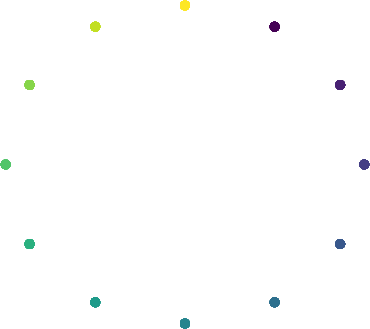
\includegraphics[interpolate=true,width=3.700000in,height=3.290000in]{Figures/cyclicalScallingFig-img2.png}}%
\end{pgfscope}%
\begin{pgfscope}%
\pgfsetbuttcap%
\pgfsetroundjoin%
\definecolor{currentfill}{rgb}{0.000000,0.000000,0.000000}%
\pgfsetfillcolor{currentfill}%
\pgfsetlinewidth{0.803000pt}%
\definecolor{currentstroke}{rgb}{0.000000,0.000000,0.000000}%
\pgfsetstrokecolor{currentstroke}%
\pgfsetdash{}{0pt}%
\pgfsys@defobject{currentmarker}{\pgfqpoint{0.000000in}{-0.048611in}}{\pgfqpoint{0.000000in}{0.000000in}}{%
\pgfpathmoveto{\pgfqpoint{0.000000in}{0.000000in}}%
\pgfpathlineto{\pgfqpoint{0.000000in}{-0.048611in}}%
\pgfusepath{stroke,fill}%
}%
\begin{pgfscope}%
\pgfsys@transformshift{0.925945in}{0.515123in}%
\pgfsys@useobject{currentmarker}{}%
\end{pgfscope}%
\end{pgfscope}%
\begin{pgfscope}%
\definecolor{textcolor}{rgb}{0.000000,0.000000,0.000000}%
\pgfsetstrokecolor{textcolor}%
\pgfsetfillcolor{textcolor}%
\pgftext[x=0.925945in,y=0.417901in,,top]{\color{textcolor}{\sffamily\fontsize{10.000000}{12.000000}\selectfont\catcode`\^=\active\def^{\ifmmode\sp\else\^{}\fi}\catcode`\%=\active\def%{\%}\ensuremath{-}1.00}}%
\end{pgfscope}%
\begin{pgfscope}%
\pgfsetbuttcap%
\pgfsetroundjoin%
\definecolor{currentfill}{rgb}{0.000000,0.000000,0.000000}%
\pgfsetfillcolor{currentfill}%
\pgfsetlinewidth{0.803000pt}%
\definecolor{currentstroke}{rgb}{0.000000,0.000000,0.000000}%
\pgfsetstrokecolor{currentstroke}%
\pgfsetdash{}{0pt}%
\pgfsys@defobject{currentmarker}{\pgfqpoint{0.000000in}{-0.048611in}}{\pgfqpoint{0.000000in}{0.000000in}}{%
\pgfpathmoveto{\pgfqpoint{0.000000in}{0.000000in}}%
\pgfpathlineto{\pgfqpoint{0.000000in}{-0.048611in}}%
\pgfusepath{stroke,fill}%
}%
\begin{pgfscope}%
\pgfsys@transformshift{1.374292in}{0.515123in}%
\pgfsys@useobject{currentmarker}{}%
\end{pgfscope}%
\end{pgfscope}%
\begin{pgfscope}%
\definecolor{textcolor}{rgb}{0.000000,0.000000,0.000000}%
\pgfsetstrokecolor{textcolor}%
\pgfsetfillcolor{textcolor}%
\pgftext[x=1.374292in,y=0.417901in,,top]{\color{textcolor}{\sffamily\fontsize{10.000000}{12.000000}\selectfont\catcode`\^=\active\def^{\ifmmode\sp\else\^{}\fi}\catcode`\%=\active\def%{\%}\ensuremath{-}0.75}}%
\end{pgfscope}%
\begin{pgfscope}%
\pgfsetbuttcap%
\pgfsetroundjoin%
\definecolor{currentfill}{rgb}{0.000000,0.000000,0.000000}%
\pgfsetfillcolor{currentfill}%
\pgfsetlinewidth{0.803000pt}%
\definecolor{currentstroke}{rgb}{0.000000,0.000000,0.000000}%
\pgfsetstrokecolor{currentstroke}%
\pgfsetdash{}{0pt}%
\pgfsys@defobject{currentmarker}{\pgfqpoint{0.000000in}{-0.048611in}}{\pgfqpoint{0.000000in}{0.000000in}}{%
\pgfpathmoveto{\pgfqpoint{0.000000in}{0.000000in}}%
\pgfpathlineto{\pgfqpoint{0.000000in}{-0.048611in}}%
\pgfusepath{stroke,fill}%
}%
\begin{pgfscope}%
\pgfsys@transformshift{1.822639in}{0.515123in}%
\pgfsys@useobject{currentmarker}{}%
\end{pgfscope}%
\end{pgfscope}%
\begin{pgfscope}%
\definecolor{textcolor}{rgb}{0.000000,0.000000,0.000000}%
\pgfsetstrokecolor{textcolor}%
\pgfsetfillcolor{textcolor}%
\pgftext[x=1.822639in,y=0.417901in,,top]{\color{textcolor}{\sffamily\fontsize{10.000000}{12.000000}\selectfont\catcode`\^=\active\def^{\ifmmode\sp\else\^{}\fi}\catcode`\%=\active\def%{\%}\ensuremath{-}0.50}}%
\end{pgfscope}%
\begin{pgfscope}%
\pgfsetbuttcap%
\pgfsetroundjoin%
\definecolor{currentfill}{rgb}{0.000000,0.000000,0.000000}%
\pgfsetfillcolor{currentfill}%
\pgfsetlinewidth{0.803000pt}%
\definecolor{currentstroke}{rgb}{0.000000,0.000000,0.000000}%
\pgfsetstrokecolor{currentstroke}%
\pgfsetdash{}{0pt}%
\pgfsys@defobject{currentmarker}{\pgfqpoint{0.000000in}{-0.048611in}}{\pgfqpoint{0.000000in}{0.000000in}}{%
\pgfpathmoveto{\pgfqpoint{0.000000in}{0.000000in}}%
\pgfpathlineto{\pgfqpoint{0.000000in}{-0.048611in}}%
\pgfusepath{stroke,fill}%
}%
\begin{pgfscope}%
\pgfsys@transformshift{2.270986in}{0.515123in}%
\pgfsys@useobject{currentmarker}{}%
\end{pgfscope}%
\end{pgfscope}%
\begin{pgfscope}%
\definecolor{textcolor}{rgb}{0.000000,0.000000,0.000000}%
\pgfsetstrokecolor{textcolor}%
\pgfsetfillcolor{textcolor}%
\pgftext[x=2.270986in,y=0.417901in,,top]{\color{textcolor}{\sffamily\fontsize{10.000000}{12.000000}\selectfont\catcode`\^=\active\def^{\ifmmode\sp\else\^{}\fi}\catcode`\%=\active\def%{\%}\ensuremath{-}0.25}}%
\end{pgfscope}%
\begin{pgfscope}%
\pgfsetbuttcap%
\pgfsetroundjoin%
\definecolor{currentfill}{rgb}{0.000000,0.000000,0.000000}%
\pgfsetfillcolor{currentfill}%
\pgfsetlinewidth{0.803000pt}%
\definecolor{currentstroke}{rgb}{0.000000,0.000000,0.000000}%
\pgfsetstrokecolor{currentstroke}%
\pgfsetdash{}{0pt}%
\pgfsys@defobject{currentmarker}{\pgfqpoint{0.000000in}{-0.048611in}}{\pgfqpoint{0.000000in}{0.000000in}}{%
\pgfpathmoveto{\pgfqpoint{0.000000in}{0.000000in}}%
\pgfpathlineto{\pgfqpoint{0.000000in}{-0.048611in}}%
\pgfusepath{stroke,fill}%
}%
\begin{pgfscope}%
\pgfsys@transformshift{2.719333in}{0.515123in}%
\pgfsys@useobject{currentmarker}{}%
\end{pgfscope}%
\end{pgfscope}%
\begin{pgfscope}%
\definecolor{textcolor}{rgb}{0.000000,0.000000,0.000000}%
\pgfsetstrokecolor{textcolor}%
\pgfsetfillcolor{textcolor}%
\pgftext[x=2.719333in,y=0.417901in,,top]{\color{textcolor}{\sffamily\fontsize{10.000000}{12.000000}\selectfont\catcode`\^=\active\def^{\ifmmode\sp\else\^{}\fi}\catcode`\%=\active\def%{\%}0.00}}%
\end{pgfscope}%
\begin{pgfscope}%
\pgfsetbuttcap%
\pgfsetroundjoin%
\definecolor{currentfill}{rgb}{0.000000,0.000000,0.000000}%
\pgfsetfillcolor{currentfill}%
\pgfsetlinewidth{0.803000pt}%
\definecolor{currentstroke}{rgb}{0.000000,0.000000,0.000000}%
\pgfsetstrokecolor{currentstroke}%
\pgfsetdash{}{0pt}%
\pgfsys@defobject{currentmarker}{\pgfqpoint{0.000000in}{-0.048611in}}{\pgfqpoint{0.000000in}{0.000000in}}{%
\pgfpathmoveto{\pgfqpoint{0.000000in}{0.000000in}}%
\pgfpathlineto{\pgfqpoint{0.000000in}{-0.048611in}}%
\pgfusepath{stroke,fill}%
}%
\begin{pgfscope}%
\pgfsys@transformshift{3.167680in}{0.515123in}%
\pgfsys@useobject{currentmarker}{}%
\end{pgfscope}%
\end{pgfscope}%
\begin{pgfscope}%
\definecolor{textcolor}{rgb}{0.000000,0.000000,0.000000}%
\pgfsetstrokecolor{textcolor}%
\pgfsetfillcolor{textcolor}%
\pgftext[x=3.167680in,y=0.417901in,,top]{\color{textcolor}{\sffamily\fontsize{10.000000}{12.000000}\selectfont\catcode`\^=\active\def^{\ifmmode\sp\else\^{}\fi}\catcode`\%=\active\def%{\%}0.25}}%
\end{pgfscope}%
\begin{pgfscope}%
\pgfsetbuttcap%
\pgfsetroundjoin%
\definecolor{currentfill}{rgb}{0.000000,0.000000,0.000000}%
\pgfsetfillcolor{currentfill}%
\pgfsetlinewidth{0.803000pt}%
\definecolor{currentstroke}{rgb}{0.000000,0.000000,0.000000}%
\pgfsetstrokecolor{currentstroke}%
\pgfsetdash{}{0pt}%
\pgfsys@defobject{currentmarker}{\pgfqpoint{0.000000in}{-0.048611in}}{\pgfqpoint{0.000000in}{0.000000in}}{%
\pgfpathmoveto{\pgfqpoint{0.000000in}{0.000000in}}%
\pgfpathlineto{\pgfqpoint{0.000000in}{-0.048611in}}%
\pgfusepath{stroke,fill}%
}%
\begin{pgfscope}%
\pgfsys@transformshift{3.616027in}{0.515123in}%
\pgfsys@useobject{currentmarker}{}%
\end{pgfscope}%
\end{pgfscope}%
\begin{pgfscope}%
\definecolor{textcolor}{rgb}{0.000000,0.000000,0.000000}%
\pgfsetstrokecolor{textcolor}%
\pgfsetfillcolor{textcolor}%
\pgftext[x=3.616027in,y=0.417901in,,top]{\color{textcolor}{\sffamily\fontsize{10.000000}{12.000000}\selectfont\catcode`\^=\active\def^{\ifmmode\sp\else\^{}\fi}\catcode`\%=\active\def%{\%}0.50}}%
\end{pgfscope}%
\begin{pgfscope}%
\pgfsetbuttcap%
\pgfsetroundjoin%
\definecolor{currentfill}{rgb}{0.000000,0.000000,0.000000}%
\pgfsetfillcolor{currentfill}%
\pgfsetlinewidth{0.803000pt}%
\definecolor{currentstroke}{rgb}{0.000000,0.000000,0.000000}%
\pgfsetstrokecolor{currentstroke}%
\pgfsetdash{}{0pt}%
\pgfsys@defobject{currentmarker}{\pgfqpoint{0.000000in}{-0.048611in}}{\pgfqpoint{0.000000in}{0.000000in}}{%
\pgfpathmoveto{\pgfqpoint{0.000000in}{0.000000in}}%
\pgfpathlineto{\pgfqpoint{0.000000in}{-0.048611in}}%
\pgfusepath{stroke,fill}%
}%
\begin{pgfscope}%
\pgfsys@transformshift{4.064375in}{0.515123in}%
\pgfsys@useobject{currentmarker}{}%
\end{pgfscope}%
\end{pgfscope}%
\begin{pgfscope}%
\definecolor{textcolor}{rgb}{0.000000,0.000000,0.000000}%
\pgfsetstrokecolor{textcolor}%
\pgfsetfillcolor{textcolor}%
\pgftext[x=4.064375in,y=0.417901in,,top]{\color{textcolor}{\sffamily\fontsize{10.000000}{12.000000}\selectfont\catcode`\^=\active\def^{\ifmmode\sp\else\^{}\fi}\catcode`\%=\active\def%{\%}0.75}}%
\end{pgfscope}%
\begin{pgfscope}%
\pgfsetbuttcap%
\pgfsetroundjoin%
\definecolor{currentfill}{rgb}{0.000000,0.000000,0.000000}%
\pgfsetfillcolor{currentfill}%
\pgfsetlinewidth{0.803000pt}%
\definecolor{currentstroke}{rgb}{0.000000,0.000000,0.000000}%
\pgfsetstrokecolor{currentstroke}%
\pgfsetdash{}{0pt}%
\pgfsys@defobject{currentmarker}{\pgfqpoint{0.000000in}{-0.048611in}}{\pgfqpoint{0.000000in}{0.000000in}}{%
\pgfpathmoveto{\pgfqpoint{0.000000in}{0.000000in}}%
\pgfpathlineto{\pgfqpoint{0.000000in}{-0.048611in}}%
\pgfusepath{stroke,fill}%
}%
\begin{pgfscope}%
\pgfsys@transformshift{4.512722in}{0.515123in}%
\pgfsys@useobject{currentmarker}{}%
\end{pgfscope}%
\end{pgfscope}%
\begin{pgfscope}%
\definecolor{textcolor}{rgb}{0.000000,0.000000,0.000000}%
\pgfsetstrokecolor{textcolor}%
\pgfsetfillcolor{textcolor}%
\pgftext[x=4.512722in,y=0.417901in,,top]{\color{textcolor}{\sffamily\fontsize{10.000000}{12.000000}\selectfont\catcode`\^=\active\def^{\ifmmode\sp\else\^{}\fi}\catcode`\%=\active\def%{\%}1.00}}%
\end{pgfscope}%
\begin{pgfscope}%
\definecolor{textcolor}{rgb}{0.000000,0.000000,0.000000}%
\pgfsetstrokecolor{textcolor}%
\pgfsetfillcolor{textcolor}%
\pgftext[x=2.719333in,y=0.238889in,,top]{\color{textcolor}{\sffamily\fontsize{10.000000}{12.000000}\selectfont\catcode`\^=\active\def^{\ifmmode\sp\else\^{}\fi}\catcode`\%=\active\def%{\%}sin(month)}}%
\end{pgfscope}%
\begin{pgfscope}%
\pgfsetbuttcap%
\pgfsetroundjoin%
\definecolor{currentfill}{rgb}{0.000000,0.000000,0.000000}%
\pgfsetfillcolor{currentfill}%
\pgfsetlinewidth{0.803000pt}%
\definecolor{currentstroke}{rgb}{0.000000,0.000000,0.000000}%
\pgfsetstrokecolor{currentstroke}%
\pgfsetdash{}{0pt}%
\pgfsys@defobject{currentmarker}{\pgfqpoint{-0.048611in}{0.000000in}}{\pgfqpoint{-0.000000in}{0.000000in}}{%
\pgfpathmoveto{\pgfqpoint{-0.000000in}{0.000000in}}%
\pgfpathlineto{\pgfqpoint{-0.048611in}{0.000000in}}%
\pgfusepath{stroke,fill}%
}%
\begin{pgfscope}%
\pgfsys@transformshift{0.746606in}{0.674214in}%
\pgfsys@useobject{currentmarker}{}%
\end{pgfscope}%
\end{pgfscope}%
\begin{pgfscope}%
\definecolor{textcolor}{rgb}{0.000000,0.000000,0.000000}%
\pgfsetstrokecolor{textcolor}%
\pgfsetfillcolor{textcolor}%
\pgftext[x=0.294444in, y=0.625989in, left, base]{\color{textcolor}{\sffamily\fontsize{10.000000}{12.000000}\selectfont\catcode`\^=\active\def^{\ifmmode\sp\else\^{}\fi}\catcode`\%=\active\def%{\%}\ensuremath{-}1.00}}%
\end{pgfscope}%
\begin{pgfscope}%
\pgfsetbuttcap%
\pgfsetroundjoin%
\definecolor{currentfill}{rgb}{0.000000,0.000000,0.000000}%
\pgfsetfillcolor{currentfill}%
\pgfsetlinewidth{0.803000pt}%
\definecolor{currentstroke}{rgb}{0.000000,0.000000,0.000000}%
\pgfsetstrokecolor{currentstroke}%
\pgfsetdash{}{0pt}%
\pgfsys@defobject{currentmarker}{\pgfqpoint{-0.048611in}{0.000000in}}{\pgfqpoint{-0.000000in}{0.000000in}}{%
\pgfpathmoveto{\pgfqpoint{-0.000000in}{0.000000in}}%
\pgfpathlineto{\pgfqpoint{-0.048611in}{0.000000in}}%
\pgfusepath{stroke,fill}%
}%
\begin{pgfscope}%
\pgfsys@transformshift{0.746606in}{1.071942in}%
\pgfsys@useobject{currentmarker}{}%
\end{pgfscope}%
\end{pgfscope}%
\begin{pgfscope}%
\definecolor{textcolor}{rgb}{0.000000,0.000000,0.000000}%
\pgfsetstrokecolor{textcolor}%
\pgfsetfillcolor{textcolor}%
\pgftext[x=0.294444in, y=1.023716in, left, base]{\color{textcolor}{\sffamily\fontsize{10.000000}{12.000000}\selectfont\catcode`\^=\active\def^{\ifmmode\sp\else\^{}\fi}\catcode`\%=\active\def%{\%}\ensuremath{-}0.75}}%
\end{pgfscope}%
\begin{pgfscope}%
\pgfsetbuttcap%
\pgfsetroundjoin%
\definecolor{currentfill}{rgb}{0.000000,0.000000,0.000000}%
\pgfsetfillcolor{currentfill}%
\pgfsetlinewidth{0.803000pt}%
\definecolor{currentstroke}{rgb}{0.000000,0.000000,0.000000}%
\pgfsetstrokecolor{currentstroke}%
\pgfsetdash{}{0pt}%
\pgfsys@defobject{currentmarker}{\pgfqpoint{-0.048611in}{0.000000in}}{\pgfqpoint{-0.000000in}{0.000000in}}{%
\pgfpathmoveto{\pgfqpoint{-0.000000in}{0.000000in}}%
\pgfpathlineto{\pgfqpoint{-0.048611in}{0.000000in}}%
\pgfusepath{stroke,fill}%
}%
\begin{pgfscope}%
\pgfsys@transformshift{0.746606in}{1.469669in}%
\pgfsys@useobject{currentmarker}{}%
\end{pgfscope}%
\end{pgfscope}%
\begin{pgfscope}%
\definecolor{textcolor}{rgb}{0.000000,0.000000,0.000000}%
\pgfsetstrokecolor{textcolor}%
\pgfsetfillcolor{textcolor}%
\pgftext[x=0.294444in, y=1.421444in, left, base]{\color{textcolor}{\sffamily\fontsize{10.000000}{12.000000}\selectfont\catcode`\^=\active\def^{\ifmmode\sp\else\^{}\fi}\catcode`\%=\active\def%{\%}\ensuremath{-}0.50}}%
\end{pgfscope}%
\begin{pgfscope}%
\pgfsetbuttcap%
\pgfsetroundjoin%
\definecolor{currentfill}{rgb}{0.000000,0.000000,0.000000}%
\pgfsetfillcolor{currentfill}%
\pgfsetlinewidth{0.803000pt}%
\definecolor{currentstroke}{rgb}{0.000000,0.000000,0.000000}%
\pgfsetstrokecolor{currentstroke}%
\pgfsetdash{}{0pt}%
\pgfsys@defobject{currentmarker}{\pgfqpoint{-0.048611in}{0.000000in}}{\pgfqpoint{-0.000000in}{0.000000in}}{%
\pgfpathmoveto{\pgfqpoint{-0.000000in}{0.000000in}}%
\pgfpathlineto{\pgfqpoint{-0.048611in}{0.000000in}}%
\pgfusepath{stroke,fill}%
}%
\begin{pgfscope}%
\pgfsys@transformshift{0.746606in}{1.867396in}%
\pgfsys@useobject{currentmarker}{}%
\end{pgfscope}%
\end{pgfscope}%
\begin{pgfscope}%
\definecolor{textcolor}{rgb}{0.000000,0.000000,0.000000}%
\pgfsetstrokecolor{textcolor}%
\pgfsetfillcolor{textcolor}%
\pgftext[x=0.294444in, y=1.819171in, left, base]{\color{textcolor}{\sffamily\fontsize{10.000000}{12.000000}\selectfont\catcode`\^=\active\def^{\ifmmode\sp\else\^{}\fi}\catcode`\%=\active\def%{\%}\ensuremath{-}0.25}}%
\end{pgfscope}%
\begin{pgfscope}%
\pgfsetbuttcap%
\pgfsetroundjoin%
\definecolor{currentfill}{rgb}{0.000000,0.000000,0.000000}%
\pgfsetfillcolor{currentfill}%
\pgfsetlinewidth{0.803000pt}%
\definecolor{currentstroke}{rgb}{0.000000,0.000000,0.000000}%
\pgfsetstrokecolor{currentstroke}%
\pgfsetdash{}{0pt}%
\pgfsys@defobject{currentmarker}{\pgfqpoint{-0.048611in}{0.000000in}}{\pgfqpoint{-0.000000in}{0.000000in}}{%
\pgfpathmoveto{\pgfqpoint{-0.000000in}{0.000000in}}%
\pgfpathlineto{\pgfqpoint{-0.048611in}{0.000000in}}%
\pgfusepath{stroke,fill}%
}%
\begin{pgfscope}%
\pgfsys@transformshift{0.746606in}{2.265123in}%
\pgfsys@useobject{currentmarker}{}%
\end{pgfscope}%
\end{pgfscope}%
\begin{pgfscope}%
\definecolor{textcolor}{rgb}{0.000000,0.000000,0.000000}%
\pgfsetstrokecolor{textcolor}%
\pgfsetfillcolor{textcolor}%
\pgftext[x=0.402469in, y=2.216898in, left, base]{\color{textcolor}{\sffamily\fontsize{10.000000}{12.000000}\selectfont\catcode`\^=\active\def^{\ifmmode\sp\else\^{}\fi}\catcode`\%=\active\def%{\%}0.00}}%
\end{pgfscope}%
\begin{pgfscope}%
\pgfsetbuttcap%
\pgfsetroundjoin%
\definecolor{currentfill}{rgb}{0.000000,0.000000,0.000000}%
\pgfsetfillcolor{currentfill}%
\pgfsetlinewidth{0.803000pt}%
\definecolor{currentstroke}{rgb}{0.000000,0.000000,0.000000}%
\pgfsetstrokecolor{currentstroke}%
\pgfsetdash{}{0pt}%
\pgfsys@defobject{currentmarker}{\pgfqpoint{-0.048611in}{0.000000in}}{\pgfqpoint{-0.000000in}{0.000000in}}{%
\pgfpathmoveto{\pgfqpoint{-0.000000in}{0.000000in}}%
\pgfpathlineto{\pgfqpoint{-0.048611in}{0.000000in}}%
\pgfusepath{stroke,fill}%
}%
\begin{pgfscope}%
\pgfsys@transformshift{0.746606in}{2.662851in}%
\pgfsys@useobject{currentmarker}{}%
\end{pgfscope}%
\end{pgfscope}%
\begin{pgfscope}%
\definecolor{textcolor}{rgb}{0.000000,0.000000,0.000000}%
\pgfsetstrokecolor{textcolor}%
\pgfsetfillcolor{textcolor}%
\pgftext[x=0.402469in, y=2.614625in, left, base]{\color{textcolor}{\sffamily\fontsize{10.000000}{12.000000}\selectfont\catcode`\^=\active\def^{\ifmmode\sp\else\^{}\fi}\catcode`\%=\active\def%{\%}0.25}}%
\end{pgfscope}%
\begin{pgfscope}%
\pgfsetbuttcap%
\pgfsetroundjoin%
\definecolor{currentfill}{rgb}{0.000000,0.000000,0.000000}%
\pgfsetfillcolor{currentfill}%
\pgfsetlinewidth{0.803000pt}%
\definecolor{currentstroke}{rgb}{0.000000,0.000000,0.000000}%
\pgfsetstrokecolor{currentstroke}%
\pgfsetdash{}{0pt}%
\pgfsys@defobject{currentmarker}{\pgfqpoint{-0.048611in}{0.000000in}}{\pgfqpoint{-0.000000in}{0.000000in}}{%
\pgfpathmoveto{\pgfqpoint{-0.000000in}{0.000000in}}%
\pgfpathlineto{\pgfqpoint{-0.048611in}{0.000000in}}%
\pgfusepath{stroke,fill}%
}%
\begin{pgfscope}%
\pgfsys@transformshift{0.746606in}{3.060578in}%
\pgfsys@useobject{currentmarker}{}%
\end{pgfscope}%
\end{pgfscope}%
\begin{pgfscope}%
\definecolor{textcolor}{rgb}{0.000000,0.000000,0.000000}%
\pgfsetstrokecolor{textcolor}%
\pgfsetfillcolor{textcolor}%
\pgftext[x=0.402469in, y=3.012353in, left, base]{\color{textcolor}{\sffamily\fontsize{10.000000}{12.000000}\selectfont\catcode`\^=\active\def^{\ifmmode\sp\else\^{}\fi}\catcode`\%=\active\def%{\%}0.50}}%
\end{pgfscope}%
\begin{pgfscope}%
\pgfsetbuttcap%
\pgfsetroundjoin%
\definecolor{currentfill}{rgb}{0.000000,0.000000,0.000000}%
\pgfsetfillcolor{currentfill}%
\pgfsetlinewidth{0.803000pt}%
\definecolor{currentstroke}{rgb}{0.000000,0.000000,0.000000}%
\pgfsetstrokecolor{currentstroke}%
\pgfsetdash{}{0pt}%
\pgfsys@defobject{currentmarker}{\pgfqpoint{-0.048611in}{0.000000in}}{\pgfqpoint{-0.000000in}{0.000000in}}{%
\pgfpathmoveto{\pgfqpoint{-0.000000in}{0.000000in}}%
\pgfpathlineto{\pgfqpoint{-0.048611in}{0.000000in}}%
\pgfusepath{stroke,fill}%
}%
\begin{pgfscope}%
\pgfsys@transformshift{0.746606in}{3.458305in}%
\pgfsys@useobject{currentmarker}{}%
\end{pgfscope}%
\end{pgfscope}%
\begin{pgfscope}%
\definecolor{textcolor}{rgb}{0.000000,0.000000,0.000000}%
\pgfsetstrokecolor{textcolor}%
\pgfsetfillcolor{textcolor}%
\pgftext[x=0.402469in, y=3.410080in, left, base]{\color{textcolor}{\sffamily\fontsize{10.000000}{12.000000}\selectfont\catcode`\^=\active\def^{\ifmmode\sp\else\^{}\fi}\catcode`\%=\active\def%{\%}0.75}}%
\end{pgfscope}%
\begin{pgfscope}%
\pgfsetbuttcap%
\pgfsetroundjoin%
\definecolor{currentfill}{rgb}{0.000000,0.000000,0.000000}%
\pgfsetfillcolor{currentfill}%
\pgfsetlinewidth{0.803000pt}%
\definecolor{currentstroke}{rgb}{0.000000,0.000000,0.000000}%
\pgfsetstrokecolor{currentstroke}%
\pgfsetdash{}{0pt}%
\pgfsys@defobject{currentmarker}{\pgfqpoint{-0.048611in}{0.000000in}}{\pgfqpoint{-0.000000in}{0.000000in}}{%
\pgfpathmoveto{\pgfqpoint{-0.000000in}{0.000000in}}%
\pgfpathlineto{\pgfqpoint{-0.048611in}{0.000000in}}%
\pgfusepath{stroke,fill}%
}%
\begin{pgfscope}%
\pgfsys@transformshift{0.746606in}{3.856032in}%
\pgfsys@useobject{currentmarker}{}%
\end{pgfscope}%
\end{pgfscope}%
\begin{pgfscope}%
\definecolor{textcolor}{rgb}{0.000000,0.000000,0.000000}%
\pgfsetstrokecolor{textcolor}%
\pgfsetfillcolor{textcolor}%
\pgftext[x=0.402469in, y=3.807807in, left, base]{\color{textcolor}{\sffamily\fontsize{10.000000}{12.000000}\selectfont\catcode`\^=\active\def^{\ifmmode\sp\else\^{}\fi}\catcode`\%=\active\def%{\%}1.00}}%
\end{pgfscope}%
\begin{pgfscope}%
\definecolor{textcolor}{rgb}{0.000000,0.000000,0.000000}%
\pgfsetstrokecolor{textcolor}%
\pgfsetfillcolor{textcolor}%
\pgftext[x=0.238889in,y=2.265123in,,bottom,rotate=90.000000]{\color{textcolor}{\sffamily\fontsize{10.000000}{12.000000}\selectfont\catcode`\^=\active\def^{\ifmmode\sp\else\^{}\fi}\catcode`\%=\active\def%{\%}cos(month)}}%
\end{pgfscope}%
\begin{pgfscope}%
\pgfsetrectcap%
\pgfsetmiterjoin%
\pgfsetlinewidth{0.803000pt}%
\definecolor{currentstroke}{rgb}{0.000000,0.000000,0.000000}%
\pgfsetstrokecolor{currentstroke}%
\pgfsetdash{}{0pt}%
\pgfpathmoveto{\pgfqpoint{0.746606in}{0.515123in}}%
\pgfpathlineto{\pgfqpoint{0.746606in}{4.015123in}}%
\pgfusepath{stroke}%
\end{pgfscope}%
\begin{pgfscope}%
\pgfsetrectcap%
\pgfsetmiterjoin%
\pgfsetlinewidth{0.803000pt}%
\definecolor{currentstroke}{rgb}{0.000000,0.000000,0.000000}%
\pgfsetstrokecolor{currentstroke}%
\pgfsetdash{}{0pt}%
\pgfpathmoveto{\pgfqpoint{4.692061in}{0.515123in}}%
\pgfpathlineto{\pgfqpoint{4.692061in}{4.015123in}}%
\pgfusepath{stroke}%
\end{pgfscope}%
\begin{pgfscope}%
\pgfsetrectcap%
\pgfsetmiterjoin%
\pgfsetlinewidth{0.803000pt}%
\definecolor{currentstroke}{rgb}{0.000000,0.000000,0.000000}%
\pgfsetstrokecolor{currentstroke}%
\pgfsetdash{}{0pt}%
\pgfpathmoveto{\pgfqpoint{0.746606in}{0.515123in}}%
\pgfpathlineto{\pgfqpoint{4.692061in}{0.515123in}}%
\pgfusepath{stroke}%
\end{pgfscope}%
\begin{pgfscope}%
\pgfsetrectcap%
\pgfsetmiterjoin%
\pgfsetlinewidth{0.803000pt}%
\definecolor{currentstroke}{rgb}{0.000000,0.000000,0.000000}%
\pgfsetstrokecolor{currentstroke}%
\pgfsetdash{}{0pt}%
\pgfpathmoveto{\pgfqpoint{0.746606in}{4.015123in}}%
\pgfpathlineto{\pgfqpoint{4.692061in}{4.015123in}}%
\pgfusepath{stroke}%
\end{pgfscope}%
\begin{pgfscope}%
\pgfsetbuttcap%
\pgfsetmiterjoin%
\definecolor{currentfill}{rgb}{1.000000,1.000000,1.000000}%
\pgfsetfillcolor{currentfill}%
\pgfsetlinewidth{0.000000pt}%
\definecolor{currentstroke}{rgb}{0.000000,0.000000,0.000000}%
\pgfsetstrokecolor{currentstroke}%
\pgfsetstrokeopacity{0.000000}%
\pgfsetdash{}{0pt}%
\pgfpathmoveto{\pgfqpoint{6.664788in}{0.515123in}}%
\pgfpathlineto{\pgfqpoint{10.610242in}{0.515123in}}%
\pgfpathlineto{\pgfqpoint{10.610242in}{4.015123in}}%
\pgfpathlineto{\pgfqpoint{6.664788in}{4.015123in}}%
\pgfpathlineto{\pgfqpoint{6.664788in}{0.515123in}}%
\pgfpathclose%
\pgfusepath{fill}%
\end{pgfscope}%
\begin{pgfscope}%
\pgfsys@transformshift{6.790000in}{0.623349in}%
\pgftext[left,bottom]{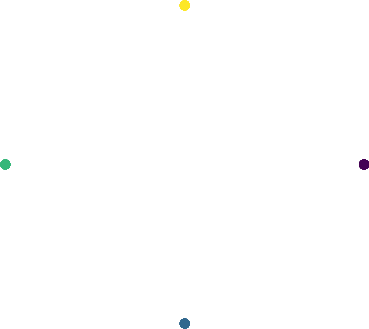
\includegraphics[interpolate=true,width=3.690000in,height=3.290000in]{Figures/cyclicalScallingFig-img3.png}}%
\end{pgfscope}%
\begin{pgfscope}%
\pgfsetbuttcap%
\pgfsetroundjoin%
\definecolor{currentfill}{rgb}{0.000000,0.000000,0.000000}%
\pgfsetfillcolor{currentfill}%
\pgfsetlinewidth{0.803000pt}%
\definecolor{currentstroke}{rgb}{0.000000,0.000000,0.000000}%
\pgfsetstrokecolor{currentstroke}%
\pgfsetdash{}{0pt}%
\pgfsys@defobject{currentmarker}{\pgfqpoint{0.000000in}{-0.048611in}}{\pgfqpoint{0.000000in}{0.000000in}}{%
\pgfpathmoveto{\pgfqpoint{0.000000in}{0.000000in}}%
\pgfpathlineto{\pgfqpoint{0.000000in}{-0.048611in}}%
\pgfusepath{stroke,fill}%
}%
\begin{pgfscope}%
\pgfsys@transformshift{6.844127in}{0.515123in}%
\pgfsys@useobject{currentmarker}{}%
\end{pgfscope}%
\end{pgfscope}%
\begin{pgfscope}%
\definecolor{textcolor}{rgb}{0.000000,0.000000,0.000000}%
\pgfsetstrokecolor{textcolor}%
\pgfsetfillcolor{textcolor}%
\pgftext[x=6.844127in,y=0.417901in,,top]{\color{textcolor}{\sffamily\fontsize{10.000000}{12.000000}\selectfont\catcode`\^=\active\def^{\ifmmode\sp\else\^{}\fi}\catcode`\%=\active\def%{\%}\ensuremath{-}1.00}}%
\end{pgfscope}%
\begin{pgfscope}%
\pgfsetbuttcap%
\pgfsetroundjoin%
\definecolor{currentfill}{rgb}{0.000000,0.000000,0.000000}%
\pgfsetfillcolor{currentfill}%
\pgfsetlinewidth{0.803000pt}%
\definecolor{currentstroke}{rgb}{0.000000,0.000000,0.000000}%
\pgfsetstrokecolor{currentstroke}%
\pgfsetdash{}{0pt}%
\pgfsys@defobject{currentmarker}{\pgfqpoint{0.000000in}{-0.048611in}}{\pgfqpoint{0.000000in}{0.000000in}}{%
\pgfpathmoveto{\pgfqpoint{0.000000in}{0.000000in}}%
\pgfpathlineto{\pgfqpoint{0.000000in}{-0.048611in}}%
\pgfusepath{stroke,fill}%
}%
\begin{pgfscope}%
\pgfsys@transformshift{7.292474in}{0.515123in}%
\pgfsys@useobject{currentmarker}{}%
\end{pgfscope}%
\end{pgfscope}%
\begin{pgfscope}%
\definecolor{textcolor}{rgb}{0.000000,0.000000,0.000000}%
\pgfsetstrokecolor{textcolor}%
\pgfsetfillcolor{textcolor}%
\pgftext[x=7.292474in,y=0.417901in,,top]{\color{textcolor}{\sffamily\fontsize{10.000000}{12.000000}\selectfont\catcode`\^=\active\def^{\ifmmode\sp\else\^{}\fi}\catcode`\%=\active\def%{\%}\ensuremath{-}0.75}}%
\end{pgfscope}%
\begin{pgfscope}%
\pgfsetbuttcap%
\pgfsetroundjoin%
\definecolor{currentfill}{rgb}{0.000000,0.000000,0.000000}%
\pgfsetfillcolor{currentfill}%
\pgfsetlinewidth{0.803000pt}%
\definecolor{currentstroke}{rgb}{0.000000,0.000000,0.000000}%
\pgfsetstrokecolor{currentstroke}%
\pgfsetdash{}{0pt}%
\pgfsys@defobject{currentmarker}{\pgfqpoint{0.000000in}{-0.048611in}}{\pgfqpoint{0.000000in}{0.000000in}}{%
\pgfpathmoveto{\pgfqpoint{0.000000in}{0.000000in}}%
\pgfpathlineto{\pgfqpoint{0.000000in}{-0.048611in}}%
\pgfusepath{stroke,fill}%
}%
\begin{pgfscope}%
\pgfsys@transformshift{7.740821in}{0.515123in}%
\pgfsys@useobject{currentmarker}{}%
\end{pgfscope}%
\end{pgfscope}%
\begin{pgfscope}%
\definecolor{textcolor}{rgb}{0.000000,0.000000,0.000000}%
\pgfsetstrokecolor{textcolor}%
\pgfsetfillcolor{textcolor}%
\pgftext[x=7.740821in,y=0.417901in,,top]{\color{textcolor}{\sffamily\fontsize{10.000000}{12.000000}\selectfont\catcode`\^=\active\def^{\ifmmode\sp\else\^{}\fi}\catcode`\%=\active\def%{\%}\ensuremath{-}0.50}}%
\end{pgfscope}%
\begin{pgfscope}%
\pgfsetbuttcap%
\pgfsetroundjoin%
\definecolor{currentfill}{rgb}{0.000000,0.000000,0.000000}%
\pgfsetfillcolor{currentfill}%
\pgfsetlinewidth{0.803000pt}%
\definecolor{currentstroke}{rgb}{0.000000,0.000000,0.000000}%
\pgfsetstrokecolor{currentstroke}%
\pgfsetdash{}{0pt}%
\pgfsys@defobject{currentmarker}{\pgfqpoint{0.000000in}{-0.048611in}}{\pgfqpoint{0.000000in}{0.000000in}}{%
\pgfpathmoveto{\pgfqpoint{0.000000in}{0.000000in}}%
\pgfpathlineto{\pgfqpoint{0.000000in}{-0.048611in}}%
\pgfusepath{stroke,fill}%
}%
\begin{pgfscope}%
\pgfsys@transformshift{8.189168in}{0.515123in}%
\pgfsys@useobject{currentmarker}{}%
\end{pgfscope}%
\end{pgfscope}%
\begin{pgfscope}%
\definecolor{textcolor}{rgb}{0.000000,0.000000,0.000000}%
\pgfsetstrokecolor{textcolor}%
\pgfsetfillcolor{textcolor}%
\pgftext[x=8.189168in,y=0.417901in,,top]{\color{textcolor}{\sffamily\fontsize{10.000000}{12.000000}\selectfont\catcode`\^=\active\def^{\ifmmode\sp\else\^{}\fi}\catcode`\%=\active\def%{\%}\ensuremath{-}0.25}}%
\end{pgfscope}%
\begin{pgfscope}%
\pgfsetbuttcap%
\pgfsetroundjoin%
\definecolor{currentfill}{rgb}{0.000000,0.000000,0.000000}%
\pgfsetfillcolor{currentfill}%
\pgfsetlinewidth{0.803000pt}%
\definecolor{currentstroke}{rgb}{0.000000,0.000000,0.000000}%
\pgfsetstrokecolor{currentstroke}%
\pgfsetdash{}{0pt}%
\pgfsys@defobject{currentmarker}{\pgfqpoint{0.000000in}{-0.048611in}}{\pgfqpoint{0.000000in}{0.000000in}}{%
\pgfpathmoveto{\pgfqpoint{0.000000in}{0.000000in}}%
\pgfpathlineto{\pgfqpoint{0.000000in}{-0.048611in}}%
\pgfusepath{stroke,fill}%
}%
\begin{pgfscope}%
\pgfsys@transformshift{8.637515in}{0.515123in}%
\pgfsys@useobject{currentmarker}{}%
\end{pgfscope}%
\end{pgfscope}%
\begin{pgfscope}%
\definecolor{textcolor}{rgb}{0.000000,0.000000,0.000000}%
\pgfsetstrokecolor{textcolor}%
\pgfsetfillcolor{textcolor}%
\pgftext[x=8.637515in,y=0.417901in,,top]{\color{textcolor}{\sffamily\fontsize{10.000000}{12.000000}\selectfont\catcode`\^=\active\def^{\ifmmode\sp\else\^{}\fi}\catcode`\%=\active\def%{\%}0.00}}%
\end{pgfscope}%
\begin{pgfscope}%
\pgfsetbuttcap%
\pgfsetroundjoin%
\definecolor{currentfill}{rgb}{0.000000,0.000000,0.000000}%
\pgfsetfillcolor{currentfill}%
\pgfsetlinewidth{0.803000pt}%
\definecolor{currentstroke}{rgb}{0.000000,0.000000,0.000000}%
\pgfsetstrokecolor{currentstroke}%
\pgfsetdash{}{0pt}%
\pgfsys@defobject{currentmarker}{\pgfqpoint{0.000000in}{-0.048611in}}{\pgfqpoint{0.000000in}{0.000000in}}{%
\pgfpathmoveto{\pgfqpoint{0.000000in}{0.000000in}}%
\pgfpathlineto{\pgfqpoint{0.000000in}{-0.048611in}}%
\pgfusepath{stroke,fill}%
}%
\begin{pgfscope}%
\pgfsys@transformshift{9.085862in}{0.515123in}%
\pgfsys@useobject{currentmarker}{}%
\end{pgfscope}%
\end{pgfscope}%
\begin{pgfscope}%
\definecolor{textcolor}{rgb}{0.000000,0.000000,0.000000}%
\pgfsetstrokecolor{textcolor}%
\pgfsetfillcolor{textcolor}%
\pgftext[x=9.085862in,y=0.417901in,,top]{\color{textcolor}{\sffamily\fontsize{10.000000}{12.000000}\selectfont\catcode`\^=\active\def^{\ifmmode\sp\else\^{}\fi}\catcode`\%=\active\def%{\%}0.25}}%
\end{pgfscope}%
\begin{pgfscope}%
\pgfsetbuttcap%
\pgfsetroundjoin%
\definecolor{currentfill}{rgb}{0.000000,0.000000,0.000000}%
\pgfsetfillcolor{currentfill}%
\pgfsetlinewidth{0.803000pt}%
\definecolor{currentstroke}{rgb}{0.000000,0.000000,0.000000}%
\pgfsetstrokecolor{currentstroke}%
\pgfsetdash{}{0pt}%
\pgfsys@defobject{currentmarker}{\pgfqpoint{0.000000in}{-0.048611in}}{\pgfqpoint{0.000000in}{0.000000in}}{%
\pgfpathmoveto{\pgfqpoint{0.000000in}{0.000000in}}%
\pgfpathlineto{\pgfqpoint{0.000000in}{-0.048611in}}%
\pgfusepath{stroke,fill}%
}%
\begin{pgfscope}%
\pgfsys@transformshift{9.534209in}{0.515123in}%
\pgfsys@useobject{currentmarker}{}%
\end{pgfscope}%
\end{pgfscope}%
\begin{pgfscope}%
\definecolor{textcolor}{rgb}{0.000000,0.000000,0.000000}%
\pgfsetstrokecolor{textcolor}%
\pgfsetfillcolor{textcolor}%
\pgftext[x=9.534209in,y=0.417901in,,top]{\color{textcolor}{\sffamily\fontsize{10.000000}{12.000000}\selectfont\catcode`\^=\active\def^{\ifmmode\sp\else\^{}\fi}\catcode`\%=\active\def%{\%}0.50}}%
\end{pgfscope}%
\begin{pgfscope}%
\pgfsetbuttcap%
\pgfsetroundjoin%
\definecolor{currentfill}{rgb}{0.000000,0.000000,0.000000}%
\pgfsetfillcolor{currentfill}%
\pgfsetlinewidth{0.803000pt}%
\definecolor{currentstroke}{rgb}{0.000000,0.000000,0.000000}%
\pgfsetstrokecolor{currentstroke}%
\pgfsetdash{}{0pt}%
\pgfsys@defobject{currentmarker}{\pgfqpoint{0.000000in}{-0.048611in}}{\pgfqpoint{0.000000in}{0.000000in}}{%
\pgfpathmoveto{\pgfqpoint{0.000000in}{0.000000in}}%
\pgfpathlineto{\pgfqpoint{0.000000in}{-0.048611in}}%
\pgfusepath{stroke,fill}%
}%
\begin{pgfscope}%
\pgfsys@transformshift{9.982556in}{0.515123in}%
\pgfsys@useobject{currentmarker}{}%
\end{pgfscope}%
\end{pgfscope}%
\begin{pgfscope}%
\definecolor{textcolor}{rgb}{0.000000,0.000000,0.000000}%
\pgfsetstrokecolor{textcolor}%
\pgfsetfillcolor{textcolor}%
\pgftext[x=9.982556in,y=0.417901in,,top]{\color{textcolor}{\sffamily\fontsize{10.000000}{12.000000}\selectfont\catcode`\^=\active\def^{\ifmmode\sp\else\^{}\fi}\catcode`\%=\active\def%{\%}0.75}}%
\end{pgfscope}%
\begin{pgfscope}%
\pgfsetbuttcap%
\pgfsetroundjoin%
\definecolor{currentfill}{rgb}{0.000000,0.000000,0.000000}%
\pgfsetfillcolor{currentfill}%
\pgfsetlinewidth{0.803000pt}%
\definecolor{currentstroke}{rgb}{0.000000,0.000000,0.000000}%
\pgfsetstrokecolor{currentstroke}%
\pgfsetdash{}{0pt}%
\pgfsys@defobject{currentmarker}{\pgfqpoint{0.000000in}{-0.048611in}}{\pgfqpoint{0.000000in}{0.000000in}}{%
\pgfpathmoveto{\pgfqpoint{0.000000in}{0.000000in}}%
\pgfpathlineto{\pgfqpoint{0.000000in}{-0.048611in}}%
\pgfusepath{stroke,fill}%
}%
\begin{pgfscope}%
\pgfsys@transformshift{10.430903in}{0.515123in}%
\pgfsys@useobject{currentmarker}{}%
\end{pgfscope}%
\end{pgfscope}%
\begin{pgfscope}%
\definecolor{textcolor}{rgb}{0.000000,0.000000,0.000000}%
\pgfsetstrokecolor{textcolor}%
\pgfsetfillcolor{textcolor}%
\pgftext[x=10.430903in,y=0.417901in,,top]{\color{textcolor}{\sffamily\fontsize{10.000000}{12.000000}\selectfont\catcode`\^=\active\def^{\ifmmode\sp\else\^{}\fi}\catcode`\%=\active\def%{\%}1.00}}%
\end{pgfscope}%
\begin{pgfscope}%
\definecolor{textcolor}{rgb}{0.000000,0.000000,0.000000}%
\pgfsetstrokecolor{textcolor}%
\pgfsetfillcolor{textcolor}%
\pgftext[x=8.637515in,y=0.238889in,,top]{\color{textcolor}{\sffamily\fontsize{10.000000}{12.000000}\selectfont\catcode`\^=\active\def^{\ifmmode\sp\else\^{}\fi}\catcode`\%=\active\def%{\%}sin(quarter)}}%
\end{pgfscope}%
\begin{pgfscope}%
\pgfsetbuttcap%
\pgfsetroundjoin%
\definecolor{currentfill}{rgb}{0.000000,0.000000,0.000000}%
\pgfsetfillcolor{currentfill}%
\pgfsetlinewidth{0.803000pt}%
\definecolor{currentstroke}{rgb}{0.000000,0.000000,0.000000}%
\pgfsetstrokecolor{currentstroke}%
\pgfsetdash{}{0pt}%
\pgfsys@defobject{currentmarker}{\pgfqpoint{-0.048611in}{0.000000in}}{\pgfqpoint{-0.000000in}{0.000000in}}{%
\pgfpathmoveto{\pgfqpoint{-0.000000in}{0.000000in}}%
\pgfpathlineto{\pgfqpoint{-0.048611in}{0.000000in}}%
\pgfusepath{stroke,fill}%
}%
\begin{pgfscope}%
\pgfsys@transformshift{6.664788in}{0.674214in}%
\pgfsys@useobject{currentmarker}{}%
\end{pgfscope}%
\end{pgfscope}%
\begin{pgfscope}%
\definecolor{textcolor}{rgb}{0.000000,0.000000,0.000000}%
\pgfsetstrokecolor{textcolor}%
\pgfsetfillcolor{textcolor}%
\pgftext[x=6.212626in, y=0.625989in, left, base]{\color{textcolor}{\sffamily\fontsize{10.000000}{12.000000}\selectfont\catcode`\^=\active\def^{\ifmmode\sp\else\^{}\fi}\catcode`\%=\active\def%{\%}\ensuremath{-}1.00}}%
\end{pgfscope}%
\begin{pgfscope}%
\pgfsetbuttcap%
\pgfsetroundjoin%
\definecolor{currentfill}{rgb}{0.000000,0.000000,0.000000}%
\pgfsetfillcolor{currentfill}%
\pgfsetlinewidth{0.803000pt}%
\definecolor{currentstroke}{rgb}{0.000000,0.000000,0.000000}%
\pgfsetstrokecolor{currentstroke}%
\pgfsetdash{}{0pt}%
\pgfsys@defobject{currentmarker}{\pgfqpoint{-0.048611in}{0.000000in}}{\pgfqpoint{-0.000000in}{0.000000in}}{%
\pgfpathmoveto{\pgfqpoint{-0.000000in}{0.000000in}}%
\pgfpathlineto{\pgfqpoint{-0.048611in}{0.000000in}}%
\pgfusepath{stroke,fill}%
}%
\begin{pgfscope}%
\pgfsys@transformshift{6.664788in}{1.071942in}%
\pgfsys@useobject{currentmarker}{}%
\end{pgfscope}%
\end{pgfscope}%
\begin{pgfscope}%
\definecolor{textcolor}{rgb}{0.000000,0.000000,0.000000}%
\pgfsetstrokecolor{textcolor}%
\pgfsetfillcolor{textcolor}%
\pgftext[x=6.212626in, y=1.023716in, left, base]{\color{textcolor}{\sffamily\fontsize{10.000000}{12.000000}\selectfont\catcode`\^=\active\def^{\ifmmode\sp\else\^{}\fi}\catcode`\%=\active\def%{\%}\ensuremath{-}0.75}}%
\end{pgfscope}%
\begin{pgfscope}%
\pgfsetbuttcap%
\pgfsetroundjoin%
\definecolor{currentfill}{rgb}{0.000000,0.000000,0.000000}%
\pgfsetfillcolor{currentfill}%
\pgfsetlinewidth{0.803000pt}%
\definecolor{currentstroke}{rgb}{0.000000,0.000000,0.000000}%
\pgfsetstrokecolor{currentstroke}%
\pgfsetdash{}{0pt}%
\pgfsys@defobject{currentmarker}{\pgfqpoint{-0.048611in}{0.000000in}}{\pgfqpoint{-0.000000in}{0.000000in}}{%
\pgfpathmoveto{\pgfqpoint{-0.000000in}{0.000000in}}%
\pgfpathlineto{\pgfqpoint{-0.048611in}{0.000000in}}%
\pgfusepath{stroke,fill}%
}%
\begin{pgfscope}%
\pgfsys@transformshift{6.664788in}{1.469669in}%
\pgfsys@useobject{currentmarker}{}%
\end{pgfscope}%
\end{pgfscope}%
\begin{pgfscope}%
\definecolor{textcolor}{rgb}{0.000000,0.000000,0.000000}%
\pgfsetstrokecolor{textcolor}%
\pgfsetfillcolor{textcolor}%
\pgftext[x=6.212626in, y=1.421444in, left, base]{\color{textcolor}{\sffamily\fontsize{10.000000}{12.000000}\selectfont\catcode`\^=\active\def^{\ifmmode\sp\else\^{}\fi}\catcode`\%=\active\def%{\%}\ensuremath{-}0.50}}%
\end{pgfscope}%
\begin{pgfscope}%
\pgfsetbuttcap%
\pgfsetroundjoin%
\definecolor{currentfill}{rgb}{0.000000,0.000000,0.000000}%
\pgfsetfillcolor{currentfill}%
\pgfsetlinewidth{0.803000pt}%
\definecolor{currentstroke}{rgb}{0.000000,0.000000,0.000000}%
\pgfsetstrokecolor{currentstroke}%
\pgfsetdash{}{0pt}%
\pgfsys@defobject{currentmarker}{\pgfqpoint{-0.048611in}{0.000000in}}{\pgfqpoint{-0.000000in}{0.000000in}}{%
\pgfpathmoveto{\pgfqpoint{-0.000000in}{0.000000in}}%
\pgfpathlineto{\pgfqpoint{-0.048611in}{0.000000in}}%
\pgfusepath{stroke,fill}%
}%
\begin{pgfscope}%
\pgfsys@transformshift{6.664788in}{1.867396in}%
\pgfsys@useobject{currentmarker}{}%
\end{pgfscope}%
\end{pgfscope}%
\begin{pgfscope}%
\definecolor{textcolor}{rgb}{0.000000,0.000000,0.000000}%
\pgfsetstrokecolor{textcolor}%
\pgfsetfillcolor{textcolor}%
\pgftext[x=6.212626in, y=1.819171in, left, base]{\color{textcolor}{\sffamily\fontsize{10.000000}{12.000000}\selectfont\catcode`\^=\active\def^{\ifmmode\sp\else\^{}\fi}\catcode`\%=\active\def%{\%}\ensuremath{-}0.25}}%
\end{pgfscope}%
\begin{pgfscope}%
\pgfsetbuttcap%
\pgfsetroundjoin%
\definecolor{currentfill}{rgb}{0.000000,0.000000,0.000000}%
\pgfsetfillcolor{currentfill}%
\pgfsetlinewidth{0.803000pt}%
\definecolor{currentstroke}{rgb}{0.000000,0.000000,0.000000}%
\pgfsetstrokecolor{currentstroke}%
\pgfsetdash{}{0pt}%
\pgfsys@defobject{currentmarker}{\pgfqpoint{-0.048611in}{0.000000in}}{\pgfqpoint{-0.000000in}{0.000000in}}{%
\pgfpathmoveto{\pgfqpoint{-0.000000in}{0.000000in}}%
\pgfpathlineto{\pgfqpoint{-0.048611in}{0.000000in}}%
\pgfusepath{stroke,fill}%
}%
\begin{pgfscope}%
\pgfsys@transformshift{6.664788in}{2.265123in}%
\pgfsys@useobject{currentmarker}{}%
\end{pgfscope}%
\end{pgfscope}%
\begin{pgfscope}%
\definecolor{textcolor}{rgb}{0.000000,0.000000,0.000000}%
\pgfsetstrokecolor{textcolor}%
\pgfsetfillcolor{textcolor}%
\pgftext[x=6.320651in, y=2.216898in, left, base]{\color{textcolor}{\sffamily\fontsize{10.000000}{12.000000}\selectfont\catcode`\^=\active\def^{\ifmmode\sp\else\^{}\fi}\catcode`\%=\active\def%{\%}0.00}}%
\end{pgfscope}%
\begin{pgfscope}%
\pgfsetbuttcap%
\pgfsetroundjoin%
\definecolor{currentfill}{rgb}{0.000000,0.000000,0.000000}%
\pgfsetfillcolor{currentfill}%
\pgfsetlinewidth{0.803000pt}%
\definecolor{currentstroke}{rgb}{0.000000,0.000000,0.000000}%
\pgfsetstrokecolor{currentstroke}%
\pgfsetdash{}{0pt}%
\pgfsys@defobject{currentmarker}{\pgfqpoint{-0.048611in}{0.000000in}}{\pgfqpoint{-0.000000in}{0.000000in}}{%
\pgfpathmoveto{\pgfqpoint{-0.000000in}{0.000000in}}%
\pgfpathlineto{\pgfqpoint{-0.048611in}{0.000000in}}%
\pgfusepath{stroke,fill}%
}%
\begin{pgfscope}%
\pgfsys@transformshift{6.664788in}{2.662851in}%
\pgfsys@useobject{currentmarker}{}%
\end{pgfscope}%
\end{pgfscope}%
\begin{pgfscope}%
\definecolor{textcolor}{rgb}{0.000000,0.000000,0.000000}%
\pgfsetstrokecolor{textcolor}%
\pgfsetfillcolor{textcolor}%
\pgftext[x=6.320651in, y=2.614625in, left, base]{\color{textcolor}{\sffamily\fontsize{10.000000}{12.000000}\selectfont\catcode`\^=\active\def^{\ifmmode\sp\else\^{}\fi}\catcode`\%=\active\def%{\%}0.25}}%
\end{pgfscope}%
\begin{pgfscope}%
\pgfsetbuttcap%
\pgfsetroundjoin%
\definecolor{currentfill}{rgb}{0.000000,0.000000,0.000000}%
\pgfsetfillcolor{currentfill}%
\pgfsetlinewidth{0.803000pt}%
\definecolor{currentstroke}{rgb}{0.000000,0.000000,0.000000}%
\pgfsetstrokecolor{currentstroke}%
\pgfsetdash{}{0pt}%
\pgfsys@defobject{currentmarker}{\pgfqpoint{-0.048611in}{0.000000in}}{\pgfqpoint{-0.000000in}{0.000000in}}{%
\pgfpathmoveto{\pgfqpoint{-0.000000in}{0.000000in}}%
\pgfpathlineto{\pgfqpoint{-0.048611in}{0.000000in}}%
\pgfusepath{stroke,fill}%
}%
\begin{pgfscope}%
\pgfsys@transformshift{6.664788in}{3.060578in}%
\pgfsys@useobject{currentmarker}{}%
\end{pgfscope}%
\end{pgfscope}%
\begin{pgfscope}%
\definecolor{textcolor}{rgb}{0.000000,0.000000,0.000000}%
\pgfsetstrokecolor{textcolor}%
\pgfsetfillcolor{textcolor}%
\pgftext[x=6.320651in, y=3.012353in, left, base]{\color{textcolor}{\sffamily\fontsize{10.000000}{12.000000}\selectfont\catcode`\^=\active\def^{\ifmmode\sp\else\^{}\fi}\catcode`\%=\active\def%{\%}0.50}}%
\end{pgfscope}%
\begin{pgfscope}%
\pgfsetbuttcap%
\pgfsetroundjoin%
\definecolor{currentfill}{rgb}{0.000000,0.000000,0.000000}%
\pgfsetfillcolor{currentfill}%
\pgfsetlinewidth{0.803000pt}%
\definecolor{currentstroke}{rgb}{0.000000,0.000000,0.000000}%
\pgfsetstrokecolor{currentstroke}%
\pgfsetdash{}{0pt}%
\pgfsys@defobject{currentmarker}{\pgfqpoint{-0.048611in}{0.000000in}}{\pgfqpoint{-0.000000in}{0.000000in}}{%
\pgfpathmoveto{\pgfqpoint{-0.000000in}{0.000000in}}%
\pgfpathlineto{\pgfqpoint{-0.048611in}{0.000000in}}%
\pgfusepath{stroke,fill}%
}%
\begin{pgfscope}%
\pgfsys@transformshift{6.664788in}{3.458305in}%
\pgfsys@useobject{currentmarker}{}%
\end{pgfscope}%
\end{pgfscope}%
\begin{pgfscope}%
\definecolor{textcolor}{rgb}{0.000000,0.000000,0.000000}%
\pgfsetstrokecolor{textcolor}%
\pgfsetfillcolor{textcolor}%
\pgftext[x=6.320651in, y=3.410080in, left, base]{\color{textcolor}{\sffamily\fontsize{10.000000}{12.000000}\selectfont\catcode`\^=\active\def^{\ifmmode\sp\else\^{}\fi}\catcode`\%=\active\def%{\%}0.75}}%
\end{pgfscope}%
\begin{pgfscope}%
\pgfsetbuttcap%
\pgfsetroundjoin%
\definecolor{currentfill}{rgb}{0.000000,0.000000,0.000000}%
\pgfsetfillcolor{currentfill}%
\pgfsetlinewidth{0.803000pt}%
\definecolor{currentstroke}{rgb}{0.000000,0.000000,0.000000}%
\pgfsetstrokecolor{currentstroke}%
\pgfsetdash{}{0pt}%
\pgfsys@defobject{currentmarker}{\pgfqpoint{-0.048611in}{0.000000in}}{\pgfqpoint{-0.000000in}{0.000000in}}{%
\pgfpathmoveto{\pgfqpoint{-0.000000in}{0.000000in}}%
\pgfpathlineto{\pgfqpoint{-0.048611in}{0.000000in}}%
\pgfusepath{stroke,fill}%
}%
\begin{pgfscope}%
\pgfsys@transformshift{6.664788in}{3.856032in}%
\pgfsys@useobject{currentmarker}{}%
\end{pgfscope}%
\end{pgfscope}%
\begin{pgfscope}%
\definecolor{textcolor}{rgb}{0.000000,0.000000,0.000000}%
\pgfsetstrokecolor{textcolor}%
\pgfsetfillcolor{textcolor}%
\pgftext[x=6.320651in, y=3.807807in, left, base]{\color{textcolor}{\sffamily\fontsize{10.000000}{12.000000}\selectfont\catcode`\^=\active\def^{\ifmmode\sp\else\^{}\fi}\catcode`\%=\active\def%{\%}1.00}}%
\end{pgfscope}%
\begin{pgfscope}%
\definecolor{textcolor}{rgb}{0.000000,0.000000,0.000000}%
\pgfsetstrokecolor{textcolor}%
\pgfsetfillcolor{textcolor}%
\pgftext[x=6.157071in,y=2.265123in,,bottom,rotate=90.000000]{\color{textcolor}{\sffamily\fontsize{10.000000}{12.000000}\selectfont\catcode`\^=\active\def^{\ifmmode\sp\else\^{}\fi}\catcode`\%=\active\def%{\%}cos(quarter)}}%
\end{pgfscope}%
\begin{pgfscope}%
\pgfsetrectcap%
\pgfsetmiterjoin%
\pgfsetlinewidth{0.803000pt}%
\definecolor{currentstroke}{rgb}{0.000000,0.000000,0.000000}%
\pgfsetstrokecolor{currentstroke}%
\pgfsetdash{}{0pt}%
\pgfpathmoveto{\pgfqpoint{6.664788in}{0.515123in}}%
\pgfpathlineto{\pgfqpoint{6.664788in}{4.015123in}}%
\pgfusepath{stroke}%
\end{pgfscope}%
\begin{pgfscope}%
\pgfsetrectcap%
\pgfsetmiterjoin%
\pgfsetlinewidth{0.803000pt}%
\definecolor{currentstroke}{rgb}{0.000000,0.000000,0.000000}%
\pgfsetstrokecolor{currentstroke}%
\pgfsetdash{}{0pt}%
\pgfpathmoveto{\pgfqpoint{10.610242in}{0.515123in}}%
\pgfpathlineto{\pgfqpoint{10.610242in}{4.015123in}}%
\pgfusepath{stroke}%
\end{pgfscope}%
\begin{pgfscope}%
\pgfsetrectcap%
\pgfsetmiterjoin%
\pgfsetlinewidth{0.803000pt}%
\definecolor{currentstroke}{rgb}{0.000000,0.000000,0.000000}%
\pgfsetstrokecolor{currentstroke}%
\pgfsetdash{}{0pt}%
\pgfpathmoveto{\pgfqpoint{6.664788in}{0.515123in}}%
\pgfpathlineto{\pgfqpoint{10.610242in}{0.515123in}}%
\pgfusepath{stroke}%
\end{pgfscope}%
\begin{pgfscope}%
\pgfsetrectcap%
\pgfsetmiterjoin%
\pgfsetlinewidth{0.803000pt}%
\definecolor{currentstroke}{rgb}{0.000000,0.000000,0.000000}%
\pgfsetstrokecolor{currentstroke}%
\pgfsetdash{}{0pt}%
\pgfpathmoveto{\pgfqpoint{6.664788in}{4.015123in}}%
\pgfpathlineto{\pgfqpoint{10.610242in}{4.015123in}}%
\pgfusepath{stroke}%
\end{pgfscope}%
\begin{pgfscope}%
\pgfsetbuttcap%
\pgfsetmiterjoin%
\definecolor{currentfill}{rgb}{1.000000,1.000000,1.000000}%
\pgfsetfillcolor{currentfill}%
\pgfsetlinewidth{0.000000pt}%
\definecolor{currentstroke}{rgb}{0.000000,0.000000,0.000000}%
\pgfsetstrokecolor{currentstroke}%
\pgfsetstrokeopacity{0.000000}%
\pgfsetdash{}{0pt}%
\pgfpathmoveto{\pgfqpoint{4.938651in}{4.715123in}}%
\pgfpathlineto{\pgfqpoint{5.113651in}{4.715123in}}%
\pgfpathlineto{\pgfqpoint{5.113651in}{8.215123in}}%
\pgfpathlineto{\pgfqpoint{4.938651in}{8.215123in}}%
\pgfpathlineto{\pgfqpoint{4.938651in}{4.715123in}}%
\pgfpathclose%
\pgfusepath{fill}%
\end{pgfscope}%
\begin{pgfscope}%
\pgfsys@transformshift{4.940000in}{4.723349in}%
\pgftext[left,bottom]{
\includegraphics[interpolate=true,width=0.170000in,height=3.500000in]{Figures/cyclicalScallingFig-img4.png}}%
\end{pgfscope}%
\begin{pgfscope}%
\pgfsetbuttcap%
\pgfsetroundjoin%
\definecolor{currentfill}{rgb}{0.000000,0.000000,0.000000}%
\pgfsetfillcolor{currentfill}%
\pgfsetlinewidth{0.803000pt}%
\definecolor{currentstroke}{rgb}{0.000000,0.000000,0.000000}%
\pgfsetstrokecolor{currentstroke}%
\pgfsetdash{}{0pt}%
\pgfsys@defobject{currentmarker}{\pgfqpoint{0.000000in}{0.000000in}}{\pgfqpoint{0.048611in}{0.000000in}}{%
\pgfpathmoveto{\pgfqpoint{0.000000in}{0.000000in}}%
\pgfpathlineto{\pgfqpoint{0.048611in}{0.000000in}}%
\pgfusepath{stroke,fill}%
}%
\begin{pgfscope}%
\pgfsys@transformshift{5.113651in}{4.715123in}%
\pgfsys@useobject{currentmarker}{}%
\end{pgfscope}%
\end{pgfscope}%
\begin{pgfscope}%
\definecolor{textcolor}{rgb}{0.000000,0.000000,0.000000}%
\pgfsetstrokecolor{textcolor}%
\pgfsetfillcolor{textcolor}%
\pgftext[x=5.210874in, y=4.666898in, left, base]{\color{textcolor}{\sffamily\fontsize{10.000000}{12.000000}\selectfont\catcode`\^=\active\def^{\ifmmode\sp\else\^{}\fi}\catcode`\%=\active\def%{\%}0}}%
\end{pgfscope}%
\begin{pgfscope}%
\pgfsetbuttcap%
\pgfsetroundjoin%
\definecolor{currentfill}{rgb}{0.000000,0.000000,0.000000}%
\pgfsetfillcolor{currentfill}%
\pgfsetlinewidth{0.803000pt}%
\definecolor{currentstroke}{rgb}{0.000000,0.000000,0.000000}%
\pgfsetstrokecolor{currentstroke}%
\pgfsetdash{}{0pt}%
\pgfsys@defobject{currentmarker}{\pgfqpoint{0.000000in}{0.000000in}}{\pgfqpoint{0.048611in}{0.000000in}}{%
\pgfpathmoveto{\pgfqpoint{0.000000in}{0.000000in}}%
\pgfpathlineto{\pgfqpoint{0.048611in}{0.000000in}}%
\pgfusepath{stroke,fill}%
}%
\begin{pgfscope}%
\pgfsys@transformshift{5.113651in}{5.475993in}%
\pgfsys@useobject{currentmarker}{}%
\end{pgfscope}%
\end{pgfscope}%
\begin{pgfscope}%
\definecolor{textcolor}{rgb}{0.000000,0.000000,0.000000}%
\pgfsetstrokecolor{textcolor}%
\pgfsetfillcolor{textcolor}%
\pgftext[x=5.210874in, y=5.427768in, left, base]{\color{textcolor}{\sffamily\fontsize{10.000000}{12.000000}\selectfont\catcode`\^=\active\def^{\ifmmode\sp\else\^{}\fi}\catcode`\%=\active\def%{\%}5}}%
\end{pgfscope}%
\begin{pgfscope}%
\pgfsetbuttcap%
\pgfsetroundjoin%
\definecolor{currentfill}{rgb}{0.000000,0.000000,0.000000}%
\pgfsetfillcolor{currentfill}%
\pgfsetlinewidth{0.803000pt}%
\definecolor{currentstroke}{rgb}{0.000000,0.000000,0.000000}%
\pgfsetstrokecolor{currentstroke}%
\pgfsetdash{}{0pt}%
\pgfsys@defobject{currentmarker}{\pgfqpoint{0.000000in}{0.000000in}}{\pgfqpoint{0.048611in}{0.000000in}}{%
\pgfpathmoveto{\pgfqpoint{0.000000in}{0.000000in}}%
\pgfpathlineto{\pgfqpoint{0.048611in}{0.000000in}}%
\pgfusepath{stroke,fill}%
}%
\begin{pgfscope}%
\pgfsys@transformshift{5.113651in}{6.236862in}%
\pgfsys@useobject{currentmarker}{}%
\end{pgfscope}%
\end{pgfscope}%
\begin{pgfscope}%
\definecolor{textcolor}{rgb}{0.000000,0.000000,0.000000}%
\pgfsetstrokecolor{textcolor}%
\pgfsetfillcolor{textcolor}%
\pgftext[x=5.210874in, y=6.188637in, left, base]{\color{textcolor}{\sffamily\fontsize{10.000000}{12.000000}\selectfont\catcode`\^=\active\def^{\ifmmode\sp\else\^{}\fi}\catcode`\%=\active\def%{\%}10}}%
\end{pgfscope}%
\begin{pgfscope}%
\pgfsetbuttcap%
\pgfsetroundjoin%
\definecolor{currentfill}{rgb}{0.000000,0.000000,0.000000}%
\pgfsetfillcolor{currentfill}%
\pgfsetlinewidth{0.803000pt}%
\definecolor{currentstroke}{rgb}{0.000000,0.000000,0.000000}%
\pgfsetstrokecolor{currentstroke}%
\pgfsetdash{}{0pt}%
\pgfsys@defobject{currentmarker}{\pgfqpoint{0.000000in}{0.000000in}}{\pgfqpoint{0.048611in}{0.000000in}}{%
\pgfpathmoveto{\pgfqpoint{0.000000in}{0.000000in}}%
\pgfpathlineto{\pgfqpoint{0.048611in}{0.000000in}}%
\pgfusepath{stroke,fill}%
}%
\begin{pgfscope}%
\pgfsys@transformshift{5.113651in}{6.997732in}%
\pgfsys@useobject{currentmarker}{}%
\end{pgfscope}%
\end{pgfscope}%
\begin{pgfscope}%
\definecolor{textcolor}{rgb}{0.000000,0.000000,0.000000}%
\pgfsetstrokecolor{textcolor}%
\pgfsetfillcolor{textcolor}%
\pgftext[x=5.210874in, y=6.949507in, left, base]{\color{textcolor}{\sffamily\fontsize{10.000000}{12.000000}\selectfont\catcode`\^=\active\def^{\ifmmode\sp\else\^{}\fi}\catcode`\%=\active\def%{\%}15}}%
\end{pgfscope}%
\begin{pgfscope}%
\pgfsetbuttcap%
\pgfsetroundjoin%
\definecolor{currentfill}{rgb}{0.000000,0.000000,0.000000}%
\pgfsetfillcolor{currentfill}%
\pgfsetlinewidth{0.803000pt}%
\definecolor{currentstroke}{rgb}{0.000000,0.000000,0.000000}%
\pgfsetstrokecolor{currentstroke}%
\pgfsetdash{}{0pt}%
\pgfsys@defobject{currentmarker}{\pgfqpoint{0.000000in}{0.000000in}}{\pgfqpoint{0.048611in}{0.000000in}}{%
\pgfpathmoveto{\pgfqpoint{0.000000in}{0.000000in}}%
\pgfpathlineto{\pgfqpoint{0.048611in}{0.000000in}}%
\pgfusepath{stroke,fill}%
}%
\begin{pgfscope}%
\pgfsys@transformshift{5.113651in}{7.758602in}%
\pgfsys@useobject{currentmarker}{}%
\end{pgfscope}%
\end{pgfscope}%
\begin{pgfscope}%
\definecolor{textcolor}{rgb}{0.000000,0.000000,0.000000}%
\pgfsetstrokecolor{textcolor}%
\pgfsetfillcolor{textcolor}%
\pgftext[x=5.210874in, y=7.710376in, left, base]{\color{textcolor}{\sffamily\fontsize{10.000000}{12.000000}\selectfont\catcode`\^=\active\def^{\ifmmode\sp\else\^{}\fi}\catcode`\%=\active\def%{\%}20}}%
\end{pgfscope}%
\begin{pgfscope}%
\pgfsetrectcap%
\pgfsetmiterjoin%
\pgfsetlinewidth{0.803000pt}%
\definecolor{currentstroke}{rgb}{0.000000,0.000000,0.000000}%
\pgfsetstrokecolor{currentstroke}%
\pgfsetdash{}{0pt}%
\pgfpathmoveto{\pgfqpoint{4.938651in}{4.715123in}}%
\pgfpathlineto{\pgfqpoint{5.026151in}{4.715123in}}%
\pgfpathlineto{\pgfqpoint{5.113651in}{4.715123in}}%
\pgfpathlineto{\pgfqpoint{5.113651in}{8.215123in}}%
\pgfpathlineto{\pgfqpoint{5.026151in}{8.215123in}}%
\pgfpathlineto{\pgfqpoint{4.938651in}{8.215123in}}%
\pgfpathlineto{\pgfqpoint{4.938651in}{4.715123in}}%
\pgfpathclose%
\pgfusepath{stroke}%
\end{pgfscope}%
\begin{pgfscope}%
\pgfsetbuttcap%
\pgfsetmiterjoin%
\definecolor{currentfill}{rgb}{1.000000,1.000000,1.000000}%
\pgfsetfillcolor{currentfill}%
\pgfsetlinewidth{0.000000pt}%
\definecolor{currentstroke}{rgb}{0.000000,0.000000,0.000000}%
\pgfsetstrokecolor{currentstroke}%
\pgfsetstrokeopacity{0.000000}%
\pgfsetdash{}{0pt}%
\pgfpathmoveto{\pgfqpoint{10.856833in}{4.715123in}}%
\pgfpathlineto{\pgfqpoint{11.031833in}{4.715123in}}%
\pgfpathlineto{\pgfqpoint{11.031833in}{8.215123in}}%
\pgfpathlineto{\pgfqpoint{10.856833in}{8.215123in}}%
\pgfpathlineto{\pgfqpoint{10.856833in}{4.715123in}}%
\pgfpathclose%
\pgfusepath{fill}%
\end{pgfscope}%
\begin{pgfscope}%
\pgfsys@transformshift{10.860000in}{4.723349in}%
\pgftext[left,bottom]{
\includegraphics[interpolate=true,width=0.170000in,height=3.500000in]{Figures/cyclicalScallingFig-img5.png}}%
\end{pgfscope}%
\begin{pgfscope}%
\pgfsetbuttcap%
\pgfsetroundjoin%
\definecolor{currentfill}{rgb}{0.000000,0.000000,0.000000}%
\pgfsetfillcolor{currentfill}%
\pgfsetlinewidth{0.803000pt}%
\definecolor{currentstroke}{rgb}{0.000000,0.000000,0.000000}%
\pgfsetstrokecolor{currentstroke}%
\pgfsetdash{}{0pt}%
\pgfsys@defobject{currentmarker}{\pgfqpoint{0.000000in}{0.000000in}}{\pgfqpoint{0.048611in}{0.000000in}}{%
\pgfpathmoveto{\pgfqpoint{0.000000in}{0.000000in}}%
\pgfpathlineto{\pgfqpoint{0.048611in}{0.000000in}}%
\pgfusepath{stroke,fill}%
}%
\begin{pgfscope}%
\pgfsys@transformshift{11.031833in}{4.715123in}%
\pgfsys@useobject{currentmarker}{}%
\end{pgfscope}%
\end{pgfscope}%
\begin{pgfscope}%
\definecolor{textcolor}{rgb}{0.000000,0.000000,0.000000}%
\pgfsetstrokecolor{textcolor}%
\pgfsetfillcolor{textcolor}%
\pgftext[x=11.129055in, y=4.666898in, left, base]{\color{textcolor}{\sffamily\fontsize{10.000000}{12.000000}\selectfont\catcode`\^=\active\def^{\ifmmode\sp\else\^{}\fi}\catcode`\%=\active\def%{\%}0}}%
\end{pgfscope}%
\begin{pgfscope}%
\pgfsetbuttcap%
\pgfsetroundjoin%
\definecolor{currentfill}{rgb}{0.000000,0.000000,0.000000}%
\pgfsetfillcolor{currentfill}%
\pgfsetlinewidth{0.803000pt}%
\definecolor{currentstroke}{rgb}{0.000000,0.000000,0.000000}%
\pgfsetstrokecolor{currentstroke}%
\pgfsetdash{}{0pt}%
\pgfsys@defobject{currentmarker}{\pgfqpoint{0.000000in}{0.000000in}}{\pgfqpoint{0.048611in}{0.000000in}}{%
\pgfpathmoveto{\pgfqpoint{0.000000in}{0.000000in}}%
\pgfpathlineto{\pgfqpoint{0.048611in}{0.000000in}}%
\pgfusepath{stroke,fill}%
}%
\begin{pgfscope}%
\pgfsys@transformshift{11.031833in}{5.298457in}%
\pgfsys@useobject{currentmarker}{}%
\end{pgfscope}%
\end{pgfscope}%
\begin{pgfscope}%
\definecolor{textcolor}{rgb}{0.000000,0.000000,0.000000}%
\pgfsetstrokecolor{textcolor}%
\pgfsetfillcolor{textcolor}%
\pgftext[x=11.129055in, y=5.250231in, left, base]{\color{textcolor}{\sffamily\fontsize{10.000000}{12.000000}\selectfont\catcode`\^=\active\def^{\ifmmode\sp\else\^{}\fi}\catcode`\%=\active\def%{\%}1}}%
\end{pgfscope}%
\begin{pgfscope}%
\pgfsetbuttcap%
\pgfsetroundjoin%
\definecolor{currentfill}{rgb}{0.000000,0.000000,0.000000}%
\pgfsetfillcolor{currentfill}%
\pgfsetlinewidth{0.803000pt}%
\definecolor{currentstroke}{rgb}{0.000000,0.000000,0.000000}%
\pgfsetstrokecolor{currentstroke}%
\pgfsetdash{}{0pt}%
\pgfsys@defobject{currentmarker}{\pgfqpoint{0.000000in}{0.000000in}}{\pgfqpoint{0.048611in}{0.000000in}}{%
\pgfpathmoveto{\pgfqpoint{0.000000in}{0.000000in}}%
\pgfpathlineto{\pgfqpoint{0.048611in}{0.000000in}}%
\pgfusepath{stroke,fill}%
}%
\begin{pgfscope}%
\pgfsys@transformshift{11.031833in}{5.881790in}%
\pgfsys@useobject{currentmarker}{}%
\end{pgfscope}%
\end{pgfscope}%
\begin{pgfscope}%
\definecolor{textcolor}{rgb}{0.000000,0.000000,0.000000}%
\pgfsetstrokecolor{textcolor}%
\pgfsetfillcolor{textcolor}%
\pgftext[x=11.129055in, y=5.833565in, left, base]{\color{textcolor}{\sffamily\fontsize{10.000000}{12.000000}\selectfont\catcode`\^=\active\def^{\ifmmode\sp\else\^{}\fi}\catcode`\%=\active\def%{\%}2}}%
\end{pgfscope}%
\begin{pgfscope}%
\pgfsetbuttcap%
\pgfsetroundjoin%
\definecolor{currentfill}{rgb}{0.000000,0.000000,0.000000}%
\pgfsetfillcolor{currentfill}%
\pgfsetlinewidth{0.803000pt}%
\definecolor{currentstroke}{rgb}{0.000000,0.000000,0.000000}%
\pgfsetstrokecolor{currentstroke}%
\pgfsetdash{}{0pt}%
\pgfsys@defobject{currentmarker}{\pgfqpoint{0.000000in}{0.000000in}}{\pgfqpoint{0.048611in}{0.000000in}}{%
\pgfpathmoveto{\pgfqpoint{0.000000in}{0.000000in}}%
\pgfpathlineto{\pgfqpoint{0.048611in}{0.000000in}}%
\pgfusepath{stroke,fill}%
}%
\begin{pgfscope}%
\pgfsys@transformshift{11.031833in}{6.465123in}%
\pgfsys@useobject{currentmarker}{}%
\end{pgfscope}%
\end{pgfscope}%
\begin{pgfscope}%
\definecolor{textcolor}{rgb}{0.000000,0.000000,0.000000}%
\pgfsetstrokecolor{textcolor}%
\pgfsetfillcolor{textcolor}%
\pgftext[x=11.129055in, y=6.416898in, left, base]{\color{textcolor}{\sffamily\fontsize{10.000000}{12.000000}\selectfont\catcode`\^=\active\def^{\ifmmode\sp\else\^{}\fi}\catcode`\%=\active\def%{\%}3}}%
\end{pgfscope}%
\begin{pgfscope}%
\pgfsetbuttcap%
\pgfsetroundjoin%
\definecolor{currentfill}{rgb}{0.000000,0.000000,0.000000}%
\pgfsetfillcolor{currentfill}%
\pgfsetlinewidth{0.803000pt}%
\definecolor{currentstroke}{rgb}{0.000000,0.000000,0.000000}%
\pgfsetstrokecolor{currentstroke}%
\pgfsetdash{}{0pt}%
\pgfsys@defobject{currentmarker}{\pgfqpoint{0.000000in}{0.000000in}}{\pgfqpoint{0.048611in}{0.000000in}}{%
\pgfpathmoveto{\pgfqpoint{0.000000in}{0.000000in}}%
\pgfpathlineto{\pgfqpoint{0.048611in}{0.000000in}}%
\pgfusepath{stroke,fill}%
}%
\begin{pgfscope}%
\pgfsys@transformshift{11.031833in}{7.048457in}%
\pgfsys@useobject{currentmarker}{}%
\end{pgfscope}%
\end{pgfscope}%
\begin{pgfscope}%
\definecolor{textcolor}{rgb}{0.000000,0.000000,0.000000}%
\pgfsetstrokecolor{textcolor}%
\pgfsetfillcolor{textcolor}%
\pgftext[x=11.129055in, y=7.000231in, left, base]{\color{textcolor}{\sffamily\fontsize{10.000000}{12.000000}\selectfont\catcode`\^=\active\def^{\ifmmode\sp\else\^{}\fi}\catcode`\%=\active\def%{\%}4}}%
\end{pgfscope}%
\begin{pgfscope}%
\pgfsetbuttcap%
\pgfsetroundjoin%
\definecolor{currentfill}{rgb}{0.000000,0.000000,0.000000}%
\pgfsetfillcolor{currentfill}%
\pgfsetlinewidth{0.803000pt}%
\definecolor{currentstroke}{rgb}{0.000000,0.000000,0.000000}%
\pgfsetstrokecolor{currentstroke}%
\pgfsetdash{}{0pt}%
\pgfsys@defobject{currentmarker}{\pgfqpoint{0.000000in}{0.000000in}}{\pgfqpoint{0.048611in}{0.000000in}}{%
\pgfpathmoveto{\pgfqpoint{0.000000in}{0.000000in}}%
\pgfpathlineto{\pgfqpoint{0.048611in}{0.000000in}}%
\pgfusepath{stroke,fill}%
}%
\begin{pgfscope}%
\pgfsys@transformshift{11.031833in}{7.631790in}%
\pgfsys@useobject{currentmarker}{}%
\end{pgfscope}%
\end{pgfscope}%
\begin{pgfscope}%
\definecolor{textcolor}{rgb}{0.000000,0.000000,0.000000}%
\pgfsetstrokecolor{textcolor}%
\pgfsetfillcolor{textcolor}%
\pgftext[x=11.129055in, y=7.583565in, left, base]{\color{textcolor}{\sffamily\fontsize{10.000000}{12.000000}\selectfont\catcode`\^=\active\def^{\ifmmode\sp\else\^{}\fi}\catcode`\%=\active\def%{\%}5}}%
\end{pgfscope}%
\begin{pgfscope}%
\pgfsetbuttcap%
\pgfsetroundjoin%
\definecolor{currentfill}{rgb}{0.000000,0.000000,0.000000}%
\pgfsetfillcolor{currentfill}%
\pgfsetlinewidth{0.803000pt}%
\definecolor{currentstroke}{rgb}{0.000000,0.000000,0.000000}%
\pgfsetstrokecolor{currentstroke}%
\pgfsetdash{}{0pt}%
\pgfsys@defobject{currentmarker}{\pgfqpoint{0.000000in}{0.000000in}}{\pgfqpoint{0.048611in}{0.000000in}}{%
\pgfpathmoveto{\pgfqpoint{0.000000in}{0.000000in}}%
\pgfpathlineto{\pgfqpoint{0.048611in}{0.000000in}}%
\pgfusepath{stroke,fill}%
}%
\begin{pgfscope}%
\pgfsys@transformshift{11.031833in}{8.215123in}%
\pgfsys@useobject{currentmarker}{}%
\end{pgfscope}%
\end{pgfscope}%
\begin{pgfscope}%
\definecolor{textcolor}{rgb}{0.000000,0.000000,0.000000}%
\pgfsetstrokecolor{textcolor}%
\pgfsetfillcolor{textcolor}%
\pgftext[x=11.129055in, y=8.166898in, left, base]{\color{textcolor}{\sffamily\fontsize{10.000000}{12.000000}\selectfont\catcode`\^=\active\def^{\ifmmode\sp\else\^{}\fi}\catcode`\%=\active\def%{\%}6}}%
\end{pgfscope}%
\begin{pgfscope}%
\pgfsetrectcap%
\pgfsetmiterjoin%
\pgfsetlinewidth{0.803000pt}%
\definecolor{currentstroke}{rgb}{0.000000,0.000000,0.000000}%
\pgfsetstrokecolor{currentstroke}%
\pgfsetdash{}{0pt}%
\pgfpathmoveto{\pgfqpoint{10.856833in}{4.715123in}}%
\pgfpathlineto{\pgfqpoint{10.944333in}{4.715123in}}%
\pgfpathlineto{\pgfqpoint{11.031833in}{4.715123in}}%
\pgfpathlineto{\pgfqpoint{11.031833in}{8.215123in}}%
\pgfpathlineto{\pgfqpoint{10.944333in}{8.215123in}}%
\pgfpathlineto{\pgfqpoint{10.856833in}{8.215123in}}%
\pgfpathlineto{\pgfqpoint{10.856833in}{4.715123in}}%
\pgfpathclose%
\pgfusepath{stroke}%
\end{pgfscope}%
\begin{pgfscope}%
\pgfsetbuttcap%
\pgfsetmiterjoin%
\definecolor{currentfill}{rgb}{1.000000,1.000000,1.000000}%
\pgfsetfillcolor{currentfill}%
\pgfsetlinewidth{0.000000pt}%
\definecolor{currentstroke}{rgb}{0.000000,0.000000,0.000000}%
\pgfsetstrokecolor{currentstroke}%
\pgfsetstrokeopacity{0.000000}%
\pgfsetdash{}{0pt}%
\pgfpathmoveto{\pgfqpoint{4.938651in}{0.515123in}}%
\pgfpathlineto{\pgfqpoint{5.113651in}{0.515123in}}%
\pgfpathlineto{\pgfqpoint{5.113651in}{4.015123in}}%
\pgfpathlineto{\pgfqpoint{4.938651in}{4.015123in}}%
\pgfpathlineto{\pgfqpoint{4.938651in}{0.515123in}}%
\pgfpathclose%
\pgfusepath{fill}%
\end{pgfscope}%
\begin{pgfscope}%
\pgfsys@transformshift{4.940000in}{0.523349in}%
\pgftext[left,bottom]{
\includegraphics[interpolate=true,width=0.170000in,height=3.500000in]{Figures/cyclicalScallingFig-img6.png}}%
\end{pgfscope}%
\begin{pgfscope}%
\pgfsetbuttcap%
\pgfsetroundjoin%
\definecolor{currentfill}{rgb}{0.000000,0.000000,0.000000}%
\pgfsetfillcolor{currentfill}%
\pgfsetlinewidth{0.803000pt}%
\definecolor{currentstroke}{rgb}{0.000000,0.000000,0.000000}%
\pgfsetstrokecolor{currentstroke}%
\pgfsetdash{}{0pt}%
\pgfsys@defobject{currentmarker}{\pgfqpoint{0.000000in}{0.000000in}}{\pgfqpoint{0.048611in}{0.000000in}}{%
\pgfpathmoveto{\pgfqpoint{0.000000in}{0.000000in}}%
\pgfpathlineto{\pgfqpoint{0.048611in}{0.000000in}}%
\pgfusepath{stroke,fill}%
}%
\begin{pgfscope}%
\pgfsys@transformshift{5.113651in}{0.833305in}%
\pgfsys@useobject{currentmarker}{}%
\end{pgfscope}%
\end{pgfscope}%
\begin{pgfscope}%
\definecolor{textcolor}{rgb}{0.000000,0.000000,0.000000}%
\pgfsetstrokecolor{textcolor}%
\pgfsetfillcolor{textcolor}%
\pgftext[x=5.210874in, y=0.785080in, left, base]{\color{textcolor}{\sffamily\fontsize{10.000000}{12.000000}\selectfont\catcode`\^=\active\def^{\ifmmode\sp\else\^{}\fi}\catcode`\%=\active\def%{\%}2}}%
\end{pgfscope}%
\begin{pgfscope}%
\pgfsetbuttcap%
\pgfsetroundjoin%
\definecolor{currentfill}{rgb}{0.000000,0.000000,0.000000}%
\pgfsetfillcolor{currentfill}%
\pgfsetlinewidth{0.803000pt}%
\definecolor{currentstroke}{rgb}{0.000000,0.000000,0.000000}%
\pgfsetstrokecolor{currentstroke}%
\pgfsetdash{}{0pt}%
\pgfsys@defobject{currentmarker}{\pgfqpoint{0.000000in}{0.000000in}}{\pgfqpoint{0.048611in}{0.000000in}}{%
\pgfpathmoveto{\pgfqpoint{0.000000in}{0.000000in}}%
\pgfpathlineto{\pgfqpoint{0.048611in}{0.000000in}}%
\pgfusepath{stroke,fill}%
}%
\begin{pgfscope}%
\pgfsys@transformshift{5.113651in}{1.469669in}%
\pgfsys@useobject{currentmarker}{}%
\end{pgfscope}%
\end{pgfscope}%
\begin{pgfscope}%
\definecolor{textcolor}{rgb}{0.000000,0.000000,0.000000}%
\pgfsetstrokecolor{textcolor}%
\pgfsetfillcolor{textcolor}%
\pgftext[x=5.210874in, y=1.421444in, left, base]{\color{textcolor}{\sffamily\fontsize{10.000000}{12.000000}\selectfont\catcode`\^=\active\def^{\ifmmode\sp\else\^{}\fi}\catcode`\%=\active\def%{\%}4}}%
\end{pgfscope}%
\begin{pgfscope}%
\pgfsetbuttcap%
\pgfsetroundjoin%
\definecolor{currentfill}{rgb}{0.000000,0.000000,0.000000}%
\pgfsetfillcolor{currentfill}%
\pgfsetlinewidth{0.803000pt}%
\definecolor{currentstroke}{rgb}{0.000000,0.000000,0.000000}%
\pgfsetstrokecolor{currentstroke}%
\pgfsetdash{}{0pt}%
\pgfsys@defobject{currentmarker}{\pgfqpoint{0.000000in}{0.000000in}}{\pgfqpoint{0.048611in}{0.000000in}}{%
\pgfpathmoveto{\pgfqpoint{0.000000in}{0.000000in}}%
\pgfpathlineto{\pgfqpoint{0.048611in}{0.000000in}}%
\pgfusepath{stroke,fill}%
}%
\begin{pgfscope}%
\pgfsys@transformshift{5.113651in}{2.106032in}%
\pgfsys@useobject{currentmarker}{}%
\end{pgfscope}%
\end{pgfscope}%
\begin{pgfscope}%
\definecolor{textcolor}{rgb}{0.000000,0.000000,0.000000}%
\pgfsetstrokecolor{textcolor}%
\pgfsetfillcolor{textcolor}%
\pgftext[x=5.210874in, y=2.057807in, left, base]{\color{textcolor}{\sffamily\fontsize{10.000000}{12.000000}\selectfont\catcode`\^=\active\def^{\ifmmode\sp\else\^{}\fi}\catcode`\%=\active\def%{\%}6}}%
\end{pgfscope}%
\begin{pgfscope}%
\pgfsetbuttcap%
\pgfsetroundjoin%
\definecolor{currentfill}{rgb}{0.000000,0.000000,0.000000}%
\pgfsetfillcolor{currentfill}%
\pgfsetlinewidth{0.803000pt}%
\definecolor{currentstroke}{rgb}{0.000000,0.000000,0.000000}%
\pgfsetstrokecolor{currentstroke}%
\pgfsetdash{}{0pt}%
\pgfsys@defobject{currentmarker}{\pgfqpoint{0.000000in}{0.000000in}}{\pgfqpoint{0.048611in}{0.000000in}}{%
\pgfpathmoveto{\pgfqpoint{0.000000in}{0.000000in}}%
\pgfpathlineto{\pgfqpoint{0.048611in}{0.000000in}}%
\pgfusepath{stroke,fill}%
}%
\begin{pgfscope}%
\pgfsys@transformshift{5.113651in}{2.742396in}%
\pgfsys@useobject{currentmarker}{}%
\end{pgfscope}%
\end{pgfscope}%
\begin{pgfscope}%
\definecolor{textcolor}{rgb}{0.000000,0.000000,0.000000}%
\pgfsetstrokecolor{textcolor}%
\pgfsetfillcolor{textcolor}%
\pgftext[x=5.210874in, y=2.694171in, left, base]{\color{textcolor}{\sffamily\fontsize{10.000000}{12.000000}\selectfont\catcode`\^=\active\def^{\ifmmode\sp\else\^{}\fi}\catcode`\%=\active\def%{\%}8}}%
\end{pgfscope}%
\begin{pgfscope}%
\pgfsetbuttcap%
\pgfsetroundjoin%
\definecolor{currentfill}{rgb}{0.000000,0.000000,0.000000}%
\pgfsetfillcolor{currentfill}%
\pgfsetlinewidth{0.803000pt}%
\definecolor{currentstroke}{rgb}{0.000000,0.000000,0.000000}%
\pgfsetstrokecolor{currentstroke}%
\pgfsetdash{}{0pt}%
\pgfsys@defobject{currentmarker}{\pgfqpoint{0.000000in}{0.000000in}}{\pgfqpoint{0.048611in}{0.000000in}}{%
\pgfpathmoveto{\pgfqpoint{0.000000in}{0.000000in}}%
\pgfpathlineto{\pgfqpoint{0.048611in}{0.000000in}}%
\pgfusepath{stroke,fill}%
}%
\begin{pgfscope}%
\pgfsys@transformshift{5.113651in}{3.378760in}%
\pgfsys@useobject{currentmarker}{}%
\end{pgfscope}%
\end{pgfscope}%
\begin{pgfscope}%
\definecolor{textcolor}{rgb}{0.000000,0.000000,0.000000}%
\pgfsetstrokecolor{textcolor}%
\pgfsetfillcolor{textcolor}%
\pgftext[x=5.210874in, y=3.330534in, left, base]{\color{textcolor}{\sffamily\fontsize{10.000000}{12.000000}\selectfont\catcode`\^=\active\def^{\ifmmode\sp\else\^{}\fi}\catcode`\%=\active\def%{\%}10}}%
\end{pgfscope}%
\begin{pgfscope}%
\pgfsetbuttcap%
\pgfsetroundjoin%
\definecolor{currentfill}{rgb}{0.000000,0.000000,0.000000}%
\pgfsetfillcolor{currentfill}%
\pgfsetlinewidth{0.803000pt}%
\definecolor{currentstroke}{rgb}{0.000000,0.000000,0.000000}%
\pgfsetstrokecolor{currentstroke}%
\pgfsetdash{}{0pt}%
\pgfsys@defobject{currentmarker}{\pgfqpoint{0.000000in}{0.000000in}}{\pgfqpoint{0.048611in}{0.000000in}}{%
\pgfpathmoveto{\pgfqpoint{0.000000in}{0.000000in}}%
\pgfpathlineto{\pgfqpoint{0.048611in}{0.000000in}}%
\pgfusepath{stroke,fill}%
}%
\begin{pgfscope}%
\pgfsys@transformshift{5.113651in}{4.015123in}%
\pgfsys@useobject{currentmarker}{}%
\end{pgfscope}%
\end{pgfscope}%
\begin{pgfscope}%
\definecolor{textcolor}{rgb}{0.000000,0.000000,0.000000}%
\pgfsetstrokecolor{textcolor}%
\pgfsetfillcolor{textcolor}%
\pgftext[x=5.210874in, y=3.966898in, left, base]{\color{textcolor}{\sffamily\fontsize{10.000000}{12.000000}\selectfont\catcode`\^=\active\def^{\ifmmode\sp\else\^{}\fi}\catcode`\%=\active\def%{\%}12}}%
\end{pgfscope}%
\begin{pgfscope}%
\pgfsetrectcap%
\pgfsetmiterjoin%
\pgfsetlinewidth{0.803000pt}%
\definecolor{currentstroke}{rgb}{0.000000,0.000000,0.000000}%
\pgfsetstrokecolor{currentstroke}%
\pgfsetdash{}{0pt}%
\pgfpathmoveto{\pgfqpoint{4.938651in}{0.515123in}}%
\pgfpathlineto{\pgfqpoint{5.026151in}{0.515123in}}%
\pgfpathlineto{\pgfqpoint{5.113651in}{0.515123in}}%
\pgfpathlineto{\pgfqpoint{5.113651in}{4.015123in}}%
\pgfpathlineto{\pgfqpoint{5.026151in}{4.015123in}}%
\pgfpathlineto{\pgfqpoint{4.938651in}{4.015123in}}%
\pgfpathlineto{\pgfqpoint{4.938651in}{0.515123in}}%
\pgfpathclose%
\pgfusepath{stroke}%
\end{pgfscope}%
\begin{pgfscope}%
\pgfsetbuttcap%
\pgfsetmiterjoin%
\definecolor{currentfill}{rgb}{1.000000,1.000000,1.000000}%
\pgfsetfillcolor{currentfill}%
\pgfsetlinewidth{0.000000pt}%
\definecolor{currentstroke}{rgb}{0.000000,0.000000,0.000000}%
\pgfsetstrokecolor{currentstroke}%
\pgfsetstrokeopacity{0.000000}%
\pgfsetdash{}{0pt}%
\pgfpathmoveto{\pgfqpoint{10.856833in}{0.515123in}}%
\pgfpathlineto{\pgfqpoint{11.031833in}{0.515123in}}%
\pgfpathlineto{\pgfqpoint{11.031833in}{4.015123in}}%
\pgfpathlineto{\pgfqpoint{10.856833in}{4.015123in}}%
\pgfpathlineto{\pgfqpoint{10.856833in}{0.515123in}}%
\pgfpathclose%
\pgfusepath{fill}%
\end{pgfscope}%
\begin{pgfscope}%
\pgfsys@transformshift{10.860000in}{0.523349in}%
\pgftext[left,bottom]{
\includegraphics[interpolate=true,width=0.170000in,height=3.500000in]{Figures/cyclicalScallingFig-img7.png}}%
\end{pgfscope}%
\begin{pgfscope}%
\pgfsetbuttcap%
\pgfsetroundjoin%
\definecolor{currentfill}{rgb}{0.000000,0.000000,0.000000}%
\pgfsetfillcolor{currentfill}%
\pgfsetlinewidth{0.803000pt}%
\definecolor{currentstroke}{rgb}{0.000000,0.000000,0.000000}%
\pgfsetstrokecolor{currentstroke}%
\pgfsetdash{}{0pt}%
\pgfsys@defobject{currentmarker}{\pgfqpoint{0.000000in}{0.000000in}}{\pgfqpoint{0.048611in}{0.000000in}}{%
\pgfpathmoveto{\pgfqpoint{0.000000in}{0.000000in}}%
\pgfpathlineto{\pgfqpoint{0.048611in}{0.000000in}}%
\pgfusepath{stroke,fill}%
}%
\begin{pgfscope}%
\pgfsys@transformshift{11.031833in}{0.515123in}%
\pgfsys@useobject{currentmarker}{}%
\end{pgfscope}%
\end{pgfscope}%
\begin{pgfscope}%
\definecolor{textcolor}{rgb}{0.000000,0.000000,0.000000}%
\pgfsetstrokecolor{textcolor}%
\pgfsetfillcolor{textcolor}%
\pgftext[x=11.129055in, y=0.466898in, left, base]{\color{textcolor}{\sffamily\fontsize{10.000000}{12.000000}\selectfont\catcode`\^=\active\def^{\ifmmode\sp\else\^{}\fi}\catcode`\%=\active\def%{\%}1.0}}%
\end{pgfscope}%
\begin{pgfscope}%
\pgfsetbuttcap%
\pgfsetroundjoin%
\definecolor{currentfill}{rgb}{0.000000,0.000000,0.000000}%
\pgfsetfillcolor{currentfill}%
\pgfsetlinewidth{0.803000pt}%
\definecolor{currentstroke}{rgb}{0.000000,0.000000,0.000000}%
\pgfsetstrokecolor{currentstroke}%
\pgfsetdash{}{0pt}%
\pgfsys@defobject{currentmarker}{\pgfqpoint{0.000000in}{0.000000in}}{\pgfqpoint{0.048611in}{0.000000in}}{%
\pgfpathmoveto{\pgfqpoint{0.000000in}{0.000000in}}%
\pgfpathlineto{\pgfqpoint{0.048611in}{0.000000in}}%
\pgfusepath{stroke,fill}%
}%
\begin{pgfscope}%
\pgfsys@transformshift{11.031833in}{1.098457in}%
\pgfsys@useobject{currentmarker}{}%
\end{pgfscope}%
\end{pgfscope}%
\begin{pgfscope}%
\definecolor{textcolor}{rgb}{0.000000,0.000000,0.000000}%
\pgfsetstrokecolor{textcolor}%
\pgfsetfillcolor{textcolor}%
\pgftext[x=11.129055in, y=1.050231in, left, base]{\color{textcolor}{\sffamily\fontsize{10.000000}{12.000000}\selectfont\catcode`\^=\active\def^{\ifmmode\sp\else\^{}\fi}\catcode`\%=\active\def%{\%}1.5}}%
\end{pgfscope}%
\begin{pgfscope}%
\pgfsetbuttcap%
\pgfsetroundjoin%
\definecolor{currentfill}{rgb}{0.000000,0.000000,0.000000}%
\pgfsetfillcolor{currentfill}%
\pgfsetlinewidth{0.803000pt}%
\definecolor{currentstroke}{rgb}{0.000000,0.000000,0.000000}%
\pgfsetstrokecolor{currentstroke}%
\pgfsetdash{}{0pt}%
\pgfsys@defobject{currentmarker}{\pgfqpoint{0.000000in}{0.000000in}}{\pgfqpoint{0.048611in}{0.000000in}}{%
\pgfpathmoveto{\pgfqpoint{0.000000in}{0.000000in}}%
\pgfpathlineto{\pgfqpoint{0.048611in}{0.000000in}}%
\pgfusepath{stroke,fill}%
}%
\begin{pgfscope}%
\pgfsys@transformshift{11.031833in}{1.681790in}%
\pgfsys@useobject{currentmarker}{}%
\end{pgfscope}%
\end{pgfscope}%
\begin{pgfscope}%
\definecolor{textcolor}{rgb}{0.000000,0.000000,0.000000}%
\pgfsetstrokecolor{textcolor}%
\pgfsetfillcolor{textcolor}%
\pgftext[x=11.129055in, y=1.633565in, left, base]{\color{textcolor}{\sffamily\fontsize{10.000000}{12.000000}\selectfont\catcode`\^=\active\def^{\ifmmode\sp\else\^{}\fi}\catcode`\%=\active\def%{\%}2.0}}%
\end{pgfscope}%
\begin{pgfscope}%
\pgfsetbuttcap%
\pgfsetroundjoin%
\definecolor{currentfill}{rgb}{0.000000,0.000000,0.000000}%
\pgfsetfillcolor{currentfill}%
\pgfsetlinewidth{0.803000pt}%
\definecolor{currentstroke}{rgb}{0.000000,0.000000,0.000000}%
\pgfsetstrokecolor{currentstroke}%
\pgfsetdash{}{0pt}%
\pgfsys@defobject{currentmarker}{\pgfqpoint{0.000000in}{0.000000in}}{\pgfqpoint{0.048611in}{0.000000in}}{%
\pgfpathmoveto{\pgfqpoint{0.000000in}{0.000000in}}%
\pgfpathlineto{\pgfqpoint{0.048611in}{0.000000in}}%
\pgfusepath{stroke,fill}%
}%
\begin{pgfscope}%
\pgfsys@transformshift{11.031833in}{2.265123in}%
\pgfsys@useobject{currentmarker}{}%
\end{pgfscope}%
\end{pgfscope}%
\begin{pgfscope}%
\definecolor{textcolor}{rgb}{0.000000,0.000000,0.000000}%
\pgfsetstrokecolor{textcolor}%
\pgfsetfillcolor{textcolor}%
\pgftext[x=11.129055in, y=2.216898in, left, base]{\color{textcolor}{\sffamily\fontsize{10.000000}{12.000000}\selectfont\catcode`\^=\active\def^{\ifmmode\sp\else\^{}\fi}\catcode`\%=\active\def%{\%}2.5}}%
\end{pgfscope}%
\begin{pgfscope}%
\pgfsetbuttcap%
\pgfsetroundjoin%
\definecolor{currentfill}{rgb}{0.000000,0.000000,0.000000}%
\pgfsetfillcolor{currentfill}%
\pgfsetlinewidth{0.803000pt}%
\definecolor{currentstroke}{rgb}{0.000000,0.000000,0.000000}%
\pgfsetstrokecolor{currentstroke}%
\pgfsetdash{}{0pt}%
\pgfsys@defobject{currentmarker}{\pgfqpoint{0.000000in}{0.000000in}}{\pgfqpoint{0.048611in}{0.000000in}}{%
\pgfpathmoveto{\pgfqpoint{0.000000in}{0.000000in}}%
\pgfpathlineto{\pgfqpoint{0.048611in}{0.000000in}}%
\pgfusepath{stroke,fill}%
}%
\begin{pgfscope}%
\pgfsys@transformshift{11.031833in}{2.848457in}%
\pgfsys@useobject{currentmarker}{}%
\end{pgfscope}%
\end{pgfscope}%
\begin{pgfscope}%
\definecolor{textcolor}{rgb}{0.000000,0.000000,0.000000}%
\pgfsetstrokecolor{textcolor}%
\pgfsetfillcolor{textcolor}%
\pgftext[x=11.129055in, y=2.800231in, left, base]{\color{textcolor}{\sffamily\fontsize{10.000000}{12.000000}\selectfont\catcode`\^=\active\def^{\ifmmode\sp\else\^{}\fi}\catcode`\%=\active\def%{\%}3.0}}%
\end{pgfscope}%
\begin{pgfscope}%
\pgfsetbuttcap%
\pgfsetroundjoin%
\definecolor{currentfill}{rgb}{0.000000,0.000000,0.000000}%
\pgfsetfillcolor{currentfill}%
\pgfsetlinewidth{0.803000pt}%
\definecolor{currentstroke}{rgb}{0.000000,0.000000,0.000000}%
\pgfsetstrokecolor{currentstroke}%
\pgfsetdash{}{0pt}%
\pgfsys@defobject{currentmarker}{\pgfqpoint{0.000000in}{0.000000in}}{\pgfqpoint{0.048611in}{0.000000in}}{%
\pgfpathmoveto{\pgfqpoint{0.000000in}{0.000000in}}%
\pgfpathlineto{\pgfqpoint{0.048611in}{0.000000in}}%
\pgfusepath{stroke,fill}%
}%
\begin{pgfscope}%
\pgfsys@transformshift{11.031833in}{3.431790in}%
\pgfsys@useobject{currentmarker}{}%
\end{pgfscope}%
\end{pgfscope}%
\begin{pgfscope}%
\definecolor{textcolor}{rgb}{0.000000,0.000000,0.000000}%
\pgfsetstrokecolor{textcolor}%
\pgfsetfillcolor{textcolor}%
\pgftext[x=11.129055in, y=3.383565in, left, base]{\color{textcolor}{\sffamily\fontsize{10.000000}{12.000000}\selectfont\catcode`\^=\active\def^{\ifmmode\sp\else\^{}\fi}\catcode`\%=\active\def%{\%}3.5}}%
\end{pgfscope}%
\begin{pgfscope}%
\pgfsetbuttcap%
\pgfsetroundjoin%
\definecolor{currentfill}{rgb}{0.000000,0.000000,0.000000}%
\pgfsetfillcolor{currentfill}%
\pgfsetlinewidth{0.803000pt}%
\definecolor{currentstroke}{rgb}{0.000000,0.000000,0.000000}%
\pgfsetstrokecolor{currentstroke}%
\pgfsetdash{}{0pt}%
\pgfsys@defobject{currentmarker}{\pgfqpoint{0.000000in}{0.000000in}}{\pgfqpoint{0.048611in}{0.000000in}}{%
\pgfpathmoveto{\pgfqpoint{0.000000in}{0.000000in}}%
\pgfpathlineto{\pgfqpoint{0.048611in}{0.000000in}}%
\pgfusepath{stroke,fill}%
}%
\begin{pgfscope}%
\pgfsys@transformshift{11.031833in}{4.015123in}%
\pgfsys@useobject{currentmarker}{}%
\end{pgfscope}%
\end{pgfscope}%
\begin{pgfscope}%
\definecolor{textcolor}{rgb}{0.000000,0.000000,0.000000}%
\pgfsetstrokecolor{textcolor}%
\pgfsetfillcolor{textcolor}%
\pgftext[x=11.129055in, y=3.966898in, left, base]{\color{textcolor}{\sffamily\fontsize{10.000000}{12.000000}\selectfont\catcode`\^=\active\def^{\ifmmode\sp\else\^{}\fi}\catcode`\%=\active\def%{\%}4.0}}%
\end{pgfscope}%
\begin{pgfscope}%
\pgfsetrectcap%
\pgfsetmiterjoin%
\pgfsetlinewidth{0.803000pt}%
\definecolor{currentstroke}{rgb}{0.000000,0.000000,0.000000}%
\pgfsetstrokecolor{currentstroke}%
\pgfsetdash{}{0pt}%
\pgfpathmoveto{\pgfqpoint{10.856833in}{0.515123in}}%
\pgfpathlineto{\pgfqpoint{10.944333in}{0.515123in}}%
\pgfpathlineto{\pgfqpoint{11.031833in}{0.515123in}}%
\pgfpathlineto{\pgfqpoint{11.031833in}{4.015123in}}%
\pgfpathlineto{\pgfqpoint{10.944333in}{4.015123in}}%
\pgfpathlineto{\pgfqpoint{10.856833in}{4.015123in}}%
\pgfpathlineto{\pgfqpoint{10.856833in}{0.515123in}}%
\pgfpathclose%
\pgfusepath{stroke}%
\end{pgfscope}%
\end{pgfpicture}%
\makeatother%
\endgroup%

    }
    \caption{A plot of date features after being subjected to Cyclical Scalling}
    \label{fig:cyclicalScalling}
\end{figure*}
This scaling technique is used for date and time, and its purpose is to enforce the circular dimention of time onto the data, using trigonometry, as presented in~\ref{fig:cyclicalScalling}.
This is one of the valid methods for processing date and time columns for time-series data.
This particular method provides cyclicality to time. Like how months, weekdays and hours are not linear but cyclical; they `reset' on every cycle. This method hightlights that property. Thusly, we extract more features out of the original date.

\subsubsection{Discrete Wavelet Transform Preprocessor (Exp.2.b)}
A Discrete Wavelet Transform preprocessor is used for decomposing the signal into more nieche frequencies. This technique allows for nitpicking which `bands' or `signals' we want to remove, either because they capture a pattern we want to obscure, or are just noise that the model can do nothing with.

Initially, we wrote down in the proposal that we would use Fast Fourier Transform, but for time-series data, the wavelet transform is more useful. The amplitude of the signal is not as useful as the decomposition of said signal, since it will allow us to reduce noise for some features, while preserving the overall patterns.

\begin{figure*}[htbp]
    \centering
    \resizebox{0.7\textwidth}{!}{
        %% Creator: Matplotlib, PGF backend
%%
%% To include the figure in your LaTeX document, write
%%   \input{<filename>.pgf}
%%
%% Make sure the required packages are loaded in your preamble
%%   \usepackage{pgf}
%%
%% Also ensure that all the required font packages are loaded; for instance,
%% the lmodern package is sometimes necessary when using math font.
%%   \usepackage{lmodern}
%%
%% Figures using additional raster images can only be included by \input if
%% they are in the same directory as the main LaTeX file. For loading figures
%% from other directories you can use the `import` package
%%   \usepackage{import}
%%
%% and then include the figures with
%%   \import{<path to file>}{<filename>.pgf}
%%
%% Matplotlib used the following preamble
%%   \def\mathdefault#1{#1}
%%   \everymath=\expandafter{\the\everymath\displaystyle}
%%   \IfFileExists{scrextend.sty}{
%%     \usepackage[fontsize=10.000000pt]{scrextend}
%%   }{
%%     \renewcommand{\normalsize}{\fontsize{10.000000}{12.000000}\selectfont}
%%     \normalsize
%%   }
%%   
%%   \makeatletter\@ifpackageloaded{underscore}{}{\usepackage[strings]{underscore}}\makeatother
%%
\begingroup%
\makeatletter%
\begin{pgfpicture}%
\pgfpathrectangle{\pgfpointorigin}{\pgfqpoint{8.968050in}{7.619753in}}%
\pgfusepath{use as bounding box, clip}%
\begin{pgfscope}%
\pgfsetbuttcap%
\pgfsetmiterjoin%
\definecolor{currentfill}{rgb}{1.000000,1.000000,1.000000}%
\pgfsetfillcolor{currentfill}%
\pgfsetlinewidth{0.000000pt}%
\definecolor{currentstroke}{rgb}{1.000000,1.000000,1.000000}%
\pgfsetstrokecolor{currentstroke}%
\pgfsetdash{}{0pt}%
\pgfpathmoveto{\pgfqpoint{0.000000in}{0.000000in}}%
\pgfpathlineto{\pgfqpoint{8.968050in}{0.000000in}}%
\pgfpathlineto{\pgfqpoint{8.968050in}{7.619753in}}%
\pgfpathlineto{\pgfqpoint{0.000000in}{7.619753in}}%
\pgfpathlineto{\pgfqpoint{0.000000in}{0.000000in}}%
\pgfpathclose%
\pgfusepath{fill}%
\end{pgfscope}%
\begin{pgfscope}%
\pgfsetbuttcap%
\pgfsetmiterjoin%
\definecolor{currentfill}{rgb}{1.000000,1.000000,1.000000}%
\pgfsetfillcolor{currentfill}%
\pgfsetlinewidth{0.000000pt}%
\definecolor{currentstroke}{rgb}{0.000000,0.000000,0.000000}%
\pgfsetstrokecolor{currentstroke}%
\pgfsetstrokeopacity{0.000000}%
\pgfsetdash{}{0pt}%
\pgfpathmoveto{\pgfqpoint{0.444137in}{0.320679in}}%
\pgfpathlineto{\pgfqpoint{8.868050in}{0.320679in}}%
\pgfpathlineto{\pgfqpoint{8.868050in}{7.320679in}}%
\pgfpathlineto{\pgfqpoint{0.444137in}{7.320679in}}%
\pgfpathlineto{\pgfqpoint{0.444137in}{0.320679in}}%
\pgfpathclose%
\pgfusepath{fill}%
\end{pgfscope}%
\begin{pgfscope}%
\pgfsetbuttcap%
\pgfsetroundjoin%
\definecolor{currentfill}{rgb}{0.000000,0.000000,0.000000}%
\pgfsetfillcolor{currentfill}%
\pgfsetlinewidth{0.803000pt}%
\definecolor{currentstroke}{rgb}{0.000000,0.000000,0.000000}%
\pgfsetstrokecolor{currentstroke}%
\pgfsetdash{}{0pt}%
\pgfsys@defobject{currentmarker}{\pgfqpoint{0.000000in}{-0.048611in}}{\pgfqpoint{0.000000in}{0.000000in}}{%
\pgfpathmoveto{\pgfqpoint{0.000000in}{0.000000in}}%
\pgfpathlineto{\pgfqpoint{0.000000in}{-0.048611in}}%
\pgfusepath{stroke,fill}%
}%
\begin{pgfscope}%
\pgfsys@transformshift{1.426668in}{0.320679in}%
\pgfsys@useobject{currentmarker}{}%
\end{pgfscope}%
\end{pgfscope}%
\begin{pgfscope}%
\definecolor{textcolor}{rgb}{0.000000,0.000000,0.000000}%
\pgfsetstrokecolor{textcolor}%
\pgfsetfillcolor{textcolor}%
\pgftext[x=1.426668in,y=0.223457in,,top]{\color{textcolor}{\sffamily\fontsize{10.000000}{12.000000}\selectfont\catcode`\^=\active\def^{\ifmmode\sp\else\^{}\fi}\catcode`\%=\active\def%{\%}$\mathdefault{30000}$}}%
\end{pgfscope}%
\begin{pgfscope}%
\pgfsetbuttcap%
\pgfsetroundjoin%
\definecolor{currentfill}{rgb}{0.000000,0.000000,0.000000}%
\pgfsetfillcolor{currentfill}%
\pgfsetlinewidth{0.803000pt}%
\definecolor{currentstroke}{rgb}{0.000000,0.000000,0.000000}%
\pgfsetstrokecolor{currentstroke}%
\pgfsetdash{}{0pt}%
\pgfsys@defobject{currentmarker}{\pgfqpoint{0.000000in}{-0.048611in}}{\pgfqpoint{0.000000in}{0.000000in}}{%
\pgfpathmoveto{\pgfqpoint{0.000000in}{0.000000in}}%
\pgfpathlineto{\pgfqpoint{0.000000in}{-0.048611in}}%
\pgfusepath{stroke,fill}%
}%
\begin{pgfscope}%
\pgfsys@transformshift{2.494000in}{0.320679in}%
\pgfsys@useobject{currentmarker}{}%
\end{pgfscope}%
\end{pgfscope}%
\begin{pgfscope}%
\definecolor{textcolor}{rgb}{0.000000,0.000000,0.000000}%
\pgfsetstrokecolor{textcolor}%
\pgfsetfillcolor{textcolor}%
\pgftext[x=2.494000in,y=0.223457in,,top]{\color{textcolor}{\sffamily\fontsize{10.000000}{12.000000}\selectfont\catcode`\^=\active\def^{\ifmmode\sp\else\^{}\fi}\catcode`\%=\active\def%{\%}$\mathdefault{40000}$}}%
\end{pgfscope}%
\begin{pgfscope}%
\pgfsetbuttcap%
\pgfsetroundjoin%
\definecolor{currentfill}{rgb}{0.000000,0.000000,0.000000}%
\pgfsetfillcolor{currentfill}%
\pgfsetlinewidth{0.803000pt}%
\definecolor{currentstroke}{rgb}{0.000000,0.000000,0.000000}%
\pgfsetstrokecolor{currentstroke}%
\pgfsetdash{}{0pt}%
\pgfsys@defobject{currentmarker}{\pgfqpoint{0.000000in}{-0.048611in}}{\pgfqpoint{0.000000in}{0.000000in}}{%
\pgfpathmoveto{\pgfqpoint{0.000000in}{0.000000in}}%
\pgfpathlineto{\pgfqpoint{0.000000in}{-0.048611in}}%
\pgfusepath{stroke,fill}%
}%
\begin{pgfscope}%
\pgfsys@transformshift{3.561331in}{0.320679in}%
\pgfsys@useobject{currentmarker}{}%
\end{pgfscope}%
\end{pgfscope}%
\begin{pgfscope}%
\definecolor{textcolor}{rgb}{0.000000,0.000000,0.000000}%
\pgfsetstrokecolor{textcolor}%
\pgfsetfillcolor{textcolor}%
\pgftext[x=3.561331in,y=0.223457in,,top]{\color{textcolor}{\sffamily\fontsize{10.000000}{12.000000}\selectfont\catcode`\^=\active\def^{\ifmmode\sp\else\^{}\fi}\catcode`\%=\active\def%{\%}$\mathdefault{50000}$}}%
\end{pgfscope}%
\begin{pgfscope}%
\pgfsetbuttcap%
\pgfsetroundjoin%
\definecolor{currentfill}{rgb}{0.000000,0.000000,0.000000}%
\pgfsetfillcolor{currentfill}%
\pgfsetlinewidth{0.803000pt}%
\definecolor{currentstroke}{rgb}{0.000000,0.000000,0.000000}%
\pgfsetstrokecolor{currentstroke}%
\pgfsetdash{}{0pt}%
\pgfsys@defobject{currentmarker}{\pgfqpoint{0.000000in}{-0.048611in}}{\pgfqpoint{0.000000in}{0.000000in}}{%
\pgfpathmoveto{\pgfqpoint{0.000000in}{0.000000in}}%
\pgfpathlineto{\pgfqpoint{0.000000in}{-0.048611in}}%
\pgfusepath{stroke,fill}%
}%
\begin{pgfscope}%
\pgfsys@transformshift{4.628663in}{0.320679in}%
\pgfsys@useobject{currentmarker}{}%
\end{pgfscope}%
\end{pgfscope}%
\begin{pgfscope}%
\definecolor{textcolor}{rgb}{0.000000,0.000000,0.000000}%
\pgfsetstrokecolor{textcolor}%
\pgfsetfillcolor{textcolor}%
\pgftext[x=4.628663in,y=0.223457in,,top]{\color{textcolor}{\sffamily\fontsize{10.000000}{12.000000}\selectfont\catcode`\^=\active\def^{\ifmmode\sp\else\^{}\fi}\catcode`\%=\active\def%{\%}$\mathdefault{60000}$}}%
\end{pgfscope}%
\begin{pgfscope}%
\pgfsetbuttcap%
\pgfsetroundjoin%
\definecolor{currentfill}{rgb}{0.000000,0.000000,0.000000}%
\pgfsetfillcolor{currentfill}%
\pgfsetlinewidth{0.803000pt}%
\definecolor{currentstroke}{rgb}{0.000000,0.000000,0.000000}%
\pgfsetstrokecolor{currentstroke}%
\pgfsetdash{}{0pt}%
\pgfsys@defobject{currentmarker}{\pgfqpoint{0.000000in}{-0.048611in}}{\pgfqpoint{0.000000in}{0.000000in}}{%
\pgfpathmoveto{\pgfqpoint{0.000000in}{0.000000in}}%
\pgfpathlineto{\pgfqpoint{0.000000in}{-0.048611in}}%
\pgfusepath{stroke,fill}%
}%
\begin{pgfscope}%
\pgfsys@transformshift{5.695994in}{0.320679in}%
\pgfsys@useobject{currentmarker}{}%
\end{pgfscope}%
\end{pgfscope}%
\begin{pgfscope}%
\definecolor{textcolor}{rgb}{0.000000,0.000000,0.000000}%
\pgfsetstrokecolor{textcolor}%
\pgfsetfillcolor{textcolor}%
\pgftext[x=5.695994in,y=0.223457in,,top]{\color{textcolor}{\sffamily\fontsize{10.000000}{12.000000}\selectfont\catcode`\^=\active\def^{\ifmmode\sp\else\^{}\fi}\catcode`\%=\active\def%{\%}$\mathdefault{70000}$}}%
\end{pgfscope}%
\begin{pgfscope}%
\pgfsetbuttcap%
\pgfsetroundjoin%
\definecolor{currentfill}{rgb}{0.000000,0.000000,0.000000}%
\pgfsetfillcolor{currentfill}%
\pgfsetlinewidth{0.803000pt}%
\definecolor{currentstroke}{rgb}{0.000000,0.000000,0.000000}%
\pgfsetstrokecolor{currentstroke}%
\pgfsetdash{}{0pt}%
\pgfsys@defobject{currentmarker}{\pgfqpoint{0.000000in}{-0.048611in}}{\pgfqpoint{0.000000in}{0.000000in}}{%
\pgfpathmoveto{\pgfqpoint{0.000000in}{0.000000in}}%
\pgfpathlineto{\pgfqpoint{0.000000in}{-0.048611in}}%
\pgfusepath{stroke,fill}%
}%
\begin{pgfscope}%
\pgfsys@transformshift{6.763325in}{0.320679in}%
\pgfsys@useobject{currentmarker}{}%
\end{pgfscope}%
\end{pgfscope}%
\begin{pgfscope}%
\definecolor{textcolor}{rgb}{0.000000,0.000000,0.000000}%
\pgfsetstrokecolor{textcolor}%
\pgfsetfillcolor{textcolor}%
\pgftext[x=6.763325in,y=0.223457in,,top]{\color{textcolor}{\sffamily\fontsize{10.000000}{12.000000}\selectfont\catcode`\^=\active\def^{\ifmmode\sp\else\^{}\fi}\catcode`\%=\active\def%{\%}$\mathdefault{80000}$}}%
\end{pgfscope}%
\begin{pgfscope}%
\pgfsetbuttcap%
\pgfsetroundjoin%
\definecolor{currentfill}{rgb}{0.000000,0.000000,0.000000}%
\pgfsetfillcolor{currentfill}%
\pgfsetlinewidth{0.803000pt}%
\definecolor{currentstroke}{rgb}{0.000000,0.000000,0.000000}%
\pgfsetstrokecolor{currentstroke}%
\pgfsetdash{}{0pt}%
\pgfsys@defobject{currentmarker}{\pgfqpoint{0.000000in}{-0.048611in}}{\pgfqpoint{0.000000in}{0.000000in}}{%
\pgfpathmoveto{\pgfqpoint{0.000000in}{0.000000in}}%
\pgfpathlineto{\pgfqpoint{0.000000in}{-0.048611in}}%
\pgfusepath{stroke,fill}%
}%
\begin{pgfscope}%
\pgfsys@transformshift{7.830657in}{0.320679in}%
\pgfsys@useobject{currentmarker}{}%
\end{pgfscope}%
\end{pgfscope}%
\begin{pgfscope}%
\definecolor{textcolor}{rgb}{0.000000,0.000000,0.000000}%
\pgfsetstrokecolor{textcolor}%
\pgfsetfillcolor{textcolor}%
\pgftext[x=7.830657in,y=0.223457in,,top]{\color{textcolor}{\sffamily\fontsize{10.000000}{12.000000}\selectfont\catcode`\^=\active\def^{\ifmmode\sp\else\^{}\fi}\catcode`\%=\active\def%{\%}$\mathdefault{90000}$}}%
\end{pgfscope}%
\begin{pgfscope}%
\pgfsetbuttcap%
\pgfsetroundjoin%
\definecolor{currentfill}{rgb}{0.000000,0.000000,0.000000}%
\pgfsetfillcolor{currentfill}%
\pgfsetlinewidth{0.803000pt}%
\definecolor{currentstroke}{rgb}{0.000000,0.000000,0.000000}%
\pgfsetstrokecolor{currentstroke}%
\pgfsetdash{}{0pt}%
\pgfsys@defobject{currentmarker}{\pgfqpoint{-0.048611in}{0.000000in}}{\pgfqpoint{-0.000000in}{0.000000in}}{%
\pgfpathmoveto{\pgfqpoint{-0.000000in}{0.000000in}}%
\pgfpathlineto{\pgfqpoint{-0.048611in}{0.000000in}}%
\pgfusepath{stroke,fill}%
}%
\begin{pgfscope}%
\pgfsys@transformshift{0.444137in}{0.892877in}%
\pgfsys@useobject{currentmarker}{}%
\end{pgfscope}%
\end{pgfscope}%
\begin{pgfscope}%
\definecolor{textcolor}{rgb}{0.000000,0.000000,0.000000}%
\pgfsetstrokecolor{textcolor}%
\pgfsetfillcolor{textcolor}%
\pgftext[x=0.100000in, y=0.844652in, left, base]{\color{textcolor}{\sffamily\fontsize{10.000000}{12.000000}\selectfont\catcode`\^=\active\def^{\ifmmode\sp\else\^{}\fi}\catcode`\%=\active\def%{\%}$\mathdefault{\ensuremath{-}10}$}}%
\end{pgfscope}%
\begin{pgfscope}%
\pgfsetbuttcap%
\pgfsetroundjoin%
\definecolor{currentfill}{rgb}{0.000000,0.000000,0.000000}%
\pgfsetfillcolor{currentfill}%
\pgfsetlinewidth{0.803000pt}%
\definecolor{currentstroke}{rgb}{0.000000,0.000000,0.000000}%
\pgfsetstrokecolor{currentstroke}%
\pgfsetdash{}{0pt}%
\pgfsys@defobject{currentmarker}{\pgfqpoint{-0.048611in}{0.000000in}}{\pgfqpoint{-0.000000in}{0.000000in}}{%
\pgfpathmoveto{\pgfqpoint{-0.000000in}{0.000000in}}%
\pgfpathlineto{\pgfqpoint{-0.048611in}{0.000000in}}%
\pgfusepath{stroke,fill}%
}%
\begin{pgfscope}%
\pgfsys@transformshift{0.444137in}{2.215878in}%
\pgfsys@useobject{currentmarker}{}%
\end{pgfscope}%
\end{pgfscope}%
\begin{pgfscope}%
\definecolor{textcolor}{rgb}{0.000000,0.000000,0.000000}%
\pgfsetstrokecolor{textcolor}%
\pgfsetfillcolor{textcolor}%
\pgftext[x=0.277470in, y=2.167653in, left, base]{\color{textcolor}{\sffamily\fontsize{10.000000}{12.000000}\selectfont\catcode`\^=\active\def^{\ifmmode\sp\else\^{}\fi}\catcode`\%=\active\def%{\%}$\mathdefault{0}$}}%
\end{pgfscope}%
\begin{pgfscope}%
\pgfsetbuttcap%
\pgfsetroundjoin%
\definecolor{currentfill}{rgb}{0.000000,0.000000,0.000000}%
\pgfsetfillcolor{currentfill}%
\pgfsetlinewidth{0.803000pt}%
\definecolor{currentstroke}{rgb}{0.000000,0.000000,0.000000}%
\pgfsetstrokecolor{currentstroke}%
\pgfsetdash{}{0pt}%
\pgfsys@defobject{currentmarker}{\pgfqpoint{-0.048611in}{0.000000in}}{\pgfqpoint{-0.000000in}{0.000000in}}{%
\pgfpathmoveto{\pgfqpoint{-0.000000in}{0.000000in}}%
\pgfpathlineto{\pgfqpoint{-0.048611in}{0.000000in}}%
\pgfusepath{stroke,fill}%
}%
\begin{pgfscope}%
\pgfsys@transformshift{0.444137in}{3.538880in}%
\pgfsys@useobject{currentmarker}{}%
\end{pgfscope}%
\end{pgfscope}%
\begin{pgfscope}%
\definecolor{textcolor}{rgb}{0.000000,0.000000,0.000000}%
\pgfsetstrokecolor{textcolor}%
\pgfsetfillcolor{textcolor}%
\pgftext[x=0.208025in, y=3.490654in, left, base]{\color{textcolor}{\sffamily\fontsize{10.000000}{12.000000}\selectfont\catcode`\^=\active\def^{\ifmmode\sp\else\^{}\fi}\catcode`\%=\active\def%{\%}$\mathdefault{10}$}}%
\end{pgfscope}%
\begin{pgfscope}%
\pgfsetbuttcap%
\pgfsetroundjoin%
\definecolor{currentfill}{rgb}{0.000000,0.000000,0.000000}%
\pgfsetfillcolor{currentfill}%
\pgfsetlinewidth{0.803000pt}%
\definecolor{currentstroke}{rgb}{0.000000,0.000000,0.000000}%
\pgfsetstrokecolor{currentstroke}%
\pgfsetdash{}{0pt}%
\pgfsys@defobject{currentmarker}{\pgfqpoint{-0.048611in}{0.000000in}}{\pgfqpoint{-0.000000in}{0.000000in}}{%
\pgfpathmoveto{\pgfqpoint{-0.000000in}{0.000000in}}%
\pgfpathlineto{\pgfqpoint{-0.048611in}{0.000000in}}%
\pgfusepath{stroke,fill}%
}%
\begin{pgfscope}%
\pgfsys@transformshift{0.444137in}{4.861881in}%
\pgfsys@useobject{currentmarker}{}%
\end{pgfscope}%
\end{pgfscope}%
\begin{pgfscope}%
\definecolor{textcolor}{rgb}{0.000000,0.000000,0.000000}%
\pgfsetstrokecolor{textcolor}%
\pgfsetfillcolor{textcolor}%
\pgftext[x=0.208025in, y=4.813656in, left, base]{\color{textcolor}{\sffamily\fontsize{10.000000}{12.000000}\selectfont\catcode`\^=\active\def^{\ifmmode\sp\else\^{}\fi}\catcode`\%=\active\def%{\%}$\mathdefault{20}$}}%
\end{pgfscope}%
\begin{pgfscope}%
\pgfsetbuttcap%
\pgfsetroundjoin%
\definecolor{currentfill}{rgb}{0.000000,0.000000,0.000000}%
\pgfsetfillcolor{currentfill}%
\pgfsetlinewidth{0.803000pt}%
\definecolor{currentstroke}{rgb}{0.000000,0.000000,0.000000}%
\pgfsetstrokecolor{currentstroke}%
\pgfsetdash{}{0pt}%
\pgfsys@defobject{currentmarker}{\pgfqpoint{-0.048611in}{0.000000in}}{\pgfqpoint{-0.000000in}{0.000000in}}{%
\pgfpathmoveto{\pgfqpoint{-0.000000in}{0.000000in}}%
\pgfpathlineto{\pgfqpoint{-0.048611in}{0.000000in}}%
\pgfusepath{stroke,fill}%
}%
\begin{pgfscope}%
\pgfsys@transformshift{0.444137in}{6.184882in}%
\pgfsys@useobject{currentmarker}{}%
\end{pgfscope}%
\end{pgfscope}%
\begin{pgfscope}%
\definecolor{textcolor}{rgb}{0.000000,0.000000,0.000000}%
\pgfsetstrokecolor{textcolor}%
\pgfsetfillcolor{textcolor}%
\pgftext[x=0.208025in, y=6.136657in, left, base]{\color{textcolor}{\sffamily\fontsize{10.000000}{12.000000}\selectfont\catcode`\^=\active\def^{\ifmmode\sp\else\^{}\fi}\catcode`\%=\active\def%{\%}$\mathdefault{30}$}}%
\end{pgfscope}%
\begin{pgfscope}%
\pgfpathrectangle{\pgfqpoint{0.444137in}{0.320679in}}{\pgfqpoint{8.423913in}{7.000000in}}%
\pgfusepath{clip}%
\pgfsetrectcap%
\pgfsetroundjoin%
\pgfsetlinewidth{1.505625pt}%
\definecolor{currentstroke}{rgb}{0.121569,0.466667,0.705882}%
\pgfsetstrokecolor{currentstroke}%
\pgfsetdash{}{0pt}%
\pgfpathmoveto{\pgfqpoint{0.827042in}{3.644720in}}%
\pgfpathlineto{\pgfqpoint{0.828002in}{3.967532in}}%
\pgfpathlineto{\pgfqpoint{0.828322in}{4.068080in}}%
\pgfpathlineto{\pgfqpoint{0.828856in}{3.843170in}}%
\pgfpathlineto{\pgfqpoint{0.829176in}{3.732038in}}%
\pgfpathlineto{\pgfqpoint{0.829603in}{3.882860in}}%
\pgfpathlineto{\pgfqpoint{0.830884in}{4.353848in}}%
\pgfpathlineto{\pgfqpoint{0.832272in}{4.287698in}}%
\pgfpathlineto{\pgfqpoint{0.832805in}{4.150106in}}%
\pgfpathlineto{\pgfqpoint{0.833125in}{4.322096in}}%
\pgfpathlineto{\pgfqpoint{0.833232in}{4.353848in}}%
\pgfpathlineto{\pgfqpoint{0.833659in}{4.210964in}}%
\pgfpathlineto{\pgfqpoint{0.834406in}{3.761144in}}%
\pgfpathlineto{\pgfqpoint{0.834940in}{3.896090in}}%
\pgfpathlineto{\pgfqpoint{0.835901in}{4.258592in}}%
\pgfpathlineto{\pgfqpoint{0.836434in}{3.988700in}}%
\pgfpathlineto{\pgfqpoint{0.837822in}{3.642074in}}%
\pgfpathlineto{\pgfqpoint{0.838035in}{3.774374in}}%
\pgfpathlineto{\pgfqpoint{0.838355in}{4.023098in}}%
\pgfpathlineto{\pgfqpoint{0.838996in}{3.702932in}}%
\pgfpathlineto{\pgfqpoint{0.840170in}{3.581216in}}%
\pgfpathlineto{\pgfqpoint{0.840277in}{3.581216in}}%
\pgfpathlineto{\pgfqpoint{0.842091in}{4.099832in}}%
\pgfpathlineto{\pgfqpoint{0.842625in}{3.927842in}}%
\pgfpathlineto{\pgfqpoint{0.844332in}{3.451562in}}%
\pgfpathlineto{\pgfqpoint{0.844973in}{3.255757in}}%
\pgfpathlineto{\pgfqpoint{0.845613in}{3.348367in}}%
\pgfpathlineto{\pgfqpoint{0.846040in}{3.620906in}}%
\pgfpathlineto{\pgfqpoint{0.846681in}{3.358951in}}%
\pgfpathlineto{\pgfqpoint{0.847748in}{3.181669in}}%
\pgfpathlineto{\pgfqpoint{0.848175in}{3.218713in}}%
\pgfpathlineto{\pgfqpoint{0.849562in}{3.694994in}}%
\pgfpathlineto{\pgfqpoint{0.849669in}{3.692348in}}%
\pgfpathlineto{\pgfqpoint{0.849776in}{3.702932in}}%
\pgfpathlineto{\pgfqpoint{0.849883in}{3.700286in}}%
\pgfpathlineto{\pgfqpoint{0.850736in}{3.554756in}}%
\pgfpathlineto{\pgfqpoint{0.850843in}{3.636782in}}%
\pgfpathlineto{\pgfqpoint{0.851377in}{4.015160in}}%
\pgfpathlineto{\pgfqpoint{0.851910in}{3.642074in}}%
\pgfpathlineto{\pgfqpoint{0.852658in}{3.512420in}}%
\pgfpathlineto{\pgfqpoint{0.853191in}{3.358951in}}%
\pgfpathlineto{\pgfqpoint{0.853405in}{3.573278in}}%
\pgfpathlineto{\pgfqpoint{0.853725in}{3.898736in}}%
\pgfpathlineto{\pgfqpoint{0.854365in}{3.541526in}}%
\pgfpathlineto{\pgfqpoint{0.855753in}{3.086413in}}%
\pgfpathlineto{\pgfqpoint{0.855860in}{3.176377in}}%
\pgfpathlineto{\pgfqpoint{0.856500in}{3.832586in}}%
\pgfpathlineto{\pgfqpoint{0.857034in}{3.380119in}}%
\pgfpathlineto{\pgfqpoint{0.858421in}{3.216067in}}%
\pgfpathlineto{\pgfqpoint{0.859062in}{3.993992in}}%
\pgfpathlineto{\pgfqpoint{0.860022in}{3.742622in}}%
\pgfpathlineto{\pgfqpoint{0.860983in}{3.229297in}}%
\pgfpathlineto{\pgfqpoint{0.861516in}{3.369535in}}%
\pgfpathlineto{\pgfqpoint{0.861623in}{3.419809in}}%
\pgfpathlineto{\pgfqpoint{0.861943in}{3.160501in}}%
\pgfpathlineto{\pgfqpoint{0.863117in}{2.858857in}}%
\pgfpathlineto{\pgfqpoint{0.863331in}{2.882671in}}%
\pgfpathlineto{\pgfqpoint{0.863544in}{2.829751in}}%
\pgfpathlineto{\pgfqpoint{0.863651in}{3.009679in}}%
\pgfpathlineto{\pgfqpoint{0.864185in}{3.485960in}}%
\pgfpathlineto{\pgfqpoint{0.864612in}{2.959405in}}%
\pgfpathlineto{\pgfqpoint{0.865786in}{2.337594in}}%
\pgfpathlineto{\pgfqpoint{0.866213in}{2.567797in}}%
\pgfpathlineto{\pgfqpoint{0.866746in}{3.189607in}}%
\pgfpathlineto{\pgfqpoint{0.867387in}{2.718619in}}%
\pgfpathlineto{\pgfqpoint{0.868027in}{2.599549in}}%
\pgfpathlineto{\pgfqpoint{0.867814in}{2.734495in}}%
\pgfpathlineto{\pgfqpoint{0.868347in}{2.729203in}}%
\pgfpathlineto{\pgfqpoint{0.868668in}{2.800645in}}%
\pgfpathlineto{\pgfqpoint{0.869415in}{3.279571in}}%
\pgfpathlineto{\pgfqpoint{0.869948in}{3.073183in}}%
\pgfpathlineto{\pgfqpoint{0.871229in}{2.882671in}}%
\pgfpathlineto{\pgfqpoint{0.870162in}{3.081121in}}%
\pgfpathlineto{\pgfqpoint{0.871336in}{2.972635in}}%
\pgfpathlineto{\pgfqpoint{0.871870in}{3.525650in}}%
\pgfpathlineto{\pgfqpoint{0.872830in}{3.459500in}}%
\pgfpathlineto{\pgfqpoint{0.873364in}{3.356305in}}%
\pgfpathlineto{\pgfqpoint{0.873898in}{3.454208in}}%
\pgfpathlineto{\pgfqpoint{0.874218in}{3.586508in}}%
\pgfpathlineto{\pgfqpoint{0.874645in}{3.427747in}}%
\pgfpathlineto{\pgfqpoint{0.876032in}{3.038785in}}%
\pgfpathlineto{\pgfqpoint{0.876139in}{3.052015in}}%
\pgfpathlineto{\pgfqpoint{0.876673in}{3.168439in}}%
\pgfpathlineto{\pgfqpoint{0.877100in}{3.239881in}}%
\pgfpathlineto{\pgfqpoint{0.877420in}{3.046723in}}%
\pgfpathlineto{\pgfqpoint{0.878380in}{2.742433in}}%
\pgfpathlineto{\pgfqpoint{0.879021in}{2.856211in}}%
\pgfpathlineto{\pgfqpoint{0.879661in}{3.070537in}}%
\pgfpathlineto{\pgfqpoint{0.880195in}{2.927653in}}%
\pgfpathlineto{\pgfqpoint{0.881582in}{3.094351in}}%
\pgfpathlineto{\pgfqpoint{0.881902in}{3.438332in}}%
\pgfpathlineto{\pgfqpoint{0.882543in}{3.070537in}}%
\pgfpathlineto{\pgfqpoint{0.883183in}{2.692159in}}%
\pgfpathlineto{\pgfqpoint{0.883717in}{2.882671in}}%
\pgfpathlineto{\pgfqpoint{0.884891in}{3.419809in}}%
\pgfpathlineto{\pgfqpoint{0.885958in}{3.364243in}}%
\pgfpathlineto{\pgfqpoint{0.886279in}{3.324553in}}%
\pgfpathlineto{\pgfqpoint{0.886705in}{3.388057in}}%
\pgfpathlineto{\pgfqpoint{0.887132in}{3.615614in}}%
\pgfpathlineto{\pgfqpoint{0.887773in}{3.414517in}}%
\pgfpathlineto{\pgfqpoint{0.889160in}{3.306031in}}%
\pgfpathlineto{\pgfqpoint{0.889267in}{3.321907in}}%
\pgfpathlineto{\pgfqpoint{0.890548in}{3.478022in}}%
\pgfpathlineto{\pgfqpoint{0.890655in}{3.459500in}}%
\pgfpathlineto{\pgfqpoint{0.891722in}{2.729203in}}%
\pgfpathlineto{\pgfqpoint{0.892042in}{3.274279in}}%
\pgfpathlineto{\pgfqpoint{0.892362in}{3.435686in}}%
\pgfpathlineto{\pgfqpoint{0.892789in}{2.969989in}}%
\pgfpathlineto{\pgfqpoint{0.893430in}{2.901193in}}%
\pgfpathlineto{\pgfqpoint{0.893750in}{2.975281in}}%
\pgfpathlineto{\pgfqpoint{0.893857in}{2.972635in}}%
\pgfpathlineto{\pgfqpoint{0.894710in}{3.247819in}}%
\pgfpathlineto{\pgfqpoint{0.895244in}{3.089059in}}%
\pgfpathlineto{\pgfqpoint{0.896098in}{2.911777in}}%
\pgfpathlineto{\pgfqpoint{0.896632in}{2.959405in}}%
\pgfpathlineto{\pgfqpoint{0.897272in}{3.374827in}}%
\pgfpathlineto{\pgfqpoint{0.898019in}{3.083767in}}%
\pgfpathlineto{\pgfqpoint{0.899727in}{2.805937in}}%
\pgfpathlineto{\pgfqpoint{0.899940in}{2.901193in}}%
\pgfpathlineto{\pgfqpoint{0.902395in}{3.718808in}}%
\pgfpathlineto{\pgfqpoint{0.903463in}{3.594446in}}%
\pgfpathlineto{\pgfqpoint{0.902609in}{3.726746in}}%
\pgfpathlineto{\pgfqpoint{0.903890in}{3.660596in}}%
\pgfpathlineto{\pgfqpoint{0.905170in}{3.824648in}}%
\pgfpathlineto{\pgfqpoint{0.904637in}{3.599738in}}%
\pgfpathlineto{\pgfqpoint{0.905277in}{3.795542in}}%
\pgfpathlineto{\pgfqpoint{0.905917in}{3.618260in}}%
\pgfpathlineto{\pgfqpoint{0.906451in}{3.761144in}}%
\pgfpathlineto{\pgfqpoint{0.906665in}{3.729392in}}%
\pgfpathlineto{\pgfqpoint{0.907092in}{3.898736in}}%
\pgfpathlineto{\pgfqpoint{0.907625in}{3.993992in}}%
\pgfpathlineto{\pgfqpoint{0.907839in}{3.808772in}}%
\pgfpathlineto{\pgfqpoint{0.909333in}{3.229297in}}%
\pgfpathlineto{\pgfqpoint{0.909760in}{3.152563in}}%
\pgfpathlineto{\pgfqpoint{0.910187in}{3.287509in}}%
\pgfpathlineto{\pgfqpoint{0.910294in}{3.308677in}}%
\pgfpathlineto{\pgfqpoint{0.910507in}{3.136687in}}%
\pgfpathlineto{\pgfqpoint{0.912108in}{2.366700in}}%
\pgfpathlineto{\pgfqpoint{0.912321in}{2.488417in}}%
\pgfpathlineto{\pgfqpoint{0.912748in}{3.009679in}}%
\pgfpathlineto{\pgfqpoint{0.913389in}{2.628655in}}%
\pgfpathlineto{\pgfqpoint{0.914029in}{2.557213in}}%
\pgfpathlineto{\pgfqpoint{0.914349in}{2.636593in}}%
\pgfpathlineto{\pgfqpoint{0.914990in}{2.819167in}}%
\pgfpathlineto{\pgfqpoint{0.915417in}{3.046723in}}%
\pgfpathlineto{\pgfqpoint{0.916057in}{2.792707in}}%
\pgfpathlineto{\pgfqpoint{0.916484in}{2.700097in}}%
\pgfpathlineto{\pgfqpoint{0.916911in}{2.819167in}}%
\pgfpathlineto{\pgfqpoint{0.917978in}{3.282217in}}%
\pgfpathlineto{\pgfqpoint{0.918832in}{3.118165in}}%
\pgfpathlineto{\pgfqpoint{0.919793in}{2.887963in}}%
\pgfpathlineto{\pgfqpoint{0.920113in}{2.993803in}}%
\pgfpathlineto{\pgfqpoint{0.920540in}{3.120811in}}%
\pgfpathlineto{\pgfqpoint{0.920860in}{2.848273in}}%
\pgfpathlineto{\pgfqpoint{0.922461in}{2.345532in}}%
\pgfpathlineto{\pgfqpoint{0.922675in}{2.512231in}}%
\pgfpathlineto{\pgfqpoint{0.923101in}{2.813875in}}%
\pgfpathlineto{\pgfqpoint{0.923742in}{2.533399in}}%
\pgfpathlineto{\pgfqpoint{0.924916in}{2.313780in}}%
\pgfpathlineto{\pgfqpoint{0.925023in}{2.348178in}}%
\pgfpathlineto{\pgfqpoint{0.925450in}{2.755663in}}%
\pgfpathlineto{\pgfqpoint{0.926090in}{2.387868in}}%
\pgfpathlineto{\pgfqpoint{0.926730in}{2.046534in}}%
\pgfpathlineto{\pgfqpoint{0.927584in}{2.231754in}}%
\pgfpathlineto{\pgfqpoint{0.928225in}{2.708035in}}%
\pgfpathlineto{\pgfqpoint{0.928652in}{2.300550in}}%
\pgfpathlineto{\pgfqpoint{0.929292in}{1.948632in}}%
\pgfpathlineto{\pgfqpoint{0.930039in}{1.975092in}}%
\pgfpathlineto{\pgfqpoint{0.930253in}{2.009490in}}%
\pgfpathlineto{\pgfqpoint{0.930573in}{2.316426in}}%
\pgfpathlineto{\pgfqpoint{0.931640in}{2.247630in}}%
\pgfpathlineto{\pgfqpoint{0.932814in}{2.581027in}}%
\pgfpathlineto{\pgfqpoint{0.934629in}{3.041431in}}%
\pgfpathlineto{\pgfqpoint{0.934735in}{3.041431in}}%
\pgfpathlineto{\pgfqpoint{0.934842in}{3.030847in}}%
\pgfpathlineto{\pgfqpoint{0.935162in}{3.065245in}}%
\pgfpathlineto{\pgfqpoint{0.935376in}{3.052015in}}%
\pgfpathlineto{\pgfqpoint{0.935909in}{3.311323in}}%
\pgfpathlineto{\pgfqpoint{0.936443in}{3.046723in}}%
\pgfpathlineto{\pgfqpoint{0.936870in}{2.977927in}}%
\pgfpathlineto{\pgfqpoint{0.937084in}{3.062599in}}%
\pgfpathlineto{\pgfqpoint{0.938471in}{3.321907in}}%
\pgfpathlineto{\pgfqpoint{0.937510in}{3.022909in}}%
\pgfpathlineto{\pgfqpoint{0.938898in}{3.155209in}}%
\pgfpathlineto{\pgfqpoint{0.939111in}{3.160501in}}%
\pgfpathlineto{\pgfqpoint{0.939218in}{3.120811in}}%
\pgfpathlineto{\pgfqpoint{0.940072in}{3.163147in}}%
\pgfpathlineto{\pgfqpoint{0.941033in}{3.403933in}}%
\pgfpathlineto{\pgfqpoint{0.941460in}{3.231943in}}%
\pgfpathlineto{\pgfqpoint{0.942313in}{3.017617in}}%
\pgfpathlineto{\pgfqpoint{0.943061in}{2.721265in}}%
\pgfpathlineto{\pgfqpoint{0.943488in}{2.840335in}}%
\pgfpathlineto{\pgfqpoint{0.944128in}{3.210775in}}%
\pgfpathlineto{\pgfqpoint{0.944662in}{2.999095in}}%
\pgfpathlineto{\pgfqpoint{0.945622in}{2.469895in}}%
\pgfpathlineto{\pgfqpoint{0.946156in}{2.633947in}}%
\pgfpathlineto{\pgfqpoint{0.946263in}{2.626009in}}%
\pgfpathlineto{\pgfqpoint{0.946690in}{2.406390in}}%
\pgfpathlineto{\pgfqpoint{0.947543in}{2.456665in}}%
\pgfpathlineto{\pgfqpoint{0.947650in}{2.443435in}}%
\pgfpathlineto{\pgfqpoint{0.947864in}{2.480479in}}%
\pgfpathlineto{\pgfqpoint{0.948504in}{2.721265in}}%
\pgfpathlineto{\pgfqpoint{0.948931in}{2.546629in}}%
\pgfpathlineto{\pgfqpoint{0.950318in}{2.215878in}}%
\pgfpathlineto{\pgfqpoint{0.950639in}{2.289966in}}%
\pgfpathlineto{\pgfqpoint{0.951599in}{2.432851in}}%
\pgfpathlineto{\pgfqpoint{0.951813in}{2.665699in}}%
\pgfpathlineto{\pgfqpoint{0.952453in}{2.213232in}}%
\pgfpathlineto{\pgfqpoint{0.952987in}{1.961862in}}%
\pgfpathlineto{\pgfqpoint{0.953520in}{2.218524in}}%
\pgfpathlineto{\pgfqpoint{0.953734in}{2.202648in}}%
\pgfpathlineto{\pgfqpoint{0.954268in}{2.289966in}}%
\pgfpathlineto{\pgfqpoint{0.955442in}{2.403744in}}%
\pgfpathlineto{\pgfqpoint{0.954481in}{2.274090in}}%
\pgfpathlineto{\pgfqpoint{0.955655in}{2.401098in}}%
\pgfpathlineto{\pgfqpoint{0.955762in}{2.401098in}}%
\pgfpathlineto{\pgfqpoint{0.955869in}{2.387868in}}%
\pgfpathlineto{\pgfqpoint{0.955975in}{2.446081in}}%
\pgfpathlineto{\pgfqpoint{0.956189in}{2.636593in}}%
\pgfpathlineto{\pgfqpoint{0.956936in}{2.321718in}}%
\pgfpathlineto{\pgfqpoint{0.957470in}{2.258214in}}%
\pgfpathlineto{\pgfqpoint{0.957790in}{2.358762in}}%
\pgfpathlineto{\pgfqpoint{0.959604in}{2.898547in}}%
\pgfpathlineto{\pgfqpoint{0.959818in}{2.898547in}}%
\pgfpathlineto{\pgfqpoint{0.959924in}{2.906485in}}%
\pgfpathlineto{\pgfqpoint{0.960672in}{2.509585in}}%
\pgfpathlineto{\pgfqpoint{0.961098in}{2.649823in}}%
\pgfpathlineto{\pgfqpoint{0.961525in}{2.835043in}}%
\pgfpathlineto{\pgfqpoint{0.962059in}{2.583673in}}%
\pgfpathlineto{\pgfqpoint{0.963020in}{2.255568in}}%
\pgfpathlineto{\pgfqpoint{0.963553in}{2.393160in}}%
\pgfpathlineto{\pgfqpoint{0.964087in}{2.715973in}}%
\pgfpathlineto{\pgfqpoint{0.964514in}{2.549275in}}%
\pgfpathlineto{\pgfqpoint{0.964941in}{2.215878in}}%
\pgfpathlineto{\pgfqpoint{0.965581in}{2.432851in}}%
\pgfpathlineto{\pgfqpoint{0.966435in}{2.880025in}}%
\pgfpathlineto{\pgfqpoint{0.967076in}{2.581027in}}%
\pgfpathlineto{\pgfqpoint{0.968677in}{2.197356in}}%
\pgfpathlineto{\pgfqpoint{0.969210in}{2.872087in}}%
\pgfpathlineto{\pgfqpoint{0.969957in}{2.594257in}}%
\pgfpathlineto{\pgfqpoint{0.970278in}{2.506939in}}%
\pgfpathlineto{\pgfqpoint{0.970491in}{2.673637in}}%
\pgfpathlineto{\pgfqpoint{0.971772in}{3.041431in}}%
\pgfpathlineto{\pgfqpoint{0.971879in}{2.999095in}}%
\pgfpathlineto{\pgfqpoint{0.972626in}{2.607487in}}%
\pgfpathlineto{\pgfqpoint{0.973373in}{2.771539in}}%
\pgfpathlineto{\pgfqpoint{0.974120in}{3.028201in}}%
\pgfpathlineto{\pgfqpoint{0.974974in}{2.977927in}}%
\pgfpathlineto{\pgfqpoint{0.975294in}{2.980573in}}%
\pgfpathlineto{\pgfqpoint{0.975507in}{2.964697in}}%
\pgfpathlineto{\pgfqpoint{0.975828in}{2.903839in}}%
\pgfpathlineto{\pgfqpoint{0.976361in}{3.014971in}}%
\pgfpathlineto{\pgfqpoint{0.976895in}{3.268987in}}%
\pgfpathlineto{\pgfqpoint{0.977642in}{3.210775in}}%
\pgfpathlineto{\pgfqpoint{0.978069in}{3.197545in}}%
\pgfpathlineto{\pgfqpoint{0.978496in}{3.231943in}}%
\pgfpathlineto{\pgfqpoint{0.979243in}{3.361597in}}%
\pgfpathlineto{\pgfqpoint{0.979777in}{3.258403in}}%
\pgfpathlineto{\pgfqpoint{0.980631in}{3.179023in}}%
\pgfpathlineto{\pgfqpoint{0.980951in}{3.221359in}}%
\pgfpathlineto{\pgfqpoint{0.981805in}{3.316615in}}%
\pgfpathlineto{\pgfqpoint{0.982232in}{3.261049in}}%
\pgfpathlineto{\pgfqpoint{0.982872in}{3.110227in}}%
\pgfpathlineto{\pgfqpoint{0.983299in}{3.239881in}}%
\pgfpathlineto{\pgfqpoint{0.984366in}{3.403933in}}%
\pgfpathlineto{\pgfqpoint{0.984793in}{3.337783in}}%
\pgfpathlineto{\pgfqpoint{0.986074in}{3.261049in}}%
\pgfpathlineto{\pgfqpoint{0.986181in}{3.261049in}}%
\pgfpathlineto{\pgfqpoint{0.986501in}{3.255757in}}%
\pgfpathlineto{\pgfqpoint{0.986714in}{3.287509in}}%
\pgfpathlineto{\pgfqpoint{0.988102in}{3.406579in}}%
\pgfpathlineto{\pgfqpoint{0.988209in}{3.406579in}}%
\pgfpathlineto{\pgfqpoint{0.990877in}{2.797999in}}%
\pgfpathlineto{\pgfqpoint{0.991091in}{2.840335in}}%
\pgfpathlineto{\pgfqpoint{0.991411in}{3.147271in}}%
\pgfpathlineto{\pgfqpoint{0.992371in}{3.052015in}}%
\pgfpathlineto{\pgfqpoint{0.993118in}{2.795353in}}%
\pgfpathlineto{\pgfqpoint{0.993545in}{2.938237in}}%
\pgfpathlineto{\pgfqpoint{0.993759in}{2.951467in}}%
\pgfpathlineto{\pgfqpoint{0.993972in}{2.917069in}}%
\pgfpathlineto{\pgfqpoint{0.994292in}{2.832397in}}%
\pgfpathlineto{\pgfqpoint{0.994613in}{2.991157in}}%
\pgfpathlineto{\pgfqpoint{0.994719in}{2.975281in}}%
\pgfpathlineto{\pgfqpoint{0.994826in}{2.988511in}}%
\pgfpathlineto{\pgfqpoint{0.995040in}{2.917069in}}%
\pgfpathlineto{\pgfqpoint{0.996320in}{2.596903in}}%
\pgfpathlineto{\pgfqpoint{0.996534in}{2.623363in}}%
\pgfpathlineto{\pgfqpoint{0.996641in}{2.628655in}}%
\pgfpathlineto{\pgfqpoint{0.996747in}{2.602195in}}%
\pgfpathlineto{\pgfqpoint{0.996854in}{2.559859in}}%
\pgfpathlineto{\pgfqpoint{0.997281in}{2.805937in}}%
\pgfpathlineto{\pgfqpoint{0.997388in}{2.813875in}}%
\pgfpathlineto{\pgfqpoint{0.997494in}{2.790061in}}%
\pgfpathlineto{\pgfqpoint{0.999416in}{2.147082in}}%
\pgfpathlineto{\pgfqpoint{0.999522in}{2.231754in}}%
\pgfpathlineto{\pgfqpoint{1.001017in}{2.940883in}}%
\pgfpathlineto{\pgfqpoint{1.001550in}{2.760955in}}%
\pgfpathlineto{\pgfqpoint{1.001977in}{2.869441in}}%
\pgfpathlineto{\pgfqpoint{1.002511in}{3.663242in}}%
\pgfpathlineto{\pgfqpoint{1.003472in}{3.530942in}}%
\pgfpathlineto{\pgfqpoint{1.003898in}{3.366889in}}%
\pgfpathlineto{\pgfqpoint{1.004219in}{3.586508in}}%
\pgfpathlineto{\pgfqpoint{1.004966in}{3.872276in}}%
\pgfpathlineto{\pgfqpoint{1.005393in}{3.634136in}}%
\pgfpathlineto{\pgfqpoint{1.007100in}{2.951467in}}%
\pgfpathlineto{\pgfqpoint{1.007314in}{3.094351in}}%
\pgfpathlineto{\pgfqpoint{1.007634in}{3.202837in}}%
\pgfpathlineto{\pgfqpoint{1.008061in}{2.932945in}}%
\pgfpathlineto{\pgfqpoint{1.008381in}{2.880025in}}%
\pgfpathlineto{\pgfqpoint{1.009662in}{2.795353in}}%
\pgfpathlineto{\pgfqpoint{1.010196in}{3.120811in}}%
\pgfpathlineto{\pgfqpoint{1.011050in}{3.067891in}}%
\pgfpathlineto{\pgfqpoint{1.011797in}{3.517712in}}%
\pgfpathlineto{\pgfqpoint{1.012117in}{3.136687in}}%
\pgfpathlineto{\pgfqpoint{1.012224in}{3.089059in}}%
\pgfpathlineto{\pgfqpoint{1.012864in}{3.210775in}}%
\pgfpathlineto{\pgfqpoint{1.012971in}{3.208129in}}%
\pgfpathlineto{\pgfqpoint{1.013078in}{3.224005in}}%
\pgfpathlineto{\pgfqpoint{1.013504in}{3.131395in}}%
\pgfpathlineto{\pgfqpoint{1.013611in}{3.149917in}}%
\pgfpathlineto{\pgfqpoint{1.013718in}{3.149917in}}%
\pgfpathlineto{\pgfqpoint{1.014679in}{3.052015in}}%
\pgfpathlineto{\pgfqpoint{1.014038in}{3.171085in}}%
\pgfpathlineto{\pgfqpoint{1.014892in}{3.107581in}}%
\pgfpathlineto{\pgfqpoint{1.015853in}{3.403933in}}%
\pgfpathlineto{\pgfqpoint{1.016173in}{3.263695in}}%
\pgfpathlineto{\pgfqpoint{1.017347in}{2.959405in}}%
\pgfpathlineto{\pgfqpoint{1.017454in}{2.991157in}}%
\pgfpathlineto{\pgfqpoint{1.017881in}{3.284863in}}%
\pgfpathlineto{\pgfqpoint{1.018521in}{3.038785in}}%
\pgfpathlineto{\pgfqpoint{1.019908in}{2.694805in}}%
\pgfpathlineto{\pgfqpoint{1.020015in}{2.771539in}}%
\pgfpathlineto{\pgfqpoint{1.020442in}{3.041431in}}%
\pgfpathlineto{\pgfqpoint{1.020976in}{2.771539in}}%
\pgfpathlineto{\pgfqpoint{1.022470in}{2.244984in}}%
\pgfpathlineto{\pgfqpoint{1.022577in}{2.287320in}}%
\pgfpathlineto{\pgfqpoint{1.023004in}{2.525461in}}%
\pgfpathlineto{\pgfqpoint{1.023431in}{2.223816in}}%
\pgfpathlineto{\pgfqpoint{1.024178in}{2.030658in}}%
\pgfpathlineto{\pgfqpoint{1.024818in}{2.091516in}}%
\pgfpathlineto{\pgfqpoint{1.024925in}{2.088870in}}%
\pgfpathlineto{\pgfqpoint{1.025032in}{2.091516in}}%
\pgfpathlineto{\pgfqpoint{1.025672in}{2.676283in}}%
\pgfpathlineto{\pgfqpoint{1.026419in}{2.448727in}}%
\pgfpathlineto{\pgfqpoint{1.027060in}{2.374638in}}%
\pgfpathlineto{\pgfqpoint{1.027593in}{2.409036in}}%
\pgfpathlineto{\pgfqpoint{1.028127in}{2.906485in}}%
\pgfpathlineto{\pgfqpoint{1.028981in}{2.858857in}}%
\pgfpathlineto{\pgfqpoint{1.030688in}{3.247819in}}%
\pgfpathlineto{\pgfqpoint{1.030902in}{3.205483in}}%
\pgfpathlineto{\pgfqpoint{1.032503in}{2.496355in}}%
\pgfpathlineto{\pgfqpoint{1.032930in}{2.790061in}}%
\pgfpathlineto{\pgfqpoint{1.033250in}{3.221359in}}%
\pgfpathlineto{\pgfqpoint{1.033997in}{2.726557in}}%
\pgfpathlineto{\pgfqpoint{1.034317in}{2.657761in}}%
\pgfpathlineto{\pgfqpoint{1.034744in}{2.755663in}}%
\pgfpathlineto{\pgfqpoint{1.035171in}{2.710681in}}%
\pgfpathlineto{\pgfqpoint{1.035278in}{2.700097in}}%
\pgfpathlineto{\pgfqpoint{1.035385in}{2.745079in}}%
\pgfpathlineto{\pgfqpoint{1.035812in}{2.911777in}}%
\pgfpathlineto{\pgfqpoint{1.036345in}{2.718619in}}%
\pgfpathlineto{\pgfqpoint{1.036452in}{2.747725in}}%
\pgfpathlineto{\pgfqpoint{1.036666in}{2.768893in}}%
\pgfpathlineto{\pgfqpoint{1.037306in}{2.726557in}}%
\pgfpathlineto{\pgfqpoint{1.037840in}{2.628655in}}%
\pgfpathlineto{\pgfqpoint{1.037946in}{2.705389in}}%
\pgfpathlineto{\pgfqpoint{1.038373in}{3.007033in}}%
\pgfpathlineto{\pgfqpoint{1.039014in}{2.705389in}}%
\pgfpathlineto{\pgfqpoint{1.040401in}{2.348178in}}%
\pgfpathlineto{\pgfqpoint{1.040508in}{2.403744in}}%
\pgfpathlineto{\pgfqpoint{1.041042in}{2.739787in}}%
\pgfpathlineto{\pgfqpoint{1.041575in}{2.366700in}}%
\pgfpathlineto{\pgfqpoint{1.041789in}{2.337594in}}%
\pgfpathlineto{\pgfqpoint{1.042216in}{2.416974in}}%
\pgfpathlineto{\pgfqpoint{1.044350in}{3.126103in}}%
\pgfpathlineto{\pgfqpoint{1.044671in}{2.959405in}}%
\pgfpathlineto{\pgfqpoint{1.046378in}{2.633947in}}%
\pgfpathlineto{\pgfqpoint{1.047659in}{2.403744in}}%
\pgfpathlineto{\pgfqpoint{1.047873in}{2.446081in}}%
\pgfpathlineto{\pgfqpoint{1.047979in}{2.448727in}}%
\pgfpathlineto{\pgfqpoint{1.048086in}{2.440789in}}%
\pgfpathlineto{\pgfqpoint{1.048726in}{2.760955in}}%
\pgfpathlineto{\pgfqpoint{1.049367in}{2.692159in}}%
\pgfpathlineto{\pgfqpoint{1.050221in}{2.543983in}}%
\pgfpathlineto{\pgfqpoint{1.049900in}{2.710681in}}%
\pgfpathlineto{\pgfqpoint{1.050327in}{2.647177in}}%
\pgfpathlineto{\pgfqpoint{1.050648in}{3.287509in}}%
\pgfpathlineto{\pgfqpoint{1.051395in}{2.819167in}}%
\pgfpathlineto{\pgfqpoint{1.052249in}{2.377284in}}%
\pgfpathlineto{\pgfqpoint{1.052889in}{2.451373in}}%
\pgfpathlineto{\pgfqpoint{1.052996in}{2.446081in}}%
\pgfpathlineto{\pgfqpoint{1.053102in}{2.483125in}}%
\pgfpathlineto{\pgfqpoint{1.053423in}{2.681575in}}%
\pgfpathlineto{\pgfqpoint{1.053636in}{2.829751in}}%
\pgfpathlineto{\pgfqpoint{1.054170in}{2.504293in}}%
\pgfpathlineto{\pgfqpoint{1.055771in}{2.250276in}}%
\pgfpathlineto{\pgfqpoint{1.056411in}{2.689513in}}%
\pgfpathlineto{\pgfqpoint{1.056945in}{2.491063in}}%
\pgfpathlineto{\pgfqpoint{1.058332in}{2.308488in}}%
\pgfpathlineto{\pgfqpoint{1.058866in}{2.917069in}}%
\pgfpathlineto{\pgfqpoint{1.059506in}{2.506939in}}%
\pgfpathlineto{\pgfqpoint{1.059613in}{2.517523in}}%
\pgfpathlineto{\pgfqpoint{1.059827in}{2.467249in}}%
\pgfpathlineto{\pgfqpoint{1.059933in}{2.403744in}}%
\pgfpathlineto{\pgfqpoint{1.060467in}{2.596903in}}%
\pgfpathlineto{\pgfqpoint{1.061428in}{3.229297in}}%
\pgfpathlineto{\pgfqpoint{1.061855in}{2.991157in}}%
\pgfpathlineto{\pgfqpoint{1.063349in}{2.689513in}}%
\pgfpathlineto{\pgfqpoint{1.063562in}{2.877379in}}%
\pgfpathlineto{\pgfqpoint{1.065163in}{3.628844in}}%
\pgfpathlineto{\pgfqpoint{1.065270in}{3.628844in}}%
\pgfpathlineto{\pgfqpoint{1.065590in}{3.650012in}}%
\pgfpathlineto{\pgfqpoint{1.066551in}{4.023098in}}%
\pgfpathlineto{\pgfqpoint{1.067084in}{3.864338in}}%
\pgfpathlineto{\pgfqpoint{1.068579in}{3.046723in}}%
\pgfpathlineto{\pgfqpoint{1.068792in}{3.242527in}}%
\pgfpathlineto{\pgfqpoint{1.069112in}{3.380119in}}%
\pgfpathlineto{\pgfqpoint{1.069646in}{3.096997in}}%
\pgfpathlineto{\pgfqpoint{1.071034in}{2.644531in}}%
\pgfpathlineto{\pgfqpoint{1.071247in}{2.800645in}}%
\pgfpathlineto{\pgfqpoint{1.071781in}{3.226651in}}%
\pgfpathlineto{\pgfqpoint{1.072421in}{2.925007in}}%
\pgfpathlineto{\pgfqpoint{1.072635in}{2.827105in}}%
\pgfpathlineto{\pgfqpoint{1.073168in}{2.583673in}}%
\pgfpathlineto{\pgfqpoint{1.073702in}{2.689513in}}%
\pgfpathlineto{\pgfqpoint{1.074236in}{3.168439in}}%
\pgfpathlineto{\pgfqpoint{1.075196in}{3.102289in}}%
\pgfpathlineto{\pgfqpoint{1.077011in}{3.552110in}}%
\pgfpathlineto{\pgfqpoint{1.078398in}{3.446270in}}%
\pgfpathlineto{\pgfqpoint{1.078718in}{3.388057in}}%
\pgfpathlineto{\pgfqpoint{1.079145in}{3.504482in}}%
\pgfpathlineto{\pgfqpoint{1.079252in}{3.528296in}}%
\pgfpathlineto{\pgfqpoint{1.079679in}{3.417163in}}%
\pgfpathlineto{\pgfqpoint{1.081280in}{2.488417in}}%
\pgfpathlineto{\pgfqpoint{1.081493in}{2.726557in}}%
\pgfpathlineto{\pgfqpoint{1.081920in}{3.123457in}}%
\pgfpathlineto{\pgfqpoint{1.082454in}{2.742433in}}%
\pgfpathlineto{\pgfqpoint{1.082668in}{2.602195in}}%
\pgfpathlineto{\pgfqpoint{1.083201in}{2.938237in}}%
\pgfpathlineto{\pgfqpoint{1.083842in}{3.398641in}}%
\pgfpathlineto{\pgfqpoint{1.084482in}{3.205483in}}%
\pgfpathlineto{\pgfqpoint{1.086296in}{2.440789in}}%
\pgfpathlineto{\pgfqpoint{1.086403in}{2.414328in}}%
\pgfpathlineto{\pgfqpoint{1.086723in}{2.607487in}}%
\pgfpathlineto{\pgfqpoint{1.087150in}{2.760955in}}%
\pgfpathlineto{\pgfqpoint{1.087684in}{2.530753in}}%
\pgfpathlineto{\pgfqpoint{1.088004in}{2.469895in}}%
\pgfpathlineto{\pgfqpoint{1.088111in}{2.538691in}}%
\pgfpathlineto{\pgfqpoint{1.089605in}{2.996449in}}%
\pgfpathlineto{\pgfqpoint{1.089712in}{2.999095in}}%
\pgfpathlineto{\pgfqpoint{1.091099in}{2.237046in}}%
\pgfpathlineto{\pgfqpoint{1.091847in}{2.549275in}}%
\pgfpathlineto{\pgfqpoint{1.092167in}{2.723911in}}%
\pgfpathlineto{\pgfqpoint{1.092594in}{2.424912in}}%
\pgfpathlineto{\pgfqpoint{1.092700in}{2.427558in}}%
\pgfpathlineto{\pgfqpoint{1.094088in}{2.120622in}}%
\pgfpathlineto{\pgfqpoint{1.094195in}{2.194710in}}%
\pgfpathlineto{\pgfqpoint{1.094835in}{2.604841in}}%
\pgfpathlineto{\pgfqpoint{1.095369in}{2.358762in}}%
\pgfpathlineto{\pgfqpoint{1.096009in}{2.202648in}}%
\pgfpathlineto{\pgfqpoint{1.096436in}{2.107392in}}%
\pgfpathlineto{\pgfqpoint{1.096863in}{2.226462in}}%
\pgfpathlineto{\pgfqpoint{1.097290in}{2.599549in}}%
\pgfpathlineto{\pgfqpoint{1.097930in}{2.237046in}}%
\pgfpathlineto{\pgfqpoint{1.099211in}{1.620528in}}%
\pgfpathlineto{\pgfqpoint{1.099425in}{1.895712in}}%
\pgfpathlineto{\pgfqpoint{1.099958in}{2.361408in}}%
\pgfpathlineto{\pgfqpoint{1.100385in}{1.837500in}}%
\pgfpathlineto{\pgfqpoint{1.101559in}{1.519980in}}%
\pgfpathlineto{\pgfqpoint{1.101880in}{1.686678in}}%
\pgfpathlineto{\pgfqpoint{1.102520in}{2.454019in}}%
\pgfpathlineto{\pgfqpoint{1.102947in}{1.779288in}}%
\pgfpathlineto{\pgfqpoint{1.103374in}{1.572900in}}%
\pgfpathlineto{\pgfqpoint{1.104014in}{1.718430in}}%
\pgfpathlineto{\pgfqpoint{1.104441in}{1.850730in}}%
\pgfpathlineto{\pgfqpoint{1.105081in}{2.726557in}}%
\pgfpathlineto{\pgfqpoint{1.105615in}{2.086224in}}%
\pgfpathlineto{\pgfqpoint{1.106042in}{2.049180in}}%
\pgfpathlineto{\pgfqpoint{1.106149in}{2.186772in}}%
\pgfpathlineto{\pgfqpoint{1.106789in}{2.062410in}}%
\pgfpathlineto{\pgfqpoint{1.106896in}{2.054472in}}%
\pgfpathlineto{\pgfqpoint{1.107536in}{2.567797in}}%
\pgfpathlineto{\pgfqpoint{1.108177in}{2.258214in}}%
\pgfpathlineto{\pgfqpoint{1.109137in}{2.001552in}}%
\pgfpathlineto{\pgfqpoint{1.109458in}{2.083578in}}%
\pgfpathlineto{\pgfqpoint{1.110098in}{2.824459in}}%
\pgfpathlineto{\pgfqpoint{1.110845in}{2.506939in}}%
\pgfpathlineto{\pgfqpoint{1.111272in}{2.469895in}}%
\pgfpathlineto{\pgfqpoint{1.111699in}{2.602195in}}%
\pgfpathlineto{\pgfqpoint{1.112446in}{3.036139in}}%
\pgfpathlineto{\pgfqpoint{1.112980in}{2.760955in}}%
\pgfpathlineto{\pgfqpoint{1.114367in}{2.340240in}}%
\pgfpathlineto{\pgfqpoint{1.114581in}{2.303196in}}%
\pgfpathlineto{\pgfqpoint{1.114687in}{2.374638in}}%
\pgfpathlineto{\pgfqpoint{1.115221in}{2.808583in}}%
\pgfpathlineto{\pgfqpoint{1.115755in}{2.361408in}}%
\pgfpathlineto{\pgfqpoint{1.117142in}{2.012136in}}%
\pgfpathlineto{\pgfqpoint{1.117249in}{2.139144in}}%
\pgfpathlineto{\pgfqpoint{1.117889in}{2.980573in}}%
\pgfpathlineto{\pgfqpoint{1.118423in}{2.369346in}}%
\pgfpathlineto{\pgfqpoint{1.119704in}{1.808394in}}%
\pgfpathlineto{\pgfqpoint{1.119811in}{1.953924in}}%
\pgfpathlineto{\pgfqpoint{1.120451in}{2.927653in}}%
\pgfpathlineto{\pgfqpoint{1.121091in}{2.594257in}}%
\pgfpathlineto{\pgfqpoint{1.121198in}{2.594257in}}%
\pgfpathlineto{\pgfqpoint{1.121412in}{2.628655in}}%
\pgfpathlineto{\pgfqpoint{1.121839in}{2.520169in}}%
\pgfpathlineto{\pgfqpoint{1.122052in}{2.485771in}}%
\pgfpathlineto{\pgfqpoint{1.122266in}{2.596903in}}%
\pgfpathlineto{\pgfqpoint{1.123119in}{3.160501in}}%
\pgfpathlineto{\pgfqpoint{1.123546in}{2.718619in}}%
\pgfpathlineto{\pgfqpoint{1.124827in}{2.393160in}}%
\pgfpathlineto{\pgfqpoint{1.125468in}{3.157855in}}%
\pgfpathlineto{\pgfqpoint{1.126001in}{2.493709in}}%
\pgfpathlineto{\pgfqpoint{1.126535in}{2.012136in}}%
\pgfpathlineto{\pgfqpoint{1.127389in}{2.094162in}}%
\pgfpathlineto{\pgfqpoint{1.128136in}{3.038785in}}%
\pgfpathlineto{\pgfqpoint{1.128563in}{2.308488in}}%
\pgfpathlineto{\pgfqpoint{1.129950in}{1.789872in}}%
\pgfpathlineto{\pgfqpoint{1.130804in}{3.102289in}}%
\pgfpathlineto{\pgfqpoint{1.131338in}{2.499001in}}%
\pgfpathlineto{\pgfqpoint{1.131872in}{2.295258in}}%
\pgfpathlineto{\pgfqpoint{1.132512in}{2.239692in}}%
\pgfpathlineto{\pgfqpoint{1.132619in}{2.313780in}}%
\pgfpathlineto{\pgfqpoint{1.133366in}{2.842981in}}%
\pgfpathlineto{\pgfqpoint{1.133793in}{2.419620in}}%
\pgfpathlineto{\pgfqpoint{1.134860in}{1.871898in}}%
\pgfpathlineto{\pgfqpoint{1.135180in}{2.133852in}}%
\pgfpathlineto{\pgfqpoint{1.135714in}{2.911777in}}%
\pgfpathlineto{\pgfqpoint{1.136354in}{2.334948in}}%
\pgfpathlineto{\pgfqpoint{1.137635in}{1.771350in}}%
\pgfpathlineto{\pgfqpoint{1.137742in}{2.028012in}}%
\pgfpathlineto{\pgfqpoint{1.138276in}{2.790061in}}%
\pgfpathlineto{\pgfqpoint{1.138809in}{2.173542in}}%
\pgfpathlineto{\pgfqpoint{1.140197in}{1.842792in}}%
\pgfpathlineto{\pgfqpoint{1.140944in}{2.700097in}}%
\pgfpathlineto{\pgfqpoint{1.141477in}{2.189418in}}%
\pgfpathlineto{\pgfqpoint{1.142545in}{1.903650in}}%
\pgfpathlineto{\pgfqpoint{1.142758in}{1.940694in}}%
\pgfpathlineto{\pgfqpoint{1.143505in}{2.543983in}}%
\pgfpathlineto{\pgfqpoint{1.143932in}{2.128560in}}%
\pgfpathlineto{\pgfqpoint{1.145213in}{1.694616in}}%
\pgfpathlineto{\pgfqpoint{1.145320in}{1.726368in}}%
\pgfpathlineto{\pgfqpoint{1.145960in}{2.559859in}}%
\pgfpathlineto{\pgfqpoint{1.146601in}{2.091516in}}%
\pgfpathlineto{\pgfqpoint{1.147881in}{1.533210in}}%
\pgfpathlineto{\pgfqpoint{1.148095in}{1.834854in}}%
\pgfpathlineto{\pgfqpoint{1.148629in}{2.268798in}}%
\pgfpathlineto{\pgfqpoint{1.149162in}{1.821624in}}%
\pgfpathlineto{\pgfqpoint{1.150230in}{1.525272in}}%
\pgfpathlineto{\pgfqpoint{1.150443in}{1.559670in}}%
\pgfpathlineto{\pgfqpoint{1.151190in}{2.181480in}}%
\pgfpathlineto{\pgfqpoint{1.151617in}{1.818978in}}%
\pgfpathlineto{\pgfqpoint{1.152898in}{1.377095in}}%
\pgfpathlineto{\pgfqpoint{1.153005in}{1.419431in}}%
\pgfpathlineto{\pgfqpoint{1.153645in}{2.147082in}}%
\pgfpathlineto{\pgfqpoint{1.154179in}{1.620528in}}%
\pgfpathlineto{\pgfqpoint{1.155566in}{1.297715in}}%
\pgfpathlineto{\pgfqpoint{1.155673in}{1.382387in}}%
\pgfpathlineto{\pgfqpoint{1.155993in}{1.657572in}}%
\pgfpathlineto{\pgfqpoint{1.156634in}{1.369157in}}%
\pgfpathlineto{\pgfqpoint{1.157381in}{1.133663in}}%
\pgfpathlineto{\pgfqpoint{1.157914in}{1.194521in}}%
\pgfpathlineto{\pgfqpoint{1.158021in}{1.197167in}}%
\pgfpathlineto{\pgfqpoint{1.158555in}{1.858668in}}%
\pgfpathlineto{\pgfqpoint{1.158875in}{2.086224in}}%
\pgfpathlineto{\pgfqpoint{1.159409in}{1.684032in}}%
\pgfpathlineto{\pgfqpoint{1.160689in}{1.255379in}}%
\pgfpathlineto{\pgfqpoint{1.160796in}{1.324175in}}%
\pgfpathlineto{\pgfqpoint{1.161437in}{2.133852in}}%
\pgfpathlineto{\pgfqpoint{1.162077in}{1.752828in}}%
\pgfpathlineto{\pgfqpoint{1.163144in}{1.538502in}}%
\pgfpathlineto{\pgfqpoint{1.163358in}{1.684032in}}%
\pgfpathlineto{\pgfqpoint{1.164105in}{2.337594in}}%
\pgfpathlineto{\pgfqpoint{1.164639in}{1.969800in}}%
\pgfpathlineto{\pgfqpoint{1.164959in}{1.869252in}}%
\pgfpathlineto{\pgfqpoint{1.165492in}{2.022720in}}%
\pgfpathlineto{\pgfqpoint{1.165813in}{2.157666in}}%
\pgfpathlineto{\pgfqpoint{1.166560in}{3.546818in}}%
\pgfpathlineto{\pgfqpoint{1.167307in}{2.887963in}}%
\pgfpathlineto{\pgfqpoint{1.167627in}{2.890609in}}%
\pgfpathlineto{\pgfqpoint{1.167947in}{2.771539in}}%
\pgfpathlineto{\pgfqpoint{1.168268in}{2.631301in}}%
\pgfpathlineto{\pgfqpoint{1.168588in}{2.988511in}}%
\pgfpathlineto{\pgfqpoint{1.169121in}{3.665888in}}%
\pgfpathlineto{\pgfqpoint{1.169548in}{3.030847in}}%
\pgfpathlineto{\pgfqpoint{1.170722in}{2.432851in}}%
\pgfpathlineto{\pgfqpoint{1.170936in}{2.506939in}}%
\pgfpathlineto{\pgfqpoint{1.171576in}{3.634136in}}%
\pgfpathlineto{\pgfqpoint{1.172217in}{2.967343in}}%
\pgfpathlineto{\pgfqpoint{1.173391in}{2.329656in}}%
\pgfpathlineto{\pgfqpoint{1.173497in}{2.398452in}}%
\pgfpathlineto{\pgfqpoint{1.174138in}{3.512420in}}%
\pgfpathlineto{\pgfqpoint{1.174778in}{2.797999in}}%
\pgfpathlineto{\pgfqpoint{1.175846in}{2.435497in}}%
\pgfpathlineto{\pgfqpoint{1.175952in}{2.390514in}}%
\pgfpathlineto{\pgfqpoint{1.176166in}{2.702743in}}%
\pgfpathlineto{\pgfqpoint{1.176699in}{3.115519in}}%
\pgfpathlineto{\pgfqpoint{1.177233in}{2.800645in}}%
\pgfpathlineto{\pgfqpoint{1.177340in}{2.805937in}}%
\pgfpathlineto{\pgfqpoint{1.177447in}{2.792707in}}%
\pgfpathlineto{\pgfqpoint{1.178514in}{2.583673in}}%
\pgfpathlineto{\pgfqpoint{1.178621in}{2.618071in}}%
\pgfpathlineto{\pgfqpoint{1.179368in}{3.435686in}}%
\pgfpathlineto{\pgfqpoint{1.179901in}{3.036139in}}%
\pgfpathlineto{\pgfqpoint{1.180115in}{3.012325in}}%
\pgfpathlineto{\pgfqpoint{1.180542in}{3.110227in}}%
\pgfpathlineto{\pgfqpoint{1.181289in}{3.467438in}}%
\pgfpathlineto{\pgfqpoint{1.181929in}{4.250654in}}%
\pgfpathlineto{\pgfqpoint{1.182463in}{3.758498in}}%
\pgfpathlineto{\pgfqpoint{1.183530in}{3.242527in}}%
\pgfpathlineto{\pgfqpoint{1.183851in}{3.515066in}}%
\pgfpathlineto{\pgfqpoint{1.184491in}{3.930488in}}%
\pgfpathlineto{\pgfqpoint{1.184918in}{3.454208in}}%
\pgfpathlineto{\pgfqpoint{1.186199in}{3.141979in}}%
\pgfpathlineto{\pgfqpoint{1.186732in}{3.964886in}}%
\pgfpathlineto{\pgfqpoint{1.187586in}{3.411871in}}%
\pgfpathlineto{\pgfqpoint{1.188974in}{2.932945in}}%
\pgfpathlineto{\pgfqpoint{1.189507in}{2.980573in}}%
\pgfpathlineto{\pgfqpoint{1.191322in}{2.366700in}}%
\pgfpathlineto{\pgfqpoint{1.191535in}{2.742433in}}%
\pgfpathlineto{\pgfqpoint{1.192176in}{3.472730in}}%
\pgfpathlineto{\pgfqpoint{1.192709in}{3.022909in}}%
\pgfpathlineto{\pgfqpoint{1.193883in}{2.599549in}}%
\pgfpathlineto{\pgfqpoint{1.193990in}{2.694805in}}%
\pgfpathlineto{\pgfqpoint{1.194737in}{3.628844in}}%
\pgfpathlineto{\pgfqpoint{1.195378in}{3.128749in}}%
\pgfpathlineto{\pgfqpoint{1.196445in}{2.763601in}}%
\pgfpathlineto{\pgfqpoint{1.196872in}{2.872087in}}%
\pgfpathlineto{\pgfqpoint{1.196979in}{2.885317in}}%
\pgfpathlineto{\pgfqpoint{1.198900in}{1.850730in}}%
\pgfpathlineto{\pgfqpoint{1.199113in}{1.781934in}}%
\pgfpathlineto{\pgfqpoint{1.199540in}{2.041242in}}%
\pgfpathlineto{\pgfqpoint{1.201568in}{1.676094in}}%
\pgfpathlineto{\pgfqpoint{1.199861in}{2.075640in}}%
\pgfpathlineto{\pgfqpoint{1.201782in}{1.795164in}}%
\pgfpathlineto{\pgfqpoint{1.202529in}{2.379930in}}%
\pgfpathlineto{\pgfqpoint{1.203063in}{2.020074in}}%
\pgfpathlineto{\pgfqpoint{1.204130in}{1.633758in}}%
\pgfpathlineto{\pgfqpoint{1.204343in}{1.893066in}}%
\pgfpathlineto{\pgfqpoint{1.204984in}{2.612779in}}%
\pgfpathlineto{\pgfqpoint{1.205517in}{2.004198in}}%
\pgfpathlineto{\pgfqpoint{1.205944in}{1.834854in}}%
\pgfpathlineto{\pgfqpoint{1.206265in}{2.279382in}}%
\pgfpathlineto{\pgfqpoint{1.207439in}{3.123457in}}%
\pgfpathlineto{\pgfqpoint{1.207866in}{2.797999in}}%
\pgfpathlineto{\pgfqpoint{1.209146in}{2.049180in}}%
\pgfpathlineto{\pgfqpoint{1.209253in}{2.070348in}}%
\pgfpathlineto{\pgfqpoint{1.209787in}{3.052015in}}%
\pgfpathlineto{\pgfqpoint{1.210534in}{2.618071in}}%
\pgfpathlineto{\pgfqpoint{1.210747in}{2.459311in}}%
\pgfpathlineto{\pgfqpoint{1.211388in}{2.747725in}}%
\pgfpathlineto{\pgfqpoint{1.212668in}{3.247819in}}%
\pgfpathlineto{\pgfqpoint{1.213095in}{2.996449in}}%
\pgfpathlineto{\pgfqpoint{1.214376in}{2.835043in}}%
\pgfpathlineto{\pgfqpoint{1.214483in}{2.869441in}}%
\pgfpathlineto{\pgfqpoint{1.214910in}{3.258403in}}%
\pgfpathlineto{\pgfqpoint{1.215764in}{3.007033in}}%
\pgfpathlineto{\pgfqpoint{1.216831in}{2.763601in}}%
\pgfpathlineto{\pgfqpoint{1.217045in}{2.877379in}}%
\pgfpathlineto{\pgfqpoint{1.217898in}{3.546818in}}%
\pgfpathlineto{\pgfqpoint{1.218219in}{3.213421in}}%
\pgfpathlineto{\pgfqpoint{1.219286in}{2.409036in}}%
\pgfpathlineto{\pgfqpoint{1.219499in}{2.755663in}}%
\pgfpathlineto{\pgfqpoint{1.220033in}{3.671180in}}%
\pgfpathlineto{\pgfqpoint{1.220673in}{3.147271in}}%
\pgfpathlineto{\pgfqpoint{1.221848in}{2.366700in}}%
\pgfpathlineto{\pgfqpoint{1.222061in}{2.639239in}}%
\pgfpathlineto{\pgfqpoint{1.222701in}{3.478022in}}%
\pgfpathlineto{\pgfqpoint{1.223235in}{2.917069in}}%
\pgfpathlineto{\pgfqpoint{1.223769in}{2.414328in}}%
\pgfpathlineto{\pgfqpoint{1.224516in}{2.543983in}}%
\pgfpathlineto{\pgfqpoint{1.225156in}{3.411871in}}%
\pgfpathlineto{\pgfqpoint{1.226010in}{2.964697in}}%
\pgfpathlineto{\pgfqpoint{1.226224in}{2.927653in}}%
\pgfpathlineto{\pgfqpoint{1.226437in}{3.001741in}}%
\pgfpathlineto{\pgfqpoint{1.227077in}{2.962051in}}%
\pgfpathlineto{\pgfqpoint{1.227611in}{3.276925in}}%
\pgfpathlineto{\pgfqpoint{1.228145in}{3.017617in}}%
\pgfpathlineto{\pgfqpoint{1.229532in}{2.557213in}}%
\pgfpathlineto{\pgfqpoint{1.229639in}{2.567797in}}%
\pgfpathlineto{\pgfqpoint{1.230493in}{3.369535in}}%
\pgfpathlineto{\pgfqpoint{1.230920in}{2.821813in}}%
\pgfpathlineto{\pgfqpoint{1.231347in}{2.710681in}}%
\pgfpathlineto{\pgfqpoint{1.232094in}{2.747725in}}%
\pgfpathlineto{\pgfqpoint{1.232201in}{2.745079in}}%
\pgfpathlineto{\pgfqpoint{1.233161in}{3.856400in}}%
\pgfpathlineto{\pgfqpoint{1.233802in}{3.179023in}}%
\pgfpathlineto{\pgfqpoint{1.234656in}{2.631301in}}%
\pgfpathlineto{\pgfqpoint{1.234976in}{3.139333in}}%
\pgfpathlineto{\pgfqpoint{1.235616in}{3.734684in}}%
\pgfpathlineto{\pgfqpoint{1.236043in}{3.168439in}}%
\pgfpathlineto{\pgfqpoint{1.237324in}{2.594257in}}%
\pgfpathlineto{\pgfqpoint{1.237644in}{2.760955in}}%
\pgfpathlineto{\pgfqpoint{1.238178in}{3.115519in}}%
\pgfpathlineto{\pgfqpoint{1.238605in}{2.866795in}}%
\pgfpathlineto{\pgfqpoint{1.239245in}{2.472541in}}%
\pgfpathlineto{\pgfqpoint{1.239779in}{2.573089in}}%
\pgfpathlineto{\pgfqpoint{1.240953in}{3.636782in}}%
\pgfpathlineto{\pgfqpoint{1.242234in}{3.443624in}}%
\pgfpathlineto{\pgfqpoint{1.242340in}{3.406579in}}%
\pgfpathlineto{\pgfqpoint{1.242554in}{3.578570in}}%
\pgfpathlineto{\pgfqpoint{1.243087in}{4.306220in}}%
\pgfpathlineto{\pgfqpoint{1.243728in}{3.898736in}}%
\pgfpathlineto{\pgfqpoint{1.244902in}{3.160501in}}%
\pgfpathlineto{\pgfqpoint{1.245222in}{3.546818in}}%
\pgfpathlineto{\pgfqpoint{1.245542in}{4.081310in}}%
\pgfpathlineto{\pgfqpoint{1.246289in}{3.581216in}}%
\pgfpathlineto{\pgfqpoint{1.247784in}{3.057307in}}%
\pgfpathlineto{\pgfqpoint{1.248531in}{3.184315in}}%
\pgfpathlineto{\pgfqpoint{1.248104in}{3.014971in}}%
\pgfpathlineto{\pgfqpoint{1.248744in}{3.083767in}}%
\pgfpathlineto{\pgfqpoint{1.249385in}{2.266152in}}%
\pgfpathlineto{\pgfqpoint{1.250132in}{2.464603in}}%
\pgfpathlineto{\pgfqpoint{1.251092in}{4.001930in}}%
\pgfpathlineto{\pgfqpoint{1.251519in}{3.578570in}}%
\pgfpathlineto{\pgfqpoint{1.252587in}{3.049369in}}%
\pgfpathlineto{\pgfqpoint{1.252800in}{3.398641in}}%
\pgfpathlineto{\pgfqpoint{1.253654in}{4.890987in}}%
\pgfpathlineto{\pgfqpoint{1.254081in}{4.049558in}}%
\pgfpathlineto{\pgfqpoint{1.255148in}{3.231943in}}%
\pgfpathlineto{\pgfqpoint{1.255362in}{3.737330in}}%
\pgfpathlineto{\pgfqpoint{1.256109in}{5.097375in}}%
\pgfpathlineto{\pgfqpoint{1.256536in}{4.158044in}}%
\pgfpathlineto{\pgfqpoint{1.257710in}{3.300739in}}%
\pgfpathlineto{\pgfqpoint{1.257817in}{3.361597in}}%
\pgfpathlineto{\pgfqpoint{1.258670in}{4.340618in}}%
\pgfpathlineto{\pgfqpoint{1.259204in}{3.872276in}}%
\pgfpathlineto{\pgfqpoint{1.260271in}{3.647366in}}%
\pgfpathlineto{\pgfqpoint{1.260378in}{3.724100in}}%
\pgfpathlineto{\pgfqpoint{1.261232in}{4.787793in}}%
\pgfpathlineto{\pgfqpoint{1.261659in}{4.240070in}}%
\pgfpathlineto{\pgfqpoint{1.262726in}{3.364243in}}%
\pgfpathlineto{\pgfqpoint{1.263047in}{3.628844in}}%
\pgfpathlineto{\pgfqpoint{1.263580in}{4.337972in}}%
\pgfpathlineto{\pgfqpoint{1.264221in}{3.972824in}}%
\pgfpathlineto{\pgfqpoint{1.265395in}{3.179023in}}%
\pgfpathlineto{\pgfqpoint{1.265608in}{3.713516in}}%
\pgfpathlineto{\pgfqpoint{1.266035in}{4.258592in}}%
\pgfpathlineto{\pgfqpoint{1.266675in}{3.832586in}}%
\pgfpathlineto{\pgfqpoint{1.267850in}{3.165793in}}%
\pgfpathlineto{\pgfqpoint{1.268063in}{3.306031in}}%
\pgfpathlineto{\pgfqpoint{1.269024in}{4.147460in}}%
\pgfpathlineto{\pgfqpoint{1.269344in}{3.811418in}}%
\pgfpathlineto{\pgfqpoint{1.269877in}{3.393349in}}%
\pgfpathlineto{\pgfqpoint{1.270518in}{3.433040in}}%
\pgfpathlineto{\pgfqpoint{1.271372in}{4.419998in}}%
\pgfpathlineto{\pgfqpoint{1.272012in}{3.864338in}}%
\pgfpathlineto{\pgfqpoint{1.273079in}{3.467438in}}%
\pgfpathlineto{\pgfqpoint{1.273293in}{3.729392in}}%
\pgfpathlineto{\pgfqpoint{1.273933in}{4.181858in}}%
\pgfpathlineto{\pgfqpoint{1.274360in}{3.983408in}}%
\pgfpathlineto{\pgfqpoint{1.275321in}{3.044077in}}%
\pgfpathlineto{\pgfqpoint{1.275748in}{3.353659in}}%
\pgfpathlineto{\pgfqpoint{1.276708in}{4.708413in}}%
\pgfpathlineto{\pgfqpoint{1.277029in}{4.253300in}}%
\pgfpathlineto{\pgfqpoint{1.278096in}{3.295447in}}%
\pgfpathlineto{\pgfqpoint{1.278309in}{3.615614in}}%
\pgfpathlineto{\pgfqpoint{1.279270in}{5.216445in}}%
\pgfpathlineto{\pgfqpoint{1.279590in}{4.663431in}}%
\pgfpathlineto{\pgfqpoint{1.280764in}{3.880214in}}%
\pgfpathlineto{\pgfqpoint{1.281725in}{5.655682in}}%
\pgfpathlineto{\pgfqpoint{1.282259in}{4.774563in}}%
\pgfpathlineto{\pgfqpoint{1.283326in}{3.904028in}}%
\pgfpathlineto{\pgfqpoint{1.283539in}{4.467627in}}%
\pgfpathlineto{\pgfqpoint{1.284073in}{5.512798in}}%
\pgfpathlineto{\pgfqpoint{1.284607in}{4.859235in}}%
\pgfpathlineto{\pgfqpoint{1.285781in}{3.406579in}}%
\pgfpathlineto{\pgfqpoint{1.285994in}{3.636782in}}%
\pgfpathlineto{\pgfqpoint{1.286848in}{4.851297in}}%
\pgfpathlineto{\pgfqpoint{1.287275in}{4.361786in}}%
\pgfpathlineto{\pgfqpoint{1.288342in}{3.665888in}}%
\pgfpathlineto{\pgfqpoint{1.288556in}{3.885506in}}%
\pgfpathlineto{\pgfqpoint{1.289303in}{5.467816in}}%
\pgfpathlineto{\pgfqpoint{1.289837in}{4.713705in}}%
\pgfpathlineto{\pgfqpoint{1.291011in}{3.687056in}}%
\pgfpathlineto{\pgfqpoint{1.291224in}{3.880214in}}%
\pgfpathlineto{\pgfqpoint{1.291758in}{4.242716in}}%
\pgfpathlineto{\pgfqpoint{1.292291in}{3.967532in}}%
\pgfpathlineto{\pgfqpoint{1.293252in}{3.480668in}}%
\pgfpathlineto{\pgfqpoint{1.293679in}{3.605030in}}%
\pgfpathlineto{\pgfqpoint{1.294533in}{4.105124in}}%
\pgfpathlineto{\pgfqpoint{1.295173in}{3.877568in}}%
\pgfpathlineto{\pgfqpoint{1.295280in}{3.880214in}}%
\pgfpathlineto{\pgfqpoint{1.295387in}{3.872276in}}%
\pgfpathlineto{\pgfqpoint{1.295493in}{3.874922in}}%
\pgfpathlineto{\pgfqpoint{1.295600in}{3.951656in}}%
\pgfpathlineto{\pgfqpoint{1.296134in}{3.700286in}}%
\pgfpathlineto{\pgfqpoint{1.296347in}{3.581216in}}%
\pgfpathlineto{\pgfqpoint{1.296988in}{3.848462in}}%
\pgfpathlineto{\pgfqpoint{1.297201in}{3.874922in}}%
\pgfpathlineto{\pgfqpoint{1.297415in}{3.774374in}}%
\pgfpathlineto{\pgfqpoint{1.298695in}{3.189607in}}%
\pgfpathlineto{\pgfqpoint{1.298802in}{3.292801in}}%
\pgfpathlineto{\pgfqpoint{1.299656in}{3.761144in}}%
\pgfpathlineto{\pgfqpoint{1.300083in}{3.591800in}}%
\pgfpathlineto{\pgfqpoint{1.301150in}{2.925007in}}%
\pgfpathlineto{\pgfqpoint{1.301364in}{3.149917in}}%
\pgfpathlineto{\pgfqpoint{1.302111in}{4.121000in}}%
\pgfpathlineto{\pgfqpoint{1.302645in}{3.832586in}}%
\pgfpathlineto{\pgfqpoint{1.303071in}{3.470084in}}%
\pgfpathlineto{\pgfqpoint{1.303819in}{3.573278in}}%
\pgfpathlineto{\pgfqpoint{1.304459in}{4.102478in}}%
\pgfpathlineto{\pgfqpoint{1.305206in}{3.840524in}}%
\pgfpathlineto{\pgfqpoint{1.306273in}{3.041431in}}%
\pgfpathlineto{\pgfqpoint{1.306487in}{3.308677in}}%
\pgfpathlineto{\pgfqpoint{1.307448in}{3.983408in}}%
\pgfpathlineto{\pgfqpoint{1.307768in}{3.814064in}}%
\pgfpathlineto{\pgfqpoint{1.308408in}{3.462146in}}%
\pgfpathlineto{\pgfqpoint{1.309049in}{3.586508in}}%
\pgfpathlineto{\pgfqpoint{1.309582in}{3.853754in}}%
\pgfpathlineto{\pgfqpoint{1.310223in}{3.657950in}}%
\pgfpathlineto{\pgfqpoint{1.311290in}{2.993803in}}%
\pgfpathlineto{\pgfqpoint{1.311717in}{3.123457in}}%
\pgfpathlineto{\pgfqpoint{1.312571in}{3.747914in}}%
\pgfpathlineto{\pgfqpoint{1.312998in}{3.216067in}}%
\pgfpathlineto{\pgfqpoint{1.313958in}{2.866795in}}%
\pgfpathlineto{\pgfqpoint{1.314065in}{2.956759in}}%
\pgfpathlineto{\pgfqpoint{1.315239in}{4.271822in}}%
\pgfpathlineto{\pgfqpoint{1.315453in}{4.004576in}}%
\pgfpathlineto{\pgfqpoint{1.316520in}{3.009679in}}%
\pgfpathlineto{\pgfqpoint{1.316733in}{3.348367in}}%
\pgfpathlineto{\pgfqpoint{1.317587in}{4.004576in}}%
\pgfpathlineto{\pgfqpoint{1.318014in}{3.702932in}}%
\pgfpathlineto{\pgfqpoint{1.319081in}{2.673637in}}%
\pgfpathlineto{\pgfqpoint{1.319295in}{3.171085in}}%
\pgfpathlineto{\pgfqpoint{1.320149in}{4.454397in}}%
\pgfpathlineto{\pgfqpoint{1.320576in}{4.054850in}}%
\pgfpathlineto{\pgfqpoint{1.321643in}{3.112873in}}%
\pgfpathlineto{\pgfqpoint{1.321857in}{3.470084in}}%
\pgfpathlineto{\pgfqpoint{1.322710in}{4.838067in}}%
\pgfpathlineto{\pgfqpoint{1.323137in}{4.478211in}}%
\pgfpathlineto{\pgfqpoint{1.324205in}{3.385411in}}%
\pgfpathlineto{\pgfqpoint{1.324418in}{3.758498in}}%
\pgfpathlineto{\pgfqpoint{1.325379in}{5.332869in}}%
\pgfpathlineto{\pgfqpoint{1.325806in}{4.621095in}}%
\pgfpathlineto{\pgfqpoint{1.326766in}{3.777020in}}%
\pgfpathlineto{\pgfqpoint{1.327086in}{4.348556in}}%
\pgfpathlineto{\pgfqpoint{1.327834in}{5.375205in}}%
\pgfpathlineto{\pgfqpoint{1.328260in}{4.991535in}}%
\pgfpathlineto{\pgfqpoint{1.329328in}{3.851108in}}%
\pgfpathlineto{\pgfqpoint{1.329541in}{4.205672in}}%
\pgfpathlineto{\pgfqpoint{1.330395in}{5.602762in}}%
\pgfpathlineto{\pgfqpoint{1.330822in}{5.163525in}}%
\pgfpathlineto{\pgfqpoint{1.331889in}{3.901382in}}%
\pgfpathlineto{\pgfqpoint{1.332103in}{4.279760in}}%
\pgfpathlineto{\pgfqpoint{1.332743in}{5.454586in}}%
\pgfpathlineto{\pgfqpoint{1.333384in}{4.790439in}}%
\pgfpathlineto{\pgfqpoint{1.334451in}{3.787604in}}%
\pgfpathlineto{\pgfqpoint{1.334771in}{3.901382in}}%
\pgfpathlineto{\pgfqpoint{1.335198in}{4.277114in}}%
\pgfpathlineto{\pgfqpoint{1.335839in}{3.946364in}}%
\pgfpathlineto{\pgfqpoint{1.336906in}{3.012325in}}%
\pgfpathlineto{\pgfqpoint{1.337226in}{3.475376in}}%
\pgfpathlineto{\pgfqpoint{1.338187in}{4.584051in}}%
\pgfpathlineto{\pgfqpoint{1.338614in}{4.208318in}}%
\pgfpathlineto{\pgfqpoint{1.339574in}{3.652658in}}%
\pgfpathlineto{\pgfqpoint{1.339788in}{4.017806in}}%
\pgfpathlineto{\pgfqpoint{1.340642in}{5.187339in}}%
\pgfpathlineto{\pgfqpoint{1.341068in}{4.838067in}}%
\pgfpathlineto{\pgfqpoint{1.342136in}{4.031036in}}%
\pgfpathlineto{\pgfqpoint{1.342456in}{4.192442in}}%
\pgfpathlineto{\pgfqpoint{1.342883in}{4.544361in}}%
\pgfpathlineto{\pgfqpoint{1.343417in}{4.134230in}}%
\pgfpathlineto{\pgfqpoint{1.344591in}{3.766436in}}%
\pgfpathlineto{\pgfqpoint{1.344804in}{3.893444in}}%
\pgfpathlineto{\pgfqpoint{1.345871in}{5.441356in}}%
\pgfpathlineto{\pgfqpoint{1.346405in}{4.711059in}}%
\pgfpathlineto{\pgfqpoint{1.347259in}{3.996638in}}%
\pgfpathlineto{\pgfqpoint{1.347579in}{4.533777in}}%
\pgfpathlineto{\pgfqpoint{1.348220in}{5.279949in}}%
\pgfpathlineto{\pgfqpoint{1.348753in}{4.748103in}}%
\pgfpathlineto{\pgfqpoint{1.349607in}{4.052204in}}%
\pgfpathlineto{\pgfqpoint{1.350034in}{4.245362in}}%
\pgfpathlineto{\pgfqpoint{1.350568in}{4.758687in}}%
\pgfpathlineto{\pgfqpoint{1.351101in}{4.406768in}}%
\pgfpathlineto{\pgfqpoint{1.352382in}{3.467438in}}%
\pgfpathlineto{\pgfqpoint{1.352702in}{3.705578in}}%
\pgfpathlineto{\pgfqpoint{1.353129in}{4.110416in}}%
\pgfpathlineto{\pgfqpoint{1.353770in}{3.861692in}}%
\pgfpathlineto{\pgfqpoint{1.354730in}{3.282217in}}%
\pgfpathlineto{\pgfqpoint{1.355157in}{3.451562in}}%
\pgfpathlineto{\pgfqpoint{1.356011in}{4.070726in}}%
\pgfpathlineto{\pgfqpoint{1.356438in}{3.808772in}}%
\pgfpathlineto{\pgfqpoint{1.357185in}{3.327199in}}%
\pgfpathlineto{\pgfqpoint{1.357719in}{3.578570in}}%
\pgfpathlineto{\pgfqpoint{1.358573in}{4.189796in}}%
\pgfpathlineto{\pgfqpoint{1.359106in}{3.954302in}}%
\pgfpathlineto{\pgfqpoint{1.359960in}{3.268987in}}%
\pgfpathlineto{\pgfqpoint{1.360280in}{3.777020in}}%
\pgfpathlineto{\pgfqpoint{1.361241in}{5.168817in}}%
\pgfpathlineto{\pgfqpoint{1.361561in}{4.835421in}}%
\pgfpathlineto{\pgfqpoint{1.362629in}{3.782312in}}%
\pgfpathlineto{\pgfqpoint{1.362842in}{4.097186in}}%
\pgfpathlineto{\pgfqpoint{1.363803in}{5.401665in}}%
\pgfpathlineto{\pgfqpoint{1.364230in}{4.756041in}}%
\pgfpathlineto{\pgfqpoint{1.365190in}{4.017806in}}%
\pgfpathlineto{\pgfqpoint{1.365510in}{4.414706in}}%
\pgfpathlineto{\pgfqpoint{1.366044in}{5.287887in}}%
\pgfpathlineto{\pgfqpoint{1.366684in}{4.785147in}}%
\pgfpathlineto{\pgfqpoint{1.367752in}{4.131584in}}%
\pgfpathlineto{\pgfqpoint{1.367965in}{4.274468in}}%
\pgfpathlineto{\pgfqpoint{1.368819in}{5.240259in}}%
\pgfpathlineto{\pgfqpoint{1.369459in}{4.711059in}}%
\pgfpathlineto{\pgfqpoint{1.370313in}{4.179212in}}%
\pgfpathlineto{\pgfqpoint{1.370634in}{4.560237in}}%
\pgfpathlineto{\pgfqpoint{1.371060in}{5.145003in}}%
\pgfpathlineto{\pgfqpoint{1.371808in}{4.777209in}}%
\pgfpathlineto{\pgfqpoint{1.372875in}{4.226840in}}%
\pgfpathlineto{\pgfqpoint{1.373088in}{4.457043in}}%
\pgfpathlineto{\pgfqpoint{1.373942in}{5.409603in}}%
\pgfpathlineto{\pgfqpoint{1.374476in}{4.896279in}}%
\pgfpathlineto{\pgfqpoint{1.375437in}{4.258592in}}%
\pgfpathlineto{\pgfqpoint{1.375650in}{4.621095in}}%
\pgfpathlineto{\pgfqpoint{1.376504in}{5.748292in}}%
\pgfpathlineto{\pgfqpoint{1.377038in}{5.187339in}}%
\pgfpathlineto{\pgfqpoint{1.377998in}{4.401476in}}%
\pgfpathlineto{\pgfqpoint{1.378318in}{4.835421in}}%
\pgfpathlineto{\pgfqpoint{1.378852in}{5.602762in}}%
\pgfpathlineto{\pgfqpoint{1.379492in}{5.073561in}}%
\pgfpathlineto{\pgfqpoint{1.380453in}{4.240070in}}%
\pgfpathlineto{\pgfqpoint{1.380773in}{4.636971in}}%
\pgfpathlineto{\pgfqpoint{1.381627in}{5.954680in}}%
\pgfpathlineto{\pgfqpoint{1.382054in}{5.449294in}}%
\pgfpathlineto{\pgfqpoint{1.383121in}{4.597281in}}%
\pgfpathlineto{\pgfqpoint{1.383335in}{4.917447in}}%
\pgfpathlineto{\pgfqpoint{1.383975in}{6.063166in}}%
\pgfpathlineto{\pgfqpoint{1.384616in}{5.369913in}}%
\pgfpathlineto{\pgfqpoint{1.385683in}{4.499379in}}%
\pgfpathlineto{\pgfqpoint{1.386003in}{4.811607in}}%
\pgfpathlineto{\pgfqpoint{1.386750in}{5.621284in}}%
\pgfpathlineto{\pgfqpoint{1.387284in}{5.118543in}}%
\pgfpathlineto{\pgfqpoint{1.388245in}{4.494087in}}%
\pgfpathlineto{\pgfqpoint{1.388458in}{4.893633in}}%
\pgfpathlineto{\pgfqpoint{1.388992in}{5.626576in}}%
\pgfpathlineto{\pgfqpoint{1.389739in}{5.234967in}}%
\pgfpathlineto{\pgfqpoint{1.390699in}{4.388246in}}%
\pgfpathlineto{\pgfqpoint{1.391020in}{4.713705in}}%
\pgfpathlineto{\pgfqpoint{1.391447in}{5.174109in}}%
\pgfpathlineto{\pgfqpoint{1.391980in}{4.713705in}}%
\pgfpathlineto{\pgfqpoint{1.392834in}{4.171274in}}%
\pgfpathlineto{\pgfqpoint{1.393474in}{4.203026in}}%
\pgfpathlineto{\pgfqpoint{1.394328in}{4.761333in}}%
\pgfpathlineto{\pgfqpoint{1.395075in}{4.422644in}}%
\pgfpathlineto{\pgfqpoint{1.395929in}{4.150106in}}%
\pgfpathlineto{\pgfqpoint{1.396143in}{4.427936in}}%
\pgfpathlineto{\pgfqpoint{1.396890in}{5.131773in}}%
\pgfpathlineto{\pgfqpoint{1.397424in}{4.880403in}}%
\pgfpathlineto{\pgfqpoint{1.398491in}{4.128938in}}%
\pgfpathlineto{\pgfqpoint{1.398704in}{4.303574in}}%
\pgfpathlineto{\pgfqpoint{1.399665in}{4.991535in}}%
\pgfpathlineto{\pgfqpoint{1.399985in}{4.711059in}}%
\pgfpathlineto{\pgfqpoint{1.401052in}{4.181858in}}%
\pgfpathlineto{\pgfqpoint{1.401479in}{4.295636in}}%
\pgfpathlineto{\pgfqpoint{1.402227in}{4.838067in}}%
\pgfpathlineto{\pgfqpoint{1.402653in}{4.427936in}}%
\pgfpathlineto{\pgfqpoint{1.403507in}{3.729392in}}%
\pgfpathlineto{\pgfqpoint{1.403828in}{4.250654in}}%
\pgfpathlineto{\pgfqpoint{1.404788in}{5.695372in}}%
\pgfpathlineto{\pgfqpoint{1.405215in}{5.115897in}}%
\pgfpathlineto{\pgfqpoint{1.406069in}{4.237424in}}%
\pgfpathlineto{\pgfqpoint{1.406389in}{4.700475in}}%
\pgfpathlineto{\pgfqpoint{1.407243in}{5.809150in}}%
\pgfpathlineto{\pgfqpoint{1.407670in}{5.380497in}}%
\pgfpathlineto{\pgfqpoint{1.408631in}{4.380308in}}%
\pgfpathlineto{\pgfqpoint{1.409057in}{4.713705in}}%
\pgfpathlineto{\pgfqpoint{1.409484in}{5.033871in}}%
\pgfpathlineto{\pgfqpoint{1.410232in}{4.801023in}}%
\pgfpathlineto{\pgfqpoint{1.411299in}{4.337972in}}%
\pgfpathlineto{\pgfqpoint{1.411512in}{4.515255in}}%
\pgfpathlineto{\pgfqpoint{1.412366in}{5.338161in}}%
\pgfpathlineto{\pgfqpoint{1.412793in}{4.917447in}}%
\pgfpathlineto{\pgfqpoint{1.413754in}{4.263884in}}%
\pgfpathlineto{\pgfqpoint{1.414074in}{4.435875in}}%
\pgfpathlineto{\pgfqpoint{1.414608in}{5.107959in}}%
\pgfpathlineto{\pgfqpoint{1.415355in}{4.681953in}}%
\pgfpathlineto{\pgfqpoint{1.416315in}{3.811418in}}%
\pgfpathlineto{\pgfqpoint{1.416636in}{4.221548in}}%
\pgfpathlineto{\pgfqpoint{1.417489in}{5.049747in}}%
\pgfpathlineto{\pgfqpoint{1.417916in}{4.679307in}}%
\pgfpathlineto{\pgfqpoint{1.418877in}{3.851108in}}%
\pgfpathlineto{\pgfqpoint{1.419304in}{4.258592in}}%
\pgfpathlineto{\pgfqpoint{1.419731in}{4.552299in}}%
\pgfpathlineto{\pgfqpoint{1.420371in}{4.327388in}}%
\pgfpathlineto{\pgfqpoint{1.421439in}{3.811418in}}%
\pgfpathlineto{\pgfqpoint{1.421759in}{4.054850in}}%
\pgfpathlineto{\pgfqpoint{1.422613in}{4.517901in}}%
\pgfpathlineto{\pgfqpoint{1.423040in}{4.367078in}}%
\pgfpathlineto{\pgfqpoint{1.423893in}{3.750560in}}%
\pgfpathlineto{\pgfqpoint{1.424320in}{4.102478in}}%
\pgfpathlineto{\pgfqpoint{1.424747in}{4.737519in}}%
\pgfpathlineto{\pgfqpoint{1.425494in}{4.398830in}}%
\pgfpathlineto{\pgfqpoint{1.425921in}{4.189796in}}%
\pgfpathlineto{\pgfqpoint{1.426562in}{3.856400in}}%
\pgfpathlineto{\pgfqpoint{1.426882in}{4.181858in}}%
\pgfpathlineto{\pgfqpoint{1.427843in}{5.086791in}}%
\pgfpathlineto{\pgfqpoint{1.428269in}{4.660785in}}%
\pgfpathlineto{\pgfqpoint{1.429230in}{4.158044in}}%
\pgfpathlineto{\pgfqpoint{1.429444in}{4.308866in}}%
\pgfpathlineto{\pgfqpoint{1.430297in}{4.999473in}}%
\pgfpathlineto{\pgfqpoint{1.430724in}{4.589343in}}%
\pgfpathlineto{\pgfqpoint{1.431258in}{4.086602in}}%
\pgfpathlineto{\pgfqpoint{1.432005in}{4.226840in}}%
\pgfpathlineto{\pgfqpoint{1.432859in}{4.531131in}}%
\pgfpathlineto{\pgfqpoint{1.433286in}{4.335326in}}%
\pgfpathlineto{\pgfqpoint{1.433820in}{4.017806in}}%
\pgfpathlineto{\pgfqpoint{1.434460in}{4.232132in}}%
\pgfpathlineto{\pgfqpoint{1.435314in}{4.700475in}}%
\pgfpathlineto{\pgfqpoint{1.435954in}{4.520547in}}%
\pgfpathlineto{\pgfqpoint{1.436808in}{4.266530in}}%
\pgfpathlineto{\pgfqpoint{1.437128in}{4.451751in}}%
\pgfpathlineto{\pgfqpoint{1.438089in}{4.930677in}}%
\pgfpathlineto{\pgfqpoint{1.438516in}{4.689891in}}%
\pgfpathlineto{\pgfqpoint{1.439476in}{4.269176in}}%
\pgfpathlineto{\pgfqpoint{1.439690in}{4.547007in}}%
\pgfpathlineto{\pgfqpoint{1.440650in}{5.324931in}}%
\pgfpathlineto{\pgfqpoint{1.440971in}{5.094729in}}%
\pgfpathlineto{\pgfqpoint{1.442465in}{4.012514in}}%
\pgfpathlineto{\pgfqpoint{1.442678in}{4.126292in}}%
\pgfpathlineto{\pgfqpoint{1.442785in}{4.232132in}}%
\pgfpathlineto{\pgfqpoint{1.443532in}{3.978116in}}%
\pgfpathlineto{\pgfqpoint{1.444173in}{3.705578in}}%
\pgfpathlineto{\pgfqpoint{1.444706in}{3.806126in}}%
\pgfpathlineto{\pgfqpoint{1.445027in}{3.999284in}}%
\pgfpathlineto{\pgfqpoint{1.445347in}{4.245362in}}%
\pgfpathlineto{\pgfqpoint{1.446094in}{4.046912in}}%
\pgfpathlineto{\pgfqpoint{1.446841in}{3.591800in}}%
\pgfpathlineto{\pgfqpoint{1.447268in}{3.853754in}}%
\pgfpathlineto{\pgfqpoint{1.448442in}{4.523193in}}%
\pgfpathlineto{\pgfqpoint{1.448655in}{4.351202in}}%
\pgfpathlineto{\pgfqpoint{1.449616in}{3.626198in}}%
\pgfpathlineto{\pgfqpoint{1.449936in}{3.970178in}}%
\pgfpathlineto{\pgfqpoint{1.450683in}{4.401476in}}%
\pgfpathlineto{\pgfqpoint{1.451217in}{4.205672in}}%
\pgfpathlineto{\pgfqpoint{1.452178in}{3.988700in}}%
\pgfpathlineto{\pgfqpoint{1.452391in}{4.070726in}}%
\pgfpathlineto{\pgfqpoint{1.453352in}{4.843359in}}%
\pgfpathlineto{\pgfqpoint{1.453779in}{4.533777in}}%
\pgfpathlineto{\pgfqpoint{1.454739in}{3.663242in}}%
\pgfpathlineto{\pgfqpoint{1.455059in}{4.004576in}}%
\pgfpathlineto{\pgfqpoint{1.456020in}{4.814253in}}%
\pgfpathlineto{\pgfqpoint{1.456447in}{4.467627in}}%
\pgfpathlineto{\pgfqpoint{1.457301in}{3.668534in}}%
\pgfpathlineto{\pgfqpoint{1.457621in}{3.996638in}}%
\pgfpathlineto{\pgfqpoint{1.458475in}{5.311701in}}%
\pgfpathlineto{\pgfqpoint{1.459115in}{4.718997in}}%
\pgfpathlineto{\pgfqpoint{1.459969in}{4.123646in}}%
\pgfpathlineto{\pgfqpoint{1.460183in}{4.544361in}}%
\pgfpathlineto{\pgfqpoint{1.461037in}{5.555134in}}%
\pgfpathlineto{\pgfqpoint{1.461463in}{5.147649in}}%
\pgfpathlineto{\pgfqpoint{1.462531in}{4.025744in}}%
\pgfpathlineto{\pgfqpoint{1.462851in}{4.626387in}}%
\pgfpathlineto{\pgfqpoint{1.463491in}{5.438710in}}%
\pgfpathlineto{\pgfqpoint{1.464025in}{4.949199in}}%
\pgfpathlineto{\pgfqpoint{1.464986in}{4.091894in}}%
\pgfpathlineto{\pgfqpoint{1.465306in}{4.533777in}}%
\pgfpathlineto{\pgfqpoint{1.466160in}{5.639806in}}%
\pgfpathlineto{\pgfqpoint{1.466693in}{5.142357in}}%
\pgfpathlineto{\pgfqpoint{1.467654in}{4.279760in}}%
\pgfpathlineto{\pgfqpoint{1.467974in}{4.748103in}}%
\pgfpathlineto{\pgfqpoint{1.468828in}{5.526028in}}%
\pgfpathlineto{\pgfqpoint{1.469255in}{5.078853in}}%
\pgfpathlineto{\pgfqpoint{1.470216in}{4.068080in}}%
\pgfpathlineto{\pgfqpoint{1.470536in}{4.652847in}}%
\pgfpathlineto{\pgfqpoint{1.471283in}{5.496922in}}%
\pgfpathlineto{\pgfqpoint{1.471710in}{5.211153in}}%
\pgfpathlineto{\pgfqpoint{1.472777in}{3.956948in}}%
\pgfpathlineto{\pgfqpoint{1.473097in}{4.623741in}}%
\pgfpathlineto{\pgfqpoint{1.473738in}{5.465170in}}%
\pgfpathlineto{\pgfqpoint{1.474271in}{5.039163in}}%
\pgfpathlineto{\pgfqpoint{1.475339in}{3.946364in}}%
\pgfpathlineto{\pgfqpoint{1.475659in}{4.525839in}}%
\pgfpathlineto{\pgfqpoint{1.476299in}{5.515444in}}%
\pgfpathlineto{\pgfqpoint{1.476940in}{5.012703in}}%
\pgfpathlineto{\pgfqpoint{1.477900in}{4.094540in}}%
\pgfpathlineto{\pgfqpoint{1.478221in}{4.636971in}}%
\pgfpathlineto{\pgfqpoint{1.478861in}{5.314347in}}%
\pgfpathlineto{\pgfqpoint{1.479395in}{4.970367in}}%
\pgfpathlineto{\pgfqpoint{1.480248in}{4.229486in}}%
\pgfpathlineto{\pgfqpoint{1.480782in}{4.565529in}}%
\pgfpathlineto{\pgfqpoint{1.481423in}{5.330223in}}%
\pgfpathlineto{\pgfqpoint{1.482063in}{4.811607in}}%
\pgfpathlineto{\pgfqpoint{1.483024in}{3.869630in}}%
\pgfpathlineto{\pgfqpoint{1.483237in}{4.343264in}}%
\pgfpathlineto{\pgfqpoint{1.483984in}{5.330223in}}%
\pgfpathlineto{\pgfqpoint{1.484518in}{4.928031in}}%
\pgfpathlineto{\pgfqpoint{1.485478in}{3.840524in}}%
\pgfpathlineto{\pgfqpoint{1.485799in}{4.285052in}}%
\pgfpathlineto{\pgfqpoint{1.486652in}{5.301117in}}%
\pgfpathlineto{\pgfqpoint{1.487079in}{4.962429in}}%
\pgfpathlineto{\pgfqpoint{1.488040in}{3.917258in}}%
\pgfpathlineto{\pgfqpoint{1.488360in}{4.435875in}}%
\pgfpathlineto{\pgfqpoint{1.488787in}{4.988889in}}%
\pgfpathlineto{\pgfqpoint{1.489534in}{4.671369in}}%
\pgfpathlineto{\pgfqpoint{1.490602in}{4.041620in}}%
\pgfpathlineto{\pgfqpoint{1.490922in}{4.269176in}}%
\pgfpathlineto{\pgfqpoint{1.491989in}{4.885695in}}%
\pgfpathlineto{\pgfqpoint{1.492309in}{4.584051in}}%
\pgfpathlineto{\pgfqpoint{1.493163in}{3.843170in}}%
\pgfpathlineto{\pgfqpoint{1.493483in}{4.335326in}}%
\pgfpathlineto{\pgfqpoint{1.494231in}{5.031225in}}%
\pgfpathlineto{\pgfqpoint{1.494764in}{4.851297in}}%
\pgfpathlineto{\pgfqpoint{1.495832in}{4.126292in}}%
\pgfpathlineto{\pgfqpoint{1.496045in}{4.486149in}}%
\pgfpathlineto{\pgfqpoint{1.496579in}{5.314347in}}%
\pgfpathlineto{\pgfqpoint{1.497326in}{4.925385in}}%
\pgfpathlineto{\pgfqpoint{1.498286in}{3.983408in}}%
\pgfpathlineto{\pgfqpoint{1.498713in}{4.517901in}}%
\pgfpathlineto{\pgfqpoint{1.499460in}{5.319639in}}%
\pgfpathlineto{\pgfqpoint{1.499887in}{4.978305in}}%
\pgfpathlineto{\pgfqpoint{1.500955in}{3.938426in}}%
\pgfpathlineto{\pgfqpoint{1.501275in}{4.512609in}}%
\pgfpathlineto{\pgfqpoint{1.502129in}{5.298471in}}%
\pgfpathlineto{\pgfqpoint{1.502556in}{4.896279in}}%
\pgfpathlineto{\pgfqpoint{1.503516in}{3.893444in}}%
\pgfpathlineto{\pgfqpoint{1.503730in}{4.343264in}}%
\pgfpathlineto{\pgfqpoint{1.504690in}{5.721832in}}%
\pgfpathlineto{\pgfqpoint{1.505117in}{5.250843in}}%
\pgfpathlineto{\pgfqpoint{1.506078in}{4.240070in}}%
\pgfpathlineto{\pgfqpoint{1.506291in}{4.674015in}}%
\pgfpathlineto{\pgfqpoint{1.507145in}{5.941450in}}%
\pgfpathlineto{\pgfqpoint{1.507572in}{5.653036in}}%
\pgfpathlineto{\pgfqpoint{1.508639in}{4.351202in}}%
\pgfpathlineto{\pgfqpoint{1.508960in}{5.044455in}}%
\pgfpathlineto{\pgfqpoint{1.509493in}{5.623930in}}%
\pgfpathlineto{\pgfqpoint{1.510027in}{5.113251in}}%
\pgfpathlineto{\pgfqpoint{1.511201in}{3.919904in}}%
\pgfpathlineto{\pgfqpoint{1.511415in}{4.459689in}}%
\pgfpathlineto{\pgfqpoint{1.512268in}{5.401665in}}%
\pgfpathlineto{\pgfqpoint{1.512695in}{5.155587in}}%
\pgfpathlineto{\pgfqpoint{1.513656in}{4.155398in}}%
\pgfpathlineto{\pgfqpoint{1.513976in}{4.576113in}}%
\pgfpathlineto{\pgfqpoint{1.514723in}{5.536612in}}%
\pgfpathlineto{\pgfqpoint{1.515257in}{5.208507in}}%
\pgfpathlineto{\pgfqpoint{1.516324in}{4.110416in}}%
\pgfpathlineto{\pgfqpoint{1.516538in}{4.502025in}}%
\pgfpathlineto{\pgfqpoint{1.517392in}{5.608054in}}%
\pgfpathlineto{\pgfqpoint{1.517819in}{5.298471in}}%
\pgfpathlineto{\pgfqpoint{1.518886in}{4.335326in}}%
\pgfpathlineto{\pgfqpoint{1.519099in}{4.658139in}}%
\pgfpathlineto{\pgfqpoint{1.519953in}{5.798566in}}%
\pgfpathlineto{\pgfqpoint{1.520380in}{5.406957in}}%
\pgfpathlineto{\pgfqpoint{1.521447in}{4.221548in}}%
\pgfpathlineto{\pgfqpoint{1.521768in}{4.819545in}}%
\pgfpathlineto{\pgfqpoint{1.522408in}{5.541904in}}%
\pgfpathlineto{\pgfqpoint{1.522942in}{5.200569in}}%
\pgfpathlineto{\pgfqpoint{1.524009in}{4.292990in}}%
\pgfpathlineto{\pgfqpoint{1.524223in}{4.629033in}}%
\pgfpathlineto{\pgfqpoint{1.525076in}{5.944096in}}%
\pgfpathlineto{\pgfqpoint{1.525610in}{5.457232in}}%
\pgfpathlineto{\pgfqpoint{1.526571in}{4.515255in}}%
\pgfpathlineto{\pgfqpoint{1.526784in}{5.052393in}}%
\pgfpathlineto{\pgfqpoint{1.527531in}{6.272200in}}%
\pgfpathlineto{\pgfqpoint{1.528065in}{5.832964in}}%
\pgfpathlineto{\pgfqpoint{1.529132in}{4.912155in}}%
\pgfpathlineto{\pgfqpoint{1.529346in}{5.211153in}}%
\pgfpathlineto{\pgfqpoint{1.530200in}{6.192820in}}%
\pgfpathlineto{\pgfqpoint{1.530627in}{5.870008in}}%
\pgfpathlineto{\pgfqpoint{1.531694in}{4.880403in}}%
\pgfpathlineto{\pgfqpoint{1.531907in}{5.219091in}}%
\pgfpathlineto{\pgfqpoint{1.532654in}{6.695561in}}%
\pgfpathlineto{\pgfqpoint{1.533295in}{6.124024in}}%
\pgfpathlineto{\pgfqpoint{1.534255in}{5.383143in}}%
\pgfpathlineto{\pgfqpoint{1.534576in}{5.809150in}}%
\pgfpathlineto{\pgfqpoint{1.535323in}{6.737897in}}%
\pgfpathlineto{\pgfqpoint{1.535750in}{6.417730in}}%
\pgfpathlineto{\pgfqpoint{1.536817in}{5.044455in}}%
\pgfpathlineto{\pgfqpoint{1.537244in}{5.293179in}}%
\pgfpathlineto{\pgfqpoint{1.537778in}{5.391081in}}%
\pgfpathlineto{\pgfqpoint{1.538418in}{4.867173in}}%
\pgfpathlineto{\pgfqpoint{1.539379in}{4.277114in}}%
\pgfpathlineto{\pgfqpoint{1.539592in}{4.618449in}}%
\pgfpathlineto{\pgfqpoint{1.540659in}{5.692726in}}%
\pgfpathlineto{\pgfqpoint{1.540980in}{5.316993in}}%
\pgfpathlineto{\pgfqpoint{1.541940in}{4.806315in}}%
\pgfpathlineto{\pgfqpoint{1.542154in}{5.023287in}}%
\pgfpathlineto{\pgfqpoint{1.543008in}{6.137254in}}%
\pgfpathlineto{\pgfqpoint{1.543434in}{5.817088in}}%
\pgfpathlineto{\pgfqpoint{1.544502in}{4.650201in}}%
\pgfpathlineto{\pgfqpoint{1.544715in}{4.967721in}}%
\pgfpathlineto{\pgfqpoint{1.545462in}{5.629222in}}%
\pgfpathlineto{\pgfqpoint{1.545889in}{5.319639in}}%
\pgfpathlineto{\pgfqpoint{1.547063in}{4.049558in}}%
\pgfpathlineto{\pgfqpoint{1.547277in}{4.504671in}}%
\pgfpathlineto{\pgfqpoint{1.548131in}{5.687434in}}%
\pgfpathlineto{\pgfqpoint{1.548558in}{5.428125in}}%
\pgfpathlineto{\pgfqpoint{1.549625in}{4.361786in}}%
\pgfpathlineto{\pgfqpoint{1.549838in}{4.771917in}}%
\pgfpathlineto{\pgfqpoint{1.550586in}{6.063166in}}%
\pgfpathlineto{\pgfqpoint{1.551119in}{5.663620in}}%
\pgfpathlineto{\pgfqpoint{1.552187in}{4.459689in}}%
\pgfpathlineto{\pgfqpoint{1.552400in}{4.890987in}}%
\pgfpathlineto{\pgfqpoint{1.553147in}{6.272200in}}%
\pgfpathlineto{\pgfqpoint{1.553681in}{5.877946in}}%
\pgfpathlineto{\pgfqpoint{1.554748in}{4.668723in}}%
\pgfpathlineto{\pgfqpoint{1.554962in}{4.973013in}}%
\pgfpathlineto{\pgfqpoint{1.555602in}{5.867362in}}%
\pgfpathlineto{\pgfqpoint{1.556136in}{5.375205in}}%
\pgfpathlineto{\pgfqpoint{1.557310in}{4.414706in}}%
\pgfpathlineto{\pgfqpoint{1.557523in}{4.636971in}}%
\pgfpathlineto{\pgfqpoint{1.558377in}{5.586886in}}%
\pgfpathlineto{\pgfqpoint{1.558911in}{5.102667in}}%
\pgfpathlineto{\pgfqpoint{1.559871in}{4.176566in}}%
\pgfpathlineto{\pgfqpoint{1.560085in}{4.591989in}}%
\pgfpathlineto{\pgfqpoint{1.561045in}{6.243094in}}%
\pgfpathlineto{\pgfqpoint{1.561472in}{5.555134in}}%
\pgfpathlineto{\pgfqpoint{1.562433in}{4.372370in}}%
\pgfpathlineto{\pgfqpoint{1.562646in}{4.901571in}}%
\pgfpathlineto{\pgfqpoint{1.563500in}{6.690269in}}%
\pgfpathlineto{\pgfqpoint{1.563927in}{6.182236in}}%
\pgfpathlineto{\pgfqpoint{1.564995in}{4.938615in}}%
\pgfpathlineto{\pgfqpoint{1.565422in}{5.219091in}}%
\pgfpathlineto{\pgfqpoint{1.565742in}{5.475754in}}%
\pgfpathlineto{\pgfqpoint{1.566275in}{5.097375in}}%
\pgfpathlineto{\pgfqpoint{1.567556in}{3.999284in}}%
\pgfpathlineto{\pgfqpoint{1.567876in}{4.777209in}}%
\pgfpathlineto{\pgfqpoint{1.568303in}{5.145003in}}%
\pgfpathlineto{\pgfqpoint{1.568944in}{4.970367in}}%
\pgfpathlineto{\pgfqpoint{1.570225in}{4.001930in}}%
\pgfpathlineto{\pgfqpoint{1.570651in}{4.515255in}}%
\pgfpathlineto{\pgfqpoint{1.571399in}{4.904217in}}%
\pgfpathlineto{\pgfqpoint{1.571719in}{4.562883in}}%
\pgfpathlineto{\pgfqpoint{1.572679in}{3.872276in}}%
\pgfpathlineto{\pgfqpoint{1.573000in}{4.229486in}}%
\pgfpathlineto{\pgfqpoint{1.573747in}{4.808961in}}%
\pgfpathlineto{\pgfqpoint{1.574174in}{4.581405in}}%
\pgfpathlineto{\pgfqpoint{1.574707in}{3.893444in}}%
\pgfpathlineto{\pgfqpoint{1.575348in}{4.097186in}}%
\pgfpathlineto{\pgfqpoint{1.576415in}{5.631868in}}%
\pgfpathlineto{\pgfqpoint{1.577055in}{4.890987in}}%
\pgfpathlineto{\pgfqpoint{1.577162in}{4.909509in}}%
\pgfpathlineto{\pgfqpoint{1.577376in}{4.785147in}}%
\pgfpathlineto{\pgfqpoint{1.578016in}{4.525839in}}%
\pgfpathlineto{\pgfqpoint{1.578336in}{4.824837in}}%
\pgfpathlineto{\pgfqpoint{1.578550in}{4.970367in}}%
\pgfpathlineto{\pgfqpoint{1.579190in}{4.634325in}}%
\pgfpathlineto{\pgfqpoint{1.579724in}{4.348556in}}%
\pgfpathlineto{\pgfqpoint{1.580471in}{4.441167in}}%
\pgfpathlineto{\pgfqpoint{1.581325in}{5.094729in}}%
\pgfpathlineto{\pgfqpoint{1.581858in}{4.766625in}}%
\pgfpathlineto{\pgfqpoint{1.582926in}{4.369724in}}%
\pgfpathlineto{\pgfqpoint{1.583032in}{4.409414in}}%
\pgfpathlineto{\pgfqpoint{1.583673in}{5.237613in}}%
\pgfpathlineto{\pgfqpoint{1.584420in}{4.978305in}}%
\pgfpathlineto{\pgfqpoint{1.585594in}{4.298282in}}%
\pgfpathlineto{\pgfqpoint{1.585808in}{4.618449in}}%
\pgfpathlineto{\pgfqpoint{1.586555in}{5.335515in}}%
\pgfpathlineto{\pgfqpoint{1.586982in}{5.020641in}}%
\pgfpathlineto{\pgfqpoint{1.588156in}{4.240070in}}%
\pgfpathlineto{\pgfqpoint{1.588369in}{4.377662in}}%
\pgfpathlineto{\pgfqpoint{1.589010in}{5.049747in}}%
\pgfpathlineto{\pgfqpoint{1.589543in}{4.724289in}}%
\pgfpathlineto{\pgfqpoint{1.590290in}{3.959594in}}%
\pgfpathlineto{\pgfqpoint{1.590824in}{4.197734in}}%
\pgfpathlineto{\pgfqpoint{1.591571in}{5.076207in}}%
\pgfpathlineto{\pgfqpoint{1.592105in}{4.869819in}}%
\pgfpathlineto{\pgfqpoint{1.593279in}{4.208318in}}%
\pgfpathlineto{\pgfqpoint{1.593386in}{4.372370in}}%
\pgfpathlineto{\pgfqpoint{1.594346in}{5.192631in}}%
\pgfpathlineto{\pgfqpoint{1.594773in}{4.901571in}}%
\pgfpathlineto{\pgfqpoint{1.595734in}{4.584051in}}%
\pgfpathlineto{\pgfqpoint{1.595947in}{4.671369in}}%
\pgfpathlineto{\pgfqpoint{1.596801in}{5.150295in}}%
\pgfpathlineto{\pgfqpoint{1.597228in}{4.909509in}}%
\pgfpathlineto{\pgfqpoint{1.598295in}{4.269176in}}%
\pgfpathlineto{\pgfqpoint{1.598509in}{4.451751in}}%
\pgfpathlineto{\pgfqpoint{1.599363in}{5.396373in}}%
\pgfpathlineto{\pgfqpoint{1.599790in}{5.123835in}}%
\pgfpathlineto{\pgfqpoint{1.600857in}{4.335326in}}%
\pgfpathlineto{\pgfqpoint{1.601070in}{4.586697in}}%
\pgfpathlineto{\pgfqpoint{1.601818in}{5.615992in}}%
\pgfpathlineto{\pgfqpoint{1.602351in}{5.155587in}}%
\pgfpathlineto{\pgfqpoint{1.603205in}{4.232132in}}%
\pgfpathlineto{\pgfqpoint{1.603632in}{4.457043in}}%
\pgfpathlineto{\pgfqpoint{1.604486in}{5.242905in}}%
\pgfpathlineto{\pgfqpoint{1.604913in}{4.880403in}}%
\pgfpathlineto{\pgfqpoint{1.606194in}{4.152752in}}%
\pgfpathlineto{\pgfqpoint{1.606300in}{4.245362in}}%
\pgfpathlineto{\pgfqpoint{1.606941in}{4.602573in}}%
\pgfpathlineto{\pgfqpoint{1.607368in}{4.322096in}}%
\pgfpathlineto{\pgfqpoint{1.608648in}{3.660596in}}%
\pgfpathlineto{\pgfqpoint{1.608969in}{3.941072in}}%
\pgfpathlineto{\pgfqpoint{1.609396in}{4.316804in}}%
\pgfpathlineto{\pgfqpoint{1.610036in}{3.941072in}}%
\pgfpathlineto{\pgfqpoint{1.611103in}{3.435686in}}%
\pgfpathlineto{\pgfqpoint{1.611317in}{3.615614in}}%
\pgfpathlineto{\pgfqpoint{1.612277in}{4.639617in}}%
\pgfpathlineto{\pgfqpoint{1.612598in}{4.298282in}}%
\pgfpathlineto{\pgfqpoint{1.613131in}{3.972824in}}%
\pgfpathlineto{\pgfqpoint{1.613665in}{4.282406in}}%
\pgfpathlineto{\pgfqpoint{1.613772in}{4.277114in}}%
\pgfpathlineto{\pgfqpoint{1.614519in}{4.769271in}}%
\pgfpathlineto{\pgfqpoint{1.615052in}{4.520547in}}%
\pgfpathlineto{\pgfqpoint{1.616333in}{4.041620in}}%
\pgfpathlineto{\pgfqpoint{1.616440in}{4.184504in}}%
\pgfpathlineto{\pgfqpoint{1.617187in}{4.970367in}}%
\pgfpathlineto{\pgfqpoint{1.617721in}{4.750749in}}%
\pgfpathlineto{\pgfqpoint{1.618895in}{3.761144in}}%
\pgfpathlineto{\pgfqpoint{1.619002in}{3.986054in}}%
\pgfpathlineto{\pgfqpoint{1.619535in}{5.068269in}}%
\pgfpathlineto{\pgfqpoint{1.620176in}{4.536423in}}%
\pgfpathlineto{\pgfqpoint{1.621456in}{4.023098in}}%
\pgfpathlineto{\pgfqpoint{1.621563in}{4.115708in}}%
\pgfpathlineto{\pgfqpoint{1.622204in}{4.668723in}}%
\pgfpathlineto{\pgfqpoint{1.622737in}{4.494087in}}%
\pgfpathlineto{\pgfqpoint{1.623911in}{3.544172in}}%
\pgfpathlineto{\pgfqpoint{1.624125in}{3.779666in}}%
\pgfpathlineto{\pgfqpoint{1.624979in}{4.549653in}}%
\pgfpathlineto{\pgfqpoint{1.625406in}{4.248008in}}%
\pgfpathlineto{\pgfqpoint{1.626580in}{3.308677in}}%
\pgfpathlineto{\pgfqpoint{1.626686in}{3.594446in}}%
\pgfpathlineto{\pgfqpoint{1.627540in}{4.740165in}}%
\pgfpathlineto{\pgfqpoint{1.627967in}{4.364432in}}%
\pgfpathlineto{\pgfqpoint{1.629034in}{3.660596in}}%
\pgfpathlineto{\pgfqpoint{1.629248in}{3.859046in}}%
\pgfpathlineto{\pgfqpoint{1.629995in}{5.092083in}}%
\pgfpathlineto{\pgfqpoint{1.630529in}{4.623741in}}%
\pgfpathlineto{\pgfqpoint{1.631489in}{4.118354in}}%
\pgfpathlineto{\pgfqpoint{1.631810in}{4.269176in}}%
\pgfpathlineto{\pgfqpoint{1.632343in}{5.179401in}}%
\pgfpathlineto{\pgfqpoint{1.633090in}{4.859235in}}%
\pgfpathlineto{\pgfqpoint{1.634158in}{4.406768in}}%
\pgfpathlineto{\pgfqpoint{1.634371in}{4.507317in}}%
\pgfpathlineto{\pgfqpoint{1.635225in}{5.523382in}}%
\pgfpathlineto{\pgfqpoint{1.635652in}{4.935969in}}%
\pgfpathlineto{\pgfqpoint{1.636826in}{4.245362in}}%
\pgfpathlineto{\pgfqpoint{1.637039in}{4.480857in}}%
\pgfpathlineto{\pgfqpoint{1.637787in}{5.414895in}}%
\pgfpathlineto{\pgfqpoint{1.638214in}{4.928031in}}%
\pgfpathlineto{\pgfqpoint{1.639281in}{4.240070in}}%
\pgfpathlineto{\pgfqpoint{1.639601in}{4.417352in}}%
\pgfpathlineto{\pgfqpoint{1.640455in}{4.692537in}}%
\pgfpathlineto{\pgfqpoint{1.640668in}{4.539069in}}%
\pgfpathlineto{\pgfqpoint{1.641736in}{3.943718in}}%
\pgfpathlineto{\pgfqpoint{1.642056in}{4.017806in}}%
\pgfpathlineto{\pgfqpoint{1.642696in}{4.375016in}}%
\pgfpathlineto{\pgfqpoint{1.643230in}{4.195088in}}%
\pgfpathlineto{\pgfqpoint{1.644511in}{3.753206in}}%
\pgfpathlineto{\pgfqpoint{1.644618in}{3.827294in}}%
\pgfpathlineto{\pgfqpoint{1.645365in}{4.568175in}}%
\pgfpathlineto{\pgfqpoint{1.645898in}{4.229486in}}%
\pgfpathlineto{\pgfqpoint{1.646432in}{3.993992in}}%
\pgfpathlineto{\pgfqpoint{1.647179in}{4.086602in}}%
\pgfpathlineto{\pgfqpoint{1.648140in}{5.150295in}}%
\pgfpathlineto{\pgfqpoint{1.648673in}{4.576113in}}%
\pgfpathlineto{\pgfqpoint{1.649634in}{4.210964in}}%
\pgfpathlineto{\pgfqpoint{1.649847in}{4.404122in}}%
\pgfpathlineto{\pgfqpoint{1.650274in}{4.840713in}}%
\pgfpathlineto{\pgfqpoint{1.650915in}{4.602573in}}%
\pgfpathlineto{\pgfqpoint{1.651875in}{4.224194in}}%
\pgfpathlineto{\pgfqpoint{1.652196in}{4.263884in}}%
\pgfpathlineto{\pgfqpoint{1.653156in}{5.126481in}}%
\pgfpathlineto{\pgfqpoint{1.653690in}{4.758687in}}%
\pgfpathlineto{\pgfqpoint{1.654864in}{4.412060in}}%
\pgfpathlineto{\pgfqpoint{1.655291in}{4.433229in}}%
\pgfpathlineto{\pgfqpoint{1.655398in}{4.435875in}}%
\pgfpathlineto{\pgfqpoint{1.656785in}{3.774374in}}%
\pgfpathlineto{\pgfqpoint{1.657319in}{3.597092in}}%
\pgfpathlineto{\pgfqpoint{1.657425in}{3.687056in}}%
\pgfpathlineto{\pgfqpoint{1.658173in}{4.610511in}}%
\pgfpathlineto{\pgfqpoint{1.658600in}{4.372370in}}%
\pgfpathlineto{\pgfqpoint{1.659453in}{3.385411in}}%
\pgfpathlineto{\pgfqpoint{1.659880in}{3.440978in}}%
\pgfpathlineto{\pgfqpoint{1.660734in}{4.602573in}}%
\pgfpathlineto{\pgfqpoint{1.661481in}{4.126292in}}%
\pgfpathlineto{\pgfqpoint{1.662442in}{3.917258in}}%
\pgfpathlineto{\pgfqpoint{1.662549in}{3.930488in}}%
\pgfpathlineto{\pgfqpoint{1.663189in}{4.647555in}}%
\pgfpathlineto{\pgfqpoint{1.663723in}{4.414706in}}%
\pgfpathlineto{\pgfqpoint{1.665004in}{3.668534in}}%
\pgfpathlineto{\pgfqpoint{1.665964in}{5.028579in}}%
\pgfpathlineto{\pgfqpoint{1.666605in}{4.237424in}}%
\pgfpathlineto{\pgfqpoint{1.667565in}{3.792896in}}%
\pgfpathlineto{\pgfqpoint{1.667779in}{4.139522in}}%
\pgfpathlineto{\pgfqpoint{1.668632in}{5.282595in}}%
\pgfpathlineto{\pgfqpoint{1.668953in}{4.565529in}}%
\pgfpathlineto{\pgfqpoint{1.669807in}{4.255946in}}%
\pgfpathlineto{\pgfqpoint{1.670127in}{4.335326in}}%
\pgfpathlineto{\pgfqpoint{1.670874in}{5.504860in}}%
\pgfpathlineto{\pgfqpoint{1.671514in}{4.756041in}}%
\pgfpathlineto{\pgfqpoint{1.672582in}{4.158044in}}%
\pgfpathlineto{\pgfqpoint{1.672795in}{4.295636in}}%
\pgfpathlineto{\pgfqpoint{1.673649in}{5.293179in}}%
\pgfpathlineto{\pgfqpoint{1.674076in}{4.922739in}}%
\pgfpathlineto{\pgfqpoint{1.675357in}{4.412060in}}%
\pgfpathlineto{\pgfqpoint{1.675463in}{4.554945in}}%
\pgfpathlineto{\pgfqpoint{1.676211in}{5.179401in}}%
\pgfpathlineto{\pgfqpoint{1.676744in}{4.861881in}}%
\pgfpathlineto{\pgfqpoint{1.677064in}{4.906863in}}%
\pgfpathlineto{\pgfqpoint{1.677918in}{4.703121in}}%
\pgfpathlineto{\pgfqpoint{1.679306in}{3.872276in}}%
\pgfpathlineto{\pgfqpoint{1.679413in}{3.888152in}}%
\pgfpathlineto{\pgfqpoint{1.680373in}{3.710870in}}%
\pgfpathlineto{\pgfqpoint{1.680587in}{3.874922in}}%
\pgfpathlineto{\pgfqpoint{1.681014in}{4.218902in}}%
\pgfpathlineto{\pgfqpoint{1.681547in}{3.888152in}}%
\pgfpathlineto{\pgfqpoint{1.682935in}{3.536234in}}%
\pgfpathlineto{\pgfqpoint{1.683041in}{3.549464in}}%
\pgfpathlineto{\pgfqpoint{1.683362in}{3.729392in}}%
\pgfpathlineto{\pgfqpoint{1.684109in}{3.620906in}}%
\pgfpathlineto{\pgfqpoint{1.685390in}{3.395995in}}%
\pgfpathlineto{\pgfqpoint{1.685496in}{3.398641in}}%
\pgfpathlineto{\pgfqpoint{1.685710in}{3.612968in}}%
\pgfpathlineto{\pgfqpoint{1.686137in}{4.057496in}}%
\pgfpathlineto{\pgfqpoint{1.686777in}{3.747914in}}%
\pgfpathlineto{\pgfqpoint{1.688058in}{3.052015in}}%
\pgfpathlineto{\pgfqpoint{1.688165in}{3.062599in}}%
\pgfpathlineto{\pgfqpoint{1.689019in}{4.173920in}}%
\pgfpathlineto{\pgfqpoint{1.689445in}{3.718808in}}%
\pgfpathlineto{\pgfqpoint{1.690193in}{3.194899in}}%
\pgfpathlineto{\pgfqpoint{1.690726in}{3.245173in}}%
\pgfpathlineto{\pgfqpoint{1.691580in}{4.560237in}}%
\pgfpathlineto{\pgfqpoint{1.692220in}{3.925196in}}%
\pgfpathlineto{\pgfqpoint{1.693288in}{3.610322in}}%
\pgfpathlineto{\pgfqpoint{1.693395in}{3.824648in}}%
\pgfpathlineto{\pgfqpoint{1.694035in}{4.912155in}}%
\pgfpathlineto{\pgfqpoint{1.694569in}{4.081310in}}%
\pgfpathlineto{\pgfqpoint{1.695316in}{3.708224in}}%
\pgfpathlineto{\pgfqpoint{1.695849in}{3.827294in}}%
\pgfpathlineto{\pgfqpoint{1.696597in}{4.192442in}}%
\pgfpathlineto{\pgfqpoint{1.697023in}{3.874922in}}%
\pgfpathlineto{\pgfqpoint{1.698411in}{2.946175in}}%
\pgfpathlineto{\pgfqpoint{1.699158in}{4.147460in}}%
\pgfpathlineto{\pgfqpoint{1.699692in}{3.533588in}}%
\pgfpathlineto{\pgfqpoint{1.700652in}{2.729203in}}%
\pgfpathlineto{\pgfqpoint{1.701079in}{3.139333in}}%
\pgfpathlineto{\pgfqpoint{1.701826in}{4.292990in}}%
\pgfpathlineto{\pgfqpoint{1.702360in}{3.779666in}}%
\pgfpathlineto{\pgfqpoint{1.703534in}{3.364243in}}%
\pgfpathlineto{\pgfqpoint{1.703641in}{3.512420in}}%
\pgfpathlineto{\pgfqpoint{1.703961in}{3.814064in}}%
\pgfpathlineto{\pgfqpoint{1.704708in}{3.488606in}}%
\pgfpathlineto{\pgfqpoint{1.705562in}{3.271633in}}%
\pgfpathlineto{\pgfqpoint{1.705882in}{3.345721in}}%
\pgfpathlineto{\pgfqpoint{1.706950in}{4.163336in}}%
\pgfpathlineto{\pgfqpoint{1.707804in}{3.808772in}}%
\pgfpathlineto{\pgfqpoint{1.708551in}{3.734684in}}%
\pgfpathlineto{\pgfqpoint{1.708657in}{3.758498in}}%
\pgfpathlineto{\pgfqpoint{1.709405in}{4.171274in}}%
\pgfpathlineto{\pgfqpoint{1.709831in}{3.856400in}}%
\pgfpathlineto{\pgfqpoint{1.710152in}{3.663242in}}%
\pgfpathlineto{\pgfqpoint{1.711006in}{3.761144in}}%
\pgfpathlineto{\pgfqpoint{1.711219in}{3.745268in}}%
\pgfpathlineto{\pgfqpoint{1.712073in}{4.554945in}}%
\pgfpathlineto{\pgfqpoint{1.712607in}{4.078664in}}%
\pgfpathlineto{\pgfqpoint{1.713781in}{3.443624in}}%
\pgfpathlineto{\pgfqpoint{1.713887in}{3.628844in}}%
\pgfpathlineto{\pgfqpoint{1.714634in}{4.885695in}}%
\pgfpathlineto{\pgfqpoint{1.715061in}{4.057496in}}%
\pgfpathlineto{\pgfqpoint{1.716235in}{3.385411in}}%
\pgfpathlineto{\pgfqpoint{1.716342in}{3.401287in}}%
\pgfpathlineto{\pgfqpoint{1.717089in}{4.925385in}}%
\pgfpathlineto{\pgfqpoint{1.717730in}{4.155398in}}%
\pgfpathlineto{\pgfqpoint{1.718904in}{3.417163in}}%
\pgfpathlineto{\pgfqpoint{1.719224in}{3.866984in}}%
\pgfpathlineto{\pgfqpoint{1.719544in}{4.054850in}}%
\pgfpathlineto{\pgfqpoint{1.720078in}{3.692348in}}%
\pgfpathlineto{\pgfqpoint{1.721359in}{2.946175in}}%
\pgfpathlineto{\pgfqpoint{1.721572in}{3.226651in}}%
\pgfpathlineto{\pgfqpoint{1.722213in}{4.340618in}}%
\pgfpathlineto{\pgfqpoint{1.722746in}{3.710870in}}%
\pgfpathlineto{\pgfqpoint{1.724027in}{3.229297in}}%
\pgfpathlineto{\pgfqpoint{1.724134in}{3.406579in}}%
\pgfpathlineto{\pgfqpoint{1.724881in}{4.568175in}}%
\pgfpathlineto{\pgfqpoint{1.725308in}{3.782312in}}%
\pgfpathlineto{\pgfqpoint{1.726375in}{3.292801in}}%
\pgfpathlineto{\pgfqpoint{1.726589in}{3.316615in}}%
\pgfpathlineto{\pgfqpoint{1.727442in}{5.139711in}}%
\pgfpathlineto{\pgfqpoint{1.728083in}{4.356494in}}%
\pgfpathlineto{\pgfqpoint{1.729150in}{3.869630in}}%
\pgfpathlineto{\pgfqpoint{1.729257in}{4.062788in}}%
\pgfpathlineto{\pgfqpoint{1.730004in}{5.160879in}}%
\pgfpathlineto{\pgfqpoint{1.730538in}{4.639617in}}%
\pgfpathlineto{\pgfqpoint{1.731712in}{4.118354in}}%
\pgfpathlineto{\pgfqpoint{1.731925in}{4.435875in}}%
\pgfpathlineto{\pgfqpoint{1.732566in}{5.237613in}}%
\pgfpathlineto{\pgfqpoint{1.733206in}{4.893633in}}%
\pgfpathlineto{\pgfqpoint{1.734273in}{4.494087in}}%
\pgfpathlineto{\pgfqpoint{1.734487in}{4.806315in}}%
\pgfpathlineto{\pgfqpoint{1.735020in}{5.618638in}}%
\pgfpathlineto{\pgfqpoint{1.735661in}{4.957137in}}%
\pgfpathlineto{\pgfqpoint{1.736835in}{4.232132in}}%
\pgfpathlineto{\pgfqpoint{1.737048in}{4.584051in}}%
\pgfpathlineto{\pgfqpoint{1.737689in}{5.356683in}}%
\pgfpathlineto{\pgfqpoint{1.738222in}{4.795731in}}%
\pgfpathlineto{\pgfqpoint{1.739290in}{4.163336in}}%
\pgfpathlineto{\pgfqpoint{1.739610in}{4.488795in}}%
\pgfpathlineto{\pgfqpoint{1.740144in}{5.208507in}}%
\pgfpathlineto{\pgfqpoint{1.740677in}{4.565529in}}%
\pgfpathlineto{\pgfqpoint{1.741958in}{3.763790in}}%
\pgfpathlineto{\pgfqpoint{1.742065in}{3.941072in}}%
\pgfpathlineto{\pgfqpoint{1.742812in}{5.277303in}}%
\pgfpathlineto{\pgfqpoint{1.743346in}{4.509963in}}%
\pgfpathlineto{\pgfqpoint{1.743452in}{4.523193in}}%
\pgfpathlineto{\pgfqpoint{1.743559in}{4.470273in}}%
\pgfpathlineto{\pgfqpoint{1.744520in}{3.851108in}}%
\pgfpathlineto{\pgfqpoint{1.744733in}{4.176566in}}%
\pgfpathlineto{\pgfqpoint{1.745267in}{4.782501in}}%
\pgfpathlineto{\pgfqpoint{1.745801in}{4.147460in}}%
\pgfpathlineto{\pgfqpoint{1.747081in}{3.750560in}}%
\pgfpathlineto{\pgfqpoint{1.747188in}{3.822002in}}%
\pgfpathlineto{\pgfqpoint{1.747615in}{4.248008in}}%
\pgfpathlineto{\pgfqpoint{1.748255in}{3.991346in}}%
\pgfpathlineto{\pgfqpoint{1.749643in}{3.250465in}}%
\pgfpathlineto{\pgfqpoint{1.749856in}{3.533588in}}%
\pgfpathlineto{\pgfqpoint{1.750390in}{4.086602in}}%
\pgfpathlineto{\pgfqpoint{1.750924in}{3.623552in}}%
\pgfpathlineto{\pgfqpoint{1.752098in}{2.848273in}}%
\pgfpathlineto{\pgfqpoint{1.752311in}{3.070537in}}%
\pgfpathlineto{\pgfqpoint{1.752952in}{4.171274in}}%
\pgfpathlineto{\pgfqpoint{1.753485in}{3.631490in}}%
\pgfpathlineto{\pgfqpoint{1.754766in}{3.250465in}}%
\pgfpathlineto{\pgfqpoint{1.754873in}{3.340429in}}%
\pgfpathlineto{\pgfqpoint{1.755620in}{4.290344in}}%
\pgfpathlineto{\pgfqpoint{1.756047in}{3.665888in}}%
\pgfpathlineto{\pgfqpoint{1.756581in}{3.517712in}}%
\pgfpathlineto{\pgfqpoint{1.756901in}{3.782312in}}%
\pgfpathlineto{\pgfqpoint{1.757968in}{4.060142in}}%
\pgfpathlineto{\pgfqpoint{1.758288in}{3.919904in}}%
\pgfpathlineto{\pgfqpoint{1.758929in}{3.179023in}}%
\pgfpathlineto{\pgfqpoint{1.759676in}{3.544172in}}%
\pgfpathlineto{\pgfqpoint{1.762024in}{4.102478in}}%
\pgfpathlineto{\pgfqpoint{1.763198in}{4.229486in}}%
\pgfpathlineto{\pgfqpoint{1.762451in}{4.081310in}}%
\pgfpathlineto{\pgfqpoint{1.763411in}{4.134230in}}%
\pgfpathlineto{\pgfqpoint{1.765012in}{3.790250in}}%
\pgfpathlineto{\pgfqpoint{1.765119in}{3.819356in}}%
\pgfpathlineto{\pgfqpoint{1.765546in}{4.062788in}}%
\pgfpathlineto{\pgfqpoint{1.766187in}{3.822002in}}%
\pgfpathlineto{\pgfqpoint{1.767574in}{3.523004in}}%
\pgfpathlineto{\pgfqpoint{1.767894in}{3.644720in}}%
\pgfpathlineto{\pgfqpoint{1.768108in}{3.721454in}}%
\pgfpathlineto{\pgfqpoint{1.768641in}{3.448916in}}%
\pgfpathlineto{\pgfqpoint{1.770136in}{2.909131in}}%
\pgfpathlineto{\pgfqpoint{1.770242in}{2.917069in}}%
\pgfpathlineto{\pgfqpoint{1.770990in}{3.483314in}}%
\pgfpathlineto{\pgfqpoint{1.771310in}{3.126103in}}%
\pgfpathlineto{\pgfqpoint{1.772697in}{2.483125in}}%
\pgfpathlineto{\pgfqpoint{1.772804in}{2.504293in}}%
\pgfpathlineto{\pgfqpoint{1.773444in}{3.186961in}}%
\pgfpathlineto{\pgfqpoint{1.773978in}{2.800645in}}%
\pgfpathlineto{\pgfqpoint{1.775152in}{2.628655in}}%
\pgfpathlineto{\pgfqpoint{1.775259in}{2.639239in}}%
\pgfpathlineto{\pgfqpoint{1.775366in}{2.652469in}}%
\pgfpathlineto{\pgfqpoint{1.775793in}{3.134041in}}%
\pgfpathlineto{\pgfqpoint{1.776646in}{2.903839in}}%
\pgfpathlineto{\pgfqpoint{1.777394in}{2.808583in}}%
\pgfpathlineto{\pgfqpoint{1.777927in}{2.848273in}}%
\pgfpathlineto{\pgfqpoint{1.779635in}{3.332491in}}%
\pgfpathlineto{\pgfqpoint{1.779955in}{3.242527in}}%
\pgfpathlineto{\pgfqpoint{1.780489in}{2.914423in}}%
\pgfpathlineto{\pgfqpoint{1.780809in}{3.345721in}}%
\pgfpathlineto{\pgfqpoint{1.781129in}{3.665888in}}%
\pgfpathlineto{\pgfqpoint{1.781876in}{3.353659in}}%
\pgfpathlineto{\pgfqpoint{1.782944in}{3.292801in}}%
\pgfpathlineto{\pgfqpoint{1.782517in}{3.395995in}}%
\pgfpathlineto{\pgfqpoint{1.783050in}{3.313969in}}%
\pgfpathlineto{\pgfqpoint{1.783584in}{3.970178in}}%
\pgfpathlineto{\pgfqpoint{1.784331in}{3.523004in}}%
\pgfpathlineto{\pgfqpoint{1.785612in}{3.274279in}}%
\pgfpathlineto{\pgfqpoint{1.785719in}{3.313969in}}%
\pgfpathlineto{\pgfqpoint{1.786252in}{3.591800in}}%
\pgfpathlineto{\pgfqpoint{1.786573in}{3.216067in}}%
\pgfpathlineto{\pgfqpoint{1.788067in}{2.461957in}}%
\pgfpathlineto{\pgfqpoint{1.788174in}{2.488417in}}%
\pgfpathlineto{\pgfqpoint{1.788814in}{3.546818in}}%
\pgfpathlineto{\pgfqpoint{1.789454in}{2.880025in}}%
\pgfpathlineto{\pgfqpoint{1.790628in}{2.369346in}}%
\pgfpathlineto{\pgfqpoint{1.790842in}{2.655115in}}%
\pgfpathlineto{\pgfqpoint{1.791482in}{3.710870in}}%
\pgfpathlineto{\pgfqpoint{1.792016in}{3.189607in}}%
\pgfpathlineto{\pgfqpoint{1.793297in}{2.951467in}}%
\pgfpathlineto{\pgfqpoint{1.793937in}{3.705578in}}%
\pgfpathlineto{\pgfqpoint{1.794684in}{3.425101in}}%
\pgfpathlineto{\pgfqpoint{1.795325in}{3.136687in}}%
\pgfpathlineto{\pgfqpoint{1.795858in}{3.271633in}}%
\pgfpathlineto{\pgfqpoint{1.796499in}{4.517901in}}%
\pgfpathlineto{\pgfqpoint{1.797246in}{3.766436in}}%
\pgfpathlineto{\pgfqpoint{1.797886in}{3.599738in}}%
\pgfpathlineto{\pgfqpoint{1.798420in}{3.433040in}}%
\pgfpathlineto{\pgfqpoint{1.798527in}{3.573278in}}%
\pgfpathlineto{\pgfqpoint{1.798954in}{4.121000in}}%
\pgfpathlineto{\pgfqpoint{1.799701in}{3.745268in}}%
\pgfpathlineto{\pgfqpoint{1.800982in}{3.335137in}}%
\pgfpathlineto{\pgfqpoint{1.801195in}{3.554756in}}%
\pgfpathlineto{\pgfqpoint{1.801622in}{3.914612in}}%
\pgfpathlineto{\pgfqpoint{1.801942in}{3.390703in}}%
\pgfpathlineto{\pgfqpoint{1.802689in}{3.033493in}}%
\pgfpathlineto{\pgfqpoint{1.803116in}{3.155209in}}%
\pgfpathlineto{\pgfqpoint{1.804184in}{3.922550in}}%
\pgfpathlineto{\pgfqpoint{1.805891in}{3.816710in}}%
\pgfpathlineto{\pgfqpoint{1.806211in}{3.766436in}}%
\pgfpathlineto{\pgfqpoint{1.806425in}{3.816710in}}%
\pgfpathlineto{\pgfqpoint{1.806638in}{3.938426in}}%
\pgfpathlineto{\pgfqpoint{1.807279in}{3.779666in}}%
\pgfpathlineto{\pgfqpoint{1.808666in}{3.567986in}}%
\pgfpathlineto{\pgfqpoint{1.809307in}{3.949010in}}%
\pgfpathlineto{\pgfqpoint{1.809840in}{3.642074in}}%
\pgfpathlineto{\pgfqpoint{1.810374in}{3.467438in}}%
\pgfpathlineto{\pgfqpoint{1.811228in}{3.523004in}}%
\pgfpathlineto{\pgfqpoint{1.811975in}{3.766436in}}%
\pgfpathlineto{\pgfqpoint{1.812189in}{3.567986in}}%
\pgfpathlineto{\pgfqpoint{1.812936in}{3.380119in}}%
\pgfpathlineto{\pgfqpoint{1.813576in}{3.385411in}}%
\pgfpathlineto{\pgfqpoint{1.813790in}{3.377473in}}%
\pgfpathlineto{\pgfqpoint{1.814430in}{3.824648in}}%
\pgfpathlineto{\pgfqpoint{1.814964in}{3.488606in}}%
\pgfpathlineto{\pgfqpoint{1.816351in}{3.059953in}}%
\pgfpathlineto{\pgfqpoint{1.816458in}{3.149917in}}%
\pgfpathlineto{\pgfqpoint{1.816992in}{3.824648in}}%
\pgfpathlineto{\pgfqpoint{1.817525in}{3.239881in}}%
\pgfpathlineto{\pgfqpoint{1.818913in}{2.697451in}}%
\pgfpathlineto{\pgfqpoint{1.819019in}{2.811229in}}%
\pgfpathlineto{\pgfqpoint{1.819553in}{3.668534in}}%
\pgfpathlineto{\pgfqpoint{1.820087in}{3.022909in}}%
\pgfpathlineto{\pgfqpoint{1.821368in}{2.313780in}}%
\pgfpathlineto{\pgfqpoint{1.821581in}{2.475187in}}%
\pgfpathlineto{\pgfqpoint{1.822221in}{3.300739in}}%
\pgfpathlineto{\pgfqpoint{1.822862in}{2.893255in}}%
\pgfpathlineto{\pgfqpoint{1.824036in}{2.424912in}}%
\pgfpathlineto{\pgfqpoint{1.824249in}{2.721265in}}%
\pgfpathlineto{\pgfqpoint{1.824676in}{3.311323in}}%
\pgfpathlineto{\pgfqpoint{1.825317in}{2.723911in}}%
\pgfpathlineto{\pgfqpoint{1.826598in}{2.186772in}}%
\pgfpathlineto{\pgfqpoint{1.826811in}{2.443435in}}%
\pgfpathlineto{\pgfqpoint{1.827238in}{3.030847in}}%
\pgfpathlineto{\pgfqpoint{1.828092in}{2.813875in}}%
\pgfpathlineto{\pgfqpoint{1.829479in}{3.036139in}}%
\pgfpathlineto{\pgfqpoint{1.829586in}{3.078475in}}%
\pgfpathlineto{\pgfqpoint{1.830013in}{2.901193in}}%
\pgfpathlineto{\pgfqpoint{1.830653in}{2.610133in}}%
\pgfpathlineto{\pgfqpoint{1.831294in}{2.705389in}}%
\pgfpathlineto{\pgfqpoint{1.831721in}{2.639239in}}%
\pgfpathlineto{\pgfqpoint{1.832254in}{2.726557in}}%
\pgfpathlineto{\pgfqpoint{1.832361in}{2.729203in}}%
\pgfpathlineto{\pgfqpoint{1.832468in}{2.726557in}}%
\pgfpathlineto{\pgfqpoint{1.834282in}{2.382576in}}%
\pgfpathlineto{\pgfqpoint{1.834389in}{2.422266in}}%
\pgfpathlineto{\pgfqpoint{1.835029in}{2.829751in}}%
\pgfpathlineto{\pgfqpoint{1.835563in}{2.602195in}}%
\pgfpathlineto{\pgfqpoint{1.836844in}{2.379930in}}%
\pgfpathlineto{\pgfqpoint{1.836951in}{2.414328in}}%
\pgfpathlineto{\pgfqpoint{1.837591in}{2.779477in}}%
\pgfpathlineto{\pgfqpoint{1.838125in}{2.602195in}}%
\pgfpathlineto{\pgfqpoint{1.838231in}{2.604841in}}%
\pgfpathlineto{\pgfqpoint{1.839405in}{2.133852in}}%
\pgfpathlineto{\pgfqpoint{1.839619in}{2.411682in}}%
\pgfpathlineto{\pgfqpoint{1.840046in}{3.115519in}}%
\pgfpathlineto{\pgfqpoint{1.840793in}{2.546629in}}%
\pgfpathlineto{\pgfqpoint{1.841860in}{2.342886in}}%
\pgfpathlineto{\pgfqpoint{1.842074in}{2.382576in}}%
\pgfpathlineto{\pgfqpoint{1.842607in}{2.715973in}}%
\pgfpathlineto{\pgfqpoint{1.843248in}{2.538691in}}%
\pgfpathlineto{\pgfqpoint{1.844315in}{2.483125in}}%
\pgfpathlineto{\pgfqpoint{1.844529in}{2.504293in}}%
\pgfpathlineto{\pgfqpoint{1.845276in}{2.837689in}}%
\pgfpathlineto{\pgfqpoint{1.846450in}{2.776831in}}%
\pgfpathlineto{\pgfqpoint{1.846877in}{2.758309in}}%
\pgfpathlineto{\pgfqpoint{1.847090in}{2.779477in}}%
\pgfpathlineto{\pgfqpoint{1.847731in}{2.895901in}}%
\pgfpathlineto{\pgfqpoint{1.848051in}{2.760955in}}%
\pgfpathlineto{\pgfqpoint{1.849652in}{2.464603in}}%
\pgfpathlineto{\pgfqpoint{1.849759in}{2.472541in}}%
\pgfpathlineto{\pgfqpoint{1.850292in}{2.782123in}}%
\pgfpathlineto{\pgfqpoint{1.850933in}{2.647177in}}%
\pgfpathlineto{\pgfqpoint{1.851573in}{2.509585in}}%
\pgfpathlineto{\pgfqpoint{1.852107in}{2.588965in}}%
\pgfpathlineto{\pgfqpoint{1.854562in}{3.470084in}}%
\pgfpathlineto{\pgfqpoint{1.855095in}{3.438332in}}%
\pgfpathlineto{\pgfqpoint{1.855415in}{3.541526in}}%
\pgfpathlineto{\pgfqpoint{1.856163in}{3.573278in}}%
\pgfpathlineto{\pgfqpoint{1.855842in}{3.523004in}}%
\pgfpathlineto{\pgfqpoint{1.856376in}{3.538880in}}%
\pgfpathlineto{\pgfqpoint{1.857443in}{3.364243in}}%
\pgfpathlineto{\pgfqpoint{1.856696in}{3.557402in}}%
\pgfpathlineto{\pgfqpoint{1.857550in}{3.446270in}}%
\pgfpathlineto{\pgfqpoint{1.857870in}{3.684410in}}%
\pgfpathlineto{\pgfqpoint{1.858404in}{3.316615in}}%
\pgfpathlineto{\pgfqpoint{1.860005in}{3.054661in}}%
\pgfpathlineto{\pgfqpoint{1.862033in}{3.523004in}}%
\pgfpathlineto{\pgfqpoint{1.862246in}{3.509774in}}%
\pgfpathlineto{\pgfqpoint{1.862353in}{3.533588in}}%
\pgfpathlineto{\pgfqpoint{1.863100in}{3.943718in}}%
\pgfpathlineto{\pgfqpoint{1.864168in}{3.806126in}}%
\pgfpathlineto{\pgfqpoint{1.865021in}{3.615614in}}%
\pgfpathlineto{\pgfqpoint{1.865128in}{3.581216in}}%
\pgfpathlineto{\pgfqpoint{1.865448in}{3.758498in}}%
\pgfpathlineto{\pgfqpoint{1.865662in}{3.827294in}}%
\pgfpathlineto{\pgfqpoint{1.866196in}{3.610322in}}%
\pgfpathlineto{\pgfqpoint{1.867690in}{2.887963in}}%
\pgfpathlineto{\pgfqpoint{1.867903in}{3.152563in}}%
\pgfpathlineto{\pgfqpoint{1.868223in}{3.287509in}}%
\pgfpathlineto{\pgfqpoint{1.868544in}{2.766247in}}%
\pgfpathlineto{\pgfqpoint{1.869504in}{2.467249in}}%
\pgfpathlineto{\pgfqpoint{1.869931in}{2.522815in}}%
\pgfpathlineto{\pgfqpoint{1.870572in}{2.969989in}}%
\pgfpathlineto{\pgfqpoint{1.871959in}{3.316615in}}%
\pgfpathlineto{\pgfqpoint{1.872493in}{3.520358in}}%
\pgfpathlineto{\pgfqpoint{1.874200in}{3.742622in}}%
\pgfpathlineto{\pgfqpoint{1.875161in}{3.694994in}}%
\pgfpathlineto{\pgfqpoint{1.875375in}{3.713516in}}%
\pgfpathlineto{\pgfqpoint{1.875695in}{3.782312in}}%
\pgfpathlineto{\pgfqpoint{1.876122in}{3.655304in}}%
\pgfpathlineto{\pgfqpoint{1.877189in}{3.089059in}}%
\pgfpathlineto{\pgfqpoint{1.877616in}{3.139333in}}%
\pgfpathlineto{\pgfqpoint{1.878150in}{3.380119in}}%
\pgfpathlineto{\pgfqpoint{1.878577in}{3.459500in}}%
\pgfpathlineto{\pgfqpoint{1.879110in}{3.369535in}}%
\pgfpathlineto{\pgfqpoint{1.879324in}{3.419809in}}%
\pgfpathlineto{\pgfqpoint{1.880498in}{3.189607in}}%
\pgfpathlineto{\pgfqpoint{1.880711in}{3.258403in}}%
\pgfpathlineto{\pgfqpoint{1.880925in}{3.348367in}}%
\pgfpathlineto{\pgfqpoint{1.881458in}{3.165793in}}%
\pgfpathlineto{\pgfqpoint{1.883059in}{2.909131in}}%
\pgfpathlineto{\pgfqpoint{1.883166in}{2.977927in}}%
\pgfpathlineto{\pgfqpoint{1.883380in}{3.089059in}}%
\pgfpathlineto{\pgfqpoint{1.883913in}{2.943529in}}%
\pgfpathlineto{\pgfqpoint{1.884233in}{2.956759in}}%
\pgfpathlineto{\pgfqpoint{1.884340in}{2.969989in}}%
\pgfpathlineto{\pgfqpoint{1.884660in}{2.901193in}}%
\pgfpathlineto{\pgfqpoint{1.885194in}{2.805937in}}%
\pgfpathlineto{\pgfqpoint{1.885621in}{2.877379in}}%
\pgfpathlineto{\pgfqpoint{1.885941in}{3.189607in}}%
\pgfpathlineto{\pgfqpoint{1.886582in}{2.829751in}}%
\pgfpathlineto{\pgfqpoint{1.888076in}{2.107392in}}%
\pgfpathlineto{\pgfqpoint{1.888289in}{2.366700in}}%
\pgfpathlineto{\pgfqpoint{1.888716in}{2.829751in}}%
\pgfpathlineto{\pgfqpoint{1.889357in}{2.419620in}}%
\pgfpathlineto{\pgfqpoint{1.890744in}{2.239692in}}%
\pgfpathlineto{\pgfqpoint{1.890851in}{2.300550in}}%
\pgfpathlineto{\pgfqpoint{1.891278in}{2.583673in}}%
\pgfpathlineto{\pgfqpoint{1.891918in}{2.303196in}}%
\pgfpathlineto{\pgfqpoint{1.893306in}{2.096808in}}%
\pgfpathlineto{\pgfqpoint{1.893412in}{2.218524in}}%
\pgfpathlineto{\pgfqpoint{1.893839in}{2.520169in}}%
\pgfpathlineto{\pgfqpoint{1.894373in}{2.165604in}}%
\pgfpathlineto{\pgfqpoint{1.894480in}{2.186772in}}%
\pgfpathlineto{\pgfqpoint{1.894800in}{2.080932in}}%
\pgfpathlineto{\pgfqpoint{1.895120in}{2.125914in}}%
\pgfpathlineto{\pgfqpoint{1.895867in}{2.028012in}}%
\pgfpathlineto{\pgfqpoint{1.896401in}{2.377284in}}%
\pgfpathlineto{\pgfqpoint{1.897041in}{2.099454in}}%
\pgfpathlineto{\pgfqpoint{1.897255in}{2.057118in}}%
\pgfpathlineto{\pgfqpoint{1.897895in}{2.173542in}}%
\pgfpathlineto{\pgfqpoint{1.901631in}{3.126103in}}%
\pgfpathlineto{\pgfqpoint{1.902058in}{2.877379in}}%
\pgfpathlineto{\pgfqpoint{1.903552in}{2.665699in}}%
\pgfpathlineto{\pgfqpoint{1.904086in}{3.234589in}}%
\pgfpathlineto{\pgfqpoint{1.904833in}{2.864149in}}%
\pgfpathlineto{\pgfqpoint{1.905046in}{2.887963in}}%
\pgfpathlineto{\pgfqpoint{1.906647in}{3.390703in}}%
\pgfpathlineto{\pgfqpoint{1.906968in}{3.189607in}}%
\pgfpathlineto{\pgfqpoint{1.907715in}{2.943529in}}%
\pgfpathlineto{\pgfqpoint{1.908675in}{3.012325in}}%
\pgfpathlineto{\pgfqpoint{1.909209in}{3.239881in}}%
\pgfpathlineto{\pgfqpoint{1.910063in}{3.157855in}}%
\pgfpathlineto{\pgfqpoint{1.910170in}{3.152563in}}%
\pgfpathlineto{\pgfqpoint{1.910383in}{3.165793in}}%
\pgfpathlineto{\pgfqpoint{1.911771in}{3.806126in}}%
\pgfpathlineto{\pgfqpoint{1.912304in}{3.536234in}}%
\pgfpathlineto{\pgfqpoint{1.913692in}{3.242527in}}%
\pgfpathlineto{\pgfqpoint{1.913798in}{3.261049in}}%
\pgfpathlineto{\pgfqpoint{1.914332in}{3.440978in}}%
\pgfpathlineto{\pgfqpoint{1.914652in}{3.242527in}}%
\pgfpathlineto{\pgfqpoint{1.916040in}{3.041431in}}%
\pgfpathlineto{\pgfqpoint{1.916787in}{3.242527in}}%
\pgfpathlineto{\pgfqpoint{1.917427in}{3.123457in}}%
\pgfpathlineto{\pgfqpoint{1.918388in}{2.827105in}}%
\pgfpathlineto{\pgfqpoint{1.918922in}{2.612779in}}%
\pgfpathlineto{\pgfqpoint{1.919135in}{2.880025in}}%
\pgfpathlineto{\pgfqpoint{1.919455in}{3.107581in}}%
\pgfpathlineto{\pgfqpoint{1.919882in}{2.665699in}}%
\pgfpathlineto{\pgfqpoint{1.919989in}{2.668345in}}%
\pgfpathlineto{\pgfqpoint{1.920523in}{2.575735in}}%
\pgfpathlineto{\pgfqpoint{1.920736in}{2.739787in}}%
\pgfpathlineto{\pgfqpoint{1.920950in}{2.726557in}}%
\pgfpathlineto{\pgfqpoint{1.921483in}{2.602195in}}%
\pgfpathlineto{\pgfqpoint{1.921590in}{2.721265in}}%
\pgfpathlineto{\pgfqpoint{1.922017in}{3.118165in}}%
\pgfpathlineto{\pgfqpoint{1.922551in}{2.612779in}}%
\pgfpathlineto{\pgfqpoint{1.922871in}{2.422266in}}%
\pgfpathlineto{\pgfqpoint{1.923618in}{2.604841in}}%
\pgfpathlineto{\pgfqpoint{1.924685in}{2.964697in}}%
\pgfpathlineto{\pgfqpoint{1.925005in}{2.734495in}}%
\pgfpathlineto{\pgfqpoint{1.926606in}{2.313780in}}%
\pgfpathlineto{\pgfqpoint{1.926713in}{2.382576in}}%
\pgfpathlineto{\pgfqpoint{1.927247in}{2.832397in}}%
\pgfpathlineto{\pgfqpoint{1.927781in}{2.448727in}}%
\pgfpathlineto{\pgfqpoint{1.928421in}{2.215878in}}%
\pgfpathlineto{\pgfqpoint{1.929061in}{2.350824in}}%
\pgfpathlineto{\pgfqpoint{1.929488in}{2.821813in}}%
\pgfpathlineto{\pgfqpoint{1.929595in}{3.014971in}}%
\pgfpathlineto{\pgfqpoint{1.930556in}{2.906485in}}%
\pgfpathlineto{\pgfqpoint{1.930662in}{2.906485in}}%
\pgfpathlineto{\pgfqpoint{1.932797in}{3.462146in}}%
\pgfpathlineto{\pgfqpoint{1.932904in}{3.443624in}}%
\pgfpathlineto{\pgfqpoint{1.934291in}{3.099643in}}%
\pgfpathlineto{\pgfqpoint{1.934505in}{3.202837in}}%
\pgfpathlineto{\pgfqpoint{1.935786in}{3.308677in}}%
\pgfpathlineto{\pgfqpoint{1.936106in}{3.382765in}}%
\pgfpathlineto{\pgfqpoint{1.936746in}{3.279571in}}%
\pgfpathlineto{\pgfqpoint{1.936853in}{3.239881in}}%
\pgfpathlineto{\pgfqpoint{1.937280in}{3.470084in}}%
\pgfpathlineto{\pgfqpoint{1.937387in}{3.480668in}}%
\pgfpathlineto{\pgfqpoint{1.937600in}{3.398641in}}%
\pgfpathlineto{\pgfqpoint{1.938881in}{3.200191in}}%
\pgfpathlineto{\pgfqpoint{1.938988in}{3.224005in}}%
\pgfpathlineto{\pgfqpoint{1.939414in}{3.295447in}}%
\pgfpathlineto{\pgfqpoint{1.939735in}{3.382765in}}%
\pgfpathlineto{\pgfqpoint{1.940055in}{3.271633in}}%
\pgfpathlineto{\pgfqpoint{1.941656in}{2.940883in}}%
\pgfpathlineto{\pgfqpoint{1.941869in}{2.930299in}}%
\pgfpathlineto{\pgfqpoint{1.941976in}{2.946175in}}%
\pgfpathlineto{\pgfqpoint{1.942296in}{3.081121in}}%
\pgfpathlineto{\pgfqpoint{1.942723in}{2.890609in}}%
\pgfpathlineto{\pgfqpoint{1.943150in}{2.633947in}}%
\pgfpathlineto{\pgfqpoint{1.943897in}{2.729203in}}%
\pgfpathlineto{\pgfqpoint{1.944858in}{2.991157in}}%
\pgfpathlineto{\pgfqpoint{1.945498in}{2.848273in}}%
\pgfpathlineto{\pgfqpoint{1.946245in}{2.517523in}}%
\pgfpathlineto{\pgfqpoint{1.946672in}{2.713327in}}%
\pgfpathlineto{\pgfqpoint{1.948273in}{3.033493in}}%
\pgfpathlineto{\pgfqpoint{1.949981in}{3.266341in}}%
\pgfpathlineto{\pgfqpoint{1.950408in}{3.200191in}}%
\pgfpathlineto{\pgfqpoint{1.952222in}{3.001741in}}%
\pgfpathlineto{\pgfqpoint{1.952543in}{3.155209in}}%
\pgfpathlineto{\pgfqpoint{1.953076in}{2.996449in}}%
\pgfpathlineto{\pgfqpoint{1.954144in}{2.649823in}}%
\pgfpathlineto{\pgfqpoint{1.954571in}{2.753017in}}%
\pgfpathlineto{\pgfqpoint{1.956172in}{3.366889in}}%
\pgfpathlineto{\pgfqpoint{1.956385in}{3.306031in}}%
\pgfpathlineto{\pgfqpoint{1.956812in}{3.141979in}}%
\pgfpathlineto{\pgfqpoint{1.957559in}{3.181669in}}%
\pgfpathlineto{\pgfqpoint{1.957666in}{3.210775in}}%
\pgfpathlineto{\pgfqpoint{1.958093in}{3.120811in}}%
\pgfpathlineto{\pgfqpoint{1.959800in}{2.700097in}}%
\pgfpathlineto{\pgfqpoint{1.959907in}{2.702743in}}%
\pgfpathlineto{\pgfqpoint{1.960334in}{3.025555in}}%
\pgfpathlineto{\pgfqpoint{1.960975in}{2.686867in}}%
\pgfpathlineto{\pgfqpoint{1.961081in}{2.684221in}}%
\pgfpathlineto{\pgfqpoint{1.962149in}{2.258214in}}%
\pgfpathlineto{\pgfqpoint{1.962576in}{2.469895in}}%
\pgfpathlineto{\pgfqpoint{1.963002in}{2.731849in}}%
\pgfpathlineto{\pgfqpoint{1.963856in}{2.631301in}}%
\pgfpathlineto{\pgfqpoint{1.965351in}{3.247819in}}%
\pgfpathlineto{\pgfqpoint{1.966311in}{3.165793in}}%
\pgfpathlineto{\pgfqpoint{1.967165in}{2.996449in}}%
\pgfpathlineto{\pgfqpoint{1.967485in}{2.930299in}}%
\pgfpathlineto{\pgfqpoint{1.967912in}{3.120811in}}%
\pgfpathlineto{\pgfqpoint{1.968232in}{3.218713in}}%
\pgfpathlineto{\pgfqpoint{1.968659in}{3.110227in}}%
\pgfpathlineto{\pgfqpoint{1.969086in}{3.176377in}}%
\pgfpathlineto{\pgfqpoint{1.969193in}{3.176377in}}%
\pgfpathlineto{\pgfqpoint{1.969300in}{3.123457in}}%
\pgfpathlineto{\pgfqpoint{1.969940in}{3.313969in}}%
\pgfpathlineto{\pgfqpoint{1.970901in}{3.427747in}}%
\pgfpathlineto{\pgfqpoint{1.971114in}{3.348367in}}%
\pgfpathlineto{\pgfqpoint{1.972715in}{2.800645in}}%
\pgfpathlineto{\pgfqpoint{1.972929in}{2.861503in}}%
\pgfpathlineto{\pgfqpoint{1.973035in}{2.914423in}}%
\pgfpathlineto{\pgfqpoint{1.973783in}{2.739787in}}%
\pgfpathlineto{\pgfqpoint{1.974423in}{2.488417in}}%
\pgfpathlineto{\pgfqpoint{1.974850in}{2.708035in}}%
\pgfpathlineto{\pgfqpoint{1.975917in}{3.205483in}}%
\pgfpathlineto{\pgfqpoint{1.976558in}{3.147271in}}%
\pgfpathlineto{\pgfqpoint{1.977198in}{3.173731in}}%
\pgfpathlineto{\pgfqpoint{1.977838in}{3.104935in}}%
\pgfpathlineto{\pgfqpoint{1.978052in}{3.107581in}}%
\pgfpathlineto{\pgfqpoint{1.980720in}{2.694805in}}%
\pgfpathlineto{\pgfqpoint{1.980827in}{2.755663in}}%
\pgfpathlineto{\pgfqpoint{1.981361in}{2.488417in}}%
\pgfpathlineto{\pgfqpoint{1.981467in}{2.501647in}}%
\pgfpathlineto{\pgfqpoint{1.981681in}{2.504293in}}%
\pgfpathlineto{\pgfqpoint{1.981788in}{2.469895in}}%
\pgfpathlineto{\pgfqpoint{1.982748in}{1.861314in}}%
\pgfpathlineto{\pgfqpoint{1.983068in}{2.189418in}}%
\pgfpathlineto{\pgfqpoint{1.983495in}{2.758309in}}%
\pgfpathlineto{\pgfqpoint{1.984136in}{2.181480in}}%
\pgfpathlineto{\pgfqpoint{1.985416in}{1.869252in}}%
\pgfpathlineto{\pgfqpoint{1.985523in}{1.887774in}}%
\pgfpathlineto{\pgfqpoint{1.986057in}{2.554567in}}%
\pgfpathlineto{\pgfqpoint{1.986590in}{2.004198in}}%
\pgfpathlineto{\pgfqpoint{1.987978in}{1.559670in}}%
\pgfpathlineto{\pgfqpoint{1.988085in}{1.578192in}}%
\pgfpathlineto{\pgfqpoint{1.988618in}{2.451373in}}%
\pgfpathlineto{\pgfqpoint{1.989152in}{1.641696in}}%
\pgfpathlineto{\pgfqpoint{1.990540in}{1.430015in}}%
\pgfpathlineto{\pgfqpoint{1.991180in}{2.644531in}}%
\pgfpathlineto{\pgfqpoint{1.992141in}{2.025366in}}%
\pgfpathlineto{\pgfqpoint{1.992781in}{1.834854in}}%
\pgfpathlineto{\pgfqpoint{1.993208in}{1.911588in}}%
\pgfpathlineto{\pgfqpoint{1.993742in}{2.231754in}}%
\pgfpathlineto{\pgfqpoint{1.994382in}{2.123268in}}%
\pgfpathlineto{\pgfqpoint{1.995770in}{1.871898in}}%
\pgfpathlineto{\pgfqpoint{1.995876in}{1.977738in}}%
\pgfpathlineto{\pgfqpoint{1.996303in}{2.255568in}}%
\pgfpathlineto{\pgfqpoint{1.996837in}{1.882482in}}%
\pgfpathlineto{\pgfqpoint{1.997477in}{1.625820in}}%
\pgfpathlineto{\pgfqpoint{1.998331in}{1.676094in}}%
\pgfpathlineto{\pgfqpoint{1.999078in}{2.022720in}}%
\pgfpathlineto{\pgfqpoint{1.999612in}{1.834854in}}%
\pgfpathlineto{\pgfqpoint{1.999825in}{1.824270in}}%
\pgfpathlineto{\pgfqpoint{1.999932in}{1.826916in}}%
\pgfpathlineto{\pgfqpoint{2.000573in}{1.514688in}}%
\pgfpathlineto{\pgfqpoint{2.000999in}{1.813686in}}%
\pgfpathlineto{\pgfqpoint{2.002600in}{3.014971in}}%
\pgfpathlineto{\pgfqpoint{2.002814in}{3.012325in}}%
\pgfpathlineto{\pgfqpoint{2.004095in}{3.157855in}}%
\pgfpathlineto{\pgfqpoint{2.004415in}{3.083767in}}%
\pgfpathlineto{\pgfqpoint{2.004522in}{3.049369in}}%
\pgfpathlineto{\pgfqpoint{2.005269in}{3.110227in}}%
\pgfpathlineto{\pgfqpoint{2.005482in}{3.086413in}}%
\pgfpathlineto{\pgfqpoint{2.006016in}{3.007033in}}%
\pgfpathlineto{\pgfqpoint{2.006443in}{3.049369in}}%
\pgfpathlineto{\pgfqpoint{2.006763in}{2.877379in}}%
\pgfpathlineto{\pgfqpoint{2.008044in}{2.626009in}}%
\pgfpathlineto{\pgfqpoint{2.008151in}{2.647177in}}%
\pgfpathlineto{\pgfqpoint{2.009111in}{2.790061in}}%
\pgfpathlineto{\pgfqpoint{2.009325in}{2.737141in}}%
\pgfpathlineto{\pgfqpoint{2.011032in}{2.107392in}}%
\pgfpathlineto{\pgfqpoint{2.011139in}{2.139144in}}%
\pgfpathlineto{\pgfqpoint{2.011673in}{2.745079in}}%
\pgfpathlineto{\pgfqpoint{2.012313in}{2.311134in}}%
\pgfpathlineto{\pgfqpoint{2.012954in}{2.237046in}}%
\pgfpathlineto{\pgfqpoint{2.013594in}{2.136498in}}%
\pgfpathlineto{\pgfqpoint{2.013807in}{2.229108in}}%
\pgfpathlineto{\pgfqpoint{2.014234in}{2.469895in}}%
\pgfpathlineto{\pgfqpoint{2.014982in}{2.276736in}}%
\pgfpathlineto{\pgfqpoint{2.015088in}{2.295258in}}%
\pgfpathlineto{\pgfqpoint{2.015408in}{2.186772in}}%
\pgfpathlineto{\pgfqpoint{2.016156in}{1.911588in}}%
\pgfpathlineto{\pgfqpoint{2.016369in}{2.091516in}}%
\pgfpathlineto{\pgfqpoint{2.016796in}{2.525461in}}%
\pgfpathlineto{\pgfqpoint{2.017436in}{2.030658in}}%
\pgfpathlineto{\pgfqpoint{2.017757in}{1.945986in}}%
\pgfpathlineto{\pgfqpoint{2.018931in}{2.345532in}}%
\pgfpathlineto{\pgfqpoint{2.019358in}{2.660407in}}%
\pgfpathlineto{\pgfqpoint{2.019998in}{2.348178in}}%
\pgfpathlineto{\pgfqpoint{2.020211in}{2.303196in}}%
\pgfpathlineto{\pgfqpoint{2.020425in}{2.242338in}}%
\pgfpathlineto{\pgfqpoint{2.020745in}{2.371992in}}%
\pgfpathlineto{\pgfqpoint{2.021385in}{2.263506in}}%
\pgfpathlineto{\pgfqpoint{2.022026in}{2.488417in}}%
\pgfpathlineto{\pgfqpoint{2.022453in}{2.345532in}}%
\pgfpathlineto{\pgfqpoint{2.023840in}{2.102100in}}%
\pgfpathlineto{\pgfqpoint{2.024481in}{2.969989in}}%
\pgfpathlineto{\pgfqpoint{2.025014in}{2.255568in}}%
\pgfpathlineto{\pgfqpoint{2.025441in}{2.133852in}}%
\pgfpathlineto{\pgfqpoint{2.026295in}{2.152374in}}%
\pgfpathlineto{\pgfqpoint{2.026509in}{2.252922in}}%
\pgfpathlineto{\pgfqpoint{2.027896in}{2.678929in}}%
\pgfpathlineto{\pgfqpoint{2.028110in}{2.723911in}}%
\pgfpathlineto{\pgfqpoint{2.028537in}{2.618071in}}%
\pgfpathlineto{\pgfqpoint{2.028964in}{2.562505in}}%
\pgfpathlineto{\pgfqpoint{2.029070in}{2.596903in}}%
\pgfpathlineto{\pgfqpoint{2.029711in}{3.014971in}}%
\pgfpathlineto{\pgfqpoint{2.030244in}{2.771539in}}%
\pgfpathlineto{\pgfqpoint{2.031098in}{2.565151in}}%
\pgfpathlineto{\pgfqpoint{2.031418in}{2.668345in}}%
\pgfpathlineto{\pgfqpoint{2.033980in}{3.321907in}}%
\pgfpathlineto{\pgfqpoint{2.034300in}{3.234589in}}%
\pgfpathlineto{\pgfqpoint{2.034514in}{3.366889in}}%
\pgfpathlineto{\pgfqpoint{2.034727in}{3.411871in}}%
\pgfpathlineto{\pgfqpoint{2.035047in}{3.229297in}}%
\pgfpathlineto{\pgfqpoint{2.036115in}{2.877379in}}%
\pgfpathlineto{\pgfqpoint{2.036435in}{2.964697in}}%
\pgfpathlineto{\pgfqpoint{2.037395in}{3.438332in}}%
\pgfpathlineto{\pgfqpoint{2.038143in}{3.358951in}}%
\pgfpathlineto{\pgfqpoint{2.038570in}{3.290155in}}%
\pgfpathlineto{\pgfqpoint{2.039210in}{3.104935in}}%
\pgfpathlineto{\pgfqpoint{2.039530in}{3.348367in}}%
\pgfpathlineto{\pgfqpoint{2.039744in}{3.454208in}}%
\pgfpathlineto{\pgfqpoint{2.040384in}{3.218713in}}%
\pgfpathlineto{\pgfqpoint{2.041451in}{3.089059in}}%
\pgfpathlineto{\pgfqpoint{2.041772in}{3.184315in}}%
\pgfpathlineto{\pgfqpoint{2.041985in}{3.303385in}}%
\pgfpathlineto{\pgfqpoint{2.042625in}{3.036139in}}%
\pgfpathlineto{\pgfqpoint{2.044226in}{2.745079in}}%
\pgfpathlineto{\pgfqpoint{2.044333in}{2.742433in}}%
\pgfpathlineto{\pgfqpoint{2.044867in}{3.181669in}}%
\pgfpathlineto{\pgfqpoint{2.045400in}{2.880025in}}%
\pgfpathlineto{\pgfqpoint{2.046681in}{2.554567in}}%
\pgfpathlineto{\pgfqpoint{2.046788in}{2.557213in}}%
\pgfpathlineto{\pgfqpoint{2.046895in}{2.562505in}}%
\pgfpathlineto{\pgfqpoint{2.047642in}{3.332491in}}%
\pgfpathlineto{\pgfqpoint{2.048282in}{2.882671in}}%
\pgfpathlineto{\pgfqpoint{2.049136in}{2.835043in}}%
\pgfpathlineto{\pgfqpoint{2.048709in}{2.946175in}}%
\pgfpathlineto{\pgfqpoint{2.049456in}{2.842981in}}%
\pgfpathlineto{\pgfqpoint{2.049990in}{3.226651in}}%
\pgfpathlineto{\pgfqpoint{2.050203in}{3.332491in}}%
\pgfpathlineto{\pgfqpoint{2.050630in}{2.914423in}}%
\pgfpathlineto{\pgfqpoint{2.052018in}{2.258214in}}%
\pgfpathlineto{\pgfqpoint{2.052125in}{2.403744in}}%
\pgfpathlineto{\pgfqpoint{2.052765in}{3.673826in}}%
\pgfpathlineto{\pgfqpoint{2.053299in}{2.776831in}}%
\pgfpathlineto{\pgfqpoint{2.054580in}{2.311134in}}%
\pgfpathlineto{\pgfqpoint{2.054686in}{2.538691in}}%
\pgfpathlineto{\pgfqpoint{2.055327in}{3.986054in}}%
\pgfpathlineto{\pgfqpoint{2.055860in}{3.141979in}}%
\pgfpathlineto{\pgfqpoint{2.057141in}{2.623363in}}%
\pgfpathlineto{\pgfqpoint{2.057248in}{2.782123in}}%
\pgfpathlineto{\pgfqpoint{2.057888in}{3.843170in}}%
\pgfpathlineto{\pgfqpoint{2.058422in}{3.059953in}}%
\pgfpathlineto{\pgfqpoint{2.059596in}{2.538691in}}%
\pgfpathlineto{\pgfqpoint{2.059809in}{2.750371in}}%
\pgfpathlineto{\pgfqpoint{2.060450in}{4.126292in}}%
\pgfpathlineto{\pgfqpoint{2.060983in}{3.319261in}}%
\pgfpathlineto{\pgfqpoint{2.062264in}{2.596903in}}%
\pgfpathlineto{\pgfqpoint{2.062371in}{2.821813in}}%
\pgfpathlineto{\pgfqpoint{2.063011in}{3.988700in}}%
\pgfpathlineto{\pgfqpoint{2.063545in}{3.123457in}}%
\pgfpathlineto{\pgfqpoint{2.064079in}{3.131395in}}%
\pgfpathlineto{\pgfqpoint{2.064826in}{2.882671in}}%
\pgfpathlineto{\pgfqpoint{2.065466in}{3.435686in}}%
\pgfpathlineto{\pgfqpoint{2.066000in}{3.046723in}}%
\pgfpathlineto{\pgfqpoint{2.067387in}{2.813875in}}%
\pgfpathlineto{\pgfqpoint{2.067494in}{2.925007in}}%
\pgfpathlineto{\pgfqpoint{2.068135in}{3.552110in}}%
\pgfpathlineto{\pgfqpoint{2.068668in}{3.131395in}}%
\pgfpathlineto{\pgfqpoint{2.069736in}{2.980573in}}%
\pgfpathlineto{\pgfqpoint{2.069949in}{2.996449in}}%
\pgfpathlineto{\pgfqpoint{2.070589in}{3.657950in}}%
\pgfpathlineto{\pgfqpoint{2.071337in}{3.332491in}}%
\pgfpathlineto{\pgfqpoint{2.072404in}{3.065245in}}%
\pgfpathlineto{\pgfqpoint{2.072617in}{3.226651in}}%
\pgfpathlineto{\pgfqpoint{2.073151in}{3.792896in}}%
\pgfpathlineto{\pgfqpoint{2.073791in}{3.414517in}}%
\pgfpathlineto{\pgfqpoint{2.074859in}{2.663053in}}%
\pgfpathlineto{\pgfqpoint{2.075072in}{2.594257in}}%
\pgfpathlineto{\pgfqpoint{2.075179in}{2.753017in}}%
\pgfpathlineto{\pgfqpoint{2.075819in}{3.665888in}}%
\pgfpathlineto{\pgfqpoint{2.076353in}{3.007033in}}%
\pgfpathlineto{\pgfqpoint{2.077527in}{2.223816in}}%
\pgfpathlineto{\pgfqpoint{2.077741in}{2.567797in}}%
\pgfpathlineto{\pgfqpoint{2.078488in}{3.933134in}}%
\pgfpathlineto{\pgfqpoint{2.078915in}{3.014971in}}%
\pgfpathlineto{\pgfqpoint{2.080089in}{2.250276in}}%
\pgfpathlineto{\pgfqpoint{2.080302in}{2.623363in}}%
\pgfpathlineto{\pgfqpoint{2.080943in}{4.237424in}}%
\pgfpathlineto{\pgfqpoint{2.081476in}{3.231943in}}%
\pgfpathlineto{\pgfqpoint{2.082650in}{2.258214in}}%
\pgfpathlineto{\pgfqpoint{2.082757in}{2.393160in}}%
\pgfpathlineto{\pgfqpoint{2.083504in}{4.393538in}}%
\pgfpathlineto{\pgfqpoint{2.084038in}{3.176377in}}%
\pgfpathlineto{\pgfqpoint{2.085212in}{2.451373in}}%
\pgfpathlineto{\pgfqpoint{2.085319in}{2.554567in}}%
\pgfpathlineto{\pgfqpoint{2.086066in}{4.340618in}}%
\pgfpathlineto{\pgfqpoint{2.086599in}{3.292801in}}%
\pgfpathlineto{\pgfqpoint{2.087774in}{2.700097in}}%
\pgfpathlineto{\pgfqpoint{2.087987in}{2.991157in}}%
\pgfpathlineto{\pgfqpoint{2.088521in}{3.808772in}}%
\pgfpathlineto{\pgfqpoint{2.089161in}{3.380119in}}%
\pgfpathlineto{\pgfqpoint{2.090442in}{3.091705in}}%
\pgfpathlineto{\pgfqpoint{2.090655in}{3.128749in}}%
\pgfpathlineto{\pgfqpoint{2.090869in}{3.181669in}}%
\pgfpathlineto{\pgfqpoint{2.090976in}{3.036139in}}%
\pgfpathlineto{\pgfqpoint{2.091402in}{3.046723in}}%
\pgfpathlineto{\pgfqpoint{2.091936in}{2.782123in}}%
\pgfpathlineto{\pgfqpoint{2.092790in}{2.840335in}}%
\pgfpathlineto{\pgfqpoint{2.092897in}{2.813875in}}%
\pgfpathlineto{\pgfqpoint{2.093110in}{2.969989in}}%
\pgfpathlineto{\pgfqpoint{2.093644in}{3.697640in}}%
\pgfpathlineto{\pgfqpoint{2.094498in}{3.380119in}}%
\pgfpathlineto{\pgfqpoint{2.097273in}{3.774374in}}%
\pgfpathlineto{\pgfqpoint{2.097593in}{3.766436in}}%
\pgfpathlineto{\pgfqpoint{2.100688in}{2.835043in}}%
\pgfpathlineto{\pgfqpoint{2.101435in}{3.409225in}}%
\pgfpathlineto{\pgfqpoint{2.101862in}{3.054661in}}%
\pgfpathlineto{\pgfqpoint{2.102076in}{2.887963in}}%
\pgfpathlineto{\pgfqpoint{2.102823in}{3.152563in}}%
\pgfpathlineto{\pgfqpoint{2.103677in}{3.385411in}}%
\pgfpathlineto{\pgfqpoint{2.103997in}{3.689702in}}%
\pgfpathlineto{\pgfqpoint{2.104744in}{3.528296in}}%
\pgfpathlineto{\pgfqpoint{2.105064in}{3.560048in}}%
\pgfpathlineto{\pgfqpoint{2.105811in}{3.316615in}}%
\pgfpathlineto{\pgfqpoint{2.105918in}{3.237235in}}%
\pgfpathlineto{\pgfqpoint{2.106452in}{3.507128in}}%
\pgfpathlineto{\pgfqpoint{2.106879in}{3.295447in}}%
\pgfpathlineto{\pgfqpoint{2.108266in}{2.991157in}}%
\pgfpathlineto{\pgfqpoint{2.108586in}{3.173731in}}%
\pgfpathlineto{\pgfqpoint{2.109227in}{3.353659in}}%
\pgfpathlineto{\pgfqpoint{2.109547in}{3.149917in}}%
\pgfpathlineto{\pgfqpoint{2.110081in}{3.081121in}}%
\pgfpathlineto{\pgfqpoint{2.110294in}{3.160501in}}%
\pgfpathlineto{\pgfqpoint{2.111468in}{3.491252in}}%
\pgfpathlineto{\pgfqpoint{2.111788in}{3.351013in}}%
\pgfpathlineto{\pgfqpoint{2.113389in}{2.840335in}}%
\pgfpathlineto{\pgfqpoint{2.113603in}{2.824459in}}%
\pgfpathlineto{\pgfqpoint{2.113710in}{2.842981in}}%
\pgfpathlineto{\pgfqpoint{2.114030in}{3.239881in}}%
\pgfpathlineto{\pgfqpoint{2.114564in}{2.726557in}}%
\pgfpathlineto{\pgfqpoint{2.114670in}{2.753017in}}%
\pgfpathlineto{\pgfqpoint{2.115738in}{2.567797in}}%
\pgfpathlineto{\pgfqpoint{2.115097in}{2.782123in}}%
\pgfpathlineto{\pgfqpoint{2.115951in}{2.575735in}}%
\pgfpathlineto{\pgfqpoint{2.116698in}{3.086413in}}%
\pgfpathlineto{\pgfqpoint{2.117445in}{2.795353in}}%
\pgfpathlineto{\pgfqpoint{2.117766in}{2.557213in}}%
\pgfpathlineto{\pgfqpoint{2.118513in}{2.776831in}}%
\pgfpathlineto{\pgfqpoint{2.119367in}{3.398641in}}%
\pgfpathlineto{\pgfqpoint{2.119900in}{3.200191in}}%
\pgfpathlineto{\pgfqpoint{2.120220in}{2.808583in}}%
\pgfpathlineto{\pgfqpoint{2.121074in}{2.959405in}}%
\pgfpathlineto{\pgfqpoint{2.122035in}{3.192253in}}%
\pgfpathlineto{\pgfqpoint{2.122569in}{3.099643in}}%
\pgfpathlineto{\pgfqpoint{2.123529in}{2.988511in}}%
\pgfpathlineto{\pgfqpoint{2.123849in}{3.022909in}}%
\pgfpathlineto{\pgfqpoint{2.124490in}{3.456854in}}%
\pgfpathlineto{\pgfqpoint{2.125344in}{3.171085in}}%
\pgfpathlineto{\pgfqpoint{2.125877in}{3.120811in}}%
\pgfpathlineto{\pgfqpoint{2.126304in}{3.189607in}}%
\pgfpathlineto{\pgfqpoint{2.126838in}{3.784958in}}%
\pgfpathlineto{\pgfqpoint{2.127478in}{3.443624in}}%
\pgfpathlineto{\pgfqpoint{2.128652in}{3.179023in}}%
\pgfpathlineto{\pgfqpoint{2.128866in}{3.263695in}}%
\pgfpathlineto{\pgfqpoint{2.129613in}{3.702932in}}%
\pgfpathlineto{\pgfqpoint{2.130787in}{3.546818in}}%
\pgfpathlineto{\pgfqpoint{2.132815in}{2.760955in}}%
\pgfpathlineto{\pgfqpoint{2.133135in}{2.750371in}}%
\pgfpathlineto{\pgfqpoint{2.133242in}{2.763601in}}%
\pgfpathlineto{\pgfqpoint{2.134629in}{3.271633in}}%
\pgfpathlineto{\pgfqpoint{2.133669in}{2.742433in}}%
\pgfpathlineto{\pgfqpoint{2.135056in}{3.070537in}}%
\pgfpathlineto{\pgfqpoint{2.136337in}{2.115330in}}%
\pgfpathlineto{\pgfqpoint{2.136444in}{2.197356in}}%
\pgfpathlineto{\pgfqpoint{2.137298in}{3.573278in}}%
\pgfpathlineto{\pgfqpoint{2.137725in}{3.081121in}}%
\pgfpathlineto{\pgfqpoint{2.138258in}{2.821813in}}%
\pgfpathlineto{\pgfqpoint{2.138899in}{2.893255in}}%
\pgfpathlineto{\pgfqpoint{2.139432in}{3.544172in}}%
\pgfpathlineto{\pgfqpoint{2.139966in}{3.750560in}}%
\pgfpathlineto{\pgfqpoint{2.140393in}{3.430393in}}%
\pgfpathlineto{\pgfqpoint{2.141567in}{2.962051in}}%
\pgfpathlineto{\pgfqpoint{2.141674in}{3.128749in}}%
\pgfpathlineto{\pgfqpoint{2.142421in}{3.935780in}}%
\pgfpathlineto{\pgfqpoint{2.142848in}{3.488606in}}%
\pgfpathlineto{\pgfqpoint{2.144129in}{2.795353in}}%
\pgfpathlineto{\pgfqpoint{2.144235in}{3.025555in}}%
\pgfpathlineto{\pgfqpoint{2.144982in}{4.507317in}}%
\pgfpathlineto{\pgfqpoint{2.145516in}{3.472730in}}%
\pgfpathlineto{\pgfqpoint{2.146050in}{2.999095in}}%
\pgfpathlineto{\pgfqpoint{2.146690in}{3.091705in}}%
\pgfpathlineto{\pgfqpoint{2.147437in}{3.705578in}}%
\pgfpathlineto{\pgfqpoint{2.147864in}{3.372181in}}%
\pgfpathlineto{\pgfqpoint{2.149252in}{2.509585in}}%
\pgfpathlineto{\pgfqpoint{2.150106in}{3.501836in}}%
\pgfpathlineto{\pgfqpoint{2.150533in}{3.065245in}}%
\pgfpathlineto{\pgfqpoint{2.150853in}{2.790061in}}%
\pgfpathlineto{\pgfqpoint{2.151707in}{2.895901in}}%
\pgfpathlineto{\pgfqpoint{2.151813in}{2.890609in}}%
\pgfpathlineto{\pgfqpoint{2.152774in}{3.335137in}}%
\pgfpathlineto{\pgfqpoint{2.153094in}{3.102289in}}%
\pgfpathlineto{\pgfqpoint{2.153948in}{2.790061in}}%
\pgfpathlineto{\pgfqpoint{2.154375in}{2.872087in}}%
\pgfpathlineto{\pgfqpoint{2.155336in}{3.419809in}}%
\pgfpathlineto{\pgfqpoint{2.155656in}{3.123457in}}%
\pgfpathlineto{\pgfqpoint{2.156830in}{2.536045in}}%
\pgfpathlineto{\pgfqpoint{2.156937in}{2.618071in}}%
\pgfpathlineto{\pgfqpoint{2.157684in}{3.708224in}}%
\pgfpathlineto{\pgfqpoint{2.158217in}{3.348367in}}%
\pgfpathlineto{\pgfqpoint{2.159391in}{3.025555in}}%
\pgfpathlineto{\pgfqpoint{2.159605in}{3.181669in}}%
\pgfpathlineto{\pgfqpoint{2.160459in}{3.721454in}}%
\pgfpathlineto{\pgfqpoint{2.160779in}{3.456854in}}%
\pgfpathlineto{\pgfqpoint{2.161953in}{2.684221in}}%
\pgfpathlineto{\pgfqpoint{2.162167in}{3.007033in}}%
\pgfpathlineto{\pgfqpoint{2.162914in}{4.292990in}}%
\pgfpathlineto{\pgfqpoint{2.163447in}{3.499190in}}%
\pgfpathlineto{\pgfqpoint{2.164408in}{2.993803in}}%
\pgfpathlineto{\pgfqpoint{2.164621in}{3.091705in}}%
\pgfpathlineto{\pgfqpoint{2.165369in}{4.470273in}}%
\pgfpathlineto{\pgfqpoint{2.165902in}{3.700286in}}%
\pgfpathlineto{\pgfqpoint{2.166970in}{3.062599in}}%
\pgfpathlineto{\pgfqpoint{2.167290in}{3.216067in}}%
\pgfpathlineto{\pgfqpoint{2.167930in}{3.615614in}}%
\pgfpathlineto{\pgfqpoint{2.168357in}{3.168439in}}%
\pgfpathlineto{\pgfqpoint{2.169531in}{2.321718in}}%
\pgfpathlineto{\pgfqpoint{2.169745in}{2.599549in}}%
\pgfpathlineto{\pgfqpoint{2.170598in}{3.906674in}}%
\pgfpathlineto{\pgfqpoint{2.171025in}{3.258403in}}%
\pgfpathlineto{\pgfqpoint{2.172093in}{2.848273in}}%
\pgfpathlineto{\pgfqpoint{2.172199in}{2.956759in}}%
\pgfpathlineto{\pgfqpoint{2.172733in}{4.099832in}}%
\pgfpathlineto{\pgfqpoint{2.173480in}{3.583862in}}%
\pgfpathlineto{\pgfqpoint{2.174654in}{2.768893in}}%
\pgfpathlineto{\pgfqpoint{2.174974in}{3.057307in}}%
\pgfpathlineto{\pgfqpoint{2.175722in}{3.462146in}}%
\pgfpathlineto{\pgfqpoint{2.176042in}{3.176377in}}%
\pgfpathlineto{\pgfqpoint{2.177216in}{2.504293in}}%
\pgfpathlineto{\pgfqpoint{2.177429in}{2.805937in}}%
\pgfpathlineto{\pgfqpoint{2.178176in}{3.390703in}}%
\pgfpathlineto{\pgfqpoint{2.178603in}{3.118165in}}%
\pgfpathlineto{\pgfqpoint{2.179564in}{2.538691in}}%
\pgfpathlineto{\pgfqpoint{2.179884in}{2.647177in}}%
\pgfpathlineto{\pgfqpoint{2.180738in}{3.560048in}}%
\pgfpathlineto{\pgfqpoint{2.181272in}{3.250465in}}%
\pgfpathlineto{\pgfqpoint{2.182019in}{3.131395in}}%
\pgfpathlineto{\pgfqpoint{2.182446in}{3.200191in}}%
\pgfpathlineto{\pgfqpoint{2.183513in}{4.210964in}}%
\pgfpathlineto{\pgfqpoint{2.184154in}{3.546818in}}%
\pgfpathlineto{\pgfqpoint{2.184901in}{3.287509in}}%
\pgfpathlineto{\pgfqpoint{2.184367in}{3.554756in}}%
\pgfpathlineto{\pgfqpoint{2.185007in}{3.395995in}}%
\pgfpathlineto{\pgfqpoint{2.185755in}{4.793085in}}%
\pgfpathlineto{\pgfqpoint{2.186288in}{4.131584in}}%
\pgfpathlineto{\pgfqpoint{2.187462in}{3.110227in}}%
\pgfpathlineto{\pgfqpoint{2.187676in}{3.525650in}}%
\pgfpathlineto{\pgfqpoint{2.188316in}{4.586697in}}%
\pgfpathlineto{\pgfqpoint{2.188850in}{3.951656in}}%
\pgfpathlineto{\pgfqpoint{2.190024in}{2.932945in}}%
\pgfpathlineto{\pgfqpoint{2.190344in}{3.231943in}}%
\pgfpathlineto{\pgfqpoint{2.190984in}{3.946364in}}%
\pgfpathlineto{\pgfqpoint{2.191518in}{3.372181in}}%
\pgfpathlineto{\pgfqpoint{2.192585in}{2.499001in}}%
\pgfpathlineto{\pgfqpoint{2.192906in}{2.893255in}}%
\pgfpathlineto{\pgfqpoint{2.193546in}{3.470084in}}%
\pgfpathlineto{\pgfqpoint{2.193973in}{3.070537in}}%
\pgfpathlineto{\pgfqpoint{2.195147in}{2.364054in}}%
\pgfpathlineto{\pgfqpoint{2.195254in}{2.533399in}}%
\pgfpathlineto{\pgfqpoint{2.196001in}{3.382765in}}%
\pgfpathlineto{\pgfqpoint{2.196535in}{3.126103in}}%
\pgfpathlineto{\pgfqpoint{2.197709in}{2.414328in}}%
\pgfpathlineto{\pgfqpoint{2.197922in}{2.753017in}}%
\pgfpathlineto{\pgfqpoint{2.198563in}{3.141979in}}%
\pgfpathlineto{\pgfqpoint{2.199096in}{2.869441in}}%
\pgfpathlineto{\pgfqpoint{2.200270in}{2.059764in}}%
\pgfpathlineto{\pgfqpoint{2.200377in}{2.271444in}}%
\pgfpathlineto{\pgfqpoint{2.201124in}{3.083767in}}%
\pgfpathlineto{\pgfqpoint{2.201658in}{2.745079in}}%
\pgfpathlineto{\pgfqpoint{2.202832in}{2.128560in}}%
\pgfpathlineto{\pgfqpoint{2.202939in}{2.313780in}}%
\pgfpathlineto{\pgfqpoint{2.203792in}{3.440978in}}%
\pgfpathlineto{\pgfqpoint{2.204326in}{3.038785in}}%
\pgfpathlineto{\pgfqpoint{2.205393in}{2.686867in}}%
\pgfpathlineto{\pgfqpoint{2.205500in}{2.811229in}}%
\pgfpathlineto{\pgfqpoint{2.206461in}{4.203026in}}%
\pgfpathlineto{\pgfqpoint{2.206994in}{3.533588in}}%
\pgfpathlineto{\pgfqpoint{2.207955in}{2.856211in}}%
\pgfpathlineto{\pgfqpoint{2.208168in}{3.149917in}}%
\pgfpathlineto{\pgfqpoint{2.209022in}{4.414706in}}%
\pgfpathlineto{\pgfqpoint{2.209556in}{3.750560in}}%
\pgfpathlineto{\pgfqpoint{2.210517in}{3.179023in}}%
\pgfpathlineto{\pgfqpoint{2.210730in}{3.591800in}}%
\pgfpathlineto{\pgfqpoint{2.211264in}{4.351202in}}%
\pgfpathlineto{\pgfqpoint{2.211904in}{4.102478in}}%
\pgfpathlineto{\pgfqpoint{2.213078in}{3.419809in}}%
\pgfpathlineto{\pgfqpoint{2.213185in}{3.541526in}}%
\pgfpathlineto{\pgfqpoint{2.214146in}{4.890987in}}%
\pgfpathlineto{\pgfqpoint{2.214572in}{4.274468in}}%
\pgfpathlineto{\pgfqpoint{2.215640in}{3.448916in}}%
\pgfpathlineto{\pgfqpoint{2.215853in}{3.827294in}}%
\pgfpathlineto{\pgfqpoint{2.216707in}{5.142357in}}%
\pgfpathlineto{\pgfqpoint{2.217134in}{4.327388in}}%
\pgfpathlineto{\pgfqpoint{2.218201in}{3.406579in}}%
\pgfpathlineto{\pgfqpoint{2.218415in}{3.917258in}}%
\pgfpathlineto{\pgfqpoint{2.219055in}{5.150295in}}%
\pgfpathlineto{\pgfqpoint{2.219589in}{4.520547in}}%
\pgfpathlineto{\pgfqpoint{2.220763in}{3.089059in}}%
\pgfpathlineto{\pgfqpoint{2.220976in}{3.657950in}}%
\pgfpathlineto{\pgfqpoint{2.221724in}{5.068269in}}%
\pgfpathlineto{\pgfqpoint{2.222151in}{4.486149in}}%
\pgfpathlineto{\pgfqpoint{2.223218in}{3.459500in}}%
\pgfpathlineto{\pgfqpoint{2.223431in}{3.724100in}}%
\pgfpathlineto{\pgfqpoint{2.224285in}{5.279949in}}%
\pgfpathlineto{\pgfqpoint{2.224819in}{4.573467in}}%
\pgfpathlineto{\pgfqpoint{2.225886in}{3.570632in}}%
\pgfpathlineto{\pgfqpoint{2.226206in}{4.144814in}}%
\pgfpathlineto{\pgfqpoint{2.226954in}{4.986243in}}%
\pgfpathlineto{\pgfqpoint{2.227380in}{4.488795in}}%
\pgfpathlineto{\pgfqpoint{2.228341in}{3.904028in}}%
\pgfpathlineto{\pgfqpoint{2.228555in}{4.152752in}}%
\pgfpathlineto{\pgfqpoint{2.229515in}{5.354037in}}%
\pgfpathlineto{\pgfqpoint{2.229835in}{4.687245in}}%
\pgfpathlineto{\pgfqpoint{2.230903in}{3.419809in}}%
\pgfpathlineto{\pgfqpoint{2.231223in}{3.856400in}}%
\pgfpathlineto{\pgfqpoint{2.231650in}{4.573467in}}%
\pgfpathlineto{\pgfqpoint{2.232397in}{4.044266in}}%
\pgfpathlineto{\pgfqpoint{2.233464in}{3.382765in}}%
\pgfpathlineto{\pgfqpoint{2.233784in}{3.583862in}}%
\pgfpathlineto{\pgfqpoint{2.234532in}{4.195088in}}%
\pgfpathlineto{\pgfqpoint{2.235065in}{3.758498in}}%
\pgfpathlineto{\pgfqpoint{2.236026in}{3.398641in}}%
\pgfpathlineto{\pgfqpoint{2.236346in}{3.512420in}}%
\pgfpathlineto{\pgfqpoint{2.236880in}{3.739976in}}%
\pgfpathlineto{\pgfqpoint{2.237413in}{3.544172in}}%
\pgfpathlineto{\pgfqpoint{2.238587in}{3.007033in}}%
\pgfpathlineto{\pgfqpoint{2.238908in}{3.295447in}}%
\pgfpathlineto{\pgfqpoint{2.239655in}{3.837878in}}%
\pgfpathlineto{\pgfqpoint{2.240082in}{3.557402in}}%
\pgfpathlineto{\pgfqpoint{2.241149in}{2.594257in}}%
\pgfpathlineto{\pgfqpoint{2.241362in}{2.991157in}}%
\pgfpathlineto{\pgfqpoint{2.241896in}{4.028390in}}%
\pgfpathlineto{\pgfqpoint{2.242643in}{3.671180in}}%
\pgfpathlineto{\pgfqpoint{2.243711in}{3.409225in}}%
\pgfpathlineto{\pgfqpoint{2.243924in}{3.467438in}}%
\pgfpathlineto{\pgfqpoint{2.244458in}{4.028390in}}%
\pgfpathlineto{\pgfqpoint{2.245205in}{3.705578in}}%
\pgfpathlineto{\pgfqpoint{2.246272in}{3.022909in}}%
\pgfpathlineto{\pgfqpoint{2.246486in}{3.237235in}}%
\pgfpathlineto{\pgfqpoint{2.247340in}{3.975470in}}%
\pgfpathlineto{\pgfqpoint{2.247766in}{3.702932in}}%
\pgfpathlineto{\pgfqpoint{2.248514in}{3.054661in}}%
\pgfpathlineto{\pgfqpoint{2.248941in}{3.149917in}}%
\pgfpathlineto{\pgfqpoint{2.249474in}{4.017806in}}%
\pgfpathlineto{\pgfqpoint{2.250221in}{3.665888in}}%
\pgfpathlineto{\pgfqpoint{2.251395in}{3.038785in}}%
\pgfpathlineto{\pgfqpoint{2.251716in}{3.300739in}}%
\pgfpathlineto{\pgfqpoint{2.252143in}{3.602384in}}%
\pgfpathlineto{\pgfqpoint{2.252783in}{3.276925in}}%
\pgfpathlineto{\pgfqpoint{2.253957in}{2.771539in}}%
\pgfpathlineto{\pgfqpoint{2.254170in}{2.983219in}}%
\pgfpathlineto{\pgfqpoint{2.254704in}{3.433040in}}%
\pgfpathlineto{\pgfqpoint{2.255345in}{3.279571in}}%
\pgfpathlineto{\pgfqpoint{2.256305in}{2.742433in}}%
\pgfpathlineto{\pgfqpoint{2.256625in}{2.850919in}}%
\pgfpathlineto{\pgfqpoint{2.257479in}{3.538880in}}%
\pgfpathlineto{\pgfqpoint{2.257906in}{3.356305in}}%
\pgfpathlineto{\pgfqpoint{2.258867in}{2.689513in}}%
\pgfpathlineto{\pgfqpoint{2.259294in}{3.070537in}}%
\pgfpathlineto{\pgfqpoint{2.260041in}{3.647366in}}%
\pgfpathlineto{\pgfqpoint{2.260468in}{3.351013in}}%
\pgfpathlineto{\pgfqpoint{2.261642in}{2.578381in}}%
\pgfpathlineto{\pgfqpoint{2.261855in}{3.001741in}}%
\pgfpathlineto{\pgfqpoint{2.262602in}{3.798188in}}%
\pgfpathlineto{\pgfqpoint{2.263136in}{3.586508in}}%
\pgfpathlineto{\pgfqpoint{2.263670in}{3.049369in}}%
\pgfpathlineto{\pgfqpoint{2.264417in}{3.224005in}}%
\pgfpathlineto{\pgfqpoint{2.265377in}{3.798188in}}%
\pgfpathlineto{\pgfqpoint{2.265804in}{3.636782in}}%
\pgfpathlineto{\pgfqpoint{2.266765in}{3.194899in}}%
\pgfpathlineto{\pgfqpoint{2.266978in}{3.462146in}}%
\pgfpathlineto{\pgfqpoint{2.267832in}{4.216256in}}%
\pgfpathlineto{\pgfqpoint{2.268259in}{3.896090in}}%
\pgfpathlineto{\pgfqpoint{2.269327in}{3.316615in}}%
\pgfpathlineto{\pgfqpoint{2.269540in}{3.422455in}}%
\pgfpathlineto{\pgfqpoint{2.270180in}{3.890798in}}%
\pgfpathlineto{\pgfqpoint{2.270821in}{3.676472in}}%
\pgfpathlineto{\pgfqpoint{2.271888in}{2.962051in}}%
\pgfpathlineto{\pgfqpoint{2.272102in}{3.250465in}}%
\pgfpathlineto{\pgfqpoint{2.272956in}{3.935780in}}%
\pgfpathlineto{\pgfqpoint{2.273276in}{3.668534in}}%
\pgfpathlineto{\pgfqpoint{2.274450in}{2.811229in}}%
\pgfpathlineto{\pgfqpoint{2.274663in}{3.274279in}}%
\pgfpathlineto{\pgfqpoint{2.275517in}{3.869630in}}%
\pgfpathlineto{\pgfqpoint{2.275944in}{3.578570in}}%
\pgfpathlineto{\pgfqpoint{2.277011in}{2.633947in}}%
\pgfpathlineto{\pgfqpoint{2.277225in}{3.165793in}}%
\pgfpathlineto{\pgfqpoint{2.277972in}{4.028390in}}%
\pgfpathlineto{\pgfqpoint{2.278506in}{3.692348in}}%
\pgfpathlineto{\pgfqpoint{2.279573in}{2.837689in}}%
\pgfpathlineto{\pgfqpoint{2.279786in}{3.226651in}}%
\pgfpathlineto{\pgfqpoint{2.280640in}{4.152752in}}%
\pgfpathlineto{\pgfqpoint{2.281067in}{3.906674in}}%
\pgfpathlineto{\pgfqpoint{2.282135in}{2.885317in}}%
\pgfpathlineto{\pgfqpoint{2.282348in}{3.306031in}}%
\pgfpathlineto{\pgfqpoint{2.283309in}{4.282406in}}%
\pgfpathlineto{\pgfqpoint{2.283629in}{3.996638in}}%
\pgfpathlineto{\pgfqpoint{2.284696in}{3.107581in}}%
\pgfpathlineto{\pgfqpoint{2.285016in}{3.475376in}}%
\pgfpathlineto{\pgfqpoint{2.285763in}{4.266530in}}%
\pgfpathlineto{\pgfqpoint{2.286297in}{3.747914in}}%
\pgfpathlineto{\pgfqpoint{2.287258in}{3.467438in}}%
\pgfpathlineto{\pgfqpoint{2.287471in}{3.567986in}}%
\pgfpathlineto{\pgfqpoint{2.288325in}{4.076018in}}%
\pgfpathlineto{\pgfqpoint{2.288859in}{3.837878in}}%
\pgfpathlineto{\pgfqpoint{2.289819in}{3.292801in}}%
\pgfpathlineto{\pgfqpoint{2.290033in}{3.692348in}}%
\pgfpathlineto{\pgfqpoint{2.290780in}{4.922739in}}%
\pgfpathlineto{\pgfqpoint{2.291314in}{4.528485in}}%
\pgfpathlineto{\pgfqpoint{2.292381in}{3.713516in}}%
\pgfpathlineto{\pgfqpoint{2.292594in}{3.996638in}}%
\pgfpathlineto{\pgfqpoint{2.293342in}{4.920093in}}%
\pgfpathlineto{\pgfqpoint{2.293875in}{4.404122in}}%
\pgfpathlineto{\pgfqpoint{2.294836in}{3.671180in}}%
\pgfpathlineto{\pgfqpoint{2.295156in}{3.919904in}}%
\pgfpathlineto{\pgfqpoint{2.295690in}{4.629033in}}%
\pgfpathlineto{\pgfqpoint{2.296330in}{4.197734in}}%
\pgfpathlineto{\pgfqpoint{2.297504in}{3.708224in}}%
\pgfpathlineto{\pgfqpoint{2.297824in}{3.888152in}}%
\pgfpathlineto{\pgfqpoint{2.298251in}{4.192442in}}%
\pgfpathlineto{\pgfqpoint{2.298892in}{3.956948in}}%
\pgfpathlineto{\pgfqpoint{2.300066in}{3.575924in}}%
\pgfpathlineto{\pgfqpoint{2.300279in}{3.676472in}}%
\pgfpathlineto{\pgfqpoint{2.301240in}{4.464981in}}%
\pgfpathlineto{\pgfqpoint{2.301560in}{4.200380in}}%
\pgfpathlineto{\pgfqpoint{2.302414in}{3.245173in}}%
\pgfpathlineto{\pgfqpoint{2.302841in}{3.814064in}}%
\pgfpathlineto{\pgfqpoint{2.303588in}{4.909509in}}%
\pgfpathlineto{\pgfqpoint{2.304122in}{4.541715in}}%
\pgfpathlineto{\pgfqpoint{2.305082in}{3.623552in}}%
\pgfpathlineto{\pgfqpoint{2.305402in}{4.081310in}}%
\pgfpathlineto{\pgfqpoint{2.306043in}{4.885695in}}%
\pgfpathlineto{\pgfqpoint{2.306576in}{4.314158in}}%
\pgfpathlineto{\pgfqpoint{2.307644in}{3.295447in}}%
\pgfpathlineto{\pgfqpoint{2.307964in}{3.697640in}}%
\pgfpathlineto{\pgfqpoint{2.308711in}{4.417352in}}%
\pgfpathlineto{\pgfqpoint{2.309352in}{4.052204in}}%
\pgfpathlineto{\pgfqpoint{2.309992in}{3.544172in}}%
\pgfpathlineto{\pgfqpoint{2.310419in}{3.829940in}}%
\pgfpathlineto{\pgfqpoint{2.311379in}{4.848651in}}%
\pgfpathlineto{\pgfqpoint{2.311806in}{4.509963in}}%
\pgfpathlineto{\pgfqpoint{2.312874in}{3.737330in}}%
\pgfpathlineto{\pgfqpoint{2.313087in}{3.954302in}}%
\pgfpathlineto{\pgfqpoint{2.313621in}{4.475565in}}%
\pgfpathlineto{\pgfqpoint{2.314261in}{4.240070in}}%
\pgfpathlineto{\pgfqpoint{2.315435in}{3.427747in}}%
\pgfpathlineto{\pgfqpoint{2.315755in}{3.814064in}}%
\pgfpathlineto{\pgfqpoint{2.316182in}{4.147460in}}%
\pgfpathlineto{\pgfqpoint{2.316823in}{3.927842in}}%
\pgfpathlineto{\pgfqpoint{2.317890in}{2.808583in}}%
\pgfpathlineto{\pgfqpoint{2.318210in}{3.446270in}}%
\pgfpathlineto{\pgfqpoint{2.319278in}{4.517901in}}%
\pgfpathlineto{\pgfqpoint{2.319598in}{4.192442in}}%
\pgfpathlineto{\pgfqpoint{2.319918in}{3.904028in}}%
\pgfpathlineto{\pgfqpoint{2.320772in}{4.028390in}}%
\pgfpathlineto{\pgfqpoint{2.321839in}{4.819545in}}%
\pgfpathlineto{\pgfqpoint{2.322373in}{4.335326in}}%
\pgfpathlineto{\pgfqpoint{2.323120in}{4.068080in}}%
\pgfpathlineto{\pgfqpoint{2.323440in}{4.330034in}}%
\pgfpathlineto{\pgfqpoint{2.324081in}{4.920093in}}%
\pgfpathlineto{\pgfqpoint{2.324614in}{4.652847in}}%
\pgfpathlineto{\pgfqpoint{2.325682in}{3.877568in}}%
\pgfpathlineto{\pgfqpoint{2.325895in}{4.269176in}}%
\pgfpathlineto{\pgfqpoint{2.326749in}{5.319639in}}%
\pgfpathlineto{\pgfqpoint{2.327283in}{4.920093in}}%
\pgfpathlineto{\pgfqpoint{2.328137in}{4.263884in}}%
\pgfpathlineto{\pgfqpoint{2.328457in}{4.748103in}}%
\pgfpathlineto{\pgfqpoint{2.329311in}{6.028768in}}%
\pgfpathlineto{\pgfqpoint{2.329738in}{5.613346in}}%
\pgfpathlineto{\pgfqpoint{2.330805in}{4.414706in}}%
\pgfpathlineto{\pgfqpoint{2.331232in}{4.636971in}}%
\pgfpathlineto{\pgfqpoint{2.331445in}{4.830129in}}%
\pgfpathlineto{\pgfqpoint{2.332192in}{4.607865in}}%
\pgfpathlineto{\pgfqpoint{2.333260in}{3.864338in}}%
\pgfpathlineto{\pgfqpoint{2.333580in}{4.322096in}}%
\pgfpathlineto{\pgfqpoint{2.334647in}{5.354037in}}%
\pgfpathlineto{\pgfqpoint{2.334967in}{5.033871in}}%
\pgfpathlineto{\pgfqpoint{2.335928in}{4.192442in}}%
\pgfpathlineto{\pgfqpoint{2.336568in}{4.639617in}}%
\pgfpathlineto{\pgfqpoint{2.337102in}{4.859235in}}%
\pgfpathlineto{\pgfqpoint{2.337422in}{4.689891in}}%
\pgfpathlineto{\pgfqpoint{2.338596in}{3.919904in}}%
\pgfpathlineto{\pgfqpoint{2.338810in}{4.083956in}}%
\pgfpathlineto{\pgfqpoint{2.339664in}{4.512609in}}%
\pgfpathlineto{\pgfqpoint{2.339984in}{4.412060in}}%
\pgfpathlineto{\pgfqpoint{2.340945in}{3.554756in}}%
\pgfpathlineto{\pgfqpoint{2.341265in}{4.070726in}}%
\pgfpathlineto{\pgfqpoint{2.342012in}{5.168817in}}%
\pgfpathlineto{\pgfqpoint{2.342439in}{4.610511in}}%
\pgfpathlineto{\pgfqpoint{2.343826in}{3.964886in}}%
\pgfpathlineto{\pgfqpoint{2.344787in}{4.475565in}}%
\pgfpathlineto{\pgfqpoint{2.345214in}{4.176566in}}%
\pgfpathlineto{\pgfqpoint{2.346174in}{3.612968in}}%
\pgfpathlineto{\pgfqpoint{2.346388in}{3.898736in}}%
\pgfpathlineto{\pgfqpoint{2.347242in}{4.785147in}}%
\pgfpathlineto{\pgfqpoint{2.347775in}{4.361786in}}%
\pgfpathlineto{\pgfqpoint{2.348736in}{3.946364in}}%
\pgfpathlineto{\pgfqpoint{2.348950in}{4.208318in}}%
\pgfpathlineto{\pgfqpoint{2.349697in}{5.200569in}}%
\pgfpathlineto{\pgfqpoint{2.350230in}{4.679307in}}%
\pgfpathlineto{\pgfqpoint{2.351404in}{4.020452in}}%
\pgfpathlineto{\pgfqpoint{2.351725in}{4.232132in}}%
\pgfpathlineto{\pgfqpoint{2.352365in}{4.724289in}}%
\pgfpathlineto{\pgfqpoint{2.352899in}{4.364432in}}%
\pgfpathlineto{\pgfqpoint{2.353752in}{3.904028in}}%
\pgfpathlineto{\pgfqpoint{2.354073in}{4.210964in}}%
\pgfpathlineto{\pgfqpoint{2.354393in}{4.544361in}}%
\pgfpathlineto{\pgfqpoint{2.355247in}{4.494087in}}%
\pgfpathlineto{\pgfqpoint{2.356314in}{3.798188in}}%
\pgfpathlineto{\pgfqpoint{2.356634in}{4.097186in}}%
\pgfpathlineto{\pgfqpoint{2.357168in}{4.610511in}}%
\pgfpathlineto{\pgfqpoint{2.357915in}{4.364432in}}%
\pgfpathlineto{\pgfqpoint{2.358876in}{3.808772in}}%
\pgfpathlineto{\pgfqpoint{2.359089in}{4.020452in}}%
\pgfpathlineto{\pgfqpoint{2.360156in}{5.129127in}}%
\pgfpathlineto{\pgfqpoint{2.360583in}{4.740165in}}%
\pgfpathlineto{\pgfqpoint{2.361010in}{4.300928in}}%
\pgfpathlineto{\pgfqpoint{2.361757in}{4.343264in}}%
\pgfpathlineto{\pgfqpoint{2.362718in}{4.716351in}}%
\pgfpathlineto{\pgfqpoint{2.363145in}{4.449105in}}%
\pgfpathlineto{\pgfqpoint{2.363572in}{3.872276in}}%
\pgfpathlineto{\pgfqpoint{2.364212in}{4.144814in}}%
\pgfpathlineto{\pgfqpoint{2.365173in}{4.848651in}}%
\pgfpathlineto{\pgfqpoint{2.365600in}{4.705767in}}%
\pgfpathlineto{\pgfqpoint{2.366560in}{3.877568in}}%
\pgfpathlineto{\pgfqpoint{2.366881in}{4.435875in}}%
\pgfpathlineto{\pgfqpoint{2.367735in}{5.451940in}}%
\pgfpathlineto{\pgfqpoint{2.368161in}{5.229675in}}%
\pgfpathlineto{\pgfqpoint{2.369122in}{4.131584in}}%
\pgfpathlineto{\pgfqpoint{2.369442in}{4.634325in}}%
\pgfpathlineto{\pgfqpoint{2.370083in}{5.576302in}}%
\pgfpathlineto{\pgfqpoint{2.370723in}{5.134419in}}%
\pgfpathlineto{\pgfqpoint{2.371684in}{4.449105in}}%
\pgfpathlineto{\pgfqpoint{2.371897in}{4.631679in}}%
\pgfpathlineto{\pgfqpoint{2.372538in}{5.819734in}}%
\pgfpathlineto{\pgfqpoint{2.373178in}{5.097375in}}%
\pgfpathlineto{\pgfqpoint{2.374352in}{4.242716in}}%
\pgfpathlineto{\pgfqpoint{2.374672in}{4.467627in}}%
\pgfpathlineto{\pgfqpoint{2.375099in}{4.824837in}}%
\pgfpathlineto{\pgfqpoint{2.375740in}{4.607865in}}%
\pgfpathlineto{\pgfqpoint{2.376807in}{3.811418in}}%
\pgfpathlineto{\pgfqpoint{2.377127in}{4.150106in}}%
\pgfpathlineto{\pgfqpoint{2.377981in}{4.692537in}}%
\pgfpathlineto{\pgfqpoint{2.378408in}{4.449105in}}%
\pgfpathlineto{\pgfqpoint{2.379475in}{3.605030in}}%
\pgfpathlineto{\pgfqpoint{2.379689in}{4.115708in}}%
\pgfpathlineto{\pgfqpoint{2.380649in}{4.988889in}}%
\pgfpathlineto{\pgfqpoint{2.380969in}{4.827483in}}%
\pgfpathlineto{\pgfqpoint{2.381930in}{4.142168in}}%
\pgfpathlineto{\pgfqpoint{2.382250in}{4.541715in}}%
\pgfpathlineto{\pgfqpoint{2.383211in}{5.867362in}}%
\pgfpathlineto{\pgfqpoint{2.383638in}{5.406957in}}%
\pgfpathlineto{\pgfqpoint{2.384598in}{4.766625in}}%
\pgfpathlineto{\pgfqpoint{2.384812in}{5.031225in}}%
\pgfpathlineto{\pgfqpoint{2.385879in}{6.213988in}}%
\pgfpathlineto{\pgfqpoint{2.386199in}{5.843548in}}%
\pgfpathlineto{\pgfqpoint{2.387053in}{5.007411in}}%
\pgfpathlineto{\pgfqpoint{2.387373in}{5.311701in}}%
\pgfpathlineto{\pgfqpoint{2.388227in}{6.592367in}}%
\pgfpathlineto{\pgfqpoint{2.388761in}{5.840902in}}%
\pgfpathlineto{\pgfqpoint{2.389722in}{4.568175in}}%
\pgfpathlineto{\pgfqpoint{2.390042in}{4.925385in}}%
\pgfpathlineto{\pgfqpoint{2.390469in}{5.383143in}}%
\pgfpathlineto{\pgfqpoint{2.391109in}{4.994181in}}%
\pgfpathlineto{\pgfqpoint{2.392283in}{4.049558in}}%
\pgfpathlineto{\pgfqpoint{2.392603in}{4.277114in}}%
\pgfpathlineto{\pgfqpoint{2.393350in}{4.925385in}}%
\pgfpathlineto{\pgfqpoint{2.393777in}{4.639617in}}%
\pgfpathlineto{\pgfqpoint{2.394738in}{3.970178in}}%
\pgfpathlineto{\pgfqpoint{2.395058in}{4.171274in}}%
\pgfpathlineto{\pgfqpoint{2.396019in}{5.163525in}}%
\pgfpathlineto{\pgfqpoint{2.396552in}{4.610511in}}%
\pgfpathlineto{\pgfqpoint{2.397300in}{3.983408in}}%
\pgfpathlineto{\pgfqpoint{2.397620in}{4.502025in}}%
\pgfpathlineto{\pgfqpoint{2.398580in}{6.256324in}}%
\pgfpathlineto{\pgfqpoint{2.399007in}{5.700664in}}%
\pgfpathlineto{\pgfqpoint{2.399968in}{4.965075in}}%
\pgfpathlineto{\pgfqpoint{2.400181in}{5.293179in}}%
\pgfpathlineto{\pgfqpoint{2.400715in}{5.430771in}}%
\pgfpathlineto{\pgfqpoint{2.401035in}{5.290533in}}%
\pgfpathlineto{\pgfqpoint{2.401142in}{5.298471in}}%
\pgfpathlineto{\pgfqpoint{2.402530in}{4.332680in}}%
\pgfpathlineto{\pgfqpoint{2.402743in}{4.589343in}}%
\pgfpathlineto{\pgfqpoint{2.403383in}{4.991535in}}%
\pgfpathlineto{\pgfqpoint{2.403917in}{4.729581in}}%
\pgfpathlineto{\pgfqpoint{2.405091in}{4.033682in}}%
\pgfpathlineto{\pgfqpoint{2.405411in}{4.438521in}}%
\pgfpathlineto{\pgfqpoint{2.406052in}{4.859235in}}%
\pgfpathlineto{\pgfqpoint{2.406585in}{4.597281in}}%
\pgfpathlineto{\pgfqpoint{2.407546in}{3.679118in}}%
\pgfpathlineto{\pgfqpoint{2.407866in}{4.134230in}}%
\pgfpathlineto{\pgfqpoint{2.408613in}{4.708413in}}%
\pgfpathlineto{\pgfqpoint{2.409147in}{4.438521in}}%
\pgfpathlineto{\pgfqpoint{2.410108in}{3.520358in}}%
\pgfpathlineto{\pgfqpoint{2.410428in}{3.988700in}}%
\pgfpathlineto{\pgfqpoint{2.411282in}{5.055039in}}%
\pgfpathlineto{\pgfqpoint{2.411815in}{4.674015in}}%
\pgfpathlineto{\pgfqpoint{2.412562in}{4.287698in}}%
\pgfpathlineto{\pgfqpoint{2.412989in}{4.454397in}}%
\pgfpathlineto{\pgfqpoint{2.413737in}{5.115897in}}%
\pgfpathlineto{\pgfqpoint{2.414270in}{4.785147in}}%
\pgfpathlineto{\pgfqpoint{2.415017in}{3.949010in}}%
\pgfpathlineto{\pgfqpoint{2.415551in}{4.486149in}}%
\pgfpathlineto{\pgfqpoint{2.416085in}{5.002119in}}%
\pgfpathlineto{\pgfqpoint{2.416618in}{4.533777in}}%
\pgfpathlineto{\pgfqpoint{2.417899in}{3.835232in}}%
\pgfpathlineto{\pgfqpoint{2.418006in}{3.956948in}}%
\pgfpathlineto{\pgfqpoint{2.418753in}{4.502025in}}%
\pgfpathlineto{\pgfqpoint{2.419287in}{4.353848in}}%
\pgfpathlineto{\pgfqpoint{2.420141in}{3.684410in}}%
\pgfpathlineto{\pgfqpoint{2.420674in}{3.951656in}}%
\pgfpathlineto{\pgfqpoint{2.421528in}{4.372370in}}%
\pgfpathlineto{\pgfqpoint{2.421955in}{4.208318in}}%
\pgfpathlineto{\pgfqpoint{2.422916in}{3.612968in}}%
\pgfpathlineto{\pgfqpoint{2.423236in}{3.986054in}}%
\pgfpathlineto{\pgfqpoint{2.424196in}{4.745457in}}%
\pgfpathlineto{\pgfqpoint{2.424517in}{4.499379in}}%
\pgfpathlineto{\pgfqpoint{2.425050in}{3.663242in}}%
\pgfpathlineto{\pgfqpoint{2.425797in}{3.956948in}}%
\pgfpathlineto{\pgfqpoint{2.426331in}{4.748103in}}%
\pgfpathlineto{\pgfqpoint{2.427078in}{4.340618in}}%
\pgfpathlineto{\pgfqpoint{2.428145in}{4.158044in}}%
\pgfpathlineto{\pgfqpoint{2.428252in}{4.189796in}}%
\pgfpathlineto{\pgfqpoint{2.429106in}{5.097375in}}%
\pgfpathlineto{\pgfqpoint{2.429746in}{4.629033in}}%
\pgfpathlineto{\pgfqpoint{2.430707in}{4.049558in}}%
\pgfpathlineto{\pgfqpoint{2.430921in}{4.430582in}}%
\pgfpathlineto{\pgfqpoint{2.431347in}{4.766625in}}%
\pgfpathlineto{\pgfqpoint{2.432095in}{4.629033in}}%
\pgfpathlineto{\pgfqpoint{2.433162in}{4.134230in}}%
\pgfpathlineto{\pgfqpoint{2.433482in}{4.351202in}}%
\pgfpathlineto{\pgfqpoint{2.434016in}{4.742811in}}%
\pgfpathlineto{\pgfqpoint{2.434656in}{4.560237in}}%
\pgfpathlineto{\pgfqpoint{2.435724in}{4.025744in}}%
\pgfpathlineto{\pgfqpoint{2.436044in}{4.163336in}}%
\pgfpathlineto{\pgfqpoint{2.437004in}{4.549653in}}%
\pgfpathlineto{\pgfqpoint{2.437431in}{4.314158in}}%
\pgfpathlineto{\pgfqpoint{2.438285in}{3.901382in}}%
\pgfpathlineto{\pgfqpoint{2.438605in}{4.094540in}}%
\pgfpathlineto{\pgfqpoint{2.439566in}{4.507317in}}%
\pgfpathlineto{\pgfqpoint{2.439993in}{4.311512in}}%
\pgfpathlineto{\pgfqpoint{2.440953in}{3.909320in}}%
\pgfpathlineto{\pgfqpoint{2.441167in}{4.147460in}}%
\pgfpathlineto{\pgfqpoint{2.442128in}{4.681953in}}%
\pgfpathlineto{\pgfqpoint{2.442554in}{4.494087in}}%
\pgfpathlineto{\pgfqpoint{2.443408in}{3.784958in}}%
\pgfpathlineto{\pgfqpoint{2.443729in}{4.134230in}}%
\pgfpathlineto{\pgfqpoint{2.444582in}{5.160879in}}%
\pgfpathlineto{\pgfqpoint{2.445116in}{4.824837in}}%
\pgfpathlineto{\pgfqpoint{2.446077in}{4.216256in}}%
\pgfpathlineto{\pgfqpoint{2.446290in}{4.446459in}}%
\pgfpathlineto{\pgfqpoint{2.446931in}{5.274657in}}%
\pgfpathlineto{\pgfqpoint{2.447571in}{4.801023in}}%
\pgfpathlineto{\pgfqpoint{2.448638in}{4.213610in}}%
\pgfpathlineto{\pgfqpoint{2.448852in}{4.433229in}}%
\pgfpathlineto{\pgfqpoint{2.449919in}{5.266719in}}%
\pgfpathlineto{\pgfqpoint{2.450239in}{4.983597in}}%
\pgfpathlineto{\pgfqpoint{2.451093in}{4.613157in}}%
\pgfpathlineto{\pgfqpoint{2.451413in}{4.864527in}}%
\pgfpathlineto{\pgfqpoint{2.451734in}{5.295825in}}%
\pgfpathlineto{\pgfqpoint{2.452481in}{5.020641in}}%
\pgfpathlineto{\pgfqpoint{2.453761in}{4.282406in}}%
\pgfpathlineto{\pgfqpoint{2.454082in}{4.668723in}}%
\pgfpathlineto{\pgfqpoint{2.454829in}{5.105313in}}%
\pgfpathlineto{\pgfqpoint{2.455256in}{4.853943in}}%
\pgfpathlineto{\pgfqpoint{2.456003in}{4.160690in}}%
\pgfpathlineto{\pgfqpoint{2.456537in}{4.491441in}}%
\pgfpathlineto{\pgfqpoint{2.457390in}{5.589532in}}%
\pgfpathlineto{\pgfqpoint{2.457924in}{5.129127in}}%
\pgfpathlineto{\pgfqpoint{2.458885in}{4.242716in}}%
\pgfpathlineto{\pgfqpoint{2.459098in}{4.779855in}}%
\pgfpathlineto{\pgfqpoint{2.459952in}{6.311890in}}%
\pgfpathlineto{\pgfqpoint{2.460379in}{5.864716in}}%
\pgfpathlineto{\pgfqpoint{2.461446in}{4.896279in}}%
\pgfpathlineto{\pgfqpoint{2.461660in}{5.285241in}}%
\pgfpathlineto{\pgfqpoint{2.462514in}{6.886073in}}%
\pgfpathlineto{\pgfqpoint{2.462940in}{6.108148in}}%
\pgfpathlineto{\pgfqpoint{2.464008in}{4.718997in}}%
\pgfpathlineto{\pgfqpoint{2.464221in}{5.203215in}}%
\pgfpathlineto{\pgfqpoint{2.465182in}{7.002497in}}%
\pgfpathlineto{\pgfqpoint{2.465609in}{6.269554in}}%
\pgfpathlineto{\pgfqpoint{2.466569in}{5.338161in}}%
\pgfpathlineto{\pgfqpoint{2.466890in}{5.787982in}}%
\pgfpathlineto{\pgfqpoint{2.467423in}{6.894011in}}%
\pgfpathlineto{\pgfqpoint{2.468064in}{5.999662in}}%
\pgfpathlineto{\pgfqpoint{2.469131in}{4.941261in}}%
\pgfpathlineto{\pgfqpoint{2.469451in}{5.253489in}}%
\pgfpathlineto{\pgfqpoint{2.469878in}{5.983786in}}%
\pgfpathlineto{\pgfqpoint{2.470625in}{5.404311in}}%
\pgfpathlineto{\pgfqpoint{2.471693in}{4.658139in}}%
\pgfpathlineto{\pgfqpoint{2.471906in}{4.840713in}}%
\pgfpathlineto{\pgfqpoint{2.472440in}{5.520736in}}%
\pgfpathlineto{\pgfqpoint{2.473080in}{5.115897in}}%
\pgfpathlineto{\pgfqpoint{2.474254in}{4.332680in}}%
\pgfpathlineto{\pgfqpoint{2.474574in}{4.705767in}}%
\pgfpathlineto{\pgfqpoint{2.475215in}{5.433418in}}%
\pgfpathlineto{\pgfqpoint{2.475855in}{5.057685in}}%
\pgfpathlineto{\pgfqpoint{2.476816in}{4.255946in}}%
\pgfpathlineto{\pgfqpoint{2.477029in}{4.671369in}}%
\pgfpathlineto{\pgfqpoint{2.477883in}{5.870008in}}%
\pgfpathlineto{\pgfqpoint{2.478310in}{5.399019in}}%
\pgfpathlineto{\pgfqpoint{2.479377in}{4.422644in}}%
\pgfpathlineto{\pgfqpoint{2.479804in}{4.803669in}}%
\pgfpathlineto{\pgfqpoint{2.480018in}{4.938615in}}%
\pgfpathlineto{\pgfqpoint{2.480765in}{4.824837in}}%
\pgfpathlineto{\pgfqpoint{2.481939in}{4.213610in}}%
\pgfpathlineto{\pgfqpoint{2.482152in}{4.417352in}}%
\pgfpathlineto{\pgfqpoint{2.482900in}{5.086791in}}%
\pgfpathlineto{\pgfqpoint{2.483433in}{4.816899in}}%
\pgfpathlineto{\pgfqpoint{2.484180in}{4.240070in}}%
\pgfpathlineto{\pgfqpoint{2.484714in}{4.470273in}}%
\pgfpathlineto{\pgfqpoint{2.485461in}{4.983597in}}%
\pgfpathlineto{\pgfqpoint{2.485888in}{4.811607in}}%
\pgfpathlineto{\pgfqpoint{2.487062in}{4.195088in}}%
\pgfpathlineto{\pgfqpoint{2.487276in}{4.425290in}}%
\pgfpathlineto{\pgfqpoint{2.488236in}{4.917447in}}%
\pgfpathlineto{\pgfqpoint{2.488556in}{4.779855in}}%
\pgfpathlineto{\pgfqpoint{2.489624in}{3.869630in}}%
\pgfpathlineto{\pgfqpoint{2.489837in}{4.308866in}}%
\pgfpathlineto{\pgfqpoint{2.490798in}{5.465170in}}%
\pgfpathlineto{\pgfqpoint{2.491118in}{5.189985in}}%
\pgfpathlineto{\pgfqpoint{2.492185in}{4.525839in}}%
\pgfpathlineto{\pgfqpoint{2.492399in}{4.668723in}}%
\pgfpathlineto{\pgfqpoint{2.493146in}{5.372559in}}%
\pgfpathlineto{\pgfqpoint{2.493680in}{5.094729in}}%
\pgfpathlineto{\pgfqpoint{2.494747in}{4.382954in}}%
\pgfpathlineto{\pgfqpoint{2.495067in}{4.599927in}}%
\pgfpathlineto{\pgfqpoint{2.495814in}{5.224383in}}%
\pgfpathlineto{\pgfqpoint{2.496241in}{4.988889in}}%
\pgfpathlineto{\pgfqpoint{2.497309in}{4.348556in}}%
\pgfpathlineto{\pgfqpoint{2.497522in}{4.478211in}}%
\pgfpathlineto{\pgfqpoint{2.498376in}{5.113251in}}%
\pgfpathlineto{\pgfqpoint{2.498803in}{4.877757in}}%
\pgfpathlineto{\pgfqpoint{2.499870in}{4.311512in}}%
\pgfpathlineto{\pgfqpoint{2.500084in}{4.467627in}}%
\pgfpathlineto{\pgfqpoint{2.500831in}{5.152941in}}%
\pgfpathlineto{\pgfqpoint{2.501364in}{4.925385in}}%
\pgfpathlineto{\pgfqpoint{2.502218in}{4.181858in}}%
\pgfpathlineto{\pgfqpoint{2.502645in}{4.491441in}}%
\pgfpathlineto{\pgfqpoint{2.503713in}{5.205861in}}%
\pgfpathlineto{\pgfqpoint{2.504033in}{5.068269in}}%
\pgfpathlineto{\pgfqpoint{2.505100in}{4.726935in}}%
\pgfpathlineto{\pgfqpoint{2.505420in}{4.864527in}}%
\pgfpathlineto{\pgfqpoint{2.506061in}{5.174109in}}%
\pgfpathlineto{\pgfqpoint{2.506594in}{4.893633in}}%
\pgfpathlineto{\pgfqpoint{2.507662in}{4.324742in}}%
\pgfpathlineto{\pgfqpoint{2.507875in}{4.562883in}}%
\pgfpathlineto{\pgfqpoint{2.508622in}{5.007411in}}%
\pgfpathlineto{\pgfqpoint{2.509049in}{4.798377in}}%
\pgfpathlineto{\pgfqpoint{2.510117in}{4.144814in}}%
\pgfpathlineto{\pgfqpoint{2.510437in}{4.412060in}}%
\pgfpathlineto{\pgfqpoint{2.511077in}{4.935969in}}%
\pgfpathlineto{\pgfqpoint{2.511504in}{4.560237in}}%
\pgfpathlineto{\pgfqpoint{2.512678in}{3.896090in}}%
\pgfpathlineto{\pgfqpoint{2.512998in}{4.150106in}}%
\pgfpathlineto{\pgfqpoint{2.513319in}{4.509963in}}%
\pgfpathlineto{\pgfqpoint{2.514066in}{4.269176in}}%
\pgfpathlineto{\pgfqpoint{2.515133in}{3.652658in}}%
\pgfpathlineto{\pgfqpoint{2.515453in}{3.906674in}}%
\pgfpathlineto{\pgfqpoint{2.516307in}{4.914801in}}%
\pgfpathlineto{\pgfqpoint{2.516734in}{4.478211in}}%
\pgfpathlineto{\pgfqpoint{2.517161in}{4.245362in}}%
\pgfpathlineto{\pgfqpoint{2.517908in}{4.324742in}}%
\pgfpathlineto{\pgfqpoint{2.518869in}{4.830129in}}%
\pgfpathlineto{\pgfqpoint{2.519296in}{4.541715in}}%
\pgfpathlineto{\pgfqpoint{2.520363in}{3.925196in}}%
\pgfpathlineto{\pgfqpoint{2.520576in}{4.123646in}}%
\pgfpathlineto{\pgfqpoint{2.521644in}{4.973013in}}%
\pgfpathlineto{\pgfqpoint{2.521857in}{4.824837in}}%
\pgfpathlineto{\pgfqpoint{2.522498in}{4.427936in}}%
\pgfpathlineto{\pgfqpoint{2.523245in}{4.536423in}}%
\pgfpathlineto{\pgfqpoint{2.523885in}{4.962429in}}%
\pgfpathlineto{\pgfqpoint{2.524419in}{4.716351in}}%
\pgfpathlineto{\pgfqpoint{2.525593in}{4.248008in}}%
\pgfpathlineto{\pgfqpoint{2.525913in}{4.324742in}}%
\pgfpathlineto{\pgfqpoint{2.526127in}{4.390892in}}%
\pgfpathlineto{\pgfqpoint{2.526767in}{4.681953in}}%
\pgfpathlineto{\pgfqpoint{2.527087in}{4.406768in}}%
\pgfpathlineto{\pgfqpoint{2.527941in}{4.065434in}}%
\pgfpathlineto{\pgfqpoint{2.528261in}{4.187150in}}%
\pgfpathlineto{\pgfqpoint{2.529115in}{4.824837in}}%
\pgfpathlineto{\pgfqpoint{2.529542in}{4.549653in}}%
\pgfpathlineto{\pgfqpoint{2.530716in}{3.896090in}}%
\pgfpathlineto{\pgfqpoint{2.530823in}{4.033682in}}%
\pgfpathlineto{\pgfqpoint{2.531570in}{4.787793in}}%
\pgfpathlineto{\pgfqpoint{2.532104in}{4.435875in}}%
\pgfpathlineto{\pgfqpoint{2.533171in}{3.655304in}}%
\pgfpathlineto{\pgfqpoint{2.533384in}{3.935780in}}%
\pgfpathlineto{\pgfqpoint{2.534132in}{5.023287in}}%
\pgfpathlineto{\pgfqpoint{2.534665in}{4.687245in}}%
\pgfpathlineto{\pgfqpoint{2.535732in}{3.716162in}}%
\pgfpathlineto{\pgfqpoint{2.535946in}{3.986054in}}%
\pgfpathlineto{\pgfqpoint{2.536693in}{5.277303in}}%
\pgfpathlineto{\pgfqpoint{2.537227in}{4.729581in}}%
\pgfpathlineto{\pgfqpoint{2.538401in}{3.745268in}}%
\pgfpathlineto{\pgfqpoint{2.538508in}{4.017806in}}%
\pgfpathlineto{\pgfqpoint{2.539361in}{5.518090in}}%
\pgfpathlineto{\pgfqpoint{2.539788in}{5.025933in}}%
\pgfpathlineto{\pgfqpoint{2.540962in}{4.091894in}}%
\pgfpathlineto{\pgfqpoint{2.541069in}{4.324742in}}%
\pgfpathlineto{\pgfqpoint{2.541923in}{5.981140in}}%
\pgfpathlineto{\pgfqpoint{2.542350in}{5.367267in}}%
\pgfpathlineto{\pgfqpoint{2.543524in}{4.118354in}}%
\pgfpathlineto{\pgfqpoint{2.543631in}{4.406768in}}%
\pgfpathlineto{\pgfqpoint{2.544591in}{6.150484in}}%
\pgfpathlineto{\pgfqpoint{2.545018in}{5.327577in}}%
\pgfpathlineto{\pgfqpoint{2.545979in}{4.404122in}}%
\pgfpathlineto{\pgfqpoint{2.546299in}{5.065623in}}%
\pgfpathlineto{\pgfqpoint{2.547046in}{6.179590in}}%
\pgfpathlineto{\pgfqpoint{2.547473in}{5.520736in}}%
\pgfpathlineto{\pgfqpoint{2.548647in}{4.623741in}}%
\pgfpathlineto{\pgfqpoint{2.548754in}{4.893633in}}%
\pgfpathlineto{\pgfqpoint{2.549501in}{6.372748in}}%
\pgfpathlineto{\pgfqpoint{2.550035in}{5.774752in}}%
\pgfpathlineto{\pgfqpoint{2.551209in}{4.740165in}}%
\pgfpathlineto{\pgfqpoint{2.551422in}{5.203215in}}%
\pgfpathlineto{\pgfqpoint{2.551956in}{5.930866in}}%
\pgfpathlineto{\pgfqpoint{2.552596in}{5.393727in}}%
\pgfpathlineto{\pgfqpoint{2.553770in}{4.515255in}}%
\pgfpathlineto{\pgfqpoint{2.553984in}{4.718997in}}%
\pgfpathlineto{\pgfqpoint{2.554411in}{5.160879in}}%
\pgfpathlineto{\pgfqpoint{2.555051in}{4.906863in}}%
\pgfpathlineto{\pgfqpoint{2.556332in}{3.845816in}}%
\pgfpathlineto{\pgfqpoint{2.556545in}{4.300928in}}%
\pgfpathlineto{\pgfqpoint{2.557293in}{5.197923in}}%
\pgfpathlineto{\pgfqpoint{2.557720in}{4.851297in}}%
\pgfpathlineto{\pgfqpoint{2.558894in}{3.901382in}}%
\pgfpathlineto{\pgfqpoint{2.559000in}{4.165982in}}%
\pgfpathlineto{\pgfqpoint{2.559961in}{5.875300in}}%
\pgfpathlineto{\pgfqpoint{2.560388in}{5.176755in}}%
\pgfpathlineto{\pgfqpoint{2.561455in}{4.327388in}}%
\pgfpathlineto{\pgfqpoint{2.561669in}{4.406768in}}%
\pgfpathlineto{\pgfqpoint{2.562416in}{4.716351in}}%
\pgfpathlineto{\pgfqpoint{2.562736in}{4.504671in}}%
\pgfpathlineto{\pgfqpoint{2.563910in}{3.697640in}}%
\pgfpathlineto{\pgfqpoint{2.564124in}{3.922550in}}%
\pgfpathlineto{\pgfqpoint{2.564977in}{4.732227in}}%
\pgfpathlineto{\pgfqpoint{2.565404in}{4.393538in}}%
\pgfpathlineto{\pgfqpoint{2.565618in}{4.139522in}}%
\pgfpathlineto{\pgfqpoint{2.566578in}{4.173920in}}%
\pgfpathlineto{\pgfqpoint{2.567219in}{4.811607in}}%
\pgfpathlineto{\pgfqpoint{2.567966in}{4.491441in}}%
\pgfpathlineto{\pgfqpoint{2.569140in}{4.105124in}}%
\pgfpathlineto{\pgfqpoint{2.569247in}{4.173920in}}%
\pgfpathlineto{\pgfqpoint{2.569780in}{4.758687in}}%
\pgfpathlineto{\pgfqpoint{2.570421in}{4.319450in}}%
\pgfpathlineto{\pgfqpoint{2.571702in}{3.914612in}}%
\pgfpathlineto{\pgfqpoint{2.571915in}{4.110416in}}%
\pgfpathlineto{\pgfqpoint{2.572342in}{4.319450in}}%
\pgfpathlineto{\pgfqpoint{2.572982in}{4.131584in}}%
\pgfpathlineto{\pgfqpoint{2.573836in}{3.467438in}}%
\pgfpathlineto{\pgfqpoint{2.574370in}{3.631490in}}%
\pgfpathlineto{\pgfqpoint{2.575117in}{4.570821in}}%
\pgfpathlineto{\pgfqpoint{2.575757in}{4.197734in}}%
\pgfpathlineto{\pgfqpoint{2.576825in}{3.742622in}}%
\pgfpathlineto{\pgfqpoint{2.577038in}{4.009868in}}%
\pgfpathlineto{\pgfqpoint{2.577785in}{4.478211in}}%
\pgfpathlineto{\pgfqpoint{2.578106in}{4.221548in}}%
\pgfpathlineto{\pgfqpoint{2.579280in}{3.657950in}}%
\pgfpathlineto{\pgfqpoint{2.579386in}{3.660596in}}%
\pgfpathlineto{\pgfqpoint{2.580347in}{4.443813in}}%
\pgfpathlineto{\pgfqpoint{2.580774in}{4.083956in}}%
\pgfpathlineto{\pgfqpoint{2.581948in}{3.274279in}}%
\pgfpathlineto{\pgfqpoint{2.582055in}{3.485960in}}%
\pgfpathlineto{\pgfqpoint{2.583015in}{4.472919in}}%
\pgfpathlineto{\pgfqpoint{2.583335in}{4.033682in}}%
\pgfpathlineto{\pgfqpoint{2.584296in}{3.337783in}}%
\pgfpathlineto{\pgfqpoint{2.584616in}{3.451562in}}%
\pgfpathlineto{\pgfqpoint{2.585470in}{4.650201in}}%
\pgfpathlineto{\pgfqpoint{2.585897in}{4.142168in}}%
\pgfpathlineto{\pgfqpoint{2.586644in}{3.687056in}}%
\pgfpathlineto{\pgfqpoint{2.587071in}{3.774374in}}%
\pgfpathlineto{\pgfqpoint{2.588672in}{4.396184in}}%
\pgfpathlineto{\pgfqpoint{2.588992in}{4.274468in}}%
\pgfpathlineto{\pgfqpoint{2.589526in}{4.150106in}}%
\pgfpathlineto{\pgfqpoint{2.589846in}{4.335326in}}%
\pgfpathlineto{\pgfqpoint{2.590487in}{4.994181in}}%
\pgfpathlineto{\pgfqpoint{2.591127in}{4.639617in}}%
\pgfpathlineto{\pgfqpoint{2.592301in}{4.446459in}}%
\pgfpathlineto{\pgfqpoint{2.592408in}{4.470273in}}%
\pgfpathlineto{\pgfqpoint{2.592941in}{4.835421in}}%
\pgfpathlineto{\pgfqpoint{2.593475in}{4.565529in}}%
\pgfpathlineto{\pgfqpoint{2.594756in}{3.454208in}}%
\pgfpathlineto{\pgfqpoint{2.594863in}{3.570632in}}%
\pgfpathlineto{\pgfqpoint{2.595717in}{4.795731in}}%
\pgfpathlineto{\pgfqpoint{2.596143in}{4.332680in}}%
\pgfpathlineto{\pgfqpoint{2.596891in}{3.575924in}}%
\pgfpathlineto{\pgfqpoint{2.597424in}{3.845816in}}%
\pgfpathlineto{\pgfqpoint{2.598065in}{4.986243in}}%
\pgfpathlineto{\pgfqpoint{2.598705in}{4.422644in}}%
\pgfpathlineto{\pgfqpoint{2.599239in}{4.009868in}}%
\pgfpathlineto{\pgfqpoint{2.600093in}{4.031036in}}%
\pgfpathlineto{\pgfqpoint{2.600520in}{4.295636in}}%
\pgfpathlineto{\pgfqpoint{2.601160in}{4.173920in}}%
\pgfpathlineto{\pgfqpoint{2.602121in}{3.602384in}}%
\pgfpathlineto{\pgfqpoint{2.602441in}{3.689702in}}%
\pgfpathlineto{\pgfqpoint{2.603081in}{4.337972in}}%
\pgfpathlineto{\pgfqpoint{2.603722in}{4.041620in}}%
\pgfpathlineto{\pgfqpoint{2.605002in}{3.282217in}}%
\pgfpathlineto{\pgfqpoint{2.605109in}{3.456854in}}%
\pgfpathlineto{\pgfqpoint{2.605749in}{4.282406in}}%
\pgfpathlineto{\pgfqpoint{2.606283in}{4.044266in}}%
\pgfpathlineto{\pgfqpoint{2.607350in}{3.364243in}}%
\pgfpathlineto{\pgfqpoint{2.607671in}{3.504482in}}%
\pgfpathlineto{\pgfqpoint{2.608524in}{4.314158in}}%
\pgfpathlineto{\pgfqpoint{2.608951in}{3.893444in}}%
\pgfpathlineto{\pgfqpoint{2.609912in}{3.001741in}}%
\pgfpathlineto{\pgfqpoint{2.610339in}{3.507128in}}%
\pgfpathlineto{\pgfqpoint{2.611086in}{4.552299in}}%
\pgfpathlineto{\pgfqpoint{2.611513in}{3.978116in}}%
\pgfpathlineto{\pgfqpoint{2.612687in}{3.345721in}}%
\pgfpathlineto{\pgfqpoint{2.612794in}{3.411871in}}%
\pgfpathlineto{\pgfqpoint{2.613648in}{5.192631in}}%
\pgfpathlineto{\pgfqpoint{2.614288in}{4.422644in}}%
\pgfpathlineto{\pgfqpoint{2.615249in}{3.814064in}}%
\pgfpathlineto{\pgfqpoint{2.615462in}{4.102478in}}%
\pgfpathlineto{\pgfqpoint{2.616209in}{5.557780in}}%
\pgfpathlineto{\pgfqpoint{2.616743in}{4.898925in}}%
\pgfpathlineto{\pgfqpoint{2.617917in}{4.171274in}}%
\pgfpathlineto{\pgfqpoint{2.618237in}{4.353848in}}%
\pgfpathlineto{\pgfqpoint{2.618878in}{4.652847in}}%
\pgfpathlineto{\pgfqpoint{2.619091in}{4.467627in}}%
\pgfpathlineto{\pgfqpoint{2.619731in}{4.017806in}}%
\pgfpathlineto{\pgfqpoint{2.620265in}{4.060142in}}%
\pgfpathlineto{\pgfqpoint{2.620692in}{4.316804in}}%
\pgfpathlineto{\pgfqpoint{2.621119in}{4.787793in}}%
\pgfpathlineto{\pgfqpoint{2.621759in}{4.255946in}}%
\pgfpathlineto{\pgfqpoint{2.623040in}{3.975470in}}%
\pgfpathlineto{\pgfqpoint{2.623147in}{4.062788in}}%
\pgfpathlineto{\pgfqpoint{2.623787in}{4.560237in}}%
\pgfpathlineto{\pgfqpoint{2.624321in}{4.237424in}}%
\pgfpathlineto{\pgfqpoint{2.625495in}{4.126292in}}%
\pgfpathlineto{\pgfqpoint{2.625602in}{4.142168in}}%
\pgfpathlineto{\pgfqpoint{2.626562in}{4.562883in}}%
\pgfpathlineto{\pgfqpoint{2.627096in}{4.382954in}}%
\pgfpathlineto{\pgfqpoint{2.628057in}{3.956948in}}%
\pgfpathlineto{\pgfqpoint{2.628377in}{4.197734in}}%
\pgfpathlineto{\pgfqpoint{2.628697in}{4.531131in}}%
\pgfpathlineto{\pgfqpoint{2.629444in}{4.226840in}}%
\pgfpathlineto{\pgfqpoint{2.630725in}{3.951656in}}%
\pgfpathlineto{\pgfqpoint{2.630832in}{4.033682in}}%
\pgfpathlineto{\pgfqpoint{2.631472in}{4.449105in}}%
\pgfpathlineto{\pgfqpoint{2.632006in}{4.226840in}}%
\pgfpathlineto{\pgfqpoint{2.633180in}{4.041620in}}%
\pgfpathlineto{\pgfqpoint{2.633393in}{4.060142in}}%
\pgfpathlineto{\pgfqpoint{2.634354in}{4.369724in}}%
\pgfpathlineto{\pgfqpoint{2.634994in}{4.240070in}}%
\pgfpathlineto{\pgfqpoint{2.635848in}{3.914612in}}%
\pgfpathlineto{\pgfqpoint{2.636168in}{4.128938in}}%
\pgfpathlineto{\pgfqpoint{2.636595in}{4.340618in}}%
\pgfpathlineto{\pgfqpoint{2.637129in}{4.028390in}}%
\pgfpathlineto{\pgfqpoint{2.637449in}{3.970178in}}%
\pgfpathlineto{\pgfqpoint{2.638090in}{4.060142in}}%
\pgfpathlineto{\pgfqpoint{2.638943in}{4.459689in}}%
\pgfpathlineto{\pgfqpoint{2.639370in}{4.319450in}}%
\pgfpathlineto{\pgfqpoint{2.640971in}{3.462146in}}%
\pgfpathlineto{\pgfqpoint{2.641292in}{3.774374in}}%
\pgfpathlineto{\pgfqpoint{2.641612in}{3.885506in}}%
\pgfpathlineto{\pgfqpoint{2.642145in}{3.618260in}}%
\pgfpathlineto{\pgfqpoint{2.643106in}{3.475376in}}%
\pgfpathlineto{\pgfqpoint{2.643320in}{3.554756in}}%
\pgfpathlineto{\pgfqpoint{2.644067in}{4.023098in}}%
\pgfpathlineto{\pgfqpoint{2.644707in}{3.668534in}}%
\pgfpathlineto{\pgfqpoint{2.646095in}{3.409225in}}%
\pgfpathlineto{\pgfqpoint{2.646521in}{3.689702in}}%
\pgfpathlineto{\pgfqpoint{2.647055in}{3.888152in}}%
\pgfpathlineto{\pgfqpoint{2.647482in}{3.554756in}}%
\pgfpathlineto{\pgfqpoint{2.648549in}{2.935591in}}%
\pgfpathlineto{\pgfqpoint{2.648870in}{3.401287in}}%
\pgfpathlineto{\pgfqpoint{2.649403in}{3.962240in}}%
\pgfpathlineto{\pgfqpoint{2.650044in}{3.515066in}}%
\pgfpathlineto{\pgfqpoint{2.651324in}{3.353659in}}%
\pgfpathlineto{\pgfqpoint{2.651431in}{3.372181in}}%
\pgfpathlineto{\pgfqpoint{2.651858in}{3.523004in}}%
\pgfpathlineto{\pgfqpoint{2.652605in}{3.438332in}}%
\pgfpathlineto{\pgfqpoint{2.653246in}{3.186961in}}%
\pgfpathlineto{\pgfqpoint{2.653779in}{2.880025in}}%
\pgfpathlineto{\pgfqpoint{2.653993in}{3.218713in}}%
\pgfpathlineto{\pgfqpoint{2.654740in}{3.877568in}}%
\pgfpathlineto{\pgfqpoint{2.655274in}{3.726746in}}%
\pgfpathlineto{\pgfqpoint{2.655914in}{3.800834in}}%
\pgfpathlineto{\pgfqpoint{2.657088in}{4.229486in}}%
\pgfpathlineto{\pgfqpoint{2.657408in}{4.099832in}}%
\pgfpathlineto{\pgfqpoint{2.658903in}{3.620906in}}%
\pgfpathlineto{\pgfqpoint{2.659650in}{3.864338in}}%
\pgfpathlineto{\pgfqpoint{2.660077in}{3.663242in}}%
\pgfpathlineto{\pgfqpoint{2.661357in}{3.427747in}}%
\pgfpathlineto{\pgfqpoint{2.661464in}{3.430393in}}%
\pgfpathlineto{\pgfqpoint{2.662105in}{4.041620in}}%
\pgfpathlineto{\pgfqpoint{2.662958in}{3.909320in}}%
\pgfpathlineto{\pgfqpoint{2.663065in}{3.896090in}}%
\pgfpathlineto{\pgfqpoint{2.663279in}{3.951656in}}%
\pgfpathlineto{\pgfqpoint{2.664026in}{3.911966in}}%
\pgfpathlineto{\pgfqpoint{2.664666in}{4.142168in}}%
\pgfpathlineto{\pgfqpoint{2.664986in}{4.118354in}}%
\pgfpathlineto{\pgfqpoint{2.665200in}{4.165982in}}%
\pgfpathlineto{\pgfqpoint{2.665947in}{4.308866in}}%
\pgfpathlineto{\pgfqpoint{2.666160in}{4.173920in}}%
\pgfpathlineto{\pgfqpoint{2.666587in}{3.941072in}}%
\pgfpathlineto{\pgfqpoint{2.667441in}{4.020452in}}%
\pgfpathlineto{\pgfqpoint{2.667548in}{4.023098in}}%
\pgfpathlineto{\pgfqpoint{2.668615in}{3.814064in}}%
\pgfpathlineto{\pgfqpoint{2.668829in}{3.885506in}}%
\pgfpathlineto{\pgfqpoint{2.670003in}{5.086791in}}%
\pgfpathlineto{\pgfqpoint{2.670643in}{4.443813in}}%
\pgfpathlineto{\pgfqpoint{2.671711in}{3.689702in}}%
\pgfpathlineto{\pgfqpoint{2.672031in}{4.015160in}}%
\pgfpathlineto{\pgfqpoint{2.672671in}{4.576113in}}%
\pgfpathlineto{\pgfqpoint{2.673418in}{4.414706in}}%
\pgfpathlineto{\pgfqpoint{2.674059in}{4.237424in}}%
\pgfpathlineto{\pgfqpoint{2.674272in}{4.121000in}}%
\pgfpathlineto{\pgfqpoint{2.674913in}{4.375016in}}%
\pgfpathlineto{\pgfqpoint{2.675019in}{4.398830in}}%
\pgfpathlineto{\pgfqpoint{2.675233in}{4.290344in}}%
\pgfpathlineto{\pgfqpoint{2.676834in}{3.615614in}}%
\pgfpathlineto{\pgfqpoint{2.676940in}{3.657950in}}%
\pgfpathlineto{\pgfqpoint{2.677367in}{4.195088in}}%
\pgfpathlineto{\pgfqpoint{2.678328in}{4.070726in}}%
\pgfpathlineto{\pgfqpoint{2.679182in}{3.999284in}}%
\pgfpathlineto{\pgfqpoint{2.679502in}{3.911966in}}%
\pgfpathlineto{\pgfqpoint{2.679822in}{4.126292in}}%
\pgfpathlineto{\pgfqpoint{2.680249in}{4.213610in}}%
\pgfpathlineto{\pgfqpoint{2.680569in}{3.988700in}}%
\pgfpathlineto{\pgfqpoint{2.681210in}{3.827294in}}%
\pgfpathlineto{\pgfqpoint{2.681850in}{3.848462in}}%
\pgfpathlineto{\pgfqpoint{2.681957in}{3.851108in}}%
\pgfpathlineto{\pgfqpoint{2.682384in}{4.054850in}}%
\pgfpathlineto{\pgfqpoint{2.683024in}{3.919904in}}%
\pgfpathlineto{\pgfqpoint{2.684092in}{3.681764in}}%
\pgfpathlineto{\pgfqpoint{2.684518in}{3.697640in}}%
\pgfpathlineto{\pgfqpoint{2.684839in}{3.851108in}}%
\pgfpathlineto{\pgfqpoint{2.685266in}{4.044266in}}%
\pgfpathlineto{\pgfqpoint{2.685693in}{3.779666in}}%
\pgfpathlineto{\pgfqpoint{2.687080in}{3.438332in}}%
\pgfpathlineto{\pgfqpoint{2.687187in}{3.478022in}}%
\pgfpathlineto{\pgfqpoint{2.687934in}{3.972824in}}%
\pgfpathlineto{\pgfqpoint{2.688361in}{3.689702in}}%
\pgfpathlineto{\pgfqpoint{2.689535in}{3.636782in}}%
\pgfpathlineto{\pgfqpoint{2.689001in}{3.692348in}}%
\pgfpathlineto{\pgfqpoint{2.689642in}{3.639428in}}%
\pgfpathlineto{\pgfqpoint{2.689855in}{3.750560in}}%
\pgfpathlineto{\pgfqpoint{2.690389in}{4.218902in}}%
\pgfpathlineto{\pgfqpoint{2.691029in}{3.874922in}}%
\pgfpathlineto{\pgfqpoint{2.692203in}{3.618260in}}%
\pgfpathlineto{\pgfqpoint{2.692310in}{3.663242in}}%
\pgfpathlineto{\pgfqpoint{2.692950in}{4.139522in}}%
\pgfpathlineto{\pgfqpoint{2.693377in}{3.721454in}}%
\pgfpathlineto{\pgfqpoint{2.694445in}{3.261049in}}%
\pgfpathlineto{\pgfqpoint{2.694872in}{3.411871in}}%
\pgfpathlineto{\pgfqpoint{2.695619in}{4.282406in}}%
\pgfpathlineto{\pgfqpoint{2.696473in}{3.909320in}}%
\pgfpathlineto{\pgfqpoint{2.697326in}{3.753206in}}%
\pgfpathlineto{\pgfqpoint{2.697433in}{3.845816in}}%
\pgfpathlineto{\pgfqpoint{2.698180in}{4.650201in}}%
\pgfpathlineto{\pgfqpoint{2.698714in}{4.224194in}}%
\pgfpathlineto{\pgfqpoint{2.699888in}{3.716162in}}%
\pgfpathlineto{\pgfqpoint{2.700208in}{3.938426in}}%
\pgfpathlineto{\pgfqpoint{2.700635in}{4.181858in}}%
\pgfpathlineto{\pgfqpoint{2.701489in}{4.113062in}}%
\pgfpathlineto{\pgfqpoint{2.702877in}{4.427936in}}%
\pgfpathlineto{\pgfqpoint{2.703197in}{4.647555in}}%
\pgfpathlineto{\pgfqpoint{2.703944in}{4.480857in}}%
\pgfpathlineto{\pgfqpoint{2.704371in}{4.009868in}}%
\pgfpathlineto{\pgfqpoint{2.705118in}{3.422455in}}%
\pgfpathlineto{\pgfqpoint{2.705652in}{3.753206in}}%
\pgfpathlineto{\pgfqpoint{2.705758in}{3.774374in}}%
\pgfpathlineto{\pgfqpoint{2.705972in}{3.713516in}}%
\pgfpathlineto{\pgfqpoint{2.707573in}{2.940883in}}%
\pgfpathlineto{\pgfqpoint{2.707680in}{3.028201in}}%
\pgfpathlineto{\pgfqpoint{2.708107in}{3.747914in}}%
\pgfpathlineto{\pgfqpoint{2.708747in}{3.276925in}}%
\pgfpathlineto{\pgfqpoint{2.710134in}{2.745079in}}%
\pgfpathlineto{\pgfqpoint{2.710241in}{2.795353in}}%
\pgfpathlineto{\pgfqpoint{2.710882in}{3.663242in}}%
\pgfpathlineto{\pgfqpoint{2.711415in}{3.099643in}}%
\pgfpathlineto{\pgfqpoint{2.712696in}{2.504293in}}%
\pgfpathlineto{\pgfqpoint{2.712910in}{2.726557in}}%
\pgfpathlineto{\pgfqpoint{2.713443in}{3.448916in}}%
\pgfpathlineto{\pgfqpoint{2.713977in}{2.877379in}}%
\pgfpathlineto{\pgfqpoint{2.715258in}{2.266152in}}%
\pgfpathlineto{\pgfqpoint{2.715471in}{2.514877in}}%
\pgfpathlineto{\pgfqpoint{2.716005in}{3.395995in}}%
\pgfpathlineto{\pgfqpoint{2.716645in}{2.718619in}}%
\pgfpathlineto{\pgfqpoint{2.717392in}{2.387868in}}%
\pgfpathlineto{\pgfqpoint{2.717819in}{2.644531in}}%
\pgfpathlineto{\pgfqpoint{2.720167in}{3.970178in}}%
\pgfpathlineto{\pgfqpoint{2.720701in}{4.036328in}}%
\pgfpathlineto{\pgfqpoint{2.721021in}{3.901382in}}%
\pgfpathlineto{\pgfqpoint{2.721128in}{3.949010in}}%
\pgfpathlineto{\pgfqpoint{2.721235in}{3.951656in}}%
\pgfpathlineto{\pgfqpoint{2.721341in}{3.927842in}}%
\pgfpathlineto{\pgfqpoint{2.723049in}{3.409225in}}%
\pgfpathlineto{\pgfqpoint{2.723156in}{3.507128in}}%
\pgfpathlineto{\pgfqpoint{2.723476in}{3.874922in}}%
\pgfpathlineto{\pgfqpoint{2.724330in}{3.623552in}}%
\pgfpathlineto{\pgfqpoint{2.725291in}{3.390703in}}%
\pgfpathlineto{\pgfqpoint{2.725717in}{3.488606in}}%
\pgfpathlineto{\pgfqpoint{2.726251in}{3.766436in}}%
\pgfpathlineto{\pgfqpoint{2.726678in}{3.480668in}}%
\pgfpathlineto{\pgfqpoint{2.728172in}{3.181669in}}%
\pgfpathlineto{\pgfqpoint{2.728279in}{3.245173in}}%
\pgfpathlineto{\pgfqpoint{2.728919in}{3.589154in}}%
\pgfpathlineto{\pgfqpoint{2.729346in}{3.253111in}}%
\pgfpathlineto{\pgfqpoint{2.729453in}{3.250465in}}%
\pgfpathlineto{\pgfqpoint{2.729667in}{3.186961in}}%
\pgfpathlineto{\pgfqpoint{2.729987in}{3.311323in}}%
\pgfpathlineto{\pgfqpoint{2.730520in}{3.237235in}}%
\pgfpathlineto{\pgfqpoint{2.730734in}{3.210775in}}%
\pgfpathlineto{\pgfqpoint{2.730841in}{3.276925in}}%
\pgfpathlineto{\pgfqpoint{2.731161in}{3.485960in}}%
\pgfpathlineto{\pgfqpoint{2.731801in}{3.152563in}}%
\pgfpathlineto{\pgfqpoint{2.732655in}{2.972635in}}%
\pgfpathlineto{\pgfqpoint{2.733082in}{2.999095in}}%
\pgfpathlineto{\pgfqpoint{2.733296in}{3.070537in}}%
\pgfpathlineto{\pgfqpoint{2.733829in}{3.417163in}}%
\pgfpathlineto{\pgfqpoint{2.734470in}{3.226651in}}%
\pgfpathlineto{\pgfqpoint{2.735857in}{2.594257in}}%
\pgfpathlineto{\pgfqpoint{2.736071in}{2.962051in}}%
\pgfpathlineto{\pgfqpoint{2.736498in}{3.499190in}}%
\pgfpathlineto{\pgfqpoint{2.737138in}{2.882671in}}%
\pgfpathlineto{\pgfqpoint{2.737885in}{2.702743in}}%
\pgfpathlineto{\pgfqpoint{2.738312in}{2.803291in}}%
\pgfpathlineto{\pgfqpoint{2.738846in}{3.364243in}}%
\pgfpathlineto{\pgfqpoint{2.739700in}{2.969989in}}%
\pgfpathlineto{\pgfqpoint{2.740980in}{2.223816in}}%
\pgfpathlineto{\pgfqpoint{2.741194in}{2.678929in}}%
\pgfpathlineto{\pgfqpoint{2.741621in}{3.351013in}}%
\pgfpathlineto{\pgfqpoint{2.742154in}{2.663053in}}%
\pgfpathlineto{\pgfqpoint{2.742581in}{2.477833in}}%
\pgfpathlineto{\pgfqpoint{2.743328in}{2.583673in}}%
\pgfpathlineto{\pgfqpoint{2.744076in}{3.218713in}}%
\pgfpathlineto{\pgfqpoint{2.745143in}{2.866795in}}%
\pgfpathlineto{\pgfqpoint{2.745997in}{2.766247in}}%
\pgfpathlineto{\pgfqpoint{2.746210in}{2.835043in}}%
\pgfpathlineto{\pgfqpoint{2.746744in}{3.065245in}}%
\pgfpathlineto{\pgfqpoint{2.747171in}{2.805937in}}%
\pgfpathlineto{\pgfqpoint{2.747598in}{2.678929in}}%
\pgfpathlineto{\pgfqpoint{2.748131in}{2.850919in}}%
\pgfpathlineto{\pgfqpoint{2.748238in}{2.842981in}}%
\pgfpathlineto{\pgfqpoint{2.748452in}{2.890609in}}%
\pgfpathlineto{\pgfqpoint{2.748558in}{2.882671in}}%
\pgfpathlineto{\pgfqpoint{2.748772in}{2.999095in}}%
\pgfpathlineto{\pgfqpoint{2.749306in}{3.335137in}}%
\pgfpathlineto{\pgfqpoint{2.749732in}{2.932945in}}%
\pgfpathlineto{\pgfqpoint{2.751013in}{2.665699in}}%
\pgfpathlineto{\pgfqpoint{2.751120in}{2.670991in}}%
\pgfpathlineto{\pgfqpoint{2.751440in}{2.858857in}}%
\pgfpathlineto{\pgfqpoint{2.751974in}{3.171085in}}%
\pgfpathlineto{\pgfqpoint{2.752508in}{2.864149in}}%
\pgfpathlineto{\pgfqpoint{2.753682in}{2.499001in}}%
\pgfpathlineto{\pgfqpoint{2.754002in}{2.697451in}}%
\pgfpathlineto{\pgfqpoint{2.754642in}{2.972635in}}%
\pgfpathlineto{\pgfqpoint{2.755069in}{2.694805in}}%
\pgfpathlineto{\pgfqpoint{2.756243in}{2.451373in}}%
\pgfpathlineto{\pgfqpoint{2.756350in}{2.480479in}}%
\pgfpathlineto{\pgfqpoint{2.756990in}{3.049369in}}%
\pgfpathlineto{\pgfqpoint{2.757951in}{2.813875in}}%
\pgfpathlineto{\pgfqpoint{2.758911in}{2.239692in}}%
\pgfpathlineto{\pgfqpoint{2.759125in}{2.581027in}}%
\pgfpathlineto{\pgfqpoint{2.759552in}{3.139333in}}%
\pgfpathlineto{\pgfqpoint{2.760299in}{2.797999in}}%
\pgfpathlineto{\pgfqpoint{2.762113in}{3.229297in}}%
\pgfpathlineto{\pgfqpoint{2.763181in}{3.123457in}}%
\pgfpathlineto{\pgfqpoint{2.764035in}{2.956759in}}%
\pgfpathlineto{\pgfqpoint{2.764248in}{3.038785in}}%
\pgfpathlineto{\pgfqpoint{2.764675in}{3.221359in}}%
\pgfpathlineto{\pgfqpoint{2.764995in}{2.819167in}}%
\pgfpathlineto{\pgfqpoint{2.766490in}{2.062410in}}%
\pgfpathlineto{\pgfqpoint{2.766703in}{2.160312in}}%
\pgfpathlineto{\pgfqpoint{2.767237in}{2.790061in}}%
\pgfpathlineto{\pgfqpoint{2.767877in}{2.438143in}}%
\pgfpathlineto{\pgfqpoint{2.768838in}{2.255568in}}%
\pgfpathlineto{\pgfqpoint{2.769158in}{2.337594in}}%
\pgfpathlineto{\pgfqpoint{2.769905in}{2.837689in}}%
\pgfpathlineto{\pgfqpoint{2.770652in}{2.591611in}}%
\pgfpathlineto{\pgfqpoint{2.770759in}{2.567797in}}%
\pgfpathlineto{\pgfqpoint{2.771186in}{2.705389in}}%
\pgfpathlineto{\pgfqpoint{2.771293in}{2.694805in}}%
\pgfpathlineto{\pgfqpoint{2.771399in}{2.684221in}}%
\pgfpathlineto{\pgfqpoint{2.771506in}{2.715973in}}%
\pgfpathlineto{\pgfqpoint{2.772360in}{3.467438in}}%
\pgfpathlineto{\pgfqpoint{2.772894in}{2.956759in}}%
\pgfpathlineto{\pgfqpoint{2.773747in}{2.715973in}}%
\pgfpathlineto{\pgfqpoint{2.774174in}{2.819167in}}%
\pgfpathlineto{\pgfqpoint{2.774281in}{2.819167in}}%
\pgfpathlineto{\pgfqpoint{2.774921in}{3.300739in}}%
\pgfpathlineto{\pgfqpoint{2.775669in}{3.054661in}}%
\pgfpathlineto{\pgfqpoint{2.776736in}{2.522815in}}%
\pgfpathlineto{\pgfqpoint{2.777056in}{2.816521in}}%
\pgfpathlineto{\pgfqpoint{2.777483in}{3.411871in}}%
\pgfpathlineto{\pgfqpoint{2.778230in}{3.012325in}}%
\pgfpathlineto{\pgfqpoint{2.778337in}{3.052015in}}%
\pgfpathlineto{\pgfqpoint{2.779084in}{2.940883in}}%
\pgfpathlineto{\pgfqpoint{2.779404in}{2.877379in}}%
\pgfpathlineto{\pgfqpoint{2.779618in}{3.096997in}}%
\pgfpathlineto{\pgfqpoint{2.780045in}{3.517712in}}%
\pgfpathlineto{\pgfqpoint{2.780685in}{3.044077in}}%
\pgfpathlineto{\pgfqpoint{2.781005in}{3.033493in}}%
\pgfpathlineto{\pgfqpoint{2.781325in}{3.086413in}}%
\pgfpathlineto{\pgfqpoint{2.782713in}{3.679118in}}%
\pgfpathlineto{\pgfqpoint{2.783887in}{3.512420in}}%
\pgfpathlineto{\pgfqpoint{2.784421in}{3.435686in}}%
\pgfpathlineto{\pgfqpoint{2.784741in}{3.520358in}}%
\pgfpathlineto{\pgfqpoint{2.785168in}{3.676472in}}%
\pgfpathlineto{\pgfqpoint{2.785595in}{3.448916in}}%
\pgfpathlineto{\pgfqpoint{2.785702in}{3.448916in}}%
\pgfpathlineto{\pgfqpoint{2.785808in}{3.438332in}}%
\pgfpathlineto{\pgfqpoint{2.786235in}{3.485960in}}%
\pgfpathlineto{\pgfqpoint{2.786342in}{3.501836in}}%
\pgfpathlineto{\pgfqpoint{2.786876in}{3.435686in}}%
\pgfpathlineto{\pgfqpoint{2.787196in}{3.401287in}}%
\pgfpathlineto{\pgfqpoint{2.787516in}{3.448916in}}%
\pgfpathlineto{\pgfqpoint{2.787729in}{3.528296in}}%
\pgfpathlineto{\pgfqpoint{2.788370in}{3.343075in}}%
\pgfpathlineto{\pgfqpoint{2.788904in}{3.141979in}}%
\pgfpathlineto{\pgfqpoint{2.789651in}{2.951467in}}%
\pgfpathlineto{\pgfqpoint{2.789864in}{3.065245in}}%
\pgfpathlineto{\pgfqpoint{2.790184in}{3.250465in}}%
\pgfpathlineto{\pgfqpoint{2.790718in}{2.861503in}}%
\pgfpathlineto{\pgfqpoint{2.792212in}{2.327010in}}%
\pgfpathlineto{\pgfqpoint{2.792319in}{2.358762in}}%
\pgfpathlineto{\pgfqpoint{2.792853in}{3.131395in}}%
\pgfpathlineto{\pgfqpoint{2.793386in}{2.332302in}}%
\pgfpathlineto{\pgfqpoint{2.793920in}{2.078286in}}%
\pgfpathlineto{\pgfqpoint{2.794667in}{2.128560in}}%
\pgfpathlineto{\pgfqpoint{2.795094in}{2.353470in}}%
\pgfpathlineto{\pgfqpoint{2.795414in}{2.700097in}}%
\pgfpathlineto{\pgfqpoint{2.796161in}{2.358762in}}%
\pgfpathlineto{\pgfqpoint{2.796375in}{2.289966in}}%
\pgfpathlineto{\pgfqpoint{2.797015in}{2.416974in}}%
\pgfpathlineto{\pgfqpoint{2.797122in}{2.406390in}}%
\pgfpathlineto{\pgfqpoint{2.797976in}{3.202837in}}%
\pgfpathlineto{\pgfqpoint{2.798723in}{2.835043in}}%
\pgfpathlineto{\pgfqpoint{2.799257in}{2.940883in}}%
\pgfpathlineto{\pgfqpoint{2.799684in}{2.808583in}}%
\pgfpathlineto{\pgfqpoint{2.800004in}{2.697451in}}%
\pgfpathlineto{\pgfqpoint{2.800217in}{2.959405in}}%
\pgfpathlineto{\pgfqpoint{2.800537in}{3.224005in}}%
\pgfpathlineto{\pgfqpoint{2.801071in}{2.782123in}}%
\pgfpathlineto{\pgfqpoint{2.802565in}{2.348178in}}%
\pgfpathlineto{\pgfqpoint{2.802779in}{2.586319in}}%
\pgfpathlineto{\pgfqpoint{2.803099in}{2.967343in}}%
\pgfpathlineto{\pgfqpoint{2.803633in}{2.348178in}}%
\pgfpathlineto{\pgfqpoint{2.804166in}{2.094162in}}%
\pgfpathlineto{\pgfqpoint{2.804807in}{2.215878in}}%
\pgfpathlineto{\pgfqpoint{2.805020in}{2.197356in}}%
\pgfpathlineto{\pgfqpoint{2.805127in}{2.239692in}}%
\pgfpathlineto{\pgfqpoint{2.806621in}{2.713327in}}%
\pgfpathlineto{\pgfqpoint{2.810677in}{3.464792in}}%
\pgfpathlineto{\pgfqpoint{2.810891in}{3.425101in}}%
\pgfpathlineto{\pgfqpoint{2.811531in}{3.136687in}}%
\pgfpathlineto{\pgfqpoint{2.812065in}{3.327199in}}%
\pgfpathlineto{\pgfqpoint{2.813132in}{3.607676in}}%
\pgfpathlineto{\pgfqpoint{2.813559in}{3.417163in}}%
\pgfpathlineto{\pgfqpoint{2.815267in}{3.033493in}}%
\pgfpathlineto{\pgfqpoint{2.815373in}{3.057307in}}%
\pgfpathlineto{\pgfqpoint{2.815800in}{3.263695in}}%
\pgfpathlineto{\pgfqpoint{2.816334in}{3.096997in}}%
\pgfpathlineto{\pgfqpoint{2.817721in}{2.533399in}}%
\pgfpathlineto{\pgfqpoint{2.818042in}{2.644531in}}%
\pgfpathlineto{\pgfqpoint{2.819536in}{3.118165in}}%
\pgfpathlineto{\pgfqpoint{2.819856in}{3.157855in}}%
\pgfpathlineto{\pgfqpoint{2.820390in}{3.059953in}}%
\pgfpathlineto{\pgfqpoint{2.820817in}{3.115519in}}%
\pgfpathlineto{\pgfqpoint{2.822098in}{2.763601in}}%
\pgfpathlineto{\pgfqpoint{2.822418in}{2.842981in}}%
\pgfpathlineto{\pgfqpoint{2.822951in}{2.697451in}}%
\pgfpathlineto{\pgfqpoint{2.823058in}{2.655115in}}%
\pgfpathlineto{\pgfqpoint{2.823485in}{2.911777in}}%
\pgfpathlineto{\pgfqpoint{2.823592in}{2.935591in}}%
\pgfpathlineto{\pgfqpoint{2.823805in}{2.779477in}}%
\pgfpathlineto{\pgfqpoint{2.824979in}{2.689513in}}%
\pgfpathlineto{\pgfqpoint{2.824552in}{2.845627in}}%
\pgfpathlineto{\pgfqpoint{2.825086in}{2.715973in}}%
\pgfpathlineto{\pgfqpoint{2.825300in}{2.702743in}}%
\pgfpathlineto{\pgfqpoint{2.825513in}{2.731849in}}%
\pgfpathlineto{\pgfqpoint{2.826901in}{2.911777in}}%
\pgfpathlineto{\pgfqpoint{2.827541in}{2.845627in}}%
\pgfpathlineto{\pgfqpoint{2.827754in}{2.819167in}}%
\pgfpathlineto{\pgfqpoint{2.828181in}{2.882671in}}%
\pgfpathlineto{\pgfqpoint{2.828715in}{3.184315in}}%
\pgfpathlineto{\pgfqpoint{2.829355in}{2.932945in}}%
\pgfpathlineto{\pgfqpoint{2.829782in}{2.763601in}}%
\pgfpathlineto{\pgfqpoint{2.830102in}{2.951467in}}%
\pgfpathlineto{\pgfqpoint{2.831277in}{3.340429in}}%
\pgfpathlineto{\pgfqpoint{2.831383in}{3.263695in}}%
\pgfpathlineto{\pgfqpoint{2.832664in}{2.845627in}}%
\pgfpathlineto{\pgfqpoint{2.832984in}{3.004387in}}%
\pgfpathlineto{\pgfqpoint{2.833838in}{3.337783in}}%
\pgfpathlineto{\pgfqpoint{2.834692in}{3.123457in}}%
\pgfpathlineto{\pgfqpoint{2.834799in}{3.118165in}}%
\pgfpathlineto{\pgfqpoint{2.834905in}{3.136687in}}%
\pgfpathlineto{\pgfqpoint{2.835119in}{3.136687in}}%
\pgfpathlineto{\pgfqpoint{2.836400in}{3.996638in}}%
\pgfpathlineto{\pgfqpoint{2.837147in}{3.509774in}}%
\pgfpathlineto{\pgfqpoint{2.838428in}{2.914423in}}%
\pgfpathlineto{\pgfqpoint{2.838641in}{3.086413in}}%
\pgfpathlineto{\pgfqpoint{2.838961in}{3.324553in}}%
\pgfpathlineto{\pgfqpoint{2.839602in}{2.954113in}}%
\pgfpathlineto{\pgfqpoint{2.839922in}{2.996449in}}%
\pgfpathlineto{\pgfqpoint{2.841523in}{3.999284in}}%
\pgfpathlineto{\pgfqpoint{2.841950in}{3.737330in}}%
\pgfpathlineto{\pgfqpoint{2.843124in}{3.665888in}}%
\pgfpathlineto{\pgfqpoint{2.842377in}{3.750560in}}%
\pgfpathlineto{\pgfqpoint{2.843231in}{3.676472in}}%
\pgfpathlineto{\pgfqpoint{2.844085in}{3.800834in}}%
\pgfpathlineto{\pgfqpoint{2.844298in}{3.681764in}}%
\pgfpathlineto{\pgfqpoint{2.846006in}{3.017617in}}%
\pgfpathlineto{\pgfqpoint{2.846112in}{3.030847in}}%
\pgfpathlineto{\pgfqpoint{2.846646in}{3.390703in}}%
\pgfpathlineto{\pgfqpoint{2.847287in}{3.226651in}}%
\pgfpathlineto{\pgfqpoint{2.847713in}{3.020263in}}%
\pgfpathlineto{\pgfqpoint{2.848461in}{3.139333in}}%
\pgfpathlineto{\pgfqpoint{2.849208in}{3.411871in}}%
\pgfpathlineto{\pgfqpoint{2.849848in}{3.221359in}}%
\pgfpathlineto{\pgfqpoint{2.850062in}{3.194899in}}%
\pgfpathlineto{\pgfqpoint{2.851022in}{3.052015in}}%
\pgfpathlineto{\pgfqpoint{2.851236in}{3.075829in}}%
\pgfpathlineto{\pgfqpoint{2.851769in}{3.319261in}}%
\pgfpathlineto{\pgfqpoint{2.852303in}{3.110227in}}%
\pgfpathlineto{\pgfqpoint{2.853264in}{2.972635in}}%
\pgfpathlineto{\pgfqpoint{2.853584in}{3.030847in}}%
\pgfpathlineto{\pgfqpoint{2.853691in}{3.022909in}}%
\pgfpathlineto{\pgfqpoint{2.853904in}{3.070537in}}%
\pgfpathlineto{\pgfqpoint{2.854331in}{3.385411in}}%
\pgfpathlineto{\pgfqpoint{2.855078in}{3.218713in}}%
\pgfpathlineto{\pgfqpoint{2.856359in}{3.070537in}}%
\pgfpathlineto{\pgfqpoint{2.856466in}{3.118165in}}%
\pgfpathlineto{\pgfqpoint{2.856893in}{3.298093in}}%
\pgfpathlineto{\pgfqpoint{2.857319in}{2.951467in}}%
\pgfpathlineto{\pgfqpoint{2.858814in}{2.422266in}}%
\pgfpathlineto{\pgfqpoint{2.858920in}{2.443435in}}%
\pgfpathlineto{\pgfqpoint{2.859454in}{2.988511in}}%
\pgfpathlineto{\pgfqpoint{2.860308in}{2.858857in}}%
\pgfpathlineto{\pgfqpoint{2.861482in}{2.528107in}}%
\pgfpathlineto{\pgfqpoint{2.861696in}{2.742433in}}%
\pgfpathlineto{\pgfqpoint{2.862016in}{2.927653in}}%
\pgfpathlineto{\pgfqpoint{2.862443in}{2.509585in}}%
\pgfpathlineto{\pgfqpoint{2.863830in}{2.102100in}}%
\pgfpathlineto{\pgfqpoint{2.864044in}{2.131206in}}%
\pgfpathlineto{\pgfqpoint{2.864577in}{2.639239in}}%
\pgfpathlineto{\pgfqpoint{2.865218in}{2.327010in}}%
\pgfpathlineto{\pgfqpoint{2.866178in}{2.072994in}}%
\pgfpathlineto{\pgfqpoint{2.866605in}{2.176188in}}%
\pgfpathlineto{\pgfqpoint{2.867246in}{2.641885in}}%
\pgfpathlineto{\pgfqpoint{2.867993in}{2.409036in}}%
\pgfpathlineto{\pgfqpoint{2.868206in}{2.422266in}}%
\pgfpathlineto{\pgfqpoint{2.869700in}{3.202837in}}%
\pgfpathlineto{\pgfqpoint{2.871728in}{2.657761in}}%
\pgfpathlineto{\pgfqpoint{2.871835in}{2.797999in}}%
\pgfpathlineto{\pgfqpoint{2.872262in}{3.197545in}}%
\pgfpathlineto{\pgfqpoint{2.872689in}{2.559859in}}%
\pgfpathlineto{\pgfqpoint{2.872796in}{2.581027in}}%
\pgfpathlineto{\pgfqpoint{2.873009in}{2.631301in}}%
\pgfpathlineto{\pgfqpoint{2.873436in}{2.448727in}}%
\pgfpathlineto{\pgfqpoint{2.873970in}{2.271444in}}%
\pgfpathlineto{\pgfqpoint{2.874290in}{2.117976in}}%
\pgfpathlineto{\pgfqpoint{2.874503in}{2.366700in}}%
\pgfpathlineto{\pgfqpoint{2.874824in}{2.570443in}}%
\pgfpathlineto{\pgfqpoint{2.875357in}{2.300550in}}%
\pgfpathlineto{\pgfqpoint{2.875571in}{2.356116in}}%
\pgfpathlineto{\pgfqpoint{2.876104in}{2.332302in}}%
\pgfpathlineto{\pgfqpoint{2.878559in}{3.141979in}}%
\pgfpathlineto{\pgfqpoint{2.879840in}{3.446270in}}%
\pgfpathlineto{\pgfqpoint{2.880054in}{3.382765in}}%
\pgfpathlineto{\pgfqpoint{2.881228in}{2.790061in}}%
\pgfpathlineto{\pgfqpoint{2.881761in}{2.893255in}}%
\pgfpathlineto{\pgfqpoint{2.882508in}{3.250465in}}%
\pgfpathlineto{\pgfqpoint{2.883149in}{3.115519in}}%
\pgfpathlineto{\pgfqpoint{2.883469in}{2.925007in}}%
\pgfpathlineto{\pgfqpoint{2.884323in}{2.964697in}}%
\pgfpathlineto{\pgfqpoint{2.884536in}{2.911777in}}%
\pgfpathlineto{\pgfqpoint{2.884750in}{3.057307in}}%
\pgfpathlineto{\pgfqpoint{2.885070in}{3.237235in}}%
\pgfpathlineto{\pgfqpoint{2.885604in}{2.972635in}}%
\pgfpathlineto{\pgfqpoint{2.886351in}{2.999095in}}%
\pgfpathlineto{\pgfqpoint{2.886885in}{2.906485in}}%
\pgfpathlineto{\pgfqpoint{2.886991in}{2.885317in}}%
\pgfpathlineto{\pgfqpoint{2.887311in}{2.985865in}}%
\pgfpathlineto{\pgfqpoint{2.887632in}{3.075829in}}%
\pgfpathlineto{\pgfqpoint{2.887845in}{2.927653in}}%
\pgfpathlineto{\pgfqpoint{2.888272in}{2.718619in}}%
\pgfpathlineto{\pgfqpoint{2.888806in}{3.017617in}}%
\pgfpathlineto{\pgfqpoint{2.888912in}{3.062599in}}%
\pgfpathlineto{\pgfqpoint{2.889446in}{2.911777in}}%
\pgfpathlineto{\pgfqpoint{2.889660in}{2.803291in}}%
\pgfpathlineto{\pgfqpoint{2.889980in}{3.171085in}}%
\pgfpathlineto{\pgfqpoint{2.890193in}{3.231943in}}%
\pgfpathlineto{\pgfqpoint{2.890620in}{3.094351in}}%
\pgfpathlineto{\pgfqpoint{2.890940in}{3.030847in}}%
\pgfpathlineto{\pgfqpoint{2.891261in}{3.141979in}}%
\pgfpathlineto{\pgfqpoint{2.892435in}{3.684410in}}%
\pgfpathlineto{\pgfqpoint{2.892968in}{3.615614in}}%
\pgfpathlineto{\pgfqpoint{2.893929in}{3.353659in}}%
\pgfpathlineto{\pgfqpoint{2.894249in}{3.456854in}}%
\pgfpathlineto{\pgfqpoint{2.895530in}{3.882860in}}%
\pgfpathlineto{\pgfqpoint{2.895850in}{3.814064in}}%
\pgfpathlineto{\pgfqpoint{2.899906in}{2.567797in}}%
\pgfpathlineto{\pgfqpoint{2.900546in}{3.099643in}}%
\pgfpathlineto{\pgfqpoint{2.901400in}{2.983219in}}%
\pgfpathlineto{\pgfqpoint{2.902147in}{2.903839in}}%
\pgfpathlineto{\pgfqpoint{2.901614in}{3.007033in}}%
\pgfpathlineto{\pgfqpoint{2.902468in}{2.954113in}}%
\pgfpathlineto{\pgfqpoint{2.903215in}{3.401287in}}%
\pgfpathlineto{\pgfqpoint{2.903748in}{3.149917in}}%
\pgfpathlineto{\pgfqpoint{2.905029in}{2.869441in}}%
\pgfpathlineto{\pgfqpoint{2.906950in}{3.554756in}}%
\pgfpathlineto{\pgfqpoint{2.907697in}{3.406579in}}%
\pgfpathlineto{\pgfqpoint{2.908231in}{3.509774in}}%
\pgfpathlineto{\pgfqpoint{2.908765in}{3.708224in}}%
\pgfpathlineto{\pgfqpoint{2.909085in}{3.745268in}}%
\pgfpathlineto{\pgfqpoint{2.909298in}{3.700286in}}%
\pgfpathlineto{\pgfqpoint{2.909832in}{3.705578in}}%
\pgfpathlineto{\pgfqpoint{2.910152in}{3.623552in}}%
\pgfpathlineto{\pgfqpoint{2.910473in}{3.737330in}}%
\pgfpathlineto{\pgfqpoint{2.910579in}{3.784958in}}%
\pgfpathlineto{\pgfqpoint{2.910899in}{3.515066in}}%
\pgfpathlineto{\pgfqpoint{2.912394in}{2.824459in}}%
\pgfpathlineto{\pgfqpoint{2.912714in}{2.702743in}}%
\pgfpathlineto{\pgfqpoint{2.912927in}{2.980573in}}%
\pgfpathlineto{\pgfqpoint{2.913354in}{3.440978in}}%
\pgfpathlineto{\pgfqpoint{2.914315in}{3.366889in}}%
\pgfpathlineto{\pgfqpoint{2.915596in}{3.528296in}}%
\pgfpathlineto{\pgfqpoint{2.914955in}{3.303385in}}%
\pgfpathlineto{\pgfqpoint{2.915702in}{3.475376in}}%
\pgfpathlineto{\pgfqpoint{2.915916in}{3.448916in}}%
\pgfpathlineto{\pgfqpoint{2.916343in}{3.229297in}}%
\pgfpathlineto{\pgfqpoint{2.917624in}{2.760955in}}%
\pgfpathlineto{\pgfqpoint{2.917837in}{2.803291in}}%
\pgfpathlineto{\pgfqpoint{2.918371in}{3.075829in}}%
\pgfpathlineto{\pgfqpoint{2.918798in}{2.771539in}}%
\pgfpathlineto{\pgfqpoint{2.919758in}{2.612779in}}%
\pgfpathlineto{\pgfqpoint{2.920292in}{2.615425in}}%
\pgfpathlineto{\pgfqpoint{2.920932in}{3.200191in}}%
\pgfpathlineto{\pgfqpoint{2.921573in}{2.718619in}}%
\pgfpathlineto{\pgfqpoint{2.922533in}{2.247630in}}%
\pgfpathlineto{\pgfqpoint{2.922960in}{2.419620in}}%
\pgfpathlineto{\pgfqpoint{2.923601in}{2.988511in}}%
\pgfpathlineto{\pgfqpoint{2.924134in}{2.686867in}}%
\pgfpathlineto{\pgfqpoint{2.925415in}{2.334948in}}%
\pgfpathlineto{\pgfqpoint{2.925629in}{2.395806in}}%
\pgfpathlineto{\pgfqpoint{2.926162in}{2.782123in}}%
\pgfpathlineto{\pgfqpoint{2.926803in}{2.491063in}}%
\pgfpathlineto{\pgfqpoint{2.927016in}{2.475187in}}%
\pgfpathlineto{\pgfqpoint{2.927123in}{2.477833in}}%
\pgfpathlineto{\pgfqpoint{2.928724in}{3.028201in}}%
\pgfpathlineto{\pgfqpoint{2.928937in}{2.901193in}}%
\pgfpathlineto{\pgfqpoint{2.930645in}{2.641885in}}%
\pgfpathlineto{\pgfqpoint{2.931179in}{2.972635in}}%
\pgfpathlineto{\pgfqpoint{2.931606in}{2.665699in}}%
\pgfpathlineto{\pgfqpoint{2.932993in}{2.438143in}}%
\pgfpathlineto{\pgfqpoint{2.933100in}{2.435497in}}%
\pgfpathlineto{\pgfqpoint{2.933207in}{2.443435in}}%
\pgfpathlineto{\pgfqpoint{2.933527in}{2.726557in}}%
\pgfpathlineto{\pgfqpoint{2.934488in}{2.581027in}}%
\pgfpathlineto{\pgfqpoint{2.935768in}{2.321718in}}%
\pgfpathlineto{\pgfqpoint{2.935982in}{2.427558in}}%
\pgfpathlineto{\pgfqpoint{2.936515in}{2.599549in}}%
\pgfpathlineto{\pgfqpoint{2.937156in}{2.522815in}}%
\pgfpathlineto{\pgfqpoint{2.937690in}{2.353470in}}%
\pgfpathlineto{\pgfqpoint{2.937369in}{2.536045in}}%
\pgfpathlineto{\pgfqpoint{2.938330in}{2.485771in}}%
\pgfpathlineto{\pgfqpoint{2.938970in}{3.324553in}}%
\pgfpathlineto{\pgfqpoint{2.939824in}{3.139333in}}%
\pgfpathlineto{\pgfqpoint{2.939931in}{3.118165in}}%
\pgfpathlineto{\pgfqpoint{2.940358in}{3.216067in}}%
\pgfpathlineto{\pgfqpoint{2.940465in}{3.216067in}}%
\pgfpathlineto{\pgfqpoint{2.941425in}{3.414517in}}%
\pgfpathlineto{\pgfqpoint{2.940785in}{3.208129in}}%
\pgfpathlineto{\pgfqpoint{2.941745in}{3.239881in}}%
\pgfpathlineto{\pgfqpoint{2.943026in}{2.967343in}}%
\pgfpathlineto{\pgfqpoint{2.943133in}{2.977927in}}%
\pgfpathlineto{\pgfqpoint{2.945054in}{2.678929in}}%
\pgfpathlineto{\pgfqpoint{2.946655in}{3.009679in}}%
\pgfpathlineto{\pgfqpoint{2.946762in}{2.972635in}}%
\pgfpathlineto{\pgfqpoint{2.947189in}{2.835043in}}%
\pgfpathlineto{\pgfqpoint{2.947616in}{2.983219in}}%
\pgfpathlineto{\pgfqpoint{2.949217in}{3.538880in}}%
\pgfpathlineto{\pgfqpoint{2.949537in}{3.380119in}}%
\pgfpathlineto{\pgfqpoint{2.949964in}{3.612968in}}%
\pgfpathlineto{\pgfqpoint{2.950284in}{3.668534in}}%
\pgfpathlineto{\pgfqpoint{2.950711in}{3.462146in}}%
\pgfpathlineto{\pgfqpoint{2.951031in}{3.321907in}}%
\pgfpathlineto{\pgfqpoint{2.951565in}{3.618260in}}%
\pgfpathlineto{\pgfqpoint{2.952846in}{3.708224in}}%
\pgfpathlineto{\pgfqpoint{2.953059in}{3.694994in}}%
\pgfpathlineto{\pgfqpoint{2.953166in}{3.697640in}}%
\pgfpathlineto{\pgfqpoint{2.953486in}{3.679118in}}%
\pgfpathlineto{\pgfqpoint{2.954126in}{3.687056in}}%
\pgfpathlineto{\pgfqpoint{2.954447in}{3.594446in}}%
\pgfpathlineto{\pgfqpoint{2.955941in}{3.216067in}}%
\pgfpathlineto{\pgfqpoint{2.956368in}{3.120811in}}%
\pgfpathlineto{\pgfqpoint{2.956795in}{3.261049in}}%
\pgfpathlineto{\pgfqpoint{2.957115in}{3.488606in}}%
\pgfpathlineto{\pgfqpoint{2.957969in}{3.438332in}}%
\pgfpathlineto{\pgfqpoint{2.958716in}{3.351013in}}%
\pgfpathlineto{\pgfqpoint{2.958929in}{3.430393in}}%
\pgfpathlineto{\pgfqpoint{2.959143in}{3.565340in}}%
\pgfpathlineto{\pgfqpoint{2.959783in}{3.263695in}}%
\pgfpathlineto{\pgfqpoint{2.961384in}{2.779477in}}%
\pgfpathlineto{\pgfqpoint{2.961811in}{2.980573in}}%
\pgfpathlineto{\pgfqpoint{2.961918in}{3.028201in}}%
\pgfpathlineto{\pgfqpoint{2.962452in}{2.850919in}}%
\pgfpathlineto{\pgfqpoint{2.963839in}{2.324364in}}%
\pgfpathlineto{\pgfqpoint{2.963946in}{2.448727in}}%
\pgfpathlineto{\pgfqpoint{2.964480in}{3.147271in}}%
\pgfpathlineto{\pgfqpoint{2.965120in}{2.795353in}}%
\pgfpathlineto{\pgfqpoint{2.966081in}{2.559859in}}%
\pgfpathlineto{\pgfqpoint{2.966401in}{2.599549in}}%
\pgfpathlineto{\pgfqpoint{2.967041in}{3.229297in}}%
\pgfpathlineto{\pgfqpoint{2.967788in}{2.790061in}}%
\pgfpathlineto{\pgfqpoint{2.967895in}{2.790061in}}%
\pgfpathlineto{\pgfqpoint{2.968962in}{2.469895in}}%
\pgfpathlineto{\pgfqpoint{2.969069in}{2.522815in}}%
\pgfpathlineto{\pgfqpoint{2.969709in}{3.263695in}}%
\pgfpathlineto{\pgfqpoint{2.970243in}{2.784769in}}%
\pgfpathlineto{\pgfqpoint{2.970777in}{2.602195in}}%
\pgfpathlineto{\pgfqpoint{2.971310in}{2.718619in}}%
\pgfpathlineto{\pgfqpoint{2.971844in}{3.345721in}}%
\pgfpathlineto{\pgfqpoint{2.972164in}{3.639428in}}%
\pgfpathlineto{\pgfqpoint{2.972805in}{3.237235in}}%
\pgfpathlineto{\pgfqpoint{2.973232in}{3.070537in}}%
\pgfpathlineto{\pgfqpoint{2.973872in}{3.213421in}}%
\pgfpathlineto{\pgfqpoint{2.974512in}{3.364243in}}%
\pgfpathlineto{\pgfqpoint{2.975366in}{3.716162in}}%
\pgfpathlineto{\pgfqpoint{2.975686in}{3.573278in}}%
\pgfpathlineto{\pgfqpoint{2.976754in}{3.014971in}}%
\pgfpathlineto{\pgfqpoint{2.977394in}{3.229297in}}%
\pgfpathlineto{\pgfqpoint{2.977501in}{3.245173in}}%
\pgfpathlineto{\pgfqpoint{2.977608in}{3.149917in}}%
\pgfpathlineto{\pgfqpoint{2.978568in}{2.811229in}}%
\pgfpathlineto{\pgfqpoint{2.978888in}{2.877379in}}%
\pgfpathlineto{\pgfqpoint{2.979209in}{2.874733in}}%
\pgfpathlineto{\pgfqpoint{2.979529in}{2.993803in}}%
\pgfpathlineto{\pgfqpoint{2.979636in}{3.041431in}}%
\pgfpathlineto{\pgfqpoint{2.980169in}{2.837689in}}%
\pgfpathlineto{\pgfqpoint{2.980596in}{2.853565in}}%
\pgfpathlineto{\pgfqpoint{2.981343in}{2.784769in}}%
\pgfpathlineto{\pgfqpoint{2.981770in}{2.734495in}}%
\pgfpathlineto{\pgfqpoint{2.981877in}{2.779477in}}%
\pgfpathlineto{\pgfqpoint{2.982304in}{3.041431in}}%
\pgfpathlineto{\pgfqpoint{2.982944in}{2.787415in}}%
\pgfpathlineto{\pgfqpoint{2.983905in}{2.551921in}}%
\pgfpathlineto{\pgfqpoint{2.984332in}{2.665699in}}%
\pgfpathlineto{\pgfqpoint{2.985186in}{3.147271in}}%
\pgfpathlineto{\pgfqpoint{2.985826in}{2.983219in}}%
\pgfpathlineto{\pgfqpoint{2.985933in}{2.988511in}}%
\pgfpathlineto{\pgfqpoint{2.986573in}{2.869441in}}%
\pgfpathlineto{\pgfqpoint{2.987000in}{2.935591in}}%
\pgfpathlineto{\pgfqpoint{2.987641in}{3.282217in}}%
\pgfpathlineto{\pgfqpoint{2.988281in}{3.186961in}}%
\pgfpathlineto{\pgfqpoint{2.988708in}{3.234589in}}%
\pgfpathlineto{\pgfqpoint{2.989135in}{3.173731in}}%
\pgfpathlineto{\pgfqpoint{2.989242in}{3.168439in}}%
\pgfpathlineto{\pgfqpoint{2.989455in}{3.171085in}}%
\pgfpathlineto{\pgfqpoint{2.991483in}{3.933134in}}%
\pgfpathlineto{\pgfqpoint{2.991696in}{3.856400in}}%
\pgfpathlineto{\pgfqpoint{2.991910in}{3.753206in}}%
\pgfpathlineto{\pgfqpoint{2.992444in}{3.975470in}}%
\pgfpathlineto{\pgfqpoint{2.992977in}{4.165982in}}%
\pgfpathlineto{\pgfqpoint{2.993191in}{3.763790in}}%
\pgfpathlineto{\pgfqpoint{2.994472in}{3.141979in}}%
\pgfpathlineto{\pgfqpoint{2.994578in}{3.139333in}}%
\pgfpathlineto{\pgfqpoint{2.995112in}{3.507128in}}%
\pgfpathlineto{\pgfqpoint{2.995646in}{3.144625in}}%
\pgfpathlineto{\pgfqpoint{2.996606in}{3.065245in}}%
\pgfpathlineto{\pgfqpoint{2.997140in}{2.898547in}}%
\pgfpathlineto{\pgfqpoint{2.997460in}{3.168439in}}%
\pgfpathlineto{\pgfqpoint{2.997887in}{3.316615in}}%
\pgfpathlineto{\pgfqpoint{2.998314in}{3.149917in}}%
\pgfpathlineto{\pgfqpoint{2.998421in}{3.155209in}}%
\pgfpathlineto{\pgfqpoint{2.999275in}{2.917069in}}%
\pgfpathlineto{\pgfqpoint{2.999701in}{2.774185in}}%
\pgfpathlineto{\pgfqpoint{2.999915in}{2.967343in}}%
\pgfpathlineto{\pgfqpoint{3.000342in}{3.184315in}}%
\pgfpathlineto{\pgfqpoint{3.000876in}{2.877379in}}%
\pgfpathlineto{\pgfqpoint{3.000982in}{2.848273in}}%
\pgfpathlineto{\pgfqpoint{3.001409in}{2.988511in}}%
\pgfpathlineto{\pgfqpoint{3.003010in}{3.512420in}}%
\pgfpathlineto{\pgfqpoint{3.003437in}{3.311323in}}%
\pgfpathlineto{\pgfqpoint{3.004825in}{2.723911in}}%
\pgfpathlineto{\pgfqpoint{3.005572in}{3.324553in}}%
\pgfpathlineto{\pgfqpoint{3.006319in}{3.311323in}}%
\pgfpathlineto{\pgfqpoint{3.006639in}{3.282217in}}%
\pgfpathlineto{\pgfqpoint{3.007173in}{3.163147in}}%
\pgfpathlineto{\pgfqpoint{3.007493in}{3.268987in}}%
\pgfpathlineto{\pgfqpoint{3.008454in}{3.560048in}}%
\pgfpathlineto{\pgfqpoint{3.008774in}{3.491252in}}%
\pgfpathlineto{\pgfqpoint{3.009841in}{3.242527in}}%
\pgfpathlineto{\pgfqpoint{3.009948in}{3.290155in}}%
\pgfpathlineto{\pgfqpoint{3.010375in}{3.602384in}}%
\pgfpathlineto{\pgfqpoint{3.010908in}{3.292801in}}%
\pgfpathlineto{\pgfqpoint{3.012083in}{2.760955in}}%
\pgfpathlineto{\pgfqpoint{3.012403in}{2.795353in}}%
\pgfpathlineto{\pgfqpoint{3.012509in}{2.792707in}}%
\pgfpathlineto{\pgfqpoint{3.014004in}{3.536234in}}%
\pgfpathlineto{\pgfqpoint{3.014431in}{3.311323in}}%
\pgfpathlineto{\pgfqpoint{3.015071in}{2.975281in}}%
\pgfpathlineto{\pgfqpoint{3.015605in}{3.234589in}}%
\pgfpathlineto{\pgfqpoint{3.015711in}{3.250465in}}%
\pgfpathlineto{\pgfqpoint{3.015925in}{3.189607in}}%
\pgfpathlineto{\pgfqpoint{3.017312in}{2.464603in}}%
\pgfpathlineto{\pgfqpoint{3.017633in}{2.533399in}}%
\pgfpathlineto{\pgfqpoint{3.018273in}{2.943529in}}%
\pgfpathlineto{\pgfqpoint{3.018807in}{2.684221in}}%
\pgfpathlineto{\pgfqpoint{3.019874in}{2.369346in}}%
\pgfpathlineto{\pgfqpoint{3.020301in}{2.467249in}}%
\pgfpathlineto{\pgfqpoint{3.020835in}{2.673637in}}%
\pgfpathlineto{\pgfqpoint{3.021475in}{2.543983in}}%
\pgfpathlineto{\pgfqpoint{3.021795in}{2.599549in}}%
\pgfpathlineto{\pgfqpoint{3.022436in}{2.504293in}}%
\pgfpathlineto{\pgfqpoint{3.022649in}{2.459311in}}%
\pgfpathlineto{\pgfqpoint{3.022863in}{2.626009in}}%
\pgfpathlineto{\pgfqpoint{3.023396in}{3.155209in}}%
\pgfpathlineto{\pgfqpoint{3.023930in}{2.689513in}}%
\pgfpathlineto{\pgfqpoint{3.024037in}{2.631301in}}%
\pgfpathlineto{\pgfqpoint{3.024357in}{3.001741in}}%
\pgfpathlineto{\pgfqpoint{3.025851in}{3.927842in}}%
\pgfpathlineto{\pgfqpoint{3.025958in}{3.848462in}}%
\pgfpathlineto{\pgfqpoint{3.027025in}{2.919715in}}%
\pgfpathlineto{\pgfqpoint{3.027345in}{2.925007in}}%
\pgfpathlineto{\pgfqpoint{3.027559in}{2.909131in}}%
\pgfpathlineto{\pgfqpoint{3.027879in}{2.943529in}}%
\pgfpathlineto{\pgfqpoint{3.028626in}{3.377473in}}%
\pgfpathlineto{\pgfqpoint{3.029053in}{3.025555in}}%
\pgfpathlineto{\pgfqpoint{3.030227in}{2.641885in}}%
\pgfpathlineto{\pgfqpoint{3.030547in}{2.813875in}}%
\pgfpathlineto{\pgfqpoint{3.031081in}{3.226651in}}%
\pgfpathlineto{\pgfqpoint{3.031828in}{2.967343in}}%
\pgfpathlineto{\pgfqpoint{3.032895in}{2.443435in}}%
\pgfpathlineto{\pgfqpoint{3.033109in}{2.670991in}}%
\pgfpathlineto{\pgfqpoint{3.033749in}{3.250465in}}%
\pgfpathlineto{\pgfqpoint{3.034176in}{2.747725in}}%
\pgfpathlineto{\pgfqpoint{3.034603in}{2.562505in}}%
\pgfpathlineto{\pgfqpoint{3.035350in}{2.655115in}}%
\pgfpathlineto{\pgfqpoint{3.035671in}{2.866795in}}%
\pgfpathlineto{\pgfqpoint{3.036204in}{3.406579in}}%
\pgfpathlineto{\pgfqpoint{3.036738in}{2.861503in}}%
\pgfpathlineto{\pgfqpoint{3.037272in}{2.641885in}}%
\pgfpathlineto{\pgfqpoint{3.038019in}{2.694805in}}%
\pgfpathlineto{\pgfqpoint{3.038446in}{2.996449in}}%
\pgfpathlineto{\pgfqpoint{3.038766in}{3.197545in}}%
\pgfpathlineto{\pgfqpoint{3.039513in}{3.004387in}}%
\pgfpathlineto{\pgfqpoint{3.040580in}{2.760955in}}%
\pgfpathlineto{\pgfqpoint{3.040900in}{2.946175in}}%
\pgfpathlineto{\pgfqpoint{3.041434in}{3.157855in}}%
\pgfpathlineto{\pgfqpoint{3.041861in}{2.872087in}}%
\pgfpathlineto{\pgfqpoint{3.043142in}{2.557213in}}%
\pgfpathlineto{\pgfqpoint{3.043249in}{2.604841in}}%
\pgfpathlineto{\pgfqpoint{3.043889in}{3.435686in}}%
\pgfpathlineto{\pgfqpoint{3.044636in}{3.194899in}}%
\pgfpathlineto{\pgfqpoint{3.045063in}{3.319261in}}%
\pgfpathlineto{\pgfqpoint{3.045597in}{3.229297in}}%
\pgfpathlineto{\pgfqpoint{3.045703in}{3.186961in}}%
\pgfpathlineto{\pgfqpoint{3.046237in}{3.401287in}}%
\pgfpathlineto{\pgfqpoint{3.046557in}{3.443624in}}%
\pgfpathlineto{\pgfqpoint{3.046984in}{3.324553in}}%
\pgfpathlineto{\pgfqpoint{3.048265in}{2.919715in}}%
\pgfpathlineto{\pgfqpoint{3.048479in}{3.078475in}}%
\pgfpathlineto{\pgfqpoint{3.048905in}{3.470084in}}%
\pgfpathlineto{\pgfqpoint{3.049546in}{3.065245in}}%
\pgfpathlineto{\pgfqpoint{3.049973in}{3.083767in}}%
\pgfpathlineto{\pgfqpoint{3.050293in}{3.049369in}}%
\pgfpathlineto{\pgfqpoint{3.050400in}{3.025555in}}%
\pgfpathlineto{\pgfqpoint{3.050613in}{3.144625in}}%
\pgfpathlineto{\pgfqpoint{3.052214in}{3.771728in}}%
\pgfpathlineto{\pgfqpoint{3.052534in}{3.668534in}}%
\pgfpathlineto{\pgfqpoint{3.053388in}{3.369535in}}%
\pgfpathlineto{\pgfqpoint{3.053708in}{3.589154in}}%
\pgfpathlineto{\pgfqpoint{3.054349in}{3.869630in}}%
\pgfpathlineto{\pgfqpoint{3.054882in}{3.694994in}}%
\pgfpathlineto{\pgfqpoint{3.055416in}{3.739976in}}%
\pgfpathlineto{\pgfqpoint{3.055950in}{3.258403in}}%
\pgfpathlineto{\pgfqpoint{3.056697in}{3.430393in}}%
\pgfpathlineto{\pgfqpoint{3.057124in}{3.149917in}}%
\pgfpathlineto{\pgfqpoint{3.058511in}{2.962051in}}%
\pgfpathlineto{\pgfqpoint{3.059365in}{3.284863in}}%
\pgfpathlineto{\pgfqpoint{3.059685in}{3.067891in}}%
\pgfpathlineto{\pgfqpoint{3.060539in}{2.297904in}}%
\pgfpathlineto{\pgfqpoint{3.061073in}{2.446081in}}%
\pgfpathlineto{\pgfqpoint{3.061927in}{3.626198in}}%
\pgfpathlineto{\pgfqpoint{3.062674in}{3.239881in}}%
\pgfpathlineto{\pgfqpoint{3.062994in}{3.268987in}}%
\pgfpathlineto{\pgfqpoint{3.063528in}{3.200191in}}%
\pgfpathlineto{\pgfqpoint{3.063635in}{3.173731in}}%
\pgfpathlineto{\pgfqpoint{3.063848in}{3.340429in}}%
\pgfpathlineto{\pgfqpoint{3.064382in}{3.771728in}}%
\pgfpathlineto{\pgfqpoint{3.065129in}{3.562694in}}%
\pgfpathlineto{\pgfqpoint{3.066196in}{2.922361in}}%
\pgfpathlineto{\pgfqpoint{3.066410in}{3.313969in}}%
\pgfpathlineto{\pgfqpoint{3.067050in}{3.874922in}}%
\pgfpathlineto{\pgfqpoint{3.067477in}{3.295447in}}%
\pgfpathlineto{\pgfqpoint{3.068758in}{2.708035in}}%
\pgfpathlineto{\pgfqpoint{3.068865in}{2.890609in}}%
\pgfpathlineto{\pgfqpoint{3.069718in}{3.792896in}}%
\pgfpathlineto{\pgfqpoint{3.070145in}{3.295447in}}%
\pgfpathlineto{\pgfqpoint{3.071213in}{3.128749in}}%
\pgfpathlineto{\pgfqpoint{3.071319in}{3.131395in}}%
\pgfpathlineto{\pgfqpoint{3.071960in}{3.999284in}}%
\pgfpathlineto{\pgfqpoint{3.072707in}{3.560048in}}%
\pgfpathlineto{\pgfqpoint{3.073774in}{3.067891in}}%
\pgfpathlineto{\pgfqpoint{3.074201in}{3.343075in}}%
\pgfpathlineto{\pgfqpoint{3.074628in}{3.554756in}}%
\pgfpathlineto{\pgfqpoint{3.075162in}{3.290155in}}%
\pgfpathlineto{\pgfqpoint{3.076443in}{3.007033in}}%
\pgfpathlineto{\pgfqpoint{3.076656in}{3.081121in}}%
\pgfpathlineto{\pgfqpoint{3.077190in}{3.303385in}}%
\pgfpathlineto{\pgfqpoint{3.077617in}{3.094351in}}%
\pgfpathlineto{\pgfqpoint{3.079004in}{2.364054in}}%
\pgfpathlineto{\pgfqpoint{3.079111in}{2.446081in}}%
\pgfpathlineto{\pgfqpoint{3.079858in}{3.261049in}}%
\pgfpathlineto{\pgfqpoint{3.080392in}{2.766247in}}%
\pgfpathlineto{\pgfqpoint{3.081566in}{2.189418in}}%
\pgfpathlineto{\pgfqpoint{3.081779in}{2.520169in}}%
\pgfpathlineto{\pgfqpoint{3.082420in}{3.332491in}}%
\pgfpathlineto{\pgfqpoint{3.082953in}{2.779477in}}%
\pgfpathlineto{\pgfqpoint{3.084127in}{2.133852in}}%
\pgfpathlineto{\pgfqpoint{3.084341in}{2.456665in}}%
\pgfpathlineto{\pgfqpoint{3.085088in}{3.374827in}}%
\pgfpathlineto{\pgfqpoint{3.085622in}{2.731849in}}%
\pgfpathlineto{\pgfqpoint{3.086689in}{2.133852in}}%
\pgfpathlineto{\pgfqpoint{3.086796in}{2.342886in}}%
\pgfpathlineto{\pgfqpoint{3.087543in}{3.504482in}}%
\pgfpathlineto{\pgfqpoint{3.088076in}{2.856211in}}%
\pgfpathlineto{\pgfqpoint{3.089251in}{2.088870in}}%
\pgfpathlineto{\pgfqpoint{3.089357in}{2.337594in}}%
\pgfpathlineto{\pgfqpoint{3.090211in}{3.602384in}}%
\pgfpathlineto{\pgfqpoint{3.090638in}{2.951467in}}%
\pgfpathlineto{\pgfqpoint{3.091812in}{2.242338in}}%
\pgfpathlineto{\pgfqpoint{3.092026in}{2.710681in}}%
\pgfpathlineto{\pgfqpoint{3.092666in}{3.570632in}}%
\pgfpathlineto{\pgfqpoint{3.093200in}{3.014971in}}%
\pgfpathlineto{\pgfqpoint{3.094267in}{2.506939in}}%
\pgfpathlineto{\pgfqpoint{3.094480in}{2.745079in}}%
\pgfpathlineto{\pgfqpoint{3.095334in}{3.988700in}}%
\pgfpathlineto{\pgfqpoint{3.095761in}{3.435686in}}%
\pgfpathlineto{\pgfqpoint{3.096829in}{2.768893in}}%
\pgfpathlineto{\pgfqpoint{3.097149in}{3.168439in}}%
\pgfpathlineto{\pgfqpoint{3.097576in}{3.684410in}}%
\pgfpathlineto{\pgfqpoint{3.098216in}{3.102289in}}%
\pgfpathlineto{\pgfqpoint{3.099283in}{2.681575in}}%
\pgfpathlineto{\pgfqpoint{3.099497in}{2.813875in}}%
\pgfpathlineto{\pgfqpoint{3.100031in}{2.980573in}}%
\pgfpathlineto{\pgfqpoint{3.100458in}{2.837689in}}%
\pgfpathlineto{\pgfqpoint{3.101845in}{2.080932in}}%
\pgfpathlineto{\pgfqpoint{3.101952in}{2.160312in}}%
\pgfpathlineto{\pgfqpoint{3.102806in}{3.253111in}}%
\pgfpathlineto{\pgfqpoint{3.103233in}{2.906485in}}%
\pgfpathlineto{\pgfqpoint{3.104407in}{2.075640in}}%
\pgfpathlineto{\pgfqpoint{3.104620in}{2.369346in}}%
\pgfpathlineto{\pgfqpoint{3.105367in}{3.239881in}}%
\pgfpathlineto{\pgfqpoint{3.105794in}{2.676283in}}%
\pgfpathlineto{\pgfqpoint{3.106968in}{1.972446in}}%
\pgfpathlineto{\pgfqpoint{3.107075in}{2.123268in}}%
\pgfpathlineto{\pgfqpoint{3.107929in}{3.284863in}}%
\pgfpathlineto{\pgfqpoint{3.108356in}{2.935591in}}%
\pgfpathlineto{\pgfqpoint{3.109530in}{2.342886in}}%
\pgfpathlineto{\pgfqpoint{3.109637in}{2.475187in}}%
\pgfpathlineto{\pgfqpoint{3.110277in}{3.493898in}}%
\pgfpathlineto{\pgfqpoint{3.110917in}{3.237235in}}%
\pgfpathlineto{\pgfqpoint{3.112091in}{2.827105in}}%
\pgfpathlineto{\pgfqpoint{3.112305in}{3.041431in}}%
\pgfpathlineto{\pgfqpoint{3.112839in}{3.456854in}}%
\pgfpathlineto{\pgfqpoint{3.113372in}{3.184315in}}%
\pgfpathlineto{\pgfqpoint{3.114653in}{2.342886in}}%
\pgfpathlineto{\pgfqpoint{3.114760in}{2.483125in}}%
\pgfpathlineto{\pgfqpoint{3.115614in}{3.988700in}}%
\pgfpathlineto{\pgfqpoint{3.116041in}{3.438332in}}%
\pgfpathlineto{\pgfqpoint{3.117215in}{2.747725in}}%
\pgfpathlineto{\pgfqpoint{3.117321in}{2.882671in}}%
\pgfpathlineto{\pgfqpoint{3.118175in}{4.629033in}}%
\pgfpathlineto{\pgfqpoint{3.118709in}{3.964886in}}%
\pgfpathlineto{\pgfqpoint{3.119776in}{3.385411in}}%
\pgfpathlineto{\pgfqpoint{3.119990in}{3.724100in}}%
\pgfpathlineto{\pgfqpoint{3.120630in}{4.996827in}}%
\pgfpathlineto{\pgfqpoint{3.121164in}{4.073372in}}%
\pgfpathlineto{\pgfqpoint{3.122338in}{2.991157in}}%
\pgfpathlineto{\pgfqpoint{3.122551in}{3.419809in}}%
\pgfpathlineto{\pgfqpoint{3.123298in}{4.605219in}}%
\pgfpathlineto{\pgfqpoint{3.123725in}{4.091894in}}%
\pgfpathlineto{\pgfqpoint{3.124899in}{3.221359in}}%
\pgfpathlineto{\pgfqpoint{3.125006in}{3.417163in}}%
\pgfpathlineto{\pgfqpoint{3.125753in}{5.131773in}}%
\pgfpathlineto{\pgfqpoint{3.126287in}{4.240070in}}%
\pgfpathlineto{\pgfqpoint{3.127461in}{3.210775in}}%
\pgfpathlineto{\pgfqpoint{3.127568in}{3.372181in}}%
\pgfpathlineto{\pgfqpoint{3.128208in}{4.671369in}}%
\pgfpathlineto{\pgfqpoint{3.128849in}{3.885506in}}%
\pgfpathlineto{\pgfqpoint{3.130023in}{2.795353in}}%
\pgfpathlineto{\pgfqpoint{3.130236in}{3.160501in}}%
\pgfpathlineto{\pgfqpoint{3.130983in}{4.287698in}}%
\pgfpathlineto{\pgfqpoint{3.131517in}{3.562694in}}%
\pgfpathlineto{\pgfqpoint{3.132584in}{2.771539in}}%
\pgfpathlineto{\pgfqpoint{3.132798in}{3.224005in}}%
\pgfpathlineto{\pgfqpoint{3.133652in}{4.787793in}}%
\pgfpathlineto{\pgfqpoint{3.134078in}{3.909320in}}%
\pgfpathlineto{\pgfqpoint{3.135039in}{2.975281in}}%
\pgfpathlineto{\pgfqpoint{3.135253in}{3.335137in}}%
\pgfpathlineto{\pgfqpoint{3.136000in}{4.975659in}}%
\pgfpathlineto{\pgfqpoint{3.136533in}{4.173920in}}%
\pgfpathlineto{\pgfqpoint{3.137814in}{3.104935in}}%
\pgfpathlineto{\pgfqpoint{3.138028in}{3.181669in}}%
\pgfpathlineto{\pgfqpoint{3.138668in}{3.382765in}}%
\pgfpathlineto{\pgfqpoint{3.138988in}{3.179023in}}%
\pgfpathlineto{\pgfqpoint{3.140269in}{2.853565in}}%
\pgfpathlineto{\pgfqpoint{3.140376in}{2.930299in}}%
\pgfpathlineto{\pgfqpoint{3.141336in}{3.361597in}}%
\pgfpathlineto{\pgfqpoint{3.141657in}{3.239881in}}%
\pgfpathlineto{\pgfqpoint{3.142724in}{2.297904in}}%
\pgfpathlineto{\pgfqpoint{3.142937in}{2.639239in}}%
\pgfpathlineto{\pgfqpoint{3.143898in}{4.248008in}}%
\pgfpathlineto{\pgfqpoint{3.144218in}{3.843170in}}%
\pgfpathlineto{\pgfqpoint{3.145392in}{2.768893in}}%
\pgfpathlineto{\pgfqpoint{3.145499in}{3.022909in}}%
\pgfpathlineto{\pgfqpoint{3.146353in}{4.726935in}}%
\pgfpathlineto{\pgfqpoint{3.146780in}{4.131584in}}%
\pgfpathlineto{\pgfqpoint{3.147954in}{2.919715in}}%
\pgfpathlineto{\pgfqpoint{3.148167in}{3.258403in}}%
\pgfpathlineto{\pgfqpoint{3.149021in}{4.200380in}}%
\pgfpathlineto{\pgfqpoint{3.149448in}{3.591800in}}%
\pgfpathlineto{\pgfqpoint{3.150302in}{2.956759in}}%
\pgfpathlineto{\pgfqpoint{3.150622in}{3.160501in}}%
\pgfpathlineto{\pgfqpoint{3.151263in}{4.412060in}}%
\pgfpathlineto{\pgfqpoint{3.152010in}{3.806126in}}%
\pgfpathlineto{\pgfqpoint{3.153077in}{3.110227in}}%
\pgfpathlineto{\pgfqpoint{3.153290in}{3.385411in}}%
\pgfpathlineto{\pgfqpoint{3.154038in}{4.390892in}}%
\pgfpathlineto{\pgfqpoint{3.154571in}{3.856400in}}%
\pgfpathlineto{\pgfqpoint{3.155639in}{2.954113in}}%
\pgfpathlineto{\pgfqpoint{3.155959in}{3.544172in}}%
\pgfpathlineto{\pgfqpoint{3.156599in}{4.472919in}}%
\pgfpathlineto{\pgfqpoint{3.157133in}{4.001930in}}%
\pgfpathlineto{\pgfqpoint{3.158200in}{3.255757in}}%
\pgfpathlineto{\pgfqpoint{3.158414in}{3.538880in}}%
\pgfpathlineto{\pgfqpoint{3.159267in}{4.631679in}}%
\pgfpathlineto{\pgfqpoint{3.159694in}{4.179212in}}%
\pgfpathlineto{\pgfqpoint{3.160762in}{3.409225in}}%
\pgfpathlineto{\pgfqpoint{3.160975in}{3.742622in}}%
\pgfpathlineto{\pgfqpoint{3.161829in}{4.877757in}}%
\pgfpathlineto{\pgfqpoint{3.162256in}{4.295636in}}%
\pgfpathlineto{\pgfqpoint{3.163323in}{3.298093in}}%
\pgfpathlineto{\pgfqpoint{3.163537in}{3.837878in}}%
\pgfpathlineto{\pgfqpoint{3.164391in}{5.145003in}}%
\pgfpathlineto{\pgfqpoint{3.164818in}{4.351202in}}%
\pgfpathlineto{\pgfqpoint{3.165778in}{3.234589in}}%
\pgfpathlineto{\pgfqpoint{3.166098in}{3.769082in}}%
\pgfpathlineto{\pgfqpoint{3.166739in}{4.478211in}}%
\pgfpathlineto{\pgfqpoint{3.167166in}{4.031036in}}%
\pgfpathlineto{\pgfqpoint{3.168447in}{3.184315in}}%
\pgfpathlineto{\pgfqpoint{3.168553in}{3.316615in}}%
\pgfpathlineto{\pgfqpoint{3.169514in}{3.991346in}}%
\pgfpathlineto{\pgfqpoint{3.169834in}{3.755852in}}%
\pgfpathlineto{\pgfqpoint{3.170901in}{2.639239in}}%
\pgfpathlineto{\pgfqpoint{3.171115in}{3.001741in}}%
\pgfpathlineto{\pgfqpoint{3.172075in}{4.269176in}}%
\pgfpathlineto{\pgfqpoint{3.172396in}{3.962240in}}%
\pgfpathlineto{\pgfqpoint{3.173463in}{2.808583in}}%
\pgfpathlineto{\pgfqpoint{3.173676in}{3.298093in}}%
\pgfpathlineto{\pgfqpoint{3.174424in}{4.806315in}}%
\pgfpathlineto{\pgfqpoint{3.174957in}{4.226840in}}%
\pgfpathlineto{\pgfqpoint{3.176025in}{3.205483in}}%
\pgfpathlineto{\pgfqpoint{3.176345in}{3.493898in}}%
\pgfpathlineto{\pgfqpoint{3.176878in}{3.859046in}}%
\pgfpathlineto{\pgfqpoint{3.177519in}{3.599738in}}%
\pgfpathlineto{\pgfqpoint{3.178479in}{3.321907in}}%
\pgfpathlineto{\pgfqpoint{3.178800in}{3.464792in}}%
\pgfpathlineto{\pgfqpoint{3.179867in}{4.195088in}}%
\pgfpathlineto{\pgfqpoint{3.180294in}{3.832586in}}%
\pgfpathlineto{\pgfqpoint{3.181148in}{3.417163in}}%
\pgfpathlineto{\pgfqpoint{3.181575in}{3.618260in}}%
\pgfpathlineto{\pgfqpoint{3.182322in}{4.248008in}}%
\pgfpathlineto{\pgfqpoint{3.182749in}{3.739976in}}%
\pgfpathlineto{\pgfqpoint{3.183709in}{3.189607in}}%
\pgfpathlineto{\pgfqpoint{3.184030in}{3.480668in}}%
\pgfpathlineto{\pgfqpoint{3.184457in}{3.845816in}}%
\pgfpathlineto{\pgfqpoint{3.185204in}{3.671180in}}%
\pgfpathlineto{\pgfqpoint{3.186271in}{3.205483in}}%
\pgfpathlineto{\pgfqpoint{3.186484in}{3.313969in}}%
\pgfpathlineto{\pgfqpoint{3.187338in}{3.904028in}}%
\pgfpathlineto{\pgfqpoint{3.187765in}{3.694994in}}%
\pgfpathlineto{\pgfqpoint{3.188833in}{3.075829in}}%
\pgfpathlineto{\pgfqpoint{3.188939in}{3.194899in}}%
\pgfpathlineto{\pgfqpoint{3.189580in}{4.136876in}}%
\pgfpathlineto{\pgfqpoint{3.190327in}{3.795542in}}%
\pgfpathlineto{\pgfqpoint{3.191394in}{3.284863in}}%
\pgfpathlineto{\pgfqpoint{3.191608in}{3.388057in}}%
\pgfpathlineto{\pgfqpoint{3.192462in}{4.102478in}}%
\pgfpathlineto{\pgfqpoint{3.192888in}{3.689702in}}%
\pgfpathlineto{\pgfqpoint{3.193956in}{2.731849in}}%
\pgfpathlineto{\pgfqpoint{3.194169in}{3.139333in}}%
\pgfpathlineto{\pgfqpoint{3.195130in}{3.986054in}}%
\pgfpathlineto{\pgfqpoint{3.195450in}{3.671180in}}%
\pgfpathlineto{\pgfqpoint{3.196517in}{2.723911in}}%
\pgfpathlineto{\pgfqpoint{3.196731in}{3.149917in}}%
\pgfpathlineto{\pgfqpoint{3.197478in}{4.269176in}}%
\pgfpathlineto{\pgfqpoint{3.198012in}{3.856400in}}%
\pgfpathlineto{\pgfqpoint{3.199079in}{2.676283in}}%
\pgfpathlineto{\pgfqpoint{3.199292in}{3.200191in}}%
\pgfpathlineto{\pgfqpoint{3.200146in}{4.671369in}}%
\pgfpathlineto{\pgfqpoint{3.200573in}{4.316804in}}%
\pgfpathlineto{\pgfqpoint{3.201641in}{3.081121in}}%
\pgfpathlineto{\pgfqpoint{3.201854in}{3.541526in}}%
\pgfpathlineto{\pgfqpoint{3.202708in}{5.049747in}}%
\pgfpathlineto{\pgfqpoint{3.203135in}{4.613157in}}%
\pgfpathlineto{\pgfqpoint{3.204202in}{3.454208in}}%
\pgfpathlineto{\pgfqpoint{3.204416in}{3.909320in}}%
\pgfpathlineto{\pgfqpoint{3.205269in}{5.261427in}}%
\pgfpathlineto{\pgfqpoint{3.205696in}{4.819545in}}%
\pgfpathlineto{\pgfqpoint{3.206764in}{3.501836in}}%
\pgfpathlineto{\pgfqpoint{3.206977in}{3.993992in}}%
\pgfpathlineto{\pgfqpoint{3.207618in}{4.748103in}}%
\pgfpathlineto{\pgfqpoint{3.208045in}{4.081310in}}%
\pgfpathlineto{\pgfqpoint{3.209112in}{3.046723in}}%
\pgfpathlineto{\pgfqpoint{3.209539in}{3.184315in}}%
\pgfpathlineto{\pgfqpoint{3.210072in}{3.705578in}}%
\pgfpathlineto{\pgfqpoint{3.210820in}{3.385411in}}%
\pgfpathlineto{\pgfqpoint{3.211887in}{2.673637in}}%
\pgfpathlineto{\pgfqpoint{3.212100in}{3.091705in}}%
\pgfpathlineto{\pgfqpoint{3.212954in}{3.702932in}}%
\pgfpathlineto{\pgfqpoint{3.213381in}{3.475376in}}%
\pgfpathlineto{\pgfqpoint{3.214449in}{2.774185in}}%
\pgfpathlineto{\pgfqpoint{3.214662in}{3.229297in}}%
\pgfpathlineto{\pgfqpoint{3.215089in}{3.594446in}}%
\pgfpathlineto{\pgfqpoint{3.215836in}{3.483314in}}%
\pgfpathlineto{\pgfqpoint{3.216903in}{2.620717in}}%
\pgfpathlineto{\pgfqpoint{3.217224in}{3.096997in}}%
\pgfpathlineto{\pgfqpoint{3.218077in}{3.705578in}}%
\pgfpathlineto{\pgfqpoint{3.218504in}{3.462146in}}%
\pgfpathlineto{\pgfqpoint{3.219572in}{2.424912in}}%
\pgfpathlineto{\pgfqpoint{3.219785in}{3.049369in}}%
\pgfpathlineto{\pgfqpoint{3.220532in}{3.954302in}}%
\pgfpathlineto{\pgfqpoint{3.221066in}{3.761144in}}%
\pgfpathlineto{\pgfqpoint{3.222133in}{2.946175in}}%
\pgfpathlineto{\pgfqpoint{3.222240in}{3.189607in}}%
\pgfpathlineto{\pgfqpoint{3.222880in}{4.210964in}}%
\pgfpathlineto{\pgfqpoint{3.223521in}{3.933134in}}%
\pgfpathlineto{\pgfqpoint{3.224695in}{2.898547in}}%
\pgfpathlineto{\pgfqpoint{3.224908in}{3.504482in}}%
\pgfpathlineto{\pgfqpoint{3.225762in}{4.475565in}}%
\pgfpathlineto{\pgfqpoint{3.226189in}{4.285052in}}%
\pgfpathlineto{\pgfqpoint{3.227257in}{3.427747in}}%
\pgfpathlineto{\pgfqpoint{3.227363in}{3.570632in}}%
\pgfpathlineto{\pgfqpoint{3.228110in}{4.853943in}}%
\pgfpathlineto{\pgfqpoint{3.228751in}{4.375016in}}%
\pgfpathlineto{\pgfqpoint{3.229711in}{3.636782in}}%
\pgfpathlineto{\pgfqpoint{3.230032in}{4.004576in}}%
\pgfpathlineto{\pgfqpoint{3.230779in}{4.890987in}}%
\pgfpathlineto{\pgfqpoint{3.231312in}{4.459689in}}%
\pgfpathlineto{\pgfqpoint{3.232380in}{3.626198in}}%
\pgfpathlineto{\pgfqpoint{3.232593in}{4.023098in}}%
\pgfpathlineto{\pgfqpoint{3.233554in}{4.869819in}}%
\pgfpathlineto{\pgfqpoint{3.233874in}{4.695183in}}%
\pgfpathlineto{\pgfqpoint{3.234941in}{3.636782in}}%
\pgfpathlineto{\pgfqpoint{3.235155in}{4.136876in}}%
\pgfpathlineto{\pgfqpoint{3.236222in}{5.549842in}}%
\pgfpathlineto{\pgfqpoint{3.236542in}{5.131773in}}%
\pgfpathlineto{\pgfqpoint{3.237289in}{4.412060in}}%
\pgfpathlineto{\pgfqpoint{3.237716in}{4.801023in}}%
\pgfpathlineto{\pgfqpoint{3.238357in}{5.279949in}}%
\pgfpathlineto{\pgfqpoint{3.238570in}{4.835421in}}%
\pgfpathlineto{\pgfqpoint{3.240064in}{3.954302in}}%
\pgfpathlineto{\pgfqpoint{3.241132in}{4.541715in}}%
\pgfpathlineto{\pgfqpoint{3.241559in}{4.287698in}}%
\pgfpathlineto{\pgfqpoint{3.242519in}{3.734684in}}%
\pgfpathlineto{\pgfqpoint{3.242840in}{3.951656in}}%
\pgfpathlineto{\pgfqpoint{3.243800in}{4.237424in}}%
\pgfpathlineto{\pgfqpoint{3.244014in}{4.173920in}}%
\pgfpathlineto{\pgfqpoint{3.245188in}{3.784958in}}%
\pgfpathlineto{\pgfqpoint{3.245401in}{4.001930in}}%
\pgfpathlineto{\pgfqpoint{3.246255in}{4.650201in}}%
\pgfpathlineto{\pgfqpoint{3.246682in}{4.369724in}}%
\pgfpathlineto{\pgfqpoint{3.247643in}{3.287509in}}%
\pgfpathlineto{\pgfqpoint{3.247963in}{3.718808in}}%
\pgfpathlineto{\pgfqpoint{3.248817in}{5.089437in}}%
\pgfpathlineto{\pgfqpoint{3.249350in}{4.494087in}}%
\pgfpathlineto{\pgfqpoint{3.250204in}{3.605030in}}%
\pgfpathlineto{\pgfqpoint{3.250524in}{4.068080in}}%
\pgfpathlineto{\pgfqpoint{3.251271in}{4.840713in}}%
\pgfpathlineto{\pgfqpoint{3.251698in}{4.517901in}}%
\pgfpathlineto{\pgfqpoint{3.252872in}{3.406579in}}%
\pgfpathlineto{\pgfqpoint{3.253086in}{3.784958in}}%
\pgfpathlineto{\pgfqpoint{3.253940in}{4.642263in}}%
\pgfpathlineto{\pgfqpoint{3.254367in}{4.285052in}}%
\pgfpathlineto{\pgfqpoint{3.255434in}{3.118165in}}%
\pgfpathlineto{\pgfqpoint{3.255648in}{3.586508in}}%
\pgfpathlineto{\pgfqpoint{3.256608in}{4.938615in}}%
\pgfpathlineto{\pgfqpoint{3.257035in}{4.478211in}}%
\pgfpathlineto{\pgfqpoint{3.257996in}{3.565340in}}%
\pgfpathlineto{\pgfqpoint{3.258209in}{4.038974in}}%
\pgfpathlineto{\pgfqpoint{3.259063in}{5.168817in}}%
\pgfpathlineto{\pgfqpoint{3.259490in}{4.835421in}}%
\pgfpathlineto{\pgfqpoint{3.260557in}{3.774374in}}%
\pgfpathlineto{\pgfqpoint{3.260877in}{4.306220in}}%
\pgfpathlineto{\pgfqpoint{3.261625in}{4.983597in}}%
\pgfpathlineto{\pgfqpoint{3.262158in}{4.594635in}}%
\pgfpathlineto{\pgfqpoint{3.263119in}{3.803480in}}%
\pgfpathlineto{\pgfqpoint{3.263439in}{4.343264in}}%
\pgfpathlineto{\pgfqpoint{3.264293in}{5.369913in}}%
\pgfpathlineto{\pgfqpoint{3.264720in}{4.917447in}}%
\pgfpathlineto{\pgfqpoint{3.265574in}{3.919904in}}%
\pgfpathlineto{\pgfqpoint{3.265894in}{4.398830in}}%
\pgfpathlineto{\pgfqpoint{3.266641in}{5.737708in}}%
\pgfpathlineto{\pgfqpoint{3.267175in}{5.232321in}}%
\pgfpathlineto{\pgfqpoint{3.268242in}{3.959594in}}%
\pgfpathlineto{\pgfqpoint{3.268562in}{4.446459in}}%
\pgfpathlineto{\pgfqpoint{3.269096in}{5.208507in}}%
\pgfpathlineto{\pgfqpoint{3.269736in}{4.605219in}}%
\pgfpathlineto{\pgfqpoint{3.270590in}{3.946364in}}%
\pgfpathlineto{\pgfqpoint{3.271124in}{4.060142in}}%
\pgfpathlineto{\pgfqpoint{3.271551in}{4.248008in}}%
\pgfpathlineto{\pgfqpoint{3.271978in}{4.001930in}}%
\pgfpathlineto{\pgfqpoint{3.273258in}{3.239881in}}%
\pgfpathlineto{\pgfqpoint{3.273579in}{3.530942in}}%
\pgfpathlineto{\pgfqpoint{3.274433in}{3.866984in}}%
\pgfpathlineto{\pgfqpoint{3.274859in}{3.710870in}}%
\pgfpathlineto{\pgfqpoint{3.275713in}{3.276925in}}%
\pgfpathlineto{\pgfqpoint{3.276034in}{3.411871in}}%
\pgfpathlineto{\pgfqpoint{3.276994in}{4.218902in}}%
\pgfpathlineto{\pgfqpoint{3.277421in}{3.914612in}}%
\pgfpathlineto{\pgfqpoint{3.278382in}{3.533588in}}%
\pgfpathlineto{\pgfqpoint{3.278702in}{3.708224in}}%
\pgfpathlineto{\pgfqpoint{3.279236in}{4.226840in}}%
\pgfpathlineto{\pgfqpoint{3.279983in}{4.033682in}}%
\pgfpathlineto{\pgfqpoint{3.281050in}{3.530942in}}%
\pgfpathlineto{\pgfqpoint{3.281263in}{3.819356in}}%
\pgfpathlineto{\pgfqpoint{3.282011in}{4.459689in}}%
\pgfpathlineto{\pgfqpoint{3.282544in}{4.165982in}}%
\pgfpathlineto{\pgfqpoint{3.283505in}{3.546818in}}%
\pgfpathlineto{\pgfqpoint{3.283932in}{3.814064in}}%
\pgfpathlineto{\pgfqpoint{3.284892in}{4.253300in}}%
\pgfpathlineto{\pgfqpoint{3.285213in}{4.041620in}}%
\pgfpathlineto{\pgfqpoint{3.286066in}{3.425101in}}%
\pgfpathlineto{\pgfqpoint{3.286387in}{3.851108in}}%
\pgfpathlineto{\pgfqpoint{3.286920in}{4.531131in}}%
\pgfpathlineto{\pgfqpoint{3.287667in}{4.412060in}}%
\pgfpathlineto{\pgfqpoint{3.288628in}{3.980762in}}%
\pgfpathlineto{\pgfqpoint{3.288948in}{4.136876in}}%
\pgfpathlineto{\pgfqpoint{3.290122in}{4.729581in}}%
\pgfpathlineto{\pgfqpoint{3.290336in}{4.578759in}}%
\pgfpathlineto{\pgfqpoint{3.291296in}{4.105124in}}%
\pgfpathlineto{\pgfqpoint{3.291510in}{4.417352in}}%
\pgfpathlineto{\pgfqpoint{3.292470in}{5.536612in}}%
\pgfpathlineto{\pgfqpoint{3.292897in}{5.007411in}}%
\pgfpathlineto{\pgfqpoint{3.293858in}{4.306220in}}%
\pgfpathlineto{\pgfqpoint{3.294071in}{4.544361in}}%
\pgfpathlineto{\pgfqpoint{3.294925in}{5.576302in}}%
\pgfpathlineto{\pgfqpoint{3.295352in}{5.137065in}}%
\pgfpathlineto{\pgfqpoint{3.296420in}{4.454397in}}%
\pgfpathlineto{\pgfqpoint{3.296633in}{4.615803in}}%
\pgfpathlineto{\pgfqpoint{3.297167in}{5.078853in}}%
\pgfpathlineto{\pgfqpoint{3.297807in}{4.718997in}}%
\pgfpathlineto{\pgfqpoint{3.298981in}{4.229486in}}%
\pgfpathlineto{\pgfqpoint{3.299301in}{4.441167in}}%
\pgfpathlineto{\pgfqpoint{3.300049in}{5.102667in}}%
\pgfpathlineto{\pgfqpoint{3.300582in}{4.726935in}}%
\pgfpathlineto{\pgfqpoint{3.301543in}{4.290344in}}%
\pgfpathlineto{\pgfqpoint{3.301756in}{4.449105in}}%
\pgfpathlineto{\pgfqpoint{3.302290in}{4.967721in}}%
\pgfpathlineto{\pgfqpoint{3.303037in}{4.718997in}}%
\pgfpathlineto{\pgfqpoint{3.303571in}{4.152752in}}%
\pgfpathlineto{\pgfqpoint{3.304318in}{4.467627in}}%
\pgfpathlineto{\pgfqpoint{3.304958in}{5.205861in}}%
\pgfpathlineto{\pgfqpoint{3.305599in}{4.795731in}}%
\pgfpathlineto{\pgfqpoint{3.306773in}{4.327388in}}%
\pgfpathlineto{\pgfqpoint{3.306986in}{4.375016in}}%
\pgfpathlineto{\pgfqpoint{3.307840in}{4.925385in}}%
\pgfpathlineto{\pgfqpoint{3.308267in}{4.621095in}}%
\pgfpathlineto{\pgfqpoint{3.309014in}{3.967532in}}%
\pgfpathlineto{\pgfqpoint{3.309441in}{4.388246in}}%
\pgfpathlineto{\pgfqpoint{3.310188in}{4.980951in}}%
\pgfpathlineto{\pgfqpoint{3.310615in}{4.777209in}}%
\pgfpathlineto{\pgfqpoint{3.311682in}{3.885506in}}%
\pgfpathlineto{\pgfqpoint{3.312109in}{4.404122in}}%
\pgfpathlineto{\pgfqpoint{3.312750in}{4.877757in}}%
\pgfpathlineto{\pgfqpoint{3.313283in}{4.700475in}}%
\pgfpathlineto{\pgfqpoint{3.314244in}{3.896090in}}%
\pgfpathlineto{\pgfqpoint{3.314564in}{4.459689in}}%
\pgfpathlineto{\pgfqpoint{3.315205in}{5.290533in}}%
\pgfpathlineto{\pgfqpoint{3.315738in}{4.774563in}}%
\pgfpathlineto{\pgfqpoint{3.316165in}{4.372370in}}%
\pgfpathlineto{\pgfqpoint{3.316912in}{3.996638in}}%
\pgfpathlineto{\pgfqpoint{3.317126in}{4.359140in}}%
\pgfpathlineto{\pgfqpoint{3.317766in}{5.052393in}}%
\pgfpathlineto{\pgfqpoint{3.318407in}{4.766625in}}%
\pgfpathlineto{\pgfqpoint{3.319367in}{3.747914in}}%
\pgfpathlineto{\pgfqpoint{3.319687in}{4.382954in}}%
\pgfpathlineto{\pgfqpoint{3.320541in}{5.515444in}}%
\pgfpathlineto{\pgfqpoint{3.320968in}{5.272011in}}%
\pgfpathlineto{\pgfqpoint{3.321929in}{4.279760in}}%
\pgfpathlineto{\pgfqpoint{3.322249in}{4.729581in}}%
\pgfpathlineto{\pgfqpoint{3.323103in}{5.914990in}}%
\pgfpathlineto{\pgfqpoint{3.323530in}{5.605408in}}%
\pgfpathlineto{\pgfqpoint{3.324597in}{4.483503in}}%
\pgfpathlineto{\pgfqpoint{3.324811in}{4.846005in}}%
\pgfpathlineto{\pgfqpoint{3.325664in}{5.957326in}}%
\pgfpathlineto{\pgfqpoint{3.326198in}{5.544550in}}%
\pgfpathlineto{\pgfqpoint{3.327159in}{4.700475in}}%
\pgfpathlineto{\pgfqpoint{3.327479in}{5.256135in}}%
\pgfpathlineto{\pgfqpoint{3.328333in}{6.108148in}}%
\pgfpathlineto{\pgfqpoint{3.328653in}{5.682142in}}%
\pgfpathlineto{\pgfqpoint{3.329614in}{4.718997in}}%
\pgfpathlineto{\pgfqpoint{3.330041in}{5.002119in}}%
\pgfpathlineto{\pgfqpoint{3.330361in}{5.335515in}}%
\pgfpathlineto{\pgfqpoint{3.331215in}{5.084145in}}%
\pgfpathlineto{\pgfqpoint{3.332495in}{4.324742in}}%
\pgfpathlineto{\pgfqpoint{3.332709in}{4.433229in}}%
\pgfpathlineto{\pgfqpoint{3.333349in}{4.853943in}}%
\pgfpathlineto{\pgfqpoint{3.333883in}{4.584051in}}%
\pgfpathlineto{\pgfqpoint{3.334844in}{4.046912in}}%
\pgfpathlineto{\pgfqpoint{3.335164in}{4.330034in}}%
\pgfpathlineto{\pgfqpoint{3.335591in}{4.711059in}}%
\pgfpathlineto{\pgfqpoint{3.336338in}{4.502025in}}%
\pgfpathlineto{\pgfqpoint{3.337298in}{4.062788in}}%
\pgfpathlineto{\pgfqpoint{3.337725in}{4.229486in}}%
\pgfpathlineto{\pgfqpoint{3.338366in}{4.668723in}}%
\pgfpathlineto{\pgfqpoint{3.338899in}{4.393538in}}%
\pgfpathlineto{\pgfqpoint{3.339647in}{4.295636in}}%
\pgfpathlineto{\pgfqpoint{3.339967in}{4.359140in}}%
\pgfpathlineto{\pgfqpoint{3.340394in}{4.560237in}}%
\pgfpathlineto{\pgfqpoint{3.341141in}{4.838067in}}%
\pgfpathlineto{\pgfqpoint{3.341461in}{4.652847in}}%
\pgfpathlineto{\pgfqpoint{3.342528in}{4.123646in}}%
\pgfpathlineto{\pgfqpoint{3.342742in}{4.292990in}}%
\pgfpathlineto{\pgfqpoint{3.343275in}{4.790439in}}%
\pgfpathlineto{\pgfqpoint{3.344023in}{4.496733in}}%
\pgfpathlineto{\pgfqpoint{3.344983in}{3.949010in}}%
\pgfpathlineto{\pgfqpoint{3.345303in}{4.221548in}}%
\pgfpathlineto{\pgfqpoint{3.346264in}{4.856589in}}%
\pgfpathlineto{\pgfqpoint{3.346691in}{4.565529in}}%
\pgfpathlineto{\pgfqpoint{3.347651in}{4.250654in}}%
\pgfpathlineto{\pgfqpoint{3.347972in}{4.375016in}}%
\pgfpathlineto{\pgfqpoint{3.349039in}{4.705767in}}%
\pgfpathlineto{\pgfqpoint{3.349466in}{4.607865in}}%
\pgfpathlineto{\pgfqpoint{3.350213in}{4.449105in}}%
\pgfpathlineto{\pgfqpoint{3.350533in}{4.549653in}}%
\pgfpathlineto{\pgfqpoint{3.351174in}{4.906863in}}%
\pgfpathlineto{\pgfqpoint{3.351707in}{4.660785in}}%
\pgfpathlineto{\pgfqpoint{3.352775in}{4.049558in}}%
\pgfpathlineto{\pgfqpoint{3.353095in}{4.165982in}}%
\pgfpathlineto{\pgfqpoint{3.353522in}{4.388246in}}%
\pgfpathlineto{\pgfqpoint{3.354269in}{4.248008in}}%
\pgfpathlineto{\pgfqpoint{3.355230in}{3.536234in}}%
\pgfpathlineto{\pgfqpoint{3.355550in}{3.980762in}}%
\pgfpathlineto{\pgfqpoint{3.356297in}{4.525839in}}%
\pgfpathlineto{\pgfqpoint{3.356724in}{4.319450in}}%
\pgfpathlineto{\pgfqpoint{3.357898in}{3.906674in}}%
\pgfpathlineto{\pgfqpoint{3.358111in}{3.978116in}}%
\pgfpathlineto{\pgfqpoint{3.359179in}{4.367078in}}%
\pgfpathlineto{\pgfqpoint{3.359499in}{4.229486in}}%
\pgfpathlineto{\pgfqpoint{3.359926in}{4.102478in}}%
\pgfpathlineto{\pgfqpoint{3.360566in}{4.245362in}}%
\pgfpathlineto{\pgfqpoint{3.361207in}{4.517901in}}%
\pgfpathlineto{\pgfqpoint{3.362060in}{4.398830in}}%
\pgfpathlineto{\pgfqpoint{3.363661in}{4.163336in}}%
\pgfpathlineto{\pgfqpoint{3.364195in}{4.340618in}}%
\pgfpathlineto{\pgfqpoint{3.364515in}{4.224194in}}%
\pgfpathlineto{\pgfqpoint{3.365476in}{3.414517in}}%
\pgfpathlineto{\pgfqpoint{3.365796in}{3.933134in}}%
\pgfpathlineto{\pgfqpoint{3.366437in}{4.618449in}}%
\pgfpathlineto{\pgfqpoint{3.367077in}{4.335326in}}%
\pgfpathlineto{\pgfqpoint{3.368038in}{3.364243in}}%
\pgfpathlineto{\pgfqpoint{3.368358in}{3.959594in}}%
\pgfpathlineto{\pgfqpoint{3.369318in}{4.782501in}}%
\pgfpathlineto{\pgfqpoint{3.369639in}{4.541715in}}%
\pgfpathlineto{\pgfqpoint{3.370706in}{3.485960in}}%
\pgfpathlineto{\pgfqpoint{3.370919in}{4.020452in}}%
\pgfpathlineto{\pgfqpoint{3.371880in}{5.174109in}}%
\pgfpathlineto{\pgfqpoint{3.372200in}{4.885695in}}%
\pgfpathlineto{\pgfqpoint{3.373161in}{4.054850in}}%
\pgfpathlineto{\pgfqpoint{3.373481in}{4.287698in}}%
\pgfpathlineto{\pgfqpoint{3.373801in}{4.586697in}}%
\pgfpathlineto{\pgfqpoint{3.374655in}{4.359140in}}%
\pgfpathlineto{\pgfqpoint{3.375829in}{3.660596in}}%
\pgfpathlineto{\pgfqpoint{3.376043in}{4.033682in}}%
\pgfpathlineto{\pgfqpoint{3.377003in}{4.713705in}}%
\pgfpathlineto{\pgfqpoint{3.377323in}{4.515255in}}%
\pgfpathlineto{\pgfqpoint{3.378070in}{4.046912in}}%
\pgfpathlineto{\pgfqpoint{3.378604in}{4.147460in}}%
\pgfpathlineto{\pgfqpoint{3.379671in}{4.626387in}}%
\pgfpathlineto{\pgfqpoint{3.379992in}{4.409414in}}%
\pgfpathlineto{\pgfqpoint{3.380419in}{4.054850in}}%
\pgfpathlineto{\pgfqpoint{3.381166in}{4.306220in}}%
\pgfpathlineto{\pgfqpoint{3.382126in}{4.988889in}}%
\pgfpathlineto{\pgfqpoint{3.382553in}{4.726935in}}%
\pgfpathlineto{\pgfqpoint{3.383194in}{4.097186in}}%
\pgfpathlineto{\pgfqpoint{3.383727in}{4.539069in}}%
\pgfpathlineto{\pgfqpoint{3.384474in}{5.391081in}}%
\pgfpathlineto{\pgfqpoint{3.385008in}{5.092083in}}%
\pgfpathlineto{\pgfqpoint{3.386075in}{4.142168in}}%
\pgfpathlineto{\pgfqpoint{3.386396in}{4.618449in}}%
\pgfpathlineto{\pgfqpoint{3.387036in}{5.205861in}}%
\pgfpathlineto{\pgfqpoint{3.387463in}{4.888341in}}%
\pgfpathlineto{\pgfqpoint{3.388637in}{3.930488in}}%
\pgfpathlineto{\pgfqpoint{3.388850in}{4.150106in}}%
\pgfpathlineto{\pgfqpoint{3.389704in}{4.750749in}}%
\pgfpathlineto{\pgfqpoint{3.390131in}{4.491441in}}%
\pgfpathlineto{\pgfqpoint{3.390985in}{3.544172in}}%
\pgfpathlineto{\pgfqpoint{3.391412in}{4.044266in}}%
\pgfpathlineto{\pgfqpoint{3.392266in}{4.684599in}}%
\pgfpathlineto{\pgfqpoint{3.392693in}{4.433229in}}%
\pgfpathlineto{\pgfqpoint{3.393760in}{3.536234in}}%
\pgfpathlineto{\pgfqpoint{3.393974in}{4.036328in}}%
\pgfpathlineto{\pgfqpoint{3.394828in}{4.721643in}}%
\pgfpathlineto{\pgfqpoint{3.395254in}{4.449105in}}%
\pgfpathlineto{\pgfqpoint{3.396002in}{3.620906in}}%
\pgfpathlineto{\pgfqpoint{3.396535in}{4.044266in}}%
\pgfpathlineto{\pgfqpoint{3.397496in}{5.269365in}}%
\pgfpathlineto{\pgfqpoint{3.397923in}{4.785147in}}%
\pgfpathlineto{\pgfqpoint{3.398883in}{4.152752in}}%
\pgfpathlineto{\pgfqpoint{3.399097in}{4.377662in}}%
\pgfpathlineto{\pgfqpoint{3.399844in}{5.031225in}}%
\pgfpathlineto{\pgfqpoint{3.400378in}{4.756041in}}%
\pgfpathlineto{\pgfqpoint{3.400911in}{4.152752in}}%
\pgfpathlineto{\pgfqpoint{3.401658in}{4.478211in}}%
\pgfpathlineto{\pgfqpoint{3.402619in}{5.020641in}}%
\pgfpathlineto{\pgfqpoint{3.402939in}{4.867173in}}%
\pgfpathlineto{\pgfqpoint{3.404113in}{4.390892in}}%
\pgfpathlineto{\pgfqpoint{3.404220in}{4.449105in}}%
\pgfpathlineto{\pgfqpoint{3.405074in}{4.935969in}}%
\pgfpathlineto{\pgfqpoint{3.405501in}{4.726935in}}%
\pgfpathlineto{\pgfqpoint{3.406461in}{4.089248in}}%
\pgfpathlineto{\pgfqpoint{3.406782in}{4.271822in}}%
\pgfpathlineto{\pgfqpoint{3.407956in}{5.264073in}}%
\pgfpathlineto{\pgfqpoint{3.408383in}{4.769271in}}%
\pgfpathlineto{\pgfqpoint{3.409237in}{4.401476in}}%
\pgfpathlineto{\pgfqpoint{3.409770in}{4.697829in}}%
\pgfpathlineto{\pgfqpoint{3.410090in}{4.769271in}}%
\pgfpathlineto{\pgfqpoint{3.410304in}{4.711059in}}%
\pgfpathlineto{\pgfqpoint{3.411691in}{4.070726in}}%
\pgfpathlineto{\pgfqpoint{3.411905in}{4.245362in}}%
\pgfpathlineto{\pgfqpoint{3.412759in}{4.713705in}}%
\pgfpathlineto{\pgfqpoint{3.413186in}{4.478211in}}%
\pgfpathlineto{\pgfqpoint{3.414146in}{3.657950in}}%
\pgfpathlineto{\pgfqpoint{3.414466in}{4.083956in}}%
\pgfpathlineto{\pgfqpoint{3.415427in}{5.354037in}}%
\pgfpathlineto{\pgfqpoint{3.415854in}{4.835421in}}%
\pgfpathlineto{\pgfqpoint{3.416815in}{4.073372in}}%
\pgfpathlineto{\pgfqpoint{3.417028in}{4.470273in}}%
\pgfpathlineto{\pgfqpoint{3.417989in}{6.163714in}}%
\pgfpathlineto{\pgfqpoint{3.418416in}{5.544550in}}%
\pgfpathlineto{\pgfqpoint{3.419376in}{4.867173in}}%
\pgfpathlineto{\pgfqpoint{3.419696in}{5.129127in}}%
\pgfpathlineto{\pgfqpoint{3.420123in}{5.621284in}}%
\pgfpathlineto{\pgfqpoint{3.420764in}{5.219091in}}%
\pgfpathlineto{\pgfqpoint{3.421938in}{4.187150in}}%
\pgfpathlineto{\pgfqpoint{3.422151in}{4.462335in}}%
\pgfpathlineto{\pgfqpoint{3.423005in}{4.957137in}}%
\pgfpathlineto{\pgfqpoint{3.423325in}{4.769271in}}%
\pgfpathlineto{\pgfqpoint{3.424393in}{3.681764in}}%
\pgfpathlineto{\pgfqpoint{3.424713in}{4.094540in}}%
\pgfpathlineto{\pgfqpoint{3.425140in}{4.745457in}}%
\pgfpathlineto{\pgfqpoint{3.425887in}{4.507317in}}%
\pgfpathlineto{\pgfqpoint{3.427061in}{3.697640in}}%
\pgfpathlineto{\pgfqpoint{3.427381in}{4.245362in}}%
\pgfpathlineto{\pgfqpoint{3.428448in}{4.928031in}}%
\pgfpathlineto{\pgfqpoint{3.428662in}{4.573467in}}%
\pgfpathlineto{\pgfqpoint{3.429623in}{4.118354in}}%
\pgfpathlineto{\pgfqpoint{3.429836in}{4.351202in}}%
\pgfpathlineto{\pgfqpoint{3.430903in}{5.716540in}}%
\pgfpathlineto{\pgfqpoint{3.431224in}{5.076207in}}%
\pgfpathlineto{\pgfqpoint{3.432184in}{4.216256in}}%
\pgfpathlineto{\pgfqpoint{3.432398in}{4.613157in}}%
\pgfpathlineto{\pgfqpoint{3.433358in}{6.052582in}}%
\pgfpathlineto{\pgfqpoint{3.433785in}{5.322285in}}%
\pgfpathlineto{\pgfqpoint{3.434746in}{4.451751in}}%
\pgfpathlineto{\pgfqpoint{3.434959in}{4.835421in}}%
\pgfpathlineto{\pgfqpoint{3.435920in}{6.486527in}}%
\pgfpathlineto{\pgfqpoint{3.436240in}{6.036706in}}%
\pgfpathlineto{\pgfqpoint{3.437307in}{4.499379in}}%
\pgfpathlineto{\pgfqpoint{3.437521in}{4.925385in}}%
\pgfpathlineto{\pgfqpoint{3.438268in}{6.626765in}}%
\pgfpathlineto{\pgfqpoint{3.438802in}{5.978494in}}%
\pgfpathlineto{\pgfqpoint{3.439869in}{4.922739in}}%
\pgfpathlineto{\pgfqpoint{3.440189in}{5.324931in}}%
\pgfpathlineto{\pgfqpoint{3.440936in}{6.340996in}}%
\pgfpathlineto{\pgfqpoint{3.441470in}{5.647744in}}%
\pgfpathlineto{\pgfqpoint{3.442431in}{4.787793in}}%
\pgfpathlineto{\pgfqpoint{3.442751in}{5.306409in}}%
\pgfpathlineto{\pgfqpoint{3.443498in}{6.359518in}}%
\pgfpathlineto{\pgfqpoint{3.444032in}{5.811796in}}%
\pgfpathlineto{\pgfqpoint{3.445099in}{5.070915in}}%
\pgfpathlineto{\pgfqpoint{3.445312in}{5.465170in}}%
\pgfpathlineto{\pgfqpoint{3.446059in}{6.502403in}}%
\pgfpathlineto{\pgfqpoint{3.446593in}{5.825026in}}%
\pgfpathlineto{\pgfqpoint{3.447554in}{5.023287in}}%
\pgfpathlineto{\pgfqpoint{3.447874in}{5.396373in}}%
\pgfpathlineto{\pgfqpoint{3.448621in}{6.364810in}}%
\pgfpathlineto{\pgfqpoint{3.449155in}{5.769460in}}%
\pgfpathlineto{\pgfqpoint{3.450115in}{4.922739in}}%
\pgfpathlineto{\pgfqpoint{3.450436in}{5.348745in}}%
\pgfpathlineto{\pgfqpoint{3.451076in}{6.182236in}}%
\pgfpathlineto{\pgfqpoint{3.451610in}{5.692726in}}%
\pgfpathlineto{\pgfqpoint{3.452677in}{4.801023in}}%
\pgfpathlineto{\pgfqpoint{3.452997in}{5.097375in}}%
\pgfpathlineto{\pgfqpoint{3.453531in}{5.735062in}}%
\pgfpathlineto{\pgfqpoint{3.454171in}{5.266719in}}%
\pgfpathlineto{\pgfqpoint{3.455132in}{4.689891in}}%
\pgfpathlineto{\pgfqpoint{3.455452in}{4.801023in}}%
\pgfpathlineto{\pgfqpoint{3.456092in}{5.594824in}}%
\pgfpathlineto{\pgfqpoint{3.456733in}{5.264073in}}%
\pgfpathlineto{\pgfqpoint{3.457800in}{4.737519in}}%
\pgfpathlineto{\pgfqpoint{3.458014in}{4.883049in}}%
\pgfpathlineto{\pgfqpoint{3.458654in}{5.952034in}}%
\pgfpathlineto{\pgfqpoint{3.459294in}{5.266719in}}%
\pgfpathlineto{\pgfqpoint{3.460255in}{4.507317in}}%
\pgfpathlineto{\pgfqpoint{3.460682in}{4.790439in}}%
\pgfpathlineto{\pgfqpoint{3.461109in}{5.343453in}}%
\pgfpathlineto{\pgfqpoint{3.461856in}{4.941261in}}%
\pgfpathlineto{\pgfqpoint{3.463030in}{4.330034in}}%
\pgfpathlineto{\pgfqpoint{3.463137in}{4.449105in}}%
\pgfpathlineto{\pgfqpoint{3.463777in}{5.242905in}}%
\pgfpathlineto{\pgfqpoint{3.464418in}{4.848651in}}%
\pgfpathlineto{\pgfqpoint{3.465485in}{4.165982in}}%
\pgfpathlineto{\pgfqpoint{3.465698in}{4.406768in}}%
\pgfpathlineto{\pgfqpoint{3.466552in}{5.594824in}}%
\pgfpathlineto{\pgfqpoint{3.467086in}{5.160879in}}%
\pgfpathlineto{\pgfqpoint{3.468046in}{4.777209in}}%
\pgfpathlineto{\pgfqpoint{3.468260in}{4.869819in}}%
\pgfpathlineto{\pgfqpoint{3.469327in}{5.769460in}}%
\pgfpathlineto{\pgfqpoint{3.469861in}{5.404311in}}%
\pgfpathlineto{\pgfqpoint{3.471035in}{5.168817in}}%
\pgfpathlineto{\pgfqpoint{3.470501in}{5.417541in}}%
\pgfpathlineto{\pgfqpoint{3.471142in}{5.261427in}}%
\pgfpathlineto{\pgfqpoint{3.471675in}{5.809150in}}%
\pgfpathlineto{\pgfqpoint{3.472102in}{5.290533in}}%
\pgfpathlineto{\pgfqpoint{3.473276in}{4.605219in}}%
\pgfpathlineto{\pgfqpoint{3.473490in}{4.734873in}}%
\pgfpathlineto{\pgfqpoint{3.473810in}{4.973013in}}%
\pgfpathlineto{\pgfqpoint{3.474557in}{4.803669in}}%
\pgfpathlineto{\pgfqpoint{3.475838in}{4.277114in}}%
\pgfpathlineto{\pgfqpoint{3.476051in}{4.414706in}}%
\pgfpathlineto{\pgfqpoint{3.476585in}{4.795731in}}%
\pgfpathlineto{\pgfqpoint{3.477226in}{4.584051in}}%
\pgfpathlineto{\pgfqpoint{3.478400in}{4.179212in}}%
\pgfpathlineto{\pgfqpoint{3.478506in}{4.216256in}}%
\pgfpathlineto{\pgfqpoint{3.479360in}{4.758687in}}%
\pgfpathlineto{\pgfqpoint{3.479787in}{4.520547in}}%
\pgfpathlineto{\pgfqpoint{3.480748in}{3.904028in}}%
\pgfpathlineto{\pgfqpoint{3.481068in}{4.089248in}}%
\pgfpathlineto{\pgfqpoint{3.482349in}{4.756041in}}%
\pgfpathlineto{\pgfqpoint{3.482562in}{4.671369in}}%
\pgfpathlineto{\pgfqpoint{3.483523in}{4.359140in}}%
\pgfpathlineto{\pgfqpoint{3.484056in}{4.552299in}}%
\pgfpathlineto{\pgfqpoint{3.484163in}{4.578759in}}%
\pgfpathlineto{\pgfqpoint{3.484270in}{4.483503in}}%
\pgfpathlineto{\pgfqpoint{3.484804in}{4.486149in}}%
\pgfpathlineto{\pgfqpoint{3.485978in}{3.898736in}}%
\pgfpathlineto{\pgfqpoint{3.486298in}{4.203026in}}%
\pgfpathlineto{\pgfqpoint{3.487152in}{4.766625in}}%
\pgfpathlineto{\pgfqpoint{3.487472in}{4.502025in}}%
\pgfpathlineto{\pgfqpoint{3.488433in}{4.168628in}}%
\pgfpathlineto{\pgfqpoint{3.488753in}{4.263884in}}%
\pgfpathlineto{\pgfqpoint{3.489500in}{4.758687in}}%
\pgfpathlineto{\pgfqpoint{3.489927in}{4.367078in}}%
\pgfpathlineto{\pgfqpoint{3.491208in}{3.890798in}}%
\pgfpathlineto{\pgfqpoint{3.491314in}{3.970178in}}%
\pgfpathlineto{\pgfqpoint{3.492275in}{4.586697in}}%
\pgfpathlineto{\pgfqpoint{3.492595in}{4.327388in}}%
\pgfpathlineto{\pgfqpoint{3.493449in}{3.975470in}}%
\pgfpathlineto{\pgfqpoint{3.493876in}{4.081310in}}%
\pgfpathlineto{\pgfqpoint{3.494410in}{4.658139in}}%
\pgfpathlineto{\pgfqpoint{3.495050in}{4.377662in}}%
\pgfpathlineto{\pgfqpoint{3.496331in}{3.771728in}}%
\pgfpathlineto{\pgfqpoint{3.496437in}{3.917258in}}%
\pgfpathlineto{\pgfqpoint{3.497291in}{4.515255in}}%
\pgfpathlineto{\pgfqpoint{3.497718in}{4.192442in}}%
\pgfpathlineto{\pgfqpoint{3.498892in}{3.515066in}}%
\pgfpathlineto{\pgfqpoint{3.498999in}{3.716162in}}%
\pgfpathlineto{\pgfqpoint{3.499853in}{4.536423in}}%
\pgfpathlineto{\pgfqpoint{3.500173in}{4.396184in}}%
\pgfpathlineto{\pgfqpoint{3.501454in}{3.345721in}}%
\pgfpathlineto{\pgfqpoint{3.501561in}{3.623552in}}%
\pgfpathlineto{\pgfqpoint{3.502415in}{4.904217in}}%
\pgfpathlineto{\pgfqpoint{3.502841in}{4.372370in}}%
\pgfpathlineto{\pgfqpoint{3.503589in}{3.803480in}}%
\pgfpathlineto{\pgfqpoint{3.504122in}{3.996638in}}%
\pgfpathlineto{\pgfqpoint{3.504656in}{4.266530in}}%
\pgfpathlineto{\pgfqpoint{3.504763in}{4.261238in}}%
\pgfpathlineto{\pgfqpoint{3.505296in}{4.724289in}}%
\pgfpathlineto{\pgfqpoint{3.506043in}{4.533777in}}%
\pgfpathlineto{\pgfqpoint{3.506577in}{4.340618in}}%
\pgfpathlineto{\pgfqpoint{3.506897in}{4.597281in}}%
\pgfpathlineto{\pgfqpoint{3.507324in}{4.819545in}}%
\pgfpathlineto{\pgfqpoint{3.507858in}{4.539069in}}%
\pgfpathlineto{\pgfqpoint{3.509245in}{4.028390in}}%
\pgfpathlineto{\pgfqpoint{3.509886in}{4.512609in}}%
\pgfpathlineto{\pgfqpoint{3.510420in}{4.218902in}}%
\pgfpathlineto{\pgfqpoint{3.511700in}{3.578570in}}%
\pgfpathlineto{\pgfqpoint{3.511807in}{3.721454in}}%
\pgfpathlineto{\pgfqpoint{3.512447in}{4.491441in}}%
\pgfpathlineto{\pgfqpoint{3.512981in}{4.226840in}}%
\pgfpathlineto{\pgfqpoint{3.514262in}{3.583862in}}%
\pgfpathlineto{\pgfqpoint{3.514369in}{3.734684in}}%
\pgfpathlineto{\pgfqpoint{3.515223in}{4.740165in}}%
\pgfpathlineto{\pgfqpoint{3.515649in}{4.369724in}}%
\pgfpathlineto{\pgfqpoint{3.516183in}{4.131584in}}%
\pgfpathlineto{\pgfqpoint{3.516824in}{4.263884in}}%
\pgfpathlineto{\pgfqpoint{3.517464in}{4.798377in}}%
\pgfpathlineto{\pgfqpoint{3.518425in}{4.496733in}}%
\pgfpathlineto{\pgfqpoint{3.519385in}{4.390892in}}%
\pgfpathlineto{\pgfqpoint{3.519492in}{4.467627in}}%
\pgfpathlineto{\pgfqpoint{3.520239in}{4.965075in}}%
\pgfpathlineto{\pgfqpoint{3.520666in}{4.597281in}}%
\pgfpathlineto{\pgfqpoint{3.521947in}{3.668534in}}%
\pgfpathlineto{\pgfqpoint{3.522160in}{4.031036in}}%
\pgfpathlineto{\pgfqpoint{3.522801in}{4.610511in}}%
\pgfpathlineto{\pgfqpoint{3.523334in}{4.213610in}}%
\pgfpathlineto{\pgfqpoint{3.524508in}{3.647366in}}%
\pgfpathlineto{\pgfqpoint{3.524615in}{3.716162in}}%
\pgfpathlineto{\pgfqpoint{3.525469in}{4.798377in}}%
\pgfpathlineto{\pgfqpoint{3.525896in}{4.160690in}}%
\pgfpathlineto{\pgfqpoint{3.526750in}{3.626198in}}%
\pgfpathlineto{\pgfqpoint{3.527177in}{3.848462in}}%
\pgfpathlineto{\pgfqpoint{3.528030in}{4.658139in}}%
\pgfpathlineto{\pgfqpoint{3.528457in}{4.359140in}}%
\pgfpathlineto{\pgfqpoint{3.529418in}{3.914612in}}%
\pgfpathlineto{\pgfqpoint{3.529738in}{3.980762in}}%
\pgfpathlineto{\pgfqpoint{3.530592in}{5.107959in}}%
\pgfpathlineto{\pgfqpoint{3.531019in}{4.544361in}}%
\pgfpathlineto{\pgfqpoint{3.532193in}{3.713516in}}%
\pgfpathlineto{\pgfqpoint{3.532407in}{4.266530in}}%
\pgfpathlineto{\pgfqpoint{3.533154in}{5.870008in}}%
\pgfpathlineto{\pgfqpoint{3.533581in}{5.002119in}}%
\pgfpathlineto{\pgfqpoint{3.534755in}{4.083956in}}%
\pgfpathlineto{\pgfqpoint{3.534968in}{4.578759in}}%
\pgfpathlineto{\pgfqpoint{3.535715in}{6.213988in}}%
\pgfpathlineto{\pgfqpoint{3.536142in}{5.316993in}}%
\pgfpathlineto{\pgfqpoint{3.537316in}{4.454397in}}%
\pgfpathlineto{\pgfqpoint{3.537530in}{4.668723in}}%
\pgfpathlineto{\pgfqpoint{3.538063in}{5.179401in}}%
\pgfpathlineto{\pgfqpoint{3.538597in}{4.718997in}}%
\pgfpathlineto{\pgfqpoint{3.539878in}{3.790250in}}%
\pgfpathlineto{\pgfqpoint{3.540091in}{3.983408in}}%
\pgfpathlineto{\pgfqpoint{3.540838in}{4.576113in}}%
\pgfpathlineto{\pgfqpoint{3.541265in}{4.113062in}}%
\pgfpathlineto{\pgfqpoint{3.542439in}{3.361597in}}%
\pgfpathlineto{\pgfqpoint{3.542653in}{3.634136in}}%
\pgfpathlineto{\pgfqpoint{3.543400in}{4.856589in}}%
\pgfpathlineto{\pgfqpoint{3.543934in}{4.213610in}}%
\pgfpathlineto{\pgfqpoint{3.545001in}{3.538880in}}%
\pgfpathlineto{\pgfqpoint{3.545215in}{3.777020in}}%
\pgfpathlineto{\pgfqpoint{3.545962in}{5.134419in}}%
\pgfpathlineto{\pgfqpoint{3.546495in}{4.388246in}}%
\pgfpathlineto{\pgfqpoint{3.547563in}{3.462146in}}%
\pgfpathlineto{\pgfqpoint{3.547883in}{3.988700in}}%
\pgfpathlineto{\pgfqpoint{3.548523in}{5.036517in}}%
\pgfpathlineto{\pgfqpoint{3.549057in}{4.224194in}}%
\pgfpathlineto{\pgfqpoint{3.550124in}{3.427747in}}%
\pgfpathlineto{\pgfqpoint{3.550338in}{3.777020in}}%
\pgfpathlineto{\pgfqpoint{3.551085in}{5.269365in}}%
\pgfpathlineto{\pgfqpoint{3.551512in}{4.351202in}}%
\pgfpathlineto{\pgfqpoint{3.552579in}{3.382765in}}%
\pgfpathlineto{\pgfqpoint{3.552899in}{3.697640in}}%
\pgfpathlineto{\pgfqpoint{3.553646in}{5.129127in}}%
\pgfpathlineto{\pgfqpoint{3.554073in}{4.332680in}}%
\pgfpathlineto{\pgfqpoint{3.554607in}{3.856400in}}%
\pgfpathlineto{\pgfqpoint{3.555354in}{3.938426in}}%
\pgfpathlineto{\pgfqpoint{3.555995in}{5.036517in}}%
\pgfpathlineto{\pgfqpoint{3.556742in}{4.486149in}}%
\pgfpathlineto{\pgfqpoint{3.557062in}{4.388246in}}%
\pgfpathlineto{\pgfqpoint{3.557916in}{3.824648in}}%
\pgfpathlineto{\pgfqpoint{3.558343in}{4.274468in}}%
\pgfpathlineto{\pgfqpoint{3.558663in}{4.454397in}}%
\pgfpathlineto{\pgfqpoint{3.559197in}{4.078664in}}%
\pgfpathlineto{\pgfqpoint{3.560477in}{3.427747in}}%
\pgfpathlineto{\pgfqpoint{3.560798in}{3.769082in}}%
\pgfpathlineto{\pgfqpoint{3.561011in}{3.962240in}}%
\pgfpathlineto{\pgfqpoint{3.561758in}{3.657950in}}%
\pgfpathlineto{\pgfqpoint{3.563039in}{3.348367in}}%
\pgfpathlineto{\pgfqpoint{3.563786in}{4.158044in}}%
\pgfpathlineto{\pgfqpoint{3.564533in}{3.896090in}}%
\pgfpathlineto{\pgfqpoint{3.564960in}{3.959594in}}%
\pgfpathlineto{\pgfqpoint{3.565707in}{3.904028in}}%
\pgfpathlineto{\pgfqpoint{3.566134in}{4.203026in}}%
\pgfpathlineto{\pgfqpoint{3.567308in}{3.795542in}}%
\pgfpathlineto{\pgfqpoint{3.567522in}{3.851108in}}%
\pgfpathlineto{\pgfqpoint{3.568589in}{4.173920in}}%
\pgfpathlineto{\pgfqpoint{3.568696in}{4.234778in}}%
\pgfpathlineto{\pgfqpoint{3.569229in}{4.028390in}}%
\pgfpathlineto{\pgfqpoint{3.569977in}{3.766436in}}%
\pgfpathlineto{\pgfqpoint{3.570404in}{3.893444in}}%
\pgfpathlineto{\pgfqpoint{3.571578in}{4.512609in}}%
\pgfpathlineto{\pgfqpoint{3.572005in}{4.134230in}}%
\pgfpathlineto{\pgfqpoint{3.573179in}{3.819356in}}%
\pgfpathlineto{\pgfqpoint{3.573392in}{3.951656in}}%
\pgfpathlineto{\pgfqpoint{3.574032in}{4.594635in}}%
\pgfpathlineto{\pgfqpoint{3.574673in}{4.242716in}}%
\pgfpathlineto{\pgfqpoint{3.575847in}{4.025744in}}%
\pgfpathlineto{\pgfqpoint{3.576060in}{4.121000in}}%
\pgfpathlineto{\pgfqpoint{3.576594in}{4.306220in}}%
\pgfpathlineto{\pgfqpoint{3.576914in}{4.065434in}}%
\pgfpathlineto{\pgfqpoint{3.578195in}{3.390703in}}%
\pgfpathlineto{\pgfqpoint{3.578515in}{3.567986in}}%
\pgfpathlineto{\pgfqpoint{3.579369in}{4.406768in}}%
\pgfpathlineto{\pgfqpoint{3.580010in}{4.248008in}}%
\pgfpathlineto{\pgfqpoint{3.580970in}{3.933134in}}%
\pgfpathlineto{\pgfqpoint{3.581290in}{4.065434in}}%
\pgfpathlineto{\pgfqpoint{3.581611in}{4.242716in}}%
\pgfpathlineto{\pgfqpoint{3.582144in}{3.840524in}}%
\pgfpathlineto{\pgfqpoint{3.582998in}{3.560048in}}%
\pgfpathlineto{\pgfqpoint{3.583532in}{3.570632in}}%
\pgfpathlineto{\pgfqpoint{3.584386in}{4.017806in}}%
\pgfpathlineto{\pgfqpoint{3.584919in}{3.792896in}}%
\pgfpathlineto{\pgfqpoint{3.586093in}{3.623552in}}%
\pgfpathlineto{\pgfqpoint{3.586307in}{3.687056in}}%
\pgfpathlineto{\pgfqpoint{3.586947in}{3.970178in}}%
\pgfpathlineto{\pgfqpoint{3.587481in}{3.769082in}}%
\pgfpathlineto{\pgfqpoint{3.587588in}{3.745268in}}%
\pgfpathlineto{\pgfqpoint{3.588121in}{3.843170in}}%
\pgfpathlineto{\pgfqpoint{3.588228in}{3.827294in}}%
\pgfpathlineto{\pgfqpoint{3.588441in}{3.840524in}}%
\pgfpathlineto{\pgfqpoint{3.588548in}{3.811418in}}%
\pgfpathlineto{\pgfqpoint{3.588655in}{3.753206in}}%
\pgfpathlineto{\pgfqpoint{3.589189in}{4.023098in}}%
\pgfpathlineto{\pgfqpoint{3.589295in}{4.118354in}}%
\pgfpathlineto{\pgfqpoint{3.589936in}{3.806126in}}%
\pgfpathlineto{\pgfqpoint{3.591217in}{3.673826in}}%
\pgfpathlineto{\pgfqpoint{3.591750in}{4.131584in}}%
\pgfpathlineto{\pgfqpoint{3.592497in}{3.782312in}}%
\pgfpathlineto{\pgfqpoint{3.593031in}{3.634136in}}%
\pgfpathlineto{\pgfqpoint{3.593671in}{3.697640in}}%
\pgfpathlineto{\pgfqpoint{3.594098in}{4.044266in}}%
\pgfpathlineto{\pgfqpoint{3.594632in}{4.316804in}}%
\pgfpathlineto{\pgfqpoint{3.595166in}{4.036328in}}%
\pgfpathlineto{\pgfqpoint{3.596340in}{3.435686in}}%
\pgfpathlineto{\pgfqpoint{3.596553in}{3.729392in}}%
\pgfpathlineto{\pgfqpoint{3.597087in}{4.131584in}}%
\pgfpathlineto{\pgfqpoint{3.597621in}{3.710870in}}%
\pgfpathlineto{\pgfqpoint{3.598901in}{3.218713in}}%
\pgfpathlineto{\pgfqpoint{3.599115in}{3.448916in}}%
\pgfpathlineto{\pgfqpoint{3.599435in}{3.755852in}}%
\pgfpathlineto{\pgfqpoint{3.600075in}{3.364243in}}%
\pgfpathlineto{\pgfqpoint{3.600609in}{3.065245in}}%
\pgfpathlineto{\pgfqpoint{3.601356in}{3.086413in}}%
\pgfpathlineto{\pgfqpoint{3.602210in}{3.845816in}}%
\pgfpathlineto{\pgfqpoint{3.602957in}{3.435686in}}%
\pgfpathlineto{\pgfqpoint{3.603918in}{3.221359in}}%
\pgfpathlineto{\pgfqpoint{3.604131in}{3.356305in}}%
\pgfpathlineto{\pgfqpoint{3.604558in}{3.922550in}}%
\pgfpathlineto{\pgfqpoint{3.605199in}{3.478022in}}%
\pgfpathlineto{\pgfqpoint{3.606586in}{3.250465in}}%
\pgfpathlineto{\pgfqpoint{3.606693in}{3.292801in}}%
\pgfpathlineto{\pgfqpoint{3.607333in}{3.909320in}}%
\pgfpathlineto{\pgfqpoint{3.607867in}{3.501836in}}%
\pgfpathlineto{\pgfqpoint{3.608934in}{3.163147in}}%
\pgfpathlineto{\pgfqpoint{3.609148in}{3.258403in}}%
\pgfpathlineto{\pgfqpoint{3.609788in}{3.734684in}}%
\pgfpathlineto{\pgfqpoint{3.610535in}{3.515066in}}%
\pgfpathlineto{\pgfqpoint{3.611709in}{3.298093in}}%
\pgfpathlineto{\pgfqpoint{3.611816in}{3.332491in}}%
\pgfpathlineto{\pgfqpoint{3.612243in}{3.657950in}}%
\pgfpathlineto{\pgfqpoint{3.612990in}{3.451562in}}%
\pgfpathlineto{\pgfqpoint{3.614164in}{3.022909in}}%
\pgfpathlineto{\pgfqpoint{3.614378in}{3.131395in}}%
\pgfpathlineto{\pgfqpoint{3.615125in}{3.676472in}}%
\pgfpathlineto{\pgfqpoint{3.615552in}{3.393349in}}%
\pgfpathlineto{\pgfqpoint{3.616619in}{3.089059in}}%
\pgfpathlineto{\pgfqpoint{3.617046in}{3.290155in}}%
\pgfpathlineto{\pgfqpoint{3.617686in}{3.739976in}}%
\pgfpathlineto{\pgfqpoint{3.618113in}{3.253111in}}%
\pgfpathlineto{\pgfqpoint{3.618540in}{2.985865in}}%
\pgfpathlineto{\pgfqpoint{3.619287in}{3.123457in}}%
\pgfpathlineto{\pgfqpoint{3.619501in}{3.258403in}}%
\pgfpathlineto{\pgfqpoint{3.619928in}{3.795542in}}%
\pgfpathlineto{\pgfqpoint{3.620675in}{3.406579in}}%
\pgfpathlineto{\pgfqpoint{3.621956in}{3.163147in}}%
\pgfpathlineto{\pgfqpoint{3.622062in}{3.221359in}}%
\pgfpathlineto{\pgfqpoint{3.622703in}{3.851108in}}%
\pgfpathlineto{\pgfqpoint{3.623236in}{3.485960in}}%
\pgfpathlineto{\pgfqpoint{3.624197in}{3.234589in}}%
\pgfpathlineto{\pgfqpoint{3.624517in}{3.311323in}}%
\pgfpathlineto{\pgfqpoint{3.625371in}{4.070726in}}%
\pgfpathlineto{\pgfqpoint{3.626332in}{3.930488in}}%
\pgfpathlineto{\pgfqpoint{3.628039in}{4.750749in}}%
\pgfpathlineto{\pgfqpoint{3.627079in}{3.869630in}}%
\pgfpathlineto{\pgfqpoint{3.628573in}{4.427936in}}%
\pgfpathlineto{\pgfqpoint{3.629747in}{3.962240in}}%
\pgfpathlineto{\pgfqpoint{3.629961in}{4.181858in}}%
\pgfpathlineto{\pgfqpoint{3.630174in}{4.396184in}}%
\pgfpathlineto{\pgfqpoint{3.630815in}{4.028390in}}%
\pgfpathlineto{\pgfqpoint{3.632202in}{3.411871in}}%
\pgfpathlineto{\pgfqpoint{3.632416in}{3.676472in}}%
\pgfpathlineto{\pgfqpoint{3.632949in}{4.282406in}}%
\pgfpathlineto{\pgfqpoint{3.633590in}{3.904028in}}%
\pgfpathlineto{\pgfqpoint{3.634443in}{3.779666in}}%
\pgfpathlineto{\pgfqpoint{3.634764in}{3.679118in}}%
\pgfpathlineto{\pgfqpoint{3.635084in}{3.880214in}}%
\pgfpathlineto{\pgfqpoint{3.636471in}{4.160690in}}%
\pgfpathlineto{\pgfqpoint{3.636792in}{4.234778in}}%
\pgfpathlineto{\pgfqpoint{3.637112in}{4.139522in}}%
\pgfpathlineto{\pgfqpoint{3.639033in}{3.433040in}}%
\pgfpathlineto{\pgfqpoint{3.639353in}{3.504482in}}%
\pgfpathlineto{\pgfqpoint{3.639994in}{3.340429in}}%
\pgfpathlineto{\pgfqpoint{3.640207in}{3.496544in}}%
\pgfpathlineto{\pgfqpoint{3.640741in}{3.718808in}}%
\pgfpathlineto{\pgfqpoint{3.641274in}{3.491252in}}%
\pgfpathlineto{\pgfqpoint{3.642448in}{3.213421in}}%
\pgfpathlineto{\pgfqpoint{3.642662in}{3.374827in}}%
\pgfpathlineto{\pgfqpoint{3.642982in}{3.692348in}}%
\pgfpathlineto{\pgfqpoint{3.643943in}{3.668534in}}%
\pgfpathlineto{\pgfqpoint{3.644156in}{3.708224in}}%
\pgfpathlineto{\pgfqpoint{3.644370in}{3.747914in}}%
\pgfpathlineto{\pgfqpoint{3.644583in}{3.623552in}}%
\pgfpathlineto{\pgfqpoint{3.645117in}{3.467438in}}%
\pgfpathlineto{\pgfqpoint{3.645437in}{3.742622in}}%
\pgfpathlineto{\pgfqpoint{3.645650in}{3.832586in}}%
\pgfpathlineto{\pgfqpoint{3.646291in}{3.538880in}}%
\pgfpathlineto{\pgfqpoint{3.646504in}{3.520358in}}%
\pgfpathlineto{\pgfqpoint{3.647572in}{3.332491in}}%
\pgfpathlineto{\pgfqpoint{3.647785in}{3.454208in}}%
\pgfpathlineto{\pgfqpoint{3.649173in}{3.803480in}}%
\pgfpathlineto{\pgfqpoint{3.650667in}{4.163336in}}%
\pgfpathlineto{\pgfqpoint{3.650774in}{4.142168in}}%
\pgfpathlineto{\pgfqpoint{3.650987in}{4.176566in}}%
\pgfpathlineto{\pgfqpoint{3.651627in}{4.089248in}}%
\pgfpathlineto{\pgfqpoint{3.652802in}{3.800834in}}%
\pgfpathlineto{\pgfqpoint{3.653015in}{3.975470in}}%
\pgfpathlineto{\pgfqpoint{3.653549in}{4.232132in}}%
\pgfpathlineto{\pgfqpoint{3.654189in}{4.057496in}}%
\pgfpathlineto{\pgfqpoint{3.655363in}{3.597092in}}%
\pgfpathlineto{\pgfqpoint{3.655577in}{3.822002in}}%
\pgfpathlineto{\pgfqpoint{3.657071in}{4.491441in}}%
\pgfpathlineto{\pgfqpoint{3.657178in}{4.488795in}}%
\pgfpathlineto{\pgfqpoint{3.658458in}{4.647555in}}%
\pgfpathlineto{\pgfqpoint{3.658565in}{4.642263in}}%
\pgfpathlineto{\pgfqpoint{3.660486in}{3.237235in}}%
\pgfpathlineto{\pgfqpoint{3.660593in}{3.324553in}}%
\pgfpathlineto{\pgfqpoint{3.661020in}{3.808772in}}%
\pgfpathlineto{\pgfqpoint{3.661660in}{3.364243in}}%
\pgfpathlineto{\pgfqpoint{3.663048in}{2.969989in}}%
\pgfpathlineto{\pgfqpoint{3.663155in}{3.171085in}}%
\pgfpathlineto{\pgfqpoint{3.663688in}{3.708224in}}%
\pgfpathlineto{\pgfqpoint{3.664115in}{3.155209in}}%
\pgfpathlineto{\pgfqpoint{3.665396in}{2.657761in}}%
\pgfpathlineto{\pgfqpoint{3.665610in}{2.742433in}}%
\pgfpathlineto{\pgfqpoint{3.666357in}{3.634136in}}%
\pgfpathlineto{\pgfqpoint{3.666890in}{3.078475in}}%
\pgfpathlineto{\pgfqpoint{3.667317in}{2.887963in}}%
\pgfpathlineto{\pgfqpoint{3.667744in}{3.091705in}}%
\pgfpathlineto{\pgfqpoint{3.667958in}{3.038785in}}%
\pgfpathlineto{\pgfqpoint{3.668278in}{3.173731in}}%
\pgfpathlineto{\pgfqpoint{3.668918in}{3.724100in}}%
\pgfpathlineto{\pgfqpoint{3.669345in}{3.263695in}}%
\pgfpathlineto{\pgfqpoint{3.670413in}{2.734495in}}%
\pgfpathlineto{\pgfqpoint{3.670839in}{3.007033in}}%
\pgfpathlineto{\pgfqpoint{3.671480in}{3.996638in}}%
\pgfpathlineto{\pgfqpoint{3.672014in}{3.197545in}}%
\pgfpathlineto{\pgfqpoint{3.672761in}{2.795353in}}%
\pgfpathlineto{\pgfqpoint{3.673294in}{2.840335in}}%
\pgfpathlineto{\pgfqpoint{3.674041in}{4.142168in}}%
\pgfpathlineto{\pgfqpoint{3.674682in}{3.525650in}}%
\pgfpathlineto{\pgfqpoint{3.675856in}{3.340429in}}%
\pgfpathlineto{\pgfqpoint{3.675963in}{3.472730in}}%
\pgfpathlineto{\pgfqpoint{3.676496in}{4.195088in}}%
\pgfpathlineto{\pgfqpoint{3.677137in}{3.607676in}}%
\pgfpathlineto{\pgfqpoint{3.678417in}{3.075829in}}%
\pgfpathlineto{\pgfqpoint{3.678524in}{3.231943in}}%
\pgfpathlineto{\pgfqpoint{3.679165in}{3.917258in}}%
\pgfpathlineto{\pgfqpoint{3.679805in}{3.536234in}}%
\pgfpathlineto{\pgfqpoint{3.679912in}{3.541526in}}%
\pgfpathlineto{\pgfqpoint{3.680018in}{3.512420in}}%
\pgfpathlineto{\pgfqpoint{3.680766in}{3.351013in}}%
\pgfpathlineto{\pgfqpoint{3.680232in}{3.520358in}}%
\pgfpathlineto{\pgfqpoint{3.681086in}{3.414517in}}%
\pgfpathlineto{\pgfqpoint{3.681619in}{3.898736in}}%
\pgfpathlineto{\pgfqpoint{3.682367in}{3.642074in}}%
\pgfpathlineto{\pgfqpoint{3.683007in}{3.512420in}}%
\pgfpathlineto{\pgfqpoint{3.683541in}{3.570632in}}%
\pgfpathlineto{\pgfqpoint{3.683968in}{3.779666in}}%
\pgfpathlineto{\pgfqpoint{3.684501in}{3.560048in}}%
\pgfpathlineto{\pgfqpoint{3.685248in}{3.300739in}}%
\pgfpathlineto{\pgfqpoint{3.686102in}{3.028201in}}%
\pgfpathlineto{\pgfqpoint{3.686209in}{3.139333in}}%
\pgfpathlineto{\pgfqpoint{3.686956in}{3.882860in}}%
\pgfpathlineto{\pgfqpoint{3.687597in}{3.705578in}}%
\pgfpathlineto{\pgfqpoint{3.688450in}{3.499190in}}%
\pgfpathlineto{\pgfqpoint{3.688771in}{3.628844in}}%
\pgfpathlineto{\pgfqpoint{3.689304in}{4.091894in}}%
\pgfpathlineto{\pgfqpoint{3.690265in}{3.911966in}}%
\pgfpathlineto{\pgfqpoint{3.691119in}{3.864338in}}%
\pgfpathlineto{\pgfqpoint{3.690478in}{3.935780in}}%
\pgfpathlineto{\pgfqpoint{3.691225in}{3.872276in}}%
\pgfpathlineto{\pgfqpoint{3.691652in}{4.300928in}}%
\pgfpathlineto{\pgfqpoint{3.692293in}{3.885506in}}%
\pgfpathlineto{\pgfqpoint{3.693360in}{3.446270in}}%
\pgfpathlineto{\pgfqpoint{3.693787in}{3.485960in}}%
\pgfpathlineto{\pgfqpoint{3.694214in}{3.763790in}}%
\pgfpathlineto{\pgfqpoint{3.694961in}{3.567986in}}%
\pgfpathlineto{\pgfqpoint{3.695175in}{3.454208in}}%
\pgfpathlineto{\pgfqpoint{3.695922in}{3.644720in}}%
\pgfpathlineto{\pgfqpoint{3.696776in}{3.967532in}}%
\pgfpathlineto{\pgfqpoint{3.697309in}{3.808772in}}%
\pgfpathlineto{\pgfqpoint{3.698590in}{3.620906in}}%
\pgfpathlineto{\pgfqpoint{3.698910in}{3.467438in}}%
\pgfpathlineto{\pgfqpoint{3.699230in}{3.761144in}}%
\pgfpathlineto{\pgfqpoint{3.700511in}{4.070726in}}%
\pgfpathlineto{\pgfqpoint{3.702859in}{2.850919in}}%
\pgfpathlineto{\pgfqpoint{3.704033in}{2.898547in}}%
\pgfpathlineto{\pgfqpoint{3.704460in}{3.279571in}}%
\pgfpathlineto{\pgfqpoint{3.704994in}{2.917069in}}%
\pgfpathlineto{\pgfqpoint{3.705634in}{2.702743in}}%
\pgfpathlineto{\pgfqpoint{3.705955in}{2.893255in}}%
\pgfpathlineto{\pgfqpoint{3.708089in}{3.607676in}}%
\pgfpathlineto{\pgfqpoint{3.708303in}{3.623552in}}%
\pgfpathlineto{\pgfqpoint{3.709263in}{3.515066in}}%
\pgfpathlineto{\pgfqpoint{3.709370in}{3.546818in}}%
\pgfpathlineto{\pgfqpoint{3.709584in}{3.626198in}}%
\pgfpathlineto{\pgfqpoint{3.710011in}{3.451562in}}%
\pgfpathlineto{\pgfqpoint{3.711611in}{2.882671in}}%
\pgfpathlineto{\pgfqpoint{3.711718in}{2.832397in}}%
\pgfpathlineto{\pgfqpoint{3.711932in}{3.102289in}}%
\pgfpathlineto{\pgfqpoint{3.712359in}{3.475376in}}%
\pgfpathlineto{\pgfqpoint{3.712892in}{2.882671in}}%
\pgfpathlineto{\pgfqpoint{3.713106in}{2.856211in}}%
\pgfpathlineto{\pgfqpoint{3.713319in}{2.938237in}}%
\pgfpathlineto{\pgfqpoint{3.714920in}{3.554756in}}%
\pgfpathlineto{\pgfqpoint{3.715240in}{3.261049in}}%
\pgfpathlineto{\pgfqpoint{3.716841in}{2.782123in}}%
\pgfpathlineto{\pgfqpoint{3.716948in}{2.824459in}}%
\pgfpathlineto{\pgfqpoint{3.718442in}{3.401287in}}%
\pgfpathlineto{\pgfqpoint{3.718549in}{3.401287in}}%
\pgfpathlineto{\pgfqpoint{3.719510in}{3.274279in}}%
\pgfpathlineto{\pgfqpoint{3.719616in}{3.356305in}}%
\pgfpathlineto{\pgfqpoint{3.719830in}{3.483314in}}%
\pgfpathlineto{\pgfqpoint{3.720470in}{3.229297in}}%
\pgfpathlineto{\pgfqpoint{3.721965in}{2.893255in}}%
\pgfpathlineto{\pgfqpoint{3.722178in}{3.033493in}}%
\pgfpathlineto{\pgfqpoint{3.722712in}{3.234589in}}%
\pgfpathlineto{\pgfqpoint{3.723139in}{3.052015in}}%
\pgfpathlineto{\pgfqpoint{3.724526in}{2.684221in}}%
\pgfpathlineto{\pgfqpoint{3.724633in}{2.692159in}}%
\pgfpathlineto{\pgfqpoint{3.725167in}{3.091705in}}%
\pgfpathlineto{\pgfqpoint{3.725700in}{2.758309in}}%
\pgfpathlineto{\pgfqpoint{3.726447in}{2.588965in}}%
\pgfpathlineto{\pgfqpoint{3.727195in}{2.350824in}}%
\pgfpathlineto{\pgfqpoint{3.727515in}{2.575735in}}%
\pgfpathlineto{\pgfqpoint{3.727728in}{2.670991in}}%
\pgfpathlineto{\pgfqpoint{3.728155in}{2.263506in}}%
\pgfpathlineto{\pgfqpoint{3.729222in}{1.908942in}}%
\pgfpathlineto{\pgfqpoint{3.729436in}{2.012136in}}%
\pgfpathlineto{\pgfqpoint{3.732851in}{3.409225in}}%
\pgfpathlineto{\pgfqpoint{3.733172in}{3.224005in}}%
\pgfpathlineto{\pgfqpoint{3.734773in}{2.864149in}}%
\pgfpathlineto{\pgfqpoint{3.735200in}{2.993803in}}%
\pgfpathlineto{\pgfqpoint{3.735413in}{3.044077in}}%
\pgfpathlineto{\pgfqpoint{3.736053in}{2.882671in}}%
\pgfpathlineto{\pgfqpoint{3.736480in}{2.850919in}}%
\pgfpathlineto{\pgfqpoint{3.736587in}{2.919715in}}%
\pgfpathlineto{\pgfqpoint{3.737014in}{2.885317in}}%
\pgfpathlineto{\pgfqpoint{3.737761in}{2.969989in}}%
\pgfpathlineto{\pgfqpoint{3.738081in}{2.919715in}}%
\pgfpathlineto{\pgfqpoint{3.739149in}{2.782123in}}%
\pgfpathlineto{\pgfqpoint{3.739362in}{2.813875in}}%
\pgfpathlineto{\pgfqpoint{3.740429in}{3.247819in}}%
\pgfpathlineto{\pgfqpoint{3.740856in}{2.948821in}}%
\pgfpathlineto{\pgfqpoint{3.742457in}{2.316426in}}%
\pgfpathlineto{\pgfqpoint{3.742671in}{2.522815in}}%
\pgfpathlineto{\pgfqpoint{3.743098in}{2.940883in}}%
\pgfpathlineto{\pgfqpoint{3.743738in}{2.504293in}}%
\pgfpathlineto{\pgfqpoint{3.744485in}{2.128560in}}%
\pgfpathlineto{\pgfqpoint{3.745126in}{2.258214in}}%
\pgfpathlineto{\pgfqpoint{3.745659in}{2.739787in}}%
\pgfpathlineto{\pgfqpoint{3.746513in}{2.715973in}}%
\pgfpathlineto{\pgfqpoint{3.748114in}{2.917069in}}%
\pgfpathlineto{\pgfqpoint{3.748434in}{2.805937in}}%
\pgfpathlineto{\pgfqpoint{3.750035in}{2.165604in}}%
\pgfpathlineto{\pgfqpoint{3.750356in}{2.350824in}}%
\pgfpathlineto{\pgfqpoint{3.750783in}{2.821813in}}%
\pgfpathlineto{\pgfqpoint{3.751423in}{2.316426in}}%
\pgfpathlineto{\pgfqpoint{3.751743in}{2.120622in}}%
\pgfpathlineto{\pgfqpoint{3.752597in}{2.176188in}}%
\pgfpathlineto{\pgfqpoint{3.753131in}{2.409036in}}%
\pgfpathlineto{\pgfqpoint{3.753344in}{2.533399in}}%
\pgfpathlineto{\pgfqpoint{3.754305in}{2.496355in}}%
\pgfpathlineto{\pgfqpoint{3.754411in}{2.506939in}}%
\pgfpathlineto{\pgfqpoint{3.754732in}{2.443435in}}%
\pgfpathlineto{\pgfqpoint{3.754838in}{2.448727in}}%
\pgfpathlineto{\pgfqpoint{3.755372in}{2.409036in}}%
\pgfpathlineto{\pgfqpoint{3.755479in}{2.467249in}}%
\pgfpathlineto{\pgfqpoint{3.755692in}{2.604841in}}%
\pgfpathlineto{\pgfqpoint{3.756226in}{2.324364in}}%
\pgfpathlineto{\pgfqpoint{3.757507in}{2.194710in}}%
\pgfpathlineto{\pgfqpoint{3.758681in}{2.734495in}}%
\pgfpathlineto{\pgfqpoint{3.759321in}{2.723911in}}%
\pgfpathlineto{\pgfqpoint{3.759641in}{2.694805in}}%
\pgfpathlineto{\pgfqpoint{3.760602in}{2.919715in}}%
\pgfpathlineto{\pgfqpoint{3.761136in}{3.200191in}}%
\pgfpathlineto{\pgfqpoint{3.761669in}{3.017617in}}%
\pgfpathlineto{\pgfqpoint{3.762843in}{2.911777in}}%
\pgfpathlineto{\pgfqpoint{3.763591in}{3.186961in}}%
\pgfpathlineto{\pgfqpoint{3.764658in}{3.112873in}}%
\pgfpathlineto{\pgfqpoint{3.764765in}{3.067891in}}%
\pgfpathlineto{\pgfqpoint{3.765298in}{3.245173in}}%
\pgfpathlineto{\pgfqpoint{3.765939in}{3.546818in}}%
\pgfpathlineto{\pgfqpoint{3.766152in}{3.671180in}}%
\pgfpathlineto{\pgfqpoint{3.766793in}{3.364243in}}%
\pgfpathlineto{\pgfqpoint{3.766899in}{3.406579in}}%
\pgfpathlineto{\pgfqpoint{3.767219in}{3.361597in}}%
\pgfpathlineto{\pgfqpoint{3.767967in}{3.395995in}}%
\pgfpathlineto{\pgfqpoint{3.768180in}{3.372181in}}%
\pgfpathlineto{\pgfqpoint{3.768287in}{3.398641in}}%
\pgfpathlineto{\pgfqpoint{3.768607in}{3.483314in}}%
\pgfpathlineto{\pgfqpoint{3.769034in}{3.292801in}}%
\pgfpathlineto{\pgfqpoint{3.770101in}{2.954113in}}%
\pgfpathlineto{\pgfqpoint{3.770528in}{2.996449in}}%
\pgfpathlineto{\pgfqpoint{3.771169in}{3.361597in}}%
\pgfpathlineto{\pgfqpoint{3.771275in}{3.422455in}}%
\pgfpathlineto{\pgfqpoint{3.771702in}{3.221359in}}%
\pgfpathlineto{\pgfqpoint{3.772236in}{3.358951in}}%
\pgfpathlineto{\pgfqpoint{3.773623in}{3.485960in}}%
\pgfpathlineto{\pgfqpoint{3.773730in}{3.454208in}}%
\pgfpathlineto{\pgfqpoint{3.773837in}{3.467438in}}%
\pgfpathlineto{\pgfqpoint{3.773944in}{3.440978in}}%
\pgfpathlineto{\pgfqpoint{3.775438in}{3.022909in}}%
\pgfpathlineto{\pgfqpoint{3.775545in}{3.020263in}}%
\pgfpathlineto{\pgfqpoint{3.775758in}{3.041431in}}%
\pgfpathlineto{\pgfqpoint{3.775865in}{3.049369in}}%
\pgfpathlineto{\pgfqpoint{3.776399in}{3.536234in}}%
\pgfpathlineto{\pgfqpoint{3.777039in}{3.224005in}}%
\pgfpathlineto{\pgfqpoint{3.777679in}{3.075829in}}%
\pgfpathlineto{\pgfqpoint{3.778213in}{3.192253in}}%
\pgfpathlineto{\pgfqpoint{3.778853in}{3.708224in}}%
\pgfpathlineto{\pgfqpoint{3.779707in}{3.377473in}}%
\pgfpathlineto{\pgfqpoint{3.780988in}{3.234589in}}%
\pgfpathlineto{\pgfqpoint{3.781095in}{3.284863in}}%
\pgfpathlineto{\pgfqpoint{3.781522in}{3.523004in}}%
\pgfpathlineto{\pgfqpoint{3.782055in}{3.208129in}}%
\pgfpathlineto{\pgfqpoint{3.783229in}{2.930299in}}%
\pgfpathlineto{\pgfqpoint{3.783656in}{3.081121in}}%
\pgfpathlineto{\pgfqpoint{3.785578in}{3.882860in}}%
\pgfpathlineto{\pgfqpoint{3.785684in}{3.880214in}}%
\pgfpathlineto{\pgfqpoint{3.786218in}{3.732038in}}%
\pgfpathlineto{\pgfqpoint{3.788032in}{3.226651in}}%
\pgfpathlineto{\pgfqpoint{3.788246in}{3.337783in}}%
\pgfpathlineto{\pgfqpoint{3.789100in}{3.634136in}}%
\pgfpathlineto{\pgfqpoint{3.789633in}{3.541526in}}%
\pgfpathlineto{\pgfqpoint{3.790914in}{2.840335in}}%
\pgfpathlineto{\pgfqpoint{3.791448in}{2.969989in}}%
\pgfpathlineto{\pgfqpoint{3.791555in}{3.033493in}}%
\pgfpathlineto{\pgfqpoint{3.792195in}{2.779477in}}%
\pgfpathlineto{\pgfqpoint{3.793262in}{2.522815in}}%
\pgfpathlineto{\pgfqpoint{3.793796in}{2.565151in}}%
\pgfpathlineto{\pgfqpoint{3.794330in}{2.917069in}}%
\pgfpathlineto{\pgfqpoint{3.794757in}{2.549275in}}%
\pgfpathlineto{\pgfqpoint{3.795290in}{2.334948in}}%
\pgfpathlineto{\pgfqpoint{3.795717in}{2.665699in}}%
\pgfpathlineto{\pgfqpoint{3.797959in}{3.004387in}}%
\pgfpathlineto{\pgfqpoint{3.796144in}{2.620717in}}%
\pgfpathlineto{\pgfqpoint{3.798065in}{2.922361in}}%
\pgfpathlineto{\pgfqpoint{3.798492in}{2.800645in}}%
\pgfpathlineto{\pgfqpoint{3.799133in}{2.930299in}}%
\pgfpathlineto{\pgfqpoint{3.799239in}{2.954113in}}%
\pgfpathlineto{\pgfqpoint{3.799666in}{2.808583in}}%
\pgfpathlineto{\pgfqpoint{3.801267in}{2.543983in}}%
\pgfpathlineto{\pgfqpoint{3.802014in}{2.874733in}}%
\pgfpathlineto{\pgfqpoint{3.802441in}{2.604841in}}%
\pgfpathlineto{\pgfqpoint{3.803829in}{2.393160in}}%
\pgfpathlineto{\pgfqpoint{3.804042in}{2.430204in}}%
\pgfpathlineto{\pgfqpoint{3.804576in}{2.805937in}}%
\pgfpathlineto{\pgfqpoint{3.805430in}{2.615425in}}%
\pgfpathlineto{\pgfqpoint{3.806497in}{2.499001in}}%
\pgfpathlineto{\pgfqpoint{3.805750in}{2.633947in}}%
\pgfpathlineto{\pgfqpoint{3.806604in}{2.517523in}}%
\pgfpathlineto{\pgfqpoint{3.807138in}{2.911777in}}%
\pgfpathlineto{\pgfqpoint{3.807778in}{2.652469in}}%
\pgfpathlineto{\pgfqpoint{3.809166in}{2.422266in}}%
\pgfpathlineto{\pgfqpoint{3.809272in}{2.472541in}}%
\pgfpathlineto{\pgfqpoint{3.809699in}{2.745079in}}%
\pgfpathlineto{\pgfqpoint{3.810233in}{2.379930in}}%
\pgfpathlineto{\pgfqpoint{3.810767in}{2.067702in}}%
\pgfpathlineto{\pgfqpoint{3.811514in}{2.229108in}}%
\pgfpathlineto{\pgfqpoint{3.811727in}{2.250276in}}%
\pgfpathlineto{\pgfqpoint{3.812261in}{2.861503in}}%
\pgfpathlineto{\pgfqpoint{3.813008in}{2.504293in}}%
\pgfpathlineto{\pgfqpoint{3.813115in}{2.525461in}}%
\pgfpathlineto{\pgfqpoint{3.813755in}{2.459311in}}%
\pgfpathlineto{\pgfqpoint{3.814289in}{2.379930in}}%
\pgfpathlineto{\pgfqpoint{3.814396in}{2.454019in}}%
\pgfpathlineto{\pgfqpoint{3.814929in}{2.797999in}}%
\pgfpathlineto{\pgfqpoint{3.815356in}{2.406390in}}%
\pgfpathlineto{\pgfqpoint{3.815676in}{2.348178in}}%
\pgfpathlineto{\pgfqpoint{3.815997in}{2.385222in}}%
\pgfpathlineto{\pgfqpoint{3.817384in}{2.731849in}}%
\pgfpathlineto{\pgfqpoint{3.818024in}{2.514877in}}%
\pgfpathlineto{\pgfqpoint{3.819412in}{2.538691in}}%
\pgfpathlineto{\pgfqpoint{3.819732in}{2.586319in}}%
\pgfpathlineto{\pgfqpoint{3.820266in}{2.509585in}}%
\pgfpathlineto{\pgfqpoint{3.821653in}{2.459311in}}%
\pgfpathlineto{\pgfqpoint{3.821867in}{2.477833in}}%
\pgfpathlineto{\pgfqpoint{3.822080in}{2.493709in}}%
\pgfpathlineto{\pgfqpoint{3.822507in}{2.631301in}}%
\pgfpathlineto{\pgfqpoint{3.823254in}{2.575735in}}%
\pgfpathlineto{\pgfqpoint{3.824535in}{2.393160in}}%
\pgfpathlineto{\pgfqpoint{3.824749in}{2.488417in}}%
\pgfpathlineto{\pgfqpoint{3.825069in}{2.551921in}}%
\pgfpathlineto{\pgfqpoint{3.825496in}{2.382576in}}%
\pgfpathlineto{\pgfqpoint{3.826243in}{2.287320in}}%
\pgfpathlineto{\pgfqpoint{3.826670in}{2.332302in}}%
\pgfpathlineto{\pgfqpoint{3.827310in}{2.525461in}}%
\pgfpathlineto{\pgfqpoint{3.827630in}{2.594257in}}%
\pgfpathlineto{\pgfqpoint{3.828378in}{2.525461in}}%
\pgfpathlineto{\pgfqpoint{3.828591in}{2.520169in}}%
\pgfpathlineto{\pgfqpoint{3.828698in}{2.522815in}}%
\pgfpathlineto{\pgfqpoint{3.829658in}{2.416974in}}%
\pgfpathlineto{\pgfqpoint{3.829765in}{2.480479in}}%
\pgfpathlineto{\pgfqpoint{3.830192in}{2.708035in}}%
\pgfpathlineto{\pgfqpoint{3.830512in}{2.324364in}}%
\pgfpathlineto{\pgfqpoint{3.831900in}{2.009490in}}%
\pgfpathlineto{\pgfqpoint{3.832754in}{2.721265in}}%
\pgfpathlineto{\pgfqpoint{3.833394in}{2.223816in}}%
\pgfpathlineto{\pgfqpoint{3.834461in}{2.110038in}}%
\pgfpathlineto{\pgfqpoint{3.834568in}{2.168250in}}%
\pgfpathlineto{\pgfqpoint{3.835422in}{2.623363in}}%
\pgfpathlineto{\pgfqpoint{3.837130in}{2.618071in}}%
\pgfpathlineto{\pgfqpoint{3.837236in}{2.618071in}}%
\pgfpathlineto{\pgfqpoint{3.837450in}{2.678929in}}%
\pgfpathlineto{\pgfqpoint{3.839478in}{3.173731in}}%
\pgfpathlineto{\pgfqpoint{3.839585in}{3.141979in}}%
\pgfpathlineto{\pgfqpoint{3.840759in}{2.755663in}}%
\pgfpathlineto{\pgfqpoint{3.841506in}{2.506939in}}%
\pgfpathlineto{\pgfqpoint{3.842039in}{2.641885in}}%
\pgfpathlineto{\pgfqpoint{3.843107in}{2.909131in}}%
\pgfpathlineto{\pgfqpoint{3.842360in}{2.626009in}}%
\pgfpathlineto{\pgfqpoint{3.843747in}{2.731849in}}%
\pgfpathlineto{\pgfqpoint{3.844921in}{2.181480in}}%
\pgfpathlineto{\pgfqpoint{3.845348in}{2.493709in}}%
\pgfpathlineto{\pgfqpoint{3.845562in}{2.541337in}}%
\pgfpathlineto{\pgfqpoint{3.845989in}{2.361408in}}%
\pgfpathlineto{\pgfqpoint{3.847056in}{2.131206in}}%
\pgfpathlineto{\pgfqpoint{3.847483in}{2.200002in}}%
\pgfpathlineto{\pgfqpoint{3.848123in}{2.543983in}}%
\pgfpathlineto{\pgfqpoint{3.848550in}{2.194710in}}%
\pgfpathlineto{\pgfqpoint{3.848764in}{2.218524in}}%
\pgfpathlineto{\pgfqpoint{3.848870in}{2.123268in}}%
\pgfpathlineto{\pgfqpoint{3.849084in}{2.147082in}}%
\pgfpathlineto{\pgfqpoint{3.849191in}{2.115330in}}%
\pgfpathlineto{\pgfqpoint{3.849831in}{2.250276in}}%
\pgfpathlineto{\pgfqpoint{3.849938in}{2.221170in}}%
\pgfpathlineto{\pgfqpoint{3.850151in}{2.194710in}}%
\pgfpathlineto{\pgfqpoint{3.850365in}{2.311134in}}%
\pgfpathlineto{\pgfqpoint{3.850578in}{2.401098in}}%
\pgfpathlineto{\pgfqpoint{3.851112in}{2.210586in}}%
\pgfpathlineto{\pgfqpoint{3.851325in}{2.176188in}}%
\pgfpathlineto{\pgfqpoint{3.852072in}{2.223816in}}%
\pgfpathlineto{\pgfqpoint{3.852499in}{2.430204in}}%
\pgfpathlineto{\pgfqpoint{3.853353in}{2.964697in}}%
\pgfpathlineto{\pgfqpoint{3.853887in}{2.594257in}}%
\pgfpathlineto{\pgfqpoint{3.854314in}{2.533399in}}%
\pgfpathlineto{\pgfqpoint{3.854847in}{2.586319in}}%
\pgfpathlineto{\pgfqpoint{3.855915in}{2.959405in}}%
\pgfpathlineto{\pgfqpoint{3.856662in}{2.874733in}}%
\pgfpathlineto{\pgfqpoint{3.857195in}{2.850919in}}%
\pgfpathlineto{\pgfqpoint{3.856982in}{2.887963in}}%
\pgfpathlineto{\pgfqpoint{3.857409in}{2.869441in}}%
\pgfpathlineto{\pgfqpoint{3.858263in}{3.385411in}}%
\pgfpathlineto{\pgfqpoint{3.858476in}{3.467438in}}%
\pgfpathlineto{\pgfqpoint{3.859117in}{3.231943in}}%
\pgfpathlineto{\pgfqpoint{3.859757in}{3.091705in}}%
\pgfpathlineto{\pgfqpoint{3.860077in}{3.229297in}}%
\pgfpathlineto{\pgfqpoint{3.862425in}{3.687056in}}%
\pgfpathlineto{\pgfqpoint{3.862959in}{2.999095in}}%
\pgfpathlineto{\pgfqpoint{3.864240in}{3.001741in}}%
\pgfpathlineto{\pgfqpoint{3.864774in}{2.858857in}}%
\pgfpathlineto{\pgfqpoint{3.865521in}{2.676283in}}%
\pgfpathlineto{\pgfqpoint{3.865734in}{2.874733in}}%
\pgfpathlineto{\pgfqpoint{3.866054in}{3.099643in}}%
\pgfpathlineto{\pgfqpoint{3.866481in}{2.721265in}}%
\pgfpathlineto{\pgfqpoint{3.867122in}{2.382576in}}%
\pgfpathlineto{\pgfqpoint{3.867762in}{2.469895in}}%
\pgfpathlineto{\pgfqpoint{3.868616in}{2.895901in}}%
\pgfpathlineto{\pgfqpoint{3.868936in}{2.607487in}}%
\pgfpathlineto{\pgfqpoint{3.869683in}{2.303196in}}%
\pgfpathlineto{\pgfqpoint{3.870430in}{2.348178in}}%
\pgfpathlineto{\pgfqpoint{3.870644in}{2.332302in}}%
\pgfpathlineto{\pgfqpoint{3.870751in}{2.456665in}}%
\pgfpathlineto{\pgfqpoint{3.871178in}{2.763601in}}%
\pgfpathlineto{\pgfqpoint{3.871711in}{2.284674in}}%
\pgfpathlineto{\pgfqpoint{3.872992in}{1.975092in}}%
\pgfpathlineto{\pgfqpoint{3.873205in}{2.041242in}}%
\pgfpathlineto{\pgfqpoint{3.873739in}{2.813875in}}%
\pgfpathlineto{\pgfqpoint{3.874593in}{2.570443in}}%
\pgfpathlineto{\pgfqpoint{3.875233in}{2.652469in}}%
\pgfpathlineto{\pgfqpoint{3.875554in}{2.562505in}}%
\pgfpathlineto{\pgfqpoint{3.875767in}{2.512231in}}%
\pgfpathlineto{\pgfqpoint{3.875981in}{2.766247in}}%
\pgfpathlineto{\pgfqpoint{3.876407in}{2.930299in}}%
\pgfpathlineto{\pgfqpoint{3.876728in}{2.551921in}}%
\pgfpathlineto{\pgfqpoint{3.876834in}{2.557213in}}%
\pgfpathlineto{\pgfqpoint{3.876941in}{2.594257in}}%
\pgfpathlineto{\pgfqpoint{3.877475in}{2.491063in}}%
\pgfpathlineto{\pgfqpoint{3.878008in}{2.416974in}}%
\pgfpathlineto{\pgfqpoint{3.878435in}{2.573089in}}%
\pgfpathlineto{\pgfqpoint{3.879289in}{3.012325in}}%
\pgfpathlineto{\pgfqpoint{3.879823in}{2.956759in}}%
\pgfpathlineto{\pgfqpoint{3.882064in}{2.626009in}}%
\pgfpathlineto{\pgfqpoint{3.882385in}{2.737141in}}%
\pgfpathlineto{\pgfqpoint{3.884092in}{3.332491in}}%
\pgfpathlineto{\pgfqpoint{3.884306in}{3.118165in}}%
\pgfpathlineto{\pgfqpoint{3.885907in}{2.035950in}}%
\pgfpathlineto{\pgfqpoint{3.886227in}{2.239692in}}%
\pgfpathlineto{\pgfqpoint{3.886547in}{2.374638in}}%
\pgfpathlineto{\pgfqpoint{3.887081in}{2.128560in}}%
\pgfpathlineto{\pgfqpoint{3.888468in}{1.591422in}}%
\pgfpathlineto{\pgfqpoint{3.888575in}{1.657572in}}%
\pgfpathlineto{\pgfqpoint{3.889215in}{2.557213in}}%
\pgfpathlineto{\pgfqpoint{3.889856in}{2.096808in}}%
\pgfpathlineto{\pgfqpoint{3.891457in}{2.469895in}}%
\pgfpathlineto{\pgfqpoint{3.891991in}{2.332302in}}%
\pgfpathlineto{\pgfqpoint{3.892311in}{2.221170in}}%
\pgfpathlineto{\pgfqpoint{3.893165in}{2.268798in}}%
\pgfpathlineto{\pgfqpoint{3.896580in}{3.345721in}}%
\pgfpathlineto{\pgfqpoint{3.896687in}{3.287509in}}%
\pgfpathlineto{\pgfqpoint{3.898821in}{2.763601in}}%
\pgfpathlineto{\pgfqpoint{3.899462in}{3.274279in}}%
\pgfpathlineto{\pgfqpoint{3.899995in}{2.880025in}}%
\pgfpathlineto{\pgfqpoint{3.901170in}{2.710681in}}%
\pgfpathlineto{\pgfqpoint{3.901383in}{2.747725in}}%
\pgfpathlineto{\pgfqpoint{3.902023in}{3.290155in}}%
\pgfpathlineto{\pgfqpoint{3.902664in}{2.948821in}}%
\pgfpathlineto{\pgfqpoint{3.904372in}{2.565151in}}%
\pgfpathlineto{\pgfqpoint{3.904798in}{2.424912in}}%
\pgfpathlineto{\pgfqpoint{3.906720in}{1.644342in}}%
\pgfpathlineto{\pgfqpoint{3.908534in}{1.464414in}}%
\pgfpathlineto{\pgfqpoint{3.909068in}{1.440600in}}%
\pgfpathlineto{\pgfqpoint{3.909388in}{1.469706in}}%
\pgfpathlineto{\pgfqpoint{3.909495in}{1.607298in}}%
\pgfpathlineto{\pgfqpoint{3.910455in}{1.440600in}}%
\pgfpathlineto{\pgfqpoint{3.910669in}{1.379741in}}%
\pgfpathlineto{\pgfqpoint{3.910776in}{1.453830in}}%
\pgfpathlineto{\pgfqpoint{3.911523in}{1.414139in}}%
\pgfpathlineto{\pgfqpoint{3.912270in}{1.922172in}}%
\pgfpathlineto{\pgfqpoint{3.912803in}{1.533210in}}%
\pgfpathlineto{\pgfqpoint{3.913230in}{1.162769in}}%
\pgfpathlineto{\pgfqpoint{3.914084in}{1.337405in}}%
\pgfpathlineto{\pgfqpoint{3.914404in}{1.721076in}}%
\pgfpathlineto{\pgfqpoint{3.914831in}{1.956570in}}%
\pgfpathlineto{\pgfqpoint{3.915258in}{1.541148in}}%
\pgfpathlineto{\pgfqpoint{3.916646in}{1.043699in}}%
\pgfpathlineto{\pgfqpoint{3.916966in}{1.594068in}}%
\pgfpathlineto{\pgfqpoint{3.917180in}{2.051826in}}%
\pgfpathlineto{\pgfqpoint{3.917713in}{1.247441in}}%
\pgfpathlineto{\pgfqpoint{3.918354in}{0.805559in}}%
\pgfpathlineto{\pgfqpoint{3.918887in}{0.969611in}}%
\pgfpathlineto{\pgfqpoint{3.919955in}{1.691970in}}%
\pgfpathlineto{\pgfqpoint{3.919207in}{0.948443in}}%
\pgfpathlineto{\pgfqpoint{3.920488in}{1.316237in}}%
\pgfpathlineto{\pgfqpoint{3.921769in}{0.638861in}}%
\pgfpathlineto{\pgfqpoint{3.921983in}{0.998717in}}%
\pgfpathlineto{\pgfqpoint{3.922516in}{1.898358in}}%
\pgfpathlineto{\pgfqpoint{3.923157in}{1.300361in}}%
\pgfpathlineto{\pgfqpoint{3.924224in}{1.197167in}}%
\pgfpathlineto{\pgfqpoint{3.923584in}{1.379741in}}%
\pgfpathlineto{\pgfqpoint{3.924331in}{1.220981in}}%
\pgfpathlineto{\pgfqpoint{3.925185in}{2.562505in}}%
\pgfpathlineto{\pgfqpoint{3.926145in}{2.276736in}}%
\pgfpathlineto{\pgfqpoint{3.926999in}{2.454019in}}%
\pgfpathlineto{\pgfqpoint{3.927960in}{2.869441in}}%
\pgfpathlineto{\pgfqpoint{3.928493in}{2.816521in}}%
\pgfpathlineto{\pgfqpoint{3.928813in}{2.708035in}}%
\pgfpathlineto{\pgfqpoint{3.929454in}{2.771539in}}%
\pgfpathlineto{\pgfqpoint{3.930201in}{3.612968in}}%
\pgfpathlineto{\pgfqpoint{3.930948in}{3.224005in}}%
\pgfpathlineto{\pgfqpoint{3.931695in}{3.033493in}}%
\pgfpathlineto{\pgfqpoint{3.932122in}{3.149917in}}%
\pgfpathlineto{\pgfqpoint{3.932763in}{3.671180in}}%
\pgfpathlineto{\pgfqpoint{3.933510in}{3.348367in}}%
\pgfpathlineto{\pgfqpoint{3.934577in}{3.030847in}}%
\pgfpathlineto{\pgfqpoint{3.933830in}{3.356305in}}%
\pgfpathlineto{\pgfqpoint{3.934684in}{3.165793in}}%
\pgfpathlineto{\pgfqpoint{3.935217in}{3.769082in}}%
\pgfpathlineto{\pgfqpoint{3.935858in}{3.292801in}}%
\pgfpathlineto{\pgfqpoint{3.937139in}{2.618071in}}%
\pgfpathlineto{\pgfqpoint{3.937352in}{2.954113in}}%
\pgfpathlineto{\pgfqpoint{3.937886in}{3.573278in}}%
\pgfpathlineto{\pgfqpoint{3.938526in}{3.197545in}}%
\pgfpathlineto{\pgfqpoint{3.938846in}{3.290155in}}%
\pgfpathlineto{\pgfqpoint{3.940447in}{4.292990in}}%
\pgfpathlineto{\pgfqpoint{3.940768in}{3.996638in}}%
\pgfpathlineto{\pgfqpoint{3.942262in}{3.306031in}}%
\pgfpathlineto{\pgfqpoint{3.942369in}{3.440978in}}%
\pgfpathlineto{\pgfqpoint{3.943009in}{4.369724in}}%
\pgfpathlineto{\pgfqpoint{3.943436in}{3.565340in}}%
\pgfpathlineto{\pgfqpoint{3.944290in}{3.364243in}}%
\pgfpathlineto{\pgfqpoint{3.944717in}{3.393349in}}%
\pgfpathlineto{\pgfqpoint{3.944823in}{3.374827in}}%
\pgfpathlineto{\pgfqpoint{3.945571in}{4.327388in}}%
\pgfpathlineto{\pgfqpoint{3.945997in}{3.692348in}}%
\pgfpathlineto{\pgfqpoint{3.947172in}{3.427747in}}%
\pgfpathlineto{\pgfqpoint{3.946638in}{3.729392in}}%
\pgfpathlineto{\pgfqpoint{3.947278in}{3.472730in}}%
\pgfpathlineto{\pgfqpoint{3.947705in}{4.078664in}}%
\pgfpathlineto{\pgfqpoint{3.948025in}{4.380308in}}%
\pgfpathlineto{\pgfqpoint{3.948666in}{3.983408in}}%
\pgfpathlineto{\pgfqpoint{3.949947in}{3.673826in}}%
\pgfpathlineto{\pgfqpoint{3.950694in}{4.507317in}}%
\pgfpathlineto{\pgfqpoint{3.951121in}{3.943718in}}%
\pgfpathlineto{\pgfqpoint{3.952508in}{3.438332in}}%
\pgfpathlineto{\pgfqpoint{3.952615in}{3.610322in}}%
\pgfpathlineto{\pgfqpoint{3.953042in}{4.242716in}}%
\pgfpathlineto{\pgfqpoint{3.953576in}{3.657950in}}%
\pgfpathlineto{\pgfqpoint{3.955070in}{2.885317in}}%
\pgfpathlineto{\pgfqpoint{3.955603in}{3.499190in}}%
\pgfpathlineto{\pgfqpoint{3.956137in}{3.089059in}}%
\pgfpathlineto{\pgfqpoint{3.957204in}{2.327010in}}%
\pgfpathlineto{\pgfqpoint{3.957525in}{2.393160in}}%
\pgfpathlineto{\pgfqpoint{3.958379in}{3.385411in}}%
\pgfpathlineto{\pgfqpoint{3.959019in}{2.700097in}}%
\pgfpathlineto{\pgfqpoint{3.959873in}{2.321718in}}%
\pgfpathlineto{\pgfqpoint{3.960300in}{2.546629in}}%
\pgfpathlineto{\pgfqpoint{3.960940in}{3.298093in}}%
\pgfpathlineto{\pgfqpoint{3.961474in}{2.782123in}}%
\pgfpathlineto{\pgfqpoint{3.962328in}{2.594257in}}%
\pgfpathlineto{\pgfqpoint{3.962648in}{2.546629in}}%
\pgfpathlineto{\pgfqpoint{3.962861in}{2.647177in}}%
\pgfpathlineto{\pgfqpoint{3.963608in}{3.382765in}}%
\pgfpathlineto{\pgfqpoint{3.964035in}{2.845627in}}%
\pgfpathlineto{\pgfqpoint{3.965209in}{2.358762in}}%
\pgfpathlineto{\pgfqpoint{3.965316in}{2.419620in}}%
\pgfpathlineto{\pgfqpoint{3.966170in}{4.044266in}}%
\pgfpathlineto{\pgfqpoint{3.966597in}{3.134041in}}%
\pgfpathlineto{\pgfqpoint{3.967771in}{2.520169in}}%
\pgfpathlineto{\pgfqpoint{3.967878in}{2.628655in}}%
\pgfpathlineto{\pgfqpoint{3.968518in}{3.681764in}}%
\pgfpathlineto{\pgfqpoint{3.969052in}{3.017617in}}%
\pgfpathlineto{\pgfqpoint{3.970333in}{2.639239in}}%
\pgfpathlineto{\pgfqpoint{3.970439in}{2.670991in}}%
\pgfpathlineto{\pgfqpoint{3.971080in}{2.956759in}}%
\pgfpathlineto{\pgfqpoint{3.971613in}{2.768893in}}%
\pgfpathlineto{\pgfqpoint{3.972361in}{2.467249in}}%
\pgfpathlineto{\pgfqpoint{3.972894in}{2.009490in}}%
\pgfpathlineto{\pgfqpoint{3.973214in}{2.618071in}}%
\pgfpathlineto{\pgfqpoint{3.973641in}{2.983219in}}%
\pgfpathlineto{\pgfqpoint{3.974175in}{2.414328in}}%
\pgfpathlineto{\pgfqpoint{3.975456in}{1.932756in}}%
\pgfpathlineto{\pgfqpoint{3.975563in}{2.133852in}}%
\pgfpathlineto{\pgfqpoint{3.976203in}{2.996449in}}%
\pgfpathlineto{\pgfqpoint{3.976737in}{2.342886in}}%
\pgfpathlineto{\pgfqpoint{3.978017in}{1.945986in}}%
\pgfpathlineto{\pgfqpoint{3.978765in}{2.893255in}}%
\pgfpathlineto{\pgfqpoint{3.979405in}{2.602195in}}%
\pgfpathlineto{\pgfqpoint{3.979832in}{2.409036in}}%
\pgfpathlineto{\pgfqpoint{3.980686in}{2.509585in}}%
\pgfpathlineto{\pgfqpoint{3.981326in}{3.128749in}}%
\pgfpathlineto{\pgfqpoint{3.981967in}{2.771539in}}%
\pgfpathlineto{\pgfqpoint{3.982393in}{2.676283in}}%
\pgfpathlineto{\pgfqpoint{3.983034in}{2.739787in}}%
\pgfpathlineto{\pgfqpoint{3.983354in}{2.845627in}}%
\pgfpathlineto{\pgfqpoint{3.983994in}{3.168439in}}%
\pgfpathlineto{\pgfqpoint{3.984421in}{2.837689in}}%
\pgfpathlineto{\pgfqpoint{3.984955in}{2.477833in}}%
\pgfpathlineto{\pgfqpoint{3.985702in}{2.631301in}}%
\pgfpathlineto{\pgfqpoint{3.986449in}{3.401287in}}%
\pgfpathlineto{\pgfqpoint{3.987303in}{3.022909in}}%
\pgfpathlineto{\pgfqpoint{3.987410in}{2.996449in}}%
\pgfpathlineto{\pgfqpoint{3.987837in}{3.099643in}}%
\pgfpathlineto{\pgfqpoint{3.988691in}{3.663242in}}%
\pgfpathlineto{\pgfqpoint{3.989331in}{3.414517in}}%
\pgfpathlineto{\pgfqpoint{3.990825in}{2.784769in}}%
\pgfpathlineto{\pgfqpoint{3.990932in}{2.864149in}}%
\pgfpathlineto{\pgfqpoint{3.991359in}{3.237235in}}%
\pgfpathlineto{\pgfqpoint{3.992106in}{3.017617in}}%
\pgfpathlineto{\pgfqpoint{3.992640in}{2.930299in}}%
\pgfpathlineto{\pgfqpoint{3.993174in}{2.983219in}}%
\pgfpathlineto{\pgfqpoint{3.994027in}{3.287509in}}%
\pgfpathlineto{\pgfqpoint{3.994454in}{3.070537in}}%
\pgfpathlineto{\pgfqpoint{3.995949in}{2.641885in}}%
\pgfpathlineto{\pgfqpoint{3.996055in}{2.723911in}}%
\pgfpathlineto{\pgfqpoint{3.996696in}{3.287509in}}%
\pgfpathlineto{\pgfqpoint{3.997336in}{2.922361in}}%
\pgfpathlineto{\pgfqpoint{3.997550in}{2.935591in}}%
\pgfpathlineto{\pgfqpoint{3.997763in}{2.909131in}}%
\pgfpathlineto{\pgfqpoint{3.997977in}{2.887963in}}%
\pgfpathlineto{\pgfqpoint{3.998510in}{2.782123in}}%
\pgfpathlineto{\pgfqpoint{3.998617in}{2.880025in}}%
\pgfpathlineto{\pgfqpoint{3.999044in}{3.343075in}}%
\pgfpathlineto{\pgfqpoint{3.999791in}{2.988511in}}%
\pgfpathlineto{\pgfqpoint{4.001072in}{2.792707in}}%
\pgfpathlineto{\pgfqpoint{4.001179in}{2.877379in}}%
\pgfpathlineto{\pgfqpoint{4.001605in}{3.173731in}}%
\pgfpathlineto{\pgfqpoint{4.002246in}{2.895901in}}%
\pgfpathlineto{\pgfqpoint{4.003633in}{2.745079in}}%
\pgfpathlineto{\pgfqpoint{4.004487in}{3.128749in}}%
\pgfpathlineto{\pgfqpoint{4.004807in}{2.946175in}}%
\pgfpathlineto{\pgfqpoint{4.005448in}{2.271444in}}%
\pgfpathlineto{\pgfqpoint{4.006195in}{2.353470in}}%
\pgfpathlineto{\pgfqpoint{4.007049in}{3.126103in}}%
\pgfpathlineto{\pgfqpoint{4.007476in}{2.872087in}}%
\pgfpathlineto{\pgfqpoint{4.008757in}{2.226462in}}%
\pgfpathlineto{\pgfqpoint{4.008970in}{2.700097in}}%
\pgfpathlineto{\pgfqpoint{4.009504in}{3.268987in}}%
\pgfpathlineto{\pgfqpoint{4.010037in}{2.753017in}}%
\pgfpathlineto{\pgfqpoint{4.011105in}{2.004198in}}%
\pgfpathlineto{\pgfqpoint{4.011425in}{2.258214in}}%
\pgfpathlineto{\pgfqpoint{4.012172in}{3.136687in}}%
\pgfpathlineto{\pgfqpoint{4.012706in}{2.956759in}}%
\pgfpathlineto{\pgfqpoint{4.013026in}{2.917069in}}%
\pgfpathlineto{\pgfqpoint{4.013560in}{2.996449in}}%
\pgfpathlineto{\pgfqpoint{4.014413in}{3.186961in}}%
\pgfpathlineto{\pgfqpoint{4.013773in}{2.983219in}}%
\pgfpathlineto{\pgfqpoint{4.014947in}{3.112873in}}%
\pgfpathlineto{\pgfqpoint{4.015694in}{2.676283in}}%
\pgfpathlineto{\pgfqpoint{4.016441in}{2.760955in}}%
\pgfpathlineto{\pgfqpoint{4.016975in}{3.245173in}}%
\pgfpathlineto{\pgfqpoint{4.017615in}{3.115519in}}%
\pgfpathlineto{\pgfqpoint{4.018363in}{2.557213in}}%
\pgfpathlineto{\pgfqpoint{4.018896in}{2.721265in}}%
\pgfpathlineto{\pgfqpoint{4.019003in}{2.731849in}}%
\pgfpathlineto{\pgfqpoint{4.019750in}{3.589154in}}%
\pgfpathlineto{\pgfqpoint{4.020390in}{3.239881in}}%
\pgfpathlineto{\pgfqpoint{4.021565in}{2.602195in}}%
\pgfpathlineto{\pgfqpoint{4.021778in}{3.099643in}}%
\pgfpathlineto{\pgfqpoint{4.022312in}{3.925196in}}%
\pgfpathlineto{\pgfqpoint{4.022845in}{3.271633in}}%
\pgfpathlineto{\pgfqpoint{4.023592in}{2.850919in}}%
\pgfpathlineto{\pgfqpoint{4.024126in}{2.909131in}}%
\pgfpathlineto{\pgfqpoint{4.024873in}{3.737330in}}%
\pgfpathlineto{\pgfqpoint{4.025407in}{3.327199in}}%
\pgfpathlineto{\pgfqpoint{4.025941in}{3.036139in}}%
\pgfpathlineto{\pgfqpoint{4.026688in}{3.086413in}}%
\pgfpathlineto{\pgfqpoint{4.027542in}{3.986054in}}%
\pgfpathlineto{\pgfqpoint{4.028075in}{3.605030in}}%
\pgfpathlineto{\pgfqpoint{4.029249in}{2.819167in}}%
\pgfpathlineto{\pgfqpoint{4.029676in}{3.022909in}}%
\pgfpathlineto{\pgfqpoint{4.029996in}{3.229297in}}%
\pgfpathlineto{\pgfqpoint{4.030637in}{2.874733in}}%
\pgfpathlineto{\pgfqpoint{4.030850in}{2.795353in}}%
\pgfpathlineto{\pgfqpoint{4.031384in}{3.038785in}}%
\pgfpathlineto{\pgfqpoint{4.031704in}{3.104935in}}%
\pgfpathlineto{\pgfqpoint{4.032665in}{3.689702in}}%
\pgfpathlineto{\pgfqpoint{4.033092in}{3.523004in}}%
\pgfpathlineto{\pgfqpoint{4.034266in}{3.385411in}}%
\pgfpathlineto{\pgfqpoint{4.035120in}{4.314158in}}%
\pgfpathlineto{\pgfqpoint{4.035547in}{3.800834in}}%
\pgfpathlineto{\pgfqpoint{4.036721in}{2.874733in}}%
\pgfpathlineto{\pgfqpoint{4.036934in}{3.292801in}}%
\pgfpathlineto{\pgfqpoint{4.037681in}{4.838067in}}%
\pgfpathlineto{\pgfqpoint{4.038108in}{4.142168in}}%
\pgfpathlineto{\pgfqpoint{4.039282in}{2.919715in}}%
\pgfpathlineto{\pgfqpoint{4.039389in}{3.078475in}}%
\pgfpathlineto{\pgfqpoint{4.040136in}{5.166171in}}%
\pgfpathlineto{\pgfqpoint{4.040670in}{4.068080in}}%
\pgfpathlineto{\pgfqpoint{4.041844in}{3.261049in}}%
\pgfpathlineto{\pgfqpoint{4.041951in}{3.300739in}}%
\pgfpathlineto{\pgfqpoint{4.042484in}{3.911966in}}%
\pgfpathlineto{\pgfqpoint{4.043018in}{3.549464in}}%
\pgfpathlineto{\pgfqpoint{4.043978in}{2.652469in}}%
\pgfpathlineto{\pgfqpoint{4.044512in}{2.813875in}}%
\pgfpathlineto{\pgfqpoint{4.045473in}{3.216067in}}%
\pgfpathlineto{\pgfqpoint{4.045793in}{3.091705in}}%
\pgfpathlineto{\pgfqpoint{4.046967in}{2.776831in}}%
\pgfpathlineto{\pgfqpoint{4.047074in}{2.797999in}}%
\pgfpathlineto{\pgfqpoint{4.047607in}{3.517712in}}%
\pgfpathlineto{\pgfqpoint{4.048248in}{3.210775in}}%
\pgfpathlineto{\pgfqpoint{4.048995in}{2.821813in}}%
\pgfpathlineto{\pgfqpoint{4.049635in}{2.885317in}}%
\pgfpathlineto{\pgfqpoint{4.050596in}{3.311323in}}%
\pgfpathlineto{\pgfqpoint{4.050916in}{3.059953in}}%
\pgfpathlineto{\pgfqpoint{4.051236in}{2.813875in}}%
\pgfpathlineto{\pgfqpoint{4.051877in}{3.078475in}}%
\pgfpathlineto{\pgfqpoint{4.051983in}{3.065245in}}%
\pgfpathlineto{\pgfqpoint{4.053584in}{2.501647in}}%
\pgfpathlineto{\pgfqpoint{4.053691in}{2.525461in}}%
\pgfpathlineto{\pgfqpoint{4.053905in}{2.549275in}}%
\pgfpathlineto{\pgfqpoint{4.054225in}{2.461957in}}%
\pgfpathlineto{\pgfqpoint{4.054438in}{2.409036in}}%
\pgfpathlineto{\pgfqpoint{4.054865in}{2.562505in}}%
\pgfpathlineto{\pgfqpoint{4.055292in}{2.853565in}}%
\pgfpathlineto{\pgfqpoint{4.055933in}{2.538691in}}%
\pgfpathlineto{\pgfqpoint{4.056786in}{2.263506in}}%
\pgfpathlineto{\pgfqpoint{4.057107in}{2.377284in}}%
\pgfpathlineto{\pgfqpoint{4.057854in}{3.065245in}}%
\pgfpathlineto{\pgfqpoint{4.058494in}{2.723911in}}%
\pgfpathlineto{\pgfqpoint{4.059775in}{2.324364in}}%
\pgfpathlineto{\pgfqpoint{4.059882in}{2.461957in}}%
\pgfpathlineto{\pgfqpoint{4.060842in}{3.247819in}}%
\pgfpathlineto{\pgfqpoint{4.061269in}{2.977927in}}%
\pgfpathlineto{\pgfqpoint{4.061696in}{2.824459in}}%
\pgfpathlineto{\pgfqpoint{4.062443in}{2.895901in}}%
\pgfpathlineto{\pgfqpoint{4.063190in}{3.583862in}}%
\pgfpathlineto{\pgfqpoint{4.063724in}{3.213421in}}%
\pgfpathlineto{\pgfqpoint{4.064898in}{2.782123in}}%
\pgfpathlineto{\pgfqpoint{4.065005in}{2.813875in}}%
\pgfpathlineto{\pgfqpoint{4.065752in}{3.194899in}}%
\pgfpathlineto{\pgfqpoint{4.066179in}{2.964697in}}%
\pgfpathlineto{\pgfqpoint{4.067460in}{2.591611in}}%
\pgfpathlineto{\pgfqpoint{4.067567in}{2.626009in}}%
\pgfpathlineto{\pgfqpoint{4.068420in}{3.115519in}}%
\pgfpathlineto{\pgfqpoint{4.068847in}{2.816521in}}%
\pgfpathlineto{\pgfqpoint{4.069808in}{2.189418in}}%
\pgfpathlineto{\pgfqpoint{4.070128in}{2.416974in}}%
\pgfpathlineto{\pgfqpoint{4.070769in}{3.067891in}}%
\pgfpathlineto{\pgfqpoint{4.071302in}{2.914423in}}%
\pgfpathlineto{\pgfqpoint{4.072583in}{2.297904in}}%
\pgfpathlineto{\pgfqpoint{4.073437in}{3.345721in}}%
\pgfpathlineto{\pgfqpoint{4.073864in}{3.131395in}}%
\pgfpathlineto{\pgfqpoint{4.075145in}{2.078286in}}%
\pgfpathlineto{\pgfqpoint{4.075251in}{2.371992in}}%
\pgfpathlineto{\pgfqpoint{4.076105in}{3.271633in}}%
\pgfpathlineto{\pgfqpoint{4.076425in}{3.052015in}}%
\pgfpathlineto{\pgfqpoint{4.077706in}{2.170896in}}%
\pgfpathlineto{\pgfqpoint{4.077813in}{2.483125in}}%
\pgfpathlineto{\pgfqpoint{4.078773in}{3.406579in}}%
\pgfpathlineto{\pgfqpoint{4.079094in}{3.052015in}}%
\pgfpathlineto{\pgfqpoint{4.080161in}{2.263506in}}%
\pgfpathlineto{\pgfqpoint{4.080374in}{2.581027in}}%
\pgfpathlineto{\pgfqpoint{4.081122in}{3.673826in}}%
\pgfpathlineto{\pgfqpoint{4.081655in}{3.268987in}}%
\pgfpathlineto{\pgfqpoint{4.082723in}{2.506939in}}%
\pgfpathlineto{\pgfqpoint{4.082936in}{2.734495in}}%
\pgfpathlineto{\pgfqpoint{4.083576in}{3.679118in}}%
\pgfpathlineto{\pgfqpoint{4.084217in}{3.239881in}}%
\pgfpathlineto{\pgfqpoint{4.085284in}{2.464603in}}%
\pgfpathlineto{\pgfqpoint{4.085498in}{2.734495in}}%
\pgfpathlineto{\pgfqpoint{4.086352in}{4.097186in}}%
\pgfpathlineto{\pgfqpoint{4.086778in}{3.650012in}}%
\pgfpathlineto{\pgfqpoint{4.087953in}{2.903839in}}%
\pgfpathlineto{\pgfqpoint{4.088059in}{3.078475in}}%
\pgfpathlineto{\pgfqpoint{4.089020in}{4.031036in}}%
\pgfpathlineto{\pgfqpoint{4.089340in}{3.766436in}}%
\pgfpathlineto{\pgfqpoint{4.090407in}{2.858857in}}%
\pgfpathlineto{\pgfqpoint{4.090621in}{3.089059in}}%
\pgfpathlineto{\pgfqpoint{4.091368in}{4.377662in}}%
\pgfpathlineto{\pgfqpoint{4.091902in}{3.882860in}}%
\pgfpathlineto{\pgfqpoint{4.092969in}{2.803291in}}%
\pgfpathlineto{\pgfqpoint{4.093182in}{3.134041in}}%
\pgfpathlineto{\pgfqpoint{4.093716in}{3.861692in}}%
\pgfpathlineto{\pgfqpoint{4.094357in}{3.417163in}}%
\pgfpathlineto{\pgfqpoint{4.095317in}{2.594257in}}%
\pgfpathlineto{\pgfqpoint{4.095744in}{2.911777in}}%
\pgfpathlineto{\pgfqpoint{4.096598in}{3.607676in}}%
\pgfpathlineto{\pgfqpoint{4.097025in}{3.258403in}}%
\pgfpathlineto{\pgfqpoint{4.097985in}{2.414328in}}%
\pgfpathlineto{\pgfqpoint{4.098306in}{2.821813in}}%
\pgfpathlineto{\pgfqpoint{4.099160in}{3.782312in}}%
\pgfpathlineto{\pgfqpoint{4.099586in}{3.419809in}}%
\pgfpathlineto{\pgfqpoint{4.100547in}{2.543983in}}%
\pgfpathlineto{\pgfqpoint{4.100867in}{2.866795in}}%
\pgfpathlineto{\pgfqpoint{4.101721in}{3.753206in}}%
\pgfpathlineto{\pgfqpoint{4.102148in}{3.353659in}}%
\pgfpathlineto{\pgfqpoint{4.103002in}{2.805937in}}%
\pgfpathlineto{\pgfqpoint{4.103429in}{2.951467in}}%
\pgfpathlineto{\pgfqpoint{4.104283in}{3.504482in}}%
\pgfpathlineto{\pgfqpoint{4.104710in}{3.266341in}}%
\pgfpathlineto{\pgfqpoint{4.105777in}{2.308488in}}%
\pgfpathlineto{\pgfqpoint{4.105990in}{2.670991in}}%
\pgfpathlineto{\pgfqpoint{4.106844in}{3.732038in}}%
\pgfpathlineto{\pgfqpoint{4.107271in}{3.348367in}}%
\pgfpathlineto{\pgfqpoint{4.108339in}{2.424912in}}%
\pgfpathlineto{\pgfqpoint{4.108552in}{2.779477in}}%
\pgfpathlineto{\pgfqpoint{4.109406in}{4.068080in}}%
\pgfpathlineto{\pgfqpoint{4.109833in}{3.694994in}}%
\pgfpathlineto{\pgfqpoint{4.110900in}{2.639239in}}%
\pgfpathlineto{\pgfqpoint{4.111114in}{2.935591in}}%
\pgfpathlineto{\pgfqpoint{4.111968in}{4.427936in}}%
\pgfpathlineto{\pgfqpoint{4.112501in}{3.729392in}}%
\pgfpathlineto{\pgfqpoint{4.113462in}{3.110227in}}%
\pgfpathlineto{\pgfqpoint{4.113782in}{3.377473in}}%
\pgfpathlineto{\pgfqpoint{4.114102in}{3.520358in}}%
\pgfpathlineto{\pgfqpoint{4.114422in}{3.295447in}}%
\pgfpathlineto{\pgfqpoint{4.114743in}{3.321907in}}%
\pgfpathlineto{\pgfqpoint{4.116023in}{2.993803in}}%
\pgfpathlineto{\pgfqpoint{4.116237in}{3.131395in}}%
\pgfpathlineto{\pgfqpoint{4.117197in}{3.620906in}}%
\pgfpathlineto{\pgfqpoint{4.117518in}{3.316615in}}%
\pgfpathlineto{\pgfqpoint{4.118585in}{2.681575in}}%
\pgfpathlineto{\pgfqpoint{4.118798in}{2.985865in}}%
\pgfpathlineto{\pgfqpoint{4.119652in}{3.647366in}}%
\pgfpathlineto{\pgfqpoint{4.120079in}{3.388057in}}%
\pgfpathlineto{\pgfqpoint{4.120933in}{2.800645in}}%
\pgfpathlineto{\pgfqpoint{4.121360in}{3.052015in}}%
\pgfpathlineto{\pgfqpoint{4.122107in}{3.520358in}}%
\pgfpathlineto{\pgfqpoint{4.122534in}{3.351013in}}%
\pgfpathlineto{\pgfqpoint{4.123174in}{2.615425in}}%
\pgfpathlineto{\pgfqpoint{4.123922in}{2.975281in}}%
\pgfpathlineto{\pgfqpoint{4.124562in}{3.771728in}}%
\pgfpathlineto{\pgfqpoint{4.125309in}{3.573278in}}%
\pgfpathlineto{\pgfqpoint{4.126163in}{3.348367in}}%
\pgfpathlineto{\pgfqpoint{4.125736in}{3.650012in}}%
\pgfpathlineto{\pgfqpoint{4.126697in}{3.478022in}}%
\pgfpathlineto{\pgfqpoint{4.127017in}{3.591800in}}%
\pgfpathlineto{\pgfqpoint{4.127124in}{3.440978in}}%
\pgfpathlineto{\pgfqpoint{4.127551in}{3.459500in}}%
\pgfpathlineto{\pgfqpoint{4.128831in}{2.943529in}}%
\pgfpathlineto{\pgfqpoint{4.129152in}{3.086413in}}%
\pgfpathlineto{\pgfqpoint{4.129899in}{3.369535in}}%
\pgfpathlineto{\pgfqpoint{4.130326in}{3.163147in}}%
\pgfpathlineto{\pgfqpoint{4.131393in}{2.626009in}}%
\pgfpathlineto{\pgfqpoint{4.131500in}{2.713327in}}%
\pgfpathlineto{\pgfqpoint{4.132140in}{3.541526in}}%
\pgfpathlineto{\pgfqpoint{4.132887in}{3.202837in}}%
\pgfpathlineto{\pgfqpoint{4.133634in}{2.573089in}}%
\pgfpathlineto{\pgfqpoint{4.134168in}{2.829751in}}%
\pgfpathlineto{\pgfqpoint{4.135022in}{3.620906in}}%
\pgfpathlineto{\pgfqpoint{4.135449in}{3.361597in}}%
\pgfpathlineto{\pgfqpoint{4.136409in}{2.533399in}}%
\pgfpathlineto{\pgfqpoint{4.136623in}{2.708035in}}%
\pgfpathlineto{\pgfqpoint{4.138224in}{4.023098in}}%
\pgfpathlineto{\pgfqpoint{4.139078in}{3.679118in}}%
\pgfpathlineto{\pgfqpoint{4.139291in}{4.023098in}}%
\pgfpathlineto{\pgfqpoint{4.140252in}{5.422833in}}%
\pgfpathlineto{\pgfqpoint{4.140679in}{4.824837in}}%
\pgfpathlineto{\pgfqpoint{4.141426in}{4.401476in}}%
\pgfpathlineto{\pgfqpoint{4.141853in}{4.451751in}}%
\pgfpathlineto{\pgfqpoint{4.142920in}{4.554945in}}%
\pgfpathlineto{\pgfqpoint{4.142493in}{4.279760in}}%
\pgfpathlineto{\pgfqpoint{4.143027in}{4.491441in}}%
\pgfpathlineto{\pgfqpoint{4.144201in}{3.615614in}}%
\pgfpathlineto{\pgfqpoint{4.144414in}{3.888152in}}%
\pgfpathlineto{\pgfqpoint{4.144735in}{4.361786in}}%
\pgfpathlineto{\pgfqpoint{4.145588in}{4.102478in}}%
\pgfpathlineto{\pgfqpoint{4.146763in}{3.454208in}}%
\pgfpathlineto{\pgfqpoint{4.146976in}{3.631490in}}%
\pgfpathlineto{\pgfqpoint{4.147616in}{4.292990in}}%
\pgfpathlineto{\pgfqpoint{4.148257in}{3.988700in}}%
\pgfpathlineto{\pgfqpoint{4.149324in}{3.115519in}}%
\pgfpathlineto{\pgfqpoint{4.149538in}{3.517712in}}%
\pgfpathlineto{\pgfqpoint{4.150178in}{4.393538in}}%
\pgfpathlineto{\pgfqpoint{4.150818in}{3.970178in}}%
\pgfpathlineto{\pgfqpoint{4.151886in}{3.231943in}}%
\pgfpathlineto{\pgfqpoint{4.152206in}{3.472730in}}%
\pgfpathlineto{\pgfqpoint{4.153060in}{4.028390in}}%
\pgfpathlineto{\pgfqpoint{4.153487in}{3.655304in}}%
\pgfpathlineto{\pgfqpoint{4.154447in}{3.152563in}}%
\pgfpathlineto{\pgfqpoint{4.154661in}{3.385411in}}%
\pgfpathlineto{\pgfqpoint{4.155194in}{4.004576in}}%
\pgfpathlineto{\pgfqpoint{4.155942in}{3.729392in}}%
\pgfpathlineto{\pgfqpoint{4.156795in}{3.372181in}}%
\pgfpathlineto{\pgfqpoint{4.157222in}{3.512420in}}%
\pgfpathlineto{\pgfqpoint{4.157969in}{4.049558in}}%
\pgfpathlineto{\pgfqpoint{4.158503in}{3.832586in}}%
\pgfpathlineto{\pgfqpoint{4.159570in}{3.361597in}}%
\pgfpathlineto{\pgfqpoint{4.159677in}{3.443624in}}%
\pgfpathlineto{\pgfqpoint{4.160531in}{4.028390in}}%
\pgfpathlineto{\pgfqpoint{4.161065in}{3.708224in}}%
\pgfpathlineto{\pgfqpoint{4.161598in}{3.155209in}}%
\pgfpathlineto{\pgfqpoint{4.162239in}{3.372181in}}%
\pgfpathlineto{\pgfqpoint{4.163093in}{4.044266in}}%
\pgfpathlineto{\pgfqpoint{4.163626in}{3.798188in}}%
\pgfpathlineto{\pgfqpoint{4.164160in}{3.067891in}}%
\pgfpathlineto{\pgfqpoint{4.164800in}{3.321907in}}%
\pgfpathlineto{\pgfqpoint{4.165441in}{3.959594in}}%
\pgfpathlineto{\pgfqpoint{4.166188in}{3.779666in}}%
\pgfpathlineto{\pgfqpoint{4.167149in}{2.991157in}}%
\pgfpathlineto{\pgfqpoint{4.167469in}{3.433040in}}%
\pgfpathlineto{\pgfqpoint{4.168002in}{4.208318in}}%
\pgfpathlineto{\pgfqpoint{4.168750in}{3.919904in}}%
\pgfpathlineto{\pgfqpoint{4.169817in}{3.663242in}}%
\pgfpathlineto{\pgfqpoint{4.170030in}{3.710870in}}%
\pgfpathlineto{\pgfqpoint{4.170884in}{4.128938in}}%
\pgfpathlineto{\pgfqpoint{4.171311in}{3.911966in}}%
\pgfpathlineto{\pgfqpoint{4.172592in}{3.533588in}}%
\pgfpathlineto{\pgfqpoint{4.172699in}{3.544172in}}%
\pgfpathlineto{\pgfqpoint{4.173339in}{3.824648in}}%
\pgfpathlineto{\pgfqpoint{4.173873in}{3.602384in}}%
\pgfpathlineto{\pgfqpoint{4.174833in}{3.197545in}}%
\pgfpathlineto{\pgfqpoint{4.175154in}{3.435686in}}%
\pgfpathlineto{\pgfqpoint{4.176114in}{3.964886in}}%
\pgfpathlineto{\pgfqpoint{4.176434in}{3.872276in}}%
\pgfpathlineto{\pgfqpoint{4.176968in}{3.732038in}}%
\pgfpathlineto{\pgfqpoint{4.177608in}{3.766436in}}%
\pgfpathlineto{\pgfqpoint{4.178782in}{4.020452in}}%
\pgfpathlineto{\pgfqpoint{4.178996in}{3.843170in}}%
\pgfpathlineto{\pgfqpoint{4.180063in}{3.168439in}}%
\pgfpathlineto{\pgfqpoint{4.180277in}{3.292801in}}%
\pgfpathlineto{\pgfqpoint{4.180810in}{3.835232in}}%
\pgfpathlineto{\pgfqpoint{4.181558in}{3.597092in}}%
\pgfpathlineto{\pgfqpoint{4.182625in}{3.250465in}}%
\pgfpathlineto{\pgfqpoint{4.182732in}{3.348367in}}%
\pgfpathlineto{\pgfqpoint{4.183372in}{3.978116in}}%
\pgfpathlineto{\pgfqpoint{4.184012in}{3.716162in}}%
\pgfpathlineto{\pgfqpoint{4.185186in}{3.475376in}}%
\pgfpathlineto{\pgfqpoint{4.185507in}{3.565340in}}%
\pgfpathlineto{\pgfqpoint{4.186361in}{3.930488in}}%
\pgfpathlineto{\pgfqpoint{4.186787in}{3.700286in}}%
\pgfpathlineto{\pgfqpoint{4.187641in}{2.914423in}}%
\pgfpathlineto{\pgfqpoint{4.187961in}{3.480668in}}%
\pgfpathlineto{\pgfqpoint{4.188922in}{4.404122in}}%
\pgfpathlineto{\pgfqpoint{4.189242in}{4.131584in}}%
\pgfpathlineto{\pgfqpoint{4.190203in}{3.136687in}}%
\pgfpathlineto{\pgfqpoint{4.190523in}{3.671180in}}%
\pgfpathlineto{\pgfqpoint{4.191270in}{4.322096in}}%
\pgfpathlineto{\pgfqpoint{4.191804in}{4.060142in}}%
\pgfpathlineto{\pgfqpoint{4.192871in}{3.255757in}}%
\pgfpathlineto{\pgfqpoint{4.193085in}{3.565340in}}%
\pgfpathlineto{\pgfqpoint{4.193939in}{4.729581in}}%
\pgfpathlineto{\pgfqpoint{4.194472in}{4.200380in}}%
\pgfpathlineto{\pgfqpoint{4.195326in}{3.398641in}}%
\pgfpathlineto{\pgfqpoint{4.195646in}{3.811418in}}%
\pgfpathlineto{\pgfqpoint{4.196500in}{5.060331in}}%
\pgfpathlineto{\pgfqpoint{4.197034in}{4.541715in}}%
\pgfpathlineto{\pgfqpoint{4.197994in}{3.634136in}}%
\pgfpathlineto{\pgfqpoint{4.198208in}{4.094540in}}%
\pgfpathlineto{\pgfqpoint{4.198955in}{5.332869in}}%
\pgfpathlineto{\pgfqpoint{4.199489in}{4.980951in}}%
\pgfpathlineto{\pgfqpoint{4.200449in}{3.835232in}}%
\pgfpathlineto{\pgfqpoint{4.200769in}{4.266530in}}%
\pgfpathlineto{\pgfqpoint{4.201730in}{5.576302in}}%
\pgfpathlineto{\pgfqpoint{4.202157in}{5.012703in}}%
\pgfpathlineto{\pgfqpoint{4.203118in}{4.425290in}}%
\pgfpathlineto{\pgfqpoint{4.203331in}{4.718997in}}%
\pgfpathlineto{\pgfqpoint{4.203865in}{5.369913in}}%
\pgfpathlineto{\pgfqpoint{4.204505in}{5.039163in}}%
\pgfpathlineto{\pgfqpoint{4.205679in}{4.102478in}}%
\pgfpathlineto{\pgfqpoint{4.205999in}{4.599927in}}%
\pgfpathlineto{\pgfqpoint{4.206640in}{5.481046in}}%
\pgfpathlineto{\pgfqpoint{4.207173in}{4.967721in}}%
\pgfpathlineto{\pgfqpoint{4.208241in}{4.269176in}}%
\pgfpathlineto{\pgfqpoint{4.208561in}{4.393538in}}%
\pgfpathlineto{\pgfqpoint{4.209201in}{4.570821in}}%
\pgfpathlineto{\pgfqpoint{4.209628in}{4.419998in}}%
\pgfpathlineto{\pgfqpoint{4.210802in}{3.956948in}}%
\pgfpathlineto{\pgfqpoint{4.211016in}{4.060142in}}%
\pgfpathlineto{\pgfqpoint{4.211976in}{4.666077in}}%
\pgfpathlineto{\pgfqpoint{4.212297in}{4.422644in}}%
\pgfpathlineto{\pgfqpoint{4.213257in}{3.581216in}}%
\pgfpathlineto{\pgfqpoint{4.213577in}{4.057496in}}%
\pgfpathlineto{\pgfqpoint{4.214431in}{4.980951in}}%
\pgfpathlineto{\pgfqpoint{4.214858in}{4.623741in}}%
\pgfpathlineto{\pgfqpoint{4.215926in}{3.718808in}}%
\pgfpathlineto{\pgfqpoint{4.216139in}{4.126292in}}%
\pgfpathlineto{\pgfqpoint{4.216993in}{5.264073in}}%
\pgfpathlineto{\pgfqpoint{4.217420in}{4.986243in}}%
\pgfpathlineto{\pgfqpoint{4.218167in}{4.038974in}}%
\pgfpathlineto{\pgfqpoint{4.218701in}{4.467627in}}%
\pgfpathlineto{\pgfqpoint{4.219448in}{5.338161in}}%
\pgfpathlineto{\pgfqpoint{4.219981in}{4.904217in}}%
\pgfpathlineto{\pgfqpoint{4.220942in}{3.763790in}}%
\pgfpathlineto{\pgfqpoint{4.221262in}{4.332680in}}%
\pgfpathlineto{\pgfqpoint{4.222116in}{5.475754in}}%
\pgfpathlineto{\pgfqpoint{4.222543in}{4.988889in}}%
\pgfpathlineto{\pgfqpoint{4.223504in}{4.060142in}}%
\pgfpathlineto{\pgfqpoint{4.223824in}{4.509963in}}%
\pgfpathlineto{\pgfqpoint{4.224678in}{5.293179in}}%
\pgfpathlineto{\pgfqpoint{4.225105in}{4.904217in}}%
\pgfpathlineto{\pgfqpoint{4.226172in}{4.300928in}}%
\pgfpathlineto{\pgfqpoint{4.226385in}{4.454397in}}%
\pgfpathlineto{\pgfqpoint{4.226919in}{4.795731in}}%
\pgfpathlineto{\pgfqpoint{4.227453in}{4.523193in}}%
\pgfpathlineto{\pgfqpoint{4.228627in}{3.382765in}}%
\pgfpathlineto{\pgfqpoint{4.228947in}{3.972824in}}%
\pgfpathlineto{\pgfqpoint{4.229908in}{5.023287in}}%
\pgfpathlineto{\pgfqpoint{4.230335in}{4.655493in}}%
\pgfpathlineto{\pgfqpoint{4.231188in}{3.864338in}}%
\pgfpathlineto{\pgfqpoint{4.231509in}{4.372370in}}%
\pgfpathlineto{\pgfqpoint{4.232362in}{5.610700in}}%
\pgfpathlineto{\pgfqpoint{4.232789in}{5.065623in}}%
\pgfpathlineto{\pgfqpoint{4.233857in}{4.134230in}}%
\pgfpathlineto{\pgfqpoint{4.234177in}{4.427936in}}%
\pgfpathlineto{\pgfqpoint{4.234924in}{5.062977in}}%
\pgfpathlineto{\pgfqpoint{4.235351in}{4.838067in}}%
\pgfpathlineto{\pgfqpoint{4.236312in}{3.914612in}}%
\pgfpathlineto{\pgfqpoint{4.236632in}{4.449105in}}%
\pgfpathlineto{\pgfqpoint{4.237592in}{5.917636in}}%
\pgfpathlineto{\pgfqpoint{4.238019in}{5.462524in}}%
\pgfpathlineto{\pgfqpoint{4.238766in}{4.703121in}}%
\pgfpathlineto{\pgfqpoint{4.239087in}{4.991535in}}%
\pgfpathlineto{\pgfqpoint{4.239727in}{6.333058in}}%
\pgfpathlineto{\pgfqpoint{4.240367in}{5.745646in}}%
\pgfpathlineto{\pgfqpoint{4.241435in}{4.639617in}}%
\pgfpathlineto{\pgfqpoint{4.241862in}{4.904217in}}%
\pgfpathlineto{\pgfqpoint{4.242822in}{5.936158in}}%
\pgfpathlineto{\pgfqpoint{4.243143in}{5.457232in}}%
\pgfpathlineto{\pgfqpoint{4.244103in}{4.655493in}}%
\pgfpathlineto{\pgfqpoint{4.244530in}{4.896279in}}%
\pgfpathlineto{\pgfqpoint{4.244850in}{5.227029in}}%
\pgfpathlineto{\pgfqpoint{4.245491in}{4.835421in}}%
\pgfpathlineto{\pgfqpoint{4.246558in}{4.430582in}}%
\pgfpathlineto{\pgfqpoint{4.246985in}{4.679307in}}%
\pgfpathlineto{\pgfqpoint{4.247412in}{5.089437in}}%
\pgfpathlineto{\pgfqpoint{4.248159in}{4.816899in}}%
\pgfpathlineto{\pgfqpoint{4.249333in}{4.031036in}}%
\pgfpathlineto{\pgfqpoint{4.249760in}{4.099832in}}%
\pgfpathlineto{\pgfqpoint{4.249867in}{4.099832in}}%
\pgfpathlineto{\pgfqpoint{4.250400in}{4.330034in}}%
\pgfpathlineto{\pgfqpoint{4.250827in}{4.139522in}}%
\pgfpathlineto{\pgfqpoint{4.251788in}{3.742622in}}%
\pgfpathlineto{\pgfqpoint{4.252001in}{4.007222in}}%
\pgfpathlineto{\pgfqpoint{4.252855in}{4.438521in}}%
\pgfpathlineto{\pgfqpoint{4.253175in}{4.255946in}}%
\pgfpathlineto{\pgfqpoint{4.254243in}{3.771728in}}%
\pgfpathlineto{\pgfqpoint{4.254670in}{3.999284in}}%
\pgfpathlineto{\pgfqpoint{4.255524in}{4.369724in}}%
\pgfpathlineto{\pgfqpoint{4.255951in}{4.173920in}}%
\pgfpathlineto{\pgfqpoint{4.256911in}{3.819356in}}%
\pgfpathlineto{\pgfqpoint{4.257125in}{4.038974in}}%
\pgfpathlineto{\pgfqpoint{4.258085in}{4.634325in}}%
\pgfpathlineto{\pgfqpoint{4.258405in}{4.451751in}}%
\pgfpathlineto{\pgfqpoint{4.259259in}{3.488606in}}%
\pgfpathlineto{\pgfqpoint{4.259686in}{4.017806in}}%
\pgfpathlineto{\pgfqpoint{4.260327in}{4.771917in}}%
\pgfpathlineto{\pgfqpoint{4.260967in}{4.584051in}}%
\pgfpathlineto{\pgfqpoint{4.262034in}{4.065434in}}%
\pgfpathlineto{\pgfqpoint{4.262248in}{4.393538in}}%
\pgfpathlineto{\pgfqpoint{4.262888in}{5.174109in}}%
\pgfpathlineto{\pgfqpoint{4.263529in}{4.962429in}}%
\pgfpathlineto{\pgfqpoint{4.264596in}{4.330034in}}%
\pgfpathlineto{\pgfqpoint{4.264809in}{4.594635in}}%
\pgfpathlineto{\pgfqpoint{4.265663in}{5.520736in}}%
\pgfpathlineto{\pgfqpoint{4.266090in}{5.015349in}}%
\pgfpathlineto{\pgfqpoint{4.267051in}{4.335326in}}%
\pgfpathlineto{\pgfqpoint{4.267371in}{4.636971in}}%
\pgfpathlineto{\pgfqpoint{4.267905in}{5.462524in}}%
\pgfpathlineto{\pgfqpoint{4.268545in}{5.012703in}}%
\pgfpathlineto{\pgfqpoint{4.269719in}{4.425290in}}%
\pgfpathlineto{\pgfqpoint{4.270039in}{4.642263in}}%
\pgfpathlineto{\pgfqpoint{4.270466in}{4.935969in}}%
\pgfpathlineto{\pgfqpoint{4.271000in}{4.700475in}}%
\pgfpathlineto{\pgfqpoint{4.272387in}{4.023098in}}%
\pgfpathlineto{\pgfqpoint{4.272708in}{4.171274in}}%
\pgfpathlineto{\pgfqpoint{4.273028in}{4.335326in}}%
\pgfpathlineto{\pgfqpoint{4.273775in}{4.173920in}}%
\pgfpathlineto{\pgfqpoint{4.274522in}{3.967532in}}%
\pgfpathlineto{\pgfqpoint{4.274949in}{4.060142in}}%
\pgfpathlineto{\pgfqpoint{4.275589in}{4.528485in}}%
\pgfpathlineto{\pgfqpoint{4.276337in}{4.343264in}}%
\pgfpathlineto{\pgfqpoint{4.277084in}{4.028390in}}%
\pgfpathlineto{\pgfqpoint{4.277617in}{4.152752in}}%
\pgfpathlineto{\pgfqpoint{4.278471in}{4.803669in}}%
\pgfpathlineto{\pgfqpoint{4.279005in}{4.528485in}}%
\pgfpathlineto{\pgfqpoint{4.279859in}{3.877568in}}%
\pgfpathlineto{\pgfqpoint{4.280179in}{4.306220in}}%
\pgfpathlineto{\pgfqpoint{4.281140in}{5.306409in}}%
\pgfpathlineto{\pgfqpoint{4.281460in}{4.967721in}}%
\pgfpathlineto{\pgfqpoint{4.282527in}{4.314158in}}%
\pgfpathlineto{\pgfqpoint{4.282741in}{4.494087in}}%
\pgfpathlineto{\pgfqpoint{4.283274in}{5.062977in}}%
\pgfpathlineto{\pgfqpoint{4.283915in}{4.650201in}}%
\pgfpathlineto{\pgfqpoint{4.285089in}{4.144814in}}%
\pgfpathlineto{\pgfqpoint{4.285516in}{4.308866in}}%
\pgfpathlineto{\pgfqpoint{4.286369in}{4.713705in}}%
\pgfpathlineto{\pgfqpoint{4.286690in}{4.552299in}}%
\pgfpathlineto{\pgfqpoint{4.287117in}{4.409414in}}%
\pgfpathlineto{\pgfqpoint{4.287757in}{4.565529in}}%
\pgfpathlineto{\pgfqpoint{4.288397in}{4.890987in}}%
\pgfpathlineto{\pgfqpoint{4.288931in}{4.621095in}}%
\pgfpathlineto{\pgfqpoint{4.290105in}{4.001930in}}%
\pgfpathlineto{\pgfqpoint{4.290319in}{4.152752in}}%
\pgfpathlineto{\pgfqpoint{4.290959in}{4.941261in}}%
\pgfpathlineto{\pgfqpoint{4.291706in}{4.758687in}}%
\pgfpathlineto{\pgfqpoint{4.292667in}{3.986054in}}%
\pgfpathlineto{\pgfqpoint{4.292987in}{4.417352in}}%
\pgfpathlineto{\pgfqpoint{4.293948in}{4.957137in}}%
\pgfpathlineto{\pgfqpoint{4.294161in}{4.769271in}}%
\pgfpathlineto{\pgfqpoint{4.295335in}{3.951656in}}%
\pgfpathlineto{\pgfqpoint{4.295549in}{4.303574in}}%
\pgfpathlineto{\pgfqpoint{4.296402in}{4.975659in}}%
\pgfpathlineto{\pgfqpoint{4.296829in}{4.708413in}}%
\pgfpathlineto{\pgfqpoint{4.297790in}{3.906674in}}%
\pgfpathlineto{\pgfqpoint{4.298110in}{4.258592in}}%
\pgfpathlineto{\pgfqpoint{4.298964in}{4.967721in}}%
\pgfpathlineto{\pgfqpoint{4.299391in}{4.668723in}}%
\pgfpathlineto{\pgfqpoint{4.300458in}{4.192442in}}%
\pgfpathlineto{\pgfqpoint{4.300672in}{4.417352in}}%
\pgfpathlineto{\pgfqpoint{4.301526in}{5.084145in}}%
\pgfpathlineto{\pgfqpoint{4.301952in}{4.880403in}}%
\pgfpathlineto{\pgfqpoint{4.302913in}{4.203026in}}%
\pgfpathlineto{\pgfqpoint{4.303233in}{4.568175in}}%
\pgfpathlineto{\pgfqpoint{4.303767in}{5.240259in}}%
\pgfpathlineto{\pgfqpoint{4.304514in}{4.938615in}}%
\pgfpathlineto{\pgfqpoint{4.305048in}{4.512609in}}%
\pgfpathlineto{\pgfqpoint{4.305795in}{4.684599in}}%
\pgfpathlineto{\pgfqpoint{4.306542in}{4.962429in}}%
\pgfpathlineto{\pgfqpoint{4.306969in}{4.808961in}}%
\pgfpathlineto{\pgfqpoint{4.308143in}{4.483503in}}%
\pgfpathlineto{\pgfqpoint{4.308356in}{4.547007in}}%
\pgfpathlineto{\pgfqpoint{4.309424in}{4.967721in}}%
\pgfpathlineto{\pgfqpoint{4.309744in}{4.763979in}}%
\pgfpathlineto{\pgfqpoint{4.310705in}{4.591989in}}%
\pgfpathlineto{\pgfqpoint{4.311025in}{4.692537in}}%
\pgfpathlineto{\pgfqpoint{4.311452in}{4.864527in}}%
\pgfpathlineto{\pgfqpoint{4.312092in}{4.700475in}}%
\pgfpathlineto{\pgfqpoint{4.313266in}{4.258592in}}%
\pgfpathlineto{\pgfqpoint{4.313586in}{4.454397in}}%
\pgfpathlineto{\pgfqpoint{4.314440in}{4.883049in}}%
\pgfpathlineto{\pgfqpoint{4.314867in}{4.631679in}}%
\pgfpathlineto{\pgfqpoint{4.315721in}{4.144814in}}%
\pgfpathlineto{\pgfqpoint{4.316041in}{4.509963in}}%
\pgfpathlineto{\pgfqpoint{4.316895in}{5.274657in}}%
\pgfpathlineto{\pgfqpoint{4.317322in}{4.949199in}}%
\pgfpathlineto{\pgfqpoint{4.318389in}{4.126292in}}%
\pgfpathlineto{\pgfqpoint{4.318603in}{4.549653in}}%
\pgfpathlineto{\pgfqpoint{4.319243in}{5.422833in}}%
\pgfpathlineto{\pgfqpoint{4.319884in}{4.959783in}}%
\pgfpathlineto{\pgfqpoint{4.320951in}{4.025744in}}%
\pgfpathlineto{\pgfqpoint{4.321164in}{4.348556in}}%
\pgfpathlineto{\pgfqpoint{4.322018in}{4.943907in}}%
\pgfpathlineto{\pgfqpoint{4.322445in}{4.689891in}}%
\pgfpathlineto{\pgfqpoint{4.323513in}{3.874922in}}%
\pgfpathlineto{\pgfqpoint{4.323726in}{4.210964in}}%
\pgfpathlineto{\pgfqpoint{4.324687in}{5.010057in}}%
\pgfpathlineto{\pgfqpoint{4.325007in}{4.864527in}}%
\pgfpathlineto{\pgfqpoint{4.326074in}{3.954302in}}%
\pgfpathlineto{\pgfqpoint{4.326288in}{4.343264in}}%
\pgfpathlineto{\pgfqpoint{4.327035in}{5.227029in}}%
\pgfpathlineto{\pgfqpoint{4.327568in}{4.967721in}}%
\pgfpathlineto{\pgfqpoint{4.328529in}{4.176566in}}%
\pgfpathlineto{\pgfqpoint{4.328849in}{4.414706in}}%
\pgfpathlineto{\pgfqpoint{4.329596in}{5.052393in}}%
\pgfpathlineto{\pgfqpoint{4.330130in}{4.726935in}}%
\pgfpathlineto{\pgfqpoint{4.331091in}{3.962240in}}%
\pgfpathlineto{\pgfqpoint{4.331411in}{4.255946in}}%
\pgfpathlineto{\pgfqpoint{4.332371in}{5.007411in}}%
\pgfpathlineto{\pgfqpoint{4.332798in}{4.618449in}}%
\pgfpathlineto{\pgfqpoint{4.333759in}{4.062788in}}%
\pgfpathlineto{\pgfqpoint{4.333972in}{4.356494in}}%
\pgfpathlineto{\pgfqpoint{4.334826in}{5.361975in}}%
\pgfpathlineto{\pgfqpoint{4.335253in}{4.925385in}}%
\pgfpathlineto{\pgfqpoint{4.336321in}{4.375016in}}%
\pgfpathlineto{\pgfqpoint{4.336534in}{4.544361in}}%
\pgfpathlineto{\pgfqpoint{4.337068in}{5.332869in}}%
\pgfpathlineto{\pgfqpoint{4.337815in}{4.949199in}}%
\pgfpathlineto{\pgfqpoint{4.338882in}{4.308866in}}%
\pgfpathlineto{\pgfqpoint{4.339096in}{4.562883in}}%
\pgfpathlineto{\pgfqpoint{4.339629in}{5.121189in}}%
\pgfpathlineto{\pgfqpoint{4.340376in}{4.785147in}}%
\pgfpathlineto{\pgfqpoint{4.341444in}{4.335326in}}%
\pgfpathlineto{\pgfqpoint{4.341657in}{4.464981in}}%
\pgfpathlineto{\pgfqpoint{4.342191in}{4.962429in}}%
\pgfpathlineto{\pgfqpoint{4.342831in}{4.644909in}}%
\pgfpathlineto{\pgfqpoint{4.344005in}{4.171274in}}%
\pgfpathlineto{\pgfqpoint{4.344219in}{4.353848in}}%
\pgfpathlineto{\pgfqpoint{4.344966in}{4.883049in}}%
\pgfpathlineto{\pgfqpoint{4.345500in}{4.584051in}}%
\pgfpathlineto{\pgfqpoint{4.346567in}{4.118354in}}%
\pgfpathlineto{\pgfqpoint{4.346780in}{4.200380in}}%
\pgfpathlineto{\pgfqpoint{4.347634in}{4.761333in}}%
\pgfpathlineto{\pgfqpoint{4.348061in}{4.576113in}}%
\pgfpathlineto{\pgfqpoint{4.349129in}{3.935780in}}%
\pgfpathlineto{\pgfqpoint{4.349342in}{4.187150in}}%
\pgfpathlineto{\pgfqpoint{4.349876in}{5.062977in}}%
\pgfpathlineto{\pgfqpoint{4.350623in}{4.599927in}}%
\pgfpathlineto{\pgfqpoint{4.351690in}{4.195088in}}%
\pgfpathlineto{\pgfqpoint{4.351904in}{4.242716in}}%
\pgfpathlineto{\pgfqpoint{4.352651in}{4.711059in}}%
\pgfpathlineto{\pgfqpoint{4.353184in}{4.464981in}}%
\pgfpathlineto{\pgfqpoint{4.354252in}{4.031036in}}%
\pgfpathlineto{\pgfqpoint{4.354465in}{4.195088in}}%
\pgfpathlineto{\pgfqpoint{4.354999in}{4.586697in}}%
\pgfpathlineto{\pgfqpoint{4.355639in}{4.454397in}}%
\pgfpathlineto{\pgfqpoint{4.356813in}{3.808772in}}%
\pgfpathlineto{\pgfqpoint{4.357027in}{4.099832in}}%
\pgfpathlineto{\pgfqpoint{4.357774in}{4.591989in}}%
\pgfpathlineto{\pgfqpoint{4.358308in}{4.369724in}}%
\pgfpathlineto{\pgfqpoint{4.359268in}{3.742622in}}%
\pgfpathlineto{\pgfqpoint{4.359588in}{4.031036in}}%
\pgfpathlineto{\pgfqpoint{4.360442in}{4.644909in}}%
\pgfpathlineto{\pgfqpoint{4.360869in}{4.454397in}}%
\pgfpathlineto{\pgfqpoint{4.361937in}{3.753206in}}%
\pgfpathlineto{\pgfqpoint{4.362150in}{4.097186in}}%
\pgfpathlineto{\pgfqpoint{4.362897in}{4.920093in}}%
\pgfpathlineto{\pgfqpoint{4.363431in}{4.602573in}}%
\pgfpathlineto{\pgfqpoint{4.364391in}{3.996638in}}%
\pgfpathlineto{\pgfqpoint{4.364712in}{4.189796in}}%
\pgfpathlineto{\pgfqpoint{4.365459in}{5.113251in}}%
\pgfpathlineto{\pgfqpoint{4.365992in}{4.756041in}}%
\pgfpathlineto{\pgfqpoint{4.367060in}{4.382954in}}%
\pgfpathlineto{\pgfqpoint{4.367273in}{4.454397in}}%
\pgfpathlineto{\pgfqpoint{4.367593in}{4.681953in}}%
\pgfpathlineto{\pgfqpoint{4.368020in}{4.835421in}}%
\pgfpathlineto{\pgfqpoint{4.368554in}{4.597281in}}%
\pgfpathlineto{\pgfqpoint{4.369621in}{4.107770in}}%
\pgfpathlineto{\pgfqpoint{4.369835in}{4.229486in}}%
\pgfpathlineto{\pgfqpoint{4.370689in}{4.896279in}}%
\pgfpathlineto{\pgfqpoint{4.371116in}{4.496733in}}%
\pgfpathlineto{\pgfqpoint{4.372183in}{4.144814in}}%
\pgfpathlineto{\pgfqpoint{4.372396in}{4.208318in}}%
\pgfpathlineto{\pgfqpoint{4.372930in}{4.650201in}}%
\pgfpathlineto{\pgfqpoint{4.373677in}{4.382954in}}%
\pgfpathlineto{\pgfqpoint{4.374744in}{4.078664in}}%
\pgfpathlineto{\pgfqpoint{4.374958in}{4.144814in}}%
\pgfpathlineto{\pgfqpoint{4.375812in}{4.745457in}}%
\pgfpathlineto{\pgfqpoint{4.376239in}{4.419998in}}%
\pgfpathlineto{\pgfqpoint{4.377306in}{4.091894in}}%
\pgfpathlineto{\pgfqpoint{4.377520in}{4.213610in}}%
\pgfpathlineto{\pgfqpoint{4.378267in}{4.713705in}}%
\pgfpathlineto{\pgfqpoint{4.378800in}{4.531131in}}%
\pgfpathlineto{\pgfqpoint{4.379868in}{3.795542in}}%
\pgfpathlineto{\pgfqpoint{4.379974in}{3.896090in}}%
\pgfpathlineto{\pgfqpoint{4.380935in}{5.182047in}}%
\pgfpathlineto{\pgfqpoint{4.381362in}{4.869819in}}%
\pgfpathlineto{\pgfqpoint{4.382429in}{3.925196in}}%
\pgfpathlineto{\pgfqpoint{4.382643in}{4.300928in}}%
\pgfpathlineto{\pgfqpoint{4.383283in}{5.306409in}}%
\pgfpathlineto{\pgfqpoint{4.383924in}{5.015349in}}%
\pgfpathlineto{\pgfqpoint{4.384991in}{4.218902in}}%
\pgfpathlineto{\pgfqpoint{4.385204in}{4.433229in}}%
\pgfpathlineto{\pgfqpoint{4.385738in}{4.988889in}}%
\pgfpathlineto{\pgfqpoint{4.386378in}{4.779855in}}%
\pgfpathlineto{\pgfqpoint{4.387552in}{4.147460in}}%
\pgfpathlineto{\pgfqpoint{4.387766in}{4.308866in}}%
\pgfpathlineto{\pgfqpoint{4.388406in}{5.060331in}}%
\pgfpathlineto{\pgfqpoint{4.389047in}{4.779855in}}%
\pgfpathlineto{\pgfqpoint{4.390114in}{4.263884in}}%
\pgfpathlineto{\pgfqpoint{4.390328in}{4.409414in}}%
\pgfpathlineto{\pgfqpoint{4.391075in}{5.369913in}}%
\pgfpathlineto{\pgfqpoint{4.391608in}{4.906863in}}%
\pgfpathlineto{\pgfqpoint{4.392782in}{4.295636in}}%
\pgfpathlineto{\pgfqpoint{4.392996in}{4.322096in}}%
\pgfpathlineto{\pgfqpoint{4.393209in}{4.375016in}}%
\pgfpathlineto{\pgfqpoint{4.393850in}{4.258592in}}%
\pgfpathlineto{\pgfqpoint{4.395024in}{3.986054in}}%
\pgfpathlineto{\pgfqpoint{4.395451in}{4.134230in}}%
\pgfpathlineto{\pgfqpoint{4.395771in}{4.377662in}}%
\pgfpathlineto{\pgfqpoint{4.396625in}{4.253300in}}%
\pgfpathlineto{\pgfqpoint{4.397265in}{4.057496in}}%
\pgfpathlineto{\pgfqpoint{4.397906in}{4.144814in}}%
\pgfpathlineto{\pgfqpoint{4.398866in}{4.753395in}}%
\pgfpathlineto{\pgfqpoint{4.399293in}{4.496733in}}%
\pgfpathlineto{\pgfqpoint{4.400147in}{4.316804in}}%
\pgfpathlineto{\pgfqpoint{4.400467in}{4.330034in}}%
\pgfpathlineto{\pgfqpoint{4.401108in}{4.671369in}}%
\pgfpathlineto{\pgfqpoint{4.401748in}{4.462335in}}%
\pgfpathlineto{\pgfqpoint{4.402922in}{4.094540in}}%
\pgfpathlineto{\pgfqpoint{4.403136in}{4.234778in}}%
\pgfpathlineto{\pgfqpoint{4.403883in}{4.949199in}}%
\pgfpathlineto{\pgfqpoint{4.404416in}{4.658139in}}%
\pgfpathlineto{\pgfqpoint{4.405270in}{4.097186in}}%
\pgfpathlineto{\pgfqpoint{4.405697in}{4.240070in}}%
\pgfpathlineto{\pgfqpoint{4.406658in}{5.224383in}}%
\pgfpathlineto{\pgfqpoint{4.407085in}{4.761333in}}%
\pgfpathlineto{\pgfqpoint{4.408152in}{4.369724in}}%
\pgfpathlineto{\pgfqpoint{4.408472in}{4.549653in}}%
\pgfpathlineto{\pgfqpoint{4.409006in}{4.838067in}}%
\pgfpathlineto{\pgfqpoint{4.409539in}{4.581405in}}%
\pgfpathlineto{\pgfqpoint{4.410714in}{4.285052in}}%
\pgfpathlineto{\pgfqpoint{4.410820in}{4.361786in}}%
\pgfpathlineto{\pgfqpoint{4.411567in}{4.957137in}}%
\pgfpathlineto{\pgfqpoint{4.412101in}{4.642263in}}%
\pgfpathlineto{\pgfqpoint{4.413168in}{3.993992in}}%
\pgfpathlineto{\pgfqpoint{4.413382in}{4.176566in}}%
\pgfpathlineto{\pgfqpoint{4.414129in}{4.928031in}}%
\pgfpathlineto{\pgfqpoint{4.414663in}{4.539069in}}%
\pgfpathlineto{\pgfqpoint{4.415837in}{3.692348in}}%
\pgfpathlineto{\pgfqpoint{4.415943in}{3.925196in}}%
\pgfpathlineto{\pgfqpoint{4.416584in}{4.838067in}}%
\pgfpathlineto{\pgfqpoint{4.417224in}{4.502025in}}%
\pgfpathlineto{\pgfqpoint{4.418292in}{4.158044in}}%
\pgfpathlineto{\pgfqpoint{4.418505in}{4.224194in}}%
\pgfpathlineto{\pgfqpoint{4.419039in}{4.695183in}}%
\pgfpathlineto{\pgfqpoint{4.419679in}{4.502025in}}%
\pgfpathlineto{\pgfqpoint{4.420853in}{3.988700in}}%
\pgfpathlineto{\pgfqpoint{4.421067in}{4.097186in}}%
\pgfpathlineto{\pgfqpoint{4.421921in}{4.562883in}}%
\pgfpathlineto{\pgfqpoint{4.422347in}{4.343264in}}%
\pgfpathlineto{\pgfqpoint{4.422881in}{4.065434in}}%
\pgfpathlineto{\pgfqpoint{4.423522in}{4.160690in}}%
\pgfpathlineto{\pgfqpoint{4.424162in}{4.668723in}}%
\pgfpathlineto{\pgfqpoint{4.424909in}{4.393538in}}%
\pgfpathlineto{\pgfqpoint{4.425443in}{4.155398in}}%
\pgfpathlineto{\pgfqpoint{4.426083in}{4.208318in}}%
\pgfpathlineto{\pgfqpoint{4.427257in}{4.565529in}}%
\pgfpathlineto{\pgfqpoint{4.427684in}{4.377662in}}%
\pgfpathlineto{\pgfqpoint{4.427791in}{4.375016in}}%
\pgfpathlineto{\pgfqpoint{4.428538in}{4.306220in}}%
\pgfpathlineto{\pgfqpoint{4.428751in}{4.401476in}}%
\pgfpathlineto{\pgfqpoint{4.429499in}{4.883049in}}%
\pgfpathlineto{\pgfqpoint{4.429926in}{4.663431in}}%
\pgfpathlineto{\pgfqpoint{4.431206in}{4.028390in}}%
\pgfpathlineto{\pgfqpoint{4.431313in}{4.158044in}}%
\pgfpathlineto{\pgfqpoint{4.431847in}{4.790439in}}%
\pgfpathlineto{\pgfqpoint{4.432487in}{4.525839in}}%
\pgfpathlineto{\pgfqpoint{4.433768in}{4.083956in}}%
\pgfpathlineto{\pgfqpoint{4.433875in}{4.171274in}}%
\pgfpathlineto{\pgfqpoint{4.434408in}{4.652847in}}%
\pgfpathlineto{\pgfqpoint{4.435155in}{4.422644in}}%
\pgfpathlineto{\pgfqpoint{4.436330in}{3.930488in}}%
\pgfpathlineto{\pgfqpoint{4.436436in}{4.060142in}}%
\pgfpathlineto{\pgfqpoint{4.437397in}{4.808961in}}%
\pgfpathlineto{\pgfqpoint{4.437717in}{4.441167in}}%
\pgfpathlineto{\pgfqpoint{4.438891in}{3.710870in}}%
\pgfpathlineto{\pgfqpoint{4.439105in}{4.134230in}}%
\pgfpathlineto{\pgfqpoint{4.439852in}{5.007411in}}%
\pgfpathlineto{\pgfqpoint{4.440279in}{4.512609in}}%
\pgfpathlineto{\pgfqpoint{4.441239in}{3.877568in}}%
\pgfpathlineto{\pgfqpoint{4.441666in}{4.105124in}}%
\pgfpathlineto{\pgfqpoint{4.442413in}{4.822191in}}%
\pgfpathlineto{\pgfqpoint{4.442840in}{4.441167in}}%
\pgfpathlineto{\pgfqpoint{4.444014in}{3.655304in}}%
\pgfpathlineto{\pgfqpoint{4.444121in}{3.790250in}}%
\pgfpathlineto{\pgfqpoint{4.444975in}{5.084145in}}%
\pgfpathlineto{\pgfqpoint{4.445402in}{4.520547in}}%
\pgfpathlineto{\pgfqpoint{4.446576in}{3.480668in}}%
\pgfpathlineto{\pgfqpoint{4.446789in}{4.007222in}}%
\pgfpathlineto{\pgfqpoint{4.447536in}{5.176755in}}%
\pgfpathlineto{\pgfqpoint{4.447963in}{4.605219in}}%
\pgfpathlineto{\pgfqpoint{4.449137in}{3.978116in}}%
\pgfpathlineto{\pgfqpoint{4.449244in}{4.150106in}}%
\pgfpathlineto{\pgfqpoint{4.450098in}{5.470462in}}%
\pgfpathlineto{\pgfqpoint{4.450525in}{4.901571in}}%
\pgfpathlineto{\pgfqpoint{4.451699in}{4.073372in}}%
\pgfpathlineto{\pgfqpoint{4.451913in}{4.449105in}}%
\pgfpathlineto{\pgfqpoint{4.452660in}{5.650390in}}%
\pgfpathlineto{\pgfqpoint{4.453193in}{4.877757in}}%
\pgfpathlineto{\pgfqpoint{4.454261in}{4.134230in}}%
\pgfpathlineto{\pgfqpoint{4.454474in}{4.539069in}}%
\pgfpathlineto{\pgfqpoint{4.455008in}{5.600116in}}%
\pgfpathlineto{\pgfqpoint{4.455648in}{4.941261in}}%
\pgfpathlineto{\pgfqpoint{4.456822in}{4.533777in}}%
\pgfpathlineto{\pgfqpoint{4.456929in}{4.584051in}}%
\pgfpathlineto{\pgfqpoint{4.457463in}{5.195277in}}%
\pgfpathlineto{\pgfqpoint{4.458103in}{4.779855in}}%
\pgfpathlineto{\pgfqpoint{4.459384in}{4.359140in}}%
\pgfpathlineto{\pgfqpoint{4.459491in}{4.377662in}}%
\pgfpathlineto{\pgfqpoint{4.460024in}{4.893633in}}%
\pgfpathlineto{\pgfqpoint{4.460771in}{4.576113in}}%
\pgfpathlineto{\pgfqpoint{4.461945in}{4.160690in}}%
\pgfpathlineto{\pgfqpoint{4.462159in}{4.287698in}}%
\pgfpathlineto{\pgfqpoint{4.462906in}{4.824837in}}%
\pgfpathlineto{\pgfqpoint{4.463333in}{4.398830in}}%
\pgfpathlineto{\pgfqpoint{4.464507in}{3.837878in}}%
\pgfpathlineto{\pgfqpoint{4.464721in}{4.139522in}}%
\pgfpathlineto{\pgfqpoint{4.465574in}{4.650201in}}%
\pgfpathlineto{\pgfqpoint{4.465895in}{4.380308in}}%
\pgfpathlineto{\pgfqpoint{4.467069in}{3.856400in}}%
\pgfpathlineto{\pgfqpoint{4.467282in}{4.115708in}}%
\pgfpathlineto{\pgfqpoint{4.467923in}{5.179401in}}%
\pgfpathlineto{\pgfqpoint{4.468563in}{4.668723in}}%
\pgfpathlineto{\pgfqpoint{4.469630in}{4.443813in}}%
\pgfpathlineto{\pgfqpoint{4.469844in}{4.544361in}}%
\pgfpathlineto{\pgfqpoint{4.470271in}{4.949199in}}%
\pgfpathlineto{\pgfqpoint{4.470911in}{4.536423in}}%
\pgfpathlineto{\pgfqpoint{4.472085in}{4.076018in}}%
\pgfpathlineto{\pgfqpoint{4.472299in}{4.126292in}}%
\pgfpathlineto{\pgfqpoint{4.473152in}{4.745457in}}%
\pgfpathlineto{\pgfqpoint{4.473473in}{4.541715in}}%
\pgfpathlineto{\pgfqpoint{4.474540in}{3.919904in}}%
\pgfpathlineto{\pgfqpoint{4.474753in}{3.935780in}}%
\pgfpathlineto{\pgfqpoint{4.475714in}{4.835421in}}%
\pgfpathlineto{\pgfqpoint{4.476248in}{4.255946in}}%
\pgfpathlineto{\pgfqpoint{4.477315in}{3.655304in}}%
\pgfpathlineto{\pgfqpoint{4.477529in}{3.951656in}}%
\pgfpathlineto{\pgfqpoint{4.478276in}{4.901571in}}%
\pgfpathlineto{\pgfqpoint{4.478809in}{4.306220in}}%
\pgfpathlineto{\pgfqpoint{4.479877in}{3.829940in}}%
\pgfpathlineto{\pgfqpoint{4.480090in}{4.009868in}}%
\pgfpathlineto{\pgfqpoint{4.480837in}{4.703121in}}%
\pgfpathlineto{\pgfqpoint{4.481264in}{4.290344in}}%
\pgfpathlineto{\pgfqpoint{4.482438in}{3.589154in}}%
\pgfpathlineto{\pgfqpoint{4.482758in}{3.917258in}}%
\pgfpathlineto{\pgfqpoint{4.483185in}{4.332680in}}%
\pgfpathlineto{\pgfqpoint{4.483826in}{3.848462in}}%
\pgfpathlineto{\pgfqpoint{4.485000in}{3.263695in}}%
\pgfpathlineto{\pgfqpoint{4.485213in}{3.639428in}}%
\pgfpathlineto{\pgfqpoint{4.485960in}{4.547007in}}%
\pgfpathlineto{\pgfqpoint{4.486387in}{4.078664in}}%
\pgfpathlineto{\pgfqpoint{4.487561in}{3.544172in}}%
\pgfpathlineto{\pgfqpoint{4.487775in}{3.824648in}}%
\pgfpathlineto{\pgfqpoint{4.488415in}{4.824837in}}%
\pgfpathlineto{\pgfqpoint{4.488949in}{4.192442in}}%
\pgfpathlineto{\pgfqpoint{4.489696in}{3.843170in}}%
\pgfpathlineto{\pgfqpoint{4.490230in}{3.954302in}}%
\pgfpathlineto{\pgfqpoint{4.491084in}{4.671369in}}%
\pgfpathlineto{\pgfqpoint{4.491511in}{4.412060in}}%
\pgfpathlineto{\pgfqpoint{4.492364in}{4.065434in}}%
\pgfpathlineto{\pgfqpoint{4.492791in}{4.105124in}}%
\pgfpathlineto{\pgfqpoint{4.493645in}{4.848651in}}%
\pgfpathlineto{\pgfqpoint{4.494072in}{4.486149in}}%
\pgfpathlineto{\pgfqpoint{4.495246in}{4.147460in}}%
\pgfpathlineto{\pgfqpoint{4.495460in}{4.282406in}}%
\pgfpathlineto{\pgfqpoint{4.496314in}{4.975659in}}%
\pgfpathlineto{\pgfqpoint{4.496634in}{4.581405in}}%
\pgfpathlineto{\pgfqpoint{4.497808in}{4.086602in}}%
\pgfpathlineto{\pgfqpoint{4.498021in}{4.277114in}}%
\pgfpathlineto{\pgfqpoint{4.498662in}{5.092083in}}%
\pgfpathlineto{\pgfqpoint{4.499195in}{4.602573in}}%
\pgfpathlineto{\pgfqpoint{4.500369in}{4.205672in}}%
\pgfpathlineto{\pgfqpoint{4.500583in}{4.348556in}}%
\pgfpathlineto{\pgfqpoint{4.501117in}{4.761333in}}%
\pgfpathlineto{\pgfqpoint{4.501543in}{4.356494in}}%
\pgfpathlineto{\pgfqpoint{4.503038in}{3.599738in}}%
\pgfpathlineto{\pgfqpoint{4.503144in}{3.766436in}}%
\pgfpathlineto{\pgfqpoint{4.503892in}{4.512609in}}%
\pgfpathlineto{\pgfqpoint{4.504319in}{4.094540in}}%
\pgfpathlineto{\pgfqpoint{4.505599in}{3.758498in}}%
\pgfpathlineto{\pgfqpoint{4.505813in}{3.851108in}}%
\pgfpathlineto{\pgfqpoint{4.506133in}{3.890798in}}%
\pgfpathlineto{\pgfqpoint{4.506560in}{3.782312in}}%
\pgfpathlineto{\pgfqpoint{4.506773in}{3.692348in}}%
\pgfpathlineto{\pgfqpoint{4.508161in}{3.459500in}}%
\pgfpathlineto{\pgfqpoint{4.508695in}{4.076018in}}%
\pgfpathlineto{\pgfqpoint{4.509655in}{3.935780in}}%
\pgfpathlineto{\pgfqpoint{4.509762in}{3.935780in}}%
\pgfpathlineto{\pgfqpoint{4.510616in}{3.837878in}}%
\pgfpathlineto{\pgfqpoint{4.510829in}{3.930488in}}%
\pgfpathlineto{\pgfqpoint{4.511256in}{4.369724in}}%
\pgfpathlineto{\pgfqpoint{4.511897in}{4.001930in}}%
\pgfpathlineto{\pgfqpoint{4.513284in}{3.694994in}}%
\pgfpathlineto{\pgfqpoint{4.513391in}{3.766436in}}%
\pgfpathlineto{\pgfqpoint{4.515099in}{4.417352in}}%
\pgfpathlineto{\pgfqpoint{4.517020in}{3.758498in}}%
\pgfpathlineto{\pgfqpoint{4.517340in}{3.761144in}}%
\pgfpathlineto{\pgfqpoint{4.517874in}{3.787604in}}%
\pgfpathlineto{\pgfqpoint{4.518194in}{3.713516in}}%
\pgfpathlineto{\pgfqpoint{4.518407in}{3.668534in}}%
\pgfpathlineto{\pgfqpoint{4.518621in}{3.866984in}}%
\pgfpathlineto{\pgfqpoint{4.519261in}{4.396184in}}%
\pgfpathlineto{\pgfqpoint{4.519795in}{3.996638in}}%
\pgfpathlineto{\pgfqpoint{4.520969in}{3.657950in}}%
\pgfpathlineto{\pgfqpoint{4.521076in}{3.784958in}}%
\pgfpathlineto{\pgfqpoint{4.521503in}{4.457043in}}%
\pgfpathlineto{\pgfqpoint{4.522143in}{3.943718in}}%
\pgfpathlineto{\pgfqpoint{4.523424in}{3.591800in}}%
\pgfpathlineto{\pgfqpoint{4.523637in}{3.634136in}}%
\pgfpathlineto{\pgfqpoint{4.524384in}{4.091894in}}%
\pgfpathlineto{\pgfqpoint{4.524811in}{3.784958in}}%
\pgfpathlineto{\pgfqpoint{4.525985in}{3.229297in}}%
\pgfpathlineto{\pgfqpoint{4.526199in}{3.470084in}}%
\pgfpathlineto{\pgfqpoint{4.526626in}{4.226840in}}%
\pgfpathlineto{\pgfqpoint{4.527373in}{3.718808in}}%
\pgfpathlineto{\pgfqpoint{4.528654in}{2.858857in}}%
\pgfpathlineto{\pgfqpoint{4.528760in}{3.155209in}}%
\pgfpathlineto{\pgfqpoint{4.529508in}{4.393538in}}%
\pgfpathlineto{\pgfqpoint{4.530041in}{3.827294in}}%
\pgfpathlineto{\pgfqpoint{4.531215in}{3.303385in}}%
\pgfpathlineto{\pgfqpoint{4.531429in}{3.591800in}}%
\pgfpathlineto{\pgfqpoint{4.532069in}{4.319450in}}%
\pgfpathlineto{\pgfqpoint{4.532496in}{3.618260in}}%
\pgfpathlineto{\pgfqpoint{4.533670in}{2.750371in}}%
\pgfpathlineto{\pgfqpoint{4.533990in}{3.202837in}}%
\pgfpathlineto{\pgfqpoint{4.534631in}{4.261238in}}%
\pgfpathlineto{\pgfqpoint{4.535271in}{3.792896in}}%
\pgfpathlineto{\pgfqpoint{4.535378in}{3.851108in}}%
\pgfpathlineto{\pgfqpoint{4.535912in}{3.636782in}}%
\pgfpathlineto{\pgfqpoint{4.536338in}{3.536234in}}%
\pgfpathlineto{\pgfqpoint{4.536552in}{3.874922in}}%
\pgfpathlineto{\pgfqpoint{4.536872in}{4.179212in}}%
\pgfpathlineto{\pgfqpoint{4.537513in}{3.779666in}}%
\pgfpathlineto{\pgfqpoint{4.537833in}{3.586508in}}%
\pgfpathlineto{\pgfqpoint{4.538687in}{3.626198in}}%
\pgfpathlineto{\pgfqpoint{4.539220in}{3.745268in}}%
\pgfpathlineto{\pgfqpoint{4.539647in}{3.978116in}}%
\pgfpathlineto{\pgfqpoint{4.539967in}{3.718808in}}%
\pgfpathlineto{\pgfqpoint{4.541035in}{3.118165in}}%
\pgfpathlineto{\pgfqpoint{4.541462in}{3.237235in}}%
\pgfpathlineto{\pgfqpoint{4.541995in}{3.991346in}}%
\pgfpathlineto{\pgfqpoint{4.542849in}{3.713516in}}%
\pgfpathlineto{\pgfqpoint{4.542956in}{3.694994in}}%
\pgfpathlineto{\pgfqpoint{4.543596in}{3.758498in}}%
\pgfpathlineto{\pgfqpoint{4.543917in}{3.753206in}}%
\pgfpathlineto{\pgfqpoint{4.544237in}{3.906674in}}%
\pgfpathlineto{\pgfqpoint{4.544770in}{4.197734in}}%
\pgfpathlineto{\pgfqpoint{4.545304in}{3.935780in}}%
\pgfpathlineto{\pgfqpoint{4.545624in}{3.972824in}}%
\pgfpathlineto{\pgfqpoint{4.546158in}{3.901382in}}%
\pgfpathlineto{\pgfqpoint{4.546798in}{3.739976in}}%
\pgfpathlineto{\pgfqpoint{4.547012in}{3.893444in}}%
\pgfpathlineto{\pgfqpoint{4.547225in}{4.041620in}}%
\pgfpathlineto{\pgfqpoint{4.547652in}{3.800834in}}%
\pgfpathlineto{\pgfqpoint{4.548613in}{3.112873in}}%
\pgfpathlineto{\pgfqpoint{4.548933in}{3.131395in}}%
\pgfpathlineto{\pgfqpoint{4.549894in}{3.888152in}}%
\pgfpathlineto{\pgfqpoint{4.550427in}{3.454208in}}%
\pgfpathlineto{\pgfqpoint{4.551601in}{3.173731in}}%
\pgfpathlineto{\pgfqpoint{4.551815in}{3.287509in}}%
\pgfpathlineto{\pgfqpoint{4.552348in}{3.986054in}}%
\pgfpathlineto{\pgfqpoint{4.553202in}{3.612968in}}%
\pgfpathlineto{\pgfqpoint{4.554270in}{3.221359in}}%
\pgfpathlineto{\pgfqpoint{4.553629in}{3.628844in}}%
\pgfpathlineto{\pgfqpoint{4.554483in}{3.435686in}}%
\pgfpathlineto{\pgfqpoint{4.555123in}{4.105124in}}%
\pgfpathlineto{\pgfqpoint{4.555871in}{3.967532in}}%
\pgfpathlineto{\pgfqpoint{4.555977in}{3.959594in}}%
\pgfpathlineto{\pgfqpoint{4.556084in}{3.980762in}}%
\pgfpathlineto{\pgfqpoint{4.556511in}{3.978116in}}%
\pgfpathlineto{\pgfqpoint{4.557151in}{4.248008in}}%
\pgfpathlineto{\pgfqpoint{4.557792in}{4.602573in}}%
\pgfpathlineto{\pgfqpoint{4.558432in}{4.412060in}}%
\pgfpathlineto{\pgfqpoint{4.558539in}{4.414706in}}%
\pgfpathlineto{\pgfqpoint{4.559713in}{4.303574in}}%
\pgfpathlineto{\pgfqpoint{4.560140in}{4.502025in}}%
\pgfpathlineto{\pgfqpoint{4.560567in}{4.173920in}}%
\pgfpathlineto{\pgfqpoint{4.563555in}{3.226651in}}%
\pgfpathlineto{\pgfqpoint{4.564623in}{3.385411in}}%
\pgfpathlineto{\pgfqpoint{4.565050in}{3.642074in}}%
\pgfpathlineto{\pgfqpoint{4.565690in}{3.427747in}}%
\pgfpathlineto{\pgfqpoint{4.566651in}{3.160501in}}%
\pgfpathlineto{\pgfqpoint{4.567184in}{3.165793in}}%
\pgfpathlineto{\pgfqpoint{4.567611in}{3.795542in}}%
\pgfpathlineto{\pgfqpoint{4.568358in}{3.433040in}}%
\pgfpathlineto{\pgfqpoint{4.569639in}{2.821813in}}%
\pgfpathlineto{\pgfqpoint{4.569853in}{3.038785in}}%
\pgfpathlineto{\pgfqpoint{4.570493in}{3.872276in}}%
\pgfpathlineto{\pgfqpoint{4.571027in}{3.247819in}}%
\pgfpathlineto{\pgfqpoint{4.571774in}{3.065245in}}%
\pgfpathlineto{\pgfqpoint{4.572094in}{3.229297in}}%
\pgfpathlineto{\pgfqpoint{4.572734in}{3.866984in}}%
\pgfpathlineto{\pgfqpoint{4.573695in}{3.615614in}}%
\pgfpathlineto{\pgfqpoint{4.573909in}{3.599738in}}%
\pgfpathlineto{\pgfqpoint{4.574762in}{3.425101in}}%
\pgfpathlineto{\pgfqpoint{4.574122in}{3.642074in}}%
\pgfpathlineto{\pgfqpoint{4.574976in}{3.554756in}}%
\pgfpathlineto{\pgfqpoint{4.576363in}{3.925196in}}%
\pgfpathlineto{\pgfqpoint{4.576790in}{4.015160in}}%
\pgfpathlineto{\pgfqpoint{4.577324in}{3.911966in}}%
\pgfpathlineto{\pgfqpoint{4.577431in}{3.888152in}}%
\pgfpathlineto{\pgfqpoint{4.577644in}{4.038974in}}%
\pgfpathlineto{\pgfqpoint{4.577964in}{4.303574in}}%
\pgfpathlineto{\pgfqpoint{4.578498in}{3.954302in}}%
\pgfpathlineto{\pgfqpoint{4.579886in}{3.324553in}}%
\pgfpathlineto{\pgfqpoint{4.580099in}{3.546818in}}%
\pgfpathlineto{\pgfqpoint{4.580633in}{4.303574in}}%
\pgfpathlineto{\pgfqpoint{4.581273in}{3.787604in}}%
\pgfpathlineto{\pgfqpoint{4.582127in}{3.636782in}}%
\pgfpathlineto{\pgfqpoint{4.582554in}{3.679118in}}%
\pgfpathlineto{\pgfqpoint{4.583301in}{4.491441in}}%
\pgfpathlineto{\pgfqpoint{4.583835in}{4.017806in}}%
\pgfpathlineto{\pgfqpoint{4.584689in}{3.634136in}}%
\pgfpathlineto{\pgfqpoint{4.585222in}{3.845816in}}%
\pgfpathlineto{\pgfqpoint{4.585542in}{4.062788in}}%
\pgfpathlineto{\pgfqpoint{4.586290in}{3.880214in}}%
\pgfpathlineto{\pgfqpoint{4.587677in}{3.393349in}}%
\pgfpathlineto{\pgfqpoint{4.587891in}{3.694994in}}%
\pgfpathlineto{\pgfqpoint{4.588638in}{4.218902in}}%
\pgfpathlineto{\pgfqpoint{4.589065in}{3.906674in}}%
\pgfpathlineto{\pgfqpoint{4.590239in}{3.395995in}}%
\pgfpathlineto{\pgfqpoint{4.590345in}{3.491252in}}%
\pgfpathlineto{\pgfqpoint{4.590666in}{3.800834in}}%
\pgfpathlineto{\pgfqpoint{4.591306in}{3.464792in}}%
\pgfpathlineto{\pgfqpoint{4.592694in}{2.962051in}}%
\pgfpathlineto{\pgfqpoint{4.592907in}{3.102289in}}%
\pgfpathlineto{\pgfqpoint{4.593227in}{3.440978in}}%
\pgfpathlineto{\pgfqpoint{4.593974in}{3.083767in}}%
\pgfpathlineto{\pgfqpoint{4.595362in}{2.700097in}}%
\pgfpathlineto{\pgfqpoint{4.595469in}{2.832397in}}%
\pgfpathlineto{\pgfqpoint{4.596109in}{3.406579in}}%
\pgfpathlineto{\pgfqpoint{4.596643in}{3.025555in}}%
\pgfpathlineto{\pgfqpoint{4.597603in}{2.647177in}}%
\pgfpathlineto{\pgfqpoint{4.598030in}{2.906485in}}%
\pgfpathlineto{\pgfqpoint{4.598350in}{3.446270in}}%
\pgfpathlineto{\pgfqpoint{4.599098in}{2.911777in}}%
\pgfpathlineto{\pgfqpoint{4.599738in}{3.118165in}}%
\pgfpathlineto{\pgfqpoint{4.599524in}{2.827105in}}%
\pgfpathlineto{\pgfqpoint{4.600058in}{2.925007in}}%
\pgfpathlineto{\pgfqpoint{4.600272in}{2.829751in}}%
\pgfpathlineto{\pgfqpoint{4.600592in}{3.099643in}}%
\pgfpathlineto{\pgfqpoint{4.601019in}{3.716162in}}%
\pgfpathlineto{\pgfqpoint{4.601766in}{3.298093in}}%
\pgfpathlineto{\pgfqpoint{4.602086in}{3.189607in}}%
\pgfpathlineto{\pgfqpoint{4.603047in}{3.250465in}}%
\pgfpathlineto{\pgfqpoint{4.604754in}{3.660596in}}%
\pgfpathlineto{\pgfqpoint{4.605608in}{3.520358in}}%
\pgfpathlineto{\pgfqpoint{4.605928in}{3.636782in}}%
\pgfpathlineto{\pgfqpoint{4.606035in}{3.673826in}}%
\pgfpathlineto{\pgfqpoint{4.606462in}{3.523004in}}%
\pgfpathlineto{\pgfqpoint{4.607743in}{3.038785in}}%
\pgfpathlineto{\pgfqpoint{4.607956in}{3.073183in}}%
\pgfpathlineto{\pgfqpoint{4.608810in}{3.644720in}}%
\pgfpathlineto{\pgfqpoint{4.609451in}{3.372181in}}%
\pgfpathlineto{\pgfqpoint{4.610625in}{2.864149in}}%
\pgfpathlineto{\pgfqpoint{4.610838in}{3.007033in}}%
\pgfpathlineto{\pgfqpoint{4.611479in}{3.581216in}}%
\pgfpathlineto{\pgfqpoint{4.612119in}{3.276925in}}%
\pgfpathlineto{\pgfqpoint{4.612759in}{3.104935in}}%
\pgfpathlineto{\pgfqpoint{4.612866in}{3.004387in}}%
\pgfpathlineto{\pgfqpoint{4.613613in}{3.335137in}}%
\pgfpathlineto{\pgfqpoint{4.614040in}{3.620906in}}%
\pgfpathlineto{\pgfqpoint{4.614574in}{3.279571in}}%
\pgfpathlineto{\pgfqpoint{4.615321in}{3.044077in}}%
\pgfpathlineto{\pgfqpoint{4.615961in}{3.128749in}}%
\pgfpathlineto{\pgfqpoint{4.616602in}{3.631490in}}%
\pgfpathlineto{\pgfqpoint{4.617135in}{3.295447in}}%
\pgfpathlineto{\pgfqpoint{4.617776in}{3.171085in}}%
\pgfpathlineto{\pgfqpoint{4.618416in}{2.755663in}}%
\pgfpathlineto{\pgfqpoint{4.618843in}{3.067891in}}%
\pgfpathlineto{\pgfqpoint{4.620017in}{3.438332in}}%
\pgfpathlineto{\pgfqpoint{4.620658in}{3.483314in}}%
\pgfpathlineto{\pgfqpoint{4.620231in}{3.406579in}}%
\pgfpathlineto{\pgfqpoint{4.620871in}{3.464792in}}%
\pgfpathlineto{\pgfqpoint{4.620978in}{3.388057in}}%
\pgfpathlineto{\pgfqpoint{4.621405in}{3.798188in}}%
\pgfpathlineto{\pgfqpoint{4.621512in}{3.769082in}}%
\pgfpathlineto{\pgfqpoint{4.621725in}{3.808772in}}%
\pgfpathlineto{\pgfqpoint{4.621832in}{3.697640in}}%
\pgfpathlineto{\pgfqpoint{4.622686in}{3.261049in}}%
\pgfpathlineto{\pgfqpoint{4.623113in}{3.327199in}}%
\pgfpathlineto{\pgfqpoint{4.623539in}{3.255757in}}%
\pgfpathlineto{\pgfqpoint{4.623860in}{3.366889in}}%
\pgfpathlineto{\pgfqpoint{4.624180in}{3.560048in}}%
\pgfpathlineto{\pgfqpoint{4.624820in}{3.313969in}}%
\pgfpathlineto{\pgfqpoint{4.625781in}{3.020263in}}%
\pgfpathlineto{\pgfqpoint{4.626741in}{3.144625in}}%
\pgfpathlineto{\pgfqpoint{4.628449in}{2.887963in}}%
\pgfpathlineto{\pgfqpoint{4.628983in}{3.012325in}}%
\pgfpathlineto{\pgfqpoint{4.629090in}{3.046723in}}%
\pgfpathlineto{\pgfqpoint{4.629730in}{2.903839in}}%
\pgfpathlineto{\pgfqpoint{4.629837in}{2.901193in}}%
\pgfpathlineto{\pgfqpoint{4.630050in}{2.919715in}}%
\pgfpathlineto{\pgfqpoint{4.630157in}{2.917069in}}%
\pgfpathlineto{\pgfqpoint{4.630477in}{2.874733in}}%
\pgfpathlineto{\pgfqpoint{4.631011in}{3.073183in}}%
\pgfpathlineto{\pgfqpoint{4.631865in}{3.610322in}}%
\pgfpathlineto{\pgfqpoint{4.632398in}{3.216067in}}%
\pgfpathlineto{\pgfqpoint{4.633145in}{3.136687in}}%
\pgfpathlineto{\pgfqpoint{4.633786in}{3.149917in}}%
\pgfpathlineto{\pgfqpoint{4.636027in}{3.737330in}}%
\pgfpathlineto{\pgfqpoint{4.636134in}{3.734684in}}%
\pgfpathlineto{\pgfqpoint{4.636454in}{3.708224in}}%
\pgfpathlineto{\pgfqpoint{4.636668in}{3.816710in}}%
\pgfpathlineto{\pgfqpoint{4.636988in}{3.882860in}}%
\pgfpathlineto{\pgfqpoint{4.637308in}{3.631490in}}%
\pgfpathlineto{\pgfqpoint{4.638589in}{3.425101in}}%
\pgfpathlineto{\pgfqpoint{4.638696in}{3.467438in}}%
\pgfpathlineto{\pgfqpoint{4.639443in}{3.681764in}}%
\pgfpathlineto{\pgfqpoint{4.639976in}{3.533588in}}%
\pgfpathlineto{\pgfqpoint{4.641577in}{3.258403in}}%
\pgfpathlineto{\pgfqpoint{4.641684in}{3.327199in}}%
\pgfpathlineto{\pgfqpoint{4.641898in}{3.462146in}}%
\pgfpathlineto{\pgfqpoint{4.642431in}{3.147271in}}%
\pgfpathlineto{\pgfqpoint{4.644032in}{2.602195in}}%
\pgfpathlineto{\pgfqpoint{4.644139in}{2.628655in}}%
\pgfpathlineto{\pgfqpoint{4.644673in}{3.287509in}}%
\pgfpathlineto{\pgfqpoint{4.645206in}{2.721265in}}%
\pgfpathlineto{\pgfqpoint{4.645313in}{2.686867in}}%
\pgfpathlineto{\pgfqpoint{4.645526in}{2.840335in}}%
\pgfpathlineto{\pgfqpoint{4.645953in}{2.790061in}}%
\pgfpathlineto{\pgfqpoint{4.647234in}{3.478022in}}%
\pgfpathlineto{\pgfqpoint{4.647554in}{3.218713in}}%
\pgfpathlineto{\pgfqpoint{4.647875in}{2.903839in}}%
\pgfpathlineto{\pgfqpoint{4.648835in}{2.962051in}}%
\pgfpathlineto{\pgfqpoint{4.649155in}{2.927653in}}%
\pgfpathlineto{\pgfqpoint{4.649262in}{2.959405in}}%
\pgfpathlineto{\pgfqpoint{4.649796in}{3.311323in}}%
\pgfpathlineto{\pgfqpoint{4.650223in}{2.991157in}}%
\pgfpathlineto{\pgfqpoint{4.651183in}{2.631301in}}%
\pgfpathlineto{\pgfqpoint{4.651610in}{2.718619in}}%
\pgfpathlineto{\pgfqpoint{4.652464in}{3.149917in}}%
\pgfpathlineto{\pgfqpoint{4.652784in}{2.816521in}}%
\pgfpathlineto{\pgfqpoint{4.653105in}{2.641885in}}%
\pgfpathlineto{\pgfqpoint{4.654172in}{2.670991in}}%
\pgfpathlineto{\pgfqpoint{4.654279in}{2.649823in}}%
\pgfpathlineto{\pgfqpoint{4.654706in}{2.782123in}}%
\pgfpathlineto{\pgfqpoint{4.654919in}{2.819167in}}%
\pgfpathlineto{\pgfqpoint{4.655239in}{2.660407in}}%
\pgfpathlineto{\pgfqpoint{4.655346in}{2.673637in}}%
\pgfpathlineto{\pgfqpoint{4.656947in}{2.401098in}}%
\pgfpathlineto{\pgfqpoint{4.657054in}{2.454019in}}%
\pgfpathlineto{\pgfqpoint{4.657481in}{2.626009in}}%
\pgfpathlineto{\pgfqpoint{4.658121in}{2.438143in}}%
\pgfpathlineto{\pgfqpoint{4.658441in}{2.292612in}}%
\pgfpathlineto{\pgfqpoint{4.658655in}{2.522815in}}%
\pgfpathlineto{\pgfqpoint{4.659402in}{2.348178in}}%
\pgfpathlineto{\pgfqpoint{4.659829in}{2.776831in}}%
\pgfpathlineto{\pgfqpoint{4.660469in}{2.459311in}}%
\pgfpathlineto{\pgfqpoint{4.660896in}{2.300550in}}%
\pgfpathlineto{\pgfqpoint{4.661643in}{2.385222in}}%
\pgfpathlineto{\pgfqpoint{4.661750in}{2.358762in}}%
\pgfpathlineto{\pgfqpoint{4.662070in}{2.485771in}}%
\pgfpathlineto{\pgfqpoint{4.662604in}{2.932945in}}%
\pgfpathlineto{\pgfqpoint{4.663244in}{2.618071in}}%
\pgfpathlineto{\pgfqpoint{4.663351in}{2.618071in}}%
\pgfpathlineto{\pgfqpoint{4.663458in}{2.570443in}}%
\pgfpathlineto{\pgfqpoint{4.663885in}{2.832397in}}%
\pgfpathlineto{\pgfqpoint{4.666553in}{3.493898in}}%
\pgfpathlineto{\pgfqpoint{4.666766in}{3.417163in}}%
\pgfpathlineto{\pgfqpoint{4.669755in}{2.493709in}}%
\pgfpathlineto{\pgfqpoint{4.669862in}{2.586319in}}%
\pgfpathlineto{\pgfqpoint{4.670075in}{2.750371in}}%
\pgfpathlineto{\pgfqpoint{4.670609in}{2.321718in}}%
\pgfpathlineto{\pgfqpoint{4.670929in}{2.054472in}}%
\pgfpathlineto{\pgfqpoint{4.671676in}{2.242338in}}%
\pgfpathlineto{\pgfqpoint{4.673917in}{2.787415in}}%
\pgfpathlineto{\pgfqpoint{4.674344in}{2.715973in}}%
\pgfpathlineto{\pgfqpoint{4.674451in}{2.660407in}}%
\pgfpathlineto{\pgfqpoint{4.675198in}{2.827105in}}%
\pgfpathlineto{\pgfqpoint{4.675732in}{2.890609in}}%
\pgfpathlineto{\pgfqpoint{4.676052in}{2.792707in}}%
\pgfpathlineto{\pgfqpoint{4.677226in}{2.491063in}}%
\pgfpathlineto{\pgfqpoint{4.677546in}{2.615425in}}%
\pgfpathlineto{\pgfqpoint{4.677973in}{2.845627in}}%
\pgfpathlineto{\pgfqpoint{4.678507in}{2.581027in}}%
\pgfpathlineto{\pgfqpoint{4.678614in}{2.602195in}}%
\pgfpathlineto{\pgfqpoint{4.678720in}{2.618071in}}%
\pgfpathlineto{\pgfqpoint{4.678827in}{2.602195in}}%
\pgfpathlineto{\pgfqpoint{4.679574in}{2.263506in}}%
\pgfpathlineto{\pgfqpoint{4.680108in}{2.313780in}}%
\pgfpathlineto{\pgfqpoint{4.680962in}{2.588965in}}%
\pgfpathlineto{\pgfqpoint{4.681389in}{2.448727in}}%
\pgfpathlineto{\pgfqpoint{4.681709in}{2.382576in}}%
\pgfpathlineto{\pgfqpoint{4.681816in}{2.509585in}}%
\pgfpathlineto{\pgfqpoint{4.683097in}{2.887963in}}%
\pgfpathlineto{\pgfqpoint{4.683203in}{2.829751in}}%
\pgfpathlineto{\pgfqpoint{4.683630in}{2.673637in}}%
\pgfpathlineto{\pgfqpoint{4.684271in}{2.774185in}}%
\pgfpathlineto{\pgfqpoint{4.685658in}{3.038785in}}%
\pgfpathlineto{\pgfqpoint{4.685124in}{2.715973in}}%
\pgfpathlineto{\pgfqpoint{4.685765in}{2.999095in}}%
\pgfpathlineto{\pgfqpoint{4.687686in}{2.329656in}}%
\pgfpathlineto{\pgfqpoint{4.688326in}{2.808583in}}%
\pgfpathlineto{\pgfqpoint{4.688967in}{2.649823in}}%
\pgfpathlineto{\pgfqpoint{4.690248in}{2.538691in}}%
\pgfpathlineto{\pgfqpoint{4.690781in}{2.771539in}}%
\pgfpathlineto{\pgfqpoint{4.691208in}{2.546629in}}%
\pgfpathlineto{\pgfqpoint{4.691635in}{2.276736in}}%
\pgfpathlineto{\pgfqpoint{4.691742in}{2.096808in}}%
\pgfpathlineto{\pgfqpoint{4.692703in}{2.305842in}}%
\pgfpathlineto{\pgfqpoint{4.692809in}{2.316426in}}%
\pgfpathlineto{\pgfqpoint{4.693343in}{2.940883in}}%
\pgfpathlineto{\pgfqpoint{4.694197in}{2.718619in}}%
\pgfpathlineto{\pgfqpoint{4.696972in}{3.541526in}}%
\pgfpathlineto{\pgfqpoint{4.697292in}{3.485960in}}%
\pgfpathlineto{\pgfqpoint{4.697932in}{3.345721in}}%
\pgfpathlineto{\pgfqpoint{4.698253in}{3.475376in}}%
\pgfpathlineto{\pgfqpoint{4.698466in}{3.557402in}}%
\pgfpathlineto{\pgfqpoint{4.699000in}{3.306031in}}%
\pgfpathlineto{\pgfqpoint{4.700281in}{3.067891in}}%
\pgfpathlineto{\pgfqpoint{4.700494in}{3.126103in}}%
\pgfpathlineto{\pgfqpoint{4.702095in}{3.435686in}}%
\pgfpathlineto{\pgfqpoint{4.702202in}{3.435686in}}%
\pgfpathlineto{\pgfqpoint{4.703483in}{3.575924in}}%
\pgfpathlineto{\pgfqpoint{4.703056in}{3.411871in}}%
\pgfpathlineto{\pgfqpoint{4.703696in}{3.544172in}}%
\pgfpathlineto{\pgfqpoint{4.705617in}{2.962051in}}%
\pgfpathlineto{\pgfqpoint{4.706151in}{3.552110in}}%
\pgfpathlineto{\pgfqpoint{4.706791in}{3.184315in}}%
\pgfpathlineto{\pgfqpoint{4.707538in}{2.940883in}}%
\pgfpathlineto{\pgfqpoint{4.708286in}{3.078475in}}%
\pgfpathlineto{\pgfqpoint{4.708712in}{3.358951in}}%
\pgfpathlineto{\pgfqpoint{4.709566in}{3.253111in}}%
\pgfpathlineto{\pgfqpoint{4.709887in}{3.144625in}}%
\pgfpathlineto{\pgfqpoint{4.710740in}{3.205483in}}%
\pgfpathlineto{\pgfqpoint{4.711061in}{3.353659in}}%
\pgfpathlineto{\pgfqpoint{4.711488in}{3.149917in}}%
\pgfpathlineto{\pgfqpoint{4.712448in}{3.033493in}}%
\pgfpathlineto{\pgfqpoint{4.712768in}{3.096997in}}%
\pgfpathlineto{\pgfqpoint{4.713622in}{3.216067in}}%
\pgfpathlineto{\pgfqpoint{4.714049in}{3.179023in}}%
\pgfpathlineto{\pgfqpoint{4.715864in}{2.660407in}}%
\pgfpathlineto{\pgfqpoint{4.715970in}{2.734495in}}%
\pgfpathlineto{\pgfqpoint{4.716397in}{3.057307in}}%
\pgfpathlineto{\pgfqpoint{4.716717in}{2.522815in}}%
\pgfpathlineto{\pgfqpoint{4.718425in}{1.715784in}}%
\pgfpathlineto{\pgfqpoint{4.718959in}{2.401098in}}%
\pgfpathlineto{\pgfqpoint{4.719706in}{1.956570in}}%
\pgfpathlineto{\pgfqpoint{4.720133in}{2.046534in}}%
\pgfpathlineto{\pgfqpoint{4.720026in}{1.911588in}}%
\pgfpathlineto{\pgfqpoint{4.720240in}{1.932756in}}%
\pgfpathlineto{\pgfqpoint{4.720987in}{1.705200in}}%
\pgfpathlineto{\pgfqpoint{4.721200in}{1.945986in}}%
\pgfpathlineto{\pgfqpoint{4.721520in}{2.313780in}}%
\pgfpathlineto{\pgfqpoint{4.721947in}{1.924818in}}%
\pgfpathlineto{\pgfqpoint{4.722268in}{1.969800in}}%
\pgfpathlineto{\pgfqpoint{4.725790in}{3.239881in}}%
\pgfpathlineto{\pgfqpoint{4.726323in}{3.157855in}}%
\pgfpathlineto{\pgfqpoint{4.726430in}{3.163147in}}%
\pgfpathlineto{\pgfqpoint{4.726537in}{3.226651in}}%
\pgfpathlineto{\pgfqpoint{4.727071in}{2.946175in}}%
\pgfpathlineto{\pgfqpoint{4.730379in}{1.665510in}}%
\pgfpathlineto{\pgfqpoint{4.730486in}{1.673448in}}%
\pgfpathlineto{\pgfqpoint{4.733154in}{2.369346in}}%
\pgfpathlineto{\pgfqpoint{4.736783in}{3.409225in}}%
\pgfpathlineto{\pgfqpoint{4.736997in}{3.340429in}}%
\pgfpathlineto{\pgfqpoint{4.737851in}{3.128749in}}%
\pgfpathlineto{\pgfqpoint{4.738278in}{3.216067in}}%
\pgfpathlineto{\pgfqpoint{4.738918in}{3.186961in}}%
\pgfpathlineto{\pgfqpoint{4.739772in}{3.327199in}}%
\pgfpathlineto{\pgfqpoint{4.741266in}{3.771728in}}%
\pgfpathlineto{\pgfqpoint{4.742013in}{3.951656in}}%
\pgfpathlineto{\pgfqpoint{4.742654in}{3.880214in}}%
\pgfpathlineto{\pgfqpoint{4.742867in}{3.869630in}}%
\pgfpathlineto{\pgfqpoint{4.742974in}{3.885506in}}%
\pgfpathlineto{\pgfqpoint{4.743187in}{3.885506in}}%
\pgfpathlineto{\pgfqpoint{4.743401in}{3.946364in}}%
\pgfpathlineto{\pgfqpoint{4.743828in}{3.766436in}}%
\pgfpathlineto{\pgfqpoint{4.743934in}{3.732038in}}%
\pgfpathlineto{\pgfqpoint{4.744468in}{3.904028in}}%
\pgfpathlineto{\pgfqpoint{4.744575in}{3.904028in}}%
\pgfpathlineto{\pgfqpoint{4.746176in}{3.583862in}}%
\pgfpathlineto{\pgfqpoint{4.746603in}{3.676472in}}%
\pgfpathlineto{\pgfqpoint{4.747136in}{3.959594in}}%
\pgfpathlineto{\pgfqpoint{4.747777in}{3.790250in}}%
\pgfpathlineto{\pgfqpoint{4.748204in}{3.692348in}}%
\pgfpathlineto{\pgfqpoint{4.748631in}{3.829940in}}%
\pgfpathlineto{\pgfqpoint{4.749164in}{3.702932in}}%
\pgfpathlineto{\pgfqpoint{4.749591in}{3.872276in}}%
\pgfpathlineto{\pgfqpoint{4.749911in}{3.647366in}}%
\pgfpathlineto{\pgfqpoint{4.751299in}{3.335137in}}%
\pgfpathlineto{\pgfqpoint{4.751406in}{3.337783in}}%
\pgfpathlineto{\pgfqpoint{4.751619in}{3.319261in}}%
\pgfpathlineto{\pgfqpoint{4.751833in}{3.393349in}}%
\pgfpathlineto{\pgfqpoint{4.752046in}{3.538880in}}%
\pgfpathlineto{\pgfqpoint{4.752687in}{3.245173in}}%
\pgfpathlineto{\pgfqpoint{4.754288in}{3.094351in}}%
\pgfpathlineto{\pgfqpoint{4.754394in}{3.104935in}}%
\pgfpathlineto{\pgfqpoint{4.754501in}{3.128749in}}%
\pgfpathlineto{\pgfqpoint{4.754928in}{3.054661in}}%
\pgfpathlineto{\pgfqpoint{4.756315in}{2.570443in}}%
\pgfpathlineto{\pgfqpoint{4.756636in}{2.586319in}}%
\pgfpathlineto{\pgfqpoint{4.757490in}{3.036139in}}%
\pgfpathlineto{\pgfqpoint{4.758130in}{2.803291in}}%
\pgfpathlineto{\pgfqpoint{4.758877in}{2.499001in}}%
\pgfpathlineto{\pgfqpoint{4.759411in}{2.168250in}}%
\pgfpathlineto{\pgfqpoint{4.759624in}{2.618071in}}%
\pgfpathlineto{\pgfqpoint{4.759944in}{2.911777in}}%
\pgfpathlineto{\pgfqpoint{4.760371in}{2.549275in}}%
\pgfpathlineto{\pgfqpoint{4.760692in}{2.554567in}}%
\pgfpathlineto{\pgfqpoint{4.762186in}{2.811229in}}%
\pgfpathlineto{\pgfqpoint{4.762293in}{2.914423in}}%
\pgfpathlineto{\pgfqpoint{4.762933in}{2.567797in}}%
\pgfpathlineto{\pgfqpoint{4.763573in}{2.279382in}}%
\pgfpathlineto{\pgfqpoint{4.764320in}{2.287320in}}%
\pgfpathlineto{\pgfqpoint{4.765495in}{2.708035in}}%
\pgfpathlineto{\pgfqpoint{4.766135in}{2.985865in}}%
\pgfpathlineto{\pgfqpoint{4.766775in}{2.932945in}}%
\pgfpathlineto{\pgfqpoint{4.767096in}{2.837689in}}%
\pgfpathlineto{\pgfqpoint{4.767522in}{3.004387in}}%
\pgfpathlineto{\pgfqpoint{4.767629in}{3.038785in}}%
\pgfpathlineto{\pgfqpoint{4.767843in}{2.906485in}}%
\pgfpathlineto{\pgfqpoint{4.769444in}{2.091516in}}%
\pgfpathlineto{\pgfqpoint{4.769550in}{2.062410in}}%
\pgfpathlineto{\pgfqpoint{4.769764in}{2.263506in}}%
\pgfpathlineto{\pgfqpoint{4.770191in}{2.885317in}}%
\pgfpathlineto{\pgfqpoint{4.770831in}{2.210586in}}%
\pgfpathlineto{\pgfqpoint{4.772005in}{2.104746in}}%
\pgfpathlineto{\pgfqpoint{4.772112in}{2.107392in}}%
\pgfpathlineto{\pgfqpoint{4.772219in}{2.091516in}}%
\pgfpathlineto{\pgfqpoint{4.772859in}{2.726557in}}%
\pgfpathlineto{\pgfqpoint{4.774033in}{2.644531in}}%
\pgfpathlineto{\pgfqpoint{4.774567in}{2.472541in}}%
\pgfpathlineto{\pgfqpoint{4.774994in}{2.678929in}}%
\pgfpathlineto{\pgfqpoint{4.775421in}{2.930299in}}%
\pgfpathlineto{\pgfqpoint{4.775954in}{2.626009in}}%
\pgfpathlineto{\pgfqpoint{4.776488in}{2.493709in}}%
\pgfpathlineto{\pgfqpoint{4.777235in}{2.543983in}}%
\pgfpathlineto{\pgfqpoint{4.777555in}{2.840335in}}%
\pgfpathlineto{\pgfqpoint{4.777982in}{3.049369in}}%
\pgfpathlineto{\pgfqpoint{4.778516in}{2.694805in}}%
\pgfpathlineto{\pgfqpoint{4.779690in}{2.546629in}}%
\pgfpathlineto{\pgfqpoint{4.779903in}{2.554567in}}%
\pgfpathlineto{\pgfqpoint{4.780437in}{3.107581in}}%
\pgfpathlineto{\pgfqpoint{4.781184in}{2.861503in}}%
\pgfpathlineto{\pgfqpoint{4.782145in}{2.708035in}}%
\pgfpathlineto{\pgfqpoint{4.782358in}{2.668345in}}%
\pgfpathlineto{\pgfqpoint{4.782679in}{2.771539in}}%
\pgfpathlineto{\pgfqpoint{4.782785in}{2.853565in}}%
\pgfpathlineto{\pgfqpoint{4.783426in}{2.594257in}}%
\pgfpathlineto{\pgfqpoint{4.784173in}{2.350824in}}%
\pgfpathlineto{\pgfqpoint{4.784493in}{2.512231in}}%
\pgfpathlineto{\pgfqpoint{4.785347in}{3.115519in}}%
\pgfpathlineto{\pgfqpoint{4.786201in}{3.030847in}}%
\pgfpathlineto{\pgfqpoint{4.787161in}{2.845627in}}%
\pgfpathlineto{\pgfqpoint{4.787482in}{2.922361in}}%
\pgfpathlineto{\pgfqpoint{4.788229in}{3.311323in}}%
\pgfpathlineto{\pgfqpoint{4.788656in}{3.118165in}}%
\pgfpathlineto{\pgfqpoint{4.790150in}{2.731849in}}%
\pgfpathlineto{\pgfqpoint{4.790790in}{3.181669in}}%
\pgfpathlineto{\pgfqpoint{4.791324in}{2.943529in}}%
\pgfpathlineto{\pgfqpoint{4.791858in}{2.731849in}}%
\pgfpathlineto{\pgfqpoint{4.792498in}{2.398452in}}%
\pgfpathlineto{\pgfqpoint{4.792925in}{2.633947in}}%
\pgfpathlineto{\pgfqpoint{4.793565in}{3.038785in}}%
\pgfpathlineto{\pgfqpoint{4.794206in}{2.824459in}}%
\pgfpathlineto{\pgfqpoint{4.795273in}{2.586319in}}%
\pgfpathlineto{\pgfqpoint{4.794633in}{2.827105in}}%
\pgfpathlineto{\pgfqpoint{4.795487in}{2.745079in}}%
\pgfpathlineto{\pgfqpoint{4.795807in}{2.829751in}}%
\pgfpathlineto{\pgfqpoint{4.796234in}{2.631301in}}%
\pgfpathlineto{\pgfqpoint{4.797088in}{2.440789in}}%
\pgfpathlineto{\pgfqpoint{4.797514in}{2.506939in}}%
\pgfpathlineto{\pgfqpoint{4.798155in}{2.980573in}}%
\pgfpathlineto{\pgfqpoint{4.799649in}{2.946175in}}%
\pgfpathlineto{\pgfqpoint{4.799969in}{2.932945in}}%
\pgfpathlineto{\pgfqpoint{4.800183in}{2.993803in}}%
\pgfpathlineto{\pgfqpoint{4.800396in}{2.964697in}}%
\pgfpathlineto{\pgfqpoint{4.800716in}{3.184315in}}%
\pgfpathlineto{\pgfqpoint{4.801464in}{2.962051in}}%
\pgfpathlineto{\pgfqpoint{4.801677in}{2.967343in}}%
\pgfpathlineto{\pgfqpoint{4.801891in}{2.940883in}}%
\pgfpathlineto{\pgfqpoint{4.802851in}{2.811229in}}%
\pgfpathlineto{\pgfqpoint{4.803065in}{2.898547in}}%
\pgfpathlineto{\pgfqpoint{4.803492in}{3.096997in}}%
\pgfpathlineto{\pgfqpoint{4.804025in}{2.853565in}}%
\pgfpathlineto{\pgfqpoint{4.805413in}{2.342886in}}%
\pgfpathlineto{\pgfqpoint{4.805626in}{2.514877in}}%
\pgfpathlineto{\pgfqpoint{4.806053in}{2.993803in}}%
\pgfpathlineto{\pgfqpoint{4.806694in}{2.549275in}}%
\pgfpathlineto{\pgfqpoint{4.807974in}{2.348178in}}%
\pgfpathlineto{\pgfqpoint{4.808081in}{2.366700in}}%
\pgfpathlineto{\pgfqpoint{4.808721in}{2.768893in}}%
\pgfpathlineto{\pgfqpoint{4.809362in}{2.575735in}}%
\pgfpathlineto{\pgfqpoint{4.810109in}{2.493709in}}%
\pgfpathlineto{\pgfqpoint{4.810643in}{2.557213in}}%
\pgfpathlineto{\pgfqpoint{4.811390in}{2.919715in}}%
\pgfpathlineto{\pgfqpoint{4.812137in}{2.779477in}}%
\pgfpathlineto{\pgfqpoint{4.812244in}{2.782123in}}%
\pgfpathlineto{\pgfqpoint{4.812350in}{2.742433in}}%
\pgfpathlineto{\pgfqpoint{4.812884in}{2.869441in}}%
\pgfpathlineto{\pgfqpoint{4.813845in}{3.332491in}}%
\pgfpathlineto{\pgfqpoint{4.814165in}{3.107581in}}%
\pgfpathlineto{\pgfqpoint{4.815766in}{2.705389in}}%
\pgfpathlineto{\pgfqpoint{4.816406in}{3.210775in}}%
\pgfpathlineto{\pgfqpoint{4.817047in}{3.001741in}}%
\pgfpathlineto{\pgfqpoint{4.819181in}{3.652658in}}%
\pgfpathlineto{\pgfqpoint{4.819501in}{3.454208in}}%
\pgfpathlineto{\pgfqpoint{4.820782in}{2.853565in}}%
\pgfpathlineto{\pgfqpoint{4.820996in}{3.001741in}}%
\pgfpathlineto{\pgfqpoint{4.821209in}{3.224005in}}%
\pgfpathlineto{\pgfqpoint{4.821850in}{2.745079in}}%
\pgfpathlineto{\pgfqpoint{4.822063in}{2.739787in}}%
\pgfpathlineto{\pgfqpoint{4.822277in}{2.755663in}}%
\pgfpathlineto{\pgfqpoint{4.822490in}{2.747725in}}%
\pgfpathlineto{\pgfqpoint{4.823771in}{3.062599in}}%
\pgfpathlineto{\pgfqpoint{4.824411in}{2.959405in}}%
\pgfpathlineto{\pgfqpoint{4.825265in}{2.631301in}}%
\pgfpathlineto{\pgfqpoint{4.825692in}{2.784769in}}%
\pgfpathlineto{\pgfqpoint{4.826866in}{3.377473in}}%
\pgfpathlineto{\pgfqpoint{4.827827in}{3.237235in}}%
\pgfpathlineto{\pgfqpoint{4.828467in}{3.075829in}}%
\pgfpathlineto{\pgfqpoint{4.828787in}{3.274279in}}%
\pgfpathlineto{\pgfqpoint{4.829214in}{3.351013in}}%
\pgfpathlineto{\pgfqpoint{4.829534in}{3.118165in}}%
\pgfpathlineto{\pgfqpoint{4.829748in}{3.049369in}}%
\pgfpathlineto{\pgfqpoint{4.830282in}{3.266341in}}%
\pgfpathlineto{\pgfqpoint{4.830388in}{3.274279in}}%
\pgfpathlineto{\pgfqpoint{4.830602in}{3.218713in}}%
\pgfpathlineto{\pgfqpoint{4.831029in}{3.086413in}}%
\pgfpathlineto{\pgfqpoint{4.831776in}{3.189607in}}%
\pgfpathlineto{\pgfqpoint{4.832736in}{3.038785in}}%
\pgfpathlineto{\pgfqpoint{4.833270in}{3.094351in}}%
\pgfpathlineto{\pgfqpoint{4.833484in}{3.078475in}}%
\pgfpathlineto{\pgfqpoint{4.833910in}{3.292801in}}%
\pgfpathlineto{\pgfqpoint{4.834124in}{3.369535in}}%
\pgfpathlineto{\pgfqpoint{4.834337in}{2.999095in}}%
\pgfpathlineto{\pgfqpoint{4.835618in}{2.673637in}}%
\pgfpathlineto{\pgfqpoint{4.836152in}{2.596903in}}%
\pgfpathlineto{\pgfqpoint{4.837966in}{3.197545in}}%
\pgfpathlineto{\pgfqpoint{4.839034in}{3.311323in}}%
\pgfpathlineto{\pgfqpoint{4.839140in}{3.303385in}}%
\pgfpathlineto{\pgfqpoint{4.840314in}{2.686867in}}%
\pgfpathlineto{\pgfqpoint{4.840741in}{2.763601in}}%
\pgfpathlineto{\pgfqpoint{4.841702in}{3.186961in}}%
\pgfpathlineto{\pgfqpoint{4.842236in}{2.959405in}}%
\pgfpathlineto{\pgfqpoint{4.842556in}{2.821813in}}%
\pgfpathlineto{\pgfqpoint{4.843090in}{3.128749in}}%
\pgfpathlineto{\pgfqpoint{4.844477in}{3.673826in}}%
\pgfpathlineto{\pgfqpoint{4.844797in}{3.536234in}}%
\pgfpathlineto{\pgfqpoint{4.845758in}{3.300739in}}%
\pgfpathlineto{\pgfqpoint{4.846078in}{3.313969in}}%
\pgfpathlineto{\pgfqpoint{4.846718in}{3.398641in}}%
\pgfpathlineto{\pgfqpoint{4.846932in}{3.467438in}}%
\pgfpathlineto{\pgfqpoint{4.847572in}{3.274279in}}%
\pgfpathlineto{\pgfqpoint{4.848960in}{3.007033in}}%
\pgfpathlineto{\pgfqpoint{4.849173in}{3.062599in}}%
\pgfpathlineto{\pgfqpoint{4.849493in}{3.189607in}}%
\pgfpathlineto{\pgfqpoint{4.849920in}{3.009679in}}%
\pgfpathlineto{\pgfqpoint{4.850881in}{2.641885in}}%
\pgfpathlineto{\pgfqpoint{4.851201in}{2.750371in}}%
\pgfpathlineto{\pgfqpoint{4.851308in}{2.753017in}}%
\pgfpathlineto{\pgfqpoint{4.852269in}{3.073183in}}%
\pgfpathlineto{\pgfqpoint{4.852482in}{2.919715in}}%
\pgfpathlineto{\pgfqpoint{4.853229in}{2.046534in}}%
\pgfpathlineto{\pgfqpoint{4.853763in}{2.117976in}}%
\pgfpathlineto{\pgfqpoint{4.854083in}{2.115330in}}%
\pgfpathlineto{\pgfqpoint{4.854190in}{2.231754in}}%
\pgfpathlineto{\pgfqpoint{4.854830in}{3.112873in}}%
\pgfpathlineto{\pgfqpoint{4.855471in}{2.578381in}}%
\pgfpathlineto{\pgfqpoint{4.856645in}{2.305842in}}%
\pgfpathlineto{\pgfqpoint{4.856751in}{2.435497in}}%
\pgfpathlineto{\pgfqpoint{4.858566in}{3.570632in}}%
\pgfpathlineto{\pgfqpoint{4.858993in}{3.591800in}}%
\pgfpathlineto{\pgfqpoint{4.859313in}{3.533588in}}%
\pgfpathlineto{\pgfqpoint{4.859847in}{3.557402in}}%
\pgfpathlineto{\pgfqpoint{4.860167in}{3.353659in}}%
\pgfpathlineto{\pgfqpoint{4.861661in}{2.784769in}}%
\pgfpathlineto{\pgfqpoint{4.861875in}{2.864149in}}%
\pgfpathlineto{\pgfqpoint{4.862515in}{3.372181in}}%
\pgfpathlineto{\pgfqpoint{4.863262in}{3.216067in}}%
\pgfpathlineto{\pgfqpoint{4.863476in}{3.189607in}}%
\pgfpathlineto{\pgfqpoint{4.863902in}{3.245173in}}%
\pgfpathlineto{\pgfqpoint{4.864756in}{3.819356in}}%
\pgfpathlineto{\pgfqpoint{4.866037in}{3.708224in}}%
\pgfpathlineto{\pgfqpoint{4.866891in}{3.155209in}}%
\pgfpathlineto{\pgfqpoint{4.867531in}{3.388057in}}%
\pgfpathlineto{\pgfqpoint{4.869026in}{3.007033in}}%
\pgfpathlineto{\pgfqpoint{4.869453in}{3.131395in}}%
\pgfpathlineto{\pgfqpoint{4.870093in}{3.665888in}}%
\pgfpathlineto{\pgfqpoint{4.870520in}{3.298093in}}%
\pgfpathlineto{\pgfqpoint{4.872014in}{2.723911in}}%
\pgfpathlineto{\pgfqpoint{4.872121in}{2.779477in}}%
\pgfpathlineto{\pgfqpoint{4.872655in}{3.152563in}}%
\pgfpathlineto{\pgfqpoint{4.873188in}{2.790061in}}%
\pgfpathlineto{\pgfqpoint{4.873295in}{2.729203in}}%
\pgfpathlineto{\pgfqpoint{4.873615in}{2.909131in}}%
\pgfpathlineto{\pgfqpoint{4.874256in}{2.731849in}}%
\pgfpathlineto{\pgfqpoint{4.874683in}{3.184315in}}%
\pgfpathlineto{\pgfqpoint{4.875963in}{3.520358in}}%
\pgfpathlineto{\pgfqpoint{4.876070in}{3.517712in}}%
\pgfpathlineto{\pgfqpoint{4.877031in}{2.715973in}}%
\pgfpathlineto{\pgfqpoint{4.877564in}{2.829751in}}%
\pgfpathlineto{\pgfqpoint{4.877885in}{3.247819in}}%
\pgfpathlineto{\pgfqpoint{4.878738in}{3.012325in}}%
\pgfpathlineto{\pgfqpoint{4.879699in}{2.678929in}}%
\pgfpathlineto{\pgfqpoint{4.879806in}{2.816521in}}%
\pgfpathlineto{\pgfqpoint{4.880553in}{3.496544in}}%
\pgfpathlineto{\pgfqpoint{4.881087in}{3.155209in}}%
\pgfpathlineto{\pgfqpoint{4.882261in}{2.678929in}}%
\pgfpathlineto{\pgfqpoint{4.882367in}{2.848273in}}%
\pgfpathlineto{\pgfqpoint{4.882901in}{3.605030in}}%
\pgfpathlineto{\pgfqpoint{4.883648in}{3.292801in}}%
\pgfpathlineto{\pgfqpoint{4.884609in}{3.052015in}}%
\pgfpathlineto{\pgfqpoint{4.885036in}{3.221359in}}%
\pgfpathlineto{\pgfqpoint{4.885356in}{3.475376in}}%
\pgfpathlineto{\pgfqpoint{4.885676in}{2.750371in}}%
\pgfpathlineto{\pgfqpoint{4.885783in}{2.784769in}}%
\pgfpathlineto{\pgfqpoint{4.886530in}{2.594257in}}%
\pgfpathlineto{\pgfqpoint{4.887170in}{2.626009in}}%
\pgfpathlineto{\pgfqpoint{4.888238in}{3.126103in}}%
\pgfpathlineto{\pgfqpoint{4.888558in}{2.784769in}}%
\pgfpathlineto{\pgfqpoint{4.889839in}{1.988322in}}%
\pgfpathlineto{\pgfqpoint{4.890052in}{2.348178in}}%
\pgfpathlineto{\pgfqpoint{4.890692in}{3.290155in}}%
\pgfpathlineto{\pgfqpoint{4.891119in}{2.655115in}}%
\pgfpathlineto{\pgfqpoint{4.892400in}{2.128560in}}%
\pgfpathlineto{\pgfqpoint{4.892507in}{2.162958in}}%
\pgfpathlineto{\pgfqpoint{4.893254in}{3.446270in}}%
\pgfpathlineto{\pgfqpoint{4.893788in}{2.782123in}}%
\pgfpathlineto{\pgfqpoint{4.894962in}{2.094162in}}%
\pgfpathlineto{\pgfqpoint{4.895175in}{2.379930in}}%
\pgfpathlineto{\pgfqpoint{4.895816in}{3.509774in}}%
\pgfpathlineto{\pgfqpoint{4.896349in}{2.837689in}}%
\pgfpathlineto{\pgfqpoint{4.897203in}{2.446081in}}%
\pgfpathlineto{\pgfqpoint{4.897630in}{2.525461in}}%
\pgfpathlineto{\pgfqpoint{4.898377in}{3.192253in}}%
\pgfpathlineto{\pgfqpoint{4.899018in}{2.800645in}}%
\pgfpathlineto{\pgfqpoint{4.899338in}{2.776831in}}%
\pgfpathlineto{\pgfqpoint{4.900192in}{2.356116in}}%
\pgfpathlineto{\pgfqpoint{4.900298in}{2.559859in}}%
\pgfpathlineto{\pgfqpoint{4.900939in}{3.554756in}}%
\pgfpathlineto{\pgfqpoint{4.901473in}{2.760955in}}%
\pgfpathlineto{\pgfqpoint{4.902647in}{2.020074in}}%
\pgfpathlineto{\pgfqpoint{4.902860in}{2.350824in}}%
\pgfpathlineto{\pgfqpoint{4.903500in}{3.594446in}}%
\pgfpathlineto{\pgfqpoint{4.904034in}{2.811229in}}%
\pgfpathlineto{\pgfqpoint{4.905208in}{2.038596in}}%
\pgfpathlineto{\pgfqpoint{4.905422in}{2.316426in}}%
\pgfpathlineto{\pgfqpoint{4.906062in}{3.438332in}}%
\pgfpathlineto{\pgfqpoint{4.906596in}{2.636593in}}%
\pgfpathlineto{\pgfqpoint{4.907770in}{1.811040in}}%
\pgfpathlineto{\pgfqpoint{4.907983in}{2.125914in}}%
\pgfpathlineto{\pgfqpoint{4.908624in}{3.224005in}}%
\pgfpathlineto{\pgfqpoint{4.909157in}{2.565151in}}%
\pgfpathlineto{\pgfqpoint{4.910225in}{2.094162in}}%
\pgfpathlineto{\pgfqpoint{4.910545in}{2.337594in}}%
\pgfpathlineto{\pgfqpoint{4.911292in}{2.964697in}}%
\pgfpathlineto{\pgfqpoint{4.911612in}{2.520169in}}%
\pgfpathlineto{\pgfqpoint{4.912893in}{1.893066in}}%
\pgfpathlineto{\pgfqpoint{4.913000in}{1.996260in}}%
\pgfpathlineto{\pgfqpoint{4.913747in}{3.147271in}}%
\pgfpathlineto{\pgfqpoint{4.914174in}{2.567797in}}%
\pgfpathlineto{\pgfqpoint{4.915455in}{2.091516in}}%
\pgfpathlineto{\pgfqpoint{4.915561in}{2.194710in}}%
\pgfpathlineto{\pgfqpoint{4.916308in}{3.507128in}}%
\pgfpathlineto{\pgfqpoint{4.916842in}{2.856211in}}%
\pgfpathlineto{\pgfqpoint{4.918016in}{2.099454in}}%
\pgfpathlineto{\pgfqpoint{4.918230in}{2.512231in}}%
\pgfpathlineto{\pgfqpoint{4.918870in}{3.835232in}}%
\pgfpathlineto{\pgfqpoint{4.919404in}{2.919715in}}%
\pgfpathlineto{\pgfqpoint{4.920578in}{2.226462in}}%
\pgfpathlineto{\pgfqpoint{4.920685in}{2.371992in}}%
\pgfpathlineto{\pgfqpoint{4.921432in}{4.134230in}}%
\pgfpathlineto{\pgfqpoint{4.922072in}{3.335137in}}%
\pgfpathlineto{\pgfqpoint{4.923139in}{2.721265in}}%
\pgfpathlineto{\pgfqpoint{4.923353in}{2.938237in}}%
\pgfpathlineto{\pgfqpoint{4.923993in}{3.975470in}}%
\pgfpathlineto{\pgfqpoint{4.924634in}{3.422455in}}%
\pgfpathlineto{\pgfqpoint{4.925701in}{3.144625in}}%
\pgfpathlineto{\pgfqpoint{4.925808in}{3.197545in}}%
\pgfpathlineto{\pgfqpoint{4.926555in}{4.060142in}}%
\pgfpathlineto{\pgfqpoint{4.926982in}{3.520358in}}%
\pgfpathlineto{\pgfqpoint{4.928263in}{3.149917in}}%
\pgfpathlineto{\pgfqpoint{4.928476in}{3.261049in}}%
\pgfpathlineto{\pgfqpoint{4.929116in}{4.240070in}}%
\pgfpathlineto{\pgfqpoint{4.929757in}{3.589154in}}%
\pgfpathlineto{\pgfqpoint{4.930824in}{3.300739in}}%
\pgfpathlineto{\pgfqpoint{4.931144in}{3.440978in}}%
\pgfpathlineto{\pgfqpoint{4.931785in}{3.758498in}}%
\pgfpathlineto{\pgfqpoint{4.931998in}{3.523004in}}%
\pgfpathlineto{\pgfqpoint{4.932959in}{2.808583in}}%
\pgfpathlineto{\pgfqpoint{4.933279in}{2.842981in}}%
\pgfpathlineto{\pgfqpoint{4.933599in}{3.134041in}}%
\pgfpathlineto{\pgfqpoint{4.934133in}{3.840524in}}%
\pgfpathlineto{\pgfqpoint{4.934667in}{3.224005in}}%
\pgfpathlineto{\pgfqpoint{4.935627in}{2.663053in}}%
\pgfpathlineto{\pgfqpoint{4.936054in}{2.864149in}}%
\pgfpathlineto{\pgfqpoint{4.936908in}{4.028390in}}%
\pgfpathlineto{\pgfqpoint{4.937442in}{3.681764in}}%
\pgfpathlineto{\pgfqpoint{4.938509in}{3.274279in}}%
\pgfpathlineto{\pgfqpoint{4.938616in}{3.226651in}}%
\pgfpathlineto{\pgfqpoint{4.938936in}{3.478022in}}%
\pgfpathlineto{\pgfqpoint{4.939256in}{3.631490in}}%
\pgfpathlineto{\pgfqpoint{4.939683in}{3.351013in}}%
\pgfpathlineto{\pgfqpoint{4.941071in}{2.327010in}}%
\pgfpathlineto{\pgfqpoint{4.941818in}{3.993992in}}%
\pgfpathlineto{\pgfqpoint{4.942458in}{3.287509in}}%
\pgfpathlineto{\pgfqpoint{4.943632in}{2.713327in}}%
\pgfpathlineto{\pgfqpoint{4.943739in}{2.864149in}}%
\pgfpathlineto{\pgfqpoint{4.944379in}{3.774374in}}%
\pgfpathlineto{\pgfqpoint{4.945020in}{3.192253in}}%
\pgfpathlineto{\pgfqpoint{4.946194in}{2.578381in}}%
\pgfpathlineto{\pgfqpoint{4.946407in}{2.827105in}}%
\pgfpathlineto{\pgfqpoint{4.947048in}{3.515066in}}%
\pgfpathlineto{\pgfqpoint{4.947475in}{2.977927in}}%
\pgfpathlineto{\pgfqpoint{4.948755in}{2.229108in}}%
\pgfpathlineto{\pgfqpoint{4.949716in}{4.295636in}}%
\pgfpathlineto{\pgfqpoint{4.950143in}{3.374827in}}%
\pgfpathlineto{\pgfqpoint{4.951317in}{2.779477in}}%
\pgfpathlineto{\pgfqpoint{4.951424in}{3.083767in}}%
\pgfpathlineto{\pgfqpoint{4.952171in}{4.676661in}}%
\pgfpathlineto{\pgfqpoint{4.952598in}{3.829940in}}%
\pgfpathlineto{\pgfqpoint{4.953879in}{2.543983in}}%
\pgfpathlineto{\pgfqpoint{4.953985in}{2.925007in}}%
\pgfpathlineto{\pgfqpoint{4.954732in}{4.573467in}}%
\pgfpathlineto{\pgfqpoint{4.955159in}{3.631490in}}%
\pgfpathlineto{\pgfqpoint{4.956333in}{2.565151in}}%
\pgfpathlineto{\pgfqpoint{4.956547in}{2.922361in}}%
\pgfpathlineto{\pgfqpoint{4.957187in}{4.433229in}}%
\pgfpathlineto{\pgfqpoint{4.957721in}{3.562694in}}%
\pgfpathlineto{\pgfqpoint{4.958895in}{2.499001in}}%
\pgfpathlineto{\pgfqpoint{4.959108in}{2.858857in}}%
\pgfpathlineto{\pgfqpoint{4.959856in}{4.245362in}}%
\pgfpathlineto{\pgfqpoint{4.960282in}{3.544172in}}%
\pgfpathlineto{\pgfqpoint{4.961350in}{2.631301in}}%
\pgfpathlineto{\pgfqpoint{4.961670in}{2.999095in}}%
\pgfpathlineto{\pgfqpoint{4.962310in}{4.316804in}}%
\pgfpathlineto{\pgfqpoint{4.962844in}{3.615614in}}%
\pgfpathlineto{\pgfqpoint{4.964018in}{2.890609in}}%
\pgfpathlineto{\pgfqpoint{4.964125in}{3.081121in}}%
\pgfpathlineto{\pgfqpoint{4.964872in}{4.060142in}}%
\pgfpathlineto{\pgfqpoint{4.965299in}{3.483314in}}%
\pgfpathlineto{\pgfqpoint{4.966473in}{2.739787in}}%
\pgfpathlineto{\pgfqpoint{4.966686in}{2.911777in}}%
\pgfpathlineto{\pgfqpoint{4.967434in}{4.025744in}}%
\pgfpathlineto{\pgfqpoint{4.967967in}{3.266341in}}%
\pgfpathlineto{\pgfqpoint{4.969141in}{2.901193in}}%
\pgfpathlineto{\pgfqpoint{4.969248in}{3.014971in}}%
\pgfpathlineto{\pgfqpoint{4.969888in}{3.750560in}}%
\pgfpathlineto{\pgfqpoint{4.970422in}{3.306031in}}%
\pgfpathlineto{\pgfqpoint{4.971596in}{2.588965in}}%
\pgfpathlineto{\pgfqpoint{4.971810in}{2.872087in}}%
\pgfpathlineto{\pgfqpoint{4.972450in}{3.425101in}}%
\pgfpathlineto{\pgfqpoint{4.972984in}{3.115519in}}%
\pgfpathlineto{\pgfqpoint{4.974265in}{2.472541in}}%
\pgfpathlineto{\pgfqpoint{4.974478in}{2.628655in}}%
\pgfpathlineto{\pgfqpoint{4.974905in}{2.795353in}}%
\pgfpathlineto{\pgfqpoint{4.975439in}{2.602195in}}%
\pgfpathlineto{\pgfqpoint{4.976186in}{2.303196in}}%
\pgfpathlineto{\pgfqpoint{4.976933in}{2.393160in}}%
\pgfpathlineto{\pgfqpoint{4.977787in}{2.763601in}}%
\pgfpathlineto{\pgfqpoint{4.978214in}{2.599549in}}%
\pgfpathlineto{\pgfqpoint{4.978641in}{2.443435in}}%
\pgfpathlineto{\pgfqpoint{4.979281in}{2.311134in}}%
\pgfpathlineto{\pgfqpoint{4.979494in}{2.551921in}}%
\pgfpathlineto{\pgfqpoint{4.979921in}{2.980573in}}%
\pgfpathlineto{\pgfqpoint{4.980669in}{2.673637in}}%
\pgfpathlineto{\pgfqpoint{4.981629in}{1.893066in}}%
\pgfpathlineto{\pgfqpoint{4.981949in}{2.117976in}}%
\pgfpathlineto{\pgfqpoint{4.982590in}{3.179023in}}%
\pgfpathlineto{\pgfqpoint{4.983230in}{2.713327in}}%
\pgfpathlineto{\pgfqpoint{4.983764in}{2.382576in}}%
\pgfpathlineto{\pgfqpoint{4.984297in}{2.758309in}}%
\pgfpathlineto{\pgfqpoint{4.987926in}{3.615614in}}%
\pgfpathlineto{\pgfqpoint{4.988247in}{3.567986in}}%
\pgfpathlineto{\pgfqpoint{4.989421in}{3.327199in}}%
\pgfpathlineto{\pgfqpoint{4.989741in}{3.377473in}}%
\pgfpathlineto{\pgfqpoint{4.990168in}{3.626198in}}%
\pgfpathlineto{\pgfqpoint{4.990915in}{3.488606in}}%
\pgfpathlineto{\pgfqpoint{4.992409in}{3.300739in}}%
\pgfpathlineto{\pgfqpoint{4.992729in}{3.575924in}}%
\pgfpathlineto{\pgfqpoint{4.993370in}{3.351013in}}%
\pgfpathlineto{\pgfqpoint{4.994651in}{2.692159in}}%
\pgfpathlineto{\pgfqpoint{4.994864in}{2.930299in}}%
\pgfpathlineto{\pgfqpoint{4.995291in}{3.353659in}}%
\pgfpathlineto{\pgfqpoint{4.996038in}{3.028201in}}%
\pgfpathlineto{\pgfqpoint{4.996999in}{2.739787in}}%
\pgfpathlineto{\pgfqpoint{4.997319in}{2.821813in}}%
\pgfpathlineto{\pgfqpoint{4.998066in}{3.306031in}}%
\pgfpathlineto{\pgfqpoint{4.998493in}{3.030847in}}%
\pgfpathlineto{\pgfqpoint{4.999774in}{2.469895in}}%
\pgfpathlineto{\pgfqpoint{4.999880in}{2.626009in}}%
\pgfpathlineto{\pgfqpoint{5.000734in}{3.538880in}}%
\pgfpathlineto{\pgfqpoint{5.001161in}{3.134041in}}%
\pgfpathlineto{\pgfqpoint{5.002229in}{2.409036in}}%
\pgfpathlineto{\pgfqpoint{5.002442in}{2.641885in}}%
\pgfpathlineto{\pgfqpoint{5.003296in}{4.102478in}}%
\pgfpathlineto{\pgfqpoint{5.003830in}{3.517712in}}%
\pgfpathlineto{\pgfqpoint{5.004897in}{3.096997in}}%
\pgfpathlineto{\pgfqpoint{5.005004in}{3.179023in}}%
\pgfpathlineto{\pgfqpoint{5.005964in}{4.822191in}}%
\pgfpathlineto{\pgfqpoint{5.006498in}{4.105124in}}%
\pgfpathlineto{\pgfqpoint{5.007459in}{3.565340in}}%
\pgfpathlineto{\pgfqpoint{5.007672in}{3.829940in}}%
\pgfpathlineto{\pgfqpoint{5.008099in}{4.351202in}}%
\pgfpathlineto{\pgfqpoint{5.008846in}{3.999284in}}%
\pgfpathlineto{\pgfqpoint{5.010020in}{3.290155in}}%
\pgfpathlineto{\pgfqpoint{5.010127in}{3.440978in}}%
\pgfpathlineto{\pgfqpoint{5.010767in}{4.441167in}}%
\pgfpathlineto{\pgfqpoint{5.011408in}{3.824648in}}%
\pgfpathlineto{\pgfqpoint{5.012582in}{2.959405in}}%
\pgfpathlineto{\pgfqpoint{5.012688in}{3.115519in}}%
\pgfpathlineto{\pgfqpoint{5.013542in}{3.779666in}}%
\pgfpathlineto{\pgfqpoint{5.013969in}{3.583862in}}%
\pgfpathlineto{\pgfqpoint{5.015143in}{3.033493in}}%
\pgfpathlineto{\pgfqpoint{5.015250in}{3.181669in}}%
\pgfpathlineto{\pgfqpoint{5.016104in}{4.126292in}}%
\pgfpathlineto{\pgfqpoint{5.016531in}{3.671180in}}%
\pgfpathlineto{\pgfqpoint{5.017705in}{2.729203in}}%
\pgfpathlineto{\pgfqpoint{5.017812in}{2.917069in}}%
\pgfpathlineto{\pgfqpoint{5.018666in}{4.441167in}}%
\pgfpathlineto{\pgfqpoint{5.019199in}{3.679118in}}%
\pgfpathlineto{\pgfqpoint{5.020267in}{2.850919in}}%
\pgfpathlineto{\pgfqpoint{5.020480in}{3.358951in}}%
\pgfpathlineto{\pgfqpoint{5.021334in}{4.652847in}}%
\pgfpathlineto{\pgfqpoint{5.021654in}{4.131584in}}%
\pgfpathlineto{\pgfqpoint{5.022828in}{2.856211in}}%
\pgfpathlineto{\pgfqpoint{5.022935in}{3.126103in}}%
\pgfpathlineto{\pgfqpoint{5.023789in}{4.486149in}}%
\pgfpathlineto{\pgfqpoint{5.024216in}{4.004576in}}%
\pgfpathlineto{\pgfqpoint{5.025390in}{2.975281in}}%
\pgfpathlineto{\pgfqpoint{5.025603in}{3.356305in}}%
\pgfpathlineto{\pgfqpoint{5.026350in}{4.361786in}}%
\pgfpathlineto{\pgfqpoint{5.026884in}{3.782312in}}%
\pgfpathlineto{\pgfqpoint{5.027951in}{3.044077in}}%
\pgfpathlineto{\pgfqpoint{5.028165in}{3.440978in}}%
\pgfpathlineto{\pgfqpoint{5.028912in}{4.308866in}}%
\pgfpathlineto{\pgfqpoint{5.029446in}{3.888152in}}%
\pgfpathlineto{\pgfqpoint{5.030513in}{3.274279in}}%
\pgfpathlineto{\pgfqpoint{5.030833in}{3.713516in}}%
\pgfpathlineto{\pgfqpoint{5.031580in}{4.351202in}}%
\pgfpathlineto{\pgfqpoint{5.032007in}{3.988700in}}%
\pgfpathlineto{\pgfqpoint{5.033074in}{3.382765in}}%
\pgfpathlineto{\pgfqpoint{5.033288in}{3.671180in}}%
\pgfpathlineto{\pgfqpoint{5.034035in}{4.507317in}}%
\pgfpathlineto{\pgfqpoint{5.034569in}{4.017806in}}%
\pgfpathlineto{\pgfqpoint{5.035636in}{3.292801in}}%
\pgfpathlineto{\pgfqpoint{5.035956in}{3.702932in}}%
\pgfpathlineto{\pgfqpoint{5.036383in}{4.285052in}}%
\pgfpathlineto{\pgfqpoint{5.037024in}{3.811418in}}%
\pgfpathlineto{\pgfqpoint{5.038091in}{3.017617in}}%
\pgfpathlineto{\pgfqpoint{5.038411in}{3.226651in}}%
\pgfpathlineto{\pgfqpoint{5.039372in}{3.737330in}}%
\pgfpathlineto{\pgfqpoint{5.039585in}{3.575924in}}%
\pgfpathlineto{\pgfqpoint{5.040653in}{3.065245in}}%
\pgfpathlineto{\pgfqpoint{5.040866in}{3.224005in}}%
\pgfpathlineto{\pgfqpoint{5.041613in}{3.927842in}}%
\pgfpathlineto{\pgfqpoint{5.042147in}{3.544172in}}%
\pgfpathlineto{\pgfqpoint{5.043321in}{2.840335in}}%
\pgfpathlineto{\pgfqpoint{5.043428in}{3.094351in}}%
\pgfpathlineto{\pgfqpoint{5.044281in}{3.888152in}}%
\pgfpathlineto{\pgfqpoint{5.044708in}{3.597092in}}%
\pgfpathlineto{\pgfqpoint{5.045669in}{2.742433in}}%
\pgfpathlineto{\pgfqpoint{5.045989in}{3.086413in}}%
\pgfpathlineto{\pgfqpoint{5.046843in}{4.078664in}}%
\pgfpathlineto{\pgfqpoint{5.047270in}{3.694994in}}%
\pgfpathlineto{\pgfqpoint{5.048337in}{2.917069in}}%
\pgfpathlineto{\pgfqpoint{5.048551in}{3.126103in}}%
\pgfpathlineto{\pgfqpoint{5.049511in}{3.779666in}}%
\pgfpathlineto{\pgfqpoint{5.049832in}{3.578570in}}%
\pgfpathlineto{\pgfqpoint{5.050899in}{2.824459in}}%
\pgfpathlineto{\pgfqpoint{5.051112in}{3.136687in}}%
\pgfpathlineto{\pgfqpoint{5.051753in}{3.739976in}}%
\pgfpathlineto{\pgfqpoint{5.052393in}{3.560048in}}%
\pgfpathlineto{\pgfqpoint{5.053461in}{2.750371in}}%
\pgfpathlineto{\pgfqpoint{5.053674in}{3.075829in}}%
\pgfpathlineto{\pgfqpoint{5.054635in}{4.049558in}}%
\pgfpathlineto{\pgfqpoint{5.054955in}{3.766436in}}%
\pgfpathlineto{\pgfqpoint{5.056022in}{2.750371in}}%
\pgfpathlineto{\pgfqpoint{5.056236in}{3.176377in}}%
\pgfpathlineto{\pgfqpoint{5.057089in}{4.372370in}}%
\pgfpathlineto{\pgfqpoint{5.057516in}{3.935780in}}%
\pgfpathlineto{\pgfqpoint{5.058584in}{2.930299in}}%
\pgfpathlineto{\pgfqpoint{5.058797in}{3.364243in}}%
\pgfpathlineto{\pgfqpoint{5.059331in}{4.020452in}}%
\pgfpathlineto{\pgfqpoint{5.060078in}{3.657950in}}%
\pgfpathlineto{\pgfqpoint{5.061145in}{2.943529in}}%
\pgfpathlineto{\pgfqpoint{5.061359in}{3.234589in}}%
\pgfpathlineto{\pgfqpoint{5.062213in}{4.218902in}}%
\pgfpathlineto{\pgfqpoint{5.062640in}{3.853754in}}%
\pgfpathlineto{\pgfqpoint{5.063707in}{2.943529in}}%
\pgfpathlineto{\pgfqpoint{5.063920in}{3.403933in}}%
\pgfpathlineto{\pgfqpoint{5.064774in}{4.597281in}}%
\pgfpathlineto{\pgfqpoint{5.065201in}{4.234778in}}%
\pgfpathlineto{\pgfqpoint{5.066269in}{3.160501in}}%
\pgfpathlineto{\pgfqpoint{5.066482in}{3.435686in}}%
\pgfpathlineto{\pgfqpoint{5.067443in}{4.832775in}}%
\pgfpathlineto{\pgfqpoint{5.067870in}{4.263884in}}%
\pgfpathlineto{\pgfqpoint{5.068830in}{3.583862in}}%
\pgfpathlineto{\pgfqpoint{5.069044in}{3.819356in}}%
\pgfpathlineto{\pgfqpoint{5.069577in}{4.663431in}}%
\pgfpathlineto{\pgfqpoint{5.070324in}{4.184504in}}%
\pgfpathlineto{\pgfqpoint{5.071392in}{3.102289in}}%
\pgfpathlineto{\pgfqpoint{5.071712in}{3.567986in}}%
\pgfpathlineto{\pgfqpoint{5.072459in}{4.279760in}}%
\pgfpathlineto{\pgfqpoint{5.072886in}{3.956948in}}%
\pgfpathlineto{\pgfqpoint{5.073953in}{2.877379in}}%
\pgfpathlineto{\pgfqpoint{5.074167in}{3.348367in}}%
\pgfpathlineto{\pgfqpoint{5.075127in}{5.113251in}}%
\pgfpathlineto{\pgfqpoint{5.075554in}{4.523193in}}%
\pgfpathlineto{\pgfqpoint{5.076195in}{3.919904in}}%
\pgfpathlineto{\pgfqpoint{5.076728in}{4.292990in}}%
\pgfpathlineto{\pgfqpoint{5.077369in}{5.121189in}}%
\pgfpathlineto{\pgfqpoint{5.077902in}{4.454397in}}%
\pgfpathlineto{\pgfqpoint{5.078436in}{3.925196in}}%
\pgfpathlineto{\pgfqpoint{5.079290in}{4.105124in}}%
\pgfpathlineto{\pgfqpoint{5.080037in}{4.861881in}}%
\pgfpathlineto{\pgfqpoint{5.080571in}{4.459689in}}%
\pgfpathlineto{\pgfqpoint{5.081638in}{3.478022in}}%
\pgfpathlineto{\pgfqpoint{5.081958in}{3.946364in}}%
\pgfpathlineto{\pgfqpoint{5.082599in}{4.639617in}}%
\pgfpathlineto{\pgfqpoint{5.083132in}{4.319450in}}%
\pgfpathlineto{\pgfqpoint{5.083986in}{3.644720in}}%
\pgfpathlineto{\pgfqpoint{5.084413in}{3.845816in}}%
\pgfpathlineto{\pgfqpoint{5.085267in}{4.488795in}}%
\pgfpathlineto{\pgfqpoint{5.085694in}{4.322096in}}%
\pgfpathlineto{\pgfqpoint{5.086761in}{3.459500in}}%
\pgfpathlineto{\pgfqpoint{5.086975in}{3.822002in}}%
\pgfpathlineto{\pgfqpoint{5.087829in}{4.890987in}}%
\pgfpathlineto{\pgfqpoint{5.088256in}{4.549653in}}%
\pgfpathlineto{\pgfqpoint{5.089323in}{3.406579in}}%
\pgfpathlineto{\pgfqpoint{5.089536in}{3.835232in}}%
\pgfpathlineto{\pgfqpoint{5.090390in}{5.224383in}}%
\pgfpathlineto{\pgfqpoint{5.090924in}{4.713705in}}%
\pgfpathlineto{\pgfqpoint{5.091884in}{4.076018in}}%
\pgfpathlineto{\pgfqpoint{5.092098in}{4.390892in}}%
\pgfpathlineto{\pgfqpoint{5.092632in}{5.277303in}}%
\pgfpathlineto{\pgfqpoint{5.093272in}{4.785147in}}%
\pgfpathlineto{\pgfqpoint{5.094339in}{3.888152in}}%
\pgfpathlineto{\pgfqpoint{5.094766in}{4.340618in}}%
\pgfpathlineto{\pgfqpoint{5.095727in}{5.266719in}}%
\pgfpathlineto{\pgfqpoint{5.096154in}{4.761333in}}%
\pgfpathlineto{\pgfqpoint{5.096901in}{4.263884in}}%
\pgfpathlineto{\pgfqpoint{5.097221in}{4.652847in}}%
\pgfpathlineto{\pgfqpoint{5.097968in}{5.504860in}}%
\pgfpathlineto{\pgfqpoint{5.098502in}{5.070915in}}%
\pgfpathlineto{\pgfqpoint{5.099142in}{4.340618in}}%
\pgfpathlineto{\pgfqpoint{5.099783in}{4.695183in}}%
\pgfpathlineto{\pgfqpoint{5.100316in}{5.406957in}}%
\pgfpathlineto{\pgfqpoint{5.100850in}{4.777209in}}%
\pgfpathlineto{\pgfqpoint{5.101917in}{3.586508in}}%
\pgfpathlineto{\pgfqpoint{5.102451in}{4.255946in}}%
\pgfpathlineto{\pgfqpoint{5.102878in}{4.859235in}}%
\pgfpathlineto{\pgfqpoint{5.103412in}{4.189796in}}%
\pgfpathlineto{\pgfqpoint{5.104052in}{3.655304in}}%
\pgfpathlineto{\pgfqpoint{5.104692in}{3.837878in}}%
\pgfpathlineto{\pgfqpoint{5.105760in}{4.438521in}}%
\pgfpathlineto{\pgfqpoint{5.106293in}{4.036328in}}%
\pgfpathlineto{\pgfqpoint{5.107254in}{3.258403in}}%
\pgfpathlineto{\pgfqpoint{5.107467in}{3.705578in}}%
\pgfpathlineto{\pgfqpoint{5.108535in}{4.896279in}}%
\pgfpathlineto{\pgfqpoint{5.108748in}{4.737519in}}%
\pgfpathlineto{\pgfqpoint{5.109816in}{3.933134in}}%
\pgfpathlineto{\pgfqpoint{5.110029in}{4.229486in}}%
\pgfpathlineto{\pgfqpoint{5.110776in}{5.086791in}}%
\pgfpathlineto{\pgfqpoint{5.111203in}{4.544361in}}%
\pgfpathlineto{\pgfqpoint{5.112377in}{3.814064in}}%
\pgfpathlineto{\pgfqpoint{5.112591in}{3.869630in}}%
\pgfpathlineto{\pgfqpoint{5.113124in}{4.245362in}}%
\pgfpathlineto{\pgfqpoint{5.113765in}{4.017806in}}%
\pgfpathlineto{\pgfqpoint{5.114832in}{3.406579in}}%
\pgfpathlineto{\pgfqpoint{5.115152in}{3.787604in}}%
\pgfpathlineto{\pgfqpoint{5.115899in}{4.430582in}}%
\pgfpathlineto{\pgfqpoint{5.116433in}{4.115708in}}%
\pgfpathlineto{\pgfqpoint{5.117500in}{3.888152in}}%
\pgfpathlineto{\pgfqpoint{5.117607in}{3.949010in}}%
\pgfpathlineto{\pgfqpoint{5.118248in}{4.594635in}}%
\pgfpathlineto{\pgfqpoint{5.118995in}{4.372370in}}%
\pgfpathlineto{\pgfqpoint{5.120062in}{3.885506in}}%
\pgfpathlineto{\pgfqpoint{5.120382in}{4.083956in}}%
\pgfpathlineto{\pgfqpoint{5.120809in}{4.279760in}}%
\pgfpathlineto{\pgfqpoint{5.121343in}{4.060142in}}%
\pgfpathlineto{\pgfqpoint{5.122624in}{3.554756in}}%
\pgfpathlineto{\pgfqpoint{5.122944in}{3.861692in}}%
\pgfpathlineto{\pgfqpoint{5.123371in}{4.168628in}}%
\pgfpathlineto{\pgfqpoint{5.124011in}{3.935780in}}%
\pgfpathlineto{\pgfqpoint{5.124865in}{3.311323in}}%
\pgfpathlineto{\pgfqpoint{5.125399in}{3.536234in}}%
\pgfpathlineto{\pgfqpoint{5.125932in}{3.970178in}}%
\pgfpathlineto{\pgfqpoint{5.126573in}{3.792896in}}%
\pgfpathlineto{\pgfqpoint{5.127533in}{3.139333in}}%
\pgfpathlineto{\pgfqpoint{5.128067in}{3.599738in}}%
\pgfpathlineto{\pgfqpoint{5.128814in}{4.001930in}}%
\pgfpathlineto{\pgfqpoint{5.129241in}{3.917258in}}%
\pgfpathlineto{\pgfqpoint{5.130308in}{3.261049in}}%
\pgfpathlineto{\pgfqpoint{5.130522in}{3.628844in}}%
\pgfpathlineto{\pgfqpoint{5.131376in}{4.380308in}}%
\pgfpathlineto{\pgfqpoint{5.131803in}{4.025744in}}%
\pgfpathlineto{\pgfqpoint{5.132870in}{3.303385in}}%
\pgfpathlineto{\pgfqpoint{5.133083in}{3.665888in}}%
\pgfpathlineto{\pgfqpoint{5.133617in}{4.258592in}}%
\pgfpathlineto{\pgfqpoint{5.134364in}{3.943718in}}%
\pgfpathlineto{\pgfqpoint{5.135325in}{3.152563in}}%
\pgfpathlineto{\pgfqpoint{5.135538in}{3.414517in}}%
\pgfpathlineto{\pgfqpoint{5.136606in}{4.589343in}}%
\pgfpathlineto{\pgfqpoint{5.136926in}{4.351202in}}%
\pgfpathlineto{\pgfqpoint{5.137886in}{3.480668in}}%
\pgfpathlineto{\pgfqpoint{5.138207in}{3.893444in}}%
\pgfpathlineto{\pgfqpoint{5.138954in}{5.065623in}}%
\pgfpathlineto{\pgfqpoint{5.139487in}{4.668723in}}%
\pgfpathlineto{\pgfqpoint{5.140555in}{3.687056in}}%
\pgfpathlineto{\pgfqpoint{5.140768in}{3.896090in}}%
\pgfpathlineto{\pgfqpoint{5.141836in}{4.840713in}}%
\pgfpathlineto{\pgfqpoint{5.142156in}{4.478211in}}%
\pgfpathlineto{\pgfqpoint{5.142583in}{3.986054in}}%
\pgfpathlineto{\pgfqpoint{5.143330in}{4.242716in}}%
\pgfpathlineto{\pgfqpoint{5.143863in}{4.980951in}}%
\pgfpathlineto{\pgfqpoint{5.144611in}{4.531131in}}%
\pgfpathlineto{\pgfqpoint{5.145571in}{3.996638in}}%
\pgfpathlineto{\pgfqpoint{5.146105in}{4.200380in}}%
\pgfpathlineto{\pgfqpoint{5.146532in}{4.409414in}}%
\pgfpathlineto{\pgfqpoint{5.146959in}{4.009868in}}%
\pgfpathlineto{\pgfqpoint{5.147492in}{3.808772in}}%
\pgfpathlineto{\pgfqpoint{5.148346in}{3.885506in}}%
\pgfpathlineto{\pgfqpoint{5.149307in}{4.438521in}}%
\pgfpathlineto{\pgfqpoint{5.149734in}{4.295636in}}%
\pgfpathlineto{\pgfqpoint{5.150161in}{3.729392in}}%
\pgfpathlineto{\pgfqpoint{5.150908in}{4.028390in}}%
\pgfpathlineto{\pgfqpoint{5.151442in}{4.610511in}}%
\pgfpathlineto{\pgfqpoint{5.152082in}{4.234778in}}%
\pgfpathlineto{\pgfqpoint{5.152402in}{4.179212in}}%
\pgfpathlineto{\pgfqpoint{5.153256in}{3.888152in}}%
\pgfpathlineto{\pgfqpoint{5.153576in}{4.121000in}}%
\pgfpathlineto{\pgfqpoint{5.154110in}{4.681953in}}%
\pgfpathlineto{\pgfqpoint{5.154857in}{4.459689in}}%
\pgfpathlineto{\pgfqpoint{5.155391in}{3.739976in}}%
\pgfpathlineto{\pgfqpoint{5.156138in}{4.131584in}}%
\pgfpathlineto{\pgfqpoint{5.156992in}{5.028579in}}%
\pgfpathlineto{\pgfqpoint{5.157632in}{4.547007in}}%
\pgfpathlineto{\pgfqpoint{5.158486in}{4.102478in}}%
\pgfpathlineto{\pgfqpoint{5.158806in}{4.419998in}}%
\pgfpathlineto{\pgfqpoint{5.159447in}{4.962429in}}%
\pgfpathlineto{\pgfqpoint{5.159980in}{4.732227in}}%
\pgfpathlineto{\pgfqpoint{5.160941in}{3.747914in}}%
\pgfpathlineto{\pgfqpoint{5.161261in}{4.163336in}}%
\pgfpathlineto{\pgfqpoint{5.162008in}{4.814253in}}%
\pgfpathlineto{\pgfqpoint{5.162435in}{4.499379in}}%
\pgfpathlineto{\pgfqpoint{5.163075in}{3.774374in}}%
\pgfpathlineto{\pgfqpoint{5.163823in}{4.015160in}}%
\pgfpathlineto{\pgfqpoint{5.164570in}{4.451751in}}%
\pgfpathlineto{\pgfqpoint{5.164997in}{4.277114in}}%
\pgfpathlineto{\pgfqpoint{5.166064in}{3.290155in}}%
\pgfpathlineto{\pgfqpoint{5.166384in}{3.896090in}}%
\pgfpathlineto{\pgfqpoint{5.167345in}{4.824837in}}%
\pgfpathlineto{\pgfqpoint{5.167665in}{4.610511in}}%
\pgfpathlineto{\pgfqpoint{5.168626in}{3.575924in}}%
\pgfpathlineto{\pgfqpoint{5.168946in}{4.065434in}}%
\pgfpathlineto{\pgfqpoint{5.169800in}{5.142357in}}%
\pgfpathlineto{\pgfqpoint{5.170227in}{4.787793in}}%
\pgfpathlineto{\pgfqpoint{5.171187in}{3.726746in}}%
\pgfpathlineto{\pgfqpoint{5.171507in}{4.160690in}}%
\pgfpathlineto{\pgfqpoint{5.172575in}{5.197923in}}%
\pgfpathlineto{\pgfqpoint{5.172895in}{4.753395in}}%
\pgfpathlineto{\pgfqpoint{5.173749in}{4.017806in}}%
\pgfpathlineto{\pgfqpoint{5.174069in}{4.398830in}}%
\pgfpathlineto{\pgfqpoint{5.175030in}{5.835610in}}%
\pgfpathlineto{\pgfqpoint{5.175457in}{5.393727in}}%
\pgfpathlineto{\pgfqpoint{5.176417in}{4.552299in}}%
\pgfpathlineto{\pgfqpoint{5.176737in}{4.999473in}}%
\pgfpathlineto{\pgfqpoint{5.177271in}{5.597470in}}%
\pgfpathlineto{\pgfqpoint{5.177698in}{5.142357in}}%
\pgfpathlineto{\pgfqpoint{5.179085in}{3.901382in}}%
\pgfpathlineto{\pgfqpoint{5.179192in}{4.033682in}}%
\pgfpathlineto{\pgfqpoint{5.180046in}{4.441167in}}%
\pgfpathlineto{\pgfqpoint{5.180473in}{4.240070in}}%
\pgfpathlineto{\pgfqpoint{5.181540in}{3.747914in}}%
\pgfpathlineto{\pgfqpoint{5.181754in}{4.015160in}}%
\pgfpathlineto{\pgfqpoint{5.182608in}{4.639617in}}%
\pgfpathlineto{\pgfqpoint{5.183035in}{4.398830in}}%
\pgfpathlineto{\pgfqpoint{5.183888in}{3.433040in}}%
\pgfpathlineto{\pgfqpoint{5.184315in}{3.972824in}}%
\pgfpathlineto{\pgfqpoint{5.185169in}{4.996827in}}%
\pgfpathlineto{\pgfqpoint{5.185596in}{4.716351in}}%
\pgfpathlineto{\pgfqpoint{5.186663in}{3.589154in}}%
\pgfpathlineto{\pgfqpoint{5.186877in}{4.134230in}}%
\pgfpathlineto{\pgfqpoint{5.187731in}{5.303763in}}%
\pgfpathlineto{\pgfqpoint{5.188158in}{4.986243in}}%
\pgfpathlineto{\pgfqpoint{5.189118in}{4.068080in}}%
\pgfpathlineto{\pgfqpoint{5.189439in}{4.480857in}}%
\pgfpathlineto{\pgfqpoint{5.190292in}{6.068458in}}%
\pgfpathlineto{\pgfqpoint{5.190826in}{5.565718in}}%
\pgfpathlineto{\pgfqpoint{5.191680in}{4.631679in}}%
\pgfpathlineto{\pgfqpoint{5.192214in}{4.758687in}}%
\pgfpathlineto{\pgfqpoint{5.192747in}{5.118543in}}%
\pgfpathlineto{\pgfqpoint{5.193388in}{4.819545in}}%
\pgfpathlineto{\pgfqpoint{5.194348in}{4.361786in}}%
\pgfpathlineto{\pgfqpoint{5.194562in}{4.613157in}}%
\pgfpathlineto{\pgfqpoint{5.195416in}{5.182047in}}%
\pgfpathlineto{\pgfqpoint{5.195843in}{4.943907in}}%
\pgfpathlineto{\pgfqpoint{5.196910in}{4.258592in}}%
\pgfpathlineto{\pgfqpoint{5.197230in}{4.496733in}}%
\pgfpathlineto{\pgfqpoint{5.197764in}{4.846005in}}%
\pgfpathlineto{\pgfqpoint{5.198404in}{4.692537in}}%
\pgfpathlineto{\pgfqpoint{5.199471in}{4.176566in}}%
\pgfpathlineto{\pgfqpoint{5.199685in}{4.404122in}}%
\pgfpathlineto{\pgfqpoint{5.200325in}{4.734873in}}%
\pgfpathlineto{\pgfqpoint{5.200646in}{4.377662in}}%
\pgfpathlineto{\pgfqpoint{5.200752in}{4.382954in}}%
\pgfpathlineto{\pgfqpoint{5.202033in}{3.808772in}}%
\pgfpathlineto{\pgfqpoint{5.202247in}{4.121000in}}%
\pgfpathlineto{\pgfqpoint{5.203314in}{5.089437in}}%
\pgfpathlineto{\pgfqpoint{5.203634in}{4.790439in}}%
\pgfpathlineto{\pgfqpoint{5.204595in}{4.118354in}}%
\pgfpathlineto{\pgfqpoint{5.204808in}{4.512609in}}%
\pgfpathlineto{\pgfqpoint{5.205449in}{5.626576in}}%
\pgfpathlineto{\pgfqpoint{5.206089in}{5.327577in}}%
\pgfpathlineto{\pgfqpoint{5.207156in}{4.412060in}}%
\pgfpathlineto{\pgfqpoint{5.207370in}{4.652847in}}%
\pgfpathlineto{\pgfqpoint{5.207903in}{5.343453in}}%
\pgfpathlineto{\pgfqpoint{5.208544in}{4.808961in}}%
\pgfpathlineto{\pgfqpoint{5.209611in}{3.972824in}}%
\pgfpathlineto{\pgfqpoint{5.209931in}{4.107770in}}%
\pgfpathlineto{\pgfqpoint{5.210785in}{4.777209in}}%
\pgfpathlineto{\pgfqpoint{5.211319in}{4.464981in}}%
\pgfpathlineto{\pgfqpoint{5.212279in}{3.835232in}}%
\pgfpathlineto{\pgfqpoint{5.212493in}{4.189796in}}%
\pgfpathlineto{\pgfqpoint{5.213454in}{5.168817in}}%
\pgfpathlineto{\pgfqpoint{5.213880in}{4.801023in}}%
\pgfpathlineto{\pgfqpoint{5.214734in}{3.991346in}}%
\pgfpathlineto{\pgfqpoint{5.215055in}{4.356494in}}%
\pgfpathlineto{\pgfqpoint{5.215802in}{4.920093in}}%
\pgfpathlineto{\pgfqpoint{5.216229in}{4.602573in}}%
\pgfpathlineto{\pgfqpoint{5.217189in}{3.777020in}}%
\pgfpathlineto{\pgfqpoint{5.217616in}{4.274468in}}%
\pgfpathlineto{\pgfqpoint{5.218470in}{4.959783in}}%
\pgfpathlineto{\pgfqpoint{5.218897in}{4.716351in}}%
\pgfpathlineto{\pgfqpoint{5.219857in}{3.753206in}}%
\pgfpathlineto{\pgfqpoint{5.220178in}{4.285052in}}%
\pgfpathlineto{\pgfqpoint{5.220711in}{4.808961in}}%
\pgfpathlineto{\pgfqpoint{5.221352in}{4.520547in}}%
\pgfpathlineto{\pgfqpoint{5.222312in}{3.729392in}}%
\pgfpathlineto{\pgfqpoint{5.222739in}{4.126292in}}%
\pgfpathlineto{\pgfqpoint{5.223486in}{4.787793in}}%
\pgfpathlineto{\pgfqpoint{5.224020in}{4.533777in}}%
\pgfpathlineto{\pgfqpoint{5.225194in}{4.298282in}}%
\pgfpathlineto{\pgfqpoint{5.225301in}{4.330034in}}%
\pgfpathlineto{\pgfqpoint{5.225728in}{4.584051in}}%
\pgfpathlineto{\pgfqpoint{5.226475in}{4.417352in}}%
\pgfpathlineto{\pgfqpoint{5.227649in}{3.747914in}}%
\pgfpathlineto{\pgfqpoint{5.227862in}{4.189796in}}%
\pgfpathlineto{\pgfqpoint{5.228823in}{5.057685in}}%
\pgfpathlineto{\pgfqpoint{5.229250in}{4.697829in}}%
\pgfpathlineto{\pgfqpoint{5.229997in}{4.139522in}}%
\pgfpathlineto{\pgfqpoint{5.230424in}{4.446459in}}%
\pgfpathlineto{\pgfqpoint{5.230958in}{4.875111in}}%
\pgfpathlineto{\pgfqpoint{5.231598in}{4.586697in}}%
\pgfpathlineto{\pgfqpoint{5.232665in}{3.909320in}}%
\pgfpathlineto{\pgfqpoint{5.232879in}{4.068080in}}%
\pgfpathlineto{\pgfqpoint{5.234053in}{4.793085in}}%
\pgfpathlineto{\pgfqpoint{5.234266in}{4.679307in}}%
\pgfpathlineto{\pgfqpoint{5.235014in}{4.158044in}}%
\pgfpathlineto{\pgfqpoint{5.235547in}{4.375016in}}%
\pgfpathlineto{\pgfqpoint{5.236615in}{5.065623in}}%
\pgfpathlineto{\pgfqpoint{5.236935in}{4.761333in}}%
\pgfpathlineto{\pgfqpoint{5.237895in}{3.859046in}}%
\pgfpathlineto{\pgfqpoint{5.238109in}{4.340618in}}%
\pgfpathlineto{\pgfqpoint{5.239069in}{5.671558in}}%
\pgfpathlineto{\pgfqpoint{5.239496in}{5.227029in}}%
\pgfpathlineto{\pgfqpoint{5.240244in}{4.774563in}}%
\pgfpathlineto{\pgfqpoint{5.240670in}{4.943907in}}%
\pgfpathlineto{\pgfqpoint{5.241311in}{5.576302in}}%
\pgfpathlineto{\pgfqpoint{5.241845in}{5.110605in}}%
\pgfpathlineto{\pgfqpoint{5.243019in}{3.753206in}}%
\pgfpathlineto{\pgfqpoint{5.243339in}{4.443813in}}%
\pgfpathlineto{\pgfqpoint{5.243872in}{5.007411in}}%
\pgfpathlineto{\pgfqpoint{5.244513in}{4.599927in}}%
\pgfpathlineto{\pgfqpoint{5.245580in}{3.726746in}}%
\pgfpathlineto{\pgfqpoint{5.245794in}{4.147460in}}%
\pgfpathlineto{\pgfqpoint{5.246648in}{4.864527in}}%
\pgfpathlineto{\pgfqpoint{5.247074in}{4.679307in}}%
\pgfpathlineto{\pgfqpoint{5.248142in}{4.131584in}}%
\pgfpathlineto{\pgfqpoint{5.248355in}{4.348556in}}%
\pgfpathlineto{\pgfqpoint{5.249209in}{4.896279in}}%
\pgfpathlineto{\pgfqpoint{5.249636in}{4.618449in}}%
\pgfpathlineto{\pgfqpoint{5.250703in}{3.435686in}}%
\pgfpathlineto{\pgfqpoint{5.250917in}{3.991346in}}%
\pgfpathlineto{\pgfqpoint{5.251984in}{5.393727in}}%
\pgfpathlineto{\pgfqpoint{5.252304in}{4.951845in}}%
\pgfpathlineto{\pgfqpoint{5.253265in}{4.062788in}}%
\pgfpathlineto{\pgfqpoint{5.253478in}{4.502025in}}%
\pgfpathlineto{\pgfqpoint{5.254439in}{6.192820in}}%
\pgfpathlineto{\pgfqpoint{5.254866in}{5.708602in}}%
\pgfpathlineto{\pgfqpoint{5.255827in}{4.483503in}}%
\pgfpathlineto{\pgfqpoint{5.256040in}{4.994181in}}%
\pgfpathlineto{\pgfqpoint{5.257001in}{6.817277in}}%
\pgfpathlineto{\pgfqpoint{5.257428in}{6.110794in}}%
\pgfpathlineto{\pgfqpoint{5.258388in}{5.031225in}}%
\pgfpathlineto{\pgfqpoint{5.258815in}{5.536612in}}%
\pgfpathlineto{\pgfqpoint{5.259242in}{5.877946in}}%
\pgfpathlineto{\pgfqpoint{5.259776in}{5.531320in}}%
\pgfpathlineto{\pgfqpoint{5.260950in}{4.623741in}}%
\pgfpathlineto{\pgfqpoint{5.262124in}{4.756041in}}%
\pgfpathlineto{\pgfqpoint{5.262657in}{4.446459in}}%
\pgfpathlineto{\pgfqpoint{5.263511in}{4.139522in}}%
\pgfpathlineto{\pgfqpoint{5.263725in}{4.316804in}}%
\pgfpathlineto{\pgfqpoint{5.264258in}{4.737519in}}%
\pgfpathlineto{\pgfqpoint{5.265006in}{4.544361in}}%
\pgfpathlineto{\pgfqpoint{5.266073in}{3.882860in}}%
\pgfpathlineto{\pgfqpoint{5.266286in}{4.208318in}}%
\pgfpathlineto{\pgfqpoint{5.267247in}{5.195277in}}%
\pgfpathlineto{\pgfqpoint{5.267674in}{4.872465in}}%
\pgfpathlineto{\pgfqpoint{5.268635in}{4.269176in}}%
\pgfpathlineto{\pgfqpoint{5.268848in}{4.562883in}}%
\pgfpathlineto{\pgfqpoint{5.269809in}{5.870008in}}%
\pgfpathlineto{\pgfqpoint{5.270236in}{5.422833in}}%
\pgfpathlineto{\pgfqpoint{5.271089in}{4.769271in}}%
\pgfpathlineto{\pgfqpoint{5.271516in}{5.092083in}}%
\pgfpathlineto{\pgfqpoint{5.271943in}{5.385789in}}%
\pgfpathlineto{\pgfqpoint{5.272477in}{5.039163in}}%
\pgfpathlineto{\pgfqpoint{5.273864in}{4.396184in}}%
\pgfpathlineto{\pgfqpoint{5.274291in}{4.509963in}}%
\pgfpathlineto{\pgfqpoint{5.274718in}{4.761333in}}%
\pgfpathlineto{\pgfqpoint{5.275252in}{4.480857in}}%
\pgfpathlineto{\pgfqpoint{5.276319in}{3.676472in}}%
\pgfpathlineto{\pgfqpoint{5.276533in}{4.094540in}}%
\pgfpathlineto{\pgfqpoint{5.277493in}{4.758687in}}%
\pgfpathlineto{\pgfqpoint{5.277814in}{4.525839in}}%
\pgfpathlineto{\pgfqpoint{5.278881in}{3.697640in}}%
\pgfpathlineto{\pgfqpoint{5.279094in}{3.988700in}}%
\pgfpathlineto{\pgfqpoint{5.280162in}{4.946553in}}%
\pgfpathlineto{\pgfqpoint{5.280482in}{4.642263in}}%
\pgfpathlineto{\pgfqpoint{5.281443in}{4.147460in}}%
\pgfpathlineto{\pgfqpoint{5.281763in}{4.441167in}}%
\pgfpathlineto{\pgfqpoint{5.282617in}{5.224383in}}%
\pgfpathlineto{\pgfqpoint{5.283044in}{4.801023in}}%
\pgfpathlineto{\pgfqpoint{5.284004in}{3.925196in}}%
\pgfpathlineto{\pgfqpoint{5.284218in}{4.306220in}}%
\pgfpathlineto{\pgfqpoint{5.284965in}{5.237613in}}%
\pgfpathlineto{\pgfqpoint{5.285498in}{5.002119in}}%
\pgfpathlineto{\pgfqpoint{5.286032in}{4.488795in}}%
\pgfpathlineto{\pgfqpoint{5.286779in}{4.578759in}}%
\pgfpathlineto{\pgfqpoint{5.287740in}{5.092083in}}%
\pgfpathlineto{\pgfqpoint{5.288060in}{4.861881in}}%
\pgfpathlineto{\pgfqpoint{5.289127in}{4.409414in}}%
\pgfpathlineto{\pgfqpoint{5.289554in}{4.586697in}}%
\pgfpathlineto{\pgfqpoint{5.290301in}{5.036517in}}%
\pgfpathlineto{\pgfqpoint{5.290622in}{4.787793in}}%
\pgfpathlineto{\pgfqpoint{5.291582in}{3.938426in}}%
\pgfpathlineto{\pgfqpoint{5.291902in}{4.332680in}}%
\pgfpathlineto{\pgfqpoint{5.292649in}{5.578948in}}%
\pgfpathlineto{\pgfqpoint{5.293290in}{5.145003in}}%
\pgfpathlineto{\pgfqpoint{5.294250in}{4.488795in}}%
\pgfpathlineto{\pgfqpoint{5.294571in}{4.930677in}}%
\pgfpathlineto{\pgfqpoint{5.295318in}{5.925574in}}%
\pgfpathlineto{\pgfqpoint{5.295851in}{5.343453in}}%
\pgfpathlineto{\pgfqpoint{5.296812in}{4.771917in}}%
\pgfpathlineto{\pgfqpoint{5.297026in}{5.039163in}}%
\pgfpathlineto{\pgfqpoint{5.297559in}{5.727124in}}%
\pgfpathlineto{\pgfqpoint{5.298200in}{5.285241in}}%
\pgfpathlineto{\pgfqpoint{5.299480in}{4.398830in}}%
\pgfpathlineto{\pgfqpoint{5.299801in}{4.626387in}}%
\pgfpathlineto{\pgfqpoint{5.300228in}{4.840713in}}%
\pgfpathlineto{\pgfqpoint{5.300761in}{4.573467in}}%
\pgfpathlineto{\pgfqpoint{5.301935in}{3.586508in}}%
\pgfpathlineto{\pgfqpoint{5.302149in}{4.046912in}}%
\pgfpathlineto{\pgfqpoint{5.302896in}{4.917447in}}%
\pgfpathlineto{\pgfqpoint{5.303430in}{4.671369in}}%
\pgfpathlineto{\pgfqpoint{5.304497in}{3.554756in}}%
\pgfpathlineto{\pgfqpoint{5.304710in}{3.964886in}}%
\pgfpathlineto{\pgfqpoint{5.305457in}{5.166171in}}%
\pgfpathlineto{\pgfqpoint{5.305991in}{4.814253in}}%
\pgfpathlineto{\pgfqpoint{5.306952in}{3.851108in}}%
\pgfpathlineto{\pgfqpoint{5.307272in}{4.208318in}}%
\pgfpathlineto{\pgfqpoint{5.308126in}{5.179401in}}%
\pgfpathlineto{\pgfqpoint{5.308553in}{4.909509in}}%
\pgfpathlineto{\pgfqpoint{5.309620in}{3.949010in}}%
\pgfpathlineto{\pgfqpoint{5.309834in}{4.261238in}}%
\pgfpathlineto{\pgfqpoint{5.310794in}{5.417541in}}%
\pgfpathlineto{\pgfqpoint{5.311114in}{5.060331in}}%
\pgfpathlineto{\pgfqpoint{5.312182in}{4.142168in}}%
\pgfpathlineto{\pgfqpoint{5.312395in}{4.396184in}}%
\pgfpathlineto{\pgfqpoint{5.313249in}{5.862070in}}%
\pgfpathlineto{\pgfqpoint{5.313783in}{5.189985in}}%
\pgfpathlineto{\pgfqpoint{5.314743in}{4.308866in}}%
\pgfpathlineto{\pgfqpoint{5.315063in}{4.883049in}}%
\pgfpathlineto{\pgfqpoint{5.315811in}{6.116086in}}%
\pgfpathlineto{\pgfqpoint{5.316344in}{5.401665in}}%
\pgfpathlineto{\pgfqpoint{5.317305in}{4.470273in}}%
\pgfpathlineto{\pgfqpoint{5.317625in}{4.996827in}}%
\pgfpathlineto{\pgfqpoint{5.318372in}{6.219280in}}%
\pgfpathlineto{\pgfqpoint{5.318906in}{5.533966in}}%
\pgfpathlineto{\pgfqpoint{5.319866in}{4.438521in}}%
\pgfpathlineto{\pgfqpoint{5.320187in}{5.010057in}}%
\pgfpathlineto{\pgfqpoint{5.320934in}{6.269554in}}%
\pgfpathlineto{\pgfqpoint{5.321361in}{5.814442in}}%
\pgfpathlineto{\pgfqpoint{5.322535in}{4.681953in}}%
\pgfpathlineto{\pgfqpoint{5.322642in}{4.880403in}}%
\pgfpathlineto{\pgfqpoint{5.323389in}{6.184882in}}%
\pgfpathlineto{\pgfqpoint{5.324029in}{5.608054in}}%
\pgfpathlineto{\pgfqpoint{5.325096in}{4.883049in}}%
\pgfpathlineto{\pgfqpoint{5.325417in}{5.295825in}}%
\pgfpathlineto{\pgfqpoint{5.325737in}{5.621284in}}%
\pgfpathlineto{\pgfqpoint{5.326484in}{5.264073in}}%
\pgfpathlineto{\pgfqpoint{5.327444in}{4.544361in}}%
\pgfpathlineto{\pgfqpoint{5.327765in}{4.726935in}}%
\pgfpathlineto{\pgfqpoint{5.328405in}{5.761522in}}%
\pgfpathlineto{\pgfqpoint{5.329045in}{5.253489in}}%
\pgfpathlineto{\pgfqpoint{5.330220in}{4.594635in}}%
\pgfpathlineto{\pgfqpoint{5.330433in}{4.666077in}}%
\pgfpathlineto{\pgfqpoint{5.331073in}{5.139711in}}%
\pgfpathlineto{\pgfqpoint{5.331607in}{4.816899in}}%
\pgfpathlineto{\pgfqpoint{5.332674in}{4.449105in}}%
\pgfpathlineto{\pgfqpoint{5.332888in}{4.568175in}}%
\pgfpathlineto{\pgfqpoint{5.333742in}{5.330223in}}%
\pgfpathlineto{\pgfqpoint{5.334169in}{5.092083in}}%
\pgfpathlineto{\pgfqpoint{5.335236in}{4.240070in}}%
\pgfpathlineto{\pgfqpoint{5.335449in}{4.467627in}}%
\pgfpathlineto{\pgfqpoint{5.335983in}{5.332869in}}%
\pgfpathlineto{\pgfqpoint{5.336730in}{4.880403in}}%
\pgfpathlineto{\pgfqpoint{5.337798in}{4.404122in}}%
\pgfpathlineto{\pgfqpoint{5.338011in}{4.470273in}}%
\pgfpathlineto{\pgfqpoint{5.338758in}{5.216445in}}%
\pgfpathlineto{\pgfqpoint{5.339292in}{4.777209in}}%
\pgfpathlineto{\pgfqpoint{5.340359in}{3.986054in}}%
\pgfpathlineto{\pgfqpoint{5.340573in}{4.181858in}}%
\pgfpathlineto{\pgfqpoint{5.341320in}{5.221737in}}%
\pgfpathlineto{\pgfqpoint{5.341853in}{4.827483in}}%
\pgfpathlineto{\pgfqpoint{5.342921in}{4.110416in}}%
\pgfpathlineto{\pgfqpoint{5.343134in}{4.348556in}}%
\pgfpathlineto{\pgfqpoint{5.344095in}{5.396373in}}%
\pgfpathlineto{\pgfqpoint{5.344415in}{5.049747in}}%
\pgfpathlineto{\pgfqpoint{5.345589in}{4.250654in}}%
\pgfpathlineto{\pgfqpoint{5.345696in}{4.472919in}}%
\pgfpathlineto{\pgfqpoint{5.346443in}{5.798566in}}%
\pgfpathlineto{\pgfqpoint{5.346977in}{5.269365in}}%
\pgfpathlineto{\pgfqpoint{5.348044in}{4.385600in}}%
\pgfpathlineto{\pgfqpoint{5.348257in}{4.666077in}}%
\pgfpathlineto{\pgfqpoint{5.349111in}{6.049936in}}%
\pgfpathlineto{\pgfqpoint{5.349538in}{5.589532in}}%
\pgfpathlineto{\pgfqpoint{5.350712in}{4.774563in}}%
\pgfpathlineto{\pgfqpoint{5.350819in}{4.896279in}}%
\pgfpathlineto{\pgfqpoint{5.351566in}{6.240448in}}%
\pgfpathlineto{\pgfqpoint{5.352100in}{5.623930in}}%
\pgfpathlineto{\pgfqpoint{5.353274in}{4.650201in}}%
\pgfpathlineto{\pgfqpoint{5.353487in}{4.848651in}}%
\pgfpathlineto{\pgfqpoint{5.353914in}{5.168817in}}%
\pgfpathlineto{\pgfqpoint{5.354448in}{4.851297in}}%
\pgfpathlineto{\pgfqpoint{5.355836in}{4.263884in}}%
\pgfpathlineto{\pgfqpoint{5.356049in}{4.523193in}}%
\pgfpathlineto{\pgfqpoint{5.356903in}{4.938615in}}%
\pgfpathlineto{\pgfqpoint{5.357223in}{4.658139in}}%
\pgfpathlineto{\pgfqpoint{5.358184in}{3.935780in}}%
\pgfpathlineto{\pgfqpoint{5.358504in}{4.187150in}}%
\pgfpathlineto{\pgfqpoint{5.359251in}{4.951845in}}%
\pgfpathlineto{\pgfqpoint{5.359785in}{4.581405in}}%
\pgfpathlineto{\pgfqpoint{5.360745in}{3.822002in}}%
\pgfpathlineto{\pgfqpoint{5.361065in}{4.070726in}}%
\pgfpathlineto{\pgfqpoint{5.361919in}{5.057685in}}%
\pgfpathlineto{\pgfqpoint{5.362346in}{4.737519in}}%
\pgfpathlineto{\pgfqpoint{5.363520in}{4.136876in}}%
\pgfpathlineto{\pgfqpoint{5.363627in}{4.232132in}}%
\pgfpathlineto{\pgfqpoint{5.364374in}{5.174109in}}%
\pgfpathlineto{\pgfqpoint{5.364908in}{4.840713in}}%
\pgfpathlineto{\pgfqpoint{5.366082in}{4.049558in}}%
\pgfpathlineto{\pgfqpoint{5.366295in}{4.285052in}}%
\pgfpathlineto{\pgfqpoint{5.367149in}{5.163525in}}%
\pgfpathlineto{\pgfqpoint{5.367576in}{4.676661in}}%
\pgfpathlineto{\pgfqpoint{5.368643in}{3.988700in}}%
\pgfpathlineto{\pgfqpoint{5.368857in}{4.348556in}}%
\pgfpathlineto{\pgfqpoint{5.369497in}{5.316993in}}%
\pgfpathlineto{\pgfqpoint{5.370031in}{4.880403in}}%
\pgfpathlineto{\pgfqpoint{5.371205in}{4.060142in}}%
\pgfpathlineto{\pgfqpoint{5.371419in}{4.396184in}}%
\pgfpathlineto{\pgfqpoint{5.372166in}{5.494276in}}%
\pgfpathlineto{\pgfqpoint{5.372699in}{4.922739in}}%
\pgfpathlineto{\pgfqpoint{5.373767in}{4.181858in}}%
\pgfpathlineto{\pgfqpoint{5.374087in}{4.684599in}}%
\pgfpathlineto{\pgfqpoint{5.374727in}{5.637160in}}%
\pgfpathlineto{\pgfqpoint{5.375261in}{4.875111in}}%
\pgfpathlineto{\pgfqpoint{5.376328in}{4.128938in}}%
\pgfpathlineto{\pgfqpoint{5.376542in}{4.536423in}}%
\pgfpathlineto{\pgfqpoint{5.377289in}{5.679496in}}%
\pgfpathlineto{\pgfqpoint{5.377716in}{5.182047in}}%
\pgfpathlineto{\pgfqpoint{5.378890in}{4.210964in}}%
\pgfpathlineto{\pgfqpoint{5.378997in}{4.380308in}}%
\pgfpathlineto{\pgfqpoint{5.379637in}{5.949388in}}%
\pgfpathlineto{\pgfqpoint{5.380277in}{5.338161in}}%
\pgfpathlineto{\pgfqpoint{5.381451in}{4.504671in}}%
\pgfpathlineto{\pgfqpoint{5.381665in}{4.676661in}}%
\pgfpathlineto{\pgfqpoint{5.382305in}{5.682142in}}%
\pgfpathlineto{\pgfqpoint{5.382946in}{4.999473in}}%
\pgfpathlineto{\pgfqpoint{5.383906in}{4.240070in}}%
\pgfpathlineto{\pgfqpoint{5.384333in}{4.621095in}}%
\pgfpathlineto{\pgfqpoint{5.384974in}{5.229675in}}%
\pgfpathlineto{\pgfqpoint{5.385401in}{4.771917in}}%
\pgfpathlineto{\pgfqpoint{5.386575in}{4.266530in}}%
\pgfpathlineto{\pgfqpoint{5.386681in}{4.319450in}}%
\pgfpathlineto{\pgfqpoint{5.387322in}{4.681953in}}%
\pgfpathlineto{\pgfqpoint{5.387642in}{4.795731in}}%
\pgfpathlineto{\pgfqpoint{5.387962in}{4.422644in}}%
\pgfpathlineto{\pgfqpoint{5.389136in}{4.044266in}}%
\pgfpathlineto{\pgfqpoint{5.389243in}{4.118354in}}%
\pgfpathlineto{\pgfqpoint{5.389777in}{4.734873in}}%
\pgfpathlineto{\pgfqpoint{5.390417in}{4.348556in}}%
\pgfpathlineto{\pgfqpoint{5.391698in}{3.978116in}}%
\pgfpathlineto{\pgfqpoint{5.391805in}{4.038974in}}%
\pgfpathlineto{\pgfqpoint{5.392765in}{4.726935in}}%
\pgfpathlineto{\pgfqpoint{5.393085in}{4.377662in}}%
\pgfpathlineto{\pgfqpoint{5.394259in}{3.769082in}}%
\pgfpathlineto{\pgfqpoint{5.394366in}{3.943718in}}%
\pgfpathlineto{\pgfqpoint{5.395113in}{5.004765in}}%
\pgfpathlineto{\pgfqpoint{5.395647in}{4.491441in}}%
\pgfpathlineto{\pgfqpoint{5.396821in}{3.824648in}}%
\pgfpathlineto{\pgfqpoint{5.396928in}{3.938426in}}%
\pgfpathlineto{\pgfqpoint{5.397782in}{5.272011in}}%
\pgfpathlineto{\pgfqpoint{5.398315in}{4.591989in}}%
\pgfpathlineto{\pgfqpoint{5.399383in}{4.419998in}}%
\pgfpathlineto{\pgfqpoint{5.399489in}{4.467627in}}%
\pgfpathlineto{\pgfqpoint{5.400236in}{4.999473in}}%
\pgfpathlineto{\pgfqpoint{5.400663in}{4.668723in}}%
\pgfpathlineto{\pgfqpoint{5.401837in}{3.970178in}}%
\pgfpathlineto{\pgfqpoint{5.402051in}{4.036328in}}%
\pgfpathlineto{\pgfqpoint{5.403012in}{4.599927in}}%
\pgfpathlineto{\pgfqpoint{5.403332in}{4.282406in}}%
\pgfpathlineto{\pgfqpoint{5.403865in}{3.938426in}}%
\pgfpathlineto{\pgfqpoint{5.404613in}{4.049558in}}%
\pgfpathlineto{\pgfqpoint{5.405253in}{4.533777in}}%
\pgfpathlineto{\pgfqpoint{5.405787in}{4.128938in}}%
\pgfpathlineto{\pgfqpoint{5.407067in}{3.687056in}}%
\pgfpathlineto{\pgfqpoint{5.407174in}{3.702932in}}%
\pgfpathlineto{\pgfqpoint{5.407708in}{4.210964in}}%
\pgfpathlineto{\pgfqpoint{5.408348in}{3.930488in}}%
\pgfpathlineto{\pgfqpoint{5.409629in}{3.602384in}}%
\pgfpathlineto{\pgfqpoint{5.409736in}{3.647366in}}%
\pgfpathlineto{\pgfqpoint{5.410590in}{4.128938in}}%
\pgfpathlineto{\pgfqpoint{5.410910in}{3.904028in}}%
\pgfpathlineto{\pgfqpoint{5.411764in}{3.660596in}}%
\pgfpathlineto{\pgfqpoint{5.412191in}{3.663242in}}%
\pgfpathlineto{\pgfqpoint{5.412938in}{3.837878in}}%
\pgfpathlineto{\pgfqpoint{5.413471in}{3.687056in}}%
\pgfpathlineto{\pgfqpoint{5.414112in}{3.557402in}}%
\pgfpathlineto{\pgfqpoint{5.414752in}{3.610322in}}%
\pgfpathlineto{\pgfqpoint{5.415179in}{4.139522in}}%
\pgfpathlineto{\pgfqpoint{5.415393in}{4.255946in}}%
\pgfpathlineto{\pgfqpoint{5.416033in}{4.004576in}}%
\pgfpathlineto{\pgfqpoint{5.417314in}{3.419809in}}%
\pgfpathlineto{\pgfqpoint{5.417421in}{3.485960in}}%
\pgfpathlineto{\pgfqpoint{5.418274in}{4.271822in}}%
\pgfpathlineto{\pgfqpoint{5.418595in}{4.033682in}}%
\pgfpathlineto{\pgfqpoint{5.419875in}{3.102289in}}%
\pgfpathlineto{\pgfqpoint{5.419982in}{3.134041in}}%
\pgfpathlineto{\pgfqpoint{5.420836in}{4.419998in}}%
\pgfpathlineto{\pgfqpoint{5.421263in}{3.792896in}}%
\pgfpathlineto{\pgfqpoint{5.422437in}{2.901193in}}%
\pgfpathlineto{\pgfqpoint{5.422650in}{3.319261in}}%
\pgfpathlineto{\pgfqpoint{5.423398in}{4.560237in}}%
\pgfpathlineto{\pgfqpoint{5.423825in}{3.866984in}}%
\pgfpathlineto{\pgfqpoint{5.424892in}{3.337783in}}%
\pgfpathlineto{\pgfqpoint{5.425105in}{3.430393in}}%
\pgfpathlineto{\pgfqpoint{5.425959in}{4.454397in}}%
\pgfpathlineto{\pgfqpoint{5.426493in}{4.009868in}}%
\pgfpathlineto{\pgfqpoint{5.427560in}{3.848462in}}%
\pgfpathlineto{\pgfqpoint{5.427774in}{3.909320in}}%
\pgfpathlineto{\pgfqpoint{5.428201in}{4.173920in}}%
\pgfpathlineto{\pgfqpoint{5.428841in}{3.999284in}}%
\pgfpathlineto{\pgfqpoint{5.430122in}{3.343075in}}%
\pgfpathlineto{\pgfqpoint{5.430335in}{3.626198in}}%
\pgfpathlineto{\pgfqpoint{5.430762in}{4.234778in}}%
\pgfpathlineto{\pgfqpoint{5.431403in}{3.864338in}}%
\pgfpathlineto{\pgfqpoint{5.431830in}{3.565340in}}%
\pgfpathlineto{\pgfqpoint{5.432577in}{3.628844in}}%
\pgfpathlineto{\pgfqpoint{5.432790in}{3.575924in}}%
\pgfpathlineto{\pgfqpoint{5.433110in}{3.758498in}}%
\pgfpathlineto{\pgfqpoint{5.433644in}{3.914612in}}%
\pgfpathlineto{\pgfqpoint{5.433964in}{3.766436in}}%
\pgfpathlineto{\pgfqpoint{5.435352in}{3.335137in}}%
\pgfpathlineto{\pgfqpoint{5.435458in}{3.443624in}}%
\pgfpathlineto{\pgfqpoint{5.435779in}{3.676472in}}%
\pgfpathlineto{\pgfqpoint{5.436526in}{3.435686in}}%
\pgfpathlineto{\pgfqpoint{5.437913in}{3.083767in}}%
\pgfpathlineto{\pgfqpoint{5.438447in}{3.962240in}}%
\pgfpathlineto{\pgfqpoint{5.439194in}{3.409225in}}%
\pgfpathlineto{\pgfqpoint{5.440475in}{2.856211in}}%
\pgfpathlineto{\pgfqpoint{5.441222in}{4.139522in}}%
\pgfpathlineto{\pgfqpoint{5.441862in}{3.525650in}}%
\pgfpathlineto{\pgfqpoint{5.442076in}{3.340429in}}%
\pgfpathlineto{\pgfqpoint{5.442930in}{2.872087in}}%
\pgfpathlineto{\pgfqpoint{5.443143in}{3.136687in}}%
\pgfpathlineto{\pgfqpoint{5.443890in}{4.311512in}}%
\pgfpathlineto{\pgfqpoint{5.444531in}{3.964886in}}%
\pgfpathlineto{\pgfqpoint{5.444744in}{3.869630in}}%
\pgfpathlineto{\pgfqpoint{5.445171in}{3.665888in}}%
\pgfpathlineto{\pgfqpoint{5.445705in}{3.911966in}}%
\pgfpathlineto{\pgfqpoint{5.446238in}{4.292990in}}%
\pgfpathlineto{\pgfqpoint{5.446772in}{4.065434in}}%
\pgfpathlineto{\pgfqpoint{5.448053in}{3.795542in}}%
\pgfpathlineto{\pgfqpoint{5.448160in}{3.798188in}}%
\pgfpathlineto{\pgfqpoint{5.449014in}{4.380308in}}%
\pgfpathlineto{\pgfqpoint{5.449334in}{4.028390in}}%
\pgfpathlineto{\pgfqpoint{5.450615in}{3.430393in}}%
\pgfpathlineto{\pgfqpoint{5.450721in}{3.438332in}}%
\pgfpathlineto{\pgfqpoint{5.451255in}{4.409414in}}%
\pgfpathlineto{\pgfqpoint{5.452002in}{3.956948in}}%
\pgfpathlineto{\pgfqpoint{5.453283in}{3.406579in}}%
\pgfpathlineto{\pgfqpoint{5.454137in}{4.504671in}}%
\pgfpathlineto{\pgfqpoint{5.454884in}{4.062788in}}%
\pgfpathlineto{\pgfqpoint{5.455844in}{3.896090in}}%
\pgfpathlineto{\pgfqpoint{5.455204in}{4.081310in}}%
\pgfpathlineto{\pgfqpoint{5.455951in}{3.983408in}}%
\pgfpathlineto{\pgfqpoint{5.456698in}{4.758687in}}%
\pgfpathlineto{\pgfqpoint{5.457232in}{4.462335in}}%
\pgfpathlineto{\pgfqpoint{5.458406in}{3.681764in}}%
\pgfpathlineto{\pgfqpoint{5.458726in}{4.097186in}}%
\pgfpathlineto{\pgfqpoint{5.459153in}{4.340618in}}%
\pgfpathlineto{\pgfqpoint{5.459580in}{3.906674in}}%
\pgfpathlineto{\pgfqpoint{5.460968in}{3.459500in}}%
\pgfpathlineto{\pgfqpoint{5.461822in}{4.425290in}}%
\pgfpathlineto{\pgfqpoint{5.462462in}{3.978116in}}%
\pgfpathlineto{\pgfqpoint{5.462569in}{3.978116in}}%
\pgfpathlineto{\pgfqpoint{5.463529in}{3.634136in}}%
\pgfpathlineto{\pgfqpoint{5.463743in}{3.882860in}}%
\pgfpathlineto{\pgfqpoint{5.464276in}{4.197734in}}%
\pgfpathlineto{\pgfqpoint{5.464703in}{3.790250in}}%
\pgfpathlineto{\pgfqpoint{5.466091in}{2.930299in}}%
\pgfpathlineto{\pgfqpoint{5.466198in}{3.139333in}}%
\pgfpathlineto{\pgfqpoint{5.466838in}{4.343264in}}%
\pgfpathlineto{\pgfqpoint{5.467478in}{3.676472in}}%
\pgfpathlineto{\pgfqpoint{5.468652in}{3.268987in}}%
\pgfpathlineto{\pgfqpoint{5.468759in}{3.422455in}}%
\pgfpathlineto{\pgfqpoint{5.469293in}{4.295636in}}%
\pgfpathlineto{\pgfqpoint{5.469933in}{3.612968in}}%
\pgfpathlineto{\pgfqpoint{5.470894in}{2.983219in}}%
\pgfpathlineto{\pgfqpoint{5.471321in}{3.271633in}}%
\pgfpathlineto{\pgfqpoint{5.471961in}{4.221548in}}%
\pgfpathlineto{\pgfqpoint{5.472495in}{3.562694in}}%
\pgfpathlineto{\pgfqpoint{5.473776in}{2.731849in}}%
\pgfpathlineto{\pgfqpoint{5.473882in}{2.938237in}}%
\pgfpathlineto{\pgfqpoint{5.474523in}{4.147460in}}%
\pgfpathlineto{\pgfqpoint{5.475056in}{3.478022in}}%
\pgfpathlineto{\pgfqpoint{5.475270in}{3.335137in}}%
\pgfpathlineto{\pgfqpoint{5.475910in}{3.665888in}}%
\pgfpathlineto{\pgfqpoint{5.476551in}{3.843170in}}%
\pgfpathlineto{\pgfqpoint{5.477084in}{4.155398in}}%
\pgfpathlineto{\pgfqpoint{5.477618in}{3.832586in}}%
\pgfpathlineto{\pgfqpoint{5.477725in}{3.829940in}}%
\pgfpathlineto{\pgfqpoint{5.478472in}{3.462146in}}%
\pgfpathlineto{\pgfqpoint{5.479006in}{3.652658in}}%
\pgfpathlineto{\pgfqpoint{5.479646in}{4.282406in}}%
\pgfpathlineto{\pgfqpoint{5.480286in}{3.941072in}}%
\pgfpathlineto{\pgfqpoint{5.481460in}{3.679118in}}%
\pgfpathlineto{\pgfqpoint{5.481567in}{3.729392in}}%
\pgfpathlineto{\pgfqpoint{5.482314in}{4.359140in}}%
\pgfpathlineto{\pgfqpoint{5.482848in}{3.978116in}}%
\pgfpathlineto{\pgfqpoint{5.483809in}{3.877568in}}%
\pgfpathlineto{\pgfqpoint{5.483061in}{3.991346in}}%
\pgfpathlineto{\pgfqpoint{5.484129in}{3.922550in}}%
\pgfpathlineto{\pgfqpoint{5.484876in}{4.430582in}}%
\pgfpathlineto{\pgfqpoint{5.485196in}{4.038974in}}%
\pgfpathlineto{\pgfqpoint{5.485410in}{3.927842in}}%
\pgfpathlineto{\pgfqpoint{5.486157in}{4.105124in}}%
\pgfpathlineto{\pgfqpoint{5.487117in}{4.480857in}}%
\pgfpathlineto{\pgfqpoint{5.487651in}{4.337972in}}%
\pgfpathlineto{\pgfqpoint{5.489145in}{3.689702in}}%
\pgfpathlineto{\pgfqpoint{5.489252in}{3.777020in}}%
\pgfpathlineto{\pgfqpoint{5.489892in}{4.454397in}}%
\pgfpathlineto{\pgfqpoint{5.490319in}{3.769082in}}%
\pgfpathlineto{\pgfqpoint{5.491707in}{3.096997in}}%
\pgfpathlineto{\pgfqpoint{5.491814in}{3.255757in}}%
\pgfpathlineto{\pgfqpoint{5.492454in}{4.065434in}}%
\pgfpathlineto{\pgfqpoint{5.492988in}{3.602384in}}%
\pgfpathlineto{\pgfqpoint{5.493948in}{3.324553in}}%
\pgfpathlineto{\pgfqpoint{5.494375in}{3.454208in}}%
\pgfpathlineto{\pgfqpoint{5.495336in}{4.200380in}}%
\pgfpathlineto{\pgfqpoint{5.495869in}{4.105124in}}%
\pgfpathlineto{\pgfqpoint{5.496830in}{3.922550in}}%
\pgfpathlineto{\pgfqpoint{5.496937in}{3.983408in}}%
\pgfpathlineto{\pgfqpoint{5.497577in}{4.533777in}}%
\pgfpathlineto{\pgfqpoint{5.498111in}{4.179212in}}%
\pgfpathlineto{\pgfqpoint{5.499392in}{3.930488in}}%
\pgfpathlineto{\pgfqpoint{5.499498in}{3.954302in}}%
\pgfpathlineto{\pgfqpoint{5.499925in}{4.462335in}}%
\pgfpathlineto{\pgfqpoint{5.500566in}{4.054850in}}%
\pgfpathlineto{\pgfqpoint{5.501740in}{3.755852in}}%
\pgfpathlineto{\pgfqpoint{5.501846in}{3.769082in}}%
\pgfpathlineto{\pgfqpoint{5.502167in}{4.001930in}}%
\pgfpathlineto{\pgfqpoint{5.502914in}{4.626387in}}%
\pgfpathlineto{\pgfqpoint{5.503447in}{4.306220in}}%
\pgfpathlineto{\pgfqpoint{5.503554in}{4.322096in}}%
\pgfpathlineto{\pgfqpoint{5.503768in}{4.287698in}}%
\pgfpathlineto{\pgfqpoint{5.504301in}{4.298282in}}%
\pgfpathlineto{\pgfqpoint{5.504515in}{4.274468in}}%
\pgfpathlineto{\pgfqpoint{5.504835in}{4.327388in}}%
\pgfpathlineto{\pgfqpoint{5.504942in}{4.382954in}}%
\pgfpathlineto{\pgfqpoint{5.505475in}{4.216256in}}%
\pgfpathlineto{\pgfqpoint{5.507076in}{3.790250in}}%
\pgfpathlineto{\pgfqpoint{5.507290in}{3.930488in}}%
\pgfpathlineto{\pgfqpoint{5.507930in}{4.319450in}}%
\pgfpathlineto{\pgfqpoint{5.508250in}{3.925196in}}%
\pgfpathlineto{\pgfqpoint{5.508891in}{3.597092in}}%
\pgfpathlineto{\pgfqpoint{5.509531in}{3.732038in}}%
\pgfpathlineto{\pgfqpoint{5.509851in}{3.993992in}}%
\pgfpathlineto{\pgfqpoint{5.510492in}{4.689891in}}%
\pgfpathlineto{\pgfqpoint{5.511025in}{4.279760in}}%
\pgfpathlineto{\pgfqpoint{5.512200in}{3.956948in}}%
\pgfpathlineto{\pgfqpoint{5.512306in}{4.001930in}}%
\pgfpathlineto{\pgfqpoint{5.513053in}{4.771917in}}%
\pgfpathlineto{\pgfqpoint{5.513694in}{4.390892in}}%
\pgfpathlineto{\pgfqpoint{5.514761in}{4.181858in}}%
\pgfpathlineto{\pgfqpoint{5.514868in}{4.208318in}}%
\pgfpathlineto{\pgfqpoint{5.515508in}{5.028579in}}%
\pgfpathlineto{\pgfqpoint{5.516042in}{4.438521in}}%
\pgfpathlineto{\pgfqpoint{5.517003in}{3.856400in}}%
\pgfpathlineto{\pgfqpoint{5.517536in}{4.147460in}}%
\pgfpathlineto{\pgfqpoint{5.518177in}{4.935969in}}%
\pgfpathlineto{\pgfqpoint{5.518817in}{4.475565in}}%
\pgfpathlineto{\pgfqpoint{5.519991in}{3.866984in}}%
\pgfpathlineto{\pgfqpoint{5.520205in}{4.271822in}}%
\pgfpathlineto{\pgfqpoint{5.520631in}{4.875111in}}%
\pgfpathlineto{\pgfqpoint{5.521165in}{4.269176in}}%
\pgfpathlineto{\pgfqpoint{5.522339in}{3.414517in}}%
\pgfpathlineto{\pgfqpoint{5.522659in}{3.694994in}}%
\pgfpathlineto{\pgfqpoint{5.523086in}{4.382954in}}%
\pgfpathlineto{\pgfqpoint{5.523940in}{4.102478in}}%
\pgfpathlineto{\pgfqpoint{5.524047in}{4.102478in}}%
\pgfpathlineto{\pgfqpoint{5.524687in}{4.285052in}}%
\pgfpathlineto{\pgfqpoint{5.525008in}{4.073372in}}%
\pgfpathlineto{\pgfqpoint{5.525114in}{3.980762in}}%
\pgfpathlineto{\pgfqpoint{5.525648in}{4.250654in}}%
\pgfpathlineto{\pgfqpoint{5.526182in}{4.015160in}}%
\pgfpathlineto{\pgfqpoint{5.526288in}{4.015160in}}%
\pgfpathlineto{\pgfqpoint{5.527676in}{3.655304in}}%
\pgfpathlineto{\pgfqpoint{5.527783in}{3.716162in}}%
\pgfpathlineto{\pgfqpoint{5.528103in}{4.020452in}}%
\pgfpathlineto{\pgfqpoint{5.528850in}{3.697640in}}%
\pgfpathlineto{\pgfqpoint{5.530344in}{3.874922in}}%
\pgfpathlineto{\pgfqpoint{5.530664in}{4.165982in}}%
\pgfpathlineto{\pgfqpoint{5.531305in}{3.906674in}}%
\pgfpathlineto{\pgfqpoint{5.532799in}{3.321907in}}%
\pgfpathlineto{\pgfqpoint{5.532906in}{3.388057in}}%
\pgfpathlineto{\pgfqpoint{5.533546in}{3.777020in}}%
\pgfpathlineto{\pgfqpoint{5.533866in}{3.329845in}}%
\pgfpathlineto{\pgfqpoint{5.535040in}{2.999095in}}%
\pgfpathlineto{\pgfqpoint{5.535361in}{3.041431in}}%
\pgfpathlineto{\pgfqpoint{5.536108in}{3.684410in}}%
\pgfpathlineto{\pgfqpoint{5.536748in}{3.520358in}}%
\pgfpathlineto{\pgfqpoint{5.536855in}{3.536234in}}%
\pgfpathlineto{\pgfqpoint{5.537495in}{3.480668in}}%
\pgfpathlineto{\pgfqpoint{5.537922in}{3.443624in}}%
\pgfpathlineto{\pgfqpoint{5.538029in}{3.517712in}}%
\pgfpathlineto{\pgfqpoint{5.538349in}{3.750560in}}%
\pgfpathlineto{\pgfqpoint{5.538990in}{3.448916in}}%
\pgfpathlineto{\pgfqpoint{5.539096in}{3.417163in}}%
\pgfpathlineto{\pgfqpoint{5.539523in}{3.605030in}}%
\pgfpathlineto{\pgfqpoint{5.541231in}{3.986054in}}%
\pgfpathlineto{\pgfqpoint{5.540057in}{3.570632in}}%
\pgfpathlineto{\pgfqpoint{5.541444in}{3.927842in}}%
\pgfpathlineto{\pgfqpoint{5.541871in}{3.951656in}}%
\pgfpathlineto{\pgfqpoint{5.542085in}{3.856400in}}%
\pgfpathlineto{\pgfqpoint{5.542939in}{3.697640in}}%
\pgfpathlineto{\pgfqpoint{5.542298in}{3.877568in}}%
\pgfpathlineto{\pgfqpoint{5.543152in}{3.819356in}}%
\pgfpathlineto{\pgfqpoint{5.543686in}{4.218902in}}%
\pgfpathlineto{\pgfqpoint{5.544326in}{4.068080in}}%
\pgfpathlineto{\pgfqpoint{5.545607in}{3.710870in}}%
\pgfpathlineto{\pgfqpoint{5.545714in}{3.761144in}}%
\pgfpathlineto{\pgfqpoint{5.546034in}{4.036328in}}%
\pgfpathlineto{\pgfqpoint{5.546674in}{3.708224in}}%
\pgfpathlineto{\pgfqpoint{5.547101in}{3.575924in}}%
\pgfpathlineto{\pgfqpoint{5.547635in}{3.507128in}}%
\pgfpathlineto{\pgfqpoint{5.548169in}{3.528296in}}%
\pgfpathlineto{\pgfqpoint{5.548702in}{4.105124in}}%
\pgfpathlineto{\pgfqpoint{5.549449in}{3.816710in}}%
\pgfpathlineto{\pgfqpoint{5.550730in}{3.388057in}}%
\pgfpathlineto{\pgfqpoint{5.550837in}{3.480668in}}%
\pgfpathlineto{\pgfqpoint{5.551371in}{3.917258in}}%
\pgfpathlineto{\pgfqpoint{5.551904in}{3.430393in}}%
\pgfpathlineto{\pgfqpoint{5.552651in}{2.972635in}}%
\pgfpathlineto{\pgfqpoint{5.553292in}{2.835043in}}%
\pgfpathlineto{\pgfqpoint{5.553399in}{2.988511in}}%
\pgfpathlineto{\pgfqpoint{5.554039in}{4.007222in}}%
\pgfpathlineto{\pgfqpoint{5.554573in}{3.274279in}}%
\pgfpathlineto{\pgfqpoint{5.555853in}{2.925007in}}%
\pgfpathlineto{\pgfqpoint{5.555960in}{3.025555in}}%
\pgfpathlineto{\pgfqpoint{5.556494in}{4.041620in}}%
\pgfpathlineto{\pgfqpoint{5.557134in}{3.181669in}}%
\pgfpathlineto{\pgfqpoint{5.558415in}{2.633947in}}%
\pgfpathlineto{\pgfqpoint{5.558522in}{2.753017in}}%
\pgfpathlineto{\pgfqpoint{5.559055in}{3.493898in}}%
\pgfpathlineto{\pgfqpoint{5.559696in}{3.123457in}}%
\pgfpathlineto{\pgfqpoint{5.560229in}{3.012325in}}%
\pgfpathlineto{\pgfqpoint{5.560443in}{3.218713in}}%
\pgfpathlineto{\pgfqpoint{5.561617in}{3.816710in}}%
\pgfpathlineto{\pgfqpoint{5.562044in}{3.684410in}}%
\pgfpathlineto{\pgfqpoint{5.563645in}{3.462146in}}%
\pgfpathlineto{\pgfqpoint{5.562791in}{3.708224in}}%
\pgfpathlineto{\pgfqpoint{5.563752in}{3.517712in}}%
\pgfpathlineto{\pgfqpoint{5.564179in}{3.787604in}}%
\pgfpathlineto{\pgfqpoint{5.564606in}{3.393349in}}%
\pgfpathlineto{\pgfqpoint{5.564819in}{3.319261in}}%
\pgfpathlineto{\pgfqpoint{5.565459in}{3.454208in}}%
\pgfpathlineto{\pgfqpoint{5.565673in}{3.507128in}}%
\pgfpathlineto{\pgfqpoint{5.566633in}{3.491252in}}%
\pgfpathlineto{\pgfqpoint{5.566740in}{3.512420in}}%
\pgfpathlineto{\pgfqpoint{5.567274in}{3.435686in}}%
\pgfpathlineto{\pgfqpoint{5.568661in}{3.036139in}}%
\pgfpathlineto{\pgfqpoint{5.568875in}{3.192253in}}%
\pgfpathlineto{\pgfqpoint{5.569302in}{3.398641in}}%
\pgfpathlineto{\pgfqpoint{5.569729in}{3.054661in}}%
\pgfpathlineto{\pgfqpoint{5.571330in}{2.186772in}}%
\pgfpathlineto{\pgfqpoint{5.571543in}{2.358762in}}%
\pgfpathlineto{\pgfqpoint{5.571863in}{2.512231in}}%
\pgfpathlineto{\pgfqpoint{5.572397in}{2.162958in}}%
\pgfpathlineto{\pgfqpoint{5.573678in}{1.755474in}}%
\pgfpathlineto{\pgfqpoint{5.573785in}{1.808394in}}%
\pgfpathlineto{\pgfqpoint{5.574532in}{2.612779in}}%
\pgfpathlineto{\pgfqpoint{5.575279in}{2.477833in}}%
\pgfpathlineto{\pgfqpoint{5.575386in}{2.480479in}}%
\pgfpathlineto{\pgfqpoint{5.576133in}{2.234400in}}%
\pgfpathlineto{\pgfqpoint{5.576453in}{2.369346in}}%
\pgfpathlineto{\pgfqpoint{5.576987in}{3.046723in}}%
\pgfpathlineto{\pgfqpoint{5.577840in}{2.890609in}}%
\pgfpathlineto{\pgfqpoint{5.578054in}{2.951467in}}%
\pgfpathlineto{\pgfqpoint{5.578694in}{2.850919in}}%
\pgfpathlineto{\pgfqpoint{5.578801in}{2.837689in}}%
\pgfpathlineto{\pgfqpoint{5.579015in}{2.930299in}}%
\pgfpathlineto{\pgfqpoint{5.580616in}{3.218713in}}%
\pgfpathlineto{\pgfqpoint{5.581256in}{3.118165in}}%
\pgfpathlineto{\pgfqpoint{5.581683in}{3.216067in}}%
\pgfpathlineto{\pgfqpoint{5.582110in}{3.448916in}}%
\pgfpathlineto{\pgfqpoint{5.582750in}{3.208129in}}%
\pgfpathlineto{\pgfqpoint{5.582964in}{3.189607in}}%
\pgfpathlineto{\pgfqpoint{5.583177in}{3.194899in}}%
\pgfpathlineto{\pgfqpoint{5.584671in}{3.618260in}}%
\pgfpathlineto{\pgfqpoint{5.583924in}{3.157855in}}%
\pgfpathlineto{\pgfqpoint{5.584778in}{3.575924in}}%
\pgfpathlineto{\pgfqpoint{5.585312in}{3.208129in}}%
\pgfpathlineto{\pgfqpoint{5.585952in}{3.356305in}}%
\pgfpathlineto{\pgfqpoint{5.586272in}{3.374827in}}%
\pgfpathlineto{\pgfqpoint{5.586593in}{3.298093in}}%
\pgfpathlineto{\pgfqpoint{5.586699in}{3.290155in}}%
\pgfpathlineto{\pgfqpoint{5.587126in}{3.671180in}}%
\pgfpathlineto{\pgfqpoint{5.587660in}{3.250465in}}%
\pgfpathlineto{\pgfqpoint{5.589047in}{2.911777in}}%
\pgfpathlineto{\pgfqpoint{5.589261in}{2.946175in}}%
\pgfpathlineto{\pgfqpoint{5.589795in}{3.451562in}}%
\pgfpathlineto{\pgfqpoint{5.590435in}{3.128749in}}%
\pgfpathlineto{\pgfqpoint{5.590862in}{2.914423in}}%
\pgfpathlineto{\pgfqpoint{5.591609in}{3.038785in}}%
\pgfpathlineto{\pgfqpoint{5.595024in}{3.425101in}}%
\pgfpathlineto{\pgfqpoint{5.595131in}{3.369535in}}%
\pgfpathlineto{\pgfqpoint{5.596305in}{2.956759in}}%
\pgfpathlineto{\pgfqpoint{5.596519in}{2.967343in}}%
\pgfpathlineto{\pgfqpoint{5.596625in}{2.948821in}}%
\pgfpathlineto{\pgfqpoint{5.597052in}{3.049369in}}%
\pgfpathlineto{\pgfqpoint{5.597479in}{3.337783in}}%
\pgfpathlineto{\pgfqpoint{5.598226in}{3.160501in}}%
\pgfpathlineto{\pgfqpoint{5.599401in}{3.014971in}}%
\pgfpathlineto{\pgfqpoint{5.599614in}{3.070537in}}%
\pgfpathlineto{\pgfqpoint{5.600041in}{3.186961in}}%
\pgfpathlineto{\pgfqpoint{5.600361in}{2.938237in}}%
\pgfpathlineto{\pgfqpoint{5.601855in}{2.705389in}}%
\pgfpathlineto{\pgfqpoint{5.602069in}{2.670991in}}%
\pgfpathlineto{\pgfqpoint{5.602603in}{3.086413in}}%
\pgfpathlineto{\pgfqpoint{5.603136in}{2.739787in}}%
\pgfpathlineto{\pgfqpoint{5.604630in}{2.538691in}}%
\pgfpathlineto{\pgfqpoint{5.604737in}{2.583673in}}%
\pgfpathlineto{\pgfqpoint{5.604951in}{2.644531in}}%
\pgfpathlineto{\pgfqpoint{5.605591in}{2.514877in}}%
\pgfpathlineto{\pgfqpoint{5.605911in}{2.459311in}}%
\pgfpathlineto{\pgfqpoint{5.606445in}{2.520169in}}%
\pgfpathlineto{\pgfqpoint{5.606658in}{2.536045in}}%
\pgfpathlineto{\pgfqpoint{5.606979in}{2.483125in}}%
\pgfpathlineto{\pgfqpoint{5.609113in}{2.075640in}}%
\pgfpathlineto{\pgfqpoint{5.612742in}{2.861503in}}%
\pgfpathlineto{\pgfqpoint{5.613276in}{2.853565in}}%
\pgfpathlineto{\pgfqpoint{5.613703in}{2.890609in}}%
\pgfpathlineto{\pgfqpoint{5.613916in}{2.880025in}}%
\pgfpathlineto{\pgfqpoint{5.614877in}{2.713327in}}%
\pgfpathlineto{\pgfqpoint{5.614984in}{2.824459in}}%
\pgfpathlineto{\pgfqpoint{5.615411in}{3.067891in}}%
\pgfpathlineto{\pgfqpoint{5.616051in}{2.837689in}}%
\pgfpathlineto{\pgfqpoint{5.617438in}{2.607487in}}%
\pgfpathlineto{\pgfqpoint{5.617545in}{2.734495in}}%
\pgfpathlineto{\pgfqpoint{5.617865in}{2.969989in}}%
\pgfpathlineto{\pgfqpoint{5.618506in}{2.610133in}}%
\pgfpathlineto{\pgfqpoint{5.619039in}{2.446081in}}%
\pgfpathlineto{\pgfqpoint{5.619573in}{2.610133in}}%
\pgfpathlineto{\pgfqpoint{5.619680in}{2.615425in}}%
\pgfpathlineto{\pgfqpoint{5.619787in}{2.599549in}}%
\pgfpathlineto{\pgfqpoint{5.621601in}{2.049180in}}%
\pgfpathlineto{\pgfqpoint{5.620320in}{2.742433in}}%
\pgfpathlineto{\pgfqpoint{5.622028in}{2.115330in}}%
\pgfpathlineto{\pgfqpoint{5.622668in}{2.149728in}}%
\pgfpathlineto{\pgfqpoint{5.623202in}{2.390514in}}%
\pgfpathlineto{\pgfqpoint{5.623842in}{2.173542in}}%
\pgfpathlineto{\pgfqpoint{5.624696in}{2.051826in}}%
\pgfpathlineto{\pgfqpoint{5.625123in}{2.067702in}}%
\pgfpathlineto{\pgfqpoint{5.625657in}{2.284674in}}%
\pgfpathlineto{\pgfqpoint{5.626404in}{2.149728in}}%
\pgfpathlineto{\pgfqpoint{5.626938in}{2.205294in}}%
\pgfpathlineto{\pgfqpoint{5.626724in}{2.141790in}}%
\pgfpathlineto{\pgfqpoint{5.627471in}{2.160312in}}%
\pgfpathlineto{\pgfqpoint{5.627685in}{2.110038in}}%
\pgfpathlineto{\pgfqpoint{5.628005in}{2.342886in}}%
\pgfpathlineto{\pgfqpoint{5.628325in}{2.414328in}}%
\pgfpathlineto{\pgfqpoint{5.628752in}{2.237046in}}%
\pgfpathlineto{\pgfqpoint{5.628859in}{2.237046in}}%
\pgfpathlineto{\pgfqpoint{5.629286in}{2.170896in}}%
\pgfpathlineto{\pgfqpoint{5.629499in}{2.173542in}}%
\pgfpathlineto{\pgfqpoint{5.630033in}{1.824270in}}%
\pgfpathlineto{\pgfqpoint{5.630567in}{2.200002in}}%
\pgfpathlineto{\pgfqpoint{5.630780in}{2.385222in}}%
\pgfpathlineto{\pgfqpoint{5.631207in}{1.781934in}}%
\pgfpathlineto{\pgfqpoint{5.631314in}{1.818978in}}%
\pgfpathlineto{\pgfqpoint{5.632595in}{1.519980in}}%
\pgfpathlineto{\pgfqpoint{5.632808in}{1.535856in}}%
\pgfpathlineto{\pgfqpoint{5.633342in}{2.202648in}}%
\pgfpathlineto{\pgfqpoint{5.633982in}{1.755474in}}%
\pgfpathlineto{\pgfqpoint{5.634409in}{1.736952in}}%
\pgfpathlineto{\pgfqpoint{5.634516in}{1.784580in}}%
\pgfpathlineto{\pgfqpoint{5.635370in}{1.456476in}}%
\pgfpathlineto{\pgfqpoint{5.635476in}{1.654926in}}%
\pgfpathlineto{\pgfqpoint{5.635903in}{2.125914in}}%
\pgfpathlineto{\pgfqpoint{5.636437in}{1.390325in}}%
\pgfpathlineto{\pgfqpoint{5.638465in}{2.464603in}}%
\pgfpathlineto{\pgfqpoint{5.638785in}{1.990968in}}%
\pgfpathlineto{\pgfqpoint{5.639425in}{1.760766in}}%
\pgfpathlineto{\pgfqpoint{5.639532in}{1.885128in}}%
\pgfpathlineto{\pgfqpoint{5.640920in}{2.435497in}}%
\pgfpathlineto{\pgfqpoint{5.641026in}{2.461957in}}%
\pgfpathlineto{\pgfqpoint{5.641133in}{2.379930in}}%
\pgfpathlineto{\pgfqpoint{5.641774in}{1.750182in}}%
\pgfpathlineto{\pgfqpoint{5.642521in}{1.832208in}}%
\pgfpathlineto{\pgfqpoint{5.642841in}{1.808394in}}%
\pgfpathlineto{\pgfqpoint{5.643268in}{2.017428in}}%
\pgfpathlineto{\pgfqpoint{5.643588in}{2.218524in}}%
\pgfpathlineto{\pgfqpoint{5.644122in}{1.784580in}}%
\pgfpathlineto{\pgfqpoint{5.645509in}{1.459122in}}%
\pgfpathlineto{\pgfqpoint{5.645616in}{1.488228in}}%
\pgfpathlineto{\pgfqpoint{5.647217in}{2.424912in}}%
\pgfpathlineto{\pgfqpoint{5.647324in}{2.364054in}}%
\pgfpathlineto{\pgfqpoint{5.647751in}{2.676283in}}%
\pgfpathlineto{\pgfqpoint{5.649992in}{3.499190in}}%
\pgfpathlineto{\pgfqpoint{5.650206in}{3.475376in}}%
\pgfpathlineto{\pgfqpoint{5.651273in}{3.591800in}}%
\pgfpathlineto{\pgfqpoint{5.650526in}{3.467438in}}%
\pgfpathlineto{\pgfqpoint{5.651486in}{3.541526in}}%
\pgfpathlineto{\pgfqpoint{5.652874in}{2.993803in}}%
\pgfpathlineto{\pgfqpoint{5.653514in}{3.171085in}}%
\pgfpathlineto{\pgfqpoint{5.653834in}{3.319261in}}%
\pgfpathlineto{\pgfqpoint{5.654795in}{3.300739in}}%
\pgfpathlineto{\pgfqpoint{5.655115in}{3.329845in}}%
\pgfpathlineto{\pgfqpoint{5.655329in}{3.295447in}}%
\pgfpathlineto{\pgfqpoint{5.655862in}{3.094351in}}%
\pgfpathlineto{\pgfqpoint{5.656183in}{3.319261in}}%
\pgfpathlineto{\pgfqpoint{5.656396in}{3.411871in}}%
\pgfpathlineto{\pgfqpoint{5.656716in}{3.253111in}}%
\pgfpathlineto{\pgfqpoint{5.657250in}{3.345721in}}%
\pgfpathlineto{\pgfqpoint{5.658424in}{3.226651in}}%
\pgfpathlineto{\pgfqpoint{5.658637in}{3.295447in}}%
\pgfpathlineto{\pgfqpoint{5.659811in}{3.446270in}}%
\pgfpathlineto{\pgfqpoint{5.660025in}{3.427747in}}%
\pgfpathlineto{\pgfqpoint{5.660559in}{3.290155in}}%
\pgfpathlineto{\pgfqpoint{5.661092in}{3.335137in}}%
\pgfpathlineto{\pgfqpoint{5.661519in}{3.581216in}}%
\pgfpathlineto{\pgfqpoint{5.661946in}{3.147271in}}%
\pgfpathlineto{\pgfqpoint{5.662373in}{3.062599in}}%
\pgfpathlineto{\pgfqpoint{5.662907in}{3.184315in}}%
\pgfpathlineto{\pgfqpoint{5.664081in}{3.417163in}}%
\pgfpathlineto{\pgfqpoint{5.663440in}{3.107581in}}%
\pgfpathlineto{\pgfqpoint{5.664294in}{3.321907in}}%
\pgfpathlineto{\pgfqpoint{5.664614in}{3.237235in}}%
\pgfpathlineto{\pgfqpoint{5.665362in}{3.300739in}}%
\pgfpathlineto{\pgfqpoint{5.666215in}{3.409225in}}%
\pgfpathlineto{\pgfqpoint{5.666429in}{3.329845in}}%
\pgfpathlineto{\pgfqpoint{5.668670in}{2.678929in}}%
\pgfpathlineto{\pgfqpoint{5.668777in}{2.755663in}}%
\pgfpathlineto{\pgfqpoint{5.669311in}{3.096997in}}%
\pgfpathlineto{\pgfqpoint{5.670058in}{3.014971in}}%
\pgfpathlineto{\pgfqpoint{5.670805in}{3.237235in}}%
\pgfpathlineto{\pgfqpoint{5.671445in}{3.443624in}}%
\pgfpathlineto{\pgfqpoint{5.672086in}{3.353659in}}%
\pgfpathlineto{\pgfqpoint{5.672406in}{3.409225in}}%
\pgfpathlineto{\pgfqpoint{5.673046in}{3.605030in}}%
\pgfpathlineto{\pgfqpoint{5.673580in}{3.448916in}}%
\pgfpathlineto{\pgfqpoint{5.674220in}{3.491252in}}%
\pgfpathlineto{\pgfqpoint{5.676248in}{2.845627in}}%
\pgfpathlineto{\pgfqpoint{5.676569in}{3.126103in}}%
\pgfpathlineto{\pgfqpoint{5.677849in}{3.837878in}}%
\pgfpathlineto{\pgfqpoint{5.678276in}{3.766436in}}%
\pgfpathlineto{\pgfqpoint{5.678597in}{3.745268in}}%
\pgfpathlineto{\pgfqpoint{5.678703in}{3.811418in}}%
\pgfpathlineto{\pgfqpoint{5.680198in}{4.218902in}}%
\pgfpathlineto{\pgfqpoint{5.680304in}{4.258592in}}%
\pgfpathlineto{\pgfqpoint{5.680838in}{4.094540in}}%
\pgfpathlineto{\pgfqpoint{5.682866in}{3.631490in}}%
\pgfpathlineto{\pgfqpoint{5.683613in}{3.763790in}}%
\pgfpathlineto{\pgfqpoint{5.683826in}{3.665888in}}%
\pgfpathlineto{\pgfqpoint{5.686281in}{2.570443in}}%
\pgfpathlineto{\pgfqpoint{5.686388in}{2.612779in}}%
\pgfpathlineto{\pgfqpoint{5.689483in}{3.779666in}}%
\pgfpathlineto{\pgfqpoint{5.689910in}{3.737330in}}%
\pgfpathlineto{\pgfqpoint{5.691511in}{3.395995in}}%
\pgfpathlineto{\pgfqpoint{5.691938in}{3.501836in}}%
\pgfpathlineto{\pgfqpoint{5.692258in}{3.607676in}}%
\pgfpathlineto{\pgfqpoint{5.692685in}{3.425101in}}%
\pgfpathlineto{\pgfqpoint{5.693006in}{3.496544in}}%
\pgfpathlineto{\pgfqpoint{5.693326in}{3.575924in}}%
\pgfpathlineto{\pgfqpoint{5.694180in}{3.544172in}}%
\pgfpathlineto{\pgfqpoint{5.695354in}{3.324553in}}%
\pgfpathlineto{\pgfqpoint{5.694713in}{3.578570in}}%
\pgfpathlineto{\pgfqpoint{5.695674in}{3.427747in}}%
\pgfpathlineto{\pgfqpoint{5.696101in}{3.594446in}}%
\pgfpathlineto{\pgfqpoint{5.696634in}{3.374827in}}%
\pgfpathlineto{\pgfqpoint{5.696848in}{3.303385in}}%
\pgfpathlineto{\pgfqpoint{5.697061in}{3.470084in}}%
\pgfpathlineto{\pgfqpoint{5.697382in}{3.697640in}}%
\pgfpathlineto{\pgfqpoint{5.698235in}{3.541526in}}%
\pgfpathlineto{\pgfqpoint{5.698449in}{3.573278in}}%
\pgfpathlineto{\pgfqpoint{5.698662in}{3.462146in}}%
\pgfpathlineto{\pgfqpoint{5.699409in}{3.184315in}}%
\pgfpathlineto{\pgfqpoint{5.699730in}{3.422455in}}%
\pgfpathlineto{\pgfqpoint{5.699943in}{3.472730in}}%
\pgfpathlineto{\pgfqpoint{5.700263in}{3.245173in}}%
\pgfpathlineto{\pgfqpoint{5.701651in}{2.880025in}}%
\pgfpathlineto{\pgfqpoint{5.701864in}{2.959405in}}%
\pgfpathlineto{\pgfqpoint{5.702505in}{3.229297in}}%
\pgfpathlineto{\pgfqpoint{5.703038in}{2.983219in}}%
\pgfpathlineto{\pgfqpoint{5.704533in}{2.771539in}}%
\pgfpathlineto{\pgfqpoint{5.706667in}{3.644720in}}%
\pgfpathlineto{\pgfqpoint{5.706881in}{3.573278in}}%
\pgfpathlineto{\pgfqpoint{5.708268in}{3.258403in}}%
\pgfpathlineto{\pgfqpoint{5.708375in}{3.274279in}}%
\pgfpathlineto{\pgfqpoint{5.708482in}{3.274279in}}%
\pgfpathlineto{\pgfqpoint{5.708695in}{3.266341in}}%
\pgfpathlineto{\pgfqpoint{5.709442in}{3.422455in}}%
\pgfpathlineto{\pgfqpoint{5.709976in}{3.679118in}}%
\pgfpathlineto{\pgfqpoint{5.710723in}{3.557402in}}%
\pgfpathlineto{\pgfqpoint{5.710830in}{3.560048in}}%
\pgfpathlineto{\pgfqpoint{5.710937in}{3.544172in}}%
\pgfpathlineto{\pgfqpoint{5.711043in}{3.554756in}}%
\pgfpathlineto{\pgfqpoint{5.712217in}{3.134041in}}%
\pgfpathlineto{\pgfqpoint{5.712644in}{3.353659in}}%
\pgfpathlineto{\pgfqpoint{5.712751in}{3.388057in}}%
\pgfpathlineto{\pgfqpoint{5.713178in}{3.192253in}}%
\pgfpathlineto{\pgfqpoint{5.713392in}{3.197545in}}%
\pgfpathlineto{\pgfqpoint{5.713605in}{3.171085in}}%
\pgfpathlineto{\pgfqpoint{5.714459in}{2.914423in}}%
\pgfpathlineto{\pgfqpoint{5.714779in}{3.049369in}}%
\pgfpathlineto{\pgfqpoint{5.715740in}{3.647366in}}%
\pgfpathlineto{\pgfqpoint{5.716167in}{3.395995in}}%
\pgfpathlineto{\pgfqpoint{5.717447in}{2.906485in}}%
\pgfpathlineto{\pgfqpoint{5.717661in}{3.012325in}}%
\pgfpathlineto{\pgfqpoint{5.717874in}{3.070537in}}%
\pgfpathlineto{\pgfqpoint{5.718195in}{2.935591in}}%
\pgfpathlineto{\pgfqpoint{5.719582in}{2.586319in}}%
\pgfpathlineto{\pgfqpoint{5.720009in}{2.668345in}}%
\pgfpathlineto{\pgfqpoint{5.720436in}{2.893255in}}%
\pgfpathlineto{\pgfqpoint{5.721183in}{2.739787in}}%
\pgfpathlineto{\pgfqpoint{5.722464in}{2.165604in}}%
\pgfpathlineto{\pgfqpoint{5.722677in}{2.485771in}}%
\pgfpathlineto{\pgfqpoint{5.722998in}{2.766247in}}%
\pgfpathlineto{\pgfqpoint{5.723424in}{2.149728in}}%
\pgfpathlineto{\pgfqpoint{5.724492in}{1.930110in}}%
\pgfpathlineto{\pgfqpoint{5.724812in}{1.964508in}}%
\pgfpathlineto{\pgfqpoint{5.725025in}{2.009490in}}%
\pgfpathlineto{\pgfqpoint{5.725559in}{2.753017in}}%
\pgfpathlineto{\pgfqpoint{5.726306in}{2.475187in}}%
\pgfpathlineto{\pgfqpoint{5.726520in}{2.427558in}}%
\pgfpathlineto{\pgfqpoint{5.727160in}{2.528107in}}%
\pgfpathlineto{\pgfqpoint{5.727267in}{2.528107in}}%
\pgfpathlineto{\pgfqpoint{5.727587in}{2.491063in}}%
\pgfpathlineto{\pgfqpoint{5.727694in}{2.578381in}}%
\pgfpathlineto{\pgfqpoint{5.728121in}{2.837689in}}%
\pgfpathlineto{\pgfqpoint{5.728441in}{2.424912in}}%
\pgfpathlineto{\pgfqpoint{5.729188in}{2.022720in}}%
\pgfpathlineto{\pgfqpoint{5.729828in}{2.054472in}}%
\pgfpathlineto{\pgfqpoint{5.729935in}{2.051826in}}%
\pgfpathlineto{\pgfqpoint{5.730789in}{2.448727in}}%
\pgfpathlineto{\pgfqpoint{5.731323in}{2.202648in}}%
\pgfpathlineto{\pgfqpoint{5.732283in}{1.800456in}}%
\pgfpathlineto{\pgfqpoint{5.732710in}{1.871898in}}%
\pgfpathlineto{\pgfqpoint{5.733244in}{2.520169in}}%
\pgfpathlineto{\pgfqpoint{5.733991in}{2.252922in}}%
\pgfpathlineto{\pgfqpoint{5.734952in}{2.104746in}}%
\pgfpathlineto{\pgfqpoint{5.735272in}{2.155020in}}%
\pgfpathlineto{\pgfqpoint{5.735592in}{2.477833in}}%
\pgfpathlineto{\pgfqpoint{5.736659in}{2.414328in}}%
\pgfpathlineto{\pgfqpoint{5.736873in}{2.430204in}}%
\pgfpathlineto{\pgfqpoint{5.737193in}{2.477833in}}%
\pgfpathlineto{\pgfqpoint{5.737620in}{2.406390in}}%
\pgfpathlineto{\pgfqpoint{5.737727in}{2.374638in}}%
\pgfpathlineto{\pgfqpoint{5.738047in}{2.604841in}}%
\pgfpathlineto{\pgfqpoint{5.738474in}{2.737141in}}%
\pgfpathlineto{\pgfqpoint{5.739007in}{2.565151in}}%
\pgfpathlineto{\pgfqpoint{5.740395in}{2.231754in}}%
\pgfpathlineto{\pgfqpoint{5.740608in}{2.374638in}}%
\pgfpathlineto{\pgfqpoint{5.741035in}{2.528107in}}%
\pgfpathlineto{\pgfqpoint{5.741676in}{2.337594in}}%
\pgfpathlineto{\pgfqpoint{5.742743in}{2.038596in}}%
\pgfpathlineto{\pgfqpoint{5.743063in}{2.160312in}}%
\pgfpathlineto{\pgfqpoint{5.743597in}{2.305842in}}%
\pgfpathlineto{\pgfqpoint{5.744237in}{2.197356in}}%
\pgfpathlineto{\pgfqpoint{5.744664in}{2.173542in}}%
\pgfpathlineto{\pgfqpoint{5.744985in}{2.237046in}}%
\pgfpathlineto{\pgfqpoint{5.746159in}{3.126103in}}%
\pgfpathlineto{\pgfqpoint{5.746586in}{2.832397in}}%
\pgfpathlineto{\pgfqpoint{5.746692in}{2.832397in}}%
\pgfpathlineto{\pgfqpoint{5.747760in}{2.562505in}}%
\pgfpathlineto{\pgfqpoint{5.748187in}{2.623363in}}%
\pgfpathlineto{\pgfqpoint{5.748613in}{2.835043in}}%
\pgfpathlineto{\pgfqpoint{5.749254in}{2.615425in}}%
\pgfpathlineto{\pgfqpoint{5.750641in}{2.207940in}}%
\pgfpathlineto{\pgfqpoint{5.750748in}{2.358762in}}%
\pgfpathlineto{\pgfqpoint{5.751282in}{2.782123in}}%
\pgfpathlineto{\pgfqpoint{5.751922in}{2.475187in}}%
\pgfpathlineto{\pgfqpoint{5.752456in}{2.422266in}}%
\pgfpathlineto{\pgfqpoint{5.753950in}{2.816521in}}%
\pgfpathlineto{\pgfqpoint{5.754057in}{2.813875in}}%
\pgfpathlineto{\pgfqpoint{5.754270in}{2.821813in}}%
\pgfpathlineto{\pgfqpoint{5.756085in}{3.221359in}}%
\pgfpathlineto{\pgfqpoint{5.756618in}{3.073183in}}%
\pgfpathlineto{\pgfqpoint{5.757686in}{2.618071in}}%
\pgfpathlineto{\pgfqpoint{5.758006in}{2.819167in}}%
\pgfpathlineto{\pgfqpoint{5.758967in}{3.284863in}}%
\pgfpathlineto{\pgfqpoint{5.759500in}{3.057307in}}%
\pgfpathlineto{\pgfqpoint{5.760674in}{2.922361in}}%
\pgfpathlineto{\pgfqpoint{5.760781in}{2.927653in}}%
\pgfpathlineto{\pgfqpoint{5.761528in}{3.205483in}}%
\pgfpathlineto{\pgfqpoint{5.762382in}{3.081121in}}%
\pgfpathlineto{\pgfqpoint{5.762489in}{3.041431in}}%
\pgfpathlineto{\pgfqpoint{5.763022in}{3.110227in}}%
\pgfpathlineto{\pgfqpoint{5.763449in}{3.073183in}}%
\pgfpathlineto{\pgfqpoint{5.766331in}{3.544172in}}%
\pgfpathlineto{\pgfqpoint{5.768146in}{3.044077in}}%
\pgfpathlineto{\pgfqpoint{5.768359in}{2.993803in}}%
\pgfpathlineto{\pgfqpoint{5.768466in}{2.948821in}}%
\pgfpathlineto{\pgfqpoint{5.768893in}{3.171085in}}%
\pgfpathlineto{\pgfqpoint{5.769213in}{3.308677in}}%
\pgfpathlineto{\pgfqpoint{5.769747in}{3.065245in}}%
\pgfpathlineto{\pgfqpoint{5.770174in}{2.977927in}}%
\pgfpathlineto{\pgfqpoint{5.771134in}{3.007033in}}%
\pgfpathlineto{\pgfqpoint{5.771454in}{3.258403in}}%
\pgfpathlineto{\pgfqpoint{5.772095in}{2.948821in}}%
\pgfpathlineto{\pgfqpoint{5.773589in}{2.086224in}}%
\pgfpathlineto{\pgfqpoint{5.773696in}{2.308488in}}%
\pgfpathlineto{\pgfqpoint{5.774336in}{3.200191in}}%
\pgfpathlineto{\pgfqpoint{5.774763in}{2.533399in}}%
\pgfpathlineto{\pgfqpoint{5.776151in}{1.856022in}}%
\pgfpathlineto{\pgfqpoint{5.776257in}{1.964508in}}%
\pgfpathlineto{\pgfqpoint{5.776898in}{2.816521in}}%
\pgfpathlineto{\pgfqpoint{5.777325in}{2.120622in}}%
\pgfpathlineto{\pgfqpoint{5.778392in}{1.734306in}}%
\pgfpathlineto{\pgfqpoint{5.778712in}{1.779288in}}%
\pgfpathlineto{\pgfqpoint{5.779459in}{2.999095in}}%
\pgfpathlineto{\pgfqpoint{5.780100in}{2.205294in}}%
\pgfpathlineto{\pgfqpoint{5.781274in}{1.964508in}}%
\pgfpathlineto{\pgfqpoint{5.781381in}{2.041242in}}%
\pgfpathlineto{\pgfqpoint{5.781914in}{2.977927in}}%
\pgfpathlineto{\pgfqpoint{5.782768in}{2.562505in}}%
\pgfpathlineto{\pgfqpoint{5.783729in}{2.313780in}}%
\pgfpathlineto{\pgfqpoint{5.783942in}{2.390514in}}%
\pgfpathlineto{\pgfqpoint{5.784583in}{3.181669in}}%
\pgfpathlineto{\pgfqpoint{5.785330in}{2.964697in}}%
\pgfpathlineto{\pgfqpoint{5.785970in}{2.948821in}}%
\pgfpathlineto{\pgfqpoint{5.786504in}{3.115519in}}%
\pgfpathlineto{\pgfqpoint{5.787037in}{3.470084in}}%
\pgfpathlineto{\pgfqpoint{5.787571in}{3.152563in}}%
\pgfpathlineto{\pgfqpoint{5.788959in}{2.911777in}}%
\pgfpathlineto{\pgfqpoint{5.789065in}{2.983219in}}%
\pgfpathlineto{\pgfqpoint{5.789599in}{3.406579in}}%
\pgfpathlineto{\pgfqpoint{5.790239in}{3.104935in}}%
\pgfpathlineto{\pgfqpoint{5.791520in}{2.602195in}}%
\pgfpathlineto{\pgfqpoint{5.791734in}{2.943529in}}%
\pgfpathlineto{\pgfqpoint{5.792267in}{3.671180in}}%
\pgfpathlineto{\pgfqpoint{5.792801in}{2.930299in}}%
\pgfpathlineto{\pgfqpoint{5.794082in}{2.342886in}}%
\pgfpathlineto{\pgfqpoint{5.794189in}{2.488417in}}%
\pgfpathlineto{\pgfqpoint{5.794829in}{3.713516in}}%
\pgfpathlineto{\pgfqpoint{5.795363in}{2.726557in}}%
\pgfpathlineto{\pgfqpoint{5.796430in}{2.205294in}}%
\pgfpathlineto{\pgfqpoint{5.796643in}{2.223816in}}%
\pgfpathlineto{\pgfqpoint{5.797391in}{3.663242in}}%
\pgfpathlineto{\pgfqpoint{5.798244in}{2.935591in}}%
\pgfpathlineto{\pgfqpoint{5.798885in}{2.850919in}}%
\pgfpathlineto{\pgfqpoint{5.799098in}{2.959405in}}%
\pgfpathlineto{\pgfqpoint{5.799205in}{2.956759in}}%
\pgfpathlineto{\pgfqpoint{5.800059in}{3.491252in}}%
\pgfpathlineto{\pgfqpoint{5.801019in}{3.485960in}}%
\pgfpathlineto{\pgfqpoint{5.802407in}{3.747914in}}%
\pgfpathlineto{\pgfqpoint{5.801446in}{3.446270in}}%
\pgfpathlineto{\pgfqpoint{5.802727in}{3.652658in}}%
\pgfpathlineto{\pgfqpoint{5.803474in}{3.364243in}}%
\pgfpathlineto{\pgfqpoint{5.804115in}{3.430393in}}%
\pgfpathlineto{\pgfqpoint{5.804969in}{3.652658in}}%
\pgfpathlineto{\pgfqpoint{5.805395in}{3.491252in}}%
\pgfpathlineto{\pgfqpoint{5.806996in}{3.184315in}}%
\pgfpathlineto{\pgfqpoint{5.807103in}{3.229297in}}%
\pgfpathlineto{\pgfqpoint{5.807530in}{3.345721in}}%
\pgfpathlineto{\pgfqpoint{5.807850in}{3.202837in}}%
\pgfpathlineto{\pgfqpoint{5.808491in}{2.842981in}}%
\pgfpathlineto{\pgfqpoint{5.809131in}{2.967343in}}%
\pgfpathlineto{\pgfqpoint{5.810412in}{3.419809in}}%
\pgfpathlineto{\pgfqpoint{5.811159in}{3.401287in}}%
\pgfpathlineto{\pgfqpoint{5.812013in}{3.250465in}}%
\pgfpathlineto{\pgfqpoint{5.812226in}{3.372181in}}%
\pgfpathlineto{\pgfqpoint{5.812547in}{3.485960in}}%
\pgfpathlineto{\pgfqpoint{5.813080in}{3.290155in}}%
\pgfpathlineto{\pgfqpoint{5.814575in}{2.745079in}}%
\pgfpathlineto{\pgfqpoint{5.814788in}{2.940883in}}%
\pgfpathlineto{\pgfqpoint{5.815322in}{3.732038in}}%
\pgfpathlineto{\pgfqpoint{5.816069in}{3.271633in}}%
\pgfpathlineto{\pgfqpoint{5.816602in}{3.044077in}}%
\pgfpathlineto{\pgfqpoint{5.817243in}{3.136687in}}%
\pgfpathlineto{\pgfqpoint{5.817777in}{3.395995in}}%
\pgfpathlineto{\pgfqpoint{5.818203in}{3.141979in}}%
\pgfpathlineto{\pgfqpoint{5.819057in}{2.440789in}}%
\pgfpathlineto{\pgfqpoint{5.819698in}{2.610133in}}%
\pgfpathlineto{\pgfqpoint{5.820445in}{3.149917in}}%
\pgfpathlineto{\pgfqpoint{5.820979in}{2.811229in}}%
\pgfpathlineto{\pgfqpoint{5.822259in}{2.612779in}}%
\pgfpathlineto{\pgfqpoint{5.822900in}{3.017617in}}%
\pgfpathlineto{\pgfqpoint{5.823327in}{2.692159in}}%
\pgfpathlineto{\pgfqpoint{5.824714in}{2.115330in}}%
\pgfpathlineto{\pgfqpoint{5.824821in}{2.133852in}}%
\pgfpathlineto{\pgfqpoint{5.825568in}{2.927653in}}%
\pgfpathlineto{\pgfqpoint{5.826102in}{2.456665in}}%
\pgfpathlineto{\pgfqpoint{5.826208in}{2.456665in}}%
\pgfpathlineto{\pgfqpoint{5.827276in}{1.945986in}}%
\pgfpathlineto{\pgfqpoint{5.827489in}{2.316426in}}%
\pgfpathlineto{\pgfqpoint{5.827916in}{3.009679in}}%
\pgfpathlineto{\pgfqpoint{5.828663in}{2.530753in}}%
\pgfpathlineto{\pgfqpoint{5.829090in}{2.258214in}}%
\pgfpathlineto{\pgfqpoint{5.829944in}{2.297904in}}%
\pgfpathlineto{\pgfqpoint{5.830691in}{3.001741in}}%
\pgfpathlineto{\pgfqpoint{5.831118in}{2.350824in}}%
\pgfpathlineto{\pgfqpoint{5.832186in}{1.729014in}}%
\pgfpathlineto{\pgfqpoint{5.832506in}{1.789872in}}%
\pgfpathlineto{\pgfqpoint{5.833253in}{3.073183in}}%
\pgfpathlineto{\pgfqpoint{5.833787in}{2.379930in}}%
\pgfpathlineto{\pgfqpoint{5.834961in}{2.091516in}}%
\pgfpathlineto{\pgfqpoint{5.835067in}{2.115330in}}%
\pgfpathlineto{\pgfqpoint{5.835814in}{3.186961in}}%
\pgfpathlineto{\pgfqpoint{5.836348in}{2.541337in}}%
\pgfpathlineto{\pgfqpoint{5.837522in}{2.075640in}}%
\pgfpathlineto{\pgfqpoint{5.837629in}{2.205294in}}%
\pgfpathlineto{\pgfqpoint{5.838376in}{3.112873in}}%
\pgfpathlineto{\pgfqpoint{5.838910in}{2.790061in}}%
\pgfpathlineto{\pgfqpoint{5.839337in}{2.708035in}}%
\pgfpathlineto{\pgfqpoint{5.839870in}{2.848273in}}%
\pgfpathlineto{\pgfqpoint{5.839977in}{2.848273in}}%
\pgfpathlineto{\pgfqpoint{5.840617in}{3.205483in}}%
\pgfpathlineto{\pgfqpoint{5.841258in}{2.962051in}}%
\pgfpathlineto{\pgfqpoint{5.842645in}{2.623363in}}%
\pgfpathlineto{\pgfqpoint{5.842752in}{2.641885in}}%
\pgfpathlineto{\pgfqpoint{5.843392in}{3.028201in}}%
\pgfpathlineto{\pgfqpoint{5.843819in}{2.797999in}}%
\pgfpathlineto{\pgfqpoint{5.844780in}{2.379930in}}%
\pgfpathlineto{\pgfqpoint{5.845100in}{2.422266in}}%
\pgfpathlineto{\pgfqpoint{5.845207in}{2.371992in}}%
\pgfpathlineto{\pgfqpoint{5.845527in}{2.652469in}}%
\pgfpathlineto{\pgfqpoint{5.846061in}{2.993803in}}%
\pgfpathlineto{\pgfqpoint{5.846594in}{2.718619in}}%
\pgfpathlineto{\pgfqpoint{5.846915in}{2.750371in}}%
\pgfpathlineto{\pgfqpoint{5.847021in}{2.747725in}}%
\pgfpathlineto{\pgfqpoint{5.847235in}{2.768893in}}%
\pgfpathlineto{\pgfqpoint{5.847555in}{2.678929in}}%
\pgfpathlineto{\pgfqpoint{5.847662in}{2.678929in}}%
\pgfpathlineto{\pgfqpoint{5.848302in}{2.700097in}}%
\pgfpathlineto{\pgfqpoint{5.850117in}{2.043888in}}%
\pgfpathlineto{\pgfqpoint{5.850223in}{2.035950in}}%
\pgfpathlineto{\pgfqpoint{5.850330in}{2.051826in}}%
\pgfpathlineto{\pgfqpoint{5.851077in}{2.700097in}}%
\pgfpathlineto{\pgfqpoint{5.851824in}{2.350824in}}%
\pgfpathlineto{\pgfqpoint{5.852785in}{2.260860in}}%
\pgfpathlineto{\pgfqpoint{5.852998in}{2.279382in}}%
\pgfpathlineto{\pgfqpoint{5.853425in}{2.678929in}}%
\pgfpathlineto{\pgfqpoint{5.854386in}{2.602195in}}%
\pgfpathlineto{\pgfqpoint{5.854493in}{2.636593in}}%
\pgfpathlineto{\pgfqpoint{5.855453in}{2.607487in}}%
\pgfpathlineto{\pgfqpoint{5.855774in}{2.710681in}}%
\pgfpathlineto{\pgfqpoint{5.855987in}{2.750371in}}%
\pgfpathlineto{\pgfqpoint{5.856307in}{2.647177in}}%
\pgfpathlineto{\pgfqpoint{5.857695in}{2.078286in}}%
\pgfpathlineto{\pgfqpoint{5.858015in}{1.834854in}}%
\pgfpathlineto{\pgfqpoint{5.858228in}{2.274090in}}%
\pgfpathlineto{\pgfqpoint{5.858869in}{3.012325in}}%
\pgfpathlineto{\pgfqpoint{5.859296in}{2.324364in}}%
\pgfpathlineto{\pgfqpoint{5.859723in}{2.043888in}}%
\pgfpathlineto{\pgfqpoint{5.860256in}{2.390514in}}%
\pgfpathlineto{\pgfqpoint{5.860897in}{2.832397in}}%
\pgfpathlineto{\pgfqpoint{5.861537in}{3.570632in}}%
\pgfpathlineto{\pgfqpoint{5.862178in}{3.345721in}}%
\pgfpathlineto{\pgfqpoint{5.863885in}{4.282406in}}%
\pgfpathlineto{\pgfqpoint{5.864419in}{3.829940in}}%
\pgfpathlineto{\pgfqpoint{5.866127in}{2.940883in}}%
\pgfpathlineto{\pgfqpoint{5.866554in}{3.134041in}}%
\pgfpathlineto{\pgfqpoint{5.868261in}{2.313780in}}%
\pgfpathlineto{\pgfqpoint{5.868475in}{2.668345in}}%
\pgfpathlineto{\pgfqpoint{5.869115in}{3.292801in}}%
\pgfpathlineto{\pgfqpoint{5.869542in}{2.710681in}}%
\pgfpathlineto{\pgfqpoint{5.870076in}{2.594257in}}%
\pgfpathlineto{\pgfqpoint{5.870396in}{2.808583in}}%
\pgfpathlineto{\pgfqpoint{5.870503in}{2.790061in}}%
\pgfpathlineto{\pgfqpoint{5.870823in}{2.776831in}}%
\pgfpathlineto{\pgfqpoint{5.871463in}{3.454208in}}%
\pgfpathlineto{\pgfqpoint{5.871784in}{3.721454in}}%
\pgfpathlineto{\pgfqpoint{5.872424in}{3.324553in}}%
\pgfpathlineto{\pgfqpoint{5.873385in}{3.165793in}}%
\pgfpathlineto{\pgfqpoint{5.872851in}{3.329845in}}%
\pgfpathlineto{\pgfqpoint{5.873491in}{3.221359in}}%
\pgfpathlineto{\pgfqpoint{5.874238in}{4.327388in}}%
\pgfpathlineto{\pgfqpoint{5.874879in}{3.747914in}}%
\pgfpathlineto{\pgfqpoint{5.875946in}{3.321907in}}%
\pgfpathlineto{\pgfqpoint{5.876160in}{3.575924in}}%
\pgfpathlineto{\pgfqpoint{5.876800in}{4.184504in}}%
\pgfpathlineto{\pgfqpoint{5.877227in}{3.739976in}}%
\pgfpathlineto{\pgfqpoint{5.878508in}{3.258403in}}%
\pgfpathlineto{\pgfqpoint{5.878614in}{3.345721in}}%
\pgfpathlineto{\pgfqpoint{5.879362in}{3.975470in}}%
\pgfpathlineto{\pgfqpoint{5.879788in}{3.464792in}}%
\pgfpathlineto{\pgfqpoint{5.880856in}{3.038785in}}%
\pgfpathlineto{\pgfqpoint{5.881176in}{3.094351in}}%
\pgfpathlineto{\pgfqpoint{5.883097in}{3.409225in}}%
\pgfpathlineto{\pgfqpoint{5.883311in}{3.401287in}}%
\pgfpathlineto{\pgfqpoint{5.883417in}{3.372181in}}%
\pgfpathlineto{\pgfqpoint{5.883951in}{3.480668in}}%
\pgfpathlineto{\pgfqpoint{5.884591in}{3.880214in}}%
\pgfpathlineto{\pgfqpoint{5.885018in}{3.615614in}}%
\pgfpathlineto{\pgfqpoint{5.885766in}{3.422455in}}%
\pgfpathlineto{\pgfqpoint{5.886192in}{3.485960in}}%
\pgfpathlineto{\pgfqpoint{5.886940in}{3.713516in}}%
\pgfpathlineto{\pgfqpoint{5.887687in}{3.668534in}}%
\pgfpathlineto{\pgfqpoint{5.888861in}{3.554756in}}%
\pgfpathlineto{\pgfqpoint{5.888220in}{3.716162in}}%
\pgfpathlineto{\pgfqpoint{5.888968in}{3.607676in}}%
\pgfpathlineto{\pgfqpoint{5.889608in}{4.033682in}}%
\pgfpathlineto{\pgfqpoint{5.890142in}{3.790250in}}%
\pgfpathlineto{\pgfqpoint{5.891316in}{3.409225in}}%
\pgfpathlineto{\pgfqpoint{5.890889in}{3.800834in}}%
\pgfpathlineto{\pgfqpoint{5.891529in}{3.560048in}}%
\pgfpathlineto{\pgfqpoint{5.892063in}{3.861692in}}%
\pgfpathlineto{\pgfqpoint{5.892596in}{3.544172in}}%
\pgfpathlineto{\pgfqpoint{5.893877in}{3.224005in}}%
\pgfpathlineto{\pgfqpoint{5.894091in}{3.340429in}}%
\pgfpathlineto{\pgfqpoint{5.894518in}{3.634136in}}%
\pgfpathlineto{\pgfqpoint{5.895158in}{3.313969in}}%
\pgfpathlineto{\pgfqpoint{5.896119in}{2.715973in}}%
\pgfpathlineto{\pgfqpoint{5.896546in}{3.157855in}}%
\pgfpathlineto{\pgfqpoint{5.897186in}{3.316615in}}%
\pgfpathlineto{\pgfqpoint{5.897506in}{3.134041in}}%
\pgfpathlineto{\pgfqpoint{5.898894in}{2.517523in}}%
\pgfpathlineto{\pgfqpoint{5.899000in}{2.713327in}}%
\pgfpathlineto{\pgfqpoint{5.899427in}{3.112873in}}%
\pgfpathlineto{\pgfqpoint{5.900068in}{2.917069in}}%
\pgfpathlineto{\pgfqpoint{5.901349in}{2.128560in}}%
\pgfpathlineto{\pgfqpoint{5.901455in}{2.221170in}}%
\pgfpathlineto{\pgfqpoint{5.902202in}{3.271633in}}%
\pgfpathlineto{\pgfqpoint{5.902843in}{2.983219in}}%
\pgfpathlineto{\pgfqpoint{5.903377in}{2.882671in}}%
\pgfpathlineto{\pgfqpoint{5.903803in}{3.017617in}}%
\pgfpathlineto{\pgfqpoint{5.903910in}{3.014971in}}%
\pgfpathlineto{\pgfqpoint{5.904337in}{3.443624in}}%
\pgfpathlineto{\pgfqpoint{5.904978in}{3.956948in}}%
\pgfpathlineto{\pgfqpoint{5.905618in}{3.742622in}}%
\pgfpathlineto{\pgfqpoint{5.905725in}{3.721454in}}%
\pgfpathlineto{\pgfqpoint{5.905831in}{3.761144in}}%
\pgfpathlineto{\pgfqpoint{5.905938in}{3.927842in}}%
\pgfpathlineto{\pgfqpoint{5.906579in}{3.726746in}}%
\pgfpathlineto{\pgfqpoint{5.907005in}{3.864338in}}%
\pgfpathlineto{\pgfqpoint{5.907432in}{4.036328in}}%
\pgfpathlineto{\pgfqpoint{5.907753in}{3.800834in}}%
\pgfpathlineto{\pgfqpoint{5.909033in}{3.462146in}}%
\pgfpathlineto{\pgfqpoint{5.909140in}{3.472730in}}%
\pgfpathlineto{\pgfqpoint{5.909354in}{3.523004in}}%
\pgfpathlineto{\pgfqpoint{5.909887in}{3.898736in}}%
\pgfpathlineto{\pgfqpoint{5.910421in}{3.538880in}}%
\pgfpathlineto{\pgfqpoint{5.911702in}{3.369535in}}%
\pgfpathlineto{\pgfqpoint{5.911915in}{3.430393in}}%
\pgfpathlineto{\pgfqpoint{5.912449in}{3.647366in}}%
\pgfpathlineto{\pgfqpoint{5.912876in}{3.390703in}}%
\pgfpathlineto{\pgfqpoint{5.914263in}{2.491063in}}%
\pgfpathlineto{\pgfqpoint{5.914583in}{2.880025in}}%
\pgfpathlineto{\pgfqpoint{5.915224in}{3.398641in}}%
\pgfpathlineto{\pgfqpoint{5.915651in}{2.890609in}}%
\pgfpathlineto{\pgfqpoint{5.916718in}{2.189418in}}%
\pgfpathlineto{\pgfqpoint{5.916932in}{2.461957in}}%
\pgfpathlineto{\pgfqpoint{5.917679in}{3.348367in}}%
\pgfpathlineto{\pgfqpoint{5.918106in}{2.903839in}}%
\pgfpathlineto{\pgfqpoint{5.919280in}{1.914234in}}%
\pgfpathlineto{\pgfqpoint{5.919493in}{2.401098in}}%
\pgfpathlineto{\pgfqpoint{5.920240in}{3.409225in}}%
\pgfpathlineto{\pgfqpoint{5.920667in}{2.893255in}}%
\pgfpathlineto{\pgfqpoint{5.921841in}{1.927464in}}%
\pgfpathlineto{\pgfqpoint{5.921948in}{2.099454in}}%
\pgfpathlineto{\pgfqpoint{5.922909in}{3.602384in}}%
\pgfpathlineto{\pgfqpoint{5.923229in}{3.147271in}}%
\pgfpathlineto{\pgfqpoint{5.924189in}{2.395806in}}%
\pgfpathlineto{\pgfqpoint{5.924510in}{2.583673in}}%
\pgfpathlineto{\pgfqpoint{5.925150in}{3.448916in}}%
\pgfpathlineto{\pgfqpoint{5.925897in}{3.197545in}}%
\pgfpathlineto{\pgfqpoint{5.926111in}{3.210775in}}%
\pgfpathlineto{\pgfqpoint{5.926431in}{3.179023in}}%
\pgfpathlineto{\pgfqpoint{5.926538in}{3.184315in}}%
\pgfpathlineto{\pgfqpoint{5.926965in}{3.149917in}}%
\pgfpathlineto{\pgfqpoint{5.927071in}{3.171085in}}%
\pgfpathlineto{\pgfqpoint{5.928032in}{3.549464in}}%
\pgfpathlineto{\pgfqpoint{5.928352in}{3.356305in}}%
\pgfpathlineto{\pgfqpoint{5.929526in}{2.610133in}}%
\pgfpathlineto{\pgfqpoint{5.929740in}{2.938237in}}%
\pgfpathlineto{\pgfqpoint{5.930593in}{3.832586in}}%
\pgfpathlineto{\pgfqpoint{5.931020in}{3.403933in}}%
\pgfpathlineto{\pgfqpoint{5.932088in}{3.128749in}}%
\pgfpathlineto{\pgfqpoint{5.932301in}{3.274279in}}%
\pgfpathlineto{\pgfqpoint{5.933155in}{4.091894in}}%
\pgfpathlineto{\pgfqpoint{5.933582in}{3.610322in}}%
\pgfpathlineto{\pgfqpoint{5.934649in}{3.131395in}}%
\pgfpathlineto{\pgfqpoint{5.934863in}{3.374827in}}%
\pgfpathlineto{\pgfqpoint{5.935503in}{4.266530in}}%
\pgfpathlineto{\pgfqpoint{5.936037in}{3.650012in}}%
\pgfpathlineto{\pgfqpoint{5.937211in}{3.118165in}}%
\pgfpathlineto{\pgfqpoint{5.937531in}{3.364243in}}%
\pgfpathlineto{\pgfqpoint{5.938172in}{3.742622in}}%
\pgfpathlineto{\pgfqpoint{5.938598in}{3.388057in}}%
\pgfpathlineto{\pgfqpoint{5.938812in}{3.213421in}}%
\pgfpathlineto{\pgfqpoint{5.939773in}{3.247819in}}%
\pgfpathlineto{\pgfqpoint{5.940199in}{3.313969in}}%
\pgfpathlineto{\pgfqpoint{5.940520in}{3.721454in}}%
\pgfpathlineto{\pgfqpoint{5.941160in}{3.316615in}}%
\pgfpathlineto{\pgfqpoint{5.942334in}{2.988511in}}%
\pgfpathlineto{\pgfqpoint{5.942441in}{3.030847in}}%
\pgfpathlineto{\pgfqpoint{5.943401in}{3.718808in}}%
\pgfpathlineto{\pgfqpoint{5.943722in}{3.393349in}}%
\pgfpathlineto{\pgfqpoint{5.944896in}{2.501647in}}%
\pgfpathlineto{\pgfqpoint{5.945002in}{2.718619in}}%
\pgfpathlineto{\pgfqpoint{5.945963in}{4.033682in}}%
\pgfpathlineto{\pgfqpoint{5.946283in}{3.583862in}}%
\pgfpathlineto{\pgfqpoint{5.947457in}{2.808583in}}%
\pgfpathlineto{\pgfqpoint{5.947564in}{2.999095in}}%
\pgfpathlineto{\pgfqpoint{5.948098in}{3.716162in}}%
\pgfpathlineto{\pgfqpoint{5.948738in}{3.390703in}}%
\pgfpathlineto{\pgfqpoint{5.949805in}{3.179023in}}%
\pgfpathlineto{\pgfqpoint{5.950126in}{3.226651in}}%
\pgfpathlineto{\pgfqpoint{5.950659in}{3.705578in}}%
\pgfpathlineto{\pgfqpoint{5.951406in}{3.525650in}}%
\pgfpathlineto{\pgfqpoint{5.952580in}{3.110227in}}%
\pgfpathlineto{\pgfqpoint{5.952687in}{3.229297in}}%
\pgfpathlineto{\pgfqpoint{5.953541in}{4.091894in}}%
\pgfpathlineto{\pgfqpoint{5.953968in}{3.668534in}}%
\pgfpathlineto{\pgfqpoint{5.955142in}{2.906485in}}%
\pgfpathlineto{\pgfqpoint{5.955356in}{3.149917in}}%
\pgfpathlineto{\pgfqpoint{5.956209in}{3.927842in}}%
\pgfpathlineto{\pgfqpoint{5.956636in}{3.570632in}}%
\pgfpathlineto{\pgfqpoint{5.957704in}{3.205483in}}%
\pgfpathlineto{\pgfqpoint{5.958024in}{3.406579in}}%
\pgfpathlineto{\pgfqpoint{5.958664in}{3.980762in}}%
\pgfpathlineto{\pgfqpoint{5.959091in}{3.602384in}}%
\pgfpathlineto{\pgfqpoint{5.959838in}{3.065245in}}%
\pgfpathlineto{\pgfqpoint{5.960479in}{3.179023in}}%
\pgfpathlineto{\pgfqpoint{5.960585in}{3.157855in}}%
\pgfpathlineto{\pgfqpoint{5.960692in}{3.218713in}}%
\pgfpathlineto{\pgfqpoint{5.961439in}{3.663242in}}%
\pgfpathlineto{\pgfqpoint{5.961866in}{3.364243in}}%
\pgfpathlineto{\pgfqpoint{5.962186in}{3.229297in}}%
\pgfpathlineto{\pgfqpoint{5.962934in}{3.340429in}}%
\pgfpathlineto{\pgfqpoint{5.963894in}{4.398830in}}%
\pgfpathlineto{\pgfqpoint{5.964321in}{3.851108in}}%
\pgfpathlineto{\pgfqpoint{5.965282in}{3.012325in}}%
\pgfpathlineto{\pgfqpoint{5.965602in}{3.536234in}}%
\pgfpathlineto{\pgfqpoint{5.966136in}{4.435875in}}%
\pgfpathlineto{\pgfqpoint{5.966669in}{3.737330in}}%
\pgfpathlineto{\pgfqpoint{5.967523in}{3.165793in}}%
\pgfpathlineto{\pgfqpoint{5.968057in}{3.401287in}}%
\pgfpathlineto{\pgfqpoint{5.968697in}{4.319450in}}%
\pgfpathlineto{\pgfqpoint{5.969338in}{3.769082in}}%
\pgfpathlineto{\pgfqpoint{5.970725in}{3.290155in}}%
\pgfpathlineto{\pgfqpoint{5.970939in}{3.329845in}}%
\pgfpathlineto{\pgfqpoint{5.971259in}{3.499190in}}%
\pgfpathlineto{\pgfqpoint{5.971899in}{3.319261in}}%
\pgfpathlineto{\pgfqpoint{5.972967in}{2.774185in}}%
\pgfpathlineto{\pgfqpoint{5.973180in}{2.935591in}}%
\pgfpathlineto{\pgfqpoint{5.974034in}{3.406579in}}%
\pgfpathlineto{\pgfqpoint{5.974354in}{3.242527in}}%
\pgfpathlineto{\pgfqpoint{5.975421in}{2.501647in}}%
\pgfpathlineto{\pgfqpoint{5.975742in}{2.829751in}}%
\pgfpathlineto{\pgfqpoint{5.976702in}{3.403933in}}%
\pgfpathlineto{\pgfqpoint{5.977022in}{3.200191in}}%
\pgfpathlineto{\pgfqpoint{5.978090in}{2.268798in}}%
\pgfpathlineto{\pgfqpoint{5.978303in}{2.702743in}}%
\pgfpathlineto{\pgfqpoint{5.979157in}{3.795542in}}%
\pgfpathlineto{\pgfqpoint{5.979584in}{3.483314in}}%
\pgfpathlineto{\pgfqpoint{5.980545in}{3.089059in}}%
\pgfpathlineto{\pgfqpoint{5.980758in}{3.173731in}}%
\pgfpathlineto{\pgfqpoint{5.981398in}{4.078664in}}%
\pgfpathlineto{\pgfqpoint{5.982252in}{3.697640in}}%
\pgfpathlineto{\pgfqpoint{5.983213in}{3.250465in}}%
\pgfpathlineto{\pgfqpoint{5.983533in}{3.507128in}}%
\pgfpathlineto{\pgfqpoint{5.984174in}{4.083956in}}%
\pgfpathlineto{\pgfqpoint{5.984707in}{3.702932in}}%
\pgfpathlineto{\pgfqpoint{5.985775in}{2.776831in}}%
\pgfpathlineto{\pgfqpoint{5.985988in}{3.099643in}}%
\pgfpathlineto{\pgfqpoint{5.986949in}{4.308866in}}%
\pgfpathlineto{\pgfqpoint{5.987269in}{4.044266in}}%
\pgfpathlineto{\pgfqpoint{5.988336in}{3.112873in}}%
\pgfpathlineto{\pgfqpoint{5.988550in}{3.390703in}}%
\pgfpathlineto{\pgfqpoint{5.989190in}{4.417352in}}%
\pgfpathlineto{\pgfqpoint{5.989830in}{3.917258in}}%
\pgfpathlineto{\pgfqpoint{5.991111in}{3.279571in}}%
\pgfpathlineto{\pgfqpoint{5.991218in}{3.292801in}}%
\pgfpathlineto{\pgfqpoint{5.991965in}{3.705578in}}%
\pgfpathlineto{\pgfqpoint{5.992392in}{3.425101in}}%
\pgfpathlineto{\pgfqpoint{5.993459in}{2.705389in}}%
\pgfpathlineto{\pgfqpoint{5.993673in}{3.012325in}}%
\pgfpathlineto{\pgfqpoint{5.994527in}{3.933134in}}%
\pgfpathlineto{\pgfqpoint{5.994954in}{3.689702in}}%
\pgfpathlineto{\pgfqpoint{5.996021in}{2.996449in}}%
\pgfpathlineto{\pgfqpoint{5.996234in}{3.205483in}}%
\pgfpathlineto{\pgfqpoint{5.997088in}{4.822191in}}%
\pgfpathlineto{\pgfqpoint{5.997729in}{4.192442in}}%
\pgfpathlineto{\pgfqpoint{5.998582in}{3.694994in}}%
\pgfpathlineto{\pgfqpoint{5.998903in}{4.062788in}}%
\pgfpathlineto{\pgfqpoint{5.999330in}{4.597281in}}%
\pgfpathlineto{\pgfqpoint{5.999970in}{4.142168in}}%
\pgfpathlineto{\pgfqpoint{6.001144in}{3.403933in}}%
\pgfpathlineto{\pgfqpoint{6.001464in}{3.872276in}}%
\pgfpathlineto{\pgfqpoint{6.001998in}{4.745457in}}%
\pgfpathlineto{\pgfqpoint{6.002638in}{4.234778in}}%
\pgfpathlineto{\pgfqpoint{6.003706in}{3.716162in}}%
\pgfpathlineto{\pgfqpoint{6.003919in}{3.853754in}}%
\pgfpathlineto{\pgfqpoint{6.004666in}{4.777209in}}%
\pgfpathlineto{\pgfqpoint{6.005200in}{4.372370in}}%
\pgfpathlineto{\pgfqpoint{6.006267in}{3.578570in}}%
\pgfpathlineto{\pgfqpoint{6.006481in}{3.769082in}}%
\pgfpathlineto{\pgfqpoint{6.007228in}{4.798377in}}%
\pgfpathlineto{\pgfqpoint{6.007762in}{4.322096in}}%
\pgfpathlineto{\pgfqpoint{6.008829in}{3.946364in}}%
\pgfpathlineto{\pgfqpoint{6.009042in}{4.046912in}}%
\pgfpathlineto{\pgfqpoint{6.009683in}{4.332680in}}%
\pgfpathlineto{\pgfqpoint{6.010110in}{4.158044in}}%
\pgfpathlineto{\pgfqpoint{6.011497in}{3.724100in}}%
\pgfpathlineto{\pgfqpoint{6.011711in}{3.811418in}}%
\pgfpathlineto{\pgfqpoint{6.012244in}{4.250654in}}%
\pgfpathlineto{\pgfqpoint{6.012885in}{4.007222in}}%
\pgfpathlineto{\pgfqpoint{6.013952in}{3.493898in}}%
\pgfpathlineto{\pgfqpoint{6.014166in}{3.713516in}}%
\pgfpathlineto{\pgfqpoint{6.014699in}{4.356494in}}%
\pgfpathlineto{\pgfqpoint{6.015446in}{4.001930in}}%
\pgfpathlineto{\pgfqpoint{6.015980in}{3.710870in}}%
\pgfpathlineto{\pgfqpoint{6.016620in}{3.784958in}}%
\pgfpathlineto{\pgfqpoint{6.017688in}{4.906863in}}%
\pgfpathlineto{\pgfqpoint{6.018115in}{4.314158in}}%
\pgfpathlineto{\pgfqpoint{6.019075in}{3.589154in}}%
\pgfpathlineto{\pgfqpoint{6.019395in}{4.083956in}}%
\pgfpathlineto{\pgfqpoint{6.020036in}{4.933323in}}%
\pgfpathlineto{\pgfqpoint{6.020570in}{4.412060in}}%
\pgfpathlineto{\pgfqpoint{6.021637in}{3.488606in}}%
\pgfpathlineto{\pgfqpoint{6.021850in}{3.837878in}}%
\pgfpathlineto{\pgfqpoint{6.022491in}{4.803669in}}%
\pgfpathlineto{\pgfqpoint{6.023024in}{4.353848in}}%
\pgfpathlineto{\pgfqpoint{6.024198in}{3.274279in}}%
\pgfpathlineto{\pgfqpoint{6.024412in}{3.605030in}}%
\pgfpathlineto{\pgfqpoint{6.024946in}{4.279760in}}%
\pgfpathlineto{\pgfqpoint{6.025586in}{3.843170in}}%
\pgfpathlineto{\pgfqpoint{6.026760in}{3.110227in}}%
\pgfpathlineto{\pgfqpoint{6.026973in}{3.409225in}}%
\pgfpathlineto{\pgfqpoint{6.027721in}{3.919904in}}%
\pgfpathlineto{\pgfqpoint{6.028254in}{3.673826in}}%
\pgfpathlineto{\pgfqpoint{6.029322in}{3.107581in}}%
\pgfpathlineto{\pgfqpoint{6.029535in}{3.414517in}}%
\pgfpathlineto{\pgfqpoint{6.030282in}{3.954302in}}%
\pgfpathlineto{\pgfqpoint{6.030816in}{3.628844in}}%
\pgfpathlineto{\pgfqpoint{6.031883in}{2.790061in}}%
\pgfpathlineto{\pgfqpoint{6.032097in}{3.123457in}}%
\pgfpathlineto{\pgfqpoint{6.033057in}{4.062788in}}%
\pgfpathlineto{\pgfqpoint{6.033484in}{3.724100in}}%
\pgfpathlineto{\pgfqpoint{6.034445in}{3.017617in}}%
\pgfpathlineto{\pgfqpoint{6.034658in}{3.427747in}}%
\pgfpathlineto{\pgfqpoint{6.035405in}{4.547007in}}%
\pgfpathlineto{\pgfqpoint{6.036046in}{4.123646in}}%
\pgfpathlineto{\pgfqpoint{6.036900in}{3.631490in}}%
\pgfpathlineto{\pgfqpoint{6.037220in}{3.859046in}}%
\pgfpathlineto{\pgfqpoint{6.037860in}{4.674015in}}%
\pgfpathlineto{\pgfqpoint{6.038501in}{4.393538in}}%
\pgfpathlineto{\pgfqpoint{6.039461in}{3.784958in}}%
\pgfpathlineto{\pgfqpoint{6.039781in}{4.009868in}}%
\pgfpathlineto{\pgfqpoint{6.040742in}{4.978305in}}%
\pgfpathlineto{\pgfqpoint{6.041169in}{4.517901in}}%
\pgfpathlineto{\pgfqpoint{6.042130in}{4.097186in}}%
\pgfpathlineto{\pgfqpoint{6.042343in}{4.287698in}}%
\pgfpathlineto{\pgfqpoint{6.043090in}{5.179401in}}%
\pgfpathlineto{\pgfqpoint{6.043517in}{4.610511in}}%
\pgfpathlineto{\pgfqpoint{6.044798in}{3.800834in}}%
\pgfpathlineto{\pgfqpoint{6.045118in}{3.893444in}}%
\pgfpathlineto{\pgfqpoint{6.045545in}{4.126292in}}%
\pgfpathlineto{\pgfqpoint{6.046079in}{3.896090in}}%
\pgfpathlineto{\pgfqpoint{6.047146in}{3.052015in}}%
\pgfpathlineto{\pgfqpoint{6.047466in}{3.549464in}}%
\pgfpathlineto{\pgfqpoint{6.048213in}{4.173920in}}%
\pgfpathlineto{\pgfqpoint{6.048747in}{3.996638in}}%
\pgfpathlineto{\pgfqpoint{6.049814in}{3.189607in}}%
\pgfpathlineto{\pgfqpoint{6.050028in}{3.657950in}}%
\pgfpathlineto{\pgfqpoint{6.050882in}{4.274468in}}%
\pgfpathlineto{\pgfqpoint{6.051202in}{4.105124in}}%
\pgfpathlineto{\pgfqpoint{6.052376in}{3.171085in}}%
\pgfpathlineto{\pgfqpoint{6.052589in}{3.515066in}}%
\pgfpathlineto{\pgfqpoint{6.053443in}{4.369724in}}%
\pgfpathlineto{\pgfqpoint{6.053870in}{4.020452in}}%
\pgfpathlineto{\pgfqpoint{6.054831in}{3.141979in}}%
\pgfpathlineto{\pgfqpoint{6.055151in}{3.520358in}}%
\pgfpathlineto{\pgfqpoint{6.056112in}{4.816899in}}%
\pgfpathlineto{\pgfqpoint{6.056539in}{4.266530in}}%
\pgfpathlineto{\pgfqpoint{6.057499in}{3.485960in}}%
\pgfpathlineto{\pgfqpoint{6.057713in}{3.859046in}}%
\pgfpathlineto{\pgfqpoint{6.058353in}{4.885695in}}%
\pgfpathlineto{\pgfqpoint{6.058993in}{4.369724in}}%
\pgfpathlineto{\pgfqpoint{6.060061in}{3.390703in}}%
\pgfpathlineto{\pgfqpoint{6.060381in}{3.739976in}}%
\pgfpathlineto{\pgfqpoint{6.061021in}{4.306220in}}%
\pgfpathlineto{\pgfqpoint{6.061555in}{3.999284in}}%
\pgfpathlineto{\pgfqpoint{6.062409in}{3.385411in}}%
\pgfpathlineto{\pgfqpoint{6.062836in}{3.689702in}}%
\pgfpathlineto{\pgfqpoint{6.063690in}{4.324742in}}%
\pgfpathlineto{\pgfqpoint{6.064223in}{4.083956in}}%
\pgfpathlineto{\pgfqpoint{6.065077in}{3.478022in}}%
\pgfpathlineto{\pgfqpoint{6.065397in}{3.869630in}}%
\pgfpathlineto{\pgfqpoint{6.066145in}{4.967721in}}%
\pgfpathlineto{\pgfqpoint{6.066678in}{4.382954in}}%
\pgfpathlineto{\pgfqpoint{6.067639in}{3.507128in}}%
\pgfpathlineto{\pgfqpoint{6.068066in}{3.808772in}}%
\pgfpathlineto{\pgfqpoint{6.068706in}{4.332680in}}%
\pgfpathlineto{\pgfqpoint{6.069240in}{3.930488in}}%
\pgfpathlineto{\pgfqpoint{6.070307in}{3.517712in}}%
\pgfpathlineto{\pgfqpoint{6.070521in}{3.692348in}}%
\pgfpathlineto{\pgfqpoint{6.071481in}{4.517901in}}%
\pgfpathlineto{\pgfqpoint{6.071908in}{4.285052in}}%
\pgfpathlineto{\pgfqpoint{6.072869in}{3.565340in}}%
\pgfpathlineto{\pgfqpoint{6.073082in}{3.898736in}}%
\pgfpathlineto{\pgfqpoint{6.073936in}{4.888341in}}%
\pgfpathlineto{\pgfqpoint{6.074363in}{4.602573in}}%
\pgfpathlineto{\pgfqpoint{6.075430in}{3.485960in}}%
\pgfpathlineto{\pgfqpoint{6.075644in}{3.864338in}}%
\pgfpathlineto{\pgfqpoint{6.076391in}{4.930677in}}%
\pgfpathlineto{\pgfqpoint{6.076925in}{4.443813in}}%
\pgfpathlineto{\pgfqpoint{6.077885in}{3.401287in}}%
\pgfpathlineto{\pgfqpoint{6.078205in}{3.790250in}}%
\pgfpathlineto{\pgfqpoint{6.078953in}{4.840713in}}%
\pgfpathlineto{\pgfqpoint{6.079486in}{4.398830in}}%
\pgfpathlineto{\pgfqpoint{6.080447in}{3.472730in}}%
\pgfpathlineto{\pgfqpoint{6.080767in}{3.866984in}}%
\pgfpathlineto{\pgfqpoint{6.081514in}{4.922739in}}%
\pgfpathlineto{\pgfqpoint{6.082048in}{4.507317in}}%
\pgfpathlineto{\pgfqpoint{6.083008in}{3.578570in}}%
\pgfpathlineto{\pgfqpoint{6.083435in}{4.102478in}}%
\pgfpathlineto{\pgfqpoint{6.084182in}{4.904217in}}%
\pgfpathlineto{\pgfqpoint{6.084609in}{4.549653in}}%
\pgfpathlineto{\pgfqpoint{6.085677in}{3.684410in}}%
\pgfpathlineto{\pgfqpoint{6.085997in}{4.158044in}}%
\pgfpathlineto{\pgfqpoint{6.086851in}{5.184693in}}%
\pgfpathlineto{\pgfqpoint{6.087278in}{4.666077in}}%
\pgfpathlineto{\pgfqpoint{6.088132in}{3.930488in}}%
\pgfpathlineto{\pgfqpoint{6.088452in}{4.353848in}}%
\pgfpathlineto{\pgfqpoint{6.089306in}{5.780044in}}%
\pgfpathlineto{\pgfqpoint{6.089839in}{5.248197in}}%
\pgfpathlineto{\pgfqpoint{6.090800in}{4.351202in}}%
\pgfpathlineto{\pgfqpoint{6.091120in}{4.832775in}}%
\pgfpathlineto{\pgfqpoint{6.091867in}{5.854132in}}%
\pgfpathlineto{\pgfqpoint{6.092401in}{5.335515in}}%
\pgfpathlineto{\pgfqpoint{6.093362in}{4.594635in}}%
\pgfpathlineto{\pgfqpoint{6.093575in}{4.938615in}}%
\pgfpathlineto{\pgfqpoint{6.094429in}{6.049936in}}%
\pgfpathlineto{\pgfqpoint{6.094963in}{5.557780in}}%
\pgfpathlineto{\pgfqpoint{6.095923in}{4.435875in}}%
\pgfpathlineto{\pgfqpoint{6.096243in}{5.044455in}}%
\pgfpathlineto{\pgfqpoint{6.096990in}{6.015538in}}%
\pgfpathlineto{\pgfqpoint{6.097417in}{5.589532in}}%
\pgfpathlineto{\pgfqpoint{6.098485in}{4.335326in}}%
\pgfpathlineto{\pgfqpoint{6.098805in}{4.885695in}}%
\pgfpathlineto{\pgfqpoint{6.099445in}{5.645098in}}%
\pgfpathlineto{\pgfqpoint{6.099979in}{5.338161in}}%
\pgfpathlineto{\pgfqpoint{6.101046in}{4.192442in}}%
\pgfpathlineto{\pgfqpoint{6.101366in}{4.745457in}}%
\pgfpathlineto{\pgfqpoint{6.102114in}{5.473108in}}%
\pgfpathlineto{\pgfqpoint{6.102541in}{5.187339in}}%
\pgfpathlineto{\pgfqpoint{6.103608in}{4.083956in}}%
\pgfpathlineto{\pgfqpoint{6.103821in}{4.539069in}}%
\pgfpathlineto{\pgfqpoint{6.104568in}{5.605408in}}%
\pgfpathlineto{\pgfqpoint{6.105102in}{5.221737in}}%
\pgfpathlineto{\pgfqpoint{6.106063in}{3.975470in}}%
\pgfpathlineto{\pgfqpoint{6.106383in}{4.486149in}}%
\pgfpathlineto{\pgfqpoint{6.107130in}{5.515444in}}%
\pgfpathlineto{\pgfqpoint{6.107664in}{5.115897in}}%
\pgfpathlineto{\pgfqpoint{6.108624in}{3.737330in}}%
\pgfpathlineto{\pgfqpoint{6.108945in}{4.340618in}}%
\pgfpathlineto{\pgfqpoint{6.109798in}{5.605408in}}%
\pgfpathlineto{\pgfqpoint{6.110332in}{5.152941in}}%
\pgfpathlineto{\pgfqpoint{6.111186in}{4.382954in}}%
\pgfpathlineto{\pgfqpoint{6.111506in}{4.787793in}}%
\pgfpathlineto{\pgfqpoint{6.112253in}{5.589532in}}%
\pgfpathlineto{\pgfqpoint{6.112680in}{5.118543in}}%
\pgfpathlineto{\pgfqpoint{6.113854in}{4.621095in}}%
\pgfpathlineto{\pgfqpoint{6.114281in}{4.830129in}}%
\pgfpathlineto{\pgfqpoint{6.115135in}{5.491630in}}%
\pgfpathlineto{\pgfqpoint{6.115455in}{5.174109in}}%
\pgfpathlineto{\pgfqpoint{6.116416in}{4.584051in}}%
\pgfpathlineto{\pgfqpoint{6.116629in}{4.890987in}}%
\pgfpathlineto{\pgfqpoint{6.117483in}{6.044644in}}%
\pgfpathlineto{\pgfqpoint{6.117910in}{5.258781in}}%
\pgfpathlineto{\pgfqpoint{6.118977in}{4.502025in}}%
\pgfpathlineto{\pgfqpoint{6.119191in}{4.679307in}}%
\pgfpathlineto{\pgfqpoint{6.120045in}{5.449294in}}%
\pgfpathlineto{\pgfqpoint{6.120472in}{5.129127in}}%
\pgfpathlineto{\pgfqpoint{6.121432in}{4.258592in}}%
\pgfpathlineto{\pgfqpoint{6.121753in}{4.676661in}}%
\pgfpathlineto{\pgfqpoint{6.122179in}{5.502214in}}%
\pgfpathlineto{\pgfqpoint{6.122820in}{4.896279in}}%
\pgfpathlineto{\pgfqpoint{6.124101in}{4.253300in}}%
\pgfpathlineto{\pgfqpoint{6.124207in}{4.356494in}}%
\pgfpathlineto{\pgfqpoint{6.125061in}{5.346099in}}%
\pgfpathlineto{\pgfqpoint{6.125595in}{5.062977in}}%
\pgfpathlineto{\pgfqpoint{6.126556in}{4.147460in}}%
\pgfpathlineto{\pgfqpoint{6.126876in}{4.560237in}}%
\pgfpathlineto{\pgfqpoint{6.127730in}{5.663620in}}%
\pgfpathlineto{\pgfqpoint{6.128263in}{5.150295in}}%
\pgfpathlineto{\pgfqpoint{6.129117in}{4.377662in}}%
\pgfpathlineto{\pgfqpoint{6.129437in}{4.851297in}}%
\pgfpathlineto{\pgfqpoint{6.130398in}{6.187528in}}%
\pgfpathlineto{\pgfqpoint{6.130825in}{5.634514in}}%
\pgfpathlineto{\pgfqpoint{6.131785in}{4.753395in}}%
\pgfpathlineto{\pgfqpoint{6.132212in}{4.856589in}}%
\pgfpathlineto{\pgfqpoint{6.132639in}{5.033871in}}%
\pgfpathlineto{\pgfqpoint{6.133173in}{4.782501in}}%
\pgfpathlineto{\pgfqpoint{6.134240in}{4.073372in}}%
\pgfpathlineto{\pgfqpoint{6.134560in}{4.425290in}}%
\pgfpathlineto{\pgfqpoint{6.135201in}{4.904217in}}%
\pgfpathlineto{\pgfqpoint{6.135735in}{4.721643in}}%
\pgfpathlineto{\pgfqpoint{6.136588in}{4.083956in}}%
\pgfpathlineto{\pgfqpoint{6.137336in}{4.401476in}}%
\pgfpathlineto{\pgfqpoint{6.138189in}{4.962429in}}%
\pgfpathlineto{\pgfqpoint{6.138616in}{4.721643in}}%
\pgfpathlineto{\pgfqpoint{6.138937in}{4.539069in}}%
\pgfpathlineto{\pgfqpoint{6.139684in}{4.674015in}}%
\pgfpathlineto{\pgfqpoint{6.140217in}{5.102667in}}%
\pgfpathlineto{\pgfqpoint{6.140858in}{4.748103in}}%
\pgfpathlineto{\pgfqpoint{6.142032in}{3.824648in}}%
\pgfpathlineto{\pgfqpoint{6.142245in}{4.253300in}}%
\pgfpathlineto{\pgfqpoint{6.142992in}{5.028579in}}%
\pgfpathlineto{\pgfqpoint{6.143526in}{4.753395in}}%
\pgfpathlineto{\pgfqpoint{6.144700in}{4.427936in}}%
\pgfpathlineto{\pgfqpoint{6.144914in}{4.491441in}}%
\pgfpathlineto{\pgfqpoint{6.145554in}{4.748103in}}%
\pgfpathlineto{\pgfqpoint{6.146088in}{4.631679in}}%
\pgfpathlineto{\pgfqpoint{6.147155in}{4.136876in}}%
\pgfpathlineto{\pgfqpoint{6.147475in}{4.409414in}}%
\pgfpathlineto{\pgfqpoint{6.148116in}{4.763979in}}%
\pgfpathlineto{\pgfqpoint{6.148649in}{4.602573in}}%
\pgfpathlineto{\pgfqpoint{6.149717in}{4.126292in}}%
\pgfpathlineto{\pgfqpoint{6.150037in}{4.337972in}}%
\pgfpathlineto{\pgfqpoint{6.150997in}{4.668723in}}%
\pgfpathlineto{\pgfqpoint{6.151211in}{4.586697in}}%
\pgfpathlineto{\pgfqpoint{6.152171in}{3.949010in}}%
\pgfpathlineto{\pgfqpoint{6.152492in}{4.195088in}}%
\pgfpathlineto{\pgfqpoint{6.153559in}{4.827483in}}%
\pgfpathlineto{\pgfqpoint{6.153772in}{4.626387in}}%
\pgfpathlineto{\pgfqpoint{6.155053in}{3.970178in}}%
\pgfpathlineto{\pgfqpoint{6.155160in}{4.033682in}}%
\pgfpathlineto{\pgfqpoint{6.156014in}{4.462335in}}%
\pgfpathlineto{\pgfqpoint{6.156441in}{4.258592in}}%
\pgfpathlineto{\pgfqpoint{6.157401in}{3.864338in}}%
\pgfpathlineto{\pgfqpoint{6.157615in}{4.128938in}}%
\pgfpathlineto{\pgfqpoint{6.158469in}{4.943907in}}%
\pgfpathlineto{\pgfqpoint{6.158896in}{4.795731in}}%
\pgfpathlineto{\pgfqpoint{6.159856in}{3.885506in}}%
\pgfpathlineto{\pgfqpoint{6.160176in}{4.427936in}}%
\pgfpathlineto{\pgfqpoint{6.161030in}{5.737708in}}%
\pgfpathlineto{\pgfqpoint{6.161457in}{5.470462in}}%
\pgfpathlineto{\pgfqpoint{6.162525in}{4.417352in}}%
\pgfpathlineto{\pgfqpoint{6.162738in}{4.756041in}}%
\pgfpathlineto{\pgfqpoint{6.163699in}{6.378040in}}%
\pgfpathlineto{\pgfqpoint{6.164126in}{5.735062in}}%
\pgfpathlineto{\pgfqpoint{6.165086in}{4.742811in}}%
\pgfpathlineto{\pgfqpoint{6.165300in}{5.197923in}}%
\pgfpathlineto{\pgfqpoint{6.165940in}{6.258970in}}%
\pgfpathlineto{\pgfqpoint{6.166367in}{5.414895in}}%
\pgfpathlineto{\pgfqpoint{6.167648in}{4.404122in}}%
\pgfpathlineto{\pgfqpoint{6.167968in}{4.740165in}}%
\pgfpathlineto{\pgfqpoint{6.168822in}{5.383143in}}%
\pgfpathlineto{\pgfqpoint{6.169249in}{5.010057in}}%
\pgfpathlineto{\pgfqpoint{6.169889in}{4.417352in}}%
\pgfpathlineto{\pgfqpoint{6.170423in}{4.859235in}}%
\pgfpathlineto{\pgfqpoint{6.171063in}{5.745646in}}%
\pgfpathlineto{\pgfqpoint{6.171704in}{5.361975in}}%
\pgfpathlineto{\pgfqpoint{6.172878in}{4.332680in}}%
\pgfpathlineto{\pgfqpoint{6.173198in}{4.602573in}}%
\pgfpathlineto{\pgfqpoint{6.173838in}{5.036517in}}%
\pgfpathlineto{\pgfqpoint{6.174265in}{4.801023in}}%
\pgfpathlineto{\pgfqpoint{6.175333in}{4.121000in}}%
\pgfpathlineto{\pgfqpoint{6.175546in}{4.377662in}}%
\pgfpathlineto{\pgfqpoint{6.176507in}{4.893633in}}%
\pgfpathlineto{\pgfqpoint{6.176827in}{4.679307in}}%
\pgfpathlineto{\pgfqpoint{6.177894in}{4.044266in}}%
\pgfpathlineto{\pgfqpoint{6.178108in}{4.298282in}}%
\pgfpathlineto{\pgfqpoint{6.179282in}{5.327577in}}%
\pgfpathlineto{\pgfqpoint{6.179602in}{5.017995in}}%
\pgfpathlineto{\pgfqpoint{6.180456in}{4.769271in}}%
\pgfpathlineto{\pgfqpoint{6.180136in}{5.057685in}}%
\pgfpathlineto{\pgfqpoint{6.180669in}{4.951845in}}%
\pgfpathlineto{\pgfqpoint{6.181416in}{5.563072in}}%
\pgfpathlineto{\pgfqpoint{6.181843in}{5.110605in}}%
\pgfpathlineto{\pgfqpoint{6.183017in}{4.398830in}}%
\pgfpathlineto{\pgfqpoint{6.183444in}{4.732227in}}%
\pgfpathlineto{\pgfqpoint{6.184085in}{5.044455in}}%
\pgfpathlineto{\pgfqpoint{6.184512in}{4.803669in}}%
\pgfpathlineto{\pgfqpoint{6.185579in}{4.181858in}}%
\pgfpathlineto{\pgfqpoint{6.185792in}{4.332680in}}%
\pgfpathlineto{\pgfqpoint{6.186540in}{4.830129in}}%
\pgfpathlineto{\pgfqpoint{6.187073in}{4.610511in}}%
\pgfpathlineto{\pgfqpoint{6.188141in}{3.978116in}}%
\pgfpathlineto{\pgfqpoint{6.188354in}{4.255946in}}%
\pgfpathlineto{\pgfqpoint{6.189208in}{5.205861in}}%
\pgfpathlineto{\pgfqpoint{6.189635in}{4.949199in}}%
\pgfpathlineto{\pgfqpoint{6.190702in}{4.136876in}}%
\pgfpathlineto{\pgfqpoint{6.190916in}{4.367078in}}%
\pgfpathlineto{\pgfqpoint{6.191556in}{4.970367in}}%
\pgfpathlineto{\pgfqpoint{6.192196in}{4.629033in}}%
\pgfpathlineto{\pgfqpoint{6.193264in}{3.882860in}}%
\pgfpathlineto{\pgfqpoint{6.193477in}{4.189796in}}%
\pgfpathlineto{\pgfqpoint{6.194331in}{4.904217in}}%
\pgfpathlineto{\pgfqpoint{6.194758in}{4.663431in}}%
\pgfpathlineto{\pgfqpoint{6.195719in}{3.829940in}}%
\pgfpathlineto{\pgfqpoint{6.196146in}{4.300928in}}%
\pgfpathlineto{\pgfqpoint{6.196679in}{4.848651in}}%
\pgfpathlineto{\pgfqpoint{6.197320in}{4.470273in}}%
\pgfpathlineto{\pgfqpoint{6.198387in}{3.888152in}}%
\pgfpathlineto{\pgfqpoint{6.198600in}{4.134230in}}%
\pgfpathlineto{\pgfqpoint{6.199241in}{4.639617in}}%
\pgfpathlineto{\pgfqpoint{6.199881in}{4.430582in}}%
\pgfpathlineto{\pgfqpoint{6.200628in}{4.200380in}}%
\pgfpathlineto{\pgfqpoint{6.201055in}{4.258592in}}%
\pgfpathlineto{\pgfqpoint{6.201482in}{4.385600in}}%
\pgfpathlineto{\pgfqpoint{6.202229in}{5.028579in}}%
\pgfpathlineto{\pgfqpoint{6.202763in}{4.607865in}}%
\pgfpathlineto{\pgfqpoint{6.203510in}{4.406768in}}%
\pgfpathlineto{\pgfqpoint{6.203830in}{4.578759in}}%
\pgfpathlineto{\pgfqpoint{6.204257in}{4.965075in}}%
\pgfpathlineto{\pgfqpoint{6.204791in}{4.594635in}}%
\pgfpathlineto{\pgfqpoint{6.206072in}{3.742622in}}%
\pgfpathlineto{\pgfqpoint{6.206285in}{4.089248in}}%
\pgfpathlineto{\pgfqpoint{6.207139in}{4.621095in}}%
\pgfpathlineto{\pgfqpoint{6.207566in}{4.367078in}}%
\pgfpathlineto{\pgfqpoint{6.208633in}{3.716162in}}%
\pgfpathlineto{\pgfqpoint{6.208847in}{3.943718in}}%
\pgfpathlineto{\pgfqpoint{6.209594in}{4.692537in}}%
\pgfpathlineto{\pgfqpoint{6.210234in}{4.396184in}}%
\pgfpathlineto{\pgfqpoint{6.211195in}{4.110416in}}%
\pgfpathlineto{\pgfqpoint{6.211408in}{4.173920in}}%
\pgfpathlineto{\pgfqpoint{6.212369in}{4.687245in}}%
\pgfpathlineto{\pgfqpoint{6.213009in}{4.525839in}}%
\pgfpathlineto{\pgfqpoint{6.213116in}{4.525839in}}%
\pgfpathlineto{\pgfqpoint{6.213756in}{4.478211in}}%
\pgfpathlineto{\pgfqpoint{6.213863in}{4.512609in}}%
\pgfpathlineto{\pgfqpoint{6.214824in}{5.237613in}}%
\pgfpathlineto{\pgfqpoint{6.215357in}{4.808961in}}%
\pgfpathlineto{\pgfqpoint{6.216318in}{4.409414in}}%
\pgfpathlineto{\pgfqpoint{6.216532in}{4.517901in}}%
\pgfpathlineto{\pgfqpoint{6.217385in}{5.070915in}}%
\pgfpathlineto{\pgfqpoint{6.217812in}{4.758687in}}%
\pgfpathlineto{\pgfqpoint{6.218880in}{4.184504in}}%
\pgfpathlineto{\pgfqpoint{6.219093in}{4.367078in}}%
\pgfpathlineto{\pgfqpoint{6.219947in}{4.832775in}}%
\pgfpathlineto{\pgfqpoint{6.220374in}{4.517901in}}%
\pgfpathlineto{\pgfqpoint{6.221121in}{4.319450in}}%
\pgfpathlineto{\pgfqpoint{6.221548in}{4.337972in}}%
\pgfpathlineto{\pgfqpoint{6.221868in}{4.504671in}}%
\pgfpathlineto{\pgfqpoint{6.222402in}{4.777209in}}%
\pgfpathlineto{\pgfqpoint{6.222936in}{4.549653in}}%
\pgfpathlineto{\pgfqpoint{6.224003in}{4.173920in}}%
\pgfpathlineto{\pgfqpoint{6.224323in}{4.330034in}}%
\pgfpathlineto{\pgfqpoint{6.224963in}{4.748103in}}%
\pgfpathlineto{\pgfqpoint{6.225497in}{4.528485in}}%
\pgfpathlineto{\pgfqpoint{6.226564in}{4.097186in}}%
\pgfpathlineto{\pgfqpoint{6.226885in}{4.295636in}}%
\pgfpathlineto{\pgfqpoint{6.227632in}{4.957137in}}%
\pgfpathlineto{\pgfqpoint{6.228165in}{4.502025in}}%
\pgfpathlineto{\pgfqpoint{6.228913in}{4.248008in}}%
\pgfpathlineto{\pgfqpoint{6.229340in}{4.351202in}}%
\pgfpathlineto{\pgfqpoint{6.229766in}{4.753395in}}%
\pgfpathlineto{\pgfqpoint{6.230514in}{4.480857in}}%
\pgfpathlineto{\pgfqpoint{6.231688in}{3.983408in}}%
\pgfpathlineto{\pgfqpoint{6.231901in}{4.237424in}}%
\pgfpathlineto{\pgfqpoint{6.232755in}{4.761333in}}%
\pgfpathlineto{\pgfqpoint{6.233182in}{4.507317in}}%
\pgfpathlineto{\pgfqpoint{6.234249in}{3.763790in}}%
\pgfpathlineto{\pgfqpoint{6.234463in}{4.062788in}}%
\pgfpathlineto{\pgfqpoint{6.234996in}{4.711059in}}%
\pgfpathlineto{\pgfqpoint{6.235637in}{4.308866in}}%
\pgfpathlineto{\pgfqpoint{6.236811in}{3.938426in}}%
\pgfpathlineto{\pgfqpoint{6.237131in}{4.184504in}}%
\pgfpathlineto{\pgfqpoint{6.237558in}{4.441167in}}%
\pgfpathlineto{\pgfqpoint{6.238198in}{4.221548in}}%
\pgfpathlineto{\pgfqpoint{6.239052in}{4.004576in}}%
\pgfpathlineto{\pgfqpoint{6.239693in}{4.110416in}}%
\pgfpathlineto{\pgfqpoint{6.240333in}{4.496733in}}%
\pgfpathlineto{\pgfqpoint{6.240867in}{4.298282in}}%
\pgfpathlineto{\pgfqpoint{6.241934in}{3.986054in}}%
\pgfpathlineto{\pgfqpoint{6.242041in}{3.996638in}}%
\pgfpathlineto{\pgfqpoint{6.243001in}{4.576113in}}%
\pgfpathlineto{\pgfqpoint{6.243322in}{4.385600in}}%
\pgfpathlineto{\pgfqpoint{6.244496in}{3.755852in}}%
\pgfpathlineto{\pgfqpoint{6.244709in}{4.052204in}}%
\pgfpathlineto{\pgfqpoint{6.245563in}{4.824837in}}%
\pgfpathlineto{\pgfqpoint{6.245990in}{4.443813in}}%
\pgfpathlineto{\pgfqpoint{6.246524in}{3.763790in}}%
\pgfpathlineto{\pgfqpoint{6.247164in}{3.935780in}}%
\pgfpathlineto{\pgfqpoint{6.248338in}{5.062977in}}%
\pgfpathlineto{\pgfqpoint{6.248658in}{4.761333in}}%
\pgfpathlineto{\pgfqpoint{6.249619in}{4.160690in}}%
\pgfpathlineto{\pgfqpoint{6.249832in}{4.422644in}}%
\pgfpathlineto{\pgfqpoint{6.250473in}{5.690080in}}%
\pgfpathlineto{\pgfqpoint{6.251113in}{5.134419in}}%
\pgfpathlineto{\pgfqpoint{6.252180in}{4.594635in}}%
\pgfpathlineto{\pgfqpoint{6.252394in}{4.692537in}}%
\pgfpathlineto{\pgfqpoint{6.253354in}{5.094729in}}%
\pgfpathlineto{\pgfqpoint{6.253675in}{4.835421in}}%
\pgfpathlineto{\pgfqpoint{6.254742in}{4.263884in}}%
\pgfpathlineto{\pgfqpoint{6.254955in}{4.404122in}}%
\pgfpathlineto{\pgfqpoint{6.255703in}{5.152941in}}%
\pgfpathlineto{\pgfqpoint{6.256236in}{4.832775in}}%
\pgfpathlineto{\pgfqpoint{6.257304in}{4.001930in}}%
\pgfpathlineto{\pgfqpoint{6.257517in}{4.295636in}}%
\pgfpathlineto{\pgfqpoint{6.258478in}{5.541904in}}%
\pgfpathlineto{\pgfqpoint{6.258905in}{5.033871in}}%
\pgfpathlineto{\pgfqpoint{6.259972in}{4.462335in}}%
\pgfpathlineto{\pgfqpoint{6.260079in}{4.578759in}}%
\pgfpathlineto{\pgfqpoint{6.260933in}{5.253489in}}%
\pgfpathlineto{\pgfqpoint{6.261359in}{4.851297in}}%
\pgfpathlineto{\pgfqpoint{6.262427in}{4.009868in}}%
\pgfpathlineto{\pgfqpoint{6.262640in}{4.171274in}}%
\pgfpathlineto{\pgfqpoint{6.263494in}{5.213799in}}%
\pgfpathlineto{\pgfqpoint{6.263921in}{4.861881in}}%
\pgfpathlineto{\pgfqpoint{6.264988in}{4.248008in}}%
\pgfpathlineto{\pgfqpoint{6.265309in}{4.480857in}}%
\pgfpathlineto{\pgfqpoint{6.265736in}{4.967721in}}%
\pgfpathlineto{\pgfqpoint{6.266589in}{4.742811in}}%
\pgfpathlineto{\pgfqpoint{6.267550in}{4.367078in}}%
\pgfpathlineto{\pgfqpoint{6.267870in}{4.576113in}}%
\pgfpathlineto{\pgfqpoint{6.268831in}{5.571010in}}%
\pgfpathlineto{\pgfqpoint{6.269151in}{5.142357in}}%
\pgfpathlineto{\pgfqpoint{6.269578in}{4.957137in}}%
\pgfpathlineto{\pgfqpoint{6.270218in}{5.060331in}}%
\pgfpathlineto{\pgfqpoint{6.270859in}{5.594824in}}%
\pgfpathlineto{\pgfqpoint{6.271392in}{5.211153in}}%
\pgfpathlineto{\pgfqpoint{6.272780in}{4.324742in}}%
\pgfpathlineto{\pgfqpoint{6.272993in}{4.674015in}}%
\pgfpathlineto{\pgfqpoint{6.273634in}{5.465170in}}%
\pgfpathlineto{\pgfqpoint{6.274167in}{5.020641in}}%
\pgfpathlineto{\pgfqpoint{6.275235in}{4.248008in}}%
\pgfpathlineto{\pgfqpoint{6.275448in}{4.451751in}}%
\pgfpathlineto{\pgfqpoint{6.276195in}{5.462524in}}%
\pgfpathlineto{\pgfqpoint{6.276729in}{5.012703in}}%
\pgfpathlineto{\pgfqpoint{6.277796in}{4.150106in}}%
\pgfpathlineto{\pgfqpoint{6.278010in}{4.398830in}}%
\pgfpathlineto{\pgfqpoint{6.278650in}{5.314347in}}%
\pgfpathlineto{\pgfqpoint{6.279291in}{4.901571in}}%
\pgfpathlineto{\pgfqpoint{6.280251in}{4.068080in}}%
\pgfpathlineto{\pgfqpoint{6.280571in}{4.271822in}}%
\pgfpathlineto{\pgfqpoint{6.281319in}{5.449294in}}%
\pgfpathlineto{\pgfqpoint{6.281852in}{4.965075in}}%
\pgfpathlineto{\pgfqpoint{6.282706in}{4.234778in}}%
\pgfpathlineto{\pgfqpoint{6.283133in}{4.393538in}}%
\pgfpathlineto{\pgfqpoint{6.283880in}{5.459878in}}%
\pgfpathlineto{\pgfqpoint{6.284414in}{5.044455in}}%
\pgfpathlineto{\pgfqpoint{6.285588in}{4.525839in}}%
\pgfpathlineto{\pgfqpoint{6.285801in}{4.750749in}}%
\pgfpathlineto{\pgfqpoint{6.286228in}{5.113251in}}%
\pgfpathlineto{\pgfqpoint{6.286869in}{4.756041in}}%
\pgfpathlineto{\pgfqpoint{6.288149in}{4.017806in}}%
\pgfpathlineto{\pgfqpoint{6.288470in}{4.351202in}}%
\pgfpathlineto{\pgfqpoint{6.289217in}{4.756041in}}%
\pgfpathlineto{\pgfqpoint{6.289537in}{4.419998in}}%
\pgfpathlineto{\pgfqpoint{6.290391in}{3.933134in}}%
\pgfpathlineto{\pgfqpoint{6.290818in}{4.031036in}}%
\pgfpathlineto{\pgfqpoint{6.291351in}{4.584051in}}%
\pgfpathlineto{\pgfqpoint{6.292099in}{4.303574in}}%
\pgfpathlineto{\pgfqpoint{6.293273in}{3.761144in}}%
\pgfpathlineto{\pgfqpoint{6.293379in}{3.919904in}}%
\pgfpathlineto{\pgfqpoint{6.294127in}{4.748103in}}%
\pgfpathlineto{\pgfqpoint{6.294660in}{4.406768in}}%
\pgfpathlineto{\pgfqpoint{6.295834in}{3.665888in}}%
\pgfpathlineto{\pgfqpoint{6.295941in}{3.885506in}}%
\pgfpathlineto{\pgfqpoint{6.296688in}{4.708413in}}%
\pgfpathlineto{\pgfqpoint{6.297222in}{4.372370in}}%
\pgfpathlineto{\pgfqpoint{6.298396in}{3.784958in}}%
\pgfpathlineto{\pgfqpoint{6.298503in}{3.919904in}}%
\pgfpathlineto{\pgfqpoint{6.299250in}{4.531131in}}%
\pgfpathlineto{\pgfqpoint{6.299783in}{4.115708in}}%
\pgfpathlineto{\pgfqpoint{6.300851in}{3.668534in}}%
\pgfpathlineto{\pgfqpoint{6.301064in}{3.795542in}}%
\pgfpathlineto{\pgfqpoint{6.301918in}{4.631679in}}%
\pgfpathlineto{\pgfqpoint{6.302345in}{4.221548in}}%
\pgfpathlineto{\pgfqpoint{6.303306in}{3.732038in}}%
\pgfpathlineto{\pgfqpoint{6.303626in}{3.893444in}}%
\pgfpathlineto{\pgfqpoint{6.304586in}{4.846005in}}%
\pgfpathlineto{\pgfqpoint{6.304907in}{4.584051in}}%
\pgfpathlineto{\pgfqpoint{6.306081in}{3.996638in}}%
\pgfpathlineto{\pgfqpoint{6.306187in}{4.160690in}}%
\pgfpathlineto{\pgfqpoint{6.307041in}{4.996827in}}%
\pgfpathlineto{\pgfqpoint{6.307468in}{4.557591in}}%
\pgfpathlineto{\pgfqpoint{6.308642in}{3.774374in}}%
\pgfpathlineto{\pgfqpoint{6.308749in}{3.914612in}}%
\pgfpathlineto{\pgfqpoint{6.309603in}{5.160879in}}%
\pgfpathlineto{\pgfqpoint{6.310030in}{4.621095in}}%
\pgfpathlineto{\pgfqpoint{6.311204in}{3.832586in}}%
\pgfpathlineto{\pgfqpoint{6.311311in}{3.993992in}}%
\pgfpathlineto{\pgfqpoint{6.312164in}{5.433418in}}%
\pgfpathlineto{\pgfqpoint{6.312698in}{4.745457in}}%
\pgfpathlineto{\pgfqpoint{6.313765in}{4.234778in}}%
\pgfpathlineto{\pgfqpoint{6.313872in}{4.361786in}}%
\pgfpathlineto{\pgfqpoint{6.314726in}{5.936158in}}%
\pgfpathlineto{\pgfqpoint{6.315260in}{5.150295in}}%
\pgfpathlineto{\pgfqpoint{6.316327in}{4.290344in}}%
\pgfpathlineto{\pgfqpoint{6.316541in}{4.726935in}}%
\pgfpathlineto{\pgfqpoint{6.317288in}{6.018184in}}%
\pgfpathlineto{\pgfqpoint{6.317715in}{5.261427in}}%
\pgfpathlineto{\pgfqpoint{6.318889in}{4.353848in}}%
\pgfpathlineto{\pgfqpoint{6.319102in}{4.705767in}}%
\pgfpathlineto{\pgfqpoint{6.319849in}{5.954680in}}%
\pgfpathlineto{\pgfqpoint{6.320383in}{5.163525in}}%
\pgfpathlineto{\pgfqpoint{6.321450in}{4.290344in}}%
\pgfpathlineto{\pgfqpoint{6.321664in}{4.700475in}}%
\pgfpathlineto{\pgfqpoint{6.322411in}{6.063166in}}%
\pgfpathlineto{\pgfqpoint{6.322944in}{5.205861in}}%
\pgfpathlineto{\pgfqpoint{6.324012in}{4.340618in}}%
\pgfpathlineto{\pgfqpoint{6.324225in}{4.687245in}}%
\pgfpathlineto{\pgfqpoint{6.324972in}{5.888530in}}%
\pgfpathlineto{\pgfqpoint{6.325399in}{5.232321in}}%
\pgfpathlineto{\pgfqpoint{6.326573in}{4.454397in}}%
\pgfpathlineto{\pgfqpoint{6.326680in}{4.578759in}}%
\pgfpathlineto{\pgfqpoint{6.327534in}{6.116086in}}%
\pgfpathlineto{\pgfqpoint{6.328068in}{5.372559in}}%
\pgfpathlineto{\pgfqpoint{6.329135in}{4.793085in}}%
\pgfpathlineto{\pgfqpoint{6.329348in}{5.047101in}}%
\pgfpathlineto{\pgfqpoint{6.329882in}{5.735062in}}%
\pgfpathlineto{\pgfqpoint{6.330416in}{5.316993in}}%
\pgfpathlineto{\pgfqpoint{6.331697in}{4.486149in}}%
\pgfpathlineto{\pgfqpoint{6.331803in}{4.584051in}}%
\pgfpathlineto{\pgfqpoint{6.332550in}{5.316993in}}%
\pgfpathlineto{\pgfqpoint{6.333084in}{4.782501in}}%
\pgfpathlineto{\pgfqpoint{6.334365in}{4.414706in}}%
\pgfpathlineto{\pgfqpoint{6.334578in}{4.430582in}}%
\pgfpathlineto{\pgfqpoint{6.334685in}{4.430582in}}%
\pgfpathlineto{\pgfqpoint{6.335112in}{4.668723in}}%
\pgfpathlineto{\pgfqpoint{6.335539in}{4.478211in}}%
\pgfpathlineto{\pgfqpoint{6.336820in}{3.560048in}}%
\pgfpathlineto{\pgfqpoint{6.336927in}{3.692348in}}%
\pgfpathlineto{\pgfqpoint{6.337780in}{4.801023in}}%
\pgfpathlineto{\pgfqpoint{6.338207in}{4.324742in}}%
\pgfpathlineto{\pgfqpoint{6.339381in}{3.544172in}}%
\pgfpathlineto{\pgfqpoint{6.339595in}{3.856400in}}%
\pgfpathlineto{\pgfqpoint{6.340342in}{5.055039in}}%
\pgfpathlineto{\pgfqpoint{6.340876in}{4.427936in}}%
\pgfpathlineto{\pgfqpoint{6.341943in}{3.848462in}}%
\pgfpathlineto{\pgfqpoint{6.342156in}{4.250654in}}%
\pgfpathlineto{\pgfqpoint{6.342904in}{5.399019in}}%
\pgfpathlineto{\pgfqpoint{6.343331in}{4.753395in}}%
\pgfpathlineto{\pgfqpoint{6.344291in}{4.290344in}}%
\pgfpathlineto{\pgfqpoint{6.344825in}{4.491441in}}%
\pgfpathlineto{\pgfqpoint{6.345572in}{5.171463in}}%
\pgfpathlineto{\pgfqpoint{6.345999in}{4.642263in}}%
\pgfpathlineto{\pgfqpoint{6.346959in}{4.615803in}}%
\pgfpathlineto{\pgfqpoint{6.346533in}{4.681953in}}%
\pgfpathlineto{\pgfqpoint{6.347066in}{4.644909in}}%
\pgfpathlineto{\pgfqpoint{6.347173in}{4.636971in}}%
\pgfpathlineto{\pgfqpoint{6.347280in}{4.703121in}}%
\pgfpathlineto{\pgfqpoint{6.347920in}{5.055039in}}%
\pgfpathlineto{\pgfqpoint{6.348347in}{4.697829in}}%
\pgfpathlineto{\pgfqpoint{6.349414in}{4.105124in}}%
\pgfpathlineto{\pgfqpoint{6.349948in}{4.345910in}}%
\pgfpathlineto{\pgfqpoint{6.350588in}{4.681953in}}%
\pgfpathlineto{\pgfqpoint{6.351122in}{4.507317in}}%
\pgfpathlineto{\pgfqpoint{6.351549in}{4.570821in}}%
\pgfpathlineto{\pgfqpoint{6.351869in}{4.472919in}}%
\pgfpathlineto{\pgfqpoint{6.352296in}{4.382954in}}%
\pgfpathlineto{\pgfqpoint{6.352403in}{4.472919in}}%
\pgfpathlineto{\pgfqpoint{6.353257in}{4.999473in}}%
\pgfpathlineto{\pgfqpoint{6.353684in}{4.782501in}}%
\pgfpathlineto{\pgfqpoint{6.354858in}{4.594635in}}%
\pgfpathlineto{\pgfqpoint{6.354217in}{4.832775in}}%
\pgfpathlineto{\pgfqpoint{6.355178in}{4.639617in}}%
\pgfpathlineto{\pgfqpoint{6.355391in}{4.726935in}}%
\pgfpathlineto{\pgfqpoint{6.355818in}{4.401476in}}%
\pgfpathlineto{\pgfqpoint{6.357313in}{3.816710in}}%
\pgfpathlineto{\pgfqpoint{6.357526in}{3.930488in}}%
\pgfpathlineto{\pgfqpoint{6.357953in}{4.406768in}}%
\pgfpathlineto{\pgfqpoint{6.358593in}{4.107770in}}%
\pgfpathlineto{\pgfqpoint{6.359874in}{3.657950in}}%
\pgfpathlineto{\pgfqpoint{6.359981in}{3.694994in}}%
\pgfpathlineto{\pgfqpoint{6.360728in}{4.367078in}}%
\pgfpathlineto{\pgfqpoint{6.361262in}{3.975470in}}%
\pgfpathlineto{\pgfqpoint{6.362436in}{3.485960in}}%
\pgfpathlineto{\pgfqpoint{6.362542in}{3.491252in}}%
\pgfpathlineto{\pgfqpoint{6.363396in}{4.713705in}}%
\pgfpathlineto{\pgfqpoint{6.364037in}{4.187150in}}%
\pgfpathlineto{\pgfqpoint{6.365104in}{3.859046in}}%
\pgfpathlineto{\pgfqpoint{6.365211in}{3.986054in}}%
\pgfpathlineto{\pgfqpoint{6.365958in}{4.917447in}}%
\pgfpathlineto{\pgfqpoint{6.366492in}{4.287698in}}%
\pgfpathlineto{\pgfqpoint{6.367559in}{3.792896in}}%
\pgfpathlineto{\pgfqpoint{6.367772in}{4.015160in}}%
\pgfpathlineto{\pgfqpoint{6.368520in}{5.047101in}}%
\pgfpathlineto{\pgfqpoint{6.369053in}{4.449105in}}%
\pgfpathlineto{\pgfqpoint{6.370121in}{3.885506in}}%
\pgfpathlineto{\pgfqpoint{6.370334in}{4.091894in}}%
\pgfpathlineto{\pgfqpoint{6.371081in}{5.221737in}}%
\pgfpathlineto{\pgfqpoint{6.371722in}{4.777209in}}%
\pgfpathlineto{\pgfqpoint{6.371828in}{4.777209in}}%
\pgfpathlineto{\pgfqpoint{6.372148in}{4.808961in}}%
\pgfpathlineto{\pgfqpoint{6.372255in}{4.756041in}}%
\pgfpathlineto{\pgfqpoint{6.372789in}{4.364432in}}%
\pgfpathlineto{\pgfqpoint{6.373216in}{4.766625in}}%
\pgfpathlineto{\pgfqpoint{6.373536in}{4.843359in}}%
\pgfpathlineto{\pgfqpoint{6.373963in}{4.544361in}}%
\pgfpathlineto{\pgfqpoint{6.374390in}{4.255946in}}%
\pgfpathlineto{\pgfqpoint{6.375137in}{4.451751in}}%
\pgfpathlineto{\pgfqpoint{6.375564in}{4.732227in}}%
\pgfpathlineto{\pgfqpoint{6.375777in}{4.935969in}}%
\pgfpathlineto{\pgfqpoint{6.376418in}{4.515255in}}%
\pgfpathlineto{\pgfqpoint{6.377912in}{3.774374in}}%
\pgfpathlineto{\pgfqpoint{6.378659in}{4.700475in}}%
\pgfpathlineto{\pgfqpoint{6.379300in}{4.208318in}}%
\pgfpathlineto{\pgfqpoint{6.380047in}{4.007222in}}%
\pgfpathlineto{\pgfqpoint{6.380580in}{4.110416in}}%
\pgfpathlineto{\pgfqpoint{6.381328in}{5.060331in}}%
\pgfpathlineto{\pgfqpoint{6.381861in}{4.586697in}}%
\pgfpathlineto{\pgfqpoint{6.383035in}{4.242716in}}%
\pgfpathlineto{\pgfqpoint{6.383142in}{4.388246in}}%
\pgfpathlineto{\pgfqpoint{6.383889in}{5.234967in}}%
\pgfpathlineto{\pgfqpoint{6.384316in}{4.684599in}}%
\pgfpathlineto{\pgfqpoint{6.384850in}{4.655493in}}%
\pgfpathlineto{\pgfqpoint{6.384956in}{4.660785in}}%
\pgfpathlineto{\pgfqpoint{6.385277in}{4.848651in}}%
\pgfpathlineto{\pgfqpoint{6.385704in}{4.602573in}}%
\pgfpathlineto{\pgfqpoint{6.387838in}{3.980762in}}%
\pgfpathlineto{\pgfqpoint{6.388158in}{3.829940in}}%
\pgfpathlineto{\pgfqpoint{6.388372in}{4.123646in}}%
\pgfpathlineto{\pgfqpoint{6.388692in}{4.459689in}}%
\pgfpathlineto{\pgfqpoint{6.389439in}{4.142168in}}%
\pgfpathlineto{\pgfqpoint{6.390720in}{3.988700in}}%
\pgfpathlineto{\pgfqpoint{6.390080in}{4.147460in}}%
\pgfpathlineto{\pgfqpoint{6.390827in}{4.060142in}}%
\pgfpathlineto{\pgfqpoint{6.391467in}{4.507317in}}%
\pgfpathlineto{\pgfqpoint{6.392001in}{4.158044in}}%
\pgfpathlineto{\pgfqpoint{6.393282in}{3.885506in}}%
\pgfpathlineto{\pgfqpoint{6.394135in}{4.758687in}}%
\pgfpathlineto{\pgfqpoint{6.394883in}{4.353848in}}%
\pgfpathlineto{\pgfqpoint{6.395203in}{4.282406in}}%
\pgfpathlineto{\pgfqpoint{6.395630in}{4.398830in}}%
\pgfpathlineto{\pgfqpoint{6.395843in}{4.377662in}}%
\pgfpathlineto{\pgfqpoint{6.396484in}{4.824837in}}%
\pgfpathlineto{\pgfqpoint{6.397337in}{4.599927in}}%
\pgfpathlineto{\pgfqpoint{6.398405in}{4.036328in}}%
\pgfpathlineto{\pgfqpoint{6.398832in}{4.303574in}}%
\pgfpathlineto{\pgfqpoint{6.399365in}{4.515255in}}%
\pgfpathlineto{\pgfqpoint{6.399792in}{4.139522in}}%
\pgfpathlineto{\pgfqpoint{6.400219in}{4.068080in}}%
\pgfpathlineto{\pgfqpoint{6.400539in}{4.203026in}}%
\pgfpathlineto{\pgfqpoint{6.400646in}{4.200380in}}%
\pgfpathlineto{\pgfqpoint{6.401714in}{4.756041in}}%
\pgfpathlineto{\pgfqpoint{6.402247in}{4.396184in}}%
\pgfpathlineto{\pgfqpoint{6.403528in}{4.025744in}}%
\pgfpathlineto{\pgfqpoint{6.403635in}{4.105124in}}%
\pgfpathlineto{\pgfqpoint{6.404275in}{4.996827in}}%
\pgfpathlineto{\pgfqpoint{6.405022in}{4.586697in}}%
\pgfpathlineto{\pgfqpoint{6.406090in}{4.290344in}}%
\pgfpathlineto{\pgfqpoint{6.406303in}{4.499379in}}%
\pgfpathlineto{\pgfqpoint{6.406943in}{4.808961in}}%
\pgfpathlineto{\pgfqpoint{6.407477in}{4.615803in}}%
\pgfpathlineto{\pgfqpoint{6.408651in}{3.996638in}}%
\pgfpathlineto{\pgfqpoint{6.409078in}{4.163336in}}%
\pgfpathlineto{\pgfqpoint{6.409398in}{4.327388in}}%
\pgfpathlineto{\pgfqpoint{6.410359in}{4.308866in}}%
\pgfpathlineto{\pgfqpoint{6.411320in}{4.533777in}}%
\pgfpathlineto{\pgfqpoint{6.411853in}{5.052393in}}%
\pgfpathlineto{\pgfqpoint{6.412494in}{4.634325in}}%
\pgfpathlineto{\pgfqpoint{6.416229in}{3.120811in}}%
\pgfpathlineto{\pgfqpoint{6.416443in}{3.181669in}}%
\pgfpathlineto{\pgfqpoint{6.417190in}{3.586508in}}%
\pgfpathlineto{\pgfqpoint{6.417510in}{3.290155in}}%
\pgfpathlineto{\pgfqpoint{6.418364in}{3.033493in}}%
\pgfpathlineto{\pgfqpoint{6.418791in}{3.070537in}}%
\pgfpathlineto{\pgfqpoint{6.418898in}{3.057307in}}%
\pgfpathlineto{\pgfqpoint{6.419004in}{3.152563in}}%
\pgfpathlineto{\pgfqpoint{6.419538in}{3.864338in}}%
\pgfpathlineto{\pgfqpoint{6.420178in}{3.306031in}}%
\pgfpathlineto{\pgfqpoint{6.421459in}{2.927653in}}%
\pgfpathlineto{\pgfqpoint{6.421566in}{2.988511in}}%
\pgfpathlineto{\pgfqpoint{6.422206in}{3.843170in}}%
\pgfpathlineto{\pgfqpoint{6.422740in}{3.311323in}}%
\pgfpathlineto{\pgfqpoint{6.423807in}{2.922361in}}%
\pgfpathlineto{\pgfqpoint{6.424128in}{2.999095in}}%
\pgfpathlineto{\pgfqpoint{6.424875in}{3.874922in}}%
\pgfpathlineto{\pgfqpoint{6.425622in}{3.642074in}}%
\pgfpathlineto{\pgfqpoint{6.425942in}{3.581216in}}%
\pgfpathlineto{\pgfqpoint{6.426049in}{3.689702in}}%
\pgfpathlineto{\pgfqpoint{6.427116in}{4.319450in}}%
\pgfpathlineto{\pgfqpoint{6.427543in}{4.229486in}}%
\pgfpathlineto{\pgfqpoint{6.429571in}{3.605030in}}%
\pgfpathlineto{\pgfqpoint{6.429678in}{3.615614in}}%
\pgfpathlineto{\pgfqpoint{6.429784in}{3.417163in}}%
\pgfpathlineto{\pgfqpoint{6.430531in}{3.718808in}}%
\pgfpathlineto{\pgfqpoint{6.430638in}{3.713516in}}%
\pgfpathlineto{\pgfqpoint{6.431812in}{3.845816in}}%
\pgfpathlineto{\pgfqpoint{6.432453in}{4.224194in}}%
\pgfpathlineto{\pgfqpoint{6.433093in}{4.031036in}}%
\pgfpathlineto{\pgfqpoint{6.433307in}{4.065434in}}%
\pgfpathlineto{\pgfqpoint{6.433520in}{3.975470in}}%
\pgfpathlineto{\pgfqpoint{6.434267in}{3.747914in}}%
\pgfpathlineto{\pgfqpoint{6.434694in}{3.938426in}}%
\pgfpathlineto{\pgfqpoint{6.435014in}{4.078664in}}%
\pgfpathlineto{\pgfqpoint{6.435441in}{3.687056in}}%
\pgfpathlineto{\pgfqpoint{6.436829in}{3.004387in}}%
\pgfpathlineto{\pgfqpoint{6.436935in}{3.110227in}}%
\pgfpathlineto{\pgfqpoint{6.437576in}{4.057496in}}%
\pgfpathlineto{\pgfqpoint{6.438323in}{3.732038in}}%
\pgfpathlineto{\pgfqpoint{6.439497in}{3.684410in}}%
\pgfpathlineto{\pgfqpoint{6.439604in}{3.705578in}}%
\pgfpathlineto{\pgfqpoint{6.440137in}{3.888152in}}%
\pgfpathlineto{\pgfqpoint{6.440671in}{3.679118in}}%
\pgfpathlineto{\pgfqpoint{6.441845in}{3.298093in}}%
\pgfpathlineto{\pgfqpoint{6.442165in}{3.464792in}}%
\pgfpathlineto{\pgfqpoint{6.442592in}{3.702932in}}%
\pgfpathlineto{\pgfqpoint{6.443339in}{3.607676in}}%
\pgfpathlineto{\pgfqpoint{6.443873in}{3.430393in}}%
\pgfpathlineto{\pgfqpoint{6.444300in}{3.202837in}}%
\pgfpathlineto{\pgfqpoint{6.444834in}{3.456854in}}%
\pgfpathlineto{\pgfqpoint{6.445261in}{3.808772in}}%
\pgfpathlineto{\pgfqpoint{6.445794in}{3.467438in}}%
\pgfpathlineto{\pgfqpoint{6.446435in}{3.311323in}}%
\pgfpathlineto{\pgfqpoint{6.446862in}{3.433040in}}%
\pgfpathlineto{\pgfqpoint{6.446968in}{3.433040in}}%
\pgfpathlineto{\pgfqpoint{6.447075in}{3.419809in}}%
\pgfpathlineto{\pgfqpoint{6.447395in}{3.515066in}}%
\pgfpathlineto{\pgfqpoint{6.447716in}{3.697640in}}%
\pgfpathlineto{\pgfqpoint{6.448463in}{3.536234in}}%
\pgfpathlineto{\pgfqpoint{6.449530in}{3.372181in}}%
\pgfpathlineto{\pgfqpoint{6.449743in}{3.406579in}}%
\pgfpathlineto{\pgfqpoint{6.450491in}{3.988700in}}%
\pgfpathlineto{\pgfqpoint{6.451024in}{3.650012in}}%
\pgfpathlineto{\pgfqpoint{6.451131in}{3.639428in}}%
\pgfpathlineto{\pgfqpoint{6.451344in}{3.676472in}}%
\pgfpathlineto{\pgfqpoint{6.452839in}{4.216256in}}%
\pgfpathlineto{\pgfqpoint{6.453052in}{3.975470in}}%
\pgfpathlineto{\pgfqpoint{6.454760in}{3.528296in}}%
\pgfpathlineto{\pgfqpoint{6.454867in}{3.533588in}}%
\pgfpathlineto{\pgfqpoint{6.455400in}{4.121000in}}%
\pgfpathlineto{\pgfqpoint{6.456041in}{3.766436in}}%
\pgfpathlineto{\pgfqpoint{6.457428in}{3.504482in}}%
\pgfpathlineto{\pgfqpoint{6.457535in}{3.557402in}}%
\pgfpathlineto{\pgfqpoint{6.457962in}{3.880214in}}%
\pgfpathlineto{\pgfqpoint{6.458602in}{3.546818in}}%
\pgfpathlineto{\pgfqpoint{6.458709in}{3.552110in}}%
\pgfpathlineto{\pgfqpoint{6.458816in}{3.525650in}}%
\pgfpathlineto{\pgfqpoint{6.458923in}{3.470084in}}%
\pgfpathlineto{\pgfqpoint{6.459670in}{3.599738in}}%
\pgfpathlineto{\pgfqpoint{6.460630in}{4.118354in}}%
\pgfpathlineto{\pgfqpoint{6.461057in}{3.829940in}}%
\pgfpathlineto{\pgfqpoint{6.461804in}{3.462146in}}%
\pgfpathlineto{\pgfqpoint{6.462445in}{3.615614in}}%
\pgfpathlineto{\pgfqpoint{6.463192in}{3.941072in}}%
\pgfpathlineto{\pgfqpoint{6.463619in}{3.692348in}}%
\pgfpathlineto{\pgfqpoint{6.464473in}{3.348367in}}%
\pgfpathlineto{\pgfqpoint{6.465326in}{3.456854in}}%
\pgfpathlineto{\pgfqpoint{6.465753in}{3.713516in}}%
\pgfpathlineto{\pgfqpoint{6.466394in}{3.430393in}}%
\pgfpathlineto{\pgfqpoint{6.466927in}{3.165793in}}%
\pgfpathlineto{\pgfqpoint{6.467675in}{3.271633in}}%
\pgfpathlineto{\pgfqpoint{6.468102in}{3.591800in}}%
\pgfpathlineto{\pgfqpoint{6.468955in}{3.467438in}}%
\pgfpathlineto{\pgfqpoint{6.469062in}{3.467438in}}%
\pgfpathlineto{\pgfqpoint{6.469169in}{3.475376in}}%
\pgfpathlineto{\pgfqpoint{6.469276in}{3.440978in}}%
\pgfpathlineto{\pgfqpoint{6.469382in}{3.443624in}}%
\pgfpathlineto{\pgfqpoint{6.470236in}{3.308677in}}%
\pgfpathlineto{\pgfqpoint{6.470343in}{3.398641in}}%
\pgfpathlineto{\pgfqpoint{6.470877in}{3.705578in}}%
\pgfpathlineto{\pgfqpoint{6.471517in}{3.549464in}}%
\pgfpathlineto{\pgfqpoint{6.472691in}{3.337783in}}%
\pgfpathlineto{\pgfqpoint{6.472905in}{3.417163in}}%
\pgfpathlineto{\pgfqpoint{6.473438in}{3.684410in}}%
\pgfpathlineto{\pgfqpoint{6.473972in}{3.456854in}}%
\pgfpathlineto{\pgfqpoint{6.475359in}{3.229297in}}%
\pgfpathlineto{\pgfqpoint{6.475466in}{3.284863in}}%
\pgfpathlineto{\pgfqpoint{6.476000in}{3.676472in}}%
\pgfpathlineto{\pgfqpoint{6.476533in}{3.364243in}}%
\pgfpathlineto{\pgfqpoint{6.477921in}{3.205483in}}%
\pgfpathlineto{\pgfqpoint{6.478028in}{3.258403in}}%
\pgfpathlineto{\pgfqpoint{6.478561in}{3.599738in}}%
\pgfpathlineto{\pgfqpoint{6.479415in}{3.549464in}}%
\pgfpathlineto{\pgfqpoint{6.479735in}{3.602384in}}%
\pgfpathlineto{\pgfqpoint{6.480269in}{3.554756in}}%
\pgfpathlineto{\pgfqpoint{6.481016in}{3.684410in}}%
\pgfpathlineto{\pgfqpoint{6.482404in}{3.131395in}}%
\pgfpathlineto{\pgfqpoint{6.483471in}{3.287509in}}%
\pgfpathlineto{\pgfqpoint{6.483791in}{3.329845in}}%
\pgfpathlineto{\pgfqpoint{6.484112in}{3.192253in}}%
\pgfpathlineto{\pgfqpoint{6.484218in}{3.200191in}}%
\pgfpathlineto{\pgfqpoint{6.484432in}{3.141979in}}%
\pgfpathlineto{\pgfqpoint{6.485179in}{3.020263in}}%
\pgfpathlineto{\pgfqpoint{6.485392in}{2.962051in}}%
\pgfpathlineto{\pgfqpoint{6.485713in}{3.022909in}}%
\pgfpathlineto{\pgfqpoint{6.486139in}{3.448916in}}%
\pgfpathlineto{\pgfqpoint{6.486780in}{3.062599in}}%
\pgfpathlineto{\pgfqpoint{6.488167in}{2.750371in}}%
\pgfpathlineto{\pgfqpoint{6.488701in}{3.454208in}}%
\pgfpathlineto{\pgfqpoint{6.489341in}{2.946175in}}%
\pgfpathlineto{\pgfqpoint{6.489555in}{2.861503in}}%
\pgfpathlineto{\pgfqpoint{6.489768in}{2.776831in}}%
\pgfpathlineto{\pgfqpoint{6.490409in}{2.882671in}}%
\pgfpathlineto{\pgfqpoint{6.491369in}{3.840524in}}%
\pgfpathlineto{\pgfqpoint{6.491583in}{4.023098in}}%
\pgfpathlineto{\pgfqpoint{6.492330in}{3.761144in}}%
\pgfpathlineto{\pgfqpoint{6.492437in}{3.766436in}}%
\pgfpathlineto{\pgfqpoint{6.493291in}{3.345721in}}%
\pgfpathlineto{\pgfqpoint{6.493504in}{3.454208in}}%
\pgfpathlineto{\pgfqpoint{6.493931in}{3.676472in}}%
\pgfpathlineto{\pgfqpoint{6.494465in}{3.440978in}}%
\pgfpathlineto{\pgfqpoint{6.494571in}{3.440978in}}%
\pgfpathlineto{\pgfqpoint{6.494678in}{3.446270in}}%
\pgfpathlineto{\pgfqpoint{6.494892in}{3.406579in}}%
\pgfpathlineto{\pgfqpoint{6.495852in}{2.901193in}}%
\pgfpathlineto{\pgfqpoint{6.496172in}{3.258403in}}%
\pgfpathlineto{\pgfqpoint{6.496493in}{3.364243in}}%
\pgfpathlineto{\pgfqpoint{6.496920in}{3.044077in}}%
\pgfpathlineto{\pgfqpoint{6.498307in}{2.533399in}}%
\pgfpathlineto{\pgfqpoint{6.498521in}{2.721265in}}%
\pgfpathlineto{\pgfqpoint{6.499054in}{3.380119in}}%
\pgfpathlineto{\pgfqpoint{6.499588in}{2.779477in}}%
\pgfpathlineto{\pgfqpoint{6.500122in}{2.652469in}}%
\pgfpathlineto{\pgfqpoint{6.500655in}{2.760955in}}%
\pgfpathlineto{\pgfqpoint{6.502897in}{3.882860in}}%
\pgfpathlineto{\pgfqpoint{6.504071in}{3.851108in}}%
\pgfpathlineto{\pgfqpoint{6.506205in}{3.517712in}}%
\pgfpathlineto{\pgfqpoint{6.506312in}{3.565340in}}%
\pgfpathlineto{\pgfqpoint{6.506525in}{3.663242in}}%
\pgfpathlineto{\pgfqpoint{6.506952in}{3.488606in}}%
\pgfpathlineto{\pgfqpoint{6.508233in}{3.046723in}}%
\pgfpathlineto{\pgfqpoint{6.508340in}{3.078475in}}%
\pgfpathlineto{\pgfqpoint{6.509301in}{3.459500in}}%
\pgfpathlineto{\pgfqpoint{6.509621in}{3.253111in}}%
\pgfpathlineto{\pgfqpoint{6.511008in}{2.284674in}}%
\pgfpathlineto{\pgfqpoint{6.511435in}{2.567797in}}%
\pgfpathlineto{\pgfqpoint{6.513250in}{3.496544in}}%
\pgfpathlineto{\pgfqpoint{6.514210in}{3.845816in}}%
\pgfpathlineto{\pgfqpoint{6.514317in}{3.877568in}}%
\pgfpathlineto{\pgfqpoint{6.514957in}{3.803480in}}%
\pgfpathlineto{\pgfqpoint{6.517519in}{2.898547in}}%
\pgfpathlineto{\pgfqpoint{6.517732in}{2.938237in}}%
\pgfpathlineto{\pgfqpoint{6.517839in}{2.943529in}}%
\pgfpathlineto{\pgfqpoint{6.517946in}{2.919715in}}%
\pgfpathlineto{\pgfqpoint{6.518586in}{2.731849in}}%
\pgfpathlineto{\pgfqpoint{6.519013in}{2.853565in}}%
\pgfpathlineto{\pgfqpoint{6.519440in}{3.242527in}}%
\pgfpathlineto{\pgfqpoint{6.520081in}{2.813875in}}%
\pgfpathlineto{\pgfqpoint{6.520721in}{2.504293in}}%
\pgfpathlineto{\pgfqpoint{6.521255in}{2.673637in}}%
\pgfpathlineto{\pgfqpoint{6.522002in}{3.102289in}}%
\pgfpathlineto{\pgfqpoint{6.522962in}{2.842981in}}%
\pgfpathlineto{\pgfqpoint{6.524136in}{2.710681in}}%
\pgfpathlineto{\pgfqpoint{6.523389in}{2.848273in}}%
\pgfpathlineto{\pgfqpoint{6.524243in}{2.745079in}}%
\pgfpathlineto{\pgfqpoint{6.524563in}{2.803291in}}%
\pgfpathlineto{\pgfqpoint{6.524990in}{2.665699in}}%
\pgfpathlineto{\pgfqpoint{6.526591in}{2.223816in}}%
\pgfpathlineto{\pgfqpoint{6.526912in}{2.477833in}}%
\pgfpathlineto{\pgfqpoint{6.527232in}{2.626009in}}%
\pgfpathlineto{\pgfqpoint{6.527552in}{2.305842in}}%
\pgfpathlineto{\pgfqpoint{6.527659in}{2.311134in}}%
\pgfpathlineto{\pgfqpoint{6.527765in}{2.308488in}}%
\pgfpathlineto{\pgfqpoint{6.528833in}{2.506939in}}%
\pgfpathlineto{\pgfqpoint{6.529153in}{2.443435in}}%
\pgfpathlineto{\pgfqpoint{6.529260in}{2.427558in}}%
\pgfpathlineto{\pgfqpoint{6.529366in}{2.506939in}}%
\pgfpathlineto{\pgfqpoint{6.529687in}{2.692159in}}%
\pgfpathlineto{\pgfqpoint{6.530114in}{2.361408in}}%
\pgfpathlineto{\pgfqpoint{6.530754in}{1.930110in}}%
\pgfpathlineto{\pgfqpoint{6.531501in}{1.988322in}}%
\pgfpathlineto{\pgfqpoint{6.531715in}{1.969800in}}%
\pgfpathlineto{\pgfqpoint{6.531821in}{2.012136in}}%
\pgfpathlineto{\pgfqpoint{6.532355in}{2.385222in}}%
\pgfpathlineto{\pgfqpoint{6.532889in}{2.102100in}}%
\pgfpathlineto{\pgfqpoint{6.533742in}{1.914234in}}%
\pgfpathlineto{\pgfqpoint{6.534169in}{2.014782in}}%
\pgfpathlineto{\pgfqpoint{6.534276in}{2.004198in}}%
\pgfpathlineto{\pgfqpoint{6.534490in}{2.054472in}}%
\pgfpathlineto{\pgfqpoint{6.534917in}{2.244984in}}%
\pgfpathlineto{\pgfqpoint{6.535130in}{2.028012in}}%
\pgfpathlineto{\pgfqpoint{6.536411in}{1.686678in}}%
\pgfpathlineto{\pgfqpoint{6.536624in}{1.646988in}}%
\pgfpathlineto{\pgfqpoint{6.536944in}{1.752828in}}%
\pgfpathlineto{\pgfqpoint{6.537478in}{2.472541in}}%
\pgfpathlineto{\pgfqpoint{6.538225in}{2.070348in}}%
\pgfpathlineto{\pgfqpoint{6.538545in}{2.046534in}}%
\pgfpathlineto{\pgfqpoint{6.538652in}{2.049180in}}%
\pgfpathlineto{\pgfqpoint{6.540040in}{2.475187in}}%
\pgfpathlineto{\pgfqpoint{6.539399in}{1.983030in}}%
\pgfpathlineto{\pgfqpoint{6.540146in}{2.440789in}}%
\pgfpathlineto{\pgfqpoint{6.540787in}{2.268798in}}%
\pgfpathlineto{\pgfqpoint{6.541320in}{2.390514in}}%
\pgfpathlineto{\pgfqpoint{6.542601in}{2.660407in}}%
\pgfpathlineto{\pgfqpoint{6.542815in}{2.575735in}}%
\pgfpathlineto{\pgfqpoint{6.543242in}{2.385222in}}%
\pgfpathlineto{\pgfqpoint{6.543989in}{2.477833in}}%
\pgfpathlineto{\pgfqpoint{6.544843in}{2.517523in}}%
\pgfpathlineto{\pgfqpoint{6.545056in}{2.543983in}}%
\pgfpathlineto{\pgfqpoint{6.545376in}{2.406390in}}%
\pgfpathlineto{\pgfqpoint{6.545590in}{2.353470in}}%
\pgfpathlineto{\pgfqpoint{6.546230in}{2.406390in}}%
\pgfpathlineto{\pgfqpoint{6.547618in}{2.927653in}}%
\pgfpathlineto{\pgfqpoint{6.547938in}{2.718619in}}%
\pgfpathlineto{\pgfqpoint{6.549432in}{2.133852in}}%
\pgfpathlineto{\pgfqpoint{6.549539in}{2.133852in}}%
\pgfpathlineto{\pgfqpoint{6.549646in}{2.128560in}}%
\pgfpathlineto{\pgfqpoint{6.549752in}{2.144436in}}%
\pgfpathlineto{\pgfqpoint{6.550179in}{2.604841in}}%
\pgfpathlineto{\pgfqpoint{6.551033in}{2.393160in}}%
\pgfpathlineto{\pgfqpoint{6.551140in}{2.387868in}}%
\pgfpathlineto{\pgfqpoint{6.551353in}{2.424912in}}%
\pgfpathlineto{\pgfqpoint{6.552421in}{2.623363in}}%
\pgfpathlineto{\pgfqpoint{6.553915in}{3.192253in}}%
\pgfpathlineto{\pgfqpoint{6.554022in}{3.179023in}}%
\pgfpathlineto{\pgfqpoint{6.554128in}{3.194899in}}%
\pgfpathlineto{\pgfqpoint{6.554342in}{3.102289in}}%
\pgfpathlineto{\pgfqpoint{6.554769in}{2.975281in}}%
\pgfpathlineto{\pgfqpoint{6.555196in}{3.163147in}}%
\pgfpathlineto{\pgfqpoint{6.556263in}{3.446270in}}%
\pgfpathlineto{\pgfqpoint{6.556904in}{3.343075in}}%
\pgfpathlineto{\pgfqpoint{6.557010in}{3.340429in}}%
\pgfpathlineto{\pgfqpoint{6.557971in}{3.509774in}}%
\pgfpathlineto{\pgfqpoint{6.558184in}{3.419809in}}%
\pgfpathlineto{\pgfqpoint{6.558505in}{3.284863in}}%
\pgfpathlineto{\pgfqpoint{6.558718in}{3.480668in}}%
\pgfpathlineto{\pgfqpoint{6.559358in}{3.388057in}}%
\pgfpathlineto{\pgfqpoint{6.559465in}{3.388057in}}%
\pgfpathlineto{\pgfqpoint{6.559679in}{3.364243in}}%
\pgfpathlineto{\pgfqpoint{6.560212in}{3.446270in}}%
\pgfpathlineto{\pgfqpoint{6.560426in}{3.480668in}}%
\pgfpathlineto{\pgfqpoint{6.560639in}{3.366889in}}%
\pgfpathlineto{\pgfqpoint{6.562240in}{2.795353in}}%
\pgfpathlineto{\pgfqpoint{6.562560in}{2.869441in}}%
\pgfpathlineto{\pgfqpoint{6.563201in}{3.377473in}}%
\pgfpathlineto{\pgfqpoint{6.564055in}{3.218713in}}%
\pgfpathlineto{\pgfqpoint{6.564695in}{3.096997in}}%
\pgfpathlineto{\pgfqpoint{6.565229in}{3.141979in}}%
\pgfpathlineto{\pgfqpoint{6.565656in}{3.364243in}}%
\pgfpathlineto{\pgfqpoint{6.566083in}{3.017617in}}%
\pgfpathlineto{\pgfqpoint{6.567684in}{2.760955in}}%
\pgfpathlineto{\pgfqpoint{6.567790in}{2.803291in}}%
\pgfpathlineto{\pgfqpoint{6.568111in}{2.938237in}}%
\pgfpathlineto{\pgfqpoint{6.568751in}{2.768893in}}%
\pgfpathlineto{\pgfqpoint{6.568858in}{2.747725in}}%
\pgfpathlineto{\pgfqpoint{6.569178in}{2.903839in}}%
\pgfpathlineto{\pgfqpoint{6.569391in}{3.001741in}}%
\pgfpathlineto{\pgfqpoint{6.570138in}{2.893255in}}%
\pgfpathlineto{\pgfqpoint{6.570245in}{2.866795in}}%
\pgfpathlineto{\pgfqpoint{6.570352in}{2.991157in}}%
\pgfpathlineto{\pgfqpoint{6.570779in}{3.430393in}}%
\pgfpathlineto{\pgfqpoint{6.571313in}{2.930299in}}%
\pgfpathlineto{\pgfqpoint{6.571953in}{2.771539in}}%
\pgfpathlineto{\pgfqpoint{6.572060in}{2.954113in}}%
\pgfpathlineto{\pgfqpoint{6.572380in}{2.919715in}}%
\pgfpathlineto{\pgfqpoint{6.573127in}{3.332491in}}%
\pgfpathlineto{\pgfqpoint{6.574515in}{3.493898in}}%
\pgfpathlineto{\pgfqpoint{6.575368in}{3.316615in}}%
\pgfpathlineto{\pgfqpoint{6.575795in}{3.395995in}}%
\pgfpathlineto{\pgfqpoint{6.575902in}{3.430393in}}%
\pgfpathlineto{\pgfqpoint{6.576222in}{3.216067in}}%
\pgfpathlineto{\pgfqpoint{6.576863in}{2.980573in}}%
\pgfpathlineto{\pgfqpoint{6.577610in}{3.078475in}}%
\pgfpathlineto{\pgfqpoint{6.577716in}{3.054661in}}%
\pgfpathlineto{\pgfqpoint{6.578037in}{3.144625in}}%
\pgfpathlineto{\pgfqpoint{6.578464in}{3.268987in}}%
\pgfpathlineto{\pgfqpoint{6.579104in}{3.147271in}}%
\pgfpathlineto{\pgfqpoint{6.580918in}{3.393349in}}%
\pgfpathlineto{\pgfqpoint{6.581345in}{3.319261in}}%
\pgfpathlineto{\pgfqpoint{6.581666in}{3.261049in}}%
\pgfpathlineto{\pgfqpoint{6.582306in}{2.996449in}}%
\pgfpathlineto{\pgfqpoint{6.583160in}{3.176377in}}%
\pgfpathlineto{\pgfqpoint{6.584761in}{3.472730in}}%
\pgfpathlineto{\pgfqpoint{6.584868in}{3.443624in}}%
\pgfpathlineto{\pgfqpoint{6.585081in}{3.438332in}}%
\pgfpathlineto{\pgfqpoint{6.585295in}{3.472730in}}%
\pgfpathlineto{\pgfqpoint{6.585935in}{3.660596in}}%
\pgfpathlineto{\pgfqpoint{6.586255in}{3.483314in}}%
\pgfpathlineto{\pgfqpoint{6.587536in}{3.007033in}}%
\pgfpathlineto{\pgfqpoint{6.587856in}{3.036139in}}%
\pgfpathlineto{\pgfqpoint{6.588390in}{3.184315in}}%
\pgfpathlineto{\pgfqpoint{6.588710in}{3.303385in}}%
\pgfpathlineto{\pgfqpoint{6.589457in}{3.184315in}}%
\pgfpathlineto{\pgfqpoint{6.589884in}{3.059953in}}%
\pgfpathlineto{\pgfqpoint{6.590418in}{3.226651in}}%
\pgfpathlineto{\pgfqpoint{6.591805in}{3.475376in}}%
\pgfpathlineto{\pgfqpoint{6.591912in}{3.472730in}}%
\pgfpathlineto{\pgfqpoint{6.592232in}{3.385411in}}%
\pgfpathlineto{\pgfqpoint{6.592979in}{3.485960in}}%
\pgfpathlineto{\pgfqpoint{6.593726in}{3.777020in}}%
\pgfpathlineto{\pgfqpoint{6.594794in}{3.702932in}}%
\pgfpathlineto{\pgfqpoint{6.595007in}{3.657950in}}%
\pgfpathlineto{\pgfqpoint{6.595861in}{3.533588in}}%
\pgfpathlineto{\pgfqpoint{6.596075in}{3.610322in}}%
\pgfpathlineto{\pgfqpoint{6.596288in}{3.668534in}}%
\pgfpathlineto{\pgfqpoint{6.596715in}{3.546818in}}%
\pgfpathlineto{\pgfqpoint{6.597035in}{3.575924in}}%
\pgfpathlineto{\pgfqpoint{6.597462in}{3.623552in}}%
\pgfpathlineto{\pgfqpoint{6.597782in}{3.552110in}}%
\pgfpathlineto{\pgfqpoint{6.600237in}{2.546629in}}%
\pgfpathlineto{\pgfqpoint{6.600451in}{2.573089in}}%
\pgfpathlineto{\pgfqpoint{6.603332in}{3.530942in}}%
\pgfpathlineto{\pgfqpoint{6.603546in}{3.515066in}}%
\pgfpathlineto{\pgfqpoint{6.603653in}{3.549464in}}%
\pgfpathlineto{\pgfqpoint{6.603973in}{3.652658in}}%
\pgfpathlineto{\pgfqpoint{6.604400in}{3.544172in}}%
\pgfpathlineto{\pgfqpoint{6.604720in}{3.554756in}}%
\pgfpathlineto{\pgfqpoint{6.606214in}{3.356305in}}%
\pgfpathlineto{\pgfqpoint{6.606321in}{3.440978in}}%
\pgfpathlineto{\pgfqpoint{6.606534in}{3.541526in}}%
\pgfpathlineto{\pgfqpoint{6.606961in}{3.343075in}}%
\pgfpathlineto{\pgfqpoint{6.607068in}{3.348367in}}%
\pgfpathlineto{\pgfqpoint{6.608562in}{3.012325in}}%
\pgfpathlineto{\pgfqpoint{6.608669in}{3.004387in}}%
\pgfpathlineto{\pgfqpoint{6.608776in}{3.070537in}}%
\pgfpathlineto{\pgfqpoint{6.610163in}{3.353659in}}%
\pgfpathlineto{\pgfqpoint{6.611231in}{3.433040in}}%
\pgfpathlineto{\pgfqpoint{6.610804in}{3.335137in}}%
\pgfpathlineto{\pgfqpoint{6.611337in}{3.409225in}}%
\pgfpathlineto{\pgfqpoint{6.611444in}{3.419809in}}%
\pgfpathlineto{\pgfqpoint{6.611551in}{3.364243in}}%
\pgfpathlineto{\pgfqpoint{6.611764in}{3.369535in}}%
\pgfpathlineto{\pgfqpoint{6.613259in}{3.118165in}}%
\pgfpathlineto{\pgfqpoint{6.613792in}{3.112873in}}%
\pgfpathlineto{\pgfqpoint{6.614006in}{3.197545in}}%
\pgfpathlineto{\pgfqpoint{6.614326in}{3.266341in}}%
\pgfpathlineto{\pgfqpoint{6.614646in}{3.075829in}}%
\pgfpathlineto{\pgfqpoint{6.615073in}{2.943529in}}%
\pgfpathlineto{\pgfqpoint{6.615607in}{3.099643in}}%
\pgfpathlineto{\pgfqpoint{6.615713in}{3.099643in}}%
\pgfpathlineto{\pgfqpoint{6.616674in}{3.700286in}}%
\pgfpathlineto{\pgfqpoint{6.617741in}{3.578570in}}%
\pgfpathlineto{\pgfqpoint{6.618595in}{3.327199in}}%
\pgfpathlineto{\pgfqpoint{6.619022in}{3.345721in}}%
\pgfpathlineto{\pgfqpoint{6.619236in}{3.425101in}}%
\pgfpathlineto{\pgfqpoint{6.619769in}{3.295447in}}%
\pgfpathlineto{\pgfqpoint{6.621477in}{2.983219in}}%
\pgfpathlineto{\pgfqpoint{6.621691in}{3.044077in}}%
\pgfpathlineto{\pgfqpoint{6.622011in}{3.134041in}}%
\pgfpathlineto{\pgfqpoint{6.622438in}{2.943529in}}%
\pgfpathlineto{\pgfqpoint{6.622544in}{2.940883in}}%
\pgfpathlineto{\pgfqpoint{6.623505in}{3.086413in}}%
\pgfpathlineto{\pgfqpoint{6.623932in}{3.049369in}}%
\pgfpathlineto{\pgfqpoint{6.624679in}{3.054661in}}%
\pgfpathlineto{\pgfqpoint{6.625640in}{2.850919in}}%
\pgfpathlineto{\pgfqpoint{6.629162in}{2.173542in}}%
\pgfpathlineto{\pgfqpoint{6.629589in}{2.332302in}}%
\pgfpathlineto{\pgfqpoint{6.630016in}{2.141790in}}%
\pgfpathlineto{\pgfqpoint{6.630870in}{1.877190in}}%
\pgfpathlineto{\pgfqpoint{6.631297in}{1.943340in}}%
\pgfpathlineto{\pgfqpoint{6.632257in}{2.178834in}}%
\pgfpathlineto{\pgfqpoint{6.632471in}{2.041242in}}%
\pgfpathlineto{\pgfqpoint{6.634072in}{1.488228in}}%
\pgfpathlineto{\pgfqpoint{6.634178in}{1.474998in}}%
\pgfpathlineto{\pgfqpoint{6.634285in}{1.485582in}}%
\pgfpathlineto{\pgfqpoint{6.634819in}{2.059764in}}%
\pgfpathlineto{\pgfqpoint{6.635566in}{1.686678in}}%
\pgfpathlineto{\pgfqpoint{6.636847in}{1.522626in}}%
\pgfpathlineto{\pgfqpoint{6.637380in}{2.139144in}}%
\pgfpathlineto{\pgfqpoint{6.638021in}{1.684032in}}%
\pgfpathlineto{\pgfqpoint{6.638875in}{1.482936in}}%
\pgfpathlineto{\pgfqpoint{6.639408in}{1.512042in}}%
\pgfpathlineto{\pgfqpoint{6.639835in}{2.501647in}}%
\pgfpathlineto{\pgfqpoint{6.640796in}{2.218524in}}%
\pgfpathlineto{\pgfqpoint{6.641223in}{2.041242in}}%
\pgfpathlineto{\pgfqpoint{6.641650in}{2.239692in}}%
\pgfpathlineto{\pgfqpoint{6.642397in}{2.874733in}}%
\pgfpathlineto{\pgfqpoint{6.643251in}{2.599549in}}%
\pgfpathlineto{\pgfqpoint{6.643784in}{2.506939in}}%
\pgfpathlineto{\pgfqpoint{6.644211in}{2.591611in}}%
\pgfpathlineto{\pgfqpoint{6.644852in}{2.803291in}}%
\pgfpathlineto{\pgfqpoint{6.644958in}{2.872087in}}%
\pgfpathlineto{\pgfqpoint{6.645599in}{2.676283in}}%
\pgfpathlineto{\pgfqpoint{6.645812in}{2.708035in}}%
\pgfpathlineto{\pgfqpoint{6.645919in}{2.723911in}}%
\pgfpathlineto{\pgfqpoint{6.646346in}{2.652469in}}%
\pgfpathlineto{\pgfqpoint{6.647093in}{2.491063in}}%
\pgfpathlineto{\pgfqpoint{6.647413in}{2.657761in}}%
\pgfpathlineto{\pgfqpoint{6.647520in}{2.686867in}}%
\pgfpathlineto{\pgfqpoint{6.647947in}{2.509585in}}%
\pgfpathlineto{\pgfqpoint{6.649441in}{2.319072in}}%
\pgfpathlineto{\pgfqpoint{6.649655in}{2.334948in}}%
\pgfpathlineto{\pgfqpoint{6.650082in}{2.615425in}}%
\pgfpathlineto{\pgfqpoint{6.650722in}{2.393160in}}%
\pgfpathlineto{\pgfqpoint{6.651683in}{2.133852in}}%
\pgfpathlineto{\pgfqpoint{6.652216in}{2.176188in}}%
\pgfpathlineto{\pgfqpoint{6.652643in}{2.483125in}}%
\pgfpathlineto{\pgfqpoint{6.653177in}{2.168250in}}%
\pgfpathlineto{\pgfqpoint{6.654671in}{1.821624in}}%
\pgfpathlineto{\pgfqpoint{6.654778in}{1.824270in}}%
\pgfpathlineto{\pgfqpoint{6.655205in}{2.197356in}}%
\pgfpathlineto{\pgfqpoint{6.656165in}{2.104746in}}%
\pgfpathlineto{\pgfqpoint{6.657233in}{1.736952in}}%
\pgfpathlineto{\pgfqpoint{6.657339in}{1.750182in}}%
\pgfpathlineto{\pgfqpoint{6.657766in}{2.726557in}}%
\pgfpathlineto{\pgfqpoint{6.658407in}{1.848084in}}%
\pgfpathlineto{\pgfqpoint{6.658513in}{1.811040in}}%
\pgfpathlineto{\pgfqpoint{6.658940in}{1.990968in}}%
\pgfpathlineto{\pgfqpoint{6.660221in}{2.689513in}}%
\pgfpathlineto{\pgfqpoint{6.660328in}{2.797999in}}%
\pgfpathlineto{\pgfqpoint{6.660862in}{2.303196in}}%
\pgfpathlineto{\pgfqpoint{6.662463in}{2.057118in}}%
\pgfpathlineto{\pgfqpoint{6.662890in}{2.432851in}}%
\pgfpathlineto{\pgfqpoint{6.663530in}{2.062410in}}%
\pgfpathlineto{\pgfqpoint{6.663957in}{2.020074in}}%
\pgfpathlineto{\pgfqpoint{6.664064in}{2.075640in}}%
\pgfpathlineto{\pgfqpoint{6.667372in}{3.575924in}}%
\pgfpathlineto{\pgfqpoint{6.668226in}{3.475376in}}%
\pgfpathlineto{\pgfqpoint{6.669614in}{3.030847in}}%
\pgfpathlineto{\pgfqpoint{6.669827in}{3.041431in}}%
\pgfpathlineto{\pgfqpoint{6.670147in}{2.901193in}}%
\pgfpathlineto{\pgfqpoint{6.670361in}{3.102289in}}%
\pgfpathlineto{\pgfqpoint{6.671962in}{3.819356in}}%
\pgfpathlineto{\pgfqpoint{6.672175in}{3.774374in}}%
\pgfpathlineto{\pgfqpoint{6.674417in}{3.107581in}}%
\pgfpathlineto{\pgfqpoint{6.674630in}{3.025555in}}%
\pgfpathlineto{\pgfqpoint{6.675164in}{2.641885in}}%
\pgfpathlineto{\pgfqpoint{6.675591in}{3.118165in}}%
\pgfpathlineto{\pgfqpoint{6.677085in}{3.443624in}}%
\pgfpathlineto{\pgfqpoint{6.677939in}{3.567986in}}%
\pgfpathlineto{\pgfqpoint{6.678046in}{3.483314in}}%
\pgfpathlineto{\pgfqpoint{6.680180in}{2.454019in}}%
\pgfpathlineto{\pgfqpoint{6.680394in}{2.430204in}}%
\pgfpathlineto{\pgfqpoint{6.680501in}{2.591611in}}%
\pgfpathlineto{\pgfqpoint{6.681034in}{3.197545in}}%
\pgfpathlineto{\pgfqpoint{6.681568in}{2.554567in}}%
\pgfpathlineto{\pgfqpoint{6.682849in}{2.181480in}}%
\pgfpathlineto{\pgfqpoint{6.682955in}{2.215878in}}%
\pgfpathlineto{\pgfqpoint{6.683596in}{3.427747in}}%
\pgfpathlineto{\pgfqpoint{6.684343in}{3.004387in}}%
\pgfpathlineto{\pgfqpoint{6.685303in}{2.715973in}}%
\pgfpathlineto{\pgfqpoint{6.685517in}{2.782123in}}%
\pgfpathlineto{\pgfqpoint{6.686157in}{3.597092in}}%
\pgfpathlineto{\pgfqpoint{6.686904in}{3.216067in}}%
\pgfpathlineto{\pgfqpoint{6.687225in}{3.091705in}}%
\pgfpathlineto{\pgfqpoint{6.687865in}{3.268987in}}%
\pgfpathlineto{\pgfqpoint{6.688399in}{3.615614in}}%
\pgfpathlineto{\pgfqpoint{6.688932in}{3.321907in}}%
\pgfpathlineto{\pgfqpoint{6.690427in}{2.726557in}}%
\pgfpathlineto{\pgfqpoint{6.690747in}{2.885317in}}%
\pgfpathlineto{\pgfqpoint{6.691067in}{3.184315in}}%
\pgfpathlineto{\pgfqpoint{6.691921in}{3.052015in}}%
\pgfpathlineto{\pgfqpoint{6.692455in}{3.303385in}}%
\pgfpathlineto{\pgfqpoint{6.692882in}{3.025555in}}%
\pgfpathlineto{\pgfqpoint{6.693202in}{2.829751in}}%
\pgfpathlineto{\pgfqpoint{6.693629in}{3.313969in}}%
\pgfpathlineto{\pgfqpoint{6.693949in}{3.226651in}}%
\pgfpathlineto{\pgfqpoint{6.694483in}{2.723911in}}%
\pgfpathlineto{\pgfqpoint{6.695123in}{2.962051in}}%
\pgfpathlineto{\pgfqpoint{6.695657in}{2.922361in}}%
\pgfpathlineto{\pgfqpoint{6.695870in}{3.123457in}}%
\pgfpathlineto{\pgfqpoint{6.697151in}{3.475376in}}%
\pgfpathlineto{\pgfqpoint{6.697471in}{3.480668in}}%
\pgfpathlineto{\pgfqpoint{6.697578in}{3.427747in}}%
\pgfpathlineto{\pgfqpoint{6.698432in}{3.541526in}}%
\pgfpathlineto{\pgfqpoint{6.698752in}{3.676472in}}%
\pgfpathlineto{\pgfqpoint{6.699286in}{3.435686in}}%
\pgfpathlineto{\pgfqpoint{6.700566in}{3.311323in}}%
\pgfpathlineto{\pgfqpoint{6.700673in}{3.348367in}}%
\pgfpathlineto{\pgfqpoint{6.701100in}{3.488606in}}%
\pgfpathlineto{\pgfqpoint{6.701740in}{3.446270in}}%
\pgfpathlineto{\pgfqpoint{6.702381in}{3.612968in}}%
\pgfpathlineto{\pgfqpoint{6.702488in}{3.618260in}}%
\pgfpathlineto{\pgfqpoint{6.702594in}{3.602384in}}%
\pgfpathlineto{\pgfqpoint{6.703448in}{3.271633in}}%
\pgfpathlineto{\pgfqpoint{6.703982in}{3.488606in}}%
\pgfpathlineto{\pgfqpoint{6.704089in}{3.488606in}}%
\pgfpathlineto{\pgfqpoint{6.704729in}{3.390703in}}%
\pgfpathlineto{\pgfqpoint{6.705476in}{3.419809in}}%
\pgfpathlineto{\pgfqpoint{6.706543in}{3.660596in}}%
\pgfpathlineto{\pgfqpoint{6.706864in}{3.554756in}}%
\pgfpathlineto{\pgfqpoint{6.710813in}{2.165604in}}%
\pgfpathlineto{\pgfqpoint{6.711133in}{2.364054in}}%
\pgfpathlineto{\pgfqpoint{6.712520in}{2.792707in}}%
\pgfpathlineto{\pgfqpoint{6.714335in}{3.893444in}}%
\pgfpathlineto{\pgfqpoint{6.714655in}{3.583862in}}%
\pgfpathlineto{\pgfqpoint{6.716149in}{3.181669in}}%
\pgfpathlineto{\pgfqpoint{6.716897in}{3.890798in}}%
\pgfpathlineto{\pgfqpoint{6.717644in}{3.488606in}}%
\pgfpathlineto{\pgfqpoint{6.718818in}{3.266341in}}%
\pgfpathlineto{\pgfqpoint{6.719138in}{3.380119in}}%
\pgfpathlineto{\pgfqpoint{6.719351in}{3.464792in}}%
\pgfpathlineto{\pgfqpoint{6.719885in}{3.192253in}}%
\pgfpathlineto{\pgfqpoint{6.721273in}{2.848273in}}%
\pgfpathlineto{\pgfqpoint{6.721379in}{2.927653in}}%
\pgfpathlineto{\pgfqpoint{6.721913in}{3.364243in}}%
\pgfpathlineto{\pgfqpoint{6.722340in}{2.940883in}}%
\pgfpathlineto{\pgfqpoint{6.723727in}{2.623363in}}%
\pgfpathlineto{\pgfqpoint{6.723834in}{2.623363in}}%
\pgfpathlineto{\pgfqpoint{6.724581in}{3.395995in}}%
\pgfpathlineto{\pgfqpoint{6.725542in}{3.221359in}}%
\pgfpathlineto{\pgfqpoint{6.727143in}{3.787604in}}%
\pgfpathlineto{\pgfqpoint{6.727783in}{3.689702in}}%
\pgfpathlineto{\pgfqpoint{6.728210in}{3.679118in}}%
\pgfpathlineto{\pgfqpoint{6.728317in}{3.713516in}}%
\pgfpathlineto{\pgfqpoint{6.728851in}{3.657950in}}%
\pgfpathlineto{\pgfqpoint{6.729171in}{3.747914in}}%
\pgfpathlineto{\pgfqpoint{6.729704in}{4.210964in}}%
\pgfpathlineto{\pgfqpoint{6.730345in}{3.845816in}}%
\pgfpathlineto{\pgfqpoint{6.731199in}{3.565340in}}%
\pgfpathlineto{\pgfqpoint{6.731626in}{3.745268in}}%
\pgfpathlineto{\pgfqpoint{6.731946in}{3.946364in}}%
\pgfpathlineto{\pgfqpoint{6.732586in}{3.575924in}}%
\pgfpathlineto{\pgfqpoint{6.733013in}{3.382765in}}%
\pgfpathlineto{\pgfqpoint{6.734081in}{2.983219in}}%
\pgfpathlineto{\pgfqpoint{6.734294in}{3.271633in}}%
\pgfpathlineto{\pgfqpoint{6.734828in}{3.734684in}}%
\pgfpathlineto{\pgfqpoint{6.735361in}{3.390703in}}%
\pgfpathlineto{\pgfqpoint{6.735468in}{3.366889in}}%
\pgfpathlineto{\pgfqpoint{6.735575in}{3.459500in}}%
\pgfpathlineto{\pgfqpoint{6.735895in}{3.427747in}}%
\pgfpathlineto{\pgfqpoint{6.736002in}{3.512420in}}%
\pgfpathlineto{\pgfqpoint{6.736856in}{3.337783in}}%
\pgfpathlineto{\pgfqpoint{6.736962in}{3.329845in}}%
\pgfpathlineto{\pgfqpoint{6.737176in}{3.351013in}}%
\pgfpathlineto{\pgfqpoint{6.737709in}{3.472730in}}%
\pgfpathlineto{\pgfqpoint{6.738030in}{3.327199in}}%
\pgfpathlineto{\pgfqpoint{6.738136in}{3.332491in}}%
\pgfpathlineto{\pgfqpoint{6.738670in}{3.226651in}}%
\pgfpathlineto{\pgfqpoint{6.739204in}{3.279571in}}%
\pgfpathlineto{\pgfqpoint{6.739737in}{3.575924in}}%
\pgfpathlineto{\pgfqpoint{6.740271in}{3.313969in}}%
\pgfpathlineto{\pgfqpoint{6.741765in}{2.919715in}}%
\pgfpathlineto{\pgfqpoint{6.741872in}{3.009679in}}%
\pgfpathlineto{\pgfqpoint{6.742406in}{3.626198in}}%
\pgfpathlineto{\pgfqpoint{6.743153in}{3.395995in}}%
\pgfpathlineto{\pgfqpoint{6.743260in}{3.401287in}}%
\pgfpathlineto{\pgfqpoint{6.743473in}{3.388057in}}%
\pgfpathlineto{\pgfqpoint{6.743580in}{3.390703in}}%
\pgfpathlineto{\pgfqpoint{6.744220in}{3.306031in}}%
\pgfpathlineto{\pgfqpoint{6.744540in}{3.395995in}}%
\pgfpathlineto{\pgfqpoint{6.745074in}{3.567986in}}%
\pgfpathlineto{\pgfqpoint{6.745608in}{3.409225in}}%
\pgfpathlineto{\pgfqpoint{6.745714in}{3.409225in}}%
\pgfpathlineto{\pgfqpoint{6.747209in}{3.639428in}}%
\pgfpathlineto{\pgfqpoint{6.747742in}{3.898736in}}%
\pgfpathlineto{\pgfqpoint{6.748169in}{3.567986in}}%
\pgfpathlineto{\pgfqpoint{6.749343in}{2.660407in}}%
\pgfpathlineto{\pgfqpoint{6.749557in}{2.774185in}}%
\pgfpathlineto{\pgfqpoint{6.750304in}{3.287509in}}%
\pgfpathlineto{\pgfqpoint{6.750731in}{2.835043in}}%
\pgfpathlineto{\pgfqpoint{6.751905in}{2.562505in}}%
\pgfpathlineto{\pgfqpoint{6.752118in}{2.694805in}}%
\pgfpathlineto{\pgfqpoint{6.752545in}{3.046723in}}%
\pgfpathlineto{\pgfqpoint{6.753186in}{2.776831in}}%
\pgfpathlineto{\pgfqpoint{6.753826in}{2.636593in}}%
\pgfpathlineto{\pgfqpoint{6.754146in}{2.742433in}}%
\pgfpathlineto{\pgfqpoint{6.755320in}{3.358951in}}%
\pgfpathlineto{\pgfqpoint{6.755534in}{3.284863in}}%
\pgfpathlineto{\pgfqpoint{6.756388in}{2.692159in}}%
\pgfpathlineto{\pgfqpoint{6.756708in}{2.726557in}}%
\pgfpathlineto{\pgfqpoint{6.757882in}{3.052015in}}%
\pgfpathlineto{\pgfqpoint{6.758309in}{2.861503in}}%
\pgfpathlineto{\pgfqpoint{6.759696in}{2.390514in}}%
\pgfpathlineto{\pgfqpoint{6.759803in}{2.588965in}}%
\pgfpathlineto{\pgfqpoint{6.760444in}{3.231943in}}%
\pgfpathlineto{\pgfqpoint{6.760871in}{2.610133in}}%
\pgfpathlineto{\pgfqpoint{6.761404in}{2.340240in}}%
\pgfpathlineto{\pgfqpoint{6.761938in}{2.480479in}}%
\pgfpathlineto{\pgfqpoint{6.762792in}{3.353659in}}%
\pgfpathlineto{\pgfqpoint{6.763752in}{3.070537in}}%
\pgfpathlineto{\pgfqpoint{6.763859in}{3.081121in}}%
\pgfpathlineto{\pgfqpoint{6.763966in}{2.985865in}}%
\pgfpathlineto{\pgfqpoint{6.764073in}{2.938237in}}%
\pgfpathlineto{\pgfqpoint{6.764713in}{3.126103in}}%
\pgfpathlineto{\pgfqpoint{6.765140in}{3.308677in}}%
\pgfpathlineto{\pgfqpoint{6.765353in}{3.369535in}}%
\pgfpathlineto{\pgfqpoint{6.765994in}{3.292801in}}%
\pgfpathlineto{\pgfqpoint{6.766207in}{3.313969in}}%
\pgfpathlineto{\pgfqpoint{6.766741in}{3.351013in}}%
\pgfpathlineto{\pgfqpoint{6.767061in}{3.189607in}}%
\pgfpathlineto{\pgfqpoint{6.767381in}{3.025555in}}%
\pgfpathlineto{\pgfqpoint{6.767808in}{3.358951in}}%
\pgfpathlineto{\pgfqpoint{6.768128in}{3.520358in}}%
\pgfpathlineto{\pgfqpoint{6.768662in}{3.319261in}}%
\pgfpathlineto{\pgfqpoint{6.768769in}{3.329845in}}%
\pgfpathlineto{\pgfqpoint{6.769729in}{3.022909in}}%
\pgfpathlineto{\pgfqpoint{6.769836in}{2.909131in}}%
\pgfpathlineto{\pgfqpoint{6.770263in}{3.475376in}}%
\pgfpathlineto{\pgfqpoint{6.770797in}{3.861692in}}%
\pgfpathlineto{\pgfqpoint{6.771330in}{3.483314in}}%
\pgfpathlineto{\pgfqpoint{6.772184in}{3.197545in}}%
\pgfpathlineto{\pgfqpoint{6.772398in}{3.096997in}}%
\pgfpathlineto{\pgfqpoint{6.772611in}{3.271633in}}%
\pgfpathlineto{\pgfqpoint{6.773252in}{4.187150in}}%
\pgfpathlineto{\pgfqpoint{6.773679in}{3.459500in}}%
\pgfpathlineto{\pgfqpoint{6.774959in}{2.845627in}}%
\pgfpathlineto{\pgfqpoint{6.775066in}{2.872087in}}%
\pgfpathlineto{\pgfqpoint{6.775706in}{3.578570in}}%
\pgfpathlineto{\pgfqpoint{6.776240in}{3.070537in}}%
\pgfpathlineto{\pgfqpoint{6.777094in}{2.797999in}}%
\pgfpathlineto{\pgfqpoint{6.777521in}{2.866795in}}%
\pgfpathlineto{\pgfqpoint{6.778161in}{3.393349in}}%
\pgfpathlineto{\pgfqpoint{6.778908in}{3.033493in}}%
\pgfpathlineto{\pgfqpoint{6.780083in}{2.573089in}}%
\pgfpathlineto{\pgfqpoint{6.780296in}{2.750371in}}%
\pgfpathlineto{\pgfqpoint{6.781043in}{3.581216in}}%
\pgfpathlineto{\pgfqpoint{6.781470in}{3.112873in}}%
\pgfpathlineto{\pgfqpoint{6.782644in}{2.467249in}}%
\pgfpathlineto{\pgfqpoint{6.782964in}{2.858857in}}%
\pgfpathlineto{\pgfqpoint{6.783498in}{3.300739in}}%
\pgfpathlineto{\pgfqpoint{6.784032in}{2.991157in}}%
\pgfpathlineto{\pgfqpoint{6.785206in}{2.268798in}}%
\pgfpathlineto{\pgfqpoint{6.785419in}{2.525461in}}%
\pgfpathlineto{\pgfqpoint{6.786060in}{3.480668in}}%
\pgfpathlineto{\pgfqpoint{6.786700in}{2.980573in}}%
\pgfpathlineto{\pgfqpoint{6.787767in}{2.588965in}}%
\pgfpathlineto{\pgfqpoint{6.787981in}{2.827105in}}%
\pgfpathlineto{\pgfqpoint{6.788621in}{3.869630in}}%
\pgfpathlineto{\pgfqpoint{6.789262in}{3.311323in}}%
\pgfpathlineto{\pgfqpoint{6.790329in}{2.893255in}}%
\pgfpathlineto{\pgfqpoint{6.790542in}{3.046723in}}%
\pgfpathlineto{\pgfqpoint{6.791183in}{3.877568in}}%
\pgfpathlineto{\pgfqpoint{6.791823in}{3.403933in}}%
\pgfpathlineto{\pgfqpoint{6.792891in}{3.046723in}}%
\pgfpathlineto{\pgfqpoint{6.793317in}{3.216067in}}%
\pgfpathlineto{\pgfqpoint{6.793638in}{3.337783in}}%
\pgfpathlineto{\pgfqpoint{6.794278in}{3.181669in}}%
\pgfpathlineto{\pgfqpoint{6.795239in}{3.052015in}}%
\pgfpathlineto{\pgfqpoint{6.795559in}{3.107581in}}%
\pgfpathlineto{\pgfqpoint{6.796413in}{3.520358in}}%
\pgfpathlineto{\pgfqpoint{6.796840in}{3.247819in}}%
\pgfpathlineto{\pgfqpoint{6.797267in}{3.131395in}}%
\pgfpathlineto{\pgfqpoint{6.797587in}{3.321907in}}%
\pgfpathlineto{\pgfqpoint{6.798974in}{3.835232in}}%
\pgfpathlineto{\pgfqpoint{6.799401in}{3.679118in}}%
\pgfpathlineto{\pgfqpoint{6.800469in}{3.321907in}}%
\pgfpathlineto{\pgfqpoint{6.800575in}{3.258403in}}%
\pgfpathlineto{\pgfqpoint{6.800895in}{3.708224in}}%
\pgfpathlineto{\pgfqpoint{6.801429in}{4.382954in}}%
\pgfpathlineto{\pgfqpoint{6.802070in}{3.893444in}}%
\pgfpathlineto{\pgfqpoint{6.802176in}{3.901382in}}%
\pgfpathlineto{\pgfqpoint{6.802283in}{3.853754in}}%
\pgfpathlineto{\pgfqpoint{6.802923in}{3.708224in}}%
\pgfpathlineto{\pgfqpoint{6.803350in}{3.819356in}}%
\pgfpathlineto{\pgfqpoint{6.803991in}{4.091894in}}%
\pgfpathlineto{\pgfqpoint{6.804311in}{3.848462in}}%
\pgfpathlineto{\pgfqpoint{6.805805in}{3.186961in}}%
\pgfpathlineto{\pgfqpoint{6.805912in}{3.253111in}}%
\pgfpathlineto{\pgfqpoint{6.806339in}{3.538880in}}%
\pgfpathlineto{\pgfqpoint{6.806873in}{3.332491in}}%
\pgfpathlineto{\pgfqpoint{6.807513in}{2.673637in}}%
\pgfpathlineto{\pgfqpoint{6.808153in}{2.858857in}}%
\pgfpathlineto{\pgfqpoint{6.808260in}{2.845627in}}%
\pgfpathlineto{\pgfqpoint{6.809114in}{3.898736in}}%
\pgfpathlineto{\pgfqpoint{6.809754in}{3.567986in}}%
\pgfpathlineto{\pgfqpoint{6.810501in}{3.390703in}}%
\pgfpathlineto{\pgfqpoint{6.810928in}{3.462146in}}%
\pgfpathlineto{\pgfqpoint{6.811569in}{3.983408in}}%
\pgfpathlineto{\pgfqpoint{6.812102in}{3.528296in}}%
\pgfpathlineto{\pgfqpoint{6.812529in}{3.057307in}}%
\pgfpathlineto{\pgfqpoint{6.813383in}{3.165793in}}%
\pgfpathlineto{\pgfqpoint{6.814237in}{4.250654in}}%
\pgfpathlineto{\pgfqpoint{6.814664in}{3.626198in}}%
\pgfpathlineto{\pgfqpoint{6.815304in}{3.168439in}}%
\pgfpathlineto{\pgfqpoint{6.816052in}{3.340429in}}%
\pgfpathlineto{\pgfqpoint{6.816799in}{4.245362in}}%
\pgfpathlineto{\pgfqpoint{6.817226in}{3.739976in}}%
\pgfpathlineto{\pgfqpoint{6.818506in}{3.189607in}}%
\pgfpathlineto{\pgfqpoint{6.818720in}{3.298093in}}%
\pgfpathlineto{\pgfqpoint{6.819147in}{3.692348in}}%
\pgfpathlineto{\pgfqpoint{6.819894in}{3.417163in}}%
\pgfpathlineto{\pgfqpoint{6.821708in}{3.663242in}}%
\pgfpathlineto{\pgfqpoint{6.821922in}{3.583862in}}%
\pgfpathlineto{\pgfqpoint{6.823630in}{2.795353in}}%
\pgfpathlineto{\pgfqpoint{6.823736in}{2.914423in}}%
\pgfpathlineto{\pgfqpoint{6.824163in}{3.276925in}}%
\pgfpathlineto{\pgfqpoint{6.824804in}{3.038785in}}%
\pgfpathlineto{\pgfqpoint{6.825444in}{2.792707in}}%
\pgfpathlineto{\pgfqpoint{6.825978in}{2.832397in}}%
\pgfpathlineto{\pgfqpoint{6.826298in}{2.917069in}}%
\pgfpathlineto{\pgfqpoint{6.827045in}{3.234589in}}%
\pgfpathlineto{\pgfqpoint{6.827472in}{3.044077in}}%
\pgfpathlineto{\pgfqpoint{6.828646in}{2.594257in}}%
\pgfpathlineto{\pgfqpoint{6.828860in}{2.797999in}}%
\pgfpathlineto{\pgfqpoint{6.829713in}{3.644720in}}%
\pgfpathlineto{\pgfqpoint{6.830034in}{3.218713in}}%
\pgfpathlineto{\pgfqpoint{6.831314in}{2.734495in}}%
\pgfpathlineto{\pgfqpoint{6.832382in}{4.015160in}}%
\pgfpathlineto{\pgfqpoint{6.832915in}{3.544172in}}%
\pgfpathlineto{\pgfqpoint{6.833983in}{3.311323in}}%
\pgfpathlineto{\pgfqpoint{6.833129in}{3.560048in}}%
\pgfpathlineto{\pgfqpoint{6.834089in}{3.393349in}}%
\pgfpathlineto{\pgfqpoint{6.834730in}{3.631490in}}%
\pgfpathlineto{\pgfqpoint{6.835157in}{3.403933in}}%
\pgfpathlineto{\pgfqpoint{6.836331in}{2.940883in}}%
\pgfpathlineto{\pgfqpoint{6.836438in}{2.975281in}}%
\pgfpathlineto{\pgfqpoint{6.837398in}{3.610322in}}%
\pgfpathlineto{\pgfqpoint{6.837718in}{3.403933in}}%
\pgfpathlineto{\pgfqpoint{6.838999in}{3.255757in}}%
\pgfpathlineto{\pgfqpoint{6.839106in}{3.287509in}}%
\pgfpathlineto{\pgfqpoint{6.839960in}{4.020452in}}%
\pgfpathlineto{\pgfqpoint{6.840387in}{3.573278in}}%
\pgfpathlineto{\pgfqpoint{6.841241in}{3.298093in}}%
\pgfpathlineto{\pgfqpoint{6.841774in}{3.509774in}}%
\pgfpathlineto{\pgfqpoint{6.842201in}{4.105124in}}%
\pgfpathlineto{\pgfqpoint{6.842735in}{3.599738in}}%
\pgfpathlineto{\pgfqpoint{6.843482in}{2.874733in}}%
\pgfpathlineto{\pgfqpoint{6.844016in}{3.134041in}}%
\pgfpathlineto{\pgfqpoint{6.844976in}{4.197734in}}%
\pgfpathlineto{\pgfqpoint{6.845617in}{3.591800in}}%
\pgfpathlineto{\pgfqpoint{6.846471in}{3.173731in}}%
\pgfpathlineto{\pgfqpoint{6.846897in}{3.493898in}}%
\pgfpathlineto{\pgfqpoint{6.847645in}{3.829940in}}%
\pgfpathlineto{\pgfqpoint{6.847858in}{3.567986in}}%
\pgfpathlineto{\pgfqpoint{6.849032in}{3.136687in}}%
\pgfpathlineto{\pgfqpoint{6.849139in}{3.197545in}}%
\pgfpathlineto{\pgfqpoint{6.849886in}{3.747914in}}%
\pgfpathlineto{\pgfqpoint{6.850420in}{3.544172in}}%
\pgfpathlineto{\pgfqpoint{6.850953in}{3.271633in}}%
\pgfpathlineto{\pgfqpoint{6.851700in}{3.411871in}}%
\pgfpathlineto{\pgfqpoint{6.852448in}{3.819356in}}%
\pgfpathlineto{\pgfqpoint{6.852554in}{3.901382in}}%
\pgfpathlineto{\pgfqpoint{6.853195in}{3.620906in}}%
\pgfpathlineto{\pgfqpoint{6.853835in}{3.398641in}}%
\pgfpathlineto{\pgfqpoint{6.854262in}{3.538880in}}%
\pgfpathlineto{\pgfqpoint{6.855116in}{3.996638in}}%
\pgfpathlineto{\pgfqpoint{6.855543in}{3.758498in}}%
\pgfpathlineto{\pgfqpoint{6.856077in}{3.634136in}}%
\pgfpathlineto{\pgfqpoint{6.856717in}{3.700286in}}%
\pgfpathlineto{\pgfqpoint{6.857784in}{4.359140in}}%
\pgfpathlineto{\pgfqpoint{6.858318in}{3.970178in}}%
\pgfpathlineto{\pgfqpoint{6.859279in}{3.787604in}}%
\pgfpathlineto{\pgfqpoint{6.859385in}{3.922550in}}%
\pgfpathlineto{\pgfqpoint{6.860132in}{5.375205in}}%
\pgfpathlineto{\pgfqpoint{6.860773in}{4.642263in}}%
\pgfpathlineto{\pgfqpoint{6.861947in}{4.038974in}}%
\pgfpathlineto{\pgfqpoint{6.862160in}{4.274468in}}%
\pgfpathlineto{\pgfqpoint{6.862801in}{4.742811in}}%
\pgfpathlineto{\pgfqpoint{6.863228in}{4.255946in}}%
\pgfpathlineto{\pgfqpoint{6.864402in}{3.650012in}}%
\pgfpathlineto{\pgfqpoint{6.864508in}{3.742622in}}%
\pgfpathlineto{\pgfqpoint{6.865576in}{4.602573in}}%
\pgfpathlineto{\pgfqpoint{6.865896in}{4.203026in}}%
\pgfpathlineto{\pgfqpoint{6.867284in}{3.692348in}}%
\pgfpathlineto{\pgfqpoint{6.867710in}{3.806126in}}%
\pgfpathlineto{\pgfqpoint{6.867924in}{3.935780in}}%
\pgfpathlineto{\pgfqpoint{6.868458in}{3.525650in}}%
\pgfpathlineto{\pgfqpoint{6.869525in}{3.216067in}}%
\pgfpathlineto{\pgfqpoint{6.869738in}{3.422455in}}%
\pgfpathlineto{\pgfqpoint{6.870485in}{4.001930in}}%
\pgfpathlineto{\pgfqpoint{6.870912in}{3.679118in}}%
\pgfpathlineto{\pgfqpoint{6.871126in}{3.470084in}}%
\pgfpathlineto{\pgfqpoint{6.871766in}{3.771728in}}%
\pgfpathlineto{\pgfqpoint{6.871980in}{3.710870in}}%
\pgfpathlineto{\pgfqpoint{6.872086in}{3.684410in}}%
\pgfpathlineto{\pgfqpoint{6.872407in}{3.819356in}}%
\pgfpathlineto{\pgfqpoint{6.873154in}{4.226840in}}%
\pgfpathlineto{\pgfqpoint{6.873581in}{4.023098in}}%
\pgfpathlineto{\pgfqpoint{6.874541in}{3.861692in}}%
\pgfpathlineto{\pgfqpoint{6.874755in}{3.906674in}}%
\pgfpathlineto{\pgfqpoint{6.875502in}{4.613157in}}%
\pgfpathlineto{\pgfqpoint{6.876142in}{4.165982in}}%
\pgfpathlineto{\pgfqpoint{6.877210in}{3.734684in}}%
\pgfpathlineto{\pgfqpoint{6.877423in}{4.023098in}}%
\pgfpathlineto{\pgfqpoint{6.878277in}{4.996827in}}%
\pgfpathlineto{\pgfqpoint{6.878704in}{4.433229in}}%
\pgfpathlineto{\pgfqpoint{6.879771in}{3.515066in}}%
\pgfpathlineto{\pgfqpoint{6.880198in}{3.803480in}}%
\pgfpathlineto{\pgfqpoint{6.880518in}{3.962240in}}%
\pgfpathlineto{\pgfqpoint{6.881052in}{3.697640in}}%
\pgfpathlineto{\pgfqpoint{6.881906in}{3.171085in}}%
\pgfpathlineto{\pgfqpoint{6.882440in}{3.247819in}}%
\pgfpathlineto{\pgfqpoint{6.882760in}{3.612968in}}%
\pgfpathlineto{\pgfqpoint{6.883400in}{3.173731in}}%
\pgfpathlineto{\pgfqpoint{6.883507in}{3.208129in}}%
\pgfpathlineto{\pgfqpoint{6.884788in}{2.885317in}}%
\pgfpathlineto{\pgfqpoint{6.885108in}{3.046723in}}%
\pgfpathlineto{\pgfqpoint{6.885642in}{3.538880in}}%
\pgfpathlineto{\pgfqpoint{6.886282in}{3.303385in}}%
\pgfpathlineto{\pgfqpoint{6.887029in}{2.774185in}}%
\pgfpathlineto{\pgfqpoint{6.887563in}{2.930299in}}%
\pgfpathlineto{\pgfqpoint{6.887990in}{3.390703in}}%
\pgfpathlineto{\pgfqpoint{6.888737in}{3.141979in}}%
\pgfpathlineto{\pgfqpoint{6.889804in}{2.573089in}}%
\pgfpathlineto{\pgfqpoint{6.890124in}{2.835043in}}%
\pgfpathlineto{\pgfqpoint{6.890765in}{3.589154in}}%
\pgfpathlineto{\pgfqpoint{6.891405in}{3.290155in}}%
\pgfpathlineto{\pgfqpoint{6.891832in}{3.131395in}}%
\pgfpathlineto{\pgfqpoint{6.892473in}{3.245173in}}%
\pgfpathlineto{\pgfqpoint{6.893113in}{3.435686in}}%
\pgfpathlineto{\pgfqpoint{6.893220in}{3.528296in}}%
\pgfpathlineto{\pgfqpoint{6.893860in}{3.234589in}}%
\pgfpathlineto{\pgfqpoint{6.895141in}{2.861503in}}%
\pgfpathlineto{\pgfqpoint{6.895248in}{2.943529in}}%
\pgfpathlineto{\pgfqpoint{6.895888in}{3.438332in}}%
\pgfpathlineto{\pgfqpoint{6.896422in}{3.213421in}}%
\pgfpathlineto{\pgfqpoint{6.897702in}{2.641885in}}%
\pgfpathlineto{\pgfqpoint{6.897809in}{2.721265in}}%
\pgfpathlineto{\pgfqpoint{6.898450in}{3.488606in}}%
\pgfpathlineto{\pgfqpoint{6.899090in}{3.163147in}}%
\pgfpathlineto{\pgfqpoint{6.900157in}{2.430204in}}%
\pgfpathlineto{\pgfqpoint{6.900371in}{2.776831in}}%
\pgfpathlineto{\pgfqpoint{6.901225in}{3.311323in}}%
\pgfpathlineto{\pgfqpoint{6.901545in}{3.128749in}}%
\pgfpathlineto{\pgfqpoint{6.902719in}{2.160312in}}%
\pgfpathlineto{\pgfqpoint{6.902932in}{2.528107in}}%
\pgfpathlineto{\pgfqpoint{6.903680in}{3.443624in}}%
\pgfpathlineto{\pgfqpoint{6.904213in}{3.136687in}}%
\pgfpathlineto{\pgfqpoint{6.905281in}{2.731849in}}%
\pgfpathlineto{\pgfqpoint{6.905601in}{2.935591in}}%
\pgfpathlineto{\pgfqpoint{6.906028in}{3.356305in}}%
\pgfpathlineto{\pgfqpoint{6.906775in}{3.075829in}}%
\pgfpathlineto{\pgfqpoint{6.907842in}{2.562505in}}%
\pgfpathlineto{\pgfqpoint{6.908056in}{2.779477in}}%
\pgfpathlineto{\pgfqpoint{6.908803in}{3.390703in}}%
\pgfpathlineto{\pgfqpoint{6.909336in}{3.157855in}}%
\pgfpathlineto{\pgfqpoint{6.910190in}{2.866795in}}%
\pgfpathlineto{\pgfqpoint{6.910617in}{3.001741in}}%
\pgfpathlineto{\pgfqpoint{6.911471in}{3.642074in}}%
\pgfpathlineto{\pgfqpoint{6.911898in}{3.385411in}}%
\pgfpathlineto{\pgfqpoint{6.912538in}{2.723911in}}%
\pgfpathlineto{\pgfqpoint{6.913072in}{2.980573in}}%
\pgfpathlineto{\pgfqpoint{6.914033in}{4.248008in}}%
\pgfpathlineto{\pgfqpoint{6.914566in}{3.824648in}}%
\pgfpathlineto{\pgfqpoint{6.914993in}{3.734684in}}%
\pgfpathlineto{\pgfqpoint{6.915207in}{3.861692in}}%
\pgfpathlineto{\pgfqpoint{6.915634in}{3.755852in}}%
\pgfpathlineto{\pgfqpoint{6.916381in}{4.435875in}}%
\pgfpathlineto{\pgfqpoint{6.916808in}{4.020452in}}%
\pgfpathlineto{\pgfqpoint{6.918088in}{3.075829in}}%
\pgfpathlineto{\pgfqpoint{6.918302in}{3.348367in}}%
\pgfpathlineto{\pgfqpoint{6.919263in}{4.599927in}}%
\pgfpathlineto{\pgfqpoint{6.919583in}{4.274468in}}%
\pgfpathlineto{\pgfqpoint{6.920223in}{3.732038in}}%
\pgfpathlineto{\pgfqpoint{6.920757in}{3.798188in}}%
\pgfpathlineto{\pgfqpoint{6.921824in}{5.076207in}}%
\pgfpathlineto{\pgfqpoint{6.922358in}{4.292990in}}%
\pgfpathlineto{\pgfqpoint{6.923212in}{3.949010in}}%
\pgfpathlineto{\pgfqpoint{6.923425in}{4.099832in}}%
\pgfpathlineto{\pgfqpoint{6.924279in}{5.467816in}}%
\pgfpathlineto{\pgfqpoint{6.924813in}{4.872465in}}%
\pgfpathlineto{\pgfqpoint{6.925880in}{4.139522in}}%
\pgfpathlineto{\pgfqpoint{6.926093in}{4.464981in}}%
\pgfpathlineto{\pgfqpoint{6.926734in}{5.343453in}}%
\pgfpathlineto{\pgfqpoint{6.927161in}{4.748103in}}%
\pgfpathlineto{\pgfqpoint{6.928335in}{3.851108in}}%
\pgfpathlineto{\pgfqpoint{6.928655in}{3.872276in}}%
\pgfpathlineto{\pgfqpoint{6.928869in}{3.943718in}}%
\pgfpathlineto{\pgfqpoint{6.929295in}{3.829940in}}%
\pgfpathlineto{\pgfqpoint{6.929722in}{3.885506in}}%
\pgfpathlineto{\pgfqpoint{6.930896in}{3.181669in}}%
\pgfpathlineto{\pgfqpoint{6.931217in}{3.724100in}}%
\pgfpathlineto{\pgfqpoint{6.931750in}{4.375016in}}%
\pgfpathlineto{\pgfqpoint{6.932391in}{3.911966in}}%
\pgfpathlineto{\pgfqpoint{6.933458in}{3.451562in}}%
\pgfpathlineto{\pgfqpoint{6.933672in}{3.546818in}}%
\pgfpathlineto{\pgfqpoint{6.934525in}{4.218902in}}%
\pgfpathlineto{\pgfqpoint{6.934952in}{4.012514in}}%
\pgfpathlineto{\pgfqpoint{6.935806in}{3.284863in}}%
\pgfpathlineto{\pgfqpoint{6.936233in}{3.610322in}}%
\pgfpathlineto{\pgfqpoint{6.937087in}{4.552299in}}%
\pgfpathlineto{\pgfqpoint{6.937514in}{4.218902in}}%
\pgfpathlineto{\pgfqpoint{6.938581in}{3.470084in}}%
\pgfpathlineto{\pgfqpoint{6.938795in}{3.724100in}}%
\pgfpathlineto{\pgfqpoint{6.939435in}{4.523193in}}%
\pgfpathlineto{\pgfqpoint{6.939969in}{4.189796in}}%
\pgfpathlineto{\pgfqpoint{6.940716in}{3.496544in}}%
\pgfpathlineto{\pgfqpoint{6.941356in}{3.681764in}}%
\pgfpathlineto{\pgfqpoint{6.941997in}{4.192442in}}%
\pgfpathlineto{\pgfqpoint{6.942637in}{4.007222in}}%
\pgfpathlineto{\pgfqpoint{6.943491in}{3.155209in}}%
\pgfpathlineto{\pgfqpoint{6.943918in}{3.475376in}}%
\pgfpathlineto{\pgfqpoint{6.944772in}{4.504671in}}%
\pgfpathlineto{\pgfqpoint{6.945199in}{4.184504in}}%
\pgfpathlineto{\pgfqpoint{6.946266in}{3.218713in}}%
\pgfpathlineto{\pgfqpoint{6.946479in}{3.620906in}}%
\pgfpathlineto{\pgfqpoint{6.947120in}{4.742811in}}%
\pgfpathlineto{\pgfqpoint{6.947760in}{4.419998in}}%
\pgfpathlineto{\pgfqpoint{6.948828in}{3.578570in}}%
\pgfpathlineto{\pgfqpoint{6.949041in}{3.771728in}}%
\pgfpathlineto{\pgfqpoint{6.949895in}{4.943907in}}%
\pgfpathlineto{\pgfqpoint{6.950429in}{4.462335in}}%
\pgfpathlineto{\pgfqpoint{6.951389in}{3.808772in}}%
\pgfpathlineto{\pgfqpoint{6.951603in}{4.060142in}}%
\pgfpathlineto{\pgfqpoint{6.952457in}{5.338161in}}%
\pgfpathlineto{\pgfqpoint{6.952990in}{4.814253in}}%
\pgfpathlineto{\pgfqpoint{6.953951in}{4.054850in}}%
\pgfpathlineto{\pgfqpoint{6.954271in}{4.565529in}}%
\pgfpathlineto{\pgfqpoint{6.955018in}{5.279949in}}%
\pgfpathlineto{\pgfqpoint{6.955445in}{5.057685in}}%
\pgfpathlineto{\pgfqpoint{6.956512in}{4.226840in}}%
\pgfpathlineto{\pgfqpoint{6.956726in}{4.502025in}}%
\pgfpathlineto{\pgfqpoint{6.957473in}{5.594824in}}%
\pgfpathlineto{\pgfqpoint{6.958007in}{5.126481in}}%
\pgfpathlineto{\pgfqpoint{6.959074in}{4.086602in}}%
\pgfpathlineto{\pgfqpoint{6.959287in}{4.314158in}}%
\pgfpathlineto{\pgfqpoint{6.960035in}{4.991535in}}%
\pgfpathlineto{\pgfqpoint{6.960568in}{4.576113in}}%
\pgfpathlineto{\pgfqpoint{6.961529in}{4.060142in}}%
\pgfpathlineto{\pgfqpoint{6.961956in}{4.382954in}}%
\pgfpathlineto{\pgfqpoint{6.962489in}{4.906863in}}%
\pgfpathlineto{\pgfqpoint{6.963023in}{4.531131in}}%
\pgfpathlineto{\pgfqpoint{6.963770in}{3.851108in}}%
\pgfpathlineto{\pgfqpoint{6.964411in}{4.081310in}}%
\pgfpathlineto{\pgfqpoint{6.965051in}{4.896279in}}%
\pgfpathlineto{\pgfqpoint{6.965691in}{4.533777in}}%
\pgfpathlineto{\pgfqpoint{6.966759in}{3.864338in}}%
\pgfpathlineto{\pgfqpoint{6.966972in}{4.221548in}}%
\pgfpathlineto{\pgfqpoint{6.967613in}{5.115897in}}%
\pgfpathlineto{\pgfqpoint{6.968253in}{4.623741in}}%
\pgfpathlineto{\pgfqpoint{6.969320in}{3.803480in}}%
\pgfpathlineto{\pgfqpoint{6.969534in}{4.210964in}}%
\pgfpathlineto{\pgfqpoint{6.970174in}{4.883049in}}%
\pgfpathlineto{\pgfqpoint{6.970708in}{4.605219in}}%
\pgfpathlineto{\pgfqpoint{6.971882in}{3.853754in}}%
\pgfpathlineto{\pgfqpoint{6.972095in}{4.126292in}}%
\pgfpathlineto{\pgfqpoint{6.972629in}{4.713705in}}%
\pgfpathlineto{\pgfqpoint{6.973376in}{4.599927in}}%
\pgfpathlineto{\pgfqpoint{6.974444in}{3.927842in}}%
\pgfpathlineto{\pgfqpoint{6.974657in}{4.248008in}}%
\pgfpathlineto{\pgfqpoint{6.975191in}{5.203215in}}%
\pgfpathlineto{\pgfqpoint{6.975831in}{4.631679in}}%
\pgfpathlineto{\pgfqpoint{6.977005in}{4.089248in}}%
\pgfpathlineto{\pgfqpoint{6.977539in}{4.306220in}}%
\pgfpathlineto{\pgfqpoint{6.978179in}{4.631679in}}%
\pgfpathlineto{\pgfqpoint{6.978606in}{4.327388in}}%
\pgfpathlineto{\pgfqpoint{6.979567in}{3.811418in}}%
\pgfpathlineto{\pgfqpoint{6.979780in}{4.041620in}}%
\pgfpathlineto{\pgfqpoint{6.980634in}{4.681953in}}%
\pgfpathlineto{\pgfqpoint{6.981061in}{4.486149in}}%
\pgfpathlineto{\pgfqpoint{6.982022in}{3.610322in}}%
\pgfpathlineto{\pgfqpoint{6.982342in}{4.091894in}}%
\pgfpathlineto{\pgfqpoint{6.982769in}{4.650201in}}%
\pgfpathlineto{\pgfqpoint{6.983516in}{4.356494in}}%
\pgfpathlineto{\pgfqpoint{6.984690in}{4.007222in}}%
\pgfpathlineto{\pgfqpoint{6.985010in}{4.216256in}}%
\pgfpathlineto{\pgfqpoint{6.985544in}{4.647555in}}%
\pgfpathlineto{\pgfqpoint{6.986184in}{4.417352in}}%
\pgfpathlineto{\pgfqpoint{6.986825in}{3.708224in}}%
\pgfpathlineto{\pgfqpoint{6.987465in}{4.168628in}}%
\pgfpathlineto{\pgfqpoint{6.988105in}{4.962429in}}%
\pgfpathlineto{\pgfqpoint{6.988639in}{4.626387in}}%
\pgfpathlineto{\pgfqpoint{6.989813in}{3.848462in}}%
\pgfpathlineto{\pgfqpoint{6.990133in}{4.123646in}}%
\pgfpathlineto{\pgfqpoint{6.990667in}{4.576113in}}%
\pgfpathlineto{\pgfqpoint{6.991201in}{4.324742in}}%
\pgfpathlineto{\pgfqpoint{6.992375in}{3.575924in}}%
\pgfpathlineto{\pgfqpoint{6.992588in}{3.766436in}}%
\pgfpathlineto{\pgfqpoint{6.993335in}{4.549653in}}%
\pgfpathlineto{\pgfqpoint{6.993869in}{4.205672in}}%
\pgfpathlineto{\pgfqpoint{6.994296in}{4.081310in}}%
\pgfpathlineto{\pgfqpoint{6.995043in}{4.083956in}}%
\pgfpathlineto{\pgfqpoint{6.996004in}{4.435875in}}%
\pgfpathlineto{\pgfqpoint{6.996431in}{4.279760in}}%
\pgfpathlineto{\pgfqpoint{6.997071in}{3.581216in}}%
\pgfpathlineto{\pgfqpoint{6.997711in}{3.986054in}}%
\pgfpathlineto{\pgfqpoint{6.998565in}{4.462335in}}%
\pgfpathlineto{\pgfqpoint{6.998885in}{4.300928in}}%
\pgfpathlineto{\pgfqpoint{7.000060in}{3.718808in}}%
\pgfpathlineto{\pgfqpoint{7.000273in}{3.993992in}}%
\pgfpathlineto{\pgfqpoint{7.000913in}{4.655493in}}%
\pgfpathlineto{\pgfqpoint{7.001554in}{4.324742in}}%
\pgfpathlineto{\pgfqpoint{7.002301in}{4.089248in}}%
\pgfpathlineto{\pgfqpoint{7.002728in}{4.195088in}}%
\pgfpathlineto{\pgfqpoint{7.003475in}{4.737519in}}%
\pgfpathlineto{\pgfqpoint{7.004009in}{4.475565in}}%
\pgfpathlineto{\pgfqpoint{7.005076in}{3.901382in}}%
\pgfpathlineto{\pgfqpoint{7.005503in}{4.123646in}}%
\pgfpathlineto{\pgfqpoint{7.006037in}{4.520547in}}%
\pgfpathlineto{\pgfqpoint{7.006570in}{4.248008in}}%
\pgfpathlineto{\pgfqpoint{7.007424in}{3.684410in}}%
\pgfpathlineto{\pgfqpoint{7.007958in}{3.866984in}}%
\pgfpathlineto{\pgfqpoint{7.008598in}{4.364432in}}%
\pgfpathlineto{\pgfqpoint{7.009345in}{4.192442in}}%
\pgfpathlineto{\pgfqpoint{7.009879in}{3.811418in}}%
\pgfpathlineto{\pgfqpoint{7.010519in}{4.102478in}}%
\pgfpathlineto{\pgfqpoint{7.011587in}{4.742811in}}%
\pgfpathlineto{\pgfqpoint{7.011907in}{4.409414in}}%
\pgfpathlineto{\pgfqpoint{7.012868in}{3.713516in}}%
\pgfpathlineto{\pgfqpoint{7.013294in}{4.012514in}}%
\pgfpathlineto{\pgfqpoint{7.013721in}{4.308866in}}%
\pgfpathlineto{\pgfqpoint{7.014255in}{4.031036in}}%
\pgfpathlineto{\pgfqpoint{7.015002in}{3.345721in}}%
\pgfpathlineto{\pgfqpoint{7.015643in}{3.742622in}}%
\pgfpathlineto{\pgfqpoint{7.016283in}{4.345910in}}%
\pgfpathlineto{\pgfqpoint{7.016923in}{4.078664in}}%
\pgfpathlineto{\pgfqpoint{7.017884in}{3.261049in}}%
\pgfpathlineto{\pgfqpoint{7.018204in}{3.766436in}}%
\pgfpathlineto{\pgfqpoint{7.019058in}{4.549653in}}%
\pgfpathlineto{\pgfqpoint{7.019485in}{4.263884in}}%
\pgfpathlineto{\pgfqpoint{7.020552in}{3.541526in}}%
\pgfpathlineto{\pgfqpoint{7.020766in}{3.877568in}}%
\pgfpathlineto{\pgfqpoint{7.021406in}{4.457043in}}%
\pgfpathlineto{\pgfqpoint{7.021940in}{4.158044in}}%
\pgfpathlineto{\pgfqpoint{7.022900in}{3.292801in}}%
\pgfpathlineto{\pgfqpoint{7.023327in}{3.808772in}}%
\pgfpathlineto{\pgfqpoint{7.023968in}{4.295636in}}%
\pgfpathlineto{\pgfqpoint{7.024501in}{4.070726in}}%
\pgfpathlineto{\pgfqpoint{7.025249in}{3.602384in}}%
\pgfpathlineto{\pgfqpoint{7.025996in}{3.716162in}}%
\pgfpathlineto{\pgfqpoint{7.026743in}{3.925196in}}%
\pgfpathlineto{\pgfqpoint{7.026956in}{3.739976in}}%
\pgfpathlineto{\pgfqpoint{7.028130in}{3.380119in}}%
\pgfpathlineto{\pgfqpoint{7.028237in}{3.406579in}}%
\pgfpathlineto{\pgfqpoint{7.029411in}{4.113062in}}%
\pgfpathlineto{\pgfqpoint{7.029731in}{3.851108in}}%
\pgfpathlineto{\pgfqpoint{7.030692in}{3.351013in}}%
\pgfpathlineto{\pgfqpoint{7.031012in}{3.628844in}}%
\pgfpathlineto{\pgfqpoint{7.031653in}{4.023098in}}%
\pgfpathlineto{\pgfqpoint{7.032186in}{3.848462in}}%
\pgfpathlineto{\pgfqpoint{7.033040in}{3.279571in}}%
\pgfpathlineto{\pgfqpoint{7.033574in}{3.599738in}}%
\pgfpathlineto{\pgfqpoint{7.034534in}{4.467627in}}%
\pgfpathlineto{\pgfqpoint{7.034961in}{4.195088in}}%
\pgfpathlineto{\pgfqpoint{7.035922in}{3.911966in}}%
\pgfpathlineto{\pgfqpoint{7.036135in}{3.949010in}}%
\pgfpathlineto{\pgfqpoint{7.036989in}{4.509963in}}%
\pgfpathlineto{\pgfqpoint{7.037523in}{4.372370in}}%
\pgfpathlineto{\pgfqpoint{7.038697in}{3.848462in}}%
\pgfpathlineto{\pgfqpoint{7.038910in}{3.949010in}}%
\pgfpathlineto{\pgfqpoint{7.039444in}{4.427936in}}%
\pgfpathlineto{\pgfqpoint{7.040084in}{4.086602in}}%
\pgfpathlineto{\pgfqpoint{7.041045in}{3.763790in}}%
\pgfpathlineto{\pgfqpoint{7.041259in}{3.978116in}}%
\pgfpathlineto{\pgfqpoint{7.042326in}{4.380308in}}%
\pgfpathlineto{\pgfqpoint{7.042539in}{4.285052in}}%
\pgfpathlineto{\pgfqpoint{7.043607in}{3.787604in}}%
\pgfpathlineto{\pgfqpoint{7.043820in}{4.054850in}}%
\pgfpathlineto{\pgfqpoint{7.044674in}{4.750749in}}%
\pgfpathlineto{\pgfqpoint{7.045208in}{4.409414in}}%
\pgfpathlineto{\pgfqpoint{7.046062in}{3.642074in}}%
\pgfpathlineto{\pgfqpoint{7.046382in}{4.224194in}}%
\pgfpathlineto{\pgfqpoint{7.047129in}{4.636971in}}%
\pgfpathlineto{\pgfqpoint{7.047556in}{4.414706in}}%
\pgfpathlineto{\pgfqpoint{7.048623in}{3.869630in}}%
\pgfpathlineto{\pgfqpoint{7.049050in}{4.184504in}}%
\pgfpathlineto{\pgfqpoint{7.049797in}{4.650201in}}%
\pgfpathlineto{\pgfqpoint{7.050224in}{4.353848in}}%
\pgfpathlineto{\pgfqpoint{7.051185in}{3.520358in}}%
\pgfpathlineto{\pgfqpoint{7.051505in}{3.904028in}}%
\pgfpathlineto{\pgfqpoint{7.052359in}{4.801023in}}%
\pgfpathlineto{\pgfqpoint{7.052786in}{4.475565in}}%
\pgfpathlineto{\pgfqpoint{7.053746in}{4.023098in}}%
\pgfpathlineto{\pgfqpoint{7.054066in}{4.277114in}}%
\pgfpathlineto{\pgfqpoint{7.054707in}{4.848651in}}%
\pgfpathlineto{\pgfqpoint{7.055241in}{4.502025in}}%
\pgfpathlineto{\pgfqpoint{7.056415in}{3.933134in}}%
\pgfpathlineto{\pgfqpoint{7.056628in}{4.171274in}}%
\pgfpathlineto{\pgfqpoint{7.057375in}{4.811607in}}%
\pgfpathlineto{\pgfqpoint{7.057909in}{4.547007in}}%
\pgfpathlineto{\pgfqpoint{7.058869in}{3.829940in}}%
\pgfpathlineto{\pgfqpoint{7.059190in}{4.255946in}}%
\pgfpathlineto{\pgfqpoint{7.059937in}{5.200569in}}%
\pgfpathlineto{\pgfqpoint{7.060470in}{4.851297in}}%
\pgfpathlineto{\pgfqpoint{7.061538in}{3.853754in}}%
\pgfpathlineto{\pgfqpoint{7.061751in}{4.279760in}}%
\pgfpathlineto{\pgfqpoint{7.062498in}{5.391081in}}%
\pgfpathlineto{\pgfqpoint{7.063139in}{4.962429in}}%
\pgfpathlineto{\pgfqpoint{7.063993in}{4.192442in}}%
\pgfpathlineto{\pgfqpoint{7.064313in}{4.573467in}}%
\pgfpathlineto{\pgfqpoint{7.065273in}{5.713894in}}%
\pgfpathlineto{\pgfqpoint{7.065700in}{5.242905in}}%
\pgfpathlineto{\pgfqpoint{7.066661in}{4.483503in}}%
\pgfpathlineto{\pgfqpoint{7.066874in}{4.835421in}}%
\pgfpathlineto{\pgfqpoint{7.067835in}{5.917636in}}%
\pgfpathlineto{\pgfqpoint{7.068262in}{5.449294in}}%
\pgfpathlineto{\pgfqpoint{7.069009in}{4.668723in}}%
\pgfpathlineto{\pgfqpoint{7.069436in}{5.041809in}}%
\pgfpathlineto{\pgfqpoint{7.070183in}{5.801212in}}%
\pgfpathlineto{\pgfqpoint{7.070717in}{5.372559in}}%
\pgfpathlineto{\pgfqpoint{7.071784in}{4.187150in}}%
\pgfpathlineto{\pgfqpoint{7.072211in}{4.581405in}}%
\pgfpathlineto{\pgfqpoint{7.072852in}{4.806315in}}%
\pgfpathlineto{\pgfqpoint{7.073278in}{4.610511in}}%
\pgfpathlineto{\pgfqpoint{7.074239in}{3.806126in}}%
\pgfpathlineto{\pgfqpoint{7.074559in}{4.300928in}}%
\pgfpathlineto{\pgfqpoint{7.075520in}{5.393727in}}%
\pgfpathlineto{\pgfqpoint{7.075840in}{5.107959in}}%
\pgfpathlineto{\pgfqpoint{7.076907in}{4.324742in}}%
\pgfpathlineto{\pgfqpoint{7.077228in}{4.478211in}}%
\pgfpathlineto{\pgfqpoint{7.077655in}{4.880403in}}%
\pgfpathlineto{\pgfqpoint{7.078295in}{4.634325in}}%
\pgfpathlineto{\pgfqpoint{7.079469in}{3.925196in}}%
\pgfpathlineto{\pgfqpoint{7.079789in}{4.205672in}}%
\pgfpathlineto{\pgfqpoint{7.080430in}{4.552299in}}%
\pgfpathlineto{\pgfqpoint{7.080963in}{4.348556in}}%
\pgfpathlineto{\pgfqpoint{7.082031in}{4.091894in}}%
\pgfpathlineto{\pgfqpoint{7.082351in}{4.150106in}}%
\pgfpathlineto{\pgfqpoint{7.082778in}{4.224194in}}%
\pgfpathlineto{\pgfqpoint{7.082884in}{4.287698in}}%
\pgfpathlineto{\pgfqpoint{7.083632in}{4.107770in}}%
\pgfpathlineto{\pgfqpoint{7.084592in}{3.634136in}}%
\pgfpathlineto{\pgfqpoint{7.084806in}{3.901382in}}%
\pgfpathlineto{\pgfqpoint{7.085873in}{4.258592in}}%
\pgfpathlineto{\pgfqpoint{7.086086in}{4.181858in}}%
\pgfpathlineto{\pgfqpoint{7.086300in}{3.999284in}}%
\pgfpathlineto{\pgfqpoint{7.087261in}{4.123646in}}%
\pgfpathlineto{\pgfqpoint{7.088008in}{4.507317in}}%
\pgfpathlineto{\pgfqpoint{7.088648in}{4.319450in}}%
\pgfpathlineto{\pgfqpoint{7.089609in}{3.954302in}}%
\pgfpathlineto{\pgfqpoint{7.089822in}{4.031036in}}%
\pgfpathlineto{\pgfqpoint{7.091103in}{4.491441in}}%
\pgfpathlineto{\pgfqpoint{7.091316in}{4.464981in}}%
\pgfpathlineto{\pgfqpoint{7.092063in}{4.332680in}}%
\pgfpathlineto{\pgfqpoint{7.092384in}{4.396184in}}%
\pgfpathlineto{\pgfqpoint{7.092811in}{4.830129in}}%
\pgfpathlineto{\pgfqpoint{7.093451in}{4.525839in}}%
\pgfpathlineto{\pgfqpoint{7.094839in}{3.732038in}}%
\pgfpathlineto{\pgfqpoint{7.094945in}{3.811418in}}%
\pgfpathlineto{\pgfqpoint{7.095692in}{4.467627in}}%
\pgfpathlineto{\pgfqpoint{7.096333in}{4.303574in}}%
\pgfpathlineto{\pgfqpoint{7.097400in}{3.816710in}}%
\pgfpathlineto{\pgfqpoint{7.097614in}{4.083956in}}%
\pgfpathlineto{\pgfqpoint{7.098361in}{4.822191in}}%
\pgfpathlineto{\pgfqpoint{7.098894in}{4.565529in}}%
\pgfpathlineto{\pgfqpoint{7.099321in}{4.229486in}}%
\pgfpathlineto{\pgfqpoint{7.100068in}{4.327388in}}%
\pgfpathlineto{\pgfqpoint{7.101029in}{5.856778in}}%
\pgfpathlineto{\pgfqpoint{7.101563in}{5.219091in}}%
\pgfpathlineto{\pgfqpoint{7.102523in}{4.412060in}}%
\pgfpathlineto{\pgfqpoint{7.102844in}{4.708413in}}%
\pgfpathlineto{\pgfqpoint{7.103377in}{5.147649in}}%
\pgfpathlineto{\pgfqpoint{7.104018in}{4.851297in}}%
\pgfpathlineto{\pgfqpoint{7.105085in}{4.184504in}}%
\pgfpathlineto{\pgfqpoint{7.105405in}{4.494087in}}%
\pgfpathlineto{\pgfqpoint{7.105939in}{4.909509in}}%
\pgfpathlineto{\pgfqpoint{7.106579in}{4.602573in}}%
\pgfpathlineto{\pgfqpoint{7.107220in}{3.967532in}}%
\pgfpathlineto{\pgfqpoint{7.107860in}{4.189796in}}%
\pgfpathlineto{\pgfqpoint{7.108073in}{4.330034in}}%
\pgfpathlineto{\pgfqpoint{7.108821in}{4.136876in}}%
\pgfpathlineto{\pgfqpoint{7.108927in}{4.139522in}}%
\pgfpathlineto{\pgfqpoint{7.109141in}{4.118354in}}%
\pgfpathlineto{\pgfqpoint{7.109781in}{3.925196in}}%
\pgfpathlineto{\pgfqpoint{7.110422in}{4.060142in}}%
\pgfpathlineto{\pgfqpoint{7.111062in}{4.430582in}}%
\pgfpathlineto{\pgfqpoint{7.111702in}{4.266530in}}%
\pgfpathlineto{\pgfqpoint{7.112770in}{3.798188in}}%
\pgfpathlineto{\pgfqpoint{7.112983in}{4.094540in}}%
\pgfpathlineto{\pgfqpoint{7.113944in}{4.832775in}}%
\pgfpathlineto{\pgfqpoint{7.114264in}{4.626387in}}%
\pgfpathlineto{\pgfqpoint{7.115331in}{3.859046in}}%
\pgfpathlineto{\pgfqpoint{7.115545in}{4.242716in}}%
\pgfpathlineto{\pgfqpoint{7.116399in}{5.396373in}}%
\pgfpathlineto{\pgfqpoint{7.116826in}{5.052393in}}%
\pgfpathlineto{\pgfqpoint{7.117893in}{4.414706in}}%
\pgfpathlineto{\pgfqpoint{7.118213in}{4.557591in}}%
\pgfpathlineto{\pgfqpoint{7.118640in}{4.893633in}}%
\pgfpathlineto{\pgfqpoint{7.119280in}{4.626387in}}%
\pgfpathlineto{\pgfqpoint{7.120455in}{4.195088in}}%
\pgfpathlineto{\pgfqpoint{7.120775in}{4.454397in}}%
\pgfpathlineto{\pgfqpoint{7.121522in}{4.946553in}}%
\pgfpathlineto{\pgfqpoint{7.121949in}{4.732227in}}%
\pgfpathlineto{\pgfqpoint{7.123016in}{3.866984in}}%
\pgfpathlineto{\pgfqpoint{7.123230in}{4.250654in}}%
\pgfpathlineto{\pgfqpoint{7.124190in}{5.531320in}}%
\pgfpathlineto{\pgfqpoint{7.124617in}{5.007411in}}%
\pgfpathlineto{\pgfqpoint{7.125578in}{4.377662in}}%
\pgfpathlineto{\pgfqpoint{7.125791in}{4.700475in}}%
\pgfpathlineto{\pgfqpoint{7.126752in}{5.856778in}}%
\pgfpathlineto{\pgfqpoint{7.127179in}{5.338161in}}%
\pgfpathlineto{\pgfqpoint{7.128139in}{4.446459in}}%
\pgfpathlineto{\pgfqpoint{7.128353in}{4.819545in}}%
\pgfpathlineto{\pgfqpoint{7.129313in}{6.086980in}}%
\pgfpathlineto{\pgfqpoint{7.129634in}{5.618638in}}%
\pgfpathlineto{\pgfqpoint{7.130701in}{4.660785in}}%
\pgfpathlineto{\pgfqpoint{7.130914in}{4.943907in}}%
\pgfpathlineto{\pgfqpoint{7.131555in}{5.451940in}}%
\pgfpathlineto{\pgfqpoint{7.131982in}{5.158233in}}%
\pgfpathlineto{\pgfqpoint{7.133262in}{4.126292in}}%
\pgfpathlineto{\pgfqpoint{7.133476in}{4.372370in}}%
\pgfpathlineto{\pgfqpoint{7.134330in}{5.110605in}}%
\pgfpathlineto{\pgfqpoint{7.134863in}{4.856589in}}%
\pgfpathlineto{\pgfqpoint{7.135824in}{4.549653in}}%
\pgfpathlineto{\pgfqpoint{7.136144in}{4.676661in}}%
\pgfpathlineto{\pgfqpoint{7.136785in}{4.959783in}}%
\pgfpathlineto{\pgfqpoint{7.137212in}{4.674015in}}%
\pgfpathlineto{\pgfqpoint{7.138386in}{4.134230in}}%
\pgfpathlineto{\pgfqpoint{7.138706in}{4.470273in}}%
\pgfpathlineto{\pgfqpoint{7.139453in}{4.893633in}}%
\pgfpathlineto{\pgfqpoint{7.139880in}{4.663431in}}%
\pgfpathlineto{\pgfqpoint{7.140627in}{3.859046in}}%
\pgfpathlineto{\pgfqpoint{7.141161in}{4.263884in}}%
\pgfpathlineto{\pgfqpoint{7.142015in}{5.258781in}}%
\pgfpathlineto{\pgfqpoint{7.142548in}{4.885695in}}%
\pgfpathlineto{\pgfqpoint{7.143509in}{4.581405in}}%
\pgfpathlineto{\pgfqpoint{7.143936in}{4.700475in}}%
\pgfpathlineto{\pgfqpoint{7.144469in}{5.076207in}}%
\pgfpathlineto{\pgfqpoint{7.145003in}{4.763979in}}%
\pgfpathlineto{\pgfqpoint{7.146070in}{3.874922in}}%
\pgfpathlineto{\pgfqpoint{7.146284in}{4.282406in}}%
\pgfpathlineto{\pgfqpoint{7.147031in}{5.139711in}}%
\pgfpathlineto{\pgfqpoint{7.147565in}{4.822191in}}%
\pgfpathlineto{\pgfqpoint{7.148632in}{4.115708in}}%
\pgfpathlineto{\pgfqpoint{7.148846in}{4.382954in}}%
\pgfpathlineto{\pgfqpoint{7.149593in}{5.092083in}}%
\pgfpathlineto{\pgfqpoint{7.150126in}{4.830129in}}%
\pgfpathlineto{\pgfqpoint{7.151194in}{3.856400in}}%
\pgfpathlineto{\pgfqpoint{7.151407in}{4.160690in}}%
\pgfpathlineto{\pgfqpoint{7.152368in}{5.504860in}}%
\pgfpathlineto{\pgfqpoint{7.152795in}{4.975659in}}%
\pgfpathlineto{\pgfqpoint{7.153755in}{4.248008in}}%
\pgfpathlineto{\pgfqpoint{7.153969in}{4.618449in}}%
\pgfpathlineto{\pgfqpoint{7.154716in}{5.907052in}}%
\pgfpathlineto{\pgfqpoint{7.155250in}{5.494276in}}%
\pgfpathlineto{\pgfqpoint{7.156317in}{4.380308in}}%
\pgfpathlineto{\pgfqpoint{7.156530in}{4.613157in}}%
\pgfpathlineto{\pgfqpoint{7.157491in}{5.444002in}}%
\pgfpathlineto{\pgfqpoint{7.157811in}{5.234967in}}%
\pgfpathlineto{\pgfqpoint{7.158878in}{4.292990in}}%
\pgfpathlineto{\pgfqpoint{7.159199in}{4.607865in}}%
\pgfpathlineto{\pgfqpoint{7.159626in}{5.208507in}}%
\pgfpathlineto{\pgfqpoint{7.160373in}{4.906863in}}%
\pgfpathlineto{\pgfqpoint{7.161440in}{4.086602in}}%
\pgfpathlineto{\pgfqpoint{7.161760in}{4.531131in}}%
\pgfpathlineto{\pgfqpoint{7.162614in}{5.380497in}}%
\pgfpathlineto{\pgfqpoint{7.163041in}{4.996827in}}%
\pgfpathlineto{\pgfqpoint{7.164002in}{4.382954in}}%
\pgfpathlineto{\pgfqpoint{7.164215in}{4.605219in}}%
\pgfpathlineto{\pgfqpoint{7.164855in}{5.261427in}}%
\pgfpathlineto{\pgfqpoint{7.165496in}{4.943907in}}%
\pgfpathlineto{\pgfqpoint{7.166563in}{4.303574in}}%
\pgfpathlineto{\pgfqpoint{7.166883in}{4.486149in}}%
\pgfpathlineto{\pgfqpoint{7.167737in}{4.822191in}}%
\pgfpathlineto{\pgfqpoint{7.168057in}{4.658139in}}%
\pgfpathlineto{\pgfqpoint{7.168591in}{4.099832in}}%
\pgfpathlineto{\pgfqpoint{7.169232in}{4.242716in}}%
\pgfpathlineto{\pgfqpoint{7.170192in}{5.250843in}}%
\pgfpathlineto{\pgfqpoint{7.170619in}{5.065623in}}%
\pgfpathlineto{\pgfqpoint{7.171686in}{4.128938in}}%
\pgfpathlineto{\pgfqpoint{7.171900in}{4.541715in}}%
\pgfpathlineto{\pgfqpoint{7.172754in}{5.830318in}}%
\pgfpathlineto{\pgfqpoint{7.173181in}{5.438710in}}%
\pgfpathlineto{\pgfqpoint{7.174248in}{4.539069in}}%
\pgfpathlineto{\pgfqpoint{7.174568in}{4.713705in}}%
\pgfpathlineto{\pgfqpoint{7.175102in}{5.081499in}}%
\pgfpathlineto{\pgfqpoint{7.175742in}{4.793085in}}%
\pgfpathlineto{\pgfqpoint{7.176276in}{4.314158in}}%
\pgfpathlineto{\pgfqpoint{7.176916in}{4.330034in}}%
\pgfpathlineto{\pgfqpoint{7.177984in}{5.232321in}}%
\pgfpathlineto{\pgfqpoint{7.178411in}{4.824837in}}%
\pgfpathlineto{\pgfqpoint{7.179051in}{4.753395in}}%
\pgfpathlineto{\pgfqpoint{7.178838in}{4.851297in}}%
\pgfpathlineto{\pgfqpoint{7.179478in}{4.832775in}}%
\pgfpathlineto{\pgfqpoint{7.180545in}{5.134419in}}%
\pgfpathlineto{\pgfqpoint{7.180865in}{4.877757in}}%
\pgfpathlineto{\pgfqpoint{7.181933in}{4.221548in}}%
\pgfpathlineto{\pgfqpoint{7.182146in}{4.441167in}}%
\pgfpathlineto{\pgfqpoint{7.182893in}{5.237613in}}%
\pgfpathlineto{\pgfqpoint{7.183427in}{4.914801in}}%
\pgfpathlineto{\pgfqpoint{7.184601in}{4.364432in}}%
\pgfpathlineto{\pgfqpoint{7.184708in}{4.541715in}}%
\pgfpathlineto{\pgfqpoint{7.185562in}{5.578948in}}%
\pgfpathlineto{\pgfqpoint{7.185989in}{5.195277in}}%
\pgfpathlineto{\pgfqpoint{7.187056in}{4.314158in}}%
\pgfpathlineto{\pgfqpoint{7.187269in}{4.496733in}}%
\pgfpathlineto{\pgfqpoint{7.188230in}{6.110794in}}%
\pgfpathlineto{\pgfqpoint{7.188764in}{5.491630in}}%
\pgfpathlineto{\pgfqpoint{7.189618in}{4.901571in}}%
\pgfpathlineto{\pgfqpoint{7.190045in}{5.269365in}}%
\pgfpathlineto{\pgfqpoint{7.190578in}{6.049936in}}%
\pgfpathlineto{\pgfqpoint{7.191112in}{5.425479in}}%
\pgfpathlineto{\pgfqpoint{7.192072in}{4.684599in}}%
\pgfpathlineto{\pgfqpoint{7.192393in}{4.824837in}}%
\pgfpathlineto{\pgfqpoint{7.193033in}{5.565718in}}%
\pgfpathlineto{\pgfqpoint{7.193567in}{4.988889in}}%
\pgfpathlineto{\pgfqpoint{7.194848in}{4.552299in}}%
\pgfpathlineto{\pgfqpoint{7.195061in}{4.766625in}}%
\pgfpathlineto{\pgfqpoint{7.195808in}{5.444002in}}%
\pgfpathlineto{\pgfqpoint{7.196235in}{5.126481in}}%
\pgfpathlineto{\pgfqpoint{7.196875in}{4.732227in}}%
\pgfpathlineto{\pgfqpoint{7.197516in}{4.745457in}}%
\pgfpathlineto{\pgfqpoint{7.198156in}{5.078853in}}%
\pgfpathlineto{\pgfqpoint{7.198690in}{4.885695in}}%
\pgfpathlineto{\pgfqpoint{7.199971in}{4.327388in}}%
\pgfpathlineto{\pgfqpoint{7.200077in}{4.430582in}}%
\pgfpathlineto{\pgfqpoint{7.200718in}{5.221737in}}%
\pgfpathlineto{\pgfqpoint{7.201358in}{4.861881in}}%
\pgfpathlineto{\pgfqpoint{7.202426in}{4.213610in}}%
\pgfpathlineto{\pgfqpoint{7.202639in}{4.332680in}}%
\pgfpathlineto{\pgfqpoint{7.203279in}{5.147649in}}%
\pgfpathlineto{\pgfqpoint{7.203920in}{4.705767in}}%
\pgfpathlineto{\pgfqpoint{7.204987in}{3.840524in}}%
\pgfpathlineto{\pgfqpoint{7.205201in}{4.110416in}}%
\pgfpathlineto{\pgfqpoint{7.206268in}{5.129127in}}%
\pgfpathlineto{\pgfqpoint{7.206481in}{4.901571in}}%
\pgfpathlineto{\pgfqpoint{7.207655in}{4.189796in}}%
\pgfpathlineto{\pgfqpoint{7.207762in}{4.340618in}}%
\pgfpathlineto{\pgfqpoint{7.208403in}{5.340807in}}%
\pgfpathlineto{\pgfqpoint{7.209043in}{4.822191in}}%
\pgfpathlineto{\pgfqpoint{7.210217in}{4.036328in}}%
\pgfpathlineto{\pgfqpoint{7.210431in}{4.271822in}}%
\pgfpathlineto{\pgfqpoint{7.210964in}{4.671369in}}%
\pgfpathlineto{\pgfqpoint{7.211605in}{4.419998in}}%
\pgfpathlineto{\pgfqpoint{7.212672in}{4.091894in}}%
\pgfpathlineto{\pgfqpoint{7.212885in}{4.171274in}}%
\pgfpathlineto{\pgfqpoint{7.213739in}{5.163525in}}%
\pgfpathlineto{\pgfqpoint{7.214380in}{4.816899in}}%
\pgfpathlineto{\pgfqpoint{7.214486in}{4.816899in}}%
\pgfpathlineto{\pgfqpoint{7.215340in}{4.705767in}}%
\pgfpathlineto{\pgfqpoint{7.215554in}{4.798377in}}%
\pgfpathlineto{\pgfqpoint{7.215874in}{5.023287in}}%
\pgfpathlineto{\pgfqpoint{7.216621in}{4.877757in}}%
\pgfpathlineto{\pgfqpoint{7.217688in}{4.311512in}}%
\pgfpathlineto{\pgfqpoint{7.218009in}{4.544361in}}%
\pgfpathlineto{\pgfqpoint{7.218969in}{5.695372in}}%
\pgfpathlineto{\pgfqpoint{7.219183in}{5.163525in}}%
\pgfpathlineto{\pgfqpoint{7.220463in}{4.004576in}}%
\pgfpathlineto{\pgfqpoint{7.220570in}{4.073372in}}%
\pgfpathlineto{\pgfqpoint{7.221424in}{4.748103in}}%
\pgfpathlineto{\pgfqpoint{7.221851in}{4.478211in}}%
\pgfpathlineto{\pgfqpoint{7.223025in}{3.983408in}}%
\pgfpathlineto{\pgfqpoint{7.223132in}{4.091894in}}%
\pgfpathlineto{\pgfqpoint{7.223986in}{4.914801in}}%
\pgfpathlineto{\pgfqpoint{7.224413in}{4.634325in}}%
\pgfpathlineto{\pgfqpoint{7.225587in}{3.814064in}}%
\pgfpathlineto{\pgfqpoint{7.225693in}{4.001930in}}%
\pgfpathlineto{\pgfqpoint{7.226654in}{5.380497in}}%
\pgfpathlineto{\pgfqpoint{7.226974in}{4.906863in}}%
\pgfpathlineto{\pgfqpoint{7.228042in}{3.983408in}}%
\pgfpathlineto{\pgfqpoint{7.228255in}{4.226840in}}%
\pgfpathlineto{\pgfqpoint{7.229109in}{5.930866in}}%
\pgfpathlineto{\pgfqpoint{7.229643in}{5.147649in}}%
\pgfpathlineto{\pgfqpoint{7.230710in}{4.570821in}}%
\pgfpathlineto{\pgfqpoint{7.230923in}{4.933323in}}%
\pgfpathlineto{\pgfqpoint{7.231457in}{5.512798in}}%
\pgfpathlineto{\pgfqpoint{7.231991in}{4.986243in}}%
\pgfpathlineto{\pgfqpoint{7.233271in}{4.052204in}}%
\pgfpathlineto{\pgfqpoint{7.233485in}{4.319450in}}%
\pgfpathlineto{\pgfqpoint{7.234019in}{5.002119in}}%
\pgfpathlineto{\pgfqpoint{7.234659in}{4.631679in}}%
\pgfpathlineto{\pgfqpoint{7.235833in}{4.121000in}}%
\pgfpathlineto{\pgfqpoint{7.235940in}{4.187150in}}%
\pgfpathlineto{\pgfqpoint{7.236794in}{5.163525in}}%
\pgfpathlineto{\pgfqpoint{7.237434in}{4.692537in}}%
\pgfpathlineto{\pgfqpoint{7.238395in}{4.316804in}}%
\pgfpathlineto{\pgfqpoint{7.238608in}{4.594635in}}%
\pgfpathlineto{\pgfqpoint{7.239355in}{5.867362in}}%
\pgfpathlineto{\pgfqpoint{7.239996in}{5.211153in}}%
\pgfpathlineto{\pgfqpoint{7.240956in}{4.581405in}}%
\pgfpathlineto{\pgfqpoint{7.241170in}{4.914801in}}%
\pgfpathlineto{\pgfqpoint{7.241810in}{5.856778in}}%
\pgfpathlineto{\pgfqpoint{7.242344in}{5.081499in}}%
\pgfpathlineto{\pgfqpoint{7.243518in}{4.520547in}}%
\pgfpathlineto{\pgfqpoint{7.243625in}{4.623741in}}%
\pgfpathlineto{\pgfqpoint{7.244158in}{5.383143in}}%
\pgfpathlineto{\pgfqpoint{7.244799in}{5.055039in}}%
\pgfpathlineto{\pgfqpoint{7.246079in}{4.422644in}}%
\pgfpathlineto{\pgfqpoint{7.246186in}{4.449105in}}%
\pgfpathlineto{\pgfqpoint{7.246933in}{4.901571in}}%
\pgfpathlineto{\pgfqpoint{7.247467in}{4.681953in}}%
\pgfpathlineto{\pgfqpoint{7.248107in}{4.200380in}}%
\pgfpathlineto{\pgfqpoint{7.248641in}{4.459689in}}%
\pgfpathlineto{\pgfqpoint{7.249708in}{5.859424in}}%
\pgfpathlineto{\pgfqpoint{7.250349in}{5.301117in}}%
\pgfpathlineto{\pgfqpoint{7.251203in}{4.695183in}}%
\pgfpathlineto{\pgfqpoint{7.251630in}{5.184693in}}%
\pgfpathlineto{\pgfqpoint{7.252056in}{5.526028in}}%
\pgfpathlineto{\pgfqpoint{7.252483in}{5.060331in}}%
\pgfpathlineto{\pgfqpoint{7.253764in}{4.306220in}}%
\pgfpathlineto{\pgfqpoint{7.253978in}{4.512609in}}%
\pgfpathlineto{\pgfqpoint{7.254832in}{5.555134in}}%
\pgfpathlineto{\pgfqpoint{7.255365in}{5.004765in}}%
\pgfpathlineto{\pgfqpoint{7.255472in}{5.007411in}}%
\pgfpathlineto{\pgfqpoint{7.255579in}{4.986243in}}%
\pgfpathlineto{\pgfqpoint{7.256433in}{4.589343in}}%
\pgfpathlineto{\pgfqpoint{7.256859in}{4.861881in}}%
\pgfpathlineto{\pgfqpoint{7.257180in}{5.084145in}}%
\pgfpathlineto{\pgfqpoint{7.257607in}{4.861881in}}%
\pgfpathlineto{\pgfqpoint{7.258887in}{4.009868in}}%
\pgfpathlineto{\pgfqpoint{7.258994in}{4.115708in}}%
\pgfpathlineto{\pgfqpoint{7.259635in}{4.843359in}}%
\pgfpathlineto{\pgfqpoint{7.260275in}{4.388246in}}%
\pgfpathlineto{\pgfqpoint{7.261342in}{3.951656in}}%
\pgfpathlineto{\pgfqpoint{7.261662in}{4.168628in}}%
\pgfpathlineto{\pgfqpoint{7.262089in}{4.483503in}}%
\pgfpathlineto{\pgfqpoint{7.262730in}{4.216256in}}%
\pgfpathlineto{\pgfqpoint{7.263477in}{3.930488in}}%
\pgfpathlineto{\pgfqpoint{7.264011in}{3.594446in}}%
\pgfpathlineto{\pgfqpoint{7.264544in}{3.893444in}}%
\pgfpathlineto{\pgfqpoint{7.264758in}{4.007222in}}%
\pgfpathlineto{\pgfqpoint{7.265291in}{3.671180in}}%
\pgfpathlineto{\pgfqpoint{7.266572in}{3.160501in}}%
\pgfpathlineto{\pgfqpoint{7.266679in}{3.231943in}}%
\pgfpathlineto{\pgfqpoint{7.267319in}{4.078664in}}%
\pgfpathlineto{\pgfqpoint{7.267853in}{3.843170in}}%
\pgfpathlineto{\pgfqpoint{7.268814in}{3.192253in}}%
\pgfpathlineto{\pgfqpoint{7.269134in}{3.290155in}}%
\pgfpathlineto{\pgfqpoint{7.269881in}{4.308866in}}%
\pgfpathlineto{\pgfqpoint{7.270521in}{3.848462in}}%
\pgfpathlineto{\pgfqpoint{7.271695in}{3.173731in}}%
\pgfpathlineto{\pgfqpoint{7.271802in}{3.276925in}}%
\pgfpathlineto{\pgfqpoint{7.272443in}{4.372370in}}%
\pgfpathlineto{\pgfqpoint{7.273083in}{3.853754in}}%
\pgfpathlineto{\pgfqpoint{7.274257in}{3.263695in}}%
\pgfpathlineto{\pgfqpoint{7.274470in}{3.642074in}}%
\pgfpathlineto{\pgfqpoint{7.275111in}{4.623741in}}%
\pgfpathlineto{\pgfqpoint{7.275644in}{4.192442in}}%
\pgfpathlineto{\pgfqpoint{7.276819in}{3.697640in}}%
\pgfpathlineto{\pgfqpoint{7.276925in}{3.808772in}}%
\pgfpathlineto{\pgfqpoint{7.277779in}{4.674015in}}%
\pgfpathlineto{\pgfqpoint{7.278206in}{4.234778in}}%
\pgfpathlineto{\pgfqpoint{7.278953in}{3.991346in}}%
\pgfpathlineto{\pgfqpoint{7.279487in}{4.078664in}}%
\pgfpathlineto{\pgfqpoint{7.280341in}{4.742811in}}%
\pgfpathlineto{\pgfqpoint{7.280768in}{4.388246in}}%
\pgfpathlineto{\pgfqpoint{7.281942in}{3.930488in}}%
\pgfpathlineto{\pgfqpoint{7.282155in}{4.123646in}}%
\pgfpathlineto{\pgfqpoint{7.282689in}{5.015349in}}%
\pgfpathlineto{\pgfqpoint{7.283436in}{4.547007in}}%
\pgfpathlineto{\pgfqpoint{7.284503in}{4.083956in}}%
\pgfpathlineto{\pgfqpoint{7.284717in}{4.245362in}}%
\pgfpathlineto{\pgfqpoint{7.285250in}{5.113251in}}%
\pgfpathlineto{\pgfqpoint{7.285891in}{4.560237in}}%
\pgfpathlineto{\pgfqpoint{7.287065in}{4.065434in}}%
\pgfpathlineto{\pgfqpoint{7.287278in}{4.226840in}}%
\pgfpathlineto{\pgfqpoint{7.288026in}{5.142357in}}%
\pgfpathlineto{\pgfqpoint{7.288559in}{4.523193in}}%
\pgfpathlineto{\pgfqpoint{7.289627in}{3.864338in}}%
\pgfpathlineto{\pgfqpoint{7.289840in}{4.091894in}}%
\pgfpathlineto{\pgfqpoint{7.290587in}{5.282595in}}%
\pgfpathlineto{\pgfqpoint{7.291014in}{4.565529in}}%
\pgfpathlineto{\pgfqpoint{7.292188in}{3.747914in}}%
\pgfpathlineto{\pgfqpoint{7.292402in}{4.054850in}}%
\pgfpathlineto{\pgfqpoint{7.293042in}{5.264073in}}%
\pgfpathlineto{\pgfqpoint{7.293576in}{4.568175in}}%
\pgfpathlineto{\pgfqpoint{7.294750in}{4.099832in}}%
\pgfpathlineto{\pgfqpoint{7.294963in}{4.263884in}}%
\pgfpathlineto{\pgfqpoint{7.295604in}{4.917447in}}%
\pgfpathlineto{\pgfqpoint{7.296031in}{4.539069in}}%
\pgfpathlineto{\pgfqpoint{7.297311in}{3.774374in}}%
\pgfpathlineto{\pgfqpoint{7.297418in}{3.803480in}}%
\pgfpathlineto{\pgfqpoint{7.298165in}{4.629033in}}%
\pgfpathlineto{\pgfqpoint{7.298699in}{4.242716in}}%
\pgfpathlineto{\pgfqpoint{7.299873in}{3.911966in}}%
\pgfpathlineto{\pgfqpoint{7.300086in}{3.975470in}}%
\pgfpathlineto{\pgfqpoint{7.300727in}{4.388246in}}%
\pgfpathlineto{\pgfqpoint{7.301260in}{4.054850in}}%
\pgfpathlineto{\pgfqpoint{7.301794in}{3.991346in}}%
\pgfpathlineto{\pgfqpoint{7.302221in}{4.060142in}}%
\pgfpathlineto{\pgfqpoint{7.303182in}{4.623741in}}%
\pgfpathlineto{\pgfqpoint{7.303715in}{4.295636in}}%
\pgfpathlineto{\pgfqpoint{7.305103in}{3.777020in}}%
\pgfpathlineto{\pgfqpoint{7.305210in}{3.829940in}}%
\pgfpathlineto{\pgfqpoint{7.305637in}{3.999284in}}%
\pgfpathlineto{\pgfqpoint{7.306277in}{3.843170in}}%
\pgfpathlineto{\pgfqpoint{7.306490in}{3.845816in}}%
\pgfpathlineto{\pgfqpoint{7.307238in}{3.517712in}}%
\pgfpathlineto{\pgfqpoint{7.307664in}{3.382765in}}%
\pgfpathlineto{\pgfqpoint{7.307878in}{3.631490in}}%
\pgfpathlineto{\pgfqpoint{7.308412in}{3.930488in}}%
\pgfpathlineto{\pgfqpoint{7.308839in}{3.657950in}}%
\pgfpathlineto{\pgfqpoint{7.310226in}{2.975281in}}%
\pgfpathlineto{\pgfqpoint{7.310866in}{4.078664in}}%
\pgfpathlineto{\pgfqpoint{7.311614in}{3.628844in}}%
\pgfpathlineto{\pgfqpoint{7.312788in}{3.298093in}}%
\pgfpathlineto{\pgfqpoint{7.312894in}{3.409225in}}%
\pgfpathlineto{\pgfqpoint{7.313428in}{4.086602in}}%
\pgfpathlineto{\pgfqpoint{7.314282in}{4.028390in}}%
\pgfpathlineto{\pgfqpoint{7.314816in}{3.922550in}}%
\pgfpathlineto{\pgfqpoint{7.315349in}{3.787604in}}%
\pgfpathlineto{\pgfqpoint{7.315669in}{3.983408in}}%
\pgfpathlineto{\pgfqpoint{7.316096in}{4.160690in}}%
\pgfpathlineto{\pgfqpoint{7.316630in}{3.935780in}}%
\pgfpathlineto{\pgfqpoint{7.317804in}{3.478022in}}%
\pgfpathlineto{\pgfqpoint{7.318124in}{3.716162in}}%
\pgfpathlineto{\pgfqpoint{7.318551in}{3.983408in}}%
\pgfpathlineto{\pgfqpoint{7.319192in}{3.721454in}}%
\pgfpathlineto{\pgfqpoint{7.320259in}{3.091705in}}%
\pgfpathlineto{\pgfqpoint{7.320579in}{3.324553in}}%
\pgfpathlineto{\pgfqpoint{7.321220in}{4.065434in}}%
\pgfpathlineto{\pgfqpoint{7.321753in}{3.554756in}}%
\pgfpathlineto{\pgfqpoint{7.322500in}{3.004387in}}%
\pgfpathlineto{\pgfqpoint{7.323034in}{2.827105in}}%
\pgfpathlineto{\pgfqpoint{7.323141in}{3.115519in}}%
\pgfpathlineto{\pgfqpoint{7.323888in}{4.128938in}}%
\pgfpathlineto{\pgfqpoint{7.324315in}{3.472730in}}%
\pgfpathlineto{\pgfqpoint{7.325596in}{2.620717in}}%
\pgfpathlineto{\pgfqpoint{7.325702in}{2.922361in}}%
\pgfpathlineto{\pgfqpoint{7.326343in}{4.176566in}}%
\pgfpathlineto{\pgfqpoint{7.326876in}{3.475376in}}%
\pgfpathlineto{\pgfqpoint{7.328157in}{3.025555in}}%
\pgfpathlineto{\pgfqpoint{7.328264in}{3.165793in}}%
\pgfpathlineto{\pgfqpoint{7.329011in}{4.224194in}}%
\pgfpathlineto{\pgfqpoint{7.329651in}{3.843170in}}%
\pgfpathlineto{\pgfqpoint{7.330399in}{3.925196in}}%
\pgfpathlineto{\pgfqpoint{7.331573in}{4.568175in}}%
\pgfpathlineto{\pgfqpoint{7.331786in}{4.385600in}}%
\pgfpathlineto{\pgfqpoint{7.332106in}{3.986054in}}%
\pgfpathlineto{\pgfqpoint{7.332960in}{4.171274in}}%
\pgfpathlineto{\pgfqpoint{7.333921in}{4.533777in}}%
\pgfpathlineto{\pgfqpoint{7.334348in}{4.390892in}}%
\pgfpathlineto{\pgfqpoint{7.335842in}{3.866984in}}%
\pgfpathlineto{\pgfqpoint{7.336376in}{4.327388in}}%
\pgfpathlineto{\pgfqpoint{7.337123in}{3.975470in}}%
\pgfpathlineto{\pgfqpoint{7.338404in}{3.832586in}}%
\pgfpathlineto{\pgfqpoint{7.338510in}{3.851108in}}%
\pgfpathlineto{\pgfqpoint{7.339044in}{4.028390in}}%
\pgfpathlineto{\pgfqpoint{7.339364in}{3.845816in}}%
\pgfpathlineto{\pgfqpoint{7.340965in}{2.999095in}}%
\pgfpathlineto{\pgfqpoint{7.341072in}{3.179023in}}%
\pgfpathlineto{\pgfqpoint{7.341606in}{3.848462in}}%
\pgfpathlineto{\pgfqpoint{7.342246in}{3.393349in}}%
\pgfpathlineto{\pgfqpoint{7.342993in}{2.850919in}}%
\pgfpathlineto{\pgfqpoint{7.343634in}{3.036139in}}%
\pgfpathlineto{\pgfqpoint{7.344487in}{3.827294in}}%
\pgfpathlineto{\pgfqpoint{7.345128in}{3.642074in}}%
\pgfpathlineto{\pgfqpoint{7.345235in}{3.644720in}}%
\pgfpathlineto{\pgfqpoint{7.345768in}{3.372181in}}%
\pgfpathlineto{\pgfqpoint{7.346302in}{3.599738in}}%
\pgfpathlineto{\pgfqpoint{7.346622in}{3.853754in}}%
\pgfpathlineto{\pgfqpoint{7.347262in}{3.509774in}}%
\pgfpathlineto{\pgfqpoint{7.348330in}{3.025555in}}%
\pgfpathlineto{\pgfqpoint{7.348650in}{3.123457in}}%
\pgfpathlineto{\pgfqpoint{7.349611in}{3.660596in}}%
\pgfpathlineto{\pgfqpoint{7.349824in}{3.287509in}}%
\pgfpathlineto{\pgfqpoint{7.350891in}{2.800645in}}%
\pgfpathlineto{\pgfqpoint{7.351212in}{2.835043in}}%
\pgfpathlineto{\pgfqpoint{7.352065in}{4.057496in}}%
\pgfpathlineto{\pgfqpoint{7.352919in}{3.578570in}}%
\pgfpathlineto{\pgfqpoint{7.353133in}{3.599738in}}%
\pgfpathlineto{\pgfqpoint{7.353239in}{3.536234in}}%
\pgfpathlineto{\pgfqpoint{7.353880in}{3.771728in}}%
\pgfpathlineto{\pgfqpoint{7.354627in}{4.838067in}}%
\pgfpathlineto{\pgfqpoint{7.355267in}{4.375016in}}%
\pgfpathlineto{\pgfqpoint{7.355694in}{4.121000in}}%
\pgfpathlineto{\pgfqpoint{7.356335in}{4.298282in}}%
\pgfpathlineto{\pgfqpoint{7.357082in}{4.705767in}}%
\pgfpathlineto{\pgfqpoint{7.357402in}{4.515255in}}%
\pgfpathlineto{\pgfqpoint{7.358790in}{4.004576in}}%
\pgfpathlineto{\pgfqpoint{7.358896in}{3.962240in}}%
\pgfpathlineto{\pgfqpoint{7.359217in}{4.200380in}}%
\pgfpathlineto{\pgfqpoint{7.359750in}{4.703121in}}%
\pgfpathlineto{\pgfqpoint{7.360284in}{4.192442in}}%
\pgfpathlineto{\pgfqpoint{7.360818in}{3.959594in}}%
\pgfpathlineto{\pgfqpoint{7.361565in}{3.996638in}}%
\pgfpathlineto{\pgfqpoint{7.362312in}{4.311512in}}%
\pgfpathlineto{\pgfqpoint{7.362952in}{4.086602in}}%
\pgfpathlineto{\pgfqpoint{7.364020in}{3.927842in}}%
\pgfpathlineto{\pgfqpoint{7.364126in}{3.951656in}}%
\pgfpathlineto{\pgfqpoint{7.365621in}{4.488795in}}%
\pgfpathlineto{\pgfqpoint{7.365834in}{4.472919in}}%
\pgfpathlineto{\pgfqpoint{7.369143in}{3.454208in}}%
\pgfpathlineto{\pgfqpoint{7.369356in}{3.665888in}}%
\pgfpathlineto{\pgfqpoint{7.369783in}{4.203026in}}%
\pgfpathlineto{\pgfqpoint{7.370424in}{3.713516in}}%
\pgfpathlineto{\pgfqpoint{7.371704in}{3.266341in}}%
\pgfpathlineto{\pgfqpoint{7.371918in}{3.501836in}}%
\pgfpathlineto{\pgfqpoint{7.372558in}{4.224194in}}%
\pgfpathlineto{\pgfqpoint{7.372985in}{3.620906in}}%
\pgfpathlineto{\pgfqpoint{7.374266in}{3.094351in}}%
\pgfpathlineto{\pgfqpoint{7.374479in}{3.319261in}}%
\pgfpathlineto{\pgfqpoint{7.375120in}{4.105124in}}%
\pgfpathlineto{\pgfqpoint{7.375760in}{3.729392in}}%
\pgfpathlineto{\pgfqpoint{7.375867in}{3.758498in}}%
\pgfpathlineto{\pgfqpoint{7.376294in}{3.631490in}}%
\pgfpathlineto{\pgfqpoint{7.376507in}{3.554756in}}%
\pgfpathlineto{\pgfqpoint{7.376934in}{3.655304in}}%
\pgfpathlineto{\pgfqpoint{7.377681in}{4.636971in}}%
\pgfpathlineto{\pgfqpoint{7.378215in}{3.938426in}}%
\pgfpathlineto{\pgfqpoint{7.379176in}{3.565340in}}%
\pgfpathlineto{\pgfqpoint{7.379603in}{3.769082in}}%
\pgfpathlineto{\pgfqpoint{7.380243in}{4.732227in}}%
\pgfpathlineto{\pgfqpoint{7.380777in}{4.070726in}}%
\pgfpathlineto{\pgfqpoint{7.381310in}{3.861692in}}%
\pgfpathlineto{\pgfqpoint{7.382057in}{3.890798in}}%
\pgfpathlineto{\pgfqpoint{7.382698in}{4.274468in}}%
\pgfpathlineto{\pgfqpoint{7.383018in}{3.877568in}}%
\pgfpathlineto{\pgfqpoint{7.383765in}{3.356305in}}%
\pgfpathlineto{\pgfqpoint{7.384299in}{3.496544in}}%
\pgfpathlineto{\pgfqpoint{7.385153in}{4.052204in}}%
\pgfpathlineto{\pgfqpoint{7.385259in}{4.142168in}}%
\pgfpathlineto{\pgfqpoint{7.386113in}{3.986054in}}%
\pgfpathlineto{\pgfqpoint{7.386860in}{3.919904in}}%
\pgfpathlineto{\pgfqpoint{7.387181in}{3.949010in}}%
\pgfpathlineto{\pgfqpoint{7.387714in}{4.163336in}}%
\pgfpathlineto{\pgfqpoint{7.388248in}{3.946364in}}%
\pgfpathlineto{\pgfqpoint{7.389635in}{3.737330in}}%
\pgfpathlineto{\pgfqpoint{7.389849in}{3.882860in}}%
\pgfpathlineto{\pgfqpoint{7.390276in}{4.121000in}}%
\pgfpathlineto{\pgfqpoint{7.390810in}{3.874922in}}%
\pgfpathlineto{\pgfqpoint{7.392090in}{3.430393in}}%
\pgfpathlineto{\pgfqpoint{7.392304in}{3.435686in}}%
\pgfpathlineto{\pgfqpoint{7.392944in}{4.155398in}}%
\pgfpathlineto{\pgfqpoint{7.393478in}{3.634136in}}%
\pgfpathlineto{\pgfqpoint{7.394118in}{3.351013in}}%
\pgfpathlineto{\pgfqpoint{7.394652in}{3.483314in}}%
\pgfpathlineto{\pgfqpoint{7.395079in}{3.689702in}}%
\pgfpathlineto{\pgfqpoint{7.395399in}{3.901382in}}%
\pgfpathlineto{\pgfqpoint{7.396253in}{3.745268in}}%
\pgfpathlineto{\pgfqpoint{7.396360in}{3.745268in}}%
\pgfpathlineto{\pgfqpoint{7.396466in}{3.755852in}}%
\pgfpathlineto{\pgfqpoint{7.396680in}{3.702932in}}%
\pgfpathlineto{\pgfqpoint{7.397427in}{3.552110in}}%
\pgfpathlineto{\pgfqpoint{7.397747in}{3.726746in}}%
\pgfpathlineto{\pgfqpoint{7.397961in}{3.808772in}}%
\pgfpathlineto{\pgfqpoint{7.398388in}{3.591800in}}%
\pgfpathlineto{\pgfqpoint{7.399882in}{2.504293in}}%
\pgfpathlineto{\pgfqpoint{7.400202in}{3.062599in}}%
\pgfpathlineto{\pgfqpoint{7.400736in}{3.739976in}}%
\pgfpathlineto{\pgfqpoint{7.401269in}{3.025555in}}%
\pgfpathlineto{\pgfqpoint{7.402230in}{2.663053in}}%
\pgfpathlineto{\pgfqpoint{7.402550in}{2.800645in}}%
\pgfpathlineto{\pgfqpoint{7.403191in}{3.798188in}}%
\pgfpathlineto{\pgfqpoint{7.403831in}{3.274279in}}%
\pgfpathlineto{\pgfqpoint{7.405112in}{2.615425in}}%
\pgfpathlineto{\pgfqpoint{7.405219in}{2.816521in}}%
\pgfpathlineto{\pgfqpoint{7.405859in}{3.657950in}}%
\pgfpathlineto{\pgfqpoint{7.406286in}{2.919715in}}%
\pgfpathlineto{\pgfqpoint{7.406393in}{2.911777in}}%
\pgfpathlineto{\pgfqpoint{7.406499in}{2.962051in}}%
\pgfpathlineto{\pgfqpoint{7.406820in}{2.938237in}}%
\pgfpathlineto{\pgfqpoint{7.408207in}{3.483314in}}%
\pgfpathlineto{\pgfqpoint{7.407033in}{2.842981in}}%
\pgfpathlineto{\pgfqpoint{7.408954in}{3.253111in}}%
\pgfpathlineto{\pgfqpoint{7.410235in}{3.062599in}}%
\pgfpathlineto{\pgfqpoint{7.410662in}{3.173731in}}%
\pgfpathlineto{\pgfqpoint{7.410769in}{3.208129in}}%
\pgfpathlineto{\pgfqpoint{7.411196in}{3.020263in}}%
\pgfpathlineto{\pgfqpoint{7.412797in}{2.705389in}}%
\pgfpathlineto{\pgfqpoint{7.413010in}{2.829751in}}%
\pgfpathlineto{\pgfqpoint{7.413330in}{3.054661in}}%
\pgfpathlineto{\pgfqpoint{7.414184in}{2.901193in}}%
\pgfpathlineto{\pgfqpoint{7.414718in}{2.882671in}}%
\pgfpathlineto{\pgfqpoint{7.414611in}{2.925007in}}%
\pgfpathlineto{\pgfqpoint{7.414931in}{2.925007in}}%
\pgfpathlineto{\pgfqpoint{7.415572in}{3.136687in}}%
\pgfpathlineto{\pgfqpoint{7.415892in}{3.343075in}}%
\pgfpathlineto{\pgfqpoint{7.416746in}{3.202837in}}%
\pgfpathlineto{\pgfqpoint{7.417066in}{3.216067in}}%
\pgfpathlineto{\pgfqpoint{7.417173in}{3.208129in}}%
\pgfpathlineto{\pgfqpoint{7.417600in}{3.046723in}}%
\pgfpathlineto{\pgfqpoint{7.418133in}{3.308677in}}%
\pgfpathlineto{\pgfqpoint{7.418453in}{3.589154in}}%
\pgfpathlineto{\pgfqpoint{7.419307in}{3.382765in}}%
\pgfpathlineto{\pgfqpoint{7.419841in}{3.152563in}}%
\pgfpathlineto{\pgfqpoint{7.420268in}{3.398641in}}%
\pgfpathlineto{\pgfqpoint{7.420908in}{3.721454in}}%
\pgfpathlineto{\pgfqpoint{7.421549in}{3.467438in}}%
\pgfpathlineto{\pgfqpoint{7.423043in}{3.250465in}}%
\pgfpathlineto{\pgfqpoint{7.421869in}{3.472730in}}%
\pgfpathlineto{\pgfqpoint{7.423256in}{3.319261in}}%
\pgfpathlineto{\pgfqpoint{7.423683in}{3.575924in}}%
\pgfpathlineto{\pgfqpoint{7.424110in}{3.152563in}}%
\pgfpathlineto{\pgfqpoint{7.424857in}{2.872087in}}%
\pgfpathlineto{\pgfqpoint{7.425391in}{2.959405in}}%
\pgfpathlineto{\pgfqpoint{7.425605in}{3.025555in}}%
\pgfpathlineto{\pgfqpoint{7.426245in}{3.697640in}}%
\pgfpathlineto{\pgfqpoint{7.427099in}{3.567986in}}%
\pgfpathlineto{\pgfqpoint{7.427526in}{3.523004in}}%
\pgfpathlineto{\pgfqpoint{7.427419in}{3.575924in}}%
\pgfpathlineto{\pgfqpoint{7.428273in}{3.552110in}}%
\pgfpathlineto{\pgfqpoint{7.428700in}{3.758498in}}%
\pgfpathlineto{\pgfqpoint{7.429233in}{3.512420in}}%
\pgfpathlineto{\pgfqpoint{7.430514in}{3.255757in}}%
\pgfpathlineto{\pgfqpoint{7.430621in}{3.268987in}}%
\pgfpathlineto{\pgfqpoint{7.430834in}{3.313969in}}%
\pgfpathlineto{\pgfqpoint{7.431261in}{3.655304in}}%
\pgfpathlineto{\pgfqpoint{7.431902in}{3.382765in}}%
\pgfpathlineto{\pgfqpoint{7.432542in}{3.255757in}}%
\pgfpathlineto{\pgfqpoint{7.433289in}{3.303385in}}%
\pgfpathlineto{\pgfqpoint{7.433823in}{3.552110in}}%
\pgfpathlineto{\pgfqpoint{7.434677in}{3.414517in}}%
\pgfpathlineto{\pgfqpoint{7.434784in}{3.419809in}}%
\pgfpathlineto{\pgfqpoint{7.434890in}{3.417163in}}%
\pgfpathlineto{\pgfqpoint{7.435958in}{3.128749in}}%
\pgfpathlineto{\pgfqpoint{7.436171in}{3.300739in}}%
\pgfpathlineto{\pgfqpoint{7.436278in}{3.340429in}}%
\pgfpathlineto{\pgfqpoint{7.436705in}{3.120811in}}%
\pgfpathlineto{\pgfqpoint{7.438199in}{2.665699in}}%
\pgfpathlineto{\pgfqpoint{7.438306in}{2.636593in}}%
\pgfpathlineto{\pgfqpoint{7.438519in}{2.729203in}}%
\pgfpathlineto{\pgfqpoint{7.438946in}{3.186961in}}%
\pgfpathlineto{\pgfqpoint{7.439587in}{2.808583in}}%
\pgfpathlineto{\pgfqpoint{7.439907in}{2.718619in}}%
\pgfpathlineto{\pgfqpoint{7.440547in}{2.819167in}}%
\pgfpathlineto{\pgfqpoint{7.440654in}{2.880025in}}%
\pgfpathlineto{\pgfqpoint{7.441294in}{2.742433in}}%
\pgfpathlineto{\pgfqpoint{7.441401in}{2.774185in}}%
\pgfpathlineto{\pgfqpoint{7.442895in}{2.430204in}}%
\pgfpathlineto{\pgfqpoint{7.443856in}{2.610133in}}%
\pgfpathlineto{\pgfqpoint{7.444069in}{2.668345in}}%
\pgfpathlineto{\pgfqpoint{7.444603in}{2.427558in}}%
\pgfpathlineto{\pgfqpoint{7.444923in}{2.258214in}}%
\pgfpathlineto{\pgfqpoint{7.445991in}{2.282028in}}%
\pgfpathlineto{\pgfqpoint{7.446418in}{2.517523in}}%
\pgfpathlineto{\pgfqpoint{7.446631in}{2.636593in}}%
\pgfpathlineto{\pgfqpoint{7.447165in}{2.271444in}}%
\pgfpathlineto{\pgfqpoint{7.447592in}{2.110038in}}%
\pgfpathlineto{\pgfqpoint{7.448125in}{2.255568in}}%
\pgfpathlineto{\pgfqpoint{7.449406in}{2.663053in}}%
\pgfpathlineto{\pgfqpoint{7.449833in}{2.549275in}}%
\pgfpathlineto{\pgfqpoint{7.451114in}{2.348178in}}%
\pgfpathlineto{\pgfqpoint{7.451541in}{2.615425in}}%
\pgfpathlineto{\pgfqpoint{7.454529in}{4.451751in}}%
\pgfpathlineto{\pgfqpoint{7.455276in}{4.401476in}}%
\pgfpathlineto{\pgfqpoint{7.456771in}{3.980762in}}%
\pgfpathlineto{\pgfqpoint{7.458585in}{3.157855in}}%
\pgfpathlineto{\pgfqpoint{7.458905in}{3.112873in}}%
\pgfpathlineto{\pgfqpoint{7.459119in}{3.224005in}}%
\pgfpathlineto{\pgfqpoint{7.459546in}{3.414517in}}%
\pgfpathlineto{\pgfqpoint{7.459973in}{3.120811in}}%
\pgfpathlineto{\pgfqpoint{7.460720in}{2.755663in}}%
\pgfpathlineto{\pgfqpoint{7.461360in}{2.898547in}}%
\pgfpathlineto{\pgfqpoint{7.462321in}{3.610322in}}%
\pgfpathlineto{\pgfqpoint{7.463068in}{3.152563in}}%
\pgfpathlineto{\pgfqpoint{7.464028in}{3.070537in}}%
\pgfpathlineto{\pgfqpoint{7.463281in}{3.171085in}}%
\pgfpathlineto{\pgfqpoint{7.464135in}{3.081121in}}%
\pgfpathlineto{\pgfqpoint{7.464562in}{3.438332in}}%
\pgfpathlineto{\pgfqpoint{7.465096in}{2.993803in}}%
\pgfpathlineto{\pgfqpoint{7.466590in}{2.329656in}}%
\pgfpathlineto{\pgfqpoint{7.466910in}{2.694805in}}%
\pgfpathlineto{\pgfqpoint{7.467230in}{3.200191in}}%
\pgfpathlineto{\pgfqpoint{7.467871in}{2.575735in}}%
\pgfpathlineto{\pgfqpoint{7.469152in}{2.279382in}}%
\pgfpathlineto{\pgfqpoint{7.469258in}{2.324364in}}%
\pgfpathlineto{\pgfqpoint{7.469899in}{3.007033in}}%
\pgfpathlineto{\pgfqpoint{7.470753in}{2.885317in}}%
\pgfpathlineto{\pgfqpoint{7.471820in}{2.586319in}}%
\pgfpathlineto{\pgfqpoint{7.471073in}{2.911777in}}%
\pgfpathlineto{\pgfqpoint{7.472033in}{2.750371in}}%
\pgfpathlineto{\pgfqpoint{7.473528in}{3.369535in}}%
\pgfpathlineto{\pgfqpoint{7.473634in}{3.332491in}}%
\pgfpathlineto{\pgfqpoint{7.474915in}{3.631490in}}%
\pgfpathlineto{\pgfqpoint{7.475129in}{3.485960in}}%
\pgfpathlineto{\pgfqpoint{7.475876in}{3.067891in}}%
\pgfpathlineto{\pgfqpoint{7.476410in}{3.176377in}}%
\pgfpathlineto{\pgfqpoint{7.476516in}{3.184315in}}%
\pgfpathlineto{\pgfqpoint{7.476623in}{3.149917in}}%
\pgfpathlineto{\pgfqpoint{7.478864in}{2.573089in}}%
\pgfpathlineto{\pgfqpoint{7.477370in}{3.168439in}}%
\pgfpathlineto{\pgfqpoint{7.478971in}{2.652469in}}%
\pgfpathlineto{\pgfqpoint{7.479932in}{2.969989in}}%
\pgfpathlineto{\pgfqpoint{7.480359in}{2.779477in}}%
\pgfpathlineto{\pgfqpoint{7.480786in}{2.623363in}}%
\pgfpathlineto{\pgfqpoint{7.481426in}{2.795353in}}%
\pgfpathlineto{\pgfqpoint{7.483774in}{3.483314in}}%
\pgfpathlineto{\pgfqpoint{7.484094in}{3.271633in}}%
\pgfpathlineto{\pgfqpoint{7.484201in}{3.221359in}}%
\pgfpathlineto{\pgfqpoint{7.484841in}{3.388057in}}%
\pgfpathlineto{\pgfqpoint{7.485055in}{3.438332in}}%
\pgfpathlineto{\pgfqpoint{7.485482in}{3.313969in}}%
\pgfpathlineto{\pgfqpoint{7.486122in}{2.829751in}}%
\pgfpathlineto{\pgfqpoint{7.486763in}{3.115519in}}%
\pgfpathlineto{\pgfqpoint{7.487510in}{3.533588in}}%
\pgfpathlineto{\pgfqpoint{7.488043in}{3.202837in}}%
\pgfpathlineto{\pgfqpoint{7.489431in}{3.014971in}}%
\pgfpathlineto{\pgfqpoint{7.489751in}{2.922361in}}%
\pgfpathlineto{\pgfqpoint{7.490071in}{3.083767in}}%
\pgfpathlineto{\pgfqpoint{7.490285in}{3.155209in}}%
\pgfpathlineto{\pgfqpoint{7.490819in}{2.922361in}}%
\pgfpathlineto{\pgfqpoint{7.491672in}{2.983219in}}%
\pgfpathlineto{\pgfqpoint{7.491459in}{2.917069in}}%
\pgfpathlineto{\pgfqpoint{7.492206in}{2.946175in}}%
\pgfpathlineto{\pgfqpoint{7.492313in}{2.946175in}}%
\pgfpathlineto{\pgfqpoint{7.492846in}{3.030847in}}%
\pgfpathlineto{\pgfqpoint{7.493487in}{2.962051in}}%
\pgfpathlineto{\pgfqpoint{7.494874in}{2.850919in}}%
\pgfpathlineto{\pgfqpoint{7.495088in}{2.901193in}}%
\pgfpathlineto{\pgfqpoint{7.495301in}{2.946175in}}%
\pgfpathlineto{\pgfqpoint{7.495942in}{2.837689in}}%
\pgfpathlineto{\pgfqpoint{7.497436in}{2.639239in}}%
\pgfpathlineto{\pgfqpoint{7.497649in}{2.729203in}}%
\pgfpathlineto{\pgfqpoint{7.497970in}{2.784769in}}%
\pgfpathlineto{\pgfqpoint{7.498290in}{2.647177in}}%
\pgfpathlineto{\pgfqpoint{7.498503in}{2.575735in}}%
\pgfpathlineto{\pgfqpoint{7.499144in}{2.713327in}}%
\pgfpathlineto{\pgfqpoint{7.499357in}{2.657761in}}%
\pgfpathlineto{\pgfqpoint{7.500424in}{2.909131in}}%
\pgfpathlineto{\pgfqpoint{7.500958in}{2.747725in}}%
\pgfpathlineto{\pgfqpoint{7.502559in}{2.379930in}}%
\pgfpathlineto{\pgfqpoint{7.502666in}{2.435497in}}%
\pgfpathlineto{\pgfqpoint{7.502986in}{2.604841in}}%
\pgfpathlineto{\pgfqpoint{7.503413in}{2.332302in}}%
\pgfpathlineto{\pgfqpoint{7.503733in}{2.202648in}}%
\pgfpathlineto{\pgfqpoint{7.504374in}{2.361408in}}%
\pgfpathlineto{\pgfqpoint{7.506081in}{2.901193in}}%
\pgfpathlineto{\pgfqpoint{7.506508in}{2.808583in}}%
\pgfpathlineto{\pgfqpoint{7.506935in}{2.731849in}}%
\pgfpathlineto{\pgfqpoint{7.507255in}{2.890609in}}%
\pgfpathlineto{\pgfqpoint{7.509710in}{3.615614in}}%
\pgfpathlineto{\pgfqpoint{7.510564in}{3.607676in}}%
\pgfpathlineto{\pgfqpoint{7.510671in}{3.605030in}}%
\pgfpathlineto{\pgfqpoint{7.512272in}{3.276925in}}%
\pgfpathlineto{\pgfqpoint{7.512806in}{3.136687in}}%
\pgfpathlineto{\pgfqpoint{7.513019in}{3.308677in}}%
\pgfpathlineto{\pgfqpoint{7.513339in}{3.451562in}}%
\pgfpathlineto{\pgfqpoint{7.513980in}{3.231943in}}%
\pgfpathlineto{\pgfqpoint{7.514513in}{3.099643in}}%
\pgfpathlineto{\pgfqpoint{7.515047in}{3.218713in}}%
\pgfpathlineto{\pgfqpoint{7.516114in}{3.890798in}}%
\pgfpathlineto{\pgfqpoint{7.516648in}{3.811418in}}%
\pgfpathlineto{\pgfqpoint{7.517502in}{3.840524in}}%
\pgfpathlineto{\pgfqpoint{7.518356in}{3.120811in}}%
\pgfpathlineto{\pgfqpoint{7.519103in}{2.800645in}}%
\pgfpathlineto{\pgfqpoint{7.519636in}{2.885317in}}%
\pgfpathlineto{\pgfqpoint{7.520490in}{2.774185in}}%
\pgfpathlineto{\pgfqpoint{7.520597in}{2.827105in}}%
\pgfpathlineto{\pgfqpoint{7.521024in}{3.102289in}}%
\pgfpathlineto{\pgfqpoint{7.521878in}{3.054661in}}%
\pgfpathlineto{\pgfqpoint{7.524226in}{3.403933in}}%
\pgfpathlineto{\pgfqpoint{7.524546in}{3.369535in}}%
\pgfpathlineto{\pgfqpoint{7.525720in}{2.763601in}}%
\pgfpathlineto{\pgfqpoint{7.526254in}{2.779477in}}%
\pgfpathlineto{\pgfqpoint{7.526361in}{2.779477in}}%
\pgfpathlineto{\pgfqpoint{7.527001in}{2.573089in}}%
\pgfpathlineto{\pgfqpoint{7.527428in}{2.784769in}}%
\pgfpathlineto{\pgfqpoint{7.528602in}{3.261049in}}%
\pgfpathlineto{\pgfqpoint{7.528816in}{3.165793in}}%
\pgfpathlineto{\pgfqpoint{7.530203in}{2.620717in}}%
\pgfpathlineto{\pgfqpoint{7.530416in}{2.681575in}}%
\pgfpathlineto{\pgfqpoint{7.531697in}{3.028201in}}%
\pgfpathlineto{\pgfqpoint{7.533725in}{3.470084in}}%
\pgfpathlineto{\pgfqpoint{7.533832in}{3.425101in}}%
\pgfpathlineto{\pgfqpoint{7.533939in}{3.427747in}}%
\pgfpathlineto{\pgfqpoint{7.535860in}{3.200191in}}%
\pgfpathlineto{\pgfqpoint{7.536287in}{3.380119in}}%
\pgfpathlineto{\pgfqpoint{7.536714in}{3.126103in}}%
\pgfpathlineto{\pgfqpoint{7.537568in}{2.850919in}}%
\pgfpathlineto{\pgfqpoint{7.538421in}{2.565151in}}%
\pgfpathlineto{\pgfqpoint{7.538742in}{2.668345in}}%
\pgfpathlineto{\pgfqpoint{7.539062in}{2.734495in}}%
\pgfpathlineto{\pgfqpoint{7.539382in}{2.483125in}}%
\pgfpathlineto{\pgfqpoint{7.540770in}{2.213232in}}%
\pgfpathlineto{\pgfqpoint{7.540876in}{2.218524in}}%
\pgfpathlineto{\pgfqpoint{7.540983in}{2.213232in}}%
\pgfpathlineto{\pgfqpoint{7.541090in}{2.229108in}}%
\pgfpathlineto{\pgfqpoint{7.541623in}{2.403744in}}%
\pgfpathlineto{\pgfqpoint{7.542584in}{2.401098in}}%
\pgfpathlineto{\pgfqpoint{7.543651in}{2.631301in}}%
\pgfpathlineto{\pgfqpoint{7.545039in}{2.895901in}}%
\pgfpathlineto{\pgfqpoint{7.546106in}{3.001741in}}%
\pgfpathlineto{\pgfqpoint{7.546533in}{3.171085in}}%
\pgfpathlineto{\pgfqpoint{7.547174in}{3.028201in}}%
\pgfpathlineto{\pgfqpoint{7.548775in}{2.583673in}}%
\pgfpathlineto{\pgfqpoint{7.549202in}{2.713327in}}%
\pgfpathlineto{\pgfqpoint{7.550696in}{3.358951in}}%
\pgfpathlineto{\pgfqpoint{7.551016in}{3.276925in}}%
\pgfpathlineto{\pgfqpoint{7.553791in}{2.506939in}}%
\pgfpathlineto{\pgfqpoint{7.551763in}{3.329845in}}%
\pgfpathlineto{\pgfqpoint{7.553898in}{2.596903in}}%
\pgfpathlineto{\pgfqpoint{7.554325in}{2.932945in}}%
\pgfpathlineto{\pgfqpoint{7.554858in}{2.488417in}}%
\pgfpathlineto{\pgfqpoint{7.555926in}{2.358762in}}%
\pgfpathlineto{\pgfqpoint{7.556246in}{2.427558in}}%
\pgfpathlineto{\pgfqpoint{7.556353in}{2.424912in}}%
\pgfpathlineto{\pgfqpoint{7.556780in}{2.731849in}}%
\pgfpathlineto{\pgfqpoint{7.557420in}{2.448727in}}%
\pgfpathlineto{\pgfqpoint{7.558381in}{2.184126in}}%
\pgfpathlineto{\pgfqpoint{7.558808in}{2.226462in}}%
\pgfpathlineto{\pgfqpoint{7.559128in}{2.393160in}}%
\pgfpathlineto{\pgfqpoint{7.559448in}{2.594257in}}%
\pgfpathlineto{\pgfqpoint{7.560088in}{2.303196in}}%
\pgfpathlineto{\pgfqpoint{7.561369in}{2.231754in}}%
\pgfpathlineto{\pgfqpoint{7.561689in}{2.348178in}}%
\pgfpathlineto{\pgfqpoint{7.563397in}{3.628844in}}%
\pgfpathlineto{\pgfqpoint{7.563611in}{3.626198in}}%
\pgfpathlineto{\pgfqpoint{7.563824in}{3.655304in}}%
\pgfpathlineto{\pgfqpoint{7.564464in}{3.784958in}}%
\pgfpathlineto{\pgfqpoint{7.564571in}{3.681764in}}%
\pgfpathlineto{\pgfqpoint{7.566172in}{2.670991in}}%
\pgfpathlineto{\pgfqpoint{7.566599in}{2.618071in}}%
\pgfpathlineto{\pgfqpoint{7.566919in}{2.795353in}}%
\pgfpathlineto{\pgfqpoint{7.567133in}{2.808583in}}%
\pgfpathlineto{\pgfqpoint{7.567239in}{2.768893in}}%
\pgfpathlineto{\pgfqpoint{7.568627in}{2.477833in}}%
\pgfpathlineto{\pgfqpoint{7.568734in}{2.483125in}}%
\pgfpathlineto{\pgfqpoint{7.569054in}{2.451373in}}%
\pgfpathlineto{\pgfqpoint{7.569161in}{2.435497in}}%
\pgfpathlineto{\pgfqpoint{7.569267in}{2.506939in}}%
\pgfpathlineto{\pgfqpoint{7.569694in}{2.808583in}}%
\pgfpathlineto{\pgfqpoint{7.570335in}{2.467249in}}%
\pgfpathlineto{\pgfqpoint{7.571295in}{2.223816in}}%
\pgfpathlineto{\pgfqpoint{7.571829in}{2.361408in}}%
\pgfpathlineto{\pgfqpoint{7.572363in}{2.726557in}}%
\pgfpathlineto{\pgfqpoint{7.572896in}{2.385222in}}%
\pgfpathlineto{\pgfqpoint{7.573857in}{2.467249in}}%
\pgfpathlineto{\pgfqpoint{7.573430in}{2.342886in}}%
\pgfpathlineto{\pgfqpoint{7.573964in}{2.424912in}}%
\pgfpathlineto{\pgfqpoint{7.574284in}{2.305842in}}%
\pgfpathlineto{\pgfqpoint{7.574497in}{2.493709in}}%
\pgfpathlineto{\pgfqpoint{7.574817in}{2.768893in}}%
\pgfpathlineto{\pgfqpoint{7.575351in}{2.316426in}}%
\pgfpathlineto{\pgfqpoint{7.576739in}{2.012136in}}%
\pgfpathlineto{\pgfqpoint{7.576845in}{2.020074in}}%
\pgfpathlineto{\pgfqpoint{7.577272in}{2.742433in}}%
\pgfpathlineto{\pgfqpoint{7.578126in}{2.411682in}}%
\pgfpathlineto{\pgfqpoint{7.578233in}{2.409036in}}%
\pgfpathlineto{\pgfqpoint{7.578873in}{2.247630in}}%
\pgfpathlineto{\pgfqpoint{7.579300in}{2.379930in}}%
\pgfpathlineto{\pgfqpoint{7.579407in}{2.390514in}}%
\pgfpathlineto{\pgfqpoint{7.579941in}{2.882671in}}%
\pgfpathlineto{\pgfqpoint{7.580474in}{2.432851in}}%
\pgfpathlineto{\pgfqpoint{7.581969in}{2.017428in}}%
\pgfpathlineto{\pgfqpoint{7.582182in}{2.234400in}}%
\pgfpathlineto{\pgfqpoint{7.582502in}{2.665699in}}%
\pgfpathlineto{\pgfqpoint{7.583143in}{2.035950in}}%
\pgfpathlineto{\pgfqpoint{7.583676in}{1.908942in}}%
\pgfpathlineto{\pgfqpoint{7.584103in}{2.102100in}}%
\pgfpathlineto{\pgfqpoint{7.584850in}{2.652469in}}%
\pgfpathlineto{\pgfqpoint{7.586131in}{2.935591in}}%
\pgfpathlineto{\pgfqpoint{7.586238in}{2.954113in}}%
\pgfpathlineto{\pgfqpoint{7.586345in}{2.877379in}}%
\pgfpathlineto{\pgfqpoint{7.586985in}{2.919715in}}%
\pgfpathlineto{\pgfqpoint{7.587092in}{2.906485in}}%
\pgfpathlineto{\pgfqpoint{7.587199in}{2.972635in}}%
\pgfpathlineto{\pgfqpoint{7.587519in}{3.144625in}}%
\pgfpathlineto{\pgfqpoint{7.588159in}{2.954113in}}%
\pgfpathlineto{\pgfqpoint{7.589653in}{2.758309in}}%
\pgfpathlineto{\pgfqpoint{7.590080in}{2.969989in}}%
\pgfpathlineto{\pgfqpoint{7.590507in}{2.668345in}}%
\pgfpathlineto{\pgfqpoint{7.591361in}{2.242338in}}%
\pgfpathlineto{\pgfqpoint{7.592322in}{2.313780in}}%
\pgfpathlineto{\pgfqpoint{7.592642in}{2.538691in}}%
\pgfpathlineto{\pgfqpoint{7.593282in}{2.255568in}}%
\pgfpathlineto{\pgfqpoint{7.594670in}{2.054472in}}%
\pgfpathlineto{\pgfqpoint{7.594883in}{2.088870in}}%
\pgfpathlineto{\pgfqpoint{7.595204in}{2.443435in}}%
\pgfpathlineto{\pgfqpoint{7.595844in}{2.006844in}}%
\pgfpathlineto{\pgfqpoint{7.596484in}{1.856022in}}%
\pgfpathlineto{\pgfqpoint{7.597125in}{1.961862in}}%
\pgfpathlineto{\pgfqpoint{7.597231in}{1.956570in}}%
\pgfpathlineto{\pgfqpoint{7.597338in}{1.961862in}}%
\pgfpathlineto{\pgfqpoint{7.597765in}{2.366700in}}%
\pgfpathlineto{\pgfqpoint{7.598406in}{1.972446in}}%
\pgfpathlineto{\pgfqpoint{7.598939in}{1.842792in}}%
\pgfpathlineto{\pgfqpoint{7.599153in}{2.017428in}}%
\pgfpathlineto{\pgfqpoint{7.600540in}{2.289966in}}%
\pgfpathlineto{\pgfqpoint{7.600967in}{2.197356in}}%
\pgfpathlineto{\pgfqpoint{7.601608in}{2.065056in}}%
\pgfpathlineto{\pgfqpoint{7.602141in}{2.162958in}}%
\pgfpathlineto{\pgfqpoint{7.602461in}{2.155020in}}%
\pgfpathlineto{\pgfqpoint{7.602675in}{2.337594in}}%
\pgfpathlineto{\pgfqpoint{7.602888in}{2.575735in}}%
\pgfpathlineto{\pgfqpoint{7.603635in}{2.168250in}}%
\pgfpathlineto{\pgfqpoint{7.604169in}{2.078286in}}%
\pgfpathlineto{\pgfqpoint{7.604489in}{2.181480in}}%
\pgfpathlineto{\pgfqpoint{7.605130in}{2.509585in}}%
\pgfpathlineto{\pgfqpoint{7.605450in}{2.805937in}}%
\pgfpathlineto{\pgfqpoint{7.606197in}{2.467249in}}%
\pgfpathlineto{\pgfqpoint{7.606731in}{2.393160in}}%
\pgfpathlineto{\pgfqpoint{7.608011in}{3.014971in}}%
\pgfpathlineto{\pgfqpoint{7.608225in}{3.036139in}}%
\pgfpathlineto{\pgfqpoint{7.608332in}{3.007033in}}%
\pgfpathlineto{\pgfqpoint{7.608759in}{2.829751in}}%
\pgfpathlineto{\pgfqpoint{7.609506in}{2.932945in}}%
\pgfpathlineto{\pgfqpoint{7.609719in}{2.887963in}}%
\pgfpathlineto{\pgfqpoint{7.609933in}{3.007033in}}%
\pgfpathlineto{\pgfqpoint{7.611107in}{3.403933in}}%
\pgfpathlineto{\pgfqpoint{7.611320in}{3.364243in}}%
\pgfpathlineto{\pgfqpoint{7.612708in}{2.983219in}}%
\pgfpathlineto{\pgfqpoint{7.612921in}{3.046723in}}%
\pgfpathlineto{\pgfqpoint{7.613135in}{3.234589in}}%
\pgfpathlineto{\pgfqpoint{7.613668in}{2.821813in}}%
\pgfpathlineto{\pgfqpoint{7.615269in}{2.430204in}}%
\pgfpathlineto{\pgfqpoint{7.617617in}{3.414517in}}%
\pgfpathlineto{\pgfqpoint{7.617831in}{3.340429in}}%
\pgfpathlineto{\pgfqpoint{7.618151in}{3.525650in}}%
\pgfpathlineto{\pgfqpoint{7.618365in}{3.663242in}}%
\pgfpathlineto{\pgfqpoint{7.618792in}{3.351013in}}%
\pgfpathlineto{\pgfqpoint{7.619966in}{3.046723in}}%
\pgfpathlineto{\pgfqpoint{7.620393in}{3.115519in}}%
\pgfpathlineto{\pgfqpoint{7.620926in}{3.435686in}}%
\pgfpathlineto{\pgfqpoint{7.621567in}{3.218713in}}%
\pgfpathlineto{\pgfqpoint{7.622954in}{3.059953in}}%
\pgfpathlineto{\pgfqpoint{7.623061in}{3.086413in}}%
\pgfpathlineto{\pgfqpoint{7.623595in}{3.274279in}}%
\pgfpathlineto{\pgfqpoint{7.623915in}{3.073183in}}%
\pgfpathlineto{\pgfqpoint{7.625302in}{2.864149in}}%
\pgfpathlineto{\pgfqpoint{7.625409in}{2.861503in}}%
\pgfpathlineto{\pgfqpoint{7.625516in}{2.866795in}}%
\pgfpathlineto{\pgfqpoint{7.625943in}{3.078475in}}%
\pgfpathlineto{\pgfqpoint{7.626370in}{2.930299in}}%
\pgfpathlineto{\pgfqpoint{7.627971in}{2.271444in}}%
\pgfpathlineto{\pgfqpoint{7.628398in}{2.819167in}}%
\pgfpathlineto{\pgfqpoint{7.628718in}{3.081121in}}%
\pgfpathlineto{\pgfqpoint{7.629145in}{2.557213in}}%
\pgfpathlineto{\pgfqpoint{7.630425in}{1.959216in}}%
\pgfpathlineto{\pgfqpoint{7.630639in}{2.083578in}}%
\pgfpathlineto{\pgfqpoint{7.631173in}{2.932945in}}%
\pgfpathlineto{\pgfqpoint{7.631813in}{2.221170in}}%
\pgfpathlineto{\pgfqpoint{7.633094in}{1.821624in}}%
\pgfpathlineto{\pgfqpoint{7.633201in}{1.890420in}}%
\pgfpathlineto{\pgfqpoint{7.633841in}{2.739787in}}%
\pgfpathlineto{\pgfqpoint{7.634268in}{2.065056in}}%
\pgfpathlineto{\pgfqpoint{7.635655in}{1.816332in}}%
\pgfpathlineto{\pgfqpoint{7.636403in}{2.938237in}}%
\pgfpathlineto{\pgfqpoint{7.637150in}{2.274090in}}%
\pgfpathlineto{\pgfqpoint{7.637470in}{2.234400in}}%
\pgfpathlineto{\pgfqpoint{7.637790in}{2.319072in}}%
\pgfpathlineto{\pgfqpoint{7.637897in}{2.303196in}}%
\pgfpathlineto{\pgfqpoint{7.638430in}{2.514877in}}%
\pgfpathlineto{\pgfqpoint{7.638751in}{2.850919in}}%
\pgfpathlineto{\pgfqpoint{7.639391in}{2.438143in}}%
\pgfpathlineto{\pgfqpoint{7.639498in}{2.393160in}}%
\pgfpathlineto{\pgfqpoint{7.640031in}{2.578381in}}%
\pgfpathlineto{\pgfqpoint{7.641312in}{3.239881in}}%
\pgfpathlineto{\pgfqpoint{7.640779in}{2.573089in}}%
\pgfpathlineto{\pgfqpoint{7.641739in}{2.993803in}}%
\pgfpathlineto{\pgfqpoint{7.643020in}{2.395806in}}%
\pgfpathlineto{\pgfqpoint{7.643127in}{2.411682in}}%
\pgfpathlineto{\pgfqpoint{7.643447in}{2.506939in}}%
\pgfpathlineto{\pgfqpoint{7.644087in}{3.104935in}}%
\pgfpathlineto{\pgfqpoint{7.644621in}{2.591611in}}%
\pgfpathlineto{\pgfqpoint{7.645155in}{2.411682in}}%
\pgfpathlineto{\pgfqpoint{7.645902in}{2.491063in}}%
\pgfpathlineto{\pgfqpoint{7.646649in}{2.790061in}}%
\pgfpathlineto{\pgfqpoint{7.647183in}{2.549275in}}%
\pgfpathlineto{\pgfqpoint{7.647716in}{2.475187in}}%
\pgfpathlineto{\pgfqpoint{7.648463in}{2.485771in}}%
\pgfpathlineto{\pgfqpoint{7.649210in}{3.112873in}}%
\pgfpathlineto{\pgfqpoint{7.649958in}{2.660407in}}%
\pgfpathlineto{\pgfqpoint{7.651025in}{2.337594in}}%
\pgfpathlineto{\pgfqpoint{7.651238in}{2.504293in}}%
\pgfpathlineto{\pgfqpoint{7.651772in}{2.946175in}}%
\pgfpathlineto{\pgfqpoint{7.652306in}{2.649823in}}%
\pgfpathlineto{\pgfqpoint{7.653587in}{2.260860in}}%
\pgfpathlineto{\pgfqpoint{7.653800in}{2.379930in}}%
\pgfpathlineto{\pgfqpoint{7.654334in}{2.615425in}}%
\pgfpathlineto{\pgfqpoint{7.654974in}{2.499001in}}%
\pgfpathlineto{\pgfqpoint{7.655081in}{2.501647in}}%
\pgfpathlineto{\pgfqpoint{7.655294in}{2.485771in}}%
\pgfpathlineto{\pgfqpoint{7.655508in}{2.430204in}}%
\pgfpathlineto{\pgfqpoint{7.655828in}{2.512231in}}%
\pgfpathlineto{\pgfqpoint{7.656255in}{2.493709in}}%
\pgfpathlineto{\pgfqpoint{7.656895in}{2.665699in}}%
\pgfpathlineto{\pgfqpoint{7.657642in}{2.594257in}}%
\pgfpathlineto{\pgfqpoint{7.657749in}{2.596903in}}%
\pgfpathlineto{\pgfqpoint{7.658710in}{2.456665in}}%
\pgfpathlineto{\pgfqpoint{7.658923in}{2.538691in}}%
\pgfpathlineto{\pgfqpoint{7.659243in}{2.768893in}}%
\pgfpathlineto{\pgfqpoint{7.659884in}{2.528107in}}%
\pgfpathlineto{\pgfqpoint{7.661378in}{2.054472in}}%
\pgfpathlineto{\pgfqpoint{7.661698in}{2.244984in}}%
\pgfpathlineto{\pgfqpoint{7.662125in}{2.411682in}}%
\pgfpathlineto{\pgfqpoint{7.662659in}{2.141790in}}%
\pgfpathlineto{\pgfqpoint{7.663086in}{2.062410in}}%
\pgfpathlineto{\pgfqpoint{7.663833in}{2.117976in}}%
\pgfpathlineto{\pgfqpoint{7.664367in}{2.567797in}}%
\pgfpathlineto{\pgfqpoint{7.665007in}{2.268798in}}%
\pgfpathlineto{\pgfqpoint{7.666395in}{2.136498in}}%
\pgfpathlineto{\pgfqpoint{7.666928in}{2.549275in}}%
\pgfpathlineto{\pgfqpoint{7.667675in}{2.297904in}}%
\pgfpathlineto{\pgfqpoint{7.668956in}{1.996260in}}%
\pgfpathlineto{\pgfqpoint{7.669170in}{2.210586in}}%
\pgfpathlineto{\pgfqpoint{7.669597in}{2.575735in}}%
\pgfpathlineto{\pgfqpoint{7.670237in}{2.202648in}}%
\pgfpathlineto{\pgfqpoint{7.671518in}{1.636404in}}%
\pgfpathlineto{\pgfqpoint{7.671731in}{2.004198in}}%
\pgfpathlineto{\pgfqpoint{7.672265in}{2.562505in}}%
\pgfpathlineto{\pgfqpoint{7.672692in}{1.983030in}}%
\pgfpathlineto{\pgfqpoint{7.674079in}{1.594068in}}%
\pgfpathlineto{\pgfqpoint{7.674186in}{1.742244in}}%
\pgfpathlineto{\pgfqpoint{7.674826in}{2.586319in}}%
\pgfpathlineto{\pgfqpoint{7.675467in}{2.078286in}}%
\pgfpathlineto{\pgfqpoint{7.676534in}{1.922172in}}%
\pgfpathlineto{\pgfqpoint{7.676641in}{1.930110in}}%
\pgfpathlineto{\pgfqpoint{7.677388in}{2.853565in}}%
\pgfpathlineto{\pgfqpoint{7.678028in}{2.385222in}}%
\pgfpathlineto{\pgfqpoint{7.678455in}{2.266152in}}%
\pgfpathlineto{\pgfqpoint{7.678989in}{2.374638in}}%
\pgfpathlineto{\pgfqpoint{7.679523in}{3.131395in}}%
\pgfpathlineto{\pgfqpoint{7.680803in}{3.496544in}}%
\pgfpathlineto{\pgfqpoint{7.681657in}{3.388057in}}%
\pgfpathlineto{\pgfqpoint{7.681124in}{3.507128in}}%
\pgfpathlineto{\pgfqpoint{7.681871in}{3.488606in}}%
\pgfpathlineto{\pgfqpoint{7.682511in}{4.494087in}}%
\pgfpathlineto{\pgfqpoint{7.683152in}{3.941072in}}%
\pgfpathlineto{\pgfqpoint{7.684432in}{3.488606in}}%
\pgfpathlineto{\pgfqpoint{7.684539in}{3.512420in}}%
\pgfpathlineto{\pgfqpoint{7.684966in}{3.853754in}}%
\pgfpathlineto{\pgfqpoint{7.685500in}{3.493898in}}%
\pgfpathlineto{\pgfqpoint{7.686674in}{3.012325in}}%
\pgfpathlineto{\pgfqpoint{7.687101in}{3.237235in}}%
\pgfpathlineto{\pgfqpoint{7.687741in}{3.991346in}}%
\pgfpathlineto{\pgfqpoint{7.688488in}{3.652658in}}%
\pgfpathlineto{\pgfqpoint{7.688808in}{3.724100in}}%
\pgfpathlineto{\pgfqpoint{7.689342in}{3.636782in}}%
\pgfpathlineto{\pgfqpoint{7.689662in}{3.602384in}}%
\pgfpathlineto{\pgfqpoint{7.689876in}{3.708224in}}%
\pgfpathlineto{\pgfqpoint{7.689983in}{3.692348in}}%
\pgfpathlineto{\pgfqpoint{7.690089in}{3.718808in}}%
\pgfpathlineto{\pgfqpoint{7.690409in}{3.578570in}}%
\pgfpathlineto{\pgfqpoint{7.692010in}{2.951467in}}%
\pgfpathlineto{\pgfqpoint{7.692224in}{3.221359in}}%
\pgfpathlineto{\pgfqpoint{7.692758in}{3.721454in}}%
\pgfpathlineto{\pgfqpoint{7.693291in}{3.184315in}}%
\pgfpathlineto{\pgfqpoint{7.694572in}{2.758309in}}%
\pgfpathlineto{\pgfqpoint{7.694679in}{2.877379in}}%
\pgfpathlineto{\pgfqpoint{7.695319in}{3.546818in}}%
\pgfpathlineto{\pgfqpoint{7.695853in}{3.155209in}}%
\pgfpathlineto{\pgfqpoint{7.697134in}{2.649823in}}%
\pgfpathlineto{\pgfqpoint{7.697240in}{2.774185in}}%
\pgfpathlineto{\pgfqpoint{7.697667in}{3.197545in}}%
\pgfpathlineto{\pgfqpoint{7.698308in}{2.813875in}}%
\pgfpathlineto{\pgfqpoint{7.698948in}{2.628655in}}%
\pgfpathlineto{\pgfqpoint{7.699695in}{2.652469in}}%
\pgfpathlineto{\pgfqpoint{7.700442in}{3.186961in}}%
\pgfpathlineto{\pgfqpoint{7.700869in}{2.790061in}}%
\pgfpathlineto{\pgfqpoint{7.702043in}{2.475187in}}%
\pgfpathlineto{\pgfqpoint{7.702257in}{2.528107in}}%
\pgfpathlineto{\pgfqpoint{7.703111in}{3.141979in}}%
\pgfpathlineto{\pgfqpoint{7.703431in}{2.705389in}}%
\pgfpathlineto{\pgfqpoint{7.704712in}{2.012136in}}%
\pgfpathlineto{\pgfqpoint{7.704818in}{2.046534in}}%
\pgfpathlineto{\pgfqpoint{7.705566in}{3.311323in}}%
\pgfpathlineto{\pgfqpoint{7.706099in}{2.483125in}}%
\pgfpathlineto{\pgfqpoint{7.706953in}{1.906296in}}%
\pgfpathlineto{\pgfqpoint{7.707380in}{2.001552in}}%
\pgfpathlineto{\pgfqpoint{7.708127in}{3.435686in}}%
\pgfpathlineto{\pgfqpoint{7.708661in}{2.581027in}}%
\pgfpathlineto{\pgfqpoint{7.709835in}{1.945986in}}%
\pgfpathlineto{\pgfqpoint{7.709942in}{2.017428in}}%
\pgfpathlineto{\pgfqpoint{7.710689in}{3.634136in}}%
\pgfpathlineto{\pgfqpoint{7.711329in}{2.731849in}}%
\pgfpathlineto{\pgfqpoint{7.712076in}{2.342886in}}%
\pgfpathlineto{\pgfqpoint{7.712503in}{2.409036in}}%
\pgfpathlineto{\pgfqpoint{7.713250in}{4.001930in}}%
\pgfpathlineto{\pgfqpoint{7.713784in}{3.112873in}}%
\pgfpathlineto{\pgfqpoint{7.714958in}{2.522815in}}%
\pgfpathlineto{\pgfqpoint{7.715172in}{2.861503in}}%
\pgfpathlineto{\pgfqpoint{7.715812in}{4.316804in}}%
\pgfpathlineto{\pgfqpoint{7.716452in}{3.419809in}}%
\pgfpathlineto{\pgfqpoint{7.717520in}{2.925007in}}%
\pgfpathlineto{\pgfqpoint{7.717733in}{3.213421in}}%
\pgfpathlineto{\pgfqpoint{7.718374in}{4.483503in}}%
\pgfpathlineto{\pgfqpoint{7.718907in}{3.647366in}}%
\pgfpathlineto{\pgfqpoint{7.720081in}{2.774185in}}%
\pgfpathlineto{\pgfqpoint{7.720295in}{3.184315in}}%
\pgfpathlineto{\pgfqpoint{7.720828in}{4.621095in}}%
\pgfpathlineto{\pgfqpoint{7.721469in}{3.700286in}}%
\pgfpathlineto{\pgfqpoint{7.722643in}{2.803291in}}%
\pgfpathlineto{\pgfqpoint{7.722856in}{3.134041in}}%
\pgfpathlineto{\pgfqpoint{7.723497in}{4.459689in}}%
\pgfpathlineto{\pgfqpoint{7.724030in}{3.533588in}}%
\pgfpathlineto{\pgfqpoint{7.725204in}{2.602195in}}%
\pgfpathlineto{\pgfqpoint{7.725418in}{2.977927in}}%
\pgfpathlineto{\pgfqpoint{7.725952in}{4.165982in}}%
\pgfpathlineto{\pgfqpoint{7.726592in}{3.208129in}}%
\pgfpathlineto{\pgfqpoint{7.727553in}{2.705389in}}%
\pgfpathlineto{\pgfqpoint{7.727873in}{2.874733in}}%
\pgfpathlineto{\pgfqpoint{7.728513in}{3.208129in}}%
\pgfpathlineto{\pgfqpoint{7.728940in}{3.007033in}}%
\pgfpathlineto{\pgfqpoint{7.730328in}{2.377284in}}%
\pgfpathlineto{\pgfqpoint{7.730968in}{3.194899in}}%
\pgfpathlineto{\pgfqpoint{7.731608in}{2.678929in}}%
\pgfpathlineto{\pgfqpoint{7.732889in}{2.136498in}}%
\pgfpathlineto{\pgfqpoint{7.732996in}{2.340240in}}%
\pgfpathlineto{\pgfqpoint{7.733530in}{3.099643in}}%
\pgfpathlineto{\pgfqpoint{7.734170in}{2.649823in}}%
\pgfpathlineto{\pgfqpoint{7.735451in}{2.110038in}}%
\pgfpathlineto{\pgfqpoint{7.735558in}{2.274090in}}%
\pgfpathlineto{\pgfqpoint{7.736305in}{3.020263in}}%
\pgfpathlineto{\pgfqpoint{7.736732in}{2.631301in}}%
\pgfpathlineto{\pgfqpoint{7.738012in}{2.173542in}}%
\pgfpathlineto{\pgfqpoint{7.738119in}{2.284674in}}%
\pgfpathlineto{\pgfqpoint{7.738866in}{3.059953in}}%
\pgfpathlineto{\pgfqpoint{7.739400in}{2.639239in}}%
\pgfpathlineto{\pgfqpoint{7.740574in}{2.049180in}}%
\pgfpathlineto{\pgfqpoint{7.740681in}{2.229108in}}%
\pgfpathlineto{\pgfqpoint{7.741321in}{3.287509in}}%
\pgfpathlineto{\pgfqpoint{7.741962in}{2.779477in}}%
\pgfpathlineto{\pgfqpoint{7.742282in}{2.681575in}}%
\pgfpathlineto{\pgfqpoint{7.743136in}{2.358762in}}%
\pgfpathlineto{\pgfqpoint{7.743349in}{2.628655in}}%
\pgfpathlineto{\pgfqpoint{7.743990in}{3.335137in}}%
\pgfpathlineto{\pgfqpoint{7.744416in}{2.811229in}}%
\pgfpathlineto{\pgfqpoint{7.745697in}{2.020074in}}%
\pgfpathlineto{\pgfqpoint{7.745804in}{2.192064in}}%
\pgfpathlineto{\pgfqpoint{7.746551in}{3.491252in}}%
\pgfpathlineto{\pgfqpoint{7.747085in}{2.835043in}}%
\pgfpathlineto{\pgfqpoint{7.748259in}{2.147082in}}%
\pgfpathlineto{\pgfqpoint{7.748366in}{2.345532in}}%
\pgfpathlineto{\pgfqpoint{7.749219in}{4.187150in}}%
\pgfpathlineto{\pgfqpoint{7.749753in}{3.361597in}}%
\pgfpathlineto{\pgfqpoint{7.750820in}{2.726557in}}%
\pgfpathlineto{\pgfqpoint{7.750927in}{2.917069in}}%
\pgfpathlineto{\pgfqpoint{7.751674in}{4.494087in}}%
\pgfpathlineto{\pgfqpoint{7.752208in}{3.523004in}}%
\pgfpathlineto{\pgfqpoint{7.753382in}{2.917069in}}%
\pgfpathlineto{\pgfqpoint{7.753489in}{3.139333in}}%
\pgfpathlineto{\pgfqpoint{7.754236in}{4.890987in}}%
\pgfpathlineto{\pgfqpoint{7.754876in}{4.155398in}}%
\pgfpathlineto{\pgfqpoint{7.755944in}{3.538880in}}%
\pgfpathlineto{\pgfqpoint{7.756264in}{3.941072in}}%
\pgfpathlineto{\pgfqpoint{7.756691in}{4.523193in}}%
\pgfpathlineto{\pgfqpoint{7.757331in}{3.935780in}}%
\pgfpathlineto{\pgfqpoint{7.758505in}{3.292801in}}%
\pgfpathlineto{\pgfqpoint{7.758719in}{3.620906in}}%
\pgfpathlineto{\pgfqpoint{7.759359in}{4.266530in}}%
\pgfpathlineto{\pgfqpoint{7.759786in}{3.814064in}}%
\pgfpathlineto{\pgfqpoint{7.761067in}{3.179023in}}%
\pgfpathlineto{\pgfqpoint{7.761174in}{3.327199in}}%
\pgfpathlineto{\pgfqpoint{7.761814in}{4.036328in}}%
\pgfpathlineto{\pgfqpoint{7.762241in}{3.610322in}}%
\pgfpathlineto{\pgfqpoint{7.763522in}{2.805937in}}%
\pgfpathlineto{\pgfqpoint{7.763628in}{2.827105in}}%
\pgfpathlineto{\pgfqpoint{7.764269in}{3.843170in}}%
\pgfpathlineto{\pgfqpoint{7.765123in}{3.340429in}}%
\pgfpathlineto{\pgfqpoint{7.765763in}{3.059953in}}%
\pgfpathlineto{\pgfqpoint{7.765977in}{2.972635in}}%
\pgfpathlineto{\pgfqpoint{7.766403in}{3.245173in}}%
\pgfpathlineto{\pgfqpoint{7.766830in}{3.612968in}}%
\pgfpathlineto{\pgfqpoint{7.767471in}{3.295447in}}%
\pgfpathlineto{\pgfqpoint{7.768645in}{2.361408in}}%
\pgfpathlineto{\pgfqpoint{7.768858in}{2.581027in}}%
\pgfpathlineto{\pgfqpoint{7.769712in}{4.089248in}}%
\pgfpathlineto{\pgfqpoint{7.770139in}{3.409225in}}%
\pgfpathlineto{\pgfqpoint{7.771206in}{2.745079in}}%
\pgfpathlineto{\pgfqpoint{7.771420in}{2.951467in}}%
\pgfpathlineto{\pgfqpoint{7.771954in}{3.872276in}}%
\pgfpathlineto{\pgfqpoint{7.772701in}{3.454208in}}%
\pgfpathlineto{\pgfqpoint{7.773875in}{2.882671in}}%
\pgfpathlineto{\pgfqpoint{7.774088in}{3.279571in}}%
\pgfpathlineto{\pgfqpoint{7.774729in}{3.724100in}}%
\pgfpathlineto{\pgfqpoint{7.775156in}{3.271633in}}%
\pgfpathlineto{\pgfqpoint{7.775476in}{2.991157in}}%
\pgfpathlineto{\pgfqpoint{7.776116in}{3.268987in}}%
\pgfpathlineto{\pgfqpoint{7.776863in}{3.771728in}}%
\pgfpathlineto{\pgfqpoint{7.777504in}{3.533588in}}%
\pgfpathlineto{\pgfqpoint{7.778785in}{2.914423in}}%
\pgfpathlineto{\pgfqpoint{7.778998in}{3.134041in}}%
\pgfpathlineto{\pgfqpoint{7.779745in}{3.716162in}}%
\pgfpathlineto{\pgfqpoint{7.780172in}{3.268987in}}%
\pgfpathlineto{\pgfqpoint{7.781346in}{2.533399in}}%
\pgfpathlineto{\pgfqpoint{7.781453in}{2.620717in}}%
\pgfpathlineto{\pgfqpoint{7.782307in}{3.959594in}}%
\pgfpathlineto{\pgfqpoint{7.782840in}{3.443624in}}%
\pgfpathlineto{\pgfqpoint{7.783908in}{2.882671in}}%
\pgfpathlineto{\pgfqpoint{7.784121in}{3.070537in}}%
\pgfpathlineto{\pgfqpoint{7.784868in}{4.345910in}}%
\pgfpathlineto{\pgfqpoint{7.785509in}{3.771728in}}%
\pgfpathlineto{\pgfqpoint{7.786469in}{3.224005in}}%
\pgfpathlineto{\pgfqpoint{7.786683in}{3.440978in}}%
\pgfpathlineto{\pgfqpoint{7.787430in}{4.729581in}}%
\pgfpathlineto{\pgfqpoint{7.787964in}{4.033682in}}%
\pgfpathlineto{\pgfqpoint{7.789031in}{3.041431in}}%
\pgfpathlineto{\pgfqpoint{7.789244in}{3.388057in}}%
\pgfpathlineto{\pgfqpoint{7.789885in}{4.853943in}}%
\pgfpathlineto{\pgfqpoint{7.790525in}{3.935780in}}%
\pgfpathlineto{\pgfqpoint{7.791592in}{2.946175in}}%
\pgfpathlineto{\pgfqpoint{7.791913in}{3.356305in}}%
\pgfpathlineto{\pgfqpoint{7.792446in}{4.105124in}}%
\pgfpathlineto{\pgfqpoint{7.792980in}{3.578570in}}%
\pgfpathlineto{\pgfqpoint{7.794154in}{2.644531in}}%
\pgfpathlineto{\pgfqpoint{7.794474in}{3.017617in}}%
\pgfpathlineto{\pgfqpoint{7.795008in}{3.705578in}}%
\pgfpathlineto{\pgfqpoint{7.795648in}{3.155209in}}%
\pgfpathlineto{\pgfqpoint{7.796716in}{2.382576in}}%
\pgfpathlineto{\pgfqpoint{7.796929in}{2.766247in}}%
\pgfpathlineto{\pgfqpoint{7.797676in}{3.859046in}}%
\pgfpathlineto{\pgfqpoint{7.798210in}{3.287509in}}%
\pgfpathlineto{\pgfqpoint{7.799277in}{2.467249in}}%
\pgfpathlineto{\pgfqpoint{7.799491in}{2.813875in}}%
\pgfpathlineto{\pgfqpoint{7.800238in}{4.099832in}}%
\pgfpathlineto{\pgfqpoint{7.800665in}{3.583862in}}%
\pgfpathlineto{\pgfqpoint{7.801839in}{2.652469in}}%
\pgfpathlineto{\pgfqpoint{7.802052in}{3.020263in}}%
\pgfpathlineto{\pgfqpoint{7.802586in}{3.803480in}}%
\pgfpathlineto{\pgfqpoint{7.803226in}{3.306031in}}%
\pgfpathlineto{\pgfqpoint{7.804400in}{3.028201in}}%
\pgfpathlineto{\pgfqpoint{7.804507in}{3.104935in}}%
\pgfpathlineto{\pgfqpoint{7.805361in}{3.927842in}}%
\pgfpathlineto{\pgfqpoint{7.805788in}{3.538880in}}%
\pgfpathlineto{\pgfqpoint{7.806962in}{2.797999in}}%
\pgfpathlineto{\pgfqpoint{7.807069in}{2.911777in}}%
\pgfpathlineto{\pgfqpoint{7.807923in}{4.419998in}}%
\pgfpathlineto{\pgfqpoint{7.808456in}{3.729392in}}%
\pgfpathlineto{\pgfqpoint{7.809417in}{3.030847in}}%
\pgfpathlineto{\pgfqpoint{7.809737in}{3.496544in}}%
\pgfpathlineto{\pgfqpoint{7.810484in}{5.068269in}}%
\pgfpathlineto{\pgfqpoint{7.811125in}{4.430582in}}%
\pgfpathlineto{\pgfqpoint{7.812085in}{3.864338in}}%
\pgfpathlineto{\pgfqpoint{7.812512in}{4.126292in}}%
\pgfpathlineto{\pgfqpoint{7.812832in}{4.457043in}}%
\pgfpathlineto{\pgfqpoint{7.813473in}{4.007222in}}%
\pgfpathlineto{\pgfqpoint{7.814647in}{3.382765in}}%
\pgfpathlineto{\pgfqpoint{7.814860in}{3.530942in}}%
\pgfpathlineto{\pgfqpoint{7.815821in}{4.430582in}}%
\pgfpathlineto{\pgfqpoint{7.816141in}{3.967532in}}%
\pgfpathlineto{\pgfqpoint{7.817208in}{3.520358in}}%
\pgfpathlineto{\pgfqpoint{7.817315in}{3.673826in}}%
\pgfpathlineto{\pgfqpoint{7.817956in}{4.970367in}}%
\pgfpathlineto{\pgfqpoint{7.818596in}{4.232132in}}%
\pgfpathlineto{\pgfqpoint{7.819770in}{3.554756in}}%
\pgfpathlineto{\pgfqpoint{7.819984in}{3.681764in}}%
\pgfpathlineto{\pgfqpoint{7.820197in}{3.771728in}}%
\pgfpathlineto{\pgfqpoint{7.821051in}{3.665888in}}%
\pgfpathlineto{\pgfqpoint{7.822332in}{3.329845in}}%
\pgfpathlineto{\pgfqpoint{7.822438in}{3.361597in}}%
\pgfpathlineto{\pgfqpoint{7.823079in}{3.692348in}}%
\pgfpathlineto{\pgfqpoint{7.823612in}{3.472730in}}%
\pgfpathlineto{\pgfqpoint{7.824893in}{3.155209in}}%
\pgfpathlineto{\pgfqpoint{7.825107in}{3.261049in}}%
\pgfpathlineto{\pgfqpoint{7.825961in}{3.999284in}}%
\pgfpathlineto{\pgfqpoint{7.826494in}{3.411871in}}%
\pgfpathlineto{\pgfqpoint{7.827348in}{2.824459in}}%
\pgfpathlineto{\pgfqpoint{7.827668in}{3.268987in}}%
\pgfpathlineto{\pgfqpoint{7.828415in}{4.012514in}}%
\pgfpathlineto{\pgfqpoint{7.828842in}{3.660596in}}%
\pgfpathlineto{\pgfqpoint{7.829910in}{2.819167in}}%
\pgfpathlineto{\pgfqpoint{7.830123in}{2.985865in}}%
\pgfpathlineto{\pgfqpoint{7.830977in}{4.274468in}}%
\pgfpathlineto{\pgfqpoint{7.831511in}{3.689702in}}%
\pgfpathlineto{\pgfqpoint{7.832471in}{3.261049in}}%
\pgfpathlineto{\pgfqpoint{7.832791in}{3.470084in}}%
\pgfpathlineto{\pgfqpoint{7.833645in}{4.163336in}}%
\pgfpathlineto{\pgfqpoint{7.834072in}{3.739976in}}%
\pgfpathlineto{\pgfqpoint{7.835140in}{3.364243in}}%
\pgfpathlineto{\pgfqpoint{7.835246in}{3.493898in}}%
\pgfpathlineto{\pgfqpoint{7.836207in}{4.242716in}}%
\pgfpathlineto{\pgfqpoint{7.836527in}{3.911966in}}%
\pgfpathlineto{\pgfqpoint{7.837594in}{3.295447in}}%
\pgfpathlineto{\pgfqpoint{7.837808in}{3.475376in}}%
\pgfpathlineto{\pgfqpoint{7.838448in}{4.232132in}}%
\pgfpathlineto{\pgfqpoint{7.839089in}{3.832586in}}%
\pgfpathlineto{\pgfqpoint{7.840156in}{3.499190in}}%
\pgfpathlineto{\pgfqpoint{7.840370in}{3.544172in}}%
\pgfpathlineto{\pgfqpoint{7.841117in}{3.808772in}}%
\pgfpathlineto{\pgfqpoint{7.841544in}{3.671180in}}%
\pgfpathlineto{\pgfqpoint{7.842824in}{3.205483in}}%
\pgfpathlineto{\pgfqpoint{7.842931in}{3.300739in}}%
\pgfpathlineto{\pgfqpoint{7.843572in}{4.110416in}}%
\pgfpathlineto{\pgfqpoint{7.844212in}{3.702932in}}%
\pgfpathlineto{\pgfqpoint{7.845279in}{2.893255in}}%
\pgfpathlineto{\pgfqpoint{7.845493in}{3.152563in}}%
\pgfpathlineto{\pgfqpoint{7.846453in}{4.570821in}}%
\pgfpathlineto{\pgfqpoint{7.846880in}{3.972824in}}%
\pgfpathlineto{\pgfqpoint{7.847948in}{3.239881in}}%
\pgfpathlineto{\pgfqpoint{7.848161in}{3.650012in}}%
\pgfpathlineto{\pgfqpoint{7.848801in}{4.718997in}}%
\pgfpathlineto{\pgfqpoint{7.849335in}{4.332680in}}%
\pgfpathlineto{\pgfqpoint{7.850402in}{3.014971in}}%
\pgfpathlineto{\pgfqpoint{7.850616in}{3.358951in}}%
\pgfpathlineto{\pgfqpoint{7.851470in}{4.869819in}}%
\pgfpathlineto{\pgfqpoint{7.851897in}{4.419998in}}%
\pgfpathlineto{\pgfqpoint{7.852964in}{3.200191in}}%
\pgfpathlineto{\pgfqpoint{7.853178in}{3.530942in}}%
\pgfpathlineto{\pgfqpoint{7.854031in}{4.957137in}}%
\pgfpathlineto{\pgfqpoint{7.854458in}{4.504671in}}%
\pgfpathlineto{\pgfqpoint{7.855526in}{3.507128in}}%
\pgfpathlineto{\pgfqpoint{7.855739in}{3.750560in}}%
\pgfpathlineto{\pgfqpoint{7.856593in}{5.346099in}}%
\pgfpathlineto{\pgfqpoint{7.857127in}{4.636971in}}%
\pgfpathlineto{\pgfqpoint{7.858087in}{3.628844in}}%
\pgfpathlineto{\pgfqpoint{7.858407in}{4.298282in}}%
\pgfpathlineto{\pgfqpoint{7.859155in}{5.782690in}}%
\pgfpathlineto{\pgfqpoint{7.859688in}{4.975659in}}%
\pgfpathlineto{\pgfqpoint{7.860649in}{3.988700in}}%
\pgfpathlineto{\pgfqpoint{7.860969in}{4.562883in}}%
\pgfpathlineto{\pgfqpoint{7.861396in}{5.401665in}}%
\pgfpathlineto{\pgfqpoint{7.862036in}{4.803669in}}%
\pgfpathlineto{\pgfqpoint{7.863210in}{3.319261in}}%
\pgfpathlineto{\pgfqpoint{7.863531in}{3.761144in}}%
\pgfpathlineto{\pgfqpoint{7.864064in}{4.576113in}}%
\pgfpathlineto{\pgfqpoint{7.864598in}{4.017806in}}%
\pgfpathlineto{\pgfqpoint{7.865772in}{3.253111in}}%
\pgfpathlineto{\pgfqpoint{7.865985in}{3.462146in}}%
\pgfpathlineto{\pgfqpoint{7.866626in}{3.898736in}}%
\pgfpathlineto{\pgfqpoint{7.867160in}{3.676472in}}%
\pgfpathlineto{\pgfqpoint{7.868334in}{2.811229in}}%
\pgfpathlineto{\pgfqpoint{7.868547in}{3.144625in}}%
\pgfpathlineto{\pgfqpoint{7.869401in}{4.020452in}}%
\pgfpathlineto{\pgfqpoint{7.869828in}{3.724100in}}%
\pgfpathlineto{\pgfqpoint{7.870895in}{2.837689in}}%
\pgfpathlineto{\pgfqpoint{7.871109in}{3.165793in}}%
\pgfpathlineto{\pgfqpoint{7.871856in}{4.038974in}}%
\pgfpathlineto{\pgfqpoint{7.872389in}{3.747914in}}%
\pgfpathlineto{\pgfqpoint{7.873457in}{3.078475in}}%
\pgfpathlineto{\pgfqpoint{7.873670in}{3.337783in}}%
\pgfpathlineto{\pgfqpoint{7.874417in}{4.263884in}}%
\pgfpathlineto{\pgfqpoint{7.874951in}{3.954302in}}%
\pgfpathlineto{\pgfqpoint{7.876018in}{3.141979in}}%
\pgfpathlineto{\pgfqpoint{7.876232in}{3.462146in}}%
\pgfpathlineto{\pgfqpoint{7.877086in}{4.531131in}}%
\pgfpathlineto{\pgfqpoint{7.877513in}{4.218902in}}%
\pgfpathlineto{\pgfqpoint{7.878580in}{3.036139in}}%
\pgfpathlineto{\pgfqpoint{7.878793in}{3.419809in}}%
\pgfpathlineto{\pgfqpoint{7.879647in}{4.674015in}}%
\pgfpathlineto{\pgfqpoint{7.880074in}{4.390892in}}%
\pgfpathlineto{\pgfqpoint{7.881142in}{3.168439in}}%
\pgfpathlineto{\pgfqpoint{7.881355in}{3.536234in}}%
\pgfpathlineto{\pgfqpoint{7.882209in}{4.988889in}}%
\pgfpathlineto{\pgfqpoint{7.882743in}{4.446459in}}%
\pgfpathlineto{\pgfqpoint{7.883703in}{3.546818in}}%
\pgfpathlineto{\pgfqpoint{7.884023in}{4.173920in}}%
\pgfpathlineto{\pgfqpoint{7.884877in}{5.372559in}}%
\pgfpathlineto{\pgfqpoint{7.885304in}{4.880403in}}%
\pgfpathlineto{\pgfqpoint{7.886265in}{3.911966in}}%
\pgfpathlineto{\pgfqpoint{7.886585in}{4.327388in}}%
\pgfpathlineto{\pgfqpoint{7.887225in}{5.248197in}}%
\pgfpathlineto{\pgfqpoint{7.887759in}{4.835421in}}%
\pgfpathlineto{\pgfqpoint{7.888826in}{3.583862in}}%
\pgfpathlineto{\pgfqpoint{7.889147in}{4.025744in}}%
\pgfpathlineto{\pgfqpoint{7.889894in}{5.113251in}}%
\pgfpathlineto{\pgfqpoint{7.890427in}{4.554945in}}%
\pgfpathlineto{\pgfqpoint{7.891388in}{3.470084in}}%
\pgfpathlineto{\pgfqpoint{7.891708in}{4.052204in}}%
\pgfpathlineto{\pgfqpoint{7.892349in}{4.793085in}}%
\pgfpathlineto{\pgfqpoint{7.892776in}{4.345910in}}%
\pgfpathlineto{\pgfqpoint{7.893950in}{3.554756in}}%
\pgfpathlineto{\pgfqpoint{7.894163in}{3.763790in}}%
\pgfpathlineto{\pgfqpoint{7.894910in}{4.578759in}}%
\pgfpathlineto{\pgfqpoint{7.895444in}{4.147460in}}%
\pgfpathlineto{\pgfqpoint{7.896511in}{3.096997in}}%
\pgfpathlineto{\pgfqpoint{7.896725in}{3.528296in}}%
\pgfpathlineto{\pgfqpoint{7.897365in}{4.449105in}}%
\pgfpathlineto{\pgfqpoint{7.898005in}{4.023098in}}%
\pgfpathlineto{\pgfqpoint{7.899073in}{3.319261in}}%
\pgfpathlineto{\pgfqpoint{7.899286in}{3.716162in}}%
\pgfpathlineto{\pgfqpoint{7.899927in}{4.576113in}}%
\pgfpathlineto{\pgfqpoint{7.900460in}{4.171274in}}%
\pgfpathlineto{\pgfqpoint{7.901634in}{3.501836in}}%
\pgfpathlineto{\pgfqpoint{7.901848in}{3.750560in}}%
\pgfpathlineto{\pgfqpoint{7.902488in}{4.605219in}}%
\pgfpathlineto{\pgfqpoint{7.903129in}{4.290344in}}%
\pgfpathlineto{\pgfqpoint{7.904196in}{3.226651in}}%
\pgfpathlineto{\pgfqpoint{7.904409in}{3.644720in}}%
\pgfpathlineto{\pgfqpoint{7.905157in}{4.920093in}}%
\pgfpathlineto{\pgfqpoint{7.905797in}{4.470273in}}%
\pgfpathlineto{\pgfqpoint{7.906758in}{3.422455in}}%
\pgfpathlineto{\pgfqpoint{7.906971in}{3.827294in}}%
\pgfpathlineto{\pgfqpoint{7.907718in}{4.983597in}}%
\pgfpathlineto{\pgfqpoint{7.908252in}{4.483503in}}%
\pgfpathlineto{\pgfqpoint{7.909212in}{3.398641in}}%
\pgfpathlineto{\pgfqpoint{7.909533in}{3.742622in}}%
\pgfpathlineto{\pgfqpoint{7.910173in}{4.486149in}}%
\pgfpathlineto{\pgfqpoint{7.910707in}{4.073372in}}%
\pgfpathlineto{\pgfqpoint{7.911881in}{3.377473in}}%
\pgfpathlineto{\pgfqpoint{7.912094in}{3.565340in}}%
\pgfpathlineto{\pgfqpoint{7.912841in}{4.028390in}}%
\pgfpathlineto{\pgfqpoint{7.913268in}{3.840524in}}%
\pgfpathlineto{\pgfqpoint{7.914442in}{3.126103in}}%
\pgfpathlineto{\pgfqpoint{7.914656in}{3.380119in}}%
\pgfpathlineto{\pgfqpoint{7.915510in}{3.909320in}}%
\pgfpathlineto{\pgfqpoint{7.915937in}{3.734684in}}%
\pgfpathlineto{\pgfqpoint{7.916684in}{3.163147in}}%
\pgfpathlineto{\pgfqpoint{7.917111in}{3.393349in}}%
\pgfpathlineto{\pgfqpoint{7.917965in}{4.001930in}}%
\pgfpathlineto{\pgfqpoint{7.918498in}{3.986054in}}%
\pgfpathlineto{\pgfqpoint{7.920526in}{4.626387in}}%
\pgfpathlineto{\pgfqpoint{7.920953in}{4.406768in}}%
\pgfpathlineto{\pgfqpoint{7.922020in}{3.729392in}}%
\pgfpathlineto{\pgfqpoint{7.922447in}{4.028390in}}%
\pgfpathlineto{\pgfqpoint{7.923194in}{4.507317in}}%
\pgfpathlineto{\pgfqpoint{7.923728in}{4.173920in}}%
\pgfpathlineto{\pgfqpoint{7.924689in}{3.843170in}}%
\pgfpathlineto{\pgfqpoint{7.925009in}{4.001930in}}%
\pgfpathlineto{\pgfqpoint{7.925649in}{4.494087in}}%
\pgfpathlineto{\pgfqpoint{7.926183in}{4.076018in}}%
\pgfpathlineto{\pgfqpoint{7.926396in}{4.060142in}}%
\pgfpathlineto{\pgfqpoint{7.926503in}{4.094540in}}%
\pgfpathlineto{\pgfqpoint{7.926610in}{4.110416in}}%
\pgfpathlineto{\pgfqpoint{7.927144in}{4.036328in}}%
\pgfpathlineto{\pgfqpoint{7.927250in}{4.007222in}}%
\pgfpathlineto{\pgfqpoint{7.927677in}{4.189796in}}%
\pgfpathlineto{\pgfqpoint{7.928318in}{4.409414in}}%
\pgfpathlineto{\pgfqpoint{7.928638in}{4.213610in}}%
\pgfpathlineto{\pgfqpoint{7.929705in}{3.414517in}}%
\pgfpathlineto{\pgfqpoint{7.930132in}{3.829940in}}%
\pgfpathlineto{\pgfqpoint{7.931199in}{4.581405in}}%
\pgfpathlineto{\pgfqpoint{7.931626in}{4.335326in}}%
\pgfpathlineto{\pgfqpoint{7.932374in}{4.078664in}}%
\pgfpathlineto{\pgfqpoint{7.932587in}{4.311512in}}%
\pgfpathlineto{\pgfqpoint{7.933441in}{5.049747in}}%
\pgfpathlineto{\pgfqpoint{7.933868in}{4.798377in}}%
\pgfpathlineto{\pgfqpoint{7.934828in}{3.843170in}}%
\pgfpathlineto{\pgfqpoint{7.935149in}{4.181858in}}%
\pgfpathlineto{\pgfqpoint{7.935896in}{5.496922in}}%
\pgfpathlineto{\pgfqpoint{7.936536in}{5.025933in}}%
\pgfpathlineto{\pgfqpoint{7.937497in}{4.250654in}}%
\pgfpathlineto{\pgfqpoint{7.937817in}{4.488795in}}%
\pgfpathlineto{\pgfqpoint{7.938457in}{4.782501in}}%
\pgfpathlineto{\pgfqpoint{7.938884in}{4.634325in}}%
\pgfpathlineto{\pgfqpoint{7.939952in}{3.755852in}}%
\pgfpathlineto{\pgfqpoint{7.940378in}{4.189796in}}%
\pgfpathlineto{\pgfqpoint{7.941126in}{4.539069in}}%
\pgfpathlineto{\pgfqpoint{7.941446in}{4.364432in}}%
\pgfpathlineto{\pgfqpoint{7.942513in}{3.467438in}}%
\pgfpathlineto{\pgfqpoint{7.942833in}{3.935780in}}%
\pgfpathlineto{\pgfqpoint{7.943687in}{5.139711in}}%
\pgfpathlineto{\pgfqpoint{7.944114in}{4.758687in}}%
\pgfpathlineto{\pgfqpoint{7.945181in}{4.163336in}}%
\pgfpathlineto{\pgfqpoint{7.945502in}{4.337972in}}%
\pgfpathlineto{\pgfqpoint{7.946462in}{4.589343in}}%
\pgfpathlineto{\pgfqpoint{7.946676in}{4.454397in}}%
\pgfpathlineto{\pgfqpoint{7.947530in}{3.747914in}}%
\pgfpathlineto{\pgfqpoint{7.948063in}{4.113062in}}%
\pgfpathlineto{\pgfqpoint{7.949131in}{4.438521in}}%
\pgfpathlineto{\pgfqpoint{7.949237in}{4.390892in}}%
\pgfpathlineto{\pgfqpoint{7.950411in}{3.959594in}}%
\pgfpathlineto{\pgfqpoint{7.950732in}{4.266530in}}%
\pgfpathlineto{\pgfqpoint{7.951265in}{4.618449in}}%
\pgfpathlineto{\pgfqpoint{7.951799in}{4.330034in}}%
\pgfpathlineto{\pgfqpoint{7.953080in}{3.792896in}}%
\pgfpathlineto{\pgfqpoint{7.953293in}{3.904028in}}%
\pgfpathlineto{\pgfqpoint{7.954040in}{4.274468in}}%
\pgfpathlineto{\pgfqpoint{7.954467in}{4.081310in}}%
\pgfpathlineto{\pgfqpoint{7.955428in}{3.726746in}}%
\pgfpathlineto{\pgfqpoint{7.955641in}{3.755852in}}%
\pgfpathlineto{\pgfqpoint{7.956282in}{4.128938in}}%
\pgfpathlineto{\pgfqpoint{7.956815in}{3.978116in}}%
\pgfpathlineto{\pgfqpoint{7.957989in}{3.525650in}}%
\pgfpathlineto{\pgfqpoint{7.958096in}{3.650012in}}%
\pgfpathlineto{\pgfqpoint{7.958950in}{4.509963in}}%
\pgfpathlineto{\pgfqpoint{7.959484in}{4.353848in}}%
\pgfpathlineto{\pgfqpoint{7.960124in}{3.911966in}}%
\pgfpathlineto{\pgfqpoint{7.960765in}{3.991346in}}%
\pgfpathlineto{\pgfqpoint{7.961725in}{4.412060in}}%
\pgfpathlineto{\pgfqpoint{7.962045in}{4.192442in}}%
\pgfpathlineto{\pgfqpoint{7.963006in}{3.451562in}}%
\pgfpathlineto{\pgfqpoint{7.963326in}{3.861692in}}%
\pgfpathlineto{\pgfqpoint{7.964287in}{4.705767in}}%
\pgfpathlineto{\pgfqpoint{7.964714in}{4.367078in}}%
\pgfpathlineto{\pgfqpoint{7.965674in}{3.694994in}}%
\pgfpathlineto{\pgfqpoint{7.965888in}{3.996638in}}%
\pgfpathlineto{\pgfqpoint{7.966848in}{5.547196in}}%
\pgfpathlineto{\pgfqpoint{7.967382in}{5.025933in}}%
\pgfpathlineto{\pgfqpoint{7.968236in}{4.472919in}}%
\pgfpathlineto{\pgfqpoint{7.968449in}{4.779855in}}%
\pgfpathlineto{\pgfqpoint{7.969303in}{6.227218in}}%
\pgfpathlineto{\pgfqpoint{7.969837in}{5.769460in}}%
\pgfpathlineto{\pgfqpoint{7.970797in}{4.827483in}}%
\pgfpathlineto{\pgfqpoint{7.971118in}{5.311701in}}%
\pgfpathlineto{\pgfqpoint{7.971545in}{6.094918in}}%
\pgfpathlineto{\pgfqpoint{7.972185in}{5.451940in}}%
\pgfpathlineto{\pgfqpoint{7.973359in}{4.210964in}}%
\pgfpathlineto{\pgfqpoint{7.973786in}{4.605219in}}%
\pgfpathlineto{\pgfqpoint{7.974320in}{5.023287in}}%
\pgfpathlineto{\pgfqpoint{7.974853in}{4.676661in}}%
\pgfpathlineto{\pgfqpoint{7.975814in}{3.962240in}}%
\pgfpathlineto{\pgfqpoint{7.976134in}{4.361786in}}%
\pgfpathlineto{\pgfqpoint{7.976988in}{5.150295in}}%
\pgfpathlineto{\pgfqpoint{7.977415in}{4.785147in}}%
\pgfpathlineto{\pgfqpoint{7.978375in}{3.750560in}}%
\pgfpathlineto{\pgfqpoint{7.978696in}{4.240070in}}%
\pgfpathlineto{\pgfqpoint{7.979443in}{5.523382in}}%
\pgfpathlineto{\pgfqpoint{7.979976in}{5.078853in}}%
\pgfpathlineto{\pgfqpoint{7.980937in}{4.038974in}}%
\pgfpathlineto{\pgfqpoint{7.981364in}{4.708413in}}%
\pgfpathlineto{\pgfqpoint{7.982004in}{5.478400in}}%
\pgfpathlineto{\pgfqpoint{7.982538in}{4.954491in}}%
\pgfpathlineto{\pgfqpoint{7.983499in}{3.949010in}}%
\pgfpathlineto{\pgfqpoint{7.983926in}{4.528485in}}%
\pgfpathlineto{\pgfqpoint{7.984673in}{5.189985in}}%
\pgfpathlineto{\pgfqpoint{7.985206in}{4.822191in}}%
\pgfpathlineto{\pgfqpoint{7.986167in}{3.763790in}}%
\pgfpathlineto{\pgfqpoint{7.986487in}{4.364432in}}%
\pgfpathlineto{\pgfqpoint{7.987341in}{5.412249in}}%
\pgfpathlineto{\pgfqpoint{7.987768in}{5.052393in}}%
\pgfpathlineto{\pgfqpoint{7.988729in}{4.052204in}}%
\pgfpathlineto{\pgfqpoint{7.988942in}{4.470273in}}%
\pgfpathlineto{\pgfqpoint{7.989903in}{6.139900in}}%
\pgfpathlineto{\pgfqpoint{7.990330in}{5.748292in}}%
\pgfpathlineto{\pgfqpoint{7.991183in}{4.745457in}}%
\pgfpathlineto{\pgfqpoint{7.991504in}{5.137065in}}%
\pgfpathlineto{\pgfqpoint{7.991931in}{5.930866in}}%
\pgfpathlineto{\pgfqpoint{7.992571in}{5.481046in}}%
\pgfpathlineto{\pgfqpoint{7.994065in}{4.565529in}}%
\pgfpathlineto{\pgfqpoint{7.994172in}{4.570821in}}%
\pgfpathlineto{\pgfqpoint{7.994279in}{4.517901in}}%
\pgfpathlineto{\pgfqpoint{7.994812in}{4.771917in}}%
\pgfpathlineto{\pgfqpoint{7.995346in}{4.626387in}}%
\pgfpathlineto{\pgfqpoint{7.996413in}{4.094540in}}%
\pgfpathlineto{\pgfqpoint{7.996734in}{4.464981in}}%
\pgfpathlineto{\pgfqpoint{7.997908in}{4.959783in}}%
\pgfpathlineto{\pgfqpoint{7.998121in}{4.827483in}}%
\pgfpathlineto{\pgfqpoint{7.998975in}{4.480857in}}%
\pgfpathlineto{\pgfqpoint{7.999188in}{4.695183in}}%
\pgfpathlineto{\pgfqpoint{8.000149in}{5.496922in}}%
\pgfpathlineto{\pgfqpoint{8.000576in}{5.195277in}}%
\pgfpathlineto{\pgfqpoint{8.001537in}{4.547007in}}%
\pgfpathlineto{\pgfqpoint{8.001857in}{4.742811in}}%
\pgfpathlineto{\pgfqpoint{8.002390in}{5.115897in}}%
\pgfpathlineto{\pgfqpoint{8.003031in}{4.957137in}}%
\pgfpathlineto{\pgfqpoint{8.004312in}{4.168628in}}%
\pgfpathlineto{\pgfqpoint{8.004525in}{4.425290in}}%
\pgfpathlineto{\pgfqpoint{8.005379in}{4.991535in}}%
\pgfpathlineto{\pgfqpoint{8.005806in}{4.729581in}}%
\pgfpathlineto{\pgfqpoint{8.006660in}{4.515255in}}%
\pgfpathlineto{\pgfqpoint{8.006873in}{4.740165in}}%
\pgfpathlineto{\pgfqpoint{8.007834in}{5.483692in}}%
\pgfpathlineto{\pgfqpoint{8.008261in}{5.248197in}}%
\pgfpathlineto{\pgfqpoint{8.009221in}{4.573467in}}%
\pgfpathlineto{\pgfqpoint{8.009435in}{4.843359in}}%
\pgfpathlineto{\pgfqpoint{8.010182in}{5.610700in}}%
\pgfpathlineto{\pgfqpoint{8.010716in}{5.195277in}}%
\pgfpathlineto{\pgfqpoint{8.011676in}{4.115708in}}%
\pgfpathlineto{\pgfqpoint{8.012103in}{4.679307in}}%
\pgfpathlineto{\pgfqpoint{8.012957in}{5.999662in}}%
\pgfpathlineto{\pgfqpoint{8.013384in}{5.626576in}}%
\pgfpathlineto{\pgfqpoint{8.014345in}{4.610511in}}%
\pgfpathlineto{\pgfqpoint{8.014558in}{5.010057in}}%
\pgfpathlineto{\pgfqpoint{8.015519in}{6.841091in}}%
\pgfpathlineto{\pgfqpoint{8.015946in}{6.375394in}}%
\pgfpathlineto{\pgfqpoint{8.016906in}{5.036517in}}%
\pgfpathlineto{\pgfqpoint{8.017226in}{5.541904in}}%
\pgfpathlineto{\pgfqpoint{8.017653in}{6.536801in}}%
\pgfpathlineto{\pgfqpoint{8.018187in}{5.499568in}}%
\pgfpathlineto{\pgfqpoint{8.019361in}{4.200380in}}%
\pgfpathlineto{\pgfqpoint{8.019788in}{4.515255in}}%
\pgfpathlineto{\pgfqpoint{8.020428in}{4.980951in}}%
\pgfpathlineto{\pgfqpoint{8.020962in}{4.734873in}}%
\pgfpathlineto{\pgfqpoint{8.021923in}{3.747914in}}%
\pgfpathlineto{\pgfqpoint{8.022243in}{4.208318in}}%
\pgfpathlineto{\pgfqpoint{8.022990in}{5.351391in}}%
\pgfpathlineto{\pgfqpoint{8.023630in}{5.025933in}}%
\pgfpathlineto{\pgfqpoint{8.024591in}{4.385600in}}%
\pgfpathlineto{\pgfqpoint{8.024911in}{4.658139in}}%
\pgfpathlineto{\pgfqpoint{8.025765in}{5.086791in}}%
\pgfpathlineto{\pgfqpoint{8.026192in}{4.756041in}}%
\pgfpathlineto{\pgfqpoint{8.027153in}{4.480857in}}%
\pgfpathlineto{\pgfqpoint{8.027366in}{4.562883in}}%
\pgfpathlineto{\pgfqpoint{8.027686in}{4.843359in}}%
\pgfpathlineto{\pgfqpoint{8.028220in}{4.480857in}}%
\pgfpathlineto{\pgfqpoint{8.028433in}{4.578759in}}%
\pgfpathlineto{\pgfqpoint{8.029501in}{4.062788in}}%
\pgfpathlineto{\pgfqpoint{8.029928in}{4.234778in}}%
\pgfpathlineto{\pgfqpoint{8.030461in}{4.565529in}}%
\pgfpathlineto{\pgfqpoint{8.031102in}{4.382954in}}%
\pgfpathlineto{\pgfqpoint{8.032276in}{3.790250in}}%
\pgfpathlineto{\pgfqpoint{8.032489in}{3.959594in}}%
\pgfpathlineto{\pgfqpoint{8.033130in}{4.597281in}}%
\pgfpathlineto{\pgfqpoint{8.033770in}{4.316804in}}%
\pgfpathlineto{\pgfqpoint{8.034837in}{3.962240in}}%
\pgfpathlineto{\pgfqpoint{8.035051in}{4.245362in}}%
\pgfpathlineto{\pgfqpoint{8.036011in}{5.036517in}}%
\pgfpathlineto{\pgfqpoint{8.036332in}{4.808961in}}%
\pgfpathlineto{\pgfqpoint{8.037292in}{3.885506in}}%
\pgfpathlineto{\pgfqpoint{8.037612in}{4.367078in}}%
\pgfpathlineto{\pgfqpoint{8.038573in}{5.224383in}}%
\pgfpathlineto{\pgfqpoint{8.038893in}{4.970367in}}%
\pgfpathlineto{\pgfqpoint{8.039961in}{4.200380in}}%
\pgfpathlineto{\pgfqpoint{8.040174in}{4.446459in}}%
\pgfpathlineto{\pgfqpoint{8.041028in}{5.261427in}}%
\pgfpathlineto{\pgfqpoint{8.041455in}{5.017995in}}%
\pgfpathlineto{\pgfqpoint{8.042522in}{4.171274in}}%
\pgfpathlineto{\pgfqpoint{8.042736in}{4.462335in}}%
\pgfpathlineto{\pgfqpoint{8.043376in}{5.507506in}}%
\pgfpathlineto{\pgfqpoint{8.044016in}{5.068269in}}%
\pgfpathlineto{\pgfqpoint{8.045084in}{4.351202in}}%
\pgfpathlineto{\pgfqpoint{8.045297in}{4.629033in}}%
\pgfpathlineto{\pgfqpoint{8.046258in}{5.285241in}}%
\pgfpathlineto{\pgfqpoint{8.046578in}{5.036517in}}%
\pgfpathlineto{\pgfqpoint{8.047645in}{4.128938in}}%
\pgfpathlineto{\pgfqpoint{8.047965in}{4.718997in}}%
\pgfpathlineto{\pgfqpoint{8.048499in}{5.449294in}}%
\pgfpathlineto{\pgfqpoint{8.049140in}{5.126481in}}%
\pgfpathlineto{\pgfqpoint{8.050314in}{4.382954in}}%
\pgfpathlineto{\pgfqpoint{8.050527in}{4.621095in}}%
\pgfpathlineto{\pgfqpoint{8.050634in}{4.629033in}}%
\pgfpathlineto{\pgfqpoint{8.051274in}{5.041809in}}%
\pgfpathlineto{\pgfqpoint{8.051808in}{4.766625in}}%
\pgfpathlineto{\pgfqpoint{8.052768in}{4.113062in}}%
\pgfpathlineto{\pgfqpoint{8.053195in}{4.507317in}}%
\pgfpathlineto{\pgfqpoint{8.053302in}{4.472919in}}%
\pgfpathlineto{\pgfqpoint{8.053516in}{4.705767in}}%
\pgfpathlineto{\pgfqpoint{8.053729in}{4.650201in}}%
\pgfpathlineto{\pgfqpoint{8.054049in}{4.705767in}}%
\pgfpathlineto{\pgfqpoint{8.054263in}{4.618449in}}%
\pgfpathlineto{\pgfqpoint{8.055330in}{3.999284in}}%
\pgfpathlineto{\pgfqpoint{8.055544in}{4.348556in}}%
\pgfpathlineto{\pgfqpoint{8.056504in}{5.060331in}}%
\pgfpathlineto{\pgfqpoint{8.056824in}{4.922739in}}%
\pgfpathlineto{\pgfqpoint{8.057892in}{4.070726in}}%
\pgfpathlineto{\pgfqpoint{8.058105in}{4.398830in}}%
\pgfpathlineto{\pgfqpoint{8.058852in}{5.499568in}}%
\pgfpathlineto{\pgfqpoint{8.059493in}{5.176755in}}%
\pgfpathlineto{\pgfqpoint{8.060453in}{4.377662in}}%
\pgfpathlineto{\pgfqpoint{8.060667in}{4.666077in}}%
\pgfpathlineto{\pgfqpoint{8.061521in}{6.020830in}}%
\pgfpathlineto{\pgfqpoint{8.062054in}{5.481046in}}%
\pgfpathlineto{\pgfqpoint{8.063015in}{4.594635in}}%
\pgfpathlineto{\pgfqpoint{8.063442in}{5.010057in}}%
\pgfpathlineto{\pgfqpoint{8.063975in}{5.650390in}}%
\pgfpathlineto{\pgfqpoint{8.064402in}{4.904217in}}%
\pgfpathlineto{\pgfqpoint{8.065470in}{4.385600in}}%
\pgfpathlineto{\pgfqpoint{8.065576in}{4.335326in}}%
\pgfpathlineto{\pgfqpoint{8.065790in}{4.557591in}}%
\pgfpathlineto{\pgfqpoint{8.066430in}{5.301117in}}%
\pgfpathlineto{\pgfqpoint{8.066964in}{4.721643in}}%
\pgfpathlineto{\pgfqpoint{8.068031in}{4.192442in}}%
\pgfpathlineto{\pgfqpoint{8.068352in}{4.353848in}}%
\pgfpathlineto{\pgfqpoint{8.069205in}{5.028579in}}%
\pgfpathlineto{\pgfqpoint{8.069739in}{4.724289in}}%
\pgfpathlineto{\pgfqpoint{8.070700in}{4.322096in}}%
\pgfpathlineto{\pgfqpoint{8.070913in}{4.504671in}}%
\pgfpathlineto{\pgfqpoint{8.071767in}{5.047101in}}%
\pgfpathlineto{\pgfqpoint{8.072194in}{4.806315in}}%
\pgfpathlineto{\pgfqpoint{8.073261in}{4.165982in}}%
\pgfpathlineto{\pgfqpoint{8.073475in}{4.443813in}}%
\pgfpathlineto{\pgfqpoint{8.074329in}{5.258781in}}%
\pgfpathlineto{\pgfqpoint{8.074756in}{4.988889in}}%
\pgfpathlineto{\pgfqpoint{8.075823in}{4.443813in}}%
\pgfpathlineto{\pgfqpoint{8.076036in}{4.597281in}}%
\pgfpathlineto{\pgfqpoint{8.076997in}{5.076207in}}%
\pgfpathlineto{\pgfqpoint{8.077317in}{4.890987in}}%
\pgfpathlineto{\pgfqpoint{8.078384in}{4.044266in}}%
\pgfpathlineto{\pgfqpoint{8.078598in}{4.364432in}}%
\pgfpathlineto{\pgfqpoint{8.079345in}{5.388435in}}%
\pgfpathlineto{\pgfqpoint{8.079879in}{4.970367in}}%
\pgfpathlineto{\pgfqpoint{8.080946in}{4.319450in}}%
\pgfpathlineto{\pgfqpoint{8.081266in}{4.525839in}}%
\pgfpathlineto{\pgfqpoint{8.081693in}{4.901571in}}%
\pgfpathlineto{\pgfqpoint{8.082440in}{4.647555in}}%
\pgfpathlineto{\pgfqpoint{8.083508in}{4.086602in}}%
\pgfpathlineto{\pgfqpoint{8.083721in}{4.314158in}}%
\pgfpathlineto{\pgfqpoint{8.084468in}{4.880403in}}%
\pgfpathlineto{\pgfqpoint{8.085002in}{4.639617in}}%
\pgfpathlineto{\pgfqpoint{8.086069in}{4.023098in}}%
\pgfpathlineto{\pgfqpoint{8.086283in}{4.221548in}}%
\pgfpathlineto{\pgfqpoint{8.086923in}{4.893633in}}%
\pgfpathlineto{\pgfqpoint{8.087563in}{4.639617in}}%
\pgfpathlineto{\pgfqpoint{8.088631in}{3.970178in}}%
\pgfpathlineto{\pgfqpoint{8.088844in}{4.245362in}}%
\pgfpathlineto{\pgfqpoint{8.089591in}{4.846005in}}%
\pgfpathlineto{\pgfqpoint{8.090125in}{4.629033in}}%
\pgfpathlineto{\pgfqpoint{8.091192in}{4.271822in}}%
\pgfpathlineto{\pgfqpoint{8.091406in}{4.390892in}}%
\pgfpathlineto{\pgfqpoint{8.092046in}{4.991535in}}%
\pgfpathlineto{\pgfqpoint{8.092580in}{4.705767in}}%
\pgfpathlineto{\pgfqpoint{8.093754in}{4.107770in}}%
\pgfpathlineto{\pgfqpoint{8.094074in}{4.359140in}}%
\pgfpathlineto{\pgfqpoint{8.094821in}{4.642263in}}%
\pgfpathlineto{\pgfqpoint{8.095248in}{4.449105in}}%
\pgfpathlineto{\pgfqpoint{8.096102in}{4.033682in}}%
\pgfpathlineto{\pgfqpoint{8.096529in}{4.197734in}}%
\pgfpathlineto{\pgfqpoint{8.097276in}{4.708413in}}%
\pgfpathlineto{\pgfqpoint{8.097703in}{4.462335in}}%
\pgfpathlineto{\pgfqpoint{8.098877in}{4.113062in}}%
\pgfpathlineto{\pgfqpoint{8.098984in}{4.147460in}}%
\pgfpathlineto{\pgfqpoint{8.099945in}{5.057685in}}%
\pgfpathlineto{\pgfqpoint{8.100478in}{4.623741in}}%
\pgfpathlineto{\pgfqpoint{8.101439in}{4.308866in}}%
\pgfpathlineto{\pgfqpoint{8.101652in}{4.462335in}}%
\pgfpathlineto{\pgfqpoint{8.102506in}{5.213799in}}%
\pgfpathlineto{\pgfqpoint{8.102933in}{4.943907in}}%
\pgfpathlineto{\pgfqpoint{8.104107in}{4.253300in}}%
\pgfpathlineto{\pgfqpoint{8.104427in}{4.565529in}}%
\pgfpathlineto{\pgfqpoint{8.104961in}{4.708413in}}%
\pgfpathlineto{\pgfqpoint{8.105388in}{4.472919in}}%
\pgfpathlineto{\pgfqpoint{8.106562in}{3.935780in}}%
\pgfpathlineto{\pgfqpoint{8.106775in}{4.147460in}}%
\pgfpathlineto{\pgfqpoint{8.107736in}{4.898925in}}%
\pgfpathlineto{\pgfqpoint{8.108056in}{4.692537in}}%
\pgfpathlineto{\pgfqpoint{8.109124in}{4.017806in}}%
\pgfpathlineto{\pgfqpoint{8.109337in}{4.210964in}}%
\pgfpathlineto{\pgfqpoint{8.110084in}{5.279949in}}%
\pgfpathlineto{\pgfqpoint{8.110725in}{4.846005in}}%
\pgfpathlineto{\pgfqpoint{8.111578in}{4.488795in}}%
\pgfpathlineto{\pgfqpoint{8.111899in}{4.605219in}}%
\pgfpathlineto{\pgfqpoint{8.112646in}{5.266719in}}%
\pgfpathlineto{\pgfqpoint{8.113179in}{4.980951in}}%
\pgfpathlineto{\pgfqpoint{8.114247in}{3.866984in}}%
\pgfpathlineto{\pgfqpoint{8.114567in}{4.274468in}}%
\pgfpathlineto{\pgfqpoint{8.115207in}{5.359329in}}%
\pgfpathlineto{\pgfqpoint{8.115741in}{4.875111in}}%
\pgfpathlineto{\pgfqpoint{8.116808in}{3.964886in}}%
\pgfpathlineto{\pgfqpoint{8.117022in}{4.224194in}}%
\pgfpathlineto{\pgfqpoint{8.117876in}{5.346099in}}%
\pgfpathlineto{\pgfqpoint{8.118303in}{4.949199in}}%
\pgfpathlineto{\pgfqpoint{8.119370in}{3.861692in}}%
\pgfpathlineto{\pgfqpoint{8.119583in}{4.118354in}}%
\pgfpathlineto{\pgfqpoint{8.120437in}{5.743000in}}%
\pgfpathlineto{\pgfqpoint{8.120971in}{5.160879in}}%
\pgfpathlineto{\pgfqpoint{8.121932in}{4.300928in}}%
\pgfpathlineto{\pgfqpoint{8.122252in}{4.716351in}}%
\pgfpathlineto{\pgfqpoint{8.123106in}{6.129316in}}%
\pgfpathlineto{\pgfqpoint{8.123639in}{5.494276in}}%
\pgfpathlineto{\pgfqpoint{8.124600in}{4.512609in}}%
\pgfpathlineto{\pgfqpoint{8.124813in}{5.078853in}}%
\pgfpathlineto{\pgfqpoint{8.125560in}{6.462713in}}%
\pgfpathlineto{\pgfqpoint{8.126094in}{5.748292in}}%
\pgfpathlineto{\pgfqpoint{8.127161in}{4.917447in}}%
\pgfpathlineto{\pgfqpoint{8.127375in}{5.184693in}}%
\pgfpathlineto{\pgfqpoint{8.128015in}{6.229864in}}%
\pgfpathlineto{\pgfqpoint{8.128549in}{5.610700in}}%
\pgfpathlineto{\pgfqpoint{8.129616in}{4.385600in}}%
\pgfpathlineto{\pgfqpoint{8.129830in}{4.605219in}}%
\pgfpathlineto{\pgfqpoint{8.130577in}{5.790628in}}%
\pgfpathlineto{\pgfqpoint{8.131111in}{5.272011in}}%
\pgfpathlineto{\pgfqpoint{8.132285in}{4.610511in}}%
\pgfpathlineto{\pgfqpoint{8.132498in}{4.666077in}}%
\pgfpathlineto{\pgfqpoint{8.133245in}{4.978305in}}%
\pgfpathlineto{\pgfqpoint{8.133565in}{4.726935in}}%
\pgfpathlineto{\pgfqpoint{8.134633in}{3.880214in}}%
\pgfpathlineto{\pgfqpoint{8.135060in}{4.316804in}}%
\pgfpathlineto{\pgfqpoint{8.135593in}{4.848651in}}%
\pgfpathlineto{\pgfqpoint{8.136341in}{4.581405in}}%
\pgfpathlineto{\pgfqpoint{8.137408in}{4.158044in}}%
\pgfpathlineto{\pgfqpoint{8.137621in}{4.441167in}}%
\pgfpathlineto{\pgfqpoint{8.138368in}{5.391081in}}%
\pgfpathlineto{\pgfqpoint{8.138902in}{4.832775in}}%
\pgfpathlineto{\pgfqpoint{8.139969in}{4.089248in}}%
\pgfpathlineto{\pgfqpoint{8.140183in}{4.502025in}}%
\pgfpathlineto{\pgfqpoint{8.140823in}{5.576302in}}%
\pgfpathlineto{\pgfqpoint{8.141357in}{4.946553in}}%
\pgfpathlineto{\pgfqpoint{8.142424in}{4.150106in}}%
\pgfpathlineto{\pgfqpoint{8.142638in}{4.285052in}}%
\pgfpathlineto{\pgfqpoint{8.143492in}{5.195277in}}%
\pgfpathlineto{\pgfqpoint{8.144025in}{4.732227in}}%
\pgfpathlineto{\pgfqpoint{8.144986in}{3.933134in}}%
\pgfpathlineto{\pgfqpoint{8.145306in}{4.372370in}}%
\pgfpathlineto{\pgfqpoint{8.145947in}{4.867173in}}%
\pgfpathlineto{\pgfqpoint{8.146373in}{4.557591in}}%
\pgfpathlineto{\pgfqpoint{8.147654in}{3.909320in}}%
\pgfpathlineto{\pgfqpoint{8.147761in}{4.044266in}}%
\pgfpathlineto{\pgfqpoint{8.148615in}{4.554945in}}%
\pgfpathlineto{\pgfqpoint{8.149042in}{4.348556in}}%
\pgfpathlineto{\pgfqpoint{8.150216in}{3.904028in}}%
\pgfpathlineto{\pgfqpoint{8.150429in}{4.134230in}}%
\pgfpathlineto{\pgfqpoint{8.151176in}{4.663431in}}%
\pgfpathlineto{\pgfqpoint{8.151603in}{4.385600in}}%
\pgfpathlineto{\pgfqpoint{8.152564in}{3.390703in}}%
\pgfpathlineto{\pgfqpoint{8.152991in}{3.967532in}}%
\pgfpathlineto{\pgfqpoint{8.153738in}{4.816899in}}%
\pgfpathlineto{\pgfqpoint{8.154165in}{4.507317in}}%
\pgfpathlineto{\pgfqpoint{8.155232in}{3.419809in}}%
\pgfpathlineto{\pgfqpoint{8.155446in}{3.650012in}}%
\pgfpathlineto{\pgfqpoint{8.156300in}{5.234967in}}%
\pgfpathlineto{\pgfqpoint{8.156833in}{4.597281in}}%
\pgfpathlineto{\pgfqpoint{8.157901in}{3.832586in}}%
\pgfpathlineto{\pgfqpoint{8.158114in}{4.224194in}}%
\pgfpathlineto{\pgfqpoint{8.158968in}{5.721832in}}%
\pgfpathlineto{\pgfqpoint{8.159395in}{5.039163in}}%
\pgfpathlineto{\pgfqpoint{8.160462in}{4.303574in}}%
\pgfpathlineto{\pgfqpoint{8.160782in}{4.718997in}}%
\pgfpathlineto{\pgfqpoint{8.161530in}{5.354037in}}%
\pgfpathlineto{\pgfqpoint{8.161956in}{4.951845in}}%
\pgfpathlineto{\pgfqpoint{8.163024in}{4.295636in}}%
\pgfpathlineto{\pgfqpoint{8.163237in}{4.589343in}}%
\pgfpathlineto{\pgfqpoint{8.163771in}{5.229675in}}%
\pgfpathlineto{\pgfqpoint{8.164411in}{4.753395in}}%
\pgfpathlineto{\pgfqpoint{8.165585in}{3.954302in}}%
\pgfpathlineto{\pgfqpoint{8.165799in}{4.287698in}}%
\pgfpathlineto{\pgfqpoint{8.166333in}{5.121189in}}%
\pgfpathlineto{\pgfqpoint{8.166973in}{4.491441in}}%
\pgfpathlineto{\pgfqpoint{8.168147in}{4.012514in}}%
\pgfpathlineto{\pgfqpoint{8.168254in}{4.094540in}}%
\pgfpathlineto{\pgfqpoint{8.169214in}{5.052393in}}%
\pgfpathlineto{\pgfqpoint{8.169748in}{4.655493in}}%
\pgfpathlineto{\pgfqpoint{8.170388in}{4.472919in}}%
\pgfpathlineto{\pgfqpoint{8.170922in}{4.586697in}}%
\pgfpathlineto{\pgfqpoint{8.171669in}{5.232321in}}%
\pgfpathlineto{\pgfqpoint{8.172203in}{4.740165in}}%
\pgfpathlineto{\pgfqpoint{8.173270in}{4.298282in}}%
\pgfpathlineto{\pgfqpoint{8.173590in}{4.449105in}}%
\pgfpathlineto{\pgfqpoint{8.174338in}{5.036517in}}%
\pgfpathlineto{\pgfqpoint{8.174764in}{4.544361in}}%
\pgfpathlineto{\pgfqpoint{8.175832in}{4.023098in}}%
\pgfpathlineto{\pgfqpoint{8.176045in}{4.218902in}}%
\pgfpathlineto{\pgfqpoint{8.176899in}{4.943907in}}%
\pgfpathlineto{\pgfqpoint{8.177326in}{4.549653in}}%
\pgfpathlineto{\pgfqpoint{8.178393in}{4.303574in}}%
\pgfpathlineto{\pgfqpoint{8.178607in}{4.441167in}}%
\pgfpathlineto{\pgfqpoint{8.179567in}{5.145003in}}%
\pgfpathlineto{\pgfqpoint{8.180101in}{4.705767in}}%
\pgfpathlineto{\pgfqpoint{8.180955in}{4.261238in}}%
\pgfpathlineto{\pgfqpoint{8.181275in}{4.539069in}}%
\pgfpathlineto{\pgfqpoint{8.182022in}{5.049747in}}%
\pgfpathlineto{\pgfqpoint{8.182343in}{4.676661in}}%
\pgfpathlineto{\pgfqpoint{8.183517in}{3.980762in}}%
\pgfpathlineto{\pgfqpoint{8.183730in}{4.242716in}}%
\pgfpathlineto{\pgfqpoint{8.184264in}{4.793085in}}%
\pgfpathlineto{\pgfqpoint{8.184904in}{4.404122in}}%
\pgfpathlineto{\pgfqpoint{8.186078in}{3.478022in}}%
\pgfpathlineto{\pgfqpoint{8.186292in}{3.909320in}}%
\pgfpathlineto{\pgfqpoint{8.187039in}{5.121189in}}%
\pgfpathlineto{\pgfqpoint{8.187572in}{4.629033in}}%
\pgfpathlineto{\pgfqpoint{8.188640in}{4.073372in}}%
\pgfpathlineto{\pgfqpoint{8.188853in}{4.335326in}}%
\pgfpathlineto{\pgfqpoint{8.189600in}{5.608054in}}%
\pgfpathlineto{\pgfqpoint{8.190241in}{4.933323in}}%
\pgfpathlineto{\pgfqpoint{8.191201in}{4.433229in}}%
\pgfpathlineto{\pgfqpoint{8.191522in}{4.626387in}}%
\pgfpathlineto{\pgfqpoint{8.192162in}{5.137065in}}%
\pgfpathlineto{\pgfqpoint{8.192589in}{4.687245in}}%
\pgfpathlineto{\pgfqpoint{8.193763in}{4.054850in}}%
\pgfpathlineto{\pgfqpoint{8.193976in}{4.163336in}}%
\pgfpathlineto{\pgfqpoint{8.194190in}{4.290344in}}%
\pgfpathlineto{\pgfqpoint{8.195044in}{4.171274in}}%
\pgfpathlineto{\pgfqpoint{8.196325in}{3.380119in}}%
\pgfpathlineto{\pgfqpoint{8.196431in}{3.451562in}}%
\pgfpathlineto{\pgfqpoint{8.197392in}{4.750749in}}%
\pgfpathlineto{\pgfqpoint{8.197926in}{4.253300in}}%
\pgfpathlineto{\pgfqpoint{8.198032in}{4.253300in}}%
\pgfpathlineto{\pgfqpoint{8.198993in}{4.189796in}}%
\pgfpathlineto{\pgfqpoint{8.199100in}{4.240070in}}%
\pgfpathlineto{\pgfqpoint{8.199740in}{4.509963in}}%
\pgfpathlineto{\pgfqpoint{8.200167in}{4.253300in}}%
\pgfpathlineto{\pgfqpoint{8.201448in}{3.763790in}}%
\pgfpathlineto{\pgfqpoint{8.201554in}{3.790250in}}%
\pgfpathlineto{\pgfqpoint{8.202302in}{4.533777in}}%
\pgfpathlineto{\pgfqpoint{8.202835in}{4.131584in}}%
\pgfpathlineto{\pgfqpoint{8.204009in}{3.787604in}}%
\pgfpathlineto{\pgfqpoint{8.204223in}{3.925196in}}%
\pgfpathlineto{\pgfqpoint{8.204756in}{4.562883in}}%
\pgfpathlineto{\pgfqpoint{8.205397in}{4.046912in}}%
\pgfpathlineto{\pgfqpoint{8.206571in}{3.583862in}}%
\pgfpathlineto{\pgfqpoint{8.206784in}{3.784958in}}%
\pgfpathlineto{\pgfqpoint{8.207532in}{4.573467in}}%
\pgfpathlineto{\pgfqpoint{8.208065in}{4.181858in}}%
\pgfpathlineto{\pgfqpoint{8.208172in}{4.121000in}}%
\pgfpathlineto{\pgfqpoint{8.208706in}{4.382954in}}%
\pgfpathlineto{\pgfqpoint{8.209986in}{4.610511in}}%
\pgfpathlineto{\pgfqpoint{8.209239in}{4.298282in}}%
\pgfpathlineto{\pgfqpoint{8.210093in}{4.597281in}}%
\pgfpathlineto{\pgfqpoint{8.211801in}{3.967532in}}%
\pgfpathlineto{\pgfqpoint{8.212548in}{4.292990in}}%
\pgfpathlineto{\pgfqpoint{8.212975in}{4.147460in}}%
\pgfpathlineto{\pgfqpoint{8.214256in}{3.859046in}}%
\pgfpathlineto{\pgfqpoint{8.217885in}{4.885695in}}%
\pgfpathlineto{\pgfqpoint{8.217991in}{4.859235in}}%
\pgfpathlineto{\pgfqpoint{8.219486in}{4.152752in}}%
\pgfpathlineto{\pgfqpoint{8.219592in}{4.277114in}}%
\pgfpathlineto{\pgfqpoint{8.220446in}{5.406957in}}%
\pgfpathlineto{\pgfqpoint{8.220873in}{4.856589in}}%
\pgfpathlineto{\pgfqpoint{8.221941in}{4.449105in}}%
\pgfpathlineto{\pgfqpoint{8.222154in}{4.621095in}}%
\pgfpathlineto{\pgfqpoint{8.222581in}{5.258781in}}%
\pgfpathlineto{\pgfqpoint{8.223328in}{4.846005in}}%
\pgfpathlineto{\pgfqpoint{8.223755in}{4.824837in}}%
\pgfpathlineto{\pgfqpoint{8.224502in}{4.240070in}}%
\pgfpathlineto{\pgfqpoint{8.226637in}{3.430393in}}%
\pgfpathlineto{\pgfqpoint{8.225036in}{4.266530in}}%
\pgfpathlineto{\pgfqpoint{8.227064in}{3.501836in}}%
\pgfpathlineto{\pgfqpoint{8.227277in}{3.708224in}}%
\pgfpathlineto{\pgfqpoint{8.227918in}{4.234778in}}%
\pgfpathlineto{\pgfqpoint{8.228344in}{3.943718in}}%
\pgfpathlineto{\pgfqpoint{8.229625in}{3.295447in}}%
\pgfpathlineto{\pgfqpoint{8.229732in}{3.335137in}}%
\pgfpathlineto{\pgfqpoint{8.230479in}{4.348556in}}%
\pgfpathlineto{\pgfqpoint{8.231013in}{3.906674in}}%
\pgfpathlineto{\pgfqpoint{8.232294in}{3.210775in}}%
\pgfpathlineto{\pgfqpoint{8.232507in}{3.573278in}}%
\pgfpathlineto{\pgfqpoint{8.233147in}{4.248008in}}%
\pgfpathlineto{\pgfqpoint{8.233681in}{3.835232in}}%
\pgfpathlineto{\pgfqpoint{8.234855in}{3.403933in}}%
\pgfpathlineto{\pgfqpoint{8.235069in}{3.594446in}}%
\pgfpathlineto{\pgfqpoint{8.235602in}{4.144814in}}%
\pgfpathlineto{\pgfqpoint{8.236349in}{3.808772in}}%
\pgfpathlineto{\pgfqpoint{8.237417in}{3.446270in}}%
\pgfpathlineto{\pgfqpoint{8.237630in}{3.705578in}}%
\pgfpathlineto{\pgfqpoint{8.238377in}{4.237424in}}%
\pgfpathlineto{\pgfqpoint{8.238804in}{3.832586in}}%
\pgfpathlineto{\pgfqpoint{8.239978in}{3.366889in}}%
\pgfpathlineto{\pgfqpoint{8.240085in}{3.533588in}}%
\pgfpathlineto{\pgfqpoint{8.240939in}{4.314158in}}%
\pgfpathlineto{\pgfqpoint{8.241366in}{3.933134in}}%
\pgfpathlineto{\pgfqpoint{8.242540in}{3.284863in}}%
\pgfpathlineto{\pgfqpoint{8.242647in}{3.504482in}}%
\pgfpathlineto{\pgfqpoint{8.243394in}{4.681953in}}%
\pgfpathlineto{\pgfqpoint{8.243928in}{3.983408in}}%
\pgfpathlineto{\pgfqpoint{8.245102in}{3.303385in}}%
\pgfpathlineto{\pgfqpoint{8.245208in}{3.552110in}}%
\pgfpathlineto{\pgfqpoint{8.245742in}{4.568175in}}%
\pgfpathlineto{\pgfqpoint{8.246382in}{4.001930in}}%
\pgfpathlineto{\pgfqpoint{8.247663in}{3.364243in}}%
\pgfpathlineto{\pgfqpoint{8.247770in}{3.496544in}}%
\pgfpathlineto{\pgfqpoint{8.248517in}{4.441167in}}%
\pgfpathlineto{\pgfqpoint{8.248944in}{3.901382in}}%
\pgfpathlineto{\pgfqpoint{8.250225in}{3.134041in}}%
\pgfpathlineto{\pgfqpoint{8.250438in}{3.462146in}}%
\pgfpathlineto{\pgfqpoint{8.250972in}{4.298282in}}%
\pgfpathlineto{\pgfqpoint{8.251612in}{3.681764in}}%
\pgfpathlineto{\pgfqpoint{8.252680in}{3.149917in}}%
\pgfpathlineto{\pgfqpoint{8.253000in}{3.454208in}}%
\pgfpathlineto{\pgfqpoint{8.253640in}{4.327388in}}%
\pgfpathlineto{\pgfqpoint{8.254174in}{3.758498in}}%
\pgfpathlineto{\pgfqpoint{8.255348in}{3.512420in}}%
\pgfpathlineto{\pgfqpoint{8.255455in}{3.549464in}}%
\pgfpathlineto{\pgfqpoint{8.256095in}{4.028390in}}%
\pgfpathlineto{\pgfqpoint{8.256736in}{3.671180in}}%
\pgfpathlineto{\pgfqpoint{8.256949in}{3.597092in}}%
\pgfpathlineto{\pgfqpoint{8.257269in}{3.814064in}}%
\pgfpathlineto{\pgfqpoint{8.257803in}{4.279760in}}%
\pgfpathlineto{\pgfqpoint{8.258550in}{4.068080in}}%
\pgfpathlineto{\pgfqpoint{8.259724in}{3.602384in}}%
\pgfpathlineto{\pgfqpoint{8.259938in}{3.657950in}}%
\pgfpathlineto{\pgfqpoint{8.260258in}{3.557402in}}%
\pgfpathlineto{\pgfqpoint{8.260578in}{3.668534in}}%
\pgfpathlineto{\pgfqpoint{8.261218in}{3.922550in}}%
\pgfpathlineto{\pgfqpoint{8.261752in}{3.790250in}}%
\pgfpathlineto{\pgfqpoint{8.263993in}{4.160690in}}%
\pgfpathlineto{\pgfqpoint{8.262286in}{3.742622in}}%
\pgfpathlineto{\pgfqpoint{8.264100in}{4.142168in}}%
\pgfpathlineto{\pgfqpoint{8.265594in}{3.938426in}}%
\pgfpathlineto{\pgfqpoint{8.266235in}{4.578759in}}%
\pgfpathlineto{\pgfqpoint{8.266982in}{4.139522in}}%
\pgfpathlineto{\pgfqpoint{8.268156in}{3.933134in}}%
\pgfpathlineto{\pgfqpoint{8.268369in}{4.076018in}}%
\pgfpathlineto{\pgfqpoint{8.268903in}{4.375016in}}%
\pgfpathlineto{\pgfqpoint{8.269437in}{4.078664in}}%
\pgfpathlineto{\pgfqpoint{8.270718in}{3.663242in}}%
\pgfpathlineto{\pgfqpoint{8.270931in}{3.856400in}}%
\pgfpathlineto{\pgfqpoint{8.271358in}{4.253300in}}%
\pgfpathlineto{\pgfqpoint{8.272105in}{3.996638in}}%
\pgfpathlineto{\pgfqpoint{8.272959in}{3.864338in}}%
\pgfpathlineto{\pgfqpoint{8.273279in}{3.782312in}}%
\pgfpathlineto{\pgfqpoint{8.273386in}{3.866984in}}%
\pgfpathlineto{\pgfqpoint{8.274026in}{4.491441in}}%
\pgfpathlineto{\pgfqpoint{8.274560in}{4.102478in}}%
\pgfpathlineto{\pgfqpoint{8.275734in}{3.954302in}}%
\pgfpathlineto{\pgfqpoint{8.275947in}{4.012514in}}%
\pgfpathlineto{\pgfqpoint{8.276481in}{4.332680in}}%
\pgfpathlineto{\pgfqpoint{8.277015in}{4.057496in}}%
\pgfpathlineto{\pgfqpoint{8.278296in}{3.843170in}}%
\pgfpathlineto{\pgfqpoint{8.278402in}{3.866984in}}%
\pgfpathlineto{\pgfqpoint{8.279256in}{4.292990in}}%
\pgfpathlineto{\pgfqpoint{8.279897in}{4.102478in}}%
\pgfpathlineto{\pgfqpoint{8.280857in}{3.975470in}}%
\pgfpathlineto{\pgfqpoint{8.280964in}{3.930488in}}%
\pgfpathlineto{\pgfqpoint{8.281391in}{4.139522in}}%
\pgfpathlineto{\pgfqpoint{8.281711in}{4.298282in}}%
\pgfpathlineto{\pgfqpoint{8.282138in}{3.996638in}}%
\pgfpathlineto{\pgfqpoint{8.282992in}{3.700286in}}%
\pgfpathlineto{\pgfqpoint{8.283526in}{3.816710in}}%
\pgfpathlineto{\pgfqpoint{8.284273in}{4.250654in}}%
\pgfpathlineto{\pgfqpoint{8.284913in}{3.925196in}}%
\pgfpathlineto{\pgfqpoint{8.285874in}{3.766436in}}%
\pgfpathlineto{\pgfqpoint{8.286194in}{3.832586in}}%
\pgfpathlineto{\pgfqpoint{8.286621in}{4.160690in}}%
\pgfpathlineto{\pgfqpoint{8.287261in}{3.922550in}}%
\pgfpathlineto{\pgfqpoint{8.288222in}{3.549464in}}%
\pgfpathlineto{\pgfqpoint{8.288755in}{3.679118in}}%
\pgfpathlineto{\pgfqpoint{8.289182in}{4.200380in}}%
\pgfpathlineto{\pgfqpoint{8.289930in}{3.882860in}}%
\pgfpathlineto{\pgfqpoint{8.290997in}{3.544172in}}%
\pgfpathlineto{\pgfqpoint{8.291317in}{3.684410in}}%
\pgfpathlineto{\pgfqpoint{8.291744in}{4.052204in}}%
\pgfpathlineto{\pgfqpoint{8.292384in}{3.739976in}}%
\pgfpathlineto{\pgfqpoint{8.293772in}{3.237235in}}%
\pgfpathlineto{\pgfqpoint{8.293879in}{3.258403in}}%
\pgfpathlineto{\pgfqpoint{8.294519in}{3.792896in}}%
\pgfpathlineto{\pgfqpoint{8.295053in}{3.343075in}}%
\pgfpathlineto{\pgfqpoint{8.296334in}{3.046723in}}%
\pgfpathlineto{\pgfqpoint{8.296440in}{3.073183in}}%
\pgfpathlineto{\pgfqpoint{8.297187in}{4.001930in}}%
\pgfpathlineto{\pgfqpoint{8.298041in}{3.779666in}}%
\pgfpathlineto{\pgfqpoint{8.299215in}{4.102478in}}%
\pgfpathlineto{\pgfqpoint{8.299642in}{4.419998in}}%
\pgfpathlineto{\pgfqpoint{8.300283in}{4.107770in}}%
\pgfpathlineto{\pgfqpoint{8.301030in}{3.845816in}}%
\pgfpathlineto{\pgfqpoint{8.301563in}{3.919904in}}%
\pgfpathlineto{\pgfqpoint{8.301777in}{3.980762in}}%
\pgfpathlineto{\pgfqpoint{8.302204in}{4.126292in}}%
\pgfpathlineto{\pgfqpoint{8.302737in}{3.919904in}}%
\pgfpathlineto{\pgfqpoint{8.303912in}{3.734684in}}%
\pgfpathlineto{\pgfqpoint{8.304232in}{3.829940in}}%
\pgfpathlineto{\pgfqpoint{8.304765in}{4.139522in}}%
\pgfpathlineto{\pgfqpoint{8.305192in}{3.774374in}}%
\pgfpathlineto{\pgfqpoint{8.305299in}{3.774374in}}%
\pgfpathlineto{\pgfqpoint{8.305833in}{3.605030in}}%
\pgfpathlineto{\pgfqpoint{8.306260in}{3.763790in}}%
\pgfpathlineto{\pgfqpoint{8.306900in}{4.068080in}}%
\pgfpathlineto{\pgfqpoint{8.307327in}{3.742622in}}%
\pgfpathlineto{\pgfqpoint{8.309141in}{3.345721in}}%
\pgfpathlineto{\pgfqpoint{8.309889in}{3.634136in}}%
\pgfpathlineto{\pgfqpoint{8.310422in}{3.382765in}}%
\pgfpathlineto{\pgfqpoint{8.311276in}{3.311323in}}%
\pgfpathlineto{\pgfqpoint{8.311490in}{3.361597in}}%
\pgfpathlineto{\pgfqpoint{8.312237in}{3.702932in}}%
\pgfpathlineto{\pgfqpoint{8.312877in}{3.419809in}}%
\pgfpathlineto{\pgfqpoint{8.313624in}{3.067891in}}%
\pgfpathlineto{\pgfqpoint{8.314158in}{3.197545in}}%
\pgfpathlineto{\pgfqpoint{8.314798in}{3.610322in}}%
\pgfpathlineto{\pgfqpoint{8.315439in}{3.306031in}}%
\pgfpathlineto{\pgfqpoint{8.315866in}{3.216067in}}%
\pgfpathlineto{\pgfqpoint{8.316293in}{3.327199in}}%
\pgfpathlineto{\pgfqpoint{8.317680in}{3.602384in}}%
\pgfpathlineto{\pgfqpoint{8.317787in}{3.544172in}}%
\pgfpathlineto{\pgfqpoint{8.318534in}{3.284863in}}%
\pgfpathlineto{\pgfqpoint{8.319068in}{3.295447in}}%
\pgfpathlineto{\pgfqpoint{8.320135in}{3.914612in}}%
\pgfpathlineto{\pgfqpoint{8.320775in}{3.660596in}}%
\pgfpathlineto{\pgfqpoint{8.321736in}{3.462146in}}%
\pgfpathlineto{\pgfqpoint{8.321949in}{3.570632in}}%
\pgfpathlineto{\pgfqpoint{8.322697in}{4.012514in}}%
\pgfpathlineto{\pgfqpoint{8.323337in}{3.721454in}}%
\pgfpathlineto{\pgfqpoint{8.324618in}{3.343075in}}%
\pgfpathlineto{\pgfqpoint{8.324831in}{3.594446in}}%
\pgfpathlineto{\pgfqpoint{8.325258in}{3.859046in}}%
\pgfpathlineto{\pgfqpoint{8.325685in}{3.440978in}}%
\pgfpathlineto{\pgfqpoint{8.326646in}{3.208129in}}%
\pgfpathlineto{\pgfqpoint{8.327073in}{3.242527in}}%
\pgfpathlineto{\pgfqpoint{8.327179in}{3.239881in}}%
\pgfpathlineto{\pgfqpoint{8.327927in}{3.930488in}}%
\pgfpathlineto{\pgfqpoint{8.328780in}{3.753206in}}%
\pgfpathlineto{\pgfqpoint{8.328887in}{3.755852in}}%
\pgfpathlineto{\pgfqpoint{8.329207in}{3.700286in}}%
\pgfpathlineto{\pgfqpoint{8.329634in}{3.848462in}}%
\pgfpathlineto{\pgfqpoint{8.329954in}{3.993992in}}%
\pgfpathlineto{\pgfqpoint{8.330595in}{3.864338in}}%
\pgfpathlineto{\pgfqpoint{8.332303in}{3.446270in}}%
\pgfpathlineto{\pgfqpoint{8.332943in}{3.882860in}}%
\pgfpathlineto{\pgfqpoint{8.333477in}{3.501836in}}%
\pgfpathlineto{\pgfqpoint{8.334651in}{3.078475in}}%
\pgfpathlineto{\pgfqpoint{8.334971in}{3.258403in}}%
\pgfpathlineto{\pgfqpoint{8.336465in}{3.874922in}}%
\pgfpathlineto{\pgfqpoint{8.336572in}{3.869630in}}%
\pgfpathlineto{\pgfqpoint{8.336679in}{3.914612in}}%
\pgfpathlineto{\pgfqpoint{8.336785in}{3.914612in}}%
\pgfpathlineto{\pgfqpoint{8.337212in}{3.771728in}}%
\pgfpathlineto{\pgfqpoint{8.337533in}{3.911966in}}%
\pgfpathlineto{\pgfqpoint{8.338066in}{4.292990in}}%
\pgfpathlineto{\pgfqpoint{8.338707in}{3.975470in}}%
\pgfpathlineto{\pgfqpoint{8.339774in}{3.676472in}}%
\pgfpathlineto{\pgfqpoint{8.340094in}{3.803480in}}%
\pgfpathlineto{\pgfqpoint{8.340734in}{4.345910in}}%
\pgfpathlineto{\pgfqpoint{8.341268in}{3.901382in}}%
\pgfpathlineto{\pgfqpoint{8.342549in}{3.268987in}}%
\pgfpathlineto{\pgfqpoint{8.342762in}{3.581216in}}%
\pgfpathlineto{\pgfqpoint{8.343189in}{4.105124in}}%
\pgfpathlineto{\pgfqpoint{8.343830in}{3.554756in}}%
\pgfpathlineto{\pgfqpoint{8.345111in}{3.208129in}}%
\pgfpathlineto{\pgfqpoint{8.345217in}{3.335137in}}%
\pgfpathlineto{\pgfqpoint{8.345858in}{4.187150in}}%
\pgfpathlineto{\pgfqpoint{8.346391in}{3.634136in}}%
\pgfpathlineto{\pgfqpoint{8.347672in}{3.044077in}}%
\pgfpathlineto{\pgfqpoint{8.347779in}{3.192253in}}%
\pgfpathlineto{\pgfqpoint{8.348419in}{3.970178in}}%
\pgfpathlineto{\pgfqpoint{8.349060in}{3.575924in}}%
\pgfpathlineto{\pgfqpoint{8.350020in}{3.456854in}}%
\pgfpathlineto{\pgfqpoint{8.350234in}{3.528296in}}%
\pgfpathlineto{\pgfqpoint{8.350874in}{3.938426in}}%
\pgfpathlineto{\pgfqpoint{8.351194in}{3.575924in}}%
\pgfpathlineto{\pgfqpoint{8.352582in}{2.927653in}}%
\pgfpathlineto{\pgfqpoint{8.352795in}{3.012325in}}%
\pgfpathlineto{\pgfqpoint{8.353542in}{3.602384in}}%
\pgfpathlineto{\pgfqpoint{8.354290in}{3.417163in}}%
\pgfpathlineto{\pgfqpoint{8.354503in}{3.395995in}}%
\pgfpathlineto{\pgfqpoint{8.354930in}{3.459500in}}%
\pgfpathlineto{\pgfqpoint{8.355037in}{3.464792in}}%
\pgfpathlineto{\pgfqpoint{8.355143in}{3.446270in}}%
\pgfpathlineto{\pgfqpoint{8.355250in}{3.409225in}}%
\pgfpathlineto{\pgfqpoint{8.355570in}{3.546818in}}%
\pgfpathlineto{\pgfqpoint{8.356104in}{3.848462in}}%
\pgfpathlineto{\pgfqpoint{8.356638in}{3.533588in}}%
\pgfpathlineto{\pgfqpoint{8.356744in}{3.517712in}}%
\pgfpathlineto{\pgfqpoint{8.357171in}{3.610322in}}%
\pgfpathlineto{\pgfqpoint{8.358559in}{4.165982in}}%
\pgfpathlineto{\pgfqpoint{8.359093in}{3.829940in}}%
\pgfpathlineto{\pgfqpoint{8.359520in}{3.676472in}}%
\pgfpathlineto{\pgfqpoint{8.360160in}{3.816710in}}%
\pgfpathlineto{\pgfqpoint{8.361121in}{4.234778in}}%
\pgfpathlineto{\pgfqpoint{8.361547in}{3.946364in}}%
\pgfpathlineto{\pgfqpoint{8.362828in}{3.681764in}}%
\pgfpathlineto{\pgfqpoint{8.363255in}{3.721454in}}%
\pgfpathlineto{\pgfqpoint{8.363469in}{3.734684in}}%
\pgfpathlineto{\pgfqpoint{8.363682in}{3.673826in}}%
\pgfpathlineto{\pgfqpoint{8.365710in}{3.263695in}}%
\pgfpathlineto{\pgfqpoint{8.365924in}{3.290155in}}%
\pgfpathlineto{\pgfqpoint{8.366244in}{3.343075in}}%
\pgfpathlineto{\pgfqpoint{8.366671in}{3.234589in}}%
\pgfpathlineto{\pgfqpoint{8.366777in}{3.242527in}}%
\pgfpathlineto{\pgfqpoint{8.368165in}{3.067891in}}%
\pgfpathlineto{\pgfqpoint{8.368378in}{3.136687in}}%
\pgfpathlineto{\pgfqpoint{8.368592in}{3.218713in}}%
\pgfpathlineto{\pgfqpoint{8.369019in}{3.134041in}}%
\pgfpathlineto{\pgfqpoint{8.369659in}{2.705389in}}%
\pgfpathlineto{\pgfqpoint{8.370300in}{2.895901in}}%
\pgfpathlineto{\pgfqpoint{8.370406in}{2.898547in}}%
\pgfpathlineto{\pgfqpoint{8.370727in}{2.856211in}}%
\pgfpathlineto{\pgfqpoint{8.371047in}{3.025555in}}%
\pgfpathlineto{\pgfqpoint{8.371367in}{3.115519in}}%
\pgfpathlineto{\pgfqpoint{8.371794in}{2.819167in}}%
\pgfpathlineto{\pgfqpoint{8.372541in}{2.633947in}}%
\pgfpathlineto{\pgfqpoint{8.373075in}{2.684221in}}%
\pgfpathlineto{\pgfqpoint{8.373929in}{3.007033in}}%
\pgfpathlineto{\pgfqpoint{8.374249in}{2.731849in}}%
\pgfpathlineto{\pgfqpoint{8.374676in}{2.604841in}}%
\pgfpathlineto{\pgfqpoint{8.375316in}{2.723911in}}%
\pgfpathlineto{\pgfqpoint{8.376277in}{2.898547in}}%
\pgfpathlineto{\pgfqpoint{8.376810in}{2.792707in}}%
\pgfpathlineto{\pgfqpoint{8.378411in}{2.215878in}}%
\pgfpathlineto{\pgfqpoint{8.378625in}{2.382576in}}%
\pgfpathlineto{\pgfqpoint{8.379052in}{2.755663in}}%
\pgfpathlineto{\pgfqpoint{8.379585in}{2.348178in}}%
\pgfpathlineto{\pgfqpoint{8.380973in}{2.038596in}}%
\pgfpathlineto{\pgfqpoint{8.381080in}{2.091516in}}%
\pgfpathlineto{\pgfqpoint{8.381613in}{2.779477in}}%
\pgfpathlineto{\pgfqpoint{8.382254in}{2.266152in}}%
\pgfpathlineto{\pgfqpoint{8.382787in}{2.289966in}}%
\pgfpathlineto{\pgfqpoint{8.383534in}{2.205294in}}%
\pgfpathlineto{\pgfqpoint{8.383641in}{2.200002in}}%
\pgfpathlineto{\pgfqpoint{8.384175in}{2.607487in}}%
\pgfpathlineto{\pgfqpoint{8.384815in}{2.316426in}}%
\pgfpathlineto{\pgfqpoint{8.385242in}{2.202648in}}%
\pgfpathlineto{\pgfqpoint{8.385883in}{2.279382in}}%
\pgfpathlineto{\pgfqpoint{8.386523in}{2.573089in}}%
\pgfpathlineto{\pgfqpoint{8.387057in}{2.522815in}}%
\pgfpathlineto{\pgfqpoint{8.387804in}{2.673637in}}%
\pgfpathlineto{\pgfqpoint{8.387911in}{2.692159in}}%
\pgfpathlineto{\pgfqpoint{8.388337in}{2.581027in}}%
\pgfpathlineto{\pgfqpoint{8.388444in}{2.583673in}}%
\pgfpathlineto{\pgfqpoint{8.389298in}{3.007033in}}%
\pgfpathlineto{\pgfqpoint{8.389725in}{2.758309in}}%
\pgfpathlineto{\pgfqpoint{8.389832in}{2.763601in}}%
\pgfpathlineto{\pgfqpoint{8.391006in}{2.366700in}}%
\pgfpathlineto{\pgfqpoint{8.391326in}{2.493709in}}%
\pgfpathlineto{\pgfqpoint{8.391966in}{2.999095in}}%
\pgfpathlineto{\pgfqpoint{8.392500in}{2.715973in}}%
\pgfpathlineto{\pgfqpoint{8.393888in}{2.430204in}}%
\pgfpathlineto{\pgfqpoint{8.393994in}{2.501647in}}%
\pgfpathlineto{\pgfqpoint{8.394421in}{2.885317in}}%
\pgfpathlineto{\pgfqpoint{8.394955in}{2.464603in}}%
\pgfpathlineto{\pgfqpoint{8.395489in}{2.409036in}}%
\pgfpathlineto{\pgfqpoint{8.395916in}{2.461957in}}%
\pgfpathlineto{\pgfqpoint{8.398157in}{3.303385in}}%
\pgfpathlineto{\pgfqpoint{8.398264in}{3.298093in}}%
\pgfpathlineto{\pgfqpoint{8.398477in}{3.337783in}}%
\pgfpathlineto{\pgfqpoint{8.399544in}{3.496544in}}%
\pgfpathlineto{\pgfqpoint{8.398797in}{3.324553in}}%
\pgfpathlineto{\pgfqpoint{8.399971in}{3.385411in}}%
\pgfpathlineto{\pgfqpoint{8.400185in}{3.398641in}}%
\pgfpathlineto{\pgfqpoint{8.400505in}{3.343075in}}%
\pgfpathlineto{\pgfqpoint{8.401252in}{3.258403in}}%
\pgfpathlineto{\pgfqpoint{8.401679in}{3.298093in}}%
\pgfpathlineto{\pgfqpoint{8.402853in}{3.538880in}}%
\pgfpathlineto{\pgfqpoint{8.403173in}{3.435686in}}%
\pgfpathlineto{\pgfqpoint{8.403814in}{3.062599in}}%
\pgfpathlineto{\pgfqpoint{8.404668in}{3.163147in}}%
\pgfpathlineto{\pgfqpoint{8.406375in}{2.578381in}}%
\pgfpathlineto{\pgfqpoint{8.406802in}{2.800645in}}%
\pgfpathlineto{\pgfqpoint{8.408190in}{3.126103in}}%
\pgfpathlineto{\pgfqpoint{8.408297in}{3.120811in}}%
\pgfpathlineto{\pgfqpoint{8.408510in}{3.136687in}}%
\pgfpathlineto{\pgfqpoint{8.408830in}{3.197545in}}%
\pgfpathlineto{\pgfqpoint{8.409150in}{3.057307in}}%
\pgfpathlineto{\pgfqpoint{8.409257in}{3.041431in}}%
\pgfpathlineto{\pgfqpoint{8.409471in}{3.157855in}}%
\pgfpathlineto{\pgfqpoint{8.409791in}{3.321907in}}%
\pgfpathlineto{\pgfqpoint{8.410218in}{3.065245in}}%
\pgfpathlineto{\pgfqpoint{8.410431in}{3.110227in}}%
\pgfpathlineto{\pgfqpoint{8.410858in}{2.975281in}}%
\pgfpathlineto{\pgfqpoint{8.411605in}{3.036139in}}%
\pgfpathlineto{\pgfqpoint{8.412352in}{3.295447in}}%
\pgfpathlineto{\pgfqpoint{8.413100in}{3.131395in}}%
\pgfpathlineto{\pgfqpoint{8.414060in}{2.819167in}}%
\pgfpathlineto{\pgfqpoint{8.414487in}{2.988511in}}%
\pgfpathlineto{\pgfqpoint{8.414914in}{3.253111in}}%
\pgfpathlineto{\pgfqpoint{8.415341in}{2.983219in}}%
\pgfpathlineto{\pgfqpoint{8.415554in}{2.988511in}}%
\pgfpathlineto{\pgfqpoint{8.416835in}{2.628655in}}%
\pgfpathlineto{\pgfqpoint{8.417049in}{2.708035in}}%
\pgfpathlineto{\pgfqpoint{8.417476in}{2.967343in}}%
\pgfpathlineto{\pgfqpoint{8.418223in}{2.784769in}}%
\pgfpathlineto{\pgfqpoint{8.418329in}{2.774185in}}%
\pgfpathlineto{\pgfqpoint{8.418543in}{2.840335in}}%
\pgfpathlineto{\pgfqpoint{8.420144in}{3.438332in}}%
\pgfpathlineto{\pgfqpoint{8.420571in}{3.409225in}}%
\pgfpathlineto{\pgfqpoint{8.421318in}{3.414517in}}%
\pgfpathlineto{\pgfqpoint{8.422065in}{3.274279in}}%
\pgfpathlineto{\pgfqpoint{8.423559in}{3.898736in}}%
\pgfpathlineto{\pgfqpoint{8.423880in}{3.766436in}}%
\pgfpathlineto{\pgfqpoint{8.424520in}{3.507128in}}%
\pgfpathlineto{\pgfqpoint{8.424840in}{3.753206in}}%
\pgfpathlineto{\pgfqpoint{8.425054in}{3.906674in}}%
\pgfpathlineto{\pgfqpoint{8.425908in}{3.803480in}}%
\pgfpathlineto{\pgfqpoint{8.426868in}{3.708224in}}%
\pgfpathlineto{\pgfqpoint{8.427295in}{3.721454in}}%
\pgfpathlineto{\pgfqpoint{8.427615in}{3.869630in}}%
\pgfpathlineto{\pgfqpoint{8.427722in}{3.927842in}}%
\pgfpathlineto{\pgfqpoint{8.428576in}{3.848462in}}%
\pgfpathlineto{\pgfqpoint{8.428683in}{3.872276in}}%
\pgfpathlineto{\pgfqpoint{8.429003in}{3.938426in}}%
\pgfpathlineto{\pgfqpoint{8.429323in}{3.837878in}}%
\pgfpathlineto{\pgfqpoint{8.430177in}{3.877568in}}%
\pgfpathlineto{\pgfqpoint{8.430711in}{3.644720in}}%
\pgfpathlineto{\pgfqpoint{8.430817in}{3.660596in}}%
\pgfpathlineto{\pgfqpoint{8.431031in}{3.549464in}}%
\pgfpathlineto{\pgfqpoint{8.431991in}{3.186961in}}%
\pgfpathlineto{\pgfqpoint{8.432525in}{3.340429in}}%
\pgfpathlineto{\pgfqpoint{8.432845in}{3.438332in}}%
\pgfpathlineto{\pgfqpoint{8.433059in}{3.274279in}}%
\pgfpathlineto{\pgfqpoint{8.433913in}{2.853565in}}%
\pgfpathlineto{\pgfqpoint{8.434446in}{2.882671in}}%
\pgfpathlineto{\pgfqpoint{8.434553in}{2.877379in}}%
\pgfpathlineto{\pgfqpoint{8.435514in}{3.493898in}}%
\pgfpathlineto{\pgfqpoint{8.436474in}{3.274279in}}%
\pgfpathlineto{\pgfqpoint{8.437008in}{3.395995in}}%
\pgfpathlineto{\pgfqpoint{8.437328in}{3.292801in}}%
\pgfpathlineto{\pgfqpoint{8.439036in}{2.718619in}}%
\pgfpathlineto{\pgfqpoint{8.437968in}{3.499190in}}%
\pgfpathlineto{\pgfqpoint{8.439249in}{2.792707in}}%
\pgfpathlineto{\pgfqpoint{8.439356in}{2.774185in}}%
\pgfpathlineto{\pgfqpoint{8.439783in}{2.885317in}}%
\pgfpathlineto{\pgfqpoint{8.439890in}{2.880025in}}%
\pgfpathlineto{\pgfqpoint{8.439996in}{2.917069in}}%
\pgfpathlineto{\pgfqpoint{8.441064in}{3.253111in}}%
\pgfpathlineto{\pgfqpoint{8.441597in}{3.208129in}}%
\pgfpathlineto{\pgfqpoint{8.442558in}{2.742433in}}%
\pgfpathlineto{\pgfqpoint{8.442878in}{3.120811in}}%
\pgfpathlineto{\pgfqpoint{8.443198in}{3.255757in}}%
\pgfpathlineto{\pgfqpoint{8.444052in}{3.189607in}}%
\pgfpathlineto{\pgfqpoint{8.444159in}{3.192253in}}%
\pgfpathlineto{\pgfqpoint{8.444266in}{3.181669in}}%
\pgfpathlineto{\pgfqpoint{8.444693in}{3.136687in}}%
\pgfpathlineto{\pgfqpoint{8.445013in}{3.189607in}}%
\pgfpathlineto{\pgfqpoint{8.445120in}{3.179023in}}%
\pgfpathlineto{\pgfqpoint{8.445653in}{3.634136in}}%
\pgfpathlineto{\pgfqpoint{8.446294in}{3.266341in}}%
\pgfpathlineto{\pgfqpoint{8.447254in}{2.946175in}}%
\pgfpathlineto{\pgfqpoint{8.447681in}{3.173731in}}%
\pgfpathlineto{\pgfqpoint{8.448215in}{3.435686in}}%
\pgfpathlineto{\pgfqpoint{8.448855in}{3.250465in}}%
\pgfpathlineto{\pgfqpoint{8.449709in}{3.038785in}}%
\pgfpathlineto{\pgfqpoint{8.449922in}{3.128749in}}%
\pgfpathlineto{\pgfqpoint{8.451737in}{3.840524in}}%
\pgfpathlineto{\pgfqpoint{8.451950in}{3.864338in}}%
\pgfpathlineto{\pgfqpoint{8.452057in}{3.853754in}}%
\pgfpathlineto{\pgfqpoint{8.455366in}{2.530753in}}%
\pgfpathlineto{\pgfqpoint{8.455473in}{2.628655in}}%
\pgfpathlineto{\pgfqpoint{8.455900in}{3.054661in}}%
\pgfpathlineto{\pgfqpoint{8.456860in}{3.004387in}}%
\pgfpathlineto{\pgfqpoint{8.458461in}{3.578570in}}%
\pgfpathlineto{\pgfqpoint{8.458781in}{3.327199in}}%
\pgfpathlineto{\pgfqpoint{8.460489in}{2.816521in}}%
\pgfpathlineto{\pgfqpoint{8.460596in}{2.869441in}}%
\pgfpathlineto{\pgfqpoint{8.461023in}{3.078475in}}%
\pgfpathlineto{\pgfqpoint{8.461663in}{2.842981in}}%
\pgfpathlineto{\pgfqpoint{8.462730in}{2.694805in}}%
\pgfpathlineto{\pgfqpoint{8.462837in}{2.811229in}}%
\pgfpathlineto{\pgfqpoint{8.465292in}{2.213232in}}%
\pgfpathlineto{\pgfqpoint{8.465826in}{2.379930in}}%
\pgfpathlineto{\pgfqpoint{8.466039in}{2.520169in}}%
\pgfpathlineto{\pgfqpoint{8.466680in}{2.274090in}}%
\pgfpathlineto{\pgfqpoint{8.468174in}{1.654926in}}%
\pgfpathlineto{\pgfqpoint{8.468494in}{1.895712in}}%
\pgfpathlineto{\pgfqpoint{8.468708in}{2.070348in}}%
\pgfpathlineto{\pgfqpoint{8.469455in}{1.811040in}}%
\pgfpathlineto{\pgfqpoint{8.470629in}{1.580838in}}%
\pgfpathlineto{\pgfqpoint{8.470842in}{1.707846in}}%
\pgfpathlineto{\pgfqpoint{8.471269in}{2.390514in}}%
\pgfpathlineto{\pgfqpoint{8.472123in}{1.998906in}}%
\pgfpathlineto{\pgfqpoint{8.473084in}{1.967154in}}%
\pgfpathlineto{\pgfqpoint{8.472443in}{2.022720in}}%
\pgfpathlineto{\pgfqpoint{8.473190in}{1.980384in}}%
\pgfpathlineto{\pgfqpoint{8.474471in}{2.745079in}}%
\pgfpathlineto{\pgfqpoint{8.475005in}{2.692159in}}%
\pgfpathlineto{\pgfqpoint{8.475218in}{2.610133in}}%
\pgfpathlineto{\pgfqpoint{8.475859in}{2.131206in}}%
\pgfpathlineto{\pgfqpoint{8.476286in}{2.633947in}}%
\pgfpathlineto{\pgfqpoint{8.476392in}{2.663053in}}%
\pgfpathlineto{\pgfqpoint{8.476606in}{2.533399in}}%
\pgfpathlineto{\pgfqpoint{8.477353in}{2.017428in}}%
\pgfpathlineto{\pgfqpoint{8.477993in}{2.192064in}}%
\pgfpathlineto{\pgfqpoint{8.478954in}{2.895901in}}%
\pgfpathlineto{\pgfqpoint{8.480235in}{2.612779in}}%
\pgfpathlineto{\pgfqpoint{8.480555in}{2.623363in}}%
\pgfpathlineto{\pgfqpoint{8.480662in}{2.586319in}}%
\pgfpathlineto{\pgfqpoint{8.480982in}{2.430204in}}%
\pgfpathlineto{\pgfqpoint{8.481409in}{2.880025in}}%
\pgfpathlineto{\pgfqpoint{8.481516in}{2.882671in}}%
\pgfpathlineto{\pgfqpoint{8.482690in}{2.194710in}}%
\pgfpathlineto{\pgfqpoint{8.483330in}{2.401098in}}%
\pgfpathlineto{\pgfqpoint{8.484077in}{2.856211in}}%
\pgfpathlineto{\pgfqpoint{8.485144in}{2.647177in}}%
\pgfusepath{stroke}%
\end{pgfscope}%
\begin{pgfscope}%
\pgfsetrectcap%
\pgfsetmiterjoin%
\pgfsetlinewidth{0.803000pt}%
\definecolor{currentstroke}{rgb}{0.000000,0.000000,0.000000}%
\pgfsetstrokecolor{currentstroke}%
\pgfsetdash{}{0pt}%
\pgfpathmoveto{\pgfqpoint{0.444137in}{0.320679in}}%
\pgfpathlineto{\pgfqpoint{0.444137in}{7.320679in}}%
\pgfusepath{stroke}%
\end{pgfscope}%
\begin{pgfscope}%
\pgfsetrectcap%
\pgfsetmiterjoin%
\pgfsetlinewidth{0.803000pt}%
\definecolor{currentstroke}{rgb}{0.000000,0.000000,0.000000}%
\pgfsetstrokecolor{currentstroke}%
\pgfsetdash{}{0pt}%
\pgfpathmoveto{\pgfqpoint{8.868050in}{0.320679in}}%
\pgfpathlineto{\pgfqpoint{8.868050in}{7.320679in}}%
\pgfusepath{stroke}%
\end{pgfscope}%
\begin{pgfscope}%
\pgfsetrectcap%
\pgfsetmiterjoin%
\pgfsetlinewidth{0.803000pt}%
\definecolor{currentstroke}{rgb}{0.000000,0.000000,0.000000}%
\pgfsetstrokecolor{currentstroke}%
\pgfsetdash{}{0pt}%
\pgfpathmoveto{\pgfqpoint{0.444137in}{0.320679in}}%
\pgfpathlineto{\pgfqpoint{8.868050in}{0.320679in}}%
\pgfusepath{stroke}%
\end{pgfscope}%
\begin{pgfscope}%
\pgfsetrectcap%
\pgfsetmiterjoin%
\pgfsetlinewidth{0.803000pt}%
\definecolor{currentstroke}{rgb}{0.000000,0.000000,0.000000}%
\pgfsetstrokecolor{currentstroke}%
\pgfsetdash{}{0pt}%
\pgfpathmoveto{\pgfqpoint{0.444137in}{7.320679in}}%
\pgfpathlineto{\pgfqpoint{8.868050in}{7.320679in}}%
\pgfusepath{stroke}%
\end{pgfscope}%
\begin{pgfscope}%
\definecolor{textcolor}{rgb}{0.000000,0.000000,0.000000}%
\pgfsetstrokecolor{textcolor}%
\pgfsetfillcolor{textcolor}%
\pgftext[x=4.656093in,y=7.404012in,,base]{\color{textcolor}{\sffamily\fontsize{12.000000}{14.400000}\selectfont\catcode`\^=\active\def^{\ifmmode\sp\else\^{}\fi}\catcode`\%=\active\def%{\%}temperature\_2m original}}%
\end{pgfscope}%
\end{pgfpicture}%
\makeatother%
\endgroup%

    }
    \caption{A plot of the temperature over time in our dataset}\label{fig:tempOrig}
\end{figure*}

Consider Figure~\ref{fig:tempOrig}, where we can see in its totality, the temperature data in our dataset.
Notice how there are minor imperfections in an otherwise clear periodical fluctuation. That is to be expected,
as the Netherlands follows a pretty typical temperature cicle.

\begin{figure*}[htbp]
    \centering
    \resizebox{\textwidth}{!}{
        %% Creator: Matplotlib, PGF backend
%%
%% To include the figure in your LaTeX document, write
%%   \input{<filename>.pgf}
%%
%% Make sure the required packages are loaded in your preamble
%%   \usepackage{pgf}
%%
%% Also ensure that all the required font packages are loaded; for instance,
%% the lmodern package is sometimes necessary when using math font.
%%   \usepackage{lmodern}
%%
%% Figures using additional raster images can only be included by \input if
%% they are in the same directory as the main LaTeX file. For loading figures
%% from other directories you can use the `import` package
%%   \usepackage{import}
%%
%% and then include the figures with
%%   \import{<path to file>}{<filename>.pgf}
%%
%% Matplotlib used the following preamble
%%   \def\mathdefault#1{#1}
%%   \everymath=\expandafter{\the\everymath\displaystyle}
%%   \IfFileExists{scrextend.sty}{
%%     \usepackage[fontsize=10.000000pt]{scrextend}
%%   }{
%%     \renewcommand{\normalsize}{\fontsize{10.000000}{12.000000}\selectfont}
%%     \normalsize
%%   }
%%   
%%   \makeatletter\@ifpackageloaded{underscore}{}{\usepackage[strings]{underscore}}\makeatother
%%
\begingroup%
\makeatletter%
\begin{pgfpicture}%
\pgfpathrectangle{\pgfpointorigin}{\pgfqpoint{11.608495in}{3.919753in}}%
\pgfusepath{use as bounding box, clip}%
\begin{pgfscope}%
\pgfsetbuttcap%
\pgfsetmiterjoin%
\definecolor{currentfill}{rgb}{1.000000,1.000000,1.000000}%
\pgfsetfillcolor{currentfill}%
\pgfsetlinewidth{0.000000pt}%
\definecolor{currentstroke}{rgb}{1.000000,1.000000,1.000000}%
\pgfsetstrokecolor{currentstroke}%
\pgfsetdash{}{0pt}%
\pgfpathmoveto{\pgfqpoint{0.000000in}{0.000000in}}%
\pgfpathlineto{\pgfqpoint{11.608495in}{0.000000in}}%
\pgfpathlineto{\pgfqpoint{11.608495in}{3.919753in}}%
\pgfpathlineto{\pgfqpoint{0.000000in}{3.919753in}}%
\pgfpathlineto{\pgfqpoint{0.000000in}{0.000000in}}%
\pgfpathclose%
\pgfusepath{fill}%
\end{pgfscope}%
\begin{pgfscope}%
\pgfsetbuttcap%
\pgfsetmiterjoin%
\definecolor{currentfill}{rgb}{1.000000,1.000000,1.000000}%
\pgfsetfillcolor{currentfill}%
\pgfsetlinewidth{0.000000pt}%
\definecolor{currentstroke}{rgb}{0.000000,0.000000,0.000000}%
\pgfsetstrokecolor{currentstroke}%
\pgfsetstrokeopacity{0.000000}%
\pgfsetdash{}{0pt}%
\pgfpathmoveto{\pgfqpoint{0.374692in}{0.320679in}}%
\pgfpathlineto{\pgfqpoint{3.649340in}{0.320679in}}%
\pgfpathlineto{\pgfqpoint{3.649340in}{3.620679in}}%
\pgfpathlineto{\pgfqpoint{0.374692in}{3.620679in}}%
\pgfpathlineto{\pgfqpoint{0.374692in}{0.320679in}}%
\pgfpathclose%
\pgfusepath{fill}%
\end{pgfscope}%
\begin{pgfscope}%
\pgfsetbuttcap%
\pgfsetroundjoin%
\definecolor{currentfill}{rgb}{0.000000,0.000000,0.000000}%
\pgfsetfillcolor{currentfill}%
\pgfsetlinewidth{0.803000pt}%
\definecolor{currentstroke}{rgb}{0.000000,0.000000,0.000000}%
\pgfsetstrokecolor{currentstroke}%
\pgfsetdash{}{0pt}%
\pgfsys@defobject{currentmarker}{\pgfqpoint{0.000000in}{-0.048611in}}{\pgfqpoint{0.000000in}{0.000000in}}{%
\pgfpathmoveto{\pgfqpoint{0.000000in}{0.000000in}}%
\pgfpathlineto{\pgfqpoint{0.000000in}{-0.048611in}}%
\pgfusepath{stroke,fill}%
}%
\begin{pgfscope}%
\pgfsys@transformshift{1.171540in}{0.320679in}%
\pgfsys@useobject{currentmarker}{}%
\end{pgfscope}%
\end{pgfscope}%
\begin{pgfscope}%
\definecolor{textcolor}{rgb}{0.000000,0.000000,0.000000}%
\pgfsetstrokecolor{textcolor}%
\pgfsetfillcolor{textcolor}%
\pgftext[x=1.171540in,y=0.223457in,,top]{\color{textcolor}{\sffamily\fontsize{10.000000}{12.000000}\selectfont\catcode`\^=\active\def^{\ifmmode\sp\else\^{}\fi}\catcode`\%=\active\def%{\%}$\mathdefault{40000}$}}%
\end{pgfscope}%
\begin{pgfscope}%
\pgfsetbuttcap%
\pgfsetroundjoin%
\definecolor{currentfill}{rgb}{0.000000,0.000000,0.000000}%
\pgfsetfillcolor{currentfill}%
\pgfsetlinewidth{0.803000pt}%
\definecolor{currentstroke}{rgb}{0.000000,0.000000,0.000000}%
\pgfsetstrokecolor{currentstroke}%
\pgfsetdash{}{0pt}%
\pgfsys@defobject{currentmarker}{\pgfqpoint{0.000000in}{-0.048611in}}{\pgfqpoint{0.000000in}{0.000000in}}{%
\pgfpathmoveto{\pgfqpoint{0.000000in}{0.000000in}}%
\pgfpathlineto{\pgfqpoint{0.000000in}{-0.048611in}}%
\pgfusepath{stroke,fill}%
}%
\begin{pgfscope}%
\pgfsys@transformshift{2.001353in}{0.320679in}%
\pgfsys@useobject{currentmarker}{}%
\end{pgfscope}%
\end{pgfscope}%
\begin{pgfscope}%
\definecolor{textcolor}{rgb}{0.000000,0.000000,0.000000}%
\pgfsetstrokecolor{textcolor}%
\pgfsetfillcolor{textcolor}%
\pgftext[x=2.001353in,y=0.223457in,,top]{\color{textcolor}{\sffamily\fontsize{10.000000}{12.000000}\selectfont\catcode`\^=\active\def^{\ifmmode\sp\else\^{}\fi}\catcode`\%=\active\def%{\%}$\mathdefault{60000}$}}%
\end{pgfscope}%
\begin{pgfscope}%
\pgfsetbuttcap%
\pgfsetroundjoin%
\definecolor{currentfill}{rgb}{0.000000,0.000000,0.000000}%
\pgfsetfillcolor{currentfill}%
\pgfsetlinewidth{0.803000pt}%
\definecolor{currentstroke}{rgb}{0.000000,0.000000,0.000000}%
\pgfsetstrokecolor{currentstroke}%
\pgfsetdash{}{0pt}%
\pgfsys@defobject{currentmarker}{\pgfqpoint{0.000000in}{-0.048611in}}{\pgfqpoint{0.000000in}{0.000000in}}{%
\pgfpathmoveto{\pgfqpoint{0.000000in}{0.000000in}}%
\pgfpathlineto{\pgfqpoint{0.000000in}{-0.048611in}}%
\pgfusepath{stroke,fill}%
}%
\begin{pgfscope}%
\pgfsys@transformshift{2.831165in}{0.320679in}%
\pgfsys@useobject{currentmarker}{}%
\end{pgfscope}%
\end{pgfscope}%
\begin{pgfscope}%
\definecolor{textcolor}{rgb}{0.000000,0.000000,0.000000}%
\pgfsetstrokecolor{textcolor}%
\pgfsetfillcolor{textcolor}%
\pgftext[x=2.831165in,y=0.223457in,,top]{\color{textcolor}{\sffamily\fontsize{10.000000}{12.000000}\selectfont\catcode`\^=\active\def^{\ifmmode\sp\else\^{}\fi}\catcode`\%=\active\def%{\%}$\mathdefault{80000}$}}%
\end{pgfscope}%
\begin{pgfscope}%
\pgfsetbuttcap%
\pgfsetroundjoin%
\definecolor{currentfill}{rgb}{0.000000,0.000000,0.000000}%
\pgfsetfillcolor{currentfill}%
\pgfsetlinewidth{0.803000pt}%
\definecolor{currentstroke}{rgb}{0.000000,0.000000,0.000000}%
\pgfsetstrokecolor{currentstroke}%
\pgfsetdash{}{0pt}%
\pgfsys@defobject{currentmarker}{\pgfqpoint{-0.048611in}{0.000000in}}{\pgfqpoint{-0.000000in}{0.000000in}}{%
\pgfpathmoveto{\pgfqpoint{-0.000000in}{0.000000in}}%
\pgfpathlineto{\pgfqpoint{-0.048611in}{0.000000in}}%
\pgfusepath{stroke,fill}%
}%
\begin{pgfscope}%
\pgfsys@transformshift{0.374692in}{0.416323in}%
\pgfsys@useobject{currentmarker}{}%
\end{pgfscope}%
\end{pgfscope}%
\begin{pgfscope}%
\definecolor{textcolor}{rgb}{0.000000,0.000000,0.000000}%
\pgfsetstrokecolor{textcolor}%
\pgfsetfillcolor{textcolor}%
\pgftext[x=0.100000in, y=0.368098in, left, base]{\color{textcolor}{\sffamily\fontsize{10.000000}{12.000000}\selectfont\catcode`\^=\active\def^{\ifmmode\sp\else\^{}\fi}\catcode`\%=\active\def%{\%}$\mathdefault{\ensuremath{-}6}$}}%
\end{pgfscope}%
\begin{pgfscope}%
\pgfsetbuttcap%
\pgfsetroundjoin%
\definecolor{currentfill}{rgb}{0.000000,0.000000,0.000000}%
\pgfsetfillcolor{currentfill}%
\pgfsetlinewidth{0.803000pt}%
\definecolor{currentstroke}{rgb}{0.000000,0.000000,0.000000}%
\pgfsetstrokecolor{currentstroke}%
\pgfsetdash{}{0pt}%
\pgfsys@defobject{currentmarker}{\pgfqpoint{-0.048611in}{0.000000in}}{\pgfqpoint{-0.000000in}{0.000000in}}{%
\pgfpathmoveto{\pgfqpoint{-0.000000in}{0.000000in}}%
\pgfpathlineto{\pgfqpoint{-0.048611in}{0.000000in}}%
\pgfusepath{stroke,fill}%
}%
\begin{pgfscope}%
\pgfsys@transformshift{0.374692in}{0.931776in}%
\pgfsys@useobject{currentmarker}{}%
\end{pgfscope}%
\end{pgfscope}%
\begin{pgfscope}%
\definecolor{textcolor}{rgb}{0.000000,0.000000,0.000000}%
\pgfsetstrokecolor{textcolor}%
\pgfsetfillcolor{textcolor}%
\pgftext[x=0.100000in, y=0.883551in, left, base]{\color{textcolor}{\sffamily\fontsize{10.000000}{12.000000}\selectfont\catcode`\^=\active\def^{\ifmmode\sp\else\^{}\fi}\catcode`\%=\active\def%{\%}$\mathdefault{\ensuremath{-}4}$}}%
\end{pgfscope}%
\begin{pgfscope}%
\pgfsetbuttcap%
\pgfsetroundjoin%
\definecolor{currentfill}{rgb}{0.000000,0.000000,0.000000}%
\pgfsetfillcolor{currentfill}%
\pgfsetlinewidth{0.803000pt}%
\definecolor{currentstroke}{rgb}{0.000000,0.000000,0.000000}%
\pgfsetstrokecolor{currentstroke}%
\pgfsetdash{}{0pt}%
\pgfsys@defobject{currentmarker}{\pgfqpoint{-0.048611in}{0.000000in}}{\pgfqpoint{-0.000000in}{0.000000in}}{%
\pgfpathmoveto{\pgfqpoint{-0.000000in}{0.000000in}}%
\pgfpathlineto{\pgfqpoint{-0.048611in}{0.000000in}}%
\pgfusepath{stroke,fill}%
}%
\begin{pgfscope}%
\pgfsys@transformshift{0.374692in}{1.447229in}%
\pgfsys@useobject{currentmarker}{}%
\end{pgfscope}%
\end{pgfscope}%
\begin{pgfscope}%
\definecolor{textcolor}{rgb}{0.000000,0.000000,0.000000}%
\pgfsetstrokecolor{textcolor}%
\pgfsetfillcolor{textcolor}%
\pgftext[x=0.100000in, y=1.399004in, left, base]{\color{textcolor}{\sffamily\fontsize{10.000000}{12.000000}\selectfont\catcode`\^=\active\def^{\ifmmode\sp\else\^{}\fi}\catcode`\%=\active\def%{\%}$\mathdefault{\ensuremath{-}2}$}}%
\end{pgfscope}%
\begin{pgfscope}%
\pgfsetbuttcap%
\pgfsetroundjoin%
\definecolor{currentfill}{rgb}{0.000000,0.000000,0.000000}%
\pgfsetfillcolor{currentfill}%
\pgfsetlinewidth{0.803000pt}%
\definecolor{currentstroke}{rgb}{0.000000,0.000000,0.000000}%
\pgfsetstrokecolor{currentstroke}%
\pgfsetdash{}{0pt}%
\pgfsys@defobject{currentmarker}{\pgfqpoint{-0.048611in}{0.000000in}}{\pgfqpoint{-0.000000in}{0.000000in}}{%
\pgfpathmoveto{\pgfqpoint{-0.000000in}{0.000000in}}%
\pgfpathlineto{\pgfqpoint{-0.048611in}{0.000000in}}%
\pgfusepath{stroke,fill}%
}%
\begin{pgfscope}%
\pgfsys@transformshift{0.374692in}{1.962682in}%
\pgfsys@useobject{currentmarker}{}%
\end{pgfscope}%
\end{pgfscope}%
\begin{pgfscope}%
\definecolor{textcolor}{rgb}{0.000000,0.000000,0.000000}%
\pgfsetstrokecolor{textcolor}%
\pgfsetfillcolor{textcolor}%
\pgftext[x=0.208025in, y=1.914457in, left, base]{\color{textcolor}{\sffamily\fontsize{10.000000}{12.000000}\selectfont\catcode`\^=\active\def^{\ifmmode\sp\else\^{}\fi}\catcode`\%=\active\def%{\%}$\mathdefault{0}$}}%
\end{pgfscope}%
\begin{pgfscope}%
\pgfsetbuttcap%
\pgfsetroundjoin%
\definecolor{currentfill}{rgb}{0.000000,0.000000,0.000000}%
\pgfsetfillcolor{currentfill}%
\pgfsetlinewidth{0.803000pt}%
\definecolor{currentstroke}{rgb}{0.000000,0.000000,0.000000}%
\pgfsetstrokecolor{currentstroke}%
\pgfsetdash{}{0pt}%
\pgfsys@defobject{currentmarker}{\pgfqpoint{-0.048611in}{0.000000in}}{\pgfqpoint{-0.000000in}{0.000000in}}{%
\pgfpathmoveto{\pgfqpoint{-0.000000in}{0.000000in}}%
\pgfpathlineto{\pgfqpoint{-0.048611in}{0.000000in}}%
\pgfusepath{stroke,fill}%
}%
\begin{pgfscope}%
\pgfsys@transformshift{0.374692in}{2.478135in}%
\pgfsys@useobject{currentmarker}{}%
\end{pgfscope}%
\end{pgfscope}%
\begin{pgfscope}%
\definecolor{textcolor}{rgb}{0.000000,0.000000,0.000000}%
\pgfsetstrokecolor{textcolor}%
\pgfsetfillcolor{textcolor}%
\pgftext[x=0.208025in, y=2.429910in, left, base]{\color{textcolor}{\sffamily\fontsize{10.000000}{12.000000}\selectfont\catcode`\^=\active\def^{\ifmmode\sp\else\^{}\fi}\catcode`\%=\active\def%{\%}$\mathdefault{2}$}}%
\end{pgfscope}%
\begin{pgfscope}%
\pgfsetbuttcap%
\pgfsetroundjoin%
\definecolor{currentfill}{rgb}{0.000000,0.000000,0.000000}%
\pgfsetfillcolor{currentfill}%
\pgfsetlinewidth{0.803000pt}%
\definecolor{currentstroke}{rgb}{0.000000,0.000000,0.000000}%
\pgfsetstrokecolor{currentstroke}%
\pgfsetdash{}{0pt}%
\pgfsys@defobject{currentmarker}{\pgfqpoint{-0.048611in}{0.000000in}}{\pgfqpoint{-0.000000in}{0.000000in}}{%
\pgfpathmoveto{\pgfqpoint{-0.000000in}{0.000000in}}%
\pgfpathlineto{\pgfqpoint{-0.048611in}{0.000000in}}%
\pgfusepath{stroke,fill}%
}%
\begin{pgfscope}%
\pgfsys@transformshift{0.374692in}{2.993588in}%
\pgfsys@useobject{currentmarker}{}%
\end{pgfscope}%
\end{pgfscope}%
\begin{pgfscope}%
\definecolor{textcolor}{rgb}{0.000000,0.000000,0.000000}%
\pgfsetstrokecolor{textcolor}%
\pgfsetfillcolor{textcolor}%
\pgftext[x=0.208025in, y=2.945363in, left, base]{\color{textcolor}{\sffamily\fontsize{10.000000}{12.000000}\selectfont\catcode`\^=\active\def^{\ifmmode\sp\else\^{}\fi}\catcode`\%=\active\def%{\%}$\mathdefault{4}$}}%
\end{pgfscope}%
\begin{pgfscope}%
\pgfsetbuttcap%
\pgfsetroundjoin%
\definecolor{currentfill}{rgb}{0.000000,0.000000,0.000000}%
\pgfsetfillcolor{currentfill}%
\pgfsetlinewidth{0.803000pt}%
\definecolor{currentstroke}{rgb}{0.000000,0.000000,0.000000}%
\pgfsetstrokecolor{currentstroke}%
\pgfsetdash{}{0pt}%
\pgfsys@defobject{currentmarker}{\pgfqpoint{-0.048611in}{0.000000in}}{\pgfqpoint{-0.000000in}{0.000000in}}{%
\pgfpathmoveto{\pgfqpoint{-0.000000in}{0.000000in}}%
\pgfpathlineto{\pgfqpoint{-0.048611in}{0.000000in}}%
\pgfusepath{stroke,fill}%
}%
\begin{pgfscope}%
\pgfsys@transformshift{0.374692in}{3.509041in}%
\pgfsys@useobject{currentmarker}{}%
\end{pgfscope}%
\end{pgfscope}%
\begin{pgfscope}%
\definecolor{textcolor}{rgb}{0.000000,0.000000,0.000000}%
\pgfsetstrokecolor{textcolor}%
\pgfsetfillcolor{textcolor}%
\pgftext[x=0.208025in, y=3.460815in, left, base]{\color{textcolor}{\sffamily\fontsize{10.000000}{12.000000}\selectfont\catcode`\^=\active\def^{\ifmmode\sp\else\^{}\fi}\catcode`\%=\active\def%{\%}$\mathdefault{6}$}}%
\end{pgfscope}%
\begin{pgfscope}%
\pgfpathrectangle{\pgfqpoint{0.374692in}{0.320679in}}{\pgfqpoint{3.274648in}{3.300000in}}%
\pgfusepath{clip}%
\pgfsetrectcap%
\pgfsetroundjoin%
\pgfsetlinewidth{1.505625pt}%
\definecolor{currentstroke}{rgb}{0.121569,0.466667,0.705882}%
\pgfsetstrokecolor{currentstroke}%
\pgfsetdash{}{0pt}%
\pgfpathmoveto{\pgfqpoint{0.523540in}{1.999562in}}%
\pgfpathlineto{\pgfqpoint{0.523623in}{2.076280in}}%
\pgfpathlineto{\pgfqpoint{0.523789in}{1.813524in}}%
\pgfpathlineto{\pgfqpoint{0.524660in}{2.034149in}}%
\pgfpathlineto{\pgfqpoint{0.525780in}{1.794635in}}%
\pgfpathlineto{\pgfqpoint{0.525614in}{2.082946in}}%
\pgfpathlineto{\pgfqpoint{0.525905in}{1.905404in}}%
\pgfpathlineto{\pgfqpoint{0.526610in}{2.065694in}}%
\pgfpathlineto{\pgfqpoint{0.526776in}{1.821390in}}%
\pgfpathlineto{\pgfqpoint{0.527066in}{1.989367in}}%
\pgfpathlineto{\pgfqpoint{0.527772in}{1.778837in}}%
\pgfpathlineto{\pgfqpoint{0.527938in}{2.082616in}}%
\pgfpathlineto{\pgfqpoint{0.528270in}{1.899717in}}%
\pgfpathlineto{\pgfqpoint{0.529473in}{2.121834in}}%
\pgfpathlineto{\pgfqpoint{0.529265in}{1.863715in}}%
\pgfpathlineto{\pgfqpoint{0.529556in}{2.069767in}}%
\pgfpathlineto{\pgfqpoint{0.529763in}{1.745154in}}%
\pgfpathlineto{\pgfqpoint{0.530842in}{1.934142in}}%
\pgfpathlineto{\pgfqpoint{0.531589in}{2.044703in}}%
\pgfpathlineto{\pgfqpoint{0.531713in}{1.867789in}}%
\pgfpathlineto{\pgfqpoint{0.532750in}{1.647203in}}%
\pgfpathlineto{\pgfqpoint{0.532585in}{2.151078in}}%
\pgfpathlineto{\pgfqpoint{0.532833in}{1.790634in}}%
\pgfpathlineto{\pgfqpoint{0.533456in}{2.125290in}}%
\pgfpathlineto{\pgfqpoint{0.533746in}{1.719382in}}%
\pgfpathlineto{\pgfqpoint{0.533995in}{2.043516in}}%
\pgfpathlineto{\pgfqpoint{0.534576in}{2.175309in}}%
\pgfpathlineto{\pgfqpoint{0.534286in}{1.898517in}}%
\pgfpathlineto{\pgfqpoint{0.534659in}{1.989663in}}%
\pgfpathlineto{\pgfqpoint{0.535738in}{1.459168in}}%
\pgfpathlineto{\pgfqpoint{0.535572in}{2.282687in}}%
\pgfpathlineto{\pgfqpoint{0.535821in}{1.671453in}}%
\pgfpathlineto{\pgfqpoint{0.535945in}{2.146669in}}%
\pgfpathlineto{\pgfqpoint{0.536983in}{2.051828in}}%
\pgfpathlineto{\pgfqpoint{0.537729in}{1.579889in}}%
\pgfpathlineto{\pgfqpoint{0.537563in}{2.199243in}}%
\pgfpathlineto{\pgfqpoint{0.538103in}{2.042580in}}%
\pgfpathlineto{\pgfqpoint{0.538725in}{1.674452in}}%
\pgfpathlineto{\pgfqpoint{0.538559in}{2.232023in}}%
\pgfpathlineto{\pgfqpoint{0.539389in}{1.958127in}}%
\pgfpathlineto{\pgfqpoint{0.540053in}{2.057703in}}%
\pgfpathlineto{\pgfqpoint{0.539721in}{1.839526in}}%
\pgfpathlineto{\pgfqpoint{0.540343in}{1.904541in}}%
\pgfpathlineto{\pgfqpoint{0.540385in}{1.896245in}}%
\pgfpathlineto{\pgfqpoint{0.540468in}{2.024483in}}%
\pgfpathlineto{\pgfqpoint{0.540551in}{2.269048in}}%
\pgfpathlineto{\pgfqpoint{0.540717in}{1.555907in}}%
\pgfpathlineto{\pgfqpoint{0.541547in}{1.976716in}}%
\pgfpathlineto{\pgfqpoint{0.542542in}{2.025448in}}%
\pgfpathlineto{\pgfqpoint{0.542044in}{1.903325in}}%
\pgfpathlineto{\pgfqpoint{0.542584in}{1.998172in}}%
\pgfpathlineto{\pgfqpoint{0.543372in}{1.846592in}}%
\pgfpathlineto{\pgfqpoint{0.543040in}{2.050082in}}%
\pgfpathlineto{\pgfqpoint{0.543746in}{1.949096in}}%
\pgfpathlineto{\pgfqpoint{0.544534in}{2.163557in}}%
\pgfpathlineto{\pgfqpoint{0.544202in}{1.915533in}}%
\pgfpathlineto{\pgfqpoint{0.544617in}{1.972918in}}%
\pgfpathlineto{\pgfqpoint{0.544700in}{1.665732in}}%
\pgfpathlineto{\pgfqpoint{0.544990in}{2.061246in}}%
\pgfpathlineto{\pgfqpoint{0.545696in}{1.983672in}}%
\pgfpathlineto{\pgfqpoint{0.546691in}{1.830692in}}%
\pgfpathlineto{\pgfqpoint{0.546525in}{2.028260in}}%
\pgfpathlineto{\pgfqpoint{0.546816in}{1.972852in}}%
\pgfpathlineto{\pgfqpoint{0.547895in}{2.073677in}}%
\pgfpathlineto{\pgfqpoint{0.547687in}{1.766753in}}%
\pgfpathlineto{\pgfqpoint{0.547936in}{2.037692in}}%
\pgfpathlineto{\pgfqpoint{0.548683in}{1.543997in}}%
\pgfpathlineto{\pgfqpoint{0.548517in}{2.157285in}}%
\pgfpathlineto{\pgfqpoint{0.548807in}{1.984844in}}%
\pgfpathlineto{\pgfqpoint{0.548849in}{2.206873in}}%
\pgfpathlineto{\pgfqpoint{0.549056in}{1.870876in}}%
\pgfpathlineto{\pgfqpoint{0.549886in}{1.990500in}}%
\pgfpathlineto{\pgfqpoint{0.550674in}{1.854804in}}%
\pgfpathlineto{\pgfqpoint{0.550508in}{2.039717in}}%
\pgfpathlineto{\pgfqpoint{0.550799in}{1.995581in}}%
\pgfpathlineto{\pgfqpoint{0.550840in}{2.066283in}}%
\pgfpathlineto{\pgfqpoint{0.551712in}{1.849862in}}%
\pgfpathlineto{\pgfqpoint{0.551878in}{1.949649in}}%
\pgfpathlineto{\pgfqpoint{0.552002in}{2.115763in}}%
\pgfpathlineto{\pgfqpoint{0.552210in}{1.889817in}}%
\pgfpathlineto{\pgfqpoint{0.553039in}{2.006829in}}%
\pgfpathlineto{\pgfqpoint{0.553662in}{1.740050in}}%
\pgfpathlineto{\pgfqpoint{0.553496in}{2.125808in}}%
\pgfpathlineto{\pgfqpoint{0.554243in}{1.940364in}}%
\pgfpathlineto{\pgfqpoint{0.554782in}{2.092914in}}%
\pgfpathlineto{\pgfqpoint{0.554948in}{1.831308in}}%
\pgfpathlineto{\pgfqpoint{0.555653in}{1.725801in}}%
\pgfpathlineto{\pgfqpoint{0.555363in}{2.103917in}}%
\pgfpathlineto{\pgfqpoint{0.555944in}{2.071492in}}%
\pgfpathlineto{\pgfqpoint{0.555985in}{2.085524in}}%
\pgfpathlineto{\pgfqpoint{0.556110in}{1.811004in}}%
\pgfpathlineto{\pgfqpoint{0.556649in}{1.405996in}}%
\pgfpathlineto{\pgfqpoint{0.556359in}{2.232433in}}%
\pgfpathlineto{\pgfqpoint{0.557147in}{1.947948in}}%
\pgfpathlineto{\pgfqpoint{0.557396in}{1.999024in}}%
\pgfpathlineto{\pgfqpoint{0.557479in}{2.081550in}}%
\pgfpathlineto{\pgfqpoint{0.557645in}{1.793858in}}%
\pgfpathlineto{\pgfqpoint{0.558516in}{2.042106in}}%
\pgfpathlineto{\pgfqpoint{0.559636in}{1.800150in}}%
\pgfpathlineto{\pgfqpoint{0.559470in}{2.084081in}}%
\pgfpathlineto{\pgfqpoint{0.559719in}{1.876250in}}%
\pgfpathlineto{\pgfqpoint{0.560466in}{2.207624in}}%
\pgfpathlineto{\pgfqpoint{0.560632in}{1.604136in}}%
\pgfpathlineto{\pgfqpoint{0.560923in}{2.084365in}}%
\pgfpathlineto{\pgfqpoint{0.561628in}{1.712704in}}%
\pgfpathlineto{\pgfqpoint{0.561462in}{2.122777in}}%
\pgfpathlineto{\pgfqpoint{0.562375in}{1.931249in}}%
\pgfpathlineto{\pgfqpoint{0.562458in}{2.222595in}}%
\pgfpathlineto{\pgfqpoint{0.562624in}{1.720602in}}%
\pgfpathlineto{\pgfqpoint{0.563495in}{2.051950in}}%
\pgfpathlineto{\pgfqpoint{0.563620in}{1.802229in}}%
\pgfpathlineto{\pgfqpoint{0.564449in}{2.076388in}}%
\pgfpathlineto{\pgfqpoint{0.564698in}{1.867097in}}%
\pgfpathlineto{\pgfqpoint{0.565445in}{2.088709in}}%
\pgfpathlineto{\pgfqpoint{0.565611in}{1.796044in}}%
\pgfpathlineto{\pgfqpoint{0.565902in}{2.005106in}}%
\pgfpathlineto{\pgfqpoint{0.566607in}{1.798039in}}%
\pgfpathlineto{\pgfqpoint{0.566441in}{2.050884in}}%
\pgfpathlineto{\pgfqpoint{0.567063in}{1.954892in}}%
\pgfpathlineto{\pgfqpoint{0.567437in}{2.065929in}}%
\pgfpathlineto{\pgfqpoint{0.567561in}{1.892493in}}%
\pgfpathlineto{\pgfqpoint{0.568598in}{1.737410in}}%
\pgfpathlineto{\pgfqpoint{0.568308in}{2.123118in}}%
\pgfpathlineto{\pgfqpoint{0.568681in}{1.799214in}}%
\pgfpathlineto{\pgfqpoint{0.568930in}{2.178447in}}%
\pgfpathlineto{\pgfqpoint{0.569594in}{1.710036in}}%
\pgfpathlineto{\pgfqpoint{0.569926in}{1.973322in}}%
\pgfpathlineto{\pgfqpoint{0.570922in}{1.896020in}}%
\pgfpathlineto{\pgfqpoint{0.570756in}{2.004323in}}%
\pgfpathlineto{\pgfqpoint{0.571046in}{1.956451in}}%
\pgfpathlineto{\pgfqpoint{0.572084in}{2.034429in}}%
\pgfpathlineto{\pgfqpoint{0.571918in}{1.945976in}}%
\pgfpathlineto{\pgfqpoint{0.572167in}{1.976886in}}%
\pgfpathlineto{\pgfqpoint{0.572291in}{1.883104in}}%
\pgfpathlineto{\pgfqpoint{0.572581in}{2.097579in}}%
\pgfpathlineto{\pgfqpoint{0.573245in}{1.996845in}}%
\pgfpathlineto{\pgfqpoint{0.573411in}{2.088948in}}%
\pgfpathlineto{\pgfqpoint{0.573577in}{1.764079in}}%
\pgfpathlineto{\pgfqpoint{0.574158in}{1.957174in}}%
\pgfpathlineto{\pgfqpoint{0.574241in}{1.836347in}}%
\pgfpathlineto{\pgfqpoint{0.574905in}{2.045986in}}%
\pgfpathlineto{\pgfqpoint{0.575195in}{1.979843in}}%
\pgfpathlineto{\pgfqpoint{0.575901in}{2.056657in}}%
\pgfpathlineto{\pgfqpoint{0.575569in}{1.819694in}}%
\pgfpathlineto{\pgfqpoint{0.576274in}{1.956784in}}%
\pgfpathlineto{\pgfqpoint{0.576897in}{2.245633in}}%
\pgfpathlineto{\pgfqpoint{0.576731in}{1.814355in}}%
\pgfpathlineto{\pgfqpoint{0.577436in}{2.080781in}}%
\pgfpathlineto{\pgfqpoint{0.578556in}{1.429948in}}%
\pgfpathlineto{\pgfqpoint{0.578390in}{2.251243in}}%
\pgfpathlineto{\pgfqpoint{0.578639in}{1.693319in}}%
\pgfpathlineto{\pgfqpoint{0.578764in}{2.229017in}}%
\pgfpathlineto{\pgfqpoint{0.579801in}{2.020154in}}%
\pgfpathlineto{\pgfqpoint{0.579884in}{2.093691in}}%
\pgfpathlineto{\pgfqpoint{0.580216in}{1.901290in}}%
\pgfpathlineto{\pgfqpoint{0.580797in}{1.961252in}}%
\pgfpathlineto{\pgfqpoint{0.581543in}{1.869947in}}%
\pgfpathlineto{\pgfqpoint{0.581709in}{2.021558in}}%
\pgfpathlineto{\pgfqpoint{0.581917in}{1.934417in}}%
\pgfpathlineto{\pgfqpoint{0.582373in}{2.005440in}}%
\pgfpathlineto{\pgfqpoint{0.582539in}{1.915600in}}%
\pgfpathlineto{\pgfqpoint{0.583079in}{1.976444in}}%
\pgfpathlineto{\pgfqpoint{0.583535in}{1.916815in}}%
\pgfpathlineto{\pgfqpoint{0.583369in}{2.014782in}}%
\pgfpathlineto{\pgfqpoint{0.584199in}{1.959624in}}%
\pgfpathlineto{\pgfqpoint{0.584697in}{2.043951in}}%
\pgfpathlineto{\pgfqpoint{0.584531in}{1.850019in}}%
\pgfpathlineto{\pgfqpoint{0.585361in}{1.991174in}}%
\pgfpathlineto{\pgfqpoint{0.585527in}{1.872048in}}%
\pgfpathlineto{\pgfqpoint{0.585693in}{2.010819in}}%
\pgfpathlineto{\pgfqpoint{0.586481in}{1.985280in}}%
\pgfpathlineto{\pgfqpoint{0.587020in}{2.203241in}}%
\pgfpathlineto{\pgfqpoint{0.587145in}{1.794221in}}%
\pgfpathlineto{\pgfqpoint{0.587186in}{1.609740in}}%
\pgfpathlineto{\pgfqpoint{0.587394in}{2.122995in}}%
\pgfpathlineto{\pgfqpoint{0.588182in}{2.024670in}}%
\pgfpathlineto{\pgfqpoint{0.588348in}{2.109813in}}%
\pgfpathlineto{\pgfqpoint{0.588514in}{1.719923in}}%
\pgfpathlineto{\pgfqpoint{0.588970in}{1.910966in}}%
\pgfpathlineto{\pgfqpoint{0.589510in}{1.761196in}}%
\pgfpathlineto{\pgfqpoint{0.589219in}{2.060759in}}%
\pgfpathlineto{\pgfqpoint{0.590049in}{1.856792in}}%
\pgfpathlineto{\pgfqpoint{0.590671in}{2.267715in}}%
\pgfpathlineto{\pgfqpoint{0.590505in}{1.497933in}}%
\pgfpathlineto{\pgfqpoint{0.591335in}{2.253715in}}%
\pgfpathlineto{\pgfqpoint{0.591501in}{1.391994in}}%
\pgfpathlineto{\pgfqpoint{0.592456in}{2.111957in}}%
\pgfpathlineto{\pgfqpoint{0.592497in}{2.215251in}}%
\pgfpathlineto{\pgfqpoint{0.592829in}{1.832013in}}%
\pgfpathlineto{\pgfqpoint{0.593451in}{1.839798in}}%
\pgfpathlineto{\pgfqpoint{0.593493in}{1.708860in}}%
\pgfpathlineto{\pgfqpoint{0.593700in}{2.058440in}}%
\pgfpathlineto{\pgfqpoint{0.594530in}{1.821689in}}%
\pgfpathlineto{\pgfqpoint{0.595318in}{2.218566in}}%
\pgfpathlineto{\pgfqpoint{0.595443in}{1.710191in}}%
\pgfpathlineto{\pgfqpoint{0.595484in}{1.500395in}}%
\pgfpathlineto{\pgfqpoint{0.595816in}{2.193104in}}%
\pgfpathlineto{\pgfqpoint{0.596522in}{1.808220in}}%
\pgfpathlineto{\pgfqpoint{0.597310in}{2.283007in}}%
\pgfpathlineto{\pgfqpoint{0.597144in}{1.757764in}}%
\pgfpathlineto{\pgfqpoint{0.597434in}{1.845171in}}%
\pgfpathlineto{\pgfqpoint{0.598472in}{1.626659in}}%
\pgfpathlineto{\pgfqpoint{0.598306in}{2.188543in}}%
\pgfpathlineto{\pgfqpoint{0.598555in}{1.756705in}}%
\pgfpathlineto{\pgfqpoint{0.599301in}{2.225071in}}%
\pgfpathlineto{\pgfqpoint{0.599467in}{1.618827in}}%
\pgfpathlineto{\pgfqpoint{0.599758in}{2.104879in}}%
\pgfpathlineto{\pgfqpoint{0.600297in}{2.225508in}}%
\pgfpathlineto{\pgfqpoint{0.600007in}{1.882702in}}%
\pgfpathlineto{\pgfqpoint{0.600380in}{2.005504in}}%
\pgfpathlineto{\pgfqpoint{0.600463in}{1.637381in}}%
\pgfpathlineto{\pgfqpoint{0.600795in}{2.169633in}}%
\pgfpathlineto{\pgfqpoint{0.601500in}{1.715873in}}%
\pgfpathlineto{\pgfqpoint{0.601625in}{2.159371in}}%
\pgfpathlineto{\pgfqpoint{0.602704in}{2.028193in}}%
\pgfpathlineto{\pgfqpoint{0.603285in}{2.318383in}}%
\pgfpathlineto{\pgfqpoint{0.602953in}{1.765264in}}%
\pgfpathlineto{\pgfqpoint{0.603368in}{1.955065in}}%
\pgfpathlineto{\pgfqpoint{0.603451in}{1.396623in}}%
\pgfpathlineto{\pgfqpoint{0.603782in}{2.293202in}}%
\pgfpathlineto{\pgfqpoint{0.604488in}{1.806719in}}%
\pgfpathlineto{\pgfqpoint{0.605276in}{2.187499in}}%
\pgfpathlineto{\pgfqpoint{0.605442in}{1.619276in}}%
\pgfpathlineto{\pgfqpoint{0.605733in}{2.147734in}}%
\pgfpathlineto{\pgfqpoint{0.606272in}{2.239022in}}%
\pgfpathlineto{\pgfqpoint{0.606438in}{1.687135in}}%
\pgfpathlineto{\pgfqpoint{0.606811in}{2.126344in}}%
\pgfpathlineto{\pgfqpoint{0.607766in}{1.817898in}}%
\pgfpathlineto{\pgfqpoint{0.608014in}{2.001546in}}%
\pgfpathlineto{\pgfqpoint{0.608097in}{2.100859in}}%
\pgfpathlineto{\pgfqpoint{0.608429in}{1.823685in}}%
\pgfpathlineto{\pgfqpoint{0.609135in}{2.041380in}}%
\pgfpathlineto{\pgfqpoint{0.609176in}{2.041635in}}%
\pgfpathlineto{\pgfqpoint{0.609757in}{2.082665in}}%
\pgfpathlineto{\pgfqpoint{0.609425in}{1.791009in}}%
\pgfpathlineto{\pgfqpoint{0.610089in}{1.990011in}}%
\pgfpathlineto{\pgfqpoint{0.610255in}{1.466353in}}%
\pgfpathlineto{\pgfqpoint{0.610421in}{2.670625in}}%
\pgfpathlineto{\pgfqpoint{0.611168in}{1.981212in}}%
\pgfpathlineto{\pgfqpoint{0.612247in}{2.193315in}}%
\pgfpathlineto{\pgfqpoint{0.611417in}{1.749098in}}%
\pgfpathlineto{\pgfqpoint{0.612288in}{2.096848in}}%
\pgfpathlineto{\pgfqpoint{0.613408in}{1.527032in}}%
\pgfpathlineto{\pgfqpoint{0.613242in}{2.249371in}}%
\pgfpathlineto{\pgfqpoint{0.613491in}{1.710515in}}%
\pgfpathlineto{\pgfqpoint{0.613616in}{2.126827in}}%
\pgfpathlineto{\pgfqpoint{0.614612in}{1.930639in}}%
\pgfpathlineto{\pgfqpoint{0.614902in}{1.761446in}}%
\pgfpathlineto{\pgfqpoint{0.615026in}{2.067395in}}%
\pgfpathlineto{\pgfqpoint{0.615234in}{2.244555in}}%
\pgfpathlineto{\pgfqpoint{0.615400in}{1.409305in}}%
\pgfpathlineto{\pgfqpoint{0.616105in}{2.020455in}}%
\pgfpathlineto{\pgfqpoint{0.616230in}{2.060871in}}%
\pgfpathlineto{\pgfqpoint{0.616354in}{1.895852in}}%
\pgfpathlineto{\pgfqpoint{0.617059in}{1.721837in}}%
\pgfpathlineto{\pgfqpoint{0.616728in}{2.242293in}}%
\pgfpathlineto{\pgfqpoint{0.617474in}{1.829545in}}%
\pgfpathlineto{\pgfqpoint{0.618221in}{2.310019in}}%
\pgfpathlineto{\pgfqpoint{0.618346in}{1.706624in}}%
\pgfpathlineto{\pgfqpoint{0.618387in}{1.444772in}}%
\pgfpathlineto{\pgfqpoint{0.618719in}{2.202521in}}%
\pgfpathlineto{\pgfqpoint{0.619424in}{1.794616in}}%
\pgfpathlineto{\pgfqpoint{0.620213in}{2.113769in}}%
\pgfpathlineto{\pgfqpoint{0.620379in}{1.756360in}}%
\pgfpathlineto{\pgfqpoint{0.620669in}{2.023600in}}%
\pgfpathlineto{\pgfqpoint{0.621416in}{1.763373in}}%
\pgfpathlineto{\pgfqpoint{0.621209in}{2.121231in}}%
\pgfpathlineto{\pgfqpoint{0.621623in}{2.016410in}}%
\pgfpathlineto{\pgfqpoint{0.622204in}{2.359990in}}%
\pgfpathlineto{\pgfqpoint{0.622370in}{1.480345in}}%
\pgfpathlineto{\pgfqpoint{0.622785in}{2.163178in}}%
\pgfpathlineto{\pgfqpoint{0.623034in}{1.760217in}}%
\pgfpathlineto{\pgfqpoint{0.623366in}{2.167356in}}%
\pgfpathlineto{\pgfqpoint{0.623988in}{1.935631in}}%
\pgfpathlineto{\pgfqpoint{0.624362in}{1.721586in}}%
\pgfpathlineto{\pgfqpoint{0.624196in}{2.167786in}}%
\pgfpathlineto{\pgfqpoint{0.624652in}{2.100277in}}%
\pgfpathlineto{\pgfqpoint{0.625192in}{2.200767in}}%
\pgfpathlineto{\pgfqpoint{0.625358in}{1.642273in}}%
\pgfpathlineto{\pgfqpoint{0.625731in}{2.100123in}}%
\pgfpathlineto{\pgfqpoint{0.626353in}{1.722540in}}%
\pgfpathlineto{\pgfqpoint{0.626187in}{2.216966in}}%
\pgfpathlineto{\pgfqpoint{0.627017in}{1.935795in}}%
\pgfpathlineto{\pgfqpoint{0.628179in}{2.171970in}}%
\pgfpathlineto{\pgfqpoint{0.627349in}{1.717160in}}%
\pgfpathlineto{\pgfqpoint{0.628220in}{2.086001in}}%
\pgfpathlineto{\pgfqpoint{0.629341in}{1.473565in}}%
\pgfpathlineto{\pgfqpoint{0.629175in}{2.354895in}}%
\pgfpathlineto{\pgfqpoint{0.629424in}{1.635768in}}%
\pgfpathlineto{\pgfqpoint{0.630668in}{2.404352in}}%
\pgfpathlineto{\pgfqpoint{0.630336in}{1.511414in}}%
\pgfpathlineto{\pgfqpoint{0.630710in}{2.309088in}}%
\pgfpathlineto{\pgfqpoint{0.631332in}{1.387993in}}%
\pgfpathlineto{\pgfqpoint{0.631166in}{2.353340in}}%
\pgfpathlineto{\pgfqpoint{0.631913in}{1.840111in}}%
\pgfpathlineto{\pgfqpoint{0.632162in}{2.177426in}}%
\pgfpathlineto{\pgfqpoint{0.632328in}{1.561685in}}%
\pgfpathlineto{\pgfqpoint{0.633116in}{2.149718in}}%
\pgfpathlineto{\pgfqpoint{0.633158in}{2.214096in}}%
\pgfpathlineto{\pgfqpoint{0.633324in}{1.567907in}}%
\pgfpathlineto{\pgfqpoint{0.634029in}{1.855353in}}%
\pgfpathlineto{\pgfqpoint{0.634278in}{2.075888in}}%
\pgfpathlineto{\pgfqpoint{0.635149in}{2.219237in}}%
\pgfpathlineto{\pgfqpoint{0.634527in}{1.884770in}}%
\pgfpathlineto{\pgfqpoint{0.635232in}{1.978478in}}%
\pgfpathlineto{\pgfqpoint{0.636311in}{1.261894in}}%
\pgfpathlineto{\pgfqpoint{0.636145in}{2.470165in}}%
\pgfpathlineto{\pgfqpoint{0.636394in}{1.486115in}}%
\pgfpathlineto{\pgfqpoint{0.636643in}{2.469829in}}%
\pgfpathlineto{\pgfqpoint{0.637307in}{1.353051in}}%
\pgfpathlineto{\pgfqpoint{0.637639in}{2.284406in}}%
\pgfpathlineto{\pgfqpoint{0.638469in}{1.690801in}}%
\pgfpathlineto{\pgfqpoint{0.638635in}{2.517308in}}%
\pgfpathlineto{\pgfqpoint{0.638925in}{1.792982in}}%
\pgfpathlineto{\pgfqpoint{0.639630in}{2.460495in}}%
\pgfpathlineto{\pgfqpoint{0.639298in}{1.468477in}}%
\pgfpathlineto{\pgfqpoint{0.640211in}{2.071112in}}%
\pgfpathlineto{\pgfqpoint{0.641290in}{1.239639in}}%
\pgfpathlineto{\pgfqpoint{0.640626in}{2.514049in}}%
\pgfpathlineto{\pgfqpoint{0.641373in}{1.474517in}}%
\pgfpathlineto{\pgfqpoint{0.641622in}{2.483018in}}%
\pgfpathlineto{\pgfqpoint{0.642618in}{2.383873in}}%
\pgfpathlineto{\pgfqpoint{0.643282in}{1.478470in}}%
\pgfpathlineto{\pgfqpoint{0.643904in}{1.872384in}}%
\pgfpathlineto{\pgfqpoint{0.644111in}{2.411625in}}%
\pgfpathlineto{\pgfqpoint{0.644277in}{1.351029in}}%
\pgfpathlineto{\pgfqpoint{0.645149in}{2.141410in}}%
\pgfpathlineto{\pgfqpoint{0.645273in}{1.436109in}}%
\pgfpathlineto{\pgfqpoint{0.645605in}{2.298574in}}%
\pgfpathlineto{\pgfqpoint{0.646310in}{1.666088in}}%
\pgfpathlineto{\pgfqpoint{0.647099in}{2.324345in}}%
\pgfpathlineto{\pgfqpoint{0.647265in}{1.534198in}}%
\pgfpathlineto{\pgfqpoint{0.647680in}{2.083749in}}%
\pgfpathlineto{\pgfqpoint{0.648260in}{1.473350in}}%
\pgfpathlineto{\pgfqpoint{0.648592in}{2.341455in}}%
\pgfpathlineto{\pgfqpoint{0.648841in}{1.824724in}}%
\pgfpathlineto{\pgfqpoint{0.649007in}{1.989822in}}%
\pgfpathlineto{\pgfqpoint{0.650086in}{2.260873in}}%
\pgfpathlineto{\pgfqpoint{0.649256in}{1.679268in}}%
\pgfpathlineto{\pgfqpoint{0.650127in}{2.148597in}}%
\pgfpathlineto{\pgfqpoint{0.650252in}{1.542536in}}%
\pgfpathlineto{\pgfqpoint{0.650584in}{2.255670in}}%
\pgfpathlineto{\pgfqpoint{0.651289in}{1.752167in}}%
\pgfpathlineto{\pgfqpoint{0.652078in}{2.292448in}}%
\pgfpathlineto{\pgfqpoint{0.652244in}{1.543745in}}%
\pgfpathlineto{\pgfqpoint{0.652368in}{1.755407in}}%
\pgfpathlineto{\pgfqpoint{0.653073in}{2.408990in}}%
\pgfpathlineto{\pgfqpoint{0.653239in}{1.415726in}}%
\pgfpathlineto{\pgfqpoint{0.653613in}{2.307041in}}%
\pgfpathlineto{\pgfqpoint{0.654235in}{1.566228in}}%
\pgfpathlineto{\pgfqpoint{0.654857in}{1.833477in}}%
\pgfpathlineto{\pgfqpoint{0.655065in}{2.476227in}}%
\pgfpathlineto{\pgfqpoint{0.655189in}{1.688059in}}%
\pgfpathlineto{\pgfqpoint{0.656227in}{1.216669in}}%
\pgfpathlineto{\pgfqpoint{0.655563in}{2.459124in}}%
\pgfpathlineto{\pgfqpoint{0.656310in}{1.424312in}}%
\pgfpathlineto{\pgfqpoint{0.656559in}{2.684067in}}%
\pgfpathlineto{\pgfqpoint{0.657222in}{1.352310in}}%
\pgfpathlineto{\pgfqpoint{0.657596in}{2.431596in}}%
\pgfpathlineto{\pgfqpoint{0.658218in}{1.416265in}}%
\pgfpathlineto{\pgfqpoint{0.658052in}{2.498658in}}%
\pgfpathlineto{\pgfqpoint{0.658799in}{1.821900in}}%
\pgfpathlineto{\pgfqpoint{0.659214in}{1.617180in}}%
\pgfpathlineto{\pgfqpoint{0.660002in}{2.186188in}}%
\pgfpathlineto{\pgfqpoint{0.661040in}{2.274978in}}%
\pgfpathlineto{\pgfqpoint{0.660210in}{1.534567in}}%
\pgfpathlineto{\pgfqpoint{0.661081in}{2.169335in}}%
\pgfpathlineto{\pgfqpoint{0.661205in}{1.559731in}}%
\pgfpathlineto{\pgfqpoint{0.661537in}{2.268617in}}%
\pgfpathlineto{\pgfqpoint{0.662284in}{1.747814in}}%
\pgfpathlineto{\pgfqpoint{0.662533in}{2.381970in}}%
\pgfpathlineto{\pgfqpoint{0.662699in}{1.681726in}}%
\pgfpathlineto{\pgfqpoint{0.663156in}{1.775267in}}%
\pgfpathlineto{\pgfqpoint{0.663197in}{1.601022in}}%
\pgfpathlineto{\pgfqpoint{0.663529in}{2.119787in}}%
\pgfpathlineto{\pgfqpoint{0.664234in}{1.793208in}}%
\pgfpathlineto{\pgfqpoint{0.665023in}{2.267763in}}%
\pgfpathlineto{\pgfqpoint{0.665147in}{1.720045in}}%
\pgfpathlineto{\pgfqpoint{0.665189in}{1.492413in}}%
\pgfpathlineto{\pgfqpoint{0.666018in}{2.362177in}}%
\pgfpathlineto{\pgfqpoint{0.666226in}{1.561362in}}%
\pgfpathlineto{\pgfqpoint{0.666516in}{2.267232in}}%
\pgfpathlineto{\pgfqpoint{0.667471in}{1.963875in}}%
\pgfpathlineto{\pgfqpoint{0.667678in}{1.873842in}}%
\pgfpathlineto{\pgfqpoint{0.667927in}{2.082518in}}%
\pgfpathlineto{\pgfqpoint{0.669006in}{2.265326in}}%
\pgfpathlineto{\pgfqpoint{0.668176in}{1.660109in}}%
\pgfpathlineto{\pgfqpoint{0.669047in}{2.153095in}}%
\pgfpathlineto{\pgfqpoint{0.670209in}{1.504335in}}%
\pgfpathlineto{\pgfqpoint{0.669504in}{2.416791in}}%
\pgfpathlineto{\pgfqpoint{0.670292in}{1.581634in}}%
\pgfpathlineto{\pgfqpoint{0.670499in}{2.678267in}}%
\pgfpathlineto{\pgfqpoint{0.670831in}{1.551613in}}%
\pgfpathlineto{\pgfqpoint{0.671620in}{2.056772in}}%
\pgfpathlineto{\pgfqpoint{0.671786in}{1.782829in}}%
\pgfpathlineto{\pgfqpoint{0.672491in}{2.158347in}}%
\pgfpathlineto{\pgfqpoint{0.672740in}{1.882852in}}%
\pgfpathlineto{\pgfqpoint{0.673487in}{2.191524in}}%
\pgfpathlineto{\pgfqpoint{0.673155in}{1.764297in}}%
\pgfpathlineto{\pgfqpoint{0.673985in}{2.118860in}}%
\pgfpathlineto{\pgfqpoint{0.675188in}{1.618656in}}%
\pgfpathlineto{\pgfqpoint{0.674980in}{2.214621in}}%
\pgfpathlineto{\pgfqpoint{0.675312in}{1.795385in}}%
\pgfpathlineto{\pgfqpoint{0.675478in}{2.429759in}}%
\pgfpathlineto{\pgfqpoint{0.675976in}{1.682586in}}%
\pgfpathlineto{\pgfqpoint{0.676433in}{1.863763in}}%
\pgfpathlineto{\pgfqpoint{0.677138in}{2.161949in}}%
\pgfpathlineto{\pgfqpoint{0.677304in}{1.760934in}}%
\pgfpathlineto{\pgfqpoint{0.677594in}{2.020916in}}%
\pgfpathlineto{\pgfqpoint{0.678466in}{1.734546in}}%
\pgfpathlineto{\pgfqpoint{0.678258in}{2.084588in}}%
\pgfpathlineto{\pgfqpoint{0.678673in}{2.023799in}}%
\pgfpathlineto{\pgfqpoint{0.678798in}{2.094682in}}%
\pgfpathlineto{\pgfqpoint{0.678963in}{1.836874in}}%
\pgfpathlineto{\pgfqpoint{0.679420in}{1.908881in}}%
\pgfpathlineto{\pgfqpoint{0.680291in}{1.852185in}}%
\pgfpathlineto{\pgfqpoint{0.679793in}{2.123993in}}%
\pgfpathlineto{\pgfqpoint{0.680374in}{1.934231in}}%
\pgfpathlineto{\pgfqpoint{0.681453in}{2.300493in}}%
\pgfpathlineto{\pgfqpoint{0.681121in}{1.603322in}}%
\pgfpathlineto{\pgfqpoint{0.681536in}{2.130456in}}%
\pgfpathlineto{\pgfqpoint{0.681660in}{1.800142in}}%
\pgfpathlineto{\pgfqpoint{0.682117in}{2.132350in}}%
\pgfpathlineto{\pgfqpoint{0.682656in}{1.934344in}}%
\pgfpathlineto{\pgfqpoint{0.683444in}{2.233016in}}%
\pgfpathlineto{\pgfqpoint{0.683154in}{1.772432in}}%
\pgfpathlineto{\pgfqpoint{0.683610in}{1.914967in}}%
\pgfpathlineto{\pgfqpoint{0.684274in}{1.833375in}}%
\pgfpathlineto{\pgfqpoint{0.684399in}{2.100226in}}%
\pgfpathlineto{\pgfqpoint{0.684440in}{2.216412in}}%
\pgfpathlineto{\pgfqpoint{0.684606in}{1.817264in}}%
\pgfpathlineto{\pgfqpoint{0.685436in}{1.967764in}}%
\pgfpathlineto{\pgfqpoint{0.685602in}{1.939801in}}%
\pgfpathlineto{\pgfqpoint{0.685726in}{2.005324in}}%
\pgfpathlineto{\pgfqpoint{0.686100in}{2.220447in}}%
\pgfpathlineto{\pgfqpoint{0.685934in}{1.743017in}}%
\pgfpathlineto{\pgfqpoint{0.686930in}{2.174478in}}%
\pgfpathlineto{\pgfqpoint{0.687262in}{1.575838in}}%
\pgfpathlineto{\pgfqpoint{0.687428in}{2.692413in}}%
\pgfpathlineto{\pgfqpoint{0.688050in}{2.111443in}}%
\pgfpathlineto{\pgfqpoint{0.688091in}{2.230202in}}%
\pgfpathlineto{\pgfqpoint{0.688257in}{1.717199in}}%
\pgfpathlineto{\pgfqpoint{0.689087in}{1.931228in}}%
\pgfpathlineto{\pgfqpoint{0.689253in}{1.675069in}}%
\pgfpathlineto{\pgfqpoint{0.689419in}{2.396398in}}%
\pgfpathlineto{\pgfqpoint{0.690041in}{2.079873in}}%
\pgfpathlineto{\pgfqpoint{0.690415in}{2.488898in}}%
\pgfpathlineto{\pgfqpoint{0.690249in}{1.552414in}}%
\pgfpathlineto{\pgfqpoint{0.691079in}{1.999726in}}%
\pgfpathlineto{\pgfqpoint{0.691120in}{2.006575in}}%
\pgfpathlineto{\pgfqpoint{0.691494in}{1.911431in}}%
\pgfpathlineto{\pgfqpoint{0.691577in}{1.803478in}}%
\pgfpathlineto{\pgfqpoint{0.691743in}{2.189924in}}%
\pgfpathlineto{\pgfqpoint{0.692406in}{2.178202in}}%
\pgfpathlineto{\pgfqpoint{0.693900in}{1.585292in}}%
\pgfpathlineto{\pgfqpoint{0.693983in}{1.936327in}}%
\pgfpathlineto{\pgfqpoint{0.694066in}{2.518746in}}%
\pgfpathlineto{\pgfqpoint{0.694274in}{1.755741in}}%
\pgfpathlineto{\pgfqpoint{0.695103in}{2.152451in}}%
\pgfpathlineto{\pgfqpoint{0.695228in}{1.622110in}}%
\pgfpathlineto{\pgfqpoint{0.695394in}{2.280486in}}%
\pgfpathlineto{\pgfqpoint{0.696265in}{1.906181in}}%
\pgfpathlineto{\pgfqpoint{0.697053in}{2.108106in}}%
\pgfpathlineto{\pgfqpoint{0.696887in}{1.858384in}}%
\pgfpathlineto{\pgfqpoint{0.697136in}{1.931475in}}%
\pgfpathlineto{\pgfqpoint{0.698215in}{1.487040in}}%
\pgfpathlineto{\pgfqpoint{0.698049in}{2.481687in}}%
\pgfpathlineto{\pgfqpoint{0.698257in}{1.558479in}}%
\pgfpathlineto{\pgfqpoint{0.699045in}{2.577235in}}%
\pgfpathlineto{\pgfqpoint{0.699211in}{1.433892in}}%
\pgfpathlineto{\pgfqpoint{0.699460in}{2.159267in}}%
\pgfpathlineto{\pgfqpoint{0.700207in}{1.656333in}}%
\pgfpathlineto{\pgfqpoint{0.700373in}{2.297714in}}%
\pgfpathlineto{\pgfqpoint{0.700580in}{1.924873in}}%
\pgfpathlineto{\pgfqpoint{0.701202in}{1.642433in}}%
\pgfpathlineto{\pgfqpoint{0.701036in}{2.442278in}}%
\pgfpathlineto{\pgfqpoint{0.701659in}{1.913426in}}%
\pgfpathlineto{\pgfqpoint{0.701700in}{1.913946in}}%
\pgfpathlineto{\pgfqpoint{0.701783in}{1.903080in}}%
\pgfpathlineto{\pgfqpoint{0.702198in}{1.585152in}}%
\pgfpathlineto{\pgfqpoint{0.702032in}{2.235098in}}%
\pgfpathlineto{\pgfqpoint{0.702323in}{2.082303in}}%
\pgfpathlineto{\pgfqpoint{0.702364in}{2.324135in}}%
\pgfpathlineto{\pgfqpoint{0.702655in}{1.840386in}}%
\pgfpathlineto{\pgfqpoint{0.703401in}{1.949323in}}%
\pgfpathlineto{\pgfqpoint{0.704024in}{2.233046in}}%
\pgfpathlineto{\pgfqpoint{0.703858in}{1.790837in}}%
\pgfpathlineto{\pgfqpoint{0.704148in}{1.957855in}}%
\pgfpathlineto{\pgfqpoint{0.704231in}{1.815882in}}%
\pgfpathlineto{\pgfqpoint{0.705020in}{2.098094in}}%
\pgfpathlineto{\pgfqpoint{0.705227in}{1.957417in}}%
\pgfpathlineto{\pgfqpoint{0.706015in}{1.661269in}}%
\pgfpathlineto{\pgfqpoint{0.705725in}{2.248917in}}%
\pgfpathlineto{\pgfqpoint{0.706223in}{1.967677in}}%
\pgfpathlineto{\pgfqpoint{0.706347in}{2.260835in}}%
\pgfpathlineto{\pgfqpoint{0.707177in}{1.692906in}}%
\pgfpathlineto{\pgfqpoint{0.707385in}{2.209214in}}%
\pgfpathlineto{\pgfqpoint{0.708173in}{1.667909in}}%
\pgfpathlineto{\pgfqpoint{0.708007in}{2.326182in}}%
\pgfpathlineto{\pgfqpoint{0.708671in}{1.865561in}}%
\pgfpathlineto{\pgfqpoint{0.709376in}{2.154374in}}%
\pgfpathlineto{\pgfqpoint{0.709169in}{1.776903in}}%
\pgfpathlineto{\pgfqpoint{0.709625in}{1.838204in}}%
\pgfpathlineto{\pgfqpoint{0.710164in}{1.592841in}}%
\pgfpathlineto{\pgfqpoint{0.709998in}{2.441563in}}%
\pgfpathlineto{\pgfqpoint{0.710704in}{1.811318in}}%
\pgfpathlineto{\pgfqpoint{0.711824in}{2.193056in}}%
\pgfpathlineto{\pgfqpoint{0.711160in}{1.752359in}}%
\pgfpathlineto{\pgfqpoint{0.711907in}{2.021876in}}%
\pgfpathlineto{\pgfqpoint{0.712156in}{1.615364in}}%
\pgfpathlineto{\pgfqpoint{0.712322in}{2.583891in}}%
\pgfpathlineto{\pgfqpoint{0.712903in}{1.957807in}}%
\pgfpathlineto{\pgfqpoint{0.712986in}{2.522870in}}%
\pgfpathlineto{\pgfqpoint{0.713152in}{1.558554in}}%
\pgfpathlineto{\pgfqpoint{0.714023in}{2.372470in}}%
\pgfpathlineto{\pgfqpoint{0.714148in}{1.407532in}}%
\pgfpathlineto{\pgfqpoint{0.714977in}{2.684523in}}%
\pgfpathlineto{\pgfqpoint{0.715226in}{1.691466in}}%
\pgfpathlineto{\pgfqpoint{0.715973in}{2.413669in}}%
\pgfpathlineto{\pgfqpoint{0.716139in}{1.467817in}}%
\pgfpathlineto{\pgfqpoint{0.716388in}{2.248804in}}%
\pgfpathlineto{\pgfqpoint{0.717135in}{1.489962in}}%
\pgfpathlineto{\pgfqpoint{0.717301in}{2.405774in}}%
\pgfpathlineto{\pgfqpoint{0.717633in}{1.736245in}}%
\pgfpathlineto{\pgfqpoint{0.718297in}{2.507758in}}%
\pgfpathlineto{\pgfqpoint{0.718131in}{1.425221in}}%
\pgfpathlineto{\pgfqpoint{0.719043in}{2.058410in}}%
\pgfpathlineto{\pgfqpoint{0.719126in}{1.503706in}}%
\pgfpathlineto{\pgfqpoint{0.719956in}{2.546271in}}%
\pgfpathlineto{\pgfqpoint{0.720164in}{1.695274in}}%
\pgfpathlineto{\pgfqpoint{0.720952in}{2.275620in}}%
\pgfpathlineto{\pgfqpoint{0.721118in}{1.630615in}}%
\pgfpathlineto{\pgfqpoint{0.721491in}{2.048050in}}%
\pgfpathlineto{\pgfqpoint{0.722114in}{1.494313in}}%
\pgfpathlineto{\pgfqpoint{0.721948in}{2.502866in}}%
\pgfpathlineto{\pgfqpoint{0.722653in}{1.888184in}}%
\pgfpathlineto{\pgfqpoint{0.723110in}{1.637819in}}%
\pgfpathlineto{\pgfqpoint{0.722944in}{2.470982in}}%
\pgfpathlineto{\pgfqpoint{0.723773in}{1.793232in}}%
\pgfpathlineto{\pgfqpoint{0.723939in}{2.222345in}}%
\pgfpathlineto{\pgfqpoint{0.724271in}{1.760179in}}%
\pgfpathlineto{\pgfqpoint{0.724977in}{2.077992in}}%
\pgfpathlineto{\pgfqpoint{0.725101in}{1.593349in}}%
\pgfpathlineto{\pgfqpoint{0.725931in}{2.483795in}}%
\pgfpathlineto{\pgfqpoint{0.726180in}{1.764207in}}%
\pgfpathlineto{\pgfqpoint{0.726927in}{2.359558in}}%
\pgfpathlineto{\pgfqpoint{0.726636in}{1.743612in}}%
\pgfpathlineto{\pgfqpoint{0.727342in}{2.019548in}}%
\pgfpathlineto{\pgfqpoint{0.727922in}{2.170390in}}%
\pgfpathlineto{\pgfqpoint{0.727632in}{1.841394in}}%
\pgfpathlineto{\pgfqpoint{0.728047in}{1.947415in}}%
\pgfpathlineto{\pgfqpoint{0.729084in}{1.722624in}}%
\pgfpathlineto{\pgfqpoint{0.728918in}{2.121175in}}%
\pgfpathlineto{\pgfqpoint{0.729167in}{1.887180in}}%
\pgfpathlineto{\pgfqpoint{0.730287in}{2.336744in}}%
\pgfpathlineto{\pgfqpoint{0.730080in}{1.600905in}}%
\pgfpathlineto{\pgfqpoint{0.730370in}{2.241688in}}%
\pgfpathlineto{\pgfqpoint{0.731076in}{1.401207in}}%
\pgfpathlineto{\pgfqpoint{0.730910in}{2.672875in}}%
\pgfpathlineto{\pgfqpoint{0.731698in}{1.828829in}}%
\pgfpathlineto{\pgfqpoint{0.732901in}{2.311634in}}%
\pgfpathlineto{\pgfqpoint{0.732071in}{1.567249in}}%
\pgfpathlineto{\pgfqpoint{0.732943in}{2.260375in}}%
\pgfpathlineto{\pgfqpoint{0.734063in}{1.765472in}}%
\pgfpathlineto{\pgfqpoint{0.734146in}{1.956591in}}%
\pgfpathlineto{\pgfqpoint{0.734893in}{2.369175in}}%
\pgfpathlineto{\pgfqpoint{0.734602in}{1.741155in}}%
\pgfpathlineto{\pgfqpoint{0.735266in}{2.005092in}}%
\pgfpathlineto{\pgfqpoint{0.735349in}{2.006889in}}%
\pgfpathlineto{\pgfqpoint{0.735515in}{1.930587in}}%
\pgfpathlineto{\pgfqpoint{0.736055in}{1.696996in}}%
\pgfpathlineto{\pgfqpoint{0.736221in}{2.204192in}}%
\pgfpathlineto{\pgfqpoint{0.736262in}{2.214640in}}%
\pgfpathlineto{\pgfqpoint{0.736428in}{1.977584in}}%
\pgfpathlineto{\pgfqpoint{0.737050in}{1.636930in}}%
\pgfpathlineto{\pgfqpoint{0.736884in}{2.344397in}}%
\pgfpathlineto{\pgfqpoint{0.737673in}{1.710069in}}%
\pgfpathlineto{\pgfqpoint{0.737714in}{1.677659in}}%
\pgfpathlineto{\pgfqpoint{0.737839in}{2.250154in}}%
\pgfpathlineto{\pgfqpoint{0.737880in}{2.493801in}}%
\pgfpathlineto{\pgfqpoint{0.738710in}{1.718715in}}%
\pgfpathlineto{\pgfqpoint{0.738917in}{2.361809in}}%
\pgfpathlineto{\pgfqpoint{0.739042in}{1.552528in}}%
\pgfpathlineto{\pgfqpoint{0.739872in}{2.445318in}}%
\pgfpathlineto{\pgfqpoint{0.740121in}{1.803600in}}%
\pgfpathlineto{\pgfqpoint{0.740204in}{1.666320in}}%
\pgfpathlineto{\pgfqpoint{0.740370in}{2.242564in}}%
\pgfpathlineto{\pgfqpoint{0.741116in}{1.861726in}}%
\pgfpathlineto{\pgfqpoint{0.741863in}{2.918001in}}%
\pgfpathlineto{\pgfqpoint{0.742029in}{1.387470in}}%
\pgfpathlineto{\pgfqpoint{0.742320in}{2.264682in}}%
\pgfpathlineto{\pgfqpoint{0.742361in}{2.297718in}}%
\pgfpathlineto{\pgfqpoint{0.742486in}{1.738891in}}%
\pgfpathlineto{\pgfqpoint{0.742569in}{1.475839in}}%
\pgfpathlineto{\pgfqpoint{0.742859in}{2.819998in}}%
\pgfpathlineto{\pgfqpoint{0.743523in}{2.060018in}}%
\pgfpathlineto{\pgfqpoint{0.743813in}{1.908257in}}%
\pgfpathlineto{\pgfqpoint{0.744519in}{1.791512in}}%
\pgfpathlineto{\pgfqpoint{0.744187in}{2.215997in}}%
\pgfpathlineto{\pgfqpoint{0.744768in}{2.014063in}}%
\pgfpathlineto{\pgfqpoint{0.745846in}{2.302792in}}%
\pgfpathlineto{\pgfqpoint{0.745017in}{1.620800in}}%
\pgfpathlineto{\pgfqpoint{0.745888in}{2.233963in}}%
\pgfpathlineto{\pgfqpoint{0.747008in}{1.584853in}}%
\pgfpathlineto{\pgfqpoint{0.747050in}{1.755292in}}%
\pgfpathlineto{\pgfqpoint{0.747174in}{2.559910in}}%
\pgfpathlineto{\pgfqpoint{0.748004in}{1.368716in}}%
\pgfpathlineto{\pgfqpoint{0.748253in}{2.338123in}}%
\pgfpathlineto{\pgfqpoint{0.749000in}{1.522291in}}%
\pgfpathlineto{\pgfqpoint{0.748834in}{2.630958in}}%
\pgfpathlineto{\pgfqpoint{0.749581in}{1.758496in}}%
\pgfpathlineto{\pgfqpoint{0.749746in}{2.032998in}}%
\pgfpathlineto{\pgfqpoint{0.749829in}{2.403231in}}%
\pgfpathlineto{\pgfqpoint{0.749995in}{1.642744in}}%
\pgfpathlineto{\pgfqpoint{0.750867in}{2.079443in}}%
\pgfpathlineto{\pgfqpoint{0.751987in}{1.607556in}}%
\pgfpathlineto{\pgfqpoint{0.751821in}{2.306523in}}%
\pgfpathlineto{\pgfqpoint{0.752070in}{1.819090in}}%
\pgfpathlineto{\pgfqpoint{0.752817in}{2.331078in}}%
\pgfpathlineto{\pgfqpoint{0.752983in}{1.630630in}}%
\pgfpathlineto{\pgfqpoint{0.753232in}{2.180928in}}%
\pgfpathlineto{\pgfqpoint{0.753315in}{2.206608in}}%
\pgfpathlineto{\pgfqpoint{0.753439in}{1.742665in}}%
\pgfpathlineto{\pgfqpoint{0.753481in}{1.558517in}}%
\pgfpathlineto{\pgfqpoint{0.753813in}{2.472547in}}%
\pgfpathlineto{\pgfqpoint{0.754518in}{1.768181in}}%
\pgfpathlineto{\pgfqpoint{0.755182in}{2.398667in}}%
\pgfpathlineto{\pgfqpoint{0.754974in}{1.508532in}}%
\pgfpathlineto{\pgfqpoint{0.755472in}{1.607252in}}%
\pgfpathlineto{\pgfqpoint{0.755638in}{1.530114in}}%
\pgfpathlineto{\pgfqpoint{0.755721in}{2.038398in}}%
\pgfpathlineto{\pgfqpoint{0.755804in}{2.817125in}}%
\pgfpathlineto{\pgfqpoint{0.756012in}{1.624099in}}%
\pgfpathlineto{\pgfqpoint{0.756841in}{2.184073in}}%
\pgfpathlineto{\pgfqpoint{0.756966in}{1.598710in}}%
\pgfpathlineto{\pgfqpoint{0.757132in}{2.268574in}}%
\pgfpathlineto{\pgfqpoint{0.758003in}{1.820127in}}%
\pgfpathlineto{\pgfqpoint{0.758128in}{2.173975in}}%
\pgfpathlineto{\pgfqpoint{0.758460in}{1.807162in}}%
\pgfpathlineto{\pgfqpoint{0.759206in}{2.038599in}}%
\pgfpathlineto{\pgfqpoint{0.759787in}{2.134680in}}%
\pgfpathlineto{\pgfqpoint{0.759455in}{1.807633in}}%
\pgfpathlineto{\pgfqpoint{0.759870in}{2.002071in}}%
\pgfpathlineto{\pgfqpoint{0.760949in}{1.680126in}}%
\pgfpathlineto{\pgfqpoint{0.760119in}{2.138797in}}%
\pgfpathlineto{\pgfqpoint{0.760990in}{1.772967in}}%
\pgfpathlineto{\pgfqpoint{0.761779in}{2.366917in}}%
\pgfpathlineto{\pgfqpoint{0.761945in}{1.585636in}}%
\pgfpathlineto{\pgfqpoint{0.762194in}{2.133749in}}%
\pgfpathlineto{\pgfqpoint{0.762816in}{1.776946in}}%
\pgfpathlineto{\pgfqpoint{0.762609in}{2.155153in}}%
\pgfpathlineto{\pgfqpoint{0.763355in}{1.911509in}}%
\pgfpathlineto{\pgfqpoint{0.763936in}{1.697214in}}%
\pgfpathlineto{\pgfqpoint{0.763770in}{2.172190in}}%
\pgfpathlineto{\pgfqpoint{0.764061in}{2.005107in}}%
\pgfpathlineto{\pgfqpoint{0.765140in}{2.328103in}}%
\pgfpathlineto{\pgfqpoint{0.764932in}{1.546085in}}%
\pgfpathlineto{\pgfqpoint{0.765181in}{2.252409in}}%
\pgfpathlineto{\pgfqpoint{0.765430in}{1.611841in}}%
\pgfpathlineto{\pgfqpoint{0.765762in}{2.380023in}}%
\pgfpathlineto{\pgfqpoint{0.766467in}{1.872734in}}%
\pgfpathlineto{\pgfqpoint{0.766758in}{2.215857in}}%
\pgfpathlineto{\pgfqpoint{0.766882in}{1.736848in}}%
\pgfpathlineto{\pgfqpoint{0.767421in}{1.507964in}}%
\pgfpathlineto{\pgfqpoint{0.767131in}{2.395949in}}%
\pgfpathlineto{\pgfqpoint{0.767961in}{1.619766in}}%
\pgfpathlineto{\pgfqpoint{0.768127in}{2.358841in}}%
\pgfpathlineto{\pgfqpoint{0.768417in}{1.505187in}}%
\pgfpathlineto{\pgfqpoint{0.769164in}{2.273679in}}%
\pgfpathlineto{\pgfqpoint{0.769911in}{1.469198in}}%
\pgfpathlineto{\pgfqpoint{0.769745in}{2.668632in}}%
\pgfpathlineto{\pgfqpoint{0.770575in}{1.794368in}}%
\pgfpathlineto{\pgfqpoint{0.770741in}{2.538352in}}%
\pgfpathlineto{\pgfqpoint{0.770907in}{1.589938in}}%
\pgfpathlineto{\pgfqpoint{0.771778in}{2.286617in}}%
\pgfpathlineto{\pgfqpoint{0.772898in}{1.525390in}}%
\pgfpathlineto{\pgfqpoint{0.772732in}{2.331645in}}%
\pgfpathlineto{\pgfqpoint{0.772981in}{1.805410in}}%
\pgfpathlineto{\pgfqpoint{0.773728in}{2.493671in}}%
\pgfpathlineto{\pgfqpoint{0.773894in}{1.426820in}}%
\pgfpathlineto{\pgfqpoint{0.774143in}{2.301272in}}%
\pgfpathlineto{\pgfqpoint{0.774890in}{1.459315in}}%
\pgfpathlineto{\pgfqpoint{0.774724in}{2.564735in}}%
\pgfpathlineto{\pgfqpoint{0.775554in}{1.853166in}}%
\pgfpathlineto{\pgfqpoint{0.776715in}{2.483483in}}%
\pgfpathlineto{\pgfqpoint{0.776383in}{1.537588in}}%
\pgfpathlineto{\pgfqpoint{0.776757in}{2.367939in}}%
\pgfpathlineto{\pgfqpoint{0.776881in}{1.566993in}}%
\pgfpathlineto{\pgfqpoint{0.777960in}{1.894223in}}%
\pgfpathlineto{\pgfqpoint{0.778707in}{2.501536in}}%
\pgfpathlineto{\pgfqpoint{0.778873in}{1.461456in}}%
\pgfpathlineto{\pgfqpoint{0.779122in}{2.258394in}}%
\pgfpathlineto{\pgfqpoint{0.780408in}{1.418475in}}%
\pgfpathlineto{\pgfqpoint{0.779703in}{2.475458in}}%
\pgfpathlineto{\pgfqpoint{0.780574in}{1.867517in}}%
\pgfpathlineto{\pgfqpoint{0.780698in}{2.795643in}}%
\pgfpathlineto{\pgfqpoint{0.780906in}{1.576248in}}%
\pgfpathlineto{\pgfqpoint{0.781694in}{2.151348in}}%
\pgfpathlineto{\pgfqpoint{0.782400in}{1.460554in}}%
\pgfpathlineto{\pgfqpoint{0.782068in}{2.452574in}}%
\pgfpathlineto{\pgfqpoint{0.782649in}{2.437168in}}%
\pgfpathlineto{\pgfqpoint{0.782690in}{2.740036in}}%
\pgfpathlineto{\pgfqpoint{0.782856in}{1.486520in}}%
\pgfpathlineto{\pgfqpoint{0.783727in}{2.409510in}}%
\pgfpathlineto{\pgfqpoint{0.784350in}{1.538577in}}%
\pgfpathlineto{\pgfqpoint{0.784931in}{1.794857in}}%
\pgfpathlineto{\pgfqpoint{0.785677in}{2.422668in}}%
\pgfpathlineto{\pgfqpoint{0.785843in}{1.470807in}}%
\pgfpathlineto{\pgfqpoint{0.786092in}{2.279160in}}%
\pgfpathlineto{\pgfqpoint{0.786839in}{1.400840in}}%
\pgfpathlineto{\pgfqpoint{0.786673in}{2.555338in}}%
\pgfpathlineto{\pgfqpoint{0.787503in}{1.707220in}}%
\pgfpathlineto{\pgfqpoint{0.788665in}{2.744989in}}%
\pgfpathlineto{\pgfqpoint{0.787835in}{1.440088in}}%
\pgfpathlineto{\pgfqpoint{0.788748in}{2.343848in}}%
\pgfpathlineto{\pgfqpoint{0.789826in}{1.497704in}}%
\pgfpathlineto{\pgfqpoint{0.789660in}{2.715672in}}%
\pgfpathlineto{\pgfqpoint{0.789909in}{1.675800in}}%
\pgfpathlineto{\pgfqpoint{0.790656in}{2.582365in}}%
\pgfpathlineto{\pgfqpoint{0.790822in}{1.498699in}}%
\pgfpathlineto{\pgfqpoint{0.791113in}{2.172423in}}%
\pgfpathlineto{\pgfqpoint{0.791818in}{1.569432in}}%
\pgfpathlineto{\pgfqpoint{0.791652in}{2.532116in}}%
\pgfpathlineto{\pgfqpoint{0.792482in}{1.810597in}}%
\pgfpathlineto{\pgfqpoint{0.793644in}{2.530870in}}%
\pgfpathlineto{\pgfqpoint{0.792814in}{1.579226in}}%
\pgfpathlineto{\pgfqpoint{0.793727in}{2.179894in}}%
\pgfpathlineto{\pgfqpoint{0.794805in}{1.467680in}}%
\pgfpathlineto{\pgfqpoint{0.794639in}{2.340546in}}%
\pgfpathlineto{\pgfqpoint{0.794847in}{1.568844in}}%
\pgfpathlineto{\pgfqpoint{0.795635in}{2.793621in}}%
\pgfpathlineto{\pgfqpoint{0.795345in}{1.487240in}}%
\pgfpathlineto{\pgfqpoint{0.796050in}{2.097096in}}%
\pgfpathlineto{\pgfqpoint{0.796092in}{2.108807in}}%
\pgfpathlineto{\pgfqpoint{0.796257in}{1.855499in}}%
\pgfpathlineto{\pgfqpoint{0.796797in}{1.553339in}}%
\pgfpathlineto{\pgfqpoint{0.796631in}{2.472079in}}%
\pgfpathlineto{\pgfqpoint{0.797419in}{1.731714in}}%
\pgfpathlineto{\pgfqpoint{0.797627in}{2.467044in}}%
\pgfpathlineto{\pgfqpoint{0.797793in}{1.656355in}}%
\pgfpathlineto{\pgfqpoint{0.798705in}{2.021431in}}%
\pgfpathlineto{\pgfqpoint{0.798788in}{1.554081in}}%
\pgfpathlineto{\pgfqpoint{0.798996in}{2.319609in}}%
\pgfpathlineto{\pgfqpoint{0.799826in}{1.681539in}}%
\pgfpathlineto{\pgfqpoint{0.800614in}{2.454119in}}%
\pgfpathlineto{\pgfqpoint{0.800780in}{1.607382in}}%
\pgfpathlineto{\pgfqpoint{0.801029in}{2.104173in}}%
\pgfpathlineto{\pgfqpoint{0.801776in}{1.500592in}}%
\pgfpathlineto{\pgfqpoint{0.801900in}{2.197462in}}%
\pgfpathlineto{\pgfqpoint{0.801942in}{2.511211in}}%
\pgfpathlineto{\pgfqpoint{0.802772in}{1.540470in}}%
\pgfpathlineto{\pgfqpoint{0.802979in}{2.246462in}}%
\pgfpathlineto{\pgfqpoint{0.803767in}{1.410538in}}%
\pgfpathlineto{\pgfqpoint{0.803601in}{2.616230in}}%
\pgfpathlineto{\pgfqpoint{0.804431in}{1.757777in}}%
\pgfpathlineto{\pgfqpoint{0.804597in}{2.603378in}}%
\pgfpathlineto{\pgfqpoint{0.804763in}{1.455801in}}%
\pgfpathlineto{\pgfqpoint{0.805634in}{2.459485in}}%
\pgfpathlineto{\pgfqpoint{0.805759in}{1.442799in}}%
\pgfpathlineto{\pgfqpoint{0.806589in}{2.567960in}}%
\pgfpathlineto{\pgfqpoint{0.806838in}{1.756213in}}%
\pgfpathlineto{\pgfqpoint{0.807584in}{2.123068in}}%
\pgfpathlineto{\pgfqpoint{0.807709in}{1.716598in}}%
\pgfpathlineto{\pgfqpoint{0.808746in}{1.273192in}}%
\pgfpathlineto{\pgfqpoint{0.808580in}{2.581842in}}%
\pgfpathlineto{\pgfqpoint{0.808788in}{1.398950in}}%
\pgfpathlineto{\pgfqpoint{0.809576in}{2.815346in}}%
\pgfpathlineto{\pgfqpoint{0.809991in}{2.116557in}}%
\pgfpathlineto{\pgfqpoint{0.810572in}{2.445748in}}%
\pgfpathlineto{\pgfqpoint{0.810281in}{1.682228in}}%
\pgfpathlineto{\pgfqpoint{0.810696in}{1.914432in}}%
\pgfpathlineto{\pgfqpoint{0.811402in}{1.406607in}}%
\pgfpathlineto{\pgfqpoint{0.811568in}{2.980723in}}%
\pgfpathlineto{\pgfqpoint{0.811816in}{1.597329in}}%
\pgfpathlineto{\pgfqpoint{0.812937in}{2.402553in}}%
\pgfpathlineto{\pgfqpoint{0.812729in}{1.528484in}}%
\pgfpathlineto{\pgfqpoint{0.813020in}{2.190882in}}%
\pgfpathlineto{\pgfqpoint{0.813725in}{1.535724in}}%
\pgfpathlineto{\pgfqpoint{0.813891in}{2.360168in}}%
\pgfpathlineto{\pgfqpoint{0.814223in}{1.707331in}}%
\pgfpathlineto{\pgfqpoint{0.814887in}{2.394409in}}%
\pgfpathlineto{\pgfqpoint{0.814721in}{1.683946in}}%
\pgfpathlineto{\pgfqpoint{0.815592in}{2.141817in}}%
\pgfpathlineto{\pgfqpoint{0.816712in}{1.828568in}}%
\pgfpathlineto{\pgfqpoint{0.816795in}{1.925384in}}%
\pgfpathlineto{\pgfqpoint{0.817542in}{2.417568in}}%
\pgfpathlineto{\pgfqpoint{0.817376in}{1.698314in}}%
\pgfpathlineto{\pgfqpoint{0.817916in}{2.012988in}}%
\pgfpathlineto{\pgfqpoint{0.818040in}{2.056814in}}%
\pgfpathlineto{\pgfqpoint{0.818206in}{1.859511in}}%
\pgfpathlineto{\pgfqpoint{0.818372in}{1.818813in}}%
\pgfpathlineto{\pgfqpoint{0.818496in}{2.158798in}}%
\pgfpathlineto{\pgfqpoint{0.818538in}{2.312040in}}%
\pgfpathlineto{\pgfqpoint{0.818704in}{1.583241in}}%
\pgfpathlineto{\pgfqpoint{0.819534in}{1.935012in}}%
\pgfpathlineto{\pgfqpoint{0.819700in}{1.647397in}}%
\pgfpathlineto{\pgfqpoint{0.819866in}{2.407827in}}%
\pgfpathlineto{\pgfqpoint{0.820447in}{2.016640in}}%
\pgfpathlineto{\pgfqpoint{0.820529in}{2.508804in}}%
\pgfpathlineto{\pgfqpoint{0.820737in}{1.672964in}}%
\pgfpathlineto{\pgfqpoint{0.821567in}{2.237595in}}%
\pgfpathlineto{\pgfqpoint{0.822687in}{1.666206in}}%
\pgfpathlineto{\pgfqpoint{0.822770in}{1.889894in}}%
\pgfpathlineto{\pgfqpoint{0.823517in}{2.305117in}}%
\pgfpathlineto{\pgfqpoint{0.823683in}{1.639489in}}%
\pgfpathlineto{\pgfqpoint{0.823932in}{2.131576in}}%
\pgfpathlineto{\pgfqpoint{0.824679in}{1.581838in}}%
\pgfpathlineto{\pgfqpoint{0.824513in}{2.406546in}}%
\pgfpathlineto{\pgfqpoint{0.825218in}{1.725746in}}%
\pgfpathlineto{\pgfqpoint{0.825508in}{2.396173in}}%
\pgfpathlineto{\pgfqpoint{0.825674in}{1.658094in}}%
\pgfpathlineto{\pgfqpoint{0.826587in}{2.013258in}}%
\pgfpathlineto{\pgfqpoint{0.826670in}{1.869887in}}%
\pgfpathlineto{\pgfqpoint{0.827500in}{2.066527in}}%
\pgfpathlineto{\pgfqpoint{0.827749in}{1.922631in}}%
\pgfpathlineto{\pgfqpoint{0.828496in}{2.389507in}}%
\pgfpathlineto{\pgfqpoint{0.828330in}{1.694900in}}%
\pgfpathlineto{\pgfqpoint{0.828620in}{1.948693in}}%
\pgfpathlineto{\pgfqpoint{0.828703in}{1.724345in}}%
\pgfpathlineto{\pgfqpoint{0.829491in}{2.127918in}}%
\pgfpathlineto{\pgfqpoint{0.829699in}{1.917038in}}%
\pgfpathlineto{\pgfqpoint{0.829823in}{1.902497in}}%
\pgfpathlineto{\pgfqpoint{0.830114in}{2.020669in}}%
\pgfpathlineto{\pgfqpoint{0.830861in}{2.318899in}}%
\pgfpathlineto{\pgfqpoint{0.830653in}{1.585437in}}%
\pgfpathlineto{\pgfqpoint{0.831027in}{1.939222in}}%
\pgfpathlineto{\pgfqpoint{0.831815in}{1.500671in}}%
\pgfpathlineto{\pgfqpoint{0.831483in}{2.669790in}}%
\pgfpathlineto{\pgfqpoint{0.832022in}{2.126053in}}%
\pgfpathlineto{\pgfqpoint{0.832271in}{1.955684in}}%
\pgfpathlineto{\pgfqpoint{0.833309in}{1.667260in}}%
\pgfpathlineto{\pgfqpoint{0.832852in}{2.262756in}}%
\pgfpathlineto{\pgfqpoint{0.833350in}{1.820097in}}%
\pgfpathlineto{\pgfqpoint{0.834470in}{2.733744in}}%
\pgfpathlineto{\pgfqpoint{0.833641in}{1.527010in}}%
\pgfpathlineto{\pgfqpoint{0.834553in}{2.313147in}}%
\pgfpathlineto{\pgfqpoint{0.834636in}{1.492598in}}%
\pgfpathlineto{\pgfqpoint{0.835674in}{1.749693in}}%
\pgfpathlineto{\pgfqpoint{0.836462in}{2.260936in}}%
\pgfpathlineto{\pgfqpoint{0.836877in}{2.033606in}}%
\pgfpathlineto{\pgfqpoint{0.837956in}{1.846520in}}%
\pgfpathlineto{\pgfqpoint{0.837790in}{2.119639in}}%
\pgfpathlineto{\pgfqpoint{0.838039in}{1.902905in}}%
\pgfpathlineto{\pgfqpoint{0.838785in}{2.280967in}}%
\pgfpathlineto{\pgfqpoint{0.838619in}{1.734362in}}%
\pgfpathlineto{\pgfqpoint{0.839117in}{1.888549in}}%
\pgfpathlineto{\pgfqpoint{0.839283in}{1.853321in}}%
\pgfpathlineto{\pgfqpoint{0.839325in}{1.910814in}}%
\pgfpathlineto{\pgfqpoint{0.839449in}{2.204360in}}%
\pgfpathlineto{\pgfqpoint{0.839615in}{1.737997in}}%
\pgfpathlineto{\pgfqpoint{0.840445in}{1.963614in}}%
\pgfpathlineto{\pgfqpoint{0.841275in}{1.798142in}}%
\pgfpathlineto{\pgfqpoint{0.840777in}{2.064315in}}%
\pgfpathlineto{\pgfqpoint{0.841358in}{1.929713in}}%
\pgfpathlineto{\pgfqpoint{0.841441in}{2.167040in}}%
\pgfpathlineto{\pgfqpoint{0.841648in}{1.867451in}}%
\pgfpathlineto{\pgfqpoint{0.842395in}{1.893696in}}%
\pgfpathlineto{\pgfqpoint{0.843266in}{1.800715in}}%
\pgfpathlineto{\pgfqpoint{0.842768in}{2.242432in}}%
\pgfpathlineto{\pgfqpoint{0.843391in}{2.085227in}}%
\pgfpathlineto{\pgfqpoint{0.843432in}{2.210165in}}%
\pgfpathlineto{\pgfqpoint{0.843640in}{1.863254in}}%
\pgfpathlineto{\pgfqpoint{0.844470in}{2.053396in}}%
\pgfpathlineto{\pgfqpoint{0.845590in}{1.781446in}}%
\pgfpathlineto{\pgfqpoint{0.845424in}{2.196155in}}%
\pgfpathlineto{\pgfqpoint{0.845673in}{1.873072in}}%
\pgfpathlineto{\pgfqpoint{0.846793in}{2.208420in}}%
\pgfpathlineto{\pgfqpoint{0.846586in}{1.687744in}}%
\pgfpathlineto{\pgfqpoint{0.846876in}{2.122764in}}%
\pgfpathlineto{\pgfqpoint{0.847125in}{1.715179in}}%
\pgfpathlineto{\pgfqpoint{0.847415in}{2.327514in}}%
\pgfpathlineto{\pgfqpoint{0.848121in}{1.920613in}}%
\pgfpathlineto{\pgfqpoint{0.848245in}{1.901637in}}%
\pgfpathlineto{\pgfqpoint{0.848328in}{1.972614in}}%
\pgfpathlineto{\pgfqpoint{0.848743in}{2.126396in}}%
\pgfpathlineto{\pgfqpoint{0.848577in}{1.786234in}}%
\pgfpathlineto{\pgfqpoint{0.849448in}{2.068775in}}%
\pgfpathlineto{\pgfqpoint{0.849573in}{1.733733in}}%
\pgfpathlineto{\pgfqpoint{0.849739in}{2.191597in}}%
\pgfpathlineto{\pgfqpoint{0.850652in}{1.886426in}}%
\pgfpathlineto{\pgfqpoint{0.851399in}{2.412970in}}%
\pgfpathlineto{\pgfqpoint{0.851233in}{1.653058in}}%
\pgfpathlineto{\pgfqpoint{0.851689in}{1.801463in}}%
\pgfpathlineto{\pgfqpoint{0.851772in}{1.840549in}}%
\pgfpathlineto{\pgfqpoint{0.852394in}{2.330521in}}%
\pgfpathlineto{\pgfqpoint{0.852228in}{1.672044in}}%
\pgfpathlineto{\pgfqpoint{0.853058in}{2.058175in}}%
\pgfpathlineto{\pgfqpoint{0.853888in}{1.850662in}}%
\pgfpathlineto{\pgfqpoint{0.854054in}{2.097726in}}%
\pgfpathlineto{\pgfqpoint{0.854220in}{2.197916in}}%
\pgfpathlineto{\pgfqpoint{0.854386in}{1.530551in}}%
\pgfpathlineto{\pgfqpoint{0.854967in}{1.962520in}}%
\pgfpathlineto{\pgfqpoint{0.855216in}{1.752714in}}%
\pgfpathlineto{\pgfqpoint{0.855340in}{2.094114in}}%
\pgfpathlineto{\pgfqpoint{0.855382in}{2.241791in}}%
\pgfpathlineto{\pgfqpoint{0.855714in}{1.760662in}}%
\pgfpathlineto{\pgfqpoint{0.856419in}{2.081339in}}%
\pgfpathlineto{\pgfqpoint{0.857207in}{1.797296in}}%
\pgfpathlineto{\pgfqpoint{0.857332in}{2.124093in}}%
\pgfpathlineto{\pgfqpoint{0.858369in}{2.392639in}}%
\pgfpathlineto{\pgfqpoint{0.858203in}{1.726061in}}%
\pgfpathlineto{\pgfqpoint{0.858410in}{2.316737in}}%
\pgfpathlineto{\pgfqpoint{0.858535in}{1.681930in}}%
\pgfpathlineto{\pgfqpoint{0.859614in}{1.947104in}}%
\pgfpathlineto{\pgfqpoint{0.860029in}{2.098479in}}%
\pgfpathlineto{\pgfqpoint{0.859863in}{1.859355in}}%
\pgfpathlineto{\pgfqpoint{0.860775in}{1.986882in}}%
\pgfpathlineto{\pgfqpoint{0.861522in}{1.803881in}}%
\pgfpathlineto{\pgfqpoint{0.861647in}{2.076039in}}%
\pgfpathlineto{\pgfqpoint{0.862352in}{2.290281in}}%
\pgfpathlineto{\pgfqpoint{0.862186in}{1.715675in}}%
\pgfpathlineto{\pgfqpoint{0.862725in}{2.109575in}}%
\pgfpathlineto{\pgfqpoint{0.863182in}{1.634735in}}%
\pgfpathlineto{\pgfqpoint{0.863306in}{2.213299in}}%
\pgfpathlineto{\pgfqpoint{0.863348in}{2.463648in}}%
\pgfpathlineto{\pgfqpoint{0.863680in}{1.746703in}}%
\pgfpathlineto{\pgfqpoint{0.864385in}{2.191738in}}%
\pgfpathlineto{\pgfqpoint{0.864676in}{1.777441in}}%
\pgfpathlineto{\pgfqpoint{0.865630in}{1.967894in}}%
\pgfpathlineto{\pgfqpoint{0.866169in}{1.917905in}}%
\pgfpathlineto{\pgfqpoint{0.866335in}{2.023975in}}%
\pgfpathlineto{\pgfqpoint{0.866377in}{2.031221in}}%
\pgfpathlineto{\pgfqpoint{0.866667in}{1.897520in}}%
\pgfpathlineto{\pgfqpoint{0.866833in}{1.767655in}}%
\pgfpathlineto{\pgfqpoint{0.866999in}{2.281187in}}%
\pgfpathlineto{\pgfqpoint{0.867580in}{1.976821in}}%
\pgfpathlineto{\pgfqpoint{0.868659in}{2.186748in}}%
\pgfpathlineto{\pgfqpoint{0.868368in}{1.811941in}}%
\pgfpathlineto{\pgfqpoint{0.868700in}{2.150517in}}%
\pgfpathlineto{\pgfqpoint{0.869654in}{1.759884in}}%
\pgfpathlineto{\pgfqpoint{0.869862in}{2.015480in}}%
\pgfpathlineto{\pgfqpoint{0.869986in}{2.068167in}}%
\pgfpathlineto{\pgfqpoint{0.870443in}{1.887220in}}%
\pgfpathlineto{\pgfqpoint{0.871148in}{1.783702in}}%
\pgfpathlineto{\pgfqpoint{0.870650in}{2.116090in}}%
\pgfpathlineto{\pgfqpoint{0.871273in}{2.086368in}}%
\pgfpathlineto{\pgfqpoint{0.871314in}{2.217961in}}%
\pgfpathlineto{\pgfqpoint{0.871646in}{1.846918in}}%
\pgfpathlineto{\pgfqpoint{0.872310in}{1.903360in}}%
\pgfpathlineto{\pgfqpoint{0.872974in}{2.118898in}}%
\pgfpathlineto{\pgfqpoint{0.872808in}{1.843749in}}%
\pgfpathlineto{\pgfqpoint{0.873555in}{1.993086in}}%
\pgfpathlineto{\pgfqpoint{0.874467in}{2.064765in}}%
\pgfpathlineto{\pgfqpoint{0.874799in}{1.747667in}}%
\pgfpathlineto{\pgfqpoint{0.874965in}{2.294028in}}%
\pgfpathlineto{\pgfqpoint{0.875297in}{1.701849in}}%
\pgfpathlineto{\pgfqpoint{0.876002in}{2.037096in}}%
\pgfpathlineto{\pgfqpoint{0.876127in}{2.051589in}}%
\pgfpathlineto{\pgfqpoint{0.876210in}{1.947267in}}%
\pgfpathlineto{\pgfqpoint{0.876293in}{1.772544in}}%
\pgfpathlineto{\pgfqpoint{0.876459in}{2.093061in}}%
\pgfpathlineto{\pgfqpoint{0.877330in}{1.843118in}}%
\pgfpathlineto{\pgfqpoint{0.878450in}{2.052096in}}%
\pgfpathlineto{\pgfqpoint{0.878533in}{1.987645in}}%
\pgfpathlineto{\pgfqpoint{0.878782in}{1.827135in}}%
\pgfpathlineto{\pgfqpoint{0.878948in}{2.201240in}}%
\pgfpathlineto{\pgfqpoint{0.879405in}{2.144710in}}%
\pgfpathlineto{\pgfqpoint{0.879446in}{2.264065in}}%
\pgfpathlineto{\pgfqpoint{0.879612in}{1.588814in}}%
\pgfpathlineto{\pgfqpoint{0.880442in}{2.031220in}}%
\pgfpathlineto{\pgfqpoint{0.881438in}{1.883705in}}%
\pgfpathlineto{\pgfqpoint{0.881604in}{2.010816in}}%
\pgfpathlineto{\pgfqpoint{0.881770in}{2.052380in}}%
\pgfpathlineto{\pgfqpoint{0.881936in}{1.800383in}}%
\pgfpathlineto{\pgfqpoint{0.882724in}{2.018322in}}%
\pgfpathlineto{\pgfqpoint{0.882765in}{2.019509in}}%
\pgfpathlineto{\pgfqpoint{0.882807in}{1.993853in}}%
\pgfpathlineto{\pgfqpoint{0.883595in}{1.765806in}}%
\pgfpathlineto{\pgfqpoint{0.883263in}{2.193354in}}%
\pgfpathlineto{\pgfqpoint{0.883844in}{2.025118in}}%
\pgfpathlineto{\pgfqpoint{0.883927in}{2.048024in}}%
\pgfpathlineto{\pgfqpoint{0.884259in}{1.878902in}}%
\pgfpathlineto{\pgfqpoint{0.884591in}{1.916787in}}%
\pgfpathlineto{\pgfqpoint{0.885255in}{1.839848in}}%
\pgfpathlineto{\pgfqpoint{0.884923in}{2.094187in}}%
\pgfpathlineto{\pgfqpoint{0.885462in}{1.986811in}}%
\pgfpathlineto{\pgfqpoint{0.886292in}{2.054327in}}%
\pgfpathlineto{\pgfqpoint{0.886085in}{1.862672in}}%
\pgfpathlineto{\pgfqpoint{0.886458in}{1.973339in}}%
\pgfpathlineto{\pgfqpoint{0.886583in}{1.836629in}}%
\pgfpathlineto{\pgfqpoint{0.887412in}{2.039681in}}%
\pgfpathlineto{\pgfqpoint{0.887620in}{1.890411in}}%
\pgfpathlineto{\pgfqpoint{0.888284in}{2.024007in}}%
\pgfpathlineto{\pgfqpoint{0.888574in}{1.860146in}}%
\pgfpathlineto{\pgfqpoint{0.888865in}{1.987585in}}%
\pgfpathlineto{\pgfqpoint{0.889570in}{1.872171in}}%
\pgfpathlineto{\pgfqpoint{0.889404in}{2.016437in}}%
\pgfpathlineto{\pgfqpoint{0.889860in}{2.008186in}}%
\pgfpathlineto{\pgfqpoint{0.890400in}{2.072454in}}%
\pgfpathlineto{\pgfqpoint{0.890524in}{1.910353in}}%
\pgfpathlineto{\pgfqpoint{0.891561in}{1.801283in}}%
\pgfpathlineto{\pgfqpoint{0.890898in}{2.124274in}}%
\pgfpathlineto{\pgfqpoint{0.891644in}{1.854241in}}%
\pgfpathlineto{\pgfqpoint{0.891893in}{2.088605in}}%
\pgfpathlineto{\pgfqpoint{0.892557in}{1.845167in}}%
\pgfpathlineto{\pgfqpoint{0.892848in}{1.995511in}}%
\pgfpathlineto{\pgfqpoint{0.893055in}{1.856106in}}%
\pgfpathlineto{\pgfqpoint{0.893304in}{2.128347in}}%
\pgfpathlineto{\pgfqpoint{0.893387in}{2.330644in}}%
\pgfpathlineto{\pgfqpoint{0.893553in}{1.446891in}}%
\pgfpathlineto{\pgfqpoint{0.894175in}{1.654256in}}%
\pgfpathlineto{\pgfqpoint{0.894217in}{1.464988in}}%
\pgfpathlineto{\pgfqpoint{0.894383in}{2.284948in}}%
\pgfpathlineto{\pgfqpoint{0.895213in}{1.778081in}}%
\pgfpathlineto{\pgfqpoint{0.895379in}{2.269085in}}%
\pgfpathlineto{\pgfqpoint{0.895545in}{1.653541in}}%
\pgfpathlineto{\pgfqpoint{0.896457in}{2.070930in}}%
\pgfpathlineto{\pgfqpoint{0.897204in}{1.694186in}}%
\pgfpathlineto{\pgfqpoint{0.896872in}{2.271939in}}%
\pgfpathlineto{\pgfqpoint{0.897619in}{1.825459in}}%
\pgfpathlineto{\pgfqpoint{0.898366in}{2.295965in}}%
\pgfpathlineto{\pgfqpoint{0.898532in}{1.636758in}}%
\pgfpathlineto{\pgfqpoint{0.898822in}{2.057004in}}%
\pgfpathlineto{\pgfqpoint{0.899860in}{1.752035in}}%
\pgfpathlineto{\pgfqpoint{0.899694in}{2.106814in}}%
\pgfpathlineto{\pgfqpoint{0.899943in}{1.902580in}}%
\pgfpathlineto{\pgfqpoint{0.900357in}{2.305725in}}%
\pgfpathlineto{\pgfqpoint{0.900192in}{1.656429in}}%
\pgfpathlineto{\pgfqpoint{0.901063in}{1.939179in}}%
\pgfpathlineto{\pgfqpoint{0.901519in}{1.750993in}}%
\pgfpathlineto{\pgfqpoint{0.901353in}{2.197966in}}%
\pgfpathlineto{\pgfqpoint{0.901934in}{2.075811in}}%
\pgfpathlineto{\pgfqpoint{0.902349in}{2.298658in}}%
\pgfpathlineto{\pgfqpoint{0.902183in}{1.600262in}}%
\pgfpathlineto{\pgfqpoint{0.902971in}{2.054741in}}%
\pgfpathlineto{\pgfqpoint{0.903179in}{1.721873in}}%
\pgfpathlineto{\pgfqpoint{0.903345in}{2.210245in}}%
\pgfpathlineto{\pgfqpoint{0.904299in}{1.934532in}}%
\pgfpathlineto{\pgfqpoint{0.905336in}{2.103683in}}%
\pgfpathlineto{\pgfqpoint{0.905170in}{1.732749in}}%
\pgfpathlineto{\pgfqpoint{0.905419in}{2.046926in}}%
\pgfpathlineto{\pgfqpoint{0.906540in}{1.890892in}}%
\pgfpathlineto{\pgfqpoint{0.906581in}{1.899621in}}%
\pgfpathlineto{\pgfqpoint{0.906789in}{2.014909in}}%
\pgfpathlineto{\pgfqpoint{0.907162in}{1.803432in}}%
\pgfpathlineto{\pgfqpoint{0.907992in}{2.157312in}}%
\pgfpathlineto{\pgfqpoint{0.908158in}{1.563919in}}%
\pgfpathlineto{\pgfqpoint{0.908324in}{2.207064in}}%
\pgfpathlineto{\pgfqpoint{0.909236in}{1.795712in}}%
\pgfpathlineto{\pgfqpoint{0.909319in}{2.221532in}}%
\pgfpathlineto{\pgfqpoint{0.910149in}{1.741896in}}%
\pgfpathlineto{\pgfqpoint{0.910357in}{2.156536in}}%
\pgfpathlineto{\pgfqpoint{0.911145in}{1.585518in}}%
\pgfpathlineto{\pgfqpoint{0.910979in}{2.197535in}}%
\pgfpathlineto{\pgfqpoint{0.911560in}{1.888522in}}%
\pgfpathlineto{\pgfqpoint{0.911643in}{1.870830in}}%
\pgfpathlineto{\pgfqpoint{0.911933in}{2.115774in}}%
\pgfpathlineto{\pgfqpoint{0.911975in}{2.132899in}}%
\pgfpathlineto{\pgfqpoint{0.912099in}{1.746574in}}%
\pgfpathlineto{\pgfqpoint{0.912141in}{1.572871in}}%
\pgfpathlineto{\pgfqpoint{0.912307in}{2.357697in}}%
\pgfpathlineto{\pgfqpoint{0.913137in}{1.932981in}}%
\pgfpathlineto{\pgfqpoint{0.913800in}{2.139246in}}%
\pgfpathlineto{\pgfqpoint{0.913510in}{1.829895in}}%
\pgfpathlineto{\pgfqpoint{0.914091in}{1.873271in}}%
\pgfpathlineto{\pgfqpoint{0.914132in}{1.846487in}}%
\pgfpathlineto{\pgfqpoint{0.914838in}{2.071092in}}%
\pgfpathlineto{\pgfqpoint{0.914879in}{2.062165in}}%
\pgfpathlineto{\pgfqpoint{0.914921in}{2.068784in}}%
\pgfpathlineto{\pgfqpoint{0.915045in}{1.941084in}}%
\pgfpathlineto{\pgfqpoint{0.915128in}{1.748373in}}%
\pgfpathlineto{\pgfqpoint{0.915958in}{2.074364in}}%
\pgfpathlineto{\pgfqpoint{0.916165in}{1.821193in}}%
\pgfpathlineto{\pgfqpoint{0.916954in}{2.257257in}}%
\pgfpathlineto{\pgfqpoint{0.917078in}{1.724174in}}%
\pgfpathlineto{\pgfqpoint{0.917120in}{1.482684in}}%
\pgfpathlineto{\pgfqpoint{0.917286in}{2.254052in}}%
\pgfpathlineto{\pgfqpoint{0.918157in}{1.881032in}}%
\pgfpathlineto{\pgfqpoint{0.918281in}{2.086462in}}%
\pgfpathlineto{\pgfqpoint{0.918489in}{1.861896in}}%
\pgfpathlineto{\pgfqpoint{0.919360in}{1.998739in}}%
\pgfpathlineto{\pgfqpoint{0.920480in}{1.897076in}}%
\pgfpathlineto{\pgfqpoint{0.920273in}{2.024238in}}%
\pgfpathlineto{\pgfqpoint{0.920522in}{1.906093in}}%
\pgfpathlineto{\pgfqpoint{0.920937in}{2.060925in}}%
\pgfpathlineto{\pgfqpoint{0.921061in}{1.864396in}}%
\pgfpathlineto{\pgfqpoint{0.921103in}{1.782088in}}%
\pgfpathlineto{\pgfqpoint{0.921310in}{2.026955in}}%
\pgfpathlineto{\pgfqpoint{0.922099in}{1.988182in}}%
\pgfpathlineto{\pgfqpoint{0.922928in}{2.052449in}}%
\pgfpathlineto{\pgfqpoint{0.922430in}{1.852814in}}%
\pgfpathlineto{\pgfqpoint{0.923011in}{1.964219in}}%
\pgfpathlineto{\pgfqpoint{0.924090in}{1.663430in}}%
\pgfpathlineto{\pgfqpoint{0.923924in}{2.128132in}}%
\pgfpathlineto{\pgfqpoint{0.924173in}{1.839449in}}%
\pgfpathlineto{\pgfqpoint{0.924256in}{2.188277in}}%
\pgfpathlineto{\pgfqpoint{0.925086in}{1.794136in}}%
\pgfpathlineto{\pgfqpoint{0.925293in}{2.106590in}}%
\pgfpathlineto{\pgfqpoint{0.925418in}{1.825190in}}%
\pgfpathlineto{\pgfqpoint{0.926497in}{1.884843in}}%
\pgfpathlineto{\pgfqpoint{0.926911in}{2.104576in}}%
\pgfpathlineto{\pgfqpoint{0.927077in}{1.719468in}}%
\pgfpathlineto{\pgfqpoint{0.927658in}{1.933772in}}%
\pgfpathlineto{\pgfqpoint{0.928073in}{1.709520in}}%
\pgfpathlineto{\pgfqpoint{0.927907in}{2.119546in}}%
\pgfpathlineto{\pgfqpoint{0.928198in}{2.117051in}}%
\pgfpathlineto{\pgfqpoint{0.928239in}{2.316717in}}%
\pgfpathlineto{\pgfqpoint{0.928405in}{1.628074in}}%
\pgfpathlineto{\pgfqpoint{0.929276in}{2.047253in}}%
\pgfpathlineto{\pgfqpoint{0.929774in}{1.877209in}}%
\pgfpathlineto{\pgfqpoint{0.930065in}{2.048111in}}%
\pgfpathlineto{\pgfqpoint{0.930480in}{1.928972in}}%
\pgfpathlineto{\pgfqpoint{0.930563in}{2.017177in}}%
\pgfpathlineto{\pgfqpoint{0.931392in}{1.912823in}}%
\pgfpathlineto{\pgfqpoint{0.931600in}{1.982751in}}%
\pgfpathlineto{\pgfqpoint{0.932056in}{1.940975in}}%
\pgfpathlineto{\pgfqpoint{0.932181in}{2.008825in}}%
\pgfpathlineto{\pgfqpoint{0.933218in}{2.045146in}}%
\pgfpathlineto{\pgfqpoint{0.933052in}{1.858188in}}%
\pgfpathlineto{\pgfqpoint{0.933260in}{2.035338in}}%
\pgfpathlineto{\pgfqpoint{0.934380in}{1.850365in}}%
\pgfpathlineto{\pgfqpoint{0.934214in}{2.049366in}}%
\pgfpathlineto{\pgfqpoint{0.934463in}{1.919113in}}%
\pgfpathlineto{\pgfqpoint{0.934546in}{2.061345in}}%
\pgfpathlineto{\pgfqpoint{0.935376in}{1.881213in}}%
\pgfpathlineto{\pgfqpoint{0.935583in}{1.992881in}}%
\pgfpathlineto{\pgfqpoint{0.936039in}{1.760335in}}%
\pgfpathlineto{\pgfqpoint{0.935873in}{2.082424in}}%
\pgfpathlineto{\pgfqpoint{0.936164in}{2.045206in}}%
\pgfpathlineto{\pgfqpoint{0.936205in}{2.186856in}}%
\pgfpathlineto{\pgfqpoint{0.937035in}{1.686635in}}%
\pgfpathlineto{\pgfqpoint{0.937243in}{2.085605in}}%
\pgfpathlineto{\pgfqpoint{0.938031in}{1.670548in}}%
\pgfpathlineto{\pgfqpoint{0.937865in}{2.100762in}}%
\pgfpathlineto{\pgfqpoint{0.938155in}{2.030982in}}%
\pgfpathlineto{\pgfqpoint{0.938197in}{2.209175in}}%
\pgfpathlineto{\pgfqpoint{0.939027in}{1.754284in}}%
\pgfpathlineto{\pgfqpoint{0.939234in}{2.041851in}}%
\pgfpathlineto{\pgfqpoint{0.940354in}{1.897973in}}%
\pgfpathlineto{\pgfqpoint{0.940437in}{1.952960in}}%
\pgfpathlineto{\pgfqpoint{0.940852in}{2.070840in}}%
\pgfpathlineto{\pgfqpoint{0.940686in}{1.832342in}}%
\pgfpathlineto{\pgfqpoint{0.941475in}{1.879644in}}%
\pgfpathlineto{\pgfqpoint{0.942014in}{1.625282in}}%
\pgfpathlineto{\pgfqpoint{0.942180in}{2.216757in}}%
\pgfpathlineto{\pgfqpoint{0.942512in}{1.896971in}}%
\pgfpathlineto{\pgfqpoint{0.942678in}{2.111969in}}%
\pgfpathlineto{\pgfqpoint{0.943010in}{1.746638in}}%
\pgfpathlineto{\pgfqpoint{0.943674in}{1.965186in}}%
\pgfpathlineto{\pgfqpoint{0.944835in}{2.034509in}}%
\pgfpathlineto{\pgfqpoint{0.944006in}{1.862332in}}%
\pgfpathlineto{\pgfqpoint{0.944877in}{2.007474in}}%
\pgfpathlineto{\pgfqpoint{0.945997in}{1.845804in}}%
\pgfpathlineto{\pgfqpoint{0.945831in}{2.055597in}}%
\pgfpathlineto{\pgfqpoint{0.946039in}{1.875730in}}%
\pgfpathlineto{\pgfqpoint{0.946163in}{2.112059in}}%
\pgfpathlineto{\pgfqpoint{0.946329in}{1.826270in}}%
\pgfpathlineto{\pgfqpoint{0.947200in}{1.985397in}}%
\pgfpathlineto{\pgfqpoint{0.947989in}{1.600852in}}%
\pgfpathlineto{\pgfqpoint{0.947823in}{2.141785in}}%
\pgfpathlineto{\pgfqpoint{0.948113in}{2.084082in}}%
\pgfpathlineto{\pgfqpoint{0.948155in}{2.320824in}}%
\pgfpathlineto{\pgfqpoint{0.948984in}{1.564471in}}%
\pgfpathlineto{\pgfqpoint{0.949192in}{2.181452in}}%
\pgfpathlineto{\pgfqpoint{0.949980in}{1.760284in}}%
\pgfpathlineto{\pgfqpoint{0.950437in}{1.907740in}}%
\pgfpathlineto{\pgfqpoint{0.950976in}{1.628651in}}%
\pgfpathlineto{\pgfqpoint{0.950810in}{2.149167in}}%
\pgfpathlineto{\pgfqpoint{0.951101in}{1.985722in}}%
\pgfpathlineto{\pgfqpoint{0.951142in}{2.167554in}}%
\pgfpathlineto{\pgfqpoint{0.951972in}{1.797166in}}%
\pgfpathlineto{\pgfqpoint{0.952221in}{2.028587in}}%
\pgfpathlineto{\pgfqpoint{0.953009in}{1.814162in}}%
\pgfpathlineto{\pgfqpoint{0.953258in}{2.083256in}}%
\pgfpathlineto{\pgfqpoint{0.953300in}{2.161101in}}%
\pgfpathlineto{\pgfqpoint{0.953963in}{1.841072in}}%
\pgfpathlineto{\pgfqpoint{0.954254in}{1.954978in}}%
\pgfpathlineto{\pgfqpoint{0.954959in}{1.694730in}}%
\pgfpathlineto{\pgfqpoint{0.954669in}{2.120682in}}%
\pgfpathlineto{\pgfqpoint{0.955374in}{1.939917in}}%
\pgfpathlineto{\pgfqpoint{0.955996in}{2.053667in}}%
\pgfpathlineto{\pgfqpoint{0.955789in}{1.871503in}}%
\pgfpathlineto{\pgfqpoint{0.956245in}{1.873347in}}%
\pgfpathlineto{\pgfqpoint{0.957283in}{1.631727in}}%
\pgfpathlineto{\pgfqpoint{0.957117in}{2.222629in}}%
\pgfpathlineto{\pgfqpoint{0.957366in}{1.747003in}}%
\pgfpathlineto{\pgfqpoint{0.958444in}{2.191422in}}%
\pgfpathlineto{\pgfqpoint{0.958527in}{1.991215in}}%
\pgfpathlineto{\pgfqpoint{0.958610in}{1.657953in}}%
\pgfpathlineto{\pgfqpoint{0.958901in}{2.070733in}}%
\pgfpathlineto{\pgfqpoint{0.959648in}{1.915565in}}%
\pgfpathlineto{\pgfqpoint{0.960768in}{2.044045in}}%
\pgfpathlineto{\pgfqpoint{0.960270in}{1.910115in}}%
\pgfpathlineto{\pgfqpoint{0.960851in}{1.981021in}}%
\pgfpathlineto{\pgfqpoint{0.961639in}{1.853628in}}%
\pgfpathlineto{\pgfqpoint{0.961432in}{2.039633in}}%
\pgfpathlineto{\pgfqpoint{0.961888in}{2.020872in}}%
\pgfpathlineto{\pgfqpoint{0.962427in}{2.097973in}}%
\pgfpathlineto{\pgfqpoint{0.962261in}{1.754595in}}%
\pgfpathlineto{\pgfqpoint{0.962925in}{1.996635in}}%
\pgfpathlineto{\pgfqpoint{0.963091in}{1.982199in}}%
\pgfpathlineto{\pgfqpoint{0.963921in}{1.738128in}}%
\pgfpathlineto{\pgfqpoint{0.963755in}{2.096238in}}%
\pgfpathlineto{\pgfqpoint{0.964046in}{2.017550in}}%
\pgfpathlineto{\pgfqpoint{0.964087in}{2.157719in}}%
\pgfpathlineto{\pgfqpoint{0.964253in}{1.826047in}}%
\pgfpathlineto{\pgfqpoint{0.965124in}{2.037016in}}%
\pgfpathlineto{\pgfqpoint{0.965249in}{1.812169in}}%
\pgfpathlineto{\pgfqpoint{0.965415in}{2.066184in}}%
\pgfpathlineto{\pgfqpoint{0.966286in}{1.917512in}}%
\pgfpathlineto{\pgfqpoint{0.967406in}{2.048783in}}%
\pgfpathlineto{\pgfqpoint{0.966908in}{1.851862in}}%
\pgfpathlineto{\pgfqpoint{0.967489in}{1.982843in}}%
\pgfpathlineto{\pgfqpoint{0.968070in}{1.831045in}}%
\pgfpathlineto{\pgfqpoint{0.967904in}{2.088096in}}%
\pgfpathlineto{\pgfqpoint{0.968610in}{1.951534in}}%
\pgfpathlineto{\pgfqpoint{0.969398in}{2.205124in}}%
\pgfpathlineto{\pgfqpoint{0.968900in}{1.843578in}}%
\pgfpathlineto{\pgfqpoint{0.969481in}{1.989621in}}%
\pgfpathlineto{\pgfqpoint{0.969564in}{1.634579in}}%
\pgfpathlineto{\pgfqpoint{0.969896in}{2.095537in}}%
\pgfpathlineto{\pgfqpoint{0.970560in}{1.967903in}}%
\pgfpathlineto{\pgfqpoint{0.971223in}{1.830284in}}%
\pgfpathlineto{\pgfqpoint{0.971057in}{2.048054in}}%
\pgfpathlineto{\pgfqpoint{0.971472in}{2.004332in}}%
\pgfpathlineto{\pgfqpoint{0.972053in}{2.083575in}}%
\pgfpathlineto{\pgfqpoint{0.972219in}{1.823278in}}%
\pgfpathlineto{\pgfqpoint{0.972302in}{1.856872in}}%
\pgfpathlineto{\pgfqpoint{0.973049in}{2.282075in}}%
\pgfpathlineto{\pgfqpoint{0.972883in}{1.564282in}}%
\pgfpathlineto{\pgfqpoint{0.973505in}{2.006786in}}%
\pgfpathlineto{\pgfqpoint{0.973879in}{1.596225in}}%
\pgfpathlineto{\pgfqpoint{0.974045in}{2.247308in}}%
\pgfpathlineto{\pgfqpoint{0.974543in}{2.041795in}}%
\pgfpathlineto{\pgfqpoint{0.974709in}{2.189787in}}%
\pgfpathlineto{\pgfqpoint{0.974833in}{1.711308in}}%
\pgfpathlineto{\pgfqpoint{0.975870in}{1.475660in}}%
\pgfpathlineto{\pgfqpoint{0.975041in}{2.458969in}}%
\pgfpathlineto{\pgfqpoint{0.975912in}{1.596529in}}%
\pgfpathlineto{\pgfqpoint{0.976036in}{2.458243in}}%
\pgfpathlineto{\pgfqpoint{0.976202in}{1.553625in}}%
\pgfpathlineto{\pgfqpoint{0.977074in}{2.002815in}}%
\pgfpathlineto{\pgfqpoint{0.977862in}{1.730103in}}%
\pgfpathlineto{\pgfqpoint{0.977696in}{2.114998in}}%
\pgfpathlineto{\pgfqpoint{0.977986in}{1.966538in}}%
\pgfpathlineto{\pgfqpoint{0.978692in}{2.107706in}}%
\pgfpathlineto{\pgfqpoint{0.978858in}{1.774229in}}%
\pgfpathlineto{\pgfqpoint{0.979107in}{2.028319in}}%
\pgfpathlineto{\pgfqpoint{0.979854in}{1.802624in}}%
\pgfpathlineto{\pgfqpoint{0.979936in}{1.948025in}}%
\pgfpathlineto{\pgfqpoint{0.980019in}{2.230710in}}%
\pgfpathlineto{\pgfqpoint{0.980185in}{1.680943in}}%
\pgfpathlineto{\pgfqpoint{0.981057in}{2.022015in}}%
\pgfpathlineto{\pgfqpoint{0.981845in}{1.867089in}}%
\pgfpathlineto{\pgfqpoint{0.981970in}{2.040817in}}%
\pgfpathlineto{\pgfqpoint{0.982011in}{2.122749in}}%
\pgfpathlineto{\pgfqpoint{0.982177in}{1.808904in}}%
\pgfpathlineto{\pgfqpoint{0.983007in}{1.962189in}}%
\pgfpathlineto{\pgfqpoint{0.983671in}{2.209927in}}%
\pgfpathlineto{\pgfqpoint{0.983380in}{1.926102in}}%
\pgfpathlineto{\pgfqpoint{0.983754in}{1.991538in}}%
\pgfpathlineto{\pgfqpoint{0.983837in}{1.595889in}}%
\pgfpathlineto{\pgfqpoint{0.984003in}{2.200622in}}%
\pgfpathlineto{\pgfqpoint{0.984874in}{1.812100in}}%
\pgfpathlineto{\pgfqpoint{0.985994in}{2.192440in}}%
\pgfpathlineto{\pgfqpoint{0.985828in}{1.634882in}}%
\pgfpathlineto{\pgfqpoint{0.986077in}{2.087860in}}%
\pgfpathlineto{\pgfqpoint{0.986824in}{1.759305in}}%
\pgfpathlineto{\pgfqpoint{0.986990in}{2.126440in}}%
\pgfpathlineto{\pgfqpoint{0.987239in}{1.875848in}}%
\pgfpathlineto{\pgfqpoint{0.988152in}{2.088748in}}%
\pgfpathlineto{\pgfqpoint{0.987820in}{1.748830in}}%
\pgfpathlineto{\pgfqpoint{0.988276in}{1.927518in}}%
\pgfpathlineto{\pgfqpoint{0.988815in}{1.631297in}}%
\pgfpathlineto{\pgfqpoint{0.988981in}{2.258177in}}%
\pgfpathlineto{\pgfqpoint{0.989355in}{1.967478in}}%
\pgfpathlineto{\pgfqpoint{0.989479in}{2.142636in}}%
\pgfpathlineto{\pgfqpoint{0.989811in}{1.827725in}}%
\pgfpathlineto{\pgfqpoint{0.990517in}{2.073662in}}%
\pgfpathlineto{\pgfqpoint{0.990807in}{1.771029in}}%
\pgfpathlineto{\pgfqpoint{0.992010in}{1.947314in}}%
\pgfpathlineto{\pgfqpoint{0.992633in}{2.105611in}}%
\pgfpathlineto{\pgfqpoint{0.992467in}{1.811973in}}%
\pgfpathlineto{\pgfqpoint{0.993089in}{1.971105in}}%
\pgfpathlineto{\pgfqpoint{0.993462in}{1.882661in}}%
\pgfpathlineto{\pgfqpoint{0.993628in}{2.023601in}}%
\pgfpathlineto{\pgfqpoint{0.994168in}{1.984946in}}%
\pgfpathlineto{\pgfqpoint{0.994790in}{1.850875in}}%
\pgfpathlineto{\pgfqpoint{0.994956in}{2.092328in}}%
\pgfpathlineto{\pgfqpoint{0.995288in}{1.975479in}}%
\pgfpathlineto{\pgfqpoint{0.995827in}{2.184166in}}%
\pgfpathlineto{\pgfqpoint{0.995620in}{1.746454in}}%
\pgfpathlineto{\pgfqpoint{0.996076in}{1.835192in}}%
\pgfpathlineto{\pgfqpoint{0.996118in}{1.775545in}}%
\pgfpathlineto{\pgfqpoint{0.996450in}{2.213804in}}%
\pgfpathlineto{\pgfqpoint{0.997072in}{1.997381in}}%
\pgfpathlineto{\pgfqpoint{0.997777in}{1.649732in}}%
\pgfpathlineto{\pgfqpoint{0.997985in}{2.131818in}}%
\pgfpathlineto{\pgfqpoint{0.998317in}{1.867336in}}%
\pgfpathlineto{\pgfqpoint{0.998773in}{1.638945in}}%
\pgfpathlineto{\pgfqpoint{0.999603in}{2.404867in}}%
\pgfpathlineto{\pgfqpoint{0.999769in}{1.226682in}}%
\pgfpathlineto{\pgfqpoint{1.000848in}{1.646581in}}%
\pgfpathlineto{\pgfqpoint{1.000972in}{2.289965in}}%
\pgfpathlineto{\pgfqpoint{1.001761in}{1.416984in}}%
\pgfpathlineto{\pgfqpoint{1.002010in}{2.163467in}}%
\pgfpathlineto{\pgfqpoint{1.002756in}{1.333004in}}%
\pgfpathlineto{\pgfqpoint{1.002590in}{2.290815in}}%
\pgfpathlineto{\pgfqpoint{1.003254in}{1.825445in}}%
\pgfpathlineto{\pgfqpoint{1.003918in}{2.258799in}}%
\pgfpathlineto{\pgfqpoint{1.003752in}{1.516712in}}%
\pgfpathlineto{\pgfqpoint{1.004209in}{1.759813in}}%
\pgfpathlineto{\pgfqpoint{1.004748in}{1.645531in}}%
\pgfpathlineto{\pgfqpoint{1.004416in}{2.324270in}}%
\pgfpathlineto{\pgfqpoint{1.004872in}{1.984153in}}%
\pgfpathlineto{\pgfqpoint{1.005578in}{2.158941in}}%
\pgfpathlineto{\pgfqpoint{1.005744in}{1.592056in}}%
\pgfpathlineto{\pgfqpoint{1.005993in}{2.089852in}}%
\pgfpathlineto{\pgfqpoint{1.006076in}{2.110072in}}%
\pgfpathlineto{\pgfqpoint{1.006242in}{1.791641in}}%
\pgfpathlineto{\pgfqpoint{1.006656in}{1.930441in}}%
\pgfpathlineto{\pgfqpoint{1.006739in}{1.696187in}}%
\pgfpathlineto{\pgfqpoint{1.006905in}{2.128372in}}%
\pgfpathlineto{\pgfqpoint{1.007777in}{1.770444in}}%
\pgfpathlineto{\pgfqpoint{1.008565in}{2.279615in}}%
\pgfpathlineto{\pgfqpoint{1.008731in}{1.534404in}}%
\pgfpathlineto{\pgfqpoint{1.009561in}{2.337596in}}%
\pgfpathlineto{\pgfqpoint{1.009685in}{1.666126in}}%
\pgfpathlineto{\pgfqpoint{1.010723in}{1.243988in}}%
\pgfpathlineto{\pgfqpoint{1.010557in}{2.446757in}}%
\pgfpathlineto{\pgfqpoint{1.010806in}{1.530040in}}%
\pgfpathlineto{\pgfqpoint{1.011054in}{2.263034in}}%
\pgfpathlineto{\pgfqpoint{1.012009in}{2.165952in}}%
\pgfpathlineto{\pgfqpoint{1.012050in}{2.220069in}}%
\pgfpathlineto{\pgfqpoint{1.012216in}{1.713852in}}%
\pgfpathlineto{\pgfqpoint{1.012673in}{1.736140in}}%
\pgfpathlineto{\pgfqpoint{1.012714in}{1.547425in}}%
\pgfpathlineto{\pgfqpoint{1.012922in}{2.161182in}}%
\pgfpathlineto{\pgfqpoint{1.013751in}{1.785459in}}%
\pgfpathlineto{\pgfqpoint{1.013876in}{2.116338in}}%
\pgfpathlineto{\pgfqpoint{1.014913in}{1.923679in}}%
\pgfpathlineto{\pgfqpoint{1.015867in}{2.143625in}}%
\pgfpathlineto{\pgfqpoint{1.015701in}{1.675872in}}%
\pgfpathlineto{\pgfqpoint{1.015992in}{1.996668in}}%
\pgfpathlineto{\pgfqpoint{1.016365in}{2.114465in}}%
\pgfpathlineto{\pgfqpoint{1.017195in}{1.727704in}}%
\pgfpathlineto{\pgfqpoint{1.018025in}{2.331932in}}%
\pgfpathlineto{\pgfqpoint{1.017693in}{1.411758in}}%
\pgfpathlineto{\pgfqpoint{1.018440in}{2.002049in}}%
\pgfpathlineto{\pgfqpoint{1.019021in}{2.120153in}}%
\pgfpathlineto{\pgfqpoint{1.018689in}{1.776304in}}%
\pgfpathlineto{\pgfqpoint{1.019519in}{2.069072in}}%
\pgfpathlineto{\pgfqpoint{1.020680in}{1.602482in}}%
\pgfpathlineto{\pgfqpoint{1.020514in}{2.163832in}}%
\pgfpathlineto{\pgfqpoint{1.020763in}{1.769834in}}%
\pgfpathlineto{\pgfqpoint{1.020888in}{2.119960in}}%
\pgfpathlineto{\pgfqpoint{1.021925in}{1.999946in}}%
\pgfpathlineto{\pgfqpoint{1.022008in}{2.012980in}}%
\pgfpathlineto{\pgfqpoint{1.022630in}{1.937351in}}%
\pgfpathlineto{\pgfqpoint{1.023045in}{1.729089in}}%
\pgfpathlineto{\pgfqpoint{1.022838in}{2.166760in}}%
\pgfpathlineto{\pgfqpoint{1.023294in}{2.106177in}}%
\pgfpathlineto{\pgfqpoint{1.023834in}{2.379415in}}%
\pgfpathlineto{\pgfqpoint{1.023668in}{1.601967in}}%
\pgfpathlineto{\pgfqpoint{1.024373in}{2.098058in}}%
\pgfpathlineto{\pgfqpoint{1.025327in}{1.739328in}}%
\pgfpathlineto{\pgfqpoint{1.025452in}{1.995765in}}%
\pgfpathlineto{\pgfqpoint{1.025991in}{2.295364in}}%
\pgfpathlineto{\pgfqpoint{1.025825in}{1.730828in}}%
\pgfpathlineto{\pgfqpoint{1.026572in}{2.023289in}}%
\pgfpathlineto{\pgfqpoint{1.027485in}{2.156405in}}%
\pgfpathlineto{\pgfqpoint{1.026821in}{1.879626in}}%
\pgfpathlineto{\pgfqpoint{1.027568in}{1.988609in}}%
\pgfpathlineto{\pgfqpoint{1.027651in}{1.714890in}}%
\pgfpathlineto{\pgfqpoint{1.027983in}{2.122754in}}%
\pgfpathlineto{\pgfqpoint{1.028646in}{1.963243in}}%
\pgfpathlineto{\pgfqpoint{1.028812in}{2.028775in}}%
\pgfpathlineto{\pgfqpoint{1.028978in}{1.878342in}}%
\pgfpathlineto{\pgfqpoint{1.029559in}{1.947507in}}%
\pgfpathlineto{\pgfqpoint{1.030638in}{1.669624in}}%
\pgfpathlineto{\pgfqpoint{1.030306in}{2.252778in}}%
\pgfpathlineto{\pgfqpoint{1.030721in}{1.791205in}}%
\pgfpathlineto{\pgfqpoint{1.030970in}{2.091219in}}%
\pgfpathlineto{\pgfqpoint{1.031800in}{1.756330in}}%
\pgfpathlineto{\pgfqpoint{1.032630in}{2.311146in}}%
\pgfpathlineto{\pgfqpoint{1.032464in}{1.708392in}}%
\pgfpathlineto{\pgfqpoint{1.033044in}{2.013116in}}%
\pgfpathlineto{\pgfqpoint{1.033791in}{1.807590in}}%
\pgfpathlineto{\pgfqpoint{1.033957in}{2.125908in}}%
\pgfpathlineto{\pgfqpoint{1.034206in}{1.910151in}}%
\pgfpathlineto{\pgfqpoint{1.034787in}{1.739573in}}%
\pgfpathlineto{\pgfqpoint{1.034497in}{2.008837in}}%
\pgfpathlineto{\pgfqpoint{1.034870in}{1.931259in}}%
\pgfpathlineto{\pgfqpoint{1.035949in}{2.395831in}}%
\pgfpathlineto{\pgfqpoint{1.035658in}{1.681164in}}%
\pgfpathlineto{\pgfqpoint{1.036032in}{2.239059in}}%
\pgfpathlineto{\pgfqpoint{1.036281in}{1.775173in}}%
\pgfpathlineto{\pgfqpoint{1.037194in}{1.953225in}}%
\pgfpathlineto{\pgfqpoint{1.037608in}{2.057354in}}%
\pgfpathlineto{\pgfqpoint{1.037443in}{1.914739in}}%
\pgfpathlineto{\pgfqpoint{1.037733in}{1.922955in}}%
\pgfpathlineto{\pgfqpoint{1.038106in}{1.733565in}}%
\pgfpathlineto{\pgfqpoint{1.038272in}{2.209172in}}%
\pgfpathlineto{\pgfqpoint{1.038812in}{1.841693in}}%
\pgfpathlineto{\pgfqpoint{1.039932in}{2.269012in}}%
\pgfpathlineto{\pgfqpoint{1.039766in}{1.663556in}}%
\pgfpathlineto{\pgfqpoint{1.040015in}{2.168826in}}%
\pgfpathlineto{\pgfqpoint{1.040430in}{1.721558in}}%
\pgfpathlineto{\pgfqpoint{1.040596in}{2.380768in}}%
\pgfpathlineto{\pgfqpoint{1.041177in}{1.962614in}}%
\pgfpathlineto{\pgfqpoint{1.041923in}{2.227071in}}%
\pgfpathlineto{\pgfqpoint{1.041758in}{1.735695in}}%
\pgfpathlineto{\pgfqpoint{1.042048in}{1.924436in}}%
\pgfpathlineto{\pgfqpoint{1.042753in}{1.672249in}}%
\pgfpathlineto{\pgfqpoint{1.042919in}{2.382544in}}%
\pgfpathlineto{\pgfqpoint{1.043168in}{1.823220in}}%
\pgfpathlineto{\pgfqpoint{1.043210in}{1.819816in}}%
\pgfpathlineto{\pgfqpoint{1.043334in}{1.899188in}}%
\pgfpathlineto{\pgfqpoint{1.043749in}{1.825507in}}%
\pgfpathlineto{\pgfqpoint{1.044579in}{2.136872in}}%
\pgfpathlineto{\pgfqpoint{1.045409in}{1.786376in}}%
\pgfpathlineto{\pgfqpoint{1.045533in}{2.162664in}}%
\pgfpathlineto{\pgfqpoint{1.046570in}{2.857714in}}%
\pgfpathlineto{\pgfqpoint{1.046404in}{1.390081in}}%
\pgfpathlineto{\pgfqpoint{1.046653in}{2.490846in}}%
\pgfpathlineto{\pgfqpoint{1.046861in}{1.647026in}}%
\pgfpathlineto{\pgfqpoint{1.047815in}{1.852016in}}%
\pgfpathlineto{\pgfqpoint{1.048562in}{2.536101in}}%
\pgfpathlineto{\pgfqpoint{1.048396in}{1.670055in}}%
\pgfpathlineto{\pgfqpoint{1.049018in}{2.063126in}}%
\pgfpathlineto{\pgfqpoint{1.049558in}{2.493291in}}%
\pgfpathlineto{\pgfqpoint{1.049392in}{1.633136in}}%
\pgfpathlineto{\pgfqpoint{1.049765in}{1.806361in}}%
\pgfpathlineto{\pgfqpoint{1.049890in}{1.737648in}}%
\pgfpathlineto{\pgfqpoint{1.050097in}{2.059373in}}%
\pgfpathlineto{\pgfqpoint{1.050471in}{1.962788in}}%
\pgfpathlineto{\pgfqpoint{1.050885in}{2.110822in}}%
\pgfpathlineto{\pgfqpoint{1.050720in}{1.849193in}}%
\pgfpathlineto{\pgfqpoint{1.051300in}{1.902725in}}%
\pgfpathlineto{\pgfqpoint{1.052379in}{1.555765in}}%
\pgfpathlineto{\pgfqpoint{1.051549in}{2.401716in}}%
\pgfpathlineto{\pgfqpoint{1.052421in}{1.747116in}}%
\pgfpathlineto{\pgfqpoint{1.052545in}{2.673732in}}%
\pgfpathlineto{\pgfqpoint{1.052877in}{1.664461in}}%
\pgfpathlineto{\pgfqpoint{1.053582in}{2.098048in}}%
\pgfpathlineto{\pgfqpoint{1.054371in}{1.755633in}}%
\pgfpathlineto{\pgfqpoint{1.054495in}{2.188323in}}%
\pgfpathlineto{\pgfqpoint{1.055532in}{2.609519in}}%
\pgfpathlineto{\pgfqpoint{1.055366in}{1.595661in}}%
\pgfpathlineto{\pgfqpoint{1.055615in}{2.332468in}}%
\pgfpathlineto{\pgfqpoint{1.056362in}{1.594681in}}%
\pgfpathlineto{\pgfqpoint{1.056528in}{2.484890in}}%
\pgfpathlineto{\pgfqpoint{1.056777in}{1.766772in}}%
\pgfpathlineto{\pgfqpoint{1.057524in}{2.593740in}}%
\pgfpathlineto{\pgfqpoint{1.057358in}{1.621024in}}%
\pgfpathlineto{\pgfqpoint{1.058022in}{2.196670in}}%
\pgfpathlineto{\pgfqpoint{1.058354in}{1.611050in}}%
\pgfpathlineto{\pgfqpoint{1.058520in}{2.610509in}}%
\pgfpathlineto{\pgfqpoint{1.059350in}{1.821794in}}%
\pgfpathlineto{\pgfqpoint{1.060511in}{2.244634in}}%
\pgfpathlineto{\pgfqpoint{1.059681in}{1.780670in}}%
\pgfpathlineto{\pgfqpoint{1.060594in}{2.099880in}}%
\pgfpathlineto{\pgfqpoint{1.061341in}{1.557320in}}%
\pgfpathlineto{\pgfqpoint{1.061507in}{2.676421in}}%
\pgfpathlineto{\pgfqpoint{1.061798in}{1.785117in}}%
\pgfpathlineto{\pgfqpoint{1.062503in}{2.399156in}}%
\pgfpathlineto{\pgfqpoint{1.062337in}{1.672325in}}%
\pgfpathlineto{\pgfqpoint{1.063001in}{2.101130in}}%
\pgfpathlineto{\pgfqpoint{1.063333in}{1.752272in}}%
\pgfpathlineto{\pgfqpoint{1.063499in}{2.356987in}}%
\pgfpathlineto{\pgfqpoint{1.063955in}{2.151759in}}%
\pgfpathlineto{\pgfqpoint{1.064494in}{2.651038in}}%
\pgfpathlineto{\pgfqpoint{1.064702in}{1.617993in}}%
\pgfpathlineto{\pgfqpoint{1.065034in}{2.194021in}}%
\pgfpathlineto{\pgfqpoint{1.065698in}{1.568873in}}%
\pgfpathlineto{\pgfqpoint{1.065490in}{2.780046in}}%
\pgfpathlineto{\pgfqpoint{1.066278in}{1.602570in}}%
\pgfpathlineto{\pgfqpoint{1.066320in}{1.580318in}}%
\pgfpathlineto{\pgfqpoint{1.066403in}{2.019875in}}%
\pgfpathlineto{\pgfqpoint{1.066486in}{2.714737in}}%
\pgfpathlineto{\pgfqpoint{1.066693in}{1.621932in}}%
\pgfpathlineto{\pgfqpoint{1.067523in}{2.347750in}}%
\pgfpathlineto{\pgfqpoint{1.068187in}{1.510023in}}%
\pgfpathlineto{\pgfqpoint{1.068477in}{2.638091in}}%
\pgfpathlineto{\pgfqpoint{1.068726in}{1.711139in}}%
\pgfpathlineto{\pgfqpoint{1.069473in}{2.725160in}}%
\pgfpathlineto{\pgfqpoint{1.069307in}{1.568228in}}%
\pgfpathlineto{\pgfqpoint{1.069888in}{1.877296in}}%
\pgfpathlineto{\pgfqpoint{1.070469in}{2.191981in}}%
\pgfpathlineto{\pgfqpoint{1.070635in}{1.773526in}}%
\pgfpathlineto{\pgfqpoint{1.071008in}{1.911107in}}%
\pgfpathlineto{\pgfqpoint{1.071963in}{2.108989in}}%
\pgfpathlineto{\pgfqpoint{1.072046in}{1.976715in}}%
\pgfpathlineto{\pgfqpoint{1.073166in}{1.395011in}}%
\pgfpathlineto{\pgfqpoint{1.072958in}{2.365350in}}%
\pgfpathlineto{\pgfqpoint{1.073290in}{1.419384in}}%
\pgfpathlineto{\pgfqpoint{1.073456in}{3.048417in}}%
\pgfpathlineto{\pgfqpoint{1.074494in}{2.183267in}}%
\pgfpathlineto{\pgfqpoint{1.075116in}{1.665906in}}%
\pgfpathlineto{\pgfqpoint{1.075448in}{2.304359in}}%
\pgfpathlineto{\pgfqpoint{1.075697in}{1.822458in}}%
\pgfpathlineto{\pgfqpoint{1.076444in}{2.891952in}}%
\pgfpathlineto{\pgfqpoint{1.076153in}{1.504776in}}%
\pgfpathlineto{\pgfqpoint{1.076859in}{1.969863in}}%
\pgfpathlineto{\pgfqpoint{1.077439in}{2.458066in}}%
\pgfpathlineto{\pgfqpoint{1.077274in}{1.677537in}}%
\pgfpathlineto{\pgfqpoint{1.077979in}{2.144274in}}%
\pgfpathlineto{\pgfqpoint{1.078601in}{1.672722in}}%
\pgfpathlineto{\pgfqpoint{1.078435in}{2.384958in}}%
\pgfpathlineto{\pgfqpoint{1.079182in}{1.784232in}}%
\pgfpathlineto{\pgfqpoint{1.079431in}{2.313253in}}%
\pgfpathlineto{\pgfqpoint{1.079597in}{1.709359in}}%
\pgfpathlineto{\pgfqpoint{1.080053in}{1.768124in}}%
\pgfpathlineto{\pgfqpoint{1.080095in}{1.570136in}}%
\pgfpathlineto{\pgfqpoint{1.080427in}{2.436060in}}%
\pgfpathlineto{\pgfqpoint{1.081174in}{1.651951in}}%
\pgfpathlineto{\pgfqpoint{1.081257in}{1.689465in}}%
\pgfpathlineto{\pgfqpoint{1.081423in}{2.602811in}}%
\pgfpathlineto{\pgfqpoint{1.081630in}{1.639957in}}%
\pgfpathlineto{\pgfqpoint{1.082460in}{2.143866in}}%
\pgfpathlineto{\pgfqpoint{1.083248in}{1.599359in}}%
\pgfpathlineto{\pgfqpoint{1.083373in}{2.331334in}}%
\pgfpathlineto{\pgfqpoint{1.083414in}{2.642595in}}%
\pgfpathlineto{\pgfqpoint{1.083622in}{1.663895in}}%
\pgfpathlineto{\pgfqpoint{1.084451in}{2.234262in}}%
\pgfpathlineto{\pgfqpoint{1.085115in}{1.631419in}}%
\pgfpathlineto{\pgfqpoint{1.085406in}{2.611978in}}%
\pgfpathlineto{\pgfqpoint{1.085655in}{1.725913in}}%
\pgfpathlineto{\pgfqpoint{1.086401in}{2.482667in}}%
\pgfpathlineto{\pgfqpoint{1.086567in}{1.545301in}}%
\pgfpathlineto{\pgfqpoint{1.086941in}{2.194794in}}%
\pgfpathlineto{\pgfqpoint{1.087065in}{1.336363in}}%
\pgfpathlineto{\pgfqpoint{1.087397in}{2.566233in}}%
\pgfpathlineto{\pgfqpoint{1.088144in}{1.644611in}}%
\pgfpathlineto{\pgfqpoint{1.089389in}{2.656210in}}%
\pgfpathlineto{\pgfqpoint{1.089098in}{1.536156in}}%
\pgfpathlineto{\pgfqpoint{1.089472in}{2.290550in}}%
\pgfpathlineto{\pgfqpoint{1.089596in}{1.593282in}}%
\pgfpathlineto{\pgfqpoint{1.090385in}{2.423332in}}%
\pgfpathlineto{\pgfqpoint{1.090633in}{1.814283in}}%
\pgfpathlineto{\pgfqpoint{1.090716in}{1.678870in}}%
\pgfpathlineto{\pgfqpoint{1.091380in}{2.323426in}}%
\pgfpathlineto{\pgfqpoint{1.091671in}{1.899280in}}%
\pgfpathlineto{\pgfqpoint{1.092376in}{2.797112in}}%
\pgfpathlineto{\pgfqpoint{1.092086in}{1.464989in}}%
\pgfpathlineto{\pgfqpoint{1.092874in}{2.208437in}}%
\pgfpathlineto{\pgfqpoint{1.094202in}{1.497031in}}%
\pgfpathlineto{\pgfqpoint{1.093372in}{2.588143in}}%
\pgfpathlineto{\pgfqpoint{1.094243in}{1.726594in}}%
\pgfpathlineto{\pgfqpoint{1.094368in}{2.835365in}}%
\pgfpathlineto{\pgfqpoint{1.094575in}{1.605649in}}%
\pgfpathlineto{\pgfqpoint{1.095405in}{2.290673in}}%
\pgfpathlineto{\pgfqpoint{1.096525in}{1.518258in}}%
\pgfpathlineto{\pgfqpoint{1.096359in}{2.299207in}}%
\pgfpathlineto{\pgfqpoint{1.096608in}{1.804516in}}%
\pgfpathlineto{\pgfqpoint{1.097355in}{2.858143in}}%
\pgfpathlineto{\pgfqpoint{1.097065in}{1.298587in}}%
\pgfpathlineto{\pgfqpoint{1.097770in}{2.155170in}}%
\pgfpathlineto{\pgfqpoint{1.098351in}{2.791714in}}%
\pgfpathlineto{\pgfqpoint{1.098060in}{1.381831in}}%
\pgfpathlineto{\pgfqpoint{1.098890in}{2.230628in}}%
\pgfpathlineto{\pgfqpoint{1.099512in}{1.513542in}}%
\pgfpathlineto{\pgfqpoint{1.099347in}{2.412973in}}%
\pgfpathlineto{\pgfqpoint{1.100093in}{1.676137in}}%
\pgfpathlineto{\pgfqpoint{1.101338in}{2.531368in}}%
\pgfpathlineto{\pgfqpoint{1.101421in}{2.223130in}}%
\pgfpathlineto{\pgfqpoint{1.102500in}{1.470357in}}%
\pgfpathlineto{\pgfqpoint{1.102334in}{2.350599in}}%
\pgfpathlineto{\pgfqpoint{1.102583in}{1.781231in}}%
\pgfpathlineto{\pgfqpoint{1.103330in}{2.658611in}}%
\pgfpathlineto{\pgfqpoint{1.102998in}{1.155284in}}%
\pgfpathlineto{\pgfqpoint{1.103703in}{2.072260in}}%
\pgfpathlineto{\pgfqpoint{1.104491in}{1.686403in}}%
\pgfpathlineto{\pgfqpoint{1.104657in}{2.282365in}}%
\pgfpathlineto{\pgfqpoint{1.104740in}{2.201114in}}%
\pgfpathlineto{\pgfqpoint{1.105985in}{1.511233in}}%
\pgfpathlineto{\pgfqpoint{1.105321in}{2.468028in}}%
\pgfpathlineto{\pgfqpoint{1.106068in}{1.620623in}}%
\pgfpathlineto{\pgfqpoint{1.107313in}{2.751787in}}%
\pgfpathlineto{\pgfqpoint{1.106483in}{1.490652in}}%
\pgfpathlineto{\pgfqpoint{1.107396in}{2.328027in}}%
\pgfpathlineto{\pgfqpoint{1.107479in}{1.522135in}}%
\pgfpathlineto{\pgfqpoint{1.108308in}{2.372229in}}%
\pgfpathlineto{\pgfqpoint{1.108557in}{1.797758in}}%
\pgfpathlineto{\pgfqpoint{1.109304in}{2.669935in}}%
\pgfpathlineto{\pgfqpoint{1.109470in}{1.524669in}}%
\pgfpathlineto{\pgfqpoint{1.109761in}{2.224367in}}%
\pgfpathlineto{\pgfqpoint{1.110300in}{2.272253in}}%
\pgfpathlineto{\pgfqpoint{1.109968in}{1.472078in}}%
\pgfpathlineto{\pgfqpoint{1.110425in}{1.838587in}}%
\pgfpathlineto{\pgfqpoint{1.111462in}{1.477501in}}%
\pgfpathlineto{\pgfqpoint{1.111296in}{2.293473in}}%
\pgfpathlineto{\pgfqpoint{1.111503in}{1.581651in}}%
\pgfpathlineto{\pgfqpoint{1.112292in}{2.545684in}}%
\pgfpathlineto{\pgfqpoint{1.111960in}{1.333269in}}%
\pgfpathlineto{\pgfqpoint{1.112582in}{1.584858in}}%
\pgfpathlineto{\pgfqpoint{1.112624in}{1.396602in}}%
\pgfpathlineto{\pgfqpoint{1.112955in}{2.205203in}}%
\pgfpathlineto{\pgfqpoint{1.113578in}{2.040805in}}%
\pgfpathlineto{\pgfqpoint{1.114283in}{2.486150in}}%
\pgfpathlineto{\pgfqpoint{1.113993in}{1.587736in}}%
\pgfpathlineto{\pgfqpoint{1.114491in}{1.767573in}}%
\pgfpathlineto{\pgfqpoint{1.114740in}{2.097267in}}%
\pgfpathlineto{\pgfqpoint{1.115279in}{2.379116in}}%
\pgfpathlineto{\pgfqpoint{1.114988in}{1.713723in}}%
\pgfpathlineto{\pgfqpoint{1.115818in}{2.036679in}}%
\pgfpathlineto{\pgfqpoint{1.115943in}{2.056915in}}%
\pgfpathlineto{\pgfqpoint{1.116026in}{1.996059in}}%
\pgfpathlineto{\pgfqpoint{1.116939in}{1.626774in}}%
\pgfpathlineto{\pgfqpoint{1.116648in}{2.248896in}}%
\pgfpathlineto{\pgfqpoint{1.117146in}{1.950414in}}%
\pgfpathlineto{\pgfqpoint{1.117270in}{2.485967in}}%
\pgfpathlineto{\pgfqpoint{1.117436in}{1.366652in}}%
\pgfpathlineto{\pgfqpoint{1.118308in}{2.388909in}}%
\pgfpathlineto{\pgfqpoint{1.118930in}{1.527001in}}%
\pgfpathlineto{\pgfqpoint{1.119511in}{1.840786in}}%
\pgfpathlineto{\pgfqpoint{1.120590in}{2.506142in}}%
\pgfpathlineto{\pgfqpoint{1.120424in}{1.497505in}}%
\pgfpathlineto{\pgfqpoint{1.120673in}{2.380064in}}%
\pgfpathlineto{\pgfqpoint{1.121917in}{1.285661in}}%
\pgfpathlineto{\pgfqpoint{1.121254in}{2.453819in}}%
\pgfpathlineto{\pgfqpoint{1.122000in}{1.486131in}}%
\pgfpathlineto{\pgfqpoint{1.123245in}{2.922554in}}%
\pgfpathlineto{\pgfqpoint{1.122955in}{1.381057in}}%
\pgfpathlineto{\pgfqpoint{1.123328in}{2.440557in}}%
\pgfpathlineto{\pgfqpoint{1.124075in}{1.292820in}}%
\pgfpathlineto{\pgfqpoint{1.124241in}{3.218710in}}%
\pgfpathlineto{\pgfqpoint{1.124490in}{1.516527in}}%
\pgfpathlineto{\pgfqpoint{1.125237in}{2.374997in}}%
\pgfpathlineto{\pgfqpoint{1.125735in}{2.153396in}}%
\pgfpathlineto{\pgfqpoint{1.126896in}{1.391469in}}%
\pgfpathlineto{\pgfqpoint{1.126232in}{2.409862in}}%
\pgfpathlineto{\pgfqpoint{1.127021in}{1.657020in}}%
\pgfpathlineto{\pgfqpoint{1.127228in}{2.619339in}}%
\pgfpathlineto{\pgfqpoint{1.127394in}{1.517138in}}%
\pgfpathlineto{\pgfqpoint{1.128265in}{2.370603in}}%
\pgfpathlineto{\pgfqpoint{1.129386in}{1.463980in}}%
\pgfpathlineto{\pgfqpoint{1.129220in}{2.532486in}}%
\pgfpathlineto{\pgfqpoint{1.129469in}{1.731495in}}%
\pgfpathlineto{\pgfqpoint{1.130216in}{2.451170in}}%
\pgfpathlineto{\pgfqpoint{1.130382in}{1.534100in}}%
\pgfpathlineto{\pgfqpoint{1.130630in}{2.232674in}}%
\pgfpathlineto{\pgfqpoint{1.130672in}{2.243430in}}%
\pgfpathlineto{\pgfqpoint{1.130755in}{2.092906in}}%
\pgfpathlineto{\pgfqpoint{1.130921in}{1.507994in}}%
\pgfpathlineto{\pgfqpoint{1.131211in}{2.700972in}}%
\pgfpathlineto{\pgfqpoint{1.131917in}{1.755366in}}%
\pgfpathlineto{\pgfqpoint{1.132207in}{2.235672in}}%
\pgfpathlineto{\pgfqpoint{1.132871in}{1.639776in}}%
\pgfpathlineto{\pgfqpoint{1.133244in}{2.021184in}}%
\pgfpathlineto{\pgfqpoint{1.133867in}{1.281089in}}%
\pgfpathlineto{\pgfqpoint{1.134157in}{2.454248in}}%
\pgfpathlineto{\pgfqpoint{1.134199in}{2.701274in}}%
\pgfpathlineto{\pgfqpoint{1.134365in}{1.452875in}}%
\pgfpathlineto{\pgfqpoint{1.135236in}{2.296692in}}%
\pgfpathlineto{\pgfqpoint{1.135360in}{1.650044in}}%
\pgfpathlineto{\pgfqpoint{1.136190in}{2.372350in}}%
\pgfpathlineto{\pgfqpoint{1.136439in}{1.808683in}}%
\pgfpathlineto{\pgfqpoint{1.137186in}{2.382690in}}%
\pgfpathlineto{\pgfqpoint{1.137352in}{1.561552in}}%
\pgfpathlineto{\pgfqpoint{1.137725in}{2.129509in}}%
\pgfpathlineto{\pgfqpoint{1.137850in}{1.414103in}}%
\pgfpathlineto{\pgfqpoint{1.138182in}{2.516420in}}%
\pgfpathlineto{\pgfqpoint{1.138929in}{1.557242in}}%
\pgfpathlineto{\pgfqpoint{1.139178in}{2.541973in}}%
\pgfpathlineto{\pgfqpoint{1.140215in}{2.180510in}}%
\pgfpathlineto{\pgfqpoint{1.140879in}{1.292578in}}%
\pgfpathlineto{\pgfqpoint{1.141128in}{2.502347in}}%
\pgfpathlineto{\pgfqpoint{1.141169in}{2.834439in}}%
\pgfpathlineto{\pgfqpoint{1.141501in}{1.592926in}}%
\pgfpathlineto{\pgfqpoint{1.142206in}{2.255576in}}%
\pgfpathlineto{\pgfqpoint{1.143327in}{1.600727in}}%
\pgfpathlineto{\pgfqpoint{1.143161in}{2.347583in}}%
\pgfpathlineto{\pgfqpoint{1.143410in}{1.801868in}}%
\pgfpathlineto{\pgfqpoint{1.144156in}{2.336397in}}%
\pgfpathlineto{\pgfqpoint{1.143824in}{1.520089in}}%
\pgfpathlineto{\pgfqpoint{1.144613in}{2.218973in}}%
\pgfpathlineto{\pgfqpoint{1.144986in}{1.510787in}}%
\pgfpathlineto{\pgfqpoint{1.145152in}{2.833872in}}%
\pgfpathlineto{\pgfqpoint{1.145858in}{1.921656in}}%
\pgfpathlineto{\pgfqpoint{1.145982in}{1.905227in}}%
\pgfpathlineto{\pgfqpoint{1.146065in}{1.976840in}}%
\pgfpathlineto{\pgfqpoint{1.147144in}{2.486049in}}%
\pgfpathlineto{\pgfqpoint{1.146853in}{1.617819in}}%
\pgfpathlineto{\pgfqpoint{1.147227in}{2.197735in}}%
\pgfpathlineto{\pgfqpoint{1.147310in}{1.655253in}}%
\pgfpathlineto{\pgfqpoint{1.148140in}{2.291871in}}%
\pgfpathlineto{\pgfqpoint{1.148388in}{1.841779in}}%
\pgfpathlineto{\pgfqpoint{1.149135in}{2.238370in}}%
\pgfpathlineto{\pgfqpoint{1.149301in}{1.667832in}}%
\pgfpathlineto{\pgfqpoint{1.149633in}{2.078743in}}%
\pgfpathlineto{\pgfqpoint{1.150795in}{1.651697in}}%
\pgfpathlineto{\pgfqpoint{1.150131in}{2.203833in}}%
\pgfpathlineto{\pgfqpoint{1.150878in}{1.769498in}}%
\pgfpathlineto{\pgfqpoint{1.152123in}{2.486505in}}%
\pgfpathlineto{\pgfqpoint{1.151791in}{1.393306in}}%
\pgfpathlineto{\pgfqpoint{1.152164in}{2.352867in}}%
\pgfpathlineto{\pgfqpoint{1.152289in}{1.497146in}}%
\pgfpathlineto{\pgfqpoint{1.153118in}{2.684482in}}%
\pgfpathlineto{\pgfqpoint{1.153367in}{1.717871in}}%
\pgfpathlineto{\pgfqpoint{1.153409in}{1.707017in}}%
\pgfpathlineto{\pgfqpoint{1.153533in}{1.902296in}}%
\pgfpathlineto{\pgfqpoint{1.154114in}{2.425720in}}%
\pgfpathlineto{\pgfqpoint{1.154280in}{1.656394in}}%
\pgfpathlineto{\pgfqpoint{1.154654in}{2.090700in}}%
\pgfpathlineto{\pgfqpoint{1.154819in}{1.647425in}}%
\pgfpathlineto{\pgfqpoint{1.155110in}{2.498352in}}%
\pgfpathlineto{\pgfqpoint{1.155857in}{1.753799in}}%
\pgfpathlineto{\pgfqpoint{1.156064in}{2.225965in}}%
\pgfpathlineto{\pgfqpoint{1.156106in}{2.401783in}}%
\pgfpathlineto{\pgfqpoint{1.156272in}{1.624363in}}%
\pgfpathlineto{\pgfqpoint{1.157143in}{2.104219in}}%
\pgfpathlineto{\pgfqpoint{1.157765in}{1.331728in}}%
\pgfpathlineto{\pgfqpoint{1.158056in}{2.444710in}}%
\pgfpathlineto{\pgfqpoint{1.159093in}{2.738634in}}%
\pgfpathlineto{\pgfqpoint{1.158305in}{1.559725in}}%
\pgfpathlineto{\pgfqpoint{1.159135in}{2.603611in}}%
\pgfpathlineto{\pgfqpoint{1.159798in}{1.328071in}}%
\pgfpathlineto{\pgfqpoint{1.160089in}{2.882587in}}%
\pgfpathlineto{\pgfqpoint{1.160338in}{1.631066in}}%
\pgfpathlineto{\pgfqpoint{1.161085in}{2.576490in}}%
\pgfpathlineto{\pgfqpoint{1.161417in}{1.551125in}}%
\pgfpathlineto{\pgfqpoint{1.161624in}{2.322168in}}%
\pgfpathlineto{\pgfqpoint{1.161914in}{1.570226in}}%
\pgfpathlineto{\pgfqpoint{1.162080in}{2.681333in}}%
\pgfpathlineto{\pgfqpoint{1.162869in}{1.654174in}}%
\pgfpathlineto{\pgfqpoint{1.162910in}{1.619611in}}%
\pgfpathlineto{\pgfqpoint{1.163035in}{2.312726in}}%
\pgfpathlineto{\pgfqpoint{1.163076in}{2.610848in}}%
\pgfpathlineto{\pgfqpoint{1.163284in}{1.654665in}}%
\pgfpathlineto{\pgfqpoint{1.164113in}{2.393529in}}%
\pgfpathlineto{\pgfqpoint{1.164777in}{1.441162in}}%
\pgfpathlineto{\pgfqpoint{1.165068in}{2.850321in}}%
\pgfpathlineto{\pgfqpoint{1.165317in}{1.652934in}}%
\pgfpathlineto{\pgfqpoint{1.166063in}{2.468613in}}%
\pgfpathlineto{\pgfqpoint{1.166229in}{1.633567in}}%
\pgfpathlineto{\pgfqpoint{1.166644in}{1.963362in}}%
\pgfpathlineto{\pgfqpoint{1.166769in}{1.634094in}}%
\pgfpathlineto{\pgfqpoint{1.167059in}{2.521515in}}%
\pgfpathlineto{\pgfqpoint{1.167806in}{1.729674in}}%
\pgfpathlineto{\pgfqpoint{1.167931in}{1.892888in}}%
\pgfpathlineto{\pgfqpoint{1.168055in}{2.440285in}}%
\pgfpathlineto{\pgfqpoint{1.168262in}{1.708683in}}%
\pgfpathlineto{\pgfqpoint{1.169092in}{2.298484in}}%
\pgfpathlineto{\pgfqpoint{1.169217in}{1.490042in}}%
\pgfpathlineto{\pgfqpoint{1.170047in}{2.591143in}}%
\pgfpathlineto{\pgfqpoint{1.170295in}{1.734942in}}%
\pgfpathlineto{\pgfqpoint{1.171042in}{2.268746in}}%
\pgfpathlineto{\pgfqpoint{1.171499in}{2.058592in}}%
\pgfpathlineto{\pgfqpoint{1.172038in}{2.238882in}}%
\pgfpathlineto{\pgfqpoint{1.171748in}{1.805773in}}%
\pgfpathlineto{\pgfqpoint{1.172163in}{1.920562in}}%
\pgfpathlineto{\pgfqpoint{1.172204in}{1.763853in}}%
\pgfpathlineto{\pgfqpoint{1.173034in}{2.294456in}}%
\pgfpathlineto{\pgfqpoint{1.173283in}{1.841147in}}%
\pgfpathlineto{\pgfqpoint{1.174030in}{2.289041in}}%
\pgfpathlineto{\pgfqpoint{1.174196in}{1.622494in}}%
\pgfpathlineto{\pgfqpoint{1.174528in}{2.090344in}}%
\pgfpathlineto{\pgfqpoint{1.175191in}{1.638295in}}%
\pgfpathlineto{\pgfqpoint{1.175025in}{2.340886in}}%
\pgfpathlineto{\pgfqpoint{1.175731in}{1.822422in}}%
\pgfpathlineto{\pgfqpoint{1.176395in}{2.133190in}}%
\pgfpathlineto{\pgfqpoint{1.176727in}{1.764343in}}%
\pgfpathlineto{\pgfqpoint{1.176768in}{1.777482in}}%
\pgfpathlineto{\pgfqpoint{1.176851in}{1.753090in}}%
\pgfpathlineto{\pgfqpoint{1.176975in}{2.212394in}}%
\pgfpathlineto{\pgfqpoint{1.178013in}{2.420224in}}%
\pgfpathlineto{\pgfqpoint{1.177183in}{1.707111in}}%
\pgfpathlineto{\pgfqpoint{1.178054in}{2.367740in}}%
\pgfpathlineto{\pgfqpoint{1.178843in}{1.694301in}}%
\pgfpathlineto{\pgfqpoint{1.179009in}{2.437925in}}%
\pgfpathlineto{\pgfqpoint{1.179299in}{1.864172in}}%
\pgfpathlineto{\pgfqpoint{1.180004in}{2.615858in}}%
\pgfpathlineto{\pgfqpoint{1.179838in}{1.601094in}}%
\pgfpathlineto{\pgfqpoint{1.180295in}{1.687415in}}%
\pgfpathlineto{\pgfqpoint{1.180336in}{1.647670in}}%
\pgfpathlineto{\pgfqpoint{1.180544in}{2.078204in}}%
\pgfpathlineto{\pgfqpoint{1.180959in}{2.029017in}}%
\pgfpathlineto{\pgfqpoint{1.181996in}{2.606138in}}%
\pgfpathlineto{\pgfqpoint{1.181705in}{1.582256in}}%
\pgfpathlineto{\pgfqpoint{1.182079in}{2.290361in}}%
\pgfpathlineto{\pgfqpoint{1.182203in}{1.658786in}}%
\pgfpathlineto{\pgfqpoint{1.183241in}{1.923280in}}%
\pgfpathlineto{\pgfqpoint{1.183821in}{2.083857in}}%
\pgfpathlineto{\pgfqpoint{1.184112in}{1.818313in}}%
\pgfpathlineto{\pgfqpoint{1.184153in}{1.807017in}}%
\pgfpathlineto{\pgfqpoint{1.184236in}{1.973982in}}%
\pgfpathlineto{\pgfqpoint{1.184983in}{2.361220in}}%
\pgfpathlineto{\pgfqpoint{1.184693in}{1.698098in}}%
\pgfpathlineto{\pgfqpoint{1.185315in}{1.938346in}}%
\pgfpathlineto{\pgfqpoint{1.185979in}{2.462801in}}%
\pgfpathlineto{\pgfqpoint{1.186145in}{1.649640in}}%
\pgfpathlineto{\pgfqpoint{1.186269in}{1.894068in}}%
\pgfpathlineto{\pgfqpoint{1.186975in}{2.687546in}}%
\pgfpathlineto{\pgfqpoint{1.187141in}{1.517236in}}%
\pgfpathlineto{\pgfqpoint{1.187473in}{2.242601in}}%
\pgfpathlineto{\pgfqpoint{1.187971in}{2.812958in}}%
\pgfpathlineto{\pgfqpoint{1.188800in}{1.549556in}}%
\pgfpathlineto{\pgfqpoint{1.188966in}{2.685536in}}%
\pgfpathlineto{\pgfqpoint{1.190045in}{2.263357in}}%
\pgfpathlineto{\pgfqpoint{1.190792in}{1.498618in}}%
\pgfpathlineto{\pgfqpoint{1.190958in}{2.855563in}}%
\pgfpathlineto{\pgfqpoint{1.191207in}{1.633071in}}%
\pgfpathlineto{\pgfqpoint{1.191954in}{2.923576in}}%
\pgfpathlineto{\pgfqpoint{1.191663in}{1.416682in}}%
\pgfpathlineto{\pgfqpoint{1.192493in}{2.234230in}}%
\pgfpathlineto{\pgfqpoint{1.192783in}{1.446708in}}%
\pgfpathlineto{\pgfqpoint{1.192949in}{2.783745in}}%
\pgfpathlineto{\pgfqpoint{1.193779in}{1.520654in}}%
\pgfpathlineto{\pgfqpoint{1.193945in}{2.748233in}}%
\pgfpathlineto{\pgfqpoint{1.194982in}{2.250188in}}%
\pgfpathlineto{\pgfqpoint{1.196103in}{1.522966in}}%
\pgfpathlineto{\pgfqpoint{1.195937in}{2.623156in}}%
\pgfpathlineto{\pgfqpoint{1.196186in}{1.708988in}}%
\pgfpathlineto{\pgfqpoint{1.196932in}{2.734301in}}%
\pgfpathlineto{\pgfqpoint{1.197140in}{1.570385in}}%
\pgfpathlineto{\pgfqpoint{1.197347in}{2.035304in}}%
\pgfpathlineto{\pgfqpoint{1.197928in}{2.187849in}}%
\pgfpathlineto{\pgfqpoint{1.197638in}{1.829314in}}%
\pgfpathlineto{\pgfqpoint{1.198011in}{2.031962in}}%
\pgfpathlineto{\pgfqpoint{1.198758in}{1.584687in}}%
\pgfpathlineto{\pgfqpoint{1.198924in}{2.646939in}}%
\pgfpathlineto{\pgfqpoint{1.199754in}{1.603847in}}%
\pgfpathlineto{\pgfqpoint{1.200418in}{1.965016in}}%
\pgfpathlineto{\pgfqpoint{1.200584in}{2.029858in}}%
\pgfpathlineto{\pgfqpoint{1.200625in}{1.949645in}}%
\pgfpathlineto{\pgfqpoint{1.200750in}{1.513219in}}%
\pgfpathlineto{\pgfqpoint{1.200916in}{2.568205in}}%
\pgfpathlineto{\pgfqpoint{1.201787in}{1.813901in}}%
\pgfpathlineto{\pgfqpoint{1.202907in}{2.628497in}}%
\pgfpathlineto{\pgfqpoint{1.202741in}{1.593386in}}%
\pgfpathlineto{\pgfqpoint{1.202990in}{2.350958in}}%
\pgfpathlineto{\pgfqpoint{1.203737in}{1.713594in}}%
\pgfpathlineto{\pgfqpoint{1.203903in}{2.378928in}}%
\pgfpathlineto{\pgfqpoint{1.204152in}{1.820776in}}%
\pgfpathlineto{\pgfqpoint{1.204733in}{1.729147in}}%
\pgfpathlineto{\pgfqpoint{1.204401in}{2.157075in}}%
\pgfpathlineto{\pgfqpoint{1.204816in}{1.976655in}}%
\pgfpathlineto{\pgfqpoint{1.205894in}{2.792370in}}%
\pgfpathlineto{\pgfqpoint{1.205604in}{1.503570in}}%
\pgfpathlineto{\pgfqpoint{1.205977in}{2.370070in}}%
\pgfpathlineto{\pgfqpoint{1.206724in}{1.498435in}}%
\pgfpathlineto{\pgfqpoint{1.206890in}{2.807153in}}%
\pgfpathlineto{\pgfqpoint{1.207139in}{1.670285in}}%
\pgfpathlineto{\pgfqpoint{1.207886in}{2.307099in}}%
\pgfpathlineto{\pgfqpoint{1.208467in}{1.976652in}}%
\pgfpathlineto{\pgfqpoint{1.208591in}{1.721344in}}%
\pgfpathlineto{\pgfqpoint{1.208882in}{2.225818in}}%
\pgfpathlineto{\pgfqpoint{1.209504in}{2.110659in}}%
\pgfpathlineto{\pgfqpoint{1.209546in}{2.199649in}}%
\pgfpathlineto{\pgfqpoint{1.210044in}{1.849178in}}%
\pgfpathlineto{\pgfqpoint{1.210458in}{1.964904in}}%
\pgfpathlineto{\pgfqpoint{1.210873in}{2.644112in}}%
\pgfpathlineto{\pgfqpoint{1.211703in}{1.509980in}}%
\pgfpathlineto{\pgfqpoint{1.211869in}{2.793084in}}%
\pgfpathlineto{\pgfqpoint{1.212906in}{2.036144in}}%
\pgfpathlineto{\pgfqpoint{1.213570in}{1.689848in}}%
\pgfpathlineto{\pgfqpoint{1.213819in}{2.261194in}}%
\pgfpathlineto{\pgfqpoint{1.214856in}{2.785650in}}%
\pgfpathlineto{\pgfqpoint{1.214690in}{1.534218in}}%
\pgfpathlineto{\pgfqpoint{1.214939in}{2.404938in}}%
\pgfpathlineto{\pgfqpoint{1.215064in}{1.611141in}}%
\pgfpathlineto{\pgfqpoint{1.215852in}{2.522720in}}%
\pgfpathlineto{\pgfqpoint{1.216101in}{1.746774in}}%
\pgfpathlineto{\pgfqpoint{1.216848in}{2.813071in}}%
\pgfpathlineto{\pgfqpoint{1.216641in}{1.537730in}}%
\pgfpathlineto{\pgfqpoint{1.217221in}{1.807246in}}%
\pgfpathlineto{\pgfqpoint{1.217844in}{2.408217in}}%
\pgfpathlineto{\pgfqpoint{1.218176in}{1.666954in}}%
\pgfpathlineto{\pgfqpoint{1.218425in}{2.089390in}}%
\pgfpathlineto{\pgfqpoint{1.218674in}{1.665036in}}%
\pgfpathlineto{\pgfqpoint{1.218840in}{2.463392in}}%
\pgfpathlineto{\pgfqpoint{1.219586in}{1.929588in}}%
\pgfpathlineto{\pgfqpoint{1.219628in}{1.925417in}}%
\pgfpathlineto{\pgfqpoint{1.219794in}{2.001848in}}%
\pgfpathlineto{\pgfqpoint{1.220499in}{2.047750in}}%
\pgfpathlineto{\pgfqpoint{1.220582in}{1.886974in}}%
\pgfpathlineto{\pgfqpoint{1.221163in}{1.579299in}}%
\pgfpathlineto{\pgfqpoint{1.220831in}{2.395911in}}%
\pgfpathlineto{\pgfqpoint{1.221702in}{1.809127in}}%
\pgfpathlineto{\pgfqpoint{1.221868in}{2.199043in}}%
\pgfpathlineto{\pgfqpoint{1.222159in}{1.683532in}}%
\pgfpathlineto{\pgfqpoint{1.222823in}{1.933266in}}%
\pgfpathlineto{\pgfqpoint{1.223652in}{1.765137in}}%
\pgfpathlineto{\pgfqpoint{1.223196in}{2.090552in}}%
\pgfpathlineto{\pgfqpoint{1.223694in}{1.866760in}}%
\pgfpathlineto{\pgfqpoint{1.223818in}{2.323712in}}%
\pgfpathlineto{\pgfqpoint{1.224648in}{1.733918in}}%
\pgfpathlineto{\pgfqpoint{1.224856in}{2.205285in}}%
\pgfpathlineto{\pgfqpoint{1.225146in}{1.806996in}}%
\pgfpathlineto{\pgfqpoint{1.226059in}{1.974318in}}%
\pgfpathlineto{\pgfqpoint{1.226806in}{2.138841in}}%
\pgfpathlineto{\pgfqpoint{1.226640in}{1.847426in}}%
\pgfpathlineto{\pgfqpoint{1.227055in}{1.910748in}}%
\pgfpathlineto{\pgfqpoint{1.227138in}{1.741064in}}%
\pgfpathlineto{\pgfqpoint{1.227802in}{2.139730in}}%
\pgfpathlineto{\pgfqpoint{1.228133in}{1.906559in}}%
\pgfpathlineto{\pgfqpoint{1.228797in}{2.300895in}}%
\pgfpathlineto{\pgfqpoint{1.228631in}{1.755121in}}%
\pgfpathlineto{\pgfqpoint{1.229046in}{1.854854in}}%
\pgfpathlineto{\pgfqpoint{1.230125in}{1.658473in}}%
\pgfpathlineto{\pgfqpoint{1.229835in}{2.203093in}}%
\pgfpathlineto{\pgfqpoint{1.230166in}{1.688350in}}%
\pgfpathlineto{\pgfqpoint{1.230457in}{2.120628in}}%
\pgfpathlineto{\pgfqpoint{1.231370in}{1.992725in}}%
\pgfpathlineto{\pgfqpoint{1.231619in}{1.633300in}}%
\pgfpathlineto{\pgfqpoint{1.231785in}{2.442213in}}%
\pgfpathlineto{\pgfqpoint{1.232365in}{2.061614in}}%
\pgfpathlineto{\pgfqpoint{1.232448in}{2.097761in}}%
\pgfpathlineto{\pgfqpoint{1.232656in}{1.907571in}}%
\pgfpathlineto{\pgfqpoint{1.233320in}{2.009678in}}%
\pgfpathlineto{\pgfqpoint{1.234108in}{1.666378in}}%
\pgfpathlineto{\pgfqpoint{1.233776in}{2.356933in}}%
\pgfpathlineto{\pgfqpoint{1.234357in}{2.070488in}}%
\pgfpathlineto{\pgfqpoint{1.235104in}{1.751613in}}%
\pgfpathlineto{\pgfqpoint{1.234813in}{2.113824in}}%
\pgfpathlineto{\pgfqpoint{1.235643in}{1.870330in}}%
\pgfpathlineto{\pgfqpoint{1.236763in}{2.354038in}}%
\pgfpathlineto{\pgfqpoint{1.236598in}{1.662041in}}%
\pgfpathlineto{\pgfqpoint{1.236888in}{2.147253in}}%
\pgfpathlineto{\pgfqpoint{1.237095in}{1.639658in}}%
\pgfpathlineto{\pgfqpoint{1.237427in}{2.163927in}}%
\pgfpathlineto{\pgfqpoint{1.238050in}{1.903989in}}%
\pgfpathlineto{\pgfqpoint{1.238589in}{1.827004in}}%
\pgfpathlineto{\pgfqpoint{1.238423in}{2.102225in}}%
\pgfpathlineto{\pgfqpoint{1.239087in}{1.913472in}}%
\pgfpathlineto{\pgfqpoint{1.239253in}{2.152311in}}%
\pgfpathlineto{\pgfqpoint{1.239419in}{1.741842in}}%
\pgfpathlineto{\pgfqpoint{1.240290in}{2.021713in}}%
\pgfpathlineto{\pgfqpoint{1.240913in}{2.033624in}}%
\pgfpathlineto{\pgfqpoint{1.241576in}{1.853597in}}%
\pgfpathlineto{\pgfqpoint{1.242406in}{2.160311in}}%
\pgfpathlineto{\pgfqpoint{1.242074in}{1.789321in}}%
\pgfpathlineto{\pgfqpoint{1.242531in}{1.833448in}}%
\pgfpathlineto{\pgfqpoint{1.242572in}{1.679618in}}%
\pgfpathlineto{\pgfqpoint{1.242738in}{2.225576in}}%
\pgfpathlineto{\pgfqpoint{1.243609in}{1.887865in}}%
\pgfpathlineto{\pgfqpoint{1.244730in}{2.130662in}}%
\pgfpathlineto{\pgfqpoint{1.244066in}{1.796035in}}%
\pgfpathlineto{\pgfqpoint{1.244854in}{2.000616in}}%
\pgfpathlineto{\pgfqpoint{1.245767in}{2.068272in}}%
\pgfpathlineto{\pgfqpoint{1.246057in}{1.799577in}}%
\pgfpathlineto{\pgfqpoint{1.246763in}{2.193270in}}%
\pgfpathlineto{\pgfqpoint{1.246555in}{1.716112in}}%
\pgfpathlineto{\pgfqpoint{1.247012in}{1.760864in}}%
\pgfpathlineto{\pgfqpoint{1.247053in}{1.624213in}}%
\pgfpathlineto{\pgfqpoint{1.247344in}{2.092457in}}%
\pgfpathlineto{\pgfqpoint{1.248090in}{1.787448in}}%
\pgfpathlineto{\pgfqpoint{1.248754in}{2.137725in}}%
\pgfpathlineto{\pgfqpoint{1.249045in}{1.719144in}}%
\pgfpathlineto{\pgfqpoint{1.249294in}{2.051457in}}%
\pgfpathlineto{\pgfqpoint{1.250040in}{1.730146in}}%
\pgfpathlineto{\pgfqpoint{1.250206in}{2.150170in}}%
\pgfpathlineto{\pgfqpoint{1.250538in}{1.882889in}}%
\pgfpathlineto{\pgfqpoint{1.251700in}{2.119801in}}%
\pgfpathlineto{\pgfqpoint{1.251036in}{1.802177in}}%
\pgfpathlineto{\pgfqpoint{1.251783in}{2.081164in}}%
\pgfpathlineto{\pgfqpoint{1.252032in}{1.834677in}}%
\pgfpathlineto{\pgfqpoint{1.253028in}{1.897843in}}%
\pgfpathlineto{\pgfqpoint{1.253194in}{2.235553in}}%
\pgfpathlineto{\pgfqpoint{1.253360in}{1.642688in}}%
\pgfpathlineto{\pgfqpoint{1.254273in}{2.058609in}}%
\pgfpathlineto{\pgfqpoint{1.255019in}{1.484577in}}%
\pgfpathlineto{\pgfqpoint{1.254687in}{2.557539in}}%
\pgfpathlineto{\pgfqpoint{1.255517in}{1.577790in}}%
\pgfpathlineto{\pgfqpoint{1.255683in}{2.405920in}}%
\pgfpathlineto{\pgfqpoint{1.256015in}{1.565970in}}%
\pgfpathlineto{\pgfqpoint{1.256803in}{2.138897in}}%
\pgfpathlineto{\pgfqpoint{1.258007in}{1.477954in}}%
\pgfpathlineto{\pgfqpoint{1.257716in}{2.191868in}}%
\pgfpathlineto{\pgfqpoint{1.258090in}{1.771353in}}%
\pgfpathlineto{\pgfqpoint{1.258173in}{2.332557in}}%
\pgfpathlineto{\pgfqpoint{1.258380in}{1.748480in}}%
\pgfpathlineto{\pgfqpoint{1.259210in}{2.040749in}}%
\pgfpathlineto{\pgfqpoint{1.260496in}{1.833704in}}%
\pgfpathlineto{\pgfqpoint{1.260579in}{1.955335in}}%
\pgfpathlineto{\pgfqpoint{1.260662in}{2.144777in}}%
\pgfpathlineto{\pgfqpoint{1.260994in}{1.816866in}}%
\pgfpathlineto{\pgfqpoint{1.261741in}{2.083899in}}%
\pgfpathlineto{\pgfqpoint{1.261824in}{2.072141in}}%
\pgfpathlineto{\pgfqpoint{1.262986in}{1.628358in}}%
\pgfpathlineto{\pgfqpoint{1.262820in}{2.165384in}}%
\pgfpathlineto{\pgfqpoint{1.263069in}{1.748902in}}%
\pgfpathlineto{\pgfqpoint{1.263317in}{2.184273in}}%
\pgfpathlineto{\pgfqpoint{1.263981in}{1.674020in}}%
\pgfpathlineto{\pgfqpoint{1.264272in}{2.046872in}}%
\pgfpathlineto{\pgfqpoint{1.265475in}{1.834546in}}%
\pgfpathlineto{\pgfqpoint{1.264645in}{2.104176in}}%
\pgfpathlineto{\pgfqpoint{1.265516in}{1.869971in}}%
\pgfpathlineto{\pgfqpoint{1.266637in}{2.259246in}}%
\pgfpathlineto{\pgfqpoint{1.265973in}{1.598289in}}%
\pgfpathlineto{\pgfqpoint{1.266720in}{2.127968in}}%
\pgfpathlineto{\pgfqpoint{1.267467in}{1.778314in}}%
\pgfpathlineto{\pgfqpoint{1.267757in}{2.253722in}}%
\pgfpathlineto{\pgfqpoint{1.267798in}{2.270995in}}%
\pgfpathlineto{\pgfqpoint{1.267881in}{1.919207in}}%
\pgfpathlineto{\pgfqpoint{1.267964in}{1.367200in}}%
\pgfpathlineto{\pgfqpoint{1.268172in}{2.224176in}}%
\pgfpathlineto{\pgfqpoint{1.268960in}{1.839067in}}%
\pgfpathlineto{\pgfqpoint{1.269790in}{2.104059in}}%
\pgfpathlineto{\pgfqpoint{1.269914in}{1.849068in}}%
\pgfpathlineto{\pgfqpoint{1.270952in}{1.601116in}}%
\pgfpathlineto{\pgfqpoint{1.270744in}{2.149967in}}%
\pgfpathlineto{\pgfqpoint{1.271035in}{1.747747in}}%
\pgfpathlineto{\pgfqpoint{1.271284in}{2.106287in}}%
\pgfpathlineto{\pgfqpoint{1.272196in}{2.011356in}}%
\pgfpathlineto{\pgfqpoint{1.273109in}{1.814590in}}%
\pgfpathlineto{\pgfqpoint{1.272943in}{2.067569in}}%
\pgfpathlineto{\pgfqpoint{1.273234in}{2.026744in}}%
\pgfpathlineto{\pgfqpoint{1.274271in}{2.197121in}}%
\pgfpathlineto{\pgfqpoint{1.273939in}{1.667980in}}%
\pgfpathlineto{\pgfqpoint{1.274313in}{2.137899in}}%
\pgfpathlineto{\pgfqpoint{1.274935in}{1.469350in}}%
\pgfpathlineto{\pgfqpoint{1.274769in}{2.288876in}}%
\pgfpathlineto{\pgfqpoint{1.275516in}{1.909691in}}%
\pgfpathlineto{\pgfqpoint{1.276304in}{1.843814in}}%
\pgfpathlineto{\pgfqpoint{1.276760in}{2.095559in}}%
\pgfpathlineto{\pgfqpoint{1.277922in}{1.668108in}}%
\pgfpathlineto{\pgfqpoint{1.277632in}{2.174497in}}%
\pgfpathlineto{\pgfqpoint{1.278005in}{1.823904in}}%
\pgfpathlineto{\pgfqpoint{1.278130in}{2.119333in}}%
\pgfpathlineto{\pgfqpoint{1.279125in}{1.962953in}}%
\pgfpathlineto{\pgfqpoint{1.279748in}{2.189226in}}%
\pgfpathlineto{\pgfqpoint{1.279872in}{1.816235in}}%
\pgfpathlineto{\pgfqpoint{1.279914in}{1.647353in}}%
\pgfpathlineto{\pgfqpoint{1.280121in}{2.089799in}}%
\pgfpathlineto{\pgfqpoint{1.280910in}{1.992159in}}%
\pgfpathlineto{\pgfqpoint{1.280951in}{1.995677in}}%
\pgfpathlineto{\pgfqpoint{1.281241in}{1.929994in}}%
\pgfpathlineto{\pgfqpoint{1.281407in}{1.837507in}}%
\pgfpathlineto{\pgfqpoint{1.281698in}{2.219956in}}%
\pgfpathlineto{\pgfqpoint{1.281739in}{2.275206in}}%
\pgfpathlineto{\pgfqpoint{1.281905in}{1.439660in}}%
\pgfpathlineto{\pgfqpoint{1.282735in}{2.212996in}}%
\pgfpathlineto{\pgfqpoint{1.282901in}{1.537521in}}%
\pgfpathlineto{\pgfqpoint{1.283938in}{1.873797in}}%
\pgfpathlineto{\pgfqpoint{1.284727in}{2.132740in}}%
\pgfpathlineto{\pgfqpoint{1.284851in}{1.820751in}}%
\pgfpathlineto{\pgfqpoint{1.284893in}{1.688080in}}%
\pgfpathlineto{\pgfqpoint{1.285225in}{2.077454in}}%
\pgfpathlineto{\pgfqpoint{1.285888in}{1.954124in}}%
\pgfpathlineto{\pgfqpoint{1.286594in}{2.070767in}}%
\pgfpathlineto{\pgfqpoint{1.286262in}{1.885464in}}%
\pgfpathlineto{\pgfqpoint{1.286801in}{1.939731in}}%
\pgfpathlineto{\pgfqpoint{1.287880in}{1.380181in}}%
\pgfpathlineto{\pgfqpoint{1.287714in}{2.314388in}}%
\pgfpathlineto{\pgfqpoint{1.287963in}{1.619802in}}%
\pgfpathlineto{\pgfqpoint{1.288087in}{2.162886in}}%
\pgfpathlineto{\pgfqpoint{1.289125in}{2.070694in}}%
\pgfpathlineto{\pgfqpoint{1.289871in}{1.497617in}}%
\pgfpathlineto{\pgfqpoint{1.289581in}{2.319448in}}%
\pgfpathlineto{\pgfqpoint{1.290162in}{2.186547in}}%
\pgfpathlineto{\pgfqpoint{1.290203in}{2.249113in}}%
\pgfpathlineto{\pgfqpoint{1.290867in}{1.762917in}}%
\pgfpathlineto{\pgfqpoint{1.291158in}{2.045656in}}%
\pgfpathlineto{\pgfqpoint{1.291199in}{2.057460in}}%
\pgfpathlineto{\pgfqpoint{1.291490in}{1.873340in}}%
\pgfpathlineto{\pgfqpoint{1.291863in}{1.600150in}}%
\pgfpathlineto{\pgfqpoint{1.291697in}{2.276520in}}%
\pgfpathlineto{\pgfqpoint{1.292527in}{1.926338in}}%
\pgfpathlineto{\pgfqpoint{1.293191in}{2.119716in}}%
\pgfpathlineto{\pgfqpoint{1.292900in}{1.818071in}}%
\pgfpathlineto{\pgfqpoint{1.293481in}{1.851439in}}%
\pgfpathlineto{\pgfqpoint{1.293523in}{1.791303in}}%
\pgfpathlineto{\pgfqpoint{1.293855in}{2.044301in}}%
\pgfpathlineto{\pgfqpoint{1.294518in}{1.954495in}}%
\pgfpathlineto{\pgfqpoint{1.295182in}{2.189145in}}%
\pgfpathlineto{\pgfqpoint{1.295348in}{1.744931in}}%
\pgfpathlineto{\pgfqpoint{1.295639in}{2.035741in}}%
\pgfpathlineto{\pgfqpoint{1.295846in}{1.826100in}}%
\pgfpathlineto{\pgfqpoint{1.296800in}{1.942885in}}%
\pgfpathlineto{\pgfqpoint{1.297008in}{1.870251in}}%
\pgfpathlineto{\pgfqpoint{1.297174in}{2.120483in}}%
\pgfpathlineto{\pgfqpoint{1.297589in}{2.013098in}}%
\pgfpathlineto{\pgfqpoint{1.297672in}{2.186754in}}%
\pgfpathlineto{\pgfqpoint{1.297838in}{1.687977in}}%
\pgfpathlineto{\pgfqpoint{1.298709in}{2.058789in}}%
\pgfpathlineto{\pgfqpoint{1.299829in}{1.741153in}}%
\pgfpathlineto{\pgfqpoint{1.299663in}{2.157408in}}%
\pgfpathlineto{\pgfqpoint{1.299912in}{1.869610in}}%
\pgfpathlineto{\pgfqpoint{1.299995in}{2.133710in}}%
\pgfpathlineto{\pgfqpoint{1.300203in}{1.866205in}}%
\pgfpathlineto{\pgfqpoint{1.301032in}{1.966072in}}%
\pgfpathlineto{\pgfqpoint{1.301821in}{1.878984in}}%
\pgfpathlineto{\pgfqpoint{1.301489in}{2.034126in}}%
\pgfpathlineto{\pgfqpoint{1.301904in}{1.955987in}}%
\pgfpathlineto{\pgfqpoint{1.302983in}{2.172865in}}%
\pgfpathlineto{\pgfqpoint{1.302153in}{1.762122in}}%
\pgfpathlineto{\pgfqpoint{1.303024in}{2.098595in}}%
\pgfpathlineto{\pgfqpoint{1.303148in}{1.686249in}}%
\pgfpathlineto{\pgfqpoint{1.303480in}{2.165262in}}%
\pgfpathlineto{\pgfqpoint{1.304186in}{1.898224in}}%
\pgfpathlineto{\pgfqpoint{1.304974in}{2.062536in}}%
\pgfpathlineto{\pgfqpoint{1.305140in}{1.821921in}}%
\pgfpathlineto{\pgfqpoint{1.305389in}{1.999809in}}%
\pgfpathlineto{\pgfqpoint{1.305804in}{1.581081in}}%
\pgfpathlineto{\pgfqpoint{1.305638in}{2.236284in}}%
\pgfpathlineto{\pgfqpoint{1.306053in}{2.086894in}}%
\pgfpathlineto{\pgfqpoint{1.306634in}{2.170174in}}%
\pgfpathlineto{\pgfqpoint{1.306758in}{1.798655in}}%
\pgfpathlineto{\pgfqpoint{1.306800in}{1.630604in}}%
\pgfpathlineto{\pgfqpoint{1.307007in}{2.140130in}}%
\pgfpathlineto{\pgfqpoint{1.307837in}{1.892646in}}%
\pgfpathlineto{\pgfqpoint{1.307961in}{1.805870in}}%
\pgfpathlineto{\pgfqpoint{1.308086in}{2.091824in}}%
\pgfpathlineto{\pgfqpoint{1.308127in}{2.215176in}}%
\pgfpathlineto{\pgfqpoint{1.308335in}{1.872632in}}%
\pgfpathlineto{\pgfqpoint{1.309123in}{1.896667in}}%
\pgfpathlineto{\pgfqpoint{1.310617in}{2.048424in}}%
\pgfpathlineto{\pgfqpoint{1.309787in}{1.883672in}}%
\pgfpathlineto{\pgfqpoint{1.310700in}{1.960008in}}%
\pgfpathlineto{\pgfqpoint{1.310783in}{1.817978in}}%
\pgfpathlineto{\pgfqpoint{1.311613in}{2.058316in}}%
\pgfpathlineto{\pgfqpoint{1.311820in}{1.886804in}}%
\pgfpathlineto{\pgfqpoint{1.312608in}{2.128124in}}%
\pgfpathlineto{\pgfqpoint{1.312733in}{1.884087in}}%
\pgfpathlineto{\pgfqpoint{1.312816in}{1.767939in}}%
\pgfpathlineto{\pgfqpoint{1.313106in}{2.250508in}}%
\pgfpathlineto{\pgfqpoint{1.313853in}{1.835938in}}%
\pgfpathlineto{\pgfqpoint{1.314600in}{2.217937in}}%
\pgfpathlineto{\pgfqpoint{1.314766in}{1.704294in}}%
\pgfpathlineto{\pgfqpoint{1.315928in}{2.095306in}}%
\pgfpathlineto{\pgfqpoint{1.316260in}{1.965693in}}%
\pgfpathlineto{\pgfqpoint{1.316591in}{2.083654in}}%
\pgfpathlineto{\pgfqpoint{1.316716in}{1.905278in}}%
\pgfpathlineto{\pgfqpoint{1.317753in}{1.670417in}}%
\pgfpathlineto{\pgfqpoint{1.317587in}{2.283847in}}%
\pgfpathlineto{\pgfqpoint{1.317836in}{1.775787in}}%
\pgfpathlineto{\pgfqpoint{1.318583in}{2.428708in}}%
\pgfpathlineto{\pgfqpoint{1.318749in}{1.397936in}}%
\pgfpathlineto{\pgfqpoint{1.319039in}{2.140884in}}%
\pgfpathlineto{\pgfqpoint{1.319745in}{1.660111in}}%
\pgfpathlineto{\pgfqpoint{1.319579in}{2.205828in}}%
\pgfpathlineto{\pgfqpoint{1.320326in}{1.949242in}}%
\pgfpathlineto{\pgfqpoint{1.320409in}{2.099412in}}%
\pgfpathlineto{\pgfqpoint{1.320906in}{1.906713in}}%
\pgfpathlineto{\pgfqpoint{1.321404in}{1.956311in}}%
\pgfpathlineto{\pgfqpoint{1.322400in}{2.091851in}}%
\pgfpathlineto{\pgfqpoint{1.322110in}{1.890929in}}%
\pgfpathlineto{\pgfqpoint{1.322525in}{1.990427in}}%
\pgfpathlineto{\pgfqpoint{1.323396in}{1.843936in}}%
\pgfpathlineto{\pgfqpoint{1.323520in}{2.061688in}}%
\pgfpathlineto{\pgfqpoint{1.324558in}{2.319071in}}%
\pgfpathlineto{\pgfqpoint{1.323728in}{1.764092in}}%
\pgfpathlineto{\pgfqpoint{1.324599in}{2.194973in}}%
\pgfpathlineto{\pgfqpoint{1.324765in}{1.514565in}}%
\pgfpathlineto{\pgfqpoint{1.325056in}{2.468860in}}%
\pgfpathlineto{\pgfqpoint{1.325761in}{1.812288in}}%
\pgfpathlineto{\pgfqpoint{1.326051in}{2.073882in}}%
\pgfpathlineto{\pgfqpoint{1.326964in}{1.984490in}}%
\pgfpathlineto{\pgfqpoint{1.327047in}{1.856414in}}%
\pgfpathlineto{\pgfqpoint{1.327255in}{2.009854in}}%
\pgfpathlineto{\pgfqpoint{1.328001in}{1.999343in}}%
\pgfpathlineto{\pgfqpoint{1.328043in}{2.036317in}}%
\pgfpathlineto{\pgfqpoint{1.328209in}{1.912084in}}%
\pgfpathlineto{\pgfqpoint{1.329122in}{2.017603in}}%
\pgfpathlineto{\pgfqpoint{1.329205in}{2.023795in}}%
\pgfpathlineto{\pgfqpoint{1.329288in}{1.947691in}}%
\pgfpathlineto{\pgfqpoint{1.329371in}{1.812936in}}%
\pgfpathlineto{\pgfqpoint{1.329537in}{2.118147in}}%
\pgfpathlineto{\pgfqpoint{1.330449in}{1.846278in}}%
\pgfpathlineto{\pgfqpoint{1.330574in}{1.923741in}}%
\pgfpathlineto{\pgfqpoint{1.331528in}{2.270089in}}%
\pgfpathlineto{\pgfqpoint{1.330906in}{1.847513in}}%
\pgfpathlineto{\pgfqpoint{1.331611in}{2.008156in}}%
\pgfpathlineto{\pgfqpoint{1.331694in}{1.586349in}}%
\pgfpathlineto{\pgfqpoint{1.332026in}{2.250646in}}%
\pgfpathlineto{\pgfqpoint{1.332690in}{1.988225in}}%
\pgfpathlineto{\pgfqpoint{1.332856in}{1.991952in}}%
\pgfpathlineto{\pgfqpoint{1.332939in}{1.958774in}}%
\pgfpathlineto{\pgfqpoint{1.333686in}{1.698368in}}%
\pgfpathlineto{\pgfqpoint{1.333520in}{2.174218in}}%
\pgfpathlineto{\pgfqpoint{1.333893in}{1.971962in}}%
\pgfpathlineto{\pgfqpoint{1.334515in}{2.293774in}}%
\pgfpathlineto{\pgfqpoint{1.334349in}{1.651464in}}%
\pgfpathlineto{\pgfqpoint{1.335013in}{2.071784in}}%
\pgfpathlineto{\pgfqpoint{1.336175in}{1.853429in}}%
\pgfpathlineto{\pgfqpoint{1.336258in}{1.949079in}}%
\pgfpathlineto{\pgfqpoint{1.336673in}{1.710445in}}%
\pgfpathlineto{\pgfqpoint{1.337461in}{2.107826in}}%
\pgfpathlineto{\pgfqpoint{1.337835in}{2.166610in}}%
\pgfpathlineto{\pgfqpoint{1.337669in}{1.633778in}}%
\pgfpathlineto{\pgfqpoint{1.338499in}{2.032815in}}%
\pgfpathlineto{\pgfqpoint{1.338664in}{1.796530in}}%
\pgfpathlineto{\pgfqpoint{1.339494in}{2.126910in}}%
\pgfpathlineto{\pgfqpoint{1.339702in}{1.830028in}}%
\pgfpathlineto{\pgfqpoint{1.340366in}{2.027739in}}%
\pgfpathlineto{\pgfqpoint{1.340946in}{2.012005in}}%
\pgfpathlineto{\pgfqpoint{1.341486in}{2.164768in}}%
\pgfpathlineto{\pgfqpoint{1.341320in}{1.791010in}}%
\pgfpathlineto{\pgfqpoint{1.341610in}{1.911616in}}%
\pgfpathlineto{\pgfqpoint{1.341652in}{1.785426in}}%
\pgfpathlineto{\pgfqpoint{1.341984in}{2.040875in}}%
\pgfpathlineto{\pgfqpoint{1.342689in}{1.915133in}}%
\pgfpathlineto{\pgfqpoint{1.343809in}{2.054951in}}%
\pgfpathlineto{\pgfqpoint{1.343311in}{1.864473in}}%
\pgfpathlineto{\pgfqpoint{1.343892in}{1.976122in}}%
\pgfpathlineto{\pgfqpoint{1.344639in}{1.742756in}}%
\pgfpathlineto{\pgfqpoint{1.344473in}{2.171914in}}%
\pgfpathlineto{\pgfqpoint{1.344930in}{2.043062in}}%
\pgfpathlineto{\pgfqpoint{1.344971in}{2.044899in}}%
\pgfpathlineto{\pgfqpoint{1.345013in}{2.025725in}}%
\pgfpathlineto{\pgfqpoint{1.345635in}{1.718198in}}%
\pgfpathlineto{\pgfqpoint{1.345469in}{2.174122in}}%
\pgfpathlineto{\pgfqpoint{1.345925in}{2.095947in}}%
\pgfpathlineto{\pgfqpoint{1.345967in}{2.147952in}}%
\pgfpathlineto{\pgfqpoint{1.346299in}{1.799111in}}%
\pgfpathlineto{\pgfqpoint{1.346963in}{2.038241in}}%
\pgfpathlineto{\pgfqpoint{1.347668in}{1.691739in}}%
\pgfpathlineto{\pgfqpoint{1.347460in}{2.176113in}}%
\pgfpathlineto{\pgfqpoint{1.347875in}{2.031279in}}%
\pgfpathlineto{\pgfqpoint{1.348456in}{2.332234in}}%
\pgfpathlineto{\pgfqpoint{1.348290in}{1.602842in}}%
\pgfpathlineto{\pgfqpoint{1.348996in}{2.151519in}}%
\pgfpathlineto{\pgfqpoint{1.349618in}{1.875475in}}%
\pgfpathlineto{\pgfqpoint{1.350199in}{1.953347in}}%
\pgfpathlineto{\pgfqpoint{1.350655in}{1.763508in}}%
\pgfpathlineto{\pgfqpoint{1.350448in}{2.132474in}}%
\pgfpathlineto{\pgfqpoint{1.350904in}{2.082276in}}%
\pgfpathlineto{\pgfqpoint{1.351610in}{2.181221in}}%
\pgfpathlineto{\pgfqpoint{1.351278in}{1.704503in}}%
\pgfpathlineto{\pgfqpoint{1.351941in}{1.983053in}}%
\pgfpathlineto{\pgfqpoint{1.352605in}{1.793360in}}%
\pgfpathlineto{\pgfqpoint{1.352439in}{2.048089in}}%
\pgfpathlineto{\pgfqpoint{1.352730in}{1.980310in}}%
\pgfpathlineto{\pgfqpoint{1.352771in}{2.074118in}}%
\pgfpathlineto{\pgfqpoint{1.353767in}{1.848101in}}%
\pgfpathlineto{\pgfqpoint{1.353933in}{2.172988in}}%
\pgfpathlineto{\pgfqpoint{1.354597in}{1.739040in}}%
\pgfpathlineto{\pgfqpoint{1.354970in}{2.009651in}}%
\pgfpathlineto{\pgfqpoint{1.355593in}{1.730414in}}%
\pgfpathlineto{\pgfqpoint{1.355302in}{2.097033in}}%
\pgfpathlineto{\pgfqpoint{1.356049in}{1.983850in}}%
\pgfpathlineto{\pgfqpoint{1.356422in}{2.119438in}}%
\pgfpathlineto{\pgfqpoint{1.356588in}{1.764969in}}%
\pgfpathlineto{\pgfqpoint{1.356920in}{1.911948in}}%
\pgfpathlineto{\pgfqpoint{1.357584in}{1.691657in}}%
\pgfpathlineto{\pgfqpoint{1.357294in}{2.182191in}}%
\pgfpathlineto{\pgfqpoint{1.357875in}{2.030940in}}%
\pgfpathlineto{\pgfqpoint{1.358248in}{1.676231in}}%
\pgfpathlineto{\pgfqpoint{1.358082in}{2.149861in}}%
\pgfpathlineto{\pgfqpoint{1.358995in}{2.024963in}}%
\pgfpathlineto{\pgfqpoint{1.359078in}{2.057981in}}%
\pgfpathlineto{\pgfqpoint{1.359244in}{1.787752in}}%
\pgfpathlineto{\pgfqpoint{1.359908in}{1.939130in}}%
\pgfpathlineto{\pgfqpoint{1.360572in}{1.781813in}}%
\pgfpathlineto{\pgfqpoint{1.360281in}{2.086136in}}%
\pgfpathlineto{\pgfqpoint{1.360737in}{2.019036in}}%
\pgfpathlineto{\pgfqpoint{1.361277in}{2.037404in}}%
\pgfpathlineto{\pgfqpoint{1.361069in}{1.883303in}}%
\pgfpathlineto{\pgfqpoint{1.361484in}{1.943995in}}%
\pgfpathlineto{\pgfqpoint{1.362231in}{1.780599in}}%
\pgfpathlineto{\pgfqpoint{1.362065in}{2.100868in}}%
\pgfpathlineto{\pgfqpoint{1.362522in}{2.031128in}}%
\pgfpathlineto{\pgfqpoint{1.362563in}{2.036268in}}%
\pgfpathlineto{\pgfqpoint{1.362812in}{1.943477in}}%
\pgfpathlineto{\pgfqpoint{1.363559in}{1.813796in}}%
\pgfpathlineto{\pgfqpoint{1.363268in}{2.074297in}}%
\pgfpathlineto{\pgfqpoint{1.363808in}{2.005203in}}%
\pgfpathlineto{\pgfqpoint{1.364887in}{2.221020in}}%
\pgfpathlineto{\pgfqpoint{1.364596in}{1.783737in}}%
\pgfpathlineto{\pgfqpoint{1.364970in}{2.133152in}}%
\pgfpathlineto{\pgfqpoint{1.366048in}{1.733785in}}%
\pgfpathlineto{\pgfqpoint{1.365882in}{2.168828in}}%
\pgfpathlineto{\pgfqpoint{1.366131in}{1.871730in}}%
\pgfpathlineto{\pgfqpoint{1.366256in}{2.138452in}}%
\pgfpathlineto{\pgfqpoint{1.366546in}{1.711096in}}%
\pgfpathlineto{\pgfqpoint{1.367252in}{1.999437in}}%
\pgfpathlineto{\pgfqpoint{1.367376in}{2.031262in}}%
\pgfpathlineto{\pgfqpoint{1.367459in}{1.960976in}}%
\pgfpathlineto{\pgfqpoint{1.368538in}{1.679695in}}%
\pgfpathlineto{\pgfqpoint{1.368372in}{2.133449in}}%
\pgfpathlineto{\pgfqpoint{1.368621in}{1.774279in}}%
\pgfpathlineto{\pgfqpoint{1.369533in}{2.176383in}}%
\pgfpathlineto{\pgfqpoint{1.369782in}{1.886900in}}%
\pgfpathlineto{\pgfqpoint{1.370239in}{2.127696in}}%
\pgfpathlineto{\pgfqpoint{1.370529in}{1.776889in}}%
\pgfpathlineto{\pgfqpoint{1.370903in}{1.963006in}}%
\pgfpathlineto{\pgfqpoint{1.372023in}{1.738222in}}%
\pgfpathlineto{\pgfqpoint{1.371567in}{2.083638in}}%
\pgfpathlineto{\pgfqpoint{1.372064in}{1.829637in}}%
\pgfpathlineto{\pgfqpoint{1.372189in}{2.285011in}}%
\pgfpathlineto{\pgfqpoint{1.372521in}{1.628349in}}%
\pgfpathlineto{\pgfqpoint{1.373143in}{1.818682in}}%
\pgfpathlineto{\pgfqpoint{1.373185in}{1.645488in}}%
\pgfpathlineto{\pgfqpoint{1.373517in}{2.130693in}}%
\pgfpathlineto{\pgfqpoint{1.374180in}{2.076461in}}%
\pgfpathlineto{\pgfqpoint{1.374429in}{1.929442in}}%
\pgfpathlineto{\pgfqpoint{1.375010in}{1.810154in}}%
\pgfpathlineto{\pgfqpoint{1.375176in}{2.182595in}}%
\pgfpathlineto{\pgfqpoint{1.375550in}{1.846174in}}%
\pgfpathlineto{\pgfqpoint{1.376213in}{2.145809in}}%
\pgfpathlineto{\pgfqpoint{1.376504in}{1.720546in}}%
\pgfpathlineto{\pgfqpoint{1.376794in}{2.055672in}}%
\pgfpathlineto{\pgfqpoint{1.376919in}{1.919117in}}%
\pgfpathlineto{\pgfqpoint{1.377500in}{1.282159in}}%
\pgfpathlineto{\pgfqpoint{1.377334in}{2.384765in}}%
\pgfpathlineto{\pgfqpoint{1.377790in}{2.340855in}}%
\pgfpathlineto{\pgfqpoint{1.377832in}{2.469422in}}%
\pgfpathlineto{\pgfqpoint{1.378495in}{1.380268in}}%
\pgfpathlineto{\pgfqpoint{1.378827in}{2.142045in}}%
\pgfpathlineto{\pgfqpoint{1.378993in}{1.865146in}}%
\pgfpathlineto{\pgfqpoint{1.380072in}{1.964825in}}%
\pgfpathlineto{\pgfqpoint{1.380529in}{2.008300in}}%
\pgfpathlineto{\pgfqpoint{1.380902in}{1.890137in}}%
\pgfpathlineto{\pgfqpoint{1.381483in}{1.673436in}}%
\pgfpathlineto{\pgfqpoint{1.381151in}{2.275075in}}%
\pgfpathlineto{\pgfqpoint{1.382022in}{1.822252in}}%
\pgfpathlineto{\pgfqpoint{1.382188in}{2.156329in}}%
\pgfpathlineto{\pgfqpoint{1.382479in}{1.646800in}}%
\pgfpathlineto{\pgfqpoint{1.383184in}{2.006289in}}%
\pgfpathlineto{\pgfqpoint{1.383225in}{2.005783in}}%
\pgfpathlineto{\pgfqpoint{1.383267in}{2.016270in}}%
\pgfpathlineto{\pgfqpoint{1.383308in}{2.021358in}}%
\pgfpathlineto{\pgfqpoint{1.383433in}{1.904738in}}%
\pgfpathlineto{\pgfqpoint{1.383474in}{1.854568in}}%
\pgfpathlineto{\pgfqpoint{1.384180in}{2.044962in}}%
\pgfpathlineto{\pgfqpoint{1.384512in}{1.875711in}}%
\pgfpathlineto{\pgfqpoint{1.385175in}{2.251142in}}%
\pgfpathlineto{\pgfqpoint{1.384968in}{1.673078in}}%
\pgfpathlineto{\pgfqpoint{1.385424in}{1.771848in}}%
\pgfpathlineto{\pgfqpoint{1.385466in}{1.670375in}}%
\pgfpathlineto{\pgfqpoint{1.385798in}{2.181060in}}%
\pgfpathlineto{\pgfqpoint{1.386420in}{1.977458in}}%
\pgfpathlineto{\pgfqpoint{1.387167in}{2.174092in}}%
\pgfpathlineto{\pgfqpoint{1.386960in}{1.782501in}}%
\pgfpathlineto{\pgfqpoint{1.387374in}{1.898531in}}%
\pgfpathlineto{\pgfqpoint{1.387457in}{1.667896in}}%
\pgfpathlineto{\pgfqpoint{1.387623in}{2.249642in}}%
\pgfpathlineto{\pgfqpoint{1.388412in}{1.944996in}}%
\pgfpathlineto{\pgfqpoint{1.389159in}{2.121346in}}%
\pgfpathlineto{\pgfqpoint{1.388785in}{1.740054in}}%
\pgfpathlineto{\pgfqpoint{1.389408in}{1.831137in}}%
\pgfpathlineto{\pgfqpoint{1.389490in}{1.708810in}}%
\pgfpathlineto{\pgfqpoint{1.389781in}{2.399687in}}%
\pgfpathlineto{\pgfqpoint{1.390486in}{1.790475in}}%
\pgfpathlineto{\pgfqpoint{1.391607in}{2.182772in}}%
\pgfpathlineto{\pgfqpoint{1.391689in}{1.983554in}}%
\pgfpathlineto{\pgfqpoint{1.392436in}{1.591458in}}%
\pgfpathlineto{\pgfqpoint{1.392104in}{2.300366in}}%
\pgfpathlineto{\pgfqpoint{1.392727in}{2.122858in}}%
\pgfpathlineto{\pgfqpoint{1.392768in}{2.145421in}}%
\pgfpathlineto{\pgfqpoint{1.392934in}{1.821964in}}%
\pgfpathlineto{\pgfqpoint{1.393557in}{1.994950in}}%
\pgfpathlineto{\pgfqpoint{1.393930in}{1.630189in}}%
\pgfpathlineto{\pgfqpoint{1.394054in}{2.164255in}}%
\pgfpathlineto{\pgfqpoint{1.394096in}{2.401755in}}%
\pgfpathlineto{\pgfqpoint{1.394926in}{1.643701in}}%
\pgfpathlineto{\pgfqpoint{1.395133in}{2.313383in}}%
\pgfpathlineto{\pgfqpoint{1.395922in}{1.766805in}}%
\pgfpathlineto{\pgfqpoint{1.396419in}{1.847488in}}%
\pgfpathlineto{\pgfqpoint{1.397083in}{2.177156in}}%
\pgfpathlineto{\pgfqpoint{1.396793in}{1.809255in}}%
\pgfpathlineto{\pgfqpoint{1.397664in}{2.014692in}}%
\pgfpathlineto{\pgfqpoint{1.398577in}{1.892424in}}%
\pgfpathlineto{\pgfqpoint{1.398245in}{2.021442in}}%
\pgfpathlineto{\pgfqpoint{1.398660in}{1.977482in}}%
\pgfpathlineto{\pgfqpoint{1.399075in}{2.169413in}}%
\pgfpathlineto{\pgfqpoint{1.398909in}{1.736370in}}%
\pgfpathlineto{\pgfqpoint{1.399739in}{2.009341in}}%
\pgfpathlineto{\pgfqpoint{1.399905in}{1.855018in}}%
\pgfpathlineto{\pgfqpoint{1.400071in}{2.085527in}}%
\pgfpathlineto{\pgfqpoint{1.400942in}{1.921198in}}%
\pgfpathlineto{\pgfqpoint{1.401730in}{2.105278in}}%
\pgfpathlineto{\pgfqpoint{1.401564in}{1.900083in}}%
\pgfpathlineto{\pgfqpoint{1.401813in}{1.967426in}}%
\pgfpathlineto{\pgfqpoint{1.402892in}{1.687065in}}%
\pgfpathlineto{\pgfqpoint{1.402062in}{2.251894in}}%
\pgfpathlineto{\pgfqpoint{1.402933in}{1.765846in}}%
\pgfpathlineto{\pgfqpoint{1.404054in}{2.313500in}}%
\pgfpathlineto{\pgfqpoint{1.403888in}{1.674522in}}%
\pgfpathlineto{\pgfqpoint{1.404137in}{2.165053in}}%
\pgfpathlineto{\pgfqpoint{1.404884in}{1.798057in}}%
\pgfpathlineto{\pgfqpoint{1.405049in}{2.193123in}}%
\pgfpathlineto{\pgfqpoint{1.405298in}{1.882737in}}%
\pgfpathlineto{\pgfqpoint{1.405879in}{1.583553in}}%
\pgfpathlineto{\pgfqpoint{1.405547in}{2.122784in}}%
\pgfpathlineto{\pgfqpoint{1.405962in}{1.946155in}}%
\pgfpathlineto{\pgfqpoint{1.406045in}{2.510059in}}%
\pgfpathlineto{\pgfqpoint{1.406377in}{1.554164in}}%
\pgfpathlineto{\pgfqpoint{1.407083in}{2.139197in}}%
\pgfpathlineto{\pgfqpoint{1.407746in}{1.507726in}}%
\pgfpathlineto{\pgfqpoint{1.407995in}{2.443077in}}%
\pgfpathlineto{\pgfqpoint{1.408037in}{2.809399in}}%
\pgfpathlineto{\pgfqpoint{1.408867in}{1.601911in}}%
\pgfpathlineto{\pgfqpoint{1.409074in}{2.574743in}}%
\pgfpathlineto{\pgfqpoint{1.409862in}{1.466796in}}%
\pgfpathlineto{\pgfqpoint{1.410028in}{2.931976in}}%
\pgfpathlineto{\pgfqpoint{1.410360in}{1.636892in}}%
\pgfpathlineto{\pgfqpoint{1.411024in}{2.849252in}}%
\pgfpathlineto{\pgfqpoint{1.410858in}{1.469179in}}%
\pgfpathlineto{\pgfqpoint{1.411605in}{2.116705in}}%
\pgfpathlineto{\pgfqpoint{1.412020in}{2.452465in}}%
\pgfpathlineto{\pgfqpoint{1.412850in}{1.481381in}}%
\pgfpathlineto{\pgfqpoint{1.414011in}{2.945458in}}%
\pgfpathlineto{\pgfqpoint{1.413845in}{1.391667in}}%
\pgfpathlineto{\pgfqpoint{1.414094in}{2.568201in}}%
\pgfpathlineto{\pgfqpoint{1.415007in}{2.913027in}}%
\pgfpathlineto{\pgfqpoint{1.415339in}{1.083423in}}%
\pgfpathlineto{\pgfqpoint{1.416003in}{2.971943in}}%
\pgfpathlineto{\pgfqpoint{1.416584in}{2.172727in}}%
\pgfpathlineto{\pgfqpoint{1.417331in}{1.242866in}}%
\pgfpathlineto{\pgfqpoint{1.416999in}{3.077105in}}%
\pgfpathlineto{\pgfqpoint{1.417746in}{1.589086in}}%
\pgfpathlineto{\pgfqpoint{1.417829in}{1.342318in}}%
\pgfpathlineto{\pgfqpoint{1.417995in}{2.972067in}}%
\pgfpathlineto{\pgfqpoint{1.418824in}{1.552583in}}%
\pgfpathlineto{\pgfqpoint{1.419986in}{2.786176in}}%
\pgfpathlineto{\pgfqpoint{1.419696in}{1.534323in}}%
\pgfpathlineto{\pgfqpoint{1.420069in}{2.411548in}}%
\pgfpathlineto{\pgfqpoint{1.420691in}{1.056977in}}%
\pgfpathlineto{\pgfqpoint{1.420982in}{3.292467in}}%
\pgfpathlineto{\pgfqpoint{1.421314in}{1.263698in}}%
\pgfpathlineto{\pgfqpoint{1.421521in}{2.270653in}}%
\pgfpathlineto{\pgfqpoint{1.422600in}{1.962015in}}%
\pgfpathlineto{\pgfqpoint{1.423637in}{1.158795in}}%
\pgfpathlineto{\pgfqpoint{1.423471in}{2.488962in}}%
\pgfpathlineto{\pgfqpoint{1.423762in}{1.556414in}}%
\pgfpathlineto{\pgfqpoint{1.424965in}{2.970274in}}%
\pgfpathlineto{\pgfqpoint{1.424675in}{1.387141in}}%
\pgfpathlineto{\pgfqpoint{1.425048in}{2.551077in}}%
\pgfpathlineto{\pgfqpoint{1.425297in}{1.532844in}}%
\pgfpathlineto{\pgfqpoint{1.425961in}{2.559074in}}%
\pgfpathlineto{\pgfqpoint{1.426210in}{1.741339in}}%
\pgfpathlineto{\pgfqpoint{1.426334in}{1.909052in}}%
\pgfpathlineto{\pgfqpoint{1.426957in}{2.953228in}}%
\pgfpathlineto{\pgfqpoint{1.426666in}{1.436013in}}%
\pgfpathlineto{\pgfqpoint{1.427496in}{2.301468in}}%
\pgfpathlineto{\pgfqpoint{1.428658in}{1.516932in}}%
\pgfpathlineto{\pgfqpoint{1.427952in}{2.632136in}}%
\pgfpathlineto{\pgfqpoint{1.428741in}{1.566762in}}%
\pgfpathlineto{\pgfqpoint{1.428907in}{2.414093in}}%
\pgfpathlineto{\pgfqpoint{1.428948in}{2.745494in}}%
\pgfpathlineto{\pgfqpoint{1.429653in}{1.638990in}}%
\pgfpathlineto{\pgfqpoint{1.429985in}{2.470121in}}%
\pgfpathlineto{\pgfqpoint{1.430649in}{1.564398in}}%
\pgfpathlineto{\pgfqpoint{1.430940in}{2.591054in}}%
\pgfpathlineto{\pgfqpoint{1.431230in}{1.753902in}}%
\pgfpathlineto{\pgfqpoint{1.431935in}{2.820250in}}%
\pgfpathlineto{\pgfqpoint{1.431645in}{1.301591in}}%
\pgfpathlineto{\pgfqpoint{1.432516in}{2.131069in}}%
\pgfpathlineto{\pgfqpoint{1.432641in}{1.215678in}}%
\pgfpathlineto{\pgfqpoint{1.432931in}{2.990300in}}%
\pgfpathlineto{\pgfqpoint{1.433637in}{1.941772in}}%
\pgfpathlineto{\pgfqpoint{1.434093in}{1.670822in}}%
\pgfpathlineto{\pgfqpoint{1.433927in}{2.308816in}}%
\pgfpathlineto{\pgfqpoint{1.434342in}{2.191825in}}%
\pgfpathlineto{\pgfqpoint{1.435421in}{2.683929in}}%
\pgfpathlineto{\pgfqpoint{1.434591in}{1.284865in}}%
\pgfpathlineto{\pgfqpoint{1.435462in}{2.454784in}}%
\pgfpathlineto{\pgfqpoint{1.435628in}{1.112922in}}%
\pgfpathlineto{\pgfqpoint{1.435919in}{3.080201in}}%
\pgfpathlineto{\pgfqpoint{1.436624in}{1.744942in}}%
\pgfpathlineto{\pgfqpoint{1.436914in}{2.324145in}}%
\pgfpathlineto{\pgfqpoint{1.438035in}{1.964577in}}%
\pgfpathlineto{\pgfqpoint{1.438615in}{1.775001in}}%
\pgfpathlineto{\pgfqpoint{1.438906in}{2.172327in}}%
\pgfpathlineto{\pgfqpoint{1.439155in}{1.886671in}}%
\pgfpathlineto{\pgfqpoint{1.439611in}{1.694006in}}%
\pgfpathlineto{\pgfqpoint{1.439404in}{2.228421in}}%
\pgfpathlineto{\pgfqpoint{1.439819in}{2.033254in}}%
\pgfpathlineto{\pgfqpoint{1.439902in}{2.323080in}}%
\pgfpathlineto{\pgfqpoint{1.440607in}{1.782202in}}%
\pgfpathlineto{\pgfqpoint{1.440939in}{2.218614in}}%
\pgfpathlineto{\pgfqpoint{1.441603in}{1.508048in}}%
\pgfpathlineto{\pgfqpoint{1.441852in}{2.380885in}}%
\pgfpathlineto{\pgfqpoint{1.441893in}{2.667741in}}%
\pgfpathlineto{\pgfqpoint{1.442101in}{1.700608in}}%
\pgfpathlineto{\pgfqpoint{1.442930in}{2.255163in}}%
\pgfpathlineto{\pgfqpoint{1.443553in}{1.382475in}}%
\pgfpathlineto{\pgfqpoint{1.443885in}{2.471928in}}%
\pgfpathlineto{\pgfqpoint{1.444175in}{1.802427in}}%
\pgfpathlineto{\pgfqpoint{1.444880in}{2.805281in}}%
\pgfpathlineto{\pgfqpoint{1.444590in}{1.226850in}}%
\pgfpathlineto{\pgfqpoint{1.445420in}{2.417333in}}%
\pgfpathlineto{\pgfqpoint{1.445544in}{1.167977in}}%
\pgfpathlineto{\pgfqpoint{1.445876in}{2.827175in}}%
\pgfpathlineto{\pgfqpoint{1.446623in}{1.413566in}}%
\pgfpathlineto{\pgfqpoint{1.447868in}{2.979639in}}%
\pgfpathlineto{\pgfqpoint{1.447577in}{1.178006in}}%
\pgfpathlineto{\pgfqpoint{1.447992in}{2.060858in}}%
\pgfpathlineto{\pgfqpoint{1.448573in}{1.118303in}}%
\pgfpathlineto{\pgfqpoint{1.448864in}{3.116362in}}%
\pgfpathlineto{\pgfqpoint{1.449154in}{1.387692in}}%
\pgfpathlineto{\pgfqpoint{1.449196in}{1.234404in}}%
\pgfpathlineto{\pgfqpoint{1.449403in}{2.353831in}}%
\pgfpathlineto{\pgfqpoint{1.450108in}{1.809559in}}%
\pgfpathlineto{\pgfqpoint{1.450357in}{2.447481in}}%
\pgfpathlineto{\pgfqpoint{1.450523in}{1.341128in}}%
\pgfpathlineto{\pgfqpoint{1.451436in}{2.012137in}}%
\pgfpathlineto{\pgfqpoint{1.452515in}{1.224901in}}%
\pgfpathlineto{\pgfqpoint{1.452349in}{2.465576in}}%
\pgfpathlineto{\pgfqpoint{1.452598in}{1.480016in}}%
\pgfpathlineto{\pgfqpoint{1.453842in}{2.766769in}}%
\pgfpathlineto{\pgfqpoint{1.453511in}{0.990211in}}%
\pgfpathlineto{\pgfqpoint{1.453884in}{2.609294in}}%
\pgfpathlineto{\pgfqpoint{1.454506in}{1.266300in}}%
\pgfpathlineto{\pgfqpoint{1.454838in}{2.764513in}}%
\pgfpathlineto{\pgfqpoint{1.455087in}{1.652231in}}%
\pgfpathlineto{\pgfqpoint{1.455834in}{2.730724in}}%
\pgfpathlineto{\pgfqpoint{1.455502in}{1.054064in}}%
\pgfpathlineto{\pgfqpoint{1.456373in}{2.277491in}}%
\pgfpathlineto{\pgfqpoint{1.456539in}{1.386061in}}%
\pgfpathlineto{\pgfqpoint{1.456830in}{2.738596in}}%
\pgfpathlineto{\pgfqpoint{1.457577in}{1.622600in}}%
\pgfpathlineto{\pgfqpoint{1.457618in}{1.600531in}}%
\pgfpathlineto{\pgfqpoint{1.457743in}{2.037430in}}%
\pgfpathlineto{\pgfqpoint{1.457826in}{2.701380in}}%
\pgfpathlineto{\pgfqpoint{1.458531in}{1.471942in}}%
\pgfpathlineto{\pgfqpoint{1.458863in}{2.448667in}}%
\pgfpathlineto{\pgfqpoint{1.459485in}{1.181594in}}%
\pgfpathlineto{\pgfqpoint{1.459817in}{2.651214in}}%
\pgfpathlineto{\pgfqpoint{1.460066in}{1.701893in}}%
\pgfpathlineto{\pgfqpoint{1.460813in}{2.833141in}}%
\pgfpathlineto{\pgfqpoint{1.460522in}{1.514691in}}%
\pgfpathlineto{\pgfqpoint{1.461186in}{1.737729in}}%
\pgfpathlineto{\pgfqpoint{1.462307in}{2.211450in}}%
\pgfpathlineto{\pgfqpoint{1.462390in}{2.027959in}}%
\pgfpathlineto{\pgfqpoint{1.463468in}{1.541865in}}%
\pgfpathlineto{\pgfqpoint{1.463302in}{2.263146in}}%
\pgfpathlineto{\pgfqpoint{1.463551in}{1.650917in}}%
\pgfpathlineto{\pgfqpoint{1.464298in}{2.497263in}}%
\pgfpathlineto{\pgfqpoint{1.463966in}{1.579924in}}%
\pgfpathlineto{\pgfqpoint{1.464423in}{1.588877in}}%
\pgfpathlineto{\pgfqpoint{1.464464in}{1.205065in}}%
\pgfpathlineto{\pgfqpoint{1.464796in}{2.705228in}}%
\pgfpathlineto{\pgfqpoint{1.465543in}{1.499723in}}%
\pgfpathlineto{\pgfqpoint{1.465792in}{2.674505in}}%
\pgfpathlineto{\pgfqpoint{1.466456in}{1.320258in}}%
\pgfpathlineto{\pgfqpoint{1.466871in}{2.200377in}}%
\pgfpathlineto{\pgfqpoint{1.467451in}{1.084549in}}%
\pgfpathlineto{\pgfqpoint{1.467783in}{2.842113in}}%
\pgfpathlineto{\pgfqpoint{1.468032in}{1.625541in}}%
\pgfpathlineto{\pgfqpoint{1.468779in}{2.891492in}}%
\pgfpathlineto{\pgfqpoint{1.468447in}{1.119977in}}%
\pgfpathlineto{\pgfqpoint{1.469318in}{2.325616in}}%
\pgfpathlineto{\pgfqpoint{1.469443in}{1.321443in}}%
\pgfpathlineto{\pgfqpoint{1.470273in}{2.428184in}}%
\pgfpathlineto{\pgfqpoint{1.470522in}{1.531220in}}%
\pgfpathlineto{\pgfqpoint{1.471766in}{2.978812in}}%
\pgfpathlineto{\pgfqpoint{1.471434in}{0.988090in}}%
\pgfpathlineto{\pgfqpoint{1.471849in}{2.500774in}}%
\pgfpathlineto{\pgfqpoint{1.472472in}{1.390568in}}%
\pgfpathlineto{\pgfqpoint{1.472762in}{2.832544in}}%
\pgfpathlineto{\pgfqpoint{1.473011in}{1.670249in}}%
\pgfpathlineto{\pgfqpoint{1.473094in}{1.576820in}}%
\pgfpathlineto{\pgfqpoint{1.473260in}{2.203881in}}%
\pgfpathlineto{\pgfqpoint{1.473716in}{2.139254in}}%
\pgfpathlineto{\pgfqpoint{1.474256in}{2.311074in}}%
\pgfpathlineto{\pgfqpoint{1.474422in}{1.553717in}}%
\pgfpathlineto{\pgfqpoint{1.474795in}{2.057161in}}%
\pgfpathlineto{\pgfqpoint{1.475459in}{1.523217in}}%
\pgfpathlineto{\pgfqpoint{1.475252in}{2.298785in}}%
\pgfpathlineto{\pgfqpoint{1.475708in}{2.278910in}}%
\pgfpathlineto{\pgfqpoint{1.475750in}{2.454398in}}%
\pgfpathlineto{\pgfqpoint{1.476455in}{1.582734in}}%
\pgfpathlineto{\pgfqpoint{1.476787in}{2.344144in}}%
\pgfpathlineto{\pgfqpoint{1.477451in}{1.581109in}}%
\pgfpathlineto{\pgfqpoint{1.477741in}{2.486066in}}%
\pgfpathlineto{\pgfqpoint{1.477990in}{1.775552in}}%
\pgfpathlineto{\pgfqpoint{1.478197in}{2.118557in}}%
\pgfpathlineto{\pgfqpoint{1.479235in}{2.453544in}}%
\pgfpathlineto{\pgfqpoint{1.478903in}{1.641990in}}%
\pgfpathlineto{\pgfqpoint{1.479276in}{2.262647in}}%
\pgfpathlineto{\pgfqpoint{1.479401in}{1.275547in}}%
\pgfpathlineto{\pgfqpoint{1.479733in}{2.623351in}}%
\pgfpathlineto{\pgfqpoint{1.480438in}{1.823932in}}%
\pgfpathlineto{\pgfqpoint{1.481102in}{2.289128in}}%
\pgfpathlineto{\pgfqpoint{1.481351in}{1.678195in}}%
\pgfpathlineto{\pgfqpoint{1.482430in}{1.453788in}}%
\pgfpathlineto{\pgfqpoint{1.481724in}{2.486235in}}%
\pgfpathlineto{\pgfqpoint{1.482471in}{1.555829in}}%
\pgfpathlineto{\pgfqpoint{1.482720in}{2.559135in}}%
\pgfpathlineto{\pgfqpoint{1.483799in}{2.261637in}}%
\pgfpathlineto{\pgfqpoint{1.484006in}{1.770044in}}%
\pgfpathlineto{\pgfqpoint{1.484960in}{1.890520in}}%
\pgfpathlineto{\pgfqpoint{1.485002in}{1.881767in}}%
\pgfpathlineto{\pgfqpoint{1.485168in}{2.075773in}}%
\pgfpathlineto{\pgfqpoint{1.485707in}{2.434828in}}%
\pgfpathlineto{\pgfqpoint{1.485873in}{1.642923in}}%
\pgfpathlineto{\pgfqpoint{1.486247in}{2.082233in}}%
\pgfpathlineto{\pgfqpoint{1.487035in}{1.615599in}}%
\pgfpathlineto{\pgfqpoint{1.486703in}{2.333706in}}%
\pgfpathlineto{\pgfqpoint{1.487408in}{1.908535in}}%
\pgfpathlineto{\pgfqpoint{1.487533in}{1.844684in}}%
\pgfpathlineto{\pgfqpoint{1.487616in}{1.966363in}}%
\pgfpathlineto{\pgfqpoint{1.488695in}{2.511503in}}%
\pgfpathlineto{\pgfqpoint{1.488363in}{1.290399in}}%
\pgfpathlineto{\pgfqpoint{1.488778in}{2.209705in}}%
\pgfpathlineto{\pgfqpoint{1.489358in}{1.476704in}}%
\pgfpathlineto{\pgfqpoint{1.489690in}{2.460228in}}%
\pgfpathlineto{\pgfqpoint{1.489939in}{1.753796in}}%
\pgfpathlineto{\pgfqpoint{1.490686in}{2.701971in}}%
\pgfpathlineto{\pgfqpoint{1.490354in}{1.234844in}}%
\pgfpathlineto{\pgfqpoint{1.491060in}{1.794944in}}%
\pgfpathlineto{\pgfqpoint{1.492180in}{2.577445in}}%
\pgfpathlineto{\pgfqpoint{1.491391in}{1.481459in}}%
\pgfpathlineto{\pgfqpoint{1.492221in}{2.334700in}}%
\pgfpathlineto{\pgfqpoint{1.492346in}{1.064587in}}%
\pgfpathlineto{\pgfqpoint{1.492678in}{2.603314in}}%
\pgfpathlineto{\pgfqpoint{1.493425in}{1.430229in}}%
\pgfpathlineto{\pgfqpoint{1.493673in}{2.736504in}}%
\pgfpathlineto{\pgfqpoint{1.494379in}{1.338147in}}%
\pgfpathlineto{\pgfqpoint{1.494752in}{2.311794in}}%
\pgfpathlineto{\pgfqpoint{1.495333in}{1.300634in}}%
\pgfpathlineto{\pgfqpoint{1.495665in}{2.606660in}}%
\pgfpathlineto{\pgfqpoint{1.495914in}{1.736014in}}%
\pgfpathlineto{\pgfqpoint{1.495955in}{1.720261in}}%
\pgfpathlineto{\pgfqpoint{1.496080in}{1.945919in}}%
\pgfpathlineto{\pgfqpoint{1.496661in}{2.470259in}}%
\pgfpathlineto{\pgfqpoint{1.496370in}{1.643014in}}%
\pgfpathlineto{\pgfqpoint{1.497200in}{2.003684in}}%
\pgfpathlineto{\pgfqpoint{1.497823in}{1.748890in}}%
\pgfpathlineto{\pgfqpoint{1.497657in}{2.265112in}}%
\pgfpathlineto{\pgfqpoint{1.498113in}{2.143844in}}%
\pgfpathlineto{\pgfqpoint{1.498652in}{2.461954in}}%
\pgfpathlineto{\pgfqpoint{1.498362in}{1.661513in}}%
\pgfpathlineto{\pgfqpoint{1.498777in}{1.981559in}}%
\pgfpathlineto{\pgfqpoint{1.499482in}{1.710551in}}%
\pgfpathlineto{\pgfqpoint{1.499648in}{2.443191in}}%
\pgfpathlineto{\pgfqpoint{1.499897in}{1.802193in}}%
\pgfpathlineto{\pgfqpoint{1.499980in}{1.732078in}}%
\pgfpathlineto{\pgfqpoint{1.500146in}{2.129370in}}%
\pgfpathlineto{\pgfqpoint{1.500602in}{2.097101in}}%
\pgfpathlineto{\pgfqpoint{1.501640in}{2.376476in}}%
\pgfpathlineto{\pgfqpoint{1.501349in}{1.693531in}}%
\pgfpathlineto{\pgfqpoint{1.501723in}{2.165667in}}%
\pgfpathlineto{\pgfqpoint{1.502345in}{1.639259in}}%
\pgfpathlineto{\pgfqpoint{1.502635in}{2.346956in}}%
\pgfpathlineto{\pgfqpoint{1.502884in}{1.828830in}}%
\pgfpathlineto{\pgfqpoint{1.504129in}{2.069853in}}%
\pgfpathlineto{\pgfqpoint{1.504212in}{1.967366in}}%
\pgfpathlineto{\pgfqpoint{1.504337in}{1.815128in}}%
\pgfpathlineto{\pgfqpoint{1.504627in}{2.135948in}}%
\pgfpathlineto{\pgfqpoint{1.505374in}{1.865782in}}%
\pgfpathlineto{\pgfqpoint{1.505623in}{2.191084in}}%
\pgfpathlineto{\pgfqpoint{1.505747in}{1.824450in}}%
\pgfpathlineto{\pgfqpoint{1.506287in}{1.258535in}}%
\pgfpathlineto{\pgfqpoint{1.506619in}{2.464663in}}%
\pgfpathlineto{\pgfqpoint{1.506826in}{1.815733in}}%
\pgfpathlineto{\pgfqpoint{1.506950in}{1.742743in}}%
\pgfpathlineto{\pgfqpoint{1.507116in}{2.087698in}}%
\pgfpathlineto{\pgfqpoint{1.507531in}{1.977080in}}%
\pgfpathlineto{\pgfqpoint{1.508610in}{2.131021in}}%
\pgfpathlineto{\pgfqpoint{1.508444in}{1.850939in}}%
\pgfpathlineto{\pgfqpoint{1.508693in}{2.063979in}}%
\pgfpathlineto{\pgfqpoint{1.509772in}{1.735255in}}%
\pgfpathlineto{\pgfqpoint{1.509440in}{2.122799in}}%
\pgfpathlineto{\pgfqpoint{1.509855in}{1.973684in}}%
\pgfpathlineto{\pgfqpoint{1.510602in}{2.538132in}}%
\pgfpathlineto{\pgfqpoint{1.510270in}{1.185938in}}%
\pgfpathlineto{\pgfqpoint{1.511100in}{2.528992in}}%
\pgfpathlineto{\pgfqpoint{1.512261in}{1.060998in}}%
\pgfpathlineto{\pgfqpoint{1.512095in}{2.619582in}}%
\pgfpathlineto{\pgfqpoint{1.512386in}{1.559268in}}%
\pgfpathlineto{\pgfqpoint{1.512593in}{2.721109in}}%
\pgfpathlineto{\pgfqpoint{1.513589in}{2.264697in}}%
\pgfpathlineto{\pgfqpoint{1.514253in}{1.363476in}}%
\pgfpathlineto{\pgfqpoint{1.514585in}{2.390833in}}%
\pgfpathlineto{\pgfqpoint{1.514875in}{1.835658in}}%
\pgfpathlineto{\pgfqpoint{1.515581in}{2.104618in}}%
\pgfpathlineto{\pgfqpoint{1.515746in}{1.815901in}}%
\pgfpathlineto{\pgfqpoint{1.516120in}{2.024184in}}%
\pgfpathlineto{\pgfqpoint{1.516742in}{1.574242in}}%
\pgfpathlineto{\pgfqpoint{1.517033in}{2.341338in}}%
\pgfpathlineto{\pgfqpoint{1.517074in}{2.364664in}}%
\pgfpathlineto{\pgfqpoint{1.517157in}{1.927069in}}%
\pgfpathlineto{\pgfqpoint{1.517240in}{1.301530in}}%
\pgfpathlineto{\pgfqpoint{1.517572in}{2.625650in}}%
\pgfpathlineto{\pgfqpoint{1.518277in}{1.444270in}}%
\pgfpathlineto{\pgfqpoint{1.518568in}{2.605385in}}%
\pgfpathlineto{\pgfqpoint{1.519647in}{2.114220in}}%
\pgfpathlineto{\pgfqpoint{1.520227in}{1.227039in}}%
\pgfpathlineto{\pgfqpoint{1.520559in}{2.478394in}}%
\pgfpathlineto{\pgfqpoint{1.520808in}{1.755966in}}%
\pgfpathlineto{\pgfqpoint{1.521555in}{2.529492in}}%
\pgfpathlineto{\pgfqpoint{1.521223in}{1.237414in}}%
\pgfpathlineto{\pgfqpoint{1.522095in}{2.288003in}}%
\pgfpathlineto{\pgfqpoint{1.522219in}{1.314003in}}%
\pgfpathlineto{\pgfqpoint{1.522551in}{2.694177in}}%
\pgfpathlineto{\pgfqpoint{1.523256in}{1.697615in}}%
\pgfpathlineto{\pgfqpoint{1.523547in}{2.443532in}}%
\pgfpathlineto{\pgfqpoint{1.524211in}{1.685666in}}%
\pgfpathlineto{\pgfqpoint{1.524625in}{2.025020in}}%
\pgfpathlineto{\pgfqpoint{1.525248in}{1.769224in}}%
\pgfpathlineto{\pgfqpoint{1.525538in}{2.353651in}}%
\pgfpathlineto{\pgfqpoint{1.525787in}{1.820926in}}%
\pgfpathlineto{\pgfqpoint{1.526036in}{2.118177in}}%
\pgfpathlineto{\pgfqpoint{1.526202in}{1.763522in}}%
\pgfpathlineto{\pgfqpoint{1.527073in}{2.012894in}}%
\pgfpathlineto{\pgfqpoint{1.527239in}{1.773710in}}%
\pgfpathlineto{\pgfqpoint{1.527530in}{2.302242in}}%
\pgfpathlineto{\pgfqpoint{1.528277in}{1.822508in}}%
\pgfpathlineto{\pgfqpoint{1.529023in}{2.438704in}}%
\pgfpathlineto{\pgfqpoint{1.528692in}{1.682033in}}%
\pgfpathlineto{\pgfqpoint{1.529106in}{1.982965in}}%
\pgfpathlineto{\pgfqpoint{1.530227in}{1.251866in}}%
\pgfpathlineto{\pgfqpoint{1.529521in}{2.583780in}}%
\pgfpathlineto{\pgfqpoint{1.530268in}{1.394962in}}%
\pgfpathlineto{\pgfqpoint{1.530517in}{2.795179in}}%
\pgfpathlineto{\pgfqpoint{1.531596in}{2.297360in}}%
\pgfpathlineto{\pgfqpoint{1.532177in}{1.511270in}}%
\pgfpathlineto{\pgfqpoint{1.532011in}{2.343830in}}%
\pgfpathlineto{\pgfqpoint{1.532758in}{1.811044in}}%
\pgfpathlineto{\pgfqpoint{1.533504in}{2.735482in}}%
\pgfpathlineto{\pgfqpoint{1.533173in}{1.273267in}}%
\pgfpathlineto{\pgfqpoint{1.534044in}{2.195337in}}%
\pgfpathlineto{\pgfqpoint{1.534168in}{1.535539in}}%
\pgfpathlineto{\pgfqpoint{1.534500in}{2.455527in}}%
\pgfpathlineto{\pgfqpoint{1.535247in}{1.671787in}}%
\pgfpathlineto{\pgfqpoint{1.535496in}{2.486142in}}%
\pgfpathlineto{\pgfqpoint{1.536118in}{1.692986in}}%
\pgfpathlineto{\pgfqpoint{1.537197in}{1.187861in}}%
\pgfpathlineto{\pgfqpoint{1.536492in}{2.731631in}}%
\pgfpathlineto{\pgfqpoint{1.537239in}{1.338657in}}%
\pgfpathlineto{\pgfqpoint{1.538483in}{3.317326in}}%
\pgfpathlineto{\pgfqpoint{1.538193in}{0.990894in}}%
\pgfpathlineto{\pgfqpoint{1.538608in}{2.263443in}}%
\pgfpathlineto{\pgfqpoint{1.538815in}{1.354524in}}%
\pgfpathlineto{\pgfqpoint{1.538981in}{2.497373in}}%
\pgfpathlineto{\pgfqpoint{1.539728in}{1.767136in}}%
\pgfpathlineto{\pgfqpoint{1.540184in}{1.296365in}}%
\pgfpathlineto{\pgfqpoint{1.539977in}{2.600700in}}%
\pgfpathlineto{\pgfqpoint{1.540392in}{2.136336in}}%
\pgfpathlineto{\pgfqpoint{1.540475in}{2.848405in}}%
\pgfpathlineto{\pgfqpoint{1.541180in}{1.476084in}}%
\pgfpathlineto{\pgfqpoint{1.541512in}{2.628730in}}%
\pgfpathlineto{\pgfqpoint{1.542176in}{1.490288in}}%
\pgfpathlineto{\pgfqpoint{1.542466in}{2.709209in}}%
\pgfpathlineto{\pgfqpoint{1.542757in}{1.720652in}}%
\pgfpathlineto{\pgfqpoint{1.543462in}{2.850653in}}%
\pgfpathlineto{\pgfqpoint{1.543172in}{1.451429in}}%
\pgfpathlineto{\pgfqpoint{1.544043in}{2.121938in}}%
\pgfpathlineto{\pgfqpoint{1.544251in}{1.569363in}}%
\pgfpathlineto{\pgfqpoint{1.544458in}{2.742651in}}%
\pgfpathlineto{\pgfqpoint{1.545205in}{1.733859in}}%
\pgfpathlineto{\pgfqpoint{1.545454in}{2.585244in}}%
\pgfpathlineto{\pgfqpoint{1.546284in}{1.527952in}}%
\pgfpathlineto{\pgfqpoint{1.546450in}{2.704763in}}%
\pgfpathlineto{\pgfqpoint{1.546781in}{1.426686in}}%
\pgfpathlineto{\pgfqpoint{1.547528in}{2.341051in}}%
\pgfpathlineto{\pgfqpoint{1.548275in}{1.699315in}}%
\pgfpathlineto{\pgfqpoint{1.548441in}{2.481450in}}%
\pgfpathlineto{\pgfqpoint{1.548732in}{1.734132in}}%
\pgfpathlineto{\pgfqpoint{1.548773in}{1.714001in}}%
\pgfpathlineto{\pgfqpoint{1.548856in}{1.972795in}}%
\pgfpathlineto{\pgfqpoint{1.549437in}{2.728162in}}%
\pgfpathlineto{\pgfqpoint{1.549146in}{1.530957in}}%
\pgfpathlineto{\pgfqpoint{1.549976in}{2.175097in}}%
\pgfpathlineto{\pgfqpoint{1.550142in}{1.791258in}}%
\pgfpathlineto{\pgfqpoint{1.550433in}{2.280431in}}%
\pgfpathlineto{\pgfqpoint{1.551055in}{2.100967in}}%
\pgfpathlineto{\pgfqpoint{1.551096in}{2.227730in}}%
\pgfpathlineto{\pgfqpoint{1.551760in}{1.652130in}}%
\pgfpathlineto{\pgfqpoint{1.552092in}{1.911771in}}%
\pgfpathlineto{\pgfqpoint{1.552258in}{1.754200in}}%
\pgfpathlineto{\pgfqpoint{1.552424in}{2.294408in}}%
\pgfpathlineto{\pgfqpoint{1.553254in}{1.763606in}}%
\pgfpathlineto{\pgfqpoint{1.553420in}{2.305544in}}%
\pgfpathlineto{\pgfqpoint{1.554457in}{2.113394in}}%
\pgfpathlineto{\pgfqpoint{1.555577in}{1.709691in}}%
\pgfpathlineto{\pgfqpoint{1.555412in}{2.247806in}}%
\pgfpathlineto{\pgfqpoint{1.555660in}{1.846778in}}%
\pgfpathlineto{\pgfqpoint{1.556573in}{1.763909in}}%
\pgfpathlineto{\pgfqpoint{1.556905in}{2.276975in}}%
\pgfpathlineto{\pgfqpoint{1.557071in}{1.506820in}}%
\pgfpathlineto{\pgfqpoint{1.557403in}{2.365295in}}%
\pgfpathlineto{\pgfqpoint{1.558191in}{1.696763in}}%
\pgfpathlineto{\pgfqpoint{1.558731in}{1.571885in}}%
\pgfpathlineto{\pgfqpoint{1.558399in}{2.462851in}}%
\pgfpathlineto{\pgfqpoint{1.559229in}{1.745902in}}%
\pgfpathlineto{\pgfqpoint{1.560390in}{2.469300in}}%
\pgfpathlineto{\pgfqpoint{1.560224in}{1.685422in}}%
\pgfpathlineto{\pgfqpoint{1.560473in}{2.276363in}}%
\pgfpathlineto{\pgfqpoint{1.560722in}{1.656582in}}%
\pgfpathlineto{\pgfqpoint{1.561386in}{2.447674in}}%
\pgfpathlineto{\pgfqpoint{1.561677in}{1.773034in}}%
\pgfpathlineto{\pgfqpoint{1.561718in}{1.774488in}}%
\pgfpathlineto{\pgfqpoint{1.562382in}{2.617399in}}%
\pgfpathlineto{\pgfqpoint{1.562216in}{1.603166in}}%
\pgfpathlineto{\pgfqpoint{1.562963in}{2.102312in}}%
\pgfpathlineto{\pgfqpoint{1.563087in}{1.350878in}}%
\pgfpathlineto{\pgfqpoint{1.563378in}{2.885208in}}%
\pgfpathlineto{\pgfqpoint{1.564042in}{2.109052in}}%
\pgfpathlineto{\pgfqpoint{1.564249in}{2.011292in}}%
\pgfpathlineto{\pgfqpoint{1.565079in}{1.656535in}}%
\pgfpathlineto{\pgfqpoint{1.564747in}{2.159057in}}%
\pgfpathlineto{\pgfqpoint{1.565286in}{2.029283in}}%
\pgfpathlineto{\pgfqpoint{1.565369in}{2.416823in}}%
\pgfpathlineto{\pgfqpoint{1.566199in}{1.602934in}}%
\pgfpathlineto{\pgfqpoint{1.566407in}{2.357254in}}%
\pgfpathlineto{\pgfqpoint{1.567070in}{1.589817in}}%
\pgfpathlineto{\pgfqpoint{1.567361in}{2.670818in}}%
\pgfpathlineto{\pgfqpoint{1.567693in}{1.666981in}}%
\pgfpathlineto{\pgfqpoint{1.568357in}{2.580053in}}%
\pgfpathlineto{\pgfqpoint{1.568689in}{1.545393in}}%
\pgfpathlineto{\pgfqpoint{1.568937in}{2.116272in}}%
\pgfpathlineto{\pgfqpoint{1.570182in}{1.726575in}}%
\pgfpathlineto{\pgfqpoint{1.569352in}{2.288157in}}%
\pgfpathlineto{\pgfqpoint{1.570224in}{1.844168in}}%
\pgfpathlineto{\pgfqpoint{1.571344in}{2.595428in}}%
\pgfpathlineto{\pgfqpoint{1.571053in}{1.547030in}}%
\pgfpathlineto{\pgfqpoint{1.571427in}{2.331990in}}%
\pgfpathlineto{\pgfqpoint{1.572340in}{2.600668in}}%
\pgfpathlineto{\pgfqpoint{1.572672in}{1.474995in}}%
\pgfpathlineto{\pgfqpoint{1.573335in}{2.613075in}}%
\pgfpathlineto{\pgfqpoint{1.573916in}{2.068383in}}%
\pgfpathlineto{\pgfqpoint{1.574165in}{1.675146in}}%
\pgfpathlineto{\pgfqpoint{1.574331in}{2.459574in}}%
\pgfpathlineto{\pgfqpoint{1.574788in}{2.325377in}}%
\pgfpathlineto{\pgfqpoint{1.575327in}{3.024582in}}%
\pgfpathlineto{\pgfqpoint{1.575659in}{1.098118in}}%
\pgfpathlineto{\pgfqpoint{1.575866in}{2.629942in}}%
\pgfpathlineto{\pgfqpoint{1.576655in}{1.150204in}}%
\pgfpathlineto{\pgfqpoint{1.576323in}{2.998014in}}%
\pgfpathlineto{\pgfqpoint{1.577111in}{1.617455in}}%
\pgfpathlineto{\pgfqpoint{1.577153in}{1.502075in}}%
\pgfpathlineto{\pgfqpoint{1.577319in}{2.629244in}}%
\pgfpathlineto{\pgfqpoint{1.578148in}{1.654098in}}%
\pgfpathlineto{\pgfqpoint{1.579310in}{2.697476in}}%
\pgfpathlineto{\pgfqpoint{1.579103in}{1.570751in}}%
\pgfpathlineto{\pgfqpoint{1.579393in}{2.423687in}}%
\pgfpathlineto{\pgfqpoint{1.580306in}{2.647461in}}%
\pgfpathlineto{\pgfqpoint{1.580638in}{1.462382in}}%
\pgfpathlineto{\pgfqpoint{1.581302in}{2.818102in}}%
\pgfpathlineto{\pgfqpoint{1.581634in}{1.361776in}}%
\pgfpathlineto{\pgfqpoint{1.581883in}{2.219984in}}%
\pgfpathlineto{\pgfqpoint{1.582629in}{1.153484in}}%
\pgfpathlineto{\pgfqpoint{1.582297in}{2.910868in}}%
\pgfpathlineto{\pgfqpoint{1.583127in}{1.188313in}}%
\pgfpathlineto{\pgfqpoint{1.583293in}{3.137347in}}%
\pgfpathlineto{\pgfqpoint{1.583625in}{1.133848in}}%
\pgfpathlineto{\pgfqpoint{1.584372in}{2.490957in}}%
\pgfpathlineto{\pgfqpoint{1.584621in}{1.490108in}}%
\pgfpathlineto{\pgfqpoint{1.585575in}{1.714489in}}%
\pgfpathlineto{\pgfqpoint{1.586115in}{1.605797in}}%
\pgfpathlineto{\pgfqpoint{1.586239in}{2.209814in}}%
\pgfpathlineto{\pgfqpoint{1.587276in}{2.477397in}}%
\pgfpathlineto{\pgfqpoint{1.587110in}{1.556504in}}%
\pgfpathlineto{\pgfqpoint{1.587359in}{2.352732in}}%
\pgfpathlineto{\pgfqpoint{1.587608in}{1.534153in}}%
\pgfpathlineto{\pgfqpoint{1.587940in}{2.448764in}}%
\pgfpathlineto{\pgfqpoint{1.588604in}{1.843584in}}%
\pgfpathlineto{\pgfqpoint{1.589268in}{2.210956in}}%
\pgfpathlineto{\pgfqpoint{1.589102in}{1.756814in}}%
\pgfpathlineto{\pgfqpoint{1.589973in}{1.972396in}}%
\pgfpathlineto{\pgfqpoint{1.590596in}{1.620375in}}%
\pgfpathlineto{\pgfqpoint{1.590762in}{2.202901in}}%
\pgfpathlineto{\pgfqpoint{1.590969in}{1.851254in}}%
\pgfpathlineto{\pgfqpoint{1.591591in}{1.554975in}}%
\pgfpathlineto{\pgfqpoint{1.591259in}{2.494819in}}%
\pgfpathlineto{\pgfqpoint{1.592089in}{1.762909in}}%
\pgfpathlineto{\pgfqpoint{1.593251in}{2.487955in}}%
\pgfpathlineto{\pgfqpoint{1.593085in}{1.670256in}}%
\pgfpathlineto{\pgfqpoint{1.593334in}{2.245052in}}%
\pgfpathlineto{\pgfqpoint{1.593956in}{1.712123in}}%
\pgfpathlineto{\pgfqpoint{1.594247in}{2.392966in}}%
\pgfpathlineto{\pgfqpoint{1.594496in}{1.823492in}}%
\pgfpathlineto{\pgfqpoint{1.594579in}{1.728800in}}%
\pgfpathlineto{\pgfqpoint{1.595284in}{2.121365in}}%
\pgfpathlineto{\pgfqpoint{1.595574in}{1.787169in}}%
\pgfpathlineto{\pgfqpoint{1.596280in}{2.164672in}}%
\pgfpathlineto{\pgfqpoint{1.596570in}{1.733014in}}%
\pgfpathlineto{\pgfqpoint{1.596944in}{2.061202in}}%
\pgfpathlineto{\pgfqpoint{1.598064in}{1.678649in}}%
\pgfpathlineto{\pgfqpoint{1.597276in}{2.155016in}}%
\pgfpathlineto{\pgfqpoint{1.598105in}{1.782644in}}%
\pgfpathlineto{\pgfqpoint{1.598230in}{2.359354in}}%
\pgfpathlineto{\pgfqpoint{1.598562in}{1.731779in}}%
\pgfpathlineto{\pgfqpoint{1.599309in}{2.132701in}}%
\pgfpathlineto{\pgfqpoint{1.600221in}{2.572784in}}%
\pgfpathlineto{\pgfqpoint{1.600553in}{1.616415in}}%
\pgfpathlineto{\pgfqpoint{1.601217in}{2.587488in}}%
\pgfpathlineto{\pgfqpoint{1.601051in}{1.576472in}}%
\pgfpathlineto{\pgfqpoint{1.601798in}{2.102296in}}%
\pgfpathlineto{\pgfqpoint{1.603043in}{1.512505in}}%
\pgfpathlineto{\pgfqpoint{1.602213in}{2.472743in}}%
\pgfpathlineto{\pgfqpoint{1.603084in}{1.696934in}}%
\pgfpathlineto{\pgfqpoint{1.603209in}{2.631482in}}%
\pgfpathlineto{\pgfqpoint{1.603541in}{1.417802in}}%
\pgfpathlineto{\pgfqpoint{1.604246in}{2.370272in}}%
\pgfpathlineto{\pgfqpoint{1.604536in}{1.641929in}}%
\pgfpathlineto{\pgfqpoint{1.605200in}{2.381532in}}%
\pgfpathlineto{\pgfqpoint{1.605532in}{1.786556in}}%
\pgfpathlineto{\pgfqpoint{1.606196in}{2.269231in}}%
\pgfpathlineto{\pgfqpoint{1.606030in}{1.769810in}}%
\pgfpathlineto{\pgfqpoint{1.606777in}{1.994329in}}%
\pgfpathlineto{\pgfqpoint{1.607026in}{1.649532in}}%
\pgfpathlineto{\pgfqpoint{1.607192in}{2.492904in}}%
\pgfpathlineto{\pgfqpoint{1.608022in}{1.697779in}}%
\pgfpathlineto{\pgfqpoint{1.609183in}{2.494654in}}%
\pgfpathlineto{\pgfqpoint{1.608520in}{1.491452in}}%
\pgfpathlineto{\pgfqpoint{1.609308in}{2.183127in}}%
\pgfpathlineto{\pgfqpoint{1.609515in}{1.552347in}}%
\pgfpathlineto{\pgfqpoint{1.610179in}{2.417452in}}%
\pgfpathlineto{\pgfqpoint{1.610511in}{1.659661in}}%
\pgfpathlineto{\pgfqpoint{1.611175in}{2.364061in}}%
\pgfpathlineto{\pgfqpoint{1.611839in}{2.064858in}}%
\pgfpathlineto{\pgfqpoint{1.612005in}{2.166960in}}%
\pgfpathlineto{\pgfqpoint{1.612171in}{1.616989in}}%
\pgfpathlineto{\pgfqpoint{1.612752in}{1.953772in}}%
\pgfpathlineto{\pgfqpoint{1.613001in}{1.655522in}}%
\pgfpathlineto{\pgfqpoint{1.613166in}{2.433038in}}%
\pgfpathlineto{\pgfqpoint{1.613623in}{2.110255in}}%
\pgfpathlineto{\pgfqpoint{1.614162in}{2.684455in}}%
\pgfpathlineto{\pgfqpoint{1.614494in}{1.467398in}}%
\pgfpathlineto{\pgfqpoint{1.614702in}{2.187203in}}%
\pgfpathlineto{\pgfqpoint{1.614992in}{1.770005in}}%
\pgfpathlineto{\pgfqpoint{1.615158in}{2.193136in}}%
\pgfpathlineto{\pgfqpoint{1.615822in}{2.160971in}}%
\pgfpathlineto{\pgfqpoint{1.616984in}{1.753561in}}%
\pgfpathlineto{\pgfqpoint{1.617108in}{2.015587in}}%
\pgfpathlineto{\pgfqpoint{1.618145in}{2.387950in}}%
\pgfpathlineto{\pgfqpoint{1.617979in}{1.677882in}}%
\pgfpathlineto{\pgfqpoint{1.618228in}{2.219025in}}%
\pgfpathlineto{\pgfqpoint{1.618975in}{1.683841in}}%
\pgfpathlineto{\pgfqpoint{1.619141in}{2.397529in}}%
\pgfpathlineto{\pgfqpoint{1.619432in}{1.788779in}}%
\pgfpathlineto{\pgfqpoint{1.619473in}{1.779722in}}%
\pgfpathlineto{\pgfqpoint{1.619556in}{1.915547in}}%
\pgfpathlineto{\pgfqpoint{1.620137in}{2.435576in}}%
\pgfpathlineto{\pgfqpoint{1.620469in}{1.595949in}}%
\pgfpathlineto{\pgfqpoint{1.620718in}{2.088561in}}%
\pgfpathlineto{\pgfqpoint{1.620842in}{2.035948in}}%
\pgfpathlineto{\pgfqpoint{1.621962in}{1.739063in}}%
\pgfpathlineto{\pgfqpoint{1.622045in}{1.920122in}}%
\pgfpathlineto{\pgfqpoint{1.622128in}{2.243826in}}%
\pgfpathlineto{\pgfqpoint{1.622792in}{1.727854in}}%
\pgfpathlineto{\pgfqpoint{1.623166in}{2.125640in}}%
\pgfpathlineto{\pgfqpoint{1.623954in}{1.755809in}}%
\pgfpathlineto{\pgfqpoint{1.624161in}{2.208748in}}%
\pgfpathlineto{\pgfqpoint{1.624203in}{2.182779in}}%
\pgfpathlineto{\pgfqpoint{1.624244in}{2.185131in}}%
\pgfpathlineto{\pgfqpoint{1.624286in}{2.168848in}}%
\pgfpathlineto{\pgfqpoint{1.624452in}{1.526866in}}%
\pgfpathlineto{\pgfqpoint{1.625116in}{2.411869in}}%
\pgfpathlineto{\pgfqpoint{1.625489in}{1.691374in}}%
\pgfpathlineto{\pgfqpoint{1.626112in}{2.642701in}}%
\pgfpathlineto{\pgfqpoint{1.626443in}{1.419033in}}%
\pgfpathlineto{\pgfqpoint{1.626692in}{2.178072in}}%
\pgfpathlineto{\pgfqpoint{1.627439in}{1.524600in}}%
\pgfpathlineto{\pgfqpoint{1.627107in}{2.572785in}}%
\pgfpathlineto{\pgfqpoint{1.627937in}{1.582084in}}%
\pgfpathlineto{\pgfqpoint{1.629099in}{2.807868in}}%
\pgfpathlineto{\pgfqpoint{1.628933in}{1.395932in}}%
\pgfpathlineto{\pgfqpoint{1.629265in}{2.055267in}}%
\pgfpathlineto{\pgfqpoint{1.629431in}{1.222647in}}%
\pgfpathlineto{\pgfqpoint{1.630095in}{2.750167in}}%
\pgfpathlineto{\pgfqpoint{1.630468in}{1.395231in}}%
\pgfpathlineto{\pgfqpoint{1.631090in}{2.475922in}}%
\pgfpathlineto{\pgfqpoint{1.631713in}{2.133831in}}%
\pgfpathlineto{\pgfqpoint{1.631879in}{1.753874in}}%
\pgfpathlineto{\pgfqpoint{1.632418in}{1.533648in}}%
\pgfpathlineto{\pgfqpoint{1.632128in}{2.351842in}}%
\pgfpathlineto{\pgfqpoint{1.632958in}{1.864791in}}%
\pgfpathlineto{\pgfqpoint{1.634078in}{2.187616in}}%
\pgfpathlineto{\pgfqpoint{1.633414in}{1.783619in}}%
\pgfpathlineto{\pgfqpoint{1.634161in}{2.104050in}}%
\pgfpathlineto{\pgfqpoint{1.634908in}{1.770322in}}%
\pgfpathlineto{\pgfqpoint{1.635074in}{2.292630in}}%
\pgfpathlineto{\pgfqpoint{1.635364in}{1.893837in}}%
\pgfpathlineto{\pgfqpoint{1.636111in}{2.227268in}}%
\pgfpathlineto{\pgfqpoint{1.636360in}{1.733502in}}%
\pgfpathlineto{\pgfqpoint{1.636899in}{1.586115in}}%
\pgfpathlineto{\pgfqpoint{1.637065in}{2.459696in}}%
\pgfpathlineto{\pgfqpoint{1.637438in}{1.773825in}}%
\pgfpathlineto{\pgfqpoint{1.638061in}{2.236919in}}%
\pgfpathlineto{\pgfqpoint{1.637895in}{1.759744in}}%
\pgfpathlineto{\pgfqpoint{1.638642in}{2.029919in}}%
\pgfpathlineto{\pgfqpoint{1.638683in}{2.034023in}}%
\pgfpathlineto{\pgfqpoint{1.638808in}{1.962488in}}%
\pgfpathlineto{\pgfqpoint{1.639886in}{1.742361in}}%
\pgfpathlineto{\pgfqpoint{1.639057in}{2.095382in}}%
\pgfpathlineto{\pgfqpoint{1.639928in}{1.797498in}}%
\pgfpathlineto{\pgfqpoint{1.640550in}{2.395960in}}%
\pgfpathlineto{\pgfqpoint{1.640758in}{1.555135in}}%
\pgfpathlineto{\pgfqpoint{1.641131in}{2.234223in}}%
\pgfpathlineto{\pgfqpoint{1.642376in}{1.553086in}}%
\pgfpathlineto{\pgfqpoint{1.642085in}{2.369840in}}%
\pgfpathlineto{\pgfqpoint{1.642417in}{1.604483in}}%
\pgfpathlineto{\pgfqpoint{1.642708in}{2.138629in}}%
\pgfpathlineto{\pgfqpoint{1.643621in}{1.997575in}}%
\pgfpathlineto{\pgfqpoint{1.644367in}{1.681502in}}%
\pgfpathlineto{\pgfqpoint{1.644077in}{2.161407in}}%
\pgfpathlineto{\pgfqpoint{1.644616in}{2.077171in}}%
\pgfpathlineto{\pgfqpoint{1.644699in}{2.058805in}}%
\pgfpathlineto{\pgfqpoint{1.645363in}{1.276975in}}%
\pgfpathlineto{\pgfqpoint{1.645073in}{2.584404in}}%
\pgfpathlineto{\pgfqpoint{1.645903in}{1.740522in}}%
\pgfpathlineto{\pgfqpoint{1.647023in}{2.271498in}}%
\pgfpathlineto{\pgfqpoint{1.646359in}{1.715295in}}%
\pgfpathlineto{\pgfqpoint{1.647147in}{2.075409in}}%
\pgfpathlineto{\pgfqpoint{1.647355in}{1.743105in}}%
\pgfpathlineto{\pgfqpoint{1.648060in}{2.104941in}}%
\pgfpathlineto{\pgfqpoint{1.648351in}{1.747666in}}%
\pgfpathlineto{\pgfqpoint{1.649014in}{2.165898in}}%
\pgfpathlineto{\pgfqpoint{1.649720in}{1.905401in}}%
\pgfpathlineto{\pgfqpoint{1.650342in}{1.681651in}}%
\pgfpathlineto{\pgfqpoint{1.650010in}{2.241226in}}%
\pgfpathlineto{\pgfqpoint{1.650633in}{2.049869in}}%
\pgfpathlineto{\pgfqpoint{1.651338in}{1.644129in}}%
\pgfpathlineto{\pgfqpoint{1.651504in}{2.200185in}}%
\pgfpathlineto{\pgfqpoint{1.651877in}{1.961332in}}%
\pgfpathlineto{\pgfqpoint{1.652997in}{2.175885in}}%
\pgfpathlineto{\pgfqpoint{1.652832in}{1.846833in}}%
\pgfpathlineto{\pgfqpoint{1.653080in}{2.105708in}}%
\pgfpathlineto{\pgfqpoint{1.653827in}{1.819167in}}%
\pgfpathlineto{\pgfqpoint{1.654325in}{1.824195in}}%
\pgfpathlineto{\pgfqpoint{1.655487in}{2.109461in}}%
\pgfpathlineto{\pgfqpoint{1.655570in}{1.998815in}}%
\pgfpathlineto{\pgfqpoint{1.655985in}{2.110964in}}%
\pgfpathlineto{\pgfqpoint{1.656815in}{1.690020in}}%
\pgfpathlineto{\pgfqpoint{1.656981in}{2.365115in}}%
\pgfpathlineto{\pgfqpoint{1.658059in}{2.153675in}}%
\pgfpathlineto{\pgfqpoint{1.658308in}{1.796195in}}%
\pgfpathlineto{\pgfqpoint{1.659263in}{1.922726in}}%
\pgfpathlineto{\pgfqpoint{1.659470in}{2.044614in}}%
\pgfpathlineto{\pgfqpoint{1.659719in}{1.847368in}}%
\pgfpathlineto{\pgfqpoint{1.660300in}{1.574839in}}%
\pgfpathlineto{\pgfqpoint{1.660009in}{2.290917in}}%
\pgfpathlineto{\pgfqpoint{1.660798in}{1.823236in}}%
\pgfpathlineto{\pgfqpoint{1.661959in}{2.185940in}}%
\pgfpathlineto{\pgfqpoint{1.661296in}{1.786266in}}%
\pgfpathlineto{\pgfqpoint{1.662125in}{2.004031in}}%
\pgfpathlineto{\pgfqpoint{1.662291in}{1.736128in}}%
\pgfpathlineto{\pgfqpoint{1.662457in}{2.118673in}}%
\pgfpathlineto{\pgfqpoint{1.663287in}{1.897565in}}%
\pgfpathlineto{\pgfqpoint{1.663992in}{2.061240in}}%
\pgfpathlineto{\pgfqpoint{1.664241in}{1.875837in}}%
\pgfpathlineto{\pgfqpoint{1.665279in}{1.674581in}}%
\pgfpathlineto{\pgfqpoint{1.664988in}{2.183670in}}%
\pgfpathlineto{\pgfqpoint{1.665362in}{1.824854in}}%
\pgfpathlineto{\pgfqpoint{1.665984in}{2.150135in}}%
\pgfpathlineto{\pgfqpoint{1.666274in}{1.656870in}}%
\pgfpathlineto{\pgfqpoint{1.666523in}{2.071831in}}%
\pgfpathlineto{\pgfqpoint{1.667768in}{1.780016in}}%
\pgfpathlineto{\pgfqpoint{1.666980in}{2.082593in}}%
\pgfpathlineto{\pgfqpoint{1.667851in}{1.943598in}}%
\pgfpathlineto{\pgfqpoint{1.667976in}{2.195020in}}%
\pgfpathlineto{\pgfqpoint{1.668266in}{1.667132in}}%
\pgfpathlineto{\pgfqpoint{1.668971in}{2.060948in}}%
\pgfpathlineto{\pgfqpoint{1.669760in}{1.780488in}}%
\pgfpathlineto{\pgfqpoint{1.669884in}{2.076808in}}%
\pgfpathlineto{\pgfqpoint{1.670921in}{2.371545in}}%
\pgfpathlineto{\pgfqpoint{1.670755in}{1.686553in}}%
\pgfpathlineto{\pgfqpoint{1.671004in}{2.230654in}}%
\pgfpathlineto{\pgfqpoint{1.672249in}{1.720909in}}%
\pgfpathlineto{\pgfqpoint{1.672913in}{2.265355in}}%
\pgfpathlineto{\pgfqpoint{1.673618in}{2.051794in}}%
\pgfpathlineto{\pgfqpoint{1.674241in}{1.846288in}}%
\pgfpathlineto{\pgfqpoint{1.674407in}{2.088252in}}%
\pgfpathlineto{\pgfqpoint{1.674780in}{1.959605in}}%
\pgfpathlineto{\pgfqpoint{1.674905in}{2.062689in}}%
\pgfpathlineto{\pgfqpoint{1.675651in}{1.885062in}}%
\pgfpathlineto{\pgfqpoint{1.676232in}{1.671132in}}%
\pgfpathlineto{\pgfqpoint{1.675900in}{2.233041in}}%
\pgfpathlineto{\pgfqpoint{1.676772in}{1.796938in}}%
\pgfpathlineto{\pgfqpoint{1.677560in}{2.414372in}}%
\pgfpathlineto{\pgfqpoint{1.677228in}{1.526046in}}%
\pgfpathlineto{\pgfqpoint{1.677892in}{1.939904in}}%
\pgfpathlineto{\pgfqpoint{1.677975in}{1.920010in}}%
\pgfpathlineto{\pgfqpoint{1.678556in}{1.730352in}}%
\pgfpathlineto{\pgfqpoint{1.678390in}{2.105258in}}%
\pgfpathlineto{\pgfqpoint{1.678805in}{2.029392in}}%
\pgfpathlineto{\pgfqpoint{1.678888in}{2.192685in}}%
\pgfpathlineto{\pgfqpoint{1.679717in}{1.803825in}}%
\pgfpathlineto{\pgfqpoint{1.679925in}{2.158881in}}%
\pgfpathlineto{\pgfqpoint{1.680215in}{1.658252in}}%
\pgfpathlineto{\pgfqpoint{1.681336in}{1.922670in}}%
\pgfpathlineto{\pgfqpoint{1.681916in}{2.181361in}}%
\pgfpathlineto{\pgfqpoint{1.682207in}{1.728168in}}%
\pgfpathlineto{\pgfqpoint{1.682539in}{2.102023in}}%
\pgfpathlineto{\pgfqpoint{1.683701in}{1.706053in}}%
\pgfpathlineto{\pgfqpoint{1.683535in}{2.200295in}}%
\pgfpathlineto{\pgfqpoint{1.683784in}{1.857151in}}%
\pgfpathlineto{\pgfqpoint{1.684904in}{2.206052in}}%
\pgfpathlineto{\pgfqpoint{1.684198in}{1.537715in}}%
\pgfpathlineto{\pgfqpoint{1.684987in}{2.186273in}}%
\pgfpathlineto{\pgfqpoint{1.685153in}{1.723831in}}%
\pgfpathlineto{\pgfqpoint{1.685194in}{1.544866in}}%
\pgfpathlineto{\pgfqpoint{1.685526in}{2.239540in}}%
\pgfpathlineto{\pgfqpoint{1.686231in}{1.727245in}}%
\pgfpathlineto{\pgfqpoint{1.686397in}{2.061069in}}%
\pgfpathlineto{\pgfqpoint{1.687435in}{1.978882in}}%
\pgfpathlineto{\pgfqpoint{1.687891in}{2.002751in}}%
\pgfpathlineto{\pgfqpoint{1.687684in}{1.922297in}}%
\pgfpathlineto{\pgfqpoint{1.688099in}{1.953504in}}%
\pgfpathlineto{\pgfqpoint{1.689177in}{1.825256in}}%
\pgfpathlineto{\pgfqpoint{1.688845in}{2.079225in}}%
\pgfpathlineto{\pgfqpoint{1.689260in}{1.909905in}}%
\pgfpathlineto{\pgfqpoint{1.689841in}{2.093389in}}%
\pgfpathlineto{\pgfqpoint{1.689675in}{1.889132in}}%
\pgfpathlineto{\pgfqpoint{1.690381in}{2.021265in}}%
\pgfpathlineto{\pgfqpoint{1.691169in}{1.491196in}}%
\pgfpathlineto{\pgfqpoint{1.690878in}{2.210963in}}%
\pgfpathlineto{\pgfqpoint{1.691293in}{1.966451in}}%
\pgfpathlineto{\pgfqpoint{1.691833in}{2.412545in}}%
\pgfpathlineto{\pgfqpoint{1.692165in}{1.498015in}}%
\pgfpathlineto{\pgfqpoint{1.692414in}{2.132120in}}%
\pgfpathlineto{\pgfqpoint{1.693160in}{1.751835in}}%
\pgfpathlineto{\pgfqpoint{1.692828in}{2.183605in}}%
\pgfpathlineto{\pgfqpoint{1.693700in}{1.917678in}}%
\pgfpathlineto{\pgfqpoint{1.694488in}{2.024100in}}%
\pgfpathlineto{\pgfqpoint{1.694779in}{1.925928in}}%
\pgfpathlineto{\pgfqpoint{1.694820in}{1.917726in}}%
\pgfpathlineto{\pgfqpoint{1.694945in}{2.048265in}}%
\pgfpathlineto{\pgfqpoint{1.694986in}{2.107315in}}%
\pgfpathlineto{\pgfqpoint{1.695152in}{1.793365in}}%
\pgfpathlineto{\pgfqpoint{1.695940in}{1.962234in}}%
\pgfpathlineto{\pgfqpoint{1.696646in}{1.775134in}}%
\pgfpathlineto{\pgfqpoint{1.696770in}{2.129166in}}%
\pgfpathlineto{\pgfqpoint{1.696812in}{2.278015in}}%
\pgfpathlineto{\pgfqpoint{1.697641in}{1.737439in}}%
\pgfpathlineto{\pgfqpoint{1.697890in}{2.182182in}}%
\pgfpathlineto{\pgfqpoint{1.698139in}{1.629014in}}%
\pgfpathlineto{\pgfqpoint{1.699218in}{1.904423in}}%
\pgfpathlineto{\pgfqpoint{1.699301in}{2.137035in}}%
\pgfpathlineto{\pgfqpoint{1.700131in}{1.618851in}}%
\pgfpathlineto{\pgfqpoint{1.700380in}{2.087869in}}%
\pgfpathlineto{\pgfqpoint{1.701583in}{1.845756in}}%
\pgfpathlineto{\pgfqpoint{1.701293in}{2.097263in}}%
\pgfpathlineto{\pgfqpoint{1.701624in}{1.846763in}}%
\pgfpathlineto{\pgfqpoint{1.701790in}{2.189406in}}%
\pgfpathlineto{\pgfqpoint{1.702869in}{2.046732in}}%
\pgfpathlineto{\pgfqpoint{1.703450in}{2.528698in}}%
\pgfpathlineto{\pgfqpoint{1.703284in}{1.644863in}}%
\pgfpathlineto{\pgfqpoint{1.703575in}{1.990226in}}%
\pgfpathlineto{\pgfqpoint{1.703658in}{1.692255in}}%
\pgfpathlineto{\pgfqpoint{1.704280in}{2.088554in}}%
\pgfpathlineto{\pgfqpoint{1.704653in}{1.886142in}}%
\pgfpathlineto{\pgfqpoint{1.705774in}{2.236874in}}%
\pgfpathlineto{\pgfqpoint{1.705110in}{1.597134in}}%
\pgfpathlineto{\pgfqpoint{1.705857in}{2.168140in}}%
\pgfpathlineto{\pgfqpoint{1.707101in}{1.569588in}}%
\pgfpathlineto{\pgfqpoint{1.706811in}{2.275816in}}%
\pgfpathlineto{\pgfqpoint{1.707184in}{1.765985in}}%
\pgfpathlineto{\pgfqpoint{1.707807in}{2.429297in}}%
\pgfpathlineto{\pgfqpoint{1.708097in}{1.425076in}}%
\pgfpathlineto{\pgfqpoint{1.708387in}{2.165855in}}%
\pgfpathlineto{\pgfqpoint{1.708512in}{1.988953in}}%
\pgfpathlineto{\pgfqpoint{1.709093in}{1.630158in}}%
\pgfpathlineto{\pgfqpoint{1.708802in}{2.193799in}}%
\pgfpathlineto{\pgfqpoint{1.709632in}{1.951886in}}%
\pgfpathlineto{\pgfqpoint{1.710255in}{2.106156in}}%
\pgfpathlineto{\pgfqpoint{1.710379in}{1.868568in}}%
\pgfpathlineto{\pgfqpoint{1.711084in}{1.706265in}}%
\pgfpathlineto{\pgfqpoint{1.710752in}{2.180137in}}%
\pgfpathlineto{\pgfqpoint{1.711375in}{2.059327in}}%
\pgfpathlineto{\pgfqpoint{1.711416in}{2.063114in}}%
\pgfpathlineto{\pgfqpoint{1.711499in}{2.010602in}}%
\pgfpathlineto{\pgfqpoint{1.712578in}{1.803355in}}%
\pgfpathlineto{\pgfqpoint{1.712246in}{2.038576in}}%
\pgfpathlineto{\pgfqpoint{1.712661in}{1.954527in}}%
\pgfpathlineto{\pgfqpoint{1.713781in}{2.454927in}}%
\pgfpathlineto{\pgfqpoint{1.713574in}{1.593672in}}%
\pgfpathlineto{\pgfqpoint{1.713864in}{2.297909in}}%
\pgfpathlineto{\pgfqpoint{1.714072in}{1.313835in}}%
\pgfpathlineto{\pgfqpoint{1.715150in}{1.819338in}}%
\pgfpathlineto{\pgfqpoint{1.716063in}{2.061827in}}%
\pgfpathlineto{\pgfqpoint{1.715731in}{1.818489in}}%
\pgfpathlineto{\pgfqpoint{1.716312in}{1.933984in}}%
\pgfpathlineto{\pgfqpoint{1.717059in}{1.865998in}}%
\pgfpathlineto{\pgfqpoint{1.716727in}{2.080415in}}%
\pgfpathlineto{\pgfqpoint{1.717266in}{1.950609in}}%
\pgfpathlineto{\pgfqpoint{1.717391in}{2.133924in}}%
\pgfpathlineto{\pgfqpoint{1.718055in}{1.636560in}}%
\pgfpathlineto{\pgfqpoint{1.718387in}{2.022808in}}%
\pgfpathlineto{\pgfqpoint{1.719051in}{1.711239in}}%
\pgfpathlineto{\pgfqpoint{1.718760in}{2.087554in}}%
\pgfpathlineto{\pgfqpoint{1.719590in}{1.908767in}}%
\pgfpathlineto{\pgfqpoint{1.719756in}{2.051033in}}%
\pgfpathlineto{\pgfqpoint{1.720046in}{1.806424in}}%
\pgfpathlineto{\pgfqpoint{1.720752in}{1.976364in}}%
\pgfpathlineto{\pgfqpoint{1.721706in}{1.938368in}}%
\pgfpathlineto{\pgfqpoint{1.721540in}{1.987025in}}%
\pgfpathlineto{\pgfqpoint{1.721830in}{1.968125in}}%
\pgfpathlineto{\pgfqpoint{1.722204in}{2.028411in}}%
\pgfpathlineto{\pgfqpoint{1.722494in}{1.826188in}}%
\pgfpathlineto{\pgfqpoint{1.723532in}{1.761589in}}%
\pgfpathlineto{\pgfqpoint{1.722702in}{2.223243in}}%
\pgfpathlineto{\pgfqpoint{1.723573in}{1.834997in}}%
\pgfpathlineto{\pgfqpoint{1.724361in}{2.313822in}}%
\pgfpathlineto{\pgfqpoint{1.724029in}{1.516622in}}%
\pgfpathlineto{\pgfqpoint{1.724486in}{1.664832in}}%
\pgfpathlineto{\pgfqpoint{1.725025in}{1.008098in}}%
\pgfpathlineto{\pgfqpoint{1.724735in}{2.514980in}}%
\pgfpathlineto{\pgfqpoint{1.725565in}{1.696588in}}%
\pgfpathlineto{\pgfqpoint{1.726726in}{2.492135in}}%
\pgfpathlineto{\pgfqpoint{1.726519in}{1.555310in}}%
\pgfpathlineto{\pgfqpoint{1.726809in}{2.289118in}}%
\pgfpathlineto{\pgfqpoint{1.727017in}{1.330460in}}%
\pgfpathlineto{\pgfqpoint{1.727722in}{2.319780in}}%
\pgfpathlineto{\pgfqpoint{1.728096in}{1.681432in}}%
\pgfpathlineto{\pgfqpoint{1.728220in}{2.135645in}}%
\pgfpathlineto{\pgfqpoint{1.729257in}{1.940760in}}%
\pgfpathlineto{\pgfqpoint{1.730004in}{1.728369in}}%
\pgfpathlineto{\pgfqpoint{1.729672in}{2.279322in}}%
\pgfpathlineto{\pgfqpoint{1.730377in}{1.907815in}}%
\pgfpathlineto{\pgfqpoint{1.730709in}{2.047259in}}%
\pgfpathlineto{\pgfqpoint{1.730958in}{1.867863in}}%
\pgfpathlineto{\pgfqpoint{1.731498in}{1.643079in}}%
\pgfpathlineto{\pgfqpoint{1.731664in}{2.358979in}}%
\pgfpathlineto{\pgfqpoint{1.732037in}{1.816377in}}%
\pgfpathlineto{\pgfqpoint{1.732701in}{2.408581in}}%
\pgfpathlineto{\pgfqpoint{1.732494in}{1.612138in}}%
\pgfpathlineto{\pgfqpoint{1.732950in}{1.644688in}}%
\pgfpathlineto{\pgfqpoint{1.732991in}{1.472240in}}%
\pgfpathlineto{\pgfqpoint{1.733697in}{2.293981in}}%
\pgfpathlineto{\pgfqpoint{1.734029in}{1.642256in}}%
\pgfpathlineto{\pgfqpoint{1.734693in}{2.429376in}}%
\pgfpathlineto{\pgfqpoint{1.734941in}{1.464331in}}%
\pgfpathlineto{\pgfqpoint{1.734983in}{1.093009in}}%
\pgfpathlineto{\pgfqpoint{1.735688in}{2.482378in}}%
\pgfpathlineto{\pgfqpoint{1.736020in}{1.311954in}}%
\pgfpathlineto{\pgfqpoint{1.736643in}{2.443817in}}%
\pgfpathlineto{\pgfqpoint{1.737223in}{2.114386in}}%
\pgfpathlineto{\pgfqpoint{1.737265in}{2.115708in}}%
\pgfpathlineto{\pgfqpoint{1.737306in}{2.099569in}}%
\pgfpathlineto{\pgfqpoint{1.737970in}{1.426239in}}%
\pgfpathlineto{\pgfqpoint{1.737680in}{2.305440in}}%
\pgfpathlineto{\pgfqpoint{1.738510in}{1.615202in}}%
\pgfpathlineto{\pgfqpoint{1.738634in}{2.598997in}}%
\pgfpathlineto{\pgfqpoint{1.738966in}{1.392136in}}%
\pgfpathlineto{\pgfqpoint{1.739713in}{2.269275in}}%
\pgfpathlineto{\pgfqpoint{1.740958in}{1.476196in}}%
\pgfpathlineto{\pgfqpoint{1.740626in}{2.354858in}}%
\pgfpathlineto{\pgfqpoint{1.740999in}{1.573763in}}%
\pgfpathlineto{\pgfqpoint{1.741663in}{2.287521in}}%
\pgfpathlineto{\pgfqpoint{1.741953in}{1.461434in}}%
\pgfpathlineto{\pgfqpoint{1.742202in}{2.139705in}}%
\pgfpathlineto{\pgfqpoint{1.743447in}{1.463414in}}%
\pgfpathlineto{\pgfqpoint{1.743115in}{2.210315in}}%
\pgfpathlineto{\pgfqpoint{1.743489in}{1.646470in}}%
\pgfpathlineto{\pgfqpoint{1.744609in}{2.952580in}}%
\pgfpathlineto{\pgfqpoint{1.743945in}{1.160982in}}%
\pgfpathlineto{\pgfqpoint{1.744692in}{2.648522in}}%
\pgfpathlineto{\pgfqpoint{1.744941in}{1.219859in}}%
\pgfpathlineto{\pgfqpoint{1.745895in}{1.881994in}}%
\pgfpathlineto{\pgfqpoint{1.745936in}{1.872563in}}%
\pgfpathlineto{\pgfqpoint{1.746061in}{2.088283in}}%
\pgfpathlineto{\pgfqpoint{1.746600in}{2.679606in}}%
\pgfpathlineto{\pgfqpoint{1.746434in}{1.484754in}}%
\pgfpathlineto{\pgfqpoint{1.746891in}{1.573346in}}%
\pgfpathlineto{\pgfqpoint{1.747928in}{1.381391in}}%
\pgfpathlineto{\pgfqpoint{1.747596in}{2.733455in}}%
\pgfpathlineto{\pgfqpoint{1.747970in}{1.496370in}}%
\pgfpathlineto{\pgfqpoint{1.748592in}{2.667189in}}%
\pgfpathlineto{\pgfqpoint{1.748426in}{1.437512in}}%
\pgfpathlineto{\pgfqpoint{1.749173in}{2.071299in}}%
\pgfpathlineto{\pgfqpoint{1.749920in}{1.633838in}}%
\pgfpathlineto{\pgfqpoint{1.749588in}{2.328241in}}%
\pgfpathlineto{\pgfqpoint{1.750417in}{1.817794in}}%
\pgfpathlineto{\pgfqpoint{1.750625in}{2.128698in}}%
\pgfpathlineto{\pgfqpoint{1.750915in}{1.780573in}}%
\pgfpathlineto{\pgfqpoint{1.751372in}{1.791961in}}%
\pgfpathlineto{\pgfqpoint{1.751413in}{1.677673in}}%
\pgfpathlineto{\pgfqpoint{1.751579in}{2.294301in}}%
\pgfpathlineto{\pgfqpoint{1.752409in}{1.813917in}}%
\pgfpathlineto{\pgfqpoint{1.753571in}{2.420894in}}%
\pgfpathlineto{\pgfqpoint{1.753405in}{1.638915in}}%
\pgfpathlineto{\pgfqpoint{1.753654in}{2.242275in}}%
\pgfpathlineto{\pgfqpoint{1.753903in}{1.769488in}}%
\pgfpathlineto{\pgfqpoint{1.754815in}{1.892964in}}%
\pgfpathlineto{\pgfqpoint{1.755396in}{1.580749in}}%
\pgfpathlineto{\pgfqpoint{1.755064in}{2.084229in}}%
\pgfpathlineto{\pgfqpoint{1.755479in}{1.926309in}}%
\pgfpathlineto{\pgfqpoint{1.755562in}{2.479697in}}%
\pgfpathlineto{\pgfqpoint{1.755894in}{1.591514in}}%
\pgfpathlineto{\pgfqpoint{1.756641in}{2.275059in}}%
\pgfpathlineto{\pgfqpoint{1.756890in}{1.669478in}}%
\pgfpathlineto{\pgfqpoint{1.757554in}{2.346899in}}%
\pgfpathlineto{\pgfqpoint{1.757886in}{1.700892in}}%
\pgfpathlineto{\pgfqpoint{1.759048in}{2.149556in}}%
\pgfpathlineto{\pgfqpoint{1.759131in}{1.989302in}}%
\pgfpathlineto{\pgfqpoint{1.759545in}{2.439182in}}%
\pgfpathlineto{\pgfqpoint{1.760375in}{1.554561in}}%
\pgfpathlineto{\pgfqpoint{1.761537in}{2.806643in}}%
\pgfpathlineto{\pgfqpoint{1.761371in}{1.490001in}}%
\pgfpathlineto{\pgfqpoint{1.761620in}{2.476182in}}%
\pgfpathlineto{\pgfqpoint{1.761869in}{1.611210in}}%
\pgfpathlineto{\pgfqpoint{1.762782in}{1.914907in}}%
\pgfpathlineto{\pgfqpoint{1.763363in}{1.732942in}}%
\pgfpathlineto{\pgfqpoint{1.763487in}{2.125223in}}%
\pgfpathlineto{\pgfqpoint{1.764524in}{2.551868in}}%
\pgfpathlineto{\pgfqpoint{1.764358in}{1.576038in}}%
\pgfpathlineto{\pgfqpoint{1.764607in}{2.269558in}}%
\pgfpathlineto{\pgfqpoint{1.765520in}{2.817219in}}%
\pgfpathlineto{\pgfqpoint{1.765852in}{1.314082in}}%
\pgfpathlineto{\pgfqpoint{1.766516in}{2.531596in}}%
\pgfpathlineto{\pgfqpoint{1.767138in}{2.066909in}}%
\pgfpathlineto{\pgfqpoint{1.767346in}{1.611749in}}%
\pgfpathlineto{\pgfqpoint{1.767512in}{2.458956in}}%
\pgfpathlineto{\pgfqpoint{1.768341in}{1.855408in}}%
\pgfpathlineto{\pgfqpoint{1.768507in}{2.220587in}}%
\pgfpathlineto{\pgfqpoint{1.768839in}{1.666759in}}%
\pgfpathlineto{\pgfqpoint{1.769586in}{2.126419in}}%
\pgfpathlineto{\pgfqpoint{1.770333in}{1.602262in}}%
\pgfpathlineto{\pgfqpoint{1.770457in}{2.248086in}}%
\pgfpathlineto{\pgfqpoint{1.771495in}{3.246236in}}%
\pgfpathlineto{\pgfqpoint{1.771204in}{1.169991in}}%
\pgfpathlineto{\pgfqpoint{1.771578in}{2.780908in}}%
\pgfpathlineto{\pgfqpoint{1.772822in}{0.470679in}}%
\pgfpathlineto{\pgfqpoint{1.772490in}{3.404908in}}%
\pgfpathlineto{\pgfqpoint{1.772864in}{0.732050in}}%
\pgfpathlineto{\pgfqpoint{1.773030in}{2.702010in}}%
\pgfpathlineto{\pgfqpoint{1.774067in}{2.124868in}}%
\pgfpathlineto{\pgfqpoint{1.775187in}{1.506643in}}%
\pgfpathlineto{\pgfqpoint{1.774980in}{2.370024in}}%
\pgfpathlineto{\pgfqpoint{1.775312in}{1.687109in}}%
\pgfpathlineto{\pgfqpoint{1.775478in}{2.606787in}}%
\pgfpathlineto{\pgfqpoint{1.775810in}{1.629770in}}%
\pgfpathlineto{\pgfqpoint{1.776515in}{2.221014in}}%
\pgfpathlineto{\pgfqpoint{1.776640in}{2.313733in}}%
\pgfpathlineto{\pgfqpoint{1.776681in}{2.149927in}}%
\pgfpathlineto{\pgfqpoint{1.776806in}{1.391861in}}%
\pgfpathlineto{\pgfqpoint{1.777137in}{2.524528in}}%
\pgfpathlineto{\pgfqpoint{1.777801in}{1.856080in}}%
\pgfpathlineto{\pgfqpoint{1.778465in}{2.373374in}}%
\pgfpathlineto{\pgfqpoint{1.778175in}{1.631729in}}%
\pgfpathlineto{\pgfqpoint{1.779005in}{2.203820in}}%
\pgfpathlineto{\pgfqpoint{1.780166in}{1.526566in}}%
\pgfpathlineto{\pgfqpoint{1.779959in}{2.403436in}}%
\pgfpathlineto{\pgfqpoint{1.780249in}{1.702071in}}%
\pgfpathlineto{\pgfqpoint{1.781452in}{2.479865in}}%
\pgfpathlineto{\pgfqpoint{1.781287in}{1.664632in}}%
\pgfpathlineto{\pgfqpoint{1.781535in}{2.321392in}}%
\pgfpathlineto{\pgfqpoint{1.781784in}{1.516865in}}%
\pgfpathlineto{\pgfqpoint{1.782448in}{2.342124in}}%
\pgfpathlineto{\pgfqpoint{1.782780in}{1.714821in}}%
\pgfpathlineto{\pgfqpoint{1.783942in}{2.428317in}}%
\pgfpathlineto{\pgfqpoint{1.783776in}{1.661683in}}%
\pgfpathlineto{\pgfqpoint{1.784025in}{2.105877in}}%
\pgfpathlineto{\pgfqpoint{1.785145in}{1.428114in}}%
\pgfpathlineto{\pgfqpoint{1.784938in}{2.560147in}}%
\pgfpathlineto{\pgfqpoint{1.785187in}{1.534778in}}%
\pgfpathlineto{\pgfqpoint{1.785933in}{2.745036in}}%
\pgfpathlineto{\pgfqpoint{1.786141in}{1.289865in}}%
\pgfpathlineto{\pgfqpoint{1.786514in}{2.324207in}}%
\pgfpathlineto{\pgfqpoint{1.787137in}{1.376012in}}%
\pgfpathlineto{\pgfqpoint{1.786929in}{2.591537in}}%
\pgfpathlineto{\pgfqpoint{1.787718in}{1.698149in}}%
\pgfpathlineto{\pgfqpoint{1.787759in}{1.682472in}}%
\pgfpathlineto{\pgfqpoint{1.787842in}{2.050491in}}%
\pgfpathlineto{\pgfqpoint{1.788423in}{2.769064in}}%
\pgfpathlineto{\pgfqpoint{1.788132in}{1.169676in}}%
\pgfpathlineto{\pgfqpoint{1.788962in}{2.445514in}}%
\pgfpathlineto{\pgfqpoint{1.790124in}{1.239439in}}%
\pgfpathlineto{\pgfqpoint{1.789917in}{2.717406in}}%
\pgfpathlineto{\pgfqpoint{1.790207in}{1.451818in}}%
\pgfpathlineto{\pgfqpoint{1.790414in}{2.877246in}}%
\pgfpathlineto{\pgfqpoint{1.790746in}{1.274332in}}%
\pgfpathlineto{\pgfqpoint{1.791493in}{2.314241in}}%
\pgfpathlineto{\pgfqpoint{1.792116in}{1.124800in}}%
\pgfpathlineto{\pgfqpoint{1.792406in}{2.885459in}}%
\pgfpathlineto{\pgfqpoint{1.792738in}{1.346566in}}%
\pgfpathlineto{\pgfqpoint{1.792904in}{2.745809in}}%
\pgfpathlineto{\pgfqpoint{1.793111in}{1.284029in}}%
\pgfpathlineto{\pgfqpoint{1.793983in}{2.112569in}}%
\pgfpathlineto{\pgfqpoint{1.795061in}{1.263436in}}%
\pgfpathlineto{\pgfqpoint{1.794895in}{2.612016in}}%
\pgfpathlineto{\pgfqpoint{1.795144in}{1.466465in}}%
\pgfpathlineto{\pgfqpoint{1.795891in}{2.562631in}}%
\pgfpathlineto{\pgfqpoint{1.796099in}{1.398677in}}%
\pgfpathlineto{\pgfqpoint{1.796431in}{2.509397in}}%
\pgfpathlineto{\pgfqpoint{1.796721in}{1.459342in}}%
\pgfpathlineto{\pgfqpoint{1.797717in}{1.829266in}}%
\pgfpathlineto{\pgfqpoint{1.798879in}{2.731082in}}%
\pgfpathlineto{\pgfqpoint{1.798049in}{1.177994in}}%
\pgfpathlineto{\pgfqpoint{1.798920in}{2.533821in}}%
\pgfpathlineto{\pgfqpoint{1.800082in}{1.122299in}}%
\pgfpathlineto{\pgfqpoint{1.799874in}{2.807227in}}%
\pgfpathlineto{\pgfqpoint{1.800123in}{1.270153in}}%
\pgfpathlineto{\pgfqpoint{1.800372in}{3.032513in}}%
\pgfpathlineto{\pgfqpoint{1.801492in}{1.963669in}}%
\pgfpathlineto{\pgfqpoint{1.802073in}{1.656463in}}%
\pgfpathlineto{\pgfqpoint{1.801866in}{2.232476in}}%
\pgfpathlineto{\pgfqpoint{1.802322in}{2.180887in}}%
\pgfpathlineto{\pgfqpoint{1.802862in}{2.577778in}}%
\pgfpathlineto{\pgfqpoint{1.803028in}{1.269034in}}%
\pgfpathlineto{\pgfqpoint{1.803442in}{2.267686in}}%
\pgfpathlineto{\pgfqpoint{1.803691in}{1.629214in}}%
\pgfpathlineto{\pgfqpoint{1.803857in}{2.346712in}}%
\pgfpathlineto{\pgfqpoint{1.804687in}{1.657979in}}%
\pgfpathlineto{\pgfqpoint{1.805351in}{2.431889in}}%
\pgfpathlineto{\pgfqpoint{1.805061in}{1.568467in}}%
\pgfpathlineto{\pgfqpoint{1.805932in}{2.076929in}}%
\pgfpathlineto{\pgfqpoint{1.806015in}{1.635204in}}%
\pgfpathlineto{\pgfqpoint{1.806845in}{2.182412in}}%
\pgfpathlineto{\pgfqpoint{1.807094in}{1.782279in}}%
\pgfpathlineto{\pgfqpoint{1.807841in}{2.462956in}}%
\pgfpathlineto{\pgfqpoint{1.807675in}{1.646135in}}%
\pgfpathlineto{\pgfqpoint{1.807965in}{1.816752in}}%
\pgfpathlineto{\pgfqpoint{1.808048in}{1.497752in}}%
\pgfpathlineto{\pgfqpoint{1.808338in}{2.502472in}}%
\pgfpathlineto{\pgfqpoint{1.809085in}{1.601301in}}%
\pgfpathlineto{\pgfqpoint{1.809832in}{2.529131in}}%
\pgfpathlineto{\pgfqpoint{1.809998in}{1.340809in}}%
\pgfpathlineto{\pgfqpoint{1.810371in}{2.127929in}}%
\pgfpathlineto{\pgfqpoint{1.810994in}{1.103345in}}%
\pgfpathlineto{\pgfqpoint{1.811326in}{2.521493in}}%
\pgfpathlineto{\pgfqpoint{1.811409in}{2.412320in}}%
\pgfpathlineto{\pgfqpoint{1.811658in}{1.260230in}}%
\pgfpathlineto{\pgfqpoint{1.812695in}{1.903162in}}%
\pgfpathlineto{\pgfqpoint{1.812819in}{2.440573in}}%
\pgfpathlineto{\pgfqpoint{1.812985in}{1.412484in}}%
\pgfpathlineto{\pgfqpoint{1.813857in}{2.257713in}}%
\pgfpathlineto{\pgfqpoint{1.814977in}{1.211031in}}%
\pgfpathlineto{\pgfqpoint{1.814811in}{2.623409in}}%
\pgfpathlineto{\pgfqpoint{1.815101in}{1.561568in}}%
\pgfpathlineto{\pgfqpoint{1.815309in}{2.703625in}}%
\pgfpathlineto{\pgfqpoint{1.816305in}{2.270163in}}%
\pgfpathlineto{\pgfqpoint{1.817010in}{1.625103in}}%
\pgfpathlineto{\pgfqpoint{1.816802in}{2.329820in}}%
\pgfpathlineto{\pgfqpoint{1.817259in}{2.249376in}}%
\pgfpathlineto{\pgfqpoint{1.817300in}{2.443671in}}%
\pgfpathlineto{\pgfqpoint{1.817632in}{1.669788in}}%
\pgfpathlineto{\pgfqpoint{1.818338in}{2.345630in}}%
\pgfpathlineto{\pgfqpoint{1.818628in}{1.611100in}}%
\pgfpathlineto{\pgfqpoint{1.819665in}{1.699587in}}%
\pgfpathlineto{\pgfqpoint{1.820288in}{2.277998in}}%
\pgfpathlineto{\pgfqpoint{1.820620in}{1.642482in}}%
\pgfpathlineto{\pgfqpoint{1.820869in}{2.090366in}}%
\pgfpathlineto{\pgfqpoint{1.821947in}{1.264166in}}%
\pgfpathlineto{\pgfqpoint{1.821781in}{2.539227in}}%
\pgfpathlineto{\pgfqpoint{1.822072in}{1.624193in}}%
\pgfpathlineto{\pgfqpoint{1.822279in}{2.557916in}}%
\pgfpathlineto{\pgfqpoint{1.822611in}{1.605997in}}%
\pgfpathlineto{\pgfqpoint{1.823275in}{2.248685in}}%
\pgfpathlineto{\pgfqpoint{1.823607in}{1.718323in}}%
\pgfpathlineto{\pgfqpoint{1.824686in}{2.009167in}}%
\pgfpathlineto{\pgfqpoint{1.824769in}{2.344084in}}%
\pgfpathlineto{\pgfqpoint{1.824935in}{1.534807in}}%
\pgfpathlineto{\pgfqpoint{1.825806in}{2.070950in}}%
\pgfpathlineto{\pgfqpoint{1.826262in}{1.827063in}}%
\pgfpathlineto{\pgfqpoint{1.826719in}{2.182049in}}%
\pgfpathlineto{\pgfqpoint{1.827756in}{2.358797in}}%
\pgfpathlineto{\pgfqpoint{1.826926in}{1.535837in}}%
\pgfpathlineto{\pgfqpoint{1.827797in}{2.249190in}}%
\pgfpathlineto{\pgfqpoint{1.827963in}{1.541708in}}%
\pgfpathlineto{\pgfqpoint{1.828254in}{2.378189in}}%
\pgfpathlineto{\pgfqpoint{1.828959in}{1.830009in}}%
\pgfpathlineto{\pgfqpoint{1.829748in}{2.597553in}}%
\pgfpathlineto{\pgfqpoint{1.829416in}{1.693662in}}%
\pgfpathlineto{\pgfqpoint{1.829831in}{1.993611in}}%
\pgfpathlineto{\pgfqpoint{1.829914in}{1.034964in}}%
\pgfpathlineto{\pgfqpoint{1.830743in}{2.590355in}}%
\pgfpathlineto{\pgfqpoint{1.830951in}{1.280138in}}%
\pgfpathlineto{\pgfqpoint{1.832237in}{2.674575in}}%
\pgfpathlineto{\pgfqpoint{1.832278in}{2.573998in}}%
\pgfpathlineto{\pgfqpoint{1.832901in}{1.143590in}}%
\pgfpathlineto{\pgfqpoint{1.833233in}{2.769487in}}%
\pgfpathlineto{\pgfqpoint{1.833523in}{1.638793in}}%
\pgfpathlineto{\pgfqpoint{1.833648in}{2.068170in}}%
\pgfpathlineto{\pgfqpoint{1.833731in}{2.795239in}}%
\pgfpathlineto{\pgfqpoint{1.833897in}{1.045951in}}%
\pgfpathlineto{\pgfqpoint{1.834768in}{2.513648in}}%
\pgfpathlineto{\pgfqpoint{1.834892in}{1.179625in}}%
\pgfpathlineto{\pgfqpoint{1.835224in}{2.667540in}}%
\pgfpathlineto{\pgfqpoint{1.835971in}{1.607370in}}%
\pgfpathlineto{\pgfqpoint{1.836718in}{2.619220in}}%
\pgfpathlineto{\pgfqpoint{1.836884in}{1.294705in}}%
\pgfpathlineto{\pgfqpoint{1.836925in}{1.258883in}}%
\pgfpathlineto{\pgfqpoint{1.837091in}{1.865126in}}%
\pgfpathlineto{\pgfqpoint{1.837216in}{2.861822in}}%
\pgfpathlineto{\pgfqpoint{1.837548in}{1.445147in}}%
\pgfpathlineto{\pgfqpoint{1.838212in}{2.112479in}}%
\pgfpathlineto{\pgfqpoint{1.838295in}{2.077177in}}%
\pgfpathlineto{\pgfqpoint{1.838544in}{1.718577in}}%
\pgfpathlineto{\pgfqpoint{1.838710in}{2.259950in}}%
\pgfpathlineto{\pgfqpoint{1.839166in}{2.187439in}}%
\pgfpathlineto{\pgfqpoint{1.839705in}{2.557313in}}%
\pgfpathlineto{\pgfqpoint{1.839871in}{1.279064in}}%
\pgfpathlineto{\pgfqpoint{1.840286in}{2.277671in}}%
\pgfpathlineto{\pgfqpoint{1.840909in}{1.214721in}}%
\pgfpathlineto{\pgfqpoint{1.841199in}{2.699430in}}%
\pgfpathlineto{\pgfqpoint{1.841489in}{1.666982in}}%
\pgfpathlineto{\pgfqpoint{1.841531in}{1.669894in}}%
\pgfpathlineto{\pgfqpoint{1.842693in}{2.720243in}}%
\pgfpathlineto{\pgfqpoint{1.841904in}{1.395135in}}%
\pgfpathlineto{\pgfqpoint{1.842734in}{2.477128in}}%
\pgfpathlineto{\pgfqpoint{1.842859in}{1.047290in}}%
\pgfpathlineto{\pgfqpoint{1.843191in}{2.731926in}}%
\pgfpathlineto{\pgfqpoint{1.843937in}{1.491626in}}%
\pgfpathlineto{\pgfqpoint{1.844186in}{2.532926in}}%
\pgfpathlineto{\pgfqpoint{1.845224in}{2.256055in}}%
\pgfpathlineto{\pgfqpoint{1.845846in}{1.151863in}}%
\pgfpathlineto{\pgfqpoint{1.845680in}{2.571528in}}%
\pgfpathlineto{\pgfqpoint{1.846468in}{1.759205in}}%
\pgfpathlineto{\pgfqpoint{1.846510in}{1.753964in}}%
\pgfpathlineto{\pgfqpoint{1.847174in}{2.771703in}}%
\pgfpathlineto{\pgfqpoint{1.846883in}{1.156638in}}%
\pgfpathlineto{\pgfqpoint{1.847713in}{2.389850in}}%
\pgfpathlineto{\pgfqpoint{1.848833in}{1.077086in}}%
\pgfpathlineto{\pgfqpoint{1.848667in}{2.696033in}}%
\pgfpathlineto{\pgfqpoint{1.848958in}{1.604738in}}%
\pgfpathlineto{\pgfqpoint{1.850161in}{2.886030in}}%
\pgfpathlineto{\pgfqpoint{1.849871in}{1.139426in}}%
\pgfpathlineto{\pgfqpoint{1.850202in}{2.770327in}}%
\pgfpathlineto{\pgfqpoint{1.850493in}{1.576778in}}%
\pgfpathlineto{\pgfqpoint{1.851447in}{1.742713in}}%
\pgfpathlineto{\pgfqpoint{1.851489in}{1.720248in}}%
\pgfpathlineto{\pgfqpoint{1.851613in}{2.173725in}}%
\pgfpathlineto{\pgfqpoint{1.852152in}{2.458155in}}%
\pgfpathlineto{\pgfqpoint{1.851862in}{1.567036in}}%
\pgfpathlineto{\pgfqpoint{1.852692in}{2.180102in}}%
\pgfpathlineto{\pgfqpoint{1.852858in}{1.678613in}}%
\pgfpathlineto{\pgfqpoint{1.853148in}{2.286665in}}%
\pgfpathlineto{\pgfqpoint{1.853854in}{1.878694in}}%
\pgfpathlineto{\pgfqpoint{1.854642in}{2.267811in}}%
\pgfpathlineto{\pgfqpoint{1.854766in}{1.789126in}}%
\pgfpathlineto{\pgfqpoint{1.854808in}{1.579383in}}%
\pgfpathlineto{\pgfqpoint{1.855140in}{2.282722in}}%
\pgfpathlineto{\pgfqpoint{1.855845in}{1.718047in}}%
\pgfpathlineto{\pgfqpoint{1.856633in}{2.314904in}}%
\pgfpathlineto{\pgfqpoint{1.856799in}{1.549451in}}%
\pgfpathlineto{\pgfqpoint{1.857173in}{2.185864in}}%
\pgfpathlineto{\pgfqpoint{1.857795in}{1.254003in}}%
\pgfpathlineto{\pgfqpoint{1.858127in}{2.455074in}}%
\pgfpathlineto{\pgfqpoint{1.858376in}{1.778009in}}%
\pgfpathlineto{\pgfqpoint{1.859123in}{2.501838in}}%
\pgfpathlineto{\pgfqpoint{1.858832in}{1.473809in}}%
\pgfpathlineto{\pgfqpoint{1.859704in}{2.070014in}}%
\pgfpathlineto{\pgfqpoint{1.860824in}{1.349634in}}%
\pgfpathlineto{\pgfqpoint{1.860617in}{2.658849in}}%
\pgfpathlineto{\pgfqpoint{1.860866in}{1.470640in}}%
\pgfpathlineto{\pgfqpoint{1.861114in}{2.708072in}}%
\pgfpathlineto{\pgfqpoint{1.862193in}{2.161213in}}%
\pgfpathlineto{\pgfqpoint{1.862442in}{1.773279in}}%
\pgfpathlineto{\pgfqpoint{1.863106in}{2.213390in}}%
\pgfpathlineto{\pgfqpoint{1.863396in}{1.884410in}}%
\pgfpathlineto{\pgfqpoint{1.864102in}{2.234422in}}%
\pgfpathlineto{\pgfqpoint{1.863811in}{1.722081in}}%
\pgfpathlineto{\pgfqpoint{1.864683in}{2.003655in}}%
\pgfpathlineto{\pgfqpoint{1.865761in}{1.306506in}}%
\pgfpathlineto{\pgfqpoint{1.865595in}{2.517095in}}%
\pgfpathlineto{\pgfqpoint{1.865844in}{1.467158in}}%
\pgfpathlineto{\pgfqpoint{1.867089in}{2.593346in}}%
\pgfpathlineto{\pgfqpoint{1.867172in}{2.330745in}}%
\pgfpathlineto{\pgfqpoint{1.867421in}{1.718724in}}%
\pgfpathlineto{\pgfqpoint{1.868334in}{1.894312in}}%
\pgfpathlineto{\pgfqpoint{1.868915in}{1.797880in}}%
\pgfpathlineto{\pgfqpoint{1.869081in}{2.289608in}}%
\pgfpathlineto{\pgfqpoint{1.869413in}{1.812314in}}%
\pgfpathlineto{\pgfqpoint{1.870574in}{2.465196in}}%
\pgfpathlineto{\pgfqpoint{1.869745in}{1.447667in}}%
\pgfpathlineto{\pgfqpoint{1.870616in}{2.301973in}}%
\pgfpathlineto{\pgfqpoint{1.870740in}{1.331573in}}%
\pgfpathlineto{\pgfqpoint{1.871570in}{2.469568in}}%
\pgfpathlineto{\pgfqpoint{1.871819in}{1.535261in}}%
\pgfpathlineto{\pgfqpoint{1.872068in}{2.450406in}}%
\pgfpathlineto{\pgfqpoint{1.872732in}{1.450274in}}%
\pgfpathlineto{\pgfqpoint{1.873105in}{2.389138in}}%
\pgfpathlineto{\pgfqpoint{1.873396in}{1.645478in}}%
\pgfpathlineto{\pgfqpoint{1.874391in}{1.742928in}}%
\pgfpathlineto{\pgfqpoint{1.875055in}{2.495588in}}%
\pgfpathlineto{\pgfqpoint{1.874765in}{1.419911in}}%
\pgfpathlineto{\pgfqpoint{1.875595in}{2.102942in}}%
\pgfpathlineto{\pgfqpoint{1.876383in}{1.811706in}}%
\pgfpathlineto{\pgfqpoint{1.876051in}{2.157982in}}%
\pgfpathlineto{\pgfqpoint{1.876798in}{1.857952in}}%
\pgfpathlineto{\pgfqpoint{1.877545in}{2.162698in}}%
\pgfpathlineto{\pgfqpoint{1.877711in}{1.782310in}}%
\pgfpathlineto{\pgfqpoint{1.878126in}{2.020788in}}%
\pgfpathlineto{\pgfqpoint{1.878706in}{1.679099in}}%
\pgfpathlineto{\pgfqpoint{1.878541in}{2.176566in}}%
\pgfpathlineto{\pgfqpoint{1.879287in}{1.873932in}}%
\pgfpathlineto{\pgfqpoint{1.879536in}{2.402596in}}%
\pgfpathlineto{\pgfqpoint{1.879661in}{1.710675in}}%
\pgfpathlineto{\pgfqpoint{1.880740in}{1.329526in}}%
\pgfpathlineto{\pgfqpoint{1.880532in}{2.575204in}}%
\pgfpathlineto{\pgfqpoint{1.880781in}{1.460868in}}%
\pgfpathlineto{\pgfqpoint{1.881030in}{2.679908in}}%
\pgfpathlineto{\pgfqpoint{1.882109in}{2.126213in}}%
\pgfpathlineto{\pgfqpoint{1.882690in}{1.473110in}}%
\pgfpathlineto{\pgfqpoint{1.882524in}{2.409298in}}%
\pgfpathlineto{\pgfqpoint{1.883312in}{1.837912in}}%
\pgfpathlineto{\pgfqpoint{1.883519in}{2.483146in}}%
\pgfpathlineto{\pgfqpoint{1.883644in}{1.689940in}}%
\pgfpathlineto{\pgfqpoint{1.883685in}{1.337895in}}%
\pgfpathlineto{\pgfqpoint{1.884017in}{2.524131in}}%
\pgfpathlineto{\pgfqpoint{1.884723in}{1.623536in}}%
\pgfpathlineto{\pgfqpoint{1.885511in}{2.366069in}}%
\pgfpathlineto{\pgfqpoint{1.885718in}{1.604902in}}%
\pgfpathlineto{\pgfqpoint{1.886092in}{2.144363in}}%
\pgfpathlineto{\pgfqpoint{1.886714in}{1.323819in}}%
\pgfpathlineto{\pgfqpoint{1.886507in}{2.567496in}}%
\pgfpathlineto{\pgfqpoint{1.886963in}{2.463101in}}%
\pgfpathlineto{\pgfqpoint{1.887005in}{2.772984in}}%
\pgfpathlineto{\pgfqpoint{1.887710in}{1.474373in}}%
\pgfpathlineto{\pgfqpoint{1.888042in}{2.537452in}}%
\pgfpathlineto{\pgfqpoint{1.888706in}{1.536596in}}%
\pgfpathlineto{\pgfqpoint{1.889328in}{1.666630in}}%
\pgfpathlineto{\pgfqpoint{1.889992in}{2.399325in}}%
\pgfpathlineto{\pgfqpoint{1.890573in}{2.094301in}}%
\pgfpathlineto{\pgfqpoint{1.890697in}{1.561128in}}%
\pgfpathlineto{\pgfqpoint{1.890988in}{2.440905in}}%
\pgfpathlineto{\pgfqpoint{1.891735in}{1.708124in}}%
\pgfpathlineto{\pgfqpoint{1.892481in}{2.520359in}}%
\pgfpathlineto{\pgfqpoint{1.892606in}{1.724744in}}%
\pgfpathlineto{\pgfqpoint{1.892689in}{1.342504in}}%
\pgfpathlineto{\pgfqpoint{1.892979in}{2.773160in}}%
\pgfpathlineto{\pgfqpoint{1.893685in}{1.861847in}}%
\pgfpathlineto{\pgfqpoint{1.893809in}{1.776051in}}%
\pgfpathlineto{\pgfqpoint{1.893892in}{1.965295in}}%
\pgfpathlineto{\pgfqpoint{1.894473in}{2.297064in}}%
\pgfpathlineto{\pgfqpoint{1.894680in}{1.663355in}}%
\pgfpathlineto{\pgfqpoint{1.895012in}{2.203742in}}%
\pgfpathlineto{\pgfqpoint{1.895676in}{1.638127in}}%
\pgfpathlineto{\pgfqpoint{1.895967in}{2.287959in}}%
\pgfpathlineto{\pgfqpoint{1.896299in}{1.781263in}}%
\pgfpathlineto{\pgfqpoint{1.897460in}{2.511095in}}%
\pgfpathlineto{\pgfqpoint{1.896630in}{1.537393in}}%
\pgfpathlineto{\pgfqpoint{1.897502in}{2.354300in}}%
\pgfpathlineto{\pgfqpoint{1.897668in}{1.366162in}}%
\pgfpathlineto{\pgfqpoint{1.897958in}{2.596391in}}%
\pgfpathlineto{\pgfqpoint{1.898705in}{1.545476in}}%
\pgfpathlineto{\pgfqpoint{1.898954in}{2.648572in}}%
\pgfpathlineto{\pgfqpoint{1.899286in}{1.461226in}}%
\pgfpathlineto{\pgfqpoint{1.900116in}{1.857267in}}%
\pgfpathlineto{\pgfqpoint{1.900655in}{1.521247in}}%
\pgfpathlineto{\pgfqpoint{1.900448in}{2.387100in}}%
\pgfpathlineto{\pgfqpoint{1.900862in}{2.079712in}}%
\pgfpathlineto{\pgfqpoint{1.900945in}{2.423712in}}%
\pgfpathlineto{\pgfqpoint{1.901277in}{1.524398in}}%
\pgfpathlineto{\pgfqpoint{1.901983in}{2.299680in}}%
\pgfpathlineto{\pgfqpoint{1.903269in}{1.591748in}}%
\pgfpathlineto{\pgfqpoint{1.902937in}{2.390602in}}%
\pgfpathlineto{\pgfqpoint{1.903310in}{1.698124in}}%
\pgfpathlineto{\pgfqpoint{1.904431in}{2.503041in}}%
\pgfpathlineto{\pgfqpoint{1.903642in}{1.662239in}}%
\pgfpathlineto{\pgfqpoint{1.904514in}{2.099497in}}%
\pgfpathlineto{\pgfqpoint{1.905634in}{1.376959in}}%
\pgfpathlineto{\pgfqpoint{1.904929in}{2.604276in}}%
\pgfpathlineto{\pgfqpoint{1.905675in}{1.505761in}}%
\pgfpathlineto{\pgfqpoint{1.905924in}{2.599066in}}%
\pgfpathlineto{\pgfqpoint{1.906630in}{1.474329in}}%
\pgfpathlineto{\pgfqpoint{1.907003in}{2.228778in}}%
\pgfpathlineto{\pgfqpoint{1.907916in}{2.498162in}}%
\pgfpathlineto{\pgfqpoint{1.908248in}{1.498234in}}%
\pgfpathlineto{\pgfqpoint{1.908912in}{2.698304in}}%
\pgfpathlineto{\pgfqpoint{1.909244in}{1.433664in}}%
\pgfpathlineto{\pgfqpoint{1.909534in}{2.094666in}}%
\pgfpathlineto{\pgfqpoint{1.910571in}{1.686095in}}%
\pgfpathlineto{\pgfqpoint{1.910405in}{2.195930in}}%
\pgfpathlineto{\pgfqpoint{1.910696in}{1.870688in}}%
\pgfpathlineto{\pgfqpoint{1.911899in}{2.384185in}}%
\pgfpathlineto{\pgfqpoint{1.911609in}{1.704303in}}%
\pgfpathlineto{\pgfqpoint{1.911940in}{2.350075in}}%
\pgfpathlineto{\pgfqpoint{1.912231in}{1.661600in}}%
\pgfpathlineto{\pgfqpoint{1.913227in}{1.847597in}}%
\pgfpathlineto{\pgfqpoint{1.913891in}{2.511239in}}%
\pgfpathlineto{\pgfqpoint{1.913600in}{1.556205in}}%
\pgfpathlineto{\pgfqpoint{1.914181in}{1.662937in}}%
\pgfpathlineto{\pgfqpoint{1.914222in}{1.574762in}}%
\pgfpathlineto{\pgfqpoint{1.914388in}{2.422033in}}%
\pgfpathlineto{\pgfqpoint{1.914845in}{2.310725in}}%
\pgfpathlineto{\pgfqpoint{1.914886in}{2.568952in}}%
\pgfpathlineto{\pgfqpoint{1.915218in}{1.507495in}}%
\pgfpathlineto{\pgfqpoint{1.915924in}{2.271798in}}%
\pgfpathlineto{\pgfqpoint{1.916214in}{1.622462in}}%
\pgfpathlineto{\pgfqpoint{1.916878in}{2.374810in}}%
\pgfpathlineto{\pgfqpoint{1.917251in}{1.779020in}}%
\pgfpathlineto{\pgfqpoint{1.918372in}{2.656265in}}%
\pgfpathlineto{\pgfqpoint{1.917583in}{1.458602in}}%
\pgfpathlineto{\pgfqpoint{1.918413in}{2.476406in}}%
\pgfpathlineto{\pgfqpoint{1.918579in}{1.258717in}}%
\pgfpathlineto{\pgfqpoint{1.918869in}{2.716453in}}%
\pgfpathlineto{\pgfqpoint{1.919616in}{1.708078in}}%
\pgfpathlineto{\pgfqpoint{1.919865in}{2.321919in}}%
\pgfpathlineto{\pgfqpoint{1.920197in}{1.678724in}}%
\pgfpathlineto{\pgfqpoint{1.920985in}{2.077688in}}%
\pgfpathlineto{\pgfqpoint{1.922189in}{1.656516in}}%
\pgfpathlineto{\pgfqpoint{1.921857in}{2.269114in}}%
\pgfpathlineto{\pgfqpoint{1.922230in}{1.708840in}}%
\pgfpathlineto{\pgfqpoint{1.923350in}{2.220285in}}%
\pgfpathlineto{\pgfqpoint{1.923433in}{2.027534in}}%
\pgfpathlineto{\pgfqpoint{1.924554in}{1.507873in}}%
\pgfpathlineto{\pgfqpoint{1.924346in}{2.422852in}}%
\pgfpathlineto{\pgfqpoint{1.924637in}{1.668842in}}%
\pgfpathlineto{\pgfqpoint{1.924844in}{2.492248in}}%
\pgfpathlineto{\pgfqpoint{1.925176in}{1.606238in}}%
\pgfpathlineto{\pgfqpoint{1.925923in}{2.128149in}}%
\pgfpathlineto{\pgfqpoint{1.926545in}{1.571452in}}%
\pgfpathlineto{\pgfqpoint{1.926836in}{2.380548in}}%
\pgfpathlineto{\pgfqpoint{1.927168in}{1.636199in}}%
\pgfpathlineto{\pgfqpoint{1.927831in}{2.767278in}}%
\pgfpathlineto{\pgfqpoint{1.927541in}{1.340751in}}%
\pgfpathlineto{\pgfqpoint{1.928412in}{2.167346in}}%
\pgfpathlineto{\pgfqpoint{1.929533in}{1.322071in}}%
\pgfpathlineto{\pgfqpoint{1.929325in}{2.616700in}}%
\pgfpathlineto{\pgfqpoint{1.929615in}{1.515060in}}%
\pgfpathlineto{\pgfqpoint{1.930819in}{3.078459in}}%
\pgfpathlineto{\pgfqpoint{1.930528in}{1.080653in}}%
\pgfpathlineto{\pgfqpoint{1.930943in}{2.252400in}}%
\pgfpathlineto{\pgfqpoint{1.931151in}{1.303314in}}%
\pgfpathlineto{\pgfqpoint{1.931815in}{2.854263in}}%
\pgfpathlineto{\pgfqpoint{1.932105in}{1.480443in}}%
\pgfpathlineto{\pgfqpoint{1.932520in}{1.320174in}}%
\pgfpathlineto{\pgfqpoint{1.932312in}{2.727421in}}%
\pgfpathlineto{\pgfqpoint{1.932769in}{2.548360in}}%
\pgfpathlineto{\pgfqpoint{1.933806in}{3.080791in}}%
\pgfpathlineto{\pgfqpoint{1.933142in}{1.264730in}}%
\pgfpathlineto{\pgfqpoint{1.933889in}{2.692254in}}%
\pgfpathlineto{\pgfqpoint{1.934138in}{1.186006in}}%
\pgfpathlineto{\pgfqpoint{1.935092in}{1.694352in}}%
\pgfpathlineto{\pgfqpoint{1.935134in}{1.673218in}}%
\pgfpathlineto{\pgfqpoint{1.935258in}{2.058890in}}%
\pgfpathlineto{\pgfqpoint{1.935798in}{2.411750in}}%
\pgfpathlineto{\pgfqpoint{1.936130in}{1.673184in}}%
\pgfpathlineto{\pgfqpoint{1.936378in}{2.101604in}}%
\pgfpathlineto{\pgfqpoint{1.937125in}{1.584211in}}%
\pgfpathlineto{\pgfqpoint{1.936793in}{2.579503in}}%
\pgfpathlineto{\pgfqpoint{1.937540in}{1.690355in}}%
\pgfpathlineto{\pgfqpoint{1.938287in}{2.494829in}}%
\pgfpathlineto{\pgfqpoint{1.938412in}{1.798065in}}%
\pgfpathlineto{\pgfqpoint{1.939117in}{1.367284in}}%
\pgfpathlineto{\pgfqpoint{1.938785in}{2.945181in}}%
\pgfpathlineto{\pgfqpoint{1.939490in}{1.784522in}}%
\pgfpathlineto{\pgfqpoint{1.939615in}{1.634752in}}%
\pgfpathlineto{\pgfqpoint{1.939698in}{1.966486in}}%
\pgfpathlineto{\pgfqpoint{1.939781in}{2.475861in}}%
\pgfpathlineto{\pgfqpoint{1.940113in}{1.526609in}}%
\pgfpathlineto{\pgfqpoint{1.940818in}{2.405272in}}%
\pgfpathlineto{\pgfqpoint{1.942104in}{1.509329in}}%
\pgfpathlineto{\pgfqpoint{1.941772in}{2.608063in}}%
\pgfpathlineto{\pgfqpoint{1.942146in}{1.664708in}}%
\pgfpathlineto{\pgfqpoint{1.942768in}{2.870997in}}%
\pgfpathlineto{\pgfqpoint{1.943100in}{1.411336in}}%
\pgfpathlineto{\pgfqpoint{1.943349in}{2.191455in}}%
\pgfpathlineto{\pgfqpoint{1.944469in}{1.562274in}}%
\pgfpathlineto{\pgfqpoint{1.943764in}{2.636327in}}%
\pgfpathlineto{\pgfqpoint{1.944552in}{1.603567in}}%
\pgfpathlineto{\pgfqpoint{1.944718in}{2.358393in}}%
\pgfpathlineto{\pgfqpoint{1.945755in}{2.784129in}}%
\pgfpathlineto{\pgfqpoint{1.945465in}{1.337958in}}%
\pgfpathlineto{\pgfqpoint{1.945838in}{2.433563in}}%
\pgfpathlineto{\pgfqpoint{1.946751in}{2.948173in}}%
\pgfpathlineto{\pgfqpoint{1.947083in}{1.171407in}}%
\pgfpathlineto{\pgfqpoint{1.947747in}{2.444960in}}%
\pgfpathlineto{\pgfqpoint{1.948369in}{1.904919in}}%
\pgfpathlineto{\pgfqpoint{1.949075in}{1.516038in}}%
\pgfpathlineto{\pgfqpoint{1.948743in}{2.613846in}}%
\pgfpathlineto{\pgfqpoint{1.949531in}{1.665112in}}%
\pgfpathlineto{\pgfqpoint{1.949572in}{1.654948in}}%
\pgfpathlineto{\pgfqpoint{1.949614in}{1.808951in}}%
\pgfpathlineto{\pgfqpoint{1.950734in}{2.807950in}}%
\pgfpathlineto{\pgfqpoint{1.950527in}{1.509209in}}%
\pgfpathlineto{\pgfqpoint{1.950817in}{2.501510in}}%
\pgfpathlineto{\pgfqpoint{1.951066in}{1.425704in}}%
\pgfpathlineto{\pgfqpoint{1.951730in}{2.601859in}}%
\pgfpathlineto{\pgfqpoint{1.952020in}{1.664186in}}%
\pgfpathlineto{\pgfqpoint{1.952560in}{1.530217in}}%
\pgfpathlineto{\pgfqpoint{1.952228in}{2.403625in}}%
\pgfpathlineto{\pgfqpoint{1.952643in}{2.013786in}}%
\pgfpathlineto{\pgfqpoint{1.952726in}{2.725331in}}%
\pgfpathlineto{\pgfqpoint{1.953058in}{1.421641in}}%
\pgfpathlineto{\pgfqpoint{1.953763in}{2.104628in}}%
\pgfpathlineto{\pgfqpoint{1.954551in}{1.666086in}}%
\pgfpathlineto{\pgfqpoint{1.954676in}{2.289298in}}%
\pgfpathlineto{\pgfqpoint{1.954717in}{2.551098in}}%
\pgfpathlineto{\pgfqpoint{1.955547in}{1.643912in}}%
\pgfpathlineto{\pgfqpoint{1.955755in}{2.474387in}}%
\pgfpathlineto{\pgfqpoint{1.956418in}{1.727966in}}%
\pgfpathlineto{\pgfqpoint{1.956999in}{1.801245in}}%
\pgfpathlineto{\pgfqpoint{1.957165in}{1.968075in}}%
\pgfpathlineto{\pgfqpoint{1.958203in}{2.187641in}}%
\pgfpathlineto{\pgfqpoint{1.957539in}{1.837586in}}%
\pgfpathlineto{\pgfqpoint{1.958286in}{2.013366in}}%
\pgfpathlineto{\pgfqpoint{1.958700in}{2.618858in}}%
\pgfpathlineto{\pgfqpoint{1.959530in}{1.510156in}}%
\pgfpathlineto{\pgfqpoint{1.959696in}{2.800450in}}%
\pgfpathlineto{\pgfqpoint{1.960733in}{2.334414in}}%
\pgfpathlineto{\pgfqpoint{1.961397in}{1.440739in}}%
\pgfpathlineto{\pgfqpoint{1.961688in}{2.792390in}}%
\pgfpathlineto{\pgfqpoint{1.962393in}{1.273296in}}%
\pgfpathlineto{\pgfqpoint{1.962642in}{2.655326in}}%
\pgfpathlineto{\pgfqpoint{1.962684in}{3.182062in}}%
\pgfpathlineto{\pgfqpoint{1.963015in}{1.306998in}}%
\pgfpathlineto{\pgfqpoint{1.963721in}{2.737990in}}%
\pgfpathlineto{\pgfqpoint{1.964509in}{1.298590in}}%
\pgfpathlineto{\pgfqpoint{1.964675in}{3.144737in}}%
\pgfpathlineto{\pgfqpoint{1.965048in}{1.505191in}}%
\pgfpathlineto{\pgfqpoint{1.965671in}{2.668659in}}%
\pgfpathlineto{\pgfqpoint{1.966003in}{1.432393in}}%
\pgfpathlineto{\pgfqpoint{1.966252in}{2.154519in}}%
\pgfpathlineto{\pgfqpoint{1.967372in}{1.553463in}}%
\pgfpathlineto{\pgfqpoint{1.967165in}{2.432304in}}%
\pgfpathlineto{\pgfqpoint{1.967538in}{1.827112in}}%
\pgfpathlineto{\pgfqpoint{1.967662in}{2.641774in}}%
\pgfpathlineto{\pgfqpoint{1.967994in}{1.649477in}}%
\pgfpathlineto{\pgfqpoint{1.968700in}{2.323300in}}%
\pgfpathlineto{\pgfqpoint{1.969986in}{1.497924in}}%
\pgfpathlineto{\pgfqpoint{1.969654in}{2.382437in}}%
\pgfpathlineto{\pgfqpoint{1.970027in}{1.616562in}}%
\pgfpathlineto{\pgfqpoint{1.970650in}{2.623989in}}%
\pgfpathlineto{\pgfqpoint{1.970982in}{1.508925in}}%
\pgfpathlineto{\pgfqpoint{1.971231in}{2.156458in}}%
\pgfpathlineto{\pgfqpoint{1.971480in}{1.543072in}}%
\pgfpathlineto{\pgfqpoint{1.971646in}{2.689795in}}%
\pgfpathlineto{\pgfqpoint{1.972434in}{1.609696in}}%
\pgfpathlineto{\pgfqpoint{1.972475in}{1.576108in}}%
\pgfpathlineto{\pgfqpoint{1.972600in}{2.326735in}}%
\pgfpathlineto{\pgfqpoint{1.972641in}{2.640322in}}%
\pgfpathlineto{\pgfqpoint{1.972973in}{1.590824in}}%
\pgfpathlineto{\pgfqpoint{1.973679in}{2.211002in}}%
\pgfpathlineto{\pgfqpoint{1.973969in}{1.702486in}}%
\pgfpathlineto{\pgfqpoint{1.974633in}{2.222629in}}%
\pgfpathlineto{\pgfqpoint{1.975006in}{1.822178in}}%
\pgfpathlineto{\pgfqpoint{1.976126in}{2.103359in}}%
\pgfpathlineto{\pgfqpoint{1.976209in}{2.018291in}}%
\pgfpathlineto{\pgfqpoint{1.977454in}{1.566386in}}%
\pgfpathlineto{\pgfqpoint{1.976624in}{2.238412in}}%
\pgfpathlineto{\pgfqpoint{1.977496in}{1.728671in}}%
\pgfpathlineto{\pgfqpoint{1.978616in}{2.952045in}}%
\pgfpathlineto{\pgfqpoint{1.978450in}{1.291440in}}%
\pgfpathlineto{\pgfqpoint{1.978699in}{2.597202in}}%
\pgfpathlineto{\pgfqpoint{1.978948in}{1.379601in}}%
\pgfpathlineto{\pgfqpoint{1.979902in}{1.790849in}}%
\pgfpathlineto{\pgfqpoint{1.980442in}{1.664144in}}%
\pgfpathlineto{\pgfqpoint{1.980110in}{2.139257in}}%
\pgfpathlineto{\pgfqpoint{1.980525in}{1.954053in}}%
\pgfpathlineto{\pgfqpoint{1.980607in}{2.422426in}}%
\pgfpathlineto{\pgfqpoint{1.981437in}{1.674441in}}%
\pgfpathlineto{\pgfqpoint{1.981645in}{2.335516in}}%
\pgfpathlineto{\pgfqpoint{1.982433in}{1.418824in}}%
\pgfpathlineto{\pgfqpoint{1.982558in}{2.453030in}}%
\pgfpathlineto{\pgfqpoint{1.982599in}{2.886724in}}%
\pgfpathlineto{\pgfqpoint{1.982931in}{1.452569in}}%
\pgfpathlineto{\pgfqpoint{1.983636in}{2.593918in}}%
\pgfpathlineto{\pgfqpoint{1.983927in}{1.626342in}}%
\pgfpathlineto{\pgfqpoint{1.984881in}{1.914596in}}%
\pgfpathlineto{\pgfqpoint{1.985586in}{2.412645in}}%
\pgfpathlineto{\pgfqpoint{1.985296in}{1.669238in}}%
\pgfpathlineto{\pgfqpoint{1.986126in}{2.097711in}}%
\pgfpathlineto{\pgfqpoint{1.986582in}{2.487612in}}%
\pgfpathlineto{\pgfqpoint{1.987412in}{1.651676in}}%
\pgfpathlineto{\pgfqpoint{1.988574in}{2.741184in}}%
\pgfpathlineto{\pgfqpoint{1.988408in}{1.497936in}}%
\pgfpathlineto{\pgfqpoint{1.988657in}{2.409454in}}%
\pgfpathlineto{\pgfqpoint{1.989403in}{1.464929in}}%
\pgfpathlineto{\pgfqpoint{1.989569in}{2.825449in}}%
\pgfpathlineto{\pgfqpoint{1.989860in}{1.547998in}}%
\pgfpathlineto{\pgfqpoint{1.990399in}{1.337293in}}%
\pgfpathlineto{\pgfqpoint{1.990524in}{2.465234in}}%
\pgfpathlineto{\pgfqpoint{1.990565in}{2.952619in}}%
\pgfpathlineto{\pgfqpoint{1.990897in}{1.558908in}}%
\pgfpathlineto{\pgfqpoint{1.991602in}{2.136247in}}%
\pgfpathlineto{\pgfqpoint{1.992391in}{1.777192in}}%
\pgfpathlineto{\pgfqpoint{1.992557in}{2.258477in}}%
\pgfpathlineto{\pgfqpoint{1.992847in}{1.850255in}}%
\pgfpathlineto{\pgfqpoint{1.993013in}{2.164207in}}%
\pgfpathlineto{\pgfqpoint{1.993553in}{2.487466in}}%
\pgfpathlineto{\pgfqpoint{1.993262in}{1.603556in}}%
\pgfpathlineto{\pgfqpoint{1.994092in}{2.162283in}}%
\pgfpathlineto{\pgfqpoint{1.994382in}{1.674615in}}%
\pgfpathlineto{\pgfqpoint{1.994548in}{2.526572in}}%
\pgfpathlineto{\pgfqpoint{1.995337in}{1.697743in}}%
\pgfpathlineto{\pgfqpoint{1.995378in}{1.654793in}}%
\pgfpathlineto{\pgfqpoint{1.995544in}{2.486411in}}%
\pgfpathlineto{\pgfqpoint{1.996001in}{2.041721in}}%
\pgfpathlineto{\pgfqpoint{1.996540in}{2.425728in}}%
\pgfpathlineto{\pgfqpoint{1.996374in}{1.665999in}}%
\pgfpathlineto{\pgfqpoint{1.997079in}{2.074791in}}%
\pgfpathlineto{\pgfqpoint{1.997204in}{2.091938in}}%
\pgfpathlineto{\pgfqpoint{1.997287in}{1.942730in}}%
\pgfpathlineto{\pgfqpoint{1.998365in}{1.567344in}}%
\pgfpathlineto{\pgfqpoint{1.997536in}{2.300448in}}%
\pgfpathlineto{\pgfqpoint{1.998407in}{1.700697in}}%
\pgfpathlineto{\pgfqpoint{1.998531in}{2.483257in}}%
\pgfpathlineto{\pgfqpoint{1.999569in}{2.150040in}}%
\pgfpathlineto{\pgfqpoint{2.000233in}{1.834041in}}%
\pgfpathlineto{\pgfqpoint{2.000813in}{1.910070in}}%
\pgfpathlineto{\pgfqpoint{2.001519in}{2.143407in}}%
\pgfpathlineto{\pgfqpoint{2.001685in}{1.867550in}}%
\pgfpathlineto{\pgfqpoint{2.001726in}{1.863236in}}%
\pgfpathlineto{\pgfqpoint{2.001851in}{1.941403in}}%
\pgfpathlineto{\pgfqpoint{2.002515in}{2.523508in}}%
\pgfpathlineto{\pgfqpoint{2.002349in}{1.632404in}}%
\pgfpathlineto{\pgfqpoint{2.002763in}{1.778808in}}%
\pgfpathlineto{\pgfqpoint{2.002846in}{1.666890in}}%
\pgfpathlineto{\pgfqpoint{2.003510in}{2.330006in}}%
\pgfpathlineto{\pgfqpoint{2.003801in}{1.837989in}}%
\pgfpathlineto{\pgfqpoint{2.004506in}{2.287789in}}%
\pgfpathlineto{\pgfqpoint{2.004340in}{1.701818in}}%
\pgfpathlineto{\pgfqpoint{2.004755in}{1.857918in}}%
\pgfpathlineto{\pgfqpoint{2.004838in}{1.698504in}}%
\pgfpathlineto{\pgfqpoint{2.005502in}{2.203122in}}%
\pgfpathlineto{\pgfqpoint{2.005834in}{1.865970in}}%
\pgfpathlineto{\pgfqpoint{2.006498in}{2.327360in}}%
\pgfpathlineto{\pgfqpoint{2.006332in}{1.688801in}}%
\pgfpathlineto{\pgfqpoint{2.006788in}{1.756922in}}%
\pgfpathlineto{\pgfqpoint{2.007327in}{1.333208in}}%
\pgfpathlineto{\pgfqpoint{2.007452in}{2.399691in}}%
\pgfpathlineto{\pgfqpoint{2.007493in}{2.865828in}}%
\pgfpathlineto{\pgfqpoint{2.007825in}{1.486665in}}%
\pgfpathlineto{\pgfqpoint{2.008531in}{2.444916in}}%
\pgfpathlineto{\pgfqpoint{2.008821in}{1.476398in}}%
\pgfpathlineto{\pgfqpoint{2.009858in}{1.793479in}}%
\pgfpathlineto{\pgfqpoint{2.010481in}{2.420341in}}%
\pgfpathlineto{\pgfqpoint{2.010813in}{1.540953in}}%
\pgfpathlineto{\pgfqpoint{2.011062in}{2.110792in}}%
\pgfpathlineto{\pgfqpoint{2.011186in}{2.031875in}}%
\pgfpathlineto{\pgfqpoint{2.012306in}{1.750211in}}%
\pgfpathlineto{\pgfqpoint{2.011477in}{2.159284in}}%
\pgfpathlineto{\pgfqpoint{2.012348in}{1.802560in}}%
\pgfpathlineto{\pgfqpoint{2.013468in}{2.463739in}}%
\pgfpathlineto{\pgfqpoint{2.013302in}{1.506611in}}%
\pgfpathlineto{\pgfqpoint{2.013593in}{2.152091in}}%
\pgfpathlineto{\pgfqpoint{2.014298in}{1.489313in}}%
\pgfpathlineto{\pgfqpoint{2.014464in}{2.610609in}}%
\pgfpathlineto{\pgfqpoint{2.014796in}{1.577672in}}%
\pgfpathlineto{\pgfqpoint{2.015003in}{2.105637in}}%
\pgfpathlineto{\pgfqpoint{2.016165in}{1.988429in}}%
\pgfpathlineto{\pgfqpoint{2.017285in}{1.552529in}}%
\pgfpathlineto{\pgfqpoint{2.016953in}{2.146794in}}%
\pgfpathlineto{\pgfqpoint{2.017327in}{1.715100in}}%
\pgfpathlineto{\pgfqpoint{2.017451in}{2.542027in}}%
\pgfpathlineto{\pgfqpoint{2.017783in}{1.397830in}}%
\pgfpathlineto{\pgfqpoint{2.018447in}{1.995090in}}%
\pgfpathlineto{\pgfqpoint{2.019152in}{1.869567in}}%
\pgfpathlineto{\pgfqpoint{2.018945in}{2.044665in}}%
\pgfpathlineto{\pgfqpoint{2.019360in}{1.989221in}}%
\pgfpathlineto{\pgfqpoint{2.020438in}{2.278972in}}%
\pgfpathlineto{\pgfqpoint{2.020273in}{1.790345in}}%
\pgfpathlineto{\pgfqpoint{2.020521in}{2.133988in}}%
\pgfpathlineto{\pgfqpoint{2.020646in}{1.828521in}}%
\pgfpathlineto{\pgfqpoint{2.021683in}{1.934259in}}%
\pgfpathlineto{\pgfqpoint{2.022264in}{1.586089in}}%
\pgfpathlineto{\pgfqpoint{2.022098in}{2.248556in}}%
\pgfpathlineto{\pgfqpoint{2.022389in}{2.064068in}}%
\pgfpathlineto{\pgfqpoint{2.022430in}{2.296480in}}%
\pgfpathlineto{\pgfqpoint{2.023260in}{1.667648in}}%
\pgfpathlineto{\pgfqpoint{2.023509in}{2.175324in}}%
\pgfpathlineto{\pgfqpoint{2.024256in}{1.658902in}}%
\pgfpathlineto{\pgfqpoint{2.024422in}{2.323728in}}%
\pgfpathlineto{\pgfqpoint{2.024795in}{1.837002in}}%
\pgfpathlineto{\pgfqpoint{2.025417in}{2.206468in}}%
\pgfpathlineto{\pgfqpoint{2.025251in}{1.766464in}}%
\pgfpathlineto{\pgfqpoint{2.026040in}{2.011851in}}%
\pgfpathlineto{\pgfqpoint{2.026247in}{1.500381in}}%
\pgfpathlineto{\pgfqpoint{2.026372in}{2.249809in}}%
\pgfpathlineto{\pgfqpoint{2.026413in}{2.583208in}}%
\pgfpathlineto{\pgfqpoint{2.026745in}{1.641082in}}%
\pgfpathlineto{\pgfqpoint{2.027450in}{2.106508in}}%
\pgfpathlineto{\pgfqpoint{2.028737in}{1.756245in}}%
\pgfpathlineto{\pgfqpoint{2.028405in}{2.220736in}}%
\pgfpathlineto{\pgfqpoint{2.028778in}{1.798727in}}%
\pgfpathlineto{\pgfqpoint{2.029400in}{2.156593in}}%
\pgfpathlineto{\pgfqpoint{2.029981in}{2.006810in}}%
\pgfpathlineto{\pgfqpoint{2.030728in}{1.751391in}}%
\pgfpathlineto{\pgfqpoint{2.030396in}{2.178631in}}%
\pgfpathlineto{\pgfqpoint{2.030853in}{2.013575in}}%
\pgfpathlineto{\pgfqpoint{2.031392in}{2.595053in}}%
\pgfpathlineto{\pgfqpoint{2.031226in}{1.523586in}}%
\pgfpathlineto{\pgfqpoint{2.031973in}{2.040533in}}%
\pgfpathlineto{\pgfqpoint{2.032222in}{1.821980in}}%
\pgfpathlineto{\pgfqpoint{2.032388in}{2.201038in}}%
\pgfpathlineto{\pgfqpoint{2.033218in}{1.861445in}}%
\pgfpathlineto{\pgfqpoint{2.033384in}{2.124604in}}%
\pgfpathlineto{\pgfqpoint{2.034421in}{1.984174in}}%
\pgfpathlineto{\pgfqpoint{2.035209in}{1.479054in}}%
\pgfpathlineto{\pgfqpoint{2.034794in}{2.046119in}}%
\pgfpathlineto{\pgfqpoint{2.035292in}{1.924855in}}%
\pgfpathlineto{\pgfqpoint{2.035375in}{2.640274in}}%
\pgfpathlineto{\pgfqpoint{2.036205in}{1.486857in}}%
\pgfpathlineto{\pgfqpoint{2.036454in}{2.372718in}}%
\pgfpathlineto{\pgfqpoint{2.037201in}{1.499017in}}%
\pgfpathlineto{\pgfqpoint{2.037367in}{2.612163in}}%
\pgfpathlineto{\pgfqpoint{2.037699in}{1.625981in}}%
\pgfpathlineto{\pgfqpoint{2.037906in}{2.121491in}}%
\pgfpathlineto{\pgfqpoint{2.039026in}{2.003946in}}%
\pgfpathlineto{\pgfqpoint{2.040188in}{1.695201in}}%
\pgfpathlineto{\pgfqpoint{2.039358in}{2.048599in}}%
\pgfpathlineto{\pgfqpoint{2.040271in}{1.931991in}}%
\pgfpathlineto{\pgfqpoint{2.041350in}{2.371416in}}%
\pgfpathlineto{\pgfqpoint{2.041184in}{1.618310in}}%
\pgfpathlineto{\pgfqpoint{2.041433in}{2.225177in}}%
\pgfpathlineto{\pgfqpoint{2.041682in}{1.734912in}}%
\pgfpathlineto{\pgfqpoint{2.042346in}{2.266514in}}%
\pgfpathlineto{\pgfqpoint{2.042636in}{1.871045in}}%
\pgfpathlineto{\pgfqpoint{2.043341in}{2.326838in}}%
\pgfpathlineto{\pgfqpoint{2.043175in}{1.682427in}}%
\pgfpathlineto{\pgfqpoint{2.043590in}{1.848684in}}%
\pgfpathlineto{\pgfqpoint{2.044503in}{1.618451in}}%
\pgfpathlineto{\pgfqpoint{2.044005in}{2.114942in}}%
\pgfpathlineto{\pgfqpoint{2.044586in}{1.929675in}}%
\pgfpathlineto{\pgfqpoint{2.044669in}{2.433950in}}%
\pgfpathlineto{\pgfqpoint{2.045001in}{1.743136in}}%
\pgfpathlineto{\pgfqpoint{2.045665in}{1.861790in}}%
\pgfpathlineto{\pgfqpoint{2.046329in}{2.160190in}}%
\pgfpathlineto{\pgfqpoint{2.046163in}{1.769538in}}%
\pgfpathlineto{\pgfqpoint{2.046951in}{1.918505in}}%
\pgfpathlineto{\pgfqpoint{2.047034in}{1.789945in}}%
\pgfpathlineto{\pgfqpoint{2.047324in}{2.261440in}}%
\pgfpathlineto{\pgfqpoint{2.047947in}{2.086929in}}%
\pgfpathlineto{\pgfqpoint{2.048320in}{2.254720in}}%
\pgfpathlineto{\pgfqpoint{2.048154in}{1.672966in}}%
\pgfpathlineto{\pgfqpoint{2.048943in}{1.963225in}}%
\pgfpathlineto{\pgfqpoint{2.049150in}{1.718557in}}%
\pgfpathlineto{\pgfqpoint{2.049316in}{2.356800in}}%
\pgfpathlineto{\pgfqpoint{2.050063in}{1.924966in}}%
\pgfpathlineto{\pgfqpoint{2.051142in}{1.792897in}}%
\pgfpathlineto{\pgfqpoint{2.050810in}{2.133243in}}%
\pgfpathlineto{\pgfqpoint{2.051183in}{1.876699in}}%
\pgfpathlineto{\pgfqpoint{2.051308in}{2.277028in}}%
\pgfpathlineto{\pgfqpoint{2.052096in}{1.533878in}}%
\pgfpathlineto{\pgfqpoint{2.052137in}{1.390593in}}%
\pgfpathlineto{\pgfqpoint{2.052303in}{2.810447in}}%
\pgfpathlineto{\pgfqpoint{2.053133in}{1.692917in}}%
\pgfpathlineto{\pgfqpoint{2.053299in}{2.340184in}}%
\pgfpathlineto{\pgfqpoint{2.053631in}{1.686794in}}%
\pgfpathlineto{\pgfqpoint{2.054336in}{2.065665in}}%
\pgfpathlineto{\pgfqpoint{2.055291in}{2.257842in}}%
\pgfpathlineto{\pgfqpoint{2.055623in}{1.757436in}}%
\pgfpathlineto{\pgfqpoint{2.056286in}{2.801148in}}%
\pgfpathlineto{\pgfqpoint{2.056120in}{1.398487in}}%
\pgfpathlineto{\pgfqpoint{2.056577in}{1.502266in}}%
\pgfpathlineto{\pgfqpoint{2.056618in}{1.336647in}}%
\pgfpathlineto{\pgfqpoint{2.057282in}{2.348282in}}%
\pgfpathlineto{\pgfqpoint{2.057614in}{1.673246in}}%
\pgfpathlineto{\pgfqpoint{2.058278in}{2.377577in}}%
\pgfpathlineto{\pgfqpoint{2.058112in}{1.633520in}}%
\pgfpathlineto{\pgfqpoint{2.058942in}{1.979131in}}%
\pgfpathlineto{\pgfqpoint{2.060104in}{1.598906in}}%
\pgfpathlineto{\pgfqpoint{2.059274in}{2.429894in}}%
\pgfpathlineto{\pgfqpoint{2.060145in}{1.732693in}}%
\pgfpathlineto{\pgfqpoint{2.060269in}{2.480591in}}%
\pgfpathlineto{\pgfqpoint{2.061307in}{2.211622in}}%
\pgfpathlineto{\pgfqpoint{2.061597in}{1.757352in}}%
\pgfpathlineto{\pgfqpoint{2.062261in}{2.252369in}}%
\pgfpathlineto{\pgfqpoint{2.062551in}{1.924928in}}%
\pgfpathlineto{\pgfqpoint{2.063257in}{2.342499in}}%
\pgfpathlineto{\pgfqpoint{2.062966in}{1.725465in}}%
\pgfpathlineto{\pgfqpoint{2.063547in}{1.780076in}}%
\pgfpathlineto{\pgfqpoint{2.064087in}{1.675871in}}%
\pgfpathlineto{\pgfqpoint{2.064211in}{2.155317in}}%
\pgfpathlineto{\pgfqpoint{2.064253in}{2.374766in}}%
\pgfpathlineto{\pgfqpoint{2.064916in}{1.718725in}}%
\pgfpathlineto{\pgfqpoint{2.065290in}{2.157962in}}%
\pgfpathlineto{\pgfqpoint{2.066078in}{1.731230in}}%
\pgfpathlineto{\pgfqpoint{2.066244in}{2.224246in}}%
\pgfpathlineto{\pgfqpoint{2.066576in}{1.804980in}}%
\pgfpathlineto{\pgfqpoint{2.067240in}{2.313020in}}%
\pgfpathlineto{\pgfqpoint{2.067572in}{1.682277in}}%
\pgfpathlineto{\pgfqpoint{2.067821in}{2.070395in}}%
\pgfpathlineto{\pgfqpoint{2.068236in}{2.204511in}}%
\pgfpathlineto{\pgfqpoint{2.069066in}{1.749214in}}%
\pgfpathlineto{\pgfqpoint{2.069231in}{2.266268in}}%
\pgfpathlineto{\pgfqpoint{2.070020in}{1.629470in}}%
\pgfpathlineto{\pgfqpoint{2.070061in}{1.484808in}}%
\pgfpathlineto{\pgfqpoint{2.070227in}{2.594755in}}%
\pgfpathlineto{\pgfqpoint{2.071057in}{1.654015in}}%
\pgfpathlineto{\pgfqpoint{2.071223in}{2.327717in}}%
\pgfpathlineto{\pgfqpoint{2.072302in}{2.085212in}}%
\pgfpathlineto{\pgfqpoint{2.073546in}{1.716298in}}%
\pgfpathlineto{\pgfqpoint{2.073215in}{2.247544in}}%
\pgfpathlineto{\pgfqpoint{2.073588in}{1.759948in}}%
\pgfpathlineto{\pgfqpoint{2.074210in}{2.474815in}}%
\pgfpathlineto{\pgfqpoint{2.074044in}{1.538129in}}%
\pgfpathlineto{\pgfqpoint{2.074791in}{2.078242in}}%
\pgfpathlineto{\pgfqpoint{2.076036in}{1.563183in}}%
\pgfpathlineto{\pgfqpoint{2.075704in}{2.080151in}}%
\pgfpathlineto{\pgfqpoint{2.076077in}{1.722686in}}%
\pgfpathlineto{\pgfqpoint{2.076202in}{2.550601in}}%
\pgfpathlineto{\pgfqpoint{2.076534in}{1.584675in}}%
\pgfpathlineto{\pgfqpoint{2.077239in}{2.123700in}}%
\pgfpathlineto{\pgfqpoint{2.077364in}{1.840869in}}%
\pgfpathlineto{\pgfqpoint{2.078442in}{1.930053in}}%
\pgfpathlineto{\pgfqpoint{2.079023in}{1.663119in}}%
\pgfpathlineto{\pgfqpoint{2.079148in}{2.134916in}}%
\pgfpathlineto{\pgfqpoint{2.079231in}{2.338110in}}%
\pgfpathlineto{\pgfqpoint{2.079521in}{1.547826in}}%
\pgfpathlineto{\pgfqpoint{2.080226in}{2.084405in}}%
\pgfpathlineto{\pgfqpoint{2.081015in}{1.532820in}}%
\pgfpathlineto{\pgfqpoint{2.081139in}{2.276635in}}%
\pgfpathlineto{\pgfqpoint{2.081181in}{2.604011in}}%
\pgfpathlineto{\pgfqpoint{2.082011in}{1.681003in}}%
\pgfpathlineto{\pgfqpoint{2.082218in}{2.300498in}}%
\pgfpathlineto{\pgfqpoint{2.082384in}{1.816653in}}%
\pgfpathlineto{\pgfqpoint{2.083463in}{1.878857in}}%
\pgfpathlineto{\pgfqpoint{2.084002in}{1.553271in}}%
\pgfpathlineto{\pgfqpoint{2.084127in}{2.153703in}}%
\pgfpathlineto{\pgfqpoint{2.084210in}{2.424256in}}%
\pgfpathlineto{\pgfqpoint{2.084500in}{1.472301in}}%
\pgfpathlineto{\pgfqpoint{2.085205in}{2.184155in}}%
\pgfpathlineto{\pgfqpoint{2.085496in}{1.779804in}}%
\pgfpathlineto{\pgfqpoint{2.086533in}{1.853378in}}%
\pgfpathlineto{\pgfqpoint{2.087155in}{2.265663in}}%
\pgfpathlineto{\pgfqpoint{2.086989in}{1.777131in}}%
\pgfpathlineto{\pgfqpoint{2.087736in}{2.040717in}}%
\pgfpathlineto{\pgfqpoint{2.088483in}{1.340835in}}%
\pgfpathlineto{\pgfqpoint{2.088193in}{2.384680in}}%
\pgfpathlineto{\pgfqpoint{2.088649in}{2.243781in}}%
\pgfpathlineto{\pgfqpoint{2.088691in}{2.274488in}}%
\pgfpathlineto{\pgfqpoint{2.088898in}{1.829475in}}%
\pgfpathlineto{\pgfqpoint{2.088981in}{1.389728in}}%
\pgfpathlineto{\pgfqpoint{2.089147in}{2.676059in}}%
\pgfpathlineto{\pgfqpoint{2.090018in}{1.733405in}}%
\pgfpathlineto{\pgfqpoint{2.090143in}{2.510864in}}%
\pgfpathlineto{\pgfqpoint{2.090475in}{1.568206in}}%
\pgfpathlineto{\pgfqpoint{2.091180in}{2.071365in}}%
\pgfpathlineto{\pgfqpoint{2.091968in}{1.686400in}}%
\pgfpathlineto{\pgfqpoint{2.091636in}{2.121416in}}%
\pgfpathlineto{\pgfqpoint{2.092051in}{1.941457in}}%
\pgfpathlineto{\pgfqpoint{2.092134in}{2.361391in}}%
\pgfpathlineto{\pgfqpoint{2.092964in}{1.779851in}}%
\pgfpathlineto{\pgfqpoint{2.093172in}{2.258430in}}%
\pgfpathlineto{\pgfqpoint{2.093296in}{1.704824in}}%
\pgfpathlineto{\pgfqpoint{2.094126in}{2.374468in}}%
\pgfpathlineto{\pgfqpoint{2.094375in}{1.815327in}}%
\pgfpathlineto{\pgfqpoint{2.094624in}{2.224637in}}%
\pgfpathlineto{\pgfqpoint{2.094873in}{1.684402in}}%
\pgfpathlineto{\pgfqpoint{2.094956in}{1.560467in}}%
\pgfpathlineto{\pgfqpoint{2.095122in}{2.660015in}}%
\pgfpathlineto{\pgfqpoint{2.095951in}{1.622153in}}%
\pgfpathlineto{\pgfqpoint{2.096117in}{2.444238in}}%
\pgfpathlineto{\pgfqpoint{2.096449in}{1.573401in}}%
\pgfpathlineto{\pgfqpoint{2.097196in}{2.052460in}}%
\pgfpathlineto{\pgfqpoint{2.097279in}{1.505966in}}%
\pgfpathlineto{\pgfqpoint{2.097487in}{2.330218in}}%
\pgfpathlineto{\pgfqpoint{2.098316in}{1.924382in}}%
\pgfpathlineto{\pgfqpoint{2.098441in}{1.921862in}}%
\pgfpathlineto{\pgfqpoint{2.098565in}{2.052207in}}%
\pgfpathlineto{\pgfqpoint{2.099603in}{2.242337in}}%
\pgfpathlineto{\pgfqpoint{2.099437in}{1.751025in}}%
\pgfpathlineto{\pgfqpoint{2.099686in}{2.069649in}}%
\pgfpathlineto{\pgfqpoint{2.100100in}{2.773282in}}%
\pgfpathlineto{\pgfqpoint{2.100930in}{1.394288in}}%
\pgfpathlineto{\pgfqpoint{2.101096in}{2.913216in}}%
\pgfpathlineto{\pgfqpoint{2.102134in}{2.239260in}}%
\pgfpathlineto{\pgfqpoint{2.102922in}{1.276911in}}%
\pgfpathlineto{\pgfqpoint{2.103046in}{2.640676in}}%
\pgfpathlineto{\pgfqpoint{2.103088in}{3.199568in}}%
\pgfpathlineto{\pgfqpoint{2.103420in}{1.189190in}}%
\pgfpathlineto{\pgfqpoint{2.104125in}{2.845686in}}%
\pgfpathlineto{\pgfqpoint{2.105079in}{3.017559in}}%
\pgfpathlineto{\pgfqpoint{2.105411in}{1.267200in}}%
\pgfpathlineto{\pgfqpoint{2.106573in}{2.454261in}}%
\pgfpathlineto{\pgfqpoint{2.106698in}{1.917914in}}%
\pgfpathlineto{\pgfqpoint{2.107071in}{2.983044in}}%
\pgfpathlineto{\pgfqpoint{2.107901in}{1.200468in}}%
\pgfpathlineto{\pgfqpoint{2.108067in}{3.164624in}}%
\pgfpathlineto{\pgfqpoint{2.109145in}{2.638727in}}%
\pgfpathlineto{\pgfqpoint{2.109394in}{1.269864in}}%
\pgfpathlineto{\pgfqpoint{2.110058in}{2.937825in}}%
\pgfpathlineto{\pgfqpoint{2.110390in}{1.287686in}}%
\pgfpathlineto{\pgfqpoint{2.111054in}{2.632549in}}%
\pgfpathlineto{\pgfqpoint{2.111635in}{2.182878in}}%
\pgfpathlineto{\pgfqpoint{2.112382in}{1.276768in}}%
\pgfpathlineto{\pgfqpoint{2.112050in}{2.962711in}}%
\pgfpathlineto{\pgfqpoint{2.112838in}{1.482650in}}%
\pgfpathlineto{\pgfqpoint{2.113377in}{1.366419in}}%
\pgfpathlineto{\pgfqpoint{2.113046in}{2.883156in}}%
\pgfpathlineto{\pgfqpoint{2.113502in}{2.194467in}}%
\pgfpathlineto{\pgfqpoint{2.114041in}{3.177249in}}%
\pgfpathlineto{\pgfqpoint{2.114373in}{1.062514in}}%
\pgfpathlineto{\pgfqpoint{2.114622in}{2.340152in}}%
\pgfpathlineto{\pgfqpoint{2.114871in}{1.155190in}}%
\pgfpathlineto{\pgfqpoint{2.115037in}{3.284254in}}%
\pgfpathlineto{\pgfqpoint{2.115825in}{1.525438in}}%
\pgfpathlineto{\pgfqpoint{2.116365in}{1.353671in}}%
\pgfpathlineto{\pgfqpoint{2.116033in}{2.795732in}}%
\pgfpathlineto{\pgfqpoint{2.116904in}{1.630146in}}%
\pgfpathlineto{\pgfqpoint{2.118024in}{2.641261in}}%
\pgfpathlineto{\pgfqpoint{2.117361in}{1.346717in}}%
\pgfpathlineto{\pgfqpoint{2.118107in}{2.472004in}}%
\pgfpathlineto{\pgfqpoint{2.118356in}{1.278925in}}%
\pgfpathlineto{\pgfqpoint{2.119394in}{1.577951in}}%
\pgfpathlineto{\pgfqpoint{2.120016in}{2.586450in}}%
\pgfpathlineto{\pgfqpoint{2.120348in}{1.330819in}}%
\pgfpathlineto{\pgfqpoint{2.120597in}{2.228795in}}%
\pgfpathlineto{\pgfqpoint{2.121344in}{1.476474in}}%
\pgfpathlineto{\pgfqpoint{2.121012in}{2.773377in}}%
\pgfpathlineto{\pgfqpoint{2.121759in}{1.883464in}}%
\pgfpathlineto{\pgfqpoint{2.122713in}{1.302476in}}%
\pgfpathlineto{\pgfqpoint{2.122505in}{2.733934in}}%
\pgfpathlineto{\pgfqpoint{2.122879in}{1.655791in}}%
\pgfpathlineto{\pgfqpoint{2.123003in}{3.187273in}}%
\pgfpathlineto{\pgfqpoint{2.123335in}{1.205102in}}%
\pgfpathlineto{\pgfqpoint{2.124041in}{2.723546in}}%
\pgfpathlineto{\pgfqpoint{2.125327in}{1.322342in}}%
\pgfpathlineto{\pgfqpoint{2.125991in}{3.229500in}}%
\pgfpathlineto{\pgfqpoint{2.126323in}{0.903749in}}%
\pgfpathlineto{\pgfqpoint{2.126572in}{2.394271in}}%
\pgfpathlineto{\pgfqpoint{2.127318in}{1.051573in}}%
\pgfpathlineto{\pgfqpoint{2.126986in}{3.263495in}}%
\pgfpathlineto{\pgfqpoint{2.127816in}{1.165953in}}%
\pgfpathlineto{\pgfqpoint{2.128978in}{3.470679in}}%
\pgfpathlineto{\pgfqpoint{2.128314in}{0.860757in}}%
\pgfpathlineto{\pgfqpoint{2.129061in}{2.882891in}}%
\pgfpathlineto{\pgfqpoint{2.129310in}{1.121877in}}%
\pgfpathlineto{\pgfqpoint{2.129974in}{3.153783in}}%
\pgfpathlineto{\pgfqpoint{2.130264in}{1.340017in}}%
\pgfpathlineto{\pgfqpoint{2.130306in}{1.181130in}}%
\pgfpathlineto{\pgfqpoint{2.130472in}{2.895180in}}%
\pgfpathlineto{\pgfqpoint{2.130928in}{2.713702in}}%
\pgfpathlineto{\pgfqpoint{2.130970in}{3.285796in}}%
\pgfpathlineto{\pgfqpoint{2.131301in}{1.123199in}}%
\pgfpathlineto{\pgfqpoint{2.132007in}{2.780284in}}%
\pgfpathlineto{\pgfqpoint{2.132961in}{3.016736in}}%
\pgfpathlineto{\pgfqpoint{2.133293in}{1.186714in}}%
\pgfpathlineto{\pgfqpoint{2.133957in}{2.612679in}}%
\pgfpathlineto{\pgfqpoint{2.134538in}{2.192480in}}%
\pgfpathlineto{\pgfqpoint{2.134662in}{1.431336in}}%
\pgfpathlineto{\pgfqpoint{2.134953in}{2.487437in}}%
\pgfpathlineto{\pgfqpoint{2.135658in}{1.785637in}}%
\pgfpathlineto{\pgfqpoint{2.135948in}{2.243720in}}%
\pgfpathlineto{\pgfqpoint{2.137027in}{2.074043in}}%
\pgfpathlineto{\pgfqpoint{2.137608in}{1.514989in}}%
\pgfpathlineto{\pgfqpoint{2.137940in}{2.337321in}}%
\pgfpathlineto{\pgfqpoint{2.138230in}{1.742722in}}%
\pgfpathlineto{\pgfqpoint{2.138604in}{1.198353in}}%
\pgfpathlineto{\pgfqpoint{2.138438in}{2.670461in}}%
\pgfpathlineto{\pgfqpoint{2.138853in}{2.182405in}}%
\pgfpathlineto{\pgfqpoint{2.138936in}{2.575773in}}%
\pgfpathlineto{\pgfqpoint{2.139268in}{1.296494in}}%
\pgfpathlineto{\pgfqpoint{2.139890in}{1.843768in}}%
\pgfpathlineto{\pgfqpoint{2.139931in}{1.826666in}}%
\pgfpathlineto{\pgfqpoint{2.140346in}{2.074537in}}%
\pgfpathlineto{\pgfqpoint{2.140927in}{2.182095in}}%
\pgfpathlineto{\pgfqpoint{2.140595in}{1.668004in}}%
\pgfpathlineto{\pgfqpoint{2.141218in}{1.844832in}}%
\pgfpathlineto{\pgfqpoint{2.141633in}{1.776273in}}%
\pgfpathlineto{\pgfqpoint{2.141425in}{2.169841in}}%
\pgfpathlineto{\pgfqpoint{2.141882in}{2.102191in}}%
\pgfpathlineto{\pgfqpoint{2.142919in}{2.341020in}}%
\pgfpathlineto{\pgfqpoint{2.142753in}{1.744099in}}%
\pgfpathlineto{\pgfqpoint{2.143002in}{2.155129in}}%
\pgfpathlineto{\pgfqpoint{2.143583in}{1.480557in}}%
\pgfpathlineto{\pgfqpoint{2.143915in}{2.393554in}}%
\pgfpathlineto{\pgfqpoint{2.144247in}{1.571134in}}%
\pgfpathlineto{\pgfqpoint{2.145408in}{2.534062in}}%
\pgfpathlineto{\pgfqpoint{2.145491in}{2.125513in}}%
\pgfpathlineto{\pgfqpoint{2.146611in}{1.204589in}}%
\pgfpathlineto{\pgfqpoint{2.146404in}{2.846447in}}%
\pgfpathlineto{\pgfqpoint{2.146653in}{1.355596in}}%
\pgfpathlineto{\pgfqpoint{2.147898in}{3.012793in}}%
\pgfpathlineto{\pgfqpoint{2.147607in}{1.176325in}}%
\pgfpathlineto{\pgfqpoint{2.148022in}{2.259716in}}%
\pgfpathlineto{\pgfqpoint{2.148230in}{1.312041in}}%
\pgfpathlineto{\pgfqpoint{2.148396in}{2.567460in}}%
\pgfpathlineto{\pgfqpoint{2.149184in}{1.682073in}}%
\pgfpathlineto{\pgfqpoint{2.149599in}{1.142490in}}%
\pgfpathlineto{\pgfqpoint{2.149391in}{2.759566in}}%
\pgfpathlineto{\pgfqpoint{2.149848in}{2.500730in}}%
\pgfpathlineto{\pgfqpoint{2.149889in}{2.781627in}}%
\pgfpathlineto{\pgfqpoint{2.150221in}{1.296314in}}%
\pgfpathlineto{\pgfqpoint{2.150885in}{2.288958in}}%
\pgfpathlineto{\pgfqpoint{2.151590in}{1.312187in}}%
\pgfpathlineto{\pgfqpoint{2.151383in}{2.534064in}}%
\pgfpathlineto{\pgfqpoint{2.151839in}{2.419181in}}%
\pgfpathlineto{\pgfqpoint{2.152877in}{2.983797in}}%
\pgfpathlineto{\pgfqpoint{2.152586in}{1.096199in}}%
\pgfpathlineto{\pgfqpoint{2.152960in}{2.581120in}}%
\pgfpathlineto{\pgfqpoint{2.153582in}{0.981726in}}%
\pgfpathlineto{\pgfqpoint{2.153374in}{3.039588in}}%
\pgfpathlineto{\pgfqpoint{2.154204in}{1.226813in}}%
\pgfpathlineto{\pgfqpoint{2.154370in}{2.996921in}}%
\pgfpathlineto{\pgfqpoint{2.154578in}{1.023484in}}%
\pgfpathlineto{\pgfqpoint{2.155449in}{2.207096in}}%
\pgfpathlineto{\pgfqpoint{2.155573in}{1.173577in}}%
\pgfpathlineto{\pgfqpoint{2.155864in}{2.773332in}}%
\pgfpathlineto{\pgfqpoint{2.156611in}{1.428159in}}%
\pgfpathlineto{\pgfqpoint{2.156860in}{2.666720in}}%
\pgfpathlineto{\pgfqpoint{2.157565in}{1.351548in}}%
\pgfpathlineto{\pgfqpoint{2.157938in}{2.326072in}}%
\pgfpathlineto{\pgfqpoint{2.158561in}{1.361662in}}%
\pgfpathlineto{\pgfqpoint{2.158851in}{2.624233in}}%
\pgfpathlineto{\pgfqpoint{2.159142in}{1.641768in}}%
\pgfpathlineto{\pgfqpoint{2.159557in}{1.295554in}}%
\pgfpathlineto{\pgfqpoint{2.159349in}{2.641846in}}%
\pgfpathlineto{\pgfqpoint{2.159764in}{2.131388in}}%
\pgfpathlineto{\pgfqpoint{2.159847in}{2.791624in}}%
\pgfpathlineto{\pgfqpoint{2.160179in}{1.451242in}}%
\pgfpathlineto{\pgfqpoint{2.160843in}{2.124761in}}%
\pgfpathlineto{\pgfqpoint{2.161175in}{1.684706in}}%
\pgfpathlineto{\pgfqpoint{2.161299in}{2.208248in}}%
\pgfpathlineto{\pgfqpoint{2.162336in}{2.599853in}}%
\pgfpathlineto{\pgfqpoint{2.162170in}{1.476713in}}%
\pgfpathlineto{\pgfqpoint{2.162378in}{2.465346in}}%
\pgfpathlineto{\pgfqpoint{2.163540in}{1.395918in}}%
\pgfpathlineto{\pgfqpoint{2.163332in}{2.587242in}}%
\pgfpathlineto{\pgfqpoint{2.163581in}{1.518104in}}%
\pgfpathlineto{\pgfqpoint{2.163830in}{2.501302in}}%
\pgfpathlineto{\pgfqpoint{2.164162in}{1.369713in}}%
\pgfpathlineto{\pgfqpoint{2.164867in}{2.239552in}}%
\pgfpathlineto{\pgfqpoint{2.165490in}{1.408619in}}%
\pgfpathlineto{\pgfqpoint{2.165324in}{2.441774in}}%
\pgfpathlineto{\pgfqpoint{2.166154in}{1.725268in}}%
\pgfpathlineto{\pgfqpoint{2.167315in}{2.901001in}}%
\pgfpathlineto{\pgfqpoint{2.166485in}{1.237465in}}%
\pgfpathlineto{\pgfqpoint{2.167398in}{2.197263in}}%
\pgfpathlineto{\pgfqpoint{2.167481in}{0.979981in}}%
\pgfpathlineto{\pgfqpoint{2.167813in}{2.648182in}}%
\pgfpathlineto{\pgfqpoint{2.168519in}{1.487829in}}%
\pgfpathlineto{\pgfqpoint{2.169805in}{2.618572in}}%
\pgfpathlineto{\pgfqpoint{2.169514in}{1.452100in}}%
\pgfpathlineto{\pgfqpoint{2.169888in}{2.341523in}}%
\pgfpathlineto{\pgfqpoint{2.170469in}{1.092843in}}%
\pgfpathlineto{\pgfqpoint{2.170303in}{2.816410in}}%
\pgfpathlineto{\pgfqpoint{2.171132in}{1.437302in}}%
\pgfpathlineto{\pgfqpoint{2.171298in}{2.819816in}}%
\pgfpathlineto{\pgfqpoint{2.171506in}{1.139356in}}%
\pgfpathlineto{\pgfqpoint{2.172377in}{2.268875in}}%
\pgfpathlineto{\pgfqpoint{2.173456in}{1.315398in}}%
\pgfpathlineto{\pgfqpoint{2.173290in}{2.605990in}}%
\pgfpathlineto{\pgfqpoint{2.173539in}{1.479395in}}%
\pgfpathlineto{\pgfqpoint{2.174286in}{2.938171in}}%
\pgfpathlineto{\pgfqpoint{2.174452in}{0.898204in}}%
\pgfpathlineto{\pgfqpoint{2.174867in}{2.559605in}}%
\pgfpathlineto{\pgfqpoint{2.175116in}{1.152453in}}%
\pgfpathlineto{\pgfqpoint{2.175779in}{2.666806in}}%
\pgfpathlineto{\pgfqpoint{2.176153in}{1.601118in}}%
\pgfpathlineto{\pgfqpoint{2.177273in}{2.527820in}}%
\pgfpathlineto{\pgfqpoint{2.177315in}{2.340688in}}%
\pgfpathlineto{\pgfqpoint{2.177439in}{1.277443in}}%
\pgfpathlineto{\pgfqpoint{2.177771in}{2.616134in}}%
\pgfpathlineto{\pgfqpoint{2.178476in}{1.711821in}}%
\pgfpathlineto{\pgfqpoint{2.179265in}{2.710749in}}%
\pgfpathlineto{\pgfqpoint{2.179099in}{1.637981in}}%
\pgfpathlineto{\pgfqpoint{2.179389in}{1.656556in}}%
\pgfpathlineto{\pgfqpoint{2.180426in}{1.081399in}}%
\pgfpathlineto{\pgfqpoint{2.180260in}{2.881952in}}%
\pgfpathlineto{\pgfqpoint{2.180509in}{1.305831in}}%
\pgfpathlineto{\pgfqpoint{2.181256in}{2.784003in}}%
\pgfpathlineto{\pgfqpoint{2.181422in}{1.167164in}}%
\pgfpathlineto{\pgfqpoint{2.181796in}{2.380612in}}%
\pgfpathlineto{\pgfqpoint{2.182418in}{1.532109in}}%
\pgfpathlineto{\pgfqpoint{2.182252in}{2.429378in}}%
\pgfpathlineto{\pgfqpoint{2.183082in}{1.619897in}}%
\pgfpathlineto{\pgfqpoint{2.183746in}{2.575955in}}%
\pgfpathlineto{\pgfqpoint{2.184078in}{1.314333in}}%
\pgfpathlineto{\pgfqpoint{2.184326in}{2.198107in}}%
\pgfpathlineto{\pgfqpoint{2.185447in}{1.387402in}}%
\pgfpathlineto{\pgfqpoint{2.185239in}{2.527546in}}%
\pgfpathlineto{\pgfqpoint{2.185530in}{1.657338in}}%
\pgfpathlineto{\pgfqpoint{2.185737in}{2.488195in}}%
\pgfpathlineto{\pgfqpoint{2.186069in}{1.599166in}}%
\pgfpathlineto{\pgfqpoint{2.186733in}{2.169648in}}%
\pgfpathlineto{\pgfqpoint{2.187065in}{1.636972in}}%
\pgfpathlineto{\pgfqpoint{2.187189in}{2.373250in}}%
\pgfpathlineto{\pgfqpoint{2.187231in}{2.714280in}}%
\pgfpathlineto{\pgfqpoint{2.187397in}{1.141802in}}%
\pgfpathlineto{\pgfqpoint{2.188268in}{2.474759in}}%
\pgfpathlineto{\pgfqpoint{2.189056in}{1.317717in}}%
\pgfpathlineto{\pgfqpoint{2.188724in}{2.851865in}}%
\pgfpathlineto{\pgfqpoint{2.189471in}{1.797436in}}%
\pgfpathlineto{\pgfqpoint{2.189596in}{1.909339in}}%
\pgfpathlineto{\pgfqpoint{2.190218in}{2.438195in}}%
\pgfpathlineto{\pgfqpoint{2.190384in}{1.481700in}}%
\pgfpathlineto{\pgfqpoint{2.190799in}{2.144607in}}%
\pgfpathlineto{\pgfqpoint{2.191380in}{1.531092in}}%
\pgfpathlineto{\pgfqpoint{2.191214in}{2.376098in}}%
\pgfpathlineto{\pgfqpoint{2.192002in}{1.818818in}}%
\pgfpathlineto{\pgfqpoint{2.192044in}{1.802808in}}%
\pgfpathlineto{\pgfqpoint{2.192168in}{2.127923in}}%
\pgfpathlineto{\pgfqpoint{2.193205in}{2.310890in}}%
\pgfpathlineto{\pgfqpoint{2.192376in}{1.634244in}}%
\pgfpathlineto{\pgfqpoint{2.193247in}{2.240982in}}%
\pgfpathlineto{\pgfqpoint{2.194035in}{1.631382in}}%
\pgfpathlineto{\pgfqpoint{2.194450in}{1.869141in}}%
\pgfpathlineto{\pgfqpoint{2.195197in}{2.247614in}}%
\pgfpathlineto{\pgfqpoint{2.195363in}{1.572209in}}%
\pgfpathlineto{\pgfqpoint{2.196193in}{2.426677in}}%
\pgfpathlineto{\pgfqpoint{2.196317in}{1.750227in}}%
\pgfpathlineto{\pgfqpoint{2.197355in}{1.436583in}}%
\pgfpathlineto{\pgfqpoint{2.197189in}{2.478769in}}%
\pgfpathlineto{\pgfqpoint{2.197438in}{1.632449in}}%
\pgfpathlineto{\pgfqpoint{2.198184in}{2.483515in}}%
\pgfpathlineto{\pgfqpoint{2.198350in}{1.409013in}}%
\pgfpathlineto{\pgfqpoint{2.198682in}{2.314630in}}%
\pgfpathlineto{\pgfqpoint{2.199388in}{1.236875in}}%
\pgfpathlineto{\pgfqpoint{2.199180in}{2.719368in}}%
\pgfpathlineto{\pgfqpoint{2.199637in}{2.445219in}}%
\pgfpathlineto{\pgfqpoint{2.199678in}{2.697929in}}%
\pgfpathlineto{\pgfqpoint{2.200010in}{1.477143in}}%
\pgfpathlineto{\pgfqpoint{2.200715in}{2.397176in}}%
\pgfpathlineto{\pgfqpoint{2.201006in}{1.455094in}}%
\pgfpathlineto{\pgfqpoint{2.201670in}{2.469996in}}%
\pgfpathlineto{\pgfqpoint{2.202001in}{1.823414in}}%
\pgfpathlineto{\pgfqpoint{2.202665in}{2.425156in}}%
\pgfpathlineto{\pgfqpoint{2.202375in}{1.713428in}}%
\pgfpathlineto{\pgfqpoint{2.203205in}{2.192141in}}%
\pgfpathlineto{\pgfqpoint{2.203993in}{1.432681in}}%
\pgfpathlineto{\pgfqpoint{2.204159in}{2.270384in}}%
\pgfpathlineto{\pgfqpoint{2.204366in}{1.839553in}}%
\pgfpathlineto{\pgfqpoint{2.205155in}{2.314486in}}%
\pgfpathlineto{\pgfqpoint{2.205279in}{1.735136in}}%
\pgfpathlineto{\pgfqpoint{2.205985in}{1.405195in}}%
\pgfpathlineto{\pgfqpoint{2.206151in}{2.294959in}}%
\pgfpathlineto{\pgfqpoint{2.206358in}{1.840805in}}%
\pgfpathlineto{\pgfqpoint{2.206482in}{1.592747in}}%
\pgfpathlineto{\pgfqpoint{2.206648in}{2.521530in}}%
\pgfpathlineto{\pgfqpoint{2.207105in}{2.206436in}}%
\pgfpathlineto{\pgfqpoint{2.208142in}{2.528953in}}%
\pgfpathlineto{\pgfqpoint{2.207976in}{1.443192in}}%
\pgfpathlineto{\pgfqpoint{2.208184in}{2.427848in}}%
\pgfpathlineto{\pgfqpoint{2.208972in}{1.460086in}}%
\pgfpathlineto{\pgfqpoint{2.209387in}{1.795138in}}%
\pgfpathlineto{\pgfqpoint{2.209428in}{1.790166in}}%
\pgfpathlineto{\pgfqpoint{2.209511in}{1.889556in}}%
\pgfpathlineto{\pgfqpoint{2.210134in}{2.478493in}}%
\pgfpathlineto{\pgfqpoint{2.210300in}{1.440388in}}%
\pgfpathlineto{\pgfqpoint{2.210715in}{2.140152in}}%
\pgfpathlineto{\pgfqpoint{2.211295in}{1.184489in}}%
\pgfpathlineto{\pgfqpoint{2.211129in}{2.716842in}}%
\pgfpathlineto{\pgfqpoint{2.211586in}{2.377589in}}%
\pgfpathlineto{\pgfqpoint{2.212125in}{2.672886in}}%
\pgfpathlineto{\pgfqpoint{2.212333in}{1.317300in}}%
\pgfpathlineto{\pgfqpoint{2.212665in}{2.424592in}}%
\pgfpathlineto{\pgfqpoint{2.213328in}{1.377550in}}%
\pgfpathlineto{\pgfqpoint{2.213121in}{2.612158in}}%
\pgfpathlineto{\pgfqpoint{2.213992in}{1.628370in}}%
\pgfpathlineto{\pgfqpoint{2.214615in}{2.928649in}}%
\pgfpathlineto{\pgfqpoint{2.214324in}{1.171479in}}%
\pgfpathlineto{\pgfqpoint{2.215154in}{2.297950in}}%
\pgfpathlineto{\pgfqpoint{2.216274in}{1.491458in}}%
\pgfpathlineto{\pgfqpoint{2.216108in}{2.412118in}}%
\pgfpathlineto{\pgfqpoint{2.216399in}{1.774912in}}%
\pgfpathlineto{\pgfqpoint{2.217104in}{2.489904in}}%
\pgfpathlineto{\pgfqpoint{2.217270in}{1.371570in}}%
\pgfpathlineto{\pgfqpoint{2.217643in}{2.396958in}}%
\pgfpathlineto{\pgfqpoint{2.218266in}{1.088823in}}%
\pgfpathlineto{\pgfqpoint{2.218100in}{2.748116in}}%
\pgfpathlineto{\pgfqpoint{2.218930in}{1.523614in}}%
\pgfpathlineto{\pgfqpoint{2.219594in}{2.806558in}}%
\pgfpathlineto{\pgfqpoint{2.219303in}{1.152617in}}%
\pgfpathlineto{\pgfqpoint{2.220174in}{2.179687in}}%
\pgfpathlineto{\pgfqpoint{2.221295in}{1.628672in}}%
\pgfpathlineto{\pgfqpoint{2.221087in}{2.337760in}}%
\pgfpathlineto{\pgfqpoint{2.221336in}{1.713581in}}%
\pgfpathlineto{\pgfqpoint{2.222083in}{2.354470in}}%
\pgfpathlineto{\pgfqpoint{2.222290in}{1.620589in}}%
\pgfpathlineto{\pgfqpoint{2.222622in}{2.213544in}}%
\pgfpathlineto{\pgfqpoint{2.223245in}{1.671567in}}%
\pgfpathlineto{\pgfqpoint{2.223079in}{2.276081in}}%
\pgfpathlineto{\pgfqpoint{2.223909in}{1.800203in}}%
\pgfpathlineto{\pgfqpoint{2.225070in}{2.706854in}}%
\pgfpathlineto{\pgfqpoint{2.224240in}{1.415890in}}%
\pgfpathlineto{\pgfqpoint{2.225112in}{2.499565in}}%
\pgfpathlineto{\pgfqpoint{2.225236in}{1.160428in}}%
\pgfpathlineto{\pgfqpoint{2.226066in}{2.653260in}}%
\pgfpathlineto{\pgfqpoint{2.226315in}{1.486694in}}%
\pgfpathlineto{\pgfqpoint{2.226564in}{2.645993in}}%
\pgfpathlineto{\pgfqpoint{2.226896in}{1.401932in}}%
\pgfpathlineto{\pgfqpoint{2.227684in}{2.040525in}}%
\pgfpathlineto{\pgfqpoint{2.228224in}{1.348912in}}%
\pgfpathlineto{\pgfqpoint{2.228058in}{2.541074in}}%
\pgfpathlineto{\pgfqpoint{2.228887in}{1.538329in}}%
\pgfpathlineto{\pgfqpoint{2.229053in}{2.512422in}}%
\pgfpathlineto{\pgfqpoint{2.229261in}{1.478382in}}%
\pgfpathlineto{\pgfqpoint{2.230132in}{2.091737in}}%
\pgfpathlineto{\pgfqpoint{2.231211in}{1.459939in}}%
\pgfpathlineto{\pgfqpoint{2.231045in}{2.441505in}}%
\pgfpathlineto{\pgfqpoint{2.231294in}{1.614892in}}%
\pgfpathlineto{\pgfqpoint{2.232539in}{2.360040in}}%
\pgfpathlineto{\pgfqpoint{2.232580in}{2.328644in}}%
\pgfpathlineto{\pgfqpoint{2.232871in}{1.629232in}}%
\pgfpathlineto{\pgfqpoint{2.233825in}{1.938608in}}%
\pgfpathlineto{\pgfqpoint{2.234032in}{2.423945in}}%
\pgfpathlineto{\pgfqpoint{2.234198in}{1.320243in}}%
\pgfpathlineto{\pgfqpoint{2.234779in}{1.823857in}}%
\pgfpathlineto{\pgfqpoint{2.234862in}{1.451804in}}%
\pgfpathlineto{\pgfqpoint{2.235028in}{2.375642in}}%
\pgfpathlineto{\pgfqpoint{2.235899in}{1.711148in}}%
\pgfpathlineto{\pgfqpoint{2.236024in}{2.324658in}}%
\pgfpathlineto{\pgfqpoint{2.236190in}{1.660123in}}%
\pgfpathlineto{\pgfqpoint{2.237103in}{2.054875in}}%
\pgfpathlineto{\pgfqpoint{2.238223in}{1.200906in}}%
\pgfpathlineto{\pgfqpoint{2.238015in}{2.637609in}}%
\pgfpathlineto{\pgfqpoint{2.238306in}{1.522100in}}%
\pgfpathlineto{\pgfqpoint{2.238513in}{2.726254in}}%
\pgfpathlineto{\pgfqpoint{2.238845in}{1.340789in}}%
\pgfpathlineto{\pgfqpoint{2.239550in}{2.489808in}}%
\pgfpathlineto{\pgfqpoint{2.240173in}{1.327745in}}%
\pgfpathlineto{\pgfqpoint{2.240007in}{2.626793in}}%
\pgfpathlineto{\pgfqpoint{2.240837in}{1.656644in}}%
\pgfpathlineto{\pgfqpoint{2.241003in}{2.449086in}}%
\pgfpathlineto{\pgfqpoint{2.241169in}{1.488239in}}%
\pgfpathlineto{\pgfqpoint{2.242081in}{2.120463in}}%
\pgfpathlineto{\pgfqpoint{2.243160in}{1.169451in}}%
\pgfpathlineto{\pgfqpoint{2.242994in}{2.619999in}}%
\pgfpathlineto{\pgfqpoint{2.243243in}{1.416432in}}%
\pgfpathlineto{\pgfqpoint{2.243990in}{2.895819in}}%
\pgfpathlineto{\pgfqpoint{2.244156in}{1.026610in}}%
\pgfpathlineto{\pgfqpoint{2.244529in}{2.637908in}}%
\pgfpathlineto{\pgfqpoint{2.245193in}{0.957243in}}%
\pgfpathlineto{\pgfqpoint{2.244986in}{2.997764in}}%
\pgfpathlineto{\pgfqpoint{2.245816in}{1.285847in}}%
\pgfpathlineto{\pgfqpoint{2.245982in}{2.775638in}}%
\pgfpathlineto{\pgfqpoint{2.246189in}{1.269096in}}%
\pgfpathlineto{\pgfqpoint{2.247060in}{2.082431in}}%
\pgfpathlineto{\pgfqpoint{2.248139in}{1.576530in}}%
\pgfpathlineto{\pgfqpoint{2.247973in}{2.316674in}}%
\pgfpathlineto{\pgfqpoint{2.248264in}{1.846035in}}%
\pgfpathlineto{\pgfqpoint{2.248969in}{2.424812in}}%
\pgfpathlineto{\pgfqpoint{2.249135in}{1.400117in}}%
\pgfpathlineto{\pgfqpoint{2.249508in}{2.357427in}}%
\pgfpathlineto{\pgfqpoint{2.250172in}{1.408347in}}%
\pgfpathlineto{\pgfqpoint{2.249965in}{2.560520in}}%
\pgfpathlineto{\pgfqpoint{2.250836in}{1.572201in}}%
\pgfpathlineto{\pgfqpoint{2.250960in}{2.446992in}}%
\pgfpathlineto{\pgfqpoint{2.252039in}{2.071467in}}%
\pgfpathlineto{\pgfqpoint{2.253118in}{1.364367in}}%
\pgfpathlineto{\pgfqpoint{2.252952in}{2.436274in}}%
\pgfpathlineto{\pgfqpoint{2.253242in}{1.775910in}}%
\pgfpathlineto{\pgfqpoint{2.253948in}{2.548194in}}%
\pgfpathlineto{\pgfqpoint{2.254114in}{1.289911in}}%
\pgfpathlineto{\pgfqpoint{2.254446in}{2.317087in}}%
\pgfpathlineto{\pgfqpoint{2.255151in}{1.468538in}}%
\pgfpathlineto{\pgfqpoint{2.254944in}{2.465866in}}%
\pgfpathlineto{\pgfqpoint{2.255856in}{1.922981in}}%
\pgfpathlineto{\pgfqpoint{2.255939in}{2.643568in}}%
\pgfpathlineto{\pgfqpoint{2.256147in}{1.317060in}}%
\pgfpathlineto{\pgfqpoint{2.256977in}{2.281088in}}%
\pgfpathlineto{\pgfqpoint{2.258138in}{1.597415in}}%
\pgfpathlineto{\pgfqpoint{2.257931in}{2.332378in}}%
\pgfpathlineto{\pgfqpoint{2.258221in}{1.701360in}}%
\pgfpathlineto{\pgfqpoint{2.258927in}{2.721586in}}%
\pgfpathlineto{\pgfqpoint{2.258761in}{1.405207in}}%
\pgfpathlineto{\pgfqpoint{2.259051in}{1.761219in}}%
\pgfpathlineto{\pgfqpoint{2.259134in}{1.290219in}}%
\pgfpathlineto{\pgfqpoint{2.259922in}{2.615494in}}%
\pgfpathlineto{\pgfqpoint{2.260171in}{1.439819in}}%
\pgfpathlineto{\pgfqpoint{2.260420in}{2.702943in}}%
\pgfpathlineto{\pgfqpoint{2.260752in}{1.215745in}}%
\pgfpathlineto{\pgfqpoint{2.261541in}{2.160630in}}%
\pgfpathlineto{\pgfqpoint{2.261748in}{1.498158in}}%
\pgfpathlineto{\pgfqpoint{2.262412in}{2.342683in}}%
\pgfpathlineto{\pgfqpoint{2.262785in}{1.867248in}}%
\pgfpathlineto{\pgfqpoint{2.263905in}{2.762997in}}%
\pgfpathlineto{\pgfqpoint{2.263076in}{1.254698in}}%
\pgfpathlineto{\pgfqpoint{2.263947in}{2.540155in}}%
\pgfpathlineto{\pgfqpoint{2.264071in}{1.095390in}}%
\pgfpathlineto{\pgfqpoint{2.264403in}{2.657082in}}%
\pgfpathlineto{\pgfqpoint{2.265150in}{1.547733in}}%
\pgfpathlineto{\pgfqpoint{2.265897in}{2.706272in}}%
\pgfpathlineto{\pgfqpoint{2.266063in}{1.198743in}}%
\pgfpathlineto{\pgfqpoint{2.266436in}{2.540273in}}%
\pgfpathlineto{\pgfqpoint{2.267100in}{1.102697in}}%
\pgfpathlineto{\pgfqpoint{2.267391in}{2.864834in}}%
\pgfpathlineto{\pgfqpoint{2.267723in}{1.425030in}}%
\pgfpathlineto{\pgfqpoint{2.267889in}{2.990566in}}%
\pgfpathlineto{\pgfqpoint{2.268096in}{0.933414in}}%
\pgfpathlineto{\pgfqpoint{2.268967in}{2.235219in}}%
\pgfpathlineto{\pgfqpoint{2.270088in}{0.876134in}}%
\pgfpathlineto{\pgfqpoint{2.269880in}{3.062064in}}%
\pgfpathlineto{\pgfqpoint{2.270129in}{1.135335in}}%
\pgfpathlineto{\pgfqpoint{2.270378in}{2.962124in}}%
\pgfpathlineto{\pgfqpoint{2.271083in}{1.071255in}}%
\pgfpathlineto{\pgfqpoint{2.271415in}{2.690908in}}%
\pgfpathlineto{\pgfqpoint{2.271706in}{1.448296in}}%
\pgfpathlineto{\pgfqpoint{2.272702in}{1.697205in}}%
\pgfpathlineto{\pgfqpoint{2.273365in}{2.779724in}}%
\pgfpathlineto{\pgfqpoint{2.273075in}{1.192931in}}%
\pgfpathlineto{\pgfqpoint{2.273905in}{2.364713in}}%
\pgfpathlineto{\pgfqpoint{2.275066in}{1.502919in}}%
\pgfpathlineto{\pgfqpoint{2.274361in}{2.469259in}}%
\pgfpathlineto{\pgfqpoint{2.275149in}{1.704011in}}%
\pgfpathlineto{\pgfqpoint{2.275855in}{2.668687in}}%
\pgfpathlineto{\pgfqpoint{2.276062in}{1.364869in}}%
\pgfpathlineto{\pgfqpoint{2.276436in}{2.322030in}}%
\pgfpathlineto{\pgfqpoint{2.277680in}{1.386675in}}%
\pgfpathlineto{\pgfqpoint{2.277348in}{2.579658in}}%
\pgfpathlineto{\pgfqpoint{2.277722in}{1.566990in}}%
\pgfpathlineto{\pgfqpoint{2.277846in}{2.661125in}}%
\pgfpathlineto{\pgfqpoint{2.278054in}{1.376277in}}%
\pgfpathlineto{\pgfqpoint{2.278925in}{2.206921in}}%
\pgfpathlineto{\pgfqpoint{2.280045in}{1.102041in}}%
\pgfpathlineto{\pgfqpoint{2.279838in}{2.903734in}}%
\pgfpathlineto{\pgfqpoint{2.280087in}{1.283254in}}%
\pgfpathlineto{\pgfqpoint{2.280834in}{2.886612in}}%
\pgfpathlineto{\pgfqpoint{2.281041in}{1.134682in}}%
\pgfpathlineto{\pgfqpoint{2.281415in}{2.456395in}}%
\pgfpathlineto{\pgfqpoint{2.282037in}{1.102675in}}%
\pgfpathlineto{\pgfqpoint{2.282327in}{3.046053in}}%
\pgfpathlineto{\pgfqpoint{2.282659in}{1.147040in}}%
\pgfpathlineto{\pgfqpoint{2.282825in}{2.460146in}}%
\pgfpathlineto{\pgfqpoint{2.283904in}{2.041804in}}%
\pgfpathlineto{\pgfqpoint{2.284983in}{1.348432in}}%
\pgfpathlineto{\pgfqpoint{2.284817in}{2.520838in}}%
\pgfpathlineto{\pgfqpoint{2.285066in}{1.512565in}}%
\pgfpathlineto{\pgfqpoint{2.285813in}{2.538919in}}%
\pgfpathlineto{\pgfqpoint{2.286020in}{1.413830in}}%
\pgfpathlineto{\pgfqpoint{2.286352in}{2.396173in}}%
\pgfpathlineto{\pgfqpoint{2.287016in}{1.418890in}}%
\pgfpathlineto{\pgfqpoint{2.286808in}{2.584301in}}%
\pgfpathlineto{\pgfqpoint{2.287638in}{1.675218in}}%
\pgfpathlineto{\pgfqpoint{2.288302in}{2.729777in}}%
\pgfpathlineto{\pgfqpoint{2.288012in}{1.303235in}}%
\pgfpathlineto{\pgfqpoint{2.288883in}{2.171516in}}%
\pgfpathlineto{\pgfqpoint{2.289007in}{1.225640in}}%
\pgfpathlineto{\pgfqpoint{2.289298in}{2.789220in}}%
\pgfpathlineto{\pgfqpoint{2.290045in}{1.362412in}}%
\pgfpathlineto{\pgfqpoint{2.291289in}{3.071509in}}%
\pgfpathlineto{\pgfqpoint{2.290999in}{1.097499in}}%
\pgfpathlineto{\pgfqpoint{2.291414in}{2.231051in}}%
\pgfpathlineto{\pgfqpoint{2.291995in}{1.098933in}}%
\pgfpathlineto{\pgfqpoint{2.291787in}{2.915882in}}%
\pgfpathlineto{\pgfqpoint{2.292576in}{1.456880in}}%
\pgfpathlineto{\pgfqpoint{2.292990in}{0.926445in}}%
\pgfpathlineto{\pgfqpoint{2.292783in}{3.036855in}}%
\pgfpathlineto{\pgfqpoint{2.293239in}{2.723826in}}%
\pgfpathlineto{\pgfqpoint{2.293281in}{3.164830in}}%
\pgfpathlineto{\pgfqpoint{2.293613in}{1.289469in}}%
\pgfpathlineto{\pgfqpoint{2.294318in}{2.848393in}}%
\pgfpathlineto{\pgfqpoint{2.295604in}{1.320740in}}%
\pgfpathlineto{\pgfqpoint{2.295770in}{2.392126in}}%
\pgfpathlineto{\pgfqpoint{2.296891in}{1.930877in}}%
\pgfpathlineto{\pgfqpoint{2.297969in}{1.538566in}}%
\pgfpathlineto{\pgfqpoint{2.297762in}{2.381796in}}%
\pgfpathlineto{\pgfqpoint{2.298011in}{1.631525in}}%
\pgfpathlineto{\pgfqpoint{2.298758in}{2.804172in}}%
\pgfpathlineto{\pgfqpoint{2.298924in}{1.215597in}}%
\pgfpathlineto{\pgfqpoint{2.298965in}{1.201939in}}%
\pgfpathlineto{\pgfqpoint{2.299007in}{1.379665in}}%
\pgfpathlineto{\pgfqpoint{2.300251in}{2.947430in}}%
\pgfpathlineto{\pgfqpoint{2.299587in}{1.284707in}}%
\pgfpathlineto{\pgfqpoint{2.300334in}{2.646303in}}%
\pgfpathlineto{\pgfqpoint{2.300583in}{1.058889in}}%
\pgfpathlineto{\pgfqpoint{2.301579in}{1.519656in}}%
\pgfpathlineto{\pgfqpoint{2.302741in}{2.327755in}}%
\pgfpathlineto{\pgfqpoint{2.302575in}{1.503165in}}%
\pgfpathlineto{\pgfqpoint{2.302865in}{1.983636in}}%
\pgfpathlineto{\pgfqpoint{2.303571in}{1.647300in}}%
\pgfpathlineto{\pgfqpoint{2.303239in}{2.443706in}}%
\pgfpathlineto{\pgfqpoint{2.304027in}{1.728382in}}%
\pgfpathlineto{\pgfqpoint{2.304234in}{2.400962in}}%
\pgfpathlineto{\pgfqpoint{2.304940in}{1.614328in}}%
\pgfpathlineto{\pgfqpoint{2.305396in}{2.032188in}}%
\pgfpathlineto{\pgfqpoint{2.305562in}{1.582059in}}%
\pgfpathlineto{\pgfqpoint{2.305770in}{2.163489in}}%
\pgfpathlineto{\pgfqpoint{2.306558in}{1.813128in}}%
\pgfpathlineto{\pgfqpoint{2.307720in}{2.496838in}}%
\pgfpathlineto{\pgfqpoint{2.306890in}{1.551585in}}%
\pgfpathlineto{\pgfqpoint{2.307803in}{2.108451in}}%
\pgfpathlineto{\pgfqpoint{2.308923in}{1.126089in}}%
\pgfpathlineto{\pgfqpoint{2.308715in}{2.829505in}}%
\pgfpathlineto{\pgfqpoint{2.308964in}{1.318875in}}%
\pgfpathlineto{\pgfqpoint{2.310209in}{3.106990in}}%
\pgfpathlineto{\pgfqpoint{2.309919in}{0.963785in}}%
\pgfpathlineto{\pgfqpoint{2.310292in}{2.694368in}}%
\pgfpathlineto{\pgfqpoint{2.310541in}{1.111455in}}%
\pgfpathlineto{\pgfqpoint{2.311205in}{2.771924in}}%
\pgfpathlineto{\pgfqpoint{2.311537in}{1.529715in}}%
\pgfpathlineto{\pgfqpoint{2.312698in}{2.571362in}}%
\pgfpathlineto{\pgfqpoint{2.312781in}{2.058519in}}%
\pgfpathlineto{\pgfqpoint{2.312906in}{1.243108in}}%
\pgfpathlineto{\pgfqpoint{2.313196in}{2.636203in}}%
\pgfpathlineto{\pgfqpoint{2.313902in}{1.825041in}}%
\pgfpathlineto{\pgfqpoint{2.314690in}{2.264267in}}%
\pgfpathlineto{\pgfqpoint{2.314524in}{1.753142in}}%
\pgfpathlineto{\pgfqpoint{2.314814in}{1.870138in}}%
\pgfpathlineto{\pgfqpoint{2.315893in}{1.409726in}}%
\pgfpathlineto{\pgfqpoint{2.315686in}{2.477365in}}%
\pgfpathlineto{\pgfqpoint{2.315976in}{1.530595in}}%
\pgfpathlineto{\pgfqpoint{2.317179in}{2.963975in}}%
\pgfpathlineto{\pgfqpoint{2.316889in}{1.306347in}}%
\pgfpathlineto{\pgfqpoint{2.317304in}{2.121529in}}%
\pgfpathlineto{\pgfqpoint{2.317885in}{1.127203in}}%
\pgfpathlineto{\pgfqpoint{2.318175in}{2.969604in}}%
\pgfpathlineto{\pgfqpoint{2.318424in}{1.606883in}}%
\pgfpathlineto{\pgfqpoint{2.319669in}{2.407512in}}%
\pgfpathlineto{\pgfqpoint{2.319752in}{2.115670in}}%
\pgfpathlineto{\pgfqpoint{2.320872in}{1.356708in}}%
\pgfpathlineto{\pgfqpoint{2.320665in}{2.592686in}}%
\pgfpathlineto{\pgfqpoint{2.320914in}{1.476897in}}%
\pgfpathlineto{\pgfqpoint{2.322158in}{2.870886in}}%
\pgfpathlineto{\pgfqpoint{2.321868in}{1.407840in}}%
\pgfpathlineto{\pgfqpoint{2.322283in}{2.178065in}}%
\pgfpathlineto{\pgfqpoint{2.322490in}{1.494420in}}%
\pgfpathlineto{\pgfqpoint{2.323154in}{2.517364in}}%
\pgfpathlineto{\pgfqpoint{2.323403in}{1.746045in}}%
\pgfpathlineto{\pgfqpoint{2.324150in}{2.747248in}}%
\pgfpathlineto{\pgfqpoint{2.323859in}{1.436603in}}%
\pgfpathlineto{\pgfqpoint{2.324440in}{1.594184in}}%
\pgfpathlineto{\pgfqpoint{2.324855in}{1.504291in}}%
\pgfpathlineto{\pgfqpoint{2.324648in}{2.506628in}}%
\pgfpathlineto{\pgfqpoint{2.325063in}{2.060285in}}%
\pgfpathlineto{\pgfqpoint{2.325146in}{2.720799in}}%
\pgfpathlineto{\pgfqpoint{2.325851in}{1.524125in}}%
\pgfpathlineto{\pgfqpoint{2.326183in}{2.546688in}}%
\pgfpathlineto{\pgfqpoint{2.326847in}{1.185493in}}%
\pgfpathlineto{\pgfqpoint{2.327137in}{3.175058in}}%
\pgfpathlineto{\pgfqpoint{2.327469in}{1.427361in}}%
\pgfpathlineto{\pgfqpoint{2.328133in}{2.937265in}}%
\pgfpathlineto{\pgfqpoint{2.327843in}{1.380403in}}%
\pgfpathlineto{\pgfqpoint{2.328714in}{2.165686in}}%
\pgfpathlineto{\pgfqpoint{2.329834in}{1.113930in}}%
\pgfpathlineto{\pgfqpoint{2.329129in}{2.991553in}}%
\pgfpathlineto{\pgfqpoint{2.329917in}{1.235707in}}%
\pgfpathlineto{\pgfqpoint{2.330125in}{3.275650in}}%
\pgfpathlineto{\pgfqpoint{2.330456in}{0.998844in}}%
\pgfpathlineto{\pgfqpoint{2.331286in}{1.809345in}}%
\pgfpathlineto{\pgfqpoint{2.331950in}{1.661989in}}%
\pgfpathlineto{\pgfqpoint{2.331618in}{2.201664in}}%
\pgfpathlineto{\pgfqpoint{2.332033in}{2.000301in}}%
\pgfpathlineto{\pgfqpoint{2.333112in}{2.617565in}}%
\pgfpathlineto{\pgfqpoint{2.332448in}{1.608357in}}%
\pgfpathlineto{\pgfqpoint{2.333195in}{2.343338in}}%
\pgfpathlineto{\pgfqpoint{2.333900in}{1.598024in}}%
\pgfpathlineto{\pgfqpoint{2.334108in}{2.651076in}}%
\pgfpathlineto{\pgfqpoint{2.334398in}{1.641760in}}%
\pgfpathlineto{\pgfqpoint{2.334440in}{1.574483in}}%
\pgfpathlineto{\pgfqpoint{2.334647in}{2.159672in}}%
\pgfpathlineto{\pgfqpoint{2.335311in}{1.894235in}}%
\pgfpathlineto{\pgfqpoint{2.335601in}{2.430240in}}%
\pgfpathlineto{\pgfqpoint{2.335726in}{1.779867in}}%
\pgfpathlineto{\pgfqpoint{2.336805in}{1.376724in}}%
\pgfpathlineto{\pgfqpoint{2.336099in}{2.994997in}}%
\pgfpathlineto{\pgfqpoint{2.336846in}{1.471680in}}%
\pgfpathlineto{\pgfqpoint{2.337095in}{2.807840in}}%
\pgfpathlineto{\pgfqpoint{2.338257in}{1.850803in}}%
\pgfpathlineto{\pgfqpoint{2.338796in}{1.603663in}}%
\pgfpathlineto{\pgfqpoint{2.338589in}{2.311526in}}%
\pgfpathlineto{\pgfqpoint{2.339004in}{2.036427in}}%
\pgfpathlineto{\pgfqpoint{2.340082in}{2.613501in}}%
\pgfpathlineto{\pgfqpoint{2.339916in}{1.594640in}}%
\pgfpathlineto{\pgfqpoint{2.340165in}{2.389004in}}%
\pgfpathlineto{\pgfqpoint{2.340414in}{1.449811in}}%
\pgfpathlineto{\pgfqpoint{2.341078in}{2.503541in}}%
\pgfpathlineto{\pgfqpoint{2.341410in}{1.575434in}}%
\pgfpathlineto{\pgfqpoint{2.342572in}{2.280788in}}%
\pgfpathlineto{\pgfqpoint{2.342696in}{1.894960in}}%
\pgfpathlineto{\pgfqpoint{2.343402in}{1.509340in}}%
\pgfpathlineto{\pgfqpoint{2.343070in}{2.596135in}}%
\pgfpathlineto{\pgfqpoint{2.343858in}{1.566820in}}%
\pgfpathlineto{\pgfqpoint{2.343899in}{1.521193in}}%
\pgfpathlineto{\pgfqpoint{2.344024in}{2.376530in}}%
\pgfpathlineto{\pgfqpoint{2.344065in}{2.739007in}}%
\pgfpathlineto{\pgfqpoint{2.344771in}{1.564270in}}%
\pgfpathlineto{\pgfqpoint{2.345103in}{2.619277in}}%
\pgfpathlineto{\pgfqpoint{2.345891in}{1.421979in}}%
\pgfpathlineto{\pgfqpoint{2.346057in}{2.940884in}}%
\pgfpathlineto{\pgfqpoint{2.346347in}{1.630236in}}%
\pgfpathlineto{\pgfqpoint{2.347053in}{2.796628in}}%
\pgfpathlineto{\pgfqpoint{2.346762in}{1.549543in}}%
\pgfpathlineto{\pgfqpoint{2.347634in}{2.102784in}}%
\pgfpathlineto{\pgfqpoint{2.348754in}{1.328903in}}%
\pgfpathlineto{\pgfqpoint{2.348048in}{3.166495in}}%
\pgfpathlineto{\pgfqpoint{2.348795in}{1.428809in}}%
\pgfpathlineto{\pgfqpoint{2.349044in}{2.869960in}}%
\pgfpathlineto{\pgfqpoint{2.350165in}{1.958986in}}%
\pgfpathlineto{\pgfqpoint{2.350745in}{1.657425in}}%
\pgfpathlineto{\pgfqpoint{2.351036in}{2.496803in}}%
\pgfpathlineto{\pgfqpoint{2.351285in}{1.777382in}}%
\pgfpathlineto{\pgfqpoint{2.351326in}{1.762263in}}%
\pgfpathlineto{\pgfqpoint{2.351492in}{2.072982in}}%
\pgfpathlineto{\pgfqpoint{2.352032in}{2.355848in}}%
\pgfpathlineto{\pgfqpoint{2.351741in}{1.758056in}}%
\pgfpathlineto{\pgfqpoint{2.352571in}{2.203386in}}%
\pgfpathlineto{\pgfqpoint{2.352861in}{1.562365in}}%
\pgfpathlineto{\pgfqpoint{2.353027in}{2.695851in}}%
\pgfpathlineto{\pgfqpoint{2.353816in}{1.671080in}}%
\pgfpathlineto{\pgfqpoint{2.353940in}{2.029514in}}%
\pgfpathlineto{\pgfqpoint{2.354023in}{2.552851in}}%
\pgfpathlineto{\pgfqpoint{2.354231in}{1.709817in}}%
\pgfpathlineto{\pgfqpoint{2.355060in}{2.341309in}}%
\pgfpathlineto{\pgfqpoint{2.355724in}{1.763895in}}%
\pgfpathlineto{\pgfqpoint{2.356264in}{1.850812in}}%
\pgfpathlineto{\pgfqpoint{2.357010in}{2.419158in}}%
\pgfpathlineto{\pgfqpoint{2.356720in}{1.622143in}}%
\pgfpathlineto{\pgfqpoint{2.357301in}{1.791285in}}%
\pgfpathlineto{\pgfqpoint{2.357384in}{1.860656in}}%
\pgfpathlineto{\pgfqpoint{2.358006in}{2.337942in}}%
\pgfpathlineto{\pgfqpoint{2.357840in}{1.773623in}}%
\pgfpathlineto{\pgfqpoint{2.358546in}{2.141250in}}%
\pgfpathlineto{\pgfqpoint{2.359707in}{1.595163in}}%
\pgfpathlineto{\pgfqpoint{2.359002in}{2.561212in}}%
\pgfpathlineto{\pgfqpoint{2.359832in}{1.613854in}}%
\pgfpathlineto{\pgfqpoint{2.360994in}{3.304218in}}%
\pgfpathlineto{\pgfqpoint{2.360828in}{1.210499in}}%
\pgfpathlineto{\pgfqpoint{2.361077in}{2.731113in}}%
\pgfpathlineto{\pgfqpoint{2.361823in}{1.095024in}}%
\pgfpathlineto{\pgfqpoint{2.361989in}{3.270470in}}%
\pgfpathlineto{\pgfqpoint{2.362280in}{1.444047in}}%
\pgfpathlineto{\pgfqpoint{2.362321in}{1.424339in}}%
\pgfpathlineto{\pgfqpoint{2.362404in}{1.829588in}}%
\pgfpathlineto{\pgfqpoint{2.362985in}{2.893456in}}%
\pgfpathlineto{\pgfqpoint{2.362819in}{1.432917in}}%
\pgfpathlineto{\pgfqpoint{2.363524in}{2.052064in}}%
\pgfpathlineto{\pgfqpoint{2.363649in}{2.251249in}}%
\pgfpathlineto{\pgfqpoint{2.363815in}{1.707437in}}%
\pgfpathlineto{\pgfqpoint{2.364562in}{2.002595in}}%
\pgfpathlineto{\pgfqpoint{2.364811in}{1.533215in}}%
\pgfpathlineto{\pgfqpoint{2.364935in}{2.253116in}}%
\pgfpathlineto{\pgfqpoint{2.364977in}{2.566719in}}%
\pgfpathlineto{\pgfqpoint{2.365309in}{1.618114in}}%
\pgfpathlineto{\pgfqpoint{2.365972in}{2.005228in}}%
\pgfpathlineto{\pgfqpoint{2.366014in}{2.007928in}}%
\pgfpathlineto{\pgfqpoint{2.366180in}{1.959535in}}%
\pgfpathlineto{\pgfqpoint{2.366802in}{1.664155in}}%
\pgfpathlineto{\pgfqpoint{2.366470in}{2.198344in}}%
\pgfpathlineto{\pgfqpoint{2.366885in}{1.995126in}}%
\pgfpathlineto{\pgfqpoint{2.367964in}{2.560836in}}%
\pgfpathlineto{\pgfqpoint{2.367798in}{1.620482in}}%
\pgfpathlineto{\pgfqpoint{2.368005in}{2.490510in}}%
\pgfpathlineto{\pgfqpoint{2.368669in}{1.597532in}}%
\pgfpathlineto{\pgfqpoint{2.368960in}{2.572253in}}%
\pgfpathlineto{\pgfqpoint{2.369250in}{1.783763in}}%
\pgfpathlineto{\pgfqpoint{2.369956in}{2.675462in}}%
\pgfpathlineto{\pgfqpoint{2.369665in}{1.579123in}}%
\pgfpathlineto{\pgfqpoint{2.370495in}{2.155180in}}%
\pgfpathlineto{\pgfqpoint{2.370951in}{2.233990in}}%
\pgfpathlineto{\pgfqpoint{2.371740in}{1.758769in}}%
\pgfpathlineto{\pgfqpoint{2.371781in}{1.752780in}}%
\pgfpathlineto{\pgfqpoint{2.371823in}{1.861360in}}%
\pgfpathlineto{\pgfqpoint{2.372943in}{2.617779in}}%
\pgfpathlineto{\pgfqpoint{2.372777in}{1.555636in}}%
\pgfpathlineto{\pgfqpoint{2.373026in}{2.361281in}}%
\pgfpathlineto{\pgfqpoint{2.373773in}{1.518193in}}%
\pgfpathlineto{\pgfqpoint{2.373939in}{2.590172in}}%
\pgfpathlineto{\pgfqpoint{2.374229in}{1.718461in}}%
\pgfpathlineto{\pgfqpoint{2.374271in}{1.714133in}}%
\pgfpathlineto{\pgfqpoint{2.374312in}{1.799357in}}%
\pgfpathlineto{\pgfqpoint{2.374934in}{2.555917in}}%
\pgfpathlineto{\pgfqpoint{2.374768in}{1.589392in}}%
\pgfpathlineto{\pgfqpoint{2.375515in}{2.063698in}}%
\pgfpathlineto{\pgfqpoint{2.376760in}{1.778233in}}%
\pgfpathlineto{\pgfqpoint{2.376843in}{1.937825in}}%
\pgfpathlineto{\pgfqpoint{2.377922in}{2.401342in}}%
\pgfpathlineto{\pgfqpoint{2.377756in}{1.694174in}}%
\pgfpathlineto{\pgfqpoint{2.378005in}{2.199185in}}%
\pgfpathlineto{\pgfqpoint{2.378752in}{1.735911in}}%
\pgfpathlineto{\pgfqpoint{2.378918in}{2.325834in}}%
\pgfpathlineto{\pgfqpoint{2.379166in}{1.833583in}}%
\pgfpathlineto{\pgfqpoint{2.379913in}{2.555136in}}%
\pgfpathlineto{\pgfqpoint{2.379747in}{1.567734in}}%
\pgfpathlineto{\pgfqpoint{2.380162in}{1.766253in}}%
\pgfpathlineto{\pgfqpoint{2.380245in}{1.712902in}}%
\pgfpathlineto{\pgfqpoint{2.380453in}{2.075544in}}%
\pgfpathlineto{\pgfqpoint{2.380909in}{2.068722in}}%
\pgfpathlineto{\pgfqpoint{2.380951in}{2.070364in}}%
\pgfpathlineto{\pgfqpoint{2.380992in}{2.047894in}}%
\pgfpathlineto{\pgfqpoint{2.381241in}{1.846627in}}%
\pgfpathlineto{\pgfqpoint{2.381573in}{2.057900in}}%
\pgfpathlineto{\pgfqpoint{2.382195in}{1.956140in}}%
\pgfpathlineto{\pgfqpoint{2.382901in}{2.110104in}}%
\pgfpathlineto{\pgfqpoint{2.382610in}{1.862518in}}%
\pgfpathlineto{\pgfqpoint{2.383274in}{1.934382in}}%
\pgfpathlineto{\pgfqpoint{2.384270in}{2.066749in}}%
\pgfpathlineto{\pgfqpoint{2.384062in}{1.855142in}}%
\pgfpathlineto{\pgfqpoint{2.384436in}{1.988766in}}%
\pgfpathlineto{\pgfqpoint{2.385722in}{1.623021in}}%
\pgfpathlineto{\pgfqpoint{2.384892in}{2.381086in}}%
\pgfpathlineto{\pgfqpoint{2.385763in}{1.768565in}}%
\pgfpathlineto{\pgfqpoint{2.385888in}{2.499736in}}%
\pgfpathlineto{\pgfqpoint{2.386718in}{1.578021in}}%
\pgfpathlineto{\pgfqpoint{2.386967in}{2.257182in}}%
\pgfpathlineto{\pgfqpoint{2.387216in}{1.734655in}}%
\pgfpathlineto{\pgfqpoint{2.387879in}{2.263854in}}%
\pgfpathlineto{\pgfqpoint{2.388170in}{1.856101in}}%
\pgfpathlineto{\pgfqpoint{2.388875in}{2.219328in}}%
\pgfpathlineto{\pgfqpoint{2.388709in}{1.809318in}}%
\pgfpathlineto{\pgfqpoint{2.389166in}{1.849763in}}%
\pgfpathlineto{\pgfqpoint{2.389705in}{1.749386in}}%
\pgfpathlineto{\pgfqpoint{2.389373in}{2.084084in}}%
\pgfpathlineto{\pgfqpoint{2.389788in}{1.958515in}}%
\pgfpathlineto{\pgfqpoint{2.390867in}{2.932343in}}%
\pgfpathlineto{\pgfqpoint{2.390701in}{1.433986in}}%
\pgfpathlineto{\pgfqpoint{2.390950in}{2.459847in}}%
\pgfpathlineto{\pgfqpoint{2.391697in}{1.483928in}}%
\pgfpathlineto{\pgfqpoint{2.391863in}{2.871116in}}%
\pgfpathlineto{\pgfqpoint{2.392112in}{1.634227in}}%
\pgfpathlineto{\pgfqpoint{2.392858in}{3.124439in}}%
\pgfpathlineto{\pgfqpoint{2.392692in}{1.312414in}}%
\pgfpathlineto{\pgfqpoint{2.393398in}{2.253332in}}%
\pgfpathlineto{\pgfqpoint{2.393688in}{1.318318in}}%
\pgfpathlineto{\pgfqpoint{2.393854in}{3.002212in}}%
\pgfpathlineto{\pgfqpoint{2.394684in}{1.400568in}}%
\pgfpathlineto{\pgfqpoint{2.394850in}{2.800868in}}%
\pgfpathlineto{\pgfqpoint{2.395929in}{2.282403in}}%
\pgfpathlineto{\pgfqpoint{2.396053in}{1.682085in}}%
\pgfpathlineto{\pgfqpoint{2.396841in}{2.455479in}}%
\pgfpathlineto{\pgfqpoint{2.397090in}{1.796752in}}%
\pgfpathlineto{\pgfqpoint{2.397837in}{2.166108in}}%
\pgfpathlineto{\pgfqpoint{2.397671in}{1.777639in}}%
\pgfpathlineto{\pgfqpoint{2.398584in}{1.909403in}}%
\pgfpathlineto{\pgfqpoint{2.398999in}{1.863028in}}%
\pgfpathlineto{\pgfqpoint{2.398833in}{2.117108in}}%
\pgfpathlineto{\pgfqpoint{2.399248in}{2.030908in}}%
\pgfpathlineto{\pgfqpoint{2.399829in}{2.295946in}}%
\pgfpathlineto{\pgfqpoint{2.399538in}{1.752278in}}%
\pgfpathlineto{\pgfqpoint{2.400327in}{2.000707in}}%
\pgfpathlineto{\pgfqpoint{2.400534in}{1.940714in}}%
\pgfpathlineto{\pgfqpoint{2.400659in}{1.714321in}}%
\pgfpathlineto{\pgfqpoint{2.400825in}{2.327948in}}%
\pgfpathlineto{\pgfqpoint{2.401613in}{1.939575in}}%
\pgfpathlineto{\pgfqpoint{2.402318in}{2.097611in}}%
\pgfpathlineto{\pgfqpoint{2.401986in}{1.852855in}}%
\pgfpathlineto{\pgfqpoint{2.402443in}{1.889391in}}%
\pgfpathlineto{\pgfqpoint{2.402650in}{1.600129in}}%
\pgfpathlineto{\pgfqpoint{2.402816in}{2.544295in}}%
\pgfpathlineto{\pgfqpoint{2.403480in}{2.015429in}}%
\pgfpathlineto{\pgfqpoint{2.403646in}{1.706682in}}%
\pgfpathlineto{\pgfqpoint{2.403812in}{2.308219in}}%
\pgfpathlineto{\pgfqpoint{2.404642in}{1.835574in}}%
\pgfpathlineto{\pgfqpoint{2.404808in}{2.160446in}}%
\pgfpathlineto{\pgfqpoint{2.405596in}{1.757054in}}%
\pgfpathlineto{\pgfqpoint{2.405637in}{1.650921in}}%
\pgfpathlineto{\pgfqpoint{2.405803in}{2.392139in}}%
\pgfpathlineto{\pgfqpoint{2.406592in}{1.999395in}}%
\pgfpathlineto{\pgfqpoint{2.407629in}{1.786327in}}%
\pgfpathlineto{\pgfqpoint{2.407173in}{2.027460in}}%
\pgfpathlineto{\pgfqpoint{2.407712in}{1.963200in}}%
\pgfpathlineto{\pgfqpoint{2.407795in}{2.256038in}}%
\pgfpathlineto{\pgfqpoint{2.408459in}{1.764079in}}%
\pgfpathlineto{\pgfqpoint{2.408832in}{2.127423in}}%
\pgfpathlineto{\pgfqpoint{2.408957in}{1.660515in}}%
\pgfpathlineto{\pgfqpoint{2.409164in}{2.217258in}}%
\pgfpathlineto{\pgfqpoint{2.409994in}{1.818976in}}%
\pgfpathlineto{\pgfqpoint{2.410782in}{2.248996in}}%
\pgfpathlineto{\pgfqpoint{2.410616in}{1.790200in}}%
\pgfpathlineto{\pgfqpoint{2.411073in}{1.798141in}}%
\pgfpathlineto{\pgfqpoint{2.411114in}{1.722623in}}%
\pgfpathlineto{\pgfqpoint{2.411446in}{2.246269in}}%
\pgfpathlineto{\pgfqpoint{2.412069in}{1.916437in}}%
\pgfpathlineto{\pgfqpoint{2.412774in}{2.528498in}}%
\pgfpathlineto{\pgfqpoint{2.412483in}{1.525199in}}%
\pgfpathlineto{\pgfqpoint{2.412981in}{1.820602in}}%
\pgfpathlineto{\pgfqpoint{2.413106in}{1.693301in}}%
\pgfpathlineto{\pgfqpoint{2.413438in}{2.131626in}}%
\pgfpathlineto{\pgfqpoint{2.413977in}{1.915129in}}%
\pgfpathlineto{\pgfqpoint{2.414102in}{1.905017in}}%
\pgfpathlineto{\pgfqpoint{2.414185in}{1.973498in}}%
\pgfpathlineto{\pgfqpoint{2.414765in}{2.275007in}}%
\pgfpathlineto{\pgfqpoint{2.414599in}{1.791878in}}%
\pgfpathlineto{\pgfqpoint{2.415305in}{1.999042in}}%
\pgfpathlineto{\pgfqpoint{2.415595in}{1.800079in}}%
\pgfpathlineto{\pgfqpoint{2.415761in}{2.205313in}}%
\pgfpathlineto{\pgfqpoint{2.416218in}{2.051137in}}%
\pgfpathlineto{\pgfqpoint{2.416757in}{2.436756in}}%
\pgfpathlineto{\pgfqpoint{2.416591in}{1.696977in}}%
\pgfpathlineto{\pgfqpoint{2.417296in}{2.078369in}}%
\pgfpathlineto{\pgfqpoint{2.418458in}{1.633908in}}%
\pgfpathlineto{\pgfqpoint{2.417753in}{2.454914in}}%
\pgfpathlineto{\pgfqpoint{2.418541in}{1.742125in}}%
\pgfpathlineto{\pgfqpoint{2.418749in}{2.379240in}}%
\pgfpathlineto{\pgfqpoint{2.419827in}{2.103265in}}%
\pgfpathlineto{\pgfqpoint{2.420574in}{1.725062in}}%
\pgfpathlineto{\pgfqpoint{2.420740in}{2.224127in}}%
\pgfpathlineto{\pgfqpoint{2.420989in}{1.869648in}}%
\pgfpathlineto{\pgfqpoint{2.422109in}{2.127026in}}%
\pgfpathlineto{\pgfqpoint{2.421902in}{1.807677in}}%
\pgfpathlineto{\pgfqpoint{2.422275in}{1.987070in}}%
\pgfpathlineto{\pgfqpoint{2.423395in}{1.648247in}}%
\pgfpathlineto{\pgfqpoint{2.422732in}{2.321680in}}%
\pgfpathlineto{\pgfqpoint{2.423478in}{1.745558in}}%
\pgfpathlineto{\pgfqpoint{2.424723in}{2.199234in}}%
\pgfpathlineto{\pgfqpoint{2.424765in}{2.166385in}}%
\pgfpathlineto{\pgfqpoint{2.425429in}{1.790694in}}%
\pgfpathlineto{\pgfqpoint{2.425719in}{2.206300in}}%
\pgfpathlineto{\pgfqpoint{2.425968in}{1.871674in}}%
\pgfpathlineto{\pgfqpoint{2.426217in}{2.129475in}}%
\pgfpathlineto{\pgfqpoint{2.426507in}{1.461978in}}%
\pgfpathlineto{\pgfqpoint{2.426549in}{1.279229in}}%
\pgfpathlineto{\pgfqpoint{2.426715in}{2.970354in}}%
\pgfpathlineto{\pgfqpoint{2.427545in}{1.469656in}}%
\pgfpathlineto{\pgfqpoint{2.427710in}{2.767476in}}%
\pgfpathlineto{\pgfqpoint{2.428789in}{2.383971in}}%
\pgfpathlineto{\pgfqpoint{2.429038in}{1.641068in}}%
\pgfpathlineto{\pgfqpoint{2.429992in}{1.792987in}}%
\pgfpathlineto{\pgfqpoint{2.430532in}{1.566491in}}%
\pgfpathlineto{\pgfqpoint{2.430200in}{2.272675in}}%
\pgfpathlineto{\pgfqpoint{2.430615in}{1.994965in}}%
\pgfpathlineto{\pgfqpoint{2.430698in}{2.678027in}}%
\pgfpathlineto{\pgfqpoint{2.430905in}{1.664092in}}%
\pgfpathlineto{\pgfqpoint{2.431735in}{2.241949in}}%
\pgfpathlineto{\pgfqpoint{2.432523in}{1.748609in}}%
\pgfpathlineto{\pgfqpoint{2.432689in}{2.342770in}}%
\pgfpathlineto{\pgfqpoint{2.432980in}{1.848761in}}%
\pgfpathlineto{\pgfqpoint{2.433685in}{2.320381in}}%
\pgfpathlineto{\pgfqpoint{2.433519in}{1.788981in}}%
\pgfpathlineto{\pgfqpoint{2.434225in}{2.033491in}}%
\pgfpathlineto{\pgfqpoint{2.435511in}{1.581037in}}%
\pgfpathlineto{\pgfqpoint{2.434681in}{2.207931in}}%
\pgfpathlineto{\pgfqpoint{2.435552in}{1.721500in}}%
\pgfpathlineto{\pgfqpoint{2.435677in}{2.509248in}}%
\pgfpathlineto{\pgfqpoint{2.436714in}{2.242504in}}%
\pgfpathlineto{\pgfqpoint{2.437502in}{1.563211in}}%
\pgfpathlineto{\pgfqpoint{2.437668in}{2.585857in}}%
\pgfpathlineto{\pgfqpoint{2.438000in}{1.722506in}}%
\pgfpathlineto{\pgfqpoint{2.439162in}{1.992543in}}%
\pgfpathlineto{\pgfqpoint{2.439660in}{2.275935in}}%
\pgfpathlineto{\pgfqpoint{2.439494in}{1.707074in}}%
\pgfpathlineto{\pgfqpoint{2.439909in}{1.853696in}}%
\pgfpathlineto{\pgfqpoint{2.439950in}{1.852566in}}%
\pgfpathlineto{\pgfqpoint{2.439992in}{1.862861in}}%
\pgfpathlineto{\pgfqpoint{2.440656in}{2.226503in}}%
\pgfpathlineto{\pgfqpoint{2.440490in}{1.787596in}}%
\pgfpathlineto{\pgfqpoint{2.440946in}{1.797939in}}%
\pgfpathlineto{\pgfqpoint{2.440988in}{1.727535in}}%
\pgfpathlineto{\pgfqpoint{2.441651in}{2.209157in}}%
\pgfpathlineto{\pgfqpoint{2.441983in}{1.861836in}}%
\pgfpathlineto{\pgfqpoint{2.442647in}{2.060457in}}%
\pgfpathlineto{\pgfqpoint{2.443228in}{1.980013in}}%
\pgfpathlineto{\pgfqpoint{2.443643in}{2.154266in}}%
\pgfpathlineto{\pgfqpoint{2.444473in}{1.695683in}}%
\pgfpathlineto{\pgfqpoint{2.445634in}{2.387005in}}%
\pgfpathlineto{\pgfqpoint{2.445468in}{1.686993in}}%
\pgfpathlineto{\pgfqpoint{2.445717in}{2.203181in}}%
\pgfpathlineto{\pgfqpoint{2.446464in}{1.264894in}}%
\pgfpathlineto{\pgfqpoint{2.446589in}{2.636482in}}%
\pgfpathlineto{\pgfqpoint{2.446630in}{3.211871in}}%
\pgfpathlineto{\pgfqpoint{2.447460in}{1.295818in}}%
\pgfpathlineto{\pgfqpoint{2.447667in}{2.974083in}}%
\pgfpathlineto{\pgfqpoint{2.448456in}{1.161382in}}%
\pgfpathlineto{\pgfqpoint{2.448622in}{3.288280in}}%
\pgfpathlineto{\pgfqpoint{2.448954in}{1.337562in}}%
\pgfpathlineto{\pgfqpoint{2.449618in}{2.845909in}}%
\pgfpathlineto{\pgfqpoint{2.450198in}{2.113277in}}%
\pgfpathlineto{\pgfqpoint{2.450447in}{1.515474in}}%
\pgfpathlineto{\pgfqpoint{2.450613in}{2.756979in}}%
\pgfpathlineto{\pgfqpoint{2.451360in}{1.741654in}}%
\pgfpathlineto{\pgfqpoint{2.451443in}{1.719795in}}%
\pgfpathlineto{\pgfqpoint{2.451526in}{2.005741in}}%
\pgfpathlineto{\pgfqpoint{2.452605in}{2.465797in}}%
\pgfpathlineto{\pgfqpoint{2.452439in}{1.652570in}}%
\pgfpathlineto{\pgfqpoint{2.452646in}{2.411949in}}%
\pgfpathlineto{\pgfqpoint{2.453435in}{1.225006in}}%
\pgfpathlineto{\pgfqpoint{2.453559in}{2.547817in}}%
\pgfpathlineto{\pgfqpoint{2.454596in}{3.324500in}}%
\pgfpathlineto{\pgfqpoint{2.454430in}{1.096866in}}%
\pgfpathlineto{\pgfqpoint{2.454679in}{2.857148in}}%
\pgfpathlineto{\pgfqpoint{2.454928in}{0.983004in}}%
\pgfpathlineto{\pgfqpoint{2.455592in}{3.313956in}}%
\pgfpathlineto{\pgfqpoint{2.455924in}{1.365431in}}%
\pgfpathlineto{\pgfqpoint{2.456132in}{2.275033in}}%
\pgfpathlineto{\pgfqpoint{2.457169in}{2.057806in}}%
\pgfpathlineto{\pgfqpoint{2.457916in}{1.739942in}}%
\pgfpathlineto{\pgfqpoint{2.457584in}{2.267216in}}%
\pgfpathlineto{\pgfqpoint{2.458289in}{1.979069in}}%
\pgfpathlineto{\pgfqpoint{2.459409in}{1.712296in}}%
\pgfpathlineto{\pgfqpoint{2.458580in}{2.187648in}}%
\pgfpathlineto{\pgfqpoint{2.459451in}{1.815172in}}%
\pgfpathlineto{\pgfqpoint{2.459575in}{2.320623in}}%
\pgfpathlineto{\pgfqpoint{2.459907in}{1.516519in}}%
\pgfpathlineto{\pgfqpoint{2.460613in}{2.013524in}}%
\pgfpathlineto{\pgfqpoint{2.461276in}{1.792170in}}%
\pgfpathlineto{\pgfqpoint{2.461525in}{2.150675in}}%
\pgfpathlineto{\pgfqpoint{2.462563in}{2.923411in}}%
\pgfpathlineto{\pgfqpoint{2.462397in}{1.403966in}}%
\pgfpathlineto{\pgfqpoint{2.462646in}{2.533135in}}%
\pgfpathlineto{\pgfqpoint{2.462895in}{1.599722in}}%
\pgfpathlineto{\pgfqpoint{2.463807in}{1.825617in}}%
\pgfpathlineto{\pgfqpoint{2.464554in}{2.369062in}}%
\pgfpathlineto{\pgfqpoint{2.464388in}{1.705690in}}%
\pgfpathlineto{\pgfqpoint{2.464803in}{1.832037in}}%
\pgfpathlineto{\pgfqpoint{2.465882in}{1.440440in}}%
\pgfpathlineto{\pgfqpoint{2.465550in}{2.486876in}}%
\pgfpathlineto{\pgfqpoint{2.465923in}{1.583230in}}%
\pgfpathlineto{\pgfqpoint{2.466546in}{2.677286in}}%
\pgfpathlineto{\pgfqpoint{2.467127in}{2.121025in}}%
\pgfpathlineto{\pgfqpoint{2.467873in}{1.259075in}}%
\pgfpathlineto{\pgfqpoint{2.467542in}{2.857713in}}%
\pgfpathlineto{\pgfqpoint{2.468247in}{1.888573in}}%
\pgfpathlineto{\pgfqpoint{2.468869in}{1.318352in}}%
\pgfpathlineto{\pgfqpoint{2.468537in}{2.744704in}}%
\pgfpathlineto{\pgfqpoint{2.468994in}{2.327310in}}%
\pgfpathlineto{\pgfqpoint{2.469533in}{3.175213in}}%
\pgfpathlineto{\pgfqpoint{2.469865in}{1.235918in}}%
\pgfpathlineto{\pgfqpoint{2.470072in}{2.501403in}}%
\pgfpathlineto{\pgfqpoint{2.470861in}{1.323213in}}%
\pgfpathlineto{\pgfqpoint{2.470529in}{2.941653in}}%
\pgfpathlineto{\pgfqpoint{2.471317in}{1.605925in}}%
\pgfpathlineto{\pgfqpoint{2.471525in}{2.590578in}}%
\pgfpathlineto{\pgfqpoint{2.471857in}{1.433863in}}%
\pgfpathlineto{\pgfqpoint{2.472603in}{2.110551in}}%
\pgfpathlineto{\pgfqpoint{2.473848in}{1.588758in}}%
\pgfpathlineto{\pgfqpoint{2.473516in}{2.427582in}}%
\pgfpathlineto{\pgfqpoint{2.473890in}{1.682589in}}%
\pgfpathlineto{\pgfqpoint{2.474512in}{2.528589in}}%
\pgfpathlineto{\pgfqpoint{2.474346in}{1.604019in}}%
\pgfpathlineto{\pgfqpoint{2.475093in}{2.076264in}}%
\pgfpathlineto{\pgfqpoint{2.475840in}{1.640448in}}%
\pgfpathlineto{\pgfqpoint{2.476006in}{2.294912in}}%
\pgfpathlineto{\pgfqpoint{2.476379in}{1.843470in}}%
\pgfpathlineto{\pgfqpoint{2.476503in}{2.428324in}}%
\pgfpathlineto{\pgfqpoint{2.476835in}{1.678389in}}%
\pgfpathlineto{\pgfqpoint{2.477541in}{2.176814in}}%
\pgfpathlineto{\pgfqpoint{2.478661in}{1.654719in}}%
\pgfpathlineto{\pgfqpoint{2.478495in}{2.271032in}}%
\pgfpathlineto{\pgfqpoint{2.478744in}{1.822835in}}%
\pgfpathlineto{\pgfqpoint{2.479491in}{2.974104in}}%
\pgfpathlineto{\pgfqpoint{2.479200in}{1.198971in}}%
\pgfpathlineto{\pgfqpoint{2.479740in}{1.661070in}}%
\pgfpathlineto{\pgfqpoint{2.479823in}{0.954916in}}%
\pgfpathlineto{\pgfqpoint{2.480487in}{2.469937in}}%
\pgfpathlineto{\pgfqpoint{2.480819in}{1.552627in}}%
\pgfpathlineto{\pgfqpoint{2.481482in}{2.526813in}}%
\pgfpathlineto{\pgfqpoint{2.481316in}{1.488788in}}%
\pgfpathlineto{\pgfqpoint{2.482188in}{2.122911in}}%
\pgfpathlineto{\pgfqpoint{2.483183in}{1.419676in}}%
\pgfpathlineto{\pgfqpoint{2.482976in}{2.508784in}}%
\pgfpathlineto{\pgfqpoint{2.483349in}{1.763888in}}%
\pgfpathlineto{\pgfqpoint{2.483474in}{2.822890in}}%
\pgfpathlineto{\pgfqpoint{2.483806in}{1.185639in}}%
\pgfpathlineto{\pgfqpoint{2.484511in}{2.467195in}}%
\pgfpathlineto{\pgfqpoint{2.485299in}{1.409215in}}%
\pgfpathlineto{\pgfqpoint{2.485465in}{2.980203in}}%
\pgfpathlineto{\pgfqpoint{2.485839in}{1.659044in}}%
\pgfpathlineto{\pgfqpoint{2.486461in}{2.801615in}}%
\pgfpathlineto{\pgfqpoint{2.486793in}{1.474267in}}%
\pgfpathlineto{\pgfqpoint{2.487042in}{2.170366in}}%
\pgfpathlineto{\pgfqpoint{2.487789in}{1.475147in}}%
\pgfpathlineto{\pgfqpoint{2.487457in}{2.653367in}}%
\pgfpathlineto{\pgfqpoint{2.488162in}{1.885205in}}%
\pgfpathlineto{\pgfqpoint{2.488287in}{1.840954in}}%
\pgfpathlineto{\pgfqpoint{2.488328in}{1.896209in}}%
\pgfpathlineto{\pgfqpoint{2.489449in}{2.332663in}}%
\pgfpathlineto{\pgfqpoint{2.489283in}{1.737217in}}%
\pgfpathlineto{\pgfqpoint{2.489532in}{2.222048in}}%
\pgfpathlineto{\pgfqpoint{2.489780in}{1.654787in}}%
\pgfpathlineto{\pgfqpoint{2.490776in}{1.899189in}}%
\pgfpathlineto{\pgfqpoint{2.491440in}{2.397850in}}%
\pgfpathlineto{\pgfqpoint{2.491274in}{1.710325in}}%
\pgfpathlineto{\pgfqpoint{2.491689in}{1.817878in}}%
\pgfpathlineto{\pgfqpoint{2.491772in}{1.629293in}}%
\pgfpathlineto{\pgfqpoint{2.492436in}{2.435014in}}%
\pgfpathlineto{\pgfqpoint{2.492768in}{1.718228in}}%
\pgfpathlineto{\pgfqpoint{2.493432in}{2.420859in}}%
\pgfpathlineto{\pgfqpoint{2.494013in}{2.027854in}}%
\pgfpathlineto{\pgfqpoint{2.494096in}{1.489649in}}%
\pgfpathlineto{\pgfqpoint{2.494427in}{2.257288in}}%
\pgfpathlineto{\pgfqpoint{2.495133in}{1.627659in}}%
\pgfpathlineto{\pgfqpoint{2.495921in}{2.509321in}}%
\pgfpathlineto{\pgfqpoint{2.496046in}{1.678597in}}%
\pgfpathlineto{\pgfqpoint{2.496087in}{1.307593in}}%
\pgfpathlineto{\pgfqpoint{2.496419in}{2.467564in}}%
\pgfpathlineto{\pgfqpoint{2.497124in}{1.714849in}}%
\pgfpathlineto{\pgfqpoint{2.497415in}{2.377927in}}%
\pgfpathlineto{\pgfqpoint{2.497747in}{1.629019in}}%
\pgfpathlineto{\pgfqpoint{2.498203in}{1.701734in}}%
\pgfpathlineto{\pgfqpoint{2.498245in}{1.696946in}}%
\pgfpathlineto{\pgfqpoint{2.498411in}{2.451949in}}%
\pgfpathlineto{\pgfqpoint{2.498742in}{1.653435in}}%
\pgfpathlineto{\pgfqpoint{2.499489in}{2.189055in}}%
\pgfpathlineto{\pgfqpoint{2.500568in}{1.767552in}}%
\pgfpathlineto{\pgfqpoint{2.500402in}{2.262772in}}%
\pgfpathlineto{\pgfqpoint{2.500651in}{1.835048in}}%
\pgfpathlineto{\pgfqpoint{2.500900in}{2.532092in}}%
\pgfpathlineto{\pgfqpoint{2.501024in}{1.649470in}}%
\pgfpathlineto{\pgfqpoint{2.502103in}{1.256005in}}%
\pgfpathlineto{\pgfqpoint{2.501398in}{2.679579in}}%
\pgfpathlineto{\pgfqpoint{2.502145in}{1.407035in}}%
\pgfpathlineto{\pgfqpoint{2.502892in}{2.891784in}}%
\pgfpathlineto{\pgfqpoint{2.503057in}{0.985280in}}%
\pgfpathlineto{\pgfqpoint{2.503472in}{2.401264in}}%
\pgfpathlineto{\pgfqpoint{2.504095in}{1.045185in}}%
\pgfpathlineto{\pgfqpoint{2.503887in}{2.849036in}}%
\pgfpathlineto{\pgfqpoint{2.504717in}{1.086665in}}%
\pgfpathlineto{\pgfqpoint{2.504883in}{2.560782in}}%
\pgfpathlineto{\pgfqpoint{2.505962in}{1.993461in}}%
\pgfpathlineto{\pgfqpoint{2.507041in}{1.225249in}}%
\pgfpathlineto{\pgfqpoint{2.506875in}{2.606700in}}%
\pgfpathlineto{\pgfqpoint{2.507165in}{1.600376in}}%
\pgfpathlineto{\pgfqpoint{2.508368in}{2.624748in}}%
\pgfpathlineto{\pgfqpoint{2.508078in}{1.454732in}}%
\pgfpathlineto{\pgfqpoint{2.508410in}{2.550061in}}%
\pgfpathlineto{\pgfqpoint{2.509074in}{1.371462in}}%
\pgfpathlineto{\pgfqpoint{2.509364in}{2.726935in}}%
\pgfpathlineto{\pgfqpoint{2.509654in}{1.736444in}}%
\pgfpathlineto{\pgfqpoint{2.510360in}{2.494431in}}%
\pgfpathlineto{\pgfqpoint{2.510069in}{1.589125in}}%
\pgfpathlineto{\pgfqpoint{2.510650in}{1.653171in}}%
\pgfpathlineto{\pgfqpoint{2.510692in}{1.539224in}}%
\pgfpathlineto{\pgfqpoint{2.511356in}{2.523984in}}%
\pgfpathlineto{\pgfqpoint{2.511688in}{1.661401in}}%
\pgfpathlineto{\pgfqpoint{2.512849in}{2.751749in}}%
\pgfpathlineto{\pgfqpoint{2.512683in}{1.575557in}}%
\pgfpathlineto{\pgfqpoint{2.512932in}{2.164139in}}%
\pgfpathlineto{\pgfqpoint{2.513057in}{1.161299in}}%
\pgfpathlineto{\pgfqpoint{2.513347in}{2.664144in}}%
\pgfpathlineto{\pgfqpoint{2.514052in}{1.491679in}}%
\pgfpathlineto{\pgfqpoint{2.515339in}{2.268761in}}%
\pgfpathlineto{\pgfqpoint{2.515629in}{1.700442in}}%
\pgfpathlineto{\pgfqpoint{2.516044in}{1.499239in}}%
\pgfpathlineto{\pgfqpoint{2.516334in}{2.522980in}}%
\pgfpathlineto{\pgfqpoint{2.516708in}{1.701910in}}%
\pgfpathlineto{\pgfqpoint{2.517828in}{2.494537in}}%
\pgfpathlineto{\pgfqpoint{2.517040in}{1.491657in}}%
\pgfpathlineto{\pgfqpoint{2.517911in}{2.167124in}}%
\pgfpathlineto{\pgfqpoint{2.518658in}{1.485538in}}%
\pgfpathlineto{\pgfqpoint{2.518326in}{2.665232in}}%
\pgfpathlineto{\pgfqpoint{2.519031in}{1.940306in}}%
\pgfpathlineto{\pgfqpoint{2.519654in}{1.629372in}}%
\pgfpathlineto{\pgfqpoint{2.519322in}{2.240632in}}%
\pgfpathlineto{\pgfqpoint{2.519778in}{2.220365in}}%
\pgfpathlineto{\pgfqpoint{2.520815in}{2.672274in}}%
\pgfpathlineto{\pgfqpoint{2.520027in}{1.475631in}}%
\pgfpathlineto{\pgfqpoint{2.520857in}{2.452111in}}%
\pgfpathlineto{\pgfqpoint{2.520981in}{1.119485in}}%
\pgfpathlineto{\pgfqpoint{2.521313in}{2.590927in}}%
\pgfpathlineto{\pgfqpoint{2.522060in}{1.604640in}}%
\pgfpathlineto{\pgfqpoint{2.522309in}{2.447461in}}%
\pgfpathlineto{\pgfqpoint{2.523388in}{2.132223in}}%
\pgfpathlineto{\pgfqpoint{2.524010in}{1.596537in}}%
\pgfpathlineto{\pgfqpoint{2.523803in}{2.321716in}}%
\pgfpathlineto{\pgfqpoint{2.524633in}{1.598608in}}%
\pgfpathlineto{\pgfqpoint{2.525794in}{2.577924in}}%
\pgfpathlineto{\pgfqpoint{2.525628in}{1.501956in}}%
\pgfpathlineto{\pgfqpoint{2.525877in}{2.168972in}}%
\pgfpathlineto{\pgfqpoint{2.526002in}{1.422762in}}%
\pgfpathlineto{\pgfqpoint{2.526790in}{2.423672in}}%
\pgfpathlineto{\pgfqpoint{2.527039in}{1.653938in}}%
\pgfpathlineto{\pgfqpoint{2.528284in}{2.554153in}}%
\pgfpathlineto{\pgfqpoint{2.527993in}{1.550481in}}%
\pgfpathlineto{\pgfqpoint{2.528367in}{2.337506in}}%
\pgfpathlineto{\pgfqpoint{2.528989in}{1.387556in}}%
\pgfpathlineto{\pgfqpoint{2.528782in}{2.620212in}}%
\pgfpathlineto{\pgfqpoint{2.529611in}{1.464922in}}%
\pgfpathlineto{\pgfqpoint{2.529777in}{2.638962in}}%
\pgfpathlineto{\pgfqpoint{2.530607in}{1.355756in}}%
\pgfpathlineto{\pgfqpoint{2.530856in}{2.194797in}}%
\pgfpathlineto{\pgfqpoint{2.531976in}{1.580646in}}%
\pgfpathlineto{\pgfqpoint{2.531271in}{2.446887in}}%
\pgfpathlineto{\pgfqpoint{2.532059in}{1.691332in}}%
\pgfpathlineto{\pgfqpoint{2.532765in}{2.694090in}}%
\pgfpathlineto{\pgfqpoint{2.532931in}{1.292668in}}%
\pgfpathlineto{\pgfqpoint{2.532972in}{1.242398in}}%
\pgfpathlineto{\pgfqpoint{2.533180in}{2.134789in}}%
\pgfpathlineto{\pgfqpoint{2.533263in}{2.958020in}}%
\pgfpathlineto{\pgfqpoint{2.533927in}{1.430715in}}%
\pgfpathlineto{\pgfqpoint{2.534258in}{1.899385in}}%
\pgfpathlineto{\pgfqpoint{2.534300in}{1.895679in}}%
\pgfpathlineto{\pgfqpoint{2.534341in}{1.929881in}}%
\pgfpathlineto{\pgfqpoint{2.534756in}{2.580723in}}%
\pgfpathlineto{\pgfqpoint{2.534922in}{1.297302in}}%
\pgfpathlineto{\pgfqpoint{2.535379in}{2.050784in}}%
\pgfpathlineto{\pgfqpoint{2.535960in}{1.498494in}}%
\pgfpathlineto{\pgfqpoint{2.536250in}{2.617702in}}%
\pgfpathlineto{\pgfqpoint{2.536540in}{1.638364in}}%
\pgfpathlineto{\pgfqpoint{2.536955in}{1.374651in}}%
\pgfpathlineto{\pgfqpoint{2.536748in}{2.584124in}}%
\pgfpathlineto{\pgfqpoint{2.537163in}{2.119127in}}%
\pgfpathlineto{\pgfqpoint{2.537246in}{2.613253in}}%
\pgfpathlineto{\pgfqpoint{2.537578in}{1.516538in}}%
\pgfpathlineto{\pgfqpoint{2.538242in}{2.108723in}}%
\pgfpathlineto{\pgfqpoint{2.538947in}{1.608695in}}%
\pgfpathlineto{\pgfqpoint{2.538739in}{2.289098in}}%
\pgfpathlineto{\pgfqpoint{2.539154in}{2.054262in}}%
\pgfpathlineto{\pgfqpoint{2.539735in}{2.373576in}}%
\pgfpathlineto{\pgfqpoint{2.539569in}{1.586705in}}%
\pgfpathlineto{\pgfqpoint{2.540233in}{2.083659in}}%
\pgfpathlineto{\pgfqpoint{2.540565in}{1.752285in}}%
\pgfpathlineto{\pgfqpoint{2.540689in}{2.229585in}}%
\pgfpathlineto{\pgfqpoint{2.541229in}{2.703057in}}%
\pgfpathlineto{\pgfqpoint{2.540938in}{1.465097in}}%
\pgfpathlineto{\pgfqpoint{2.541768in}{2.460839in}}%
\pgfpathlineto{\pgfqpoint{2.541934in}{1.308786in}}%
\pgfpathlineto{\pgfqpoint{2.542225in}{2.731962in}}%
\pgfpathlineto{\pgfqpoint{2.542971in}{1.553891in}}%
\pgfpathlineto{\pgfqpoint{2.543220in}{2.644228in}}%
\pgfpathlineto{\pgfqpoint{2.543552in}{1.551638in}}%
\pgfpathlineto{\pgfqpoint{2.544382in}{1.853306in}}%
\pgfpathlineto{\pgfqpoint{2.544424in}{1.837557in}}%
\pgfpathlineto{\pgfqpoint{2.544673in}{2.135611in}}%
\pgfpathlineto{\pgfqpoint{2.545710in}{2.306750in}}%
\pgfpathlineto{\pgfqpoint{2.545544in}{1.635052in}}%
\pgfpathlineto{\pgfqpoint{2.545751in}{2.250135in}}%
\pgfpathlineto{\pgfqpoint{2.546913in}{1.635857in}}%
\pgfpathlineto{\pgfqpoint{2.546208in}{2.393661in}}%
\pgfpathlineto{\pgfqpoint{2.546996in}{1.729867in}}%
\pgfpathlineto{\pgfqpoint{2.547701in}{2.524585in}}%
\pgfpathlineto{\pgfqpoint{2.547867in}{1.450500in}}%
\pgfpathlineto{\pgfqpoint{2.547909in}{1.438560in}}%
\pgfpathlineto{\pgfqpoint{2.547992in}{1.669634in}}%
\pgfpathlineto{\pgfqpoint{2.548199in}{2.481010in}}%
\pgfpathlineto{\pgfqpoint{2.548531in}{1.606918in}}%
\pgfpathlineto{\pgfqpoint{2.549237in}{2.304490in}}%
\pgfpathlineto{\pgfqpoint{2.550523in}{1.414899in}}%
\pgfpathlineto{\pgfqpoint{2.550191in}{2.471805in}}%
\pgfpathlineto{\pgfqpoint{2.550564in}{1.575788in}}%
\pgfpathlineto{\pgfqpoint{2.551187in}{2.677191in}}%
\pgfpathlineto{\pgfqpoint{2.551519in}{1.320547in}}%
\pgfpathlineto{\pgfqpoint{2.551767in}{2.207752in}}%
\pgfpathlineto{\pgfqpoint{2.551892in}{1.751852in}}%
\pgfpathlineto{\pgfqpoint{2.552182in}{2.328778in}}%
\pgfpathlineto{\pgfqpoint{2.552929in}{1.878758in}}%
\pgfpathlineto{\pgfqpoint{2.553510in}{1.663920in}}%
\pgfpathlineto{\pgfqpoint{2.553676in}{2.245803in}}%
\pgfpathlineto{\pgfqpoint{2.554008in}{1.821737in}}%
\pgfpathlineto{\pgfqpoint{2.555170in}{2.537795in}}%
\pgfpathlineto{\pgfqpoint{2.554506in}{1.611434in}}%
\pgfpathlineto{\pgfqpoint{2.555253in}{2.304223in}}%
\pgfpathlineto{\pgfqpoint{2.556165in}{2.693475in}}%
\pgfpathlineto{\pgfqpoint{2.556497in}{1.291184in}}%
\pgfpathlineto{\pgfqpoint{2.557161in}{2.573066in}}%
\pgfpathlineto{\pgfqpoint{2.557742in}{2.164713in}}%
\pgfpathlineto{\pgfqpoint{2.558489in}{1.569715in}}%
\pgfpathlineto{\pgfqpoint{2.558157in}{2.491273in}}%
\pgfpathlineto{\pgfqpoint{2.558904in}{1.845933in}}%
\pgfpathlineto{\pgfqpoint{2.558945in}{1.845540in}}%
\pgfpathlineto{\pgfqpoint{2.559319in}{1.741809in}}%
\pgfpathlineto{\pgfqpoint{2.559609in}{2.297112in}}%
\pgfpathlineto{\pgfqpoint{2.560149in}{2.738892in}}%
\pgfpathlineto{\pgfqpoint{2.559858in}{1.379698in}}%
\pgfpathlineto{\pgfqpoint{2.560398in}{1.717879in}}%
\pgfpathlineto{\pgfqpoint{2.560481in}{1.324234in}}%
\pgfpathlineto{\pgfqpoint{2.561144in}{2.464777in}}%
\pgfpathlineto{\pgfqpoint{2.561476in}{1.752072in}}%
\pgfpathlineto{\pgfqpoint{2.562638in}{2.520633in}}%
\pgfpathlineto{\pgfqpoint{2.561808in}{1.599797in}}%
\pgfpathlineto{\pgfqpoint{2.562721in}{2.120630in}}%
\pgfpathlineto{\pgfqpoint{2.562845in}{1.421969in}}%
\pgfpathlineto{\pgfqpoint{2.563634in}{2.540391in}}%
\pgfpathlineto{\pgfqpoint{2.563883in}{1.533599in}}%
\pgfpathlineto{\pgfqpoint{2.565127in}{2.667432in}}%
\pgfpathlineto{\pgfqpoint{2.564837in}{1.520998in}}%
\pgfpathlineto{\pgfqpoint{2.565252in}{2.162665in}}%
\pgfpathlineto{\pgfqpoint{2.565459in}{1.496353in}}%
\pgfpathlineto{\pgfqpoint{2.566123in}{2.574112in}}%
\pgfpathlineto{\pgfqpoint{2.566455in}{1.579576in}}%
\pgfpathlineto{\pgfqpoint{2.567617in}{2.577080in}}%
\pgfpathlineto{\pgfqpoint{2.566829in}{1.502094in}}%
\pgfpathlineto{\pgfqpoint{2.567700in}{2.171498in}}%
\pgfpathlineto{\pgfqpoint{2.568820in}{1.363442in}}%
\pgfpathlineto{\pgfqpoint{2.568115in}{2.682363in}}%
\pgfpathlineto{\pgfqpoint{2.568862in}{1.493185in}}%
\pgfpathlineto{\pgfqpoint{2.570106in}{2.700000in}}%
\pgfpathlineto{\pgfqpoint{2.569816in}{1.237327in}}%
\pgfpathlineto{\pgfqpoint{2.570189in}{2.407956in}}%
\pgfpathlineto{\pgfqpoint{2.570812in}{1.414650in}}%
\pgfpathlineto{\pgfqpoint{2.570604in}{2.594231in}}%
\pgfpathlineto{\pgfqpoint{2.571393in}{1.722639in}}%
\pgfpathlineto{\pgfqpoint{2.571434in}{1.719045in}}%
\pgfpathlineto{\pgfqpoint{2.571600in}{2.684167in}}%
\pgfpathlineto{\pgfqpoint{2.571766in}{1.156231in}}%
\pgfpathlineto{\pgfqpoint{2.572637in}{2.372524in}}%
\pgfpathlineto{\pgfqpoint{2.572762in}{1.344422in}}%
\pgfpathlineto{\pgfqpoint{2.573094in}{2.488255in}}%
\pgfpathlineto{\pgfqpoint{2.573840in}{1.585392in}}%
\pgfpathlineto{\pgfqpoint{2.575085in}{2.513774in}}%
\pgfpathlineto{\pgfqpoint{2.574795in}{1.405219in}}%
\pgfpathlineto{\pgfqpoint{2.575168in}{2.277253in}}%
\pgfpathlineto{\pgfqpoint{2.575791in}{1.510413in}}%
\pgfpathlineto{\pgfqpoint{2.576081in}{2.498101in}}%
\pgfpathlineto{\pgfqpoint{2.576413in}{1.558256in}}%
\pgfpathlineto{\pgfqpoint{2.577077in}{2.474549in}}%
\pgfpathlineto{\pgfqpoint{2.577409in}{1.483669in}}%
\pgfpathlineto{\pgfqpoint{2.577658in}{2.161424in}}%
\pgfpathlineto{\pgfqpoint{2.578778in}{1.451432in}}%
\pgfpathlineto{\pgfqpoint{2.578570in}{2.441919in}}%
\pgfpathlineto{\pgfqpoint{2.578819in}{1.542288in}}%
\pgfpathlineto{\pgfqpoint{2.579566in}{2.634350in}}%
\pgfpathlineto{\pgfqpoint{2.579400in}{1.397823in}}%
\pgfpathlineto{\pgfqpoint{2.579857in}{1.443419in}}%
\pgfpathlineto{\pgfqpoint{2.579981in}{2.063719in}}%
\pgfpathlineto{\pgfqpoint{2.580064in}{2.952117in}}%
\pgfpathlineto{\pgfqpoint{2.580396in}{1.479377in}}%
\pgfpathlineto{\pgfqpoint{2.581101in}{2.454185in}}%
\pgfpathlineto{\pgfqpoint{2.581392in}{1.382859in}}%
\pgfpathlineto{\pgfqpoint{2.582388in}{1.941087in}}%
\pgfpathlineto{\pgfqpoint{2.583051in}{2.374789in}}%
\pgfpathlineto{\pgfqpoint{2.582719in}{1.521815in}}%
\pgfpathlineto{\pgfqpoint{2.583300in}{1.823017in}}%
\pgfpathlineto{\pgfqpoint{2.584379in}{1.451549in}}%
\pgfpathlineto{\pgfqpoint{2.584047in}{2.575385in}}%
\pgfpathlineto{\pgfqpoint{2.584421in}{1.610569in}}%
\pgfpathlineto{\pgfqpoint{2.585043in}{2.564484in}}%
\pgfpathlineto{\pgfqpoint{2.585375in}{1.402697in}}%
\pgfpathlineto{\pgfqpoint{2.585624in}{2.180571in}}%
\pgfpathlineto{\pgfqpoint{2.586371in}{1.638128in}}%
\pgfpathlineto{\pgfqpoint{2.586039in}{2.270001in}}%
\pgfpathlineto{\pgfqpoint{2.586786in}{1.865236in}}%
\pgfpathlineto{\pgfqpoint{2.587532in}{2.205070in}}%
\pgfpathlineto{\pgfqpoint{2.587366in}{1.847692in}}%
\pgfpathlineto{\pgfqpoint{2.587657in}{1.883150in}}%
\pgfpathlineto{\pgfqpoint{2.588362in}{1.617106in}}%
\pgfpathlineto{\pgfqpoint{2.588528in}{2.303098in}}%
\pgfpathlineto{\pgfqpoint{2.588777in}{1.771120in}}%
\pgfpathlineto{\pgfqpoint{2.590022in}{2.350083in}}%
\pgfpathlineto{\pgfqpoint{2.589731in}{1.643425in}}%
\pgfpathlineto{\pgfqpoint{2.590146in}{2.128755in}}%
\pgfpathlineto{\pgfqpoint{2.590354in}{1.605457in}}%
\pgfpathlineto{\pgfqpoint{2.590520in}{2.230037in}}%
\pgfpathlineto{\pgfqpoint{2.591350in}{1.823111in}}%
\pgfpathlineto{\pgfqpoint{2.592511in}{2.254931in}}%
\pgfpathlineto{\pgfqpoint{2.591723in}{1.666833in}}%
\pgfpathlineto{\pgfqpoint{2.592594in}{2.067144in}}%
\pgfpathlineto{\pgfqpoint{2.593715in}{1.686592in}}%
\pgfpathlineto{\pgfqpoint{2.593507in}{2.274769in}}%
\pgfpathlineto{\pgfqpoint{2.593756in}{1.739801in}}%
\pgfpathlineto{\pgfqpoint{2.594503in}{2.383750in}}%
\pgfpathlineto{\pgfqpoint{2.594337in}{1.553953in}}%
\pgfpathlineto{\pgfqpoint{2.595125in}{2.094705in}}%
\pgfpathlineto{\pgfqpoint{2.595499in}{2.326544in}}%
\pgfpathlineto{\pgfqpoint{2.596328in}{1.556892in}}%
\pgfpathlineto{\pgfqpoint{2.597490in}{2.777067in}}%
\pgfpathlineto{\pgfqpoint{2.597324in}{1.463371in}}%
\pgfpathlineto{\pgfqpoint{2.597573in}{2.207232in}}%
\pgfpathlineto{\pgfqpoint{2.597698in}{1.195902in}}%
\pgfpathlineto{\pgfqpoint{2.597988in}{2.932497in}}%
\pgfpathlineto{\pgfqpoint{2.598735in}{1.622171in}}%
\pgfpathlineto{\pgfqpoint{2.598984in}{2.531025in}}%
\pgfpathlineto{\pgfqpoint{2.599689in}{1.577821in}}%
\pgfpathlineto{\pgfqpoint{2.600146in}{2.037380in}}%
\pgfpathlineto{\pgfqpoint{2.601307in}{1.406634in}}%
\pgfpathlineto{\pgfqpoint{2.600477in}{2.393374in}}%
\pgfpathlineto{\pgfqpoint{2.601349in}{1.553070in}}%
\pgfpathlineto{\pgfqpoint{2.601473in}{2.522030in}}%
\pgfpathlineto{\pgfqpoint{2.601681in}{1.544505in}}%
\pgfpathlineto{\pgfqpoint{2.602552in}{2.111864in}}%
\pgfpathlineto{\pgfqpoint{2.603299in}{1.580430in}}%
\pgfpathlineto{\pgfqpoint{2.603465in}{2.403149in}}%
\pgfpathlineto{\pgfqpoint{2.603755in}{1.753721in}}%
\pgfpathlineto{\pgfqpoint{2.604958in}{2.546742in}}%
\pgfpathlineto{\pgfqpoint{2.604668in}{1.403444in}}%
\pgfpathlineto{\pgfqpoint{2.605041in}{2.307280in}}%
\pgfpathlineto{\pgfqpoint{2.605290in}{1.661611in}}%
\pgfpathlineto{\pgfqpoint{2.605954in}{2.333543in}}%
\pgfpathlineto{\pgfqpoint{2.606245in}{1.779539in}}%
\pgfpathlineto{\pgfqpoint{2.606618in}{1.603496in}}%
\pgfpathlineto{\pgfqpoint{2.606452in}{2.326097in}}%
\pgfpathlineto{\pgfqpoint{2.606867in}{2.071844in}}%
\pgfpathlineto{\pgfqpoint{2.607448in}{2.438421in}}%
\pgfpathlineto{\pgfqpoint{2.607655in}{1.501606in}}%
\pgfpathlineto{\pgfqpoint{2.608029in}{2.270548in}}%
\pgfpathlineto{\pgfqpoint{2.608278in}{1.536367in}}%
\pgfpathlineto{\pgfqpoint{2.608444in}{2.321515in}}%
\pgfpathlineto{\pgfqpoint{2.609273in}{1.746063in}}%
\pgfpathlineto{\pgfqpoint{2.609439in}{2.353728in}}%
\pgfpathlineto{\pgfqpoint{2.609647in}{1.578079in}}%
\pgfpathlineto{\pgfqpoint{2.610518in}{2.109453in}}%
\pgfpathlineto{\pgfqpoint{2.610601in}{1.697351in}}%
\pgfpathlineto{\pgfqpoint{2.611431in}{2.206350in}}%
\pgfpathlineto{\pgfqpoint{2.611680in}{1.805849in}}%
\pgfpathlineto{\pgfqpoint{2.612427in}{2.192120in}}%
\pgfpathlineto{\pgfqpoint{2.612261in}{1.714317in}}%
\pgfpathlineto{\pgfqpoint{2.612676in}{1.779772in}}%
\pgfpathlineto{\pgfqpoint{2.612759in}{1.624310in}}%
\pgfpathlineto{\pgfqpoint{2.612925in}{2.482228in}}%
\pgfpathlineto{\pgfqpoint{2.613713in}{1.816816in}}%
\pgfpathlineto{\pgfqpoint{2.614916in}{2.260641in}}%
\pgfpathlineto{\pgfqpoint{2.614626in}{1.780638in}}%
\pgfpathlineto{\pgfqpoint{2.614958in}{2.240635in}}%
\pgfpathlineto{\pgfqpoint{2.616244in}{1.446360in}}%
\pgfpathlineto{\pgfqpoint{2.615414in}{2.365996in}}%
\pgfpathlineto{\pgfqpoint{2.616327in}{1.750520in}}%
\pgfpathlineto{\pgfqpoint{2.616410in}{2.328408in}}%
\pgfpathlineto{\pgfqpoint{2.617447in}{2.177050in}}%
\pgfpathlineto{\pgfqpoint{2.618235in}{1.517353in}}%
\pgfpathlineto{\pgfqpoint{2.617904in}{2.534458in}}%
\pgfpathlineto{\pgfqpoint{2.618650in}{1.750868in}}%
\pgfpathlineto{\pgfqpoint{2.618775in}{1.890395in}}%
\pgfpathlineto{\pgfqpoint{2.619895in}{2.378292in}}%
\pgfpathlineto{\pgfqpoint{2.619231in}{1.620327in}}%
\pgfpathlineto{\pgfqpoint{2.619978in}{2.235595in}}%
\pgfpathlineto{\pgfqpoint{2.620227in}{1.644034in}}%
\pgfpathlineto{\pgfqpoint{2.620393in}{2.242895in}}%
\pgfpathlineto{\pgfqpoint{2.621181in}{1.866450in}}%
\pgfpathlineto{\pgfqpoint{2.621887in}{2.317316in}}%
\pgfpathlineto{\pgfqpoint{2.621555in}{1.601356in}}%
\pgfpathlineto{\pgfqpoint{2.622136in}{1.838110in}}%
\pgfpathlineto{\pgfqpoint{2.622716in}{1.616744in}}%
\pgfpathlineto{\pgfqpoint{2.622385in}{2.273332in}}%
\pgfpathlineto{\pgfqpoint{2.622799in}{2.003778in}}%
\pgfpathlineto{\pgfqpoint{2.622882in}{2.590089in}}%
\pgfpathlineto{\pgfqpoint{2.623214in}{1.636434in}}%
\pgfpathlineto{\pgfqpoint{2.623920in}{2.075669in}}%
\pgfpathlineto{\pgfqpoint{2.624584in}{1.642203in}}%
\pgfpathlineto{\pgfqpoint{2.624376in}{2.322308in}}%
\pgfpathlineto{\pgfqpoint{2.624832in}{2.154337in}}%
\pgfpathlineto{\pgfqpoint{2.625372in}{2.297868in}}%
\pgfpathlineto{\pgfqpoint{2.625206in}{1.567127in}}%
\pgfpathlineto{\pgfqpoint{2.625828in}{1.941695in}}%
\pgfpathlineto{\pgfqpoint{2.626534in}{1.736658in}}%
\pgfpathlineto{\pgfqpoint{2.626866in}{2.119061in}}%
\pgfpathlineto{\pgfqpoint{2.627571in}{1.711795in}}%
\pgfpathlineto{\pgfqpoint{2.627363in}{2.223676in}}%
\pgfpathlineto{\pgfqpoint{2.627820in}{2.163662in}}%
\pgfpathlineto{\pgfqpoint{2.628359in}{2.327613in}}%
\pgfpathlineto{\pgfqpoint{2.628193in}{1.620175in}}%
\pgfpathlineto{\pgfqpoint{2.628899in}{2.239777in}}%
\pgfpathlineto{\pgfqpoint{2.630185in}{1.287125in}}%
\pgfpathlineto{\pgfqpoint{2.629853in}{2.453094in}}%
\pgfpathlineto{\pgfqpoint{2.630226in}{1.440149in}}%
\pgfpathlineto{\pgfqpoint{2.631347in}{2.729316in}}%
\pgfpathlineto{\pgfqpoint{2.631181in}{1.436813in}}%
\pgfpathlineto{\pgfqpoint{2.631429in}{2.208024in}}%
\pgfpathlineto{\pgfqpoint{2.631554in}{1.268335in}}%
\pgfpathlineto{\pgfqpoint{2.631844in}{2.744982in}}%
\pgfpathlineto{\pgfqpoint{2.632550in}{1.778474in}}%
\pgfpathlineto{\pgfqpoint{2.632591in}{1.779516in}}%
\pgfpathlineto{\pgfqpoint{2.633172in}{1.591783in}}%
\pgfpathlineto{\pgfqpoint{2.632840in}{2.370988in}}%
\pgfpathlineto{\pgfqpoint{2.633255in}{1.903155in}}%
\pgfpathlineto{\pgfqpoint{2.634334in}{2.618406in}}%
\pgfpathlineto{\pgfqpoint{2.633546in}{1.518662in}}%
\pgfpathlineto{\pgfqpoint{2.634375in}{2.457655in}}%
\pgfpathlineto{\pgfqpoint{2.634541in}{1.320837in}}%
\pgfpathlineto{\pgfqpoint{2.634832in}{2.594894in}}%
\pgfpathlineto{\pgfqpoint{2.635579in}{1.624937in}}%
\pgfpathlineto{\pgfqpoint{2.636325in}{2.563172in}}%
\pgfpathlineto{\pgfqpoint{2.636491in}{1.470702in}}%
\pgfpathlineto{\pgfqpoint{2.636533in}{1.445149in}}%
\pgfpathlineto{\pgfqpoint{2.636699in}{1.933625in}}%
\pgfpathlineto{\pgfqpoint{2.636823in}{2.534570in}}%
\pgfpathlineto{\pgfqpoint{2.637155in}{1.559425in}}%
\pgfpathlineto{\pgfqpoint{2.637819in}{2.124968in}}%
\pgfpathlineto{\pgfqpoint{2.638524in}{1.417782in}}%
\pgfpathlineto{\pgfqpoint{2.638317in}{2.386515in}}%
\pgfpathlineto{\pgfqpoint{2.638773in}{2.313460in}}%
\pgfpathlineto{\pgfqpoint{2.638815in}{2.499673in}}%
\pgfpathlineto{\pgfqpoint{2.639147in}{1.329699in}}%
\pgfpathlineto{\pgfqpoint{2.639811in}{2.040560in}}%
\pgfpathlineto{\pgfqpoint{2.639894in}{2.028840in}}%
\pgfpathlineto{\pgfqpoint{2.639977in}{2.048757in}}%
\pgfpathlineto{\pgfqpoint{2.640516in}{1.477755in}}%
\pgfpathlineto{\pgfqpoint{2.640308in}{2.467882in}}%
\pgfpathlineto{\pgfqpoint{2.640765in}{2.389812in}}%
\pgfpathlineto{\pgfqpoint{2.640806in}{2.695878in}}%
\pgfpathlineto{\pgfqpoint{2.641512in}{1.365022in}}%
\pgfpathlineto{\pgfqpoint{2.641844in}{2.621153in}}%
\pgfpathlineto{\pgfqpoint{2.642134in}{1.317285in}}%
\pgfpathlineto{\pgfqpoint{2.643171in}{1.614874in}}%
\pgfpathlineto{\pgfqpoint{2.643794in}{2.732152in}}%
\pgfpathlineto{\pgfqpoint{2.644126in}{1.398093in}}%
\pgfpathlineto{\pgfqpoint{2.644375in}{2.201160in}}%
\pgfpathlineto{\pgfqpoint{2.644499in}{1.488612in}}%
\pgfpathlineto{\pgfqpoint{2.644789in}{2.529440in}}%
\pgfpathlineto{\pgfqpoint{2.645536in}{1.654626in}}%
\pgfpathlineto{\pgfqpoint{2.646781in}{2.478236in}}%
\pgfpathlineto{\pgfqpoint{2.646491in}{1.442274in}}%
\pgfpathlineto{\pgfqpoint{2.646905in}{2.123682in}}%
\pgfpathlineto{\pgfqpoint{2.647113in}{1.600226in}}%
\pgfpathlineto{\pgfqpoint{2.647279in}{2.304467in}}%
\pgfpathlineto{\pgfqpoint{2.648109in}{1.700502in}}%
\pgfpathlineto{\pgfqpoint{2.649270in}{2.569252in}}%
\pgfpathlineto{\pgfqpoint{2.648441in}{1.395452in}}%
\pgfpathlineto{\pgfqpoint{2.649353in}{2.145480in}}%
\pgfpathlineto{\pgfqpoint{2.649436in}{1.385950in}}%
\pgfpathlineto{\pgfqpoint{2.649768in}{2.370838in}}%
\pgfpathlineto{\pgfqpoint{2.650474in}{1.707509in}}%
\pgfpathlineto{\pgfqpoint{2.651262in}{2.485217in}}%
\pgfpathlineto{\pgfqpoint{2.651096in}{1.570978in}}%
\pgfpathlineto{\pgfqpoint{2.651386in}{1.837207in}}%
\pgfpathlineto{\pgfqpoint{2.652092in}{1.430528in}}%
\pgfpathlineto{\pgfqpoint{2.652258in}{2.462588in}}%
\pgfpathlineto{\pgfqpoint{2.652507in}{1.666775in}}%
\pgfpathlineto{\pgfqpoint{2.653254in}{2.530731in}}%
\pgfpathlineto{\pgfqpoint{2.653088in}{1.562976in}}%
\pgfpathlineto{\pgfqpoint{2.653378in}{1.807437in}}%
\pgfpathlineto{\pgfqpoint{2.654457in}{1.269286in}}%
\pgfpathlineto{\pgfqpoint{2.654249in}{2.681754in}}%
\pgfpathlineto{\pgfqpoint{2.654498in}{1.405604in}}%
\pgfpathlineto{\pgfqpoint{2.655743in}{2.932195in}}%
\pgfpathlineto{\pgfqpoint{2.655453in}{1.221323in}}%
\pgfpathlineto{\pgfqpoint{2.655867in}{2.151607in}}%
\pgfpathlineto{\pgfqpoint{2.656448in}{1.205138in}}%
\pgfpathlineto{\pgfqpoint{2.656739in}{3.095849in}}%
\pgfpathlineto{\pgfqpoint{2.657029in}{1.484339in}}%
\pgfpathlineto{\pgfqpoint{2.657071in}{1.464853in}}%
\pgfpathlineto{\pgfqpoint{2.657112in}{1.707143in}}%
\pgfpathlineto{\pgfqpoint{2.657735in}{3.169959in}}%
\pgfpathlineto{\pgfqpoint{2.657444in}{1.017839in}}%
\pgfpathlineto{\pgfqpoint{2.658274in}{2.690540in}}%
\pgfpathlineto{\pgfqpoint{2.659436in}{0.898223in}}%
\pgfpathlineto{\pgfqpoint{2.658730in}{3.108868in}}%
\pgfpathlineto{\pgfqpoint{2.659477in}{1.116798in}}%
\pgfpathlineto{\pgfqpoint{2.659726in}{3.183204in}}%
\pgfpathlineto{\pgfqpoint{2.660805in}{2.616433in}}%
\pgfpathlineto{\pgfqpoint{2.661427in}{1.140416in}}%
\pgfpathlineto{\pgfqpoint{2.661718in}{2.991250in}}%
\pgfpathlineto{\pgfqpoint{2.662008in}{1.482918in}}%
\pgfpathlineto{\pgfqpoint{2.662423in}{1.348307in}}%
\pgfpathlineto{\pgfqpoint{2.662216in}{2.671582in}}%
\pgfpathlineto{\pgfqpoint{2.662630in}{2.125920in}}%
\pgfpathlineto{\pgfqpoint{2.662713in}{2.704275in}}%
\pgfpathlineto{\pgfqpoint{2.663419in}{1.439427in}}%
\pgfpathlineto{\pgfqpoint{2.663751in}{2.511742in}}%
\pgfpathlineto{\pgfqpoint{2.664539in}{1.654616in}}%
\pgfpathlineto{\pgfqpoint{2.665037in}{1.661764in}}%
\pgfpathlineto{\pgfqpoint{2.666199in}{2.781351in}}%
\pgfpathlineto{\pgfqpoint{2.665369in}{1.203368in}}%
\pgfpathlineto{\pgfqpoint{2.666240in}{2.537615in}}%
\pgfpathlineto{\pgfqpoint{2.666406in}{1.045934in}}%
\pgfpathlineto{\pgfqpoint{2.666697in}{2.930019in}}%
\pgfpathlineto{\pgfqpoint{2.667443in}{1.306937in}}%
\pgfpathlineto{\pgfqpoint{2.667692in}{2.925466in}}%
\pgfpathlineto{\pgfqpoint{2.668771in}{2.445227in}}%
\pgfpathlineto{\pgfqpoint{2.669020in}{1.507228in}}%
\pgfpathlineto{\pgfqpoint{2.669974in}{1.796310in}}%
\pgfpathlineto{\pgfqpoint{2.670016in}{1.793536in}}%
\pgfpathlineto{\pgfqpoint{2.671178in}{2.290648in}}%
\pgfpathlineto{\pgfqpoint{2.670389in}{1.706027in}}%
\pgfpathlineto{\pgfqpoint{2.671219in}{2.178800in}}%
\pgfpathlineto{\pgfqpoint{2.671343in}{1.551382in}}%
\pgfpathlineto{\pgfqpoint{2.671675in}{2.339512in}}%
\pgfpathlineto{\pgfqpoint{2.672381in}{1.801546in}}%
\pgfpathlineto{\pgfqpoint{2.673169in}{2.284916in}}%
\pgfpathlineto{\pgfqpoint{2.673335in}{1.521758in}}%
\pgfpathlineto{\pgfqpoint{2.673377in}{1.515315in}}%
\pgfpathlineto{\pgfqpoint{2.673459in}{1.671950in}}%
\pgfpathlineto{\pgfqpoint{2.673667in}{2.511387in}}%
\pgfpathlineto{\pgfqpoint{2.674372in}{1.559648in}}%
\pgfpathlineto{\pgfqpoint{2.674746in}{2.234612in}}%
\pgfpathlineto{\pgfqpoint{2.675368in}{1.212942in}}%
\pgfpathlineto{\pgfqpoint{2.675658in}{2.843696in}}%
\pgfpathlineto{\pgfqpoint{2.675949in}{1.668540in}}%
\pgfpathlineto{\pgfqpoint{2.676654in}{2.889075in}}%
\pgfpathlineto{\pgfqpoint{2.676364in}{1.367012in}}%
\pgfpathlineto{\pgfqpoint{2.677235in}{2.147922in}}%
\pgfpathlineto{\pgfqpoint{2.677360in}{1.220773in}}%
\pgfpathlineto{\pgfqpoint{2.677650in}{2.883524in}}%
\pgfpathlineto{\pgfqpoint{2.678397in}{1.387622in}}%
\pgfpathlineto{\pgfqpoint{2.678646in}{2.872813in}}%
\pgfpathlineto{\pgfqpoint{2.679766in}{2.175605in}}%
\pgfpathlineto{\pgfqpoint{2.679974in}{1.504903in}}%
\pgfpathlineto{\pgfqpoint{2.680139in}{2.320972in}}%
\pgfpathlineto{\pgfqpoint{2.680969in}{1.652977in}}%
\pgfpathlineto{\pgfqpoint{2.681633in}{2.589720in}}%
\pgfpathlineto{\pgfqpoint{2.681343in}{1.411360in}}%
\pgfpathlineto{\pgfqpoint{2.682214in}{2.075420in}}%
\pgfpathlineto{\pgfqpoint{2.683334in}{1.392041in}}%
\pgfpathlineto{\pgfqpoint{2.682629in}{2.786705in}}%
\pgfpathlineto{\pgfqpoint{2.683376in}{1.468724in}}%
\pgfpathlineto{\pgfqpoint{2.683583in}{2.462677in}}%
\pgfpathlineto{\pgfqpoint{2.683625in}{2.809084in}}%
\pgfpathlineto{\pgfqpoint{2.683957in}{1.457912in}}%
\pgfpathlineto{\pgfqpoint{2.684579in}{1.853084in}}%
\pgfpathlineto{\pgfqpoint{2.684662in}{1.839742in}}%
\pgfpathlineto{\pgfqpoint{2.684911in}{2.026155in}}%
\pgfpathlineto{\pgfqpoint{2.685118in}{2.335549in}}%
\pgfpathlineto{\pgfqpoint{2.685284in}{1.401009in}}%
\pgfpathlineto{\pgfqpoint{2.685824in}{1.830745in}}%
\pgfpathlineto{\pgfqpoint{2.685948in}{1.789976in}}%
\pgfpathlineto{\pgfqpoint{2.685990in}{1.880344in}}%
\pgfpathlineto{\pgfqpoint{2.687110in}{2.504511in}}%
\pgfpathlineto{\pgfqpoint{2.686322in}{1.577864in}}%
\pgfpathlineto{\pgfqpoint{2.687151in}{2.372167in}}%
\pgfpathlineto{\pgfqpoint{2.687317in}{1.434721in}}%
\pgfpathlineto{\pgfqpoint{2.687608in}{2.604482in}}%
\pgfpathlineto{\pgfqpoint{2.688313in}{1.830698in}}%
\pgfpathlineto{\pgfqpoint{2.688438in}{1.825428in}}%
\pgfpathlineto{\pgfqpoint{2.688562in}{2.138576in}}%
\pgfpathlineto{\pgfqpoint{2.689599in}{2.513772in}}%
\pgfpathlineto{\pgfqpoint{2.689309in}{1.522868in}}%
\pgfpathlineto{\pgfqpoint{2.689682in}{2.318117in}}%
\pgfpathlineto{\pgfqpoint{2.689931in}{1.569759in}}%
\pgfpathlineto{\pgfqpoint{2.690595in}{2.412222in}}%
\pgfpathlineto{\pgfqpoint{2.690927in}{1.754747in}}%
\pgfpathlineto{\pgfqpoint{2.691591in}{2.749335in}}%
\pgfpathlineto{\pgfqpoint{2.691300in}{1.441630in}}%
\pgfpathlineto{\pgfqpoint{2.692130in}{2.218537in}}%
\pgfpathlineto{\pgfqpoint{2.692255in}{1.642328in}}%
\pgfpathlineto{\pgfqpoint{2.692587in}{2.266961in}}%
\pgfpathlineto{\pgfqpoint{2.693334in}{1.770849in}}%
\pgfpathlineto{\pgfqpoint{2.694578in}{2.396997in}}%
\pgfpathlineto{\pgfqpoint{2.694288in}{1.632849in}}%
\pgfpathlineto{\pgfqpoint{2.694661in}{2.141939in}}%
\pgfpathlineto{\pgfqpoint{2.695242in}{1.581445in}}%
\pgfpathlineto{\pgfqpoint{2.695574in}{2.345942in}}%
\pgfpathlineto{\pgfqpoint{2.695823in}{1.825876in}}%
\pgfpathlineto{\pgfqpoint{2.695906in}{1.801169in}}%
\pgfpathlineto{\pgfqpoint{2.696030in}{2.141083in}}%
\pgfpathlineto{\pgfqpoint{2.696570in}{2.460283in}}%
\pgfpathlineto{\pgfqpoint{2.696279in}{1.633522in}}%
\pgfpathlineto{\pgfqpoint{2.697109in}{2.310319in}}%
\pgfpathlineto{\pgfqpoint{2.698271in}{1.399999in}}%
\pgfpathlineto{\pgfqpoint{2.697566in}{2.643363in}}%
\pgfpathlineto{\pgfqpoint{2.698354in}{1.538476in}}%
\pgfpathlineto{\pgfqpoint{2.698561in}{2.787492in}}%
\pgfpathlineto{\pgfqpoint{2.699682in}{2.162200in}}%
\pgfpathlineto{\pgfqpoint{2.699889in}{1.565073in}}%
\pgfpathlineto{\pgfqpoint{2.700553in}{2.303830in}}%
\pgfpathlineto{\pgfqpoint{2.700843in}{1.824279in}}%
\pgfpathlineto{\pgfqpoint{2.700885in}{1.813751in}}%
\pgfpathlineto{\pgfqpoint{2.701134in}{2.004915in}}%
\pgfpathlineto{\pgfqpoint{2.701258in}{1.997907in}}%
\pgfpathlineto{\pgfqpoint{2.701383in}{2.202787in}}%
\pgfpathlineto{\pgfqpoint{2.701549in}{1.643257in}}%
\pgfpathlineto{\pgfqpoint{2.702171in}{1.815454in}}%
\pgfpathlineto{\pgfqpoint{2.703250in}{1.619879in}}%
\pgfpathlineto{\pgfqpoint{2.702544in}{2.253298in}}%
\pgfpathlineto{\pgfqpoint{2.703291in}{1.665216in}}%
\pgfpathlineto{\pgfqpoint{2.703416in}{1.867152in}}%
\pgfpathlineto{\pgfqpoint{2.704536in}{2.657016in}}%
\pgfpathlineto{\pgfqpoint{2.704204in}{1.211220in}}%
\pgfpathlineto{\pgfqpoint{2.704619in}{2.336207in}}%
\pgfpathlineto{\pgfqpoint{2.704743in}{1.689931in}}%
\pgfpathlineto{\pgfqpoint{2.705781in}{1.865026in}}%
\pgfpathlineto{\pgfqpoint{2.705822in}{1.858208in}}%
\pgfpathlineto{\pgfqpoint{2.705947in}{2.000611in}}%
\pgfpathlineto{\pgfqpoint{2.707025in}{2.305906in}}%
\pgfpathlineto{\pgfqpoint{2.706196in}{1.627697in}}%
\pgfpathlineto{\pgfqpoint{2.707067in}{2.168737in}}%
\pgfpathlineto{\pgfqpoint{2.707233in}{1.480064in}}%
\pgfpathlineto{\pgfqpoint{2.707523in}{2.621667in}}%
\pgfpathlineto{\pgfqpoint{2.708229in}{1.915585in}}%
\pgfpathlineto{\pgfqpoint{2.708353in}{1.850596in}}%
\pgfpathlineto{\pgfqpoint{2.708478in}{2.050588in}}%
\pgfpathlineto{\pgfqpoint{2.709515in}{2.527238in}}%
\pgfpathlineto{\pgfqpoint{2.709224in}{1.633972in}}%
\pgfpathlineto{\pgfqpoint{2.709598in}{2.317880in}}%
\pgfpathlineto{\pgfqpoint{2.709847in}{1.608011in}}%
\pgfpathlineto{\pgfqpoint{2.710801in}{1.886600in}}%
\pgfpathlineto{\pgfqpoint{2.711506in}{2.350617in}}%
\pgfpathlineto{\pgfqpoint{2.711174in}{1.520052in}}%
\pgfpathlineto{\pgfqpoint{2.712046in}{2.101861in}}%
\pgfpathlineto{\pgfqpoint{2.712212in}{1.690197in}}%
\pgfpathlineto{\pgfqpoint{2.712502in}{2.272166in}}%
\pgfpathlineto{\pgfqpoint{2.713290in}{1.724135in}}%
\pgfpathlineto{\pgfqpoint{2.713830in}{1.627372in}}%
\pgfpathlineto{\pgfqpoint{2.713498in}{2.413046in}}%
\pgfpathlineto{\pgfqpoint{2.714286in}{1.871423in}}%
\pgfpathlineto{\pgfqpoint{2.714328in}{1.859454in}}%
\pgfpathlineto{\pgfqpoint{2.714452in}{2.063344in}}%
\pgfpathlineto{\pgfqpoint{2.715490in}{2.367019in}}%
\pgfpathlineto{\pgfqpoint{2.715324in}{1.708284in}}%
\pgfpathlineto{\pgfqpoint{2.715572in}{2.234913in}}%
\pgfpathlineto{\pgfqpoint{2.715821in}{1.672693in}}%
\pgfpathlineto{\pgfqpoint{2.716734in}{1.943278in}}%
\pgfpathlineto{\pgfqpoint{2.717481in}{2.264866in}}%
\pgfpathlineto{\pgfqpoint{2.717191in}{1.723132in}}%
\pgfpathlineto{\pgfqpoint{2.717979in}{2.153923in}}%
\pgfpathlineto{\pgfqpoint{2.719182in}{1.644651in}}%
\pgfpathlineto{\pgfqpoint{2.718477in}{2.310960in}}%
\pgfpathlineto{\pgfqpoint{2.719307in}{1.788366in}}%
\pgfpathlineto{\pgfqpoint{2.719473in}{2.427969in}}%
\pgfpathlineto{\pgfqpoint{2.720178in}{1.718187in}}%
\pgfpathlineto{\pgfqpoint{2.720510in}{2.228158in}}%
\pgfpathlineto{\pgfqpoint{2.721298in}{1.790922in}}%
\pgfpathlineto{\pgfqpoint{2.721464in}{2.289732in}}%
\pgfpathlineto{\pgfqpoint{2.721755in}{1.823406in}}%
\pgfpathlineto{\pgfqpoint{2.721796in}{1.805926in}}%
\pgfpathlineto{\pgfqpoint{2.721962in}{2.080096in}}%
\pgfpathlineto{\pgfqpoint{2.722377in}{1.968842in}}%
\pgfpathlineto{\pgfqpoint{2.723456in}{2.481849in}}%
\pgfpathlineto{\pgfqpoint{2.723165in}{1.570322in}}%
\pgfpathlineto{\pgfqpoint{2.723539in}{2.248530in}}%
\pgfpathlineto{\pgfqpoint{2.724161in}{1.550943in}}%
\pgfpathlineto{\pgfqpoint{2.724451in}{2.716268in}}%
\pgfpathlineto{\pgfqpoint{2.724742in}{1.682772in}}%
\pgfpathlineto{\pgfqpoint{2.724866in}{1.908034in}}%
\pgfpathlineto{\pgfqpoint{2.725447in}{2.556896in}}%
\pgfpathlineto{\pgfqpoint{2.725655in}{1.656013in}}%
\pgfpathlineto{\pgfqpoint{2.725987in}{2.058824in}}%
\pgfpathlineto{\pgfqpoint{2.726609in}{1.683376in}}%
\pgfpathlineto{\pgfqpoint{2.726443in}{2.313586in}}%
\pgfpathlineto{\pgfqpoint{2.726899in}{2.279679in}}%
\pgfpathlineto{\pgfqpoint{2.727439in}{2.549783in}}%
\pgfpathlineto{\pgfqpoint{2.727107in}{1.403430in}}%
\pgfpathlineto{\pgfqpoint{2.727978in}{2.268322in}}%
\pgfpathlineto{\pgfqpoint{2.728144in}{1.499415in}}%
\pgfpathlineto{\pgfqpoint{2.728435in}{2.868307in}}%
\pgfpathlineto{\pgfqpoint{2.729140in}{1.983554in}}%
\pgfpathlineto{\pgfqpoint{2.729804in}{2.205311in}}%
\pgfpathlineto{\pgfqpoint{2.729596in}{1.793059in}}%
\pgfpathlineto{\pgfqpoint{2.730011in}{1.908571in}}%
\pgfpathlineto{\pgfqpoint{2.730094in}{1.588392in}}%
\pgfpathlineto{\pgfqpoint{2.730426in}{2.171000in}}%
\pgfpathlineto{\pgfqpoint{2.731131in}{1.762124in}}%
\pgfpathlineto{\pgfqpoint{2.731422in}{2.320490in}}%
\pgfpathlineto{\pgfqpoint{2.732542in}{1.979453in}}%
\pgfpathlineto{\pgfqpoint{2.733082in}{1.599022in}}%
\pgfpathlineto{\pgfqpoint{2.732916in}{2.269743in}}%
\pgfpathlineto{\pgfqpoint{2.733662in}{1.849847in}}%
\pgfpathlineto{\pgfqpoint{2.733911in}{2.072203in}}%
\pgfpathlineto{\pgfqpoint{2.734077in}{1.765304in}}%
\pgfpathlineto{\pgfqpoint{2.734824in}{1.963172in}}%
\pgfpathlineto{\pgfqpoint{2.735861in}{2.146719in}}%
\pgfpathlineto{\pgfqpoint{2.735571in}{1.784183in}}%
\pgfpathlineto{\pgfqpoint{2.735944in}{2.051077in}}%
\pgfpathlineto{\pgfqpoint{2.736110in}{1.657740in}}%
\pgfpathlineto{\pgfqpoint{2.736401in}{2.402967in}}%
\pgfpathlineto{\pgfqpoint{2.737106in}{1.857758in}}%
\pgfpathlineto{\pgfqpoint{2.737231in}{1.834449in}}%
\pgfpathlineto{\pgfqpoint{2.737272in}{1.896633in}}%
\pgfpathlineto{\pgfqpoint{2.737397in}{2.189383in}}%
\pgfpathlineto{\pgfqpoint{2.737728in}{1.804143in}}%
\pgfpathlineto{\pgfqpoint{2.738434in}{2.078447in}}%
\pgfpathlineto{\pgfqpoint{2.739098in}{1.627891in}}%
\pgfpathlineto{\pgfqpoint{2.739347in}{2.269168in}}%
\pgfpathlineto{\pgfqpoint{2.740384in}{2.474801in}}%
\pgfpathlineto{\pgfqpoint{2.740218in}{1.643441in}}%
\pgfpathlineto{\pgfqpoint{2.740425in}{2.438095in}}%
\pgfpathlineto{\pgfqpoint{2.740716in}{1.594623in}}%
\pgfpathlineto{\pgfqpoint{2.741670in}{1.835702in}}%
\pgfpathlineto{\pgfqpoint{2.742375in}{2.359527in}}%
\pgfpathlineto{\pgfqpoint{2.742541in}{1.702221in}}%
\pgfpathlineto{\pgfqpoint{2.742915in}{2.210858in}}%
\pgfpathlineto{\pgfqpoint{2.743081in}{1.471607in}}%
\pgfpathlineto{\pgfqpoint{2.743371in}{2.740458in}}%
\pgfpathlineto{\pgfqpoint{2.744118in}{1.721734in}}%
\pgfpathlineto{\pgfqpoint{2.744284in}{2.029630in}}%
\pgfpathlineto{\pgfqpoint{2.744367in}{2.413011in}}%
\pgfpathlineto{\pgfqpoint{2.744657in}{1.791438in}}%
\pgfpathlineto{\pgfqpoint{2.745404in}{2.228186in}}%
\pgfpathlineto{\pgfqpoint{2.745570in}{1.823242in}}%
\pgfpathlineto{\pgfqpoint{2.746607in}{1.946000in}}%
\pgfpathlineto{\pgfqpoint{2.746690in}{1.932390in}}%
\pgfpathlineto{\pgfqpoint{2.746815in}{2.081258in}}%
\pgfpathlineto{\pgfqpoint{2.747354in}{2.493751in}}%
\pgfpathlineto{\pgfqpoint{2.747188in}{1.673348in}}%
\pgfpathlineto{\pgfqpoint{2.747894in}{2.129901in}}%
\pgfpathlineto{\pgfqpoint{2.748060in}{1.715393in}}%
\pgfpathlineto{\pgfqpoint{2.748350in}{2.387636in}}%
\pgfpathlineto{\pgfqpoint{2.749097in}{1.770128in}}%
\pgfpathlineto{\pgfqpoint{2.749346in}{2.287019in}}%
\pgfpathlineto{\pgfqpoint{2.750010in}{1.723592in}}%
\pgfpathlineto{\pgfqpoint{2.750425in}{1.979662in}}%
\pgfpathlineto{\pgfqpoint{2.751503in}{1.741549in}}%
\pgfpathlineto{\pgfqpoint{2.751337in}{2.149028in}}%
\pgfpathlineto{\pgfqpoint{2.751545in}{1.784503in}}%
\pgfpathlineto{\pgfqpoint{2.752831in}{2.310044in}}%
\pgfpathlineto{\pgfqpoint{2.753039in}{1.571147in}}%
\pgfpathlineto{\pgfqpoint{2.753329in}{2.421913in}}%
\pgfpathlineto{\pgfqpoint{2.754159in}{1.733501in}}%
\pgfpathlineto{\pgfqpoint{2.754325in}{2.396263in}}%
\pgfpathlineto{\pgfqpoint{2.755362in}{2.170329in}}%
\pgfpathlineto{\pgfqpoint{2.756026in}{1.564597in}}%
\pgfpathlineto{\pgfqpoint{2.756275in}{2.381947in}}%
\pgfpathlineto{\pgfqpoint{2.756316in}{2.702325in}}%
\pgfpathlineto{\pgfqpoint{2.756648in}{1.677464in}}%
\pgfpathlineto{\pgfqpoint{2.757312in}{2.148392in}}%
\pgfpathlineto{\pgfqpoint{2.758142in}{1.762248in}}%
\pgfpathlineto{\pgfqpoint{2.758266in}{2.111176in}}%
\pgfpathlineto{\pgfqpoint{2.758308in}{2.257543in}}%
\pgfpathlineto{\pgfqpoint{2.758640in}{1.677554in}}%
\pgfpathlineto{\pgfqpoint{2.759345in}{2.105968in}}%
\pgfpathlineto{\pgfqpoint{2.759470in}{1.858831in}}%
\pgfpathlineto{\pgfqpoint{2.760548in}{1.947150in}}%
\pgfpathlineto{\pgfqpoint{2.761129in}{2.003163in}}%
\pgfpathlineto{\pgfqpoint{2.761337in}{1.929139in}}%
\pgfpathlineto{\pgfqpoint{2.761959in}{1.779873in}}%
\pgfpathlineto{\pgfqpoint{2.761669in}{2.152812in}}%
\pgfpathlineto{\pgfqpoint{2.762208in}{2.014881in}}%
\pgfpathlineto{\pgfqpoint{2.763287in}{2.168881in}}%
\pgfpathlineto{\pgfqpoint{2.763121in}{1.835920in}}%
\pgfpathlineto{\pgfqpoint{2.763328in}{2.159254in}}%
\pgfpathlineto{\pgfqpoint{2.763619in}{1.811583in}}%
\pgfpathlineto{\pgfqpoint{2.764614in}{1.924506in}}%
\pgfpathlineto{\pgfqpoint{2.764780in}{2.030888in}}%
\pgfpathlineto{\pgfqpoint{2.764946in}{1.890325in}}%
\pgfpathlineto{\pgfqpoint{2.765818in}{1.978332in}}%
\pgfpathlineto{\pgfqpoint{2.766440in}{1.837332in}}%
\pgfpathlineto{\pgfqpoint{2.766689in}{2.102294in}}%
\pgfpathlineto{\pgfqpoint{2.767270in}{2.466765in}}%
\pgfpathlineto{\pgfqpoint{2.766979in}{1.648588in}}%
\pgfpathlineto{\pgfqpoint{2.767519in}{1.787501in}}%
\pgfpathlineto{\pgfqpoint{2.768266in}{2.183611in}}%
\pgfpathlineto{\pgfqpoint{2.768846in}{2.004713in}}%
\pgfpathlineto{\pgfqpoint{2.769261in}{2.063738in}}%
\pgfpathlineto{\pgfqpoint{2.770091in}{1.802217in}}%
\pgfpathlineto{\pgfqpoint{2.770257in}{2.254601in}}%
\pgfpathlineto{\pgfqpoint{2.771336in}{2.096083in}}%
\pgfpathlineto{\pgfqpoint{2.771460in}{1.829040in}}%
\pgfpathlineto{\pgfqpoint{2.772456in}{1.905097in}}%
\pgfpathlineto{\pgfqpoint{2.773244in}{2.297469in}}%
\pgfpathlineto{\pgfqpoint{2.773078in}{1.775825in}}%
\pgfpathlineto{\pgfqpoint{2.773493in}{1.857072in}}%
\pgfpathlineto{\pgfqpoint{2.773576in}{1.774946in}}%
\pgfpathlineto{\pgfqpoint{2.774074in}{2.058245in}}%
\pgfpathlineto{\pgfqpoint{2.774448in}{2.013527in}}%
\pgfpathlineto{\pgfqpoint{2.774572in}{2.000564in}}%
\pgfpathlineto{\pgfqpoint{2.774738in}{2.016362in}}%
\pgfpathlineto{\pgfqpoint{2.776066in}{1.787879in}}%
\pgfpathlineto{\pgfqpoint{2.775236in}{2.152164in}}%
\pgfpathlineto{\pgfqpoint{2.776107in}{1.856961in}}%
\pgfpathlineto{\pgfqpoint{2.776232in}{2.223836in}}%
\pgfpathlineto{\pgfqpoint{2.776564in}{1.837626in}}%
\pgfpathlineto{\pgfqpoint{2.777269in}{2.016754in}}%
\pgfpathlineto{\pgfqpoint{2.777891in}{1.856367in}}%
\pgfpathlineto{\pgfqpoint{2.777725in}{2.038886in}}%
\pgfpathlineto{\pgfqpoint{2.778472in}{1.938538in}}%
\pgfpathlineto{\pgfqpoint{2.778555in}{1.930260in}}%
\pgfpathlineto{\pgfqpoint{2.778680in}{2.020865in}}%
\pgfpathlineto{\pgfqpoint{2.779219in}{2.297017in}}%
\pgfpathlineto{\pgfqpoint{2.779053in}{1.744279in}}%
\pgfpathlineto{\pgfqpoint{2.779510in}{1.801058in}}%
\pgfpathlineto{\pgfqpoint{2.779551in}{1.760883in}}%
\pgfpathlineto{\pgfqpoint{2.780173in}{2.101940in}}%
\pgfpathlineto{\pgfqpoint{2.781211in}{2.642915in}}%
\pgfpathlineto{\pgfqpoint{2.780920in}{1.581105in}}%
\pgfpathlineto{\pgfqpoint{2.781294in}{2.337057in}}%
\pgfpathlineto{\pgfqpoint{2.782040in}{1.566604in}}%
\pgfpathlineto{\pgfqpoint{2.782206in}{2.716779in}}%
\pgfpathlineto{\pgfqpoint{2.782455in}{1.689238in}}%
\pgfpathlineto{\pgfqpoint{2.783202in}{2.644327in}}%
\pgfpathlineto{\pgfqpoint{2.782912in}{1.517836in}}%
\pgfpathlineto{\pgfqpoint{2.783825in}{1.952425in}}%
\pgfpathlineto{\pgfqpoint{2.784032in}{1.729812in}}%
\pgfpathlineto{\pgfqpoint{2.784198in}{2.372871in}}%
\pgfpathlineto{\pgfqpoint{2.784945in}{1.907616in}}%
\pgfpathlineto{\pgfqpoint{2.785692in}{2.090807in}}%
\pgfpathlineto{\pgfqpoint{2.785360in}{1.820468in}}%
\pgfpathlineto{\pgfqpoint{2.785775in}{1.948498in}}%
\pgfpathlineto{\pgfqpoint{2.786853in}{1.721535in}}%
\pgfpathlineto{\pgfqpoint{2.786190in}{2.136743in}}%
\pgfpathlineto{\pgfqpoint{2.786936in}{1.780062in}}%
\pgfpathlineto{\pgfqpoint{2.787185in}{2.233575in}}%
\pgfpathlineto{\pgfqpoint{2.787974in}{1.723210in}}%
\pgfpathlineto{\pgfqpoint{2.788015in}{1.699415in}}%
\pgfpathlineto{\pgfqpoint{2.788140in}{2.228849in}}%
\pgfpathlineto{\pgfqpoint{2.788181in}{2.453468in}}%
\pgfpathlineto{\pgfqpoint{2.788389in}{1.756061in}}%
\pgfpathlineto{\pgfqpoint{2.789218in}{2.164576in}}%
\pgfpathlineto{\pgfqpoint{2.789882in}{1.297852in}}%
\pgfpathlineto{\pgfqpoint{2.790131in}{2.619664in}}%
\pgfpathlineto{\pgfqpoint{2.790173in}{3.084560in}}%
\pgfpathlineto{\pgfqpoint{2.790878in}{1.471619in}}%
\pgfpathlineto{\pgfqpoint{2.791210in}{2.655019in}}%
\pgfpathlineto{\pgfqpoint{2.791376in}{1.642793in}}%
\pgfpathlineto{\pgfqpoint{2.792455in}{1.726732in}}%
\pgfpathlineto{\pgfqpoint{2.792496in}{1.686142in}}%
\pgfpathlineto{\pgfqpoint{2.792662in}{2.158809in}}%
\pgfpathlineto{\pgfqpoint{2.793118in}{2.135397in}}%
\pgfpathlineto{\pgfqpoint{2.793160in}{2.305639in}}%
\pgfpathlineto{\pgfqpoint{2.793492in}{1.747644in}}%
\pgfpathlineto{\pgfqpoint{2.794197in}{2.045716in}}%
\pgfpathlineto{\pgfqpoint{2.795317in}{1.657150in}}%
\pgfpathlineto{\pgfqpoint{2.795152in}{2.151059in}}%
\pgfpathlineto{\pgfqpoint{2.795400in}{1.870435in}}%
\pgfpathlineto{\pgfqpoint{2.796147in}{2.288037in}}%
\pgfpathlineto{\pgfqpoint{2.795815in}{1.646975in}}%
\pgfpathlineto{\pgfqpoint{2.796562in}{2.149981in}}%
\pgfpathlineto{\pgfqpoint{2.797143in}{2.508898in}}%
\pgfpathlineto{\pgfqpoint{2.796811in}{1.461141in}}%
\pgfpathlineto{\pgfqpoint{2.797558in}{1.898157in}}%
\pgfpathlineto{\pgfqpoint{2.798637in}{2.357894in}}%
\pgfpathlineto{\pgfqpoint{2.798720in}{2.021260in}}%
\pgfpathlineto{\pgfqpoint{2.799135in}{3.007282in}}%
\pgfpathlineto{\pgfqpoint{2.799923in}{1.398275in}}%
\pgfpathlineto{\pgfqpoint{2.799964in}{1.383084in}}%
\pgfpathlineto{\pgfqpoint{2.800006in}{1.687177in}}%
\pgfpathlineto{\pgfqpoint{2.800130in}{3.115928in}}%
\pgfpathlineto{\pgfqpoint{2.800338in}{1.466472in}}%
\pgfpathlineto{\pgfqpoint{2.801168in}{2.729864in}}%
\pgfpathlineto{\pgfqpoint{2.801334in}{1.641946in}}%
\pgfpathlineto{\pgfqpoint{2.802371in}{1.861206in}}%
\pgfpathlineto{\pgfqpoint{2.803118in}{2.392115in}}%
\pgfpathlineto{\pgfqpoint{2.802827in}{1.590875in}}%
\pgfpathlineto{\pgfqpoint{2.803242in}{1.955400in}}%
\pgfpathlineto{\pgfqpoint{2.803823in}{1.420567in}}%
\pgfpathlineto{\pgfqpoint{2.804113in}{2.784452in}}%
\pgfpathlineto{\pgfqpoint{2.804404in}{1.607613in}}%
\pgfpathlineto{\pgfqpoint{2.804445in}{1.560520in}}%
\pgfpathlineto{\pgfqpoint{2.804611in}{2.257499in}}%
\pgfpathlineto{\pgfqpoint{2.805068in}{2.087155in}}%
\pgfpathlineto{\pgfqpoint{2.805109in}{2.150464in}}%
\pgfpathlineto{\pgfqpoint{2.805317in}{1.855057in}}%
\pgfpathlineto{\pgfqpoint{2.806147in}{2.123842in}}%
\pgfpathlineto{\pgfqpoint{2.807267in}{1.781003in}}%
\pgfpathlineto{\pgfqpoint{2.807350in}{1.937897in}}%
\pgfpathlineto{\pgfqpoint{2.808097in}{2.263696in}}%
\pgfpathlineto{\pgfqpoint{2.807765in}{1.597830in}}%
\pgfpathlineto{\pgfqpoint{2.808429in}{1.895172in}}%
\pgfpathlineto{\pgfqpoint{2.809092in}{2.164021in}}%
\pgfpathlineto{\pgfqpoint{2.809217in}{1.832065in}}%
\pgfpathlineto{\pgfqpoint{2.809798in}{1.620334in}}%
\pgfpathlineto{\pgfqpoint{2.810088in}{2.555448in}}%
\pgfpathlineto{\pgfqpoint{2.810337in}{1.763658in}}%
\pgfpathlineto{\pgfqpoint{2.810420in}{1.604715in}}%
\pgfpathlineto{\pgfqpoint{2.810586in}{2.343873in}}%
\pgfpathlineto{\pgfqpoint{2.811374in}{1.901326in}}%
\pgfpathlineto{\pgfqpoint{2.811499in}{2.009539in}}%
\pgfpathlineto{\pgfqpoint{2.812080in}{2.534400in}}%
\pgfpathlineto{\pgfqpoint{2.811914in}{1.652123in}}%
\pgfpathlineto{\pgfqpoint{2.812619in}{2.271853in}}%
\pgfpathlineto{\pgfqpoint{2.812785in}{1.549158in}}%
\pgfpathlineto{\pgfqpoint{2.813075in}{2.698257in}}%
\pgfpathlineto{\pgfqpoint{2.813822in}{1.829525in}}%
\pgfpathlineto{\pgfqpoint{2.813905in}{1.751802in}}%
\pgfpathlineto{\pgfqpoint{2.814071in}{2.331109in}}%
\pgfpathlineto{\pgfqpoint{2.814528in}{2.145828in}}%
\pgfpathlineto{\pgfqpoint{2.815067in}{2.637197in}}%
\pgfpathlineto{\pgfqpoint{2.814901in}{1.609977in}}%
\pgfpathlineto{\pgfqpoint{2.815606in}{2.279212in}}%
\pgfpathlineto{\pgfqpoint{2.815772in}{1.619093in}}%
\pgfpathlineto{\pgfqpoint{2.816063in}{2.604061in}}%
\pgfpathlineto{\pgfqpoint{2.816768in}{1.998189in}}%
\pgfpathlineto{\pgfqpoint{2.817888in}{1.617820in}}%
\pgfpathlineto{\pgfqpoint{2.817059in}{2.168167in}}%
\pgfpathlineto{\pgfqpoint{2.817930in}{1.776686in}}%
\pgfpathlineto{\pgfqpoint{2.818054in}{2.565270in}}%
\pgfpathlineto{\pgfqpoint{2.818718in}{1.673599in}}%
\pgfpathlineto{\pgfqpoint{2.819092in}{2.057888in}}%
\pgfpathlineto{\pgfqpoint{2.819755in}{1.477945in}}%
\pgfpathlineto{\pgfqpoint{2.819548in}{2.389746in}}%
\pgfpathlineto{\pgfqpoint{2.819963in}{2.074149in}}%
\pgfpathlineto{\pgfqpoint{2.820046in}{2.724733in}}%
\pgfpathlineto{\pgfqpoint{2.820253in}{1.688017in}}%
\pgfpathlineto{\pgfqpoint{2.821042in}{2.036115in}}%
\pgfpathlineto{\pgfqpoint{2.821166in}{1.999725in}}%
\pgfpathlineto{\pgfqpoint{2.821747in}{1.792578in}}%
\pgfpathlineto{\pgfqpoint{2.821540in}{2.144961in}}%
\pgfpathlineto{\pgfqpoint{2.821996in}{2.100491in}}%
\pgfpathlineto{\pgfqpoint{2.823033in}{2.505165in}}%
\pgfpathlineto{\pgfqpoint{2.822826in}{1.691444in}}%
\pgfpathlineto{\pgfqpoint{2.823116in}{2.259983in}}%
\pgfpathlineto{\pgfqpoint{2.823241in}{1.742654in}}%
\pgfpathlineto{\pgfqpoint{2.824278in}{1.855258in}}%
\pgfpathlineto{\pgfqpoint{2.825025in}{2.392382in}}%
\pgfpathlineto{\pgfqpoint{2.824817in}{1.709054in}}%
\pgfpathlineto{\pgfqpoint{2.825274in}{1.832584in}}%
\pgfpathlineto{\pgfqpoint{2.825357in}{1.385700in}}%
\pgfpathlineto{\pgfqpoint{2.826021in}{2.596823in}}%
\pgfpathlineto{\pgfqpoint{2.826394in}{1.727266in}}%
\pgfpathlineto{\pgfqpoint{2.827016in}{2.378428in}}%
\pgfpathlineto{\pgfqpoint{2.826726in}{1.649958in}}%
\pgfpathlineto{\pgfqpoint{2.827556in}{2.146091in}}%
\pgfpathlineto{\pgfqpoint{2.827846in}{1.440614in}}%
\pgfpathlineto{\pgfqpoint{2.828012in}{2.715567in}}%
\pgfpathlineto{\pgfqpoint{2.828800in}{1.841121in}}%
\pgfpathlineto{\pgfqpoint{2.829174in}{1.772623in}}%
\pgfpathlineto{\pgfqpoint{2.829464in}{2.322483in}}%
\pgfpathlineto{\pgfqpoint{2.830004in}{2.921573in}}%
\pgfpathlineto{\pgfqpoint{2.829713in}{1.334903in}}%
\pgfpathlineto{\pgfqpoint{2.830336in}{1.432058in}}%
\pgfpathlineto{\pgfqpoint{2.830999in}{2.371349in}}%
\pgfpathlineto{\pgfqpoint{2.831622in}{2.005860in}}%
\pgfpathlineto{\pgfqpoint{2.832161in}{1.870665in}}%
\pgfpathlineto{\pgfqpoint{2.832452in}{2.199901in}}%
\pgfpathlineto{\pgfqpoint{2.832991in}{2.507864in}}%
\pgfpathlineto{\pgfqpoint{2.832701in}{1.544394in}}%
\pgfpathlineto{\pgfqpoint{2.833530in}{2.317641in}}%
\pgfpathlineto{\pgfqpoint{2.834692in}{1.241538in}}%
\pgfpathlineto{\pgfqpoint{2.833987in}{2.728566in}}%
\pgfpathlineto{\pgfqpoint{2.834775in}{1.330965in}}%
\pgfpathlineto{\pgfqpoint{2.834983in}{3.167570in}}%
\pgfpathlineto{\pgfqpoint{2.836144in}{1.826911in}}%
\pgfpathlineto{\pgfqpoint{2.836310in}{1.609695in}}%
\pgfpathlineto{\pgfqpoint{2.836476in}{2.299133in}}%
\pgfpathlineto{\pgfqpoint{2.837264in}{1.795334in}}%
\pgfpathlineto{\pgfqpoint{2.837306in}{1.773218in}}%
\pgfpathlineto{\pgfqpoint{2.837430in}{2.283738in}}%
\pgfpathlineto{\pgfqpoint{2.837970in}{2.839538in}}%
\pgfpathlineto{\pgfqpoint{2.837679in}{1.380957in}}%
\pgfpathlineto{\pgfqpoint{2.838509in}{2.364897in}}%
\pgfpathlineto{\pgfqpoint{2.839671in}{1.273535in}}%
\pgfpathlineto{\pgfqpoint{2.838966in}{2.581504in}}%
\pgfpathlineto{\pgfqpoint{2.839754in}{1.455576in}}%
\pgfpathlineto{\pgfqpoint{2.840957in}{2.999718in}}%
\pgfpathlineto{\pgfqpoint{2.840667in}{1.284663in}}%
\pgfpathlineto{\pgfqpoint{2.841082in}{2.168918in}}%
\pgfpathlineto{\pgfqpoint{2.841663in}{1.437150in}}%
\pgfpathlineto{\pgfqpoint{2.841953in}{2.867755in}}%
\pgfpathlineto{\pgfqpoint{2.842243in}{1.620068in}}%
\pgfpathlineto{\pgfqpoint{2.842285in}{1.619977in}}%
\pgfpathlineto{\pgfqpoint{2.842949in}{2.206173in}}%
\pgfpathlineto{\pgfqpoint{2.843530in}{2.018050in}}%
\pgfpathlineto{\pgfqpoint{2.844276in}{1.552995in}}%
\pgfpathlineto{\pgfqpoint{2.843944in}{2.328037in}}%
\pgfpathlineto{\pgfqpoint{2.844650in}{1.936060in}}%
\pgfpathlineto{\pgfqpoint{2.845106in}{1.772570in}}%
\pgfpathlineto{\pgfqpoint{2.844940in}{2.192892in}}%
\pgfpathlineto{\pgfqpoint{2.845314in}{2.063396in}}%
\pgfpathlineto{\pgfqpoint{2.845936in}{2.907381in}}%
\pgfpathlineto{\pgfqpoint{2.845646in}{1.304300in}}%
\pgfpathlineto{\pgfqpoint{2.846226in}{1.612555in}}%
\pgfpathlineto{\pgfqpoint{2.846309in}{1.729302in}}%
\pgfpathlineto{\pgfqpoint{2.847430in}{2.383442in}}%
\pgfpathlineto{\pgfqpoint{2.847264in}{1.707217in}}%
\pgfpathlineto{\pgfqpoint{2.847513in}{2.089428in}}%
\pgfpathlineto{\pgfqpoint{2.848260in}{1.306671in}}%
\pgfpathlineto{\pgfqpoint{2.848425in}{2.547199in}}%
\pgfpathlineto{\pgfqpoint{2.848674in}{1.623800in}}%
\pgfpathlineto{\pgfqpoint{2.848799in}{1.853134in}}%
\pgfpathlineto{\pgfqpoint{2.849919in}{2.620896in}}%
\pgfpathlineto{\pgfqpoint{2.849712in}{1.592954in}}%
\pgfpathlineto{\pgfqpoint{2.850002in}{2.421041in}}%
\pgfpathlineto{\pgfqpoint{2.850251in}{1.254709in}}%
\pgfpathlineto{\pgfqpoint{2.850915in}{2.901927in}}%
\pgfpathlineto{\pgfqpoint{2.851288in}{1.482314in}}%
\pgfpathlineto{\pgfqpoint{2.851911in}{2.724416in}}%
\pgfpathlineto{\pgfqpoint{2.851620in}{1.388666in}}%
\pgfpathlineto{\pgfqpoint{2.852450in}{2.355390in}}%
\pgfpathlineto{\pgfqpoint{2.852616in}{1.593291in}}%
\pgfpathlineto{\pgfqpoint{2.853653in}{1.850205in}}%
\pgfpathlineto{\pgfqpoint{2.854400in}{2.307941in}}%
\pgfpathlineto{\pgfqpoint{2.854525in}{1.772494in}}%
\pgfpathlineto{\pgfqpoint{2.854566in}{1.537861in}}%
\pgfpathlineto{\pgfqpoint{2.854898in}{2.350119in}}%
\pgfpathlineto{\pgfqpoint{2.855603in}{1.774961in}}%
\pgfpathlineto{\pgfqpoint{2.856392in}{2.553752in}}%
\pgfpathlineto{\pgfqpoint{2.856516in}{1.596619in}}%
\pgfpathlineto{\pgfqpoint{2.856558in}{1.185268in}}%
\pgfpathlineto{\pgfqpoint{2.857387in}{2.684407in}}%
\pgfpathlineto{\pgfqpoint{2.857636in}{1.426147in}}%
\pgfpathlineto{\pgfqpoint{2.857885in}{2.747685in}}%
\pgfpathlineto{\pgfqpoint{2.858964in}{2.165048in}}%
\pgfpathlineto{\pgfqpoint{2.859213in}{1.642454in}}%
\pgfpathlineto{\pgfqpoint{2.859379in}{2.294846in}}%
\pgfpathlineto{\pgfqpoint{2.860209in}{1.816099in}}%
\pgfpathlineto{\pgfqpoint{2.860873in}{2.618874in}}%
\pgfpathlineto{\pgfqpoint{2.860582in}{1.494611in}}%
\pgfpathlineto{\pgfqpoint{2.861412in}{2.358009in}}%
\pgfpathlineto{\pgfqpoint{2.862200in}{1.411847in}}%
\pgfpathlineto{\pgfqpoint{2.861868in}{2.671790in}}%
\pgfpathlineto{\pgfqpoint{2.862615in}{1.667379in}}%
\pgfpathlineto{\pgfqpoint{2.862740in}{1.864513in}}%
\pgfpathlineto{\pgfqpoint{2.862864in}{2.534981in}}%
\pgfpathlineto{\pgfqpoint{2.863570in}{1.657401in}}%
\pgfpathlineto{\pgfqpoint{2.863943in}{2.263968in}}%
\pgfpathlineto{\pgfqpoint{2.865188in}{1.659178in}}%
\pgfpathlineto{\pgfqpoint{2.865852in}{2.356249in}}%
\pgfpathlineto{\pgfqpoint{2.866432in}{2.019256in}}%
\pgfpathlineto{\pgfqpoint{2.866847in}{2.261681in}}%
\pgfpathlineto{\pgfqpoint{2.867677in}{1.768164in}}%
\pgfpathlineto{\pgfqpoint{2.868839in}{2.831548in}}%
\pgfpathlineto{\pgfqpoint{2.868548in}{1.293300in}}%
\pgfpathlineto{\pgfqpoint{2.868922in}{2.424419in}}%
\pgfpathlineto{\pgfqpoint{2.869544in}{1.519665in}}%
\pgfpathlineto{\pgfqpoint{2.869835in}{2.664690in}}%
\pgfpathlineto{\pgfqpoint{2.870084in}{1.711994in}}%
\pgfpathlineto{\pgfqpoint{2.870125in}{1.698069in}}%
\pgfpathlineto{\pgfqpoint{2.870250in}{1.960485in}}%
\pgfpathlineto{\pgfqpoint{2.870333in}{2.385934in}}%
\pgfpathlineto{\pgfqpoint{2.870540in}{1.550427in}}%
\pgfpathlineto{\pgfqpoint{2.871370in}{2.211344in}}%
\pgfpathlineto{\pgfqpoint{2.872532in}{1.568818in}}%
\pgfpathlineto{\pgfqpoint{2.871826in}{2.398670in}}%
\pgfpathlineto{\pgfqpoint{2.872615in}{1.668638in}}%
\pgfpathlineto{\pgfqpoint{2.872822in}{2.508034in}}%
\pgfpathlineto{\pgfqpoint{2.873154in}{1.607957in}}%
\pgfpathlineto{\pgfqpoint{2.873901in}{2.142719in}}%
\pgfpathlineto{\pgfqpoint{2.874523in}{1.596718in}}%
\pgfpathlineto{\pgfqpoint{2.874814in}{2.495790in}}%
\pgfpathlineto{\pgfqpoint{2.875104in}{1.777970in}}%
\pgfpathlineto{\pgfqpoint{2.875809in}{2.694158in}}%
\pgfpathlineto{\pgfqpoint{2.875519in}{1.345409in}}%
\pgfpathlineto{\pgfqpoint{2.876100in}{1.683915in}}%
\pgfpathlineto{\pgfqpoint{2.876183in}{1.793407in}}%
\pgfpathlineto{\pgfqpoint{2.876805in}{2.369348in}}%
\pgfpathlineto{\pgfqpoint{2.876515in}{1.665802in}}%
\pgfpathlineto{\pgfqpoint{2.877344in}{2.031432in}}%
\pgfpathlineto{\pgfqpoint{2.877635in}{2.102273in}}%
\pgfpathlineto{\pgfqpoint{2.877469in}{2.003850in}}%
\pgfpathlineto{\pgfqpoint{2.877676in}{2.044710in}}%
\pgfpathlineto{\pgfqpoint{2.878465in}{1.664429in}}%
\pgfpathlineto{\pgfqpoint{2.878299in}{2.191738in}}%
\pgfpathlineto{\pgfqpoint{2.878714in}{2.044383in}}%
\pgfpathlineto{\pgfqpoint{2.878797in}{2.180918in}}%
\pgfpathlineto{\pgfqpoint{2.879129in}{1.621878in}}%
\pgfpathlineto{\pgfqpoint{2.879792in}{2.031402in}}%
\pgfpathlineto{\pgfqpoint{2.879834in}{2.034064in}}%
\pgfpathlineto{\pgfqpoint{2.879958in}{2.003777in}}%
\pgfpathlineto{\pgfqpoint{2.881120in}{1.780347in}}%
\pgfpathlineto{\pgfqpoint{2.880290in}{2.083767in}}%
\pgfpathlineto{\pgfqpoint{2.881203in}{1.876048in}}%
\pgfpathlineto{\pgfqpoint{2.881784in}{2.114479in}}%
\pgfpathlineto{\pgfqpoint{2.881618in}{1.860694in}}%
\pgfpathlineto{\pgfqpoint{2.882365in}{1.986761in}}%
\pgfpathlineto{\pgfqpoint{2.883485in}{1.630183in}}%
\pgfpathlineto{\pgfqpoint{2.883278in}{2.312845in}}%
\pgfpathlineto{\pgfqpoint{2.883568in}{1.762099in}}%
\pgfpathlineto{\pgfqpoint{2.883775in}{2.300743in}}%
\pgfpathlineto{\pgfqpoint{2.884107in}{1.651303in}}%
\pgfpathlineto{\pgfqpoint{2.884854in}{2.138316in}}%
\pgfpathlineto{\pgfqpoint{2.885103in}{1.734270in}}%
\pgfpathlineto{\pgfqpoint{2.885269in}{2.162904in}}%
\pgfpathlineto{\pgfqpoint{2.886099in}{1.804284in}}%
\pgfpathlineto{\pgfqpoint{2.886265in}{2.165730in}}%
\pgfpathlineto{\pgfqpoint{2.887095in}{1.732551in}}%
\pgfpathlineto{\pgfqpoint{2.887344in}{2.051547in}}%
\pgfpathlineto{\pgfqpoint{2.888588in}{1.601122in}}%
\pgfpathlineto{\pgfqpoint{2.887759in}{2.211898in}}%
\pgfpathlineto{\pgfqpoint{2.888630in}{1.767085in}}%
\pgfpathlineto{\pgfqpoint{2.888754in}{2.539474in}}%
\pgfpathlineto{\pgfqpoint{2.889086in}{1.322160in}}%
\pgfpathlineto{\pgfqpoint{2.889792in}{2.341932in}}%
\pgfpathlineto{\pgfqpoint{2.890082in}{1.660661in}}%
\pgfpathlineto{\pgfqpoint{2.891078in}{1.778741in}}%
\pgfpathlineto{\pgfqpoint{2.891742in}{2.612921in}}%
\pgfpathlineto{\pgfqpoint{2.892032in}{1.601278in}}%
\pgfpathlineto{\pgfqpoint{2.892572in}{1.475059in}}%
\pgfpathlineto{\pgfqpoint{2.892240in}{2.511718in}}%
\pgfpathlineto{\pgfqpoint{2.892696in}{2.457428in}}%
\pgfpathlineto{\pgfqpoint{2.892737in}{2.864250in}}%
\pgfpathlineto{\pgfqpoint{2.893443in}{1.439190in}}%
\pgfpathlineto{\pgfqpoint{2.893775in}{2.679677in}}%
\pgfpathlineto{\pgfqpoint{2.894439in}{1.447342in}}%
\pgfpathlineto{\pgfqpoint{2.894729in}{2.691516in}}%
\pgfpathlineto{\pgfqpoint{2.895061in}{1.547424in}}%
\pgfpathlineto{\pgfqpoint{2.896223in}{2.176333in}}%
\pgfpathlineto{\pgfqpoint{2.896347in}{1.907410in}}%
\pgfpathlineto{\pgfqpoint{2.897218in}{2.190941in}}%
\pgfpathlineto{\pgfqpoint{2.897509in}{1.669654in}}%
\pgfpathlineto{\pgfqpoint{2.897550in}{1.634504in}}%
\pgfpathlineto{\pgfqpoint{2.897675in}{2.248231in}}%
\pgfpathlineto{\pgfqpoint{2.897716in}{2.502504in}}%
\pgfpathlineto{\pgfqpoint{2.898048in}{1.561296in}}%
\pgfpathlineto{\pgfqpoint{2.898754in}{2.278357in}}%
\pgfpathlineto{\pgfqpoint{2.900040in}{1.565782in}}%
\pgfpathlineto{\pgfqpoint{2.899708in}{2.394061in}}%
\pgfpathlineto{\pgfqpoint{2.900081in}{1.646630in}}%
\pgfpathlineto{\pgfqpoint{2.900704in}{2.270372in}}%
\pgfpathlineto{\pgfqpoint{2.901036in}{1.602510in}}%
\pgfpathlineto{\pgfqpoint{2.901285in}{2.110879in}}%
\pgfpathlineto{\pgfqpoint{2.902031in}{1.663815in}}%
\pgfpathlineto{\pgfqpoint{2.901699in}{2.386852in}}%
\pgfpathlineto{\pgfqpoint{2.902488in}{1.757893in}}%
\pgfpathlineto{\pgfqpoint{2.902529in}{1.760189in}}%
\pgfpathlineto{\pgfqpoint{2.903691in}{2.627446in}}%
\pgfpathlineto{\pgfqpoint{2.903401in}{1.541626in}}%
\pgfpathlineto{\pgfqpoint{2.903774in}{2.352561in}}%
\pgfpathlineto{\pgfqpoint{2.904396in}{1.518699in}}%
\pgfpathlineto{\pgfqpoint{2.904687in}{2.646832in}}%
\pgfpathlineto{\pgfqpoint{2.904977in}{1.659717in}}%
\pgfpathlineto{\pgfqpoint{2.905019in}{1.617957in}}%
\pgfpathlineto{\pgfqpoint{2.905185in}{2.276309in}}%
\pgfpathlineto{\pgfqpoint{2.905600in}{2.001203in}}%
\pgfpathlineto{\pgfqpoint{2.906678in}{2.568955in}}%
\pgfpathlineto{\pgfqpoint{2.906014in}{1.534155in}}%
\pgfpathlineto{\pgfqpoint{2.906761in}{2.359086in}}%
\pgfpathlineto{\pgfqpoint{2.907010in}{1.542385in}}%
\pgfpathlineto{\pgfqpoint{2.907965in}{1.807513in}}%
\pgfpathlineto{\pgfqpoint{2.908504in}{1.762183in}}%
\pgfpathlineto{\pgfqpoint{2.908172in}{2.164770in}}%
\pgfpathlineto{\pgfqpoint{2.908587in}{1.979519in}}%
\pgfpathlineto{\pgfqpoint{2.908670in}{2.294974in}}%
\pgfpathlineto{\pgfqpoint{2.909002in}{1.617187in}}%
\pgfpathlineto{\pgfqpoint{2.909707in}{2.160184in}}%
\pgfpathlineto{\pgfqpoint{2.910993in}{1.650386in}}%
\pgfpathlineto{\pgfqpoint{2.911035in}{1.690162in}}%
\pgfpathlineto{\pgfqpoint{2.912197in}{2.123939in}}%
\pgfpathlineto{\pgfqpoint{2.911989in}{1.652103in}}%
\pgfpathlineto{\pgfqpoint{2.912280in}{2.026469in}}%
\pgfpathlineto{\pgfqpoint{2.912985in}{1.638353in}}%
\pgfpathlineto{\pgfqpoint{2.913151in}{2.218212in}}%
\pgfpathlineto{\pgfqpoint{2.913400in}{1.872343in}}%
\pgfpathlineto{\pgfqpoint{2.914147in}{2.102871in}}%
\pgfpathlineto{\pgfqpoint{2.914437in}{1.729918in}}%
\pgfpathlineto{\pgfqpoint{2.914479in}{1.729706in}}%
\pgfpathlineto{\pgfqpoint{2.915640in}{2.404937in}}%
\pgfpathlineto{\pgfqpoint{2.914976in}{1.629120in}}%
\pgfpathlineto{\pgfqpoint{2.915723in}{2.282121in}}%
\pgfpathlineto{\pgfqpoint{2.915972in}{1.642424in}}%
\pgfpathlineto{\pgfqpoint{2.916304in}{2.296663in}}%
\pgfpathlineto{\pgfqpoint{2.916927in}{2.012673in}}%
\pgfpathlineto{\pgfqpoint{2.916968in}{2.010084in}}%
\pgfpathlineto{\pgfqpoint{2.917092in}{2.069754in}}%
\pgfpathlineto{\pgfqpoint{2.917798in}{2.273284in}}%
\pgfpathlineto{\pgfqpoint{2.917341in}{1.775853in}}%
\pgfpathlineto{\pgfqpoint{2.917881in}{1.935134in}}%
\pgfpathlineto{\pgfqpoint{2.917964in}{1.408850in}}%
\pgfpathlineto{\pgfqpoint{2.918171in}{2.163910in}}%
\pgfpathlineto{\pgfqpoint{2.919001in}{1.668552in}}%
\pgfpathlineto{\pgfqpoint{2.919126in}{2.190390in}}%
\pgfpathlineto{\pgfqpoint{2.920204in}{2.002264in}}%
\pgfpathlineto{\pgfqpoint{2.920329in}{1.739977in}}%
\pgfpathlineto{\pgfqpoint{2.920619in}{2.253325in}}%
\pgfpathlineto{\pgfqpoint{2.921366in}{1.781785in}}%
\pgfpathlineto{\pgfqpoint{2.921407in}{1.775259in}}%
\pgfpathlineto{\pgfqpoint{2.921490in}{1.877005in}}%
\pgfpathlineto{\pgfqpoint{2.921656in}{2.273681in}}%
\pgfpathlineto{\pgfqpoint{2.921947in}{1.505638in}}%
\pgfpathlineto{\pgfqpoint{2.922652in}{2.110292in}}%
\pgfpathlineto{\pgfqpoint{2.922943in}{1.664657in}}%
\pgfpathlineto{\pgfqpoint{2.923606in}{2.151359in}}%
\pgfpathlineto{\pgfqpoint{2.924063in}{1.983438in}}%
\pgfpathlineto{\pgfqpoint{2.925100in}{2.086862in}}%
\pgfpathlineto{\pgfqpoint{2.924934in}{1.864263in}}%
\pgfpathlineto{\pgfqpoint{2.925183in}{2.008410in}}%
\pgfpathlineto{\pgfqpoint{2.925930in}{1.749213in}}%
\pgfpathlineto{\pgfqpoint{2.925598in}{2.166501in}}%
\pgfpathlineto{\pgfqpoint{2.926428in}{1.805191in}}%
\pgfpathlineto{\pgfqpoint{2.927590in}{2.252892in}}%
\pgfpathlineto{\pgfqpoint{2.926926in}{1.692200in}}%
\pgfpathlineto{\pgfqpoint{2.927673in}{2.097142in}}%
\pgfpathlineto{\pgfqpoint{2.928585in}{2.317666in}}%
\pgfpathlineto{\pgfqpoint{2.928917in}{1.566458in}}%
\pgfpathlineto{\pgfqpoint{2.930245in}{2.163778in}}%
\pgfpathlineto{\pgfqpoint{2.930328in}{1.963388in}}%
\pgfpathlineto{\pgfqpoint{2.930909in}{1.508025in}}%
\pgfpathlineto{\pgfqpoint{2.930618in}{2.303683in}}%
\pgfpathlineto{\pgfqpoint{2.931448in}{1.838864in}}%
\pgfpathlineto{\pgfqpoint{2.932237in}{2.339819in}}%
\pgfpathlineto{\pgfqpoint{2.931905in}{1.596575in}}%
\pgfpathlineto{\pgfqpoint{2.932693in}{2.094604in}}%
\pgfpathlineto{\pgfqpoint{2.932734in}{2.119368in}}%
\pgfpathlineto{\pgfqpoint{2.932900in}{1.686287in}}%
\pgfpathlineto{\pgfqpoint{2.933357in}{1.841202in}}%
\pgfpathlineto{\pgfqpoint{2.934394in}{1.744350in}}%
\pgfpathlineto{\pgfqpoint{2.933564in}{2.225129in}}%
\pgfpathlineto{\pgfqpoint{2.934436in}{1.822927in}}%
\pgfpathlineto{\pgfqpoint{2.934560in}{2.252984in}}%
\pgfpathlineto{\pgfqpoint{2.934892in}{1.722510in}}%
\pgfpathlineto{\pgfqpoint{2.935639in}{2.105148in}}%
\pgfpathlineto{\pgfqpoint{2.935722in}{2.090363in}}%
\pgfpathlineto{\pgfqpoint{2.936883in}{1.621296in}}%
\pgfpathlineto{\pgfqpoint{2.936552in}{2.254446in}}%
\pgfpathlineto{\pgfqpoint{2.936966in}{1.838863in}}%
\pgfpathlineto{\pgfqpoint{2.938045in}{2.377866in}}%
\pgfpathlineto{\pgfqpoint{2.937879in}{1.699148in}}%
\pgfpathlineto{\pgfqpoint{2.938128in}{2.088449in}}%
\pgfpathlineto{\pgfqpoint{2.938253in}{1.574766in}}%
\pgfpathlineto{\pgfqpoint{2.938543in}{2.371047in}}%
\pgfpathlineto{\pgfqpoint{2.939248in}{1.994773in}}%
\pgfpathlineto{\pgfqpoint{2.939871in}{1.627019in}}%
\pgfpathlineto{\pgfqpoint{2.940037in}{2.220181in}}%
\pgfpathlineto{\pgfqpoint{2.940410in}{1.787901in}}%
\pgfpathlineto{\pgfqpoint{2.941199in}{2.435192in}}%
\pgfpathlineto{\pgfqpoint{2.940867in}{1.467029in}}%
\pgfpathlineto{\pgfqpoint{2.941530in}{1.938656in}}%
\pgfpathlineto{\pgfqpoint{2.942028in}{2.141090in}}%
\pgfpathlineto{\pgfqpoint{2.942277in}{1.780564in}}%
\pgfpathlineto{\pgfqpoint{2.942858in}{1.499208in}}%
\pgfpathlineto{\pgfqpoint{2.942526in}{2.422754in}}%
\pgfpathlineto{\pgfqpoint{2.943356in}{1.751649in}}%
\pgfpathlineto{\pgfqpoint{2.943522in}{2.245877in}}%
\pgfpathlineto{\pgfqpoint{2.943854in}{1.707759in}}%
\pgfpathlineto{\pgfqpoint{2.944601in}{2.025794in}}%
\pgfpathlineto{\pgfqpoint{2.945555in}{2.283697in}}%
\pgfpathlineto{\pgfqpoint{2.944850in}{1.716275in}}%
\pgfpathlineto{\pgfqpoint{2.945680in}{2.117541in}}%
\pgfpathlineto{\pgfqpoint{2.946841in}{1.449549in}}%
\pgfpathlineto{\pgfqpoint{2.946509in}{2.396082in}}%
\pgfpathlineto{\pgfqpoint{2.946883in}{1.547713in}}%
\pgfpathlineto{\pgfqpoint{2.947505in}{2.432798in}}%
\pgfpathlineto{\pgfqpoint{2.947837in}{1.479107in}}%
\pgfpathlineto{\pgfqpoint{2.948086in}{2.155436in}}%
\pgfpathlineto{\pgfqpoint{2.948833in}{1.523441in}}%
\pgfpathlineto{\pgfqpoint{2.948501in}{2.437609in}}%
\pgfpathlineto{\pgfqpoint{2.949331in}{1.592151in}}%
\pgfpathlineto{\pgfqpoint{2.949538in}{2.485619in}}%
\pgfpathlineto{\pgfqpoint{2.949829in}{1.297001in}}%
\pgfpathlineto{\pgfqpoint{2.950575in}{2.197574in}}%
\pgfpathlineto{\pgfqpoint{2.951820in}{1.577747in}}%
\pgfpathlineto{\pgfqpoint{2.951488in}{2.299011in}}%
\pgfpathlineto{\pgfqpoint{2.951862in}{1.645210in}}%
\pgfpathlineto{\pgfqpoint{2.952484in}{2.455190in}}%
\pgfpathlineto{\pgfqpoint{2.952318in}{1.564005in}}%
\pgfpathlineto{\pgfqpoint{2.953065in}{2.104540in}}%
\pgfpathlineto{\pgfqpoint{2.953812in}{1.764355in}}%
\pgfpathlineto{\pgfqpoint{2.953480in}{2.253136in}}%
\pgfpathlineto{\pgfqpoint{2.954227in}{1.917372in}}%
\pgfpathlineto{\pgfqpoint{2.954807in}{1.746806in}}%
\pgfpathlineto{\pgfqpoint{2.954517in}{2.127604in}}%
\pgfpathlineto{\pgfqpoint{2.955347in}{1.851639in}}%
\pgfpathlineto{\pgfqpoint{2.956135in}{2.306646in}}%
\pgfpathlineto{\pgfqpoint{2.955803in}{1.609625in}}%
\pgfpathlineto{\pgfqpoint{2.956550in}{2.080722in}}%
\pgfpathlineto{\pgfqpoint{2.957795in}{1.735114in}}%
\pgfpathlineto{\pgfqpoint{2.956965in}{2.186039in}}%
\pgfpathlineto{\pgfqpoint{2.957878in}{1.828373in}}%
\pgfpathlineto{\pgfqpoint{2.958127in}{2.074060in}}%
\pgfpathlineto{\pgfqpoint{2.958791in}{1.823275in}}%
\pgfpathlineto{\pgfqpoint{2.959081in}{2.032437in}}%
\pgfpathlineto{\pgfqpoint{2.959122in}{2.050526in}}%
\pgfpathlineto{\pgfqpoint{2.959288in}{1.913687in}}%
\pgfpathlineto{\pgfqpoint{2.960035in}{1.979738in}}%
\pgfpathlineto{\pgfqpoint{2.960782in}{1.895729in}}%
\pgfpathlineto{\pgfqpoint{2.960907in}{2.030558in}}%
\pgfpathlineto{\pgfqpoint{2.961446in}{2.262579in}}%
\pgfpathlineto{\pgfqpoint{2.961736in}{1.758372in}}%
\pgfpathlineto{\pgfqpoint{2.962151in}{1.478222in}}%
\pgfpathlineto{\pgfqpoint{2.961944in}{2.471946in}}%
\pgfpathlineto{\pgfqpoint{2.962400in}{2.429289in}}%
\pgfpathlineto{\pgfqpoint{2.962442in}{2.783180in}}%
\pgfpathlineto{\pgfqpoint{2.962774in}{1.416111in}}%
\pgfpathlineto{\pgfqpoint{2.963479in}{2.246726in}}%
\pgfpathlineto{\pgfqpoint{2.964765in}{1.458071in}}%
\pgfpathlineto{\pgfqpoint{2.964475in}{2.284743in}}%
\pgfpathlineto{\pgfqpoint{2.964890in}{1.770749in}}%
\pgfpathlineto{\pgfqpoint{2.965097in}{2.294729in}}%
\pgfpathlineto{\pgfqpoint{2.966010in}{1.999833in}}%
\pgfpathlineto{\pgfqpoint{2.966923in}{2.129118in}}%
\pgfpathlineto{\pgfqpoint{2.967255in}{1.716084in}}%
\pgfpathlineto{\pgfqpoint{2.968416in}{2.410544in}}%
\pgfpathlineto{\pgfqpoint{2.968250in}{1.667911in}}%
\pgfpathlineto{\pgfqpoint{2.968541in}{2.122598in}}%
\pgfpathlineto{\pgfqpoint{2.968748in}{1.632637in}}%
\pgfpathlineto{\pgfqpoint{2.968914in}{2.198132in}}%
\pgfpathlineto{\pgfqpoint{2.969703in}{1.884749in}}%
\pgfpathlineto{\pgfqpoint{2.970242in}{1.703021in}}%
\pgfpathlineto{\pgfqpoint{2.970366in}{2.206436in}}%
\pgfpathlineto{\pgfqpoint{2.971404in}{2.576043in}}%
\pgfpathlineto{\pgfqpoint{2.971238in}{1.587582in}}%
\pgfpathlineto{\pgfqpoint{2.971487in}{2.370718in}}%
\pgfpathlineto{\pgfqpoint{2.972731in}{1.446754in}}%
\pgfpathlineto{\pgfqpoint{2.972399in}{2.509465in}}%
\pgfpathlineto{\pgfqpoint{2.972773in}{1.577424in}}%
\pgfpathlineto{\pgfqpoint{2.973395in}{2.634483in}}%
\pgfpathlineto{\pgfqpoint{2.973727in}{1.374376in}}%
\pgfpathlineto{\pgfqpoint{2.973976in}{2.160240in}}%
\pgfpathlineto{\pgfqpoint{2.975096in}{1.785706in}}%
\pgfpathlineto{\pgfqpoint{2.975304in}{2.000233in}}%
\pgfpathlineto{\pgfqpoint{2.976383in}{2.274989in}}%
\pgfpathlineto{\pgfqpoint{2.976217in}{1.782794in}}%
\pgfpathlineto{\pgfqpoint{2.976466in}{2.168477in}}%
\pgfpathlineto{\pgfqpoint{2.977710in}{1.436943in}}%
\pgfpathlineto{\pgfqpoint{2.977420in}{2.349722in}}%
\pgfpathlineto{\pgfqpoint{2.977752in}{1.526568in}}%
\pgfpathlineto{\pgfqpoint{2.977918in}{2.232166in}}%
\pgfpathlineto{\pgfqpoint{2.978955in}{2.067463in}}%
\pgfpathlineto{\pgfqpoint{2.979204in}{1.657195in}}%
\pgfpathlineto{\pgfqpoint{2.979370in}{2.497457in}}%
\pgfpathlineto{\pgfqpoint{2.980158in}{1.771346in}}%
\pgfpathlineto{\pgfqpoint{2.980698in}{1.654321in}}%
\pgfpathlineto{\pgfqpoint{2.980366in}{2.325142in}}%
\pgfpathlineto{\pgfqpoint{2.981237in}{1.816267in}}%
\pgfpathlineto{\pgfqpoint{2.982357in}{2.566800in}}%
\pgfpathlineto{\pgfqpoint{2.981693in}{1.612468in}}%
\pgfpathlineto{\pgfqpoint{2.982440in}{2.344643in}}%
\pgfpathlineto{\pgfqpoint{2.982689in}{1.534222in}}%
\pgfpathlineto{\pgfqpoint{2.983353in}{2.573774in}}%
\pgfpathlineto{\pgfqpoint{2.983685in}{1.559593in}}%
\pgfpathlineto{\pgfqpoint{2.984349in}{2.476894in}}%
\pgfpathlineto{\pgfqpoint{2.984930in}{2.114916in}}%
\pgfpathlineto{\pgfqpoint{2.985842in}{2.240503in}}%
\pgfpathlineto{\pgfqpoint{2.986133in}{1.662967in}}%
\pgfpathlineto{\pgfqpoint{2.986174in}{1.634977in}}%
\pgfpathlineto{\pgfqpoint{2.986299in}{2.229079in}}%
\pgfpathlineto{\pgfqpoint{2.986340in}{2.467635in}}%
\pgfpathlineto{\pgfqpoint{2.986672in}{1.324185in}}%
\pgfpathlineto{\pgfqpoint{2.987378in}{2.077638in}}%
\pgfpathlineto{\pgfqpoint{2.988041in}{1.744779in}}%
\pgfpathlineto{\pgfqpoint{2.987834in}{2.166363in}}%
\pgfpathlineto{\pgfqpoint{2.988290in}{2.153243in}}%
\pgfpathlineto{\pgfqpoint{2.989328in}{2.377004in}}%
\pgfpathlineto{\pgfqpoint{2.988664in}{1.478747in}}%
\pgfpathlineto{\pgfqpoint{2.989411in}{2.225463in}}%
\pgfpathlineto{\pgfqpoint{2.990655in}{1.472940in}}%
\pgfpathlineto{\pgfqpoint{2.990323in}{2.504086in}}%
\pgfpathlineto{\pgfqpoint{2.990697in}{1.574871in}}%
\pgfpathlineto{\pgfqpoint{2.991817in}{2.332759in}}%
\pgfpathlineto{\pgfqpoint{2.991651in}{1.543784in}}%
\pgfpathlineto{\pgfqpoint{2.991900in}{2.135338in}}%
\pgfpathlineto{\pgfqpoint{2.992025in}{1.718704in}}%
\pgfpathlineto{\pgfqpoint{2.992315in}{2.382236in}}%
\pgfpathlineto{\pgfqpoint{2.993103in}{1.727368in}}%
\pgfpathlineto{\pgfqpoint{2.993643in}{1.613981in}}%
\pgfpathlineto{\pgfqpoint{2.993311in}{2.413822in}}%
\pgfpathlineto{\pgfqpoint{2.994141in}{1.827822in}}%
\pgfpathlineto{\pgfqpoint{2.995302in}{2.617346in}}%
\pgfpathlineto{\pgfqpoint{2.995012in}{1.623565in}}%
\pgfpathlineto{\pgfqpoint{2.995385in}{2.329474in}}%
\pgfpathlineto{\pgfqpoint{2.996008in}{1.377660in}}%
\pgfpathlineto{\pgfqpoint{2.996298in}{2.761947in}}%
\pgfpathlineto{\pgfqpoint{2.996589in}{1.630298in}}%
\pgfpathlineto{\pgfqpoint{2.996630in}{1.610447in}}%
\pgfpathlineto{\pgfqpoint{2.996713in}{1.913753in}}%
\pgfpathlineto{\pgfqpoint{2.997294in}{2.607324in}}%
\pgfpathlineto{\pgfqpoint{2.997003in}{1.553587in}}%
\pgfpathlineto{\pgfqpoint{2.997833in}{2.191148in}}%
\pgfpathlineto{\pgfqpoint{2.998995in}{1.536244in}}%
\pgfpathlineto{\pgfqpoint{2.998788in}{2.347216in}}%
\pgfpathlineto{\pgfqpoint{2.999078in}{1.683549in}}%
\pgfpathlineto{\pgfqpoint{2.999285in}{2.442048in}}%
\pgfpathlineto{\pgfqpoint{2.999617in}{1.556029in}}%
\pgfpathlineto{\pgfqpoint{3.000364in}{2.199707in}}%
\pgfpathlineto{\pgfqpoint{3.000987in}{1.473071in}}%
\pgfpathlineto{\pgfqpoint{3.001277in}{2.582486in}}%
\pgfpathlineto{\pgfqpoint{3.001609in}{1.640435in}}%
\pgfpathlineto{\pgfqpoint{3.002273in}{2.414673in}}%
\pgfpathlineto{\pgfqpoint{3.001982in}{1.624657in}}%
\pgfpathlineto{\pgfqpoint{3.002854in}{2.080394in}}%
\pgfpathlineto{\pgfqpoint{3.003600in}{1.588484in}}%
\pgfpathlineto{\pgfqpoint{3.003766in}{2.410687in}}%
\pgfpathlineto{\pgfqpoint{3.004015in}{1.689077in}}%
\pgfpathlineto{\pgfqpoint{3.004264in}{2.289442in}}%
\pgfpathlineto{\pgfqpoint{3.005302in}{2.202406in}}%
\pgfpathlineto{\pgfqpoint{3.005965in}{1.552801in}}%
\pgfpathlineto{\pgfqpoint{3.006256in}{2.431235in}}%
\pgfpathlineto{\pgfqpoint{3.006546in}{1.797436in}}%
\pgfpathlineto{\pgfqpoint{3.007252in}{2.300212in}}%
\pgfpathlineto{\pgfqpoint{3.007542in}{1.769483in}}%
\pgfpathlineto{\pgfqpoint{3.008081in}{1.484764in}}%
\pgfpathlineto{\pgfqpoint{3.007749in}{2.417274in}}%
\pgfpathlineto{\pgfqpoint{3.008164in}{2.034713in}}%
\pgfpathlineto{\pgfqpoint{3.008247in}{2.892375in}}%
\pgfpathlineto{\pgfqpoint{3.008455in}{1.573813in}}%
\pgfpathlineto{\pgfqpoint{3.009285in}{2.309627in}}%
\pgfpathlineto{\pgfqpoint{3.009948in}{1.623630in}}%
\pgfpathlineto{\pgfqpoint{3.010239in}{2.481314in}}%
\pgfpathlineto{\pgfqpoint{3.010571in}{1.765185in}}%
\pgfpathlineto{\pgfqpoint{3.011235in}{2.731863in}}%
\pgfpathlineto{\pgfqpoint{3.010944in}{1.398365in}}%
\pgfpathlineto{\pgfqpoint{3.011774in}{2.405913in}}%
\pgfpathlineto{\pgfqpoint{3.011940in}{1.370634in}}%
\pgfpathlineto{\pgfqpoint{3.012230in}{2.879393in}}%
\pgfpathlineto{\pgfqpoint{3.012977in}{1.690970in}}%
\pgfpathlineto{\pgfqpoint{3.013724in}{2.347900in}}%
\pgfpathlineto{\pgfqpoint{3.013932in}{1.636176in}}%
\pgfpathlineto{\pgfqpoint{3.014305in}{2.150709in}}%
\pgfpathlineto{\pgfqpoint{3.014927in}{1.542272in}}%
\pgfpathlineto{\pgfqpoint{3.015218in}{2.561846in}}%
\pgfpathlineto{\pgfqpoint{3.015508in}{1.774980in}}%
\pgfpathlineto{\pgfqpoint{3.016214in}{2.816419in}}%
\pgfpathlineto{\pgfqpoint{3.015923in}{1.294922in}}%
\pgfpathlineto{\pgfqpoint{3.016504in}{1.632121in}}%
\pgfpathlineto{\pgfqpoint{3.016587in}{1.789823in}}%
\pgfpathlineto{\pgfqpoint{3.017209in}{2.730439in}}%
\pgfpathlineto{\pgfqpoint{3.016919in}{1.430437in}}%
\pgfpathlineto{\pgfqpoint{3.017749in}{2.208495in}}%
\pgfpathlineto{\pgfqpoint{3.018910in}{1.606088in}}%
\pgfpathlineto{\pgfqpoint{3.018703in}{2.243971in}}%
\pgfpathlineto{\pgfqpoint{3.018993in}{1.667872in}}%
\pgfpathlineto{\pgfqpoint{3.020197in}{2.653529in}}%
\pgfpathlineto{\pgfqpoint{3.019533in}{1.441768in}}%
\pgfpathlineto{\pgfqpoint{3.020321in}{1.991829in}}%
\pgfpathlineto{\pgfqpoint{3.020861in}{1.463226in}}%
\pgfpathlineto{\pgfqpoint{3.021192in}{2.488825in}}%
\pgfpathlineto{\pgfqpoint{3.021441in}{1.761319in}}%
\pgfpathlineto{\pgfqpoint{3.022188in}{2.762545in}}%
\pgfpathlineto{\pgfqpoint{3.021898in}{1.359572in}}%
\pgfpathlineto{\pgfqpoint{3.022354in}{1.668416in}}%
\pgfpathlineto{\pgfqpoint{3.022894in}{1.593198in}}%
\pgfpathlineto{\pgfqpoint{3.022686in}{2.320634in}}%
\pgfpathlineto{\pgfqpoint{3.023101in}{2.038040in}}%
\pgfpathlineto{\pgfqpoint{3.023184in}{2.634922in}}%
\pgfpathlineto{\pgfqpoint{3.023516in}{1.642130in}}%
\pgfpathlineto{\pgfqpoint{3.024221in}{2.233629in}}%
\pgfpathlineto{\pgfqpoint{3.024512in}{1.793436in}}%
\pgfpathlineto{\pgfqpoint{3.025424in}{1.981561in}}%
\pgfpathlineto{\pgfqpoint{3.026171in}{2.284444in}}%
\pgfpathlineto{\pgfqpoint{3.025839in}{1.684716in}}%
\pgfpathlineto{\pgfqpoint{3.026420in}{1.845804in}}%
\pgfpathlineto{\pgfqpoint{3.026503in}{1.823099in}}%
\pgfpathlineto{\pgfqpoint{3.026628in}{2.151653in}}%
\pgfpathlineto{\pgfqpoint{3.027167in}{2.316032in}}%
\pgfpathlineto{\pgfqpoint{3.026877in}{1.610148in}}%
\pgfpathlineto{\pgfqpoint{3.027706in}{2.177485in}}%
\pgfpathlineto{\pgfqpoint{3.028827in}{1.495476in}}%
\pgfpathlineto{\pgfqpoint{3.028661in}{2.390133in}}%
\pgfpathlineto{\pgfqpoint{3.028951in}{1.753501in}}%
\pgfpathlineto{\pgfqpoint{3.029657in}{2.450594in}}%
\pgfpathlineto{\pgfqpoint{3.029823in}{1.455976in}}%
\pgfpathlineto{\pgfqpoint{3.030196in}{2.312883in}}%
\pgfpathlineto{\pgfqpoint{3.030860in}{1.557693in}}%
\pgfpathlineto{\pgfqpoint{3.031150in}{2.386605in}}%
\pgfpathlineto{\pgfqpoint{3.031482in}{1.732626in}}%
\pgfpathlineto{\pgfqpoint{3.032644in}{2.449301in}}%
\pgfpathlineto{\pgfqpoint{3.032727in}{2.052988in}}%
\pgfpathlineto{\pgfqpoint{3.033806in}{1.392147in}}%
\pgfpathlineto{\pgfqpoint{3.033142in}{2.559440in}}%
\pgfpathlineto{\pgfqpoint{3.033889in}{1.546519in}}%
\pgfpathlineto{\pgfqpoint{3.035133in}{2.737565in}}%
\pgfpathlineto{\pgfqpoint{3.034843in}{1.332049in}}%
\pgfpathlineto{\pgfqpoint{3.035216in}{2.334178in}}%
\pgfpathlineto{\pgfqpoint{3.035839in}{1.202290in}}%
\pgfpathlineto{\pgfqpoint{3.036129in}{2.994698in}}%
\pgfpathlineto{\pgfqpoint{3.036378in}{1.582296in}}%
\pgfpathlineto{\pgfqpoint{3.037125in}{2.733463in}}%
\pgfpathlineto{\pgfqpoint{3.036834in}{1.219308in}}%
\pgfpathlineto{\pgfqpoint{3.037706in}{2.100868in}}%
\pgfpathlineto{\pgfqpoint{3.038784in}{1.552944in}}%
\pgfpathlineto{\pgfqpoint{3.038121in}{2.506572in}}%
\pgfpathlineto{\pgfqpoint{3.038867in}{1.655631in}}%
\pgfpathlineto{\pgfqpoint{3.040112in}{2.403481in}}%
\pgfpathlineto{\pgfqpoint{3.040195in}{2.210445in}}%
\pgfpathlineto{\pgfqpoint{3.040818in}{1.775264in}}%
\pgfpathlineto{\pgfqpoint{3.041108in}{2.331366in}}%
\pgfpathlineto{\pgfqpoint{3.041357in}{1.826278in}}%
\pgfpathlineto{\pgfqpoint{3.042602in}{2.211774in}}%
\pgfpathlineto{\pgfqpoint{3.041772in}{1.750888in}}%
\pgfpathlineto{\pgfqpoint{3.042643in}{2.105095in}}%
\pgfpathlineto{\pgfqpoint{3.043763in}{1.258705in}}%
\pgfpathlineto{\pgfqpoint{3.043597in}{2.479566in}}%
\pgfpathlineto{\pgfqpoint{3.043846in}{1.513570in}}%
\pgfpathlineto{\pgfqpoint{3.044095in}{2.334766in}}%
\pgfpathlineto{\pgfqpoint{3.044759in}{1.475824in}}%
\pgfpathlineto{\pgfqpoint{3.045008in}{2.142100in}}%
\pgfpathlineto{\pgfqpoint{3.045755in}{1.679891in}}%
\pgfpathlineto{\pgfqpoint{3.045589in}{2.148984in}}%
\pgfpathlineto{\pgfqpoint{3.046045in}{2.142576in}}%
\pgfpathlineto{\pgfqpoint{3.046585in}{2.231452in}}%
\pgfpathlineto{\pgfqpoint{3.046751in}{1.675801in}}%
\pgfpathlineto{\pgfqpoint{3.047124in}{2.153160in}}%
\pgfpathlineto{\pgfqpoint{3.047746in}{1.464563in}}%
\pgfpathlineto{\pgfqpoint{3.048078in}{2.375800in}}%
\pgfpathlineto{\pgfqpoint{3.048327in}{1.790411in}}%
\pgfpathlineto{\pgfqpoint{3.049074in}{2.696354in}}%
\pgfpathlineto{\pgfqpoint{3.048742in}{1.242121in}}%
\pgfpathlineto{\pgfqpoint{3.049614in}{2.409895in}}%
\pgfpathlineto{\pgfqpoint{3.049738in}{1.141112in}}%
\pgfpathlineto{\pgfqpoint{3.050070in}{2.772483in}}%
\pgfpathlineto{\pgfqpoint{3.050817in}{1.508105in}}%
\pgfpathlineto{\pgfqpoint{3.051066in}{2.634528in}}%
\pgfpathlineto{\pgfqpoint{3.052144in}{2.282854in}}%
\pgfpathlineto{\pgfqpoint{3.052269in}{1.739326in}}%
\pgfpathlineto{\pgfqpoint{3.053057in}{2.321067in}}%
\pgfpathlineto{\pgfqpoint{3.053306in}{1.832925in}}%
\pgfpathlineto{\pgfqpoint{3.053348in}{1.823662in}}%
\pgfpathlineto{\pgfqpoint{3.053472in}{1.967289in}}%
\pgfpathlineto{\pgfqpoint{3.053555in}{2.212164in}}%
\pgfpathlineto{\pgfqpoint{3.053721in}{1.687448in}}%
\pgfpathlineto{\pgfqpoint{3.054592in}{2.061855in}}%
\pgfpathlineto{\pgfqpoint{3.055215in}{1.753298in}}%
\pgfpathlineto{\pgfqpoint{3.055505in}{2.286358in}}%
\pgfpathlineto{\pgfqpoint{3.056045in}{2.418976in}}%
\pgfpathlineto{\pgfqpoint{3.055713in}{1.365933in}}%
\pgfpathlineto{\pgfqpoint{3.056335in}{1.695210in}}%
\pgfpathlineto{\pgfqpoint{3.056377in}{1.601325in}}%
\pgfpathlineto{\pgfqpoint{3.056542in}{2.347306in}}%
\pgfpathlineto{\pgfqpoint{3.057331in}{1.950481in}}%
\pgfpathlineto{\pgfqpoint{3.058036in}{2.210890in}}%
\pgfpathlineto{\pgfqpoint{3.057704in}{1.729146in}}%
\pgfpathlineto{\pgfqpoint{3.058493in}{2.123232in}}%
\pgfpathlineto{\pgfqpoint{3.058534in}{2.142480in}}%
\pgfpathlineto{\pgfqpoint{3.058700in}{1.742994in}}%
\pgfpathlineto{\pgfqpoint{3.058866in}{1.643419in}}%
\pgfpathlineto{\pgfqpoint{3.058990in}{2.300523in}}%
\pgfpathlineto{\pgfqpoint{3.060028in}{2.587765in}}%
\pgfpathlineto{\pgfqpoint{3.059696in}{1.372832in}}%
\pgfpathlineto{\pgfqpoint{3.060069in}{2.477052in}}%
\pgfpathlineto{\pgfqpoint{3.060733in}{1.394748in}}%
\pgfpathlineto{\pgfqpoint{3.061023in}{2.580557in}}%
\pgfpathlineto{\pgfqpoint{3.061314in}{1.661477in}}%
\pgfpathlineto{\pgfqpoint{3.061355in}{1.585855in}}%
\pgfpathlineto{\pgfqpoint{3.062019in}{2.326162in}}%
\pgfpathlineto{\pgfqpoint{3.062310in}{1.869743in}}%
\pgfpathlineto{\pgfqpoint{3.063015in}{2.641024in}}%
\pgfpathlineto{\pgfqpoint{3.062725in}{1.467313in}}%
\pgfpathlineto{\pgfqpoint{3.063264in}{1.734744in}}%
\pgfpathlineto{\pgfqpoint{3.063347in}{1.628583in}}%
\pgfpathlineto{\pgfqpoint{3.064011in}{2.266591in}}%
\pgfpathlineto{\pgfqpoint{3.064260in}{1.846551in}}%
\pgfpathlineto{\pgfqpoint{3.064509in}{2.203153in}}%
\pgfpathlineto{\pgfqpoint{3.064675in}{1.660427in}}%
\pgfpathlineto{\pgfqpoint{3.065131in}{1.829990in}}%
\pgfpathlineto{\pgfqpoint{3.065173in}{1.706363in}}%
\pgfpathlineto{\pgfqpoint{3.065338in}{2.219687in}}%
\pgfpathlineto{\pgfqpoint{3.066210in}{1.769099in}}%
\pgfpathlineto{\pgfqpoint{3.066666in}{1.298215in}}%
\pgfpathlineto{\pgfqpoint{3.067496in}{2.458965in}}%
\pgfpathlineto{\pgfqpoint{3.068658in}{1.265737in}}%
\pgfpathlineto{\pgfqpoint{3.067994in}{2.698827in}}%
\pgfpathlineto{\pgfqpoint{3.068782in}{1.668592in}}%
\pgfpathlineto{\pgfqpoint{3.069985in}{2.790538in}}%
\pgfpathlineto{\pgfqpoint{3.069695in}{1.408259in}}%
\pgfpathlineto{\pgfqpoint{3.070027in}{2.669597in}}%
\pgfpathlineto{\pgfqpoint{3.070691in}{1.351762in}}%
\pgfpathlineto{\pgfqpoint{3.070981in}{2.813043in}}%
\pgfpathlineto{\pgfqpoint{3.071272in}{1.609606in}}%
\pgfpathlineto{\pgfqpoint{3.071313in}{1.581952in}}%
\pgfpathlineto{\pgfqpoint{3.071438in}{2.114250in}}%
\pgfpathlineto{\pgfqpoint{3.071977in}{2.516598in}}%
\pgfpathlineto{\pgfqpoint{3.071687in}{1.666669in}}%
\pgfpathlineto{\pgfqpoint{3.072516in}{2.145262in}}%
\pgfpathlineto{\pgfqpoint{3.073637in}{1.823752in}}%
\pgfpathlineto{\pgfqpoint{3.072973in}{2.149385in}}%
\pgfpathlineto{\pgfqpoint{3.073720in}{1.874355in}}%
\pgfpathlineto{\pgfqpoint{3.074466in}{2.196995in}}%
\pgfpathlineto{\pgfqpoint{3.074632in}{1.669201in}}%
\pgfpathlineto{\pgfqpoint{3.074757in}{1.819161in}}%
\pgfpathlineto{\pgfqpoint{3.075462in}{2.379388in}}%
\pgfpathlineto{\pgfqpoint{3.075670in}{1.485864in}}%
\pgfpathlineto{\pgfqpoint{3.075711in}{1.535057in}}%
\pgfpathlineto{\pgfqpoint{3.075753in}{1.532408in}}%
\pgfpathlineto{\pgfqpoint{3.075794in}{1.566092in}}%
\pgfpathlineto{\pgfqpoint{3.075960in}{2.781301in}}%
\pgfpathlineto{\pgfqpoint{3.076956in}{1.998192in}}%
\pgfpathlineto{\pgfqpoint{3.077620in}{1.679053in}}%
\pgfpathlineto{\pgfqpoint{3.077454in}{2.144107in}}%
\pgfpathlineto{\pgfqpoint{3.077869in}{2.056012in}}%
\pgfpathlineto{\pgfqpoint{3.078450in}{2.567013in}}%
\pgfpathlineto{\pgfqpoint{3.078574in}{1.534739in}}%
\pgfpathlineto{\pgfqpoint{3.078615in}{1.098306in}}%
\pgfpathlineto{\pgfqpoint{3.078947in}{2.766155in}}%
\pgfpathlineto{\pgfqpoint{3.079653in}{1.433082in}}%
\pgfpathlineto{\pgfqpoint{3.080939in}{2.711410in}}%
\pgfpathlineto{\pgfqpoint{3.080607in}{1.168195in}}%
\pgfpathlineto{\pgfqpoint{3.081022in}{2.310820in}}%
\pgfpathlineto{\pgfqpoint{3.081146in}{1.566841in}}%
\pgfpathlineto{\pgfqpoint{3.082184in}{1.861082in}}%
\pgfpathlineto{\pgfqpoint{3.083428in}{2.143001in}}%
\pgfpathlineto{\pgfqpoint{3.082599in}{1.848593in}}%
\pgfpathlineto{\pgfqpoint{3.083470in}{2.083595in}}%
\pgfpathlineto{\pgfqpoint{3.083594in}{1.724894in}}%
\pgfpathlineto{\pgfqpoint{3.084424in}{2.089484in}}%
\pgfpathlineto{\pgfqpoint{3.084673in}{1.859939in}}%
\pgfpathlineto{\pgfqpoint{3.085918in}{2.194631in}}%
\pgfpathlineto{\pgfqpoint{3.085586in}{1.641416in}}%
\pgfpathlineto{\pgfqpoint{3.085959in}{2.172169in}}%
\pgfpathlineto{\pgfqpoint{3.086250in}{1.806102in}}%
\pgfpathlineto{\pgfqpoint{3.087163in}{1.966187in}}%
\pgfpathlineto{\pgfqpoint{3.087909in}{2.428297in}}%
\pgfpathlineto{\pgfqpoint{3.087619in}{1.619751in}}%
\pgfpathlineto{\pgfqpoint{3.088034in}{2.014996in}}%
\pgfpathlineto{\pgfqpoint{3.088573in}{1.601543in}}%
\pgfpathlineto{\pgfqpoint{3.088407in}{2.292024in}}%
\pgfpathlineto{\pgfqpoint{3.089154in}{1.870869in}}%
\pgfpathlineto{\pgfqpoint{3.089901in}{2.078851in}}%
\pgfpathlineto{\pgfqpoint{3.089569in}{1.836406in}}%
\pgfpathlineto{\pgfqpoint{3.090025in}{1.885610in}}%
\pgfpathlineto{\pgfqpoint{3.090565in}{1.680414in}}%
\pgfpathlineto{\pgfqpoint{3.090897in}{2.143650in}}%
\pgfpathlineto{\pgfqpoint{3.091104in}{1.929051in}}%
\pgfpathlineto{\pgfqpoint{3.091561in}{1.778514in}}%
\pgfpathlineto{\pgfqpoint{3.091395in}{2.144190in}}%
\pgfpathlineto{\pgfqpoint{3.092141in}{1.960900in}}%
\pgfpathlineto{\pgfqpoint{3.093386in}{2.287499in}}%
\pgfpathlineto{\pgfqpoint{3.092556in}{1.662294in}}%
\pgfpathlineto{\pgfqpoint{3.093428in}{2.176255in}}%
\pgfpathlineto{\pgfqpoint{3.093552in}{1.547714in}}%
\pgfpathlineto{\pgfqpoint{3.093884in}{2.291361in}}%
\pgfpathlineto{\pgfqpoint{3.094548in}{2.044681in}}%
\pgfpathlineto{\pgfqpoint{3.095585in}{1.829747in}}%
\pgfpathlineto{\pgfqpoint{3.095378in}{2.107019in}}%
\pgfpathlineto{\pgfqpoint{3.095751in}{1.937003in}}%
\pgfpathlineto{\pgfqpoint{3.096373in}{2.193914in}}%
\pgfpathlineto{\pgfqpoint{3.096539in}{1.667133in}}%
\pgfpathlineto{\pgfqpoint{3.096954in}{2.104754in}}%
\pgfpathlineto{\pgfqpoint{3.097203in}{1.784093in}}%
\pgfpathlineto{\pgfqpoint{3.097867in}{2.179392in}}%
\pgfpathlineto{\pgfqpoint{3.098199in}{1.794176in}}%
\pgfpathlineto{\pgfqpoint{3.098863in}{2.244769in}}%
\pgfpathlineto{\pgfqpoint{3.099029in}{1.762925in}}%
\pgfpathlineto{\pgfqpoint{3.099402in}{2.035020in}}%
\pgfpathlineto{\pgfqpoint{3.099527in}{1.756886in}}%
\pgfpathlineto{\pgfqpoint{3.099859in}{2.198645in}}%
\pgfpathlineto{\pgfqpoint{3.100481in}{2.047440in}}%
\pgfpathlineto{\pgfqpoint{3.100689in}{2.190961in}}%
\pgfpathlineto{\pgfqpoint{3.100854in}{1.545918in}}%
\pgfpathlineto{\pgfqpoint{3.101435in}{1.938303in}}%
\pgfpathlineto{\pgfqpoint{3.101518in}{1.661891in}}%
\pgfpathlineto{\pgfqpoint{3.101850in}{2.283245in}}%
\pgfpathlineto{\pgfqpoint{3.102597in}{1.757226in}}%
\pgfpathlineto{\pgfqpoint{3.102680in}{1.653638in}}%
\pgfpathlineto{\pgfqpoint{3.102846in}{2.496519in}}%
\pgfpathlineto{\pgfqpoint{3.103634in}{1.840125in}}%
\pgfpathlineto{\pgfqpoint{3.104340in}{2.427761in}}%
\pgfpathlineto{\pgfqpoint{3.104506in}{1.357523in}}%
\pgfpathlineto{\pgfqpoint{3.104547in}{1.352728in}}%
\pgfpathlineto{\pgfqpoint{3.104838in}{2.703979in}}%
\pgfpathlineto{\pgfqpoint{3.105875in}{2.269806in}}%
\pgfpathlineto{\pgfqpoint{3.106497in}{1.559564in}}%
\pgfpathlineto{\pgfqpoint{3.106829in}{2.400492in}}%
\pgfpathlineto{\pgfqpoint{3.107078in}{1.802336in}}%
\pgfpathlineto{\pgfqpoint{3.107825in}{2.202723in}}%
\pgfpathlineto{\pgfqpoint{3.108157in}{1.775642in}}%
\pgfpathlineto{\pgfqpoint{3.108323in}{2.175919in}}%
\pgfpathlineto{\pgfqpoint{3.108530in}{1.789294in}}%
\pgfpathlineto{\pgfqpoint{3.109692in}{1.892079in}}%
\pgfpathlineto{\pgfqpoint{3.109816in}{2.157122in}}%
\pgfpathlineto{\pgfqpoint{3.110148in}{1.826775in}}%
\pgfpathlineto{\pgfqpoint{3.110812in}{1.917970in}}%
\pgfpathlineto{\pgfqpoint{3.110978in}{1.759366in}}%
\pgfpathlineto{\pgfqpoint{3.111144in}{2.260155in}}%
\pgfpathlineto{\pgfqpoint{3.111725in}{1.983274in}}%
\pgfpathlineto{\pgfqpoint{3.111849in}{2.258709in}}%
\pgfpathlineto{\pgfqpoint{3.112140in}{1.496562in}}%
\pgfpathlineto{\pgfqpoint{3.112804in}{1.944484in}}%
\pgfpathlineto{\pgfqpoint{3.112845in}{1.941115in}}%
\pgfpathlineto{\pgfqpoint{3.113177in}{1.975130in}}%
\pgfpathlineto{\pgfqpoint{3.113800in}{2.210533in}}%
\pgfpathlineto{\pgfqpoint{3.113509in}{1.780798in}}%
\pgfpathlineto{\pgfqpoint{3.114297in}{2.011632in}}%
\pgfpathlineto{\pgfqpoint{3.115459in}{1.868859in}}%
\pgfpathlineto{\pgfqpoint{3.115293in}{2.036210in}}%
\pgfpathlineto{\pgfqpoint{3.115584in}{1.923126in}}%
\pgfpathlineto{\pgfqpoint{3.116787in}{2.115022in}}%
\pgfpathlineto{\pgfqpoint{3.116455in}{1.838828in}}%
\pgfpathlineto{\pgfqpoint{3.116828in}{2.071185in}}%
\pgfpathlineto{\pgfqpoint{3.116953in}{1.790149in}}%
\pgfpathlineto{\pgfqpoint{3.117160in}{2.099672in}}%
\pgfpathlineto{\pgfqpoint{3.117990in}{1.914996in}}%
\pgfpathlineto{\pgfqpoint{3.119276in}{2.142367in}}%
\pgfpathlineto{\pgfqpoint{3.118446in}{1.705272in}}%
\pgfpathlineto{\pgfqpoint{3.119318in}{2.084016in}}%
\pgfpathlineto{\pgfqpoint{3.119442in}{1.743089in}}%
\pgfpathlineto{\pgfqpoint{3.119774in}{2.131632in}}%
\pgfpathlineto{\pgfqpoint{3.120480in}{1.968233in}}%
\pgfpathlineto{\pgfqpoint{3.120604in}{1.889888in}}%
\pgfpathlineto{\pgfqpoint{3.120770in}{2.052507in}}%
\pgfpathlineto{\pgfqpoint{3.121558in}{1.969731in}}%
\pgfpathlineto{\pgfqpoint{3.122264in}{2.186129in}}%
\pgfpathlineto{\pgfqpoint{3.122388in}{1.804135in}}%
\pgfpathlineto{\pgfqpoint{3.122430in}{1.643761in}}%
\pgfpathlineto{\pgfqpoint{3.122762in}{2.254496in}}%
\pgfpathlineto{\pgfqpoint{3.123467in}{1.923195in}}%
\pgfpathlineto{\pgfqpoint{3.123591in}{1.901181in}}%
\pgfpathlineto{\pgfqpoint{3.123716in}{1.996712in}}%
\pgfpathlineto{\pgfqpoint{3.124421in}{2.286150in}}%
\pgfpathlineto{\pgfqpoint{3.124131in}{1.733682in}}%
\pgfpathlineto{\pgfqpoint{3.124629in}{1.847445in}}%
\pgfpathlineto{\pgfqpoint{3.125126in}{2.125085in}}%
\pgfpathlineto{\pgfqpoint{3.125375in}{1.810189in}}%
\pgfpathlineto{\pgfqpoint{3.125417in}{1.693852in}}%
\pgfpathlineto{\pgfqpoint{3.125749in}{2.164582in}}%
\pgfpathlineto{\pgfqpoint{3.126454in}{1.808939in}}%
\pgfpathlineto{\pgfqpoint{3.127450in}{1.790623in}}%
\pgfpathlineto{\pgfqpoint{3.127782in}{2.176117in}}%
\pgfpathlineto{\pgfqpoint{3.128072in}{1.607304in}}%
\pgfpathlineto{\pgfqpoint{3.128238in}{2.183938in}}%
\pgfpathlineto{\pgfqpoint{3.129110in}{1.986172in}}%
\pgfpathlineto{\pgfqpoint{3.129898in}{1.868413in}}%
\pgfpathlineto{\pgfqpoint{3.129732in}{2.009309in}}%
\pgfpathlineto{\pgfqpoint{3.130022in}{1.997464in}}%
\pgfpathlineto{\pgfqpoint{3.130105in}{2.057658in}}%
\pgfpathlineto{\pgfqpoint{3.130396in}{1.873948in}}%
\pgfpathlineto{\pgfqpoint{3.131101in}{1.977849in}}%
\pgfpathlineto{\pgfqpoint{3.132180in}{2.071548in}}%
\pgfpathlineto{\pgfqpoint{3.131392in}{1.829935in}}%
\pgfpathlineto{\pgfqpoint{3.132263in}{2.016646in}}%
\pgfpathlineto{\pgfqpoint{3.132429in}{1.782669in}}%
\pgfpathlineto{\pgfqpoint{3.132719in}{2.280059in}}%
\pgfpathlineto{\pgfqpoint{3.133425in}{1.865441in}}%
\pgfpathlineto{\pgfqpoint{3.133715in}{2.136162in}}%
\pgfpathlineto{\pgfqpoint{3.134379in}{1.862919in}}%
\pgfpathlineto{\pgfqpoint{3.134794in}{2.006031in}}%
\pgfpathlineto{\pgfqpoint{3.135375in}{1.862691in}}%
\pgfpathlineto{\pgfqpoint{3.135209in}{2.034469in}}%
\pgfpathlineto{\pgfqpoint{3.135956in}{1.930031in}}%
\pgfpathlineto{\pgfqpoint{3.137076in}{2.129814in}}%
\pgfpathlineto{\pgfqpoint{3.136370in}{1.781879in}}%
\pgfpathlineto{\pgfqpoint{3.137200in}{2.071477in}}%
\pgfpathlineto{\pgfqpoint{3.137906in}{1.749513in}}%
\pgfpathlineto{\pgfqpoint{3.137698in}{2.377680in}}%
\pgfpathlineto{\pgfqpoint{3.138155in}{2.226305in}}%
\pgfpathlineto{\pgfqpoint{3.138196in}{2.368336in}}%
\pgfpathlineto{\pgfqpoint{3.138362in}{1.464305in}}%
\pgfpathlineto{\pgfqpoint{3.139192in}{2.105059in}}%
\pgfpathlineto{\pgfqpoint{3.140395in}{1.787536in}}%
\pgfpathlineto{\pgfqpoint{3.139690in}{2.177513in}}%
\pgfpathlineto{\pgfqpoint{3.140520in}{1.800566in}}%
\pgfpathlineto{\pgfqpoint{3.141681in}{2.452973in}}%
\pgfpathlineto{\pgfqpoint{3.141391in}{1.703014in}}%
\pgfpathlineto{\pgfqpoint{3.141764in}{2.245668in}}%
\pgfpathlineto{\pgfqpoint{3.141972in}{1.787487in}}%
\pgfpathlineto{\pgfqpoint{3.142926in}{1.956448in}}%
\pgfpathlineto{\pgfqpoint{3.143341in}{1.764978in}}%
\pgfpathlineto{\pgfqpoint{3.144171in}{2.177821in}}%
\pgfpathlineto{\pgfqpoint{3.145374in}{1.626050in}}%
\pgfpathlineto{\pgfqpoint{3.144669in}{2.270384in}}%
\pgfpathlineto{\pgfqpoint{3.145457in}{1.748084in}}%
\pgfpathlineto{\pgfqpoint{3.146660in}{2.522347in}}%
\pgfpathlineto{\pgfqpoint{3.146370in}{1.621075in}}%
\pgfpathlineto{\pgfqpoint{3.146743in}{2.246015in}}%
\pgfpathlineto{\pgfqpoint{3.147324in}{1.488368in}}%
\pgfpathlineto{\pgfqpoint{3.147158in}{2.371426in}}%
\pgfpathlineto{\pgfqpoint{3.147905in}{1.830900in}}%
\pgfpathlineto{\pgfqpoint{3.148652in}{2.294975in}}%
\pgfpathlineto{\pgfqpoint{3.148361in}{1.745121in}}%
\pgfpathlineto{\pgfqpoint{3.148776in}{1.892514in}}%
\pgfpathlineto{\pgfqpoint{3.149357in}{1.502952in}}%
\pgfpathlineto{\pgfqpoint{3.149647in}{2.690819in}}%
\pgfpathlineto{\pgfqpoint{3.149896in}{1.711936in}}%
\pgfpathlineto{\pgfqpoint{3.149938in}{1.688615in}}%
\pgfpathlineto{\pgfqpoint{3.150104in}{2.080264in}}%
\pgfpathlineto{\pgfqpoint{3.150145in}{2.252987in}}%
\pgfpathlineto{\pgfqpoint{3.150353in}{1.730190in}}%
\pgfpathlineto{\pgfqpoint{3.151183in}{2.021642in}}%
\pgfpathlineto{\pgfqpoint{3.152303in}{1.803062in}}%
\pgfpathlineto{\pgfqpoint{3.151639in}{2.166466in}}%
\pgfpathlineto{\pgfqpoint{3.152386in}{1.851064in}}%
\pgfpathlineto{\pgfqpoint{3.153133in}{2.158646in}}%
\pgfpathlineto{\pgfqpoint{3.153299in}{1.782983in}}%
\pgfpathlineto{\pgfqpoint{3.153672in}{2.096651in}}%
\pgfpathlineto{\pgfqpoint{3.154336in}{1.733689in}}%
\pgfpathlineto{\pgfqpoint{3.154585in}{2.204721in}}%
\pgfpathlineto{\pgfqpoint{3.154626in}{2.389491in}}%
\pgfpathlineto{\pgfqpoint{3.155332in}{1.695253in}}%
\pgfpathlineto{\pgfqpoint{3.155664in}{2.244995in}}%
\pgfpathlineto{\pgfqpoint{3.155954in}{1.690868in}}%
\pgfpathlineto{\pgfqpoint{3.156991in}{1.849883in}}%
\pgfpathlineto{\pgfqpoint{3.157614in}{2.291681in}}%
\pgfpathlineto{\pgfqpoint{3.157323in}{1.711506in}}%
\pgfpathlineto{\pgfqpoint{3.158153in}{2.123643in}}%
\pgfpathlineto{\pgfqpoint{3.158941in}{1.623609in}}%
\pgfpathlineto{\pgfqpoint{3.159107in}{2.257555in}}%
\pgfpathlineto{\pgfqpoint{3.159398in}{1.844148in}}%
\pgfpathlineto{\pgfqpoint{3.159605in}{2.196160in}}%
\pgfpathlineto{\pgfqpoint{3.159813in}{1.835699in}}%
\pgfpathlineto{\pgfqpoint{3.160684in}{2.052936in}}%
\pgfpathlineto{\pgfqpoint{3.161431in}{1.701764in}}%
\pgfpathlineto{\pgfqpoint{3.161555in}{2.192957in}}%
\pgfpathlineto{\pgfqpoint{3.161597in}{2.404838in}}%
\pgfpathlineto{\pgfqpoint{3.162261in}{1.721595in}}%
\pgfpathlineto{\pgfqpoint{3.162634in}{2.160384in}}%
\pgfpathlineto{\pgfqpoint{3.163422in}{1.730123in}}%
\pgfpathlineto{\pgfqpoint{3.163588in}{2.325351in}}%
\pgfpathlineto{\pgfqpoint{3.163837in}{1.836571in}}%
\pgfpathlineto{\pgfqpoint{3.163879in}{1.829600in}}%
\pgfpathlineto{\pgfqpoint{3.164003in}{1.956058in}}%
\pgfpathlineto{\pgfqpoint{3.164584in}{2.215035in}}%
\pgfpathlineto{\pgfqpoint{3.164294in}{1.786208in}}%
\pgfpathlineto{\pgfqpoint{3.165123in}{2.105323in}}%
\pgfpathlineto{\pgfqpoint{3.165289in}{1.765031in}}%
\pgfpathlineto{\pgfqpoint{3.165580in}{2.292673in}}%
\pgfpathlineto{\pgfqpoint{3.166368in}{1.789885in}}%
\pgfpathlineto{\pgfqpoint{3.166451in}{1.888649in}}%
\pgfpathlineto{\pgfqpoint{3.167571in}{2.794182in}}%
\pgfpathlineto{\pgfqpoint{3.167281in}{1.420221in}}%
\pgfpathlineto{\pgfqpoint{3.167654in}{2.406056in}}%
\pgfpathlineto{\pgfqpoint{3.168277in}{1.325317in}}%
\pgfpathlineto{\pgfqpoint{3.168567in}{2.704948in}}%
\pgfpathlineto{\pgfqpoint{3.168816in}{1.679866in}}%
\pgfpathlineto{\pgfqpoint{3.169563in}{2.860825in}}%
\pgfpathlineto{\pgfqpoint{3.169273in}{1.310529in}}%
\pgfpathlineto{\pgfqpoint{3.170102in}{2.387963in}}%
\pgfpathlineto{\pgfqpoint{3.170268in}{1.264164in}}%
\pgfpathlineto{\pgfqpoint{3.170559in}{2.803266in}}%
\pgfpathlineto{\pgfqpoint{3.171264in}{1.715687in}}%
\pgfpathlineto{\pgfqpoint{3.172052in}{2.502569in}}%
\pgfpathlineto{\pgfqpoint{3.172177in}{1.746278in}}%
\pgfpathlineto{\pgfqpoint{3.172260in}{1.394676in}}%
\pgfpathlineto{\pgfqpoint{3.172550in}{2.597123in}}%
\pgfpathlineto{\pgfqpoint{3.173297in}{1.628134in}}%
\pgfpathlineto{\pgfqpoint{3.173339in}{1.603214in}}%
\pgfpathlineto{\pgfqpoint{3.173463in}{2.029460in}}%
\pgfpathlineto{\pgfqpoint{3.173546in}{2.653547in}}%
\pgfpathlineto{\pgfqpoint{3.173878in}{1.620762in}}%
\pgfpathlineto{\pgfqpoint{3.174583in}{2.200325in}}%
\pgfpathlineto{\pgfqpoint{3.175372in}{1.648512in}}%
\pgfpathlineto{\pgfqpoint{3.175496in}{2.314139in}}%
\pgfpathlineto{\pgfqpoint{3.175538in}{2.592491in}}%
\pgfpathlineto{\pgfqpoint{3.176243in}{1.530450in}}%
\pgfpathlineto{\pgfqpoint{3.176575in}{2.408042in}}%
\pgfpathlineto{\pgfqpoint{3.177197in}{1.695409in}}%
\pgfpathlineto{\pgfqpoint{3.177820in}{1.898561in}}%
\pgfpathlineto{\pgfqpoint{3.179023in}{2.186678in}}%
\pgfpathlineto{\pgfqpoint{3.178691in}{1.878412in}}%
\pgfpathlineto{\pgfqpoint{3.179106in}{1.988374in}}%
\pgfpathlineto{\pgfqpoint{3.179189in}{1.681066in}}%
\pgfpathlineto{\pgfqpoint{3.179521in}{2.273701in}}%
\pgfpathlineto{\pgfqpoint{3.180268in}{1.750282in}}%
\pgfpathlineto{\pgfqpoint{3.180309in}{1.731814in}}%
\pgfpathlineto{\pgfqpoint{3.180433in}{2.004537in}}%
\pgfpathlineto{\pgfqpoint{3.180516in}{2.414316in}}%
\pgfpathlineto{\pgfqpoint{3.181222in}{1.710170in}}%
\pgfpathlineto{\pgfqpoint{3.181554in}{2.196974in}}%
\pgfpathlineto{\pgfqpoint{3.182176in}{1.622068in}}%
\pgfpathlineto{\pgfqpoint{3.182010in}{2.262593in}}%
\pgfpathlineto{\pgfqpoint{3.182798in}{1.888685in}}%
\pgfpathlineto{\pgfqpoint{3.184002in}{2.477118in}}%
\pgfpathlineto{\pgfqpoint{3.183213in}{1.578778in}}%
\pgfpathlineto{\pgfqpoint{3.184085in}{2.057343in}}%
\pgfpathlineto{\pgfqpoint{3.185205in}{1.370538in}}%
\pgfpathlineto{\pgfqpoint{3.184500in}{2.764674in}}%
\pgfpathlineto{\pgfqpoint{3.185246in}{1.489689in}}%
\pgfpathlineto{\pgfqpoint{3.186491in}{2.748900in}}%
\pgfpathlineto{\pgfqpoint{3.186201in}{1.433895in}}%
\pgfpathlineto{\pgfqpoint{3.186574in}{2.375821in}}%
\pgfpathlineto{\pgfqpoint{3.187155in}{1.544735in}}%
\pgfpathlineto{\pgfqpoint{3.187736in}{1.826650in}}%
\pgfpathlineto{\pgfqpoint{3.188483in}{2.831306in}}%
\pgfpathlineto{\pgfqpoint{3.188192in}{1.229925in}}%
\pgfpathlineto{\pgfqpoint{3.188690in}{1.685553in}}%
\pgfpathlineto{\pgfqpoint{3.188815in}{1.596741in}}%
\pgfpathlineto{\pgfqpoint{3.188898in}{1.849184in}}%
\pgfpathlineto{\pgfqpoint{3.189478in}{2.459076in}}%
\pgfpathlineto{\pgfqpoint{3.189312in}{1.709682in}}%
\pgfpathlineto{\pgfqpoint{3.190018in}{2.283696in}}%
\pgfpathlineto{\pgfqpoint{3.190184in}{1.439563in}}%
\pgfpathlineto{\pgfqpoint{3.190474in}{2.778105in}}%
\pgfpathlineto{\pgfqpoint{3.191180in}{1.830823in}}%
\pgfpathlineto{\pgfqpoint{3.191968in}{2.466994in}}%
\pgfpathlineto{\pgfqpoint{3.192092in}{1.703646in}}%
\pgfpathlineto{\pgfqpoint{3.192175in}{1.362027in}}%
\pgfpathlineto{\pgfqpoint{3.192466in}{2.693274in}}%
\pgfpathlineto{\pgfqpoint{3.193213in}{1.521856in}}%
\pgfpathlineto{\pgfqpoint{3.193462in}{2.551697in}}%
\pgfpathlineto{\pgfqpoint{3.194125in}{1.468932in}}%
\pgfpathlineto{\pgfqpoint{3.194499in}{2.314359in}}%
\pgfpathlineto{\pgfqpoint{3.195163in}{1.616136in}}%
\pgfpathlineto{\pgfqpoint{3.195453in}{2.508857in}}%
\pgfpathlineto{\pgfqpoint{3.195744in}{1.772421in}}%
\pgfpathlineto{\pgfqpoint{3.196449in}{2.678695in}}%
\pgfpathlineto{\pgfqpoint{3.196283in}{1.608845in}}%
\pgfpathlineto{\pgfqpoint{3.196615in}{1.659046in}}%
\pgfpathlineto{\pgfqpoint{3.196656in}{1.614923in}}%
\pgfpathlineto{\pgfqpoint{3.196905in}{2.424170in}}%
\pgfpathlineto{\pgfqpoint{3.197445in}{3.013175in}}%
\pgfpathlineto{\pgfqpoint{3.197154in}{1.136414in}}%
\pgfpathlineto{\pgfqpoint{3.197984in}{2.511079in}}%
\pgfpathlineto{\pgfqpoint{3.199146in}{1.104934in}}%
\pgfpathlineto{\pgfqpoint{3.198440in}{3.131757in}}%
\pgfpathlineto{\pgfqpoint{3.199229in}{1.321944in}}%
\pgfpathlineto{\pgfqpoint{3.200432in}{3.232307in}}%
\pgfpathlineto{\pgfqpoint{3.200142in}{1.112302in}}%
\pgfpathlineto{\pgfqpoint{3.200556in}{2.070308in}}%
\pgfpathlineto{\pgfqpoint{3.201137in}{1.026720in}}%
\pgfpathlineto{\pgfqpoint{3.201428in}{3.311810in}}%
\pgfpathlineto{\pgfqpoint{3.201677in}{1.471925in}}%
\pgfpathlineto{\pgfqpoint{3.201884in}{2.462548in}}%
\pgfpathlineto{\pgfqpoint{3.202424in}{3.275761in}}%
\pgfpathlineto{\pgfqpoint{3.202133in}{1.060585in}}%
\pgfpathlineto{\pgfqpoint{3.202963in}{2.586786in}}%
\pgfpathlineto{\pgfqpoint{3.204125in}{0.920392in}}%
\pgfpathlineto{\pgfqpoint{3.203419in}{3.298106in}}%
\pgfpathlineto{\pgfqpoint{3.204166in}{1.117444in}}%
\pgfpathlineto{\pgfqpoint{3.204415in}{3.357334in}}%
\pgfpathlineto{\pgfqpoint{3.205120in}{1.051830in}}%
\pgfpathlineto{\pgfqpoint{3.205535in}{2.224901in}}%
\pgfpathlineto{\pgfqpoint{3.205743in}{1.485066in}}%
\pgfpathlineto{\pgfqpoint{3.206407in}{2.285506in}}%
\pgfpathlineto{\pgfqpoint{3.206656in}{1.835283in}}%
\pgfpathlineto{\pgfqpoint{3.206697in}{1.826429in}}%
\pgfpathlineto{\pgfqpoint{3.206780in}{1.933299in}}%
\pgfpathlineto{\pgfqpoint{3.206905in}{2.412393in}}%
\pgfpathlineto{\pgfqpoint{3.207070in}{1.445329in}}%
\pgfpathlineto{\pgfqpoint{3.207942in}{2.276098in}}%
\pgfpathlineto{\pgfqpoint{3.209104in}{1.457877in}}%
\pgfpathlineto{\pgfqpoint{3.208896in}{2.454490in}}%
\pgfpathlineto{\pgfqpoint{3.209145in}{1.570464in}}%
\pgfpathlineto{\pgfqpoint{3.210390in}{2.484640in}}%
\pgfpathlineto{\pgfqpoint{3.210099in}{1.521508in}}%
\pgfpathlineto{\pgfqpoint{3.210473in}{2.214155in}}%
\pgfpathlineto{\pgfqpoint{3.211054in}{1.292424in}}%
\pgfpathlineto{\pgfqpoint{3.210888in}{2.526689in}}%
\pgfpathlineto{\pgfqpoint{3.211634in}{1.743678in}}%
\pgfpathlineto{\pgfqpoint{3.212381in}{2.797657in}}%
\pgfpathlineto{\pgfqpoint{3.212091in}{1.250079in}}%
\pgfpathlineto{\pgfqpoint{3.212921in}{2.476280in}}%
\pgfpathlineto{\pgfqpoint{3.214082in}{0.933751in}}%
\pgfpathlineto{\pgfqpoint{3.213377in}{2.943406in}}%
\pgfpathlineto{\pgfqpoint{3.214165in}{1.282358in}}%
\pgfpathlineto{\pgfqpoint{3.215369in}{3.310373in}}%
\pgfpathlineto{\pgfqpoint{3.215078in}{0.944432in}}%
\pgfpathlineto{\pgfqpoint{3.215452in}{2.675146in}}%
\pgfpathlineto{\pgfqpoint{3.216074in}{1.033627in}}%
\pgfpathlineto{\pgfqpoint{3.216364in}{3.108349in}}%
\pgfpathlineto{\pgfqpoint{3.216613in}{1.554823in}}%
\pgfpathlineto{\pgfqpoint{3.216655in}{1.518611in}}%
\pgfpathlineto{\pgfqpoint{3.216821in}{2.320341in}}%
\pgfpathlineto{\pgfqpoint{3.217360in}{2.755338in}}%
\pgfpathlineto{\pgfqpoint{3.217070in}{1.286332in}}%
\pgfpathlineto{\pgfqpoint{3.217900in}{2.415772in}}%
\pgfpathlineto{\pgfqpoint{3.218065in}{1.365628in}}%
\pgfpathlineto{\pgfqpoint{3.218356in}{2.620524in}}%
\pgfpathlineto{\pgfqpoint{3.219103in}{1.500723in}}%
\pgfpathlineto{\pgfqpoint{3.219352in}{2.590593in}}%
\pgfpathlineto{\pgfqpoint{3.220016in}{1.383745in}}%
\pgfpathlineto{\pgfqpoint{3.220430in}{2.148080in}}%
\pgfpathlineto{\pgfqpoint{3.221053in}{1.650994in}}%
\pgfpathlineto{\pgfqpoint{3.221343in}{2.460166in}}%
\pgfpathlineto{\pgfqpoint{3.221592in}{1.766069in}}%
\pgfpathlineto{\pgfqpoint{3.221675in}{1.801850in}}%
\pgfpathlineto{\pgfqpoint{3.222339in}{2.956462in}}%
\pgfpathlineto{\pgfqpoint{3.222049in}{1.081265in}}%
\pgfpathlineto{\pgfqpoint{3.222878in}{2.367934in}}%
\pgfpathlineto{\pgfqpoint{3.223003in}{1.412434in}}%
\pgfpathlineto{\pgfqpoint{3.223833in}{2.387160in}}%
\pgfpathlineto{\pgfqpoint{3.224082in}{1.556033in}}%
\pgfpathlineto{\pgfqpoint{3.224331in}{2.522243in}}%
\pgfpathlineto{\pgfqpoint{3.224662in}{1.423235in}}%
\pgfpathlineto{\pgfqpoint{3.225409in}{1.979155in}}%
\pgfpathlineto{\pgfqpoint{3.226156in}{1.700672in}}%
\pgfpathlineto{\pgfqpoint{3.225824in}{2.141640in}}%
\pgfpathlineto{\pgfqpoint{3.226239in}{1.990750in}}%
\pgfpathlineto{\pgfqpoint{3.226322in}{2.448252in}}%
\pgfpathlineto{\pgfqpoint{3.227027in}{1.712781in}}%
\pgfpathlineto{\pgfqpoint{3.227359in}{2.358815in}}%
\pgfpathlineto{\pgfqpoint{3.228023in}{1.422853in}}%
\pgfpathlineto{\pgfqpoint{3.228314in}{2.623410in}}%
\pgfpathlineto{\pgfqpoint{3.228604in}{1.749458in}}%
\pgfpathlineto{\pgfqpoint{3.229309in}{2.814196in}}%
\pgfpathlineto{\pgfqpoint{3.229019in}{1.412908in}}%
\pgfpathlineto{\pgfqpoint{3.229890in}{2.053620in}}%
\pgfpathlineto{\pgfqpoint{3.230015in}{1.433838in}}%
\pgfpathlineto{\pgfqpoint{3.230305in}{2.700756in}}%
\pgfpathlineto{\pgfqpoint{3.231011in}{1.629731in}}%
\pgfpathlineto{\pgfqpoint{3.232297in}{2.444244in}}%
\pgfpathlineto{\pgfqpoint{3.232006in}{1.609520in}}%
\pgfpathlineto{\pgfqpoint{3.232380in}{2.217985in}}%
\pgfpathlineto{\pgfqpoint{3.233127in}{1.745851in}}%
\pgfpathlineto{\pgfqpoint{3.233293in}{2.407903in}}%
\pgfpathlineto{\pgfqpoint{3.233541in}{1.798630in}}%
\pgfpathlineto{\pgfqpoint{3.234288in}{2.496862in}}%
\pgfpathlineto{\pgfqpoint{3.233998in}{1.608877in}}%
\pgfpathlineto{\pgfqpoint{3.234537in}{1.786439in}}%
\pgfpathlineto{\pgfqpoint{3.234620in}{1.708568in}}%
\pgfpathlineto{\pgfqpoint{3.234828in}{2.073949in}}%
\pgfpathlineto{\pgfqpoint{3.235492in}{1.871777in}}%
\pgfpathlineto{\pgfqpoint{3.236280in}{2.448760in}}%
\pgfpathlineto{\pgfqpoint{3.235989in}{1.722044in}}%
\pgfpathlineto{\pgfqpoint{3.236529in}{1.787102in}}%
\pgfpathlineto{\pgfqpoint{3.237276in}{2.514487in}}%
\pgfpathlineto{\pgfqpoint{3.236985in}{1.674167in}}%
\pgfpathlineto{\pgfqpoint{3.237857in}{2.035874in}}%
\pgfpathlineto{\pgfqpoint{3.237981in}{1.657865in}}%
\pgfpathlineto{\pgfqpoint{3.238271in}{2.489924in}}%
\pgfpathlineto{\pgfqpoint{3.239018in}{1.753950in}}%
\pgfpathlineto{\pgfqpoint{3.239267in}{2.303915in}}%
\pgfpathlineto{\pgfqpoint{3.239973in}{1.635223in}}%
\pgfpathlineto{\pgfqpoint{3.240014in}{1.669358in}}%
\pgfpathlineto{\pgfqpoint{3.240056in}{1.663787in}}%
\pgfpathlineto{\pgfqpoint{3.240097in}{1.683343in}}%
\pgfpathlineto{\pgfqpoint{3.240263in}{2.565224in}}%
\pgfpathlineto{\pgfqpoint{3.241217in}{1.915561in}}%
\pgfpathlineto{\pgfqpoint{3.241259in}{1.805394in}}%
\pgfpathlineto{\pgfqpoint{3.242255in}{2.106882in}}%
\pgfpathlineto{\pgfqpoint{3.242918in}{1.867771in}}%
\pgfpathlineto{\pgfqpoint{3.243582in}{1.982502in}}%
\pgfpathlineto{\pgfqpoint{3.244246in}{2.764018in}}%
\pgfpathlineto{\pgfqpoint{3.244080in}{1.546493in}}%
\pgfpathlineto{\pgfqpoint{3.244454in}{1.652922in}}%
\pgfpathlineto{\pgfqpoint{3.245242in}{2.319140in}}%
\pgfpathlineto{\pgfqpoint{3.245864in}{1.970588in}}%
\pgfpathlineto{\pgfqpoint{3.246238in}{2.350842in}}%
\pgfpathlineto{\pgfqpoint{3.247067in}{1.703048in}}%
\pgfpathlineto{\pgfqpoint{3.248229in}{2.453953in}}%
\pgfpathlineto{\pgfqpoint{3.248063in}{1.626742in}}%
\pgfpathlineto{\pgfqpoint{3.248312in}{2.272282in}}%
\pgfpathlineto{\pgfqpoint{3.248561in}{1.725972in}}%
\pgfpathlineto{\pgfqpoint{3.249474in}{1.991775in}}%
\pgfpathlineto{\pgfqpoint{3.250055in}{1.868494in}}%
\pgfpathlineto{\pgfqpoint{3.250221in}{2.102568in}}%
\pgfpathlineto{\pgfqpoint{3.250594in}{1.916429in}}%
\pgfpathlineto{\pgfqpoint{3.251217in}{2.199723in}}%
\pgfpathlineto{\pgfqpoint{3.250926in}{1.829826in}}%
\pgfpathlineto{\pgfqpoint{3.251756in}{2.055853in}}%
\pgfpathlineto{\pgfqpoint{3.253042in}{1.554882in}}%
\pgfpathlineto{\pgfqpoint{3.252212in}{2.542920in}}%
\pgfpathlineto{\pgfqpoint{3.253084in}{1.732666in}}%
\pgfpathlineto{\pgfqpoint{3.253208in}{2.628185in}}%
\pgfpathlineto{\pgfqpoint{3.254038in}{1.488274in}}%
\pgfpathlineto{\pgfqpoint{3.254287in}{2.279682in}}%
\pgfpathlineto{\pgfqpoint{3.255034in}{1.544767in}}%
\pgfpathlineto{\pgfqpoint{3.255200in}{2.447558in}}%
\pgfpathlineto{\pgfqpoint{3.255490in}{1.780473in}}%
\pgfpathlineto{\pgfqpoint{3.255615in}{1.950915in}}%
\pgfpathlineto{\pgfqpoint{3.256195in}{2.632992in}}%
\pgfpathlineto{\pgfqpoint{3.256029in}{1.563284in}}%
\pgfpathlineto{\pgfqpoint{3.256735in}{2.114323in}}%
\pgfpathlineto{\pgfqpoint{3.257025in}{1.528264in}}%
\pgfpathlineto{\pgfqpoint{3.257191in}{2.599984in}}%
\pgfpathlineto{\pgfqpoint{3.257814in}{2.149617in}}%
\pgfpathlineto{\pgfqpoint{3.257855in}{2.244284in}}%
\pgfpathlineto{\pgfqpoint{3.258021in}{1.713983in}}%
\pgfpathlineto{\pgfqpoint{3.258851in}{1.983419in}}%
\pgfpathlineto{\pgfqpoint{3.259017in}{1.876340in}}%
\pgfpathlineto{\pgfqpoint{3.259183in}{2.072027in}}%
\pgfpathlineto{\pgfqpoint{3.259805in}{2.049408in}}%
\pgfpathlineto{\pgfqpoint{3.260842in}{2.250030in}}%
\pgfpathlineto{\pgfqpoint{3.260013in}{1.783685in}}%
\pgfpathlineto{\pgfqpoint{3.260884in}{2.164190in}}%
\pgfpathlineto{\pgfqpoint{3.261008in}{1.599500in}}%
\pgfpathlineto{\pgfqpoint{3.261838in}{2.283991in}}%
\pgfpathlineto{\pgfqpoint{3.262087in}{1.835111in}}%
\pgfpathlineto{\pgfqpoint{3.263166in}{2.269703in}}%
\pgfpathlineto{\pgfqpoint{3.263000in}{1.679506in}}%
\pgfpathlineto{\pgfqpoint{3.263249in}{2.158634in}}%
\pgfpathlineto{\pgfqpoint{3.263996in}{1.673211in}}%
\pgfpathlineto{\pgfqpoint{3.264162in}{2.245372in}}%
\pgfpathlineto{\pgfqpoint{3.264452in}{1.832864in}}%
\pgfpathlineto{\pgfqpoint{3.264991in}{1.554255in}}%
\pgfpathlineto{\pgfqpoint{3.264825in}{2.241117in}}%
\pgfpathlineto{\pgfqpoint{3.265116in}{2.094761in}}%
\pgfpathlineto{\pgfqpoint{3.266153in}{2.380807in}}%
\pgfpathlineto{\pgfqpoint{3.265987in}{1.579316in}}%
\pgfpathlineto{\pgfqpoint{3.266236in}{2.239085in}}%
\pgfpathlineto{\pgfqpoint{3.266983in}{1.618166in}}%
\pgfpathlineto{\pgfqpoint{3.267149in}{2.399144in}}%
\pgfpathlineto{\pgfqpoint{3.267481in}{1.735566in}}%
\pgfpathlineto{\pgfqpoint{3.268145in}{2.349700in}}%
\pgfpathlineto{\pgfqpoint{3.267979in}{1.712998in}}%
\pgfpathlineto{\pgfqpoint{3.268726in}{2.025247in}}%
\pgfpathlineto{\pgfqpoint{3.268974in}{1.594159in}}%
\pgfpathlineto{\pgfqpoint{3.269140in}{2.516976in}}%
\pgfpathlineto{\pgfqpoint{3.269721in}{2.043453in}}%
\pgfpathlineto{\pgfqpoint{3.269804in}{2.243907in}}%
\pgfpathlineto{\pgfqpoint{3.269970in}{1.662711in}}%
\pgfpathlineto{\pgfqpoint{3.270759in}{1.984879in}}%
\pgfpathlineto{\pgfqpoint{3.271505in}{1.733940in}}%
\pgfpathlineto{\pgfqpoint{3.271132in}{2.282802in}}%
\pgfpathlineto{\pgfqpoint{3.271713in}{2.018251in}}%
\pgfpathlineto{\pgfqpoint{3.271796in}{2.347073in}}%
\pgfpathlineto{\pgfqpoint{3.272626in}{1.784818in}}%
\pgfpathlineto{\pgfqpoint{3.272833in}{2.226103in}}%
\pgfpathlineto{\pgfqpoint{3.273953in}{1.675170in}}%
\pgfpathlineto{\pgfqpoint{3.274036in}{1.923154in}}%
\pgfpathlineto{\pgfqpoint{3.274119in}{2.328266in}}%
\pgfpathlineto{\pgfqpoint{3.274949in}{1.614530in}}%
\pgfpathlineto{\pgfqpoint{3.275198in}{2.196242in}}%
\pgfpathlineto{\pgfqpoint{3.275945in}{1.559634in}}%
\pgfpathlineto{\pgfqpoint{3.275779in}{2.324413in}}%
\pgfpathlineto{\pgfqpoint{3.276526in}{1.678312in}}%
\pgfpathlineto{\pgfqpoint{3.276775in}{2.409942in}}%
\pgfpathlineto{\pgfqpoint{3.277812in}{2.067492in}}%
\pgfpathlineto{\pgfqpoint{3.278932in}{1.649366in}}%
\pgfpathlineto{\pgfqpoint{3.278766in}{2.270690in}}%
\pgfpathlineto{\pgfqpoint{3.279015in}{1.833872in}}%
\pgfpathlineto{\pgfqpoint{3.279762in}{2.476047in}}%
\pgfpathlineto{\pgfqpoint{3.279472in}{1.649260in}}%
\pgfpathlineto{\pgfqpoint{3.280094in}{1.807211in}}%
\pgfpathlineto{\pgfqpoint{3.280592in}{2.228866in}}%
\pgfpathlineto{\pgfqpoint{3.280716in}{1.782566in}}%
\pgfpathlineto{\pgfqpoint{3.280758in}{1.597277in}}%
\pgfpathlineto{\pgfqpoint{3.281090in}{2.338436in}}%
\pgfpathlineto{\pgfqpoint{3.281754in}{2.060701in}}%
\pgfpathlineto{\pgfqpoint{3.281920in}{1.728531in}}%
\pgfpathlineto{\pgfqpoint{3.282086in}{2.231668in}}%
\pgfpathlineto{\pgfqpoint{3.282874in}{1.965446in}}%
\pgfpathlineto{\pgfqpoint{3.283455in}{2.101677in}}%
\pgfpathlineto{\pgfqpoint{3.283787in}{1.820416in}}%
\pgfpathlineto{\pgfqpoint{3.283911in}{1.759431in}}%
\pgfpathlineto{\pgfqpoint{3.283953in}{1.852758in}}%
\pgfpathlineto{\pgfqpoint{3.285073in}{2.296564in}}%
\pgfpathlineto{\pgfqpoint{3.284907in}{1.617534in}}%
\pgfpathlineto{\pgfqpoint{3.285156in}{2.191777in}}%
\pgfpathlineto{\pgfqpoint{3.285903in}{1.409403in}}%
\pgfpathlineto{\pgfqpoint{3.286069in}{2.678123in}}%
\pgfpathlineto{\pgfqpoint{3.286898in}{1.445558in}}%
\pgfpathlineto{\pgfqpoint{3.287604in}{2.076063in}}%
\pgfpathlineto{\pgfqpoint{3.287687in}{2.101376in}}%
\pgfpathlineto{\pgfqpoint{3.287728in}{2.111553in}}%
\pgfpathlineto{\pgfqpoint{3.287811in}{1.964404in}}%
\pgfpathlineto{\pgfqpoint{3.288890in}{1.590811in}}%
\pgfpathlineto{\pgfqpoint{3.288724in}{2.313918in}}%
\pgfpathlineto{\pgfqpoint{3.288931in}{1.654029in}}%
\pgfpathlineto{\pgfqpoint{3.289720in}{2.362452in}}%
\pgfpathlineto{\pgfqpoint{3.289388in}{1.628871in}}%
\pgfpathlineto{\pgfqpoint{3.290135in}{2.116165in}}%
\pgfpathlineto{\pgfqpoint{3.290882in}{1.640569in}}%
\pgfpathlineto{\pgfqpoint{3.291048in}{2.307098in}}%
\pgfpathlineto{\pgfqpoint{3.291089in}{2.323245in}}%
\pgfpathlineto{\pgfqpoint{3.291255in}{2.007761in}}%
\pgfpathlineto{\pgfqpoint{3.291379in}{1.552841in}}%
\pgfpathlineto{\pgfqpoint{3.291711in}{2.422369in}}%
\pgfpathlineto{\pgfqpoint{3.292417in}{1.828481in}}%
\pgfpathlineto{\pgfqpoint{3.293039in}{2.172924in}}%
\pgfpathlineto{\pgfqpoint{3.293620in}{2.020920in}}%
\pgfpathlineto{\pgfqpoint{3.294367in}{1.758335in}}%
\pgfpathlineto{\pgfqpoint{3.294035in}{2.295840in}}%
\pgfpathlineto{\pgfqpoint{3.294699in}{2.047933in}}%
\pgfpathlineto{\pgfqpoint{3.295363in}{1.737805in}}%
\pgfpathlineto{\pgfqpoint{3.295072in}{2.152993in}}%
\pgfpathlineto{\pgfqpoint{3.295653in}{2.138786in}}%
\pgfpathlineto{\pgfqpoint{3.295694in}{2.232153in}}%
\pgfpathlineto{\pgfqpoint{3.295860in}{1.727706in}}%
\pgfpathlineto{\pgfqpoint{3.296649in}{2.021499in}}%
\pgfpathlineto{\pgfqpoint{3.297354in}{1.651708in}}%
\pgfpathlineto{\pgfqpoint{3.297022in}{2.352155in}}%
\pgfpathlineto{\pgfqpoint{3.297603in}{2.069079in}}%
\pgfpathlineto{\pgfqpoint{3.298018in}{2.351019in}}%
\pgfpathlineto{\pgfqpoint{3.297852in}{1.541658in}}%
\pgfpathlineto{\pgfqpoint{3.298640in}{2.012470in}}%
\pgfpathlineto{\pgfqpoint{3.299014in}{2.542987in}}%
\pgfpathlineto{\pgfqpoint{3.299844in}{1.558643in}}%
\pgfpathlineto{\pgfqpoint{3.300009in}{2.530510in}}%
\pgfpathlineto{\pgfqpoint{3.301005in}{1.745199in}}%
\pgfpathlineto{\pgfqpoint{3.302001in}{2.284006in}}%
\pgfpathlineto{\pgfqpoint{3.301835in}{1.686508in}}%
\pgfpathlineto{\pgfqpoint{3.302208in}{1.949291in}}%
\pgfpathlineto{\pgfqpoint{3.302831in}{1.563615in}}%
\pgfpathlineto{\pgfqpoint{3.302665in}{2.359414in}}%
\pgfpathlineto{\pgfqpoint{3.303370in}{1.728070in}}%
\pgfpathlineto{\pgfqpoint{3.304034in}{2.343887in}}%
\pgfpathlineto{\pgfqpoint{3.303827in}{1.515722in}}%
\pgfpathlineto{\pgfqpoint{3.304739in}{2.087225in}}%
\pgfpathlineto{\pgfqpoint{3.305818in}{1.611543in}}%
\pgfpathlineto{\pgfqpoint{3.305652in}{2.256214in}}%
\pgfpathlineto{\pgfqpoint{3.305901in}{1.836711in}}%
\pgfpathlineto{\pgfqpoint{3.306980in}{2.415895in}}%
\pgfpathlineto{\pgfqpoint{3.306814in}{1.559368in}}%
\pgfpathlineto{\pgfqpoint{3.307063in}{2.254208in}}%
\pgfpathlineto{\pgfqpoint{3.308017in}{2.425393in}}%
\pgfpathlineto{\pgfqpoint{3.308349in}{1.504157in}}%
\pgfpathlineto{\pgfqpoint{3.308640in}{2.686866in}}%
\pgfpathlineto{\pgfqpoint{3.309677in}{1.823356in}}%
\pgfpathlineto{\pgfqpoint{3.310631in}{2.231942in}}%
\pgfpathlineto{\pgfqpoint{3.310756in}{1.960814in}}%
\pgfpathlineto{\pgfqpoint{3.311793in}{1.536943in}}%
\pgfpathlineto{\pgfqpoint{3.311627in}{2.063248in}}%
\pgfpathlineto{\pgfqpoint{3.311876in}{1.886147in}}%
\pgfpathlineto{\pgfqpoint{3.311959in}{2.455445in}}%
\pgfpathlineto{\pgfqpoint{3.312291in}{1.519753in}}%
\pgfpathlineto{\pgfqpoint{3.312996in}{2.036873in}}%
\pgfpathlineto{\pgfqpoint{3.313660in}{1.745362in}}%
\pgfpathlineto{\pgfqpoint{3.313452in}{2.163705in}}%
\pgfpathlineto{\pgfqpoint{3.313909in}{2.148255in}}%
\pgfpathlineto{\pgfqpoint{3.314946in}{2.433575in}}%
\pgfpathlineto{\pgfqpoint{3.314780in}{1.543573in}}%
\pgfpathlineto{\pgfqpoint{3.315029in}{2.280493in}}%
\pgfpathlineto{\pgfqpoint{3.315776in}{1.549823in}}%
\pgfpathlineto{\pgfqpoint{3.315942in}{2.436850in}}%
\pgfpathlineto{\pgfqpoint{3.316274in}{1.639259in}}%
\pgfpathlineto{\pgfqpoint{3.316938in}{2.584635in}}%
\pgfpathlineto{\pgfqpoint{3.316772in}{1.497725in}}%
\pgfpathlineto{\pgfqpoint{3.317602in}{2.072903in}}%
\pgfpathlineto{\pgfqpoint{3.318265in}{1.435178in}}%
\pgfpathlineto{\pgfqpoint{3.317933in}{2.511378in}}%
\pgfpathlineto{\pgfqpoint{3.318639in}{2.194662in}}%
\pgfpathlineto{\pgfqpoint{3.318888in}{1.688797in}}%
\pgfpathlineto{\pgfqpoint{3.318929in}{1.480531in}}%
\pgfpathlineto{\pgfqpoint{3.319137in}{2.215338in}}%
\pgfpathlineto{\pgfqpoint{3.319883in}{2.088523in}}%
\pgfpathlineto{\pgfqpoint{3.320589in}{2.335936in}}%
\pgfpathlineto{\pgfqpoint{3.320755in}{1.578641in}}%
\pgfpathlineto{\pgfqpoint{3.321004in}{2.192131in}}%
\pgfpathlineto{\pgfqpoint{3.321253in}{1.625896in}}%
\pgfpathlineto{\pgfqpoint{3.321917in}{2.288008in}}%
\pgfpathlineto{\pgfqpoint{3.322373in}{1.832387in}}%
\pgfpathlineto{\pgfqpoint{3.322580in}{2.220992in}}%
\pgfpathlineto{\pgfqpoint{3.323244in}{1.822940in}}%
\pgfpathlineto{\pgfqpoint{3.323659in}{1.925163in}}%
\pgfpathlineto{\pgfqpoint{3.323742in}{1.730174in}}%
\pgfpathlineto{\pgfqpoint{3.323908in}{2.232515in}}%
\pgfpathlineto{\pgfqpoint{3.324779in}{1.892321in}}%
\pgfpathlineto{\pgfqpoint{3.325568in}{2.048662in}}%
\pgfpathlineto{\pgfqpoint{3.325651in}{1.861116in}}%
\pgfpathlineto{\pgfqpoint{3.325734in}{1.517020in}}%
\pgfpathlineto{\pgfqpoint{3.325900in}{2.489152in}}%
\pgfpathlineto{\pgfqpoint{3.326771in}{1.598952in}}%
\pgfpathlineto{\pgfqpoint{3.327891in}{2.329874in}}%
\pgfpathlineto{\pgfqpoint{3.327227in}{1.598335in}}%
\pgfpathlineto{\pgfqpoint{3.327974in}{2.234057in}}%
\pgfpathlineto{\pgfqpoint{3.328223in}{1.615117in}}%
\pgfpathlineto{\pgfqpoint{3.328887in}{2.347601in}}%
\pgfpathlineto{\pgfqpoint{3.329260in}{1.708444in}}%
\pgfpathlineto{\pgfqpoint{3.330547in}{2.261946in}}%
\pgfpathlineto{\pgfqpoint{3.329717in}{1.664664in}}%
\pgfpathlineto{\pgfqpoint{3.330588in}{2.217370in}}%
\pgfpathlineto{\pgfqpoint{3.331708in}{1.795507in}}%
\pgfpathlineto{\pgfqpoint{3.331791in}{1.969718in}}%
\pgfpathlineto{\pgfqpoint{3.331874in}{2.242021in}}%
\pgfpathlineto{\pgfqpoint{3.332704in}{1.764000in}}%
\pgfpathlineto{\pgfqpoint{3.332912in}{2.165036in}}%
\pgfpathlineto{\pgfqpoint{3.333700in}{1.618909in}}%
\pgfpathlineto{\pgfqpoint{3.333534in}{2.253976in}}%
\pgfpathlineto{\pgfqpoint{3.334322in}{1.906791in}}%
\pgfpathlineto{\pgfqpoint{3.334862in}{2.327041in}}%
\pgfpathlineto{\pgfqpoint{3.334696in}{1.615232in}}%
\pgfpathlineto{\pgfqpoint{3.335442in}{2.072162in}}%
\pgfpathlineto{\pgfqpoint{3.336189in}{1.545936in}}%
\pgfpathlineto{\pgfqpoint{3.335857in}{2.438891in}}%
\pgfpathlineto{\pgfqpoint{3.336604in}{1.925686in}}%
\pgfpathlineto{\pgfqpoint{3.337517in}{2.127980in}}%
\pgfpathlineto{\pgfqpoint{3.337351in}{1.820539in}}%
\pgfpathlineto{\pgfqpoint{3.337683in}{1.960074in}}%
\pgfpathlineto{\pgfqpoint{3.338679in}{1.758889in}}%
\pgfpathlineto{\pgfqpoint{3.338015in}{2.025133in}}%
\pgfpathlineto{\pgfqpoint{3.338762in}{1.923816in}}%
\pgfpathlineto{\pgfqpoint{3.338845in}{2.193940in}}%
\pgfpathlineto{\pgfqpoint{3.339675in}{1.751339in}}%
\pgfpathlineto{\pgfqpoint{3.339923in}{2.127716in}}%
\pgfpathlineto{\pgfqpoint{3.340670in}{1.640501in}}%
\pgfpathlineto{\pgfqpoint{3.340836in}{2.276425in}}%
\pgfpathlineto{\pgfqpoint{3.341210in}{1.761235in}}%
\pgfpathlineto{\pgfqpoint{3.342496in}{2.267859in}}%
\pgfpathlineto{\pgfqpoint{3.342164in}{1.681177in}}%
\pgfpathlineto{\pgfqpoint{3.342537in}{2.216055in}}%
\pgfpathlineto{\pgfqpoint{3.343658in}{1.798533in}}%
\pgfpathlineto{\pgfqpoint{3.343741in}{1.930156in}}%
\pgfpathlineto{\pgfqpoint{3.344819in}{2.250381in}}%
\pgfpathlineto{\pgfqpoint{3.344653in}{1.623812in}}%
\pgfpathlineto{\pgfqpoint{3.344902in}{2.170910in}}%
\pgfpathlineto{\pgfqpoint{3.345649in}{1.704728in}}%
\pgfpathlineto{\pgfqpoint{3.345815in}{2.241382in}}%
\pgfpathlineto{\pgfqpoint{3.346189in}{1.770638in}}%
\pgfpathlineto{\pgfqpoint{3.346479in}{2.229531in}}%
\pgfpathlineto{\pgfqpoint{3.346645in}{1.747342in}}%
\pgfpathlineto{\pgfqpoint{3.347475in}{1.990640in}}%
\pgfpathlineto{\pgfqpoint{3.348139in}{1.846947in}}%
\pgfpathlineto{\pgfqpoint{3.348429in}{2.059735in}}%
\pgfpathlineto{\pgfqpoint{3.348844in}{2.188373in}}%
\pgfpathlineto{\pgfqpoint{3.348636in}{1.723933in}}%
\pgfpathlineto{\pgfqpoint{3.349466in}{2.027226in}}%
\pgfpathlineto{\pgfqpoint{3.350628in}{1.780622in}}%
\pgfpathlineto{\pgfqpoint{3.349798in}{2.123760in}}%
\pgfpathlineto{\pgfqpoint{3.350670in}{1.852116in}}%
\pgfpathlineto{\pgfqpoint{3.350794in}{2.248242in}}%
\pgfpathlineto{\pgfqpoint{3.351001in}{1.830975in}}%
\pgfpathlineto{\pgfqpoint{3.351831in}{2.115555in}}%
\pgfpathlineto{\pgfqpoint{3.352620in}{1.871552in}}%
\pgfpathlineto{\pgfqpoint{3.353076in}{1.955179in}}%
\pgfpathlineto{\pgfqpoint{3.353449in}{2.112836in}}%
\pgfpathlineto{\pgfqpoint{3.353574in}{1.776958in}}%
\pgfpathlineto{\pgfqpoint{3.353615in}{1.619067in}}%
\pgfpathlineto{\pgfqpoint{3.353781in}{2.329690in}}%
\pgfpathlineto{\pgfqpoint{3.354653in}{1.845531in}}%
\pgfpathlineto{\pgfqpoint{3.355773in}{2.424771in}}%
\pgfpathlineto{\pgfqpoint{3.355607in}{1.667583in}}%
\pgfpathlineto{\pgfqpoint{3.355856in}{2.238050in}}%
\pgfpathlineto{\pgfqpoint{3.356603in}{1.724217in}}%
\pgfpathlineto{\pgfqpoint{3.356769in}{2.346029in}}%
\pgfpathlineto{\pgfqpoint{3.357059in}{1.833173in}}%
\pgfpathlineto{\pgfqpoint{3.357433in}{2.080338in}}%
\pgfpathlineto{\pgfqpoint{3.357557in}{1.765048in}}%
\pgfpathlineto{\pgfqpoint{3.358594in}{1.601611in}}%
\pgfpathlineto{\pgfqpoint{3.357764in}{2.375550in}}%
\pgfpathlineto{\pgfqpoint{3.358636in}{1.743113in}}%
\pgfpathlineto{\pgfqpoint{3.359756in}{2.620668in}}%
\pgfpathlineto{\pgfqpoint{3.359466in}{1.608238in}}%
\pgfpathlineto{\pgfqpoint{3.359839in}{2.320778in}}%
\pgfpathlineto{\pgfqpoint{3.360586in}{1.621369in}}%
\pgfpathlineto{\pgfqpoint{3.360752in}{2.513997in}}%
\pgfpathlineto{\pgfqpoint{3.361042in}{1.690832in}}%
\pgfpathlineto{\pgfqpoint{3.361457in}{1.601856in}}%
\pgfpathlineto{\pgfqpoint{3.361250in}{2.390062in}}%
\pgfpathlineto{\pgfqpoint{3.361665in}{2.037425in}}%
\pgfpathlineto{\pgfqpoint{3.361748in}{2.582413in}}%
\pgfpathlineto{\pgfqpoint{3.362079in}{1.726861in}}%
\pgfpathlineto{\pgfqpoint{3.362785in}{2.169574in}}%
\pgfpathlineto{\pgfqpoint{3.363075in}{1.669152in}}%
\pgfpathlineto{\pgfqpoint{3.363739in}{2.260474in}}%
\pgfpathlineto{\pgfqpoint{3.364195in}{1.845723in}}%
\pgfpathlineto{\pgfqpoint{3.364237in}{1.824349in}}%
\pgfpathlineto{\pgfqpoint{3.364403in}{2.216293in}}%
\pgfpathlineto{\pgfqpoint{3.365067in}{1.915258in}}%
\pgfpathlineto{\pgfqpoint{3.365731in}{2.569966in}}%
\pgfpathlineto{\pgfqpoint{3.365565in}{1.624472in}}%
\pgfpathlineto{\pgfqpoint{3.366270in}{2.130620in}}%
\pgfpathlineto{\pgfqpoint{3.366726in}{2.457238in}}%
\pgfpathlineto{\pgfqpoint{3.367556in}{1.626382in}}%
\pgfpathlineto{\pgfqpoint{3.367722in}{2.473483in}}%
\pgfpathlineto{\pgfqpoint{3.368759in}{2.062466in}}%
\pgfpathlineto{\pgfqpoint{3.369548in}{1.787760in}}%
\pgfpathlineto{\pgfqpoint{3.369714in}{2.110487in}}%
\pgfpathlineto{\pgfqpoint{3.370129in}{1.922598in}}%
\pgfpathlineto{\pgfqpoint{3.370710in}{2.273007in}}%
\pgfpathlineto{\pgfqpoint{3.370544in}{1.765693in}}%
\pgfpathlineto{\pgfqpoint{3.371249in}{1.959623in}}%
\pgfpathlineto{\pgfqpoint{3.371705in}{2.388939in}}%
\pgfpathlineto{\pgfqpoint{3.371539in}{1.558066in}}%
\pgfpathlineto{\pgfqpoint{3.372369in}{2.049432in}}%
\pgfpathlineto{\pgfqpoint{3.372535in}{1.508779in}}%
\pgfpathlineto{\pgfqpoint{3.372701in}{2.574797in}}%
\pgfpathlineto{\pgfqpoint{3.373572in}{1.835186in}}%
\pgfpathlineto{\pgfqpoint{3.373697in}{2.626496in}}%
\pgfpathlineto{\pgfqpoint{3.374527in}{1.634816in}}%
\pgfpathlineto{\pgfqpoint{3.374734in}{2.455983in}}%
\pgfpathlineto{\pgfqpoint{3.375025in}{1.757072in}}%
\pgfpathlineto{\pgfqpoint{3.375937in}{1.980703in}}%
\pgfpathlineto{\pgfqpoint{3.376850in}{1.860095in}}%
\pgfpathlineto{\pgfqpoint{3.376684in}{2.109369in}}%
\pgfpathlineto{\pgfqpoint{3.377016in}{1.975735in}}%
\pgfpathlineto{\pgfqpoint{3.377680in}{2.352029in}}%
\pgfpathlineto{\pgfqpoint{3.377390in}{1.752382in}}%
\pgfpathlineto{\pgfqpoint{3.377929in}{1.822622in}}%
\pgfpathlineto{\pgfqpoint{3.377970in}{1.815218in}}%
\pgfpathlineto{\pgfqpoint{3.378095in}{1.987983in}}%
\pgfpathlineto{\pgfqpoint{3.378676in}{2.461322in}}%
\pgfpathlineto{\pgfqpoint{3.378385in}{1.660162in}}%
\pgfpathlineto{\pgfqpoint{3.379215in}{2.221205in}}%
\pgfpathlineto{\pgfqpoint{3.379381in}{1.591782in}}%
\pgfpathlineto{\pgfqpoint{3.379671in}{2.471747in}}%
\pgfpathlineto{\pgfqpoint{3.380418in}{1.772843in}}%
\pgfpathlineto{\pgfqpoint{3.380501in}{1.796174in}}%
\pgfpathlineto{\pgfqpoint{3.381663in}{2.380514in}}%
\pgfpathlineto{\pgfqpoint{3.381373in}{1.627492in}}%
\pgfpathlineto{\pgfqpoint{3.381746in}{2.180540in}}%
\pgfpathlineto{\pgfqpoint{3.382368in}{1.711997in}}%
\pgfpathlineto{\pgfqpoint{3.382659in}{2.298091in}}%
\pgfpathlineto{\pgfqpoint{3.382908in}{1.842925in}}%
\pgfpathlineto{\pgfqpoint{3.383655in}{2.302004in}}%
\pgfpathlineto{\pgfqpoint{3.383489in}{1.765608in}}%
\pgfpathlineto{\pgfqpoint{3.384235in}{1.999371in}}%
\pgfpathlineto{\pgfqpoint{3.385356in}{1.533955in}}%
\pgfpathlineto{\pgfqpoint{3.384650in}{2.353134in}}%
\pgfpathlineto{\pgfqpoint{3.385480in}{1.679746in}}%
\pgfpathlineto{\pgfqpoint{3.385646in}{2.632405in}}%
\pgfpathlineto{\pgfqpoint{3.386351in}{1.636652in}}%
\pgfpathlineto{\pgfqpoint{3.386725in}{2.286751in}}%
\pgfpathlineto{\pgfqpoint{3.387472in}{1.711932in}}%
\pgfpathlineto{\pgfqpoint{3.387928in}{1.869583in}}%
\pgfpathlineto{\pgfqpoint{3.388633in}{2.328407in}}%
\pgfpathlineto{\pgfqpoint{3.388343in}{1.707120in}}%
\pgfpathlineto{\pgfqpoint{3.389214in}{1.985084in}}%
\pgfpathlineto{\pgfqpoint{3.390335in}{1.702508in}}%
\pgfpathlineto{\pgfqpoint{3.390127in}{2.154537in}}%
\pgfpathlineto{\pgfqpoint{3.390418in}{1.805433in}}%
\pgfpathlineto{\pgfqpoint{3.390625in}{2.279254in}}%
\pgfpathlineto{\pgfqpoint{3.391289in}{1.715512in}}%
\pgfpathlineto{\pgfqpoint{3.391621in}{2.036381in}}%
\pgfpathlineto{\pgfqpoint{3.392285in}{1.766323in}}%
\pgfpathlineto{\pgfqpoint{3.392575in}{2.112337in}}%
\pgfpathlineto{\pgfqpoint{3.392617in}{2.192147in}}%
\pgfpathlineto{\pgfqpoint{3.393280in}{1.700138in}}%
\pgfpathlineto{\pgfqpoint{3.393654in}{2.093076in}}%
\pgfpathlineto{\pgfqpoint{3.394774in}{1.852781in}}%
\pgfpathlineto{\pgfqpoint{3.394608in}{2.152692in}}%
\pgfpathlineto{\pgfqpoint{3.394857in}{1.891236in}}%
\pgfpathlineto{\pgfqpoint{3.395770in}{1.858085in}}%
\pgfpathlineto{\pgfqpoint{3.396102in}{2.106805in}}%
\pgfpathlineto{\pgfqpoint{3.396309in}{1.745562in}}%
\pgfpathlineto{\pgfqpoint{3.396600in}{2.266020in}}%
\pgfpathlineto{\pgfqpoint{3.397056in}{2.264947in}}%
\pgfpathlineto{\pgfqpoint{3.397595in}{2.579292in}}%
\pgfpathlineto{\pgfqpoint{3.397305in}{1.425213in}}%
\pgfpathlineto{\pgfqpoint{3.398052in}{1.922300in}}%
\pgfpathlineto{\pgfqpoint{3.398923in}{2.327712in}}%
\pgfpathlineto{\pgfqpoint{3.398591in}{1.544457in}}%
\pgfpathlineto{\pgfqpoint{3.399131in}{1.912527in}}%
\pgfpathlineto{\pgfqpoint{3.399255in}{1.732349in}}%
\pgfpathlineto{\pgfqpoint{3.399587in}{2.245053in}}%
\pgfpathlineto{\pgfqpoint{3.400168in}{2.010230in}}%
\pgfpathlineto{\pgfqpoint{3.400251in}{2.003398in}}%
\pgfpathlineto{\pgfqpoint{3.400417in}{1.790150in}}%
\pgfpathlineto{\pgfqpoint{3.400583in}{2.193937in}}%
\pgfpathlineto{\pgfqpoint{3.401454in}{1.914549in}}%
\pgfpathlineto{\pgfqpoint{3.402574in}{2.282795in}}%
\pgfpathlineto{\pgfqpoint{3.402242in}{1.618084in}}%
\pgfpathlineto{\pgfqpoint{3.402657in}{2.115861in}}%
\pgfpathlineto{\pgfqpoint{3.403238in}{1.661214in}}%
\pgfpathlineto{\pgfqpoint{3.403570in}{2.243559in}}%
\pgfpathlineto{\pgfqpoint{3.403819in}{1.851775in}}%
\pgfpathlineto{\pgfqpoint{3.404566in}{2.349663in}}%
\pgfpathlineto{\pgfqpoint{3.404234in}{1.640528in}}%
\pgfpathlineto{\pgfqpoint{3.405105in}{2.128205in}}%
\pgfpathlineto{\pgfqpoint{3.406267in}{1.553847in}}%
\pgfpathlineto{\pgfqpoint{3.406060in}{2.311996in}}%
\pgfpathlineto{\pgfqpoint{3.406308in}{1.641613in}}%
\pgfpathlineto{\pgfqpoint{3.406557in}{2.486569in}}%
\pgfpathlineto{\pgfqpoint{3.406723in}{1.635866in}}%
\pgfpathlineto{\pgfqpoint{3.407636in}{2.020988in}}%
\pgfpathlineto{\pgfqpoint{3.408217in}{1.558712in}}%
\pgfpathlineto{\pgfqpoint{3.408549in}{2.396487in}}%
\pgfpathlineto{\pgfqpoint{3.408798in}{1.796555in}}%
\pgfpathlineto{\pgfqpoint{3.409047in}{2.413800in}}%
\pgfpathlineto{\pgfqpoint{3.409213in}{1.414646in}}%
\pgfpathlineto{\pgfqpoint{3.410126in}{2.043045in}}%
\pgfpathlineto{\pgfqpoint{3.410250in}{1.521040in}}%
\pgfpathlineto{\pgfqpoint{3.410541in}{2.548001in}}%
\pgfpathlineto{\pgfqpoint{3.411287in}{1.706735in}}%
\pgfpathlineto{\pgfqpoint{3.411536in}{2.361632in}}%
\pgfpathlineto{\pgfqpoint{3.411868in}{1.646161in}}%
\pgfpathlineto{\pgfqpoint{3.412491in}{1.937231in}}%
\pgfpathlineto{\pgfqpoint{3.412574in}{1.769107in}}%
\pgfpathlineto{\pgfqpoint{3.412864in}{2.134903in}}%
\pgfpathlineto{\pgfqpoint{3.413569in}{1.970462in}}%
\pgfpathlineto{\pgfqpoint{3.414026in}{2.063064in}}%
\pgfpathlineto{\pgfqpoint{3.413860in}{1.882952in}}%
\pgfpathlineto{\pgfqpoint{3.414150in}{1.935543in}}%
\pgfpathlineto{\pgfqpoint{3.415187in}{1.693440in}}%
\pgfpathlineto{\pgfqpoint{3.415022in}{2.104189in}}%
\pgfpathlineto{\pgfqpoint{3.415270in}{1.805528in}}%
\pgfpathlineto{\pgfqpoint{3.416017in}{2.100439in}}%
\pgfpathlineto{\pgfqpoint{3.416183in}{1.744560in}}%
\pgfpathlineto{\pgfqpoint{3.416474in}{2.068859in}}%
\pgfpathlineto{\pgfqpoint{3.417013in}{2.149515in}}%
\pgfpathlineto{\pgfqpoint{3.417138in}{1.848524in}}%
\pgfpathlineto{\pgfqpoint{3.418175in}{1.666101in}}%
\pgfpathlineto{\pgfqpoint{3.417884in}{2.130759in}}%
\pgfpathlineto{\pgfqpoint{3.418258in}{1.794361in}}%
\pgfpathlineto{\pgfqpoint{3.418382in}{2.071098in}}%
\pgfpathlineto{\pgfqpoint{3.419420in}{2.008940in}}%
\pgfpathlineto{\pgfqpoint{3.419502in}{2.094461in}}%
\pgfpathlineto{\pgfqpoint{3.420166in}{1.821443in}}%
\pgfpathlineto{\pgfqpoint{3.420540in}{2.046712in}}%
\pgfpathlineto{\pgfqpoint{3.421204in}{1.732796in}}%
\pgfpathlineto{\pgfqpoint{3.420996in}{2.143818in}}%
\pgfpathlineto{\pgfqpoint{3.421453in}{2.137202in}}%
\pgfpathlineto{\pgfqpoint{3.421494in}{2.238691in}}%
\pgfpathlineto{\pgfqpoint{3.421826in}{1.847075in}}%
\pgfpathlineto{\pgfqpoint{3.422490in}{2.072359in}}%
\pgfpathlineto{\pgfqpoint{3.422656in}{1.885857in}}%
\pgfpathlineto{\pgfqpoint{3.423818in}{1.935048in}}%
\pgfpathlineto{\pgfqpoint{3.423983in}{2.055719in}}%
\pgfpathlineto{\pgfqpoint{3.424149in}{1.839045in}}%
\pgfpathlineto{\pgfqpoint{3.425021in}{1.985262in}}%
\pgfpathlineto{\pgfqpoint{3.425643in}{1.828931in}}%
\pgfpathlineto{\pgfqpoint{3.425892in}{2.095987in}}%
\pgfpathlineto{\pgfqpoint{3.426971in}{2.293545in}}%
\pgfpathlineto{\pgfqpoint{3.426141in}{1.593685in}}%
\pgfpathlineto{\pgfqpoint{3.427012in}{2.156321in}}%
\pgfpathlineto{\pgfqpoint{3.427137in}{1.453863in}}%
\pgfpathlineto{\pgfqpoint{3.427469in}{2.265832in}}%
\pgfpathlineto{\pgfqpoint{3.428174in}{1.811956in}}%
\pgfpathlineto{\pgfqpoint{3.428464in}{2.032496in}}%
\pgfpathlineto{\pgfqpoint{3.429419in}{1.989874in}}%
\pgfpathlineto{\pgfqpoint{3.429460in}{1.991143in}}%
\pgfpathlineto{\pgfqpoint{3.429543in}{1.962811in}}%
\pgfpathlineto{\pgfqpoint{3.430124in}{1.743809in}}%
\pgfpathlineto{\pgfqpoint{3.429958in}{2.128380in}}%
\pgfpathlineto{\pgfqpoint{3.430415in}{2.061250in}}%
\pgfpathlineto{\pgfqpoint{3.431120in}{2.359260in}}%
\pgfpathlineto{\pgfqpoint{3.430829in}{1.722304in}}%
\pgfpathlineto{\pgfqpoint{3.431286in}{1.988504in}}%
\pgfpathlineto{\pgfqpoint{3.431452in}{1.688643in}}%
\pgfpathlineto{\pgfqpoint{3.431825in}{2.072827in}}%
\pgfpathlineto{\pgfqpoint{3.432365in}{2.032443in}}%
\pgfpathlineto{\pgfqpoint{3.433111in}{1.837732in}}%
\pgfpathlineto{\pgfqpoint{3.432945in}{2.058166in}}%
\pgfpathlineto{\pgfqpoint{3.433402in}{2.031700in}}%
\pgfpathlineto{\pgfqpoint{3.433485in}{2.067249in}}%
\pgfpathlineto{\pgfqpoint{3.433775in}{1.793917in}}%
\pgfpathlineto{\pgfqpoint{3.434356in}{1.940994in}}%
\pgfpathlineto{\pgfqpoint{3.435103in}{1.731358in}}%
\pgfpathlineto{\pgfqpoint{3.434937in}{2.122717in}}%
\pgfpathlineto{\pgfqpoint{3.435352in}{2.029949in}}%
\pgfpathlineto{\pgfqpoint{3.435435in}{2.142937in}}%
\pgfpathlineto{\pgfqpoint{3.435767in}{1.829921in}}%
\pgfpathlineto{\pgfqpoint{3.436348in}{1.916018in}}%
\pgfpathlineto{\pgfqpoint{3.436389in}{1.915531in}}%
\pgfpathlineto{\pgfqpoint{3.436514in}{1.919947in}}%
\pgfpathlineto{\pgfqpoint{3.436597in}{1.916684in}}%
\pgfpathlineto{\pgfqpoint{3.436804in}{2.040108in}}%
\pgfpathlineto{\pgfqpoint{3.437095in}{1.864785in}}%
\pgfpathlineto{\pgfqpoint{3.437551in}{1.888738in}}%
\pgfpathlineto{\pgfqpoint{3.438090in}{1.549754in}}%
\pgfpathlineto{\pgfqpoint{3.437924in}{2.224365in}}%
\pgfpathlineto{\pgfqpoint{3.438381in}{2.136915in}}%
\pgfpathlineto{\pgfqpoint{3.438920in}{2.195868in}}%
\pgfpathlineto{\pgfqpoint{3.438630in}{1.846125in}}%
\pgfpathlineto{\pgfqpoint{3.439003in}{1.985488in}}%
\pgfpathlineto{\pgfqpoint{3.439086in}{1.638278in}}%
\pgfpathlineto{\pgfqpoint{3.439418in}{2.084887in}}%
\pgfpathlineto{\pgfqpoint{3.440040in}{2.078144in}}%
\pgfpathlineto{\pgfqpoint{3.440912in}{2.222915in}}%
\pgfpathlineto{\pgfqpoint{3.440289in}{1.887450in}}%
\pgfpathlineto{\pgfqpoint{3.440995in}{1.999006in}}%
\pgfpathlineto{\pgfqpoint{3.441078in}{1.615238in}}%
\pgfpathlineto{\pgfqpoint{3.441907in}{2.159956in}}%
\pgfpathlineto{\pgfqpoint{3.442115in}{1.702426in}}%
\pgfpathlineto{\pgfqpoint{3.442903in}{2.122742in}}%
\pgfpathlineto{\pgfqpoint{3.443069in}{1.663901in}}%
\pgfpathlineto{\pgfqpoint{3.443360in}{2.074937in}}%
\pgfpathlineto{\pgfqpoint{3.443443in}{2.034655in}}%
\pgfpathlineto{\pgfqpoint{3.444065in}{1.599993in}}%
\pgfpathlineto{\pgfqpoint{3.443899in}{2.211094in}}%
\pgfpathlineto{\pgfqpoint{3.444646in}{1.866868in}}%
\pgfpathlineto{\pgfqpoint{3.445891in}{2.404334in}}%
\pgfpathlineto{\pgfqpoint{3.445061in}{1.368475in}}%
\pgfpathlineto{\pgfqpoint{3.445932in}{2.247165in}}%
\pgfpathlineto{\pgfqpoint{3.446056in}{1.366754in}}%
\pgfpathlineto{\pgfqpoint{3.446388in}{2.353118in}}%
\pgfpathlineto{\pgfqpoint{3.447135in}{1.687706in}}%
\pgfpathlineto{\pgfqpoint{3.447882in}{2.160503in}}%
\pgfpathlineto{\pgfqpoint{3.448297in}{2.049494in}}%
\pgfpathlineto{\pgfqpoint{3.448878in}{2.122440in}}%
\pgfpathlineto{\pgfqpoint{3.449002in}{1.842044in}}%
\pgfpathlineto{\pgfqpoint{3.450040in}{1.664955in}}%
\pgfpathlineto{\pgfqpoint{3.449874in}{2.206272in}}%
\pgfpathlineto{\pgfqpoint{3.450123in}{1.771643in}}%
\pgfpathlineto{\pgfqpoint{3.450869in}{2.244119in}}%
\pgfpathlineto{\pgfqpoint{3.451035in}{1.580258in}}%
\pgfpathlineto{\pgfqpoint{3.451409in}{2.206599in}}%
\pgfpathlineto{\pgfqpoint{3.451699in}{1.830018in}}%
\pgfpathlineto{\pgfqpoint{3.452695in}{1.880272in}}%
\pgfpathlineto{\pgfqpoint{3.453857in}{2.025628in}}%
\pgfpathlineto{\pgfqpoint{3.453981in}{1.944507in}}%
\pgfpathlineto{\pgfqpoint{3.455060in}{1.827592in}}%
\pgfpathlineto{\pgfqpoint{3.454853in}{2.073042in}}%
\pgfpathlineto{\pgfqpoint{3.455143in}{1.875300in}}%
\pgfpathlineto{\pgfqpoint{3.455848in}{2.145984in}}%
\pgfpathlineto{\pgfqpoint{3.456014in}{1.756708in}}%
\pgfpathlineto{\pgfqpoint{3.456429in}{2.022828in}}%
\pgfpathlineto{\pgfqpoint{3.457342in}{1.896368in}}%
\pgfpathlineto{\pgfqpoint{3.457508in}{2.034667in}}%
\pgfpathlineto{\pgfqpoint{3.458504in}{1.830748in}}%
\pgfpathlineto{\pgfqpoint{3.458628in}{2.017650in}}%
\pgfpathlineto{\pgfqpoint{3.459002in}{1.579604in}}%
\pgfpathlineto{\pgfqpoint{3.459831in}{2.408686in}}%
\pgfpathlineto{\pgfqpoint{3.459997in}{1.290552in}}%
\pgfpathlineto{\pgfqpoint{3.461076in}{1.757207in}}%
\pgfpathlineto{\pgfqpoint{3.461325in}{2.121076in}}%
\pgfpathlineto{\pgfqpoint{3.462238in}{2.005370in}}%
\pgfpathlineto{\pgfqpoint{3.462985in}{1.747877in}}%
\pgfpathlineto{\pgfqpoint{3.462694in}{2.087033in}}%
\pgfpathlineto{\pgfqpoint{3.463317in}{2.041718in}}%
\pgfpathlineto{\pgfqpoint{3.463980in}{1.676621in}}%
\pgfpathlineto{\pgfqpoint{3.463814in}{2.152917in}}%
\pgfpathlineto{\pgfqpoint{3.464561in}{1.905367in}}%
\pgfpathlineto{\pgfqpoint{3.464810in}{2.236166in}}%
\pgfpathlineto{\pgfqpoint{3.464976in}{1.566027in}}%
\pgfpathlineto{\pgfqpoint{3.465640in}{1.904407in}}%
\pgfpathlineto{\pgfqpoint{3.465889in}{1.975888in}}%
\pgfpathlineto{\pgfqpoint{3.465972in}{2.052154in}}%
\pgfpathlineto{\pgfqpoint{3.466138in}{1.904035in}}%
\pgfpathlineto{\pgfqpoint{3.466926in}{1.910307in}}%
\pgfpathlineto{\pgfqpoint{3.466968in}{1.845930in}}%
\pgfpathlineto{\pgfqpoint{3.467175in}{2.018055in}}%
\pgfpathlineto{\pgfqpoint{3.468005in}{1.932907in}}%
\pgfpathlineto{\pgfqpoint{3.468627in}{2.074307in}}%
\pgfpathlineto{\pgfqpoint{3.468959in}{1.845452in}}%
\pgfpathlineto{\pgfqpoint{3.469208in}{2.009015in}}%
\pgfpathlineto{\pgfqpoint{3.469955in}{1.751221in}}%
\pgfpathlineto{\pgfqpoint{3.469789in}{2.070703in}}%
\pgfpathlineto{\pgfqpoint{3.470370in}{1.952451in}}%
\pgfpathlineto{\pgfqpoint{3.470619in}{1.906703in}}%
\pgfpathlineto{\pgfqpoint{3.470702in}{2.012392in}}%
\pgfpathlineto{\pgfqpoint{3.470785in}{2.219911in}}%
\pgfpathlineto{\pgfqpoint{3.470951in}{1.620627in}}%
\pgfpathlineto{\pgfqpoint{3.471822in}{2.060800in}}%
\pgfpathlineto{\pgfqpoint{3.471947in}{1.792366in}}%
\pgfpathlineto{\pgfqpoint{3.472776in}{2.091740in}}%
\pgfpathlineto{\pgfqpoint{3.473025in}{1.877363in}}%
\pgfpathlineto{\pgfqpoint{3.473772in}{2.162009in}}%
\pgfpathlineto{\pgfqpoint{3.473938in}{1.673778in}}%
\pgfpathlineto{\pgfqpoint{3.474270in}{2.143112in}}%
\pgfpathlineto{\pgfqpoint{3.474934in}{1.710251in}}%
\pgfpathlineto{\pgfqpoint{3.475515in}{1.937939in}}%
\pgfpathlineto{\pgfqpoint{3.476096in}{2.238971in}}%
\pgfpathlineto{\pgfqpoint{3.475930in}{1.650635in}}%
\pgfpathlineto{\pgfqpoint{3.476386in}{1.756576in}}%
\pgfpathlineto{\pgfqpoint{3.476428in}{1.746986in}}%
\pgfpathlineto{\pgfqpoint{3.476511in}{1.980229in}}%
\pgfpathlineto{\pgfqpoint{3.476594in}{2.308118in}}%
\pgfpathlineto{\pgfqpoint{3.476926in}{1.561580in}}%
\pgfpathlineto{\pgfqpoint{3.477589in}{1.924884in}}%
\pgfpathlineto{\pgfqpoint{3.478751in}{2.115510in}}%
\pgfpathlineto{\pgfqpoint{3.478419in}{1.820929in}}%
\pgfpathlineto{\pgfqpoint{3.478793in}{2.045074in}}%
\pgfpathlineto{\pgfqpoint{3.478917in}{1.691420in}}%
\pgfpathlineto{\pgfqpoint{3.479125in}{2.077265in}}%
\pgfpathlineto{\pgfqpoint{3.479954in}{1.879885in}}%
\pgfpathlineto{\pgfqpoint{3.480743in}{2.224738in}}%
\pgfpathlineto{\pgfqpoint{3.480867in}{1.816059in}}%
\pgfpathlineto{\pgfqpoint{3.480909in}{1.633508in}}%
\pgfpathlineto{\pgfqpoint{3.481738in}{2.261418in}}%
\pgfpathlineto{\pgfqpoint{3.481946in}{1.721397in}}%
\pgfpathlineto{\pgfqpoint{3.482236in}{2.137262in}}%
\pgfpathlineto{\pgfqpoint{3.483232in}{2.045329in}}%
\pgfpathlineto{\pgfqpoint{3.483896in}{1.477598in}}%
\pgfpathlineto{\pgfqpoint{3.483730in}{2.246101in}}%
\pgfpathlineto{\pgfqpoint{3.484477in}{1.903398in}}%
\pgfpathlineto{\pgfqpoint{3.484726in}{2.152020in}}%
\pgfpathlineto{\pgfqpoint{3.484892in}{1.673310in}}%
\pgfpathlineto{\pgfqpoint{3.485639in}{2.003374in}}%
\pgfpathlineto{\pgfqpoint{3.486551in}{1.893638in}}%
\pgfpathlineto{\pgfqpoint{3.486261in}{2.009261in}}%
\pgfpathlineto{\pgfqpoint{3.486759in}{1.962616in}}%
\pgfpathlineto{\pgfqpoint{3.487547in}{2.142433in}}%
\pgfpathlineto{\pgfqpoint{3.487381in}{1.814084in}}%
\pgfpathlineto{\pgfqpoint{3.487755in}{1.953589in}}%
\pgfpathlineto{\pgfqpoint{3.487879in}{1.791637in}}%
\pgfpathlineto{\pgfqpoint{3.488626in}{2.117184in}}%
\pgfpathlineto{\pgfqpoint{3.488709in}{2.221261in}}%
\pgfpathlineto{\pgfqpoint{3.488875in}{1.517458in}}%
\pgfpathlineto{\pgfqpoint{3.489705in}{2.195240in}}%
\pgfpathlineto{\pgfqpoint{3.489871in}{1.623053in}}%
\pgfpathlineto{\pgfqpoint{3.490700in}{2.196332in}}%
\pgfpathlineto{\pgfqpoint{3.490949in}{1.766075in}}%
\pgfpathlineto{\pgfqpoint{3.491074in}{2.079588in}}%
\pgfpathlineto{\pgfqpoint{3.492111in}{1.969978in}}%
\pgfpathlineto{\pgfqpoint{3.492692in}{2.102233in}}%
\pgfpathlineto{\pgfqpoint{3.492816in}{1.835040in}}%
\pgfpathlineto{\pgfqpoint{3.493854in}{1.621468in}}%
\pgfpathlineto{\pgfqpoint{3.493688in}{2.234637in}}%
\pgfpathlineto{\pgfqpoint{3.493937in}{1.745638in}}%
\pgfpathlineto{\pgfqpoint{3.494684in}{2.364701in}}%
\pgfpathlineto{\pgfqpoint{3.494849in}{1.430913in}}%
\pgfpathlineto{\pgfqpoint{3.495181in}{2.216671in}}%
\pgfpathlineto{\pgfqpoint{3.495845in}{1.519460in}}%
\pgfpathlineto{\pgfqpoint{3.495679in}{2.251441in}}%
\pgfpathlineto{\pgfqpoint{3.496426in}{1.939390in}}%
\pgfpathlineto{\pgfqpoint{3.497173in}{2.399677in}}%
\pgfpathlineto{\pgfqpoint{3.496841in}{1.327556in}}%
\pgfpathlineto{\pgfqpoint{3.497422in}{1.812451in}}%
\pgfpathlineto{\pgfqpoint{3.497463in}{1.811571in}}%
\pgfpathlineto{\pgfqpoint{3.497505in}{1.826674in}}%
\pgfpathlineto{\pgfqpoint{3.498667in}{2.279291in}}%
\pgfpathlineto{\pgfqpoint{3.498750in}{1.984086in}}%
\pgfpathlineto{\pgfqpoint{3.498833in}{1.498061in}}%
\pgfpathlineto{\pgfqpoint{3.499040in}{2.122269in}}%
\pgfpathlineto{\pgfqpoint{3.499870in}{1.882239in}}%
\pgfpathlineto{\pgfqpoint{3.500036in}{1.992657in}}%
\pgfpathlineto{\pgfqpoint{3.500492in}{1.941954in}}%
\pgfusepath{stroke}%
\end{pgfscope}%
\begin{pgfscope}%
\pgfsetrectcap%
\pgfsetmiterjoin%
\pgfsetlinewidth{0.803000pt}%
\definecolor{currentstroke}{rgb}{0.000000,0.000000,0.000000}%
\pgfsetstrokecolor{currentstroke}%
\pgfsetdash{}{0pt}%
\pgfpathmoveto{\pgfqpoint{0.374692in}{0.320679in}}%
\pgfpathlineto{\pgfqpoint{0.374692in}{3.620679in}}%
\pgfusepath{stroke}%
\end{pgfscope}%
\begin{pgfscope}%
\pgfsetrectcap%
\pgfsetmiterjoin%
\pgfsetlinewidth{0.803000pt}%
\definecolor{currentstroke}{rgb}{0.000000,0.000000,0.000000}%
\pgfsetstrokecolor{currentstroke}%
\pgfsetdash{}{0pt}%
\pgfpathmoveto{\pgfqpoint{3.649340in}{0.320679in}}%
\pgfpathlineto{\pgfqpoint{3.649340in}{3.620679in}}%
\pgfusepath{stroke}%
\end{pgfscope}%
\begin{pgfscope}%
\pgfsetrectcap%
\pgfsetmiterjoin%
\pgfsetlinewidth{0.803000pt}%
\definecolor{currentstroke}{rgb}{0.000000,0.000000,0.000000}%
\pgfsetstrokecolor{currentstroke}%
\pgfsetdash{}{0pt}%
\pgfpathmoveto{\pgfqpoint{0.374692in}{0.320679in}}%
\pgfpathlineto{\pgfqpoint{3.649340in}{0.320679in}}%
\pgfusepath{stroke}%
\end{pgfscope}%
\begin{pgfscope}%
\pgfsetrectcap%
\pgfsetmiterjoin%
\pgfsetlinewidth{0.803000pt}%
\definecolor{currentstroke}{rgb}{0.000000,0.000000,0.000000}%
\pgfsetstrokecolor{currentstroke}%
\pgfsetdash{}{0pt}%
\pgfpathmoveto{\pgfqpoint{0.374692in}{3.620679in}}%
\pgfpathlineto{\pgfqpoint{3.649340in}{3.620679in}}%
\pgfusepath{stroke}%
\end{pgfscope}%
\begin{pgfscope}%
\definecolor{textcolor}{rgb}{0.000000,0.000000,0.000000}%
\pgfsetstrokecolor{textcolor}%
\pgfsetfillcolor{textcolor}%
\pgftext[x=2.012016in,y=3.704012in,,base]{\color{textcolor}{\sffamily\fontsize{12.000000}{14.400000}\selectfont\catcode`\^=\active\def^{\ifmmode\sp\else\^{}\fi}\catcode`\%=\active\def%{\%}temperature\_2m\_d1}}%
\end{pgfscope}%
\begin{pgfscope}%
\pgfsetbuttcap%
\pgfsetmiterjoin%
\definecolor{currentfill}{rgb}{1.000000,1.000000,1.000000}%
\pgfsetfillcolor{currentfill}%
\pgfsetlinewidth{0.000000pt}%
\definecolor{currentstroke}{rgb}{0.000000,0.000000,0.000000}%
\pgfsetstrokecolor{currentstroke}%
\pgfsetstrokeopacity{0.000000}%
\pgfsetdash{}{0pt}%
\pgfpathmoveto{\pgfqpoint{4.304269in}{0.320679in}}%
\pgfpathlineto{\pgfqpoint{7.578917in}{0.320679in}}%
\pgfpathlineto{\pgfqpoint{7.578917in}{3.620679in}}%
\pgfpathlineto{\pgfqpoint{4.304269in}{3.620679in}}%
\pgfpathlineto{\pgfqpoint{4.304269in}{0.320679in}}%
\pgfpathclose%
\pgfusepath{fill}%
\end{pgfscope}%
\begin{pgfscope}%
\pgfsetbuttcap%
\pgfsetroundjoin%
\definecolor{currentfill}{rgb}{0.000000,0.000000,0.000000}%
\pgfsetfillcolor{currentfill}%
\pgfsetlinewidth{0.803000pt}%
\definecolor{currentstroke}{rgb}{0.000000,0.000000,0.000000}%
\pgfsetstrokecolor{currentstroke}%
\pgfsetdash{}{0pt}%
\pgfsys@defobject{currentmarker}{\pgfqpoint{0.000000in}{-0.048611in}}{\pgfqpoint{0.000000in}{0.000000in}}{%
\pgfpathmoveto{\pgfqpoint{0.000000in}{0.000000in}}%
\pgfpathlineto{\pgfqpoint{0.000000in}{-0.048611in}}%
\pgfusepath{stroke,fill}%
}%
\begin{pgfscope}%
\pgfsys@transformshift{5.101118in}{0.320679in}%
\pgfsys@useobject{currentmarker}{}%
\end{pgfscope}%
\end{pgfscope}%
\begin{pgfscope}%
\definecolor{textcolor}{rgb}{0.000000,0.000000,0.000000}%
\pgfsetstrokecolor{textcolor}%
\pgfsetfillcolor{textcolor}%
\pgftext[x=5.101118in,y=0.223457in,,top]{\color{textcolor}{\sffamily\fontsize{10.000000}{12.000000}\selectfont\catcode`\^=\active\def^{\ifmmode\sp\else\^{}\fi}\catcode`\%=\active\def%{\%}$\mathdefault{40000}$}}%
\end{pgfscope}%
\begin{pgfscope}%
\pgfsetbuttcap%
\pgfsetroundjoin%
\definecolor{currentfill}{rgb}{0.000000,0.000000,0.000000}%
\pgfsetfillcolor{currentfill}%
\pgfsetlinewidth{0.803000pt}%
\definecolor{currentstroke}{rgb}{0.000000,0.000000,0.000000}%
\pgfsetstrokecolor{currentstroke}%
\pgfsetdash{}{0pt}%
\pgfsys@defobject{currentmarker}{\pgfqpoint{0.000000in}{-0.048611in}}{\pgfqpoint{0.000000in}{0.000000in}}{%
\pgfpathmoveto{\pgfqpoint{0.000000in}{0.000000in}}%
\pgfpathlineto{\pgfqpoint{0.000000in}{-0.048611in}}%
\pgfusepath{stroke,fill}%
}%
\begin{pgfscope}%
\pgfsys@transformshift{5.930930in}{0.320679in}%
\pgfsys@useobject{currentmarker}{}%
\end{pgfscope}%
\end{pgfscope}%
\begin{pgfscope}%
\definecolor{textcolor}{rgb}{0.000000,0.000000,0.000000}%
\pgfsetstrokecolor{textcolor}%
\pgfsetfillcolor{textcolor}%
\pgftext[x=5.930930in,y=0.223457in,,top]{\color{textcolor}{\sffamily\fontsize{10.000000}{12.000000}\selectfont\catcode`\^=\active\def^{\ifmmode\sp\else\^{}\fi}\catcode`\%=\active\def%{\%}$\mathdefault{60000}$}}%
\end{pgfscope}%
\begin{pgfscope}%
\pgfsetbuttcap%
\pgfsetroundjoin%
\definecolor{currentfill}{rgb}{0.000000,0.000000,0.000000}%
\pgfsetfillcolor{currentfill}%
\pgfsetlinewidth{0.803000pt}%
\definecolor{currentstroke}{rgb}{0.000000,0.000000,0.000000}%
\pgfsetstrokecolor{currentstroke}%
\pgfsetdash{}{0pt}%
\pgfsys@defobject{currentmarker}{\pgfqpoint{0.000000in}{-0.048611in}}{\pgfqpoint{0.000000in}{0.000000in}}{%
\pgfpathmoveto{\pgfqpoint{0.000000in}{0.000000in}}%
\pgfpathlineto{\pgfqpoint{0.000000in}{-0.048611in}}%
\pgfusepath{stroke,fill}%
}%
\begin{pgfscope}%
\pgfsys@transformshift{6.760743in}{0.320679in}%
\pgfsys@useobject{currentmarker}{}%
\end{pgfscope}%
\end{pgfscope}%
\begin{pgfscope}%
\definecolor{textcolor}{rgb}{0.000000,0.000000,0.000000}%
\pgfsetstrokecolor{textcolor}%
\pgfsetfillcolor{textcolor}%
\pgftext[x=6.760743in,y=0.223457in,,top]{\color{textcolor}{\sffamily\fontsize{10.000000}{12.000000}\selectfont\catcode`\^=\active\def^{\ifmmode\sp\else\^{}\fi}\catcode`\%=\active\def%{\%}$\mathdefault{80000}$}}%
\end{pgfscope}%
\begin{pgfscope}%
\pgfsetbuttcap%
\pgfsetroundjoin%
\definecolor{currentfill}{rgb}{0.000000,0.000000,0.000000}%
\pgfsetfillcolor{currentfill}%
\pgfsetlinewidth{0.803000pt}%
\definecolor{currentstroke}{rgb}{0.000000,0.000000,0.000000}%
\pgfsetstrokecolor{currentstroke}%
\pgfsetdash{}{0pt}%
\pgfsys@defobject{currentmarker}{\pgfqpoint{-0.048611in}{0.000000in}}{\pgfqpoint{-0.000000in}{0.000000in}}{%
\pgfpathmoveto{\pgfqpoint{-0.000000in}{0.000000in}}%
\pgfpathlineto{\pgfqpoint{-0.048611in}{0.000000in}}%
\pgfusepath{stroke,fill}%
}%
\begin{pgfscope}%
\pgfsys@transformshift{4.304269in}{0.391496in}%
\pgfsys@useobject{currentmarker}{}%
\end{pgfscope}%
\end{pgfscope}%
\begin{pgfscope}%
\definecolor{textcolor}{rgb}{0.000000,0.000000,0.000000}%
\pgfsetstrokecolor{textcolor}%
\pgfsetfillcolor{textcolor}%
\pgftext[x=4.029577in, y=0.343271in, left, base]{\color{textcolor}{\sffamily\fontsize{10.000000}{12.000000}\selectfont\catcode`\^=\active\def^{\ifmmode\sp\else\^{}\fi}\catcode`\%=\active\def%{\%}$\mathdefault{\ensuremath{-}8}$}}%
\end{pgfscope}%
\begin{pgfscope}%
\pgfsetbuttcap%
\pgfsetroundjoin%
\definecolor{currentfill}{rgb}{0.000000,0.000000,0.000000}%
\pgfsetfillcolor{currentfill}%
\pgfsetlinewidth{0.803000pt}%
\definecolor{currentstroke}{rgb}{0.000000,0.000000,0.000000}%
\pgfsetstrokecolor{currentstroke}%
\pgfsetdash{}{0pt}%
\pgfsys@defobject{currentmarker}{\pgfqpoint{-0.048611in}{0.000000in}}{\pgfqpoint{-0.000000in}{0.000000in}}{%
\pgfpathmoveto{\pgfqpoint{-0.000000in}{0.000000in}}%
\pgfpathlineto{\pgfqpoint{-0.048611in}{0.000000in}}%
\pgfusepath{stroke,fill}%
}%
\begin{pgfscope}%
\pgfsys@transformshift{4.304269in}{0.766929in}%
\pgfsys@useobject{currentmarker}{}%
\end{pgfscope}%
\end{pgfscope}%
\begin{pgfscope}%
\definecolor{textcolor}{rgb}{0.000000,0.000000,0.000000}%
\pgfsetstrokecolor{textcolor}%
\pgfsetfillcolor{textcolor}%
\pgftext[x=4.029577in, y=0.718704in, left, base]{\color{textcolor}{\sffamily\fontsize{10.000000}{12.000000}\selectfont\catcode`\^=\active\def^{\ifmmode\sp\else\^{}\fi}\catcode`\%=\active\def%{\%}$\mathdefault{\ensuremath{-}6}$}}%
\end{pgfscope}%
\begin{pgfscope}%
\pgfsetbuttcap%
\pgfsetroundjoin%
\definecolor{currentfill}{rgb}{0.000000,0.000000,0.000000}%
\pgfsetfillcolor{currentfill}%
\pgfsetlinewidth{0.803000pt}%
\definecolor{currentstroke}{rgb}{0.000000,0.000000,0.000000}%
\pgfsetstrokecolor{currentstroke}%
\pgfsetdash{}{0pt}%
\pgfsys@defobject{currentmarker}{\pgfqpoint{-0.048611in}{0.000000in}}{\pgfqpoint{-0.000000in}{0.000000in}}{%
\pgfpathmoveto{\pgfqpoint{-0.000000in}{0.000000in}}%
\pgfpathlineto{\pgfqpoint{-0.048611in}{0.000000in}}%
\pgfusepath{stroke,fill}%
}%
\begin{pgfscope}%
\pgfsys@transformshift{4.304269in}{1.142362in}%
\pgfsys@useobject{currentmarker}{}%
\end{pgfscope}%
\end{pgfscope}%
\begin{pgfscope}%
\definecolor{textcolor}{rgb}{0.000000,0.000000,0.000000}%
\pgfsetstrokecolor{textcolor}%
\pgfsetfillcolor{textcolor}%
\pgftext[x=4.029577in, y=1.094137in, left, base]{\color{textcolor}{\sffamily\fontsize{10.000000}{12.000000}\selectfont\catcode`\^=\active\def^{\ifmmode\sp\else\^{}\fi}\catcode`\%=\active\def%{\%}$\mathdefault{\ensuremath{-}4}$}}%
\end{pgfscope}%
\begin{pgfscope}%
\pgfsetbuttcap%
\pgfsetroundjoin%
\definecolor{currentfill}{rgb}{0.000000,0.000000,0.000000}%
\pgfsetfillcolor{currentfill}%
\pgfsetlinewidth{0.803000pt}%
\definecolor{currentstroke}{rgb}{0.000000,0.000000,0.000000}%
\pgfsetstrokecolor{currentstroke}%
\pgfsetdash{}{0pt}%
\pgfsys@defobject{currentmarker}{\pgfqpoint{-0.048611in}{0.000000in}}{\pgfqpoint{-0.000000in}{0.000000in}}{%
\pgfpathmoveto{\pgfqpoint{-0.000000in}{0.000000in}}%
\pgfpathlineto{\pgfqpoint{-0.048611in}{0.000000in}}%
\pgfusepath{stroke,fill}%
}%
\begin{pgfscope}%
\pgfsys@transformshift{4.304269in}{1.517795in}%
\pgfsys@useobject{currentmarker}{}%
\end{pgfscope}%
\end{pgfscope}%
\begin{pgfscope}%
\definecolor{textcolor}{rgb}{0.000000,0.000000,0.000000}%
\pgfsetstrokecolor{textcolor}%
\pgfsetfillcolor{textcolor}%
\pgftext[x=4.029577in, y=1.469570in, left, base]{\color{textcolor}{\sffamily\fontsize{10.000000}{12.000000}\selectfont\catcode`\^=\active\def^{\ifmmode\sp\else\^{}\fi}\catcode`\%=\active\def%{\%}$\mathdefault{\ensuremath{-}2}$}}%
\end{pgfscope}%
\begin{pgfscope}%
\pgfsetbuttcap%
\pgfsetroundjoin%
\definecolor{currentfill}{rgb}{0.000000,0.000000,0.000000}%
\pgfsetfillcolor{currentfill}%
\pgfsetlinewidth{0.803000pt}%
\definecolor{currentstroke}{rgb}{0.000000,0.000000,0.000000}%
\pgfsetstrokecolor{currentstroke}%
\pgfsetdash{}{0pt}%
\pgfsys@defobject{currentmarker}{\pgfqpoint{-0.048611in}{0.000000in}}{\pgfqpoint{-0.000000in}{0.000000in}}{%
\pgfpathmoveto{\pgfqpoint{-0.000000in}{0.000000in}}%
\pgfpathlineto{\pgfqpoint{-0.048611in}{0.000000in}}%
\pgfusepath{stroke,fill}%
}%
\begin{pgfscope}%
\pgfsys@transformshift{4.304269in}{1.893228in}%
\pgfsys@useobject{currentmarker}{}%
\end{pgfscope}%
\end{pgfscope}%
\begin{pgfscope}%
\definecolor{textcolor}{rgb}{0.000000,0.000000,0.000000}%
\pgfsetstrokecolor{textcolor}%
\pgfsetfillcolor{textcolor}%
\pgftext[x=4.137602in, y=1.845003in, left, base]{\color{textcolor}{\sffamily\fontsize{10.000000}{12.000000}\selectfont\catcode`\^=\active\def^{\ifmmode\sp\else\^{}\fi}\catcode`\%=\active\def%{\%}$\mathdefault{0}$}}%
\end{pgfscope}%
\begin{pgfscope}%
\pgfsetbuttcap%
\pgfsetroundjoin%
\definecolor{currentfill}{rgb}{0.000000,0.000000,0.000000}%
\pgfsetfillcolor{currentfill}%
\pgfsetlinewidth{0.803000pt}%
\definecolor{currentstroke}{rgb}{0.000000,0.000000,0.000000}%
\pgfsetstrokecolor{currentstroke}%
\pgfsetdash{}{0pt}%
\pgfsys@defobject{currentmarker}{\pgfqpoint{-0.048611in}{0.000000in}}{\pgfqpoint{-0.000000in}{0.000000in}}{%
\pgfpathmoveto{\pgfqpoint{-0.000000in}{0.000000in}}%
\pgfpathlineto{\pgfqpoint{-0.048611in}{0.000000in}}%
\pgfusepath{stroke,fill}%
}%
\begin{pgfscope}%
\pgfsys@transformshift{4.304269in}{2.268661in}%
\pgfsys@useobject{currentmarker}{}%
\end{pgfscope}%
\end{pgfscope}%
\begin{pgfscope}%
\definecolor{textcolor}{rgb}{0.000000,0.000000,0.000000}%
\pgfsetstrokecolor{textcolor}%
\pgfsetfillcolor{textcolor}%
\pgftext[x=4.137602in, y=2.220436in, left, base]{\color{textcolor}{\sffamily\fontsize{10.000000}{12.000000}\selectfont\catcode`\^=\active\def^{\ifmmode\sp\else\^{}\fi}\catcode`\%=\active\def%{\%}$\mathdefault{2}$}}%
\end{pgfscope}%
\begin{pgfscope}%
\pgfsetbuttcap%
\pgfsetroundjoin%
\definecolor{currentfill}{rgb}{0.000000,0.000000,0.000000}%
\pgfsetfillcolor{currentfill}%
\pgfsetlinewidth{0.803000pt}%
\definecolor{currentstroke}{rgb}{0.000000,0.000000,0.000000}%
\pgfsetstrokecolor{currentstroke}%
\pgfsetdash{}{0pt}%
\pgfsys@defobject{currentmarker}{\pgfqpoint{-0.048611in}{0.000000in}}{\pgfqpoint{-0.000000in}{0.000000in}}{%
\pgfpathmoveto{\pgfqpoint{-0.000000in}{0.000000in}}%
\pgfpathlineto{\pgfqpoint{-0.048611in}{0.000000in}}%
\pgfusepath{stroke,fill}%
}%
\begin{pgfscope}%
\pgfsys@transformshift{4.304269in}{2.644094in}%
\pgfsys@useobject{currentmarker}{}%
\end{pgfscope}%
\end{pgfscope}%
\begin{pgfscope}%
\definecolor{textcolor}{rgb}{0.000000,0.000000,0.000000}%
\pgfsetstrokecolor{textcolor}%
\pgfsetfillcolor{textcolor}%
\pgftext[x=4.137602in, y=2.595869in, left, base]{\color{textcolor}{\sffamily\fontsize{10.000000}{12.000000}\selectfont\catcode`\^=\active\def^{\ifmmode\sp\else\^{}\fi}\catcode`\%=\active\def%{\%}$\mathdefault{4}$}}%
\end{pgfscope}%
\begin{pgfscope}%
\pgfsetbuttcap%
\pgfsetroundjoin%
\definecolor{currentfill}{rgb}{0.000000,0.000000,0.000000}%
\pgfsetfillcolor{currentfill}%
\pgfsetlinewidth{0.803000pt}%
\definecolor{currentstroke}{rgb}{0.000000,0.000000,0.000000}%
\pgfsetstrokecolor{currentstroke}%
\pgfsetdash{}{0pt}%
\pgfsys@defobject{currentmarker}{\pgfqpoint{-0.048611in}{0.000000in}}{\pgfqpoint{-0.000000in}{0.000000in}}{%
\pgfpathmoveto{\pgfqpoint{-0.000000in}{0.000000in}}%
\pgfpathlineto{\pgfqpoint{-0.048611in}{0.000000in}}%
\pgfusepath{stroke,fill}%
}%
\begin{pgfscope}%
\pgfsys@transformshift{4.304269in}{3.019527in}%
\pgfsys@useobject{currentmarker}{}%
\end{pgfscope}%
\end{pgfscope}%
\begin{pgfscope}%
\definecolor{textcolor}{rgb}{0.000000,0.000000,0.000000}%
\pgfsetstrokecolor{textcolor}%
\pgfsetfillcolor{textcolor}%
\pgftext[x=4.137602in, y=2.971302in, left, base]{\color{textcolor}{\sffamily\fontsize{10.000000}{12.000000}\selectfont\catcode`\^=\active\def^{\ifmmode\sp\else\^{}\fi}\catcode`\%=\active\def%{\%}$\mathdefault{6}$}}%
\end{pgfscope}%
\begin{pgfscope}%
\pgfsetbuttcap%
\pgfsetroundjoin%
\definecolor{currentfill}{rgb}{0.000000,0.000000,0.000000}%
\pgfsetfillcolor{currentfill}%
\pgfsetlinewidth{0.803000pt}%
\definecolor{currentstroke}{rgb}{0.000000,0.000000,0.000000}%
\pgfsetstrokecolor{currentstroke}%
\pgfsetdash{}{0pt}%
\pgfsys@defobject{currentmarker}{\pgfqpoint{-0.048611in}{0.000000in}}{\pgfqpoint{-0.000000in}{0.000000in}}{%
\pgfpathmoveto{\pgfqpoint{-0.000000in}{0.000000in}}%
\pgfpathlineto{\pgfqpoint{-0.048611in}{0.000000in}}%
\pgfusepath{stroke,fill}%
}%
\begin{pgfscope}%
\pgfsys@transformshift{4.304269in}{3.394960in}%
\pgfsys@useobject{currentmarker}{}%
\end{pgfscope}%
\end{pgfscope}%
\begin{pgfscope}%
\definecolor{textcolor}{rgb}{0.000000,0.000000,0.000000}%
\pgfsetstrokecolor{textcolor}%
\pgfsetfillcolor{textcolor}%
\pgftext[x=4.137602in, y=3.346735in, left, base]{\color{textcolor}{\sffamily\fontsize{10.000000}{12.000000}\selectfont\catcode`\^=\active\def^{\ifmmode\sp\else\^{}\fi}\catcode`\%=\active\def%{\%}$\mathdefault{8}$}}%
\end{pgfscope}%
\begin{pgfscope}%
\pgfpathrectangle{\pgfqpoint{4.304269in}{0.320679in}}{\pgfqpoint{3.274648in}{3.300000in}}%
\pgfusepath{clip}%
\pgfsetrectcap%
\pgfsetroundjoin%
\pgfsetlinewidth{1.505625pt}%
\definecolor{currentstroke}{rgb}{0.121569,0.466667,0.705882}%
\pgfsetstrokecolor{currentstroke}%
\pgfsetdash{}{0pt}%
\pgfpathmoveto{\pgfqpoint{4.453117in}{1.888245in}}%
\pgfpathlineto{\pgfqpoint{4.453864in}{2.119697in}}%
\pgfpathlineto{\pgfqpoint{4.453781in}{1.670795in}}%
\pgfpathlineto{\pgfqpoint{4.454154in}{1.993115in}}%
\pgfpathlineto{\pgfqpoint{4.454694in}{1.815318in}}%
\pgfpathlineto{\pgfqpoint{4.454611in}{2.005471in}}%
\pgfpathlineto{\pgfqpoint{4.455275in}{1.834225in}}%
\pgfpathlineto{\pgfqpoint{4.455772in}{1.587178in}}%
\pgfpathlineto{\pgfqpoint{4.455441in}{2.119601in}}%
\pgfpathlineto{\pgfqpoint{4.456353in}{1.848712in}}%
\pgfpathlineto{\pgfqpoint{4.457432in}{2.233083in}}%
\pgfpathlineto{\pgfqpoint{4.456768in}{1.685339in}}%
\pgfpathlineto{\pgfqpoint{4.457474in}{2.037101in}}%
\pgfpathlineto{\pgfqpoint{4.457764in}{1.564219in}}%
\pgfpathlineto{\pgfqpoint{4.457681in}{2.141065in}}%
\pgfpathlineto{\pgfqpoint{4.458594in}{1.761575in}}%
\pgfpathlineto{\pgfqpoint{4.459424in}{2.161608in}}%
\pgfpathlineto{\pgfqpoint{4.459590in}{1.631079in}}%
\pgfpathlineto{\pgfqpoint{4.459714in}{1.987508in}}%
\pgfpathlineto{\pgfqpoint{4.460751in}{1.663114in}}%
\pgfpathlineto{\pgfqpoint{4.460668in}{2.072386in}}%
\pgfpathlineto{\pgfqpoint{4.460834in}{1.942712in}}%
\pgfpathlineto{\pgfqpoint{4.461415in}{2.150907in}}%
\pgfpathlineto{\pgfqpoint{4.461332in}{1.720138in}}%
\pgfpathlineto{\pgfqpoint{4.461913in}{1.950980in}}%
\pgfpathlineto{\pgfqpoint{4.462494in}{1.568799in}}%
\pgfpathlineto{\pgfqpoint{4.462411in}{2.005570in}}%
\pgfpathlineto{\pgfqpoint{4.462535in}{1.841122in}}%
\pgfpathlineto{\pgfqpoint{4.463407in}{2.359745in}}%
\pgfpathlineto{\pgfqpoint{4.462743in}{1.418112in}}%
\pgfpathlineto{\pgfqpoint{4.463656in}{2.010565in}}%
\pgfpathlineto{\pgfqpoint{4.464734in}{1.421579in}}%
\pgfpathlineto{\pgfqpoint{4.464568in}{2.254821in}}%
\pgfpathlineto{\pgfqpoint{4.464776in}{1.641680in}}%
\pgfpathlineto{\pgfqpoint{4.465564in}{2.364467in}}%
\pgfpathlineto{\pgfqpoint{4.465481in}{1.614081in}}%
\pgfpathlineto{\pgfqpoint{4.465896in}{2.033145in}}%
\pgfpathlineto{\pgfqpoint{4.466726in}{1.618636in}}%
\pgfpathlineto{\pgfqpoint{4.466394in}{2.204195in}}%
\pgfpathlineto{\pgfqpoint{4.467058in}{1.894390in}}%
\pgfpathlineto{\pgfqpoint{4.467390in}{2.309394in}}%
\pgfpathlineto{\pgfqpoint{4.467307in}{1.634811in}}%
\pgfpathlineto{\pgfqpoint{4.467431in}{2.010868in}}%
\pgfpathlineto{\pgfqpoint{4.467722in}{1.218549in}}%
\pgfpathlineto{\pgfqpoint{4.467639in}{2.273531in}}%
\pgfpathlineto{\pgfqpoint{4.468510in}{1.808646in}}%
\pgfpathlineto{\pgfqpoint{4.468593in}{2.173134in}}%
\pgfpathlineto{\pgfqpoint{4.468718in}{1.356416in}}%
\pgfpathlineto{\pgfqpoint{4.469630in}{1.991658in}}%
\pgfpathlineto{\pgfqpoint{4.469962in}{1.708761in}}%
\pgfpathlineto{\pgfqpoint{4.469879in}{2.136424in}}%
\pgfpathlineto{\pgfqpoint{4.470792in}{1.877374in}}%
\pgfpathlineto{\pgfqpoint{4.471580in}{2.010040in}}%
\pgfpathlineto{\pgfqpoint{4.471705in}{1.680839in}}%
\pgfpathlineto{\pgfqpoint{4.471912in}{1.922375in}}%
\pgfpathlineto{\pgfqpoint{4.472701in}{1.609791in}}%
\pgfpathlineto{\pgfqpoint{4.472618in}{2.051605in}}%
\pgfpathlineto{\pgfqpoint{4.473074in}{1.724279in}}%
\pgfpathlineto{\pgfqpoint{4.473530in}{2.191700in}}%
\pgfpathlineto{\pgfqpoint{4.473696in}{1.516830in}}%
\pgfpathlineto{\pgfqpoint{4.474194in}{1.788041in}}%
\pgfpathlineto{\pgfqpoint{4.474319in}{1.938812in}}%
\pgfpathlineto{\pgfqpoint{4.474360in}{2.083316in}}%
\pgfpathlineto{\pgfqpoint{4.474443in}{1.760047in}}%
\pgfpathlineto{\pgfqpoint{4.475398in}{1.985223in}}%
\pgfpathlineto{\pgfqpoint{4.475522in}{1.774656in}}%
\pgfpathlineto{\pgfqpoint{4.476518in}{1.958928in}}%
\pgfpathlineto{\pgfqpoint{4.476559in}{1.959214in}}%
\pgfpathlineto{\pgfqpoint{4.476684in}{1.775167in}}%
\pgfpathlineto{\pgfqpoint{4.477016in}{1.969969in}}%
\pgfpathlineto{\pgfqpoint{4.477555in}{1.889179in}}%
\pgfpathlineto{\pgfqpoint{4.478509in}{2.248802in}}%
\pgfpathlineto{\pgfqpoint{4.478426in}{1.481608in}}%
\pgfpathlineto{\pgfqpoint{4.478592in}{2.070366in}}%
\pgfpathlineto{\pgfqpoint{4.478675in}{1.419613in}}%
\pgfpathlineto{\pgfqpoint{4.478841in}{2.092496in}}%
\pgfpathlineto{\pgfqpoint{4.479713in}{1.890310in}}%
\pgfpathlineto{\pgfqpoint{4.480169in}{1.830713in}}%
\pgfpathlineto{\pgfqpoint{4.480044in}{1.931455in}}%
\pgfpathlineto{\pgfqpoint{4.480293in}{1.917713in}}%
\pgfpathlineto{\pgfqpoint{4.481165in}{2.036486in}}%
\pgfpathlineto{\pgfqpoint{4.481082in}{1.782357in}}%
\pgfpathlineto{\pgfqpoint{4.481248in}{1.917682in}}%
\pgfpathlineto{\pgfqpoint{4.481746in}{1.748740in}}%
\pgfpathlineto{\pgfqpoint{4.481663in}{2.030475in}}%
\pgfpathlineto{\pgfqpoint{4.482326in}{1.940781in}}%
\pgfpathlineto{\pgfqpoint{4.482824in}{1.806598in}}%
\pgfpathlineto{\pgfqpoint{4.482990in}{2.000336in}}%
\pgfpathlineto{\pgfqpoint{4.483198in}{1.951768in}}%
\pgfpathlineto{\pgfqpoint{4.483488in}{2.196004in}}%
\pgfpathlineto{\pgfqpoint{4.483654in}{1.714436in}}%
\pgfpathlineto{\pgfqpoint{4.484277in}{1.937820in}}%
\pgfpathlineto{\pgfqpoint{4.484650in}{1.361515in}}%
\pgfpathlineto{\pgfqpoint{4.484484in}{2.516989in}}%
\pgfpathlineto{\pgfqpoint{4.485397in}{1.648783in}}%
\pgfpathlineto{\pgfqpoint{4.485480in}{2.291735in}}%
\pgfpathlineto{\pgfqpoint{4.486144in}{1.516110in}}%
\pgfpathlineto{\pgfqpoint{4.486558in}{1.994584in}}%
\pgfpathlineto{\pgfqpoint{4.486641in}{1.724057in}}%
\pgfpathlineto{\pgfqpoint{4.487471in}{2.094259in}}%
\pgfpathlineto{\pgfqpoint{4.487679in}{1.846346in}}%
\pgfpathlineto{\pgfqpoint{4.488301in}{2.062505in}}%
\pgfpathlineto{\pgfqpoint{4.488135in}{1.686218in}}%
\pgfpathlineto{\pgfqpoint{4.488799in}{1.993118in}}%
\pgfpathlineto{\pgfqpoint{4.489380in}{1.697305in}}%
\pgfpathlineto{\pgfqpoint{4.489463in}{2.177378in}}%
\pgfpathlineto{\pgfqpoint{4.489919in}{1.902204in}}%
\pgfpathlineto{\pgfqpoint{4.490459in}{2.065663in}}%
\pgfpathlineto{\pgfqpoint{4.490625in}{1.751637in}}%
\pgfpathlineto{\pgfqpoint{4.491039in}{1.951893in}}%
\pgfpathlineto{\pgfqpoint{4.491786in}{1.637752in}}%
\pgfpathlineto{\pgfqpoint{4.491952in}{2.143537in}}%
\pgfpathlineto{\pgfqpoint{4.492118in}{1.956570in}}%
\pgfpathlineto{\pgfqpoint{4.492450in}{2.382892in}}%
\pgfpathlineto{\pgfqpoint{4.492367in}{1.564315in}}%
\pgfpathlineto{\pgfqpoint{4.492575in}{1.731243in}}%
\pgfpathlineto{\pgfqpoint{4.492616in}{1.630830in}}%
\pgfpathlineto{\pgfqpoint{4.492782in}{2.199967in}}%
\pgfpathlineto{\pgfqpoint{4.493570in}{1.921619in}}%
\pgfpathlineto{\pgfqpoint{4.493944in}{1.965796in}}%
\pgfpathlineto{\pgfqpoint{4.494027in}{1.849413in}}%
\pgfpathlineto{\pgfqpoint{4.494234in}{1.892230in}}%
\pgfpathlineto{\pgfqpoint{4.495147in}{1.973531in}}%
\pgfpathlineto{\pgfqpoint{4.495355in}{1.702955in}}%
\pgfpathlineto{\pgfqpoint{4.495437in}{2.200203in}}%
\pgfpathlineto{\pgfqpoint{4.495603in}{1.655951in}}%
\pgfpathlineto{\pgfqpoint{4.496475in}{1.991281in}}%
\pgfpathlineto{\pgfqpoint{4.496599in}{1.764231in}}%
\pgfpathlineto{\pgfqpoint{4.497429in}{2.058989in}}%
\pgfpathlineto{\pgfqpoint{4.497636in}{1.882599in}}%
\pgfpathlineto{\pgfqpoint{4.497927in}{2.123043in}}%
\pgfpathlineto{\pgfqpoint{4.497844in}{1.748476in}}%
\pgfpathlineto{\pgfqpoint{4.498757in}{1.902888in}}%
\pgfpathlineto{\pgfqpoint{4.499172in}{2.040139in}}%
\pgfpathlineto{\pgfqpoint{4.499089in}{1.782882in}}%
\pgfpathlineto{\pgfqpoint{4.499255in}{1.808210in}}%
\pgfpathlineto{\pgfqpoint{4.499587in}{1.577950in}}%
\pgfpathlineto{\pgfqpoint{4.499421in}{2.221787in}}%
\pgfpathlineto{\pgfqpoint{4.500292in}{1.938058in}}%
\pgfpathlineto{\pgfqpoint{4.501288in}{2.119520in}}%
\pgfpathlineto{\pgfqpoint{4.501080in}{1.692639in}}%
\pgfpathlineto{\pgfqpoint{4.501329in}{2.107208in}}%
\pgfpathlineto{\pgfqpoint{4.501412in}{1.541157in}}%
\pgfpathlineto{\pgfqpoint{4.501578in}{2.432476in}}%
\pgfpathlineto{\pgfqpoint{4.502449in}{1.814047in}}%
\pgfpathlineto{\pgfqpoint{4.503238in}{1.733625in}}%
\pgfpathlineto{\pgfqpoint{4.502574in}{2.063911in}}%
\pgfpathlineto{\pgfqpoint{4.503321in}{1.866008in}}%
\pgfpathlineto{\pgfqpoint{4.503570in}{1.746525in}}%
\pgfpathlineto{\pgfqpoint{4.504482in}{2.017374in}}%
\pgfpathlineto{\pgfqpoint{4.504814in}{1.607464in}}%
\pgfpathlineto{\pgfqpoint{4.505395in}{2.261216in}}%
\pgfpathlineto{\pgfqpoint{4.505603in}{1.826494in}}%
\pgfpathlineto{\pgfqpoint{4.506391in}{2.086297in}}%
\pgfpathlineto{\pgfqpoint{4.506225in}{1.754169in}}%
\pgfpathlineto{\pgfqpoint{4.506681in}{1.886634in}}%
\pgfpathlineto{\pgfqpoint{4.507553in}{1.694906in}}%
\pgfpathlineto{\pgfqpoint{4.507387in}{2.053874in}}%
\pgfpathlineto{\pgfqpoint{4.507802in}{1.785984in}}%
\pgfpathlineto{\pgfqpoint{4.508880in}{2.151112in}}%
\pgfpathlineto{\pgfqpoint{4.508797in}{1.730774in}}%
\pgfpathlineto{\pgfqpoint{4.508922in}{1.999932in}}%
\pgfpathlineto{\pgfqpoint{4.508963in}{1.747183in}}%
\pgfpathlineto{\pgfqpoint{4.509378in}{2.002244in}}%
\pgfpathlineto{\pgfqpoint{4.510001in}{1.883995in}}%
\pgfpathlineto{\pgfqpoint{4.510042in}{2.032281in}}%
\pgfpathlineto{\pgfqpoint{4.510872in}{1.806925in}}%
\pgfpathlineto{\pgfqpoint{4.511079in}{1.875174in}}%
\pgfpathlineto{\pgfqpoint{4.512117in}{1.983928in}}%
\pgfpathlineto{\pgfqpoint{4.511951in}{1.847249in}}%
\pgfpathlineto{\pgfqpoint{4.512158in}{1.880554in}}%
\pgfpathlineto{\pgfqpoint{4.512200in}{1.746068in}}%
\pgfpathlineto{\pgfqpoint{4.513071in}{1.959513in}}%
\pgfpathlineto{\pgfqpoint{4.513237in}{1.800119in}}%
\pgfpathlineto{\pgfqpoint{4.513859in}{2.083642in}}%
\pgfpathlineto{\pgfqpoint{4.513527in}{1.740022in}}%
\pgfpathlineto{\pgfqpoint{4.514440in}{1.940451in}}%
\pgfpathlineto{\pgfqpoint{4.514523in}{1.809942in}}%
\pgfpathlineto{\pgfqpoint{4.515560in}{1.862102in}}%
\pgfpathlineto{\pgfqpoint{4.516017in}{1.971611in}}%
\pgfpathlineto{\pgfqpoint{4.516183in}{1.821949in}}%
\pgfpathlineto{\pgfqpoint{4.516556in}{1.850631in}}%
\pgfpathlineto{\pgfqpoint{4.517179in}{1.495772in}}%
\pgfpathlineto{\pgfqpoint{4.517013in}{2.523660in}}%
\pgfpathlineto{\pgfqpoint{4.517303in}{2.028069in}}%
\pgfpathlineto{\pgfqpoint{4.517345in}{2.238351in}}%
\pgfpathlineto{\pgfqpoint{4.517510in}{1.723839in}}%
\pgfpathlineto{\pgfqpoint{4.518382in}{1.971892in}}%
\pgfpathlineto{\pgfqpoint{4.519170in}{1.631034in}}%
\pgfpathlineto{\pgfqpoint{4.519004in}{2.067746in}}%
\pgfpathlineto{\pgfqpoint{4.519502in}{1.835202in}}%
\pgfpathlineto{\pgfqpoint{4.520498in}{2.083200in}}%
\pgfpathlineto{\pgfqpoint{4.520166in}{1.639860in}}%
\pgfpathlineto{\pgfqpoint{4.520539in}{1.975504in}}%
\pgfpathlineto{\pgfqpoint{4.521494in}{1.752159in}}%
\pgfpathlineto{\pgfqpoint{4.521328in}{2.062392in}}%
\pgfpathlineto{\pgfqpoint{4.521618in}{1.937745in}}%
\pgfpathlineto{\pgfqpoint{4.521991in}{2.124530in}}%
\pgfpathlineto{\pgfqpoint{4.522489in}{1.710535in}}%
\pgfpathlineto{\pgfqpoint{4.522697in}{1.995969in}}%
\pgfpathlineto{\pgfqpoint{4.523485in}{1.590456in}}%
\pgfpathlineto{\pgfqpoint{4.523319in}{2.194453in}}%
\pgfpathlineto{\pgfqpoint{4.523900in}{1.766946in}}%
\pgfpathlineto{\pgfqpoint{4.524315in}{2.151916in}}%
\pgfpathlineto{\pgfqpoint{4.524481in}{1.740063in}}%
\pgfpathlineto{\pgfqpoint{4.525020in}{1.935121in}}%
\pgfpathlineto{\pgfqpoint{4.525726in}{1.815773in}}%
\pgfpathlineto{\pgfqpoint{4.525809in}{1.999385in}}%
\pgfpathlineto{\pgfqpoint{4.526099in}{1.876680in}}%
\pgfpathlineto{\pgfqpoint{4.526804in}{2.213656in}}%
\pgfpathlineto{\pgfqpoint{4.526307in}{1.656696in}}%
\pgfpathlineto{\pgfqpoint{4.527095in}{1.949200in}}%
\pgfpathlineto{\pgfqpoint{4.527136in}{1.677571in}}%
\pgfpathlineto{\pgfqpoint{4.527302in}{2.135593in}}%
\pgfpathlineto{\pgfqpoint{4.528215in}{1.782806in}}%
\pgfpathlineto{\pgfqpoint{4.529294in}{2.387109in}}%
\pgfpathlineto{\pgfqpoint{4.529169in}{1.620491in}}%
\pgfpathlineto{\pgfqpoint{4.529335in}{2.221116in}}%
\pgfpathlineto{\pgfqpoint{4.529460in}{1.581121in}}%
\pgfpathlineto{\pgfqpoint{4.530290in}{2.345433in}}%
\pgfpathlineto{\pgfqpoint{4.530497in}{1.738603in}}%
\pgfpathlineto{\pgfqpoint{4.531534in}{2.029213in}}%
\pgfpathlineto{\pgfqpoint{4.531451in}{1.647581in}}%
\pgfpathlineto{\pgfqpoint{4.531617in}{1.855976in}}%
\pgfpathlineto{\pgfqpoint{4.531659in}{1.854143in}}%
\pgfpathlineto{\pgfqpoint{4.531700in}{1.875563in}}%
\pgfpathlineto{\pgfqpoint{4.532281in}{2.072362in}}%
\pgfpathlineto{\pgfqpoint{4.532447in}{1.770812in}}%
\pgfpathlineto{\pgfqpoint{4.532821in}{1.957686in}}%
\pgfpathlineto{\pgfqpoint{4.533443in}{1.436095in}}%
\pgfpathlineto{\pgfqpoint{4.533277in}{2.640060in}}%
\pgfpathlineto{\pgfqpoint{4.533941in}{1.828360in}}%
\pgfpathlineto{\pgfqpoint{4.534273in}{2.147740in}}%
\pgfpathlineto{\pgfqpoint{4.534439in}{1.574534in}}%
\pgfpathlineto{\pgfqpoint{4.535061in}{1.900560in}}%
\pgfpathlineto{\pgfqpoint{4.536140in}{1.567630in}}%
\pgfpathlineto{\pgfqpoint{4.535268in}{2.180566in}}%
\pgfpathlineto{\pgfqpoint{4.536181in}{1.620850in}}%
\pgfpathlineto{\pgfqpoint{4.536264in}{2.427156in}}%
\pgfpathlineto{\pgfqpoint{4.536430in}{1.426480in}}%
\pgfpathlineto{\pgfqpoint{4.537343in}{2.127621in}}%
\pgfpathlineto{\pgfqpoint{4.537426in}{1.495848in}}%
\pgfpathlineto{\pgfqpoint{4.537592in}{2.345037in}}%
\pgfpathlineto{\pgfqpoint{4.538463in}{1.722251in}}%
\pgfpathlineto{\pgfqpoint{4.539501in}{2.036518in}}%
\pgfpathlineto{\pgfqpoint{4.539418in}{1.676900in}}%
\pgfpathlineto{\pgfqpoint{4.539584in}{1.882834in}}%
\pgfpathlineto{\pgfqpoint{4.539915in}{1.228171in}}%
\pgfpathlineto{\pgfqpoint{4.539791in}{2.237605in}}%
\pgfpathlineto{\pgfqpoint{4.540704in}{1.819985in}}%
\pgfpathlineto{\pgfqpoint{4.541243in}{2.168772in}}%
\pgfpathlineto{\pgfqpoint{4.541409in}{1.573171in}}%
\pgfpathlineto{\pgfqpoint{4.541783in}{1.910886in}}%
\pgfpathlineto{\pgfqpoint{4.542405in}{1.651953in}}%
\pgfpathlineto{\pgfqpoint{4.542239in}{2.056213in}}%
\pgfpathlineto{\pgfqpoint{4.542861in}{1.939988in}}%
\pgfpathlineto{\pgfqpoint{4.543567in}{2.231202in}}%
\pgfpathlineto{\pgfqpoint{4.543401in}{1.416511in}}%
\pgfpathlineto{\pgfqpoint{4.543982in}{2.030773in}}%
\pgfpathlineto{\pgfqpoint{4.544064in}{1.602204in}}%
\pgfpathlineto{\pgfqpoint{4.544230in}{2.157796in}}%
\pgfpathlineto{\pgfqpoint{4.545102in}{1.808228in}}%
\pgfpathlineto{\pgfqpoint{4.546222in}{2.098872in}}%
\pgfpathlineto{\pgfqpoint{4.546056in}{1.775135in}}%
\pgfpathlineto{\pgfqpoint{4.546264in}{1.916149in}}%
\pgfpathlineto{\pgfqpoint{4.546554in}{1.450409in}}%
\pgfpathlineto{\pgfqpoint{4.547218in}{2.127732in}}%
\pgfpathlineto{\pgfqpoint{4.547384in}{1.695652in}}%
\pgfpathlineto{\pgfqpoint{4.548545in}{2.183935in}}%
\pgfpathlineto{\pgfqpoint{4.548380in}{1.611422in}}%
\pgfpathlineto{\pgfqpoint{4.548587in}{2.075075in}}%
\pgfpathlineto{\pgfqpoint{4.549126in}{1.630236in}}%
\pgfpathlineto{\pgfqpoint{4.549209in}{2.319000in}}%
\pgfpathlineto{\pgfqpoint{4.549707in}{1.894087in}}%
\pgfpathlineto{\pgfqpoint{4.550703in}{1.967560in}}%
\pgfpathlineto{\pgfqpoint{4.549873in}{1.838875in}}%
\pgfpathlineto{\pgfqpoint{4.550786in}{1.885248in}}%
\pgfpathlineto{\pgfqpoint{4.551533in}{1.766795in}}%
\pgfpathlineto{\pgfqpoint{4.551450in}{1.987773in}}%
\pgfpathlineto{\pgfqpoint{4.551657in}{1.941423in}}%
\pgfpathlineto{\pgfqpoint{4.552197in}{2.122144in}}%
\pgfpathlineto{\pgfqpoint{4.552363in}{1.643958in}}%
\pgfpathlineto{\pgfqpoint{4.552653in}{1.881589in}}%
\pgfpathlineto{\pgfqpoint{4.553026in}{1.701718in}}%
\pgfpathlineto{\pgfqpoint{4.553192in}{2.080605in}}%
\pgfpathlineto{\pgfqpoint{4.553773in}{1.840451in}}%
\pgfpathlineto{\pgfqpoint{4.554686in}{2.218707in}}%
\pgfpathlineto{\pgfqpoint{4.554520in}{1.670479in}}%
\pgfpathlineto{\pgfqpoint{4.554728in}{2.000860in}}%
\pgfpathlineto{\pgfqpoint{4.555350in}{1.508437in}}%
\pgfpathlineto{\pgfqpoint{4.555516in}{2.175396in}}%
\pgfpathlineto{\pgfqpoint{4.555806in}{1.931744in}}%
\pgfpathlineto{\pgfqpoint{4.556221in}{2.088094in}}%
\pgfpathlineto{\pgfqpoint{4.556346in}{1.534504in}}%
\pgfpathlineto{\pgfqpoint{4.556885in}{1.900113in}}%
\pgfpathlineto{\pgfqpoint{4.557342in}{1.615083in}}%
\pgfpathlineto{\pgfqpoint{4.557010in}{2.112141in}}%
\pgfpathlineto{\pgfqpoint{4.558005in}{1.717288in}}%
\pgfpathlineto{\pgfqpoint{4.558337in}{1.561370in}}%
\pgfpathlineto{\pgfqpoint{4.558171in}{2.280059in}}%
\pgfpathlineto{\pgfqpoint{4.558918in}{1.905432in}}%
\pgfpathlineto{\pgfqpoint{4.559001in}{1.941190in}}%
\pgfpathlineto{\pgfqpoint{4.559043in}{1.805489in}}%
\pgfpathlineto{\pgfqpoint{4.559333in}{1.246898in}}%
\pgfpathlineto{\pgfqpoint{4.559250in}{2.243364in}}%
\pgfpathlineto{\pgfqpoint{4.560121in}{1.823424in}}%
\pgfpathlineto{\pgfqpoint{4.560329in}{1.290120in}}%
\pgfpathlineto{\pgfqpoint{4.561242in}{2.431910in}}%
\pgfpathlineto{\pgfqpoint{4.561325in}{0.804406in}}%
\pgfpathlineto{\pgfqpoint{4.562362in}{1.821701in}}%
\pgfpathlineto{\pgfqpoint{4.563233in}{2.222511in}}%
\pgfpathlineto{\pgfqpoint{4.563316in}{1.481302in}}%
\pgfpathlineto{\pgfqpoint{4.563482in}{2.131703in}}%
\pgfpathlineto{\pgfqpoint{4.564312in}{1.611204in}}%
\pgfpathlineto{\pgfqpoint{4.564644in}{1.991819in}}%
\pgfpathlineto{\pgfqpoint{4.565308in}{1.507187in}}%
\pgfpathlineto{\pgfqpoint{4.565183in}{2.102665in}}%
\pgfpathlineto{\pgfqpoint{4.565598in}{1.888286in}}%
\pgfpathlineto{\pgfqpoint{4.565640in}{2.231992in}}%
\pgfpathlineto{\pgfqpoint{4.566303in}{1.359491in}}%
\pgfpathlineto{\pgfqpoint{4.566677in}{1.936233in}}%
\pgfpathlineto{\pgfqpoint{4.567299in}{1.368310in}}%
\pgfpathlineto{\pgfqpoint{4.567133in}{2.246972in}}%
\pgfpathlineto{\pgfqpoint{4.567839in}{1.803883in}}%
\pgfpathlineto{\pgfqpoint{4.568295in}{1.702039in}}%
\pgfpathlineto{\pgfqpoint{4.568959in}{2.162581in}}%
\pgfpathlineto{\pgfqpoint{4.569291in}{1.260329in}}%
\pgfpathlineto{\pgfqpoint{4.569208in}{2.281466in}}%
\pgfpathlineto{\pgfqpoint{4.570079in}{1.856512in}}%
\pgfpathlineto{\pgfqpoint{4.570204in}{2.308383in}}%
\pgfpathlineto{\pgfqpoint{4.570287in}{1.136692in}}%
\pgfpathlineto{\pgfqpoint{4.571199in}{2.202482in}}%
\pgfpathlineto{\pgfqpoint{4.571282in}{1.346819in}}%
\pgfpathlineto{\pgfqpoint{4.572195in}{2.223323in}}%
\pgfpathlineto{\pgfqpoint{4.572320in}{1.596832in}}%
\pgfpathlineto{\pgfqpoint{4.572942in}{2.288099in}}%
\pgfpathlineto{\pgfqpoint{4.573274in}{1.353710in}}%
\pgfpathlineto{\pgfqpoint{4.573440in}{1.884472in}}%
\pgfpathlineto{\pgfqpoint{4.574270in}{1.340258in}}%
\pgfpathlineto{\pgfqpoint{4.573938in}{2.398342in}}%
\pgfpathlineto{\pgfqpoint{4.574519in}{1.714269in}}%
\pgfpathlineto{\pgfqpoint{4.574934in}{2.359211in}}%
\pgfpathlineto{\pgfqpoint{4.575265in}{1.591241in}}%
\pgfpathlineto{\pgfqpoint{4.575680in}{2.026291in}}%
\pgfpathlineto{\pgfqpoint{4.576261in}{1.620629in}}%
\pgfpathlineto{\pgfqpoint{4.576593in}{2.129090in}}%
\pgfpathlineto{\pgfqpoint{4.576801in}{1.743294in}}%
\pgfpathlineto{\pgfqpoint{4.576925in}{2.112294in}}%
\pgfpathlineto{\pgfqpoint{4.577257in}{1.540407in}}%
\pgfpathlineto{\pgfqpoint{4.577962in}{1.918168in}}%
\pgfpathlineto{\pgfqpoint{4.578253in}{1.569998in}}%
\pgfpathlineto{\pgfqpoint{4.578917in}{2.097067in}}%
\pgfpathlineto{\pgfqpoint{4.579041in}{1.818451in}}%
\pgfpathlineto{\pgfqpoint{4.579912in}{2.245250in}}%
\pgfpathlineto{\pgfqpoint{4.579746in}{1.591386in}}%
\pgfpathlineto{\pgfqpoint{4.580161in}{2.117622in}}%
\pgfpathlineto{\pgfqpoint{4.580244in}{1.529421in}}%
\pgfpathlineto{\pgfqpoint{4.581157in}{2.132351in}}%
\pgfpathlineto{\pgfqpoint{4.581282in}{1.740142in}}%
\pgfpathlineto{\pgfqpoint{4.582070in}{2.152760in}}%
\pgfpathlineto{\pgfqpoint{4.582236in}{1.626077in}}%
\pgfpathlineto{\pgfqpoint{4.582402in}{1.903094in}}%
\pgfpathlineto{\pgfqpoint{4.583232in}{1.615646in}}%
\pgfpathlineto{\pgfqpoint{4.583107in}{2.048054in}}%
\pgfpathlineto{\pgfqpoint{4.583356in}{1.988641in}}%
\pgfpathlineto{\pgfqpoint{4.583896in}{2.027716in}}%
\pgfpathlineto{\pgfqpoint{4.583564in}{1.818613in}}%
\pgfpathlineto{\pgfqpoint{4.584186in}{1.907497in}}%
\pgfpathlineto{\pgfqpoint{4.585223in}{0.910899in}}%
\pgfpathlineto{\pgfqpoint{4.585057in}{2.607162in}}%
\pgfpathlineto{\pgfqpoint{4.585265in}{1.333787in}}%
\pgfpathlineto{\pgfqpoint{4.585389in}{2.332969in}}%
\pgfpathlineto{\pgfqpoint{4.586385in}{2.098794in}}%
\pgfpathlineto{\pgfqpoint{4.587215in}{1.447859in}}%
\pgfpathlineto{\pgfqpoint{4.587298in}{2.387478in}}%
\pgfpathlineto{\pgfqpoint{4.587505in}{2.042146in}}%
\pgfpathlineto{\pgfqpoint{4.588211in}{1.277866in}}%
\pgfpathlineto{\pgfqpoint{4.588045in}{2.385604in}}%
\pgfpathlineto{\pgfqpoint{4.588542in}{2.044216in}}%
\pgfpathlineto{\pgfqpoint{4.588874in}{2.563314in}}%
\pgfpathlineto{\pgfqpoint{4.588708in}{1.330149in}}%
\pgfpathlineto{\pgfqpoint{4.589621in}{2.031646in}}%
\pgfpathlineto{\pgfqpoint{4.590202in}{1.580640in}}%
\pgfpathlineto{\pgfqpoint{4.589870in}{2.374220in}}%
\pgfpathlineto{\pgfqpoint{4.590741in}{1.871221in}}%
\pgfpathlineto{\pgfqpoint{4.591862in}{2.215255in}}%
\pgfpathlineto{\pgfqpoint{4.591198in}{1.422264in}}%
\pgfpathlineto{\pgfqpoint{4.591903in}{2.090841in}}%
\pgfpathlineto{\pgfqpoint{4.592692in}{1.503522in}}%
\pgfpathlineto{\pgfqpoint{4.592857in}{2.433711in}}%
\pgfpathlineto{\pgfqpoint{4.593023in}{1.746138in}}%
\pgfpathlineto{\pgfqpoint{4.593106in}{2.091047in}}%
\pgfpathlineto{\pgfqpoint{4.593189in}{1.709942in}}%
\pgfpathlineto{\pgfqpoint{4.594144in}{1.865393in}}%
\pgfpathlineto{\pgfqpoint{4.594683in}{1.399122in}}%
\pgfpathlineto{\pgfqpoint{4.594849in}{2.367832in}}%
\pgfpathlineto{\pgfqpoint{4.595222in}{1.942470in}}%
\pgfpathlineto{\pgfqpoint{4.596011in}{2.158664in}}%
\pgfpathlineto{\pgfqpoint{4.595679in}{1.638419in}}%
\pgfpathlineto{\pgfqpoint{4.596135in}{1.793377in}}%
\pgfpathlineto{\pgfqpoint{4.596177in}{1.555117in}}%
\pgfpathlineto{\pgfqpoint{4.596841in}{2.093489in}}%
\pgfpathlineto{\pgfqpoint{4.597214in}{1.870315in}}%
\pgfpathlineto{\pgfqpoint{4.597504in}{1.947127in}}%
\pgfpathlineto{\pgfqpoint{4.597670in}{1.833832in}}%
\pgfpathlineto{\pgfqpoint{4.598334in}{1.899528in}}%
\pgfpathlineto{\pgfqpoint{4.599413in}{1.680647in}}%
\pgfpathlineto{\pgfqpoint{4.598998in}{2.061180in}}%
\pgfpathlineto{\pgfqpoint{4.599454in}{1.873176in}}%
\pgfpathlineto{\pgfqpoint{4.600492in}{2.451294in}}%
\pgfpathlineto{\pgfqpoint{4.599662in}{1.492084in}}%
\pgfpathlineto{\pgfqpoint{4.600533in}{2.218665in}}%
\pgfpathlineto{\pgfqpoint{4.601653in}{0.956472in}}%
\pgfpathlineto{\pgfqpoint{4.601571in}{2.521392in}}%
\pgfpathlineto{\pgfqpoint{4.601695in}{1.198345in}}%
\pgfpathlineto{\pgfqpoint{4.601819in}{2.705504in}}%
\pgfpathlineto{\pgfqpoint{4.602857in}{1.920578in}}%
\pgfpathlineto{\pgfqpoint{4.603645in}{1.700345in}}%
\pgfpathlineto{\pgfqpoint{4.603479in}{2.046920in}}%
\pgfpathlineto{\pgfqpoint{4.603977in}{1.778050in}}%
\pgfpathlineto{\pgfqpoint{4.604558in}{2.092866in}}%
\pgfpathlineto{\pgfqpoint{4.604641in}{1.529305in}}%
\pgfpathlineto{\pgfqpoint{4.605139in}{2.018876in}}%
\pgfpathlineto{\pgfqpoint{4.605637in}{1.116523in}}%
\pgfpathlineto{\pgfqpoint{4.605803in}{2.573860in}}%
\pgfpathlineto{\pgfqpoint{4.606259in}{1.967932in}}%
\pgfpathlineto{\pgfqpoint{4.606798in}{2.354366in}}%
\pgfpathlineto{\pgfqpoint{4.606632in}{1.240570in}}%
\pgfpathlineto{\pgfqpoint{4.607255in}{1.984136in}}%
\pgfpathlineto{\pgfqpoint{4.607628in}{1.356802in}}%
\pgfpathlineto{\pgfqpoint{4.607794in}{2.429570in}}%
\pgfpathlineto{\pgfqpoint{4.608375in}{1.844290in}}%
\pgfpathlineto{\pgfqpoint{4.608624in}{1.586611in}}%
\pgfpathlineto{\pgfqpoint{4.609537in}{2.254862in}}%
\pgfpathlineto{\pgfqpoint{4.610118in}{1.207745in}}%
\pgfpathlineto{\pgfqpoint{4.609786in}{2.318522in}}%
\pgfpathlineto{\pgfqpoint{4.610657in}{1.632300in}}%
\pgfpathlineto{\pgfqpoint{4.611528in}{2.320255in}}%
\pgfpathlineto{\pgfqpoint{4.611611in}{1.225086in}}%
\pgfpathlineto{\pgfqpoint{4.611777in}{2.240799in}}%
\pgfpathlineto{\pgfqpoint{4.612109in}{1.471917in}}%
\pgfpathlineto{\pgfqpoint{4.612897in}{1.895456in}}%
\pgfpathlineto{\pgfqpoint{4.613686in}{2.172939in}}%
\pgfpathlineto{\pgfqpoint{4.613769in}{1.605184in}}%
\pgfpathlineto{\pgfqpoint{4.613976in}{1.970524in}}%
\pgfpathlineto{\pgfqpoint{4.614599in}{1.356955in}}%
\pgfpathlineto{\pgfqpoint{4.614765in}{2.372531in}}%
\pgfpathlineto{\pgfqpoint{4.614972in}{1.918572in}}%
\pgfpathlineto{\pgfqpoint{4.615760in}{2.697737in}}%
\pgfpathlineto{\pgfqpoint{4.615636in}{1.472062in}}%
\pgfpathlineto{\pgfqpoint{4.616051in}{1.929148in}}%
\pgfpathlineto{\pgfqpoint{4.616092in}{1.630132in}}%
\pgfpathlineto{\pgfqpoint{4.616922in}{2.198682in}}%
\pgfpathlineto{\pgfqpoint{4.617129in}{1.875112in}}%
\pgfpathlineto{\pgfqpoint{4.617461in}{2.267998in}}%
\pgfpathlineto{\pgfqpoint{4.617586in}{1.197137in}}%
\pgfpathlineto{\pgfqpoint{4.618250in}{1.926538in}}%
\pgfpathlineto{\pgfqpoint{4.619080in}{1.016652in}}%
\pgfpathlineto{\pgfqpoint{4.618997in}{2.391646in}}%
\pgfpathlineto{\pgfqpoint{4.619370in}{1.825256in}}%
\pgfpathlineto{\pgfqpoint{4.619992in}{2.387256in}}%
\pgfpathlineto{\pgfqpoint{4.620075in}{0.936533in}}%
\pgfpathlineto{\pgfqpoint{4.620490in}{2.271085in}}%
\pgfpathlineto{\pgfqpoint{4.621569in}{1.248883in}}%
\pgfpathlineto{\pgfqpoint{4.620739in}{2.472234in}}%
\pgfpathlineto{\pgfqpoint{4.621610in}{1.535397in}}%
\pgfpathlineto{\pgfqpoint{4.622233in}{2.360587in}}%
\pgfpathlineto{\pgfqpoint{4.622067in}{1.428465in}}%
\pgfpathlineto{\pgfqpoint{4.622731in}{2.279893in}}%
\pgfpathlineto{\pgfqpoint{4.623561in}{1.588613in}}%
\pgfpathlineto{\pgfqpoint{4.623892in}{2.012095in}}%
\pgfpathlineto{\pgfqpoint{4.624556in}{1.576937in}}%
\pgfpathlineto{\pgfqpoint{4.624722in}{2.157838in}}%
\pgfpathlineto{\pgfqpoint{4.624930in}{2.056520in}}%
\pgfpathlineto{\pgfqpoint{4.625054in}{1.573476in}}%
\pgfpathlineto{\pgfqpoint{4.625469in}{2.086068in}}%
\pgfpathlineto{\pgfqpoint{4.625677in}{1.997649in}}%
\pgfpathlineto{\pgfqpoint{4.625718in}{2.316191in}}%
\pgfpathlineto{\pgfqpoint{4.626299in}{1.604411in}}%
\pgfpathlineto{\pgfqpoint{4.626755in}{1.938436in}}%
\pgfpathlineto{\pgfqpoint{4.627544in}{1.477322in}}%
\pgfpathlineto{\pgfqpoint{4.627461in}{2.183478in}}%
\pgfpathlineto{\pgfqpoint{4.627876in}{1.913445in}}%
\pgfpathlineto{\pgfqpoint{4.628539in}{1.471915in}}%
\pgfpathlineto{\pgfqpoint{4.628954in}{2.207471in}}%
\pgfpathlineto{\pgfqpoint{4.629535in}{1.335676in}}%
\pgfpathlineto{\pgfqpoint{4.630075in}{1.645159in}}%
\pgfpathlineto{\pgfqpoint{4.630406in}{2.169296in}}%
\pgfpathlineto{\pgfqpoint{4.630531in}{1.365396in}}%
\pgfpathlineto{\pgfqpoint{4.631195in}{2.065037in}}%
\pgfpathlineto{\pgfqpoint{4.632025in}{1.591844in}}%
\pgfpathlineto{\pgfqpoint{4.632315in}{1.840108in}}%
\pgfpathlineto{\pgfqpoint{4.632440in}{2.188522in}}%
\pgfpathlineto{\pgfqpoint{4.632523in}{1.382453in}}%
\pgfpathlineto{\pgfqpoint{4.633435in}{2.075903in}}%
\pgfpathlineto{\pgfqpoint{4.633518in}{1.590787in}}%
\pgfpathlineto{\pgfqpoint{4.634182in}{2.145252in}}%
\pgfpathlineto{\pgfqpoint{4.634597in}{1.758270in}}%
\pgfpathlineto{\pgfqpoint{4.634680in}{2.245227in}}%
\pgfpathlineto{\pgfqpoint{4.635510in}{1.423314in}}%
\pgfpathlineto{\pgfqpoint{4.635717in}{1.972117in}}%
\pgfpathlineto{\pgfqpoint{4.635759in}{1.708750in}}%
\pgfpathlineto{\pgfqpoint{4.636174in}{2.076179in}}%
\pgfpathlineto{\pgfqpoint{4.636838in}{1.816388in}}%
\pgfpathlineto{\pgfqpoint{4.637169in}{2.024618in}}%
\pgfpathlineto{\pgfqpoint{4.637501in}{1.710915in}}%
\pgfpathlineto{\pgfqpoint{4.637958in}{1.878681in}}%
\pgfpathlineto{\pgfqpoint{4.638663in}{2.161594in}}%
\pgfpathlineto{\pgfqpoint{4.639078in}{1.754020in}}%
\pgfpathlineto{\pgfqpoint{4.639825in}{2.141358in}}%
\pgfpathlineto{\pgfqpoint{4.639742in}{1.742926in}}%
\pgfpathlineto{\pgfqpoint{4.640198in}{1.904144in}}%
\pgfpathlineto{\pgfqpoint{4.640738in}{1.646645in}}%
\pgfpathlineto{\pgfqpoint{4.640655in}{2.111476in}}%
\pgfpathlineto{\pgfqpoint{4.641319in}{1.819296in}}%
\pgfpathlineto{\pgfqpoint{4.642148in}{2.179038in}}%
\pgfpathlineto{\pgfqpoint{4.641650in}{1.645225in}}%
\pgfpathlineto{\pgfqpoint{4.642190in}{2.014534in}}%
\pgfpathlineto{\pgfqpoint{4.642978in}{1.623685in}}%
\pgfpathlineto{\pgfqpoint{4.642895in}{2.074125in}}%
\pgfpathlineto{\pgfqpoint{4.643310in}{1.751704in}}%
\pgfpathlineto{\pgfqpoint{4.643352in}{1.747754in}}%
\pgfpathlineto{\pgfqpoint{4.643393in}{1.765789in}}%
\pgfpathlineto{\pgfqpoint{4.643476in}{2.173996in}}%
\pgfpathlineto{\pgfqpoint{4.644057in}{1.752267in}}%
\pgfpathlineto{\pgfqpoint{4.644513in}{1.948324in}}%
\pgfpathlineto{\pgfqpoint{4.645219in}{1.761647in}}%
\pgfpathlineto{\pgfqpoint{4.645136in}{2.134624in}}%
\pgfpathlineto{\pgfqpoint{4.645592in}{1.933605in}}%
\pgfpathlineto{\pgfqpoint{4.645634in}{1.934606in}}%
\pgfpathlineto{\pgfqpoint{4.645965in}{1.782042in}}%
\pgfpathlineto{\pgfqpoint{4.646131in}{1.976141in}}%
\pgfpathlineto{\pgfqpoint{4.646754in}{1.895130in}}%
\pgfpathlineto{\pgfqpoint{4.647044in}{2.049971in}}%
\pgfpathlineto{\pgfqpoint{4.646961in}{1.676378in}}%
\pgfpathlineto{\pgfqpoint{4.647874in}{1.914712in}}%
\pgfpathlineto{\pgfqpoint{4.647957in}{1.923750in}}%
\pgfpathlineto{\pgfqpoint{4.648953in}{1.645512in}}%
\pgfpathlineto{\pgfqpoint{4.648123in}{2.152059in}}%
\pgfpathlineto{\pgfqpoint{4.649036in}{1.856410in}}%
\pgfpathlineto{\pgfqpoint{4.650115in}{2.264697in}}%
\pgfpathlineto{\pgfqpoint{4.649700in}{1.653326in}}%
\pgfpathlineto{\pgfqpoint{4.650156in}{2.100618in}}%
\pgfpathlineto{\pgfqpoint{4.650695in}{1.580165in}}%
\pgfpathlineto{\pgfqpoint{4.650612in}{2.464169in}}%
\pgfpathlineto{\pgfqpoint{4.651318in}{1.717672in}}%
\pgfpathlineto{\pgfqpoint{4.651442in}{2.202797in}}%
\pgfpathlineto{\pgfqpoint{4.652480in}{1.825370in}}%
\pgfpathlineto{\pgfqpoint{4.653102in}{2.219080in}}%
\pgfpathlineto{\pgfqpoint{4.653517in}{1.615638in}}%
\pgfpathlineto{\pgfqpoint{4.653600in}{2.255132in}}%
\pgfpathlineto{\pgfqpoint{4.654637in}{2.012141in}}%
\pgfpathlineto{\pgfqpoint{4.654927in}{1.725610in}}%
\pgfpathlineto{\pgfqpoint{4.655757in}{1.881878in}}%
\pgfpathlineto{\pgfqpoint{4.656338in}{2.031372in}}%
\pgfpathlineto{\pgfqpoint{4.656463in}{1.711412in}}%
\pgfpathlineto{\pgfqpoint{4.656670in}{1.624825in}}%
\pgfpathlineto{\pgfqpoint{4.656587in}{2.318686in}}%
\pgfpathlineto{\pgfqpoint{4.657251in}{1.918485in}}%
\pgfpathlineto{\pgfqpoint{4.657583in}{2.108267in}}%
\pgfpathlineto{\pgfqpoint{4.657666in}{1.715912in}}%
\pgfpathlineto{\pgfqpoint{4.657915in}{1.774087in}}%
\pgfpathlineto{\pgfqpoint{4.657998in}{1.741392in}}%
\pgfpathlineto{\pgfqpoint{4.658081in}{2.185822in}}%
\pgfpathlineto{\pgfqpoint{4.658537in}{1.897783in}}%
\pgfpathlineto{\pgfqpoint{4.658579in}{2.080291in}}%
\pgfpathlineto{\pgfqpoint{4.658662in}{1.733828in}}%
\pgfpathlineto{\pgfqpoint{4.659616in}{1.865899in}}%
\pgfpathlineto{\pgfqpoint{4.659740in}{1.991281in}}%
\pgfpathlineto{\pgfqpoint{4.659782in}{1.860920in}}%
\pgfpathlineto{\pgfqpoint{4.659906in}{2.163161in}}%
\pgfpathlineto{\pgfqpoint{4.660902in}{1.643079in}}%
\pgfpathlineto{\pgfqpoint{4.660944in}{1.641158in}}%
\pgfpathlineto{\pgfqpoint{4.661068in}{2.329140in}}%
\pgfpathlineto{\pgfqpoint{4.662188in}{1.942635in}}%
\pgfpathlineto{\pgfqpoint{4.662728in}{1.536793in}}%
\pgfpathlineto{\pgfqpoint{4.662603in}{2.082012in}}%
\pgfpathlineto{\pgfqpoint{4.663267in}{1.928362in}}%
\pgfpathlineto{\pgfqpoint{4.663309in}{1.929646in}}%
\pgfpathlineto{\pgfqpoint{4.664221in}{1.679945in}}%
\pgfpathlineto{\pgfqpoint{4.663475in}{2.043311in}}%
\pgfpathlineto{\pgfqpoint{4.664470in}{1.682119in}}%
\pgfpathlineto{\pgfqpoint{4.664553in}{2.198910in}}%
\pgfpathlineto{\pgfqpoint{4.665591in}{1.858861in}}%
\pgfpathlineto{\pgfqpoint{4.665798in}{1.511982in}}%
\pgfpathlineto{\pgfqpoint{4.665881in}{2.305713in}}%
\pgfpathlineto{\pgfqpoint{4.666669in}{1.866237in}}%
\pgfpathlineto{\pgfqpoint{4.667541in}{2.268242in}}%
\pgfpathlineto{\pgfqpoint{4.667416in}{1.660300in}}%
\pgfpathlineto{\pgfqpoint{4.667665in}{1.775184in}}%
\pgfpathlineto{\pgfqpoint{4.667707in}{1.393762in}}%
\pgfpathlineto{\pgfqpoint{4.667873in}{2.420998in}}%
\pgfpathlineto{\pgfqpoint{4.668702in}{2.121910in}}%
\pgfpathlineto{\pgfqpoint{4.668827in}{1.813408in}}%
\pgfpathlineto{\pgfqpoint{4.669698in}{1.238801in}}%
\pgfpathlineto{\pgfqpoint{4.669615in}{2.284640in}}%
\pgfpathlineto{\pgfqpoint{4.669947in}{1.738704in}}%
\pgfpathlineto{\pgfqpoint{4.670528in}{2.141993in}}%
\pgfpathlineto{\pgfqpoint{4.670611in}{1.657980in}}%
\pgfpathlineto{\pgfqpoint{4.671109in}{2.088329in}}%
\pgfpathlineto{\pgfqpoint{4.671441in}{1.152554in}}%
\pgfpathlineto{\pgfqpoint{4.671524in}{2.824300in}}%
\pgfpathlineto{\pgfqpoint{4.672229in}{1.857566in}}%
\pgfpathlineto{\pgfqpoint{4.672519in}{2.048764in}}%
\pgfpathlineto{\pgfqpoint{4.672437in}{1.760573in}}%
\pgfpathlineto{\pgfqpoint{4.673308in}{1.846697in}}%
\pgfpathlineto{\pgfqpoint{4.673349in}{1.846375in}}%
\pgfpathlineto{\pgfqpoint{4.673847in}{2.038621in}}%
\pgfpathlineto{\pgfqpoint{4.673764in}{1.759464in}}%
\pgfpathlineto{\pgfqpoint{4.674428in}{1.843253in}}%
\pgfpathlineto{\pgfqpoint{4.674470in}{1.840737in}}%
\pgfpathlineto{\pgfqpoint{4.674511in}{1.860836in}}%
\pgfpathlineto{\pgfqpoint{4.675507in}{2.284456in}}%
\pgfpathlineto{\pgfqpoint{4.674760in}{1.667703in}}%
\pgfpathlineto{\pgfqpoint{4.675548in}{2.037142in}}%
\pgfpathlineto{\pgfqpoint{4.675590in}{1.635418in}}%
\pgfpathlineto{\pgfqpoint{4.676627in}{1.910637in}}%
\pgfpathlineto{\pgfqpoint{4.676835in}{2.124874in}}%
\pgfpathlineto{\pgfqpoint{4.676752in}{1.676867in}}%
\pgfpathlineto{\pgfqpoint{4.677706in}{1.886184in}}%
\pgfpathlineto{\pgfqpoint{4.678162in}{1.591942in}}%
\pgfpathlineto{\pgfqpoint{4.678494in}{2.218582in}}%
\pgfpathlineto{\pgfqpoint{4.678785in}{1.897542in}}%
\pgfpathlineto{\pgfqpoint{4.679490in}{2.127134in}}%
\pgfpathlineto{\pgfqpoint{4.679407in}{1.657277in}}%
\pgfpathlineto{\pgfqpoint{4.679863in}{1.975199in}}%
\pgfpathlineto{\pgfqpoint{4.680569in}{1.674815in}}%
\pgfpathlineto{\pgfqpoint{4.680486in}{2.163486in}}%
\pgfpathlineto{\pgfqpoint{4.680984in}{1.964843in}}%
\pgfpathlineto{\pgfqpoint{4.681979in}{1.604952in}}%
\pgfpathlineto{\pgfqpoint{4.681481in}{2.331140in}}%
\pgfpathlineto{\pgfqpoint{4.682021in}{1.831841in}}%
\pgfpathlineto{\pgfqpoint{4.682311in}{2.234031in}}%
\pgfpathlineto{\pgfqpoint{4.682187in}{1.703775in}}%
\pgfpathlineto{\pgfqpoint{4.683100in}{1.851256in}}%
\pgfpathlineto{\pgfqpoint{4.683390in}{1.507632in}}%
\pgfpathlineto{\pgfqpoint{4.683473in}{2.293766in}}%
\pgfpathlineto{\pgfqpoint{4.684178in}{1.804348in}}%
\pgfpathlineto{\pgfqpoint{4.684801in}{2.367709in}}%
\pgfpathlineto{\pgfqpoint{4.684718in}{1.496160in}}%
\pgfpathlineto{\pgfqpoint{4.685257in}{1.934451in}}%
\pgfpathlineto{\pgfqpoint{4.685631in}{1.433951in}}%
\pgfpathlineto{\pgfqpoint{4.685465in}{2.276857in}}%
\pgfpathlineto{\pgfqpoint{4.686377in}{1.836992in}}%
\pgfpathlineto{\pgfqpoint{4.687373in}{2.026837in}}%
\pgfpathlineto{\pgfqpoint{4.686709in}{1.806275in}}%
\pgfpathlineto{\pgfqpoint{4.687415in}{1.898557in}}%
\pgfpathlineto{\pgfqpoint{4.687954in}{1.649587in}}%
\pgfpathlineto{\pgfqpoint{4.687622in}{2.237264in}}%
\pgfpathlineto{\pgfqpoint{4.688535in}{1.845438in}}%
\pgfpathlineto{\pgfqpoint{4.689614in}{2.065776in}}%
\pgfpathlineto{\pgfqpoint{4.688950in}{1.584410in}}%
\pgfpathlineto{\pgfqpoint{4.689655in}{1.936348in}}%
\pgfpathlineto{\pgfqpoint{4.689697in}{1.725050in}}%
\pgfpathlineto{\pgfqpoint{4.690029in}{2.023637in}}%
\pgfpathlineto{\pgfqpoint{4.690734in}{1.864749in}}%
\pgfpathlineto{\pgfqpoint{4.691771in}{2.088979in}}%
\pgfpathlineto{\pgfqpoint{4.690941in}{1.661499in}}%
\pgfpathlineto{\pgfqpoint{4.691854in}{1.903138in}}%
\pgfpathlineto{\pgfqpoint{4.691937in}{1.750074in}}%
\pgfpathlineto{\pgfqpoint{4.692435in}{2.098275in}}%
\pgfpathlineto{\pgfqpoint{4.693016in}{1.795098in}}%
\pgfpathlineto{\pgfqpoint{4.693431in}{2.455273in}}%
\pgfpathlineto{\pgfqpoint{4.693306in}{1.593250in}}%
\pgfpathlineto{\pgfqpoint{4.694136in}{1.883032in}}%
\pgfpathlineto{\pgfqpoint{4.695090in}{1.578127in}}%
\pgfpathlineto{\pgfqpoint{4.695007in}{2.173931in}}%
\pgfpathlineto{\pgfqpoint{4.695173in}{1.792603in}}%
\pgfpathlineto{\pgfqpoint{4.695256in}{2.246251in}}%
\pgfpathlineto{\pgfqpoint{4.695381in}{1.773154in}}%
\pgfpathlineto{\pgfqpoint{4.696294in}{1.876615in}}%
\pgfpathlineto{\pgfqpoint{4.696667in}{1.634580in}}%
\pgfpathlineto{\pgfqpoint{4.696584in}{2.159541in}}%
\pgfpathlineto{\pgfqpoint{4.697206in}{1.911827in}}%
\pgfpathlineto{\pgfqpoint{4.697746in}{2.201688in}}%
\pgfpathlineto{\pgfqpoint{4.697331in}{1.681909in}}%
\pgfpathlineto{\pgfqpoint{4.698285in}{1.852064in}}%
\pgfpathlineto{\pgfqpoint{4.699322in}{1.694348in}}%
\pgfpathlineto{\pgfqpoint{4.698410in}{2.084316in}}%
\pgfpathlineto{\pgfqpoint{4.699364in}{1.877059in}}%
\pgfpathlineto{\pgfqpoint{4.699405in}{2.151813in}}%
\pgfpathlineto{\pgfqpoint{4.700069in}{1.727193in}}%
\pgfpathlineto{\pgfqpoint{4.700443in}{1.907855in}}%
\pgfpathlineto{\pgfqpoint{4.701065in}{1.710073in}}%
\pgfpathlineto{\pgfqpoint{4.701231in}{2.118991in}}%
\pgfpathlineto{\pgfqpoint{4.701521in}{1.879581in}}%
\pgfpathlineto{\pgfqpoint{4.701978in}{1.950627in}}%
\pgfpathlineto{\pgfqpoint{4.702061in}{1.792701in}}%
\pgfpathlineto{\pgfqpoint{4.702559in}{1.863858in}}%
\pgfpathlineto{\pgfqpoint{4.702725in}{2.049007in}}%
\pgfpathlineto{\pgfqpoint{4.703637in}{1.719254in}}%
\pgfpathlineto{\pgfqpoint{4.703720in}{2.145596in}}%
\pgfpathlineto{\pgfqpoint{4.704799in}{1.949567in}}%
\pgfpathlineto{\pgfqpoint{4.705878in}{1.675893in}}%
\pgfpathlineto{\pgfqpoint{4.705380in}{2.151164in}}%
\pgfpathlineto{\pgfqpoint{4.705919in}{1.846280in}}%
\pgfpathlineto{\pgfqpoint{4.705961in}{2.104877in}}%
\pgfpathlineto{\pgfqpoint{4.706625in}{1.744459in}}%
\pgfpathlineto{\pgfqpoint{4.707040in}{1.909243in}}%
\pgfpathlineto{\pgfqpoint{4.707704in}{2.048560in}}%
\pgfpathlineto{\pgfqpoint{4.707621in}{1.809095in}}%
\pgfpathlineto{\pgfqpoint{4.707745in}{1.914166in}}%
\pgfpathlineto{\pgfqpoint{4.708035in}{1.598555in}}%
\pgfpathlineto{\pgfqpoint{4.708201in}{2.326048in}}%
\pgfpathlineto{\pgfqpoint{4.708824in}{1.900759in}}%
\pgfpathlineto{\pgfqpoint{4.709031in}{1.562824in}}%
\pgfpathlineto{\pgfqpoint{4.709197in}{2.205743in}}%
\pgfpathlineto{\pgfqpoint{4.709861in}{1.757347in}}%
\pgfpathlineto{\pgfqpoint{4.710193in}{2.282956in}}%
\pgfpathlineto{\pgfqpoint{4.710027in}{1.554736in}}%
\pgfpathlineto{\pgfqpoint{4.710981in}{1.902425in}}%
\pgfpathlineto{\pgfqpoint{4.712019in}{1.618407in}}%
\pgfpathlineto{\pgfqpoint{4.711521in}{2.128538in}}%
\pgfpathlineto{\pgfqpoint{4.712102in}{1.707706in}}%
\pgfpathlineto{\pgfqpoint{4.712185in}{2.351218in}}%
\pgfpathlineto{\pgfqpoint{4.712268in}{1.690134in}}%
\pgfpathlineto{\pgfqpoint{4.713222in}{1.845891in}}%
\pgfpathlineto{\pgfqpoint{4.713263in}{1.601996in}}%
\pgfpathlineto{\pgfqpoint{4.713346in}{2.241717in}}%
\pgfpathlineto{\pgfqpoint{4.714301in}{1.839098in}}%
\pgfpathlineto{\pgfqpoint{4.714342in}{2.106879in}}%
\pgfpathlineto{\pgfqpoint{4.714425in}{1.688906in}}%
\pgfpathlineto{\pgfqpoint{4.715421in}{1.978714in}}%
\pgfpathlineto{\pgfqpoint{4.716002in}{1.642547in}}%
\pgfpathlineto{\pgfqpoint{4.715670in}{2.199157in}}%
\pgfpathlineto{\pgfqpoint{4.716583in}{1.704684in}}%
\pgfpathlineto{\pgfqpoint{4.717661in}{2.190171in}}%
\pgfpathlineto{\pgfqpoint{4.717578in}{1.668786in}}%
\pgfpathlineto{\pgfqpoint{4.717703in}{2.050848in}}%
\pgfpathlineto{\pgfqpoint{4.718076in}{1.773197in}}%
\pgfpathlineto{\pgfqpoint{4.718159in}{2.084244in}}%
\pgfpathlineto{\pgfqpoint{4.718823in}{1.926552in}}%
\pgfpathlineto{\pgfqpoint{4.719155in}{2.340883in}}%
\pgfpathlineto{\pgfqpoint{4.718989in}{1.600391in}}%
\pgfpathlineto{\pgfqpoint{4.719902in}{2.049495in}}%
\pgfpathlineto{\pgfqpoint{4.719985in}{1.599374in}}%
\pgfpathlineto{\pgfqpoint{4.720151in}{2.135427in}}%
\pgfpathlineto{\pgfqpoint{4.721022in}{1.876279in}}%
\pgfpathlineto{\pgfqpoint{4.721312in}{2.083046in}}%
\pgfpathlineto{\pgfqpoint{4.721395in}{1.746285in}}%
\pgfpathlineto{\pgfqpoint{4.722101in}{1.907595in}}%
\pgfpathlineto{\pgfqpoint{4.722972in}{1.669157in}}%
\pgfpathlineto{\pgfqpoint{4.722308in}{2.055127in}}%
\pgfpathlineto{\pgfqpoint{4.723097in}{1.981576in}}%
\pgfpathlineto{\pgfqpoint{4.723138in}{2.112051in}}%
\pgfpathlineto{\pgfqpoint{4.723802in}{1.671000in}}%
\pgfpathlineto{\pgfqpoint{4.724175in}{1.902419in}}%
\pgfpathlineto{\pgfqpoint{4.724798in}{2.133508in}}%
\pgfpathlineto{\pgfqpoint{4.724715in}{1.648668in}}%
\pgfpathlineto{\pgfqpoint{4.724922in}{1.814693in}}%
\pgfpathlineto{\pgfqpoint{4.724964in}{1.603423in}}%
\pgfpathlineto{\pgfqpoint{4.725130in}{2.144248in}}%
\pgfpathlineto{\pgfqpoint{4.726001in}{1.931759in}}%
\pgfpathlineto{\pgfqpoint{4.726291in}{2.317590in}}%
\pgfpathlineto{\pgfqpoint{4.726208in}{1.651012in}}%
\pgfpathlineto{\pgfqpoint{4.727080in}{1.921280in}}%
\pgfpathlineto{\pgfqpoint{4.728117in}{1.486731in}}%
\pgfpathlineto{\pgfqpoint{4.727287in}{2.241686in}}%
\pgfpathlineto{\pgfqpoint{4.728158in}{1.625302in}}%
\pgfpathlineto{\pgfqpoint{4.728781in}{2.454046in}}%
\pgfpathlineto{\pgfqpoint{4.728698in}{1.456999in}}%
\pgfpathlineto{\pgfqpoint{4.729237in}{1.752346in}}%
\pgfpathlineto{\pgfqpoint{4.729279in}{1.483891in}}%
\pgfpathlineto{\pgfqpoint{4.729611in}{2.170052in}}%
\pgfpathlineto{\pgfqpoint{4.730274in}{2.118887in}}%
\pgfpathlineto{\pgfqpoint{4.731270in}{1.654921in}}%
\pgfpathlineto{\pgfqpoint{4.730606in}{2.132577in}}%
\pgfpathlineto{\pgfqpoint{4.731561in}{1.837133in}}%
\pgfpathlineto{\pgfqpoint{4.732598in}{2.146405in}}%
\pgfpathlineto{\pgfqpoint{4.732266in}{1.574854in}}%
\pgfpathlineto{\pgfqpoint{4.732639in}{2.041742in}}%
\pgfpathlineto{\pgfqpoint{4.733262in}{1.747338in}}%
\pgfpathlineto{\pgfqpoint{4.733594in}{2.093531in}}%
\pgfpathlineto{\pgfqpoint{4.733760in}{1.928097in}}%
\pgfpathlineto{\pgfqpoint{4.734589in}{2.130878in}}%
\pgfpathlineto{\pgfqpoint{4.734424in}{1.746050in}}%
\pgfpathlineto{\pgfqpoint{4.734631in}{1.974113in}}%
\pgfpathlineto{\pgfqpoint{4.734672in}{1.726219in}}%
\pgfpathlineto{\pgfqpoint{4.735585in}{1.994080in}}%
\pgfpathlineto{\pgfqpoint{4.735751in}{1.880836in}}%
\pgfpathlineto{\pgfqpoint{4.736249in}{2.109729in}}%
\pgfpathlineto{\pgfqpoint{4.736332in}{1.747518in}}%
\pgfpathlineto{\pgfqpoint{4.736705in}{1.908456in}}%
\pgfpathlineto{\pgfqpoint{4.737660in}{1.665784in}}%
\pgfpathlineto{\pgfqpoint{4.737411in}{2.041358in}}%
\pgfpathlineto{\pgfqpoint{4.737701in}{1.850750in}}%
\pgfpathlineto{\pgfqpoint{4.737743in}{2.129879in}}%
\pgfpathlineto{\pgfqpoint{4.737909in}{1.741800in}}%
\pgfpathlineto{\pgfqpoint{4.738822in}{2.005187in}}%
\pgfpathlineto{\pgfqpoint{4.739651in}{1.576511in}}%
\pgfpathlineto{\pgfqpoint{4.739734in}{2.383813in}}%
\pgfpathlineto{\pgfqpoint{4.739942in}{1.895119in}}%
\pgfpathlineto{\pgfqpoint{4.740232in}{2.549630in}}%
\pgfpathlineto{\pgfqpoint{4.740149in}{1.437053in}}%
\pgfpathlineto{\pgfqpoint{4.741062in}{2.099530in}}%
\pgfpathlineto{\pgfqpoint{4.741394in}{1.593214in}}%
\pgfpathlineto{\pgfqpoint{4.741560in}{2.226055in}}%
\pgfpathlineto{\pgfqpoint{4.742224in}{1.856334in}}%
\pgfpathlineto{\pgfqpoint{4.742888in}{2.077303in}}%
\pgfpathlineto{\pgfqpoint{4.742805in}{1.772967in}}%
\pgfpathlineto{\pgfqpoint{4.743385in}{1.988960in}}%
\pgfpathlineto{\pgfqpoint{4.744215in}{1.467713in}}%
\pgfpathlineto{\pgfqpoint{4.744132in}{2.291019in}}%
\pgfpathlineto{\pgfqpoint{4.744547in}{1.614220in}}%
\pgfpathlineto{\pgfqpoint{4.745211in}{2.431759in}}%
\pgfpathlineto{\pgfqpoint{4.745045in}{1.580813in}}%
\pgfpathlineto{\pgfqpoint{4.745750in}{1.786845in}}%
\pgfpathlineto{\pgfqpoint{4.745875in}{2.057037in}}%
\pgfpathlineto{\pgfqpoint{4.746788in}{1.760221in}}%
\pgfpathlineto{\pgfqpoint{4.746954in}{2.054030in}}%
\pgfpathlineto{\pgfqpoint{4.748032in}{1.568946in}}%
\pgfpathlineto{\pgfqpoint{4.747203in}{2.237097in}}%
\pgfpathlineto{\pgfqpoint{4.748115in}{1.715073in}}%
\pgfpathlineto{\pgfqpoint{4.748198in}{2.411114in}}%
\pgfpathlineto{\pgfqpoint{4.749028in}{1.493079in}}%
\pgfpathlineto{\pgfqpoint{4.749236in}{1.909494in}}%
\pgfpathlineto{\pgfqpoint{4.749692in}{1.738729in}}%
\pgfpathlineto{\pgfqpoint{4.749526in}{2.023666in}}%
\pgfpathlineto{\pgfqpoint{4.749900in}{1.969934in}}%
\pgfpathlineto{\pgfqpoint{4.750190in}{2.144356in}}%
\pgfpathlineto{\pgfqpoint{4.750024in}{1.621415in}}%
\pgfpathlineto{\pgfqpoint{4.750978in}{1.869031in}}%
\pgfpathlineto{\pgfqpoint{4.751269in}{1.706861in}}%
\pgfpathlineto{\pgfqpoint{4.751186in}{2.065606in}}%
\pgfpathlineto{\pgfqpoint{4.752099in}{1.816868in}}%
\pgfpathlineto{\pgfqpoint{4.752181in}{2.106022in}}%
\pgfpathlineto{\pgfqpoint{4.753011in}{1.635234in}}%
\pgfpathlineto{\pgfqpoint{4.753219in}{1.927103in}}%
\pgfpathlineto{\pgfqpoint{4.754007in}{1.647262in}}%
\pgfpathlineto{\pgfqpoint{4.753841in}{2.073314in}}%
\pgfpathlineto{\pgfqpoint{4.754132in}{1.984767in}}%
\pgfpathlineto{\pgfqpoint{4.755169in}{2.298698in}}%
\pgfpathlineto{\pgfqpoint{4.755003in}{1.655465in}}%
\pgfpathlineto{\pgfqpoint{4.755210in}{2.013256in}}%
\pgfpathlineto{\pgfqpoint{4.755999in}{1.535769in}}%
\pgfpathlineto{\pgfqpoint{4.756165in}{2.131978in}}%
\pgfpathlineto{\pgfqpoint{4.756289in}{1.813073in}}%
\pgfpathlineto{\pgfqpoint{4.757160in}{2.298805in}}%
\pgfpathlineto{\pgfqpoint{4.756994in}{1.640701in}}%
\pgfpathlineto{\pgfqpoint{4.757409in}{1.999300in}}%
\pgfpathlineto{\pgfqpoint{4.757990in}{1.525534in}}%
\pgfpathlineto{\pgfqpoint{4.758156in}{2.184794in}}%
\pgfpathlineto{\pgfqpoint{4.758530in}{1.848803in}}%
\pgfpathlineto{\pgfqpoint{4.758571in}{2.187187in}}%
\pgfpathlineto{\pgfqpoint{4.758986in}{1.630242in}}%
\pgfpathlineto{\pgfqpoint{4.759608in}{1.918395in}}%
\pgfpathlineto{\pgfqpoint{4.759691in}{1.839548in}}%
\pgfpathlineto{\pgfqpoint{4.759982in}{1.511920in}}%
\pgfpathlineto{\pgfqpoint{4.760148in}{2.116293in}}%
\pgfpathlineto{\pgfqpoint{4.760770in}{1.812249in}}%
\pgfpathlineto{\pgfqpoint{4.761143in}{2.389889in}}%
\pgfpathlineto{\pgfqpoint{4.760978in}{1.358108in}}%
\pgfpathlineto{\pgfqpoint{4.761890in}{1.955054in}}%
\pgfpathlineto{\pgfqpoint{4.762969in}{1.683769in}}%
\pgfpathlineto{\pgfqpoint{4.762886in}{2.039776in}}%
\pgfpathlineto{\pgfqpoint{4.763011in}{1.763851in}}%
\pgfpathlineto{\pgfqpoint{4.763882in}{2.157067in}}%
\pgfpathlineto{\pgfqpoint{4.763965in}{1.545544in}}%
\pgfpathlineto{\pgfqpoint{4.764172in}{1.972849in}}%
\pgfpathlineto{\pgfqpoint{4.764961in}{1.585457in}}%
\pgfpathlineto{\pgfqpoint{4.764878in}{2.139159in}}%
\pgfpathlineto{\pgfqpoint{4.765293in}{1.889902in}}%
\pgfpathlineto{\pgfqpoint{4.766122in}{2.322223in}}%
\pgfpathlineto{\pgfqpoint{4.765458in}{1.559601in}}%
\pgfpathlineto{\pgfqpoint{4.766413in}{1.935815in}}%
\pgfpathlineto{\pgfqpoint{4.767450in}{1.448446in}}%
\pgfpathlineto{\pgfqpoint{4.767284in}{2.191340in}}%
\pgfpathlineto{\pgfqpoint{4.767492in}{1.670283in}}%
\pgfpathlineto{\pgfqpoint{4.767865in}{2.186544in}}%
\pgfpathlineto{\pgfqpoint{4.767948in}{1.424460in}}%
\pgfpathlineto{\pgfqpoint{4.768612in}{2.007093in}}%
\pgfpathlineto{\pgfqpoint{4.769193in}{1.639540in}}%
\pgfpathlineto{\pgfqpoint{4.769110in}{2.159931in}}%
\pgfpathlineto{\pgfqpoint{4.769815in}{1.797546in}}%
\pgfpathlineto{\pgfqpoint{4.770852in}{2.229892in}}%
\pgfpathlineto{\pgfqpoint{4.770105in}{1.623016in}}%
\pgfpathlineto{\pgfqpoint{4.770894in}{1.840680in}}%
\pgfpathlineto{\pgfqpoint{4.770935in}{1.338840in}}%
\pgfpathlineto{\pgfqpoint{4.771101in}{2.196813in}}%
\pgfpathlineto{\pgfqpoint{4.771973in}{1.646843in}}%
\pgfpathlineto{\pgfqpoint{4.772844in}{2.275717in}}%
\pgfpathlineto{\pgfqpoint{4.772927in}{1.302014in}}%
\pgfpathlineto{\pgfqpoint{4.773134in}{2.057098in}}%
\pgfpathlineto{\pgfqpoint{4.773923in}{1.686251in}}%
\pgfpathlineto{\pgfqpoint{4.773342in}{2.083670in}}%
\pgfpathlineto{\pgfqpoint{4.774213in}{1.830596in}}%
\pgfpathlineto{\pgfqpoint{4.775084in}{2.121672in}}%
\pgfpathlineto{\pgfqpoint{4.774420in}{1.732897in}}%
\pgfpathlineto{\pgfqpoint{4.775333in}{2.011571in}}%
\pgfpathlineto{\pgfqpoint{4.775914in}{1.299672in}}%
\pgfpathlineto{\pgfqpoint{4.776329in}{2.245048in}}%
\pgfpathlineto{\pgfqpoint{4.776454in}{1.594732in}}%
\pgfpathlineto{\pgfqpoint{4.776827in}{2.328396in}}%
\pgfpathlineto{\pgfqpoint{4.776910in}{1.325130in}}%
\pgfpathlineto{\pgfqpoint{4.777574in}{1.794078in}}%
\pgfpathlineto{\pgfqpoint{4.777615in}{1.783716in}}%
\pgfpathlineto{\pgfqpoint{4.777740in}{1.974889in}}%
\pgfpathlineto{\pgfqpoint{4.777906in}{1.326111in}}%
\pgfpathlineto{\pgfqpoint{4.778818in}{2.269413in}}%
\pgfpathlineto{\pgfqpoint{4.779897in}{1.120844in}}%
\pgfpathlineto{\pgfqpoint{4.779814in}{2.421696in}}%
\pgfpathlineto{\pgfqpoint{4.779939in}{1.406977in}}%
\pgfpathlineto{\pgfqpoint{4.780312in}{2.537113in}}%
\pgfpathlineto{\pgfqpoint{4.780395in}{0.850330in}}%
\pgfpathlineto{\pgfqpoint{4.781059in}{2.166232in}}%
\pgfpathlineto{\pgfqpoint{4.781889in}{1.473623in}}%
\pgfpathlineto{\pgfqpoint{4.782055in}{2.235567in}}%
\pgfpathlineto{\pgfqpoint{4.782179in}{1.767331in}}%
\pgfpathlineto{\pgfqpoint{4.782802in}{2.257742in}}%
\pgfpathlineto{\pgfqpoint{4.782885in}{1.345301in}}%
\pgfpathlineto{\pgfqpoint{4.783299in}{2.153212in}}%
\pgfpathlineto{\pgfqpoint{4.783382in}{1.478012in}}%
\pgfpathlineto{\pgfqpoint{4.784212in}{2.199336in}}%
\pgfpathlineto{\pgfqpoint{4.784420in}{1.772134in}}%
\pgfpathlineto{\pgfqpoint{4.785042in}{2.210830in}}%
\pgfpathlineto{\pgfqpoint{4.784876in}{1.496696in}}%
\pgfpathlineto{\pgfqpoint{4.785540in}{1.930970in}}%
\pgfpathlineto{\pgfqpoint{4.785872in}{1.690782in}}%
\pgfpathlineto{\pgfqpoint{4.785789in}{2.027187in}}%
\pgfpathlineto{\pgfqpoint{4.786660in}{1.878193in}}%
\pgfpathlineto{\pgfqpoint{4.786868in}{1.339686in}}%
\pgfpathlineto{\pgfqpoint{4.787780in}{2.637941in}}%
\pgfpathlineto{\pgfqpoint{4.787863in}{0.878304in}}%
\pgfpathlineto{\pgfqpoint{4.788901in}{1.398281in}}%
\pgfpathlineto{\pgfqpoint{4.789772in}{2.468277in}}%
\pgfpathlineto{\pgfqpoint{4.789855in}{0.999207in}}%
\pgfpathlineto{\pgfqpoint{4.790021in}{2.235779in}}%
\pgfpathlineto{\pgfqpoint{4.790353in}{1.126347in}}%
\pgfpathlineto{\pgfqpoint{4.790228in}{2.274067in}}%
\pgfpathlineto{\pgfqpoint{4.791141in}{1.873577in}}%
\pgfpathlineto{\pgfqpoint{4.791764in}{2.538776in}}%
\pgfpathlineto{\pgfqpoint{4.791847in}{0.869112in}}%
\pgfpathlineto{\pgfqpoint{4.792261in}{2.266615in}}%
\pgfpathlineto{\pgfqpoint{4.792842in}{0.863112in}}%
\pgfpathlineto{\pgfqpoint{4.792759in}{2.740306in}}%
\pgfpathlineto{\pgfqpoint{4.793382in}{1.725712in}}%
\pgfpathlineto{\pgfqpoint{4.793755in}{2.243222in}}%
\pgfpathlineto{\pgfqpoint{4.793838in}{1.366234in}}%
\pgfpathlineto{\pgfqpoint{4.794543in}{2.071354in}}%
\pgfpathlineto{\pgfqpoint{4.795083in}{1.577423in}}%
\pgfpathlineto{\pgfqpoint{4.795166in}{2.169945in}}%
\pgfpathlineto{\pgfqpoint{4.795664in}{2.004747in}}%
\pgfpathlineto{\pgfqpoint{4.796203in}{2.113254in}}%
\pgfpathlineto{\pgfqpoint{4.796328in}{1.491296in}}%
\pgfpathlineto{\pgfqpoint{4.796535in}{1.896736in}}%
\pgfpathlineto{\pgfqpoint{4.796825in}{1.349972in}}%
\pgfpathlineto{\pgfqpoint{4.796991in}{2.282205in}}%
\pgfpathlineto{\pgfqpoint{4.797614in}{1.824411in}}%
\pgfpathlineto{\pgfqpoint{4.798319in}{0.964077in}}%
\pgfpathlineto{\pgfqpoint{4.798734in}{2.570972in}}%
\pgfpathlineto{\pgfqpoint{4.798817in}{0.907813in}}%
\pgfpathlineto{\pgfqpoint{4.799854in}{1.446874in}}%
\pgfpathlineto{\pgfqpoint{4.800726in}{2.671624in}}%
\pgfpathlineto{\pgfqpoint{4.800809in}{0.903054in}}%
\pgfpathlineto{\pgfqpoint{4.801016in}{2.077711in}}%
\pgfpathlineto{\pgfqpoint{4.801804in}{0.989244in}}%
\pgfpathlineto{\pgfqpoint{4.801721in}{2.470693in}}%
\pgfpathlineto{\pgfqpoint{4.802095in}{1.675796in}}%
\pgfpathlineto{\pgfqpoint{4.802717in}{2.599787in}}%
\pgfpathlineto{\pgfqpoint{4.802800in}{0.947056in}}%
\pgfpathlineto{\pgfqpoint{4.803215in}{2.058316in}}%
\pgfpathlineto{\pgfqpoint{4.803796in}{1.069925in}}%
\pgfpathlineto{\pgfqpoint{4.803713in}{2.452972in}}%
\pgfpathlineto{\pgfqpoint{4.804335in}{1.735994in}}%
\pgfpathlineto{\pgfqpoint{4.804958in}{2.516102in}}%
\pgfpathlineto{\pgfqpoint{4.804792in}{1.027040in}}%
\pgfpathlineto{\pgfqpoint{4.805455in}{2.013247in}}%
\pgfpathlineto{\pgfqpoint{4.805787in}{1.230067in}}%
\pgfpathlineto{\pgfqpoint{4.805704in}{2.397070in}}%
\pgfpathlineto{\pgfqpoint{4.806576in}{1.851062in}}%
\pgfpathlineto{\pgfqpoint{4.806700in}{2.378366in}}%
\pgfpathlineto{\pgfqpoint{4.806783in}{1.156599in}}%
\pgfpathlineto{\pgfqpoint{4.807696in}{2.233203in}}%
\pgfpathlineto{\pgfqpoint{4.808775in}{0.942791in}}%
\pgfpathlineto{\pgfqpoint{4.808692in}{2.634101in}}%
\pgfpathlineto{\pgfqpoint{4.808816in}{1.288490in}}%
\pgfpathlineto{\pgfqpoint{4.808941in}{2.559403in}}%
\pgfpathlineto{\pgfqpoint{4.809024in}{1.099580in}}%
\pgfpathlineto{\pgfqpoint{4.809936in}{2.249655in}}%
\pgfpathlineto{\pgfqpoint{4.810766in}{1.125582in}}%
\pgfpathlineto{\pgfqpoint{4.810932in}{2.373422in}}%
\pgfpathlineto{\pgfqpoint{4.811057in}{1.726003in}}%
\pgfpathlineto{\pgfqpoint{4.811679in}{2.315180in}}%
\pgfpathlineto{\pgfqpoint{4.811762in}{1.456496in}}%
\pgfpathlineto{\pgfqpoint{4.812177in}{2.043034in}}%
\pgfpathlineto{\pgfqpoint{4.812758in}{1.157014in}}%
\pgfpathlineto{\pgfqpoint{4.812924in}{2.823860in}}%
\pgfpathlineto{\pgfqpoint{4.813297in}{1.662941in}}%
\pgfpathlineto{\pgfqpoint{4.813920in}{2.370783in}}%
\pgfpathlineto{\pgfqpoint{4.813754in}{1.209108in}}%
\pgfpathlineto{\pgfqpoint{4.814417in}{1.820371in}}%
\pgfpathlineto{\pgfqpoint{4.815247in}{1.604165in}}%
\pgfpathlineto{\pgfqpoint{4.814915in}{2.130652in}}%
\pgfpathlineto{\pgfqpoint{4.815330in}{1.971898in}}%
\pgfpathlineto{\pgfqpoint{4.815911in}{2.406926in}}%
\pgfpathlineto{\pgfqpoint{4.815787in}{1.626649in}}%
\pgfpathlineto{\pgfqpoint{4.816036in}{1.712222in}}%
\pgfpathlineto{\pgfqpoint{4.816077in}{1.675738in}}%
\pgfpathlineto{\pgfqpoint{4.816575in}{2.016598in}}%
\pgfpathlineto{\pgfqpoint{4.816865in}{1.954721in}}%
\pgfpathlineto{\pgfqpoint{4.817322in}{1.796865in}}%
\pgfpathlineto{\pgfqpoint{4.817073in}{1.967143in}}%
\pgfpathlineto{\pgfqpoint{4.817363in}{1.923215in}}%
\pgfpathlineto{\pgfqpoint{4.817903in}{2.203672in}}%
\pgfpathlineto{\pgfqpoint{4.817737in}{1.678188in}}%
\pgfpathlineto{\pgfqpoint{4.818442in}{1.838417in}}%
\pgfpathlineto{\pgfqpoint{4.818898in}{2.250877in}}%
\pgfpathlineto{\pgfqpoint{4.818981in}{1.620051in}}%
\pgfpathlineto{\pgfqpoint{4.819438in}{1.838402in}}%
\pgfpathlineto{\pgfqpoint{4.819728in}{1.304657in}}%
\pgfpathlineto{\pgfqpoint{4.819894in}{2.408312in}}%
\pgfpathlineto{\pgfqpoint{4.820558in}{1.748950in}}%
\pgfpathlineto{\pgfqpoint{4.820890in}{2.335665in}}%
\pgfpathlineto{\pgfqpoint{4.820724in}{1.402659in}}%
\pgfpathlineto{\pgfqpoint{4.821678in}{1.931603in}}%
\pgfpathlineto{\pgfqpoint{4.821720in}{1.505442in}}%
\pgfpathlineto{\pgfqpoint{4.821886in}{2.420685in}}%
\pgfpathlineto{\pgfqpoint{4.822799in}{1.696369in}}%
\pgfpathlineto{\pgfqpoint{4.823628in}{2.255900in}}%
\pgfpathlineto{\pgfqpoint{4.823711in}{1.365192in}}%
\pgfpathlineto{\pgfqpoint{4.823919in}{1.965056in}}%
\pgfpathlineto{\pgfqpoint{4.824707in}{1.566838in}}%
\pgfpathlineto{\pgfqpoint{4.824873in}{2.339784in}}%
\pgfpathlineto{\pgfqpoint{4.825039in}{1.712979in}}%
\pgfpathlineto{\pgfqpoint{4.826035in}{2.249826in}}%
\pgfpathlineto{\pgfqpoint{4.825952in}{1.505109in}}%
\pgfpathlineto{\pgfqpoint{4.826159in}{1.755425in}}%
\pgfpathlineto{\pgfqpoint{4.826699in}{1.251274in}}%
\pgfpathlineto{\pgfqpoint{4.826865in}{2.581460in}}%
\pgfpathlineto{\pgfqpoint{4.827238in}{1.753628in}}%
\pgfpathlineto{\pgfqpoint{4.827860in}{2.783896in}}%
\pgfpathlineto{\pgfqpoint{4.827694in}{1.134331in}}%
\pgfpathlineto{\pgfqpoint{4.828358in}{1.932641in}}%
\pgfpathlineto{\pgfqpoint{4.828690in}{1.377721in}}%
\pgfpathlineto{\pgfqpoint{4.828856in}{2.353960in}}%
\pgfpathlineto{\pgfqpoint{4.829520in}{1.751971in}}%
\pgfpathlineto{\pgfqpoint{4.830599in}{2.253475in}}%
\pgfpathlineto{\pgfqpoint{4.829686in}{1.536104in}}%
\pgfpathlineto{\pgfqpoint{4.830640in}{1.850563in}}%
\pgfpathlineto{\pgfqpoint{4.830682in}{1.340236in}}%
\pgfpathlineto{\pgfqpoint{4.830848in}{2.384138in}}%
\pgfpathlineto{\pgfqpoint{4.831719in}{1.701306in}}%
\pgfpathlineto{\pgfqpoint{4.832009in}{2.522069in}}%
\pgfpathlineto{\pgfqpoint{4.831926in}{1.358886in}}%
\pgfpathlineto{\pgfqpoint{4.832881in}{2.050144in}}%
\pgfpathlineto{\pgfqpoint{4.832922in}{1.607424in}}%
\pgfpathlineto{\pgfqpoint{4.834001in}{1.803651in}}%
\pgfpathlineto{\pgfqpoint{4.834333in}{1.633842in}}%
\pgfpathlineto{\pgfqpoint{4.834167in}{2.092209in}}%
\pgfpathlineto{\pgfqpoint{4.834955in}{1.880213in}}%
\pgfpathlineto{\pgfqpoint{4.835578in}{1.963271in}}%
\pgfpathlineto{\pgfqpoint{4.835868in}{1.790432in}}%
\pgfpathlineto{\pgfqpoint{4.836656in}{1.626241in}}%
\pgfpathlineto{\pgfqpoint{4.835993in}{2.250717in}}%
\pgfpathlineto{\pgfqpoint{4.836947in}{1.840546in}}%
\pgfpathlineto{\pgfqpoint{4.837818in}{2.278716in}}%
\pgfpathlineto{\pgfqpoint{4.837652in}{1.473606in}}%
\pgfpathlineto{\pgfqpoint{4.838026in}{2.071101in}}%
\pgfpathlineto{\pgfqpoint{4.838897in}{1.385266in}}%
\pgfpathlineto{\pgfqpoint{4.838980in}{2.338884in}}%
\pgfpathlineto{\pgfqpoint{4.839146in}{1.739954in}}%
\pgfpathlineto{\pgfqpoint{4.839810in}{2.594396in}}%
\pgfpathlineto{\pgfqpoint{4.839644in}{1.387095in}}%
\pgfpathlineto{\pgfqpoint{4.840266in}{1.831608in}}%
\pgfpathlineto{\pgfqpoint{4.840640in}{1.556602in}}%
\pgfpathlineto{\pgfqpoint{4.840805in}{2.201421in}}%
\pgfpathlineto{\pgfqpoint{4.841179in}{1.923256in}}%
\pgfpathlineto{\pgfqpoint{4.841801in}{2.187279in}}%
\pgfpathlineto{\pgfqpoint{4.841635in}{1.573802in}}%
\pgfpathlineto{\pgfqpoint{4.842133in}{1.625945in}}%
\pgfpathlineto{\pgfqpoint{4.842216in}{1.680314in}}%
\pgfpathlineto{\pgfqpoint{4.842299in}{2.355173in}}%
\pgfpathlineto{\pgfqpoint{4.842465in}{1.662311in}}%
\pgfpathlineto{\pgfqpoint{4.843336in}{1.832871in}}%
\pgfpathlineto{\pgfqpoint{4.844457in}{2.014963in}}%
\pgfpathlineto{\pgfqpoint{4.843627in}{1.769970in}}%
\pgfpathlineto{\pgfqpoint{4.844498in}{2.001661in}}%
\pgfpathlineto{\pgfqpoint{4.844872in}{1.676859in}}%
\pgfpathlineto{\pgfqpoint{4.844789in}{2.110689in}}%
\pgfpathlineto{\pgfqpoint{4.845701in}{1.739428in}}%
\pgfpathlineto{\pgfqpoint{4.845784in}{2.268417in}}%
\pgfpathlineto{\pgfqpoint{4.846614in}{1.614871in}}%
\pgfpathlineto{\pgfqpoint{4.846822in}{1.865919in}}%
\pgfpathlineto{\pgfqpoint{4.846863in}{1.576496in}}%
\pgfpathlineto{\pgfqpoint{4.846946in}{2.246399in}}%
\pgfpathlineto{\pgfqpoint{4.847900in}{1.805937in}}%
\pgfpathlineto{\pgfqpoint{4.848772in}{2.141356in}}%
\pgfpathlineto{\pgfqpoint{4.848689in}{1.766310in}}%
\pgfpathlineto{\pgfqpoint{4.849021in}{1.917255in}}%
\pgfpathlineto{\pgfqpoint{4.850099in}{1.831680in}}%
\pgfpathlineto{\pgfqpoint{4.849684in}{1.961727in}}%
\pgfpathlineto{\pgfqpoint{4.850182in}{1.879040in}}%
\pgfpathlineto{\pgfqpoint{4.850763in}{2.091564in}}%
\pgfpathlineto{\pgfqpoint{4.850846in}{1.790410in}}%
\pgfpathlineto{\pgfqpoint{4.851137in}{1.844474in}}%
\pgfpathlineto{\pgfqpoint{4.851593in}{1.720280in}}%
\pgfpathlineto{\pgfqpoint{4.851261in}{2.122893in}}%
\pgfpathlineto{\pgfqpoint{4.852215in}{1.896812in}}%
\pgfpathlineto{\pgfqpoint{4.852921in}{2.119059in}}%
\pgfpathlineto{\pgfqpoint{4.853253in}{1.759025in}}%
\pgfpathlineto{\pgfqpoint{4.853751in}{2.120508in}}%
\pgfpathlineto{\pgfqpoint{4.853585in}{1.632479in}}%
\pgfpathlineto{\pgfqpoint{4.854829in}{1.904871in}}%
\pgfpathlineto{\pgfqpoint{4.855576in}{1.687429in}}%
\pgfpathlineto{\pgfqpoint{4.855244in}{2.066442in}}%
\pgfpathlineto{\pgfqpoint{4.855701in}{1.972017in}}%
\pgfpathlineto{\pgfqpoint{4.855742in}{2.054392in}}%
\pgfpathlineto{\pgfqpoint{4.856074in}{1.769085in}}%
\pgfpathlineto{\pgfqpoint{4.856779in}{2.014466in}}%
\pgfpathlineto{\pgfqpoint{4.857236in}{1.578452in}}%
\pgfpathlineto{\pgfqpoint{4.857070in}{2.140918in}}%
\pgfpathlineto{\pgfqpoint{4.857692in}{1.964990in}}%
\pgfpathlineto{\pgfqpoint{4.857734in}{2.258710in}}%
\pgfpathlineto{\pgfqpoint{4.857817in}{1.594030in}}%
\pgfpathlineto{\pgfqpoint{4.858771in}{1.992097in}}%
\pgfpathlineto{\pgfqpoint{4.859642in}{1.801901in}}%
\pgfpathlineto{\pgfqpoint{4.859559in}{2.011811in}}%
\pgfpathlineto{\pgfqpoint{4.859891in}{1.807777in}}%
\pgfpathlineto{\pgfqpoint{4.860721in}{2.041947in}}%
\pgfpathlineto{\pgfqpoint{4.860555in}{1.800620in}}%
\pgfpathlineto{\pgfqpoint{4.860762in}{1.850083in}}%
\pgfpathlineto{\pgfqpoint{4.861053in}{1.353210in}}%
\pgfpathlineto{\pgfqpoint{4.860928in}{2.185401in}}%
\pgfpathlineto{\pgfqpoint{4.861841in}{1.808566in}}%
\pgfpathlineto{\pgfqpoint{4.862215in}{1.991075in}}%
\pgfpathlineto{\pgfqpoint{4.862381in}{1.762551in}}%
\pgfpathlineto{\pgfqpoint{4.862961in}{1.873455in}}%
\pgfpathlineto{\pgfqpoint{4.863708in}{2.263871in}}%
\pgfpathlineto{\pgfqpoint{4.863625in}{1.689534in}}%
\pgfpathlineto{\pgfqpoint{4.864082in}{1.898600in}}%
\pgfpathlineto{\pgfqpoint{4.864621in}{1.638465in}}%
\pgfpathlineto{\pgfqpoint{4.864704in}{2.252157in}}%
\pgfpathlineto{\pgfqpoint{4.865202in}{1.687242in}}%
\pgfpathlineto{\pgfqpoint{4.865700in}{2.133265in}}%
\pgfpathlineto{\pgfqpoint{4.866364in}{2.037511in}}%
\pgfpathlineto{\pgfqpoint{4.867194in}{1.596148in}}%
\pgfpathlineto{\pgfqpoint{4.867111in}{2.190094in}}%
\pgfpathlineto{\pgfqpoint{4.867567in}{1.774788in}}%
\pgfpathlineto{\pgfqpoint{4.868106in}{2.123172in}}%
\pgfpathlineto{\pgfqpoint{4.868189in}{1.647060in}}%
\pgfpathlineto{\pgfqpoint{4.868729in}{1.989340in}}%
\pgfpathlineto{\pgfqpoint{4.869600in}{1.701851in}}%
\pgfpathlineto{\pgfqpoint{4.869683in}{2.172740in}}%
\pgfpathlineto{\pgfqpoint{4.869849in}{1.745475in}}%
\pgfpathlineto{\pgfqpoint{4.870845in}{2.118788in}}%
\pgfpathlineto{\pgfqpoint{4.870098in}{1.698838in}}%
\pgfpathlineto{\pgfqpoint{4.870969in}{1.806567in}}%
\pgfpathlineto{\pgfqpoint{4.871757in}{1.752923in}}%
\pgfpathlineto{\pgfqpoint{4.871343in}{2.077354in}}%
\pgfpathlineto{\pgfqpoint{4.871799in}{1.866990in}}%
\pgfpathlineto{\pgfqpoint{4.871840in}{2.045345in}}%
\pgfpathlineto{\pgfqpoint{4.872421in}{1.813665in}}%
\pgfpathlineto{\pgfqpoint{4.872878in}{1.923918in}}%
\pgfpathlineto{\pgfqpoint{4.873168in}{1.783867in}}%
\pgfpathlineto{\pgfqpoint{4.873583in}{2.006806in}}%
\pgfpathlineto{\pgfqpoint{4.873998in}{1.836474in}}%
\pgfpathlineto{\pgfqpoint{4.874579in}{2.006823in}}%
\pgfpathlineto{\pgfqpoint{4.874496in}{1.771898in}}%
\pgfpathlineto{\pgfqpoint{4.875118in}{1.885996in}}%
\pgfpathlineto{\pgfqpoint{4.875990in}{1.741145in}}%
\pgfpathlineto{\pgfqpoint{4.875824in}{2.015863in}}%
\pgfpathlineto{\pgfqpoint{4.876114in}{1.945924in}}%
\pgfpathlineto{\pgfqpoint{4.876653in}{2.030849in}}%
\pgfpathlineto{\pgfqpoint{4.876487in}{1.795438in}}%
\pgfpathlineto{\pgfqpoint{4.877110in}{1.865022in}}%
\pgfpathlineto{\pgfqpoint{4.877732in}{1.595198in}}%
\pgfpathlineto{\pgfqpoint{4.877815in}{2.225070in}}%
\pgfpathlineto{\pgfqpoint{4.878230in}{1.853891in}}%
\pgfpathlineto{\pgfqpoint{4.878645in}{2.148387in}}%
\pgfpathlineto{\pgfqpoint{4.878728in}{1.721868in}}%
\pgfpathlineto{\pgfqpoint{4.879350in}{1.948812in}}%
\pgfpathlineto{\pgfqpoint{4.879724in}{1.698986in}}%
\pgfpathlineto{\pgfqpoint{4.879807in}{2.121219in}}%
\pgfpathlineto{\pgfqpoint{4.880471in}{1.894280in}}%
\pgfpathlineto{\pgfqpoint{4.880802in}{2.280950in}}%
\pgfpathlineto{\pgfqpoint{4.880719in}{1.671644in}}%
\pgfpathlineto{\pgfqpoint{4.881549in}{1.852415in}}%
\pgfpathlineto{\pgfqpoint{4.881881in}{2.041995in}}%
\pgfpathlineto{\pgfqpoint{4.881964in}{1.751257in}}%
\pgfpathlineto{\pgfqpoint{4.882711in}{1.990979in}}%
\pgfpathlineto{\pgfqpoint{4.883126in}{1.683053in}}%
\pgfpathlineto{\pgfqpoint{4.882960in}{2.190810in}}%
\pgfpathlineto{\pgfqpoint{4.883831in}{1.919472in}}%
\pgfpathlineto{\pgfqpoint{4.884703in}{1.809758in}}%
\pgfpathlineto{\pgfqpoint{4.884620in}{1.959731in}}%
\pgfpathlineto{\pgfqpoint{4.884744in}{1.870932in}}%
\pgfpathlineto{\pgfqpoint{4.885615in}{2.051419in}}%
\pgfpathlineto{\pgfqpoint{4.885698in}{1.796802in}}%
\pgfpathlineto{\pgfqpoint{4.885864in}{1.943027in}}%
\pgfpathlineto{\pgfqpoint{4.886694in}{1.583022in}}%
\pgfpathlineto{\pgfqpoint{4.886611in}{2.076266in}}%
\pgfpathlineto{\pgfqpoint{4.886736in}{1.832666in}}%
\pgfpathlineto{\pgfqpoint{4.886777in}{2.214345in}}%
\pgfpathlineto{\pgfqpoint{4.887524in}{1.740862in}}%
\pgfpathlineto{\pgfqpoint{4.887856in}{2.024397in}}%
\pgfpathlineto{\pgfqpoint{4.888520in}{1.712717in}}%
\pgfpathlineto{\pgfqpoint{4.888105in}{2.115541in}}%
\pgfpathlineto{\pgfqpoint{4.889018in}{1.835960in}}%
\pgfpathlineto{\pgfqpoint{4.889598in}{2.067091in}}%
\pgfpathlineto{\pgfqpoint{4.889515in}{1.776530in}}%
\pgfpathlineto{\pgfqpoint{4.890138in}{1.953394in}}%
\pgfpathlineto{\pgfqpoint{4.891092in}{1.614006in}}%
\pgfpathlineto{\pgfqpoint{4.890594in}{2.103818in}}%
\pgfpathlineto{\pgfqpoint{4.891258in}{1.844021in}}%
\pgfpathlineto{\pgfqpoint{4.892088in}{2.190771in}}%
\pgfpathlineto{\pgfqpoint{4.891424in}{1.731638in}}%
\pgfpathlineto{\pgfqpoint{4.892420in}{1.949828in}}%
\pgfpathlineto{\pgfqpoint{4.892669in}{1.745007in}}%
\pgfpathlineto{\pgfqpoint{4.892752in}{2.043075in}}%
\pgfpathlineto{\pgfqpoint{4.893499in}{1.799122in}}%
\pgfpathlineto{\pgfqpoint{4.893582in}{2.133302in}}%
\pgfpathlineto{\pgfqpoint{4.893665in}{1.736735in}}%
\pgfpathlineto{\pgfqpoint{4.894619in}{1.970586in}}%
\pgfpathlineto{\pgfqpoint{4.895407in}{1.608157in}}%
\pgfpathlineto{\pgfqpoint{4.895573in}{2.219702in}}%
\pgfpathlineto{\pgfqpoint{4.895739in}{1.903480in}}%
\pgfpathlineto{\pgfqpoint{4.896403in}{1.674015in}}%
\pgfpathlineto{\pgfqpoint{4.896237in}{2.060253in}}%
\pgfpathlineto{\pgfqpoint{4.896693in}{1.866051in}}%
\pgfpathlineto{\pgfqpoint{4.897067in}{2.091070in}}%
\pgfpathlineto{\pgfqpoint{4.896901in}{1.714207in}}%
\pgfpathlineto{\pgfqpoint{4.897814in}{1.933027in}}%
\pgfpathlineto{\pgfqpoint{4.898560in}{2.069725in}}%
\pgfpathlineto{\pgfqpoint{4.898975in}{1.670135in}}%
\pgfpathlineto{\pgfqpoint{4.899058in}{2.205185in}}%
\pgfpathlineto{\pgfqpoint{4.900096in}{1.862632in}}%
\pgfpathlineto{\pgfqpoint{4.900137in}{1.863768in}}%
\pgfpathlineto{\pgfqpoint{4.900552in}{2.069698in}}%
\pgfpathlineto{\pgfqpoint{4.900635in}{1.749646in}}%
\pgfpathlineto{\pgfqpoint{4.901299in}{1.985393in}}%
\pgfpathlineto{\pgfqpoint{4.902378in}{1.452271in}}%
\pgfpathlineto{\pgfqpoint{4.902295in}{2.276283in}}%
\pgfpathlineto{\pgfqpoint{4.902461in}{1.680052in}}%
\pgfpathlineto{\pgfqpoint{4.902544in}{2.541796in}}%
\pgfpathlineto{\pgfqpoint{4.902627in}{1.470361in}}%
\pgfpathlineto{\pgfqpoint{4.903581in}{1.844273in}}%
\pgfpathlineto{\pgfqpoint{4.904618in}{1.143564in}}%
\pgfpathlineto{\pgfqpoint{4.903705in}{2.351808in}}%
\pgfpathlineto{\pgfqpoint{4.904660in}{1.765185in}}%
\pgfpathlineto{\pgfqpoint{4.905531in}{2.770532in}}%
\pgfpathlineto{\pgfqpoint{4.905614in}{1.356311in}}%
\pgfpathlineto{\pgfqpoint{4.905738in}{2.019247in}}%
\pgfpathlineto{\pgfqpoint{4.906444in}{1.671636in}}%
\pgfpathlineto{\pgfqpoint{4.906527in}{2.211382in}}%
\pgfpathlineto{\pgfqpoint{4.906817in}{1.933235in}}%
\pgfpathlineto{\pgfqpoint{4.907522in}{2.279705in}}%
\pgfpathlineto{\pgfqpoint{4.907439in}{1.731042in}}%
\pgfpathlineto{\pgfqpoint{4.907564in}{1.991649in}}%
\pgfpathlineto{\pgfqpoint{4.907605in}{1.536202in}}%
\pgfpathlineto{\pgfqpoint{4.908186in}{2.264001in}}%
\pgfpathlineto{\pgfqpoint{4.908643in}{1.790694in}}%
\pgfpathlineto{\pgfqpoint{4.909514in}{2.456774in}}%
\pgfpathlineto{\pgfqpoint{4.909431in}{1.600814in}}%
\pgfpathlineto{\pgfqpoint{4.909763in}{2.085120in}}%
\pgfpathlineto{\pgfqpoint{4.910178in}{1.656429in}}%
\pgfpathlineto{\pgfqpoint{4.910676in}{2.116044in}}%
\pgfpathlineto{\pgfqpoint{4.910883in}{1.851965in}}%
\pgfpathlineto{\pgfqpoint{4.911671in}{2.001802in}}%
\pgfpathlineto{\pgfqpoint{4.911837in}{1.764091in}}%
\pgfpathlineto{\pgfqpoint{4.912003in}{1.958140in}}%
\pgfpathlineto{\pgfqpoint{4.912335in}{2.090208in}}%
\pgfpathlineto{\pgfqpoint{4.912169in}{1.735842in}}%
\pgfpathlineto{\pgfqpoint{4.912958in}{1.917199in}}%
\pgfpathlineto{\pgfqpoint{4.913829in}{1.514812in}}%
\pgfpathlineto{\pgfqpoint{4.913663in}{2.244329in}}%
\pgfpathlineto{\pgfqpoint{4.914078in}{1.878114in}}%
\pgfpathlineto{\pgfqpoint{4.914659in}{2.054102in}}%
\pgfpathlineto{\pgfqpoint{4.914576in}{1.731426in}}%
\pgfpathlineto{\pgfqpoint{4.914783in}{1.832297in}}%
\pgfpathlineto{\pgfqpoint{4.915572in}{1.413598in}}%
\pgfpathlineto{\pgfqpoint{4.915655in}{2.340474in}}%
\pgfpathlineto{\pgfqpoint{4.915862in}{1.842537in}}%
\pgfpathlineto{\pgfqpoint{4.915904in}{2.312952in}}%
\pgfpathlineto{\pgfqpoint{4.916567in}{1.516787in}}%
\pgfpathlineto{\pgfqpoint{4.916941in}{1.938272in}}%
\pgfpathlineto{\pgfqpoint{4.916982in}{1.630084in}}%
\pgfpathlineto{\pgfqpoint{4.917148in}{2.113514in}}%
\pgfpathlineto{\pgfqpoint{4.918061in}{1.810161in}}%
\pgfpathlineto{\pgfqpoint{4.918476in}{2.610758in}}%
\pgfpathlineto{\pgfqpoint{4.918310in}{1.527249in}}%
\pgfpathlineto{\pgfqpoint{4.918517in}{2.066227in}}%
\pgfpathlineto{\pgfqpoint{4.918559in}{1.225514in}}%
\pgfpathlineto{\pgfqpoint{4.918642in}{2.331743in}}%
\pgfpathlineto{\pgfqpoint{4.919638in}{1.808215in}}%
\pgfpathlineto{\pgfqpoint{4.920467in}{2.322018in}}%
\pgfpathlineto{\pgfqpoint{4.920550in}{1.611569in}}%
\pgfpathlineto{\pgfqpoint{4.920758in}{1.844137in}}%
\pgfpathlineto{\pgfqpoint{4.920799in}{1.802424in}}%
\pgfpathlineto{\pgfqpoint{4.921629in}{1.978184in}}%
\pgfpathlineto{\pgfqpoint{4.921837in}{1.859519in}}%
\pgfpathlineto{\pgfqpoint{4.922625in}{2.157907in}}%
\pgfpathlineto{\pgfqpoint{4.922459in}{1.693588in}}%
\pgfpathlineto{\pgfqpoint{4.923040in}{2.015004in}}%
\pgfpathlineto{\pgfqpoint{4.923455in}{1.729263in}}%
\pgfpathlineto{\pgfqpoint{4.923289in}{2.045226in}}%
\pgfpathlineto{\pgfqpoint{4.924160in}{1.973742in}}%
\pgfpathlineto{\pgfqpoint{4.924202in}{1.973001in}}%
\pgfpathlineto{\pgfqpoint{4.925280in}{1.723918in}}%
\pgfpathlineto{\pgfqpoint{4.924451in}{2.204456in}}%
\pgfpathlineto{\pgfqpoint{4.925322in}{1.801012in}}%
\pgfpathlineto{\pgfqpoint{4.926442in}{2.249795in}}%
\pgfpathlineto{\pgfqpoint{4.926276in}{1.641006in}}%
\pgfpathlineto{\pgfqpoint{4.926484in}{2.016862in}}%
\pgfpathlineto{\pgfqpoint{4.927272in}{1.503558in}}%
\pgfpathlineto{\pgfqpoint{4.927438in}{2.192887in}}%
\pgfpathlineto{\pgfqpoint{4.927562in}{1.784869in}}%
\pgfpathlineto{\pgfqpoint{4.928600in}{2.354780in}}%
\pgfpathlineto{\pgfqpoint{4.928517in}{1.586759in}}%
\pgfpathlineto{\pgfqpoint{4.928683in}{2.017632in}}%
\pgfpathlineto{\pgfqpoint{4.929761in}{0.979076in}}%
\pgfpathlineto{\pgfqpoint{4.929595in}{2.787982in}}%
\pgfpathlineto{\pgfqpoint{4.929803in}{1.440780in}}%
\pgfpathlineto{\pgfqpoint{4.930591in}{2.625756in}}%
\pgfpathlineto{\pgfqpoint{4.930508in}{1.126627in}}%
\pgfpathlineto{\pgfqpoint{4.930923in}{1.973292in}}%
\pgfpathlineto{\pgfqpoint{4.931753in}{1.216055in}}%
\pgfpathlineto{\pgfqpoint{4.931587in}{2.409863in}}%
\pgfpathlineto{\pgfqpoint{4.932043in}{1.788428in}}%
\pgfpathlineto{\pgfqpoint{4.932583in}{2.488630in}}%
\pgfpathlineto{\pgfqpoint{4.932749in}{1.164391in}}%
\pgfpathlineto{\pgfqpoint{4.933164in}{2.356698in}}%
\pgfpathlineto{\pgfqpoint{4.933744in}{1.093092in}}%
\pgfpathlineto{\pgfqpoint{4.933579in}{2.575812in}}%
\pgfpathlineto{\pgfqpoint{4.934325in}{1.796263in}}%
\pgfpathlineto{\pgfqpoint{4.934408in}{2.366837in}}%
\pgfpathlineto{\pgfqpoint{4.934740in}{1.513132in}}%
\pgfpathlineto{\pgfqpoint{4.935404in}{1.750147in}}%
\pgfpathlineto{\pgfqpoint{4.935736in}{1.428425in}}%
\pgfpathlineto{\pgfqpoint{4.935570in}{2.287615in}}%
\pgfpathlineto{\pgfqpoint{4.936275in}{1.737047in}}%
\pgfpathlineto{\pgfqpoint{4.937230in}{1.407079in}}%
\pgfpathlineto{\pgfqpoint{4.937396in}{2.308784in}}%
\pgfpathlineto{\pgfqpoint{4.938225in}{1.439038in}}%
\pgfpathlineto{\pgfqpoint{4.938516in}{1.793134in}}%
\pgfpathlineto{\pgfqpoint{4.939138in}{2.420055in}}%
\pgfpathlineto{\pgfqpoint{4.939221in}{0.966394in}}%
\pgfpathlineto{\pgfqpoint{4.939636in}{2.230671in}}%
\pgfpathlineto{\pgfqpoint{4.940217in}{0.624133in}}%
\pgfpathlineto{\pgfqpoint{4.940093in}{2.575848in}}%
\pgfpathlineto{\pgfqpoint{4.940756in}{1.578084in}}%
\pgfpathlineto{\pgfqpoint{4.941379in}{2.787871in}}%
\pgfpathlineto{\pgfqpoint{4.941213in}{0.709118in}}%
\pgfpathlineto{\pgfqpoint{4.941877in}{1.984473in}}%
\pgfpathlineto{\pgfqpoint{4.942209in}{0.657326in}}%
\pgfpathlineto{\pgfqpoint{4.942126in}{2.658995in}}%
\pgfpathlineto{\pgfqpoint{4.942997in}{1.858206in}}%
\pgfpathlineto{\pgfqpoint{4.943121in}{2.421938in}}%
\pgfpathlineto{\pgfqpoint{4.943204in}{1.068118in}}%
\pgfpathlineto{\pgfqpoint{4.944117in}{2.002973in}}%
\pgfpathlineto{\pgfqpoint{4.945196in}{1.541643in}}%
\pgfpathlineto{\pgfqpoint{4.944366in}{2.204075in}}%
\pgfpathlineto{\pgfqpoint{4.945237in}{1.689712in}}%
\pgfpathlineto{\pgfqpoint{4.945528in}{2.119185in}}%
\pgfpathlineto{\pgfqpoint{4.945445in}{1.664788in}}%
\pgfpathlineto{\pgfqpoint{4.946358in}{1.921422in}}%
\pgfpathlineto{\pgfqpoint{4.947187in}{1.724274in}}%
\pgfpathlineto{\pgfqpoint{4.947021in}{2.015649in}}%
\pgfpathlineto{\pgfqpoint{4.947312in}{1.964919in}}%
\pgfpathlineto{\pgfqpoint{4.948100in}{2.116859in}}%
\pgfpathlineto{\pgfqpoint{4.948183in}{1.649894in}}%
\pgfpathlineto{\pgfqpoint{4.948391in}{1.889293in}}%
\pgfpathlineto{\pgfqpoint{4.949345in}{1.441770in}}%
\pgfpathlineto{\pgfqpoint{4.949262in}{2.294086in}}%
\pgfpathlineto{\pgfqpoint{4.949469in}{2.053440in}}%
\pgfpathlineto{\pgfqpoint{4.949511in}{2.153480in}}%
\pgfpathlineto{\pgfqpoint{4.950424in}{1.731299in}}%
\pgfpathlineto{\pgfqpoint{4.950507in}{2.034373in}}%
\pgfpathlineto{\pgfqpoint{4.951171in}{1.502081in}}%
\pgfpathlineto{\pgfqpoint{4.951337in}{2.230405in}}%
\pgfpathlineto{\pgfqpoint{4.951710in}{1.825364in}}%
\pgfpathlineto{\pgfqpoint{4.952166in}{1.497714in}}%
\pgfpathlineto{\pgfqpoint{4.952830in}{2.184699in}}%
\pgfpathlineto{\pgfqpoint{4.953743in}{1.596978in}}%
\pgfpathlineto{\pgfqpoint{4.953826in}{2.320486in}}%
\pgfpathlineto{\pgfqpoint{4.953950in}{1.735003in}}%
\pgfpathlineto{\pgfqpoint{4.954324in}{2.187263in}}%
\pgfpathlineto{\pgfqpoint{4.954822in}{1.530436in}}%
\pgfpathlineto{\pgfqpoint{4.955029in}{1.919886in}}%
\pgfpathlineto{\pgfqpoint{4.955569in}{1.502272in}}%
\pgfpathlineto{\pgfqpoint{4.955652in}{2.296666in}}%
\pgfpathlineto{\pgfqpoint{4.956149in}{1.813007in}}%
\pgfpathlineto{\pgfqpoint{4.956191in}{1.805669in}}%
\pgfpathlineto{\pgfqpoint{4.956274in}{1.928812in}}%
\pgfpathlineto{\pgfqpoint{4.957228in}{2.146013in}}%
\pgfpathlineto{\pgfqpoint{4.956398in}{1.719961in}}%
\pgfpathlineto{\pgfqpoint{4.957270in}{1.920301in}}%
\pgfpathlineto{\pgfqpoint{4.958141in}{1.514031in}}%
\pgfpathlineto{\pgfqpoint{4.957477in}{2.311864in}}%
\pgfpathlineto{\pgfqpoint{4.958348in}{2.064213in}}%
\pgfpathlineto{\pgfqpoint{4.958473in}{1.676360in}}%
\pgfpathlineto{\pgfqpoint{4.959469in}{1.988975in}}%
\pgfpathlineto{\pgfqpoint{4.960381in}{1.630930in}}%
\pgfpathlineto{\pgfqpoint{4.960298in}{2.052641in}}%
\pgfpathlineto{\pgfqpoint{4.960423in}{1.826593in}}%
\pgfpathlineto{\pgfqpoint{4.961294in}{2.179680in}}%
\pgfpathlineto{\pgfqpoint{4.961128in}{1.422299in}}%
\pgfpathlineto{\pgfqpoint{4.961543in}{2.083770in}}%
\pgfpathlineto{\pgfqpoint{4.962124in}{1.136097in}}%
\pgfpathlineto{\pgfqpoint{4.962041in}{2.446328in}}%
\pgfpathlineto{\pgfqpoint{4.962663in}{1.586778in}}%
\pgfpathlineto{\pgfqpoint{4.963286in}{2.266968in}}%
\pgfpathlineto{\pgfqpoint{4.963120in}{1.550021in}}%
\pgfpathlineto{\pgfqpoint{4.963784in}{1.962168in}}%
\pgfpathlineto{\pgfqpoint{4.964116in}{1.212499in}}%
\pgfpathlineto{\pgfqpoint{4.964033in}{2.272100in}}%
\pgfpathlineto{\pgfqpoint{4.964904in}{1.818132in}}%
\pgfpathlineto{\pgfqpoint{4.965526in}{2.418479in}}%
\pgfpathlineto{\pgfqpoint{4.965609in}{0.918290in}}%
\pgfpathlineto{\pgfqpoint{4.966024in}{2.104589in}}%
\pgfpathlineto{\pgfqpoint{4.967103in}{1.197967in}}%
\pgfpathlineto{\pgfqpoint{4.967020in}{2.424124in}}%
\pgfpathlineto{\pgfqpoint{4.967144in}{1.470691in}}%
\pgfpathlineto{\pgfqpoint{4.968099in}{1.402930in}}%
\pgfpathlineto{\pgfqpoint{4.968265in}{2.269936in}}%
\pgfpathlineto{\pgfqpoint{4.969095in}{1.550547in}}%
\pgfpathlineto{\pgfqpoint{4.969385in}{1.839839in}}%
\pgfpathlineto{\pgfqpoint{4.969966in}{2.388610in}}%
\pgfpathlineto{\pgfqpoint{4.970090in}{1.029581in}}%
\pgfpathlineto{\pgfqpoint{4.970505in}{2.013386in}}%
\pgfpathlineto{\pgfqpoint{4.971086in}{1.370585in}}%
\pgfpathlineto{\pgfqpoint{4.971252in}{2.401555in}}%
\pgfpathlineto{\pgfqpoint{4.971625in}{1.859994in}}%
\pgfpathlineto{\pgfqpoint{4.972497in}{2.430985in}}%
\pgfpathlineto{\pgfqpoint{4.972082in}{1.183449in}}%
\pgfpathlineto{\pgfqpoint{4.972538in}{1.853202in}}%
\pgfpathlineto{\pgfqpoint{4.972580in}{1.063448in}}%
\pgfpathlineto{\pgfqpoint{4.973493in}{2.265727in}}%
\pgfpathlineto{\pgfqpoint{4.973617in}{1.601667in}}%
\pgfpathlineto{\pgfqpoint{4.974239in}{2.204863in}}%
\pgfpathlineto{\pgfqpoint{4.974571in}{1.536642in}}%
\pgfpathlineto{\pgfqpoint{4.974737in}{1.942834in}}%
\pgfpathlineto{\pgfqpoint{4.975567in}{1.176760in}}%
\pgfpathlineto{\pgfqpoint{4.975443in}{2.265029in}}%
\pgfpathlineto{\pgfqpoint{4.975857in}{1.795746in}}%
\pgfpathlineto{\pgfqpoint{4.976231in}{2.282282in}}%
\pgfpathlineto{\pgfqpoint{4.976314in}{1.535165in}}%
\pgfpathlineto{\pgfqpoint{4.977019in}{1.968191in}}%
\pgfpathlineto{\pgfqpoint{4.977061in}{1.967433in}}%
\pgfpathlineto{\pgfqpoint{4.977102in}{1.974950in}}%
\pgfpathlineto{\pgfqpoint{4.977144in}{1.967644in}}%
\pgfpathlineto{\pgfqpoint{4.977559in}{1.374283in}}%
\pgfpathlineto{\pgfqpoint{4.977393in}{2.366609in}}%
\pgfpathlineto{\pgfqpoint{4.978305in}{1.763921in}}%
\pgfpathlineto{\pgfqpoint{4.978803in}{2.069131in}}%
\pgfpathlineto{\pgfqpoint{4.978886in}{1.655838in}}%
\pgfpathlineto{\pgfqpoint{4.979467in}{1.960968in}}%
\pgfpathlineto{\pgfqpoint{4.980546in}{1.057386in}}%
\pgfpathlineto{\pgfqpoint{4.980421in}{2.380915in}}%
\pgfpathlineto{\pgfqpoint{4.980587in}{1.441014in}}%
\pgfpathlineto{\pgfqpoint{4.981459in}{2.236696in}}%
\pgfpathlineto{\pgfqpoint{4.981542in}{1.279109in}}%
\pgfpathlineto{\pgfqpoint{4.981708in}{2.030647in}}%
\pgfpathlineto{\pgfqpoint{4.982537in}{1.518590in}}%
\pgfpathlineto{\pgfqpoint{4.982206in}{2.123230in}}%
\pgfpathlineto{\pgfqpoint{4.982869in}{1.899222in}}%
\pgfpathlineto{\pgfqpoint{4.983201in}{2.144687in}}%
\pgfpathlineto{\pgfqpoint{4.983533in}{1.637831in}}%
\pgfpathlineto{\pgfqpoint{4.983990in}{1.912751in}}%
\pgfpathlineto{\pgfqpoint{4.984529in}{1.568588in}}%
\pgfpathlineto{\pgfqpoint{4.984197in}{2.091652in}}%
\pgfpathlineto{\pgfqpoint{4.984985in}{1.936643in}}%
\pgfpathlineto{\pgfqpoint{4.986023in}{2.270433in}}%
\pgfpathlineto{\pgfqpoint{4.985525in}{1.673598in}}%
\pgfpathlineto{\pgfqpoint{4.986064in}{2.092149in}}%
\pgfpathlineto{\pgfqpoint{4.986521in}{1.628325in}}%
\pgfpathlineto{\pgfqpoint{4.987018in}{2.315375in}}%
\pgfpathlineto{\pgfqpoint{4.987184in}{1.880623in}}%
\pgfpathlineto{\pgfqpoint{4.987267in}{1.856082in}}%
\pgfpathlineto{\pgfqpoint{4.987350in}{1.910096in}}%
\pgfpathlineto{\pgfqpoint{4.987433in}{2.052157in}}%
\pgfpathlineto{\pgfqpoint{4.987516in}{1.670468in}}%
\pgfpathlineto{\pgfqpoint{4.988429in}{2.032035in}}%
\pgfpathlineto{\pgfqpoint{4.989508in}{1.409037in}}%
\pgfpathlineto{\pgfqpoint{4.989176in}{2.181478in}}%
\pgfpathlineto{\pgfqpoint{4.989549in}{1.630828in}}%
\pgfpathlineto{\pgfqpoint{4.990379in}{2.141013in}}%
\pgfpathlineto{\pgfqpoint{4.990504in}{1.415660in}}%
\pgfpathlineto{\pgfqpoint{4.990670in}{1.983634in}}%
\pgfpathlineto{\pgfqpoint{4.991085in}{1.603561in}}%
\pgfpathlineto{\pgfqpoint{4.991002in}{2.076845in}}%
\pgfpathlineto{\pgfqpoint{4.991126in}{1.843625in}}%
\pgfpathlineto{\pgfqpoint{4.991168in}{2.225461in}}%
\pgfpathlineto{\pgfqpoint{4.991250in}{1.666640in}}%
\pgfpathlineto{\pgfqpoint{4.992205in}{1.900003in}}%
\pgfpathlineto{\pgfqpoint{4.992495in}{1.409941in}}%
\pgfpathlineto{\pgfqpoint{4.992371in}{2.178614in}}%
\pgfpathlineto{\pgfqpoint{4.993284in}{1.823294in}}%
\pgfpathlineto{\pgfqpoint{4.993367in}{2.327730in}}%
\pgfpathlineto{\pgfqpoint{4.993491in}{1.099396in}}%
\pgfpathlineto{\pgfqpoint{4.994404in}{2.157694in}}%
\pgfpathlineto{\pgfqpoint{4.995483in}{0.972090in}}%
\pgfpathlineto{\pgfqpoint{4.995400in}{2.428343in}}%
\pgfpathlineto{\pgfqpoint{4.995524in}{1.327960in}}%
\pgfpathlineto{\pgfqpoint{4.995649in}{2.295373in}}%
\pgfpathlineto{\pgfqpoint{4.996644in}{2.003380in}}%
\pgfpathlineto{\pgfqpoint{4.997474in}{1.390765in}}%
\pgfpathlineto{\pgfqpoint{4.997391in}{2.161235in}}%
\pgfpathlineto{\pgfqpoint{4.997599in}{2.066028in}}%
\pgfpathlineto{\pgfqpoint{4.998304in}{2.423019in}}%
\pgfpathlineto{\pgfqpoint{4.998221in}{1.573722in}}%
\pgfpathlineto{\pgfqpoint{4.998428in}{1.718553in}}%
\pgfpathlineto{\pgfqpoint{4.998470in}{1.364557in}}%
\pgfpathlineto{\pgfqpoint{4.998636in}{2.310419in}}%
\pgfpathlineto{\pgfqpoint{4.999507in}{1.661005in}}%
\pgfpathlineto{\pgfqpoint{4.999632in}{2.138783in}}%
\pgfpathlineto{\pgfqpoint{5.000461in}{1.530156in}}%
\pgfpathlineto{\pgfqpoint{5.000669in}{1.967688in}}%
\pgfpathlineto{\pgfqpoint{5.001208in}{1.649487in}}%
\pgfpathlineto{\pgfqpoint{5.001125in}{2.096829in}}%
\pgfpathlineto{\pgfqpoint{5.001665in}{2.019636in}}%
\pgfpathlineto{\pgfqpoint{5.001955in}{2.107298in}}%
\pgfpathlineto{\pgfqpoint{5.001789in}{1.643519in}}%
\pgfpathlineto{\pgfqpoint{5.002453in}{1.797834in}}%
\pgfpathlineto{\pgfqpoint{5.002619in}{1.928401in}}%
\pgfpathlineto{\pgfqpoint{5.002951in}{2.457088in}}%
\pgfpathlineto{\pgfqpoint{5.002785in}{1.445346in}}%
\pgfpathlineto{\pgfqpoint{5.003698in}{1.852029in}}%
\pgfpathlineto{\pgfqpoint{5.004113in}{2.296061in}}%
\pgfpathlineto{\pgfqpoint{5.004196in}{1.617160in}}%
\pgfpathlineto{\pgfqpoint{5.004735in}{1.883051in}}%
\pgfpathlineto{\pgfqpoint{5.005440in}{1.561844in}}%
\pgfpathlineto{\pgfqpoint{5.005108in}{2.108049in}}%
\pgfpathlineto{\pgfqpoint{5.005855in}{1.647741in}}%
\pgfpathlineto{\pgfqpoint{5.005938in}{2.353912in}}%
\pgfpathlineto{\pgfqpoint{5.006768in}{1.636493in}}%
\pgfpathlineto{\pgfqpoint{5.006975in}{1.954049in}}%
\pgfpathlineto{\pgfqpoint{5.007764in}{1.702983in}}%
\pgfpathlineto{\pgfqpoint{5.007930in}{2.229478in}}%
\pgfpathlineto{\pgfqpoint{5.008096in}{1.884586in}}%
\pgfpathlineto{\pgfqpoint{5.008801in}{1.592841in}}%
\pgfpathlineto{\pgfqpoint{5.008635in}{2.094495in}}%
\pgfpathlineto{\pgfqpoint{5.008884in}{1.999321in}}%
\pgfpathlineto{\pgfqpoint{5.008926in}{2.468194in}}%
\pgfpathlineto{\pgfqpoint{5.009755in}{1.560312in}}%
\pgfpathlineto{\pgfqpoint{5.009963in}{2.037054in}}%
\pgfpathlineto{\pgfqpoint{5.010751in}{1.383411in}}%
\pgfpathlineto{\pgfqpoint{5.010917in}{2.507904in}}%
\pgfpathlineto{\pgfqpoint{5.011042in}{1.673998in}}%
\pgfpathlineto{\pgfqpoint{5.011332in}{2.106714in}}%
\pgfpathlineto{\pgfqpoint{5.011249in}{1.637016in}}%
\pgfpathlineto{\pgfqpoint{5.012162in}{1.907265in}}%
\pgfpathlineto{\pgfqpoint{5.012411in}{1.961567in}}%
\pgfpathlineto{\pgfqpoint{5.012328in}{1.852283in}}%
\pgfpathlineto{\pgfqpoint{5.012452in}{1.878574in}}%
\pgfpathlineto{\pgfqpoint{5.013406in}{1.417444in}}%
\pgfpathlineto{\pgfqpoint{5.012909in}{2.197521in}}%
\pgfpathlineto{\pgfqpoint{5.013489in}{1.981562in}}%
\pgfpathlineto{\pgfqpoint{5.014319in}{2.127985in}}%
\pgfpathlineto{\pgfqpoint{5.014236in}{1.589759in}}%
\pgfpathlineto{\pgfqpoint{5.014527in}{1.929479in}}%
\pgfpathlineto{\pgfqpoint{5.014734in}{1.570173in}}%
\pgfpathlineto{\pgfqpoint{5.015232in}{2.191468in}}%
\pgfpathlineto{\pgfqpoint{5.015523in}{1.945275in}}%
\pgfpathlineto{\pgfqpoint{5.015896in}{2.523517in}}%
\pgfpathlineto{\pgfqpoint{5.015730in}{1.109090in}}%
\pgfpathlineto{\pgfqpoint{5.016643in}{2.323290in}}%
\pgfpathlineto{\pgfqpoint{5.016726in}{1.181957in}}%
\pgfpathlineto{\pgfqpoint{5.016892in}{2.535635in}}%
\pgfpathlineto{\pgfqpoint{5.017763in}{1.562063in}}%
\pgfpathlineto{\pgfqpoint{5.018883in}{2.505634in}}%
\pgfpathlineto{\pgfqpoint{5.018717in}{1.290008in}}%
\pgfpathlineto{\pgfqpoint{5.018925in}{2.225173in}}%
\pgfpathlineto{\pgfqpoint{5.019713in}{1.445866in}}%
\pgfpathlineto{\pgfqpoint{5.020004in}{1.888128in}}%
\pgfpathlineto{\pgfqpoint{5.020045in}{2.176020in}}%
\pgfpathlineto{\pgfqpoint{5.020377in}{1.641416in}}%
\pgfpathlineto{\pgfqpoint{5.021082in}{1.889690in}}%
\pgfpathlineto{\pgfqpoint{5.021705in}{1.558168in}}%
\pgfpathlineto{\pgfqpoint{5.021580in}{2.080722in}}%
\pgfpathlineto{\pgfqpoint{5.021829in}{2.021860in}}%
\pgfpathlineto{\pgfqpoint{5.021871in}{2.197775in}}%
\pgfpathlineto{\pgfqpoint{5.022700in}{1.463712in}}%
\pgfpathlineto{\pgfqpoint{5.022866in}{1.949239in}}%
\pgfpathlineto{\pgfqpoint{5.023696in}{1.556199in}}%
\pgfpathlineto{\pgfqpoint{5.023572in}{2.057728in}}%
\pgfpathlineto{\pgfqpoint{5.023987in}{1.900602in}}%
\pgfpathlineto{\pgfqpoint{5.025024in}{2.167684in}}%
\pgfpathlineto{\pgfqpoint{5.024111in}{1.678632in}}%
\pgfpathlineto{\pgfqpoint{5.025065in}{2.012886in}}%
\pgfpathlineto{\pgfqpoint{5.025854in}{1.680162in}}%
\pgfpathlineto{\pgfqpoint{5.026020in}{2.073541in}}%
\pgfpathlineto{\pgfqpoint{5.026144in}{1.824256in}}%
\pgfpathlineto{\pgfqpoint{5.026849in}{2.511158in}}%
\pgfpathlineto{\pgfqpoint{5.026683in}{1.341772in}}%
\pgfpathlineto{\pgfqpoint{5.027264in}{1.993175in}}%
\pgfpathlineto{\pgfqpoint{5.027679in}{1.391789in}}%
\pgfpathlineto{\pgfqpoint{5.027845in}{2.210768in}}%
\pgfpathlineto{\pgfqpoint{5.028426in}{1.851259in}}%
\pgfpathlineto{\pgfqpoint{5.028592in}{2.304053in}}%
\pgfpathlineto{\pgfqpoint{5.028634in}{1.891299in}}%
\pgfpathlineto{\pgfqpoint{5.028675in}{1.312044in}}%
\pgfpathlineto{\pgfqpoint{5.029007in}{2.160671in}}%
\pgfpathlineto{\pgfqpoint{5.029712in}{1.779065in}}%
\pgfpathlineto{\pgfqpoint{5.030501in}{2.153324in}}%
\pgfpathlineto{\pgfqpoint{5.030335in}{1.590800in}}%
\pgfpathlineto{\pgfqpoint{5.030625in}{1.806704in}}%
\pgfpathlineto{\pgfqpoint{5.031662in}{1.503159in}}%
\pgfpathlineto{\pgfqpoint{5.030833in}{2.181285in}}%
\pgfpathlineto{\pgfqpoint{5.031704in}{1.624080in}}%
\pgfpathlineto{\pgfqpoint{5.032824in}{2.548304in}}%
\pgfpathlineto{\pgfqpoint{5.032658in}{1.003186in}}%
\pgfpathlineto{\pgfqpoint{5.032866in}{2.225309in}}%
\pgfpathlineto{\pgfqpoint{5.033322in}{1.581156in}}%
\pgfpathlineto{\pgfqpoint{5.033986in}{2.029724in}}%
\pgfpathlineto{\pgfqpoint{5.034650in}{1.523323in}}%
\pgfpathlineto{\pgfqpoint{5.034152in}{2.176640in}}%
\pgfpathlineto{\pgfqpoint{5.035106in}{1.820990in}}%
\pgfpathlineto{\pgfqpoint{5.035811in}{2.228861in}}%
\pgfpathlineto{\pgfqpoint{5.035645in}{1.477694in}}%
\pgfpathlineto{\pgfqpoint{5.036268in}{1.923161in}}%
\pgfpathlineto{\pgfqpoint{5.036641in}{1.184688in}}%
\pgfpathlineto{\pgfqpoint{5.036807in}{2.353419in}}%
\pgfpathlineto{\pgfqpoint{5.037347in}{1.727112in}}%
\pgfpathlineto{\pgfqpoint{5.037388in}{2.165901in}}%
\pgfpathlineto{\pgfqpoint{5.038342in}{1.723844in}}%
\pgfpathlineto{\pgfqpoint{5.038467in}{2.082601in}}%
\pgfpathlineto{\pgfqpoint{5.039463in}{2.525644in}}%
\pgfpathlineto{\pgfqpoint{5.038633in}{1.085966in}}%
\pgfpathlineto{\pgfqpoint{5.039546in}{2.092837in}}%
\pgfpathlineto{\pgfqpoint{5.039629in}{1.271860in}}%
\pgfpathlineto{\pgfqpoint{5.039795in}{2.441149in}}%
\pgfpathlineto{\pgfqpoint{5.040624in}{2.158251in}}%
\pgfpathlineto{\pgfqpoint{5.041620in}{1.282901in}}%
\pgfpathlineto{\pgfqpoint{5.041537in}{2.295917in}}%
\pgfpathlineto{\pgfqpoint{5.041745in}{2.114725in}}%
\pgfpathlineto{\pgfqpoint{5.041786in}{2.347535in}}%
\pgfpathlineto{\pgfqpoint{5.042284in}{1.595857in}}%
\pgfpathlineto{\pgfqpoint{5.042782in}{1.841874in}}%
\pgfpathlineto{\pgfqpoint{5.043529in}{2.181569in}}%
\pgfpathlineto{\pgfqpoint{5.043031in}{1.687361in}}%
\pgfpathlineto{\pgfqpoint{5.043570in}{1.838866in}}%
\pgfpathlineto{\pgfqpoint{5.043612in}{1.397913in}}%
\pgfpathlineto{\pgfqpoint{5.044441in}{2.125208in}}%
\pgfpathlineto{\pgfqpoint{5.044649in}{1.660083in}}%
\pgfpathlineto{\pgfqpoint{5.044773in}{2.096873in}}%
\pgfpathlineto{\pgfqpoint{5.045769in}{1.837927in}}%
\pgfpathlineto{\pgfqpoint{5.046018in}{1.639393in}}%
\pgfpathlineto{\pgfqpoint{5.046101in}{2.103328in}}%
\pgfpathlineto{\pgfqpoint{5.046433in}{1.909096in}}%
\pgfpathlineto{\pgfqpoint{5.047097in}{2.229581in}}%
\pgfpathlineto{\pgfqpoint{5.046599in}{1.569630in}}%
\pgfpathlineto{\pgfqpoint{5.047512in}{2.060661in}}%
\pgfpathlineto{\pgfqpoint{5.048591in}{1.344121in}}%
\pgfpathlineto{\pgfqpoint{5.048466in}{2.208935in}}%
\pgfpathlineto{\pgfqpoint{5.048632in}{1.538792in}}%
\pgfpathlineto{\pgfqpoint{5.048757in}{2.210566in}}%
\pgfpathlineto{\pgfqpoint{5.049752in}{1.728193in}}%
\pgfpathlineto{\pgfqpoint{5.050084in}{2.232412in}}%
\pgfpathlineto{\pgfqpoint{5.050001in}{1.526046in}}%
\pgfpathlineto{\pgfqpoint{5.050541in}{1.918397in}}%
\pgfpathlineto{\pgfqpoint{5.051578in}{1.261293in}}%
\pgfpathlineto{\pgfqpoint{5.051495in}{2.284461in}}%
\pgfpathlineto{\pgfqpoint{5.051661in}{1.712457in}}%
\pgfpathlineto{\pgfqpoint{5.051744in}{2.526946in}}%
\pgfpathlineto{\pgfqpoint{5.052574in}{1.079838in}}%
\pgfpathlineto{\pgfqpoint{5.052781in}{2.109353in}}%
\pgfpathlineto{\pgfqpoint{5.053569in}{1.260287in}}%
\pgfpathlineto{\pgfqpoint{5.053735in}{2.366289in}}%
\pgfpathlineto{\pgfqpoint{5.053860in}{1.778658in}}%
\pgfpathlineto{\pgfqpoint{5.053901in}{2.534753in}}%
\pgfpathlineto{\pgfqpoint{5.053984in}{1.149910in}}%
\pgfpathlineto{\pgfqpoint{5.054939in}{1.873993in}}%
\pgfpathlineto{\pgfqpoint{5.055561in}{1.436902in}}%
\pgfpathlineto{\pgfqpoint{5.055727in}{2.269930in}}%
\pgfpathlineto{\pgfqpoint{5.056017in}{1.971414in}}%
\pgfpathlineto{\pgfqpoint{5.056723in}{2.468599in}}%
\pgfpathlineto{\pgfqpoint{5.056557in}{1.289394in}}%
\pgfpathlineto{\pgfqpoint{5.057138in}{2.033367in}}%
\pgfpathlineto{\pgfqpoint{5.058216in}{1.336910in}}%
\pgfpathlineto{\pgfqpoint{5.058133in}{2.262793in}}%
\pgfpathlineto{\pgfqpoint{5.058258in}{1.527429in}}%
\pgfpathlineto{\pgfqpoint{5.059378in}{2.191634in}}%
\pgfpathlineto{\pgfqpoint{5.058548in}{1.488276in}}%
\pgfpathlineto{\pgfqpoint{5.059420in}{2.172832in}}%
\pgfpathlineto{\pgfqpoint{5.060540in}{1.432138in}}%
\pgfpathlineto{\pgfqpoint{5.060623in}{1.972254in}}%
\pgfpathlineto{\pgfqpoint{5.061038in}{2.090809in}}%
\pgfpathlineto{\pgfqpoint{5.061204in}{1.627409in}}%
\pgfpathlineto{\pgfqpoint{5.061660in}{1.960799in}}%
\pgfpathlineto{\pgfqpoint{5.062199in}{1.692743in}}%
\pgfpathlineto{\pgfqpoint{5.062034in}{2.090340in}}%
\pgfpathlineto{\pgfqpoint{5.062780in}{1.846678in}}%
\pgfpathlineto{\pgfqpoint{5.063693in}{2.289785in}}%
\pgfpathlineto{\pgfqpoint{5.063527in}{1.249844in}}%
\pgfpathlineto{\pgfqpoint{5.063859in}{1.861816in}}%
\pgfpathlineto{\pgfqpoint{5.064523in}{1.333136in}}%
\pgfpathlineto{\pgfqpoint{5.064108in}{2.232607in}}%
\pgfpathlineto{\pgfqpoint{5.064647in}{2.086303in}}%
\pgfpathlineto{\pgfqpoint{5.064689in}{2.296543in}}%
\pgfpathlineto{\pgfqpoint{5.065519in}{1.661372in}}%
\pgfpathlineto{\pgfqpoint{5.065726in}{2.046252in}}%
\pgfpathlineto{\pgfqpoint{5.066514in}{1.538214in}}%
\pgfpathlineto{\pgfqpoint{5.066680in}{2.132589in}}%
\pgfpathlineto{\pgfqpoint{5.066846in}{1.937912in}}%
\pgfpathlineto{\pgfqpoint{5.067261in}{1.793037in}}%
\pgfpathlineto{\pgfqpoint{5.067386in}{2.087305in}}%
\pgfpathlineto{\pgfqpoint{5.067427in}{2.363008in}}%
\pgfpathlineto{\pgfqpoint{5.067510in}{1.272734in}}%
\pgfpathlineto{\pgfqpoint{5.068465in}{1.879768in}}%
\pgfpathlineto{\pgfqpoint{5.068506in}{1.296544in}}%
\pgfpathlineto{\pgfqpoint{5.068672in}{2.363326in}}%
\pgfpathlineto{\pgfqpoint{5.069543in}{1.841307in}}%
\pgfpathlineto{\pgfqpoint{5.070664in}{2.389938in}}%
\pgfpathlineto{\pgfqpoint{5.070498in}{1.456746in}}%
\pgfpathlineto{\pgfqpoint{5.070705in}{2.126683in}}%
\pgfpathlineto{\pgfqpoint{5.071493in}{1.581539in}}%
\pgfpathlineto{\pgfqpoint{5.071410in}{2.188020in}}%
\pgfpathlineto{\pgfqpoint{5.071784in}{1.814355in}}%
\pgfpathlineto{\pgfqpoint{5.072655in}{2.070095in}}%
\pgfpathlineto{\pgfqpoint{5.072323in}{1.710214in}}%
\pgfpathlineto{\pgfqpoint{5.072863in}{1.824021in}}%
\pgfpathlineto{\pgfqpoint{5.073485in}{1.401796in}}%
\pgfpathlineto{\pgfqpoint{5.073402in}{2.245405in}}%
\pgfpathlineto{\pgfqpoint{5.073609in}{2.067142in}}%
\pgfpathlineto{\pgfqpoint{5.073651in}{2.341993in}}%
\pgfpathlineto{\pgfqpoint{5.073817in}{1.710156in}}%
\pgfpathlineto{\pgfqpoint{5.074647in}{1.984226in}}%
\pgfpathlineto{\pgfqpoint{5.074730in}{1.564573in}}%
\pgfpathlineto{\pgfqpoint{5.074813in}{2.294774in}}%
\pgfpathlineto{\pgfqpoint{5.075767in}{1.863525in}}%
\pgfpathlineto{\pgfqpoint{5.076389in}{2.275125in}}%
\pgfpathlineto{\pgfqpoint{5.075974in}{1.746927in}}%
\pgfpathlineto{\pgfqpoint{5.076431in}{1.842987in}}%
\pgfpathlineto{\pgfqpoint{5.076472in}{1.299045in}}%
\pgfpathlineto{\pgfqpoint{5.076638in}{2.411404in}}%
\pgfpathlineto{\pgfqpoint{5.077510in}{1.711242in}}%
\pgfpathlineto{\pgfqpoint{5.077634in}{2.119149in}}%
\pgfpathlineto{\pgfqpoint{5.078132in}{1.696252in}}%
\pgfpathlineto{\pgfqpoint{5.078671in}{1.900850in}}%
\pgfpathlineto{\pgfqpoint{5.078962in}{2.196793in}}%
\pgfpathlineto{\pgfqpoint{5.079460in}{1.642692in}}%
\pgfpathlineto{\pgfqpoint{5.079750in}{1.854958in}}%
\pgfpathlineto{\pgfqpoint{5.080455in}{1.582744in}}%
\pgfpathlineto{\pgfqpoint{5.079957in}{2.162577in}}%
\pgfpathlineto{\pgfqpoint{5.080580in}{2.005558in}}%
\pgfpathlineto{\pgfqpoint{5.081617in}{2.263216in}}%
\pgfpathlineto{\pgfqpoint{5.081451in}{1.546722in}}%
\pgfpathlineto{\pgfqpoint{5.081659in}{2.096333in}}%
\pgfpathlineto{\pgfqpoint{5.082696in}{1.649550in}}%
\pgfpathlineto{\pgfqpoint{5.082737in}{1.860545in}}%
\pgfpathlineto{\pgfqpoint{5.082779in}{2.182311in}}%
\pgfpathlineto{\pgfqpoint{5.083443in}{1.600707in}}%
\pgfpathlineto{\pgfqpoint{5.083858in}{1.937775in}}%
\pgfpathlineto{\pgfqpoint{5.084438in}{1.520242in}}%
\pgfpathlineto{\pgfqpoint{5.084604in}{2.264473in}}%
\pgfpathlineto{\pgfqpoint{5.084687in}{2.497899in}}%
\pgfpathlineto{\pgfqpoint{5.084770in}{0.855918in}}%
\pgfpathlineto{\pgfqpoint{5.085642in}{2.035568in}}%
\pgfpathlineto{\pgfqpoint{5.086098in}{1.755523in}}%
\pgfpathlineto{\pgfqpoint{5.086720in}{1.875761in}}%
\pgfpathlineto{\pgfqpoint{5.087592in}{2.537747in}}%
\pgfpathlineto{\pgfqpoint{5.087426in}{1.152618in}}%
\pgfpathlineto{\pgfqpoint{5.087716in}{1.683622in}}%
\pgfpathlineto{\pgfqpoint{5.088090in}{1.317130in}}%
\pgfpathlineto{\pgfqpoint{5.087965in}{2.215177in}}%
\pgfpathlineto{\pgfqpoint{5.088546in}{2.056095in}}%
\pgfpathlineto{\pgfqpoint{5.088588in}{2.198265in}}%
\pgfpathlineto{\pgfqpoint{5.089417in}{1.490458in}}%
\pgfpathlineto{\pgfqpoint{5.089583in}{2.139179in}}%
\pgfpathlineto{\pgfqpoint{5.090413in}{1.383180in}}%
\pgfpathlineto{\pgfqpoint{5.090247in}{2.544177in}}%
\pgfpathlineto{\pgfqpoint{5.090704in}{1.845573in}}%
\pgfpathlineto{\pgfqpoint{5.091741in}{2.288425in}}%
\pgfpathlineto{\pgfqpoint{5.090828in}{1.581946in}}%
\pgfpathlineto{\pgfqpoint{5.091824in}{1.913467in}}%
\pgfpathlineto{\pgfqpoint{5.091907in}{1.567510in}}%
\pgfpathlineto{\pgfqpoint{5.092737in}{2.277524in}}%
\pgfpathlineto{\pgfqpoint{5.092903in}{1.935324in}}%
\pgfpathlineto{\pgfqpoint{5.093317in}{1.977473in}}%
\pgfpathlineto{\pgfqpoint{5.093400in}{1.736712in}}%
\pgfpathlineto{\pgfqpoint{5.093608in}{1.866436in}}%
\pgfpathlineto{\pgfqpoint{5.094396in}{1.398967in}}%
\pgfpathlineto{\pgfqpoint{5.094313in}{2.195165in}}%
\pgfpathlineto{\pgfqpoint{5.094521in}{2.075794in}}%
\pgfpathlineto{\pgfqpoint{5.094562in}{2.319309in}}%
\pgfpathlineto{\pgfqpoint{5.095392in}{1.629357in}}%
\pgfpathlineto{\pgfqpoint{5.095599in}{2.038333in}}%
\pgfpathlineto{\pgfqpoint{5.096388in}{1.686178in}}%
\pgfpathlineto{\pgfqpoint{5.096554in}{2.122196in}}%
\pgfpathlineto{\pgfqpoint{5.096720in}{1.763119in}}%
\pgfpathlineto{\pgfqpoint{5.097549in}{2.204964in}}%
\pgfpathlineto{\pgfqpoint{5.097425in}{1.726740in}}%
\pgfpathlineto{\pgfqpoint{5.097840in}{1.912899in}}%
\pgfpathlineto{\pgfqpoint{5.098379in}{1.582343in}}%
\pgfpathlineto{\pgfqpoint{5.098545in}{2.208329in}}%
\pgfpathlineto{\pgfqpoint{5.098919in}{2.029188in}}%
\pgfpathlineto{\pgfqpoint{5.100039in}{1.366828in}}%
\pgfpathlineto{\pgfqpoint{5.099541in}{2.530557in}}%
\pgfpathlineto{\pgfqpoint{5.100080in}{1.530065in}}%
\pgfpathlineto{\pgfqpoint{5.100205in}{2.249280in}}%
\pgfpathlineto{\pgfqpoint{5.101242in}{1.989301in}}%
\pgfpathlineto{\pgfqpoint{5.102030in}{1.487823in}}%
\pgfpathlineto{\pgfqpoint{5.102196in}{2.167661in}}%
\pgfpathlineto{\pgfqpoint{5.102404in}{1.690515in}}%
\pgfpathlineto{\pgfqpoint{5.103192in}{2.115307in}}%
\pgfpathlineto{\pgfqpoint{5.103026in}{1.599715in}}%
\pgfpathlineto{\pgfqpoint{5.103524in}{2.084594in}}%
\pgfpathlineto{\pgfqpoint{5.104603in}{1.644317in}}%
\pgfpathlineto{\pgfqpoint{5.104520in}{2.087563in}}%
\pgfpathlineto{\pgfqpoint{5.104644in}{1.848030in}}%
\pgfpathlineto{\pgfqpoint{5.104686in}{2.189879in}}%
\pgfpathlineto{\pgfqpoint{5.104769in}{1.560476in}}%
\pgfpathlineto{\pgfqpoint{5.105723in}{1.867230in}}%
\pgfpathlineto{\pgfqpoint{5.106014in}{1.774182in}}%
\pgfpathlineto{\pgfqpoint{5.106511in}{1.969990in}}%
\pgfpathlineto{\pgfqpoint{5.106802in}{1.864236in}}%
\pgfpathlineto{\pgfqpoint{5.107341in}{1.687387in}}%
\pgfpathlineto{\pgfqpoint{5.107922in}{2.065046in}}%
\pgfpathlineto{\pgfqpoint{5.109001in}{1.728291in}}%
\pgfpathlineto{\pgfqpoint{5.109084in}{1.850458in}}%
\pgfpathlineto{\pgfqpoint{5.109831in}{2.193767in}}%
\pgfpathlineto{\pgfqpoint{5.109997in}{1.597040in}}%
\pgfpathlineto{\pgfqpoint{5.110204in}{1.953381in}}%
\pgfpathlineto{\pgfqpoint{5.111324in}{1.663761in}}%
\pgfpathlineto{\pgfqpoint{5.110826in}{2.109364in}}%
\pgfpathlineto{\pgfqpoint{5.111407in}{1.754267in}}%
\pgfpathlineto{\pgfqpoint{5.111490in}{2.234869in}}%
\pgfpathlineto{\pgfqpoint{5.111988in}{1.638972in}}%
\pgfpathlineto{\pgfqpoint{5.112528in}{1.846212in}}%
\pgfpathlineto{\pgfqpoint{5.112901in}{1.992031in}}%
\pgfpathlineto{\pgfqpoint{5.112984in}{1.777058in}}%
\pgfpathlineto{\pgfqpoint{5.113606in}{1.860166in}}%
\pgfpathlineto{\pgfqpoint{5.113648in}{1.855761in}}%
\pgfpathlineto{\pgfqpoint{5.113772in}{1.887591in}}%
\pgfpathlineto{\pgfqpoint{5.113814in}{1.870811in}}%
\pgfpathlineto{\pgfqpoint{5.113897in}{2.170428in}}%
\pgfpathlineto{\pgfqpoint{5.113980in}{1.516166in}}%
\pgfpathlineto{\pgfqpoint{5.114893in}{2.063788in}}%
\pgfpathlineto{\pgfqpoint{5.115971in}{1.489561in}}%
\pgfpathlineto{\pgfqpoint{5.115473in}{2.144840in}}%
\pgfpathlineto{\pgfqpoint{5.116013in}{1.639767in}}%
\pgfpathlineto{\pgfqpoint{5.116884in}{2.349211in}}%
\pgfpathlineto{\pgfqpoint{5.116967in}{1.217219in}}%
\pgfpathlineto{\pgfqpoint{5.117175in}{2.098175in}}%
\pgfpathlineto{\pgfqpoint{5.117963in}{1.196145in}}%
\pgfpathlineto{\pgfqpoint{5.118129in}{2.398696in}}%
\pgfpathlineto{\pgfqpoint{5.118378in}{1.675409in}}%
\pgfpathlineto{\pgfqpoint{5.118876in}{2.378337in}}%
\pgfpathlineto{\pgfqpoint{5.118959in}{1.091136in}}%
\pgfpathlineto{\pgfqpoint{5.119498in}{1.967198in}}%
\pgfpathlineto{\pgfqpoint{5.119954in}{0.885896in}}%
\pgfpathlineto{\pgfqpoint{5.119871in}{2.475456in}}%
\pgfpathlineto{\pgfqpoint{5.120577in}{1.839717in}}%
\pgfpathlineto{\pgfqpoint{5.121116in}{2.397372in}}%
\pgfpathlineto{\pgfqpoint{5.120950in}{1.202243in}}%
\pgfpathlineto{\pgfqpoint{5.121656in}{1.741322in}}%
\pgfpathlineto{\pgfqpoint{5.121946in}{1.364877in}}%
\pgfpathlineto{\pgfqpoint{5.121780in}{2.482012in}}%
\pgfpathlineto{\pgfqpoint{5.122734in}{1.802410in}}%
\pgfpathlineto{\pgfqpoint{5.122776in}{2.184982in}}%
\pgfpathlineto{\pgfqpoint{5.123523in}{1.621093in}}%
\pgfpathlineto{\pgfqpoint{5.123855in}{2.093226in}}%
\pgfpathlineto{\pgfqpoint{5.124975in}{1.636816in}}%
\pgfpathlineto{\pgfqpoint{5.124767in}{2.103302in}}%
\pgfpathlineto{\pgfqpoint{5.125016in}{1.677317in}}%
\pgfpathlineto{\pgfqpoint{5.125099in}{2.372191in}}%
\pgfpathlineto{\pgfqpoint{5.125929in}{1.517926in}}%
\pgfpathlineto{\pgfqpoint{5.126137in}{1.803745in}}%
\pgfpathlineto{\pgfqpoint{5.126759in}{2.273899in}}%
\pgfpathlineto{\pgfqpoint{5.126925in}{1.326084in}}%
\pgfpathlineto{\pgfqpoint{5.127257in}{1.890377in}}%
\pgfpathlineto{\pgfqpoint{5.127755in}{2.190216in}}%
\pgfpathlineto{\pgfqpoint{5.127672in}{1.687897in}}%
\pgfpathlineto{\pgfqpoint{5.127879in}{1.793079in}}%
\pgfpathlineto{\pgfqpoint{5.128916in}{1.272192in}}%
\pgfpathlineto{\pgfqpoint{5.128419in}{2.424625in}}%
\pgfpathlineto{\pgfqpoint{5.128958in}{1.556950in}}%
\pgfpathlineto{\pgfqpoint{5.129041in}{2.113246in}}%
\pgfpathlineto{\pgfqpoint{5.130078in}{1.884654in}}%
\pgfpathlineto{\pgfqpoint{5.130742in}{1.545553in}}%
\pgfpathlineto{\pgfqpoint{5.130576in}{2.227933in}}%
\pgfpathlineto{\pgfqpoint{5.131032in}{1.904095in}}%
\pgfpathlineto{\pgfqpoint{5.131738in}{2.048115in}}%
\pgfpathlineto{\pgfqpoint{5.131240in}{1.797894in}}%
\pgfpathlineto{\pgfqpoint{5.132111in}{1.905692in}}%
\pgfpathlineto{\pgfqpoint{5.133107in}{2.020685in}}%
\pgfpathlineto{\pgfqpoint{5.133231in}{1.696272in}}%
\pgfpathlineto{\pgfqpoint{5.133397in}{2.124888in}}%
\pgfpathlineto{\pgfqpoint{5.133895in}{1.517247in}}%
\pgfpathlineto{\pgfqpoint{5.134559in}{1.998953in}}%
\pgfpathlineto{\pgfqpoint{5.134891in}{1.379604in}}%
\pgfpathlineto{\pgfqpoint{5.135389in}{2.245552in}}%
\pgfpathlineto{\pgfqpoint{5.135679in}{1.925712in}}%
\pgfpathlineto{\pgfqpoint{5.136758in}{2.261628in}}%
\pgfpathlineto{\pgfqpoint{5.135887in}{1.409907in}}%
\pgfpathlineto{\pgfqpoint{5.136800in}{2.223764in}}%
\pgfpathlineto{\pgfqpoint{5.136883in}{1.223994in}}%
\pgfpathlineto{\pgfqpoint{5.137920in}{1.936593in}}%
\pgfpathlineto{\pgfqpoint{5.138003in}{1.877516in}}%
\pgfpathlineto{\pgfqpoint{5.138874in}{1.735140in}}%
\pgfpathlineto{\pgfqpoint{5.138708in}{1.986750in}}%
\pgfpathlineto{\pgfqpoint{5.139123in}{1.782194in}}%
\pgfpathlineto{\pgfqpoint{5.140036in}{2.180904in}}%
\pgfpathlineto{\pgfqpoint{5.139372in}{1.575260in}}%
\pgfpathlineto{\pgfqpoint{5.140243in}{1.834707in}}%
\pgfpathlineto{\pgfqpoint{5.140368in}{1.985274in}}%
\pgfpathlineto{\pgfqpoint{5.140575in}{1.737299in}}%
\pgfpathlineto{\pgfqpoint{5.140866in}{1.475021in}}%
\pgfpathlineto{\pgfqpoint{5.140700in}{2.295120in}}%
\pgfpathlineto{\pgfqpoint{5.141613in}{1.781750in}}%
\pgfpathlineto{\pgfqpoint{5.142691in}{2.151055in}}%
\pgfpathlineto{\pgfqpoint{5.142608in}{1.585645in}}%
\pgfpathlineto{\pgfqpoint{5.142774in}{2.052954in}}%
\pgfpathlineto{\pgfqpoint{5.142857in}{1.549368in}}%
\pgfpathlineto{\pgfqpoint{5.143023in}{2.299827in}}%
\pgfpathlineto{\pgfqpoint{5.143895in}{1.730217in}}%
\pgfpathlineto{\pgfqpoint{5.144351in}{2.346623in}}%
\pgfpathlineto{\pgfqpoint{5.144268in}{1.565520in}}%
\pgfpathlineto{\pgfqpoint{5.145056in}{2.094848in}}%
\pgfpathlineto{\pgfqpoint{5.145845in}{1.490652in}}%
\pgfpathlineto{\pgfqpoint{5.146011in}{2.411560in}}%
\pgfpathlineto{\pgfqpoint{5.146177in}{1.732613in}}%
\pgfpathlineto{\pgfqpoint{5.146674in}{2.504081in}}%
\pgfpathlineto{\pgfqpoint{5.146840in}{1.356522in}}%
\pgfpathlineto{\pgfqpoint{5.147297in}{1.889648in}}%
\pgfpathlineto{\pgfqpoint{5.148334in}{1.508690in}}%
\pgfpathlineto{\pgfqpoint{5.147670in}{2.205659in}}%
\pgfpathlineto{\pgfqpoint{5.148376in}{1.656062in}}%
\pgfpathlineto{\pgfqpoint{5.148666in}{2.144043in}}%
\pgfpathlineto{\pgfqpoint{5.148583in}{1.601987in}}%
\pgfpathlineto{\pgfqpoint{5.149496in}{2.110048in}}%
\pgfpathlineto{\pgfqpoint{5.149828in}{1.269137in}}%
\pgfpathlineto{\pgfqpoint{5.150492in}{2.451564in}}%
\pgfpathlineto{\pgfqpoint{5.150657in}{1.662892in}}%
\pgfpathlineto{\pgfqpoint{5.151487in}{2.105318in}}%
\pgfpathlineto{\pgfqpoint{5.151321in}{1.643672in}}%
\pgfpathlineto{\pgfqpoint{5.151819in}{1.879241in}}%
\pgfpathlineto{\pgfqpoint{5.152400in}{2.006991in}}%
\pgfpathlineto{\pgfqpoint{5.152234in}{1.852509in}}%
\pgfpathlineto{\pgfqpoint{5.152442in}{1.884333in}}%
\pgfpathlineto{\pgfqpoint{5.153313in}{1.720612in}}%
\pgfpathlineto{\pgfqpoint{5.152649in}{2.042831in}}%
\pgfpathlineto{\pgfqpoint{5.153437in}{1.968997in}}%
\pgfpathlineto{\pgfqpoint{5.153479in}{2.172924in}}%
\pgfpathlineto{\pgfqpoint{5.153562in}{1.630275in}}%
\pgfpathlineto{\pgfqpoint{5.154516in}{1.889242in}}%
\pgfpathlineto{\pgfqpoint{5.155553in}{1.767909in}}%
\pgfpathlineto{\pgfqpoint{5.154973in}{2.014982in}}%
\pgfpathlineto{\pgfqpoint{5.155595in}{1.863018in}}%
\pgfpathlineto{\pgfqpoint{5.156217in}{2.121944in}}%
\pgfpathlineto{\pgfqpoint{5.156549in}{1.659700in}}%
\pgfpathlineto{\pgfqpoint{5.156674in}{2.031843in}}%
\pgfpathlineto{\pgfqpoint{5.157545in}{1.763964in}}%
\pgfpathlineto{\pgfqpoint{5.157794in}{1.843401in}}%
\pgfpathlineto{\pgfqpoint{5.158458in}{2.058534in}}%
\pgfpathlineto{\pgfqpoint{5.158292in}{1.711321in}}%
\pgfpathlineto{\pgfqpoint{5.158997in}{1.917147in}}%
\pgfpathlineto{\pgfqpoint{5.159288in}{1.569778in}}%
\pgfpathlineto{\pgfqpoint{5.159619in}{2.175327in}}%
\pgfpathlineto{\pgfqpoint{5.160076in}{1.861173in}}%
\pgfpathlineto{\pgfqpoint{5.160449in}{2.337697in}}%
\pgfpathlineto{\pgfqpoint{5.160532in}{1.565366in}}%
\pgfpathlineto{\pgfqpoint{5.161196in}{1.941971in}}%
\pgfpathlineto{\pgfqpoint{5.161528in}{1.631225in}}%
\pgfpathlineto{\pgfqpoint{5.161611in}{2.147164in}}%
\pgfpathlineto{\pgfqpoint{5.162150in}{1.958954in}}%
\pgfpathlineto{\pgfqpoint{5.162275in}{1.708771in}}%
\pgfpathlineto{\pgfqpoint{5.163188in}{2.211991in}}%
\pgfpathlineto{\pgfqpoint{5.163271in}{1.453912in}}%
\pgfpathlineto{\pgfqpoint{5.163437in}{2.380705in}}%
\pgfpathlineto{\pgfqpoint{5.164308in}{1.724979in}}%
\pgfpathlineto{\pgfqpoint{5.165345in}{2.055469in}}%
\pgfpathlineto{\pgfqpoint{5.165387in}{1.924589in}}%
\pgfpathlineto{\pgfqpoint{5.166258in}{1.629494in}}%
\pgfpathlineto{\pgfqpoint{5.166424in}{2.131760in}}%
\pgfpathlineto{\pgfqpoint{5.166507in}{1.741536in}}%
\pgfpathlineto{\pgfqpoint{5.167586in}{1.717631in}}%
\pgfpathlineto{\pgfqpoint{5.167752in}{2.031001in}}%
\pgfpathlineto{\pgfqpoint{5.168498in}{1.715964in}}%
\pgfpathlineto{\pgfqpoint{5.168415in}{2.092336in}}%
\pgfpathlineto{\pgfqpoint{5.168872in}{1.934819in}}%
\pgfpathlineto{\pgfqpoint{5.168913in}{2.119236in}}%
\pgfpathlineto{\pgfqpoint{5.169245in}{1.660460in}}%
\pgfpathlineto{\pgfqpoint{5.169951in}{1.872379in}}%
\pgfpathlineto{\pgfqpoint{5.170407in}{1.696372in}}%
\pgfpathlineto{\pgfqpoint{5.170324in}{2.101925in}}%
\pgfpathlineto{\pgfqpoint{5.170532in}{1.965915in}}%
\pgfpathlineto{\pgfqpoint{5.170573in}{2.090002in}}%
\pgfpathlineto{\pgfqpoint{5.171237in}{1.686194in}}%
\pgfpathlineto{\pgfqpoint{5.171610in}{1.899129in}}%
\pgfpathlineto{\pgfqpoint{5.172233in}{1.435892in}}%
\pgfpathlineto{\pgfqpoint{5.172399in}{2.279284in}}%
\pgfpathlineto{\pgfqpoint{5.172689in}{1.886909in}}%
\pgfpathlineto{\pgfqpoint{5.173394in}{2.101860in}}%
\pgfpathlineto{\pgfqpoint{5.173228in}{1.572693in}}%
\pgfpathlineto{\pgfqpoint{5.173685in}{1.839163in}}%
\pgfpathlineto{\pgfqpoint{5.174390in}{1.732283in}}%
\pgfpathlineto{\pgfqpoint{5.174556in}{2.054429in}}%
\pgfpathlineto{\pgfqpoint{5.174681in}{1.842576in}}%
\pgfpathlineto{\pgfqpoint{5.175386in}{2.068830in}}%
\pgfpathlineto{\pgfqpoint{5.175220in}{1.682402in}}%
\pgfpathlineto{\pgfqpoint{5.175801in}{1.879134in}}%
\pgfpathlineto{\pgfqpoint{5.176133in}{2.153291in}}%
\pgfpathlineto{\pgfqpoint{5.176216in}{1.546309in}}%
\pgfpathlineto{\pgfqpoint{5.176880in}{1.919019in}}%
\pgfpathlineto{\pgfqpoint{5.177211in}{1.522882in}}%
\pgfpathlineto{\pgfqpoint{5.177377in}{2.249982in}}%
\pgfpathlineto{\pgfqpoint{5.178000in}{1.866799in}}%
\pgfpathlineto{\pgfqpoint{5.178373in}{2.185200in}}%
\pgfpathlineto{\pgfqpoint{5.178207in}{1.551767in}}%
\pgfpathlineto{\pgfqpoint{5.179120in}{2.100802in}}%
\pgfpathlineto{\pgfqpoint{5.180199in}{1.565328in}}%
\pgfpathlineto{\pgfqpoint{5.179369in}{2.117191in}}%
\pgfpathlineto{\pgfqpoint{5.180240in}{1.734235in}}%
\pgfpathlineto{\pgfqpoint{5.181195in}{1.641360in}}%
\pgfpathlineto{\pgfqpoint{5.181361in}{2.174804in}}%
\pgfpathlineto{\pgfqpoint{5.182190in}{1.666326in}}%
\pgfpathlineto{\pgfqpoint{5.182564in}{1.818610in}}%
\pgfpathlineto{\pgfqpoint{5.183103in}{2.164345in}}%
\pgfpathlineto{\pgfqpoint{5.183186in}{1.598616in}}%
\pgfpathlineto{\pgfqpoint{5.183684in}{1.937225in}}%
\pgfpathlineto{\pgfqpoint{5.184182in}{1.258097in}}%
\pgfpathlineto{\pgfqpoint{5.184099in}{2.235507in}}%
\pgfpathlineto{\pgfqpoint{5.184804in}{1.925256in}}%
\pgfpathlineto{\pgfqpoint{5.185095in}{2.375864in}}%
\pgfpathlineto{\pgfqpoint{5.185178in}{1.055786in}}%
\pgfpathlineto{\pgfqpoint{5.185883in}{2.010131in}}%
\pgfpathlineto{\pgfqpoint{5.186173in}{1.213377in}}%
\pgfpathlineto{\pgfqpoint{5.186090in}{2.354153in}}%
\pgfpathlineto{\pgfqpoint{5.186962in}{1.847100in}}%
\pgfpathlineto{\pgfqpoint{5.187335in}{2.361602in}}%
\pgfpathlineto{\pgfqpoint{5.187169in}{1.175815in}}%
\pgfpathlineto{\pgfqpoint{5.188082in}{2.043870in}}%
\pgfpathlineto{\pgfqpoint{5.188207in}{1.744831in}}%
\pgfpathlineto{\pgfqpoint{5.188331in}{2.159529in}}%
\pgfpathlineto{\pgfqpoint{5.189202in}{1.932122in}}%
\pgfpathlineto{\pgfqpoint{5.190074in}{2.298901in}}%
\pgfpathlineto{\pgfqpoint{5.189327in}{1.668214in}}%
\pgfpathlineto{\pgfqpoint{5.190115in}{1.882266in}}%
\pgfpathlineto{\pgfqpoint{5.190157in}{1.334071in}}%
\pgfpathlineto{\pgfqpoint{5.190323in}{2.392289in}}%
\pgfpathlineto{\pgfqpoint{5.191194in}{1.731288in}}%
\pgfpathlineto{\pgfqpoint{5.192314in}{2.254936in}}%
\pgfpathlineto{\pgfqpoint{5.192148in}{1.530220in}}%
\pgfpathlineto{\pgfqpoint{5.192356in}{2.041869in}}%
\pgfpathlineto{\pgfqpoint{5.193144in}{1.578891in}}%
\pgfpathlineto{\pgfqpoint{5.193061in}{2.146182in}}%
\pgfpathlineto{\pgfqpoint{5.193476in}{1.909735in}}%
\pgfpathlineto{\pgfqpoint{5.194057in}{1.999973in}}%
\pgfpathlineto{\pgfqpoint{5.194140in}{1.724378in}}%
\pgfpathlineto{\pgfqpoint{5.194555in}{1.897086in}}%
\pgfpathlineto{\pgfqpoint{5.194887in}{1.759546in}}%
\pgfpathlineto{\pgfqpoint{5.195011in}{2.162544in}}%
\pgfpathlineto{\pgfqpoint{5.195052in}{2.402905in}}%
\pgfpathlineto{\pgfqpoint{5.195135in}{1.167589in}}%
\pgfpathlineto{\pgfqpoint{5.196048in}{2.181376in}}%
\pgfpathlineto{\pgfqpoint{5.197127in}{1.092189in}}%
\pgfpathlineto{\pgfqpoint{5.197044in}{2.429810in}}%
\pgfpathlineto{\pgfqpoint{5.197210in}{1.840707in}}%
\pgfpathlineto{\pgfqpoint{5.197293in}{2.480483in}}%
\pgfpathlineto{\pgfqpoint{5.198123in}{1.603440in}}%
\pgfpathlineto{\pgfqpoint{5.198330in}{2.197024in}}%
\pgfpathlineto{\pgfqpoint{5.198455in}{1.534986in}}%
\pgfpathlineto{\pgfqpoint{5.199450in}{1.903840in}}%
\pgfpathlineto{\pgfqpoint{5.200031in}{2.194478in}}%
\pgfpathlineto{\pgfqpoint{5.199865in}{1.827176in}}%
\pgfpathlineto{\pgfqpoint{5.200073in}{1.896515in}}%
\pgfpathlineto{\pgfqpoint{5.200114in}{1.490897in}}%
\pgfpathlineto{\pgfqpoint{5.200280in}{2.164753in}}%
\pgfpathlineto{\pgfqpoint{5.201152in}{1.742228in}}%
\pgfpathlineto{\pgfqpoint{5.201276in}{2.041174in}}%
\pgfpathlineto{\pgfqpoint{5.202106in}{1.712609in}}%
\pgfpathlineto{\pgfqpoint{5.202272in}{1.947113in}}%
\pgfpathlineto{\pgfqpoint{5.203102in}{1.451832in}}%
\pgfpathlineto{\pgfqpoint{5.203019in}{2.236598in}}%
\pgfpathlineto{\pgfqpoint{5.203226in}{2.044952in}}%
\pgfpathlineto{\pgfqpoint{5.204263in}{2.621770in}}%
\pgfpathlineto{\pgfqpoint{5.204097in}{1.002368in}}%
\pgfpathlineto{\pgfqpoint{5.204305in}{2.386421in}}%
\pgfpathlineto{\pgfqpoint{5.204429in}{1.352411in}}%
\pgfpathlineto{\pgfqpoint{5.205467in}{1.754205in}}%
\pgfpathlineto{\pgfqpoint{5.206255in}{2.184039in}}%
\pgfpathlineto{\pgfqpoint{5.206089in}{1.600304in}}%
\pgfpathlineto{\pgfqpoint{5.206587in}{1.971451in}}%
\pgfpathlineto{\pgfqpoint{5.207085in}{1.393048in}}%
\pgfpathlineto{\pgfqpoint{5.207251in}{2.446605in}}%
\pgfpathlineto{\pgfqpoint{5.207707in}{1.861166in}}%
\pgfpathlineto{\pgfqpoint{5.208246in}{2.135671in}}%
\pgfpathlineto{\pgfqpoint{5.208081in}{1.658930in}}%
\pgfpathlineto{\pgfqpoint{5.208827in}{1.924087in}}%
\pgfpathlineto{\pgfqpoint{5.209076in}{1.642957in}}%
\pgfpathlineto{\pgfqpoint{5.209242in}{2.158255in}}%
\pgfpathlineto{\pgfqpoint{5.209906in}{1.845843in}}%
\pgfpathlineto{\pgfqpoint{5.210985in}{2.272498in}}%
\pgfpathlineto{\pgfqpoint{5.210072in}{1.591204in}}%
\pgfpathlineto{\pgfqpoint{5.211026in}{1.877029in}}%
\pgfpathlineto{\pgfqpoint{5.211068in}{1.369992in}}%
\pgfpathlineto{\pgfqpoint{5.211234in}{2.437701in}}%
\pgfpathlineto{\pgfqpoint{5.212147in}{1.754297in}}%
\pgfpathlineto{\pgfqpoint{5.212230in}{2.342908in}}%
\pgfpathlineto{\pgfqpoint{5.212396in}{1.608489in}}%
\pgfpathlineto{\pgfqpoint{5.213267in}{1.998914in}}%
\pgfpathlineto{\pgfqpoint{5.214387in}{1.743910in}}%
\pgfpathlineto{\pgfqpoint{5.214221in}{2.096007in}}%
\pgfpathlineto{\pgfqpoint{5.214429in}{1.822331in}}%
\pgfpathlineto{\pgfqpoint{5.215383in}{1.801156in}}%
\pgfpathlineto{\pgfqpoint{5.215549in}{1.969771in}}%
\pgfpathlineto{\pgfqpoint{5.215632in}{1.951626in}}%
\pgfpathlineto{\pgfqpoint{5.216047in}{1.477224in}}%
\pgfpathlineto{\pgfqpoint{5.216213in}{2.259167in}}%
\pgfpathlineto{\pgfqpoint{5.216669in}{1.900808in}}%
\pgfpathlineto{\pgfqpoint{5.217208in}{2.586341in}}%
\pgfpathlineto{\pgfqpoint{5.217043in}{1.046500in}}%
\pgfpathlineto{\pgfqpoint{5.217748in}{1.869401in}}%
\pgfpathlineto{\pgfqpoint{5.218038in}{1.708460in}}%
\pgfpathlineto{\pgfqpoint{5.218204in}{2.072392in}}%
\pgfpathlineto{\pgfqpoint{5.218536in}{2.230833in}}%
\pgfpathlineto{\pgfqpoint{5.218370in}{1.456357in}}%
\pgfpathlineto{\pgfqpoint{5.218993in}{1.893799in}}%
\pgfpathlineto{\pgfqpoint{5.220030in}{1.409181in}}%
\pgfpathlineto{\pgfqpoint{5.219200in}{2.257183in}}%
\pgfpathlineto{\pgfqpoint{5.220113in}{1.792892in}}%
\pgfpathlineto{\pgfqpoint{5.220196in}{2.325472in}}%
\pgfpathlineto{\pgfqpoint{5.221026in}{1.626608in}}%
\pgfpathlineto{\pgfqpoint{5.221233in}{2.078815in}}%
\pgfpathlineto{\pgfqpoint{5.222021in}{1.490171in}}%
\pgfpathlineto{\pgfqpoint{5.222187in}{2.216453in}}%
\pgfpathlineto{\pgfqpoint{5.222478in}{1.918015in}}%
\pgfpathlineto{\pgfqpoint{5.223100in}{1.983056in}}%
\pgfpathlineto{\pgfqpoint{5.223017in}{1.798860in}}%
\pgfpathlineto{\pgfqpoint{5.223474in}{1.867223in}}%
\pgfpathlineto{\pgfqpoint{5.224345in}{1.746672in}}%
\pgfpathlineto{\pgfqpoint{5.224179in}{2.075977in}}%
\pgfpathlineto{\pgfqpoint{5.224386in}{1.861825in}}%
\pgfpathlineto{\pgfqpoint{5.225175in}{2.100593in}}%
\pgfpathlineto{\pgfqpoint{5.225341in}{1.669234in}}%
\pgfpathlineto{\pgfqpoint{5.225465in}{1.966574in}}%
\pgfpathlineto{\pgfqpoint{5.226004in}{1.727380in}}%
\pgfpathlineto{\pgfqpoint{5.226170in}{2.152018in}}%
\pgfpathlineto{\pgfqpoint{5.226544in}{1.926925in}}%
\pgfpathlineto{\pgfqpoint{5.226834in}{2.414880in}}%
\pgfpathlineto{\pgfqpoint{5.226751in}{1.569845in}}%
\pgfpathlineto{\pgfqpoint{5.227623in}{1.914774in}}%
\pgfpathlineto{\pgfqpoint{5.227747in}{1.843298in}}%
\pgfpathlineto{\pgfqpoint{5.227872in}{1.961736in}}%
\pgfpathlineto{\pgfqpoint{5.227996in}{1.753976in}}%
\pgfpathlineto{\pgfqpoint{5.228909in}{2.104692in}}%
\pgfpathlineto{\pgfqpoint{5.229324in}{1.513222in}}%
\pgfpathlineto{\pgfqpoint{5.229158in}{2.199828in}}%
\pgfpathlineto{\pgfqpoint{5.230071in}{1.796636in}}%
\pgfpathlineto{\pgfqpoint{5.231149in}{2.131487in}}%
\pgfpathlineto{\pgfqpoint{5.231066in}{1.740246in}}%
\pgfpathlineto{\pgfqpoint{5.231232in}{2.057401in}}%
\pgfpathlineto{\pgfqpoint{5.231315in}{1.524517in}}%
\pgfpathlineto{\pgfqpoint{5.232145in}{2.271288in}}%
\pgfpathlineto{\pgfqpoint{5.232353in}{1.726087in}}%
\pgfpathlineto{\pgfqpoint{5.233141in}{2.117610in}}%
\pgfpathlineto{\pgfqpoint{5.232975in}{1.701926in}}%
\pgfpathlineto{\pgfqpoint{5.233473in}{1.927495in}}%
\pgfpathlineto{\pgfqpoint{5.234012in}{1.800085in}}%
\pgfpathlineto{\pgfqpoint{5.234137in}{2.061348in}}%
\pgfpathlineto{\pgfqpoint{5.234593in}{1.882729in}}%
\pgfpathlineto{\pgfqpoint{5.235132in}{2.178163in}}%
\pgfpathlineto{\pgfqpoint{5.235298in}{1.575551in}}%
\pgfpathlineto{\pgfqpoint{5.235630in}{1.860980in}}%
\pgfpathlineto{\pgfqpoint{5.236294in}{1.557842in}}%
\pgfpathlineto{\pgfqpoint{5.236128in}{2.289196in}}%
\pgfpathlineto{\pgfqpoint{5.236709in}{1.874135in}}%
\pgfpathlineto{\pgfqpoint{5.237041in}{2.069809in}}%
\pgfpathlineto{\pgfqpoint{5.236875in}{1.821688in}}%
\pgfpathlineto{\pgfqpoint{5.237082in}{1.869101in}}%
\pgfpathlineto{\pgfqpoint{5.237954in}{1.530763in}}%
\pgfpathlineto{\pgfqpoint{5.237871in}{2.175875in}}%
\pgfpathlineto{\pgfqpoint{5.238161in}{2.056416in}}%
\pgfpathlineto{\pgfqpoint{5.238286in}{1.630063in}}%
\pgfpathlineto{\pgfqpoint{5.238452in}{2.093796in}}%
\pgfpathlineto{\pgfqpoint{5.239323in}{1.787705in}}%
\pgfpathlineto{\pgfqpoint{5.240111in}{2.079048in}}%
\pgfpathlineto{\pgfqpoint{5.239945in}{1.728577in}}%
\pgfpathlineto{\pgfqpoint{5.240443in}{1.873658in}}%
\pgfpathlineto{\pgfqpoint{5.240485in}{1.872615in}}%
\pgfpathlineto{\pgfqpoint{5.240568in}{1.895980in}}%
\pgfpathlineto{\pgfqpoint{5.240651in}{1.928385in}}%
\pgfpathlineto{\pgfqpoint{5.241107in}{2.117967in}}%
\pgfpathlineto{\pgfqpoint{5.241273in}{1.713021in}}%
\pgfpathlineto{\pgfqpoint{5.241729in}{1.909420in}}%
\pgfpathlineto{\pgfqpoint{5.241771in}{1.910991in}}%
\pgfpathlineto{\pgfqpoint{5.242103in}{2.158250in}}%
\pgfpathlineto{\pgfqpoint{5.242269in}{1.704782in}}%
\pgfpathlineto{\pgfqpoint{5.242850in}{2.135499in}}%
\pgfpathlineto{\pgfqpoint{5.243928in}{1.464517in}}%
\pgfpathlineto{\pgfqpoint{5.243099in}{2.185707in}}%
\pgfpathlineto{\pgfqpoint{5.244011in}{1.704687in}}%
\pgfpathlineto{\pgfqpoint{5.244094in}{2.398717in}}%
\pgfpathlineto{\pgfqpoint{5.244260in}{1.570701in}}%
\pgfpathlineto{\pgfqpoint{5.245132in}{2.246789in}}%
\pgfpathlineto{\pgfqpoint{5.245256in}{1.413500in}}%
\pgfpathlineto{\pgfqpoint{5.246293in}{1.808270in}}%
\pgfpathlineto{\pgfqpoint{5.247082in}{2.344195in}}%
\pgfpathlineto{\pgfqpoint{5.246916in}{1.570194in}}%
\pgfpathlineto{\pgfqpoint{5.247206in}{1.735557in}}%
\pgfpathlineto{\pgfqpoint{5.247912in}{1.160488in}}%
\pgfpathlineto{\pgfqpoint{5.248077in}{2.639666in}}%
\pgfpathlineto{\pgfqpoint{5.248285in}{1.624437in}}%
\pgfpathlineto{\pgfqpoint{5.249073in}{2.465312in}}%
\pgfpathlineto{\pgfqpoint{5.248907in}{1.437761in}}%
\pgfpathlineto{\pgfqpoint{5.249530in}{1.920413in}}%
\pgfpathlineto{\pgfqpoint{5.250069in}{2.211407in}}%
\pgfpathlineto{\pgfqpoint{5.249903in}{1.687915in}}%
\pgfpathlineto{\pgfqpoint{5.250111in}{2.016006in}}%
\pgfpathlineto{\pgfqpoint{5.250152in}{1.701790in}}%
\pgfpathlineto{\pgfqpoint{5.251065in}{2.020399in}}%
\pgfpathlineto{\pgfqpoint{5.251231in}{1.824638in}}%
\pgfpathlineto{\pgfqpoint{5.252393in}{2.084440in}}%
\pgfpathlineto{\pgfqpoint{5.252310in}{1.799106in}}%
\pgfpathlineto{\pgfqpoint{5.252434in}{1.987307in}}%
\pgfpathlineto{\pgfqpoint{5.253222in}{1.663335in}}%
\pgfpathlineto{\pgfqpoint{5.253056in}{2.194350in}}%
\pgfpathlineto{\pgfqpoint{5.253554in}{1.903400in}}%
\pgfpathlineto{\pgfqpoint{5.253803in}{2.082944in}}%
\pgfpathlineto{\pgfqpoint{5.253886in}{1.719436in}}%
\pgfpathlineto{\pgfqpoint{5.254550in}{1.908298in}}%
\pgfpathlineto{\pgfqpoint{5.254882in}{1.457181in}}%
\pgfpathlineto{\pgfqpoint{5.255048in}{2.424233in}}%
\pgfpathlineto{\pgfqpoint{5.255629in}{1.825132in}}%
\pgfpathlineto{\pgfqpoint{5.255712in}{2.012112in}}%
\pgfpathlineto{\pgfqpoint{5.255878in}{1.809503in}}%
\pgfpathlineto{\pgfqpoint{5.256791in}{1.932075in}}%
\pgfpathlineto{\pgfqpoint{5.257454in}{1.816474in}}%
\pgfpathlineto{\pgfqpoint{5.257537in}{2.037329in}}%
\pgfpathlineto{\pgfqpoint{5.257745in}{1.929543in}}%
\pgfpathlineto{\pgfqpoint{5.258699in}{2.214056in}}%
\pgfpathlineto{\pgfqpoint{5.258616in}{1.560601in}}%
\pgfpathlineto{\pgfqpoint{5.258782in}{2.049339in}}%
\pgfpathlineto{\pgfqpoint{5.258865in}{1.501611in}}%
\pgfpathlineto{\pgfqpoint{5.259031in}{2.231012in}}%
\pgfpathlineto{\pgfqpoint{5.259902in}{1.861195in}}%
\pgfpathlineto{\pgfqpoint{5.261023in}{2.198358in}}%
\pgfpathlineto{\pgfqpoint{5.260857in}{1.644184in}}%
\pgfpathlineto{\pgfqpoint{5.261064in}{2.140748in}}%
\pgfpathlineto{\pgfqpoint{5.261189in}{1.544555in}}%
\pgfpathlineto{\pgfqpoint{5.262267in}{1.812947in}}%
\pgfpathlineto{\pgfqpoint{5.263014in}{2.193828in}}%
\pgfpathlineto{\pgfqpoint{5.263180in}{1.556268in}}%
\pgfpathlineto{\pgfqpoint{5.263388in}{1.846669in}}%
\pgfpathlineto{\pgfqpoint{5.263844in}{1.492286in}}%
\pgfpathlineto{\pgfqpoint{5.264010in}{2.242234in}}%
\pgfpathlineto{\pgfqpoint{5.264425in}{1.873159in}}%
\pgfpathlineto{\pgfqpoint{5.265006in}{2.125149in}}%
\pgfpathlineto{\pgfqpoint{5.265089in}{1.757809in}}%
\pgfpathlineto{\pgfqpoint{5.265462in}{1.894306in}}%
\pgfpathlineto{\pgfqpoint{5.265835in}{1.726849in}}%
\pgfpathlineto{\pgfqpoint{5.265752in}{2.079272in}}%
\pgfpathlineto{\pgfqpoint{5.266582in}{1.748611in}}%
\pgfpathlineto{\pgfqpoint{5.266997in}{2.367745in}}%
\pgfpathlineto{\pgfqpoint{5.266831in}{1.382097in}}%
\pgfpathlineto{\pgfqpoint{5.267620in}{1.782642in}}%
\pgfpathlineto{\pgfqpoint{5.267661in}{1.609950in}}%
\pgfpathlineto{\pgfqpoint{5.267744in}{2.209680in}}%
\pgfpathlineto{\pgfqpoint{5.268657in}{1.877919in}}%
\pgfpathlineto{\pgfqpoint{5.268989in}{2.067324in}}%
\pgfpathlineto{\pgfqpoint{5.268823in}{1.687140in}}%
\pgfpathlineto{\pgfqpoint{5.269777in}{1.965492in}}%
\pgfpathlineto{\pgfqpoint{5.270814in}{1.626038in}}%
\pgfpathlineto{\pgfqpoint{5.270648in}{2.078210in}}%
\pgfpathlineto{\pgfqpoint{5.270897in}{1.949662in}}%
\pgfpathlineto{\pgfqpoint{5.271727in}{2.083267in}}%
\pgfpathlineto{\pgfqpoint{5.271063in}{1.730938in}}%
\pgfpathlineto{\pgfqpoint{5.271769in}{1.870877in}}%
\pgfpathlineto{\pgfqpoint{5.271810in}{1.610663in}}%
\pgfpathlineto{\pgfqpoint{5.271976in}{2.290801in}}%
\pgfpathlineto{\pgfqpoint{5.272889in}{1.805636in}}%
\pgfpathlineto{\pgfqpoint{5.273968in}{2.128784in}}%
\pgfpathlineto{\pgfqpoint{5.273802in}{1.561463in}}%
\pgfpathlineto{\pgfqpoint{5.274009in}{1.987097in}}%
\pgfpathlineto{\pgfqpoint{5.274797in}{1.719848in}}%
\pgfpathlineto{\pgfqpoint{5.274714in}{2.003919in}}%
\pgfpathlineto{\pgfqpoint{5.275129in}{1.924289in}}%
\pgfpathlineto{\pgfqpoint{5.275710in}{2.006939in}}%
\pgfpathlineto{\pgfqpoint{5.275627in}{1.738518in}}%
\pgfpathlineto{\pgfqpoint{5.276167in}{1.896144in}}%
\pgfpathlineto{\pgfqpoint{5.276789in}{1.626543in}}%
\pgfpathlineto{\pgfqpoint{5.276955in}{2.131715in}}%
\pgfpathlineto{\pgfqpoint{5.277287in}{1.777395in}}%
\pgfpathlineto{\pgfqpoint{5.277702in}{2.050877in}}%
\pgfpathlineto{\pgfqpoint{5.277785in}{1.691843in}}%
\pgfpathlineto{\pgfqpoint{5.278490in}{1.934262in}}%
\pgfpathlineto{\pgfqpoint{5.278781in}{1.613444in}}%
\pgfpathlineto{\pgfqpoint{5.278947in}{2.113198in}}%
\pgfpathlineto{\pgfqpoint{5.279610in}{1.901125in}}%
\pgfpathlineto{\pgfqpoint{5.279776in}{1.880232in}}%
\pgfpathlineto{\pgfqpoint{5.279942in}{1.912557in}}%
\pgfpathlineto{\pgfqpoint{5.279984in}{1.888966in}}%
\pgfpathlineto{\pgfqpoint{5.281021in}{1.627997in}}%
\pgfpathlineto{\pgfqpoint{5.280440in}{2.038915in}}%
\pgfpathlineto{\pgfqpoint{5.281063in}{1.882575in}}%
\pgfpathlineto{\pgfqpoint{5.281104in}{2.239813in}}%
\pgfpathlineto{\pgfqpoint{5.281768in}{1.633563in}}%
\pgfpathlineto{\pgfqpoint{5.282141in}{1.859308in}}%
\pgfpathlineto{\pgfqpoint{5.282930in}{2.162943in}}%
\pgfpathlineto{\pgfqpoint{5.282764in}{1.660669in}}%
\pgfpathlineto{\pgfqpoint{5.282971in}{1.989327in}}%
\pgfpathlineto{\pgfqpoint{5.283759in}{1.009757in}}%
\pgfpathlineto{\pgfqpoint{5.283676in}{2.438901in}}%
\pgfpathlineto{\pgfqpoint{5.284050in}{1.715268in}}%
\pgfpathlineto{\pgfqpoint{5.284921in}{2.384045in}}%
\pgfpathlineto{\pgfqpoint{5.284755in}{1.448940in}}%
\pgfpathlineto{\pgfqpoint{5.285170in}{1.903047in}}%
\pgfpathlineto{\pgfqpoint{5.285751in}{1.351055in}}%
\pgfpathlineto{\pgfqpoint{5.285668in}{2.255724in}}%
\pgfpathlineto{\pgfqpoint{5.286249in}{1.853705in}}%
\pgfpathlineto{\pgfqpoint{5.286913in}{2.460238in}}%
\pgfpathlineto{\pgfqpoint{5.286747in}{1.285063in}}%
\pgfpathlineto{\pgfqpoint{5.287369in}{1.885306in}}%
\pgfpathlineto{\pgfqpoint{5.288406in}{1.688663in}}%
\pgfpathlineto{\pgfqpoint{5.288240in}{2.046656in}}%
\pgfpathlineto{\pgfqpoint{5.288448in}{1.752989in}}%
\pgfpathlineto{\pgfqpoint{5.289070in}{2.146356in}}%
\pgfpathlineto{\pgfqpoint{5.288987in}{1.652481in}}%
\pgfpathlineto{\pgfqpoint{5.289610in}{2.014845in}}%
\pgfpathlineto{\pgfqpoint{5.289651in}{2.015086in}}%
\pgfpathlineto{\pgfqpoint{5.290730in}{1.585353in}}%
\pgfpathlineto{\pgfqpoint{5.289900in}{2.148161in}}%
\pgfpathlineto{\pgfqpoint{5.290771in}{1.669408in}}%
\pgfpathlineto{\pgfqpoint{5.291809in}{2.368926in}}%
\pgfpathlineto{\pgfqpoint{5.291850in}{1.831068in}}%
\pgfpathlineto{\pgfqpoint{5.291892in}{1.142754in}}%
\pgfpathlineto{\pgfqpoint{5.292058in}{2.373274in}}%
\pgfpathlineto{\pgfqpoint{5.292929in}{1.990538in}}%
\pgfpathlineto{\pgfqpoint{5.293717in}{1.614850in}}%
\pgfpathlineto{\pgfqpoint{5.293883in}{2.223118in}}%
\pgfpathlineto{\pgfqpoint{5.294049in}{1.756483in}}%
\pgfpathlineto{\pgfqpoint{5.294962in}{1.532239in}}%
\pgfpathlineto{\pgfqpoint{5.295128in}{2.436631in}}%
\pgfpathlineto{\pgfqpoint{5.295211in}{0.837167in}}%
\pgfpathlineto{\pgfqpoint{5.296248in}{1.910162in}}%
\pgfpathlineto{\pgfqpoint{5.296705in}{1.560002in}}%
\pgfpathlineto{\pgfqpoint{5.296622in}{2.117727in}}%
\pgfpathlineto{\pgfqpoint{5.297327in}{1.907469in}}%
\pgfpathlineto{\pgfqpoint{5.297617in}{2.191142in}}%
\pgfpathlineto{\pgfqpoint{5.297451in}{1.824896in}}%
\pgfpathlineto{\pgfqpoint{5.297659in}{1.886631in}}%
\pgfpathlineto{\pgfqpoint{5.297700in}{1.470836in}}%
\pgfpathlineto{\pgfqpoint{5.297866in}{2.104192in}}%
\pgfpathlineto{\pgfqpoint{5.298738in}{1.831076in}}%
\pgfpathlineto{\pgfqpoint{5.299858in}{2.379671in}}%
\pgfpathlineto{\pgfqpoint{5.299692in}{1.294877in}}%
\pgfpathlineto{\pgfqpoint{5.299899in}{2.161428in}}%
\pgfpathlineto{\pgfqpoint{5.299982in}{1.725768in}}%
\pgfpathlineto{\pgfqpoint{5.301020in}{1.846496in}}%
\pgfpathlineto{\pgfqpoint{5.301600in}{2.054517in}}%
\pgfpathlineto{\pgfqpoint{5.301351in}{1.806390in}}%
\pgfpathlineto{\pgfqpoint{5.301642in}{1.909451in}}%
\pgfpathlineto{\pgfqpoint{5.301683in}{1.701462in}}%
\pgfpathlineto{\pgfqpoint{5.302721in}{2.029885in}}%
\pgfpathlineto{\pgfqpoint{5.302762in}{2.248519in}}%
\pgfpathlineto{\pgfqpoint{5.302845in}{1.443093in}}%
\pgfpathlineto{\pgfqpoint{5.303841in}{2.095650in}}%
\pgfpathlineto{\pgfqpoint{5.304671in}{1.662885in}}%
\pgfpathlineto{\pgfqpoint{5.304339in}{2.184074in}}%
\pgfpathlineto{\pgfqpoint{5.304961in}{1.803376in}}%
\pgfpathlineto{\pgfqpoint{5.305584in}{2.110872in}}%
\pgfpathlineto{\pgfqpoint{5.305666in}{1.698913in}}%
\pgfpathlineto{\pgfqpoint{5.306081in}{1.892466in}}%
\pgfpathlineto{\pgfqpoint{5.306413in}{1.746600in}}%
\pgfpathlineto{\pgfqpoint{5.306538in}{2.117202in}}%
\pgfpathlineto{\pgfqpoint{5.307160in}{1.262588in}}%
\pgfpathlineto{\pgfqpoint{5.307575in}{2.431650in}}%
\pgfpathlineto{\pgfqpoint{5.307990in}{0.903512in}}%
\pgfpathlineto{\pgfqpoint{5.307824in}{2.856058in}}%
\pgfpathlineto{\pgfqpoint{5.308695in}{1.773000in}}%
\pgfpathlineto{\pgfqpoint{5.308986in}{2.213907in}}%
\pgfpathlineto{\pgfqpoint{5.308903in}{1.610990in}}%
\pgfpathlineto{\pgfqpoint{5.309816in}{1.876110in}}%
\pgfpathlineto{\pgfqpoint{5.310562in}{2.328084in}}%
\pgfpathlineto{\pgfqpoint{5.310355in}{1.798814in}}%
\pgfpathlineto{\pgfqpoint{5.310604in}{1.882638in}}%
\pgfpathlineto{\pgfqpoint{5.310645in}{1.285099in}}%
\pgfpathlineto{\pgfqpoint{5.310811in}{2.330807in}}%
\pgfpathlineto{\pgfqpoint{5.311683in}{1.604474in}}%
\pgfpathlineto{\pgfqpoint{5.311807in}{2.192038in}}%
\pgfpathlineto{\pgfqpoint{5.311890in}{1.583901in}}%
\pgfpathlineto{\pgfqpoint{5.312844in}{2.025738in}}%
\pgfpathlineto{\pgfqpoint{5.313633in}{1.584921in}}%
\pgfpathlineto{\pgfqpoint{5.313799in}{2.107593in}}%
\pgfpathlineto{\pgfqpoint{5.313923in}{1.818362in}}%
\pgfpathlineto{\pgfqpoint{5.314545in}{2.359156in}}%
\pgfpathlineto{\pgfqpoint{5.314628in}{1.211041in}}%
\pgfpathlineto{\pgfqpoint{5.315043in}{1.980417in}}%
\pgfpathlineto{\pgfqpoint{5.315624in}{1.660887in}}%
\pgfpathlineto{\pgfqpoint{5.315292in}{2.036075in}}%
\pgfpathlineto{\pgfqpoint{5.316164in}{1.855410in}}%
\pgfpathlineto{\pgfqpoint{5.316786in}{2.190272in}}%
\pgfpathlineto{\pgfqpoint{5.316620in}{1.562949in}}%
\pgfpathlineto{\pgfqpoint{5.317367in}{2.090299in}}%
\pgfpathlineto{\pgfqpoint{5.317450in}{1.515993in}}%
\pgfpathlineto{\pgfqpoint{5.318487in}{1.982389in}}%
\pgfpathlineto{\pgfqpoint{5.318943in}{2.207125in}}%
\pgfpathlineto{\pgfqpoint{5.318861in}{1.599511in}}%
\pgfpathlineto{\pgfqpoint{5.319524in}{2.201462in}}%
\pgfpathlineto{\pgfqpoint{5.319607in}{1.366467in}}%
\pgfpathlineto{\pgfqpoint{5.320645in}{1.749929in}}%
\pgfpathlineto{\pgfqpoint{5.321267in}{2.483947in}}%
\pgfpathlineto{\pgfqpoint{5.321142in}{1.586478in}}%
\pgfpathlineto{\pgfqpoint{5.321806in}{1.981322in}}%
\pgfpathlineto{\pgfqpoint{5.322097in}{1.552304in}}%
\pgfpathlineto{\pgfqpoint{5.322761in}{2.375270in}}%
\pgfpathlineto{\pgfqpoint{5.322927in}{1.794310in}}%
\pgfpathlineto{\pgfqpoint{5.323507in}{2.119003in}}%
\pgfpathlineto{\pgfqpoint{5.323590in}{1.689416in}}%
\pgfpathlineto{\pgfqpoint{5.323798in}{1.888507in}}%
\pgfpathlineto{\pgfqpoint{5.324835in}{1.569390in}}%
\pgfpathlineto{\pgfqpoint{5.324254in}{2.166284in}}%
\pgfpathlineto{\pgfqpoint{5.324877in}{1.830878in}}%
\pgfpathlineto{\pgfqpoint{5.324918in}{2.211744in}}%
\pgfpathlineto{\pgfqpoint{5.325084in}{1.496644in}}%
\pgfpathlineto{\pgfqpoint{5.325997in}{2.062541in}}%
\pgfpathlineto{\pgfqpoint{5.326080in}{1.580607in}}%
\pgfpathlineto{\pgfqpoint{5.327117in}{1.863608in}}%
\pgfpathlineto{\pgfqpoint{5.327988in}{2.041503in}}%
\pgfpathlineto{\pgfqpoint{5.328071in}{1.659515in}}%
\pgfpathlineto{\pgfqpoint{5.328237in}{1.922277in}}%
\pgfpathlineto{\pgfqpoint{5.328569in}{1.382243in}}%
\pgfpathlineto{\pgfqpoint{5.328735in}{2.363426in}}%
\pgfpathlineto{\pgfqpoint{5.329358in}{1.858302in}}%
\pgfpathlineto{\pgfqpoint{5.329897in}{2.137082in}}%
\pgfpathlineto{\pgfqpoint{5.330063in}{1.580040in}}%
\pgfpathlineto{\pgfqpoint{5.330478in}{2.044549in}}%
\pgfpathlineto{\pgfqpoint{5.331059in}{1.498645in}}%
\pgfpathlineto{\pgfqpoint{5.330893in}{2.241455in}}%
\pgfpathlineto{\pgfqpoint{5.331598in}{1.707387in}}%
\pgfpathlineto{\pgfqpoint{5.331889in}{2.227699in}}%
\pgfpathlineto{\pgfqpoint{5.332055in}{1.380095in}}%
\pgfpathlineto{\pgfqpoint{5.332718in}{1.974182in}}%
\pgfpathlineto{\pgfqpoint{5.333050in}{1.288244in}}%
\pgfpathlineto{\pgfqpoint{5.332884in}{2.281099in}}%
\pgfpathlineto{\pgfqpoint{5.333839in}{1.818640in}}%
\pgfpathlineto{\pgfqpoint{5.334876in}{2.161769in}}%
\pgfpathlineto{\pgfqpoint{5.334046in}{1.487374in}}%
\pgfpathlineto{\pgfqpoint{5.334959in}{2.040777in}}%
\pgfpathlineto{\pgfqpoint{5.335042in}{1.502150in}}%
\pgfpathlineto{\pgfqpoint{5.335706in}{2.204410in}}%
\pgfpathlineto{\pgfqpoint{5.336079in}{1.680392in}}%
\pgfpathlineto{\pgfqpoint{5.336370in}{1.581686in}}%
\pgfpathlineto{\pgfqpoint{5.337282in}{2.247239in}}%
\pgfpathlineto{\pgfqpoint{5.338361in}{1.387563in}}%
\pgfpathlineto{\pgfqpoint{5.337531in}{2.789379in}}%
\pgfpathlineto{\pgfqpoint{5.338444in}{1.792380in}}%
\pgfpathlineto{\pgfqpoint{5.339523in}{2.947882in}}%
\pgfpathlineto{\pgfqpoint{5.339398in}{1.306169in}}%
\pgfpathlineto{\pgfqpoint{5.339564in}{2.526564in}}%
\pgfpathlineto{\pgfqpoint{5.340353in}{1.238616in}}%
\pgfpathlineto{\pgfqpoint{5.340519in}{2.772133in}}%
\pgfpathlineto{\pgfqpoint{5.340685in}{1.664789in}}%
\pgfpathlineto{\pgfqpoint{5.341182in}{2.209244in}}%
\pgfpathlineto{\pgfqpoint{5.341348in}{1.473946in}}%
\pgfpathlineto{\pgfqpoint{5.341722in}{1.775715in}}%
\pgfpathlineto{\pgfqpoint{5.342012in}{1.247365in}}%
\pgfpathlineto{\pgfqpoint{5.342510in}{2.681399in}}%
\pgfpathlineto{\pgfqpoint{5.342801in}{1.933715in}}%
\pgfpathlineto{\pgfqpoint{5.342842in}{2.470786in}}%
\pgfpathlineto{\pgfqpoint{5.343340in}{1.398174in}}%
\pgfpathlineto{\pgfqpoint{5.343879in}{2.054125in}}%
\pgfpathlineto{\pgfqpoint{5.344585in}{1.395341in}}%
\pgfpathlineto{\pgfqpoint{5.344668in}{2.341821in}}%
\pgfpathlineto{\pgfqpoint{5.345041in}{1.574647in}}%
\pgfpathlineto{\pgfqpoint{5.345497in}{2.460740in}}%
\pgfpathlineto{\pgfqpoint{5.345332in}{1.359080in}}%
\pgfpathlineto{\pgfqpoint{5.346244in}{2.221665in}}%
\pgfpathlineto{\pgfqpoint{5.346742in}{1.321522in}}%
\pgfpathlineto{\pgfqpoint{5.346825in}{2.405776in}}%
\pgfpathlineto{\pgfqpoint{5.347406in}{1.731628in}}%
\pgfpathlineto{\pgfqpoint{5.347489in}{2.496884in}}%
\pgfpathlineto{\pgfqpoint{5.348319in}{1.387246in}}%
\pgfpathlineto{\pgfqpoint{5.348526in}{1.931121in}}%
\pgfpathlineto{\pgfqpoint{5.349315in}{1.387721in}}%
\pgfpathlineto{\pgfqpoint{5.349481in}{2.337692in}}%
\pgfpathlineto{\pgfqpoint{5.349605in}{1.780728in}}%
\pgfpathlineto{\pgfqpoint{5.350476in}{2.886019in}}%
\pgfpathlineto{\pgfqpoint{5.350310in}{0.769185in}}%
\pgfpathlineto{\pgfqpoint{5.350684in}{1.867779in}}%
\pgfpathlineto{\pgfqpoint{5.350725in}{1.471529in}}%
\pgfpathlineto{\pgfqpoint{5.350808in}{2.288242in}}%
\pgfpathlineto{\pgfqpoint{5.351763in}{1.928345in}}%
\pgfpathlineto{\pgfqpoint{5.351804in}{1.931731in}}%
\pgfpathlineto{\pgfqpoint{5.351929in}{1.882937in}}%
\pgfpathlineto{\pgfqpoint{5.352468in}{2.114138in}}%
\pgfpathlineto{\pgfqpoint{5.353049in}{1.568420in}}%
\pgfpathlineto{\pgfqpoint{5.353464in}{2.738009in}}%
\pgfpathlineto{\pgfqpoint{5.353298in}{0.826755in}}%
\pgfpathlineto{\pgfqpoint{5.354211in}{2.290544in}}%
\pgfpathlineto{\pgfqpoint{5.354294in}{1.137590in}}%
\pgfpathlineto{\pgfqpoint{5.354459in}{2.547894in}}%
\pgfpathlineto{\pgfqpoint{5.355331in}{1.583448in}}%
\pgfpathlineto{\pgfqpoint{5.355787in}{2.269390in}}%
\pgfpathlineto{\pgfqpoint{5.356285in}{1.475353in}}%
\pgfpathlineto{\pgfqpoint{5.356451in}{2.167431in}}%
\pgfpathlineto{\pgfqpoint{5.357281in}{1.387071in}}%
\pgfpathlineto{\pgfqpoint{5.357198in}{2.210759in}}%
\pgfpathlineto{\pgfqpoint{5.357571in}{1.817796in}}%
\pgfpathlineto{\pgfqpoint{5.358152in}{2.174907in}}%
\pgfpathlineto{\pgfqpoint{5.358277in}{1.392063in}}%
\pgfpathlineto{\pgfqpoint{5.358650in}{1.852118in}}%
\pgfpathlineto{\pgfqpoint{5.359272in}{1.493777in}}%
\pgfpathlineto{\pgfqpoint{5.359148in}{2.122608in}}%
\pgfpathlineto{\pgfqpoint{5.359729in}{1.831950in}}%
\pgfpathlineto{\pgfqpoint{5.360766in}{2.223940in}}%
\pgfpathlineto{\pgfqpoint{5.360268in}{1.428488in}}%
\pgfpathlineto{\pgfqpoint{5.360849in}{1.943663in}}%
\pgfpathlineto{\pgfqpoint{5.361264in}{1.142859in}}%
\pgfpathlineto{\pgfqpoint{5.361762in}{2.497475in}}%
\pgfpathlineto{\pgfqpoint{5.361969in}{1.596161in}}%
\pgfpathlineto{\pgfqpoint{5.362426in}{2.512036in}}%
\pgfpathlineto{\pgfqpoint{5.362260in}{1.181726in}}%
\pgfpathlineto{\pgfqpoint{5.363131in}{2.156816in}}%
\pgfpathlineto{\pgfqpoint{5.364251in}{1.099549in}}%
\pgfpathlineto{\pgfqpoint{5.364168in}{2.323923in}}%
\pgfpathlineto{\pgfqpoint{5.364334in}{1.898026in}}%
\pgfpathlineto{\pgfqpoint{5.365413in}{2.893092in}}%
\pgfpathlineto{\pgfqpoint{5.365247in}{0.732385in}}%
\pgfpathlineto{\pgfqpoint{5.365454in}{2.376071in}}%
\pgfpathlineto{\pgfqpoint{5.366243in}{1.430312in}}%
\pgfpathlineto{\pgfqpoint{5.366575in}{2.125685in}}%
\pgfpathlineto{\pgfqpoint{5.367653in}{1.532766in}}%
\pgfpathlineto{\pgfqpoint{5.367695in}{1.888441in}}%
\pgfpathlineto{\pgfqpoint{5.367736in}{2.382949in}}%
\pgfpathlineto{\pgfqpoint{5.368649in}{1.656106in}}%
\pgfpathlineto{\pgfqpoint{5.368815in}{2.094141in}}%
\pgfpathlineto{\pgfqpoint{5.369230in}{1.432493in}}%
\pgfpathlineto{\pgfqpoint{5.369728in}{2.241656in}}%
\pgfpathlineto{\pgfqpoint{5.369935in}{1.592149in}}%
\pgfpathlineto{\pgfqpoint{5.370890in}{1.423923in}}%
\pgfpathlineto{\pgfqpoint{5.371139in}{2.248151in}}%
\pgfpathlineto{\pgfqpoint{5.371222in}{1.214895in}}%
\pgfpathlineto{\pgfqpoint{5.372259in}{1.794307in}}%
\pgfpathlineto{\pgfqpoint{5.373130in}{2.308203in}}%
\pgfpathlineto{\pgfqpoint{5.373213in}{1.122950in}}%
\pgfpathlineto{\pgfqpoint{5.373379in}{2.173062in}}%
\pgfpathlineto{\pgfqpoint{5.374209in}{0.994860in}}%
\pgfpathlineto{\pgfqpoint{5.374126in}{2.449862in}}%
\pgfpathlineto{\pgfqpoint{5.374333in}{2.211652in}}%
\pgfpathlineto{\pgfqpoint{5.374375in}{2.546380in}}%
\pgfpathlineto{\pgfqpoint{5.375205in}{0.851786in}}%
\pgfpathlineto{\pgfqpoint{5.375412in}{2.201813in}}%
\pgfpathlineto{\pgfqpoint{5.376201in}{0.565152in}}%
\pgfpathlineto{\pgfqpoint{5.376367in}{2.924525in}}%
\pgfpathlineto{\pgfqpoint{5.376532in}{1.679725in}}%
\pgfpathlineto{\pgfqpoint{5.376574in}{1.680335in}}%
\pgfpathlineto{\pgfqpoint{5.376615in}{1.678928in}}%
\pgfpathlineto{\pgfqpoint{5.377362in}{2.570429in}}%
\pgfpathlineto{\pgfqpoint{5.377196in}{0.899702in}}%
\pgfpathlineto{\pgfqpoint{5.377777in}{2.071894in}}%
\pgfpathlineto{\pgfqpoint{5.378192in}{0.920763in}}%
\pgfpathlineto{\pgfqpoint{5.378109in}{2.466358in}}%
\pgfpathlineto{\pgfqpoint{5.378897in}{1.814906in}}%
\pgfpathlineto{\pgfqpoint{5.379437in}{2.081782in}}%
\pgfpathlineto{\pgfqpoint{5.379188in}{1.698833in}}%
\pgfpathlineto{\pgfqpoint{5.379478in}{1.876712in}}%
\pgfpathlineto{\pgfqpoint{5.380184in}{1.232731in}}%
\pgfpathlineto{\pgfqpoint{5.380101in}{2.370777in}}%
\pgfpathlineto{\pgfqpoint{5.380557in}{1.869621in}}%
\pgfpathlineto{\pgfqpoint{5.381096in}{2.374012in}}%
\pgfpathlineto{\pgfqpoint{5.381179in}{1.134661in}}%
\pgfpathlineto{\pgfqpoint{5.381719in}{2.071241in}}%
\pgfpathlineto{\pgfqpoint{5.382175in}{1.086664in}}%
\pgfpathlineto{\pgfqpoint{5.382092in}{2.396199in}}%
\pgfpathlineto{\pgfqpoint{5.382922in}{1.703650in}}%
\pgfpathlineto{\pgfqpoint{5.383088in}{2.571163in}}%
\pgfpathlineto{\pgfqpoint{5.383171in}{0.812407in}}%
\pgfpathlineto{\pgfqpoint{5.384084in}{2.423853in}}%
\pgfpathlineto{\pgfqpoint{5.385163in}{0.893628in}}%
\pgfpathlineto{\pgfqpoint{5.385080in}{2.493478in}}%
\pgfpathlineto{\pgfqpoint{5.385204in}{1.176189in}}%
\pgfpathlineto{\pgfqpoint{5.385328in}{2.670518in}}%
\pgfpathlineto{\pgfqpoint{5.386366in}{2.009758in}}%
\pgfpathlineto{\pgfqpoint{5.387154in}{1.204336in}}%
\pgfpathlineto{\pgfqpoint{5.386988in}{2.570740in}}%
\pgfpathlineto{\pgfqpoint{5.387486in}{1.779644in}}%
\pgfpathlineto{\pgfqpoint{5.387652in}{2.045682in}}%
\pgfpathlineto{\pgfqpoint{5.387859in}{1.687129in}}%
\pgfpathlineto{\pgfqpoint{5.388150in}{1.080909in}}%
\pgfpathlineto{\pgfqpoint{5.388316in}{2.346793in}}%
\pgfpathlineto{\pgfqpoint{5.388897in}{1.740875in}}%
\pgfpathlineto{\pgfqpoint{5.389312in}{2.536466in}}%
\pgfpathlineto{\pgfqpoint{5.389146in}{0.922686in}}%
\pgfpathlineto{\pgfqpoint{5.390017in}{2.083765in}}%
\pgfpathlineto{\pgfqpoint{5.390390in}{1.404159in}}%
\pgfpathlineto{\pgfqpoint{5.390473in}{2.729095in}}%
\pgfpathlineto{\pgfqpoint{5.391179in}{1.758921in}}%
\pgfpathlineto{\pgfqpoint{5.392299in}{2.381740in}}%
\pgfpathlineto{\pgfqpoint{5.392133in}{1.433121in}}%
\pgfpathlineto{\pgfqpoint{5.392340in}{2.207889in}}%
\pgfpathlineto{\pgfqpoint{5.393129in}{1.480116in}}%
\pgfpathlineto{\pgfqpoint{5.393502in}{1.657207in}}%
\pgfpathlineto{\pgfqpoint{5.394125in}{1.228285in}}%
\pgfpathlineto{\pgfqpoint{5.394705in}{2.290632in}}%
\pgfpathlineto{\pgfqpoint{5.395120in}{1.014795in}}%
\pgfpathlineto{\pgfqpoint{5.394954in}{2.515983in}}%
\pgfpathlineto{\pgfqpoint{5.395826in}{1.809797in}}%
\pgfpathlineto{\pgfqpoint{5.396116in}{1.296409in}}%
\pgfpathlineto{\pgfqpoint{5.396033in}{2.272912in}}%
\pgfpathlineto{\pgfqpoint{5.396863in}{1.746174in}}%
\pgfpathlineto{\pgfqpoint{5.397112in}{1.159825in}}%
\pgfpathlineto{\pgfqpoint{5.398025in}{2.453078in}}%
\pgfpathlineto{\pgfqpoint{5.398108in}{0.969070in}}%
\pgfpathlineto{\pgfqpoint{5.398274in}{2.544218in}}%
\pgfpathlineto{\pgfqpoint{5.399145in}{1.477913in}}%
\pgfpathlineto{\pgfqpoint{5.399269in}{2.293639in}}%
\pgfpathlineto{\pgfqpoint{5.400099in}{1.201899in}}%
\pgfpathlineto{\pgfqpoint{5.400307in}{2.043596in}}%
\pgfpathlineto{\pgfqpoint{5.401095in}{1.017706in}}%
\pgfpathlineto{\pgfqpoint{5.400929in}{2.479896in}}%
\pgfpathlineto{\pgfqpoint{5.401427in}{1.974582in}}%
\pgfpathlineto{\pgfqpoint{5.402091in}{1.275947in}}%
\pgfpathlineto{\pgfqpoint{5.401925in}{2.259009in}}%
\pgfpathlineto{\pgfqpoint{5.402547in}{1.845897in}}%
\pgfpathlineto{\pgfqpoint{5.403501in}{2.104848in}}%
\pgfpathlineto{\pgfqpoint{5.403418in}{1.588426in}}%
\pgfpathlineto{\pgfqpoint{5.403667in}{1.881550in}}%
\pgfpathlineto{\pgfqpoint{5.404248in}{2.176979in}}%
\pgfpathlineto{\pgfqpoint{5.404082in}{1.557482in}}%
\pgfpathlineto{\pgfqpoint{5.404705in}{1.946708in}}%
\pgfpathlineto{\pgfqpoint{5.405078in}{1.445750in}}%
\pgfpathlineto{\pgfqpoint{5.404995in}{2.171275in}}%
\pgfpathlineto{\pgfqpoint{5.405825in}{1.851927in}}%
\pgfpathlineto{\pgfqpoint{5.406240in}{2.189289in}}%
\pgfpathlineto{\pgfqpoint{5.406074in}{1.603265in}}%
\pgfpathlineto{\pgfqpoint{5.406364in}{1.790871in}}%
\pgfpathlineto{\pgfqpoint{5.407070in}{1.405304in}}%
\pgfpathlineto{\pgfqpoint{5.406904in}{2.178128in}}%
\pgfpathlineto{\pgfqpoint{5.407443in}{1.853584in}}%
\pgfpathlineto{\pgfqpoint{5.407733in}{1.613319in}}%
\pgfpathlineto{\pgfqpoint{5.407899in}{2.179190in}}%
\pgfpathlineto{\pgfqpoint{5.408480in}{1.809519in}}%
\pgfpathlineto{\pgfqpoint{5.409310in}{2.275069in}}%
\pgfpathlineto{\pgfqpoint{5.409393in}{1.180160in}}%
\pgfpathlineto{\pgfqpoint{5.409642in}{2.052724in}}%
\pgfpathlineto{\pgfqpoint{5.410389in}{1.254687in}}%
\pgfpathlineto{\pgfqpoint{5.410306in}{2.302085in}}%
\pgfpathlineto{\pgfqpoint{5.410762in}{1.578764in}}%
\pgfpathlineto{\pgfqpoint{5.410928in}{2.226449in}}%
\pgfpathlineto{\pgfqpoint{5.411053in}{1.295134in}}%
\pgfpathlineto{\pgfqpoint{5.411965in}{2.194797in}}%
\pgfpathlineto{\pgfqpoint{5.412048in}{1.500173in}}%
\pgfpathlineto{\pgfqpoint{5.412546in}{2.275100in}}%
\pgfpathlineto{\pgfqpoint{5.413127in}{1.766877in}}%
\pgfpathlineto{\pgfqpoint{5.413210in}{2.259705in}}%
\pgfpathlineto{\pgfqpoint{5.413376in}{1.643623in}}%
\pgfpathlineto{\pgfqpoint{5.414247in}{1.828549in}}%
\pgfpathlineto{\pgfqpoint{5.415036in}{1.412393in}}%
\pgfpathlineto{\pgfqpoint{5.414870in}{2.413161in}}%
\pgfpathlineto{\pgfqpoint{5.415243in}{2.092059in}}%
\pgfpathlineto{\pgfqpoint{5.415285in}{2.095675in}}%
\pgfpathlineto{\pgfqpoint{5.416032in}{1.278990in}}%
\pgfpathlineto{\pgfqpoint{5.415866in}{2.355602in}}%
\pgfpathlineto{\pgfqpoint{5.416446in}{1.524995in}}%
\pgfpathlineto{\pgfqpoint{5.416529in}{2.300615in}}%
\pgfpathlineto{\pgfqpoint{5.417608in}{2.026884in}}%
\pgfpathlineto{\pgfqpoint{5.418023in}{1.387000in}}%
\pgfpathlineto{\pgfqpoint{5.418189in}{2.303922in}}%
\pgfpathlineto{\pgfqpoint{5.418728in}{1.649154in}}%
\pgfpathlineto{\pgfqpoint{5.419019in}{1.296265in}}%
\pgfpathlineto{\pgfqpoint{5.419932in}{2.276662in}}%
\pgfpathlineto{\pgfqpoint{5.421010in}{1.190353in}}%
\pgfpathlineto{\pgfqpoint{5.420181in}{2.420672in}}%
\pgfpathlineto{\pgfqpoint{5.421052in}{1.459494in}}%
\pgfpathlineto{\pgfqpoint{5.422172in}{2.466368in}}%
\pgfpathlineto{\pgfqpoint{5.422006in}{1.111393in}}%
\pgfpathlineto{\pgfqpoint{5.422214in}{2.181483in}}%
\pgfpathlineto{\pgfqpoint{5.423002in}{1.089227in}}%
\pgfpathlineto{\pgfqpoint{5.423168in}{2.391002in}}%
\pgfpathlineto{\pgfqpoint{5.423334in}{1.923892in}}%
\pgfpathlineto{\pgfqpoint{5.423998in}{1.243301in}}%
\pgfpathlineto{\pgfqpoint{5.424164in}{2.272327in}}%
\pgfpathlineto{\pgfqpoint{5.424496in}{1.766378in}}%
\pgfpathlineto{\pgfqpoint{5.425491in}{2.591555in}}%
\pgfpathlineto{\pgfqpoint{5.424994in}{1.220411in}}%
\pgfpathlineto{\pgfqpoint{5.425574in}{1.978022in}}%
\pgfpathlineto{\pgfqpoint{5.425657in}{1.366803in}}%
\pgfpathlineto{\pgfqpoint{5.425823in}{2.191758in}}%
\pgfpathlineto{\pgfqpoint{5.426695in}{1.695654in}}%
\pgfpathlineto{\pgfqpoint{5.427815in}{2.171519in}}%
\pgfpathlineto{\pgfqpoint{5.427856in}{2.137326in}}%
\pgfpathlineto{\pgfqpoint{5.427981in}{1.543673in}}%
\pgfpathlineto{\pgfqpoint{5.429018in}{1.839466in}}%
\pgfpathlineto{\pgfqpoint{5.429309in}{2.034354in}}%
\pgfpathlineto{\pgfqpoint{5.429475in}{1.659356in}}%
\pgfpathlineto{\pgfqpoint{5.430097in}{1.885905in}}%
\pgfpathlineto{\pgfqpoint{5.430968in}{1.526928in}}%
\pgfpathlineto{\pgfqpoint{5.430470in}{2.154535in}}%
\pgfpathlineto{\pgfqpoint{5.431093in}{2.015579in}}%
\pgfpathlineto{\pgfqpoint{5.431176in}{1.975925in}}%
\pgfpathlineto{\pgfqpoint{5.431964in}{1.467502in}}%
\pgfpathlineto{\pgfqpoint{5.431798in}{2.241697in}}%
\pgfpathlineto{\pgfqpoint{5.432379in}{1.803996in}}%
\pgfpathlineto{\pgfqpoint{5.432462in}{2.109537in}}%
\pgfpathlineto{\pgfqpoint{5.433292in}{1.618026in}}%
\pgfpathlineto{\pgfqpoint{5.433499in}{1.952589in}}%
\pgfpathlineto{\pgfqpoint{5.433831in}{1.994469in}}%
\pgfpathlineto{\pgfqpoint{5.433624in}{1.774721in}}%
\pgfpathlineto{\pgfqpoint{5.433914in}{1.854138in}}%
\pgfpathlineto{\pgfqpoint{5.434619in}{1.558956in}}%
\pgfpathlineto{\pgfqpoint{5.434495in}{2.085362in}}%
\pgfpathlineto{\pgfqpoint{5.434993in}{1.767059in}}%
\pgfpathlineto{\pgfqpoint{5.436113in}{2.408343in}}%
\pgfpathlineto{\pgfqpoint{5.435947in}{1.369470in}}%
\pgfpathlineto{\pgfqpoint{5.436155in}{2.190106in}}%
\pgfpathlineto{\pgfqpoint{5.436279in}{1.681394in}}%
\pgfpathlineto{\pgfqpoint{5.437275in}{1.817383in}}%
\pgfpathlineto{\pgfqpoint{5.437607in}{1.714711in}}%
\pgfpathlineto{\pgfqpoint{5.437441in}{2.066190in}}%
\pgfpathlineto{\pgfqpoint{5.437980in}{1.887842in}}%
\pgfpathlineto{\pgfqpoint{5.438768in}{2.185280in}}%
\pgfpathlineto{\pgfqpoint{5.438934in}{1.670343in}}%
\pgfpathlineto{\pgfqpoint{5.439142in}{2.038756in}}%
\pgfpathlineto{\pgfqpoint{5.439930in}{1.212180in}}%
\pgfpathlineto{\pgfqpoint{5.439847in}{2.286693in}}%
\pgfpathlineto{\pgfqpoint{5.440345in}{1.623258in}}%
\pgfpathlineto{\pgfqpoint{5.440843in}{2.296687in}}%
\pgfpathlineto{\pgfqpoint{5.440926in}{1.132543in}}%
\pgfpathlineto{\pgfqpoint{5.441507in}{2.002695in}}%
\pgfpathlineto{\pgfqpoint{5.441922in}{0.970182in}}%
\pgfpathlineto{\pgfqpoint{5.442088in}{2.580637in}}%
\pgfpathlineto{\pgfqpoint{5.442627in}{1.414280in}}%
\pgfpathlineto{\pgfqpoint{5.443083in}{2.262689in}}%
\pgfpathlineto{\pgfqpoint{5.443249in}{1.265136in}}%
\pgfpathlineto{\pgfqpoint{5.443747in}{2.145113in}}%
\pgfpathlineto{\pgfqpoint{5.443789in}{2.169893in}}%
\pgfpathlineto{\pgfqpoint{5.443872in}{1.805267in}}%
\pgfpathlineto{\pgfqpoint{5.443913in}{1.394808in}}%
\pgfpathlineto{\pgfqpoint{5.444411in}{2.241352in}}%
\pgfpathlineto{\pgfqpoint{5.444951in}{1.888852in}}%
\pgfpathlineto{\pgfqpoint{5.445739in}{2.230475in}}%
\pgfpathlineto{\pgfqpoint{5.445905in}{1.575707in}}%
\pgfpathlineto{\pgfqpoint{5.446029in}{1.989605in}}%
\pgfpathlineto{\pgfqpoint{5.446901in}{1.278416in}}%
\pgfpathlineto{\pgfqpoint{5.446818in}{2.325792in}}%
\pgfpathlineto{\pgfqpoint{5.447025in}{2.116267in}}%
\pgfpathlineto{\pgfqpoint{5.447067in}{2.327347in}}%
\pgfpathlineto{\pgfqpoint{5.447896in}{1.210763in}}%
\pgfpathlineto{\pgfqpoint{5.448104in}{1.956019in}}%
\pgfpathlineto{\pgfqpoint{5.448892in}{1.326988in}}%
\pgfpathlineto{\pgfqpoint{5.448768in}{2.191172in}}%
\pgfpathlineto{\pgfqpoint{5.449183in}{1.822056in}}%
\pgfpathlineto{\pgfqpoint{5.450054in}{2.257260in}}%
\pgfpathlineto{\pgfqpoint{5.449888in}{1.283523in}}%
\pgfpathlineto{\pgfqpoint{5.450178in}{1.776253in}}%
\pgfpathlineto{\pgfqpoint{5.450884in}{1.144929in}}%
\pgfpathlineto{\pgfqpoint{5.450801in}{2.298497in}}%
\pgfpathlineto{\pgfqpoint{5.451216in}{1.886070in}}%
\pgfpathlineto{\pgfqpoint{5.451382in}{1.835039in}}%
\pgfpathlineto{\pgfqpoint{5.452045in}{2.271771in}}%
\pgfpathlineto{\pgfqpoint{5.451548in}{1.463296in}}%
\pgfpathlineto{\pgfqpoint{5.452460in}{2.107499in}}%
\pgfpathlineto{\pgfqpoint{5.452875in}{1.270850in}}%
\pgfpathlineto{\pgfqpoint{5.452709in}{2.260467in}}%
\pgfpathlineto{\pgfqpoint{5.453581in}{1.659424in}}%
\pgfpathlineto{\pgfqpoint{5.454078in}{2.379510in}}%
\pgfpathlineto{\pgfqpoint{5.454203in}{1.056439in}}%
\pgfpathlineto{\pgfqpoint{5.454742in}{2.076275in}}%
\pgfpathlineto{\pgfqpoint{5.455531in}{1.394342in}}%
\pgfpathlineto{\pgfqpoint{5.455697in}{2.228256in}}%
\pgfpathlineto{\pgfqpoint{5.455904in}{1.778647in}}%
\pgfpathlineto{\pgfqpoint{5.456360in}{2.404870in}}%
\pgfpathlineto{\pgfqpoint{5.456526in}{1.421069in}}%
\pgfpathlineto{\pgfqpoint{5.457066in}{2.033195in}}%
\pgfpathlineto{\pgfqpoint{5.457854in}{1.345396in}}%
\pgfpathlineto{\pgfqpoint{5.457688in}{2.268532in}}%
\pgfpathlineto{\pgfqpoint{5.458228in}{1.651049in}}%
\pgfpathlineto{\pgfqpoint{5.459016in}{2.418932in}}%
\pgfpathlineto{\pgfqpoint{5.458850in}{1.259478in}}%
\pgfpathlineto{\pgfqpoint{5.459431in}{2.242487in}}%
\pgfpathlineto{\pgfqpoint{5.459846in}{1.047498in}}%
\pgfpathlineto{\pgfqpoint{5.460012in}{2.528685in}}%
\pgfpathlineto{\pgfqpoint{5.460551in}{1.493704in}}%
\pgfpathlineto{\pgfqpoint{5.460675in}{2.244958in}}%
\pgfpathlineto{\pgfqpoint{5.460841in}{1.362676in}}%
\pgfpathlineto{\pgfqpoint{5.461713in}{2.041578in}}%
\pgfpathlineto{\pgfqpoint{5.462003in}{2.337593in}}%
\pgfpathlineto{\pgfqpoint{5.461837in}{1.441363in}}%
\pgfpathlineto{\pgfqpoint{5.462750in}{2.334612in}}%
\pgfpathlineto{\pgfqpoint{5.463829in}{1.085634in}}%
\pgfpathlineto{\pgfqpoint{5.462999in}{2.380347in}}%
\pgfpathlineto{\pgfqpoint{5.463870in}{1.403065in}}%
\pgfpathlineto{\pgfqpoint{5.464659in}{2.393934in}}%
\pgfpathlineto{\pgfqpoint{5.464493in}{1.217919in}}%
\pgfpathlineto{\pgfqpoint{5.464990in}{2.216605in}}%
\pgfpathlineto{\pgfqpoint{5.465820in}{0.938135in}}%
\pgfpathlineto{\pgfqpoint{5.465654in}{2.472439in}}%
\pgfpathlineto{\pgfqpoint{5.466235in}{1.426545in}}%
\pgfpathlineto{\pgfqpoint{5.467314in}{2.567034in}}%
\pgfpathlineto{\pgfqpoint{5.466816in}{0.964781in}}%
\pgfpathlineto{\pgfqpoint{5.467397in}{2.147634in}}%
\pgfpathlineto{\pgfqpoint{5.467812in}{0.887422in}}%
\pgfpathlineto{\pgfqpoint{5.467978in}{2.672074in}}%
\pgfpathlineto{\pgfqpoint{5.468517in}{1.654543in}}%
\pgfpathlineto{\pgfqpoint{5.468808in}{1.294058in}}%
\pgfpathlineto{\pgfqpoint{5.469720in}{2.268719in}}%
\pgfpathlineto{\pgfqpoint{5.469803in}{1.297555in}}%
\pgfpathlineto{\pgfqpoint{5.469969in}{2.289830in}}%
\pgfpathlineto{\pgfqpoint{5.470841in}{1.601087in}}%
\pgfpathlineto{\pgfqpoint{5.471712in}{2.249316in}}%
\pgfpathlineto{\pgfqpoint{5.471795in}{1.302825in}}%
\pgfpathlineto{\pgfqpoint{5.471961in}{2.134776in}}%
\pgfpathlineto{\pgfqpoint{5.472791in}{1.213234in}}%
\pgfpathlineto{\pgfqpoint{5.472625in}{2.380779in}}%
\pgfpathlineto{\pgfqpoint{5.473206in}{1.711326in}}%
\pgfpathlineto{\pgfqpoint{5.474118in}{2.151693in}}%
\pgfpathlineto{\pgfqpoint{5.473787in}{1.530859in}}%
\pgfpathlineto{\pgfqpoint{5.474367in}{2.102118in}}%
\pgfpathlineto{\pgfqpoint{5.475446in}{1.601695in}}%
\pgfpathlineto{\pgfqpoint{5.474616in}{2.237851in}}%
\pgfpathlineto{\pgfqpoint{5.475529in}{1.781487in}}%
\pgfpathlineto{\pgfqpoint{5.476110in}{2.279731in}}%
\pgfpathlineto{\pgfqpoint{5.475778in}{1.486253in}}%
\pgfpathlineto{\pgfqpoint{5.476649in}{1.906819in}}%
\pgfpathlineto{\pgfqpoint{5.477604in}{2.213057in}}%
\pgfpathlineto{\pgfqpoint{5.477438in}{1.495642in}}%
\pgfpathlineto{\pgfqpoint{5.477687in}{2.036601in}}%
\pgfpathlineto{\pgfqpoint{5.478765in}{1.260954in}}%
\pgfpathlineto{\pgfqpoint{5.478599in}{2.365089in}}%
\pgfpathlineto{\pgfqpoint{5.478807in}{1.437827in}}%
\pgfpathlineto{\pgfqpoint{5.478931in}{2.412226in}}%
\pgfpathlineto{\pgfqpoint{5.479969in}{2.158410in}}%
\pgfpathlineto{\pgfqpoint{5.480010in}{2.149781in}}%
\pgfpathlineto{\pgfqpoint{5.480923in}{1.149234in}}%
\pgfpathlineto{\pgfqpoint{5.480259in}{2.493030in}}%
\pgfpathlineto{\pgfqpoint{5.481047in}{2.167076in}}%
\pgfpathlineto{\pgfqpoint{5.481089in}{2.572569in}}%
\pgfpathlineto{\pgfqpoint{5.481172in}{1.597404in}}%
\pgfpathlineto{\pgfqpoint{5.482085in}{1.801257in}}%
\pgfpathlineto{\pgfqpoint{5.482914in}{2.073886in}}%
\pgfpathlineto{\pgfqpoint{5.482748in}{1.605647in}}%
\pgfpathlineto{\pgfqpoint{5.483122in}{1.801023in}}%
\pgfpathlineto{\pgfqpoint{5.483412in}{1.538270in}}%
\pgfpathlineto{\pgfqpoint{5.483578in}{2.277026in}}%
\pgfpathlineto{\pgfqpoint{5.484201in}{1.899641in}}%
\pgfpathlineto{\pgfqpoint{5.484574in}{2.229158in}}%
\pgfpathlineto{\pgfqpoint{5.484740in}{1.519296in}}%
\pgfpathlineto{\pgfqpoint{5.485279in}{1.954235in}}%
\pgfpathlineto{\pgfqpoint{5.486068in}{1.650954in}}%
\pgfpathlineto{\pgfqpoint{5.485985in}{2.092056in}}%
\pgfpathlineto{\pgfqpoint{5.486400in}{1.827326in}}%
\pgfpathlineto{\pgfqpoint{5.486898in}{2.282095in}}%
\pgfpathlineto{\pgfqpoint{5.486732in}{1.546430in}}%
\pgfpathlineto{\pgfqpoint{5.487022in}{1.768377in}}%
\pgfpathlineto{\pgfqpoint{5.487064in}{1.445216in}}%
\pgfpathlineto{\pgfqpoint{5.487229in}{2.328558in}}%
\pgfpathlineto{\pgfqpoint{5.488101in}{1.889902in}}%
\pgfpathlineto{\pgfqpoint{5.488308in}{2.040702in}}%
\pgfpathlineto{\pgfqpoint{5.488225in}{1.855898in}}%
\pgfpathlineto{\pgfqpoint{5.488350in}{1.912552in}}%
\pgfpathlineto{\pgfqpoint{5.488723in}{1.616976in}}%
\pgfpathlineto{\pgfqpoint{5.488889in}{2.169778in}}%
\pgfpathlineto{\pgfqpoint{5.489470in}{1.872560in}}%
\pgfpathlineto{\pgfqpoint{5.490051in}{1.444039in}}%
\pgfpathlineto{\pgfqpoint{5.490632in}{2.304508in}}%
\pgfpathlineto{\pgfqpoint{5.491710in}{1.168605in}}%
\pgfpathlineto{\pgfqpoint{5.491586in}{2.376992in}}%
\pgfpathlineto{\pgfqpoint{5.491793in}{1.577020in}}%
\pgfpathlineto{\pgfqpoint{5.491876in}{2.768737in}}%
\pgfpathlineto{\pgfqpoint{5.492706in}{0.985085in}}%
\pgfpathlineto{\pgfqpoint{5.492914in}{2.309740in}}%
\pgfpathlineto{\pgfqpoint{5.494034in}{1.542556in}}%
\pgfpathlineto{\pgfqpoint{5.494200in}{2.120615in}}%
\pgfpathlineto{\pgfqpoint{5.495279in}{1.957664in}}%
\pgfpathlineto{\pgfqpoint{5.495694in}{1.668428in}}%
\pgfpathlineto{\pgfqpoint{5.495528in}{2.193657in}}%
\pgfpathlineto{\pgfqpoint{5.496440in}{1.700936in}}%
\pgfpathlineto{\pgfqpoint{5.496855in}{2.625015in}}%
\pgfpathlineto{\pgfqpoint{5.496689in}{1.446325in}}%
\pgfpathlineto{\pgfqpoint{5.497602in}{2.126232in}}%
\pgfpathlineto{\pgfqpoint{5.497685in}{1.482643in}}%
\pgfpathlineto{\pgfqpoint{5.497851in}{2.435153in}}%
\pgfpathlineto{\pgfqpoint{5.498722in}{1.817372in}}%
\pgfpathlineto{\pgfqpoint{5.499179in}{2.188688in}}%
\pgfpathlineto{\pgfqpoint{5.499013in}{1.669996in}}%
\pgfpathlineto{\pgfqpoint{5.499635in}{1.871012in}}%
\pgfpathlineto{\pgfqpoint{5.500506in}{2.270196in}}%
\pgfpathlineto{\pgfqpoint{5.500755in}{1.547102in}}%
\pgfpathlineto{\pgfqpoint{5.500838in}{2.535099in}}%
\pgfpathlineto{\pgfqpoint{5.501876in}{2.216383in}}%
\pgfpathlineto{\pgfqpoint{5.502083in}{1.488578in}}%
\pgfpathlineto{\pgfqpoint{5.502166in}{2.543703in}}%
\pgfpathlineto{\pgfqpoint{5.503037in}{1.643597in}}%
\pgfpathlineto{\pgfqpoint{5.503494in}{2.337701in}}%
\pgfpathlineto{\pgfqpoint{5.503328in}{1.388747in}}%
\pgfpathlineto{\pgfqpoint{5.504199in}{2.076006in}}%
\pgfpathlineto{\pgfqpoint{5.504656in}{1.398324in}}%
\pgfpathlineto{\pgfqpoint{5.504822in}{2.455901in}}%
\pgfpathlineto{\pgfqpoint{5.505319in}{1.818945in}}%
\pgfpathlineto{\pgfqpoint{5.505651in}{1.291053in}}%
\pgfpathlineto{\pgfqpoint{5.506149in}{2.514914in}}%
\pgfpathlineto{\pgfqpoint{5.506398in}{1.734415in}}%
\pgfpathlineto{\pgfqpoint{5.506813in}{2.154849in}}%
\pgfpathlineto{\pgfqpoint{5.506647in}{1.617035in}}%
\pgfpathlineto{\pgfqpoint{5.507560in}{2.142691in}}%
\pgfpathlineto{\pgfqpoint{5.507643in}{1.487680in}}%
\pgfpathlineto{\pgfqpoint{5.507809in}{2.149531in}}%
\pgfpathlineto{\pgfqpoint{5.508680in}{1.726966in}}%
\pgfpathlineto{\pgfqpoint{5.508805in}{2.136886in}}%
\pgfpathlineto{\pgfqpoint{5.509054in}{1.657453in}}%
\pgfpathlineto{\pgfqpoint{5.509842in}{1.887765in}}%
\pgfpathlineto{\pgfqpoint{5.510879in}{1.630800in}}%
\pgfpathlineto{\pgfqpoint{5.509966in}{2.157049in}}%
\pgfpathlineto{\pgfqpoint{5.510921in}{1.831343in}}%
\pgfpathlineto{\pgfqpoint{5.511792in}{2.251021in}}%
\pgfpathlineto{\pgfqpoint{5.511626in}{1.521208in}}%
\pgfpathlineto{\pgfqpoint{5.511999in}{1.907469in}}%
\pgfpathlineto{\pgfqpoint{5.512373in}{1.492290in}}%
\pgfpathlineto{\pgfqpoint{5.512456in}{2.569153in}}%
\pgfpathlineto{\pgfqpoint{5.513078in}{1.910958in}}%
\pgfpathlineto{\pgfqpoint{5.513120in}{2.372482in}}%
\pgfpathlineto{\pgfqpoint{5.513866in}{1.557962in}}%
\pgfpathlineto{\pgfqpoint{5.514157in}{1.739085in}}%
\pgfpathlineto{\pgfqpoint{5.514945in}{2.171186in}}%
\pgfpathlineto{\pgfqpoint{5.514613in}{1.634808in}}%
\pgfpathlineto{\pgfqpoint{5.515277in}{1.983301in}}%
\pgfpathlineto{\pgfqpoint{5.516273in}{1.684268in}}%
\pgfpathlineto{\pgfqpoint{5.515443in}{2.107401in}}%
\pgfpathlineto{\pgfqpoint{5.516356in}{1.889969in}}%
\pgfpathlineto{\pgfqpoint{5.516439in}{2.027470in}}%
\pgfpathlineto{\pgfqpoint{5.516854in}{1.764004in}}%
\pgfpathlineto{\pgfqpoint{5.517393in}{1.875403in}}%
\pgfpathlineto{\pgfqpoint{5.517767in}{1.449109in}}%
\pgfpathlineto{\pgfqpoint{5.517850in}{2.241675in}}%
\pgfpathlineto{\pgfqpoint{5.518513in}{1.811062in}}%
\pgfpathlineto{\pgfqpoint{5.518845in}{2.131680in}}%
\pgfpathlineto{\pgfqpoint{5.518762in}{1.616402in}}%
\pgfpathlineto{\pgfqpoint{5.519675in}{1.925210in}}%
\pgfpathlineto{\pgfqpoint{5.520588in}{1.719728in}}%
\pgfpathlineto{\pgfqpoint{5.520422in}{2.104967in}}%
\pgfpathlineto{\pgfqpoint{5.520712in}{1.952461in}}%
\pgfpathlineto{\pgfqpoint{5.520754in}{2.051222in}}%
\pgfpathlineto{\pgfqpoint{5.520920in}{1.795101in}}%
\pgfpathlineto{\pgfqpoint{5.521791in}{1.910899in}}%
\pgfpathlineto{\pgfqpoint{5.522082in}{1.749039in}}%
\pgfpathlineto{\pgfqpoint{5.522414in}{2.052221in}}%
\pgfpathlineto{\pgfqpoint{5.522911in}{1.803667in}}%
\pgfpathlineto{\pgfqpoint{5.523907in}{2.268696in}}%
\pgfpathlineto{\pgfqpoint{5.523824in}{1.679787in}}%
\pgfpathlineto{\pgfqpoint{5.523990in}{1.807073in}}%
\pgfpathlineto{\pgfqpoint{5.524032in}{1.762537in}}%
\pgfpathlineto{\pgfqpoint{5.524239in}{1.932814in}}%
\pgfpathlineto{\pgfqpoint{5.524986in}{1.923154in}}%
\pgfpathlineto{\pgfqpoint{5.525484in}{1.820842in}}%
\pgfpathlineto{\pgfqpoint{5.525276in}{1.930871in}}%
\pgfpathlineto{\pgfqpoint{5.525525in}{1.902899in}}%
\pgfpathlineto{\pgfqpoint{5.525816in}{2.120966in}}%
\pgfpathlineto{\pgfqpoint{5.525899in}{1.675112in}}%
\pgfpathlineto{\pgfqpoint{5.526646in}{1.953538in}}%
\pgfpathlineto{\pgfqpoint{5.526770in}{1.757968in}}%
\pgfpathlineto{\pgfqpoint{5.526895in}{2.140696in}}%
\pgfpathlineto{\pgfqpoint{5.527724in}{1.942605in}}%
\pgfpathlineto{\pgfqpoint{5.527849in}{1.875218in}}%
\pgfpathlineto{\pgfqpoint{5.528305in}{1.734705in}}%
\pgfpathlineto{\pgfqpoint{5.528388in}{2.066510in}}%
\pgfpathlineto{\pgfqpoint{5.528762in}{1.913321in}}%
\pgfpathlineto{\pgfqpoint{5.529716in}{2.112960in}}%
\pgfpathlineto{\pgfqpoint{5.528886in}{1.681905in}}%
\pgfpathlineto{\pgfqpoint{5.529840in}{1.815373in}}%
\pgfpathlineto{\pgfqpoint{5.530878in}{2.019596in}}%
\pgfpathlineto{\pgfqpoint{5.530795in}{1.774207in}}%
\pgfpathlineto{\pgfqpoint{5.530961in}{1.847835in}}%
\pgfpathlineto{\pgfqpoint{5.531002in}{1.844994in}}%
\pgfpathlineto{\pgfqpoint{5.531085in}{1.915314in}}%
\pgfpathlineto{\pgfqpoint{5.531376in}{2.256125in}}%
\pgfpathlineto{\pgfqpoint{5.531293in}{1.636945in}}%
\pgfpathlineto{\pgfqpoint{5.532205in}{1.952596in}}%
\pgfpathlineto{\pgfqpoint{5.532288in}{1.746352in}}%
\pgfpathlineto{\pgfqpoint{5.532703in}{2.083713in}}%
\pgfpathlineto{\pgfqpoint{5.533326in}{1.846047in}}%
\pgfpathlineto{\pgfqpoint{5.533865in}{2.159558in}}%
\pgfpathlineto{\pgfqpoint{5.533699in}{1.715316in}}%
\pgfpathlineto{\pgfqpoint{5.534446in}{1.984839in}}%
\pgfpathlineto{\pgfqpoint{5.534529in}{1.716081in}}%
\pgfpathlineto{\pgfqpoint{5.534861in}{2.015212in}}%
\pgfpathlineto{\pgfqpoint{5.535566in}{1.846229in}}%
\pgfpathlineto{\pgfqpoint{5.535608in}{1.843022in}}%
\pgfpathlineto{\pgfqpoint{5.535649in}{1.901851in}}%
\pgfpathlineto{\pgfqpoint{5.536686in}{1.991755in}}%
\pgfpathlineto{\pgfqpoint{5.535856in}{1.732230in}}%
\pgfpathlineto{\pgfqpoint{5.536728in}{1.943799in}}%
\pgfpathlineto{\pgfqpoint{5.537018in}{1.736730in}}%
\pgfpathlineto{\pgfqpoint{5.537184in}{2.100725in}}%
\pgfpathlineto{\pgfqpoint{5.537807in}{1.899627in}}%
\pgfpathlineto{\pgfqpoint{5.538346in}{2.327652in}}%
\pgfpathlineto{\pgfqpoint{5.538263in}{1.652115in}}%
\pgfpathlineto{\pgfqpoint{5.538927in}{1.924798in}}%
\pgfpathlineto{\pgfqpoint{5.539425in}{1.771926in}}%
\pgfpathlineto{\pgfqpoint{5.539342in}{2.129055in}}%
\pgfpathlineto{\pgfqpoint{5.539798in}{1.909243in}}%
\pgfpathlineto{\pgfqpoint{5.540669in}{2.073745in}}%
\pgfpathlineto{\pgfqpoint{5.540503in}{1.712224in}}%
\pgfpathlineto{\pgfqpoint{5.540918in}{1.991331in}}%
\pgfpathlineto{\pgfqpoint{5.541665in}{1.770210in}}%
\pgfpathlineto{\pgfqpoint{5.541333in}{2.079844in}}%
\pgfpathlineto{\pgfqpoint{5.542080in}{1.859623in}}%
\pgfpathlineto{\pgfqpoint{5.542578in}{2.031879in}}%
\pgfpathlineto{\pgfqpoint{5.542661in}{1.690029in}}%
\pgfpathlineto{\pgfqpoint{5.543200in}{1.887241in}}%
\pgfpathlineto{\pgfqpoint{5.543989in}{1.627510in}}%
\pgfpathlineto{\pgfqpoint{5.543574in}{2.037280in}}%
\pgfpathlineto{\pgfqpoint{5.544279in}{1.841456in}}%
\pgfpathlineto{\pgfqpoint{5.545316in}{2.053522in}}%
\pgfpathlineto{\pgfqpoint{5.544487in}{1.743974in}}%
\pgfpathlineto{\pgfqpoint{5.545358in}{1.973434in}}%
\pgfpathlineto{\pgfqpoint{5.546395in}{1.717517in}}%
\pgfpathlineto{\pgfqpoint{5.546312in}{2.231731in}}%
\pgfpathlineto{\pgfqpoint{5.546478in}{1.906590in}}%
\pgfpathlineto{\pgfqpoint{5.546810in}{2.034563in}}%
\pgfpathlineto{\pgfqpoint{5.546976in}{1.688346in}}%
\pgfpathlineto{\pgfqpoint{5.547557in}{1.939591in}}%
\pgfpathlineto{\pgfqpoint{5.548221in}{1.662309in}}%
\pgfpathlineto{\pgfqpoint{5.548055in}{2.012924in}}%
\pgfpathlineto{\pgfqpoint{5.548262in}{1.905034in}}%
\pgfpathlineto{\pgfqpoint{5.548304in}{2.227309in}}%
\pgfpathlineto{\pgfqpoint{5.548470in}{1.635199in}}%
\pgfpathlineto{\pgfqpoint{5.549341in}{1.892213in}}%
\pgfpathlineto{\pgfqpoint{5.549963in}{1.598271in}}%
\pgfpathlineto{\pgfqpoint{5.549839in}{2.054991in}}%
\pgfpathlineto{\pgfqpoint{5.550461in}{1.852461in}}%
\pgfpathlineto{\pgfqpoint{5.551291in}{1.987318in}}%
\pgfpathlineto{\pgfqpoint{5.550793in}{1.791215in}}%
\pgfpathlineto{\pgfqpoint{5.551332in}{1.911642in}}%
\pgfpathlineto{\pgfqpoint{5.552287in}{1.475614in}}%
\pgfpathlineto{\pgfqpoint{5.552121in}{2.245430in}}%
\pgfpathlineto{\pgfqpoint{5.552370in}{1.896044in}}%
\pgfpathlineto{\pgfqpoint{5.552453in}{2.116476in}}%
\pgfpathlineto{\pgfqpoint{5.552619in}{1.663161in}}%
\pgfpathlineto{\pgfqpoint{5.553490in}{2.005581in}}%
\pgfpathlineto{\pgfqpoint{5.553780in}{2.338204in}}%
\pgfpathlineto{\pgfqpoint{5.553946in}{1.500359in}}%
\pgfpathlineto{\pgfqpoint{5.554320in}{1.919005in}}%
\pgfpathlineto{\pgfqpoint{5.554610in}{1.490898in}}%
\pgfpathlineto{\pgfqpoint{5.554776in}{2.371270in}}%
\pgfpathlineto{\pgfqpoint{5.555399in}{1.848076in}}%
\pgfpathlineto{\pgfqpoint{5.555855in}{2.205919in}}%
\pgfpathlineto{\pgfqpoint{5.555938in}{1.335328in}}%
\pgfpathlineto{\pgfqpoint{5.556519in}{2.057220in}}%
\pgfpathlineto{\pgfqpoint{5.557598in}{1.625800in}}%
\pgfpathlineto{\pgfqpoint{5.557515in}{2.130716in}}%
\pgfpathlineto{\pgfqpoint{5.557681in}{1.785293in}}%
\pgfpathlineto{\pgfqpoint{5.558801in}{2.404102in}}%
\pgfpathlineto{\pgfqpoint{5.558593in}{1.452235in}}%
\pgfpathlineto{\pgfqpoint{5.558842in}{2.402955in}}%
\pgfpathlineto{\pgfqpoint{5.558925in}{0.881625in}}%
\pgfpathlineto{\pgfqpoint{5.559755in}{2.569862in}}%
\pgfpathlineto{\pgfqpoint{5.559963in}{1.408901in}}%
\pgfpathlineto{\pgfqpoint{5.560751in}{2.483406in}}%
\pgfpathlineto{\pgfqpoint{5.560917in}{1.060945in}}%
\pgfpathlineto{\pgfqpoint{5.561083in}{1.969401in}}%
\pgfpathlineto{\pgfqpoint{5.561913in}{1.372165in}}%
\pgfpathlineto{\pgfqpoint{5.561747in}{2.263913in}}%
\pgfpathlineto{\pgfqpoint{5.562203in}{1.823103in}}%
\pgfpathlineto{\pgfqpoint{5.562742in}{2.316403in}}%
\pgfpathlineto{\pgfqpoint{5.562908in}{1.413701in}}%
\pgfpathlineto{\pgfqpoint{5.563282in}{1.814954in}}%
\pgfpathlineto{\pgfqpoint{5.563904in}{1.655834in}}%
\pgfpathlineto{\pgfqpoint{5.564485in}{2.120914in}}%
\pgfpathlineto{\pgfqpoint{5.564568in}{1.539401in}}%
\pgfpathlineto{\pgfqpoint{5.565647in}{1.662484in}}%
\pgfpathlineto{\pgfqpoint{5.565730in}{2.277574in}}%
\pgfpathlineto{\pgfqpoint{5.565896in}{1.493539in}}%
\pgfpathlineto{\pgfqpoint{5.566767in}{1.859252in}}%
\pgfpathlineto{\pgfqpoint{5.567057in}{1.561664in}}%
\pgfpathlineto{\pgfqpoint{5.567223in}{2.157435in}}%
\pgfpathlineto{\pgfqpoint{5.567846in}{1.858828in}}%
\pgfpathlineto{\pgfqpoint{5.568053in}{1.733903in}}%
\pgfpathlineto{\pgfqpoint{5.567970in}{2.027149in}}%
\pgfpathlineto{\pgfqpoint{5.568593in}{1.888293in}}%
\pgfpathlineto{\pgfqpoint{5.569464in}{2.192017in}}%
\pgfpathlineto{\pgfqpoint{5.568717in}{1.781753in}}%
\pgfpathlineto{\pgfqpoint{5.569505in}{1.881443in}}%
\pgfpathlineto{\pgfqpoint{5.569879in}{1.393534in}}%
\pgfpathlineto{\pgfqpoint{5.569713in}{2.285683in}}%
\pgfpathlineto{\pgfqpoint{5.570584in}{1.942936in}}%
\pgfpathlineto{\pgfqpoint{5.571041in}{1.441475in}}%
\pgfpathlineto{\pgfqpoint{5.570958in}{2.209432in}}%
\pgfpathlineto{\pgfqpoint{5.571621in}{2.000715in}}%
\pgfpathlineto{\pgfqpoint{5.571663in}{2.000395in}}%
\pgfpathlineto{\pgfqpoint{5.571870in}{1.544424in}}%
\pgfpathlineto{\pgfqpoint{5.571787in}{2.125822in}}%
\pgfpathlineto{\pgfqpoint{5.572825in}{1.876309in}}%
\pgfpathlineto{\pgfqpoint{5.573530in}{1.627683in}}%
\pgfpathlineto{\pgfqpoint{5.573447in}{2.053480in}}%
\pgfpathlineto{\pgfqpoint{5.573903in}{1.842153in}}%
\pgfpathlineto{\pgfqpoint{5.574692in}{2.477439in}}%
\pgfpathlineto{\pgfqpoint{5.574858in}{1.090968in}}%
\pgfpathlineto{\pgfqpoint{5.575024in}{1.981119in}}%
\pgfpathlineto{\pgfqpoint{5.575522in}{1.471554in}}%
\pgfpathlineto{\pgfqpoint{5.575687in}{2.238855in}}%
\pgfpathlineto{\pgfqpoint{5.576268in}{1.807146in}}%
\pgfpathlineto{\pgfqpoint{5.576683in}{2.332434in}}%
\pgfpathlineto{\pgfqpoint{5.576849in}{1.330079in}}%
\pgfpathlineto{\pgfqpoint{5.577430in}{2.162255in}}%
\pgfpathlineto{\pgfqpoint{5.577513in}{1.411214in}}%
\pgfpathlineto{\pgfqpoint{5.578550in}{1.738278in}}%
\pgfpathlineto{\pgfqpoint{5.579422in}{2.170739in}}%
\pgfpathlineto{\pgfqpoint{5.578841in}{1.616980in}}%
\pgfpathlineto{\pgfqpoint{5.579463in}{1.865347in}}%
\pgfpathlineto{\pgfqpoint{5.579837in}{1.433858in}}%
\pgfpathlineto{\pgfqpoint{5.579671in}{2.250728in}}%
\pgfpathlineto{\pgfqpoint{5.580583in}{1.639695in}}%
\pgfpathlineto{\pgfqpoint{5.580666in}{2.403011in}}%
\pgfpathlineto{\pgfqpoint{5.580832in}{1.324453in}}%
\pgfpathlineto{\pgfqpoint{5.581704in}{2.016279in}}%
\pgfpathlineto{\pgfqpoint{5.581828in}{1.698590in}}%
\pgfpathlineto{\pgfqpoint{5.582865in}{1.803143in}}%
\pgfpathlineto{\pgfqpoint{5.583654in}{2.115920in}}%
\pgfpathlineto{\pgfqpoint{5.583820in}{1.641947in}}%
\pgfpathlineto{\pgfqpoint{5.583986in}{1.936688in}}%
\pgfpathlineto{\pgfqpoint{5.584069in}{1.771477in}}%
\pgfpathlineto{\pgfqpoint{5.584152in}{2.055108in}}%
\pgfpathlineto{\pgfqpoint{5.585023in}{1.981237in}}%
\pgfpathlineto{\pgfqpoint{5.585645in}{2.379284in}}%
\pgfpathlineto{\pgfqpoint{5.585479in}{1.510981in}}%
\pgfpathlineto{\pgfqpoint{5.585770in}{1.721604in}}%
\pgfpathlineto{\pgfqpoint{5.586807in}{1.443345in}}%
\pgfpathlineto{\pgfqpoint{5.586641in}{2.408647in}}%
\pgfpathlineto{\pgfqpoint{5.586848in}{1.627924in}}%
\pgfpathlineto{\pgfqpoint{5.587637in}{2.239507in}}%
\pgfpathlineto{\pgfqpoint{5.587471in}{1.611265in}}%
\pgfpathlineto{\pgfqpoint{5.587969in}{1.974697in}}%
\pgfpathlineto{\pgfqpoint{5.588467in}{1.770509in}}%
\pgfpathlineto{\pgfqpoint{5.588633in}{2.078662in}}%
\pgfpathlineto{\pgfqpoint{5.589130in}{1.862207in}}%
\pgfpathlineto{\pgfqpoint{5.589628in}{2.480897in}}%
\pgfpathlineto{\pgfqpoint{5.589545in}{1.554050in}}%
\pgfpathlineto{\pgfqpoint{5.589753in}{1.673300in}}%
\pgfpathlineto{\pgfqpoint{5.589794in}{1.404828in}}%
\pgfpathlineto{\pgfqpoint{5.590126in}{2.295962in}}%
\pgfpathlineto{\pgfqpoint{5.590832in}{1.776008in}}%
\pgfpathlineto{\pgfqpoint{5.591952in}{2.182243in}}%
\pgfpathlineto{\pgfqpoint{5.591786in}{1.539896in}}%
\pgfpathlineto{\pgfqpoint{5.591993in}{2.006176in}}%
\pgfpathlineto{\pgfqpoint{5.592284in}{1.665996in}}%
\pgfpathlineto{\pgfqpoint{5.592367in}{2.151698in}}%
\pgfpathlineto{\pgfqpoint{5.593114in}{1.750996in}}%
\pgfpathlineto{\pgfqpoint{5.593860in}{2.081043in}}%
\pgfpathlineto{\pgfqpoint{5.593445in}{1.694359in}}%
\pgfpathlineto{\pgfqpoint{5.594358in}{2.075193in}}%
\pgfpathlineto{\pgfqpoint{5.594773in}{1.590792in}}%
\pgfpathlineto{\pgfqpoint{5.594607in}{2.155503in}}%
\pgfpathlineto{\pgfqpoint{5.595520in}{1.684555in}}%
\pgfpathlineto{\pgfqpoint{5.595603in}{2.262009in}}%
\pgfpathlineto{\pgfqpoint{5.595769in}{1.413385in}}%
\pgfpathlineto{\pgfqpoint{5.596640in}{1.982589in}}%
\pgfpathlineto{\pgfqpoint{5.597429in}{1.584547in}}%
\pgfpathlineto{\pgfqpoint{5.597346in}{2.154282in}}%
\pgfpathlineto{\pgfqpoint{5.597553in}{1.987839in}}%
\pgfpathlineto{\pgfqpoint{5.597595in}{2.277839in}}%
\pgfpathlineto{\pgfqpoint{5.597761in}{1.391832in}}%
\pgfpathlineto{\pgfqpoint{5.598632in}{2.054115in}}%
\pgfpathlineto{\pgfqpoint{5.599420in}{1.546047in}}%
\pgfpathlineto{\pgfqpoint{5.599337in}{2.190054in}}%
\pgfpathlineto{\pgfqpoint{5.599545in}{2.007789in}}%
\pgfpathlineto{\pgfqpoint{5.599586in}{2.296132in}}%
\pgfpathlineto{\pgfqpoint{5.599752in}{1.505536in}}%
\pgfpathlineto{\pgfqpoint{5.600623in}{2.058998in}}%
\pgfpathlineto{\pgfqpoint{5.601744in}{1.480150in}}%
\pgfpathlineto{\pgfqpoint{5.601578in}{2.290690in}}%
\pgfpathlineto{\pgfqpoint{5.601785in}{1.713015in}}%
\pgfpathlineto{\pgfqpoint{5.602076in}{2.133810in}}%
\pgfpathlineto{\pgfqpoint{5.602739in}{1.685029in}}%
\pgfpathlineto{\pgfqpoint{5.602905in}{1.891614in}}%
\pgfpathlineto{\pgfqpoint{5.603071in}{1.876009in}}%
\pgfpathlineto{\pgfqpoint{5.602988in}{1.901585in}}%
\pgfpathlineto{\pgfqpoint{5.603113in}{1.900609in}}%
\pgfpathlineto{\pgfqpoint{5.603652in}{2.126460in}}%
\pgfpathlineto{\pgfqpoint{5.603735in}{1.528589in}}%
\pgfpathlineto{\pgfqpoint{5.604109in}{1.876827in}}%
\pgfpathlineto{\pgfqpoint{5.604980in}{1.748346in}}%
\pgfpathlineto{\pgfqpoint{5.604233in}{2.025163in}}%
\pgfpathlineto{\pgfqpoint{5.605229in}{1.781385in}}%
\pgfpathlineto{\pgfqpoint{5.606308in}{2.270297in}}%
\pgfpathlineto{\pgfqpoint{5.605893in}{1.721946in}}%
\pgfpathlineto{\pgfqpoint{5.606349in}{1.923028in}}%
\pgfpathlineto{\pgfqpoint{5.606391in}{1.436877in}}%
\pgfpathlineto{\pgfqpoint{5.606557in}{2.220631in}}%
\pgfpathlineto{\pgfqpoint{5.607428in}{1.841646in}}%
\pgfpathlineto{\pgfqpoint{5.608216in}{1.718664in}}%
\pgfpathlineto{\pgfqpoint{5.608548in}{2.028589in}}%
\pgfpathlineto{\pgfqpoint{5.609461in}{1.667046in}}%
\pgfpathlineto{\pgfqpoint{5.609046in}{2.139702in}}%
\pgfpathlineto{\pgfqpoint{5.609502in}{1.886446in}}%
\pgfpathlineto{\pgfqpoint{5.610042in}{2.239040in}}%
\pgfpathlineto{\pgfqpoint{5.609959in}{1.612390in}}%
\pgfpathlineto{\pgfqpoint{5.610623in}{1.953452in}}%
\pgfpathlineto{\pgfqpoint{5.611369in}{1.557679in}}%
\pgfpathlineto{\pgfqpoint{5.611535in}{2.240294in}}%
\pgfpathlineto{\pgfqpoint{5.611743in}{1.767559in}}%
\pgfpathlineto{\pgfqpoint{5.612531in}{2.222900in}}%
\pgfpathlineto{\pgfqpoint{5.612365in}{1.601078in}}%
\pgfpathlineto{\pgfqpoint{5.612863in}{1.844572in}}%
\pgfpathlineto{\pgfqpoint{5.613693in}{1.446076in}}%
\pgfpathlineto{\pgfqpoint{5.613527in}{2.436138in}}%
\pgfpathlineto{\pgfqpoint{5.613942in}{1.853526in}}%
\pgfpathlineto{\pgfqpoint{5.614108in}{1.818395in}}%
\pgfpathlineto{\pgfqpoint{5.614191in}{1.937764in}}%
\pgfpathlineto{\pgfqpoint{5.614523in}{2.288961in}}%
\pgfpathlineto{\pgfqpoint{5.614689in}{1.510784in}}%
\pgfpathlineto{\pgfqpoint{5.615270in}{2.183574in}}%
\pgfpathlineto{\pgfqpoint{5.615353in}{1.529903in}}%
\pgfpathlineto{\pgfqpoint{5.615519in}{2.268815in}}%
\pgfpathlineto{\pgfqpoint{5.616390in}{1.821785in}}%
\pgfpathlineto{\pgfqpoint{5.617510in}{2.067011in}}%
\pgfpathlineto{\pgfqpoint{5.617386in}{1.791179in}}%
\pgfpathlineto{\pgfqpoint{5.617552in}{2.027376in}}%
\pgfpathlineto{\pgfqpoint{5.618672in}{1.663193in}}%
\pgfpathlineto{\pgfqpoint{5.618506in}{2.091614in}}%
\pgfpathlineto{\pgfqpoint{5.618713in}{1.759841in}}%
\pgfpathlineto{\pgfqpoint{5.619253in}{1.980992in}}%
\pgfpathlineto{\pgfqpoint{5.619834in}{1.861234in}}%
\pgfpathlineto{\pgfqpoint{5.620497in}{2.195599in}}%
\pgfpathlineto{\pgfqpoint{5.620331in}{1.463866in}}%
\pgfpathlineto{\pgfqpoint{5.620622in}{1.778471in}}%
\pgfpathlineto{\pgfqpoint{5.621659in}{1.207439in}}%
\pgfpathlineto{\pgfqpoint{5.621493in}{2.350084in}}%
\pgfpathlineto{\pgfqpoint{5.621701in}{1.558839in}}%
\pgfpathlineto{\pgfqpoint{5.621742in}{2.143627in}}%
\pgfpathlineto{\pgfqpoint{5.622821in}{2.017358in}}%
\pgfpathlineto{\pgfqpoint{5.623651in}{1.751271in}}%
\pgfpathlineto{\pgfqpoint{5.623485in}{2.024670in}}%
\pgfpathlineto{\pgfqpoint{5.624024in}{1.785639in}}%
\pgfpathlineto{\pgfqpoint{5.625186in}{2.066252in}}%
\pgfpathlineto{\pgfqpoint{5.624646in}{1.752634in}}%
\pgfpathlineto{\pgfqpoint{5.625227in}{2.035426in}}%
\pgfpathlineto{\pgfqpoint{5.625310in}{1.591935in}}%
\pgfpathlineto{\pgfqpoint{5.626223in}{2.074362in}}%
\pgfpathlineto{\pgfqpoint{5.626348in}{1.704173in}}%
\pgfpathlineto{\pgfqpoint{5.626970in}{2.172342in}}%
\pgfpathlineto{\pgfqpoint{5.626638in}{1.656588in}}%
\pgfpathlineto{\pgfqpoint{5.627551in}{2.168354in}}%
\pgfpathlineto{\pgfqpoint{5.627634in}{1.333617in}}%
\pgfpathlineto{\pgfqpoint{5.628464in}{2.197203in}}%
\pgfpathlineto{\pgfqpoint{5.628671in}{1.774046in}}%
\pgfpathlineto{\pgfqpoint{5.629459in}{2.118792in}}%
\pgfpathlineto{\pgfqpoint{5.629625in}{1.567912in}}%
\pgfpathlineto{\pgfqpoint{5.629791in}{2.019996in}}%
\pgfpathlineto{\pgfqpoint{5.630621in}{1.677650in}}%
\pgfpathlineto{\pgfqpoint{5.630912in}{1.875490in}}%
\pgfpathlineto{\pgfqpoint{5.630953in}{2.005091in}}%
\pgfpathlineto{\pgfqpoint{5.631990in}{1.801024in}}%
\pgfpathlineto{\pgfqpoint{5.632281in}{1.623536in}}%
\pgfpathlineto{\pgfqpoint{5.632156in}{2.056372in}}%
\pgfpathlineto{\pgfqpoint{5.632779in}{1.921352in}}%
\pgfpathlineto{\pgfqpoint{5.633111in}{2.384032in}}%
\pgfpathlineto{\pgfqpoint{5.632945in}{1.539203in}}%
\pgfpathlineto{\pgfqpoint{5.633816in}{1.772138in}}%
\pgfpathlineto{\pgfqpoint{5.634272in}{1.485905in}}%
\pgfpathlineto{\pgfqpoint{5.634438in}{2.278607in}}%
\pgfpathlineto{\pgfqpoint{5.634853in}{1.847456in}}%
\pgfpathlineto{\pgfqpoint{5.635517in}{2.142820in}}%
\pgfpathlineto{\pgfqpoint{5.635310in}{1.742337in}}%
\pgfpathlineto{\pgfqpoint{5.635558in}{1.813940in}}%
\pgfpathlineto{\pgfqpoint{5.636596in}{1.310203in}}%
\pgfpathlineto{\pgfqpoint{5.636181in}{2.264880in}}%
\pgfpathlineto{\pgfqpoint{5.636637in}{1.562875in}}%
\pgfpathlineto{\pgfqpoint{5.637426in}{2.442809in}}%
\pgfpathlineto{\pgfqpoint{5.637592in}{1.241772in}}%
\pgfpathlineto{\pgfqpoint{5.637757in}{2.039065in}}%
\pgfpathlineto{\pgfqpoint{5.638587in}{1.347884in}}%
\pgfpathlineto{\pgfqpoint{5.638172in}{2.221625in}}%
\pgfpathlineto{\pgfqpoint{5.638712in}{2.081535in}}%
\pgfpathlineto{\pgfqpoint{5.638753in}{2.153238in}}%
\pgfpathlineto{\pgfqpoint{5.639251in}{1.611207in}}%
\pgfpathlineto{\pgfqpoint{5.639708in}{1.893242in}}%
\pgfpathlineto{\pgfqpoint{5.640081in}{1.972446in}}%
\pgfpathlineto{\pgfqpoint{5.639915in}{1.809445in}}%
\pgfpathlineto{\pgfqpoint{5.640703in}{1.895065in}}%
\pgfpathlineto{\pgfqpoint{5.641575in}{1.621846in}}%
\pgfpathlineto{\pgfqpoint{5.641492in}{2.161936in}}%
\pgfpathlineto{\pgfqpoint{5.641699in}{2.006158in}}%
\pgfpathlineto{\pgfqpoint{5.641907in}{2.178561in}}%
\pgfpathlineto{\pgfqpoint{5.641824in}{1.581330in}}%
\pgfpathlineto{\pgfqpoint{5.642736in}{1.928645in}}%
\pgfpathlineto{\pgfqpoint{5.643234in}{1.217808in}}%
\pgfpathlineto{\pgfqpoint{5.643151in}{2.348309in}}%
\pgfpathlineto{\pgfqpoint{5.643359in}{2.109893in}}%
\pgfpathlineto{\pgfqpoint{5.643400in}{2.463651in}}%
\pgfpathlineto{\pgfqpoint{5.643566in}{1.177725in}}%
\pgfpathlineto{\pgfqpoint{5.644437in}{1.937323in}}%
\pgfpathlineto{\pgfqpoint{5.644894in}{2.065543in}}%
\pgfpathlineto{\pgfqpoint{5.644811in}{1.768028in}}%
\pgfpathlineto{\pgfqpoint{5.645433in}{1.867263in}}%
\pgfpathlineto{\pgfqpoint{5.646222in}{1.747372in}}%
\pgfpathlineto{\pgfqpoint{5.646139in}{2.049160in}}%
\pgfpathlineto{\pgfqpoint{5.646512in}{1.850073in}}%
\pgfpathlineto{\pgfqpoint{5.647134in}{2.176287in}}%
\pgfpathlineto{\pgfqpoint{5.647217in}{1.417091in}}%
\pgfpathlineto{\pgfqpoint{5.647508in}{1.825074in}}%
\pgfpathlineto{\pgfqpoint{5.648213in}{1.545940in}}%
\pgfpathlineto{\pgfqpoint{5.648379in}{2.148958in}}%
\pgfpathlineto{\pgfqpoint{5.648587in}{1.746300in}}%
\pgfpathlineto{\pgfqpoint{5.648711in}{2.052762in}}%
\pgfpathlineto{\pgfqpoint{5.649748in}{1.920091in}}%
\pgfpathlineto{\pgfqpoint{5.650371in}{1.815835in}}%
\pgfpathlineto{\pgfqpoint{5.650205in}{1.948288in}}%
\pgfpathlineto{\pgfqpoint{5.650869in}{1.905603in}}%
\pgfpathlineto{\pgfqpoint{5.650910in}{1.905630in}}%
\pgfpathlineto{\pgfqpoint{5.651117in}{1.950762in}}%
\pgfpathlineto{\pgfqpoint{5.651242in}{1.803633in}}%
\pgfpathlineto{\pgfqpoint{5.652196in}{1.657262in}}%
\pgfpathlineto{\pgfqpoint{5.651366in}{2.152469in}}%
\pgfpathlineto{\pgfqpoint{5.652279in}{1.831029in}}%
\pgfpathlineto{\pgfqpoint{5.653109in}{2.281616in}}%
\pgfpathlineto{\pgfqpoint{5.653192in}{1.194482in}}%
\pgfpathlineto{\pgfqpoint{5.653399in}{1.947683in}}%
\pgfpathlineto{\pgfqpoint{5.654188in}{1.062734in}}%
\pgfpathlineto{\pgfqpoint{5.654354in}{2.764142in}}%
\pgfpathlineto{\pgfqpoint{5.654520in}{1.557666in}}%
\pgfpathlineto{\pgfqpoint{5.655350in}{2.203940in}}%
\pgfpathlineto{\pgfqpoint{5.655184in}{1.384821in}}%
\pgfpathlineto{\pgfqpoint{5.655723in}{1.857212in}}%
\pgfpathlineto{\pgfqpoint{5.656179in}{1.056475in}}%
\pgfpathlineto{\pgfqpoint{5.656345in}{2.740474in}}%
\pgfpathlineto{\pgfqpoint{5.656802in}{1.858929in}}%
\pgfpathlineto{\pgfqpoint{5.657341in}{2.600881in}}%
\pgfpathlineto{\pgfqpoint{5.657175in}{1.442927in}}%
\pgfpathlineto{\pgfqpoint{5.657880in}{2.020192in}}%
\pgfpathlineto{\pgfqpoint{5.658337in}{1.746176in}}%
\pgfpathlineto{\pgfqpoint{5.658959in}{1.925791in}}%
\pgfpathlineto{\pgfqpoint{5.659333in}{2.325842in}}%
\pgfpathlineto{\pgfqpoint{5.659167in}{1.523181in}}%
\pgfpathlineto{\pgfqpoint{5.660079in}{2.062611in}}%
\pgfpathlineto{\pgfqpoint{5.660743in}{1.643237in}}%
\pgfpathlineto{\pgfqpoint{5.660826in}{2.263368in}}%
\pgfpathlineto{\pgfqpoint{5.661241in}{1.782157in}}%
\pgfpathlineto{\pgfqpoint{5.662320in}{2.336663in}}%
\pgfpathlineto{\pgfqpoint{5.662154in}{1.417805in}}%
\pgfpathlineto{\pgfqpoint{5.662361in}{2.145179in}}%
\pgfpathlineto{\pgfqpoint{5.663150in}{1.394820in}}%
\pgfpathlineto{\pgfqpoint{5.663067in}{2.250140in}}%
\pgfpathlineto{\pgfqpoint{5.663482in}{1.739257in}}%
\pgfpathlineto{\pgfqpoint{5.664311in}{2.340592in}}%
\pgfpathlineto{\pgfqpoint{5.664146in}{1.466536in}}%
\pgfpathlineto{\pgfqpoint{5.664643in}{1.937809in}}%
\pgfpathlineto{\pgfqpoint{5.665307in}{2.220739in}}%
\pgfpathlineto{\pgfqpoint{5.665722in}{1.382571in}}%
\pgfpathlineto{\pgfqpoint{5.665805in}{2.683733in}}%
\pgfpathlineto{\pgfqpoint{5.666842in}{2.134524in}}%
\pgfpathlineto{\pgfqpoint{5.667714in}{1.608898in}}%
\pgfpathlineto{\pgfqpoint{5.667797in}{2.243970in}}%
\pgfpathlineto{\pgfqpoint{5.667963in}{1.883641in}}%
\pgfpathlineto{\pgfqpoint{5.668295in}{2.493595in}}%
\pgfpathlineto{\pgfqpoint{5.668170in}{1.586236in}}%
\pgfpathlineto{\pgfqpoint{5.669041in}{1.997109in}}%
\pgfpathlineto{\pgfqpoint{5.669124in}{1.657847in}}%
\pgfpathlineto{\pgfqpoint{5.669290in}{2.164374in}}%
\pgfpathlineto{\pgfqpoint{5.670162in}{1.858160in}}%
\pgfpathlineto{\pgfqpoint{5.670452in}{2.155928in}}%
\pgfpathlineto{\pgfqpoint{5.670701in}{1.678439in}}%
\pgfpathlineto{\pgfqpoint{5.671282in}{2.048720in}}%
\pgfpathlineto{\pgfqpoint{5.672112in}{1.665224in}}%
\pgfpathlineto{\pgfqpoint{5.672278in}{2.097280in}}%
\pgfpathlineto{\pgfqpoint{5.672402in}{1.824168in}}%
\pgfpathlineto{\pgfqpoint{5.672776in}{2.220685in}}%
\pgfpathlineto{\pgfqpoint{5.673107in}{1.599423in}}%
\pgfpathlineto{\pgfqpoint{5.673481in}{1.972697in}}%
\pgfpathlineto{\pgfqpoint{5.673688in}{1.732656in}}%
\pgfpathlineto{\pgfqpoint{5.673771in}{2.062826in}}%
\pgfpathlineto{\pgfqpoint{5.674601in}{1.805472in}}%
\pgfpathlineto{\pgfqpoint{5.674643in}{1.798555in}}%
\pgfpathlineto{\pgfqpoint{5.674726in}{1.928901in}}%
\pgfpathlineto{\pgfqpoint{5.675763in}{2.151314in}}%
\pgfpathlineto{\pgfqpoint{5.675680in}{1.733026in}}%
\pgfpathlineto{\pgfqpoint{5.675804in}{2.045042in}}%
\pgfpathlineto{\pgfqpoint{5.676344in}{1.531057in}}%
\pgfpathlineto{\pgfqpoint{5.676427in}{2.370154in}}%
\pgfpathlineto{\pgfqpoint{5.676966in}{1.706742in}}%
\pgfpathlineto{\pgfqpoint{5.677340in}{1.603492in}}%
\pgfpathlineto{\pgfqpoint{5.677423in}{2.347919in}}%
\pgfpathlineto{\pgfqpoint{5.677837in}{1.960271in}}%
\pgfpathlineto{\pgfqpoint{5.677962in}{1.784815in}}%
\pgfpathlineto{\pgfqpoint{5.678667in}{1.534023in}}%
\pgfpathlineto{\pgfqpoint{5.678750in}{2.319132in}}%
\pgfpathlineto{\pgfqpoint{5.679041in}{1.912709in}}%
\pgfpathlineto{\pgfqpoint{5.679248in}{2.044508in}}%
\pgfpathlineto{\pgfqpoint{5.679165in}{1.760458in}}%
\pgfpathlineto{\pgfqpoint{5.680036in}{1.889754in}}%
\pgfpathlineto{\pgfqpoint{5.681115in}{1.718779in}}%
\pgfpathlineto{\pgfqpoint{5.680908in}{2.097983in}}%
\pgfpathlineto{\pgfqpoint{5.681157in}{1.720890in}}%
\pgfpathlineto{\pgfqpoint{5.681240in}{2.230094in}}%
\pgfpathlineto{\pgfqpoint{5.682277in}{1.846585in}}%
\pgfpathlineto{\pgfqpoint{5.683065in}{2.165077in}}%
\pgfpathlineto{\pgfqpoint{5.682941in}{1.747191in}}%
\pgfpathlineto{\pgfqpoint{5.683480in}{1.945675in}}%
\pgfpathlineto{\pgfqpoint{5.684061in}{1.647931in}}%
\pgfpathlineto{\pgfqpoint{5.684227in}{2.230409in}}%
\pgfpathlineto{\pgfqpoint{5.684600in}{1.878627in}}%
\pgfpathlineto{\pgfqpoint{5.684891in}{1.804197in}}%
\pgfpathlineto{\pgfqpoint{5.684974in}{1.990836in}}%
\pgfpathlineto{\pgfqpoint{5.685181in}{1.921441in}}%
\pgfpathlineto{\pgfqpoint{5.685223in}{2.069256in}}%
\pgfpathlineto{\pgfqpoint{5.685306in}{1.780057in}}%
\pgfpathlineto{\pgfqpoint{5.686177in}{1.840244in}}%
\pgfpathlineto{\pgfqpoint{5.686219in}{1.632000in}}%
\pgfpathlineto{\pgfqpoint{5.687048in}{2.054160in}}%
\pgfpathlineto{\pgfqpoint{5.687256in}{1.889619in}}%
\pgfpathlineto{\pgfqpoint{5.688210in}{1.788227in}}%
\pgfpathlineto{\pgfqpoint{5.688376in}{2.063068in}}%
\pgfpathlineto{\pgfqpoint{5.688915in}{1.669399in}}%
\pgfpathlineto{\pgfqpoint{5.689040in}{2.327911in}}%
\pgfpathlineto{\pgfqpoint{5.689538in}{1.914703in}}%
\pgfpathlineto{\pgfqpoint{5.690119in}{1.632242in}}%
\pgfpathlineto{\pgfqpoint{5.690036in}{2.329631in}}%
\pgfpathlineto{\pgfqpoint{5.690658in}{1.856155in}}%
\pgfpathlineto{\pgfqpoint{5.691031in}{2.346846in}}%
\pgfpathlineto{\pgfqpoint{5.690865in}{1.428440in}}%
\pgfpathlineto{\pgfqpoint{5.691778in}{1.873662in}}%
\pgfpathlineto{\pgfqpoint{5.692359in}{2.141893in}}%
\pgfpathlineto{\pgfqpoint{5.692235in}{1.752936in}}%
\pgfpathlineto{\pgfqpoint{5.692816in}{1.918527in}}%
\pgfpathlineto{\pgfqpoint{5.693272in}{1.693195in}}%
\pgfpathlineto{\pgfqpoint{5.693355in}{2.240578in}}%
\pgfpathlineto{\pgfqpoint{5.693936in}{1.807129in}}%
\pgfpathlineto{\pgfqpoint{5.695015in}{2.137852in}}%
\pgfpathlineto{\pgfqpoint{5.694849in}{1.742537in}}%
\pgfpathlineto{\pgfqpoint{5.695056in}{1.976420in}}%
\pgfpathlineto{\pgfqpoint{5.695263in}{1.445024in}}%
\pgfpathlineto{\pgfqpoint{5.695346in}{2.375257in}}%
\pgfpathlineto{\pgfqpoint{5.696135in}{1.833606in}}%
\pgfpathlineto{\pgfqpoint{5.696674in}{2.276575in}}%
\pgfpathlineto{\pgfqpoint{5.696508in}{1.499096in}}%
\pgfpathlineto{\pgfqpoint{5.697214in}{1.993435in}}%
\pgfpathlineto{\pgfqpoint{5.698251in}{1.562051in}}%
\pgfpathlineto{\pgfqpoint{5.698168in}{2.063693in}}%
\pgfpathlineto{\pgfqpoint{5.698292in}{1.824680in}}%
\pgfpathlineto{\pgfqpoint{5.698998in}{2.439140in}}%
\pgfpathlineto{\pgfqpoint{5.698832in}{1.473120in}}%
\pgfpathlineto{\pgfqpoint{5.699413in}{2.031390in}}%
\pgfpathlineto{\pgfqpoint{5.699661in}{2.195726in}}%
\pgfpathlineto{\pgfqpoint{5.700574in}{1.331104in}}%
\pgfpathlineto{\pgfqpoint{5.700699in}{2.600270in}}%
\pgfpathlineto{\pgfqpoint{5.700823in}{0.649911in}}%
\pgfpathlineto{\pgfqpoint{5.701736in}{2.472776in}}%
\pgfpathlineto{\pgfqpoint{5.701819in}{0.759423in}}%
\pgfpathlineto{\pgfqpoint{5.702856in}{1.293970in}}%
\pgfpathlineto{\pgfqpoint{5.702981in}{2.301702in}}%
\pgfpathlineto{\pgfqpoint{5.703977in}{2.086336in}}%
\pgfpathlineto{\pgfqpoint{5.704806in}{1.283716in}}%
\pgfpathlineto{\pgfqpoint{5.704723in}{2.356204in}}%
\pgfpathlineto{\pgfqpoint{5.704931in}{2.109151in}}%
\pgfpathlineto{\pgfqpoint{5.704972in}{2.426573in}}%
\pgfpathlineto{\pgfqpoint{5.705138in}{1.698709in}}%
\pgfpathlineto{\pgfqpoint{5.706010in}{2.020826in}}%
\pgfpathlineto{\pgfqpoint{5.706466in}{1.548348in}}%
\pgfpathlineto{\pgfqpoint{5.706632in}{2.157728in}}%
\pgfpathlineto{\pgfqpoint{5.707171in}{1.930120in}}%
\pgfpathlineto{\pgfqpoint{5.707960in}{2.281589in}}%
\pgfpathlineto{\pgfqpoint{5.708126in}{1.576046in}}%
\pgfpathlineto{\pgfqpoint{5.708292in}{1.985309in}}%
\pgfpathlineto{\pgfqpoint{5.708831in}{1.598192in}}%
\pgfpathlineto{\pgfqpoint{5.708955in}{2.422536in}}%
\pgfpathlineto{\pgfqpoint{5.709412in}{1.926189in}}%
\pgfpathlineto{\pgfqpoint{5.709951in}{2.433814in}}%
\pgfpathlineto{\pgfqpoint{5.709785in}{1.290285in}}%
\pgfpathlineto{\pgfqpoint{5.710449in}{1.962361in}}%
\pgfpathlineto{\pgfqpoint{5.710781in}{1.329624in}}%
\pgfpathlineto{\pgfqpoint{5.710698in}{2.196896in}}%
\pgfpathlineto{\pgfqpoint{5.711569in}{1.881635in}}%
\pgfpathlineto{\pgfqpoint{5.711652in}{2.048793in}}%
\pgfpathlineto{\pgfqpoint{5.711777in}{1.606652in}}%
\pgfpathlineto{\pgfqpoint{5.712690in}{1.992827in}}%
\pgfpathlineto{\pgfqpoint{5.713768in}{1.201389in}}%
\pgfpathlineto{\pgfqpoint{5.713685in}{2.322211in}}%
\pgfpathlineto{\pgfqpoint{5.713810in}{1.452577in}}%
\pgfpathlineto{\pgfqpoint{5.714681in}{2.409340in}}%
\pgfpathlineto{\pgfqpoint{5.714764in}{1.050191in}}%
\pgfpathlineto{\pgfqpoint{5.714972in}{2.108619in}}%
\pgfpathlineto{\pgfqpoint{5.715760in}{0.735683in}}%
\pgfpathlineto{\pgfqpoint{5.715635in}{2.570439in}}%
\pgfpathlineto{\pgfqpoint{5.716175in}{1.631379in}}%
\pgfpathlineto{\pgfqpoint{5.716631in}{2.444978in}}%
\pgfpathlineto{\pgfqpoint{5.716756in}{0.943630in}}%
\pgfpathlineto{\pgfqpoint{5.717295in}{1.920072in}}%
\pgfpathlineto{\pgfqpoint{5.717751in}{1.081559in}}%
\pgfpathlineto{\pgfqpoint{5.717668in}{2.415515in}}%
\pgfpathlineto{\pgfqpoint{5.718208in}{1.878810in}}%
\pgfpathlineto{\pgfqpoint{5.718664in}{2.349122in}}%
\pgfpathlineto{\pgfqpoint{5.718747in}{1.061384in}}%
\pgfpathlineto{\pgfqpoint{5.719287in}{2.047289in}}%
\pgfpathlineto{\pgfqpoint{5.719743in}{1.089519in}}%
\pgfpathlineto{\pgfqpoint{5.719660in}{2.404079in}}%
\pgfpathlineto{\pgfqpoint{5.720448in}{1.730802in}}%
\pgfpathlineto{\pgfqpoint{5.721237in}{2.461006in}}%
\pgfpathlineto{\pgfqpoint{5.720739in}{1.291651in}}%
\pgfpathlineto{\pgfqpoint{5.721444in}{1.638560in}}%
\pgfpathlineto{\pgfqpoint{5.721735in}{0.783163in}}%
\pgfpathlineto{\pgfqpoint{5.721900in}{2.553537in}}%
\pgfpathlineto{\pgfqpoint{5.722191in}{1.942178in}}%
\pgfpathlineto{\pgfqpoint{5.722232in}{2.395005in}}%
\pgfpathlineto{\pgfqpoint{5.722730in}{1.204751in}}%
\pgfpathlineto{\pgfqpoint{5.723270in}{1.934047in}}%
\pgfpathlineto{\pgfqpoint{5.723726in}{1.631875in}}%
\pgfpathlineto{\pgfqpoint{5.723643in}{2.105785in}}%
\pgfpathlineto{\pgfqpoint{5.724431in}{1.817677in}}%
\pgfpathlineto{\pgfqpoint{5.724597in}{2.058766in}}%
\pgfpathlineto{\pgfqpoint{5.724639in}{2.183734in}}%
\pgfpathlineto{\pgfqpoint{5.724722in}{1.403151in}}%
\pgfpathlineto{\pgfqpoint{5.725635in}{2.109674in}}%
\pgfpathlineto{\pgfqpoint{5.725718in}{1.448383in}}%
\pgfpathlineto{\pgfqpoint{5.726755in}{1.843554in}}%
\pgfpathlineto{\pgfqpoint{5.727626in}{2.357832in}}%
\pgfpathlineto{\pgfqpoint{5.727460in}{1.654424in}}%
\pgfpathlineto{\pgfqpoint{5.727668in}{1.782493in}}%
\pgfpathlineto{\pgfqpoint{5.727709in}{1.053201in}}%
\pgfpathlineto{\pgfqpoint{5.728622in}{2.368959in}}%
\pgfpathlineto{\pgfqpoint{5.728746in}{1.371227in}}%
\pgfpathlineto{\pgfqpoint{5.729576in}{2.320666in}}%
\pgfpathlineto{\pgfqpoint{5.729701in}{1.076846in}}%
\pgfpathlineto{\pgfqpoint{5.729867in}{2.183577in}}%
\pgfpathlineto{\pgfqpoint{5.730696in}{1.427252in}}%
\pgfpathlineto{\pgfqpoint{5.730862in}{2.279538in}}%
\pgfpathlineto{\pgfqpoint{5.731028in}{1.454797in}}%
\pgfpathlineto{\pgfqpoint{5.731526in}{2.048788in}}%
\pgfpathlineto{\pgfqpoint{5.732190in}{1.776994in}}%
\pgfpathlineto{\pgfqpoint{5.732854in}{2.248924in}}%
\pgfpathlineto{\pgfqpoint{5.732688in}{1.412034in}}%
\pgfpathlineto{\pgfqpoint{5.733269in}{2.004799in}}%
\pgfpathlineto{\pgfqpoint{5.733684in}{1.498783in}}%
\pgfpathlineto{\pgfqpoint{5.734182in}{2.337667in}}%
\pgfpathlineto{\pgfqpoint{5.734389in}{1.631197in}}%
\pgfpathlineto{\pgfqpoint{5.734846in}{2.386942in}}%
\pgfpathlineto{\pgfqpoint{5.734680in}{1.469581in}}%
\pgfpathlineto{\pgfqpoint{5.735509in}{1.750023in}}%
\pgfpathlineto{\pgfqpoint{5.735924in}{2.051220in}}%
\pgfpathlineto{\pgfqpoint{5.736007in}{1.617322in}}%
\pgfpathlineto{\pgfqpoint{5.736630in}{1.842548in}}%
\pgfpathlineto{\pgfqpoint{5.737667in}{1.328399in}}%
\pgfpathlineto{\pgfqpoint{5.737169in}{2.242122in}}%
\pgfpathlineto{\pgfqpoint{5.737708in}{1.538498in}}%
\pgfpathlineto{\pgfqpoint{5.738580in}{2.204416in}}%
\pgfpathlineto{\pgfqpoint{5.738663in}{1.538190in}}%
\pgfpathlineto{\pgfqpoint{5.738870in}{2.062061in}}%
\pgfpathlineto{\pgfqpoint{5.739990in}{1.458009in}}%
\pgfpathlineto{\pgfqpoint{5.739824in}{2.280431in}}%
\pgfpathlineto{\pgfqpoint{5.740032in}{1.510686in}}%
\pgfpathlineto{\pgfqpoint{5.740986in}{2.545868in}}%
\pgfpathlineto{\pgfqpoint{5.740654in}{1.140152in}}%
\pgfpathlineto{\pgfqpoint{5.741235in}{2.075281in}}%
\pgfpathlineto{\pgfqpoint{5.741318in}{1.503845in}}%
\pgfpathlineto{\pgfqpoint{5.742148in}{2.317685in}}%
\pgfpathlineto{\pgfqpoint{5.742397in}{1.703828in}}%
\pgfpathlineto{\pgfqpoint{5.742812in}{2.425562in}}%
\pgfpathlineto{\pgfqpoint{5.742646in}{1.417747in}}%
\pgfpathlineto{\pgfqpoint{5.743559in}{2.149704in}}%
\pgfpathlineto{\pgfqpoint{5.744637in}{1.300246in}}%
\pgfpathlineto{\pgfqpoint{5.744513in}{2.240665in}}%
\pgfpathlineto{\pgfqpoint{5.744679in}{1.485296in}}%
\pgfpathlineto{\pgfqpoint{5.744803in}{2.330601in}}%
\pgfpathlineto{\pgfqpoint{5.745799in}{1.901220in}}%
\pgfpathlineto{\pgfqpoint{5.745965in}{1.973941in}}%
\pgfpathlineto{\pgfqpoint{5.746007in}{1.788288in}}%
\pgfpathlineto{\pgfqpoint{5.746297in}{1.491684in}}%
\pgfpathlineto{\pgfqpoint{5.746131in}{2.298682in}}%
\pgfpathlineto{\pgfqpoint{5.747085in}{1.944897in}}%
\pgfpathlineto{\pgfqpoint{5.748123in}{2.441994in}}%
\pgfpathlineto{\pgfqpoint{5.748040in}{1.485170in}}%
\pgfpathlineto{\pgfqpoint{5.748164in}{2.289792in}}%
\pgfpathlineto{\pgfqpoint{5.749284in}{1.470072in}}%
\pgfpathlineto{\pgfqpoint{5.749326in}{1.520373in}}%
\pgfpathlineto{\pgfqpoint{5.749450in}{2.427976in}}%
\pgfpathlineto{\pgfqpoint{5.750280in}{1.385578in}}%
\pgfpathlineto{\pgfqpoint{5.750529in}{1.981543in}}%
\pgfpathlineto{\pgfqpoint{5.750944in}{1.447030in}}%
\pgfpathlineto{\pgfqpoint{5.751110in}{2.426039in}}%
\pgfpathlineto{\pgfqpoint{5.751649in}{1.669508in}}%
\pgfpathlineto{\pgfqpoint{5.751774in}{2.239411in}}%
\pgfpathlineto{\pgfqpoint{5.752604in}{1.643365in}}%
\pgfpathlineto{\pgfqpoint{5.752852in}{1.919883in}}%
\pgfpathlineto{\pgfqpoint{5.752935in}{1.734235in}}%
\pgfpathlineto{\pgfqpoint{5.753101in}{1.996809in}}%
\pgfpathlineto{\pgfqpoint{5.753931in}{1.934891in}}%
\pgfpathlineto{\pgfqpoint{5.754927in}{1.717516in}}%
\pgfpathlineto{\pgfqpoint{5.754429in}{2.004434in}}%
\pgfpathlineto{\pgfqpoint{5.755010in}{1.844203in}}%
\pgfpathlineto{\pgfqpoint{5.756089in}{2.405356in}}%
\pgfpathlineto{\pgfqpoint{5.756006in}{1.604608in}}%
\pgfpathlineto{\pgfqpoint{5.756130in}{2.235232in}}%
\pgfpathlineto{\pgfqpoint{5.756587in}{1.412855in}}%
\pgfpathlineto{\pgfqpoint{5.756753in}{2.350193in}}%
\pgfpathlineto{\pgfqpoint{5.757292in}{1.696959in}}%
\pgfpathlineto{\pgfqpoint{5.757748in}{2.223789in}}%
\pgfpathlineto{\pgfqpoint{5.757582in}{1.590823in}}%
\pgfpathlineto{\pgfqpoint{5.758454in}{1.960659in}}%
\pgfpathlineto{\pgfqpoint{5.758495in}{1.967295in}}%
\pgfpathlineto{\pgfqpoint{5.758537in}{1.879396in}}%
\pgfpathlineto{\pgfqpoint{5.758910in}{1.592968in}}%
\pgfpathlineto{\pgfqpoint{5.759076in}{2.235206in}}%
\pgfpathlineto{\pgfqpoint{5.759657in}{1.779653in}}%
\pgfpathlineto{\pgfqpoint{5.760404in}{2.286503in}}%
\pgfpathlineto{\pgfqpoint{5.759906in}{1.447178in}}%
\pgfpathlineto{\pgfqpoint{5.760777in}{2.021820in}}%
\pgfpathlineto{\pgfqpoint{5.761566in}{1.466593in}}%
\pgfpathlineto{\pgfqpoint{5.761068in}{2.305146in}}%
\pgfpathlineto{\pgfqpoint{5.761980in}{1.601113in}}%
\pgfpathlineto{\pgfqpoint{5.762727in}{2.380284in}}%
\pgfpathlineto{\pgfqpoint{5.762561in}{1.445856in}}%
\pgfpathlineto{\pgfqpoint{5.763142in}{1.947915in}}%
\pgfpathlineto{\pgfqpoint{5.763557in}{1.331090in}}%
\pgfpathlineto{\pgfqpoint{5.763723in}{2.304466in}}%
\pgfpathlineto{\pgfqpoint{5.764262in}{1.802354in}}%
\pgfpathlineto{\pgfqpoint{5.764304in}{1.801473in}}%
\pgfpathlineto{\pgfqpoint{5.765051in}{2.386990in}}%
\pgfpathlineto{\pgfqpoint{5.764968in}{1.501656in}}%
\pgfpathlineto{\pgfqpoint{5.765466in}{2.011296in}}%
\pgfpathlineto{\pgfqpoint{5.765881in}{1.446270in}}%
\pgfpathlineto{\pgfqpoint{5.765798in}{2.115459in}}%
\pgfpathlineto{\pgfqpoint{5.766586in}{1.695657in}}%
\pgfpathlineto{\pgfqpoint{5.767374in}{2.197139in}}%
\pgfpathlineto{\pgfqpoint{5.767208in}{1.633601in}}%
\pgfpathlineto{\pgfqpoint{5.767748in}{1.917011in}}%
\pgfpathlineto{\pgfqpoint{5.768536in}{1.556688in}}%
\pgfpathlineto{\pgfqpoint{5.768370in}{2.164013in}}%
\pgfpathlineto{\pgfqpoint{5.768909in}{1.674728in}}%
\pgfpathlineto{\pgfqpoint{5.769366in}{2.328203in}}%
\pgfpathlineto{\pgfqpoint{5.769241in}{1.653291in}}%
\pgfpathlineto{\pgfqpoint{5.770113in}{2.023845in}}%
\pgfpathlineto{\pgfqpoint{5.770527in}{1.459504in}}%
\pgfpathlineto{\pgfqpoint{5.771025in}{2.290320in}}%
\pgfpathlineto{\pgfqpoint{5.771233in}{1.685818in}}%
\pgfpathlineto{\pgfqpoint{5.771440in}{2.151305in}}%
\pgfpathlineto{\pgfqpoint{5.771523in}{1.451384in}}%
\pgfpathlineto{\pgfqpoint{5.772395in}{2.034607in}}%
\pgfpathlineto{\pgfqpoint{5.772436in}{2.040567in}}%
\pgfpathlineto{\pgfqpoint{5.772519in}{1.613522in}}%
\pgfpathlineto{\pgfqpoint{5.773349in}{2.058250in}}%
\pgfpathlineto{\pgfqpoint{5.773598in}{1.770353in}}%
\pgfpathlineto{\pgfqpoint{5.773681in}{2.215890in}}%
\pgfpathlineto{\pgfqpoint{5.774179in}{1.501997in}}%
\pgfpathlineto{\pgfqpoint{5.774718in}{1.896223in}}%
\pgfpathlineto{\pgfqpoint{5.775755in}{2.011394in}}%
\pgfpathlineto{\pgfqpoint{5.775423in}{1.812152in}}%
\pgfpathlineto{\pgfqpoint{5.775797in}{1.933838in}}%
\pgfpathlineto{\pgfqpoint{5.776170in}{1.159004in}}%
\pgfpathlineto{\pgfqpoint{5.776004in}{2.449352in}}%
\pgfpathlineto{\pgfqpoint{5.776917in}{1.862490in}}%
\pgfpathlineto{\pgfqpoint{5.777664in}{1.992572in}}%
\pgfpathlineto{\pgfqpoint{5.777498in}{1.729622in}}%
\pgfpathlineto{\pgfqpoint{5.777871in}{1.828946in}}%
\pgfpathlineto{\pgfqpoint{5.778494in}{1.468454in}}%
\pgfpathlineto{\pgfqpoint{5.778660in}{2.262175in}}%
\pgfpathlineto{\pgfqpoint{5.778950in}{1.937102in}}%
\pgfpathlineto{\pgfqpoint{5.778992in}{2.401882in}}%
\pgfpathlineto{\pgfqpoint{5.779158in}{1.334605in}}%
\pgfpathlineto{\pgfqpoint{5.780029in}{2.246948in}}%
\pgfpathlineto{\pgfqpoint{5.780153in}{1.490708in}}%
\pgfpathlineto{\pgfqpoint{5.780983in}{2.292295in}}%
\pgfpathlineto{\pgfqpoint{5.781149in}{1.995708in}}%
\pgfpathlineto{\pgfqpoint{5.781813in}{1.549051in}}%
\pgfpathlineto{\pgfqpoint{5.781647in}{2.215244in}}%
\pgfpathlineto{\pgfqpoint{5.782269in}{1.954900in}}%
\pgfpathlineto{\pgfqpoint{5.782643in}{2.193301in}}%
\pgfpathlineto{\pgfqpoint{5.782809in}{1.684627in}}%
\pgfpathlineto{\pgfqpoint{5.783099in}{1.817840in}}%
\pgfpathlineto{\pgfqpoint{5.783141in}{1.580169in}}%
\pgfpathlineto{\pgfqpoint{5.783224in}{2.022135in}}%
\pgfpathlineto{\pgfqpoint{5.784219in}{1.756205in}}%
\pgfpathlineto{\pgfqpoint{5.784302in}{2.112263in}}%
\pgfpathlineto{\pgfqpoint{5.784468in}{1.646186in}}%
\pgfpathlineto{\pgfqpoint{5.785381in}{2.007529in}}%
\pgfpathlineto{\pgfqpoint{5.786460in}{1.611480in}}%
\pgfpathlineto{\pgfqpoint{5.786294in}{2.264004in}}%
\pgfpathlineto{\pgfqpoint{5.786543in}{1.714747in}}%
\pgfpathlineto{\pgfqpoint{5.786626in}{2.303197in}}%
\pgfpathlineto{\pgfqpoint{5.787290in}{1.535492in}}%
\pgfpathlineto{\pgfqpoint{5.787663in}{2.000772in}}%
\pgfpathlineto{\pgfqpoint{5.788451in}{1.528414in}}%
\pgfpathlineto{\pgfqpoint{5.788327in}{2.094553in}}%
\pgfpathlineto{\pgfqpoint{5.788866in}{1.653353in}}%
\pgfpathlineto{\pgfqpoint{5.788949in}{2.308121in}}%
\pgfpathlineto{\pgfqpoint{5.789447in}{1.572484in}}%
\pgfpathlineto{\pgfqpoint{5.789987in}{1.861781in}}%
\pgfpathlineto{\pgfqpoint{5.790609in}{2.383665in}}%
\pgfpathlineto{\pgfqpoint{5.790775in}{1.339141in}}%
\pgfpathlineto{\pgfqpoint{5.791065in}{1.816894in}}%
\pgfpathlineto{\pgfqpoint{5.791107in}{1.692696in}}%
\pgfpathlineto{\pgfqpoint{5.791273in}{2.231185in}}%
\pgfpathlineto{\pgfqpoint{5.792144in}{1.889987in}}%
\pgfpathlineto{\pgfqpoint{5.792601in}{2.197916in}}%
\pgfpathlineto{\pgfqpoint{5.792766in}{1.664585in}}%
\pgfpathlineto{\pgfqpoint{5.793181in}{1.969952in}}%
\pgfpathlineto{\pgfqpoint{5.793762in}{1.678516in}}%
\pgfpathlineto{\pgfqpoint{5.793928in}{2.059816in}}%
\pgfpathlineto{\pgfqpoint{5.794302in}{1.932819in}}%
\pgfpathlineto{\pgfqpoint{5.795256in}{2.409031in}}%
\pgfpathlineto{\pgfqpoint{5.795090in}{1.287232in}}%
\pgfpathlineto{\pgfqpoint{5.795339in}{2.022971in}}%
\pgfpathlineto{\pgfqpoint{5.795422in}{1.445466in}}%
\pgfpathlineto{\pgfqpoint{5.795588in}{2.315835in}}%
\pgfpathlineto{\pgfqpoint{5.796459in}{1.716121in}}%
\pgfpathlineto{\pgfqpoint{5.797247in}{2.168167in}}%
\pgfpathlineto{\pgfqpoint{5.797662in}{2.137320in}}%
\pgfpathlineto{\pgfqpoint{5.798077in}{1.574635in}}%
\pgfpathlineto{\pgfqpoint{5.797911in}{2.341258in}}%
\pgfpathlineto{\pgfqpoint{5.798783in}{1.832591in}}%
\pgfpathlineto{\pgfqpoint{5.799903in}{2.207846in}}%
\pgfpathlineto{\pgfqpoint{5.799737in}{1.654337in}}%
\pgfpathlineto{\pgfqpoint{5.799944in}{2.079302in}}%
\pgfpathlineto{\pgfqpoint{5.800401in}{1.632048in}}%
\pgfpathlineto{\pgfqpoint{5.800567in}{2.181459in}}%
\pgfpathlineto{\pgfqpoint{5.801106in}{1.719854in}}%
\pgfpathlineto{\pgfqpoint{5.801562in}{2.165620in}}%
\pgfpathlineto{\pgfqpoint{5.801397in}{1.598436in}}%
\pgfpathlineto{\pgfqpoint{5.802268in}{2.065979in}}%
\pgfpathlineto{\pgfqpoint{5.803388in}{1.628359in}}%
\pgfpathlineto{\pgfqpoint{5.803222in}{2.294262in}}%
\pgfpathlineto{\pgfqpoint{5.803430in}{1.714136in}}%
\pgfpathlineto{\pgfqpoint{5.803886in}{2.253883in}}%
\pgfpathlineto{\pgfqpoint{5.804384in}{1.511624in}}%
\pgfpathlineto{\pgfqpoint{5.804591in}{2.127928in}}%
\pgfpathlineto{\pgfqpoint{5.804716in}{1.623646in}}%
\pgfpathlineto{\pgfqpoint{5.804882in}{2.135325in}}%
\pgfpathlineto{\pgfqpoint{5.805712in}{2.034714in}}%
\pgfpathlineto{\pgfqpoint{5.806375in}{1.712092in}}%
\pgfpathlineto{\pgfqpoint{5.806832in}{1.927826in}}%
\pgfpathlineto{\pgfqpoint{5.807537in}{2.269020in}}%
\pgfpathlineto{\pgfqpoint{5.807703in}{1.517326in}}%
\pgfpathlineto{\pgfqpoint{5.807911in}{2.004517in}}%
\pgfpathlineto{\pgfqpoint{5.808367in}{1.667319in}}%
\pgfpathlineto{\pgfqpoint{5.808865in}{2.135806in}}%
\pgfpathlineto{\pgfqpoint{5.809072in}{1.823052in}}%
\pgfpathlineto{\pgfqpoint{5.809861in}{2.105605in}}%
\pgfpathlineto{\pgfqpoint{5.809363in}{1.694393in}}%
\pgfpathlineto{\pgfqpoint{5.809985in}{1.829496in}}%
\pgfpathlineto{\pgfqpoint{5.810358in}{1.475127in}}%
\pgfpathlineto{\pgfqpoint{5.810193in}{2.193250in}}%
\pgfpathlineto{\pgfqpoint{5.811064in}{1.654798in}}%
\pgfpathlineto{\pgfqpoint{5.812184in}{2.228962in}}%
\pgfpathlineto{\pgfqpoint{5.812018in}{1.572897in}}%
\pgfpathlineto{\pgfqpoint{5.812226in}{2.150396in}}%
\pgfpathlineto{\pgfqpoint{5.813346in}{1.479361in}}%
\pgfpathlineto{\pgfqpoint{5.812848in}{2.386985in}}%
\pgfpathlineto{\pgfqpoint{5.813387in}{1.628871in}}%
\pgfpathlineto{\pgfqpoint{5.813512in}{2.113907in}}%
\pgfpathlineto{\pgfqpoint{5.814508in}{1.880447in}}%
\pgfpathlineto{\pgfqpoint{5.814757in}{1.567425in}}%
\pgfpathlineto{\pgfqpoint{5.814674in}{2.187560in}}%
\pgfpathlineto{\pgfqpoint{5.815545in}{1.966343in}}%
\pgfpathlineto{\pgfqpoint{5.816209in}{2.150066in}}%
\pgfpathlineto{\pgfqpoint{5.816001in}{1.643904in}}%
\pgfpathlineto{\pgfqpoint{5.816292in}{1.819386in}}%
\pgfpathlineto{\pgfqpoint{5.816333in}{1.428990in}}%
\pgfpathlineto{\pgfqpoint{5.816499in}{2.229119in}}%
\pgfpathlineto{\pgfqpoint{5.817370in}{1.570129in}}%
\pgfpathlineto{\pgfqpoint{5.817495in}{2.261089in}}%
\pgfpathlineto{\pgfqpoint{5.818532in}{2.107651in}}%
\pgfpathlineto{\pgfqpoint{5.819320in}{1.550189in}}%
\pgfpathlineto{\pgfqpoint{5.819155in}{2.331030in}}%
\pgfpathlineto{\pgfqpoint{5.819652in}{1.766413in}}%
\pgfpathlineto{\pgfqpoint{5.819735in}{2.114255in}}%
\pgfpathlineto{\pgfqpoint{5.819818in}{1.649828in}}%
\pgfpathlineto{\pgfqpoint{5.820773in}{1.866831in}}%
\pgfpathlineto{\pgfqpoint{5.821478in}{2.130567in}}%
\pgfpathlineto{\pgfqpoint{5.821312in}{1.480835in}}%
\pgfpathlineto{\pgfqpoint{5.821893in}{1.964088in}}%
\pgfpathlineto{\pgfqpoint{5.822308in}{1.394214in}}%
\pgfpathlineto{\pgfqpoint{5.822474in}{2.207109in}}%
\pgfpathlineto{\pgfqpoint{5.823013in}{1.822316in}}%
\pgfpathlineto{\pgfqpoint{5.823096in}{1.907032in}}%
\pgfpathlineto{\pgfqpoint{5.824133in}{2.152530in}}%
\pgfpathlineto{\pgfqpoint{5.823967in}{1.662082in}}%
\pgfpathlineto{\pgfqpoint{5.824216in}{2.052162in}}%
\pgfpathlineto{\pgfqpoint{5.824963in}{1.342717in}}%
\pgfpathlineto{\pgfqpoint{5.825129in}{2.381108in}}%
\pgfpathlineto{\pgfqpoint{5.825337in}{1.725218in}}%
\pgfpathlineto{\pgfqpoint{5.825793in}{2.227784in}}%
\pgfpathlineto{\pgfqpoint{5.826291in}{1.550163in}}%
\pgfpathlineto{\pgfqpoint{5.826457in}{1.968726in}}%
\pgfpathlineto{\pgfqpoint{5.827287in}{1.404993in}}%
\pgfpathlineto{\pgfqpoint{5.827121in}{2.325888in}}%
\pgfpathlineto{\pgfqpoint{5.827411in}{2.068119in}}%
\pgfpathlineto{\pgfqpoint{5.828448in}{2.206519in}}%
\pgfpathlineto{\pgfqpoint{5.828282in}{1.387146in}}%
\pgfpathlineto{\pgfqpoint{5.828490in}{2.040911in}}%
\pgfpathlineto{\pgfqpoint{5.828946in}{1.737577in}}%
\pgfpathlineto{\pgfqpoint{5.829444in}{2.121189in}}%
\pgfpathlineto{\pgfqpoint{5.829610in}{1.919456in}}%
\pgfpathlineto{\pgfqpoint{5.830274in}{1.369632in}}%
\pgfpathlineto{\pgfqpoint{5.830440in}{2.205622in}}%
\pgfpathlineto{\pgfqpoint{5.830772in}{1.830741in}}%
\pgfpathlineto{\pgfqpoint{5.831436in}{2.017664in}}%
\pgfpathlineto{\pgfqpoint{5.831270in}{1.711665in}}%
\pgfpathlineto{\pgfqpoint{5.831934in}{1.989496in}}%
\pgfpathlineto{\pgfqpoint{5.832266in}{1.586849in}}%
\pgfpathlineto{\pgfqpoint{5.832432in}{2.292866in}}%
\pgfpathlineto{\pgfqpoint{5.833054in}{1.924869in}}%
\pgfpathlineto{\pgfqpoint{5.833759in}{2.512017in}}%
\pgfpathlineto{\pgfqpoint{5.833261in}{1.459679in}}%
\pgfpathlineto{\pgfqpoint{5.834174in}{2.252317in}}%
\pgfpathlineto{\pgfqpoint{5.834257in}{1.212157in}}%
\pgfpathlineto{\pgfqpoint{5.834755in}{2.449450in}}%
\pgfpathlineto{\pgfqpoint{5.835294in}{1.532997in}}%
\pgfpathlineto{\pgfqpoint{5.836249in}{1.497546in}}%
\pgfpathlineto{\pgfqpoint{5.836415in}{2.212927in}}%
\pgfpathlineto{\pgfqpoint{5.837244in}{1.351978in}}%
\pgfpathlineto{\pgfqpoint{5.837659in}{1.580470in}}%
\pgfpathlineto{\pgfqpoint{5.837742in}{2.293061in}}%
\pgfpathlineto{\pgfqpoint{5.838240in}{1.330495in}}%
\pgfpathlineto{\pgfqpoint{5.838780in}{1.954164in}}%
\pgfpathlineto{\pgfqpoint{5.839236in}{1.752590in}}%
\pgfpathlineto{\pgfqpoint{5.839070in}{2.052191in}}%
\pgfpathlineto{\pgfqpoint{5.839858in}{1.884203in}}%
\pgfpathlineto{\pgfqpoint{5.840398in}{2.181297in}}%
\pgfpathlineto{\pgfqpoint{5.840564in}{1.580692in}}%
\pgfpathlineto{\pgfqpoint{5.840896in}{1.717799in}}%
\pgfpathlineto{\pgfqpoint{5.841393in}{2.174315in}}%
\pgfpathlineto{\pgfqpoint{5.841228in}{1.482318in}}%
\pgfpathlineto{\pgfqpoint{5.842182in}{1.893384in}}%
\pgfpathlineto{\pgfqpoint{5.843219in}{1.520224in}}%
\pgfpathlineto{\pgfqpoint{5.843136in}{2.173389in}}%
\pgfpathlineto{\pgfqpoint{5.843261in}{1.657657in}}%
\pgfpathlineto{\pgfqpoint{5.843717in}{2.298870in}}%
\pgfpathlineto{\pgfqpoint{5.844215in}{1.436454in}}%
\pgfpathlineto{\pgfqpoint{5.844422in}{2.107760in}}%
\pgfpathlineto{\pgfqpoint{5.845211in}{1.649688in}}%
\pgfpathlineto{\pgfqpoint{5.845543in}{1.928132in}}%
\pgfpathlineto{\pgfqpoint{5.846206in}{1.437207in}}%
\pgfpathlineto{\pgfqpoint{5.846082in}{2.146587in}}%
\pgfpathlineto{\pgfqpoint{5.846663in}{1.903142in}}%
\pgfpathlineto{\pgfqpoint{5.847119in}{2.239324in}}%
\pgfpathlineto{\pgfqpoint{5.847202in}{1.350267in}}%
\pgfpathlineto{\pgfqpoint{5.847742in}{1.993018in}}%
\pgfpathlineto{\pgfqpoint{5.848198in}{1.035022in}}%
\pgfpathlineto{\pgfqpoint{5.848115in}{2.498180in}}%
\pgfpathlineto{\pgfqpoint{5.848820in}{1.954141in}}%
\pgfpathlineto{\pgfqpoint{5.849360in}{2.292929in}}%
\pgfpathlineto{\pgfqpoint{5.849194in}{1.534940in}}%
\pgfpathlineto{\pgfqpoint{5.849816in}{1.841104in}}%
\pgfpathlineto{\pgfqpoint{5.849941in}{1.815564in}}%
\pgfpathlineto{\pgfqpoint{5.850065in}{2.055067in}}%
\pgfpathlineto{\pgfqpoint{5.850355in}{2.217951in}}%
\pgfpathlineto{\pgfqpoint{5.850189in}{1.513259in}}%
\pgfpathlineto{\pgfqpoint{5.851102in}{2.074436in}}%
\pgfpathlineto{\pgfqpoint{5.851185in}{1.595820in}}%
\pgfpathlineto{\pgfqpoint{5.851351in}{2.251243in}}%
\pgfpathlineto{\pgfqpoint{5.852264in}{1.756062in}}%
\pgfpathlineto{\pgfqpoint{5.852347in}{2.180554in}}%
\pgfpathlineto{\pgfqpoint{5.853177in}{1.594840in}}%
\pgfpathlineto{\pgfqpoint{5.853384in}{2.019318in}}%
\pgfpathlineto{\pgfqpoint{5.854173in}{1.307783in}}%
\pgfpathlineto{\pgfqpoint{5.854090in}{2.317387in}}%
\pgfpathlineto{\pgfqpoint{5.854505in}{1.721274in}}%
\pgfpathlineto{\pgfqpoint{5.855334in}{2.198826in}}%
\pgfpathlineto{\pgfqpoint{5.855168in}{1.453728in}}%
\pgfpathlineto{\pgfqpoint{5.855666in}{2.128293in}}%
\pgfpathlineto{\pgfqpoint{5.856164in}{1.321580in}}%
\pgfpathlineto{\pgfqpoint{5.856081in}{2.275544in}}%
\pgfpathlineto{\pgfqpoint{5.856869in}{1.698849in}}%
\pgfpathlineto{\pgfqpoint{5.857077in}{2.414160in}}%
\pgfpathlineto{\pgfqpoint{5.857118in}{1.819004in}}%
\pgfpathlineto{\pgfqpoint{5.857160in}{1.050039in}}%
\pgfpathlineto{\pgfqpoint{5.857326in}{2.339995in}}%
\pgfpathlineto{\pgfqpoint{5.858197in}{1.709767in}}%
\pgfpathlineto{\pgfqpoint{5.859068in}{2.382895in}}%
\pgfpathlineto{\pgfqpoint{5.859151in}{1.180996in}}%
\pgfpathlineto{\pgfqpoint{5.859359in}{2.083895in}}%
\pgfpathlineto{\pgfqpoint{5.860147in}{0.911768in}}%
\pgfpathlineto{\pgfqpoint{5.860313in}{2.787996in}}%
\pgfpathlineto{\pgfqpoint{5.860479in}{1.679229in}}%
\pgfpathlineto{\pgfqpoint{5.861309in}{2.584266in}}%
\pgfpathlineto{\pgfqpoint{5.861143in}{0.972809in}}%
\pgfpathlineto{\pgfqpoint{5.861682in}{1.878646in}}%
\pgfpathlineto{\pgfqpoint{5.862139in}{1.123014in}}%
\pgfpathlineto{\pgfqpoint{5.862056in}{2.431511in}}%
\pgfpathlineto{\pgfqpoint{5.862720in}{1.929857in}}%
\pgfpathlineto{\pgfqpoint{5.863052in}{2.457595in}}%
\pgfpathlineto{\pgfqpoint{5.862886in}{1.630478in}}%
\pgfpathlineto{\pgfqpoint{5.863093in}{1.820340in}}%
\pgfpathlineto{\pgfqpoint{5.863135in}{0.987221in}}%
\pgfpathlineto{\pgfqpoint{5.863301in}{2.327704in}}%
\pgfpathlineto{\pgfqpoint{5.864172in}{1.491125in}}%
\pgfpathlineto{\pgfqpoint{5.864296in}{2.353517in}}%
\pgfpathlineto{\pgfqpoint{5.865334in}{2.138188in}}%
\pgfpathlineto{\pgfqpoint{5.866122in}{1.438488in}}%
\pgfpathlineto{\pgfqpoint{5.866288in}{2.379604in}}%
\pgfpathlineto{\pgfqpoint{5.866537in}{1.887146in}}%
\pgfpathlineto{\pgfqpoint{5.867035in}{2.326258in}}%
\pgfpathlineto{\pgfqpoint{5.866786in}{1.652979in}}%
\pgfpathlineto{\pgfqpoint{5.867076in}{1.819467in}}%
\pgfpathlineto{\pgfqpoint{5.867118in}{1.190878in}}%
\pgfpathlineto{\pgfqpoint{5.867284in}{2.479428in}}%
\pgfpathlineto{\pgfqpoint{5.868155in}{1.555532in}}%
\pgfpathlineto{\pgfqpoint{5.869275in}{2.264805in}}%
\pgfpathlineto{\pgfqpoint{5.869109in}{1.485322in}}%
\pgfpathlineto{\pgfqpoint{5.869317in}{2.079404in}}%
\pgfpathlineto{\pgfqpoint{5.870105in}{1.527480in}}%
\pgfpathlineto{\pgfqpoint{5.870271in}{2.179411in}}%
\pgfpathlineto{\pgfqpoint{5.870437in}{1.654905in}}%
\pgfpathlineto{\pgfqpoint{5.871267in}{2.291440in}}%
\pgfpathlineto{\pgfqpoint{5.871101in}{1.459808in}}%
\pgfpathlineto{\pgfqpoint{5.871682in}{2.068581in}}%
\pgfpathlineto{\pgfqpoint{5.872097in}{1.246508in}}%
\pgfpathlineto{\pgfqpoint{5.872263in}{2.319874in}}%
\pgfpathlineto{\pgfqpoint{5.872843in}{1.776918in}}%
\pgfpathlineto{\pgfqpoint{5.873092in}{1.396500in}}%
\pgfpathlineto{\pgfqpoint{5.874005in}{2.339905in}}%
\pgfpathlineto{\pgfqpoint{5.875084in}{1.192915in}}%
\pgfpathlineto{\pgfqpoint{5.875001in}{2.417022in}}%
\pgfpathlineto{\pgfqpoint{5.875167in}{1.816562in}}%
\pgfpathlineto{\pgfqpoint{5.875250in}{2.456193in}}%
\pgfpathlineto{\pgfqpoint{5.876080in}{1.261925in}}%
\pgfpathlineto{\pgfqpoint{5.876287in}{2.133417in}}%
\pgfpathlineto{\pgfqpoint{5.877075in}{1.532860in}}%
\pgfpathlineto{\pgfqpoint{5.877241in}{2.375604in}}%
\pgfpathlineto{\pgfqpoint{5.877407in}{1.749706in}}%
\pgfpathlineto{\pgfqpoint{5.878237in}{2.250518in}}%
\pgfpathlineto{\pgfqpoint{5.878071in}{1.557537in}}%
\pgfpathlineto{\pgfqpoint{5.878528in}{1.926985in}}%
\pgfpathlineto{\pgfqpoint{5.879067in}{1.382743in}}%
\pgfpathlineto{\pgfqpoint{5.879233in}{2.310876in}}%
\pgfpathlineto{\pgfqpoint{5.879606in}{1.781924in}}%
\pgfpathlineto{\pgfqpoint{5.879980in}{2.145861in}}%
\pgfpathlineto{\pgfqpoint{5.880063in}{1.465012in}}%
\pgfpathlineto{\pgfqpoint{5.880727in}{1.857017in}}%
\pgfpathlineto{\pgfqpoint{5.881059in}{1.496895in}}%
\pgfpathlineto{\pgfqpoint{5.880893in}{2.224279in}}%
\pgfpathlineto{\pgfqpoint{5.881805in}{1.745696in}}%
\pgfpathlineto{\pgfqpoint{5.882220in}{2.253617in}}%
\pgfpathlineto{\pgfqpoint{5.882054in}{1.396149in}}%
\pgfpathlineto{\pgfqpoint{5.882967in}{1.976288in}}%
\pgfpathlineto{\pgfqpoint{5.883797in}{1.713787in}}%
\pgfpathlineto{\pgfqpoint{5.883921in}{2.119871in}}%
\pgfpathlineto{\pgfqpoint{5.884212in}{2.330266in}}%
\pgfpathlineto{\pgfqpoint{5.884046in}{1.373884in}}%
\pgfpathlineto{\pgfqpoint{5.884959in}{2.057063in}}%
\pgfpathlineto{\pgfqpoint{5.885042in}{1.632470in}}%
\pgfpathlineto{\pgfqpoint{5.885954in}{2.060401in}}%
\pgfpathlineto{\pgfqpoint{5.886120in}{1.762780in}}%
\pgfpathlineto{\pgfqpoint{5.886203in}{2.209468in}}%
\pgfpathlineto{\pgfqpoint{5.886369in}{1.656745in}}%
\pgfpathlineto{\pgfqpoint{5.887241in}{2.036494in}}%
\pgfpathlineto{\pgfqpoint{5.888029in}{1.584771in}}%
\pgfpathlineto{\pgfqpoint{5.888195in}{2.104533in}}%
\pgfpathlineto{\pgfqpoint{5.888361in}{1.825287in}}%
\pgfpathlineto{\pgfqpoint{5.889191in}{2.314910in}}%
\pgfpathlineto{\pgfqpoint{5.889025in}{1.446017in}}%
\pgfpathlineto{\pgfqpoint{5.889315in}{1.734945in}}%
\pgfpathlineto{\pgfqpoint{5.889357in}{1.266283in}}%
\pgfpathlineto{\pgfqpoint{5.889440in}{2.139700in}}%
\pgfpathlineto{\pgfqpoint{5.890394in}{1.982649in}}%
\pgfpathlineto{\pgfqpoint{5.890477in}{1.870595in}}%
\pgfpathlineto{\pgfqpoint{5.891016in}{1.078665in}}%
\pgfpathlineto{\pgfqpoint{5.890933in}{2.555918in}}%
\pgfpathlineto{\pgfqpoint{5.891556in}{1.693350in}}%
\pgfpathlineto{\pgfqpoint{5.891929in}{2.448536in}}%
\pgfpathlineto{\pgfqpoint{5.892012in}{1.125558in}}%
\pgfpathlineto{\pgfqpoint{5.892676in}{2.006600in}}%
\pgfpathlineto{\pgfqpoint{5.893506in}{1.019367in}}%
\pgfpathlineto{\pgfqpoint{5.893423in}{2.386133in}}%
\pgfpathlineto{\pgfqpoint{5.893796in}{1.872502in}}%
\pgfpathlineto{\pgfqpoint{5.894419in}{2.383324in}}%
\pgfpathlineto{\pgfqpoint{5.894501in}{1.075308in}}%
\pgfpathlineto{\pgfqpoint{5.894916in}{2.107314in}}%
\pgfpathlineto{\pgfqpoint{5.894999in}{1.552467in}}%
\pgfpathlineto{\pgfqpoint{5.895165in}{2.470078in}}%
\pgfpathlineto{\pgfqpoint{5.896037in}{1.931455in}}%
\pgfpathlineto{\pgfqpoint{5.896327in}{2.359831in}}%
\pgfpathlineto{\pgfqpoint{5.896244in}{1.573182in}}%
\pgfpathlineto{\pgfqpoint{5.896949in}{1.961906in}}%
\pgfpathlineto{\pgfqpoint{5.896991in}{1.568598in}}%
\pgfpathlineto{\pgfqpoint{5.897157in}{2.350219in}}%
\pgfpathlineto{\pgfqpoint{5.898028in}{1.768607in}}%
\pgfpathlineto{\pgfqpoint{5.898402in}{2.190768in}}%
\pgfpathlineto{\pgfqpoint{5.898485in}{1.465363in}}%
\pgfpathlineto{\pgfqpoint{5.899107in}{1.897358in}}%
\pgfpathlineto{\pgfqpoint{5.899480in}{1.400705in}}%
\pgfpathlineto{\pgfqpoint{5.899314in}{2.203038in}}%
\pgfpathlineto{\pgfqpoint{5.900227in}{1.605406in}}%
\pgfpathlineto{\pgfqpoint{5.900393in}{2.232616in}}%
\pgfpathlineto{\pgfqpoint{5.900476in}{1.276950in}}%
\pgfpathlineto{\pgfqpoint{5.901389in}{2.002842in}}%
\pgfpathlineto{\pgfqpoint{5.902468in}{1.337867in}}%
\pgfpathlineto{\pgfqpoint{5.902385in}{2.190691in}}%
\pgfpathlineto{\pgfqpoint{5.902509in}{1.558933in}}%
\pgfpathlineto{\pgfqpoint{5.902634in}{2.152489in}}%
\pgfpathlineto{\pgfqpoint{5.903629in}{2.035529in}}%
\pgfpathlineto{\pgfqpoint{5.904127in}{1.505503in}}%
\pgfpathlineto{\pgfqpoint{5.904293in}{2.214490in}}%
\pgfpathlineto{\pgfqpoint{5.904750in}{1.954091in}}%
\pgfpathlineto{\pgfqpoint{5.904791in}{2.474666in}}%
\pgfpathlineto{\pgfqpoint{5.905289in}{1.655594in}}%
\pgfpathlineto{\pgfqpoint{5.905828in}{1.913995in}}%
\pgfpathlineto{\pgfqpoint{5.906119in}{2.058042in}}%
\pgfpathlineto{\pgfqpoint{5.906285in}{1.741540in}}%
\pgfpathlineto{\pgfqpoint{5.906866in}{1.866110in}}%
\pgfpathlineto{\pgfqpoint{5.906949in}{1.903921in}}%
\pgfpathlineto{\pgfqpoint{5.906990in}{1.832620in}}%
\pgfpathlineto{\pgfqpoint{5.907944in}{1.612337in}}%
\pgfpathlineto{\pgfqpoint{5.907115in}{2.100014in}}%
\pgfpathlineto{\pgfqpoint{5.908027in}{1.924494in}}%
\pgfpathlineto{\pgfqpoint{5.908318in}{2.376188in}}%
\pgfpathlineto{\pgfqpoint{5.908442in}{1.044630in}}%
\pgfpathlineto{\pgfqpoint{5.909148in}{2.020546in}}%
\pgfpathlineto{\pgfqpoint{5.909936in}{1.681471in}}%
\pgfpathlineto{\pgfqpoint{5.910102in}{2.199744in}}%
\pgfpathlineto{\pgfqpoint{5.910309in}{1.912500in}}%
\pgfpathlineto{\pgfqpoint{5.911264in}{2.279715in}}%
\pgfpathlineto{\pgfqpoint{5.911181in}{1.588101in}}%
\pgfpathlineto{\pgfqpoint{5.911388in}{1.755530in}}%
\pgfpathlineto{\pgfqpoint{5.912425in}{1.359625in}}%
\pgfpathlineto{\pgfqpoint{5.912259in}{2.224747in}}%
\pgfpathlineto{\pgfqpoint{5.912467in}{1.605231in}}%
\pgfpathlineto{\pgfqpoint{5.913255in}{2.316404in}}%
\pgfpathlineto{\pgfqpoint{5.913421in}{1.514459in}}%
\pgfpathlineto{\pgfqpoint{5.913587in}{2.057744in}}%
\pgfpathlineto{\pgfqpoint{5.914251in}{1.515929in}}%
\pgfpathlineto{\pgfqpoint{5.914085in}{2.150231in}}%
\pgfpathlineto{\pgfqpoint{5.914707in}{1.871874in}}%
\pgfpathlineto{\pgfqpoint{5.915745in}{2.108893in}}%
\pgfpathlineto{\pgfqpoint{5.915579in}{1.655505in}}%
\pgfpathlineto{\pgfqpoint{5.915786in}{2.034133in}}%
\pgfpathlineto{\pgfqpoint{5.916409in}{1.722622in}}%
\pgfpathlineto{\pgfqpoint{5.916077in}{2.080135in}}%
\pgfpathlineto{\pgfqpoint{5.916948in}{1.749140in}}%
\pgfpathlineto{\pgfqpoint{5.916989in}{1.746634in}}%
\pgfpathlineto{\pgfqpoint{5.917072in}{2.179191in}}%
\pgfpathlineto{\pgfqpoint{5.917653in}{1.674613in}}%
\pgfpathlineto{\pgfqpoint{5.918110in}{1.982203in}}%
\pgfpathlineto{\pgfqpoint{5.918400in}{1.399695in}}%
\pgfpathlineto{\pgfqpoint{5.919064in}{2.407376in}}%
\pgfpathlineto{\pgfqpoint{5.919230in}{1.665118in}}%
\pgfpathlineto{\pgfqpoint{5.919728in}{2.457808in}}%
\pgfpathlineto{\pgfqpoint{5.919396in}{1.346757in}}%
\pgfpathlineto{\pgfqpoint{5.920350in}{1.836572in}}%
\pgfpathlineto{\pgfqpoint{5.920392in}{1.320271in}}%
\pgfpathlineto{\pgfqpoint{5.920475in}{2.148728in}}%
\pgfpathlineto{\pgfqpoint{5.921429in}{1.928783in}}%
\pgfpathlineto{\pgfqpoint{5.922051in}{1.952560in}}%
\pgfpathlineto{\pgfqpoint{5.921553in}{1.818995in}}%
\pgfpathlineto{\pgfqpoint{5.922093in}{1.913159in}}%
\pgfpathlineto{\pgfqpoint{5.922383in}{1.774856in}}%
\pgfpathlineto{\pgfqpoint{5.923047in}{2.025698in}}%
\pgfpathlineto{\pgfqpoint{5.923172in}{1.843235in}}%
\pgfpathlineto{\pgfqpoint{5.924209in}{2.190114in}}%
\pgfpathlineto{\pgfqpoint{5.924126in}{1.624198in}}%
\pgfpathlineto{\pgfqpoint{5.924292in}{1.934517in}}%
\pgfpathlineto{\pgfqpoint{5.925371in}{1.490435in}}%
\pgfpathlineto{\pgfqpoint{5.925205in}{2.311613in}}%
\pgfpathlineto{\pgfqpoint{5.925412in}{1.654238in}}%
\pgfpathlineto{\pgfqpoint{5.926200in}{2.230696in}}%
\pgfpathlineto{\pgfqpoint{5.926366in}{1.442321in}}%
\pgfpathlineto{\pgfqpoint{5.926532in}{2.099735in}}%
\pgfpathlineto{\pgfqpoint{5.927072in}{1.528786in}}%
\pgfpathlineto{\pgfqpoint{5.927196in}{2.518871in}}%
\pgfpathlineto{\pgfqpoint{5.927735in}{1.768940in}}%
\pgfpathlineto{\pgfqpoint{5.928690in}{2.190486in}}%
\pgfpathlineto{\pgfqpoint{5.928358in}{1.384811in}}%
\pgfpathlineto{\pgfqpoint{5.928939in}{2.015863in}}%
\pgfpathlineto{\pgfqpoint{5.929354in}{1.624015in}}%
\pgfpathlineto{\pgfqpoint{5.929188in}{2.294197in}}%
\pgfpathlineto{\pgfqpoint{5.930100in}{1.838413in}}%
\pgfpathlineto{\pgfqpoint{5.931013in}{2.011204in}}%
\pgfpathlineto{\pgfqpoint{5.930349in}{1.812215in}}%
\pgfpathlineto{\pgfqpoint{5.931138in}{1.844080in}}%
\pgfpathlineto{\pgfqpoint{5.932092in}{1.694203in}}%
\pgfpathlineto{\pgfqpoint{5.931262in}{2.021031in}}%
\pgfpathlineto{\pgfqpoint{5.932133in}{1.912762in}}%
\pgfpathlineto{\pgfqpoint{5.932175in}{2.181272in}}%
\pgfpathlineto{\pgfqpoint{5.932341in}{1.514765in}}%
\pgfpathlineto{\pgfqpoint{5.933212in}{1.940202in}}%
\pgfpathlineto{\pgfqpoint{5.934084in}{1.711399in}}%
\pgfpathlineto{\pgfqpoint{5.933503in}{1.973881in}}%
\pgfpathlineto{\pgfqpoint{5.934125in}{1.909936in}}%
\pgfpathlineto{\pgfqpoint{5.934167in}{2.156441in}}%
\pgfpathlineto{\pgfqpoint{5.934332in}{1.549104in}}%
\pgfpathlineto{\pgfqpoint{5.935204in}{1.964793in}}%
\pgfpathlineto{\pgfqpoint{5.936034in}{1.748139in}}%
\pgfpathlineto{\pgfqpoint{5.935826in}{2.060831in}}%
\pgfpathlineto{\pgfqpoint{5.936117in}{1.932204in}}%
\pgfpathlineto{\pgfqpoint{5.937154in}{2.612533in}}%
\pgfpathlineto{\pgfqpoint{5.937071in}{1.342035in}}%
\pgfpathlineto{\pgfqpoint{5.937237in}{2.045848in}}%
\pgfpathlineto{\pgfqpoint{5.937320in}{1.277224in}}%
\pgfpathlineto{\pgfqpoint{5.937486in}{2.374860in}}%
\pgfpathlineto{\pgfqpoint{5.938357in}{1.685680in}}%
\pgfpathlineto{\pgfqpoint{5.939145in}{2.456956in}}%
\pgfpathlineto{\pgfqpoint{5.939062in}{1.519453in}}%
\pgfpathlineto{\pgfqpoint{5.939519in}{2.082272in}}%
\pgfpathlineto{\pgfqpoint{5.940307in}{1.587716in}}%
\pgfpathlineto{\pgfqpoint{5.940141in}{2.090145in}}%
\pgfpathlineto{\pgfqpoint{5.940639in}{1.940198in}}%
\pgfpathlineto{\pgfqpoint{5.941054in}{1.738419in}}%
\pgfpathlineto{\pgfqpoint{5.941137in}{2.096170in}}%
\pgfpathlineto{\pgfqpoint{5.941759in}{1.859756in}}%
\pgfpathlineto{\pgfqpoint{5.942631in}{2.432090in}}%
\pgfpathlineto{\pgfqpoint{5.942465in}{1.454103in}}%
\pgfpathlineto{\pgfqpoint{5.942755in}{1.712777in}}%
\pgfpathlineto{\pgfqpoint{5.942921in}{1.954523in}}%
\pgfpathlineto{\pgfqpoint{5.943377in}{2.098151in}}%
\pgfpathlineto{\pgfqpoint{5.943294in}{1.577000in}}%
\pgfpathlineto{\pgfqpoint{5.943958in}{1.842969in}}%
\pgfpathlineto{\pgfqpoint{5.944290in}{1.319244in}}%
\pgfpathlineto{\pgfqpoint{5.944124in}{2.311600in}}%
\pgfpathlineto{\pgfqpoint{5.944996in}{2.000743in}}%
\pgfpathlineto{\pgfqpoint{5.945618in}{2.138571in}}%
\pgfpathlineto{\pgfqpoint{5.945120in}{1.644335in}}%
\pgfpathlineto{\pgfqpoint{5.945742in}{1.805390in}}%
\pgfpathlineto{\pgfqpoint{5.945784in}{1.608725in}}%
\pgfpathlineto{\pgfqpoint{5.946116in}{2.042701in}}%
\pgfpathlineto{\pgfqpoint{5.946821in}{1.881499in}}%
\pgfpathlineto{\pgfqpoint{5.947112in}{2.188084in}}%
\pgfpathlineto{\pgfqpoint{5.947278in}{1.488106in}}%
\pgfpathlineto{\pgfqpoint{5.947941in}{1.969349in}}%
\pgfpathlineto{\pgfqpoint{5.948937in}{1.834783in}}%
\pgfpathlineto{\pgfqpoint{5.948979in}{1.899494in}}%
\pgfpathlineto{\pgfqpoint{5.949269in}{2.097268in}}%
\pgfpathlineto{\pgfqpoint{5.949435in}{1.759465in}}%
\pgfpathlineto{\pgfqpoint{5.949974in}{1.813246in}}%
\pgfpathlineto{\pgfqpoint{5.950265in}{1.502267in}}%
\pgfpathlineto{\pgfqpoint{5.950431in}{2.228055in}}%
\pgfpathlineto{\pgfqpoint{5.951012in}{1.858779in}}%
\pgfpathlineto{\pgfqpoint{5.952090in}{2.257866in}}%
\pgfpathlineto{\pgfqpoint{5.951966in}{1.693778in}}%
\pgfpathlineto{\pgfqpoint{5.952132in}{2.107519in}}%
\pgfpathlineto{\pgfqpoint{5.952920in}{1.563555in}}%
\pgfpathlineto{\pgfqpoint{5.953086in}{2.313773in}}%
\pgfpathlineto{\pgfqpoint{5.953252in}{1.675338in}}%
\pgfpathlineto{\pgfqpoint{5.953584in}{2.218410in}}%
\pgfpathlineto{\pgfqpoint{5.954372in}{1.958198in}}%
\pgfpathlineto{\pgfqpoint{5.955410in}{1.534557in}}%
\pgfpathlineto{\pgfqpoint{5.955078in}{2.279070in}}%
\pgfpathlineto{\pgfqpoint{5.955493in}{1.860925in}}%
\pgfpathlineto{\pgfqpoint{5.956074in}{2.410997in}}%
\pgfpathlineto{\pgfqpoint{5.956240in}{1.401651in}}%
\pgfpathlineto{\pgfqpoint{5.956613in}{1.931349in}}%
\pgfpathlineto{\pgfqpoint{5.956654in}{1.933961in}}%
\pgfpathlineto{\pgfqpoint{5.956696in}{1.879826in}}%
\pgfpathlineto{\pgfqpoint{5.956737in}{1.812100in}}%
\pgfpathlineto{\pgfqpoint{5.957567in}{1.948799in}}%
\pgfpathlineto{\pgfqpoint{5.957733in}{1.926955in}}%
\pgfpathlineto{\pgfqpoint{5.958065in}{2.222382in}}%
\pgfpathlineto{\pgfqpoint{5.957982in}{1.720160in}}%
\pgfpathlineto{\pgfqpoint{5.958687in}{1.786942in}}%
\pgfpathlineto{\pgfqpoint{5.958729in}{1.677730in}}%
\pgfpathlineto{\pgfqpoint{5.959061in}{1.997127in}}%
\pgfpathlineto{\pgfqpoint{5.959725in}{1.966427in}}%
\pgfpathlineto{\pgfqpoint{5.960057in}{2.225408in}}%
\pgfpathlineto{\pgfqpoint{5.960223in}{1.593545in}}%
\pgfpathlineto{\pgfqpoint{5.960596in}{1.895302in}}%
\pgfpathlineto{\pgfqpoint{5.960969in}{1.523273in}}%
\pgfpathlineto{\pgfqpoint{5.961052in}{2.477006in}}%
\pgfpathlineto{\pgfqpoint{5.961675in}{1.894756in}}%
\pgfpathlineto{\pgfqpoint{5.961716in}{1.894119in}}%
\pgfpathlineto{\pgfqpoint{5.962048in}{2.189729in}}%
\pgfpathlineto{\pgfqpoint{5.961924in}{1.716387in}}%
\pgfpathlineto{\pgfqpoint{5.962754in}{1.856047in}}%
\pgfpathlineto{\pgfqpoint{5.963044in}{1.619928in}}%
\pgfpathlineto{\pgfqpoint{5.963127in}{2.048150in}}%
\pgfpathlineto{\pgfqpoint{5.963666in}{1.972395in}}%
\pgfpathlineto{\pgfqpoint{5.963708in}{2.015424in}}%
\pgfpathlineto{\pgfqpoint{5.964579in}{1.785174in}}%
\pgfpathlineto{\pgfqpoint{5.964621in}{1.779005in}}%
\pgfpathlineto{\pgfqpoint{5.964662in}{1.901827in}}%
\pgfpathlineto{\pgfqpoint{5.965036in}{2.542195in}}%
\pgfpathlineto{\pgfqpoint{5.965202in}{1.393372in}}%
\pgfpathlineto{\pgfqpoint{5.965782in}{2.263528in}}%
\pgfpathlineto{\pgfqpoint{5.966197in}{1.391701in}}%
\pgfpathlineto{\pgfqpoint{5.966031in}{2.786140in}}%
\pgfpathlineto{\pgfqpoint{5.966944in}{1.499310in}}%
\pgfpathlineto{\pgfqpoint{5.967027in}{2.667319in}}%
\pgfpathlineto{\pgfqpoint{5.967193in}{1.476913in}}%
\pgfpathlineto{\pgfqpoint{5.968064in}{1.737273in}}%
\pgfpathlineto{\pgfqpoint{5.969019in}{2.191790in}}%
\pgfpathlineto{\pgfqpoint{5.968894in}{1.714416in}}%
\pgfpathlineto{\pgfqpoint{5.969143in}{1.792439in}}%
\pgfpathlineto{\pgfqpoint{5.969890in}{1.547795in}}%
\pgfpathlineto{\pgfqpoint{5.970014in}{2.481242in}}%
\pgfpathlineto{\pgfqpoint{5.970222in}{1.754355in}}%
\pgfpathlineto{\pgfqpoint{5.971010in}{2.185243in}}%
\pgfpathlineto{\pgfqpoint{5.971176in}{1.590587in}}%
\pgfpathlineto{\pgfqpoint{5.971384in}{2.026840in}}%
\pgfpathlineto{\pgfqpoint{5.972172in}{1.635554in}}%
\pgfpathlineto{\pgfqpoint{5.972006in}{2.257734in}}%
\pgfpathlineto{\pgfqpoint{5.972462in}{1.878483in}}%
\pgfpathlineto{\pgfqpoint{5.972504in}{2.140339in}}%
\pgfpathlineto{\pgfqpoint{5.973168in}{1.624614in}}%
\pgfpathlineto{\pgfqpoint{5.973541in}{1.933285in}}%
\pgfpathlineto{\pgfqpoint{5.974495in}{1.579512in}}%
\pgfpathlineto{\pgfqpoint{5.974329in}{2.209893in}}%
\pgfpathlineto{\pgfqpoint{5.974620in}{1.997633in}}%
\pgfpathlineto{\pgfqpoint{5.974993in}{2.025335in}}%
\pgfpathlineto{\pgfqpoint{5.974827in}{1.756895in}}%
\pgfpathlineto{\pgfqpoint{5.975367in}{1.824165in}}%
\pgfpathlineto{\pgfqpoint{5.975657in}{1.727268in}}%
\pgfpathlineto{\pgfqpoint{5.975491in}{2.070727in}}%
\pgfpathlineto{\pgfqpoint{5.976404in}{1.882757in}}%
\pgfpathlineto{\pgfqpoint{5.976445in}{1.874309in}}%
\pgfpathlineto{\pgfqpoint{5.976694in}{1.955903in}}%
\pgfpathlineto{\pgfqpoint{5.976985in}{2.154735in}}%
\pgfpathlineto{\pgfqpoint{5.977151in}{1.708316in}}%
\pgfpathlineto{\pgfqpoint{5.977773in}{1.921621in}}%
\pgfpathlineto{\pgfqpoint{5.977898in}{1.683472in}}%
\pgfpathlineto{\pgfqpoint{5.977981in}{2.285447in}}%
\pgfpathlineto{\pgfqpoint{5.978893in}{1.811423in}}%
\pgfpathlineto{\pgfqpoint{5.978976in}{2.017758in}}%
\pgfpathlineto{\pgfqpoint{5.979142in}{1.713573in}}%
\pgfpathlineto{\pgfqpoint{5.980055in}{1.977295in}}%
\pgfpathlineto{\pgfqpoint{5.981134in}{1.709562in}}%
\pgfpathlineto{\pgfqpoint{5.980968in}{2.109282in}}%
\pgfpathlineto{\pgfqpoint{5.981175in}{1.833134in}}%
\pgfpathlineto{\pgfqpoint{5.981964in}{2.265809in}}%
\pgfpathlineto{\pgfqpoint{5.982130in}{1.418572in}}%
\pgfpathlineto{\pgfqpoint{5.982296in}{1.934949in}}%
\pgfpathlineto{\pgfqpoint{5.982794in}{1.677525in}}%
\pgfpathlineto{\pgfqpoint{5.982711in}{2.023803in}}%
\pgfpathlineto{\pgfqpoint{5.983167in}{1.908513in}}%
\pgfpathlineto{\pgfqpoint{5.983457in}{2.186265in}}%
\pgfpathlineto{\pgfqpoint{5.983333in}{1.730294in}}%
\pgfpathlineto{\pgfqpoint{5.984287in}{2.001376in}}%
\pgfpathlineto{\pgfqpoint{5.984370in}{1.972857in}}%
\pgfpathlineto{\pgfqpoint{5.985117in}{1.588326in}}%
\pgfpathlineto{\pgfqpoint{5.984951in}{2.317752in}}%
\pgfpathlineto{\pgfqpoint{5.985532in}{1.743434in}}%
\pgfpathlineto{\pgfqpoint{5.985947in}{2.802269in}}%
\pgfpathlineto{\pgfqpoint{5.986113in}{1.320110in}}%
\pgfpathlineto{\pgfqpoint{5.986694in}{2.237187in}}%
\pgfpathlineto{\pgfqpoint{5.987109in}{1.291941in}}%
\pgfpathlineto{\pgfqpoint{5.986943in}{2.573489in}}%
\pgfpathlineto{\pgfqpoint{5.987855in}{1.702099in}}%
\pgfpathlineto{\pgfqpoint{5.987938in}{2.228606in}}%
\pgfpathlineto{\pgfqpoint{5.988104in}{1.527987in}}%
\pgfpathlineto{\pgfqpoint{5.989017in}{2.009348in}}%
\pgfpathlineto{\pgfqpoint{5.989100in}{1.604798in}}%
\pgfpathlineto{\pgfqpoint{5.990013in}{2.036746in}}%
\pgfpathlineto{\pgfqpoint{5.990137in}{1.755569in}}%
\pgfpathlineto{\pgfqpoint{5.990262in}{1.982997in}}%
\pgfpathlineto{\pgfqpoint{5.991258in}{1.795231in}}%
\pgfpathlineto{\pgfqpoint{5.991341in}{2.053299in}}%
\pgfpathlineto{\pgfqpoint{5.992087in}{1.687507in}}%
\pgfpathlineto{\pgfqpoint{5.992419in}{2.006273in}}%
\pgfpathlineto{\pgfqpoint{5.993249in}{1.725599in}}%
\pgfpathlineto{\pgfqpoint{5.992751in}{2.058050in}}%
\pgfpathlineto{\pgfqpoint{5.993374in}{1.956724in}}%
\pgfpathlineto{\pgfqpoint{5.993415in}{2.153763in}}%
\pgfpathlineto{\pgfqpoint{5.994079in}{1.515543in}}%
\pgfpathlineto{\pgfqpoint{5.994411in}{1.625463in}}%
\pgfpathlineto{\pgfqpoint{5.995407in}{2.118056in}}%
\pgfpathlineto{\pgfqpoint{5.995614in}{1.962237in}}%
\pgfpathlineto{\pgfqpoint{5.995905in}{2.074848in}}%
\pgfpathlineto{\pgfqpoint{5.995739in}{1.722892in}}%
\pgfpathlineto{\pgfqpoint{5.996568in}{1.810138in}}%
\pgfpathlineto{\pgfqpoint{5.997066in}{1.655598in}}%
\pgfpathlineto{\pgfqpoint{5.996983in}{2.135336in}}%
\pgfpathlineto{\pgfqpoint{5.997481in}{1.846729in}}%
\pgfpathlineto{\pgfqpoint{5.997979in}{2.023569in}}%
\pgfpathlineto{\pgfqpoint{5.998062in}{1.739896in}}%
\pgfpathlineto{\pgfqpoint{5.998643in}{1.937642in}}%
\pgfpathlineto{\pgfqpoint{5.999763in}{1.701969in}}%
\pgfpathlineto{\pgfqpoint{5.999224in}{2.110149in}}%
\pgfpathlineto{\pgfqpoint{5.999805in}{1.710030in}}%
\pgfpathlineto{\pgfqpoint{5.999888in}{2.208338in}}%
\pgfpathlineto{\pgfqpoint{6.000054in}{1.483415in}}%
\pgfpathlineto{\pgfqpoint{6.000925in}{1.944457in}}%
\pgfpathlineto{\pgfqpoint{6.001879in}{2.019343in}}%
\pgfpathlineto{\pgfqpoint{6.001049in}{1.753320in}}%
\pgfpathlineto{\pgfqpoint{6.001962in}{1.957117in}}%
\pgfpathlineto{\pgfqpoint{6.003041in}{1.658831in}}%
\pgfpathlineto{\pgfqpoint{6.002917in}{2.026837in}}%
\pgfpathlineto{\pgfqpoint{6.003082in}{1.761138in}}%
\pgfpathlineto{\pgfqpoint{6.003912in}{2.065665in}}%
\pgfpathlineto{\pgfqpoint{6.004037in}{1.569927in}}%
\pgfpathlineto{\pgfqpoint{6.004203in}{2.035691in}}%
\pgfpathlineto{\pgfqpoint{6.004867in}{1.734190in}}%
\pgfpathlineto{\pgfqpoint{6.005033in}{2.055497in}}%
\pgfpathlineto{\pgfqpoint{6.005406in}{1.821249in}}%
\pgfpathlineto{\pgfqpoint{6.005945in}{2.290793in}}%
\pgfpathlineto{\pgfqpoint{6.005779in}{1.810896in}}%
\pgfpathlineto{\pgfqpoint{6.005987in}{1.887798in}}%
\pgfpathlineto{\pgfqpoint{6.006028in}{1.329929in}}%
\pgfpathlineto{\pgfqpoint{6.006153in}{2.094296in}}%
\pgfpathlineto{\pgfqpoint{6.007107in}{1.699085in}}%
\pgfpathlineto{\pgfqpoint{6.007190in}{2.156626in}}%
\pgfpathlineto{\pgfqpoint{6.007356in}{1.572993in}}%
\pgfpathlineto{\pgfqpoint{6.008227in}{1.877658in}}%
\pgfpathlineto{\pgfqpoint{6.009016in}{1.615013in}}%
\pgfpathlineto{\pgfqpoint{6.008891in}{2.046286in}}%
\pgfpathlineto{\pgfqpoint{6.009306in}{1.878187in}}%
\pgfpathlineto{\pgfqpoint{6.009348in}{2.039675in}}%
\pgfpathlineto{\pgfqpoint{6.009514in}{1.784866in}}%
\pgfpathlineto{\pgfqpoint{6.010426in}{1.945515in}}%
\pgfpathlineto{\pgfqpoint{6.010758in}{1.628136in}}%
\pgfpathlineto{\pgfqpoint{6.010841in}{2.236706in}}%
\pgfpathlineto{\pgfqpoint{6.011588in}{1.856319in}}%
\pgfpathlineto{\pgfqpoint{6.011920in}{1.996312in}}%
\pgfpathlineto{\pgfqpoint{6.012003in}{1.783587in}}%
\pgfpathlineto{\pgfqpoint{6.012750in}{1.993847in}}%
\pgfpathlineto{\pgfqpoint{6.013165in}{1.667642in}}%
\pgfpathlineto{\pgfqpoint{6.013082in}{2.062337in}}%
\pgfpathlineto{\pgfqpoint{6.013829in}{1.864021in}}%
\pgfpathlineto{\pgfqpoint{6.013912in}{2.127125in}}%
\pgfpathlineto{\pgfqpoint{6.013995in}{1.574613in}}%
\pgfpathlineto{\pgfqpoint{6.014907in}{1.989681in}}%
\pgfpathlineto{\pgfqpoint{6.014990in}{1.625139in}}%
\pgfpathlineto{\pgfqpoint{6.015156in}{2.018342in}}%
\pgfpathlineto{\pgfqpoint{6.016028in}{1.792391in}}%
\pgfpathlineto{\pgfqpoint{6.016816in}{2.105273in}}%
\pgfpathlineto{\pgfqpoint{6.016982in}{1.595284in}}%
\pgfpathlineto{\pgfqpoint{6.017189in}{2.038279in}}%
\pgfpathlineto{\pgfqpoint{6.017978in}{1.444558in}}%
\pgfpathlineto{\pgfqpoint{6.018061in}{2.240686in}}%
\pgfpathlineto{\pgfqpoint{6.018268in}{1.961520in}}%
\pgfpathlineto{\pgfqpoint{6.018807in}{2.368762in}}%
\pgfpathlineto{\pgfqpoint{6.018973in}{1.378489in}}%
\pgfpathlineto{\pgfqpoint{6.019347in}{1.922296in}}%
\pgfpathlineto{\pgfqpoint{6.019969in}{1.550926in}}%
\pgfpathlineto{\pgfqpoint{6.019803in}{2.232579in}}%
\pgfpathlineto{\pgfqpoint{6.020426in}{1.870097in}}%
\pgfpathlineto{\pgfqpoint{6.020799in}{2.175512in}}%
\pgfpathlineto{\pgfqpoint{6.020965in}{1.467468in}}%
\pgfpathlineto{\pgfqpoint{6.021546in}{1.950060in}}%
\pgfpathlineto{\pgfqpoint{6.021795in}{2.134250in}}%
\pgfpathlineto{\pgfqpoint{6.021712in}{1.687683in}}%
\pgfpathlineto{\pgfqpoint{6.022459in}{1.876796in}}%
\pgfpathlineto{\pgfqpoint{6.023205in}{1.753031in}}%
\pgfpathlineto{\pgfqpoint{6.022873in}{1.995309in}}%
\pgfpathlineto{\pgfqpoint{6.023247in}{1.857438in}}%
\pgfpathlineto{\pgfqpoint{6.024284in}{2.042966in}}%
\pgfpathlineto{\pgfqpoint{6.023952in}{1.687744in}}%
\pgfpathlineto{\pgfqpoint{6.024367in}{1.929683in}}%
\pgfpathlineto{\pgfqpoint{6.025031in}{1.712234in}}%
\pgfpathlineto{\pgfqpoint{6.025114in}{2.126979in}}%
\pgfpathlineto{\pgfqpoint{6.025487in}{1.826334in}}%
\pgfpathlineto{\pgfqpoint{6.026359in}{2.324196in}}%
\pgfpathlineto{\pgfqpoint{6.025944in}{1.641172in}}%
\pgfpathlineto{\pgfqpoint{6.026400in}{1.961567in}}%
\pgfpathlineto{\pgfqpoint{6.026442in}{1.440603in}}%
\pgfpathlineto{\pgfqpoint{6.027106in}{2.428399in}}%
\pgfpathlineto{\pgfqpoint{6.027479in}{1.919303in}}%
\pgfpathlineto{\pgfqpoint{6.027769in}{2.536918in}}%
\pgfpathlineto{\pgfqpoint{6.027686in}{1.399562in}}%
\pgfpathlineto{\pgfqpoint{6.028433in}{1.842588in}}%
\pgfpathlineto{\pgfqpoint{6.028516in}{1.633037in}}%
\pgfpathlineto{\pgfqpoint{6.028599in}{2.315847in}}%
\pgfpathlineto{\pgfqpoint{6.029512in}{1.770619in}}%
\pgfpathlineto{\pgfqpoint{6.029844in}{2.154469in}}%
\pgfpathlineto{\pgfqpoint{6.029927in}{1.397649in}}%
\pgfpathlineto{\pgfqpoint{6.030591in}{1.790684in}}%
\pgfpathlineto{\pgfqpoint{6.030840in}{1.554029in}}%
\pgfpathlineto{\pgfqpoint{6.030757in}{2.317179in}}%
\pgfpathlineto{\pgfqpoint{6.031545in}{1.982905in}}%
\pgfpathlineto{\pgfqpoint{6.032582in}{2.620006in}}%
\pgfpathlineto{\pgfqpoint{6.032416in}{1.452274in}}%
\pgfpathlineto{\pgfqpoint{6.032624in}{2.237164in}}%
\pgfpathlineto{\pgfqpoint{6.032914in}{1.471600in}}%
\pgfpathlineto{\pgfqpoint{6.033703in}{1.815845in}}%
\pgfpathlineto{\pgfqpoint{6.033744in}{2.314425in}}%
\pgfpathlineto{\pgfqpoint{6.033910in}{1.417935in}}%
\pgfpathlineto{\pgfqpoint{6.034823in}{2.125170in}}%
\pgfpathlineto{\pgfqpoint{6.034906in}{1.330831in}}%
\pgfpathlineto{\pgfqpoint{6.035943in}{1.710017in}}%
\pgfpathlineto{\pgfqpoint{6.036773in}{2.204932in}}%
\pgfpathlineto{\pgfqpoint{6.036648in}{1.581168in}}%
\pgfpathlineto{\pgfqpoint{6.036856in}{1.786302in}}%
\pgfpathlineto{\pgfqpoint{6.036897in}{1.289063in}}%
\pgfpathlineto{\pgfqpoint{6.037727in}{2.216199in}}%
\pgfpathlineto{\pgfqpoint{6.037935in}{1.637906in}}%
\pgfpathlineto{\pgfqpoint{6.038723in}{2.206402in}}%
\pgfpathlineto{\pgfqpoint{6.038889in}{1.380115in}}%
\pgfpathlineto{\pgfqpoint{6.039055in}{1.993187in}}%
\pgfpathlineto{\pgfqpoint{6.039885in}{1.479864in}}%
\pgfpathlineto{\pgfqpoint{6.039553in}{2.184138in}}%
\pgfpathlineto{\pgfqpoint{6.040175in}{1.810548in}}%
\pgfpathlineto{\pgfqpoint{6.040549in}{2.228501in}}%
\pgfpathlineto{\pgfqpoint{6.040383in}{1.601475in}}%
\pgfpathlineto{\pgfqpoint{6.041295in}{2.132128in}}%
\pgfpathlineto{\pgfqpoint{6.041420in}{1.496344in}}%
\pgfpathlineto{\pgfqpoint{6.041544in}{2.645324in}}%
\pgfpathlineto{\pgfqpoint{6.042416in}{1.673898in}}%
\pgfpathlineto{\pgfqpoint{6.042706in}{2.241200in}}%
\pgfpathlineto{\pgfqpoint{6.043370in}{1.429203in}}%
\pgfpathlineto{\pgfqpoint{6.043536in}{2.220695in}}%
\pgfpathlineto{\pgfqpoint{6.043868in}{1.308866in}}%
\pgfpathlineto{\pgfqpoint{6.043702in}{2.263101in}}%
\pgfpathlineto{\pgfqpoint{6.044656in}{1.788057in}}%
\pgfpathlineto{\pgfqpoint{6.045693in}{2.434621in}}%
\pgfpathlineto{\pgfqpoint{6.044864in}{1.269960in}}%
\pgfpathlineto{\pgfqpoint{6.045735in}{2.238739in}}%
\pgfpathlineto{\pgfqpoint{6.046855in}{1.432767in}}%
\pgfpathlineto{\pgfqpoint{6.046897in}{1.635726in}}%
\pgfpathlineto{\pgfqpoint{6.047187in}{2.316567in}}%
\pgfpathlineto{\pgfqpoint{6.047104in}{1.494665in}}%
\pgfpathlineto{\pgfqpoint{6.048017in}{1.938423in}}%
\pgfpathlineto{\pgfqpoint{6.048100in}{1.417921in}}%
\pgfpathlineto{\pgfqpoint{6.048183in}{2.541859in}}%
\pgfpathlineto{\pgfqpoint{6.049096in}{1.936975in}}%
\pgfpathlineto{\pgfqpoint{6.049179in}{1.894596in}}%
\pgfpathlineto{\pgfqpoint{6.049220in}{1.972864in}}%
\pgfpathlineto{\pgfqpoint{6.050257in}{2.121010in}}%
\pgfpathlineto{\pgfqpoint{6.049345in}{1.615625in}}%
\pgfpathlineto{\pgfqpoint{6.050299in}{1.915648in}}%
\pgfpathlineto{\pgfqpoint{6.050340in}{1.622753in}}%
\pgfpathlineto{\pgfqpoint{6.050506in}{2.093137in}}%
\pgfpathlineto{\pgfqpoint{6.051378in}{1.825516in}}%
\pgfpathlineto{\pgfqpoint{6.052249in}{2.388272in}}%
\pgfpathlineto{\pgfqpoint{6.051917in}{1.766411in}}%
\pgfpathlineto{\pgfqpoint{6.052290in}{1.941644in}}%
\pgfpathlineto{\pgfqpoint{6.052332in}{1.346880in}}%
\pgfpathlineto{\pgfqpoint{6.052498in}{2.835853in}}%
\pgfpathlineto{\pgfqpoint{6.053369in}{1.595123in}}%
\pgfpathlineto{\pgfqpoint{6.053494in}{2.155820in}}%
\pgfpathlineto{\pgfqpoint{6.054323in}{1.530641in}}%
\pgfpathlineto{\pgfqpoint{6.054489in}{1.984291in}}%
\pgfpathlineto{\pgfqpoint{6.055319in}{0.748383in}}%
\pgfpathlineto{\pgfqpoint{6.055236in}{2.578149in}}%
\pgfpathlineto{\pgfqpoint{6.055402in}{1.836108in}}%
\pgfpathlineto{\pgfqpoint{6.055485in}{2.736587in}}%
\pgfpathlineto{\pgfqpoint{6.056315in}{0.834574in}}%
\pgfpathlineto{\pgfqpoint{6.056522in}{2.069563in}}%
\pgfpathlineto{\pgfqpoint{6.057311in}{0.831618in}}%
\pgfpathlineto{\pgfqpoint{6.057477in}{2.634857in}}%
\pgfpathlineto{\pgfqpoint{6.057643in}{1.936720in}}%
\pgfpathlineto{\pgfqpoint{6.057892in}{2.015299in}}%
\pgfpathlineto{\pgfqpoint{6.057809in}{1.801205in}}%
\pgfpathlineto{\pgfqpoint{6.057975in}{1.905764in}}%
\pgfpathlineto{\pgfqpoint{6.058306in}{0.470679in}}%
\pgfpathlineto{\pgfqpoint{6.058472in}{3.061099in}}%
\pgfpathlineto{\pgfqpoint{6.059095in}{1.835420in}}%
\pgfpathlineto{\pgfqpoint{6.059468in}{2.550549in}}%
\pgfpathlineto{\pgfqpoint{6.059302in}{0.882483in}}%
\pgfpathlineto{\pgfqpoint{6.060215in}{2.450818in}}%
\pgfpathlineto{\pgfqpoint{6.060298in}{0.958435in}}%
\pgfpathlineto{\pgfqpoint{6.060464in}{2.840962in}}%
\pgfpathlineto{\pgfqpoint{6.061335in}{1.487884in}}%
\pgfpathlineto{\pgfqpoint{6.061709in}{2.272149in}}%
\pgfpathlineto{\pgfqpoint{6.061792in}{1.213310in}}%
\pgfpathlineto{\pgfqpoint{6.062456in}{2.219842in}}%
\pgfpathlineto{\pgfqpoint{6.063285in}{1.274576in}}%
\pgfpathlineto{\pgfqpoint{6.063451in}{2.313031in}}%
\pgfpathlineto{\pgfqpoint{6.063617in}{1.850653in}}%
\pgfpathlineto{\pgfqpoint{6.064198in}{2.205463in}}%
\pgfpathlineto{\pgfqpoint{6.064281in}{1.313103in}}%
\pgfpathlineto{\pgfqpoint{6.064696in}{1.885832in}}%
\pgfpathlineto{\pgfqpoint{6.065277in}{1.663147in}}%
\pgfpathlineto{\pgfqpoint{6.065194in}{2.023705in}}%
\pgfpathlineto{\pgfqpoint{6.065401in}{1.971739in}}%
\pgfpathlineto{\pgfqpoint{6.066439in}{2.241278in}}%
\pgfpathlineto{\pgfqpoint{6.066273in}{1.656317in}}%
\pgfpathlineto{\pgfqpoint{6.066480in}{2.018045in}}%
\pgfpathlineto{\pgfqpoint{6.067268in}{1.562133in}}%
\pgfpathlineto{\pgfqpoint{6.067434in}{2.205020in}}%
\pgfpathlineto{\pgfqpoint{6.067600in}{1.925623in}}%
\pgfpathlineto{\pgfqpoint{6.068181in}{2.282264in}}%
\pgfpathlineto{\pgfqpoint{6.068098in}{1.741703in}}%
\pgfpathlineto{\pgfqpoint{6.068223in}{1.940687in}}%
\pgfpathlineto{\pgfqpoint{6.068264in}{1.437812in}}%
\pgfpathlineto{\pgfqpoint{6.068845in}{2.157090in}}%
\pgfpathlineto{\pgfqpoint{6.069302in}{1.875231in}}%
\pgfpathlineto{\pgfqpoint{6.069924in}{2.096862in}}%
\pgfpathlineto{\pgfqpoint{6.069758in}{1.758186in}}%
\pgfpathlineto{\pgfqpoint{6.070463in}{1.971658in}}%
\pgfpathlineto{\pgfqpoint{6.071335in}{1.758414in}}%
\pgfpathlineto{\pgfqpoint{6.071418in}{2.156916in}}%
\pgfpathlineto{\pgfqpoint{6.071583in}{1.896903in}}%
\pgfpathlineto{\pgfqpoint{6.072123in}{1.975122in}}%
\pgfpathlineto{\pgfqpoint{6.072247in}{1.803117in}}%
\pgfpathlineto{\pgfqpoint{6.072496in}{1.658436in}}%
\pgfpathlineto{\pgfqpoint{6.072413in}{2.231031in}}%
\pgfpathlineto{\pgfqpoint{6.073077in}{2.009341in}}%
\pgfpathlineto{\pgfqpoint{6.073409in}{2.177506in}}%
\pgfpathlineto{\pgfqpoint{6.073243in}{1.465115in}}%
\pgfpathlineto{\pgfqpoint{6.074156in}{2.077953in}}%
\pgfpathlineto{\pgfqpoint{6.075235in}{1.454354in}}%
\pgfpathlineto{\pgfqpoint{6.075152in}{2.147571in}}%
\pgfpathlineto{\pgfqpoint{6.075276in}{1.665122in}}%
\pgfpathlineto{\pgfqpoint{6.075816in}{2.266669in}}%
\pgfpathlineto{\pgfqpoint{6.076230in}{1.253279in}}%
\pgfpathlineto{\pgfqpoint{6.076396in}{2.234627in}}%
\pgfpathlineto{\pgfqpoint{6.077226in}{1.224286in}}%
\pgfpathlineto{\pgfqpoint{6.077392in}{2.313205in}}%
\pgfpathlineto{\pgfqpoint{6.077517in}{1.722549in}}%
\pgfpathlineto{\pgfqpoint{6.078388in}{2.352567in}}%
\pgfpathlineto{\pgfqpoint{6.077724in}{1.180446in}}%
\pgfpathlineto{\pgfqpoint{6.078637in}{2.152901in}}%
\pgfpathlineto{\pgfqpoint{6.079218in}{1.360559in}}%
\pgfpathlineto{\pgfqpoint{6.079384in}{2.403073in}}%
\pgfpathlineto{\pgfqpoint{6.079757in}{1.830508in}}%
\pgfpathlineto{\pgfqpoint{6.080380in}{2.229945in}}%
\pgfpathlineto{\pgfqpoint{6.080462in}{1.630437in}}%
\pgfpathlineto{\pgfqpoint{6.080877in}{2.133571in}}%
\pgfpathlineto{\pgfqpoint{6.081707in}{1.604807in}}%
\pgfpathlineto{\pgfqpoint{6.081998in}{1.858725in}}%
\pgfpathlineto{\pgfqpoint{6.082205in}{1.398786in}}%
\pgfpathlineto{\pgfqpoint{6.083118in}{2.216946in}}%
\pgfpathlineto{\pgfqpoint{6.083201in}{1.287905in}}%
\pgfpathlineto{\pgfqpoint{6.083865in}{2.225418in}}%
\pgfpathlineto{\pgfqpoint{6.084238in}{1.620746in}}%
\pgfpathlineto{\pgfqpoint{6.085109in}{2.143146in}}%
\pgfpathlineto{\pgfqpoint{6.085192in}{1.458247in}}%
\pgfpathlineto{\pgfqpoint{6.085358in}{2.084386in}}%
\pgfpathlineto{\pgfqpoint{6.086188in}{1.521445in}}%
\pgfpathlineto{\pgfqpoint{6.086354in}{2.232107in}}%
\pgfpathlineto{\pgfqpoint{6.086520in}{1.834054in}}%
\pgfpathlineto{\pgfqpoint{6.087101in}{2.071325in}}%
\pgfpathlineto{\pgfqpoint{6.087184in}{1.619250in}}%
\pgfpathlineto{\pgfqpoint{6.087640in}{1.889622in}}%
\pgfpathlineto{\pgfqpoint{6.088180in}{1.572680in}}%
\pgfpathlineto{\pgfqpoint{6.088346in}{2.214629in}}%
\pgfpathlineto{\pgfqpoint{6.088719in}{1.777757in}}%
\pgfpathlineto{\pgfqpoint{6.089341in}{2.242034in}}%
\pgfpathlineto{\pgfqpoint{6.089176in}{1.527055in}}%
\pgfpathlineto{\pgfqpoint{6.089839in}{1.844487in}}%
\pgfpathlineto{\pgfqpoint{6.090254in}{1.709816in}}%
\pgfpathlineto{\pgfqpoint{6.090005in}{1.980560in}}%
\pgfpathlineto{\pgfqpoint{6.090296in}{1.933184in}}%
\pgfpathlineto{\pgfqpoint{6.090337in}{2.250940in}}%
\pgfpathlineto{\pgfqpoint{6.090420in}{1.525092in}}%
\pgfpathlineto{\pgfqpoint{6.091375in}{2.022870in}}%
\pgfpathlineto{\pgfqpoint{6.091416in}{1.715447in}}%
\pgfpathlineto{\pgfqpoint{6.092453in}{1.924809in}}%
\pgfpathlineto{\pgfqpoint{6.093491in}{2.160109in}}%
\pgfpathlineto{\pgfqpoint{6.092827in}{1.473920in}}%
\pgfpathlineto{\pgfqpoint{6.093532in}{2.071801in}}%
\pgfpathlineto{\pgfqpoint{6.093657in}{1.699658in}}%
\pgfpathlineto{\pgfqpoint{6.094694in}{1.830000in}}%
\pgfpathlineto{\pgfqpoint{6.095648in}{2.162135in}}%
\pgfpathlineto{\pgfqpoint{6.095565in}{1.766966in}}%
\pgfpathlineto{\pgfqpoint{6.095690in}{1.996556in}}%
\pgfpathlineto{\pgfqpoint{6.096312in}{1.666909in}}%
\pgfpathlineto{\pgfqpoint{6.096478in}{2.110778in}}%
\pgfpathlineto{\pgfqpoint{6.096768in}{1.892437in}}%
\pgfpathlineto{\pgfqpoint{6.096810in}{2.171633in}}%
\pgfpathlineto{\pgfqpoint{6.096976in}{1.653392in}}%
\pgfpathlineto{\pgfqpoint{6.097889in}{2.022004in}}%
\pgfpathlineto{\pgfqpoint{6.098220in}{1.655075in}}%
\pgfpathlineto{\pgfqpoint{6.098137in}{2.214636in}}%
\pgfpathlineto{\pgfqpoint{6.099050in}{1.805334in}}%
\pgfpathlineto{\pgfqpoint{6.099465in}{2.082945in}}%
\pgfpathlineto{\pgfqpoint{6.099382in}{1.722248in}}%
\pgfpathlineto{\pgfqpoint{6.100212in}{1.876107in}}%
\pgfpathlineto{\pgfqpoint{6.100544in}{1.661360in}}%
\pgfpathlineto{\pgfqpoint{6.100461in}{2.117823in}}%
\pgfpathlineto{\pgfqpoint{6.100917in}{1.931008in}}%
\pgfpathlineto{\pgfqpoint{6.101291in}{2.470501in}}%
\pgfpathlineto{\pgfqpoint{6.101125in}{1.491440in}}%
\pgfpathlineto{\pgfqpoint{6.102038in}{2.064252in}}%
\pgfpathlineto{\pgfqpoint{6.102204in}{1.507860in}}%
\pgfpathlineto{\pgfqpoint{6.102287in}{2.534671in}}%
\pgfpathlineto{\pgfqpoint{6.103199in}{1.800676in}}%
\pgfpathlineto{\pgfqpoint{6.104278in}{2.103012in}}%
\pgfpathlineto{\pgfqpoint{6.104112in}{1.744363in}}%
\pgfpathlineto{\pgfqpoint{6.104320in}{1.994859in}}%
\pgfpathlineto{\pgfqpoint{6.105440in}{1.439026in}}%
\pgfpathlineto{\pgfqpoint{6.105357in}{2.131529in}}%
\pgfpathlineto{\pgfqpoint{6.105481in}{1.667295in}}%
\pgfpathlineto{\pgfqpoint{6.106519in}{2.216688in}}%
\pgfpathlineto{\pgfqpoint{6.105772in}{1.530272in}}%
\pgfpathlineto{\pgfqpoint{6.106560in}{1.922784in}}%
\pgfpathlineto{\pgfqpoint{6.106602in}{1.508041in}}%
\pgfpathlineto{\pgfqpoint{6.107597in}{2.300196in}}%
\pgfpathlineto{\pgfqpoint{6.107680in}{1.749518in}}%
\pgfpathlineto{\pgfqpoint{6.107805in}{1.874952in}}%
\pgfpathlineto{\pgfqpoint{6.108261in}{1.972071in}}%
\pgfpathlineto{\pgfqpoint{6.108178in}{1.833542in}}%
\pgfpathlineto{\pgfqpoint{6.108469in}{1.846140in}}%
\pgfpathlineto{\pgfqpoint{6.108510in}{1.681369in}}%
\pgfpathlineto{\pgfqpoint{6.108593in}{2.137897in}}%
\pgfpathlineto{\pgfqpoint{6.109547in}{1.878947in}}%
\pgfpathlineto{\pgfqpoint{6.110253in}{2.165588in}}%
\pgfpathlineto{\pgfqpoint{6.110419in}{1.727512in}}%
\pgfpathlineto{\pgfqpoint{6.110626in}{1.901959in}}%
\pgfpathlineto{\pgfqpoint{6.111166in}{1.542222in}}%
\pgfpathlineto{\pgfqpoint{6.111000in}{2.133093in}}%
\pgfpathlineto{\pgfqpoint{6.111207in}{1.982633in}}%
\pgfpathlineto{\pgfqpoint{6.111249in}{2.547276in}}%
\pgfpathlineto{\pgfqpoint{6.112161in}{1.620967in}}%
\pgfpathlineto{\pgfqpoint{6.112286in}{1.964837in}}%
\pgfpathlineto{\pgfqpoint{6.112327in}{1.545989in}}%
\pgfpathlineto{\pgfqpoint{6.112410in}{2.214737in}}%
\pgfpathlineto{\pgfqpoint{6.113406in}{1.856654in}}%
\pgfpathlineto{\pgfqpoint{6.114153in}{0.924639in}}%
\pgfpathlineto{\pgfqpoint{6.113987in}{2.247358in}}%
\pgfpathlineto{\pgfqpoint{6.114194in}{2.028084in}}%
\pgfpathlineto{\pgfqpoint{6.114236in}{3.470679in}}%
\pgfpathlineto{\pgfqpoint{6.114402in}{1.286529in}}%
\pgfpathlineto{\pgfqpoint{6.115273in}{2.200735in}}%
\pgfpathlineto{\pgfqpoint{6.115315in}{1.472101in}}%
\pgfpathlineto{\pgfqpoint{6.116393in}{1.917938in}}%
\pgfpathlineto{\pgfqpoint{6.116476in}{1.614138in}}%
\pgfpathlineto{\pgfqpoint{6.116559in}{2.282765in}}%
\pgfpathlineto{\pgfqpoint{6.117472in}{1.771591in}}%
\pgfpathlineto{\pgfqpoint{6.118385in}{2.312775in}}%
\pgfpathlineto{\pgfqpoint{6.118302in}{1.650609in}}%
\pgfpathlineto{\pgfqpoint{6.118509in}{1.736678in}}%
\pgfpathlineto{\pgfqpoint{6.118551in}{1.531391in}}%
\pgfpathlineto{\pgfqpoint{6.119381in}{2.156916in}}%
\pgfpathlineto{\pgfqpoint{6.119547in}{2.072138in}}%
\pgfpathlineto{\pgfqpoint{6.120542in}{1.646344in}}%
\pgfpathlineto{\pgfqpoint{6.120750in}{1.945439in}}%
\pgfpathlineto{\pgfqpoint{6.121123in}{1.730971in}}%
\pgfpathlineto{\pgfqpoint{6.121206in}{2.124199in}}%
\pgfpathlineto{\pgfqpoint{6.121829in}{1.891237in}}%
\pgfpathlineto{\pgfqpoint{6.122202in}{2.172456in}}%
\pgfpathlineto{\pgfqpoint{6.122119in}{1.698011in}}%
\pgfpathlineto{\pgfqpoint{6.122907in}{1.902781in}}%
\pgfpathlineto{\pgfqpoint{6.123115in}{1.683259in}}%
\pgfpathlineto{\pgfqpoint{6.123198in}{2.153002in}}%
\pgfpathlineto{\pgfqpoint{6.124111in}{1.684881in}}%
\pgfpathlineto{\pgfqpoint{6.124526in}{2.195077in}}%
\pgfpathlineto{\pgfqpoint{6.124609in}{1.629364in}}%
\pgfpathlineto{\pgfqpoint{6.125231in}{1.953000in}}%
\pgfpathlineto{\pgfqpoint{6.126268in}{1.548328in}}%
\pgfpathlineto{\pgfqpoint{6.125521in}{2.208567in}}%
\pgfpathlineto{\pgfqpoint{6.126310in}{1.807127in}}%
\pgfpathlineto{\pgfqpoint{6.127181in}{2.282642in}}%
\pgfpathlineto{\pgfqpoint{6.127098in}{1.524831in}}%
\pgfpathlineto{\pgfqpoint{6.127388in}{1.770288in}}%
\pgfpathlineto{\pgfqpoint{6.127430in}{1.754564in}}%
\pgfpathlineto{\pgfqpoint{6.127471in}{1.933445in}}%
\pgfpathlineto{\pgfqpoint{6.128011in}{2.493338in}}%
\pgfpathlineto{\pgfqpoint{6.127886in}{1.572973in}}%
\pgfpathlineto{\pgfqpoint{6.128550in}{2.024839in}}%
\pgfpathlineto{\pgfqpoint{6.129090in}{1.747026in}}%
\pgfpathlineto{\pgfqpoint{6.129172in}{2.081670in}}%
\pgfpathlineto{\pgfqpoint{6.129670in}{1.934918in}}%
\pgfpathlineto{\pgfqpoint{6.130085in}{1.758065in}}%
\pgfpathlineto{\pgfqpoint{6.129919in}{2.019183in}}%
\pgfpathlineto{\pgfqpoint{6.130127in}{1.931385in}}%
\pgfpathlineto{\pgfqpoint{6.131164in}{2.313974in}}%
\pgfpathlineto{\pgfqpoint{6.131081in}{1.634190in}}%
\pgfpathlineto{\pgfqpoint{6.131206in}{2.206559in}}%
\pgfpathlineto{\pgfqpoint{6.131330in}{1.509611in}}%
\pgfpathlineto{\pgfqpoint{6.132367in}{1.890005in}}%
\pgfpathlineto{\pgfqpoint{6.133073in}{1.777624in}}%
\pgfpathlineto{\pgfqpoint{6.132865in}{1.951537in}}%
\pgfpathlineto{\pgfqpoint{6.133114in}{1.921982in}}%
\pgfpathlineto{\pgfqpoint{6.133488in}{2.390302in}}%
\pgfpathlineto{\pgfqpoint{6.133405in}{1.511329in}}%
\pgfpathlineto{\pgfqpoint{6.134193in}{2.163994in}}%
\pgfpathlineto{\pgfqpoint{6.134649in}{1.694491in}}%
\pgfpathlineto{\pgfqpoint{6.134483in}{2.168448in}}%
\pgfpathlineto{\pgfqpoint{6.135313in}{1.865106in}}%
\pgfpathlineto{\pgfqpoint{6.135396in}{1.559492in}}%
\pgfpathlineto{\pgfqpoint{6.135479in}{2.370440in}}%
\pgfpathlineto{\pgfqpoint{6.136392in}{1.738873in}}%
\pgfpathlineto{\pgfqpoint{6.137471in}{2.414329in}}%
\pgfpathlineto{\pgfqpoint{6.137388in}{1.595087in}}%
\pgfpathlineto{\pgfqpoint{6.137512in}{2.134191in}}%
\pgfpathlineto{\pgfqpoint{6.137968in}{2.135483in}}%
\pgfpathlineto{\pgfqpoint{6.138632in}{1.558609in}}%
\pgfpathlineto{\pgfqpoint{6.139711in}{2.331755in}}%
\pgfpathlineto{\pgfqpoint{6.139753in}{2.013734in}}%
\pgfpathlineto{\pgfqpoint{6.139836in}{1.517812in}}%
\pgfpathlineto{\pgfqpoint{6.139960in}{2.511969in}}%
\pgfpathlineto{\pgfqpoint{6.140873in}{1.848418in}}%
\pgfpathlineto{\pgfqpoint{6.141952in}{2.173402in}}%
\pgfpathlineto{\pgfqpoint{6.141786in}{1.679734in}}%
\pgfpathlineto{\pgfqpoint{6.141993in}{2.025793in}}%
\pgfpathlineto{\pgfqpoint{6.142947in}{1.661073in}}%
\pgfpathlineto{\pgfqpoint{6.142449in}{2.187206in}}%
\pgfpathlineto{\pgfqpoint{6.143072in}{1.978655in}}%
\pgfpathlineto{\pgfqpoint{6.143113in}{2.185081in}}%
\pgfpathlineto{\pgfqpoint{6.144026in}{1.763144in}}%
\pgfpathlineto{\pgfqpoint{6.144151in}{1.889823in}}%
\pgfpathlineto{\pgfqpoint{6.144441in}{1.418257in}}%
\pgfpathlineto{\pgfqpoint{6.144317in}{2.164877in}}%
\pgfpathlineto{\pgfqpoint{6.145229in}{1.861160in}}%
\pgfpathlineto{\pgfqpoint{6.145437in}{2.194354in}}%
\pgfpathlineto{\pgfqpoint{6.145354in}{1.636086in}}%
\pgfpathlineto{\pgfqpoint{6.146308in}{1.839530in}}%
\pgfpathlineto{\pgfqpoint{6.147345in}{1.641712in}}%
\pgfpathlineto{\pgfqpoint{6.146930in}{2.350063in}}%
\pgfpathlineto{\pgfqpoint{6.147387in}{1.831749in}}%
\pgfpathlineto{\pgfqpoint{6.147926in}{2.309447in}}%
\pgfpathlineto{\pgfqpoint{6.147802in}{1.659366in}}%
\pgfpathlineto{\pgfqpoint{6.148466in}{1.926883in}}%
\pgfpathlineto{\pgfqpoint{6.149337in}{1.547156in}}%
\pgfpathlineto{\pgfqpoint{6.149088in}{2.150478in}}%
\pgfpathlineto{\pgfqpoint{6.149378in}{1.857698in}}%
\pgfpathlineto{\pgfqpoint{6.150416in}{2.351335in}}%
\pgfpathlineto{\pgfqpoint{6.149586in}{1.311180in}}%
\pgfpathlineto{\pgfqpoint{6.150457in}{2.203625in}}%
\pgfpathlineto{\pgfqpoint{6.150582in}{1.574069in}}%
\pgfpathlineto{\pgfqpoint{6.151577in}{1.968886in}}%
\pgfpathlineto{\pgfqpoint{6.152241in}{1.687503in}}%
\pgfpathlineto{\pgfqpoint{6.152407in}{2.143236in}}%
\pgfpathlineto{\pgfqpoint{6.152698in}{1.926304in}}%
\pgfpathlineto{\pgfqpoint{6.153403in}{2.578227in}}%
\pgfpathlineto{\pgfqpoint{6.153237in}{1.226574in}}%
\pgfpathlineto{\pgfqpoint{6.153776in}{1.870513in}}%
\pgfpathlineto{\pgfqpoint{6.154274in}{1.743498in}}%
\pgfpathlineto{\pgfqpoint{6.154399in}{2.170450in}}%
\pgfpathlineto{\pgfqpoint{6.154772in}{1.870064in}}%
\pgfpathlineto{\pgfqpoint{6.155395in}{2.393334in}}%
\pgfpathlineto{\pgfqpoint{6.155561in}{1.450406in}}%
\pgfpathlineto{\pgfqpoint{6.155851in}{1.818966in}}%
\pgfpathlineto{\pgfqpoint{6.156390in}{1.284494in}}%
\pgfpathlineto{\pgfqpoint{6.156307in}{2.231854in}}%
\pgfpathlineto{\pgfqpoint{6.156971in}{1.791685in}}%
\pgfpathlineto{\pgfqpoint{6.157054in}{2.133013in}}%
\pgfpathlineto{\pgfqpoint{6.157303in}{1.654627in}}%
\pgfpathlineto{\pgfqpoint{6.158091in}{2.017086in}}%
\pgfpathlineto{\pgfqpoint{6.158299in}{1.601342in}}%
\pgfpathlineto{\pgfqpoint{6.158382in}{2.374429in}}%
\pgfpathlineto{\pgfqpoint{6.159295in}{1.741970in}}%
\pgfpathlineto{\pgfqpoint{6.159876in}{2.259095in}}%
\pgfpathlineto{\pgfqpoint{6.159544in}{1.590976in}}%
\pgfpathlineto{\pgfqpoint{6.160415in}{1.922546in}}%
\pgfpathlineto{\pgfqpoint{6.160705in}{1.404647in}}%
\pgfpathlineto{\pgfqpoint{6.160871in}{2.448496in}}%
\pgfpathlineto{\pgfqpoint{6.161535in}{1.787935in}}%
\pgfpathlineto{\pgfqpoint{6.161867in}{2.192849in}}%
\pgfpathlineto{\pgfqpoint{6.161950in}{1.739585in}}%
\pgfpathlineto{\pgfqpoint{6.162697in}{2.006316in}}%
\pgfpathlineto{\pgfqpoint{6.162738in}{2.011080in}}%
\pgfpathlineto{\pgfqpoint{6.162780in}{1.993385in}}%
\pgfpathlineto{\pgfqpoint{6.163693in}{1.505659in}}%
\pgfpathlineto{\pgfqpoint{6.163527in}{2.235478in}}%
\pgfpathlineto{\pgfqpoint{6.163817in}{2.024399in}}%
\pgfpathlineto{\pgfqpoint{6.163859in}{2.384424in}}%
\pgfpathlineto{\pgfqpoint{6.164025in}{1.584511in}}%
\pgfpathlineto{\pgfqpoint{6.164896in}{1.953527in}}%
\pgfpathlineto{\pgfqpoint{6.165352in}{1.621518in}}%
\pgfpathlineto{\pgfqpoint{6.165850in}{2.249449in}}%
\pgfpathlineto{\pgfqpoint{6.165975in}{1.786767in}}%
\pgfpathlineto{\pgfqpoint{6.166182in}{2.230211in}}%
\pgfpathlineto{\pgfqpoint{6.166099in}{1.637045in}}%
\pgfpathlineto{\pgfqpoint{6.167053in}{1.983626in}}%
\pgfpathlineto{\pgfqpoint{6.167676in}{1.565522in}}%
\pgfpathlineto{\pgfqpoint{6.167842in}{2.250063in}}%
\pgfpathlineto{\pgfqpoint{6.168132in}{1.955750in}}%
\pgfpathlineto{\pgfqpoint{6.169003in}{2.273595in}}%
\pgfpathlineto{\pgfqpoint{6.168672in}{1.656046in}}%
\pgfpathlineto{\pgfqpoint{6.169169in}{1.834496in}}%
\pgfpathlineto{\pgfqpoint{6.169252in}{1.830753in}}%
\pgfpathlineto{\pgfqpoint{6.169294in}{1.914384in}}%
\pgfpathlineto{\pgfqpoint{6.169833in}{2.323917in}}%
\pgfpathlineto{\pgfqpoint{6.169750in}{1.668111in}}%
\pgfpathlineto{\pgfqpoint{6.170373in}{1.926662in}}%
\pgfpathlineto{\pgfqpoint{6.170746in}{1.614897in}}%
\pgfpathlineto{\pgfqpoint{6.170829in}{2.363035in}}%
\pgfpathlineto{\pgfqpoint{6.171534in}{1.763980in}}%
\pgfpathlineto{\pgfqpoint{6.172323in}{2.166344in}}%
\pgfpathlineto{\pgfqpoint{6.172406in}{1.685812in}}%
\pgfpathlineto{\pgfqpoint{6.172613in}{1.882993in}}%
\pgfpathlineto{\pgfqpoint{6.172696in}{1.617118in}}%
\pgfpathlineto{\pgfqpoint{6.172821in}{2.408800in}}%
\pgfpathlineto{\pgfqpoint{6.173692in}{1.843379in}}%
\pgfpathlineto{\pgfqpoint{6.174314in}{2.322899in}}%
\pgfpathlineto{\pgfqpoint{6.174480in}{1.180724in}}%
\pgfpathlineto{\pgfqpoint{6.174771in}{1.895808in}}%
\pgfpathlineto{\pgfqpoint{6.175642in}{1.532719in}}%
\pgfpathlineto{\pgfqpoint{6.174978in}{2.182055in}}%
\pgfpathlineto{\pgfqpoint{6.175891in}{1.700794in}}%
\pgfpathlineto{\pgfqpoint{6.176306in}{2.228213in}}%
\pgfpathlineto{\pgfqpoint{6.176223in}{1.682189in}}%
\pgfpathlineto{\pgfqpoint{6.177053in}{2.016793in}}%
\pgfpathlineto{\pgfqpoint{6.178048in}{1.755538in}}%
\pgfpathlineto{\pgfqpoint{6.177965in}{2.067686in}}%
\pgfpathlineto{\pgfqpoint{6.178256in}{1.859827in}}%
\pgfpathlineto{\pgfqpoint{6.179293in}{2.162457in}}%
\pgfpathlineto{\pgfqpoint{6.179210in}{1.636699in}}%
\pgfpathlineto{\pgfqpoint{6.179376in}{1.947924in}}%
\pgfpathlineto{\pgfqpoint{6.179459in}{1.642796in}}%
\pgfpathlineto{\pgfqpoint{6.179874in}{2.046743in}}%
\pgfpathlineto{\pgfqpoint{6.180455in}{1.993804in}}%
\pgfpathlineto{\pgfqpoint{6.180953in}{2.191475in}}%
\pgfpathlineto{\pgfqpoint{6.180870in}{1.603076in}}%
\pgfpathlineto{\pgfqpoint{6.181492in}{1.926614in}}%
\pgfpathlineto{\pgfqpoint{6.181824in}{2.041943in}}%
\pgfpathlineto{\pgfqpoint{6.181700in}{1.792065in}}%
\pgfpathlineto{\pgfqpoint{6.181907in}{1.842881in}}%
\pgfpathlineto{\pgfqpoint{6.181949in}{1.600897in}}%
\pgfpathlineto{\pgfqpoint{6.182778in}{2.281204in}}%
\pgfpathlineto{\pgfqpoint{6.182986in}{1.870502in}}%
\pgfpathlineto{\pgfqpoint{6.183857in}{1.746245in}}%
\pgfpathlineto{\pgfqpoint{6.183110in}{1.991714in}}%
\pgfpathlineto{\pgfqpoint{6.183899in}{1.876742in}}%
\pgfpathlineto{\pgfqpoint{6.184936in}{2.207652in}}%
\pgfpathlineto{\pgfqpoint{6.184770in}{1.654523in}}%
\pgfpathlineto{\pgfqpoint{6.184977in}{2.055687in}}%
\pgfpathlineto{\pgfqpoint{6.185185in}{1.629850in}}%
\pgfpathlineto{\pgfqpoint{6.185268in}{2.259754in}}%
\pgfpathlineto{\pgfqpoint{6.186098in}{1.917426in}}%
\pgfpathlineto{\pgfqpoint{6.187010in}{1.450846in}}%
\pgfpathlineto{\pgfqpoint{6.186927in}{2.395935in}}%
\pgfpathlineto{\pgfqpoint{6.187052in}{1.718672in}}%
\pgfpathlineto{\pgfqpoint{6.187093in}{2.191410in}}%
\pgfpathlineto{\pgfqpoint{6.187259in}{1.677360in}}%
\pgfpathlineto{\pgfqpoint{6.188131in}{1.849717in}}%
\pgfpathlineto{\pgfqpoint{6.189085in}{1.590705in}}%
\pgfpathlineto{\pgfqpoint{6.188255in}{2.130274in}}%
\pgfpathlineto{\pgfqpoint{6.189168in}{1.949749in}}%
\pgfpathlineto{\pgfqpoint{6.189583in}{2.010394in}}%
\pgfpathlineto{\pgfqpoint{6.189749in}{1.761981in}}%
\pgfpathlineto{\pgfqpoint{6.190122in}{1.830525in}}%
\pgfpathlineto{\pgfqpoint{6.190828in}{1.485414in}}%
\pgfpathlineto{\pgfqpoint{6.190911in}{2.511755in}}%
\pgfpathlineto{\pgfqpoint{6.191159in}{1.828374in}}%
\pgfpathlineto{\pgfqpoint{6.191242in}{2.087123in}}%
\pgfpathlineto{\pgfqpoint{6.191740in}{1.698997in}}%
\pgfpathlineto{\pgfqpoint{6.192280in}{1.915676in}}%
\pgfpathlineto{\pgfqpoint{6.192819in}{1.733457in}}%
\pgfpathlineto{\pgfqpoint{6.192736in}{2.208808in}}%
\pgfpathlineto{\pgfqpoint{6.193193in}{1.901656in}}%
\pgfpathlineto{\pgfqpoint{6.193234in}{2.098913in}}%
\pgfpathlineto{\pgfqpoint{6.193898in}{1.778142in}}%
\pgfpathlineto{\pgfqpoint{6.194271in}{1.939959in}}%
\pgfpathlineto{\pgfqpoint{6.195143in}{1.751961in}}%
\pgfpathlineto{\pgfqpoint{6.195060in}{2.039488in}}%
\pgfpathlineto{\pgfqpoint{6.195350in}{1.846933in}}%
\pgfpathlineto{\pgfqpoint{6.196055in}{2.028546in}}%
\pgfpathlineto{\pgfqpoint{6.196221in}{1.758561in}}%
\pgfpathlineto{\pgfqpoint{6.196429in}{1.871408in}}%
\pgfpathlineto{\pgfqpoint{6.196719in}{1.560959in}}%
\pgfpathlineto{\pgfqpoint{6.196885in}{2.277142in}}%
\pgfpathlineto{\pgfqpoint{6.197508in}{1.806052in}}%
\pgfpathlineto{\pgfqpoint{6.197881in}{2.317110in}}%
\pgfpathlineto{\pgfqpoint{6.197715in}{1.515798in}}%
\pgfpathlineto{\pgfqpoint{6.198628in}{2.221518in}}%
\pgfpathlineto{\pgfqpoint{6.198711in}{1.492564in}}%
\pgfpathlineto{\pgfqpoint{6.198877in}{2.272259in}}%
\pgfpathlineto{\pgfqpoint{6.199748in}{1.637874in}}%
\pgfpathlineto{\pgfqpoint{6.200868in}{2.229000in}}%
\pgfpathlineto{\pgfqpoint{6.200702in}{1.476256in}}%
\pgfpathlineto{\pgfqpoint{6.200910in}{2.105040in}}%
\pgfpathlineto{\pgfqpoint{6.201947in}{1.614999in}}%
\pgfpathlineto{\pgfqpoint{6.201864in}{2.191341in}}%
\pgfpathlineto{\pgfqpoint{6.201989in}{1.798130in}}%
\pgfpathlineto{\pgfqpoint{6.202860in}{2.251502in}}%
\pgfpathlineto{\pgfqpoint{6.202694in}{1.612577in}}%
\pgfpathlineto{\pgfqpoint{6.203067in}{1.743912in}}%
\pgfpathlineto{\pgfqpoint{6.203607in}{2.106922in}}%
\pgfpathlineto{\pgfqpoint{6.203690in}{1.619540in}}%
\pgfpathlineto{\pgfqpoint{6.204229in}{1.894553in}}%
\pgfpathlineto{\pgfqpoint{6.204685in}{1.640002in}}%
\pgfpathlineto{\pgfqpoint{6.205183in}{2.102693in}}%
\pgfpathlineto{\pgfqpoint{6.205349in}{1.735404in}}%
\pgfpathlineto{\pgfqpoint{6.205847in}{2.200057in}}%
\pgfpathlineto{\pgfqpoint{6.206179in}{1.559694in}}%
\pgfpathlineto{\pgfqpoint{6.206594in}{2.017538in}}%
\pgfpathlineto{\pgfqpoint{6.207673in}{1.549066in}}%
\pgfpathlineto{\pgfqpoint{6.207590in}{2.111227in}}%
\pgfpathlineto{\pgfqpoint{6.207714in}{1.748039in}}%
\pgfpathlineto{\pgfqpoint{6.208254in}{2.126288in}}%
\pgfpathlineto{\pgfqpoint{6.208337in}{1.599948in}}%
\pgfpathlineto{\pgfqpoint{6.208834in}{1.910303in}}%
\pgfpathlineto{\pgfqpoint{6.209664in}{1.317819in}}%
\pgfpathlineto{\pgfqpoint{6.209540in}{2.208168in}}%
\pgfpathlineto{\pgfqpoint{6.209747in}{1.974502in}}%
\pgfpathlineto{\pgfqpoint{6.209830in}{2.128497in}}%
\pgfpathlineto{\pgfqpoint{6.210660in}{1.566345in}}%
\pgfpathlineto{\pgfqpoint{6.210826in}{2.061478in}}%
\pgfpathlineto{\pgfqpoint{6.211656in}{1.316120in}}%
\pgfpathlineto{\pgfqpoint{6.211573in}{2.315835in}}%
\pgfpathlineto{\pgfqpoint{6.211946in}{1.772789in}}%
\pgfpathlineto{\pgfqpoint{6.212818in}{2.573287in}}%
\pgfpathlineto{\pgfqpoint{6.212735in}{1.487426in}}%
\pgfpathlineto{\pgfqpoint{6.213067in}{1.891510in}}%
\pgfpathlineto{\pgfqpoint{6.213564in}{2.075967in}}%
\pgfpathlineto{\pgfqpoint{6.213233in}{1.792615in}}%
\pgfpathlineto{\pgfqpoint{6.213606in}{1.898218in}}%
\pgfpathlineto{\pgfqpoint{6.213647in}{1.652130in}}%
\pgfpathlineto{\pgfqpoint{6.214062in}{2.043307in}}%
\pgfpathlineto{\pgfqpoint{6.214685in}{1.813160in}}%
\pgfpathlineto{\pgfqpoint{6.215722in}{2.051735in}}%
\pgfpathlineto{\pgfqpoint{6.215473in}{1.695547in}}%
\pgfpathlineto{\pgfqpoint{6.215763in}{1.949643in}}%
\pgfpathlineto{\pgfqpoint{6.216635in}{1.334794in}}%
\pgfpathlineto{\pgfqpoint{6.215971in}{2.302171in}}%
\pgfpathlineto{\pgfqpoint{6.216759in}{2.099656in}}%
\pgfpathlineto{\pgfqpoint{6.217796in}{2.268768in}}%
\pgfpathlineto{\pgfqpoint{6.217631in}{1.396490in}}%
\pgfpathlineto{\pgfqpoint{6.217838in}{2.043743in}}%
\pgfpathlineto{\pgfqpoint{6.218626in}{1.402294in}}%
\pgfpathlineto{\pgfqpoint{6.218792in}{2.240190in}}%
\pgfpathlineto{\pgfqpoint{6.218958in}{1.823941in}}%
\pgfpathlineto{\pgfqpoint{6.220037in}{2.257029in}}%
\pgfpathlineto{\pgfqpoint{6.219124in}{1.458544in}}%
\pgfpathlineto{\pgfqpoint{6.220078in}{1.892630in}}%
\pgfpathlineto{\pgfqpoint{6.221116in}{1.250062in}}%
\pgfpathlineto{\pgfqpoint{6.220286in}{2.324733in}}%
\pgfpathlineto{\pgfqpoint{6.221157in}{1.556697in}}%
\pgfpathlineto{\pgfqpoint{6.221531in}{2.346749in}}%
\pgfpathlineto{\pgfqpoint{6.221614in}{1.285077in}}%
\pgfpathlineto{\pgfqpoint{6.222277in}{2.188608in}}%
\pgfpathlineto{\pgfqpoint{6.222609in}{1.234182in}}%
\pgfpathlineto{\pgfqpoint{6.223273in}{2.488708in}}%
\pgfpathlineto{\pgfqpoint{6.223398in}{1.663665in}}%
\pgfpathlineto{\pgfqpoint{6.223771in}{2.408581in}}%
\pgfpathlineto{\pgfqpoint{6.223605in}{1.298481in}}%
\pgfpathlineto{\pgfqpoint{6.224518in}{2.183416in}}%
\pgfpathlineto{\pgfqpoint{6.224601in}{1.503316in}}%
\pgfpathlineto{\pgfqpoint{6.224767in}{2.528316in}}%
\pgfpathlineto{\pgfqpoint{6.225638in}{1.882033in}}%
\pgfpathlineto{\pgfqpoint{6.226095in}{1.337294in}}%
\pgfpathlineto{\pgfqpoint{6.226012in}{2.237701in}}%
\pgfpathlineto{\pgfqpoint{6.226427in}{2.005517in}}%
\pgfpathlineto{\pgfqpoint{6.226758in}{2.693889in}}%
\pgfpathlineto{\pgfqpoint{6.226675in}{1.442452in}}%
\pgfpathlineto{\pgfqpoint{6.227505in}{2.130871in}}%
\pgfpathlineto{\pgfqpoint{6.228584in}{1.243412in}}%
\pgfpathlineto{\pgfqpoint{6.227754in}{2.449404in}}%
\pgfpathlineto{\pgfqpoint{6.228626in}{1.533652in}}%
\pgfpathlineto{\pgfqpoint{6.229580in}{1.301341in}}%
\pgfpathlineto{\pgfqpoint{6.229746in}{2.349611in}}%
\pgfpathlineto{\pgfqpoint{6.230078in}{1.352289in}}%
\pgfpathlineto{\pgfqpoint{6.230866in}{1.798761in}}%
\pgfpathlineto{\pgfqpoint{6.230949in}{2.087128in}}%
\pgfpathlineto{\pgfqpoint{6.231073in}{1.548644in}}%
\pgfpathlineto{\pgfqpoint{6.231986in}{2.067857in}}%
\pgfpathlineto{\pgfqpoint{6.232567in}{1.557031in}}%
\pgfpathlineto{\pgfqpoint{6.232152in}{2.142469in}}%
\pgfpathlineto{\pgfqpoint{6.233107in}{1.734146in}}%
\pgfpathlineto{\pgfqpoint{6.233729in}{2.386541in}}%
\pgfpathlineto{\pgfqpoint{6.233563in}{1.547350in}}%
\pgfpathlineto{\pgfqpoint{6.234227in}{1.985204in}}%
\pgfpathlineto{\pgfqpoint{6.235057in}{1.384800in}}%
\pgfpathlineto{\pgfqpoint{6.234725in}{2.188410in}}%
\pgfpathlineto{\pgfqpoint{6.235347in}{1.815760in}}%
\pgfpathlineto{\pgfqpoint{6.235554in}{1.695946in}}%
\pgfpathlineto{\pgfqpoint{6.236467in}{2.256374in}}%
\pgfpathlineto{\pgfqpoint{6.237546in}{1.261011in}}%
\pgfpathlineto{\pgfqpoint{6.236716in}{2.492061in}}%
\pgfpathlineto{\pgfqpoint{6.237587in}{1.562403in}}%
\pgfpathlineto{\pgfqpoint{6.238459in}{2.635471in}}%
\pgfpathlineto{\pgfqpoint{6.238542in}{0.722006in}}%
\pgfpathlineto{\pgfqpoint{6.238708in}{2.411899in}}%
\pgfpathlineto{\pgfqpoint{6.239538in}{0.912136in}}%
\pgfpathlineto{\pgfqpoint{6.239455in}{2.581680in}}%
\pgfpathlineto{\pgfqpoint{6.239869in}{1.900777in}}%
\pgfpathlineto{\pgfqpoint{6.239952in}{2.434435in}}%
\pgfpathlineto{\pgfqpoint{6.240035in}{1.082015in}}%
\pgfpathlineto{\pgfqpoint{6.240948in}{1.990811in}}%
\pgfpathlineto{\pgfqpoint{6.241529in}{1.682319in}}%
\pgfpathlineto{\pgfqpoint{6.241695in}{2.157535in}}%
\pgfpathlineto{\pgfqpoint{6.242068in}{1.858449in}}%
\pgfpathlineto{\pgfqpoint{6.242691in}{2.371394in}}%
\pgfpathlineto{\pgfqpoint{6.242525in}{1.189812in}}%
\pgfpathlineto{\pgfqpoint{6.243147in}{2.081689in}}%
\pgfpathlineto{\pgfqpoint{6.243521in}{1.591688in}}%
\pgfpathlineto{\pgfqpoint{6.243687in}{2.185865in}}%
\pgfpathlineto{\pgfqpoint{6.244267in}{1.708736in}}%
\pgfpathlineto{\pgfqpoint{6.244516in}{1.445064in}}%
\pgfpathlineto{\pgfqpoint{6.245429in}{2.401649in}}%
\pgfpathlineto{\pgfqpoint{6.246508in}{0.996990in}}%
\pgfpathlineto{\pgfqpoint{6.245678in}{2.533307in}}%
\pgfpathlineto{\pgfqpoint{6.246549in}{1.324427in}}%
\pgfpathlineto{\pgfqpoint{6.247670in}{2.608852in}}%
\pgfpathlineto{\pgfqpoint{6.247504in}{1.092368in}}%
\pgfpathlineto{\pgfqpoint{6.247711in}{2.193557in}}%
\pgfpathlineto{\pgfqpoint{6.247753in}{1.546191in}}%
\pgfpathlineto{\pgfqpoint{6.248831in}{1.950702in}}%
\pgfpathlineto{\pgfqpoint{6.249661in}{2.266005in}}%
\pgfpathlineto{\pgfqpoint{6.249495in}{1.495150in}}%
\pgfpathlineto{\pgfqpoint{6.249703in}{1.975024in}}%
\pgfpathlineto{\pgfqpoint{6.250491in}{0.979413in}}%
\pgfpathlineto{\pgfqpoint{6.250408in}{2.523373in}}%
\pgfpathlineto{\pgfqpoint{6.250782in}{1.667010in}}%
\pgfpathlineto{\pgfqpoint{6.251404in}{2.342819in}}%
\pgfpathlineto{\pgfqpoint{6.251487in}{1.236731in}}%
\pgfpathlineto{\pgfqpoint{6.251902in}{2.068529in}}%
\pgfpathlineto{\pgfqpoint{6.252483in}{1.255634in}}%
\pgfpathlineto{\pgfqpoint{6.252649in}{2.268153in}}%
\pgfpathlineto{\pgfqpoint{6.253022in}{1.817872in}}%
\pgfpathlineto{\pgfqpoint{6.253395in}{2.331721in}}%
\pgfpathlineto{\pgfqpoint{6.253478in}{1.254902in}}%
\pgfpathlineto{\pgfqpoint{6.253935in}{1.814495in}}%
\pgfpathlineto{\pgfqpoint{6.254474in}{1.172981in}}%
\pgfpathlineto{\pgfqpoint{6.254391in}{2.373966in}}%
\pgfpathlineto{\pgfqpoint{6.255014in}{1.677837in}}%
\pgfpathlineto{\pgfqpoint{6.255470in}{1.283586in}}%
\pgfpathlineto{\pgfqpoint{6.256134in}{2.339050in}}%
\pgfpathlineto{\pgfqpoint{6.256466in}{1.090071in}}%
\pgfpathlineto{\pgfqpoint{6.256383in}{2.498607in}}%
\pgfpathlineto{\pgfqpoint{6.257296in}{1.974397in}}%
\pgfpathlineto{\pgfqpoint{6.257627in}{2.578026in}}%
\pgfpathlineto{\pgfqpoint{6.257462in}{1.200312in}}%
\pgfpathlineto{\pgfqpoint{6.258374in}{2.370977in}}%
\pgfpathlineto{\pgfqpoint{6.259453in}{0.877232in}}%
\pgfpathlineto{\pgfqpoint{6.259370in}{2.620291in}}%
\pgfpathlineto{\pgfqpoint{6.259495in}{1.217822in}}%
\pgfpathlineto{\pgfqpoint{6.259619in}{2.630060in}}%
\pgfpathlineto{\pgfqpoint{6.259951in}{1.186383in}}%
\pgfpathlineto{\pgfqpoint{6.260615in}{2.000070in}}%
\pgfpathlineto{\pgfqpoint{6.261445in}{1.657746in}}%
\pgfpathlineto{\pgfqpoint{6.261362in}{2.093399in}}%
\pgfpathlineto{\pgfqpoint{6.261569in}{1.991341in}}%
\pgfpathlineto{\pgfqpoint{6.262357in}{2.231273in}}%
\pgfpathlineto{\pgfqpoint{6.262440in}{1.428378in}}%
\pgfpathlineto{\pgfqpoint{6.262648in}{1.922653in}}%
\pgfpathlineto{\pgfqpoint{6.263685in}{1.461434in}}%
\pgfpathlineto{\pgfqpoint{6.263602in}{2.345070in}}%
\pgfpathlineto{\pgfqpoint{6.263727in}{1.728532in}}%
\pgfpathlineto{\pgfqpoint{6.264100in}{2.246370in}}%
\pgfpathlineto{\pgfqpoint{6.263934in}{1.516943in}}%
\pgfpathlineto{\pgfqpoint{6.264847in}{1.900772in}}%
\pgfpathlineto{\pgfqpoint{6.265428in}{1.036494in}}%
\pgfpathlineto{\pgfqpoint{6.265345in}{2.482817in}}%
\pgfpathlineto{\pgfqpoint{6.265718in}{1.704601in}}%
\pgfpathlineto{\pgfqpoint{6.266589in}{2.588147in}}%
\pgfpathlineto{\pgfqpoint{6.266423in}{1.058213in}}%
\pgfpathlineto{\pgfqpoint{6.266838in}{1.979189in}}%
\pgfpathlineto{\pgfqpoint{6.267419in}{1.453129in}}%
\pgfpathlineto{\pgfqpoint{6.267585in}{2.546907in}}%
\pgfpathlineto{\pgfqpoint{6.267959in}{1.856217in}}%
\pgfpathlineto{\pgfqpoint{6.268291in}{2.146780in}}%
\pgfpathlineto{\pgfqpoint{6.268415in}{1.433068in}}%
\pgfpathlineto{\pgfqpoint{6.269037in}{1.971027in}}%
\pgfpathlineto{\pgfqpoint{6.269909in}{1.383906in}}%
\pgfpathlineto{\pgfqpoint{6.269577in}{2.459448in}}%
\pgfpathlineto{\pgfqpoint{6.270199in}{1.828339in}}%
\pgfpathlineto{\pgfqpoint{6.270656in}{1.602212in}}%
\pgfpathlineto{\pgfqpoint{6.270573in}{2.154466in}}%
\pgfpathlineto{\pgfqpoint{6.271195in}{1.865533in}}%
\pgfpathlineto{\pgfqpoint{6.271402in}{1.751390in}}%
\pgfpathlineto{\pgfqpoint{6.272315in}{2.228000in}}%
\pgfpathlineto{\pgfqpoint{6.272647in}{1.355703in}}%
\pgfpathlineto{\pgfqpoint{6.272564in}{2.364917in}}%
\pgfpathlineto{\pgfqpoint{6.273435in}{1.593257in}}%
\pgfpathlineto{\pgfqpoint{6.274556in}{2.435267in}}%
\pgfpathlineto{\pgfqpoint{6.274390in}{1.383641in}}%
\pgfpathlineto{\pgfqpoint{6.274597in}{2.109833in}}%
\pgfpathlineto{\pgfqpoint{6.275385in}{1.482166in}}%
\pgfpathlineto{\pgfqpoint{6.275302in}{2.174461in}}%
\pgfpathlineto{\pgfqpoint{6.275676in}{1.831206in}}%
\pgfpathlineto{\pgfqpoint{6.276713in}{2.470542in}}%
\pgfpathlineto{\pgfqpoint{6.276630in}{1.468264in}}%
\pgfpathlineto{\pgfqpoint{6.276755in}{2.267266in}}%
\pgfpathlineto{\pgfqpoint{6.277377in}{1.264411in}}%
\pgfpathlineto{\pgfqpoint{6.277294in}{2.335729in}}%
\pgfpathlineto{\pgfqpoint{6.277875in}{1.791369in}}%
\pgfpathlineto{\pgfqpoint{6.278539in}{2.419748in}}%
\pgfpathlineto{\pgfqpoint{6.278373in}{1.283472in}}%
\pgfpathlineto{\pgfqpoint{6.279037in}{1.922274in}}%
\pgfpathlineto{\pgfqpoint{6.279369in}{1.550625in}}%
\pgfpathlineto{\pgfqpoint{6.279535in}{2.130637in}}%
\pgfpathlineto{\pgfqpoint{6.280157in}{1.826033in}}%
\pgfpathlineto{\pgfqpoint{6.280530in}{2.353019in}}%
\pgfpathlineto{\pgfqpoint{6.280613in}{1.520532in}}%
\pgfpathlineto{\pgfqpoint{6.281277in}{2.092206in}}%
\pgfpathlineto{\pgfqpoint{6.281609in}{1.657063in}}%
\pgfpathlineto{\pgfqpoint{6.281526in}{2.317230in}}%
\pgfpathlineto{\pgfqpoint{6.282439in}{1.856628in}}%
\pgfpathlineto{\pgfqpoint{6.283518in}{2.405093in}}%
\pgfpathlineto{\pgfqpoint{6.282605in}{1.448905in}}%
\pgfpathlineto{\pgfqpoint{6.283559in}{2.111807in}}%
\pgfpathlineto{\pgfqpoint{6.283601in}{1.631153in}}%
\pgfpathlineto{\pgfqpoint{6.284513in}{2.175996in}}%
\pgfpathlineto{\pgfqpoint{6.284679in}{1.972224in}}%
\pgfpathlineto{\pgfqpoint{6.285011in}{2.236533in}}%
\pgfpathlineto{\pgfqpoint{6.284845in}{1.603014in}}%
\pgfpathlineto{\pgfqpoint{6.285717in}{1.896202in}}%
\pgfpathlineto{\pgfqpoint{6.286007in}{1.700617in}}%
\pgfpathlineto{\pgfqpoint{6.285924in}{2.035443in}}%
\pgfpathlineto{\pgfqpoint{6.286215in}{1.969834in}}%
\pgfpathlineto{\pgfqpoint{6.286505in}{2.269854in}}%
\pgfpathlineto{\pgfqpoint{6.286339in}{1.628533in}}%
\pgfpathlineto{\pgfqpoint{6.287293in}{1.901376in}}%
\pgfpathlineto{\pgfqpoint{6.287376in}{1.583334in}}%
\pgfpathlineto{\pgfqpoint{6.287501in}{2.490396in}}%
\pgfpathlineto{\pgfqpoint{6.288414in}{1.790903in}}%
\pgfpathlineto{\pgfqpoint{6.289492in}{2.398198in}}%
\pgfpathlineto{\pgfqpoint{6.289326in}{1.535173in}}%
\pgfpathlineto{\pgfqpoint{6.289534in}{2.021446in}}%
\pgfpathlineto{\pgfqpoint{6.290571in}{1.344084in}}%
\pgfpathlineto{\pgfqpoint{6.290239in}{2.250915in}}%
\pgfpathlineto{\pgfqpoint{6.290613in}{1.815488in}}%
\pgfpathlineto{\pgfqpoint{6.290654in}{2.516689in}}%
\pgfpathlineto{\pgfqpoint{6.291567in}{1.446429in}}%
\pgfpathlineto{\pgfqpoint{6.291691in}{2.256092in}}%
\pgfpathlineto{\pgfqpoint{6.292314in}{1.541460in}}%
\pgfpathlineto{\pgfqpoint{6.292480in}{2.326100in}}%
\pgfpathlineto{\pgfqpoint{6.292812in}{1.937132in}}%
\pgfpathlineto{\pgfqpoint{6.293060in}{1.806846in}}%
\pgfpathlineto{\pgfqpoint{6.293143in}{2.008793in}}%
\pgfpathlineto{\pgfqpoint{6.293766in}{1.911976in}}%
\pgfpathlineto{\pgfqpoint{6.294637in}{2.267552in}}%
\pgfpathlineto{\pgfqpoint{6.294554in}{1.593628in}}%
\pgfpathlineto{\pgfqpoint{6.294762in}{1.756446in}}%
\pgfpathlineto{\pgfqpoint{6.294803in}{1.655956in}}%
\pgfpathlineto{\pgfqpoint{6.295135in}{2.102021in}}%
\pgfpathlineto{\pgfqpoint{6.295757in}{1.865481in}}%
\pgfpathlineto{\pgfqpoint{6.296463in}{2.221340in}}%
\pgfpathlineto{\pgfqpoint{6.296297in}{1.584635in}}%
\pgfpathlineto{\pgfqpoint{6.296795in}{1.727620in}}%
\pgfpathlineto{\pgfqpoint{6.297624in}{2.146178in}}%
\pgfpathlineto{\pgfqpoint{6.297541in}{1.625481in}}%
\pgfpathlineto{\pgfqpoint{6.297998in}{1.864657in}}%
\pgfpathlineto{\pgfqpoint{6.298288in}{1.362384in}}%
\pgfpathlineto{\pgfqpoint{6.298454in}{2.492357in}}%
\pgfpathlineto{\pgfqpoint{6.299077in}{1.870646in}}%
\pgfpathlineto{\pgfqpoint{6.299450in}{2.453060in}}%
\pgfpathlineto{\pgfqpoint{6.299284in}{1.473145in}}%
\pgfpathlineto{\pgfqpoint{6.300197in}{2.026157in}}%
\pgfpathlineto{\pgfqpoint{6.300280in}{1.746044in}}%
\pgfpathlineto{\pgfqpoint{6.301317in}{1.826284in}}%
\pgfpathlineto{\pgfqpoint{6.301856in}{1.989093in}}%
\pgfpathlineto{\pgfqpoint{6.302271in}{1.727573in}}%
\pgfpathlineto{\pgfqpoint{6.302437in}{1.937463in}}%
\pgfpathlineto{\pgfqpoint{6.302520in}{1.684856in}}%
\pgfpathlineto{\pgfqpoint{6.302603in}{2.158540in}}%
\pgfpathlineto{\pgfqpoint{6.303558in}{1.857301in}}%
\pgfpathlineto{\pgfqpoint{6.304429in}{2.096765in}}%
\pgfpathlineto{\pgfqpoint{6.304512in}{1.731112in}}%
\pgfpathlineto{\pgfqpoint{6.304636in}{1.919560in}}%
\pgfpathlineto{\pgfqpoint{6.304927in}{1.722612in}}%
\pgfpathlineto{\pgfqpoint{6.305425in}{1.994919in}}%
\pgfpathlineto{\pgfqpoint{6.305757in}{1.877745in}}%
\pgfpathlineto{\pgfqpoint{6.306420in}{1.957863in}}%
\pgfpathlineto{\pgfqpoint{6.306462in}{1.852272in}}%
\pgfpathlineto{\pgfqpoint{6.306503in}{1.696790in}}%
\pgfpathlineto{\pgfqpoint{6.306586in}{2.161092in}}%
\pgfpathlineto{\pgfqpoint{6.307541in}{1.868863in}}%
\pgfpathlineto{\pgfqpoint{6.308578in}{2.137987in}}%
\pgfpathlineto{\pgfqpoint{6.308495in}{1.673985in}}%
\pgfpathlineto{\pgfqpoint{6.308619in}{2.009196in}}%
\pgfpathlineto{\pgfqpoint{6.309491in}{1.678688in}}%
\pgfpathlineto{\pgfqpoint{6.309408in}{2.170916in}}%
\pgfpathlineto{\pgfqpoint{6.309740in}{1.859585in}}%
\pgfpathlineto{\pgfqpoint{6.310404in}{2.164665in}}%
\pgfpathlineto{\pgfqpoint{6.310321in}{1.728237in}}%
\pgfpathlineto{\pgfqpoint{6.310860in}{1.884290in}}%
\pgfpathlineto{\pgfqpoint{6.311814in}{1.791206in}}%
\pgfpathlineto{\pgfqpoint{6.311565in}{1.954203in}}%
\pgfpathlineto{\pgfqpoint{6.311856in}{1.881593in}}%
\pgfpathlineto{\pgfqpoint{6.312395in}{2.074204in}}%
\pgfpathlineto{\pgfqpoint{6.312312in}{1.741935in}}%
\pgfpathlineto{\pgfqpoint{6.312934in}{1.858610in}}%
\pgfpathlineto{\pgfqpoint{6.313889in}{1.986818in}}%
\pgfpathlineto{\pgfqpoint{6.313806in}{1.822964in}}%
\pgfpathlineto{\pgfqpoint{6.314013in}{1.859525in}}%
\pgfpathlineto{\pgfqpoint{6.314304in}{1.750542in}}%
\pgfpathlineto{\pgfqpoint{6.314387in}{2.074261in}}%
\pgfpathlineto{\pgfqpoint{6.315092in}{1.900609in}}%
\pgfpathlineto{\pgfqpoint{6.315382in}{2.176068in}}%
\pgfpathlineto{\pgfqpoint{6.315299in}{1.691066in}}%
\pgfpathlineto{\pgfqpoint{6.315839in}{1.891851in}}%
\pgfpathlineto{\pgfqpoint{6.316461in}{1.581408in}}%
\pgfpathlineto{\pgfqpoint{6.316544in}{2.186658in}}%
\pgfpathlineto{\pgfqpoint{6.316918in}{1.808028in}}%
\pgfpathlineto{\pgfqpoint{6.317540in}{2.237831in}}%
\pgfpathlineto{\pgfqpoint{6.317415in}{1.707803in}}%
\pgfpathlineto{\pgfqpoint{6.317996in}{1.945877in}}%
\pgfpathlineto{\pgfqpoint{6.318038in}{1.779675in}}%
\pgfpathlineto{\pgfqpoint{6.318370in}{1.980396in}}%
\pgfpathlineto{\pgfqpoint{6.319117in}{1.872253in}}%
\pgfpathlineto{\pgfqpoint{6.320112in}{2.206329in}}%
\pgfpathlineto{\pgfqpoint{6.319449in}{1.727214in}}%
\pgfpathlineto{\pgfqpoint{6.320154in}{1.923829in}}%
\pgfpathlineto{\pgfqpoint{6.320444in}{1.500311in}}%
\pgfpathlineto{\pgfqpoint{6.320527in}{2.408535in}}%
\pgfpathlineto{\pgfqpoint{6.321274in}{1.646743in}}%
\pgfpathlineto{\pgfqpoint{6.322353in}{2.429718in}}%
\pgfpathlineto{\pgfqpoint{6.322187in}{1.614582in}}%
\pgfpathlineto{\pgfqpoint{6.322394in}{2.045589in}}%
\pgfpathlineto{\pgfqpoint{6.322436in}{1.442695in}}%
\pgfpathlineto{\pgfqpoint{6.323349in}{2.347151in}}%
\pgfpathlineto{\pgfqpoint{6.323473in}{1.746697in}}%
\pgfpathlineto{\pgfqpoint{6.324344in}{2.408603in}}%
\pgfpathlineto{\pgfqpoint{6.323847in}{1.289394in}}%
\pgfpathlineto{\pgfqpoint{6.324593in}{1.970947in}}%
\pgfpathlineto{\pgfqpoint{6.324676in}{1.724375in}}%
\pgfpathlineto{\pgfqpoint{6.325340in}{2.030883in}}%
\pgfpathlineto{\pgfqpoint{6.325755in}{1.818980in}}%
\pgfpathlineto{\pgfqpoint{6.326336in}{2.381805in}}%
\pgfpathlineto{\pgfqpoint{6.326253in}{1.620374in}}%
\pgfpathlineto{\pgfqpoint{6.326875in}{1.934318in}}%
\pgfpathlineto{\pgfqpoint{6.327830in}{1.685184in}}%
\pgfpathlineto{\pgfqpoint{6.327498in}{2.068040in}}%
\pgfpathlineto{\pgfqpoint{6.327954in}{1.963749in}}%
\pgfpathlineto{\pgfqpoint{6.328991in}{1.674138in}}%
\pgfpathlineto{\pgfqpoint{6.328908in}{2.062440in}}%
\pgfpathlineto{\pgfqpoint{6.329074in}{1.921807in}}%
\pgfpathlineto{\pgfqpoint{6.329157in}{2.004307in}}%
\pgfpathlineto{\pgfqpoint{6.329240in}{1.812219in}}%
\pgfpathlineto{\pgfqpoint{6.330153in}{1.898805in}}%
\pgfpathlineto{\pgfqpoint{6.331232in}{1.782972in}}%
\pgfpathlineto{\pgfqpoint{6.330983in}{1.974575in}}%
\pgfpathlineto{\pgfqpoint{6.331273in}{1.894233in}}%
\pgfpathlineto{\pgfqpoint{6.331315in}{2.040714in}}%
\pgfpathlineto{\pgfqpoint{6.331481in}{1.740947in}}%
\pgfpathlineto{\pgfqpoint{6.332311in}{1.803192in}}%
\pgfpathlineto{\pgfqpoint{6.332643in}{1.658033in}}%
\pgfpathlineto{\pgfqpoint{6.332477in}{2.180232in}}%
\pgfpathlineto{\pgfqpoint{6.333348in}{1.884275in}}%
\pgfpathlineto{\pgfqpoint{6.333389in}{1.883952in}}%
\pgfpathlineto{\pgfqpoint{6.333431in}{1.890765in}}%
\pgfpathlineto{\pgfqpoint{6.333721in}{1.980537in}}%
\pgfpathlineto{\pgfqpoint{6.333638in}{1.805992in}}%
\pgfpathlineto{\pgfqpoint{6.334095in}{1.878639in}}%
\pgfpathlineto{\pgfqpoint{6.334302in}{2.043982in}}%
\pgfpathlineto{\pgfqpoint{6.335215in}{1.705297in}}%
\pgfpathlineto{\pgfqpoint{6.335298in}{2.171024in}}%
\pgfpathlineto{\pgfqpoint{6.336335in}{1.928008in}}%
\pgfpathlineto{\pgfqpoint{6.336626in}{1.744575in}}%
\pgfpathlineto{\pgfqpoint{6.336792in}{2.007412in}}%
\pgfpathlineto{\pgfqpoint{6.337455in}{1.894951in}}%
\pgfpathlineto{\pgfqpoint{6.338202in}{1.710837in}}%
\pgfpathlineto{\pgfqpoint{6.338036in}{2.007772in}}%
\pgfpathlineto{\pgfqpoint{6.338244in}{1.922360in}}%
\pgfpathlineto{\pgfqpoint{6.338617in}{2.226821in}}%
\pgfpathlineto{\pgfqpoint{6.338451in}{1.523403in}}%
\pgfpathlineto{\pgfqpoint{6.339323in}{1.947543in}}%
\pgfpathlineto{\pgfqpoint{6.339530in}{2.000967in}}%
\pgfpathlineto{\pgfqpoint{6.339447in}{1.754089in}}%
\pgfpathlineto{\pgfqpoint{6.340235in}{1.877730in}}%
\pgfpathlineto{\pgfqpoint{6.341024in}{1.803832in}}%
\pgfpathlineto{\pgfqpoint{6.340443in}{1.984624in}}%
\pgfpathlineto{\pgfqpoint{6.341065in}{1.881613in}}%
\pgfpathlineto{\pgfqpoint{6.341439in}{2.088696in}}%
\pgfpathlineto{\pgfqpoint{6.341936in}{1.635700in}}%
\pgfpathlineto{\pgfqpoint{6.342144in}{1.839762in}}%
\pgfpathlineto{\pgfqpoint{6.342351in}{1.683983in}}%
\pgfpathlineto{\pgfqpoint{6.342434in}{2.073784in}}%
\pgfpathlineto{\pgfqpoint{6.343057in}{1.911765in}}%
\pgfpathlineto{\pgfqpoint{6.343430in}{1.999099in}}%
\pgfpathlineto{\pgfqpoint{6.343347in}{1.808306in}}%
\pgfpathlineto{\pgfqpoint{6.343886in}{1.895480in}}%
\pgfpathlineto{\pgfqpoint{6.344094in}{1.779463in}}%
\pgfpathlineto{\pgfqpoint{6.344426in}{2.009338in}}%
\pgfpathlineto{\pgfqpoint{6.345007in}{1.863410in}}%
\pgfpathlineto{\pgfqpoint{6.345422in}{2.070404in}}%
\pgfpathlineto{\pgfqpoint{6.345588in}{1.711810in}}%
\pgfpathlineto{\pgfqpoint{6.346044in}{1.873383in}}%
\pgfpathlineto{\pgfqpoint{6.346666in}{1.749084in}}%
\pgfpathlineto{\pgfqpoint{6.346749in}{2.087075in}}%
\pgfpathlineto{\pgfqpoint{6.347164in}{1.787299in}}%
\pgfpathlineto{\pgfqpoint{6.347247in}{2.091655in}}%
\pgfpathlineto{\pgfqpoint{6.347330in}{1.687184in}}%
\pgfpathlineto{\pgfqpoint{6.348243in}{1.829922in}}%
\pgfpathlineto{\pgfqpoint{6.348326in}{1.773459in}}%
\pgfpathlineto{\pgfqpoint{6.348409in}{2.102891in}}%
\pgfpathlineto{\pgfqpoint{6.349197in}{1.924672in}}%
\pgfpathlineto{\pgfqpoint{6.349737in}{2.145798in}}%
\pgfpathlineto{\pgfqpoint{6.349571in}{1.689316in}}%
\pgfpathlineto{\pgfqpoint{6.350276in}{1.839172in}}%
\pgfpathlineto{\pgfqpoint{6.351106in}{1.772093in}}%
\pgfpathlineto{\pgfqpoint{6.350401in}{2.018948in}}%
\pgfpathlineto{\pgfqpoint{6.351189in}{1.932526in}}%
\pgfpathlineto{\pgfqpoint{6.351230in}{2.117261in}}%
\pgfpathlineto{\pgfqpoint{6.352143in}{1.742670in}}%
\pgfpathlineto{\pgfqpoint{6.352268in}{1.950408in}}%
\pgfpathlineto{\pgfqpoint{6.352309in}{1.696292in}}%
\pgfpathlineto{\pgfqpoint{6.352392in}{2.035828in}}%
\pgfpathlineto{\pgfqpoint{6.353346in}{1.860255in}}%
\pgfpathlineto{\pgfqpoint{6.353554in}{2.096052in}}%
\pgfpathlineto{\pgfqpoint{6.353720in}{1.674316in}}%
\pgfpathlineto{\pgfqpoint{6.354467in}{1.946284in}}%
\pgfpathlineto{\pgfqpoint{6.355213in}{1.723177in}}%
\pgfpathlineto{\pgfqpoint{6.355379in}{2.077553in}}%
\pgfpathlineto{\pgfqpoint{6.355587in}{1.824945in}}%
\pgfpathlineto{\pgfqpoint{6.356375in}{2.511528in}}%
\pgfpathlineto{\pgfqpoint{6.356292in}{1.317536in}}%
\pgfpathlineto{\pgfqpoint{6.356707in}{1.900813in}}%
\pgfpathlineto{\pgfqpoint{6.356790in}{1.919151in}}%
\pgfpathlineto{\pgfqpoint{6.356832in}{1.891361in}}%
\pgfpathlineto{\pgfqpoint{6.357288in}{1.726866in}}%
\pgfpathlineto{\pgfqpoint{6.357205in}{2.151510in}}%
\pgfpathlineto{\pgfqpoint{6.357910in}{1.924085in}}%
\pgfpathlineto{\pgfqpoint{6.358201in}{2.030395in}}%
\pgfpathlineto{\pgfqpoint{6.358035in}{1.835598in}}%
\pgfpathlineto{\pgfqpoint{6.358242in}{1.844723in}}%
\pgfpathlineto{\pgfqpoint{6.358284in}{1.577731in}}%
\pgfpathlineto{\pgfqpoint{6.358367in}{2.238977in}}%
\pgfpathlineto{\pgfqpoint{6.359321in}{1.819015in}}%
\pgfpathlineto{\pgfqpoint{6.360192in}{2.327209in}}%
\pgfpathlineto{\pgfqpoint{6.360109in}{1.600019in}}%
\pgfpathlineto{\pgfqpoint{6.360400in}{1.972429in}}%
\pgfpathlineto{\pgfqpoint{6.361105in}{1.664303in}}%
\pgfpathlineto{\pgfqpoint{6.361188in}{2.239237in}}%
\pgfpathlineto{\pgfqpoint{6.361520in}{1.828744in}}%
\pgfpathlineto{\pgfqpoint{6.362184in}{2.184152in}}%
\pgfpathlineto{\pgfqpoint{6.362267in}{1.671314in}}%
\pgfpathlineto{\pgfqpoint{6.362682in}{1.984115in}}%
\pgfpathlineto{\pgfqpoint{6.363263in}{1.774752in}}%
\pgfpathlineto{\pgfqpoint{6.363180in}{2.048122in}}%
\pgfpathlineto{\pgfqpoint{6.363802in}{1.887479in}}%
\pgfpathlineto{\pgfqpoint{6.364715in}{2.060065in}}%
\pgfpathlineto{\pgfqpoint{6.364258in}{1.748496in}}%
\pgfpathlineto{\pgfqpoint{6.364798in}{1.842837in}}%
\pgfpathlineto{\pgfqpoint{6.364839in}{1.622901in}}%
\pgfpathlineto{\pgfqpoint{6.365337in}{2.289045in}}%
\pgfpathlineto{\pgfqpoint{6.365877in}{1.998560in}}%
\pgfpathlineto{\pgfqpoint{6.366333in}{2.105905in}}%
\pgfpathlineto{\pgfqpoint{6.367080in}{1.675259in}}%
\pgfpathlineto{\pgfqpoint{6.367163in}{2.270727in}}%
\pgfpathlineto{\pgfqpoint{6.367246in}{1.603390in}}%
\pgfpathlineto{\pgfqpoint{6.368200in}{2.015664in}}%
\pgfpathlineto{\pgfqpoint{6.369237in}{1.677902in}}%
\pgfpathlineto{\pgfqpoint{6.369154in}{2.210151in}}%
\pgfpathlineto{\pgfqpoint{6.369279in}{1.777408in}}%
\pgfpathlineto{\pgfqpoint{6.370316in}{2.135333in}}%
\pgfpathlineto{\pgfqpoint{6.369818in}{1.582830in}}%
\pgfpathlineto{\pgfqpoint{6.370399in}{1.881312in}}%
\pgfpathlineto{\pgfqpoint{6.371229in}{1.695414in}}%
\pgfpathlineto{\pgfqpoint{6.371146in}{2.142303in}}%
\pgfpathlineto{\pgfqpoint{6.371519in}{1.830522in}}%
\pgfpathlineto{\pgfqpoint{6.371976in}{1.761586in}}%
\pgfpathlineto{\pgfqpoint{6.372639in}{1.989568in}}%
\pgfpathlineto{\pgfqpoint{6.373469in}{1.694420in}}%
\pgfpathlineto{\pgfqpoint{6.373137in}{2.167818in}}%
\pgfpathlineto{\pgfqpoint{6.373760in}{1.816497in}}%
\pgfpathlineto{\pgfqpoint{6.374299in}{2.170771in}}%
\pgfpathlineto{\pgfqpoint{6.374216in}{1.675886in}}%
\pgfpathlineto{\pgfqpoint{6.374880in}{1.936886in}}%
\pgfpathlineto{\pgfqpoint{6.375212in}{1.614096in}}%
\pgfpathlineto{\pgfqpoint{6.375544in}{2.141391in}}%
\pgfpathlineto{\pgfqpoint{6.375793in}{2.043229in}}%
\pgfpathlineto{\pgfqpoint{6.376125in}{2.646173in}}%
\pgfpathlineto{\pgfqpoint{6.375959in}{1.186738in}}%
\pgfpathlineto{\pgfqpoint{6.376872in}{2.150130in}}%
\pgfpathlineto{\pgfqpoint{6.377452in}{1.135520in}}%
\pgfpathlineto{\pgfqpoint{6.377286in}{2.682642in}}%
\pgfpathlineto{\pgfqpoint{6.377992in}{1.703411in}}%
\pgfpathlineto{\pgfqpoint{6.378282in}{2.498115in}}%
\pgfpathlineto{\pgfqpoint{6.378199in}{1.297922in}}%
\pgfpathlineto{\pgfqpoint{6.379154in}{1.947445in}}%
\pgfpathlineto{\pgfqpoint{6.380191in}{1.640702in}}%
\pgfpathlineto{\pgfqpoint{6.380108in}{2.189695in}}%
\pgfpathlineto{\pgfqpoint{6.380232in}{1.790164in}}%
\pgfpathlineto{\pgfqpoint{6.381104in}{2.133924in}}%
\pgfpathlineto{\pgfqpoint{6.381187in}{1.656275in}}%
\pgfpathlineto{\pgfqpoint{6.381353in}{2.068534in}}%
\pgfpathlineto{\pgfqpoint{6.381436in}{1.555888in}}%
\pgfpathlineto{\pgfqpoint{6.382099in}{2.079934in}}%
\pgfpathlineto{\pgfqpoint{6.382473in}{1.761826in}}%
\pgfpathlineto{\pgfqpoint{6.383261in}{2.398592in}}%
\pgfpathlineto{\pgfqpoint{6.383427in}{1.308308in}}%
\pgfpathlineto{\pgfqpoint{6.383593in}{1.845145in}}%
\pgfpathlineto{\pgfqpoint{6.383842in}{2.162062in}}%
\pgfpathlineto{\pgfqpoint{6.383759in}{1.821036in}}%
\pgfpathlineto{\pgfqpoint{6.383883in}{1.907656in}}%
\pgfpathlineto{\pgfqpoint{6.384423in}{1.149237in}}%
\pgfpathlineto{\pgfqpoint{6.384257in}{2.552073in}}%
\pgfpathlineto{\pgfqpoint{6.384962in}{1.695562in}}%
\pgfpathlineto{\pgfqpoint{6.385253in}{2.313326in}}%
\pgfpathlineto{\pgfqpoint{6.385419in}{1.351509in}}%
\pgfpathlineto{\pgfqpoint{6.386082in}{1.756289in}}%
\pgfpathlineto{\pgfqpoint{6.386414in}{1.629808in}}%
\pgfpathlineto{\pgfqpoint{6.386248in}{2.251412in}}%
\pgfpathlineto{\pgfqpoint{6.386995in}{1.881432in}}%
\pgfpathlineto{\pgfqpoint{6.387950in}{1.986750in}}%
\pgfpathlineto{\pgfqpoint{6.387161in}{1.791492in}}%
\pgfpathlineto{\pgfqpoint{6.388033in}{1.871223in}}%
\pgfpathlineto{\pgfqpoint{6.388406in}{1.701027in}}%
\pgfpathlineto{\pgfqpoint{6.388240in}{2.115235in}}%
\pgfpathlineto{\pgfqpoint{6.389153in}{1.781759in}}%
\pgfpathlineto{\pgfqpoint{6.390066in}{2.199479in}}%
\pgfpathlineto{\pgfqpoint{6.389983in}{1.701091in}}%
\pgfpathlineto{\pgfqpoint{6.390315in}{2.017055in}}%
\pgfpathlineto{\pgfqpoint{6.391144in}{1.715547in}}%
\pgfpathlineto{\pgfqpoint{6.391061in}{2.141693in}}%
\pgfpathlineto{\pgfqpoint{6.391476in}{1.888308in}}%
\pgfpathlineto{\pgfqpoint{6.392223in}{2.346205in}}%
\pgfpathlineto{\pgfqpoint{6.392099in}{1.605940in}}%
\pgfpathlineto{\pgfqpoint{6.392348in}{1.728170in}}%
\pgfpathlineto{\pgfqpoint{6.392389in}{1.288466in}}%
\pgfpathlineto{\pgfqpoint{6.392514in}{2.098775in}}%
\pgfpathlineto{\pgfqpoint{6.393426in}{1.753385in}}%
\pgfpathlineto{\pgfqpoint{6.394215in}{2.293518in}}%
\pgfpathlineto{\pgfqpoint{6.394132in}{1.619187in}}%
\pgfpathlineto{\pgfqpoint{6.394505in}{1.951699in}}%
\pgfpathlineto{\pgfqpoint{6.394878in}{1.410848in}}%
\pgfpathlineto{\pgfqpoint{6.395044in}{2.277331in}}%
\pgfpathlineto{\pgfqpoint{6.395625in}{1.703119in}}%
\pgfpathlineto{\pgfqpoint{6.395874in}{1.308855in}}%
\pgfpathlineto{\pgfqpoint{6.396787in}{2.635561in}}%
\pgfpathlineto{\pgfqpoint{6.396870in}{0.931362in}}%
\pgfpathlineto{\pgfqpoint{6.397907in}{1.802331in}}%
\pgfpathlineto{\pgfqpoint{6.399028in}{2.588257in}}%
\pgfpathlineto{\pgfqpoint{6.398364in}{1.156352in}}%
\pgfpathlineto{\pgfqpoint{6.399069in}{2.116577in}}%
\pgfpathlineto{\pgfqpoint{6.399359in}{1.239439in}}%
\pgfpathlineto{\pgfqpoint{6.399442in}{2.302755in}}%
\pgfpathlineto{\pgfqpoint{6.400148in}{1.776075in}}%
\pgfpathlineto{\pgfqpoint{6.401019in}{2.496075in}}%
\pgfpathlineto{\pgfqpoint{6.400853in}{0.920129in}}%
\pgfpathlineto{\pgfqpoint{6.401268in}{2.041418in}}%
\pgfpathlineto{\pgfqpoint{6.401351in}{1.606490in}}%
\pgfpathlineto{\pgfqpoint{6.402015in}{2.309388in}}%
\pgfpathlineto{\pgfqpoint{6.402388in}{1.832868in}}%
\pgfpathlineto{\pgfqpoint{6.403177in}{2.102361in}}%
\pgfpathlineto{\pgfqpoint{6.403343in}{1.545884in}}%
\pgfpathlineto{\pgfqpoint{6.403509in}{1.971855in}}%
\pgfpathlineto{\pgfqpoint{6.403840in}{1.490804in}}%
\pgfpathlineto{\pgfqpoint{6.403757in}{2.201829in}}%
\pgfpathlineto{\pgfqpoint{6.404670in}{1.845238in}}%
\pgfpathlineto{\pgfqpoint{6.405749in}{2.090536in}}%
\pgfpathlineto{\pgfqpoint{6.405085in}{1.732852in}}%
\pgfpathlineto{\pgfqpoint{6.405791in}{1.865031in}}%
\pgfpathlineto{\pgfqpoint{6.405832in}{1.566070in}}%
\pgfpathlineto{\pgfqpoint{6.406164in}{2.124194in}}%
\pgfpathlineto{\pgfqpoint{6.406911in}{1.680484in}}%
\pgfpathlineto{\pgfqpoint{6.406994in}{2.332907in}}%
\pgfpathlineto{\pgfqpoint{6.407160in}{1.665370in}}%
\pgfpathlineto{\pgfqpoint{6.408031in}{1.973920in}}%
\pgfpathlineto{\pgfqpoint{6.408819in}{0.779259in}}%
\pgfpathlineto{\pgfqpoint{6.408736in}{2.573014in}}%
\pgfpathlineto{\pgfqpoint{6.409110in}{1.648996in}}%
\pgfpathlineto{\pgfqpoint{6.409400in}{2.425616in}}%
\pgfpathlineto{\pgfqpoint{6.409317in}{1.058845in}}%
\pgfpathlineto{\pgfqpoint{6.410230in}{2.108747in}}%
\pgfpathlineto{\pgfqpoint{6.410313in}{1.332836in}}%
\pgfpathlineto{\pgfqpoint{6.411350in}{1.694760in}}%
\pgfpathlineto{\pgfqpoint{6.412139in}{2.326638in}}%
\pgfpathlineto{\pgfqpoint{6.411973in}{1.318802in}}%
\pgfpathlineto{\pgfqpoint{6.412471in}{1.918794in}}%
\pgfpathlineto{\pgfqpoint{6.413300in}{1.074611in}}%
\pgfpathlineto{\pgfqpoint{6.412719in}{2.415201in}}%
\pgfpathlineto{\pgfqpoint{6.413591in}{1.899323in}}%
\pgfpathlineto{\pgfqpoint{6.414130in}{2.288538in}}%
\pgfpathlineto{\pgfqpoint{6.414296in}{1.317748in}}%
\pgfpathlineto{\pgfqpoint{6.414711in}{2.231299in}}%
\pgfpathlineto{\pgfqpoint{6.415292in}{1.198156in}}%
\pgfpathlineto{\pgfqpoint{6.415707in}{2.307757in}}%
\pgfpathlineto{\pgfqpoint{6.415831in}{1.486663in}}%
\pgfpathlineto{\pgfqpoint{6.415956in}{2.438240in}}%
\pgfpathlineto{\pgfqpoint{6.416951in}{1.826923in}}%
\pgfpathlineto{\pgfqpoint{6.417283in}{1.408024in}}%
\pgfpathlineto{\pgfqpoint{6.417117in}{2.280745in}}%
\pgfpathlineto{\pgfqpoint{6.418030in}{1.875064in}}%
\pgfpathlineto{\pgfqpoint{6.418943in}{2.028649in}}%
\pgfpathlineto{\pgfqpoint{6.419026in}{1.740098in}}%
\pgfpathlineto{\pgfqpoint{6.419192in}{1.968082in}}%
\pgfpathlineto{\pgfqpoint{6.419939in}{1.648204in}}%
\pgfpathlineto{\pgfqpoint{6.419856in}{2.108509in}}%
\pgfpathlineto{\pgfqpoint{6.420312in}{1.903432in}}%
\pgfpathlineto{\pgfqpoint{6.420935in}{2.310824in}}%
\pgfpathlineto{\pgfqpoint{6.420769in}{1.617751in}}%
\pgfpathlineto{\pgfqpoint{6.421391in}{1.992111in}}%
\pgfpathlineto{\pgfqpoint{6.421764in}{1.167317in}}%
\pgfpathlineto{\pgfqpoint{6.421598in}{2.395991in}}%
\pgfpathlineto{\pgfqpoint{6.422511in}{1.827764in}}%
\pgfpathlineto{\pgfqpoint{6.423507in}{2.278762in}}%
\pgfpathlineto{\pgfqpoint{6.422760in}{1.640263in}}%
\pgfpathlineto{\pgfqpoint{6.423548in}{1.885589in}}%
\pgfpathlineto{\pgfqpoint{6.423590in}{1.370830in}}%
\pgfpathlineto{\pgfqpoint{6.423756in}{2.401575in}}%
\pgfpathlineto{\pgfqpoint{6.424627in}{1.986263in}}%
\pgfpathlineto{\pgfqpoint{6.425250in}{1.661467in}}%
\pgfpathlineto{\pgfqpoint{6.425416in}{2.105879in}}%
\pgfpathlineto{\pgfqpoint{6.425706in}{1.914173in}}%
\pgfpathlineto{\pgfqpoint{6.426577in}{2.044609in}}%
\pgfpathlineto{\pgfqpoint{6.426245in}{1.654763in}}%
\pgfpathlineto{\pgfqpoint{6.426702in}{1.831076in}}%
\pgfpathlineto{\pgfqpoint{6.426992in}{1.655535in}}%
\pgfpathlineto{\pgfqpoint{6.427075in}{2.222198in}}%
\pgfpathlineto{\pgfqpoint{6.427781in}{1.873008in}}%
\pgfpathlineto{\pgfqpoint{6.427988in}{1.685673in}}%
\pgfpathlineto{\pgfqpoint{6.428071in}{2.085311in}}%
\pgfpathlineto{\pgfqpoint{6.428818in}{1.890487in}}%
\pgfpathlineto{\pgfqpoint{6.428984in}{2.048443in}}%
\pgfpathlineto{\pgfqpoint{6.429067in}{1.624616in}}%
\pgfpathlineto{\pgfqpoint{6.429938in}{1.933884in}}%
\pgfpathlineto{\pgfqpoint{6.430975in}{1.514300in}}%
\pgfpathlineto{\pgfqpoint{6.430892in}{2.081272in}}%
\pgfpathlineto{\pgfqpoint{6.431017in}{1.810775in}}%
\pgfpathlineto{\pgfqpoint{6.431100in}{2.247121in}}%
\pgfpathlineto{\pgfqpoint{6.431224in}{1.294804in}}%
\pgfpathlineto{\pgfqpoint{6.432137in}{2.149039in}}%
\pgfpathlineto{\pgfqpoint{6.433216in}{1.244036in}}%
\pgfpathlineto{\pgfqpoint{6.433091in}{2.264271in}}%
\pgfpathlineto{\pgfqpoint{6.433257in}{1.537180in}}%
\pgfpathlineto{\pgfqpoint{6.434046in}{2.247359in}}%
\pgfpathlineto{\pgfqpoint{6.434212in}{1.404579in}}%
\pgfpathlineto{\pgfqpoint{6.434378in}{2.216195in}}%
\pgfpathlineto{\pgfqpoint{6.434544in}{1.648991in}}%
\pgfpathlineto{\pgfqpoint{6.435581in}{1.934613in}}%
\pgfpathlineto{\pgfqpoint{6.436079in}{2.093531in}}%
\pgfpathlineto{\pgfqpoint{6.436203in}{1.529048in}}%
\pgfpathlineto{\pgfqpoint{6.436494in}{1.826661in}}%
\pgfpathlineto{\pgfqpoint{6.437199in}{1.380067in}}%
\pgfpathlineto{\pgfqpoint{6.437365in}{2.234685in}}%
\pgfpathlineto{\pgfqpoint{6.437531in}{1.953913in}}%
\pgfpathlineto{\pgfqpoint{6.438029in}{2.221356in}}%
\pgfpathlineto{\pgfqpoint{6.438195in}{1.392151in}}%
\pgfpathlineto{\pgfqpoint{6.438610in}{1.951160in}}%
\pgfpathlineto{\pgfqpoint{6.439025in}{1.513547in}}%
\pgfpathlineto{\pgfqpoint{6.438859in}{2.176807in}}%
\pgfpathlineto{\pgfqpoint{6.439730in}{1.919365in}}%
\pgfpathlineto{\pgfqpoint{6.439937in}{1.651532in}}%
\pgfpathlineto{\pgfqpoint{6.440062in}{2.218831in}}%
\pgfpathlineto{\pgfqpoint{6.440850in}{2.355803in}}%
\pgfpathlineto{\pgfqpoint{6.440186in}{1.190259in}}%
\pgfpathlineto{\pgfqpoint{6.440892in}{2.143885in}}%
\pgfpathlineto{\pgfqpoint{6.441929in}{1.505337in}}%
\pgfpathlineto{\pgfqpoint{6.441099in}{2.157382in}}%
\pgfpathlineto{\pgfqpoint{6.441970in}{1.863275in}}%
\pgfpathlineto{\pgfqpoint{6.442053in}{2.348185in}}%
\pgfpathlineto{\pgfqpoint{6.442178in}{1.131631in}}%
\pgfpathlineto{\pgfqpoint{6.443091in}{2.274668in}}%
\pgfpathlineto{\pgfqpoint{6.443174in}{1.063358in}}%
\pgfpathlineto{\pgfqpoint{6.443671in}{2.275989in}}%
\pgfpathlineto{\pgfqpoint{6.444211in}{1.859590in}}%
\pgfpathlineto{\pgfqpoint{6.444418in}{1.821805in}}%
\pgfpathlineto{\pgfqpoint{6.444335in}{1.979299in}}%
\pgfpathlineto{\pgfqpoint{6.444501in}{1.910520in}}%
\pgfpathlineto{\pgfqpoint{6.444833in}{2.094440in}}%
\pgfpathlineto{\pgfqpoint{6.444667in}{1.705311in}}%
\pgfpathlineto{\pgfqpoint{6.445580in}{1.919623in}}%
\pgfpathlineto{\pgfqpoint{6.446493in}{1.612151in}}%
\pgfpathlineto{\pgfqpoint{6.446410in}{2.049244in}}%
\pgfpathlineto{\pgfqpoint{6.446576in}{2.001512in}}%
\pgfpathlineto{\pgfqpoint{6.447157in}{1.552539in}}%
\pgfpathlineto{\pgfqpoint{6.446991in}{2.182032in}}%
\pgfpathlineto{\pgfqpoint{6.447530in}{2.041331in}}%
\pgfpathlineto{\pgfqpoint{6.447572in}{2.043685in}}%
\pgfpathlineto{\pgfqpoint{6.447655in}{1.617687in}}%
\pgfpathlineto{\pgfqpoint{6.447821in}{2.133764in}}%
\pgfpathlineto{\pgfqpoint{6.448733in}{1.800386in}}%
\pgfpathlineto{\pgfqpoint{6.448982in}{2.303914in}}%
\pgfpathlineto{\pgfqpoint{6.448899in}{1.470905in}}%
\pgfpathlineto{\pgfqpoint{6.449812in}{2.104909in}}%
\pgfpathlineto{\pgfqpoint{6.449895in}{1.388683in}}%
\pgfpathlineto{\pgfqpoint{6.450310in}{2.499792in}}%
\pgfpathlineto{\pgfqpoint{6.450974in}{1.637077in}}%
\pgfpathlineto{\pgfqpoint{6.451306in}{2.109398in}}%
\pgfpathlineto{\pgfqpoint{6.452094in}{1.917132in}}%
\pgfpathlineto{\pgfqpoint{6.453131in}{1.732123in}}%
\pgfpathlineto{\pgfqpoint{6.452799in}{2.102700in}}%
\pgfpathlineto{\pgfqpoint{6.453214in}{1.868226in}}%
\pgfpathlineto{\pgfqpoint{6.453629in}{2.200315in}}%
\pgfpathlineto{\pgfqpoint{6.454127in}{1.621133in}}%
\pgfpathlineto{\pgfqpoint{6.454376in}{2.087566in}}%
\pgfpathlineto{\pgfqpoint{6.455455in}{1.288040in}}%
\pgfpathlineto{\pgfqpoint{6.454625in}{2.483674in}}%
\pgfpathlineto{\pgfqpoint{6.455538in}{1.510906in}}%
\pgfpathlineto{\pgfqpoint{6.455621in}{2.812701in}}%
\pgfpathlineto{\pgfqpoint{6.456658in}{1.745249in}}%
\pgfpathlineto{\pgfqpoint{6.456700in}{1.725457in}}%
\pgfpathlineto{\pgfqpoint{6.456741in}{1.945170in}}%
\pgfpathlineto{\pgfqpoint{6.456782in}{2.236194in}}%
\pgfpathlineto{\pgfqpoint{6.456865in}{1.669127in}}%
\pgfpathlineto{\pgfqpoint{6.457820in}{1.803204in}}%
\pgfpathlineto{\pgfqpoint{6.458442in}{1.503895in}}%
\pgfpathlineto{\pgfqpoint{6.458276in}{2.233785in}}%
\pgfpathlineto{\pgfqpoint{6.458567in}{2.035942in}}%
\pgfpathlineto{\pgfqpoint{6.458608in}{2.321215in}}%
\pgfpathlineto{\pgfqpoint{6.459106in}{1.351165in}}%
\pgfpathlineto{\pgfqpoint{6.459645in}{1.921376in}}%
\pgfpathlineto{\pgfqpoint{6.460102in}{1.587824in}}%
\pgfpathlineto{\pgfqpoint{6.459936in}{2.113570in}}%
\pgfpathlineto{\pgfqpoint{6.460724in}{1.960255in}}%
\pgfpathlineto{\pgfqpoint{6.461429in}{1.568256in}}%
\pgfpathlineto{\pgfqpoint{6.461263in}{2.133456in}}%
\pgfpathlineto{\pgfqpoint{6.461554in}{2.007604in}}%
\pgfpathlineto{\pgfqpoint{6.461595in}{2.429912in}}%
\pgfpathlineto{\pgfqpoint{6.462093in}{1.571034in}}%
\pgfpathlineto{\pgfqpoint{6.462633in}{1.822673in}}%
\pgfpathlineto{\pgfqpoint{6.463089in}{1.347205in}}%
\pgfpathlineto{\pgfqpoint{6.463006in}{2.247386in}}%
\pgfpathlineto{\pgfqpoint{6.463297in}{2.096246in}}%
\pgfpathlineto{\pgfqpoint{6.463338in}{2.125666in}}%
\pgfpathlineto{\pgfqpoint{6.463421in}{1.464332in}}%
\pgfpathlineto{\pgfqpoint{6.463628in}{1.863163in}}%
\pgfpathlineto{\pgfqpoint{6.463670in}{1.518516in}}%
\pgfpathlineto{\pgfqpoint{6.463753in}{2.343221in}}%
\pgfpathlineto{\pgfqpoint{6.464707in}{1.874844in}}%
\pgfpathlineto{\pgfqpoint{6.464749in}{2.236743in}}%
\pgfpathlineto{\pgfqpoint{6.465081in}{1.487149in}}%
\pgfpathlineto{\pgfqpoint{6.465827in}{2.178099in}}%
\pgfpathlineto{\pgfqpoint{6.465910in}{1.344856in}}%
\pgfpathlineto{\pgfqpoint{6.466740in}{2.276162in}}%
\pgfpathlineto{\pgfqpoint{6.466948in}{1.917284in}}%
\pgfpathlineto{\pgfqpoint{6.467570in}{2.258085in}}%
\pgfpathlineto{\pgfqpoint{6.467072in}{1.571963in}}%
\pgfpathlineto{\pgfqpoint{6.468026in}{1.888718in}}%
\pgfpathlineto{\pgfqpoint{6.468649in}{1.661372in}}%
\pgfpathlineto{\pgfqpoint{6.468732in}{2.362547in}}%
\pgfpathlineto{\pgfqpoint{6.469105in}{1.798769in}}%
\pgfpathlineto{\pgfqpoint{6.469313in}{2.106379in}}%
\pgfpathlineto{\pgfqpoint{6.469396in}{1.565340in}}%
\pgfpathlineto{\pgfqpoint{6.470225in}{1.848911in}}%
\pgfpathlineto{\pgfqpoint{6.470931in}{2.185486in}}%
\pgfpathlineto{\pgfqpoint{6.470806in}{1.558528in}}%
\pgfpathlineto{\pgfqpoint{6.471014in}{1.798852in}}%
\pgfpathlineto{\pgfqpoint{6.471387in}{1.438288in}}%
\pgfpathlineto{\pgfqpoint{6.471221in}{2.216488in}}%
\pgfpathlineto{\pgfqpoint{6.472093in}{1.588498in}}%
\pgfpathlineto{\pgfqpoint{6.472383in}{1.418450in}}%
\pgfpathlineto{\pgfqpoint{6.473296in}{2.252361in}}%
\pgfpathlineto{\pgfqpoint{6.473379in}{1.349222in}}%
\pgfpathlineto{\pgfqpoint{6.474416in}{1.538392in}}%
\pgfpathlineto{\pgfqpoint{6.474540in}{2.271043in}}%
\pgfpathlineto{\pgfqpoint{6.475370in}{1.486323in}}%
\pgfpathlineto{\pgfqpoint{6.475578in}{2.050582in}}%
\pgfpathlineto{\pgfqpoint{6.476366in}{1.401138in}}%
\pgfpathlineto{\pgfqpoint{6.476532in}{2.302571in}}%
\pgfpathlineto{\pgfqpoint{6.476698in}{1.768875in}}%
\pgfpathlineto{\pgfqpoint{6.477279in}{2.240241in}}%
\pgfpathlineto{\pgfqpoint{6.477030in}{1.666867in}}%
\pgfpathlineto{\pgfqpoint{6.477320in}{1.835648in}}%
\pgfpathlineto{\pgfqpoint{6.477362in}{1.324458in}}%
\pgfpathlineto{\pgfqpoint{6.477528in}{2.261906in}}%
\pgfpathlineto{\pgfqpoint{6.478399in}{1.798148in}}%
\pgfpathlineto{\pgfqpoint{6.478690in}{2.044989in}}%
\pgfpathlineto{\pgfqpoint{6.479353in}{1.646227in}}%
\pgfpathlineto{\pgfqpoint{6.479519in}{1.861533in}}%
\pgfpathlineto{\pgfqpoint{6.480017in}{1.446010in}}%
\pgfpathlineto{\pgfqpoint{6.479893in}{2.152641in}}%
\pgfpathlineto{\pgfqpoint{6.480142in}{2.044717in}}%
\pgfpathlineto{\pgfqpoint{6.480183in}{2.196903in}}%
\pgfpathlineto{\pgfqpoint{6.480847in}{1.628428in}}%
\pgfpathlineto{\pgfqpoint{6.481220in}{1.926587in}}%
\pgfpathlineto{\pgfqpoint{6.481511in}{1.724931in}}%
\pgfpathlineto{\pgfqpoint{6.481677in}{2.084565in}}%
\pgfpathlineto{\pgfqpoint{6.482216in}{2.070002in}}%
\pgfpathlineto{\pgfqpoint{6.482507in}{2.506910in}}%
\pgfpathlineto{\pgfqpoint{6.482341in}{1.388605in}}%
\pgfpathlineto{\pgfqpoint{6.483254in}{2.337618in}}%
\pgfpathlineto{\pgfqpoint{6.483336in}{1.168102in}}%
\pgfpathlineto{\pgfqpoint{6.483502in}{2.605132in}}%
\pgfpathlineto{\pgfqpoint{6.484374in}{1.606961in}}%
\pgfpathlineto{\pgfqpoint{6.485245in}{2.185119in}}%
\pgfpathlineto{\pgfqpoint{6.485328in}{1.417066in}}%
\pgfpathlineto{\pgfqpoint{6.485494in}{2.071465in}}%
\pgfpathlineto{\pgfqpoint{6.486324in}{1.418447in}}%
\pgfpathlineto{\pgfqpoint{6.486490in}{2.205825in}}%
\pgfpathlineto{\pgfqpoint{6.486697in}{1.850934in}}%
\pgfpathlineto{\pgfqpoint{6.487486in}{2.118888in}}%
\pgfpathlineto{\pgfqpoint{6.487320in}{1.662280in}}%
\pgfpathlineto{\pgfqpoint{6.487900in}{2.041506in}}%
\pgfpathlineto{\pgfqpoint{6.488315in}{1.550587in}}%
\pgfpathlineto{\pgfqpoint{6.488481in}{2.146096in}}%
\pgfpathlineto{\pgfqpoint{6.489062in}{1.705288in}}%
\pgfpathlineto{\pgfqpoint{6.489477in}{2.200105in}}%
\pgfpathlineto{\pgfqpoint{6.489311in}{1.419341in}}%
\pgfpathlineto{\pgfqpoint{6.490224in}{2.060083in}}%
\pgfpathlineto{\pgfqpoint{6.490307in}{1.684608in}}%
\pgfpathlineto{\pgfqpoint{6.490639in}{2.126968in}}%
\pgfpathlineto{\pgfqpoint{6.491386in}{1.875480in}}%
\pgfpathlineto{\pgfqpoint{6.492174in}{2.189884in}}%
\pgfpathlineto{\pgfqpoint{6.492050in}{1.634569in}}%
\pgfpathlineto{\pgfqpoint{6.492257in}{1.799009in}}%
\pgfpathlineto{\pgfqpoint{6.493294in}{1.308106in}}%
\pgfpathlineto{\pgfqpoint{6.492464in}{2.259563in}}%
\pgfpathlineto{\pgfqpoint{6.493336in}{1.530419in}}%
\pgfpathlineto{\pgfqpoint{6.494207in}{2.242946in}}%
\pgfpathlineto{\pgfqpoint{6.494290in}{1.341126in}}%
\pgfpathlineto{\pgfqpoint{6.494456in}{2.119188in}}%
\pgfpathlineto{\pgfqpoint{6.495286in}{1.368406in}}%
\pgfpathlineto{\pgfqpoint{6.495120in}{2.215674in}}%
\pgfpathlineto{\pgfqpoint{6.495576in}{1.831939in}}%
\pgfpathlineto{\pgfqpoint{6.496199in}{2.206267in}}%
\pgfpathlineto{\pgfqpoint{6.496282in}{1.413319in}}%
\pgfpathlineto{\pgfqpoint{6.496655in}{1.884753in}}%
\pgfpathlineto{\pgfqpoint{6.497277in}{1.557032in}}%
\pgfpathlineto{\pgfqpoint{6.497609in}{2.217991in}}%
\pgfpathlineto{\pgfqpoint{6.497734in}{1.776531in}}%
\pgfpathlineto{\pgfqpoint{6.498273in}{1.445060in}}%
\pgfpathlineto{\pgfqpoint{6.498854in}{2.159791in}}%
\pgfpathlineto{\pgfqpoint{6.499269in}{1.338139in}}%
\pgfpathlineto{\pgfqpoint{6.499103in}{2.302003in}}%
\pgfpathlineto{\pgfqpoint{6.500016in}{1.799679in}}%
\pgfpathlineto{\pgfqpoint{6.501136in}{2.246858in}}%
\pgfpathlineto{\pgfqpoint{6.500265in}{1.386232in}}%
\pgfpathlineto{\pgfqpoint{6.501177in}{2.186452in}}%
\pgfpathlineto{\pgfqpoint{6.501260in}{1.288552in}}%
\pgfpathlineto{\pgfqpoint{6.502090in}{2.264692in}}%
\pgfpathlineto{\pgfqpoint{6.502298in}{1.523285in}}%
\pgfpathlineto{\pgfqpoint{6.503418in}{2.335065in}}%
\pgfpathlineto{\pgfqpoint{6.503252in}{1.337445in}}%
\pgfpathlineto{\pgfqpoint{6.503459in}{2.129994in}}%
\pgfpathlineto{\pgfqpoint{6.504248in}{1.135742in}}%
\pgfpathlineto{\pgfqpoint{6.504414in}{2.472214in}}%
\pgfpathlineto{\pgfqpoint{6.504580in}{1.724258in}}%
\pgfpathlineto{\pgfqpoint{6.505410in}{2.412792in}}%
\pgfpathlineto{\pgfqpoint{6.505244in}{1.155610in}}%
\pgfpathlineto{\pgfqpoint{6.505783in}{1.951197in}}%
\pgfpathlineto{\pgfqpoint{6.505866in}{1.894624in}}%
\pgfpathlineto{\pgfqpoint{6.506239in}{1.045370in}}%
\pgfpathlineto{\pgfqpoint{6.506156in}{2.415147in}}%
\pgfpathlineto{\pgfqpoint{6.506986in}{1.766737in}}%
\pgfpathlineto{\pgfqpoint{6.507401in}{2.336572in}}%
\pgfpathlineto{\pgfqpoint{6.507235in}{1.247545in}}%
\pgfpathlineto{\pgfqpoint{6.508148in}{2.098015in}}%
\pgfpathlineto{\pgfqpoint{6.508231in}{1.530825in}}%
\pgfpathlineto{\pgfqpoint{6.509268in}{1.669177in}}%
\pgfpathlineto{\pgfqpoint{6.509725in}{2.434596in}}%
\pgfpathlineto{\pgfqpoint{6.509890in}{1.376008in}}%
\pgfpathlineto{\pgfqpoint{6.510388in}{1.923899in}}%
\pgfpathlineto{\pgfqpoint{6.511218in}{1.308348in}}%
\pgfpathlineto{\pgfqpoint{6.511135in}{2.233585in}}%
\pgfpathlineto{\pgfqpoint{6.511301in}{2.003318in}}%
\pgfpathlineto{\pgfqpoint{6.511384in}{2.141785in}}%
\pgfpathlineto{\pgfqpoint{6.512214in}{1.606312in}}%
\pgfpathlineto{\pgfqpoint{6.512380in}{2.076455in}}%
\pgfpathlineto{\pgfqpoint{6.513210in}{1.224411in}}%
\pgfpathlineto{\pgfqpoint{6.513127in}{2.355751in}}%
\pgfpathlineto{\pgfqpoint{6.513542in}{1.850786in}}%
\pgfpathlineto{\pgfqpoint{6.514123in}{2.271020in}}%
\pgfpathlineto{\pgfqpoint{6.513874in}{1.738195in}}%
\pgfpathlineto{\pgfqpoint{6.514164in}{1.865402in}}%
\pgfpathlineto{\pgfqpoint{6.514206in}{1.337444in}}%
\pgfpathlineto{\pgfqpoint{6.514371in}{2.306958in}}%
\pgfpathlineto{\pgfqpoint{6.515243in}{1.724263in}}%
\pgfpathlineto{\pgfqpoint{6.516363in}{2.318967in}}%
\pgfpathlineto{\pgfqpoint{6.516197in}{1.455676in}}%
\pgfpathlineto{\pgfqpoint{6.516405in}{2.165897in}}%
\pgfpathlineto{\pgfqpoint{6.516529in}{1.635397in}}%
\pgfpathlineto{\pgfqpoint{6.517525in}{2.096517in}}%
\pgfpathlineto{\pgfqpoint{6.518687in}{1.696859in}}%
\pgfpathlineto{\pgfqpoint{6.518728in}{1.795774in}}%
\pgfpathlineto{\pgfqpoint{6.519350in}{2.438298in}}%
\pgfpathlineto{\pgfqpoint{6.519184in}{1.207760in}}%
\pgfpathlineto{\pgfqpoint{6.519807in}{1.858552in}}%
\pgfpathlineto{\pgfqpoint{6.519848in}{1.741087in}}%
\pgfpathlineto{\pgfqpoint{6.520014in}{2.075845in}}%
\pgfpathlineto{\pgfqpoint{6.520886in}{1.878056in}}%
\pgfpathlineto{\pgfqpoint{6.521176in}{1.631999in}}%
\pgfpathlineto{\pgfqpoint{6.521342in}{2.108068in}}%
\pgfpathlineto{\pgfqpoint{6.522006in}{1.809786in}}%
\pgfpathlineto{\pgfqpoint{6.523002in}{2.102880in}}%
\pgfpathlineto{\pgfqpoint{6.522836in}{1.631844in}}%
\pgfpathlineto{\pgfqpoint{6.523085in}{2.043338in}}%
\pgfpathlineto{\pgfqpoint{6.523831in}{1.437833in}}%
\pgfpathlineto{\pgfqpoint{6.523665in}{2.150536in}}%
\pgfpathlineto{\pgfqpoint{6.524205in}{1.929882in}}%
\pgfpathlineto{\pgfqpoint{6.525159in}{1.612991in}}%
\pgfpathlineto{\pgfqpoint{6.525076in}{2.085641in}}%
\pgfpathlineto{\pgfqpoint{6.525242in}{1.722321in}}%
\pgfpathlineto{\pgfqpoint{6.526321in}{2.406496in}}%
\pgfpathlineto{\pgfqpoint{6.526155in}{1.450530in}}%
\pgfpathlineto{\pgfqpoint{6.526362in}{2.213419in}}%
\pgfpathlineto{\pgfqpoint{6.526819in}{1.375239in}}%
\pgfpathlineto{\pgfqpoint{6.526985in}{2.229293in}}%
\pgfpathlineto{\pgfqpoint{6.527483in}{1.931512in}}%
\pgfpathlineto{\pgfqpoint{6.528146in}{1.060532in}}%
\pgfpathlineto{\pgfqpoint{6.528063in}{2.378283in}}%
\pgfpathlineto{\pgfqpoint{6.528271in}{2.248710in}}%
\pgfpathlineto{\pgfqpoint{6.528478in}{2.997713in}}%
\pgfpathlineto{\pgfqpoint{6.528395in}{0.755883in}}%
\pgfpathlineto{\pgfqpoint{6.529308in}{2.014936in}}%
\pgfpathlineto{\pgfqpoint{6.530138in}{1.484972in}}%
\pgfpathlineto{\pgfqpoint{6.529972in}{2.252728in}}%
\pgfpathlineto{\pgfqpoint{6.530262in}{2.039073in}}%
\pgfpathlineto{\pgfqpoint{6.530304in}{2.274692in}}%
\pgfpathlineto{\pgfqpoint{6.531134in}{1.756985in}}%
\pgfpathlineto{\pgfqpoint{6.531300in}{1.799196in}}%
\pgfpathlineto{\pgfqpoint{6.532046in}{2.118513in}}%
\pgfpathlineto{\pgfqpoint{6.531549in}{1.770119in}}%
\pgfpathlineto{\pgfqpoint{6.532088in}{1.882513in}}%
\pgfpathlineto{\pgfqpoint{6.532129in}{1.576755in}}%
\pgfpathlineto{\pgfqpoint{6.532295in}{2.224179in}}%
\pgfpathlineto{\pgfqpoint{6.533167in}{1.681478in}}%
\pgfpathlineto{\pgfqpoint{6.533706in}{2.219034in}}%
\pgfpathlineto{\pgfqpoint{6.533789in}{1.425013in}}%
\pgfpathlineto{\pgfqpoint{6.534328in}{2.023957in}}%
\pgfpathlineto{\pgfqpoint{6.534702in}{1.737968in}}%
\pgfpathlineto{\pgfqpoint{6.534619in}{2.078200in}}%
\pgfpathlineto{\pgfqpoint{6.535407in}{1.851392in}}%
\pgfpathlineto{\pgfqpoint{6.536279in}{2.133829in}}%
\pgfpathlineto{\pgfqpoint{6.535781in}{1.584048in}}%
\pgfpathlineto{\pgfqpoint{6.536527in}{1.933913in}}%
\pgfpathlineto{\pgfqpoint{6.537108in}{1.527227in}}%
\pgfpathlineto{\pgfqpoint{6.537274in}{2.185664in}}%
\pgfpathlineto{\pgfqpoint{6.537565in}{1.934750in}}%
\pgfpathlineto{\pgfqpoint{6.537938in}{2.179671in}}%
\pgfpathlineto{\pgfqpoint{6.538104in}{1.645505in}}%
\pgfpathlineto{\pgfqpoint{6.538644in}{1.961256in}}%
\pgfpathlineto{\pgfqpoint{6.539100in}{1.347249in}}%
\pgfpathlineto{\pgfqpoint{6.539266in}{2.281633in}}%
\pgfpathlineto{\pgfqpoint{6.539847in}{1.628328in}}%
\pgfpathlineto{\pgfqpoint{6.540428in}{2.339285in}}%
\pgfpathlineto{\pgfqpoint{6.540096in}{1.467745in}}%
\pgfpathlineto{\pgfqpoint{6.541008in}{2.087281in}}%
\pgfpathlineto{\pgfqpoint{6.541755in}{1.594898in}}%
\pgfpathlineto{\pgfqpoint{6.541257in}{2.358421in}}%
\pgfpathlineto{\pgfqpoint{6.542129in}{1.939444in}}%
\pgfpathlineto{\pgfqpoint{6.542585in}{2.272020in}}%
\pgfpathlineto{\pgfqpoint{6.542751in}{1.555403in}}%
\pgfpathlineto{\pgfqpoint{6.543207in}{1.946240in}}%
\pgfpathlineto{\pgfqpoint{6.543581in}{1.444851in}}%
\pgfpathlineto{\pgfqpoint{6.544245in}{2.292695in}}%
\pgfpathlineto{\pgfqpoint{6.545075in}{1.569710in}}%
\pgfpathlineto{\pgfqpoint{6.545448in}{1.871742in}}%
\pgfpathlineto{\pgfqpoint{6.545904in}{2.141237in}}%
\pgfpathlineto{\pgfqpoint{6.545738in}{1.739019in}}%
\pgfpathlineto{\pgfqpoint{6.546444in}{1.898123in}}%
\pgfpathlineto{\pgfqpoint{6.547481in}{1.753377in}}%
\pgfpathlineto{\pgfqpoint{6.547398in}{2.116278in}}%
\pgfpathlineto{\pgfqpoint{6.547522in}{1.810732in}}%
\pgfpathlineto{\pgfqpoint{6.548560in}{2.176739in}}%
\pgfpathlineto{\pgfqpoint{6.548394in}{1.658866in}}%
\pgfpathlineto{\pgfqpoint{6.548643in}{1.839799in}}%
\pgfpathlineto{\pgfqpoint{6.549473in}{1.579266in}}%
\pgfpathlineto{\pgfqpoint{6.549224in}{2.163292in}}%
\pgfpathlineto{\pgfqpoint{6.549514in}{1.879656in}}%
\pgfpathlineto{\pgfqpoint{6.549556in}{2.274768in}}%
\pgfpathlineto{\pgfqpoint{6.549722in}{1.404313in}}%
\pgfpathlineto{\pgfqpoint{6.550593in}{1.828907in}}%
\pgfpathlineto{\pgfqpoint{6.550966in}{2.023587in}}%
\pgfpathlineto{\pgfqpoint{6.551049in}{1.660293in}}%
\pgfpathlineto{\pgfqpoint{6.551672in}{1.902267in}}%
\pgfpathlineto{\pgfqpoint{6.552543in}{1.631651in}}%
\pgfpathlineto{\pgfqpoint{6.552626in}{2.048877in}}%
\pgfpathlineto{\pgfqpoint{6.552792in}{1.876661in}}%
\pgfpathlineto{\pgfqpoint{6.553373in}{2.153981in}}%
\pgfpathlineto{\pgfqpoint{6.553248in}{1.744151in}}%
\pgfpathlineto{\pgfqpoint{6.553829in}{1.826764in}}%
\pgfpathlineto{\pgfqpoint{6.554037in}{1.495385in}}%
\pgfpathlineto{\pgfqpoint{6.553954in}{2.243065in}}%
\pgfpathlineto{\pgfqpoint{6.554825in}{1.911296in}}%
\pgfpathlineto{\pgfqpoint{6.555364in}{2.443891in}}%
\pgfpathlineto{\pgfqpoint{6.555281in}{1.340601in}}%
\pgfpathlineto{\pgfqpoint{6.555945in}{2.005963in}}%
\pgfpathlineto{\pgfqpoint{6.556028in}{1.721178in}}%
\pgfpathlineto{\pgfqpoint{6.556194in}{2.148321in}}%
\pgfpathlineto{\pgfqpoint{6.557065in}{1.968531in}}%
\pgfpathlineto{\pgfqpoint{6.557937in}{2.107909in}}%
\pgfpathlineto{\pgfqpoint{6.557688in}{1.651041in}}%
\pgfpathlineto{\pgfqpoint{6.557978in}{1.850015in}}%
\pgfpathlineto{\pgfqpoint{6.558020in}{1.542039in}}%
\pgfpathlineto{\pgfqpoint{6.558186in}{2.292477in}}%
\pgfpathlineto{\pgfqpoint{6.559098in}{1.698598in}}%
\pgfpathlineto{\pgfqpoint{6.559181in}{2.380145in}}%
\pgfpathlineto{\pgfqpoint{6.560011in}{1.482348in}}%
\pgfpathlineto{\pgfqpoint{6.560219in}{2.057993in}}%
\pgfpathlineto{\pgfqpoint{6.561007in}{1.569271in}}%
\pgfpathlineto{\pgfqpoint{6.561173in}{2.128882in}}%
\pgfpathlineto{\pgfqpoint{6.561297in}{1.823497in}}%
\pgfpathlineto{\pgfqpoint{6.561339in}{2.074317in}}%
\pgfpathlineto{\pgfqpoint{6.561671in}{1.672323in}}%
\pgfpathlineto{\pgfqpoint{6.562376in}{1.880667in}}%
\pgfpathlineto{\pgfqpoint{6.562667in}{1.508488in}}%
\pgfpathlineto{\pgfqpoint{6.562833in}{2.211641in}}%
\pgfpathlineto{\pgfqpoint{6.563455in}{1.938262in}}%
\pgfpathlineto{\pgfqpoint{6.564534in}{2.183696in}}%
\pgfpathlineto{\pgfqpoint{6.564409in}{1.629209in}}%
\pgfpathlineto{\pgfqpoint{6.564575in}{2.157160in}}%
\pgfpathlineto{\pgfqpoint{6.564658in}{1.389506in}}%
\pgfpathlineto{\pgfqpoint{6.564824in}{2.221734in}}%
\pgfpathlineto{\pgfqpoint{6.565695in}{1.656249in}}%
\pgfpathlineto{\pgfqpoint{6.565820in}{2.103648in}}%
\pgfpathlineto{\pgfqpoint{6.566816in}{1.952364in}}%
\pgfpathlineto{\pgfqpoint{6.567397in}{1.752995in}}%
\pgfpathlineto{\pgfqpoint{6.567314in}{2.074860in}}%
\pgfpathlineto{\pgfqpoint{6.567770in}{1.936817in}}%
\pgfpathlineto{\pgfqpoint{6.568517in}{2.208138in}}%
\pgfpathlineto{\pgfqpoint{6.568641in}{1.277814in}}%
\pgfpathlineto{\pgfqpoint{6.568890in}{1.975409in}}%
\pgfpathlineto{\pgfqpoint{6.569637in}{1.485394in}}%
\pgfpathlineto{\pgfqpoint{6.569305in}{2.421141in}}%
\pgfpathlineto{\pgfqpoint{6.570052in}{1.738970in}}%
\pgfpathlineto{\pgfqpoint{6.570550in}{2.269550in}}%
\pgfpathlineto{\pgfqpoint{6.570633in}{1.317702in}}%
\pgfpathlineto{\pgfqpoint{6.571172in}{2.018590in}}%
\pgfpathlineto{\pgfqpoint{6.571629in}{1.255125in}}%
\pgfpathlineto{\pgfqpoint{6.572126in}{2.341624in}}%
\pgfpathlineto{\pgfqpoint{6.572292in}{1.924836in}}%
\pgfpathlineto{\pgfqpoint{6.572624in}{1.516533in}}%
\pgfpathlineto{\pgfqpoint{6.572790in}{2.225738in}}%
\pgfpathlineto{\pgfqpoint{6.573454in}{1.855844in}}%
\pgfpathlineto{\pgfqpoint{6.573537in}{2.293250in}}%
\pgfpathlineto{\pgfqpoint{6.573620in}{1.348506in}}%
\pgfpathlineto{\pgfqpoint{6.574574in}{1.916911in}}%
\pgfpathlineto{\pgfqpoint{6.575197in}{1.631378in}}%
\pgfpathlineto{\pgfqpoint{6.575280in}{2.178525in}}%
\pgfpathlineto{\pgfqpoint{6.575695in}{1.780426in}}%
\pgfpathlineto{\pgfqpoint{6.576441in}{2.261240in}}%
\pgfpathlineto{\pgfqpoint{6.576607in}{1.410479in}}%
\pgfpathlineto{\pgfqpoint{6.576815in}{1.953143in}}%
\pgfpathlineto{\pgfqpoint{6.577354in}{1.515362in}}%
\pgfpathlineto{\pgfqpoint{6.577437in}{2.224124in}}%
\pgfpathlineto{\pgfqpoint{6.577977in}{1.745491in}}%
\pgfpathlineto{\pgfqpoint{6.578931in}{1.533941in}}%
\pgfpathlineto{\pgfqpoint{6.578101in}{2.224915in}}%
\pgfpathlineto{\pgfqpoint{6.579014in}{1.744112in}}%
\pgfpathlineto{\pgfqpoint{6.579097in}{2.322255in}}%
\pgfpathlineto{\pgfqpoint{6.579595in}{1.396352in}}%
\pgfpathlineto{\pgfqpoint{6.580134in}{1.966164in}}%
\pgfpathlineto{\pgfqpoint{6.581088in}{2.043874in}}%
\pgfpathlineto{\pgfqpoint{6.581296in}{1.691327in}}%
\pgfpathlineto{\pgfqpoint{6.581586in}{1.436309in}}%
\pgfpathlineto{\pgfqpoint{6.581420in}{2.331750in}}%
\pgfpathlineto{\pgfqpoint{6.582333in}{1.650168in}}%
\pgfpathlineto{\pgfqpoint{6.582416in}{2.357946in}}%
\pgfpathlineto{\pgfqpoint{6.582582in}{1.208283in}}%
\pgfpathlineto{\pgfqpoint{6.583495in}{2.131523in}}%
\pgfpathlineto{\pgfqpoint{6.584574in}{1.185332in}}%
\pgfpathlineto{\pgfqpoint{6.584449in}{2.303203in}}%
\pgfpathlineto{\pgfqpoint{6.584615in}{1.449884in}}%
\pgfpathlineto{\pgfqpoint{6.584740in}{2.283591in}}%
\pgfpathlineto{\pgfqpoint{6.585569in}{1.347276in}}%
\pgfpathlineto{\pgfqpoint{6.585735in}{2.055522in}}%
\pgfpathlineto{\pgfqpoint{6.586565in}{1.405289in}}%
\pgfpathlineto{\pgfqpoint{6.586399in}{2.233339in}}%
\pgfpathlineto{\pgfqpoint{6.586897in}{1.780166in}}%
\pgfpathlineto{\pgfqpoint{6.587395in}{2.446819in}}%
\pgfpathlineto{\pgfqpoint{6.587312in}{1.364462in}}%
\pgfpathlineto{\pgfqpoint{6.587519in}{1.698268in}}%
\pgfpathlineto{\pgfqpoint{6.587561in}{1.008910in}}%
\pgfpathlineto{\pgfqpoint{6.587727in}{2.338216in}}%
\pgfpathlineto{\pgfqpoint{6.588598in}{1.519178in}}%
\pgfpathlineto{\pgfqpoint{6.589718in}{2.296766in}}%
\pgfpathlineto{\pgfqpoint{6.589760in}{2.118516in}}%
\pgfpathlineto{\pgfqpoint{6.590548in}{0.959952in}}%
\pgfpathlineto{\pgfqpoint{6.590465in}{2.413327in}}%
\pgfpathlineto{\pgfqpoint{6.590880in}{1.788634in}}%
\pgfpathlineto{\pgfqpoint{6.591420in}{2.273114in}}%
\pgfpathlineto{\pgfqpoint{6.591544in}{1.206240in}}%
\pgfpathlineto{\pgfqpoint{6.592000in}{1.947033in}}%
\pgfpathlineto{\pgfqpoint{6.592540in}{1.459854in}}%
\pgfpathlineto{\pgfqpoint{6.592457in}{2.155990in}}%
\pgfpathlineto{\pgfqpoint{6.593121in}{1.783845in}}%
\pgfpathlineto{\pgfqpoint{6.593204in}{2.136179in}}%
\pgfpathlineto{\pgfqpoint{6.593536in}{1.634413in}}%
\pgfpathlineto{\pgfqpoint{6.594241in}{1.878420in}}%
\pgfpathlineto{\pgfqpoint{6.594531in}{1.368586in}}%
\pgfpathlineto{\pgfqpoint{6.594407in}{2.159558in}}%
\pgfpathlineto{\pgfqpoint{6.595320in}{1.852483in}}%
\pgfpathlineto{\pgfqpoint{6.596357in}{2.310299in}}%
\pgfpathlineto{\pgfqpoint{6.595527in}{1.198144in}}%
\pgfpathlineto{\pgfqpoint{6.596440in}{1.966155in}}%
\pgfpathlineto{\pgfqpoint{6.596523in}{1.539615in}}%
\pgfpathlineto{\pgfqpoint{6.597187in}{2.171054in}}%
\pgfpathlineto{\pgfqpoint{6.597560in}{1.783300in}}%
\pgfpathlineto{\pgfqpoint{6.598390in}{2.332804in}}%
\pgfpathlineto{\pgfqpoint{6.598514in}{1.145484in}}%
\pgfpathlineto{\pgfqpoint{6.598722in}{2.034545in}}%
\pgfpathlineto{\pgfqpoint{6.599012in}{1.718106in}}%
\pgfpathlineto{\pgfqpoint{6.598929in}{2.046417in}}%
\pgfpathlineto{\pgfqpoint{6.599842in}{1.915037in}}%
\pgfpathlineto{\pgfqpoint{6.600672in}{2.124874in}}%
\pgfpathlineto{\pgfqpoint{6.600506in}{1.625775in}}%
\pgfpathlineto{\pgfqpoint{6.600713in}{1.976313in}}%
\pgfpathlineto{\pgfqpoint{6.601502in}{1.676856in}}%
\pgfpathlineto{\pgfqpoint{6.601336in}{2.123937in}}%
\pgfpathlineto{\pgfqpoint{6.601834in}{1.920878in}}%
\pgfpathlineto{\pgfqpoint{6.602166in}{2.281413in}}%
\pgfpathlineto{\pgfqpoint{6.602249in}{1.643732in}}%
\pgfpathlineto{\pgfqpoint{6.602912in}{2.035486in}}%
\pgfpathlineto{\pgfqpoint{6.603244in}{1.602434in}}%
\pgfpathlineto{\pgfqpoint{6.603161in}{2.264051in}}%
\pgfpathlineto{\pgfqpoint{6.604033in}{1.907723in}}%
\pgfpathlineto{\pgfqpoint{6.604904in}{2.134529in}}%
\pgfpathlineto{\pgfqpoint{6.604489in}{1.618220in}}%
\pgfpathlineto{\pgfqpoint{6.604946in}{1.888337in}}%
\pgfpathlineto{\pgfqpoint{6.605236in}{1.517174in}}%
\pgfpathlineto{\pgfqpoint{6.605153in}{2.208219in}}%
\pgfpathlineto{\pgfqpoint{6.606024in}{1.707855in}}%
\pgfpathlineto{\pgfqpoint{6.606315in}{2.424125in}}%
\pgfpathlineto{\pgfqpoint{6.606232in}{1.413835in}}%
\pgfpathlineto{\pgfqpoint{6.607145in}{2.001500in}}%
\pgfpathlineto{\pgfqpoint{6.607228in}{1.590659in}}%
\pgfpathlineto{\pgfqpoint{6.607310in}{2.227671in}}%
\pgfpathlineto{\pgfqpoint{6.608265in}{1.886569in}}%
\pgfpathlineto{\pgfqpoint{6.609302in}{2.258779in}}%
\pgfpathlineto{\pgfqpoint{6.609219in}{1.517988in}}%
\pgfpathlineto{\pgfqpoint{6.609385in}{1.980345in}}%
\pgfpathlineto{\pgfqpoint{6.610464in}{1.470241in}}%
\pgfpathlineto{\pgfqpoint{6.610298in}{2.192629in}}%
\pgfpathlineto{\pgfqpoint{6.610505in}{1.619580in}}%
\pgfpathlineto{\pgfqpoint{6.610630in}{2.198352in}}%
\pgfpathlineto{\pgfqpoint{6.610962in}{1.488980in}}%
\pgfpathlineto{\pgfqpoint{6.611626in}{2.031069in}}%
\pgfpathlineto{\pgfqpoint{6.611957in}{1.408855in}}%
\pgfpathlineto{\pgfqpoint{6.611874in}{2.220926in}}%
\pgfpathlineto{\pgfqpoint{6.612746in}{1.832114in}}%
\pgfpathlineto{\pgfqpoint{6.613285in}{2.504713in}}%
\pgfpathlineto{\pgfqpoint{6.613202in}{1.489593in}}%
\pgfpathlineto{\pgfqpoint{6.613825in}{2.095061in}}%
\pgfpathlineto{\pgfqpoint{6.614945in}{1.514228in}}%
\pgfpathlineto{\pgfqpoint{6.614820in}{2.118755in}}%
\pgfpathlineto{\pgfqpoint{6.614986in}{1.655493in}}%
\pgfpathlineto{\pgfqpoint{6.615111in}{2.145957in}}%
\pgfpathlineto{\pgfqpoint{6.616107in}{1.888729in}}%
\pgfpathlineto{\pgfqpoint{6.616936in}{1.532444in}}%
\pgfpathlineto{\pgfqpoint{6.616272in}{2.160305in}}%
\pgfpathlineto{\pgfqpoint{6.617061in}{2.029564in}}%
\pgfpathlineto{\pgfqpoint{6.618098in}{2.267416in}}%
\pgfpathlineto{\pgfqpoint{6.617932in}{1.535140in}}%
\pgfpathlineto{\pgfqpoint{6.618140in}{2.073731in}}%
\pgfpathlineto{\pgfqpoint{6.619177in}{1.384326in}}%
\pgfpathlineto{\pgfqpoint{6.619094in}{2.286933in}}%
\pgfpathlineto{\pgfqpoint{6.619218in}{1.758218in}}%
\pgfpathlineto{\pgfqpoint{6.619260in}{2.355524in}}%
\pgfpathlineto{\pgfqpoint{6.619924in}{1.575724in}}%
\pgfpathlineto{\pgfqpoint{6.620297in}{2.001525in}}%
\pgfpathlineto{\pgfqpoint{6.620919in}{1.471591in}}%
\pgfpathlineto{\pgfqpoint{6.621085in}{2.305148in}}%
\pgfpathlineto{\pgfqpoint{6.621376in}{1.916876in}}%
\pgfpathlineto{\pgfqpoint{6.622081in}{2.073194in}}%
\pgfpathlineto{\pgfqpoint{6.621915in}{1.696777in}}%
\pgfpathlineto{\pgfqpoint{6.622455in}{1.922702in}}%
\pgfpathlineto{\pgfqpoint{6.622911in}{1.725598in}}%
\pgfpathlineto{\pgfqpoint{6.623409in}{2.019269in}}%
\pgfpathlineto{\pgfqpoint{6.623575in}{1.827613in}}%
\pgfpathlineto{\pgfqpoint{6.624073in}{2.346170in}}%
\pgfpathlineto{\pgfqpoint{6.624239in}{1.595969in}}%
\pgfpathlineto{\pgfqpoint{6.624695in}{1.921216in}}%
\pgfpathlineto{\pgfqpoint{6.624903in}{1.692381in}}%
\pgfpathlineto{\pgfqpoint{6.625068in}{2.116884in}}%
\pgfpathlineto{\pgfqpoint{6.625774in}{1.950663in}}%
\pgfpathlineto{\pgfqpoint{6.626147in}{1.638059in}}%
\pgfpathlineto{\pgfqpoint{6.626811in}{2.201131in}}%
\pgfpathlineto{\pgfqpoint{6.627890in}{1.114962in}}%
\pgfpathlineto{\pgfqpoint{6.627807in}{2.381134in}}%
\pgfpathlineto{\pgfqpoint{6.627931in}{1.409605in}}%
\pgfpathlineto{\pgfqpoint{6.628056in}{2.348923in}}%
\pgfpathlineto{\pgfqpoint{6.629093in}{2.109422in}}%
\pgfpathlineto{\pgfqpoint{6.629881in}{1.456262in}}%
\pgfpathlineto{\pgfqpoint{6.629715in}{2.479987in}}%
\pgfpathlineto{\pgfqpoint{6.630213in}{1.893229in}}%
\pgfpathlineto{\pgfqpoint{6.630545in}{2.002882in}}%
\pgfpathlineto{\pgfqpoint{6.630960in}{1.816927in}}%
\pgfpathlineto{\pgfqpoint{6.631168in}{1.866512in}}%
\pgfpathlineto{\pgfqpoint{6.631873in}{1.723903in}}%
\pgfpathlineto{\pgfqpoint{6.631375in}{2.082627in}}%
\pgfpathlineto{\pgfqpoint{6.632288in}{1.837143in}}%
\pgfpathlineto{\pgfqpoint{6.633201in}{2.201148in}}%
\pgfpathlineto{\pgfqpoint{6.632869in}{1.600228in}}%
\pgfpathlineto{\pgfqpoint{6.633367in}{1.804972in}}%
\pgfpathlineto{\pgfqpoint{6.633450in}{1.778832in}}%
\pgfpathlineto{\pgfqpoint{6.633491in}{1.933319in}}%
\pgfpathlineto{\pgfqpoint{6.634030in}{2.528707in}}%
\pgfpathlineto{\pgfqpoint{6.633864in}{1.275729in}}%
\pgfpathlineto{\pgfqpoint{6.634570in}{1.887440in}}%
\pgfpathlineto{\pgfqpoint{6.634860in}{1.710004in}}%
\pgfpathlineto{\pgfqpoint{6.634777in}{2.012265in}}%
\pgfpathlineto{\pgfqpoint{6.635690in}{1.857442in}}%
\pgfpathlineto{\pgfqpoint{6.636769in}{2.168654in}}%
\pgfpathlineto{\pgfqpoint{6.635856in}{1.758413in}}%
\pgfpathlineto{\pgfqpoint{6.636810in}{1.888097in}}%
\pgfpathlineto{\pgfqpoint{6.636852in}{1.518837in}}%
\pgfpathlineto{\pgfqpoint{6.637018in}{2.265291in}}%
\pgfpathlineto{\pgfqpoint{6.637931in}{1.776725in}}%
\pgfpathlineto{\pgfqpoint{6.638014in}{2.183531in}}%
\pgfpathlineto{\pgfqpoint{6.638843in}{1.572401in}}%
\pgfpathlineto{\pgfqpoint{6.639051in}{1.864888in}}%
\pgfpathlineto{\pgfqpoint{6.639839in}{1.433826in}}%
\pgfpathlineto{\pgfqpoint{6.639756in}{2.204846in}}%
\pgfpathlineto{\pgfqpoint{6.639964in}{2.049947in}}%
\pgfpathlineto{\pgfqpoint{6.640005in}{2.558530in}}%
\pgfpathlineto{\pgfqpoint{6.640835in}{1.331943in}}%
\pgfpathlineto{\pgfqpoint{6.641042in}{2.196729in}}%
\pgfpathlineto{\pgfqpoint{6.641831in}{1.412306in}}%
\pgfpathlineto{\pgfqpoint{6.641997in}{2.328964in}}%
\pgfpathlineto{\pgfqpoint{6.642163in}{1.597382in}}%
\pgfpathlineto{\pgfqpoint{6.643407in}{2.118012in}}%
\pgfpathlineto{\pgfqpoint{6.643490in}{1.537526in}}%
\pgfpathlineto{\pgfqpoint{6.644320in}{2.185876in}}%
\pgfpathlineto{\pgfqpoint{6.644528in}{1.745558in}}%
\pgfpathlineto{\pgfqpoint{6.645689in}{2.202671in}}%
\pgfpathlineto{\pgfqpoint{6.645482in}{1.551756in}}%
\pgfpathlineto{\pgfqpoint{6.645731in}{2.152345in}}%
\pgfpathlineto{\pgfqpoint{6.645814in}{1.394079in}}%
\pgfpathlineto{\pgfqpoint{6.645980in}{2.365767in}}%
\pgfpathlineto{\pgfqpoint{6.646851in}{1.597539in}}%
\pgfpathlineto{\pgfqpoint{6.647971in}{2.170311in}}%
\pgfpathlineto{\pgfqpoint{6.648013in}{2.036150in}}%
\pgfpathlineto{\pgfqpoint{6.648801in}{1.481793in}}%
\pgfpathlineto{\pgfqpoint{6.648967in}{2.175790in}}%
\pgfpathlineto{\pgfqpoint{6.649133in}{1.776934in}}%
\pgfpathlineto{\pgfqpoint{6.649963in}{2.134553in}}%
\pgfpathlineto{\pgfqpoint{6.649797in}{1.591362in}}%
\pgfpathlineto{\pgfqpoint{6.650253in}{1.943712in}}%
\pgfpathlineto{\pgfqpoint{6.650793in}{1.596885in}}%
\pgfpathlineto{\pgfqpoint{6.650959in}{2.286416in}}%
\pgfpathlineto{\pgfqpoint{6.651374in}{1.894403in}}%
\pgfpathlineto{\pgfqpoint{6.651788in}{1.705016in}}%
\pgfpathlineto{\pgfqpoint{6.651954in}{1.998473in}}%
\pgfpathlineto{\pgfqpoint{6.652535in}{1.842609in}}%
\pgfpathlineto{\pgfqpoint{6.652950in}{2.388999in}}%
\pgfpathlineto{\pgfqpoint{6.652784in}{1.491989in}}%
\pgfpathlineto{\pgfqpoint{6.653697in}{2.376703in}}%
\pgfpathlineto{\pgfqpoint{6.653780in}{1.278879in}}%
\pgfpathlineto{\pgfqpoint{6.653946in}{2.497687in}}%
\pgfpathlineto{\pgfqpoint{6.654817in}{1.906756in}}%
\pgfpathlineto{\pgfqpoint{6.655108in}{2.317579in}}%
\pgfpathlineto{\pgfqpoint{6.655523in}{1.572145in}}%
\pgfpathlineto{\pgfqpoint{6.655730in}{1.816363in}}%
\pgfpathlineto{\pgfqpoint{6.656767in}{1.267413in}}%
\pgfpathlineto{\pgfqpoint{6.655938in}{2.335113in}}%
\pgfpathlineto{\pgfqpoint{6.656809in}{1.455337in}}%
\pgfpathlineto{\pgfqpoint{6.656933in}{2.334357in}}%
\pgfpathlineto{\pgfqpoint{6.657971in}{2.006407in}}%
\pgfpathlineto{\pgfqpoint{6.658427in}{1.736644in}}%
\pgfpathlineto{\pgfqpoint{6.658261in}{2.040087in}}%
\pgfpathlineto{\pgfqpoint{6.659132in}{1.788393in}}%
\pgfpathlineto{\pgfqpoint{6.659672in}{2.146205in}}%
\pgfpathlineto{\pgfqpoint{6.659755in}{1.548076in}}%
\pgfpathlineto{\pgfqpoint{6.660294in}{1.926951in}}%
\pgfpathlineto{\pgfqpoint{6.661331in}{1.635761in}}%
\pgfpathlineto{\pgfqpoint{6.660916in}{2.179411in}}%
\pgfpathlineto{\pgfqpoint{6.661373in}{1.918020in}}%
\pgfpathlineto{\pgfqpoint{6.661414in}{2.291845in}}%
\pgfpathlineto{\pgfqpoint{6.661580in}{1.688640in}}%
\pgfpathlineto{\pgfqpoint{6.662452in}{1.758895in}}%
\pgfpathlineto{\pgfqpoint{6.662742in}{1.554845in}}%
\pgfpathlineto{\pgfqpoint{6.662908in}{2.294330in}}%
\pgfpathlineto{\pgfqpoint{6.663489in}{1.857401in}}%
\pgfpathlineto{\pgfqpoint{6.663613in}{1.948935in}}%
\pgfpathlineto{\pgfqpoint{6.663904in}{2.192269in}}%
\pgfpathlineto{\pgfqpoint{6.663779in}{1.724815in}}%
\pgfpathlineto{\pgfqpoint{6.664651in}{2.014511in}}%
\pgfpathlineto{\pgfqpoint{6.665771in}{1.555500in}}%
\pgfpathlineto{\pgfqpoint{6.664899in}{2.275747in}}%
\pgfpathlineto{\pgfqpoint{6.665812in}{1.616063in}}%
\pgfpathlineto{\pgfqpoint{6.665895in}{2.481055in}}%
\pgfpathlineto{\pgfqpoint{6.666933in}{2.141327in}}%
\pgfpathlineto{\pgfqpoint{6.667057in}{1.680425in}}%
\pgfpathlineto{\pgfqpoint{6.668053in}{1.805433in}}%
\pgfpathlineto{\pgfqpoint{6.668883in}{2.201204in}}%
\pgfpathlineto{\pgfqpoint{6.668717in}{1.482237in}}%
\pgfpathlineto{\pgfqpoint{6.669256in}{2.007431in}}%
\pgfpathlineto{\pgfqpoint{6.669712in}{1.537555in}}%
\pgfpathlineto{\pgfqpoint{6.669878in}{2.336063in}}%
\pgfpathlineto{\pgfqpoint{6.670418in}{1.820295in}}%
\pgfpathlineto{\pgfqpoint{6.670874in}{2.187177in}}%
\pgfpathlineto{\pgfqpoint{6.670708in}{1.599297in}}%
\pgfpathlineto{\pgfqpoint{6.671496in}{1.842696in}}%
\pgfpathlineto{\pgfqpoint{6.672036in}{1.494936in}}%
\pgfpathlineto{\pgfqpoint{6.672202in}{2.184037in}}%
\pgfpathlineto{\pgfqpoint{6.672534in}{1.947026in}}%
\pgfpathlineto{\pgfqpoint{6.672866in}{2.500290in}}%
\pgfpathlineto{\pgfqpoint{6.673032in}{1.378201in}}%
\pgfpathlineto{\pgfqpoint{6.673613in}{2.201894in}}%
\pgfpathlineto{\pgfqpoint{6.673696in}{1.452789in}}%
\pgfpathlineto{\pgfqpoint{6.673861in}{2.226114in}}%
\pgfpathlineto{\pgfqpoint{6.674733in}{1.779027in}}%
\pgfpathlineto{\pgfqpoint{6.675853in}{2.160037in}}%
\pgfpathlineto{\pgfqpoint{6.675770in}{1.730202in}}%
\pgfpathlineto{\pgfqpoint{6.675895in}{2.038417in}}%
\pgfpathlineto{\pgfqpoint{6.676683in}{1.581436in}}%
\pgfpathlineto{\pgfqpoint{6.676849in}{2.308409in}}%
\pgfpathlineto{\pgfqpoint{6.677056in}{1.736126in}}%
\pgfpathlineto{\pgfqpoint{6.677845in}{2.416596in}}%
\pgfpathlineto{\pgfqpoint{6.677679in}{1.476295in}}%
\pgfpathlineto{\pgfqpoint{6.678176in}{2.018018in}}%
\pgfpathlineto{\pgfqpoint{6.678757in}{1.695182in}}%
\pgfpathlineto{\pgfqpoint{6.678840in}{2.257432in}}%
\pgfpathlineto{\pgfqpoint{6.679338in}{1.870426in}}%
\pgfpathlineto{\pgfqpoint{6.679878in}{2.114982in}}%
\pgfpathlineto{\pgfqpoint{6.679670in}{1.686997in}}%
\pgfpathlineto{\pgfqpoint{6.679961in}{1.832860in}}%
\pgfpathlineto{\pgfqpoint{6.680002in}{1.500187in}}%
\pgfpathlineto{\pgfqpoint{6.680168in}{2.253634in}}%
\pgfpathlineto{\pgfqpoint{6.681081in}{1.742127in}}%
\pgfpathlineto{\pgfqpoint{6.681828in}{2.108199in}}%
\pgfpathlineto{\pgfqpoint{6.681330in}{1.689576in}}%
\pgfpathlineto{\pgfqpoint{6.682243in}{1.970019in}}%
\pgfpathlineto{\pgfqpoint{6.682740in}{1.742261in}}%
\pgfpathlineto{\pgfqpoint{6.682823in}{2.149655in}}%
\pgfpathlineto{\pgfqpoint{6.683363in}{1.871275in}}%
\pgfpathlineto{\pgfqpoint{6.684151in}{2.138949in}}%
\pgfpathlineto{\pgfqpoint{6.684068in}{1.717549in}}%
\pgfpathlineto{\pgfqpoint{6.684276in}{1.807103in}}%
\pgfpathlineto{\pgfqpoint{6.685147in}{1.531952in}}%
\pgfpathlineto{\pgfqpoint{6.685064in}{2.158266in}}%
\pgfpathlineto{\pgfqpoint{6.685230in}{1.889484in}}%
\pgfpathlineto{\pgfqpoint{6.685811in}{2.380881in}}%
\pgfpathlineto{\pgfqpoint{6.685977in}{1.525201in}}%
\pgfpathlineto{\pgfqpoint{6.686267in}{1.827751in}}%
\pgfpathlineto{\pgfqpoint{6.686309in}{1.522880in}}%
\pgfpathlineto{\pgfqpoint{6.686807in}{2.255843in}}%
\pgfpathlineto{\pgfqpoint{6.687346in}{1.880618in}}%
\pgfpathlineto{\pgfqpoint{6.688300in}{1.644617in}}%
\pgfpathlineto{\pgfqpoint{6.688217in}{2.033200in}}%
\pgfpathlineto{\pgfqpoint{6.688383in}{1.880032in}}%
\pgfpathlineto{\pgfqpoint{6.689296in}{2.155189in}}%
\pgfpathlineto{\pgfqpoint{6.688632in}{1.744638in}}%
\pgfpathlineto{\pgfqpoint{6.689462in}{1.827062in}}%
\pgfpathlineto{\pgfqpoint{6.689794in}{1.996362in}}%
\pgfpathlineto{\pgfqpoint{6.689711in}{1.814635in}}%
\pgfpathlineto{\pgfqpoint{6.690624in}{1.902325in}}%
\pgfpathlineto{\pgfqpoint{6.691536in}{2.053139in}}%
\pgfpathlineto{\pgfqpoint{6.691702in}{1.690232in}}%
\pgfpathlineto{\pgfqpoint{6.691785in}{2.255487in}}%
\pgfpathlineto{\pgfqpoint{6.692823in}{2.005374in}}%
\pgfpathlineto{\pgfqpoint{6.693279in}{1.718163in}}%
\pgfpathlineto{\pgfqpoint{6.693777in}{2.032477in}}%
\pgfpathlineto{\pgfqpoint{6.693943in}{1.874694in}}%
\pgfpathlineto{\pgfqpoint{6.694690in}{1.719656in}}%
\pgfpathlineto{\pgfqpoint{6.694109in}{2.003627in}}%
\pgfpathlineto{\pgfqpoint{6.694731in}{1.901442in}}%
\pgfpathlineto{\pgfqpoint{6.695769in}{2.267425in}}%
\pgfpathlineto{\pgfqpoint{6.695686in}{1.682178in}}%
\pgfpathlineto{\pgfqpoint{6.695810in}{2.111027in}}%
\pgfpathlineto{\pgfqpoint{6.696598in}{1.552188in}}%
\pgfpathlineto{\pgfqpoint{6.696764in}{2.155472in}}%
\pgfpathlineto{\pgfqpoint{6.696930in}{1.765051in}}%
\pgfpathlineto{\pgfqpoint{6.697262in}{2.212434in}}%
\pgfpathlineto{\pgfqpoint{6.697428in}{1.706688in}}%
\pgfpathlineto{\pgfqpoint{6.698050in}{1.866344in}}%
\pgfpathlineto{\pgfqpoint{6.698922in}{1.715159in}}%
\pgfpathlineto{\pgfqpoint{6.698756in}{2.138311in}}%
\pgfpathlineto{\pgfqpoint{6.699005in}{1.911131in}}%
\pgfpathlineto{\pgfqpoint{6.699752in}{2.221746in}}%
\pgfpathlineto{\pgfqpoint{6.699627in}{1.693906in}}%
\pgfpathlineto{\pgfqpoint{6.699876in}{1.771179in}}%
\pgfpathlineto{\pgfqpoint{6.699918in}{1.600886in}}%
\pgfpathlineto{\pgfqpoint{6.700747in}{2.268732in}}%
\pgfpathlineto{\pgfqpoint{6.700955in}{1.796572in}}%
\pgfpathlineto{\pgfqpoint{6.701577in}{2.102341in}}%
\pgfpathlineto{\pgfqpoint{6.701411in}{1.671605in}}%
\pgfpathlineto{\pgfqpoint{6.702075in}{1.993516in}}%
\pgfpathlineto{\pgfqpoint{6.702158in}{1.719268in}}%
\pgfpathlineto{\pgfqpoint{6.702241in}{2.069105in}}%
\pgfpathlineto{\pgfqpoint{6.703195in}{1.901152in}}%
\pgfpathlineto{\pgfqpoint{6.703735in}{2.203805in}}%
\pgfpathlineto{\pgfqpoint{6.703652in}{1.616648in}}%
\pgfpathlineto{\pgfqpoint{6.704191in}{1.805262in}}%
\pgfpathlineto{\pgfqpoint{6.704233in}{1.620579in}}%
\pgfpathlineto{\pgfqpoint{6.704399in}{2.045587in}}%
\pgfpathlineto{\pgfqpoint{6.705270in}{1.872851in}}%
\pgfpathlineto{\pgfqpoint{6.706058in}{2.025001in}}%
\pgfpathlineto{\pgfqpoint{6.705975in}{1.779331in}}%
\pgfpathlineto{\pgfqpoint{6.706390in}{1.942477in}}%
\pgfpathlineto{\pgfqpoint{6.707386in}{1.801036in}}%
\pgfpathlineto{\pgfqpoint{6.707220in}{1.992513in}}%
\pgfpathlineto{\pgfqpoint{6.707427in}{1.874600in}}%
\pgfpathlineto{\pgfqpoint{6.707718in}{2.105421in}}%
\pgfpathlineto{\pgfqpoint{6.707635in}{1.768592in}}%
\pgfpathlineto{\pgfqpoint{6.708506in}{1.883662in}}%
\pgfpathlineto{\pgfqpoint{6.708548in}{1.762696in}}%
\pgfpathlineto{\pgfqpoint{6.708714in}{2.109098in}}%
\pgfpathlineto{\pgfqpoint{6.709626in}{1.837496in}}%
\pgfpathlineto{\pgfqpoint{6.710705in}{2.311564in}}%
\pgfpathlineto{\pgfqpoint{6.710539in}{1.514244in}}%
\pgfpathlineto{\pgfqpoint{6.710747in}{2.153132in}}%
\pgfpathlineto{\pgfqpoint{6.711535in}{1.464894in}}%
\pgfpathlineto{\pgfqpoint{6.711701in}{2.335819in}}%
\pgfpathlineto{\pgfqpoint{6.711908in}{1.778768in}}%
\pgfpathlineto{\pgfqpoint{6.712697in}{3.048101in}}%
\pgfpathlineto{\pgfqpoint{6.712531in}{1.154031in}}%
\pgfpathlineto{\pgfqpoint{6.713029in}{2.046695in}}%
\pgfpathlineto{\pgfqpoint{6.713858in}{1.512731in}}%
\pgfpathlineto{\pgfqpoint{6.713692in}{2.410802in}}%
\pgfpathlineto{\pgfqpoint{6.714149in}{1.853198in}}%
\pgfpathlineto{\pgfqpoint{6.714688in}{2.227214in}}%
\pgfpathlineto{\pgfqpoint{6.714605in}{1.721373in}}%
\pgfpathlineto{\pgfqpoint{6.715228in}{1.923405in}}%
\pgfpathlineto{\pgfqpoint{6.715560in}{1.687168in}}%
\pgfpathlineto{\pgfqpoint{6.715684in}{2.277087in}}%
\pgfpathlineto{\pgfqpoint{6.716306in}{1.836026in}}%
\pgfpathlineto{\pgfqpoint{6.716680in}{2.237007in}}%
\pgfpathlineto{\pgfqpoint{6.716555in}{1.696078in}}%
\pgfpathlineto{\pgfqpoint{6.717427in}{2.059763in}}%
\pgfpathlineto{\pgfqpoint{6.718547in}{1.606086in}}%
\pgfpathlineto{\pgfqpoint{6.717676in}{2.242632in}}%
\pgfpathlineto{\pgfqpoint{6.718588in}{1.659543in}}%
\pgfpathlineto{\pgfqpoint{6.719667in}{3.088660in}}%
\pgfpathlineto{\pgfqpoint{6.719501in}{0.884742in}}%
\pgfpathlineto{\pgfqpoint{6.719709in}{2.605340in}}%
\pgfpathlineto{\pgfqpoint{6.720497in}{1.024484in}}%
\pgfpathlineto{\pgfqpoint{6.720663in}{2.860958in}}%
\pgfpathlineto{\pgfqpoint{6.720829in}{1.516841in}}%
\pgfpathlineto{\pgfqpoint{6.721659in}{2.398148in}}%
\pgfpathlineto{\pgfqpoint{6.721493in}{1.455155in}}%
\pgfpathlineto{\pgfqpoint{6.722032in}{2.088854in}}%
\pgfpathlineto{\pgfqpoint{6.722157in}{1.606887in}}%
\pgfpathlineto{\pgfqpoint{6.722654in}{2.182332in}}%
\pgfpathlineto{\pgfqpoint{6.723235in}{1.882176in}}%
\pgfpathlineto{\pgfqpoint{6.724148in}{1.762275in}}%
\pgfpathlineto{\pgfqpoint{6.723982in}{2.056367in}}%
\pgfpathlineto{\pgfqpoint{6.724273in}{1.921520in}}%
\pgfpathlineto{\pgfqpoint{6.724314in}{1.921900in}}%
\pgfpathlineto{\pgfqpoint{6.724646in}{2.503910in}}%
\pgfpathlineto{\pgfqpoint{6.724522in}{1.556733in}}%
\pgfpathlineto{\pgfqpoint{6.725393in}{2.128776in}}%
\pgfpathlineto{\pgfqpoint{6.726472in}{1.333069in}}%
\pgfpathlineto{\pgfqpoint{6.725642in}{2.421115in}}%
\pgfpathlineto{\pgfqpoint{6.726555in}{1.770408in}}%
\pgfpathlineto{\pgfqpoint{6.726638in}{2.409987in}}%
\pgfpathlineto{\pgfqpoint{6.726804in}{1.668408in}}%
\pgfpathlineto{\pgfqpoint{6.727633in}{1.682346in}}%
\pgfpathlineto{\pgfqpoint{6.728629in}{2.296240in}}%
\pgfpathlineto{\pgfqpoint{6.728463in}{1.385808in}}%
\pgfpathlineto{\pgfqpoint{6.728837in}{1.947324in}}%
\pgfpathlineto{\pgfqpoint{6.729459in}{1.317800in}}%
\pgfpathlineto{\pgfqpoint{6.729625in}{2.273911in}}%
\pgfpathlineto{\pgfqpoint{6.729915in}{1.852951in}}%
\pgfpathlineto{\pgfqpoint{6.730621in}{2.215379in}}%
\pgfpathlineto{\pgfqpoint{6.730455in}{1.530485in}}%
\pgfpathlineto{\pgfqpoint{6.731036in}{2.013361in}}%
\pgfpathlineto{\pgfqpoint{6.731119in}{1.626956in}}%
\pgfpathlineto{\pgfqpoint{6.731616in}{2.142075in}}%
\pgfpathlineto{\pgfqpoint{6.732197in}{1.707212in}}%
\pgfpathlineto{\pgfqpoint{6.732446in}{1.522955in}}%
\pgfpathlineto{\pgfqpoint{6.733359in}{2.357746in}}%
\pgfpathlineto{\pgfqpoint{6.733442in}{1.179256in}}%
\pgfpathlineto{\pgfqpoint{6.733608in}{2.464308in}}%
\pgfpathlineto{\pgfqpoint{6.734479in}{1.438680in}}%
\pgfpathlineto{\pgfqpoint{6.734604in}{2.495812in}}%
\pgfpathlineto{\pgfqpoint{6.735641in}{2.058755in}}%
\pgfpathlineto{\pgfqpoint{6.736595in}{2.244948in}}%
\pgfpathlineto{\pgfqpoint{6.736761in}{1.651279in}}%
\pgfpathlineto{\pgfqpoint{6.737591in}{2.285545in}}%
\pgfpathlineto{\pgfqpoint{6.737425in}{1.635274in}}%
\pgfpathlineto{\pgfqpoint{6.737923in}{1.880249in}}%
\pgfpathlineto{\pgfqpoint{6.738753in}{1.831540in}}%
\pgfpathlineto{\pgfqpoint{6.738587in}{1.972512in}}%
\pgfpathlineto{\pgfqpoint{6.738794in}{1.905144in}}%
\pgfpathlineto{\pgfqpoint{6.739085in}{2.382759in}}%
\pgfpathlineto{\pgfqpoint{6.739168in}{1.576637in}}%
\pgfpathlineto{\pgfqpoint{6.739790in}{1.947024in}}%
\pgfpathlineto{\pgfqpoint{6.740744in}{1.493872in}}%
\pgfpathlineto{\pgfqpoint{6.740578in}{2.180452in}}%
\pgfpathlineto{\pgfqpoint{6.740869in}{2.034337in}}%
\pgfpathlineto{\pgfqpoint{6.740910in}{2.193640in}}%
\pgfpathlineto{\pgfqpoint{6.741657in}{1.668456in}}%
\pgfpathlineto{\pgfqpoint{6.741906in}{1.783637in}}%
\pgfpathlineto{\pgfqpoint{6.742321in}{2.190250in}}%
\pgfpathlineto{\pgfqpoint{6.742404in}{1.445648in}}%
\pgfpathlineto{\pgfqpoint{6.743068in}{1.964754in}}%
\pgfpathlineto{\pgfqpoint{6.744064in}{1.700835in}}%
\pgfpathlineto{\pgfqpoint{6.743981in}{2.075391in}}%
\pgfpathlineto{\pgfqpoint{6.744188in}{1.940239in}}%
\pgfpathlineto{\pgfqpoint{6.744396in}{1.358147in}}%
\pgfpathlineto{\pgfqpoint{6.745308in}{2.240003in}}%
\pgfpathlineto{\pgfqpoint{6.745391in}{1.361739in}}%
\pgfpathlineto{\pgfqpoint{6.746429in}{1.876365in}}%
\pgfpathlineto{\pgfqpoint{6.747466in}{2.020884in}}%
\pgfpathlineto{\pgfqpoint{6.747383in}{1.725743in}}%
\pgfpathlineto{\pgfqpoint{6.747507in}{1.966119in}}%
\pgfpathlineto{\pgfqpoint{6.747632in}{1.660241in}}%
\pgfpathlineto{\pgfqpoint{6.747715in}{2.230590in}}%
\pgfpathlineto{\pgfqpoint{6.748503in}{1.977201in}}%
\pgfpathlineto{\pgfqpoint{6.749291in}{2.346136in}}%
\pgfpathlineto{\pgfqpoint{6.749374in}{1.214394in}}%
\pgfpathlineto{\pgfqpoint{6.749582in}{1.917533in}}%
\pgfpathlineto{\pgfqpoint{6.749623in}{1.459249in}}%
\pgfpathlineto{\pgfqpoint{6.749706in}{2.296510in}}%
\pgfpathlineto{\pgfqpoint{6.750661in}{1.919854in}}%
\pgfpathlineto{\pgfqpoint{6.750785in}{2.029418in}}%
\pgfpathlineto{\pgfqpoint{6.750827in}{1.876825in}}%
\pgfpathlineto{\pgfqpoint{6.751407in}{1.625963in}}%
\pgfpathlineto{\pgfqpoint{6.751532in}{2.397228in}}%
\pgfpathlineto{\pgfqpoint{6.751905in}{1.978413in}}%
\pgfpathlineto{\pgfqpoint{6.752279in}{2.211664in}}%
\pgfpathlineto{\pgfqpoint{6.752362in}{1.289590in}}%
\pgfpathlineto{\pgfqpoint{6.752984in}{1.925922in}}%
\pgfpathlineto{\pgfqpoint{6.753440in}{1.982577in}}%
\pgfpathlineto{\pgfqpoint{6.753358in}{1.728296in}}%
\pgfpathlineto{\pgfqpoint{6.754021in}{1.944479in}}%
\pgfpathlineto{\pgfqpoint{6.755017in}{1.498388in}}%
\pgfpathlineto{\pgfqpoint{6.754519in}{2.270526in}}%
\pgfpathlineto{\pgfqpoint{6.755100in}{1.982680in}}%
\pgfpathlineto{\pgfqpoint{6.755681in}{2.252718in}}%
\pgfpathlineto{\pgfqpoint{6.755349in}{1.553083in}}%
\pgfpathlineto{\pgfqpoint{6.755805in}{1.758027in}}%
\pgfpathlineto{\pgfqpoint{6.756345in}{1.510978in}}%
\pgfpathlineto{\pgfqpoint{6.756262in}{2.119304in}}%
\pgfpathlineto{\pgfqpoint{6.756884in}{1.771376in}}%
\pgfpathlineto{\pgfqpoint{6.757673in}{2.670981in}}%
\pgfpathlineto{\pgfqpoint{6.757590in}{1.351869in}}%
\pgfpathlineto{\pgfqpoint{6.758004in}{1.980395in}}%
\pgfpathlineto{\pgfqpoint{6.759083in}{1.677148in}}%
\pgfpathlineto{\pgfqpoint{6.758668in}{1.990016in}}%
\pgfpathlineto{\pgfqpoint{6.759125in}{1.836386in}}%
\pgfpathlineto{\pgfqpoint{6.759664in}{2.509486in}}%
\pgfpathlineto{\pgfqpoint{6.759332in}{1.202951in}}%
\pgfpathlineto{\pgfqpoint{6.760245in}{2.227862in}}%
\pgfpathlineto{\pgfqpoint{6.760577in}{1.537892in}}%
\pgfpathlineto{\pgfqpoint{6.760494in}{2.494951in}}%
\pgfpathlineto{\pgfqpoint{6.761407in}{1.823192in}}%
\pgfpathlineto{\pgfqpoint{6.762154in}{2.195415in}}%
\pgfpathlineto{\pgfqpoint{6.762319in}{1.647505in}}%
\pgfpathlineto{\pgfqpoint{6.762527in}{2.003109in}}%
\pgfpathlineto{\pgfqpoint{6.763315in}{1.157089in}}%
\pgfpathlineto{\pgfqpoint{6.763232in}{2.348196in}}%
\pgfpathlineto{\pgfqpoint{6.763606in}{1.779121in}}%
\pgfpathlineto{\pgfqpoint{6.764643in}{2.594690in}}%
\pgfpathlineto{\pgfqpoint{6.764311in}{1.271866in}}%
\pgfpathlineto{\pgfqpoint{6.764726in}{2.108545in}}%
\pgfpathlineto{\pgfqpoint{6.764809in}{1.133419in}}%
\pgfpathlineto{\pgfqpoint{6.765473in}{2.190874in}}%
\pgfpathlineto{\pgfqpoint{6.765846in}{1.642653in}}%
\pgfpathlineto{\pgfqpoint{6.765971in}{2.109917in}}%
\pgfpathlineto{\pgfqpoint{6.766966in}{1.854787in}}%
\pgfpathlineto{\pgfqpoint{6.767298in}{1.396452in}}%
\pgfpathlineto{\pgfqpoint{6.767464in}{2.327899in}}%
\pgfpathlineto{\pgfqpoint{6.767921in}{2.008601in}}%
\pgfpathlineto{\pgfqpoint{6.768460in}{2.374384in}}%
\pgfpathlineto{\pgfqpoint{6.768294in}{1.302584in}}%
\pgfpathlineto{\pgfqpoint{6.768999in}{1.863692in}}%
\pgfpathlineto{\pgfqpoint{6.769290in}{1.373795in}}%
\pgfpathlineto{\pgfqpoint{6.769207in}{2.234477in}}%
\pgfpathlineto{\pgfqpoint{6.770078in}{1.845091in}}%
\pgfpathlineto{\pgfqpoint{6.770452in}{2.357657in}}%
\pgfpathlineto{\pgfqpoint{6.770286in}{1.381887in}}%
\pgfpathlineto{\pgfqpoint{6.771198in}{2.232877in}}%
\pgfpathlineto{\pgfqpoint{6.771281in}{1.373690in}}%
\pgfpathlineto{\pgfqpoint{6.771447in}{2.469981in}}%
\pgfpathlineto{\pgfqpoint{6.772319in}{1.774662in}}%
\pgfpathlineto{\pgfqpoint{6.773439in}{2.126905in}}%
\pgfpathlineto{\pgfqpoint{6.773273in}{1.689136in}}%
\pgfpathlineto{\pgfqpoint{6.773480in}{1.927822in}}%
\pgfpathlineto{\pgfqpoint{6.773522in}{1.628077in}}%
\pgfpathlineto{\pgfqpoint{6.774103in}{2.140502in}}%
\pgfpathlineto{\pgfqpoint{6.774559in}{1.839667in}}%
\pgfpathlineto{\pgfqpoint{6.775596in}{2.187645in}}%
\pgfpathlineto{\pgfqpoint{6.775265in}{1.372109in}}%
\pgfpathlineto{\pgfqpoint{6.775679in}{1.994614in}}%
\pgfpathlineto{\pgfqpoint{6.775762in}{1.510460in}}%
\pgfpathlineto{\pgfqpoint{6.775845in}{2.160596in}}%
\pgfpathlineto{\pgfqpoint{6.776800in}{1.776051in}}%
\pgfpathlineto{\pgfqpoint{6.777837in}{2.239395in}}%
\pgfpathlineto{\pgfqpoint{6.777754in}{1.476215in}}%
\pgfpathlineto{\pgfqpoint{6.777878in}{2.045862in}}%
\pgfpathlineto{\pgfqpoint{6.778252in}{1.513370in}}%
\pgfpathlineto{\pgfqpoint{6.778418in}{2.239813in}}%
\pgfpathlineto{\pgfqpoint{6.778999in}{1.899952in}}%
\pgfpathlineto{\pgfqpoint{6.779248in}{1.634847in}}%
\pgfpathlineto{\pgfqpoint{6.779912in}{2.169621in}}%
\pgfpathlineto{\pgfqpoint{6.780077in}{1.922158in}}%
\pgfpathlineto{\pgfqpoint{6.780824in}{2.327786in}}%
\pgfpathlineto{\pgfqpoint{6.780741in}{1.388896in}}%
\pgfpathlineto{\pgfqpoint{6.781156in}{2.251890in}}%
\pgfpathlineto{\pgfqpoint{6.781737in}{1.271973in}}%
\pgfpathlineto{\pgfqpoint{6.782318in}{1.685373in}}%
\pgfpathlineto{\pgfqpoint{6.782401in}{2.465588in}}%
\pgfpathlineto{\pgfqpoint{6.782484in}{1.549286in}}%
\pgfpathlineto{\pgfqpoint{6.783438in}{1.985629in}}%
\pgfpathlineto{\pgfqpoint{6.784475in}{1.690590in}}%
\pgfpathlineto{\pgfqpoint{6.784392in}{2.056001in}}%
\pgfpathlineto{\pgfqpoint{6.784517in}{1.829457in}}%
\pgfpathlineto{\pgfqpoint{6.784600in}{2.047760in}}%
\pgfpathlineto{\pgfqpoint{6.784724in}{1.619736in}}%
\pgfpathlineto{\pgfqpoint{6.785637in}{1.962139in}}%
\pgfpathlineto{\pgfqpoint{6.786716in}{1.195404in}}%
\pgfpathlineto{\pgfqpoint{6.786592in}{2.286944in}}%
\pgfpathlineto{\pgfqpoint{6.786757in}{1.518001in}}%
\pgfpathlineto{\pgfqpoint{6.787712in}{1.256830in}}%
\pgfpathlineto{\pgfqpoint{6.787878in}{2.254853in}}%
\pgfpathlineto{\pgfqpoint{6.788210in}{1.576880in}}%
\pgfpathlineto{\pgfqpoint{6.789122in}{1.771215in}}%
\pgfpathlineto{\pgfqpoint{6.789537in}{2.324171in}}%
\pgfpathlineto{\pgfqpoint{6.789454in}{1.557821in}}%
\pgfpathlineto{\pgfqpoint{6.790160in}{1.845384in}}%
\pgfpathlineto{\pgfqpoint{6.790699in}{1.355639in}}%
\pgfpathlineto{\pgfqpoint{6.790367in}{2.370210in}}%
\pgfpathlineto{\pgfqpoint{6.791280in}{1.564916in}}%
\pgfpathlineto{\pgfqpoint{6.791363in}{2.562916in}}%
\pgfpathlineto{\pgfqpoint{6.792193in}{1.490182in}}%
\pgfpathlineto{\pgfqpoint{6.792400in}{2.039199in}}%
\pgfpathlineto{\pgfqpoint{6.793437in}{1.427721in}}%
\pgfpathlineto{\pgfqpoint{6.792940in}{2.078971in}}%
\pgfpathlineto{\pgfqpoint{6.793479in}{1.871270in}}%
\pgfpathlineto{\pgfqpoint{6.793520in}{2.485588in}}%
\pgfpathlineto{\pgfqpoint{6.794018in}{1.525082in}}%
\pgfpathlineto{\pgfqpoint{6.794558in}{2.066423in}}%
\pgfpathlineto{\pgfqpoint{6.794682in}{1.680054in}}%
\pgfpathlineto{\pgfqpoint{6.795678in}{1.924880in}}%
\pgfpathlineto{\pgfqpoint{6.795927in}{1.972103in}}%
\pgfpathlineto{\pgfqpoint{6.795844in}{1.809215in}}%
\pgfpathlineto{\pgfqpoint{6.796176in}{1.890479in}}%
\pgfpathlineto{\pgfqpoint{6.797089in}{1.684182in}}%
\pgfpathlineto{\pgfqpoint{6.796342in}{2.094127in}}%
\pgfpathlineto{\pgfqpoint{6.797130in}{1.912019in}}%
\pgfpathlineto{\pgfqpoint{6.797504in}{2.243260in}}%
\pgfpathlineto{\pgfqpoint{6.797338in}{1.426521in}}%
\pgfpathlineto{\pgfqpoint{6.798209in}{1.951512in}}%
\pgfpathlineto{\pgfqpoint{6.798665in}{1.644690in}}%
\pgfpathlineto{\pgfqpoint{6.799163in}{2.089828in}}%
\pgfpathlineto{\pgfqpoint{6.799288in}{1.833421in}}%
\pgfpathlineto{\pgfqpoint{6.799910in}{2.239124in}}%
\pgfpathlineto{\pgfqpoint{6.799993in}{1.461528in}}%
\pgfpathlineto{\pgfqpoint{6.800325in}{1.991059in}}%
\pgfpathlineto{\pgfqpoint{6.800408in}{1.394375in}}%
\pgfpathlineto{\pgfqpoint{6.800491in}{2.508143in}}%
\pgfpathlineto{\pgfqpoint{6.801487in}{1.656921in}}%
\pgfpathlineto{\pgfqpoint{6.802482in}{2.306294in}}%
\pgfpathlineto{\pgfqpoint{6.802399in}{1.578304in}}%
\pgfpathlineto{\pgfqpoint{6.802607in}{1.749508in}}%
\pgfpathlineto{\pgfqpoint{6.802648in}{1.439838in}}%
\pgfpathlineto{\pgfqpoint{6.802814in}{2.061927in}}%
\pgfpathlineto{\pgfqpoint{6.803686in}{1.765510in}}%
\pgfpathlineto{\pgfqpoint{6.804640in}{1.749412in}}%
\pgfpathlineto{\pgfqpoint{6.804889in}{2.148683in}}%
\pgfpathlineto{\pgfqpoint{6.804972in}{1.463846in}}%
\pgfpathlineto{\pgfqpoint{6.806009in}{1.728175in}}%
\pgfpathlineto{\pgfqpoint{6.807129in}{2.378812in}}%
\pgfpathlineto{\pgfqpoint{6.807046in}{1.644051in}}%
\pgfpathlineto{\pgfqpoint{6.807171in}{2.158954in}}%
\pgfpathlineto{\pgfqpoint{6.807959in}{1.641549in}}%
\pgfpathlineto{\pgfqpoint{6.808291in}{1.821186in}}%
\pgfpathlineto{\pgfqpoint{6.808955in}{1.582594in}}%
\pgfpathlineto{\pgfqpoint{6.808872in}{2.180982in}}%
\pgfpathlineto{\pgfqpoint{6.809079in}{1.995651in}}%
\pgfpathlineto{\pgfqpoint{6.810117in}{2.568093in}}%
\pgfpathlineto{\pgfqpoint{6.809951in}{1.346185in}}%
\pgfpathlineto{\pgfqpoint{6.810158in}{2.246837in}}%
\pgfpathlineto{\pgfqpoint{6.810241in}{1.660422in}}%
\pgfpathlineto{\pgfqpoint{6.811278in}{2.053639in}}%
\pgfpathlineto{\pgfqpoint{6.812191in}{1.683790in}}%
\pgfpathlineto{\pgfqpoint{6.812108in}{2.222645in}}%
\pgfpathlineto{\pgfqpoint{6.812399in}{1.848582in}}%
\pgfpathlineto{\pgfqpoint{6.813104in}{2.150379in}}%
\pgfpathlineto{\pgfqpoint{6.812938in}{1.629921in}}%
\pgfpathlineto{\pgfqpoint{6.813519in}{1.962309in}}%
\pgfpathlineto{\pgfqpoint{6.813934in}{0.996724in}}%
\pgfpathlineto{\pgfqpoint{6.813851in}{2.530929in}}%
\pgfpathlineto{\pgfqpoint{6.814681in}{1.799252in}}%
\pgfpathlineto{\pgfqpoint{6.815096in}{2.769102in}}%
\pgfpathlineto{\pgfqpoint{6.814930in}{0.782579in}}%
\pgfpathlineto{\pgfqpoint{6.815842in}{2.106738in}}%
\pgfpathlineto{\pgfqpoint{6.816921in}{1.414873in}}%
\pgfpathlineto{\pgfqpoint{6.816838in}{2.224392in}}%
\pgfpathlineto{\pgfqpoint{6.817004in}{1.774765in}}%
\pgfpathlineto{\pgfqpoint{6.817087in}{2.378895in}}%
\pgfpathlineto{\pgfqpoint{6.817170in}{1.699629in}}%
\pgfpathlineto{\pgfqpoint{6.818124in}{1.961418in}}%
\pgfpathlineto{\pgfqpoint{6.818581in}{1.377375in}}%
\pgfpathlineto{\pgfqpoint{6.818415in}{2.307342in}}%
\pgfpathlineto{\pgfqpoint{6.819203in}{1.940118in}}%
\pgfpathlineto{\pgfqpoint{6.819411in}{2.255922in}}%
\pgfpathlineto{\pgfqpoint{6.819908in}{1.373450in}}%
\pgfpathlineto{\pgfqpoint{6.820282in}{1.996416in}}%
\pgfpathlineto{\pgfqpoint{6.820904in}{1.267395in}}%
\pgfpathlineto{\pgfqpoint{6.821070in}{2.400620in}}%
\pgfpathlineto{\pgfqpoint{6.821361in}{1.943751in}}%
\pgfpathlineto{\pgfqpoint{6.822398in}{2.418597in}}%
\pgfpathlineto{\pgfqpoint{6.821568in}{1.359088in}}%
\pgfpathlineto{\pgfqpoint{6.822481in}{2.086913in}}%
\pgfpathlineto{\pgfqpoint{6.822564in}{1.263442in}}%
\pgfpathlineto{\pgfqpoint{6.822813in}{2.301360in}}%
\pgfpathlineto{\pgfqpoint{6.823601in}{1.648321in}}%
\pgfpathlineto{\pgfqpoint{6.824224in}{2.329986in}}%
\pgfpathlineto{\pgfqpoint{6.823892in}{1.372010in}}%
\pgfpathlineto{\pgfqpoint{6.824763in}{2.009252in}}%
\pgfpathlineto{\pgfqpoint{6.825551in}{1.605789in}}%
\pgfpathlineto{\pgfqpoint{6.825759in}{2.256140in}}%
\pgfpathlineto{\pgfqpoint{6.826049in}{2.458738in}}%
\pgfpathlineto{\pgfqpoint{6.825883in}{1.159947in}}%
\pgfpathlineto{\pgfqpoint{6.826505in}{1.819541in}}%
\pgfpathlineto{\pgfqpoint{6.826547in}{1.585377in}}%
\pgfpathlineto{\pgfqpoint{6.827377in}{2.214859in}}%
\pgfpathlineto{\pgfqpoint{6.827584in}{1.705689in}}%
\pgfpathlineto{\pgfqpoint{6.828041in}{2.474217in}}%
\pgfpathlineto{\pgfqpoint{6.827875in}{1.351453in}}%
\pgfpathlineto{\pgfqpoint{6.828787in}{2.260176in}}%
\pgfpathlineto{\pgfqpoint{6.828870in}{1.293222in}}%
\pgfpathlineto{\pgfqpoint{6.829908in}{1.726040in}}%
\pgfpathlineto{\pgfqpoint{6.831028in}{2.324210in}}%
\pgfpathlineto{\pgfqpoint{6.830530in}{1.360678in}}%
\pgfpathlineto{\pgfqpoint{6.831069in}{2.180022in}}%
\pgfpathlineto{\pgfqpoint{6.831858in}{1.108070in}}%
\pgfpathlineto{\pgfqpoint{6.832024in}{2.420316in}}%
\pgfpathlineto{\pgfqpoint{6.832231in}{1.702422in}}%
\pgfpathlineto{\pgfqpoint{6.832854in}{1.394911in}}%
\pgfpathlineto{\pgfqpoint{6.832356in}{2.268859in}}%
\pgfpathlineto{\pgfqpoint{6.833268in}{1.633949in}}%
\pgfpathlineto{\pgfqpoint{6.833766in}{2.244562in}}%
\pgfpathlineto{\pgfqpoint{6.833849in}{1.223141in}}%
\pgfpathlineto{\pgfqpoint{6.834430in}{2.023075in}}%
\pgfpathlineto{\pgfqpoint{6.834845in}{1.185521in}}%
\pgfpathlineto{\pgfqpoint{6.834762in}{2.330809in}}%
\pgfpathlineto{\pgfqpoint{6.835550in}{1.515385in}}%
\pgfpathlineto{\pgfqpoint{6.835758in}{2.287640in}}%
\pgfpathlineto{\pgfqpoint{6.835841in}{1.239062in}}%
\pgfpathlineto{\pgfqpoint{6.836712in}{2.093459in}}%
\pgfpathlineto{\pgfqpoint{6.836754in}{2.154515in}}%
\pgfpathlineto{\pgfqpoint{6.836837in}{1.455070in}}%
\pgfpathlineto{\pgfqpoint{6.837749in}{2.031838in}}%
\pgfpathlineto{\pgfqpoint{6.838828in}{1.493588in}}%
\pgfpathlineto{\pgfqpoint{6.838745in}{2.166440in}}%
\pgfpathlineto{\pgfqpoint{6.838870in}{1.706485in}}%
\pgfpathlineto{\pgfqpoint{6.839741in}{2.406855in}}%
\pgfpathlineto{\pgfqpoint{6.839824in}{1.117677in}}%
\pgfpathlineto{\pgfqpoint{6.839990in}{2.261355in}}%
\pgfpathlineto{\pgfqpoint{6.840820in}{1.152818in}}%
\pgfpathlineto{\pgfqpoint{6.840986in}{2.339815in}}%
\pgfpathlineto{\pgfqpoint{6.841152in}{1.850962in}}%
\pgfpathlineto{\pgfqpoint{6.841484in}{1.654356in}}%
\pgfpathlineto{\pgfqpoint{6.841691in}{2.018673in}}%
\pgfpathlineto{\pgfqpoint{6.842355in}{2.279053in}}%
\pgfpathlineto{\pgfqpoint{6.842479in}{1.208443in}}%
\pgfpathlineto{\pgfqpoint{6.842728in}{2.195495in}}%
\pgfpathlineto{\pgfqpoint{6.842811in}{1.297275in}}%
\pgfpathlineto{\pgfqpoint{6.843849in}{1.879770in}}%
\pgfpathlineto{\pgfqpoint{6.844305in}{2.189448in}}%
\pgfpathlineto{\pgfqpoint{6.844803in}{1.501355in}}%
\pgfpathlineto{\pgfqpoint{6.844969in}{1.959147in}}%
\pgfpathlineto{\pgfqpoint{6.845799in}{1.153651in}}%
\pgfpathlineto{\pgfqpoint{6.845716in}{2.361937in}}%
\pgfpathlineto{\pgfqpoint{6.845923in}{2.143353in}}%
\pgfpathlineto{\pgfqpoint{6.845965in}{2.506730in}}%
\pgfpathlineto{\pgfqpoint{6.846131in}{1.532728in}}%
\pgfpathlineto{\pgfqpoint{6.847002in}{1.965627in}}%
\pgfpathlineto{\pgfqpoint{6.847790in}{1.332467in}}%
\pgfpathlineto{\pgfqpoint{6.847956in}{2.424589in}}%
\pgfpathlineto{\pgfqpoint{6.848081in}{1.725175in}}%
\pgfpathlineto{\pgfqpoint{6.848620in}{2.223826in}}%
\pgfpathlineto{\pgfqpoint{6.848786in}{1.525684in}}%
\pgfpathlineto{\pgfqpoint{6.849159in}{1.807058in}}%
\pgfpathlineto{\pgfqpoint{6.849782in}{1.477008in}}%
\pgfpathlineto{\pgfqpoint{6.849284in}{2.207752in}}%
\pgfpathlineto{\pgfqpoint{6.850280in}{1.632367in}}%
\pgfpathlineto{\pgfqpoint{6.851275in}{2.102995in}}%
\pgfpathlineto{\pgfqpoint{6.851400in}{1.816803in}}%
\pgfpathlineto{\pgfqpoint{6.851773in}{1.479886in}}%
\pgfpathlineto{\pgfqpoint{6.851939in}{2.254786in}}%
\pgfpathlineto{\pgfqpoint{6.852479in}{1.790760in}}%
\pgfpathlineto{\pgfqpoint{6.852686in}{2.273063in}}%
\pgfpathlineto{\pgfqpoint{6.852769in}{1.329493in}}%
\pgfpathlineto{\pgfqpoint{6.853682in}{1.973964in}}%
\pgfpathlineto{\pgfqpoint{6.854180in}{1.684592in}}%
\pgfpathlineto{\pgfqpoint{6.854263in}{2.077631in}}%
\pgfpathlineto{\pgfqpoint{6.854802in}{1.816478in}}%
\pgfpathlineto{\pgfqpoint{6.855258in}{2.152033in}}%
\pgfpathlineto{\pgfqpoint{6.855176in}{1.618425in}}%
\pgfpathlineto{\pgfqpoint{6.855922in}{1.875842in}}%
\pgfpathlineto{\pgfqpoint{6.856752in}{1.565364in}}%
\pgfpathlineto{\pgfqpoint{6.856669in}{2.173357in}}%
\pgfpathlineto{\pgfqpoint{6.856918in}{1.966944in}}%
\pgfpathlineto{\pgfqpoint{6.857126in}{1.754141in}}%
\pgfpathlineto{\pgfqpoint{6.857748in}{1.504296in}}%
\pgfpathlineto{\pgfqpoint{6.857250in}{2.236254in}}%
\pgfpathlineto{\pgfqpoint{6.858163in}{1.846029in}}%
\pgfpathlineto{\pgfqpoint{6.858246in}{1.857455in}}%
\pgfpathlineto{\pgfqpoint{6.858910in}{2.435396in}}%
\pgfpathlineto{\pgfqpoint{6.858744in}{1.402819in}}%
\pgfpathlineto{\pgfqpoint{6.859366in}{1.882003in}}%
\pgfpathlineto{\pgfqpoint{6.859739in}{1.278017in}}%
\pgfpathlineto{\pgfqpoint{6.859905in}{2.394769in}}%
\pgfpathlineto{\pgfqpoint{6.860445in}{1.495713in}}%
\pgfpathlineto{\pgfqpoint{6.860569in}{2.267986in}}%
\pgfpathlineto{\pgfqpoint{6.860735in}{1.253831in}}%
\pgfpathlineto{\pgfqpoint{6.861607in}{2.089566in}}%
\pgfpathlineto{\pgfqpoint{6.861897in}{2.200679in}}%
\pgfpathlineto{\pgfqpoint{6.861731in}{1.469250in}}%
\pgfpathlineto{\pgfqpoint{6.862644in}{1.969417in}}%
\pgfpathlineto{\pgfqpoint{6.863723in}{1.504553in}}%
\pgfpathlineto{\pgfqpoint{6.863640in}{2.119049in}}%
\pgfpathlineto{\pgfqpoint{6.863764in}{1.662182in}}%
\pgfpathlineto{\pgfqpoint{6.864635in}{2.186590in}}%
\pgfpathlineto{\pgfqpoint{6.864718in}{1.446411in}}%
\pgfpathlineto{\pgfqpoint{6.864884in}{2.098222in}}%
\pgfpathlineto{\pgfqpoint{6.865714in}{1.689765in}}%
\pgfpathlineto{\pgfqpoint{6.865880in}{2.179489in}}%
\pgfpathlineto{\pgfqpoint{6.866129in}{1.781598in}}%
\pgfpathlineto{\pgfqpoint{6.866876in}{2.250763in}}%
\pgfpathlineto{\pgfqpoint{6.866378in}{1.481479in}}%
\pgfpathlineto{\pgfqpoint{6.867291in}{2.029613in}}%
\pgfpathlineto{\pgfqpoint{6.867872in}{1.691263in}}%
\pgfpathlineto{\pgfqpoint{6.868038in}{2.130558in}}%
\pgfpathlineto{\pgfqpoint{6.868453in}{1.835288in}}%
\pgfpathlineto{\pgfqpoint{6.868867in}{2.307587in}}%
\pgfpathlineto{\pgfqpoint{6.868701in}{1.404110in}}%
\pgfpathlineto{\pgfqpoint{6.869614in}{2.155890in}}%
\pgfpathlineto{\pgfqpoint{6.870693in}{1.217079in}}%
\pgfpathlineto{\pgfqpoint{6.870527in}{2.498738in}}%
\pgfpathlineto{\pgfqpoint{6.870734in}{1.463632in}}%
\pgfpathlineto{\pgfqpoint{6.870859in}{2.282692in}}%
\pgfpathlineto{\pgfqpoint{6.871855in}{2.060558in}}%
\pgfpathlineto{\pgfqpoint{6.872685in}{1.246876in}}%
\pgfpathlineto{\pgfqpoint{6.872602in}{2.290920in}}%
\pgfpathlineto{\pgfqpoint{6.872975in}{1.814840in}}%
\pgfpathlineto{\pgfqpoint{6.874012in}{2.187110in}}%
\pgfpathlineto{\pgfqpoint{6.873680in}{1.511068in}}%
\pgfpathlineto{\pgfqpoint{6.874054in}{2.010126in}}%
\pgfpathlineto{\pgfqpoint{6.874676in}{1.492914in}}%
\pgfpathlineto{\pgfqpoint{6.874593in}{2.158826in}}%
\pgfpathlineto{\pgfqpoint{6.875174in}{1.822628in}}%
\pgfpathlineto{\pgfqpoint{6.876253in}{2.230165in}}%
\pgfpathlineto{\pgfqpoint{6.875672in}{1.349705in}}%
\pgfpathlineto{\pgfqpoint{6.876294in}{1.881718in}}%
\pgfpathlineto{\pgfqpoint{6.876668in}{1.133905in}}%
\pgfpathlineto{\pgfqpoint{6.876585in}{2.442240in}}%
\pgfpathlineto{\pgfqpoint{6.877373in}{1.421609in}}%
\pgfpathlineto{\pgfqpoint{6.877829in}{2.346241in}}%
\pgfpathlineto{\pgfqpoint{6.877663in}{1.151696in}}%
\pgfpathlineto{\pgfqpoint{6.878535in}{2.193153in}}%
\pgfpathlineto{\pgfqpoint{6.878825in}{2.358844in}}%
\pgfpathlineto{\pgfqpoint{6.878659in}{1.231392in}}%
\pgfpathlineto{\pgfqpoint{6.879572in}{2.239762in}}%
\pgfpathlineto{\pgfqpoint{6.879655in}{1.366432in}}%
\pgfpathlineto{\pgfqpoint{6.879821in}{2.249158in}}%
\pgfpathlineto{\pgfqpoint{6.880692in}{1.564405in}}%
\pgfpathlineto{\pgfqpoint{6.881564in}{2.319124in}}%
\pgfpathlineto{\pgfqpoint{6.881647in}{1.247791in}}%
\pgfpathlineto{\pgfqpoint{6.881854in}{2.082032in}}%
\pgfpathlineto{\pgfqpoint{6.882310in}{1.530602in}}%
\pgfpathlineto{\pgfqpoint{6.882144in}{2.159980in}}%
\pgfpathlineto{\pgfqpoint{6.882974in}{1.924233in}}%
\pgfpathlineto{\pgfqpoint{6.883638in}{1.547127in}}%
\pgfpathlineto{\pgfqpoint{6.883555in}{2.167197in}}%
\pgfpathlineto{\pgfqpoint{6.883763in}{2.028536in}}%
\pgfpathlineto{\pgfqpoint{6.883804in}{2.175923in}}%
\pgfpathlineto{\pgfqpoint{6.883887in}{1.639027in}}%
\pgfpathlineto{\pgfqpoint{6.884800in}{1.884705in}}%
\pgfpathlineto{\pgfqpoint{6.885049in}{1.712669in}}%
\pgfpathlineto{\pgfqpoint{6.885132in}{2.082234in}}%
\pgfpathlineto{\pgfqpoint{6.885464in}{1.933916in}}%
\pgfpathlineto{\pgfqpoint{6.886128in}{2.339605in}}%
\pgfpathlineto{\pgfqpoint{6.885630in}{1.375792in}}%
\pgfpathlineto{\pgfqpoint{6.886542in}{1.870596in}}%
\pgfpathlineto{\pgfqpoint{6.887040in}{1.775968in}}%
\pgfpathlineto{\pgfqpoint{6.887165in}{2.030459in}}%
\pgfpathlineto{\pgfqpoint{6.887206in}{2.137570in}}%
\pgfpathlineto{\pgfqpoint{6.887289in}{1.532037in}}%
\pgfpathlineto{\pgfqpoint{6.888202in}{1.952914in}}%
\pgfpathlineto{\pgfqpoint{6.888617in}{1.538448in}}%
\pgfpathlineto{\pgfqpoint{6.888783in}{2.376795in}}%
\pgfpathlineto{\pgfqpoint{6.889364in}{1.775311in}}%
\pgfpathlineto{\pgfqpoint{6.889779in}{2.351160in}}%
\pgfpathlineto{\pgfqpoint{6.889613in}{1.433146in}}%
\pgfpathlineto{\pgfqpoint{6.890526in}{2.161023in}}%
\pgfpathlineto{\pgfqpoint{6.891604in}{1.182409in}}%
\pgfpathlineto{\pgfqpoint{6.891521in}{2.277650in}}%
\pgfpathlineto{\pgfqpoint{6.891646in}{1.449481in}}%
\pgfpathlineto{\pgfqpoint{6.891770in}{2.275390in}}%
\pgfpathlineto{\pgfqpoint{6.892808in}{2.066299in}}%
\pgfpathlineto{\pgfqpoint{6.893596in}{1.519878in}}%
\pgfpathlineto{\pgfqpoint{6.893513in}{2.206821in}}%
\pgfpathlineto{\pgfqpoint{6.893928in}{2.009642in}}%
\pgfpathlineto{\pgfqpoint{6.894592in}{1.491687in}}%
\pgfpathlineto{\pgfqpoint{6.894758in}{2.202500in}}%
\pgfpathlineto{\pgfqpoint{6.895048in}{1.944791in}}%
\pgfpathlineto{\pgfqpoint{6.895504in}{2.051710in}}%
\pgfpathlineto{\pgfqpoint{6.895587in}{1.665205in}}%
\pgfpathlineto{\pgfqpoint{6.895961in}{1.898636in}}%
\pgfpathlineto{\pgfqpoint{6.896583in}{1.304510in}}%
\pgfpathlineto{\pgfqpoint{6.896749in}{2.333835in}}%
\pgfpathlineto{\pgfqpoint{6.897040in}{1.877630in}}%
\pgfpathlineto{\pgfqpoint{6.897745in}{2.425070in}}%
\pgfpathlineto{\pgfqpoint{6.897579in}{1.216551in}}%
\pgfpathlineto{\pgfqpoint{6.898118in}{1.970661in}}%
\pgfpathlineto{\pgfqpoint{6.898575in}{1.537309in}}%
\pgfpathlineto{\pgfqpoint{6.898492in}{2.094314in}}%
\pgfpathlineto{\pgfqpoint{6.899280in}{1.835441in}}%
\pgfpathlineto{\pgfqpoint{6.900151in}{2.365058in}}%
\pgfpathlineto{\pgfqpoint{6.899570in}{1.590749in}}%
\pgfpathlineto{\pgfqpoint{6.900193in}{1.825652in}}%
\pgfpathlineto{\pgfqpoint{6.900234in}{1.126708in}}%
\pgfpathlineto{\pgfqpoint{6.900732in}{2.348659in}}%
\pgfpathlineto{\pgfqpoint{6.901272in}{1.463780in}}%
\pgfpathlineto{\pgfqpoint{6.901562in}{1.208349in}}%
\pgfpathlineto{\pgfqpoint{6.902475in}{2.361237in}}%
\pgfpathlineto{\pgfqpoint{6.902558in}{1.092214in}}%
\pgfpathlineto{\pgfqpoint{6.902724in}{2.368213in}}%
\pgfpathlineto{\pgfqpoint{6.903595in}{1.482158in}}%
\pgfpathlineto{\pgfqpoint{6.904051in}{2.480731in}}%
\pgfpathlineto{\pgfqpoint{6.904549in}{1.288282in}}%
\pgfpathlineto{\pgfqpoint{6.904715in}{2.163932in}}%
\pgfpathlineto{\pgfqpoint{6.905794in}{1.686042in}}%
\pgfpathlineto{\pgfqpoint{6.905836in}{1.886454in}}%
\pgfpathlineto{\pgfqpoint{6.905877in}{2.181379in}}%
\pgfpathlineto{\pgfqpoint{6.906541in}{1.420487in}}%
\pgfpathlineto{\pgfqpoint{6.906914in}{1.742101in}}%
\pgfpathlineto{\pgfqpoint{6.907703in}{2.260519in}}%
\pgfpathlineto{\pgfqpoint{6.907205in}{1.527187in}}%
\pgfpathlineto{\pgfqpoint{6.908159in}{1.850767in}}%
\pgfpathlineto{\pgfqpoint{6.909238in}{1.539304in}}%
\pgfpathlineto{\pgfqpoint{6.909113in}{2.159173in}}%
\pgfpathlineto{\pgfqpoint{6.909279in}{1.593892in}}%
\pgfpathlineto{\pgfqpoint{6.909694in}{2.457919in}}%
\pgfpathlineto{\pgfqpoint{6.909528in}{0.897044in}}%
\pgfpathlineto{\pgfqpoint{6.910441in}{2.336663in}}%
\pgfpathlineto{\pgfqpoint{6.911520in}{1.206932in}}%
\pgfpathlineto{\pgfqpoint{6.911437in}{2.340543in}}%
\pgfpathlineto{\pgfqpoint{6.911603in}{1.747587in}}%
\pgfpathlineto{\pgfqpoint{6.911686in}{2.499640in}}%
\pgfpathlineto{\pgfqpoint{6.912516in}{1.104188in}}%
\pgfpathlineto{\pgfqpoint{6.912723in}{2.078921in}}%
\pgfpathlineto{\pgfqpoint{6.913511in}{1.350974in}}%
\pgfpathlineto{\pgfqpoint{6.913387in}{2.171836in}}%
\pgfpathlineto{\pgfqpoint{6.913843in}{1.945959in}}%
\pgfpathlineto{\pgfqpoint{6.914507in}{1.472364in}}%
\pgfpathlineto{\pgfqpoint{6.914424in}{2.143195in}}%
\pgfpathlineto{\pgfqpoint{6.914964in}{1.883838in}}%
\pgfpathlineto{\pgfqpoint{6.915420in}{2.188938in}}%
\pgfpathlineto{\pgfqpoint{6.915503in}{1.464209in}}%
\pgfpathlineto{\pgfqpoint{6.915876in}{1.738031in}}%
\pgfpathlineto{\pgfqpoint{6.916499in}{1.411188in}}%
\pgfpathlineto{\pgfqpoint{6.916665in}{2.369530in}}%
\pgfpathlineto{\pgfqpoint{6.916914in}{1.822680in}}%
\pgfpathlineto{\pgfqpoint{6.917992in}{2.154894in}}%
\pgfpathlineto{\pgfqpoint{6.917494in}{1.479971in}}%
\pgfpathlineto{\pgfqpoint{6.918034in}{2.068603in}}%
\pgfpathlineto{\pgfqpoint{6.919154in}{1.281000in}}%
\pgfpathlineto{\pgfqpoint{6.918656in}{2.287443in}}%
\pgfpathlineto{\pgfqpoint{6.919196in}{1.473626in}}%
\pgfpathlineto{\pgfqpoint{6.919652in}{2.526106in}}%
\pgfpathlineto{\pgfqpoint{6.919486in}{0.923612in}}%
\pgfpathlineto{\pgfqpoint{6.920357in}{1.971583in}}%
\pgfpathlineto{\pgfqpoint{6.921021in}{2.213784in}}%
\pgfpathlineto{\pgfqpoint{6.920897in}{1.641202in}}%
\pgfpathlineto{\pgfqpoint{6.921104in}{1.790306in}}%
\pgfpathlineto{\pgfqpoint{6.921146in}{1.335321in}}%
\pgfpathlineto{\pgfqpoint{6.921643in}{2.263323in}}%
\pgfpathlineto{\pgfqpoint{6.922183in}{1.624419in}}%
\pgfpathlineto{\pgfqpoint{6.922971in}{2.196899in}}%
\pgfpathlineto{\pgfqpoint{6.923137in}{1.497485in}}%
\pgfpathlineto{\pgfqpoint{6.923345in}{2.169968in}}%
\pgfpathlineto{\pgfqpoint{6.923635in}{2.227541in}}%
\pgfpathlineto{\pgfqpoint{6.923469in}{1.340026in}}%
\pgfpathlineto{\pgfqpoint{6.924091in}{1.869195in}}%
\pgfpathlineto{\pgfqpoint{6.924465in}{1.420030in}}%
\pgfpathlineto{\pgfqpoint{6.924631in}{2.402520in}}%
\pgfpathlineto{\pgfqpoint{6.925170in}{1.663451in}}%
\pgfpathlineto{\pgfqpoint{6.925959in}{2.287817in}}%
\pgfpathlineto{\pgfqpoint{6.925461in}{1.442912in}}%
\pgfpathlineto{\pgfqpoint{6.926332in}{2.093378in}}%
\pgfpathlineto{\pgfqpoint{6.926373in}{2.119417in}}%
\pgfpathlineto{\pgfqpoint{6.926415in}{1.830625in}}%
\pgfpathlineto{\pgfqpoint{6.926456in}{1.465094in}}%
\pgfpathlineto{\pgfqpoint{6.927037in}{2.161587in}}%
\pgfpathlineto{\pgfqpoint{6.927494in}{1.756460in}}%
\pgfpathlineto{\pgfqpoint{6.927784in}{2.318499in}}%
\pgfpathlineto{\pgfqpoint{6.928448in}{1.551670in}}%
\pgfpathlineto{\pgfqpoint{6.928614in}{1.942182in}}%
\pgfpathlineto{\pgfqpoint{6.929112in}{1.601872in}}%
\pgfpathlineto{\pgfqpoint{6.928946in}{2.099985in}}%
\pgfpathlineto{\pgfqpoint{6.929693in}{1.840950in}}%
\pgfpathlineto{\pgfqpoint{6.930357in}{2.252394in}}%
\pgfpathlineto{\pgfqpoint{6.930440in}{1.344962in}}%
\pgfpathlineto{\pgfqpoint{6.930771in}{1.991275in}}%
\pgfpathlineto{\pgfqpoint{6.931103in}{1.300546in}}%
\pgfpathlineto{\pgfqpoint{6.930937in}{2.378052in}}%
\pgfpathlineto{\pgfqpoint{6.931892in}{1.908371in}}%
\pgfpathlineto{\pgfqpoint{6.932597in}{2.672497in}}%
\pgfpathlineto{\pgfqpoint{6.932431in}{1.034454in}}%
\pgfpathlineto{\pgfqpoint{6.933012in}{2.142593in}}%
\pgfpathlineto{\pgfqpoint{6.933095in}{1.263262in}}%
\pgfpathlineto{\pgfqpoint{6.933593in}{2.244579in}}%
\pgfpathlineto{\pgfqpoint{6.934132in}{1.774116in}}%
\pgfpathlineto{\pgfqpoint{6.934589in}{2.156565in}}%
\pgfpathlineto{\pgfqpoint{6.934423in}{1.537721in}}%
\pgfpathlineto{\pgfqpoint{6.935045in}{1.857923in}}%
\pgfpathlineto{\pgfqpoint{6.935418in}{1.653355in}}%
\pgfpathlineto{\pgfqpoint{6.935335in}{2.065917in}}%
\pgfpathlineto{\pgfqpoint{6.936124in}{1.814224in}}%
\pgfpathlineto{\pgfqpoint{6.936912in}{2.282459in}}%
\pgfpathlineto{\pgfqpoint{6.936746in}{1.613951in}}%
\pgfpathlineto{\pgfqpoint{6.937037in}{1.767408in}}%
\pgfpathlineto{\pgfqpoint{6.937078in}{1.557929in}}%
\pgfpathlineto{\pgfqpoint{6.937908in}{2.215517in}}%
\pgfpathlineto{\pgfqpoint{6.938115in}{1.788873in}}%
\pgfpathlineto{\pgfqpoint{6.938198in}{1.917377in}}%
\pgfpathlineto{\pgfqpoint{6.938572in}{2.256553in}}%
\pgfpathlineto{\pgfqpoint{6.939070in}{1.580330in}}%
\pgfpathlineto{\pgfqpoint{6.939319in}{2.100557in}}%
\pgfpathlineto{\pgfqpoint{6.940065in}{1.359211in}}%
\pgfpathlineto{\pgfqpoint{6.939567in}{2.249885in}}%
\pgfpathlineto{\pgfqpoint{6.940480in}{1.702953in}}%
\pgfpathlineto{\pgfqpoint{6.940895in}{2.510523in}}%
\pgfpathlineto{\pgfqpoint{6.941393in}{1.327303in}}%
\pgfpathlineto{\pgfqpoint{6.941600in}{2.126922in}}%
\pgfpathlineto{\pgfqpoint{6.942389in}{1.362748in}}%
\pgfpathlineto{\pgfqpoint{6.941891in}{2.436334in}}%
\pgfpathlineto{\pgfqpoint{6.942721in}{2.025462in}}%
\pgfpathlineto{\pgfqpoint{6.943053in}{1.522401in}}%
\pgfpathlineto{\pgfqpoint{6.943219in}{2.167734in}}%
\pgfpathlineto{\pgfqpoint{6.943841in}{1.857502in}}%
\pgfpathlineto{\pgfqpoint{6.943882in}{2.237586in}}%
\pgfpathlineto{\pgfqpoint{6.944380in}{1.678508in}}%
\pgfpathlineto{\pgfqpoint{6.944920in}{2.068094in}}%
\pgfpathlineto{\pgfqpoint{6.945791in}{1.635535in}}%
\pgfpathlineto{\pgfqpoint{6.945708in}{2.119527in}}%
\pgfpathlineto{\pgfqpoint{6.946081in}{1.749871in}}%
\pgfpathlineto{\pgfqpoint{6.946538in}{2.304949in}}%
\pgfpathlineto{\pgfqpoint{6.946372in}{1.437021in}}%
\pgfpathlineto{\pgfqpoint{6.947285in}{2.185785in}}%
\pgfpathlineto{\pgfqpoint{6.947368in}{1.422236in}}%
\pgfpathlineto{\pgfqpoint{6.947866in}{2.242054in}}%
\pgfpathlineto{\pgfqpoint{6.948405in}{1.841759in}}%
\pgfpathlineto{\pgfqpoint{6.949276in}{2.130458in}}%
\pgfpathlineto{\pgfqpoint{6.949359in}{1.575656in}}%
\pgfpathlineto{\pgfqpoint{6.949484in}{2.005882in}}%
\pgfpathlineto{\pgfqpoint{6.950355in}{1.575334in}}%
\pgfpathlineto{\pgfqpoint{6.949857in}{2.174927in}}%
\pgfpathlineto{\pgfqpoint{6.950604in}{1.646141in}}%
\pgfpathlineto{\pgfqpoint{6.951019in}{2.153323in}}%
\pgfpathlineto{\pgfqpoint{6.950853in}{1.614631in}}%
\pgfpathlineto{\pgfqpoint{6.951724in}{1.800553in}}%
\pgfpathlineto{\pgfqpoint{6.951766in}{1.487733in}}%
\pgfpathlineto{\pgfqpoint{6.951849in}{2.359130in}}%
\pgfpathlineto{\pgfqpoint{6.952803in}{1.846684in}}%
\pgfpathlineto{\pgfqpoint{6.952844in}{2.275024in}}%
\pgfpathlineto{\pgfqpoint{6.953342in}{1.617502in}}%
\pgfpathlineto{\pgfqpoint{6.953882in}{1.996061in}}%
\pgfpathlineto{\pgfqpoint{6.954338in}{1.725687in}}%
\pgfpathlineto{\pgfqpoint{6.954504in}{2.080727in}}%
\pgfpathlineto{\pgfqpoint{6.955002in}{1.958115in}}%
\pgfpathlineto{\pgfqpoint{6.955583in}{1.700892in}}%
\pgfpathlineto{\pgfqpoint{6.955666in}{2.142089in}}%
\pgfpathlineto{\pgfqpoint{6.956122in}{1.905153in}}%
\pgfpathlineto{\pgfqpoint{6.956247in}{2.176683in}}%
\pgfpathlineto{\pgfqpoint{6.956288in}{1.895833in}}%
\pgfpathlineto{\pgfqpoint{6.956745in}{1.458665in}}%
\pgfpathlineto{\pgfqpoint{6.956828in}{2.459049in}}%
\pgfpathlineto{\pgfqpoint{6.957408in}{1.626395in}}%
\pgfpathlineto{\pgfqpoint{6.958487in}{2.784724in}}%
\pgfpathlineto{\pgfqpoint{6.958404in}{1.390282in}}%
\pgfpathlineto{\pgfqpoint{6.958529in}{2.407775in}}%
\pgfpathlineto{\pgfqpoint{6.958736in}{1.594265in}}%
\pgfpathlineto{\pgfqpoint{6.958819in}{2.437340in}}%
\pgfpathlineto{\pgfqpoint{6.959649in}{1.781043in}}%
\pgfpathlineto{\pgfqpoint{6.960313in}{1.396143in}}%
\pgfpathlineto{\pgfqpoint{6.959815in}{2.249878in}}%
\pgfpathlineto{\pgfqpoint{6.960437in}{2.070366in}}%
\pgfpathlineto{\pgfqpoint{6.960479in}{2.417247in}}%
\pgfpathlineto{\pgfqpoint{6.961392in}{1.704193in}}%
\pgfpathlineto{\pgfqpoint{6.961516in}{2.092622in}}%
\pgfpathlineto{\pgfqpoint{6.962553in}{1.672518in}}%
\pgfpathlineto{\pgfqpoint{6.961806in}{2.176142in}}%
\pgfpathlineto{\pgfqpoint{6.962595in}{1.861657in}}%
\pgfpathlineto{\pgfqpoint{6.963632in}{2.289938in}}%
\pgfpathlineto{\pgfqpoint{6.962719in}{1.617590in}}%
\pgfpathlineto{\pgfqpoint{6.963674in}{2.029871in}}%
\pgfpathlineto{\pgfqpoint{6.963715in}{1.600243in}}%
\pgfpathlineto{\pgfqpoint{6.964628in}{2.072548in}}%
\pgfpathlineto{\pgfqpoint{6.964752in}{1.829752in}}%
\pgfpathlineto{\pgfqpoint{6.965790in}{2.234148in}}%
\pgfpathlineto{\pgfqpoint{6.965707in}{1.600416in}}%
\pgfpathlineto{\pgfqpoint{6.965831in}{2.093271in}}%
\pgfpathlineto{\pgfqpoint{6.966287in}{1.609544in}}%
\pgfpathlineto{\pgfqpoint{6.966453in}{2.117132in}}%
\pgfpathlineto{\pgfqpoint{6.966951in}{1.893912in}}%
\pgfpathlineto{\pgfqpoint{6.967532in}{1.747584in}}%
\pgfpathlineto{\pgfqpoint{6.967449in}{2.095918in}}%
\pgfpathlineto{\pgfqpoint{6.968030in}{1.782695in}}%
\pgfpathlineto{\pgfqpoint{6.968611in}{2.114578in}}%
\pgfpathlineto{\pgfqpoint{6.968528in}{1.666650in}}%
\pgfpathlineto{\pgfqpoint{6.969192in}{1.978919in}}%
\pgfpathlineto{\pgfqpoint{6.969524in}{1.769359in}}%
\pgfpathlineto{\pgfqpoint{6.969607in}{2.040627in}}%
\pgfpathlineto{\pgfqpoint{6.970312in}{1.949059in}}%
\pgfpathlineto{\pgfqpoint{6.971266in}{1.732660in}}%
\pgfpathlineto{\pgfqpoint{6.970602in}{2.113289in}}%
\pgfpathlineto{\pgfqpoint{6.971391in}{1.944471in}}%
\pgfpathlineto{\pgfqpoint{6.972428in}{2.111199in}}%
\pgfpathlineto{\pgfqpoint{6.971598in}{1.701745in}}%
\pgfpathlineto{\pgfqpoint{6.972470in}{2.025453in}}%
\pgfpathlineto{\pgfqpoint{6.973258in}{1.571190in}}%
\pgfpathlineto{\pgfqpoint{6.973424in}{2.273017in}}%
\pgfpathlineto{\pgfqpoint{6.973590in}{1.860599in}}%
\pgfpathlineto{\pgfqpoint{6.973673in}{1.796734in}}%
\pgfpathlineto{\pgfqpoint{6.973756in}{2.036534in}}%
\pgfpathlineto{\pgfqpoint{6.974544in}{1.867381in}}%
\pgfpathlineto{\pgfqpoint{6.975415in}{1.995999in}}%
\pgfpathlineto{\pgfqpoint{6.974752in}{1.825490in}}%
\pgfpathlineto{\pgfqpoint{6.975664in}{1.880732in}}%
\pgfpathlineto{\pgfqpoint{6.976121in}{1.996736in}}%
\pgfpathlineto{\pgfqpoint{6.975996in}{1.787520in}}%
\pgfpathlineto{\pgfqpoint{6.976204in}{1.868179in}}%
\pgfpathlineto{\pgfqpoint{6.976411in}{2.158293in}}%
\pgfpathlineto{\pgfqpoint{6.977324in}{1.604874in}}%
\pgfpathlineto{\pgfqpoint{6.977407in}{2.407190in}}%
\pgfpathlineto{\pgfqpoint{6.978444in}{2.143330in}}%
\pgfpathlineto{\pgfqpoint{6.979315in}{1.693440in}}%
\pgfpathlineto{\pgfqpoint{6.979398in}{2.227768in}}%
\pgfpathlineto{\pgfqpoint{6.979564in}{1.892747in}}%
\pgfpathlineto{\pgfqpoint{6.979647in}{1.861466in}}%
\pgfpathlineto{\pgfqpoint{6.979689in}{1.903550in}}%
\pgfpathlineto{\pgfqpoint{6.980560in}{2.108993in}}%
\pgfpathlineto{\pgfqpoint{6.980477in}{1.715785in}}%
\pgfpathlineto{\pgfqpoint{6.980768in}{1.856447in}}%
\pgfpathlineto{\pgfqpoint{6.980851in}{1.908448in}}%
\pgfpathlineto{\pgfqpoint{6.981224in}{2.170799in}}%
\pgfpathlineto{\pgfqpoint{6.981141in}{1.687050in}}%
\pgfpathlineto{\pgfqpoint{6.981929in}{2.014093in}}%
\pgfpathlineto{\pgfqpoint{6.982386in}{1.566634in}}%
\pgfpathlineto{\pgfqpoint{6.982552in}{2.142597in}}%
\pgfpathlineto{\pgfqpoint{6.983050in}{1.929076in}}%
\pgfpathlineto{\pgfqpoint{6.983382in}{2.054758in}}%
\pgfpathlineto{\pgfqpoint{6.983465in}{1.766410in}}%
\pgfpathlineto{\pgfqpoint{6.984087in}{1.907698in}}%
\pgfpathlineto{\pgfqpoint{6.984377in}{1.767327in}}%
\pgfpathlineto{\pgfqpoint{6.984543in}{2.056564in}}%
\pgfpathlineto{\pgfqpoint{6.985083in}{1.946182in}}%
\pgfpathlineto{\pgfqpoint{6.985373in}{2.278205in}}%
\pgfpathlineto{\pgfqpoint{6.985290in}{1.687377in}}%
\pgfpathlineto{\pgfqpoint{6.986120in}{1.801685in}}%
\pgfpathlineto{\pgfqpoint{6.987033in}{2.028742in}}%
\pgfpathlineto{\pgfqpoint{6.987199in}{1.775916in}}%
\pgfpathlineto{\pgfqpoint{6.987323in}{1.933050in}}%
\pgfpathlineto{\pgfqpoint{6.988194in}{1.789572in}}%
\pgfpathlineto{\pgfqpoint{6.988029in}{2.011738in}}%
\pgfpathlineto{\pgfqpoint{6.988402in}{1.864101in}}%
\pgfpathlineto{\pgfqpoint{6.988692in}{2.065075in}}%
\pgfpathlineto{\pgfqpoint{6.988609in}{1.766705in}}%
\pgfpathlineto{\pgfqpoint{6.989398in}{1.783965in}}%
\pgfpathlineto{\pgfqpoint{6.990352in}{1.503470in}}%
\pgfpathlineto{\pgfqpoint{6.990269in}{2.189431in}}%
\pgfpathlineto{\pgfqpoint{6.990435in}{1.644655in}}%
\pgfpathlineto{\pgfqpoint{6.990518in}{2.497677in}}%
\pgfpathlineto{\pgfqpoint{6.991555in}{1.866935in}}%
\pgfpathlineto{\pgfqpoint{6.992509in}{2.125322in}}%
\pgfpathlineto{\pgfqpoint{6.992344in}{1.688831in}}%
\pgfpathlineto{\pgfqpoint{6.992592in}{1.978554in}}%
\pgfpathlineto{\pgfqpoint{6.992675in}{1.621914in}}%
\pgfpathlineto{\pgfqpoint{6.993256in}{2.025138in}}%
\pgfpathlineto{\pgfqpoint{6.993713in}{1.802580in}}%
\pgfpathlineto{\pgfqpoint{6.994501in}{2.208325in}}%
\pgfpathlineto{\pgfqpoint{6.994418in}{1.724122in}}%
\pgfpathlineto{\pgfqpoint{6.994833in}{1.933209in}}%
\pgfpathlineto{\pgfqpoint{6.995912in}{1.696888in}}%
\pgfpathlineto{\pgfqpoint{6.994999in}{2.135692in}}%
\pgfpathlineto{\pgfqpoint{6.995953in}{1.871694in}}%
\pgfpathlineto{\pgfqpoint{6.996825in}{2.142881in}}%
\pgfpathlineto{\pgfqpoint{6.996161in}{1.608928in}}%
\pgfpathlineto{\pgfqpoint{6.997032in}{1.876964in}}%
\pgfpathlineto{\pgfqpoint{6.997364in}{1.703808in}}%
\pgfpathlineto{\pgfqpoint{6.997239in}{2.050283in}}%
\pgfpathlineto{\pgfqpoint{6.997447in}{1.952448in}}%
\pgfpathlineto{\pgfqpoint{6.998484in}{2.214785in}}%
\pgfpathlineto{\pgfqpoint{6.997654in}{1.606509in}}%
\pgfpathlineto{\pgfqpoint{6.998526in}{2.113341in}}%
\pgfpathlineto{\pgfqpoint{6.999314in}{1.504286in}}%
\pgfpathlineto{\pgfqpoint{6.999480in}{2.295315in}}%
\pgfpathlineto{\pgfqpoint{6.999687in}{1.697187in}}%
\pgfpathlineto{\pgfqpoint{7.000476in}{2.338050in}}%
\pgfpathlineto{\pgfqpoint{7.000642in}{1.371564in}}%
\pgfpathlineto{\pgfqpoint{7.000808in}{1.965912in}}%
\pgfpathlineto{\pgfqpoint{7.000974in}{1.770958in}}%
\pgfpathlineto{\pgfqpoint{7.001181in}{2.003415in}}%
\pgfpathlineto{\pgfqpoint{7.001223in}{2.162956in}}%
\pgfpathlineto{\pgfqpoint{7.001637in}{1.471590in}}%
\pgfpathlineto{\pgfqpoint{7.002260in}{1.888924in}}%
\pgfpathlineto{\pgfqpoint{7.002633in}{1.711902in}}%
\pgfpathlineto{\pgfqpoint{7.002550in}{2.031271in}}%
\pgfpathlineto{\pgfqpoint{7.003380in}{1.838725in}}%
\pgfpathlineto{\pgfqpoint{7.003463in}{2.032497in}}%
\pgfpathlineto{\pgfqpoint{7.004376in}{1.772203in}}%
\pgfpathlineto{\pgfqpoint{7.004500in}{1.980410in}}%
\pgfpathlineto{\pgfqpoint{7.005621in}{1.633041in}}%
\pgfpathlineto{\pgfqpoint{7.005455in}{2.187144in}}%
\pgfpathlineto{\pgfqpoint{7.005662in}{1.791800in}}%
\pgfpathlineto{\pgfqpoint{7.006450in}{2.177341in}}%
\pgfpathlineto{\pgfqpoint{7.006367in}{1.719529in}}%
\pgfpathlineto{\pgfqpoint{7.006782in}{1.976023in}}%
\pgfpathlineto{\pgfqpoint{7.006824in}{1.982208in}}%
\pgfpathlineto{\pgfqpoint{7.006907in}{1.869945in}}%
\pgfpathlineto{\pgfqpoint{7.007446in}{2.060404in}}%
\pgfpathlineto{\pgfqpoint{7.008027in}{1.659807in}}%
\pgfpathlineto{\pgfqpoint{7.008442in}{2.313783in}}%
\pgfpathlineto{\pgfqpoint{7.008608in}{1.195189in}}%
\pgfpathlineto{\pgfqpoint{7.009189in}{2.195495in}}%
\pgfpathlineto{\pgfqpoint{7.009604in}{1.329700in}}%
\pgfpathlineto{\pgfqpoint{7.009438in}{2.278156in}}%
\pgfpathlineto{\pgfqpoint{7.010350in}{1.650262in}}%
\pgfpathlineto{\pgfqpoint{7.010475in}{2.373246in}}%
\pgfpathlineto{\pgfqpoint{7.010599in}{1.044381in}}%
\pgfpathlineto{\pgfqpoint{7.011471in}{2.098659in}}%
\pgfpathlineto{\pgfqpoint{7.011595in}{1.703287in}}%
\pgfpathlineto{\pgfqpoint{7.012425in}{2.101419in}}%
\pgfpathlineto{\pgfqpoint{7.012591in}{1.873268in}}%
\pgfpathlineto{\pgfqpoint{7.013421in}{2.214496in}}%
\pgfpathlineto{\pgfqpoint{7.013255in}{1.612932in}}%
\pgfpathlineto{\pgfqpoint{7.013711in}{1.915987in}}%
\pgfpathlineto{\pgfqpoint{7.014251in}{1.708269in}}%
\pgfpathlineto{\pgfqpoint{7.014417in}{2.099602in}}%
\pgfpathlineto{\pgfqpoint{7.014873in}{1.879837in}}%
\pgfpathlineto{\pgfqpoint{7.015412in}{2.159180in}}%
\pgfpathlineto{\pgfqpoint{7.015578in}{1.459510in}}%
\pgfpathlineto{\pgfqpoint{7.015869in}{1.813445in}}%
\pgfpathlineto{\pgfqpoint{7.016242in}{1.638563in}}%
\pgfpathlineto{\pgfqpoint{7.016076in}{2.126655in}}%
\pgfpathlineto{\pgfqpoint{7.016947in}{1.874827in}}%
\pgfpathlineto{\pgfqpoint{7.017570in}{1.526458in}}%
\pgfpathlineto{\pgfqpoint{7.017404in}{2.241431in}}%
\pgfpathlineto{\pgfqpoint{7.017943in}{1.904149in}}%
\pgfpathlineto{\pgfqpoint{7.018400in}{2.110469in}}%
\pgfpathlineto{\pgfqpoint{7.018566in}{1.597404in}}%
\pgfpathlineto{\pgfqpoint{7.019063in}{1.971681in}}%
\pgfpathlineto{\pgfqpoint{7.019395in}{2.158479in}}%
\pgfpathlineto{\pgfqpoint{7.019229in}{1.694512in}}%
\pgfpathlineto{\pgfqpoint{7.020142in}{2.080001in}}%
\pgfpathlineto{\pgfqpoint{7.020225in}{1.620934in}}%
\pgfpathlineto{\pgfqpoint{7.020391in}{2.182000in}}%
\pgfpathlineto{\pgfqpoint{7.021304in}{1.805708in}}%
\pgfpathlineto{\pgfqpoint{7.022383in}{2.083148in}}%
\pgfpathlineto{\pgfqpoint{7.022217in}{1.550693in}}%
\pgfpathlineto{\pgfqpoint{7.022466in}{1.999185in}}%
\pgfpathlineto{\pgfqpoint{7.023544in}{1.489790in}}%
\pgfpathlineto{\pgfqpoint{7.023379in}{2.251315in}}%
\pgfpathlineto{\pgfqpoint{7.023586in}{1.698376in}}%
\pgfpathlineto{\pgfqpoint{7.024042in}{2.164328in}}%
\pgfpathlineto{\pgfqpoint{7.024706in}{1.827900in}}%
\pgfpathlineto{\pgfqpoint{7.025536in}{2.043660in}}%
\pgfpathlineto{\pgfqpoint{7.025204in}{1.654923in}}%
\pgfpathlineto{\pgfqpoint{7.025661in}{1.834555in}}%
\pgfpathlineto{\pgfqpoint{7.026532in}{1.551783in}}%
\pgfpathlineto{\pgfqpoint{7.026366in}{2.232044in}}%
\pgfpathlineto{\pgfqpoint{7.026739in}{1.869978in}}%
\pgfpathlineto{\pgfqpoint{7.027611in}{2.029781in}}%
\pgfpathlineto{\pgfqpoint{7.027196in}{1.759871in}}%
\pgfpathlineto{\pgfqpoint{7.027652in}{1.859933in}}%
\pgfpathlineto{\pgfqpoint{7.028689in}{1.398755in}}%
\pgfpathlineto{\pgfqpoint{7.028565in}{2.148363in}}%
\pgfpathlineto{\pgfqpoint{7.028731in}{1.684508in}}%
\pgfpathlineto{\pgfqpoint{7.029353in}{2.284864in}}%
\pgfpathlineto{\pgfqpoint{7.029187in}{1.577359in}}%
\pgfpathlineto{\pgfqpoint{7.029851in}{1.809726in}}%
\pgfpathlineto{\pgfqpoint{7.030183in}{2.130182in}}%
\pgfpathlineto{\pgfqpoint{7.030059in}{1.770390in}}%
\pgfpathlineto{\pgfqpoint{7.030971in}{1.879842in}}%
\pgfpathlineto{\pgfqpoint{7.031096in}{2.090231in}}%
\pgfpathlineto{\pgfqpoint{7.031179in}{1.617527in}}%
\pgfpathlineto{\pgfqpoint{7.032092in}{2.004737in}}%
\pgfpathlineto{\pgfqpoint{7.033170in}{1.515632in}}%
\pgfpathlineto{\pgfqpoint{7.033087in}{2.202609in}}%
\pgfpathlineto{\pgfqpoint{7.033253in}{1.755430in}}%
\pgfpathlineto{\pgfqpoint{7.034332in}{2.619946in}}%
\pgfpathlineto{\pgfqpoint{7.034166in}{1.303220in}}%
\pgfpathlineto{\pgfqpoint{7.034415in}{2.110912in}}%
\pgfpathlineto{\pgfqpoint{7.034498in}{1.123145in}}%
\pgfpathlineto{\pgfqpoint{7.035328in}{2.432131in}}%
\pgfpathlineto{\pgfqpoint{7.035535in}{1.590901in}}%
\pgfpathlineto{\pgfqpoint{7.036324in}{2.337777in}}%
\pgfpathlineto{\pgfqpoint{7.036490in}{1.399047in}}%
\pgfpathlineto{\pgfqpoint{7.036656in}{1.882339in}}%
\pgfpathlineto{\pgfqpoint{7.037485in}{1.648348in}}%
\pgfpathlineto{\pgfqpoint{7.037319in}{2.135833in}}%
\pgfpathlineto{\pgfqpoint{7.037734in}{1.885313in}}%
\pgfpathlineto{\pgfqpoint{7.038066in}{2.242491in}}%
\pgfpathlineto{\pgfqpoint{7.037900in}{1.630073in}}%
\pgfpathlineto{\pgfqpoint{7.038108in}{1.814642in}}%
\pgfpathlineto{\pgfqpoint{7.038149in}{1.284643in}}%
\pgfpathlineto{\pgfqpoint{7.038315in}{2.266864in}}%
\pgfpathlineto{\pgfqpoint{7.039186in}{1.647748in}}%
\pgfpathlineto{\pgfqpoint{7.039311in}{2.220666in}}%
\pgfpathlineto{\pgfqpoint{7.040348in}{1.875352in}}%
\pgfpathlineto{\pgfqpoint{7.040805in}{2.241127in}}%
\pgfpathlineto{\pgfqpoint{7.040971in}{1.610762in}}%
\pgfpathlineto{\pgfqpoint{7.041468in}{1.952411in}}%
\pgfpathlineto{\pgfqpoint{7.042215in}{1.671388in}}%
\pgfpathlineto{\pgfqpoint{7.042049in}{2.022234in}}%
\pgfpathlineto{\pgfqpoint{7.042257in}{1.915119in}}%
\pgfpathlineto{\pgfqpoint{7.042298in}{2.233424in}}%
\pgfpathlineto{\pgfqpoint{7.043128in}{1.566583in}}%
\pgfpathlineto{\pgfqpoint{7.043336in}{2.094858in}}%
\pgfpathlineto{\pgfqpoint{7.043792in}{1.716432in}}%
\pgfpathlineto{\pgfqpoint{7.044456in}{1.823124in}}%
\pgfpathlineto{\pgfqpoint{7.045286in}{2.027580in}}%
\pgfpathlineto{\pgfqpoint{7.045452in}{1.765100in}}%
\pgfpathlineto{\pgfqpoint{7.045659in}{1.924634in}}%
\pgfpathlineto{\pgfqpoint{7.046115in}{1.641641in}}%
\pgfpathlineto{\pgfqpoint{7.046032in}{2.088209in}}%
\pgfpathlineto{\pgfqpoint{7.046572in}{1.974544in}}%
\pgfpathlineto{\pgfqpoint{7.046613in}{2.079751in}}%
\pgfpathlineto{\pgfqpoint{7.047111in}{1.726581in}}%
\pgfpathlineto{\pgfqpoint{7.047609in}{1.846951in}}%
\pgfpathlineto{\pgfqpoint{7.048273in}{2.285983in}}%
\pgfpathlineto{\pgfqpoint{7.048107in}{1.594574in}}%
\pgfpathlineto{\pgfqpoint{7.048688in}{1.933286in}}%
\pgfpathlineto{\pgfqpoint{7.049103in}{1.728090in}}%
\pgfpathlineto{\pgfqpoint{7.049269in}{2.057935in}}%
\pgfpathlineto{\pgfqpoint{7.049850in}{1.766964in}}%
\pgfpathlineto{\pgfqpoint{7.049933in}{2.109368in}}%
\pgfpathlineto{\pgfqpoint{7.050098in}{1.743119in}}%
\pgfpathlineto{\pgfqpoint{7.050970in}{1.898998in}}%
\pgfpathlineto{\pgfqpoint{7.052007in}{2.161746in}}%
\pgfpathlineto{\pgfqpoint{7.051841in}{1.772439in}}%
\pgfpathlineto{\pgfqpoint{7.052049in}{1.885703in}}%
\pgfpathlineto{\pgfqpoint{7.052090in}{1.520450in}}%
\pgfpathlineto{\pgfqpoint{7.052256in}{2.188374in}}%
\pgfpathlineto{\pgfqpoint{7.053169in}{1.802766in}}%
\pgfpathlineto{\pgfqpoint{7.053916in}{2.184171in}}%
\pgfpathlineto{\pgfqpoint{7.054082in}{1.581752in}}%
\pgfpathlineto{\pgfqpoint{7.054289in}{1.843976in}}%
\pgfpathlineto{\pgfqpoint{7.055077in}{1.512565in}}%
\pgfpathlineto{\pgfqpoint{7.055243in}{2.269107in}}%
\pgfpathlineto{\pgfqpoint{7.055409in}{1.597700in}}%
\pgfpathlineto{\pgfqpoint{7.055575in}{2.026000in}}%
\pgfpathlineto{\pgfqpoint{7.056613in}{2.011187in}}%
\pgfpathlineto{\pgfqpoint{7.057069in}{1.666844in}}%
\pgfpathlineto{\pgfqpoint{7.056903in}{2.067759in}}%
\pgfpathlineto{\pgfqpoint{7.057857in}{1.913483in}}%
\pgfpathlineto{\pgfqpoint{7.058231in}{2.238804in}}%
\pgfpathlineto{\pgfqpoint{7.058065in}{1.531403in}}%
\pgfpathlineto{\pgfqpoint{7.058977in}{1.960328in}}%
\pgfpathlineto{\pgfqpoint{7.060056in}{1.751474in}}%
\pgfpathlineto{\pgfqpoint{7.059973in}{1.986627in}}%
\pgfpathlineto{\pgfqpoint{7.060139in}{1.839814in}}%
\pgfpathlineto{\pgfqpoint{7.061218in}{2.206932in}}%
\pgfpathlineto{\pgfqpoint{7.061052in}{1.669088in}}%
\pgfpathlineto{\pgfqpoint{7.061259in}{2.016426in}}%
\pgfpathlineto{\pgfqpoint{7.062214in}{2.093610in}}%
\pgfpathlineto{\pgfqpoint{7.062380in}{1.628886in}}%
\pgfpathlineto{\pgfqpoint{7.063210in}{2.112445in}}%
\pgfpathlineto{\pgfqpoint{7.063541in}{1.900533in}}%
\pgfpathlineto{\pgfqpoint{7.063624in}{1.913860in}}%
\pgfpathlineto{\pgfqpoint{7.063749in}{1.855640in}}%
\pgfpathlineto{\pgfqpoint{7.064039in}{1.683355in}}%
\pgfpathlineto{\pgfqpoint{7.064205in}{2.105540in}}%
\pgfpathlineto{\pgfqpoint{7.064703in}{1.918539in}}%
\pgfpathlineto{\pgfqpoint{7.065035in}{1.769359in}}%
\pgfpathlineto{\pgfqpoint{7.065201in}{2.030374in}}%
\pgfpathlineto{\pgfqpoint{7.065823in}{1.868366in}}%
\pgfpathlineto{\pgfqpoint{7.066031in}{1.716012in}}%
\pgfpathlineto{\pgfqpoint{7.066944in}{2.014183in}}%
\pgfpathlineto{\pgfqpoint{7.068022in}{1.359086in}}%
\pgfpathlineto{\pgfqpoint{7.067939in}{2.312273in}}%
\pgfpathlineto{\pgfqpoint{7.068105in}{1.733492in}}%
\pgfpathlineto{\pgfqpoint{7.068188in}{2.417051in}}%
\pgfpathlineto{\pgfqpoint{7.068354in}{1.485963in}}%
\pgfpathlineto{\pgfqpoint{7.069226in}{2.091488in}}%
\pgfpathlineto{\pgfqpoint{7.070346in}{1.596760in}}%
\pgfpathlineto{\pgfqpoint{7.070180in}{2.150254in}}%
\pgfpathlineto{\pgfqpoint{7.070387in}{1.748528in}}%
\pgfpathlineto{\pgfqpoint{7.071093in}{2.023581in}}%
\pgfpathlineto{\pgfqpoint{7.071508in}{1.900230in}}%
\pgfpathlineto{\pgfqpoint{7.071757in}{1.953225in}}%
\pgfpathlineto{\pgfqpoint{7.071674in}{1.849412in}}%
\pgfpathlineto{\pgfqpoint{7.071798in}{1.901222in}}%
\pgfpathlineto{\pgfqpoint{7.072337in}{1.322835in}}%
\pgfpathlineto{\pgfqpoint{7.072172in}{2.436191in}}%
\pgfpathlineto{\pgfqpoint{7.072877in}{1.959720in}}%
\pgfpathlineto{\pgfqpoint{7.073914in}{2.243374in}}%
\pgfpathlineto{\pgfqpoint{7.073333in}{1.543188in}}%
\pgfpathlineto{\pgfqpoint{7.073956in}{1.872965in}}%
\pgfpathlineto{\pgfqpoint{7.073997in}{1.391314in}}%
\pgfpathlineto{\pgfqpoint{7.074163in}{2.279734in}}%
\pgfpathlineto{\pgfqpoint{7.075076in}{1.708282in}}%
\pgfpathlineto{\pgfqpoint{7.076155in}{2.327533in}}%
\pgfpathlineto{\pgfqpoint{7.075989in}{1.368851in}}%
\pgfpathlineto{\pgfqpoint{7.076196in}{2.196232in}}%
\pgfpathlineto{\pgfqpoint{7.076984in}{1.210285in}}%
\pgfpathlineto{\pgfqpoint{7.077150in}{2.632478in}}%
\pgfpathlineto{\pgfqpoint{7.077358in}{1.582658in}}%
\pgfpathlineto{\pgfqpoint{7.078146in}{2.301062in}}%
\pgfpathlineto{\pgfqpoint{7.078312in}{1.260299in}}%
\pgfpathlineto{\pgfqpoint{7.078478in}{2.105525in}}%
\pgfpathlineto{\pgfqpoint{7.079308in}{1.060537in}}%
\pgfpathlineto{\pgfqpoint{7.079142in}{2.494744in}}%
\pgfpathlineto{\pgfqpoint{7.079681in}{1.811777in}}%
\pgfpathlineto{\pgfqpoint{7.080138in}{2.323926in}}%
\pgfpathlineto{\pgfqpoint{7.079972in}{1.613535in}}%
\pgfpathlineto{\pgfqpoint{7.080843in}{2.016123in}}%
\pgfpathlineto{\pgfqpoint{7.080968in}{1.571516in}}%
\pgfpathlineto{\pgfqpoint{7.081880in}{2.134505in}}%
\pgfpathlineto{\pgfqpoint{7.081963in}{1.611962in}}%
\pgfpathlineto{\pgfqpoint{7.082129in}{2.260526in}}%
\pgfpathlineto{\pgfqpoint{7.083042in}{1.716534in}}%
\pgfpathlineto{\pgfqpoint{7.084121in}{2.429593in}}%
\pgfpathlineto{\pgfqpoint{7.083996in}{1.548463in}}%
\pgfpathlineto{\pgfqpoint{7.084204in}{2.083494in}}%
\pgfpathlineto{\pgfqpoint{7.084287in}{1.297228in}}%
\pgfpathlineto{\pgfqpoint{7.085117in}{2.386875in}}%
\pgfpathlineto{\pgfqpoint{7.085324in}{1.693316in}}%
\pgfpathlineto{\pgfqpoint{7.086112in}{2.021490in}}%
\pgfpathlineto{\pgfqpoint{7.086444in}{1.928182in}}%
\pgfpathlineto{\pgfqpoint{7.087108in}{2.390233in}}%
\pgfpathlineto{\pgfqpoint{7.086942in}{1.441528in}}%
\pgfpathlineto{\pgfqpoint{7.087523in}{1.944793in}}%
\pgfpathlineto{\pgfqpoint{7.087979in}{1.632285in}}%
\pgfpathlineto{\pgfqpoint{7.088104in}{2.356759in}}%
\pgfpathlineto{\pgfqpoint{7.088643in}{1.768311in}}%
\pgfpathlineto{\pgfqpoint{7.088851in}{2.175200in}}%
\pgfpathlineto{\pgfqpoint{7.088934in}{1.525761in}}%
\pgfpathlineto{\pgfqpoint{7.089722in}{1.827795in}}%
\pgfpathlineto{\pgfqpoint{7.089764in}{1.505747in}}%
\pgfpathlineto{\pgfqpoint{7.089929in}{2.252342in}}%
\pgfpathlineto{\pgfqpoint{7.090759in}{2.118100in}}%
\pgfpathlineto{\pgfqpoint{7.091091in}{2.366513in}}%
\pgfpathlineto{\pgfqpoint{7.090925in}{1.468383in}}%
\pgfpathlineto{\pgfqpoint{7.091465in}{1.877349in}}%
\pgfpathlineto{\pgfqpoint{7.091921in}{1.365359in}}%
\pgfpathlineto{\pgfqpoint{7.092087in}{2.449946in}}%
\pgfpathlineto{\pgfqpoint{7.092294in}{1.776728in}}%
\pgfpathlineto{\pgfqpoint{7.092585in}{2.237203in}}%
\pgfpathlineto{\pgfqpoint{7.092917in}{1.412384in}}%
\pgfpathlineto{\pgfqpoint{7.093415in}{2.079673in}}%
\pgfpathlineto{\pgfqpoint{7.093913in}{1.634042in}}%
\pgfpathlineto{\pgfqpoint{7.093830in}{2.181248in}}%
\pgfpathlineto{\pgfqpoint{7.094576in}{1.905427in}}%
\pgfpathlineto{\pgfqpoint{7.094908in}{1.655669in}}%
\pgfpathlineto{\pgfqpoint{7.095074in}{2.104059in}}%
\pgfpathlineto{\pgfqpoint{7.095697in}{1.884709in}}%
\pgfpathlineto{\pgfqpoint{7.095904in}{1.660977in}}%
\pgfpathlineto{\pgfqpoint{7.096817in}{2.240088in}}%
\pgfpathlineto{\pgfqpoint{7.096900in}{1.329021in}}%
\pgfpathlineto{\pgfqpoint{7.097813in}{2.341914in}}%
\pgfpathlineto{\pgfqpoint{7.097979in}{1.648315in}}%
\pgfpathlineto{\pgfqpoint{7.098062in}{2.497470in}}%
\pgfpathlineto{\pgfqpoint{7.098228in}{1.143221in}}%
\pgfpathlineto{\pgfqpoint{7.099140in}{2.166660in}}%
\pgfpathlineto{\pgfqpoint{7.100219in}{0.977828in}}%
\pgfpathlineto{\pgfqpoint{7.100053in}{2.523218in}}%
\pgfpathlineto{\pgfqpoint{7.100261in}{1.355272in}}%
\pgfpathlineto{\pgfqpoint{7.101049in}{2.287947in}}%
\pgfpathlineto{\pgfqpoint{7.101381in}{1.865539in}}%
\pgfpathlineto{\pgfqpoint{7.101796in}{2.339915in}}%
\pgfpathlineto{\pgfqpoint{7.101630in}{1.595688in}}%
\pgfpathlineto{\pgfqpoint{7.101837in}{1.805567in}}%
\pgfpathlineto{\pgfqpoint{7.101879in}{1.137965in}}%
\pgfpathlineto{\pgfqpoint{7.102045in}{2.408032in}}%
\pgfpathlineto{\pgfqpoint{7.102916in}{1.767299in}}%
\pgfpathlineto{\pgfqpoint{7.104036in}{2.215054in}}%
\pgfpathlineto{\pgfqpoint{7.103912in}{1.687329in}}%
\pgfpathlineto{\pgfqpoint{7.104078in}{2.133197in}}%
\pgfpathlineto{\pgfqpoint{7.104202in}{1.598453in}}%
\pgfpathlineto{\pgfqpoint{7.105032in}{2.152747in}}%
\pgfpathlineto{\pgfqpoint{7.105240in}{1.809465in}}%
\pgfpathlineto{\pgfqpoint{7.105779in}{2.196327in}}%
\pgfpathlineto{\pgfqpoint{7.105862in}{1.461973in}}%
\pgfpathlineto{\pgfqpoint{7.106401in}{1.959552in}}%
\pgfpathlineto{\pgfqpoint{7.107190in}{1.644519in}}%
\pgfpathlineto{\pgfqpoint{7.107024in}{2.171717in}}%
\pgfpathlineto{\pgfqpoint{7.107563in}{1.769822in}}%
\pgfpathlineto{\pgfqpoint{7.107604in}{1.769448in}}%
\pgfpathlineto{\pgfqpoint{7.107687in}{2.115071in}}%
\pgfpathlineto{\pgfqpoint{7.107853in}{1.746770in}}%
\pgfpathlineto{\pgfqpoint{7.108766in}{2.055002in}}%
\pgfpathlineto{\pgfqpoint{7.109845in}{1.515735in}}%
\pgfpathlineto{\pgfqpoint{7.109762in}{2.207854in}}%
\pgfpathlineto{\pgfqpoint{7.109886in}{1.630625in}}%
\pgfpathlineto{\pgfqpoint{7.110011in}{2.185388in}}%
\pgfpathlineto{\pgfqpoint{7.111048in}{2.024717in}}%
\pgfpathlineto{\pgfqpoint{7.111837in}{1.655023in}}%
\pgfpathlineto{\pgfqpoint{7.111754in}{2.071130in}}%
\pgfpathlineto{\pgfqpoint{7.112210in}{1.864360in}}%
\pgfpathlineto{\pgfqpoint{7.112832in}{1.649393in}}%
\pgfpathlineto{\pgfqpoint{7.112749in}{2.074330in}}%
\pgfpathlineto{\pgfqpoint{7.112957in}{1.978843in}}%
\pgfpathlineto{\pgfqpoint{7.112998in}{2.290117in}}%
\pgfpathlineto{\pgfqpoint{7.113828in}{1.434058in}}%
\pgfpathlineto{\pgfqpoint{7.114036in}{2.060355in}}%
\pgfpathlineto{\pgfqpoint{7.114824in}{1.467659in}}%
\pgfpathlineto{\pgfqpoint{7.114990in}{2.297964in}}%
\pgfpathlineto{\pgfqpoint{7.115197in}{1.811163in}}%
\pgfpathlineto{\pgfqpoint{7.115986in}{2.192260in}}%
\pgfpathlineto{\pgfqpoint{7.115820in}{1.613906in}}%
\pgfpathlineto{\pgfqpoint{7.116110in}{1.797251in}}%
\pgfpathlineto{\pgfqpoint{7.116815in}{1.645305in}}%
\pgfpathlineto{\pgfqpoint{7.116981in}{2.195409in}}%
\pgfpathlineto{\pgfqpoint{7.117147in}{1.833554in}}%
\pgfpathlineto{\pgfqpoint{7.117977in}{2.344900in}}%
\pgfpathlineto{\pgfqpoint{7.117811in}{1.337396in}}%
\pgfpathlineto{\pgfqpoint{7.118309in}{1.969106in}}%
\pgfpathlineto{\pgfqpoint{7.118351in}{1.969653in}}%
\pgfpathlineto{\pgfqpoint{7.118392in}{1.964793in}}%
\pgfpathlineto{\pgfqpoint{7.118807in}{1.582801in}}%
\pgfpathlineto{\pgfqpoint{7.118973in}{2.309512in}}%
\pgfpathlineto{\pgfqpoint{7.119512in}{1.899396in}}%
\pgfpathlineto{\pgfqpoint{7.119969in}{2.235361in}}%
\pgfpathlineto{\pgfqpoint{7.119803in}{1.650993in}}%
\pgfpathlineto{\pgfqpoint{7.120591in}{1.884112in}}%
\pgfpathlineto{\pgfqpoint{7.120799in}{1.728078in}}%
\pgfpathlineto{\pgfqpoint{7.120964in}{2.130047in}}%
\pgfpathlineto{\pgfqpoint{7.121587in}{1.890682in}}%
\pgfpathlineto{\pgfqpoint{7.121960in}{2.214405in}}%
\pgfpathlineto{\pgfqpoint{7.121794in}{1.699601in}}%
\pgfpathlineto{\pgfqpoint{7.122707in}{2.191333in}}%
\pgfpathlineto{\pgfqpoint{7.122790in}{1.467239in}}%
\pgfpathlineto{\pgfqpoint{7.122956in}{2.236266in}}%
\pgfpathlineto{\pgfqpoint{7.123827in}{1.754048in}}%
\pgfpathlineto{\pgfqpoint{7.123952in}{2.086097in}}%
\pgfpathlineto{\pgfqpoint{7.124989in}{1.875005in}}%
\pgfpathlineto{\pgfqpoint{7.126026in}{1.542144in}}%
\pgfpathlineto{\pgfqpoint{7.125445in}{2.022745in}}%
\pgfpathlineto{\pgfqpoint{7.126068in}{1.871022in}}%
\pgfpathlineto{\pgfqpoint{7.126109in}{2.338459in}}%
\pgfpathlineto{\pgfqpoint{7.126773in}{1.500819in}}%
\pgfpathlineto{\pgfqpoint{7.127147in}{2.022530in}}%
\pgfpathlineto{\pgfqpoint{7.127769in}{1.511724in}}%
\pgfpathlineto{\pgfqpoint{7.127935in}{2.155371in}}%
\pgfpathlineto{\pgfqpoint{7.128267in}{1.771595in}}%
\pgfpathlineto{\pgfqpoint{7.128391in}{1.951001in}}%
\pgfpathlineto{\pgfqpoint{7.128433in}{2.138876in}}%
\pgfpathlineto{\pgfqpoint{7.128765in}{1.564798in}}%
\pgfpathlineto{\pgfqpoint{7.129470in}{1.869206in}}%
\pgfpathlineto{\pgfqpoint{7.129760in}{1.514821in}}%
\pgfpathlineto{\pgfqpoint{7.129926in}{2.232288in}}%
\pgfpathlineto{\pgfqpoint{7.130549in}{1.841570in}}%
\pgfpathlineto{\pgfqpoint{7.130922in}{2.107387in}}%
\pgfpathlineto{\pgfqpoint{7.130756in}{1.573098in}}%
\pgfpathlineto{\pgfqpoint{7.131669in}{2.089639in}}%
\pgfpathlineto{\pgfqpoint{7.132748in}{1.553401in}}%
\pgfpathlineto{\pgfqpoint{7.131918in}{2.146102in}}%
\pgfpathlineto{\pgfqpoint{7.132831in}{1.666414in}}%
\pgfpathlineto{\pgfqpoint{7.132914in}{2.439348in}}%
\pgfpathlineto{\pgfqpoint{7.133744in}{1.597470in}}%
\pgfpathlineto{\pgfqpoint{7.133951in}{2.089077in}}%
\pgfpathlineto{\pgfqpoint{7.134739in}{1.628358in}}%
\pgfpathlineto{\pgfqpoint{7.134905in}{2.218695in}}%
\pgfpathlineto{\pgfqpoint{7.135030in}{1.780172in}}%
\pgfpathlineto{\pgfqpoint{7.136067in}{2.060286in}}%
\pgfpathlineto{\pgfqpoint{7.135569in}{1.711121in}}%
\pgfpathlineto{\pgfqpoint{7.136109in}{1.980330in}}%
\pgfpathlineto{\pgfqpoint{7.136980in}{1.651677in}}%
\pgfpathlineto{\pgfqpoint{7.137063in}{2.314614in}}%
\pgfpathlineto{\pgfqpoint{7.137270in}{1.770605in}}%
\pgfpathlineto{\pgfqpoint{7.137727in}{2.359423in}}%
\pgfpathlineto{\pgfqpoint{7.137644in}{1.601227in}}%
\pgfpathlineto{\pgfqpoint{7.138474in}{2.026897in}}%
\pgfpathlineto{\pgfqpoint{7.139220in}{1.670844in}}%
\pgfpathlineto{\pgfqpoint{7.138722in}{2.265358in}}%
\pgfpathlineto{\pgfqpoint{7.139635in}{1.810544in}}%
\pgfpathlineto{\pgfqpoint{7.140382in}{2.133432in}}%
\pgfpathlineto{\pgfqpoint{7.140216in}{1.691609in}}%
\pgfpathlineto{\pgfqpoint{7.140756in}{1.953690in}}%
\pgfpathlineto{\pgfqpoint{7.141295in}{1.667843in}}%
\pgfpathlineto{\pgfqpoint{7.141378in}{2.144550in}}%
\pgfpathlineto{\pgfqpoint{7.141834in}{1.914050in}}%
\pgfpathlineto{\pgfqpoint{7.142042in}{2.109319in}}%
\pgfpathlineto{\pgfqpoint{7.141959in}{1.703523in}}%
\pgfpathlineto{\pgfqpoint{7.142872in}{1.893389in}}%
\pgfpathlineto{\pgfqpoint{7.143950in}{1.520914in}}%
\pgfpathlineto{\pgfqpoint{7.143037in}{2.203459in}}%
\pgfpathlineto{\pgfqpoint{7.143992in}{1.867561in}}%
\pgfpathlineto{\pgfqpoint{7.145029in}{2.439104in}}%
\pgfpathlineto{\pgfqpoint{7.144946in}{1.437153in}}%
\pgfpathlineto{\pgfqpoint{7.145071in}{2.233916in}}%
\pgfpathlineto{\pgfqpoint{7.145776in}{1.653274in}}%
\pgfpathlineto{\pgfqpoint{7.145859in}{2.250957in}}%
\pgfpathlineto{\pgfqpoint{7.146191in}{1.832436in}}%
\pgfpathlineto{\pgfqpoint{7.146855in}{2.137491in}}%
\pgfpathlineto{\pgfqpoint{7.146772in}{1.682702in}}%
\pgfpathlineto{\pgfqpoint{7.147436in}{2.036665in}}%
\pgfpathlineto{\pgfqpoint{7.147933in}{1.551470in}}%
\pgfpathlineto{\pgfqpoint{7.148016in}{2.293145in}}%
\pgfpathlineto{\pgfqpoint{7.148556in}{1.689652in}}%
\pgfpathlineto{\pgfqpoint{7.149344in}{2.143524in}}%
\pgfpathlineto{\pgfqpoint{7.149178in}{1.629064in}}%
\pgfpathlineto{\pgfqpoint{7.149676in}{2.018251in}}%
\pgfpathlineto{\pgfqpoint{7.149759in}{1.625001in}}%
\pgfpathlineto{\pgfqpoint{7.149842in}{2.206927in}}%
\pgfpathlineto{\pgfqpoint{7.150796in}{1.875168in}}%
\pgfpathlineto{\pgfqpoint{7.151004in}{2.264118in}}%
\pgfpathlineto{\pgfqpoint{7.150921in}{1.561138in}}%
\pgfpathlineto{\pgfqpoint{7.151834in}{1.882724in}}%
\pgfpathlineto{\pgfqpoint{7.151916in}{1.532737in}}%
\pgfpathlineto{\pgfqpoint{7.151999in}{2.379959in}}%
\pgfpathlineto{\pgfqpoint{7.152954in}{1.803220in}}%
\pgfpathlineto{\pgfqpoint{7.153991in}{2.336472in}}%
\pgfpathlineto{\pgfqpoint{7.153908in}{1.605384in}}%
\pgfpathlineto{\pgfqpoint{7.154074in}{1.930889in}}%
\pgfpathlineto{\pgfqpoint{7.154157in}{1.546253in}}%
\pgfpathlineto{\pgfqpoint{7.154240in}{2.062507in}}%
\pgfpathlineto{\pgfqpoint{7.155194in}{1.841688in}}%
\pgfpathlineto{\pgfqpoint{7.155485in}{1.295097in}}%
\pgfpathlineto{\pgfqpoint{7.155402in}{2.277932in}}%
\pgfpathlineto{\pgfqpoint{7.156273in}{1.855864in}}%
\pgfpathlineto{\pgfqpoint{7.156646in}{2.485568in}}%
\pgfpathlineto{\pgfqpoint{7.156480in}{1.201487in}}%
\pgfpathlineto{\pgfqpoint{7.157393in}{2.183020in}}%
\pgfpathlineto{\pgfqpoint{7.158472in}{1.304743in}}%
\pgfpathlineto{\pgfqpoint{7.157808in}{2.242901in}}%
\pgfpathlineto{\pgfqpoint{7.158513in}{1.550031in}}%
\pgfpathlineto{\pgfqpoint{7.159634in}{2.615978in}}%
\pgfpathlineto{\pgfqpoint{7.159468in}{0.937583in}}%
\pgfpathlineto{\pgfqpoint{7.159675in}{2.165891in}}%
\pgfpathlineto{\pgfqpoint{7.160464in}{1.322257in}}%
\pgfpathlineto{\pgfqpoint{7.160381in}{2.219824in}}%
\pgfpathlineto{\pgfqpoint{7.160754in}{1.793243in}}%
\pgfpathlineto{\pgfqpoint{7.161625in}{2.223627in}}%
\pgfpathlineto{\pgfqpoint{7.161459in}{1.300958in}}%
\pgfpathlineto{\pgfqpoint{7.161833in}{1.985066in}}%
\pgfpathlineto{\pgfqpoint{7.162455in}{0.994691in}}%
\pgfpathlineto{\pgfqpoint{7.162621in}{2.672472in}}%
\pgfpathlineto{\pgfqpoint{7.162912in}{1.879543in}}%
\pgfpathlineto{\pgfqpoint{7.163617in}{2.650596in}}%
\pgfpathlineto{\pgfqpoint{7.163451in}{1.014812in}}%
\pgfpathlineto{\pgfqpoint{7.163990in}{1.886716in}}%
\pgfpathlineto{\pgfqpoint{7.164115in}{1.926173in}}%
\pgfpathlineto{\pgfqpoint{7.164156in}{1.879053in}}%
\pgfpathlineto{\pgfqpoint{7.164447in}{1.141600in}}%
\pgfpathlineto{\pgfqpoint{7.164364in}{2.472252in}}%
\pgfpathlineto{\pgfqpoint{7.165235in}{1.847517in}}%
\pgfpathlineto{\pgfqpoint{7.165442in}{1.353788in}}%
\pgfpathlineto{\pgfqpoint{7.166355in}{2.462976in}}%
\pgfpathlineto{\pgfqpoint{7.167434in}{1.074233in}}%
\pgfpathlineto{\pgfqpoint{7.167351in}{2.510014in}}%
\pgfpathlineto{\pgfqpoint{7.167475in}{1.308707in}}%
\pgfpathlineto{\pgfqpoint{7.167600in}{2.581445in}}%
\pgfpathlineto{\pgfqpoint{7.168637in}{1.926433in}}%
\pgfpathlineto{\pgfqpoint{7.169343in}{2.107550in}}%
\pgfpathlineto{\pgfqpoint{7.168762in}{1.806312in}}%
\pgfpathlineto{\pgfqpoint{7.169384in}{1.893313in}}%
\pgfpathlineto{\pgfqpoint{7.170421in}{1.119538in}}%
\pgfpathlineto{\pgfqpoint{7.170338in}{2.394683in}}%
\pgfpathlineto{\pgfqpoint{7.170463in}{1.408102in}}%
\pgfpathlineto{\pgfqpoint{7.170587in}{2.291353in}}%
\pgfpathlineto{\pgfqpoint{7.171583in}{2.123641in}}%
\pgfpathlineto{\pgfqpoint{7.172413in}{1.706824in}}%
\pgfpathlineto{\pgfqpoint{7.172745in}{1.941910in}}%
\pgfpathlineto{\pgfqpoint{7.173326in}{1.980376in}}%
\pgfpathlineto{\pgfqpoint{7.172911in}{1.764286in}}%
\pgfpathlineto{\pgfqpoint{7.173367in}{1.862270in}}%
\pgfpathlineto{\pgfqpoint{7.174404in}{1.192468in}}%
\pgfpathlineto{\pgfqpoint{7.174321in}{2.374557in}}%
\pgfpathlineto{\pgfqpoint{7.174446in}{1.460840in}}%
\pgfpathlineto{\pgfqpoint{7.175317in}{2.387928in}}%
\pgfpathlineto{\pgfqpoint{7.175400in}{1.166581in}}%
\pgfpathlineto{\pgfqpoint{7.175566in}{2.253389in}}%
\pgfpathlineto{\pgfqpoint{7.176396in}{1.553522in}}%
\pgfpathlineto{\pgfqpoint{7.176728in}{1.887142in}}%
\pgfpathlineto{\pgfqpoint{7.177267in}{2.160010in}}%
\pgfpathlineto{\pgfqpoint{7.177143in}{1.718150in}}%
\pgfpathlineto{\pgfqpoint{7.177350in}{1.800330in}}%
\pgfpathlineto{\pgfqpoint{7.178388in}{1.407299in}}%
\pgfpathlineto{\pgfqpoint{7.178263in}{2.133034in}}%
\pgfpathlineto{\pgfqpoint{7.178429in}{1.674207in}}%
\pgfpathlineto{\pgfqpoint{7.178470in}{2.120756in}}%
\pgfpathlineto{\pgfqpoint{7.179549in}{2.081465in}}%
\pgfpathlineto{\pgfqpoint{7.180379in}{1.449156in}}%
\pgfpathlineto{\pgfqpoint{7.180587in}{2.179848in}}%
\pgfpathlineto{\pgfqpoint{7.180877in}{2.432547in}}%
\pgfpathlineto{\pgfqpoint{7.181375in}{1.214935in}}%
\pgfpathlineto{\pgfqpoint{7.181582in}{2.203999in}}%
\pgfpathlineto{\pgfqpoint{7.182371in}{1.152555in}}%
\pgfpathlineto{\pgfqpoint{7.182537in}{2.357383in}}%
\pgfpathlineto{\pgfqpoint{7.182744in}{1.750408in}}%
\pgfpathlineto{\pgfqpoint{7.183366in}{0.738013in}}%
\pgfpathlineto{\pgfqpoint{7.183283in}{2.697071in}}%
\pgfpathlineto{\pgfqpoint{7.183823in}{1.900877in}}%
\pgfpathlineto{\pgfqpoint{7.184279in}{2.468985in}}%
\pgfpathlineto{\pgfqpoint{7.184362in}{1.082269in}}%
\pgfpathlineto{\pgfqpoint{7.184902in}{1.981985in}}%
\pgfpathlineto{\pgfqpoint{7.185358in}{1.164669in}}%
\pgfpathlineto{\pgfqpoint{7.185524in}{2.393303in}}%
\pgfpathlineto{\pgfqpoint{7.186063in}{1.797611in}}%
\pgfpathlineto{\pgfqpoint{7.186520in}{2.631109in}}%
\pgfpathlineto{\pgfqpoint{7.186354in}{1.035058in}}%
\pgfpathlineto{\pgfqpoint{7.187142in}{1.910498in}}%
\pgfpathlineto{\pgfqpoint{7.187349in}{1.182721in}}%
\pgfpathlineto{\pgfqpoint{7.187267in}{2.537729in}}%
\pgfpathlineto{\pgfqpoint{7.188179in}{2.019243in}}%
\pgfpathlineto{\pgfqpoint{7.188262in}{2.255078in}}%
\pgfpathlineto{\pgfqpoint{7.188345in}{1.294247in}}%
\pgfpathlineto{\pgfqpoint{7.189258in}{2.061280in}}%
\pgfpathlineto{\pgfqpoint{7.190337in}{1.423420in}}%
\pgfpathlineto{\pgfqpoint{7.190254in}{2.247222in}}%
\pgfpathlineto{\pgfqpoint{7.190378in}{1.647902in}}%
\pgfpathlineto{\pgfqpoint{7.191333in}{1.496170in}}%
\pgfpathlineto{\pgfqpoint{7.191499in}{2.198052in}}%
\pgfpathlineto{\pgfqpoint{7.192328in}{1.491237in}}%
\pgfpathlineto{\pgfqpoint{7.192245in}{2.254200in}}%
\pgfpathlineto{\pgfqpoint{7.192619in}{1.835046in}}%
\pgfpathlineto{\pgfqpoint{7.193490in}{2.401605in}}%
\pgfpathlineto{\pgfqpoint{7.193324in}{1.249997in}}%
\pgfpathlineto{\pgfqpoint{7.193739in}{1.880809in}}%
\pgfpathlineto{\pgfqpoint{7.194486in}{2.452963in}}%
\pgfpathlineto{\pgfqpoint{7.194320in}{1.176225in}}%
\pgfpathlineto{\pgfqpoint{7.194859in}{2.109405in}}%
\pgfpathlineto{\pgfqpoint{7.195316in}{1.148795in}}%
\pgfpathlineto{\pgfqpoint{7.195482in}{2.522771in}}%
\pgfpathlineto{\pgfqpoint{7.195980in}{1.807763in}}%
\pgfpathlineto{\pgfqpoint{7.196311in}{1.209447in}}%
\pgfpathlineto{\pgfqpoint{7.196228in}{2.359997in}}%
\pgfpathlineto{\pgfqpoint{7.196436in}{2.134296in}}%
\pgfpathlineto{\pgfqpoint{7.196477in}{2.520017in}}%
\pgfpathlineto{\pgfqpoint{7.197307in}{1.255516in}}%
\pgfpathlineto{\pgfqpoint{7.197515in}{2.104405in}}%
\pgfpathlineto{\pgfqpoint{7.198303in}{1.241316in}}%
\pgfpathlineto{\pgfqpoint{7.198469in}{2.462050in}}%
\pgfpathlineto{\pgfqpoint{7.198635in}{1.815614in}}%
\pgfpathlineto{\pgfqpoint{7.198718in}{1.714343in}}%
\pgfpathlineto{\pgfqpoint{7.198801in}{2.174731in}}%
\pgfpathlineto{\pgfqpoint{7.199174in}{2.049040in}}%
\pgfpathlineto{\pgfqpoint{7.199465in}{2.353678in}}%
\pgfpathlineto{\pgfqpoint{7.199299in}{1.369210in}}%
\pgfpathlineto{\pgfqpoint{7.200253in}{1.847087in}}%
\pgfpathlineto{\pgfqpoint{7.200295in}{1.547837in}}%
\pgfpathlineto{\pgfqpoint{7.201207in}{2.142280in}}%
\pgfpathlineto{\pgfqpoint{7.201332in}{1.714916in}}%
\pgfpathlineto{\pgfqpoint{7.202452in}{2.231867in}}%
\pgfpathlineto{\pgfqpoint{7.202286in}{1.397232in}}%
\pgfpathlineto{\pgfqpoint{7.202494in}{2.061441in}}%
\pgfpathlineto{\pgfqpoint{7.203282in}{1.497653in}}%
\pgfpathlineto{\pgfqpoint{7.203448in}{2.116497in}}%
\pgfpathlineto{\pgfqpoint{7.203614in}{1.761156in}}%
\pgfpathlineto{\pgfqpoint{7.204195in}{2.327983in}}%
\pgfpathlineto{\pgfqpoint{7.203946in}{1.745927in}}%
\pgfpathlineto{\pgfqpoint{7.204236in}{1.879645in}}%
\pgfpathlineto{\pgfqpoint{7.205273in}{1.168223in}}%
\pgfpathlineto{\pgfqpoint{7.205190in}{2.399968in}}%
\pgfpathlineto{\pgfqpoint{7.205315in}{1.375128in}}%
\pgfpathlineto{\pgfqpoint{7.205439in}{2.457013in}}%
\pgfpathlineto{\pgfqpoint{7.206477in}{2.041791in}}%
\pgfpathlineto{\pgfqpoint{7.207099in}{1.727814in}}%
\pgfpathlineto{\pgfqpoint{7.207182in}{2.047563in}}%
\pgfpathlineto{\pgfqpoint{7.207555in}{1.886408in}}%
\pgfpathlineto{\pgfqpoint{7.208427in}{2.183152in}}%
\pgfpathlineto{\pgfqpoint{7.208261in}{1.602129in}}%
\pgfpathlineto{\pgfqpoint{7.208634in}{1.819878in}}%
\pgfpathlineto{\pgfqpoint{7.208676in}{1.820358in}}%
\pgfpathlineto{\pgfqpoint{7.209174in}{2.119577in}}%
\pgfpathlineto{\pgfqpoint{7.209091in}{1.662448in}}%
\pgfpathlineto{\pgfqpoint{7.209837in}{1.961990in}}%
\pgfpathlineto{\pgfqpoint{7.210916in}{1.708219in}}%
\pgfpathlineto{\pgfqpoint{7.210335in}{2.066893in}}%
\pgfpathlineto{\pgfqpoint{7.210999in}{1.806742in}}%
\pgfpathlineto{\pgfqpoint{7.211580in}{2.174030in}}%
\pgfpathlineto{\pgfqpoint{7.211497in}{1.696531in}}%
\pgfpathlineto{\pgfqpoint{7.212119in}{1.917549in}}%
\pgfpathlineto{\pgfqpoint{7.212742in}{1.370910in}}%
\pgfpathlineto{\pgfqpoint{7.212576in}{2.522178in}}%
\pgfpathlineto{\pgfqpoint{7.213281in}{1.797146in}}%
\pgfpathlineto{\pgfqpoint{7.213738in}{2.082862in}}%
\pgfpathlineto{\pgfqpoint{7.213903in}{1.625154in}}%
\pgfpathlineto{\pgfqpoint{7.214360in}{1.877910in}}%
\pgfpathlineto{\pgfqpoint{7.214733in}{2.133759in}}%
\pgfpathlineto{\pgfqpoint{7.215480in}{1.592249in}}%
\pgfpathlineto{\pgfqpoint{7.215563in}{2.308615in}}%
\pgfpathlineto{\pgfqpoint{7.215646in}{1.493262in}}%
\pgfpathlineto{\pgfqpoint{7.216600in}{1.836081in}}%
\pgfpathlineto{\pgfqpoint{7.216891in}{1.208348in}}%
\pgfpathlineto{\pgfqpoint{7.217057in}{2.372941in}}%
\pgfpathlineto{\pgfqpoint{7.217679in}{1.892492in}}%
\pgfpathlineto{\pgfqpoint{7.218384in}{2.265746in}}%
\pgfpathlineto{\pgfqpoint{7.218260in}{1.669685in}}%
\pgfpathlineto{\pgfqpoint{7.218799in}{1.951080in}}%
\pgfpathlineto{\pgfqpoint{7.219214in}{1.462773in}}%
\pgfpathlineto{\pgfqpoint{7.219380in}{2.408697in}}%
\pgfpathlineto{\pgfqpoint{7.219920in}{1.784997in}}%
\pgfpathlineto{\pgfqpoint{7.220708in}{2.167166in}}%
\pgfpathlineto{\pgfqpoint{7.220874in}{1.599626in}}%
\pgfpathlineto{\pgfqpoint{7.221123in}{2.034817in}}%
\pgfpathlineto{\pgfqpoint{7.221538in}{1.391974in}}%
\pgfpathlineto{\pgfqpoint{7.221372in}{2.352025in}}%
\pgfpathlineto{\pgfqpoint{7.222243in}{1.671250in}}%
\pgfpathlineto{\pgfqpoint{7.222368in}{2.056371in}}%
\pgfpathlineto{\pgfqpoint{7.223363in}{1.931461in}}%
\pgfpathlineto{\pgfqpoint{7.223571in}{1.808141in}}%
\pgfpathlineto{\pgfqpoint{7.224193in}{1.540856in}}%
\pgfpathlineto{\pgfqpoint{7.224027in}{2.236379in}}%
\pgfpathlineto{\pgfqpoint{7.224608in}{1.826786in}}%
\pgfpathlineto{\pgfqpoint{7.225023in}{2.272929in}}%
\pgfpathlineto{\pgfqpoint{7.225189in}{1.424757in}}%
\pgfpathlineto{\pgfqpoint{7.225770in}{2.006144in}}%
\pgfpathlineto{\pgfqpoint{7.225853in}{1.645699in}}%
\pgfpathlineto{\pgfqpoint{7.226019in}{2.251558in}}%
\pgfpathlineto{\pgfqpoint{7.226890in}{1.745980in}}%
\pgfpathlineto{\pgfqpoint{7.228052in}{2.127161in}}%
\pgfpathlineto{\pgfqpoint{7.227844in}{1.696577in}}%
\pgfpathlineto{\pgfqpoint{7.228093in}{2.083727in}}%
\pgfpathlineto{\pgfqpoint{7.229172in}{1.365228in}}%
\pgfpathlineto{\pgfqpoint{7.229006in}{2.234314in}}%
\pgfpathlineto{\pgfqpoint{7.229214in}{1.571141in}}%
\pgfpathlineto{\pgfqpoint{7.230334in}{2.757616in}}%
\pgfpathlineto{\pgfqpoint{7.230168in}{1.235940in}}%
\pgfpathlineto{\pgfqpoint{7.230375in}{2.570225in}}%
\pgfpathlineto{\pgfqpoint{7.230500in}{1.012387in}}%
\pgfpathlineto{\pgfqpoint{7.231537in}{1.943349in}}%
\pgfpathlineto{\pgfqpoint{7.232159in}{1.562763in}}%
\pgfpathlineto{\pgfqpoint{7.232325in}{2.186288in}}%
\pgfpathlineto{\pgfqpoint{7.232657in}{1.894881in}}%
\pgfpathlineto{\pgfqpoint{7.233072in}{2.220765in}}%
\pgfpathlineto{\pgfqpoint{7.233155in}{1.464330in}}%
\pgfpathlineto{\pgfqpoint{7.233736in}{1.977308in}}%
\pgfpathlineto{\pgfqpoint{7.234151in}{1.531703in}}%
\pgfpathlineto{\pgfqpoint{7.234317in}{2.203061in}}%
\pgfpathlineto{\pgfqpoint{7.234856in}{1.847627in}}%
\pgfpathlineto{\pgfqpoint{7.235645in}{2.088233in}}%
\pgfpathlineto{\pgfqpoint{7.235811in}{1.672840in}}%
\pgfpathlineto{\pgfqpoint{7.235935in}{1.948397in}}%
\pgfpathlineto{\pgfqpoint{7.236142in}{1.529242in}}%
\pgfpathlineto{\pgfqpoint{7.236059in}{2.205807in}}%
\pgfpathlineto{\pgfqpoint{7.237014in}{2.028843in}}%
\pgfpathlineto{\pgfqpoint{7.237304in}{2.409506in}}%
\pgfpathlineto{\pgfqpoint{7.237138in}{1.319427in}}%
\pgfpathlineto{\pgfqpoint{7.238093in}{1.978238in}}%
\pgfpathlineto{\pgfqpoint{7.238134in}{1.400704in}}%
\pgfpathlineto{\pgfqpoint{7.238300in}{2.531069in}}%
\pgfpathlineto{\pgfqpoint{7.239171in}{1.988225in}}%
\pgfpathlineto{\pgfqpoint{7.240126in}{1.693281in}}%
\pgfpathlineto{\pgfqpoint{7.240001in}{2.012187in}}%
\pgfpathlineto{\pgfqpoint{7.240250in}{1.953327in}}%
\pgfpathlineto{\pgfqpoint{7.240623in}{2.299543in}}%
\pgfpathlineto{\pgfqpoint{7.241121in}{1.556119in}}%
\pgfpathlineto{\pgfqpoint{7.241329in}{1.976295in}}%
\pgfpathlineto{\pgfqpoint{7.241785in}{1.453601in}}%
\pgfpathlineto{\pgfqpoint{7.241951in}{2.186294in}}%
\pgfpathlineto{\pgfqpoint{7.242491in}{1.747621in}}%
\pgfpathlineto{\pgfqpoint{7.243279in}{2.255553in}}%
\pgfpathlineto{\pgfqpoint{7.243445in}{1.526428in}}%
\pgfpathlineto{\pgfqpoint{7.243652in}{2.092748in}}%
\pgfpathlineto{\pgfqpoint{7.244109in}{1.605383in}}%
\pgfpathlineto{\pgfqpoint{7.244275in}{2.146657in}}%
\pgfpathlineto{\pgfqpoint{7.244855in}{1.826062in}}%
\pgfpathlineto{\pgfqpoint{7.245768in}{1.526259in}}%
\pgfpathlineto{\pgfqpoint{7.246017in}{2.173369in}}%
\pgfpathlineto{\pgfqpoint{7.247096in}{1.228599in}}%
\pgfpathlineto{\pgfqpoint{7.247013in}{2.389982in}}%
\pgfpathlineto{\pgfqpoint{7.247179in}{1.714418in}}%
\pgfpathlineto{\pgfqpoint{7.247262in}{2.547870in}}%
\pgfpathlineto{\pgfqpoint{7.248092in}{1.172275in}}%
\pgfpathlineto{\pgfqpoint{7.248299in}{2.247167in}}%
\pgfpathlineto{\pgfqpoint{7.248756in}{1.618514in}}%
\pgfpathlineto{\pgfqpoint{7.248590in}{2.275391in}}%
\pgfpathlineto{\pgfqpoint{7.249419in}{1.903212in}}%
\pgfpathlineto{\pgfqpoint{7.250083in}{1.581587in}}%
\pgfpathlineto{\pgfqpoint{7.250000in}{2.184547in}}%
\pgfpathlineto{\pgfqpoint{7.250540in}{1.863379in}}%
\pgfpathlineto{\pgfqpoint{7.250581in}{2.156701in}}%
\pgfpathlineto{\pgfqpoint{7.250747in}{1.565094in}}%
\pgfpathlineto{\pgfqpoint{7.251660in}{2.049285in}}%
\pgfpathlineto{\pgfqpoint{7.252407in}{1.140759in}}%
\pgfpathlineto{\pgfqpoint{7.252241in}{2.413502in}}%
\pgfpathlineto{\pgfqpoint{7.252780in}{1.793963in}}%
\pgfpathlineto{\pgfqpoint{7.253154in}{2.101910in}}%
\pgfpathlineto{\pgfqpoint{7.253237in}{1.622050in}}%
\pgfpathlineto{\pgfqpoint{7.253942in}{2.056780in}}%
\pgfpathlineto{\pgfqpoint{7.253983in}{2.102425in}}%
\pgfpathlineto{\pgfqpoint{7.254066in}{1.535974in}}%
\pgfpathlineto{\pgfqpoint{7.254772in}{1.839209in}}%
\pgfpathlineto{\pgfqpoint{7.255726in}{1.602150in}}%
\pgfpathlineto{\pgfqpoint{7.255560in}{2.078426in}}%
\pgfpathlineto{\pgfqpoint{7.255809in}{1.973135in}}%
\pgfpathlineto{\pgfqpoint{7.255975in}{2.056703in}}%
\pgfpathlineto{\pgfqpoint{7.256016in}{1.886093in}}%
\pgfpathlineto{\pgfqpoint{7.257054in}{1.546172in}}%
\pgfpathlineto{\pgfqpoint{7.256888in}{2.217885in}}%
\pgfpathlineto{\pgfqpoint{7.257095in}{1.662462in}}%
\pgfpathlineto{\pgfqpoint{7.257220in}{2.141297in}}%
\pgfpathlineto{\pgfqpoint{7.258050in}{1.507639in}}%
\pgfpathlineto{\pgfqpoint{7.258215in}{1.912992in}}%
\pgfpathlineto{\pgfqpoint{7.259045in}{1.534589in}}%
\pgfpathlineto{\pgfqpoint{7.258879in}{2.179145in}}%
\pgfpathlineto{\pgfqpoint{7.259170in}{1.999659in}}%
\pgfpathlineto{\pgfqpoint{7.259958in}{2.212930in}}%
\pgfpathlineto{\pgfqpoint{7.259377in}{1.445380in}}%
\pgfpathlineto{\pgfqpoint{7.260290in}{2.087201in}}%
\pgfpathlineto{\pgfqpoint{7.260373in}{1.471703in}}%
\pgfpathlineto{\pgfqpoint{7.260539in}{2.261118in}}%
\pgfpathlineto{\pgfqpoint{7.261410in}{1.901573in}}%
\pgfpathlineto{\pgfqpoint{7.262033in}{1.488344in}}%
\pgfpathlineto{\pgfqpoint{7.262282in}{2.146016in}}%
\pgfpathlineto{\pgfqpoint{7.262448in}{1.885914in}}%
\pgfpathlineto{\pgfqpoint{7.263526in}{2.203001in}}%
\pgfpathlineto{\pgfqpoint{7.263028in}{1.618738in}}%
\pgfpathlineto{\pgfqpoint{7.263568in}{2.123113in}}%
\pgfpathlineto{\pgfqpoint{7.264024in}{1.403138in}}%
\pgfpathlineto{\pgfqpoint{7.264522in}{2.254098in}}%
\pgfpathlineto{\pgfqpoint{7.264730in}{1.685031in}}%
\pgfpathlineto{\pgfqpoint{7.264937in}{2.194819in}}%
\pgfpathlineto{\pgfqpoint{7.265020in}{1.395752in}}%
\pgfpathlineto{\pgfqpoint{7.265891in}{1.995156in}}%
\pgfpathlineto{\pgfqpoint{7.266099in}{2.023855in}}%
\pgfpathlineto{\pgfqpoint{7.266016in}{1.654346in}}%
\pgfpathlineto{\pgfqpoint{7.266223in}{1.695831in}}%
\pgfpathlineto{\pgfqpoint{7.266265in}{1.334348in}}%
\pgfpathlineto{\pgfqpoint{7.266348in}{2.593532in}}%
\pgfpathlineto{\pgfqpoint{7.267343in}{1.554874in}}%
\pgfpathlineto{\pgfqpoint{7.267426in}{2.222115in}}%
\pgfpathlineto{\pgfqpoint{7.268505in}{2.086384in}}%
\pgfpathlineto{\pgfqpoint{7.268588in}{2.023308in}}%
\pgfpathlineto{\pgfqpoint{7.269003in}{1.598845in}}%
\pgfpathlineto{\pgfqpoint{7.268837in}{2.167161in}}%
\pgfpathlineto{\pgfqpoint{7.269708in}{1.795431in}}%
\pgfpathlineto{\pgfqpoint{7.269916in}{2.110942in}}%
\pgfpathlineto{\pgfqpoint{7.269957in}{1.850289in}}%
\pgfpathlineto{\pgfqpoint{7.269999in}{1.519127in}}%
\pgfpathlineto{\pgfqpoint{7.270165in}{2.090852in}}%
\pgfpathlineto{\pgfqpoint{7.271036in}{1.746419in}}%
\pgfpathlineto{\pgfqpoint{7.272156in}{2.305831in}}%
\pgfpathlineto{\pgfqpoint{7.271990in}{1.369781in}}%
\pgfpathlineto{\pgfqpoint{7.272198in}{2.061588in}}%
\pgfpathlineto{\pgfqpoint{7.272986in}{1.652635in}}%
\pgfpathlineto{\pgfqpoint{7.273318in}{1.684313in}}%
\pgfpathlineto{\pgfqpoint{7.273899in}{2.121372in}}%
\pgfpathlineto{\pgfqpoint{7.273982in}{1.478936in}}%
\pgfpathlineto{\pgfqpoint{7.274563in}{2.004091in}}%
\pgfpathlineto{\pgfqpoint{7.274978in}{1.438406in}}%
\pgfpathlineto{\pgfqpoint{7.274853in}{2.145409in}}%
\pgfpathlineto{\pgfqpoint{7.275683in}{1.746914in}}%
\pgfpathlineto{\pgfqpoint{7.275973in}{1.488719in}}%
\pgfpathlineto{\pgfqpoint{7.276886in}{2.233621in}}%
\pgfpathlineto{\pgfqpoint{7.276969in}{1.394598in}}%
\pgfpathlineto{\pgfqpoint{7.277135in}{2.276531in}}%
\pgfpathlineto{\pgfqpoint{7.278007in}{1.770114in}}%
\pgfpathlineto{\pgfqpoint{7.278131in}{2.058520in}}%
\pgfpathlineto{\pgfqpoint{7.278629in}{1.754597in}}%
\pgfpathlineto{\pgfqpoint{7.279168in}{1.882395in}}%
\pgfpathlineto{\pgfqpoint{7.279957in}{1.446913in}}%
\pgfpathlineto{\pgfqpoint{7.280123in}{2.218376in}}%
\pgfpathlineto{\pgfqpoint{7.280247in}{1.792055in}}%
\pgfpathlineto{\pgfqpoint{7.280869in}{2.152903in}}%
\pgfpathlineto{\pgfqpoint{7.280952in}{1.412229in}}%
\pgfpathlineto{\pgfqpoint{7.281326in}{1.975898in}}%
\pgfpathlineto{\pgfqpoint{7.281948in}{1.527804in}}%
\pgfpathlineto{\pgfqpoint{7.281865in}{2.305233in}}%
\pgfpathlineto{\pgfqpoint{7.282446in}{1.889902in}}%
\pgfpathlineto{\pgfqpoint{7.282861in}{2.269203in}}%
\pgfpathlineto{\pgfqpoint{7.282944in}{1.362260in}}%
\pgfpathlineto{\pgfqpoint{7.283317in}{1.742224in}}%
\pgfpathlineto{\pgfqpoint{7.283940in}{1.230740in}}%
\pgfpathlineto{\pgfqpoint{7.283815in}{2.261689in}}%
\pgfpathlineto{\pgfqpoint{7.284064in}{2.128640in}}%
\pgfpathlineto{\pgfqpoint{7.284106in}{2.402421in}}%
\pgfpathlineto{\pgfqpoint{7.284935in}{1.548743in}}%
\pgfpathlineto{\pgfqpoint{7.285101in}{1.976642in}}%
\pgfpathlineto{\pgfqpoint{7.285931in}{1.367994in}}%
\pgfpathlineto{\pgfqpoint{7.285848in}{2.304860in}}%
\pgfpathlineto{\pgfqpoint{7.286056in}{2.093245in}}%
\pgfpathlineto{\pgfqpoint{7.286097in}{2.529325in}}%
\pgfpathlineto{\pgfqpoint{7.286927in}{1.092290in}}%
\pgfpathlineto{\pgfqpoint{7.287134in}{2.081748in}}%
\pgfpathlineto{\pgfqpoint{7.287923in}{1.124739in}}%
\pgfpathlineto{\pgfqpoint{7.288089in}{2.502546in}}%
\pgfpathlineto{\pgfqpoint{7.288255in}{1.879140in}}%
\pgfpathlineto{\pgfqpoint{7.288919in}{1.393592in}}%
\pgfpathlineto{\pgfqpoint{7.288836in}{2.229832in}}%
\pgfpathlineto{\pgfqpoint{7.289333in}{1.681316in}}%
\pgfpathlineto{\pgfqpoint{7.289831in}{2.576237in}}%
\pgfpathlineto{\pgfqpoint{7.289914in}{1.012520in}}%
\pgfpathlineto{\pgfqpoint{7.290495in}{1.921070in}}%
\pgfpathlineto{\pgfqpoint{7.290910in}{1.398096in}}%
\pgfpathlineto{\pgfqpoint{7.290827in}{2.264355in}}%
\pgfpathlineto{\pgfqpoint{7.291615in}{1.761314in}}%
\pgfpathlineto{\pgfqpoint{7.292072in}{2.480514in}}%
\pgfpathlineto{\pgfqpoint{7.291906in}{1.131604in}}%
\pgfpathlineto{\pgfqpoint{7.292819in}{1.948515in}}%
\pgfpathlineto{\pgfqpoint{7.293731in}{1.442024in}}%
\pgfpathlineto{\pgfqpoint{7.293648in}{2.138236in}}%
\pgfpathlineto{\pgfqpoint{7.293773in}{1.773760in}}%
\pgfpathlineto{\pgfqpoint{7.293814in}{2.303773in}}%
\pgfpathlineto{\pgfqpoint{7.293897in}{1.608130in}}%
\pgfpathlineto{\pgfqpoint{7.294852in}{1.872964in}}%
\pgfpathlineto{\pgfqpoint{7.295889in}{1.127195in}}%
\pgfpathlineto{\pgfqpoint{7.295806in}{2.411237in}}%
\pgfpathlineto{\pgfqpoint{7.295930in}{1.402451in}}%
\pgfpathlineto{\pgfqpoint{7.296055in}{2.394421in}}%
\pgfpathlineto{\pgfqpoint{7.297051in}{2.039380in}}%
\pgfpathlineto{\pgfqpoint{7.297881in}{1.262377in}}%
\pgfpathlineto{\pgfqpoint{7.297798in}{2.395675in}}%
\pgfpathlineto{\pgfqpoint{7.298005in}{2.121185in}}%
\pgfpathlineto{\pgfqpoint{7.298046in}{2.383682in}}%
\pgfpathlineto{\pgfqpoint{7.298876in}{1.342723in}}%
\pgfpathlineto{\pgfqpoint{7.299084in}{2.089595in}}%
\pgfpathlineto{\pgfqpoint{7.299872in}{1.359237in}}%
\pgfpathlineto{\pgfqpoint{7.300038in}{2.325242in}}%
\pgfpathlineto{\pgfqpoint{7.300245in}{1.761732in}}%
\pgfpathlineto{\pgfqpoint{7.300785in}{2.502702in}}%
\pgfpathlineto{\pgfqpoint{7.300868in}{1.219946in}}%
\pgfpathlineto{\pgfqpoint{7.301407in}{1.972153in}}%
\pgfpathlineto{\pgfqpoint{7.301864in}{1.034299in}}%
\pgfpathlineto{\pgfqpoint{7.302030in}{2.640945in}}%
\pgfpathlineto{\pgfqpoint{7.302527in}{1.779501in}}%
\pgfpathlineto{\pgfqpoint{7.302776in}{2.441864in}}%
\pgfpathlineto{\pgfqpoint{7.302859in}{1.193768in}}%
\pgfpathlineto{\pgfqpoint{7.303772in}{2.244123in}}%
\pgfpathlineto{\pgfqpoint{7.304851in}{1.348713in}}%
\pgfpathlineto{\pgfqpoint{7.304768in}{2.375521in}}%
\pgfpathlineto{\pgfqpoint{7.304934in}{1.776822in}}%
\pgfpathlineto{\pgfqpoint{7.305017in}{2.412019in}}%
\pgfpathlineto{\pgfqpoint{7.305847in}{1.296523in}}%
\pgfpathlineto{\pgfqpoint{7.306054in}{2.104971in}}%
\pgfpathlineto{\pgfqpoint{7.306842in}{1.502665in}}%
\pgfpathlineto{\pgfqpoint{7.307008in}{2.166580in}}%
\pgfpathlineto{\pgfqpoint{7.307174in}{1.767073in}}%
\pgfpathlineto{\pgfqpoint{7.308170in}{2.282966in}}%
\pgfpathlineto{\pgfqpoint{7.308046in}{1.684303in}}%
\pgfpathlineto{\pgfqpoint{7.308253in}{1.736398in}}%
\pgfpathlineto{\pgfqpoint{7.309166in}{2.072110in}}%
\pgfpathlineto{\pgfqpoint{7.308834in}{1.624094in}}%
\pgfpathlineto{\pgfqpoint{7.309539in}{1.863017in}}%
\pgfpathlineto{\pgfqpoint{7.309830in}{1.448323in}}%
\pgfpathlineto{\pgfqpoint{7.309747in}{2.153203in}}%
\pgfpathlineto{\pgfqpoint{7.310618in}{1.892850in}}%
\pgfpathlineto{\pgfqpoint{7.310992in}{1.500555in}}%
\pgfpathlineto{\pgfqpoint{7.310909in}{2.252955in}}%
\pgfpathlineto{\pgfqpoint{7.311614in}{1.884680in}}%
\pgfpathlineto{\pgfqpoint{7.311821in}{1.521235in}}%
\pgfpathlineto{\pgfqpoint{7.312734in}{2.283641in}}%
\pgfpathlineto{\pgfqpoint{7.313813in}{1.045670in}}%
\pgfpathlineto{\pgfqpoint{7.313730in}{2.559386in}}%
\pgfpathlineto{\pgfqpoint{7.313854in}{1.285969in}}%
\pgfpathlineto{\pgfqpoint{7.313979in}{2.610168in}}%
\pgfpathlineto{\pgfqpoint{7.315016in}{1.908397in}}%
\pgfpathlineto{\pgfqpoint{7.315804in}{1.444331in}}%
\pgfpathlineto{\pgfqpoint{7.315141in}{2.244198in}}%
\pgfpathlineto{\pgfqpoint{7.316095in}{1.897450in}}%
\pgfpathlineto{\pgfqpoint{7.316966in}{2.238390in}}%
\pgfpathlineto{\pgfqpoint{7.317132in}{1.583028in}}%
\pgfpathlineto{\pgfqpoint{7.317713in}{2.353249in}}%
\pgfpathlineto{\pgfqpoint{7.317796in}{1.374402in}}%
\pgfpathlineto{\pgfqpoint{7.318335in}{1.816166in}}%
\pgfpathlineto{\pgfqpoint{7.318958in}{2.226109in}}%
\pgfpathlineto{\pgfqpoint{7.319041in}{1.712619in}}%
\pgfpathlineto{\pgfqpoint{7.319456in}{1.952073in}}%
\pgfpathlineto{\pgfqpoint{7.319788in}{1.605352in}}%
\pgfpathlineto{\pgfqpoint{7.320119in}{2.109469in}}%
\pgfpathlineto{\pgfqpoint{7.320617in}{1.823228in}}%
\pgfpathlineto{\pgfqpoint{7.321115in}{2.319167in}}%
\pgfpathlineto{\pgfqpoint{7.321032in}{1.502151in}}%
\pgfpathlineto{\pgfqpoint{7.321738in}{1.934410in}}%
\pgfpathlineto{\pgfqpoint{7.321779in}{1.434430in}}%
\pgfpathlineto{\pgfqpoint{7.321945in}{2.395591in}}%
\pgfpathlineto{\pgfqpoint{7.322816in}{1.670720in}}%
\pgfpathlineto{\pgfqpoint{7.323771in}{1.640096in}}%
\pgfpathlineto{\pgfqpoint{7.323937in}{2.230402in}}%
\pgfpathlineto{\pgfqpoint{7.324766in}{1.707611in}}%
\pgfpathlineto{\pgfqpoint{7.325057in}{1.917637in}}%
\pgfpathlineto{\pgfqpoint{7.325098in}{2.090452in}}%
\pgfpathlineto{\pgfqpoint{7.325264in}{1.746845in}}%
\pgfpathlineto{\pgfqpoint{7.326136in}{1.833869in}}%
\pgfpathlineto{\pgfqpoint{7.326924in}{2.245969in}}%
\pgfpathlineto{\pgfqpoint{7.326758in}{1.459708in}}%
\pgfpathlineto{\pgfqpoint{7.327214in}{1.827206in}}%
\pgfpathlineto{\pgfqpoint{7.328086in}{1.234608in}}%
\pgfpathlineto{\pgfqpoint{7.327920in}{2.653615in}}%
\pgfpathlineto{\pgfqpoint{7.328293in}{1.895893in}}%
\pgfpathlineto{\pgfqpoint{7.329081in}{1.690660in}}%
\pgfpathlineto{\pgfqpoint{7.328916in}{2.055778in}}%
\pgfpathlineto{\pgfqpoint{7.329372in}{1.874739in}}%
\pgfpathlineto{\pgfqpoint{7.329662in}{2.313217in}}%
\pgfpathlineto{\pgfqpoint{7.329579in}{1.628758in}}%
\pgfpathlineto{\pgfqpoint{7.329704in}{1.997117in}}%
\pgfpathlineto{\pgfqpoint{7.330741in}{1.337808in}}%
\pgfpathlineto{\pgfqpoint{7.330658in}{2.400118in}}%
\pgfpathlineto{\pgfqpoint{7.330824in}{1.691838in}}%
\pgfpathlineto{\pgfqpoint{7.330907in}{2.547729in}}%
\pgfpathlineto{\pgfqpoint{7.331737in}{1.462571in}}%
\pgfpathlineto{\pgfqpoint{7.331944in}{2.050651in}}%
\pgfpathlineto{\pgfqpoint{7.332982in}{1.560882in}}%
\pgfpathlineto{\pgfqpoint{7.333023in}{1.849569in}}%
\pgfpathlineto{\pgfqpoint{7.333065in}{2.271090in}}%
\pgfpathlineto{\pgfqpoint{7.333728in}{1.534377in}}%
\pgfpathlineto{\pgfqpoint{7.334102in}{1.813419in}}%
\pgfpathlineto{\pgfqpoint{7.334890in}{2.285187in}}%
\pgfpathlineto{\pgfqpoint{7.334724in}{1.381142in}}%
\pgfpathlineto{\pgfqpoint{7.335222in}{1.848999in}}%
\pgfpathlineto{\pgfqpoint{7.335554in}{1.802024in}}%
\pgfpathlineto{\pgfqpoint{7.335596in}{2.049711in}}%
\pgfpathlineto{\pgfqpoint{7.336633in}{2.489385in}}%
\pgfpathlineto{\pgfqpoint{7.335720in}{1.319783in}}%
\pgfpathlineto{\pgfqpoint{7.336674in}{1.942359in}}%
\pgfpathlineto{\pgfqpoint{7.336716in}{1.196765in}}%
\pgfpathlineto{\pgfqpoint{7.336882in}{2.716825in}}%
\pgfpathlineto{\pgfqpoint{7.337753in}{1.642536in}}%
\pgfpathlineto{\pgfqpoint{7.338624in}{2.240544in}}%
\pgfpathlineto{\pgfqpoint{7.338707in}{1.557850in}}%
\pgfpathlineto{\pgfqpoint{7.338915in}{1.978657in}}%
\pgfpathlineto{\pgfqpoint{7.339205in}{1.508345in}}%
\pgfpathlineto{\pgfqpoint{7.339122in}{2.095405in}}%
\pgfpathlineto{\pgfqpoint{7.339994in}{1.889746in}}%
\pgfpathlineto{\pgfqpoint{7.340035in}{2.392283in}}%
\pgfpathlineto{\pgfqpoint{7.340201in}{1.552072in}}%
\pgfpathlineto{\pgfqpoint{7.341072in}{1.901600in}}%
\pgfpathlineto{\pgfqpoint{7.341612in}{1.550591in}}%
\pgfpathlineto{\pgfqpoint{7.341695in}{2.329009in}}%
\pgfpathlineto{\pgfqpoint{7.342193in}{1.752634in}}%
\pgfpathlineto{\pgfqpoint{7.342856in}{2.244259in}}%
\pgfpathlineto{\pgfqpoint{7.342690in}{1.580848in}}%
\pgfpathlineto{\pgfqpoint{7.343354in}{1.982821in}}%
\pgfpathlineto{\pgfqpoint{7.343686in}{1.783688in}}%
\pgfpathlineto{\pgfqpoint{7.343852in}{2.004454in}}%
\pgfpathlineto{\pgfqpoint{7.344474in}{1.878379in}}%
\pgfpathlineto{\pgfqpoint{7.344848in}{2.184238in}}%
\pgfpathlineto{\pgfqpoint{7.344931in}{1.702803in}}%
\pgfpathlineto{\pgfqpoint{7.345595in}{2.031404in}}%
\pgfpathlineto{\pgfqpoint{7.346176in}{1.684223in}}%
\pgfpathlineto{\pgfqpoint{7.345844in}{2.135829in}}%
\pgfpathlineto{\pgfqpoint{7.346756in}{1.709235in}}%
\pgfpathlineto{\pgfqpoint{7.347835in}{2.435876in}}%
\pgfpathlineto{\pgfqpoint{7.347669in}{1.510147in}}%
\pgfpathlineto{\pgfqpoint{7.347877in}{2.119103in}}%
\pgfpathlineto{\pgfqpoint{7.348167in}{1.504416in}}%
\pgfpathlineto{\pgfqpoint{7.348084in}{2.151822in}}%
\pgfpathlineto{\pgfqpoint{7.348997in}{1.819861in}}%
\pgfpathlineto{\pgfqpoint{7.349246in}{2.122317in}}%
\pgfpathlineto{\pgfqpoint{7.349661in}{1.606608in}}%
\pgfpathlineto{\pgfqpoint{7.350117in}{1.879659in}}%
\pgfpathlineto{\pgfqpoint{7.351154in}{1.575629in}}%
\pgfpathlineto{\pgfqpoint{7.350989in}{2.119250in}}%
\pgfpathlineto{\pgfqpoint{7.351196in}{1.706417in}}%
\pgfpathlineto{\pgfqpoint{7.351984in}{2.143979in}}%
\pgfpathlineto{\pgfqpoint{7.352150in}{1.504924in}}%
\pgfpathlineto{\pgfqpoint{7.352316in}{2.057687in}}%
\pgfpathlineto{\pgfqpoint{7.353478in}{1.573624in}}%
\pgfpathlineto{\pgfqpoint{7.352814in}{2.141182in}}%
\pgfpathlineto{\pgfqpoint{7.353519in}{1.801655in}}%
\pgfpathlineto{\pgfqpoint{7.354059in}{2.194380in}}%
\pgfpathlineto{\pgfqpoint{7.354142in}{1.557895in}}%
\pgfpathlineto{\pgfqpoint{7.354598in}{1.826886in}}%
\pgfpathlineto{\pgfqpoint{7.355635in}{1.525040in}}%
\pgfpathlineto{\pgfqpoint{7.354806in}{2.138310in}}%
\pgfpathlineto{\pgfqpoint{7.355677in}{1.625994in}}%
\pgfpathlineto{\pgfqpoint{7.355801in}{2.245881in}}%
\pgfpathlineto{\pgfqpoint{7.356133in}{1.590608in}}%
\pgfpathlineto{\pgfqpoint{7.356839in}{1.879393in}}%
\pgfpathlineto{\pgfqpoint{7.357129in}{1.435615in}}%
\pgfpathlineto{\pgfqpoint{7.357046in}{2.150176in}}%
\pgfpathlineto{\pgfqpoint{7.357917in}{1.933134in}}%
\pgfpathlineto{\pgfqpoint{7.357959in}{2.301429in}}%
\pgfpathlineto{\pgfqpoint{7.358125in}{1.703603in}}%
\pgfpathlineto{\pgfqpoint{7.358996in}{2.013517in}}%
\pgfpathlineto{\pgfqpoint{7.360116in}{1.513035in}}%
\pgfpathlineto{\pgfqpoint{7.360033in}{2.084735in}}%
\pgfpathlineto{\pgfqpoint{7.360158in}{1.706311in}}%
\pgfpathlineto{\pgfqpoint{7.360780in}{2.204116in}}%
\pgfpathlineto{\pgfqpoint{7.360697in}{1.536497in}}%
\pgfpathlineto{\pgfqpoint{7.361278in}{1.960418in}}%
\pgfpathlineto{\pgfqpoint{7.362108in}{1.687916in}}%
\pgfpathlineto{\pgfqpoint{7.361776in}{2.099983in}}%
\pgfpathlineto{\pgfqpoint{7.362440in}{1.824849in}}%
\pgfpathlineto{\pgfqpoint{7.363270in}{2.024812in}}%
\pgfpathlineto{\pgfqpoint{7.363104in}{1.732891in}}%
\pgfpathlineto{\pgfqpoint{7.363602in}{1.917893in}}%
\pgfpathlineto{\pgfqpoint{7.364266in}{1.780464in}}%
\pgfpathlineto{\pgfqpoint{7.364183in}{2.016797in}}%
\pgfpathlineto{\pgfqpoint{7.364639in}{1.927994in}}%
\pgfpathlineto{\pgfqpoint{7.364929in}{2.174424in}}%
\pgfpathlineto{\pgfqpoint{7.365095in}{1.671102in}}%
\pgfpathlineto{\pgfqpoint{7.365718in}{1.885323in}}%
\pgfpathlineto{\pgfqpoint{7.366091in}{1.766841in}}%
\pgfpathlineto{\pgfqpoint{7.366423in}{2.003361in}}%
\pgfpathlineto{\pgfqpoint{7.366630in}{1.900046in}}%
\pgfpathlineto{\pgfqpoint{7.367087in}{1.622362in}}%
\pgfpathlineto{\pgfqpoint{7.367751in}{2.124939in}}%
\pgfpathlineto{\pgfqpoint{7.368083in}{1.346651in}}%
\pgfpathlineto{\pgfqpoint{7.367958in}{2.183397in}}%
\pgfpathlineto{\pgfqpoint{7.368871in}{1.871915in}}%
\pgfpathlineto{\pgfqpoint{7.368912in}{2.044096in}}%
\pgfpathlineto{\pgfqpoint{7.369078in}{1.683314in}}%
\pgfpathlineto{\pgfqpoint{7.369991in}{1.956661in}}%
\pgfpathlineto{\pgfqpoint{7.370821in}{1.589535in}}%
\pgfpathlineto{\pgfqpoint{7.370406in}{2.055808in}}%
\pgfpathlineto{\pgfqpoint{7.370863in}{1.897434in}}%
\pgfpathlineto{\pgfqpoint{7.370904in}{2.309476in}}%
\pgfpathlineto{\pgfqpoint{7.371070in}{1.567953in}}%
\pgfpathlineto{\pgfqpoint{7.371941in}{2.030405in}}%
\pgfpathlineto{\pgfqpoint{7.372813in}{1.680446in}}%
\pgfpathlineto{\pgfqpoint{7.372896in}{2.195640in}}%
\pgfpathlineto{\pgfqpoint{7.373103in}{1.845055in}}%
\pgfpathlineto{\pgfqpoint{7.373891in}{2.294767in}}%
\pgfpathlineto{\pgfqpoint{7.374057in}{1.467570in}}%
\pgfpathlineto{\pgfqpoint{7.374223in}{1.927839in}}%
\pgfpathlineto{\pgfqpoint{7.375053in}{1.432173in}}%
\pgfpathlineto{\pgfqpoint{7.374887in}{2.417028in}}%
\pgfpathlineto{\pgfqpoint{7.375344in}{1.874215in}}%
\pgfpathlineto{\pgfqpoint{7.375883in}{2.442394in}}%
\pgfpathlineto{\pgfqpoint{7.376049in}{1.484518in}}%
\pgfpathlineto{\pgfqpoint{7.376422in}{1.936111in}}%
\pgfpathlineto{\pgfqpoint{7.377045in}{1.385439in}}%
\pgfpathlineto{\pgfqpoint{7.376879in}{2.305305in}}%
\pgfpathlineto{\pgfqpoint{7.377584in}{1.819737in}}%
\pgfpathlineto{\pgfqpoint{7.377874in}{2.191656in}}%
\pgfpathlineto{\pgfqpoint{7.378040in}{1.487795in}}%
\pgfpathlineto{\pgfqpoint{7.378704in}{1.860922in}}%
\pgfpathlineto{\pgfqpoint{7.378870in}{2.160882in}}%
\pgfpathlineto{\pgfqpoint{7.379783in}{1.655256in}}%
\pgfpathlineto{\pgfqpoint{7.380862in}{2.352548in}}%
\pgfpathlineto{\pgfqpoint{7.380032in}{1.486419in}}%
\pgfpathlineto{\pgfqpoint{7.380903in}{2.181501in}}%
\pgfpathlineto{\pgfqpoint{7.381028in}{1.637032in}}%
\pgfpathlineto{\pgfqpoint{7.382024in}{1.723661in}}%
\pgfpathlineto{\pgfqpoint{7.382106in}{2.121025in}}%
\pgfpathlineto{\pgfqpoint{7.382189in}{1.687829in}}%
\pgfpathlineto{\pgfqpoint{7.383144in}{1.896594in}}%
\pgfpathlineto{\pgfqpoint{7.384015in}{1.777691in}}%
\pgfpathlineto{\pgfqpoint{7.383849in}{2.025161in}}%
\pgfpathlineto{\pgfqpoint{7.384223in}{1.912659in}}%
\pgfpathlineto{\pgfqpoint{7.385011in}{1.762258in}}%
\pgfpathlineto{\pgfqpoint{7.384845in}{2.031016in}}%
\pgfpathlineto{\pgfqpoint{7.385384in}{1.872743in}}%
\pgfpathlineto{\pgfqpoint{7.385882in}{2.086392in}}%
\pgfpathlineto{\pgfqpoint{7.386007in}{1.542120in}}%
\pgfpathlineto{\pgfqpoint{7.386463in}{1.918482in}}%
\pgfpathlineto{\pgfqpoint{7.386753in}{1.734373in}}%
\pgfpathlineto{\pgfqpoint{7.386836in}{2.077519in}}%
\pgfpathlineto{\pgfqpoint{7.387542in}{1.907887in}}%
\pgfpathlineto{\pgfqpoint{7.387998in}{1.770570in}}%
\pgfpathlineto{\pgfqpoint{7.387915in}{1.999682in}}%
\pgfpathlineto{\pgfqpoint{7.388123in}{1.930413in}}%
\pgfpathlineto{\pgfqpoint{7.388828in}{2.334183in}}%
\pgfpathlineto{\pgfqpoint{7.388745in}{1.621981in}}%
\pgfpathlineto{\pgfqpoint{7.389160in}{1.765107in}}%
\pgfpathlineto{\pgfqpoint{7.389741in}{1.372821in}}%
\pgfpathlineto{\pgfqpoint{7.389326in}{2.230560in}}%
\pgfpathlineto{\pgfqpoint{7.389782in}{1.886856in}}%
\pgfpathlineto{\pgfqpoint{7.389824in}{2.592321in}}%
\pgfpathlineto{\pgfqpoint{7.389990in}{1.463220in}}%
\pgfpathlineto{\pgfqpoint{7.390861in}{2.178424in}}%
\pgfpathlineto{\pgfqpoint{7.390985in}{1.635803in}}%
\pgfpathlineto{\pgfqpoint{7.391981in}{1.731445in}}%
\pgfpathlineto{\pgfqpoint{7.392811in}{2.181523in}}%
\pgfpathlineto{\pgfqpoint{7.392977in}{1.658755in}}%
\pgfpathlineto{\pgfqpoint{7.393143in}{1.825198in}}%
\pgfpathlineto{\pgfqpoint{7.393184in}{1.821616in}}%
\pgfpathlineto{\pgfqpoint{7.393226in}{1.850688in}}%
\pgfpathlineto{\pgfqpoint{7.393807in}{2.088892in}}%
\pgfpathlineto{\pgfqpoint{7.393973in}{1.604293in}}%
\pgfpathlineto{\pgfqpoint{7.394346in}{1.895119in}}%
\pgfpathlineto{\pgfqpoint{7.394969in}{1.443850in}}%
\pgfpathlineto{\pgfqpoint{7.394803in}{2.495605in}}%
\pgfpathlineto{\pgfqpoint{7.395425in}{1.916807in}}%
\pgfpathlineto{\pgfqpoint{7.395466in}{2.007557in}}%
\pgfpathlineto{\pgfqpoint{7.395798in}{1.818791in}}%
\pgfpathlineto{\pgfqpoint{7.396504in}{1.933743in}}%
\pgfpathlineto{\pgfqpoint{7.396628in}{1.838904in}}%
\pgfpathlineto{\pgfqpoint{7.396960in}{1.742616in}}%
\pgfpathlineto{\pgfqpoint{7.396794in}{2.024512in}}%
\pgfpathlineto{\pgfqpoint{7.397458in}{1.851655in}}%
\pgfpathlineto{\pgfqpoint{7.397790in}{2.154472in}}%
\pgfpathlineto{\pgfqpoint{7.397624in}{1.674628in}}%
\pgfpathlineto{\pgfqpoint{7.398578in}{1.907764in}}%
\pgfpathlineto{\pgfqpoint{7.398952in}{1.717125in}}%
\pgfpathlineto{\pgfqpoint{7.399118in}{2.038930in}}%
\pgfpathlineto{\pgfqpoint{7.399699in}{1.812313in}}%
\pgfpathlineto{\pgfqpoint{7.400777in}{2.201853in}}%
\pgfpathlineto{\pgfqpoint{7.400611in}{1.615767in}}%
\pgfpathlineto{\pgfqpoint{7.400860in}{1.966485in}}%
\pgfpathlineto{\pgfqpoint{7.400943in}{1.564058in}}%
\pgfpathlineto{\pgfqpoint{7.401773in}{2.239673in}}%
\pgfpathlineto{\pgfqpoint{7.401981in}{1.736030in}}%
\pgfpathlineto{\pgfqpoint{7.402769in}{2.226208in}}%
\pgfpathlineto{\pgfqpoint{7.402935in}{1.591790in}}%
\pgfpathlineto{\pgfqpoint{7.403059in}{2.006118in}}%
\pgfpathlineto{\pgfqpoint{7.404097in}{1.657754in}}%
\pgfpathlineto{\pgfqpoint{7.403267in}{2.222186in}}%
\pgfpathlineto{\pgfqpoint{7.404180in}{1.821473in}}%
\pgfpathlineto{\pgfqpoint{7.404262in}{2.126076in}}%
\pgfpathlineto{\pgfqpoint{7.404428in}{1.675383in}}%
\pgfpathlineto{\pgfqpoint{7.405300in}{1.996997in}}%
\pgfpathlineto{\pgfqpoint{7.405922in}{1.576682in}}%
\pgfpathlineto{\pgfqpoint{7.406088in}{2.123924in}}%
\pgfpathlineto{\pgfqpoint{7.406420in}{1.944522in}}%
\pgfpathlineto{\pgfqpoint{7.407250in}{1.988611in}}%
\pgfpathlineto{\pgfqpoint{7.406586in}{1.757971in}}%
\pgfpathlineto{\pgfqpoint{7.407333in}{1.908257in}}%
\pgfpathlineto{\pgfqpoint{7.407623in}{1.714244in}}%
\pgfpathlineto{\pgfqpoint{7.407748in}{2.247588in}}%
\pgfpathlineto{\pgfqpoint{7.408412in}{1.809113in}}%
\pgfpathlineto{\pgfqpoint{7.409490in}{2.118722in}}%
\pgfpathlineto{\pgfqpoint{7.409407in}{1.667537in}}%
\pgfpathlineto{\pgfqpoint{7.409532in}{1.986521in}}%
\pgfpathlineto{\pgfqpoint{7.409905in}{1.595728in}}%
\pgfpathlineto{\pgfqpoint{7.409739in}{2.317815in}}%
\pgfpathlineto{\pgfqpoint{7.410652in}{1.787136in}}%
\pgfpathlineto{\pgfqpoint{7.411731in}{2.452244in}}%
\pgfpathlineto{\pgfqpoint{7.411606in}{1.577559in}}%
\pgfpathlineto{\pgfqpoint{7.411772in}{2.214435in}}%
\pgfpathlineto{\pgfqpoint{7.411897in}{1.673901in}}%
\pgfpathlineto{\pgfqpoint{7.412727in}{2.215186in}}%
\pgfpathlineto{\pgfqpoint{7.412893in}{1.834388in}}%
\pgfpathlineto{\pgfqpoint{7.413722in}{2.183184in}}%
\pgfpathlineto{\pgfqpoint{7.413556in}{1.648014in}}%
\pgfpathlineto{\pgfqpoint{7.413847in}{1.795530in}}%
\pgfpathlineto{\pgfqpoint{7.413888in}{1.769553in}}%
\pgfpathlineto{\pgfqpoint{7.414428in}{2.008672in}}%
\pgfpathlineto{\pgfqpoint{7.414718in}{2.395972in}}%
\pgfpathlineto{\pgfqpoint{7.414884in}{1.535195in}}%
\pgfpathlineto{\pgfqpoint{7.415506in}{1.961103in}}%
\pgfpathlineto{\pgfqpoint{7.415880in}{1.690619in}}%
\pgfpathlineto{\pgfqpoint{7.415714in}{2.082796in}}%
\pgfpathlineto{\pgfqpoint{7.416627in}{1.708910in}}%
\pgfpathlineto{\pgfqpoint{7.416710in}{2.186485in}}%
\pgfpathlineto{\pgfqpoint{7.417622in}{1.705344in}}%
\pgfpathlineto{\pgfqpoint{7.417747in}{2.083874in}}%
\pgfpathlineto{\pgfqpoint{7.418535in}{1.570568in}}%
\pgfpathlineto{\pgfqpoint{7.418701in}{2.276758in}}%
\pgfpathlineto{\pgfqpoint{7.418909in}{1.805025in}}%
\pgfpathlineto{\pgfqpoint{7.419697in}{2.407264in}}%
\pgfpathlineto{\pgfqpoint{7.419573in}{1.604508in}}%
\pgfpathlineto{\pgfqpoint{7.420029in}{1.936222in}}%
\pgfpathlineto{\pgfqpoint{7.421108in}{1.732270in}}%
\pgfpathlineto{\pgfqpoint{7.420693in}{2.107110in}}%
\pgfpathlineto{\pgfqpoint{7.421149in}{1.917165in}}%
\pgfpathlineto{\pgfqpoint{7.421191in}{2.155763in}}%
\pgfpathlineto{\pgfqpoint{7.421357in}{1.714333in}}%
\pgfpathlineto{\pgfqpoint{7.422228in}{1.945363in}}%
\pgfpathlineto{\pgfqpoint{7.422850in}{1.699289in}}%
\pgfpathlineto{\pgfqpoint{7.422684in}{2.180306in}}%
\pgfpathlineto{\pgfqpoint{7.423307in}{1.850768in}}%
\pgfpathlineto{\pgfqpoint{7.423680in}{2.371204in}}%
\pgfpathlineto{\pgfqpoint{7.423556in}{1.625433in}}%
\pgfpathlineto{\pgfqpoint{7.424427in}{2.210826in}}%
\pgfpathlineto{\pgfqpoint{7.424551in}{1.421552in}}%
\pgfpathlineto{\pgfqpoint{7.424676in}{2.710994in}}%
\pgfpathlineto{\pgfqpoint{7.425589in}{1.657656in}}%
\pgfpathlineto{\pgfqpoint{7.426170in}{2.501844in}}%
\pgfpathlineto{\pgfqpoint{7.426501in}{1.443347in}}%
\pgfpathlineto{\pgfqpoint{7.426709in}{2.103243in}}%
\pgfpathlineto{\pgfqpoint{7.427497in}{1.710267in}}%
\pgfpathlineto{\pgfqpoint{7.427829in}{1.722047in}}%
\pgfpathlineto{\pgfqpoint{7.428659in}{2.371325in}}%
\pgfpathlineto{\pgfqpoint{7.428493in}{1.503120in}}%
\pgfpathlineto{\pgfqpoint{7.429115in}{1.875168in}}%
\pgfpathlineto{\pgfqpoint{7.429157in}{1.665930in}}%
\pgfpathlineto{\pgfqpoint{7.429323in}{2.056384in}}%
\pgfpathlineto{\pgfqpoint{7.430070in}{1.985286in}}%
\pgfusepath{stroke}%
\end{pgfscope}%
\begin{pgfscope}%
\pgfsetrectcap%
\pgfsetmiterjoin%
\pgfsetlinewidth{0.803000pt}%
\definecolor{currentstroke}{rgb}{0.000000,0.000000,0.000000}%
\pgfsetstrokecolor{currentstroke}%
\pgfsetdash{}{0pt}%
\pgfpathmoveto{\pgfqpoint{4.304269in}{0.320679in}}%
\pgfpathlineto{\pgfqpoint{4.304269in}{3.620679in}}%
\pgfusepath{stroke}%
\end{pgfscope}%
\begin{pgfscope}%
\pgfsetrectcap%
\pgfsetmiterjoin%
\pgfsetlinewidth{0.803000pt}%
\definecolor{currentstroke}{rgb}{0.000000,0.000000,0.000000}%
\pgfsetstrokecolor{currentstroke}%
\pgfsetdash{}{0pt}%
\pgfpathmoveto{\pgfqpoint{7.578917in}{0.320679in}}%
\pgfpathlineto{\pgfqpoint{7.578917in}{3.620679in}}%
\pgfusepath{stroke}%
\end{pgfscope}%
\begin{pgfscope}%
\pgfsetrectcap%
\pgfsetmiterjoin%
\pgfsetlinewidth{0.803000pt}%
\definecolor{currentstroke}{rgb}{0.000000,0.000000,0.000000}%
\pgfsetstrokecolor{currentstroke}%
\pgfsetdash{}{0pt}%
\pgfpathmoveto{\pgfqpoint{4.304269in}{0.320679in}}%
\pgfpathlineto{\pgfqpoint{7.578917in}{0.320679in}}%
\pgfusepath{stroke}%
\end{pgfscope}%
\begin{pgfscope}%
\pgfsetrectcap%
\pgfsetmiterjoin%
\pgfsetlinewidth{0.803000pt}%
\definecolor{currentstroke}{rgb}{0.000000,0.000000,0.000000}%
\pgfsetstrokecolor{currentstroke}%
\pgfsetdash{}{0pt}%
\pgfpathmoveto{\pgfqpoint{4.304269in}{3.620679in}}%
\pgfpathlineto{\pgfqpoint{7.578917in}{3.620679in}}%
\pgfusepath{stroke}%
\end{pgfscope}%
\begin{pgfscope}%
\definecolor{textcolor}{rgb}{0.000000,0.000000,0.000000}%
\pgfsetstrokecolor{textcolor}%
\pgfsetfillcolor{textcolor}%
\pgftext[x=5.941593in,y=3.704012in,,base]{\color{textcolor}{\sffamily\fontsize{12.000000}{14.400000}\selectfont\catcode`\^=\active\def^{\ifmmode\sp\else\^{}\fi}\catcode`\%=\active\def%{\%}temperature\_2m\_d2}}%
\end{pgfscope}%
\begin{pgfscope}%
\pgfsetbuttcap%
\pgfsetmiterjoin%
\definecolor{currentfill}{rgb}{1.000000,1.000000,1.000000}%
\pgfsetfillcolor{currentfill}%
\pgfsetlinewidth{0.000000pt}%
\definecolor{currentstroke}{rgb}{0.000000,0.000000,0.000000}%
\pgfsetstrokecolor{currentstroke}%
\pgfsetstrokeopacity{0.000000}%
\pgfsetdash{}{0pt}%
\pgfpathmoveto{\pgfqpoint{8.233847in}{0.320679in}}%
\pgfpathlineto{\pgfqpoint{11.508495in}{0.320679in}}%
\pgfpathlineto{\pgfqpoint{11.508495in}{3.620679in}}%
\pgfpathlineto{\pgfqpoint{8.233847in}{3.620679in}}%
\pgfpathlineto{\pgfqpoint{8.233847in}{0.320679in}}%
\pgfpathclose%
\pgfusepath{fill}%
\end{pgfscope}%
\begin{pgfscope}%
\pgfsetbuttcap%
\pgfsetroundjoin%
\definecolor{currentfill}{rgb}{0.000000,0.000000,0.000000}%
\pgfsetfillcolor{currentfill}%
\pgfsetlinewidth{0.803000pt}%
\definecolor{currentstroke}{rgb}{0.000000,0.000000,0.000000}%
\pgfsetstrokecolor{currentstroke}%
\pgfsetdash{}{0pt}%
\pgfsys@defobject{currentmarker}{\pgfqpoint{0.000000in}{-0.048611in}}{\pgfqpoint{0.000000in}{0.000000in}}{%
\pgfpathmoveto{\pgfqpoint{0.000000in}{0.000000in}}%
\pgfpathlineto{\pgfqpoint{0.000000in}{-0.048611in}}%
\pgfusepath{stroke,fill}%
}%
\begin{pgfscope}%
\pgfsys@transformshift{9.030695in}{0.320679in}%
\pgfsys@useobject{currentmarker}{}%
\end{pgfscope}%
\end{pgfscope}%
\begin{pgfscope}%
\definecolor{textcolor}{rgb}{0.000000,0.000000,0.000000}%
\pgfsetstrokecolor{textcolor}%
\pgfsetfillcolor{textcolor}%
\pgftext[x=9.030695in,y=0.223457in,,top]{\color{textcolor}{\sffamily\fontsize{10.000000}{12.000000}\selectfont\catcode`\^=\active\def^{\ifmmode\sp\else\^{}\fi}\catcode`\%=\active\def%{\%}$\mathdefault{40000}$}}%
\end{pgfscope}%
\begin{pgfscope}%
\pgfsetbuttcap%
\pgfsetroundjoin%
\definecolor{currentfill}{rgb}{0.000000,0.000000,0.000000}%
\pgfsetfillcolor{currentfill}%
\pgfsetlinewidth{0.803000pt}%
\definecolor{currentstroke}{rgb}{0.000000,0.000000,0.000000}%
\pgfsetstrokecolor{currentstroke}%
\pgfsetdash{}{0pt}%
\pgfsys@defobject{currentmarker}{\pgfqpoint{0.000000in}{-0.048611in}}{\pgfqpoint{0.000000in}{0.000000in}}{%
\pgfpathmoveto{\pgfqpoint{0.000000in}{0.000000in}}%
\pgfpathlineto{\pgfqpoint{0.000000in}{-0.048611in}}%
\pgfusepath{stroke,fill}%
}%
\begin{pgfscope}%
\pgfsys@transformshift{9.860508in}{0.320679in}%
\pgfsys@useobject{currentmarker}{}%
\end{pgfscope}%
\end{pgfscope}%
\begin{pgfscope}%
\definecolor{textcolor}{rgb}{0.000000,0.000000,0.000000}%
\pgfsetstrokecolor{textcolor}%
\pgfsetfillcolor{textcolor}%
\pgftext[x=9.860508in,y=0.223457in,,top]{\color{textcolor}{\sffamily\fontsize{10.000000}{12.000000}\selectfont\catcode`\^=\active\def^{\ifmmode\sp\else\^{}\fi}\catcode`\%=\active\def%{\%}$\mathdefault{60000}$}}%
\end{pgfscope}%
\begin{pgfscope}%
\pgfsetbuttcap%
\pgfsetroundjoin%
\definecolor{currentfill}{rgb}{0.000000,0.000000,0.000000}%
\pgfsetfillcolor{currentfill}%
\pgfsetlinewidth{0.803000pt}%
\definecolor{currentstroke}{rgb}{0.000000,0.000000,0.000000}%
\pgfsetstrokecolor{currentstroke}%
\pgfsetdash{}{0pt}%
\pgfsys@defobject{currentmarker}{\pgfqpoint{0.000000in}{-0.048611in}}{\pgfqpoint{0.000000in}{0.000000in}}{%
\pgfpathmoveto{\pgfqpoint{0.000000in}{0.000000in}}%
\pgfpathlineto{\pgfqpoint{0.000000in}{-0.048611in}}%
\pgfusepath{stroke,fill}%
}%
\begin{pgfscope}%
\pgfsys@transformshift{10.690320in}{0.320679in}%
\pgfsys@useobject{currentmarker}{}%
\end{pgfscope}%
\end{pgfscope}%
\begin{pgfscope}%
\definecolor{textcolor}{rgb}{0.000000,0.000000,0.000000}%
\pgfsetstrokecolor{textcolor}%
\pgfsetfillcolor{textcolor}%
\pgftext[x=10.690320in,y=0.223457in,,top]{\color{textcolor}{\sffamily\fontsize{10.000000}{12.000000}\selectfont\catcode`\^=\active\def^{\ifmmode\sp\else\^{}\fi}\catcode`\%=\active\def%{\%}$\mathdefault{80000}$}}%
\end{pgfscope}%
\begin{pgfscope}%
\pgfsetbuttcap%
\pgfsetroundjoin%
\definecolor{currentfill}{rgb}{0.000000,0.000000,0.000000}%
\pgfsetfillcolor{currentfill}%
\pgfsetlinewidth{0.803000pt}%
\definecolor{currentstroke}{rgb}{0.000000,0.000000,0.000000}%
\pgfsetstrokecolor{currentstroke}%
\pgfsetdash{}{0pt}%
\pgfsys@defobject{currentmarker}{\pgfqpoint{-0.048611in}{0.000000in}}{\pgfqpoint{-0.000000in}{0.000000in}}{%
\pgfpathmoveto{\pgfqpoint{-0.000000in}{0.000000in}}%
\pgfpathlineto{\pgfqpoint{-0.048611in}{0.000000in}}%
\pgfusepath{stroke,fill}%
}%
\begin{pgfscope}%
\pgfsys@transformshift{8.233847in}{0.734055in}%
\pgfsys@useobject{currentmarker}{}%
\end{pgfscope}%
\end{pgfscope}%
\begin{pgfscope}%
\definecolor{textcolor}{rgb}{0.000000,0.000000,0.000000}%
\pgfsetstrokecolor{textcolor}%
\pgfsetfillcolor{textcolor}%
\pgftext[x=7.889710in, y=0.685830in, left, base]{\color{textcolor}{\sffamily\fontsize{10.000000}{12.000000}\selectfont\catcode`\^=\active\def^{\ifmmode\sp\else\^{}\fi}\catcode`\%=\active\def%{\%}$\mathdefault{\ensuremath{-}15}$}}%
\end{pgfscope}%
\begin{pgfscope}%
\pgfsetbuttcap%
\pgfsetroundjoin%
\definecolor{currentfill}{rgb}{0.000000,0.000000,0.000000}%
\pgfsetfillcolor{currentfill}%
\pgfsetlinewidth{0.803000pt}%
\definecolor{currentstroke}{rgb}{0.000000,0.000000,0.000000}%
\pgfsetstrokecolor{currentstroke}%
\pgfsetdash{}{0pt}%
\pgfsys@defobject{currentmarker}{\pgfqpoint{-0.048611in}{0.000000in}}{\pgfqpoint{-0.000000in}{0.000000in}}{%
\pgfpathmoveto{\pgfqpoint{-0.000000in}{0.000000in}}%
\pgfpathlineto{\pgfqpoint{-0.048611in}{0.000000in}}%
\pgfusepath{stroke,fill}%
}%
\begin{pgfscope}%
\pgfsys@transformshift{8.233847in}{1.250107in}%
\pgfsys@useobject{currentmarker}{}%
\end{pgfscope}%
\end{pgfscope}%
\begin{pgfscope}%
\definecolor{textcolor}{rgb}{0.000000,0.000000,0.000000}%
\pgfsetstrokecolor{textcolor}%
\pgfsetfillcolor{textcolor}%
\pgftext[x=7.889710in, y=1.201882in, left, base]{\color{textcolor}{\sffamily\fontsize{10.000000}{12.000000}\selectfont\catcode`\^=\active\def^{\ifmmode\sp\else\^{}\fi}\catcode`\%=\active\def%{\%}$\mathdefault{\ensuremath{-}10}$}}%
\end{pgfscope}%
\begin{pgfscope}%
\pgfsetbuttcap%
\pgfsetroundjoin%
\definecolor{currentfill}{rgb}{0.000000,0.000000,0.000000}%
\pgfsetfillcolor{currentfill}%
\pgfsetlinewidth{0.803000pt}%
\definecolor{currentstroke}{rgb}{0.000000,0.000000,0.000000}%
\pgfsetstrokecolor{currentstroke}%
\pgfsetdash{}{0pt}%
\pgfsys@defobject{currentmarker}{\pgfqpoint{-0.048611in}{0.000000in}}{\pgfqpoint{-0.000000in}{0.000000in}}{%
\pgfpathmoveto{\pgfqpoint{-0.000000in}{0.000000in}}%
\pgfpathlineto{\pgfqpoint{-0.048611in}{0.000000in}}%
\pgfusepath{stroke,fill}%
}%
\begin{pgfscope}%
\pgfsys@transformshift{8.233847in}{1.766160in}%
\pgfsys@useobject{currentmarker}{}%
\end{pgfscope}%
\end{pgfscope}%
\begin{pgfscope}%
\definecolor{textcolor}{rgb}{0.000000,0.000000,0.000000}%
\pgfsetstrokecolor{textcolor}%
\pgfsetfillcolor{textcolor}%
\pgftext[x=7.959155in, y=1.717935in, left, base]{\color{textcolor}{\sffamily\fontsize{10.000000}{12.000000}\selectfont\catcode`\^=\active\def^{\ifmmode\sp\else\^{}\fi}\catcode`\%=\active\def%{\%}$\mathdefault{\ensuremath{-}5}$}}%
\end{pgfscope}%
\begin{pgfscope}%
\pgfsetbuttcap%
\pgfsetroundjoin%
\definecolor{currentfill}{rgb}{0.000000,0.000000,0.000000}%
\pgfsetfillcolor{currentfill}%
\pgfsetlinewidth{0.803000pt}%
\definecolor{currentstroke}{rgb}{0.000000,0.000000,0.000000}%
\pgfsetstrokecolor{currentstroke}%
\pgfsetdash{}{0pt}%
\pgfsys@defobject{currentmarker}{\pgfqpoint{-0.048611in}{0.000000in}}{\pgfqpoint{-0.000000in}{0.000000in}}{%
\pgfpathmoveto{\pgfqpoint{-0.000000in}{0.000000in}}%
\pgfpathlineto{\pgfqpoint{-0.048611in}{0.000000in}}%
\pgfusepath{stroke,fill}%
}%
\begin{pgfscope}%
\pgfsys@transformshift{8.233847in}{2.282213in}%
\pgfsys@useobject{currentmarker}{}%
\end{pgfscope}%
\end{pgfscope}%
\begin{pgfscope}%
\definecolor{textcolor}{rgb}{0.000000,0.000000,0.000000}%
\pgfsetstrokecolor{textcolor}%
\pgfsetfillcolor{textcolor}%
\pgftext[x=8.067180in, y=2.233987in, left, base]{\color{textcolor}{\sffamily\fontsize{10.000000}{12.000000}\selectfont\catcode`\^=\active\def^{\ifmmode\sp\else\^{}\fi}\catcode`\%=\active\def%{\%}$\mathdefault{0}$}}%
\end{pgfscope}%
\begin{pgfscope}%
\pgfsetbuttcap%
\pgfsetroundjoin%
\definecolor{currentfill}{rgb}{0.000000,0.000000,0.000000}%
\pgfsetfillcolor{currentfill}%
\pgfsetlinewidth{0.803000pt}%
\definecolor{currentstroke}{rgb}{0.000000,0.000000,0.000000}%
\pgfsetstrokecolor{currentstroke}%
\pgfsetdash{}{0pt}%
\pgfsys@defobject{currentmarker}{\pgfqpoint{-0.048611in}{0.000000in}}{\pgfqpoint{-0.000000in}{0.000000in}}{%
\pgfpathmoveto{\pgfqpoint{-0.000000in}{0.000000in}}%
\pgfpathlineto{\pgfqpoint{-0.048611in}{0.000000in}}%
\pgfusepath{stroke,fill}%
}%
\begin{pgfscope}%
\pgfsys@transformshift{8.233847in}{2.798265in}%
\pgfsys@useobject{currentmarker}{}%
\end{pgfscope}%
\end{pgfscope}%
\begin{pgfscope}%
\definecolor{textcolor}{rgb}{0.000000,0.000000,0.000000}%
\pgfsetstrokecolor{textcolor}%
\pgfsetfillcolor{textcolor}%
\pgftext[x=8.067180in, y=2.750040in, left, base]{\color{textcolor}{\sffamily\fontsize{10.000000}{12.000000}\selectfont\catcode`\^=\active\def^{\ifmmode\sp\else\^{}\fi}\catcode`\%=\active\def%{\%}$\mathdefault{5}$}}%
\end{pgfscope}%
\begin{pgfscope}%
\pgfsetbuttcap%
\pgfsetroundjoin%
\definecolor{currentfill}{rgb}{0.000000,0.000000,0.000000}%
\pgfsetfillcolor{currentfill}%
\pgfsetlinewidth{0.803000pt}%
\definecolor{currentstroke}{rgb}{0.000000,0.000000,0.000000}%
\pgfsetstrokecolor{currentstroke}%
\pgfsetdash{}{0pt}%
\pgfsys@defobject{currentmarker}{\pgfqpoint{-0.048611in}{0.000000in}}{\pgfqpoint{-0.000000in}{0.000000in}}{%
\pgfpathmoveto{\pgfqpoint{-0.000000in}{0.000000in}}%
\pgfpathlineto{\pgfqpoint{-0.048611in}{0.000000in}}%
\pgfusepath{stroke,fill}%
}%
\begin{pgfscope}%
\pgfsys@transformshift{8.233847in}{3.314318in}%
\pgfsys@useobject{currentmarker}{}%
\end{pgfscope}%
\end{pgfscope}%
\begin{pgfscope}%
\definecolor{textcolor}{rgb}{0.000000,0.000000,0.000000}%
\pgfsetstrokecolor{textcolor}%
\pgfsetfillcolor{textcolor}%
\pgftext[x=7.997735in, y=3.266092in, left, base]{\color{textcolor}{\sffamily\fontsize{10.000000}{12.000000}\selectfont\catcode`\^=\active\def^{\ifmmode\sp\else\^{}\fi}\catcode`\%=\active\def%{\%}$\mathdefault{10}$}}%
\end{pgfscope}%
\begin{pgfscope}%
\pgfpathrectangle{\pgfqpoint{8.233847in}{0.320679in}}{\pgfqpoint{3.274648in}{3.300000in}}%
\pgfusepath{clip}%
\pgfsetrectcap%
\pgfsetroundjoin%
\pgfsetlinewidth{1.505625pt}%
\definecolor{currentstroke}{rgb}{0.121569,0.466667,0.705882}%
\pgfsetstrokecolor{currentstroke}%
\pgfsetdash{}{0pt}%
\pgfpathmoveto{\pgfqpoint{8.382695in}{2.261642in}}%
\pgfpathlineto{\pgfqpoint{8.383649in}{2.440586in}}%
\pgfpathlineto{\pgfqpoint{8.383151in}{2.096979in}}%
\pgfpathlineto{\pgfqpoint{8.383773in}{2.320929in}}%
\pgfpathlineto{\pgfqpoint{8.384230in}{1.995713in}}%
\pgfpathlineto{\pgfqpoint{8.384188in}{2.441859in}}%
\pgfpathlineto{\pgfqpoint{8.384894in}{2.122251in}}%
\pgfpathlineto{\pgfqpoint{8.384976in}{2.429493in}}%
\pgfpathlineto{\pgfqpoint{8.386055in}{2.341612in}}%
\pgfpathlineto{\pgfqpoint{8.387134in}{2.081338in}}%
\pgfpathlineto{\pgfqpoint{8.387093in}{2.390033in}}%
\pgfpathlineto{\pgfqpoint{8.387175in}{2.302104in}}%
\pgfpathlineto{\pgfqpoint{8.387341in}{2.420897in}}%
\pgfpathlineto{\pgfqpoint{8.387549in}{2.136748in}}%
\pgfpathlineto{\pgfqpoint{8.388254in}{2.328289in}}%
\pgfpathlineto{\pgfqpoint{8.389126in}{1.934345in}}%
\pgfpathlineto{\pgfqpoint{8.389043in}{2.447313in}}%
\pgfpathlineto{\pgfqpoint{8.389374in}{2.260381in}}%
\pgfpathlineto{\pgfqpoint{8.390038in}{2.415364in}}%
\pgfpathlineto{\pgfqpoint{8.390121in}{2.046151in}}%
\pgfpathlineto{\pgfqpoint{8.390453in}{2.344718in}}%
\pgfpathlineto{\pgfqpoint{8.390619in}{2.107496in}}%
\pgfpathlineto{\pgfqpoint{8.390578in}{2.377151in}}%
\pgfpathlineto{\pgfqpoint{8.391532in}{2.318275in}}%
\pgfpathlineto{\pgfqpoint{8.392196in}{2.399984in}}%
\pgfpathlineto{\pgfqpoint{8.392279in}{2.089673in}}%
\pgfpathlineto{\pgfqpoint{8.392611in}{2.311279in}}%
\pgfpathlineto{\pgfqpoint{8.392943in}{2.360292in}}%
\pgfpathlineto{\pgfqpoint{8.393482in}{2.150246in}}%
\pgfpathlineto{\pgfqpoint{8.393524in}{2.523532in}}%
\pgfpathlineto{\pgfqpoint{8.394270in}{1.992274in}}%
\pgfpathlineto{\pgfqpoint{8.394602in}{2.319773in}}%
\pgfpathlineto{\pgfqpoint{8.395266in}{2.166447in}}%
\pgfpathlineto{\pgfqpoint{8.395100in}{2.402407in}}%
\pgfpathlineto{\pgfqpoint{8.395681in}{2.282153in}}%
\pgfpathlineto{\pgfqpoint{8.396054in}{2.475641in}}%
\pgfpathlineto{\pgfqpoint{8.396096in}{1.891194in}}%
\pgfpathlineto{\pgfqpoint{8.396760in}{2.308533in}}%
\pgfpathlineto{\pgfqpoint{8.397175in}{2.489783in}}%
\pgfpathlineto{\pgfqpoint{8.397548in}{2.123027in}}%
\pgfpathlineto{\pgfqpoint{8.397590in}{2.555083in}}%
\pgfpathlineto{\pgfqpoint{8.398253in}{1.909332in}}%
\pgfpathlineto{\pgfqpoint{8.398668in}{2.392459in}}%
\pgfpathlineto{\pgfqpoint{8.399083in}{1.988202in}}%
\pgfpathlineto{\pgfqpoint{8.399000in}{2.449717in}}%
\pgfpathlineto{\pgfqpoint{8.399789in}{2.254107in}}%
\pgfpathlineto{\pgfqpoint{8.400204in}{2.358655in}}%
\pgfpathlineto{\pgfqpoint{8.400162in}{2.174216in}}%
\pgfpathlineto{\pgfqpoint{8.400867in}{2.305701in}}%
\pgfpathlineto{\pgfqpoint{8.401075in}{2.005523in}}%
\pgfpathlineto{\pgfqpoint{8.401033in}{2.432564in}}%
\pgfpathlineto{\pgfqpoint{8.401988in}{2.238667in}}%
\pgfpathlineto{\pgfqpoint{8.402817in}{2.430851in}}%
\pgfpathlineto{\pgfqpoint{8.402237in}{2.150702in}}%
\pgfpathlineto{\pgfqpoint{8.403066in}{2.285173in}}%
\pgfpathlineto{\pgfqpoint{8.404062in}{2.102502in}}%
\pgfpathlineto{\pgfqpoint{8.403979in}{2.446480in}}%
\pgfpathlineto{\pgfqpoint{8.404104in}{2.293874in}}%
\pgfpathlineto{\pgfqpoint{8.404560in}{2.535068in}}%
\pgfpathlineto{\pgfqpoint{8.405058in}{2.100071in}}%
\pgfpathlineto{\pgfqpoint{8.405182in}{2.285725in}}%
\pgfpathlineto{\pgfqpoint{8.405556in}{2.091934in}}%
\pgfpathlineto{\pgfqpoint{8.405971in}{2.398835in}}%
\pgfpathlineto{\pgfqpoint{8.406220in}{2.177652in}}%
\pgfpathlineto{\pgfqpoint{8.407008in}{2.384484in}}%
\pgfpathlineto{\pgfqpoint{8.407050in}{2.109414in}}%
\pgfpathlineto{\pgfqpoint{8.407340in}{2.272812in}}%
\pgfpathlineto{\pgfqpoint{8.408128in}{2.482849in}}%
\pgfpathlineto{\pgfqpoint{8.408211in}{1.949132in}}%
\pgfpathlineto{\pgfqpoint{8.408419in}{2.255830in}}%
\pgfpathlineto{\pgfqpoint{8.408958in}{2.426858in}}%
\pgfpathlineto{\pgfqpoint{8.409041in}{2.164700in}}%
\pgfpathlineto{\pgfqpoint{8.409497in}{2.299478in}}%
\pgfpathlineto{\pgfqpoint{8.410037in}{2.161486in}}%
\pgfpathlineto{\pgfqpoint{8.409954in}{2.407897in}}%
\pgfpathlineto{\pgfqpoint{8.410576in}{2.189055in}}%
\pgfpathlineto{\pgfqpoint{8.410618in}{2.419281in}}%
\pgfpathlineto{\pgfqpoint{8.411696in}{2.284971in}}%
\pgfpathlineto{\pgfqpoint{8.412028in}{2.191354in}}%
\pgfpathlineto{\pgfqpoint{8.411945in}{2.390002in}}%
\pgfpathlineto{\pgfqpoint{8.412651in}{2.229277in}}%
\pgfpathlineto{\pgfqpoint{8.413522in}{2.572945in}}%
\pgfpathlineto{\pgfqpoint{8.413481in}{2.105270in}}%
\pgfpathlineto{\pgfqpoint{8.413771in}{2.300443in}}%
\pgfpathlineto{\pgfqpoint{8.413937in}{2.003387in}}%
\pgfpathlineto{\pgfqpoint{8.414020in}{2.683179in}}%
\pgfpathlineto{\pgfqpoint{8.414891in}{2.268506in}}%
\pgfpathlineto{\pgfqpoint{8.415099in}{2.509158in}}%
\pgfpathlineto{\pgfqpoint{8.415182in}{2.063311in}}%
\pgfpathlineto{\pgfqpoint{8.415970in}{2.329636in}}%
\pgfpathlineto{\pgfqpoint{8.416177in}{2.080062in}}%
\pgfpathlineto{\pgfqpoint{8.416094in}{2.406892in}}%
\pgfpathlineto{\pgfqpoint{8.417049in}{2.275916in}}%
\pgfpathlineto{\pgfqpoint{8.417671in}{2.406270in}}%
\pgfpathlineto{\pgfqpoint{8.417173in}{2.167249in}}%
\pgfpathlineto{\pgfqpoint{8.418128in}{2.254688in}}%
\pgfpathlineto{\pgfqpoint{8.419082in}{2.400855in}}%
\pgfpathlineto{\pgfqpoint{8.418501in}{2.152661in}}%
\pgfpathlineto{\pgfqpoint{8.419123in}{2.314793in}}%
\pgfpathlineto{\pgfqpoint{8.419829in}{2.073301in}}%
\pgfpathlineto{\pgfqpoint{8.419912in}{2.413187in}}%
\pgfpathlineto{\pgfqpoint{8.420202in}{2.313412in}}%
\pgfpathlineto{\pgfqpoint{8.420824in}{2.139648in}}%
\pgfpathlineto{\pgfqpoint{8.420783in}{2.397647in}}%
\pgfpathlineto{\pgfqpoint{8.421032in}{2.247066in}}%
\pgfpathlineto{\pgfqpoint{8.421488in}{2.658541in}}%
\pgfpathlineto{\pgfqpoint{8.421156in}{2.092570in}}%
\pgfpathlineto{\pgfqpoint{8.422111in}{2.270268in}}%
\pgfpathlineto{\pgfqpoint{8.422982in}{2.013272in}}%
\pgfpathlineto{\pgfqpoint{8.422940in}{2.446100in}}%
\pgfpathlineto{\pgfqpoint{8.423189in}{2.283149in}}%
\pgfpathlineto{\pgfqpoint{8.423480in}{2.389986in}}%
\pgfpathlineto{\pgfqpoint{8.423438in}{2.226029in}}%
\pgfpathlineto{\pgfqpoint{8.423936in}{2.354973in}}%
\pgfpathlineto{\pgfqpoint{8.424973in}{2.112402in}}%
\pgfpathlineto{\pgfqpoint{8.424932in}{2.378431in}}%
\pgfpathlineto{\pgfqpoint{8.425015in}{2.260022in}}%
\pgfpathlineto{\pgfqpoint{8.425471in}{2.419045in}}%
\pgfpathlineto{\pgfqpoint{8.425139in}{2.108802in}}%
\pgfpathlineto{\pgfqpoint{8.426135in}{2.311263in}}%
\pgfpathlineto{\pgfqpoint{8.426799in}{2.143626in}}%
\pgfpathlineto{\pgfqpoint{8.426882in}{2.387968in}}%
\pgfpathlineto{\pgfqpoint{8.427214in}{2.343168in}}%
\pgfpathlineto{\pgfqpoint{8.427255in}{2.337961in}}%
\pgfpathlineto{\pgfqpoint{8.427961in}{1.973051in}}%
\pgfpathlineto{\pgfqpoint{8.427919in}{2.487262in}}%
\pgfpathlineto{\pgfqpoint{8.428376in}{2.271130in}}%
\pgfpathlineto{\pgfqpoint{8.429040in}{2.469537in}}%
\pgfpathlineto{\pgfqpoint{8.428957in}{2.163900in}}%
\pgfpathlineto{\pgfqpoint{8.429413in}{2.323725in}}%
\pgfpathlineto{\pgfqpoint{8.429786in}{2.055493in}}%
\pgfpathlineto{\pgfqpoint{8.429703in}{2.472801in}}%
\pgfpathlineto{\pgfqpoint{8.430533in}{2.265445in}}%
\pgfpathlineto{\pgfqpoint{8.431529in}{2.788870in}}%
\pgfpathlineto{\pgfqpoint{8.431280in}{1.983468in}}%
\pgfpathlineto{\pgfqpoint{8.431612in}{2.185988in}}%
\pgfpathlineto{\pgfqpoint{8.432193in}{2.455662in}}%
\pgfpathlineto{\pgfqpoint{8.431944in}{2.170601in}}%
\pgfpathlineto{\pgfqpoint{8.432732in}{2.359680in}}%
\pgfpathlineto{\pgfqpoint{8.432940in}{2.095022in}}%
\pgfpathlineto{\pgfqpoint{8.433769in}{2.433057in}}%
\pgfpathlineto{\pgfqpoint{8.433852in}{2.117814in}}%
\pgfpathlineto{\pgfqpoint{8.434682in}{2.605685in}}%
\pgfpathlineto{\pgfqpoint{8.433935in}{2.033577in}}%
\pgfpathlineto{\pgfqpoint{8.434973in}{2.249036in}}%
\pgfpathlineto{\pgfqpoint{8.435014in}{2.377617in}}%
\pgfpathlineto{\pgfqpoint{8.435097in}{2.133091in}}%
\pgfpathlineto{\pgfqpoint{8.436051in}{2.320256in}}%
\pgfpathlineto{\pgfqpoint{8.436176in}{1.962518in}}%
\pgfpathlineto{\pgfqpoint{8.436134in}{2.530122in}}%
\pgfpathlineto{\pgfqpoint{8.437172in}{2.274383in}}%
\pgfpathlineto{\pgfqpoint{8.437711in}{2.574958in}}%
\pgfpathlineto{\pgfqpoint{8.437753in}{1.762431in}}%
\pgfpathlineto{\pgfqpoint{8.438292in}{2.330019in}}%
\pgfpathlineto{\pgfqpoint{8.438748in}{2.100412in}}%
\pgfpathlineto{\pgfqpoint{8.438499in}{2.388392in}}%
\pgfpathlineto{\pgfqpoint{8.439412in}{2.269662in}}%
\pgfpathlineto{\pgfqpoint{8.439454in}{2.268163in}}%
\pgfpathlineto{\pgfqpoint{8.439703in}{2.383458in}}%
\pgfpathlineto{\pgfqpoint{8.439744in}{2.086432in}}%
\pgfpathlineto{\pgfqpoint{8.440574in}{2.346058in}}%
\pgfpathlineto{\pgfqpoint{8.440740in}{2.110729in}}%
\pgfpathlineto{\pgfqpoint{8.440698in}{2.403781in}}%
\pgfpathlineto{\pgfqpoint{8.441694in}{2.278092in}}%
\pgfpathlineto{\pgfqpoint{8.441902in}{2.144090in}}%
\pgfpathlineto{\pgfqpoint{8.441985in}{2.349704in}}%
\pgfpathlineto{\pgfqpoint{8.442773in}{2.277381in}}%
\pgfpathlineto{\pgfqpoint{8.443395in}{2.427204in}}%
\pgfpathlineto{\pgfqpoint{8.442897in}{2.155959in}}%
\pgfpathlineto{\pgfqpoint{8.443852in}{2.351036in}}%
\pgfpathlineto{\pgfqpoint{8.444889in}{2.108645in}}%
\pgfpathlineto{\pgfqpoint{8.443976in}{2.393079in}}%
\pgfpathlineto{\pgfqpoint{8.444930in}{2.282039in}}%
\pgfpathlineto{\pgfqpoint{8.444972in}{2.393239in}}%
\pgfpathlineto{\pgfqpoint{8.445055in}{2.181817in}}%
\pgfpathlineto{\pgfqpoint{8.446051in}{2.310297in}}%
\pgfpathlineto{\pgfqpoint{8.446466in}{2.143862in}}%
\pgfpathlineto{\pgfqpoint{8.446549in}{2.388960in}}%
\pgfpathlineto{\pgfqpoint{8.447171in}{2.274083in}}%
\pgfpathlineto{\pgfqpoint{8.448125in}{2.439468in}}%
\pgfpathlineto{\pgfqpoint{8.447876in}{2.156335in}}%
\pgfpathlineto{\pgfqpoint{8.448291in}{2.328883in}}%
\pgfpathlineto{\pgfqpoint{8.448706in}{2.075321in}}%
\pgfpathlineto{\pgfqpoint{8.448623in}{2.383823in}}%
\pgfpathlineto{\pgfqpoint{8.449453in}{2.215399in}}%
\pgfpathlineto{\pgfqpoint{8.449660in}{2.434376in}}%
\pgfpathlineto{\pgfqpoint{8.449702in}{1.987642in}}%
\pgfpathlineto{\pgfqpoint{8.450573in}{2.263682in}}%
\pgfpathlineto{\pgfqpoint{8.450781in}{2.766797in}}%
\pgfpathlineto{\pgfqpoint{8.450864in}{1.997250in}}%
\pgfpathlineto{\pgfqpoint{8.451693in}{2.317529in}}%
\pgfpathlineto{\pgfqpoint{8.452689in}{2.082900in}}%
\pgfpathlineto{\pgfqpoint{8.452648in}{2.390816in}}%
\pgfpathlineto{\pgfqpoint{8.452731in}{2.289082in}}%
\pgfpathlineto{\pgfqpoint{8.453643in}{2.417717in}}%
\pgfpathlineto{\pgfqpoint{8.453685in}{2.044780in}}%
\pgfpathlineto{\pgfqpoint{8.453809in}{2.269627in}}%
\pgfpathlineto{\pgfqpoint{8.454556in}{2.164556in}}%
\pgfpathlineto{\pgfqpoint{8.454515in}{2.477004in}}%
\pgfpathlineto{\pgfqpoint{8.454722in}{2.255369in}}%
\pgfpathlineto{\pgfqpoint{8.454764in}{2.395671in}}%
\pgfpathlineto{\pgfqpoint{8.455428in}{2.159841in}}%
\pgfpathlineto{\pgfqpoint{8.455842in}{2.369885in}}%
\pgfpathlineto{\pgfqpoint{8.455884in}{2.367387in}}%
\pgfpathlineto{\pgfqpoint{8.456838in}{2.082674in}}%
\pgfpathlineto{\pgfqpoint{8.456755in}{2.416948in}}%
\pgfpathlineto{\pgfqpoint{8.456963in}{2.220280in}}%
\pgfpathlineto{\pgfqpoint{8.457627in}{2.356336in}}%
\pgfpathlineto{\pgfqpoint{8.457668in}{2.156964in}}%
\pgfpathlineto{\pgfqpoint{8.458083in}{2.337428in}}%
\pgfpathlineto{\pgfqpoint{8.458664in}{2.124920in}}%
\pgfpathlineto{\pgfqpoint{8.458498in}{2.398679in}}%
\pgfpathlineto{\pgfqpoint{8.459203in}{2.256524in}}%
\pgfpathlineto{\pgfqpoint{8.459826in}{2.373686in}}%
\pgfpathlineto{\pgfqpoint{8.459660in}{2.111166in}}%
\pgfpathlineto{\pgfqpoint{8.460323in}{2.329700in}}%
\pgfpathlineto{\pgfqpoint{8.460655in}{1.973577in}}%
\pgfpathlineto{\pgfqpoint{8.460614in}{2.430313in}}%
\pgfpathlineto{\pgfqpoint{8.461402in}{2.320644in}}%
\pgfpathlineto{\pgfqpoint{8.461444in}{2.323054in}}%
\pgfpathlineto{\pgfqpoint{8.462315in}{2.120495in}}%
\pgfpathlineto{\pgfqpoint{8.462274in}{2.416489in}}%
\pgfpathlineto{\pgfqpoint{8.462564in}{2.255189in}}%
\pgfpathlineto{\pgfqpoint{8.462813in}{2.481974in}}%
\pgfpathlineto{\pgfqpoint{8.462979in}{1.997702in}}%
\pgfpathlineto{\pgfqpoint{8.463601in}{2.337039in}}%
\pgfpathlineto{\pgfqpoint{8.464638in}{2.100206in}}%
\pgfpathlineto{\pgfqpoint{8.463809in}{2.378645in}}%
\pgfpathlineto{\pgfqpoint{8.464680in}{2.313654in}}%
\pgfpathlineto{\pgfqpoint{8.465468in}{2.364502in}}%
\pgfpathlineto{\pgfqpoint{8.465385in}{2.141380in}}%
\pgfpathlineto{\pgfqpoint{8.465593in}{2.351295in}}%
\pgfpathlineto{\pgfqpoint{8.465966in}{1.986379in}}%
\pgfpathlineto{\pgfqpoint{8.465883in}{2.457524in}}%
\pgfpathlineto{\pgfqpoint{8.466672in}{2.254014in}}%
\pgfpathlineto{\pgfqpoint{8.467335in}{2.393407in}}%
\pgfpathlineto{\pgfqpoint{8.467377in}{2.172652in}}%
\pgfpathlineto{\pgfqpoint{8.467792in}{2.338428in}}%
\pgfpathlineto{\pgfqpoint{8.468622in}{2.077663in}}%
\pgfpathlineto{\pgfqpoint{8.468539in}{2.413256in}}%
\pgfpathlineto{\pgfqpoint{8.468912in}{2.269108in}}%
\pgfpathlineto{\pgfqpoint{8.469451in}{1.859969in}}%
\pgfpathlineto{\pgfqpoint{8.469368in}{2.529183in}}%
\pgfpathlineto{\pgfqpoint{8.469493in}{2.244928in}}%
\pgfpathlineto{\pgfqpoint{8.469617in}{2.748550in}}%
\pgfpathlineto{\pgfqpoint{8.469576in}{1.791680in}}%
\pgfpathlineto{\pgfqpoint{8.470572in}{2.374262in}}%
\pgfpathlineto{\pgfqpoint{8.471609in}{1.989031in}}%
\pgfpathlineto{\pgfqpoint{8.471567in}{2.415960in}}%
\pgfpathlineto{\pgfqpoint{8.471650in}{2.312188in}}%
\pgfpathlineto{\pgfqpoint{8.472688in}{2.507912in}}%
\pgfpathlineto{\pgfqpoint{8.471941in}{1.869461in}}%
\pgfpathlineto{\pgfqpoint{8.472729in}{2.302097in}}%
\pgfpathlineto{\pgfqpoint{8.473600in}{2.087498in}}%
\pgfpathlineto{\pgfqpoint{8.473517in}{2.648716in}}%
\pgfpathlineto{\pgfqpoint{8.473808in}{2.243395in}}%
\pgfpathlineto{\pgfqpoint{8.473849in}{2.448175in}}%
\pgfpathlineto{\pgfqpoint{8.473932in}{2.054224in}}%
\pgfpathlineto{\pgfqpoint{8.474928in}{2.309284in}}%
\pgfpathlineto{\pgfqpoint{8.475758in}{2.405707in}}%
\pgfpathlineto{\pgfqpoint{8.475965in}{2.175680in}}%
\pgfpathlineto{\pgfqpoint{8.476007in}{2.480684in}}%
\pgfpathlineto{\pgfqpoint{8.476090in}{2.051406in}}%
\pgfpathlineto{\pgfqpoint{8.477086in}{2.322546in}}%
\pgfpathlineto{\pgfqpoint{8.477584in}{2.020456in}}%
\pgfpathlineto{\pgfqpoint{8.477667in}{2.471217in}}%
\pgfpathlineto{\pgfqpoint{8.478164in}{2.244796in}}%
\pgfpathlineto{\pgfqpoint{8.478745in}{2.526036in}}%
\pgfpathlineto{\pgfqpoint{8.478247in}{1.952045in}}%
\pgfpathlineto{\pgfqpoint{8.479285in}{2.307416in}}%
\pgfpathlineto{\pgfqpoint{8.479326in}{2.386882in}}%
\pgfpathlineto{\pgfqpoint{8.479368in}{2.182452in}}%
\pgfpathlineto{\pgfqpoint{8.480363in}{2.245491in}}%
\pgfpathlineto{\pgfqpoint{8.481152in}{2.224660in}}%
\pgfpathlineto{\pgfqpoint{8.481525in}{2.456938in}}%
\pgfpathlineto{\pgfqpoint{8.481567in}{2.008174in}}%
\pgfpathlineto{\pgfqpoint{8.481982in}{2.537425in}}%
\pgfpathlineto{\pgfqpoint{8.482645in}{2.304764in}}%
\pgfpathlineto{\pgfqpoint{8.482811in}{2.077208in}}%
\pgfpathlineto{\pgfqpoint{8.483019in}{2.395036in}}%
\pgfpathlineto{\pgfqpoint{8.483724in}{2.149957in}}%
\pgfpathlineto{\pgfqpoint{8.484222in}{2.486271in}}%
\pgfpathlineto{\pgfqpoint{8.484720in}{2.020116in}}%
\pgfpathlineto{\pgfqpoint{8.484844in}{2.302241in}}%
\pgfpathlineto{\pgfqpoint{8.485218in}{2.119195in}}%
\pgfpathlineto{\pgfqpoint{8.485052in}{2.404151in}}%
\pgfpathlineto{\pgfqpoint{8.485923in}{2.158975in}}%
\pgfpathlineto{\pgfqpoint{8.486463in}{2.539611in}}%
\pgfpathlineto{\pgfqpoint{8.486214in}{2.016636in}}%
\pgfpathlineto{\pgfqpoint{8.487043in}{2.260418in}}%
\pgfpathlineto{\pgfqpoint{8.487707in}{2.356903in}}%
\pgfpathlineto{\pgfqpoint{8.487209in}{2.180521in}}%
\pgfpathlineto{\pgfqpoint{8.488122in}{2.264263in}}%
\pgfpathlineto{\pgfqpoint{8.488537in}{2.129560in}}%
\pgfpathlineto{\pgfqpoint{8.488205in}{2.380820in}}%
\pgfpathlineto{\pgfqpoint{8.489118in}{2.281020in}}%
\pgfpathlineto{\pgfqpoint{8.489865in}{1.976151in}}%
\pgfpathlineto{\pgfqpoint{8.490197in}{2.514414in}}%
\pgfpathlineto{\pgfqpoint{8.490861in}{1.979490in}}%
\pgfpathlineto{\pgfqpoint{8.491192in}{2.634789in}}%
\pgfpathlineto{\pgfqpoint{8.491317in}{2.319649in}}%
\pgfpathlineto{\pgfqpoint{8.491690in}{2.066215in}}%
\pgfpathlineto{\pgfqpoint{8.492188in}{2.482902in}}%
\pgfpathlineto{\pgfqpoint{8.492271in}{2.349402in}}%
\pgfpathlineto{\pgfqpoint{8.492313in}{2.472142in}}%
\pgfpathlineto{\pgfqpoint{8.492354in}{1.942622in}}%
\pgfpathlineto{\pgfqpoint{8.493309in}{2.342562in}}%
\pgfpathlineto{\pgfqpoint{8.493682in}{2.109179in}}%
\pgfpathlineto{\pgfqpoint{8.493433in}{2.481093in}}%
\pgfpathlineto{\pgfqpoint{8.494429in}{2.288478in}}%
\pgfpathlineto{\pgfqpoint{8.495176in}{2.488030in}}%
\pgfpathlineto{\pgfqpoint{8.495134in}{2.161576in}}%
\pgfpathlineto{\pgfqpoint{8.495466in}{2.324109in}}%
\pgfpathlineto{\pgfqpoint{8.496503in}{2.176129in}}%
\pgfpathlineto{\pgfqpoint{8.495839in}{2.423714in}}%
\pgfpathlineto{\pgfqpoint{8.496545in}{2.287031in}}%
\pgfpathlineto{\pgfqpoint{8.497499in}{2.228319in}}%
\pgfpathlineto{\pgfqpoint{8.497624in}{2.585617in}}%
\pgfpathlineto{\pgfqpoint{8.497665in}{1.795924in}}%
\pgfpathlineto{\pgfqpoint{8.498744in}{2.258551in}}%
\pgfpathlineto{\pgfqpoint{8.498868in}{1.952226in}}%
\pgfpathlineto{\pgfqpoint{8.498827in}{2.608116in}}%
\pgfpathlineto{\pgfqpoint{8.499781in}{2.170704in}}%
\pgfpathlineto{\pgfqpoint{8.499823in}{2.483129in}}%
\pgfpathlineto{\pgfqpoint{8.499864in}{2.086726in}}%
\pgfpathlineto{\pgfqpoint{8.500860in}{2.364829in}}%
\pgfpathlineto{\pgfqpoint{8.500901in}{2.070180in}}%
\pgfpathlineto{\pgfqpoint{8.501814in}{2.468363in}}%
\pgfpathlineto{\pgfqpoint{8.501939in}{2.226965in}}%
\pgfpathlineto{\pgfqpoint{8.502810in}{2.577300in}}%
\pgfpathlineto{\pgfqpoint{8.502768in}{2.116477in}}%
\pgfpathlineto{\pgfqpoint{8.503059in}{2.269894in}}%
\pgfpathlineto{\pgfqpoint{8.503764in}{2.115425in}}%
\pgfpathlineto{\pgfqpoint{8.503806in}{2.568354in}}%
\pgfpathlineto{\pgfqpoint{8.504096in}{2.138287in}}%
\pgfpathlineto{\pgfqpoint{8.504138in}{2.528693in}}%
\pgfpathlineto{\pgfqpoint{8.504635in}{2.094115in}}%
\pgfpathlineto{\pgfqpoint{8.505216in}{2.248357in}}%
\pgfpathlineto{\pgfqpoint{8.505465in}{2.414233in}}%
\pgfpathlineto{\pgfqpoint{8.505424in}{2.209612in}}%
\pgfpathlineto{\pgfqpoint{8.506337in}{2.291064in}}%
\pgfpathlineto{\pgfqpoint{8.506710in}{2.195456in}}%
\pgfpathlineto{\pgfqpoint{8.506627in}{2.439766in}}%
\pgfpathlineto{\pgfqpoint{8.507415in}{2.283090in}}%
\pgfpathlineto{\pgfqpoint{8.508121in}{2.379546in}}%
\pgfpathlineto{\pgfqpoint{8.507872in}{2.206893in}}%
\pgfpathlineto{\pgfqpoint{8.508453in}{2.250041in}}%
\pgfpathlineto{\pgfqpoint{8.508619in}{2.142894in}}%
\pgfpathlineto{\pgfqpoint{8.508702in}{2.389539in}}%
\pgfpathlineto{\pgfqpoint{8.509407in}{2.270579in}}%
\pgfpathlineto{\pgfqpoint{8.509780in}{2.486987in}}%
\pgfpathlineto{\pgfqpoint{8.509863in}{2.046985in}}%
\pgfpathlineto{\pgfqpoint{8.510569in}{2.427193in}}%
\pgfpathlineto{\pgfqpoint{8.510610in}{2.028397in}}%
\pgfpathlineto{\pgfqpoint{8.511647in}{2.237792in}}%
\pgfpathlineto{\pgfqpoint{8.512519in}{2.429996in}}%
\pgfpathlineto{\pgfqpoint{8.512602in}{2.042368in}}%
\pgfpathlineto{\pgfqpoint{8.512768in}{2.361017in}}%
\pgfpathlineto{\pgfqpoint{8.513597in}{1.936010in}}%
\pgfpathlineto{\pgfqpoint{8.513639in}{2.439396in}}%
\pgfpathlineto{\pgfqpoint{8.513888in}{2.274748in}}%
\pgfpathlineto{\pgfqpoint{8.514095in}{2.555894in}}%
\pgfpathlineto{\pgfqpoint{8.514054in}{2.148653in}}%
\pgfpathlineto{\pgfqpoint{8.515008in}{2.313948in}}%
\pgfpathlineto{\pgfqpoint{8.515838in}{2.019875in}}%
\pgfpathlineto{\pgfqpoint{8.515091in}{2.453579in}}%
\pgfpathlineto{\pgfqpoint{8.516087in}{2.229188in}}%
\pgfpathlineto{\pgfqpoint{8.517041in}{2.488917in}}%
\pgfpathlineto{\pgfqpoint{8.517083in}{2.006034in}}%
\pgfpathlineto{\pgfqpoint{8.517166in}{2.283925in}}%
\pgfpathlineto{\pgfqpoint{8.517664in}{2.000882in}}%
\pgfpathlineto{\pgfqpoint{8.517581in}{2.602547in}}%
\pgfpathlineto{\pgfqpoint{8.518244in}{2.301281in}}%
\pgfpathlineto{\pgfqpoint{8.518410in}{2.481729in}}%
\pgfpathlineto{\pgfqpoint{8.518327in}{2.057081in}}%
\pgfpathlineto{\pgfqpoint{8.519323in}{2.242783in}}%
\pgfpathlineto{\pgfqpoint{8.519738in}{2.513602in}}%
\pgfpathlineto{\pgfqpoint{8.519572in}{1.983147in}}%
\pgfpathlineto{\pgfqpoint{8.520443in}{2.314341in}}%
\pgfpathlineto{\pgfqpoint{8.520568in}{1.949162in}}%
\pgfpathlineto{\pgfqpoint{8.521232in}{2.563176in}}%
\pgfpathlineto{\pgfqpoint{8.521564in}{2.216615in}}%
\pgfpathlineto{\pgfqpoint{8.522062in}{2.688172in}}%
\pgfpathlineto{\pgfqpoint{8.522559in}{1.949650in}}%
\pgfpathlineto{\pgfqpoint{8.522642in}{2.308660in}}%
\pgfpathlineto{\pgfqpoint{8.522808in}{2.088718in}}%
\pgfpathlineto{\pgfqpoint{8.522850in}{2.395619in}}%
\pgfpathlineto{\pgfqpoint{8.523721in}{2.355252in}}%
\pgfpathlineto{\pgfqpoint{8.524302in}{2.034365in}}%
\pgfpathlineto{\pgfqpoint{8.524385in}{2.416161in}}%
\pgfpathlineto{\pgfqpoint{8.524924in}{2.264861in}}%
\pgfpathlineto{\pgfqpoint{8.525215in}{2.394412in}}%
\pgfpathlineto{\pgfqpoint{8.525298in}{2.084935in}}%
\pgfpathlineto{\pgfqpoint{8.526003in}{2.305730in}}%
\pgfpathlineto{\pgfqpoint{8.526543in}{1.967160in}}%
\pgfpathlineto{\pgfqpoint{8.526501in}{2.469121in}}%
\pgfpathlineto{\pgfqpoint{8.527082in}{2.282699in}}%
\pgfpathlineto{\pgfqpoint{8.528036in}{2.415543in}}%
\pgfpathlineto{\pgfqpoint{8.527538in}{2.123893in}}%
\pgfpathlineto{\pgfqpoint{8.528119in}{2.263760in}}%
\pgfpathlineto{\pgfqpoint{8.528285in}{2.186917in}}%
\pgfpathlineto{\pgfqpoint{8.528202in}{2.359891in}}%
\pgfpathlineto{\pgfqpoint{8.528990in}{2.196454in}}%
\pgfpathlineto{\pgfqpoint{8.530028in}{2.679590in}}%
\pgfpathlineto{\pgfqpoint{8.529779in}{1.944330in}}%
\pgfpathlineto{\pgfqpoint{8.530069in}{2.284354in}}%
\pgfpathlineto{\pgfqpoint{8.530277in}{1.946790in}}%
\pgfpathlineto{\pgfqpoint{8.530360in}{2.460193in}}%
\pgfpathlineto{\pgfqpoint{8.531148in}{2.081869in}}%
\pgfpathlineto{\pgfqpoint{8.531355in}{2.591433in}}%
\pgfpathlineto{\pgfqpoint{8.531272in}{1.759387in}}%
\pgfpathlineto{\pgfqpoint{8.532268in}{2.240459in}}%
\pgfpathlineto{\pgfqpoint{8.532476in}{2.446018in}}%
\pgfpathlineto{\pgfqpoint{8.532517in}{2.006065in}}%
\pgfpathlineto{\pgfqpoint{8.533347in}{2.302918in}}%
\pgfpathlineto{\pgfqpoint{8.533513in}{1.990642in}}%
\pgfpathlineto{\pgfqpoint{8.533471in}{2.443913in}}%
\pgfpathlineto{\pgfqpoint{8.534426in}{2.241516in}}%
\pgfpathlineto{\pgfqpoint{8.535422in}{2.434693in}}%
\pgfpathlineto{\pgfqpoint{8.535173in}{2.093052in}}%
\pgfpathlineto{\pgfqpoint{8.535546in}{2.301231in}}%
\pgfpathlineto{\pgfqpoint{8.536085in}{2.484832in}}%
\pgfpathlineto{\pgfqpoint{8.536044in}{2.179928in}}%
\pgfpathlineto{\pgfqpoint{8.536127in}{2.339977in}}%
\pgfpathlineto{\pgfqpoint{8.536915in}{2.048293in}}%
\pgfpathlineto{\pgfqpoint{8.536666in}{2.566220in}}%
\pgfpathlineto{\pgfqpoint{8.537247in}{2.240056in}}%
\pgfpathlineto{\pgfqpoint{8.537413in}{2.072891in}}%
\pgfpathlineto{\pgfqpoint{8.537579in}{2.475412in}}%
\pgfpathlineto{\pgfqpoint{8.538201in}{2.259436in}}%
\pgfpathlineto{\pgfqpoint{8.539073in}{2.441843in}}%
\pgfpathlineto{\pgfqpoint{8.538741in}{2.185033in}}%
\pgfpathlineto{\pgfqpoint{8.539280in}{2.289734in}}%
\pgfpathlineto{\pgfqpoint{8.539571in}{1.880918in}}%
\pgfpathlineto{\pgfqpoint{8.539529in}{2.506762in}}%
\pgfpathlineto{\pgfqpoint{8.539612in}{2.032751in}}%
\pgfpathlineto{\pgfqpoint{8.539654in}{2.949082in}}%
\pgfpathlineto{\pgfqpoint{8.540732in}{2.338038in}}%
\pgfpathlineto{\pgfqpoint{8.541147in}{2.073033in}}%
\pgfpathlineto{\pgfqpoint{8.541230in}{2.421968in}}%
\pgfpathlineto{\pgfqpoint{8.541604in}{2.193867in}}%
\pgfpathlineto{\pgfqpoint{8.541645in}{2.524878in}}%
\pgfpathlineto{\pgfqpoint{8.542309in}{2.155317in}}%
\pgfpathlineto{\pgfqpoint{8.542682in}{2.346456in}}%
\pgfpathlineto{\pgfqpoint{8.543388in}{1.836825in}}%
\pgfpathlineto{\pgfqpoint{8.543429in}{2.581149in}}%
\pgfpathlineto{\pgfqpoint{8.543803in}{2.225761in}}%
\pgfpathlineto{\pgfqpoint{8.544508in}{2.497995in}}%
\pgfpathlineto{\pgfqpoint{8.544466in}{2.052514in}}%
\pgfpathlineto{\pgfqpoint{8.544923in}{2.328247in}}%
\pgfpathlineto{\pgfqpoint{8.545462in}{2.062783in}}%
\pgfpathlineto{\pgfqpoint{8.545379in}{2.550478in}}%
\pgfpathlineto{\pgfqpoint{8.546043in}{2.283156in}}%
\pgfpathlineto{\pgfqpoint{8.546873in}{1.849030in}}%
\pgfpathlineto{\pgfqpoint{8.546831in}{2.550144in}}%
\pgfpathlineto{\pgfqpoint{8.547039in}{2.346260in}}%
\pgfpathlineto{\pgfqpoint{8.547080in}{2.485317in}}%
\pgfpathlineto{\pgfqpoint{8.547122in}{1.918455in}}%
\pgfpathlineto{\pgfqpoint{8.548076in}{2.367114in}}%
\pgfpathlineto{\pgfqpoint{8.549113in}{1.897987in}}%
\pgfpathlineto{\pgfqpoint{8.549072in}{2.595286in}}%
\pgfpathlineto{\pgfqpoint{8.549155in}{2.294275in}}%
\pgfpathlineto{\pgfqpoint{8.549611in}{2.636653in}}%
\pgfpathlineto{\pgfqpoint{8.549860in}{1.928555in}}%
\pgfpathlineto{\pgfqpoint{8.550234in}{2.341430in}}%
\pgfpathlineto{\pgfqpoint{8.551105in}{2.006589in}}%
\pgfpathlineto{\pgfqpoint{8.550358in}{2.580741in}}%
\pgfpathlineto{\pgfqpoint{8.551354in}{2.263860in}}%
\pgfpathlineto{\pgfqpoint{8.551686in}{2.120199in}}%
\pgfpathlineto{\pgfqpoint{8.551852in}{2.414551in}}%
\pgfpathlineto{\pgfqpoint{8.552308in}{2.175115in}}%
\pgfpathlineto{\pgfqpoint{8.553055in}{2.601731in}}%
\pgfpathlineto{\pgfqpoint{8.553097in}{1.647973in}}%
\pgfpathlineto{\pgfqpoint{8.553428in}{2.361558in}}%
\pgfpathlineto{\pgfqpoint{8.553843in}{2.403632in}}%
\pgfpathlineto{\pgfqpoint{8.554549in}{2.053025in}}%
\pgfpathlineto{\pgfqpoint{8.554590in}{2.644719in}}%
\pgfpathlineto{\pgfqpoint{8.554673in}{1.865814in}}%
\pgfpathlineto{\pgfqpoint{8.555627in}{2.291669in}}%
\pgfpathlineto{\pgfqpoint{8.556582in}{2.538766in}}%
\pgfpathlineto{\pgfqpoint{8.556665in}{1.815758in}}%
\pgfpathlineto{\pgfqpoint{8.557578in}{2.578380in}}%
\pgfpathlineto{\pgfqpoint{8.557785in}{2.304044in}}%
\pgfpathlineto{\pgfqpoint{8.558656in}{1.655367in}}%
\pgfpathlineto{\pgfqpoint{8.558573in}{2.742233in}}%
\pgfpathlineto{\pgfqpoint{8.558864in}{2.275150in}}%
\pgfpathlineto{\pgfqpoint{8.559030in}{2.477731in}}%
\pgfpathlineto{\pgfqpoint{8.559071in}{1.956152in}}%
\pgfpathlineto{\pgfqpoint{8.559901in}{2.288341in}}%
\pgfpathlineto{\pgfqpoint{8.560067in}{1.862077in}}%
\pgfpathlineto{\pgfqpoint{8.560150in}{2.479940in}}%
\pgfpathlineto{\pgfqpoint{8.560980in}{2.346785in}}%
\pgfpathlineto{\pgfqpoint{8.561561in}{2.513842in}}%
\pgfpathlineto{\pgfqpoint{8.561063in}{1.989394in}}%
\pgfpathlineto{\pgfqpoint{8.562017in}{2.396887in}}%
\pgfpathlineto{\pgfqpoint{8.562473in}{1.784996in}}%
\pgfpathlineto{\pgfqpoint{8.562432in}{2.501745in}}%
\pgfpathlineto{\pgfqpoint{8.563096in}{2.337212in}}%
\pgfpathlineto{\pgfqpoint{8.563137in}{2.334565in}}%
\pgfpathlineto{\pgfqpoint{8.563635in}{2.047090in}}%
\pgfpathlineto{\pgfqpoint{8.563718in}{2.412461in}}%
\pgfpathlineto{\pgfqpoint{8.564175in}{2.193904in}}%
\pgfpathlineto{\pgfqpoint{8.564216in}{2.469620in}}%
\pgfpathlineto{\pgfqpoint{8.564797in}{2.123762in}}%
\pgfpathlineto{\pgfqpoint{8.565295in}{2.381675in}}%
\pgfpathlineto{\pgfqpoint{8.566042in}{2.067908in}}%
\pgfpathlineto{\pgfqpoint{8.566291in}{2.581661in}}%
\pgfpathlineto{\pgfqpoint{8.566374in}{2.297169in}}%
\pgfpathlineto{\pgfqpoint{8.566539in}{2.478216in}}%
\pgfpathlineto{\pgfqpoint{8.567037in}{2.000427in}}%
\pgfpathlineto{\pgfqpoint{8.567452in}{2.384761in}}%
\pgfpathlineto{\pgfqpoint{8.568199in}{2.037196in}}%
\pgfpathlineto{\pgfqpoint{8.568282in}{2.565806in}}%
\pgfpathlineto{\pgfqpoint{8.568531in}{2.309645in}}%
\pgfpathlineto{\pgfqpoint{8.569361in}{2.537924in}}%
\pgfpathlineto{\pgfqpoint{8.568614in}{2.077991in}}%
\pgfpathlineto{\pgfqpoint{8.569568in}{2.286474in}}%
\pgfpathlineto{\pgfqpoint{8.569776in}{2.427807in}}%
\pgfpathlineto{\pgfqpoint{8.570606in}{2.068836in}}%
\pgfpathlineto{\pgfqpoint{8.571560in}{2.567734in}}%
\pgfpathlineto{\pgfqpoint{8.571601in}{1.736033in}}%
\pgfpathlineto{\pgfqpoint{8.571726in}{2.281421in}}%
\pgfpathlineto{\pgfqpoint{8.572597in}{2.025879in}}%
\pgfpathlineto{\pgfqpoint{8.572514in}{2.494013in}}%
\pgfpathlineto{\pgfqpoint{8.572805in}{2.290126in}}%
\pgfpathlineto{\pgfqpoint{8.573095in}{2.418529in}}%
\pgfpathlineto{\pgfqpoint{8.573593in}{2.029395in}}%
\pgfpathlineto{\pgfqpoint{8.573842in}{2.290461in}}%
\pgfpathlineto{\pgfqpoint{8.574589in}{1.958706in}}%
\pgfpathlineto{\pgfqpoint{8.574547in}{2.428246in}}%
\pgfpathlineto{\pgfqpoint{8.574879in}{2.200151in}}%
\pgfpathlineto{\pgfqpoint{8.575501in}{2.493020in}}%
\pgfpathlineto{\pgfqpoint{8.575584in}{1.975993in}}%
\pgfpathlineto{\pgfqpoint{8.575958in}{2.368756in}}%
\pgfpathlineto{\pgfqpoint{8.576580in}{2.003963in}}%
\pgfpathlineto{\pgfqpoint{8.576497in}{2.470057in}}%
\pgfpathlineto{\pgfqpoint{8.577037in}{2.310085in}}%
\pgfpathlineto{\pgfqpoint{8.577493in}{2.552656in}}%
\pgfpathlineto{\pgfqpoint{8.577576in}{1.924802in}}%
\pgfpathlineto{\pgfqpoint{8.578074in}{2.397093in}}%
\pgfpathlineto{\pgfqpoint{8.578572in}{1.737926in}}%
\pgfpathlineto{\pgfqpoint{8.578655in}{2.861646in}}%
\pgfpathlineto{\pgfqpoint{8.579194in}{2.288291in}}%
\pgfpathlineto{\pgfqpoint{8.579360in}{2.372244in}}%
\pgfpathlineto{\pgfqpoint{8.579443in}{2.155211in}}%
\pgfpathlineto{\pgfqpoint{8.579485in}{2.504385in}}%
\pgfpathlineto{\pgfqpoint{8.579568in}{2.061330in}}%
\pgfpathlineto{\pgfqpoint{8.580563in}{2.315151in}}%
\pgfpathlineto{\pgfqpoint{8.580605in}{2.318427in}}%
\pgfpathlineto{\pgfqpoint{8.581559in}{1.997485in}}%
\pgfpathlineto{\pgfqpoint{8.581476in}{2.498218in}}%
\pgfpathlineto{\pgfqpoint{8.581725in}{2.045995in}}%
\pgfpathlineto{\pgfqpoint{8.582472in}{2.509931in}}%
\pgfpathlineto{\pgfqpoint{8.582845in}{2.358245in}}%
\pgfpathlineto{\pgfqpoint{8.583758in}{2.167583in}}%
\pgfpathlineto{\pgfqpoint{8.583385in}{2.432498in}}%
\pgfpathlineto{\pgfqpoint{8.583966in}{2.236820in}}%
\pgfpathlineto{\pgfqpoint{8.584214in}{2.435384in}}%
\pgfpathlineto{\pgfqpoint{8.584256in}{2.159264in}}%
\pgfpathlineto{\pgfqpoint{8.585044in}{2.281212in}}%
\pgfpathlineto{\pgfqpoint{8.585542in}{2.016989in}}%
\pgfpathlineto{\pgfqpoint{8.585459in}{2.461060in}}%
\pgfpathlineto{\pgfqpoint{8.586165in}{2.178240in}}%
\pgfpathlineto{\pgfqpoint{8.587202in}{2.497148in}}%
\pgfpathlineto{\pgfqpoint{8.587119in}{2.164535in}}%
\pgfpathlineto{\pgfqpoint{8.587243in}{2.223790in}}%
\pgfpathlineto{\pgfqpoint{8.587285in}{2.222053in}}%
\pgfpathlineto{\pgfqpoint{8.587700in}{2.508375in}}%
\pgfpathlineto{\pgfqpoint{8.587658in}{2.144510in}}%
\pgfpathlineto{\pgfqpoint{8.588405in}{2.313880in}}%
\pgfpathlineto{\pgfqpoint{8.589235in}{2.139526in}}%
\pgfpathlineto{\pgfqpoint{8.589276in}{2.426281in}}%
\pgfpathlineto{\pgfqpoint{8.589484in}{2.242190in}}%
\pgfpathlineto{\pgfqpoint{8.590438in}{2.434300in}}%
\pgfpathlineto{\pgfqpoint{8.589774in}{2.159868in}}%
\pgfpathlineto{\pgfqpoint{8.590480in}{2.433179in}}%
\pgfpathlineto{\pgfqpoint{8.590521in}{1.963768in}}%
\pgfpathlineto{\pgfqpoint{8.590604in}{2.573784in}}%
\pgfpathlineto{\pgfqpoint{8.591600in}{2.295019in}}%
\pgfpathlineto{\pgfqpoint{8.592264in}{2.424768in}}%
\pgfpathlineto{\pgfqpoint{8.592347in}{2.064436in}}%
\pgfpathlineto{\pgfqpoint{8.592637in}{2.325349in}}%
\pgfpathlineto{\pgfqpoint{8.593176in}{2.095697in}}%
\pgfpathlineto{\pgfqpoint{8.593135in}{2.400720in}}%
\pgfpathlineto{\pgfqpoint{8.593757in}{2.258088in}}%
\pgfpathlineto{\pgfqpoint{8.594172in}{2.616882in}}%
\pgfpathlineto{\pgfqpoint{8.594131in}{2.031369in}}%
\pgfpathlineto{\pgfqpoint{8.594878in}{2.292330in}}%
\pgfpathlineto{\pgfqpoint{8.595334in}{1.916594in}}%
\pgfpathlineto{\pgfqpoint{8.595292in}{2.596034in}}%
\pgfpathlineto{\pgfqpoint{8.595956in}{2.283888in}}%
\pgfpathlineto{\pgfqpoint{8.596496in}{2.216208in}}%
\pgfpathlineto{\pgfqpoint{8.596620in}{2.386121in}}%
\pgfpathlineto{\pgfqpoint{8.597160in}{2.010275in}}%
\pgfpathlineto{\pgfqpoint{8.597616in}{2.468129in}}%
\pgfpathlineto{\pgfqpoint{8.597699in}{2.285086in}}%
\pgfpathlineto{\pgfqpoint{8.598404in}{2.445325in}}%
\pgfpathlineto{\pgfqpoint{8.597823in}{2.090224in}}%
\pgfpathlineto{\pgfqpoint{8.598778in}{2.225092in}}%
\pgfpathlineto{\pgfqpoint{8.599234in}{2.660277in}}%
\pgfpathlineto{\pgfqpoint{8.599151in}{2.000384in}}%
\pgfpathlineto{\pgfqpoint{8.599939in}{2.309606in}}%
\pgfpathlineto{\pgfqpoint{8.600645in}{2.107918in}}%
\pgfpathlineto{\pgfqpoint{8.600354in}{2.446117in}}%
\pgfpathlineto{\pgfqpoint{8.600977in}{2.124601in}}%
\pgfpathlineto{\pgfqpoint{8.601143in}{2.966213in}}%
\pgfpathlineto{\pgfqpoint{8.601226in}{1.700154in}}%
\pgfpathlineto{\pgfqpoint{8.602097in}{2.330835in}}%
\pgfpathlineto{\pgfqpoint{8.602221in}{2.447065in}}%
\pgfpathlineto{\pgfqpoint{8.603176in}{2.077436in}}%
\pgfpathlineto{\pgfqpoint{8.603217in}{2.529329in}}%
\pgfpathlineto{\pgfqpoint{8.604254in}{2.381255in}}%
\pgfpathlineto{\pgfqpoint{8.604628in}{2.113180in}}%
\pgfpathlineto{\pgfqpoint{8.605126in}{2.478422in}}%
\pgfpathlineto{\pgfqpoint{8.605375in}{2.200604in}}%
\pgfpathlineto{\pgfqpoint{8.606205in}{2.397203in}}%
\pgfpathlineto{\pgfqpoint{8.606163in}{2.161770in}}%
\pgfpathlineto{\pgfqpoint{8.606536in}{2.343684in}}%
\pgfpathlineto{\pgfqpoint{8.607200in}{2.184137in}}%
\pgfpathlineto{\pgfqpoint{8.607532in}{2.401599in}}%
\pgfpathlineto{\pgfqpoint{8.607657in}{2.227884in}}%
\pgfpathlineto{\pgfqpoint{8.608113in}{2.434972in}}%
\pgfpathlineto{\pgfqpoint{8.607781in}{2.159098in}}%
\pgfpathlineto{\pgfqpoint{8.608735in}{2.353737in}}%
\pgfpathlineto{\pgfqpoint{8.609150in}{2.015461in}}%
\pgfpathlineto{\pgfqpoint{8.609109in}{2.679434in}}%
\pgfpathlineto{\pgfqpoint{8.609856in}{2.258590in}}%
\pgfpathlineto{\pgfqpoint{8.610603in}{2.413248in}}%
\pgfpathlineto{\pgfqpoint{8.610022in}{2.167868in}}%
\pgfpathlineto{\pgfqpoint{8.610893in}{2.309475in}}%
\pgfpathlineto{\pgfqpoint{8.611764in}{2.015310in}}%
\pgfpathlineto{\pgfqpoint{8.611681in}{2.555187in}}%
\pgfpathlineto{\pgfqpoint{8.612055in}{2.188878in}}%
\pgfpathlineto{\pgfqpoint{8.613092in}{2.625065in}}%
\pgfpathlineto{\pgfqpoint{8.613133in}{2.086282in}}%
\pgfpathlineto{\pgfqpoint{8.613175in}{2.343698in}}%
\pgfpathlineto{\pgfqpoint{8.613341in}{2.359872in}}%
\pgfpathlineto{\pgfqpoint{8.614046in}{2.114813in}}%
\pgfpathlineto{\pgfqpoint{8.614420in}{2.578715in}}%
\pgfpathlineto{\pgfqpoint{8.614503in}{2.055949in}}%
\pgfpathlineto{\pgfqpoint{8.615166in}{2.314162in}}%
\pgfpathlineto{\pgfqpoint{8.615747in}{2.109863in}}%
\pgfpathlineto{\pgfqpoint{8.615664in}{2.430797in}}%
\pgfpathlineto{\pgfqpoint{8.616204in}{2.240130in}}%
\pgfpathlineto{\pgfqpoint{8.617117in}{2.476265in}}%
\pgfpathlineto{\pgfqpoint{8.616660in}{2.050843in}}%
\pgfpathlineto{\pgfqpoint{8.617283in}{2.330134in}}%
\pgfpathlineto{\pgfqpoint{8.617573in}{2.103000in}}%
\pgfpathlineto{\pgfqpoint{8.617531in}{2.424051in}}%
\pgfpathlineto{\pgfqpoint{8.618403in}{2.275657in}}%
\pgfpathlineto{\pgfqpoint{8.618569in}{2.020300in}}%
\pgfpathlineto{\pgfqpoint{8.619150in}{2.496526in}}%
\pgfpathlineto{\pgfqpoint{8.619523in}{2.256132in}}%
\pgfpathlineto{\pgfqpoint{8.620477in}{2.534969in}}%
\pgfpathlineto{\pgfqpoint{8.620436in}{2.096152in}}%
\pgfpathlineto{\pgfqpoint{8.620643in}{2.384318in}}%
\pgfpathlineto{\pgfqpoint{8.620726in}{2.139326in}}%
\pgfpathlineto{\pgfqpoint{8.621058in}{2.451617in}}%
\pgfpathlineto{\pgfqpoint{8.621764in}{2.221617in}}%
\pgfpathlineto{\pgfqpoint{8.622054in}{2.524124in}}%
\pgfpathlineto{\pgfqpoint{8.622137in}{2.168364in}}%
\pgfpathlineto{\pgfqpoint{8.622842in}{2.319695in}}%
\pgfpathlineto{\pgfqpoint{8.623008in}{2.044257in}}%
\pgfpathlineto{\pgfqpoint{8.623050in}{2.633699in}}%
\pgfpathlineto{\pgfqpoint{8.623963in}{2.179881in}}%
\pgfpathlineto{\pgfqpoint{8.624709in}{2.127962in}}%
\pgfpathlineto{\pgfqpoint{8.625041in}{2.437604in}}%
\pgfpathlineto{\pgfqpoint{8.625207in}{2.148781in}}%
\pgfpathlineto{\pgfqpoint{8.626162in}{2.304049in}}%
\pgfpathlineto{\pgfqpoint{8.626867in}{2.144821in}}%
\pgfpathlineto{\pgfqpoint{8.626784in}{2.448242in}}%
\pgfpathlineto{\pgfqpoint{8.627282in}{2.259166in}}%
\pgfpathlineto{\pgfqpoint{8.628278in}{2.457182in}}%
\pgfpathlineto{\pgfqpoint{8.628361in}{2.165225in}}%
\pgfpathlineto{\pgfqpoint{8.629066in}{2.343527in}}%
\pgfpathlineto{\pgfqpoint{8.628526in}{2.160219in}}%
\pgfpathlineto{\pgfqpoint{8.629481in}{2.326365in}}%
\pgfpathlineto{\pgfqpoint{8.630020in}{2.142497in}}%
\pgfpathlineto{\pgfqpoint{8.630518in}{2.403414in}}%
\pgfpathlineto{\pgfqpoint{8.630601in}{2.284744in}}%
\pgfpathlineto{\pgfqpoint{8.630767in}{2.349405in}}%
\pgfpathlineto{\pgfqpoint{8.631348in}{2.182336in}}%
\pgfpathlineto{\pgfqpoint{8.631721in}{2.309677in}}%
\pgfpathlineto{\pgfqpoint{8.632510in}{2.149333in}}%
\pgfpathlineto{\pgfqpoint{8.632551in}{2.352659in}}%
\pgfpathlineto{\pgfqpoint{8.632883in}{2.213756in}}%
\pgfpathlineto{\pgfqpoint{8.632924in}{2.377916in}}%
\pgfpathlineto{\pgfqpoint{8.633007in}{2.199310in}}%
\pgfpathlineto{\pgfqpoint{8.634003in}{2.305805in}}%
\pgfpathlineto{\pgfqpoint{8.634999in}{2.375074in}}%
\pgfpathlineto{\pgfqpoint{8.635041in}{2.194591in}}%
\pgfpathlineto{\pgfqpoint{8.636078in}{2.461128in}}%
\pgfpathlineto{\pgfqpoint{8.635497in}{2.173133in}}%
\pgfpathlineto{\pgfqpoint{8.636161in}{2.270717in}}%
\pgfpathlineto{\pgfqpoint{8.636493in}{2.355600in}}%
\pgfpathlineto{\pgfqpoint{8.637198in}{2.233591in}}%
\pgfpathlineto{\pgfqpoint{8.637488in}{2.427224in}}%
\pgfpathlineto{\pgfqpoint{8.637571in}{2.084235in}}%
\pgfpathlineto{\pgfqpoint{8.638318in}{2.318712in}}%
\pgfpathlineto{\pgfqpoint{8.638567in}{2.173334in}}%
\pgfpathlineto{\pgfqpoint{8.638733in}{2.389291in}}%
\pgfpathlineto{\pgfqpoint{8.639397in}{2.300238in}}%
\pgfpathlineto{\pgfqpoint{8.639895in}{2.525251in}}%
\pgfpathlineto{\pgfqpoint{8.639978in}{2.074443in}}%
\pgfpathlineto{\pgfqpoint{8.640434in}{2.309806in}}%
\pgfpathlineto{\pgfqpoint{8.640932in}{2.043625in}}%
\pgfpathlineto{\pgfqpoint{8.640974in}{2.694756in}}%
\pgfpathlineto{\pgfqpoint{8.641555in}{2.281812in}}%
\pgfpathlineto{\pgfqpoint{8.642052in}{2.500880in}}%
\pgfpathlineto{\pgfqpoint{8.642135in}{2.023931in}}%
\pgfpathlineto{\pgfqpoint{8.642633in}{2.281188in}}%
\pgfpathlineto{\pgfqpoint{8.642799in}{2.317690in}}%
\pgfpathlineto{\pgfqpoint{8.642882in}{2.227489in}}%
\pgfpathlineto{\pgfqpoint{8.642965in}{2.495362in}}%
\pgfpathlineto{\pgfqpoint{8.643920in}{2.169650in}}%
\pgfpathlineto{\pgfqpoint{8.643961in}{2.507021in}}%
\pgfpathlineto{\pgfqpoint{8.644210in}{2.151956in}}%
\pgfpathlineto{\pgfqpoint{8.644998in}{2.325302in}}%
\pgfpathlineto{\pgfqpoint{8.645247in}{2.220865in}}%
\pgfpathlineto{\pgfqpoint{8.645289in}{2.368559in}}%
\pgfpathlineto{\pgfqpoint{8.646077in}{2.269540in}}%
\pgfpathlineto{\pgfqpoint{8.646616in}{2.352608in}}%
\pgfpathlineto{\pgfqpoint{8.646699in}{2.187112in}}%
\pgfpathlineto{\pgfqpoint{8.647197in}{2.300498in}}%
\pgfpathlineto{\pgfqpoint{8.647239in}{2.300343in}}%
\pgfpathlineto{\pgfqpoint{8.647529in}{2.111837in}}%
\pgfpathlineto{\pgfqpoint{8.647488in}{2.424016in}}%
\pgfpathlineto{\pgfqpoint{8.648359in}{2.234313in}}%
\pgfpathlineto{\pgfqpoint{8.648525in}{1.999408in}}%
\pgfpathlineto{\pgfqpoint{8.649438in}{2.554096in}}%
\pgfpathlineto{\pgfqpoint{8.649521in}{2.143558in}}%
\pgfpathlineto{\pgfqpoint{8.650558in}{2.246848in}}%
\pgfpathlineto{\pgfqpoint{8.650599in}{2.407300in}}%
\pgfpathlineto{\pgfqpoint{8.651554in}{2.165915in}}%
\pgfpathlineto{\pgfqpoint{8.651637in}{2.250545in}}%
\pgfpathlineto{\pgfqpoint{8.651678in}{2.249563in}}%
\pgfpathlineto{\pgfqpoint{8.651720in}{2.268484in}}%
\pgfpathlineto{\pgfqpoint{8.652176in}{2.387394in}}%
\pgfpathlineto{\pgfqpoint{8.652093in}{2.115062in}}%
\pgfpathlineto{\pgfqpoint{8.652840in}{2.320486in}}%
\pgfpathlineto{\pgfqpoint{8.653421in}{2.107231in}}%
\pgfpathlineto{\pgfqpoint{8.653379in}{2.380372in}}%
\pgfpathlineto{\pgfqpoint{8.653587in}{2.351367in}}%
\pgfpathlineto{\pgfqpoint{8.653753in}{2.460499in}}%
\pgfpathlineto{\pgfqpoint{8.653670in}{2.114979in}}%
\pgfpathlineto{\pgfqpoint{8.654251in}{2.330000in}}%
\pgfpathlineto{\pgfqpoint{8.654375in}{2.066916in}}%
\pgfpathlineto{\pgfqpoint{8.654334in}{2.496988in}}%
\pgfpathlineto{\pgfqpoint{8.655329in}{2.317078in}}%
\pgfpathlineto{\pgfqpoint{8.655910in}{2.598696in}}%
\pgfpathlineto{\pgfqpoint{8.655869in}{2.098714in}}%
\pgfpathlineto{\pgfqpoint{8.656118in}{2.396264in}}%
\pgfpathlineto{\pgfqpoint{8.656989in}{2.490456in}}%
\pgfpathlineto{\pgfqpoint{8.657238in}{1.961998in}}%
\pgfpathlineto{\pgfqpoint{8.657445in}{2.465933in}}%
\pgfpathlineto{\pgfqpoint{8.658317in}{2.265596in}}%
\pgfpathlineto{\pgfqpoint{8.658400in}{2.745544in}}%
\pgfpathlineto{\pgfqpoint{8.659396in}{1.848315in}}%
\pgfpathlineto{\pgfqpoint{8.659437in}{2.535463in}}%
\pgfpathlineto{\pgfqpoint{8.660516in}{2.219312in}}%
\pgfpathlineto{\pgfqpoint{8.661138in}{2.596818in}}%
\pgfpathlineto{\pgfqpoint{8.661221in}{1.869457in}}%
\pgfpathlineto{\pgfqpoint{8.661636in}{2.313931in}}%
\pgfpathlineto{\pgfqpoint{8.661885in}{2.427488in}}%
\pgfpathlineto{\pgfqpoint{8.662507in}{2.100172in}}%
\pgfpathlineto{\pgfqpoint{8.662549in}{2.555866in}}%
\pgfpathlineto{\pgfqpoint{8.662632in}{1.985736in}}%
\pgfpathlineto{\pgfqpoint{8.663586in}{2.353663in}}%
\pgfpathlineto{\pgfqpoint{8.664623in}{2.090098in}}%
\pgfpathlineto{\pgfqpoint{8.663711in}{2.427320in}}%
\pgfpathlineto{\pgfqpoint{8.664665in}{2.303788in}}%
\pgfpathlineto{\pgfqpoint{8.665536in}{2.454071in}}%
\pgfpathlineto{\pgfqpoint{8.664872in}{2.168300in}}%
\pgfpathlineto{\pgfqpoint{8.665578in}{2.410048in}}%
\pgfpathlineto{\pgfqpoint{8.665619in}{1.976853in}}%
\pgfpathlineto{\pgfqpoint{8.665702in}{2.462664in}}%
\pgfpathlineto{\pgfqpoint{8.666698in}{2.291629in}}%
\pgfpathlineto{\pgfqpoint{8.666864in}{2.352452in}}%
\pgfpathlineto{\pgfqpoint{8.666947in}{2.209791in}}%
\pgfpathlineto{\pgfqpoint{8.667279in}{2.352354in}}%
\pgfpathlineto{\pgfqpoint{8.668192in}{1.894998in}}%
\pgfpathlineto{\pgfqpoint{8.668150in}{2.500619in}}%
\pgfpathlineto{\pgfqpoint{8.668357in}{2.276108in}}%
\pgfpathlineto{\pgfqpoint{8.669353in}{2.810184in}}%
\pgfpathlineto{\pgfqpoint{8.669312in}{1.926947in}}%
\pgfpathlineto{\pgfqpoint{8.669395in}{2.222781in}}%
\pgfpathlineto{\pgfqpoint{8.669436in}{1.997837in}}%
\pgfpathlineto{\pgfqpoint{8.669851in}{2.670138in}}%
\pgfpathlineto{\pgfqpoint{8.670474in}{2.223673in}}%
\pgfpathlineto{\pgfqpoint{8.670515in}{2.531529in}}%
\pgfpathlineto{\pgfqpoint{8.670598in}{1.967874in}}%
\pgfpathlineto{\pgfqpoint{8.671552in}{2.400038in}}%
\pgfpathlineto{\pgfqpoint{8.671594in}{2.056602in}}%
\pgfpathlineto{\pgfqpoint{8.672092in}{2.576878in}}%
\pgfpathlineto{\pgfqpoint{8.672631in}{2.267908in}}%
\pgfpathlineto{\pgfqpoint{8.673129in}{2.445931in}}%
\pgfpathlineto{\pgfqpoint{8.673170in}{1.976260in}}%
\pgfpathlineto{\pgfqpoint{8.673668in}{2.227225in}}%
\pgfpathlineto{\pgfqpoint{8.673834in}{1.988144in}}%
\pgfpathlineto{\pgfqpoint{8.673751in}{2.533880in}}%
\pgfpathlineto{\pgfqpoint{8.674789in}{2.135028in}}%
\pgfpathlineto{\pgfqpoint{8.674830in}{2.519788in}}%
\pgfpathlineto{\pgfqpoint{8.674913in}{2.077530in}}%
\pgfpathlineto{\pgfqpoint{8.675909in}{2.323094in}}%
\pgfpathlineto{\pgfqpoint{8.676573in}{2.100573in}}%
\pgfpathlineto{\pgfqpoint{8.676324in}{2.475150in}}%
\pgfpathlineto{\pgfqpoint{8.676905in}{2.210238in}}%
\pgfpathlineto{\pgfqpoint{8.677817in}{2.610666in}}%
\pgfpathlineto{\pgfqpoint{8.677568in}{2.051452in}}%
\pgfpathlineto{\pgfqpoint{8.678025in}{2.270939in}}%
\pgfpathlineto{\pgfqpoint{8.678108in}{2.460630in}}%
\pgfpathlineto{\pgfqpoint{8.678149in}{1.966836in}}%
\pgfpathlineto{\pgfqpoint{8.679104in}{2.459742in}}%
\pgfpathlineto{\pgfqpoint{8.679145in}{1.930820in}}%
\pgfpathlineto{\pgfqpoint{8.679353in}{2.490030in}}%
\pgfpathlineto{\pgfqpoint{8.680224in}{2.302653in}}%
\pgfpathlineto{\pgfqpoint{8.680556in}{2.026950in}}%
\pgfpathlineto{\pgfqpoint{8.680971in}{2.455415in}}%
\pgfpathlineto{\pgfqpoint{8.681220in}{2.283990in}}%
\pgfpathlineto{\pgfqpoint{8.681800in}{2.550651in}}%
\pgfpathlineto{\pgfqpoint{8.681842in}{2.093478in}}%
\pgfpathlineto{\pgfqpoint{8.682257in}{2.322435in}}%
\pgfpathlineto{\pgfqpoint{8.682547in}{1.991909in}}%
\pgfpathlineto{\pgfqpoint{8.682630in}{2.479892in}}%
\pgfpathlineto{\pgfqpoint{8.683377in}{2.222026in}}%
\pgfpathlineto{\pgfqpoint{8.683543in}{1.911038in}}%
\pgfpathlineto{\pgfqpoint{8.683502in}{2.457746in}}%
\pgfpathlineto{\pgfqpoint{8.684331in}{2.273381in}}%
\pgfpathlineto{\pgfqpoint{8.684788in}{2.523145in}}%
\pgfpathlineto{\pgfqpoint{8.684539in}{2.048380in}}%
\pgfpathlineto{\pgfqpoint{8.685452in}{2.305135in}}%
\pgfpathlineto{\pgfqpoint{8.686530in}{2.137782in}}%
\pgfpathlineto{\pgfqpoint{8.686074in}{2.392134in}}%
\pgfpathlineto{\pgfqpoint{8.686572in}{2.258496in}}%
\pgfpathlineto{\pgfqpoint{8.687609in}{2.435851in}}%
\pgfpathlineto{\pgfqpoint{8.687526in}{2.027572in}}%
\pgfpathlineto{\pgfqpoint{8.687692in}{2.394903in}}%
\pgfpathlineto{\pgfqpoint{8.688522in}{2.070624in}}%
\pgfpathlineto{\pgfqpoint{8.687941in}{2.439129in}}%
\pgfpathlineto{\pgfqpoint{8.688812in}{2.263236in}}%
\pgfpathlineto{\pgfqpoint{8.689476in}{2.471607in}}%
\pgfpathlineto{\pgfqpoint{8.689518in}{1.912003in}}%
\pgfpathlineto{\pgfqpoint{8.689891in}{2.263049in}}%
\pgfpathlineto{\pgfqpoint{8.689933in}{2.265792in}}%
\pgfpathlineto{\pgfqpoint{8.689974in}{2.218759in}}%
\pgfpathlineto{\pgfqpoint{8.690472in}{2.495887in}}%
\pgfpathlineto{\pgfqpoint{8.690513in}{1.879000in}}%
\pgfpathlineto{\pgfqpoint{8.691053in}{2.313992in}}%
\pgfpathlineto{\pgfqpoint{8.692090in}{2.016902in}}%
\pgfpathlineto{\pgfqpoint{8.692007in}{2.453513in}}%
\pgfpathlineto{\pgfqpoint{8.692132in}{2.322230in}}%
\pgfpathlineto{\pgfqpoint{8.692588in}{2.473794in}}%
\pgfpathlineto{\pgfqpoint{8.692505in}{1.878678in}}%
\pgfpathlineto{\pgfqpoint{8.693169in}{2.317574in}}%
\pgfpathlineto{\pgfqpoint{8.693501in}{1.736333in}}%
\pgfpathlineto{\pgfqpoint{8.693584in}{2.587565in}}%
\pgfpathlineto{\pgfqpoint{8.694248in}{2.376115in}}%
\pgfpathlineto{\pgfqpoint{8.694414in}{2.551320in}}%
\pgfpathlineto{\pgfqpoint{8.694497in}{1.912633in}}%
\pgfpathlineto{\pgfqpoint{8.695202in}{2.329758in}}%
\pgfpathlineto{\pgfqpoint{8.695700in}{1.964188in}}%
\pgfpathlineto{\pgfqpoint{8.695741in}{2.841063in}}%
\pgfpathlineto{\pgfqpoint{8.696281in}{2.278359in}}%
\pgfpathlineto{\pgfqpoint{8.696986in}{2.517488in}}%
\pgfpathlineto{\pgfqpoint{8.696945in}{2.111724in}}%
\pgfpathlineto{\pgfqpoint{8.697442in}{2.379345in}}%
\pgfpathlineto{\pgfqpoint{8.697484in}{2.080024in}}%
\pgfpathlineto{\pgfqpoint{8.697982in}{2.480570in}}%
\pgfpathlineto{\pgfqpoint{8.698521in}{2.281770in}}%
\pgfpathlineto{\pgfqpoint{8.698729in}{2.416131in}}%
\pgfpathlineto{\pgfqpoint{8.698687in}{2.172904in}}%
\pgfpathlineto{\pgfqpoint{8.699600in}{2.282126in}}%
\pgfpathlineto{\pgfqpoint{8.700471in}{2.052956in}}%
\pgfpathlineto{\pgfqpoint{8.700139in}{2.387367in}}%
\pgfpathlineto{\pgfqpoint{8.700720in}{2.157656in}}%
\pgfpathlineto{\pgfqpoint{8.700969in}{2.410442in}}%
\pgfpathlineto{\pgfqpoint{8.701218in}{2.139424in}}%
\pgfpathlineto{\pgfqpoint{8.701882in}{2.401048in}}%
\pgfpathlineto{\pgfqpoint{8.702463in}{2.137363in}}%
\pgfpathlineto{\pgfqpoint{8.702961in}{2.477106in}}%
\pgfpathlineto{\pgfqpoint{8.703002in}{2.312759in}}%
\pgfpathlineto{\pgfqpoint{8.703044in}{2.094339in}}%
\pgfpathlineto{\pgfqpoint{8.703376in}{2.374316in}}%
\pgfpathlineto{\pgfqpoint{8.704081in}{2.270558in}}%
\pgfpathlineto{\pgfqpoint{8.704703in}{2.650283in}}%
\pgfpathlineto{\pgfqpoint{8.704662in}{2.077513in}}%
\pgfpathlineto{\pgfqpoint{8.705243in}{2.321849in}}%
\pgfpathlineto{\pgfqpoint{8.706280in}{1.931236in}}%
\pgfpathlineto{\pgfqpoint{8.705948in}{2.625424in}}%
\pgfpathlineto{\pgfqpoint{8.706321in}{2.275722in}}%
\pgfpathlineto{\pgfqpoint{8.706363in}{2.504359in}}%
\pgfpathlineto{\pgfqpoint{8.706446in}{1.928706in}}%
\pgfpathlineto{\pgfqpoint{8.707400in}{2.295302in}}%
\pgfpathlineto{\pgfqpoint{8.708064in}{2.095846in}}%
\pgfpathlineto{\pgfqpoint{8.708106in}{2.597854in}}%
\pgfpathlineto{\pgfqpoint{8.708479in}{2.273829in}}%
\pgfpathlineto{\pgfqpoint{8.709226in}{2.479230in}}%
\pgfpathlineto{\pgfqpoint{8.709433in}{2.081805in}}%
\pgfpathlineto{\pgfqpoint{8.709599in}{2.305269in}}%
\pgfpathlineto{\pgfqpoint{8.710429in}{2.108403in}}%
\pgfpathlineto{\pgfqpoint{8.710346in}{2.410002in}}%
\pgfpathlineto{\pgfqpoint{8.710678in}{2.155654in}}%
\pgfpathlineto{\pgfqpoint{8.711591in}{2.392461in}}%
\pgfpathlineto{\pgfqpoint{8.711798in}{2.296817in}}%
\pgfpathlineto{\pgfqpoint{8.712504in}{2.354436in}}%
\pgfpathlineto{\pgfqpoint{8.711923in}{2.203144in}}%
\pgfpathlineto{\pgfqpoint{8.712586in}{2.309413in}}%
\pgfpathlineto{\pgfqpoint{8.713499in}{2.129611in}}%
\pgfpathlineto{\pgfqpoint{8.713416in}{2.459049in}}%
\pgfpathlineto{\pgfqpoint{8.713624in}{2.165231in}}%
\pgfpathlineto{\pgfqpoint{8.714661in}{2.645577in}}%
\pgfpathlineto{\pgfqpoint{8.714703in}{2.024463in}}%
\pgfpathlineto{\pgfqpoint{8.714744in}{2.421915in}}%
\pgfpathlineto{\pgfqpoint{8.715906in}{2.166500in}}%
\pgfpathlineto{\pgfqpoint{8.716653in}{2.487579in}}%
\pgfpathlineto{\pgfqpoint{8.716611in}{2.157404in}}%
\pgfpathlineto{\pgfqpoint{8.717026in}{2.275178in}}%
\pgfpathlineto{\pgfqpoint{8.717233in}{2.079630in}}%
\pgfpathlineto{\pgfqpoint{8.717482in}{2.474152in}}%
\pgfpathlineto{\pgfqpoint{8.718022in}{2.250934in}}%
\pgfpathlineto{\pgfqpoint{8.718312in}{2.439266in}}%
\pgfpathlineto{\pgfqpoint{8.718229in}{2.091839in}}%
\pgfpathlineto{\pgfqpoint{8.719101in}{2.303029in}}%
\pgfpathlineto{\pgfqpoint{8.719889in}{1.953085in}}%
\pgfpathlineto{\pgfqpoint{8.719847in}{2.445741in}}%
\pgfpathlineto{\pgfqpoint{8.720138in}{2.434610in}}%
\pgfpathlineto{\pgfqpoint{8.720179in}{2.420845in}}%
\pgfpathlineto{\pgfqpoint{8.720221in}{1.971273in}}%
\pgfpathlineto{\pgfqpoint{8.721134in}{2.445092in}}%
\pgfpathlineto{\pgfqpoint{8.721258in}{2.218123in}}%
\pgfpathlineto{\pgfqpoint{8.721963in}{2.530642in}}%
\pgfpathlineto{\pgfqpoint{8.721880in}{1.947995in}}%
\pgfpathlineto{\pgfqpoint{8.722378in}{2.287914in}}%
\pgfpathlineto{\pgfqpoint{8.722461in}{2.293925in}}%
\pgfpathlineto{\pgfqpoint{8.722503in}{2.169623in}}%
\pgfpathlineto{\pgfqpoint{8.722544in}{2.448291in}}%
\pgfpathlineto{\pgfqpoint{8.723125in}{2.101992in}}%
\pgfpathlineto{\pgfqpoint{8.723623in}{2.246090in}}%
\pgfpathlineto{\pgfqpoint{8.724619in}{2.440065in}}%
\pgfpathlineto{\pgfqpoint{8.724204in}{2.174750in}}%
\pgfpathlineto{\pgfqpoint{8.724702in}{2.344582in}}%
\pgfpathlineto{\pgfqpoint{8.724868in}{2.127835in}}%
\pgfpathlineto{\pgfqpoint{8.724785in}{2.419583in}}%
\pgfpathlineto{\pgfqpoint{8.725781in}{2.313911in}}%
\pgfpathlineto{\pgfqpoint{8.726527in}{2.437724in}}%
\pgfpathlineto{\pgfqpoint{8.725863in}{2.105920in}}%
\pgfpathlineto{\pgfqpoint{8.726818in}{2.318449in}}%
\pgfpathlineto{\pgfqpoint{8.727772in}{2.576920in}}%
\pgfpathlineto{\pgfqpoint{8.727855in}{1.863227in}}%
\pgfpathlineto{\pgfqpoint{8.728809in}{2.540945in}}%
\pgfpathlineto{\pgfqpoint{8.728851in}{1.706769in}}%
\pgfpathlineto{\pgfqpoint{8.728975in}{2.198156in}}%
\pgfpathlineto{\pgfqpoint{8.729888in}{2.545001in}}%
\pgfpathlineto{\pgfqpoint{8.729847in}{1.943332in}}%
\pgfpathlineto{\pgfqpoint{8.730096in}{2.457722in}}%
\pgfpathlineto{\pgfqpoint{8.730842in}{1.946338in}}%
\pgfpathlineto{\pgfqpoint{8.731216in}{2.295309in}}%
\pgfpathlineto{\pgfqpoint{8.731755in}{2.635913in}}%
\pgfpathlineto{\pgfqpoint{8.731838in}{1.721960in}}%
\pgfpathlineto{\pgfqpoint{8.732253in}{2.311285in}}%
\pgfpathlineto{\pgfqpoint{8.732834in}{1.947076in}}%
\pgfpathlineto{\pgfqpoint{8.732751in}{2.468744in}}%
\pgfpathlineto{\pgfqpoint{8.733332in}{2.313475in}}%
\pgfpathlineto{\pgfqpoint{8.733705in}{2.183827in}}%
\pgfpathlineto{\pgfqpoint{8.733747in}{2.399767in}}%
\pgfpathlineto{\pgfqpoint{8.734286in}{2.199840in}}%
\pgfpathlineto{\pgfqpoint{8.734328in}{2.417448in}}%
\pgfpathlineto{\pgfqpoint{8.734411in}{2.131412in}}%
\pgfpathlineto{\pgfqpoint{8.735365in}{2.377859in}}%
\pgfpathlineto{\pgfqpoint{8.735821in}{2.073328in}}%
\pgfpathlineto{\pgfqpoint{8.735738in}{2.405995in}}%
\pgfpathlineto{\pgfqpoint{8.736444in}{2.300196in}}%
\pgfpathlineto{\pgfqpoint{8.737107in}{2.378219in}}%
\pgfpathlineto{\pgfqpoint{8.737149in}{2.106429in}}%
\pgfpathlineto{\pgfqpoint{8.737522in}{2.312715in}}%
\pgfpathlineto{\pgfqpoint{8.737813in}{1.626250in}}%
\pgfpathlineto{\pgfqpoint{8.737730in}{2.635386in}}%
\pgfpathlineto{\pgfqpoint{8.738684in}{2.017694in}}%
\pgfpathlineto{\pgfqpoint{8.738726in}{2.698489in}}%
\pgfpathlineto{\pgfqpoint{8.738809in}{1.846367in}}%
\pgfpathlineto{\pgfqpoint{8.739763in}{2.355339in}}%
\pgfpathlineto{\pgfqpoint{8.740385in}{2.114041in}}%
\pgfpathlineto{\pgfqpoint{8.740717in}{2.435107in}}%
\pgfpathlineto{\pgfqpoint{8.740883in}{2.278957in}}%
\pgfpathlineto{\pgfqpoint{8.741713in}{2.456120in}}%
\pgfpathlineto{\pgfqpoint{8.741132in}{2.043558in}}%
\pgfpathlineto{\pgfqpoint{8.741754in}{2.375470in}}%
\pgfpathlineto{\pgfqpoint{8.741962in}{1.959173in}}%
\pgfpathlineto{\pgfqpoint{8.742709in}{2.589176in}}%
\pgfpathlineto{\pgfqpoint{8.742833in}{2.346672in}}%
\pgfpathlineto{\pgfqpoint{8.743456in}{2.394815in}}%
\pgfpathlineto{\pgfqpoint{8.743373in}{2.057292in}}%
\pgfpathlineto{\pgfqpoint{8.743621in}{2.271159in}}%
\pgfpathlineto{\pgfqpoint{8.744036in}{2.005915in}}%
\pgfpathlineto{\pgfqpoint{8.743704in}{2.504882in}}%
\pgfpathlineto{\pgfqpoint{8.744659in}{2.241059in}}%
\pgfpathlineto{\pgfqpoint{8.745530in}{2.518675in}}%
\pgfpathlineto{\pgfqpoint{8.744783in}{2.055137in}}%
\pgfpathlineto{\pgfqpoint{8.745779in}{2.356649in}}%
\pgfpathlineto{\pgfqpoint{8.746567in}{2.133752in}}%
\pgfpathlineto{\pgfqpoint{8.746609in}{2.421893in}}%
\pgfpathlineto{\pgfqpoint{8.746858in}{2.316177in}}%
\pgfpathlineto{\pgfqpoint{8.747024in}{2.449385in}}%
\pgfpathlineto{\pgfqpoint{8.746941in}{2.186504in}}%
\pgfpathlineto{\pgfqpoint{8.747729in}{2.304304in}}%
\pgfpathlineto{\pgfqpoint{8.748766in}{2.103711in}}%
\pgfpathlineto{\pgfqpoint{8.748725in}{2.403661in}}%
\pgfpathlineto{\pgfqpoint{8.748808in}{2.322455in}}%
\pgfpathlineto{\pgfqpoint{8.749264in}{2.465598in}}%
\pgfpathlineto{\pgfqpoint{8.749223in}{2.145127in}}%
\pgfpathlineto{\pgfqpoint{8.749306in}{2.442426in}}%
\pgfpathlineto{\pgfqpoint{8.749347in}{1.913733in}}%
\pgfpathlineto{\pgfqpoint{8.750260in}{2.452865in}}%
\pgfpathlineto{\pgfqpoint{8.750384in}{2.326500in}}%
\pgfpathlineto{\pgfqpoint{8.750675in}{2.482473in}}%
\pgfpathlineto{\pgfqpoint{8.751339in}{2.042894in}}%
\pgfpathlineto{\pgfqpoint{8.751422in}{2.365742in}}%
\pgfpathlineto{\pgfqpoint{8.751463in}{2.123606in}}%
\pgfpathlineto{\pgfqpoint{8.751505in}{2.485985in}}%
\pgfpathlineto{\pgfqpoint{8.752542in}{2.230913in}}%
\pgfpathlineto{\pgfqpoint{8.752998in}{2.531370in}}%
\pgfpathlineto{\pgfqpoint{8.753330in}{1.943039in}}%
\pgfpathlineto{\pgfqpoint{8.753662in}{2.393282in}}%
\pgfpathlineto{\pgfqpoint{8.754534in}{2.143945in}}%
\pgfpathlineto{\pgfqpoint{8.754492in}{2.422117in}}%
\pgfpathlineto{\pgfqpoint{8.754782in}{2.278183in}}%
\pgfpathlineto{\pgfqpoint{8.755239in}{2.434003in}}%
\pgfpathlineto{\pgfqpoint{8.755322in}{2.093855in}}%
\pgfpathlineto{\pgfqpoint{8.755571in}{2.301496in}}%
\pgfpathlineto{\pgfqpoint{8.756318in}{1.959375in}}%
\pgfpathlineto{\pgfqpoint{8.755654in}{2.443084in}}%
\pgfpathlineto{\pgfqpoint{8.756608in}{2.145951in}}%
\pgfpathlineto{\pgfqpoint{8.756650in}{2.536572in}}%
\pgfpathlineto{\pgfqpoint{8.757313in}{1.903871in}}%
\pgfpathlineto{\pgfqpoint{8.757728in}{2.314169in}}%
\pgfpathlineto{\pgfqpoint{8.758309in}{1.999742in}}%
\pgfpathlineto{\pgfqpoint{8.758268in}{2.474091in}}%
\pgfpathlineto{\pgfqpoint{8.758807in}{2.307057in}}%
\pgfpathlineto{\pgfqpoint{8.758973in}{2.561008in}}%
\pgfpathlineto{\pgfqpoint{8.759305in}{1.912688in}}%
\pgfpathlineto{\pgfqpoint{8.759803in}{2.353443in}}%
\pgfpathlineto{\pgfqpoint{8.760301in}{2.081270in}}%
\pgfpathlineto{\pgfqpoint{8.760259in}{2.462036in}}%
\pgfpathlineto{\pgfqpoint{8.760965in}{2.165798in}}%
\pgfpathlineto{\pgfqpoint{8.761628in}{2.563827in}}%
\pgfpathlineto{\pgfqpoint{8.761296in}{2.015348in}}%
\pgfpathlineto{\pgfqpoint{8.762085in}{2.288315in}}%
\pgfpathlineto{\pgfqpoint{8.762168in}{2.255370in}}%
\pgfpathlineto{\pgfqpoint{8.762209in}{2.292609in}}%
\pgfpathlineto{\pgfqpoint{8.762707in}{2.448244in}}%
\pgfpathlineto{\pgfqpoint{8.762292in}{2.066885in}}%
\pgfpathlineto{\pgfqpoint{8.763288in}{2.259125in}}%
\pgfpathlineto{\pgfqpoint{8.764118in}{2.387430in}}%
\pgfpathlineto{\pgfqpoint{8.763952in}{2.178831in}}%
\pgfpathlineto{\pgfqpoint{8.764242in}{2.382266in}}%
\pgfpathlineto{\pgfqpoint{8.764284in}{2.154017in}}%
\pgfpathlineto{\pgfqpoint{8.765321in}{2.274124in}}%
\pgfpathlineto{\pgfqpoint{8.766358in}{2.419652in}}%
\pgfpathlineto{\pgfqpoint{8.766275in}{2.130842in}}%
\pgfpathlineto{\pgfqpoint{8.766400in}{2.248820in}}%
\pgfpathlineto{\pgfqpoint{8.766441in}{2.244355in}}%
\pgfpathlineto{\pgfqpoint{8.766524in}{2.315081in}}%
\pgfpathlineto{\pgfqpoint{8.766939in}{2.277338in}}%
\pgfpathlineto{\pgfqpoint{8.767354in}{2.407051in}}%
\pgfpathlineto{\pgfqpoint{8.767271in}{2.060557in}}%
\pgfpathlineto{\pgfqpoint{8.768059in}{2.293113in}}%
\pgfpathlineto{\pgfqpoint{8.768101in}{2.293007in}}%
\pgfpathlineto{\pgfqpoint{8.768267in}{2.064476in}}%
\pgfpathlineto{\pgfqpoint{8.768350in}{2.407907in}}%
\pgfpathlineto{\pgfqpoint{8.769180in}{2.307567in}}%
\pgfpathlineto{\pgfqpoint{8.769429in}{2.463656in}}%
\pgfpathlineto{\pgfqpoint{8.769263in}{2.072797in}}%
\pgfpathlineto{\pgfqpoint{8.770217in}{2.381111in}}%
\pgfpathlineto{\pgfqpoint{8.770258in}{2.094158in}}%
\pgfpathlineto{\pgfqpoint{8.770341in}{2.401364in}}%
\pgfpathlineto{\pgfqpoint{8.771296in}{2.270566in}}%
\pgfpathlineto{\pgfqpoint{8.771420in}{2.169751in}}%
\pgfpathlineto{\pgfqpoint{8.772416in}{2.412621in}}%
\pgfpathlineto{\pgfqpoint{8.772914in}{2.140453in}}%
\pgfpathlineto{\pgfqpoint{8.773536in}{2.299530in}}%
\pgfpathlineto{\pgfqpoint{8.773910in}{2.108763in}}%
\pgfpathlineto{\pgfqpoint{8.774408in}{2.444943in}}%
\pgfpathlineto{\pgfqpoint{8.774698in}{2.244410in}}%
\pgfpathlineto{\pgfqpoint{8.775403in}{2.426778in}}%
\pgfpathlineto{\pgfqpoint{8.775362in}{2.161999in}}%
\pgfpathlineto{\pgfqpoint{8.775818in}{2.358141in}}%
\pgfpathlineto{\pgfqpoint{8.776399in}{2.034611in}}%
\pgfpathlineto{\pgfqpoint{8.776316in}{2.437790in}}%
\pgfpathlineto{\pgfqpoint{8.776938in}{2.320343in}}%
\pgfpathlineto{\pgfqpoint{8.777893in}{2.215843in}}%
\pgfpathlineto{\pgfqpoint{8.777851in}{2.332687in}}%
\pgfpathlineto{\pgfqpoint{8.778059in}{2.260642in}}%
\pgfpathlineto{\pgfqpoint{8.778391in}{2.356762in}}%
\pgfpathlineto{\pgfqpoint{8.778349in}{2.218666in}}%
\pgfpathlineto{\pgfqpoint{8.779179in}{2.277957in}}%
\pgfpathlineto{\pgfqpoint{8.779801in}{2.339362in}}%
\pgfpathlineto{\pgfqpoint{8.779552in}{2.192308in}}%
\pgfpathlineto{\pgfqpoint{8.780175in}{2.330296in}}%
\pgfpathlineto{\pgfqpoint{8.780839in}{2.178366in}}%
\pgfpathlineto{\pgfqpoint{8.780880in}{2.498217in}}%
\pgfpathlineto{\pgfqpoint{8.781253in}{2.295284in}}%
\pgfpathlineto{\pgfqpoint{8.781876in}{2.384714in}}%
\pgfpathlineto{\pgfqpoint{8.781834in}{2.215557in}}%
\pgfpathlineto{\pgfqpoint{8.782249in}{2.287521in}}%
\pgfpathlineto{\pgfqpoint{8.782872in}{2.157934in}}%
\pgfpathlineto{\pgfqpoint{8.782457in}{2.355494in}}%
\pgfpathlineto{\pgfqpoint{8.783328in}{2.274147in}}%
\pgfpathlineto{\pgfqpoint{8.784116in}{2.352022in}}%
\pgfpathlineto{\pgfqpoint{8.784158in}{2.228257in}}%
\pgfpathlineto{\pgfqpoint{8.784324in}{2.331640in}}%
\pgfpathlineto{\pgfqpoint{8.784531in}{2.206317in}}%
\pgfpathlineto{\pgfqpoint{8.784863in}{2.338392in}}%
\pgfpathlineto{\pgfqpoint{8.785403in}{2.240838in}}%
\pgfpathlineto{\pgfqpoint{8.786108in}{2.465407in}}%
\pgfpathlineto{\pgfqpoint{8.786357in}{2.158800in}}%
\pgfpathlineto{\pgfqpoint{8.786481in}{2.293559in}}%
\pgfpathlineto{\pgfqpoint{8.787519in}{1.955666in}}%
\pgfpathlineto{\pgfqpoint{8.787436in}{2.444254in}}%
\pgfpathlineto{\pgfqpoint{8.787560in}{2.342777in}}%
\pgfpathlineto{\pgfqpoint{8.787850in}{2.501454in}}%
\pgfpathlineto{\pgfqpoint{8.787685in}{2.139060in}}%
\pgfpathlineto{\pgfqpoint{8.788597in}{2.270621in}}%
\pgfpathlineto{\pgfqpoint{8.789095in}{2.369989in}}%
\pgfpathlineto{\pgfqpoint{8.789012in}{2.217181in}}%
\pgfpathlineto{\pgfqpoint{8.789676in}{2.291031in}}%
\pgfpathlineto{\pgfqpoint{8.790340in}{2.427408in}}%
\pgfpathlineto{\pgfqpoint{8.790464in}{2.164532in}}%
\pgfpathlineto{\pgfqpoint{8.790506in}{2.447769in}}%
\pgfpathlineto{\pgfqpoint{8.791585in}{2.357791in}}%
\pgfpathlineto{\pgfqpoint{8.791834in}{2.150559in}}%
\pgfpathlineto{\pgfqpoint{8.791751in}{2.473599in}}%
\pgfpathlineto{\pgfqpoint{8.792746in}{2.282131in}}%
\pgfpathlineto{\pgfqpoint{8.793410in}{2.427132in}}%
\pgfpathlineto{\pgfqpoint{8.793369in}{2.151255in}}%
\pgfpathlineto{\pgfqpoint{8.793784in}{2.313634in}}%
\pgfpathlineto{\pgfqpoint{8.794157in}{2.175536in}}%
\pgfpathlineto{\pgfqpoint{8.794323in}{2.482009in}}%
\pgfpathlineto{\pgfqpoint{8.794904in}{2.184755in}}%
\pgfpathlineto{\pgfqpoint{8.795111in}{2.416296in}}%
\pgfpathlineto{\pgfqpoint{8.795153in}{2.081580in}}%
\pgfpathlineto{\pgfqpoint{8.796024in}{2.270335in}}%
\pgfpathlineto{\pgfqpoint{8.796854in}{2.408104in}}%
\pgfpathlineto{\pgfqpoint{8.796812in}{2.016091in}}%
\pgfpathlineto{\pgfqpoint{8.797144in}{2.296780in}}%
\pgfpathlineto{\pgfqpoint{8.797310in}{2.150518in}}%
\pgfpathlineto{\pgfqpoint{8.797227in}{2.411045in}}%
\pgfpathlineto{\pgfqpoint{8.798265in}{2.248644in}}%
\pgfpathlineto{\pgfqpoint{8.799302in}{2.545439in}}%
\pgfpathlineto{\pgfqpoint{8.799260in}{2.150080in}}%
\pgfpathlineto{\pgfqpoint{8.799343in}{2.198463in}}%
\pgfpathlineto{\pgfqpoint{8.799800in}{2.569818in}}%
\pgfpathlineto{\pgfqpoint{8.799758in}{2.124119in}}%
\pgfpathlineto{\pgfqpoint{8.800547in}{2.309958in}}%
\pgfpathlineto{\pgfqpoint{8.801459in}{2.164094in}}%
\pgfpathlineto{\pgfqpoint{8.800879in}{2.456056in}}%
\pgfpathlineto{\pgfqpoint{8.801625in}{2.186430in}}%
\pgfpathlineto{\pgfqpoint{8.802372in}{2.398790in}}%
\pgfpathlineto{\pgfqpoint{8.802746in}{2.362373in}}%
\pgfpathlineto{\pgfqpoint{8.803285in}{2.024482in}}%
\pgfpathlineto{\pgfqpoint{8.803244in}{2.428736in}}%
\pgfpathlineto{\pgfqpoint{8.803824in}{2.216093in}}%
\pgfpathlineto{\pgfqpoint{8.804281in}{2.426078in}}%
\pgfpathlineto{\pgfqpoint{8.804322in}{2.175401in}}%
\pgfpathlineto{\pgfqpoint{8.804903in}{2.299623in}}%
\pgfpathlineto{\pgfqpoint{8.805111in}{2.158256in}}%
\pgfpathlineto{\pgfqpoint{8.805028in}{2.358312in}}%
\pgfpathlineto{\pgfqpoint{8.806023in}{2.243308in}}%
\pgfpathlineto{\pgfqpoint{8.807019in}{2.350024in}}%
\pgfpathlineto{\pgfqpoint{8.806936in}{2.178800in}}%
\pgfpathlineto{\pgfqpoint{8.807102in}{2.248680in}}%
\pgfpathlineto{\pgfqpoint{8.807766in}{1.997933in}}%
\pgfpathlineto{\pgfqpoint{8.807725in}{2.455896in}}%
\pgfpathlineto{\pgfqpoint{8.808056in}{2.242824in}}%
\pgfpathlineto{\pgfqpoint{8.808845in}{2.380021in}}%
\pgfpathlineto{\pgfqpoint{8.808928in}{2.169312in}}%
\pgfpathlineto{\pgfqpoint{8.809135in}{2.344378in}}%
\pgfpathlineto{\pgfqpoint{8.809260in}{2.383818in}}%
\pgfpathlineto{\pgfqpoint{8.810255in}{2.170214in}}%
\pgfpathlineto{\pgfqpoint{8.810795in}{2.395310in}}%
\pgfpathlineto{\pgfqpoint{8.810836in}{2.113486in}}%
\pgfpathlineto{\pgfqpoint{8.811376in}{2.340229in}}%
\pgfpathlineto{\pgfqpoint{8.811583in}{2.179870in}}%
\pgfpathlineto{\pgfqpoint{8.811749in}{2.368622in}}%
\pgfpathlineto{\pgfqpoint{8.812496in}{2.268853in}}%
\pgfpathlineto{\pgfqpoint{8.812703in}{2.370665in}}%
\pgfpathlineto{\pgfqpoint{8.812745in}{2.195909in}}%
\pgfpathlineto{\pgfqpoint{8.813533in}{2.294048in}}%
\pgfpathlineto{\pgfqpoint{8.814156in}{2.233727in}}%
\pgfpathlineto{\pgfqpoint{8.814322in}{2.319145in}}%
\pgfpathlineto{\pgfqpoint{8.814612in}{2.278179in}}%
\pgfpathlineto{\pgfqpoint{8.815234in}{2.439092in}}%
\pgfpathlineto{\pgfqpoint{8.814902in}{2.191581in}}%
\pgfpathlineto{\pgfqpoint{8.815525in}{2.267603in}}%
\pgfpathlineto{\pgfqpoint{8.816562in}{2.150681in}}%
\pgfpathlineto{\pgfqpoint{8.816230in}{2.445689in}}%
\pgfpathlineto{\pgfqpoint{8.816604in}{2.295946in}}%
\pgfpathlineto{\pgfqpoint{8.817226in}{2.452507in}}%
\pgfpathlineto{\pgfqpoint{8.816811in}{2.145564in}}%
\pgfpathlineto{\pgfqpoint{8.817641in}{2.415630in}}%
\pgfpathlineto{\pgfqpoint{8.817682in}{2.183151in}}%
\pgfpathlineto{\pgfqpoint{8.818222in}{2.429108in}}%
\pgfpathlineto{\pgfqpoint{8.818761in}{2.209675in}}%
\pgfpathlineto{\pgfqpoint{8.819217in}{2.475977in}}%
\pgfpathlineto{\pgfqpoint{8.819674in}{2.179974in}}%
\pgfpathlineto{\pgfqpoint{8.819881in}{2.313598in}}%
\pgfpathlineto{\pgfqpoint{8.820960in}{2.221865in}}%
\pgfpathlineto{\pgfqpoint{8.820877in}{2.395241in}}%
\pgfpathlineto{\pgfqpoint{8.821002in}{2.285837in}}%
\pgfpathlineto{\pgfqpoint{8.821624in}{2.364119in}}%
\pgfpathlineto{\pgfqpoint{8.821209in}{2.176862in}}%
\pgfpathlineto{\pgfqpoint{8.822080in}{2.318750in}}%
\pgfpathlineto{\pgfqpoint{8.822246in}{2.172467in}}%
\pgfpathlineto{\pgfqpoint{8.822205in}{2.451182in}}%
\pgfpathlineto{\pgfqpoint{8.823159in}{2.242749in}}%
\pgfpathlineto{\pgfqpoint{8.824113in}{2.384274in}}%
\pgfpathlineto{\pgfqpoint{8.823657in}{2.213395in}}%
\pgfpathlineto{\pgfqpoint{8.824279in}{2.328562in}}%
\pgfpathlineto{\pgfqpoint{8.825026in}{2.181668in}}%
\pgfpathlineto{\pgfqpoint{8.824694in}{2.465147in}}%
\pgfpathlineto{\pgfqpoint{8.825358in}{2.236706in}}%
\pgfpathlineto{\pgfqpoint{8.825980in}{2.384498in}}%
\pgfpathlineto{\pgfqpoint{8.825690in}{2.158095in}}%
\pgfpathlineto{\pgfqpoint{8.826478in}{2.303709in}}%
\pgfpathlineto{\pgfqpoint{8.826727in}{2.191108in}}%
\pgfpathlineto{\pgfqpoint{8.827184in}{2.390921in}}%
\pgfpathlineto{\pgfqpoint{8.827599in}{2.290242in}}%
\pgfpathlineto{\pgfqpoint{8.828179in}{2.436478in}}%
\pgfpathlineto{\pgfqpoint{8.827889in}{2.214547in}}%
\pgfpathlineto{\pgfqpoint{8.828470in}{2.313083in}}%
\pgfpathlineto{\pgfqpoint{8.828636in}{2.152335in}}%
\pgfpathlineto{\pgfqpoint{8.829175in}{2.489880in}}%
\pgfpathlineto{\pgfqpoint{8.829590in}{2.168922in}}%
\pgfpathlineto{\pgfqpoint{8.830752in}{2.399841in}}%
\pgfpathlineto{\pgfqpoint{8.831167in}{2.039652in}}%
\pgfpathlineto{\pgfqpoint{8.831208in}{2.446145in}}%
\pgfpathlineto{\pgfqpoint{8.831872in}{2.172539in}}%
\pgfpathlineto{\pgfqpoint{8.831914in}{2.423029in}}%
\pgfpathlineto{\pgfqpoint{8.832992in}{2.282513in}}%
\pgfpathlineto{\pgfqpoint{8.833241in}{2.327606in}}%
\pgfpathlineto{\pgfqpoint{8.833283in}{2.193064in}}%
\pgfpathlineto{\pgfqpoint{8.834320in}{2.492813in}}%
\pgfpathlineto{\pgfqpoint{8.834361in}{2.097118in}}%
\pgfpathlineto{\pgfqpoint{8.834403in}{2.419008in}}%
\pgfpathlineto{\pgfqpoint{8.834652in}{2.069611in}}%
\pgfpathlineto{\pgfqpoint{8.834693in}{2.448159in}}%
\pgfpathlineto{\pgfqpoint{8.835523in}{2.227984in}}%
\pgfpathlineto{\pgfqpoint{8.835648in}{2.084852in}}%
\pgfpathlineto{\pgfqpoint{8.836643in}{2.435415in}}%
\pgfpathlineto{\pgfqpoint{8.837183in}{2.082215in}}%
\pgfpathlineto{\pgfqpoint{8.837141in}{2.581759in}}%
\pgfpathlineto{\pgfqpoint{8.837764in}{2.201557in}}%
\pgfpathlineto{\pgfqpoint{8.838635in}{2.572728in}}%
\pgfpathlineto{\pgfqpoint{8.838594in}{2.114431in}}%
\pgfpathlineto{\pgfqpoint{8.838925in}{2.343219in}}%
\pgfpathlineto{\pgfqpoint{8.839506in}{2.129840in}}%
\pgfpathlineto{\pgfqpoint{8.839548in}{2.472702in}}%
\pgfpathlineto{\pgfqpoint{8.840004in}{2.273538in}}%
\pgfpathlineto{\pgfqpoint{8.840212in}{2.438243in}}%
\pgfpathlineto{\pgfqpoint{8.840129in}{2.166920in}}%
\pgfpathlineto{\pgfqpoint{8.841083in}{2.358196in}}%
\pgfpathlineto{\pgfqpoint{8.841622in}{2.166241in}}%
\pgfpathlineto{\pgfqpoint{8.841539in}{2.392742in}}%
\pgfpathlineto{\pgfqpoint{8.842162in}{2.279307in}}%
\pgfpathlineto{\pgfqpoint{8.843033in}{2.365808in}}%
\pgfpathlineto{\pgfqpoint{8.843116in}{2.166384in}}%
\pgfpathlineto{\pgfqpoint{8.843199in}{2.357591in}}%
\pgfpathlineto{\pgfqpoint{8.843365in}{2.040508in}}%
\pgfpathlineto{\pgfqpoint{8.843282in}{2.451167in}}%
\pgfpathlineto{\pgfqpoint{8.844319in}{2.275688in}}%
\pgfpathlineto{\pgfqpoint{8.844527in}{2.430801in}}%
\pgfpathlineto{\pgfqpoint{8.845066in}{2.164760in}}%
\pgfpathlineto{\pgfqpoint{8.846103in}{2.622221in}}%
\pgfpathlineto{\pgfqpoint{8.845357in}{1.955746in}}%
\pgfpathlineto{\pgfqpoint{8.846186in}{2.384627in}}%
\pgfpathlineto{\pgfqpoint{8.846601in}{2.055937in}}%
\pgfpathlineto{\pgfqpoint{8.846560in}{2.413987in}}%
\pgfpathlineto{\pgfqpoint{8.847307in}{2.290201in}}%
\pgfpathlineto{\pgfqpoint{8.847929in}{1.893621in}}%
\pgfpathlineto{\pgfqpoint{8.848012in}{2.507852in}}%
\pgfpathlineto{\pgfqpoint{8.848219in}{2.082070in}}%
\pgfpathlineto{\pgfqpoint{8.848261in}{2.601153in}}%
\pgfpathlineto{\pgfqpoint{8.848344in}{1.944758in}}%
\pgfpathlineto{\pgfqpoint{8.849340in}{2.240686in}}%
\pgfpathlineto{\pgfqpoint{8.850335in}{2.146900in}}%
\pgfpathlineto{\pgfqpoint{8.850418in}{2.418390in}}%
\pgfpathlineto{\pgfqpoint{8.851165in}{2.203310in}}%
\pgfpathlineto{\pgfqpoint{8.851539in}{2.281514in}}%
\pgfpathlineto{\pgfqpoint{8.851871in}{2.233323in}}%
\pgfpathlineto{\pgfqpoint{8.851912in}{2.346503in}}%
\pgfpathlineto{\pgfqpoint{8.852078in}{2.444101in}}%
\pgfpathlineto{\pgfqpoint{8.851995in}{2.107305in}}%
\pgfpathlineto{\pgfqpoint{8.852908in}{2.334971in}}%
\pgfpathlineto{\pgfqpoint{8.853904in}{2.175289in}}%
\pgfpathlineto{\pgfqpoint{8.853655in}{2.380653in}}%
\pgfpathlineto{\pgfqpoint{8.854028in}{2.228128in}}%
\pgfpathlineto{\pgfqpoint{8.854318in}{2.163123in}}%
\pgfpathlineto{\pgfqpoint{8.855024in}{2.421815in}}%
\pgfpathlineto{\pgfqpoint{8.855065in}{1.977870in}}%
\pgfpathlineto{\pgfqpoint{8.856144in}{2.217097in}}%
\pgfpathlineto{\pgfqpoint{8.856725in}{2.481620in}}%
\pgfpathlineto{\pgfqpoint{8.856642in}{2.085315in}}%
\pgfpathlineto{\pgfqpoint{8.857264in}{2.374152in}}%
\pgfpathlineto{\pgfqpoint{8.858302in}{1.951266in}}%
\pgfpathlineto{\pgfqpoint{8.858260in}{2.432077in}}%
\pgfpathlineto{\pgfqpoint{8.858343in}{2.366529in}}%
\pgfpathlineto{\pgfqpoint{8.858758in}{2.169765in}}%
\pgfpathlineto{\pgfqpoint{8.858841in}{2.491788in}}%
\pgfpathlineto{\pgfqpoint{8.859297in}{1.567700in}}%
\pgfpathlineto{\pgfqpoint{8.859214in}{2.791300in}}%
\pgfpathlineto{\pgfqpoint{8.859920in}{2.301473in}}%
\pgfpathlineto{\pgfqpoint{8.860210in}{2.666027in}}%
\pgfpathlineto{\pgfqpoint{8.860293in}{1.754079in}}%
\pgfpathlineto{\pgfqpoint{8.860998in}{2.302967in}}%
\pgfpathlineto{\pgfqpoint{8.861289in}{1.780016in}}%
\pgfpathlineto{\pgfqpoint{8.861206in}{2.546804in}}%
\pgfpathlineto{\pgfqpoint{8.862119in}{2.222279in}}%
\pgfpathlineto{\pgfqpoint{8.862866in}{1.841757in}}%
\pgfpathlineto{\pgfqpoint{8.862202in}{2.523956in}}%
\pgfpathlineto{\pgfqpoint{8.863156in}{2.027362in}}%
\pgfpathlineto{\pgfqpoint{8.863197in}{2.688831in}}%
\pgfpathlineto{\pgfqpoint{8.863280in}{1.586301in}}%
\pgfpathlineto{\pgfqpoint{8.864235in}{2.378021in}}%
\pgfpathlineto{\pgfqpoint{8.864857in}{1.984814in}}%
\pgfpathlineto{\pgfqpoint{8.864940in}{2.460051in}}%
\pgfpathlineto{\pgfqpoint{8.865314in}{2.329057in}}%
\pgfpathlineto{\pgfqpoint{8.865977in}{2.466284in}}%
\pgfpathlineto{\pgfqpoint{8.866019in}{1.892100in}}%
\pgfpathlineto{\pgfqpoint{8.866351in}{2.254453in}}%
\pgfpathlineto{\pgfqpoint{8.867015in}{2.402682in}}%
\pgfpathlineto{\pgfqpoint{8.866849in}{2.127894in}}%
\pgfpathlineto{\pgfqpoint{8.867222in}{2.401806in}}%
\pgfpathlineto{\pgfqpoint{8.868259in}{1.883562in}}%
\pgfpathlineto{\pgfqpoint{8.868176in}{2.494003in}}%
\pgfpathlineto{\pgfqpoint{8.868301in}{2.367164in}}%
\pgfpathlineto{\pgfqpoint{8.868757in}{2.508814in}}%
\pgfpathlineto{\pgfqpoint{8.868840in}{1.951267in}}%
\pgfpathlineto{\pgfqpoint{8.869214in}{2.480196in}}%
\pgfpathlineto{\pgfqpoint{8.870251in}{1.661261in}}%
\pgfpathlineto{\pgfqpoint{8.870168in}{2.635351in}}%
\pgfpathlineto{\pgfqpoint{8.870292in}{2.187493in}}%
\pgfpathlineto{\pgfqpoint{8.870334in}{2.824241in}}%
\pgfpathlineto{\pgfqpoint{8.871247in}{1.563267in}}%
\pgfpathlineto{\pgfqpoint{8.871413in}{2.333472in}}%
\pgfpathlineto{\pgfqpoint{8.871828in}{1.873361in}}%
\pgfpathlineto{\pgfqpoint{8.872201in}{2.588035in}}%
\pgfpathlineto{\pgfqpoint{8.872242in}{1.622372in}}%
\pgfpathlineto{\pgfqpoint{8.873321in}{2.273922in}}%
\pgfpathlineto{\pgfqpoint{8.874027in}{2.110295in}}%
\pgfpathlineto{\pgfqpoint{8.873985in}{2.548728in}}%
\pgfpathlineto{\pgfqpoint{8.874400in}{2.234498in}}%
\pgfpathlineto{\pgfqpoint{8.874981in}{2.518987in}}%
\pgfpathlineto{\pgfqpoint{8.875022in}{2.017228in}}%
\pgfpathlineto{\pgfqpoint{8.875437in}{2.424328in}}%
\pgfpathlineto{\pgfqpoint{8.875479in}{2.137308in}}%
\pgfpathlineto{\pgfqpoint{8.876557in}{2.282428in}}%
\pgfpathlineto{\pgfqpoint{8.877055in}{2.488690in}}%
\pgfpathlineto{\pgfqpoint{8.876972in}{1.984985in}}%
\pgfpathlineto{\pgfqpoint{8.877636in}{2.303625in}}%
\pgfpathlineto{\pgfqpoint{8.877802in}{2.093752in}}%
\pgfpathlineto{\pgfqpoint{8.878383in}{2.400333in}}%
\pgfpathlineto{\pgfqpoint{8.878715in}{2.302104in}}%
\pgfpathlineto{\pgfqpoint{8.878756in}{2.303474in}}%
\pgfpathlineto{\pgfqpoint{8.878964in}{1.886618in}}%
\pgfpathlineto{\pgfqpoint{8.878922in}{2.486497in}}%
\pgfpathlineto{\pgfqpoint{8.879794in}{2.283714in}}%
\pgfpathlineto{\pgfqpoint{8.879960in}{2.482114in}}%
\pgfpathlineto{\pgfqpoint{8.880001in}{2.115439in}}%
\pgfpathlineto{\pgfqpoint{8.880872in}{2.328767in}}%
\pgfpathlineto{\pgfqpoint{8.881204in}{2.083557in}}%
\pgfpathlineto{\pgfqpoint{8.881121in}{2.413696in}}%
\pgfpathlineto{\pgfqpoint{8.881951in}{2.203726in}}%
\pgfpathlineto{\pgfqpoint{8.882906in}{2.605406in}}%
\pgfpathlineto{\pgfqpoint{8.882947in}{1.922779in}}%
\pgfpathlineto{\pgfqpoint{8.883071in}{2.349140in}}%
\pgfpathlineto{\pgfqpoint{8.883113in}{2.012901in}}%
\pgfpathlineto{\pgfqpoint{8.883943in}{2.566697in}}%
\pgfpathlineto{\pgfqpoint{8.884192in}{2.254901in}}%
\pgfpathlineto{\pgfqpoint{8.884233in}{2.254796in}}%
\pgfpathlineto{\pgfqpoint{8.885270in}{2.609632in}}%
\pgfpathlineto{\pgfqpoint{8.884939in}{1.881274in}}%
\pgfpathlineto{\pgfqpoint{8.885312in}{2.245250in}}%
\pgfpathlineto{\pgfqpoint{8.885353in}{2.120875in}}%
\pgfpathlineto{\pgfqpoint{8.886100in}{2.433962in}}%
\pgfpathlineto{\pgfqpoint{8.886391in}{2.249888in}}%
\pgfpathlineto{\pgfqpoint{8.887013in}{2.461568in}}%
\pgfpathlineto{\pgfqpoint{8.886930in}{2.176603in}}%
\pgfpathlineto{\pgfqpoint{8.887469in}{2.339910in}}%
\pgfpathlineto{\pgfqpoint{8.888009in}{1.953744in}}%
\pgfpathlineto{\pgfqpoint{8.887926in}{2.654567in}}%
\pgfpathlineto{\pgfqpoint{8.888590in}{2.316829in}}%
\pgfpathlineto{\pgfqpoint{8.888880in}{2.164202in}}%
\pgfpathlineto{\pgfqpoint{8.888922in}{2.416133in}}%
\pgfpathlineto{\pgfqpoint{8.889669in}{2.215303in}}%
\pgfpathlineto{\pgfqpoint{8.890000in}{2.442451in}}%
\pgfpathlineto{\pgfqpoint{8.889917in}{2.100797in}}%
\pgfpathlineto{\pgfqpoint{8.890789in}{2.278577in}}%
\pgfpathlineto{\pgfqpoint{8.891162in}{2.494295in}}%
\pgfpathlineto{\pgfqpoint{8.891245in}{2.115891in}}%
\pgfpathlineto{\pgfqpoint{8.891826in}{2.326679in}}%
\pgfpathlineto{\pgfqpoint{8.891992in}{2.113363in}}%
\pgfpathlineto{\pgfqpoint{8.892324in}{2.471111in}}%
\pgfpathlineto{\pgfqpoint{8.892863in}{2.144450in}}%
\pgfpathlineto{\pgfqpoint{8.892905in}{2.537504in}}%
\pgfpathlineto{\pgfqpoint{8.893984in}{2.261332in}}%
\pgfpathlineto{\pgfqpoint{8.894149in}{2.534985in}}%
\pgfpathlineto{\pgfqpoint{8.894191in}{2.136302in}}%
\pgfpathlineto{\pgfqpoint{8.895062in}{2.342580in}}%
\pgfpathlineto{\pgfqpoint{8.895104in}{2.190452in}}%
\pgfpathlineto{\pgfqpoint{8.896141in}{2.420218in}}%
\pgfpathlineto{\pgfqpoint{8.896183in}{2.214160in}}%
\pgfpathlineto{\pgfqpoint{8.896888in}{2.409404in}}%
\pgfpathlineto{\pgfqpoint{8.896556in}{2.138510in}}%
\pgfpathlineto{\pgfqpoint{8.897261in}{2.334117in}}%
\pgfpathlineto{\pgfqpoint{8.897552in}{2.423064in}}%
\pgfpathlineto{\pgfqpoint{8.898382in}{2.157046in}}%
\pgfpathlineto{\pgfqpoint{8.899419in}{2.106838in}}%
\pgfpathlineto{\pgfqpoint{8.899460in}{2.619299in}}%
\pgfpathlineto{\pgfqpoint{8.899626in}{2.073625in}}%
\pgfpathlineto{\pgfqpoint{8.900581in}{2.329596in}}%
\pgfpathlineto{\pgfqpoint{8.901618in}{2.055983in}}%
\pgfpathlineto{\pgfqpoint{8.901120in}{2.562227in}}%
\pgfpathlineto{\pgfqpoint{8.901659in}{2.335498in}}%
\pgfpathlineto{\pgfqpoint{8.902116in}{2.651898in}}%
\pgfpathlineto{\pgfqpoint{8.902157in}{2.088056in}}%
\pgfpathlineto{\pgfqpoint{8.902572in}{2.339284in}}%
\pgfpathlineto{\pgfqpoint{8.902863in}{2.033648in}}%
\pgfpathlineto{\pgfqpoint{8.903111in}{2.571414in}}%
\pgfpathlineto{\pgfqpoint{8.903692in}{2.215504in}}%
\pgfpathlineto{\pgfqpoint{8.904024in}{2.433275in}}%
\pgfpathlineto{\pgfqpoint{8.904605in}{2.032270in}}%
\pgfpathlineto{\pgfqpoint{8.904771in}{2.250850in}}%
\pgfpathlineto{\pgfqpoint{8.905103in}{1.836020in}}%
\pgfpathlineto{\pgfqpoint{8.905020in}{2.502798in}}%
\pgfpathlineto{\pgfqpoint{8.905850in}{2.169099in}}%
\pgfpathlineto{\pgfqpoint{8.906763in}{2.447375in}}%
\pgfpathlineto{\pgfqpoint{8.906431in}{2.155286in}}%
\pgfpathlineto{\pgfqpoint{8.906929in}{2.418649in}}%
\pgfpathlineto{\pgfqpoint{8.907095in}{2.064737in}}%
\pgfpathlineto{\pgfqpoint{8.908049in}{2.284859in}}%
\pgfpathlineto{\pgfqpoint{8.908588in}{2.084752in}}%
\pgfpathlineto{\pgfqpoint{8.908505in}{2.450135in}}%
\pgfpathlineto{\pgfqpoint{8.909128in}{2.290771in}}%
\pgfpathlineto{\pgfqpoint{8.909999in}{2.506465in}}%
\pgfpathlineto{\pgfqpoint{8.909833in}{2.021789in}}%
\pgfpathlineto{\pgfqpoint{8.910040in}{2.371123in}}%
\pgfpathlineto{\pgfqpoint{8.910082in}{1.978948in}}%
\pgfpathlineto{\pgfqpoint{8.910829in}{2.564803in}}%
\pgfpathlineto{\pgfqpoint{8.911119in}{2.300808in}}%
\pgfpathlineto{\pgfqpoint{8.911161in}{2.446436in}}%
\pgfpathlineto{\pgfqpoint{8.911576in}{2.124999in}}%
\pgfpathlineto{\pgfqpoint{8.912239in}{2.399528in}}%
\pgfpathlineto{\pgfqpoint{8.912779in}{2.166815in}}%
\pgfpathlineto{\pgfqpoint{8.912820in}{2.441437in}}%
\pgfpathlineto{\pgfqpoint{8.913360in}{2.252628in}}%
\pgfpathlineto{\pgfqpoint{8.913816in}{2.354168in}}%
\pgfpathlineto{\pgfqpoint{8.914065in}{2.188554in}}%
\pgfpathlineto{\pgfqpoint{8.914480in}{2.292062in}}%
\pgfpathlineto{\pgfqpoint{8.915476in}{2.166314in}}%
\pgfpathlineto{\pgfqpoint{8.915310in}{2.440053in}}%
\pgfpathlineto{\pgfqpoint{8.915517in}{2.301701in}}%
\pgfpathlineto{\pgfqpoint{8.916057in}{2.415653in}}%
\pgfpathlineto{\pgfqpoint{8.916015in}{2.206956in}}%
\pgfpathlineto{\pgfqpoint{8.916554in}{2.403799in}}%
\pgfpathlineto{\pgfqpoint{8.916886in}{2.111087in}}%
\pgfpathlineto{\pgfqpoint{8.916969in}{2.410042in}}%
\pgfpathlineto{\pgfqpoint{8.917675in}{2.246490in}}%
\pgfpathlineto{\pgfqpoint{8.918214in}{2.410197in}}%
\pgfpathlineto{\pgfqpoint{8.918256in}{2.147655in}}%
\pgfpathlineto{\pgfqpoint{8.918712in}{2.292272in}}%
\pgfpathlineto{\pgfqpoint{8.918795in}{2.505753in}}%
\pgfpathlineto{\pgfqpoint{8.919749in}{2.052507in}}%
\pgfpathlineto{\pgfqpoint{8.919791in}{2.642280in}}%
\pgfpathlineto{\pgfqpoint{8.920040in}{2.043309in}}%
\pgfpathlineto{\pgfqpoint{8.920869in}{2.221779in}}%
\pgfpathlineto{\pgfqpoint{8.921782in}{2.574554in}}%
\pgfpathlineto{\pgfqpoint{8.921741in}{2.078748in}}%
\pgfpathlineto{\pgfqpoint{8.921990in}{2.299561in}}%
\pgfpathlineto{\pgfqpoint{8.923027in}{1.855992in}}%
\pgfpathlineto{\pgfqpoint{8.922778in}{2.660300in}}%
\pgfpathlineto{\pgfqpoint{8.923068in}{2.330334in}}%
\pgfpathlineto{\pgfqpoint{8.923774in}{2.599073in}}%
\pgfpathlineto{\pgfqpoint{8.924023in}{2.054116in}}%
\pgfpathlineto{\pgfqpoint{8.924147in}{2.263962in}}%
\pgfpathlineto{\pgfqpoint{8.925019in}{1.993142in}}%
\pgfpathlineto{\pgfqpoint{8.924272in}{2.490315in}}%
\pgfpathlineto{\pgfqpoint{8.925226in}{2.098190in}}%
\pgfpathlineto{\pgfqpoint{8.925765in}{2.591671in}}%
\pgfpathlineto{\pgfqpoint{8.926014in}{2.072740in}}%
\pgfpathlineto{\pgfqpoint{8.926346in}{2.306450in}}%
\pgfpathlineto{\pgfqpoint{8.927010in}{2.224525in}}%
\pgfpathlineto{\pgfqpoint{8.926969in}{2.323975in}}%
\pgfpathlineto{\pgfqpoint{8.927466in}{2.277172in}}%
\pgfpathlineto{\pgfqpoint{8.927881in}{2.427323in}}%
\pgfpathlineto{\pgfqpoint{8.927923in}{2.125891in}}%
\pgfpathlineto{\pgfqpoint{8.928213in}{2.349272in}}%
\pgfpathlineto{\pgfqpoint{8.929002in}{2.030810in}}%
\pgfpathlineto{\pgfqpoint{8.928919in}{2.478935in}}%
\pgfpathlineto{\pgfqpoint{8.929292in}{2.214681in}}%
\pgfpathlineto{\pgfqpoint{8.930246in}{2.702086in}}%
\pgfpathlineto{\pgfqpoint{8.930205in}{2.013926in}}%
\pgfpathlineto{\pgfqpoint{8.930371in}{2.366457in}}%
\pgfpathlineto{\pgfqpoint{8.930661in}{2.169211in}}%
\pgfpathlineto{\pgfqpoint{8.930495in}{2.450227in}}%
\pgfpathlineto{\pgfqpoint{8.931450in}{2.274720in}}%
\pgfpathlineto{\pgfqpoint{8.931864in}{2.491443in}}%
\pgfpathlineto{\pgfqpoint{8.931906in}{1.894728in}}%
\pgfpathlineto{\pgfqpoint{8.932362in}{2.396449in}}%
\pgfpathlineto{\pgfqpoint{8.932736in}{1.954887in}}%
\pgfpathlineto{\pgfqpoint{8.932694in}{2.477106in}}%
\pgfpathlineto{\pgfqpoint{8.933441in}{2.270380in}}%
\pgfpathlineto{\pgfqpoint{8.933690in}{2.650584in}}%
\pgfpathlineto{\pgfqpoint{8.933732in}{1.617919in}}%
\pgfpathlineto{\pgfqpoint{8.934354in}{2.436696in}}%
\pgfpathlineto{\pgfqpoint{8.934727in}{1.765392in}}%
\pgfpathlineto{\pgfqpoint{8.934686in}{2.608642in}}%
\pgfpathlineto{\pgfqpoint{8.935433in}{2.294278in}}%
\pgfpathlineto{\pgfqpoint{8.936221in}{2.476061in}}%
\pgfpathlineto{\pgfqpoint{8.935806in}{2.110473in}}%
\pgfpathlineto{\pgfqpoint{8.936511in}{2.239590in}}%
\pgfpathlineto{\pgfqpoint{8.936677in}{2.426972in}}%
\pgfpathlineto{\pgfqpoint{8.936719in}{2.100590in}}%
\pgfpathlineto{\pgfqpoint{8.937341in}{2.362692in}}%
\pgfpathlineto{\pgfqpoint{8.937715in}{1.894384in}}%
\pgfpathlineto{\pgfqpoint{8.937673in}{2.600288in}}%
\pgfpathlineto{\pgfqpoint{8.938420in}{2.240429in}}%
\pgfpathlineto{\pgfqpoint{8.939208in}{2.475130in}}%
\pgfpathlineto{\pgfqpoint{8.938586in}{2.133022in}}%
\pgfpathlineto{\pgfqpoint{8.939499in}{2.260119in}}%
\pgfpathlineto{\pgfqpoint{8.939789in}{2.066035in}}%
\pgfpathlineto{\pgfqpoint{8.939748in}{2.403784in}}%
\pgfpathlineto{\pgfqpoint{8.939914in}{2.178909in}}%
\pgfpathlineto{\pgfqpoint{8.940287in}{2.618231in}}%
\pgfpathlineto{\pgfqpoint{8.940370in}{1.875661in}}%
\pgfpathlineto{\pgfqpoint{8.941034in}{2.273766in}}%
\pgfpathlineto{\pgfqpoint{8.941698in}{2.657360in}}%
\pgfpathlineto{\pgfqpoint{8.941656in}{2.060450in}}%
\pgfpathlineto{\pgfqpoint{8.942113in}{2.252826in}}%
\pgfpathlineto{\pgfqpoint{8.942362in}{2.066453in}}%
\pgfpathlineto{\pgfqpoint{8.942196in}{2.537875in}}%
\pgfpathlineto{\pgfqpoint{8.943191in}{2.136712in}}%
\pgfpathlineto{\pgfqpoint{8.943938in}{2.585137in}}%
\pgfpathlineto{\pgfqpoint{8.944021in}{2.058079in}}%
\pgfpathlineto{\pgfqpoint{8.944312in}{2.400751in}}%
\pgfpathlineto{\pgfqpoint{8.945349in}{1.834399in}}%
\pgfpathlineto{\pgfqpoint{8.945307in}{2.531423in}}%
\pgfpathlineto{\pgfqpoint{8.945390in}{2.376051in}}%
\pgfpathlineto{\pgfqpoint{8.946179in}{2.598812in}}%
\pgfpathlineto{\pgfqpoint{8.946220in}{2.062174in}}%
\pgfpathlineto{\pgfqpoint{8.946303in}{2.545822in}}%
\pgfpathlineto{\pgfqpoint{8.946345in}{1.841082in}}%
\pgfpathlineto{\pgfqpoint{8.946428in}{2.627100in}}%
\pgfpathlineto{\pgfqpoint{8.947382in}{2.355080in}}%
\pgfpathlineto{\pgfqpoint{8.947921in}{2.519702in}}%
\pgfpathlineto{\pgfqpoint{8.948087in}{2.085032in}}%
\pgfpathlineto{\pgfqpoint{8.948295in}{2.460344in}}%
\pgfpathlineto{\pgfqpoint{8.948336in}{1.921443in}}%
\pgfpathlineto{\pgfqpoint{8.948668in}{2.598587in}}%
\pgfpathlineto{\pgfqpoint{8.949374in}{2.259828in}}%
\pgfpathlineto{\pgfqpoint{8.949747in}{2.519270in}}%
\pgfpathlineto{\pgfqpoint{8.949705in}{2.032874in}}%
\pgfpathlineto{\pgfqpoint{8.950452in}{2.304341in}}%
\pgfpathlineto{\pgfqpoint{8.951324in}{1.856510in}}%
\pgfpathlineto{\pgfqpoint{8.951282in}{2.492938in}}%
\pgfpathlineto{\pgfqpoint{8.951531in}{2.249850in}}%
\pgfpathlineto{\pgfqpoint{8.952153in}{2.643951in}}%
\pgfpathlineto{\pgfqpoint{8.952112in}{2.068942in}}%
\pgfpathlineto{\pgfqpoint{8.952610in}{2.379039in}}%
\pgfpathlineto{\pgfqpoint{8.953647in}{1.663510in}}%
\pgfpathlineto{\pgfqpoint{8.953606in}{2.618620in}}%
\pgfpathlineto{\pgfqpoint{8.953689in}{2.485639in}}%
\pgfpathlineto{\pgfqpoint{8.954643in}{1.813203in}}%
\pgfpathlineto{\pgfqpoint{8.954601in}{2.512357in}}%
\pgfpathlineto{\pgfqpoint{8.954892in}{2.282481in}}%
\pgfpathlineto{\pgfqpoint{8.955556in}{2.536231in}}%
\pgfpathlineto{\pgfqpoint{8.955514in}{2.132267in}}%
\pgfpathlineto{\pgfqpoint{8.955597in}{2.350200in}}%
\pgfpathlineto{\pgfqpoint{8.956302in}{1.940987in}}%
\pgfpathlineto{\pgfqpoint{8.956261in}{2.465387in}}%
\pgfpathlineto{\pgfqpoint{8.956717in}{2.188580in}}%
\pgfpathlineto{\pgfqpoint{8.957132in}{2.546611in}}%
\pgfpathlineto{\pgfqpoint{8.957091in}{2.019610in}}%
\pgfpathlineto{\pgfqpoint{8.957879in}{2.355993in}}%
\pgfpathlineto{\pgfqpoint{8.958294in}{2.051243in}}%
\pgfpathlineto{\pgfqpoint{8.958875in}{2.463214in}}%
\pgfpathlineto{\pgfqpoint{8.958999in}{2.311011in}}%
\pgfpathlineto{\pgfqpoint{8.959705in}{2.471731in}}%
\pgfpathlineto{\pgfqpoint{8.959663in}{2.109408in}}%
\pgfpathlineto{\pgfqpoint{8.960078in}{2.277452in}}%
\pgfpathlineto{\pgfqpoint{8.960949in}{1.963012in}}%
\pgfpathlineto{\pgfqpoint{8.960908in}{2.447363in}}%
\pgfpathlineto{\pgfqpoint{8.960991in}{2.326994in}}%
\pgfpathlineto{\pgfqpoint{8.961572in}{2.673526in}}%
\pgfpathlineto{\pgfqpoint{8.961613in}{1.550770in}}%
\pgfpathlineto{\pgfqpoint{8.962028in}{2.192987in}}%
\pgfpathlineto{\pgfqpoint{8.962277in}{1.793096in}}%
\pgfpathlineto{\pgfqpoint{8.962111in}{2.546265in}}%
\pgfpathlineto{\pgfqpoint{8.962319in}{2.323282in}}%
\pgfpathlineto{\pgfqpoint{8.962360in}{2.560932in}}%
\pgfpathlineto{\pgfqpoint{8.962941in}{2.058144in}}%
\pgfpathlineto{\pgfqpoint{8.963397in}{2.356842in}}%
\pgfpathlineto{\pgfqpoint{8.963605in}{2.008980in}}%
\pgfpathlineto{\pgfqpoint{8.963522in}{2.459979in}}%
\pgfpathlineto{\pgfqpoint{8.964518in}{2.305331in}}%
\pgfpathlineto{\pgfqpoint{8.964850in}{2.383238in}}%
\pgfpathlineto{\pgfqpoint{8.964808in}{2.184554in}}%
\pgfpathlineto{\pgfqpoint{8.964891in}{2.379875in}}%
\pgfpathlineto{\pgfqpoint{8.965264in}{1.992262in}}%
\pgfpathlineto{\pgfqpoint{8.965845in}{2.487208in}}%
\pgfpathlineto{\pgfqpoint{8.966011in}{2.305594in}}%
\pgfpathlineto{\pgfqpoint{8.966260in}{2.021860in}}%
\pgfpathlineto{\pgfqpoint{8.966219in}{2.435709in}}%
\pgfpathlineto{\pgfqpoint{8.967049in}{2.200221in}}%
\pgfpathlineto{\pgfqpoint{8.968086in}{2.647409in}}%
\pgfpathlineto{\pgfqpoint{8.967920in}{1.809700in}}%
\pgfpathlineto{\pgfqpoint{8.968169in}{2.298634in}}%
\pgfpathlineto{\pgfqpoint{8.968750in}{2.688722in}}%
\pgfpathlineto{\pgfqpoint{8.968708in}{1.967256in}}%
\pgfpathlineto{\pgfqpoint{8.969206in}{2.432196in}}%
\pgfpathlineto{\pgfqpoint{8.969248in}{1.976268in}}%
\pgfpathlineto{\pgfqpoint{8.969331in}{2.488033in}}%
\pgfpathlineto{\pgfqpoint{8.970326in}{2.159647in}}%
\pgfpathlineto{\pgfqpoint{8.970824in}{2.542084in}}%
\pgfpathlineto{\pgfqpoint{8.970907in}{1.994689in}}%
\pgfpathlineto{\pgfqpoint{8.971447in}{2.340603in}}%
\pgfpathlineto{\pgfqpoint{8.971820in}{2.088837in}}%
\pgfpathlineto{\pgfqpoint{8.972235in}{2.430148in}}%
\pgfpathlineto{\pgfqpoint{8.972525in}{2.230782in}}%
\pgfpathlineto{\pgfqpoint{8.973065in}{2.468957in}}%
\pgfpathlineto{\pgfqpoint{8.973231in}{2.067703in}}%
\pgfpathlineto{\pgfqpoint{8.973646in}{2.323033in}}%
\pgfpathlineto{\pgfqpoint{8.974226in}{2.045017in}}%
\pgfpathlineto{\pgfqpoint{8.974185in}{2.426442in}}%
\pgfpathlineto{\pgfqpoint{8.974766in}{2.259874in}}%
\pgfpathlineto{\pgfqpoint{8.975513in}{2.601610in}}%
\pgfpathlineto{\pgfqpoint{8.975554in}{1.725720in}}%
\pgfpathlineto{\pgfqpoint{8.975845in}{2.418755in}}%
\pgfpathlineto{\pgfqpoint{8.976550in}{2.021789in}}%
\pgfpathlineto{\pgfqpoint{8.976135in}{2.529842in}}%
\pgfpathlineto{\pgfqpoint{8.976965in}{2.299856in}}%
\pgfpathlineto{\pgfqpoint{8.977214in}{2.126200in}}%
\pgfpathlineto{\pgfqpoint{8.977297in}{2.376720in}}%
\pgfpathlineto{\pgfqpoint{8.977961in}{2.264980in}}%
\pgfpathlineto{\pgfqpoint{8.978790in}{2.622808in}}%
\pgfpathlineto{\pgfqpoint{8.978873in}{1.996971in}}%
\pgfpathlineto{\pgfqpoint{8.978956in}{2.358274in}}%
\pgfpathlineto{\pgfqpoint{8.979537in}{1.563648in}}%
\pgfpathlineto{\pgfqpoint{8.979496in}{2.625575in}}%
\pgfpathlineto{\pgfqpoint{8.980077in}{2.132788in}}%
\pgfpathlineto{\pgfqpoint{8.980782in}{2.550306in}}%
\pgfpathlineto{\pgfqpoint{8.980865in}{1.806301in}}%
\pgfpathlineto{\pgfqpoint{8.981155in}{2.421013in}}%
\pgfpathlineto{\pgfqpoint{8.981861in}{1.945269in}}%
\pgfpathlineto{\pgfqpoint{8.981819in}{2.486020in}}%
\pgfpathlineto{\pgfqpoint{8.982234in}{2.328529in}}%
\pgfpathlineto{\pgfqpoint{8.983022in}{2.487054in}}%
\pgfpathlineto{\pgfqpoint{8.983188in}{2.053412in}}%
\pgfpathlineto{\pgfqpoint{8.983271in}{2.341107in}}%
\pgfpathlineto{\pgfqpoint{8.983520in}{1.530095in}}%
\pgfpathlineto{\pgfqpoint{8.983479in}{2.747802in}}%
\pgfpathlineto{\pgfqpoint{8.984392in}{2.150387in}}%
\pgfpathlineto{\pgfqpoint{8.984558in}{2.583542in}}%
\pgfpathlineto{\pgfqpoint{8.984516in}{1.791642in}}%
\pgfpathlineto{\pgfqpoint{8.985512in}{2.327763in}}%
\pgfpathlineto{\pgfqpoint{8.986176in}{1.865146in}}%
\pgfpathlineto{\pgfqpoint{8.986259in}{2.567584in}}%
\pgfpathlineto{\pgfqpoint{8.986674in}{2.202268in}}%
\pgfpathlineto{\pgfqpoint{8.987503in}{2.541979in}}%
\pgfpathlineto{\pgfqpoint{8.986840in}{2.078353in}}%
\pgfpathlineto{\pgfqpoint{8.987794in}{2.319174in}}%
\pgfpathlineto{\pgfqpoint{8.988831in}{2.097960in}}%
\pgfpathlineto{\pgfqpoint{8.988499in}{2.458251in}}%
\pgfpathlineto{\pgfqpoint{8.988873in}{2.283098in}}%
\pgfpathlineto{\pgfqpoint{8.989661in}{2.443506in}}%
\pgfpathlineto{\pgfqpoint{8.989619in}{2.143462in}}%
\pgfpathlineto{\pgfqpoint{8.989910in}{2.374274in}}%
\pgfpathlineto{\pgfqpoint{8.990491in}{1.982949in}}%
\pgfpathlineto{\pgfqpoint{8.990449in}{2.449045in}}%
\pgfpathlineto{\pgfqpoint{8.991030in}{2.272530in}}%
\pgfpathlineto{\pgfqpoint{8.991901in}{2.368838in}}%
\pgfpathlineto{\pgfqpoint{8.991487in}{2.158054in}}%
\pgfpathlineto{\pgfqpoint{8.991943in}{2.353866in}}%
\pgfpathlineto{\pgfqpoint{8.992814in}{1.990465in}}%
\pgfpathlineto{\pgfqpoint{8.992731in}{2.450636in}}%
\pgfpathlineto{\pgfqpoint{8.993022in}{2.158759in}}%
\pgfpathlineto{\pgfqpoint{8.993976in}{2.521969in}}%
\pgfpathlineto{\pgfqpoint{8.993146in}{2.005506in}}%
\pgfpathlineto{\pgfqpoint{8.994100in}{2.502186in}}%
\pgfpathlineto{\pgfqpoint{8.994806in}{1.989556in}}%
\pgfpathlineto{\pgfqpoint{8.994225in}{2.544539in}}%
\pgfpathlineto{\pgfqpoint{8.995179in}{2.323561in}}%
\pgfpathlineto{\pgfqpoint{8.995802in}{2.172577in}}%
\pgfpathlineto{\pgfqpoint{8.996092in}{2.455505in}}%
\pgfpathlineto{\pgfqpoint{8.996133in}{2.018872in}}%
\pgfpathlineto{\pgfqpoint{8.997171in}{2.254492in}}%
\pgfpathlineto{\pgfqpoint{8.998208in}{2.509493in}}%
\pgfpathlineto{\pgfqpoint{8.998125in}{2.046376in}}%
\pgfpathlineto{\pgfqpoint{8.998249in}{2.235703in}}%
\pgfpathlineto{\pgfqpoint{8.998789in}{2.149605in}}%
\pgfpathlineto{\pgfqpoint{8.998955in}{2.440021in}}%
\pgfpathlineto{\pgfqpoint{8.999245in}{2.215944in}}%
\pgfpathlineto{\pgfqpoint{9.000200in}{2.463019in}}%
\pgfpathlineto{\pgfqpoint{9.000117in}{2.016506in}}%
\pgfpathlineto{\pgfqpoint{9.000324in}{2.301335in}}%
\pgfpathlineto{\pgfqpoint{9.001112in}{2.063386in}}%
\pgfpathlineto{\pgfqpoint{9.000946in}{2.490446in}}%
\pgfpathlineto{\pgfqpoint{9.001486in}{2.185152in}}%
\pgfpathlineto{\pgfqpoint{9.002523in}{2.469450in}}%
\pgfpathlineto{\pgfqpoint{9.002440in}{2.018671in}}%
\pgfpathlineto{\pgfqpoint{9.002606in}{2.298622in}}%
\pgfpathlineto{\pgfqpoint{9.002689in}{2.244473in}}%
\pgfpathlineto{\pgfqpoint{9.002813in}{2.389624in}}%
\pgfpathlineto{\pgfqpoint{9.002938in}{2.548276in}}%
\pgfpathlineto{\pgfqpoint{9.003892in}{2.033672in}}%
\pgfpathlineto{\pgfqpoint{9.003934in}{2.663578in}}%
\pgfpathlineto{\pgfqpoint{9.005012in}{2.312276in}}%
\pgfpathlineto{\pgfqpoint{9.005510in}{1.943124in}}%
\pgfpathlineto{\pgfqpoint{9.005427in}{2.455088in}}%
\pgfpathlineto{\pgfqpoint{9.005884in}{2.108097in}}%
\pgfpathlineto{\pgfqpoint{9.005925in}{2.574255in}}%
\pgfpathlineto{\pgfqpoint{9.006423in}{1.714812in}}%
\pgfpathlineto{\pgfqpoint{9.007004in}{2.350053in}}%
\pgfpathlineto{\pgfqpoint{9.007087in}{2.122052in}}%
\pgfpathlineto{\pgfqpoint{9.007377in}{2.409816in}}%
\pgfpathlineto{\pgfqpoint{9.008415in}{1.869202in}}%
\pgfpathlineto{\pgfqpoint{9.008373in}{2.526652in}}%
\pgfpathlineto{\pgfqpoint{9.008456in}{2.378557in}}%
\pgfpathlineto{\pgfqpoint{9.009079in}{2.142540in}}%
\pgfpathlineto{\pgfqpoint{9.009369in}{2.434054in}}%
\pgfpathlineto{\pgfqpoint{9.010406in}{1.869472in}}%
\pgfpathlineto{\pgfqpoint{9.010365in}{2.502258in}}%
\pgfpathlineto{\pgfqpoint{9.010448in}{2.382879in}}%
\pgfpathlineto{\pgfqpoint{9.010987in}{2.456765in}}%
\pgfpathlineto{\pgfqpoint{9.011070in}{2.177560in}}%
\pgfpathlineto{\pgfqpoint{9.011402in}{2.323475in}}%
\pgfpathlineto{\pgfqpoint{9.011734in}{2.048942in}}%
\pgfpathlineto{\pgfqpoint{9.011651in}{2.531544in}}%
\pgfpathlineto{\pgfqpoint{9.012439in}{2.159921in}}%
\pgfpathlineto{\pgfqpoint{9.012896in}{2.445374in}}%
\pgfpathlineto{\pgfqpoint{9.013062in}{2.055205in}}%
\pgfpathlineto{\pgfqpoint{9.013560in}{2.394285in}}%
\pgfpathlineto{\pgfqpoint{9.014389in}{1.804775in}}%
\pgfpathlineto{\pgfqpoint{9.014306in}{2.550958in}}%
\pgfpathlineto{\pgfqpoint{9.014680in}{2.249197in}}%
\pgfpathlineto{\pgfqpoint{9.015053in}{2.102672in}}%
\pgfpathlineto{\pgfqpoint{9.015012in}{2.390678in}}%
\pgfpathlineto{\pgfqpoint{9.015593in}{2.144134in}}%
\pgfpathlineto{\pgfqpoint{9.015634in}{2.524282in}}%
\pgfpathlineto{\pgfqpoint{9.015717in}{2.063440in}}%
\pgfpathlineto{\pgfqpoint{9.016671in}{2.362031in}}%
\pgfpathlineto{\pgfqpoint{9.017045in}{1.898012in}}%
\pgfpathlineto{\pgfqpoint{9.016879in}{2.658938in}}%
\pgfpathlineto{\pgfqpoint{9.017792in}{2.259635in}}%
\pgfpathlineto{\pgfqpoint{9.018538in}{1.915986in}}%
\pgfpathlineto{\pgfqpoint{9.018455in}{2.525387in}}%
\pgfpathlineto{\pgfqpoint{9.018912in}{2.214906in}}%
\pgfpathlineto{\pgfqpoint{9.019866in}{2.821628in}}%
\pgfpathlineto{\pgfqpoint{9.019036in}{1.941086in}}%
\pgfpathlineto{\pgfqpoint{9.020032in}{2.263191in}}%
\pgfpathlineto{\pgfqpoint{9.020530in}{2.068637in}}%
\pgfpathlineto{\pgfqpoint{9.020364in}{2.623105in}}%
\pgfpathlineto{\pgfqpoint{9.020945in}{2.350936in}}%
\pgfpathlineto{\pgfqpoint{9.021318in}{2.467658in}}%
\pgfpathlineto{\pgfqpoint{9.021360in}{1.958485in}}%
\pgfpathlineto{\pgfqpoint{9.021982in}{2.363532in}}%
\pgfpathlineto{\pgfqpoint{9.022356in}{1.953088in}}%
\pgfpathlineto{\pgfqpoint{9.022439in}{2.463044in}}%
\pgfpathlineto{\pgfqpoint{9.023061in}{2.297727in}}%
\pgfpathlineto{\pgfqpoint{9.023725in}{2.497631in}}%
\pgfpathlineto{\pgfqpoint{9.023683in}{2.005258in}}%
\pgfpathlineto{\pgfqpoint{9.023974in}{2.418564in}}%
\pgfpathlineto{\pgfqpoint{9.024015in}{1.998207in}}%
\pgfpathlineto{\pgfqpoint{9.025052in}{2.298863in}}%
\pgfpathlineto{\pgfqpoint{9.025094in}{2.388995in}}%
\pgfpathlineto{\pgfqpoint{9.025426in}{2.144668in}}%
\pgfpathlineto{\pgfqpoint{9.026131in}{2.267189in}}%
\pgfpathlineto{\pgfqpoint{9.026256in}{2.442531in}}%
\pgfpathlineto{\pgfqpoint{9.026339in}{2.020534in}}%
\pgfpathlineto{\pgfqpoint{9.026961in}{2.361903in}}%
\pgfpathlineto{\pgfqpoint{9.027417in}{2.019498in}}%
\pgfpathlineto{\pgfqpoint{9.027376in}{2.537954in}}%
\pgfpathlineto{\pgfqpoint{9.028040in}{2.254339in}}%
\pgfpathlineto{\pgfqpoint{9.028953in}{2.491912in}}%
\pgfpathlineto{\pgfqpoint{9.028994in}{1.813819in}}%
\pgfpathlineto{\pgfqpoint{9.029119in}{2.223897in}}%
\pgfpathlineto{\pgfqpoint{9.030156in}{2.466567in}}%
\pgfpathlineto{\pgfqpoint{9.029824in}{2.111743in}}%
\pgfpathlineto{\pgfqpoint{9.030197in}{2.254105in}}%
\pgfpathlineto{\pgfqpoint{9.030405in}{1.951990in}}%
\pgfpathlineto{\pgfqpoint{9.030322in}{2.502316in}}%
\pgfpathlineto{\pgfqpoint{9.031276in}{2.182621in}}%
\pgfpathlineto{\pgfqpoint{9.031566in}{2.461397in}}%
\pgfpathlineto{\pgfqpoint{9.031359in}{2.131324in}}%
\pgfpathlineto{\pgfqpoint{9.032396in}{2.344912in}}%
\pgfpathlineto{\pgfqpoint{9.032811in}{2.495814in}}%
\pgfpathlineto{\pgfqpoint{9.033517in}{2.147717in}}%
\pgfpathlineto{\pgfqpoint{9.034388in}{2.542789in}}%
\pgfpathlineto{\pgfqpoint{9.034305in}{1.936711in}}%
\pgfpathlineto{\pgfqpoint{9.034637in}{2.332651in}}%
\pgfpathlineto{\pgfqpoint{9.035135in}{2.231782in}}%
\pgfpathlineto{\pgfqpoint{9.035052in}{2.337235in}}%
\pgfpathlineto{\pgfqpoint{9.035757in}{2.258179in}}%
\pgfpathlineto{\pgfqpoint{9.036213in}{2.455959in}}%
\pgfpathlineto{\pgfqpoint{9.036296in}{2.143720in}}%
\pgfpathlineto{\pgfqpoint{9.036836in}{2.219375in}}%
\pgfpathlineto{\pgfqpoint{9.037417in}{2.560463in}}%
\pgfpathlineto{\pgfqpoint{9.037375in}{2.014183in}}%
\pgfpathlineto{\pgfqpoint{9.037997in}{2.326878in}}%
\pgfpathlineto{\pgfqpoint{9.038454in}{2.035723in}}%
\pgfpathlineto{\pgfqpoint{9.038205in}{2.599895in}}%
\pgfpathlineto{\pgfqpoint{9.039159in}{2.136659in}}%
\pgfpathlineto{\pgfqpoint{9.040197in}{2.581202in}}%
\pgfpathlineto{\pgfqpoint{9.040155in}{2.100599in}}%
\pgfpathlineto{\pgfqpoint{9.040238in}{2.319608in}}%
\pgfpathlineto{\pgfqpoint{9.040279in}{2.021066in}}%
\pgfpathlineto{\pgfqpoint{9.040445in}{2.427483in}}%
\pgfpathlineto{\pgfqpoint{9.041317in}{2.340404in}}%
\pgfpathlineto{\pgfqpoint{9.041773in}{2.093693in}}%
\pgfpathlineto{\pgfqpoint{9.041441in}{2.446365in}}%
\pgfpathlineto{\pgfqpoint{9.042437in}{2.242506in}}%
\pgfpathlineto{\pgfqpoint{9.043308in}{2.505483in}}%
\pgfpathlineto{\pgfqpoint{9.043350in}{2.070280in}}%
\pgfpathlineto{\pgfqpoint{9.043557in}{2.310789in}}%
\pgfpathlineto{\pgfqpoint{9.044595in}{2.201123in}}%
\pgfpathlineto{\pgfqpoint{9.043931in}{2.337176in}}%
\pgfpathlineto{\pgfqpoint{9.044636in}{2.291439in}}%
\pgfpathlineto{\pgfqpoint{9.045507in}{2.490463in}}%
\pgfpathlineto{\pgfqpoint{9.045341in}{2.147881in}}%
\pgfpathlineto{\pgfqpoint{9.045673in}{2.301868in}}%
\pgfpathlineto{\pgfqpoint{9.045756in}{2.446174in}}%
\pgfpathlineto{\pgfqpoint{9.046711in}{2.090275in}}%
\pgfpathlineto{\pgfqpoint{9.046752in}{2.543702in}}%
\pgfpathlineto{\pgfqpoint{9.047665in}{2.083640in}}%
\pgfpathlineto{\pgfqpoint{9.047831in}{2.351361in}}%
\pgfpathlineto{\pgfqpoint{9.048495in}{2.101291in}}%
\pgfpathlineto{\pgfqpoint{9.048744in}{2.483815in}}%
\pgfpathlineto{\pgfqpoint{9.048951in}{2.259725in}}%
\pgfpathlineto{\pgfqpoint{9.049739in}{2.587379in}}%
\pgfpathlineto{\pgfqpoint{9.049490in}{1.993231in}}%
\pgfpathlineto{\pgfqpoint{9.050071in}{2.297879in}}%
\pgfpathlineto{\pgfqpoint{9.050486in}{1.944920in}}%
\pgfpathlineto{\pgfqpoint{9.050403in}{2.546766in}}%
\pgfpathlineto{\pgfqpoint{9.051192in}{2.203028in}}%
\pgfpathlineto{\pgfqpoint{9.051731in}{2.637263in}}%
\pgfpathlineto{\pgfqpoint{9.051689in}{2.089746in}}%
\pgfpathlineto{\pgfqpoint{9.052270in}{2.327693in}}%
\pgfpathlineto{\pgfqpoint{9.052478in}{1.937491in}}%
\pgfpathlineto{\pgfqpoint{9.052561in}{2.708291in}}%
\pgfpathlineto{\pgfqpoint{9.053349in}{2.259645in}}%
\pgfpathlineto{\pgfqpoint{9.054179in}{2.431687in}}%
\pgfpathlineto{\pgfqpoint{9.054220in}{2.055923in}}%
\pgfpathlineto{\pgfqpoint{9.054469in}{2.308358in}}%
\pgfpathlineto{\pgfqpoint{9.054718in}{2.065897in}}%
\pgfpathlineto{\pgfqpoint{9.054801in}{2.505326in}}%
\pgfpathlineto{\pgfqpoint{9.055382in}{2.350890in}}%
\pgfpathlineto{\pgfqpoint{9.055424in}{2.351495in}}%
\pgfpathlineto{\pgfqpoint{9.055548in}{2.022867in}}%
\pgfpathlineto{\pgfqpoint{9.055714in}{2.614342in}}%
\pgfpathlineto{\pgfqpoint{9.056461in}{2.097397in}}%
\pgfpathlineto{\pgfqpoint{9.056502in}{2.564866in}}%
\pgfpathlineto{\pgfqpoint{9.056544in}{1.953013in}}%
\pgfpathlineto{\pgfqpoint{9.057581in}{2.313240in}}%
\pgfpathlineto{\pgfqpoint{9.057747in}{2.156124in}}%
\pgfpathlineto{\pgfqpoint{9.057706in}{2.457352in}}%
\pgfpathlineto{\pgfqpoint{9.058701in}{2.284757in}}%
\pgfpathlineto{\pgfqpoint{9.059199in}{1.762121in}}%
\pgfpathlineto{\pgfqpoint{9.059158in}{2.610316in}}%
\pgfpathlineto{\pgfqpoint{9.059822in}{2.225203in}}%
\pgfpathlineto{\pgfqpoint{9.060693in}{2.492583in}}%
\pgfpathlineto{\pgfqpoint{9.060527in}{2.020424in}}%
\pgfpathlineto{\pgfqpoint{9.060900in}{2.305500in}}%
\pgfpathlineto{\pgfqpoint{9.061191in}{2.106473in}}%
\pgfpathlineto{\pgfqpoint{9.061689in}{2.540304in}}%
\pgfpathlineto{\pgfqpoint{9.061979in}{2.249932in}}%
\pgfpathlineto{\pgfqpoint{9.063016in}{2.469196in}}%
\pgfpathlineto{\pgfqpoint{9.062933in}{2.101949in}}%
\pgfpathlineto{\pgfqpoint{9.063099in}{2.336001in}}%
\pgfpathlineto{\pgfqpoint{9.063265in}{2.420097in}}%
\pgfpathlineto{\pgfqpoint{9.064178in}{2.061724in}}%
\pgfpathlineto{\pgfqpoint{9.065008in}{2.418327in}}%
\pgfpathlineto{\pgfqpoint{9.065340in}{2.415755in}}%
\pgfpathlineto{\pgfqpoint{9.065506in}{2.597130in}}%
\pgfpathlineto{\pgfqpoint{9.065423in}{1.957323in}}%
\pgfpathlineto{\pgfqpoint{9.065879in}{2.514451in}}%
\pgfpathlineto{\pgfqpoint{9.065921in}{1.822683in}}%
\pgfpathlineto{\pgfqpoint{9.066004in}{2.592360in}}%
\pgfpathlineto{\pgfqpoint{9.066999in}{2.326998in}}%
\pgfpathlineto{\pgfqpoint{9.067912in}{2.160523in}}%
\pgfpathlineto{\pgfqpoint{9.067580in}{2.420220in}}%
\pgfpathlineto{\pgfqpoint{9.067954in}{2.237213in}}%
\pgfpathlineto{\pgfqpoint{9.068161in}{2.507527in}}%
\pgfpathlineto{\pgfqpoint{9.068120in}{2.159046in}}%
\pgfpathlineto{\pgfqpoint{9.069074in}{2.363165in}}%
\pgfpathlineto{\pgfqpoint{9.069904in}{2.021923in}}%
\pgfpathlineto{\pgfqpoint{9.069655in}{2.628304in}}%
\pgfpathlineto{\pgfqpoint{9.070153in}{2.234104in}}%
\pgfpathlineto{\pgfqpoint{9.070983in}{2.533044in}}%
\pgfpathlineto{\pgfqpoint{9.070900in}{1.966993in}}%
\pgfpathlineto{\pgfqpoint{9.071231in}{2.347867in}}%
\pgfpathlineto{\pgfqpoint{9.072144in}{2.034157in}}%
\pgfpathlineto{\pgfqpoint{9.071646in}{2.558321in}}%
\pgfpathlineto{\pgfqpoint{9.072269in}{2.190495in}}%
\pgfpathlineto{\pgfqpoint{9.072310in}{2.478385in}}%
\pgfpathlineto{\pgfqpoint{9.072393in}{1.879081in}}%
\pgfpathlineto{\pgfqpoint{9.073348in}{2.362408in}}%
\pgfpathlineto{\pgfqpoint{9.073887in}{2.118483in}}%
\pgfpathlineto{\pgfqpoint{9.073970in}{2.467631in}}%
\pgfpathlineto{\pgfqpoint{9.074468in}{2.314510in}}%
\pgfpathlineto{\pgfqpoint{9.074717in}{2.436764in}}%
\pgfpathlineto{\pgfqpoint{9.074675in}{2.134126in}}%
\pgfpathlineto{\pgfqpoint{9.075339in}{2.338306in}}%
\pgfpathlineto{\pgfqpoint{9.075878in}{1.870912in}}%
\pgfpathlineto{\pgfqpoint{9.076293in}{2.582332in}}%
\pgfpathlineto{\pgfqpoint{9.076418in}{2.288505in}}%
\pgfpathlineto{\pgfqpoint{9.077123in}{2.581699in}}%
\pgfpathlineto{\pgfqpoint{9.076874in}{1.950619in}}%
\pgfpathlineto{\pgfqpoint{9.077497in}{2.280074in}}%
\pgfpathlineto{\pgfqpoint{9.077870in}{1.927452in}}%
\pgfpathlineto{\pgfqpoint{9.077621in}{2.486534in}}%
\pgfpathlineto{\pgfqpoint{9.078534in}{2.264383in}}%
\pgfpathlineto{\pgfqpoint{9.079281in}{2.521493in}}%
\pgfpathlineto{\pgfqpoint{9.079239in}{2.105552in}}%
\pgfpathlineto{\pgfqpoint{9.079322in}{2.488031in}}%
\pgfpathlineto{\pgfqpoint{9.079364in}{1.791472in}}%
\pgfpathlineto{\pgfqpoint{9.079613in}{2.584860in}}%
\pgfpathlineto{\pgfqpoint{9.080442in}{2.258382in}}%
\pgfpathlineto{\pgfqpoint{9.080857in}{2.120643in}}%
\pgfpathlineto{\pgfqpoint{9.081065in}{2.419782in}}%
\pgfpathlineto{\pgfqpoint{9.081106in}{2.065392in}}%
\pgfpathlineto{\pgfqpoint{9.082144in}{2.262434in}}%
\pgfpathlineto{\pgfqpoint{9.083181in}{2.406364in}}%
\pgfpathlineto{\pgfqpoint{9.083098in}{2.017473in}}%
\pgfpathlineto{\pgfqpoint{9.083222in}{2.302389in}}%
\pgfpathlineto{\pgfqpoint{9.084094in}{2.018606in}}%
\pgfpathlineto{\pgfqpoint{9.084011in}{2.458298in}}%
\pgfpathlineto{\pgfqpoint{9.084343in}{2.259812in}}%
\pgfpathlineto{\pgfqpoint{9.085006in}{2.399308in}}%
\pgfpathlineto{\pgfqpoint{9.084965in}{2.198042in}}%
\pgfpathlineto{\pgfqpoint{9.085380in}{2.339180in}}%
\pgfpathlineto{\pgfqpoint{9.086085in}{2.102756in}}%
\pgfpathlineto{\pgfqpoint{9.086002in}{2.397757in}}%
\pgfpathlineto{\pgfqpoint{9.086459in}{2.249675in}}%
\pgfpathlineto{\pgfqpoint{9.086749in}{2.450152in}}%
\pgfpathlineto{\pgfqpoint{9.087081in}{2.143295in}}%
\pgfpathlineto{\pgfqpoint{9.087537in}{2.441244in}}%
\pgfpathlineto{\pgfqpoint{9.087828in}{2.043356in}}%
\pgfpathlineto{\pgfqpoint{9.088658in}{2.203632in}}%
\pgfpathlineto{\pgfqpoint{9.089238in}{2.439276in}}%
\pgfpathlineto{\pgfqpoint{9.088824in}{2.064787in}}%
\pgfpathlineto{\pgfqpoint{9.089778in}{2.303124in}}%
\pgfpathlineto{\pgfqpoint{9.090774in}{2.439547in}}%
\pgfpathlineto{\pgfqpoint{9.090815in}{1.946281in}}%
\pgfpathlineto{\pgfqpoint{9.091230in}{2.446559in}}%
\pgfpathlineto{\pgfqpoint{9.091935in}{2.270073in}}%
\pgfpathlineto{\pgfqpoint{9.092765in}{2.432573in}}%
\pgfpathlineto{\pgfqpoint{9.092807in}{2.003219in}}%
\pgfpathlineto{\pgfqpoint{9.093014in}{2.355820in}}%
\pgfpathlineto{\pgfqpoint{9.093056in}{2.144178in}}%
\pgfpathlineto{\pgfqpoint{9.094093in}{2.318107in}}%
\pgfpathlineto{\pgfqpoint{9.094134in}{2.320258in}}%
\pgfpathlineto{\pgfqpoint{9.094798in}{2.063176in}}%
\pgfpathlineto{\pgfqpoint{9.094881in}{2.481587in}}%
\pgfpathlineto{\pgfqpoint{9.095255in}{2.273324in}}%
\pgfpathlineto{\pgfqpoint{9.095794in}{2.095927in}}%
\pgfpathlineto{\pgfqpoint{9.095752in}{2.392272in}}%
\pgfpathlineto{\pgfqpoint{9.096333in}{2.201970in}}%
\pgfpathlineto{\pgfqpoint{9.096375in}{2.431587in}}%
\pgfpathlineto{\pgfqpoint{9.096790in}{2.174807in}}%
\pgfpathlineto{\pgfqpoint{9.097412in}{2.339600in}}%
\pgfpathlineto{\pgfqpoint{9.098034in}{2.085790in}}%
\pgfpathlineto{\pgfqpoint{9.097993in}{2.384906in}}%
\pgfpathlineto{\pgfqpoint{9.098532in}{2.179155in}}%
\pgfpathlineto{\pgfqpoint{9.099030in}{2.377718in}}%
\pgfpathlineto{\pgfqpoint{9.098781in}{2.161337in}}%
\pgfpathlineto{\pgfqpoint{9.099653in}{2.283575in}}%
\pgfpathlineto{\pgfqpoint{9.099777in}{1.936897in}}%
\pgfpathlineto{\pgfqpoint{9.100026in}{2.559689in}}%
\pgfpathlineto{\pgfqpoint{9.100648in}{2.240164in}}%
\pgfpathlineto{\pgfqpoint{9.101520in}{2.517433in}}%
\pgfpathlineto{\pgfqpoint{9.100773in}{2.090304in}}%
\pgfpathlineto{\pgfqpoint{9.101727in}{2.313019in}}%
\pgfpathlineto{\pgfqpoint{9.102018in}{2.080051in}}%
\pgfpathlineto{\pgfqpoint{9.102101in}{2.440920in}}%
\pgfpathlineto{\pgfqpoint{9.102806in}{2.313985in}}%
\pgfpathlineto{\pgfqpoint{9.103013in}{2.129151in}}%
\pgfpathlineto{\pgfqpoint{9.103096in}{2.395092in}}%
\pgfpathlineto{\pgfqpoint{9.103802in}{2.242495in}}%
\pgfpathlineto{\pgfqpoint{9.104507in}{2.454719in}}%
\pgfpathlineto{\pgfqpoint{9.103885in}{2.098456in}}%
\pgfpathlineto{\pgfqpoint{9.104922in}{2.348453in}}%
\pgfpathlineto{\pgfqpoint{9.105461in}{2.172718in}}%
\pgfpathlineto{\pgfqpoint{9.105503in}{2.503983in}}%
\pgfpathlineto{\pgfqpoint{9.106042in}{2.219533in}}%
\pgfpathlineto{\pgfqpoint{9.106250in}{2.451877in}}%
\pgfpathlineto{\pgfqpoint{9.106167in}{2.189730in}}%
\pgfpathlineto{\pgfqpoint{9.107121in}{2.348828in}}%
\pgfpathlineto{\pgfqpoint{9.107162in}{2.154945in}}%
\pgfpathlineto{\pgfqpoint{9.107245in}{2.403449in}}%
\pgfpathlineto{\pgfqpoint{9.108200in}{2.256198in}}%
\pgfpathlineto{\pgfqpoint{9.109237in}{2.482401in}}%
\pgfpathlineto{\pgfqpoint{9.108407in}{2.125219in}}%
\pgfpathlineto{\pgfqpoint{9.109278in}{2.214329in}}%
\pgfpathlineto{\pgfqpoint{9.109818in}{2.458068in}}%
\pgfpathlineto{\pgfqpoint{9.109486in}{2.034795in}}%
\pgfpathlineto{\pgfqpoint{9.110440in}{2.316796in}}%
\pgfpathlineto{\pgfqpoint{9.110565in}{2.439269in}}%
\pgfpathlineto{\pgfqpoint{9.111560in}{2.158281in}}%
\pgfpathlineto{\pgfqpoint{9.112390in}{2.499357in}}%
\pgfpathlineto{\pgfqpoint{9.112473in}{2.085062in}}%
\pgfpathlineto{\pgfqpoint{9.112681in}{2.301583in}}%
\pgfpathlineto{\pgfqpoint{9.113718in}{2.034608in}}%
\pgfpathlineto{\pgfqpoint{9.113676in}{2.437787in}}%
\pgfpathlineto{\pgfqpoint{9.113759in}{2.201332in}}%
\pgfpathlineto{\pgfqpoint{9.114548in}{2.593041in}}%
\pgfpathlineto{\pgfqpoint{9.114133in}{2.010157in}}%
\pgfpathlineto{\pgfqpoint{9.114880in}{2.295877in}}%
\pgfpathlineto{\pgfqpoint{9.114963in}{2.233916in}}%
\pgfpathlineto{\pgfqpoint{9.115087in}{2.383485in}}%
\pgfpathlineto{\pgfqpoint{9.116124in}{1.938985in}}%
\pgfpathlineto{\pgfqpoint{9.116083in}{2.464786in}}%
\pgfpathlineto{\pgfqpoint{9.116166in}{2.340342in}}%
\pgfpathlineto{\pgfqpoint{9.116996in}{2.135061in}}%
\pgfpathlineto{\pgfqpoint{9.117079in}{2.442361in}}%
\pgfpathlineto{\pgfqpoint{9.117120in}{1.962381in}}%
\pgfpathlineto{\pgfqpoint{9.118199in}{2.296475in}}%
\pgfpathlineto{\pgfqpoint{9.118946in}{2.081587in}}%
\pgfpathlineto{\pgfqpoint{9.118904in}{2.422052in}}%
\pgfpathlineto{\pgfqpoint{9.119319in}{2.236105in}}%
\pgfpathlineto{\pgfqpoint{9.120356in}{2.380237in}}%
\pgfpathlineto{\pgfqpoint{9.119941in}{2.081632in}}%
\pgfpathlineto{\pgfqpoint{9.120398in}{2.304805in}}%
\pgfpathlineto{\pgfqpoint{9.121103in}{2.021956in}}%
\pgfpathlineto{\pgfqpoint{9.121062in}{2.439789in}}%
\pgfpathlineto{\pgfqpoint{9.121518in}{2.214993in}}%
\pgfpathlineto{\pgfqpoint{9.122431in}{2.454445in}}%
\pgfpathlineto{\pgfqpoint{9.122099in}{2.003138in}}%
\pgfpathlineto{\pgfqpoint{9.122597in}{2.262059in}}%
\pgfpathlineto{\pgfqpoint{9.123095in}{1.971345in}}%
\pgfpathlineto{\pgfqpoint{9.123053in}{2.428946in}}%
\pgfpathlineto{\pgfqpoint{9.123385in}{2.178566in}}%
\pgfpathlineto{\pgfqpoint{9.123427in}{2.507166in}}%
\pgfpathlineto{\pgfqpoint{9.124381in}{2.174318in}}%
\pgfpathlineto{\pgfqpoint{9.124464in}{2.247692in}}%
\pgfpathlineto{\pgfqpoint{9.125086in}{2.164520in}}%
\pgfpathlineto{\pgfqpoint{9.125418in}{2.448875in}}%
\pgfpathlineto{\pgfqpoint{9.125543in}{2.276601in}}%
\pgfpathlineto{\pgfqpoint{9.125833in}{2.410511in}}%
\pgfpathlineto{\pgfqpoint{9.125916in}{2.070464in}}%
\pgfpathlineto{\pgfqpoint{9.126580in}{2.306657in}}%
\pgfpathlineto{\pgfqpoint{9.127078in}{1.874576in}}%
\pgfpathlineto{\pgfqpoint{9.126995in}{2.502739in}}%
\pgfpathlineto{\pgfqpoint{9.127659in}{2.287106in}}%
\pgfpathlineto{\pgfqpoint{9.127908in}{2.413380in}}%
\pgfpathlineto{\pgfqpoint{9.127991in}{2.077972in}}%
\pgfpathlineto{\pgfqpoint{9.128655in}{2.280715in}}%
\pgfpathlineto{\pgfqpoint{9.128820in}{2.191235in}}%
\pgfpathlineto{\pgfqpoint{9.128986in}{2.368541in}}%
\pgfpathlineto{\pgfqpoint{9.129775in}{2.206983in}}%
\pgfpathlineto{\pgfqpoint{9.130397in}{2.448546in}}%
\pgfpathlineto{\pgfqpoint{9.130065in}{2.056604in}}%
\pgfpathlineto{\pgfqpoint{9.130895in}{2.369923in}}%
\pgfpathlineto{\pgfqpoint{9.131061in}{2.145546in}}%
\pgfpathlineto{\pgfqpoint{9.131144in}{2.436622in}}%
\pgfpathlineto{\pgfqpoint{9.131974in}{2.306400in}}%
\pgfpathlineto{\pgfqpoint{9.132306in}{2.493922in}}%
\pgfpathlineto{\pgfqpoint{9.132057in}{2.106590in}}%
\pgfpathlineto{\pgfqpoint{9.133011in}{2.393852in}}%
\pgfpathlineto{\pgfqpoint{9.134048in}{1.915047in}}%
\pgfpathlineto{\pgfqpoint{9.133965in}{2.493348in}}%
\pgfpathlineto{\pgfqpoint{9.134090in}{2.364372in}}%
\pgfpathlineto{\pgfqpoint{9.134131in}{2.406569in}}%
\pgfpathlineto{\pgfqpoint{9.134339in}{2.242262in}}%
\pgfpathlineto{\pgfqpoint{9.135086in}{2.274118in}}%
\pgfpathlineto{\pgfqpoint{9.135252in}{2.262896in}}%
\pgfpathlineto{\pgfqpoint{9.135335in}{2.302834in}}%
\pgfpathlineto{\pgfqpoint{9.136040in}{1.991981in}}%
\pgfpathlineto{\pgfqpoint{9.136123in}{2.557664in}}%
\pgfpathlineto{\pgfqpoint{9.136330in}{2.153528in}}%
\pgfpathlineto{\pgfqpoint{9.136372in}{2.524133in}}%
\pgfpathlineto{\pgfqpoint{9.136704in}{2.089120in}}%
\pgfpathlineto{\pgfqpoint{9.137451in}{2.358243in}}%
\pgfpathlineto{\pgfqpoint{9.137865in}{2.007565in}}%
\pgfpathlineto{\pgfqpoint{9.138363in}{2.470411in}}%
\pgfpathlineto{\pgfqpoint{9.138571in}{2.165895in}}%
\pgfpathlineto{\pgfqpoint{9.138612in}{2.528736in}}%
\pgfpathlineto{\pgfqpoint{9.138695in}{2.088349in}}%
\pgfpathlineto{\pgfqpoint{9.139650in}{2.314986in}}%
\pgfpathlineto{\pgfqpoint{9.140687in}{2.121195in}}%
\pgfpathlineto{\pgfqpoint{9.140521in}{2.405206in}}%
\pgfpathlineto{\pgfqpoint{9.140728in}{2.293335in}}%
\pgfpathlineto{\pgfqpoint{9.140936in}{2.548008in}}%
\pgfpathlineto{\pgfqpoint{9.141019in}{1.859290in}}%
\pgfpathlineto{\pgfqpoint{9.141807in}{2.321966in}}%
\pgfpathlineto{\pgfqpoint{9.141890in}{2.142216in}}%
\pgfpathlineto{\pgfqpoint{9.141932in}{2.522735in}}%
\pgfpathlineto{\pgfqpoint{9.142886in}{2.270489in}}%
\pgfpathlineto{\pgfqpoint{9.143259in}{2.383758in}}%
\pgfpathlineto{\pgfqpoint{9.143342in}{2.121311in}}%
\pgfpathlineto{\pgfqpoint{9.143965in}{2.325118in}}%
\pgfpathlineto{\pgfqpoint{9.144006in}{2.207069in}}%
\pgfpathlineto{\pgfqpoint{9.144836in}{2.350006in}}%
\pgfpathlineto{\pgfqpoint{9.145043in}{2.265187in}}%
\pgfpathlineto{\pgfqpoint{9.145749in}{2.416877in}}%
\pgfpathlineto{\pgfqpoint{9.145666in}{2.118748in}}%
\pgfpathlineto{\pgfqpoint{9.146122in}{2.298571in}}%
\pgfpathlineto{\pgfqpoint{9.146661in}{1.836417in}}%
\pgfpathlineto{\pgfqpoint{9.146495in}{2.601886in}}%
\pgfpathlineto{\pgfqpoint{9.147159in}{2.327733in}}%
\pgfpathlineto{\pgfqpoint{9.147201in}{2.327545in}}%
\pgfpathlineto{\pgfqpoint{9.147989in}{1.944290in}}%
\pgfpathlineto{\pgfqpoint{9.148072in}{2.613946in}}%
\pgfpathlineto{\pgfqpoint{9.148280in}{2.156731in}}%
\pgfpathlineto{\pgfqpoint{9.148321in}{2.532631in}}%
\pgfpathlineto{\pgfqpoint{9.148819in}{1.919219in}}%
\pgfpathlineto{\pgfqpoint{9.149400in}{2.396859in}}%
\pgfpathlineto{\pgfqpoint{9.149649in}{2.078851in}}%
\pgfpathlineto{\pgfqpoint{9.150313in}{2.591641in}}%
\pgfpathlineto{\pgfqpoint{9.150520in}{2.217435in}}%
\pgfpathlineto{\pgfqpoint{9.150893in}{2.596193in}}%
\pgfpathlineto{\pgfqpoint{9.150976in}{1.965576in}}%
\pgfpathlineto{\pgfqpoint{9.151599in}{2.350019in}}%
\pgfpathlineto{\pgfqpoint{9.151806in}{2.003788in}}%
\pgfpathlineto{\pgfqpoint{9.151765in}{2.460687in}}%
\pgfpathlineto{\pgfqpoint{9.152678in}{2.291454in}}%
\pgfpathlineto{\pgfqpoint{9.153300in}{2.395508in}}%
\pgfpathlineto{\pgfqpoint{9.152802in}{2.205236in}}%
\pgfpathlineto{\pgfqpoint{9.153590in}{2.327151in}}%
\pgfpathlineto{\pgfqpoint{9.154213in}{2.168228in}}%
\pgfpathlineto{\pgfqpoint{9.154296in}{2.453256in}}%
\pgfpathlineto{\pgfqpoint{9.154669in}{2.204249in}}%
\pgfpathlineto{\pgfqpoint{9.154794in}{2.120611in}}%
\pgfpathlineto{\pgfqpoint{9.155789in}{2.492364in}}%
\pgfpathlineto{\pgfqpoint{9.156287in}{2.107141in}}%
\pgfpathlineto{\pgfqpoint{9.156910in}{2.301344in}}%
\pgfpathlineto{\pgfqpoint{9.157615in}{2.154886in}}%
\pgfpathlineto{\pgfqpoint{9.157864in}{2.374418in}}%
\pgfpathlineto{\pgfqpoint{9.158030in}{2.260928in}}%
\pgfpathlineto{\pgfqpoint{9.158694in}{2.390971in}}%
\pgfpathlineto{\pgfqpoint{9.158611in}{2.115761in}}%
\pgfpathlineto{\pgfqpoint{9.159067in}{2.321935in}}%
\pgfpathlineto{\pgfqpoint{9.160021in}{2.068502in}}%
\pgfpathlineto{\pgfqpoint{9.159938in}{2.504977in}}%
\pgfpathlineto{\pgfqpoint{9.160187in}{2.271506in}}%
\pgfpathlineto{\pgfqpoint{9.160644in}{2.312978in}}%
\pgfpathlineto{\pgfqpoint{9.160685in}{2.251039in}}%
\pgfpathlineto{\pgfqpoint{9.160851in}{1.988603in}}%
\pgfpathlineto{\pgfqpoint{9.160768in}{2.450110in}}%
\pgfpathlineto{\pgfqpoint{9.161764in}{2.207023in}}%
\pgfpathlineto{\pgfqpoint{9.161806in}{2.369517in}}%
\pgfpathlineto{\pgfqpoint{9.161847in}{2.196021in}}%
\pgfpathlineto{\pgfqpoint{9.162884in}{2.324552in}}%
\pgfpathlineto{\pgfqpoint{9.163590in}{2.079721in}}%
\pgfpathlineto{\pgfqpoint{9.163548in}{2.424965in}}%
\pgfpathlineto{\pgfqpoint{9.164005in}{2.288399in}}%
\pgfpathlineto{\pgfqpoint{9.164834in}{2.435013in}}%
\pgfpathlineto{\pgfqpoint{9.164585in}{2.072014in}}%
\pgfpathlineto{\pgfqpoint{9.164876in}{2.272945in}}%
\pgfpathlineto{\pgfqpoint{9.165581in}{2.119824in}}%
\pgfpathlineto{\pgfqpoint{9.165498in}{2.365713in}}%
\pgfpathlineto{\pgfqpoint{9.165955in}{2.314628in}}%
\pgfpathlineto{\pgfqpoint{9.166245in}{2.078082in}}%
\pgfpathlineto{\pgfqpoint{9.166826in}{2.438583in}}%
\pgfpathlineto{\pgfqpoint{9.166950in}{2.231347in}}%
\pgfpathlineto{\pgfqpoint{9.167241in}{2.507391in}}%
\pgfpathlineto{\pgfqpoint{9.167697in}{2.129009in}}%
\pgfpathlineto{\pgfqpoint{9.168071in}{2.342251in}}%
\pgfpathlineto{\pgfqpoint{9.169149in}{2.182443in}}%
\pgfpathlineto{\pgfqpoint{9.168237in}{2.388363in}}%
\pgfpathlineto{\pgfqpoint{9.169191in}{2.286223in}}%
\pgfpathlineto{\pgfqpoint{9.170228in}{2.479770in}}%
\pgfpathlineto{\pgfqpoint{9.170145in}{2.175750in}}%
\pgfpathlineto{\pgfqpoint{9.170270in}{2.273700in}}%
\pgfpathlineto{\pgfqpoint{9.170311in}{2.167669in}}%
\pgfpathlineto{\pgfqpoint{9.170394in}{2.371042in}}%
\pgfpathlineto{\pgfqpoint{9.171348in}{2.323181in}}%
\pgfpathlineto{\pgfqpoint{9.172178in}{2.075090in}}%
\pgfpathlineto{\pgfqpoint{9.172220in}{2.602472in}}%
\pgfpathlineto{\pgfqpoint{9.172427in}{2.227475in}}%
\pgfpathlineto{\pgfqpoint{9.172552in}{2.082185in}}%
\pgfpathlineto{\pgfqpoint{9.173506in}{2.448505in}}%
\pgfpathlineto{\pgfqpoint{9.173547in}{2.001682in}}%
\pgfpathlineto{\pgfqpoint{9.173796in}{2.463062in}}%
\pgfpathlineto{\pgfqpoint{9.174585in}{2.298751in}}%
\pgfpathlineto{\pgfqpoint{9.175207in}{2.446754in}}%
\pgfpathlineto{\pgfqpoint{9.174875in}{2.054255in}}%
\pgfpathlineto{\pgfqpoint{9.175705in}{2.321823in}}%
\pgfpathlineto{\pgfqpoint{9.176161in}{2.038631in}}%
\pgfpathlineto{\pgfqpoint{9.176203in}{2.709577in}}%
\pgfpathlineto{\pgfqpoint{9.176784in}{2.289822in}}%
\pgfpathlineto{\pgfqpoint{9.177779in}{2.524521in}}%
\pgfpathlineto{\pgfqpoint{9.177530in}{1.860952in}}%
\pgfpathlineto{\pgfqpoint{9.177821in}{2.357678in}}%
\pgfpathlineto{\pgfqpoint{9.178526in}{1.984851in}}%
\pgfpathlineto{\pgfqpoint{9.178775in}{2.444079in}}%
\pgfpathlineto{\pgfqpoint{9.178941in}{2.204080in}}%
\pgfpathlineto{\pgfqpoint{9.179647in}{2.565221in}}%
\pgfpathlineto{\pgfqpoint{9.179688in}{1.742433in}}%
\pgfpathlineto{\pgfqpoint{9.180061in}{2.279464in}}%
\pgfpathlineto{\pgfqpoint{9.180933in}{2.216950in}}%
\pgfpathlineto{\pgfqpoint{9.180352in}{2.348723in}}%
\pgfpathlineto{\pgfqpoint{9.180974in}{2.257450in}}%
\pgfpathlineto{\pgfqpoint{9.182011in}{2.145356in}}%
\pgfpathlineto{\pgfqpoint{9.182053in}{2.395332in}}%
\pgfpathlineto{\pgfqpoint{9.182509in}{2.147550in}}%
\pgfpathlineto{\pgfqpoint{9.182177in}{2.426531in}}%
\pgfpathlineto{\pgfqpoint{9.183132in}{2.223308in}}%
\pgfpathlineto{\pgfqpoint{9.184169in}{2.472886in}}%
\pgfpathlineto{\pgfqpoint{9.183837in}{2.004699in}}%
\pgfpathlineto{\pgfqpoint{9.184210in}{2.238408in}}%
\pgfpathlineto{\pgfqpoint{9.184501in}{2.028148in}}%
\pgfpathlineto{\pgfqpoint{9.184584in}{2.482712in}}%
\pgfpathlineto{\pgfqpoint{9.185165in}{2.282929in}}%
\pgfpathlineto{\pgfqpoint{9.185580in}{2.343748in}}%
\pgfpathlineto{\pgfqpoint{9.185663in}{2.184384in}}%
\pgfpathlineto{\pgfqpoint{9.186119in}{2.335453in}}%
\pgfpathlineto{\pgfqpoint{9.187115in}{2.217096in}}%
\pgfpathlineto{\pgfqpoint{9.187156in}{2.400581in}}%
\pgfpathlineto{\pgfqpoint{9.187239in}{2.282840in}}%
\pgfpathlineto{\pgfqpoint{9.188235in}{2.174638in}}%
\pgfpathlineto{\pgfqpoint{9.188152in}{2.368694in}}%
\pgfpathlineto{\pgfqpoint{9.188277in}{2.300758in}}%
\pgfpathlineto{\pgfqpoint{9.188650in}{2.434899in}}%
\pgfpathlineto{\pgfqpoint{9.188484in}{2.110059in}}%
\pgfpathlineto{\pgfqpoint{9.189314in}{2.296315in}}%
\pgfpathlineto{\pgfqpoint{9.189646in}{2.123879in}}%
\pgfpathlineto{\pgfqpoint{9.189604in}{2.378308in}}%
\pgfpathlineto{\pgfqpoint{9.190351in}{2.228225in}}%
\pgfpathlineto{\pgfqpoint{9.190725in}{2.422386in}}%
\pgfpathlineto{\pgfqpoint{9.190476in}{2.073605in}}%
\pgfpathlineto{\pgfqpoint{9.191471in}{2.273147in}}%
\pgfpathlineto{\pgfqpoint{9.192052in}{2.370628in}}%
\pgfpathlineto{\pgfqpoint{9.192011in}{2.204683in}}%
\pgfpathlineto{\pgfqpoint{9.192426in}{2.322013in}}%
\pgfpathlineto{\pgfqpoint{9.192799in}{2.021343in}}%
\pgfpathlineto{\pgfqpoint{9.192882in}{2.505193in}}%
\pgfpathlineto{\pgfqpoint{9.193504in}{2.324056in}}%
\pgfpathlineto{\pgfqpoint{9.193546in}{2.392351in}}%
\pgfpathlineto{\pgfqpoint{9.193795in}{2.107055in}}%
\pgfpathlineto{\pgfqpoint{9.194583in}{2.355000in}}%
\pgfpathlineto{\pgfqpoint{9.194625in}{2.103066in}}%
\pgfpathlineto{\pgfqpoint{9.195123in}{2.523714in}}%
\pgfpathlineto{\pgfqpoint{9.195703in}{2.282825in}}%
\pgfpathlineto{\pgfqpoint{9.196118in}{2.400745in}}%
\pgfpathlineto{\pgfqpoint{9.196201in}{2.191893in}}%
\pgfpathlineto{\pgfqpoint{9.196409in}{2.394983in}}%
\pgfpathlineto{\pgfqpoint{9.196450in}{2.070564in}}%
\pgfpathlineto{\pgfqpoint{9.196699in}{2.420482in}}%
\pgfpathlineto{\pgfqpoint{9.197487in}{2.272596in}}%
\pgfpathlineto{\pgfqpoint{9.198110in}{2.566998in}}%
\pgfpathlineto{\pgfqpoint{9.197778in}{2.078633in}}%
\pgfpathlineto{\pgfqpoint{9.198566in}{2.322801in}}%
\pgfpathlineto{\pgfqpoint{9.199603in}{1.998956in}}%
\pgfpathlineto{\pgfqpoint{9.199562in}{2.455902in}}%
\pgfpathlineto{\pgfqpoint{9.199645in}{2.291230in}}%
\pgfpathlineto{\pgfqpoint{9.199686in}{2.445729in}}%
\pgfpathlineto{\pgfqpoint{9.199769in}{2.061173in}}%
\pgfpathlineto{\pgfqpoint{9.200724in}{2.318220in}}%
\pgfpathlineto{\pgfqpoint{9.201595in}{1.975336in}}%
\pgfpathlineto{\pgfqpoint{9.201554in}{2.452399in}}%
\pgfpathlineto{\pgfqpoint{9.201844in}{2.299396in}}%
\pgfpathlineto{\pgfqpoint{9.202093in}{2.182533in}}%
\pgfpathlineto{\pgfqpoint{9.202176in}{2.328844in}}%
\pgfpathlineto{\pgfqpoint{9.202923in}{2.284571in}}%
\pgfpathlineto{\pgfqpoint{9.203587in}{2.474340in}}%
\pgfpathlineto{\pgfqpoint{9.203089in}{2.073542in}}%
\pgfpathlineto{\pgfqpoint{9.203711in}{2.358840in}}%
\pgfpathlineto{\pgfqpoint{9.203753in}{2.131217in}}%
\pgfpathlineto{\pgfqpoint{9.203836in}{2.375479in}}%
\pgfpathlineto{\pgfqpoint{9.204790in}{2.251853in}}%
\pgfpathlineto{\pgfqpoint{9.205578in}{2.428942in}}%
\pgfpathlineto{\pgfqpoint{9.205412in}{2.053608in}}%
\pgfpathlineto{\pgfqpoint{9.205869in}{2.291460in}}%
\pgfpathlineto{\pgfqpoint{9.206615in}{2.174848in}}%
\pgfpathlineto{\pgfqpoint{9.206242in}{2.389805in}}%
\pgfpathlineto{\pgfqpoint{9.207030in}{2.175869in}}%
\pgfpathlineto{\pgfqpoint{9.207072in}{2.464072in}}%
\pgfpathlineto{\pgfqpoint{9.207736in}{2.147434in}}%
\pgfpathlineto{\pgfqpoint{9.208151in}{2.268942in}}%
\pgfpathlineto{\pgfqpoint{9.208317in}{2.370744in}}%
\pgfpathlineto{\pgfqpoint{9.208400in}{2.192522in}}%
\pgfpathlineto{\pgfqpoint{9.209229in}{2.281885in}}%
\pgfpathlineto{\pgfqpoint{9.209727in}{2.217531in}}%
\pgfpathlineto{\pgfqpoint{9.209561in}{2.332129in}}%
\pgfpathlineto{\pgfqpoint{9.210308in}{2.271209in}}%
\pgfpathlineto{\pgfqpoint{9.210640in}{2.696253in}}%
\pgfpathlineto{\pgfqpoint{9.210557in}{2.080452in}}%
\pgfpathlineto{\pgfqpoint{9.211345in}{2.305070in}}%
\pgfpathlineto{\pgfqpoint{9.212383in}{2.096515in}}%
\pgfpathlineto{\pgfqpoint{9.212300in}{2.394241in}}%
\pgfpathlineto{\pgfqpoint{9.212424in}{2.337987in}}%
\pgfpathlineto{\pgfqpoint{9.212549in}{2.047993in}}%
\pgfpathlineto{\pgfqpoint{9.213129in}{2.549045in}}%
\pgfpathlineto{\pgfqpoint{9.213544in}{2.242245in}}%
\pgfpathlineto{\pgfqpoint{9.214042in}{2.523248in}}%
\pgfpathlineto{\pgfqpoint{9.214374in}{2.017191in}}%
\pgfpathlineto{\pgfqpoint{9.214623in}{2.293353in}}%
\pgfpathlineto{\pgfqpoint{9.215370in}{2.106055in}}%
\pgfpathlineto{\pgfqpoint{9.215328in}{2.383816in}}%
\pgfpathlineto{\pgfqpoint{9.215702in}{2.206375in}}%
\pgfpathlineto{\pgfqpoint{9.216532in}{2.420493in}}%
\pgfpathlineto{\pgfqpoint{9.216490in}{2.187567in}}%
\pgfpathlineto{\pgfqpoint{9.216864in}{2.315016in}}%
\pgfpathlineto{\pgfqpoint{9.217113in}{2.117735in}}%
\pgfpathlineto{\pgfqpoint{9.217030in}{2.377740in}}%
\pgfpathlineto{\pgfqpoint{9.217486in}{2.188235in}}%
\pgfpathlineto{\pgfqpoint{9.217527in}{2.505202in}}%
\pgfpathlineto{\pgfqpoint{9.218357in}{2.125966in}}%
\pgfpathlineto{\pgfqpoint{9.218606in}{2.286012in}}%
\pgfpathlineto{\pgfqpoint{9.218772in}{2.580244in}}%
\pgfpathlineto{\pgfqpoint{9.218731in}{2.104612in}}%
\pgfpathlineto{\pgfqpoint{9.219478in}{2.467147in}}%
\pgfpathlineto{\pgfqpoint{9.219519in}{1.961110in}}%
\pgfpathlineto{\pgfqpoint{9.219602in}{2.585224in}}%
\pgfpathlineto{\pgfqpoint{9.220598in}{2.260528in}}%
\pgfpathlineto{\pgfqpoint{9.221303in}{2.181098in}}%
\pgfpathlineto{\pgfqpoint{9.221594in}{2.415492in}}%
\pgfpathlineto{\pgfqpoint{9.222506in}{1.971779in}}%
\pgfpathlineto{\pgfqpoint{9.222465in}{2.441633in}}%
\pgfpathlineto{\pgfqpoint{9.222714in}{2.217640in}}%
\pgfpathlineto{\pgfqpoint{9.223502in}{2.472378in}}%
\pgfpathlineto{\pgfqpoint{9.223419in}{2.126069in}}%
\pgfpathlineto{\pgfqpoint{9.223793in}{2.323638in}}%
\pgfpathlineto{\pgfqpoint{9.224581in}{2.050363in}}%
\pgfpathlineto{\pgfqpoint{9.224664in}{2.648399in}}%
\pgfpathlineto{\pgfqpoint{9.224871in}{2.174237in}}%
\pgfpathlineto{\pgfqpoint{9.225494in}{2.676738in}}%
\pgfpathlineto{\pgfqpoint{9.225452in}{2.065677in}}%
\pgfpathlineto{\pgfqpoint{9.225992in}{2.224533in}}%
\pgfpathlineto{\pgfqpoint{9.226572in}{2.377555in}}%
\pgfpathlineto{\pgfqpoint{9.226489in}{2.141955in}}%
\pgfpathlineto{\pgfqpoint{9.227112in}{2.279292in}}%
\pgfpathlineto{\pgfqpoint{9.227651in}{2.416376in}}%
\pgfpathlineto{\pgfqpoint{9.227485in}{2.091651in}}%
\pgfpathlineto{\pgfqpoint{9.228191in}{2.298898in}}%
\pgfpathlineto{\pgfqpoint{9.228813in}{1.957363in}}%
\pgfpathlineto{\pgfqpoint{9.228896in}{2.440532in}}%
\pgfpathlineto{\pgfqpoint{9.229352in}{2.238108in}}%
\pgfpathlineto{\pgfqpoint{9.229477in}{2.160582in}}%
\pgfpathlineto{\pgfqpoint{9.230431in}{2.379876in}}%
\pgfpathlineto{\pgfqpoint{9.230473in}{2.059116in}}%
\pgfpathlineto{\pgfqpoint{9.231302in}{2.454434in}}%
\pgfpathlineto{\pgfqpoint{9.231510in}{2.260964in}}%
\pgfpathlineto{\pgfqpoint{9.232506in}{2.392244in}}%
\pgfpathlineto{\pgfqpoint{9.232547in}{2.150878in}}%
\pgfpathlineto{\pgfqpoint{9.232630in}{2.348440in}}%
\pgfpathlineto{\pgfqpoint{9.233460in}{2.209113in}}%
\pgfpathlineto{\pgfqpoint{9.233584in}{2.355308in}}%
\pgfpathlineto{\pgfqpoint{9.233667in}{2.231540in}}%
\pgfpathlineto{\pgfqpoint{9.234373in}{2.407173in}}%
\pgfpathlineto{\pgfqpoint{9.234456in}{2.137665in}}%
\pgfpathlineto{\pgfqpoint{9.234788in}{2.270929in}}%
\pgfpathlineto{\pgfqpoint{9.234912in}{2.190932in}}%
\pgfpathlineto{\pgfqpoint{9.234954in}{2.380419in}}%
\pgfpathlineto{\pgfqpoint{9.235617in}{2.214130in}}%
\pgfpathlineto{\pgfqpoint{9.235659in}{2.402570in}}%
\pgfpathlineto{\pgfqpoint{9.235700in}{2.146970in}}%
\pgfpathlineto{\pgfqpoint{9.236738in}{2.263743in}}%
\pgfpathlineto{\pgfqpoint{9.237443in}{2.504768in}}%
\pgfpathlineto{\pgfqpoint{9.237526in}{1.865875in}}%
\pgfpathlineto{\pgfqpoint{9.237816in}{2.304911in}}%
\pgfpathlineto{\pgfqpoint{9.238439in}{1.775608in}}%
\pgfpathlineto{\pgfqpoint{9.238397in}{2.545096in}}%
\pgfpathlineto{\pgfqpoint{9.238895in}{2.224241in}}%
\pgfpathlineto{\pgfqpoint{9.239932in}{2.485776in}}%
\pgfpathlineto{\pgfqpoint{9.239891in}{2.174370in}}%
\pgfpathlineto{\pgfqpoint{9.239974in}{2.246646in}}%
\pgfpathlineto{\pgfqpoint{9.240679in}{2.081264in}}%
\pgfpathlineto{\pgfqpoint{9.240596in}{2.460846in}}%
\pgfpathlineto{\pgfqpoint{9.241053in}{2.238721in}}%
\pgfpathlineto{\pgfqpoint{9.241592in}{2.559659in}}%
\pgfpathlineto{\pgfqpoint{9.241551in}{2.131131in}}%
\pgfpathlineto{\pgfqpoint{9.242173in}{2.289765in}}%
\pgfpathlineto{\pgfqpoint{9.242505in}{2.149232in}}%
\pgfpathlineto{\pgfqpoint{9.242422in}{2.469594in}}%
\pgfpathlineto{\pgfqpoint{9.243210in}{2.291833in}}%
\pgfpathlineto{\pgfqpoint{9.244081in}{2.424038in}}%
\pgfpathlineto{\pgfqpoint{9.243418in}{2.152998in}}%
\pgfpathlineto{\pgfqpoint{9.244123in}{2.350286in}}%
\pgfpathlineto{\pgfqpoint{9.244164in}{2.088672in}}%
\pgfpathlineto{\pgfqpoint{9.244911in}{2.460454in}}%
\pgfpathlineto{\pgfqpoint{9.245202in}{2.238897in}}%
\pgfpathlineto{\pgfqpoint{9.245243in}{2.453396in}}%
\pgfpathlineto{\pgfqpoint{9.245866in}{2.176187in}}%
\pgfpathlineto{\pgfqpoint{9.246280in}{2.306738in}}%
\pgfpathlineto{\pgfqpoint{9.246654in}{2.010296in}}%
\pgfpathlineto{\pgfqpoint{9.246571in}{2.483739in}}%
\pgfpathlineto{\pgfqpoint{9.247318in}{2.358956in}}%
\pgfpathlineto{\pgfqpoint{9.247857in}{2.388316in}}%
\pgfpathlineto{\pgfqpoint{9.247401in}{2.069385in}}%
\pgfpathlineto{\pgfqpoint{9.248313in}{2.291882in}}%
\pgfpathlineto{\pgfqpoint{9.248811in}{2.063850in}}%
\pgfpathlineto{\pgfqpoint{9.248728in}{2.480750in}}%
\pgfpathlineto{\pgfqpoint{9.249434in}{2.280631in}}%
\pgfpathlineto{\pgfqpoint{9.249558in}{2.174490in}}%
\pgfpathlineto{\pgfqpoint{9.250347in}{2.375444in}}%
\pgfpathlineto{\pgfqpoint{9.251342in}{2.125685in}}%
\pgfpathlineto{\pgfqpoint{9.250886in}{2.560281in}}%
\pgfpathlineto{\pgfqpoint{9.251467in}{2.235955in}}%
\pgfpathlineto{\pgfqpoint{9.251633in}{2.085222in}}%
\pgfpathlineto{\pgfqpoint{9.251550in}{2.454843in}}%
\pgfpathlineto{\pgfqpoint{9.252504in}{2.337967in}}%
\pgfpathlineto{\pgfqpoint{9.252836in}{2.132323in}}%
\pgfpathlineto{\pgfqpoint{9.253873in}{2.543304in}}%
\pgfpathlineto{\pgfqpoint{9.253126in}{1.936108in}}%
\pgfpathlineto{\pgfqpoint{9.253956in}{2.299787in}}%
\pgfpathlineto{\pgfqpoint{9.254122in}{1.955420in}}%
\pgfpathlineto{\pgfqpoint{9.254371in}{2.565835in}}%
\pgfpathlineto{\pgfqpoint{9.255035in}{2.345528in}}%
\pgfpathlineto{\pgfqpoint{9.255367in}{2.654154in}}%
\pgfpathlineto{\pgfqpoint{9.255118in}{2.046270in}}%
\pgfpathlineto{\pgfqpoint{9.256072in}{2.312068in}}%
\pgfpathlineto{\pgfqpoint{9.257110in}{2.209291in}}%
\pgfpathlineto{\pgfqpoint{9.256778in}{2.334585in}}%
\pgfpathlineto{\pgfqpoint{9.257151in}{2.264459in}}%
\pgfpathlineto{\pgfqpoint{9.257358in}{2.592341in}}%
\pgfpathlineto{\pgfqpoint{9.258105in}{2.076729in}}%
\pgfpathlineto{\pgfqpoint{9.258271in}{2.329182in}}%
\pgfpathlineto{\pgfqpoint{9.259101in}{2.033306in}}%
\pgfpathlineto{\pgfqpoint{9.259060in}{2.418478in}}%
\pgfpathlineto{\pgfqpoint{9.259309in}{2.115438in}}%
\pgfpathlineto{\pgfqpoint{9.259350in}{2.578813in}}%
\pgfpathlineto{\pgfqpoint{9.260097in}{1.980502in}}%
\pgfpathlineto{\pgfqpoint{9.260387in}{2.231494in}}%
\pgfpathlineto{\pgfqpoint{9.261093in}{1.903130in}}%
\pgfpathlineto{\pgfqpoint{9.260844in}{2.694846in}}%
\pgfpathlineto{\pgfqpoint{9.261300in}{2.191781in}}%
\pgfpathlineto{\pgfqpoint{9.261839in}{2.651108in}}%
\pgfpathlineto{\pgfqpoint{9.262088in}{1.859635in}}%
\pgfpathlineto{\pgfqpoint{9.262379in}{2.241042in}}%
\pgfpathlineto{\pgfqpoint{9.262586in}{1.882819in}}%
\pgfpathlineto{\pgfqpoint{9.262503in}{2.538549in}}%
\pgfpathlineto{\pgfqpoint{9.263458in}{2.193679in}}%
\pgfpathlineto{\pgfqpoint{9.263831in}{2.519046in}}%
\pgfpathlineto{\pgfqpoint{9.264080in}{1.990168in}}%
\pgfpathlineto{\pgfqpoint{9.264536in}{2.365445in}}%
\pgfpathlineto{\pgfqpoint{9.265076in}{2.009928in}}%
\pgfpathlineto{\pgfqpoint{9.265034in}{2.423381in}}%
\pgfpathlineto{\pgfqpoint{9.265615in}{2.240732in}}%
\pgfpathlineto{\pgfqpoint{9.266071in}{2.447695in}}%
\pgfpathlineto{\pgfqpoint{9.265906in}{2.131859in}}%
\pgfpathlineto{\pgfqpoint{9.266694in}{2.313974in}}%
\pgfpathlineto{\pgfqpoint{9.266984in}{2.101005in}}%
\pgfpathlineto{\pgfqpoint{9.267067in}{2.531685in}}%
\pgfpathlineto{\pgfqpoint{9.267814in}{2.258003in}}%
\pgfpathlineto{\pgfqpoint{9.268063in}{2.439057in}}%
\pgfpathlineto{\pgfqpoint{9.268436in}{2.033611in}}%
\pgfpathlineto{\pgfqpoint{9.268644in}{2.690031in}}%
\pgfpathlineto{\pgfqpoint{9.268976in}{1.956152in}}%
\pgfpathlineto{\pgfqpoint{9.269557in}{2.209283in}}%
\pgfpathlineto{\pgfqpoint{9.270055in}{2.454116in}}%
\pgfpathlineto{\pgfqpoint{9.269972in}{2.053384in}}%
\pgfpathlineto{\pgfqpoint{9.270677in}{2.362474in}}%
\pgfpathlineto{\pgfqpoint{9.270718in}{2.098043in}}%
\pgfpathlineto{\pgfqpoint{9.271050in}{2.399989in}}%
\pgfpathlineto{\pgfqpoint{9.271756in}{2.337220in}}%
\pgfpathlineto{\pgfqpoint{9.271963in}{2.001243in}}%
\pgfpathlineto{\pgfqpoint{9.272046in}{2.452976in}}%
\pgfpathlineto{\pgfqpoint{9.272420in}{2.077311in}}%
\pgfpathlineto{\pgfqpoint{9.272461in}{2.635730in}}%
\pgfpathlineto{\pgfqpoint{9.272959in}{2.046705in}}%
\pgfpathlineto{\pgfqpoint{9.273540in}{2.209683in}}%
\pgfpathlineto{\pgfqpoint{9.274162in}{2.458544in}}%
\pgfpathlineto{\pgfqpoint{9.274204in}{1.936837in}}%
\pgfpathlineto{\pgfqpoint{9.274619in}{2.269202in}}%
\pgfpathlineto{\pgfqpoint{9.274950in}{2.094019in}}%
\pgfpathlineto{\pgfqpoint{9.274702in}{2.503719in}}%
\pgfpathlineto{\pgfqpoint{9.275656in}{2.219305in}}%
\pgfpathlineto{\pgfqpoint{9.276444in}{2.468107in}}%
\pgfpathlineto{\pgfqpoint{9.275946in}{1.904778in}}%
\pgfpathlineto{\pgfqpoint{9.276735in}{2.403344in}}%
\pgfpathlineto{\pgfqpoint{9.276942in}{1.851852in}}%
\pgfpathlineto{\pgfqpoint{9.277025in}{2.504075in}}%
\pgfpathlineto{\pgfqpoint{9.277855in}{2.361223in}}%
\pgfpathlineto{\pgfqpoint{9.277938in}{1.969009in}}%
\pgfpathlineto{\pgfqpoint{9.278892in}{2.458392in}}%
\pgfpathlineto{\pgfqpoint{9.279929in}{1.759834in}}%
\pgfpathlineto{\pgfqpoint{9.279431in}{2.772077in}}%
\pgfpathlineto{\pgfqpoint{9.279971in}{2.364798in}}%
\pgfpathlineto{\pgfqpoint{9.280427in}{2.677830in}}%
\pgfpathlineto{\pgfqpoint{9.280344in}{2.038872in}}%
\pgfpathlineto{\pgfqpoint{9.281050in}{2.331290in}}%
\pgfpathlineto{\pgfqpoint{9.281921in}{2.091971in}}%
\pgfpathlineto{\pgfqpoint{9.281174in}{2.453882in}}%
\pgfpathlineto{\pgfqpoint{9.282170in}{2.257178in}}%
\pgfpathlineto{\pgfqpoint{9.283000in}{2.645032in}}%
\pgfpathlineto{\pgfqpoint{9.282917in}{1.800105in}}%
\pgfpathlineto{\pgfqpoint{9.283290in}{2.298467in}}%
\pgfpathlineto{\pgfqpoint{9.283912in}{1.833790in}}%
\pgfpathlineto{\pgfqpoint{9.283415in}{2.536392in}}%
\pgfpathlineto{\pgfqpoint{9.284369in}{2.263748in}}%
\pgfpathlineto{\pgfqpoint{9.284867in}{2.436593in}}%
\pgfpathlineto{\pgfqpoint{9.284908in}{1.986801in}}%
\pgfpathlineto{\pgfqpoint{9.285323in}{2.308190in}}%
\pgfpathlineto{\pgfqpoint{9.285904in}{2.050370in}}%
\pgfpathlineto{\pgfqpoint{9.285863in}{2.418346in}}%
\pgfpathlineto{\pgfqpoint{9.286402in}{2.288401in}}%
\pgfpathlineto{\pgfqpoint{9.286568in}{2.534604in}}%
\pgfpathlineto{\pgfqpoint{9.286900in}{2.089780in}}%
\pgfpathlineto{\pgfqpoint{9.287439in}{2.329102in}}%
\pgfpathlineto{\pgfqpoint{9.287896in}{2.055318in}}%
\pgfpathlineto{\pgfqpoint{9.287854in}{2.393139in}}%
\pgfpathlineto{\pgfqpoint{9.288518in}{2.279106in}}%
\pgfpathlineto{\pgfqpoint{9.288850in}{2.388608in}}%
\pgfpathlineto{\pgfqpoint{9.288891in}{2.062119in}}%
\pgfpathlineto{\pgfqpoint{9.289597in}{2.286393in}}%
\pgfpathlineto{\pgfqpoint{9.289887in}{2.017733in}}%
\pgfpathlineto{\pgfqpoint{9.290385in}{2.419980in}}%
\pgfpathlineto{\pgfqpoint{9.290509in}{2.294511in}}%
\pgfpathlineto{\pgfqpoint{9.291381in}{2.697259in}}%
\pgfpathlineto{\pgfqpoint{9.290883in}{1.860584in}}%
\pgfpathlineto{\pgfqpoint{9.291505in}{2.517959in}}%
\pgfpathlineto{\pgfqpoint{9.291713in}{1.869989in}}%
\pgfpathlineto{\pgfqpoint{9.291630in}{2.589708in}}%
\pgfpathlineto{\pgfqpoint{9.292625in}{2.306055in}}%
\pgfpathlineto{\pgfqpoint{9.293455in}{1.963689in}}%
\pgfpathlineto{\pgfqpoint{9.293123in}{2.595217in}}%
\pgfpathlineto{\pgfqpoint{9.293621in}{2.191367in}}%
\pgfpathlineto{\pgfqpoint{9.294410in}{2.494361in}}%
\pgfpathlineto{\pgfqpoint{9.294451in}{1.843776in}}%
\pgfpathlineto{\pgfqpoint{9.294700in}{2.122841in}}%
\pgfpathlineto{\pgfqpoint{9.294866in}{1.846595in}}%
\pgfpathlineto{\pgfqpoint{9.294783in}{2.673748in}}%
\pgfpathlineto{\pgfqpoint{9.295613in}{2.161980in}}%
\pgfpathlineto{\pgfqpoint{9.296069in}{2.420029in}}%
\pgfpathlineto{\pgfqpoint{9.296111in}{2.129999in}}%
\pgfpathlineto{\pgfqpoint{9.296733in}{2.351304in}}%
\pgfpathlineto{\pgfqpoint{9.297438in}{1.978506in}}%
\pgfpathlineto{\pgfqpoint{9.297106in}{2.601452in}}%
\pgfpathlineto{\pgfqpoint{9.297812in}{2.251497in}}%
\pgfpathlineto{\pgfqpoint{9.297978in}{2.523769in}}%
\pgfpathlineto{\pgfqpoint{9.298019in}{2.004879in}}%
\pgfpathlineto{\pgfqpoint{9.298974in}{2.433596in}}%
\pgfpathlineto{\pgfqpoint{9.299140in}{1.997643in}}%
\pgfpathlineto{\pgfqpoint{9.299098in}{2.690648in}}%
\pgfpathlineto{\pgfqpoint{9.300094in}{2.337869in}}%
\pgfpathlineto{\pgfqpoint{9.300426in}{2.083639in}}%
\pgfpathlineto{\pgfqpoint{9.301090in}{2.424661in}}%
\pgfpathlineto{\pgfqpoint{9.301214in}{2.272986in}}%
\pgfpathlineto{\pgfqpoint{9.301256in}{2.428291in}}%
\pgfpathlineto{\pgfqpoint{9.301422in}{2.127541in}}%
\pgfpathlineto{\pgfqpoint{9.302334in}{2.350993in}}%
\pgfpathlineto{\pgfqpoint{9.302749in}{2.393810in}}%
\pgfpathlineto{\pgfqpoint{9.302417in}{2.099416in}}%
\pgfpathlineto{\pgfqpoint{9.303123in}{2.300428in}}%
\pgfpathlineto{\pgfqpoint{9.303828in}{1.988345in}}%
\pgfpathlineto{\pgfqpoint{9.303911in}{2.435891in}}%
\pgfpathlineto{\pgfqpoint{9.304243in}{2.175718in}}%
\pgfpathlineto{\pgfqpoint{9.304409in}{2.042717in}}%
\pgfpathlineto{\pgfqpoint{9.305363in}{2.464489in}}%
\pgfpathlineto{\pgfqpoint{9.305405in}{1.873198in}}%
\pgfpathlineto{\pgfqpoint{9.305902in}{2.644973in}}%
\pgfpathlineto{\pgfqpoint{9.306483in}{2.256066in}}%
\pgfpathlineto{\pgfqpoint{9.306815in}{2.155766in}}%
\pgfpathlineto{\pgfqpoint{9.307355in}{2.449466in}}%
\pgfpathlineto{\pgfqpoint{9.307396in}{1.985957in}}%
\pgfpathlineto{\pgfqpoint{9.308226in}{2.623990in}}%
\pgfpathlineto{\pgfqpoint{9.308475in}{2.276544in}}%
\pgfpathlineto{\pgfqpoint{9.309056in}{2.591835in}}%
\pgfpathlineto{\pgfqpoint{9.309014in}{2.096693in}}%
\pgfpathlineto{\pgfqpoint{9.309471in}{2.314386in}}%
\pgfpathlineto{\pgfqpoint{9.309637in}{2.034852in}}%
\pgfpathlineto{\pgfqpoint{9.309886in}{2.489101in}}%
\pgfpathlineto{\pgfqpoint{9.310549in}{2.103454in}}%
\pgfpathlineto{\pgfqpoint{9.311006in}{2.438319in}}%
\pgfpathlineto{\pgfqpoint{9.310964in}{2.100818in}}%
\pgfpathlineto{\pgfqpoint{9.311670in}{2.313305in}}%
\pgfpathlineto{\pgfqpoint{9.311711in}{2.137419in}}%
\pgfpathlineto{\pgfqpoint{9.311877in}{2.413297in}}%
\pgfpathlineto{\pgfqpoint{9.312748in}{2.222538in}}%
\pgfpathlineto{\pgfqpoint{9.313039in}{2.485124in}}%
\pgfpathlineto{\pgfqpoint{9.313495in}{2.118241in}}%
\pgfpathlineto{\pgfqpoint{9.313869in}{2.317837in}}%
\pgfpathlineto{\pgfqpoint{9.314616in}{2.075875in}}%
\pgfpathlineto{\pgfqpoint{9.314574in}{2.487532in}}%
\pgfpathlineto{\pgfqpoint{9.314947in}{2.265356in}}%
\pgfpathlineto{\pgfqpoint{9.315445in}{2.698883in}}%
\pgfpathlineto{\pgfqpoint{9.315362in}{1.960539in}}%
\pgfpathlineto{\pgfqpoint{9.316068in}{2.418441in}}%
\pgfpathlineto{\pgfqpoint{9.316524in}{1.951421in}}%
\pgfpathlineto{\pgfqpoint{9.316566in}{2.469373in}}%
\pgfpathlineto{\pgfqpoint{9.317188in}{2.194557in}}%
\pgfpathlineto{\pgfqpoint{9.318018in}{2.559830in}}%
\pgfpathlineto{\pgfqpoint{9.317976in}{2.076847in}}%
\pgfpathlineto{\pgfqpoint{9.318308in}{2.282984in}}%
\pgfpathlineto{\pgfqpoint{9.318599in}{2.207490in}}%
\pgfpathlineto{\pgfqpoint{9.318848in}{2.373945in}}%
\pgfpathlineto{\pgfqpoint{9.319387in}{2.223939in}}%
\pgfpathlineto{\pgfqpoint{9.320092in}{2.621366in}}%
\pgfpathlineto{\pgfqpoint{9.320175in}{1.895743in}}%
\pgfpathlineto{\pgfqpoint{9.320466in}{2.391494in}}%
\pgfpathlineto{\pgfqpoint{9.320507in}{2.113056in}}%
\pgfpathlineto{\pgfqpoint{9.321005in}{2.455059in}}%
\pgfpathlineto{\pgfqpoint{9.321544in}{2.219358in}}%
\pgfpathlineto{\pgfqpoint{9.322001in}{2.629541in}}%
\pgfpathlineto{\pgfqpoint{9.321959in}{2.056173in}}%
\pgfpathlineto{\pgfqpoint{9.322665in}{2.286215in}}%
\pgfpathlineto{\pgfqpoint{9.323038in}{2.185764in}}%
\pgfpathlineto{\pgfqpoint{9.323080in}{2.412159in}}%
\pgfpathlineto{\pgfqpoint{9.323287in}{2.213851in}}%
\pgfpathlineto{\pgfqpoint{9.323536in}{2.390524in}}%
\pgfpathlineto{\pgfqpoint{9.323495in}{2.136095in}}%
\pgfpathlineto{\pgfqpoint{9.324407in}{2.347127in}}%
\pgfpathlineto{\pgfqpoint{9.324573in}{2.493520in}}%
\pgfpathlineto{\pgfqpoint{9.324656in}{2.033927in}}%
\pgfpathlineto{\pgfqpoint{9.325403in}{2.358012in}}%
\pgfpathlineto{\pgfqpoint{9.325486in}{2.233621in}}%
\pgfpathlineto{\pgfqpoint{9.325735in}{2.370656in}}%
\pgfpathlineto{\pgfqpoint{9.326482in}{2.240765in}}%
\pgfpathlineto{\pgfqpoint{9.326731in}{2.372796in}}%
\pgfpathlineto{\pgfqpoint{9.326565in}{2.211074in}}%
\pgfpathlineto{\pgfqpoint{9.327602in}{2.291192in}}%
\pgfpathlineto{\pgfqpoint{9.328017in}{2.239555in}}%
\pgfpathlineto{\pgfqpoint{9.327810in}{2.344088in}}%
\pgfpathlineto{\pgfqpoint{9.328639in}{2.271531in}}%
\pgfpathlineto{\pgfqpoint{9.329220in}{2.419910in}}%
\pgfpathlineto{\pgfqpoint{9.329137in}{2.062623in}}%
\pgfpathlineto{\pgfqpoint{9.329718in}{2.344099in}}%
\pgfpathlineto{\pgfqpoint{9.330548in}{2.171145in}}%
\pgfpathlineto{\pgfqpoint{9.330589in}{2.390430in}}%
\pgfpathlineto{\pgfqpoint{9.330838in}{2.253948in}}%
\pgfpathlineto{\pgfqpoint{9.331710in}{2.449901in}}%
\pgfpathlineto{\pgfqpoint{9.331129in}{2.127741in}}%
\pgfpathlineto{\pgfqpoint{9.331917in}{2.243664in}}%
\pgfpathlineto{\pgfqpoint{9.332125in}{2.577913in}}%
\pgfpathlineto{\pgfqpoint{9.332042in}{1.971631in}}%
\pgfpathlineto{\pgfqpoint{9.332871in}{2.377443in}}%
\pgfpathlineto{\pgfqpoint{9.332996in}{1.971106in}}%
\pgfpathlineto{\pgfqpoint{9.333037in}{2.574705in}}%
\pgfpathlineto{\pgfqpoint{9.333950in}{2.156257in}}%
\pgfpathlineto{\pgfqpoint{9.334946in}{2.502297in}}%
\pgfpathlineto{\pgfqpoint{9.335070in}{2.353267in}}%
\pgfpathlineto{\pgfqpoint{9.336108in}{2.051662in}}%
\pgfpathlineto{\pgfqpoint{9.335942in}{2.455848in}}%
\pgfpathlineto{\pgfqpoint{9.336149in}{2.243847in}}%
\pgfpathlineto{\pgfqpoint{9.336191in}{2.509642in}}%
\pgfpathlineto{\pgfqpoint{9.336440in}{2.108735in}}%
\pgfpathlineto{\pgfqpoint{9.337228in}{2.274292in}}%
\pgfpathlineto{\pgfqpoint{9.337684in}{2.397274in}}%
\pgfpathlineto{\pgfqpoint{9.337601in}{2.161330in}}%
\pgfpathlineto{\pgfqpoint{9.338058in}{2.390740in}}%
\pgfpathlineto{\pgfqpoint{9.338431in}{2.032499in}}%
\pgfpathlineto{\pgfqpoint{9.338929in}{2.563266in}}%
\pgfpathlineto{\pgfqpoint{9.339136in}{2.237508in}}%
\pgfpathlineto{\pgfqpoint{9.339925in}{2.518959in}}%
\pgfpathlineto{\pgfqpoint{9.339966in}{2.075068in}}%
\pgfpathlineto{\pgfqpoint{9.340257in}{2.376600in}}%
\pgfpathlineto{\pgfqpoint{9.341253in}{2.054965in}}%
\pgfpathlineto{\pgfqpoint{9.341211in}{2.431796in}}%
\pgfpathlineto{\pgfqpoint{9.341377in}{2.130744in}}%
\pgfpathlineto{\pgfqpoint{9.342331in}{2.606738in}}%
\pgfpathlineto{\pgfqpoint{9.342082in}{2.092179in}}%
\pgfpathlineto{\pgfqpoint{9.342497in}{2.333361in}}%
\pgfpathlineto{\pgfqpoint{9.342954in}{2.154001in}}%
\pgfpathlineto{\pgfqpoint{9.342912in}{2.398835in}}%
\pgfpathlineto{\pgfqpoint{9.343617in}{2.264148in}}%
\pgfpathlineto{\pgfqpoint{9.344323in}{2.386140in}}%
\pgfpathlineto{\pgfqpoint{9.344406in}{2.121651in}}%
\pgfpathlineto{\pgfqpoint{9.344779in}{2.306138in}}%
\pgfpathlineto{\pgfqpoint{9.345402in}{2.084831in}}%
\pgfpathlineto{\pgfqpoint{9.344904in}{2.591091in}}%
\pgfpathlineto{\pgfqpoint{9.345816in}{2.326953in}}%
\pgfpathlineto{\pgfqpoint{9.345941in}{2.557898in}}%
\pgfpathlineto{\pgfqpoint{9.345899in}{1.842326in}}%
\pgfpathlineto{\pgfqpoint{9.346895in}{2.438737in}}%
\pgfpathlineto{\pgfqpoint{9.347932in}{2.164112in}}%
\pgfpathlineto{\pgfqpoint{9.348015in}{2.275080in}}%
\pgfpathlineto{\pgfqpoint{9.348181in}{2.153100in}}%
\pgfpathlineto{\pgfqpoint{9.348223in}{2.437465in}}%
\pgfpathlineto{\pgfqpoint{9.349094in}{2.301914in}}%
\pgfpathlineto{\pgfqpoint{9.349177in}{2.211643in}}%
\pgfpathlineto{\pgfqpoint{9.349219in}{2.408950in}}%
\pgfpathlineto{\pgfqpoint{9.350131in}{1.959089in}}%
\pgfpathlineto{\pgfqpoint{9.349302in}{2.487650in}}%
\pgfpathlineto{\pgfqpoint{9.350297in}{2.355831in}}%
\pgfpathlineto{\pgfqpoint{9.350463in}{2.432488in}}%
\pgfpathlineto{\pgfqpoint{9.350380in}{2.086757in}}%
\pgfpathlineto{\pgfqpoint{9.351127in}{2.250993in}}%
\pgfpathlineto{\pgfqpoint{9.351376in}{2.015676in}}%
\pgfpathlineto{\pgfqpoint{9.351293in}{2.438401in}}%
\pgfpathlineto{\pgfqpoint{9.352082in}{2.251780in}}%
\pgfpathlineto{\pgfqpoint{9.352123in}{2.375645in}}%
\pgfpathlineto{\pgfqpoint{9.352870in}{2.181464in}}%
\pgfpathlineto{\pgfqpoint{9.353160in}{2.328034in}}%
\pgfpathlineto{\pgfqpoint{9.353202in}{2.151150in}}%
\pgfpathlineto{\pgfqpoint{9.353907in}{2.407146in}}%
\pgfpathlineto{\pgfqpoint{9.354239in}{2.266730in}}%
\pgfpathlineto{\pgfqpoint{9.355110in}{2.455963in}}%
\pgfpathlineto{\pgfqpoint{9.355069in}{2.163744in}}%
\pgfpathlineto{\pgfqpoint{9.355152in}{2.318103in}}%
\pgfpathlineto{\pgfqpoint{9.356189in}{1.999467in}}%
\pgfpathlineto{\pgfqpoint{9.356106in}{2.583534in}}%
\pgfpathlineto{\pgfqpoint{9.356231in}{2.371747in}}%
\pgfpathlineto{\pgfqpoint{9.356811in}{2.166121in}}%
\pgfpathlineto{\pgfqpoint{9.356853in}{2.487146in}}%
\pgfpathlineto{\pgfqpoint{9.357268in}{2.244412in}}%
\pgfpathlineto{\pgfqpoint{9.357849in}{2.500859in}}%
\pgfpathlineto{\pgfqpoint{9.357351in}{2.096133in}}%
\pgfpathlineto{\pgfqpoint{9.358347in}{2.216484in}}%
\pgfpathlineto{\pgfqpoint{9.358928in}{2.622788in}}%
\pgfpathlineto{\pgfqpoint{9.358886in}{1.971200in}}%
\pgfpathlineto{\pgfqpoint{9.359550in}{2.296231in}}%
\pgfpathlineto{\pgfqpoint{9.360338in}{2.070795in}}%
\pgfpathlineto{\pgfqpoint{9.359840in}{2.521215in}}%
\pgfpathlineto{\pgfqpoint{9.360629in}{2.250729in}}%
\pgfpathlineto{\pgfqpoint{9.360836in}{2.534007in}}%
\pgfpathlineto{\pgfqpoint{9.360878in}{2.110126in}}%
\pgfpathlineto{\pgfqpoint{9.361749in}{2.388284in}}%
\pgfpathlineto{\pgfqpoint{9.362745in}{2.112746in}}%
\pgfpathlineto{\pgfqpoint{9.362786in}{2.140572in}}%
\pgfpathlineto{\pgfqpoint{9.362828in}{2.602035in}}%
\pgfpathlineto{\pgfqpoint{9.362911in}{2.060980in}}%
\pgfpathlineto{\pgfqpoint{9.363906in}{2.376894in}}%
\pgfpathlineto{\pgfqpoint{9.364736in}{2.201001in}}%
\pgfpathlineto{\pgfqpoint{9.364819in}{2.385825in}}%
\pgfpathlineto{\pgfqpoint{9.365027in}{2.303656in}}%
\pgfpathlineto{\pgfqpoint{9.365856in}{2.067142in}}%
\pgfpathlineto{\pgfqpoint{9.365898in}{2.525296in}}%
\pgfpathlineto{\pgfqpoint{9.366147in}{2.259599in}}%
\pgfpathlineto{\pgfqpoint{9.366354in}{2.366106in}}%
\pgfpathlineto{\pgfqpoint{9.366728in}{2.163709in}}%
\pgfpathlineto{\pgfqpoint{9.367267in}{2.334591in}}%
\pgfpathlineto{\pgfqpoint{9.367309in}{2.193605in}}%
\pgfpathlineto{\pgfqpoint{9.367972in}{2.359495in}}%
\pgfpathlineto{\pgfqpoint{9.368346in}{2.245127in}}%
\pgfpathlineto{\pgfqpoint{9.368802in}{2.472986in}}%
\pgfpathlineto{\pgfqpoint{9.369383in}{2.097174in}}%
\pgfpathlineto{\pgfqpoint{9.369466in}{2.347128in}}%
\pgfpathlineto{\pgfqpoint{9.370171in}{2.096788in}}%
\pgfpathlineto{\pgfqpoint{9.370130in}{2.506745in}}%
\pgfpathlineto{\pgfqpoint{9.370586in}{2.221821in}}%
\pgfpathlineto{\pgfqpoint{9.370752in}{2.381069in}}%
\pgfpathlineto{\pgfqpoint{9.370794in}{2.131170in}}%
\pgfpathlineto{\pgfqpoint{9.371707in}{2.312204in}}%
\pgfpathlineto{\pgfqpoint{9.372205in}{1.992537in}}%
\pgfpathlineto{\pgfqpoint{9.372246in}{2.497855in}}%
\pgfpathlineto{\pgfqpoint{9.372661in}{2.255206in}}%
\pgfpathlineto{\pgfqpoint{9.372785in}{2.470913in}}%
\pgfpathlineto{\pgfqpoint{9.372744in}{2.100897in}}%
\pgfpathlineto{\pgfqpoint{9.373781in}{2.313133in}}%
\pgfpathlineto{\pgfqpoint{9.374777in}{2.449108in}}%
\pgfpathlineto{\pgfqpoint{9.374818in}{2.110800in}}%
\pgfpathlineto{\pgfqpoint{9.375773in}{2.638557in}}%
\pgfpathlineto{\pgfqpoint{9.375275in}{2.055201in}}%
\pgfpathlineto{\pgfqpoint{9.375939in}{2.346605in}}%
\pgfpathlineto{\pgfqpoint{9.376188in}{2.162689in}}%
\pgfpathlineto{\pgfqpoint{9.376146in}{2.374032in}}%
\pgfpathlineto{\pgfqpoint{9.377100in}{2.213216in}}%
\pgfpathlineto{\pgfqpoint{9.377142in}{2.207140in}}%
\pgfpathlineto{\pgfqpoint{9.377764in}{2.428902in}}%
\pgfpathlineto{\pgfqpoint{9.377266in}{2.041974in}}%
\pgfpathlineto{\pgfqpoint{9.378262in}{2.262524in}}%
\pgfpathlineto{\pgfqpoint{9.379092in}{2.372870in}}%
\pgfpathlineto{\pgfqpoint{9.378926in}{2.211693in}}%
\pgfpathlineto{\pgfqpoint{9.379299in}{2.370888in}}%
\pgfpathlineto{\pgfqpoint{9.379839in}{2.130642in}}%
\pgfpathlineto{\pgfqpoint{9.379424in}{2.415337in}}%
\pgfpathlineto{\pgfqpoint{9.380378in}{2.291037in}}%
\pgfpathlineto{\pgfqpoint{9.381249in}{2.607270in}}%
\pgfpathlineto{\pgfqpoint{9.381166in}{2.005527in}}%
\pgfpathlineto{\pgfqpoint{9.381457in}{2.266495in}}%
\pgfpathlineto{\pgfqpoint{9.382079in}{2.114515in}}%
\pgfpathlineto{\pgfqpoint{9.382411in}{2.415796in}}%
\pgfpathlineto{\pgfqpoint{9.382536in}{2.251349in}}%
\pgfpathlineto{\pgfqpoint{9.382826in}{2.668082in}}%
\pgfpathlineto{\pgfqpoint{9.382785in}{2.072955in}}%
\pgfpathlineto{\pgfqpoint{9.383656in}{2.365712in}}%
\pgfpathlineto{\pgfqpoint{9.383697in}{1.955043in}}%
\pgfpathlineto{\pgfqpoint{9.383739in}{2.719856in}}%
\pgfpathlineto{\pgfqpoint{9.384735in}{2.425612in}}%
\pgfpathlineto{\pgfqpoint{9.385730in}{2.115657in}}%
\pgfpathlineto{\pgfqpoint{9.385150in}{2.519804in}}%
\pgfpathlineto{\pgfqpoint{9.385855in}{2.121037in}}%
\pgfpathlineto{\pgfqpoint{9.385896in}{2.520163in}}%
\pgfpathlineto{\pgfqpoint{9.385938in}{2.017074in}}%
\pgfpathlineto{\pgfqpoint{9.386975in}{2.333610in}}%
\pgfpathlineto{\pgfqpoint{9.387224in}{2.113292in}}%
\pgfpathlineto{\pgfqpoint{9.387266in}{2.385476in}}%
\pgfpathlineto{\pgfqpoint{9.387929in}{2.275992in}}%
\pgfpathlineto{\pgfqpoint{9.388925in}{2.179660in}}%
\pgfpathlineto{\pgfqpoint{9.389008in}{2.461958in}}%
\pgfpathlineto{\pgfqpoint{9.389050in}{1.910803in}}%
\pgfpathlineto{\pgfqpoint{9.389963in}{2.472306in}}%
\pgfpathlineto{\pgfqpoint{9.390087in}{2.366685in}}%
\pgfpathlineto{\pgfqpoint{9.390294in}{2.158730in}}%
\pgfpathlineto{\pgfqpoint{9.390377in}{2.466502in}}%
\pgfpathlineto{\pgfqpoint{9.390668in}{2.163305in}}%
\pgfpathlineto{\pgfqpoint{9.390709in}{2.549356in}}%
\pgfpathlineto{\pgfqpoint{9.391456in}{2.115129in}}%
\pgfpathlineto{\pgfqpoint{9.391788in}{2.300395in}}%
\pgfpathlineto{\pgfqpoint{9.392037in}{2.233514in}}%
\pgfpathlineto{\pgfqpoint{9.392120in}{2.317261in}}%
\pgfpathlineto{\pgfqpoint{9.392203in}{2.239458in}}%
\pgfpathlineto{\pgfqpoint{9.392867in}{1.999625in}}%
\pgfpathlineto{\pgfqpoint{9.393240in}{2.557721in}}%
\pgfpathlineto{\pgfqpoint{9.393282in}{1.896065in}}%
\pgfpathlineto{\pgfqpoint{9.394112in}{2.613741in}}%
\pgfpathlineto{\pgfqpoint{9.394361in}{2.313306in}}%
\pgfpathlineto{\pgfqpoint{9.394941in}{2.556977in}}%
\pgfpathlineto{\pgfqpoint{9.394900in}{2.111449in}}%
\pgfpathlineto{\pgfqpoint{9.394983in}{2.489221in}}%
\pgfpathlineto{\pgfqpoint{9.395024in}{1.779286in}}%
\pgfpathlineto{\pgfqpoint{9.395937in}{2.597809in}}%
\pgfpathlineto{\pgfqpoint{9.396062in}{2.388080in}}%
\pgfpathlineto{\pgfqpoint{9.396352in}{2.471880in}}%
\pgfpathlineto{\pgfqpoint{9.396435in}{1.988757in}}%
\pgfpathlineto{\pgfqpoint{9.396850in}{2.241221in}}%
\pgfpathlineto{\pgfqpoint{9.397016in}{1.753289in}}%
\pgfpathlineto{\pgfqpoint{9.397348in}{2.689729in}}%
\pgfpathlineto{\pgfqpoint{9.397929in}{2.408455in}}%
\pgfpathlineto{\pgfqpoint{9.399007in}{2.106875in}}%
\pgfpathlineto{\pgfqpoint{9.398717in}{2.457250in}}%
\pgfpathlineto{\pgfqpoint{9.399049in}{2.345982in}}%
\pgfpathlineto{\pgfqpoint{9.399422in}{2.012582in}}%
\pgfpathlineto{\pgfqpoint{9.399173in}{2.465574in}}%
\pgfpathlineto{\pgfqpoint{9.400169in}{2.228825in}}%
\pgfpathlineto{\pgfqpoint{9.400916in}{2.528627in}}%
\pgfpathlineto{\pgfqpoint{9.400999in}{1.903820in}}%
\pgfpathlineto{\pgfqpoint{9.401248in}{2.356232in}}%
\pgfpathlineto{\pgfqpoint{9.401995in}{2.054940in}}%
\pgfpathlineto{\pgfqpoint{9.401912in}{2.514573in}}%
\pgfpathlineto{\pgfqpoint{9.402327in}{2.337169in}}%
\pgfpathlineto{\pgfqpoint{9.402825in}{2.661598in}}%
\pgfpathlineto{\pgfqpoint{9.402783in}{2.043861in}}%
\pgfpathlineto{\pgfqpoint{9.403364in}{2.320796in}}%
\pgfpathlineto{\pgfqpoint{9.404152in}{2.065599in}}%
\pgfpathlineto{\pgfqpoint{9.404069in}{2.409008in}}%
\pgfpathlineto{\pgfqpoint{9.404484in}{2.261538in}}%
\pgfpathlineto{\pgfqpoint{9.404982in}{2.057211in}}%
\pgfpathlineto{\pgfqpoint{9.405604in}{2.457379in}}%
\pgfpathlineto{\pgfqpoint{9.405895in}{1.749925in}}%
\pgfpathlineto{\pgfqpoint{9.405812in}{2.610937in}}%
\pgfpathlineto{\pgfqpoint{9.406725in}{2.124461in}}%
\pgfpathlineto{\pgfqpoint{9.406932in}{2.475384in}}%
\pgfpathlineto{\pgfqpoint{9.406974in}{1.946454in}}%
\pgfpathlineto{\pgfqpoint{9.407803in}{2.355215in}}%
\pgfpathlineto{\pgfqpoint{9.407969in}{1.922954in}}%
\pgfpathlineto{\pgfqpoint{9.408882in}{2.478459in}}%
\pgfpathlineto{\pgfqpoint{9.408924in}{2.239939in}}%
\pgfpathlineto{\pgfqpoint{9.409629in}{2.166237in}}%
\pgfpathlineto{\pgfqpoint{9.409546in}{2.432395in}}%
\pgfpathlineto{\pgfqpoint{9.409671in}{2.197819in}}%
\pgfpathlineto{\pgfqpoint{9.410085in}{2.532417in}}%
\pgfpathlineto{\pgfqpoint{9.410127in}{1.826722in}}%
\pgfpathlineto{\pgfqpoint{9.410749in}{2.361682in}}%
\pgfpathlineto{\pgfqpoint{9.411621in}{2.080846in}}%
\pgfpathlineto{\pgfqpoint{9.410998in}{2.388092in}}%
\pgfpathlineto{\pgfqpoint{9.411828in}{2.216729in}}%
\pgfpathlineto{\pgfqpoint{9.412533in}{2.378676in}}%
\pgfpathlineto{\pgfqpoint{9.412118in}{2.126997in}}%
\pgfpathlineto{\pgfqpoint{9.412907in}{2.348840in}}%
\pgfpathlineto{\pgfqpoint{9.413944in}{2.096820in}}%
\pgfpathlineto{\pgfqpoint{9.413903in}{2.380358in}}%
\pgfpathlineto{\pgfqpoint{9.414027in}{2.264887in}}%
\pgfpathlineto{\pgfqpoint{9.414152in}{2.388121in}}%
\pgfpathlineto{\pgfqpoint{9.414359in}{2.089124in}}%
\pgfpathlineto{\pgfqpoint{9.415147in}{2.355511in}}%
\pgfpathlineto{\pgfqpoint{9.415645in}{2.167366in}}%
\pgfpathlineto{\pgfqpoint{9.415604in}{2.465031in}}%
\pgfpathlineto{\pgfqpoint{9.416268in}{2.285914in}}%
\pgfpathlineto{\pgfqpoint{9.416599in}{2.529708in}}%
\pgfpathlineto{\pgfqpoint{9.416351in}{2.074945in}}%
\pgfpathlineto{\pgfqpoint{9.417388in}{2.334910in}}%
\pgfpathlineto{\pgfqpoint{9.417720in}{2.061026in}}%
\pgfpathlineto{\pgfqpoint{9.417761in}{2.550298in}}%
\pgfpathlineto{\pgfqpoint{9.418550in}{2.197583in}}%
\pgfpathlineto{\pgfqpoint{9.419587in}{2.530981in}}%
\pgfpathlineto{\pgfqpoint{9.419628in}{2.083733in}}%
\pgfpathlineto{\pgfqpoint{9.419670in}{2.415263in}}%
\pgfpathlineto{\pgfqpoint{9.420334in}{1.886788in}}%
\pgfpathlineto{\pgfqpoint{9.420292in}{2.522571in}}%
\pgfpathlineto{\pgfqpoint{9.420790in}{2.174056in}}%
\pgfpathlineto{\pgfqpoint{9.421288in}{2.654201in}}%
\pgfpathlineto{\pgfqpoint{9.421329in}{1.641970in}}%
\pgfpathlineto{\pgfqpoint{9.421869in}{2.264889in}}%
\pgfpathlineto{\pgfqpoint{9.422325in}{1.752254in}}%
\pgfpathlineto{\pgfqpoint{9.422284in}{2.584430in}}%
\pgfpathlineto{\pgfqpoint{9.422906in}{2.215989in}}%
\pgfpathlineto{\pgfqpoint{9.423570in}{2.508688in}}%
\pgfpathlineto{\pgfqpoint{9.423155in}{1.975675in}}%
\pgfpathlineto{\pgfqpoint{9.423985in}{2.269977in}}%
\pgfpathlineto{\pgfqpoint{9.424068in}{2.360919in}}%
\pgfpathlineto{\pgfqpoint{9.424981in}{2.153658in}}%
\pgfpathlineto{\pgfqpoint{9.425810in}{2.437422in}}%
\pgfpathlineto{\pgfqpoint{9.426101in}{2.392569in}}%
\pgfpathlineto{\pgfqpoint{9.426308in}{1.915372in}}%
\pgfpathlineto{\pgfqpoint{9.426267in}{2.459997in}}%
\pgfpathlineto{\pgfqpoint{9.427180in}{2.248348in}}%
\pgfpathlineto{\pgfqpoint{9.427263in}{2.453085in}}%
\pgfpathlineto{\pgfqpoint{9.427304in}{1.949692in}}%
\pgfpathlineto{\pgfqpoint{9.428258in}{2.316141in}}%
\pgfpathlineto{\pgfqpoint{9.428507in}{2.109544in}}%
\pgfpathlineto{\pgfqpoint{9.428549in}{2.590185in}}%
\pgfpathlineto{\pgfqpoint{9.429337in}{2.324555in}}%
\pgfpathlineto{\pgfqpoint{9.429462in}{2.352514in}}%
\pgfpathlineto{\pgfqpoint{9.429420in}{2.221009in}}%
\pgfpathlineto{\pgfqpoint{9.429545in}{2.320136in}}%
\pgfpathlineto{\pgfqpoint{9.430125in}{1.793239in}}%
\pgfpathlineto{\pgfqpoint{9.430208in}{2.630226in}}%
\pgfpathlineto{\pgfqpoint{9.430623in}{2.276774in}}%
\pgfpathlineto{\pgfqpoint{9.430789in}{2.463561in}}%
\pgfpathlineto{\pgfqpoint{9.430872in}{2.049917in}}%
\pgfpathlineto{\pgfqpoint{9.431702in}{2.313371in}}%
\pgfpathlineto{\pgfqpoint{9.432117in}{2.009812in}}%
\pgfpathlineto{\pgfqpoint{9.432034in}{2.759683in}}%
\pgfpathlineto{\pgfqpoint{9.432822in}{2.217242in}}%
\pgfpathlineto{\pgfqpoint{9.433860in}{2.430390in}}%
\pgfpathlineto{\pgfqpoint{9.433030in}{2.122808in}}%
\pgfpathlineto{\pgfqpoint{9.433943in}{2.376365in}}%
\pgfpathlineto{\pgfqpoint{9.434274in}{1.959841in}}%
\pgfpathlineto{\pgfqpoint{9.434689in}{2.465367in}}%
\pgfpathlineto{\pgfqpoint{9.435021in}{2.265096in}}%
\pgfpathlineto{\pgfqpoint{9.435768in}{2.608176in}}%
\pgfpathlineto{\pgfqpoint{9.435270in}{1.993407in}}%
\pgfpathlineto{\pgfqpoint{9.436059in}{2.443861in}}%
\pgfpathlineto{\pgfqpoint{9.436100in}{2.106925in}}%
\pgfpathlineto{\pgfqpoint{9.436183in}{2.448118in}}%
\pgfpathlineto{\pgfqpoint{9.437137in}{2.182252in}}%
\pgfpathlineto{\pgfqpoint{9.437179in}{2.404686in}}%
\pgfpathlineto{\pgfqpoint{9.437262in}{2.166194in}}%
\pgfpathlineto{\pgfqpoint{9.438216in}{2.309925in}}%
\pgfpathlineto{\pgfqpoint{9.439087in}{2.159696in}}%
\pgfpathlineto{\pgfqpoint{9.439046in}{2.396074in}}%
\pgfpathlineto{\pgfqpoint{9.439295in}{2.269718in}}%
\pgfpathlineto{\pgfqpoint{9.439668in}{2.430864in}}%
\pgfpathlineto{\pgfqpoint{9.439751in}{2.033901in}}%
\pgfpathlineto{\pgfqpoint{9.440415in}{2.301498in}}%
\pgfpathlineto{\pgfqpoint{9.440664in}{2.400541in}}%
\pgfpathlineto{\pgfqpoint{9.440623in}{2.214713in}}%
\pgfpathlineto{\pgfqpoint{9.440706in}{2.306009in}}%
\pgfpathlineto{\pgfqpoint{9.441743in}{1.953560in}}%
\pgfpathlineto{\pgfqpoint{9.441162in}{2.444116in}}%
\pgfpathlineto{\pgfqpoint{9.441784in}{2.303329in}}%
\pgfpathlineto{\pgfqpoint{9.442780in}{2.530400in}}%
\pgfpathlineto{\pgfqpoint{9.442739in}{2.035753in}}%
\pgfpathlineto{\pgfqpoint{9.442822in}{2.097442in}}%
\pgfpathlineto{\pgfqpoint{9.442905in}{2.621141in}}%
\pgfpathlineto{\pgfqpoint{9.443568in}{2.064751in}}%
\pgfpathlineto{\pgfqpoint{9.444066in}{2.280594in}}%
\pgfpathlineto{\pgfqpoint{9.444315in}{2.335332in}}%
\pgfpathlineto{\pgfqpoint{9.444440in}{2.170185in}}%
\pgfpathlineto{\pgfqpoint{9.444481in}{2.437117in}}%
\pgfpathlineto{\pgfqpoint{9.444647in}{2.117068in}}%
\pgfpathlineto{\pgfqpoint{9.445560in}{2.321881in}}%
\pgfpathlineto{\pgfqpoint{9.446224in}{2.130545in}}%
\pgfpathlineto{\pgfqpoint{9.446473in}{2.437776in}}%
\pgfpathlineto{\pgfqpoint{9.446639in}{2.254599in}}%
\pgfpathlineto{\pgfqpoint{9.447469in}{2.615852in}}%
\pgfpathlineto{\pgfqpoint{9.447427in}{2.035274in}}%
\pgfpathlineto{\pgfqpoint{9.447759in}{2.351592in}}%
\pgfpathlineto{\pgfqpoint{9.448506in}{2.061915in}}%
\pgfpathlineto{\pgfqpoint{9.448464in}{2.622708in}}%
\pgfpathlineto{\pgfqpoint{9.448879in}{2.240110in}}%
\pgfpathlineto{\pgfqpoint{9.449626in}{2.376684in}}%
\pgfpathlineto{\pgfqpoint{9.449709in}{2.087186in}}%
\pgfpathlineto{\pgfqpoint{9.449999in}{2.302402in}}%
\pgfpathlineto{\pgfqpoint{9.450497in}{2.135790in}}%
\pgfpathlineto{\pgfqpoint{9.450539in}{2.449926in}}%
\pgfpathlineto{\pgfqpoint{9.451078in}{2.275709in}}%
\pgfpathlineto{\pgfqpoint{9.451535in}{2.459239in}}%
\pgfpathlineto{\pgfqpoint{9.451618in}{2.154863in}}%
\pgfpathlineto{\pgfqpoint{9.451991in}{2.396166in}}%
\pgfpathlineto{\pgfqpoint{9.452406in}{2.011343in}}%
\pgfpathlineto{\pgfqpoint{9.452447in}{2.788783in}}%
\pgfpathlineto{\pgfqpoint{9.453111in}{2.279774in}}%
\pgfpathlineto{\pgfqpoint{9.453360in}{2.147915in}}%
\pgfpathlineto{\pgfqpoint{9.453775in}{2.375167in}}%
\pgfpathlineto{\pgfqpoint{9.454024in}{2.189524in}}%
\pgfpathlineto{\pgfqpoint{9.454439in}{2.522529in}}%
\pgfpathlineto{\pgfqpoint{9.454397in}{2.134008in}}%
\pgfpathlineto{\pgfqpoint{9.455186in}{2.396239in}}%
\pgfpathlineto{\pgfqpoint{9.455476in}{2.119190in}}%
\pgfpathlineto{\pgfqpoint{9.455435in}{2.556577in}}%
\pgfpathlineto{\pgfqpoint{9.456306in}{2.216691in}}%
\pgfpathlineto{\pgfqpoint{9.456596in}{2.407490in}}%
\pgfpathlineto{\pgfqpoint{9.456430in}{2.146598in}}%
\pgfpathlineto{\pgfqpoint{9.457343in}{2.291583in}}%
\pgfpathlineto{\pgfqpoint{9.457385in}{2.069529in}}%
\pgfpathlineto{\pgfqpoint{9.457426in}{2.616711in}}%
\pgfpathlineto{\pgfqpoint{9.458464in}{2.203369in}}%
\pgfpathlineto{\pgfqpoint{9.459501in}{2.595968in}}%
\pgfpathlineto{\pgfqpoint{9.459459in}{2.124619in}}%
\pgfpathlineto{\pgfqpoint{9.459542in}{2.184365in}}%
\pgfpathlineto{\pgfqpoint{9.460414in}{2.400918in}}%
\pgfpathlineto{\pgfqpoint{9.460497in}{2.144985in}}%
\pgfpathlineto{\pgfqpoint{9.460663in}{2.302563in}}%
\pgfpathlineto{\pgfqpoint{9.460828in}{2.018769in}}%
\pgfpathlineto{\pgfqpoint{9.460911in}{2.512951in}}%
\pgfpathlineto{\pgfqpoint{9.461783in}{2.274005in}}%
\pgfpathlineto{\pgfqpoint{9.462654in}{1.797970in}}%
\pgfpathlineto{\pgfqpoint{9.462613in}{2.512988in}}%
\pgfpathlineto{\pgfqpoint{9.462820in}{2.265810in}}%
\pgfpathlineto{\pgfqpoint{9.463567in}{2.473191in}}%
\pgfpathlineto{\pgfqpoint{9.463650in}{1.998175in}}%
\pgfpathlineto{\pgfqpoint{9.463857in}{2.368506in}}%
\pgfpathlineto{\pgfqpoint{9.463899in}{2.156202in}}%
\pgfpathlineto{\pgfqpoint{9.464978in}{2.309285in}}%
\pgfpathlineto{\pgfqpoint{9.465227in}{2.160791in}}%
\pgfpathlineto{\pgfqpoint{9.465392in}{2.415756in}}%
\pgfpathlineto{\pgfqpoint{9.466056in}{2.255092in}}%
\pgfpathlineto{\pgfqpoint{9.466596in}{2.451010in}}%
\pgfpathlineto{\pgfqpoint{9.466637in}{1.941943in}}%
\pgfpathlineto{\pgfqpoint{9.467177in}{2.359479in}}%
\pgfpathlineto{\pgfqpoint{9.467633in}{1.999792in}}%
\pgfpathlineto{\pgfqpoint{9.467716in}{2.501443in}}%
\pgfpathlineto{\pgfqpoint{9.468255in}{2.284537in}}%
\pgfpathlineto{\pgfqpoint{9.468546in}{2.439603in}}%
\pgfpathlineto{\pgfqpoint{9.468629in}{2.082682in}}%
\pgfpathlineto{\pgfqpoint{9.469376in}{2.316132in}}%
\pgfpathlineto{\pgfqpoint{9.469873in}{2.089437in}}%
\pgfpathlineto{\pgfqpoint{9.469956in}{2.491437in}}%
\pgfpathlineto{\pgfqpoint{9.470496in}{2.267648in}}%
\pgfpathlineto{\pgfqpoint{9.471326in}{2.346951in}}%
\pgfpathlineto{\pgfqpoint{9.470869in}{2.195367in}}%
\pgfpathlineto{\pgfqpoint{9.471367in}{2.226007in}}%
\pgfpathlineto{\pgfqpoint{9.472197in}{2.133033in}}%
\pgfpathlineto{\pgfqpoint{9.471450in}{2.493219in}}%
\pgfpathlineto{\pgfqpoint{9.472321in}{2.141416in}}%
\pgfpathlineto{\pgfqpoint{9.472363in}{2.494764in}}%
\pgfpathlineto{\pgfqpoint{9.473193in}{2.056878in}}%
\pgfpathlineto{\pgfqpoint{9.473442in}{2.325936in}}%
\pgfpathlineto{\pgfqpoint{9.474396in}{2.021693in}}%
\pgfpathlineto{\pgfqpoint{9.474354in}{2.591352in}}%
\pgfpathlineto{\pgfqpoint{9.474562in}{2.281262in}}%
\pgfpathlineto{\pgfqpoint{9.474603in}{2.354025in}}%
\pgfpathlineto{\pgfqpoint{9.474852in}{2.179022in}}%
\pgfpathlineto{\pgfqpoint{9.475682in}{2.325118in}}%
\pgfpathlineto{\pgfqpoint{9.476180in}{2.142476in}}%
\pgfpathlineto{\pgfqpoint{9.476097in}{2.378889in}}%
\pgfpathlineto{\pgfqpoint{9.476802in}{2.252627in}}%
\pgfpathlineto{\pgfqpoint{9.477342in}{2.436021in}}%
\pgfpathlineto{\pgfqpoint{9.477176in}{2.149280in}}%
\pgfpathlineto{\pgfqpoint{9.477923in}{2.324055in}}%
\pgfpathlineto{\pgfqpoint{9.478835in}{2.411418in}}%
\pgfpathlineto{\pgfqpoint{9.478172in}{2.121882in}}%
\pgfpathlineto{\pgfqpoint{9.478960in}{2.283062in}}%
\pgfpathlineto{\pgfqpoint{9.479084in}{2.389704in}}%
\pgfpathlineto{\pgfqpoint{9.479167in}{2.096309in}}%
\pgfpathlineto{\pgfqpoint{9.480039in}{2.280523in}}%
\pgfpathlineto{\pgfqpoint{9.480246in}{2.310373in}}%
\pgfpathlineto{\pgfqpoint{9.480371in}{2.251840in}}%
\pgfpathlineto{\pgfqpoint{9.481325in}{2.487995in}}%
\pgfpathlineto{\pgfqpoint{9.481159in}{2.109736in}}%
\pgfpathlineto{\pgfqpoint{9.481491in}{2.294251in}}%
\pgfpathlineto{\pgfqpoint{9.482155in}{2.050635in}}%
\pgfpathlineto{\pgfqpoint{9.482321in}{2.475734in}}%
\pgfpathlineto{\pgfqpoint{9.482611in}{2.285725in}}%
\pgfpathlineto{\pgfqpoint{9.483399in}{2.455968in}}%
\pgfpathlineto{\pgfqpoint{9.483358in}{2.194863in}}%
\pgfpathlineto{\pgfqpoint{9.483524in}{2.387032in}}%
\pgfpathlineto{\pgfqpoint{9.484146in}{2.043740in}}%
\pgfpathlineto{\pgfqpoint{9.484105in}{2.397264in}}%
\pgfpathlineto{\pgfqpoint{9.484644in}{2.264442in}}%
\pgfpathlineto{\pgfqpoint{9.485142in}{1.909911in}}%
\pgfpathlineto{\pgfqpoint{9.485474in}{2.550010in}}%
\pgfpathlineto{\pgfqpoint{9.485681in}{2.253531in}}%
\pgfpathlineto{\pgfqpoint{9.485847in}{2.492256in}}%
\pgfpathlineto{\pgfqpoint{9.485889in}{2.000229in}}%
\pgfpathlineto{\pgfqpoint{9.486760in}{2.349660in}}%
\pgfpathlineto{\pgfqpoint{9.486802in}{2.059689in}}%
\pgfpathlineto{\pgfqpoint{9.487465in}{2.421442in}}%
\pgfpathlineto{\pgfqpoint{9.487880in}{2.262710in}}%
\pgfpathlineto{\pgfqpoint{9.488088in}{2.456462in}}%
\pgfpathlineto{\pgfqpoint{9.488129in}{1.939407in}}%
\pgfpathlineto{\pgfqpoint{9.488835in}{2.401034in}}%
\pgfpathlineto{\pgfqpoint{9.489125in}{2.001394in}}%
\pgfpathlineto{\pgfqpoint{9.489084in}{2.441589in}}%
\pgfpathlineto{\pgfqpoint{9.489955in}{2.279987in}}%
\pgfpathlineto{\pgfqpoint{9.490785in}{1.995484in}}%
\pgfpathlineto{\pgfqpoint{9.490743in}{2.469760in}}%
\pgfpathlineto{\pgfqpoint{9.490992in}{2.227000in}}%
\pgfpathlineto{\pgfqpoint{9.491822in}{2.424125in}}%
\pgfpathlineto{\pgfqpoint{9.491781in}{2.006313in}}%
\pgfpathlineto{\pgfqpoint{9.492071in}{2.372301in}}%
\pgfpathlineto{\pgfqpoint{9.492278in}{2.136117in}}%
\pgfpathlineto{\pgfqpoint{9.492361in}{2.414205in}}%
\pgfpathlineto{\pgfqpoint{9.493191in}{2.230163in}}%
\pgfpathlineto{\pgfqpoint{9.493855in}{2.163950in}}%
\pgfpathlineto{\pgfqpoint{9.494062in}{2.411237in}}%
\pgfpathlineto{\pgfqpoint{9.494104in}{2.061294in}}%
\pgfpathlineto{\pgfqpoint{9.494187in}{2.443843in}}%
\pgfpathlineto{\pgfqpoint{9.495183in}{2.251566in}}%
\pgfpathlineto{\pgfqpoint{9.495349in}{2.381547in}}%
\pgfpathlineto{\pgfqpoint{9.495764in}{2.178437in}}%
\pgfpathlineto{\pgfqpoint{9.496179in}{2.296606in}}%
\pgfpathlineto{\pgfqpoint{9.496220in}{2.094515in}}%
\pgfpathlineto{\pgfqpoint{9.496261in}{2.558365in}}%
\pgfpathlineto{\pgfqpoint{9.497257in}{2.340194in}}%
\pgfpathlineto{\pgfqpoint{9.497755in}{2.109061in}}%
\pgfpathlineto{\pgfqpoint{9.498253in}{2.528898in}}%
\pgfpathlineto{\pgfqpoint{9.498378in}{2.244609in}}%
\pgfpathlineto{\pgfqpoint{9.499249in}{2.359560in}}%
\pgfpathlineto{\pgfqpoint{9.499083in}{2.209039in}}%
\pgfpathlineto{\pgfqpoint{9.499498in}{2.309337in}}%
\pgfpathlineto{\pgfqpoint{9.499705in}{2.141055in}}%
\pgfpathlineto{\pgfqpoint{9.499747in}{2.512025in}}%
\pgfpathlineto{\pgfqpoint{9.500452in}{2.213182in}}%
\pgfpathlineto{\pgfqpoint{9.500494in}{2.469382in}}%
\pgfpathlineto{\pgfqpoint{9.500825in}{2.038980in}}%
\pgfpathlineto{\pgfqpoint{9.501572in}{2.354880in}}%
\pgfpathlineto{\pgfqpoint{9.502693in}{2.198928in}}%
\pgfpathlineto{\pgfqpoint{9.502734in}{2.435188in}}%
\pgfpathlineto{\pgfqpoint{9.503730in}{2.182058in}}%
\pgfpathlineto{\pgfqpoint{9.503771in}{2.402272in}}%
\pgfpathlineto{\pgfqpoint{9.504062in}{2.078687in}}%
\pgfpathlineto{\pgfqpoint{9.504145in}{2.433341in}}%
\pgfpathlineto{\pgfqpoint{9.504892in}{2.296419in}}%
\pgfpathlineto{\pgfqpoint{9.505265in}{2.210752in}}%
\pgfpathlineto{\pgfqpoint{9.505306in}{2.365262in}}%
\pgfpathlineto{\pgfqpoint{9.505970in}{2.292038in}}%
\pgfpathlineto{\pgfqpoint{9.506468in}{2.398442in}}%
\pgfpathlineto{\pgfqpoint{9.506053in}{2.156699in}}%
\pgfpathlineto{\pgfqpoint{9.507008in}{2.298297in}}%
\pgfpathlineto{\pgfqpoint{9.507464in}{2.155458in}}%
\pgfpathlineto{\pgfqpoint{9.507547in}{2.437228in}}%
\pgfpathlineto{\pgfqpoint{9.508086in}{2.283676in}}%
\pgfpathlineto{\pgfqpoint{9.508460in}{2.348304in}}%
\pgfpathlineto{\pgfqpoint{9.508169in}{2.228940in}}%
\pgfpathlineto{\pgfqpoint{9.509207in}{2.346646in}}%
\pgfpathlineto{\pgfqpoint{9.509373in}{2.195174in}}%
\pgfpathlineto{\pgfqpoint{9.510285in}{2.331893in}}%
\pgfpathlineto{\pgfqpoint{9.510451in}{2.476985in}}%
\pgfpathlineto{\pgfqpoint{9.510368in}{2.052068in}}%
\pgfpathlineto{\pgfqpoint{9.511323in}{2.261718in}}%
\pgfpathlineto{\pgfqpoint{9.511696in}{2.205432in}}%
\pgfpathlineto{\pgfqpoint{9.511613in}{2.331622in}}%
\pgfpathlineto{\pgfqpoint{9.511779in}{2.323939in}}%
\pgfpathlineto{\pgfqpoint{9.512277in}{2.406946in}}%
\pgfpathlineto{\pgfqpoint{9.511862in}{2.147560in}}%
\pgfpathlineto{\pgfqpoint{9.512816in}{2.281645in}}%
\pgfpathlineto{\pgfqpoint{9.513024in}{2.203867in}}%
\pgfpathlineto{\pgfqpoint{9.513148in}{2.327381in}}%
\pgfpathlineto{\pgfqpoint{9.513563in}{2.247966in}}%
\pgfpathlineto{\pgfqpoint{9.514185in}{2.401881in}}%
\pgfpathlineto{\pgfqpoint{9.513688in}{2.115638in}}%
\pgfpathlineto{\pgfqpoint{9.514683in}{2.368528in}}%
\pgfpathlineto{\pgfqpoint{9.515679in}{2.130880in}}%
\pgfpathlineto{\pgfqpoint{9.515804in}{2.292644in}}%
\pgfpathlineto{\pgfqpoint{9.516011in}{2.167386in}}%
\pgfpathlineto{\pgfqpoint{9.516384in}{2.362199in}}%
\pgfpathlineto{\pgfqpoint{9.516882in}{2.226846in}}%
\pgfpathlineto{\pgfqpoint{9.517090in}{2.457783in}}%
\pgfpathlineto{\pgfqpoint{9.517007in}{2.114761in}}%
\pgfpathlineto{\pgfqpoint{9.518003in}{2.277999in}}%
\pgfpathlineto{\pgfqpoint{9.518583in}{2.435211in}}%
\pgfpathlineto{\pgfqpoint{9.518500in}{2.204956in}}%
\pgfpathlineto{\pgfqpoint{9.518625in}{2.331619in}}%
\pgfpathlineto{\pgfqpoint{9.518666in}{2.103679in}}%
\pgfpathlineto{\pgfqpoint{9.519123in}{2.365689in}}%
\pgfpathlineto{\pgfqpoint{9.519704in}{2.269552in}}%
\pgfpathlineto{\pgfqpoint{9.519745in}{2.383591in}}%
\pgfpathlineto{\pgfqpoint{9.519787in}{2.207282in}}%
\pgfpathlineto{\pgfqpoint{9.520824in}{2.310141in}}%
\pgfpathlineto{\pgfqpoint{9.521654in}{2.149306in}}%
\pgfpathlineto{\pgfqpoint{9.521156in}{2.498277in}}%
\pgfpathlineto{\pgfqpoint{9.521861in}{2.270695in}}%
\pgfpathlineto{\pgfqpoint{9.522152in}{2.424866in}}%
\pgfpathlineto{\pgfqpoint{9.522193in}{2.181206in}}%
\pgfpathlineto{\pgfqpoint{9.522940in}{2.273269in}}%
\pgfpathlineto{\pgfqpoint{9.523230in}{2.400662in}}%
\pgfpathlineto{\pgfqpoint{9.523189in}{2.173447in}}%
\pgfpathlineto{\pgfqpoint{9.523272in}{2.345962in}}%
\pgfpathlineto{\pgfqpoint{9.523313in}{2.097098in}}%
\pgfpathlineto{\pgfqpoint{9.523728in}{2.435767in}}%
\pgfpathlineto{\pgfqpoint{9.524351in}{2.308185in}}%
\pgfpathlineto{\pgfqpoint{9.524683in}{2.156350in}}%
\pgfpathlineto{\pgfqpoint{9.524641in}{2.430646in}}%
\pgfpathlineto{\pgfqpoint{9.525388in}{2.240822in}}%
\pgfpathlineto{\pgfqpoint{9.525429in}{2.380555in}}%
\pgfpathlineto{\pgfqpoint{9.525471in}{2.157802in}}%
\pgfpathlineto{\pgfqpoint{9.526467in}{2.316415in}}%
\pgfpathlineto{\pgfqpoint{9.526633in}{2.137097in}}%
\pgfpathlineto{\pgfqpoint{9.527131in}{2.426042in}}%
\pgfpathlineto{\pgfqpoint{9.527545in}{2.230689in}}%
\pgfpathlineto{\pgfqpoint{9.528126in}{2.429271in}}%
\pgfpathlineto{\pgfqpoint{9.528292in}{2.173844in}}%
\pgfpathlineto{\pgfqpoint{9.528666in}{2.334953in}}%
\pgfpathlineto{\pgfqpoint{9.529703in}{2.200327in}}%
\pgfpathlineto{\pgfqpoint{9.529205in}{2.372596in}}%
\pgfpathlineto{\pgfqpoint{9.529786in}{2.310257in}}%
\pgfpathlineto{\pgfqpoint{9.530616in}{2.166874in}}%
\pgfpathlineto{\pgfqpoint{9.530118in}{2.420978in}}%
\pgfpathlineto{\pgfqpoint{9.530906in}{2.269108in}}%
\pgfpathlineto{\pgfqpoint{9.531197in}{2.409069in}}%
\pgfpathlineto{\pgfqpoint{9.531280in}{2.120842in}}%
\pgfpathlineto{\pgfqpoint{9.531985in}{2.301653in}}%
\pgfpathlineto{\pgfqpoint{9.533022in}{2.139975in}}%
\pgfpathlineto{\pgfqpoint{9.532109in}{2.444299in}}%
\pgfpathlineto{\pgfqpoint{9.533064in}{2.228458in}}%
\pgfpathlineto{\pgfqpoint{9.533271in}{2.476863in}}%
\pgfpathlineto{\pgfqpoint{9.533520in}{2.122887in}}%
\pgfpathlineto{\pgfqpoint{9.534142in}{2.356011in}}%
\pgfpathlineto{\pgfqpoint{9.534848in}{1.910975in}}%
\pgfpathlineto{\pgfqpoint{9.534806in}{2.521904in}}%
\pgfpathlineto{\pgfqpoint{9.535263in}{2.246469in}}%
\pgfpathlineto{\pgfqpoint{9.535761in}{2.147114in}}%
\pgfpathlineto{\pgfqpoint{9.536341in}{2.451112in}}%
\pgfpathlineto{\pgfqpoint{9.536590in}{1.993969in}}%
\pgfpathlineto{\pgfqpoint{9.536549in}{2.453733in}}%
\pgfpathlineto{\pgfqpoint{9.537462in}{2.324708in}}%
\pgfpathlineto{\pgfqpoint{9.538126in}{2.181489in}}%
\pgfpathlineto{\pgfqpoint{9.537586in}{2.424961in}}%
\pgfpathlineto{\pgfqpoint{9.538499in}{2.368593in}}%
\pgfpathlineto{\pgfqpoint{9.539038in}{2.434011in}}%
\pgfpathlineto{\pgfqpoint{9.538582in}{2.018844in}}%
\pgfpathlineto{\pgfqpoint{9.539453in}{2.320168in}}%
\pgfpathlineto{\pgfqpoint{9.540491in}{2.407915in}}%
\pgfpathlineto{\pgfqpoint{9.540573in}{2.132500in}}%
\pgfpathlineto{\pgfqpoint{9.541071in}{2.378652in}}%
\pgfpathlineto{\pgfqpoint{9.541569in}{2.105535in}}%
\pgfpathlineto{\pgfqpoint{9.541694in}{2.276455in}}%
\pgfpathlineto{\pgfqpoint{9.542565in}{1.935429in}}%
\pgfpathlineto{\pgfqpoint{9.542524in}{2.496468in}}%
\pgfpathlineto{\pgfqpoint{9.542607in}{2.326129in}}%
\pgfpathlineto{\pgfqpoint{9.542814in}{2.542151in}}%
\pgfpathlineto{\pgfqpoint{9.542731in}{2.092903in}}%
\pgfpathlineto{\pgfqpoint{9.543644in}{2.381758in}}%
\pgfpathlineto{\pgfqpoint{9.544723in}{2.097137in}}%
\pgfpathlineto{\pgfqpoint{9.544640in}{2.540050in}}%
\pgfpathlineto{\pgfqpoint{9.544764in}{2.252026in}}%
\pgfpathlineto{\pgfqpoint{9.544806in}{2.441853in}}%
\pgfpathlineto{\pgfqpoint{9.544889in}{2.151546in}}%
\pgfpathlineto{\pgfqpoint{9.545843in}{2.280299in}}%
\pgfpathlineto{\pgfqpoint{9.546216in}{2.234560in}}%
\pgfpathlineto{\pgfqpoint{9.546050in}{2.324799in}}%
\pgfpathlineto{\pgfqpoint{9.546714in}{2.285479in}}%
\pgfpathlineto{\pgfqpoint{9.547502in}{2.340752in}}%
\pgfpathlineto{\pgfqpoint{9.547461in}{2.225773in}}%
\pgfpathlineto{\pgfqpoint{9.547793in}{2.311988in}}%
\pgfpathlineto{\pgfqpoint{9.548581in}{2.230317in}}%
\pgfpathlineto{\pgfqpoint{9.548540in}{2.376131in}}%
\pgfpathlineto{\pgfqpoint{9.548872in}{2.283941in}}%
\pgfpathlineto{\pgfqpoint{9.549038in}{2.427895in}}%
\pgfpathlineto{\pgfqpoint{9.549079in}{2.198005in}}%
\pgfpathlineto{\pgfqpoint{9.549909in}{2.290255in}}%
\pgfpathlineto{\pgfqpoint{9.550614in}{2.023639in}}%
\pgfpathlineto{\pgfqpoint{9.550573in}{2.475184in}}%
\pgfpathlineto{\pgfqpoint{9.550905in}{2.194683in}}%
\pgfpathlineto{\pgfqpoint{9.551112in}{2.478045in}}%
\pgfpathlineto{\pgfqpoint{9.551195in}{2.027515in}}%
\pgfpathlineto{\pgfqpoint{9.551983in}{2.307312in}}%
\pgfpathlineto{\pgfqpoint{9.552025in}{2.209534in}}%
\pgfpathlineto{\pgfqpoint{9.552108in}{2.370801in}}%
\pgfpathlineto{\pgfqpoint{9.553104in}{2.284314in}}%
\pgfpathlineto{\pgfqpoint{9.553768in}{2.202855in}}%
\pgfpathlineto{\pgfqpoint{9.553270in}{2.333458in}}%
\pgfpathlineto{\pgfqpoint{9.553809in}{2.259781in}}%
\pgfpathlineto{\pgfqpoint{9.554016in}{2.461258in}}%
\pgfpathlineto{\pgfqpoint{9.553933in}{2.146348in}}%
\pgfpathlineto{\pgfqpoint{9.554888in}{2.331018in}}%
\pgfpathlineto{\pgfqpoint{9.555759in}{2.170871in}}%
\pgfpathlineto{\pgfqpoint{9.555012in}{2.432137in}}%
\pgfpathlineto{\pgfqpoint{9.556008in}{2.307243in}}%
\pgfpathlineto{\pgfqpoint{9.556672in}{2.128416in}}%
\pgfpathlineto{\pgfqpoint{9.556755in}{2.456072in}}%
\pgfpathlineto{\pgfqpoint{9.557128in}{2.229373in}}%
\pgfpathlineto{\pgfqpoint{9.557336in}{2.498092in}}%
\pgfpathlineto{\pgfqpoint{9.557502in}{2.094580in}}%
\pgfpathlineto{\pgfqpoint{9.558248in}{2.321238in}}%
\pgfpathlineto{\pgfqpoint{9.558912in}{2.059081in}}%
\pgfpathlineto{\pgfqpoint{9.558995in}{2.516690in}}%
\pgfpathlineto{\pgfqpoint{9.559369in}{2.281210in}}%
\pgfpathlineto{\pgfqpoint{9.559410in}{2.279845in}}%
\pgfpathlineto{\pgfqpoint{9.560074in}{2.375912in}}%
\pgfpathlineto{\pgfqpoint{9.559493in}{2.193699in}}%
\pgfpathlineto{\pgfqpoint{9.560447in}{2.328095in}}%
\pgfpathlineto{\pgfqpoint{9.560489in}{2.177886in}}%
\pgfpathlineto{\pgfqpoint{9.560987in}{2.420503in}}%
\pgfpathlineto{\pgfqpoint{9.561526in}{2.255704in}}%
\pgfpathlineto{\pgfqpoint{9.562315in}{2.422820in}}%
\pgfpathlineto{\pgfqpoint{9.562398in}{2.191924in}}%
\pgfpathlineto{\pgfqpoint{9.562564in}{2.218843in}}%
\pgfpathlineto{\pgfqpoint{9.562729in}{2.002311in}}%
\pgfpathlineto{\pgfqpoint{9.562647in}{2.482665in}}%
\pgfpathlineto{\pgfqpoint{9.563601in}{2.234410in}}%
\pgfpathlineto{\pgfqpoint{9.563642in}{2.419081in}}%
\pgfpathlineto{\pgfqpoint{9.564472in}{2.145974in}}%
\pgfpathlineto{\pgfqpoint{9.564680in}{2.327585in}}%
\pgfpathlineto{\pgfqpoint{9.565094in}{2.126164in}}%
\pgfpathlineto{\pgfqpoint{9.565136in}{2.517675in}}%
\pgfpathlineto{\pgfqpoint{9.565758in}{2.224586in}}%
\pgfpathlineto{\pgfqpoint{9.566132in}{2.498918in}}%
\pgfpathlineto{\pgfqpoint{9.566464in}{1.965863in}}%
\pgfpathlineto{\pgfqpoint{9.566879in}{2.281133in}}%
\pgfpathlineto{\pgfqpoint{9.567210in}{2.189947in}}%
\pgfpathlineto{\pgfqpoint{9.566962in}{2.397985in}}%
\pgfpathlineto{\pgfqpoint{9.567916in}{2.206427in}}%
\pgfpathlineto{\pgfqpoint{9.568289in}{2.495384in}}%
\pgfpathlineto{\pgfqpoint{9.568206in}{2.031557in}}%
\pgfpathlineto{\pgfqpoint{9.569036in}{2.306551in}}%
\pgfpathlineto{\pgfqpoint{9.569617in}{2.092081in}}%
\pgfpathlineto{\pgfqpoint{9.569575in}{2.445029in}}%
\pgfpathlineto{\pgfqpoint{9.570115in}{2.281273in}}%
\pgfpathlineto{\pgfqpoint{9.570364in}{2.383786in}}%
\pgfpathlineto{\pgfqpoint{9.570779in}{2.185729in}}%
\pgfpathlineto{\pgfqpoint{9.571028in}{2.358565in}}%
\pgfpathlineto{\pgfqpoint{9.571194in}{2.143170in}}%
\pgfpathlineto{\pgfqpoint{9.572106in}{2.435685in}}%
\pgfpathlineto{\pgfqpoint{9.572148in}{2.274723in}}%
\pgfpathlineto{\pgfqpoint{9.572770in}{2.117905in}}%
\pgfpathlineto{\pgfqpoint{9.572687in}{2.414474in}}%
\pgfpathlineto{\pgfqpoint{9.573227in}{2.325298in}}%
\pgfpathlineto{\pgfqpoint{9.573517in}{2.240378in}}%
\pgfpathlineto{\pgfqpoint{9.573807in}{2.375568in}}%
\pgfpathlineto{\pgfqpoint{9.573890in}{2.153055in}}%
\pgfpathlineto{\pgfqpoint{9.573932in}{2.572219in}}%
\pgfpathlineto{\pgfqpoint{9.574928in}{2.181805in}}%
\pgfpathlineto{\pgfqpoint{9.575924in}{2.511347in}}%
\pgfpathlineto{\pgfqpoint{9.575094in}{2.146926in}}%
\pgfpathlineto{\pgfqpoint{9.576089in}{2.251197in}}%
\pgfpathlineto{\pgfqpoint{9.576421in}{2.372236in}}%
\pgfpathlineto{\pgfqpoint{9.576878in}{2.202783in}}%
\pgfpathlineto{\pgfqpoint{9.577002in}{2.266950in}}%
\pgfpathlineto{\pgfqpoint{9.577168in}{2.001816in}}%
\pgfpathlineto{\pgfqpoint{9.577085in}{2.478502in}}%
\pgfpathlineto{\pgfqpoint{9.578040in}{2.151886in}}%
\pgfpathlineto{\pgfqpoint{9.578081in}{2.475909in}}%
\pgfpathlineto{\pgfqpoint{9.578164in}{2.083225in}}%
\pgfpathlineto{\pgfqpoint{9.579118in}{2.296589in}}%
\pgfpathlineto{\pgfqpoint{9.579160in}{2.215161in}}%
\pgfpathlineto{\pgfqpoint{9.579201in}{2.324132in}}%
\pgfpathlineto{\pgfqpoint{9.580197in}{2.288288in}}%
\pgfpathlineto{\pgfqpoint{9.580778in}{2.245942in}}%
\pgfpathlineto{\pgfqpoint{9.580861in}{2.408812in}}%
\pgfpathlineto{\pgfqpoint{9.580902in}{2.059715in}}%
\pgfpathlineto{\pgfqpoint{9.581649in}{2.491143in}}%
\pgfpathlineto{\pgfqpoint{9.581981in}{2.172368in}}%
\pgfpathlineto{\pgfqpoint{9.582147in}{1.876567in}}%
\pgfpathlineto{\pgfqpoint{9.582064in}{2.574609in}}%
\pgfpathlineto{\pgfqpoint{9.582894in}{2.332539in}}%
\pgfpathlineto{\pgfqpoint{9.583143in}{2.542442in}}%
\pgfpathlineto{\pgfqpoint{9.583309in}{1.921888in}}%
\pgfpathlineto{\pgfqpoint{9.583682in}{2.472154in}}%
\pgfpathlineto{\pgfqpoint{9.583724in}{1.853275in}}%
\pgfpathlineto{\pgfqpoint{9.583807in}{2.795459in}}%
\pgfpathlineto{\pgfqpoint{9.584761in}{2.295358in}}%
\pgfpathlineto{\pgfqpoint{9.584802in}{2.502851in}}%
\pgfpathlineto{\pgfqpoint{9.585715in}{2.052758in}}%
\pgfpathlineto{\pgfqpoint{9.585840in}{2.330863in}}%
\pgfpathlineto{\pgfqpoint{9.586130in}{1.858894in}}%
\pgfpathlineto{\pgfqpoint{9.586047in}{2.567224in}}%
\pgfpathlineto{\pgfqpoint{9.586960in}{2.179130in}}%
\pgfpathlineto{\pgfqpoint{9.587043in}{2.472841in}}%
\pgfpathlineto{\pgfqpoint{9.587126in}{2.118292in}}%
\pgfpathlineto{\pgfqpoint{9.588205in}{2.293427in}}%
\pgfpathlineto{\pgfqpoint{9.588703in}{2.112083in}}%
\pgfpathlineto{\pgfqpoint{9.588661in}{2.378831in}}%
\pgfpathlineto{\pgfqpoint{9.589283in}{2.302490in}}%
\pgfpathlineto{\pgfqpoint{9.589615in}{2.451947in}}%
\pgfpathlineto{\pgfqpoint{9.589864in}{2.153965in}}%
\pgfpathlineto{\pgfqpoint{9.590321in}{2.440135in}}%
\pgfpathlineto{\pgfqpoint{9.590362in}{1.993440in}}%
\pgfpathlineto{\pgfqpoint{9.590943in}{2.474119in}}%
\pgfpathlineto{\pgfqpoint{9.591441in}{2.242596in}}%
\pgfpathlineto{\pgfqpoint{9.591648in}{2.425682in}}%
\pgfpathlineto{\pgfqpoint{9.591690in}{2.003285in}}%
\pgfpathlineto{\pgfqpoint{9.592478in}{2.312598in}}%
\pgfpathlineto{\pgfqpoint{9.592686in}{2.023250in}}%
\pgfpathlineto{\pgfqpoint{9.592644in}{2.468238in}}%
\pgfpathlineto{\pgfqpoint{9.593557in}{2.245185in}}%
\pgfpathlineto{\pgfqpoint{9.594013in}{2.610534in}}%
\pgfpathlineto{\pgfqpoint{9.594096in}{1.635196in}}%
\pgfpathlineto{\pgfqpoint{9.594636in}{2.467066in}}%
\pgfpathlineto{\pgfqpoint{9.595092in}{1.771621in}}%
\pgfpathlineto{\pgfqpoint{9.595051in}{2.525044in}}%
\pgfpathlineto{\pgfqpoint{9.595715in}{2.302827in}}%
\pgfpathlineto{\pgfqpoint{9.596295in}{2.469666in}}%
\pgfpathlineto{\pgfqpoint{9.596337in}{1.962042in}}%
\pgfpathlineto{\pgfqpoint{9.596793in}{2.314226in}}%
\pgfpathlineto{\pgfqpoint{9.597665in}{1.990842in}}%
\pgfpathlineto{\pgfqpoint{9.597001in}{2.449722in}}%
\pgfpathlineto{\pgfqpoint{9.597872in}{2.305193in}}%
\pgfpathlineto{\pgfqpoint{9.598079in}{2.195728in}}%
\pgfpathlineto{\pgfqpoint{9.598494in}{2.366566in}}%
\pgfpathlineto{\pgfqpoint{9.598577in}{2.215846in}}%
\pgfpathlineto{\pgfqpoint{9.599573in}{2.475220in}}%
\pgfpathlineto{\pgfqpoint{9.598660in}{2.076476in}}%
\pgfpathlineto{\pgfqpoint{9.599698in}{2.329436in}}%
\pgfpathlineto{\pgfqpoint{9.599781in}{2.149264in}}%
\pgfpathlineto{\pgfqpoint{9.600030in}{2.547075in}}%
\pgfpathlineto{\pgfqpoint{9.600071in}{1.794486in}}%
\pgfpathlineto{\pgfqpoint{9.601108in}{2.346648in}}%
\pgfpathlineto{\pgfqpoint{9.601980in}{2.386020in}}%
\pgfpathlineto{\pgfqpoint{9.601938in}{2.203952in}}%
\pgfpathlineto{\pgfqpoint{9.602021in}{2.381367in}}%
\pgfpathlineto{\pgfqpoint{9.603058in}{1.560662in}}%
\pgfpathlineto{\pgfqpoint{9.603017in}{2.618101in}}%
\pgfpathlineto{\pgfqpoint{9.603100in}{2.470688in}}%
\pgfpathlineto{\pgfqpoint{9.603141in}{2.491110in}}%
\pgfpathlineto{\pgfqpoint{9.603390in}{2.096478in}}%
\pgfpathlineto{\pgfqpoint{9.603473in}{2.379587in}}%
\pgfpathlineto{\pgfqpoint{9.603639in}{1.920524in}}%
\pgfpathlineto{\pgfqpoint{9.603805in}{2.491482in}}%
\pgfpathlineto{\pgfqpoint{9.604594in}{2.280230in}}%
\pgfpathlineto{\pgfqpoint{9.605216in}{2.124790in}}%
\pgfpathlineto{\pgfqpoint{9.605299in}{2.380922in}}%
\pgfpathlineto{\pgfqpoint{9.605423in}{2.194724in}}%
\pgfpathlineto{\pgfqpoint{9.606461in}{2.547169in}}%
\pgfpathlineto{\pgfqpoint{9.606378in}{2.018684in}}%
\pgfpathlineto{\pgfqpoint{9.606502in}{2.183617in}}%
\pgfpathlineto{\pgfqpoint{9.607539in}{2.390408in}}%
\pgfpathlineto{\pgfqpoint{9.606793in}{2.139726in}}%
\pgfpathlineto{\pgfqpoint{9.607622in}{2.216515in}}%
\pgfpathlineto{\pgfqpoint{9.608286in}{2.041965in}}%
\pgfpathlineto{\pgfqpoint{9.607705in}{2.459476in}}%
\pgfpathlineto{\pgfqpoint{9.608328in}{2.289015in}}%
\pgfpathlineto{\pgfqpoint{9.608535in}{2.470282in}}%
\pgfpathlineto{\pgfqpoint{9.608618in}{2.134153in}}%
\pgfpathlineto{\pgfqpoint{9.609406in}{2.272483in}}%
\pgfpathlineto{\pgfqpoint{9.609780in}{2.495507in}}%
\pgfpathlineto{\pgfqpoint{9.610153in}{2.160473in}}%
\pgfpathlineto{\pgfqpoint{9.610236in}{2.346111in}}%
\pgfpathlineto{\pgfqpoint{9.610278in}{2.099056in}}%
\pgfpathlineto{\pgfqpoint{9.611274in}{2.484892in}}%
\pgfpathlineto{\pgfqpoint{9.611315in}{2.176018in}}%
\pgfpathlineto{\pgfqpoint{9.611937in}{2.492921in}}%
\pgfpathlineto{\pgfqpoint{9.611896in}{2.113774in}}%
\pgfpathlineto{\pgfqpoint{9.612435in}{2.271886in}}%
\pgfpathlineto{\pgfqpoint{9.612518in}{2.294571in}}%
\pgfpathlineto{\pgfqpoint{9.612850in}{2.482089in}}%
\pgfpathlineto{\pgfqpoint{9.612809in}{2.079490in}}%
\pgfpathlineto{\pgfqpoint{9.613638in}{2.311359in}}%
\pgfpathlineto{\pgfqpoint{9.613763in}{2.043357in}}%
\pgfpathlineto{\pgfqpoint{9.613929in}{2.580143in}}%
\pgfpathlineto{\pgfqpoint{9.614717in}{2.163969in}}%
\pgfpathlineto{\pgfqpoint{9.615755in}{2.561914in}}%
\pgfpathlineto{\pgfqpoint{9.615713in}{2.108831in}}%
\pgfpathlineto{\pgfqpoint{9.615837in}{2.292029in}}%
\pgfpathlineto{\pgfqpoint{9.616252in}{2.150121in}}%
\pgfpathlineto{\pgfqpoint{9.616750in}{2.414700in}}%
\pgfpathlineto{\pgfqpoint{9.616916in}{2.323214in}}%
\pgfpathlineto{\pgfqpoint{9.617705in}{2.186778in}}%
\pgfpathlineto{\pgfqpoint{9.617746in}{2.466559in}}%
\pgfpathlineto{\pgfqpoint{9.618078in}{2.255559in}}%
\pgfpathlineto{\pgfqpoint{9.618202in}{2.425572in}}%
\pgfpathlineto{\pgfqpoint{9.618244in}{2.058590in}}%
\pgfpathlineto{\pgfqpoint{9.619198in}{2.349559in}}%
\pgfpathlineto{\pgfqpoint{9.619945in}{2.210712in}}%
\pgfpathlineto{\pgfqpoint{9.619987in}{2.385699in}}%
\pgfpathlineto{\pgfqpoint{9.620318in}{2.247101in}}%
\pgfpathlineto{\pgfqpoint{9.620360in}{2.428755in}}%
\pgfpathlineto{\pgfqpoint{9.620401in}{2.090995in}}%
\pgfpathlineto{\pgfqpoint{9.621439in}{2.349677in}}%
\pgfpathlineto{\pgfqpoint{9.621480in}{2.151842in}}%
\pgfpathlineto{\pgfqpoint{9.622310in}{2.356427in}}%
\pgfpathlineto{\pgfqpoint{9.622517in}{2.273703in}}%
\pgfpathlineto{\pgfqpoint{9.623306in}{2.564141in}}%
\pgfpathlineto{\pgfqpoint{9.622932in}{2.135180in}}%
\pgfpathlineto{\pgfqpoint{9.623596in}{2.312035in}}%
\pgfpathlineto{\pgfqpoint{9.623762in}{2.188665in}}%
\pgfpathlineto{\pgfqpoint{9.623721in}{2.444149in}}%
\pgfpathlineto{\pgfqpoint{9.624716in}{2.231474in}}%
\pgfpathlineto{\pgfqpoint{9.625712in}{2.592487in}}%
\pgfpathlineto{\pgfqpoint{9.625173in}{2.041234in}}%
\pgfpathlineto{\pgfqpoint{9.625837in}{2.347049in}}%
\pgfpathlineto{\pgfqpoint{9.626293in}{2.104663in}}%
\pgfpathlineto{\pgfqpoint{9.625961in}{2.440173in}}%
\pgfpathlineto{\pgfqpoint{9.626957in}{2.218135in}}%
\pgfpathlineto{\pgfqpoint{9.627704in}{2.597202in}}%
\pgfpathlineto{\pgfqpoint{9.627662in}{2.032802in}}%
\pgfpathlineto{\pgfqpoint{9.628077in}{2.304087in}}%
\pgfpathlineto{\pgfqpoint{9.628160in}{2.338486in}}%
\pgfpathlineto{\pgfqpoint{9.628202in}{2.162170in}}%
\pgfpathlineto{\pgfqpoint{9.628700in}{2.507387in}}%
\pgfpathlineto{\pgfqpoint{9.628658in}{2.078878in}}%
\pgfpathlineto{\pgfqpoint{9.629322in}{2.266450in}}%
\pgfpathlineto{\pgfqpoint{9.629861in}{2.492287in}}%
\pgfpathlineto{\pgfqpoint{9.629944in}{1.959547in}}%
\pgfpathlineto{\pgfqpoint{9.630110in}{2.218102in}}%
\pgfpathlineto{\pgfqpoint{9.630442in}{1.916302in}}%
\pgfpathlineto{\pgfqpoint{9.630193in}{2.771886in}}%
\pgfpathlineto{\pgfqpoint{9.631148in}{2.106809in}}%
\pgfpathlineto{\pgfqpoint{9.631853in}{2.776470in}}%
\pgfpathlineto{\pgfqpoint{9.631936in}{1.496897in}}%
\pgfpathlineto{\pgfqpoint{9.632226in}{2.314637in}}%
\pgfpathlineto{\pgfqpoint{9.632683in}{2.019798in}}%
\pgfpathlineto{\pgfqpoint{9.632600in}{2.417577in}}%
\pgfpathlineto{\pgfqpoint{9.633305in}{2.235489in}}%
\pgfpathlineto{\pgfqpoint{9.633678in}{2.029759in}}%
\pgfpathlineto{\pgfqpoint{9.634384in}{2.457789in}}%
\pgfpathlineto{\pgfqpoint{9.634425in}{1.949527in}}%
\pgfpathlineto{\pgfqpoint{9.635504in}{2.329531in}}%
\pgfpathlineto{\pgfqpoint{9.635670in}{1.950677in}}%
\pgfpathlineto{\pgfqpoint{9.635629in}{2.457319in}}%
\pgfpathlineto{\pgfqpoint{9.636541in}{2.168655in}}%
\pgfpathlineto{\pgfqpoint{9.636583in}{2.532655in}}%
\pgfpathlineto{\pgfqpoint{9.636666in}{1.808352in}}%
\pgfpathlineto{\pgfqpoint{9.637620in}{2.474532in}}%
\pgfpathlineto{\pgfqpoint{9.638657in}{1.814463in}}%
\pgfpathlineto{\pgfqpoint{9.638616in}{2.532501in}}%
\pgfpathlineto{\pgfqpoint{9.638699in}{2.363571in}}%
\pgfpathlineto{\pgfqpoint{9.638740in}{2.475888in}}%
\pgfpathlineto{\pgfqpoint{9.639653in}{2.108508in}}%
\pgfpathlineto{\pgfqpoint{9.639736in}{2.346074in}}%
\pgfpathlineto{\pgfqpoint{9.640400in}{2.140250in}}%
\pgfpathlineto{\pgfqpoint{9.640483in}{2.382739in}}%
\pgfpathlineto{\pgfqpoint{9.640773in}{2.184287in}}%
\pgfpathlineto{\pgfqpoint{9.640815in}{2.503606in}}%
\pgfpathlineto{\pgfqpoint{9.640898in}{2.084704in}}%
\pgfpathlineto{\pgfqpoint{9.641852in}{2.294810in}}%
\pgfpathlineto{\pgfqpoint{9.642640in}{2.126534in}}%
\pgfpathlineto{\pgfqpoint{9.642723in}{2.407198in}}%
\pgfpathlineto{\pgfqpoint{9.642972in}{2.231477in}}%
\pgfpathlineto{\pgfqpoint{9.643221in}{2.389936in}}%
\pgfpathlineto{\pgfqpoint{9.643512in}{2.177544in}}%
\pgfpathlineto{\pgfqpoint{9.644051in}{2.323986in}}%
\pgfpathlineto{\pgfqpoint{9.644922in}{2.178482in}}%
\pgfpathlineto{\pgfqpoint{9.644881in}{2.377238in}}%
\pgfpathlineto{\pgfqpoint{9.645171in}{2.266770in}}%
\pgfpathlineto{\pgfqpoint{9.645711in}{2.441159in}}%
\pgfpathlineto{\pgfqpoint{9.645628in}{2.164475in}}%
\pgfpathlineto{\pgfqpoint{9.646001in}{2.398656in}}%
\pgfpathlineto{\pgfqpoint{9.646167in}{1.977170in}}%
\pgfpathlineto{\pgfqpoint{9.646126in}{2.855503in}}%
\pgfpathlineto{\pgfqpoint{9.647080in}{2.193390in}}%
\pgfpathlineto{\pgfqpoint{9.647121in}{2.424403in}}%
\pgfpathlineto{\pgfqpoint{9.648159in}{2.177047in}}%
\pgfpathlineto{\pgfqpoint{9.648200in}{2.354027in}}%
\pgfpathlineto{\pgfqpoint{9.648698in}{2.216916in}}%
\pgfpathlineto{\pgfqpoint{9.648615in}{2.361505in}}%
\pgfpathlineto{\pgfqpoint{9.649320in}{2.291285in}}%
\pgfpathlineto{\pgfqpoint{9.650109in}{2.494958in}}%
\pgfpathlineto{\pgfqpoint{9.650067in}{2.153282in}}%
\pgfpathlineto{\pgfqpoint{9.650275in}{2.293158in}}%
\pgfpathlineto{\pgfqpoint{9.650607in}{1.954479in}}%
\pgfpathlineto{\pgfqpoint{9.650856in}{2.478556in}}%
\pgfpathlineto{\pgfqpoint{9.651395in}{2.263158in}}%
\pgfpathlineto{\pgfqpoint{9.652100in}{2.614386in}}%
\pgfpathlineto{\pgfqpoint{9.652266in}{2.111854in}}%
\pgfpathlineto{\pgfqpoint{9.652515in}{2.318820in}}%
\pgfpathlineto{\pgfqpoint{9.652681in}{2.561719in}}%
\pgfpathlineto{\pgfqpoint{9.653055in}{2.091393in}}%
\pgfpathlineto{\pgfqpoint{9.653594in}{2.327700in}}%
\pgfpathlineto{\pgfqpoint{9.654258in}{2.156710in}}%
\pgfpathlineto{\pgfqpoint{9.654092in}{2.514077in}}%
\pgfpathlineto{\pgfqpoint{9.654714in}{2.292579in}}%
\pgfpathlineto{\pgfqpoint{9.654880in}{2.228005in}}%
\pgfpathlineto{\pgfqpoint{9.654839in}{2.337701in}}%
\pgfpathlineto{\pgfqpoint{9.655005in}{2.302521in}}%
\pgfpathlineto{\pgfqpoint{9.656000in}{2.136155in}}%
\pgfpathlineto{\pgfqpoint{9.655088in}{2.449403in}}%
\pgfpathlineto{\pgfqpoint{9.656042in}{2.241998in}}%
\pgfpathlineto{\pgfqpoint{9.657079in}{2.484942in}}%
\pgfpathlineto{\pgfqpoint{9.657121in}{2.111508in}}%
\pgfpathlineto{\pgfqpoint{9.657162in}{2.394685in}}%
\pgfpathlineto{\pgfqpoint{9.658241in}{2.054240in}}%
\pgfpathlineto{\pgfqpoint{9.657328in}{2.527436in}}%
\pgfpathlineto{\pgfqpoint{9.658282in}{2.276822in}}%
\pgfpathlineto{\pgfqpoint{9.659071in}{2.470507in}}%
\pgfpathlineto{\pgfqpoint{9.659237in}{2.145958in}}%
\pgfpathlineto{\pgfqpoint{9.659403in}{2.320494in}}%
\pgfpathlineto{\pgfqpoint{9.659527in}{2.184574in}}%
\pgfpathlineto{\pgfqpoint{9.660564in}{2.030850in}}%
\pgfpathlineto{\pgfqpoint{9.660647in}{2.611281in}}%
\pgfpathlineto{\pgfqpoint{9.661560in}{2.082552in}}%
\pgfpathlineto{\pgfqpoint{9.661768in}{2.318849in}}%
\pgfpathlineto{\pgfqpoint{9.662224in}{2.049585in}}%
\pgfpathlineto{\pgfqpoint{9.662141in}{2.473424in}}%
\pgfpathlineto{\pgfqpoint{9.662763in}{2.166785in}}%
\pgfpathlineto{\pgfqpoint{9.663801in}{2.492440in}}%
\pgfpathlineto{\pgfqpoint{9.663759in}{2.141178in}}%
\pgfpathlineto{\pgfqpoint{9.663842in}{2.297039in}}%
\pgfpathlineto{\pgfqpoint{9.664630in}{2.003995in}}%
\pgfpathlineto{\pgfqpoint{9.664713in}{2.526421in}}%
\pgfpathlineto{\pgfqpoint{9.664921in}{2.324651in}}%
\pgfpathlineto{\pgfqpoint{9.665543in}{1.863246in}}%
\pgfpathlineto{\pgfqpoint{9.665502in}{2.563559in}}%
\pgfpathlineto{\pgfqpoint{9.666000in}{2.235488in}}%
\pgfpathlineto{\pgfqpoint{9.666498in}{2.540626in}}%
\pgfpathlineto{\pgfqpoint{9.666539in}{1.968623in}}%
\pgfpathlineto{\pgfqpoint{9.667037in}{2.380868in}}%
\pgfpathlineto{\pgfqpoint{9.667535in}{1.877831in}}%
\pgfpathlineto{\pgfqpoint{9.667618in}{2.533081in}}%
\pgfpathlineto{\pgfqpoint{9.668157in}{2.296761in}}%
\pgfpathlineto{\pgfqpoint{9.668863in}{1.939229in}}%
\pgfpathlineto{\pgfqpoint{9.668780in}{2.579623in}}%
\pgfpathlineto{\pgfqpoint{9.669236in}{2.255357in}}%
\pgfpathlineto{\pgfqpoint{9.670024in}{2.603730in}}%
\pgfpathlineto{\pgfqpoint{9.670190in}{2.012841in}}%
\pgfpathlineto{\pgfqpoint{9.670398in}{2.574241in}}%
\pgfpathlineto{\pgfqpoint{9.670605in}{1.757694in}}%
\pgfpathlineto{\pgfqpoint{9.670522in}{3.231384in}}%
\pgfpathlineto{\pgfqpoint{9.671518in}{2.013744in}}%
\pgfpathlineto{\pgfqpoint{9.672099in}{2.491544in}}%
\pgfpathlineto{\pgfqpoint{9.672182in}{1.933853in}}%
\pgfpathlineto{\pgfqpoint{9.672638in}{2.256168in}}%
\pgfpathlineto{\pgfqpoint{9.673012in}{2.587482in}}%
\pgfpathlineto{\pgfqpoint{9.673592in}{2.108762in}}%
\pgfpathlineto{\pgfqpoint{9.673800in}{2.356442in}}%
\pgfpathlineto{\pgfqpoint{9.674173in}{2.001606in}}%
\pgfpathlineto{\pgfqpoint{9.674588in}{2.447006in}}%
\pgfpathlineto{\pgfqpoint{9.674920in}{2.268377in}}%
\pgfpathlineto{\pgfqpoint{9.675169in}{2.164133in}}%
\pgfpathlineto{\pgfqpoint{9.675128in}{2.357781in}}%
\pgfpathlineto{\pgfqpoint{9.675708in}{2.206377in}}%
\pgfpathlineto{\pgfqpoint{9.675999in}{2.570024in}}%
\pgfpathlineto{\pgfqpoint{9.676497in}{2.024182in}}%
\pgfpathlineto{\pgfqpoint{9.676787in}{2.353695in}}%
\pgfpathlineto{\pgfqpoint{9.677824in}{1.949334in}}%
\pgfpathlineto{\pgfqpoint{9.677742in}{2.563046in}}%
\pgfpathlineto{\pgfqpoint{9.677866in}{2.326207in}}%
\pgfpathlineto{\pgfqpoint{9.677907in}{2.439135in}}%
\pgfpathlineto{\pgfqpoint{9.678156in}{2.061038in}}%
\pgfpathlineto{\pgfqpoint{9.678903in}{2.248244in}}%
\pgfpathlineto{\pgfqpoint{9.679816in}{1.964654in}}%
\pgfpathlineto{\pgfqpoint{9.679443in}{2.569693in}}%
\pgfpathlineto{\pgfqpoint{9.679941in}{1.968058in}}%
\pgfpathlineto{\pgfqpoint{9.679982in}{2.771278in}}%
\pgfpathlineto{\pgfqpoint{9.680480in}{1.831999in}}%
\pgfpathlineto{\pgfqpoint{9.681061in}{2.354196in}}%
\pgfpathlineto{\pgfqpoint{9.681144in}{2.093099in}}%
\pgfpathlineto{\pgfqpoint{9.681434in}{2.434854in}}%
\pgfpathlineto{\pgfqpoint{9.682471in}{1.907244in}}%
\pgfpathlineto{\pgfqpoint{9.682430in}{2.517412in}}%
\pgfpathlineto{\pgfqpoint{9.682513in}{2.389765in}}%
\pgfpathlineto{\pgfqpoint{9.682969in}{2.514916in}}%
\pgfpathlineto{\pgfqpoint{9.682596in}{2.092971in}}%
\pgfpathlineto{\pgfqpoint{9.683260in}{2.303089in}}%
\pgfpathlineto{\pgfqpoint{9.683467in}{2.049696in}}%
\pgfpathlineto{\pgfqpoint{9.683509in}{2.487078in}}%
\pgfpathlineto{\pgfqpoint{9.684380in}{2.290816in}}%
\pgfpathlineto{\pgfqpoint{9.684421in}{2.483127in}}%
\pgfpathlineto{\pgfqpoint{9.684463in}{1.950688in}}%
\pgfpathlineto{\pgfqpoint{9.685417in}{2.416925in}}%
\pgfpathlineto{\pgfqpoint{9.686455in}{1.696187in}}%
\pgfpathlineto{\pgfqpoint{9.686413in}{2.757458in}}%
\pgfpathlineto{\pgfqpoint{9.686496in}{2.464982in}}%
\pgfpathlineto{\pgfqpoint{9.687450in}{2.006261in}}%
\pgfpathlineto{\pgfqpoint{9.687533in}{2.546481in}}%
\pgfpathlineto{\pgfqpoint{9.687699in}{2.299906in}}%
\pgfpathlineto{\pgfqpoint{9.688405in}{2.570129in}}%
\pgfpathlineto{\pgfqpoint{9.688446in}{1.785362in}}%
\pgfpathlineto{\pgfqpoint{9.688737in}{2.346783in}}%
\pgfpathlineto{\pgfqpoint{9.689110in}{1.970910in}}%
\pgfpathlineto{\pgfqpoint{9.689193in}{2.472289in}}%
\pgfpathlineto{\pgfqpoint{9.689815in}{2.286603in}}%
\pgfpathlineto{\pgfqpoint{9.690023in}{2.489537in}}%
\pgfpathlineto{\pgfqpoint{9.690106in}{2.001131in}}%
\pgfpathlineto{\pgfqpoint{9.690936in}{2.316585in}}%
\pgfpathlineto{\pgfqpoint{9.691101in}{1.998182in}}%
\pgfpathlineto{\pgfqpoint{9.691682in}{2.467561in}}%
\pgfpathlineto{\pgfqpoint{9.692014in}{2.324085in}}%
\pgfpathlineto{\pgfqpoint{9.692678in}{2.456266in}}%
\pgfpathlineto{\pgfqpoint{9.692761in}{2.006547in}}%
\pgfpathlineto{\pgfqpoint{9.693052in}{2.449923in}}%
\pgfpathlineto{\pgfqpoint{9.693093in}{1.947516in}}%
\pgfpathlineto{\pgfqpoint{9.693425in}{2.510783in}}%
\pgfpathlineto{\pgfqpoint{9.694130in}{2.307515in}}%
\pgfpathlineto{\pgfqpoint{9.694421in}{2.464796in}}%
\pgfpathlineto{\pgfqpoint{9.694753in}{2.155720in}}%
\pgfpathlineto{\pgfqpoint{9.695043in}{2.421037in}}%
\pgfpathlineto{\pgfqpoint{9.695914in}{2.040212in}}%
\pgfpathlineto{\pgfqpoint{9.695831in}{2.444756in}}%
\pgfpathlineto{\pgfqpoint{9.696163in}{2.241513in}}%
\pgfpathlineto{\pgfqpoint{9.696910in}{2.446990in}}%
\pgfpathlineto{\pgfqpoint{9.696869in}{2.109745in}}%
\pgfpathlineto{\pgfqpoint{9.697242in}{2.343356in}}%
\pgfpathlineto{\pgfqpoint{9.697408in}{1.865146in}}%
\pgfpathlineto{\pgfqpoint{9.697367in}{2.526154in}}%
\pgfpathlineto{\pgfqpoint{9.698321in}{2.341280in}}%
\pgfpathlineto{\pgfqpoint{9.698902in}{2.486880in}}%
\pgfpathlineto{\pgfqpoint{9.698404in}{1.999973in}}%
\pgfpathlineto{\pgfqpoint{9.699400in}{2.283501in}}%
\pgfpathlineto{\pgfqpoint{9.699649in}{2.401148in}}%
\pgfpathlineto{\pgfqpoint{9.699607in}{2.181183in}}%
\pgfpathlineto{\pgfqpoint{9.699690in}{2.354072in}}%
\pgfpathlineto{\pgfqpoint{9.700727in}{1.923225in}}%
\pgfpathlineto{\pgfqpoint{9.700644in}{2.541219in}}%
\pgfpathlineto{\pgfqpoint{9.700769in}{2.336060in}}%
\pgfpathlineto{\pgfqpoint{9.700976in}{2.516626in}}%
\pgfpathlineto{\pgfqpoint{9.701723in}{1.954657in}}%
\pgfpathlineto{\pgfqpoint{9.701806in}{2.282241in}}%
\pgfpathlineto{\pgfqpoint{9.702055in}{1.876761in}}%
\pgfpathlineto{\pgfqpoint{9.702014in}{2.541252in}}%
\pgfpathlineto{\pgfqpoint{9.702926in}{2.215414in}}%
\pgfpathlineto{\pgfqpoint{9.703466in}{2.529301in}}%
\pgfpathlineto{\pgfqpoint{9.703383in}{2.022617in}}%
\pgfpathlineto{\pgfqpoint{9.704005in}{2.375432in}}%
\pgfpathlineto{\pgfqpoint{9.705042in}{1.995577in}}%
\pgfpathlineto{\pgfqpoint{9.705001in}{2.432274in}}%
\pgfpathlineto{\pgfqpoint{9.705084in}{2.295500in}}%
\pgfpathlineto{\pgfqpoint{9.705623in}{2.583299in}}%
\pgfpathlineto{\pgfqpoint{9.705706in}{1.753022in}}%
\pgfpathlineto{\pgfqpoint{9.706204in}{2.353745in}}%
\pgfpathlineto{\pgfqpoint{9.706702in}{2.186793in}}%
\pgfpathlineto{\pgfqpoint{9.706868in}{2.401256in}}%
\pgfpathlineto{\pgfqpoint{9.707324in}{2.236680in}}%
\pgfpathlineto{\pgfqpoint{9.707864in}{2.417623in}}%
\pgfpathlineto{\pgfqpoint{9.708030in}{2.093046in}}%
\pgfpathlineto{\pgfqpoint{9.708403in}{2.354892in}}%
\pgfpathlineto{\pgfqpoint{9.709440in}{1.799474in}}%
\pgfpathlineto{\pgfqpoint{9.708859in}{2.782032in}}%
\pgfpathlineto{\pgfqpoint{9.709482in}{2.467089in}}%
\pgfpathlineto{\pgfqpoint{9.710436in}{2.119395in}}%
\pgfpathlineto{\pgfqpoint{9.710519in}{2.586283in}}%
\pgfpathlineto{\pgfqpoint{9.710602in}{2.310685in}}%
\pgfpathlineto{\pgfqpoint{9.710851in}{2.041941in}}%
\pgfpathlineto{\pgfqpoint{9.711307in}{2.910108in}}%
\pgfpathlineto{\pgfqpoint{9.711349in}{1.366495in}}%
\pgfpathlineto{\pgfqpoint{9.712386in}{2.394855in}}%
\pgfpathlineto{\pgfqpoint{9.712428in}{2.587664in}}%
\pgfpathlineto{\pgfqpoint{9.713340in}{2.104401in}}%
\pgfpathlineto{\pgfqpoint{9.713423in}{2.338350in}}%
\pgfpathlineto{\pgfqpoint{9.714004in}{2.001523in}}%
\pgfpathlineto{\pgfqpoint{9.714295in}{2.437106in}}%
\pgfpathlineto{\pgfqpoint{9.714544in}{2.282379in}}%
\pgfpathlineto{\pgfqpoint{9.715291in}{2.416568in}}%
\pgfpathlineto{\pgfqpoint{9.715332in}{2.048554in}}%
\pgfpathlineto{\pgfqpoint{9.715622in}{2.294456in}}%
\pgfpathlineto{\pgfqpoint{9.716328in}{1.894175in}}%
\pgfpathlineto{\pgfqpoint{9.715830in}{2.498430in}}%
\pgfpathlineto{\pgfqpoint{9.716701in}{2.287240in}}%
\pgfpathlineto{\pgfqpoint{9.717324in}{2.496652in}}%
\pgfpathlineto{\pgfqpoint{9.717407in}{2.096197in}}%
\pgfpathlineto{\pgfqpoint{9.717780in}{2.243325in}}%
\pgfpathlineto{\pgfqpoint{9.717904in}{2.527935in}}%
\pgfpathlineto{\pgfqpoint{9.717987in}{1.984813in}}%
\pgfpathlineto{\pgfqpoint{9.718817in}{2.447747in}}%
\pgfpathlineto{\pgfqpoint{9.718983in}{2.121243in}}%
\pgfpathlineto{\pgfqpoint{9.719937in}{2.304148in}}%
\pgfpathlineto{\pgfqpoint{9.720311in}{2.060606in}}%
\pgfpathlineto{\pgfqpoint{9.720809in}{2.547672in}}%
\pgfpathlineto{\pgfqpoint{9.721016in}{2.266781in}}%
\pgfpathlineto{\pgfqpoint{9.721265in}{2.609960in}}%
\pgfpathlineto{\pgfqpoint{9.721307in}{1.655537in}}%
\pgfpathlineto{\pgfqpoint{9.722095in}{2.345966in}}%
\pgfpathlineto{\pgfqpoint{9.722800in}{2.075351in}}%
\pgfpathlineto{\pgfqpoint{9.722759in}{2.389462in}}%
\pgfpathlineto{\pgfqpoint{9.723215in}{2.262019in}}%
\pgfpathlineto{\pgfqpoint{9.723257in}{2.529710in}}%
\pgfpathlineto{\pgfqpoint{9.723298in}{1.922332in}}%
\pgfpathlineto{\pgfqpoint{9.724294in}{2.091320in}}%
\pgfpathlineto{\pgfqpoint{9.725414in}{2.412815in}}%
\pgfpathlineto{\pgfqpoint{9.725456in}{2.100473in}}%
\pgfpathlineto{\pgfqpoint{9.726493in}{2.176272in}}%
\pgfpathlineto{\pgfqpoint{9.727323in}{2.509903in}}%
\pgfpathlineto{\pgfqpoint{9.727281in}{1.973313in}}%
\pgfpathlineto{\pgfqpoint{9.727572in}{2.398996in}}%
\pgfpathlineto{\pgfqpoint{9.727613in}{2.036575in}}%
\pgfpathlineto{\pgfqpoint{9.728319in}{2.464114in}}%
\pgfpathlineto{\pgfqpoint{9.728692in}{2.272080in}}%
\pgfpathlineto{\pgfqpoint{9.729273in}{2.023166in}}%
\pgfpathlineto{\pgfqpoint{9.728775in}{2.636751in}}%
\pgfpathlineto{\pgfqpoint{9.729812in}{2.090458in}}%
\pgfpathlineto{\pgfqpoint{9.730767in}{2.664315in}}%
\pgfpathlineto{\pgfqpoint{9.729937in}{1.924227in}}%
\pgfpathlineto{\pgfqpoint{9.730891in}{2.442356in}}%
\pgfpathlineto{\pgfqpoint{9.731596in}{1.851891in}}%
\pgfpathlineto{\pgfqpoint{9.731555in}{2.519801in}}%
\pgfpathlineto{\pgfqpoint{9.731970in}{2.283008in}}%
\pgfpathlineto{\pgfqpoint{9.732758in}{2.541669in}}%
\pgfpathlineto{\pgfqpoint{9.732592in}{2.050982in}}%
\pgfpathlineto{\pgfqpoint{9.733049in}{2.265799in}}%
\pgfpathlineto{\pgfqpoint{9.733588in}{2.093483in}}%
\pgfpathlineto{\pgfqpoint{9.733671in}{2.421956in}}%
\pgfpathlineto{\pgfqpoint{9.733795in}{2.129285in}}%
\pgfpathlineto{\pgfqpoint{9.733837in}{2.482817in}}%
\pgfpathlineto{\pgfqpoint{9.733920in}{2.034884in}}%
\pgfpathlineto{\pgfqpoint{9.734916in}{2.211772in}}%
\pgfpathlineto{\pgfqpoint{9.735248in}{2.175403in}}%
\pgfpathlineto{\pgfqpoint{9.736077in}{2.350677in}}%
\pgfpathlineto{\pgfqpoint{9.736326in}{2.137360in}}%
\pgfpathlineto{\pgfqpoint{9.736409in}{2.471368in}}%
\pgfpathlineto{\pgfqpoint{9.737156in}{2.314335in}}%
\pgfpathlineto{\pgfqpoint{9.737198in}{2.537858in}}%
\pgfpathlineto{\pgfqpoint{9.737239in}{1.861607in}}%
\pgfpathlineto{\pgfqpoint{9.738193in}{2.504610in}}%
\pgfpathlineto{\pgfqpoint{9.738235in}{1.971264in}}%
\pgfpathlineto{\pgfqpoint{9.739314in}{2.329047in}}%
\pgfpathlineto{\pgfqpoint{9.739894in}{1.974705in}}%
\pgfpathlineto{\pgfqpoint{9.739853in}{2.448604in}}%
\pgfpathlineto{\pgfqpoint{9.740434in}{2.220500in}}%
\pgfpathlineto{\pgfqpoint{9.740849in}{2.447188in}}%
\pgfpathlineto{\pgfqpoint{9.740890in}{1.991841in}}%
\pgfpathlineto{\pgfqpoint{9.741513in}{2.388927in}}%
\pgfpathlineto{\pgfqpoint{9.742550in}{2.015001in}}%
\pgfpathlineto{\pgfqpoint{9.741720in}{2.614611in}}%
\pgfpathlineto{\pgfqpoint{9.742591in}{2.309551in}}%
\pgfpathlineto{\pgfqpoint{9.742716in}{2.570375in}}%
\pgfpathlineto{\pgfqpoint{9.743546in}{2.002923in}}%
\pgfpathlineto{\pgfqpoint{9.743712in}{2.432746in}}%
\pgfpathlineto{\pgfqpoint{9.744541in}{2.074376in}}%
\pgfpathlineto{\pgfqpoint{9.744209in}{2.546045in}}%
\pgfpathlineto{\pgfqpoint{9.744790in}{2.315811in}}%
\pgfpathlineto{\pgfqpoint{9.745703in}{2.446933in}}%
\pgfpathlineto{\pgfqpoint{9.744873in}{2.117170in}}%
\pgfpathlineto{\pgfqpoint{9.745828in}{2.416247in}}%
\pgfpathlineto{\pgfqpoint{9.746201in}{1.980815in}}%
\pgfpathlineto{\pgfqpoint{9.746284in}{2.481566in}}%
\pgfpathlineto{\pgfqpoint{9.746948in}{2.309961in}}%
\pgfpathlineto{\pgfqpoint{9.747072in}{2.190085in}}%
\pgfpathlineto{\pgfqpoint{9.747155in}{2.485723in}}%
\pgfpathlineto{\pgfqpoint{9.747197in}{1.888299in}}%
\pgfpathlineto{\pgfqpoint{9.747695in}{2.747434in}}%
\pgfpathlineto{\pgfqpoint{9.748276in}{2.326594in}}%
\pgfpathlineto{\pgfqpoint{9.749188in}{1.746905in}}%
\pgfpathlineto{\pgfqpoint{9.748690in}{2.595574in}}%
\pgfpathlineto{\pgfqpoint{9.749396in}{2.243898in}}%
\pgfpathlineto{\pgfqpoint{9.750350in}{2.492305in}}%
\pgfpathlineto{\pgfqpoint{9.750267in}{2.135392in}}%
\pgfpathlineto{\pgfqpoint{9.750516in}{2.274179in}}%
\pgfpathlineto{\pgfqpoint{9.751263in}{2.379093in}}%
\pgfpathlineto{\pgfqpoint{9.751180in}{2.192641in}}%
\pgfpathlineto{\pgfqpoint{9.751595in}{2.268697in}}%
\pgfpathlineto{\pgfqpoint{9.752259in}{1.991183in}}%
\pgfpathlineto{\pgfqpoint{9.751678in}{2.506455in}}%
\pgfpathlineto{\pgfqpoint{9.752674in}{2.235326in}}%
\pgfpathlineto{\pgfqpoint{9.753213in}{2.428798in}}%
\pgfpathlineto{\pgfqpoint{9.753171in}{2.111488in}}%
\pgfpathlineto{\pgfqpoint{9.753794in}{2.313539in}}%
\pgfpathlineto{\pgfqpoint{9.754250in}{2.041531in}}%
\pgfpathlineto{\pgfqpoint{9.754665in}{2.466791in}}%
\pgfpathlineto{\pgfqpoint{9.754873in}{2.262752in}}%
\pgfpathlineto{\pgfqpoint{9.755661in}{2.470824in}}%
\pgfpathlineto{\pgfqpoint{9.755827in}{2.149470in}}%
\pgfpathlineto{\pgfqpoint{9.755993in}{2.320185in}}%
\pgfpathlineto{\pgfqpoint{9.756823in}{1.993046in}}%
\pgfpathlineto{\pgfqpoint{9.756657in}{2.586782in}}%
\pgfpathlineto{\pgfqpoint{9.757113in}{2.269402in}}%
\pgfpathlineto{\pgfqpoint{9.757652in}{2.581493in}}%
\pgfpathlineto{\pgfqpoint{9.757611in}{2.076486in}}%
\pgfpathlineto{\pgfqpoint{9.758192in}{2.447091in}}%
\pgfpathlineto{\pgfqpoint{9.758233in}{2.018606in}}%
\pgfpathlineto{\pgfqpoint{9.759312in}{2.166930in}}%
\pgfpathlineto{\pgfqpoint{9.760017in}{2.435521in}}%
\pgfpathlineto{\pgfqpoint{9.760059in}{1.971120in}}%
\pgfpathlineto{\pgfqpoint{9.760474in}{2.352021in}}%
\pgfpathlineto{\pgfqpoint{9.761138in}{2.081146in}}%
\pgfpathlineto{\pgfqpoint{9.761179in}{2.403514in}}%
\pgfpathlineto{\pgfqpoint{9.761594in}{2.272229in}}%
\pgfpathlineto{\pgfqpoint{9.762009in}{2.352511in}}%
\pgfpathlineto{\pgfqpoint{9.762050in}{2.157253in}}%
\pgfpathlineto{\pgfqpoint{9.762216in}{2.692412in}}%
\pgfpathlineto{\pgfqpoint{9.762133in}{1.825941in}}%
\pgfpathlineto{\pgfqpoint{9.763171in}{2.309802in}}%
\pgfpathlineto{\pgfqpoint{9.763378in}{2.570272in}}%
\pgfpathlineto{\pgfqpoint{9.763544in}{2.124399in}}%
\pgfpathlineto{\pgfqpoint{9.763752in}{2.484682in}}%
\pgfpathlineto{\pgfqpoint{9.763793in}{1.962395in}}%
\pgfpathlineto{\pgfqpoint{9.764374in}{2.548269in}}%
\pgfpathlineto{\pgfqpoint{9.764830in}{2.299311in}}%
\pgfpathlineto{\pgfqpoint{9.765619in}{2.622594in}}%
\pgfpathlineto{\pgfqpoint{9.765577in}{1.977017in}}%
\pgfpathlineto{\pgfqpoint{9.765909in}{2.235552in}}%
\pgfpathlineto{\pgfqpoint{9.766614in}{2.474638in}}%
\pgfpathlineto{\pgfqpoint{9.766573in}{2.161645in}}%
\pgfpathlineto{\pgfqpoint{9.766988in}{2.312399in}}%
\pgfpathlineto{\pgfqpoint{9.767444in}{2.115448in}}%
\pgfpathlineto{\pgfqpoint{9.767610in}{2.510171in}}%
\pgfpathlineto{\pgfqpoint{9.768067in}{2.174722in}}%
\pgfpathlineto{\pgfqpoint{9.768108in}{2.445628in}}%
\pgfpathlineto{\pgfqpoint{9.769021in}{2.158969in}}%
\pgfpathlineto{\pgfqpoint{9.769187in}{2.285312in}}%
\pgfpathlineto{\pgfqpoint{9.769353in}{2.129146in}}%
\pgfpathlineto{\pgfqpoint{9.769394in}{2.385321in}}%
\pgfpathlineto{\pgfqpoint{9.770141in}{2.144409in}}%
\pgfpathlineto{\pgfqpoint{9.770598in}{2.528734in}}%
\pgfpathlineto{\pgfqpoint{9.770556in}{2.130989in}}%
\pgfpathlineto{\pgfqpoint{9.771220in}{2.283169in}}%
\pgfpathlineto{\pgfqpoint{9.772257in}{2.137922in}}%
\pgfpathlineto{\pgfqpoint{9.772174in}{2.453196in}}%
\pgfpathlineto{\pgfqpoint{9.772299in}{2.266843in}}%
\pgfpathlineto{\pgfqpoint{9.773336in}{2.434065in}}%
\pgfpathlineto{\pgfqpoint{9.773377in}{2.179214in}}%
\pgfpathlineto{\pgfqpoint{9.773419in}{2.327496in}}%
\pgfpathlineto{\pgfqpoint{9.773460in}{2.326420in}}%
\pgfpathlineto{\pgfqpoint{9.774332in}{2.108360in}}%
\pgfpathlineto{\pgfqpoint{9.773585in}{2.554733in}}%
\pgfpathlineto{\pgfqpoint{9.774539in}{2.248109in}}%
\pgfpathlineto{\pgfqpoint{9.775493in}{2.458985in}}%
\pgfpathlineto{\pgfqpoint{9.775079in}{2.171656in}}%
\pgfpathlineto{\pgfqpoint{9.775659in}{2.293797in}}%
\pgfpathlineto{\pgfqpoint{9.775701in}{2.294112in}}%
\pgfpathlineto{\pgfqpoint{9.776614in}{2.155747in}}%
\pgfpathlineto{\pgfqpoint{9.776572in}{2.407911in}}%
\pgfpathlineto{\pgfqpoint{9.776780in}{2.291597in}}%
\pgfpathlineto{\pgfqpoint{9.777568in}{2.425773in}}%
\pgfpathlineto{\pgfqpoint{9.777609in}{2.181430in}}%
\pgfpathlineto{\pgfqpoint{9.777817in}{2.362574in}}%
\pgfpathlineto{\pgfqpoint{9.777858in}{2.199491in}}%
\pgfpathlineto{\pgfqpoint{9.778937in}{2.210703in}}%
\pgfpathlineto{\pgfqpoint{9.779020in}{2.501847in}}%
\pgfpathlineto{\pgfqpoint{9.779062in}{1.888696in}}%
\pgfpathlineto{\pgfqpoint{9.780057in}{2.316024in}}%
\pgfpathlineto{\pgfqpoint{9.780514in}{2.156475in}}%
\pgfpathlineto{\pgfqpoint{9.780970in}{2.451426in}}%
\pgfpathlineto{\pgfqpoint{9.781136in}{2.591064in}}%
\pgfpathlineto{\pgfqpoint{9.781053in}{1.817511in}}%
\pgfpathlineto{\pgfqpoint{9.781883in}{2.258105in}}%
\pgfpathlineto{\pgfqpoint{9.782049in}{1.940800in}}%
\pgfpathlineto{\pgfqpoint{9.782007in}{2.442981in}}%
\pgfpathlineto{\pgfqpoint{9.782920in}{2.180011in}}%
\pgfpathlineto{\pgfqpoint{9.783211in}{2.429497in}}%
\pgfpathlineto{\pgfqpoint{9.783045in}{2.073782in}}%
\pgfpathlineto{\pgfqpoint{9.783999in}{2.359532in}}%
\pgfpathlineto{\pgfqpoint{9.785036in}{1.870334in}}%
\pgfpathlineto{\pgfqpoint{9.784995in}{2.526092in}}%
\pgfpathlineto{\pgfqpoint{9.785078in}{2.394570in}}%
\pgfpathlineto{\pgfqpoint{9.785119in}{2.397602in}}%
\pgfpathlineto{\pgfqpoint{9.786032in}{2.065834in}}%
\pgfpathlineto{\pgfqpoint{9.785534in}{2.445894in}}%
\pgfpathlineto{\pgfqpoint{9.786198in}{2.441064in}}%
\pgfpathlineto{\pgfqpoint{9.786240in}{2.441250in}}%
\pgfpathlineto{\pgfqpoint{9.786281in}{1.914300in}}%
\pgfpathlineto{\pgfqpoint{9.786862in}{2.525577in}}%
\pgfpathlineto{\pgfqpoint{9.787360in}{2.299732in}}%
\pgfpathlineto{\pgfqpoint{9.788024in}{1.967639in}}%
\pgfpathlineto{\pgfqpoint{9.787982in}{2.457223in}}%
\pgfpathlineto{\pgfqpoint{9.788314in}{2.281809in}}%
\pgfpathlineto{\pgfqpoint{9.789185in}{2.477613in}}%
\pgfpathlineto{\pgfqpoint{9.789268in}{1.867988in}}%
\pgfpathlineto{\pgfqpoint{9.789393in}{2.245274in}}%
\pgfpathlineto{\pgfqpoint{9.789642in}{2.090563in}}%
\pgfpathlineto{\pgfqpoint{9.790223in}{2.602455in}}%
\pgfpathlineto{\pgfqpoint{9.790264in}{1.756354in}}%
\pgfpathlineto{\pgfqpoint{9.791301in}{2.354627in}}%
\pgfpathlineto{\pgfqpoint{9.792173in}{2.519369in}}%
\pgfpathlineto{\pgfqpoint{9.791965in}{2.137306in}}%
\pgfpathlineto{\pgfqpoint{9.792214in}{2.429472in}}%
\pgfpathlineto{\pgfqpoint{9.792256in}{1.898364in}}%
\pgfpathlineto{\pgfqpoint{9.793002in}{2.578611in}}%
\pgfpathlineto{\pgfqpoint{9.793293in}{2.201283in}}%
\pgfpathlineto{\pgfqpoint{9.793500in}{2.693399in}}%
\pgfpathlineto{\pgfqpoint{9.793459in}{2.016432in}}%
\pgfpathlineto{\pgfqpoint{9.794372in}{2.257483in}}%
\pgfpathlineto{\pgfqpoint{9.794911in}{2.520623in}}%
\pgfpathlineto{\pgfqpoint{9.794828in}{2.123069in}}%
\pgfpathlineto{\pgfqpoint{9.794953in}{2.472030in}}%
\pgfpathlineto{\pgfqpoint{9.794994in}{1.821065in}}%
\pgfpathlineto{\pgfqpoint{9.795492in}{2.579369in}}%
\pgfpathlineto{\pgfqpoint{9.796031in}{2.289742in}}%
\pgfpathlineto{\pgfqpoint{9.796488in}{2.567262in}}%
\pgfpathlineto{\pgfqpoint{9.796986in}{1.975976in}}%
\pgfpathlineto{\pgfqpoint{9.797110in}{2.219358in}}%
\pgfpathlineto{\pgfqpoint{9.798147in}{2.508385in}}%
\pgfpathlineto{\pgfqpoint{9.797732in}{2.098309in}}%
\pgfpathlineto{\pgfqpoint{9.798189in}{2.320031in}}%
\pgfpathlineto{\pgfqpoint{9.798977in}{1.792148in}}%
\pgfpathlineto{\pgfqpoint{9.798936in}{2.599223in}}%
\pgfpathlineto{\pgfqpoint{9.799268in}{2.305063in}}%
\pgfpathlineto{\pgfqpoint{9.799973in}{2.079193in}}%
\pgfpathlineto{\pgfqpoint{9.800180in}{2.450943in}}%
\pgfpathlineto{\pgfqpoint{9.800222in}{1.936014in}}%
\pgfpathlineto{\pgfqpoint{9.800471in}{2.453614in}}%
\pgfpathlineto{\pgfqpoint{9.801301in}{2.259265in}}%
\pgfpathlineto{\pgfqpoint{9.801384in}{2.334593in}}%
\pgfpathlineto{\pgfqpoint{9.801508in}{2.239989in}}%
\pgfpathlineto{\pgfqpoint{9.802130in}{2.408621in}}%
\pgfpathlineto{\pgfqpoint{9.802213in}{2.013426in}}%
\pgfpathlineto{\pgfqpoint{9.802628in}{2.333803in}}%
\pgfpathlineto{\pgfqpoint{9.802919in}{2.475043in}}%
\pgfpathlineto{\pgfqpoint{9.802960in}{1.914638in}}%
\pgfpathlineto{\pgfqpoint{9.803666in}{2.310942in}}%
\pgfpathlineto{\pgfqpoint{9.804205in}{1.903750in}}%
\pgfpathlineto{\pgfqpoint{9.804620in}{2.602367in}}%
\pgfpathlineto{\pgfqpoint{9.804744in}{2.288273in}}%
\pgfpathlineto{\pgfqpoint{9.805450in}{2.494813in}}%
\pgfpathlineto{\pgfqpoint{9.805201in}{1.843458in}}%
\pgfpathlineto{\pgfqpoint{9.805823in}{2.193092in}}%
\pgfpathlineto{\pgfqpoint{9.806114in}{2.576181in}}%
\pgfpathlineto{\pgfqpoint{9.806196in}{2.000065in}}%
\pgfpathlineto{\pgfqpoint{9.806902in}{2.293836in}}%
\pgfpathlineto{\pgfqpoint{9.807939in}{2.019036in}}%
\pgfpathlineto{\pgfqpoint{9.807898in}{2.442794in}}%
\pgfpathlineto{\pgfqpoint{9.807981in}{2.323085in}}%
\pgfpathlineto{\pgfqpoint{9.808893in}{2.419216in}}%
\pgfpathlineto{\pgfqpoint{9.808935in}{2.041150in}}%
\pgfpathlineto{\pgfqpoint{9.809018in}{2.334795in}}%
\pgfpathlineto{\pgfqpoint{9.809682in}{2.001326in}}%
\pgfpathlineto{\pgfqpoint{9.809101in}{2.550316in}}%
\pgfpathlineto{\pgfqpoint{9.810097in}{2.415449in}}%
\pgfpathlineto{\pgfqpoint{9.810677in}{2.082177in}}%
\pgfpathlineto{\pgfqpoint{9.810429in}{2.621539in}}%
\pgfpathlineto{\pgfqpoint{9.811217in}{2.252387in}}%
\pgfpathlineto{\pgfqpoint{9.811424in}{2.429239in}}%
\pgfpathlineto{\pgfqpoint{9.811673in}{2.002354in}}%
\pgfpathlineto{\pgfqpoint{9.812296in}{2.353359in}}%
\pgfpathlineto{\pgfqpoint{9.812669in}{2.040045in}}%
\pgfpathlineto{\pgfqpoint{9.813084in}{2.455760in}}%
\pgfpathlineto{\pgfqpoint{9.813416in}{2.314689in}}%
\pgfpathlineto{\pgfqpoint{9.813665in}{2.047498in}}%
\pgfpathlineto{\pgfqpoint{9.813748in}{2.440971in}}%
\pgfpathlineto{\pgfqpoint{9.814536in}{2.260042in}}%
\pgfpathlineto{\pgfqpoint{9.814868in}{2.445856in}}%
\pgfpathlineto{\pgfqpoint{9.814910in}{1.990406in}}%
\pgfpathlineto{\pgfqpoint{9.815615in}{2.351238in}}%
\pgfpathlineto{\pgfqpoint{9.816403in}{2.047162in}}%
\pgfpathlineto{\pgfqpoint{9.815988in}{2.574486in}}%
\pgfpathlineto{\pgfqpoint{9.816694in}{2.253244in}}%
\pgfpathlineto{\pgfqpoint{9.816860in}{2.519876in}}%
\pgfpathlineto{\pgfqpoint{9.816901in}{1.960504in}}%
\pgfpathlineto{\pgfqpoint{9.817855in}{2.420605in}}%
\pgfpathlineto{\pgfqpoint{9.817897in}{2.057856in}}%
\pgfpathlineto{\pgfqpoint{9.818395in}{2.536015in}}%
\pgfpathlineto{\pgfqpoint{9.818976in}{2.235033in}}%
\pgfpathlineto{\pgfqpoint{9.819017in}{2.232217in}}%
\pgfpathlineto{\pgfqpoint{9.819971in}{2.462643in}}%
\pgfpathlineto{\pgfqpoint{9.819888in}{2.022142in}}%
\pgfpathlineto{\pgfqpoint{9.820137in}{2.421665in}}%
\pgfpathlineto{\pgfqpoint{9.820884in}{1.844516in}}%
\pgfpathlineto{\pgfqpoint{9.820843in}{2.538442in}}%
\pgfpathlineto{\pgfqpoint{9.821341in}{2.126783in}}%
\pgfpathlineto{\pgfqpoint{9.821590in}{2.543797in}}%
\pgfpathlineto{\pgfqpoint{9.821631in}{1.739265in}}%
\pgfpathlineto{\pgfqpoint{9.822461in}{2.235917in}}%
\pgfpathlineto{\pgfqpoint{9.822502in}{2.235746in}}%
\pgfpathlineto{\pgfqpoint{9.823042in}{2.525340in}}%
\pgfpathlineto{\pgfqpoint{9.822627in}{2.020422in}}%
\pgfpathlineto{\pgfqpoint{9.823581in}{2.402821in}}%
\pgfpathlineto{\pgfqpoint{9.824618in}{2.002455in}}%
\pgfpathlineto{\pgfqpoint{9.824577in}{2.435822in}}%
\pgfpathlineto{\pgfqpoint{9.824660in}{2.288446in}}%
\pgfpathlineto{\pgfqpoint{9.824701in}{2.471043in}}%
\pgfpathlineto{\pgfqpoint{9.824867in}{2.112426in}}%
\pgfpathlineto{\pgfqpoint{9.825739in}{2.315773in}}%
\pgfpathlineto{\pgfqpoint{9.825946in}{1.951254in}}%
\pgfpathlineto{\pgfqpoint{9.826361in}{2.469834in}}%
\pgfpathlineto{\pgfqpoint{9.826776in}{2.300286in}}%
\pgfpathlineto{\pgfqpoint{9.826859in}{2.093195in}}%
\pgfpathlineto{\pgfqpoint{9.827813in}{2.458091in}}%
\pgfpathlineto{\pgfqpoint{9.827855in}{2.020157in}}%
\pgfpathlineto{\pgfqpoint{9.828933in}{2.265153in}}%
\pgfpathlineto{\pgfqpoint{9.829307in}{1.958539in}}%
\pgfpathlineto{\pgfqpoint{9.829348in}{2.663650in}}%
\pgfpathlineto{\pgfqpoint{9.829805in}{2.198603in}}%
\pgfpathlineto{\pgfqpoint{9.830842in}{2.471863in}}%
\pgfpathlineto{\pgfqpoint{9.830344in}{1.998812in}}%
\pgfpathlineto{\pgfqpoint{9.830925in}{2.277300in}}%
\pgfpathlineto{\pgfqpoint{9.831589in}{2.187497in}}%
\pgfpathlineto{\pgfqpoint{9.831340in}{2.400490in}}%
\pgfpathlineto{\pgfqpoint{9.831962in}{2.270423in}}%
\pgfpathlineto{\pgfqpoint{9.832833in}{2.382261in}}%
\pgfpathlineto{\pgfqpoint{9.832253in}{2.216178in}}%
\pgfpathlineto{\pgfqpoint{9.832999in}{2.219991in}}%
\pgfpathlineto{\pgfqpoint{9.833124in}{2.203188in}}%
\pgfpathlineto{\pgfqpoint{9.833082in}{2.448351in}}%
\pgfpathlineto{\pgfqpoint{9.833539in}{2.244482in}}%
\pgfpathlineto{\pgfqpoint{9.833746in}{2.424233in}}%
\pgfpathlineto{\pgfqpoint{9.833829in}{2.178411in}}%
\pgfpathlineto{\pgfqpoint{9.834659in}{2.410702in}}%
\pgfpathlineto{\pgfqpoint{9.834825in}{1.902597in}}%
\pgfpathlineto{\pgfqpoint{9.834908in}{2.526093in}}%
\pgfpathlineto{\pgfqpoint{9.835738in}{2.233689in}}%
\pgfpathlineto{\pgfqpoint{9.835779in}{2.391967in}}%
\pgfpathlineto{\pgfqpoint{9.835821in}{2.148780in}}%
\pgfpathlineto{\pgfqpoint{9.836775in}{2.388054in}}%
\pgfpathlineto{\pgfqpoint{9.836817in}{2.066016in}}%
\pgfpathlineto{\pgfqpoint{9.837812in}{2.423184in}}%
\pgfpathlineto{\pgfqpoint{9.837854in}{2.174715in}}%
\pgfpathlineto{\pgfqpoint{9.838767in}{2.618305in}}%
\pgfpathlineto{\pgfqpoint{9.838808in}{1.723906in}}%
\pgfpathlineto{\pgfqpoint{9.838933in}{2.266169in}}%
\pgfpathlineto{\pgfqpoint{9.839804in}{2.053207in}}%
\pgfpathlineto{\pgfqpoint{9.839306in}{2.534445in}}%
\pgfpathlineto{\pgfqpoint{9.840053in}{2.198978in}}%
\pgfpathlineto{\pgfqpoint{9.840800in}{2.597994in}}%
\pgfpathlineto{\pgfqpoint{9.840302in}{2.059637in}}%
\pgfpathlineto{\pgfqpoint{9.841173in}{2.276185in}}%
\pgfpathlineto{\pgfqpoint{9.841215in}{2.273161in}}%
\pgfpathlineto{\pgfqpoint{9.841298in}{2.138694in}}%
\pgfpathlineto{\pgfqpoint{9.842293in}{2.448467in}}%
\pgfpathlineto{\pgfqpoint{9.842957in}{2.081988in}}%
\pgfpathlineto{\pgfqpoint{9.842791in}{2.473468in}}%
\pgfpathlineto{\pgfqpoint{9.843414in}{2.315904in}}%
\pgfpathlineto{\pgfqpoint{9.843787in}{1.655738in}}%
\pgfpathlineto{\pgfqpoint{9.843746in}{2.572336in}}%
\pgfpathlineto{\pgfqpoint{9.844492in}{2.268677in}}%
\pgfpathlineto{\pgfqpoint{9.845281in}{2.450980in}}%
\pgfpathlineto{\pgfqpoint{9.844783in}{2.132146in}}%
\pgfpathlineto{\pgfqpoint{9.845571in}{2.276920in}}%
\pgfpathlineto{\pgfqpoint{9.845654in}{2.227434in}}%
\pgfpathlineto{\pgfqpoint{9.845696in}{2.343105in}}%
\pgfpathlineto{\pgfqpoint{9.845737in}{2.425470in}}%
\pgfpathlineto{\pgfqpoint{9.845779in}{2.023638in}}%
\pgfpathlineto{\pgfqpoint{9.846733in}{2.355486in}}%
\pgfpathlineto{\pgfqpoint{9.847231in}{2.046249in}}%
\pgfpathlineto{\pgfqpoint{9.847272in}{2.640463in}}%
\pgfpathlineto{\pgfqpoint{9.847812in}{2.288397in}}%
\pgfpathlineto{\pgfqpoint{9.848061in}{2.131298in}}%
\pgfpathlineto{\pgfqpoint{9.848724in}{2.519496in}}%
\pgfpathlineto{\pgfqpoint{9.848766in}{1.803206in}}%
\pgfpathlineto{\pgfqpoint{9.849264in}{2.991098in}}%
\pgfpathlineto{\pgfqpoint{9.849803in}{2.199857in}}%
\pgfpathlineto{\pgfqpoint{9.850260in}{2.547607in}}%
\pgfpathlineto{\pgfqpoint{9.849928in}{1.823893in}}%
\pgfpathlineto{\pgfqpoint{9.850923in}{2.287769in}}%
\pgfpathlineto{\pgfqpoint{9.851919in}{2.143710in}}%
\pgfpathlineto{\pgfqpoint{9.851836in}{2.370764in}}%
\pgfpathlineto{\pgfqpoint{9.851961in}{2.290234in}}%
\pgfpathlineto{\pgfqpoint{9.852251in}{2.394627in}}%
\pgfpathlineto{\pgfqpoint{9.852915in}{2.090942in}}%
\pgfpathlineto{\pgfqpoint{9.853039in}{2.317689in}}%
\pgfpathlineto{\pgfqpoint{9.853911in}{2.087688in}}%
\pgfpathlineto{\pgfqpoint{9.853828in}{2.389876in}}%
\pgfpathlineto{\pgfqpoint{9.854118in}{2.285655in}}%
\pgfpathlineto{\pgfqpoint{9.854326in}{2.486504in}}%
\pgfpathlineto{\pgfqpoint{9.854906in}{2.024061in}}%
\pgfpathlineto{\pgfqpoint{9.855197in}{2.370286in}}%
\pgfpathlineto{\pgfqpoint{9.855902in}{1.978324in}}%
\pgfpathlineto{\pgfqpoint{9.855861in}{2.432910in}}%
\pgfpathlineto{\pgfqpoint{9.856317in}{2.184024in}}%
\pgfpathlineto{\pgfqpoint{9.856732in}{2.661919in}}%
\pgfpathlineto{\pgfqpoint{9.856691in}{2.097037in}}%
\pgfpathlineto{\pgfqpoint{9.857396in}{2.250393in}}%
\pgfpathlineto{\pgfqpoint{9.857894in}{1.944317in}}%
\pgfpathlineto{\pgfqpoint{9.857811in}{2.594432in}}%
\pgfpathlineto{\pgfqpoint{9.858433in}{2.243397in}}%
\pgfpathlineto{\pgfqpoint{9.858724in}{2.386988in}}%
\pgfpathlineto{\pgfqpoint{9.858890in}{2.114341in}}%
\pgfpathlineto{\pgfqpoint{9.859553in}{2.294613in}}%
\pgfpathlineto{\pgfqpoint{9.859719in}{2.181574in}}%
\pgfpathlineto{\pgfqpoint{9.859802in}{2.349105in}}%
\pgfpathlineto{\pgfqpoint{9.860591in}{2.238961in}}%
\pgfpathlineto{\pgfqpoint{9.860674in}{2.446261in}}%
\pgfpathlineto{\pgfqpoint{9.860715in}{1.983600in}}%
\pgfpathlineto{\pgfqpoint{9.861669in}{2.432378in}}%
\pgfpathlineto{\pgfqpoint{9.861877in}{1.923320in}}%
\pgfpathlineto{\pgfqpoint{9.861794in}{2.504692in}}%
\pgfpathlineto{\pgfqpoint{9.862790in}{2.259588in}}%
\pgfpathlineto{\pgfqpoint{9.863785in}{2.424927in}}%
\pgfpathlineto{\pgfqpoint{9.862956in}{2.184326in}}%
\pgfpathlineto{\pgfqpoint{9.863827in}{2.350574in}}%
\pgfpathlineto{\pgfqpoint{9.863868in}{2.080503in}}%
\pgfpathlineto{\pgfqpoint{9.864449in}{2.401150in}}%
\pgfpathlineto{\pgfqpoint{9.864947in}{2.291074in}}%
\pgfpathlineto{\pgfqpoint{9.865072in}{2.262487in}}%
\pgfpathlineto{\pgfqpoint{9.865113in}{2.297601in}}%
\pgfpathlineto{\pgfqpoint{9.865777in}{2.459191in}}%
\pgfpathlineto{\pgfqpoint{9.865528in}{2.047297in}}%
\pgfpathlineto{\pgfqpoint{9.866192in}{2.350363in}}%
\pgfpathlineto{\pgfqpoint{9.866856in}{1.940479in}}%
\pgfpathlineto{\pgfqpoint{9.866773in}{2.650772in}}%
\pgfpathlineto{\pgfqpoint{9.867312in}{2.270783in}}%
\pgfpathlineto{\pgfqpoint{9.867686in}{1.992755in}}%
\pgfpathlineto{\pgfqpoint{9.867769in}{2.498085in}}%
\pgfpathlineto{\pgfqpoint{9.867976in}{2.160327in}}%
\pgfpathlineto{\pgfqpoint{9.868681in}{2.512693in}}%
\pgfpathlineto{\pgfqpoint{9.869096in}{2.280598in}}%
\pgfpathlineto{\pgfqpoint{9.869760in}{2.503648in}}%
\pgfpathlineto{\pgfqpoint{9.869677in}{2.063775in}}%
\pgfpathlineto{\pgfqpoint{9.869802in}{2.460187in}}%
\pgfpathlineto{\pgfqpoint{9.869843in}{1.867486in}}%
\pgfpathlineto{\pgfqpoint{9.869926in}{2.467512in}}%
\pgfpathlineto{\pgfqpoint{9.870922in}{2.263816in}}%
\pgfpathlineto{\pgfqpoint{9.871710in}{2.403258in}}%
\pgfpathlineto{\pgfqpoint{9.871752in}{2.157861in}}%
\pgfpathlineto{\pgfqpoint{9.872042in}{2.340105in}}%
\pgfpathlineto{\pgfqpoint{9.872830in}{1.988018in}}%
\pgfpathlineto{\pgfqpoint{9.872167in}{2.802582in}}%
\pgfpathlineto{\pgfqpoint{9.873162in}{2.180117in}}%
\pgfpathlineto{\pgfqpoint{9.874158in}{2.538436in}}%
\pgfpathlineto{\pgfqpoint{9.873826in}{1.952100in}}%
\pgfpathlineto{\pgfqpoint{9.874283in}{2.336885in}}%
\pgfpathlineto{\pgfqpoint{9.874490in}{2.234095in}}%
\pgfpathlineto{\pgfqpoint{9.874615in}{2.465928in}}%
\pgfpathlineto{\pgfqpoint{9.874656in}{1.944295in}}%
\pgfpathlineto{\pgfqpoint{9.875735in}{2.335106in}}%
\pgfpathlineto{\pgfqpoint{9.876648in}{1.922811in}}%
\pgfpathlineto{\pgfqpoint{9.876731in}{2.582784in}}%
\pgfpathlineto{\pgfqpoint{9.876814in}{1.999533in}}%
\pgfpathlineto{\pgfqpoint{9.877145in}{2.609857in}}%
\pgfpathlineto{\pgfqpoint{9.877104in}{1.992630in}}%
\pgfpathlineto{\pgfqpoint{9.877934in}{2.278804in}}%
\pgfpathlineto{\pgfqpoint{9.878307in}{2.097934in}}%
\pgfpathlineto{\pgfqpoint{9.878390in}{2.391157in}}%
\pgfpathlineto{\pgfqpoint{9.878764in}{2.266235in}}%
\pgfpathlineto{\pgfqpoint{9.879137in}{2.501637in}}%
\pgfpathlineto{\pgfqpoint{9.879096in}{2.130597in}}%
\pgfpathlineto{\pgfqpoint{9.879842in}{2.436890in}}%
\pgfpathlineto{\pgfqpoint{9.880050in}{1.971109in}}%
\pgfpathlineto{\pgfqpoint{9.880382in}{2.463380in}}%
\pgfpathlineto{\pgfqpoint{9.880963in}{2.171853in}}%
\pgfpathlineto{\pgfqpoint{9.881212in}{2.517365in}}%
\pgfpathlineto{\pgfqpoint{9.881129in}{1.925213in}}%
\pgfpathlineto{\pgfqpoint{9.882083in}{2.399683in}}%
\pgfpathlineto{\pgfqpoint{9.882124in}{2.083707in}}%
\pgfpathlineto{\pgfqpoint{9.883120in}{2.550272in}}%
\pgfpathlineto{\pgfqpoint{9.883203in}{2.210764in}}%
\pgfpathlineto{\pgfqpoint{9.884116in}{2.437631in}}%
\pgfpathlineto{\pgfqpoint{9.883452in}{2.032257in}}%
\pgfpathlineto{\pgfqpoint{9.884365in}{2.330633in}}%
\pgfpathlineto{\pgfqpoint{9.884780in}{2.103018in}}%
\pgfpathlineto{\pgfqpoint{9.884697in}{2.457376in}}%
\pgfpathlineto{\pgfqpoint{9.884946in}{2.121824in}}%
\pgfpathlineto{\pgfqpoint{9.885112in}{2.843167in}}%
\pgfpathlineto{\pgfqpoint{9.885029in}{1.816797in}}%
\pgfpathlineto{\pgfqpoint{9.886066in}{2.307376in}}%
\pgfpathlineto{\pgfqpoint{9.886107in}{2.216130in}}%
\pgfpathlineto{\pgfqpoint{9.887062in}{2.315669in}}%
\pgfpathlineto{\pgfqpoint{9.887145in}{2.255763in}}%
\pgfpathlineto{\pgfqpoint{9.888099in}{2.439682in}}%
\pgfpathlineto{\pgfqpoint{9.887767in}{2.152480in}}%
\pgfpathlineto{\pgfqpoint{9.888265in}{2.293127in}}%
\pgfpathlineto{\pgfqpoint{9.888638in}{2.226569in}}%
\pgfpathlineto{\pgfqpoint{9.888597in}{2.345996in}}%
\pgfpathlineto{\pgfqpoint{9.889302in}{2.272484in}}%
\pgfpathlineto{\pgfqpoint{9.890091in}{2.636822in}}%
\pgfpathlineto{\pgfqpoint{9.890049in}{2.054640in}}%
\pgfpathlineto{\pgfqpoint{9.890381in}{2.476761in}}%
\pgfpathlineto{\pgfqpoint{9.890422in}{1.954161in}}%
\pgfpathlineto{\pgfqpoint{9.890671in}{2.575533in}}%
\pgfpathlineto{\pgfqpoint{9.891501in}{2.261792in}}%
\pgfpathlineto{\pgfqpoint{9.892082in}{2.041840in}}%
\pgfpathlineto{\pgfqpoint{9.892041in}{2.425095in}}%
\pgfpathlineto{\pgfqpoint{9.892456in}{2.195987in}}%
\pgfpathlineto{\pgfqpoint{9.892538in}{2.573295in}}%
\pgfpathlineto{\pgfqpoint{9.892580in}{1.734902in}}%
\pgfpathlineto{\pgfqpoint{9.893534in}{2.409564in}}%
\pgfpathlineto{\pgfqpoint{9.894406in}{2.003543in}}%
\pgfpathlineto{\pgfqpoint{9.894323in}{2.550097in}}%
\pgfpathlineto{\pgfqpoint{9.894613in}{2.174074in}}%
\pgfpathlineto{\pgfqpoint{9.895567in}{2.521584in}}%
\pgfpathlineto{\pgfqpoint{9.894737in}{1.985677in}}%
\pgfpathlineto{\pgfqpoint{9.895692in}{2.378144in}}%
\pgfpathlineto{\pgfqpoint{9.896024in}{1.981557in}}%
\pgfpathlineto{\pgfqpoint{9.896065in}{2.837823in}}%
\pgfpathlineto{\pgfqpoint{9.896771in}{2.213545in}}%
\pgfpathlineto{\pgfqpoint{9.897517in}{2.516156in}}%
\pgfpathlineto{\pgfqpoint{9.897559in}{1.833876in}}%
\pgfpathlineto{\pgfqpoint{9.897849in}{2.319513in}}%
\pgfpathlineto{\pgfqpoint{9.898057in}{2.160264in}}%
\pgfpathlineto{\pgfqpoint{9.898555in}{2.439287in}}%
\pgfpathlineto{\pgfqpoint{9.898970in}{2.222942in}}%
\pgfpathlineto{\pgfqpoint{9.899550in}{2.441511in}}%
\pgfpathlineto{\pgfqpoint{9.899592in}{2.165854in}}%
\pgfpathlineto{\pgfqpoint{9.900173in}{2.288889in}}%
\pgfpathlineto{\pgfqpoint{9.900546in}{2.208255in}}%
\pgfpathlineto{\pgfqpoint{9.900629in}{2.388580in}}%
\pgfpathlineto{\pgfqpoint{9.901169in}{2.233540in}}%
\pgfpathlineto{\pgfqpoint{9.902040in}{2.638339in}}%
\pgfpathlineto{\pgfqpoint{9.901998in}{2.080490in}}%
\pgfpathlineto{\pgfqpoint{9.902289in}{2.339678in}}%
\pgfpathlineto{\pgfqpoint{9.902704in}{2.140511in}}%
\pgfpathlineto{\pgfqpoint{9.903036in}{2.409044in}}%
\pgfpathlineto{\pgfqpoint{9.903409in}{2.263161in}}%
\pgfpathlineto{\pgfqpoint{9.903990in}{2.449424in}}%
\pgfpathlineto{\pgfqpoint{9.904031in}{2.005808in}}%
\pgfpathlineto{\pgfqpoint{9.904488in}{2.269605in}}%
\pgfpathlineto{\pgfqpoint{9.905110in}{2.356225in}}%
\pgfpathlineto{\pgfqpoint{9.905027in}{2.192140in}}%
\pgfpathlineto{\pgfqpoint{9.905442in}{2.325114in}}%
\pgfpathlineto{\pgfqpoint{9.906355in}{2.142553in}}%
\pgfpathlineto{\pgfqpoint{9.906521in}{2.372002in}}%
\pgfpathlineto{\pgfqpoint{9.906562in}{2.213482in}}%
\pgfpathlineto{\pgfqpoint{9.907517in}{2.414765in}}%
\pgfpathlineto{\pgfqpoint{9.906977in}{2.181674in}}%
\pgfpathlineto{\pgfqpoint{9.907641in}{2.323790in}}%
\pgfpathlineto{\pgfqpoint{9.908678in}{2.195586in}}%
\pgfpathlineto{\pgfqpoint{9.908056in}{2.324767in}}%
\pgfpathlineto{\pgfqpoint{9.908761in}{2.286285in}}%
\pgfpathlineto{\pgfqpoint{9.909342in}{2.192674in}}%
\pgfpathlineto{\pgfqpoint{9.909301in}{2.340499in}}%
\pgfpathlineto{\pgfqpoint{9.909384in}{2.240307in}}%
\pgfpathlineto{\pgfqpoint{9.909757in}{2.463591in}}%
\pgfpathlineto{\pgfqpoint{9.910255in}{2.096683in}}%
\pgfpathlineto{\pgfqpoint{9.910504in}{2.296235in}}%
\pgfpathlineto{\pgfqpoint{9.911334in}{1.778230in}}%
\pgfpathlineto{\pgfqpoint{9.911292in}{2.564395in}}%
\pgfpathlineto{\pgfqpoint{9.911541in}{2.222133in}}%
\pgfpathlineto{\pgfqpoint{9.911749in}{2.477956in}}%
\pgfpathlineto{\pgfqpoint{9.911666in}{2.025133in}}%
\pgfpathlineto{\pgfqpoint{9.912661in}{2.291052in}}%
\pgfpathlineto{\pgfqpoint{9.912993in}{2.549037in}}%
\pgfpathlineto{\pgfqpoint{9.913325in}{2.090230in}}%
\pgfpathlineto{\pgfqpoint{9.913450in}{2.328263in}}%
\pgfpathlineto{\pgfqpoint{9.914114in}{2.090252in}}%
\pgfpathlineto{\pgfqpoint{9.914155in}{2.608580in}}%
\pgfpathlineto{\pgfqpoint{9.914529in}{2.220361in}}%
\pgfpathlineto{\pgfqpoint{9.914985in}{2.618279in}}%
\pgfpathlineto{\pgfqpoint{9.915317in}{2.007767in}}%
\pgfpathlineto{\pgfqpoint{9.915607in}{2.497627in}}%
\pgfpathlineto{\pgfqpoint{9.915649in}{1.776644in}}%
\pgfpathlineto{\pgfqpoint{9.916686in}{2.286920in}}%
\pgfpathlineto{\pgfqpoint{9.916728in}{2.474562in}}%
\pgfpathlineto{\pgfqpoint{9.917640in}{2.096939in}}%
\pgfpathlineto{\pgfqpoint{9.917765in}{2.304267in}}%
\pgfpathlineto{\pgfqpoint{9.918470in}{1.920489in}}%
\pgfpathlineto{\pgfqpoint{9.918553in}{2.521037in}}%
\pgfpathlineto{\pgfqpoint{9.918844in}{2.268838in}}%
\pgfpathlineto{\pgfqpoint{9.919258in}{2.435358in}}%
\pgfpathlineto{\pgfqpoint{9.919466in}{1.949895in}}%
\pgfpathlineto{\pgfqpoint{9.919922in}{2.341046in}}%
\pgfpathlineto{\pgfqpoint{9.920462in}{1.960133in}}%
\pgfpathlineto{\pgfqpoint{9.920420in}{2.489638in}}%
\pgfpathlineto{\pgfqpoint{9.921001in}{2.324666in}}%
\pgfpathlineto{\pgfqpoint{9.921291in}{2.200665in}}%
\pgfpathlineto{\pgfqpoint{9.921416in}{2.433267in}}%
\pgfpathlineto{\pgfqpoint{9.922453in}{1.992402in}}%
\pgfpathlineto{\pgfqpoint{9.922412in}{2.450570in}}%
\pgfpathlineto{\pgfqpoint{9.922495in}{2.309798in}}%
\pgfpathlineto{\pgfqpoint{9.922951in}{2.690862in}}%
\pgfpathlineto{\pgfqpoint{9.923283in}{1.941805in}}%
\pgfpathlineto{\pgfqpoint{9.923573in}{2.297141in}}%
\pgfpathlineto{\pgfqpoint{9.923905in}{2.090928in}}%
\pgfpathlineto{\pgfqpoint{9.923947in}{2.695299in}}%
\pgfpathlineto{\pgfqpoint{9.924694in}{2.144676in}}%
\pgfpathlineto{\pgfqpoint{9.925358in}{2.491037in}}%
\pgfpathlineto{\pgfqpoint{9.925275in}{2.038214in}}%
\pgfpathlineto{\pgfqpoint{9.925855in}{2.291857in}}%
\pgfpathlineto{\pgfqpoint{9.926436in}{1.917195in}}%
\pgfpathlineto{\pgfqpoint{9.926395in}{2.457809in}}%
\pgfpathlineto{\pgfqpoint{9.926851in}{2.290709in}}%
\pgfpathlineto{\pgfqpoint{9.927349in}{2.502730in}}%
\pgfpathlineto{\pgfqpoint{9.927432in}{1.952615in}}%
\pgfpathlineto{\pgfqpoint{9.927930in}{2.292572in}}%
\pgfpathlineto{\pgfqpoint{9.928386in}{2.356366in}}%
\pgfpathlineto{\pgfqpoint{9.928926in}{2.141695in}}%
\pgfpathlineto{\pgfqpoint{9.928967in}{2.413131in}}%
\pgfpathlineto{\pgfqpoint{9.929258in}{2.013444in}}%
\pgfpathlineto{\pgfqpoint{9.930046in}{2.284406in}}%
\pgfpathlineto{\pgfqpoint{9.930253in}{2.128454in}}%
\pgfpathlineto{\pgfqpoint{9.930336in}{2.446437in}}%
\pgfpathlineto{\pgfqpoint{9.931166in}{2.251735in}}%
\pgfpathlineto{\pgfqpoint{9.931996in}{2.388466in}}%
\pgfpathlineto{\pgfqpoint{9.931913in}{2.117510in}}%
\pgfpathlineto{\pgfqpoint{9.932204in}{2.328219in}}%
\pgfpathlineto{\pgfqpoint{9.932411in}{1.999471in}}%
\pgfpathlineto{\pgfqpoint{9.932494in}{2.443749in}}%
\pgfpathlineto{\pgfqpoint{9.933282in}{2.304817in}}%
\pgfpathlineto{\pgfqpoint{9.933324in}{2.425862in}}%
\pgfpathlineto{\pgfqpoint{9.933407in}{2.140207in}}%
\pgfpathlineto{\pgfqpoint{9.934361in}{2.373821in}}%
\pgfpathlineto{\pgfqpoint{9.935232in}{2.027382in}}%
\pgfpathlineto{\pgfqpoint{9.935315in}{2.489519in}}%
\pgfpathlineto{\pgfqpoint{9.935440in}{2.288610in}}%
\pgfpathlineto{\pgfqpoint{9.936062in}{2.451175in}}%
\pgfpathlineto{\pgfqpoint{9.936228in}{2.035053in}}%
\pgfpathlineto{\pgfqpoint{9.936519in}{2.261071in}}%
\pgfpathlineto{\pgfqpoint{9.937390in}{2.048461in}}%
\pgfpathlineto{\pgfqpoint{9.937348in}{2.400130in}}%
\pgfpathlineto{\pgfqpoint{9.937597in}{2.236951in}}%
\pgfpathlineto{\pgfqpoint{9.938469in}{2.436574in}}%
\pgfpathlineto{\pgfqpoint{9.938552in}{2.079844in}}%
\pgfpathlineto{\pgfqpoint{9.938718in}{2.272207in}}%
\pgfpathlineto{\pgfqpoint{9.938884in}{2.352620in}}%
\pgfpathlineto{\pgfqpoint{9.938967in}{2.224501in}}%
\pgfpathlineto{\pgfqpoint{9.939630in}{2.293087in}}%
\pgfpathlineto{\pgfqpoint{9.940460in}{1.818618in}}%
\pgfpathlineto{\pgfqpoint{9.940377in}{2.515256in}}%
\pgfpathlineto{\pgfqpoint{9.940709in}{2.226618in}}%
\pgfpathlineto{\pgfqpoint{9.941290in}{2.411162in}}%
\pgfpathlineto{\pgfqpoint{9.940958in}{2.061626in}}%
\pgfpathlineto{\pgfqpoint{9.941829in}{2.304670in}}%
\pgfpathlineto{\pgfqpoint{9.942369in}{2.094692in}}%
\pgfpathlineto{\pgfqpoint{9.942618in}{2.381753in}}%
\pgfpathlineto{\pgfqpoint{9.942825in}{2.235495in}}%
\pgfpathlineto{\pgfqpoint{9.943282in}{2.500450in}}%
\pgfpathlineto{\pgfqpoint{9.943199in}{2.029519in}}%
\pgfpathlineto{\pgfqpoint{9.943945in}{2.292988in}}%
\pgfpathlineto{\pgfqpoint{9.944111in}{2.366849in}}%
\pgfpathlineto{\pgfqpoint{9.945024in}{2.202915in}}%
\pgfpathlineto{\pgfqpoint{9.945522in}{2.337854in}}%
\pgfpathlineto{\pgfqpoint{9.946144in}{2.278111in}}%
\pgfpathlineto{\pgfqpoint{9.946352in}{2.358387in}}%
\pgfpathlineto{\pgfqpoint{9.946850in}{2.212411in}}%
\pgfpathlineto{\pgfqpoint{9.946933in}{2.350244in}}%
\pgfpathlineto{\pgfqpoint{9.947472in}{2.032145in}}%
\pgfpathlineto{\pgfqpoint{9.947514in}{2.662112in}}%
\pgfpathlineto{\pgfqpoint{9.948053in}{2.260124in}}%
\pgfpathlineto{\pgfqpoint{9.948343in}{2.548506in}}%
\pgfpathlineto{\pgfqpoint{9.948302in}{2.137024in}}%
\pgfpathlineto{\pgfqpoint{9.949173in}{2.281302in}}%
\pgfpathlineto{\pgfqpoint{9.949215in}{2.279075in}}%
\pgfpathlineto{\pgfqpoint{9.949256in}{2.300632in}}%
\pgfpathlineto{\pgfqpoint{9.950293in}{2.475723in}}%
\pgfpathlineto{\pgfqpoint{9.950335in}{2.039662in}}%
\pgfpathlineto{\pgfqpoint{9.950833in}{2.573375in}}%
\pgfpathlineto{\pgfqpoint{9.951455in}{2.218292in}}%
\pgfpathlineto{\pgfqpoint{9.952285in}{2.375604in}}%
\pgfpathlineto{\pgfqpoint{9.952326in}{2.134903in}}%
\pgfpathlineto{\pgfqpoint{9.952575in}{2.279627in}}%
\pgfpathlineto{\pgfqpoint{9.952907in}{2.479990in}}%
\pgfpathlineto{\pgfqpoint{9.953613in}{2.148062in}}%
\pgfpathlineto{\pgfqpoint{9.953820in}{2.561562in}}%
\pgfpathlineto{\pgfqpoint{9.954401in}{2.112077in}}%
\pgfpathlineto{\pgfqpoint{9.954733in}{2.330959in}}%
\pgfpathlineto{\pgfqpoint{9.955231in}{2.385147in}}%
\pgfpathlineto{\pgfqpoint{9.955314in}{2.072548in}}%
\pgfpathlineto{\pgfqpoint{9.955646in}{2.309079in}}%
\pgfpathlineto{\pgfqpoint{9.955978in}{2.104866in}}%
\pgfpathlineto{\pgfqpoint{9.955895in}{2.547502in}}%
\pgfpathlineto{\pgfqpoint{9.956766in}{2.160117in}}%
\pgfpathlineto{\pgfqpoint{9.957139in}{2.535213in}}%
\pgfpathlineto{\pgfqpoint{9.957222in}{1.932213in}}%
\pgfpathlineto{\pgfqpoint{9.957886in}{2.297217in}}%
\pgfpathlineto{\pgfqpoint{9.958467in}{2.148386in}}%
\pgfpathlineto{\pgfqpoint{9.958384in}{2.447823in}}%
\pgfpathlineto{\pgfqpoint{9.959006in}{2.246633in}}%
\pgfpathlineto{\pgfqpoint{9.959297in}{2.378146in}}%
\pgfpathlineto{\pgfqpoint{9.959255in}{2.200451in}}%
\pgfpathlineto{\pgfqpoint{9.960085in}{2.292766in}}%
\pgfpathlineto{\pgfqpoint{9.960376in}{2.070042in}}%
\pgfpathlineto{\pgfqpoint{9.960459in}{2.666995in}}%
\pgfpathlineto{\pgfqpoint{9.961123in}{2.177624in}}%
\pgfpathlineto{\pgfqpoint{9.961869in}{2.775057in}}%
\pgfpathlineto{\pgfqpoint{9.961828in}{1.960280in}}%
\pgfpathlineto{\pgfqpoint{9.962243in}{2.249670in}}%
\pgfpathlineto{\pgfqpoint{9.962450in}{2.627196in}}%
\pgfpathlineto{\pgfqpoint{9.963239in}{2.040334in}}%
\pgfpathlineto{\pgfqpoint{9.963280in}{2.664515in}}%
\pgfpathlineto{\pgfqpoint{9.964359in}{2.183330in}}%
\pgfpathlineto{\pgfqpoint{9.964525in}{2.078685in}}%
\pgfpathlineto{\pgfqpoint{9.964442in}{2.550645in}}%
\pgfpathlineto{\pgfqpoint{9.965230in}{2.146806in}}%
\pgfpathlineto{\pgfqpoint{9.965438in}{2.579174in}}%
\pgfpathlineto{\pgfqpoint{9.965521in}{1.945402in}}%
\pgfpathlineto{\pgfqpoint{9.966309in}{2.303618in}}%
\pgfpathlineto{\pgfqpoint{9.966516in}{1.952643in}}%
\pgfpathlineto{\pgfqpoint{9.966433in}{2.692411in}}%
\pgfpathlineto{\pgfqpoint{9.967388in}{2.157253in}}%
\pgfpathlineto{\pgfqpoint{9.968425in}{2.539871in}}%
\pgfpathlineto{\pgfqpoint{9.968383in}{2.116161in}}%
\pgfpathlineto{\pgfqpoint{9.968466in}{2.331251in}}%
\pgfpathlineto{\pgfqpoint{9.968508in}{2.027574in}}%
\pgfpathlineto{\pgfqpoint{9.969421in}{2.585794in}}%
\pgfpathlineto{\pgfqpoint{9.969545in}{2.366876in}}%
\pgfpathlineto{\pgfqpoint{9.970499in}{1.957031in}}%
\pgfpathlineto{\pgfqpoint{9.970416in}{2.496442in}}%
\pgfpathlineto{\pgfqpoint{9.970707in}{2.253305in}}%
\pgfpathlineto{\pgfqpoint{9.971412in}{2.590579in}}%
\pgfpathlineto{\pgfqpoint{9.971495in}{1.941658in}}%
\pgfpathlineto{\pgfqpoint{9.971786in}{2.248618in}}%
\pgfpathlineto{\pgfqpoint{9.972200in}{2.036523in}}%
\pgfpathlineto{\pgfqpoint{9.972242in}{2.707160in}}%
\pgfpathlineto{\pgfqpoint{9.972698in}{2.176042in}}%
\pgfpathlineto{\pgfqpoint{9.973404in}{2.719826in}}%
\pgfpathlineto{\pgfqpoint{9.973487in}{1.942560in}}%
\pgfpathlineto{\pgfqpoint{9.973819in}{2.248918in}}%
\pgfpathlineto{\pgfqpoint{9.974192in}{1.938252in}}%
\pgfpathlineto{\pgfqpoint{9.974234in}{2.848385in}}%
\pgfpathlineto{\pgfqpoint{9.974690in}{2.121867in}}%
\pgfpathlineto{\pgfqpoint{9.975229in}{2.797557in}}%
\pgfpathlineto{\pgfqpoint{9.975188in}{2.004407in}}%
\pgfpathlineto{\pgfqpoint{9.975769in}{2.305457in}}%
\pgfpathlineto{\pgfqpoint{9.976474in}{1.945440in}}%
\pgfpathlineto{\pgfqpoint{9.976391in}{2.650425in}}%
\pgfpathlineto{\pgfqpoint{9.976847in}{2.236565in}}%
\pgfpathlineto{\pgfqpoint{9.977719in}{2.653225in}}%
\pgfpathlineto{\pgfqpoint{9.977470in}{1.978094in}}%
\pgfpathlineto{\pgfqpoint{9.977968in}{2.268503in}}%
\pgfpathlineto{\pgfqpoint{9.978715in}{2.773158in}}%
\pgfpathlineto{\pgfqpoint{9.978466in}{1.687207in}}%
\pgfpathlineto{\pgfqpoint{9.979088in}{2.322156in}}%
\pgfpathlineto{\pgfqpoint{9.979461in}{1.778454in}}%
\pgfpathlineto{\pgfqpoint{9.979378in}{2.740587in}}%
\pgfpathlineto{\pgfqpoint{9.980167in}{2.178691in}}%
\pgfpathlineto{\pgfqpoint{9.980374in}{2.541634in}}%
\pgfpathlineto{\pgfqpoint{9.980457in}{2.046970in}}%
\pgfpathlineto{\pgfqpoint{9.981245in}{2.369864in}}%
\pgfpathlineto{\pgfqpoint{9.981951in}{1.501636in}}%
\pgfpathlineto{\pgfqpoint{9.981909in}{2.648850in}}%
\pgfpathlineto{\pgfqpoint{9.982324in}{2.140368in}}%
\pgfpathlineto{\pgfqpoint{9.982366in}{2.497523in}}%
\pgfpathlineto{\pgfqpoint{9.982449in}{1.871389in}}%
\pgfpathlineto{\pgfqpoint{9.983403in}{2.318188in}}%
\pgfpathlineto{\pgfqpoint{9.984440in}{1.737876in}}%
\pgfpathlineto{\pgfqpoint{9.984399in}{2.558123in}}%
\pgfpathlineto{\pgfqpoint{9.984482in}{2.383731in}}%
\pgfpathlineto{\pgfqpoint{9.984689in}{3.055046in}}%
\pgfpathlineto{\pgfqpoint{9.984938in}{1.541803in}}%
\pgfpathlineto{\pgfqpoint{9.985395in}{2.489379in}}%
\pgfpathlineto{\pgfqpoint{9.985436in}{1.720315in}}%
\pgfpathlineto{\pgfqpoint{9.985685in}{2.920284in}}%
\pgfpathlineto{\pgfqpoint{9.986515in}{2.290765in}}%
\pgfpathlineto{\pgfqpoint{9.986598in}{2.316157in}}%
\pgfpathlineto{\pgfqpoint{9.987428in}{1.429736in}}%
\pgfpathlineto{\pgfqpoint{9.987345in}{2.681760in}}%
\pgfpathlineto{\pgfqpoint{9.987718in}{2.156150in}}%
\pgfpathlineto{\pgfqpoint{9.988340in}{2.626619in}}%
\pgfpathlineto{\pgfqpoint{9.988423in}{1.742979in}}%
\pgfpathlineto{\pgfqpoint{9.988838in}{2.440699in}}%
\pgfpathlineto{\pgfqpoint{9.989336in}{2.557176in}}%
\pgfpathlineto{\pgfqpoint{9.988921in}{1.873535in}}%
\pgfpathlineto{\pgfqpoint{9.989378in}{2.481651in}}%
\pgfpathlineto{\pgfqpoint{9.989419in}{1.781859in}}%
\pgfpathlineto{\pgfqpoint{9.989876in}{2.611892in}}%
\pgfpathlineto{\pgfqpoint{9.990456in}{2.344198in}}%
\pgfpathlineto{\pgfqpoint{9.990622in}{2.070934in}}%
\pgfpathlineto{\pgfqpoint{9.990664in}{2.604427in}}%
\pgfpathlineto{\pgfqpoint{9.991743in}{2.303396in}}%
\pgfpathlineto{\pgfqpoint{9.991992in}{2.208229in}}%
\pgfpathlineto{\pgfqpoint{9.991909in}{2.335026in}}%
\pgfpathlineto{\pgfqpoint{9.992033in}{2.218410in}}%
\pgfpathlineto{\pgfqpoint{9.992323in}{2.513775in}}%
\pgfpathlineto{\pgfqpoint{9.992282in}{2.149176in}}%
\pgfpathlineto{\pgfqpoint{9.993153in}{2.368645in}}%
\pgfpathlineto{\pgfqpoint{9.993817in}{2.095564in}}%
\pgfpathlineto{\pgfqpoint{9.993319in}{2.548261in}}%
\pgfpathlineto{\pgfqpoint{9.994274in}{2.267583in}}%
\pgfpathlineto{\pgfqpoint{9.995062in}{2.434529in}}%
\pgfpathlineto{\pgfqpoint{9.994979in}{2.182386in}}%
\pgfpathlineto{\pgfqpoint{9.995103in}{2.393884in}}%
\pgfpathlineto{\pgfqpoint{9.995145in}{2.008580in}}%
\pgfpathlineto{\pgfqpoint{9.996141in}{2.450574in}}%
\pgfpathlineto{\pgfqpoint{9.996224in}{2.256349in}}%
\pgfpathlineto{\pgfqpoint{9.997053in}{2.493971in}}%
\pgfpathlineto{\pgfqpoint{9.997095in}{2.121391in}}%
\pgfpathlineto{\pgfqpoint{9.997344in}{2.280040in}}%
\pgfpathlineto{\pgfqpoint{9.998132in}{1.918672in}}%
\pgfpathlineto{\pgfqpoint{9.998298in}{2.556203in}}%
\pgfpathlineto{\pgfqpoint{9.998423in}{2.206509in}}%
\pgfpathlineto{\pgfqpoint{9.998464in}{2.589100in}}%
\pgfpathlineto{\pgfqpoint{9.998547in}{1.968505in}}%
\pgfpathlineto{\pgfqpoint{9.999543in}{2.368280in}}%
\pgfpathlineto{\pgfqpoint{10.000124in}{2.152557in}}%
\pgfpathlineto{\pgfqpoint{10.000456in}{2.401372in}}%
\pgfpathlineto{\pgfqpoint{10.000663in}{2.336535in}}%
\pgfpathlineto{\pgfqpoint{10.001078in}{2.163618in}}%
\pgfpathlineto{\pgfqpoint{10.001036in}{2.541460in}}%
\pgfpathlineto{\pgfqpoint{10.001783in}{2.279220in}}%
\pgfpathlineto{\pgfqpoint{10.002198in}{2.511418in}}%
\pgfpathlineto{\pgfqpoint{10.001991in}{2.070176in}}%
\pgfpathlineto{\pgfqpoint{10.002738in}{2.420832in}}%
\pgfpathlineto{\pgfqpoint{10.002779in}{2.060021in}}%
\pgfpathlineto{\pgfqpoint{10.003028in}{2.513049in}}%
\pgfpathlineto{\pgfqpoint{10.003816in}{2.312153in}}%
\pgfpathlineto{\pgfqpoint{10.004107in}{2.538664in}}%
\pgfpathlineto{\pgfqpoint{10.004065in}{2.103408in}}%
\pgfpathlineto{\pgfqpoint{10.004729in}{2.485059in}}%
\pgfpathlineto{\pgfqpoint{10.004771in}{1.876732in}}%
\pgfpathlineto{\pgfqpoint{10.005269in}{2.614167in}}%
\pgfpathlineto{\pgfqpoint{10.005849in}{2.244700in}}%
\pgfpathlineto{\pgfqpoint{10.006513in}{2.017382in}}%
\pgfpathlineto{\pgfqpoint{10.005932in}{2.476777in}}%
\pgfpathlineto{\pgfqpoint{10.006887in}{2.238689in}}%
\pgfpathlineto{\pgfqpoint{10.007551in}{2.471454in}}%
\pgfpathlineto{\pgfqpoint{10.007758in}{1.922839in}}%
\pgfpathlineto{\pgfqpoint{10.008007in}{2.337648in}}%
\pgfpathlineto{\pgfqpoint{10.008754in}{2.005887in}}%
\pgfpathlineto{\pgfqpoint{10.008256in}{2.466073in}}%
\pgfpathlineto{\pgfqpoint{10.009086in}{2.054836in}}%
\pgfpathlineto{\pgfqpoint{10.009998in}{2.567754in}}%
\pgfpathlineto{\pgfqpoint{10.009750in}{1.969578in}}%
\pgfpathlineto{\pgfqpoint{10.010206in}{2.250730in}}%
\pgfpathlineto{\pgfqpoint{10.011243in}{2.522023in}}%
\pgfpathlineto{\pgfqpoint{10.010745in}{2.014929in}}%
\pgfpathlineto{\pgfqpoint{10.011285in}{2.365786in}}%
\pgfpathlineto{\pgfqpoint{10.011741in}{1.877157in}}%
\pgfpathlineto{\pgfqpoint{10.012239in}{2.562555in}}%
\pgfpathlineto{\pgfqpoint{10.012363in}{2.332748in}}%
\pgfpathlineto{\pgfqpoint{10.013235in}{2.637288in}}%
\pgfpathlineto{\pgfqpoint{10.012737in}{1.877883in}}%
\pgfpathlineto{\pgfqpoint{10.013401in}{2.290843in}}%
\pgfpathlineto{\pgfqpoint{10.013733in}{1.828638in}}%
\pgfpathlineto{\pgfqpoint{10.013691in}{2.489842in}}%
\pgfpathlineto{\pgfqpoint{10.014231in}{2.367696in}}%
\pgfpathlineto{\pgfqpoint{10.014396in}{2.445741in}}%
\pgfpathlineto{\pgfqpoint{10.014728in}{2.012459in}}%
\pgfpathlineto{\pgfqpoint{10.015143in}{2.231090in}}%
\pgfpathlineto{\pgfqpoint{10.015724in}{1.963086in}}%
\pgfpathlineto{\pgfqpoint{10.015226in}{2.474122in}}%
\pgfpathlineto{\pgfqpoint{10.016181in}{2.204188in}}%
\pgfpathlineto{\pgfqpoint{10.016264in}{2.399376in}}%
\pgfpathlineto{\pgfqpoint{10.016305in}{2.038783in}}%
\pgfpathlineto{\pgfqpoint{10.017259in}{2.307270in}}%
\pgfpathlineto{\pgfqpoint{10.018297in}{2.043354in}}%
\pgfpathlineto{\pgfqpoint{10.017965in}{2.476897in}}%
\pgfpathlineto{\pgfqpoint{10.018338in}{2.318941in}}%
\pgfpathlineto{\pgfqpoint{10.018380in}{2.374237in}}%
\pgfpathlineto{\pgfqpoint{10.018463in}{2.128072in}}%
\pgfpathlineto{\pgfqpoint{10.019375in}{2.348299in}}%
\pgfpathlineto{\pgfqpoint{10.019790in}{2.121769in}}%
\pgfpathlineto{\pgfqpoint{10.019956in}{2.462223in}}%
\pgfpathlineto{\pgfqpoint{10.020496in}{2.243912in}}%
\pgfpathlineto{\pgfqpoint{10.021450in}{1.987976in}}%
\pgfpathlineto{\pgfqpoint{10.021491in}{2.626683in}}%
\pgfpathlineto{\pgfqpoint{10.021699in}{1.789768in}}%
\pgfpathlineto{\pgfqpoint{10.022612in}{2.258687in}}%
\pgfpathlineto{\pgfqpoint{10.022653in}{2.474730in}}%
\pgfpathlineto{\pgfqpoint{10.023275in}{1.958133in}}%
\pgfpathlineto{\pgfqpoint{10.023732in}{2.311033in}}%
\pgfpathlineto{\pgfqpoint{10.024271in}{2.178404in}}%
\pgfpathlineto{\pgfqpoint{10.024645in}{2.369987in}}%
\pgfpathlineto{\pgfqpoint{10.025682in}{2.055298in}}%
\pgfpathlineto{\pgfqpoint{10.025433in}{2.434027in}}%
\pgfpathlineto{\pgfqpoint{10.025723in}{2.267485in}}%
\pgfpathlineto{\pgfqpoint{10.026346in}{2.527101in}}%
\pgfpathlineto{\pgfqpoint{10.026678in}{1.965423in}}%
\pgfpathlineto{\pgfqpoint{10.026802in}{2.258094in}}%
\pgfpathlineto{\pgfqpoint{10.027259in}{2.089546in}}%
\pgfpathlineto{\pgfqpoint{10.027466in}{2.416701in}}%
\pgfpathlineto{\pgfqpoint{10.027881in}{2.138557in}}%
\pgfpathlineto{\pgfqpoint{10.027922in}{2.539379in}}%
\pgfpathlineto{\pgfqpoint{10.028005in}{2.046145in}}%
\pgfpathlineto{\pgfqpoint{10.029001in}{2.485875in}}%
\pgfpathlineto{\pgfqpoint{10.029499in}{1.955005in}}%
\pgfpathlineto{\pgfqpoint{10.029458in}{2.597372in}}%
\pgfpathlineto{\pgfqpoint{10.030121in}{2.223366in}}%
\pgfpathlineto{\pgfqpoint{10.030453in}{2.486994in}}%
\pgfpathlineto{\pgfqpoint{10.030495in}{2.060358in}}%
\pgfpathlineto{\pgfqpoint{10.031200in}{2.395587in}}%
\pgfpathlineto{\pgfqpoint{10.031242in}{2.069497in}}%
\pgfpathlineto{\pgfqpoint{10.031906in}{2.491321in}}%
\pgfpathlineto{\pgfqpoint{10.032279in}{2.236442in}}%
\pgfpathlineto{\pgfqpoint{10.032735in}{2.353642in}}%
\pgfpathlineto{\pgfqpoint{10.032403in}{2.174133in}}%
\pgfpathlineto{\pgfqpoint{10.033358in}{2.293685in}}%
\pgfpathlineto{\pgfqpoint{10.034229in}{2.082193in}}%
\pgfpathlineto{\pgfqpoint{10.034146in}{2.544905in}}%
\pgfpathlineto{\pgfqpoint{10.034395in}{2.113613in}}%
\pgfpathlineto{\pgfqpoint{10.034436in}{2.444149in}}%
\pgfpathlineto{\pgfqpoint{10.035142in}{2.024556in}}%
\pgfpathlineto{\pgfqpoint{10.035515in}{2.224610in}}%
\pgfpathlineto{\pgfqpoint{10.035972in}{2.507110in}}%
\pgfpathlineto{\pgfqpoint{10.036055in}{2.119093in}}%
\pgfpathlineto{\pgfqpoint{10.036594in}{2.313499in}}%
\pgfpathlineto{\pgfqpoint{10.037631in}{2.097623in}}%
\pgfpathlineto{\pgfqpoint{10.037548in}{2.431780in}}%
\pgfpathlineto{\pgfqpoint{10.037673in}{2.295673in}}%
\pgfpathlineto{\pgfqpoint{10.037880in}{2.496379in}}%
\pgfpathlineto{\pgfqpoint{10.038627in}{2.126517in}}%
\pgfpathlineto{\pgfqpoint{10.038751in}{2.313729in}}%
\pgfpathlineto{\pgfqpoint{10.039208in}{2.056803in}}%
\pgfpathlineto{\pgfqpoint{10.039249in}{2.431367in}}%
\pgfpathlineto{\pgfqpoint{10.039830in}{2.250254in}}%
\pgfpathlineto{\pgfqpoint{10.040204in}{1.990860in}}%
\pgfpathlineto{\pgfqpoint{10.040867in}{2.485691in}}%
\pgfpathlineto{\pgfqpoint{10.040992in}{1.974103in}}%
\pgfpathlineto{\pgfqpoint{10.041863in}{2.704367in}}%
\pgfpathlineto{\pgfqpoint{10.041988in}{2.335019in}}%
\pgfpathlineto{\pgfqpoint{10.042361in}{1.987262in}}%
\pgfpathlineto{\pgfqpoint{10.042320in}{2.511237in}}%
\pgfpathlineto{\pgfqpoint{10.043066in}{2.195670in}}%
\pgfpathlineto{\pgfqpoint{10.043855in}{3.360489in}}%
\pgfpathlineto{\pgfqpoint{10.043896in}{1.725249in}}%
\pgfpathlineto{\pgfqpoint{10.044145in}{2.284028in}}%
\pgfpathlineto{\pgfqpoint{10.044892in}{1.796537in}}%
\pgfpathlineto{\pgfqpoint{10.044851in}{2.960530in}}%
\pgfpathlineto{\pgfqpoint{10.045265in}{2.203073in}}%
\pgfpathlineto{\pgfqpoint{10.045846in}{2.524315in}}%
\pgfpathlineto{\pgfqpoint{10.045888in}{2.086926in}}%
\pgfpathlineto{\pgfqpoint{10.046386in}{2.379705in}}%
\pgfpathlineto{\pgfqpoint{10.046593in}{2.083176in}}%
\pgfpathlineto{\pgfqpoint{10.046676in}{2.422320in}}%
\pgfpathlineto{\pgfqpoint{10.047506in}{2.195078in}}%
\pgfpathlineto{\pgfqpoint{10.048004in}{2.582109in}}%
\pgfpathlineto{\pgfqpoint{10.047755in}{1.896824in}}%
\pgfpathlineto{\pgfqpoint{10.048626in}{2.257223in}}%
\pgfpathlineto{\pgfqpoint{10.048834in}{2.675917in}}%
\pgfpathlineto{\pgfqpoint{10.048792in}{1.976716in}}%
\pgfpathlineto{\pgfqpoint{10.049746in}{2.342249in}}%
\pgfpathlineto{\pgfqpoint{10.049912in}{2.467828in}}%
\pgfpathlineto{\pgfqpoint{10.050784in}{2.139672in}}%
\pgfpathlineto{\pgfqpoint{10.050825in}{2.463493in}}%
\pgfpathlineto{\pgfqpoint{10.051904in}{2.257852in}}%
\pgfpathlineto{\pgfqpoint{10.052817in}{2.452489in}}%
\pgfpathlineto{\pgfqpoint{10.052775in}{2.182566in}}%
\pgfpathlineto{\pgfqpoint{10.052983in}{2.291020in}}%
\pgfpathlineto{\pgfqpoint{10.053647in}{2.447561in}}%
\pgfpathlineto{\pgfqpoint{10.053771in}{1.973347in}}%
\pgfpathlineto{\pgfqpoint{10.053813in}{2.798092in}}%
\pgfpathlineto{\pgfqpoint{10.053854in}{1.918419in}}%
\pgfpathlineto{\pgfqpoint{10.054891in}{2.500439in}}%
\pgfpathlineto{\pgfqpoint{10.055970in}{1.851860in}}%
\pgfpathlineto{\pgfqpoint{10.055804in}{2.783921in}}%
\pgfpathlineto{\pgfqpoint{10.056012in}{2.411270in}}%
\pgfpathlineto{\pgfqpoint{10.056758in}{2.099524in}}%
\pgfpathlineto{\pgfqpoint{10.056800in}{2.569748in}}%
\pgfpathlineto{\pgfqpoint{10.057381in}{2.089196in}}%
\pgfpathlineto{\pgfqpoint{10.057879in}{2.234250in}}%
\pgfpathlineto{\pgfqpoint{10.058377in}{2.343380in}}%
\pgfpathlineto{\pgfqpoint{10.058211in}{2.199703in}}%
\pgfpathlineto{\pgfqpoint{10.058999in}{2.263990in}}%
\pgfpathlineto{\pgfqpoint{10.059123in}{2.103313in}}%
\pgfpathlineto{\pgfqpoint{10.059082in}{2.416757in}}%
\pgfpathlineto{\pgfqpoint{10.059746in}{2.134506in}}%
\pgfpathlineto{\pgfqpoint{10.059787in}{2.528519in}}%
\pgfpathlineto{\pgfqpoint{10.060866in}{2.299823in}}%
\pgfpathlineto{\pgfqpoint{10.060907in}{2.302398in}}%
\pgfpathlineto{\pgfqpoint{10.060949in}{2.252710in}}%
\pgfpathlineto{\pgfqpoint{10.061779in}{1.900226in}}%
\pgfpathlineto{\pgfqpoint{10.061696in}{2.636528in}}%
\pgfpathlineto{\pgfqpoint{10.061986in}{2.249329in}}%
\pgfpathlineto{\pgfqpoint{10.062733in}{2.167101in}}%
\pgfpathlineto{\pgfqpoint{10.063106in}{2.468431in}}%
\pgfpathlineto{\pgfqpoint{10.063355in}{2.031897in}}%
\pgfpathlineto{\pgfqpoint{10.063895in}{2.476492in}}%
\pgfpathlineto{\pgfqpoint{10.064268in}{2.185230in}}%
\pgfpathlineto{\pgfqpoint{10.065098in}{2.505212in}}%
\pgfpathlineto{\pgfqpoint{10.065140in}{2.077322in}}%
\pgfpathlineto{\pgfqpoint{10.065430in}{2.285988in}}%
\pgfpathlineto{\pgfqpoint{10.065762in}{1.955406in}}%
\pgfpathlineto{\pgfqpoint{10.065720in}{2.468157in}}%
\pgfpathlineto{\pgfqpoint{10.066301in}{2.231669in}}%
\pgfpathlineto{\pgfqpoint{10.067256in}{2.511169in}}%
\pgfpathlineto{\pgfqpoint{10.067297in}{2.128410in}}%
\pgfpathlineto{\pgfqpoint{10.067380in}{2.275628in}}%
\pgfpathlineto{\pgfqpoint{10.068251in}{2.140795in}}%
\pgfpathlineto{\pgfqpoint{10.068293in}{2.435615in}}%
\pgfpathlineto{\pgfqpoint{10.068376in}{2.261592in}}%
\pgfpathlineto{\pgfqpoint{10.069081in}{2.484504in}}%
\pgfpathlineto{\pgfqpoint{10.069247in}{1.979955in}}%
\pgfpathlineto{\pgfqpoint{10.069496in}{2.342371in}}%
\pgfpathlineto{\pgfqpoint{10.069745in}{2.182983in}}%
\pgfpathlineto{\pgfqpoint{10.069703in}{2.380564in}}%
\pgfpathlineto{\pgfqpoint{10.070616in}{2.249199in}}%
\pgfpathlineto{\pgfqpoint{10.071322in}{2.505281in}}%
\pgfpathlineto{\pgfqpoint{10.071405in}{1.954812in}}%
\pgfpathlineto{\pgfqpoint{10.071737in}{2.274595in}}%
\pgfpathlineto{\pgfqpoint{10.072068in}{2.372500in}}%
\pgfpathlineto{\pgfqpoint{10.072110in}{1.941470in}}%
\pgfpathlineto{\pgfqpoint{10.072151in}{2.713458in}}%
\pgfpathlineto{\pgfqpoint{10.072234in}{1.889989in}}%
\pgfpathlineto{\pgfqpoint{10.073189in}{2.378471in}}%
\pgfpathlineto{\pgfqpoint{10.073977in}{2.034449in}}%
\pgfpathlineto{\pgfqpoint{10.074060in}{2.476496in}}%
\pgfpathlineto{\pgfqpoint{10.074267in}{2.258151in}}%
\pgfpathlineto{\pgfqpoint{10.074848in}{2.501531in}}%
\pgfpathlineto{\pgfqpoint{10.074807in}{1.850817in}}%
\pgfpathlineto{\pgfqpoint{10.075263in}{2.386668in}}%
\pgfpathlineto{\pgfqpoint{10.075305in}{2.141643in}}%
\pgfpathlineto{\pgfqpoint{10.076052in}{2.473183in}}%
\pgfpathlineto{\pgfqpoint{10.076342in}{2.161479in}}%
\pgfpathlineto{\pgfqpoint{10.076383in}{2.511256in}}%
\pgfpathlineto{\pgfqpoint{10.077462in}{2.254576in}}%
\pgfpathlineto{\pgfqpoint{10.078209in}{2.209494in}}%
\pgfpathlineto{\pgfqpoint{10.077545in}{2.399050in}}%
\pgfpathlineto{\pgfqpoint{10.078541in}{2.281453in}}%
\pgfpathlineto{\pgfqpoint{10.078665in}{2.232282in}}%
\pgfpathlineto{\pgfqpoint{10.078707in}{2.337282in}}%
\pgfpathlineto{\pgfqpoint{10.079246in}{2.480586in}}%
\pgfpathlineto{\pgfqpoint{10.079288in}{2.026447in}}%
\pgfpathlineto{\pgfqpoint{10.079661in}{2.400545in}}%
\pgfpathlineto{\pgfqpoint{10.080698in}{2.791539in}}%
\pgfpathlineto{\pgfqpoint{10.080740in}{1.922883in}}%
\pgfpathlineto{\pgfqpoint{10.080947in}{2.563929in}}%
\pgfpathlineto{\pgfqpoint{10.081860in}{2.360573in}}%
\pgfpathlineto{\pgfqpoint{10.082773in}{1.940094in}}%
\pgfpathlineto{\pgfqpoint{10.082524in}{2.583751in}}%
\pgfpathlineto{\pgfqpoint{10.082856in}{2.400155in}}%
\pgfpathlineto{\pgfqpoint{10.083022in}{2.564267in}}%
\pgfpathlineto{\pgfqpoint{10.082939in}{1.993903in}}%
\pgfpathlineto{\pgfqpoint{10.083810in}{2.327402in}}%
\pgfpathlineto{\pgfqpoint{10.083852in}{2.119566in}}%
\pgfpathlineto{\pgfqpoint{10.084267in}{2.405961in}}%
\pgfpathlineto{\pgfqpoint{10.084889in}{2.202349in}}%
\pgfpathlineto{\pgfqpoint{10.085843in}{2.533670in}}%
\pgfpathlineto{\pgfqpoint{10.085179in}{2.110547in}}%
\pgfpathlineto{\pgfqpoint{10.085968in}{2.390957in}}%
\pgfpathlineto{\pgfqpoint{10.086673in}{2.530366in}}%
\pgfpathlineto{\pgfqpoint{10.087088in}{2.120870in}}%
\pgfpathlineto{\pgfqpoint{10.088042in}{2.412672in}}%
\pgfpathlineto{\pgfqpoint{10.088208in}{2.274536in}}%
\pgfpathlineto{\pgfqpoint{10.088333in}{2.098835in}}%
\pgfpathlineto{\pgfqpoint{10.088748in}{2.544428in}}%
\pgfpathlineto{\pgfqpoint{10.089163in}{2.152216in}}%
\pgfpathlineto{\pgfqpoint{10.090158in}{2.569494in}}%
\pgfpathlineto{\pgfqpoint{10.090117in}{2.094426in}}%
\pgfpathlineto{\pgfqpoint{10.090283in}{2.358129in}}%
\pgfpathlineto{\pgfqpoint{10.091071in}{2.159311in}}%
\pgfpathlineto{\pgfqpoint{10.090490in}{2.383292in}}%
\pgfpathlineto{\pgfqpoint{10.091403in}{2.274204in}}%
\pgfpathlineto{\pgfqpoint{10.091694in}{2.133980in}}%
\pgfpathlineto{\pgfqpoint{10.091735in}{2.432812in}}%
\pgfpathlineto{\pgfqpoint{10.092440in}{2.260025in}}%
\pgfpathlineto{\pgfqpoint{10.093229in}{2.090169in}}%
\pgfpathlineto{\pgfqpoint{10.093602in}{2.446479in}}%
\pgfpathlineto{\pgfqpoint{10.093644in}{2.002808in}}%
\pgfpathlineto{\pgfqpoint{10.093685in}{2.460480in}}%
\pgfpathlineto{\pgfqpoint{10.094722in}{2.298326in}}%
\pgfpathlineto{\pgfqpoint{10.095386in}{2.382554in}}%
\pgfpathlineto{\pgfqpoint{10.095594in}{2.175757in}}%
\pgfpathlineto{\pgfqpoint{10.096631in}{2.607288in}}%
\pgfpathlineto{\pgfqpoint{10.095677in}{2.092578in}}%
\pgfpathlineto{\pgfqpoint{10.096714in}{2.295390in}}%
\pgfpathlineto{\pgfqpoint{10.097212in}{2.044857in}}%
\pgfpathlineto{\pgfqpoint{10.097170in}{2.486341in}}%
\pgfpathlineto{\pgfqpoint{10.097419in}{2.149962in}}%
\pgfpathlineto{\pgfqpoint{10.097461in}{2.477716in}}%
\pgfpathlineto{\pgfqpoint{10.097544in}{2.143184in}}%
\pgfpathlineto{\pgfqpoint{10.098498in}{2.278746in}}%
\pgfpathlineto{\pgfqpoint{10.098705in}{1.911830in}}%
\pgfpathlineto{\pgfqpoint{10.098664in}{2.506389in}}%
\pgfpathlineto{\pgfqpoint{10.099577in}{2.284507in}}%
\pgfpathlineto{\pgfqpoint{10.100531in}{2.136568in}}%
\pgfpathlineto{\pgfqpoint{10.100448in}{2.388514in}}%
\pgfpathlineto{\pgfqpoint{10.100573in}{2.261697in}}%
\pgfpathlineto{\pgfqpoint{10.101610in}{2.413989in}}%
\pgfpathlineto{\pgfqpoint{10.100697in}{2.035010in}}%
\pgfpathlineto{\pgfqpoint{10.101693in}{2.306778in}}%
\pgfpathlineto{\pgfqpoint{10.101942in}{2.407553in}}%
\pgfpathlineto{\pgfqpoint{10.102066in}{2.192833in}}%
\pgfpathlineto{\pgfqpoint{10.102149in}{2.366040in}}%
\pgfpathlineto{\pgfqpoint{10.103186in}{2.004417in}}%
\pgfpathlineto{\pgfqpoint{10.102440in}{2.436455in}}%
\pgfpathlineto{\pgfqpoint{10.103228in}{2.383431in}}%
\pgfpathlineto{\pgfqpoint{10.104016in}{1.778351in}}%
\pgfpathlineto{\pgfqpoint{10.104141in}{2.600691in}}%
\pgfpathlineto{\pgfqpoint{10.104348in}{2.152121in}}%
\pgfpathlineto{\pgfqpoint{10.104846in}{2.487880in}}%
\pgfpathlineto{\pgfqpoint{10.104929in}{2.001132in}}%
\pgfpathlineto{\pgfqpoint{10.105468in}{2.254539in}}%
\pgfpathlineto{\pgfqpoint{10.105676in}{1.994087in}}%
\pgfpathlineto{\pgfqpoint{10.105634in}{2.453039in}}%
\pgfpathlineto{\pgfqpoint{10.106506in}{2.208210in}}%
\pgfpathlineto{\pgfqpoint{10.107543in}{2.118640in}}%
\pgfpathlineto{\pgfqpoint{10.107584in}{2.563275in}}%
\pgfpathlineto{\pgfqpoint{10.108082in}{1.952321in}}%
\pgfpathlineto{\pgfqpoint{10.108705in}{2.263940in}}%
\pgfpathlineto{\pgfqpoint{10.109037in}{2.387119in}}%
\pgfpathlineto{\pgfqpoint{10.109576in}{2.109554in}}%
\pgfpathlineto{\pgfqpoint{10.109742in}{2.255590in}}%
\pgfpathlineto{\pgfqpoint{10.109908in}{1.913069in}}%
\pgfpathlineto{\pgfqpoint{10.110572in}{2.559738in}}%
\pgfpathlineto{\pgfqpoint{10.110779in}{2.195660in}}%
\pgfpathlineto{\pgfqpoint{10.111651in}{2.519490in}}%
\pgfpathlineto{\pgfqpoint{10.111568in}{1.886166in}}%
\pgfpathlineto{\pgfqpoint{10.111899in}{2.324101in}}%
\pgfpathlineto{\pgfqpoint{10.111941in}{2.204571in}}%
\pgfpathlineto{\pgfqpoint{10.112397in}{2.405140in}}%
\pgfpathlineto{\pgfqpoint{10.113020in}{2.263662in}}%
\pgfpathlineto{\pgfqpoint{10.113767in}{2.153731in}}%
\pgfpathlineto{\pgfqpoint{10.113725in}{2.458791in}}%
\pgfpathlineto{\pgfqpoint{10.114015in}{2.245155in}}%
\pgfpathlineto{\pgfqpoint{10.114555in}{2.463922in}}%
\pgfpathlineto{\pgfqpoint{10.114306in}{2.103487in}}%
\pgfpathlineto{\pgfqpoint{10.115136in}{2.400829in}}%
\pgfpathlineto{\pgfqpoint{10.115302in}{2.108932in}}%
\pgfpathlineto{\pgfqpoint{10.115385in}{2.515592in}}%
\pgfpathlineto{\pgfqpoint{10.116256in}{2.274984in}}%
\pgfpathlineto{\pgfqpoint{10.116339in}{2.257785in}}%
\pgfpathlineto{\pgfqpoint{10.116380in}{2.306251in}}%
\pgfpathlineto{\pgfqpoint{10.116546in}{2.759304in}}%
\pgfpathlineto{\pgfqpoint{10.116588in}{2.032014in}}%
\pgfpathlineto{\pgfqpoint{10.117459in}{2.211294in}}%
\pgfpathlineto{\pgfqpoint{10.117957in}{2.482890in}}%
\pgfpathlineto{\pgfqpoint{10.117874in}{2.079447in}}%
\pgfpathlineto{\pgfqpoint{10.118621in}{2.361947in}}%
\pgfpathlineto{\pgfqpoint{10.119036in}{2.079049in}}%
\pgfpathlineto{\pgfqpoint{10.118994in}{2.439074in}}%
\pgfpathlineto{\pgfqpoint{10.119741in}{2.213123in}}%
\pgfpathlineto{\pgfqpoint{10.120529in}{2.599867in}}%
\pgfpathlineto{\pgfqpoint{10.119866in}{1.992515in}}%
\pgfpathlineto{\pgfqpoint{10.120820in}{2.308502in}}%
\pgfpathlineto{\pgfqpoint{10.121608in}{2.090938in}}%
\pgfpathlineto{\pgfqpoint{10.121567in}{2.412736in}}%
\pgfpathlineto{\pgfqpoint{10.121899in}{2.283312in}}%
\pgfpathlineto{\pgfqpoint{10.122189in}{2.448496in}}%
\pgfpathlineto{\pgfqpoint{10.122106in}{2.137764in}}%
\pgfpathlineto{\pgfqpoint{10.122231in}{2.374965in}}%
\pgfpathlineto{\pgfqpoint{10.122853in}{2.006196in}}%
\pgfpathlineto{\pgfqpoint{10.122355in}{2.508972in}}%
\pgfpathlineto{\pgfqpoint{10.123309in}{2.201806in}}%
\pgfpathlineto{\pgfqpoint{10.123351in}{2.587510in}}%
\pgfpathlineto{\pgfqpoint{10.124264in}{2.025581in}}%
\pgfpathlineto{\pgfqpoint{10.124388in}{2.299746in}}%
\pgfpathlineto{\pgfqpoint{10.125259in}{2.009375in}}%
\pgfpathlineto{\pgfqpoint{10.124513in}{2.530636in}}%
\pgfpathlineto{\pgfqpoint{10.125467in}{2.257815in}}%
\pgfpathlineto{\pgfqpoint{10.126214in}{2.407215in}}%
\pgfpathlineto{\pgfqpoint{10.126255in}{2.049118in}}%
\pgfpathlineto{\pgfqpoint{10.126546in}{2.264335in}}%
\pgfpathlineto{\pgfqpoint{10.126587in}{2.265441in}}%
\pgfpathlineto{\pgfqpoint{10.126753in}{2.469619in}}%
\pgfpathlineto{\pgfqpoint{10.126836in}{1.930599in}}%
\pgfpathlineto{\pgfqpoint{10.127666in}{2.293096in}}%
\pgfpathlineto{\pgfqpoint{10.128247in}{1.936768in}}%
\pgfpathlineto{\pgfqpoint{10.128164in}{2.448727in}}%
\pgfpathlineto{\pgfqpoint{10.128703in}{2.171481in}}%
\pgfpathlineto{\pgfqpoint{10.129740in}{2.553385in}}%
\pgfpathlineto{\pgfqpoint{10.129243in}{1.949394in}}%
\pgfpathlineto{\pgfqpoint{10.129782in}{2.507907in}}%
\pgfpathlineto{\pgfqpoint{10.129823in}{1.692835in}}%
\pgfpathlineto{\pgfqpoint{10.129865in}{2.728328in}}%
\pgfpathlineto{\pgfqpoint{10.130861in}{2.305017in}}%
\pgfpathlineto{\pgfqpoint{10.131483in}{2.973396in}}%
\pgfpathlineto{\pgfqpoint{10.131442in}{1.890980in}}%
\pgfpathlineto{\pgfqpoint{10.131939in}{2.395881in}}%
\pgfpathlineto{\pgfqpoint{10.132977in}{1.968506in}}%
\pgfpathlineto{\pgfqpoint{10.132935in}{2.543810in}}%
\pgfpathlineto{\pgfqpoint{10.133060in}{2.319419in}}%
\pgfpathlineto{\pgfqpoint{10.133599in}{2.101287in}}%
\pgfpathlineto{\pgfqpoint{10.133558in}{2.556992in}}%
\pgfpathlineto{\pgfqpoint{10.133972in}{2.218652in}}%
\pgfpathlineto{\pgfqpoint{10.134802in}{2.055615in}}%
\pgfpathlineto{\pgfqpoint{10.135010in}{2.486177in}}%
\pgfpathlineto{\pgfqpoint{10.135217in}{1.934557in}}%
\pgfpathlineto{\pgfqpoint{10.136130in}{2.144625in}}%
\pgfpathlineto{\pgfqpoint{10.137001in}{2.478363in}}%
\pgfpathlineto{\pgfqpoint{10.136794in}{1.994091in}}%
\pgfpathlineto{\pgfqpoint{10.137167in}{2.400437in}}%
\pgfpathlineto{\pgfqpoint{10.138205in}{1.976239in}}%
\pgfpathlineto{\pgfqpoint{10.138122in}{2.462417in}}%
\pgfpathlineto{\pgfqpoint{10.138246in}{2.342310in}}%
\pgfpathlineto{\pgfqpoint{10.138951in}{1.871315in}}%
\pgfpathlineto{\pgfqpoint{10.139159in}{2.635498in}}%
\pgfpathlineto{\pgfqpoint{10.139200in}{1.785293in}}%
\pgfpathlineto{\pgfqpoint{10.140238in}{2.256398in}}%
\pgfpathlineto{\pgfqpoint{10.140860in}{2.473853in}}%
\pgfpathlineto{\pgfqpoint{10.140777in}{1.990962in}}%
\pgfpathlineto{\pgfqpoint{10.141358in}{2.370119in}}%
\pgfpathlineto{\pgfqpoint{10.141690in}{2.435165in}}%
\pgfpathlineto{\pgfqpoint{10.142395in}{1.938936in}}%
\pgfpathlineto{\pgfqpoint{10.142437in}{2.905097in}}%
\pgfpathlineto{\pgfqpoint{10.142478in}{1.869767in}}%
\pgfpathlineto{\pgfqpoint{10.143474in}{2.337992in}}%
\pgfpathlineto{\pgfqpoint{10.144179in}{2.026627in}}%
\pgfpathlineto{\pgfqpoint{10.144138in}{2.454337in}}%
\pgfpathlineto{\pgfqpoint{10.144594in}{2.257941in}}%
\pgfpathlineto{\pgfqpoint{10.145175in}{2.034135in}}%
\pgfpathlineto{\pgfqpoint{10.145133in}{2.490169in}}%
\pgfpathlineto{\pgfqpoint{10.145631in}{2.188417in}}%
\pgfpathlineto{\pgfqpoint{10.146088in}{2.447083in}}%
\pgfpathlineto{\pgfqpoint{10.146171in}{2.026754in}}%
\pgfpathlineto{\pgfqpoint{10.146710in}{2.304649in}}%
\pgfpathlineto{\pgfqpoint{10.147166in}{2.073594in}}%
\pgfpathlineto{\pgfqpoint{10.147083in}{2.405046in}}%
\pgfpathlineto{\pgfqpoint{10.147830in}{2.197811in}}%
\pgfpathlineto{\pgfqpoint{10.148660in}{2.448463in}}%
\pgfpathlineto{\pgfqpoint{10.148162in}{2.000907in}}%
\pgfpathlineto{\pgfqpoint{10.148951in}{2.356337in}}%
\pgfpathlineto{\pgfqpoint{10.149573in}{2.018706in}}%
\pgfpathlineto{\pgfqpoint{10.149905in}{2.504474in}}%
\pgfpathlineto{\pgfqpoint{10.150029in}{2.214117in}}%
\pgfpathlineto{\pgfqpoint{10.150942in}{2.456090in}}%
\pgfpathlineto{\pgfqpoint{10.150901in}{2.091727in}}%
\pgfpathlineto{\pgfqpoint{10.151108in}{2.421398in}}%
\pgfpathlineto{\pgfqpoint{10.152145in}{1.944766in}}%
\pgfpathlineto{\pgfqpoint{10.151813in}{2.797777in}}%
\pgfpathlineto{\pgfqpoint{10.152187in}{2.327182in}}%
\pgfpathlineto{\pgfqpoint{10.152892in}{2.621956in}}%
\pgfpathlineto{\pgfqpoint{10.152851in}{2.105126in}}%
\pgfpathlineto{\pgfqpoint{10.153266in}{2.236153in}}%
\pgfpathlineto{\pgfqpoint{10.154054in}{2.486802in}}%
\pgfpathlineto{\pgfqpoint{10.153971in}{2.046539in}}%
\pgfpathlineto{\pgfqpoint{10.154303in}{2.254487in}}%
\pgfpathlineto{\pgfqpoint{10.154718in}{2.004707in}}%
\pgfpathlineto{\pgfqpoint{10.154386in}{2.576476in}}%
\pgfpathlineto{\pgfqpoint{10.155340in}{2.159551in}}%
\pgfpathlineto{\pgfqpoint{10.156377in}{2.921586in}}%
\pgfpathlineto{\pgfqpoint{10.156336in}{1.968881in}}%
\pgfpathlineto{\pgfqpoint{10.156419in}{2.075845in}}%
\pgfpathlineto{\pgfqpoint{10.156543in}{2.588251in}}%
\pgfpathlineto{\pgfqpoint{10.157539in}{2.350780in}}%
\pgfpathlineto{\pgfqpoint{10.158120in}{1.681983in}}%
\pgfpathlineto{\pgfqpoint{10.158079in}{2.614232in}}%
\pgfpathlineto{\pgfqpoint{10.158576in}{2.114256in}}%
\pgfpathlineto{\pgfqpoint{10.158618in}{2.622829in}}%
\pgfpathlineto{\pgfqpoint{10.159116in}{2.061281in}}%
\pgfpathlineto{\pgfqpoint{10.159697in}{2.238204in}}%
\pgfpathlineto{\pgfqpoint{10.160070in}{2.399744in}}%
\pgfpathlineto{\pgfqpoint{10.159863in}{2.122190in}}%
\pgfpathlineto{\pgfqpoint{10.160900in}{2.348513in}}%
\pgfpathlineto{\pgfqpoint{10.161771in}{2.090125in}}%
\pgfpathlineto{\pgfqpoint{10.161813in}{2.444331in}}%
\pgfpathlineto{\pgfqpoint{10.161979in}{2.253031in}}%
\pgfpathlineto{\pgfqpoint{10.162684in}{2.393441in}}%
\pgfpathlineto{\pgfqpoint{10.162725in}{2.187144in}}%
\pgfpathlineto{\pgfqpoint{10.163057in}{2.331239in}}%
\pgfpathlineto{\pgfqpoint{10.163514in}{1.986094in}}%
\pgfpathlineto{\pgfqpoint{10.163348in}{2.466780in}}%
\pgfpathlineto{\pgfqpoint{10.164136in}{2.286451in}}%
\pgfpathlineto{\pgfqpoint{10.164344in}{2.390775in}}%
\pgfpathlineto{\pgfqpoint{10.164593in}{2.199551in}}%
\pgfpathlineto{\pgfqpoint{10.165256in}{2.305321in}}%
\pgfpathlineto{\pgfqpoint{10.165796in}{2.391501in}}%
\pgfpathlineto{\pgfqpoint{10.165837in}{2.096509in}}%
\pgfpathlineto{\pgfqpoint{10.166750in}{2.580063in}}%
\pgfpathlineto{\pgfqpoint{10.166418in}{1.959369in}}%
\pgfpathlineto{\pgfqpoint{10.166958in}{2.288333in}}%
\pgfpathlineto{\pgfqpoint{10.167040in}{2.495414in}}%
\pgfpathlineto{\pgfqpoint{10.167082in}{1.957562in}}%
\pgfpathlineto{\pgfqpoint{10.167580in}{2.517282in}}%
\pgfpathlineto{\pgfqpoint{10.168161in}{2.233180in}}%
\pgfpathlineto{\pgfqpoint{10.168783in}{2.070698in}}%
\pgfpathlineto{\pgfqpoint{10.168825in}{2.529412in}}%
\pgfpathlineto{\pgfqpoint{10.169115in}{2.292741in}}%
\pgfpathlineto{\pgfqpoint{10.169571in}{2.433882in}}%
\pgfpathlineto{\pgfqpoint{10.169820in}{2.156569in}}%
\pgfpathlineto{\pgfqpoint{10.170152in}{2.310296in}}%
\pgfpathlineto{\pgfqpoint{10.170816in}{2.138074in}}%
\pgfpathlineto{\pgfqpoint{10.170443in}{2.428868in}}%
\pgfpathlineto{\pgfqpoint{10.171273in}{2.212353in}}%
\pgfpathlineto{\pgfqpoint{10.171853in}{2.545641in}}%
\pgfpathlineto{\pgfqpoint{10.171812in}{1.906240in}}%
\pgfpathlineto{\pgfqpoint{10.172351in}{2.277133in}}%
\pgfpathlineto{\pgfqpoint{10.172559in}{2.118653in}}%
\pgfpathlineto{\pgfqpoint{10.173306in}{2.412201in}}%
\pgfpathlineto{\pgfqpoint{10.173389in}{2.274263in}}%
\pgfpathlineto{\pgfqpoint{10.174384in}{2.394918in}}%
\pgfpathlineto{\pgfqpoint{10.174343in}{2.185018in}}%
\pgfpathlineto{\pgfqpoint{10.174509in}{2.299123in}}%
\pgfpathlineto{\pgfqpoint{10.174799in}{2.061788in}}%
\pgfpathlineto{\pgfqpoint{10.175297in}{2.465126in}}%
\pgfpathlineto{\pgfqpoint{10.175546in}{2.181631in}}%
\pgfpathlineto{\pgfqpoint{10.175837in}{2.517869in}}%
\pgfpathlineto{\pgfqpoint{10.175795in}{1.931882in}}%
\pgfpathlineto{\pgfqpoint{10.176666in}{2.315960in}}%
\pgfpathlineto{\pgfqpoint{10.176791in}{1.927695in}}%
\pgfpathlineto{\pgfqpoint{10.176749in}{2.526768in}}%
\pgfpathlineto{\pgfqpoint{10.177787in}{2.205414in}}%
\pgfpathlineto{\pgfqpoint{10.178201in}{2.477656in}}%
\pgfpathlineto{\pgfqpoint{10.178782in}{2.036113in}}%
\pgfpathlineto{\pgfqpoint{10.178948in}{2.348026in}}%
\pgfpathlineto{\pgfqpoint{10.179778in}{2.046765in}}%
\pgfpathlineto{\pgfqpoint{10.179820in}{2.489150in}}%
\pgfpathlineto{\pgfqpoint{10.180069in}{2.230338in}}%
\pgfpathlineto{\pgfqpoint{10.180566in}{2.550732in}}%
\pgfpathlineto{\pgfqpoint{10.180608in}{2.019712in}}%
\pgfpathlineto{\pgfqpoint{10.181189in}{2.319233in}}%
\pgfpathlineto{\pgfqpoint{10.181770in}{1.921994in}}%
\pgfpathlineto{\pgfqpoint{10.181728in}{2.450996in}}%
\pgfpathlineto{\pgfqpoint{10.182226in}{2.057347in}}%
\pgfpathlineto{\pgfqpoint{10.182268in}{2.649521in}}%
\pgfpathlineto{\pgfqpoint{10.183346in}{2.251233in}}%
\pgfpathlineto{\pgfqpoint{10.183512in}{2.011353in}}%
\pgfpathlineto{\pgfqpoint{10.183471in}{2.411763in}}%
\pgfpathlineto{\pgfqpoint{10.184384in}{2.223137in}}%
\pgfpathlineto{\pgfqpoint{10.184425in}{2.388126in}}%
\pgfpathlineto{\pgfqpoint{10.184508in}{2.080866in}}%
\pgfpathlineto{\pgfqpoint{10.185462in}{2.359643in}}%
\pgfpathlineto{\pgfqpoint{10.186500in}{1.871263in}}%
\pgfpathlineto{\pgfqpoint{10.186417in}{2.508163in}}%
\pgfpathlineto{\pgfqpoint{10.186541in}{2.377503in}}%
\pgfpathlineto{\pgfqpoint{10.187246in}{2.461270in}}%
\pgfpathlineto{\pgfqpoint{10.187205in}{2.179864in}}%
\pgfpathlineto{\pgfqpoint{10.187454in}{2.327966in}}%
\pgfpathlineto{\pgfqpoint{10.188491in}{1.820272in}}%
\pgfpathlineto{\pgfqpoint{10.188408in}{2.506609in}}%
\pgfpathlineto{\pgfqpoint{10.188533in}{2.461157in}}%
\pgfpathlineto{\pgfqpoint{10.189487in}{2.006274in}}%
\pgfpathlineto{\pgfqpoint{10.188657in}{2.509496in}}%
\pgfpathlineto{\pgfqpoint{10.189611in}{2.147345in}}%
\pgfpathlineto{\pgfqpoint{10.189653in}{2.479685in}}%
\pgfpathlineto{\pgfqpoint{10.190732in}{2.273562in}}%
\pgfpathlineto{\pgfqpoint{10.191271in}{2.114454in}}%
\pgfpathlineto{\pgfqpoint{10.191313in}{2.505756in}}%
\pgfpathlineto{\pgfqpoint{10.191727in}{2.195768in}}%
\pgfpathlineto{\pgfqpoint{10.192806in}{2.410105in}}%
\pgfpathlineto{\pgfqpoint{10.192474in}{2.151299in}}%
\pgfpathlineto{\pgfqpoint{10.192848in}{2.260193in}}%
\pgfpathlineto{\pgfqpoint{10.193055in}{2.088740in}}%
\pgfpathlineto{\pgfqpoint{10.192972in}{2.428270in}}%
\pgfpathlineto{\pgfqpoint{10.193346in}{2.213248in}}%
\pgfpathlineto{\pgfqpoint{10.194217in}{2.463482in}}%
\pgfpathlineto{\pgfqpoint{10.193470in}{2.095936in}}%
\pgfpathlineto{\pgfqpoint{10.194424in}{2.333116in}}%
\pgfpathlineto{\pgfqpoint{10.195462in}{1.851926in}}%
\pgfpathlineto{\pgfqpoint{10.195379in}{2.589223in}}%
\pgfpathlineto{\pgfqpoint{10.195503in}{2.328862in}}%
\pgfpathlineto{\pgfqpoint{10.195545in}{2.502245in}}%
\pgfpathlineto{\pgfqpoint{10.196457in}{1.958370in}}%
\pgfpathlineto{\pgfqpoint{10.196582in}{2.274621in}}%
\pgfpathlineto{\pgfqpoint{10.197121in}{2.368644in}}%
\pgfpathlineto{\pgfqpoint{10.197163in}{1.945913in}}%
\pgfpathlineto{\pgfqpoint{10.197204in}{2.737658in}}%
\pgfpathlineto{\pgfqpoint{10.198283in}{2.384084in}}%
\pgfpathlineto{\pgfqpoint{10.198449in}{2.051515in}}%
\pgfpathlineto{\pgfqpoint{10.198366in}{2.484283in}}%
\pgfpathlineto{\pgfqpoint{10.199362in}{2.335478in}}%
\pgfpathlineto{\pgfqpoint{10.199735in}{2.445751in}}%
\pgfpathlineto{\pgfqpoint{10.199694in}{2.043820in}}%
\pgfpathlineto{\pgfqpoint{10.200109in}{2.351624in}}%
\pgfpathlineto{\pgfqpoint{10.200192in}{2.550585in}}%
\pgfpathlineto{\pgfqpoint{10.201187in}{2.040015in}}%
\pgfpathlineto{\pgfqpoint{10.202349in}{2.474172in}}%
\pgfpathlineto{\pgfqpoint{10.202432in}{2.067566in}}%
\pgfpathlineto{\pgfqpoint{10.203511in}{2.243687in}}%
\pgfpathlineto{\pgfqpoint{10.204175in}{2.481512in}}%
\pgfpathlineto{\pgfqpoint{10.204133in}{2.137023in}}%
\pgfpathlineto{\pgfqpoint{10.204631in}{2.303893in}}%
\pgfpathlineto{\pgfqpoint{10.205170in}{2.090988in}}%
\pgfpathlineto{\pgfqpoint{10.204714in}{2.445154in}}%
\pgfpathlineto{\pgfqpoint{10.205668in}{2.318752in}}%
\pgfpathlineto{\pgfqpoint{10.206332in}{2.501634in}}%
\pgfpathlineto{\pgfqpoint{10.206415in}{1.952548in}}%
\pgfpathlineto{\pgfqpoint{10.206747in}{2.243567in}}%
\pgfpathlineto{\pgfqpoint{10.207411in}{2.465158in}}%
\pgfpathlineto{\pgfqpoint{10.206996in}{1.982055in}}%
\pgfpathlineto{\pgfqpoint{10.207660in}{2.438940in}}%
\pgfpathlineto{\pgfqpoint{10.207992in}{2.149486in}}%
\pgfpathlineto{\pgfqpoint{10.208780in}{2.244296in}}%
\pgfpathlineto{\pgfqpoint{10.209112in}{2.464053in}}%
\pgfpathlineto{\pgfqpoint{10.209153in}{1.970935in}}%
\pgfpathlineto{\pgfqpoint{10.209859in}{2.306689in}}%
\pgfpathlineto{\pgfqpoint{10.209983in}{2.146406in}}%
\pgfpathlineto{\pgfqpoint{10.210149in}{2.397716in}}%
\pgfpathlineto{\pgfqpoint{10.210979in}{2.156810in}}%
\pgfpathlineto{\pgfqpoint{10.211145in}{2.513398in}}%
\pgfpathlineto{\pgfqpoint{10.211104in}{2.132680in}}%
\pgfpathlineto{\pgfqpoint{10.212099in}{2.227663in}}%
\pgfpathlineto{\pgfqpoint{10.212680in}{2.525385in}}%
\pgfpathlineto{\pgfqpoint{10.212722in}{2.015725in}}%
\pgfpathlineto{\pgfqpoint{10.213220in}{2.299216in}}%
\pgfpathlineto{\pgfqpoint{10.213966in}{2.101947in}}%
\pgfpathlineto{\pgfqpoint{10.213925in}{2.365990in}}%
\pgfpathlineto{\pgfqpoint{10.214091in}{2.167874in}}%
\pgfpathlineto{\pgfqpoint{10.214630in}{2.429644in}}%
\pgfpathlineto{\pgfqpoint{10.214672in}{2.161822in}}%
\pgfpathlineto{\pgfqpoint{10.215211in}{2.242167in}}%
\pgfpathlineto{\pgfqpoint{10.215377in}{2.375157in}}%
\pgfpathlineto{\pgfqpoint{10.215958in}{2.135690in}}%
\pgfpathlineto{\pgfqpoint{10.216373in}{2.347986in}}%
\pgfpathlineto{\pgfqpoint{10.216954in}{2.120146in}}%
\pgfpathlineto{\pgfqpoint{10.217120in}{2.503586in}}%
\pgfpathlineto{\pgfqpoint{10.217493in}{2.248178in}}%
\pgfpathlineto{\pgfqpoint{10.217867in}{2.363351in}}%
\pgfpathlineto{\pgfqpoint{10.217949in}{2.127777in}}%
\pgfpathlineto{\pgfqpoint{10.218613in}{2.260847in}}%
\pgfpathlineto{\pgfqpoint{10.218779in}{2.233629in}}%
\pgfpathlineto{\pgfqpoint{10.218904in}{2.404207in}}%
\pgfpathlineto{\pgfqpoint{10.219941in}{2.008846in}}%
\pgfpathlineto{\pgfqpoint{10.219028in}{2.465377in}}%
\pgfpathlineto{\pgfqpoint{10.219983in}{2.361998in}}%
\pgfpathlineto{\pgfqpoint{10.220937in}{2.003295in}}%
\pgfpathlineto{\pgfqpoint{10.220854in}{2.434337in}}%
\pgfpathlineto{\pgfqpoint{10.220978in}{2.257256in}}%
\pgfpathlineto{\pgfqpoint{10.221020in}{2.480676in}}%
\pgfpathlineto{\pgfqpoint{10.221103in}{1.946699in}}%
\pgfpathlineto{\pgfqpoint{10.222057in}{2.248782in}}%
\pgfpathlineto{\pgfqpoint{10.222679in}{2.422119in}}%
\pgfpathlineto{\pgfqpoint{10.222638in}{2.138724in}}%
\pgfpathlineto{\pgfqpoint{10.223219in}{2.286411in}}%
\pgfpathlineto{\pgfqpoint{10.223592in}{2.192447in}}%
\pgfpathlineto{\pgfqpoint{10.223343in}{2.464932in}}%
\pgfpathlineto{\pgfqpoint{10.224298in}{2.292036in}}%
\pgfpathlineto{\pgfqpoint{10.224837in}{2.185791in}}%
\pgfpathlineto{\pgfqpoint{10.225169in}{2.332573in}}%
\pgfpathlineto{\pgfqpoint{10.225459in}{2.252701in}}%
\pgfpathlineto{\pgfqpoint{10.225542in}{2.412490in}}%
\pgfpathlineto{\pgfqpoint{10.225584in}{2.059511in}}%
\pgfpathlineto{\pgfqpoint{10.226497in}{2.216818in}}%
\pgfpathlineto{\pgfqpoint{10.227036in}{2.181280in}}%
\pgfpathlineto{\pgfqpoint{10.226580in}{2.476218in}}%
\pgfpathlineto{\pgfqpoint{10.227451in}{2.219590in}}%
\pgfpathlineto{\pgfqpoint{10.227700in}{2.447562in}}%
\pgfpathlineto{\pgfqpoint{10.227741in}{2.041573in}}%
\pgfpathlineto{\pgfqpoint{10.228530in}{2.339766in}}%
\pgfpathlineto{\pgfqpoint{10.228654in}{2.034082in}}%
\pgfpathlineto{\pgfqpoint{10.228613in}{2.497069in}}%
\pgfpathlineto{\pgfqpoint{10.229608in}{2.216233in}}%
\pgfpathlineto{\pgfqpoint{10.230563in}{2.367999in}}%
\pgfpathlineto{\pgfqpoint{10.230231in}{2.139017in}}%
\pgfpathlineto{\pgfqpoint{10.230729in}{2.288158in}}%
\pgfpathlineto{\pgfqpoint{10.231517in}{2.382487in}}%
\pgfpathlineto{\pgfqpoint{10.231226in}{2.072528in}}%
\pgfpathlineto{\pgfqpoint{10.231807in}{2.300007in}}%
\pgfpathlineto{\pgfqpoint{10.231973in}{2.188945in}}%
\pgfpathlineto{\pgfqpoint{10.231890in}{2.374762in}}%
\pgfpathlineto{\pgfqpoint{10.232886in}{2.233881in}}%
\pgfpathlineto{\pgfqpoint{10.233591in}{2.376273in}}%
\pgfpathlineto{\pgfqpoint{10.233633in}{2.190612in}}%
\pgfpathlineto{\pgfqpoint{10.234006in}{2.276611in}}%
\pgfpathlineto{\pgfqpoint{10.234214in}{2.237211in}}%
\pgfpathlineto{\pgfqpoint{10.234504in}{2.390579in}}%
\pgfpathlineto{\pgfqpoint{10.234546in}{2.105512in}}%
\pgfpathlineto{\pgfqpoint{10.234795in}{2.413250in}}%
\pgfpathlineto{\pgfqpoint{10.235625in}{2.287675in}}%
\pgfpathlineto{\pgfqpoint{10.235790in}{2.308561in}}%
\pgfpathlineto{\pgfqpoint{10.235873in}{2.251313in}}%
\pgfpathlineto{\pgfqpoint{10.236288in}{2.373679in}}%
\pgfpathlineto{\pgfqpoint{10.236247in}{2.203583in}}%
\pgfpathlineto{\pgfqpoint{10.236994in}{2.310394in}}%
\pgfpathlineto{\pgfqpoint{10.237201in}{2.184664in}}%
\pgfpathlineto{\pgfqpoint{10.237118in}{2.362513in}}%
\pgfpathlineto{\pgfqpoint{10.238072in}{2.221277in}}%
\pgfpathlineto{\pgfqpoint{10.238944in}{2.407517in}}%
\pgfpathlineto{\pgfqpoint{10.238902in}{2.173637in}}%
\pgfpathlineto{\pgfqpoint{10.239151in}{2.307650in}}%
\pgfpathlineto{\pgfqpoint{10.239525in}{2.162442in}}%
\pgfpathlineto{\pgfqpoint{10.240023in}{2.392844in}}%
\pgfpathlineto{\pgfqpoint{10.240271in}{2.291593in}}%
\pgfpathlineto{\pgfqpoint{10.241018in}{2.352021in}}%
\pgfpathlineto{\pgfqpoint{10.240354in}{2.221186in}}%
\pgfpathlineto{\pgfqpoint{10.241392in}{2.306783in}}%
\pgfpathlineto{\pgfqpoint{10.242056in}{2.189279in}}%
\pgfpathlineto{\pgfqpoint{10.242014in}{2.423019in}}%
\pgfpathlineto{\pgfqpoint{10.242512in}{2.270309in}}%
\pgfpathlineto{\pgfqpoint{10.243010in}{2.254325in}}%
\pgfpathlineto{\pgfqpoint{10.242761in}{2.320083in}}%
\pgfpathlineto{\pgfqpoint{10.243217in}{2.261895in}}%
\pgfpathlineto{\pgfqpoint{10.243923in}{2.412074in}}%
\pgfpathlineto{\pgfqpoint{10.244172in}{2.108840in}}%
\pgfpathlineto{\pgfqpoint{10.244296in}{2.280034in}}%
\pgfpathlineto{\pgfqpoint{10.245333in}{2.094907in}}%
\pgfpathlineto{\pgfqpoint{10.245250in}{2.426136in}}%
\pgfpathlineto{\pgfqpoint{10.245375in}{2.278111in}}%
\pgfpathlineto{\pgfqpoint{10.245997in}{2.550299in}}%
\pgfpathlineto{\pgfqpoint{10.245499in}{1.996313in}}%
\pgfpathlineto{\pgfqpoint{10.246454in}{2.415752in}}%
\pgfpathlineto{\pgfqpoint{10.246495in}{1.999001in}}%
\pgfpathlineto{\pgfqpoint{10.246578in}{2.432452in}}%
\pgfpathlineto{\pgfqpoint{10.247574in}{2.151359in}}%
\pgfpathlineto{\pgfqpoint{10.248487in}{2.131764in}}%
\pgfpathlineto{\pgfqpoint{10.248736in}{2.400007in}}%
\pgfpathlineto{\pgfqpoint{10.249482in}{2.078649in}}%
\pgfpathlineto{\pgfqpoint{10.249565in}{2.415339in}}%
\pgfpathlineto{\pgfqpoint{10.249856in}{2.156633in}}%
\pgfpathlineto{\pgfqpoint{10.250520in}{2.453914in}}%
\pgfpathlineto{\pgfqpoint{10.250561in}{2.024166in}}%
\pgfpathlineto{\pgfqpoint{10.250976in}{2.326547in}}%
\pgfpathlineto{\pgfqpoint{10.251142in}{1.898958in}}%
\pgfpathlineto{\pgfqpoint{10.251059in}{2.493829in}}%
\pgfpathlineto{\pgfqpoint{10.252013in}{2.039362in}}%
\pgfpathlineto{\pgfqpoint{10.252055in}{2.514031in}}%
\pgfpathlineto{\pgfqpoint{10.252138in}{1.889187in}}%
\pgfpathlineto{\pgfqpoint{10.253092in}{2.423805in}}%
\pgfpathlineto{\pgfqpoint{10.253134in}{1.943783in}}%
\pgfpathlineto{\pgfqpoint{10.253382in}{2.656585in}}%
\pgfpathlineto{\pgfqpoint{10.254171in}{2.366783in}}%
\pgfpathlineto{\pgfqpoint{10.255125in}{2.121951in}}%
\pgfpathlineto{\pgfqpoint{10.254959in}{2.389597in}}%
\pgfpathlineto{\pgfqpoint{10.255333in}{2.211883in}}%
\pgfpathlineto{\pgfqpoint{10.256411in}{2.152971in}}%
\pgfpathlineto{\pgfqpoint{10.256453in}{2.517938in}}%
\pgfpathlineto{\pgfqpoint{10.257449in}{2.090103in}}%
\pgfpathlineto{\pgfqpoint{10.257573in}{2.311419in}}%
\pgfpathlineto{\pgfqpoint{10.257988in}{2.203889in}}%
\pgfpathlineto{\pgfqpoint{10.257946in}{2.409784in}}%
\pgfpathlineto{\pgfqpoint{10.258652in}{2.260410in}}%
\pgfpathlineto{\pgfqpoint{10.259025in}{2.397801in}}%
\pgfpathlineto{\pgfqpoint{10.258859in}{2.165610in}}%
\pgfpathlineto{\pgfqpoint{10.259731in}{2.267648in}}%
\pgfpathlineto{\pgfqpoint{10.259980in}{2.194567in}}%
\pgfpathlineto{\pgfqpoint{10.260021in}{2.376190in}}%
\pgfpathlineto{\pgfqpoint{10.260768in}{2.229623in}}%
\pgfpathlineto{\pgfqpoint{10.261681in}{2.464690in}}%
\pgfpathlineto{\pgfqpoint{10.261266in}{2.139379in}}%
\pgfpathlineto{\pgfqpoint{10.261888in}{2.397799in}}%
\pgfpathlineto{\pgfqpoint{10.262925in}{2.082340in}}%
\pgfpathlineto{\pgfqpoint{10.262593in}{2.414402in}}%
\pgfpathlineto{\pgfqpoint{10.262967in}{2.297625in}}%
\pgfpathlineto{\pgfqpoint{10.263838in}{2.405393in}}%
\pgfpathlineto{\pgfqpoint{10.263423in}{2.125423in}}%
\pgfpathlineto{\pgfqpoint{10.264046in}{2.316696in}}%
\pgfpathlineto{\pgfqpoint{10.265083in}{2.139912in}}%
\pgfpathlineto{\pgfqpoint{10.264917in}{2.451318in}}%
\pgfpathlineto{\pgfqpoint{10.265124in}{2.193613in}}%
\pgfpathlineto{\pgfqpoint{10.265166in}{2.524462in}}%
\pgfpathlineto{\pgfqpoint{10.266203in}{2.300064in}}%
\pgfpathlineto{\pgfqpoint{10.267240in}{2.199850in}}%
\pgfpathlineto{\pgfqpoint{10.266991in}{2.410077in}}%
\pgfpathlineto{\pgfqpoint{10.267282in}{2.267012in}}%
\pgfpathlineto{\pgfqpoint{10.267323in}{2.353380in}}%
\pgfpathlineto{\pgfqpoint{10.267406in}{2.183745in}}%
\pgfpathlineto{\pgfqpoint{10.268361in}{2.314722in}}%
\pgfpathlineto{\pgfqpoint{10.268651in}{2.122780in}}%
\pgfpathlineto{\pgfqpoint{10.268734in}{2.530492in}}%
\pgfpathlineto{\pgfqpoint{10.269481in}{2.293231in}}%
\pgfpathlineto{\pgfqpoint{10.270394in}{2.378238in}}%
\pgfpathlineto{\pgfqpoint{10.270435in}{2.199301in}}%
\pgfpathlineto{\pgfqpoint{10.270643in}{2.369233in}}%
\pgfpathlineto{\pgfqpoint{10.270684in}{2.186919in}}%
\pgfpathlineto{\pgfqpoint{10.271555in}{2.259557in}}%
\pgfpathlineto{\pgfqpoint{10.271887in}{2.364495in}}%
\pgfpathlineto{\pgfqpoint{10.272136in}{2.219074in}}%
\pgfpathlineto{\pgfqpoint{10.272676in}{2.284949in}}%
\pgfpathlineto{\pgfqpoint{10.272842in}{2.222437in}}%
\pgfpathlineto{\pgfqpoint{10.272883in}{2.395446in}}%
\pgfpathlineto{\pgfqpoint{10.273713in}{2.286083in}}%
\pgfpathlineto{\pgfqpoint{10.274335in}{2.200617in}}%
\pgfpathlineto{\pgfqpoint{10.274750in}{2.381821in}}%
\pgfpathlineto{\pgfqpoint{10.274792in}{2.091141in}}%
\pgfpathlineto{\pgfqpoint{10.274875in}{2.429783in}}%
\pgfpathlineto{\pgfqpoint{10.275870in}{2.223165in}}%
\pgfpathlineto{\pgfqpoint{10.276368in}{2.444398in}}%
\pgfpathlineto{\pgfqpoint{10.276327in}{2.197012in}}%
\pgfpathlineto{\pgfqpoint{10.277032in}{2.333727in}}%
\pgfpathlineto{\pgfqpoint{10.277613in}{2.175078in}}%
\pgfpathlineto{\pgfqpoint{10.277696in}{2.412445in}}%
\pgfpathlineto{\pgfqpoint{10.278111in}{2.245238in}}%
\pgfpathlineto{\pgfqpoint{10.278609in}{2.366770in}}%
\pgfpathlineto{\pgfqpoint{10.278360in}{2.170145in}}%
\pgfpathlineto{\pgfqpoint{10.279273in}{2.354402in}}%
\pgfpathlineto{\pgfqpoint{10.279314in}{2.138265in}}%
\pgfpathlineto{\pgfqpoint{10.279356in}{2.454110in}}%
\pgfpathlineto{\pgfqpoint{10.280351in}{2.220096in}}%
\pgfpathlineto{\pgfqpoint{10.280849in}{2.427862in}}%
\pgfpathlineto{\pgfqpoint{10.280766in}{2.201004in}}%
\pgfpathlineto{\pgfqpoint{10.281472in}{2.294706in}}%
\pgfpathlineto{\pgfqpoint{10.281762in}{2.345682in}}%
\pgfpathlineto{\pgfqpoint{10.281887in}{2.239669in}}%
\pgfpathlineto{\pgfqpoint{10.282053in}{2.393750in}}%
\pgfpathlineto{\pgfqpoint{10.282094in}{2.173543in}}%
\pgfpathlineto{\pgfqpoint{10.283007in}{2.271416in}}%
\pgfpathlineto{\pgfqpoint{10.283173in}{2.365073in}}%
\pgfpathlineto{\pgfqpoint{10.283754in}{2.182709in}}%
\pgfpathlineto{\pgfqpoint{10.283837in}{2.332613in}}%
\pgfpathlineto{\pgfqpoint{10.284749in}{2.137795in}}%
\pgfpathlineto{\pgfqpoint{10.283920in}{2.466386in}}%
\pgfpathlineto{\pgfqpoint{10.284957in}{2.243544in}}%
\pgfpathlineto{\pgfqpoint{10.285330in}{2.403161in}}%
\pgfpathlineto{\pgfqpoint{10.285953in}{2.039384in}}%
\pgfpathlineto{\pgfqpoint{10.285994in}{2.654220in}}%
\pgfpathlineto{\pgfqpoint{10.287073in}{2.228495in}}%
\pgfpathlineto{\pgfqpoint{10.287986in}{2.431076in}}%
\pgfpathlineto{\pgfqpoint{10.287944in}{2.165068in}}%
\pgfpathlineto{\pgfqpoint{10.288152in}{2.314859in}}%
\pgfpathlineto{\pgfqpoint{10.288318in}{2.040515in}}%
\pgfpathlineto{\pgfqpoint{10.288815in}{2.451717in}}%
\pgfpathlineto{\pgfqpoint{10.289230in}{2.189096in}}%
\pgfpathlineto{\pgfqpoint{10.289562in}{2.670811in}}%
\pgfpathlineto{\pgfqpoint{10.289479in}{2.036965in}}%
\pgfpathlineto{\pgfqpoint{10.290351in}{2.413558in}}%
\pgfpathlineto{\pgfqpoint{10.290392in}{2.121942in}}%
\pgfpathlineto{\pgfqpoint{10.290807in}{2.562846in}}%
\pgfpathlineto{\pgfqpoint{10.291471in}{2.327291in}}%
\pgfpathlineto{\pgfqpoint{10.291637in}{2.148494in}}%
\pgfpathlineto{\pgfqpoint{10.291554in}{2.401639in}}%
\pgfpathlineto{\pgfqpoint{10.292591in}{2.282925in}}%
\pgfpathlineto{\pgfqpoint{10.292757in}{2.194541in}}%
\pgfpathlineto{\pgfqpoint{10.292799in}{2.466262in}}%
\pgfpathlineto{\pgfqpoint{10.293670in}{2.254911in}}%
\pgfpathlineto{\pgfqpoint{10.294541in}{2.454821in}}%
\pgfpathlineto{\pgfqpoint{10.294458in}{2.112980in}}%
\pgfpathlineto{\pgfqpoint{10.294790in}{2.372622in}}%
\pgfpathlineto{\pgfqpoint{10.295039in}{2.153167in}}%
\pgfpathlineto{\pgfqpoint{10.295122in}{2.392569in}}%
\pgfpathlineto{\pgfqpoint{10.295910in}{2.216868in}}%
\pgfpathlineto{\pgfqpoint{10.296450in}{2.105688in}}%
\pgfpathlineto{\pgfqpoint{10.297072in}{2.434480in}}%
\pgfpathlineto{\pgfqpoint{10.297114in}{2.031174in}}%
\pgfpathlineto{\pgfqpoint{10.297777in}{2.466383in}}%
\pgfpathlineto{\pgfqpoint{10.298192in}{2.209826in}}%
\pgfpathlineto{\pgfqpoint{10.298773in}{2.451782in}}%
\pgfpathlineto{\pgfqpoint{10.298732in}{2.186593in}}%
\pgfpathlineto{\pgfqpoint{10.299354in}{2.369065in}}%
\pgfpathlineto{\pgfqpoint{10.299437in}{2.184632in}}%
\pgfpathlineto{\pgfqpoint{10.299769in}{2.418913in}}%
\pgfpathlineto{\pgfqpoint{10.300474in}{2.186696in}}%
\pgfpathlineto{\pgfqpoint{10.300765in}{2.390329in}}%
\pgfpathlineto{\pgfqpoint{10.301263in}{2.167484in}}%
\pgfpathlineto{\pgfqpoint{10.301595in}{2.280994in}}%
\pgfpathlineto{\pgfqpoint{10.301761in}{2.091164in}}%
\pgfpathlineto{\pgfqpoint{10.301719in}{2.385609in}}%
\pgfpathlineto{\pgfqpoint{10.302715in}{2.194565in}}%
\pgfpathlineto{\pgfqpoint{10.303254in}{2.470884in}}%
\pgfpathlineto{\pgfqpoint{10.303586in}{2.147027in}}%
\pgfpathlineto{\pgfqpoint{10.303835in}{2.265134in}}%
\pgfpathlineto{\pgfqpoint{10.304001in}{2.105284in}}%
\pgfpathlineto{\pgfqpoint{10.304748in}{2.500178in}}%
\pgfpathlineto{\pgfqpoint{10.304872in}{2.192479in}}%
\pgfpathlineto{\pgfqpoint{10.305910in}{2.572985in}}%
\pgfpathlineto{\pgfqpoint{10.305578in}{1.736394in}}%
\pgfpathlineto{\pgfqpoint{10.305951in}{2.300928in}}%
\pgfpathlineto{\pgfqpoint{10.306988in}{1.718265in}}%
\pgfpathlineto{\pgfqpoint{10.306905in}{2.693219in}}%
\pgfpathlineto{\pgfqpoint{10.307030in}{2.489762in}}%
\pgfpathlineto{\pgfqpoint{10.307984in}{1.802390in}}%
\pgfpathlineto{\pgfqpoint{10.307901in}{2.603342in}}%
\pgfpathlineto{\pgfqpoint{10.308150in}{2.307234in}}%
\pgfpathlineto{\pgfqpoint{10.308482in}{2.353234in}}%
\pgfpathlineto{\pgfqpoint{10.308565in}{2.131151in}}%
\pgfpathlineto{\pgfqpoint{10.309021in}{2.349115in}}%
\pgfpathlineto{\pgfqpoint{10.309976in}{2.146137in}}%
\pgfpathlineto{\pgfqpoint{10.309229in}{2.405182in}}%
\pgfpathlineto{\pgfqpoint{10.310142in}{2.236042in}}%
\pgfpathlineto{\pgfqpoint{10.310930in}{2.398325in}}%
\pgfpathlineto{\pgfqpoint{10.310971in}{2.043865in}}%
\pgfpathlineto{\pgfqpoint{10.311262in}{2.257796in}}%
\pgfpathlineto{\pgfqpoint{10.311511in}{2.398277in}}%
\pgfpathlineto{\pgfqpoint{10.311552in}{2.064501in}}%
\pgfpathlineto{\pgfqpoint{10.312341in}{2.359142in}}%
\pgfpathlineto{\pgfqpoint{10.312963in}{1.688477in}}%
\pgfpathlineto{\pgfqpoint{10.312880in}{2.589704in}}%
\pgfpathlineto{\pgfqpoint{10.313419in}{2.173281in}}%
\pgfpathlineto{\pgfqpoint{10.313876in}{2.559128in}}%
\pgfpathlineto{\pgfqpoint{10.313544in}{1.981127in}}%
\pgfpathlineto{\pgfqpoint{10.314498in}{2.357143in}}%
\pgfpathlineto{\pgfqpoint{10.315204in}{2.015719in}}%
\pgfpathlineto{\pgfqpoint{10.314872in}{2.429166in}}%
\pgfpathlineto{\pgfqpoint{10.315577in}{2.285771in}}%
\pgfpathlineto{\pgfqpoint{10.315743in}{2.438428in}}%
\pgfpathlineto{\pgfqpoint{10.315701in}{2.009114in}}%
\pgfpathlineto{\pgfqpoint{10.316697in}{2.323966in}}%
\pgfpathlineto{\pgfqpoint{10.317610in}{2.123241in}}%
\pgfpathlineto{\pgfqpoint{10.317693in}{2.472223in}}%
\pgfpathlineto{\pgfqpoint{10.317817in}{2.208486in}}%
\pgfpathlineto{\pgfqpoint{10.317859in}{2.376363in}}%
\pgfpathlineto{\pgfqpoint{10.317942in}{2.197254in}}%
\pgfpathlineto{\pgfqpoint{10.318896in}{2.313878in}}%
\pgfpathlineto{\pgfqpoint{10.319187in}{2.099722in}}%
\pgfpathlineto{\pgfqpoint{10.319685in}{2.537199in}}%
\pgfpathlineto{\pgfqpoint{10.320016in}{2.257596in}}%
\pgfpathlineto{\pgfqpoint{10.320182in}{2.389407in}}%
\pgfpathlineto{\pgfqpoint{10.320929in}{2.130885in}}%
\pgfpathlineto{\pgfqpoint{10.321054in}{2.381821in}}%
\pgfpathlineto{\pgfqpoint{10.321676in}{1.934635in}}%
\pgfpathlineto{\pgfqpoint{10.321178in}{2.517744in}}%
\pgfpathlineto{\pgfqpoint{10.322132in}{2.167029in}}%
\pgfpathlineto{\pgfqpoint{10.322755in}{2.428595in}}%
\pgfpathlineto{\pgfqpoint{10.322506in}{2.156887in}}%
\pgfpathlineto{\pgfqpoint{10.323211in}{2.400524in}}%
\pgfpathlineto{\pgfqpoint{10.323253in}{2.019165in}}%
\pgfpathlineto{\pgfqpoint{10.323751in}{2.412028in}}%
\pgfpathlineto{\pgfqpoint{10.324331in}{2.278437in}}%
\pgfpathlineto{\pgfqpoint{10.324497in}{2.080930in}}%
\pgfpathlineto{\pgfqpoint{10.324580in}{2.450886in}}%
\pgfpathlineto{\pgfqpoint{10.325369in}{2.214079in}}%
\pgfpathlineto{\pgfqpoint{10.325576in}{2.454736in}}%
\pgfpathlineto{\pgfqpoint{10.325493in}{1.983816in}}%
\pgfpathlineto{\pgfqpoint{10.326447in}{2.394631in}}%
\pgfpathlineto{\pgfqpoint{10.327153in}{2.020717in}}%
\pgfpathlineto{\pgfqpoint{10.327194in}{2.485095in}}%
\pgfpathlineto{\pgfqpoint{10.327526in}{2.300382in}}%
\pgfpathlineto{\pgfqpoint{10.327900in}{2.053972in}}%
\pgfpathlineto{\pgfqpoint{10.328439in}{2.518032in}}%
\pgfpathlineto{\pgfqpoint{10.328481in}{1.831102in}}%
\pgfpathlineto{\pgfqpoint{10.329559in}{2.323079in}}%
\pgfpathlineto{\pgfqpoint{10.330472in}{1.969557in}}%
\pgfpathlineto{\pgfqpoint{10.330555in}{2.440677in}}%
\pgfpathlineto{\pgfqpoint{10.330680in}{2.221340in}}%
\pgfpathlineto{\pgfqpoint{10.331634in}{2.462270in}}%
\pgfpathlineto{\pgfqpoint{10.331136in}{2.143157in}}%
\pgfpathlineto{\pgfqpoint{10.331800in}{2.336922in}}%
\pgfpathlineto{\pgfqpoint{10.332464in}{2.170071in}}%
\pgfpathlineto{\pgfqpoint{10.332422in}{2.360902in}}%
\pgfpathlineto{\pgfqpoint{10.332837in}{2.242801in}}%
\pgfpathlineto{\pgfqpoint{10.333376in}{2.443365in}}%
\pgfpathlineto{\pgfqpoint{10.333459in}{2.036535in}}%
\pgfpathlineto{\pgfqpoint{10.333957in}{2.303760in}}%
\pgfpathlineto{\pgfqpoint{10.334538in}{2.148406in}}%
\pgfpathlineto{\pgfqpoint{10.334372in}{2.396673in}}%
\pgfpathlineto{\pgfqpoint{10.334580in}{2.185649in}}%
\pgfpathlineto{\pgfqpoint{10.335658in}{2.114773in}}%
\pgfpathlineto{\pgfqpoint{10.335700in}{2.561910in}}%
\pgfpathlineto{\pgfqpoint{10.336571in}{2.082790in}}%
\pgfpathlineto{\pgfqpoint{10.336613in}{2.603880in}}%
\pgfpathlineto{\pgfqpoint{10.336820in}{2.296129in}}%
\pgfpathlineto{\pgfqpoint{10.337774in}{1.962042in}}%
\pgfpathlineto{\pgfqpoint{10.337733in}{2.431121in}}%
\pgfpathlineto{\pgfqpoint{10.337816in}{2.326504in}}%
\pgfpathlineto{\pgfqpoint{10.338521in}{2.568541in}}%
\pgfpathlineto{\pgfqpoint{10.338438in}{2.023761in}}%
\pgfpathlineto{\pgfqpoint{10.338853in}{2.471477in}}%
\pgfpathlineto{\pgfqpoint{10.338895in}{2.106079in}}%
\pgfpathlineto{\pgfqpoint{10.339683in}{2.498767in}}%
\pgfpathlineto{\pgfqpoint{10.339973in}{2.339641in}}%
\pgfpathlineto{\pgfqpoint{10.340596in}{2.165062in}}%
\pgfpathlineto{\pgfqpoint{10.340679in}{2.420722in}}%
\pgfpathlineto{\pgfqpoint{10.341094in}{2.202163in}}%
\pgfpathlineto{\pgfqpoint{10.341509in}{2.394045in}}%
\pgfpathlineto{\pgfqpoint{10.341592in}{2.118632in}}%
\pgfpathlineto{\pgfqpoint{10.342214in}{2.284285in}}%
\pgfpathlineto{\pgfqpoint{10.342297in}{2.211168in}}%
\pgfpathlineto{\pgfqpoint{10.342380in}{2.396025in}}%
\pgfpathlineto{\pgfqpoint{10.343085in}{1.994860in}}%
\pgfpathlineto{\pgfqpoint{10.343044in}{2.447640in}}%
\pgfpathlineto{\pgfqpoint{10.343459in}{2.237870in}}%
\pgfpathlineto{\pgfqpoint{10.344496in}{2.505531in}}%
\pgfpathlineto{\pgfqpoint{10.344413in}{2.065187in}}%
\pgfpathlineto{\pgfqpoint{10.344537in}{2.460780in}}%
\pgfpathlineto{\pgfqpoint{10.344579in}{1.844625in}}%
\pgfpathlineto{\pgfqpoint{10.344994in}{2.473221in}}%
\pgfpathlineto{\pgfqpoint{10.345658in}{2.203592in}}%
\pgfpathlineto{\pgfqpoint{10.345741in}{2.394520in}}%
\pgfpathlineto{\pgfqpoint{10.346073in}{2.098755in}}%
\pgfpathlineto{\pgfqpoint{10.346819in}{2.285506in}}%
\pgfpathlineto{\pgfqpoint{10.346944in}{2.312837in}}%
\pgfpathlineto{\pgfqpoint{10.347027in}{2.230009in}}%
\pgfpathlineto{\pgfqpoint{10.347151in}{2.464732in}}%
\pgfpathlineto{\pgfqpoint{10.347566in}{2.101670in}}%
\pgfpathlineto{\pgfqpoint{10.348147in}{2.302971in}}%
\pgfpathlineto{\pgfqpoint{10.348479in}{2.065879in}}%
\pgfpathlineto{\pgfqpoint{10.348438in}{2.411886in}}%
\pgfpathlineto{\pgfqpoint{10.349267in}{2.274230in}}%
\pgfpathlineto{\pgfqpoint{10.349475in}{2.438496in}}%
\pgfpathlineto{\pgfqpoint{10.349558in}{1.990258in}}%
\pgfpathlineto{\pgfqpoint{10.350346in}{2.338651in}}%
\pgfpathlineto{\pgfqpoint{10.350388in}{2.148266in}}%
\pgfpathlineto{\pgfqpoint{10.350968in}{2.380185in}}%
\pgfpathlineto{\pgfqpoint{10.351425in}{2.238996in}}%
\pgfpathlineto{\pgfqpoint{10.351632in}{2.400970in}}%
\pgfpathlineto{\pgfqpoint{10.351964in}{2.193281in}}%
\pgfpathlineto{\pgfqpoint{10.352504in}{2.348981in}}%
\pgfpathlineto{\pgfqpoint{10.353209in}{2.056125in}}%
\pgfpathlineto{\pgfqpoint{10.353126in}{2.646206in}}%
\pgfpathlineto{\pgfqpoint{10.353582in}{2.213573in}}%
\pgfpathlineto{\pgfqpoint{10.354246in}{2.482285in}}%
\pgfpathlineto{\pgfqpoint{10.354288in}{1.920454in}}%
\pgfpathlineto{\pgfqpoint{10.354703in}{2.274700in}}%
\pgfpathlineto{\pgfqpoint{10.355698in}{2.450311in}}%
\pgfpathlineto{\pgfqpoint{10.355283in}{2.064698in}}%
\pgfpathlineto{\pgfqpoint{10.355740in}{2.277536in}}%
\pgfpathlineto{\pgfqpoint{10.356528in}{1.995649in}}%
\pgfpathlineto{\pgfqpoint{10.356362in}{2.444616in}}%
\pgfpathlineto{\pgfqpoint{10.356819in}{2.231948in}}%
\pgfpathlineto{\pgfqpoint{10.357026in}{2.753115in}}%
\pgfpathlineto{\pgfqpoint{10.356985in}{2.065107in}}%
\pgfpathlineto{\pgfqpoint{10.357939in}{2.287288in}}%
\pgfpathlineto{\pgfqpoint{10.358520in}{2.017607in}}%
\pgfpathlineto{\pgfqpoint{10.358437in}{2.522872in}}%
\pgfpathlineto{\pgfqpoint{10.359018in}{2.326531in}}%
\pgfpathlineto{\pgfqpoint{10.359599in}{2.068153in}}%
\pgfpathlineto{\pgfqpoint{10.359557in}{2.460691in}}%
\pgfpathlineto{\pgfqpoint{10.360138in}{2.234865in}}%
\pgfpathlineto{\pgfqpoint{10.360470in}{2.415510in}}%
\pgfpathlineto{\pgfqpoint{10.360511in}{2.012299in}}%
\pgfpathlineto{\pgfqpoint{10.361217in}{2.370565in}}%
\pgfpathlineto{\pgfqpoint{10.361756in}{2.054361in}}%
\pgfpathlineto{\pgfqpoint{10.362005in}{2.588232in}}%
\pgfpathlineto{\pgfqpoint{10.362295in}{2.243317in}}%
\pgfpathlineto{\pgfqpoint{10.363333in}{2.539569in}}%
\pgfpathlineto{\pgfqpoint{10.362752in}{2.031416in}}%
\pgfpathlineto{\pgfqpoint{10.363374in}{2.226346in}}%
\pgfpathlineto{\pgfqpoint{10.363748in}{2.003686in}}%
\pgfpathlineto{\pgfqpoint{10.363997in}{2.417551in}}%
\pgfpathlineto{\pgfqpoint{10.364370in}{2.260702in}}%
\pgfpathlineto{\pgfqpoint{10.364494in}{2.470223in}}%
\pgfpathlineto{\pgfqpoint{10.364453in}{2.131514in}}%
\pgfpathlineto{\pgfqpoint{10.365449in}{2.372373in}}%
\pgfpathlineto{\pgfqpoint{10.365490in}{2.089667in}}%
\pgfpathlineto{\pgfqpoint{10.365988in}{2.516703in}}%
\pgfpathlineto{\pgfqpoint{10.366569in}{2.226769in}}%
\pgfpathlineto{\pgfqpoint{10.366610in}{2.222790in}}%
\pgfpathlineto{\pgfqpoint{10.367606in}{2.155068in}}%
\pgfpathlineto{\pgfqpoint{10.367689in}{2.486165in}}%
\pgfpathlineto{\pgfqpoint{10.367731in}{1.861348in}}%
\pgfpathlineto{\pgfqpoint{10.368768in}{2.262809in}}%
\pgfpathlineto{\pgfqpoint{10.368809in}{2.416518in}}%
\pgfpathlineto{\pgfqpoint{10.369722in}{2.062156in}}%
\pgfpathlineto{\pgfqpoint{10.369847in}{2.250311in}}%
\pgfpathlineto{\pgfqpoint{10.370469in}{2.724134in}}%
\pgfpathlineto{\pgfqpoint{10.370552in}{1.991892in}}%
\pgfpathlineto{\pgfqpoint{10.370759in}{2.330649in}}%
\pgfpathlineto{\pgfqpoint{10.371423in}{1.982020in}}%
\pgfpathlineto{\pgfqpoint{10.371382in}{2.759518in}}%
\pgfpathlineto{\pgfqpoint{10.371880in}{2.272055in}}%
\pgfpathlineto{\pgfqpoint{10.371963in}{2.538698in}}%
\pgfpathlineto{\pgfqpoint{10.372917in}{2.108510in}}%
\pgfpathlineto{\pgfqpoint{10.372958in}{2.614632in}}%
\pgfpathlineto{\pgfqpoint{10.374037in}{2.297609in}}%
\pgfpathlineto{\pgfqpoint{10.374452in}{2.189991in}}%
\pgfpathlineto{\pgfqpoint{10.374784in}{2.403018in}}%
\pgfpathlineto{\pgfqpoint{10.375157in}{2.258775in}}%
\pgfpathlineto{\pgfqpoint{10.375946in}{2.641555in}}%
\pgfpathlineto{\pgfqpoint{10.375863in}{2.113226in}}%
\pgfpathlineto{\pgfqpoint{10.376236in}{2.318056in}}%
\pgfpathlineto{\pgfqpoint{10.376444in}{2.075270in}}%
\pgfpathlineto{\pgfqpoint{10.376776in}{2.460222in}}%
\pgfpathlineto{\pgfqpoint{10.377315in}{2.286670in}}%
\pgfpathlineto{\pgfqpoint{10.377356in}{2.294282in}}%
\pgfpathlineto{\pgfqpoint{10.377398in}{2.112448in}}%
\pgfpathlineto{\pgfqpoint{10.377937in}{2.709363in}}%
\pgfpathlineto{\pgfqpoint{10.378435in}{1.797519in}}%
\pgfpathlineto{\pgfqpoint{10.378518in}{2.309596in}}%
\pgfpathlineto{\pgfqpoint{10.379431in}{1.939452in}}%
\pgfpathlineto{\pgfqpoint{10.379390in}{2.456698in}}%
\pgfpathlineto{\pgfqpoint{10.379473in}{2.251767in}}%
\pgfpathlineto{\pgfqpoint{10.380427in}{2.595814in}}%
\pgfpathlineto{\pgfqpoint{10.379763in}{1.891619in}}%
\pgfpathlineto{\pgfqpoint{10.380551in}{2.284986in}}%
\pgfpathlineto{\pgfqpoint{10.380593in}{2.290820in}}%
\pgfpathlineto{\pgfqpoint{10.380634in}{2.145065in}}%
\pgfpathlineto{\pgfqpoint{10.381340in}{2.536526in}}%
\pgfpathlineto{\pgfqpoint{10.381381in}{2.110942in}}%
\pgfpathlineto{\pgfqpoint{10.381754in}{2.347929in}}%
\pgfpathlineto{\pgfqpoint{10.382086in}{2.207764in}}%
\pgfpathlineto{\pgfqpoint{10.382418in}{2.388081in}}%
\pgfpathlineto{\pgfqpoint{10.382875in}{2.233073in}}%
\pgfpathlineto{\pgfqpoint{10.383414in}{2.073237in}}%
\pgfpathlineto{\pgfqpoint{10.383995in}{2.448486in}}%
\pgfpathlineto{\pgfqpoint{10.384617in}{2.091107in}}%
\pgfpathlineto{\pgfqpoint{10.384659in}{2.603103in}}%
\pgfpathlineto{\pgfqpoint{10.385115in}{2.286144in}}%
\pgfpathlineto{\pgfqpoint{10.385157in}{2.418504in}}%
\pgfpathlineto{\pgfqpoint{10.385904in}{2.207573in}}%
\pgfpathlineto{\pgfqpoint{10.386194in}{2.396781in}}%
\pgfpathlineto{\pgfqpoint{10.386401in}{2.049695in}}%
\pgfpathlineto{\pgfqpoint{10.386899in}{2.596493in}}%
\pgfpathlineto{\pgfqpoint{10.387314in}{2.288680in}}%
\pgfpathlineto{\pgfqpoint{10.388061in}{2.088456in}}%
\pgfpathlineto{\pgfqpoint{10.387397in}{2.400320in}}%
\pgfpathlineto{\pgfqpoint{10.388393in}{2.340250in}}%
\pgfpathlineto{\pgfqpoint{10.389057in}{1.979363in}}%
\pgfpathlineto{\pgfqpoint{10.389015in}{2.508809in}}%
\pgfpathlineto{\pgfqpoint{10.389347in}{2.098292in}}%
\pgfpathlineto{\pgfqpoint{10.389389in}{2.572832in}}%
\pgfpathlineto{\pgfqpoint{10.390468in}{2.322035in}}%
\pgfpathlineto{\pgfqpoint{10.391048in}{2.179669in}}%
\pgfpathlineto{\pgfqpoint{10.391131in}{2.372552in}}%
\pgfpathlineto{\pgfqpoint{10.391339in}{2.221462in}}%
\pgfpathlineto{\pgfqpoint{10.392376in}{2.555060in}}%
\pgfpathlineto{\pgfqpoint{10.392335in}{2.114515in}}%
\pgfpathlineto{\pgfqpoint{10.392418in}{2.210529in}}%
\pgfpathlineto{\pgfqpoint{10.392459in}{2.207016in}}%
\pgfpathlineto{\pgfqpoint{10.392501in}{2.276626in}}%
\pgfpathlineto{\pgfqpoint{10.392957in}{2.182097in}}%
\pgfpathlineto{\pgfqpoint{10.393330in}{2.529250in}}%
\pgfpathlineto{\pgfqpoint{10.393372in}{1.846593in}}%
\pgfpathlineto{\pgfqpoint{10.393621in}{2.659488in}}%
\pgfpathlineto{\pgfqpoint{10.394451in}{1.916011in}}%
\pgfpathlineto{\pgfqpoint{10.395363in}{2.812807in}}%
\pgfpathlineto{\pgfqpoint{10.395446in}{1.852675in}}%
\pgfpathlineto{\pgfqpoint{10.395612in}{2.438580in}}%
\pgfpathlineto{\pgfqpoint{10.396442in}{1.975894in}}%
\pgfpathlineto{\pgfqpoint{10.396525in}{2.528695in}}%
\pgfpathlineto{\pgfqpoint{10.396733in}{2.223199in}}%
\pgfpathlineto{\pgfqpoint{10.396857in}{2.700153in}}%
\pgfpathlineto{\pgfqpoint{10.396816in}{1.990338in}}%
\pgfpathlineto{\pgfqpoint{10.397853in}{2.433465in}}%
\pgfpathlineto{\pgfqpoint{10.398807in}{2.144072in}}%
\pgfpathlineto{\pgfqpoint{10.398849in}{2.523797in}}%
\pgfpathlineto{\pgfqpoint{10.398932in}{2.203961in}}%
\pgfpathlineto{\pgfqpoint{10.399305in}{2.719921in}}%
\pgfpathlineto{\pgfqpoint{10.399347in}{1.425290in}}%
\pgfpathlineto{\pgfqpoint{10.400052in}{2.293502in}}%
\pgfpathlineto{\pgfqpoint{10.400508in}{2.551692in}}%
\pgfpathlineto{\pgfqpoint{10.400550in}{2.049017in}}%
\pgfpathlineto{\pgfqpoint{10.400965in}{2.370629in}}%
\pgfpathlineto{\pgfqpoint{10.402002in}{2.049601in}}%
\pgfpathlineto{\pgfqpoint{10.401960in}{2.433207in}}%
\pgfpathlineto{\pgfqpoint{10.402043in}{2.313760in}}%
\pgfpathlineto{\pgfqpoint{10.403081in}{2.464776in}}%
\pgfpathlineto{\pgfqpoint{10.402998in}{1.995097in}}%
\pgfpathlineto{\pgfqpoint{10.403122in}{2.278958in}}%
\pgfpathlineto{\pgfqpoint{10.403993in}{2.014967in}}%
\pgfpathlineto{\pgfqpoint{10.404076in}{2.446378in}}%
\pgfpathlineto{\pgfqpoint{10.404201in}{2.294360in}}%
\pgfpathlineto{\pgfqpoint{10.404408in}{2.246921in}}%
\pgfpathlineto{\pgfqpoint{10.404450in}{2.392090in}}%
\pgfpathlineto{\pgfqpoint{10.404989in}{1.920584in}}%
\pgfpathlineto{\pgfqpoint{10.405072in}{2.552114in}}%
\pgfpathlineto{\pgfqpoint{10.405529in}{2.176325in}}%
\pgfpathlineto{\pgfqpoint{10.406566in}{2.497178in}}%
\pgfpathlineto{\pgfqpoint{10.405985in}{2.039890in}}%
\pgfpathlineto{\pgfqpoint{10.406607in}{2.320668in}}%
\pgfpathlineto{\pgfqpoint{10.406981in}{1.973335in}}%
\pgfpathlineto{\pgfqpoint{10.406939in}{2.441786in}}%
\pgfpathlineto{\pgfqpoint{10.407686in}{2.273698in}}%
\pgfpathlineto{\pgfqpoint{10.408308in}{2.578894in}}%
\pgfpathlineto{\pgfqpoint{10.408267in}{2.072632in}}%
\pgfpathlineto{\pgfqpoint{10.408806in}{2.352085in}}%
\pgfpathlineto{\pgfqpoint{10.408848in}{2.153528in}}%
\pgfpathlineto{\pgfqpoint{10.409802in}{2.431284in}}%
\pgfpathlineto{\pgfqpoint{10.409927in}{2.266801in}}%
\pgfpathlineto{\pgfqpoint{10.410425in}{2.154405in}}%
\pgfpathlineto{\pgfqpoint{10.410466in}{2.554079in}}%
\pgfpathlineto{\pgfqpoint{10.410632in}{2.085046in}}%
\pgfpathlineto{\pgfqpoint{10.411586in}{2.292665in}}%
\pgfpathlineto{\pgfqpoint{10.411960in}{1.956632in}}%
\pgfpathlineto{\pgfqpoint{10.411918in}{2.438239in}}%
\pgfpathlineto{\pgfqpoint{10.412499in}{2.156562in}}%
\pgfpathlineto{\pgfqpoint{10.412914in}{2.537329in}}%
\pgfpathlineto{\pgfqpoint{10.412955in}{1.911486in}}%
\pgfpathlineto{\pgfqpoint{10.413619in}{2.235640in}}%
\pgfpathlineto{\pgfqpoint{10.413910in}{2.442972in}}%
\pgfpathlineto{\pgfqpoint{10.413951in}{2.000720in}}%
\pgfpathlineto{\pgfqpoint{10.414698in}{2.236584in}}%
\pgfpathlineto{\pgfqpoint{10.415611in}{1.969920in}}%
\pgfpathlineto{\pgfqpoint{10.414781in}{2.517030in}}%
\pgfpathlineto{\pgfqpoint{10.415818in}{2.211321in}}%
\pgfpathlineto{\pgfqpoint{10.416275in}{2.556616in}}%
\pgfpathlineto{\pgfqpoint{10.415943in}{2.044195in}}%
\pgfpathlineto{\pgfqpoint{10.416897in}{2.381176in}}%
\pgfpathlineto{\pgfqpoint{10.416939in}{2.073062in}}%
\pgfpathlineto{\pgfqpoint{10.417270in}{2.493990in}}%
\pgfpathlineto{\pgfqpoint{10.417976in}{2.261231in}}%
\pgfpathlineto{\pgfqpoint{10.418349in}{2.474940in}}%
\pgfpathlineto{\pgfqpoint{10.418930in}{2.029767in}}%
\pgfpathlineto{\pgfqpoint{10.419096in}{2.299199in}}%
\pgfpathlineto{\pgfqpoint{10.419262in}{2.409090in}}%
\pgfpathlineto{\pgfqpoint{10.419801in}{2.215959in}}%
\pgfpathlineto{\pgfqpoint{10.420133in}{2.299637in}}%
\pgfpathlineto{\pgfqpoint{10.420756in}{2.131386in}}%
\pgfpathlineto{\pgfqpoint{10.420839in}{2.398548in}}%
\pgfpathlineto{\pgfqpoint{10.421171in}{2.344197in}}%
\pgfpathlineto{\pgfqpoint{10.421212in}{2.468440in}}%
\pgfpathlineto{\pgfqpoint{10.421254in}{1.945152in}}%
\pgfpathlineto{\pgfqpoint{10.422249in}{2.405336in}}%
\pgfpathlineto{\pgfqpoint{10.422913in}{2.071226in}}%
\pgfpathlineto{\pgfqpoint{10.423245in}{2.458769in}}%
\pgfpathlineto{\pgfqpoint{10.423370in}{2.279366in}}%
\pgfpathlineto{\pgfqpoint{10.423785in}{2.228719in}}%
\pgfpathlineto{\pgfqpoint{10.423867in}{2.403970in}}%
\pgfpathlineto{\pgfqpoint{10.423909in}{2.065395in}}%
\pgfpathlineto{\pgfqpoint{10.424946in}{2.325755in}}%
\pgfpathlineto{\pgfqpoint{10.425735in}{2.464345in}}%
\pgfpathlineto{\pgfqpoint{10.425693in}{2.190658in}}%
\pgfpathlineto{\pgfqpoint{10.426025in}{2.305402in}}%
\pgfpathlineto{\pgfqpoint{10.426232in}{1.826465in}}%
\pgfpathlineto{\pgfqpoint{10.426191in}{2.543187in}}%
\pgfpathlineto{\pgfqpoint{10.427187in}{2.194350in}}%
\pgfpathlineto{\pgfqpoint{10.427228in}{2.431303in}}%
\pgfpathlineto{\pgfqpoint{10.427892in}{2.084874in}}%
\pgfpathlineto{\pgfqpoint{10.428307in}{2.281836in}}%
\pgfpathlineto{\pgfqpoint{10.428722in}{2.437695in}}%
\pgfpathlineto{\pgfqpoint{10.428680in}{2.133526in}}%
\pgfpathlineto{\pgfqpoint{10.428846in}{2.394655in}}%
\pgfpathlineto{\pgfqpoint{10.429884in}{2.055297in}}%
\pgfpathlineto{\pgfqpoint{10.429718in}{2.428956in}}%
\pgfpathlineto{\pgfqpoint{10.429925in}{2.341259in}}%
\pgfpathlineto{\pgfqpoint{10.430216in}{2.516924in}}%
\pgfpathlineto{\pgfqpoint{10.430174in}{2.117069in}}%
\pgfpathlineto{\pgfqpoint{10.430506in}{2.348358in}}%
\pgfpathlineto{\pgfqpoint{10.431543in}{1.919380in}}%
\pgfpathlineto{\pgfqpoint{10.431502in}{2.448555in}}%
\pgfpathlineto{\pgfqpoint{10.431585in}{2.379927in}}%
\pgfpathlineto{\pgfqpoint{10.431751in}{2.210625in}}%
\pgfpathlineto{\pgfqpoint{10.431834in}{2.393942in}}%
\pgfpathlineto{\pgfqpoint{10.432871in}{2.040863in}}%
\pgfpathlineto{\pgfqpoint{10.432207in}{2.444410in}}%
\pgfpathlineto{\pgfqpoint{10.432912in}{2.344547in}}%
\pgfpathlineto{\pgfqpoint{10.433203in}{2.438777in}}%
\pgfpathlineto{\pgfqpoint{10.433659in}{2.174212in}}%
\pgfpathlineto{\pgfqpoint{10.433701in}{2.372799in}}%
\pgfpathlineto{\pgfqpoint{10.433867in}{1.954344in}}%
\pgfpathlineto{\pgfqpoint{10.434697in}{2.603042in}}%
\pgfpathlineto{\pgfqpoint{10.434780in}{2.270018in}}%
\pgfpathlineto{\pgfqpoint{10.434863in}{2.026121in}}%
\pgfpathlineto{\pgfqpoint{10.435817in}{2.465754in}}%
\pgfpathlineto{\pgfqpoint{10.435858in}{1.977140in}}%
\pgfpathlineto{\pgfqpoint{10.436688in}{2.559301in}}%
\pgfpathlineto{\pgfqpoint{10.436896in}{2.321170in}}%
\pgfpathlineto{\pgfqpoint{10.437684in}{2.536263in}}%
\pgfpathlineto{\pgfqpoint{10.436979in}{2.076292in}}%
\pgfpathlineto{\pgfqpoint{10.437974in}{2.309110in}}%
\pgfpathlineto{\pgfqpoint{10.438514in}{1.955082in}}%
\pgfpathlineto{\pgfqpoint{10.438431in}{2.490872in}}%
\pgfpathlineto{\pgfqpoint{10.439053in}{2.238593in}}%
\pgfpathlineto{\pgfqpoint{10.439261in}{2.468376in}}%
\pgfpathlineto{\pgfqpoint{10.439343in}{1.987118in}}%
\pgfpathlineto{\pgfqpoint{10.440132in}{2.334100in}}%
\pgfpathlineto{\pgfqpoint{10.441128in}{2.569040in}}%
\pgfpathlineto{\pgfqpoint{10.441169in}{1.658843in}}%
\pgfpathlineto{\pgfqpoint{10.441211in}{2.478353in}}%
\pgfpathlineto{\pgfqpoint{10.442289in}{2.288943in}}%
\pgfpathlineto{\pgfqpoint{10.442829in}{2.122320in}}%
\pgfpathlineto{\pgfqpoint{10.442787in}{2.416853in}}%
\pgfpathlineto{\pgfqpoint{10.443119in}{2.145188in}}%
\pgfpathlineto{\pgfqpoint{10.443161in}{2.529696in}}%
\pgfpathlineto{\pgfqpoint{10.443493in}{2.007079in}}%
\pgfpathlineto{\pgfqpoint{10.444239in}{2.265691in}}%
\pgfpathlineto{\pgfqpoint{10.444654in}{2.528529in}}%
\pgfpathlineto{\pgfqpoint{10.444488in}{1.882113in}}%
\pgfpathlineto{\pgfqpoint{10.445318in}{2.324645in}}%
\pgfpathlineto{\pgfqpoint{10.445816in}{2.072062in}}%
\pgfpathlineto{\pgfqpoint{10.445650in}{2.479807in}}%
\pgfpathlineto{\pgfqpoint{10.446397in}{2.340891in}}%
\pgfpathlineto{\pgfqpoint{10.446936in}{2.402777in}}%
\pgfpathlineto{\pgfqpoint{10.446480in}{2.116430in}}%
\pgfpathlineto{\pgfqpoint{10.447102in}{2.323799in}}%
\pgfpathlineto{\pgfqpoint{10.448140in}{2.027226in}}%
\pgfpathlineto{\pgfqpoint{10.448098in}{2.449427in}}%
\pgfpathlineto{\pgfqpoint{10.448181in}{2.178860in}}%
\pgfpathlineto{\pgfqpoint{10.448222in}{2.609844in}}%
\pgfpathlineto{\pgfqpoint{10.448803in}{1.941290in}}%
\pgfpathlineto{\pgfqpoint{10.449301in}{2.391964in}}%
\pgfpathlineto{\pgfqpoint{10.450463in}{2.144624in}}%
\pgfpathlineto{\pgfqpoint{10.450795in}{2.078204in}}%
\pgfpathlineto{\pgfqpoint{10.451625in}{2.426137in}}%
\pgfpathlineto{\pgfqpoint{10.452206in}{2.090694in}}%
\pgfpathlineto{\pgfqpoint{10.452372in}{2.456401in}}%
\pgfpathlineto{\pgfqpoint{10.452786in}{2.143290in}}%
\pgfpathlineto{\pgfqpoint{10.453160in}{2.479567in}}%
\pgfpathlineto{\pgfqpoint{10.453118in}{1.953350in}}%
\pgfpathlineto{\pgfqpoint{10.453948in}{2.458034in}}%
\pgfpathlineto{\pgfqpoint{10.454778in}{2.113738in}}%
\pgfpathlineto{\pgfqpoint{10.455110in}{2.211582in}}%
\pgfpathlineto{\pgfqpoint{10.455483in}{2.446033in}}%
\pgfpathlineto{\pgfqpoint{10.455442in}{1.952766in}}%
\pgfpathlineto{\pgfqpoint{10.456230in}{2.292706in}}%
\pgfpathlineto{\pgfqpoint{10.456770in}{2.059908in}}%
\pgfpathlineto{\pgfqpoint{10.456355in}{2.423022in}}%
\pgfpathlineto{\pgfqpoint{10.457060in}{2.111013in}}%
\pgfpathlineto{\pgfqpoint{10.458097in}{3.019753in}}%
\pgfpathlineto{\pgfqpoint{10.458056in}{1.798927in}}%
\pgfpathlineto{\pgfqpoint{10.458180in}{2.405320in}}%
\pgfpathlineto{\pgfqpoint{10.458222in}{2.086649in}}%
\pgfpathlineto{\pgfqpoint{10.458263in}{2.487429in}}%
\pgfpathlineto{\pgfqpoint{10.459300in}{2.164112in}}%
\pgfpathlineto{\pgfqpoint{10.459591in}{2.585807in}}%
\pgfpathlineto{\pgfqpoint{10.459632in}{2.026172in}}%
\pgfpathlineto{\pgfqpoint{10.460379in}{2.281762in}}%
\pgfpathlineto{\pgfqpoint{10.461085in}{2.060606in}}%
\pgfpathlineto{\pgfqpoint{10.461043in}{2.415218in}}%
\pgfpathlineto{\pgfqpoint{10.461499in}{2.257758in}}%
\pgfpathlineto{\pgfqpoint{10.461748in}{1.933585in}}%
\pgfpathlineto{\pgfqpoint{10.461831in}{2.516713in}}%
\pgfpathlineto{\pgfqpoint{10.462288in}{2.245300in}}%
\pgfpathlineto{\pgfqpoint{10.462578in}{2.480012in}}%
\pgfpathlineto{\pgfqpoint{10.462744in}{1.982435in}}%
\pgfpathlineto{\pgfqpoint{10.463408in}{2.337244in}}%
\pgfpathlineto{\pgfqpoint{10.463491in}{2.167335in}}%
\pgfpathlineto{\pgfqpoint{10.463698in}{2.404917in}}%
\pgfpathlineto{\pgfqpoint{10.464238in}{1.823485in}}%
\pgfpathlineto{\pgfqpoint{10.464196in}{2.552422in}}%
\pgfpathlineto{\pgfqpoint{10.464819in}{2.290581in}}%
\pgfpathlineto{\pgfqpoint{10.465192in}{2.116354in}}%
\pgfpathlineto{\pgfqpoint{10.465234in}{2.536797in}}%
\pgfpathlineto{\pgfqpoint{10.465939in}{2.260576in}}%
\pgfpathlineto{\pgfqpoint{10.466022in}{2.350713in}}%
\pgfpathlineto{\pgfqpoint{10.466063in}{2.150488in}}%
\pgfpathlineto{\pgfqpoint{10.466561in}{2.544413in}}%
\pgfpathlineto{\pgfqpoint{10.466146in}{1.996686in}}%
\pgfpathlineto{\pgfqpoint{10.467184in}{2.256845in}}%
\pgfpathlineto{\pgfqpoint{10.467391in}{2.448394in}}%
\pgfpathlineto{\pgfqpoint{10.467723in}{2.102900in}}%
\pgfpathlineto{\pgfqpoint{10.467972in}{2.349323in}}%
\pgfpathlineto{\pgfqpoint{10.468719in}{1.964017in}}%
\pgfpathlineto{\pgfqpoint{10.468553in}{2.629961in}}%
\pgfpathlineto{\pgfqpoint{10.469092in}{2.236459in}}%
\pgfpathlineto{\pgfqpoint{10.470047in}{2.933432in}}%
\pgfpathlineto{\pgfqpoint{10.470005in}{1.871084in}}%
\pgfpathlineto{\pgfqpoint{10.470088in}{2.221332in}}%
\pgfpathlineto{\pgfqpoint{10.470130in}{1.936581in}}%
\pgfpathlineto{\pgfqpoint{10.470544in}{2.613361in}}%
\pgfpathlineto{\pgfqpoint{10.471167in}{2.247127in}}%
\pgfpathlineto{\pgfqpoint{10.471955in}{2.482788in}}%
\pgfpathlineto{\pgfqpoint{10.472163in}{2.120222in}}%
\pgfpathlineto{\pgfqpoint{10.472246in}{2.214802in}}%
\pgfpathlineto{\pgfqpoint{10.473200in}{2.574457in}}%
\pgfpathlineto{\pgfqpoint{10.473034in}{2.039167in}}%
\pgfpathlineto{\pgfqpoint{10.473407in}{2.380458in}}%
\pgfpathlineto{\pgfqpoint{10.473698in}{1.920206in}}%
\pgfpathlineto{\pgfqpoint{10.473532in}{2.590136in}}%
\pgfpathlineto{\pgfqpoint{10.474486in}{2.092557in}}%
\pgfpathlineto{\pgfqpoint{10.474528in}{2.669171in}}%
\pgfpathlineto{\pgfqpoint{10.475357in}{2.028699in}}%
\pgfpathlineto{\pgfqpoint{10.475565in}{2.203081in}}%
\pgfpathlineto{\pgfqpoint{10.475606in}{2.204317in}}%
\pgfpathlineto{\pgfqpoint{10.475938in}{2.399259in}}%
\pgfpathlineto{\pgfqpoint{10.476021in}{2.074022in}}%
\pgfpathlineto{\pgfqpoint{10.476768in}{2.363339in}}%
\pgfpathlineto{\pgfqpoint{10.477349in}{2.016601in}}%
\pgfpathlineto{\pgfqpoint{10.477266in}{2.453990in}}%
\pgfpathlineto{\pgfqpoint{10.477930in}{2.259559in}}%
\pgfpathlineto{\pgfqpoint{10.478096in}{2.561032in}}%
\pgfpathlineto{\pgfqpoint{10.478054in}{2.096443in}}%
\pgfpathlineto{\pgfqpoint{10.479092in}{2.342732in}}%
\pgfpathlineto{\pgfqpoint{10.480004in}{1.916254in}}%
\pgfpathlineto{\pgfqpoint{10.479174in}{2.536216in}}%
\pgfpathlineto{\pgfqpoint{10.480170in}{2.249252in}}%
\pgfpathlineto{\pgfqpoint{10.480917in}{2.481992in}}%
\pgfpathlineto{\pgfqpoint{10.481000in}{2.152413in}}%
\pgfpathlineto{\pgfqpoint{10.481291in}{2.291221in}}%
\pgfpathlineto{\pgfqpoint{10.481664in}{2.118153in}}%
\pgfpathlineto{\pgfqpoint{10.481747in}{2.491517in}}%
\pgfpathlineto{\pgfqpoint{10.481913in}{2.234094in}}%
\pgfpathlineto{\pgfqpoint{10.482079in}{2.604866in}}%
\pgfpathlineto{\pgfqpoint{10.481996in}{1.970805in}}%
\pgfpathlineto{\pgfqpoint{10.483033in}{2.429639in}}%
\pgfpathlineto{\pgfqpoint{10.483075in}{1.975320in}}%
\pgfpathlineto{\pgfqpoint{10.483490in}{2.544120in}}%
\pgfpathlineto{\pgfqpoint{10.484153in}{2.212897in}}%
\pgfpathlineto{\pgfqpoint{10.484319in}{2.011935in}}%
\pgfpathlineto{\pgfqpoint{10.484361in}{2.428780in}}%
\pgfpathlineto{\pgfqpoint{10.484444in}{2.169828in}}%
\pgfpathlineto{\pgfqpoint{10.484485in}{2.490645in}}%
\pgfpathlineto{\pgfqpoint{10.484651in}{2.063080in}}%
\pgfpathlineto{\pgfqpoint{10.485564in}{2.284770in}}%
\pgfpathlineto{\pgfqpoint{10.485854in}{2.233940in}}%
\pgfpathlineto{\pgfqpoint{10.485937in}{2.682694in}}%
\pgfpathlineto{\pgfqpoint{10.485979in}{1.682838in}}%
\pgfpathlineto{\pgfqpoint{10.487058in}{2.319688in}}%
\pgfpathlineto{\pgfqpoint{10.487431in}{2.119327in}}%
\pgfpathlineto{\pgfqpoint{10.487473in}{2.564439in}}%
\pgfpathlineto{\pgfqpoint{10.488219in}{2.273442in}}%
\pgfpathlineto{\pgfqpoint{10.489215in}{2.508248in}}%
\pgfpathlineto{\pgfqpoint{10.488634in}{2.119594in}}%
\pgfpathlineto{\pgfqpoint{10.489257in}{2.295806in}}%
\pgfpathlineto{\pgfqpoint{10.490294in}{1.931704in}}%
\pgfpathlineto{\pgfqpoint{10.489464in}{2.606941in}}%
\pgfpathlineto{\pgfqpoint{10.490335in}{2.445948in}}%
\pgfpathlineto{\pgfqpoint{10.491041in}{2.030863in}}%
\pgfpathlineto{\pgfqpoint{10.490958in}{2.650213in}}%
\pgfpathlineto{\pgfqpoint{10.491497in}{2.254841in}}%
\pgfpathlineto{\pgfqpoint{10.491705in}{2.386506in}}%
\pgfpathlineto{\pgfqpoint{10.491871in}{2.180055in}}%
\pgfpathlineto{\pgfqpoint{10.492369in}{2.262077in}}%
\pgfpathlineto{\pgfqpoint{10.492410in}{2.117055in}}%
\pgfpathlineto{\pgfqpoint{10.492451in}{2.553539in}}%
\pgfpathlineto{\pgfqpoint{10.493406in}{2.224581in}}%
\pgfpathlineto{\pgfqpoint{10.494443in}{2.783906in}}%
\pgfpathlineto{\pgfqpoint{10.494402in}{1.923570in}}%
\pgfpathlineto{\pgfqpoint{10.494485in}{2.088824in}}%
\pgfpathlineto{\pgfqpoint{10.495190in}{2.454799in}}%
\pgfpathlineto{\pgfqpoint{10.495646in}{2.405353in}}%
\pgfpathlineto{\pgfqpoint{10.495688in}{2.143487in}}%
\pgfpathlineto{\pgfqpoint{10.495771in}{2.475828in}}%
\pgfpathlineto{\pgfqpoint{10.496767in}{2.290880in}}%
\pgfpathlineto{\pgfqpoint{10.496932in}{1.946817in}}%
\pgfpathlineto{\pgfqpoint{10.496891in}{2.467327in}}%
\pgfpathlineto{\pgfqpoint{10.497845in}{2.247234in}}%
\pgfpathlineto{\pgfqpoint{10.497928in}{1.850809in}}%
\pgfpathlineto{\pgfqpoint{10.498924in}{2.690432in}}%
\pgfpathlineto{\pgfqpoint{10.499007in}{2.075702in}}%
\pgfpathlineto{\pgfqpoint{10.500044in}{2.301817in}}%
\pgfpathlineto{\pgfqpoint{10.500086in}{2.301280in}}%
\pgfpathlineto{\pgfqpoint{10.500459in}{1.990116in}}%
\pgfpathlineto{\pgfqpoint{10.500418in}{2.649338in}}%
\pgfpathlineto{\pgfqpoint{10.501123in}{2.189983in}}%
\pgfpathlineto{\pgfqpoint{10.501496in}{2.506926in}}%
\pgfpathlineto{\pgfqpoint{10.501579in}{2.048611in}}%
\pgfpathlineto{\pgfqpoint{10.502202in}{2.305722in}}%
\pgfpathlineto{\pgfqpoint{10.502368in}{2.158324in}}%
\pgfpathlineto{\pgfqpoint{10.502409in}{2.460414in}}%
\pgfpathlineto{\pgfqpoint{10.503322in}{2.219334in}}%
\pgfpathlineto{\pgfqpoint{10.503571in}{2.440706in}}%
\pgfpathlineto{\pgfqpoint{10.503778in}{2.150693in}}%
\pgfpathlineto{\pgfqpoint{10.503820in}{2.381602in}}%
\pgfpathlineto{\pgfqpoint{10.503861in}{2.596987in}}%
\pgfpathlineto{\pgfqpoint{10.503903in}{1.704810in}}%
\pgfpathlineto{\pgfqpoint{10.504857in}{2.289607in}}%
\pgfpathlineto{\pgfqpoint{10.504899in}{2.114560in}}%
\pgfpathlineto{\pgfqpoint{10.505397in}{2.603605in}}%
\pgfpathlineto{\pgfqpoint{10.505936in}{2.195406in}}%
\pgfpathlineto{\pgfqpoint{10.505977in}{2.487330in}}%
\pgfpathlineto{\pgfqpoint{10.506060in}{2.042375in}}%
\pgfpathlineto{\pgfqpoint{10.507056in}{2.307595in}}%
\pgfpathlineto{\pgfqpoint{10.507886in}{2.075632in}}%
\pgfpathlineto{\pgfqpoint{10.507471in}{2.470501in}}%
\pgfpathlineto{\pgfqpoint{10.508093in}{2.232843in}}%
\pgfpathlineto{\pgfqpoint{10.508384in}{2.529675in}}%
\pgfpathlineto{\pgfqpoint{10.508342in}{2.074893in}}%
\pgfpathlineto{\pgfqpoint{10.509172in}{2.257125in}}%
\pgfpathlineto{\pgfqpoint{10.509380in}{2.539376in}}%
\pgfpathlineto{\pgfqpoint{10.509338in}{2.059199in}}%
\pgfpathlineto{\pgfqpoint{10.509836in}{2.464245in}}%
\pgfpathlineto{\pgfqpoint{10.510873in}{1.860325in}}%
\pgfpathlineto{\pgfqpoint{10.509919in}{2.658125in}}%
\pgfpathlineto{\pgfqpoint{10.510915in}{2.338346in}}%
\pgfpathlineto{\pgfqpoint{10.511371in}{2.569629in}}%
\pgfpathlineto{\pgfqpoint{10.511869in}{2.009357in}}%
\pgfpathlineto{\pgfqpoint{10.511994in}{2.277179in}}%
\pgfpathlineto{\pgfqpoint{10.512201in}{2.236219in}}%
\pgfpathlineto{\pgfqpoint{10.512160in}{2.322711in}}%
\pgfpathlineto{\pgfqpoint{10.512243in}{2.268006in}}%
\pgfpathlineto{\pgfqpoint{10.513197in}{2.444693in}}%
\pgfpathlineto{\pgfqpoint{10.512865in}{2.004757in}}%
\pgfpathlineto{\pgfqpoint{10.513280in}{2.247165in}}%
\pgfpathlineto{\pgfqpoint{10.514110in}{1.864779in}}%
\pgfpathlineto{\pgfqpoint{10.514193in}{2.584740in}}%
\pgfpathlineto{\pgfqpoint{10.514317in}{2.161018in}}%
\pgfpathlineto{\pgfqpoint{10.515354in}{2.528736in}}%
\pgfpathlineto{\pgfqpoint{10.515105in}{1.890583in}}%
\pgfpathlineto{\pgfqpoint{10.515437in}{2.295063in}}%
\pgfpathlineto{\pgfqpoint{10.516101in}{1.901950in}}%
\pgfpathlineto{\pgfqpoint{10.516350in}{2.641566in}}%
\pgfpathlineto{\pgfqpoint{10.516475in}{2.234568in}}%
\pgfpathlineto{\pgfqpoint{10.517014in}{2.618803in}}%
\pgfpathlineto{\pgfqpoint{10.517097in}{1.717889in}}%
\pgfpathlineto{\pgfqpoint{10.517553in}{2.351991in}}%
\pgfpathlineto{\pgfqpoint{10.518093in}{1.925315in}}%
\pgfpathlineto{\pgfqpoint{10.518342in}{2.570314in}}%
\pgfpathlineto{\pgfqpoint{10.518632in}{2.296331in}}%
\pgfpathlineto{\pgfqpoint{10.519005in}{2.520426in}}%
\pgfpathlineto{\pgfqpoint{10.519088in}{2.023765in}}%
\pgfpathlineto{\pgfqpoint{10.519669in}{2.217116in}}%
\pgfpathlineto{\pgfqpoint{10.520001in}{2.521733in}}%
\pgfpathlineto{\pgfqpoint{10.520084in}{1.887639in}}%
\pgfpathlineto{\pgfqpoint{10.520748in}{2.312890in}}%
\pgfpathlineto{\pgfqpoint{10.521080in}{2.029070in}}%
\pgfpathlineto{\pgfqpoint{10.521329in}{2.535242in}}%
\pgfpathlineto{\pgfqpoint{10.521868in}{2.252976in}}%
\pgfpathlineto{\pgfqpoint{10.522325in}{2.425623in}}%
\pgfpathlineto{\pgfqpoint{10.522076in}{2.161958in}}%
\pgfpathlineto{\pgfqpoint{10.522864in}{2.336421in}}%
\pgfpathlineto{\pgfqpoint{10.522906in}{2.183833in}}%
\pgfpathlineto{\pgfqpoint{10.523238in}{2.370180in}}%
\pgfpathlineto{\pgfqpoint{10.523943in}{2.216570in}}%
\pgfpathlineto{\pgfqpoint{10.524067in}{2.027391in}}%
\pgfpathlineto{\pgfqpoint{10.525022in}{2.542674in}}%
\pgfpathlineto{\pgfqpoint{10.526059in}{1.696044in}}%
\pgfpathlineto{\pgfqpoint{10.525976in}{2.664249in}}%
\pgfpathlineto{\pgfqpoint{10.526100in}{2.240926in}}%
\pgfpathlineto{\pgfqpoint{10.526142in}{2.749428in}}%
\pgfpathlineto{\pgfqpoint{10.527055in}{1.988659in}}%
\pgfpathlineto{\pgfqpoint{10.527179in}{2.302638in}}%
\pgfpathlineto{\pgfqpoint{10.528050in}{1.908417in}}%
\pgfpathlineto{\pgfqpoint{10.527967in}{2.526933in}}%
\pgfpathlineto{\pgfqpoint{10.528258in}{2.167968in}}%
\pgfpathlineto{\pgfqpoint{10.528756in}{2.561183in}}%
\pgfpathlineto{\pgfqpoint{10.528797in}{1.789481in}}%
\pgfpathlineto{\pgfqpoint{10.529378in}{2.272894in}}%
\pgfpathlineto{\pgfqpoint{10.529544in}{2.115017in}}%
\pgfpathlineto{\pgfqpoint{10.529793in}{2.432492in}}%
\pgfpathlineto{\pgfqpoint{10.530415in}{2.232943in}}%
\pgfpathlineto{\pgfqpoint{10.531287in}{2.440196in}}%
\pgfpathlineto{\pgfqpoint{10.530540in}{2.126126in}}%
\pgfpathlineto{\pgfqpoint{10.531494in}{2.292529in}}%
\pgfpathlineto{\pgfqpoint{10.531785in}{1.620205in}}%
\pgfpathlineto{\pgfqpoint{10.531743in}{2.607646in}}%
\pgfpathlineto{\pgfqpoint{10.532573in}{2.321670in}}%
\pgfpathlineto{\pgfqpoint{10.532946in}{2.413598in}}%
\pgfpathlineto{\pgfqpoint{10.533029in}{2.168708in}}%
\pgfpathlineto{\pgfqpoint{10.533486in}{2.387718in}}%
\pgfpathlineto{\pgfqpoint{10.533776in}{1.906617in}}%
\pgfpathlineto{\pgfqpoint{10.533735in}{2.577358in}}%
\pgfpathlineto{\pgfqpoint{10.534564in}{2.367669in}}%
\pgfpathlineto{\pgfqpoint{10.535021in}{1.927831in}}%
\pgfpathlineto{\pgfqpoint{10.534938in}{2.517774in}}%
\pgfpathlineto{\pgfqpoint{10.535726in}{2.201220in}}%
\pgfpathlineto{\pgfqpoint{10.535934in}{2.637975in}}%
\pgfpathlineto{\pgfqpoint{10.536017in}{2.005918in}}%
\pgfpathlineto{\pgfqpoint{10.536805in}{2.270699in}}%
\pgfpathlineto{\pgfqpoint{10.537510in}{2.073140in}}%
\pgfpathlineto{\pgfqpoint{10.536929in}{2.409908in}}%
\pgfpathlineto{\pgfqpoint{10.537718in}{2.214924in}}%
\pgfpathlineto{\pgfqpoint{10.538423in}{2.446636in}}%
\pgfpathlineto{\pgfqpoint{10.538506in}{2.027462in}}%
\pgfpathlineto{\pgfqpoint{10.538838in}{2.283110in}}%
\pgfpathlineto{\pgfqpoint{10.539004in}{2.129048in}}%
\pgfpathlineto{\pgfqpoint{10.538921in}{2.498816in}}%
\pgfpathlineto{\pgfqpoint{10.539875in}{2.196760in}}%
\pgfpathlineto{\pgfqpoint{10.540913in}{2.474087in}}%
\pgfpathlineto{\pgfqpoint{10.540498in}{2.009246in}}%
\pgfpathlineto{\pgfqpoint{10.540954in}{2.235771in}}%
\pgfpathlineto{\pgfqpoint{10.541493in}{2.112578in}}%
\pgfpathlineto{\pgfqpoint{10.541576in}{2.384426in}}%
\pgfpathlineto{\pgfqpoint{10.541701in}{2.164605in}}%
\pgfpathlineto{\pgfqpoint{10.542240in}{2.594122in}}%
\pgfpathlineto{\pgfqpoint{10.542489in}{2.010326in}}%
\pgfpathlineto{\pgfqpoint{10.542780in}{2.281654in}}%
\pgfpathlineto{\pgfqpoint{10.542987in}{1.901869in}}%
\pgfpathlineto{\pgfqpoint{10.542904in}{2.601605in}}%
\pgfpathlineto{\pgfqpoint{10.543858in}{2.283649in}}%
\pgfpathlineto{\pgfqpoint{10.544564in}{2.429058in}}%
\pgfpathlineto{\pgfqpoint{10.544481in}{2.043848in}}%
\pgfpathlineto{\pgfqpoint{10.544688in}{2.415231in}}%
\pgfpathlineto{\pgfqpoint{10.544730in}{2.052823in}}%
\pgfpathlineto{\pgfqpoint{10.545228in}{2.423666in}}%
\pgfpathlineto{\pgfqpoint{10.545808in}{2.177232in}}%
\pgfpathlineto{\pgfqpoint{10.546555in}{2.490603in}}%
\pgfpathlineto{\pgfqpoint{10.546472in}{2.089903in}}%
\pgfpathlineto{\pgfqpoint{10.546929in}{2.328799in}}%
\pgfpathlineto{\pgfqpoint{10.547468in}{2.183228in}}%
\pgfpathlineto{\pgfqpoint{10.547510in}{2.366812in}}%
\pgfpathlineto{\pgfqpoint{10.548007in}{2.186437in}}%
\pgfpathlineto{\pgfqpoint{10.548671in}{2.495552in}}%
\pgfpathlineto{\pgfqpoint{10.548713in}{1.956124in}}%
\pgfpathlineto{\pgfqpoint{10.549128in}{2.282062in}}%
\pgfpathlineto{\pgfqpoint{10.549709in}{2.043623in}}%
\pgfpathlineto{\pgfqpoint{10.549211in}{2.509096in}}%
\pgfpathlineto{\pgfqpoint{10.550165in}{2.159860in}}%
\pgfpathlineto{\pgfqpoint{10.550206in}{2.500119in}}%
\pgfpathlineto{\pgfqpoint{10.550289in}{2.082841in}}%
\pgfpathlineto{\pgfqpoint{10.551285in}{2.287441in}}%
\pgfpathlineto{\pgfqpoint{10.551451in}{2.084319in}}%
\pgfpathlineto{\pgfqpoint{10.551534in}{2.453818in}}%
\pgfpathlineto{\pgfqpoint{10.552364in}{2.305891in}}%
\pgfpathlineto{\pgfqpoint{10.552530in}{2.421724in}}%
\pgfpathlineto{\pgfqpoint{10.552613in}{2.162260in}}%
\pgfpathlineto{\pgfqpoint{10.553443in}{2.403422in}}%
\pgfpathlineto{\pgfqpoint{10.554438in}{2.148642in}}%
\pgfpathlineto{\pgfqpoint{10.554107in}{2.444016in}}%
\pgfpathlineto{\pgfqpoint{10.554563in}{2.175010in}}%
\pgfpathlineto{\pgfqpoint{10.555185in}{2.408435in}}%
\pgfpathlineto{\pgfqpoint{10.555683in}{2.250813in}}%
\pgfpathlineto{\pgfqpoint{10.555725in}{2.248140in}}%
\pgfpathlineto{\pgfqpoint{10.556430in}{2.110891in}}%
\pgfpathlineto{\pgfqpoint{10.556845in}{2.443388in}}%
\pgfpathlineto{\pgfqpoint{10.557426in}{1.997431in}}%
\pgfpathlineto{\pgfqpoint{10.557343in}{2.502370in}}%
\pgfpathlineto{\pgfqpoint{10.558007in}{2.280754in}}%
\pgfpathlineto{\pgfqpoint{10.558173in}{2.358413in}}%
\pgfpathlineto{\pgfqpoint{10.558422in}{2.192500in}}%
\pgfpathlineto{\pgfqpoint{10.558961in}{2.350961in}}%
\pgfpathlineto{\pgfqpoint{10.559168in}{1.923855in}}%
\pgfpathlineto{\pgfqpoint{10.559085in}{2.455902in}}%
\pgfpathlineto{\pgfqpoint{10.560081in}{2.300455in}}%
\pgfpathlineto{\pgfqpoint{10.560164in}{2.215857in}}%
\pgfpathlineto{\pgfqpoint{10.560621in}{2.590682in}}%
\pgfpathlineto{\pgfqpoint{10.560662in}{1.789567in}}%
\pgfpathlineto{\pgfqpoint{10.561741in}{2.369542in}}%
\pgfpathlineto{\pgfqpoint{10.561782in}{2.368686in}}%
\pgfpathlineto{\pgfqpoint{10.561824in}{2.097803in}}%
\pgfpathlineto{\pgfqpoint{10.561907in}{2.419280in}}%
\pgfpathlineto{\pgfqpoint{10.562903in}{2.213461in}}%
\pgfpathlineto{\pgfqpoint{10.563359in}{2.434495in}}%
\pgfpathlineto{\pgfqpoint{10.563400in}{2.031970in}}%
\pgfpathlineto{\pgfqpoint{10.564023in}{2.264143in}}%
\pgfpathlineto{\pgfqpoint{10.564977in}{2.378185in}}%
\pgfpathlineto{\pgfqpoint{10.564645in}{2.182298in}}%
\pgfpathlineto{\pgfqpoint{10.565102in}{2.352761in}}%
\pgfpathlineto{\pgfqpoint{10.565143in}{2.169956in}}%
\pgfpathlineto{\pgfqpoint{10.566139in}{2.368228in}}%
\pgfpathlineto{\pgfqpoint{10.566180in}{2.203617in}}%
\pgfpathlineto{\pgfqpoint{10.566761in}{2.402597in}}%
\pgfpathlineto{\pgfqpoint{10.566803in}{2.115143in}}%
\pgfpathlineto{\pgfqpoint{10.567301in}{2.320603in}}%
\pgfpathlineto{\pgfqpoint{10.567674in}{2.185352in}}%
\pgfpathlineto{\pgfqpoint{10.567633in}{2.488441in}}%
\pgfpathlineto{\pgfqpoint{10.568504in}{2.226426in}}%
\pgfpathlineto{\pgfqpoint{10.568711in}{2.397146in}}%
\pgfpathlineto{\pgfqpoint{10.568628in}{2.137410in}}%
\pgfpathlineto{\pgfqpoint{10.569541in}{2.212079in}}%
\pgfpathlineto{\pgfqpoint{10.569707in}{2.071450in}}%
\pgfpathlineto{\pgfqpoint{10.569624in}{2.623511in}}%
\pgfpathlineto{\pgfqpoint{10.570578in}{2.141773in}}%
\pgfpathlineto{\pgfqpoint{10.570620in}{2.499873in}}%
\pgfpathlineto{\pgfqpoint{10.570661in}{2.122011in}}%
\pgfpathlineto{\pgfqpoint{10.571657in}{2.301479in}}%
\pgfpathlineto{\pgfqpoint{10.572114in}{2.192385in}}%
\pgfpathlineto{\pgfqpoint{10.572570in}{2.361909in}}%
\pgfpathlineto{\pgfqpoint{10.572694in}{2.294239in}}%
\pgfpathlineto{\pgfqpoint{10.572736in}{2.420875in}}%
\pgfpathlineto{\pgfqpoint{10.572777in}{2.062494in}}%
\pgfpathlineto{\pgfqpoint{10.573732in}{2.367025in}}%
\pgfpathlineto{\pgfqpoint{10.573773in}{2.162176in}}%
\pgfpathlineto{\pgfqpoint{10.574686in}{2.384332in}}%
\pgfpathlineto{\pgfqpoint{10.574852in}{2.258689in}}%
\pgfpathlineto{\pgfqpoint{10.575059in}{2.391595in}}%
\pgfpathlineto{\pgfqpoint{10.575101in}{2.086844in}}%
\pgfpathlineto{\pgfqpoint{10.575972in}{2.336754in}}%
\pgfpathlineto{\pgfqpoint{10.576760in}{2.038742in}}%
\pgfpathlineto{\pgfqpoint{10.576719in}{2.432976in}}%
\pgfpathlineto{\pgfqpoint{10.577051in}{2.244531in}}%
\pgfpathlineto{\pgfqpoint{10.577341in}{2.208182in}}%
\pgfpathlineto{\pgfqpoint{10.578047in}{2.366011in}}%
\pgfpathlineto{\pgfqpoint{10.578088in}{2.116748in}}%
\pgfpathlineto{\pgfqpoint{10.578711in}{2.410427in}}%
\pgfpathlineto{\pgfqpoint{10.579167in}{2.240796in}}%
\pgfpathlineto{\pgfqpoint{10.579789in}{2.360586in}}%
\pgfpathlineto{\pgfqpoint{10.579831in}{2.190410in}}%
\pgfpathlineto{\pgfqpoint{10.580370in}{2.302055in}}%
\pgfpathlineto{\pgfqpoint{10.580536in}{2.198614in}}%
\pgfpathlineto{\pgfqpoint{10.580578in}{2.419052in}}%
\pgfpathlineto{\pgfqpoint{10.581449in}{2.278046in}}%
\pgfpathlineto{\pgfqpoint{10.582403in}{2.136553in}}%
\pgfpathlineto{\pgfqpoint{10.582486in}{2.444572in}}%
\pgfpathlineto{\pgfqpoint{10.582735in}{2.129645in}}%
\pgfpathlineto{\pgfqpoint{10.583606in}{2.184476in}}%
\pgfpathlineto{\pgfqpoint{10.583772in}{2.430648in}}%
\pgfpathlineto{\pgfqpoint{10.583731in}{2.007278in}}%
\pgfpathlineto{\pgfqpoint{10.584727in}{2.304492in}}%
\pgfpathlineto{\pgfqpoint{10.584934in}{2.163260in}}%
\pgfpathlineto{\pgfqpoint{10.584976in}{2.387536in}}%
\pgfpathlineto{\pgfqpoint{10.585017in}{2.759651in}}%
\pgfpathlineto{\pgfqpoint{10.585059in}{1.475947in}}%
\pgfpathlineto{\pgfqpoint{10.586054in}{2.327092in}}%
\pgfpathlineto{\pgfqpoint{10.586386in}{1.948899in}}%
\pgfpathlineto{\pgfqpoint{10.586345in}{2.532888in}}%
\pgfpathlineto{\pgfqpoint{10.587175in}{2.289946in}}%
\pgfpathlineto{\pgfqpoint{10.587631in}{2.519992in}}%
\pgfpathlineto{\pgfqpoint{10.587714in}{1.921486in}}%
\pgfpathlineto{\pgfqpoint{10.588295in}{2.311905in}}%
\pgfpathlineto{\pgfqpoint{10.589374in}{2.140420in}}%
\pgfpathlineto{\pgfqpoint{10.588917in}{2.381454in}}%
\pgfpathlineto{\pgfqpoint{10.589415in}{2.204828in}}%
\pgfpathlineto{\pgfqpoint{10.589457in}{2.503712in}}%
\pgfpathlineto{\pgfqpoint{10.590369in}{2.160875in}}%
\pgfpathlineto{\pgfqpoint{10.590494in}{2.302472in}}%
\pgfpathlineto{\pgfqpoint{10.590826in}{2.134318in}}%
\pgfpathlineto{\pgfqpoint{10.590784in}{2.428105in}}%
\pgfpathlineto{\pgfqpoint{10.591573in}{2.273451in}}%
\pgfpathlineto{\pgfqpoint{10.592278in}{2.448159in}}%
\pgfpathlineto{\pgfqpoint{10.592236in}{2.133672in}}%
\pgfpathlineto{\pgfqpoint{10.592651in}{2.304895in}}%
\pgfpathlineto{\pgfqpoint{10.593481in}{2.196861in}}%
\pgfpathlineto{\pgfqpoint{10.593523in}{2.409039in}}%
\pgfpathlineto{\pgfqpoint{10.593730in}{2.272988in}}%
\pgfpathlineto{\pgfqpoint{10.594104in}{2.403140in}}%
\pgfpathlineto{\pgfqpoint{10.594352in}{2.150048in}}%
\pgfpathlineto{\pgfqpoint{10.594643in}{2.381725in}}%
\pgfpathlineto{\pgfqpoint{10.595680in}{2.089789in}}%
\pgfpathlineto{\pgfqpoint{10.595265in}{2.429008in}}%
\pgfpathlineto{\pgfqpoint{10.595763in}{2.331235in}}%
\pgfpathlineto{\pgfqpoint{10.596012in}{1.967230in}}%
\pgfpathlineto{\pgfqpoint{10.595929in}{2.465834in}}%
\pgfpathlineto{\pgfqpoint{10.596925in}{2.219230in}}%
\pgfpathlineto{\pgfqpoint{10.597423in}{2.361534in}}%
\pgfpathlineto{\pgfqpoint{10.597340in}{2.201099in}}%
\pgfpathlineto{\pgfqpoint{10.598045in}{2.266555in}}%
\pgfpathlineto{\pgfqpoint{10.598128in}{2.304832in}}%
\pgfpathlineto{\pgfqpoint{10.598211in}{2.219953in}}%
\pgfpathlineto{\pgfqpoint{10.598585in}{2.522608in}}%
\pgfpathlineto{\pgfqpoint{10.598668in}{1.847135in}}%
\pgfpathlineto{\pgfqpoint{10.599290in}{2.352107in}}%
\pgfpathlineto{\pgfqpoint{10.599331in}{2.077391in}}%
\pgfpathlineto{\pgfqpoint{10.599414in}{2.418503in}}%
\pgfpathlineto{\pgfqpoint{10.600410in}{2.249417in}}%
\pgfpathlineto{\pgfqpoint{10.600452in}{2.252195in}}%
\pgfpathlineto{\pgfqpoint{10.600576in}{2.391372in}}%
\pgfpathlineto{\pgfqpoint{10.600659in}{2.106368in}}%
\pgfpathlineto{\pgfqpoint{10.601489in}{2.261564in}}%
\pgfpathlineto{\pgfqpoint{10.601655in}{1.835048in}}%
\pgfpathlineto{\pgfqpoint{10.601738in}{2.579851in}}%
\pgfpathlineto{\pgfqpoint{10.602526in}{2.077876in}}%
\pgfpathlineto{\pgfqpoint{10.602568in}{2.544075in}}%
\pgfpathlineto{\pgfqpoint{10.602651in}{1.995107in}}%
\pgfpathlineto{\pgfqpoint{10.603605in}{2.353968in}}%
\pgfpathlineto{\pgfqpoint{10.604476in}{2.154942in}}%
\pgfpathlineto{\pgfqpoint{10.603729in}{2.385793in}}%
\pgfpathlineto{\pgfqpoint{10.604684in}{2.275232in}}%
\pgfpathlineto{\pgfqpoint{10.605472in}{2.459132in}}%
\pgfpathlineto{\pgfqpoint{10.605430in}{2.186031in}}%
\pgfpathlineto{\pgfqpoint{10.605762in}{2.259352in}}%
\pgfpathlineto{\pgfqpoint{10.606551in}{2.500771in}}%
\pgfpathlineto{\pgfqpoint{10.606302in}{2.065165in}}%
\pgfpathlineto{\pgfqpoint{10.606592in}{2.344642in}}%
\pgfpathlineto{\pgfqpoint{10.606634in}{2.038315in}}%
\pgfpathlineto{\pgfqpoint{10.607546in}{2.439865in}}%
\pgfpathlineto{\pgfqpoint{10.607671in}{2.342648in}}%
\pgfpathlineto{\pgfqpoint{10.608501in}{2.105664in}}%
\pgfpathlineto{\pgfqpoint{10.608459in}{2.611361in}}%
\pgfpathlineto{\pgfqpoint{10.608791in}{2.255528in}}%
\pgfpathlineto{\pgfqpoint{10.609289in}{2.181696in}}%
\pgfpathlineto{\pgfqpoint{10.609746in}{2.372621in}}%
\pgfpathlineto{\pgfqpoint{10.610700in}{2.076515in}}%
\pgfpathlineto{\pgfqpoint{10.610783in}{2.510946in}}%
\pgfpathlineto{\pgfqpoint{10.610866in}{2.186382in}}%
\pgfpathlineto{\pgfqpoint{10.611903in}{2.472535in}}%
\pgfpathlineto{\pgfqpoint{10.611945in}{2.028930in}}%
\pgfpathlineto{\pgfqpoint{10.611986in}{2.344069in}}%
\pgfpathlineto{\pgfqpoint{10.612235in}{2.418803in}}%
\pgfpathlineto{\pgfqpoint{10.612276in}{2.075256in}}%
\pgfpathlineto{\pgfqpoint{10.612940in}{2.304931in}}%
\pgfpathlineto{\pgfqpoint{10.613604in}{2.139255in}}%
\pgfpathlineto{\pgfqpoint{10.613770in}{2.414775in}}%
\pgfpathlineto{\pgfqpoint{10.614019in}{2.229475in}}%
\pgfpathlineto{\pgfqpoint{10.614434in}{2.380412in}}%
\pgfpathlineto{\pgfqpoint{10.614766in}{2.180021in}}%
\pgfpathlineto{\pgfqpoint{10.615098in}{2.376523in}}%
\pgfpathlineto{\pgfqpoint{10.615928in}{1.925872in}}%
\pgfpathlineto{\pgfqpoint{10.615886in}{2.471737in}}%
\pgfpathlineto{\pgfqpoint{10.616177in}{2.237583in}}%
\pgfpathlineto{\pgfqpoint{10.616260in}{2.213270in}}%
\pgfpathlineto{\pgfqpoint{10.617214in}{2.383176in}}%
\pgfpathlineto{\pgfqpoint{10.617919in}{2.016813in}}%
\pgfpathlineto{\pgfqpoint{10.617878in}{2.455798in}}%
\pgfpathlineto{\pgfqpoint{10.618293in}{2.288810in}}%
\pgfpathlineto{\pgfqpoint{10.618915in}{2.505383in}}%
\pgfpathlineto{\pgfqpoint{10.618873in}{2.175378in}}%
\pgfpathlineto{\pgfqpoint{10.619330in}{2.253614in}}%
\pgfpathlineto{\pgfqpoint{10.620243in}{2.195607in}}%
\pgfpathlineto{\pgfqpoint{10.619413in}{2.381192in}}%
\pgfpathlineto{\pgfqpoint{10.620284in}{2.284474in}}%
\pgfpathlineto{\pgfqpoint{10.620492in}{2.343411in}}%
\pgfpathlineto{\pgfqpoint{10.620450in}{2.228226in}}%
\pgfpathlineto{\pgfqpoint{10.621321in}{2.338255in}}%
\pgfpathlineto{\pgfqpoint{10.621902in}{2.162893in}}%
\pgfpathlineto{\pgfqpoint{10.621404in}{2.376393in}}%
\pgfpathlineto{\pgfqpoint{10.622400in}{2.264645in}}%
\pgfpathlineto{\pgfqpoint{10.623396in}{2.475202in}}%
\pgfpathlineto{\pgfqpoint{10.622898in}{2.153595in}}%
\pgfpathlineto{\pgfqpoint{10.623520in}{2.317346in}}%
\pgfpathlineto{\pgfqpoint{10.624350in}{2.182103in}}%
\pgfpathlineto{\pgfqpoint{10.624392in}{2.423292in}}%
\pgfpathlineto{\pgfqpoint{10.624641in}{2.262430in}}%
\pgfpathlineto{\pgfqpoint{10.624890in}{2.248328in}}%
\pgfpathlineto{\pgfqpoint{10.624724in}{2.331056in}}%
\pgfpathlineto{\pgfqpoint{10.625139in}{2.287850in}}%
\pgfpathlineto{\pgfqpoint{10.625387in}{2.424031in}}%
\pgfpathlineto{\pgfqpoint{10.625346in}{2.162431in}}%
\pgfpathlineto{\pgfqpoint{10.626176in}{2.334249in}}%
\pgfpathlineto{\pgfqpoint{10.626923in}{2.169097in}}%
\pgfpathlineto{\pgfqpoint{10.626881in}{2.507739in}}%
\pgfpathlineto{\pgfqpoint{10.627296in}{2.245046in}}%
\pgfpathlineto{\pgfqpoint{10.627877in}{2.397783in}}%
\pgfpathlineto{\pgfqpoint{10.627794in}{2.105135in}}%
\pgfpathlineto{\pgfqpoint{10.628375in}{2.300694in}}%
\pgfpathlineto{\pgfqpoint{10.628458in}{2.361387in}}%
\pgfpathlineto{\pgfqpoint{10.629454in}{2.190269in}}%
\pgfpathlineto{\pgfqpoint{10.629578in}{2.392091in}}%
\pgfpathlineto{\pgfqpoint{10.629620in}{2.152145in}}%
\pgfpathlineto{\pgfqpoint{10.630574in}{2.283459in}}%
\pgfpathlineto{\pgfqpoint{10.631279in}{2.431380in}}%
\pgfpathlineto{\pgfqpoint{10.631362in}{2.093635in}}%
\pgfpathlineto{\pgfqpoint{10.631653in}{2.265028in}}%
\pgfpathlineto{\pgfqpoint{10.632192in}{2.160815in}}%
\pgfpathlineto{\pgfqpoint{10.631860in}{2.358200in}}%
\pgfpathlineto{\pgfqpoint{10.632690in}{2.285855in}}%
\pgfpathlineto{\pgfqpoint{10.633603in}{2.427971in}}%
\pgfpathlineto{\pgfqpoint{10.633188in}{2.142373in}}%
\pgfpathlineto{\pgfqpoint{10.633727in}{2.284740in}}%
\pgfpathlineto{\pgfqpoint{10.634764in}{2.194321in}}%
\pgfpathlineto{\pgfqpoint{10.633810in}{2.360744in}}%
\pgfpathlineto{\pgfqpoint{10.634806in}{2.282206in}}%
\pgfpathlineto{\pgfqpoint{10.635138in}{2.417324in}}%
\pgfpathlineto{\pgfqpoint{10.635179in}{2.136957in}}%
\pgfpathlineto{\pgfqpoint{10.635926in}{2.297782in}}%
\pgfpathlineto{\pgfqpoint{10.636424in}{2.366577in}}%
\pgfpathlineto{\pgfqpoint{10.636507in}{2.173429in}}%
\pgfpathlineto{\pgfqpoint{10.636963in}{2.281163in}}%
\pgfpathlineto{\pgfqpoint{10.637212in}{2.301246in}}%
\pgfpathlineto{\pgfqpoint{10.637295in}{2.207341in}}%
\pgfpathlineto{\pgfqpoint{10.637337in}{2.414658in}}%
\pgfpathlineto{\pgfqpoint{10.638167in}{2.140804in}}%
\pgfpathlineto{\pgfqpoint{10.638416in}{2.341273in}}%
\pgfpathlineto{\pgfqpoint{10.639494in}{2.144445in}}%
\pgfpathlineto{\pgfqpoint{10.639411in}{2.378784in}}%
\pgfpathlineto{\pgfqpoint{10.639536in}{2.288438in}}%
\pgfpathlineto{\pgfqpoint{10.640407in}{2.411624in}}%
\pgfpathlineto{\pgfqpoint{10.640490in}{2.058896in}}%
\pgfpathlineto{\pgfqpoint{10.640615in}{2.261092in}}%
\pgfpathlineto{\pgfqpoint{10.640822in}{2.144507in}}%
\pgfpathlineto{\pgfqpoint{10.641112in}{2.430916in}}%
\pgfpathlineto{\pgfqpoint{10.642150in}{1.829378in}}%
\pgfpathlineto{\pgfqpoint{10.642108in}{2.514726in}}%
\pgfpathlineto{\pgfqpoint{10.642191in}{2.408108in}}%
\pgfpathlineto{\pgfqpoint{10.642316in}{2.701870in}}%
\pgfpathlineto{\pgfqpoint{10.642274in}{1.954371in}}%
\pgfpathlineto{\pgfqpoint{10.643104in}{2.389762in}}%
\pgfpathlineto{\pgfqpoint{10.643145in}{2.048207in}}%
\pgfpathlineto{\pgfqpoint{10.643311in}{2.529433in}}%
\pgfpathlineto{\pgfqpoint{10.644224in}{2.251719in}}%
\pgfpathlineto{\pgfqpoint{10.644266in}{2.100642in}}%
\pgfpathlineto{\pgfqpoint{10.644307in}{2.595927in}}%
\pgfpathlineto{\pgfqpoint{10.645261in}{2.171374in}}%
\pgfpathlineto{\pgfqpoint{10.646299in}{2.482778in}}%
\pgfpathlineto{\pgfqpoint{10.646133in}{2.086452in}}%
\pgfpathlineto{\pgfqpoint{10.646382in}{2.307373in}}%
\pgfpathlineto{\pgfqpoint{10.647378in}{2.437804in}}%
\pgfpathlineto{\pgfqpoint{10.646465in}{2.109374in}}%
\pgfpathlineto{\pgfqpoint{10.647419in}{2.317022in}}%
\pgfpathlineto{\pgfqpoint{10.648456in}{2.059959in}}%
\pgfpathlineto{\pgfqpoint{10.648290in}{2.510621in}}%
\pgfpathlineto{\pgfqpoint{10.648498in}{2.341245in}}%
\pgfpathlineto{\pgfqpoint{10.648996in}{2.131275in}}%
\pgfpathlineto{\pgfqpoint{10.649079in}{2.584463in}}%
\pgfpathlineto{\pgfqpoint{10.649120in}{1.695118in}}%
\pgfpathlineto{\pgfqpoint{10.649369in}{2.697612in}}%
\pgfpathlineto{\pgfqpoint{10.650157in}{2.382808in}}%
\pgfpathlineto{\pgfqpoint{10.650282in}{2.443066in}}%
\pgfpathlineto{\pgfqpoint{10.650448in}{1.984074in}}%
\pgfpathlineto{\pgfqpoint{10.651070in}{2.408817in}}%
\pgfpathlineto{\pgfqpoint{10.651444in}{1.947030in}}%
\pgfpathlineto{\pgfqpoint{10.651402in}{2.459708in}}%
\pgfpathlineto{\pgfqpoint{10.652190in}{2.271703in}}%
\pgfpathlineto{\pgfqpoint{10.652232in}{2.123213in}}%
\pgfpathlineto{\pgfqpoint{10.652273in}{2.531671in}}%
\pgfpathlineto{\pgfqpoint{10.653311in}{2.230805in}}%
\pgfpathlineto{\pgfqpoint{10.654182in}{2.457944in}}%
\pgfpathlineto{\pgfqpoint{10.654099in}{2.014376in}}%
\pgfpathlineto{\pgfqpoint{10.654431in}{2.270019in}}%
\pgfpathlineto{\pgfqpoint{10.655261in}{2.479120in}}%
\pgfpathlineto{\pgfqpoint{10.655219in}{2.171394in}}%
\pgfpathlineto{\pgfqpoint{10.655551in}{2.322669in}}%
\pgfpathlineto{\pgfqpoint{10.656091in}{2.069472in}}%
\pgfpathlineto{\pgfqpoint{10.656049in}{2.403324in}}%
\pgfpathlineto{\pgfqpoint{10.656671in}{2.295908in}}%
\pgfpathlineto{\pgfqpoint{10.657252in}{2.412956in}}%
\pgfpathlineto{\pgfqpoint{10.657294in}{2.209286in}}%
\pgfpathlineto{\pgfqpoint{10.657709in}{2.314325in}}%
\pgfpathlineto{\pgfqpoint{10.658082in}{2.001314in}}%
\pgfpathlineto{\pgfqpoint{10.658041in}{2.434300in}}%
\pgfpathlineto{\pgfqpoint{10.658787in}{2.215592in}}%
\pgfpathlineto{\pgfqpoint{10.658829in}{2.445573in}}%
\pgfpathlineto{\pgfqpoint{10.659078in}{2.018282in}}%
\pgfpathlineto{\pgfqpoint{10.659866in}{2.290999in}}%
\pgfpathlineto{\pgfqpoint{10.660074in}{2.112474in}}%
\pgfpathlineto{\pgfqpoint{10.660157in}{2.383514in}}%
\pgfpathlineto{\pgfqpoint{10.660986in}{2.249008in}}%
\pgfpathlineto{\pgfqpoint{10.661152in}{2.356731in}}%
\pgfpathlineto{\pgfqpoint{10.661235in}{2.194629in}}%
\pgfpathlineto{\pgfqpoint{10.662065in}{2.213728in}}%
\pgfpathlineto{\pgfqpoint{10.662190in}{2.134464in}}%
\pgfpathlineto{\pgfqpoint{10.662148in}{2.511068in}}%
\pgfpathlineto{\pgfqpoint{10.662978in}{2.368207in}}%
\pgfpathlineto{\pgfqpoint{10.663061in}{2.028233in}}%
\pgfpathlineto{\pgfqpoint{10.664015in}{2.422265in}}%
\pgfpathlineto{\pgfqpoint{10.664057in}{2.002347in}}%
\pgfpathlineto{\pgfqpoint{10.664140in}{2.449043in}}%
\pgfpathlineto{\pgfqpoint{10.665135in}{2.321046in}}%
\pgfpathlineto{\pgfqpoint{10.665177in}{2.143241in}}%
\pgfpathlineto{\pgfqpoint{10.665218in}{2.470068in}}%
\pgfpathlineto{\pgfqpoint{10.666173in}{2.151936in}}%
\pgfpathlineto{\pgfqpoint{10.666214in}{2.500326in}}%
\pgfpathlineto{\pgfqpoint{10.667293in}{2.299147in}}%
\pgfpathlineto{\pgfqpoint{10.667915in}{2.223169in}}%
\pgfpathlineto{\pgfqpoint{10.667874in}{2.342175in}}%
\pgfpathlineto{\pgfqpoint{10.668372in}{2.244970in}}%
\pgfpathlineto{\pgfqpoint{10.668704in}{2.471866in}}%
\pgfpathlineto{\pgfqpoint{10.669036in}{2.076152in}}%
\pgfpathlineto{\pgfqpoint{10.669409in}{2.356203in}}%
\pgfpathlineto{\pgfqpoint{10.670197in}{2.057360in}}%
\pgfpathlineto{\pgfqpoint{10.669533in}{2.543742in}}%
\pgfpathlineto{\pgfqpoint{10.670529in}{2.228025in}}%
\pgfpathlineto{\pgfqpoint{10.671276in}{2.417751in}}%
\pgfpathlineto{\pgfqpoint{10.670695in}{2.149720in}}%
\pgfpathlineto{\pgfqpoint{10.671650in}{2.363125in}}%
\pgfpathlineto{\pgfqpoint{10.671691in}{2.100529in}}%
\pgfpathlineto{\pgfqpoint{10.671940in}{2.387002in}}%
\pgfpathlineto{\pgfqpoint{10.672770in}{2.295211in}}%
\pgfpathlineto{\pgfqpoint{10.673683in}{2.168214in}}%
\pgfpathlineto{\pgfqpoint{10.673185in}{2.439022in}}%
\pgfpathlineto{\pgfqpoint{10.673807in}{2.250060in}}%
\pgfpathlineto{\pgfqpoint{10.674346in}{2.372454in}}%
\pgfpathlineto{\pgfqpoint{10.674180in}{2.184167in}}%
\pgfpathlineto{\pgfqpoint{10.674927in}{2.275245in}}%
\pgfpathlineto{\pgfqpoint{10.675093in}{2.443126in}}%
\pgfpathlineto{\pgfqpoint{10.675176in}{2.164544in}}%
\pgfpathlineto{\pgfqpoint{10.676048in}{2.330363in}}%
\pgfpathlineto{\pgfqpoint{10.676753in}{2.191541in}}%
\pgfpathlineto{\pgfqpoint{10.676711in}{2.371313in}}%
\pgfpathlineto{\pgfqpoint{10.677168in}{2.199728in}}%
\pgfpathlineto{\pgfqpoint{10.677334in}{2.380948in}}%
\pgfpathlineto{\pgfqpoint{10.677292in}{2.198890in}}%
\pgfpathlineto{\pgfqpoint{10.678288in}{2.247356in}}%
\pgfpathlineto{\pgfqpoint{10.679284in}{2.137649in}}%
\pgfpathlineto{\pgfqpoint{10.679325in}{2.503291in}}%
\pgfpathlineto{\pgfqpoint{10.679491in}{2.090584in}}%
\pgfpathlineto{\pgfqpoint{10.680446in}{2.221267in}}%
\pgfpathlineto{\pgfqpoint{10.681068in}{2.386204in}}%
\pgfpathlineto{\pgfqpoint{10.681234in}{2.109776in}}%
\pgfpathlineto{\pgfqpoint{10.681607in}{2.326373in}}%
\pgfpathlineto{\pgfqpoint{10.682064in}{2.460886in}}%
\pgfpathlineto{\pgfqpoint{10.682728in}{2.135859in}}%
\pgfpathlineto{\pgfqpoint{10.682811in}{2.367623in}}%
\pgfpathlineto{\pgfqpoint{10.683889in}{2.343833in}}%
\pgfpathlineto{\pgfqpoint{10.684304in}{2.080942in}}%
\pgfpathlineto{\pgfqpoint{10.684387in}{2.569994in}}%
\pgfpathlineto{\pgfqpoint{10.685010in}{2.176363in}}%
\pgfpathlineto{\pgfqpoint{10.685632in}{2.109257in}}%
\pgfpathlineto{\pgfqpoint{10.686130in}{2.540393in}}%
\pgfpathlineto{\pgfqpoint{10.687250in}{1.997257in}}%
\pgfpathlineto{\pgfqpoint{10.687291in}{2.731068in}}%
\pgfpathlineto{\pgfqpoint{10.688370in}{2.269107in}}%
\pgfpathlineto{\pgfqpoint{10.689117in}{2.451109in}}%
\pgfpathlineto{\pgfqpoint{10.689076in}{2.183651in}}%
\pgfpathlineto{\pgfqpoint{10.689200in}{2.227648in}}%
\pgfpathlineto{\pgfqpoint{10.689366in}{1.910433in}}%
\pgfpathlineto{\pgfqpoint{10.689283in}{2.659214in}}%
\pgfpathlineto{\pgfqpoint{10.690279in}{2.275020in}}%
\pgfpathlineto{\pgfqpoint{10.690652in}{2.545935in}}%
\pgfpathlineto{\pgfqpoint{10.690611in}{1.939435in}}%
\pgfpathlineto{\pgfqpoint{10.691358in}{2.254212in}}%
\pgfpathlineto{\pgfqpoint{10.691855in}{2.481790in}}%
\pgfpathlineto{\pgfqpoint{10.691772in}{2.145501in}}%
\pgfpathlineto{\pgfqpoint{10.692478in}{2.319239in}}%
\pgfpathlineto{\pgfqpoint{10.692851in}{2.036002in}}%
\pgfpathlineto{\pgfqpoint{10.692810in}{2.407642in}}%
\pgfpathlineto{\pgfqpoint{10.693515in}{2.262200in}}%
\pgfpathlineto{\pgfqpoint{10.694262in}{2.602574in}}%
\pgfpathlineto{\pgfqpoint{10.694345in}{1.934301in}}%
\pgfpathlineto{\pgfqpoint{10.694635in}{2.363267in}}%
\pgfpathlineto{\pgfqpoint{10.695341in}{2.037080in}}%
\pgfpathlineto{\pgfqpoint{10.695258in}{2.561238in}}%
\pgfpathlineto{\pgfqpoint{10.695756in}{2.304150in}}%
\pgfpathlineto{\pgfqpoint{10.695922in}{2.312473in}}%
\pgfpathlineto{\pgfqpoint{10.695839in}{2.228717in}}%
\pgfpathlineto{\pgfqpoint{10.696005in}{2.281673in}}%
\pgfpathlineto{\pgfqpoint{10.696585in}{2.066392in}}%
\pgfpathlineto{\pgfqpoint{10.696088in}{2.527554in}}%
\pgfpathlineto{\pgfqpoint{10.697083in}{2.330168in}}%
\pgfpathlineto{\pgfqpoint{10.697332in}{2.134904in}}%
\pgfpathlineto{\pgfqpoint{10.697249in}{2.450948in}}%
\pgfpathlineto{\pgfqpoint{10.698245in}{2.277811in}}%
\pgfpathlineto{\pgfqpoint{10.699241in}{2.422956in}}%
\pgfpathlineto{\pgfqpoint{10.698577in}{2.127528in}}%
\pgfpathlineto{\pgfqpoint{10.699282in}{2.305631in}}%
\pgfpathlineto{\pgfqpoint{10.699656in}{2.113613in}}%
\pgfpathlineto{\pgfqpoint{10.700071in}{2.393744in}}%
\pgfpathlineto{\pgfqpoint{10.700361in}{2.276584in}}%
\pgfpathlineto{\pgfqpoint{10.701066in}{2.482392in}}%
\pgfpathlineto{\pgfqpoint{10.700486in}{2.131173in}}%
\pgfpathlineto{\pgfqpoint{10.701440in}{2.337786in}}%
\pgfpathlineto{\pgfqpoint{10.702311in}{2.140552in}}%
\pgfpathlineto{\pgfqpoint{10.702062in}{2.388377in}}%
\pgfpathlineto{\pgfqpoint{10.702560in}{2.193393in}}%
\pgfpathlineto{\pgfqpoint{10.703058in}{2.421786in}}%
\pgfpathlineto{\pgfqpoint{10.703556in}{2.110104in}}%
\pgfpathlineto{\pgfqpoint{10.703680in}{2.241813in}}%
\pgfpathlineto{\pgfqpoint{10.704718in}{2.449733in}}%
\pgfpathlineto{\pgfqpoint{10.704676in}{2.187891in}}%
\pgfpathlineto{\pgfqpoint{10.704759in}{2.381862in}}%
\pgfpathlineto{\pgfqpoint{10.704801in}{2.017249in}}%
\pgfpathlineto{\pgfqpoint{10.705215in}{2.449071in}}%
\pgfpathlineto{\pgfqpoint{10.705838in}{2.256645in}}%
\pgfpathlineto{\pgfqpoint{10.706128in}{2.486316in}}%
\pgfpathlineto{\pgfqpoint{10.706170in}{2.179489in}}%
\pgfpathlineto{\pgfqpoint{10.706917in}{2.292299in}}%
\pgfpathlineto{\pgfqpoint{10.707788in}{1.978162in}}%
\pgfpathlineto{\pgfqpoint{10.707373in}{2.697477in}}%
\pgfpathlineto{\pgfqpoint{10.707995in}{2.259374in}}%
\pgfpathlineto{\pgfqpoint{10.708950in}{2.434059in}}%
\pgfpathlineto{\pgfqpoint{10.709033in}{2.199052in}}%
\pgfpathlineto{\pgfqpoint{10.709074in}{2.386515in}}%
\pgfpathlineto{\pgfqpoint{10.709779in}{1.980764in}}%
\pgfpathlineto{\pgfqpoint{10.709199in}{2.518359in}}%
\pgfpathlineto{\pgfqpoint{10.710153in}{2.211880in}}%
\pgfpathlineto{\pgfqpoint{10.710319in}{2.569721in}}%
\pgfpathlineto{\pgfqpoint{10.710277in}{1.801127in}}%
\pgfpathlineto{\pgfqpoint{10.711232in}{2.409662in}}%
\pgfpathlineto{\pgfqpoint{10.711273in}{1.936117in}}%
\pgfpathlineto{\pgfqpoint{10.712020in}{2.589198in}}%
\pgfpathlineto{\pgfqpoint{10.712310in}{2.244967in}}%
\pgfpathlineto{\pgfqpoint{10.713099in}{2.391436in}}%
\pgfpathlineto{\pgfqpoint{10.712518in}{2.150991in}}%
\pgfpathlineto{\pgfqpoint{10.713389in}{2.262044in}}%
\pgfpathlineto{\pgfqpoint{10.713431in}{2.262949in}}%
\pgfpathlineto{\pgfqpoint{10.713970in}{2.473536in}}%
\pgfpathlineto{\pgfqpoint{10.713763in}{1.984304in}}%
\pgfpathlineto{\pgfqpoint{10.714551in}{2.324731in}}%
\pgfpathlineto{\pgfqpoint{10.715007in}{2.043400in}}%
\pgfpathlineto{\pgfqpoint{10.714841in}{2.478217in}}%
\pgfpathlineto{\pgfqpoint{10.715630in}{2.275553in}}%
\pgfpathlineto{\pgfqpoint{10.715837in}{2.501884in}}%
\pgfpathlineto{\pgfqpoint{10.716252in}{1.903077in}}%
\pgfpathlineto{\pgfqpoint{10.716584in}{2.339806in}}%
\pgfpathlineto{\pgfqpoint{10.717248in}{1.866105in}}%
\pgfpathlineto{\pgfqpoint{10.716999in}{2.635261in}}%
\pgfpathlineto{\pgfqpoint{10.717704in}{2.281817in}}%
\pgfpathlineto{\pgfqpoint{10.717912in}{2.474910in}}%
\pgfpathlineto{\pgfqpoint{10.718741in}{2.083660in}}%
\pgfpathlineto{\pgfqpoint{10.719903in}{2.423493in}}%
\pgfpathlineto{\pgfqpoint{10.720484in}{1.876716in}}%
\pgfpathlineto{\pgfqpoint{10.720982in}{2.570289in}}%
\pgfpathlineto{\pgfqpoint{10.721065in}{1.840404in}}%
\pgfpathlineto{\pgfqpoint{10.722185in}{2.249126in}}%
\pgfpathlineto{\pgfqpoint{10.722724in}{2.449964in}}%
\pgfpathlineto{\pgfqpoint{10.722973in}{2.057634in}}%
\pgfpathlineto{\pgfqpoint{10.723305in}{2.422533in}}%
\pgfpathlineto{\pgfqpoint{10.724384in}{2.098432in}}%
\pgfpathlineto{\pgfqpoint{10.723969in}{2.513067in}}%
\pgfpathlineto{\pgfqpoint{10.724426in}{2.294776in}}%
\pgfpathlineto{\pgfqpoint{10.724965in}{2.051156in}}%
\pgfpathlineto{\pgfqpoint{10.725463in}{2.482247in}}%
\pgfpathlineto{\pgfqpoint{10.725878in}{2.100363in}}%
\pgfpathlineto{\pgfqpoint{10.726583in}{2.351659in}}%
\pgfpathlineto{\pgfqpoint{10.727620in}{1.960364in}}%
\pgfpathlineto{\pgfqpoint{10.726957in}{2.532323in}}%
\pgfpathlineto{\pgfqpoint{10.727662in}{2.347182in}}%
\pgfpathlineto{\pgfqpoint{10.727952in}{2.548770in}}%
\pgfpathlineto{\pgfqpoint{10.728201in}{2.108980in}}%
\pgfpathlineto{\pgfqpoint{10.728658in}{2.300121in}}%
\pgfpathlineto{\pgfqpoint{10.729404in}{2.045852in}}%
\pgfpathlineto{\pgfqpoint{10.729446in}{2.680346in}}%
\pgfpathlineto{\pgfqpoint{10.729736in}{2.195547in}}%
\pgfpathlineto{\pgfqpoint{10.730110in}{2.608441in}}%
\pgfpathlineto{\pgfqpoint{10.729944in}{1.994362in}}%
\pgfpathlineto{\pgfqpoint{10.730815in}{2.367411in}}%
\pgfpathlineto{\pgfqpoint{10.731603in}{2.053889in}}%
\pgfpathlineto{\pgfqpoint{10.730940in}{2.517680in}}%
\pgfpathlineto{\pgfqpoint{10.731935in}{2.290388in}}%
\pgfpathlineto{\pgfqpoint{10.732101in}{2.545281in}}%
\pgfpathlineto{\pgfqpoint{10.732184in}{2.084409in}}%
\pgfpathlineto{\pgfqpoint{10.733014in}{2.268808in}}%
\pgfpathlineto{\pgfqpoint{10.733305in}{2.239935in}}%
\pgfpathlineto{\pgfqpoint{10.733263in}{2.321366in}}%
\pgfpathlineto{\pgfqpoint{10.733595in}{2.257264in}}%
\pgfpathlineto{\pgfqpoint{10.733927in}{2.457845in}}%
\pgfpathlineto{\pgfqpoint{10.734466in}{2.151605in}}%
\pgfpathlineto{\pgfqpoint{10.734549in}{2.445026in}}%
\pgfpathlineto{\pgfqpoint{10.734591in}{1.979241in}}%
\pgfpathlineto{\pgfqpoint{10.735670in}{2.325526in}}%
\pgfpathlineto{\pgfqpoint{10.736167in}{2.089990in}}%
\pgfpathlineto{\pgfqpoint{10.736499in}{2.488128in}}%
\pgfpathlineto{\pgfqpoint{10.736790in}{2.270635in}}%
\pgfpathlineto{\pgfqpoint{10.736831in}{2.273085in}}%
\pgfpathlineto{\pgfqpoint{10.736997in}{1.957481in}}%
\pgfpathlineto{\pgfqpoint{10.737080in}{2.539540in}}%
\pgfpathlineto{\pgfqpoint{10.737827in}{2.333990in}}%
\pgfpathlineto{\pgfqpoint{10.737869in}{2.588613in}}%
\pgfpathlineto{\pgfqpoint{10.737910in}{1.752765in}}%
\pgfpathlineto{\pgfqpoint{10.738864in}{2.552602in}}%
\pgfpathlineto{\pgfqpoint{10.738906in}{1.896820in}}%
\pgfpathlineto{\pgfqpoint{10.739985in}{2.262147in}}%
\pgfpathlineto{\pgfqpoint{10.740026in}{2.263248in}}%
\pgfpathlineto{\pgfqpoint{10.740814in}{2.567019in}}%
\pgfpathlineto{\pgfqpoint{10.740897in}{2.089754in}}%
\pgfpathlineto{\pgfqpoint{10.741146in}{2.297137in}}%
\pgfpathlineto{\pgfqpoint{10.741810in}{2.429941in}}%
\pgfpathlineto{\pgfqpoint{10.741561in}{2.098981in}}%
\pgfpathlineto{\pgfqpoint{10.741852in}{2.353653in}}%
\pgfpathlineto{\pgfqpoint{10.742889in}{1.984577in}}%
\pgfpathlineto{\pgfqpoint{10.742391in}{2.641400in}}%
\pgfpathlineto{\pgfqpoint{10.742930in}{2.320253in}}%
\pgfpathlineto{\pgfqpoint{10.743636in}{2.477451in}}%
\pgfpathlineto{\pgfqpoint{10.743553in}{1.944274in}}%
\pgfpathlineto{\pgfqpoint{10.744009in}{2.234162in}}%
\pgfpathlineto{\pgfqpoint{10.744632in}{2.511441in}}%
\pgfpathlineto{\pgfqpoint{10.744549in}{1.816828in}}%
\pgfpathlineto{\pgfqpoint{10.745129in}{2.299678in}}%
\pgfpathlineto{\pgfqpoint{10.745959in}{2.100924in}}%
\pgfpathlineto{\pgfqpoint{10.745710in}{2.461197in}}%
\pgfpathlineto{\pgfqpoint{10.746167in}{2.265845in}}%
\pgfpathlineto{\pgfqpoint{10.746208in}{2.391499in}}%
\pgfpathlineto{\pgfqpoint{10.746540in}{2.130137in}}%
\pgfpathlineto{\pgfqpoint{10.747287in}{2.343991in}}%
\pgfpathlineto{\pgfqpoint{10.747536in}{2.020066in}}%
\pgfpathlineto{\pgfqpoint{10.748075in}{2.570298in}}%
\pgfpathlineto{\pgfqpoint{10.748117in}{1.734712in}}%
\pgfpathlineto{\pgfqpoint{10.748366in}{2.790979in}}%
\pgfpathlineto{\pgfqpoint{10.749196in}{2.335731in}}%
\pgfpathlineto{\pgfqpoint{10.749361in}{2.664188in}}%
\pgfpathlineto{\pgfqpoint{10.749527in}{2.051737in}}%
\pgfpathlineto{\pgfqpoint{10.749818in}{2.450372in}}%
\pgfpathlineto{\pgfqpoint{10.749859in}{1.956586in}}%
\pgfpathlineto{\pgfqpoint{10.750938in}{2.280981in}}%
\pgfpathlineto{\pgfqpoint{10.751104in}{1.798182in}}%
\pgfpathlineto{\pgfqpoint{10.751353in}{2.638241in}}%
\pgfpathlineto{\pgfqpoint{10.751975in}{2.133661in}}%
\pgfpathlineto{\pgfqpoint{10.752349in}{2.920390in}}%
\pgfpathlineto{\pgfqpoint{10.752100in}{1.715945in}}%
\pgfpathlineto{\pgfqpoint{10.753054in}{2.325632in}}%
\pgfpathlineto{\pgfqpoint{10.753511in}{2.037026in}}%
\pgfpathlineto{\pgfqpoint{10.753842in}{2.524597in}}%
\pgfpathlineto{\pgfqpoint{10.754133in}{2.284210in}}%
\pgfpathlineto{\pgfqpoint{10.754174in}{2.435117in}}%
\pgfpathlineto{\pgfqpoint{10.754838in}{2.083572in}}%
\pgfpathlineto{\pgfqpoint{10.755212in}{2.307047in}}%
\pgfpathlineto{\pgfqpoint{10.755502in}{2.131341in}}%
\pgfpathlineto{\pgfqpoint{10.755834in}{2.514417in}}%
\pgfpathlineto{\pgfqpoint{10.756373in}{2.222397in}}%
\pgfpathlineto{\pgfqpoint{10.757328in}{2.585995in}}%
\pgfpathlineto{\pgfqpoint{10.757079in}{1.915128in}}%
\pgfpathlineto{\pgfqpoint{10.757452in}{2.332869in}}%
\pgfpathlineto{\pgfqpoint{10.757826in}{2.163203in}}%
\pgfpathlineto{\pgfqpoint{10.757577in}{2.370507in}}%
\pgfpathlineto{\pgfqpoint{10.758572in}{2.286815in}}%
\pgfpathlineto{\pgfqpoint{10.759361in}{2.194297in}}%
\pgfpathlineto{\pgfqpoint{10.759319in}{2.447348in}}%
\pgfpathlineto{\pgfqpoint{10.759610in}{2.262712in}}%
\pgfpathlineto{\pgfqpoint{10.760647in}{2.471516in}}%
\pgfpathlineto{\pgfqpoint{10.759817in}{1.940338in}}%
\pgfpathlineto{\pgfqpoint{10.760688in}{2.226899in}}%
\pgfpathlineto{\pgfqpoint{10.761726in}{2.421397in}}%
\pgfpathlineto{\pgfqpoint{10.761062in}{2.033608in}}%
\pgfpathlineto{\pgfqpoint{10.761767in}{2.320654in}}%
\pgfpathlineto{\pgfqpoint{10.761809in}{2.132484in}}%
\pgfpathlineto{\pgfqpoint{10.762141in}{2.416375in}}%
\pgfpathlineto{\pgfqpoint{10.762887in}{2.234685in}}%
\pgfpathlineto{\pgfqpoint{10.763053in}{2.133136in}}%
\pgfpathlineto{\pgfqpoint{10.763302in}{2.515985in}}%
\pgfpathlineto{\pgfqpoint{10.763925in}{2.223464in}}%
\pgfpathlineto{\pgfqpoint{10.764837in}{2.560486in}}%
\pgfpathlineto{\pgfqpoint{10.764879in}{2.017750in}}%
\pgfpathlineto{\pgfqpoint{10.765003in}{2.348140in}}%
\pgfpathlineto{\pgfqpoint{10.765045in}{2.000664in}}%
\pgfpathlineto{\pgfqpoint{10.765294in}{2.549500in}}%
\pgfpathlineto{\pgfqpoint{10.766082in}{2.353501in}}%
\pgfpathlineto{\pgfqpoint{10.766290in}{2.090651in}}%
\pgfpathlineto{\pgfqpoint{10.766373in}{2.384132in}}%
\pgfpathlineto{\pgfqpoint{10.767202in}{2.308276in}}%
\pgfpathlineto{\pgfqpoint{10.767368in}{2.347223in}}%
\pgfpathlineto{\pgfqpoint{10.767285in}{2.219542in}}%
\pgfpathlineto{\pgfqpoint{10.767534in}{2.286298in}}%
\pgfpathlineto{\pgfqpoint{10.767700in}{2.050029in}}%
\pgfpathlineto{\pgfqpoint{10.768281in}{2.623469in}}%
\pgfpathlineto{\pgfqpoint{10.768613in}{2.169444in}}%
\pgfpathlineto{\pgfqpoint{10.768862in}{2.637029in}}%
\pgfpathlineto{\pgfqpoint{10.768821in}{2.108723in}}%
\pgfpathlineto{\pgfqpoint{10.769733in}{2.247975in}}%
\pgfpathlineto{\pgfqpoint{10.770273in}{2.691324in}}%
\pgfpathlineto{\pgfqpoint{10.770231in}{2.041528in}}%
\pgfpathlineto{\pgfqpoint{10.770812in}{2.330002in}}%
\pgfpathlineto{\pgfqpoint{10.771766in}{1.863923in}}%
\pgfpathlineto{\pgfqpoint{10.771683in}{2.589574in}}%
\pgfpathlineto{\pgfqpoint{10.771891in}{2.165386in}}%
\pgfpathlineto{\pgfqpoint{10.772804in}{2.570525in}}%
\pgfpathlineto{\pgfqpoint{10.772762in}{1.871586in}}%
\pgfpathlineto{\pgfqpoint{10.773011in}{2.318402in}}%
\pgfpathlineto{\pgfqpoint{10.773260in}{2.022252in}}%
\pgfpathlineto{\pgfqpoint{10.773219in}{2.413587in}}%
\pgfpathlineto{\pgfqpoint{10.773633in}{2.181934in}}%
\pgfpathlineto{\pgfqpoint{10.773716in}{2.509484in}}%
\pgfpathlineto{\pgfqpoint{10.773758in}{1.809464in}}%
\pgfpathlineto{\pgfqpoint{10.774712in}{2.395067in}}%
\pgfpathlineto{\pgfqpoint{10.774754in}{2.016180in}}%
\pgfpathlineto{\pgfqpoint{10.775252in}{2.509347in}}%
\pgfpathlineto{\pgfqpoint{10.775791in}{2.255000in}}%
\pgfpathlineto{\pgfqpoint{10.776704in}{2.622411in}}%
\pgfpathlineto{\pgfqpoint{10.776745in}{1.621318in}}%
\pgfpathlineto{\pgfqpoint{10.776870in}{2.190469in}}%
\pgfpathlineto{\pgfqpoint{10.777700in}{2.442934in}}%
\pgfpathlineto{\pgfqpoint{10.777741in}{2.051972in}}%
\pgfpathlineto{\pgfqpoint{10.777866in}{2.425299in}}%
\pgfpathlineto{\pgfqpoint{10.778737in}{1.863918in}}%
\pgfpathlineto{\pgfqpoint{10.778695in}{2.551642in}}%
\pgfpathlineto{\pgfqpoint{10.778986in}{2.244808in}}%
\pgfpathlineto{\pgfqpoint{10.779774in}{2.406222in}}%
\pgfpathlineto{\pgfqpoint{10.779816in}{2.070724in}}%
\pgfpathlineto{\pgfqpoint{10.780065in}{2.322481in}}%
\pgfpathlineto{\pgfqpoint{10.780811in}{1.932018in}}%
\pgfpathlineto{\pgfqpoint{10.780770in}{2.534237in}}%
\pgfpathlineto{\pgfqpoint{10.781185in}{2.134691in}}%
\pgfpathlineto{\pgfqpoint{10.781226in}{2.595978in}}%
\pgfpathlineto{\pgfqpoint{10.781724in}{1.905464in}}%
\pgfpathlineto{\pgfqpoint{10.782305in}{2.342291in}}%
\pgfpathlineto{\pgfqpoint{10.782471in}{2.449918in}}%
\pgfpathlineto{\pgfqpoint{10.782388in}{2.130901in}}%
\pgfpathlineto{\pgfqpoint{10.782678in}{2.392984in}}%
\pgfpathlineto{\pgfqpoint{10.783716in}{1.884944in}}%
\pgfpathlineto{\pgfqpoint{10.783674in}{2.552939in}}%
\pgfpathlineto{\pgfqpoint{10.783757in}{2.395762in}}%
\pgfpathlineto{\pgfqpoint{10.784214in}{2.210670in}}%
\pgfpathlineto{\pgfqpoint{10.784629in}{2.339496in}}%
\pgfpathlineto{\pgfqpoint{10.784670in}{2.567352in}}%
\pgfpathlineto{\pgfqpoint{10.784711in}{1.811108in}}%
\pgfpathlineto{\pgfqpoint{10.785666in}{2.340200in}}%
\pgfpathlineto{\pgfqpoint{10.786164in}{2.073534in}}%
\pgfpathlineto{\pgfqpoint{10.786205in}{2.523501in}}%
\pgfpathlineto{\pgfqpoint{10.786786in}{2.260529in}}%
\pgfpathlineto{\pgfqpoint{10.787284in}{2.374282in}}%
\pgfpathlineto{\pgfqpoint{10.787367in}{2.191628in}}%
\pgfpathlineto{\pgfqpoint{10.787865in}{2.277587in}}%
\pgfpathlineto{\pgfqpoint{10.787989in}{2.097253in}}%
\pgfpathlineto{\pgfqpoint{10.788197in}{2.528744in}}%
\pgfpathlineto{\pgfqpoint{10.788902in}{2.211238in}}%
\pgfpathlineto{\pgfqpoint{10.789275in}{2.036960in}}%
\pgfpathlineto{\pgfqpoint{10.790022in}{2.516298in}}%
\pgfpathlineto{\pgfqpoint{10.790064in}{2.161686in}}%
\pgfpathlineto{\pgfqpoint{10.791143in}{2.329030in}}%
\pgfpathlineto{\pgfqpoint{10.791848in}{2.187689in}}%
\pgfpathlineto{\pgfqpoint{10.791433in}{2.382775in}}%
\pgfpathlineto{\pgfqpoint{10.792263in}{2.287827in}}%
\pgfpathlineto{\pgfqpoint{10.792346in}{2.273616in}}%
\pgfpathlineto{\pgfqpoint{10.792470in}{2.349992in}}%
\pgfpathlineto{\pgfqpoint{10.792761in}{2.118503in}}%
\pgfpathlineto{\pgfqpoint{10.792802in}{2.454416in}}%
\pgfpathlineto{\pgfqpoint{10.793549in}{2.190453in}}%
\pgfpathlineto{\pgfqpoint{10.794171in}{2.533331in}}%
\pgfpathlineto{\pgfqpoint{10.794586in}{2.067938in}}%
\pgfpathlineto{\pgfqpoint{10.794628in}{2.434202in}}%
\pgfpathlineto{\pgfqpoint{10.795001in}{2.122066in}}%
\pgfpathlineto{\pgfqpoint{10.795748in}{2.305549in}}%
\pgfpathlineto{\pgfqpoint{10.796163in}{2.479083in}}%
\pgfpathlineto{\pgfqpoint{10.796536in}{2.026644in}}%
\pgfpathlineto{\pgfqpoint{10.796702in}{2.633418in}}%
\pgfpathlineto{\pgfqpoint{10.796661in}{1.797217in}}%
\pgfpathlineto{\pgfqpoint{10.797657in}{2.232391in}}%
\pgfpathlineto{\pgfqpoint{10.797906in}{2.166399in}}%
\pgfpathlineto{\pgfqpoint{10.798154in}{2.468903in}}%
\pgfpathlineto{\pgfqpoint{10.798445in}{2.224761in}}%
\pgfpathlineto{\pgfqpoint{10.798652in}{2.579235in}}%
\pgfpathlineto{\pgfqpoint{10.798611in}{2.058341in}}%
\pgfpathlineto{\pgfqpoint{10.799565in}{2.284320in}}%
\pgfpathlineto{\pgfqpoint{10.799897in}{2.434856in}}%
\pgfpathlineto{\pgfqpoint{10.800478in}{2.078016in}}%
\pgfpathlineto{\pgfqpoint{10.800644in}{2.420895in}}%
\pgfpathlineto{\pgfqpoint{10.801225in}{2.171311in}}%
\pgfpathlineto{\pgfqpoint{10.801764in}{2.263043in}}%
\pgfpathlineto{\pgfqpoint{10.802055in}{2.432738in}}%
\pgfpathlineto{\pgfqpoint{10.802469in}{2.119029in}}%
\pgfpathlineto{\pgfqpoint{10.802594in}{2.403071in}}%
\pgfpathlineto{\pgfqpoint{10.803631in}{1.922981in}}%
\pgfpathlineto{\pgfqpoint{10.803590in}{2.530039in}}%
\pgfpathlineto{\pgfqpoint{10.803673in}{2.356008in}}%
\pgfpathlineto{\pgfqpoint{10.804129in}{2.456652in}}%
\pgfpathlineto{\pgfqpoint{10.803756in}{2.101758in}}%
\pgfpathlineto{\pgfqpoint{10.804668in}{2.313224in}}%
\pgfpathlineto{\pgfqpoint{10.805581in}{2.140175in}}%
\pgfpathlineto{\pgfqpoint{10.805623in}{2.468499in}}%
\pgfpathlineto{\pgfqpoint{10.805747in}{2.285256in}}%
\pgfpathlineto{\pgfqpoint{10.806619in}{2.542077in}}%
\pgfpathlineto{\pgfqpoint{10.806577in}{2.124059in}}%
\pgfpathlineto{\pgfqpoint{10.806867in}{2.298419in}}%
\pgfpathlineto{\pgfqpoint{10.807033in}{2.345369in}}%
\pgfpathlineto{\pgfqpoint{10.807075in}{2.149308in}}%
\pgfpathlineto{\pgfqpoint{10.808112in}{2.497664in}}%
\pgfpathlineto{\pgfqpoint{10.808154in}{2.235264in}}%
\pgfpathlineto{\pgfqpoint{10.808610in}{2.481143in}}%
\pgfpathlineto{\pgfqpoint{10.808901in}{2.025525in}}%
\pgfpathlineto{\pgfqpoint{10.808942in}{2.758860in}}%
\pgfpathlineto{\pgfqpoint{10.810021in}{2.284896in}}%
\pgfpathlineto{\pgfqpoint{10.810851in}{2.433914in}}%
\pgfpathlineto{\pgfqpoint{10.811058in}{2.070479in}}%
\pgfpathlineto{\pgfqpoint{10.811100in}{2.566068in}}%
\pgfpathlineto{\pgfqpoint{10.812178in}{2.339110in}}%
\pgfpathlineto{\pgfqpoint{10.812676in}{2.139260in}}%
\pgfpathlineto{\pgfqpoint{10.813091in}{2.505317in}}%
\pgfpathlineto{\pgfqpoint{10.813299in}{2.296755in}}%
\pgfpathlineto{\pgfqpoint{10.813672in}{2.045959in}}%
\pgfpathlineto{\pgfqpoint{10.813589in}{2.425467in}}%
\pgfpathlineto{\pgfqpoint{10.814294in}{2.255304in}}%
\pgfpathlineto{\pgfqpoint{10.815083in}{2.515510in}}%
\pgfpathlineto{\pgfqpoint{10.815166in}{2.105456in}}%
\pgfpathlineto{\pgfqpoint{10.815373in}{2.300887in}}%
\pgfpathlineto{\pgfqpoint{10.815581in}{2.098792in}}%
\pgfpathlineto{\pgfqpoint{10.815663in}{2.422292in}}%
\pgfpathlineto{\pgfqpoint{10.816452in}{2.196011in}}%
\pgfpathlineto{\pgfqpoint{10.817074in}{2.576821in}}%
\pgfpathlineto{\pgfqpoint{10.817033in}{2.131814in}}%
\pgfpathlineto{\pgfqpoint{10.817531in}{2.341030in}}%
\pgfpathlineto{\pgfqpoint{10.818319in}{2.415075in}}%
\pgfpathlineto{\pgfqpoint{10.818609in}{2.118247in}}%
\pgfpathlineto{\pgfqpoint{10.819398in}{2.480751in}}%
\pgfpathlineto{\pgfqpoint{10.819439in}{2.071637in}}%
\pgfpathlineto{\pgfqpoint{10.819730in}{2.312848in}}%
\pgfpathlineto{\pgfqpoint{10.820310in}{2.358679in}}%
\pgfpathlineto{\pgfqpoint{10.819813in}{2.146739in}}%
\pgfpathlineto{\pgfqpoint{10.820808in}{2.348484in}}%
\pgfpathlineto{\pgfqpoint{10.821016in}{2.157898in}}%
\pgfpathlineto{\pgfqpoint{10.821057in}{2.519477in}}%
\pgfpathlineto{\pgfqpoint{10.821929in}{2.194922in}}%
\pgfpathlineto{\pgfqpoint{10.822385in}{2.632986in}}%
\pgfpathlineto{\pgfqpoint{10.822551in}{1.987571in}}%
\pgfpathlineto{\pgfqpoint{10.823049in}{2.445387in}}%
\pgfpathlineto{\pgfqpoint{10.824003in}{2.100339in}}%
\pgfpathlineto{\pgfqpoint{10.824045in}{2.567055in}}%
\pgfpathlineto{\pgfqpoint{10.824169in}{2.229170in}}%
\pgfpathlineto{\pgfqpoint{10.825040in}{2.498729in}}%
\pgfpathlineto{\pgfqpoint{10.825123in}{2.145506in}}%
\pgfpathlineto{\pgfqpoint{10.825289in}{2.298950in}}%
\pgfpathlineto{\pgfqpoint{10.826036in}{2.448615in}}%
\pgfpathlineto{\pgfqpoint{10.825538in}{2.043240in}}%
\pgfpathlineto{\pgfqpoint{10.826327in}{2.284147in}}%
\pgfpathlineto{\pgfqpoint{10.826907in}{2.129428in}}%
\pgfpathlineto{\pgfqpoint{10.826949in}{2.465943in}}%
\pgfpathlineto{\pgfqpoint{10.827447in}{2.267365in}}%
\pgfpathlineto{\pgfqpoint{10.827696in}{2.432511in}}%
\pgfpathlineto{\pgfqpoint{10.828401in}{1.976230in}}%
\pgfpathlineto{\pgfqpoint{10.828443in}{2.759084in}}%
\pgfpathlineto{\pgfqpoint{10.829521in}{2.158097in}}%
\pgfpathlineto{\pgfqpoint{10.829770in}{2.541087in}}%
\pgfpathlineto{\pgfqpoint{10.829729in}{2.131153in}}%
\pgfpathlineto{\pgfqpoint{10.830642in}{2.218761in}}%
\pgfpathlineto{\pgfqpoint{10.831679in}{2.399339in}}%
\pgfpathlineto{\pgfqpoint{10.831513in}{2.114419in}}%
\pgfpathlineto{\pgfqpoint{10.831720in}{2.337468in}}%
\pgfpathlineto{\pgfqpoint{10.832675in}{2.024470in}}%
\pgfpathlineto{\pgfqpoint{10.832592in}{2.533241in}}%
\pgfpathlineto{\pgfqpoint{10.832841in}{2.214342in}}%
\pgfpathlineto{\pgfqpoint{10.833463in}{2.767049in}}%
\pgfpathlineto{\pgfqpoint{10.833504in}{1.278463in}}%
\pgfpathlineto{\pgfqpoint{10.833961in}{2.269710in}}%
\pgfpathlineto{\pgfqpoint{10.834583in}{2.419109in}}%
\pgfpathlineto{\pgfqpoint{10.834500in}{2.102340in}}%
\pgfpathlineto{\pgfqpoint{10.835040in}{2.246381in}}%
\pgfpathlineto{\pgfqpoint{10.835330in}{2.442128in}}%
\pgfpathlineto{\pgfqpoint{10.835662in}{2.082544in}}%
\pgfpathlineto{\pgfqpoint{10.836201in}{2.296834in}}%
\pgfpathlineto{\pgfqpoint{10.836865in}{2.138698in}}%
\pgfpathlineto{\pgfqpoint{10.836907in}{2.436683in}}%
\pgfpathlineto{\pgfqpoint{10.837156in}{2.349528in}}%
\pgfpathlineto{\pgfqpoint{10.837197in}{2.381468in}}%
\pgfpathlineto{\pgfqpoint{10.837239in}{2.078379in}}%
\pgfpathlineto{\pgfqpoint{10.838110in}{2.303229in}}%
\pgfpathlineto{\pgfqpoint{10.838857in}{2.180934in}}%
\pgfpathlineto{\pgfqpoint{10.838898in}{2.441270in}}%
\pgfpathlineto{\pgfqpoint{10.839189in}{2.181900in}}%
\pgfpathlineto{\pgfqpoint{10.839479in}{2.784672in}}%
\pgfpathlineto{\pgfqpoint{10.839438in}{2.045321in}}%
\pgfpathlineto{\pgfqpoint{10.840267in}{2.258128in}}%
\pgfpathlineto{\pgfqpoint{10.840890in}{2.149961in}}%
\pgfpathlineto{\pgfqpoint{10.840807in}{2.478516in}}%
\pgfpathlineto{\pgfqpoint{10.841263in}{2.207859in}}%
\pgfpathlineto{\pgfqpoint{10.841803in}{2.432430in}}%
\pgfpathlineto{\pgfqpoint{10.841720in}{1.982040in}}%
\pgfpathlineto{\pgfqpoint{10.842383in}{2.288763in}}%
\pgfpathlineto{\pgfqpoint{10.842715in}{2.042413in}}%
\pgfpathlineto{\pgfqpoint{10.843213in}{2.445491in}}%
\pgfpathlineto{\pgfqpoint{10.843462in}{2.259981in}}%
\pgfpathlineto{\pgfqpoint{10.844375in}{2.431347in}}%
\pgfpathlineto{\pgfqpoint{10.843711in}{2.136953in}}%
\pgfpathlineto{\pgfqpoint{10.844499in}{2.329901in}}%
\pgfpathlineto{\pgfqpoint{10.845454in}{2.135319in}}%
\pgfpathlineto{\pgfqpoint{10.844956in}{2.436905in}}%
\pgfpathlineto{\pgfqpoint{10.845578in}{2.237287in}}%
\pgfpathlineto{\pgfqpoint{10.846325in}{2.470601in}}%
\pgfpathlineto{\pgfqpoint{10.846367in}{1.901213in}}%
\pgfpathlineto{\pgfqpoint{10.846698in}{2.281619in}}%
\pgfpathlineto{\pgfqpoint{10.847445in}{2.383459in}}%
\pgfpathlineto{\pgfqpoint{10.847362in}{2.166821in}}%
\pgfpathlineto{\pgfqpoint{10.847528in}{2.312039in}}%
\pgfpathlineto{\pgfqpoint{10.847694in}{1.943921in}}%
\pgfpathlineto{\pgfqpoint{10.847777in}{2.543265in}}%
\pgfpathlineto{\pgfqpoint{10.848607in}{2.413931in}}%
\pgfpathlineto{\pgfqpoint{10.848690in}{2.006219in}}%
\pgfpathlineto{\pgfqpoint{10.848732in}{2.505327in}}%
\pgfpathlineto{\pgfqpoint{10.849852in}{2.274387in}}%
\pgfpathlineto{\pgfqpoint{10.850474in}{2.413320in}}%
\pgfpathlineto{\pgfqpoint{10.850433in}{2.058289in}}%
\pgfpathlineto{\pgfqpoint{10.850848in}{2.229078in}}%
\pgfpathlineto{\pgfqpoint{10.851677in}{2.039670in}}%
\pgfpathlineto{\pgfqpoint{10.850931in}{2.506085in}}%
\pgfpathlineto{\pgfqpoint{10.851843in}{2.364223in}}%
\pgfpathlineto{\pgfqpoint{10.851885in}{2.358490in}}%
\pgfpathlineto{\pgfqpoint{10.852424in}{2.003291in}}%
\pgfpathlineto{\pgfqpoint{10.852383in}{2.482378in}}%
\pgfpathlineto{\pgfqpoint{10.852964in}{2.238925in}}%
\pgfpathlineto{\pgfqpoint{10.853088in}{2.054956in}}%
\pgfpathlineto{\pgfqpoint{10.854042in}{2.485303in}}%
\pgfpathlineto{\pgfqpoint{10.854084in}{1.920166in}}%
\pgfpathlineto{\pgfqpoint{10.854167in}{2.518616in}}%
\pgfpathlineto{\pgfqpoint{10.855163in}{2.337456in}}%
\pgfpathlineto{\pgfqpoint{10.855660in}{1.903893in}}%
\pgfpathlineto{\pgfqpoint{10.855577in}{2.510161in}}%
\pgfpathlineto{\pgfqpoint{10.856241in}{2.353973in}}%
\pgfpathlineto{\pgfqpoint{10.856407in}{3.470679in}}%
\pgfpathlineto{\pgfqpoint{10.856490in}{1.604344in}}%
\pgfpathlineto{\pgfqpoint{10.857362in}{2.634197in}}%
\pgfpathlineto{\pgfqpoint{10.857403in}{1.595396in}}%
\pgfpathlineto{\pgfqpoint{10.858482in}{2.363996in}}%
\pgfpathlineto{\pgfqpoint{10.859395in}{1.979137in}}%
\pgfpathlineto{\pgfqpoint{10.859353in}{2.452961in}}%
\pgfpathlineto{\pgfqpoint{10.859561in}{2.243250in}}%
\pgfpathlineto{\pgfqpoint{10.859893in}{2.653410in}}%
\pgfpathlineto{\pgfqpoint{10.860390in}{2.004165in}}%
\pgfpathlineto{\pgfqpoint{10.860598in}{2.444573in}}%
\pgfpathlineto{\pgfqpoint{10.860639in}{1.910348in}}%
\pgfpathlineto{\pgfqpoint{10.860722in}{2.527227in}}%
\pgfpathlineto{\pgfqpoint{10.861677in}{2.332544in}}%
\pgfpathlineto{\pgfqpoint{10.861718in}{2.333505in}}%
\pgfpathlineto{\pgfqpoint{10.862050in}{1.931527in}}%
\pgfpathlineto{\pgfqpoint{10.862133in}{2.512531in}}%
\pgfpathlineto{\pgfqpoint{10.862797in}{2.254001in}}%
\pgfpathlineto{\pgfqpoint{10.863793in}{2.457933in}}%
\pgfpathlineto{\pgfqpoint{10.863046in}{2.028805in}}%
\pgfpathlineto{\pgfqpoint{10.863834in}{2.354502in}}%
\pgfpathlineto{\pgfqpoint{10.863876in}{2.048728in}}%
\pgfpathlineto{\pgfqpoint{10.864125in}{2.431408in}}%
\pgfpathlineto{\pgfqpoint{10.864913in}{2.219675in}}%
\pgfpathlineto{\pgfqpoint{10.865369in}{2.508434in}}%
\pgfpathlineto{\pgfqpoint{10.865286in}{2.046724in}}%
\pgfpathlineto{\pgfqpoint{10.865992in}{2.307271in}}%
\pgfpathlineto{\pgfqpoint{10.867029in}{2.034896in}}%
\pgfpathlineto{\pgfqpoint{10.866987in}{2.477340in}}%
\pgfpathlineto{\pgfqpoint{10.867070in}{2.295382in}}%
\pgfpathlineto{\pgfqpoint{10.867444in}{2.842452in}}%
\pgfpathlineto{\pgfqpoint{10.867361in}{1.897727in}}%
\pgfpathlineto{\pgfqpoint{10.868149in}{2.236612in}}%
\pgfpathlineto{\pgfqpoint{10.868523in}{2.450541in}}%
\pgfpathlineto{\pgfqpoint{10.869020in}{2.045686in}}%
\pgfpathlineto{\pgfqpoint{10.869269in}{2.378296in}}%
\pgfpathlineto{\pgfqpoint{10.869601in}{1.775944in}}%
\pgfpathlineto{\pgfqpoint{10.869560in}{2.518491in}}%
\pgfpathlineto{\pgfqpoint{10.870473in}{2.030799in}}%
\pgfpathlineto{\pgfqpoint{10.870514in}{2.670146in}}%
\pgfpathlineto{\pgfqpoint{10.871012in}{1.947331in}}%
\pgfpathlineto{\pgfqpoint{10.871551in}{2.305194in}}%
\pgfpathlineto{\pgfqpoint{10.872008in}{1.981551in}}%
\pgfpathlineto{\pgfqpoint{10.872340in}{2.488726in}}%
\pgfpathlineto{\pgfqpoint{10.872630in}{2.307907in}}%
\pgfpathlineto{\pgfqpoint{10.873004in}{2.050158in}}%
\pgfpathlineto{\pgfqpoint{10.872838in}{2.494993in}}%
\pgfpathlineto{\pgfqpoint{10.873626in}{2.286423in}}%
\pgfpathlineto{\pgfqpoint{10.874373in}{2.496869in}}%
\pgfpathlineto{\pgfqpoint{10.874414in}{2.075935in}}%
\pgfpathlineto{\pgfqpoint{10.874746in}{2.304282in}}%
\pgfpathlineto{\pgfqpoint{10.875493in}{2.397549in}}%
\pgfpathlineto{\pgfqpoint{10.874995in}{2.122260in}}%
\pgfpathlineto{\pgfqpoint{10.875825in}{2.380047in}}%
\pgfpathlineto{\pgfqpoint{10.876489in}{1.879559in}}%
\pgfpathlineto{\pgfqpoint{10.876323in}{2.813865in}}%
\pgfpathlineto{\pgfqpoint{10.876904in}{2.341514in}}%
\pgfpathlineto{\pgfqpoint{10.876987in}{2.114133in}}%
\pgfpathlineto{\pgfqpoint{10.877277in}{2.529592in}}%
\pgfpathlineto{\pgfqpoint{10.877319in}{1.746310in}}%
\pgfpathlineto{\pgfqpoint{10.877360in}{2.538026in}}%
\pgfpathlineto{\pgfqpoint{10.878397in}{2.250876in}}%
\pgfpathlineto{\pgfqpoint{10.878563in}{1.917461in}}%
\pgfpathlineto{\pgfqpoint{10.878812in}{2.472046in}}%
\pgfpathlineto{\pgfqpoint{10.879435in}{2.181990in}}%
\pgfpathlineto{\pgfqpoint{10.879808in}{2.557041in}}%
\pgfpathlineto{\pgfqpoint{10.879767in}{2.069839in}}%
\pgfpathlineto{\pgfqpoint{10.880555in}{2.345798in}}%
\pgfpathlineto{\pgfqpoint{10.880970in}{1.985746in}}%
\pgfpathlineto{\pgfqpoint{10.880804in}{2.558365in}}%
\pgfpathlineto{\pgfqpoint{10.881675in}{2.255246in}}%
\pgfpathlineto{\pgfqpoint{10.881800in}{2.089817in}}%
\pgfpathlineto{\pgfqpoint{10.881758in}{2.422654in}}%
\pgfpathlineto{\pgfqpoint{10.882422in}{2.196837in}}%
\pgfpathlineto{\pgfqpoint{10.882463in}{2.485684in}}%
\pgfpathlineto{\pgfqpoint{10.882961in}{2.053910in}}%
\pgfpathlineto{\pgfqpoint{10.883542in}{2.318297in}}%
\pgfpathlineto{\pgfqpoint{10.884289in}{2.080467in}}%
\pgfpathlineto{\pgfqpoint{10.884372in}{2.449588in}}%
\pgfpathlineto{\pgfqpoint{10.884704in}{2.241157in}}%
\pgfpathlineto{\pgfqpoint{10.884787in}{2.073757in}}%
\pgfpathlineto{\pgfqpoint{10.885783in}{2.511141in}}%
\pgfpathlineto{\pgfqpoint{10.886281in}{1.835731in}}%
\pgfpathlineto{\pgfqpoint{10.886447in}{2.661090in}}%
\pgfpathlineto{\pgfqpoint{10.886944in}{1.968075in}}%
\pgfpathlineto{\pgfqpoint{10.887857in}{2.579074in}}%
\pgfpathlineto{\pgfqpoint{10.887940in}{1.806358in}}%
\pgfpathlineto{\pgfqpoint{10.888065in}{2.199336in}}%
\pgfpathlineto{\pgfqpoint{10.888231in}{2.452468in}}%
\pgfpathlineto{\pgfqpoint{10.888272in}{2.009506in}}%
\pgfpathlineto{\pgfqpoint{10.889185in}{2.317667in}}%
\pgfpathlineto{\pgfqpoint{10.889932in}{2.031896in}}%
\pgfpathlineto{\pgfqpoint{10.889434in}{2.432317in}}%
\pgfpathlineto{\pgfqpoint{10.890181in}{2.113752in}}%
\pgfpathlineto{\pgfqpoint{10.891010in}{2.463804in}}%
\pgfpathlineto{\pgfqpoint{10.891301in}{2.325027in}}%
\pgfpathlineto{\pgfqpoint{10.891342in}{2.324272in}}%
\pgfpathlineto{\pgfqpoint{10.892255in}{1.915749in}}%
\pgfpathlineto{\pgfqpoint{10.892214in}{2.496760in}}%
\pgfpathlineto{\pgfqpoint{10.892463in}{2.282914in}}%
\pgfpathlineto{\pgfqpoint{10.893085in}{2.169025in}}%
\pgfpathlineto{\pgfqpoint{10.893209in}{2.487126in}}%
\pgfpathlineto{\pgfqpoint{10.893251in}{1.871371in}}%
\pgfpathlineto{\pgfqpoint{10.893749in}{2.497760in}}%
\pgfpathlineto{\pgfqpoint{10.894330in}{2.323187in}}%
\pgfpathlineto{\pgfqpoint{10.895408in}{2.121839in}}%
\pgfpathlineto{\pgfqpoint{10.895367in}{2.371083in}}%
\pgfpathlineto{\pgfqpoint{10.895450in}{2.278840in}}%
\pgfpathlineto{\pgfqpoint{10.896446in}{2.105227in}}%
\pgfpathlineto{\pgfqpoint{10.896487in}{2.610266in}}%
\pgfpathlineto{\pgfqpoint{10.896529in}{2.145837in}}%
\pgfpathlineto{\pgfqpoint{10.897607in}{2.298600in}}%
\pgfpathlineto{\pgfqpoint{10.898396in}{2.155111in}}%
\pgfpathlineto{\pgfqpoint{10.897732in}{2.364561in}}%
\pgfpathlineto{\pgfqpoint{10.898686in}{2.274066in}}%
\pgfpathlineto{\pgfqpoint{10.899226in}{2.493113in}}%
\pgfpathlineto{\pgfqpoint{10.899267in}{2.166610in}}%
\pgfpathlineto{\pgfqpoint{10.899765in}{2.301563in}}%
\pgfpathlineto{\pgfqpoint{10.900221in}{2.023005in}}%
\pgfpathlineto{\pgfqpoint{10.900304in}{2.483704in}}%
\pgfpathlineto{\pgfqpoint{10.900678in}{2.161242in}}%
\pgfpathlineto{\pgfqpoint{10.900719in}{2.563087in}}%
\pgfpathlineto{\pgfqpoint{10.901757in}{2.290167in}}%
\pgfpathlineto{\pgfqpoint{10.902130in}{2.095994in}}%
\pgfpathlineto{\pgfqpoint{10.902088in}{2.406329in}}%
\pgfpathlineto{\pgfqpoint{10.902669in}{2.111153in}}%
\pgfpathlineto{\pgfqpoint{10.902711in}{2.561885in}}%
\pgfpathlineto{\pgfqpoint{10.903790in}{2.275022in}}%
\pgfpathlineto{\pgfqpoint{10.904204in}{1.913584in}}%
\pgfpathlineto{\pgfqpoint{10.904163in}{2.501297in}}%
\pgfpathlineto{\pgfqpoint{10.904868in}{2.301001in}}%
\pgfpathlineto{\pgfqpoint{10.904951in}{2.230209in}}%
\pgfpathlineto{\pgfqpoint{10.905117in}{2.348147in}}%
\pgfpathlineto{\pgfqpoint{10.906155in}{2.467019in}}%
\pgfpathlineto{\pgfqpoint{10.906196in}{1.965267in}}%
\pgfpathlineto{\pgfqpoint{10.907026in}{2.459863in}}%
\pgfpathlineto{\pgfqpoint{10.907316in}{2.396174in}}%
\pgfpathlineto{\pgfqpoint{10.908354in}{1.939867in}}%
\pgfpathlineto{\pgfqpoint{10.908312in}{2.449039in}}%
\pgfpathlineto{\pgfqpoint{10.908437in}{2.276019in}}%
\pgfpathlineto{\pgfqpoint{10.908685in}{2.001223in}}%
\pgfpathlineto{\pgfqpoint{10.909266in}{2.474617in}}%
\pgfpathlineto{\pgfqpoint{10.909308in}{2.681495in}}%
\pgfpathlineto{\pgfqpoint{10.909349in}{1.515501in}}%
\pgfpathlineto{\pgfqpoint{10.910304in}{2.334142in}}%
\pgfpathlineto{\pgfqpoint{10.911341in}{1.811736in}}%
\pgfpathlineto{\pgfqpoint{10.911258in}{2.546764in}}%
\pgfpathlineto{\pgfqpoint{10.911382in}{2.445234in}}%
\pgfpathlineto{\pgfqpoint{10.912337in}{2.127985in}}%
\pgfpathlineto{\pgfqpoint{10.911839in}{2.467831in}}%
\pgfpathlineto{\pgfqpoint{10.912544in}{2.312146in}}%
\pgfpathlineto{\pgfqpoint{10.912918in}{2.143134in}}%
\pgfpathlineto{\pgfqpoint{10.912669in}{2.396841in}}%
\pgfpathlineto{\pgfqpoint{10.913664in}{2.185298in}}%
\pgfpathlineto{\pgfqpoint{10.914660in}{2.459304in}}%
\pgfpathlineto{\pgfqpoint{10.914162in}{1.969592in}}%
\pgfpathlineto{\pgfqpoint{10.914785in}{2.237534in}}%
\pgfpathlineto{\pgfqpoint{10.915614in}{2.463252in}}%
\pgfpathlineto{\pgfqpoint{10.915656in}{2.050125in}}%
\pgfpathlineto{\pgfqpoint{10.915863in}{2.296149in}}%
\pgfpathlineto{\pgfqpoint{10.916320in}{2.155696in}}%
\pgfpathlineto{\pgfqpoint{10.916237in}{2.429008in}}%
\pgfpathlineto{\pgfqpoint{10.916942in}{2.284470in}}%
\pgfpathlineto{\pgfqpoint{10.917316in}{2.190586in}}%
\pgfpathlineto{\pgfqpoint{10.918062in}{2.406608in}}%
\pgfpathlineto{\pgfqpoint{10.918311in}{1.952606in}}%
\pgfpathlineto{\pgfqpoint{10.918228in}{2.528218in}}%
\pgfpathlineto{\pgfqpoint{10.919183in}{2.185164in}}%
\pgfpathlineto{\pgfqpoint{10.919224in}{2.464978in}}%
\pgfpathlineto{\pgfqpoint{10.920137in}{2.042123in}}%
\pgfpathlineto{\pgfqpoint{10.920261in}{2.265568in}}%
\pgfpathlineto{\pgfqpoint{10.920635in}{2.402760in}}%
\pgfpathlineto{\pgfqpoint{10.921174in}{2.114502in}}%
\pgfpathlineto{\pgfqpoint{10.921216in}{2.466857in}}%
\pgfpathlineto{\pgfqpoint{10.921299in}{2.056412in}}%
\pgfpathlineto{\pgfqpoint{10.922253in}{2.294693in}}%
\pgfpathlineto{\pgfqpoint{10.922294in}{2.141220in}}%
\pgfpathlineto{\pgfqpoint{10.922626in}{2.495408in}}%
\pgfpathlineto{\pgfqpoint{10.923332in}{2.290368in}}%
\pgfpathlineto{\pgfqpoint{10.923871in}{2.177477in}}%
\pgfpathlineto{\pgfqpoint{10.923788in}{2.430182in}}%
\pgfpathlineto{\pgfqpoint{10.924410in}{2.290718in}}%
\pgfpathlineto{\pgfqpoint{10.924493in}{2.262169in}}%
\pgfpathlineto{\pgfqpoint{10.924576in}{2.334773in}}%
\pgfpathlineto{\pgfqpoint{10.924618in}{2.185632in}}%
\pgfpathlineto{\pgfqpoint{10.924950in}{2.378182in}}%
\pgfpathlineto{\pgfqpoint{10.925697in}{2.260579in}}%
\pgfpathlineto{\pgfqpoint{10.926278in}{2.047127in}}%
\pgfpathlineto{\pgfqpoint{10.926195in}{2.463201in}}%
\pgfpathlineto{\pgfqpoint{10.926734in}{2.227507in}}%
\pgfpathlineto{\pgfqpoint{10.927190in}{2.590863in}}%
\pgfpathlineto{\pgfqpoint{10.927273in}{1.958680in}}%
\pgfpathlineto{\pgfqpoint{10.927813in}{2.407982in}}%
\pgfpathlineto{\pgfqpoint{10.928269in}{1.996233in}}%
\pgfpathlineto{\pgfqpoint{10.928186in}{2.549000in}}%
\pgfpathlineto{\pgfqpoint{10.928891in}{2.334569in}}%
\pgfpathlineto{\pgfqpoint{10.929182in}{2.529456in}}%
\pgfpathlineto{\pgfqpoint{10.929140in}{2.153485in}}%
\pgfpathlineto{\pgfqpoint{10.929804in}{2.365776in}}%
\pgfpathlineto{\pgfqpoint{10.930136in}{2.073043in}}%
\pgfpathlineto{\pgfqpoint{10.930178in}{2.561654in}}%
\pgfpathlineto{\pgfqpoint{10.930883in}{2.332592in}}%
\pgfpathlineto{\pgfqpoint{10.931256in}{2.028485in}}%
\pgfpathlineto{\pgfqpoint{10.931173in}{2.635140in}}%
\pgfpathlineto{\pgfqpoint{10.931879in}{2.260785in}}%
\pgfpathlineto{\pgfqpoint{10.932086in}{2.445961in}}%
\pgfpathlineto{\pgfqpoint{10.932128in}{2.153154in}}%
\pgfpathlineto{\pgfqpoint{10.932999in}{2.317938in}}%
\pgfpathlineto{\pgfqpoint{10.933165in}{2.405965in}}%
\pgfpathlineto{\pgfqpoint{10.933082in}{2.101060in}}%
\pgfpathlineto{\pgfqpoint{10.934036in}{2.331034in}}%
\pgfpathlineto{\pgfqpoint{10.934327in}{2.497099in}}%
\pgfpathlineto{\pgfqpoint{10.935032in}{2.071143in}}%
\pgfpathlineto{\pgfqpoint{10.935074in}{2.615614in}}%
\pgfpathlineto{\pgfqpoint{10.936152in}{2.313493in}}%
\pgfpathlineto{\pgfqpoint{10.936567in}{2.081263in}}%
\pgfpathlineto{\pgfqpoint{10.936650in}{2.431148in}}%
\pgfpathlineto{\pgfqpoint{10.937107in}{2.210001in}}%
\pgfpathlineto{\pgfqpoint{10.938144in}{2.575400in}}%
\pgfpathlineto{\pgfqpoint{10.937812in}{1.835344in}}%
\pgfpathlineto{\pgfqpoint{10.938185in}{2.225445in}}%
\pgfpathlineto{\pgfqpoint{10.938808in}{1.999282in}}%
\pgfpathlineto{\pgfqpoint{10.938891in}{2.475542in}}%
\pgfpathlineto{\pgfqpoint{10.939223in}{2.162055in}}%
\pgfpathlineto{\pgfqpoint{10.940135in}{2.584082in}}%
\pgfpathlineto{\pgfqpoint{10.939803in}{1.956357in}}%
\pgfpathlineto{\pgfqpoint{10.940343in}{2.305637in}}%
\pgfpathlineto{\pgfqpoint{10.940550in}{1.968186in}}%
\pgfpathlineto{\pgfqpoint{10.940509in}{2.483272in}}%
\pgfpathlineto{\pgfqpoint{10.941463in}{2.266348in}}%
\pgfpathlineto{\pgfqpoint{10.942002in}{2.480931in}}%
\pgfpathlineto{\pgfqpoint{10.942044in}{1.938633in}}%
\pgfpathlineto{\pgfqpoint{10.942583in}{2.296501in}}%
\pgfpathlineto{\pgfqpoint{10.943040in}{1.972343in}}%
\pgfpathlineto{\pgfqpoint{10.942998in}{2.465499in}}%
\pgfpathlineto{\pgfqpoint{10.943579in}{2.304094in}}%
\pgfpathlineto{\pgfqpoint{10.944036in}{2.024618in}}%
\pgfpathlineto{\pgfqpoint{10.944492in}{2.414961in}}%
\pgfpathlineto{\pgfqpoint{10.944533in}{2.057207in}}%
\pgfpathlineto{\pgfqpoint{10.944616in}{2.426191in}}%
\pgfpathlineto{\pgfqpoint{10.945612in}{2.315036in}}%
\pgfpathlineto{\pgfqpoint{10.945778in}{2.146949in}}%
\pgfpathlineto{\pgfqpoint{10.946525in}{2.404451in}}%
\pgfpathlineto{\pgfqpoint{10.946691in}{2.272680in}}%
\pgfpathlineto{\pgfqpoint{10.947106in}{2.430452in}}%
\pgfpathlineto{\pgfqpoint{10.947064in}{2.162422in}}%
\pgfpathlineto{\pgfqpoint{10.947438in}{2.298303in}}%
\pgfpathlineto{\pgfqpoint{10.947479in}{2.047746in}}%
\pgfpathlineto{\pgfqpoint{10.947521in}{2.622242in}}%
\pgfpathlineto{\pgfqpoint{10.948516in}{2.133086in}}%
\pgfpathlineto{\pgfqpoint{10.948973in}{2.420093in}}%
\pgfpathlineto{\pgfqpoint{10.949014in}{2.087547in}}%
\pgfpathlineto{\pgfqpoint{10.949637in}{2.264233in}}%
\pgfpathlineto{\pgfqpoint{10.949969in}{2.350299in}}%
\pgfpathlineto{\pgfqpoint{10.950467in}{2.131508in}}%
\pgfpathlineto{\pgfqpoint{10.950508in}{2.553513in}}%
\pgfpathlineto{\pgfqpoint{10.951006in}{2.050632in}}%
\pgfpathlineto{\pgfqpoint{10.951587in}{2.343414in}}%
\pgfpathlineto{\pgfqpoint{10.952251in}{2.180514in}}%
\pgfpathlineto{\pgfqpoint{10.952334in}{2.398916in}}%
\pgfpathlineto{\pgfqpoint{10.952749in}{2.234370in}}%
\pgfpathlineto{\pgfqpoint{10.952914in}{2.371300in}}%
\pgfpathlineto{\pgfqpoint{10.953744in}{2.175103in}}%
\pgfpathlineto{\pgfqpoint{10.953827in}{2.257803in}}%
\pgfpathlineto{\pgfqpoint{10.953993in}{2.069842in}}%
\pgfpathlineto{\pgfqpoint{10.953910in}{2.525808in}}%
\pgfpathlineto{\pgfqpoint{10.954865in}{2.136793in}}%
\pgfpathlineto{\pgfqpoint{10.955321in}{2.526318in}}%
\pgfpathlineto{\pgfqpoint{10.954989in}{2.025057in}}%
\pgfpathlineto{\pgfqpoint{10.955943in}{2.334861in}}%
\pgfpathlineto{\pgfqpoint{10.956649in}{2.117833in}}%
\pgfpathlineto{\pgfqpoint{10.956939in}{2.404220in}}%
\pgfpathlineto{\pgfqpoint{10.957022in}{2.333690in}}%
\pgfpathlineto{\pgfqpoint{10.957644in}{2.373916in}}%
\pgfpathlineto{\pgfqpoint{10.958101in}{2.123129in}}%
\pgfpathlineto{\pgfqpoint{10.958142in}{2.574806in}}%
\pgfpathlineto{\pgfqpoint{10.958225in}{2.046575in}}%
\pgfpathlineto{\pgfqpoint{10.959221in}{2.303466in}}%
\pgfpathlineto{\pgfqpoint{10.959968in}{1.960666in}}%
\pgfpathlineto{\pgfqpoint{10.959926in}{2.442472in}}%
\pgfpathlineto{\pgfqpoint{10.960300in}{2.235881in}}%
\pgfpathlineto{\pgfqpoint{10.960964in}{2.406948in}}%
\pgfpathlineto{\pgfqpoint{10.961005in}{2.205246in}}%
\pgfpathlineto{\pgfqpoint{10.961379in}{2.284872in}}%
\pgfpathlineto{\pgfqpoint{10.962208in}{2.140577in}}%
\pgfpathlineto{\pgfqpoint{10.962042in}{2.442697in}}%
\pgfpathlineto{\pgfqpoint{10.962457in}{2.269763in}}%
\pgfpathlineto{\pgfqpoint{10.963038in}{2.409187in}}%
\pgfpathlineto{\pgfqpoint{10.962955in}{2.128823in}}%
\pgfpathlineto{\pgfqpoint{10.963412in}{2.323449in}}%
\pgfpathlineto{\pgfqpoint{10.963910in}{2.039670in}}%
\pgfpathlineto{\pgfqpoint{10.963951in}{2.658885in}}%
\pgfpathlineto{\pgfqpoint{10.964532in}{2.214070in}}%
\pgfpathlineto{\pgfqpoint{10.965445in}{2.534578in}}%
\pgfpathlineto{\pgfqpoint{10.965403in}{2.140173in}}%
\pgfpathlineto{\pgfqpoint{10.965694in}{2.318995in}}%
\pgfpathlineto{\pgfqpoint{10.966026in}{2.100290in}}%
\pgfpathlineto{\pgfqpoint{10.965943in}{2.530674in}}%
\pgfpathlineto{\pgfqpoint{10.966897in}{2.245527in}}%
\pgfpathlineto{\pgfqpoint{10.967934in}{2.182285in}}%
\pgfpathlineto{\pgfqpoint{10.967976in}{2.367505in}}%
\pgfpathlineto{\pgfqpoint{10.968598in}{2.093085in}}%
\pgfpathlineto{\pgfqpoint{10.968515in}{2.445481in}}%
\pgfpathlineto{\pgfqpoint{10.969054in}{2.248539in}}%
\pgfpathlineto{\pgfqpoint{10.969428in}{2.419712in}}%
\pgfpathlineto{\pgfqpoint{10.969137in}{2.201892in}}%
\pgfpathlineto{\pgfqpoint{10.970133in}{2.361711in}}%
\pgfpathlineto{\pgfqpoint{10.970175in}{2.118763in}}%
\pgfpathlineto{\pgfqpoint{10.970672in}{2.478720in}}%
\pgfpathlineto{\pgfqpoint{10.971212in}{2.253218in}}%
\pgfpathlineto{\pgfqpoint{10.971419in}{2.535214in}}%
\pgfpathlineto{\pgfqpoint{10.971378in}{2.103429in}}%
\pgfpathlineto{\pgfqpoint{10.972291in}{2.329041in}}%
\pgfpathlineto{\pgfqpoint{10.973328in}{2.175272in}}%
\pgfpathlineto{\pgfqpoint{10.973286in}{2.339603in}}%
\pgfpathlineto{\pgfqpoint{10.973369in}{2.216316in}}%
\pgfpathlineto{\pgfqpoint{10.973411in}{2.452717in}}%
\pgfpathlineto{\pgfqpoint{10.973494in}{2.187124in}}%
\pgfpathlineto{\pgfqpoint{10.974490in}{2.277129in}}%
\pgfpathlineto{\pgfqpoint{10.975402in}{2.374118in}}%
\pgfpathlineto{\pgfqpoint{10.975361in}{2.231164in}}%
\pgfpathlineto{\pgfqpoint{10.975610in}{2.286339in}}%
\pgfpathlineto{\pgfqpoint{10.976066in}{2.225093in}}%
\pgfpathlineto{\pgfqpoint{10.976108in}{2.337764in}}%
\pgfpathlineto{\pgfqpoint{10.976315in}{2.312405in}}%
\pgfpathlineto{\pgfqpoint{10.976357in}{2.426509in}}%
\pgfpathlineto{\pgfqpoint{10.976398in}{2.039626in}}%
\pgfpathlineto{\pgfqpoint{10.977394in}{2.224733in}}%
\pgfpathlineto{\pgfqpoint{10.977850in}{2.442689in}}%
\pgfpathlineto{\pgfqpoint{10.977892in}{2.002083in}}%
\pgfpathlineto{\pgfqpoint{10.978514in}{2.300127in}}%
\pgfpathlineto{\pgfqpoint{10.978597in}{2.249274in}}%
\pgfpathlineto{\pgfqpoint{10.978680in}{2.331284in}}%
\pgfpathlineto{\pgfqpoint{10.978888in}{2.177449in}}%
\pgfpathlineto{\pgfqpoint{10.978805in}{2.420098in}}%
\pgfpathlineto{\pgfqpoint{10.979800in}{2.253921in}}%
\pgfpathlineto{\pgfqpoint{10.980423in}{2.249146in}}%
\pgfpathlineto{\pgfqpoint{10.980838in}{2.383200in}}%
\pgfpathlineto{\pgfqpoint{10.980879in}{2.104557in}}%
\pgfpathlineto{\pgfqpoint{10.981377in}{2.398880in}}%
\pgfpathlineto{\pgfqpoint{10.981958in}{2.223640in}}%
\pgfpathlineto{\pgfqpoint{10.982373in}{2.383526in}}%
\pgfpathlineto{\pgfqpoint{10.982871in}{2.170344in}}%
\pgfpathlineto{\pgfqpoint{10.983078in}{2.297004in}}%
\pgfpathlineto{\pgfqpoint{10.983867in}{2.090803in}}%
\pgfpathlineto{\pgfqpoint{10.983825in}{2.391548in}}%
\pgfpathlineto{\pgfqpoint{10.983991in}{2.173302in}}%
\pgfpathlineto{\pgfqpoint{10.984032in}{2.426392in}}%
\pgfpathlineto{\pgfqpoint{10.984364in}{2.168929in}}%
\pgfpathlineto{\pgfqpoint{10.985070in}{2.319020in}}%
\pgfpathlineto{\pgfqpoint{10.985817in}{2.169910in}}%
\pgfpathlineto{\pgfqpoint{10.985858in}{2.457841in}}%
\pgfpathlineto{\pgfqpoint{10.986190in}{2.293987in}}%
\pgfpathlineto{\pgfqpoint{10.986356in}{2.420366in}}%
\pgfpathlineto{\pgfqpoint{10.986439in}{2.144881in}}%
\pgfpathlineto{\pgfqpoint{10.987227in}{2.335569in}}%
\pgfpathlineto{\pgfqpoint{10.987850in}{2.151704in}}%
\pgfpathlineto{\pgfqpoint{10.987767in}{2.376650in}}%
\pgfpathlineto{\pgfqpoint{10.988347in}{2.213052in}}%
\pgfpathlineto{\pgfqpoint{10.988845in}{2.433253in}}%
\pgfpathlineto{\pgfqpoint{10.989343in}{2.117989in}}%
\pgfpathlineto{\pgfqpoint{10.989468in}{2.270926in}}%
\pgfpathlineto{\pgfqpoint{10.989800in}{2.356806in}}%
\pgfpathlineto{\pgfqpoint{10.989841in}{2.151834in}}%
\pgfpathlineto{\pgfqpoint{10.990629in}{2.315301in}}%
\pgfpathlineto{\pgfqpoint{10.990837in}{1.788084in}}%
\pgfpathlineto{\pgfqpoint{10.990795in}{2.553270in}}%
\pgfpathlineto{\pgfqpoint{10.991708in}{2.271988in}}%
\pgfpathlineto{\pgfqpoint{10.991833in}{2.207477in}}%
\pgfpathlineto{\pgfqpoint{10.992787in}{2.389646in}}%
\pgfpathlineto{\pgfqpoint{10.992828in}{2.138013in}}%
\pgfpathlineto{\pgfqpoint{10.993907in}{2.289393in}}%
\pgfpathlineto{\pgfqpoint{10.994820in}{2.179901in}}%
\pgfpathlineto{\pgfqpoint{10.994779in}{2.329434in}}%
\pgfpathlineto{\pgfqpoint{10.994986in}{2.295400in}}%
\pgfpathlineto{\pgfqpoint{10.995152in}{2.338138in}}%
\pgfpathlineto{\pgfqpoint{10.995276in}{2.212335in}}%
\pgfpathlineto{\pgfqpoint{10.995318in}{2.409359in}}%
\pgfpathlineto{\pgfqpoint{10.995816in}{2.103915in}}%
\pgfpathlineto{\pgfqpoint{10.996397in}{2.282835in}}%
\pgfpathlineto{\pgfqpoint{10.996563in}{2.302968in}}%
\pgfpathlineto{\pgfqpoint{10.996646in}{2.249605in}}%
\pgfpathlineto{\pgfqpoint{10.996895in}{2.439650in}}%
\pgfpathlineto{\pgfqpoint{10.996729in}{2.158508in}}%
\pgfpathlineto{\pgfqpoint{10.997724in}{2.363547in}}%
\pgfpathlineto{\pgfqpoint{10.998762in}{2.449750in}}%
\pgfpathlineto{\pgfqpoint{10.998803in}{2.036579in}}%
\pgfpathlineto{\pgfqpoint{10.998845in}{2.360639in}}%
\pgfpathlineto{\pgfqpoint{10.999923in}{2.267250in}}%
\pgfpathlineto{\pgfqpoint{11.000297in}{2.393103in}}%
\pgfpathlineto{\pgfqpoint{11.000795in}{2.196921in}}%
\pgfpathlineto{\pgfqpoint{11.001044in}{2.310325in}}%
\pgfpathlineto{\pgfqpoint{11.001707in}{2.223471in}}%
\pgfpathlineto{\pgfqpoint{11.001790in}{2.391539in}}%
\pgfpathlineto{\pgfqpoint{11.002164in}{2.287371in}}%
\pgfpathlineto{\pgfqpoint{11.002454in}{2.131547in}}%
\pgfpathlineto{\pgfqpoint{11.002703in}{2.394052in}}%
\pgfpathlineto{\pgfqpoint{11.003201in}{2.264174in}}%
\pgfpathlineto{\pgfqpoint{11.003865in}{2.363369in}}%
\pgfpathlineto{\pgfqpoint{11.003616in}{2.163567in}}%
\pgfpathlineto{\pgfqpoint{11.004280in}{2.257274in}}%
\pgfpathlineto{\pgfqpoint{11.004778in}{2.405784in}}%
\pgfpathlineto{\pgfqpoint{11.005234in}{2.154390in}}%
\pgfpathlineto{\pgfqpoint{11.005276in}{2.451743in}}%
\pgfpathlineto{\pgfqpoint{11.006354in}{2.291227in}}%
\pgfpathlineto{\pgfqpoint{11.007350in}{2.176482in}}%
\pgfpathlineto{\pgfqpoint{11.007101in}{2.402527in}}%
\pgfpathlineto{\pgfqpoint{11.007392in}{2.267000in}}%
\pgfpathlineto{\pgfqpoint{11.007765in}{2.420562in}}%
\pgfpathlineto{\pgfqpoint{11.008263in}{2.109657in}}%
\pgfpathlineto{\pgfqpoint{11.008470in}{2.320166in}}%
\pgfpathlineto{\pgfqpoint{11.009217in}{2.093592in}}%
\pgfpathlineto{\pgfqpoint{11.009259in}{2.635349in}}%
\pgfpathlineto{\pgfqpoint{11.009591in}{2.231834in}}%
\pgfpathlineto{\pgfqpoint{11.010213in}{2.407065in}}%
\pgfpathlineto{\pgfqpoint{11.010255in}{2.072351in}}%
\pgfpathlineto{\pgfqpoint{11.010711in}{2.358813in}}%
\pgfpathlineto{\pgfqpoint{11.011748in}{1.809188in}}%
\pgfpathlineto{\pgfqpoint{11.011707in}{2.544679in}}%
\pgfpathlineto{\pgfqpoint{11.011790in}{2.403717in}}%
\pgfpathlineto{\pgfqpoint{11.012246in}{2.556914in}}%
\pgfpathlineto{\pgfqpoint{11.012205in}{2.128424in}}%
\pgfpathlineto{\pgfqpoint{11.012702in}{2.479915in}}%
\pgfpathlineto{\pgfqpoint{11.013740in}{1.945967in}}%
\pgfpathlineto{\pgfqpoint{11.013698in}{2.502518in}}%
\pgfpathlineto{\pgfqpoint{11.013781in}{2.245188in}}%
\pgfpathlineto{\pgfqpoint{11.014238in}{2.644941in}}%
\pgfpathlineto{\pgfqpoint{11.014736in}{1.916767in}}%
\pgfpathlineto{\pgfqpoint{11.014860in}{2.259822in}}%
\pgfpathlineto{\pgfqpoint{11.015109in}{2.344812in}}%
\pgfpathlineto{\pgfqpoint{11.015192in}{2.085600in}}%
\pgfpathlineto{\pgfqpoint{11.015233in}{2.633194in}}%
\pgfpathlineto{\pgfqpoint{11.016312in}{2.305319in}}%
\pgfpathlineto{\pgfqpoint{11.016727in}{1.823108in}}%
\pgfpathlineto{\pgfqpoint{11.016686in}{2.517241in}}%
\pgfpathlineto{\pgfqpoint{11.017474in}{2.269123in}}%
\pgfpathlineto{\pgfqpoint{11.017681in}{2.420135in}}%
\pgfpathlineto{\pgfqpoint{11.017723in}{2.053487in}}%
\pgfpathlineto{\pgfqpoint{11.018138in}{2.163494in}}%
\pgfpathlineto{\pgfqpoint{11.018179in}{1.855918in}}%
\pgfpathlineto{\pgfqpoint{11.018221in}{3.027027in}}%
\pgfpathlineto{\pgfqpoint{11.019175in}{2.172142in}}%
\pgfpathlineto{\pgfqpoint{11.019217in}{2.422913in}}%
\pgfpathlineto{\pgfqpoint{11.020254in}{2.357156in}}%
\pgfpathlineto{\pgfqpoint{11.020710in}{2.097726in}}%
\pgfpathlineto{\pgfqpoint{11.020793in}{2.446238in}}%
\pgfpathlineto{\pgfqpoint{11.021333in}{2.267532in}}%
\pgfpathlineto{\pgfqpoint{11.022204in}{2.100003in}}%
\pgfpathlineto{\pgfqpoint{11.022370in}{2.489738in}}%
\pgfpathlineto{\pgfqpoint{11.023158in}{2.127533in}}%
\pgfpathlineto{\pgfqpoint{11.023200in}{2.511622in}}%
\pgfpathlineto{\pgfqpoint{11.023490in}{2.263483in}}%
\pgfpathlineto{\pgfqpoint{11.024195in}{2.426660in}}%
\pgfpathlineto{\pgfqpoint{11.024154in}{2.170294in}}%
\pgfpathlineto{\pgfqpoint{11.024610in}{2.358837in}}%
\pgfpathlineto{\pgfqpoint{11.025025in}{2.182047in}}%
\pgfpathlineto{\pgfqpoint{11.024776in}{2.379647in}}%
\pgfpathlineto{\pgfqpoint{11.025731in}{2.226141in}}%
\pgfpathlineto{\pgfqpoint{11.026768in}{2.463748in}}%
\pgfpathlineto{\pgfqpoint{11.026726in}{2.125918in}}%
\pgfpathlineto{\pgfqpoint{11.026809in}{2.352620in}}%
\pgfpathlineto{\pgfqpoint{11.027847in}{2.015081in}}%
\pgfpathlineto{\pgfqpoint{11.027764in}{2.579583in}}%
\pgfpathlineto{\pgfqpoint{11.027888in}{2.342751in}}%
\pgfpathlineto{\pgfqpoint{11.028178in}{2.527571in}}%
\pgfpathlineto{\pgfqpoint{11.028261in}{2.090306in}}%
\pgfpathlineto{\pgfqpoint{11.028676in}{2.302275in}}%
\pgfpathlineto{\pgfqpoint{11.028842in}{2.026078in}}%
\pgfpathlineto{\pgfqpoint{11.028759in}{2.573970in}}%
\pgfpathlineto{\pgfqpoint{11.029714in}{2.049071in}}%
\pgfpathlineto{\pgfqpoint{11.029755in}{2.635330in}}%
\pgfpathlineto{\pgfqpoint{11.030668in}{1.938421in}}%
\pgfpathlineto{\pgfqpoint{11.030792in}{2.302334in}}%
\pgfpathlineto{\pgfqpoint{11.031830in}{2.030703in}}%
\pgfpathlineto{\pgfqpoint{11.031747in}{2.453358in}}%
\pgfpathlineto{\pgfqpoint{11.031871in}{2.295291in}}%
\pgfpathlineto{\pgfqpoint{11.032659in}{2.516108in}}%
\pgfpathlineto{\pgfqpoint{11.032825in}{2.123867in}}%
\pgfpathlineto{\pgfqpoint{11.032950in}{2.257279in}}%
\pgfpathlineto{\pgfqpoint{11.033157in}{2.348753in}}%
\pgfpathlineto{\pgfqpoint{11.033821in}{2.225687in}}%
\pgfpathlineto{\pgfqpoint{11.034070in}{2.280551in}}%
\pgfpathlineto{\pgfqpoint{11.034817in}{2.026546in}}%
\pgfpathlineto{\pgfqpoint{11.034610in}{2.440814in}}%
\pgfpathlineto{\pgfqpoint{11.035107in}{2.215529in}}%
\pgfpathlineto{\pgfqpoint{11.036145in}{2.478758in}}%
\pgfpathlineto{\pgfqpoint{11.035813in}{2.125808in}}%
\pgfpathlineto{\pgfqpoint{11.036186in}{2.260033in}}%
\pgfpathlineto{\pgfqpoint{11.036394in}{2.181301in}}%
\pgfpathlineto{\pgfqpoint{11.036560in}{2.379576in}}%
\pgfpathlineto{\pgfqpoint{11.037265in}{2.280804in}}%
\pgfpathlineto{\pgfqpoint{11.037804in}{2.238657in}}%
\pgfpathlineto{\pgfqpoint{11.038012in}{2.328849in}}%
\pgfpathlineto{\pgfqpoint{11.038634in}{2.117064in}}%
\pgfpathlineto{\pgfqpoint{11.039049in}{2.389764in}}%
\pgfpathlineto{\pgfqpoint{11.039091in}{2.190087in}}%
\pgfpathlineto{\pgfqpoint{11.039298in}{2.400837in}}%
\pgfpathlineto{\pgfqpoint{11.039796in}{2.167343in}}%
\pgfpathlineto{\pgfqpoint{11.040211in}{2.238713in}}%
\pgfpathlineto{\pgfqpoint{11.041124in}{2.624617in}}%
\pgfpathlineto{\pgfqpoint{11.041082in}{2.091348in}}%
\pgfpathlineto{\pgfqpoint{11.041331in}{2.366731in}}%
\pgfpathlineto{\pgfqpoint{11.042368in}{2.025966in}}%
\pgfpathlineto{\pgfqpoint{11.042327in}{2.395834in}}%
\pgfpathlineto{\pgfqpoint{11.042451in}{2.292515in}}%
\pgfpathlineto{\pgfqpoint{11.043364in}{1.950305in}}%
\pgfpathlineto{\pgfqpoint{11.043281in}{2.432553in}}%
\pgfpathlineto{\pgfqpoint{11.043406in}{2.339700in}}%
\pgfpathlineto{\pgfqpoint{11.043737in}{2.581272in}}%
\pgfpathlineto{\pgfqpoint{11.043779in}{1.669739in}}%
\pgfpathlineto{\pgfqpoint{11.044443in}{2.339455in}}%
\pgfpathlineto{\pgfqpoint{11.044775in}{2.035788in}}%
\pgfpathlineto{\pgfqpoint{11.044692in}{2.441512in}}%
\pgfpathlineto{\pgfqpoint{11.045522in}{2.288215in}}%
\pgfpathlineto{\pgfqpoint{11.045688in}{2.518799in}}%
\pgfpathlineto{\pgfqpoint{11.045771in}{1.928290in}}%
\pgfpathlineto{\pgfqpoint{11.046310in}{2.388347in}}%
\pgfpathlineto{\pgfqpoint{11.046351in}{2.071624in}}%
\pgfpathlineto{\pgfqpoint{11.047098in}{2.394323in}}%
\pgfpathlineto{\pgfqpoint{11.047430in}{2.285013in}}%
\pgfpathlineto{\pgfqpoint{11.048094in}{2.493969in}}%
\pgfpathlineto{\pgfqpoint{11.047762in}{2.081808in}}%
\pgfpathlineto{\pgfqpoint{11.048467in}{2.402874in}}%
\pgfpathlineto{\pgfqpoint{11.048509in}{2.130944in}}%
\pgfpathlineto{\pgfqpoint{11.049090in}{2.511803in}}%
\pgfpathlineto{\pgfqpoint{11.049588in}{2.242014in}}%
\pgfpathlineto{\pgfqpoint{11.049754in}{2.128758in}}%
\pgfpathlineto{\pgfqpoint{11.050086in}{2.462965in}}%
\pgfpathlineto{\pgfqpoint{11.050666in}{2.269594in}}%
\pgfpathlineto{\pgfqpoint{11.051289in}{2.387260in}}%
\pgfpathlineto{\pgfqpoint{11.051330in}{2.087222in}}%
\pgfpathlineto{\pgfqpoint{11.051704in}{2.341708in}}%
\pgfpathlineto{\pgfqpoint{11.052326in}{1.948799in}}%
\pgfpathlineto{\pgfqpoint{11.052285in}{2.456245in}}%
\pgfpathlineto{\pgfqpoint{11.052782in}{2.225480in}}%
\pgfpathlineto{\pgfqpoint{11.052824in}{2.488567in}}%
\pgfpathlineto{\pgfqpoint{11.053322in}{2.040259in}}%
\pgfpathlineto{\pgfqpoint{11.053903in}{2.372390in}}%
\pgfpathlineto{\pgfqpoint{11.054318in}{2.112718in}}%
\pgfpathlineto{\pgfqpoint{11.054069in}{2.421029in}}%
\pgfpathlineto{\pgfqpoint{11.054981in}{2.269554in}}%
\pgfpathlineto{\pgfqpoint{11.055147in}{2.468214in}}%
\pgfpathlineto{\pgfqpoint{11.055064in}{2.055033in}}%
\pgfpathlineto{\pgfqpoint{11.056019in}{2.388536in}}%
\pgfpathlineto{\pgfqpoint{11.056309in}{1.946699in}}%
\pgfpathlineto{\pgfqpoint{11.056392in}{2.463644in}}%
\pgfpathlineto{\pgfqpoint{11.057139in}{2.195621in}}%
\pgfpathlineto{\pgfqpoint{11.057305in}{1.923492in}}%
\pgfpathlineto{\pgfqpoint{11.057222in}{2.481916in}}%
\pgfpathlineto{\pgfqpoint{11.057761in}{2.272134in}}%
\pgfpathlineto{\pgfqpoint{11.058550in}{2.709512in}}%
\pgfpathlineto{\pgfqpoint{11.058716in}{1.828486in}}%
\pgfpathlineto{\pgfqpoint{11.058840in}{2.187909in}}%
\pgfpathlineto{\pgfqpoint{11.059545in}{2.528310in}}%
\pgfpathlineto{\pgfqpoint{11.059296in}{1.937678in}}%
\pgfpathlineto{\pgfqpoint{11.060002in}{2.418920in}}%
\pgfpathlineto{\pgfqpoint{11.060707in}{1.923927in}}%
\pgfpathlineto{\pgfqpoint{11.060541in}{2.715809in}}%
\pgfpathlineto{\pgfqpoint{11.061122in}{2.237745in}}%
\pgfpathlineto{\pgfqpoint{11.061288in}{1.970676in}}%
\pgfpathlineto{\pgfqpoint{11.061537in}{2.620238in}}%
\pgfpathlineto{\pgfqpoint{11.061952in}{2.307398in}}%
\pgfpathlineto{\pgfqpoint{11.062533in}{2.524711in}}%
\pgfpathlineto{\pgfqpoint{11.062035in}{1.978362in}}%
\pgfpathlineto{\pgfqpoint{11.063031in}{2.456325in}}%
\pgfpathlineto{\pgfqpoint{11.063694in}{1.967297in}}%
\pgfpathlineto{\pgfqpoint{11.063529in}{2.500972in}}%
\pgfpathlineto{\pgfqpoint{11.064151in}{2.167482in}}%
\pgfpathlineto{\pgfqpoint{11.064524in}{2.471243in}}%
\pgfpathlineto{\pgfqpoint{11.064275in}{2.006829in}}%
\pgfpathlineto{\pgfqpoint{11.065271in}{2.329007in}}%
\pgfpathlineto{\pgfqpoint{11.066267in}{2.092029in}}%
\pgfpathlineto{\pgfqpoint{11.066225in}{2.413714in}}%
\pgfpathlineto{\pgfqpoint{11.066308in}{2.307143in}}%
\pgfpathlineto{\pgfqpoint{11.066474in}{2.507653in}}%
\pgfpathlineto{\pgfqpoint{11.066516in}{1.860273in}}%
\pgfpathlineto{\pgfqpoint{11.067346in}{2.404139in}}%
\pgfpathlineto{\pgfqpoint{11.068341in}{2.436014in}}%
\pgfpathlineto{\pgfqpoint{11.068424in}{2.104310in}}%
\pgfpathlineto{\pgfqpoint{11.069088in}{2.405547in}}%
\pgfpathlineto{\pgfqpoint{11.069545in}{2.316505in}}%
\pgfpathlineto{\pgfqpoint{11.070001in}{2.159204in}}%
\pgfpathlineto{\pgfqpoint{11.070333in}{2.412929in}}%
\pgfpathlineto{\pgfqpoint{11.070623in}{2.226894in}}%
\pgfpathlineto{\pgfqpoint{11.071495in}{2.444650in}}%
\pgfpathlineto{\pgfqpoint{11.071246in}{2.145616in}}%
\pgfpathlineto{\pgfqpoint{11.071702in}{2.268096in}}%
\pgfpathlineto{\pgfqpoint{11.071993in}{2.428214in}}%
\pgfpathlineto{\pgfqpoint{11.072449in}{2.171473in}}%
\pgfpathlineto{\pgfqpoint{11.073486in}{2.594900in}}%
\pgfpathlineto{\pgfqpoint{11.073445in}{2.109416in}}%
\pgfpathlineto{\pgfqpoint{11.073569in}{2.251551in}}%
\pgfpathlineto{\pgfqpoint{11.074482in}{2.519832in}}%
\pgfpathlineto{\pgfqpoint{11.074441in}{2.135557in}}%
\pgfpathlineto{\pgfqpoint{11.074689in}{2.310156in}}%
\pgfpathlineto{\pgfqpoint{11.075436in}{2.074064in}}%
\pgfpathlineto{\pgfqpoint{11.075478in}{2.590154in}}%
\pgfpathlineto{\pgfqpoint{11.075768in}{2.245862in}}%
\pgfpathlineto{\pgfqpoint{11.075976in}{2.829939in}}%
\pgfpathlineto{\pgfqpoint{11.075934in}{1.970152in}}%
\pgfpathlineto{\pgfqpoint{11.076847in}{2.346705in}}%
\pgfpathlineto{\pgfqpoint{11.076971in}{2.726128in}}%
\pgfpathlineto{\pgfqpoint{11.077926in}{1.968394in}}%
\pgfpathlineto{\pgfqpoint{11.077967in}{2.836913in}}%
\pgfpathlineto{\pgfqpoint{11.079046in}{2.358164in}}%
\pgfpathlineto{\pgfqpoint{11.079461in}{2.114364in}}%
\pgfpathlineto{\pgfqpoint{11.079959in}{2.388343in}}%
\pgfpathlineto{\pgfqpoint{11.080166in}{2.231847in}}%
\pgfpathlineto{\pgfqpoint{11.081038in}{2.443895in}}%
\pgfpathlineto{\pgfqpoint{11.080955in}{2.067613in}}%
\pgfpathlineto{\pgfqpoint{11.081287in}{2.438062in}}%
\pgfpathlineto{\pgfqpoint{11.081950in}{1.971230in}}%
\pgfpathlineto{\pgfqpoint{11.081618in}{2.530446in}}%
\pgfpathlineto{\pgfqpoint{11.082448in}{2.137922in}}%
\pgfpathlineto{\pgfqpoint{11.083029in}{2.456062in}}%
\pgfpathlineto{\pgfqpoint{11.083610in}{2.437727in}}%
\pgfpathlineto{\pgfqpoint{11.084357in}{2.099629in}}%
\pgfpathlineto{\pgfqpoint{11.083942in}{2.494811in}}%
\pgfpathlineto{\pgfqpoint{11.084730in}{2.314714in}}%
\pgfpathlineto{\pgfqpoint{11.085104in}{1.944635in}}%
\pgfpathlineto{\pgfqpoint{11.085062in}{2.486397in}}%
\pgfpathlineto{\pgfqpoint{11.085809in}{2.248048in}}%
\pgfpathlineto{\pgfqpoint{11.086639in}{2.401592in}}%
\pgfpathlineto{\pgfqpoint{11.086597in}{2.050550in}}%
\pgfpathlineto{\pgfqpoint{11.086929in}{2.300759in}}%
\pgfpathlineto{\pgfqpoint{11.087842in}{2.055998in}}%
\pgfpathlineto{\pgfqpoint{11.087510in}{2.412833in}}%
\pgfpathlineto{\pgfqpoint{11.087966in}{2.215249in}}%
\pgfpathlineto{\pgfqpoint{11.088506in}{2.464631in}}%
\pgfpathlineto{\pgfqpoint{11.088589in}{1.939752in}}%
\pgfpathlineto{\pgfqpoint{11.089045in}{2.370002in}}%
\pgfpathlineto{\pgfqpoint{11.089336in}{1.987966in}}%
\pgfpathlineto{\pgfqpoint{11.089377in}{2.445083in}}%
\pgfpathlineto{\pgfqpoint{11.090124in}{2.345988in}}%
\pgfpathlineto{\pgfqpoint{11.091078in}{2.099924in}}%
\pgfpathlineto{\pgfqpoint{11.091037in}{2.370193in}}%
\pgfpathlineto{\pgfqpoint{11.091327in}{2.229450in}}%
\pgfpathlineto{\pgfqpoint{11.092157in}{2.408514in}}%
\pgfpathlineto{\pgfqpoint{11.092074in}{2.055396in}}%
\pgfpathlineto{\pgfqpoint{11.092406in}{2.312703in}}%
\pgfpathlineto{\pgfqpoint{11.093070in}{1.994501in}}%
\pgfpathlineto{\pgfqpoint{11.093153in}{2.501297in}}%
\pgfpathlineto{\pgfqpoint{11.093485in}{2.235068in}}%
\pgfpathlineto{\pgfqpoint{11.094315in}{2.505651in}}%
\pgfpathlineto{\pgfqpoint{11.094273in}{2.152181in}}%
\pgfpathlineto{\pgfqpoint{11.094605in}{2.312077in}}%
\pgfpathlineto{\pgfqpoint{11.095186in}{2.341784in}}%
\pgfpathlineto{\pgfqpoint{11.095269in}{2.167648in}}%
\pgfpathlineto{\pgfqpoint{11.095310in}{2.535649in}}%
\pgfpathlineto{\pgfqpoint{11.096057in}{2.054908in}}%
\pgfpathlineto{\pgfqpoint{11.096389in}{2.273400in}}%
\pgfpathlineto{\pgfqpoint{11.096638in}{2.334953in}}%
\pgfpathlineto{\pgfqpoint{11.096763in}{2.207459in}}%
\pgfpathlineto{\pgfqpoint{11.096804in}{2.457720in}}%
\pgfpathlineto{\pgfqpoint{11.097053in}{2.101515in}}%
\pgfpathlineto{\pgfqpoint{11.097883in}{2.433486in}}%
\pgfpathlineto{\pgfqpoint{11.098256in}{2.069242in}}%
\pgfpathlineto{\pgfqpoint{11.098298in}{2.594599in}}%
\pgfpathlineto{\pgfqpoint{11.099086in}{2.213810in}}%
\pgfpathlineto{\pgfqpoint{11.099127in}{2.423454in}}%
\pgfpathlineto{\pgfqpoint{11.099542in}{2.158610in}}%
\pgfpathlineto{\pgfqpoint{11.100165in}{2.376475in}}%
\pgfpathlineto{\pgfqpoint{11.100455in}{1.999911in}}%
\pgfpathlineto{\pgfqpoint{11.100289in}{2.756566in}}%
\pgfpathlineto{\pgfqpoint{11.101243in}{2.268855in}}%
\pgfpathlineto{\pgfqpoint{11.101451in}{2.415744in}}%
\pgfpathlineto{\pgfqpoint{11.102156in}{2.187897in}}%
\pgfpathlineto{\pgfqpoint{11.102364in}{2.295685in}}%
\pgfpathlineto{\pgfqpoint{11.103028in}{2.329415in}}%
\pgfpathlineto{\pgfqpoint{11.103194in}{2.219945in}}%
\pgfpathlineto{\pgfqpoint{11.103235in}{2.443165in}}%
\pgfpathlineto{\pgfqpoint{11.103277in}{2.071216in}}%
\pgfpathlineto{\pgfqpoint{11.104272in}{2.342373in}}%
\pgfpathlineto{\pgfqpoint{11.104853in}{2.388821in}}%
\pgfpathlineto{\pgfqpoint{11.105310in}{2.178458in}}%
\pgfpathlineto{\pgfqpoint{11.105351in}{2.422013in}}%
\pgfpathlineto{\pgfqpoint{11.106388in}{2.333292in}}%
\pgfpathlineto{\pgfqpoint{11.106762in}{2.163019in}}%
\pgfpathlineto{\pgfqpoint{11.106513in}{2.409538in}}%
\pgfpathlineto{\pgfqpoint{11.107467in}{2.242053in}}%
\pgfpathlineto{\pgfqpoint{11.107841in}{2.444071in}}%
\pgfpathlineto{\pgfqpoint{11.108338in}{2.123472in}}%
\pgfpathlineto{\pgfqpoint{11.108587in}{2.317688in}}%
\pgfpathlineto{\pgfqpoint{11.109251in}{2.193068in}}%
\pgfpathlineto{\pgfqpoint{11.109168in}{2.373095in}}%
\pgfpathlineto{\pgfqpoint{11.109625in}{2.249938in}}%
\pgfpathlineto{\pgfqpoint{11.110247in}{2.878048in}}%
\pgfpathlineto{\pgfqpoint{11.110205in}{1.950739in}}%
\pgfpathlineto{\pgfqpoint{11.110662in}{2.311647in}}%
\pgfpathlineto{\pgfqpoint{11.110786in}{2.163130in}}%
\pgfpathlineto{\pgfqpoint{11.110745in}{2.453594in}}%
\pgfpathlineto{\pgfqpoint{11.111782in}{2.254724in}}%
\pgfpathlineto{\pgfqpoint{11.112736in}{2.449612in}}%
\pgfpathlineto{\pgfqpoint{11.112778in}{2.120966in}}%
\pgfpathlineto{\pgfqpoint{11.112861in}{2.308799in}}%
\pgfpathlineto{\pgfqpoint{11.113898in}{2.135354in}}%
\pgfpathlineto{\pgfqpoint{11.112944in}{2.407277in}}%
\pgfpathlineto{\pgfqpoint{11.113940in}{2.352569in}}%
\pgfpathlineto{\pgfqpoint{11.114230in}{2.153660in}}%
\pgfpathlineto{\pgfqpoint{11.114064in}{2.392270in}}%
\pgfpathlineto{\pgfqpoint{11.115101in}{2.229261in}}%
\pgfpathlineto{\pgfqpoint{11.115724in}{2.563066in}}%
\pgfpathlineto{\pgfqpoint{11.115682in}{2.095113in}}%
\pgfpathlineto{\pgfqpoint{11.116180in}{2.312929in}}%
\pgfpathlineto{\pgfqpoint{11.116761in}{2.038856in}}%
\pgfpathlineto{\pgfqpoint{11.116719in}{2.610067in}}%
\pgfpathlineto{\pgfqpoint{11.117259in}{2.217764in}}%
\pgfpathlineto{\pgfqpoint{11.117300in}{2.489858in}}%
\pgfpathlineto{\pgfqpoint{11.117757in}{2.159768in}}%
\pgfpathlineto{\pgfqpoint{11.118379in}{2.306669in}}%
\pgfpathlineto{\pgfqpoint{11.119292in}{2.112521in}}%
\pgfpathlineto{\pgfqpoint{11.118960in}{2.482824in}}%
\pgfpathlineto{\pgfqpoint{11.119499in}{2.279030in}}%
\pgfpathlineto{\pgfqpoint{11.119707in}{2.536324in}}%
\pgfpathlineto{\pgfqpoint{11.119873in}{2.080937in}}%
\pgfpathlineto{\pgfqpoint{11.120329in}{2.318431in}}%
\pgfpathlineto{\pgfqpoint{11.120869in}{2.022706in}}%
\pgfpathlineto{\pgfqpoint{11.121200in}{2.436151in}}%
\pgfpathlineto{\pgfqpoint{11.121408in}{2.261092in}}%
\pgfpathlineto{\pgfqpoint{11.122362in}{2.451098in}}%
\pgfpathlineto{\pgfqpoint{11.121532in}{2.154376in}}%
\pgfpathlineto{\pgfqpoint{11.122528in}{2.284592in}}%
\pgfpathlineto{\pgfqpoint{11.122736in}{2.217860in}}%
\pgfpathlineto{\pgfqpoint{11.122819in}{2.384985in}}%
\pgfpathlineto{\pgfqpoint{11.123856in}{1.998779in}}%
\pgfpathlineto{\pgfqpoint{11.123690in}{2.419361in}}%
\pgfpathlineto{\pgfqpoint{11.123897in}{2.368738in}}%
\pgfpathlineto{\pgfqpoint{11.123939in}{2.362062in}}%
\pgfpathlineto{\pgfqpoint{11.124852in}{2.046760in}}%
\pgfpathlineto{\pgfqpoint{11.124437in}{2.446509in}}%
\pgfpathlineto{\pgfqpoint{11.125059in}{2.233131in}}%
\pgfpathlineto{\pgfqpoint{11.125681in}{2.396946in}}%
\pgfpathlineto{\pgfqpoint{11.125847in}{2.082418in}}%
\pgfpathlineto{\pgfqpoint{11.126138in}{2.315761in}}%
\pgfpathlineto{\pgfqpoint{11.126511in}{2.073691in}}%
\pgfpathlineto{\pgfqpoint{11.126428in}{2.418401in}}%
\pgfpathlineto{\pgfqpoint{11.127217in}{2.306006in}}%
\pgfpathlineto{\pgfqpoint{11.127839in}{2.118672in}}%
\pgfpathlineto{\pgfqpoint{11.127756in}{2.355866in}}%
\pgfpathlineto{\pgfqpoint{11.128295in}{2.263803in}}%
\pgfpathlineto{\pgfqpoint{11.128669in}{2.412848in}}%
\pgfpathlineto{\pgfqpoint{11.128835in}{2.080154in}}%
\pgfpathlineto{\pgfqpoint{11.129416in}{2.294289in}}%
\pgfpathlineto{\pgfqpoint{11.129914in}{2.408102in}}%
\pgfpathlineto{\pgfqpoint{11.129996in}{2.131040in}}%
\pgfpathlineto{\pgfqpoint{11.130453in}{2.311706in}}%
\pgfpathlineto{\pgfqpoint{11.130826in}{1.980528in}}%
\pgfpathlineto{\pgfqpoint{11.131158in}{2.511638in}}%
\pgfpathlineto{\pgfqpoint{11.131573in}{2.254203in}}%
\pgfpathlineto{\pgfqpoint{11.131905in}{2.459752in}}%
\pgfpathlineto{\pgfqpoint{11.131822in}{2.005488in}}%
\pgfpathlineto{\pgfqpoint{11.132652in}{2.342970in}}%
\pgfpathlineto{\pgfqpoint{11.132818in}{2.102590in}}%
\pgfpathlineto{\pgfqpoint{11.133648in}{2.449961in}}%
\pgfpathlineto{\pgfqpoint{11.133731in}{2.393419in}}%
\pgfpathlineto{\pgfqpoint{11.133772in}{2.420468in}}%
\pgfpathlineto{\pgfqpoint{11.133814in}{1.986870in}}%
\pgfpathlineto{\pgfqpoint{11.134436in}{2.353085in}}%
\pgfpathlineto{\pgfqpoint{11.134809in}{2.036927in}}%
\pgfpathlineto{\pgfqpoint{11.134643in}{2.420665in}}%
\pgfpathlineto{\pgfqpoint{11.135556in}{2.242760in}}%
\pgfpathlineto{\pgfqpoint{11.135681in}{2.114120in}}%
\pgfpathlineto{\pgfqpoint{11.135639in}{2.506653in}}%
\pgfpathlineto{\pgfqpoint{11.136594in}{2.267041in}}%
\pgfpathlineto{\pgfqpoint{11.136801in}{2.138656in}}%
\pgfpathlineto{\pgfqpoint{11.137631in}{2.427474in}}%
\pgfpathlineto{\pgfqpoint{11.137797in}{2.061590in}}%
\pgfpathlineto{\pgfqpoint{11.138627in}{2.610455in}}%
\pgfpathlineto{\pgfqpoint{11.138710in}{2.282111in}}%
\pgfpathlineto{\pgfqpoint{11.139083in}{2.526818in}}%
\pgfpathlineto{\pgfqpoint{11.139124in}{1.863002in}}%
\pgfpathlineto{\pgfqpoint{11.139788in}{2.295090in}}%
\pgfpathlineto{\pgfqpoint{11.140452in}{2.156165in}}%
\pgfpathlineto{\pgfqpoint{11.140120in}{2.388248in}}%
\pgfpathlineto{\pgfqpoint{11.140826in}{2.269707in}}%
\pgfpathlineto{\pgfqpoint{11.141074in}{2.389775in}}%
\pgfpathlineto{\pgfqpoint{11.141116in}{2.175469in}}%
\pgfpathlineto{\pgfqpoint{11.141904in}{2.242975in}}%
\pgfpathlineto{\pgfqpoint{11.142236in}{2.393762in}}%
\pgfpathlineto{\pgfqpoint{11.142278in}{2.135801in}}%
\pgfpathlineto{\pgfqpoint{11.142983in}{2.371273in}}%
\pgfpathlineto{\pgfqpoint{11.143149in}{2.074136in}}%
\pgfpathlineto{\pgfqpoint{11.143191in}{2.520447in}}%
\pgfpathlineto{\pgfqpoint{11.144062in}{2.211887in}}%
\pgfpathlineto{\pgfqpoint{11.144103in}{2.494768in}}%
\pgfpathlineto{\pgfqpoint{11.144767in}{2.053777in}}%
\pgfpathlineto{\pgfqpoint{11.145141in}{2.388609in}}%
\pgfpathlineto{\pgfqpoint{11.146095in}{2.019361in}}%
\pgfpathlineto{\pgfqpoint{11.146136in}{2.560500in}}%
\pgfpathlineto{\pgfqpoint{11.146219in}{2.345579in}}%
\pgfpathlineto{\pgfqpoint{11.146510in}{2.456193in}}%
\pgfpathlineto{\pgfqpoint{11.146427in}{2.050194in}}%
\pgfpathlineto{\pgfqpoint{11.147132in}{2.320057in}}%
\pgfpathlineto{\pgfqpoint{11.148086in}{1.826610in}}%
\pgfpathlineto{\pgfqpoint{11.148045in}{2.541290in}}%
\pgfpathlineto{\pgfqpoint{11.148252in}{2.265810in}}%
\pgfpathlineto{\pgfqpoint{11.148418in}{2.086139in}}%
\pgfpathlineto{\pgfqpoint{11.148584in}{2.510307in}}%
\pgfpathlineto{\pgfqpoint{11.149248in}{2.267418in}}%
\pgfpathlineto{\pgfqpoint{11.150078in}{2.536558in}}%
\pgfpathlineto{\pgfqpoint{11.149995in}{2.123154in}}%
\pgfpathlineto{\pgfqpoint{11.150368in}{2.356552in}}%
\pgfpathlineto{\pgfqpoint{11.151074in}{1.466947in}}%
\pgfpathlineto{\pgfqpoint{11.151032in}{2.811559in}}%
\pgfpathlineto{\pgfqpoint{11.151489in}{2.155889in}}%
\pgfpathlineto{\pgfqpoint{11.152235in}{2.702766in}}%
\pgfpathlineto{\pgfqpoint{11.152152in}{1.927743in}}%
\pgfpathlineto{\pgfqpoint{11.152609in}{2.293976in}}%
\pgfpathlineto{\pgfqpoint{11.152816in}{2.161383in}}%
\pgfpathlineto{\pgfqpoint{11.152899in}{2.374567in}}%
\pgfpathlineto{\pgfqpoint{11.152982in}{2.344482in}}%
\pgfpathlineto{\pgfqpoint{11.153065in}{1.727621in}}%
\pgfpathlineto{\pgfqpoint{11.154061in}{2.692012in}}%
\pgfpathlineto{\pgfqpoint{11.154725in}{2.013886in}}%
\pgfpathlineto{\pgfqpoint{11.155181in}{2.279267in}}%
\pgfpathlineto{\pgfqpoint{11.155472in}{2.397496in}}%
\pgfpathlineto{\pgfqpoint{11.155389in}{2.112780in}}%
\pgfpathlineto{\pgfqpoint{11.156302in}{2.362825in}}%
\pgfpathlineto{\pgfqpoint{11.156716in}{1.988386in}}%
\pgfpathlineto{\pgfqpoint{11.156799in}{2.445509in}}%
\pgfpathlineto{\pgfqpoint{11.157422in}{2.296367in}}%
\pgfpathlineto{\pgfqpoint{11.158086in}{2.362570in}}%
\pgfpathlineto{\pgfqpoint{11.158044in}{2.125871in}}%
\pgfpathlineto{\pgfqpoint{11.158501in}{2.327141in}}%
\pgfpathlineto{\pgfqpoint{11.158957in}{2.120156in}}%
\pgfpathlineto{\pgfqpoint{11.158998in}{2.380018in}}%
\pgfpathlineto{\pgfqpoint{11.159621in}{2.120441in}}%
\pgfpathlineto{\pgfqpoint{11.160202in}{2.524114in}}%
\pgfpathlineto{\pgfqpoint{11.159994in}{2.060525in}}%
\pgfpathlineto{\pgfqpoint{11.160741in}{2.287813in}}%
\pgfpathlineto{\pgfqpoint{11.161363in}{2.162946in}}%
\pgfpathlineto{\pgfqpoint{11.161654in}{2.375691in}}%
\pgfpathlineto{\pgfqpoint{11.162691in}{2.058179in}}%
\pgfpathlineto{\pgfqpoint{11.162525in}{2.510763in}}%
\pgfpathlineto{\pgfqpoint{11.162733in}{2.317991in}}%
\pgfpathlineto{\pgfqpoint{11.163230in}{2.507942in}}%
\pgfpathlineto{\pgfqpoint{11.163272in}{1.837226in}}%
\pgfpathlineto{\pgfqpoint{11.163770in}{2.351890in}}%
\pgfpathlineto{\pgfqpoint{11.164683in}{2.068133in}}%
\pgfpathlineto{\pgfqpoint{11.164766in}{2.429159in}}%
\pgfpathlineto{\pgfqpoint{11.164890in}{2.302754in}}%
\pgfpathlineto{\pgfqpoint{11.165678in}{2.098064in}}%
\pgfpathlineto{\pgfqpoint{11.165015in}{2.499127in}}%
\pgfpathlineto{\pgfqpoint{11.165927in}{2.252455in}}%
\pgfpathlineto{\pgfqpoint{11.166508in}{2.529908in}}%
\pgfpathlineto{\pgfqpoint{11.166674in}{2.063922in}}%
\pgfpathlineto{\pgfqpoint{11.167048in}{2.296654in}}%
\pgfpathlineto{\pgfqpoint{11.167131in}{2.305388in}}%
\pgfpathlineto{\pgfqpoint{11.167172in}{2.252086in}}%
\pgfpathlineto{\pgfqpoint{11.168085in}{2.051322in}}%
\pgfpathlineto{\pgfqpoint{11.167504in}{2.517218in}}%
\pgfpathlineto{\pgfqpoint{11.168126in}{2.184426in}}%
\pgfpathlineto{\pgfqpoint{11.168168in}{2.612963in}}%
\pgfpathlineto{\pgfqpoint{11.168832in}{1.997970in}}%
\pgfpathlineto{\pgfqpoint{11.169205in}{2.285199in}}%
\pgfpathlineto{\pgfqpoint{11.169910in}{2.045959in}}%
\pgfpathlineto{\pgfqpoint{11.169869in}{2.430288in}}%
\pgfpathlineto{\pgfqpoint{11.169952in}{2.242668in}}%
\pgfpathlineto{\pgfqpoint{11.169993in}{2.509556in}}%
\pgfpathlineto{\pgfqpoint{11.170906in}{2.117514in}}%
\pgfpathlineto{\pgfqpoint{11.171072in}{2.323038in}}%
\pgfpathlineto{\pgfqpoint{11.172027in}{2.140878in}}%
\pgfpathlineto{\pgfqpoint{11.172068in}{2.427515in}}%
\pgfpathlineto{\pgfqpoint{11.172192in}{2.248411in}}%
\pgfpathlineto{\pgfqpoint{11.173064in}{2.474003in}}%
\pgfpathlineto{\pgfqpoint{11.172732in}{2.030875in}}%
\pgfpathlineto{\pgfqpoint{11.173271in}{2.377636in}}%
\pgfpathlineto{\pgfqpoint{11.173313in}{2.100959in}}%
\pgfpathlineto{\pgfqpoint{11.173562in}{2.409918in}}%
\pgfpathlineto{\pgfqpoint{11.174391in}{2.274115in}}%
\pgfpathlineto{\pgfqpoint{11.174599in}{2.388827in}}%
\pgfpathlineto{\pgfqpoint{11.174640in}{2.083277in}}%
\pgfpathlineto{\pgfqpoint{11.175387in}{2.337988in}}%
\pgfpathlineto{\pgfqpoint{11.176300in}{2.014082in}}%
\pgfpathlineto{\pgfqpoint{11.176217in}{2.447714in}}%
\pgfpathlineto{\pgfqpoint{11.176425in}{2.164161in}}%
\pgfpathlineto{\pgfqpoint{11.177462in}{2.560875in}}%
\pgfpathlineto{\pgfqpoint{11.176632in}{2.097610in}}%
\pgfpathlineto{\pgfqpoint{11.177545in}{2.308331in}}%
\pgfpathlineto{\pgfqpoint{11.177918in}{2.092518in}}%
\pgfpathlineto{\pgfqpoint{11.178001in}{3.359418in}}%
\pgfpathlineto{\pgfqpoint{11.178043in}{0.470679in}}%
\pgfpathlineto{\pgfqpoint{11.179121in}{2.311712in}}%
\pgfpathlineto{\pgfqpoint{11.179619in}{2.018970in}}%
\pgfpathlineto{\pgfqpoint{11.179453in}{2.572113in}}%
\pgfpathlineto{\pgfqpoint{11.180159in}{2.183967in}}%
\pgfpathlineto{\pgfqpoint{11.180200in}{2.429647in}}%
\pgfpathlineto{\pgfqpoint{11.180283in}{2.115854in}}%
\pgfpathlineto{\pgfqpoint{11.181279in}{2.264688in}}%
\pgfpathlineto{\pgfqpoint{11.181943in}{2.546656in}}%
\pgfpathlineto{\pgfqpoint{11.182026in}{2.105132in}}%
\pgfpathlineto{\pgfqpoint{11.182399in}{2.282997in}}%
\pgfpathlineto{\pgfqpoint{11.182856in}{1.936633in}}%
\pgfpathlineto{\pgfqpoint{11.182814in}{2.463337in}}%
\pgfpathlineto{\pgfqpoint{11.183478in}{2.227548in}}%
\pgfpathlineto{\pgfqpoint{11.184100in}{2.164951in}}%
\pgfpathlineto{\pgfqpoint{11.184557in}{2.390777in}}%
\pgfpathlineto{\pgfqpoint{11.185262in}{2.035130in}}%
\pgfpathlineto{\pgfqpoint{11.185428in}{2.484919in}}%
\pgfpathlineto{\pgfqpoint{11.185635in}{2.243879in}}%
\pgfpathlineto{\pgfqpoint{11.185677in}{2.439393in}}%
\pgfpathlineto{\pgfqpoint{11.186424in}{2.067898in}}%
\pgfpathlineto{\pgfqpoint{11.186756in}{2.383811in}}%
\pgfpathlineto{\pgfqpoint{11.186839in}{2.135606in}}%
\pgfpathlineto{\pgfqpoint{11.186922in}{2.488171in}}%
\pgfpathlineto{\pgfqpoint{11.187876in}{2.156673in}}%
\pgfpathlineto{\pgfqpoint{11.187917in}{2.468781in}}%
\pgfpathlineto{\pgfqpoint{11.188581in}{2.058765in}}%
\pgfpathlineto{\pgfqpoint{11.188996in}{2.243739in}}%
\pgfpathlineto{\pgfqpoint{11.189411in}{2.500670in}}%
\pgfpathlineto{\pgfqpoint{11.189453in}{2.131886in}}%
\pgfpathlineto{\pgfqpoint{11.189536in}{2.427517in}}%
\pgfpathlineto{\pgfqpoint{11.189992in}{1.803842in}}%
\pgfpathlineto{\pgfqpoint{11.189909in}{2.520452in}}%
\pgfpathlineto{\pgfqpoint{11.190656in}{2.231596in}}%
\pgfpathlineto{\pgfqpoint{11.190739in}{1.977772in}}%
\pgfpathlineto{\pgfqpoint{11.191735in}{2.549424in}}%
\pgfpathlineto{\pgfqpoint{11.192564in}{1.979051in}}%
\pgfpathlineto{\pgfqpoint{11.192855in}{2.197440in}}%
\pgfpathlineto{\pgfqpoint{11.192896in}{2.414425in}}%
\pgfpathlineto{\pgfqpoint{11.193228in}{2.103008in}}%
\pgfpathlineto{\pgfqpoint{11.193934in}{2.318889in}}%
\pgfpathlineto{\pgfqpoint{11.194224in}{2.043355in}}%
\pgfpathlineto{\pgfqpoint{11.194971in}{2.446789in}}%
\pgfpathlineto{\pgfqpoint{11.195054in}{2.108294in}}%
\pgfpathlineto{\pgfqpoint{11.195842in}{2.533627in}}%
\pgfpathlineto{\pgfqpoint{11.195884in}{1.927597in}}%
\pgfpathlineto{\pgfqpoint{11.196174in}{2.320203in}}%
\pgfpathlineto{\pgfqpoint{11.197045in}{1.692208in}}%
\pgfpathlineto{\pgfqpoint{11.196879in}{2.817190in}}%
\pgfpathlineto{\pgfqpoint{11.197253in}{2.258419in}}%
\pgfpathlineto{\pgfqpoint{11.197958in}{2.580048in}}%
\pgfpathlineto{\pgfqpoint{11.197917in}{2.096551in}}%
\pgfpathlineto{\pgfqpoint{11.198332in}{2.306942in}}%
\pgfpathlineto{\pgfqpoint{11.198871in}{2.001426in}}%
\pgfpathlineto{\pgfqpoint{11.198829in}{2.480567in}}%
\pgfpathlineto{\pgfqpoint{11.199410in}{2.228028in}}%
\pgfpathlineto{\pgfqpoint{11.200116in}{2.421013in}}%
\pgfpathlineto{\pgfqpoint{11.199535in}{2.058824in}}%
\pgfpathlineto{\pgfqpoint{11.200489in}{2.310229in}}%
\pgfpathlineto{\pgfqpoint{11.201194in}{2.054474in}}%
\pgfpathlineto{\pgfqpoint{11.201111in}{2.433545in}}%
\pgfpathlineto{\pgfqpoint{11.201609in}{2.256820in}}%
\pgfpathlineto{\pgfqpoint{11.201858in}{2.136946in}}%
\pgfpathlineto{\pgfqpoint{11.201900in}{2.571468in}}%
\pgfpathlineto{\pgfqpoint{11.201941in}{1.947796in}}%
\pgfpathlineto{\pgfqpoint{11.203020in}{2.240434in}}%
\pgfpathlineto{\pgfqpoint{11.203767in}{2.148203in}}%
\pgfpathlineto{\pgfqpoint{11.203808in}{2.410690in}}%
\pgfpathlineto{\pgfqpoint{11.203933in}{2.126325in}}%
\pgfpathlineto{\pgfqpoint{11.203891in}{2.442951in}}%
\pgfpathlineto{\pgfqpoint{11.204929in}{2.224582in}}%
\pgfpathlineto{\pgfqpoint{11.205468in}{2.432748in}}%
\pgfpathlineto{\pgfqpoint{11.205509in}{2.041793in}}%
\pgfpathlineto{\pgfqpoint{11.206049in}{2.244129in}}%
\pgfpathlineto{\pgfqpoint{11.206754in}{2.455324in}}%
\pgfpathlineto{\pgfqpoint{11.206920in}{2.022390in}}%
\pgfpathlineto{\pgfqpoint{11.207128in}{2.309504in}}%
\pgfpathlineto{\pgfqpoint{11.207833in}{1.887222in}}%
\pgfpathlineto{\pgfqpoint{11.207791in}{2.523135in}}%
\pgfpathlineto{\pgfqpoint{11.208248in}{2.264448in}}%
\pgfpathlineto{\pgfqpoint{11.208870in}{2.455616in}}%
\pgfpathlineto{\pgfqpoint{11.208912in}{2.040516in}}%
\pgfpathlineto{\pgfqpoint{11.209327in}{2.286061in}}%
\pgfpathlineto{\pgfqpoint{11.210073in}{2.081840in}}%
\pgfpathlineto{\pgfqpoint{11.209990in}{2.414003in}}%
\pgfpathlineto{\pgfqpoint{11.210364in}{2.242910in}}%
\pgfpathlineto{\pgfqpoint{11.210903in}{2.479573in}}%
\pgfpathlineto{\pgfqpoint{11.210820in}{2.065525in}}%
\pgfpathlineto{\pgfqpoint{11.211484in}{2.319347in}}%
\pgfpathlineto{\pgfqpoint{11.211982in}{2.116621in}}%
\pgfpathlineto{\pgfqpoint{11.212065in}{2.449763in}}%
\pgfpathlineto{\pgfqpoint{11.212604in}{2.228668in}}%
\pgfpathlineto{\pgfqpoint{11.213144in}{2.178054in}}%
\pgfpathlineto{\pgfqpoint{11.213725in}{2.430485in}}%
\pgfpathlineto{\pgfqpoint{11.213891in}{2.048873in}}%
\pgfpathlineto{\pgfqpoint{11.213849in}{2.504936in}}%
\pgfpathlineto{\pgfqpoint{11.214886in}{2.225597in}}%
\pgfpathlineto{\pgfqpoint{11.215301in}{2.557845in}}%
\pgfpathlineto{\pgfqpoint{11.215135in}{2.107899in}}%
\pgfpathlineto{\pgfqpoint{11.215965in}{2.255246in}}%
\pgfpathlineto{\pgfqpoint{11.216338in}{2.100615in}}%
\pgfpathlineto{\pgfqpoint{11.216297in}{2.563500in}}%
\pgfpathlineto{\pgfqpoint{11.217002in}{2.228922in}}%
\pgfpathlineto{\pgfqpoint{11.217293in}{2.460180in}}%
\pgfpathlineto{\pgfqpoint{11.217791in}{2.140757in}}%
\pgfpathlineto{\pgfqpoint{11.218123in}{2.270758in}}%
\pgfpathlineto{\pgfqpoint{11.218703in}{2.586053in}}%
\pgfpathlineto{\pgfqpoint{11.218620in}{2.052980in}}%
\pgfpathlineto{\pgfqpoint{11.219201in}{2.275975in}}%
\pgfpathlineto{\pgfqpoint{11.219326in}{2.129610in}}%
\pgfpathlineto{\pgfqpoint{11.219284in}{2.492190in}}%
\pgfpathlineto{\pgfqpoint{11.220239in}{2.179185in}}%
\pgfpathlineto{\pgfqpoint{11.220280in}{2.521676in}}%
\pgfpathlineto{\pgfqpoint{11.220322in}{2.122689in}}%
\pgfpathlineto{\pgfqpoint{11.221359in}{2.317397in}}%
\pgfpathlineto{\pgfqpoint{11.222023in}{2.378136in}}%
\pgfpathlineto{\pgfqpoint{11.221442in}{2.188269in}}%
\pgfpathlineto{\pgfqpoint{11.222064in}{2.302712in}}%
\pgfpathlineto{\pgfqpoint{11.222853in}{2.467255in}}%
\pgfpathlineto{\pgfqpoint{11.223226in}{2.034472in}}%
\pgfpathlineto{\pgfqpoint{11.223267in}{2.748043in}}%
\pgfpathlineto{\pgfqpoint{11.224346in}{2.251917in}}%
\pgfpathlineto{\pgfqpoint{11.224595in}{2.381909in}}%
\pgfpathlineto{\pgfqpoint{11.224761in}{2.170828in}}%
\pgfpathlineto{\pgfqpoint{11.225466in}{2.330340in}}%
\pgfpathlineto{\pgfqpoint{11.225757in}{2.085084in}}%
\pgfpathlineto{\pgfqpoint{11.225923in}{2.404741in}}%
\pgfpathlineto{\pgfqpoint{11.226587in}{2.204477in}}%
\pgfpathlineto{\pgfqpoint{11.227582in}{2.412362in}}%
\pgfpathlineto{\pgfqpoint{11.227541in}{2.175410in}}%
\pgfpathlineto{\pgfqpoint{11.227707in}{2.368414in}}%
\pgfpathlineto{\pgfqpoint{11.227831in}{2.105862in}}%
\pgfpathlineto{\pgfqpoint{11.227790in}{2.460766in}}%
\pgfpathlineto{\pgfqpoint{11.228786in}{2.273389in}}%
\pgfpathlineto{\pgfqpoint{11.229657in}{2.411054in}}%
\pgfpathlineto{\pgfqpoint{11.229615in}{2.173663in}}%
\pgfpathlineto{\pgfqpoint{11.229906in}{2.340873in}}%
\pgfpathlineto{\pgfqpoint{11.230279in}{2.113483in}}%
\pgfpathlineto{\pgfqpoint{11.230238in}{2.592790in}}%
\pgfpathlineto{\pgfqpoint{11.231026in}{2.237445in}}%
\pgfpathlineto{\pgfqpoint{11.231234in}{2.603707in}}%
\pgfpathlineto{\pgfqpoint{11.231732in}{2.023642in}}%
\pgfpathlineto{\pgfqpoint{11.232146in}{2.265435in}}%
\pgfpathlineto{\pgfqpoint{11.232852in}{2.037678in}}%
\pgfpathlineto{\pgfqpoint{11.232893in}{2.703938in}}%
\pgfpathlineto{\pgfqpoint{11.233225in}{2.322711in}}%
\pgfpathlineto{\pgfqpoint{11.233723in}{2.046179in}}%
\pgfpathlineto{\pgfqpoint{11.233682in}{2.423606in}}%
\pgfpathlineto{\pgfqpoint{11.234262in}{2.126837in}}%
\pgfpathlineto{\pgfqpoint{11.234885in}{2.532966in}}%
\pgfpathlineto{\pgfqpoint{11.234802in}{1.755889in}}%
\pgfpathlineto{\pgfqpoint{11.235383in}{2.346132in}}%
\pgfpathlineto{\pgfqpoint{11.235964in}{1.969973in}}%
\pgfpathlineto{\pgfqpoint{11.235922in}{2.520948in}}%
\pgfpathlineto{\pgfqpoint{11.236503in}{2.283763in}}%
\pgfpathlineto{\pgfqpoint{11.236627in}{2.435226in}}%
\pgfpathlineto{\pgfqpoint{11.236710in}{2.079132in}}%
\pgfpathlineto{\pgfqpoint{11.237499in}{2.335598in}}%
\pgfpathlineto{\pgfqpoint{11.237872in}{2.118978in}}%
\pgfpathlineto{\pgfqpoint{11.237955in}{2.423560in}}%
\pgfpathlineto{\pgfqpoint{11.238577in}{2.282177in}}%
\pgfpathlineto{\pgfqpoint{11.239366in}{2.378125in}}%
\pgfpathlineto{\pgfqpoint{11.239449in}{2.157833in}}%
\pgfpathlineto{\pgfqpoint{11.239615in}{2.271818in}}%
\pgfpathlineto{\pgfqpoint{11.239864in}{2.464621in}}%
\pgfpathlineto{\pgfqpoint{11.240652in}{2.033839in}}%
\pgfpathlineto{\pgfqpoint{11.240693in}{2.624550in}}%
\pgfpathlineto{\pgfqpoint{11.241772in}{2.232053in}}%
\pgfpathlineto{\pgfqpoint{11.242685in}{2.437016in}}%
\pgfpathlineto{\pgfqpoint{11.242436in}{2.167195in}}%
\pgfpathlineto{\pgfqpoint{11.242893in}{2.394214in}}%
\pgfpathlineto{\pgfqpoint{11.243432in}{2.060706in}}%
\pgfpathlineto{\pgfqpoint{11.243183in}{2.546345in}}%
\pgfpathlineto{\pgfqpoint{11.243971in}{2.277498in}}%
\pgfpathlineto{\pgfqpoint{11.244635in}{2.409682in}}%
\pgfpathlineto{\pgfqpoint{11.244677in}{2.052411in}}%
\pgfpathlineto{\pgfqpoint{11.245050in}{2.260720in}}%
\pgfpathlineto{\pgfqpoint{11.245672in}{2.490258in}}%
\pgfpathlineto{\pgfqpoint{11.245921in}{2.131909in}}%
\pgfpathlineto{\pgfqpoint{11.246170in}{2.330047in}}%
\pgfpathlineto{\pgfqpoint{11.246917in}{2.058198in}}%
\pgfpathlineto{\pgfqpoint{11.247166in}{2.492187in}}%
\pgfpathlineto{\pgfqpoint{11.247291in}{2.228972in}}%
\pgfpathlineto{\pgfqpoint{11.247830in}{2.443081in}}%
\pgfpathlineto{\pgfqpoint{11.247415in}{2.080818in}}%
\pgfpathlineto{\pgfqpoint{11.248369in}{2.334009in}}%
\pgfpathlineto{\pgfqpoint{11.248660in}{2.088432in}}%
\pgfpathlineto{\pgfqpoint{11.248701in}{2.419777in}}%
\pgfpathlineto{\pgfqpoint{11.249448in}{2.306680in}}%
\pgfpathlineto{\pgfqpoint{11.249821in}{2.449509in}}%
\pgfpathlineto{\pgfqpoint{11.249904in}{2.075838in}}%
\pgfpathlineto{\pgfqpoint{11.250361in}{2.374253in}}%
\pgfpathlineto{\pgfqpoint{11.250693in}{2.057227in}}%
\pgfpathlineto{\pgfqpoint{11.250734in}{2.510732in}}%
\pgfpathlineto{\pgfqpoint{11.251440in}{2.336137in}}%
\pgfpathlineto{\pgfqpoint{11.251481in}{2.341623in}}%
\pgfpathlineto{\pgfqpoint{11.251523in}{2.225161in}}%
\pgfpathlineto{\pgfqpoint{11.251730in}{2.335159in}}%
\pgfpathlineto{\pgfqpoint{11.252394in}{2.123507in}}%
\pgfpathlineto{\pgfqpoint{11.252477in}{2.487258in}}%
\pgfpathlineto{\pgfqpoint{11.252809in}{2.290333in}}%
\pgfpathlineto{\pgfqpoint{11.253307in}{2.484487in}}%
\pgfpathlineto{\pgfqpoint{11.253390in}{2.047448in}}%
\pgfpathlineto{\pgfqpoint{11.253680in}{2.431191in}}%
\pgfpathlineto{\pgfqpoint{11.253722in}{2.036124in}}%
\pgfpathlineto{\pgfqpoint{11.254800in}{2.228687in}}%
\pgfpathlineto{\pgfqpoint{11.255630in}{2.466229in}}%
\pgfpathlineto{\pgfqpoint{11.255589in}{2.162776in}}%
\pgfpathlineto{\pgfqpoint{11.255921in}{2.299490in}}%
\pgfpathlineto{\pgfqpoint{11.256792in}{2.530599in}}%
\pgfpathlineto{\pgfqpoint{11.256377in}{2.044795in}}%
\pgfpathlineto{\pgfqpoint{11.256833in}{2.365078in}}%
\pgfpathlineto{\pgfqpoint{11.256875in}{1.984718in}}%
\pgfpathlineto{\pgfqpoint{11.257622in}{2.533968in}}%
\pgfpathlineto{\pgfqpoint{11.257912in}{2.301654in}}%
\pgfpathlineto{\pgfqpoint{11.258451in}{2.166676in}}%
\pgfpathlineto{\pgfqpoint{11.258410in}{2.388217in}}%
\pgfpathlineto{\pgfqpoint{11.258783in}{2.373230in}}%
\pgfpathlineto{\pgfqpoint{11.258825in}{2.371740in}}%
\pgfpathlineto{\pgfqpoint{11.259364in}{1.954729in}}%
\pgfpathlineto{\pgfqpoint{11.259447in}{2.492523in}}%
\pgfpathlineto{\pgfqpoint{11.259904in}{2.282247in}}%
\pgfpathlineto{\pgfqpoint{11.260277in}{2.447070in}}%
\pgfpathlineto{\pgfqpoint{11.260360in}{1.936472in}}%
\pgfpathlineto{\pgfqpoint{11.261024in}{2.342912in}}%
\pgfpathlineto{\pgfqpoint{11.261356in}{2.012141in}}%
\pgfpathlineto{\pgfqpoint{11.261314in}{2.426150in}}%
\pgfpathlineto{\pgfqpoint{11.262103in}{2.210212in}}%
\pgfpathlineto{\pgfqpoint{11.262310in}{2.390371in}}%
\pgfpathlineto{\pgfqpoint{11.262352in}{2.056843in}}%
\pgfpathlineto{\pgfqpoint{11.263223in}{2.278877in}}%
\pgfpathlineto{\pgfqpoint{11.264094in}{2.515325in}}%
\pgfpathlineto{\pgfqpoint{11.263347in}{2.099975in}}%
\pgfpathlineto{\pgfqpoint{11.264302in}{2.434507in}}%
\pgfpathlineto{\pgfqpoint{11.265339in}{1.912628in}}%
\pgfpathlineto{\pgfqpoint{11.265297in}{2.520796in}}%
\pgfpathlineto{\pgfqpoint{11.265380in}{2.362171in}}%
\pgfpathlineto{\pgfqpoint{11.265754in}{2.575151in}}%
\pgfpathlineto{\pgfqpoint{11.265837in}{2.117827in}}%
\pgfpathlineto{\pgfqpoint{11.266293in}{2.509250in}}%
\pgfpathlineto{\pgfqpoint{11.266335in}{1.844261in}}%
\pgfpathlineto{\pgfqpoint{11.267413in}{2.283579in}}%
\pgfpathlineto{\pgfqpoint{11.268326in}{2.016044in}}%
\pgfpathlineto{\pgfqpoint{11.267745in}{2.486533in}}%
\pgfpathlineto{\pgfqpoint{11.268534in}{2.200916in}}%
\pgfpathlineto{\pgfqpoint{11.269571in}{2.562202in}}%
\pgfpathlineto{\pgfqpoint{11.269529in}{2.128367in}}%
\pgfpathlineto{\pgfqpoint{11.269612in}{2.256601in}}%
\pgfpathlineto{\pgfqpoint{11.270650in}{2.144477in}}%
\pgfpathlineto{\pgfqpoint{11.269737in}{2.490288in}}%
\pgfpathlineto{\pgfqpoint{11.270691in}{2.218953in}}%
\pgfpathlineto{\pgfqpoint{11.271563in}{2.574710in}}%
\pgfpathlineto{\pgfqpoint{11.271314in}{1.955649in}}%
\pgfpathlineto{\pgfqpoint{11.271770in}{2.289227in}}%
\pgfpathlineto{\pgfqpoint{11.272019in}{2.032026in}}%
\pgfpathlineto{\pgfqpoint{11.272060in}{2.679824in}}%
\pgfpathlineto{\pgfqpoint{11.272849in}{2.318510in}}%
\pgfpathlineto{\pgfqpoint{11.272932in}{2.305173in}}%
\pgfpathlineto{\pgfqpoint{11.273803in}{2.188572in}}%
\pgfpathlineto{\pgfqpoint{11.273347in}{2.358174in}}%
\pgfpathlineto{\pgfqpoint{11.274010in}{2.239348in}}%
\pgfpathlineto{\pgfqpoint{11.274384in}{2.421836in}}%
\pgfpathlineto{\pgfqpoint{11.274301in}{2.049639in}}%
\pgfpathlineto{\pgfqpoint{11.275131in}{2.285420in}}%
\pgfpathlineto{\pgfqpoint{11.275546in}{2.142552in}}%
\pgfpathlineto{\pgfqpoint{11.276044in}{2.493153in}}%
\pgfpathlineto{\pgfqpoint{11.276168in}{2.256135in}}%
\pgfpathlineto{\pgfqpoint{11.276251in}{2.381343in}}%
\pgfpathlineto{\pgfqpoint{11.276292in}{2.098698in}}%
\pgfpathlineto{\pgfqpoint{11.277247in}{2.358749in}}%
\pgfpathlineto{\pgfqpoint{11.277288in}{2.112654in}}%
\pgfpathlineto{\pgfqpoint{11.278035in}{2.434218in}}%
\pgfpathlineto{\pgfqpoint{11.278367in}{2.266259in}}%
\pgfpathlineto{\pgfqpoint{11.278657in}{2.160742in}}%
\pgfpathlineto{\pgfqpoint{11.278699in}{2.455328in}}%
\pgfpathlineto{\pgfqpoint{11.279446in}{2.284433in}}%
\pgfpathlineto{\pgfqpoint{11.280276in}{2.152023in}}%
\pgfpathlineto{\pgfqpoint{11.280234in}{2.356964in}}%
\pgfpathlineto{\pgfqpoint{11.280317in}{2.287642in}}%
\pgfpathlineto{\pgfqpoint{11.280773in}{2.389671in}}%
\pgfpathlineto{\pgfqpoint{11.280732in}{2.170808in}}%
\pgfpathlineto{\pgfqpoint{11.281396in}{2.282906in}}%
\pgfpathlineto{\pgfqpoint{11.281603in}{2.253866in}}%
\pgfpathlineto{\pgfqpoint{11.281520in}{2.311367in}}%
\pgfpathlineto{\pgfqpoint{11.281645in}{2.265253in}}%
\pgfpathlineto{\pgfqpoint{11.282475in}{2.446027in}}%
\pgfpathlineto{\pgfqpoint{11.282516in}{1.984649in}}%
\pgfpathlineto{\pgfqpoint{11.282724in}{2.302806in}}%
\pgfpathlineto{\pgfqpoint{11.283512in}{2.088211in}}%
\pgfpathlineto{\pgfqpoint{11.282931in}{2.421389in}}%
\pgfpathlineto{\pgfqpoint{11.283719in}{2.144503in}}%
\pgfpathlineto{\pgfqpoint{11.283761in}{2.425678in}}%
\pgfpathlineto{\pgfqpoint{11.284840in}{2.368488in}}%
\pgfpathlineto{\pgfqpoint{11.285047in}{2.123906in}}%
\pgfpathlineto{\pgfqpoint{11.285088in}{2.431537in}}%
\pgfpathlineto{\pgfqpoint{11.285960in}{2.234742in}}%
\pgfpathlineto{\pgfqpoint{11.286458in}{2.449958in}}%
\pgfpathlineto{\pgfqpoint{11.286499in}{2.026488in}}%
\pgfpathlineto{\pgfqpoint{11.287039in}{2.343991in}}%
\pgfpathlineto{\pgfqpoint{11.288076in}{2.131875in}}%
\pgfpathlineto{\pgfqpoint{11.287785in}{2.386240in}}%
\pgfpathlineto{\pgfqpoint{11.288117in}{2.299733in}}%
\pgfpathlineto{\pgfqpoint{11.288159in}{2.363522in}}%
\pgfpathlineto{\pgfqpoint{11.288325in}{2.189086in}}%
\pgfpathlineto{\pgfqpoint{11.289155in}{2.285660in}}%
\pgfpathlineto{\pgfqpoint{11.289652in}{2.126592in}}%
\pgfpathlineto{\pgfqpoint{11.289735in}{2.532075in}}%
\pgfpathlineto{\pgfqpoint{11.290192in}{2.250517in}}%
\pgfpathlineto{\pgfqpoint{11.291022in}{2.407833in}}%
\pgfpathlineto{\pgfqpoint{11.291063in}{2.115545in}}%
\pgfpathlineto{\pgfqpoint{11.291271in}{2.361528in}}%
\pgfpathlineto{\pgfqpoint{11.292349in}{2.160890in}}%
\pgfpathlineto{\pgfqpoint{11.292474in}{2.154146in}}%
\pgfpathlineto{\pgfqpoint{11.293428in}{2.504874in}}%
\pgfpathlineto{\pgfqpoint{11.293470in}{1.918349in}}%
\pgfpathlineto{\pgfqpoint{11.294507in}{2.264116in}}%
\pgfpathlineto{\pgfqpoint{11.294548in}{2.419748in}}%
\pgfpathlineto{\pgfqpoint{11.295005in}{2.161948in}}%
\pgfpathlineto{\pgfqpoint{11.295586in}{2.339150in}}%
\pgfpathlineto{\pgfqpoint{11.296042in}{2.164664in}}%
\pgfpathlineto{\pgfqpoint{11.295959in}{2.374901in}}%
\pgfpathlineto{\pgfqpoint{11.296706in}{2.251776in}}%
\pgfpathlineto{\pgfqpoint{11.296747in}{2.253681in}}%
\pgfpathlineto{\pgfqpoint{11.297038in}{2.404276in}}%
\pgfpathlineto{\pgfqpoint{11.297619in}{2.163569in}}%
\pgfpathlineto{\pgfqpoint{11.297826in}{2.330262in}}%
\pgfpathlineto{\pgfqpoint{11.298614in}{2.149195in}}%
\pgfpathlineto{\pgfqpoint{11.298531in}{2.386918in}}%
\pgfpathlineto{\pgfqpoint{11.298946in}{2.246291in}}%
\pgfpathlineto{\pgfqpoint{11.299942in}{2.347509in}}%
\pgfpathlineto{\pgfqpoint{11.299361in}{2.205859in}}%
\pgfpathlineto{\pgfqpoint{11.300067in}{2.275083in}}%
\pgfpathlineto{\pgfqpoint{11.300481in}{2.199299in}}%
\pgfpathlineto{\pgfqpoint{11.300523in}{2.343258in}}%
\pgfpathlineto{\pgfqpoint{11.300564in}{2.477199in}}%
\pgfpathlineto{\pgfqpoint{11.300606in}{1.934347in}}%
\pgfpathlineto{\pgfqpoint{11.301602in}{2.246370in}}%
\pgfpathlineto{\pgfqpoint{11.301934in}{2.364618in}}%
\pgfpathlineto{\pgfqpoint{11.301892in}{2.206543in}}%
\pgfpathlineto{\pgfqpoint{11.302100in}{2.306596in}}%
\pgfpathlineto{\pgfqpoint{11.302598in}{2.072217in}}%
\pgfpathlineto{\pgfqpoint{11.302183in}{2.502953in}}%
\pgfpathlineto{\pgfqpoint{11.303178in}{2.393554in}}%
\pgfpathlineto{\pgfqpoint{11.303593in}{2.037482in}}%
\pgfpathlineto{\pgfqpoint{11.303510in}{2.447419in}}%
\pgfpathlineto{\pgfqpoint{11.304299in}{2.281329in}}%
\pgfpathlineto{\pgfqpoint{11.304672in}{2.505932in}}%
\pgfpathlineto{\pgfqpoint{11.304589in}{1.922166in}}%
\pgfpathlineto{\pgfqpoint{11.305377in}{2.279315in}}%
\pgfpathlineto{\pgfqpoint{11.305419in}{2.279149in}}%
\pgfpathlineto{\pgfqpoint{11.305585in}{1.953852in}}%
\pgfpathlineto{\pgfqpoint{11.306166in}{2.473061in}}%
\pgfpathlineto{\pgfqpoint{11.306456in}{2.176440in}}%
\pgfpathlineto{\pgfqpoint{11.306664in}{2.560327in}}%
\pgfpathlineto{\pgfqpoint{11.306581in}{1.887846in}}%
\pgfpathlineto{\pgfqpoint{11.307535in}{2.450805in}}%
\pgfpathlineto{\pgfqpoint{11.307576in}{1.902911in}}%
\pgfpathlineto{\pgfqpoint{11.307659in}{2.549596in}}%
\pgfpathlineto{\pgfqpoint{11.308614in}{2.313227in}}%
\pgfpathlineto{\pgfqpoint{11.308904in}{2.384536in}}%
\pgfpathlineto{\pgfqpoint{11.308738in}{2.143124in}}%
\pgfpathlineto{\pgfqpoint{11.309692in}{2.273552in}}%
\pgfpathlineto{\pgfqpoint{11.310232in}{2.150730in}}%
\pgfpathlineto{\pgfqpoint{11.310149in}{2.418696in}}%
\pgfpathlineto{\pgfqpoint{11.310730in}{2.300391in}}%
\pgfpathlineto{\pgfqpoint{11.310896in}{2.436925in}}%
\pgfpathlineto{\pgfqpoint{11.311394in}{2.101858in}}%
\pgfpathlineto{\pgfqpoint{11.311725in}{2.263587in}}%
\pgfpathlineto{\pgfqpoint{11.312555in}{2.172917in}}%
\pgfpathlineto{\pgfqpoint{11.311808in}{2.424105in}}%
\pgfpathlineto{\pgfqpoint{11.312763in}{2.271502in}}%
\pgfpathlineto{\pgfqpoint{11.313634in}{2.357813in}}%
\pgfpathlineto{\pgfqpoint{11.313593in}{2.242501in}}%
\pgfpathlineto{\pgfqpoint{11.313841in}{2.313145in}}%
\pgfpathlineto{\pgfqpoint{11.314381in}{2.136091in}}%
\pgfpathlineto{\pgfqpoint{11.314630in}{2.436872in}}%
\pgfpathlineto{\pgfqpoint{11.314920in}{2.209156in}}%
\pgfpathlineto{\pgfqpoint{11.315709in}{2.420127in}}%
\pgfpathlineto{\pgfqpoint{11.315543in}{1.991820in}}%
\pgfpathlineto{\pgfqpoint{11.316040in}{2.411857in}}%
\pgfpathlineto{\pgfqpoint{11.316538in}{2.100631in}}%
\pgfpathlineto{\pgfqpoint{11.316621in}{2.474088in}}%
\pgfpathlineto{\pgfqpoint{11.317161in}{2.277407in}}%
\pgfpathlineto{\pgfqpoint{11.317908in}{2.347470in}}%
\pgfpathlineto{\pgfqpoint{11.318074in}{2.141051in}}%
\pgfpathlineto{\pgfqpoint{11.319111in}{2.528167in}}%
\pgfpathlineto{\pgfqpoint{11.319069in}{2.090318in}}%
\pgfpathlineto{\pgfqpoint{11.319152in}{2.326396in}}%
\pgfpathlineto{\pgfqpoint{11.319526in}{1.965735in}}%
\pgfpathlineto{\pgfqpoint{11.319443in}{2.560574in}}%
\pgfpathlineto{\pgfqpoint{11.320231in}{2.364229in}}%
\pgfpathlineto{\pgfqpoint{11.320397in}{2.181091in}}%
\pgfpathlineto{\pgfqpoint{11.320604in}{2.477121in}}%
\pgfpathlineto{\pgfqpoint{11.321310in}{2.216217in}}%
\pgfpathlineto{\pgfqpoint{11.322098in}{2.536591in}}%
\pgfpathlineto{\pgfqpoint{11.321766in}{2.100964in}}%
\pgfpathlineto{\pgfqpoint{11.322472in}{2.457598in}}%
\pgfpathlineto{\pgfqpoint{11.322513in}{1.930607in}}%
\pgfpathlineto{\pgfqpoint{11.322596in}{2.510512in}}%
\pgfpathlineto{\pgfqpoint{11.323550in}{2.272571in}}%
\pgfpathlineto{\pgfqpoint{11.323841in}{2.555180in}}%
\pgfpathlineto{\pgfqpoint{11.324505in}{2.031911in}}%
\pgfpathlineto{\pgfqpoint{11.324671in}{2.316174in}}%
\pgfpathlineto{\pgfqpoint{11.325334in}{2.128918in}}%
\pgfpathlineto{\pgfqpoint{11.325293in}{2.391554in}}%
\pgfpathlineto{\pgfqpoint{11.325791in}{2.276221in}}%
\pgfpathlineto{\pgfqpoint{11.326289in}{2.366661in}}%
\pgfpathlineto{\pgfqpoint{11.326081in}{2.168172in}}%
\pgfpathlineto{\pgfqpoint{11.326828in}{2.320603in}}%
\pgfpathlineto{\pgfqpoint{11.327492in}{2.118044in}}%
\pgfpathlineto{\pgfqpoint{11.327326in}{2.535953in}}%
\pgfpathlineto{\pgfqpoint{11.327907in}{2.268644in}}%
\pgfpathlineto{\pgfqpoint{11.328073in}{2.441294in}}%
\pgfpathlineto{\pgfqpoint{11.328156in}{2.120381in}}%
\pgfpathlineto{\pgfqpoint{11.328944in}{2.274338in}}%
\pgfpathlineto{\pgfqpoint{11.329152in}{2.061019in}}%
\pgfpathlineto{\pgfqpoint{11.329069in}{2.460817in}}%
\pgfpathlineto{\pgfqpoint{11.329940in}{2.244058in}}%
\pgfpathlineto{\pgfqpoint{11.330811in}{2.549434in}}%
\pgfpathlineto{\pgfqpoint{11.330770in}{2.154267in}}%
\pgfpathlineto{\pgfqpoint{11.331060in}{2.285724in}}%
\pgfpathlineto{\pgfqpoint{11.331558in}{2.476395in}}%
\pgfpathlineto{\pgfqpoint{11.332014in}{2.165339in}}%
\pgfpathlineto{\pgfqpoint{11.332097in}{2.276159in}}%
\pgfpathlineto{\pgfqpoint{11.332471in}{2.035190in}}%
\pgfpathlineto{\pgfqpoint{11.332803in}{2.477158in}}%
\pgfpathlineto{\pgfqpoint{11.333176in}{2.314942in}}%
\pgfpathlineto{\pgfqpoint{11.333633in}{2.146998in}}%
\pgfpathlineto{\pgfqpoint{11.333591in}{2.385164in}}%
\pgfpathlineto{\pgfqpoint{11.334213in}{2.324554in}}%
\pgfpathlineto{\pgfqpoint{11.334379in}{2.479452in}}%
\pgfpathlineto{\pgfqpoint{11.335126in}{2.116619in}}%
\pgfpathlineto{\pgfqpoint{11.335251in}{2.335740in}}%
\pgfpathlineto{\pgfqpoint{11.336122in}{2.138231in}}%
\pgfpathlineto{\pgfqpoint{11.336205in}{2.386835in}}%
\pgfpathlineto{\pgfqpoint{11.336371in}{2.266502in}}%
\pgfpathlineto{\pgfqpoint{11.337284in}{2.382139in}}%
\pgfpathlineto{\pgfqpoint{11.336454in}{2.181566in}}%
\pgfpathlineto{\pgfqpoint{11.337450in}{2.201954in}}%
\pgfpathlineto{\pgfqpoint{11.338031in}{2.437000in}}%
\pgfpathlineto{\pgfqpoint{11.338113in}{2.109116in}}%
\pgfpathlineto{\pgfqpoint{11.338570in}{2.266813in}}%
\pgfpathlineto{\pgfqpoint{11.339441in}{2.129805in}}%
\pgfpathlineto{\pgfqpoint{11.339026in}{2.487291in}}%
\pgfpathlineto{\pgfqpoint{11.339607in}{2.276853in}}%
\pgfpathlineto{\pgfqpoint{11.340520in}{2.548039in}}%
\pgfpathlineto{\pgfqpoint{11.340105in}{2.034924in}}%
\pgfpathlineto{\pgfqpoint{11.340686in}{2.368521in}}%
\pgfpathlineto{\pgfqpoint{11.341101in}{2.052955in}}%
\pgfpathlineto{\pgfqpoint{11.341350in}{2.486884in}}%
\pgfpathlineto{\pgfqpoint{11.341723in}{2.180129in}}%
\pgfpathlineto{\pgfqpoint{11.341765in}{2.477683in}}%
\pgfpathlineto{\pgfqpoint{11.341848in}{2.147372in}}%
\pgfpathlineto{\pgfqpoint{11.342843in}{2.257588in}}%
\pgfpathlineto{\pgfqpoint{11.343175in}{2.436794in}}%
\pgfpathlineto{\pgfqpoint{11.343092in}{2.092612in}}%
\pgfpathlineto{\pgfqpoint{11.343922in}{2.236083in}}%
\pgfpathlineto{\pgfqpoint{11.344088in}{2.068396in}}%
\pgfpathlineto{\pgfqpoint{11.344337in}{2.459700in}}%
\pgfpathlineto{\pgfqpoint{11.344711in}{2.192963in}}%
\pgfpathlineto{\pgfqpoint{11.345001in}{2.572139in}}%
\pgfpathlineto{\pgfqpoint{11.345084in}{2.102428in}}%
\pgfpathlineto{\pgfqpoint{11.345789in}{2.295415in}}%
\pgfpathlineto{\pgfqpoint{11.345831in}{2.176279in}}%
\pgfpathlineto{\pgfqpoint{11.345997in}{2.374453in}}%
\pgfpathlineto{\pgfqpoint{11.346910in}{2.238484in}}%
\pgfpathlineto{\pgfqpoint{11.347739in}{2.384265in}}%
\pgfpathlineto{\pgfqpoint{11.347407in}{2.157388in}}%
\pgfpathlineto{\pgfqpoint{11.347905in}{2.293628in}}%
\pgfpathlineto{\pgfqpoint{11.348071in}{2.046553in}}%
\pgfpathlineto{\pgfqpoint{11.347988in}{2.469516in}}%
\pgfpathlineto{\pgfqpoint{11.348984in}{2.392188in}}%
\pgfpathlineto{\pgfqpoint{11.349067in}{2.093671in}}%
\pgfpathlineto{\pgfqpoint{11.349316in}{2.421025in}}%
\pgfpathlineto{\pgfqpoint{11.350104in}{2.280798in}}%
\pgfpathlineto{\pgfqpoint{11.350976in}{2.621322in}}%
\pgfpathlineto{\pgfqpoint{11.350934in}{2.064030in}}%
\pgfpathlineto{\pgfqpoint{11.351183in}{2.291892in}}%
\pgfpathlineto{\pgfqpoint{11.351681in}{2.169916in}}%
\pgfpathlineto{\pgfqpoint{11.351473in}{2.487968in}}%
\pgfpathlineto{\pgfqpoint{11.352179in}{2.187496in}}%
\pgfpathlineto{\pgfqpoint{11.353216in}{2.477432in}}%
\pgfpathlineto{\pgfqpoint{11.353050in}{2.139027in}}%
\pgfpathlineto{\pgfqpoint{11.353299in}{2.296256in}}%
\pgfpathlineto{\pgfqpoint{11.353465in}{2.470042in}}%
\pgfpathlineto{\pgfqpoint{11.354253in}{2.136259in}}%
\pgfpathlineto{\pgfqpoint{11.354336in}{2.389619in}}%
\pgfpathlineto{\pgfqpoint{11.354461in}{2.495780in}}%
\pgfpathlineto{\pgfqpoint{11.355457in}{2.030964in}}%
\pgfpathlineto{\pgfqpoint{11.356411in}{2.604181in}}%
\pgfpathlineto{\pgfqpoint{11.356452in}{1.818938in}}%
\pgfpathlineto{\pgfqpoint{11.356577in}{2.225313in}}%
\pgfpathlineto{\pgfqpoint{11.356784in}{2.424171in}}%
\pgfpathlineto{\pgfqpoint{11.357033in}{2.069494in}}%
\pgfpathlineto{\pgfqpoint{11.357739in}{2.296856in}}%
\pgfpathlineto{\pgfqpoint{11.357863in}{2.430615in}}%
\pgfpathlineto{\pgfqpoint{11.357822in}{2.169868in}}%
\pgfpathlineto{\pgfqpoint{11.357905in}{2.294491in}}%
\pgfpathlineto{\pgfqpoint{11.358693in}{2.034652in}}%
\pgfpathlineto{\pgfqpoint{11.358444in}{2.558754in}}%
\pgfpathlineto{\pgfqpoint{11.359025in}{2.080841in}}%
\pgfpathlineto{\pgfqpoint{11.359066in}{2.365691in}}%
\pgfpathlineto{\pgfqpoint{11.359647in}{2.252325in}}%
\pgfusepath{stroke}%
\end{pgfscope}%
\begin{pgfscope}%
\pgfsetrectcap%
\pgfsetmiterjoin%
\pgfsetlinewidth{0.803000pt}%
\definecolor{currentstroke}{rgb}{0.000000,0.000000,0.000000}%
\pgfsetstrokecolor{currentstroke}%
\pgfsetdash{}{0pt}%
\pgfpathmoveto{\pgfqpoint{8.233847in}{0.320679in}}%
\pgfpathlineto{\pgfqpoint{8.233847in}{3.620679in}}%
\pgfusepath{stroke}%
\end{pgfscope}%
\begin{pgfscope}%
\pgfsetrectcap%
\pgfsetmiterjoin%
\pgfsetlinewidth{0.803000pt}%
\definecolor{currentstroke}{rgb}{0.000000,0.000000,0.000000}%
\pgfsetstrokecolor{currentstroke}%
\pgfsetdash{}{0pt}%
\pgfpathmoveto{\pgfqpoint{11.508495in}{0.320679in}}%
\pgfpathlineto{\pgfqpoint{11.508495in}{3.620679in}}%
\pgfusepath{stroke}%
\end{pgfscope}%
\begin{pgfscope}%
\pgfsetrectcap%
\pgfsetmiterjoin%
\pgfsetlinewidth{0.803000pt}%
\definecolor{currentstroke}{rgb}{0.000000,0.000000,0.000000}%
\pgfsetstrokecolor{currentstroke}%
\pgfsetdash{}{0pt}%
\pgfpathmoveto{\pgfqpoint{8.233847in}{0.320679in}}%
\pgfpathlineto{\pgfqpoint{11.508495in}{0.320679in}}%
\pgfusepath{stroke}%
\end{pgfscope}%
\begin{pgfscope}%
\pgfsetrectcap%
\pgfsetmiterjoin%
\pgfsetlinewidth{0.803000pt}%
\definecolor{currentstroke}{rgb}{0.000000,0.000000,0.000000}%
\pgfsetstrokecolor{currentstroke}%
\pgfsetdash{}{0pt}%
\pgfpathmoveto{\pgfqpoint{8.233847in}{3.620679in}}%
\pgfpathlineto{\pgfqpoint{11.508495in}{3.620679in}}%
\pgfusepath{stroke}%
\end{pgfscope}%
\begin{pgfscope}%
\definecolor{textcolor}{rgb}{0.000000,0.000000,0.000000}%
\pgfsetstrokecolor{textcolor}%
\pgfsetfillcolor{textcolor}%
\pgftext[x=9.871171in,y=3.704012in,,base]{\color{textcolor}{\sffamily\fontsize{12.000000}{14.400000}\selectfont\catcode`\^=\active\def^{\ifmmode\sp\else\^{}\fi}\catcode`\%=\active\def%{\%}temperature\_2m\_d3}}%
\end{pgfscope}%
\end{pgfpicture}%
\makeatother%
\endgroup%

    }
    \caption{A plot of the temperature over time in our dataset after Wavelet decomposition}\label{fig:tempDecomp}
\end{figure*}

Now take a look at Figure~\ref{fig:tempDecomp}. The signal from earlier is now decomposed into 3 different signals, called bands.
Band 1 (or d1) looks like a lot of noise, same as Band 2. However, Band 3 seems a little more constrained.
Altough it clearly detects peaks, it also finds stability. That is what we are looking for when doing Wavelet analysis.

Furthermore, by performing ablation\footnote{Ablation is the process of recurrently testing the same model on the same dataset, with the only difference being the removal of a given feature, for every feature in the dataset.}, we are able to get a clearer picture of the effects of each band to a potential model.
\resizebox{\columnwidth}{!}{
\begin{tabular}{llrr}
\toprule
variable & band & rmse & delta \\
\midrule
total\_load & d2 & 33.756189 & 0.249319 \\
generation\_forecast & d1 & 33.642795 & 0.135925 \\
price & d1 & 33.632644 & 0.125774 \\
temperature\_2m & d3 & 33.614782 & 0.107912 \\
Low & d2 & 33.605844 & 0.098975 \\
wind\_speed\_10m & d3 & 33.603512 & 0.096642 \\
Price & d3 & 33.599684 & 0.092814 \\
price & d2 & 33.589829 & 0.082959 \\
cloud\_cover & d2 & 33.589608 & 0.082739 \\
total\_load & d3 & 33.579247 & 0.072377 \\
temperature\_2m & d2 & 33.574455 & 0.067585 \\
shortwave\_radiation & d2 & 33.569995 & 0.063125 \\
High & d2 & 33.561575 & 0.054705 \\
total\_load & d1 & 33.552758 & 0.045888 \\
Change \% & d2 & 33.546079 & 0.039209 \\
shortwave\_radiation & d1 & 33.543296 & 0.036426 \\
generation\_forecast & d3 & 33.535409 & 0.028539 \\
Low & d3 & 33.533773 & 0.026903 \\
Change \% & d3 & 33.532598 & 0.025728 \\
cloud\_cover & d3 & 33.520752 & 0.013882 \\
wind\_speed\_10m & d2 & 33.519621 & 0.012751 \\
High & d3 & 33.517491 & 0.010621 \\
High & d1 & 33.515562 & 0.008692 \\
Low & d1 & 33.513244 & 0.006374 \\
Price & d1 & 33.508143 & 0.001273 \\
cloud\_cover & d1 & 33.501218 & -0.005652 \\
temperature\_2m & d1 & 33.500676 & -0.006193 \\
shortwave\_radiation & d3 & 33.496145 & -0.010725 \\
generation\_forecast & d2 & 33.475815 & -0.031055 \\
Price & d2 & 33.473631 & -0.033239 \\
price & d3 & 33.470569 & -0.036301 \\
wind\_speed\_10m & d1 & 33.422056 & -0.084814 \\
Change \% & d1 & 33.381141 & -0.125729 \\
\bottomrule\label{table:ablation}
\end{tabular}
}
\captionof{table}{A table that shows the results of the ablation test per band and feature individually}

\medbreak
We can read table~\ref{table:ablation} by simply looking at the column delta and understanding that the
bigger the number is, the more benefitial it is to remove the associated band for that feature. If the number is negative,
it means that the band is benefitial. Its worth mentioning that this method has limitations, as the base algorithm \- a Light Gradient Boosting Machine \- is a very simple model in contrast
with our architectures. Therefore, the effects of removing a given band on this model might differ dramatically for the other models.

\subsubsection{Kernel-based Preprocessing (Exp.2.d)}
Exp.2.d pairs the Kernel-based Transformer with kernel-embedded feature mapping. Rather than an explicit standalone preprocessor, the kernel mechanism within the model architecture implicitly projects inputs into a higher-dimensional feature space, allowing the model to better capture linear structure in otherwise non-linear time-series signals.